\documentclass{letter}
\usepackage{amsmath,amssymb,tikz,pgfplots}
\begin{document}

%SIRENs are neural networks with sine activation functions and a special uniform initialization intended to operate on input which is uniformly distributed on $[-\pi,\pi]^k$, such as when the input consists of co-ordinates of pixels in an image or voxels in a volume.

SIREN is characterized by the use of a sine activation function with a weight initialization where synaptic weights are chosen independently from a uniform distribution $\mathcal{U}(-c/\sqrt{n},c\sqrt{n})$. A SIREN neuron is intended to give $\text{Arcsine}(-1,1)$ distributed output for pre-activations which are $\mathcal{U}([-1,1])$ distributed in the case of the first layer or $N(0, c^2/6)$-distributed where $c=\sqrt{6}$ in the case of the later layers.

In both the case where the pre-activations are uniformly distributed and where they are normal distributed there are problems with the justification of the SIREN initialization, although it will ultimately be found that the SIREN initialization is still essentially reasonable.

However, this necessitates reconsidering some of the assumptions about what constitutes a good choice of parameters in the weight initialization of SIRENs that lead to an improvement in the kind of PSNR that can be achieved.

Furthermore, independently of this the method described by Sitzmann et al. can be sped up greatly by reducing the learning rate during training. In all experiments we train use an initial learning rate of $2\cdot 10^{-4}$ with halving after MSE encounters plateaus lasting 40 epochs.

Low-variance initializations for SIREN of the type used by Sitzmann et al. does however remain relevant because of its good performance before learning rate reduction.

{\bf Forward propagation in SIRENs}

In relation to the case where the pre-activations are uniformly distributed it has been claimed that when $X\sim \mathcal{U}(-1,1)$ $\sin(aX+b)$ will be $\text{Arcsine}(-1,1)$ distributed irrespective of $b$. This is only approximately true. The variance of a $\text{Arcsine}(-1,1)$ distribution is $1/2$. There is a change in behaviour at $\pi/2$, where the variance finally reaches $1/2$ and for values greater than $\pi/2$ the variance remains close to $1/2$, but it is in fact not $1/2$  in general and the difference is not altogether small, unless $c$ is large, as can be seen from the graph below. The blue line shows $y=1/2$. This can be resolved either by scaling the initial uniform distribution, thus causing the input to be the $\mathcal{U}[-\pi/2,\pi/2]$ distributed instead of $\mathcal{U}[-1,1]$, by using a precisely scaled activation function, $\sin(a\cdot)$ where $a=\frac{\pi}{2}$ instead of $\sin(\cdot)$, or by using a heavily scaled activation function $\sin(a\cdot)$ where $a$ might be $30$. This last approach is what has been proposed by Sitzmann et al. for use in practice, while they use $a=\pi/2$ in a theoretical analysis.

\begin{center}
% Created by tikzDevice version 0.12.3.1 on 2021-06-30 12:56:07
% !TEX encoding = UTF-8 Unicode
\begin{tikzpicture}[x=1pt,y=1pt]
\definecolor{fillColor}{RGB}{255,255,255}
\path[use as bounding box,fill=fillColor,fill opacity=0.00] (0,0) rectangle (361.35,252.94);
\begin{scope}
\path[clip] ( 49.20, 61.20) rectangle (336.15,203.75);
\definecolor{drawColor}{RGB}{0,0,0}

\path[draw=drawColor,line width= 0.4pt,line join=round,line cap=round] ( 59.96, 66.48) --
	( 60.09, 66.49) --
	( 60.23, 66.50) --
	( 60.36, 66.52) --
	( 60.49, 66.54) --
	( 60.62, 66.57) --
	( 60.76, 66.60) --
	( 60.89, 66.64) --
	( 61.02, 66.68) --
	( 61.16, 66.73) --
	( 61.29, 66.78) --
	( 61.42, 66.84) --
	( 61.55, 66.90) --
	( 61.69, 66.96) --
	( 61.82, 67.04) --
	( 61.95, 67.11) --
	( 62.09, 67.19) --
	( 62.22, 67.28) --
	( 62.35, 67.37) --
	( 62.48, 67.47) --
	( 62.62, 67.57) --
	( 62.75, 67.68) --
	( 62.88, 67.79) --
	( 63.02, 67.90) --
	( 63.15, 68.02) --
	( 63.28, 68.15) --
	( 63.41, 68.28) --
	( 63.55, 68.41) --
	( 63.68, 68.55) --
	( 63.81, 68.70) --
	( 63.95, 68.85) --
	( 64.08, 69.00) --
	( 64.21, 69.16) --
	( 64.34, 69.32) --
	( 64.48, 69.49) --
	( 64.61, 69.66) --
	( 64.74, 69.84) --
	( 64.88, 70.03) --
	( 65.01, 70.20) --
	( 65.14, 70.40) --
	( 65.27, 70.60) --
	( 65.41, 70.79) --
	( 65.54, 71.00) --
	( 65.67, 71.21) --
	( 65.81, 71.42) --
	( 65.94, 71.64) --
	( 66.07, 71.87) --
	( 66.20, 72.09) --
	( 66.34, 72.31) --
	( 66.47, 72.55) --
	( 66.60, 72.80) --
	( 66.74, 73.05) --
	( 66.87, 73.30) --
	( 67.00, 73.55) --
	( 67.13, 73.81) --
	( 67.27, 74.07) --
	( 67.40, 74.34) --
	( 67.53, 74.62) --
	( 67.67, 74.88) --
	( 67.80, 75.16) --
	( 67.93, 75.45) --
	( 68.06, 75.74) --
	( 68.20, 76.02) --
	( 68.33, 76.32) --
	( 68.46, 76.61) --
	( 68.60, 76.92) --
	( 68.73, 77.23) --
	( 68.86, 77.55) --
	( 68.99, 77.86) --
	( 69.13, 78.19) --
	( 69.26, 78.49) --
	( 69.39, 78.81) --
	( 69.53, 79.17) --
	( 69.66, 79.48) --
	( 69.79, 79.82) --
	( 69.92, 80.17) --
	( 70.06, 80.53) --
	( 70.19, 80.86) --
	( 70.32, 81.23) --
	( 70.46, 81.57) --
	( 70.59, 81.94) --
	( 70.72, 82.30) --
	( 70.85, 82.66) --
	( 70.99, 83.04) --
	( 71.12, 83.40) --
	( 71.25, 83.81) --
	( 71.39, 84.18) --
	( 71.52, 84.56) --
	( 71.65, 84.94) --
	( 71.78, 85.35) --
	( 71.92, 85.74) --
	( 72.05, 86.13) --
	( 72.18, 86.50) --
	( 72.32, 86.93) --
	( 72.45, 87.33) --
	( 72.58, 87.76) --
	( 72.71, 88.14) --
	( 72.85, 88.61) --
	( 72.98, 89.01) --
	( 73.11, 89.40) --
	( 73.25, 89.86) --
	( 73.38, 90.26) --
	( 73.51, 90.67) --
	( 73.64, 91.16) --
	( 73.78, 91.55) --
	( 73.91, 91.98) --
	( 74.04, 92.45) --
	( 74.18, 92.88) --
	( 74.31, 93.29) --
	( 74.44, 93.75) --
	( 74.57, 94.24) --
	( 74.71, 94.67) --
	( 74.84, 95.09) --
	( 74.97, 95.57) --
	( 75.11, 96.03) --
	( 75.24, 96.52) --
	( 75.37, 96.95) --
	( 75.50, 97.40) --
	( 75.64, 97.89) --
	( 75.77, 98.35) --
	( 75.90, 98.90) --
	( 76.04, 99.27) --
	( 76.17, 99.78) --
	( 76.30,100.29) --
	( 76.43,100.69) --
	( 76.57,101.21) --
	( 76.70,101.73) --
	( 76.83,102.20) --
	( 76.97,102.63) --
	( 77.10,103.19) --
	( 77.23,103.67) --
	( 77.36,104.12) --
	( 77.50,104.66) --
	( 77.63,105.16) --
	( 77.76,105.60) --
	( 77.89,106.14) --
	( 78.03,106.62) --
	( 78.16,107.15) --
	( 78.29,107.61) --
	( 78.43,108.11) --
	( 78.56,108.61) --
	( 78.69,109.07) --
	( 78.82,109.64) --
	( 78.96,110.14) --
	( 79.09,110.63) --
	( 79.22,111.18) --
	( 79.36,111.66) --
	( 79.49,112.19) --
	( 79.62,112.69) --
	( 79.75,113.26) --
	( 79.89,113.69) --
	( 80.02,114.26) --
	( 80.15,114.75) --
	( 80.29,115.23) --
	( 80.42,115.80) --
	( 80.55,116.24) --
	( 80.68,116.81) --
	( 80.82,117.27) --
	( 80.95,117.75) --
	( 81.08,118.40) --
	( 81.22,118.86) --
	( 81.35,119.38) --
	( 81.48,119.84) --
	( 81.61,120.41) --
	( 81.75,120.85) --
	( 81.88,121.39) --
	( 82.01,121.97) --
	( 82.15,122.46) --
	( 82.28,123.03) --
	( 82.41,123.57) --
	( 82.54,124.02) --
	( 82.68,124.50) --
	( 82.81,124.99) --
	( 82.94,125.56) --
	( 83.08,126.12) --
	( 83.21,126.62) --
	( 83.34,127.06) --
	( 83.47,127.60) --
	( 83.61,128.21) --
	( 83.74,128.65) --
	( 83.87,129.17) --
	( 84.01,129.61) --
	( 84.14,130.14) --
	( 84.27,130.66) --
	( 84.40,131.35) --
	( 84.54,131.68) --
	( 84.67,132.19) --
	( 84.80,132.72) --
	( 84.94,133.08) --
	( 85.07,133.72) --
	( 85.20,134.10) --
	( 85.33,134.79) --
	( 85.47,135.21) --
	( 85.60,135.72) --
	( 85.73,136.14) --
	( 85.87,136.81) --
	( 86.00,137.28) --
	( 86.13,137.66) --
	( 86.26,138.25) --
	( 86.40,138.62) --
	( 86.53,139.17) --
	( 86.66,139.75) --
	( 86.80,140.16) --
	( 86.93,140.70) --
	( 87.06,141.22) --
	( 87.19,141.61) --
	( 87.33,142.02) --
	( 87.46,142.65) --
	( 87.59,142.96) --
	( 87.73,143.52) --
	( 87.86,143.87) --
	( 87.99,144.55) --
	( 88.12,144.98) --
	( 88.26,145.30) --
	( 88.39,145.90) --
	( 88.52,146.39) --
	( 88.66,146.84) --
	( 88.79,147.35) --
	( 88.92,147.69) --
	( 89.05,148.24) --
	( 89.19,148.73) --
	( 89.32,149.11) --
	( 89.45,149.51) --
	( 89.59,149.99) --
	( 89.72,150.51) --
	( 89.85,151.00) --
	( 89.98,151.28) --
	( 90.12,151.74) --
	( 90.25,152.17) --
	( 90.38,152.52) --
	( 90.52,153.15) --
	( 90.65,153.40) --
	( 90.78,153.83) --
	( 90.91,154.35) --
	( 91.05,154.70) --
	( 91.18,155.16) --
	( 91.31,155.58) --
	( 91.45,156.17) --
	( 91.58,156.43) --
	( 91.71,156.83) --
	( 91.84,157.28) --
	( 91.98,157.67) --
	( 92.11,157.96) --
	( 92.24,158.45) --
	( 92.38,158.82) --
	( 92.51,159.24) --
	( 92.64,159.56) --
	( 92.77,160.12) --
	( 92.91,160.39) --
	( 93.04,160.73) --
	( 93.17,161.19) --
	( 93.31,161.46) --
	( 93.44,161.76) --
	( 93.57,162.27) --
	( 93.70,162.53) --
	( 93.84,163.08) --
	( 93.97,163.38) --
	( 94.10,163.58) --
	( 94.24,163.98) --
	( 94.37,164.45) --
	( 94.50,164.72) --
	( 94.63,165.18) --
	( 94.77,165.28) --
	( 94.90,165.78) --
	( 95.03,166.07) --
	( 95.17,166.46) --
	( 95.30,166.66) --
	( 95.43,167.04) --
	( 95.56,167.40) --
	( 95.70,167.62) --
	( 95.83,167.92) --
	( 95.96,168.29) --
	( 96.10,168.52) --
	( 96.23,168.92) --
	( 96.36,169.21) --
	( 96.49,169.44) --
	( 96.63,169.78) --
	( 96.76,170.16) --
	( 96.89,170.27) --
	( 97.02,170.57) --
	( 97.16,170.89) --
	( 97.29,171.17) --
	( 97.42,171.42) --
	( 97.56,171.69) --
	( 97.69,172.07) --
	( 97.82,172.29) --
	( 97.95,172.46) --
	( 98.09,172.78) --
	( 98.22,172.95) --
	( 98.35,173.21) --
	( 98.49,173.43) --
	( 98.62,173.73) --
	( 98.75,174.02) --
	( 98.88,174.16) --
	( 99.02,174.28) --
	( 99.15,174.70) --
	( 99.28,174.91) --
	( 99.42,175.07) --
	( 99.55,175.34) --
	( 99.68,175.39) --
	( 99.81,175.70) --
	( 99.95,175.69) --
	(100.08,176.11) --
	(100.21,176.16) --
	(100.35,176.57) --
	(100.48,176.64) --
	(100.61,176.76) --
	(100.74,177.09) --
	(100.88,177.04) --
	(101.01,177.38) --
	(101.14,177.51) --
	(101.28,177.56) --
	(101.41,177.82) --
	(101.54,177.87) --
	(101.67,178.12) --
	(101.81,178.26) --
	(101.94,178.44) --
	(102.07,178.66) --
	(102.21,178.71) --
	(102.34,178.96) --
	(102.47,179.00) --
	(102.60,179.21) --
	(102.74,179.28) --
	(102.87,179.22) --
	(103.00,179.48) --
	(103.14,179.52) --
	(103.27,179.65) --
	(103.40,179.64) --
	(103.53,179.93) --
	(103.67,179.97) --
	(103.80,180.06) --
	(103.93,180.08) --
	(104.07,180.36) --
	(104.20,180.37) --
	(104.33,180.41) --
	(104.46,180.51) --
	(104.60,180.56) --
	(104.73,180.50) --
	(104.86,180.67) --
	(105.00,180.78) --
	(105.13,180.91) --
	(105.26,180.79) --
	(105.39,180.88) --
	(105.53,180.85) --
	(105.66,180.93) --
	(105.79,181.03) --
	(105.93,181.04) --
	(106.06,181.03) --
	(106.19,181.03) --
	(106.32,181.19) --
	(106.46,181.17) --
	(106.59,181.04) --
	(106.72,181.18) --
	(106.86,181.22) --
	(106.99,181.20) --
	(107.12,181.27) --
	(107.25,181.24) --
	(107.39,181.19) --
	(107.52,181.27) --
	(107.65,181.17) --
	(107.79,181.14) --
	(107.92,181.25) --
	(108.05,181.18) --
	(108.18,181.15) --
	(108.32,181.21) --
	(108.45,181.15) --
	(108.58,181.16) --
	(108.72,181.09) --
	(108.85,181.05) --
	(108.98,181.06) --
	(109.11,180.81) --
	(109.25,180.79) --
	(109.38,180.85) --
	(109.51,180.82) --
	(109.65,180.80) --
	(109.78,180.75) --
	(109.91,180.71) --
	(110.04,180.57) --
	(110.18,180.45) --
	(110.31,180.49) --
	(110.44,180.44) --
	(110.58,180.30) --
	(110.71,180.24) --
	(110.84,180.17) --
	(110.97,180.10) --
	(111.11,179.96) --
	(111.24,179.99) --
	(111.37,179.80) --
	(111.51,179.81) --
	(111.64,179.69) --
	(111.77,179.66) --
	(111.90,179.33) --
	(112.04,179.37) --
	(112.17,179.32) --
	(112.30,179.24) --
	(112.44,179.18) --
	(112.57,178.99) --
	(112.70,178.85) --
	(112.83,178.78) --
	(112.97,178.60) --
	(113.10,178.42) --
	(113.23,178.44) --
	(113.37,178.32) --
	(113.50,178.10) --
	(113.63,178.01) --
	(113.76,177.90) --
	(113.90,177.73) --
	(114.03,177.58) --
	(114.16,177.53) --
	(114.30,177.28) --
	(114.43,177.22) --
	(114.56,177.09) --
	(114.69,176.95) --
	(114.83,176.69) --
	(114.96,176.62) --
	(115.09,176.54) --
	(115.23,176.28) --
	(115.36,176.06) --
	(115.49,175.95) --
	(115.62,175.69) --
	(115.76,175.65) --
	(115.89,175.62) --
	(116.02,175.30) --
	(116.15,175.27) --
	(116.29,174.97) --
	(116.42,174.84) --
	(116.55,174.68) --
	(116.69,174.55) --
	(116.82,174.33) --
	(116.95,174.19) --
	(117.08,174.07) --
	(117.22,173.89) --
	(117.35,173.66) --
	(117.48,173.55) --
	(117.62,173.29) --
	(117.75,173.12) --
	(117.88,172.92) --
	(118.01,172.76) --
	(118.15,172.70) --
	(118.28,172.46) --
	(118.41,172.20) --
	(118.55,172.13) --
	(118.68,171.85) --
	(118.81,171.70) --
	(118.94,171.49) --
	(119.08,171.33) --
	(119.21,171.17) --
	(119.34,170.94) --
	(119.48,170.76) --
	(119.61,170.63) --
	(119.74,170.47) --
	(119.87,170.18) --
	(120.01,169.99) --
	(120.14,169.65) --
	(120.27,169.65) --
	(120.41,169.33) --
	(120.54,169.18) --
	(120.67,169.04) --
	(120.80,168.90) --
	(120.94,168.56) --
	(121.07,168.41) --
	(121.20,168.24) --
	(121.34,168.05) --
	(121.47,167.77) --
	(121.60,167.63) --
	(121.73,167.41) --
	(121.87,167.24) --
	(122.00,167.08) --
	(122.13,166.89) --
	(122.27,166.62) --
	(122.40,166.34) --
	(122.53,166.40) --
	(122.66,165.98) --
	(122.80,165.81) --
	(122.93,165.67) --
	(123.06,165.41) --
	(123.20,165.28) --
	(123.33,165.07) --
	(123.46,164.82) --
	(123.59,164.67) --
	(123.73,164.43) --
	(123.86,164.20) --
	(123.99,163.99) --
	(124.13,163.87) --
	(124.26,163.62) --
	(124.39,163.43) --
	(124.52,163.33) --
	(124.66,163.01) --
	(124.79,162.92) --
	(124.92,162.80) --
	(125.06,162.40) --
	(125.19,162.30) --
	(125.32,162.14) --
	(125.45,161.90) --
	(125.59,161.61) --
	(125.72,161.49) --
	(125.85,161.26) --
	(125.99,161.12) --
	(126.12,160.84) --
	(126.25,160.78) --
	(126.38,160.52) --
	(126.52,160.36) --
	(126.65,160.27) --
	(126.78,159.99) --
	(126.92,159.83) --
	(127.05,159.62) --
	(127.18,159.52) --
	(127.31,159.12) --
	(127.45,159.08) --
	(127.58,159.02) --
	(127.71,158.74) --
	(127.85,158.52) --
	(127.98,158.45) --
	(128.11,158.24) --
	(128.24,157.88) --
	(128.38,157.83) --
	(128.51,157.80) --
	(128.64,157.44) --
	(128.78,157.42) --
	(128.91,157.16) --
	(129.04,156.99) --
	(129.17,156.85) --
	(129.31,156.65) --
	(129.44,156.48) --
	(129.57,156.33) --
	(129.71,156.16) --
	(129.84,156.00) --
	(129.97,155.88) --
	(130.10,155.60) --
	(130.24,155.49) --
	(130.37,155.34) --
	(130.50,155.28) --
	(130.64,155.07) --
	(130.77,154.84) --
	(130.90,154.77) --
	(131.03,154.68) --
	(131.17,154.45) --
	(131.30,154.53) --
	(131.43,154.22) --
	(131.57,154.18) --
	(131.70,153.89) --
	(131.83,153.63) --
	(131.96,153.74) --
	(132.10,153.60) --
	(132.23,153.39) --
	(132.36,153.27) --
	(132.50,153.13) --
	(132.63,153.04) --
	(132.76,152.86) --
	(132.89,152.77) --
	(133.03,152.65) --
	(133.16,152.41) --
	(133.29,152.29) --
	(133.43,152.18) --
	(133.56,152.03) --
	(133.69,152.05) --
	(133.82,152.05) --
	(133.96,151.73) --
	(134.09,151.60) --
	(134.22,151.56) --
	(134.36,151.38) --
	(134.49,151.41) --
	(134.62,151.33) --
	(134.75,151.15) --
	(134.89,151.11) --
	(135.02,151.02) --
	(135.15,150.82) --
	(135.28,150.80) --
	(135.42,150.71) --
	(135.55,150.62) --
	(135.68,150.49) --
	(135.82,150.44) --
	(135.95,150.28) --
	(136.08,150.29) --
	(136.21,150.25) --
	(136.35,150.10) --
	(136.48,150.07) --
	(136.61,150.08) --
	(136.75,149.92) --
	(136.88,149.71) --
	(137.01,149.74) --
	(137.14,149.72) --
	(137.28,149.58) --
	(137.41,149.57) --
	(137.54,149.70) --
	(137.68,149.44) --
	(137.81,149.52) --
	(137.94,149.37) --
	(138.07,149.31) --
	(138.21,149.12) --
	(138.34,149.22) --
	(138.47,149.27) --
	(138.61,149.23) --
	(138.74,149.10) --
	(138.87,149.03) --
	(139.00,148.98) --
	(139.14,148.96) --
	(139.27,148.77) --
	(139.40,149.02) --
	(139.54,148.86) --
	(139.67,148.85) --
	(139.80,148.74) --
	(139.93,148.81) --
	(140.07,148.71) --
	(140.20,148.62) --
	(140.33,148.63) --
	(140.47,148.73) --
	(140.60,148.60) --
	(140.73,148.82) --
	(140.86,148.74) --
	(141.00,148.72) --
	(141.13,148.76) --
	(141.26,148.79) --
	(141.40,148.65) --
	(141.53,148.68) --
	(141.66,148.75) --
	(141.79,148.74) --
	(141.93,148.62) --
	(142.06,148.76) --
	(142.19,148.77) --
	(142.33,148.53) --
	(142.46,148.78) --
	(142.59,148.63) --
	(142.72,148.91) --
	(142.86,148.72) --
	(142.99,148.79) --
	(143.12,148.87) --
	(143.26,148.95) --
	(143.39,148.82) --
	(143.52,148.86) --
	(143.65,148.90) --
	(143.79,148.95) --
	(143.92,148.98) --
	(144.05,148.88) --
	(144.19,149.07) --
	(144.32,149.05) --
	(144.45,149.14) --
	(144.58,149.18) --
	(144.72,149.32) --
	(144.85,149.23) --
	(144.98,149.28) --
	(145.12,149.28) --
	(145.25,149.43) --
	(145.38,149.41) --
	(145.51,149.48) --
	(145.65,149.45) --
	(145.78,149.48) --
	(145.91,149.60) --
	(146.05,149.81) --
	(146.18,149.99) --
	(146.31,149.84) --
	(146.44,149.86) --
	(146.58,150.06) --
	(146.71,150.01) --
	(146.84,150.07) --
	(146.98,150.11) --
	(147.11,150.26) --
	(147.24,150.17) --
	(147.37,150.40) --
	(147.51,150.43) --
	(147.64,150.58) --
	(147.77,150.59) --
	(147.91,150.70) --
	(148.04,150.80) --
	(148.17,150.95) --
	(148.30,150.96) --
	(148.44,151.03) --
	(148.57,151.11) --
	(148.70,151.24) --
	(148.84,151.33) --
	(148.97,151.36) --
	(149.10,151.44) --
	(149.23,151.68) --
	(149.37,151.81) --
	(149.50,151.74) --
	(149.63,151.92) --
	(149.77,152.11) --
	(149.90,152.02) --
	(150.03,152.19) --
	(150.16,152.35) --
	(150.30,152.37) --
	(150.43,152.44) --
	(150.56,152.60) --
	(150.70,152.62) --
	(150.83,152.71) --
	(150.96,152.88) --
	(151.09,152.93) --
	(151.23,153.05) --
	(151.36,153.06) --
	(151.49,153.14) --
	(151.63,153.44) --
	(151.76,153.50) --
	(151.89,153.67) --
	(152.02,153.75) --
	(152.16,153.77) --
	(152.29,154.03) --
	(152.42,154.06) --
	(152.56,154.25) --
	(152.69,154.26) --
	(152.82,154.52) --
	(152.95,154.65) --
	(153.09,154.70) --
	(153.22,154.74) --
	(153.35,154.95) --
	(153.49,155.04) --
	(153.62,155.08) --
	(153.75,155.19) --
	(153.88,155.46) --
	(154.02,155.58) --
	(154.15,155.76) --
	(154.28,155.81) --
	(154.41,155.87) --
	(154.55,155.98) --
	(154.68,156.17) --
	(154.81,156.26) --
	(154.95,156.34) --
	(155.08,156.54) --
	(155.21,156.62) --
	(155.34,156.80) --
	(155.48,156.89) --
	(155.61,157.06) --
	(155.74,157.03) --
	(155.88,157.24) --
	(156.01,157.37) --
	(156.14,157.47) --
	(156.27,157.65) --
	(156.41,157.72) --
	(156.54,157.92) --
	(156.67,158.16) --
	(156.81,158.23) --
	(156.94,158.29) --
	(157.07,158.38) --
	(157.20,158.55) --
	(157.34,158.77) --
	(157.47,158.84) --
	(157.60,159.10) --
	(157.74,159.13) --
	(157.87,159.28) --
	(158.00,159.38) --
	(158.13,159.44) --
	(158.27,159.70) --
	(158.40,159.64) --
	(158.53,159.77) --
	(158.67,159.98) --
	(158.80,160.09) --
	(158.93,160.15) --
	(159.06,160.48) --
	(159.20,160.57) --
	(159.33,160.63) --
	(159.46,160.77) --
	(159.60,160.95) --
	(159.73,161.08) --
	(159.86,161.08) --
	(159.99,161.35) --
	(160.13,161.39) --
	(160.26,161.58) --
	(160.39,161.63) --
	(160.53,161.73) --
	(160.66,161.83) --
	(160.79,161.73) --
	(160.92,162.08) --
	(161.06,162.21) --
	(161.19,162.36) --
	(161.32,162.53) --
	(161.46,162.56) --
	(161.59,162.71) --
	(161.72,162.92) --
	(161.85,163.01) --
	(161.99,162.97) --
	(162.12,163.03) --
	(162.25,163.33) --
	(162.39,163.52) --
	(162.52,163.52) --
	(162.65,163.63) --
	(162.78,163.64) --
	(162.92,163.83) --
	(163.05,164.02) --
	(163.18,164.09) --
	(163.32,164.15) --
	(163.45,164.34) --
	(163.58,164.25) --
	(163.71,164.52) --
	(163.85,164.59) --
	(163.98,164.74) --
	(164.11,164.91) --
	(164.25,164.94) --
	(164.38,164.99) --
	(164.51,165.10) --
	(164.64,165.14) --
	(164.78,165.24) --
	(164.91,165.46) --
	(165.04,165.50) --
	(165.18,165.52) --
	(165.31,165.71) --
	(165.44,165.81) --
	(165.57,165.90) --
	(165.71,166.09) --
	(165.84,166.04) --
	(165.97,166.14) --
	(166.11,166.28) --
	(166.24,166.37) --
	(166.37,166.47) --
	(166.50,166.49) --
	(166.64,166.53) --
	(166.77,166.60) --
	(166.90,166.69) --
	(167.04,166.83) --
	(167.17,166.98) --
	(167.30,166.93) --
	(167.43,166.97) --
	(167.57,167.14) --
	(167.70,167.39) --
	(167.83,167.33) --
	(167.97,167.44) --
	(168.10,167.56) --
	(168.23,167.57) --
	(168.36,167.52) --
	(168.50,167.64) --
	(168.63,167.67) --
	(168.76,167.74) --
	(168.90,167.89) --
	(169.03,167.94) --
	(169.16,167.94) --
	(169.29,168.07) --
	(169.43,168.11) --
	(169.56,168.21) --
	(169.69,168.16) --
	(169.83,168.39) --
	(169.96,168.34) --
	(170.09,168.42) --
	(170.22,168.34) --
	(170.36,168.44) --
	(170.49,168.42) --
	(170.62,168.65) --
	(170.76,168.73) --
	(170.89,168.65) --
	(171.02,168.73) --
	(171.15,168.78) --
	(171.29,168.75) --
	(171.42,168.87) --
	(171.55,169.00) --
	(171.69,168.80) --
	(171.82,168.88) --
	(171.95,168.97) --
	(172.08,168.94) --
	(172.22,169.01) --
	(172.35,169.08) --
	(172.48,169.16) --
	(172.62,169.03) --
	(172.75,169.09) --
	(172.88,169.15) --
	(173.01,169.18) --
	(173.15,169.07) --
	(173.28,169.36) --
	(173.41,169.28) --
	(173.54,169.31) --
	(173.68,169.28) --
	(173.81,169.34) --
	(173.94,169.38) --
	(174.08,169.40) --
	(174.21,169.42) --
	(174.34,169.24) --
	(174.47,169.45) --
	(174.61,169.34) --
	(174.74,169.35) --
	(174.87,169.29) --
	(175.01,169.45) --
	(175.14,169.35) --
	(175.27,169.30) --
	(175.40,169.35) --
	(175.54,169.48) --
	(175.67,169.32) --
	(175.80,169.30) --
	(175.94,169.45) --
	(176.07,169.48) --
	(176.20,169.39) --
	(176.33,169.29) --
	(176.47,169.35) --
	(176.60,169.32) --
	(176.73,169.18) --
	(176.87,169.30) --
	(177.00,169.25) --
	(177.13,169.17) --
	(177.26,169.19) --
	(177.40,169.13) --
	(177.53,169.15) --
	(177.66,169.07) --
	(177.80,169.08) --
	(177.93,169.17) --
	(178.06,168.99) --
	(178.19,168.98) --
	(178.33,169.05) --
	(178.46,169.02) --
	(178.59,168.88) --
	(178.73,168.83) --
	(178.86,168.80) --
	(178.99,168.88) --
	(179.12,168.87) --
	(179.26,168.73) --
	(179.39,168.74) --
	(179.52,168.67) --
	(179.66,168.75) --
	(179.79,168.51) --
	(179.92,168.57) --
	(180.05,168.53) --
	(180.19,168.42) --
	(180.32,168.42) --
	(180.45,168.45) --
	(180.59,168.28) --
	(180.72,168.26) --
	(180.85,168.33) --
	(180.98,168.01) --
	(181.12,168.10) --
	(181.25,168.03) --
	(181.38,167.89) --
	(181.52,167.81) --
	(181.65,167.88) --
	(181.78,167.72) --
	(181.91,167.58) --
	(182.05,167.74) --
	(182.18,167.43) --
	(182.31,167.54) --
	(182.45,167.41) --
	(182.58,167.35) --
	(182.71,167.23) --
	(182.84,167.29) --
	(182.98,167.26) --
	(183.11,167.20) --
	(183.24,167.06) --
	(183.38,166.96) --
	(183.51,166.85) --
	(183.64,166.84) --
	(183.77,166.75) --
	(183.91,166.64) --
	(184.04,166.62) --
	(184.17,166.39) --
	(184.31,166.39) --
	(184.44,166.34) --
	(184.57,166.34) --
	(184.70,166.29) --
	(184.84,166.12) --
	(184.97,165.95) --
	(185.10,166.07) --
	(185.24,165.81) --
	(185.37,165.89) --
	(185.50,165.79) --
	(185.63,165.69) --
	(185.77,165.54) --
	(185.90,165.48) --
	(186.03,165.44) --
	(186.17,165.31) --
	(186.30,165.18) --
	(186.43,165.06) --
	(186.56,165.13) --
	(186.70,164.95) --
	(186.83,164.89) --
	(186.96,164.85) --
	(187.10,164.74) --
	(187.23,164.64) --
	(187.36,164.55) --
	(187.49,164.48) --
	(187.63,164.36) --
	(187.76,164.21) --
	(187.89,164.07) --
	(188.03,164.08) --
	(188.16,164.01) --
	(188.29,163.90) --
	(188.42,163.74) --
	(188.56,163.73) --
	(188.69,163.61) --
	(188.82,163.44) --
	(188.96,163.43) --
	(189.09,163.31) --
	(189.22,163.18) --
	(189.35,163.12) --
	(189.49,163.06) --
	(189.62,162.96) --
	(189.75,162.83) --
	(189.89,162.81) --
	(190.02,162.61) --
	(190.15,162.56) --
	(190.28,162.41) --
	(190.42,162.36) --
	(190.55,162.33) --
	(190.68,162.22) --
	(190.82,162.05) --
	(190.95,161.96) --
	(191.08,161.86) --
	(191.21,161.85) --
	(191.35,161.63) --
	(191.48,161.65) --
	(191.61,161.48) --
	(191.75,161.39) --
	(191.88,161.33) --
	(192.01,161.21) --
	(192.14,161.24) --
	(192.28,161.08) --
	(192.41,160.96) --
	(192.54,160.86) --
	(192.67,160.71) --
	(192.81,160.65) --
	(192.94,160.49) --
	(193.07,160.42) --
	(193.21,160.37) --
	(193.34,160.34) --
	(193.47,160.30) --
	(193.60,160.01) --
	(193.74,159.98) --
	(193.87,159.94) --
	(194.00,159.92) --
	(194.14,159.76) --
	(194.27,159.79) --
	(194.40,159.48) --
	(194.53,159.32) --
	(194.67,159.45) --
	(194.80,159.35) --
	(194.93,159.17) --
	(195.07,159.05) --
	(195.20,159.06) --
	(195.33,158.95) --
	(195.46,158.90) --
	(195.60,158.78) --
	(195.73,158.62) --
	(195.86,158.71) --
	(196.00,158.49) --
	(196.13,158.53) --
	(196.26,158.28) --
	(196.39,158.24) --
	(196.53,158.10) --
	(196.66,158.14) --
	(196.79,157.93) --
	(196.93,157.98) --
	(197.06,157.87) --
	(197.19,157.73) --
	(197.32,157.63) --
	(197.46,157.45) --
	(197.59,157.45) --
	(197.72,157.63) --
	(197.86,157.24) --
	(197.99,157.33) --
	(198.12,157.24) --
	(198.25,157.16) --
	(198.39,157.09) --
	(198.52,156.95) --
	(198.65,156.87) --
	(198.79,156.99) --
	(198.92,156.73) --
	(199.05,156.71) --
	(199.18,156.53) --
	(199.32,156.56) --
	(199.45,156.43) --
	(199.58,156.42) --
	(199.72,156.41) --
	(199.85,156.33) --
	(199.98,156.22) --
	(200.11,155.99) --
	(200.25,156.18) --
	(200.38,155.87) --
	(200.51,155.94) --
	(200.65,155.88) --
	(200.78,155.84) --
	(200.91,155.96) --
	(201.04,155.69) --
	(201.18,155.70) --
	(201.31,155.61) --
	(201.44,155.60) --
	(201.58,155.52) --
	(201.71,155.59) --
	(201.84,155.51) --
	(201.97,155.38) --
	(202.11,155.27) --
	(202.24,155.26) --
	(202.37,155.27) --
	(202.51,155.18) --
	(202.64,155.07) --
	(202.77,155.12) --
	(202.90,154.96) --
	(203.04,154.93) --
	(203.17,154.87) --
	(203.30,154.85) --
	(203.44,154.94) --
	(203.57,154.76) --
	(203.70,154.79) --
	(203.83,154.77) --
	(203.97,154.74) --
	(204.10,154.68) --
	(204.23,154.55) --
	(204.37,154.70) --
	(204.50,154.53) --
	(204.63,154.57) --
	(204.76,154.43) --
	(204.90,154.46) --
	(205.03,154.50) --
	(205.16,154.43) --
	(205.30,154.40) --
	(205.43,154.40) --
	(205.56,154.32) --
	(205.69,154.28) --
	(205.83,154.26) --
	(205.96,154.37) --
	(206.09,154.21) --
	(206.23,154.28) --
	(206.36,154.27) --
	(206.49,154.22) --
	(206.62,154.20) --
	(206.76,154.18) --
	(206.89,154.17) --
	(207.02,154.09) --
	(207.16,154.03) --
	(207.29,154.08) --
	(207.42,154.12) --
	(207.55,154.16) --
	(207.69,154.06) --
	(207.82,154.09) --
	(207.95,154.14) --
	(208.09,154.05) --
	(208.22,154.01) --
	(208.35,154.05) --
	(208.48,153.96) --
	(208.62,154.00) --
	(208.75,154.05) --
	(208.88,153.96) --
	(209.02,154.05) --
	(209.15,154.09) --
	(209.28,154.06) --
	(209.41,154.11) --
	(209.55,154.14) --
	(209.68,154.14) --
	(209.81,154.13) --
	(209.95,154.12) --
	(210.08,154.22) --
	(210.21,154.21) --
	(210.34,154.11) --
	(210.48,154.23) --
	(210.61,154.17) --
	(210.74,154.16) --
	(210.88,154.27) --
	(211.01,154.27) --
	(211.14,154.28) --
	(211.27,154.27) --
	(211.41,154.36) --
	(211.54,154.42) --
	(211.67,154.27) --
	(211.80,154.33) --
	(211.94,154.39) --
	(212.07,154.51) --
	(212.20,154.49) --
	(212.34,154.48) --
	(212.47,154.57) --
	(212.60,154.55) --
	(212.73,154.61) --
	(212.87,154.58) --
	(213.00,154.69) --
	(213.13,154.72) --
	(213.27,154.67) --
	(213.40,154.75) --
	(213.53,154.86) --
	(213.66,154.88) --
	(213.80,154.91) --
	(213.93,154.87) --
	(214.06,154.99) --
	(214.20,154.97) --
	(214.33,155.06) --
	(214.46,155.10) --
	(214.59,155.10) --
	(214.73,155.06) --
	(214.86,155.28) --
	(214.99,155.28) --
	(215.13,155.35) --
	(215.26,155.34) --
	(215.39,155.52) --
	(215.52,155.55) --
	(215.66,155.53) --
	(215.79,155.49) --
	(215.92,155.53) --
	(216.06,155.54) --
	(216.19,155.77) --
	(216.32,155.79) --
	(216.45,155.84) --
	(216.59,155.66) --
	(216.72,155.91) --
	(216.85,155.99) --
	(216.99,156.04) --
	(217.12,156.19) --
	(217.25,156.17) --
	(217.38,156.23) --
	(217.52,156.23) --
	(217.65,156.26) --
	(217.78,156.34) --
	(217.92,156.40) --
	(218.05,156.42) --
	(218.18,156.57) --
	(218.31,156.64) --
	(218.45,156.68) --
	(218.58,156.76) --
	(218.71,156.98) --
	(218.85,156.82) --
	(218.98,156.79) --
	(219.11,156.96) --
	(219.24,157.12) --
	(219.38,157.29) --
	(219.51,157.40) --
	(219.64,157.36) --
	(219.78,157.26) --
	(219.91,157.51) --
	(220.04,157.48) --
	(220.17,157.67) --
	(220.31,157.61) --
	(220.44,157.67) --
	(220.57,157.72) --
	(220.71,157.91) --
	(220.84,157.91) --
	(220.97,158.05) --
	(221.10,158.05) --
	(221.24,158.12) --
	(221.37,158.24) --
	(221.50,158.34) --
	(221.64,158.40) --
	(221.77,158.34) --
	(221.90,158.42) --
	(222.03,158.53) --
	(222.17,158.55) --
	(222.30,158.69) --
	(222.43,158.87) --
	(222.57,158.91) --
	(222.70,158.87) --
	(222.83,158.98) --
	(222.96,159.14) --
	(223.10,159.12) --
	(223.23,159.32) --
	(223.36,159.30) --
	(223.50,159.26) --
	(223.63,159.39) --
	(223.76,159.52) --
	(223.89,159.65) --
	(224.03,159.82) --
	(224.16,159.75) --
	(224.29,159.88) --
	(224.43,159.86) --
	(224.56,160.02) --
	(224.69,160.11) --
	(224.82,160.15) --
	(224.96,160.21) --
	(225.09,160.37) --
	(225.22,160.44) --
	(225.36,160.44) --
	(225.49,160.54) --
	(225.62,160.64) --
	(225.75,160.77) --
	(225.89,160.75) --
	(226.02,160.81) --
	(226.15,160.89) --
	(226.29,161.05) --
	(226.42,161.05) --
	(226.55,161.06) --
	(226.68,161.24) --
	(226.82,161.35) --
	(226.95,161.25) --
	(227.08,161.32) --
	(227.22,161.55) --
	(227.35,161.56) --
	(227.48,161.73) --
	(227.61,161.67) --
	(227.75,161.81) --
	(227.88,161.86) --
	(228.01,161.91) --
	(228.15,162.04) --
	(228.28,162.10) --
	(228.41,162.25) --
	(228.54,162.26) --
	(228.68,162.27) --
	(228.81,162.41) --
	(228.94,162.40) --
	(229.08,162.48) --
	(229.21,162.59) --
	(229.34,162.71) --
	(229.47,162.69) --
	(229.61,162.78) --
	(229.74,162.86) --
	(229.87,162.86) --
	(230.01,163.00) --
	(230.14,163.05) --
	(230.27,163.11) --
	(230.40,163.12) --
	(230.54,163.17) --
	(230.67,163.28) --
	(230.80,163.36) --
	(230.93,163.43) --
	(231.07,163.45) --
	(231.20,163.55) --
	(231.33,163.53) --
	(231.47,163.65) --
	(231.60,163.74) --
	(231.73,163.73) --
	(231.86,163.81) --
	(232.00,163.86) --
	(232.13,164.04) --
	(232.26,164.08) --
	(232.40,164.17) --
	(232.53,164.17) --
	(232.66,164.14) --
	(232.79,164.36) --
	(232.93,164.26) --
	(233.06,164.37) --
	(233.19,164.41) --
	(233.33,164.55) --
	(233.46,164.46) --
	(233.59,164.54) --
	(233.72,164.59) --
	(233.86,164.58) --
	(233.99,164.72) --
	(234.12,164.88) --
	(234.26,164.83) --
	(234.39,164.86) --
	(234.52,164.84) --
	(234.65,165.00) --
	(234.79,165.05) --
	(234.92,165.04) --
	(235.05,165.13) --
	(235.19,165.18) --
	(235.32,165.21) --
	(235.45,165.26) --
	(235.58,165.34) --
	(235.72,165.27) --
	(235.85,165.43) --
	(235.98,165.43) --
	(236.12,165.36) --
	(236.25,165.39) --
	(236.38,165.47) --
	(236.51,165.60) --
	(236.65,165.56) --
	(236.78,165.72) --
	(236.91,165.47) --
	(237.05,165.59) --
	(237.18,165.75) --
	(237.31,165.72) --
	(237.44,165.73) --
	(237.58,165.77) --
	(237.71,165.70) --
	(237.84,165.86) --
	(237.98,165.71) --
	(238.11,165.87) --
	(238.24,165.87) --
	(238.37,165.91) --
	(238.51,165.98) --
	(238.64,165.98) --
	(238.77,166.10) --
	(238.91,165.98) --
	(239.04,166.03) --
	(239.17,166.16) --
	(239.30,165.98) --
	(239.44,166.14) --
	(239.57,166.07) --
	(239.70,166.02) --
	(239.84,166.16) --
	(239.97,166.03) --
	(240.10,166.23) --
	(240.23,166.06) --
	(240.37,166.17) --
	(240.50,166.24) --
	(240.63,166.18) --
	(240.77,166.17) --
	(240.90,166.09) --
	(241.03,166.26) --
	(241.16,166.15) --
	(241.30,166.26) --
	(241.43,166.15) --
	(241.56,166.22) --
	(241.70,166.27) --
	(241.83,166.21) --
	(241.96,166.27) --
	(242.09,166.16) --
	(242.23,166.32) --
	(242.36,166.24) --
	(242.49,166.19) --
	(242.63,166.22) --
	(242.76,166.22) --
	(242.89,166.11) --
	(243.02,166.22) --
	(243.16,166.23) --
	(243.29,166.26) --
	(243.42,166.15) --
	(243.56,166.31) --
	(243.69,166.24) --
	(243.82,166.17) --
	(243.95,166.13) --
	(244.09,166.13) --
	(244.22,165.90) --
	(244.35,166.07) --
	(244.49,166.19) --
	(244.62,165.97) --
	(244.75,166.00) --
	(244.88,166.02) --
	(245.02,166.01) --
	(245.15,165.87) --
	(245.28,165.95) --
	(245.42,165.76) --
	(245.55,165.89) --
	(245.68,165.92) --
	(245.81,165.79) --
	(245.95,165.80) --
	(246.08,165.89) --
	(246.21,165.80) --
	(246.35,165.76) --
	(246.48,165.67) --
	(246.61,165.68) --
	(246.74,165.66) --
	(246.88,165.56) --
	(247.01,165.56) --
	(247.14,165.64) --
	(247.28,165.46) --
	(247.41,165.47) --
	(247.54,165.50) --
	(247.67,165.46) --
	(247.81,165.49) --
	(247.94,165.39) --
	(248.07,165.28) --
	(248.21,165.39) --
	(248.34,165.24) --
	(248.47,165.23) --
	(248.60,165.27) --
	(248.74,165.21) --
	(248.87,165.04) --
	(249.00,165.07) --
	(249.14,165.07) --
	(249.27,165.04) --
	(249.40,164.93) --
	(249.53,164.96) --
	(249.67,164.90) --
	(249.80,164.75) --
	(249.93,164.87) --
	(250.06,164.71) --
	(250.20,164.77) --
	(250.33,164.50) --
	(250.46,164.59) --
	(250.60,164.55) --
	(250.73,164.49) --
	(250.86,164.38) --
	(250.99,164.36) --
	(251.13,164.27) --
	(251.26,164.26) --
	(251.39,164.18) --
	(251.53,164.18) --
	(251.66,164.18) --
	(251.79,164.20) --
	(251.92,163.98) --
	(252.06,164.02) --
	(252.19,163.91) --
	(252.32,163.87) --
	(252.46,163.76) --
	(252.59,163.67) --
	(252.72,163.64) --
	(252.85,163.61) --
	(252.99,163.59) --
	(253.12,163.52) --
	(253.25,163.49) --
	(253.39,163.34) --
	(253.52,163.27) --
	(253.65,163.23) --
	(253.78,163.26) --
	(253.92,163.17) --
	(254.05,163.09) --
	(254.18,163.02) --
	(254.32,162.95) --
	(254.45,162.88) --
	(254.58,162.83) --
	(254.71,162.77) --
	(254.85,162.70) --
	(254.98,162.67) --
	(255.11,162.68) --
	(255.25,162.60) --
	(255.38,162.55) --
	(255.51,162.45) --
	(255.64,162.38) --
	(255.78,162.21) --
	(255.91,162.23) --
	(256.04,162.32) --
	(256.18,162.13) --
	(256.31,162.11) --
	(256.44,161.96) --
	(256.57,161.97) --
	(256.71,161.83) --
	(256.84,161.79) --
	(256.97,161.79) --
	(257.11,161.70) --
	(257.24,161.58) --
	(257.37,161.56) --
	(257.50,161.44) --
	(257.64,161.29) --
	(257.77,161.36) --
	(257.90,161.37) --
	(258.04,161.28) --
	(258.17,161.21) --
	(258.30,161.22) --
	(258.43,161.08) --
	(258.57,161.00) --
	(258.70,160.88) --
	(258.83,160.83) --
	(258.97,160.77) --
	(259.10,160.77) --
	(259.23,160.64) --
	(259.36,160.55) --
	(259.50,160.61) --
	(259.63,160.47) --
	(259.76,160.43) --
	(259.90,160.36) --
	(260.03,160.28) --
	(260.16,160.23) --
	(260.29,160.21) --
	(260.43,160.15) --
	(260.56,160.03) --
	(260.69,160.06) --
	(260.83,159.97) --
	(260.96,159.86) --
	(261.09,159.87) --
	(261.22,159.67) --
	(261.36,159.72) --
	(261.49,159.65) --
	(261.62,159.56) --
	(261.76,159.43) --
	(261.89,159.59) --
	(262.02,159.46) --
	(262.15,159.35) --
	(262.29,159.36) --
	(262.42,159.16) --
	(262.55,159.25) --
	(262.69,159.26) --
	(262.82,159.07) --
	(262.95,158.99) --
	(263.08,159.04) --
	(263.22,158.90) --
	(263.35,158.87) --
	(263.48,158.65) --
	(263.62,158.78) --
	(263.75,158.74) --
	(263.88,158.53) --
	(264.01,158.65) --
	(264.15,158.53) --
	(264.28,158.53) --
	(264.41,158.49) --
	(264.55,158.49) --
	(264.68,158.28) --
	(264.81,158.24) --
	(264.94,158.23) --
	(265.08,158.21) --
	(265.21,158.00) --
	(265.34,158.11) --
	(265.48,158.03) --
	(265.61,157.95) --
	(265.74,158.00) --
	(265.87,157.95) --
	(266.01,157.74) --
	(266.14,157.73) --
	(266.27,157.65) --
	(266.41,157.64) --
	(266.54,157.55) --
	(266.67,157.62) --
	(266.80,157.48) --
	(266.94,157.54) --
	(267.07,157.53) --
	(267.20,157.48) --
	(267.34,157.51) --
	(267.47,157.35) --
	(267.60,157.25) --
	(267.73,157.31) --
	(267.87,157.35) --
	(268.00,157.28) --
	(268.13,157.07) --
	(268.27,157.18) --
	(268.40,157.01) --
	(268.53,156.99) --
	(268.66,157.03) --
	(268.80,157.00) --
	(268.93,156.92) --
	(269.06,156.82) --
	(269.19,156.83) --
	(269.33,156.79) --
	(269.46,156.81) --
	(269.59,156.82) --
	(269.73,156.77) --
	(269.86,156.68) --
	(269.99,156.78) --
	(270.12,156.73) --
	(270.26,156.72) --
	(270.39,156.57) --
	(270.52,156.62) --
	(270.66,156.59) --
	(270.79,156.54) --
	(270.92,156.57) --
	(271.05,156.54) --
	(271.19,156.45) --
	(271.32,156.54) --
	(271.45,156.45) --
	(271.59,156.50) --
	(271.72,156.40) --
	(271.85,156.40) --
	(271.98,156.32) --
	(272.12,156.33) --
	(272.25,156.36) --
	(272.38,156.32) --
	(272.52,156.22) --
	(272.65,156.26) --
	(272.78,156.20) --
	(272.91,156.22) --
	(273.05,156.24) --
	(273.18,156.07) --
	(273.31,156.18) --
	(273.45,156.13) --
	(273.58,156.21) --
	(273.71,156.24) --
	(273.84,156.18) --
	(273.98,156.16) --
	(274.11,156.11) --
	(274.24,156.07) --
	(274.38,156.17) --
	(274.51,156.07) --
	(274.64,156.15) --
	(274.77,156.18) --
	(274.91,156.17) --
	(275.04,156.13) --
	(275.17,156.07) --
	(275.31,156.16) --
	(275.44,156.19) --
	(275.57,156.07) --
	(275.70,156.23) --
	(275.84,156.17) --
	(275.97,156.13) --
	(276.10,156.07) --
	(276.24,156.20) --
	(276.37,155.99) --
	(276.50,156.20) --
	(276.63,156.26) --
	(276.77,156.14) --
	(276.90,156.07) --
	(277.03,156.18) --
	(277.17,156.21) --
	(277.30,156.13) --
	(277.43,156.26) --
	(277.56,156.17) --
	(277.70,156.18) --
	(277.83,156.32) --
	(277.96,156.32) --
	(278.10,156.30) --
	(278.23,156.29) --
	(278.36,156.61) --
	(278.49,156.40) --
	(278.63,156.36) --
	(278.76,156.46) --
	(278.89,156.46) --
	(279.03,156.44) --
	(279.16,156.51) --
	(279.29,156.36) --
	(279.42,156.48) --
	(279.56,156.46) --
	(279.69,156.55) --
	(279.82,156.65) --
	(279.96,156.60) --
	(280.09,156.59) --
	(280.22,156.71) --
	(280.35,156.73) --
	(280.49,156.68) --
	(280.62,156.74) --
	(280.75,156.74) --
	(280.89,156.75) --
	(281.02,156.78) --
	(281.15,156.88) --
	(281.28,156.77) --
	(281.42,156.85) --
	(281.55,156.97) --
	(281.68,156.93) --
	(281.82,156.91) --
	(281.95,157.10) --
	(282.08,157.07) --
	(282.21,157.14) --
	(282.35,157.13) --
	(282.48,157.07) --
	(282.61,157.28) --
	(282.75,157.28) --
	(282.88,157.26) --
	(283.01,157.26) --
	(283.14,157.32) --
	(283.28,157.44) --
	(283.41,157.31) --
	(283.54,157.52) --
	(283.68,157.50) --
	(283.81,157.48) --
	(283.94,157.57) --
	(284.07,157.59) --
	(284.21,157.74) --
	(284.34,157.76) --
	(284.47,157.75) --
	(284.61,157.76) --
	(284.74,157.83) --
	(284.87,157.92) --
	(285.00,157.92) --
	(285.14,158.01) --
	(285.27,157.85) --
	(285.40,158.08) --
	(285.54,157.99) --
	(285.67,158.17) --
	(285.80,158.21) --
	(285.93,158.22) --
	(286.07,158.27) --
	(286.20,158.43) --
	(286.33,158.43) --
	(286.47,158.36) --
	(286.60,158.48) --
	(286.73,158.53) --
	(286.86,158.59) --
	(287.00,158.66) --
	(287.13,158.82) --
	(287.26,158.81) --
	(287.40,158.89) --
	(287.53,158.91) --
	(287.66,158.99) --
	(287.79,158.91) --
	(287.93,158.99) --
	(288.06,158.99) --
	(288.19,159.02) --
	(288.32,159.22) --
	(288.46,159.22) --
	(288.59,159.26) --
	(288.72,159.37) --
	(288.86,159.43) --
	(288.99,159.36) --
	(289.12,159.36) --
	(289.25,159.58) --
	(289.39,159.56) --
	(289.52,159.61) --
	(289.65,159.56) --
	(289.79,159.65) --
	(289.92,159.89) --
	(290.05,159.87) --
	(290.18,159.89) --
	(290.32,160.08) --
	(290.45,159.92) --
	(290.58,160.06) --
	(290.72,160.09) --
	(290.85,160.17) --
	(290.98,160.29) --
	(291.11,160.33) --
	(291.25,160.31) --
	(291.38,160.35) --
	(291.51,160.43) --
	(291.65,160.44) --
	(291.78,160.53) --
	(291.91,160.53) --
	(292.04,160.54) --
	(292.18,160.68) --
	(292.31,160.83) --
	(292.44,160.80) --
	(292.58,160.87) --
	(292.71,160.80) --
	(292.84,160.96) --
	(292.97,160.82) --
	(293.11,161.09) --
	(293.24,161.06) --
	(293.37,161.22) --
	(293.51,161.25) --
	(293.64,161.28) --
	(293.77,161.33) --
	(293.90,161.38) --
	(294.04,161.53) --
	(294.17,161.48) --
	(294.30,161.49) --
	(294.44,161.54) --
	(294.57,161.64) --
	(294.70,161.60) --
	(294.83,161.84) --
	(294.97,161.83) --
	(295.10,161.88) --
	(295.23,161.93) --
	(295.37,162.06) --
	(295.50,162.07) --
	(295.63,162.01) --
	(295.76,162.02) --
	(295.90,162.13) --
	(296.03,162.26) --
	(296.16,162.24) --
	(296.30,162.30) --
	(296.43,162.44) --
	(296.56,162.34) --
	(296.69,162.47) --
	(296.83,162.51) --
	(296.96,162.51) --
	(297.09,162.63) --
	(297.23,162.66) --
	(297.36,162.83) --
	(297.49,162.74) --
	(297.62,162.77) --
	(297.76,162.78) --
	(297.89,162.87) --
	(298.02,163.05) --
	(298.16,162.82) --
	(298.29,162.95) --
	(298.42,163.01) --
	(298.55,162.98) --
	(298.69,163.13) --
	(298.82,163.10) --
	(298.95,163.25) --
	(299.09,163.32) --
	(299.22,163.45) --
	(299.35,163.22) --
	(299.48,163.47) --
	(299.62,163.38) --
	(299.75,163.43) --
	(299.88,163.54) --
	(300.02,163.47) --
	(300.15,163.57) --
	(300.28,163.53) --
	(300.41,163.68) --
	(300.55,163.62) --
	(300.68,163.66) --
	(300.81,163.62) --
	(300.95,163.80) --
	(301.08,163.78) --
	(301.21,163.86) --
	(301.34,163.96) --
	(301.48,164.04) --
	(301.61,163.89) --
	(301.74,163.92) --
	(301.88,163.93) --
	(302.01,163.91) --
	(302.14,164.07) --
	(302.27,164.02) --
	(302.41,164.16) --
	(302.54,164.14) --
	(302.67,164.20) --
	(302.81,164.05) --
	(302.94,164.23) --
	(303.07,164.18) --
	(303.20,164.12) --
	(303.34,164.29) --
	(303.47,164.31) --
	(303.60,164.48) --
	(303.74,164.33) --
	(303.87,164.41) --
	(304.00,164.41) --
	(304.13,164.38) --
	(304.27,164.46) --
	(304.40,164.39) --
	(304.53,164.43) --
	(304.67,164.62) --
	(304.80,164.48) --
	(304.93,164.41) --
	(305.06,164.53) --
	(305.20,164.60) --
	(305.33,164.68) --
	(305.46,164.64) --
	(305.60,164.65) --
	(305.73,164.61) --
	(305.86,164.56) --
	(305.99,164.50) --
	(306.13,164.63) --
	(306.26,164.64) --
	(306.39,164.59) --
	(306.53,164.71) --
	(306.66,164.66) --
	(306.79,164.73) --
	(306.92,164.68) --
	(307.06,164.64) --
	(307.19,164.88) --
	(307.32,164.78) --
	(307.45,164.91) --
	(307.59,164.78) --
	(307.72,164.75) --
	(307.85,164.60) --
	(307.99,164.64) --
	(308.12,164.67) --
	(308.25,164.66) --
	(308.38,164.77) --
	(308.52,164.78) --
	(308.65,164.72) --
	(308.78,164.69) --
	(308.92,164.76) --
	(309.05,164.88) --
	(309.18,164.67) --
	(309.31,164.71) --
	(309.45,164.71) --
	(309.58,164.71) --
	(309.71,164.83) --
	(309.85,164.83) --
	(309.98,164.67) --
	(310.11,164.83) --
	(310.24,164.67) --
	(310.38,164.88) --
	(310.51,164.67) --
	(310.64,164.68) --
	(310.78,164.63) --
	(310.91,164.67) --
	(311.04,164.65) --
	(311.17,164.66) --
	(311.31,164.48) --
	(311.44,164.74) --
	(311.57,164.50) --
	(311.71,164.50) --
	(311.84,164.62) --
	(311.97,164.54) --
	(312.10,164.60) --
	(312.24,164.42) --
	(312.37,164.56) --
	(312.50,164.46) --
	(312.64,164.55) --
	(312.77,164.46) --
	(312.90,164.34) --
	(313.03,164.28) --
	(313.17,164.45) --
	(313.30,164.28) --
	(313.43,164.33) --
	(313.57,164.42) --
	(313.70,164.18) --
	(313.83,164.25) --
	(313.96,164.20) --
	(314.10,164.20) --
	(314.23,164.16) --
	(314.36,164.19) --
	(314.50,164.12) --
	(314.63,164.05) --
	(314.76,164.14) --
	(314.89,163.94) --
	(315.03,163.99) --
	(315.16,164.03) --
	(315.29,164.09) --
	(315.43,163.90) --
	(315.56,163.95) --
	(315.69,163.83) --
	(315.82,163.84) --
	(315.96,163.86) --
	(316.09,163.85) --
	(316.22,163.69) --
	(316.36,163.68) --
	(316.49,163.69) --
	(316.62,163.68) --
	(316.75,163.57) --
	(316.89,163.55) --
	(317.02,163.59) --
	(317.15,163.45) --
	(317.29,163.48) --
	(317.42,163.41) --
	(317.55,163.27) --
	(317.68,163.47) --
	(317.82,163.28) --
	(317.95,163.23) --
	(318.08,163.23) --
	(318.22,163.26) --
	(318.35,163.31) --
	(318.48,162.99) --
	(318.61,163.13) --
	(318.75,163.10) --
	(318.88,162.95) --
	(319.01,162.87) --
	(319.15,163.09) --
	(319.28,162.80) --
	(319.41,162.87) --
	(319.54,162.75) --
	(319.68,162.68) --
	(319.81,162.71) --
	(319.94,162.71) --
	(320.08,162.65) --
	(320.21,162.62) --
	(320.34,162.56) --
	(320.47,162.56) --
	(320.61,162.48) --
	(320.74,162.32) --
	(320.87,162.30) --
	(321.01,162.41) --
	(321.14,162.32) --
	(321.27,162.36) --
	(321.40,162.27) --
	(321.54,162.18) --
	(321.67,162.05) --
	(321.80,162.07) --
	(321.94,161.93) --
	(322.07,161.94) --
	(322.20,162.00) --
	(322.33,161.85) --
	(322.47,161.74) --
	(322.60,161.79) --
	(322.73,161.85) --
	(322.87,161.64) --
	(323.00,161.70) --
	(323.13,161.52) --
	(323.26,161.65) --
	(323.40,161.53) --
	(323.53,161.50) --
	(323.66,161.42) --
	(323.80,161.38) --
	(323.93,161.35) --
	(324.06,161.20) --
	(324.19,161.38) --
	(324.33,161.09) --
	(324.46,161.13) --
	(324.59,160.98) --
	(324.73,161.18) --
	(324.86,160.95) --
	(324.99,160.94) --
	(325.12,160.91) --
	(325.26,160.84) --
	(325.39,160.78) --
	(325.52,160.75);
\end{scope}
\begin{scope}
\path[clip] (  0.00,  0.00) rectangle (361.35,252.94);
\definecolor{drawColor}{RGB}{0,0,0}

\path[draw=drawColor,line width= 0.4pt,line join=round,line cap=round] ( 59.83, 61.20) -- (313.55, 61.20);

\path[draw=drawColor,line width= 0.4pt,line join=round,line cap=round] ( 59.83, 61.20) -- ( 59.83, 55.20);

\path[draw=drawColor,line width= 0.4pt,line join=round,line cap=round] (102.11, 61.20) -- (102.11, 55.20);

\path[draw=drawColor,line width= 0.4pt,line join=round,line cap=round] (144.40, 61.20) -- (144.40, 55.20);

\path[draw=drawColor,line width= 0.4pt,line join=round,line cap=round] (186.69, 61.20) -- (186.69, 55.20);

\path[draw=drawColor,line width= 0.4pt,line join=round,line cap=round] (228.97, 61.20) -- (228.97, 55.20);

\path[draw=drawColor,line width= 0.4pt,line join=round,line cap=round] (271.26, 61.20) -- (271.26, 55.20);

\path[draw=drawColor,line width= 0.4pt,line join=round,line cap=round] (313.55, 61.20) -- (313.55, 55.20);

\node[text=drawColor,anchor=base,inner sep=0pt, outer sep=0pt, scale=  1.00] at ( 59.83, 39.60) {0};

\node[text=drawColor,anchor=base,inner sep=0pt, outer sep=0pt, scale=  1.00] at (102.11, 39.60) {2};

\node[text=drawColor,anchor=base,inner sep=0pt, outer sep=0pt, scale=  1.00] at (144.40, 39.60) {4};

\node[text=drawColor,anchor=base,inner sep=0pt, outer sep=0pt, scale=  1.00] at (186.69, 39.60) {6};

\node[text=drawColor,anchor=base,inner sep=0pt, outer sep=0pt, scale=  1.00] at (228.97, 39.60) {8};

\node[text=drawColor,anchor=base,inner sep=0pt, outer sep=0pt, scale=  1.00] at (271.26, 39.60) {10};

\node[text=drawColor,anchor=base,inner sep=0pt, outer sep=0pt, scale=  1.00] at (313.55, 39.60) {12};

\path[draw=drawColor,line width= 0.4pt,line join=round,line cap=round] ( 49.20, 66.48) -- ( 49.20,198.47);

\path[draw=drawColor,line width= 0.4pt,line join=round,line cap=round] ( 49.20, 66.48) -- ( 43.20, 66.48);

\path[draw=drawColor,line width= 0.4pt,line join=round,line cap=round] ( 49.20, 85.33) -- ( 43.20, 85.33);

\path[draw=drawColor,line width= 0.4pt,line join=round,line cap=round] ( 49.20,104.19) -- ( 43.20,104.19);

\path[draw=drawColor,line width= 0.4pt,line join=round,line cap=round] ( 49.20,123.04) -- ( 43.20,123.04);

\path[draw=drawColor,line width= 0.4pt,line join=round,line cap=round] ( 49.20,141.90) -- ( 43.20,141.90);

\path[draw=drawColor,line width= 0.4pt,line join=round,line cap=round] ( 49.20,160.76) -- ( 43.20,160.76);

\path[draw=drawColor,line width= 0.4pt,line join=round,line cap=round] ( 49.20,179.61) -- ( 43.20,179.61);

\path[draw=drawColor,line width= 0.4pt,line join=round,line cap=round] ( 49.20,198.47) -- ( 43.20,198.47);

\node[text=drawColor,rotate= 90.00,anchor=base,inner sep=0pt, outer sep=0pt, scale=  1.00] at ( 34.80, 66.48) {0.0};

\node[text=drawColor,rotate= 90.00,anchor=base,inner sep=0pt, outer sep=0pt, scale=  1.00] at ( 34.80,104.19) {0.2};

\node[text=drawColor,rotate= 90.00,anchor=base,inner sep=0pt, outer sep=0pt, scale=  1.00] at ( 34.80,141.90) {0.4};

\node[text=drawColor,rotate= 90.00,anchor=base,inner sep=0pt, outer sep=0pt, scale=  1.00] at ( 34.80,179.61) {0.6};

\path[draw=drawColor,line width= 0.4pt,line join=round,line cap=round] ( 49.20, 61.20) --
	(336.15, 61.20) --
	(336.15,203.75) --
	( 49.20,203.75) --
	( 49.20, 61.20);
\end{scope}
\begin{scope}
\path[clip] (  0.00,  0.00) rectangle (361.35,252.94);
\definecolor{drawColor}{RGB}{0,0,0}

\node[text=drawColor,anchor=base,inner sep=0pt, outer sep=0pt, scale=  1.00] at (192.68, 15.60) {$a$};

\node[text=drawColor,rotate= 90.00,anchor=base,inner sep=0pt, outer sep=0pt, scale=  1.00] at ( 10.80,132.47) {$\mathbb{E}\left[\sin(aX)^2\right]$};
\end{scope}
\begin{scope}
\path[clip] ( 49.20, 61.20) rectangle (336.15,203.75);
\definecolor{drawColor}{RGB}{0,0,255}

\path[draw=drawColor,line width= 0.4pt,line join=round,line cap=round] ( 49.20,160.76) -- (336.15,160.76);
\end{scope}
\end{tikzpicture}

\end{center}

The normal distribution of the pre-act	ivations that occurs in the layers following the first arises as follows:

The activations from the previous layer are assumed to be $\text{Arcsine}(-1,1)$ distributed and because of this they have mean zero and variance $1/2$.

The synaptic weights are independent of the activations of the previous layer and are $\mathcal{U}(-c/\sqrt{n}, c/\sqrt{n})$ distributed. This distribution has mean zero and variance $\frac{1}{12}(2c/\sqrt{n})^2=\frac{1}{3}c^2/n$.

The pre-activations for the new layer are the dot product of the previous activations and the synaptic weights of the new layer. The mean of the this is zero and the variance of the product of a single activation $X_i$ and its corresponding synaptic weight $W_i$ is 

\begin{equation*}
\begin{split}
\text{Var}[W_iX_i]&=\mathbb{E}\left[\left(W_iX_i - E[W_iX_i\right]\right)^2]=\\
                  &=\mathbb{E}\left[W_i^2X_i^2 - 2W_iX_i\mathbb{E}\left[W_iX_i\right]+E[W_iX_i]^2\right]=\\
                  &=\mathbb{E}\left[W_i^2\right]\mathbb{E}\left[X_i^2\right] - \mathbb{E}\left[W_i\right]^2\mathbb{E}\left[X_i\right]^2=\\
                  &=\frac{1}{3}c^2/n \cdot \frac{1}{2} - 0\cdot 0 = \frac{1}{6}c^2/n
\end{split}
\end{equation*}

We know now that $\sqrt{n}W_iX_i$ are independent, identically distributed random variables with mean zero and variance $\frac{1}{6}c^2$ and thus, by the central limit theorem $\frac{1}{\sqrt{n}}\sum_{i=1}^n \sqrt{n}W_iX_i \overset{d}{\rightarrow} N\left(0, \frac{1}{6}c^2\right)$. Thus $\sum_{i=1}^n W_iX \overset{d}{\rightarrow} N(0, \frac{1}{6}c^2)$.

It has been claimed that $\sin(W^TX)$ will be $\text{Arcsin}(-1,1)$ if $c > \sqrt{6}$. This is not the case: $\text{Var}[\sin(kZ)]=\frac{1}{2}(1-e^{-2k^2})$. Consequently, when $c=\sqrt{6}$ $W^TX \sim N(0, 1)$, giving $\text{Var}[\sin(Z)]=\frac{1}{2}(1-e^{-2})\approx 0.43$, but if $\sin(Z)$ had been $\text{Arcsin}(-1,1)$ it would have variance $1/2$.

The $k$ at which $\frac{1}{2}(1-e^{-2k^2})=0.5-\epsilon$ does not grow quickly when $\epsilon$ is made small. The $k$ which produces $\epsilon=10^{-p}$ is $k=\sqrt{p\log(10)/2}$.

\begin{center}
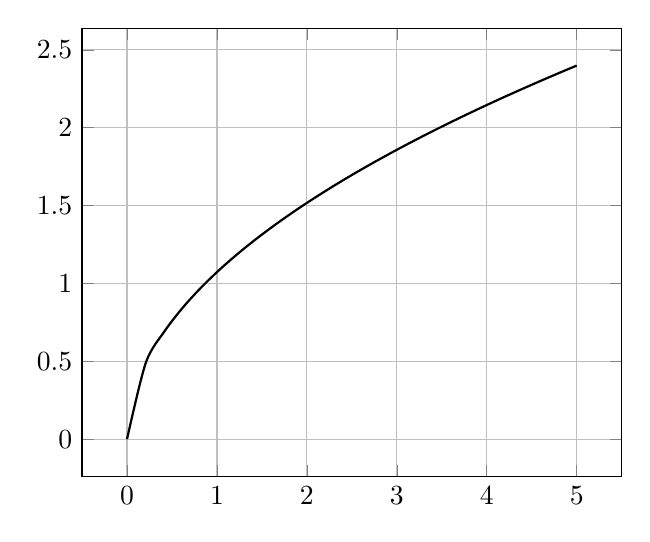
\begin{tikzpicture}
\begin{axis}[grid]
\addplot[domain=0:5, smooth, thick]{sqrt(x*ln(10)/2)};
\end{axis}
\end{tikzpicture}
\end{center}

This gives a reason to choose higher values of $c$ than $\sqrt{6}$ or $\frac{\pi}{2\sqrt{6}}$. Another will come from the following analysis of backward propagation in SIRENs.

{\bf Backward propagation in SIRENs}

Consider the elementwise nonlinearity of a SIREN neuron and the set of synapses which receive input from it. This is a function $f:\mathbb{R}\rightarrow \mathbb{R}^n$ assigning to an input $x$ the vector $\left(w_{1}\sin(x),...,w_{n}\sin(x)\right)^T$. Consider the case when $\frac{\partial E}{\partial f(x)_k}$ are known. Then $\frac{\partial E}{\partial x}=\frac{\partial E}{\partial f(x)_k}\frac{\partial f(x)_k}{\partial x}=\sum_k \frac{\partial E}{\partial f(x)_k}w_{k}\cos(x)$. 

Treating the gradients $\frac{\partial E}{\partial f(x)_k}$ as inputs and the gradient $\frac{\partial E}{\partial x}$ we obtain a dual neuron with activation function $\cos(\cdot)$ and weights $w_k$. The weight distribution of $\left(w_k\right)_{k=1}^n$ will be the same as for forward layers. 

Over many fully connected layers their pre-activations, i.e. gradients before the dual activation function is applied will become approximately normal distributed: when the input distribution has high variance it will be approximately uniformly distributed on a wide interval, and such a distribution transformed by the cosine will be approximately $\text{Arcsine}(-1,1)$ distributed. Consequently this will lead to approximately normal distributed pre-activations.

However, for the cosine of zero-centred normal distribution to be approximately $\text{Arcsine}(-1,1)$ this distribution must have higher variance than for the sine of the same distribution to be $\text{Arcsine}(-1,1)$ distributed. This can be seen by considering the variance $\text{Var}\left[\cos(kZ)\right] = \frac{1}{2} + \frac{1}{2}e^{-2k^2}-e^{-k^2}$ to the variance $\text{Var}\left[\sin(kZ)\right]=\frac{1}{2}(1-e^{-2k^2})$.

\begin{center}
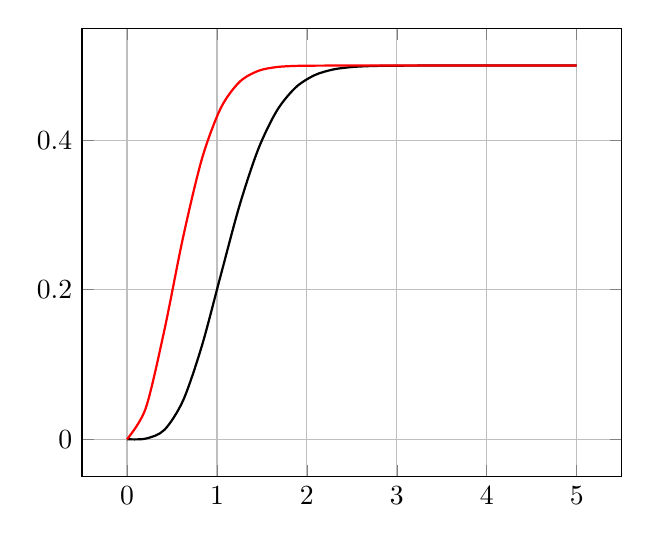
\begin{tikzpicture}
\begin{axis}[grid]
\addplot[domain=0:5, smooth, thick]{0.5 + 0.5*exp(-2*x^2)-exp(-x^2)};
\addplot[domain=0:5, smooth, thick, color=red]{0.5*(1-exp(-2*x^2))};
\end{axis}
\end{tikzpicture}
\end{center}

The black curve show the variance of the cosine transformed zero-centred normal distribution and of the sine-transformed zero-centred normal distribution as a function of the standard deviation of the input distribution.

{\bf The convergence of the pre-activations to normal distribution}

With uniformly distributed input the product of a weight and an input has finite variance and mean and with correct normalization their sums convergence to a normal distribution.

However, sums of variables that are themselves normal distributed need no reference to the central limit theorem, and are inherently normal distributed; furthermore, the product of a uniform RV and any sine-transformed random variable has finite support, with no tails. Consequently they must convergence to a normal distribution unnecessarily slowly.

This gives reason to consider weight distributions whose products with $\sin(kZ)$ where $Z$ is a normal distribution are zero-centred normal distributons, however, it straightforward to consider simply normal distribution weights.

\begin{center}
% Created by tikzDevice version 0.12.3.1 on 2021-07-09 18:53:41
% !TEX encoding = UTF-8 Unicode
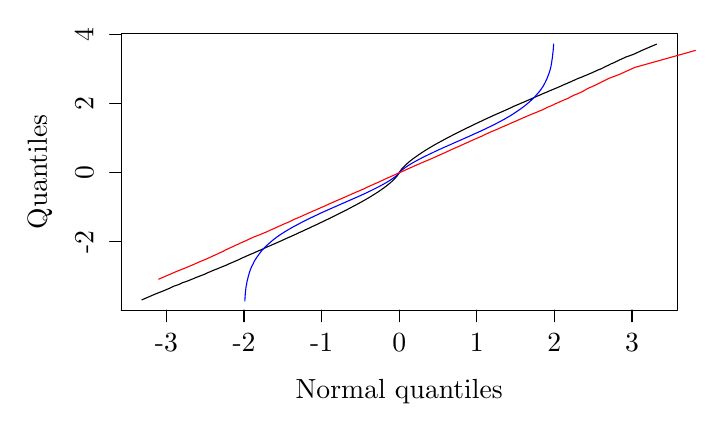
\begin{tikzpicture}[x=0.7pt,y=0.7pt]
\definecolor{fillColor}{RGB}{255,255,255}
%\path[use as bounding box,fill=fillColor,fill opacity=0.00] (0,0) rectangle (361.35,252.94);
\begin{scope}
%\path[clip] ( 49.20, 61.20) rectangle (336.15,203.75);
\definecolor{drawColor}{RGB}{0,0,0}

\path[draw=drawColor,line width= 0.4pt,line join=round,line cap=round] ( 59.83, 66.48) --
	( 67.03, 69.59) --
	( 71.08, 71.16) --
	( 74.24, 72.52) --
	( 76.37, 73.55) --
	( 78.87, 74.36) --
	( 80.70, 75.29) --
	( 82.70, 75.93) --
	( 84.12, 76.49) --
	( 85.38, 77.01) --
	( 86.74, 77.55) --
	( 87.63, 77.97) --
	( 88.81, 78.38) --
	( 89.75, 78.78) --
	( 90.56, 79.08) --
	( 91.51, 79.40) --
	( 92.31, 79.75) --
	( 93.00, 80.09) --
	( 93.65, 80.40) --
	( 94.42, 80.72) --
	( 95.08, 81.00) --
	( 95.81, 81.31) --
	( 96.38, 81.58) --
	( 96.98, 81.81) --
	( 97.49, 82.03) --
	( 98.05, 82.22) --
	( 98.60, 82.40) --
	( 99.05, 82.58) --
	( 99.44, 82.80) --
	( 99.96, 82.99) --
	(100.47, 83.23) --
	(100.98, 83.41) --
	(101.34, 83.57) --
	(101.80, 83.74) --
	(102.20, 83.90) --
	(102.60, 84.06) --
	(102.99, 84.23) --
	(103.40, 84.39) --
	(103.73, 84.56) --
	(104.07, 84.71) --
	(104.41, 84.89) --
	(104.69, 85.02) --
	(105.01, 85.17) --
	(105.32, 85.29) --
	(105.64, 85.44) --
	(105.99, 85.56) --
	(106.33, 85.70) --
	(106.59, 85.82) --
	(106.90, 85.96) --
	(107.15, 86.09) --
	(107.47, 86.22) --
	(107.74, 86.33) --
	(108.03, 86.45) --
	(108.33, 86.57) --
	(108.62, 86.69) --
	(108.85, 86.79) --
	(109.11, 86.90) --
	(109.38, 87.02) --
	(109.61, 87.12) --
	(109.88, 87.25) --
	(110.13, 87.37) --
	(110.35, 87.48) --
	(110.56, 87.60) --
	(110.78, 87.70) --
	(111.04, 87.81) --
	(111.25, 87.93) --
	(111.45, 88.02) --
	(111.67, 88.11) --
	(111.90, 88.22) --
	(112.11, 88.32) --
	(112.35, 88.42) --
	(112.55, 88.50) --
	(112.72, 88.59) --
	(112.97, 88.69) --
	(113.17, 88.76) --
	(113.40, 88.86) --
	(113.58, 88.94) --
	(113.77, 89.03) --
	(113.93, 89.12) --
	(114.10, 89.20) --
	(114.33, 89.28) --
	(114.52, 89.38) --
	(114.66, 89.45) --
	(114.88, 89.53) --
	(115.04, 89.61) --
	(115.22, 89.69) --
	(115.40, 89.76) --
	(115.57, 89.83) --
	(115.75, 89.91) --
	(115.93, 89.98) --
	(116.13, 90.06) --
	(116.27, 90.13) --
	(116.44, 90.21) --
	(116.61, 90.27) --
	(116.78, 90.33) --
	(116.95, 90.39) --
	(117.08, 90.46) --
	(117.27, 90.53) --
	(117.43, 90.61) --
	(117.60, 90.67) --
	(117.77, 90.75) --
	(117.94, 90.81) --
	(118.09, 90.88) --
	(118.23, 90.95) --
	(118.36, 91.01) --
	(118.50, 91.08) --
	(118.64, 91.14) --
	(118.79, 91.21) --
	(118.94, 91.27) --
	(119.07, 91.32) --
	(119.21, 91.39) --
	(119.37, 91.46) --
	(119.53, 91.52) --
	(119.64, 91.58) --
	(119.76, 91.63) --
	(119.88, 91.69) --
	(120.01, 91.76) --
	(120.15, 91.83) --
	(120.31, 91.89) --
	(120.43, 91.94) --
	(120.58, 91.99) --
	(120.72, 92.05) --
	(120.84, 92.10) --
	(120.99, 92.15) --
	(121.11, 92.20) --
	(121.22, 92.26) --
	(121.33, 92.30) --
	(121.44, 92.35) --
	(121.59, 92.42) --
	(121.69, 92.47) --
	(121.80, 92.52) --
	(121.90, 92.58) --
	(122.03, 92.63) --
	(122.18, 92.69) --
	(122.29, 92.75) --
	(122.39, 92.81) --
	(122.52, 92.87) --
	(122.61, 92.91) --
	(122.70, 92.97) --
	(122.82, 93.01) --
	(122.93, 93.06) --
	(123.04, 93.12) --
	(123.15, 93.16) --
	(123.27, 93.21) --
	(123.37, 93.26) --
	(123.48, 93.31) --
	(123.58, 93.36) --
	(123.70, 93.41) --
	(123.80, 93.46) --
	(123.90, 93.51) --
	(123.99, 93.56) --
	(124.10, 93.60) --
	(124.20, 93.65) --
	(124.30, 93.70) --
	(124.38, 93.73) --
	(124.48, 93.77) --
	(124.61, 93.81) --
	(124.72, 93.86) --
	(124.84, 93.90) --
	(124.92, 93.94) --
	(125.03, 93.99) --
	(125.13, 94.03) --
	(125.22, 94.07) --
	(125.30, 94.12) --
	(125.40, 94.16) --
	(125.50, 94.20) --
	(125.60, 94.25) --
	(125.71, 94.28) --
	(125.81, 94.32) --
	(125.90, 94.36) --
	(125.99, 94.40) --
	(126.09, 94.44) --
	(126.17, 94.48) --
	(126.26, 94.52) --
	(126.36, 94.57) --
	(126.45, 94.61) --
	(126.52, 94.65) --
	(126.60, 94.70) --
	(126.71, 94.74) --
	(126.80, 94.78) --
	(126.88, 94.82) --
	(126.97, 94.86) --
	(127.07, 94.90) --
	(127.16, 94.95) --
	(127.24, 94.99) --
	(127.34, 95.02) --
	(127.44, 95.07) --
	(127.54, 95.11) --
	(127.65, 95.15) --
	(127.75, 95.19) --
	(127.84, 95.22) --
	(127.92, 95.26) --
	(128.01, 95.29) --
	(128.08, 95.32) --
	(128.17, 95.36) --
	(128.26, 95.39) --
	(128.35, 95.43) --
	(128.43, 95.47) --
	(128.52, 95.50) --
	(128.60, 95.54) --
	(128.68, 95.58) --
	(128.75, 95.62) --
	(128.83, 95.66) --
	(128.91, 95.70) --
	(129.00, 95.73) --
	(129.09, 95.77) --
	(129.16, 95.80) --
	(129.26, 95.84) --
	(129.33, 95.88) --
	(129.42, 95.91) --
	(129.50, 95.94) --
	(129.57, 95.98) --
	(129.65, 96.01) --
	(129.74, 96.05) --
	(129.81, 96.08) --
	(129.89, 96.12) --
	(129.98, 96.15) --
	(130.05, 96.19) --
	(130.14, 96.23) --
	(130.23, 96.27) --
	(130.30, 96.30) --
	(130.36, 96.34) --
	(130.44, 96.37) --
	(130.52, 96.40) --
	(130.58, 96.44) --
	(130.66, 96.46) --
	(130.72, 96.49) --
	(130.80, 96.53) --
	(130.88, 96.56) --
	(130.95, 96.60) --
	(131.04, 96.63) --
	(131.10, 96.66) --
	(131.17, 96.70) --
	(131.26, 96.73) --
	(131.33, 96.76) --
	(131.41, 96.80) --
	(131.47, 96.82) --
	(131.54, 96.86) --
	(131.62, 96.89) --
	(131.68, 96.91) --
	(131.75, 96.95) --
	(131.81, 96.98) --
	(131.88, 97.01) --
	(131.95, 97.04) --
	(132.01, 97.07) --
	(132.08, 97.10) --
	(132.15, 97.14) --
	(132.23, 97.17) --
	(132.29, 97.20) --
	(132.35, 97.23) --
	(132.43, 97.26) --
	(132.50, 97.29) --
	(132.56, 97.33) --
	(132.62, 97.36) --
	(132.69, 97.39) --
	(132.75, 97.42) --
	(132.81, 97.44) --
	(132.89, 97.47) --
	(132.96, 97.50) --
	(133.02, 97.53) --
	(133.08, 97.56) --
	(133.14, 97.59) --
	(133.22, 97.62) --
	(133.28, 97.65) --
	(133.34, 97.68) --
	(133.41, 97.71) --
	(133.47, 97.74) --
	(133.54, 97.77) --
	(133.60, 97.79) --
	(133.67, 97.82) --
	(133.73, 97.85) --
	(133.80, 97.88) --
	(133.86, 97.91) --
	(133.92, 97.93) --
	(133.98, 97.97) --
	(134.04, 98.00) --
	(134.12, 98.03) --
	(134.19, 98.06) --
	(134.26, 98.09) --
	(134.31, 98.12) --
	(134.36, 98.15) --
	(134.42, 98.17) --
	(134.48, 98.21) --
	(134.54, 98.24) --
	(134.60, 98.27) --
	(134.66, 98.30) --
	(134.73, 98.32) --
	(134.79, 98.35) --
	(134.84, 98.38) --
	(134.91, 98.40) --
	(134.96, 98.43) --
	(135.02, 98.46) --
	(135.07, 98.49) --
	(135.13, 98.52) --
	(135.19, 98.54) --
	(135.25, 98.57) --
	(135.31, 98.60) --
	(135.37, 98.62) --
	(135.43, 98.65) --
	(135.49, 98.67) --
	(135.57, 98.70) --
	(135.63, 98.73) --
	(135.71, 98.75) --
	(135.77, 98.77) --
	(135.83, 98.80) --
	(135.89, 98.82) --
	(135.97, 98.85) --
	(136.02, 98.87) --
	(136.07, 98.90) --
	(136.12, 98.93) --
	(136.17, 98.96) --
	(136.23, 98.98) --
	(136.29, 99.01) --
	(136.34, 99.03) --
	(136.39, 99.06) --
	(136.44, 99.08) --
	(136.50, 99.11) --
	(136.55, 99.13) --
	(136.61, 99.15) --
	(136.68, 99.18) --
	(136.73, 99.20) --
	(136.79, 99.23) --
	(136.84, 99.25) --
	(136.90, 99.28) --
	(136.96, 99.30) --
	(137.02, 99.32) --
	(137.07, 99.35) --
	(137.12, 99.37) --
	(137.18, 99.40) --
	(137.22, 99.42) --
	(137.27, 99.44) --
	(137.32, 99.47) --
	(137.38, 99.49) --
	(137.44, 99.52) --
	(137.49, 99.54) --
	(137.54, 99.56) --
	(137.60, 99.59) --
	(137.64, 99.62) --
	(137.70, 99.64) --
	(137.76, 99.67) --
	(137.81, 99.69) --
	(137.86, 99.71) --
	(137.91, 99.73) --
	(137.96, 99.75) --
	(138.01, 99.78) --
	(138.07, 99.80) --
	(138.11, 99.82) --
	(138.16, 99.85) --
	(138.21, 99.87) --
	(138.26, 99.89) --
	(138.30, 99.91) --
	(138.36, 99.93) --
	(138.40, 99.96) --
	(138.45, 99.98) --
	(138.50,100.00) --
	(138.55,100.03) --
	(138.60,100.05) --
	(138.65,100.07) --
	(138.71,100.09) --
	(138.75,100.11) --
	(138.80,100.13) --
	(138.85,100.15) --
	(138.90,100.17) --
	(138.95,100.20) --
	(138.99,100.22) --
	(139.05,100.24) --
	(139.10,100.26) --
	(139.15,100.28) --
	(139.20,100.31) --
	(139.25,100.33) --
	(139.29,100.35) --
	(139.34,100.37) --
	(139.39,100.39) --
	(139.44,100.41) --
	(139.49,100.43) --
	(139.54,100.45) --
	(139.59,100.48) --
	(139.63,100.50) --
	(139.67,100.52) --
	(139.72,100.54) --
	(139.77,100.56) --
	(139.81,100.59) --
	(139.86,100.61) --
	(139.91,100.63) --
	(139.95,100.65) --
	(140.00,100.67) --
	(140.04,100.69) --
	(140.08,100.71) --
	(140.14,100.73) --
	(140.18,100.75) --
	(140.23,100.77) --
	(140.28,100.80) --
	(140.33,100.82) --
	(140.37,100.84) --
	(140.41,100.86) --
	(140.46,100.88) --
	(140.50,100.90) --
	(140.55,100.93) --
	(140.59,100.95) --
	(140.64,100.97) --
	(140.68,100.99) --
	(140.72,101.01) --
	(140.76,101.03) --
	(140.80,101.05) --
	(140.84,101.07) --
	(140.88,101.09) --
	(140.93,101.11) --
	(140.97,101.14) --
	(141.01,101.16) --
	(141.05,101.18) --
	(141.10,101.20) --
	(141.14,101.22) --
	(141.18,101.24) --
	(141.23,101.27) --
	(141.27,101.29) --
	(141.32,101.31) --
	(141.36,101.32) --
	(141.41,101.34) --
	(141.45,101.36) --
	(141.49,101.38) --
	(141.54,101.40) --
	(141.59,101.42) --
	(141.63,101.44) --
	(141.67,101.46) --
	(141.72,101.48) --
	(141.76,101.50) --
	(141.80,101.52) --
	(141.84,101.53) --
	(141.89,101.55) --
	(141.93,101.57) --
	(141.97,101.59) --
	(142.01,101.61) --
	(142.06,101.63) --
	(142.10,101.64) --
	(142.15,101.67) --
	(142.19,101.69) --
	(142.23,101.71) --
	(142.27,101.73) --
	(142.32,101.75) --
	(142.36,101.77) --
	(142.39,101.78) --
	(142.43,101.80) --
	(142.47,101.82) --
	(142.51,101.84) --
	(142.55,101.86) --
	(142.60,101.88) --
	(142.64,101.89) --
	(142.68,101.91) --
	(142.72,101.93) --
	(142.77,101.95) --
	(142.80,101.97) --
	(142.85,101.99) --
	(142.89,102.01) --
	(142.94,102.03) --
	(142.98,102.04) --
	(143.02,102.06) --
	(143.06,102.08) --
	(143.09,102.10) --
	(143.14,102.12) --
	(143.18,102.14) --
	(143.21,102.16) --
	(143.25,102.18) --
	(143.29,102.20) --
	(143.33,102.21) --
	(143.37,102.23) --
	(143.40,102.25) --
	(143.45,102.27) --
	(143.50,102.29) --
	(143.55,102.30) --
	(143.58,102.32) --
	(143.61,102.34) --
	(143.66,102.36) --
	(143.70,102.38) --
	(143.74,102.39) --
	(143.77,102.41) --
	(143.82,102.43) --
	(143.86,102.45) --
	(143.89,102.47) --
	(143.93,102.49) --
	(143.96,102.50) --
	(144.00,102.52) --
	(144.03,102.54) --
	(144.07,102.56) --
	(144.11,102.57) --
	(144.14,102.59) --
	(144.19,102.61) --
	(144.22,102.63) --
	(144.26,102.65) --
	(144.30,102.67) --
	(144.34,102.68) --
	(144.38,102.70) --
	(144.42,102.72) --
	(144.46,102.74) --
	(144.50,102.75) --
	(144.54,102.77) --
	(144.57,102.79) --
	(144.61,102.81) --
	(144.64,102.82) --
	(144.68,102.84) --
	(144.72,102.86) --
	(144.75,102.87) --
	(144.78,102.89) --
	(144.82,102.91) --
	(144.86,102.92) --
	(144.89,102.94) --
	(144.93,102.96) --
	(144.96,102.97) --
	(145.00,102.99) --
	(145.04,103.01) --
	(145.07,103.02) --
	(145.11,103.04) --
	(145.15,103.05) --
	(145.18,103.07) --
	(145.21,103.09) --
	(145.25,103.11) --
	(145.29,103.12) --
	(145.33,103.14) --
	(145.36,103.15) --
	(145.39,103.17) --
	(145.43,103.19) --
	(145.47,103.20) --
	(145.50,103.22) --
	(145.54,103.23) --
	(145.57,103.25) --
	(145.60,103.27) --
	(145.64,103.28) --
	(145.68,103.30) --
	(145.71,103.32) --
	(145.76,103.34) --
	(145.79,103.36) --
	(145.82,103.37) --
	(145.87,103.38) --
	(145.91,103.40) --
	(145.95,103.41) --
	(145.97,103.43) --
	(146.01,103.45) --
	(146.05,103.46) --
	(146.08,103.48) --
	(146.12,103.50) --
	(146.15,103.51) --
	(146.18,103.53) --
	(146.22,103.54) --
	(146.25,103.56) --
	(146.28,103.58) --
	(146.32,103.59) --
	(146.35,103.61) --
	(146.38,103.62) --
	(146.41,103.64) --
	(146.45,103.66) --
	(146.49,103.67) --
	(146.53,103.69) --
	(146.56,103.71) --
	(146.59,103.72) --
	(146.62,103.74) --
	(146.66,103.76) --
	(146.69,103.77) --
	(146.73,103.79) --
	(146.76,103.80) --
	(146.80,103.82) --
	(146.83,103.84) --
	(146.86,103.85) --
	(146.89,103.87) --
	(146.93,103.88) --
	(146.96,103.90) --
	(146.99,103.92) --
	(147.03,103.93) --
	(147.06,103.95) --
	(147.09,103.96) --
	(147.12,103.98) --
	(147.15,103.99) --
	(147.18,104.01) --
	(147.22,104.02) --
	(147.25,104.04) --
	(147.28,104.06) --
	(147.31,104.07) --
	(147.33,104.09) --
	(147.37,104.11) --
	(147.40,104.12) --
	(147.43,104.14) --
	(147.47,104.15) --
	(147.50,104.17) --
	(147.53,104.18) --
	(147.56,104.20) --
	(147.59,104.21) --
	(147.63,104.23) --
	(147.66,104.24) --
	(147.69,104.26) --
	(147.73,104.27) --
	(147.76,104.29) --
	(147.79,104.31) --
	(147.82,104.32) --
	(147.84,104.33) --
	(147.87,104.35) --
	(147.90,104.36) --
	(147.93,104.38) --
	(147.96,104.39) --
	(147.99,104.41) --
	(148.03,104.42) --
	(148.06,104.44) --
	(148.10,104.45) --
	(148.14,104.46) --
	(148.17,104.48) --
	(148.21,104.50) --
	(148.24,104.51) --
	(148.28,104.52) --
	(148.30,104.54) --
	(148.34,104.55) --
	(148.37,104.56) --
	(148.40,104.58) --
	(148.44,104.59) --
	(148.47,104.61) --
	(148.50,104.62) --
	(148.53,104.63) --
	(148.56,104.65) --
	(148.60,104.66) --
	(148.63,104.68) --
	(148.66,104.69) --
	(148.69,104.71) --
	(148.72,104.72) --
	(148.75,104.74) --
	(148.78,104.75) --
	(148.81,104.76) --
	(148.85,104.77) --
	(148.88,104.79) --
	(148.91,104.80) --
	(148.94,104.82) --
	(148.98,104.84) --
	(149.01,104.85) --
	(149.04,104.87) --
	(149.07,104.88) --
	(149.09,104.89) --
	(149.12,104.91) --
	(149.15,104.92) --
	(149.18,104.93) --
	(149.22,104.95) --
	(149.25,104.96) --
	(149.27,104.98) --
	(149.31,104.99) --
	(149.34,105.01) --
	(149.37,105.02) --
	(149.40,105.03) --
	(149.43,105.05) --
	(149.46,105.06) --
	(149.49,105.08) --
	(149.52,105.09) --
	(149.55,105.11) --
	(149.59,105.12) --
	(149.62,105.14) --
	(149.65,105.15) --
	(149.69,105.17) --
	(149.72,105.18) --
	(149.75,105.19) --
	(149.78,105.21) --
	(149.81,105.22) --
	(149.84,105.23) --
	(149.87,105.25) --
	(149.90,105.26) --
	(149.93,105.28) --
	(149.96,105.29) --
	(149.99,105.30) --
	(150.02,105.32) --
	(150.05,105.33) --
	(150.07,105.34) --
	(150.10,105.35) --
	(150.13,105.37) --
	(150.16,105.38) --
	(150.19,105.40) --
	(150.22,105.41) --
	(150.25,105.43) --
	(150.28,105.44) --
	(150.30,105.46) --
	(150.33,105.47) --
	(150.35,105.48) --
	(150.39,105.50) --
	(150.42,105.51) --
	(150.45,105.52) --
	(150.48,105.54) --
	(150.51,105.55) --
	(150.53,105.57) --
	(150.56,105.58) --
	(150.59,105.59) --
	(150.61,105.61) --
	(150.64,105.62) --
	(150.67,105.64) --
	(150.70,105.65) --
	(150.73,105.67) --
	(150.76,105.68) --
	(150.78,105.69) --
	(150.81,105.71) --
	(150.84,105.72) --
	(150.87,105.74) --
	(150.90,105.75) --
	(150.92,105.76) --
	(150.95,105.78) --
	(150.98,105.79) --
	(151.02,105.80) --
	(151.04,105.82) --
	(151.07,105.83) --
	(151.10,105.84) --
	(151.13,105.85) --
	(151.15,105.86) --
	(151.18,105.88) --
	(151.20,105.89) --
	(151.23,105.91) --
	(151.26,105.92) --
	(151.29,105.93) --
	(151.32,105.94) --
	(151.35,105.96) --
	(151.38,105.97) --
	(151.41,105.99) --
	(151.45,106.00) --
	(151.48,106.01) --
	(151.51,106.03) --
	(151.54,106.04) --
	(151.57,106.05) --
	(151.59,106.07) --
	(151.62,106.08) --
	(151.65,106.10) --
	(151.67,106.11) --
	(151.70,106.13) --
	(151.73,106.14) --
	(151.76,106.16) --
	(151.79,106.17) --
	(151.81,106.18) --
	(151.84,106.20) --
	(151.87,106.21) --
	(151.89,106.22) --
	(151.91,106.24) --
	(151.94,106.25) --
	(151.97,106.26) --
	(152.00,106.27) --
	(152.02,106.29) --
	(152.05,106.30) --
	(152.07,106.31) --
	(152.10,106.32) --
	(152.12,106.34) --
	(152.14,106.35) --
	(152.17,106.36) --
	(152.20,106.38) --
	(152.23,106.39) --
	(152.26,106.40) --
	(152.29,106.41) --
	(152.31,106.43) --
	(152.34,106.44) --
	(152.37,106.45) --
	(152.39,106.46) --
	(152.42,106.47) --
	(152.44,106.49) --
	(152.47,106.50) --
	(152.49,106.51) --
	(152.52,106.53) --
	(152.55,106.54) --
	(152.58,106.55) --
	(152.60,106.56) --
	(152.63,106.58) --
	(152.65,106.59) --
	(152.68,106.60) --
	(152.71,106.62) --
	(152.73,106.63) --
	(152.76,106.64) --
	(152.79,106.65) --
	(152.81,106.67) --
	(152.84,106.68) --
	(152.86,106.69) --
	(152.89,106.71) --
	(152.91,106.72) --
	(152.95,106.73) --
	(152.97,106.74) --
	(153.00,106.75) --
	(153.02,106.76) --
	(153.05,106.78) --
	(153.08,106.79) --
	(153.11,106.80) --
	(153.14,106.81) --
	(153.16,106.83) --
	(153.19,106.84) --
	(153.21,106.85) --
	(153.23,106.86) --
	(153.26,106.88) --
	(153.29,106.89) --
	(153.31,106.90) --
	(153.34,106.92) --
	(153.37,106.93) --
	(153.39,106.94) --
	(153.41,106.95) --
	(153.44,106.97) --
	(153.46,106.98) --
	(153.49,106.99) --
	(153.52,107.00) --
	(153.54,107.01) --
	(153.56,107.03) --
	(153.59,107.04) --
	(153.61,107.05) --
	(153.64,107.06) --
	(153.66,107.07) --
	(153.69,107.09) --
	(153.71,107.10) --
	(153.74,107.11) --
	(153.76,107.12) --
	(153.79,107.13) --
	(153.81,107.15) --
	(153.84,107.16) --
	(153.87,107.17) --
	(153.90,107.18) --
	(153.92,107.19) --
	(153.95,107.21) --
	(153.97,107.22) --
	(154.00,107.24) --
	(154.02,107.25) --
	(154.04,107.26) --
	(154.07,107.27) --
	(154.09,107.29) --
	(154.11,107.30) --
	(154.14,107.31) --
	(154.17,107.32) --
	(154.19,107.33) --
	(154.22,107.34) --
	(154.24,107.35) --
	(154.27,107.37) --
	(154.29,107.38) --
	(154.31,107.39) --
	(154.33,107.40) --
	(154.36,107.41) --
	(154.38,107.42) --
	(154.41,107.44) --
	(154.43,107.45) --
	(154.45,107.46) --
	(154.48,107.47) --
	(154.51,107.48) --
	(154.54,107.50) --
	(154.56,107.51) --
	(154.59,107.52) --
	(154.61,107.53) --
	(154.63,107.55) --
	(154.66,107.56) --
	(154.68,107.57) --
	(154.70,107.58) --
	(154.73,107.59) --
	(154.75,107.60) --
	(154.77,107.61) --
	(154.79,107.63) --
	(154.82,107.64) --
	(154.85,107.65) --
	(154.87,107.66) --
	(154.89,107.67) --
	(154.92,107.68) --
	(154.94,107.69) --
	(154.96,107.70) --
	(154.98,107.71) --
	(155.01,107.72) --
	(155.03,107.74) --
	(155.06,107.75) --
	(155.08,107.76) --
	(155.11,107.77) --
	(155.13,107.78) --
	(155.15,107.79) --
	(155.18,107.80) --
	(155.20,107.81) --
	(155.23,107.82) --
	(155.25,107.84) --
	(155.27,107.85) --
	(155.29,107.86) --
	(155.32,107.87) --
	(155.35,107.88) --
	(155.37,107.89) --
	(155.39,107.90) --
	(155.42,107.91) --
	(155.44,107.92) --
	(155.47,107.94) --
	(155.49,107.95) --
	(155.51,107.96) --
	(155.54,107.97) --
	(155.57,107.98) --
	(155.59,107.99) --
	(155.61,108.00) --
	(155.64,108.01) --
	(155.66,108.02) --
	(155.69,108.03) --
	(155.71,108.04) --
	(155.73,108.06) --
	(155.75,108.06) --
	(155.78,108.08) --
	(155.81,108.09) --
	(155.83,108.10) --
	(155.85,108.11) --
	(155.87,108.12) --
	(155.89,108.13) --
	(155.91,108.14) --
	(155.93,108.15) --
	(155.96,108.17) --
	(155.98,108.17) --
	(156.01,108.18) --
	(156.03,108.19) --
	(156.05,108.20) --
	(156.08,108.22) --
	(156.10,108.23) --
	(156.13,108.24) --
	(156.15,108.25) --
	(156.17,108.26) --
	(156.20,108.27) --
	(156.22,108.28) --
	(156.24,108.29) --
	(156.26,108.30) --
	(156.28,108.31) --
	(156.31,108.32) --
	(156.33,108.34) --
	(156.35,108.35) --
	(156.37,108.36) --
	(156.40,108.37) --
	(156.42,108.38) --
	(156.45,108.39) --
	(156.47,108.40) --
	(156.49,108.41) --
	(156.51,108.43) --
	(156.53,108.44) --
	(156.56,108.45) --
	(156.58,108.46) --
	(156.60,108.47) --
	(156.63,108.48) --
	(156.65,108.49) --
	(156.67,108.51) --
	(156.69,108.52) --
	(156.72,108.53) --
	(156.74,108.54) --
	(156.77,108.55) --
	(156.79,108.56) --
	(156.81,108.57) --
	(156.83,108.58) --
	(156.85,108.59) --
	(156.87,108.60) --
	(156.90,108.61) --
	(156.92,108.62) --
	(156.94,108.63) --
	(156.96,108.64) --
	(156.98,108.65) --
	(157.01,108.66) --
	(157.03,108.68) --
	(157.05,108.69) --
	(157.08,108.70) --
	(157.10,108.71) --
	(157.12,108.72) --
	(157.14,108.73) --
	(157.16,108.74) --
	(157.18,108.75) --
	(157.20,108.76) --
	(157.23,108.77) --
	(157.25,108.78) --
	(157.26,108.79) --
	(157.28,108.80) --
	(157.31,108.81) --
	(157.33,108.82) --
	(157.35,108.83) --
	(157.38,108.84) --
	(157.40,108.85) --
	(157.42,108.86) --
	(157.44,108.87) --
	(157.46,108.88) --
	(157.48,108.90) --
	(157.51,108.90) --
	(157.52,108.92) --
	(157.54,108.93) --
	(157.57,108.94) --
	(157.59,108.95) --
	(157.60,108.96) --
	(157.63,108.97) --
	(157.65,108.98) --
	(157.67,108.99) --
	(157.70,109.00) --
	(157.72,109.01) --
	(157.74,109.02) --
	(157.76,109.03) --
	(157.78,109.04) --
	(157.80,109.05) --
	(157.82,109.06) --
	(157.85,109.07) --
	(157.87,109.08) --
	(157.89,109.09) --
	(157.91,109.10) --
	(157.93,109.11) --
	(157.95,109.12) --
	(157.97,109.13) --
	(157.99,109.14) --
	(158.01,109.15) --
	(158.04,109.16) --
	(158.06,109.17) --
	(158.08,109.19) --
	(158.10,109.20) --
	(158.11,109.21) --
	(158.13,109.22) --
	(158.16,109.23) --
	(158.18,109.24) --
	(158.19,109.25) --
	(158.21,109.26) --
	(158.23,109.27) --
	(158.26,109.28) --
	(158.28,109.29) --
	(158.30,109.30) --
	(158.32,109.31) --
	(158.34,109.32) --
	(158.36,109.33) --
	(158.38,109.34) --
	(158.40,109.35) --
	(158.43,109.36) --
	(158.44,109.37) --
	(158.47,109.38) --
	(158.49,109.39) --
	(158.51,109.40) --
	(158.53,109.41) --
	(158.55,109.42) --
	(158.58,109.43) --
	(158.59,109.44) --
	(158.61,109.45) --
	(158.64,109.46) --
	(158.66,109.47) --
	(158.68,109.48) --
	(158.69,109.49) --
	(158.72,109.51) --
	(158.74,109.52) --
	(158.76,109.52) --
	(158.77,109.53) --
	(158.79,109.54) --
	(158.82,109.55) --
	(158.85,109.56) --
	(158.86,109.57) --
	(158.88,109.58) --
	(158.90,109.59) --
	(158.92,109.60) --
	(158.94,109.61) --
	(158.96,109.62) --
	(158.98,109.63) --
	(159.00,109.64) --
	(159.02,109.65) --
	(159.04,109.66) --
	(159.06,109.67) --
	(159.08,109.68) --
	(159.10,109.69) --
	(159.13,109.70) --
	(159.15,109.71) --
	(159.16,109.72) --
	(159.18,109.73) --
	(159.20,109.74) --
	(159.23,109.75) --
	(159.25,109.76) --
	(159.27,109.77) --
	(159.29,109.78) --
	(159.31,109.80) --
	(159.34,109.81) --
	(159.36,109.82) --
	(159.38,109.83) --
	(159.40,109.84) --
	(159.42,109.85) --
	(159.44,109.85) --
	(159.46,109.87) --
	(159.47,109.88) --
	(159.49,109.89) --
	(159.51,109.90) --
	(159.53,109.91) --
	(159.55,109.92) --
	(159.57,109.93) --
	(159.59,109.94) --
	(159.61,109.95) --
	(159.63,109.96) --
	(159.64,109.97) --
	(159.66,109.98) --
	(159.68,109.99) --
	(159.71,110.00) --
	(159.73,110.01) --
	(159.75,110.02) --
	(159.77,110.03) --
	(159.79,110.03) --
	(159.81,110.05) --
	(159.83,110.06) --
	(159.85,110.07) --
	(159.87,110.08) --
	(159.88,110.09) --
	(159.90,110.09) --
	(159.92,110.10) --
	(159.94,110.11) --
	(159.96,110.12) --
	(159.98,110.13) --
	(160.00,110.14) --
	(160.03,110.15) --
	(160.05,110.16) --
	(160.06,110.17) --
	(160.08,110.18) --
	(160.10,110.19) --
	(160.12,110.20) --
	(160.14,110.21) --
	(160.16,110.22) --
	(160.18,110.23) --
	(160.20,110.23) --
	(160.22,110.24) --
	(160.24,110.25) --
	(160.26,110.26) --
	(160.28,110.27) --
	(160.30,110.28) --
	(160.32,110.29) --
	(160.33,110.30) --
	(160.35,110.31) --
	(160.37,110.32) --
	(160.39,110.33) --
	(160.41,110.34) --
	(160.43,110.35) --
	(160.45,110.36) --
	(160.47,110.37) --
	(160.49,110.38) --
	(160.51,110.39) --
	(160.52,110.40) --
	(160.55,110.41) --
	(160.57,110.42) --
	(160.59,110.43) --
	(160.61,110.44) --
	(160.62,110.44) --
	(160.64,110.45) --
	(160.67,110.46) --
	(160.68,110.47) --
	(160.70,110.48) --
	(160.72,110.49) --
	(160.73,110.50) --
	(160.75,110.51) --
	(160.77,110.52) --
	(160.79,110.53) --
	(160.81,110.54) --
	(160.83,110.55) --
	(160.84,110.56) --
	(160.86,110.57) --
	(160.88,110.58) --
	(160.90,110.59) --
	(160.92,110.60) --
	(160.94,110.61) --
	(160.95,110.62) --
	(160.97,110.63) --
	(160.99,110.64) --
	(161.00,110.65) --
	(161.02,110.66) --
	(161.03,110.66) --
	(161.05,110.67) --
	(161.07,110.68) --
	(161.09,110.69) --
	(161.10,110.70) --
	(161.12,110.71) --
	(161.14,110.72) --
	(161.16,110.73) --
	(161.18,110.73) --
	(161.20,110.74) --
	(161.22,110.75) --
	(161.23,110.76) --
	(161.25,110.77) --
	(161.26,110.78) --
	(161.28,110.79) --
	(161.30,110.80) --
	(161.32,110.81) --
	(161.33,110.82) --
	(161.35,110.83) --
	(161.37,110.83) --
	(161.39,110.84) --
	(161.41,110.85) --
	(161.42,110.86) --
	(161.44,110.87) --
	(161.46,110.88) --
	(161.48,110.89) --
	(161.49,110.90) --
	(161.51,110.90) --
	(161.53,110.91) --
	(161.55,110.92) --
	(161.57,110.93) --
	(161.58,110.94) --
	(161.60,110.96) --
	(161.62,110.96) --
	(161.64,110.97) --
	(161.65,110.98) --
	(161.67,110.99) --
	(161.68,111.00) --
	(161.70,111.01) --
	(161.72,111.01) --
	(161.74,111.02) --
	(161.76,111.03) --
	(161.78,111.04) --
	(161.79,111.05) --
	(161.81,111.06) --
	(161.83,111.07) --
	(161.85,111.08) --
	(161.87,111.09) --
	(161.89,111.10) --
	(161.91,111.11) --
	(161.93,111.11) --
	(161.95,111.12) --
	(161.96,111.13) --
	(161.98,111.14) --
	(162.00,111.15) --
	(162.01,111.16) --
	(162.03,111.17) --
	(162.04,111.18) --
	(162.06,111.19) --
	(162.08,111.20) --
	(162.10,111.20) --
	(162.11,111.21) --
	(162.13,111.22) --
	(162.15,111.23) --
	(162.17,111.24) --
	(162.18,111.25) --
	(162.20,111.26) --
	(162.22,111.27) --
	(162.23,111.28) --
	(162.25,111.29) --
	(162.27,111.30) --
	(162.28,111.31) --
	(162.30,111.31) --
	(162.32,111.32) --
	(162.34,111.33) --
	(162.36,111.34) --
	(162.38,111.35) --
	(162.40,111.36) --
	(162.41,111.37) --
	(162.43,111.37) --
	(162.45,111.38) --
	(162.47,111.39) --
	(162.49,111.40) --
	(162.51,111.41) --
	(162.53,111.42) --
	(162.54,111.43) --
	(162.56,111.44) --
	(162.58,111.45) --
	(162.60,111.45) --
	(162.62,111.46) --
	(162.63,111.47) --
	(162.65,111.48) --
	(162.67,111.49) --
	(162.69,111.50) --
	(162.70,111.51) --
	(162.72,111.52) --
	(162.74,111.53) --
	(162.75,111.54) --
	(162.77,111.55) --
	(162.79,111.55) --
	(162.81,111.56) --
	(162.82,111.57) --
	(162.84,111.58) --
	(162.86,111.59) --
	(162.88,111.60) --
	(162.89,111.61) --
	(162.91,111.62) --
	(162.92,111.62) --
	(162.94,111.63) --
	(162.96,111.64) --
	(162.97,111.65) --
	(162.99,111.66) --
	(163.01,111.67) --
	(163.03,111.67) --
	(163.05,111.68) --
	(163.07,111.69) --
	(163.09,111.70) --
	(163.10,111.71) --
	(163.12,111.72) --
	(163.14,111.73) --
	(163.16,111.74) --
	(163.17,111.74) --
	(163.19,111.75) --
	(163.21,111.76) --
	(163.22,111.77) --
	(163.24,111.78) --
	(163.26,111.79) --
	(163.28,111.80) --
	(163.29,111.80) --
	(163.31,111.81) --
	(163.33,111.82) --
	(163.34,111.83) --
	(163.36,111.84) --
	(163.38,111.85) --
	(163.40,111.85) --
	(163.41,111.86) --
	(163.43,111.87) --
	(163.44,111.88) --
	(163.46,111.89) --
	(163.48,111.89) --
	(163.49,111.90) --
	(163.51,111.91) --
	(163.53,111.92) --
	(163.54,111.93) --
	(163.56,111.94) --
	(163.58,111.95) --
	(163.59,111.95) --
	(163.61,111.96) --
	(163.62,111.97) --
	(163.64,111.98) --
	(163.66,111.99) --
	(163.67,112.00) --
	(163.69,112.00) --
	(163.71,112.01) --
	(163.73,112.02) --
	(163.74,112.03) --
	(163.76,112.04) --
	(163.78,112.05) --
	(163.79,112.06) --
	(163.81,112.06) --
	(163.83,112.07) --
	(163.84,112.08) --
	(163.86,112.09) --
	(163.88,112.10) --
	(163.89,112.11) --
	(163.91,112.12) --
	(163.93,112.12) --
	(163.94,112.13) --
	(163.96,112.14) --
	(163.98,112.15) --
	(163.99,112.16) --
	(164.01,112.16) --
	(164.03,112.17) --
	(164.05,112.18) --
	(164.06,112.19) --
	(164.08,112.20) --
	(164.10,112.20) --
	(164.11,112.21) --
	(164.13,112.22) --
	(164.14,112.23) --
	(164.16,112.24) --
	(164.18,112.24) --
	(164.19,112.25) --
	(164.21,112.26) --
	(164.22,112.27) --
	(164.24,112.28) --
	(164.26,112.29) --
	(164.27,112.29) --
	(164.29,112.30) --
	(164.31,112.31) --
	(164.32,112.32) --
	(164.34,112.33) --
	(164.35,112.33) --
	(164.37,112.34) --
	(164.39,112.35) --
	(164.40,112.36) --
	(164.42,112.37) --
	(164.44,112.38) --
	(164.45,112.39) --
	(164.47,112.40) --
	(164.49,112.40) --
	(164.50,112.41) --
	(164.52,112.42) --
	(164.53,112.43) --
	(164.55,112.44) --
	(164.57,112.45) --
	(164.59,112.46) --
	(164.60,112.46) --
	(164.62,112.47) --
	(164.63,112.48) --
	(164.65,112.49) --
	(164.67,112.49) --
	(164.68,112.50) --
	(164.70,112.51) --
	(164.71,112.52) --
	(164.73,112.53) --
	(164.74,112.54) --
	(164.75,112.54) --
	(164.77,112.55) --
	(164.79,112.56) --
	(164.81,112.57) --
	(164.82,112.58) --
	(164.84,112.59) --
	(164.85,112.60) --
	(164.87,112.60) --
	(164.89,112.61) --
	(164.90,112.62) --
	(164.92,112.63) --
	(164.93,112.64) --
	(164.95,112.64) --
	(164.97,112.65) --
	(164.98,112.66) --
	(165.00,112.67) --
	(165.01,112.67) --
	(165.03,112.68) --
	(165.05,112.69) --
	(165.06,112.70) --
	(165.08,112.71) --
	(165.09,112.71) --
	(165.11,112.72) --
	(165.12,112.73) --
	(165.14,112.74) --
	(165.16,112.75) --
	(165.18,112.75) --
	(165.19,112.76) --
	(165.20,112.77) --
	(165.22,112.78) --
	(165.24,112.79) --
	(165.25,112.80) --
	(165.27,112.80) --
	(165.29,112.81) --
	(165.30,112.82) --
	(165.32,112.83) --
	(165.34,112.84) --
	(165.35,112.85) --
	(165.37,112.85) --
	(165.38,112.86) --
	(165.40,112.87) --
	(165.41,112.88) --
	(165.43,112.88) --
	(165.44,112.89) --
	(165.46,112.90) --
	(165.47,112.91) --
	(165.49,112.92) --
	(165.50,112.93) --
	(165.52,112.94) --
	(165.53,112.95) --
	(165.55,112.95) --
	(165.56,112.96) --
	(165.58,112.97) --
	(165.59,112.98) --
	(165.61,112.98) --
	(165.63,112.99) --
	(165.64,113.00) --
	(165.65,113.01) --
	(165.67,113.02) --
	(165.69,113.03) --
	(165.70,113.03) --
	(165.72,113.04) --
	(165.73,113.05) --
	(165.74,113.06) --
	(165.76,113.07) --
	(165.77,113.07) --
	(165.79,113.08) --
	(165.80,113.09) --
	(165.82,113.10) --
	(165.83,113.11) --
	(165.85,113.11) --
	(165.87,113.12) --
	(165.88,113.13) --
	(165.90,113.14) --
	(165.91,113.15) --
	(165.93,113.15) --
	(165.94,113.16) --
	(165.96,113.17) --
	(165.97,113.18) --
	(165.99,113.19) --
	(166.00,113.19) --
	(166.02,113.20) --
	(166.04,113.21) --
	(166.05,113.22) --
	(166.06,113.22) --
	(166.08,113.23) --
	(166.10,113.24) --
	(166.11,113.25) --
	(166.13,113.26) --
	(166.14,113.26) --
	(166.16,113.27) --
	(166.17,113.28) --
	(166.19,113.29) --
	(166.20,113.30) --
	(166.22,113.30) --
	(166.23,113.31) --
	(166.25,113.32) --
	(166.27,113.33) --
	(166.28,113.34) --
	(166.30,113.35) --
	(166.31,113.35) --
	(166.33,113.36) --
	(166.34,113.37) --
	(166.36,113.37) --
	(166.38,113.38) --
	(166.39,113.39) --
	(166.41,113.40) --
	(166.42,113.41) --
	(166.43,113.41) --
	(166.45,113.42) --
	(166.47,113.43) --
	(166.48,113.43) --
	(166.50,113.44) --
	(166.51,113.45) --
	(166.53,113.46) --
	(166.54,113.46) --
	(166.56,113.47) --
	(166.57,113.48) --
	(166.59,113.49) --
	(166.60,113.50) --
	(166.61,113.50) --
	(166.63,113.51) --
	(166.64,113.52) --
	(166.66,113.53) --
	(166.67,113.54) --
	(166.68,113.55) --
	(166.70,113.55) --
	(166.71,113.56) --
	(166.72,113.57) --
	(166.73,113.58) --
	(166.75,113.59) --
	(166.76,113.59) --
	(166.78,113.60) --
	(166.79,113.61) --
	(166.81,113.61) --
	(166.82,113.62) --
	(166.83,113.63) --
	(166.85,113.64) --
	(166.86,113.64) --
	(166.88,113.65) --
	(166.89,113.66) --
	(166.90,113.67) --
	(166.92,113.67) --
	(166.94,113.68) --
	(166.95,113.69) --
	(166.96,113.70) --
	(166.98,113.71) --
	(166.99,113.72) --
	(167.01,113.72) --
	(167.02,113.73) --
	(167.04,113.74) --
	(167.05,113.75) --
	(167.06,113.75) --
	(167.08,113.76) --
	(167.09,113.77) --
	(167.11,113.78) --
	(167.12,113.79) --
	(167.14,113.80) --
	(167.15,113.80) --
	(167.17,113.81) --
	(167.18,113.82) --
	(167.20,113.83) --
	(167.21,113.83) --
	(167.23,113.84) --
	(167.24,113.85) --
	(167.26,113.85) --
	(167.27,113.86) --
	(167.29,113.87) --
	(167.30,113.88) --
	(167.31,113.88) --
	(167.33,113.89) --
	(167.34,113.90) --
	(167.36,113.91) --
	(167.37,113.92) --
	(167.39,113.92) --
	(167.40,113.93) --
	(167.41,113.94) --
	(167.43,113.95) --
	(167.44,113.95) --
	(167.46,113.96) --
	(167.47,113.97) --
	(167.48,113.97) --
	(167.49,113.98) --
	(167.51,113.99) --
	(167.52,114.00) --
	(167.53,114.00) --
	(167.55,114.01) --
	(167.56,114.02) --
	(167.57,114.03) --
	(167.59,114.04) --
	(167.60,114.04) --
	(167.61,114.05) --
	(167.63,114.06) --
	(167.64,114.07) --
	(167.66,114.07) --
	(167.67,114.08) --
	(167.69,114.09) --
	(167.70,114.10) --
	(167.71,114.10) --
	(167.73,114.11) --
	(167.75,114.12) --
	(167.76,114.13) --
	(167.78,114.13) --
	(167.79,114.14) --
	(167.80,114.15) --
	(167.82,114.15) --
	(167.83,114.16) --
	(167.85,114.17) --
	(167.86,114.18) --
	(167.88,114.18) --
	(167.89,114.19) --
	(167.90,114.20) --
	(167.92,114.21) --
	(167.93,114.22) --
	(167.95,114.22) --
	(167.96,114.23) --
	(167.97,114.24) --
	(167.99,114.24) --
	(168.00,114.25) --
	(168.02,114.26) --
	(168.03,114.27) --
	(168.04,114.27) --
	(168.06,114.28) --
	(168.07,114.29) --
	(168.09,114.29) --
	(168.10,114.30) --
	(168.11,114.31) --
	(168.13,114.32) --
	(168.14,114.32) --
	(168.16,114.33) --
	(168.17,114.34) --
	(168.18,114.35) --
	(168.20,114.35) --
	(168.21,114.36) --
	(168.22,114.37) --
	(168.24,114.37) --
	(168.25,114.38) --
	(168.27,114.39) --
	(168.28,114.40) --
	(168.29,114.40) --
	(168.31,114.41) --
	(168.32,114.42) --
	(168.33,114.43) --
	(168.35,114.43) --
	(168.36,114.44) --
	(168.37,114.45) --
	(168.39,114.46) --
	(168.40,114.46) --
	(168.41,114.47) --
	(168.43,114.48) --
	(168.44,114.49) --
	(168.45,114.49) --
	(168.47,114.50) --
	(168.49,114.51) --
	(168.50,114.52) --
	(168.51,114.52) --
	(168.52,114.53) --
	(168.54,114.54) --
	(168.55,114.55) --
	(168.57,114.55) --
	(168.58,114.56) --
	(168.60,114.57) --
	(168.61,114.57) --
	(168.63,114.58) --
	(168.64,114.59) --
	(168.65,114.60) --
	(168.66,114.60) --
	(168.68,114.61) --
	(168.69,114.62) --
	(168.71,114.62) --
	(168.72,114.63) --
	(168.74,114.64) --
	(168.75,114.65) --
	(168.77,114.65) --
	(168.78,114.66) --
	(168.79,114.67) --
	(168.80,114.68) --
	(168.82,114.68) --
	(168.83,114.69) --
	(168.84,114.70) --
	(168.86,114.70) --
	(168.87,114.71) --
	(168.89,114.72) --
	(168.90,114.72) --
	(168.91,114.73) --
	(168.93,114.74) --
	(168.94,114.75) --
	(168.95,114.75) --
	(168.97,114.76) --
	(168.98,114.77) --
	(168.99,114.77) --
	(169.01,114.78) --
	(169.02,114.79) --
	(169.03,114.80) --
	(169.05,114.80) --
	(169.06,114.81) --
	(169.07,114.82) --
	(169.09,114.82) --
	(169.10,114.83) --
	(169.11,114.84) --
	(169.12,114.85) --
	(169.14,114.86) --
	(169.15,114.86) --
	(169.16,114.87) --
	(169.18,114.88) --
	(169.19,114.88) --
	(169.21,114.89) --
	(169.22,114.90) --
	(169.23,114.90) --
	(169.25,114.91) --
	(169.26,114.92) --
	(169.27,114.92) --
	(169.29,114.93) --
	(169.30,114.94) --
	(169.31,114.95) --
	(169.33,114.95) --
	(169.34,114.96) --
	(169.35,114.97) --
	(169.37,114.97) --
	(169.38,114.98) --
	(169.40,114.99) --
	(169.41,115.00) --
	(169.43,115.00) --
	(169.44,115.01) --
	(169.46,115.02) --
	(169.47,115.02) --
	(169.48,115.03) --
	(169.49,115.04) --
	(169.51,115.05) --
	(169.52,115.05) --
	(169.53,115.06) --
	(169.55,115.07) --
	(169.56,115.08) --
	(169.57,115.08) --
	(169.58,115.09) --
	(169.59,115.10) --
	(169.61,115.10) --
	(169.62,115.11) --
	(169.63,115.12) --
	(169.65,115.12) --
	(169.66,115.13) --
	(169.67,115.13) --
	(169.69,115.14) --
	(169.70,115.15) --
	(169.72,115.16) --
	(169.73,115.16) --
	(169.74,115.17) --
	(169.76,115.18) --
	(169.77,115.19) --
	(169.78,115.19) --
	(169.79,115.20) --
	(169.81,115.21) --
	(169.82,115.21) --
	(169.83,115.22) --
	(169.85,115.23) --
	(169.86,115.24) --
	(169.87,115.24) --
	(169.89,115.25) --
	(169.90,115.26) --
	(169.91,115.26) --
	(169.93,115.27) --
	(169.94,115.28) --
	(169.96,115.28) --
	(169.97,115.29) --
	(169.98,115.30) --
	(170.00,115.31) --
	(170.01,115.31) --
	(170.02,115.32) --
	(170.03,115.33) --
	(170.05,115.33) --
	(170.06,115.34) --
	(170.07,115.35) --
	(170.09,115.35) --
	(170.10,115.36) --
	(170.12,115.37) --
	(170.13,115.37) --
	(170.14,115.38) --
	(170.15,115.39) --
	(170.17,115.40) --
	(170.18,115.40) --
	(170.20,115.41) --
	(170.21,115.42) --
	(170.22,115.42) --
	(170.23,115.43) --
	(170.25,115.43) --
	(170.26,115.44) --
	(170.27,115.45) --
	(170.29,115.45) --
	(170.30,115.46) --
	(170.31,115.47) --
	(170.32,115.48) --
	(170.34,115.48) --
	(170.35,115.49) --
	(170.36,115.50) --
	(170.37,115.51) --
	(170.39,115.51) --
	(170.40,115.52) --
	(170.41,115.53) --
	(170.42,115.53) --
	(170.44,115.54) --
	(170.45,115.55) --
	(170.46,115.56) --
	(170.48,115.56) --
	(170.49,115.57) --
	(170.50,115.58) --
	(170.51,115.58) --
	(170.53,115.59) --
	(170.54,115.60) --
	(170.56,115.60) --
	(170.57,115.61) --
	(170.59,115.62) --
	(170.60,115.62) --
	(170.61,115.63) --
	(170.63,115.64) --
	(170.64,115.64) --
	(170.65,115.65) --
	(170.67,115.66) --
	(170.68,115.67) --
	(170.69,115.67) --
	(170.70,115.68) --
	(170.72,115.69) --
	(170.73,115.69) --
	(170.74,115.70) --
	(170.75,115.71) --
	(170.77,115.71) --
	(170.78,115.72) --
	(170.79,115.73) --
	(170.80,115.73) --
	(170.81,115.74) --
	(170.83,115.75) --
	(170.84,115.75) --
	(170.85,115.76) --
	(170.87,115.77) --
	(170.88,115.78) --
	(170.89,115.78) --
	(170.90,115.79) --
	(170.92,115.80) --
	(170.93,115.80) --
	(170.94,115.81) --
	(170.95,115.82) --
	(170.96,115.82) --
	(170.97,115.83) --
	(170.99,115.84) --
	(171.00,115.85) --
	(171.01,115.85) --
	(171.02,115.86) --
	(171.03,115.87) --
	(171.05,115.88) --
	(171.06,115.88) --
	(171.07,115.89) --
	(171.09,115.90) --
	(171.10,115.90) --
	(171.11,115.91) --
	(171.12,115.92) --
	(171.13,115.92) --
	(171.14,115.93) --
	(171.16,115.94) --
	(171.17,115.94) --
	(171.19,115.95) --
	(171.20,115.96) --
	(171.21,115.96) --
	(171.22,115.97) --
	(171.23,115.97) --
	(171.25,115.98) --
	(171.26,115.99) --
	(171.27,116.00) --
	(171.28,116.00) --
	(171.30,116.01) --
	(171.31,116.02) --
	(171.33,116.02) --
	(171.34,116.03) --
	(171.35,116.04) --
	(171.36,116.04) --
	(171.37,116.05) --
	(171.39,116.06) --
	(171.40,116.06) --
	(171.41,116.07) --
	(171.42,116.08) --
	(171.43,116.08) --
	(171.44,116.09) --
	(171.46,116.10) --
	(171.47,116.10) --
	(171.48,116.11) --
	(171.50,116.12) --
	(171.51,116.12) --
	(171.52,116.13) --
	(171.54,116.14) --
	(171.55,116.14) --
	(171.56,116.15) --
	(171.58,116.16) --
	(171.59,116.16) --
	(171.60,116.17) --
	(171.61,116.18) --
	(171.62,116.18) --
	(171.63,116.19) --
	(171.65,116.20) --
	(171.66,116.20) --
	(171.67,116.21) --
	(171.69,116.22) --
	(171.70,116.22) --
	(171.71,116.23) --
	(171.72,116.24) --
	(171.73,116.25) --
	(171.75,116.25) --
	(171.76,116.26) --
	(171.78,116.27) --
	(171.79,116.27) --
	(171.81,116.28) --
	(171.82,116.29) --
	(171.83,116.29) --
	(171.84,116.30) --
	(171.85,116.31) --
	(171.87,116.31) --
	(171.88,116.32) --
	(171.89,116.32) --
	(171.91,116.33) --
	(171.92,116.34) --
	(171.93,116.34) --
	(171.95,116.35) --
	(171.96,116.36) --
	(171.97,116.36) --
	(171.99,116.37) --
	(172.00,116.38) --
	(172.01,116.38) --
	(172.02,116.39) --
	(172.03,116.40) --
	(172.04,116.40) --
	(172.06,116.41) --
	(172.07,116.42) --
	(172.08,116.42) --
	(172.10,116.43) --
	(172.11,116.44) --
	(172.12,116.44) --
	(172.13,116.45) --
	(172.15,116.45) --
	(172.16,116.46) --
	(172.17,116.47) --
	(172.18,116.47) --
	(172.20,116.48) --
	(172.21,116.49) --
	(172.22,116.49) --
	(172.23,116.50) --
	(172.24,116.51) --
	(172.25,116.51) --
	(172.27,116.52) --
	(172.28,116.53) --
	(172.29,116.53) --
	(172.30,116.54) --
	(172.31,116.55) --
	(172.33,116.55) --
	(172.34,116.56) --
	(172.35,116.56) --
	(172.36,116.57) --
	(172.38,116.58) --
	(172.39,116.59) --
	(172.40,116.59) --
	(172.41,116.60) --
	(172.43,116.61) --
	(172.44,116.61) --
	(172.45,116.62) --
	(172.46,116.62) --
	(172.47,116.63) --
	(172.48,116.64) --
	(172.50,116.64) --
	(172.51,116.65) --
	(172.52,116.66) --
	(172.53,116.66) --
	(172.54,116.67) --
	(172.55,116.68) --
	(172.57,116.68) --
	(172.58,116.69) --
	(172.59,116.70) --
	(172.60,116.70) --
	(172.61,116.71) --
	(172.62,116.72) --
	(172.64,116.72) --
	(172.65,116.73) --
	(172.66,116.74) --
	(172.67,116.75) --
	(172.68,116.75) --
	(172.70,116.76) --
	(172.71,116.76) --
	(172.72,116.77) --
	(172.74,116.78) --
	(172.74,116.78) --
	(172.76,116.79) --
	(172.77,116.80) --
	(172.78,116.80) --
	(172.79,116.81) --
	(172.80,116.82) --
	(172.81,116.82) --
	(172.82,116.83) --
	(172.84,116.84) --
	(172.85,116.84) --
	(172.86,116.85) --
	(172.87,116.86) --
	(172.88,116.86) --
	(172.90,116.87) --
	(172.91,116.88) --
	(172.92,116.88) --
	(172.93,116.89) --
	(172.95,116.90) --
	(172.96,116.90) --
	(172.97,116.91) --
	(172.98,116.92) --
	(172.99,116.92) --
	(173.01,116.93) --
	(173.02,116.94) --
	(173.03,116.94) --
	(173.04,116.95) --
	(173.05,116.96) --
	(173.06,116.96) --
	(173.07,116.97) --
	(173.09,116.98) --
	(173.10,116.98) --
	(173.11,116.99) --
	(173.12,116.99) --
	(173.13,117.00) --
	(173.14,117.01) --
	(173.15,117.01) --
	(173.17,117.02) --
	(173.18,117.02) --
	(173.19,117.03) --
	(173.20,117.04) --
	(173.21,117.04) --
	(173.22,117.05) --
	(173.24,117.05) --
	(173.25,117.06) --
	(173.26,117.07) --
	(173.27,117.08) --
	(173.28,117.08) --
	(173.29,117.09) --
	(173.30,117.09) --
	(173.31,117.10) --
	(173.32,117.11) --
	(173.33,117.11) --
	(173.34,117.12) --
	(173.35,117.13) --
	(173.36,117.13) --
	(173.37,117.14) --
	(173.38,117.15) --
	(173.40,117.15) --
	(173.41,117.16) --
	(173.42,117.16) --
	(173.43,117.17) --
	(173.44,117.18) --
	(173.45,117.18) --
	(173.47,117.19) --
	(173.48,117.20) --
	(173.49,117.20) --
	(173.50,117.21) --
	(173.52,117.22) --
	(173.53,117.22) --
	(173.54,117.23) --
	(173.55,117.24) --
	(173.56,117.24) --
	(173.57,117.25) --
	(173.58,117.26) --
	(173.59,117.26) --
	(173.61,117.27) --
	(173.61,117.27) --
	(173.63,117.28) --
	(173.64,117.29) --
	(173.65,117.29) --
	(173.66,117.30) --
	(173.67,117.31) --
	(173.68,117.31) --
	(173.69,117.32) --
	(173.70,117.33) --
	(173.72,117.33) --
	(173.73,117.34) --
	(173.74,117.35) --
	(173.75,117.35) --
	(173.76,117.36) --
	(173.77,117.37) --
	(173.78,117.37) --
	(173.79,117.38) --
	(173.80,117.38) --
	(173.81,117.39) --
	(173.82,117.40) --
	(173.83,117.40) --
	(173.84,117.41) --
	(173.85,117.41) --
	(173.86,117.42) --
	(173.87,117.43) --
	(173.89,117.43) --
	(173.90,117.44) --
	(173.91,117.44) --
	(173.92,117.45) --
	(173.93,117.46) --
	(173.94,117.46) --
	(173.96,117.47) --
	(173.97,117.48) --
	(173.98,117.48) --
	(173.99,117.49) --
	(174.00,117.49) --
	(174.01,117.50) --
	(174.02,117.51) --
	(174.03,117.51) --
	(174.04,117.52) --
	(174.05,117.53) --
	(174.06,117.53) --
	(174.07,117.54) --
	(174.09,117.55) --
	(174.10,117.55) --
	(174.11,117.56) --
	(174.12,117.56) --
	(174.13,117.57) --
	(174.14,117.58) --
	(174.16,117.58) --
	(174.16,117.59) --
	(174.18,117.60) --
	(174.18,117.60) --
	(174.20,117.61) --
	(174.21,117.62) --
	(174.22,117.62) --
	(174.23,117.63) --
	(174.24,117.63) --
	(174.25,117.64) --
	(174.26,117.65) --
	(174.27,117.65) --
	(174.28,117.66) --
	(174.29,117.67) --
	(174.31,117.67) --
	(174.32,117.68) --
	(174.33,117.69) --
	(174.34,117.69) --
	(174.35,117.70) --
	(174.36,117.70) --
	(174.37,117.71) --
	(174.38,117.72) --
	(174.39,117.72) --
	(174.40,117.73) --
	(174.41,117.73) --
	(174.42,117.74) --
	(174.43,117.74) --
	(174.44,117.75) --
	(174.45,117.76) --
	(174.46,117.76) --
	(174.47,117.77) --
	(174.48,117.78) --
	(174.49,117.78) --
	(174.51,117.79) --
	(174.52,117.79) --
	(174.53,117.80) --
	(174.54,117.81) --
	(174.55,117.81) --
	(174.56,117.82) --
	(174.57,117.83) --
	(174.58,117.83) --
	(174.60,117.84) --
	(174.61,117.85) --
	(174.62,117.85) --
	(174.63,117.86) --
	(174.64,117.86) --
	(174.65,117.87) --
	(174.66,117.88) --
	(174.67,117.88) --
	(174.68,117.89) --
	(174.69,117.89) --
	(174.70,117.90) --
	(174.71,117.91) --
	(174.72,117.91) --
	(174.74,117.92) --
	(174.75,117.93) --
	(174.76,117.93) --
	(174.77,117.94) --
	(174.78,117.94) --
	(174.79,117.95) --
	(174.80,117.96) --
	(174.81,117.96) --
	(174.82,117.97) --
	(174.83,117.97) --
	(174.85,117.98) --
	(174.86,117.99) --
	(174.87,117.99) --
	(174.88,118.00) --
	(174.89,118.00) --
	(174.90,118.01) --
	(174.91,118.02) --
	(174.92,118.02) --
	(174.93,118.03) --
	(174.94,118.04) --
	(174.95,118.04) --
	(174.96,118.05) --
	(174.97,118.05) --
	(174.98,118.06) --
	(174.99,118.06) --
	(175.00,118.07) --
	(175.01,118.08) --
	(175.02,118.08) --
	(175.03,118.09) --
	(175.04,118.10) --
	(175.05,118.10) --
	(175.06,118.11) --
	(175.08,118.11) --
	(175.09,118.12) --
	(175.10,118.12) --
	(175.11,118.13) --
	(175.12,118.14) --
	(175.13,118.14) --
	(175.14,118.15) --
	(175.15,118.16) --
	(175.17,118.16) --
	(175.18,118.17) --
	(175.19,118.17) --
	(175.20,118.18) --
	(175.21,118.19) --
	(175.22,118.19) --
	(175.23,118.20) --
	(175.24,118.21) --
	(175.26,118.21) --
	(175.27,118.22) --
	(175.28,118.23) --
	(175.29,118.23) --
	(175.30,118.24) --
	(175.31,118.24) --
	(175.32,118.25) --
	(175.33,118.26) --
	(175.34,118.26) --
	(175.35,118.27) --
	(175.36,118.27) --
	(175.37,118.28) --
	(175.38,118.29) --
	(175.40,118.29) --
	(175.41,118.30) --
	(175.42,118.30) --
	(175.43,118.31) --
	(175.44,118.32) --
	(175.45,118.32) --
	(175.46,118.33) --
	(175.47,118.33) --
	(175.48,118.34) --
	(175.49,118.35) --
	(175.50,118.35) --
	(175.51,118.36) --
	(175.52,118.36) --
	(175.53,118.37) --
	(175.54,118.38) --
	(175.55,118.38) --
	(175.56,118.39) --
	(175.57,118.39) --
	(175.58,118.40) --
	(175.59,118.41) --
	(175.60,118.41) --
	(175.61,118.42) --
	(175.62,118.42) --
	(175.63,118.43) --
	(175.64,118.43) --
	(175.65,118.44) --
	(175.66,118.45) --
	(175.67,118.45) --
	(175.68,118.46) --
	(175.69,118.46) --
	(175.71,118.47) --
	(175.72,118.48) --
	(175.73,118.48) --
	(175.74,118.49) --
	(175.75,118.49) --
	(175.76,118.50) --
	(175.77,118.50) --
	(175.78,118.51) --
	(175.79,118.52) --
	(175.80,118.52) --
	(175.81,118.53) --
	(175.82,118.53) --
	(175.83,118.54) --
	(175.85,118.55) --
	(175.86,118.55) --
	(175.86,118.56) --
	(175.88,118.57) --
	(175.89,118.57) --
	(175.90,118.58) --
	(175.91,118.58) --
	(175.91,118.59) --
	(175.92,118.60) --
	(175.94,118.60) --
	(175.95,118.61) --
	(175.95,118.62) --
	(175.97,118.62) --
	(175.98,118.63) --
	(175.98,118.63) --
	(176.00,118.64) --
	(176.01,118.65) --
	(176.02,118.65) --
	(176.03,118.66) --
	(176.04,118.67) --
	(176.05,118.67) --
	(176.06,118.68) --
	(176.07,118.68) --
	(176.08,118.69) --
	(176.09,118.69) --
	(176.10,118.70) --
	(176.11,118.70) --
	(176.12,118.71) --
	(176.13,118.72) --
	(176.14,118.72) --
	(176.15,118.73) --
	(176.16,118.74) --
	(176.17,118.74) --
	(176.18,118.75) --
	(176.19,118.75) --
	(176.20,118.76) --
	(176.21,118.76) --
	(176.22,118.77) --
	(176.23,118.78) --
	(176.24,118.78) --
	(176.25,118.79) --
	(176.26,118.79) --
	(176.27,118.80) --
	(176.28,118.81) --
	(176.29,118.81) --
	(176.30,118.82) --
	(176.31,118.82) --
	(176.32,118.83) --
	(176.33,118.83) --
	(176.34,118.84) --
	(176.35,118.85) --
	(176.36,118.85) --
	(176.37,118.86) --
	(176.38,118.86) --
	(176.39,118.87) --
	(176.40,118.87) --
	(176.41,118.88) --
	(176.42,118.88) --
	(176.43,118.89) --
	(176.44,118.90) --
	(176.45,118.90) --
	(176.46,118.91) --
	(176.48,118.91) --
	(176.48,118.92) --
	(176.49,118.92) --
	(176.50,118.93) --
	(176.51,118.93) --
	(176.52,118.94) --
	(176.53,118.95) --
	(176.54,118.95) --
	(176.55,118.96) --
	(176.56,118.96) --
	(176.57,118.97) --
	(176.58,118.98) --
	(176.59,118.98) --
	(176.60,118.99) --
	(176.61,118.99) --
	(176.62,119.00) --
	(176.63,119.01) --
	(176.64,119.01) --
	(176.64,119.02) --
	(176.65,119.02) --
	(176.66,119.03) --
	(176.67,119.03) --
	(176.68,119.04) --
	(176.69,119.05) --
	(176.70,119.05) --
	(176.71,119.06) --
	(176.72,119.06) --
	(176.73,119.07) --
	(176.75,119.07) --
	(176.75,119.08) --
	(176.76,119.09) --
	(176.78,119.09) --
	(176.79,119.10) --
	(176.80,119.10) --
	(176.81,119.11) --
	(176.82,119.11) --
	(176.83,119.12) --
	(176.84,119.13) --
	(176.85,119.13) --
	(176.86,119.14) --
	(176.87,119.14) --
	(176.88,119.15) --
	(176.89,119.16) --
	(176.90,119.16) --
	(176.91,119.17) --
	(176.92,119.17) --
	(176.93,119.18) --
	(176.94,119.18) --
	(176.95,119.19) --
	(176.96,119.19) --
	(176.97,119.20) --
	(176.98,119.21) --
	(176.99,119.21) --
	(176.99,119.22) --
	(177.00,119.22) --
	(177.01,119.23) --
	(177.02,119.23) --
	(177.03,119.24) --
	(177.04,119.25) --
	(177.05,119.25) --
	(177.06,119.26) --
	(177.07,119.26) --
	(177.08,119.27) --
	(177.09,119.28) --
	(177.10,119.28) --
	(177.11,119.29) --
	(177.12,119.29) --
	(177.13,119.30) --
	(177.14,119.31) --
	(177.15,119.31) --
	(177.16,119.32) --
	(177.17,119.32) --
	(177.18,119.33) --
	(177.19,119.34) --
	(177.20,119.34) --
	(177.21,119.35) --
	(177.22,119.35) --
	(177.23,119.36) --
	(177.24,119.37) --
	(177.25,119.37) --
	(177.26,119.38) --
	(177.27,119.39) --
	(177.28,119.39) --
	(177.29,119.40) --
	(177.30,119.40) --
	(177.31,119.41) --
	(177.32,119.42) --
	(177.33,119.42) --
	(177.34,119.43) --
	(177.35,119.43) --
	(177.36,119.44) --
	(177.36,119.45) --
	(177.37,119.45) --
	(177.38,119.46) --
	(177.39,119.46) --
	(177.40,119.47) --
	(177.41,119.48) --
	(177.42,119.48) --
	(177.43,119.49) --
	(177.44,119.49) --
	(177.45,119.50) --
	(177.46,119.51) --
	(177.47,119.51) --
	(177.48,119.52) --
	(177.49,119.52) --
	(177.50,119.53) --
	(177.51,119.53) --
	(177.52,119.54) --
	(177.53,119.55) --
	(177.54,119.55) --
	(177.55,119.56) --
	(177.56,119.56) --
	(177.57,119.57) --
	(177.58,119.57) --
	(177.59,119.58) --
	(177.60,119.58) --
	(177.61,119.59) --
	(177.62,119.60) --
	(177.63,119.60) --
	(177.64,119.61) --
	(177.65,119.61) --
	(177.66,119.62) --
	(177.67,119.63) --
	(177.68,119.63) --
	(177.68,119.64) --
	(177.69,119.64) --
	(177.70,119.65) --
	(177.71,119.65) --
	(177.72,119.66) --
	(177.73,119.67) --
	(177.74,119.67) --
	(177.75,119.68) --
	(177.76,119.68) --
	(177.77,119.69) --
	(177.78,119.70) --
	(177.79,119.70) --
	(177.80,119.71) --
	(177.81,119.71) --
	(177.82,119.72) --
	(177.83,119.73) --
	(177.84,119.73) --
	(177.85,119.74) --
	(177.86,119.74) --
	(177.87,119.75) --
	(177.88,119.76) --
	(177.88,119.76) --
	(177.90,119.77) --
	(177.90,119.77) --
	(177.91,119.78) --
	(177.92,119.78) --
	(177.93,119.79) --
	(177.94,119.80) --
	(177.95,119.80) --
	(177.96,119.81) --
	(177.97,119.81) --
	(177.98,119.82) --
	(177.99,119.83) --
	(178.00,119.83) --
	(178.01,119.84) --
	(178.01,119.84) --
	(178.02,119.85) --
	(178.04,119.85) --
	(178.05,119.86) --
	(178.06,119.87) --
	(178.07,119.87) --
	(178.08,119.88) --
	(178.09,119.89) --
	(178.09,119.89) --
	(178.10,119.90) --
	(178.12,119.90) --
	(178.13,119.91) --
	(178.13,119.92) --
	(178.14,119.92) --
	(178.15,119.93) --
	(178.16,119.93) --
	(178.17,119.94) --
	(178.18,119.94) --
	(178.19,119.95) --
	(178.20,119.95) --
	(178.21,119.96) --
	(178.22,119.96) --
	(178.23,119.97) --
	(178.24,119.97) --
	(178.25,119.98) --
	(178.26,119.98) --
	(178.27,119.99) --
	(178.28,120.00) --
	(178.29,120.00) --
	(178.30,120.01) --
	(178.30,120.01) --
	(178.31,120.02) --
	(178.32,120.03) --
	(178.33,120.03) --
	(178.34,120.04) --
	(178.35,120.04) --
	(178.36,120.05) --
	(178.37,120.06) --
	(178.38,120.06) --
	(178.39,120.07) --
	(178.40,120.07) --
	(178.40,120.08) --
	(178.41,120.09) --
	(178.42,120.09) --
	(178.43,120.10) --
	(178.44,120.10) --
	(178.45,120.11) --
	(178.46,120.11) --
	(178.47,120.12) --
	(178.47,120.13) --
	(178.48,120.13) --
	(178.49,120.14) --
	(178.50,120.14) --
	(178.51,120.15) --
	(178.52,120.16) --
	(178.53,120.16) --
	(178.54,120.17) --
	(178.55,120.17) --
	(178.56,120.18) --
	(178.57,120.18) --
	(178.57,120.19) --
	(178.58,120.19) --
	(178.59,120.20) --
	(178.60,120.20) --
	(178.61,120.21) --
	(178.62,120.21) --
	(178.63,120.22) --
	(178.64,120.23) --
	(178.65,120.23) --
	(178.65,120.24) --
	(178.66,120.24) --
	(178.67,120.25) --
	(178.68,120.25) --
	(178.69,120.26) --
	(178.70,120.26) --
	(178.71,120.27) --
	(178.72,120.28) --
	(178.73,120.28) --
	(178.74,120.29) --
	(178.75,120.29) --
	(178.75,120.30) --
	(178.76,120.30) --
	(178.77,120.31) --
	(178.78,120.31) --
	(178.79,120.32) --
	(178.80,120.33) --
	(178.81,120.33) --
	(178.82,120.34) --
	(178.83,120.34) --
	(178.84,120.35) --
	(178.85,120.35) --
	(178.86,120.36) --
	(178.87,120.36) --
	(178.88,120.37) --
	(178.88,120.37) --
	(178.89,120.38) --
	(178.90,120.38) --
	(178.91,120.39) --
	(178.92,120.40) --
	(178.93,120.40) --
	(178.94,120.41) --
	(178.95,120.41) --
	(178.96,120.42) --
	(178.96,120.42) --
	(178.97,120.43) --
	(178.98,120.43) --
	(178.99,120.44) --
	(179.00,120.44) --
	(179.01,120.45) --
	(179.01,120.45) --
	(179.02,120.46) --
	(179.03,120.47) --
	(179.04,120.47) --
	(179.05,120.48) --
	(179.06,120.48) --
	(179.07,120.49) --
	(179.08,120.49) --
	(179.09,120.50) --
	(179.09,120.50) --
	(179.10,120.51) --
	(179.11,120.52) --
	(179.12,120.52) --
	(179.13,120.53) --
	(179.14,120.53) --
	(179.15,120.54) --
	(179.16,120.54) --
	(179.17,120.55) --
	(179.18,120.56) --
	(179.19,120.56) --
	(179.19,120.57) --
	(179.20,120.57) --
	(179.21,120.58) --
	(179.22,120.58) --
	(179.23,120.59) --
	(179.24,120.60) --
	(179.25,120.60) --
	(179.26,120.61) --
	(179.26,120.61) --
	(179.27,120.62) --
	(179.28,120.62) --
	(179.29,120.63) --
	(179.30,120.63) --
	(179.31,120.64) --
	(179.31,120.64) --
	(179.32,120.65) --
	(179.33,120.65) --
	(179.34,120.66) --
	(179.35,120.66) --
	(179.36,120.67) --
	(179.36,120.68) --
	(179.37,120.68) --
	(179.38,120.69) --
	(179.39,120.69) --
	(179.40,120.70) --
	(179.41,120.70) --
	(179.42,120.71) --
	(179.42,120.71) --
	(179.43,120.72) --
	(179.44,120.73) --
	(179.45,120.73) --
	(179.46,120.74) --
	(179.47,120.74) --
	(179.48,120.75) --
	(179.49,120.75) --
	(179.49,120.76) --
	(179.50,120.77) --
	(179.51,120.77) --
	(179.52,120.78) --
	(179.53,120.78) --
	(179.54,120.79) --
	(179.55,120.79) --
	(179.56,120.80) --
	(179.57,120.80) --
	(179.57,120.81) --
	(179.58,120.82) --
	(179.59,120.82) --
	(179.60,120.83) --
	(179.61,120.83) --
	(179.62,120.84) --
	(179.63,120.84) --
	(179.63,120.85) --
	(179.64,120.86) --
	(179.65,120.86) --
	(179.66,120.87) --
	(179.67,120.87) --
	(179.68,120.88) --
	(179.69,120.88) --
	(179.70,120.89) --
	(179.71,120.89) --
	(179.72,120.90) --
	(179.72,120.90) --
	(179.73,120.91) --
	(179.74,120.92) --
	(179.75,120.92) --
	(179.76,120.93) --
	(179.77,120.93) --
	(179.78,120.94) --
	(179.79,120.94) --
	(179.79,120.95) --
	(179.80,120.95) --
	(179.81,120.96) --
	(179.82,120.96) --
	(179.83,120.97) --
	(179.84,120.97) --
	(179.85,120.98) --
	(179.85,120.98) --
	(179.86,120.99) --
	(179.87,121.00) --
	(179.88,121.00) --
	(179.89,121.01) --
	(179.90,121.01) --
	(179.90,121.02) --
	(179.91,121.02) --
	(179.92,121.03) --
	(179.93,121.03) --
	(179.94,121.04) --
	(179.95,121.04) --
	(179.96,121.05) --
	(179.97,121.05) --
	(179.98,121.06) --
	(179.99,121.06) --
	(179.99,121.07) --
	(180.00,121.07) --
	(180.01,121.08) --
	(180.02,121.08) --
	(180.03,121.09) --
	(180.04,121.09) --
	(180.05,121.10) --
	(180.05,121.11) --
	(180.06,121.11) --
	(180.07,121.12) --
	(180.08,121.12) --
	(180.09,121.13) --
	(180.09,121.13) --
	(180.10,121.14) --
	(180.11,121.14) --
	(180.12,121.15) --
	(180.13,121.15) --
	(180.14,121.16) --
	(180.15,121.16) --
	(180.15,121.17) --
	(180.16,121.17) --
	(180.17,121.18) --
	(180.18,121.19) --
	(180.19,121.19) --
	(180.20,121.20) --
	(180.20,121.20) --
	(180.21,121.21) --
	(180.22,121.21) --
	(180.23,121.22) --
	(180.24,121.22) --
	(180.25,121.23) --
	(180.25,121.23) --
	(180.26,121.24) --
	(180.27,121.24) --
	(180.28,121.25) --
	(180.29,121.26) --
	(180.30,121.26) --
	(180.30,121.27) --
	(180.31,121.27) --
	(180.32,121.28) --
	(180.33,121.28) --
	(180.34,121.29) --
	(180.35,121.29) --
	(180.36,121.30) --
	(180.37,121.30) --
	(180.37,121.31) --
	(180.38,121.31) --
	(180.39,121.32) --
	(180.40,121.32) --
	(180.41,121.33) --
	(180.41,121.33) --
	(180.42,121.34) --
	(180.43,121.35) --
	(180.44,121.35) --
	(180.45,121.36) --
	(180.45,121.36) --
	(180.46,121.37) --
	(180.47,121.37) --
	(180.48,121.38) --
	(180.49,121.39) --
	(180.50,121.39) --
	(180.51,121.40) --
	(180.52,121.40) --
	(180.52,121.41) --
	(180.53,121.41) --
	(180.54,121.42) --
	(180.55,121.43) --
	(180.56,121.43) --
	(180.56,121.43) --
	(180.57,121.44) --
	(180.58,121.45) --
	(180.59,121.45) --
	(180.60,121.46) --
	(180.61,121.46) --
	(180.61,121.47) --
	(180.62,121.47) --
	(180.63,121.48) --
	(180.64,121.48) --
	(180.65,121.49) --
	(180.66,121.49) --
	(180.67,121.50) --
	(180.67,121.50) --
	(180.68,121.51) --
	(180.69,121.51) --
	(180.70,121.52) --
	(180.71,121.52) --
	(180.72,121.53) --
	(180.72,121.53) --
	(180.73,121.54) --
	(180.74,121.55) --
	(180.75,121.55) --
	(180.76,121.56) --
	(180.77,121.56) --
	(180.78,121.57) --
	(180.78,121.57) --
	(180.79,121.58) --
	(180.80,121.58) --
	(180.81,121.59) --
	(180.82,121.60) --
	(180.82,121.60) --
	(180.83,121.60) --
	(180.84,121.61) --
	(180.85,121.61) --
	(180.86,121.62) --
	(180.86,121.63) --
	(180.87,121.63) --
	(180.88,121.64) --
	(180.89,121.64) --
	(180.90,121.65) --
	(180.91,121.65) --
	(180.92,121.66) --
	(180.93,121.66) --
	(180.93,121.67) --
	(180.94,121.67) --
	(180.95,121.68) --
	(180.96,121.69) --
	(180.97,121.69) --
	(180.98,121.70) --
	(180.98,121.70) --
	(180.99,121.71) --
	(181.00,121.71) --
	(181.01,121.72) --
	(181.02,121.72) --
	(181.03,121.73) --
	(181.03,121.73) --
	(181.04,121.74) --
	(181.05,121.74) --
	(181.06,121.75) --
	(181.07,121.76) --
	(181.08,121.76) --
	(181.09,121.77) --
	(181.09,121.77) --
	(181.10,121.78) --
	(181.11,121.78) --
	(181.12,121.79) --
	(181.12,121.79) --
	(181.13,121.80) --
	(181.14,121.80) --
	(181.15,121.81) --
	(181.16,121.81) --
	(181.17,121.82) --
	(181.18,121.83) --
	(181.18,121.83) --
	(181.19,121.84) --
	(181.20,121.84) --
	(181.21,121.85) --
	(181.22,121.85) --
	(181.22,121.86) --
	(181.23,121.86) --
	(181.24,121.87) --
	(181.25,121.87) --
	(181.26,121.88) --
	(181.26,121.88) --
	(181.27,121.89) --
	(181.28,121.89) --
	(181.29,121.90) --
	(181.30,121.90) --
	(181.30,121.91) --
	(181.31,121.91) --
	(181.32,121.92) --
	(181.33,121.92) --
	(181.34,121.93) --
	(181.34,121.93) --
	(181.35,121.94) --
	(181.36,121.94) --
	(181.37,121.95) --
	(181.38,121.96) --
	(181.38,121.96) --
	(181.39,121.96) --
	(181.40,121.97) --
	(181.40,121.97) --
	(181.41,121.98) --
	(181.42,121.98) --
	(181.43,121.99) --
	(181.44,121.99) --
	(181.44,122.00) --
	(181.45,122.01) --
	(181.46,122.01) --
	(181.47,122.02) --
	(181.48,122.02) --
	(181.48,122.03) --
	(181.49,122.03) --
	(181.50,122.04) --
	(181.51,122.04) --
	(181.52,122.05) --
	(181.53,122.05) --
	(181.53,122.06) --
	(181.54,122.06) --
	(181.55,122.07) --
	(181.56,122.07) --
	(181.56,122.08) --
	(181.57,122.08) --
	(181.58,122.09) --
	(181.59,122.09) --
	(181.60,122.10) --
	(181.61,122.10) --
	(181.62,122.11) --
	(181.62,122.12) --
	(181.63,122.12) --
	(181.64,122.13) --
	(181.65,122.13) --
	(181.65,122.14) --
	(181.66,122.14) --
	(181.67,122.15) --
	(181.68,122.15) --
	(181.69,122.16) --
	(181.70,122.16) --
	(181.70,122.17) --
	(181.71,122.17) --
	(181.72,122.18) --
	(181.73,122.18) --
	(181.74,122.19) --
	(181.74,122.19) --
	(181.75,122.20) --
	(181.76,122.20) --
	(181.77,122.21) --
	(181.78,122.22) --
	(181.78,122.22) --
	(181.79,122.23) --
	(181.80,122.23) --
	(181.81,122.24) --
	(181.82,122.24) --
	(181.83,122.25) --
	(181.83,122.25) --
	(181.84,122.26) --
	(181.85,122.26) --
	(181.86,122.27) --
	(181.87,122.27) --
	(181.87,122.28) --
	(181.88,122.28) --
	(181.89,122.29) --
	(181.90,122.30) --
	(181.90,122.30) --
	(181.91,122.31) --
	(181.92,122.31) --
	(181.93,122.32) --
	(181.93,122.32) --
	(181.94,122.33) --
	(181.95,122.33) --
	(181.96,122.34) --
	(181.97,122.34) --
	(181.98,122.35) --
	(181.98,122.35) --
	(181.99,122.36) --
	(182.00,122.36) --
	(182.01,122.37) --
	(182.01,122.37) --
	(182.02,122.38) --
	(182.03,122.38) --
	(182.04,122.39) --
	(182.04,122.39) --
	(182.05,122.40) --
	(182.06,122.40) --
	(182.07,122.41) --
	(182.08,122.41) --
	(182.08,122.42) --
	(182.09,122.42) --
	(182.10,122.43) --
	(182.11,122.44) --
	(182.11,122.44) --
	(182.12,122.45) --
	(182.13,122.45) --
	(182.14,122.46) --
	(182.15,122.46) --
	(182.15,122.47) --
	(182.16,122.47) --
	(182.17,122.48) --
	(182.18,122.49) --
	(182.18,122.49) --
	(182.19,122.50) --
	(182.20,122.50) --
	(182.21,122.51) --
	(182.21,122.51) --
	(182.22,122.52) --
	(182.23,122.52) --
	(182.24,122.53) --
	(182.25,122.53) --
	(182.26,122.54) --
	(182.26,122.54) --
	(182.27,122.55) --
	(182.28,122.55) --
	(182.29,122.56) --
	(182.30,122.56) --
	(182.30,122.57) --
	(182.31,122.57) --
	(182.32,122.58) --
	(182.33,122.58) --
	(182.34,122.59) --
	(182.34,122.59) --
	(182.35,122.60) --
	(182.36,122.61) --
	(182.37,122.61) --
	(182.38,122.62) --
	(182.38,122.62) --
	(182.39,122.63) --
	(182.40,122.63) --
	(182.41,122.64) --
	(182.42,122.64) --
	(182.42,122.65) --
	(182.43,122.65) --
	(182.44,122.66) --
	(182.45,122.66) --
	(182.46,122.67) --
	(182.46,122.67) --
	(182.47,122.68) --
	(182.48,122.68) --
	(182.49,122.69) --
	(182.49,122.70) --
	(182.50,122.70) --
	(182.51,122.71) --
	(182.52,122.71) --
	(182.52,122.72) --
	(182.53,122.72) --
	(182.54,122.73) --
	(182.54,122.73) --
	(182.55,122.74) --
	(182.56,122.74) --
	(182.56,122.75) --
	(182.57,122.75) --
	(182.58,122.76) --
	(182.59,122.77) --
	(182.60,122.77) --
	(182.60,122.78) --
	(182.61,122.78) --
	(182.62,122.79) --
	(182.63,122.79) --
	(182.63,122.80) --
	(182.64,122.80) --
	(182.65,122.81) --
	(182.66,122.81) --
	(182.67,122.82) --
	(182.68,122.82) --
	(182.68,122.83) --
	(182.69,122.83) --
	(182.70,122.84) --
	(182.71,122.84) --
	(182.71,122.85) --
	(182.72,122.85) --
	(182.73,122.86) --
	(182.73,122.86) --
	(182.74,122.87) --
	(182.75,122.87) --
	(182.76,122.88) --
	(182.77,122.88) --
	(182.77,122.89) --
	(182.78,122.89) --
	(182.79,122.90) --
	(182.80,122.90) --
	(182.80,122.91) --
	(182.81,122.91) --
	(182.82,122.92) --
	(182.83,122.92) --
	(182.83,122.93) --
	(182.84,122.93) --
	(182.85,122.94) --
	(182.86,122.94) --
	(182.86,122.95) --
	(182.87,122.96) --
	(182.88,122.96) --
	(182.89,122.97) --
	(182.89,122.97) --
	(182.90,122.98) --
	(182.91,122.98) --
	(182.92,122.99) --
	(182.92,122.99) --
	(182.93,123.00) --
	(182.94,123.00) --
	(182.94,123.01) --
	(182.95,123.01) --
	(182.96,123.02) --
	(182.97,123.02) --
	(182.97,123.03) --
	(182.98,123.03) --
	(182.99,123.04) --
	(183.00,123.05) --
	(183.00,123.05) --
	(183.01,123.06) --
	(183.02,123.06) --
	(183.03,123.07) --
	(183.04,123.07) --
	(183.04,123.08) --
	(183.05,123.08) --
	(183.06,123.09) --
	(183.06,123.09) --
	(183.07,123.10) --
	(183.08,123.10) --
	(183.09,123.11) --
	(183.09,123.11) --
	(183.10,123.12) --
	(183.11,123.12) --
	(183.12,123.13) --
	(183.13,123.13) --
	(183.13,123.14) --
	(183.14,123.14) --
	(183.15,123.15) --
	(183.15,123.15) --
	(183.16,123.16) --
	(183.17,123.16) --
	(183.18,123.17) --
	(183.18,123.17) --
	(183.19,123.18) --
	(183.20,123.18) --
	(183.21,123.19) --
	(183.22,123.19) --
	(183.22,123.20) --
	(183.23,123.20) --
	(183.24,123.20) --
	(183.25,123.21) --
	(183.25,123.22) --
	(183.26,123.22) --
	(183.27,123.22) --
	(183.28,123.23) --
	(183.28,123.23) --
	(183.29,123.24) --
	(183.30,123.24) --
	(183.31,123.25) --
	(183.31,123.26) --
	(183.32,123.26) --
	(183.33,123.27) --
	(183.34,123.27) --
	(183.34,123.28) --
	(183.35,123.28) --
	(183.36,123.29) --
	(183.36,123.29) --
	(183.37,123.29) --
	(183.38,123.30) --
	(183.39,123.30) --
	(183.39,123.31) --
	(183.40,123.32) --
	(183.41,123.32) --
	(183.42,123.33) --
	(183.42,123.33) --
	(183.43,123.34) --
	(183.44,123.34) --
	(183.45,123.34) --
	(183.45,123.35) --
	(183.46,123.35) --
	(183.47,123.36) --
	(183.48,123.36) --
	(183.48,123.37) --
	(183.49,123.38) --
	(183.50,123.38) --
	(183.51,123.39) --
	(183.52,123.39) --
	(183.52,123.40) --
	(183.53,123.40) --
	(183.54,123.41) --
	(183.54,123.41) --
	(183.55,123.42) --
	(183.56,123.42) --
	(183.56,123.43) --
	(183.57,123.44) --
	(183.58,123.44) --
	(183.58,123.44) --
	(183.59,123.45) --
	(183.60,123.45) --
	(183.61,123.46) --
	(183.61,123.46) --
	(183.62,123.47) --
	(183.63,123.47) --
	(183.64,123.48) --
	(183.64,123.48) --
	(183.65,123.49) --
	(183.66,123.49) --
	(183.66,123.50) --
	(183.67,123.50) --
	(183.68,123.51) --
	(183.68,123.51) --
	(183.69,123.52) --
	(183.70,123.52) --
	(183.70,123.53) --
	(183.71,123.54) --
	(183.72,123.54) --
	(183.73,123.54) --
	(183.73,123.55) --
	(183.74,123.56) --
	(183.75,123.56) --
	(183.76,123.56) --
	(183.76,123.57) --
	(183.77,123.57) --
	(183.78,123.58) --
	(183.78,123.58) --
	(183.79,123.59) --
	(183.80,123.60) --
	(183.80,123.60) --
	(183.81,123.61) --
	(183.82,123.61) --
	(183.83,123.62) --
	(183.83,123.62) --
	(183.84,123.63) --
	(183.85,123.63) --
	(183.86,123.64) --
	(183.86,123.64) --
	(183.87,123.65) --
	(183.88,123.65) --
	(183.89,123.66) --
	(183.89,123.66) --
	(183.90,123.67) --
	(183.91,123.67) --
	(183.91,123.68) --
	(183.92,123.68) --
	(183.93,123.69) --
	(183.93,123.69) --
	(183.94,123.70) --
	(183.95,123.70) --
	(183.96,123.71) --
	(183.96,123.71) --
	(183.97,123.72) --
	(183.98,123.73) --
	(183.99,123.73) --
	(183.99,123.74) --
	(184.00,123.74) --
	(184.01,123.75) --
	(184.01,123.75) --
	(184.02,123.75) --
	(184.03,123.76) --
	(184.04,123.76) --
	(184.04,123.77) --
	(184.05,123.77) --
	(184.05,123.78) --
	(184.06,123.78) --
	(184.07,123.79) --
	(184.07,123.79) --
	(184.08,123.80) --
	(184.09,123.81) --
	(184.10,123.81) --
	(184.10,123.81) --
	(184.11,123.82) --
	(184.12,123.82) --
	(184.12,123.83) --
	(184.13,123.84) --
	(184.14,123.84) --
	(184.15,123.85) --
	(184.15,123.85) --
	(184.16,123.86) --
	(184.16,123.86) --
	(184.17,123.86) --
	(184.18,123.87) --
	(184.18,123.87) --
	(184.19,123.88) --
	(184.20,123.88) --
	(184.20,123.89) --
	(184.21,123.89) --
	(184.22,123.90) --
	(184.23,123.90) --
	(184.23,123.91) --
	(184.24,123.91) --
	(184.25,123.92) --
	(184.26,123.92) --
	(184.26,123.93) --
	(184.27,123.93) --
	(184.28,123.94) --
	(184.28,123.94) --
	(184.29,123.95) --
	(184.30,123.95) --
	(184.31,123.96) --
	(184.31,123.96) --
	(184.32,123.97) --
	(184.33,123.97) --
	(184.34,123.98) --
	(184.34,123.99) --
	(184.35,123.99) --
	(184.36,123.99) --
	(184.36,124.00) --
	(184.37,124.00) --
	(184.38,124.01) --
	(184.38,124.02) --
	(184.39,124.02) --
	(184.40,124.03) --
	(184.40,124.03) --
	(184.41,124.04) --
	(184.42,124.04) --
	(184.42,124.05) --
	(184.43,124.05) --
	(184.44,124.06) --
	(184.44,124.06) --
	(184.45,124.07) --
	(184.46,124.07) --
	(184.46,124.08) --
	(184.47,124.08) --
	(184.48,124.09) --
	(184.49,124.09) --
	(184.49,124.10) --
	(184.50,124.10) --
	(184.51,124.11) --
	(184.52,124.11) --
	(184.53,124.12) --
	(184.53,124.12) --
	(184.54,124.13) --
	(184.55,124.13) --
	(184.55,124.14) --
	(184.56,124.14) --
	(184.57,124.14) --
	(184.57,124.15) --
	(184.58,124.15) --
	(184.59,124.16) --
	(184.59,124.16) --
	(184.60,124.17) --
	(184.61,124.17) --
	(184.61,124.18) --
	(184.62,124.18) --
	(184.63,124.19) --
	(184.63,124.19) --
	(184.64,124.20) --
	(184.65,124.20) --
	(184.65,124.21) --
	(184.66,124.21) --
	(184.67,124.22) --
	(184.67,124.22) --
	(184.68,124.23) --
	(184.69,124.23) --
	(184.69,124.24) --
	(184.70,124.24) --
	(184.71,124.25) --
	(184.71,124.25) --
	(184.72,124.26) --
	(184.73,124.26) --
	(184.73,124.27) --
	(184.74,124.27) --
	(184.75,124.28) --
	(184.75,124.28) --
	(184.76,124.29) --
	(184.77,124.30) --
	(184.78,124.30) --
	(184.78,124.31) --
	(184.79,124.31) --
	(184.79,124.32) --
	(184.80,124.32) --
	(184.81,124.33) --
	(184.82,124.33) --
	(184.82,124.34) --
	(184.83,124.34) --
	(184.84,124.35) --
	(184.84,124.35) --
	(184.85,124.36) --
	(184.86,124.36) --
	(184.86,124.36) --
	(184.87,124.37) --
	(184.88,124.38) --
	(184.88,124.38) --
	(184.89,124.38) --
	(184.90,124.39) --
	(184.91,124.40) --
	(184.91,124.40) --
	(184.92,124.41) --
	(184.92,124.41) --
	(184.93,124.42) --
	(184.94,124.42) --
	(184.94,124.43) --
	(184.95,124.43) --
	(184.96,124.43) --
	(184.96,124.44) --
	(184.97,124.44) --
	(184.98,124.45) --
	(184.98,124.45) --
	(184.99,124.46) --
	(185.00,124.47) --
	(185.01,124.47) --
	(185.01,124.48) --
	(185.02,124.48) --
	(185.02,124.48) --
	(185.03,124.49) --
	(185.04,124.50) --
	(185.05,124.50) --
	(185.05,124.51) --
	(185.06,124.51) --
	(185.07,124.52) --
	(185.07,124.52) --
	(185.08,124.53) --
	(185.08,124.53) --
	(185.09,124.54) --
	(185.10,124.54) --
	(185.10,124.55) --
	(185.11,124.55) --
	(185.12,124.56) --
	(185.12,124.56) --
	(185.13,124.57) --
	(185.14,124.57) --
	(185.14,124.58) --
	(185.15,124.58) --
	(185.16,124.59) --
	(185.16,124.59) --
	(185.17,124.60) --
	(185.18,124.60) --
	(185.18,124.61) --
	(185.19,124.61) --
	(185.20,124.62) --
	(185.20,124.62) --
	(185.21,124.63) --
	(185.21,124.63) --
	(185.22,124.64) --
	(185.23,124.64) --
	(185.23,124.65) --
	(185.24,124.65) --
	(185.25,124.66) --
	(185.25,124.66) --
	(185.26,124.67) --
	(185.26,124.67) --
	(185.27,124.67) --
	(185.28,124.68) --
	(185.29,124.68) --
	(185.29,124.69) --
	(185.30,124.70) --
	(185.31,124.70) --
	(185.31,124.71) --
	(185.32,124.71) --
	(185.33,124.72) --
	(185.33,124.72) --
	(185.34,124.73) --
	(185.35,124.73) --
	(185.35,124.74) --
	(185.36,124.74) --
	(185.37,124.75) --
	(185.37,124.75) --
	(185.38,124.76) --
	(185.38,124.76) --
	(185.39,124.77) --
	(185.40,124.77) --
	(185.40,124.78) --
	(185.41,124.78) --
	(185.42,124.79) --
	(185.43,124.79) --
	(185.43,124.80) --
	(185.44,124.80) --
	(185.45,124.81) --
	(185.45,124.81) --
	(185.46,124.82) --
	(185.47,124.82) --
	(185.47,124.83) --
	(185.48,124.83) --
	(185.49,124.84) --
	(185.49,124.84) --
	(185.50,124.85) --
	(185.51,124.85) --
	(185.52,124.86) --
	(185.52,124.86) --
	(185.53,124.87) --
	(185.54,124.87) --
	(185.54,124.87) --
	(185.55,124.88) --
	(185.56,124.88) --
	(185.56,124.89) --
	(185.57,124.89) --
	(185.57,124.90) --
	(185.58,124.90) --
	(185.59,124.91) --
	(185.59,124.91) --
	(185.60,124.92) --
	(185.61,124.92) --
	(185.61,124.93) --
	(185.62,124.93) --
	(185.63,124.94) --
	(185.63,124.94) --
	(185.64,124.95) --
	(185.65,124.95) --
	(185.65,124.96) --
	(185.66,124.96) --
	(185.66,124.97) --
	(185.67,124.97) --
	(185.68,124.98) --
	(185.68,124.98) --
	(185.69,124.99) --
	(185.70,124.99) --
	(185.70,125.00) --
	(185.71,125.00) --
	(185.72,125.01) --
	(185.72,125.01) --
	(185.73,125.02) --
	(185.74,125.02) --
	(185.74,125.03) --
	(185.75,125.03) --
	(185.76,125.04) --
	(185.76,125.04) --
	(185.77,125.04) --
	(185.77,125.05) --
	(185.78,125.05) --
	(185.79,125.06) --
	(185.79,125.06) --
	(185.80,125.07) --
	(185.80,125.07) --
	(185.81,125.08) --
	(185.82,125.08) --
	(185.82,125.09) --
	(185.83,125.09) --
	(185.84,125.10) --
	(185.84,125.10) --
	(185.85,125.11) --
	(185.86,125.11) --
	(185.86,125.12) --
	(185.87,125.12) --
	(185.88,125.13) --
	(185.88,125.13) --
	(185.89,125.14) --
	(185.89,125.14) --
	(185.90,125.15) --
	(185.91,125.15) --
	(185.91,125.16) --
	(185.92,125.16) --
	(185.93,125.17) --
	(185.93,125.17) --
	(185.94,125.18) --
	(185.94,125.18) --
	(185.95,125.19) --
	(185.96,125.19) --
	(185.96,125.20) --
	(185.97,125.20) --
	(185.97,125.21) --
	(185.98,125.21) --
	(185.99,125.22) --
	(185.99,125.22) --
	(186.00,125.23) --
	(186.01,125.23) --
	(186.01,125.24) --
	(186.02,125.24) --
	(186.02,125.25) --
	(186.03,125.25) --
	(186.04,125.26) --
	(186.04,125.26) --
	(186.05,125.27) --
	(186.06,125.27) --
	(186.06,125.28) --
	(186.07,125.28) --
	(186.08,125.29) --
	(186.08,125.29) --
	(186.09,125.30) --
	(186.09,125.30) --
	(186.10,125.31) --
	(186.10,125.31) --
	(186.11,125.32) --
	(186.12,125.32) --
	(186.12,125.33) --
	(186.13,125.33) --
	(186.14,125.33) --
	(186.14,125.34) --
	(186.15,125.34) --
	(186.15,125.35) --
	(186.16,125.35) --
	(186.17,125.36) --
	(186.17,125.36) --
	(186.18,125.37) --
	(186.19,125.37) --
	(186.19,125.38) --
	(186.20,125.38) --
	(186.20,125.39) --
	(186.21,125.39) --
	(186.22,125.39) --
	(186.22,125.40) --
	(186.23,125.40) --
	(186.24,125.41) --
	(186.24,125.41) --
	(186.25,125.42) --
	(186.25,125.42) --
	(186.26,125.43) --
	(186.27,125.43) --
	(186.27,125.44) --
	(186.28,125.44) --
	(186.29,125.45) --
	(186.29,125.45) --
	(186.30,125.46) --
	(186.30,125.46) --
	(186.31,125.47) --
	(186.32,125.47) --
	(186.32,125.48) --
	(186.33,125.48) --
	(186.34,125.49) --
	(186.34,125.49) --
	(186.35,125.50) --
	(186.35,125.50) --
	(186.36,125.50) --
	(186.37,125.51) --
	(186.37,125.51) --
	(186.38,125.52) --
	(186.39,125.52) --
	(186.39,125.53) --
	(186.40,125.53) --
	(186.41,125.54) --
	(186.41,125.54) --
	(186.42,125.55) --
	(186.42,125.55) --
	(186.43,125.56) --
	(186.44,125.56) --
	(186.44,125.57) --
	(186.45,125.57) --
	(186.45,125.58) --
	(186.46,125.58) --
	(186.47,125.58) --
	(186.47,125.59) --
	(186.48,125.59) --
	(186.48,125.60) --
	(186.49,125.60) --
	(186.50,125.61) --
	(186.50,125.61) --
	(186.51,125.62) --
	(186.52,125.62) --
	(186.52,125.63) --
	(186.53,125.63) --
	(186.54,125.64) --
	(186.54,125.64) --
	(186.55,125.65) --
	(186.55,125.65) --
	(186.56,125.66) --
	(186.57,125.66) --
	(186.57,125.67) --
	(186.58,125.67) --
	(186.59,125.68) --
	(186.59,125.68) --
	(186.60,125.69) --
	(186.60,125.69) --
	(186.61,125.70) --
	(186.61,125.70) --
	(186.62,125.70) --
	(186.63,125.71) --
	(186.63,125.71) --
	(186.64,125.72) --
	(186.65,125.72) --
	(186.65,125.73) --
	(186.66,125.73) --
	(186.66,125.74) --
	(186.67,125.74) --
	(186.67,125.75) --
	(186.68,125.75) --
	(186.69,125.76) --
	(186.69,125.76) --
	(186.70,125.77) --
	(186.71,125.77) --
	(186.71,125.78) --
	(186.72,125.78) --
	(186.72,125.79) --
	(186.73,125.79) --
	(186.74,125.79) --
	(186.74,125.80) --
	(186.75,125.80) --
	(186.75,125.81) --
	(186.76,125.81) --
	(186.77,125.82) --
	(186.77,125.82) --
	(186.78,125.83) --
	(186.79,125.83) --
	(186.79,125.84) --
	(186.80,125.84) --
	(186.80,125.85) --
	(186.81,125.85) --
	(186.82,125.86) --
	(186.82,125.86) --
	(186.83,125.87) --
	(186.83,125.87) --
	(186.84,125.88) --
	(186.85,125.88) --
	(186.85,125.89) --
	(186.86,125.89) --
	(186.86,125.90) --
	(186.87,125.90) --
	(186.88,125.91) --
	(186.88,125.91) --
	(186.89,125.92) --
	(186.90,125.92) --
	(186.90,125.93) --
	(186.91,125.93) --
	(186.91,125.94) --
	(186.92,125.94) --
	(186.92,125.95) --
	(186.93,125.95) --
	(186.94,125.96) --
	(186.94,125.96) --
	(186.95,125.96) --
	(186.95,125.97) --
	(186.96,125.97) --
	(186.97,125.98) --
	(186.97,125.98) --
	(186.98,125.99) --
	(186.98,125.99) --
	(186.99,126.00) --
	(187.00,126.00) --
	(187.00,126.01) --
	(187.01,126.01) --
	(187.01,126.01) --
	(187.02,126.02) --
	(187.03,126.02) --
	(187.03,126.03) --
	(187.04,126.03) --
	(187.04,126.04) --
	(187.05,126.04) --
	(187.06,126.05) --
	(187.06,126.05) --
	(187.07,126.06) --
	(187.07,126.06) --
	(187.08,126.07) --
	(187.09,126.07) --
	(187.09,126.08) --
	(187.10,126.08) --
	(187.10,126.09) --
	(187.11,126.09) --
	(187.11,126.10) --
	(187.12,126.10) --
	(187.12,126.11) --
	(187.13,126.11) --
	(187.14,126.12) --
	(187.14,126.12) --
	(187.15,126.13) --
	(187.15,126.13) --
	(187.16,126.14) --
	(187.16,126.14) --
	(187.17,126.15) --
	(187.18,126.15) --
	(187.18,126.16) --
	(187.19,126.16) --
	(187.19,126.16) --
	(187.20,126.17) --
	(187.21,126.17) --
	(187.21,126.18) --
	(187.22,126.18) --
	(187.22,126.19) --
	(187.23,126.19) --
	(187.24,126.20) --
	(187.24,126.20) --
	(187.25,126.21) --
	(187.25,126.21) --
	(187.26,126.22) --
	(187.26,126.22) --
	(187.27,126.22) --
	(187.28,126.23) --
	(187.28,126.23) --
	(187.29,126.24) --
	(187.30,126.25) --
	(187.30,126.25) --
	(187.31,126.25) --
	(187.31,126.26) --
	(187.32,126.26) --
	(187.33,126.27) --
	(187.33,126.27) --
	(187.34,126.28) --
	(187.34,126.28) --
	(187.35,126.29) --
	(187.36,126.29) --
	(187.36,126.30) --
	(187.37,126.30) --
	(187.37,126.31) --
	(187.38,126.31) --
	(187.38,126.32) --
	(187.39,126.32) --
	(187.40,126.33) --
	(187.40,126.33) --
	(187.41,126.33) --
	(187.41,126.34) --
	(187.42,126.35) --
	(187.42,126.35) --
	(187.43,126.36) --
	(187.44,126.36) --
	(187.44,126.36) --
	(187.45,126.37) --
	(187.45,126.37) --
	(187.46,126.38) --
	(187.46,126.38) --
	(187.47,126.39) --
	(187.48,126.39) --
	(187.48,126.40) --
	(187.49,126.40) --
	(187.49,126.41) --
	(187.50,126.41) --
	(187.50,126.42) --
	(187.51,126.42) --
	(187.51,126.42) --
	(187.52,126.43) --
	(187.52,126.43) --
	(187.53,126.44) --
	(187.54,126.44) --
	(187.54,126.45) --
	(187.55,126.45) --
	(187.55,126.46) --
	(187.56,126.46) --
	(187.56,126.47) --
	(187.57,126.47) --
	(187.57,126.48) --
	(187.58,126.48) --
	(187.59,126.49) --
	(187.59,126.49) --
	(187.60,126.49) --
	(187.60,126.50) --
	(187.61,126.51) --
	(187.61,126.51) --
	(187.62,126.52) --
	(187.62,126.52) --
	(187.63,126.52) --
	(187.64,126.53) --
	(187.64,126.53) --
	(187.65,126.54) --
	(187.65,126.54) --
	(187.66,126.55) --
	(187.66,126.55) --
	(187.67,126.56) --
	(187.68,126.56) --
	(187.68,126.57) --
	(187.69,126.57) --
	(187.69,126.58) --
	(187.70,126.58) --
	(187.71,126.59) --
	(187.71,126.59) --
	(187.72,126.60) --
	(187.72,126.60) --
	(187.73,126.61) --
	(187.73,126.61) --
	(187.74,126.62) --
	(187.74,126.62) --
	(187.75,126.63) --
	(187.75,126.63) --
	(187.76,126.64) --
	(187.77,126.64) --
	(187.77,126.65) --
	(187.78,126.65) --
	(187.78,126.66) --
	(187.79,126.66) --
	(187.80,126.67) --
	(187.80,126.67) --
	(187.81,126.68) --
	(187.81,126.68) --
	(187.82,126.69) --
	(187.82,126.69) --
	(187.83,126.70) --
	(187.83,126.70) --
	(187.84,126.70) --
	(187.84,126.71) --
	(187.85,126.71) --
	(187.86,126.72) --
	(187.86,126.72) --
	(187.87,126.73) --
	(187.87,126.73) --
	(187.88,126.74) --
	(187.88,126.74) --
	(187.89,126.75) --
	(187.90,126.75) --
	(187.90,126.75) --
	(187.91,126.76) --
	(187.91,126.76) --
	(187.92,126.77) --
	(187.92,126.77) --
	(187.93,126.78) --
	(187.94,126.78) --
	(187.94,126.79) --
	(187.95,126.79) --
	(187.95,126.80) --
	(187.96,126.80) --
	(187.96,126.81) --
	(187.97,126.81) --
	(187.97,126.82) --
	(187.98,126.82) --
	(187.98,126.82) --
	(187.99,126.83) --
	(188.00,126.83) --
	(188.00,126.84) --
	(188.01,126.84) --
	(188.01,126.85) --
	(188.02,126.85) --
	(188.02,126.86) --
	(188.03,126.86) --
	(188.03,126.87) --
	(188.04,126.87) --
	(188.04,126.88) --
	(188.05,126.88) --
	(188.05,126.89) --
	(188.06,126.89) --
	(188.06,126.90) --
	(188.07,126.90) --
	(188.07,126.91) --
	(188.08,126.91) --
	(188.09,126.92) --
	(188.09,126.92) --
	(188.10,126.93) --
	(188.10,126.93) --
	(188.11,126.94) --
	(188.11,126.94) --
	(188.12,126.95) --
	(188.12,126.95) --
	(188.13,126.95) --
	(188.13,126.96) --
	(188.14,126.96) --
	(188.14,126.97) --
	(188.15,126.97) --
	(188.15,126.98) --
	(188.16,126.98) --
	(188.16,126.99) --
	(188.17,126.99) --
	(188.17,127.00) --
	(188.18,127.00) --
	(188.19,127.01) --
	(188.19,127.01) --
	(188.20,127.01) --
	(188.20,127.02) --
	(188.21,127.02) --
	(188.21,127.03) --
	(188.22,127.03) --
	(188.23,127.04) --
	(188.23,127.04) --
	(188.24,127.05) --
	(188.24,127.05) --
	(188.25,127.06) --
	(188.25,127.06) --
	(188.26,127.07) --
	(188.26,127.07) --
	(188.27,127.08) --
	(188.27,127.08) --
	(188.28,127.08) --
	(188.29,127.09) --
	(188.29,127.09) --
	(188.30,127.10) --
	(188.30,127.10) --
	(188.31,127.11) --
	(188.31,127.11) --
	(188.32,127.12) --
	(188.32,127.12) --
	(188.33,127.13) --
	(188.33,127.13) --
	(188.34,127.14) --
	(188.35,127.14) --
	(188.35,127.15) --
	(188.36,127.15) --
	(188.36,127.16) --
	(188.37,127.16) --
	(188.37,127.17) --
	(188.38,127.17) --
	(188.38,127.18) --
	(188.39,127.18) --
	(188.39,127.18) --
	(188.40,127.19) --
	(188.40,127.20) --
	(188.41,127.20) --
	(188.41,127.20) --
	(188.42,127.21) --
	(188.43,127.21) --
	(188.43,127.22) --
	(188.44,127.22) --
	(188.44,127.23) --
	(188.45,127.23) --
	(188.45,127.24) --
	(188.46,127.24) --
	(188.46,127.25) --
	(188.47,127.25) --
	(188.47,127.26) --
	(188.48,127.26) --
	(188.48,127.27) --
	(188.49,127.27) --
	(188.50,127.28) --
	(188.50,127.28) --
	(188.51,127.29) --
	(188.51,127.29) --
	(188.52,127.30) --
	(188.52,127.30) --
	(188.53,127.31) --
	(188.53,127.31) --
	(188.54,127.32) --
	(188.54,127.32) --
	(188.55,127.33) --
	(188.55,127.33) --
	(188.56,127.34) --
	(188.56,127.34) --
	(188.57,127.34) --
	(188.57,127.35) --
	(188.58,127.35) --
	(188.58,127.36) --
	(188.59,127.36) --
	(188.59,127.37) --
	(188.60,127.37) --
	(188.60,127.38) --
	(188.61,127.38) --
	(188.61,127.39) --
	(188.62,127.39) --
	(188.62,127.40) --
	(188.63,127.40) --
	(188.63,127.41) --
	(188.64,127.41) --
	(188.65,127.42) --
	(188.65,127.42) --
	(188.66,127.42) --
	(188.66,127.43) --
	(188.67,127.43) --
	(188.67,127.44) --
	(188.68,127.44) --
	(188.68,127.45) --
	(188.69,127.45) --
	(188.69,127.46) --
	(188.70,127.46) --
	(188.70,127.47) --
	(188.71,127.47) --
	(188.71,127.48) --
	(188.72,127.48) --
	(188.73,127.48) --
	(188.73,127.49) --
	(188.74,127.49) --
	(188.74,127.50) --
	(188.75,127.50) --
	(188.75,127.51) --
	(188.76,127.51) --
	(188.76,127.52) --
	(188.77,127.52) --
	(188.77,127.52) --
	(188.78,127.53) --
	(188.78,127.53) --
	(188.79,127.54) --
	(188.79,127.54) --
	(188.80,127.55) --
	(188.80,127.55) --
	(188.81,127.56) --
	(188.81,127.56) --
	(188.81,127.56) --
	(188.82,127.57) --
	(188.83,127.57) --
	(188.83,127.58) --
	(188.84,127.58) --
	(188.84,127.59) --
	(188.85,127.59) --
	(188.85,127.60) --
	(188.86,127.60) --
	(188.86,127.61) --
	(188.87,127.61) --
	(188.87,127.62) --
	(188.88,127.62) --
	(188.88,127.63) --
	(188.89,127.63) --
	(188.89,127.64) --
	(188.90,127.64) --
	(188.90,127.65) --
	(188.91,127.65) --
	(188.92,127.66) --
	(188.92,127.66) --
	(188.92,127.67) --
	(188.93,127.67) --
	(188.94,127.68) --
	(188.94,127.68) --
	(188.95,127.68) --
	(188.95,127.69) --
	(188.95,127.69) --
	(188.96,127.70) --
	(188.97,127.71) --
	(188.97,127.71) --
	(188.98,127.71) --
	(188.98,127.72) --
	(188.99,127.73) --
	(188.99,127.73) --
	(189.00,127.73) --
	(189.00,127.74) --
	(189.01,127.74) --
	(189.01,127.75) --
	(189.02,127.75) --
	(189.02,127.76) --
	(189.03,127.76) --
	(189.03,127.77) --
	(189.04,127.77) --
	(189.04,127.78) --
	(189.05,127.78) --
	(189.05,127.78) --
	(189.06,127.79) --
	(189.06,127.79) --
	(189.07,127.80) --
	(189.07,127.80) --
	(189.08,127.81) --
	(189.08,127.81) --
	(189.09,127.82) --
	(189.09,127.82) --
	(189.10,127.83) --
	(189.10,127.83) --
	(189.11,127.84) --
	(189.11,127.84) --
	(189.12,127.85) --
	(189.12,127.85) --
	(189.13,127.85) --
	(189.13,127.86) --
	(189.14,127.86) --
	(189.14,127.87) --
	(189.15,127.87) --
	(189.15,127.88) --
	(189.16,127.88) --
	(189.16,127.89) --
	(189.17,127.89) --
	(189.17,127.89) --
	(189.18,127.90) --
	(189.18,127.91) --
	(189.19,127.91) --
	(189.19,127.91) --
	(189.20,127.92) --
	(189.20,127.92) --
	(189.21,127.93) --
	(189.21,127.93) --
	(189.22,127.94) --
	(189.22,127.94) --
	(189.23,127.95) --
	(189.23,127.95) --
	(189.24,127.96) --
	(189.24,127.96) --
	(189.25,127.97) --
	(189.25,127.97) --
	(189.26,127.98) --
	(189.26,127.98) --
	(189.27,127.99) --
	(189.27,127.99) --
	(189.28,128.00) --
	(189.28,128.00) --
	(189.29,128.00) --
	(189.29,128.01) --
	(189.30,128.01) --
	(189.30,128.02) --
	(189.31,128.02) --
	(189.31,128.03) --
	(189.31,128.03) --
	(189.32,128.04) --
	(189.33,128.04) --
	(189.33,128.05) --
	(189.34,128.05) --
	(189.34,128.06) --
	(189.35,128.06) --
	(189.35,128.07) --
	(189.36,128.07) --
	(189.36,128.08) --
	(189.37,128.08) --
	(189.37,128.08) --
	(189.37,128.09) --
	(189.38,128.09) --
	(189.38,128.10) --
	(189.39,128.10) --
	(189.39,128.11) --
	(189.40,128.11) --
	(189.40,128.11) --
	(189.41,128.12) --
	(189.41,128.12) --
	(189.42,128.13) --
	(189.42,128.13) --
	(189.43,128.14) --
	(189.43,128.14) --
	(189.44,128.15) --
	(189.44,128.15) --
	(189.44,128.16) --
	(189.45,128.16) --
	(189.45,128.16) --
	(189.46,128.17) --
	(189.46,128.17) --
	(189.47,128.18) --
	(189.47,128.18) --
	(189.48,128.19) --
	(189.48,128.19) --
	(189.49,128.20) --
	(189.49,128.20) --
	(189.50,128.21) --
	(189.50,128.21) --
	(189.51,128.22) --
	(189.51,128.22) --
	(189.52,128.22) --
	(189.52,128.23) --
	(189.53,128.23) --
	(189.53,128.24) --
	(189.54,128.24) --
	(189.54,128.25) --
	(189.55,128.25) --
	(189.55,128.26) --
	(189.56,128.26) --
	(189.56,128.27) --
	(189.57,128.27) --
	(189.57,128.28) --
	(189.58,128.28) --
	(189.58,128.28) --
	(189.59,128.29) --
	(189.59,128.29) --
	(189.60,128.30) --
	(189.60,128.30) --
	(189.61,128.31) --
	(189.61,128.31) --
	(189.62,128.31) --
	(189.62,128.32) --
	(189.63,128.32) --
	(189.63,128.33) --
	(189.63,128.33) --
	(189.64,128.34) --
	(189.64,128.34) --
	(189.65,128.35) --
	(189.65,128.35) --
	(189.66,128.36) --
	(189.66,128.36) --
	(189.67,128.37) --
	(189.67,128.37) --
	(189.68,128.38) --
	(189.68,128.38) --
	(189.69,128.39) --
	(189.69,128.39) --
	(189.70,128.40) --
	(189.70,128.40) --
	(189.71,128.40) --
	(189.71,128.41) --
	(189.71,128.41) --
	(189.72,128.42) --
	(189.72,128.42) --
	(189.73,128.43) --
	(189.73,128.43) --
	(189.74,128.44) --
	(189.74,128.44) --
	(189.75,128.45) --
	(189.75,128.45) --
	(189.76,128.45) --
	(189.76,128.46) --
	(189.77,128.46) --
	(189.77,128.47) --
	(189.78,128.47) --
	(189.78,128.48) --
	(189.79,128.48) --
	(189.79,128.49) --
	(189.79,128.49) --
	(189.80,128.50) --
	(189.80,128.50) --
	(189.81,128.51) --
	(189.81,128.51) --
	(189.82,128.52) --
	(189.82,128.52) --
	(189.83,128.53) --
	(189.83,128.53) --
	(189.84,128.54) --
	(189.84,128.54) --
	(189.85,128.54) --
	(189.85,128.55) --
	(189.86,128.55) --
	(189.86,128.56) --
	(189.87,128.56) --
	(189.87,128.57) --
	(189.88,128.57) --
	(189.88,128.58) --
	(189.88,128.58) --
	(189.89,128.59) --
	(189.89,128.59) --
	(189.90,128.60) --
	(189.90,128.60) --
	(189.91,128.60) --
	(189.91,128.61) --
	(189.92,128.62) --
	(189.92,128.62) --
	(189.93,128.63) --
	(189.93,128.63) --
	(189.93,128.63) --
	(189.94,128.64) --
	(189.94,128.64) --
	(189.95,128.65) --
	(189.95,128.65) --
	(189.96,128.66) --
	(189.96,128.66) --
	(189.97,128.67) --
	(189.97,128.67) --
	(189.98,128.68) --
	(189.98,128.68) --
	(189.99,128.68) --
	(189.99,128.69) --
	(189.99,128.69) --
	(190.00,128.70) --
	(190.00,128.70) --
	(190.01,128.71) --
	(190.01,128.71) --
	(190.02,128.71) --
	(190.02,128.72) --
	(190.03,128.72) --
	(190.03,128.73) --
	(190.04,128.73) --
	(190.04,128.74) --
	(190.05,128.74) --
	(190.05,128.75) --
	(190.06,128.75) --
	(190.06,128.76) --
	(190.07,128.76) --
	(190.07,128.77) --
	(190.08,128.77) --
	(190.08,128.78) --
	(190.08,128.78) --
	(190.09,128.79) --
	(190.09,128.79) --
	(190.10,128.80) --
	(190.10,128.80) --
	(190.11,128.81) --
	(190.11,128.81) --
	(190.12,128.82) --
	(190.12,128.82) --
	(190.13,128.83) --
	(190.13,128.83) --
	(190.13,128.83) --
	(190.14,128.84) --
	(190.14,128.84) --
	(190.15,128.85) --
	(190.15,128.85) --
	(190.16,128.86) --
	(190.16,128.86) --
	(190.17,128.87) --
	(190.17,128.87) --
	(190.18,128.88) --
	(190.18,128.88) --
	(190.18,128.89) --
	(190.19,128.89) --
	(190.19,128.89) --
	(190.20,128.90) --
	(190.20,128.90) --
	(190.21,128.91) --
	(190.21,128.91) --
	(190.22,128.92) --
	(190.22,128.92) --
	(190.22,128.93) --
	(190.23,128.93) --
	(190.23,128.93) --
	(190.24,128.94) --
	(190.24,128.94) --
	(190.25,128.95) --
	(190.25,128.95) --
	(190.26,128.96) --
	(190.26,128.96) --
	(190.27,128.97) --
	(190.27,128.97) --
	(190.27,128.97) --
	(190.28,128.98) --
	(190.28,128.98) --
	(190.29,128.99) --
	(190.29,128.99) --
	(190.30,129.00) --
	(190.30,129.00) --
	(190.30,129.01) --
	(190.31,129.01) --
	(190.31,129.02) --
	(190.32,129.02) --
	(190.32,129.02) --
	(190.33,129.03) --
	(190.33,129.04) --
	(190.34,129.04) --
	(190.34,129.05) --
	(190.35,129.05) --
	(190.35,129.05) --
	(190.35,129.06) --
	(190.36,129.06) --
	(190.36,129.07) --
	(190.37,129.07) --
	(190.37,129.08) --
	(190.38,129.08) --
	(190.38,129.09) --
	(190.39,129.09) --
	(190.39,129.09) --
	(190.40,129.10) --
	(190.40,129.10) --
	(190.40,129.11) --
	(190.41,129.11) --
	(190.41,129.12) --
	(190.42,129.12) --
	(190.42,129.13) --
	(190.43,129.13) --
	(190.43,129.14) --
	(190.44,129.14) --
	(190.44,129.15) --
	(190.44,129.15) --
	(190.45,129.16) --
	(190.45,129.16) --
	(190.46,129.17) --
	(190.46,129.17) --
	(190.47,129.17) --
	(190.47,129.18) --
	(190.48,129.18) --
	(190.48,129.19) --
	(190.48,129.19) --
	(190.49,129.20) --
	(190.49,129.20) --
	(190.50,129.21) --
	(190.50,129.21) --
	(190.50,129.22) --
	(190.51,129.22) --
	(190.51,129.22) --
	(190.52,129.23) --
	(190.52,129.23) --
	(190.53,129.24) --
	(190.53,129.24) --
	(190.54,129.25) --
	(190.54,129.25) --
	(190.54,129.26) --
	(190.55,129.26) --
	(190.55,129.27) --
	(190.55,129.27) --
	(190.56,129.28) --
	(190.56,129.28) --
	(190.57,129.28) --
	(190.57,129.29) --
	(190.58,129.29) --
	(190.58,129.30) --
	(190.59,129.30) --
	(190.59,129.31) --
	(190.59,129.31) --
	(190.60,129.32) --
	(190.60,129.32) --
	(190.61,129.32) --
	(190.61,129.33) --
	(190.62,129.33) --
	(190.62,129.34) --
	(190.62,129.34) --
	(190.63,129.35) --
	(190.63,129.35) --
	(190.64,129.36) --
	(190.64,129.36) --
	(190.64,129.37) --
	(190.65,129.37) --
	(190.65,129.38) --
	(190.66,129.38) --
	(190.66,129.39) --
	(190.66,129.39) --
	(190.67,129.40) --
	(190.67,129.40) --
	(190.68,129.41) --
	(190.68,129.41) --
	(190.69,129.42) --
	(190.69,129.42) --
	(190.69,129.43) --
	(190.70,129.43) --
	(190.70,129.44) --
	(190.71,129.44) --
	(190.71,129.44) --
	(190.72,129.45) --
	(190.72,129.45) --
	(190.72,129.46) --
	(190.73,129.46) --
	(190.73,129.47) --
	(190.74,129.47) --
	(190.74,129.48) --
	(190.75,129.48) --
	(190.75,129.49) --
	(190.75,129.49) --
	(190.76,129.49) --
	(190.76,129.50) --
	(190.77,129.50) --
	(190.77,129.51) --
	(190.77,129.51) --
	(190.78,129.52) --
	(190.78,129.52) --
	(190.79,129.53) --
	(190.79,129.53) --
	(190.80,129.54) --
	(190.80,129.54) --
	(190.80,129.54) --
	(190.81,129.55) --
	(190.81,129.55) --
	(190.82,129.56) --
	(190.82,129.56) --
	(190.82,129.57) --
	(190.83,129.57) --
	(190.83,129.58) --
	(190.84,129.58) --
	(190.84,129.59) --
	(190.84,129.59) --
	(190.85,129.59) --
	(190.85,129.60) --
	(190.86,129.60) --
	(190.86,129.61) --
	(190.86,129.61) --
	(190.87,129.62) --
	(190.87,129.62) --
	(190.88,129.63) --
	(190.88,129.63) --
	(190.89,129.63) --
	(190.89,129.64) --
	(190.89,129.64) --
	(190.90,129.65) --
	(190.90,129.65) --
	(190.90,129.66) --
	(190.91,129.66) --
	(190.91,129.67) --
	(190.92,129.67) --
	(190.92,129.67) --
	(190.93,129.68) --
	(190.93,129.68) --
	(190.93,129.69) --
	(190.94,129.69) --
	(190.94,129.70) --
	(190.95,129.70) --
	(190.95,129.71) --
	(190.95,129.71) --
	(190.96,129.71) --
	(190.96,129.72) --
	(190.97,129.72) --
	(190.97,129.73) --
	(190.97,129.73) --
	(190.98,129.74) --
	(190.98,129.74) --
	(190.99,129.75) --
	(190.99,129.75) --
	(190.99,129.76) --
	(191.00,129.76) --
	(191.00,129.77) --
	(191.01,129.77) --
	(191.01,129.77) --
	(191.02,129.78) --
	(191.02,129.78) --
	(191.03,129.79) --
	(191.03,129.79) --
	(191.03,129.80) --
	(191.04,129.80) --
	(191.04,129.81) --
	(191.05,129.81) --
	(191.05,129.82) --
	(191.06,129.82) --
	(191.06,129.83) --
	(191.06,129.83) --
	(191.07,129.84) --
	(191.07,129.84) --
	(191.08,129.85) --
	(191.08,129.85) --
	(191.08,129.85) --
	(191.09,129.86) --
	(191.09,129.86) --
	(191.09,129.87) --
	(191.10,129.87) --
	(191.10,129.88) --
	(191.10,129.88) --
	(191.11,129.88) --
	(191.11,129.89) --
	(191.12,129.89) --
	(191.12,129.90) --
	(191.12,129.90) --
	(191.13,129.91) --
	(191.13,129.91) --
	(191.14,129.92) --
	(191.14,129.92) --
	(191.14,129.92) --
	(191.15,129.93) --
	(191.15,129.93) --
	(191.16,129.94) --
	(191.16,129.94) --
	(191.16,129.95) --
	(191.17,129.95) --
	(191.17,129.95) --
	(191.18,129.96) --
	(191.18,129.96) --
	(191.18,129.97) --
	(191.19,129.97) --
	(191.19,129.98) --
	(191.20,129.98) --
	(191.20,129.98) --
	(191.20,129.99) --
	(191.21,129.99) --
	(191.21,130.00) --
	(191.22,130.00) --
	(191.22,130.01) --
	(191.22,130.01) --
	(191.23,130.01) --
	(191.23,130.02) --
	(191.24,130.02) --
	(191.24,130.03) --
	(191.24,130.03) --
	(191.25,130.04) --
	(191.25,130.04) --
	(191.26,130.05) --
	(191.26,130.05) --
	(191.26,130.06) --
	(191.27,130.06) --
	(191.27,130.07) --
	(191.28,130.07) --
	(191.28,130.07) --
	(191.29,130.08) --
	(191.29,130.08) --
	(191.29,130.09) --
	(191.30,130.09) --
	(191.30,130.10) --
	(191.31,130.10) --
	(191.31,130.11) --
	(191.31,130.11) --
	(191.32,130.12) --
	(191.32,130.12) --
	(191.32,130.12) --
	(191.33,130.13) --
	(191.33,130.13) --
	(191.34,130.14) --
	(191.34,130.14) --
	(191.34,130.15) --
	(191.35,130.15) --
	(191.35,130.16) --
	(191.35,130.16) --
	(191.36,130.17) --
	(191.36,130.17) --
	(191.36,130.17) --
	(191.37,130.18) --
	(191.37,130.18) --
	(191.38,130.19) --
	(191.38,130.19) --
	(191.38,130.20) --
	(191.39,130.20) --
	(191.39,130.20) --
	(191.40,130.21) --
	(191.40,130.21) --
	(191.40,130.22) --
	(191.41,130.22) --
	(191.41,130.23) --
	(191.41,130.23) --
	(191.42,130.24) --
	(191.42,130.24) --
	(191.43,130.25) --
	(191.43,130.25) --
	(191.43,130.26) --
	(191.44,130.26) --
	(191.44,130.26) --
	(191.45,130.27) --
	(191.45,130.27) --
	(191.45,130.28) --
	(191.46,130.28) --
	(191.46,130.29) --
	(191.46,130.29) --
	(191.47,130.29) --
	(191.47,130.30) --
	(191.47,130.30) --
	(191.48,130.31) --
	(191.48,130.31) --
	(191.49,130.31) --
	(191.49,130.32) --
	(191.49,130.32) --
	(191.50,130.33) --
	(191.50,130.33) --
	(191.50,130.34) --
	(191.51,130.34) --
	(191.51,130.35) --
	(191.51,130.35) --
	(191.52,130.35) --
	(191.52,130.36) --
	(191.53,130.36) --
	(191.53,130.37) --
	(191.53,130.37) --
	(191.54,130.38) --
	(191.54,130.38) --
	(191.54,130.39) --
	(191.55,130.39) --
	(191.55,130.39) --
	(191.55,130.40) --
	(191.56,130.40) --
	(191.56,130.41) --
	(191.57,130.41) --
	(191.57,130.42) --
	(191.57,130.42) --
	(191.58,130.43) --
	(191.58,130.43) --
	(191.58,130.43) --
	(191.59,130.44) --
	(191.59,130.44) --
	(191.59,130.45) --
	(191.60,130.45) --
	(191.60,130.46) --
	(191.61,130.46) --
	(191.61,130.47) --
	(191.61,130.47) --
	(191.62,130.48) --
	(191.62,130.48) --
	(191.62,130.48) --
	(191.63,130.49) --
	(191.63,130.49) --
	(191.64,130.50) --
	(191.64,130.50) --
	(191.64,130.51) --
	(191.65,130.51) --
	(191.65,130.52) --
	(191.65,130.52) --
	(191.66,130.53) --
	(191.66,130.53) --
	(191.66,130.53) --
	(191.67,130.54) --
	(191.67,130.54) --
	(191.68,130.55) --
	(191.68,130.55) --
	(191.68,130.56) --
	(191.69,130.56) --
	(191.69,130.57) --
	(191.69,130.57) --
	(191.70,130.58) --
	(191.70,130.58) --
	(191.71,130.59) --
	(191.71,130.59) --
	(191.71,130.60) --
	(191.72,130.60) --
	(191.72,130.60) --
	(191.72,130.61) --
	(191.73,130.61) --
	(191.73,130.62) --
	(191.73,130.62) --
	(191.74,130.63) --
	(191.74,130.63) --
	(191.74,130.64) --
	(191.75,130.64) --
	(191.75,130.65) --
	(191.75,130.65) --
	(191.76,130.66) --
	(191.76,130.66) --
	(191.76,130.67) --
	(191.77,130.67) --
	(191.77,130.67) --
	(191.77,130.68) --
	(191.78,130.68) --
	(191.78,130.69) --
	(191.78,130.69) --
	(191.79,130.70) --
	(191.79,130.70) --
	(191.79,130.71) --
	(191.80,130.71) --
	(191.80,130.72) --
	(191.81,130.72) --
	(191.81,130.73) --
	(191.81,130.73) --
	(191.82,130.74) --
	(191.82,130.74) --
	(191.82,130.75) --
	(191.83,130.75) --
	(191.83,130.75) --
	(191.83,130.76) --
	(191.84,130.76) --
	(191.84,130.77) --
	(191.84,130.77) --
	(191.85,130.78) --
	(191.85,130.78) --
	(191.85,130.78) --
	(191.86,130.79) --
	(191.86,130.79) --
	(191.87,130.80) --
	(191.87,130.80) --
	(191.87,130.81) --
	(191.88,130.81) --
	(191.88,130.82) --
	(191.88,130.82) --
	(191.89,130.82) --
	(191.89,130.83) --
	(191.89,130.83) --
	(191.90,130.84) --
	(191.90,130.84) --
	(191.90,130.85) --
	(191.91,130.85) --
	(191.91,130.85) --
	(191.91,130.86) --
	(191.92,130.86) --
	(191.92,130.87) --
	(191.92,130.87) --
	(191.93,130.88) --
	(191.93,130.88) --
	(191.93,130.89) --
	(191.94,130.89) --
	(191.94,130.90) --
	(191.94,130.90) --
	(191.95,130.90) --
	(191.95,130.91) --
	(191.95,130.91) --
	(191.96,130.92) --
	(191.96,130.92) --
	(191.96,130.93) --
	(191.97,130.93) --
	(191.97,130.93) --
	(191.98,130.94) --
	(191.98,130.94) --
	(191.98,130.95) --
	(191.99,130.95) --
	(191.99,130.96) --
	(191.99,130.96) --
	(191.99,130.97) --
	(192.00,130.97) --
	(192.00,130.98) --
	(192.00,130.98) --
	(192.01,130.99) --
	(192.01,130.99) --
	(192.01,130.99) --
	(192.02,131.00) --
	(192.02,131.00) --
	(192.02,131.01) --
	(192.03,131.01) --
	(192.03,131.02) --
	(192.03,131.02) --
	(192.04,131.02) --
	(192.04,131.03) --
	(192.04,131.03) --
	(192.05,131.04) --
	(192.05,131.04) --
	(192.05,131.05) --
	(192.06,131.05) --
	(192.06,131.06) --
	(192.06,131.06) --
	(192.06,131.07) --
	(192.07,131.07) --
	(192.07,131.08) --
	(192.08,131.08) --
	(192.08,131.08) --
	(192.08,131.09) --
	(192.08,131.09) --
	(192.09,131.10) --
	(192.09,131.10) --
	(192.09,131.11) --
	(192.10,131.11) --
	(192.10,131.12) --
	(192.10,131.12) --
	(192.11,131.12) --
	(192.11,131.13) --
	(192.11,131.14) --
	(192.12,131.14) --
	(192.12,131.14) --
	(192.12,131.15) --
	(192.13,131.15) --
	(192.13,131.16) --
	(192.13,131.16) --
	(192.14,131.17) --
	(192.14,131.17) --
	(192.14,131.18) --
	(192.14,131.18) --
	(192.15,131.19) --
	(192.15,131.19) --
	(192.15,131.20) --
	(192.16,131.20) --
	(192.16,131.20) --
	(192.16,131.21) --
	(192.17,131.21) --
	(192.17,131.22) --
	(192.17,131.22) --
	(192.18,131.23) --
	(192.18,131.23) --
	(192.18,131.24) --
	(192.18,131.24) --
	(192.19,131.24) --
	(192.19,131.25) --
	(192.19,131.25) --
	(192.20,131.26) --
	(192.20,131.26) --
	(192.20,131.27) --
	(192.21,131.27) --
	(192.21,131.28) --
	(192.21,131.28) --
	(192.22,131.29) --
	(192.22,131.29) --
	(192.22,131.29) --
	(192.22,131.30) --
	(192.23,131.30) --
	(192.23,131.31) --
	(192.23,131.31) --
	(192.24,131.32) --
	(192.24,131.32) --
	(192.24,131.33) --
	(192.24,131.33) --
	(192.25,131.33) --
	(192.25,131.34) --
	(192.25,131.34) --
	(192.26,131.35) --
	(192.26,131.35) --
	(192.26,131.36) --
	(192.26,131.36) --
	(192.27,131.37) --
	(192.27,131.37) --
	(192.27,131.38) --
	(192.28,131.38) --
	(192.28,131.38) --
	(192.28,131.39) --
	(192.29,131.39) --
	(192.29,131.40) --
	(192.29,131.40) --
	(192.29,131.41) --
	(192.30,131.41) --
	(192.30,131.41) --
	(192.30,131.42) --
	(192.30,131.42) --
	(192.31,131.43) --
	(192.31,131.43) --
	(192.31,131.44) --
	(192.32,131.44) --
	(192.32,131.45) --
	(192.32,131.45) --
	(192.33,131.46) --
	(192.33,131.46) --
	(192.33,131.46) --
	(192.33,131.47) --
	(192.34,131.47) --
	(192.34,131.48) --
	(192.34,131.48) --
	(192.34,131.49) --
	(192.35,131.49) --
	(192.35,131.50) --
	(192.35,131.50) --
	(192.36,131.50) --
	(192.36,131.51) --
	(192.36,131.51) --
	(192.36,131.52) --
	(192.37,131.52) --
	(192.37,131.53) --
	(192.37,131.53) --
	(192.38,131.54) --
	(192.38,131.54) --
	(192.38,131.54) --
	(192.38,131.55) --
	(192.39,131.55) --
	(192.39,131.56) --
	(192.39,131.56) --
	(192.40,131.56) --
	(192.40,131.57) --
	(192.40,131.57) --
	(192.40,131.58) --
	(192.41,131.58) --
	(192.41,131.59) --
	(192.41,131.59) --
	(192.41,131.60) --
	(192.42,131.60) --
	(192.42,131.60) --
	(192.42,131.61) --
	(192.43,131.61) --
	(192.43,131.62) --
	(192.43,131.62) --
	(192.44,131.63) --
	(192.44,131.63) --
	(192.44,131.64) --
	(192.44,131.64) --
	(192.45,131.64) --
	(192.45,131.65) --
	(192.45,131.66) --
	(192.45,131.66) --
	(192.46,131.66) --
	(192.46,131.67) --
	(192.46,131.67) --
	(192.46,131.68) --
	(192.47,131.68) --
	(192.47,131.68) --
	(192.47,131.69) --
	(192.47,131.69) --
	(192.48,131.70) --
	(192.48,131.70) --
	(192.48,131.71) --
	(192.48,131.71) --
	(192.49,131.72) --
	(192.49,131.72) --
	(192.49,131.73) --
	(192.49,131.73) --
	(192.50,131.73) --
	(192.50,131.74) --
	(192.50,131.74) --
	(192.51,131.75) --
	(192.51,131.75) --
	(192.51,131.76) --
	(192.51,131.76) --
	(192.52,131.77) --
	(192.52,131.77) --
	(192.52,131.78) --
	(192.52,131.78) --
	(192.53,131.78) --
	(192.53,131.79) --
	(192.53,131.79) --
	(192.53,131.80) --
	(192.54,131.80) --
	(192.54,131.80) --
	(192.54,131.81) --
	(192.54,131.82) --
	(192.54,131.82) --
	(192.55,131.82) --
	(192.55,131.83) --
	(192.55,131.83) --
	(192.55,131.84) --
	(192.56,131.84) --
	(192.56,131.85) --
	(192.56,131.85) --
	(192.56,131.86) --
	(192.57,131.86) --
	(192.57,131.87) --
	(192.57,131.87) --
	(192.57,131.88) --
	(192.57,131.88) --
	(192.58,131.89) --
	(192.58,131.89) --
	(192.58,131.90) --
	(192.58,131.90) --
	(192.59,131.90) --
	(192.59,131.91) --
	(192.59,131.91) --
	(192.59,131.92) --
	(192.60,131.92) --
	(192.60,131.93) --
	(192.60,131.93) --
	(192.60,131.93) --
	(192.60,131.94) --
	(192.61,131.94) --
	(192.61,131.95) --
	(192.61,131.95) --
	(192.61,131.96) --
	(192.61,131.96) --
	(192.62,131.97) --
	(192.62,131.97) --
	(192.62,131.98) --
	(192.62,131.98) --
	(192.62,131.98) --
	(192.63,131.99) --
	(192.63,131.99) --
	(192.63,132.00) --
	(192.63,132.00) --
	(192.63,132.01) --
	(192.64,132.01) --
	(192.64,132.02) --
	(192.64,132.02) --
	(192.64,132.03) --
	(192.64,132.03) --
	(192.65,132.03) --
	(192.65,132.04) --
	(192.65,132.04) --
	(192.65,132.05) --
	(192.65,132.05) --
	(192.66,132.06) --
	(192.66,132.06) --
	(192.66,132.06) --
	(192.66,132.07) --
	(192.66,132.07) --
	(192.67,132.08) --
	(192.67,132.08) --
	(192.67,132.09) --
	(192.67,132.09) --
	(192.67,132.10) --
	(192.67,132.10) --
	(192.67,132.10) --
	(192.68,132.11) --
	(192.68,132.11) --
	(192.68,132.12) --
	(192.68,132.12) --
	(192.68,132.13) --
	(192.68,132.13) --
	(192.69,132.13) --
	(192.69,132.14) --
	(192.69,132.14) --
	(192.69,132.15) --
	(192.69,132.15) --
	(192.69,132.16) --
	(192.70,132.16) --
	(192.70,132.17) --
	(192.70,132.17) --
	(192.70,132.18) --
	(192.71,132.18) --
	(192.71,132.19) --
	(192.71,132.19) --
	(192.71,132.19) --
	(192.71,132.20) --
	(192.71,132.20) --
	(192.72,132.21) --
	(192.72,132.21) --
	(192.72,132.22) --
	(192.72,132.22) --
	(192.73,132.22) --
	(192.73,132.23) --
	(192.73,132.23) --
	(192.73,132.24) --
	(192.73,132.24) --
	(192.74,132.25) --
	(192.74,132.25) --
	(192.74,132.25) --
	(192.74,132.26) --
	(192.74,132.26) --
	(192.75,132.27) --
	(192.75,132.27) --
	(192.75,132.28) --
	(192.75,132.28) --
	(192.76,132.29) --
	(192.76,132.29) --
	(192.76,132.30) --
	(192.76,132.30) --
	(192.77,132.31) --
	(192.77,132.31) --
	(192.77,132.31) --
	(192.77,132.32) --
	(192.77,132.32) --
	(192.78,132.33) --
	(192.78,132.33) --
	(192.78,132.34) --
	(192.79,132.34) --
	(192.79,132.35) --
	(192.79,132.35) --
	(192.79,132.36) --
	(192.79,132.36) --
	(192.80,132.36) --
	(192.80,132.37) --
	(192.80,132.37) --
	(192.80,132.38) --
	(192.81,132.38) --
	(192.81,132.39) --
	(192.81,132.39) --
	(192.81,132.40) --
	(192.82,132.40) --
	(192.82,132.40) --
	(192.82,132.41) --
	(192.82,132.41) --
	(192.83,132.42) --
	(192.83,132.42) --
	(192.83,132.43) --
	(192.83,132.43) --
	(192.84,132.44) --
	(192.84,132.44) --
	(192.84,132.44) --
	(192.85,132.45) --
	(192.85,132.45) --
	(192.85,132.46) --
	(192.85,132.46) --
	(192.86,132.47) --
	(192.86,132.47) --
	(192.86,132.48) --
	(192.86,132.48) --
	(192.87,132.48) --
	(192.87,132.49) --
	(192.87,132.49) --
	(192.88,132.50) --
	(192.88,132.50) --
	(192.88,132.51) --
	(192.88,132.51) --
	(192.89,132.52) --
	(192.89,132.52) --
	(192.89,132.52) --
	(192.89,132.53) --
	(192.90,132.53) --
	(192.90,132.54) --
	(192.90,132.54) --
	(192.91,132.55) --
	(192.91,132.55) --
	(192.91,132.56) --
	(192.91,132.56) --
	(192.92,132.57) --
	(192.92,132.57) --
	(192.92,132.57) --
	(192.92,132.58) --
	(192.93,132.58) --
	(192.93,132.59) --
	(192.93,132.59) --
	(192.94,132.60) --
	(192.94,132.60) --
	(192.94,132.61) --
	(192.94,132.61) --
	(192.95,132.62) --
	(192.95,132.62) --
	(192.95,132.63) --
	(192.96,132.63) --
	(192.96,132.63) --
	(192.96,132.64) --
	(192.96,132.64) --
	(192.97,132.65) --
	(192.97,132.65) --
	(192.97,132.66) --
	(192.97,132.66) --
	(192.98,132.66) --
	(192.98,132.67) --
	(192.98,132.67) --
	(192.99,132.68) --
	(192.99,132.68) --
	(192.99,132.69) --
	(192.99,132.69) --
	(193.00,132.70) --
	(193.00,132.70) --
	(193.00,132.70) --
	(193.00,132.71) --
	(193.01,132.71) --
	(193.01,132.72) --
	(193.01,132.72) --
	(193.02,132.73) --
	(193.02,132.73) --
	(193.02,132.74) --
	(193.02,132.74) --
	(193.03,132.74) --
	(193.03,132.75) --
	(193.03,132.75) --
	(193.04,132.76) --
	(193.04,132.76) --
	(193.04,132.77) --
	(193.04,132.77) --
	(193.05,132.78) --
	(193.05,132.78) --
	(193.05,132.78) --
	(193.06,132.79) --
	(193.06,132.79) --
	(193.06,132.80) --
	(193.06,132.80) --
	(193.07,132.81) --
	(193.07,132.81) --
	(193.07,132.81) --
	(193.08,132.82) --
	(193.08,132.82) --
	(193.08,132.83) --
	(193.09,132.83) --
	(193.09,132.84) --
	(193.09,132.84) --
	(193.09,132.85) --
	(193.10,132.85) --
	(193.10,132.85) --
	(193.10,132.86) --
	(193.11,132.86) --
	(193.11,132.87) --
	(193.11,132.87) --
	(193.12,132.88) --
	(193.12,132.88) --
	(193.12,132.89) --
	(193.12,132.89) --
	(193.13,132.90) --
	(193.13,132.90) --
	(193.13,132.90) --
	(193.14,132.91) --
	(193.14,132.91) --
	(193.14,132.92) --
	(193.15,132.92) --
	(193.15,132.93) --
	(193.15,132.93) --
	(193.16,132.94) --
	(193.16,132.94) --
	(193.16,132.94) --
	(193.17,132.95) --
	(193.17,132.95) --
	(193.17,132.96) --
	(193.18,132.96) --
	(193.18,132.97) --
	(193.18,132.97) --
	(193.18,132.97) --
	(193.19,132.98) --
	(193.19,132.98) --
	(193.19,132.99) --
	(193.20,132.99) --
	(193.20,133.00) --
	(193.20,133.00) --
	(193.21,133.01) --
	(193.21,133.01) --
	(193.21,133.02) --
	(193.22,133.02) --
	(193.22,133.02) --
	(193.22,133.03) --
	(193.23,133.03) --
	(193.23,133.04) --
	(193.23,133.04) --
	(193.23,133.05) --
	(193.24,133.05) --
	(193.24,133.06) --
	(193.24,133.06) --
	(193.25,133.06) --
	(193.25,133.07) --
	(193.25,133.07) --
	(193.26,133.08) --
	(193.26,133.08) --
	(193.26,133.08) --
	(193.27,133.09) --
	(193.27,133.09) --
	(193.27,133.10) --
	(193.28,133.10) --
	(193.28,133.11) --
	(193.28,133.11) --
	(193.29,133.12) --
	(193.29,133.12) --
	(193.29,133.13) --
	(193.29,133.13) --
	(193.30,133.14) --
	(193.30,133.14) --
	(193.30,133.15) --
	(193.31,133.15) --
	(193.31,133.16) --
	(193.31,133.16) --
	(193.32,133.16) --
	(193.32,133.17) --
	(193.33,133.17) --
	(193.33,133.18) --
	(193.33,133.18) --
	(193.33,133.19) --
	(193.34,133.19) --
	(193.34,133.20) --
	(193.35,133.20) --
	(193.35,133.21) --
	(193.35,133.21) --
	(193.35,133.22) --
	(193.36,133.22) --
	(193.36,133.23) --
	(193.36,133.23) --
	(193.37,133.24) --
	(193.37,133.24) --
	(193.37,133.25) --
	(193.38,133.25) --
	(193.38,133.26) --
	(193.38,133.26) --
	(193.39,133.26) --
	(193.39,133.27) --
	(193.39,133.27) --
	(193.40,133.28) --
	(193.40,133.28) --
	(193.40,133.29) --
	(193.41,133.29) --
	(193.41,133.30) --
	(193.41,133.30) --
	(193.42,133.31) --
	(193.42,133.31) --
	(193.42,133.31) --
	(193.43,133.32) --
	(193.43,133.32) --
	(193.43,133.33) --
	(193.44,133.33) --
	(193.44,133.34) --
	(193.44,133.34) --
	(193.45,133.35) --
	(193.45,133.35) --
	(193.45,133.36) --
	(193.46,133.36) --
	(193.46,133.36) --
	(193.46,133.37) --
	(193.47,133.37) --
	(193.47,133.38) --
	(193.47,133.38) --
	(193.48,133.39) --
	(193.48,133.39) --
	(193.48,133.40) --
	(193.49,133.40) --
	(193.49,133.41) --
	(193.49,133.41) --
	(193.50,133.42) --
	(193.50,133.42) --
	(193.50,133.43) --
	(193.51,133.43) --
	(193.51,133.43) --
	(193.52,133.44) --
	(193.52,133.44) --
	(193.52,133.45) --
	(193.53,133.45) --
	(193.53,133.46) --
	(193.53,133.46) --
	(193.54,133.47) --
	(193.54,133.47) --
	(193.54,133.48) --
	(193.55,133.48) --
	(193.55,133.49) --
	(193.55,133.49) --
	(193.56,133.49) --
	(193.56,133.50) --
	(193.56,133.50) --
	(193.57,133.51) --
	(193.57,133.51) --
	(193.57,133.52) --
	(193.58,133.52) --
	(193.58,133.53) --
	(193.58,133.53) --
	(193.59,133.54) --
	(193.59,133.54) --
	(193.59,133.54) --
	(193.60,133.55) --
	(193.60,133.55) --
	(193.60,133.56) --
	(193.61,133.56) --
	(193.61,133.57) --
	(193.61,133.57) --
	(193.62,133.58) --
	(193.62,133.58) --
	(193.63,133.59) --
	(193.63,133.59) --
	(193.63,133.59) --
	(193.64,133.60) --
	(193.64,133.60) --
	(193.64,133.61) --
	(193.65,133.61) --
	(193.65,133.62) --
	(193.66,133.62) --
	(193.66,133.62) --
	(193.66,133.63) --
	(193.67,133.63) --
	(193.67,133.64) --
	(193.67,133.64) --
	(193.68,133.65) --
	(193.68,133.65) --
	(193.68,133.66) --
	(193.69,133.66) --
	(193.69,133.67) --
	(193.70,133.67) --
	(193.70,133.67) --
	(193.70,133.68) --
	(193.71,133.68) --
	(193.71,133.69) --
	(193.71,133.69) --
	(193.72,133.70) --
	(193.72,133.70) --
	(193.72,133.70) --
	(193.73,133.71) --
	(193.73,133.71) --
	(193.73,133.72) --
	(193.74,133.72) --
	(193.74,133.73) --
	(193.75,133.73) --
	(193.75,133.74) --
	(193.75,133.74) --
	(193.76,133.74) --
	(193.76,133.75) --
	(193.76,133.75) --
	(193.77,133.76) --
	(193.77,133.76) --
	(193.77,133.77) --
	(193.78,133.77) --
	(193.78,133.78) --
	(193.79,133.78) --
	(193.79,133.79) --
	(193.79,133.79) --
	(193.80,133.79) --
	(193.80,133.80) --
	(193.80,133.80) --
	(193.81,133.81) --
	(193.81,133.81) --
	(193.81,133.82) --
	(193.82,133.82) --
	(193.82,133.83) --
	(193.82,133.83) --
	(193.83,133.83) --
	(193.83,133.84) --
	(193.84,133.84) --
	(193.84,133.85) --
	(193.84,133.85) --
	(193.85,133.86) --
	(193.85,133.86) --
	(193.85,133.87) --
	(193.86,133.87) --
	(193.86,133.88) --
	(193.87,133.88) --
	(193.87,133.88) --
	(193.87,133.89) --
	(193.88,133.89) --
	(193.88,133.90) --
	(193.88,133.90) --
	(193.89,133.91) --
	(193.89,133.91) --
	(193.90,133.92) --
	(193.90,133.92) --
	(193.90,133.93) --
	(193.91,133.93) --
	(193.91,133.94) --
	(193.91,133.94) --
	(193.92,133.94) --
	(193.92,133.95) --
	(193.92,133.95) --
	(193.93,133.96) --
	(193.93,133.96) --
	(193.94,133.97) --
	(193.94,133.97) --
	(193.95,133.98) --
	(193.95,133.98) --
	(193.95,133.99) --
	(193.96,133.99) --
	(193.96,134.00) --
	(193.96,134.00) --
	(193.97,134.01) --
	(193.97,134.01) --
	(193.98,134.02) --
	(193.98,134.02) --
	(193.98,134.02) --
	(193.99,134.03) --
	(193.99,134.03) --
	(193.99,134.04) --
	(194.00,134.04) --
	(194.00,134.05) --
	(194.01,134.05) --
	(194.01,134.05) --
	(194.01,134.06) --
	(194.02,134.06) --
	(194.02,134.07) --
	(194.02,134.07) --
	(194.03,134.08) --
	(194.03,134.08) --
	(194.04,134.09) --
	(194.04,134.09) --
	(194.04,134.10) --
	(194.05,134.10) --
	(194.05,134.11) --
	(194.06,134.11) --
	(194.06,134.11) --
	(194.06,134.12) --
	(194.07,134.12) --
	(194.07,134.13) --
	(194.08,134.13) --
	(194.08,134.14) --
	(194.08,134.14) --
	(194.09,134.15) --
	(194.09,134.15) --
	(194.09,134.16) --
	(194.10,134.16) --
	(194.10,134.17) --
	(194.11,134.17) --
	(194.11,134.17) --
	(194.11,134.18) --
	(194.12,134.18) --
	(194.12,134.19) --
	(194.12,134.19) --
	(194.13,134.20) --
	(194.13,134.20) --
	(194.14,134.21) --
	(194.14,134.21) --
	(194.14,134.22) --
	(194.15,134.22) --
	(194.15,134.22) --
	(194.16,134.23) --
	(194.16,134.23) --
	(194.16,134.24) --
	(194.17,134.24) --
	(194.17,134.24) --
	(194.18,134.25) --
	(194.18,134.25) --
	(194.18,134.26) --
	(194.19,134.26) --
	(194.19,134.27) --
	(194.19,134.27) --
	(194.20,134.28) --
	(194.20,134.28) --
	(194.21,134.29) --
	(194.21,134.29) --
	(194.21,134.30) --
	(194.22,134.30) --
	(194.22,134.30) --
	(194.23,134.31) --
	(194.23,134.31) --
	(194.23,134.32) --
	(194.24,134.32) --
	(194.24,134.33) --
	(194.25,134.33) --
	(194.25,134.33) --
	(194.25,134.34) --
	(194.26,134.34) --
	(194.26,134.35) --
	(194.27,134.35) --
	(194.27,134.36) --
	(194.27,134.36) --
	(194.28,134.37) --
	(194.28,134.37) --
	(194.29,134.38) --
	(194.29,134.38) --
	(194.30,134.39) --
	(194.30,134.39) --
	(194.30,134.40) --
	(194.31,134.40) --
	(194.31,134.40) --
	(194.32,134.41) --
	(194.32,134.41) --
	(194.32,134.42) --
	(194.33,134.42) --
	(194.33,134.43) --
	(194.34,134.43) --
	(194.34,134.44) --
	(194.35,134.44) --
	(194.35,134.44) --
	(194.35,134.45) --
	(194.36,134.45) --
	(194.36,134.46) --
	(194.37,134.46) --
	(194.37,134.47) --
	(194.37,134.47) --
	(194.38,134.48) --
	(194.38,134.48) --
	(194.39,134.49) --
	(194.39,134.49) --
	(194.39,134.50) --
	(194.40,134.50) --
	(194.40,134.51) --
	(194.41,134.51) --
	(194.41,134.51) --
	(194.41,134.52) --
	(194.42,134.52) --
	(194.42,134.53) --
	(194.43,134.53) --
	(194.43,134.54) --
	(194.43,134.54) --
	(194.44,134.55) --
	(194.44,134.55) --
	(194.44,134.56) --
	(194.45,134.56) --
	(194.45,134.56) --
	(194.46,134.57) --
	(194.46,134.57) --
	(194.46,134.58) --
	(194.47,134.58) --
	(194.47,134.59) --
	(194.48,134.59) --
	(194.48,134.60) --
	(194.48,134.60) --
	(194.49,134.60) --
	(194.49,134.61) --
	(194.50,134.61) --
	(194.50,134.62) --
	(194.51,134.62) --
	(194.51,134.63) --
	(194.51,134.63) --
	(194.52,134.64) --
	(194.52,134.64) --
	(194.53,134.65) --
	(194.53,134.65) --
	(194.53,134.66) --
	(194.54,134.66) --
	(194.54,134.66) --
	(194.55,134.67) --
	(194.55,134.67) --
	(194.55,134.68) --
	(194.56,134.68) --
	(194.56,134.69) --
	(194.57,134.69) --
	(194.57,134.70) --
	(194.57,134.70) --
	(194.58,134.71) --
	(194.58,134.71) --
	(194.59,134.72) --
	(194.59,134.72) --
	(194.60,134.73) --
	(194.60,134.73) --
	(194.60,134.73) --
	(194.61,134.74) --
	(194.61,134.74) --
	(194.62,134.75) --
	(194.62,134.75) --
	(194.62,134.76) --
	(194.63,134.76) --
	(194.63,134.77) --
	(194.64,134.77) --
	(194.64,134.78) --
	(194.65,134.78) --
	(194.65,134.78) --
	(194.66,134.79) --
	(194.66,134.79) --
	(194.66,134.80) --
	(194.67,134.80) --
	(194.67,134.81) --
	(194.68,134.81) --
	(194.68,134.82) --
	(194.69,134.82) --
	(194.69,134.83) --
	(194.70,134.83) --
	(194.70,134.83) --
	(194.70,134.84) --
	(194.71,134.84) --
	(194.71,134.85) --
	(194.72,134.85) --
	(194.72,134.86) --
	(194.72,134.86) --
	(194.73,134.87) --
	(194.73,134.87) --
	(194.74,134.87) --
	(194.74,134.88) --
	(194.75,134.88) --
	(194.75,134.89) --
	(194.75,134.89) --
	(194.76,134.90) --
	(194.76,134.90) --
	(194.77,134.91) --
	(194.77,134.91) --
	(194.78,134.92) --
	(194.78,134.92) --
	(194.79,134.92) --
	(194.79,134.93) --
	(194.79,134.93) --
	(194.80,134.94) --
	(194.80,134.94) --
	(194.81,134.95) --
	(194.81,134.95) --
	(194.82,134.96) --
	(194.82,134.96) --
	(194.83,134.96) --
	(194.83,134.97) --
	(194.83,134.97) --
	(194.84,134.98) --
	(194.84,134.98) --
	(194.85,134.99) --
	(194.85,134.99) --
	(194.86,135.00) --
	(194.86,135.00) --
	(194.86,135.00) --
	(194.87,135.01) --
	(194.87,135.01) --
	(194.88,135.02) --
	(194.88,135.02) --
	(194.89,135.03) --
	(194.89,135.03) --
	(194.90,135.04) --
	(194.90,135.04) --
	(194.91,135.04) --
	(194.91,135.05) --
	(194.91,135.05) --
	(194.92,135.06) --
	(194.92,135.06) --
	(194.93,135.07) --
	(194.93,135.07) --
	(194.94,135.07) --
	(194.94,135.08) --
	(194.95,135.09) --
	(194.95,135.09) --
	(194.95,135.09) --
	(194.96,135.10) --
	(194.96,135.10) --
	(194.97,135.11) --
	(194.97,135.11) --
	(194.98,135.12) --
	(194.98,135.12) --
	(194.99,135.12) --
	(194.99,135.13) --
	(195.00,135.13) --
	(195.00,135.14) --
	(195.00,135.14) --
	(195.01,135.15) --
	(195.01,135.15) --
	(195.02,135.16) --
	(195.02,135.16) --
	(195.02,135.17) --
	(195.03,135.17) --
	(195.03,135.17) --
	(195.04,135.18) --
	(195.04,135.18) --
	(195.05,135.19) --
	(195.05,135.19) --
	(195.06,135.19) --
	(195.06,135.20) --
	(195.06,135.20) --
	(195.07,135.21) --
	(195.07,135.21) --
	(195.08,135.22) --
	(195.08,135.22) --
	(195.09,135.23) --
	(195.09,135.23) --
	(195.10,135.23) --
	(195.10,135.24) --
	(195.11,135.24) --
	(195.11,135.25) --
	(195.11,135.25) --
	(195.12,135.26) --
	(195.12,135.26) --
	(195.13,135.27) --
	(195.13,135.27) --
	(195.14,135.28) --
	(195.14,135.28) --
	(195.15,135.29) --
	(195.15,135.29) --
	(195.15,135.29) --
	(195.16,135.30) --
	(195.16,135.30) --
	(195.17,135.31) --
	(195.17,135.31) --
	(195.18,135.32) --
	(195.18,135.32) --
	(195.19,135.33) --
	(195.19,135.33) --
	(195.20,135.34) --
	(195.20,135.34) --
	(195.21,135.34) --
	(195.21,135.35) --
	(195.21,135.35) --
	(195.22,135.36) --
	(195.22,135.36) --
	(195.23,135.37) --
	(195.23,135.37) --
	(195.24,135.38) --
	(195.24,135.38) --
	(195.25,135.39) --
	(195.25,135.39) --
	(195.25,135.40) --
	(195.26,135.40) --
	(195.26,135.40) --
	(195.27,135.41) --
	(195.27,135.42) --
	(195.28,135.42) --
	(195.28,135.43) --
	(195.29,135.43) --
	(195.29,135.44) --
	(195.30,135.44) --
	(195.30,135.44) --
	(195.30,135.45) --
	(195.31,135.45) --
	(195.31,135.46) --
	(195.32,135.46) --
	(195.32,135.47) --
	(195.33,135.47) --
	(195.33,135.48) --
	(195.34,135.48) --
	(195.34,135.49) --
	(195.35,135.49) --
	(195.35,135.50) --
	(195.35,135.50) --
	(195.36,135.51) --
	(195.36,135.51) --
	(195.37,135.51) --
	(195.37,135.52) --
	(195.38,135.52) --
	(195.38,135.53) --
	(195.39,135.53) --
	(195.39,135.54) --
	(195.39,135.54) --
	(195.40,135.55) --
	(195.40,135.55) --
	(195.41,135.56) --
	(195.41,135.56) --
	(195.42,135.56) --
	(195.42,135.57) --
	(195.43,135.57) --
	(195.43,135.58) --
	(195.44,135.58) --
	(195.44,135.59) --
	(195.45,135.59) --
	(195.45,135.60) --
	(195.46,135.60) --
	(195.46,135.60) --
	(195.47,135.61) --
	(195.47,135.61) --
	(195.47,135.62) --
	(195.48,135.62) --
	(195.48,135.63) --
	(195.49,135.63) --
	(195.49,135.64) --
	(195.50,135.64) --
	(195.50,135.65) --
	(195.51,135.65) --
	(195.51,135.65) --
	(195.52,135.66) --
	(195.52,135.66) --
	(195.53,135.67) --
	(195.53,135.67) --
	(195.54,135.68) --
	(195.54,135.68) --
	(195.55,135.68) --
	(195.55,135.69) --
	(195.56,135.69) --
	(195.56,135.70) --
	(195.57,135.70) --
	(195.57,135.71) --
	(195.58,135.71) --
	(195.58,135.72) --
	(195.59,135.72) --
	(195.59,135.73) --
	(195.59,135.73) --
	(195.60,135.74) --
	(195.60,135.74) --
	(195.61,135.75) --
	(195.61,135.75) --
	(195.62,135.75) --
	(195.62,135.76) --
	(195.63,135.76) --
	(195.63,135.77) --
	(195.64,135.77) --
	(195.64,135.78) --
	(195.64,135.78) --
	(195.65,135.79) --
	(195.65,135.79) --
	(195.66,135.80) --
	(195.66,135.80) --
	(195.67,135.81) --
	(195.67,135.81) --
	(195.68,135.82) --
	(195.68,135.82) --
	(195.69,135.82) --
	(195.69,135.83) --
	(195.70,135.83) --
	(195.70,135.84) --
	(195.70,135.84) --
	(195.71,135.85) --
	(195.71,135.85) --
	(195.72,135.86) --
	(195.72,135.86) --
	(195.73,135.87) --
	(195.73,135.87) --
	(195.74,135.88) --
	(195.74,135.88) --
	(195.75,135.89) --
	(195.75,135.89) --
	(195.76,135.90) --
	(195.76,135.90) --
	(195.77,135.91) --
	(195.77,135.91) --
	(195.78,135.91) --
	(195.78,135.92) --
	(195.79,135.92) --
	(195.79,135.93) --
	(195.80,135.93) --
	(195.80,135.94) --
	(195.81,135.94) --
	(195.81,135.95) --
	(195.82,135.95) --
	(195.82,135.96) --
	(195.83,135.96) --
	(195.83,135.97) --
	(195.84,135.97) --
	(195.84,135.98) --
	(195.85,135.98) --
	(195.85,135.98) --
	(195.86,135.99) --
	(195.86,135.99) --
	(195.87,136.00) --
	(195.87,136.00) --
	(195.88,136.01) --
	(195.88,136.01) --
	(195.89,136.02) --
	(195.89,136.02) --
	(195.90,136.03) --
	(195.90,136.03) --
	(195.91,136.04) --
	(195.91,136.04) --
	(195.92,136.04) --
	(195.92,136.05) --
	(195.93,136.05) --
	(195.93,136.06) --
	(195.93,136.06) --
	(195.94,136.07) --
	(195.94,136.07) --
	(195.95,136.08) --
	(195.95,136.08) --
	(195.96,136.09) --
	(195.96,136.09) --
	(195.97,136.10) --
	(195.97,136.10) --
	(195.98,136.10) --
	(195.98,136.11) --
	(195.99,136.12) --
	(195.99,136.12) --
	(196.00,136.12) --
	(196.00,136.13) --
	(196.01,136.13) --
	(196.01,136.14) --
	(196.02,136.14) --
	(196.02,136.15) --
	(196.03,136.15) --
	(196.03,136.16) --
	(196.04,136.16) --
	(196.05,136.17) --
	(196.05,136.17) --
	(196.05,136.18) --
	(196.06,136.18) --
	(196.06,136.18) --
	(196.07,136.19) --
	(196.07,136.19) --
	(196.08,136.20) --
	(196.08,136.20) --
	(196.09,136.21) --
	(196.09,136.21) --
	(196.10,136.21) --
	(196.10,136.22) --
	(196.11,136.22) --
	(196.11,136.23) --
	(196.12,136.23) --
	(196.12,136.24) --
	(196.13,136.24) --
	(196.13,136.25) --
	(196.14,136.25) --
	(196.14,136.26) --
	(196.15,136.26) --
	(196.15,136.27) --
	(196.16,136.27) --
	(196.16,136.28) --
	(196.17,136.28) --
	(196.17,136.29) --
	(196.18,136.29) --
	(196.18,136.30) --
	(196.19,136.30) --
	(196.19,136.30) --
	(196.20,136.31) --
	(196.20,136.31) --
	(196.21,136.32) --
	(196.21,136.32) --
	(196.22,136.33) --
	(196.22,136.33) --
	(196.23,136.34) --
	(196.23,136.34) --
	(196.24,136.35) --
	(196.24,136.35) --
	(196.25,136.36) --
	(196.25,136.36) --
	(196.26,136.36) --
	(196.26,136.37) --
	(196.27,136.37) --
	(196.27,136.38) --
	(196.28,136.38) --
	(196.28,136.39) --
	(196.29,136.39) --
	(196.30,136.40) --
	(196.30,136.40) --
	(196.30,136.41) --
	(196.31,136.41) --
	(196.32,136.41) --
	(196.32,136.42) --
	(196.33,136.42) --
	(196.33,136.43) --
	(196.34,136.43) --
	(196.34,136.44) --
	(196.35,136.44) --
	(196.35,136.45) --
	(196.36,136.45) --
	(196.36,136.46) --
	(196.37,136.46) --
	(196.37,136.47) --
	(196.38,136.47) --
	(196.38,136.47) --
	(196.39,136.48) --
	(196.39,136.48) --
	(196.40,136.49) --
	(196.40,136.49) --
	(196.41,136.50) --
	(196.41,136.50) --
	(196.42,136.51) --
	(196.43,136.51) --
	(196.43,136.52) --
	(196.44,136.52) --
	(196.44,136.53) --
	(196.45,136.53) --
	(196.45,136.54) --
	(196.46,136.54) --
	(196.47,136.54) --
	(196.47,136.55) --
	(196.48,136.55) --
	(196.48,136.56) --
	(196.49,136.56) --
	(196.49,136.57) --
	(196.50,136.57) --
	(196.50,136.57) --
	(196.51,136.58) --
	(196.51,136.58) --
	(196.52,136.59) --
	(196.52,136.59) --
	(196.53,136.60) --
	(196.53,136.60) --
	(196.54,136.61) --
	(196.54,136.61) --
	(196.55,136.62) --
	(196.55,136.62) --
	(196.56,136.63) --
	(196.56,136.63) --
	(196.57,136.64) --
	(196.57,136.64) --
	(196.58,136.65) --
	(196.58,136.65) --
	(196.59,136.65) --
	(196.59,136.66) --
	(196.60,136.67) --
	(196.60,136.67) --
	(196.61,136.68) --
	(196.61,136.68) --
	(196.62,136.69) --
	(196.62,136.69) --
	(196.63,136.69) --
	(196.63,136.70) --
	(196.64,136.70) --
	(196.64,136.71) --
	(196.65,136.71) --
	(196.65,136.72) --
	(196.66,136.72) --
	(196.66,136.73) --
	(196.67,136.73) --
	(196.68,136.74) --
	(196.68,136.74) --
	(196.69,136.75) --
	(196.69,136.75) --
	(196.70,136.76) --
	(196.70,136.76) --
	(196.71,136.77) --
	(196.71,136.77) --
	(196.72,136.78) --
	(196.73,136.78) --
	(196.73,136.79) --
	(196.74,136.79) --
	(196.74,136.79) --
	(196.75,136.80) --
	(196.75,136.80) --
	(196.76,136.81) --
	(196.76,136.81) --
	(196.77,136.82) --
	(196.78,136.82) --
	(196.78,136.83) --
	(196.79,136.83) --
	(196.79,136.83) --
	(196.80,136.84) --
	(196.80,136.84) --
	(196.81,136.85) --
	(196.81,136.85) --
	(196.82,136.86) --
	(196.82,136.86) --
	(196.83,136.87) --
	(196.83,136.87) --
	(196.84,136.88) --
	(196.84,136.88) --
	(196.85,136.88) --
	(196.86,136.89) --
	(196.86,136.89) --
	(196.87,136.90) --
	(196.87,136.90) --
	(196.88,136.91) --
	(196.88,136.91) --
	(196.89,136.92) --
	(196.89,136.92) --
	(196.90,136.93) --
	(196.90,136.93) --
	(196.91,136.93) --
	(196.91,136.94) --
	(196.92,136.94) --
	(196.92,136.95) --
	(196.93,136.95) --
	(196.93,136.96) --
	(196.94,136.96) --
	(196.94,136.97) --
	(196.95,136.97) --
	(196.95,136.97) --
	(196.96,136.98) --
	(196.96,136.98) --
	(196.97,136.99) --
	(196.97,136.99) --
	(196.98,137.00) --
	(196.98,137.00) --
	(196.99,137.01) --
	(196.99,137.01) --
	(197.00,137.02) --
	(197.01,137.02) --
	(197.01,137.03) --
	(197.01,137.03) --
	(197.02,137.04) --
	(197.03,137.04) --
	(197.03,137.05) --
	(197.04,137.05) --
	(197.04,137.06) --
	(197.05,137.06) --
	(197.05,137.07) --
	(197.06,137.07) --
	(197.06,137.08) --
	(197.07,137.08) --
	(197.08,137.09) --
	(197.08,137.09) --
	(197.09,137.09) --
	(197.09,137.10) --
	(197.10,137.10) --
	(197.10,137.11) --
	(197.11,137.11) --
	(197.11,137.12) --
	(197.12,137.12) --
	(197.13,137.13) --
	(197.13,137.13) --
	(197.14,137.14) --
	(197.14,137.14) --
	(197.15,137.15) --
	(197.15,137.15) --
	(197.16,137.16) --
	(197.16,137.16) --
	(197.17,137.17) --
	(197.18,137.17) --
	(197.18,137.17) --
	(197.19,137.18) --
	(197.19,137.18) --
	(197.20,137.19) --
	(197.20,137.19) --
	(197.21,137.20) --
	(197.21,137.20) --
	(197.22,137.21) --
	(197.23,137.21) --
	(197.23,137.22) --
	(197.24,137.22) --
	(197.24,137.23) --
	(197.25,137.23) --
	(197.25,137.24) --
	(197.26,137.24) --
	(197.27,137.25) --
	(197.27,137.25) --
	(197.28,137.26) --
	(197.28,137.26) --
	(197.29,137.27) --
	(197.29,137.27) --
	(197.30,137.28) --
	(197.30,137.28) --
	(197.31,137.28) --
	(197.31,137.29) --
	(197.32,137.29) --
	(197.32,137.30) --
	(197.33,137.30) --
	(197.33,137.31) --
	(197.34,137.31) --
	(197.34,137.32) --
	(197.35,137.32) --
	(197.35,137.33) --
	(197.36,137.33) --
	(197.36,137.34) --
	(197.37,137.34) --
	(197.37,137.35) --
	(197.38,137.35) --
	(197.39,137.35) --
	(197.39,137.36) --
	(197.40,137.36) --
	(197.40,137.37) --
	(197.41,137.37) --
	(197.41,137.38) --
	(197.42,137.38) --
	(197.42,137.39) --
	(197.43,137.39) --
	(197.43,137.40) --
	(197.44,137.40) --
	(197.44,137.41) --
	(197.45,137.41) --
	(197.46,137.42) --
	(197.46,137.42) --
	(197.47,137.43) --
	(197.47,137.43) --
	(197.48,137.43) --
	(197.48,137.44) --
	(197.49,137.44) --
	(197.50,137.45) --
	(197.50,137.45) --
	(197.51,137.46) --
	(197.51,137.46) --
	(197.52,137.47) --
	(197.52,137.47) --
	(197.53,137.48) --
	(197.54,137.48) --
	(197.54,137.49) --
	(197.55,137.49) --
	(197.55,137.50) --
	(197.56,137.50) --
	(197.56,137.51) --
	(197.57,137.51) --
	(197.57,137.52) --
	(197.58,137.52) --
	(197.58,137.53) --
	(197.59,137.53) --
	(197.60,137.54) --
	(197.60,137.54) --
	(197.61,137.55) --
	(197.61,137.55) --
	(197.62,137.56) --
	(197.62,137.56) --
	(197.63,137.57) --
	(197.63,137.57) --
	(197.64,137.58) --
	(197.65,137.58) --
	(197.65,137.59) --
	(197.66,137.59) --
	(197.66,137.60) --
	(197.67,137.60) --
	(197.67,137.61) --
	(197.68,137.61) --
	(197.69,137.62) --
	(197.69,137.62) --
	(197.70,137.63) --
	(197.70,137.63) --
	(197.71,137.64) --
	(197.71,137.64) --
	(197.72,137.65) --
	(197.73,137.65) --
	(197.73,137.65) --
	(197.74,137.66) --
	(197.74,137.66) --
	(197.75,137.67) --
	(197.75,137.67) --
	(197.76,137.68) --
	(197.77,137.68) --
	(197.77,137.69) --
	(197.78,137.69) --
	(197.78,137.70) --
	(197.79,137.70) --
	(197.79,137.71) --
	(197.80,137.71) --
	(197.80,137.72) --
	(197.81,137.72) --
	(197.81,137.73) --
	(197.82,137.73) --
	(197.83,137.74) --
	(197.83,137.74) --
	(197.84,137.75) --
	(197.84,137.75) --
	(197.85,137.76) --
	(197.86,137.76) --
	(197.86,137.77) --
	(197.87,137.77) --
	(197.87,137.78) --
	(197.88,137.78) --
	(197.88,137.79) --
	(197.89,137.79) --
	(197.90,137.80) --
	(197.90,137.80) --
	(197.91,137.81) --
	(197.91,137.81) --
	(197.92,137.81) --
	(197.92,137.82) --
	(197.93,137.82) --
	(197.93,137.83) --
	(197.94,137.83) --
	(197.95,137.84) --
	(197.95,137.84) --
	(197.96,137.85) --
	(197.96,137.85) --
	(197.97,137.86) --
	(197.97,137.86) --
	(197.98,137.86) --
	(197.99,137.87) --
	(197.99,137.87) --
	(198.00,137.88) --
	(198.00,137.88) --
	(198.01,137.89) --
	(198.02,137.89) --
	(198.02,137.90) --
	(198.03,137.90) --
	(198.03,137.91) --
	(198.04,137.91) --
	(198.04,137.92) --
	(198.05,137.92) --
	(198.06,137.93) --
	(198.06,137.93) --
	(198.07,137.94) --
	(198.07,137.94) --
	(198.08,137.95) --
	(198.09,137.95) --
	(198.09,137.96) --
	(198.10,137.96) --
	(198.10,137.97) --
	(198.11,137.97) --
	(198.12,137.98) --
	(198.12,137.98) --
	(198.13,137.99) --
	(198.13,137.99) --
	(198.14,138.00) --
	(198.14,138.00) --
	(198.15,138.01) --
	(198.16,138.01) --
	(198.16,138.02) --
	(198.17,138.02) --
	(198.17,138.03) --
	(198.18,138.03) --
	(198.19,138.04) --
	(198.19,138.04) --
	(198.20,138.05) --
	(198.20,138.05) --
	(198.21,138.06) --
	(198.22,138.06) --
	(198.22,138.06) --
	(198.23,138.07) --
	(198.23,138.07) --
	(198.24,138.08) --
	(198.25,138.08) --
	(198.25,138.09) --
	(198.26,138.09) --
	(198.27,138.10) --
	(198.27,138.10) --
	(198.28,138.11) --
	(198.28,138.11) --
	(198.29,138.12) --
	(198.29,138.12) --
	(198.30,138.13) --
	(198.31,138.13) --
	(198.31,138.14) --
	(198.32,138.14) --
	(198.32,138.15) --
	(198.33,138.15) --
	(198.34,138.16) --
	(198.34,138.16) --
	(198.35,138.17) --
	(198.35,138.17) --
	(198.36,138.18) --
	(198.36,138.18) --
	(198.37,138.19) --
	(198.38,138.19) --
	(198.38,138.20) --
	(198.39,138.20) --
	(198.39,138.21) --
	(198.40,138.21) --
	(198.40,138.22) --
	(198.41,138.22) --
	(198.42,138.23) --
	(198.42,138.23) --
	(198.43,138.23) --
	(198.44,138.24) --
	(198.44,138.24) --
	(198.45,138.25) --
	(198.46,138.25) --
	(198.46,138.26) --
	(198.47,138.26) --
	(198.47,138.27) --
	(198.48,138.27) --
	(198.48,138.28) --
	(198.49,138.28) --
	(198.50,138.29) --
	(198.50,138.29) --
	(198.51,138.30) --
	(198.52,138.30) --
	(198.52,138.31) --
	(198.53,138.31) --
	(198.53,138.32) --
	(198.54,138.32) --
	(198.55,138.33) --
	(198.55,138.33) --
	(198.56,138.34) --
	(198.56,138.34) --
	(198.57,138.34) --
	(198.58,138.35) --
	(198.58,138.35) --
	(198.59,138.36) --
	(198.59,138.36) --
	(198.60,138.37) --
	(198.61,138.37) --
	(198.61,138.38) --
	(198.62,138.38) --
	(198.63,138.39) --
	(198.63,138.39) --
	(198.64,138.40) --
	(198.64,138.40) --
	(198.65,138.41) --
	(198.66,138.41) --
	(198.66,138.42) --
	(198.67,138.42) --
	(198.68,138.43) --
	(198.68,138.43) --
	(198.69,138.43) --
	(198.69,138.44) --
	(198.70,138.45) --
	(198.71,138.45) --
	(198.71,138.46) --
	(198.72,138.46) --
	(198.72,138.47) --
	(198.73,138.47) --
	(198.74,138.48) --
	(198.74,138.48) --
	(198.75,138.49) --
	(198.76,138.49) --
	(198.76,138.50) --
	(198.77,138.50) --
	(198.77,138.51) --
	(198.78,138.51) --
	(198.79,138.52) --
	(198.79,138.52) --
	(198.80,138.53) --
	(198.80,138.53) --
	(198.81,138.54) --
	(198.82,138.54) --
	(198.82,138.54) --
	(198.83,138.55) --
	(198.84,138.55) --
	(198.84,138.56) --
	(198.85,138.56) --
	(198.85,138.57) --
	(198.86,138.57) --
	(198.87,138.58) --
	(198.87,138.58) --
	(198.88,138.59) --
	(198.88,138.59) --
	(198.89,138.60) --
	(198.90,138.60) --
	(198.90,138.61) --
	(198.91,138.61) --
	(198.92,138.62) --
	(198.92,138.62) --
	(198.93,138.63) --
	(198.94,138.63) --
	(198.94,138.64) --
	(198.95,138.64) --
	(198.95,138.65) --
	(198.96,138.65) --
	(198.97,138.66) --
	(198.97,138.66) --
	(198.98,138.67) --
	(198.99,138.67) --
	(198.99,138.68) --
	(199.00,138.68) --
	(199.00,138.69) --
	(199.01,138.69) --
	(199.02,138.70) --
	(199.02,138.70) --
	(199.03,138.71) --
	(199.04,138.71) --
	(199.04,138.71) --
	(199.05,138.72) --
	(199.05,138.72) --
	(199.06,138.73) --
	(199.07,138.73) --
	(199.07,138.74) --
	(199.08,138.74) --
	(199.08,138.75) --
	(199.09,138.75) --
	(199.10,138.76) --
	(199.10,138.76) --
	(199.11,138.77) --
	(199.12,138.77) --
	(199.12,138.78) --
	(199.13,138.78) --
	(199.13,138.79) --
	(199.14,138.79) --
	(199.15,138.80) --
	(199.15,138.80) --
	(199.16,138.81) --
	(199.17,138.81) --
	(199.17,138.81) --
	(199.18,138.82) --
	(199.19,138.82) --
	(199.19,138.83) --
	(199.20,138.83) --
	(199.20,138.84) --
	(199.21,138.84) --
	(199.22,138.85) --
	(199.22,138.85) --
	(199.23,138.86) --
	(199.24,138.86) --
	(199.24,138.87) --
	(199.25,138.87) --
	(199.25,138.88) --
	(199.26,138.88) --
	(199.27,138.89) --
	(199.27,138.89) --
	(199.28,138.90) --
	(199.29,138.90) --
	(199.29,138.91) --
	(199.30,138.91) --
	(199.31,138.92) --
	(199.31,138.92) --
	(199.32,138.93) --
	(199.33,138.93) --
	(199.34,138.94) --
	(199.34,138.94) --
	(199.35,138.95) --
	(199.35,138.95) --
	(199.36,138.96) --
	(199.37,138.96) --
	(199.37,138.97) --
	(199.38,138.97) --
	(199.38,138.98) --
	(199.39,138.98) --
	(199.40,138.99) --
	(199.40,138.99) --
	(199.41,138.99) --
	(199.41,139.00) --
	(199.42,139.00) --
	(199.43,139.01) --
	(199.43,139.01) --
	(199.44,139.02) --
	(199.45,139.02) --
	(199.45,139.03) --
	(199.46,139.03) --
	(199.46,139.04) --
	(199.47,139.04) --
	(199.48,139.05) --
	(199.48,139.05) --
	(199.49,139.06) --
	(199.50,139.06) --
	(199.50,139.07) --
	(199.51,139.07) --
	(199.52,139.08) --
	(199.52,139.08) --
	(199.53,139.09) --
	(199.53,139.09) --
	(199.54,139.10) --
	(199.55,139.10) --
	(199.55,139.11) --
	(199.56,139.11) --
	(199.57,139.12) --
	(199.57,139.12) --
	(199.58,139.13) --
	(199.59,139.13) --
	(199.59,139.14) --
	(199.60,139.14) --
	(199.61,139.15) --
	(199.61,139.15) --
	(199.62,139.16) --
	(199.63,139.16) --
	(199.63,139.17) --
	(199.64,139.17) --
	(199.65,139.18) --
	(199.65,139.18) --
	(199.66,139.19) --
	(199.66,139.19) --
	(199.67,139.19) --
	(199.68,139.20) --
	(199.68,139.20) --
	(199.69,139.21) --
	(199.70,139.21) --
	(199.70,139.22) --
	(199.71,139.22) --
	(199.72,139.23) --
	(199.72,139.23) --
	(199.73,139.24) --
	(199.73,139.24) --
	(199.74,139.25) --
	(199.75,139.25) --
	(199.75,139.26) --
	(199.76,139.26) --
	(199.77,139.27) --
	(199.77,139.27) --
	(199.78,139.28) --
	(199.78,139.28) --
	(199.79,139.29) --
	(199.80,139.29) --
	(199.80,139.30) --
	(199.81,139.30) --
	(199.82,139.31) --
	(199.83,139.31) --
	(199.83,139.32) --
	(199.84,139.32) --
	(199.84,139.33) --
	(199.85,139.33) --
	(199.86,139.34) --
	(199.86,139.34) --
	(199.87,139.35) --
	(199.88,139.35) --
	(199.88,139.36) --
	(199.89,139.36) --
	(199.90,139.37) --
	(199.90,139.37) --
	(199.91,139.38) --
	(199.92,139.38) --
	(199.92,139.39) --
	(199.93,139.39) --
	(199.94,139.40) --
	(199.94,139.40) --
	(199.95,139.41) --
	(199.96,139.41) --
	(199.96,139.41) --
	(199.97,139.42) --
	(199.98,139.42) --
	(199.98,139.43) --
	(199.99,139.43) --
	(200.00,139.44) --
	(200.00,139.44) --
	(200.01,139.45) --
	(200.01,139.45) --
	(200.02,139.46) --
	(200.03,139.46) --
	(200.03,139.47) --
	(200.04,139.47) --
	(200.05,139.48) --
	(200.05,139.48) --
	(200.06,139.49) --
	(200.07,139.49) --
	(200.07,139.50) --
	(200.08,139.50) --
	(200.09,139.51) --
	(200.09,139.51) --
	(200.10,139.52) --
	(200.10,139.52) --
	(200.11,139.53) --
	(200.12,139.53) --
	(200.12,139.54) --
	(200.13,139.54) --
	(200.14,139.55) --
	(200.14,139.55) --
	(200.15,139.56) --
	(200.16,139.56) --
	(200.17,139.56) --
	(200.17,139.57) --
	(200.18,139.57) --
	(200.19,139.58) --
	(200.19,139.58) --
	(200.20,139.59) --
	(200.21,139.59) --
	(200.21,139.60) --
	(200.22,139.60) --
	(200.23,139.61) --
	(200.23,139.61) --
	(200.24,139.62) --
	(200.25,139.62) --
	(200.25,139.63) --
	(200.26,139.63) --
	(200.27,139.64) --
	(200.28,139.64) --
	(200.28,139.65) --
	(200.29,139.65) --
	(200.29,139.65) --
	(200.30,139.66) --
	(200.31,139.66) --
	(200.31,139.67) --
	(200.32,139.67) --
	(200.33,139.68) --
	(200.34,139.68) --
	(200.34,139.69) --
	(200.35,139.69) --
	(200.35,139.70) --
	(200.36,139.70) --
	(200.37,139.71) --
	(200.38,139.71) --
	(200.38,139.72) --
	(200.39,139.72) --
	(200.40,139.73) --
	(200.40,139.73) --
	(200.41,139.74) --
	(200.42,139.74) --
	(200.42,139.75) --
	(200.43,139.75) --
	(200.44,139.76) --
	(200.45,139.76) --
	(200.45,139.77) --
	(200.46,139.77) --
	(200.47,139.78) --
	(200.47,139.78) --
	(200.48,139.79) --
	(200.49,139.79) --
	(200.50,139.80) --
	(200.50,139.80) --
	(200.51,139.81) --
	(200.52,139.81) --
	(200.52,139.82) --
	(200.53,139.82) --
	(200.54,139.82) --
	(200.54,139.83) --
	(200.55,139.83) --
	(200.56,139.84) --
	(200.57,139.84) --
	(200.57,139.85) --
	(200.58,139.86) --
	(200.59,139.86) --
	(200.59,139.87) --
	(200.60,139.87) --
	(200.61,139.88) --
	(200.61,139.88) --
	(200.62,139.89) --
	(200.63,139.89) --
	(200.63,139.89) --
	(200.64,139.90) --
	(200.65,139.90) --
	(200.65,139.91) --
	(200.66,139.92) --
	(200.67,139.92) --
	(200.67,139.93) --
	(200.68,139.93) --
	(200.69,139.93) --
	(200.69,139.94) --
	(200.70,139.94) --
	(200.71,139.95) --
	(200.71,139.95) --
	(200.72,139.96) --
	(200.73,139.96) --
	(200.74,139.97) --
	(200.74,139.97) --
	(200.75,139.98) --
	(200.75,139.99) --
	(200.76,139.99) --
	(200.77,140.00) --
	(200.78,140.00) --
	(200.79,140.01) --
	(200.79,140.01) --
	(200.80,140.02) --
	(200.81,140.02) --
	(200.81,140.03) --
	(200.82,140.03) --
	(200.83,140.04) --
	(200.83,140.04) --
	(200.84,140.05) --
	(200.85,140.05) --
	(200.85,140.06) --
	(200.86,140.06) --
	(200.87,140.07) --
	(200.88,140.07) --
	(200.88,140.08) --
	(200.89,140.08) --
	(200.90,140.08) --
	(200.90,140.09) --
	(200.91,140.09) --
	(200.92,140.10) --
	(200.92,140.10) --
	(200.93,140.11) --
	(200.94,140.11) --
	(200.94,140.12) --
	(200.95,140.13) --
	(200.96,140.13) --
	(200.97,140.14) --
	(200.97,140.14) --
	(200.98,140.15) --
	(200.99,140.15) --
	(200.99,140.16) --
	(201.00,140.16) --
	(201.01,140.16) --
	(201.01,140.17) --
	(201.02,140.17) --
	(201.03,140.18) --
	(201.03,140.18) --
	(201.04,140.19) --
	(201.05,140.19) --
	(201.05,140.20) --
	(201.06,140.20) --
	(201.07,140.21) --
	(201.07,140.21) --
	(201.08,140.22) --
	(201.09,140.22) --
	(201.10,140.23) --
	(201.10,140.24) --
	(201.11,140.24) --
	(201.11,140.25) --
	(201.12,140.25) --
	(201.13,140.26) --
	(201.14,140.26) --
	(201.14,140.27) --
	(201.15,140.27) --
	(201.16,140.28) --
	(201.17,140.28) --
	(201.17,140.29) --
	(201.18,140.29) --
	(201.19,140.30) --
	(201.19,140.30) --
	(201.20,140.31) --
	(201.21,140.31) --
	(201.22,140.32) --
	(201.22,140.32) --
	(201.23,140.33) --
	(201.24,140.33) --
	(201.24,140.34) --
	(201.25,140.34) --
	(201.26,140.35) --
	(201.26,140.35) --
	(201.27,140.36) --
	(201.28,140.36) --
	(201.28,140.37) --
	(201.29,140.37) --
	(201.30,140.38) --
	(201.31,140.38) --
	(201.31,140.39) --
	(201.32,140.39) --
	(201.33,140.40) --
	(201.34,140.40) --
	(201.34,140.41) --
	(201.35,140.41) --
	(201.35,140.42) --
	(201.36,140.42) --
	(201.37,140.43) --
	(201.37,140.43) --
	(201.38,140.44) --
	(201.39,140.44) --
	(201.39,140.45) --
	(201.40,140.45) --
	(201.41,140.46) --
	(201.41,140.46) --
	(201.42,140.47) --
	(201.43,140.47) --
	(201.44,140.48) --
	(201.45,140.48) --
	(201.45,140.49) --
	(201.46,140.49) --
	(201.47,140.50) --
	(201.48,140.50) --
	(201.48,140.51) --
	(201.49,140.51) --
	(201.49,140.52) --
	(201.50,140.52) --
	(201.51,140.53) --
	(201.52,140.54) --
	(201.53,140.54) --
	(201.53,140.55) --
	(201.54,140.55) --
	(201.55,140.55) --
	(201.56,140.56) --
	(201.56,140.57) --
	(201.57,140.57) --
	(201.58,140.57) --
	(201.58,140.58) --
	(201.59,140.58) --
	(201.60,140.59) --
	(201.61,140.59) --
	(201.61,140.60) --
	(201.62,140.60) --
	(201.63,140.61) --
	(201.63,140.61) --
	(201.64,140.62) --
	(201.65,140.62) --
	(201.66,140.63) --
	(201.66,140.63) --
	(201.67,140.64) --
	(201.68,140.65) --
	(201.69,140.65) --
	(201.69,140.65) --
	(201.70,140.66) --
	(201.71,140.66) --
	(201.71,140.67) --
	(201.72,140.67) --
	(201.73,140.68) --
	(201.74,140.68) --
	(201.75,140.69) --
	(201.76,140.69) --
	(201.76,140.70) --
	(201.77,140.70) --
	(201.78,140.71) --
	(201.78,140.71) --
	(201.79,140.72) --
	(201.80,140.72) --
	(201.80,140.73) --
	(201.81,140.73) --
	(201.82,140.74) --
	(201.83,140.74) --
	(201.83,140.75) --
	(201.84,140.75) --
	(201.85,140.76) --
	(201.86,140.76) --
	(201.86,140.77) --
	(201.87,140.77) --
	(201.88,140.78) --
	(201.88,140.78) --
	(201.89,140.79) --
	(201.90,140.79) --
	(201.90,140.80) --
	(201.91,140.80) --
	(201.92,140.81) --
	(201.93,140.81) --
	(201.93,140.82) --
	(201.94,140.82) --
	(201.95,140.83) --
	(201.96,140.83) --
	(201.96,140.84) --
	(201.97,140.84) --
	(201.98,140.85) --
	(201.98,140.86) --
	(201.99,140.86) --
	(202.00,140.87) --
	(202.00,140.87) --
	(202.01,140.88) --
	(202.02,140.88) --
	(202.02,140.89) --
	(202.03,140.89) --
	(202.04,140.90) --
	(202.05,140.90) --
	(202.06,140.91) --
	(202.06,140.91) --
	(202.07,140.92) --
	(202.08,140.92) --
	(202.08,140.93) --
	(202.09,140.93) --
	(202.10,140.94) --
	(202.10,140.95) --
	(202.11,140.95) --
	(202.12,140.96) --
	(202.13,140.96) --
	(202.13,140.97) --
	(202.14,140.97) --
	(202.15,140.98) --
	(202.15,140.98) --
	(202.16,140.99) --
	(202.17,140.99) --
	(202.18,141.00) --
	(202.18,141.00) --
	(202.19,141.01) --
	(202.20,141.01) --
	(202.21,141.02) --
	(202.21,141.02) --
	(202.22,141.03) --
	(202.23,141.03) --
	(202.24,141.04) --
	(202.24,141.04) --
	(202.25,141.05) --
	(202.26,141.05) --
	(202.27,141.06) --
	(202.27,141.06) --
	(202.28,141.07) --
	(202.29,141.07) --
	(202.30,141.08) --
	(202.30,141.08) --
	(202.31,141.09) --
	(202.32,141.09) --
	(202.33,141.10) --
	(202.34,141.10) --
	(202.34,141.11) --
	(202.35,141.11) --
	(202.36,141.12) --
	(202.37,141.12) --
	(202.37,141.13) --
	(202.38,141.13) --
	(202.39,141.14) --
	(202.40,141.14) --
	(202.41,141.15) --
	(202.41,141.15) --
	(202.42,141.16) --
	(202.43,141.16) --
	(202.44,141.17) --
	(202.44,141.17) --
	(202.45,141.18) --
	(202.46,141.18) --
	(202.47,141.19) --
	(202.47,141.19) --
	(202.48,141.20) --
	(202.49,141.20) --
	(202.49,141.21) --
	(202.50,141.21) --
	(202.51,141.22) --
	(202.52,141.22) --
	(202.52,141.23) --
	(202.53,141.23) --
	(202.54,141.24) --
	(202.54,141.24) --
	(202.55,141.25) --
	(202.56,141.25) --
	(202.57,141.26) --
	(202.58,141.27) --
	(202.58,141.27) --
	(202.59,141.28) --
	(202.60,141.28) --
	(202.61,141.29) --
	(202.61,141.29) --
	(202.62,141.30) --
	(202.63,141.30) --
	(202.64,141.31) --
	(202.64,141.31) --
	(202.65,141.32) --
	(202.66,141.32) --
	(202.67,141.33) --
	(202.68,141.33) --
	(202.68,141.34) --
	(202.69,141.34) --
	(202.70,141.35) --
	(202.71,141.35) --
	(202.71,141.36) --
	(202.72,141.37) --
	(202.73,141.37) --
	(202.73,141.38) --
	(202.74,141.38) --
	(202.75,141.39) --
	(202.76,141.39) --
	(202.77,141.40) --
	(202.77,141.40) --
	(202.78,141.41) --
	(202.79,141.41) --
	(202.79,141.42) --
	(202.80,141.42) --
	(202.81,141.43) --
	(202.82,141.43) --
	(202.83,141.44) --
	(202.83,141.44) --
	(202.84,141.45) --
	(202.85,141.45) --
	(202.86,141.46) --
	(202.87,141.46) --
	(202.87,141.47) --
	(202.88,141.48) --
	(202.89,141.48) --
	(202.89,141.48) --
	(202.90,141.49) --
	(202.91,141.50) --
	(202.92,141.50) --
	(202.92,141.51) --
	(202.93,141.51) --
	(202.94,141.52) --
	(202.95,141.52) --
	(202.95,141.53) --
	(202.96,141.53) --
	(202.97,141.54) --
	(202.98,141.54) --
	(202.99,141.55) --
	(202.99,141.56) --
	(203.00,141.56) --
	(203.01,141.57) --
	(203.02,141.57) --
	(203.02,141.58) --
	(203.03,141.58) --
	(203.04,141.59) --
	(203.05,141.59) --
	(203.05,141.60) --
	(203.06,141.60) --
	(203.07,141.61) --
	(203.08,141.62) --
	(203.08,141.62) --
	(203.09,141.63) --
	(203.10,141.63) --
	(203.10,141.64) --
	(203.11,141.64) --
	(203.12,141.65) --
	(203.13,141.65) --
	(203.14,141.66) --
	(203.15,141.66) --
	(203.16,141.67) --
	(203.16,141.67) --
	(203.17,141.68) --
	(203.18,141.68) --
	(203.19,141.69) --
	(203.20,141.70) --
	(203.20,141.70) --
	(203.21,141.71) --
	(203.22,141.71) --
	(203.22,141.72) --
	(203.23,141.72) --
	(203.24,141.73) --
	(203.25,141.73) --
	(203.26,141.74) --
	(203.27,141.74) --
	(203.27,141.75) --
	(203.28,141.75) --
	(203.29,141.76) --
	(203.30,141.76) --
	(203.30,141.77) --
	(203.31,141.77) --
	(203.32,141.78) --
	(203.33,141.78) --
	(203.33,141.79) --
	(203.34,141.79) --
	(203.35,141.80) --
	(203.36,141.81) --
	(203.36,141.81) --
	(203.37,141.82) --
	(203.38,141.82) --
	(203.39,141.83) --
	(203.40,141.83) --
	(203.40,141.84) --
	(203.41,141.84) --
	(203.42,141.85) --
	(203.43,141.85) --
	(203.44,141.86) --
	(203.44,141.86) --
	(203.45,141.87) --
	(203.46,141.87) --
	(203.47,141.88) --
	(203.48,141.88) --
	(203.48,141.89) --
	(203.49,141.89) --
	(203.50,141.90) --
	(203.51,141.90) --
	(203.52,141.91) --
	(203.53,141.91) --
	(203.53,141.92) --
	(203.54,141.92) --
	(203.55,141.93) --
	(203.56,141.93) --
	(203.56,141.94) --
	(203.57,141.94) --
	(203.58,141.95) --
	(203.59,141.95) --
	(203.60,141.96) --
	(203.60,141.96) --
	(203.61,141.97) --
	(203.62,141.97) --
	(203.63,141.98) --
	(203.63,141.99) --
	(203.64,141.99) --
	(203.65,142.00) --
	(203.66,142.00) --
	(203.66,142.01) --
	(203.67,142.01) --
	(203.68,142.02) --
	(203.69,142.02) --
	(203.70,142.03) --
	(203.71,142.03) --
	(203.71,142.04) --
	(203.72,142.04) --
	(203.73,142.05) --
	(203.74,142.05) --
	(203.74,142.06) --
	(203.75,142.07) --
	(203.76,142.07) --
	(203.77,142.08) --
	(203.78,142.08) --
	(203.78,142.09) --
	(203.79,142.09) --
	(203.80,142.10) --
	(203.81,142.10) --
	(203.81,142.11) --
	(203.82,142.11) --
	(203.83,142.12) --
	(203.84,142.12) --
	(203.85,142.13) --
	(203.85,142.13) --
	(203.86,142.14) --
	(203.87,142.14) --
	(203.88,142.15) --
	(203.89,142.16) --
	(203.89,142.16) --
	(203.90,142.17) --
	(203.91,142.17) --
	(203.92,142.18) --
	(203.93,142.18) --
	(203.93,142.19) --
	(203.94,142.19) --
	(203.95,142.20) --
	(203.96,142.20) --
	(203.96,142.21) --
	(203.97,142.22) --
	(203.98,142.22) --
	(203.99,142.23) --
	(203.99,142.23) --
	(204.00,142.24) --
	(204.01,142.24) --
	(204.02,142.25) --
	(204.03,142.25) --
	(204.03,142.26) --
	(204.04,142.26) --
	(204.05,142.27) --
	(204.06,142.27) --
	(204.07,142.28) --
	(204.07,142.28) --
	(204.08,142.29) --
	(204.09,142.29) --
	(204.10,142.30) --
	(204.11,142.30) --
	(204.12,142.31) --
	(204.12,142.31) --
	(204.13,142.32) --
	(204.14,142.32) --
	(204.15,142.33) --
	(204.16,142.33) --
	(204.16,142.34) --
	(204.17,142.34) --
	(204.18,142.35) --
	(204.19,142.36) --
	(204.20,142.36) --
	(204.21,142.37) --
	(204.21,142.37) --
	(204.22,142.38) --
	(204.23,142.38) --
	(204.24,142.39) --
	(204.24,142.39) --
	(204.25,142.40) --
	(204.26,142.40) --
	(204.27,142.41) --
	(204.28,142.41) --
	(204.28,142.42) --
	(204.29,142.42) --
	(204.30,142.43) --
	(204.30,142.44) --
	(204.31,142.44) --
	(204.32,142.45) --
	(204.33,142.45) --
	(204.34,142.46) --
	(204.35,142.46) --
	(204.35,142.47) --
	(204.36,142.48) --
	(204.37,142.48) --
	(204.38,142.48) --
	(204.39,142.49) --
	(204.39,142.50) --
	(204.40,142.50) --
	(204.41,142.51) --
	(204.42,142.51) --
	(204.43,142.52) --
	(204.43,142.52) --
	(204.44,142.53) --
	(204.45,142.53) --
	(204.46,142.54) --
	(204.47,142.54) --
	(204.47,142.55) --
	(204.48,142.55) --
	(204.49,142.56) --
	(204.50,142.57) --
	(204.51,142.57) --
	(204.52,142.58) --
	(204.52,142.58) --
	(204.53,142.59) --
	(204.54,142.59) --
	(204.55,142.60) --
	(204.56,142.60) --
	(204.57,142.61) --
	(204.57,142.61) --
	(204.58,142.62) --
	(204.59,142.62) --
	(204.60,142.63) --
	(204.61,142.64) --
	(204.62,142.64) --
	(204.63,142.65) --
	(204.63,142.65) --
	(204.64,142.66) --
	(204.65,142.66) --
	(204.66,142.67) --
	(204.67,142.67) --
	(204.67,142.68) --
	(204.68,142.69) --
	(204.69,142.69) --
	(204.70,142.70) --
	(204.71,142.70) --
	(204.72,142.71) --
	(204.72,142.71) --
	(204.73,142.72) --
	(204.74,142.72) --
	(204.75,142.73) --
	(204.76,142.73) --
	(204.76,142.74) --
	(204.77,142.74) --
	(204.78,142.75) --
	(204.79,142.75) --
	(204.80,142.76) --
	(204.81,142.76) --
	(204.82,142.77) --
	(204.82,142.77) --
	(204.83,142.78) --
	(204.84,142.78) --
	(204.85,142.79) --
	(204.86,142.79) --
	(204.87,142.80) --
	(204.88,142.81) --
	(204.89,142.81) --
	(204.89,142.82) --
	(204.90,142.82) --
	(204.91,142.83) --
	(204.92,142.83) --
	(204.93,142.84) --
	(204.94,142.84) --
	(204.95,142.85) --
	(204.95,142.86) --
	(204.96,142.86) --
	(204.97,142.87) --
	(204.98,142.87) --
	(204.99,142.88) --
	(205.00,142.88) --
	(205.01,142.89) --
	(205.02,142.89) --
	(205.02,142.90) --
	(205.03,142.90) --
	(205.04,142.91) --
	(205.05,142.91) --
	(205.06,142.92) --
	(205.07,142.92) --
	(205.08,142.93) --
	(205.08,142.94) --
	(205.09,142.94) --
	(205.10,142.95) --
	(205.11,142.95) --
	(205.12,142.96) --
	(205.13,142.96) --
	(205.13,142.97) --
	(205.14,142.97) --
	(205.15,142.98) --
	(205.16,142.98) --
	(205.17,142.99) --
	(205.18,143.00) --
	(205.18,143.00) --
	(205.19,143.01) --
	(205.20,143.01) --
	(205.21,143.02) --
	(205.22,143.02) --
	(205.23,143.03) --
	(205.24,143.03) --
	(205.24,143.04) --
	(205.25,143.04) --
	(205.26,143.05) --
	(205.27,143.06) --
	(205.28,143.06) --
	(205.29,143.07) --
	(205.29,143.07) --
	(205.30,143.08) --
	(205.31,143.08) --
	(205.32,143.09) --
	(205.33,143.10) --
	(205.33,143.10) --
	(205.34,143.11) --
	(205.35,143.11) --
	(205.36,143.12) --
	(205.37,143.12) --
	(205.38,143.13) --
	(205.39,143.13) --
	(205.40,143.14) --
	(205.40,143.15) --
	(205.41,143.15) --
	(205.42,143.16) --
	(205.43,143.16) --
	(205.44,143.17) --
	(205.45,143.17) --
	(205.46,143.18) --
	(205.47,143.18) --
	(205.48,143.19) --
	(205.48,143.20) --
	(205.49,143.20) --
	(205.50,143.21) --
	(205.51,143.21) --
	(205.52,143.22) --
	(205.52,143.22) --
	(205.53,143.23) --
	(205.54,143.23) --
	(205.55,143.24) --
	(205.56,143.24) --
	(205.57,143.25) --
	(205.58,143.25) --
	(205.58,143.26) --
	(205.59,143.26) --
	(205.60,143.27) --
	(205.61,143.27) --
	(205.62,143.28) --
	(205.63,143.29) --
	(205.63,143.29) --
	(205.64,143.30) --
	(205.65,143.30) --
	(205.66,143.31) --
	(205.67,143.32) --
	(205.68,143.32) --
	(205.69,143.33) --
	(205.70,143.33) --
	(205.71,143.34) --
	(205.71,143.34) --
	(205.72,143.35) --
	(205.73,143.35) --
	(205.74,143.36) --
	(205.75,143.37) --
	(205.76,143.37) --
	(205.77,143.38) --
	(205.77,143.38) --
	(205.78,143.39) --
	(205.79,143.39) --
	(205.80,143.40) --
	(205.81,143.40) --
	(205.81,143.41) --
	(205.82,143.41) --
	(205.83,143.42) --
	(205.84,143.42) --
	(205.85,143.43) --
	(205.86,143.44) --
	(205.87,143.44) --
	(205.87,143.45) --
	(205.88,143.45) --
	(205.89,143.46) --
	(205.90,143.46) --
	(205.91,143.47) --
	(205.92,143.48) --
	(205.93,143.48) --
	(205.94,143.49) --
	(205.95,143.49) --
	(205.96,143.50) --
	(205.96,143.50) --
	(205.97,143.51) --
	(205.98,143.52) --
	(205.99,143.52) --
	(206.00,143.53) --
	(206.01,143.53) --
	(206.01,143.54) --
	(206.02,143.55) --
	(206.03,143.55) --
	(206.04,143.56) --
	(206.05,143.56) --
	(206.06,143.57) --
	(206.07,143.57) --
	(206.08,143.58) --
	(206.09,143.58) --
	(206.09,143.59) --
	(206.10,143.59) --
	(206.11,143.60) --
	(206.12,143.61) --
	(206.13,143.61) --
	(206.14,143.62) --
	(206.15,143.62) --
	(206.16,143.63) --
	(206.17,143.63) --
	(206.17,143.64) --
	(206.18,143.64) --
	(206.19,143.65) --
	(206.20,143.66) --
	(206.21,143.66) --
	(206.22,143.67) --
	(206.23,143.67) --
	(206.23,143.68) --
	(206.24,143.68) --
	(206.25,143.69) --
	(206.26,143.70) --
	(206.27,143.70) --
	(206.28,143.71) --
	(206.29,143.71) --
	(206.30,143.72) --
	(206.31,143.72) --
	(206.31,143.73) --
	(206.32,143.73) --
	(206.33,143.74) --
	(206.34,143.74) --
	(206.35,143.75) --
	(206.36,143.75) --
	(206.37,143.76) --
	(206.38,143.77) --
	(206.38,143.77) --
	(206.39,143.78) --
	(206.40,143.78) --
	(206.41,143.79) --
	(206.42,143.79) --
	(206.43,143.80) --
	(206.44,143.81) --
	(206.45,143.81) --
	(206.45,143.82) --
	(206.47,143.82) --
	(206.47,143.83) --
	(206.48,143.84) --
	(206.49,143.84) --
	(206.50,143.85) --
	(206.51,143.85) --
	(206.52,143.86) --
	(206.53,143.86) --
	(206.54,143.87) --
	(206.55,143.88) --
	(206.55,143.88) --
	(206.56,143.89) --
	(206.57,143.89) --
	(206.58,143.90) --
	(206.59,143.90) --
	(206.60,143.91) --
	(206.61,143.91) --
	(206.62,143.92) --
	(206.63,143.93) --
	(206.63,143.93) --
	(206.64,143.94) --
	(206.65,143.94) --
	(206.66,143.95) --
	(206.67,143.95) --
	(206.68,143.96) --
	(206.69,143.96) --
	(206.70,143.97) --
	(206.71,143.97) --
	(206.72,143.98) --
	(206.72,143.99) --
	(206.73,143.99) --
	(206.74,143.99) --
	(206.75,144.00) --
	(206.76,144.01) --
	(206.77,144.01) --
	(206.78,144.02) --
	(206.79,144.02) --
	(206.80,144.03) --
	(206.81,144.03) --
	(206.82,144.04) --
	(206.83,144.04) --
	(206.84,144.05) --
	(206.84,144.06) --
	(206.85,144.06) --
	(206.86,144.07) --
	(206.87,144.07) --
	(206.88,144.08) --
	(206.89,144.08) --
	(206.90,144.09) --
	(206.91,144.10) --
	(206.92,144.10) --
	(206.93,144.11) --
	(206.94,144.11) --
	(206.95,144.12) --
	(206.96,144.12) --
	(206.96,144.13) --
	(206.97,144.13) --
	(206.98,144.14) --
	(206.99,144.14) --
	(207.00,144.15) --
	(207.01,144.15) --
	(207.02,144.16) --
	(207.03,144.17) --
	(207.04,144.17) --
	(207.05,144.18) --
	(207.05,144.18) --
	(207.06,144.19) --
	(207.07,144.20) --
	(207.08,144.20) --
	(207.09,144.21) --
	(207.10,144.22) --
	(207.11,144.22) --
	(207.12,144.23) --
	(207.12,144.23) --
	(207.13,144.24) --
	(207.14,144.24) --
	(207.15,144.25) --
	(207.16,144.25) --
	(207.17,144.26) --
	(207.18,144.26) --
	(207.19,144.27) --
	(207.20,144.28) --
	(207.21,144.28) --
	(207.22,144.29) --
	(207.23,144.29) --
	(207.24,144.30) --
	(207.25,144.31) --
	(207.26,144.31) --
	(207.26,144.32) --
	(207.27,144.32) --
	(207.28,144.33) --
	(207.29,144.34) --
	(207.30,144.34) --
	(207.31,144.35) --
	(207.32,144.36) --
	(207.33,144.36) --
	(207.34,144.37) --
	(207.35,144.37) --
	(207.36,144.38) --
	(207.37,144.38) --
	(207.38,144.39) --
	(207.39,144.40) --
	(207.40,144.40) --
	(207.40,144.41) --
	(207.42,144.41) --
	(207.42,144.42) --
	(207.43,144.43) --
	(207.44,144.43) --
	(207.45,144.44) --
	(207.46,144.44) --
	(207.47,144.45) --
	(207.48,144.45) --
	(207.49,144.46) --
	(207.50,144.47) --
	(207.51,144.47) --
	(207.52,144.48) --
	(207.53,144.48) --
	(207.54,144.49) --
	(207.55,144.50) --
	(207.56,144.50) --
	(207.57,144.51) --
	(207.58,144.52) --
	(207.59,144.52) --
	(207.60,144.53) --
	(207.61,144.53) --
	(207.62,144.54) --
	(207.63,144.55) --
	(207.64,144.55) --
	(207.65,144.56) --
	(207.66,144.56) --
	(207.67,144.57) --
	(207.68,144.58) --
	(207.69,144.58) --
	(207.70,144.59) --
	(207.71,144.59) --
	(207.72,144.60) --
	(207.73,144.60) --
	(207.74,144.61) --
	(207.75,144.62) --
	(207.76,144.62) --
	(207.77,144.63) --
	(207.78,144.63) --
	(207.79,144.64) --
	(207.80,144.65) --
	(207.80,144.65) --
	(207.81,144.66) --
	(207.82,144.66) --
	(207.83,144.67) --
	(207.84,144.68) --
	(207.85,144.68) --
	(207.86,144.69) --
	(207.87,144.69) --
	(207.88,144.70) --
	(207.89,144.70) --
	(207.90,144.71) --
	(207.91,144.71) --
	(207.92,144.72) --
	(207.93,144.73) --
	(207.94,144.73) --
	(207.95,144.74) --
	(207.96,144.75) --
	(207.97,144.75) --
	(207.98,144.76) --
	(207.99,144.76) --
	(208.00,144.77) --
	(208.01,144.77) --
	(208.02,144.78) --
	(208.03,144.79) --
	(208.04,144.79) --
	(208.04,144.80) --
	(208.05,144.80) --
	(208.06,144.81) --
	(208.07,144.81) --
	(208.09,144.82) --
	(208.09,144.82) --
	(208.10,144.83) --
	(208.11,144.84) --
	(208.12,144.84) --
	(208.13,144.85) --
	(208.14,144.86) --
	(208.15,144.86) --
	(208.16,144.87) --
	(208.17,144.87) --
	(208.18,144.88) --
	(208.19,144.88) --
	(208.20,144.89) --
	(208.21,144.89) --
	(208.22,144.90) --
	(208.23,144.91) --
	(208.24,144.91) --
	(208.25,144.92) --
	(208.26,144.92) --
	(208.27,144.93) --
	(208.28,144.93) --
	(208.29,144.94) --
	(208.30,144.95) --
	(208.31,144.95) --
	(208.32,144.96) --
	(208.33,144.96) --
	(208.34,144.97) --
	(208.35,144.98) --
	(208.36,144.98) --
	(208.37,144.99) --
	(208.38,144.99) --
	(208.39,145.00) --
	(208.40,145.00) --
	(208.41,145.01) --
	(208.42,145.02) --
	(208.43,145.02) --
	(208.44,145.03) --
	(208.45,145.03) --
	(208.46,145.04) --
	(208.47,145.05) --
	(208.48,145.05) --
	(208.49,145.06) --
	(208.50,145.07) --
	(208.51,145.07) --
	(208.52,145.08) --
	(208.53,145.08) --
	(208.54,145.09) --
	(208.55,145.09) --
	(208.56,145.10) --
	(208.57,145.11) --
	(208.58,145.11) --
	(208.59,145.12) --
	(208.60,145.12) --
	(208.61,145.13) --
	(208.62,145.14) --
	(208.63,145.14) --
	(208.64,145.15) --
	(208.65,145.16) --
	(208.66,145.16) --
	(208.67,145.17) --
	(208.68,145.18) --
	(208.69,145.18) --
	(208.70,145.19) --
	(208.71,145.19) --
	(208.72,145.20) --
	(208.73,145.21) --
	(208.74,145.21) --
	(208.75,145.22) --
	(208.76,145.22) --
	(208.77,145.23) --
	(208.78,145.24) --
	(208.79,145.24) --
	(208.80,145.25) --
	(208.81,145.25) --
	(208.82,145.26) --
	(208.83,145.27) --
	(208.84,145.27) --
	(208.85,145.28) --
	(208.86,145.28) --
	(208.87,145.29) --
	(208.88,145.30) --
	(208.89,145.30) --
	(208.90,145.31) --
	(208.92,145.31) --
	(208.92,145.32) --
	(208.94,145.32) --
	(208.95,145.33) --
	(208.95,145.33) --
	(208.96,145.34) --
	(208.97,145.35) --
	(208.98,145.35) --
	(208.99,145.36) --
	(209.00,145.36) --
	(209.01,145.37) --
	(209.02,145.38) --
	(209.03,145.38) --
	(209.04,145.39) --
	(209.05,145.40) --
	(209.06,145.40) --
	(209.07,145.41) --
	(209.08,145.41) --
	(209.09,145.42) --
	(209.10,145.43) --
	(209.11,145.43) --
	(209.12,145.44) --
	(209.13,145.44) --
	(209.14,145.45) --
	(209.15,145.45) --
	(209.16,145.46) --
	(209.17,145.47) --
	(209.18,145.47) --
	(209.19,145.48) --
	(209.20,145.48) --
	(209.21,145.49) --
	(209.22,145.50) --
	(209.23,145.50) --
	(209.24,145.51) --
	(209.25,145.51) --
	(209.26,145.52) --
	(209.27,145.53) --
	(209.29,145.53) --
	(209.30,145.54) --
	(209.31,145.54) --
	(209.32,145.55) --
	(209.33,145.55) --
	(209.34,145.56) --
	(209.35,145.57) --
	(209.36,145.57) --
	(209.37,145.58) --
	(209.38,145.59) --
	(209.39,145.59) --
	(209.40,145.60) --
	(209.41,145.60) --
	(209.42,145.61) --
	(209.43,145.62) --
	(209.44,145.62) --
	(209.45,145.63) --
	(209.46,145.63) --
	(209.47,145.64) --
	(209.48,145.65) --
	(209.49,145.65) --
	(209.50,145.66) --
	(209.51,145.66) --
	(209.53,145.67) --
	(209.54,145.68) --
	(209.55,145.68) --
	(209.56,145.69) --
	(209.57,145.70) --
	(209.58,145.70) --
	(209.59,145.71) --
	(209.60,145.71) --
	(209.61,145.72) --
	(209.62,145.72) --
	(209.63,145.73) --
	(209.64,145.74) --
	(209.65,145.74) --
	(209.65,145.75) --
	(209.66,145.75) --
	(209.67,145.76) --
	(209.68,145.77) --
	(209.69,145.77) --
	(209.70,145.78) --
	(209.72,145.79) --
	(209.73,145.79) --
	(209.74,145.80) --
	(209.75,145.80) --
	(209.76,145.81) --
	(209.77,145.82) --
	(209.78,145.82) --
	(209.79,145.83) --
	(209.80,145.84) --
	(209.81,145.84) --
	(209.82,145.85) --
	(209.83,145.85) --
	(209.84,145.86) --
	(209.85,145.87) --
	(209.86,145.87) --
	(209.87,145.88) --
	(209.88,145.89) --
	(209.89,145.89) --
	(209.90,145.90) --
	(209.91,145.91) --
	(209.93,145.91) --
	(209.94,145.92) --
	(209.95,145.92) --
	(209.96,145.93) --
	(209.97,145.94) --
	(209.98,145.94) --
	(209.99,145.95) --
	(210.00,145.96) --
	(210.01,145.96) --
	(210.02,145.97) --
	(210.03,145.97) --
	(210.04,145.98) --
	(210.05,145.99) --
	(210.06,145.99) --
	(210.07,146.00) --
	(210.08,146.00) --
	(210.09,146.01) --
	(210.10,146.02) --
	(210.12,146.02) --
	(210.13,146.03) --
	(210.14,146.04) --
	(210.15,146.04) --
	(210.16,146.05) --
	(210.17,146.06) --
	(210.18,146.06) --
	(210.19,146.07) --
	(210.20,146.08) --
	(210.21,146.08) --
	(210.22,146.09) --
	(210.23,146.09) --
	(210.24,146.10) --
	(210.25,146.11) --
	(210.27,146.11) --
	(210.28,146.12) --
	(210.29,146.13) --
	(210.30,146.13) --
	(210.31,146.14) --
	(210.32,146.15) --
	(210.33,146.15) --
	(210.34,146.16) --
	(210.36,146.16) --
	(210.37,146.17) --
	(210.38,146.17) --
	(210.39,146.18) --
	(210.40,146.19) --
	(210.41,146.19) --
	(210.42,146.20) --
	(210.43,146.21) --
	(210.44,146.21) --
	(210.45,146.22) --
	(210.46,146.22) --
	(210.47,146.23) --
	(210.48,146.23) --
	(210.49,146.24) --
	(210.50,146.25) --
	(210.51,146.25) --
	(210.52,146.26) --
	(210.53,146.27) --
	(210.55,146.27) --
	(210.56,146.28) --
	(210.57,146.28) --
	(210.58,146.29) --
	(210.59,146.29) --
	(210.60,146.30) --
	(210.61,146.31) --
	(210.62,146.31) --
	(210.63,146.32) --
	(210.64,146.33) --
	(210.65,146.33) --
	(210.67,146.34) --
	(210.68,146.35) --
	(210.69,146.35) --
	(210.70,146.36) --
	(210.71,146.36) --
	(210.72,146.37) --
	(210.73,146.38) --
	(210.74,146.38) --
	(210.75,146.39) --
	(210.76,146.39) --
	(210.77,146.40) --
	(210.78,146.41) --
	(210.79,146.41) --
	(210.80,146.42) --
	(210.81,146.42) --
	(210.82,146.43) --
	(210.83,146.44) --
	(210.85,146.44) --
	(210.86,146.45) --
	(210.87,146.45) --
	(210.87,146.46) --
	(210.89,146.47) --
	(210.90,146.47) --
	(210.91,146.48) --
	(210.92,146.49) --
	(210.93,146.49) --
	(210.94,146.50) --
	(210.95,146.50) --
	(210.96,146.51) --
	(210.97,146.52) --
	(210.99,146.52) --
	(211.00,146.53) --
	(211.01,146.54) --
	(211.02,146.54) --
	(211.03,146.55) --
	(211.04,146.56) --
	(211.05,146.56) --
	(211.06,146.57) --
	(211.07,146.57) --
	(211.09,146.58) --
	(211.10,146.58) --
	(211.11,146.59) --
	(211.12,146.60) --
	(211.13,146.60) --
	(211.14,146.61) --
	(211.15,146.61) --
	(211.16,146.62) --
	(211.17,146.63) --
	(211.19,146.63) --
	(211.20,146.64) --
	(211.21,146.64) --
	(211.22,146.65) --
	(211.23,146.66) --
	(211.24,146.66) --
	(211.25,146.67) --
	(211.26,146.67) --
	(211.27,146.68) --
	(211.28,146.69) --
	(211.29,146.69) --
	(211.30,146.70) --
	(211.31,146.70) --
	(211.32,146.71) --
	(211.34,146.72) --
	(211.35,146.72) --
	(211.36,146.73) --
	(211.37,146.74) --
	(211.38,146.74) --
	(211.39,146.75) --
	(211.41,146.76) --
	(211.42,146.76) --
	(211.43,146.77) --
	(211.44,146.77) --
	(211.45,146.78) --
	(211.46,146.79) --
	(211.48,146.80) --
	(211.49,146.80) --
	(211.50,146.81) --
	(211.51,146.81) --
	(211.52,146.82) --
	(211.54,146.83) --
	(211.55,146.83) --
	(211.56,146.84) --
	(211.57,146.84) --
	(211.58,146.85) --
	(211.59,146.86) --
	(211.60,146.86) --
	(211.61,146.87) --
	(211.63,146.88) --
	(211.64,146.88) --
	(211.65,146.89) --
	(211.66,146.89) --
	(211.67,146.90) --
	(211.68,146.91) --
	(211.69,146.91) --
	(211.71,146.92) --
	(211.72,146.93) --
	(211.73,146.93) --
	(211.74,146.94) --
	(211.75,146.94) --
	(211.76,146.95) --
	(211.77,146.96) --
	(211.78,146.96) --
	(211.80,146.97) --
	(211.81,146.97) --
	(211.82,146.98) --
	(211.83,146.99) --
	(211.84,147.00) --
	(211.85,147.00) --
	(211.86,147.01) --
	(211.87,147.02) --
	(211.89,147.02) --
	(211.90,147.03) --
	(211.91,147.04) --
	(211.92,147.05) --
	(211.94,147.05) --
	(211.95,147.06) --
	(211.96,147.06) --
	(211.97,147.07) --
	(211.98,147.08) --
	(211.99,147.08) --
	(212.00,147.09) --
	(212.02,147.09) --
	(212.03,147.10) --
	(212.04,147.11) --
	(212.05,147.11) --
	(212.06,147.12) --
	(212.07,147.13) --
	(212.09,147.13) --
	(212.10,147.14) --
	(212.11,147.15) --
	(212.12,147.15) --
	(212.13,147.16) --
	(212.15,147.17) --
	(212.16,147.17) --
	(212.17,147.18) --
	(212.18,147.19) --
	(212.20,147.19) --
	(212.21,147.20) --
	(212.22,147.20) --
	(212.23,147.21) --
	(212.24,147.22) --
	(212.25,147.22) --
	(212.27,147.23) --
	(212.28,147.24) --
	(212.29,147.24) --
	(212.30,147.25) --
	(212.31,147.25) --
	(212.32,147.26) --
	(212.33,147.27) --
	(212.34,147.27) --
	(212.35,147.28) --
	(212.36,147.29) --
	(212.38,147.29) --
	(212.39,147.30) --
	(212.40,147.31) --
	(212.41,147.31) --
	(212.42,147.32) --
	(212.43,147.33) --
	(212.45,147.33) --
	(212.46,147.34) --
	(212.47,147.35) --
	(212.49,147.35) --
	(212.50,147.36) --
	(212.51,147.37) --
	(212.52,147.37) --
	(212.54,147.38) --
	(212.55,147.39) --
	(212.56,147.39) --
	(212.57,147.40) --
	(212.58,147.41) --
	(212.60,147.41) --
	(212.61,147.42) --
	(212.62,147.43) --
	(212.63,147.43) --
	(212.65,147.44) --
	(212.66,147.44) --
	(212.67,147.45) --
	(212.68,147.46) --
	(212.69,147.46) --
	(212.71,147.47) --
	(212.72,147.48) --
	(212.73,147.48) --
	(212.75,147.49) --
	(212.76,147.50) --
	(212.77,147.50) --
	(212.78,147.51) --
	(212.79,147.51) --
	(212.80,147.52) --
	(212.81,147.53) --
	(212.82,147.53) --
	(212.83,147.54) --
	(212.84,147.55) --
	(212.86,147.55) --
	(212.87,147.56) --
	(212.88,147.57) --
	(212.89,147.57) --
	(212.90,147.58) --
	(212.92,147.59) --
	(212.93,147.59) --
	(212.94,147.60) --
	(212.95,147.60) --
	(212.97,147.61) --
	(212.98,147.62) --
	(212.99,147.63) --
	(213.00,147.63) --
	(213.02,147.64) --
	(213.03,147.64) --
	(213.04,147.65) --
	(213.05,147.66) --
	(213.07,147.66) --
	(213.08,147.67) --
	(213.09,147.68) --
	(213.10,147.69) --
	(213.11,147.69) --
	(213.12,147.70) --
	(213.13,147.70) --
	(213.14,147.71) --
	(213.15,147.72) --
	(213.16,147.72) --
	(213.18,147.73) --
	(213.19,147.74) --
	(213.20,147.74) --
	(213.21,147.75) --
	(213.22,147.76) --
	(213.24,147.76) --
	(213.25,147.77) --
	(213.26,147.78) --
	(213.27,147.78) --
	(213.28,147.79) --
	(213.30,147.79) --
	(213.31,147.80) --
	(213.32,147.81) --
	(213.33,147.81) --
	(213.35,147.82) --
	(213.36,147.83) --
	(213.37,147.83) --
	(213.38,147.84) --
	(213.40,147.85) --
	(213.41,147.85) --
	(213.42,147.86) --
	(213.43,147.87) --
	(213.44,147.87) --
	(213.46,147.88) --
	(213.47,147.88) --
	(213.48,147.89) --
	(213.49,147.90) --
	(213.51,147.90) --
	(213.52,147.91) --
	(213.53,147.92) --
	(213.54,147.92) --
	(213.55,147.93) --
	(213.56,147.94) --
	(213.58,147.94) --
	(213.59,147.95) --
	(213.60,147.95) --
	(213.61,147.96) --
	(213.63,147.97) --
	(213.64,147.97) --
	(213.65,147.98) --
	(213.66,147.99) --
	(213.67,148.00) --
	(213.68,148.00) --
	(213.69,148.01) --
	(213.71,148.02) --
	(213.72,148.02) --
	(213.73,148.03) --
	(213.74,148.04) --
	(213.76,148.04) --
	(213.77,148.05) --
	(213.79,148.06) --
	(213.80,148.07) --
	(213.81,148.07) --
	(213.83,148.08) --
	(213.84,148.09) --
	(213.85,148.09) --
	(213.87,148.10) --
	(213.88,148.11) --
	(213.89,148.11) --
	(213.90,148.12) --
	(213.91,148.13) --
	(213.93,148.13) --
	(213.94,148.14) --
	(213.95,148.15) --
	(213.96,148.15) --
	(213.97,148.16) --
	(213.99,148.16) --
	(214.00,148.17) --
	(214.01,148.18) --
	(214.03,148.19) --
	(214.04,148.19) --
	(214.05,148.20) --
	(214.06,148.21) --
	(214.08,148.21) --
	(214.09,148.22) --
	(214.10,148.23) --
	(214.11,148.23) --
	(214.13,148.24) --
	(214.14,148.25) --
	(214.15,148.25) --
	(214.17,148.26) --
	(214.18,148.27) --
	(214.19,148.27) --
	(214.20,148.28) --
	(214.21,148.29) --
	(214.23,148.29) --
	(214.24,148.30) --
	(214.25,148.31) --
	(214.26,148.31) --
	(214.27,148.32) --
	(214.29,148.33) --
	(214.30,148.34) --
	(214.31,148.34) --
	(214.32,148.35) --
	(214.34,148.35) --
	(214.35,148.36) --
	(214.36,148.37) --
	(214.38,148.37) --
	(214.39,148.38) --
	(214.40,148.39) --
	(214.42,148.40) --
	(214.43,148.40) --
	(214.44,148.41) --
	(214.46,148.42) --
	(214.47,148.42) --
	(214.48,148.43) --
	(214.49,148.44) --
	(214.51,148.44) --
	(214.52,148.45) --
	(214.53,148.46) --
	(214.54,148.46) --
	(214.56,148.47) --
	(214.57,148.48) --
	(214.58,148.48) --
	(214.60,148.49) --
	(214.61,148.50) --
	(214.62,148.50) --
	(214.63,148.51) --
	(214.65,148.52) --
	(214.66,148.52) --
	(214.67,148.53) --
	(214.69,148.54) --
	(214.70,148.54) --
	(214.71,148.55) --
	(214.73,148.56) --
	(214.74,148.56) --
	(214.75,148.57) --
	(214.76,148.58) --
	(214.78,148.59) --
	(214.79,148.59) --
	(214.80,148.60) --
	(214.81,148.60) --
	(214.83,148.61) --
	(214.84,148.62) --
	(214.85,148.63) --
	(214.86,148.63) --
	(214.88,148.64) --
	(214.89,148.65) --
	(214.90,148.65) --
	(214.91,148.66) --
	(214.92,148.67) --
	(214.93,148.67) --
	(214.95,148.68) --
	(214.96,148.69) --
	(214.97,148.69) --
	(214.98,148.70) --
	(215.00,148.71) --
	(215.01,148.72) --
	(215.02,148.72) --
	(215.04,148.73) --
	(215.05,148.74) --
	(215.06,148.74) --
	(215.08,148.75) --
	(215.09,148.76) --
	(215.11,148.76) --
	(215.12,148.77) --
	(215.13,148.78) --
	(215.14,148.79) --
	(215.15,148.79) --
	(215.17,148.80) --
	(215.18,148.81) --
	(215.19,148.81) --
	(215.21,148.82) --
	(215.22,148.83) --
	(215.23,148.83) --
	(215.25,148.84) --
	(215.26,148.85) --
	(215.28,148.86) --
	(215.29,148.86) --
	(215.30,148.87) --
	(215.31,148.88) --
	(215.32,148.89) --
	(215.34,148.89) --
	(215.35,148.90) --
	(215.37,148.91) --
	(215.38,148.91) --
	(215.39,148.92) --
	(215.40,148.93) --
	(215.42,148.94) --
	(215.43,148.94) --
	(215.44,148.95) --
	(215.46,148.96) --
	(215.47,148.96) --
	(215.48,148.97) --
	(215.50,148.98) --
	(215.51,148.98) --
	(215.52,148.99) --
	(215.53,149.00) --
	(215.55,149.01) --
	(215.56,149.01) --
	(215.58,149.02) --
	(215.59,149.03) --
	(215.60,149.04) --
	(215.62,149.04) --
	(215.63,149.05) --
	(215.64,149.06) --
	(215.66,149.07) --
	(215.67,149.07) --
	(215.68,149.08) --
	(215.69,149.09) --
	(215.71,149.09) --
	(215.72,149.10) --
	(215.73,149.11) --
	(215.75,149.11) --
	(215.76,149.12) --
	(215.77,149.13) --
	(215.79,149.14) --
	(215.80,149.14) --
	(215.81,149.15) --
	(215.83,149.16) --
	(215.84,149.16) --
	(215.85,149.17) --
	(215.87,149.18) --
	(215.88,149.18) --
	(215.90,149.19) --
	(215.91,149.20) --
	(215.92,149.21) --
	(215.94,149.21) --
	(215.95,149.22) --
	(215.96,149.23) --
	(215.98,149.24) --
	(215.99,149.24) --
	(216.00,149.25) --
	(216.02,149.26) --
	(216.03,149.27) --
	(216.04,149.27) --
	(216.06,149.28) --
	(216.07,149.29) --
	(216.08,149.30) --
	(216.10,149.30) --
	(216.11,149.31) --
	(216.12,149.32) --
	(216.14,149.33) --
	(216.15,149.34) --
	(216.16,149.34) --
	(216.18,149.35) --
	(216.19,149.36) --
	(216.20,149.37) --
	(216.22,149.37) --
	(216.23,149.38) --
	(216.24,149.39) --
	(216.26,149.39) --
	(216.27,149.40) --
	(216.28,149.41) --
	(216.30,149.42) --
	(216.31,149.43) --
	(216.33,149.43) --
	(216.34,149.44) --
	(216.36,149.45) --
	(216.37,149.46) --
	(216.38,149.46) --
	(216.39,149.47) --
	(216.41,149.48) --
	(216.42,149.48) --
	(216.44,149.49) --
	(216.45,149.50) --
	(216.46,149.51) --
	(216.47,149.52) --
	(216.49,149.52) --
	(216.50,149.53) --
	(216.52,149.54) --
	(216.53,149.55) --
	(216.55,149.55) --
	(216.56,149.56) --
	(216.57,149.57) --
	(216.58,149.57) --
	(216.60,149.58) --
	(216.61,149.59) --
	(216.63,149.59) --
	(216.64,149.60) --
	(216.65,149.61) --
	(216.67,149.62) --
	(216.68,149.62) --
	(216.70,149.63) --
	(216.71,149.64) --
	(216.72,149.64) --
	(216.73,149.65) --
	(216.75,149.66) --
	(216.76,149.67) --
	(216.77,149.67) --
	(216.79,149.68) --
	(216.80,149.69) --
	(216.82,149.70) --
	(216.83,149.71) --
	(216.84,149.71) --
	(216.85,149.72) --
	(216.87,149.73) --
	(216.88,149.73) --
	(216.89,149.74) --
	(216.91,149.75) --
	(216.92,149.76) --
	(216.94,149.76) --
	(216.95,149.77) --
	(216.97,149.78) --
	(216.98,149.78) --
	(216.99,149.79) --
	(217.01,149.80) --
	(217.02,149.80) --
	(217.03,149.81) --
	(217.05,149.82) --
	(217.06,149.83) --
	(217.08,149.84) --
	(217.09,149.84) --
	(217.11,149.85) --
	(217.12,149.86) --
	(217.14,149.87) --
	(217.15,149.87) --
	(217.17,149.88) --
	(217.18,149.89) --
	(217.20,149.90) --
	(217.21,149.90) --
	(217.23,149.91) --
	(217.24,149.92) --
	(217.26,149.92) --
	(217.27,149.93) --
	(217.28,149.94) --
	(217.30,149.94) --
	(217.31,149.95) --
	(217.33,149.96) --
	(217.34,149.97) --
	(217.35,149.97) --
	(217.37,149.98) --
	(217.38,149.99) --
	(217.39,150.00) --
	(217.41,150.00) --
	(217.42,150.01) --
	(217.44,150.02) --
	(217.45,150.02) --
	(217.46,150.03) --
	(217.48,150.04) --
	(217.49,150.05) --
	(217.50,150.06) --
	(217.52,150.06) --
	(217.53,150.07) --
	(217.55,150.08) --
	(217.56,150.08) --
	(217.58,150.09) --
	(217.59,150.10) --
	(217.60,150.11) --
	(217.62,150.11) --
	(217.63,150.12) --
	(217.65,150.13) --
	(217.66,150.14) --
	(217.67,150.15) --
	(217.69,150.15) --
	(217.70,150.16) --
	(217.71,150.17) --
	(217.73,150.18) --
	(217.74,150.18) --
	(217.76,150.19) --
	(217.78,150.20) --
	(217.79,150.21) --
	(217.80,150.21) --
	(217.82,150.22) --
	(217.83,150.23) --
	(217.84,150.23) --
	(217.86,150.24) --
	(217.88,150.25) --
	(217.89,150.26) --
	(217.91,150.26) --
	(217.92,150.27) --
	(217.94,150.28) --
	(217.95,150.29) --
	(217.96,150.30) --
	(217.98,150.30) --
	(217.99,150.31) --
	(218.01,150.32) --
	(218.02,150.33) --
	(218.04,150.34) --
	(218.05,150.35) --
	(218.06,150.35) --
	(218.08,150.36) --
	(218.09,150.37) --
	(218.10,150.38) --
	(218.12,150.39) --
	(218.13,150.39) --
	(218.15,150.40) --
	(218.16,150.41) --
	(218.17,150.42) --
	(218.19,150.43) --
	(218.21,150.43) --
	(218.22,150.44) --
	(218.24,150.45) --
	(218.25,150.46) --
	(218.26,150.46) --
	(218.27,150.47) --
	(218.28,150.48) --
	(218.30,150.48) --
	(218.31,150.49) --
	(218.33,150.50) --
	(218.34,150.51) --
	(218.36,150.51) --
	(218.37,150.52) --
	(218.39,150.53) --
	(218.40,150.54) --
	(218.42,150.54) --
	(218.43,150.55) --
	(218.44,150.56) --
	(218.46,150.56) --
	(218.47,150.57) --
	(218.49,150.58) --
	(218.50,150.59) --
	(218.52,150.60) --
	(218.53,150.61) --
	(218.55,150.61) --
	(218.56,150.62) --
	(218.58,150.63) --
	(218.59,150.64) --
	(218.61,150.64) --
	(218.62,150.65) --
	(218.64,150.66) --
	(218.65,150.67) --
	(218.67,150.68) --
	(218.68,150.68) --
	(218.70,150.69) --
	(218.71,150.70) --
	(218.73,150.71) --
	(218.74,150.71) --
	(218.75,150.72) --
	(218.77,150.73) --
	(218.78,150.74) --
	(218.80,150.75) --
	(218.82,150.75) --
	(218.83,150.76) --
	(218.85,150.77) --
	(218.86,150.78) --
	(218.88,150.78) --
	(218.89,150.79) --
	(218.91,150.80) --
	(218.93,150.81) --
	(218.94,150.81) --
	(218.95,150.82) --
	(218.97,150.83) --
	(218.98,150.84) --
	(219.00,150.85) --
	(219.01,150.85) --
	(219.03,150.86) --
	(219.04,150.87) --
	(219.05,150.88) --
	(219.07,150.88) --
	(219.08,150.89) --
	(219.10,150.90) --
	(219.12,150.91) --
	(219.13,150.91) --
	(219.15,150.92) --
	(219.16,150.93) --
	(219.18,150.94) --
	(219.20,150.95) --
	(219.21,150.96) --
	(219.23,150.96) --
	(219.24,150.97) --
	(219.25,150.98) --
	(219.27,150.99) --
	(219.28,150.99) --
	(219.29,151.00) --
	(219.31,151.01) --
	(219.32,151.01) --
	(219.34,151.02) --
	(219.36,151.03) --
	(219.37,151.04) --
	(219.39,151.05) --
	(219.41,151.05) --
	(219.42,151.06) --
	(219.44,151.07) --
	(219.45,151.08) --
	(219.47,151.09) --
	(219.48,151.09) --
	(219.49,151.10) --
	(219.51,151.11) --
	(219.53,151.12) --
	(219.54,151.12) --
	(219.56,151.13) --
	(219.57,151.14) --
	(219.59,151.14) --
	(219.60,151.15) --
	(219.61,151.16) --
	(219.63,151.17) --
	(219.65,151.17) --
	(219.67,151.18) --
	(219.68,151.19) --
	(219.70,151.20) --
	(219.71,151.20) --
	(219.72,151.21) --
	(219.74,151.22) --
	(219.75,151.23) --
	(219.77,151.23) --
	(219.79,151.24) --
	(219.80,151.25) --
	(219.82,151.26) --
	(219.83,151.27) --
	(219.85,151.28) --
	(219.86,151.29) --
	(219.88,151.29) --
	(219.90,151.30) --
	(219.91,151.31) --
	(219.93,151.32) --
	(219.94,151.33) --
	(219.96,151.33) --
	(219.97,151.34) --
	(219.99,151.35) --
	(220.01,151.36) --
	(220.02,151.36) --
	(220.04,151.37) --
	(220.05,151.38) --
	(220.07,151.39) --
	(220.09,151.40) --
	(220.10,151.41) --
	(220.12,151.41) --
	(220.13,151.42) --
	(220.15,151.43) --
	(220.16,151.44) --
	(220.18,151.45) --
	(220.19,151.45) --
	(220.21,151.46) --
	(220.22,151.47) --
	(220.24,151.48) --
	(220.25,151.49) --
	(220.27,151.50) --
	(220.29,151.50) --
	(220.30,151.51) --
	(220.32,151.52) --
	(220.33,151.53) --
	(220.35,151.54) --
	(220.37,151.54) --
	(220.38,151.55) --
	(220.40,151.56) --
	(220.41,151.57) --
	(220.43,151.58) --
	(220.44,151.58) --
	(220.46,151.59) --
	(220.48,151.60) --
	(220.49,151.61) --
	(220.51,151.62) --
	(220.53,151.63) --
	(220.54,151.64) --
	(220.56,151.64) --
	(220.58,151.65) --
	(220.59,151.66) --
	(220.61,151.67) --
	(220.63,151.68) --
	(220.64,151.68) --
	(220.66,151.69) --
	(220.67,151.70) --
	(220.69,151.71) --
	(220.71,151.72) --
	(220.72,151.73) --
	(220.74,151.74) --
	(220.76,151.75) --
	(220.78,151.75) --
	(220.79,151.76) --
	(220.81,151.77) --
	(220.82,151.78) --
	(220.84,151.79) --
	(220.86,151.79) --
	(220.88,151.80) --
	(220.89,151.81) --
	(220.91,151.82) --
	(220.92,151.83) --
	(220.94,151.83) --
	(220.96,151.84) --
	(220.97,151.85) --
	(220.99,151.86) --
	(221.01,151.87) --
	(221.02,151.87) --
	(221.04,151.88) --
	(221.06,151.89) --
	(221.08,151.90) --
	(221.09,151.91) --
	(221.11,151.92) --
	(221.13,151.92) --
	(221.15,151.93) --
	(221.16,151.94) --
	(221.18,151.95) --
	(221.20,151.96) --
	(221.21,151.97) --
	(221.23,151.98) --
	(221.24,151.98) --
	(221.26,151.99) --
	(221.28,152.00) --
	(221.30,152.01) --
	(221.31,152.02) --
	(221.33,152.02) --
	(221.35,152.03) --
	(221.36,152.04) --
	(221.38,152.05) --
	(221.40,152.06) --
	(221.42,152.07) --
	(221.44,152.08) --
	(221.45,152.09) --
	(221.47,152.10) --
	(221.48,152.10) --
	(221.50,152.11) --
	(221.52,152.12) --
	(221.54,152.13) --
	(221.55,152.14) --
	(221.57,152.14) --
	(221.58,152.15) --
	(221.60,152.16) --
	(221.61,152.17) --
	(221.63,152.18) --
	(221.65,152.19) --
	(221.66,152.20) --
	(221.68,152.21) --
	(221.70,152.21) --
	(221.72,152.22) --
	(221.73,152.23) --
	(221.75,152.24) --
	(221.77,152.25) --
	(221.78,152.26) --
	(221.80,152.27) --
	(221.81,152.28) --
	(221.83,152.28) --
	(221.85,152.29) --
	(221.87,152.30) --
	(221.88,152.31) --
	(221.90,152.32) --
	(221.92,152.33) --
	(221.93,152.34) --
	(221.95,152.34) --
	(221.97,152.36) --
	(221.98,152.36) --
	(222.00,152.37) --
	(222.02,152.38) --
	(222.04,152.39) --
	(222.06,152.40) --
	(222.08,152.40) --
	(222.09,152.41) --
	(222.11,152.42) --
	(222.13,152.43) --
	(222.15,152.44) --
	(222.16,152.45) --
	(222.18,152.46) --
	(222.20,152.47) --
	(222.22,152.47) --
	(222.23,152.48) --
	(222.25,152.49) --
	(222.27,152.50) --
	(222.28,152.51) --
	(222.30,152.52) --
	(222.32,152.53) --
	(222.34,152.54) --
	(222.35,152.54) --
	(222.37,152.55) --
	(222.39,152.56) --
	(222.40,152.57) --
	(222.42,152.58) --
	(222.44,152.59) --
	(222.45,152.60) --
	(222.47,152.60) --
	(222.49,152.61) --
	(222.50,152.62) --
	(222.52,152.63) --
	(222.54,152.64) --
	(222.55,152.65) --
	(222.57,152.66) --
	(222.59,152.67) --
	(222.61,152.68) --
	(222.63,152.68) --
	(222.64,152.69) --
	(222.66,152.70) --
	(222.68,152.71) --
	(222.70,152.72) --
	(222.72,152.73) --
	(222.73,152.73) --
	(222.75,152.74) --
	(222.77,152.75) --
	(222.78,152.76) --
	(222.80,152.77) --
	(222.82,152.78) --
	(222.84,152.79) --
	(222.85,152.80) --
	(222.87,152.81) --
	(222.89,152.82) --
	(222.91,152.83) --
	(222.93,152.84) --
	(222.94,152.85) --
	(222.96,152.85) --
	(222.98,152.86) --
	(222.99,152.87) --
	(223.01,152.88) --
	(223.03,152.89) --
	(223.04,152.90) --
	(223.06,152.91) --
	(223.07,152.91) --
	(223.09,152.92) --
	(223.11,152.93) --
	(223.13,152.94) --
	(223.15,152.95) --
	(223.17,152.96) --
	(223.18,152.97) --
	(223.20,152.98) --
	(223.22,152.99) --
	(223.24,153.00) --
	(223.26,153.01) --
	(223.28,153.02) --
	(223.29,153.03) --
	(223.31,153.03) --
	(223.33,153.04) --
	(223.35,153.05) --
	(223.36,153.06) --
	(223.38,153.07) --
	(223.40,153.08) --
	(223.42,153.09) --
	(223.44,153.10) --
	(223.45,153.11) --
	(223.47,153.12) --
	(223.49,153.13) --
	(223.51,153.14) --
	(223.52,153.15) --
	(223.54,153.16) --
	(223.56,153.16) --
	(223.58,153.17) --
	(223.60,153.18) --
	(223.62,153.19) --
	(223.64,153.20) --
	(223.65,153.21) --
	(223.67,153.22) --
	(223.69,153.23) --
	(223.71,153.24) --
	(223.73,153.25) --
	(223.74,153.26) --
	(223.76,153.27) --
	(223.78,153.28) --
	(223.80,153.28) --
	(223.82,153.29) --
	(223.84,153.30) --
	(223.86,153.31) --
	(223.88,153.32) --
	(223.89,153.33) --
	(223.91,153.34) --
	(223.93,153.35) --
	(223.95,153.36) --
	(223.97,153.37) --
	(223.99,153.38) --
	(224.01,153.39) --
	(224.03,153.40) --
	(224.05,153.41) --
	(224.06,153.42) --
	(224.08,153.43) --
	(224.10,153.44) --
	(224.12,153.44) --
	(224.14,153.46) --
	(224.16,153.46) --
	(224.18,153.47) --
	(224.20,153.48) --
	(224.22,153.49) --
	(224.23,153.50) --
	(224.25,153.51) --
	(224.27,153.52) --
	(224.29,153.53) --
	(224.31,153.54) --
	(224.33,153.55) --
	(224.35,153.56) --
	(224.37,153.57) --
	(224.39,153.57) --
	(224.41,153.58) --
	(224.43,153.59) --
	(224.44,153.60) --
	(224.47,153.61) --
	(224.48,153.62) --
	(224.50,153.63) --
	(224.52,153.64) --
	(224.54,153.65) --
	(224.56,153.66) --
	(224.58,153.67) --
	(224.60,153.68) --
	(224.61,153.69) --
	(224.63,153.70) --
	(224.65,153.71) --
	(224.66,153.72) --
	(224.68,153.73) --
	(224.70,153.73) --
	(224.72,153.74) --
	(224.73,153.75) --
	(224.75,153.76) --
	(224.77,153.77) --
	(224.79,153.78) --
	(224.81,153.79) --
	(224.84,153.80) --
	(224.86,153.81) --
	(224.88,153.82) --
	(224.90,153.83) --
	(224.92,153.84) --
	(224.94,153.85) --
	(224.96,153.86) --
	(224.98,153.87) --
	(224.99,153.88) --
	(225.01,153.89) --
	(225.03,153.89) --
	(225.05,153.91) --
	(225.07,153.92) --
	(225.08,153.93) --
	(225.10,153.94) --
	(225.12,153.95) --
	(225.14,153.96) --
	(225.16,153.96) --
	(225.18,153.97) --
	(225.20,153.98) --
	(225.22,153.99) --
	(225.23,154.00) --
	(225.26,154.01) --
	(225.28,154.02) --
	(225.29,154.04) --
	(225.31,154.04) --
	(225.33,154.05) --
	(225.35,154.06) --
	(225.37,154.07) --
	(225.39,154.08) --
	(225.42,154.09) --
	(225.43,154.10) --
	(225.45,154.11) --
	(225.47,154.12) --
	(225.49,154.13) --
	(225.51,154.14) --
	(225.54,154.15) --
	(225.56,154.16) --
	(225.57,154.17) --
	(225.60,154.18) --
	(225.62,154.18) --
	(225.63,154.20) --
	(225.65,154.21) --
	(225.67,154.22) --
	(225.69,154.23) --
	(225.71,154.23) --
	(225.73,154.24) --
	(225.75,154.26) --
	(225.77,154.27) --
	(225.78,154.28) --
	(225.80,154.29) --
	(225.82,154.30) --
	(225.84,154.31) --
	(225.86,154.32) --
	(225.88,154.32) --
	(225.90,154.33) --
	(225.92,154.34) --
	(225.94,154.35) --
	(225.96,154.36) --
	(225.98,154.37) --
	(226.00,154.38) --
	(226.02,154.39) --
	(226.04,154.40) --
	(226.06,154.41) --
	(226.08,154.42) --
	(226.09,154.43) --
	(226.11,154.44) --
	(226.13,154.44) --
	(226.15,154.46) --
	(226.17,154.46) --
	(226.20,154.47) --
	(226.22,154.48) --
	(226.24,154.49) --
	(226.25,154.50) --
	(226.28,154.51) --
	(226.30,154.52) --
	(226.32,154.53) --
	(226.34,154.55) --
	(226.37,154.56) --
	(226.39,154.57) --
	(226.40,154.57) --
	(226.42,154.59) --
	(226.44,154.60) --
	(226.46,154.61) --
	(226.48,154.62) --
	(226.51,154.63) --
	(226.53,154.64) --
	(226.55,154.65) --
	(226.57,154.66) --
	(226.59,154.67) --
	(226.61,154.68) --
	(226.63,154.69) --
	(226.66,154.70) --
	(226.68,154.71) --
	(226.70,154.72) --
	(226.72,154.73) --
	(226.74,154.74) --
	(226.76,154.75) --
	(226.78,154.76) --
	(226.80,154.77) --
	(226.82,154.78) --
	(226.84,154.79) --
	(226.86,154.80) --
	(226.88,154.81) --
	(226.90,154.82) --
	(226.92,154.83) --
	(226.93,154.85) --
	(226.96,154.86) --
	(226.98,154.86) --
	(227.00,154.87) --
	(227.02,154.88) --
	(227.04,154.89) --
	(227.06,154.90) --
	(227.09,154.91) --
	(227.10,154.93) --
	(227.12,154.94) --
	(227.15,154.95) --
	(227.17,154.95) --
	(227.19,154.96) --
	(227.22,154.97) --
	(227.24,154.98) --
	(227.26,154.99) --
	(227.28,155.00) --
	(227.30,155.01) --
	(227.32,155.02) --
	(227.34,155.04) --
	(227.36,155.04) --
	(227.38,155.06) --
	(227.40,155.07) --
	(227.42,155.08) --
	(227.45,155.09) --
	(227.47,155.10) --
	(227.50,155.11) --
	(227.52,155.12) --
	(227.54,155.13) --
	(227.56,155.14) --
	(227.58,155.15) --
	(227.60,155.16) --
	(227.62,155.17) --
	(227.64,155.18) --
	(227.66,155.19) --
	(227.69,155.20) --
	(227.70,155.21) --
	(227.72,155.22) --
	(227.75,155.23) --
	(227.77,155.24) --
	(227.79,155.25) --
	(227.81,155.26) --
	(227.83,155.27) --
	(227.86,155.29) --
	(227.88,155.30) --
	(227.89,155.31) --
	(227.91,155.32) --
	(227.94,155.33) --
	(227.96,155.34) --
	(227.98,155.35) --
	(228.00,155.36) --
	(228.03,155.37) --
	(228.04,155.38) --
	(228.07,155.39) --
	(228.09,155.41) --
	(228.12,155.42) --
	(228.14,155.43) --
	(228.16,155.44) --
	(228.18,155.45) --
	(228.20,155.46) --
	(228.22,155.47) --
	(228.25,155.48) --
	(228.27,155.49) --
	(228.30,155.50) --
	(228.31,155.51) --
	(228.33,155.52) --
	(228.36,155.53) --
	(228.38,155.54) --
	(228.40,155.55) --
	(228.42,155.56) --
	(228.45,155.57) --
	(228.47,155.59) --
	(228.50,155.60) --
	(228.52,155.61) --
	(228.54,155.62) --
	(228.56,155.63) --
	(228.58,155.64) --
	(228.61,155.65) --
	(228.63,155.67) --
	(228.65,155.68) --
	(228.68,155.69) --
	(228.70,155.70) --
	(228.72,155.71) --
	(228.74,155.72) --
	(228.76,155.73) --
	(228.78,155.74) --
	(228.81,155.76) --
	(228.83,155.77) --
	(228.86,155.78) --
	(228.88,155.79) --
	(228.90,155.80) --
	(228.92,155.81) --
	(228.95,155.82) --
	(228.97,155.83) --
	(228.99,155.84) --
	(229.01,155.85) --
	(229.03,155.86) --
	(229.06,155.87) --
	(229.08,155.89) --
	(229.10,155.90) --
	(229.12,155.91) --
	(229.15,155.92) --
	(229.17,155.93) --
	(229.20,155.94) --
	(229.22,155.96) --
	(229.24,155.97) --
	(229.26,155.98) --
	(229.28,155.99) --
	(229.30,156.00) --
	(229.33,156.01) --
	(229.35,156.03) --
	(229.38,156.04) --
	(229.39,156.05) --
	(229.42,156.06) --
	(229.44,156.07) --
	(229.46,156.08) --
	(229.49,156.10) --
	(229.51,156.11) --
	(229.53,156.12) --
	(229.55,156.13) --
	(229.58,156.14) --
	(229.60,156.15) --
	(229.62,156.16) --
	(229.65,156.18) --
	(229.67,156.19) --
	(229.69,156.20) --
	(229.72,156.21) --
	(229.74,156.22) --
	(229.77,156.23) --
	(229.79,156.25) --
	(229.82,156.26) --
	(229.84,156.27) --
	(229.86,156.28) --
	(229.89,156.29) --
	(229.91,156.30) --
	(229.94,156.32) --
	(229.96,156.33) --
	(229.98,156.34) --
	(230.01,156.35) --
	(230.03,156.36) --
	(230.05,156.37) --
	(230.08,156.38) --
	(230.10,156.39) --
	(230.13,156.40) --
	(230.15,156.42) --
	(230.17,156.43) --
	(230.19,156.44) --
	(230.22,156.45) --
	(230.24,156.47) --
	(230.27,156.48) --
	(230.29,156.49) --
	(230.31,156.50) --
	(230.34,156.51) --
	(230.36,156.52) --
	(230.38,156.54) --
	(230.41,156.55) --
	(230.44,156.56) --
	(230.46,156.57) --
	(230.49,156.58) --
	(230.51,156.59) --
	(230.54,156.60) --
	(230.56,156.61) --
	(230.58,156.62) --
	(230.60,156.63) --
	(230.62,156.65) --
	(230.65,156.66) --
	(230.67,156.67) --
	(230.70,156.69) --
	(230.72,156.70) --
	(230.75,156.71) --
	(230.77,156.72) --
	(230.80,156.73) --
	(230.82,156.75) --
	(230.84,156.76) --
	(230.87,156.77) --
	(230.89,156.78) --
	(230.91,156.79) --
	(230.93,156.80) --
	(230.96,156.81) --
	(230.99,156.83) --
	(231.02,156.84) --
	(231.04,156.85) --
	(231.06,156.86) --
	(231.08,156.87) --
	(231.11,156.89) --
	(231.13,156.90) --
	(231.15,156.91) --
	(231.18,156.92) --
	(231.20,156.93) --
	(231.23,156.94) --
	(231.26,156.95) --
	(231.28,156.97) --
	(231.30,156.98) --
	(231.33,156.99) --
	(231.35,157.00) --
	(231.38,157.02) --
	(231.40,157.02) --
	(231.43,157.04) --
	(231.45,157.05) --
	(231.48,157.06) --
	(231.50,157.08) --
	(231.53,157.09) --
	(231.55,157.10) --
	(231.58,157.12) --
	(231.60,157.13) --
	(231.63,157.14) --
	(231.66,157.15) --
	(231.68,157.16) --
	(231.71,157.17) --
	(231.73,157.19) --
	(231.75,157.20) --
	(231.78,157.21) --
	(231.80,157.22) --
	(231.83,157.23) --
	(231.86,157.24) --
	(231.89,157.26) --
	(231.92,157.27) --
	(231.94,157.28) --
	(231.97,157.29) --
	(231.99,157.30) --
	(232.01,157.32) --
	(232.04,157.33) --
	(232.07,157.34) --
	(232.09,157.35) --
	(232.11,157.36) --
	(232.14,157.37) --
	(232.16,157.39) --
	(232.19,157.40) --
	(232.21,157.41) --
	(232.24,157.43) --
	(232.27,157.44) --
	(232.30,157.45) --
	(232.32,157.46) --
	(232.35,157.48) --
	(232.38,157.49) --
	(232.41,157.50) --
	(232.44,157.51) --
	(232.46,157.52) --
	(232.49,157.54) --
	(232.52,157.55) --
	(232.55,157.56) --
	(232.57,157.58) --
	(232.59,157.59) --
	(232.62,157.60) --
	(232.65,157.61) --
	(232.68,157.63) --
	(232.70,157.64) --
	(232.73,157.66) --
	(232.75,157.67) --
	(232.78,157.68) --
	(232.81,157.70) --
	(232.83,157.71) --
	(232.86,157.72) --
	(232.89,157.73) --
	(232.91,157.74) --
	(232.95,157.76) --
	(232.97,157.77) --
	(233.00,157.78) --
	(233.03,157.79) --
	(233.06,157.81) --
	(233.09,157.82) --
	(233.12,157.83) --
	(233.14,157.84) --
	(233.17,157.85) --
	(233.20,157.87) --
	(233.23,157.88) --
	(233.25,157.89) --
	(233.28,157.90) --
	(233.31,157.92) --
	(233.34,157.93) --
	(233.37,157.94) --
	(233.40,157.95) --
	(233.43,157.97) --
	(233.46,157.98) --
	(233.48,157.99) --
	(233.50,158.01) --
	(233.53,158.02) --
	(233.56,158.03) --
	(233.59,158.05) --
	(233.62,158.06) --
	(233.65,158.08) --
	(233.68,158.09) --
	(233.71,158.10) --
	(233.73,158.12) --
	(233.76,158.13) --
	(233.78,158.14) --
	(233.81,158.16) --
	(233.84,158.17) --
	(233.86,158.19) --
	(233.90,158.20) --
	(233.92,158.21) --
	(233.95,158.23) --
	(233.98,158.24) --
	(234.01,158.25) --
	(234.04,158.27) --
	(234.07,158.28) --
	(234.10,158.29) --
	(234.13,158.31) --
	(234.15,158.32) --
	(234.18,158.34) --
	(234.21,158.35) --
	(234.24,158.36) --
	(234.27,158.38) --
	(234.29,158.39) --
	(234.32,158.40) --
	(234.35,158.42) --
	(234.37,158.43) --
	(234.41,158.44) --
	(234.44,158.45) --
	(234.47,158.47) --
	(234.50,158.48) --
	(234.53,158.49) --
	(234.56,158.51) --
	(234.59,158.52) --
	(234.62,158.54) --
	(234.65,158.55) --
	(234.67,158.56) --
	(234.70,158.57) --
	(234.73,158.59) --
	(234.76,158.60) --
	(234.79,158.62) --
	(234.82,158.63) --
	(234.84,158.65) --
	(234.87,158.66) --
	(234.90,158.67) --
	(234.93,158.69) --
	(234.96,158.70) --
	(234.99,158.71) --
	(235.01,158.72) --
	(235.04,158.74) --
	(235.07,158.75) --
	(235.10,158.77) --
	(235.13,158.78) --
	(235.16,158.80) --
	(235.19,158.81) --
	(235.22,158.83) --
	(235.25,158.84) --
	(235.28,158.85) --
	(235.31,158.87) --
	(235.34,158.88) --
	(235.37,158.89) --
	(235.40,158.91) --
	(235.43,158.92) --
	(235.46,158.94) --
	(235.49,158.95) --
	(235.52,158.97) --
	(235.55,158.98) --
	(235.59,159.00) --
	(235.62,159.01) --
	(235.64,159.03) --
	(235.67,159.04) --
	(235.70,159.05) --
	(235.72,159.07) --
	(235.75,159.08) --
	(235.78,159.10) --
	(235.81,159.11) --
	(235.84,159.13) --
	(235.87,159.14) --
	(235.90,159.16) --
	(235.93,159.17) --
	(235.96,159.19) --
	(235.99,159.20) --
	(236.02,159.22) --
	(236.05,159.23) --
	(236.08,159.25) --
	(236.11,159.26) --
	(236.14,159.28) --
	(236.17,159.29) --
	(236.20,159.30) --
	(236.23,159.32) --
	(236.26,159.33) --
	(236.29,159.35) --
	(236.32,159.36) --
	(236.35,159.37) --
	(236.38,159.39) --
	(236.41,159.40) --
	(236.45,159.42) --
	(236.48,159.43) --
	(236.51,159.45) --
	(236.55,159.46) --
	(236.58,159.48) --
	(236.61,159.49) --
	(236.65,159.50) --
	(236.68,159.52) --
	(236.71,159.53) --
	(236.74,159.55) --
	(236.77,159.57) --
	(236.80,159.58) --
	(236.83,159.59) --
	(236.87,159.61) --
	(236.90,159.63) --
	(236.93,159.64) --
	(236.96,159.65) --
	(236.99,159.67) --
	(237.02,159.68) --
	(237.06,159.70) --
	(237.09,159.71) --
	(237.12,159.73) --
	(237.15,159.74) --
	(237.19,159.75) --
	(237.22,159.77) --
	(237.25,159.79) --
	(237.28,159.80) --
	(237.32,159.82) --
	(237.35,159.83) --
	(237.38,159.85) --
	(237.42,159.86) --
	(237.45,159.87) --
	(237.48,159.89) --
	(237.52,159.90) --
	(237.55,159.92) --
	(237.58,159.93) --
	(237.61,159.95) --
	(237.64,159.96) --
	(237.68,159.98) --
	(237.71,159.99) --
	(237.74,160.01) --
	(237.77,160.02) --
	(237.81,160.04) --
	(237.83,160.06) --
	(237.87,160.07) --
	(237.91,160.09) --
	(237.94,160.10) --
	(237.98,160.12) --
	(238.01,160.13) --
	(238.04,160.15) --
	(238.07,160.17) --
	(238.10,160.18) --
	(238.14,160.20) --
	(238.17,160.21) --
	(238.20,160.23) --
	(238.24,160.25) --
	(238.27,160.26) --
	(238.31,160.28) --
	(238.33,160.29) --
	(238.37,160.31) --
	(238.39,160.32) --
	(238.43,160.34) --
	(238.47,160.35) --
	(238.50,160.37) --
	(238.54,160.38) --
	(238.57,160.40) --
	(238.60,160.41) --
	(238.64,160.43) --
	(238.67,160.44) --
	(238.71,160.46) --
	(238.74,160.47) --
	(238.78,160.49) --
	(238.81,160.50) --
	(238.85,160.52) --
	(238.88,160.53) --
	(238.91,160.55) --
	(238.94,160.56) --
	(238.98,160.58) --
	(239.02,160.60) --
	(239.05,160.61) --
	(239.09,160.63) --
	(239.12,160.65) --
	(239.15,160.66) --
	(239.19,160.68) --
	(239.23,160.70) --
	(239.27,160.71) --
	(239.30,160.73) --
	(239.34,160.75) --
	(239.38,160.76) --
	(239.41,160.77) --
	(239.46,160.79) --
	(239.49,160.81) --
	(239.53,160.83) --
	(239.56,160.84) --
	(239.60,160.86) --
	(239.64,160.88) --
	(239.67,160.90) --
	(239.71,160.91) --
	(239.75,160.93) --
	(239.78,160.95) --
	(239.82,160.96) --
	(239.85,160.98) --
	(239.89,160.99) --
	(239.92,161.01) --
	(239.96,161.02) --
	(240.00,161.04) --
	(240.03,161.06) --
	(240.08,161.08) --
	(240.11,161.09) --
	(240.15,161.11) --
	(240.20,161.12) --
	(240.24,161.14) --
	(240.28,161.15) --
	(240.32,161.17) --
	(240.35,161.19) --
	(240.39,161.21) --
	(240.43,161.22) --
	(240.47,161.24) --
	(240.50,161.26) --
	(240.54,161.28) --
	(240.57,161.29) --
	(240.61,161.31) --
	(240.65,161.33) --
	(240.69,161.35) --
	(240.72,161.36) --
	(240.76,161.38) --
	(240.80,161.40) --
	(240.84,161.42) --
	(240.87,161.43) --
	(240.91,161.45) --
	(240.96,161.47) --
	(240.99,161.49) --
	(241.03,161.51) --
	(241.06,161.53) --
	(241.10,161.55) --
	(241.14,161.57) --
	(241.18,161.58) --
	(241.23,161.59) --
	(241.27,161.61) --
	(241.30,161.64) --
	(241.34,161.65) --
	(241.38,161.67) --
	(241.42,161.69) --
	(241.46,161.71) --
	(241.50,161.73) --
	(241.54,161.75) --
	(241.58,161.77) --
	(241.61,161.79) --
	(241.65,161.81) --
	(241.69,161.83) --
	(241.74,161.84) --
	(241.78,161.86) --
	(241.82,161.87) --
	(241.86,161.89) --
	(241.90,161.91) --
	(241.94,161.93) --
	(241.97,161.95) --
	(242.01,161.97) --
	(242.05,161.98) --
	(242.10,162.00) --
	(242.13,162.02) --
	(242.18,162.03) --
	(242.22,162.05) --
	(242.26,162.07) --
	(242.30,162.09) --
	(242.35,162.10) --
	(242.39,162.12) --
	(242.43,162.14) --
	(242.47,162.16) --
	(242.51,162.18) --
	(242.55,162.20) --
	(242.59,162.22) --
	(242.63,162.24) --
	(242.68,162.25) --
	(242.73,162.27) --
	(242.76,162.29) --
	(242.80,162.31) --
	(242.85,162.33) --
	(242.89,162.35) --
	(242.93,162.37) --
	(242.97,162.38) --
	(243.01,162.40) --
	(243.06,162.42) --
	(243.11,162.44) --
	(243.16,162.46) --
	(243.20,162.48) --
	(243.24,162.49) --
	(243.30,162.52) --
	(243.34,162.53) --
	(243.38,162.55) --
	(243.43,162.57) --
	(243.47,162.59) --
	(243.51,162.61) --
	(243.56,162.63) --
	(243.60,162.65) --
	(243.64,162.67) --
	(243.69,162.69) --
	(243.73,162.70) --
	(243.79,162.72) --
	(243.83,162.74) --
	(243.88,162.76) --
	(243.91,162.78) --
	(243.96,162.80) --
	(244.00,162.82) --
	(244.04,162.84) --
	(244.09,162.86) --
	(244.14,162.88) --
	(244.18,162.90) --
	(244.22,162.92) --
	(244.27,162.94) --
	(244.31,162.96) --
	(244.36,162.98) --
	(244.40,163.00) --
	(244.45,163.02) --
	(244.49,163.03) --
	(244.53,163.05) --
	(244.57,163.07) --
	(244.61,163.09) --
	(244.66,163.12) --
	(244.71,163.14) --
	(244.75,163.16) --
	(244.81,163.18) --
	(244.85,163.20) --
	(244.89,163.22) --
	(244.93,163.24) --
	(244.97,163.26) --
	(245.02,163.29) --
	(245.06,163.30) --
	(245.11,163.32) --
	(245.15,163.35) --
	(245.20,163.36) --
	(245.25,163.38) --
	(245.30,163.40) --
	(245.35,163.42) --
	(245.40,163.45) --
	(245.45,163.47) --
	(245.49,163.49) --
	(245.54,163.51) --
	(245.59,163.53) --
	(245.64,163.55) --
	(245.69,163.57) --
	(245.74,163.59) --
	(245.79,163.61) --
	(245.84,163.63) --
	(245.88,163.65) --
	(245.93,163.67) --
	(245.98,163.69) --
	(246.03,163.71) --
	(246.07,163.73) --
	(246.12,163.74) --
	(246.16,163.77) --
	(246.20,163.79) --
	(246.26,163.81) --
	(246.31,163.83) --
	(246.35,163.85) --
	(246.40,163.88) --
	(246.45,163.89) --
	(246.51,163.92) --
	(246.55,163.94) --
	(246.61,163.96) --
	(246.65,163.98) --
	(246.70,164.00) --
	(246.76,164.02) --
	(246.81,164.05) --
	(246.86,164.08) --
	(246.91,164.11) --
	(246.95,164.13) --
	(247.00,164.15) --
	(247.05,164.18) --
	(247.10,164.20) --
	(247.15,164.22) --
	(247.20,164.25) --
	(247.26,164.27) --
	(247.31,164.29) --
	(247.37,164.31) --
	(247.42,164.34) --
	(247.48,164.36) --
	(247.53,164.38) --
	(247.58,164.41) --
	(247.63,164.43) --
	(247.69,164.46) --
	(247.74,164.49) --
	(247.80,164.51) --
	(247.87,164.53) --
	(247.91,164.56) --
	(247.97,164.59) --
	(248.02,164.61) --
	(248.07,164.63) --
	(248.12,164.66) --
	(248.18,164.68) --
	(248.25,164.70) --
	(248.31,164.73) --
	(248.36,164.75) --
	(248.43,164.78) --
	(248.48,164.80) --
	(248.53,164.83) --
	(248.58,164.85) --
	(248.63,164.88) --
	(248.69,164.90) --
	(248.74,164.93) --
	(248.80,164.95) --
	(248.84,164.97) --
	(248.90,164.99) --
	(248.96,165.02) --
	(249.02,165.04) --
	(249.07,165.07) --
	(249.13,165.09) --
	(249.18,165.12) --
	(249.24,165.14) --
	(249.28,165.17) --
	(249.33,165.20) --
	(249.40,165.23) --
	(249.46,165.25) --
	(249.52,165.28) --
	(249.57,165.30) --
	(249.63,165.33) --
	(249.68,165.36) --
	(249.74,165.38) --
	(249.79,165.41) --
	(249.86,165.44) --
	(249.91,165.47) --
	(249.97,165.49) --
	(250.02,165.52) --
	(250.08,165.55) --
	(250.14,165.58) --
	(250.19,165.60) --
	(250.25,165.63) --
	(250.31,165.66) --
	(250.36,165.68) --
	(250.42,165.71) --
	(250.47,165.74) --
	(250.52,165.76) --
	(250.59,165.79) --
	(250.65,165.82) --
	(250.71,165.84) --
	(250.77,165.88) --
	(250.82,165.90) --
	(250.87,165.93) --
	(250.94,165.96) --
	(250.99,165.98) --
	(251.05,166.01) --
	(251.12,166.04) --
	(251.18,166.07) --
	(251.25,166.10) --
	(251.31,166.13) --
	(251.37,166.15) --
	(251.42,166.18) --
	(251.49,166.22) --
	(251.56,166.24) --
	(251.62,166.27) --
	(251.68,166.30) --
	(251.75,166.33) --
	(251.81,166.36) --
	(251.87,166.39) --
	(251.93,166.43) --
	(251.99,166.46) --
	(252.05,166.48) --
	(252.11,166.52) --
	(252.18,166.54) --
	(252.25,166.57) --
	(252.32,166.60) --
	(252.40,166.63) --
	(252.47,166.66) --
	(252.54,166.69) --
	(252.60,166.72) --
	(252.67,166.75) --
	(252.73,166.77) --
	(252.80,166.80) --
	(252.88,166.83) --
	(252.95,166.87) --
	(253.02,166.89) --
	(253.09,166.92) --
	(253.17,166.95) --
	(253.23,166.98) --
	(253.31,167.01) --
	(253.37,167.04) --
	(253.43,167.08) --
	(253.50,167.11) --
	(253.57,167.13) --
	(253.64,167.17) --
	(253.72,167.20) --
	(253.79,167.23) --
	(253.87,167.26) --
	(253.94,167.29) --
	(254.02,167.31) --
	(254.09,167.35) --
	(254.16,167.38) --
	(254.23,167.41) --
	(254.31,167.44) --
	(254.38,167.47) --
	(254.46,167.51) --
	(254.53,167.54) --
	(254.62,167.57) --
	(254.70,167.60) --
	(254.76,167.64) --
	(254.83,167.67) --
	(254.90,167.70) --
	(254.97,167.74) --
	(255.04,167.77) --
	(255.13,167.80) --
	(255.21,167.83) --
	(255.28,167.86) --
	(255.35,167.89) --
	(255.43,167.92) --
	(255.50,167.96) --
	(255.57,167.99) --
	(255.67,168.02) --
	(255.75,168.05) --
	(255.83,168.09) --
	(255.91,168.12) --
	(255.99,168.16) --
	(256.06,168.19) --
	(256.15,168.22) --
	(256.23,168.26) --
	(256.32,168.29) --
	(256.41,168.33) --
	(256.50,168.36) --
	(256.58,168.40) --
	(256.67,168.43) --
	(256.78,168.47) --
	(256.86,168.50) --
	(256.95,168.55) --
	(257.02,168.58) --
	(257.12,168.62) --
	(257.21,168.66) --
	(257.31,168.70) --
	(257.39,168.73) --
	(257.47,168.77) --
	(257.56,168.81) --
	(257.64,168.84) --
	(257.73,168.88) --
	(257.82,168.92) --
	(257.91,168.96) --
	(258.00,169.01) --
	(258.08,169.05) --
	(258.17,169.09) --
	(258.27,169.13) --
	(258.36,169.18) --
	(258.46,169.22) --
	(258.56,169.25) --
	(258.64,169.30) --
	(258.73,169.34) --
	(258.82,169.38) --
	(258.90,169.42) --
	(259.00,169.46) --
	(259.09,169.49) --
	(259.19,169.53) --
	(259.28,169.57) --
	(259.39,169.61) --
	(259.51,169.65) --
	(259.59,169.69) --
	(259.69,169.74) --
	(259.79,169.78) --
	(259.89,169.83) --
	(259.97,169.87) --
	(260.07,169.91) --
	(260.17,169.94) --
	(260.29,169.99) --
	(260.39,170.04) --
	(260.49,170.09) --
	(260.61,170.14) --
	(260.70,170.19) --
	(260.81,170.23) --
	(260.89,170.28) --
	(260.99,170.32) --
	(261.10,170.37) --
	(261.19,170.42) --
	(261.31,170.46) --
	(261.41,170.51) --
	(261.51,170.56) --
	(261.63,170.61) --
	(261.74,170.66) --
	(261.86,170.71) --
	(261.96,170.76) --
	(262.05,170.80) --
	(262.17,170.84) --
	(262.29,170.89) --
	(262.41,170.95) --
	(262.51,170.99) --
	(262.62,171.05) --
	(262.74,171.10) --
	(262.85,171.16) --
	(262.96,171.20) --
	(263.09,171.26) --
	(263.19,171.31) --
	(263.30,171.35) --
	(263.42,171.41) --
	(263.54,171.46) --
	(263.65,171.52) --
	(263.76,171.58) --
	(263.88,171.63) --
	(264.01,171.68) --
	(264.13,171.73) --
	(264.26,171.78) --
	(264.41,171.84) --
	(264.53,171.89) --
	(264.67,171.95) --
	(264.79,172.01) --
	(264.93,172.06) --
	(265.04,172.11) --
	(265.14,172.16) --
	(265.27,172.21) --
	(265.43,172.27) --
	(265.56,172.32) --
	(265.67,172.37) --
	(265.80,172.43) --
	(265.91,172.49) --
	(266.06,172.55) --
	(266.20,172.61) --
	(266.36,172.68) --
	(266.51,172.74) --
	(266.66,172.81) --
	(266.80,172.86) --
	(266.95,172.93) --
	(267.11,172.99) --
	(267.23,173.05) --
	(267.39,173.12) --
	(267.55,173.19) --
	(267.67,173.25) --
	(267.82,173.31) --
	(267.96,173.36) --
	(268.11,173.42) --
	(268.28,173.49) --
	(268.43,173.56) --
	(268.60,173.63) --
	(268.79,173.70) --
	(268.93,173.75) --
	(269.08,173.82) --
	(269.23,173.89) --
	(269.40,173.96) --
	(269.56,174.03) --
	(269.73,174.11) --
	(269.89,174.19) --
	(270.06,174.27) --
	(270.22,174.34) --
	(270.38,174.41) --
	(270.56,174.48) --
	(270.73,174.54) --
	(270.89,174.62) --
	(271.08,174.69) --
	(271.26,174.77) --
	(271.44,174.84) --
	(271.65,174.93) --
	(271.85,175.01) --
	(272.05,175.09) --
	(272.25,175.17) --
	(272.44,175.26) --
	(272.65,175.35) --
	(272.84,175.44) --
	(273.05,175.53) --
	(273.30,175.61) --
	(273.52,175.71) --
	(273.75,175.80) --
	(273.97,175.88) --
	(274.19,175.98) --
	(274.41,176.06) --
	(274.63,176.17) --
	(274.84,176.28) --
	(275.06,176.36) --
	(275.30,176.47) --
	(275.56,176.56) --
	(275.78,176.68) --
	(276.05,176.79) --
	(276.30,176.89) --
	(276.49,177.01) --
	(276.76,177.12) --
	(277.01,177.24) --
	(277.31,177.37) --
	(277.56,177.48) --
	(277.87,177.59) --
	(278.12,177.73) --
	(278.43,177.84) --
	(278.75,177.98) --
	(279.04,178.11) --
	(279.34,178.24) --
	(279.65,178.39) --
	(279.95,178.53) --
	(280.27,178.67) --
	(280.57,178.80) --
	(280.96,178.94) --
	(281.31,179.10) --
	(281.67,179.22) --
	(282.00,179.39) --
	(282.33,179.57) --
	(282.66,179.73) --
	(283.07,179.90) --
	(283.50,180.07) --
	(283.87,180.25) --
	(284.24,180.45) --
	(284.65,180.62) --
	(285.13,180.79) --
	(285.53,180.97) --
	(286.08,181.16) --
	(286.59,181.35) --
	(287.14,181.56) --
	(287.62,181.80) --
	(288.20,182.04) --
	(288.88,182.27) --
	(289.44,182.53) --
	(290.06,182.82) --
	(290.68,183.08) --
	(291.40,183.37) --
	(292.19,183.69) --
	(292.90,184.06) --
	(293.68,184.39) --
	(294.48,184.75) --
	(295.24,185.13) --
	(296.16,185.44) --
	(297.14,185.86) --
	(298.09,186.34) --
	(299.23,186.94) --
	(300.47,187.50) --
	(301.84,188.22) --
	(303.47,188.89) --
	(305.10,189.70) --
	(307.20,190.69) --
	(309.68,191.82) --
	(313.53,193.17) --
	(318.45,195.46) --
	(325.52,198.47);
\end{scope}
\begin{scope}
%\path[clip] (  0.00,  0.00) rectangle (361.35,252.94);
\definecolor{drawColor}{RGB}{0,0,0}

\path[draw=drawColor,line width= 0.4pt,line join=round,line cap=round] ( 72.52, 61.20) -- (312.83, 61.20);

\path[draw=drawColor,line width= 0.4pt,line join=round,line cap=round] ( 72.52, 61.20) -- ( 72.52, 55.20);

\path[draw=drawColor,line width= 0.4pt,line join=round,line cap=round] (112.57, 61.20) -- (112.57, 55.20);

\path[draw=drawColor,line width= 0.4pt,line join=round,line cap=round] (152.62, 61.20) -- (152.62, 55.20);

\path[draw=drawColor,line width= 0.4pt,line join=round,line cap=round] (192.67, 61.20) -- (192.67, 55.20);

\path[draw=drawColor,line width= 0.4pt,line join=round,line cap=round] (232.73, 61.20) -- (232.73, 55.20);

\path[draw=drawColor,line width= 0.4pt,line join=round,line cap=round] (272.78, 61.20) -- (272.78, 55.20);

\path[draw=drawColor,line width= 0.4pt,line join=round,line cap=round] (312.83, 61.20) -- (312.83, 55.20);

\node[text=drawColor,anchor=base,inner sep=0pt, outer sep=0pt, scale=  1.00] at ( 72.52, 39.60) {-3};

\node[text=drawColor,anchor=base,inner sep=0pt, outer sep=0pt, scale=  1.00] at (112.57, 39.60) {-2};

\node[text=drawColor,anchor=base,inner sep=0pt, outer sep=0pt, scale=  1.00] at (152.62, 39.60) {-1};

\node[text=drawColor,anchor=base,inner sep=0pt, outer sep=0pt, scale=  1.00] at (192.67, 39.60) {0};

\node[text=drawColor,anchor=base,inner sep=0pt, outer sep=0pt, scale=  1.00] at (232.73, 39.60) {1};

\node[text=drawColor,anchor=base,inner sep=0pt, outer sep=0pt, scale=  1.00] at (272.78, 39.60) {2};

\node[text=drawColor,anchor=base,inner sep=0pt, outer sep=0pt, scale=  1.00] at (312.83, 39.60) {3};

\path[draw=drawColor,line width= 0.4pt,line join=round,line cap=round] ( 49.20, 96.38) -- ( 49.20,203.41);

\path[draw=drawColor,line width= 0.4pt,line join=round,line cap=round] ( 49.20, 96.38) -- ( 43.20, 96.38);

\path[draw=drawColor,line width= 0.4pt,line join=round,line cap=round] ( 49.20,132.06) -- ( 43.20,132.06);

\path[draw=drawColor,line width= 0.4pt,line join=round,line cap=round] ( 49.20,167.73) -- ( 43.20,167.73);

\path[draw=drawColor,line width= 0.4pt,line join=round,line cap=round] ( 49.20,203.41) -- ( 43.20,203.41);

\node[text=drawColor,rotate= 90.00,anchor=base,inner sep=0pt, outer sep=0pt, scale=  1.00] at ( 34.80, 96.38) {-2};

\node[text=drawColor,rotate= 90.00,anchor=base,inner sep=0pt, outer sep=0pt, scale=  1.00] at ( 34.80,132.06) {0};

\node[text=drawColor,rotate= 90.00,anchor=base,inner sep=0pt, outer sep=0pt, scale=  1.00] at ( 34.80,167.73) {2};

\node[text=drawColor,rotate= 90.00,anchor=base,inner sep=0pt, outer sep=0pt, scale=  1.00] at ( 34.80,203.41) {4};

\path[draw=drawColor,line width= 0.4pt,line join=round,line cap=round] ( 49.20, 61.20) --
	(336.15, 61.20) --
	(336.15,203.75) --
	( 49.20,203.75) --
	( 49.20, 61.20);
\end{scope}
\begin{scope}
%\path[clip] (  0.00,  0.00) rectangle (361.35,252.94);
\definecolor{drawColor}{RGB}{0,0,0}

\node[text=drawColor,anchor=base,inner sep=0pt, outer sep=0pt, scale=  1.00] at (192.68, 15.60) {Normal quantiles};

\node[text=drawColor,rotate= 90.00,anchor=base,inner sep=0pt, outer sep=0pt, scale=  1.00] at ( 10.80,132.47) {Quantiles};
\end{scope}
\begin{scope}
%\path[clip] ( 49.20, 61.20) rectangle (336.15,203.75);
\definecolor{drawColor}{RGB}{0,0,255}

\path[draw=drawColor,line width= 0.4pt,line join=round,line cap=round] (112.97, 65.89) --
	(113.20, 69.33) --
	(113.37, 71.09) --
	(113.54, 72.73) --
	(113.72, 73.75) --
	(113.89, 74.58) --
	(114.01, 75.35) --
	(114.12, 75.97) --
	(114.25, 76.52) --
	(114.41, 77.04) --
	(114.52, 77.53) --
	(114.62, 77.99) --
	(114.73, 78.46) --
	(114.84, 78.90) --
	(114.95, 79.20) --
	(115.05, 79.54) --
	(115.14, 79.93) --
	(115.24, 80.23) --
	(115.32, 80.52) --
	(115.42, 80.79) --
	(115.50, 81.08) --
	(115.59, 81.32) --
	(115.68, 81.58) --
	(115.77, 81.76) --
	(115.84, 81.98) --
	(115.92, 82.18) --
	(115.99, 82.40) --
	(116.07, 82.62) --
	(116.16, 82.84) --
	(116.23, 83.03) --
	(116.32, 83.23) --
	(116.42, 83.43) --
	(116.50, 83.60) --
	(116.58, 83.76) --
	(116.65, 83.91) --
	(116.74, 84.10) --
	(116.83, 84.25) --
	(116.91, 84.41) --
	(116.99, 84.58) --
	(117.07, 84.72) --
	(117.14, 84.86) --
	(117.23, 85.01) --
	(117.30, 85.16) --
	(117.37, 85.31) --
	(117.44, 85.48) --
	(117.50, 85.62) --
	(117.58, 85.75) --
	(117.64, 85.86) --
	(117.71, 86.03) --
	(117.76, 86.15) --
	(117.83, 86.27) --
	(117.91, 86.38) --
	(117.98, 86.52) --
	(118.04, 86.64) --
	(118.10, 86.76) --
	(118.17, 86.90) --
	(118.25, 87.02) --
	(118.32, 87.14) --
	(118.38, 87.24) --
	(118.44, 87.33) --
	(118.51, 87.43) --
	(118.59, 87.54) --
	(118.65, 87.63) --
	(118.71, 87.73) --
	(118.77, 87.83) --
	(118.82, 87.92) --
	(118.89, 88.02) --
	(118.94, 88.11) --
	(119.01, 88.22) --
	(119.07, 88.32) --
	(119.13, 88.40) --
	(119.20, 88.48) --
	(119.26, 88.55) --
	(119.30, 88.65) --
	(119.37, 88.74) --
	(119.42, 88.82) --
	(119.49, 88.89) --
	(119.55, 88.98) --
	(119.61, 89.04) --
	(119.66, 89.13) --
	(119.72, 89.22) --
	(119.79, 89.29) --
	(119.85, 89.38) --
	(119.91, 89.47) --
	(119.96, 89.55) --
	(120.00, 89.63) --
	(120.06, 89.72) --
	(120.12, 89.80) --
	(120.16, 89.87) --
	(120.22, 89.95) --
	(120.28, 90.02) --
	(120.33, 90.09) --
	(120.38, 90.16) --
	(120.43, 90.24) --
	(120.49, 90.31) --
	(120.54, 90.37) --
	(120.60, 90.44) --
	(120.65, 90.51) --
	(120.70, 90.58) --
	(120.75, 90.66) --
	(120.80, 90.73) --
	(120.85, 90.80) --
	(120.91, 90.87) --
	(120.96, 90.93) --
	(121.02, 91.00) --
	(121.07, 91.06) --
	(121.12, 91.12) --
	(121.17, 91.18) --
	(121.23, 91.24) --
	(121.28, 91.32) --
	(121.33, 91.38) --
	(121.38, 91.45) --
	(121.43, 91.50) --
	(121.47, 91.56) --
	(121.52, 91.61) --
	(121.57, 91.68) --
	(121.61, 91.74) --
	(121.66, 91.80) --
	(121.71, 91.85) --
	(121.77, 91.92) --
	(121.82, 91.98) --
	(121.86, 92.04) --
	(121.91, 92.09) --
	(121.96, 92.14) --
	(122.01, 92.20) --
	(122.05, 92.25) --
	(122.09, 92.29) --
	(122.14, 92.36) --
	(122.18, 92.41) --
	(122.23, 92.46) --
	(122.27, 92.51) --
	(122.31, 92.57) --
	(122.37, 92.62) --
	(122.42, 92.67) --
	(122.47, 92.72) --
	(122.52, 92.77) --
	(122.56, 92.83) --
	(122.61, 92.88) --
	(122.66, 92.92) --
	(122.70, 92.97) --
	(122.76, 93.02) --
	(122.81, 93.06) --
	(122.85, 93.11) --
	(122.89, 93.17) --
	(122.94, 93.21) --
	(122.99, 93.26) --
	(123.04, 93.30) --
	(123.10, 93.35) --
	(123.15, 93.40) --
	(123.20, 93.44) --
	(123.24, 93.49) --
	(123.29, 93.54) --
	(123.34, 93.59) --
	(123.39, 93.64) --
	(123.44, 93.69) --
	(123.50, 93.74) --
	(123.54, 93.79) --
	(123.60, 93.84) --
	(123.65, 93.89) --
	(123.69, 93.94) --
	(123.74, 93.98) --
	(123.79, 94.03) --
	(123.84, 94.07) --
	(123.89, 94.11) --
	(123.93, 94.16) --
	(123.98, 94.20) --
	(124.02, 94.25) --
	(124.07, 94.29) --
	(124.11, 94.35) --
	(124.16, 94.39) --
	(124.20, 94.43) --
	(124.25, 94.48) --
	(124.29, 94.52) --
	(124.33, 94.57) --
	(124.38, 94.61) --
	(124.42, 94.65) --
	(124.46, 94.69) --
	(124.51, 94.73) --
	(124.56, 94.77) --
	(124.60, 94.81) --
	(124.65, 94.85) --
	(124.69, 94.89) --
	(124.74, 94.93) --
	(124.78, 94.96) --
	(124.83, 95.00) --
	(124.86, 95.05) --
	(124.91, 95.08) --
	(124.94, 95.11) --
	(124.98, 95.16) --
	(125.03, 95.20) --
	(125.07, 95.23) --
	(125.11, 95.28) --
	(125.15, 95.32) --
	(125.20, 95.36) --
	(125.24, 95.39) --
	(125.29, 95.42) --
	(125.33, 95.47) --
	(125.37, 95.50) --
	(125.41, 95.54) --
	(125.44, 95.57) --
	(125.49, 95.61) --
	(125.53, 95.64) --
	(125.57, 95.69) --
	(125.61, 95.72) --
	(125.66, 95.76) --
	(125.70, 95.79) --
	(125.74, 95.83) --
	(125.78, 95.86) --
	(125.82, 95.89) --
	(125.87, 95.92) --
	(125.90, 95.96) --
	(125.94, 96.00) --
	(125.98, 96.03) --
	(126.01, 96.05) --
	(126.05, 96.09) --
	(126.10, 96.12) --
	(126.14, 96.16) --
	(126.18, 96.19) --
	(126.22, 96.23) --
	(126.26, 96.26) --
	(126.30, 96.30) --
	(126.34, 96.34) --
	(126.37, 96.37) --
	(126.41, 96.41) --
	(126.45, 96.44) --
	(126.49, 96.48) --
	(126.52, 96.51) --
	(126.56, 96.55) --
	(126.60, 96.58) --
	(126.64, 96.61) --
	(126.67, 96.65) --
	(126.71, 96.69) --
	(126.75, 96.72) --
	(126.79, 96.75) --
	(126.83, 96.78) --
	(126.86, 96.81) --
	(126.90, 96.85) --
	(126.94, 96.87) --
	(126.97, 96.91) --
	(127.01, 96.94) --
	(127.04, 96.97) --
	(127.08, 97.00) --
	(127.12, 97.03) --
	(127.15, 97.06) --
	(127.19, 97.09) --
	(127.22, 97.12) --
	(127.26, 97.16) --
	(127.30, 97.19) --
	(127.34, 97.22) --
	(127.38, 97.25) --
	(127.41, 97.27) --
	(127.45, 97.30) --
	(127.50, 97.33) --
	(127.53, 97.36) --
	(127.57, 97.39) --
	(127.60, 97.42) --
	(127.64, 97.45) --
	(127.67, 97.48) --
	(127.71, 97.51) --
	(127.75, 97.54) --
	(127.79, 97.57) --
	(127.82, 97.60) --
	(127.87, 97.63) --
	(127.91, 97.65) --
	(127.94, 97.69) --
	(127.97, 97.72) --
	(128.01, 97.75) --
	(128.04, 97.78) --
	(128.08, 97.80) --
	(128.11, 97.83) --
	(128.15, 97.86) --
	(128.19, 97.89) --
	(128.23, 97.91) --
	(128.26, 97.95) --
	(128.30, 97.97) --
	(128.33, 98.01) --
	(128.37, 98.03) --
	(128.41, 98.06) --
	(128.44, 98.09) --
	(128.48, 98.12) --
	(128.52, 98.15) --
	(128.55, 98.18) --
	(128.59, 98.21) --
	(128.62, 98.23) --
	(128.67, 98.26) --
	(128.70, 98.28) --
	(128.74, 98.31) --
	(128.77, 98.33) --
	(128.81, 98.36) --
	(128.85, 98.39) --
	(128.88, 98.42) --
	(128.92, 98.45) --
	(128.95, 98.47) --
	(128.99, 98.50) --
	(129.03, 98.52) --
	(129.06, 98.55) --
	(129.10, 98.58) --
	(129.13, 98.60) --
	(129.17, 98.63) --
	(129.21, 98.66) --
	(129.25, 98.69) --
	(129.28, 98.71) --
	(129.32, 98.73) --
	(129.36, 98.76) --
	(129.39, 98.79) --
	(129.42, 98.81) --
	(129.45, 98.84) --
	(129.49, 98.86) --
	(129.52, 98.89) --
	(129.56, 98.91) --
	(129.60, 98.94) --
	(129.63, 98.96) --
	(129.67, 98.99) --
	(129.70, 99.02) --
	(129.74, 99.04) --
	(129.77, 99.06) --
	(129.81, 99.09) --
	(129.84, 99.11) --
	(129.88, 99.14) --
	(129.92, 99.17) --
	(129.95, 99.19) --
	(129.98, 99.22) --
	(130.02, 99.24) --
	(130.05, 99.27) --
	(130.09, 99.29) --
	(130.12, 99.32) --
	(130.16, 99.34) --
	(130.19, 99.37) --
	(130.23, 99.39) --
	(130.26, 99.41) --
	(130.30, 99.44) --
	(130.34, 99.46) --
	(130.37, 99.49) --
	(130.41, 99.51) --
	(130.44, 99.53) --
	(130.47, 99.55) --
	(130.50, 99.58) --
	(130.53, 99.60) --
	(130.57, 99.62) --
	(130.61, 99.64) --
	(130.64, 99.67) --
	(130.66, 99.69) --
	(130.69, 99.71) --
	(130.73, 99.74) --
	(130.77, 99.76) --
	(130.80, 99.79) --
	(130.84, 99.81) --
	(130.88, 99.83) --
	(130.91, 99.86) --
	(130.95, 99.88) --
	(130.98, 99.91) --
	(131.02, 99.93) --
	(131.05, 99.95) --
	(131.09, 99.98) --
	(131.12,100.01) --
	(131.15,100.03) --
	(131.19,100.06) --
	(131.23,100.08) --
	(131.26,100.10) --
	(131.30,100.12) --
	(131.33,100.15) --
	(131.37,100.17) --
	(131.40,100.19) --
	(131.43,100.21) --
	(131.46,100.23) --
	(131.50,100.25) --
	(131.53,100.27) --
	(131.57,100.29) --
	(131.60,100.32) --
	(131.64,100.34) --
	(131.67,100.36) --
	(131.71,100.38) --
	(131.74,100.40) --
	(131.77,100.42) --
	(131.80,100.45) --
	(131.84,100.47) --
	(131.87,100.49) --
	(131.90,100.51) --
	(131.93,100.53) --
	(131.97,100.56) --
	(132.00,100.58) --
	(132.04,100.60) --
	(132.07,100.62) --
	(132.10,100.64) --
	(132.14,100.66) --
	(132.18,100.68) --
	(132.22,100.70) --
	(132.24,100.73) --
	(132.28,100.75) --
	(132.31,100.77) --
	(132.34,100.79) --
	(132.37,100.82) --
	(132.40,100.84) --
	(132.44,100.86) --
	(132.47,100.88) --
	(132.50,100.90) --
	(132.53,100.92) --
	(132.56,100.94) --
	(132.59,100.96) --
	(132.63,100.98) --
	(132.66,101.00) --
	(132.69,101.03) --
	(132.72,101.05) --
	(132.75,101.07) --
	(132.78,101.09) --
	(132.82,101.11) --
	(132.85,101.13) --
	(132.88,101.15) --
	(132.91,101.18) --
	(132.94,101.20) --
	(132.97,101.22) --
	(133.01,101.24) --
	(133.04,101.26) --
	(133.07,101.28) --
	(133.10,101.30) --
	(133.14,101.32) --
	(133.17,101.34) --
	(133.20,101.36) --
	(133.24,101.38) --
	(133.27,101.40) --
	(133.30,101.42) --
	(133.33,101.44) --
	(133.36,101.46) --
	(133.40,101.48) --
	(133.43,101.50) --
	(133.46,101.52) --
	(133.49,101.54) --
	(133.52,101.56) --
	(133.56,101.58) --
	(133.59,101.60) --
	(133.62,101.62) --
	(133.65,101.64) --
	(133.68,101.66) --
	(133.71,101.68) --
	(133.74,101.69) --
	(133.77,101.72) --
	(133.80,101.73) --
	(133.84,101.75) --
	(133.87,101.77) --
	(133.90,101.79) --
	(133.93,101.81) --
	(133.96,101.83) --
	(134.00,101.85) --
	(134.03,101.87) --
	(134.06,101.89) --
	(134.10,101.91) --
	(134.12,101.93) --
	(134.15,101.95) --
	(134.19,101.97) --
	(134.22,101.99) --
	(134.25,102.01) --
	(134.28,102.02) --
	(134.31,102.04) --
	(134.34,102.06) --
	(134.37,102.08) --
	(134.41,102.10) --
	(134.44,102.11) --
	(134.47,102.13) --
	(134.50,102.15) --
	(134.53,102.17) --
	(134.56,102.18) --
	(134.59,102.21) --
	(134.62,102.22) --
	(134.65,102.24) --
	(134.68,102.26) --
	(134.70,102.28) --
	(134.74,102.30) --
	(134.77,102.31) --
	(134.80,102.33) --
	(134.82,102.35) --
	(134.85,102.37) --
	(134.88,102.39) --
	(134.91,102.41) --
	(134.94,102.43) --
	(134.97,102.45) --
	(135.00,102.47) --
	(135.03,102.48) --
	(135.06,102.50) --
	(135.10,102.52) --
	(135.13,102.53) --
	(135.16,102.55) --
	(135.19,102.57) --
	(135.21,102.58) --
	(135.25,102.60) --
	(135.27,102.62) --
	(135.30,102.64) --
	(135.34,102.65) --
	(135.36,102.67) --
	(135.40,102.69) --
	(135.43,102.71) --
	(135.46,102.72) --
	(135.49,102.74) --
	(135.52,102.76) --
	(135.55,102.78) --
	(135.58,102.79) --
	(135.61,102.81) --
	(135.64,102.83) --
	(135.67,102.84) --
	(135.70,102.86) --
	(135.72,102.87) --
	(135.76,102.89) --
	(135.79,102.91) --
	(135.82,102.92) --
	(135.85,102.94) --
	(135.88,102.96) --
	(135.91,102.97) --
	(135.94,102.99) --
	(135.97,103.00) --
	(135.99,103.02) --
	(136.02,103.04) --
	(136.05,103.06) --
	(136.08,103.07) --
	(136.10,103.09) --
	(136.13,103.10) --
	(136.16,103.13) --
	(136.19,103.14) --
	(136.22,103.15) --
	(136.26,103.17) --
	(136.29,103.19) --
	(136.31,103.20) --
	(136.34,103.22) --
	(136.37,103.23) --
	(136.40,103.25) --
	(136.42,103.27) --
	(136.45,103.29) --
	(136.48,103.30) --
	(136.50,103.32) --
	(136.53,103.33) --
	(136.56,103.35) --
	(136.60,103.36) --
	(136.63,103.38) --
	(136.65,103.40) --
	(136.68,103.41) --
	(136.70,103.43) --
	(136.73,103.44) --
	(136.76,103.46) --
	(136.79,103.48) --
	(136.81,103.49) --
	(136.84,103.51) --
	(136.87,103.53) --
	(136.90,103.55) --
	(136.92,103.56) --
	(136.94,103.58) --
	(136.98,103.60) --
	(137.00,103.61) --
	(137.03,103.63) --
	(137.06,103.64) --
	(137.09,103.66) --
	(137.12,103.67) --
	(137.15,103.69) --
	(137.18,103.71) --
	(137.21,103.72) --
	(137.24,103.74) --
	(137.26,103.75) --
	(137.29,103.77) --
	(137.32,103.79) --
	(137.35,103.81) --
	(137.38,103.82) --
	(137.41,103.84) --
	(137.43,103.85) --
	(137.46,103.87) --
	(137.49,103.88) --
	(137.52,103.90) --
	(137.54,103.92) --
	(137.57,103.93) --
	(137.59,103.95) --
	(137.62,103.96) --
	(137.65,103.97) --
	(137.67,103.99) --
	(137.70,104.01) --
	(137.73,104.02) --
	(137.76,104.04) --
	(137.79,104.05) --
	(137.81,104.07) --
	(137.84,104.09) --
	(137.87,104.10) --
	(137.89,104.12) --
	(137.92,104.13) --
	(137.95,104.15) --
	(137.98,104.16) --
	(138.00,104.18) --
	(138.03,104.19) --
	(138.05,104.21) --
	(138.08,104.22) --
	(138.11,104.23) --
	(138.14,104.25) --
	(138.16,104.27) --
	(138.19,104.28) --
	(138.21,104.30) --
	(138.24,104.31) --
	(138.27,104.33) --
	(138.30,104.35) --
	(138.32,104.36) --
	(138.35,104.38) --
	(138.38,104.39) --
	(138.40,104.41) --
	(138.43,104.42) --
	(138.46,104.43) --
	(138.49,104.45) --
	(138.52,104.46) --
	(138.54,104.48) --
	(138.58,104.49) --
	(138.60,104.50) --
	(138.63,104.52) --
	(138.65,104.53) --
	(138.68,104.55) --
	(138.71,104.56) --
	(138.74,104.57) --
	(138.76,104.59) --
	(138.79,104.60) --
	(138.81,104.61) --
	(138.84,104.63) --
	(138.87,104.64) --
	(138.90,104.65) --
	(138.92,104.67) --
	(138.95,104.68) --
	(138.98,104.70) --
	(139.01,104.71) --
	(139.03,104.73) --
	(139.06,104.74) --
	(139.09,104.76) --
	(139.12,104.77) --
	(139.14,104.78) --
	(139.17,104.80) --
	(139.20,104.81) --
	(139.22,104.82) --
	(139.24,104.84) --
	(139.27,104.86) --
	(139.30,104.87) --
	(139.33,104.89) --
	(139.36,104.90) --
	(139.39,104.92) --
	(139.41,104.93) --
	(139.44,104.94) --
	(139.46,104.96) --
	(139.49,104.97) --
	(139.52,104.98) --
	(139.55,104.99) --
	(139.57,105.01) --
	(139.60,105.02) --
	(139.63,105.04) --
	(139.65,105.05) --
	(139.68,105.07) --
	(139.70,105.08) --
	(139.73,105.10) --
	(139.75,105.11) --
	(139.77,105.12) --
	(139.81,105.13) --
	(139.83,105.15) --
	(139.85,105.16) --
	(139.88,105.17) --
	(139.91,105.19) --
	(139.94,105.20) --
	(139.97,105.22) --
	(139.99,105.23) --
	(140.02,105.24) --
	(140.04,105.26) --
	(140.07,105.27) --
	(140.10,105.28) --
	(140.12,105.30) --
	(140.15,105.31) --
	(140.17,105.32) --
	(140.20,105.34) --
	(140.22,105.35) --
	(140.25,105.36) --
	(140.27,105.38) --
	(140.30,105.39) --
	(140.33,105.40) --
	(140.35,105.42) --
	(140.38,105.43) --
	(140.40,105.44) --
	(140.43,105.46) --
	(140.45,105.47) --
	(140.48,105.49) --
	(140.50,105.50) --
	(140.53,105.51) --
	(140.54,105.53) --
	(140.57,105.54) --
	(140.59,105.55) --
	(140.62,105.57) --
	(140.64,105.58) --
	(140.67,105.59) --
	(140.69,105.60) --
	(140.72,105.62) --
	(140.75,105.63) --
	(140.78,105.65) --
	(140.80,105.66) --
	(140.82,105.67) --
	(140.85,105.69) --
	(140.87,105.70) --
	(140.90,105.71) --
	(140.92,105.73) --
	(140.95,105.74) --
	(140.98,105.75) --
	(141.00,105.76) --
	(141.02,105.78) --
	(141.05,105.79) --
	(141.08,105.80) --
	(141.10,105.82) --
	(141.13,105.83) --
	(141.15,105.84) --
	(141.17,105.86) --
	(141.20,105.87) --
	(141.23,105.88) --
	(141.25,105.90) --
	(141.28,105.91) --
	(141.30,105.93) --
	(141.33,105.94) --
	(141.35,105.96) --
	(141.38,105.97) --
	(141.40,105.98) --
	(141.42,106.00) --
	(141.45,106.01) --
	(141.48,106.02) --
	(141.50,106.04) --
	(141.53,106.05) --
	(141.55,106.06) --
	(141.57,106.08) --
	(141.60,106.09) --
	(141.63,106.10) --
	(141.65,106.12) --
	(141.67,106.13) --
	(141.70,106.14) --
	(141.72,106.15) --
	(141.75,106.16) --
	(141.77,106.18) --
	(141.80,106.19) --
	(141.82,106.20) --
	(141.84,106.22) --
	(141.87,106.23) --
	(141.90,106.24) --
	(141.92,106.26) --
	(141.95,106.27) --
	(141.97,106.28) --
	(142.00,106.29) --
	(142.02,106.31) --
	(142.05,106.32) --
	(142.08,106.33) --
	(142.10,106.34) --
	(142.13,106.35) --
	(142.15,106.37) --
	(142.18,106.38) --
	(142.20,106.39) --
	(142.22,106.41) --
	(142.25,106.42) --
	(142.27,106.43) --
	(142.30,106.44) --
	(142.32,106.45) --
	(142.35,106.47) --
	(142.37,106.48) --
	(142.39,106.49) --
	(142.41,106.50) --
	(142.44,106.51) --
	(142.46,106.53) --
	(142.49,106.54) --
	(142.51,106.55) --
	(142.54,106.57) --
	(142.57,106.58) --
	(142.59,106.59) --
	(142.61,106.60) --
	(142.64,106.62) --
	(142.66,106.63) --
	(142.68,106.64) --
	(142.71,106.65) --
	(142.73,106.67) --
	(142.76,106.68) --
	(142.78,106.69) --
	(142.80,106.70) --
	(142.83,106.71) --
	(142.85,106.73) --
	(142.88,106.74) --
	(142.91,106.75) --
	(142.93,106.76) --
	(142.95,106.77) --
	(142.98,106.78) --
	(143.00,106.80) --
	(143.02,106.81) --
	(143.04,106.82) --
	(143.07,106.83) --
	(143.09,106.84) --
	(143.12,106.86) --
	(143.14,106.87) --
	(143.17,106.88) --
	(143.19,106.90) --
	(143.22,106.91) --
	(143.24,106.92) --
	(143.27,106.93) --
	(143.29,106.95) --
	(143.32,106.96) --
	(143.34,106.97) --
	(143.37,106.99) --
	(143.39,107.00) --
	(143.42,107.01) --
	(143.44,107.03) --
	(143.47,107.04) --
	(143.49,107.05) --
	(143.52,107.06) --
	(143.54,107.07) --
	(143.56,107.08) --
	(143.58,107.09) --
	(143.60,107.10) --
	(143.62,107.11) --
	(143.65,107.13) --
	(143.67,107.14) --
	(143.69,107.15) --
	(143.72,107.17) --
	(143.74,107.18) --
	(143.76,107.19) --
	(143.79,107.20) --
	(143.81,107.21) --
	(143.83,107.22) --
	(143.86,107.24) --
	(143.88,107.25) --
	(143.90,107.26) --
	(143.93,107.27) --
	(143.95,107.28) --
	(143.97,107.30) --
	(143.99,107.31) --
	(144.01,107.32) --
	(144.04,107.33) --
	(144.06,107.34) --
	(144.08,107.36) --
	(144.11,107.37) --
	(144.13,107.38) --
	(144.15,107.39) --
	(144.18,107.41) --
	(144.20,107.42) --
	(144.23,107.43) --
	(144.25,107.44) --
	(144.27,107.45) --
	(144.29,107.47) --
	(144.32,107.48) --
	(144.34,107.49) --
	(144.37,107.50) --
	(144.39,107.51) --
	(144.41,107.52) --
	(144.43,107.54) --
	(144.45,107.55) --
	(144.48,107.56) --
	(144.51,107.57) --
	(144.53,107.58) --
	(144.55,107.59) --
	(144.58,107.61) --
	(144.60,107.62) --
	(144.63,107.63) --
	(144.65,107.64) --
	(144.68,107.66) --
	(144.70,107.67) --
	(144.72,107.68) --
	(144.74,107.69) --
	(144.77,107.70) --
	(144.79,107.71) --
	(144.81,107.72) --
	(144.83,107.73) --
	(144.86,107.74) --
	(144.88,107.76) --
	(144.91,107.77) --
	(144.93,107.78) --
	(144.95,107.79) --
	(144.97,107.80) --
	(144.99,107.81) --
	(145.02,107.82) --
	(145.04,107.84) --
	(145.06,107.85) --
	(145.09,107.86) --
	(145.11,107.87) --
	(145.13,107.88) --
	(145.16,107.89) --
	(145.18,107.90) --
	(145.20,107.91) --
	(145.23,107.93) --
	(145.25,107.94) --
	(145.27,107.95) --
	(145.29,107.96) --
	(145.31,107.97) --
	(145.33,107.99) --
	(145.35,108.00) --
	(145.37,108.01) --
	(145.40,108.02) --
	(145.43,108.03) --
	(145.45,108.04) --
	(145.47,108.05) --
	(145.50,108.06) --
	(145.53,108.08) --
	(145.55,108.09) --
	(145.57,108.10) --
	(145.59,108.11) --
	(145.62,108.12) --
	(145.64,108.13) --
	(145.66,108.14) --
	(145.68,108.15) --
	(145.70,108.16) --
	(145.72,108.17) --
	(145.75,108.18) --
	(145.77,108.19) --
	(145.79,108.20) --
	(145.81,108.21) --
	(145.84,108.23) --
	(145.86,108.24) --
	(145.88,108.25) --
	(145.91,108.26) --
	(145.93,108.27) --
	(145.95,108.28) --
	(145.97,108.29) --
	(145.99,108.30) --
	(146.02,108.31) --
	(146.04,108.32) --
	(146.06,108.33) --
	(146.08,108.34) --
	(146.10,108.35) --
	(146.12,108.37) --
	(146.15,108.38) --
	(146.17,108.39) --
	(146.19,108.40) --
	(146.21,108.41) --
	(146.23,108.42) --
	(146.26,108.43) --
	(146.28,108.44) --
	(146.30,108.45) --
	(146.32,108.46) --
	(146.34,108.48) --
	(146.37,108.48) --
	(146.39,108.50) --
	(146.41,108.51) --
	(146.44,108.52) --
	(146.46,108.53) --
	(146.48,108.54) --
	(146.51,108.55) --
	(146.53,108.56) --
	(146.55,108.57) --
	(146.57,108.58) --
	(146.59,108.59) --
	(146.61,108.60) --
	(146.63,108.62) --
	(146.65,108.63) --
	(146.67,108.63) --
	(146.69,108.65) --
	(146.71,108.65) --
	(146.74,108.66) --
	(146.76,108.68) --
	(146.78,108.69) --
	(146.80,108.70) --
	(146.82,108.71) --
	(146.84,108.72) --
	(146.86,108.73) --
	(146.88,108.74) --
	(146.91,108.75) --
	(146.93,108.76) --
	(146.95,108.77) --
	(146.97,108.79) --
	(146.99,108.80) --
	(147.01,108.81) --
	(147.03,108.82) --
	(147.06,108.83) --
	(147.07,108.84) --
	(147.09,108.85) --
	(147.12,108.86) --
	(147.14,108.87) --
	(147.16,108.88) --
	(147.18,108.89) --
	(147.20,108.90) --
	(147.22,108.91) --
	(147.24,108.92) --
	(147.27,108.93) --
	(147.29,108.95) --
	(147.31,108.96) --
	(147.33,108.97) --
	(147.36,108.98) --
	(147.38,108.99) --
	(147.40,109.00) --
	(147.43,109.01) --
	(147.45,109.02) --
	(147.47,109.03) --
	(147.49,109.04) --
	(147.52,109.05) --
	(147.54,109.06) --
	(147.56,109.07) --
	(147.59,109.08) --
	(147.61,109.09) --
	(147.63,109.10) --
	(147.65,109.11) --
	(147.68,109.12) --
	(147.70,109.13) --
	(147.72,109.15) --
	(147.74,109.16) --
	(147.77,109.17) --
	(147.79,109.18) --
	(147.81,109.19) --
	(147.82,109.20) --
	(147.85,109.21) --
	(147.87,109.22) --
	(147.89,109.23) --
	(147.91,109.24) --
	(147.93,109.25) --
	(147.95,109.26) --
	(147.98,109.27) --
	(148.00,109.28) --
	(148.02,109.29) --
	(148.04,109.30) --
	(148.06,109.31) --
	(148.08,109.32) --
	(148.11,109.33) --
	(148.13,109.34) --
	(148.15,109.35) --
	(148.17,109.36) --
	(148.20,109.37) --
	(148.22,109.38) --
	(148.24,109.40) --
	(148.26,109.41) --
	(148.28,109.41) --
	(148.30,109.42) --
	(148.32,109.43) --
	(148.34,109.44) --
	(148.36,109.45) --
	(148.39,109.46) --
	(148.41,109.47) --
	(148.43,109.48) --
	(148.45,109.50) --
	(148.48,109.51) --
	(148.50,109.51) --
	(148.52,109.53) --
	(148.54,109.54) --
	(148.57,109.55) --
	(148.59,109.56) --
	(148.61,109.57) --
	(148.63,109.58) --
	(148.65,109.59) --
	(148.68,109.60) --
	(148.69,109.61) --
	(148.71,109.62) --
	(148.73,109.63) --
	(148.76,109.64) --
	(148.78,109.65) --
	(148.80,109.66) --
	(148.82,109.67) --
	(148.84,109.68) --
	(148.86,109.69) --
	(148.88,109.70) --
	(148.90,109.71) --
	(148.92,109.72) --
	(148.94,109.73) --
	(148.97,109.74) --
	(148.99,109.75) --
	(149.02,109.76) --
	(149.04,109.77) --
	(149.06,109.78) --
	(149.08,109.79) --
	(149.10,109.80) --
	(149.12,109.81) --
	(149.14,109.82) --
	(149.16,109.83) --
	(149.18,109.84) --
	(149.20,109.85) --
	(149.22,109.86) --
	(149.24,109.87) --
	(149.26,109.88) --
	(149.28,109.88) --
	(149.30,109.89) --
	(149.32,109.90) --
	(149.34,109.91) --
	(149.36,109.92) --
	(149.38,109.93) --
	(149.41,109.94) --
	(149.43,109.95) --
	(149.44,109.96) --
	(149.47,109.97) --
	(149.49,109.98) --
	(149.51,109.99) --
	(149.54,110.00) --
	(149.56,110.01) --
	(149.58,110.02) --
	(149.60,110.03) --
	(149.62,110.04) --
	(149.64,110.05) --
	(149.66,110.06) --
	(149.68,110.07) --
	(149.70,110.08) --
	(149.73,110.09) --
	(149.74,110.10) --
	(149.76,110.11) --
	(149.78,110.12) --
	(149.81,110.13) --
	(149.82,110.14) --
	(149.85,110.15) --
	(149.87,110.16) --
	(149.89,110.17) --
	(149.91,110.18) --
	(149.93,110.19) --
	(149.95,110.20) --
	(149.97,110.21) --
	(149.99,110.22) --
	(150.01,110.23) --
	(150.03,110.24) --
	(150.05,110.25) --
	(150.08,110.26) --
	(150.10,110.27) --
	(150.12,110.28) --
	(150.13,110.29) --
	(150.15,110.30) --
	(150.17,110.31) --
	(150.19,110.32) --
	(150.21,110.33) --
	(150.23,110.34) --
	(150.24,110.35) --
	(150.26,110.36) --
	(150.28,110.37) --
	(150.30,110.37) --
	(150.32,110.38) --
	(150.34,110.39) --
	(150.36,110.40) --
	(150.38,110.41) --
	(150.40,110.42) --
	(150.42,110.43) --
	(150.44,110.44) --
	(150.46,110.45) --
	(150.48,110.46) --
	(150.50,110.47) --
	(150.52,110.48) --
	(150.54,110.49) --
	(150.56,110.50) --
	(150.58,110.51) --
	(150.60,110.52) --
	(150.62,110.53) --
	(150.64,110.54) --
	(150.66,110.55) --
	(150.68,110.56) --
	(150.70,110.57) --
	(150.72,110.58) --
	(150.74,110.58) --
	(150.75,110.60) --
	(150.77,110.61) --
	(150.79,110.62) --
	(150.81,110.62) --
	(150.83,110.64) --
	(150.85,110.64) --
	(150.87,110.65) --
	(150.89,110.66) --
	(150.91,110.67) --
	(150.93,110.68) --
	(150.94,110.69) --
	(150.97,110.70) --
	(150.99,110.71) --
	(151.01,110.72) --
	(151.03,110.73) --
	(151.05,110.74) --
	(151.07,110.75) --
	(151.08,110.76) --
	(151.11,110.76) --
	(151.12,110.77) --
	(151.14,110.78) --
	(151.16,110.79) --
	(151.18,110.80) --
	(151.20,110.81) --
	(151.22,110.82) --
	(151.24,110.83) --
	(151.26,110.84) --
	(151.28,110.85) --
	(151.30,110.86) --
	(151.32,110.87) --
	(151.34,110.88) --
	(151.36,110.88) --
	(151.37,110.89) --
	(151.39,110.90) --
	(151.41,110.91) --
	(151.43,110.92) --
	(151.45,110.93) --
	(151.47,110.94) --
	(151.49,110.95) --
	(151.51,110.96) --
	(151.53,110.97) --
	(151.55,110.98) --
	(151.56,110.99) --
	(151.58,110.99) --
	(151.60,111.00) --
	(151.62,111.01) --
	(151.64,111.02) --
	(151.66,111.03) --
	(151.68,111.04) --
	(151.70,111.05) --
	(151.72,111.06) --
	(151.74,111.07) --
	(151.76,111.07) --
	(151.77,111.08) --
	(151.79,111.09) --
	(151.81,111.10) --
	(151.83,111.11) --
	(151.85,111.12) --
	(151.87,111.13) --
	(151.89,111.14) --
	(151.91,111.15) --
	(151.94,111.16) --
	(151.96,111.17) --
	(151.98,111.18) --
	(152.00,111.18) --
	(152.02,111.19) --
	(152.04,111.20) --
	(152.06,111.21) --
	(152.08,111.22) --
	(152.09,111.23) --
	(152.11,111.24) --
	(152.13,111.25) --
	(152.15,111.25) --
	(152.17,111.26) --
	(152.19,111.27) --
	(152.21,111.28) --
	(152.23,111.29) --
	(152.25,111.30) --
	(152.27,111.31) --
	(152.29,111.31) --
	(152.31,111.32) --
	(152.33,111.33) --
	(152.35,111.34) --
	(152.37,111.35) --
	(152.39,111.36) --
	(152.41,111.36) --
	(152.43,111.37) --
	(152.45,111.38) --
	(152.47,111.39) --
	(152.49,111.40) --
	(152.51,111.41) --
	(152.53,111.42) --
	(152.55,111.42) --
	(152.57,111.43) --
	(152.59,111.44) --
	(152.60,111.45) --
	(152.62,111.46) --
	(152.64,111.47) --
	(152.66,111.47) --
	(152.68,111.48) --
	(152.70,111.49) --
	(152.72,111.50) --
	(152.74,111.51) --
	(152.76,111.52) --
	(152.78,111.53) --
	(152.80,111.54) --
	(152.82,111.55) --
	(152.84,111.56) --
	(152.86,111.56) --
	(152.88,111.57) --
	(152.90,111.58) --
	(152.91,111.59) --
	(152.93,111.60) --
	(152.95,111.61) --
	(152.96,111.61) --
	(152.98,111.62) --
	(153.00,111.63) --
	(153.02,111.64) --
	(153.04,111.65) --
	(153.06,111.66) --
	(153.08,111.67) --
	(153.10,111.67) --
	(153.12,111.68) --
	(153.14,111.69) --
	(153.16,111.70) --
	(153.18,111.71) --
	(153.21,111.72) --
	(153.22,111.73) --
	(153.24,111.73) --
	(153.26,111.74) --
	(153.28,111.75) --
	(153.30,111.76) --
	(153.32,111.77) --
	(153.34,111.78) --
	(153.36,111.79) --
	(153.37,111.80) --
	(153.39,111.80) --
	(153.41,111.81) --
	(153.43,111.82) --
	(153.45,111.83) --
	(153.47,111.84) --
	(153.49,111.85) --
	(153.50,111.86) --
	(153.52,111.87) --
	(153.54,111.87) --
	(153.56,111.88) --
	(153.58,111.89) --
	(153.60,111.90) --
	(153.62,111.91) --
	(153.64,111.92) --
	(153.66,111.93) --
	(153.68,111.94) --
	(153.70,111.94) --
	(153.72,111.95) --
	(153.74,111.96) --
	(153.76,111.97) --
	(153.78,111.98) --
	(153.80,111.98) --
	(153.82,111.99) --
	(153.83,112.00) --
	(153.85,112.01) --
	(153.87,112.02) --
	(153.89,112.03) --
	(153.90,112.04) --
	(153.93,112.05) --
	(153.95,112.06) --
	(153.96,112.07) --
	(153.98,112.07) --
	(154.00,112.08) --
	(154.02,112.09) --
	(154.03,112.10) --
	(154.05,112.10) --
	(154.07,112.11) --
	(154.09,112.12) --
	(154.10,112.13) --
	(154.12,112.14) --
	(154.14,112.14) --
	(154.16,112.15) --
	(154.18,112.16) --
	(154.19,112.17) --
	(154.21,112.18) --
	(154.23,112.19) --
	(154.25,112.19) --
	(154.27,112.20) --
	(154.29,112.21) --
	(154.31,112.22) --
	(154.32,112.23) --
	(154.34,112.24) --
	(154.37,112.24) --
	(154.39,112.25) --
	(154.40,112.26) --
	(154.42,112.27) --
	(154.44,112.28) --
	(154.46,112.29) --
	(154.48,112.29) --
	(154.50,112.30) --
	(154.51,112.31) --
	(154.53,112.32) --
	(154.55,112.33) --
	(154.57,112.34) --
	(154.59,112.34) --
	(154.60,112.35) --
	(154.62,112.36) --
	(154.64,112.37) --
	(154.66,112.38) --
	(154.68,112.39) --
	(154.69,112.40) --
	(154.72,112.41) --
	(154.74,112.42) --
	(154.75,112.42) --
	(154.77,112.43) --
	(154.79,112.44) --
	(154.81,112.45) --
	(154.83,112.46) --
	(154.84,112.46) --
	(154.86,112.47) --
	(154.88,112.48) --
	(154.89,112.49) --
	(154.91,112.50) --
	(154.93,112.51) --
	(154.95,112.51) --
	(154.97,112.52) --
	(154.99,112.53) --
	(155.01,112.54) --
	(155.02,112.54) --
	(155.04,112.55) --
	(155.06,112.56) --
	(155.08,112.57) --
	(155.10,112.57) --
	(155.12,112.58) --
	(155.13,112.59) --
	(155.15,112.60) --
	(155.17,112.61) --
	(155.19,112.62) --
	(155.21,112.63) --
	(155.22,112.63) --
	(155.24,112.64) --
	(155.26,112.65) --
	(155.28,112.66) --
	(155.30,112.67) --
	(155.32,112.67) --
	(155.34,112.68) --
	(155.35,112.69) --
	(155.37,112.70) --
	(155.39,112.71) --
	(155.41,112.71) --
	(155.42,112.72) --
	(155.44,112.73) --
	(155.46,112.74) --
	(155.47,112.74) --
	(155.49,112.75) --
	(155.51,112.76) --
	(155.52,112.77) --
	(155.54,112.78) --
	(155.56,112.78) --
	(155.58,112.79) --
	(155.59,112.80) --
	(155.61,112.81) --
	(155.63,112.81) --
	(155.65,112.82) --
	(155.66,112.83) --
	(155.68,112.84) --
	(155.70,112.85) --
	(155.72,112.85) --
	(155.74,112.86) --
	(155.76,112.87) --
	(155.78,112.88) --
	(155.79,112.89) --
	(155.81,112.90) --
	(155.83,112.90) --
	(155.84,112.91) --
	(155.87,112.92) --
	(155.88,112.93) --
	(155.90,112.94) --
	(155.92,112.94) --
	(155.94,112.95) --
	(155.96,112.96) --
	(155.98,112.96) --
	(156.00,112.97) --
	(156.02,112.98) --
	(156.03,112.99) --
	(156.05,113.00) --
	(156.07,113.00) --
	(156.09,113.01) --
	(156.11,113.02) --
	(156.12,113.03) --
	(156.14,113.04) --
	(156.16,113.05) --
	(156.18,113.05) --
	(156.20,113.06) --
	(156.22,113.07) --
	(156.23,113.08) --
	(156.25,113.08) --
	(156.27,113.09) --
	(156.28,113.10) --
	(156.30,113.11) --
	(156.32,113.12) --
	(156.34,113.13) --
	(156.36,113.13) --
	(156.38,113.14) --
	(156.40,113.15) --
	(156.41,113.16) --
	(156.43,113.17) --
	(156.45,113.17) --
	(156.47,113.18) --
	(156.49,113.19) --
	(156.50,113.20) --
	(156.52,113.20) --
	(156.54,113.21) --
	(156.55,113.22) --
	(156.57,113.23) --
	(156.58,113.24) --
	(156.60,113.25) --
	(156.62,113.25) --
	(156.64,113.26) --
	(156.66,113.27) --
	(156.67,113.28) --
	(156.69,113.29) --
	(156.70,113.30) --
	(156.72,113.30) --
	(156.74,113.31) --
	(156.75,113.32) --
	(156.77,113.33) --
	(156.79,113.34) --
	(156.81,113.35) --
	(156.82,113.35) --
	(156.84,113.36) --
	(156.86,113.37) --
	(156.88,113.38) --
	(156.90,113.39) --
	(156.91,113.39) --
	(156.93,113.40) --
	(156.95,113.41) --
	(156.96,113.42) --
	(156.98,113.42) --
	(157.00,113.43) --
	(157.01,113.44) --
	(157.03,113.45) --
	(157.05,113.45) --
	(157.07,113.46) --
	(157.10,113.47) --
	(157.11,113.48) --
	(157.13,113.48) --
	(157.15,113.49) --
	(157.17,113.50) --
	(157.19,113.51) --
	(157.21,113.51) --
	(157.23,113.52) --
	(157.25,113.53) --
	(157.27,113.54) --
	(157.29,113.55) --
	(157.31,113.55) --
	(157.32,113.56) --
	(157.34,113.57) --
	(157.36,113.58) --
	(157.38,113.59) --
	(157.39,113.59) --
	(157.41,113.60) --
	(157.43,113.61) --
	(157.44,113.62) --
	(157.46,113.62) --
	(157.48,113.63) --
	(157.50,113.64) --
	(157.52,113.64) --
	(157.54,113.65) --
	(157.55,113.66) --
	(157.57,113.66) --
	(157.59,113.67) --
	(157.60,113.68) --
	(157.62,113.69) --
	(157.63,113.69) --
	(157.65,113.70) --
	(157.67,113.71) --
	(157.69,113.72) --
	(157.70,113.73) --
	(157.72,113.74) --
	(157.74,113.74) --
	(157.76,113.75) --
	(157.78,113.76) --
	(157.79,113.77) --
	(157.81,113.78) --
	(157.83,113.78) --
	(157.84,113.79) --
	(157.86,113.80) --
	(157.88,113.81) --
	(157.90,113.82) --
	(157.91,113.82) --
	(157.93,113.83) --
	(157.94,113.84) --
	(157.96,113.85) --
	(157.97,113.85) --
	(157.99,113.86) --
	(158.01,113.87) --
	(158.03,113.88) --
	(158.04,113.88) --
	(158.06,113.89) --
	(158.08,113.90) --
	(158.09,113.91) --
	(158.11,113.92) --
	(158.13,113.92) --
	(158.14,113.93) --
	(158.16,113.94) --
	(158.17,113.94) --
	(158.19,113.95) --
	(158.21,113.96) --
	(158.23,113.97) --
	(158.24,113.97) --
	(158.26,113.98) --
	(158.28,113.99) --
	(158.30,114.00) --
	(158.31,114.00) --
	(158.33,114.01) --
	(158.35,114.02) --
	(158.36,114.03) --
	(158.38,114.03) --
	(158.40,114.04) --
	(158.41,114.05) --
	(158.43,114.05) --
	(158.45,114.06) --
	(158.47,114.07) --
	(158.48,114.08) --
	(158.50,114.09) --
	(158.52,114.09) --
	(158.53,114.10) --
	(158.55,114.11) --
	(158.57,114.11) --
	(158.58,114.12) --
	(158.60,114.13) --
	(158.61,114.14) --
	(158.63,114.14) --
	(158.65,114.15) --
	(158.67,114.16) --
	(158.69,114.17) --
	(158.70,114.17) --
	(158.72,114.18) --
	(158.74,114.19) --
	(158.75,114.19) --
	(158.77,114.20) --
	(158.79,114.21) --
	(158.80,114.22) --
	(158.82,114.22) --
	(158.84,114.23) --
	(158.86,114.24) --
	(158.87,114.24) --
	(158.89,114.25) --
	(158.91,114.26) --
	(158.92,114.27) --
	(158.94,114.27) --
	(158.96,114.28) --
	(158.97,114.29) --
	(158.99,114.29) --
	(159.01,114.30) --
	(159.03,114.31) --
	(159.04,114.32) --
	(159.06,114.32) --
	(159.08,114.33) --
	(159.09,114.34) --
	(159.11,114.35) --
	(159.13,114.35) --
	(159.14,114.36) --
	(159.16,114.37) --
	(159.17,114.37) --
	(159.19,114.38) --
	(159.21,114.39) --
	(159.22,114.39) --
	(159.24,114.40) --
	(159.26,114.41) --
	(159.27,114.41) --
	(159.29,114.42) --
	(159.31,114.43) --
	(159.32,114.44) --
	(159.34,114.45) --
	(159.36,114.45) --
	(159.38,114.46) --
	(159.40,114.47) --
	(159.41,114.47) --
	(159.43,114.48) --
	(159.45,114.49) --
	(159.46,114.50) --
	(159.48,114.50) --
	(159.50,114.51) --
	(159.52,114.52) --
	(159.53,114.52) --
	(159.55,114.53) --
	(159.56,114.54) --
	(159.58,114.55) --
	(159.60,114.56) --
	(159.61,114.56) --
	(159.63,114.57) --
	(159.64,114.58) --
	(159.66,114.58) --
	(159.68,114.59) --
	(159.69,114.60) --
	(159.71,114.61) --
	(159.72,114.61) --
	(159.74,114.62) --
	(159.75,114.63) --
	(159.77,114.63) --
	(159.78,114.64) --
	(159.80,114.65) --
	(159.82,114.66) --
	(159.83,114.66) --
	(159.85,114.67) --
	(159.87,114.68) --
	(159.88,114.68) --
	(159.90,114.69) --
	(159.92,114.70) --
	(159.93,114.71) --
	(159.95,114.71) --
	(159.96,114.72) --
	(159.98,114.73) --
	(160.00,114.73) --
	(160.01,114.74) --
	(160.03,114.75) --
	(160.04,114.76) --
	(160.06,114.76) --
	(160.08,114.77) --
	(160.09,114.78) --
	(160.11,114.79) --
	(160.13,114.79) --
	(160.14,114.80) --
	(160.16,114.81) --
	(160.18,114.82) --
	(160.20,114.82) --
	(160.21,114.83) --
	(160.23,114.84) --
	(160.24,114.84) --
	(160.26,114.85) --
	(160.27,114.86) --
	(160.29,114.87) --
	(160.31,114.87) --
	(160.32,114.88) --
	(160.34,114.89) --
	(160.35,114.90) --
	(160.37,114.90) --
	(160.39,114.91) --
	(160.40,114.92) --
	(160.42,114.92) --
	(160.44,114.93) --
	(160.45,114.94) --
	(160.47,114.94) --
	(160.48,114.95) --
	(160.50,114.96) --
	(160.51,114.97) --
	(160.53,114.97) --
	(160.54,114.98) --
	(160.56,114.99) --
	(160.58,115.00) --
	(160.60,115.00) --
	(160.61,115.01) --
	(160.63,115.02) --
	(160.65,115.03) --
	(160.66,115.03) --
	(160.68,115.04) --
	(160.70,115.05) --
	(160.71,115.06) --
	(160.73,115.06) --
	(160.74,115.07) --
	(160.76,115.08) --
	(160.77,115.08) --
	(160.79,115.09) --
	(160.80,115.10) --
	(160.82,115.11) --
	(160.83,115.11) --
	(160.85,115.12) --
	(160.87,115.13) --
	(160.88,115.13) --
	(160.90,115.14) --
	(160.91,115.15) --
	(160.93,115.16) --
	(160.95,115.16) --
	(160.96,115.17) --
	(160.98,115.18) --
	(160.99,115.18) --
	(161.01,115.19) --
	(161.03,115.20) --
	(161.04,115.21) --
	(161.06,115.21) --
	(161.07,115.22) --
	(161.09,115.23) --
	(161.11,115.23) --
	(161.13,115.24) --
	(161.14,115.25) --
	(161.15,115.25) --
	(161.17,115.26) --
	(161.18,115.27) --
	(161.20,115.28) --
	(161.22,115.28) --
	(161.23,115.29) --
	(161.25,115.29) --
	(161.26,115.30) --
	(161.28,115.31) --
	(161.30,115.32) --
	(161.31,115.32) --
	(161.33,115.33) --
	(161.34,115.34) --
	(161.36,115.35) --
	(161.38,115.35) --
	(161.39,115.36) --
	(161.40,115.37) --
	(161.42,115.37) --
	(161.44,115.38) --
	(161.45,115.39) --
	(161.47,115.39) --
	(161.48,115.40) --
	(161.50,115.41) --
	(161.51,115.41) --
	(161.53,115.42) --
	(161.54,115.43) --
	(161.56,115.43) --
	(161.58,115.44) --
	(161.59,115.45) --
	(161.61,115.45) --
	(161.63,115.46) --
	(161.64,115.47) --
	(161.66,115.48) --
	(161.67,115.48) --
	(161.69,115.49) --
	(161.70,115.50) --
	(161.71,115.50) --
	(161.73,115.51) --
	(161.75,115.52) --
	(161.76,115.52) --
	(161.78,115.53) --
	(161.79,115.54) --
	(161.81,115.55) --
	(161.82,115.55) --
	(161.84,115.56) --
	(161.86,115.57) --
	(161.87,115.58) --
	(161.89,115.58) --
	(161.90,115.59) --
	(161.92,115.60) --
	(161.94,115.60) --
	(161.95,115.61) --
	(161.97,115.62) --
	(161.99,115.62) --
	(162.00,115.63) --
	(162.02,115.64) --
	(162.04,115.64) --
	(162.05,115.65) --
	(162.07,115.66) --
	(162.08,115.66) --
	(162.10,115.67) --
	(162.11,115.68) --
	(162.13,115.68) --
	(162.14,115.69) --
	(162.16,115.70) --
	(162.18,115.71) --
	(162.19,115.71) --
	(162.21,115.72) --
	(162.23,115.72) --
	(162.24,115.73) --
	(162.26,115.74) --
	(162.27,115.75) --
	(162.29,115.75) --
	(162.30,115.76) --
	(162.32,115.77) --
	(162.34,115.77) --
	(162.35,115.78) --
	(162.37,115.79) --
	(162.38,115.79) --
	(162.40,115.80) --
	(162.42,115.81) --
	(162.43,115.81) --
	(162.45,115.82) --
	(162.46,115.83) --
	(162.48,115.83) --
	(162.50,115.84) --
	(162.51,115.85) --
	(162.52,115.85) --
	(162.54,115.86) --
	(162.55,115.87) --
	(162.57,115.88) --
	(162.58,115.88) --
	(162.60,115.89) --
	(162.62,115.90) --
	(162.63,115.90) --
	(162.65,115.91) --
	(162.66,115.92) --
	(162.68,115.92) --
	(162.70,115.93) --
	(162.71,115.94) --
	(162.73,115.94) --
	(162.74,115.95) --
	(162.76,115.96) --
	(162.77,115.96) --
	(162.79,115.97) --
	(162.81,115.98) --
	(162.82,115.98) --
	(162.84,115.99) --
	(162.85,116.00) --
	(162.87,116.00) --
	(162.88,116.01) --
	(162.90,116.02) --
	(162.92,116.03) --
	(162.93,116.03) --
	(162.95,116.04) --
	(162.96,116.05) --
	(162.98,116.05) --
	(162.99,116.06) --
	(163.01,116.07) --
	(163.02,116.07) --
	(163.04,116.08) --
	(163.05,116.09) --
	(163.07,116.09) --
	(163.08,116.10) --
	(163.10,116.11) --
	(163.12,116.12) --
	(163.13,116.12) --
	(163.15,116.13) --
	(163.16,116.14) --
	(163.18,116.14) --
	(163.19,116.15) --
	(163.21,116.15) --
	(163.22,116.16) --
	(163.24,116.17) --
	(163.26,116.17) --
	(163.27,116.18) --
	(163.29,116.19) --
	(163.30,116.19) --
	(163.32,116.20) --
	(163.33,116.21) --
	(163.34,116.21) --
	(163.36,116.22) --
	(163.37,116.23) --
	(163.38,116.23) --
	(163.40,116.24) --
	(163.42,116.25) --
	(163.43,116.25) --
	(163.45,116.26) --
	(163.46,116.27) --
	(163.48,116.28) --
	(163.49,116.28) --
	(163.51,116.29) --
	(163.53,116.30) --
	(163.54,116.30) --
	(163.56,116.31) --
	(163.57,116.32) --
	(163.59,116.32) --
	(163.60,116.33) --
	(163.62,116.33) --
	(163.63,116.34) --
	(163.64,116.35) --
	(163.66,116.35) --
	(163.67,116.36) --
	(163.69,116.37) --
	(163.70,116.37) --
	(163.71,116.38) --
	(163.73,116.39) --
	(163.75,116.39) --
	(163.76,116.40) --
	(163.78,116.41) --
	(163.80,116.41) --
	(163.81,116.42) --
	(163.83,116.43) --
	(163.84,116.43) --
	(163.86,116.44) --
	(163.87,116.45) --
	(163.89,116.45) --
	(163.91,116.46) --
	(163.92,116.47) --
	(163.94,116.47) --
	(163.95,116.48) --
	(163.97,116.49) --
	(163.98,116.49) --
	(164.00,116.50) --
	(164.02,116.51) --
	(164.03,116.51) --
	(164.05,116.52) --
	(164.06,116.52) --
	(164.07,116.53) --
	(164.09,116.54) --
	(164.11,116.54) --
	(164.12,116.55) --
	(164.14,116.56) --
	(164.16,116.56) --
	(164.17,116.57) --
	(164.18,116.58) --
	(164.20,116.58) --
	(164.21,116.59) --
	(164.23,116.60) --
	(164.24,116.60) --
	(164.26,116.61) --
	(164.27,116.61) --
	(164.29,116.62) --
	(164.30,116.63) --
	(164.32,116.63) --
	(164.33,116.64) --
	(164.35,116.65) --
	(164.36,116.65) --
	(164.38,116.66) --
	(164.39,116.67) --
	(164.41,116.68) --
	(164.42,116.68) --
	(164.44,116.69) --
	(164.45,116.69) --
	(164.47,116.70) --
	(164.48,116.71) --
	(164.50,116.71) --
	(164.51,116.72) --
	(164.53,116.72) --
	(164.54,116.73) --
	(164.56,116.74) --
	(164.57,116.74) --
	(164.59,116.75) --
	(164.60,116.76) --
	(164.61,116.77) --
	(164.63,116.77) --
	(164.65,116.78) --
	(164.66,116.78) --
	(164.67,116.79) --
	(164.69,116.80) --
	(164.70,116.80) --
	(164.72,116.81) --
	(164.73,116.82) --
	(164.75,116.82) --
	(164.76,116.83) --
	(164.78,116.84) --
	(164.79,116.84) --
	(164.81,116.85) --
	(164.82,116.86) --
	(164.84,116.86) --
	(164.85,116.87) --
	(164.86,116.88) --
	(164.88,116.88) --
	(164.89,116.89) --
	(164.91,116.90) --
	(164.92,116.90) --
	(164.94,116.91) --
	(164.95,116.91) --
	(164.96,116.92) --
	(164.98,116.93) --
	(164.99,116.93) --
	(165.01,116.94) --
	(165.03,116.95) --
	(165.04,116.95) --
	(165.05,116.96) --
	(165.07,116.97) --
	(165.08,116.97) --
	(165.10,116.98) --
	(165.11,116.99) --
	(165.13,116.99) --
	(165.14,117.00) --
	(165.15,117.00) --
	(165.17,117.01) --
	(165.19,117.02) --
	(165.20,117.02) --
	(165.22,117.03) --
	(165.23,117.04) --
	(165.25,117.05) --
	(165.26,117.05) --
	(165.27,117.06) --
	(165.29,117.07) --
	(165.30,117.07) --
	(165.32,117.08) --
	(165.34,117.09) --
	(165.35,117.09) --
	(165.37,117.10) --
	(165.38,117.10) --
	(165.40,117.11) --
	(165.41,117.12) --
	(165.43,117.13) --
	(165.44,117.13) --
	(165.46,117.14) --
	(165.47,117.15) --
	(165.48,117.15) --
	(165.50,117.16) --
	(165.52,117.16) --
	(165.53,117.17) --
	(165.55,117.18) --
	(165.56,117.18) --
	(165.57,117.19) --
	(165.59,117.20) --
	(165.60,117.20) --
	(165.62,117.21) --
	(165.64,117.21) --
	(165.65,117.22) --
	(165.66,117.23) --
	(165.68,117.23) --
	(165.69,117.24) --
	(165.71,117.24) --
	(165.72,117.25) --
	(165.74,117.26) --
	(165.75,117.26) --
	(165.77,117.27) --
	(165.78,117.27) --
	(165.80,117.28) --
	(165.81,117.29) --
	(165.82,117.29) --
	(165.84,117.30) --
	(165.85,117.31) --
	(165.86,117.31) --
	(165.88,117.32) --
	(165.89,117.33) --
	(165.91,117.34) --
	(165.92,117.34) --
	(165.93,117.35) --
	(165.95,117.35) --
	(165.96,117.36) --
	(165.97,117.37) --
	(165.99,117.37) --
	(166.00,117.38) --
	(166.01,117.39) --
	(166.03,117.39) --
	(166.04,117.40) --
	(166.06,117.40) --
	(166.07,117.41) --
	(166.09,117.41) --
	(166.10,117.42) --
	(166.11,117.43) --
	(166.13,117.43) --
	(166.14,117.44) --
	(166.15,117.45) --
	(166.17,117.45) --
	(166.18,117.46) --
	(166.20,117.47) --
	(166.21,117.47) --
	(166.22,117.48) --
	(166.24,117.49) --
	(166.25,117.49) --
	(166.27,117.50) --
	(166.28,117.50) --
	(166.30,117.51) --
	(166.31,117.51) --
	(166.32,117.52) --
	(166.34,117.53) --
	(166.35,117.53) --
	(166.37,117.54) --
	(166.38,117.55) --
	(166.39,117.55) --
	(166.41,117.56) --
	(166.42,117.56) --
	(166.44,117.57) --
	(166.45,117.58) --
	(166.46,117.58) --
	(166.48,117.59) --
	(166.49,117.59) --
	(166.51,117.60) --
	(166.52,117.60) --
	(166.54,117.61) --
	(166.55,117.62) --
	(166.57,117.62) --
	(166.58,117.63) --
	(166.60,117.63) --
	(166.61,117.64) --
	(166.63,117.65) --
	(166.64,117.65) --
	(166.66,117.66) --
	(166.67,117.67) --
	(166.69,117.67) --
	(166.70,117.68) --
	(166.71,117.68) --
	(166.73,117.69) --
	(166.74,117.70) --
	(166.76,117.70) --
	(166.77,117.71) --
	(166.79,117.72) --
	(166.80,117.72) --
	(166.82,117.73) --
	(166.83,117.73) --
	(166.85,117.74) --
	(166.86,117.75) --
	(166.88,117.75) --
	(166.89,117.76) --
	(166.91,117.77) --
	(166.92,117.77) --
	(166.94,117.78) --
	(166.95,117.79) --
	(166.96,117.79) --
	(166.98,117.80) --
	(166.99,117.81) --
	(167.01,117.81) --
	(167.02,117.82) --
	(167.03,117.83) --
	(167.05,117.83) --
	(167.06,117.84) --
	(167.07,117.84) --
	(167.08,117.85) --
	(167.10,117.86) --
	(167.11,117.86) --
	(167.13,117.87) --
	(167.14,117.88) --
	(167.15,117.88) --
	(167.16,117.89) --
	(167.18,117.90) --
	(167.19,117.90) --
	(167.21,117.91) --
	(167.22,117.91) --
	(167.24,117.92) --
	(167.25,117.93) --
	(167.27,117.93) --
	(167.28,117.94) --
	(167.30,117.94) --
	(167.31,117.95) --
	(167.33,117.96) --
	(167.34,117.96) --
	(167.35,117.97) --
	(167.36,117.97) --
	(167.38,117.98) --
	(167.39,117.99) --
	(167.40,117.99) --
	(167.42,118.00) --
	(167.43,118.00) --
	(167.44,118.01) --
	(167.46,118.02) --
	(167.47,118.02) --
	(167.48,118.03) --
	(167.50,118.03) --
	(167.51,118.04) --
	(167.52,118.05) --
	(167.54,118.05) --
	(167.55,118.06) --
	(167.56,118.07) --
	(167.58,118.07) --
	(167.59,118.08) --
	(167.60,118.08) --
	(167.62,118.09) --
	(167.63,118.10) --
	(167.64,118.10) --
	(167.65,118.11) --
	(167.67,118.11) --
	(167.68,118.12) --
	(167.69,118.13) --
	(167.71,118.13) --
	(167.72,118.14) --
	(167.74,118.14) --
	(167.75,118.15) --
	(167.76,118.15) --
	(167.78,118.16) --
	(167.79,118.17) --
	(167.81,118.17) --
	(167.83,118.18) --
	(167.84,118.19) --
	(167.86,118.19) --
	(167.87,118.20) --
	(167.89,118.20) --
	(167.90,118.21) --
	(167.91,118.22) --
	(167.93,118.22) --
	(167.94,118.23) --
	(167.96,118.23) --
	(167.97,118.24) --
	(167.98,118.25) --
	(168.00,118.25) --
	(168.01,118.26) --
	(168.02,118.26) --
	(168.04,118.27) --
	(168.05,118.28) --
	(168.07,118.28) --
	(168.08,118.29) --
	(168.09,118.30) --
	(168.11,118.30) --
	(168.12,118.31) --
	(168.13,118.31) --
	(168.15,118.32) --
	(168.16,118.33) --
	(168.17,118.33) --
	(168.19,118.34) --
	(168.20,118.34) --
	(168.21,118.35) --
	(168.23,118.35) --
	(168.24,118.36) --
	(168.25,118.37) --
	(168.27,118.37) --
	(168.28,118.38) --
	(168.30,118.38) --
	(168.31,118.39) --
	(168.32,118.40) --
	(168.34,118.40) --
	(168.35,118.41) --
	(168.36,118.41) --
	(168.38,118.42) --
	(168.39,118.43) --
	(168.40,118.43) --
	(168.42,118.44) --
	(168.43,118.44) --
	(168.45,118.45) --
	(168.46,118.46) --
	(168.48,118.46) --
	(168.49,118.47) --
	(168.50,118.47) --
	(168.52,118.48) --
	(168.53,118.48) --
	(168.54,118.49) --
	(168.56,118.50) --
	(168.57,118.50) --
	(168.58,118.51) --
	(168.60,118.51) --
	(168.61,118.52) --
	(168.62,118.52) --
	(168.64,118.53) --
	(168.65,118.54) --
	(168.66,118.54) --
	(168.67,118.55) --
	(168.69,118.56) --
	(168.70,118.56) --
	(168.71,118.57) --
	(168.73,118.57) --
	(168.74,118.58) --
	(168.76,118.58) --
	(168.77,118.59) --
	(168.78,118.60) --
	(168.80,118.60) --
	(168.81,118.61) --
	(168.83,118.61) --
	(168.84,118.62) --
	(168.85,118.63) --
	(168.87,118.63) --
	(168.88,118.64) --
	(168.89,118.64) --
	(168.91,118.65) --
	(168.92,118.65) --
	(168.94,118.66) --
	(168.95,118.67) --
	(168.96,118.67) --
	(168.98,118.68) --
	(168.99,118.68) --
	(169.00,118.69) --
	(169.02,118.70) --
	(169.03,118.70) --
	(169.05,118.71) --
	(169.06,118.71) --
	(169.08,118.72) --
	(169.09,118.73) --
	(169.10,118.73) --
	(169.11,118.74) --
	(169.13,118.74) --
	(169.14,118.75) --
	(169.16,118.76) --
	(169.17,118.76) --
	(169.18,118.77) --
	(169.20,118.77) --
	(169.21,118.78) --
	(169.23,118.79) --
	(169.24,118.79) --
	(169.25,118.80) --
	(169.27,118.80) --
	(169.29,118.81) --
	(169.30,118.82) --
	(169.31,118.82) --
	(169.32,118.83) --
	(169.33,118.83) --
	(169.35,118.84) --
	(169.36,118.85) --
	(169.37,118.85) --
	(169.39,118.86) --
	(169.40,118.87) --
	(169.42,118.87) --
	(169.43,118.88) --
	(169.44,118.89) --
	(169.46,118.89) --
	(169.47,118.90) --
	(169.49,118.90) --
	(169.50,118.91) --
	(169.51,118.91) --
	(169.52,118.92) --
	(169.54,118.93) --
	(169.55,118.93) --
	(169.56,118.94) --
	(169.57,118.94) --
	(169.59,118.95) --
	(169.60,118.96) --
	(169.61,118.97) --
	(169.62,118.97) --
	(169.64,118.98) --
	(169.65,118.98) --
	(169.67,118.99) --
	(169.68,118.99) --
	(169.69,119.00) --
	(169.70,119.01) --
	(169.72,119.01) --
	(169.73,119.02) --
	(169.75,119.02) --
	(169.76,119.03) --
	(169.77,119.04) --
	(169.79,119.04) --
	(169.80,119.05) --
	(169.82,119.05) --
	(169.84,119.06) --
	(169.85,119.06) --
	(169.86,119.07) --
	(169.87,119.08) --
	(169.89,119.08) --
	(169.90,119.09) --
	(169.91,119.09) --
	(169.92,119.10) --
	(169.93,119.10) --
	(169.95,119.11) --
	(169.96,119.12) --
	(169.98,119.12) --
	(169.99,119.13) --
	(170.01,119.13) --
	(170.02,119.14) --
	(170.03,119.14) --
	(170.04,119.15) --
	(170.05,119.16) --
	(170.07,119.16) --
	(170.08,119.17) --
	(170.09,119.17) --
	(170.11,119.18) --
	(170.12,119.18) --
	(170.13,119.19) --
	(170.15,119.20) --
	(170.16,119.20) --
	(170.17,119.21) --
	(170.19,119.21) --
	(170.20,119.22) --
	(170.21,119.22) --
	(170.22,119.23) --
	(170.24,119.24) --
	(170.25,119.24) --
	(170.26,119.25) --
	(170.28,119.26) --
	(170.29,119.26) --
	(170.31,119.27) --
	(170.32,119.27) --
	(170.33,119.28) --
	(170.34,119.29) --
	(170.36,119.29) --
	(170.37,119.30) --
	(170.38,119.30) --
	(170.40,119.31) --
	(170.41,119.32) --
	(170.43,119.32) --
	(170.44,119.33) --
	(170.45,119.33) --
	(170.47,119.34) --
	(170.48,119.34) --
	(170.49,119.35) --
	(170.51,119.36) --
	(170.52,119.36) --
	(170.53,119.37) --
	(170.55,119.37) --
	(170.56,119.38) --
	(170.57,119.39) --
	(170.59,119.39) --
	(170.60,119.40) --
	(170.61,119.41) --
	(170.63,119.41) --
	(170.64,119.42) --
	(170.65,119.42) --
	(170.66,119.43) --
	(170.68,119.43) --
	(170.69,119.44) --
	(170.70,119.44) --
	(170.72,119.45) --
	(170.73,119.46) --
	(170.74,119.46) --
	(170.75,119.47) --
	(170.77,119.47) --
	(170.78,119.48) --
	(170.79,119.49) --
	(170.81,119.49) --
	(170.82,119.50) --
	(170.83,119.50) --
	(170.84,119.51) --
	(170.86,119.51) --
	(170.87,119.52) --
	(170.89,119.52) --
	(170.90,119.53) --
	(170.91,119.53) --
	(170.92,119.54) --
	(170.94,119.55) --
	(170.95,119.55) --
	(170.96,119.56) --
	(170.98,119.56) --
	(170.99,119.57) --
	(171.01,119.57) --
	(171.02,119.58) --
	(171.03,119.59) --
	(171.05,119.59) --
	(171.06,119.60) --
	(171.07,119.60) --
	(171.09,119.61) --
	(171.10,119.61) --
	(171.11,119.62) --
	(171.13,119.62) --
	(171.14,119.63) --
	(171.15,119.63) --
	(171.16,119.64) --
	(171.18,119.65) --
	(171.19,119.65) --
	(171.20,119.66) --
	(171.22,119.67) --
	(171.23,119.67) --
	(171.24,119.68) --
	(171.25,119.68) --
	(171.27,119.69) --
	(171.28,119.69) --
	(171.29,119.70) --
	(171.30,119.70) --
	(171.31,119.71) --
	(171.33,119.71) --
	(171.34,119.72) --
	(171.35,119.73) --
	(171.37,119.73) --
	(171.38,119.74) --
	(171.39,119.74) --
	(171.40,119.75) --
	(171.42,119.76) --
	(171.43,119.76) --
	(171.44,119.77) --
	(171.46,119.77) --
	(171.47,119.78) --
	(171.48,119.78) --
	(171.49,119.79) --
	(171.51,119.80) --
	(171.52,119.80) --
	(171.54,119.81) --
	(171.55,119.81) --
	(171.56,119.82) --
	(171.58,119.83) --
	(171.59,119.83) --
	(171.60,119.84) --
	(171.61,119.84) --
	(171.63,119.85) --
	(171.64,119.85) --
	(171.65,119.86) --
	(171.67,119.86) --
	(171.68,119.87) --
	(171.70,119.87) --
	(171.71,119.88) --
	(171.72,119.88) --
	(171.73,119.89) --
	(171.75,119.90) --
	(171.76,119.90) --
	(171.77,119.91) --
	(171.78,119.91) --
	(171.80,119.92) --
	(171.81,119.93) --
	(171.82,119.93) --
	(171.83,119.94) --
	(171.84,119.94) --
	(171.86,119.95) --
	(171.87,119.95) --
	(171.88,119.96) --
	(171.90,119.97) --
	(171.91,119.97) --
	(171.92,119.98) --
	(171.93,119.98) --
	(171.95,119.99) --
	(171.96,119.99) --
	(171.97,120.00) --
	(171.99,120.00) --
	(172.00,120.01) --
	(172.01,120.01) --
	(172.02,120.02) --
	(172.04,120.03) --
	(172.05,120.03) --
	(172.06,120.04) --
	(172.07,120.04) --
	(172.08,120.05) --
	(172.09,120.05) --
	(172.11,120.06) --
	(172.12,120.06) --
	(172.13,120.07) --
	(172.14,120.07) --
	(172.16,120.08) --
	(172.17,120.09) --
	(172.18,120.09) --
	(172.19,120.10) --
	(172.20,120.10) --
	(172.21,120.11) --
	(172.22,120.11) --
	(172.23,120.12) --
	(172.25,120.12) --
	(172.26,120.13) --
	(172.27,120.14) --
	(172.28,120.14) --
	(172.29,120.15) --
	(172.31,120.15) --
	(172.32,120.16) --
	(172.33,120.16) --
	(172.35,120.17) --
	(172.36,120.17) --
	(172.37,120.18) --
	(172.38,120.18) --
	(172.40,120.19) --
	(172.41,120.19) --
	(172.42,120.20) --
	(172.44,120.21) --
	(172.45,120.21) --
	(172.46,120.22) --
	(172.47,120.22) --
	(172.48,120.23) --
	(172.50,120.24) --
	(172.51,120.24) --
	(172.52,120.25) --
	(172.53,120.25) --
	(172.55,120.26) --
	(172.56,120.26) --
	(172.57,120.27) --
	(172.58,120.27) --
	(172.60,120.28) --
	(172.61,120.28) --
	(172.62,120.29) --
	(172.63,120.30) --
	(172.64,120.30) --
	(172.66,120.31) --
	(172.67,120.31) --
	(172.68,120.32) --
	(172.69,120.33) --
	(172.70,120.33) --
	(172.72,120.34) --
	(172.73,120.34) --
	(172.74,120.35) --
	(172.76,120.36) --
	(172.77,120.36) --
	(172.78,120.37) --
	(172.79,120.37) --
	(172.80,120.38) --
	(172.82,120.38) --
	(172.83,120.39) --
	(172.84,120.40) --
	(172.86,120.40) --
	(172.87,120.41) --
	(172.88,120.41) --
	(172.89,120.42) --
	(172.90,120.42) --
	(172.92,120.43) --
	(172.93,120.44) --
	(172.94,120.44) --
	(172.96,120.45) --
	(172.97,120.45) --
	(172.98,120.46) --
	(172.99,120.47) --
	(173.00,120.47) --
	(173.02,120.48) --
	(173.03,120.48) --
	(173.04,120.49) --
	(173.06,120.49) --
	(173.07,120.50) --
	(173.08,120.50) --
	(173.10,120.51) --
	(173.11,120.51) --
	(173.12,120.52) --
	(173.13,120.53) --
	(173.14,120.53) --
	(173.15,120.54) --
	(173.17,120.54) --
	(173.18,120.55) --
	(173.19,120.55) --
	(173.21,120.56) --
	(173.22,120.56) --
	(173.23,120.57) --
	(173.24,120.58) --
	(173.25,120.58) --
	(173.26,120.59) --
	(173.28,120.59) --
	(173.29,120.60) --
	(173.30,120.60) --
	(173.31,120.61) --
	(173.32,120.61) --
	(173.34,120.62) --
	(173.35,120.63) --
	(173.36,120.63) --
	(173.37,120.64) --
	(173.39,120.64) --
	(173.40,120.65) --
	(173.41,120.65) --
	(173.42,120.66) --
	(173.44,120.66) --
	(173.45,120.67) --
	(173.46,120.68) --
	(173.47,120.68) --
	(173.48,120.69) --
	(173.50,120.69) --
	(173.51,120.70) --
	(173.52,120.70) --
	(173.53,120.71) --
	(173.55,120.72) --
	(173.56,120.72) --
	(173.57,120.73) --
	(173.58,120.73) --
	(173.60,120.74) --
	(173.61,120.74) --
	(173.62,120.75) --
	(173.63,120.75) --
	(173.65,120.76) --
	(173.66,120.76) --
	(173.67,120.77) --
	(173.68,120.78) --
	(173.70,120.78) --
	(173.71,120.79) --
	(173.72,120.79) --
	(173.74,120.80) --
	(173.75,120.80) --
	(173.76,120.81) --
	(173.77,120.82) --
	(173.78,120.82) --
	(173.79,120.83) --
	(173.80,120.83) --
	(173.82,120.84) --
	(173.83,120.84) --
	(173.84,120.85) --
	(173.85,120.85) --
	(173.87,120.86) --
	(173.88,120.87) --
	(173.89,120.87) --
	(173.90,120.88) --
	(173.91,120.88) --
	(173.92,120.89) --
	(173.94,120.89) --
	(173.95,120.90) --
	(173.96,120.90) --
	(173.97,120.91) --
	(173.99,120.91) --
	(174.00,120.92) --
	(174.01,120.92) --
	(174.03,120.93) --
	(174.04,120.93) --
	(174.05,120.94) --
	(174.06,120.95) --
	(174.07,120.95) --
	(174.08,120.96) --
	(174.09,120.96) --
	(174.10,120.97) --
	(174.12,120.97) --
	(174.13,120.98) --
	(174.14,120.98) --
	(174.15,120.99) --
	(174.16,120.99) --
	(174.18,121.00) --
	(174.19,121.00) --
	(174.20,121.01) --
	(174.21,121.02) --
	(174.22,121.02) --
	(174.24,121.03) --
	(174.25,121.03) --
	(174.26,121.04) --
	(174.28,121.04) --
	(174.29,121.05) --
	(174.30,121.05) --
	(174.31,121.06) --
	(174.32,121.06) --
	(174.33,121.07) --
	(174.34,121.07) --
	(174.35,121.08) --
	(174.37,121.08) --
	(174.38,121.09) --
	(174.39,121.10) --
	(174.40,121.10) --
	(174.41,121.11) --
	(174.43,121.11) --
	(174.44,121.12) --
	(174.45,121.12) --
	(174.47,121.13) --
	(174.48,121.14) --
	(174.49,121.14) --
	(174.50,121.15) --
	(174.51,121.15) --
	(174.52,121.16) --
	(174.54,121.16) --
	(174.55,121.17) --
	(174.56,121.18) --
	(174.57,121.18) --
	(174.58,121.19) --
	(174.59,121.19) --
	(174.60,121.20) --
	(174.62,121.20) --
	(174.63,121.21) --
	(174.64,121.21) --
	(174.65,121.22) --
	(174.66,121.22) --
	(174.67,121.23) --
	(174.69,121.23) --
	(174.70,121.24) --
	(174.71,121.24) --
	(174.72,121.25) --
	(174.73,121.25) --
	(174.75,121.26) --
	(174.76,121.27) --
	(174.77,121.27) --
	(174.78,121.28) --
	(174.79,121.28) --
	(174.80,121.29) --
	(174.81,121.29) --
	(174.83,121.30) --
	(174.84,121.31) --
	(174.85,121.31) --
	(174.86,121.32) --
	(174.87,121.32) --
	(174.89,121.33) --
	(174.90,121.33) --
	(174.91,121.34) --
	(174.92,121.34) --
	(174.93,121.35) --
	(174.94,121.35) --
	(174.95,121.36) --
	(174.96,121.36) --
	(174.97,121.37) --
	(174.99,121.38) --
	(175.00,121.38) --
	(175.01,121.39) --
	(175.02,121.39) --
	(175.03,121.40) --
	(175.05,121.40) --
	(175.06,121.41) --
	(175.07,121.41) --
	(175.08,121.42) --
	(175.09,121.42) --
	(175.10,121.43) --
	(175.11,121.44) --
	(175.12,121.44) --
	(175.14,121.44) --
	(175.15,121.45) --
	(175.16,121.45) --
	(175.17,121.46) --
	(175.18,121.47) --
	(175.20,121.47) --
	(175.21,121.48) --
	(175.22,121.48) --
	(175.23,121.49) --
	(175.24,121.49) --
	(175.25,121.50) --
	(175.26,121.50) --
	(175.27,121.51) --
	(175.28,121.51) --
	(175.30,121.52) --
	(175.31,121.52) --
	(175.32,121.53) --
	(175.33,121.53) --
	(175.34,121.54) --
	(175.35,121.55) --
	(175.36,121.55) --
	(175.37,121.56) --
	(175.38,121.56) --
	(175.39,121.57) --
	(175.40,121.57) --
	(175.42,121.58) --
	(175.43,121.59) --
	(175.44,121.59) --
	(175.45,121.60) --
	(175.46,121.60) --
	(175.47,121.61) --
	(175.48,121.61) --
	(175.49,121.62) --
	(175.50,121.62) --
	(175.52,121.63) --
	(175.53,121.64) --
	(175.54,121.64) --
	(175.55,121.65) --
	(175.56,121.65) --
	(175.57,121.66) --
	(175.58,121.66) --
	(175.60,121.67) --
	(175.61,121.67) --
	(175.62,121.68) --
	(175.64,121.68) --
	(175.65,121.69) --
	(175.66,121.69) --
	(175.67,121.70) --
	(175.68,121.70) --
	(175.70,121.71) --
	(175.71,121.72) --
	(175.72,121.72) --
	(175.73,121.72) --
	(175.75,121.73) --
	(175.76,121.74) --
	(175.77,121.74) --
	(175.78,121.75) --
	(175.79,121.75) --
	(175.81,121.76) --
	(175.82,121.76) --
	(175.83,121.77) --
	(175.84,121.77) --
	(175.85,121.78) --
	(175.87,121.78) --
	(175.87,121.79) --
	(175.89,121.79) --
	(175.90,121.80) --
	(175.91,121.81) --
	(175.92,121.81) --
	(175.93,121.82) --
	(175.94,121.82) --
	(175.95,121.83) --
	(175.97,121.83) --
	(175.98,121.84) --
	(175.99,121.84) --
	(176.00,121.85) --
	(176.01,121.86) --
	(176.02,121.86) --
	(176.04,121.87) --
	(176.05,121.87) --
	(176.06,121.88) --
	(176.07,121.88) --
	(176.08,121.89) --
	(176.09,121.89) --
	(176.10,121.90) --
	(176.12,121.90) --
	(176.13,121.91) --
	(176.14,121.91) --
	(176.15,121.92) --
	(176.16,121.92) --
	(176.17,121.93) --
	(176.19,121.94) --
	(176.20,121.94) --
	(176.21,121.94) --
	(176.22,121.95) --
	(176.23,121.96) --
	(176.24,121.96) --
	(176.25,121.97) --
	(176.26,121.97) --
	(176.28,121.98) --
	(176.29,121.98) --
	(176.30,121.99) --
	(176.31,121.99) --
	(176.32,122.00) --
	(176.33,122.00) --
	(176.34,122.01) --
	(176.35,122.01) --
	(176.37,122.02) --
	(176.38,122.02) --
	(176.39,122.03) --
	(176.40,122.04) --
	(176.41,122.04) --
	(176.42,122.05) --
	(176.43,122.05) --
	(176.44,122.06) --
	(176.45,122.06) --
	(176.46,122.07) --
	(176.47,122.07) --
	(176.49,122.08) --
	(176.50,122.08) --
	(176.51,122.09) --
	(176.52,122.09) --
	(176.53,122.10) --
	(176.54,122.11) --
	(176.55,122.11) --
	(176.56,122.12) --
	(176.57,122.12) --
	(176.58,122.12) --
	(176.59,122.13) --
	(176.60,122.13) --
	(176.61,122.14) --
	(176.63,122.14) --
	(176.64,122.15) --
	(176.65,122.15) --
	(176.66,122.16) --
	(176.67,122.16) --
	(176.68,122.17) --
	(176.69,122.17) --
	(176.71,122.18) --
	(176.72,122.19) --
	(176.73,122.19) --
	(176.74,122.20) --
	(176.75,122.20) --
	(176.76,122.21) --
	(176.77,122.21) --
	(176.79,122.22) --
	(176.80,122.23) --
	(176.81,122.23) --
	(176.82,122.24) --
	(176.83,122.24) --
	(176.84,122.25) --
	(176.85,122.25) --
	(176.86,122.26) --
	(176.87,122.26) --
	(176.89,122.27) --
	(176.90,122.27) --
	(176.90,122.28) --
	(176.92,122.28) --
	(176.93,122.29) --
	(176.94,122.29) --
	(176.95,122.30) --
	(176.96,122.31) --
	(176.97,122.31) --
	(176.98,122.32) --
	(176.99,122.32) --
	(177.00,122.32) --
	(177.01,122.33) --
	(177.03,122.34) --
	(177.04,122.34) --
	(177.05,122.35) --
	(177.06,122.35) --
	(177.07,122.36) --
	(177.08,122.36) --
	(177.09,122.37) --
	(177.10,122.37) --
	(177.11,122.38) --
	(177.12,122.39) --
	(177.13,122.39) --
	(177.14,122.39) --
	(177.15,122.40) --
	(177.17,122.40) --
	(177.18,122.41) --
	(177.19,122.41) --
	(177.20,122.42) --
	(177.21,122.42) --
	(177.22,122.43) --
	(177.23,122.43) --
	(177.24,122.44) --
	(177.25,122.44) --
	(177.26,122.45) --
	(177.27,122.46) --
	(177.28,122.46) --
	(177.29,122.47) --
	(177.31,122.47) --
	(177.32,122.48) --
	(177.33,122.48) --
	(177.34,122.49) --
	(177.35,122.49) --
	(177.36,122.50) --
	(177.37,122.50) --
	(177.38,122.51) --
	(177.39,122.51) --
	(177.40,122.52) --
	(177.41,122.52) --
	(177.42,122.53) --
	(177.43,122.53) --
	(177.44,122.54) --
	(177.45,122.54) --
	(177.47,122.55) --
	(177.48,122.55) --
	(177.49,122.56) --
	(177.50,122.56) --
	(177.51,122.57) --
	(177.52,122.57) --
	(177.53,122.58) --
	(177.54,122.58) --
	(177.55,122.59) --
	(177.56,122.59) --
	(177.57,122.60) --
	(177.58,122.61) --
	(177.59,122.61) --
	(177.60,122.62) --
	(177.61,122.62) --
	(177.62,122.63) --
	(177.63,122.63) --
	(177.64,122.64) --
	(177.66,122.64) --
	(177.67,122.65) --
	(177.68,122.65) --
	(177.69,122.66) --
	(177.70,122.66) --
	(177.71,122.67) --
	(177.72,122.68) --
	(177.73,122.68) --
	(177.74,122.69) --
	(177.75,122.69) --
	(177.76,122.70) --
	(177.78,122.70) --
	(177.79,122.71) --
	(177.80,122.71) --
	(177.81,122.72) --
	(177.82,122.72) --
	(177.83,122.73) --
	(177.84,122.73) --
	(177.85,122.74) --
	(177.86,122.74) --
	(177.88,122.75) --
	(177.89,122.75) --
	(177.90,122.76) --
	(177.91,122.76) --
	(177.92,122.77) --
	(177.93,122.77) --
	(177.94,122.78) --
	(177.95,122.78) --
	(177.96,122.79) --
	(177.97,122.79) --
	(177.98,122.80) --
	(177.99,122.81) --
	(178.00,122.81) --
	(178.01,122.82) --
	(178.03,122.82) --
	(178.03,122.83) --
	(178.04,122.83) --
	(178.06,122.84) --
	(178.07,122.84) --
	(178.08,122.85) --
	(178.09,122.86) --
	(178.10,122.86) --
	(178.11,122.87) --
	(178.12,122.87) --
	(178.13,122.88) --
	(178.14,122.88) --
	(178.15,122.89) --
	(178.16,122.89) --
	(178.17,122.90) --
	(178.18,122.90) --
	(178.19,122.91) --
	(178.20,122.91) --
	(178.22,122.92) --
	(178.23,122.92) --
	(178.24,122.93) --
	(178.25,122.93) --
	(178.26,122.94) --
	(178.27,122.94) --
	(178.28,122.95) --
	(178.29,122.95) --
	(178.30,122.96) --
	(178.31,122.97) --
	(178.32,122.97) --
	(178.33,122.97) --
	(178.34,122.98) --
	(178.35,122.99) --
	(178.36,122.99) --
	(178.37,123.00) --
	(178.38,123.00) --
	(178.39,123.01) --
	(178.40,123.01) --
	(178.41,123.01) --
	(178.42,123.02) --
	(178.43,123.02) --
	(178.44,123.03) --
	(178.46,123.03) --
	(178.47,123.04) --
	(178.48,123.05) --
	(178.49,123.05) --
	(178.50,123.06) --
	(178.51,123.06) --
	(178.52,123.07) --
	(178.53,123.07) --
	(178.54,123.07) --
	(178.55,123.08) --
	(178.56,123.08) --
	(178.57,123.09) --
	(178.58,123.09) --
	(178.59,123.10) --
	(178.61,123.10) --
	(178.62,123.11) --
	(178.63,123.11) --
	(178.64,123.12) --
	(178.65,123.12) --
	(178.66,123.13) --
	(178.67,123.13) --
	(178.68,123.14) --
	(178.69,123.15) --
	(178.70,123.15) --
	(178.71,123.16) --
	(178.72,123.16) --
	(178.73,123.17) --
	(178.74,123.17) --
	(178.75,123.18) --
	(178.76,123.18) --
	(178.77,123.19) --
	(178.78,123.19) --
	(178.79,123.20) --
	(178.80,123.20) --
	(178.81,123.21) --
	(178.82,123.21) --
	(178.83,123.22) --
	(178.85,123.22) --
	(178.85,123.23) --
	(178.86,123.23) --
	(178.88,123.23) --
	(178.88,123.24) --
	(178.90,123.24) --
	(178.91,123.25) --
	(178.92,123.25) --
	(178.93,123.26) --
	(178.94,123.26) --
	(178.95,123.27) --
	(178.96,123.27) --
	(178.97,123.28) --
	(178.98,123.28) --
	(178.99,123.29) --
	(179.00,123.30) --
	(179.00,123.30) --
	(179.01,123.31) --
	(179.02,123.31) --
	(179.04,123.32) --
	(179.04,123.32) --
	(179.06,123.33) --
	(179.06,123.33) --
	(179.08,123.34) --
	(179.09,123.34) --
	(179.10,123.35) --
	(179.11,123.35) --
	(179.12,123.36) --
	(179.13,123.36) --
	(179.14,123.37) --
	(179.15,123.37) --
	(179.16,123.38) --
	(179.17,123.38) --
	(179.18,123.39) --
	(179.19,123.40) --
	(179.20,123.40) --
	(179.21,123.41) --
	(179.22,123.41) --
	(179.23,123.42) --
	(179.24,123.42) --
	(179.26,123.43) --
	(179.27,123.43) --
	(179.28,123.44) --
	(179.29,123.44) --
	(179.30,123.45) --
	(179.31,123.45) --
	(179.32,123.46) --
	(179.33,123.46) --
	(179.34,123.47) --
	(179.35,123.47) --
	(179.36,123.48) --
	(179.37,123.48) --
	(179.38,123.49) --
	(179.39,123.49) --
	(179.40,123.50) --
	(179.41,123.50) --
	(179.42,123.51) --
	(179.43,123.52) --
	(179.44,123.52) --
	(179.45,123.53) --
	(179.46,123.53) --
	(179.47,123.54) --
	(179.48,123.54) --
	(179.49,123.55) --
	(179.50,123.55) --
	(179.51,123.56) --
	(179.52,123.56) --
	(179.53,123.57) --
	(179.54,123.57) --
	(179.55,123.58) --
	(179.56,123.58) --
	(179.57,123.59) --
	(179.58,123.59) --
	(179.59,123.60) --
	(179.60,123.60) --
	(179.61,123.61) --
	(179.62,123.61) --
	(179.63,123.62) --
	(179.64,123.62) --
	(179.65,123.63) --
	(179.66,123.63) --
	(179.67,123.64) --
	(179.68,123.64) --
	(179.69,123.65) --
	(179.70,123.65) --
	(179.70,123.66) --
	(179.71,123.66) --
	(179.72,123.67) --
	(179.73,123.67) --
	(179.75,123.68) --
	(179.76,123.68) --
	(179.77,123.69) --
	(179.78,123.69) --
	(179.79,123.70) --
	(179.80,123.70) --
	(179.81,123.71) --
	(179.82,123.71) --
	(179.83,123.72) --
	(179.84,123.72) --
	(179.85,123.73) --
	(179.86,123.73) --
	(179.87,123.74) --
	(179.88,123.74) --
	(179.89,123.75) --
	(179.90,123.75) --
	(179.91,123.76) --
	(179.92,123.77) --
	(179.93,123.77) --
	(179.94,123.77) --
	(179.95,123.78) --
	(179.96,123.78) --
	(179.97,123.79) --
	(179.98,123.79) --
	(179.99,123.80) --
	(180.00,123.80) --
	(180.01,123.81) --
	(180.02,123.82) --
	(180.03,123.82) --
	(180.04,123.83) --
	(180.05,123.83) --
	(180.06,123.84) --
	(180.07,123.84) --
	(180.08,123.84) --
	(180.09,123.85) --
	(180.10,123.85) --
	(180.11,123.86) --
	(180.12,123.86) --
	(180.13,123.87) --
	(180.14,123.87) --
	(180.15,123.88) --
	(180.16,123.88) --
	(180.17,123.89) --
	(180.18,123.89) --
	(180.19,123.90) --
	(180.20,123.90) --
	(180.21,123.91) --
	(180.22,123.91) --
	(180.23,123.92) --
	(180.24,123.92) --
	(180.25,123.93) --
	(180.26,123.93) --
	(180.27,123.94) --
	(180.28,123.94) --
	(180.29,123.95) --
	(180.30,123.95) --
	(180.31,123.96) --
	(180.32,123.96) --
	(180.33,123.97) --
	(180.34,123.97) --
	(180.35,123.98) --
	(180.36,123.98) --
	(180.37,123.99) --
	(180.38,123.99) --
	(180.39,124.00) --
	(180.40,124.00) --
	(180.41,124.01) --
	(180.42,124.01) --
	(180.43,124.02) --
	(180.44,124.02) --
	(180.45,124.03) --
	(180.46,124.03) --
	(180.47,124.04) --
	(180.47,124.04) --
	(180.48,124.05) --
	(180.49,124.05) --
	(180.50,124.06) --
	(180.52,124.06) --
	(180.53,124.07) --
	(180.54,124.07) --
	(180.55,124.08) --
	(180.56,124.08) --
	(180.57,124.09) --
	(180.58,124.09) --
	(180.59,124.10) --
	(180.60,124.10) --
	(180.61,124.11) --
	(180.62,124.11) --
	(180.63,124.12) --
	(180.64,124.12) --
	(180.65,124.13) --
	(180.66,124.13) --
	(180.67,124.14) --
	(180.68,124.14) --
	(180.68,124.14) --
	(180.69,124.15) --
	(180.70,124.15) --
	(180.71,124.16) --
	(180.72,124.16) --
	(180.73,124.17) --
	(180.74,124.17) --
	(180.75,124.18) --
	(180.76,124.18) --
	(180.77,124.19) --
	(180.78,124.19) --
	(180.79,124.20) --
	(180.80,124.20) --
	(180.81,124.21) --
	(180.82,124.21) --
	(180.83,124.22) --
	(180.84,124.22) --
	(180.85,124.23) --
	(180.86,124.23) --
	(180.87,124.24) --
	(180.88,124.24) --
	(180.89,124.25) --
	(180.90,124.25) --
	(180.91,124.26) --
	(180.92,124.26) --
	(180.93,124.27) --
	(180.93,124.27) --
	(180.94,124.28) --
	(180.95,124.28) --
	(180.96,124.29) --
	(180.97,124.29) --
	(180.98,124.29) --
	(180.99,124.30) --
	(181.00,124.31) --
	(181.01,124.31) --
	(181.02,124.32) --
	(181.03,124.32) --
	(181.04,124.33) --
	(181.05,124.33) --
	(181.06,124.34) --
	(181.07,124.34) --
	(181.08,124.35) --
	(181.09,124.35) --
	(181.10,124.36) --
	(181.11,124.36) --
	(181.12,124.37) --
	(181.13,124.37) --
	(181.14,124.38) --
	(181.15,124.38) --
	(181.16,124.39) --
	(181.17,124.39) --
	(181.18,124.40) --
	(181.19,124.40) --
	(181.20,124.41) --
	(181.21,124.41) --
	(181.22,124.42) --
	(181.23,124.42) --
	(181.24,124.43) --
	(181.25,124.43) --
	(181.26,124.44) --
	(181.27,124.44) --
	(181.28,124.45) --
	(181.29,124.45) --
	(181.30,124.46) --
	(181.31,124.46) --
	(181.32,124.47) --
	(181.33,124.47) --
	(181.34,124.48) --
	(181.35,124.48) --
	(181.36,124.48) --
	(181.37,124.49) --
	(181.38,124.49) --
	(181.39,124.50) --
	(181.40,124.50) --
	(181.41,124.51) --
	(181.42,124.51) --
	(181.43,124.52) --
	(181.44,124.52) --
	(181.45,124.53) --
	(181.46,124.53) --
	(181.47,124.54) --
	(181.48,124.54) --
	(181.49,124.55) --
	(181.50,124.55) --
	(181.51,124.56) --
	(181.52,124.56) --
	(181.53,124.57) --
	(181.54,124.57) --
	(181.55,124.58) --
	(181.56,124.58) --
	(181.57,124.59) --
	(181.58,124.59) --
	(181.59,124.60) --
	(181.60,124.60) --
	(181.61,124.61) --
	(181.62,124.61) --
	(181.63,124.62) --
	(181.63,124.62) --
	(181.64,124.63) --
	(181.65,124.63) --
	(181.66,124.64) --
	(181.67,124.64) --
	(181.68,124.65) --
	(181.70,124.65) --
	(181.70,124.65) --
	(181.72,124.66) --
	(181.73,124.66) --
	(181.73,124.67) --
	(181.74,124.67) --
	(181.75,124.68) --
	(181.76,124.68) --
	(181.77,124.69) --
	(181.78,124.69) --
	(181.79,124.70) --
	(181.80,124.70) --
	(181.81,124.71) --
	(181.82,124.71) --
	(181.83,124.72) --
	(181.84,124.72) --
	(181.84,124.73) --
	(181.85,124.73) --
	(181.86,124.74) --
	(181.87,124.74) --
	(181.88,124.75) --
	(181.89,124.75) --
	(181.90,124.75) --
	(181.91,124.76) --
	(181.92,124.76) --
	(181.93,124.77) --
	(181.94,124.77) --
	(181.95,124.78) --
	(181.96,124.78) --
	(181.97,124.79) --
	(181.98,124.79) --
	(181.99,124.80) --
	(182.00,124.80) --
	(182.00,124.81) --
	(182.01,124.81) --
	(182.02,124.82) --
	(182.03,124.82) --
	(182.04,124.83) --
	(182.05,124.83) --
	(182.06,124.84) --
	(182.07,124.84) --
	(182.08,124.85) --
	(182.08,124.85) --
	(182.10,124.86) --
	(182.10,124.86) --
	(182.11,124.87) --
	(182.12,124.87) --
	(182.13,124.88) --
	(182.14,124.88) --
	(182.15,124.89) --
	(182.16,124.89) --
	(182.17,124.90) --
	(182.18,124.90) --
	(182.19,124.91) --
	(182.20,124.91) --
	(182.21,124.92) --
	(182.22,124.92) --
	(182.23,124.93) --
	(182.24,124.93) --
	(182.25,124.94) --
	(182.25,124.94) --
	(182.26,124.95) --
	(182.27,124.95) --
	(182.28,124.96) --
	(182.29,124.96) --
	(182.30,124.97) --
	(182.31,124.97) --
	(182.32,124.98) --
	(182.33,124.98) --
	(182.34,124.98) --
	(182.35,124.99) --
	(182.36,124.99) --
	(182.37,125.00) --
	(182.38,125.00) --
	(182.38,125.01) --
	(182.39,125.01) --
	(182.40,125.02) --
	(182.41,125.02) --
	(182.42,125.03) --
	(182.43,125.03) --
	(182.44,125.04) --
	(182.45,125.04) --
	(182.46,125.05) --
	(182.47,125.06) --
	(182.48,125.06) --
	(182.48,125.07) --
	(182.49,125.07) --
	(182.50,125.08) --
	(182.51,125.08) --
	(182.52,125.08) --
	(182.53,125.09) --
	(182.54,125.09) --
	(182.55,125.10) --
	(182.56,125.10) --
	(182.57,125.11) --
	(182.58,125.11) --
	(182.58,125.12) --
	(182.59,125.12) --
	(182.60,125.13) --
	(182.61,125.13) --
	(182.62,125.14) --
	(182.63,125.14) --
	(182.64,125.15) --
	(182.65,125.15) --
	(182.66,125.16) --
	(182.67,125.16) --
	(182.67,125.17) --
	(182.68,125.17) --
	(182.69,125.18) --
	(182.70,125.18) --
	(182.71,125.19) --
	(182.72,125.19) --
	(182.73,125.20) --
	(182.74,125.20) --
	(182.74,125.21) --
	(182.75,125.21) --
	(182.76,125.22) --
	(182.77,125.22) --
	(182.78,125.23) --
	(182.79,125.23) --
	(182.80,125.24) --
	(182.81,125.24) --
	(182.81,125.25) --
	(182.82,125.25) --
	(182.83,125.26) --
	(182.84,125.26) --
	(182.85,125.27) --
	(182.86,125.27) --
	(182.86,125.28) --
	(182.87,125.28) --
	(182.88,125.29) --
	(182.89,125.29) --
	(182.90,125.30) --
	(182.91,125.30) --
	(182.92,125.31) --
	(182.93,125.31) --
	(182.94,125.32) --
	(182.95,125.32) --
	(182.96,125.32) --
	(182.97,125.33) --
	(182.97,125.33) --
	(182.98,125.34) --
	(182.99,125.34) --
	(183.00,125.35) --
	(183.01,125.35) --
	(183.02,125.36) --
	(183.03,125.36) --
	(183.04,125.37) --
	(183.05,125.37) --
	(183.05,125.38) --
	(183.06,125.38) --
	(183.07,125.39) --
	(183.08,125.39) --
	(183.09,125.40) --
	(183.10,125.40) --
	(183.11,125.41) --
	(183.12,125.41) --
	(183.13,125.42) --
	(183.14,125.42) --
	(183.15,125.43) --
	(183.16,125.43) --
	(183.17,125.44) --
	(183.18,125.44) --
	(183.19,125.45) --
	(183.19,125.45) --
	(183.20,125.46) --
	(183.21,125.46) --
	(183.22,125.47) --
	(183.23,125.47) --
	(183.24,125.48) --
	(183.25,125.48) --
	(183.26,125.49) --
	(183.27,125.49) --
	(183.27,125.50) --
	(183.29,125.51) --
	(183.30,125.51) --
	(183.30,125.52) --
	(183.31,125.52) --
	(183.32,125.52) --
	(183.33,125.53) --
	(183.34,125.53) --
	(183.35,125.54) --
	(183.35,125.54) --
	(183.36,125.55) --
	(183.37,125.55) --
	(183.38,125.56) --
	(183.39,125.56) --
	(183.40,125.57) --
	(183.41,125.57) --
	(183.42,125.58) --
	(183.43,125.58) --
	(183.44,125.59) --
	(183.45,125.59) --
	(183.45,125.60) --
	(183.46,125.60) --
	(183.47,125.60) --
	(183.48,125.61) --
	(183.49,125.61) --
	(183.49,125.62) --
	(183.50,125.63) --
	(183.51,125.63) --
	(183.52,125.63) --
	(183.53,125.64) --
	(183.54,125.64) --
	(183.55,125.65) --
	(183.56,125.65) --
	(183.57,125.66) --
	(183.57,125.66) --
	(183.58,125.67) --
	(183.59,125.67) --
	(183.60,125.68) --
	(183.61,125.68) --
	(183.62,125.69) --
	(183.63,125.69) --
	(183.64,125.70) --
	(183.64,125.70) --
	(183.65,125.71) --
	(183.66,125.71) --
	(183.67,125.72) --
	(183.68,125.72) --
	(183.69,125.73) --
	(183.69,125.73) --
	(183.70,125.74) --
	(183.71,125.74) --
	(183.72,125.75) --
	(183.73,125.75) --
	(183.74,125.76) --
	(183.75,125.76) --
	(183.76,125.76) --
	(183.77,125.77) --
	(183.78,125.78) --
	(183.79,125.78) --
	(183.79,125.78) --
	(183.80,125.79) --
	(183.81,125.79) --
	(183.82,125.80) --
	(183.83,125.80) --
	(183.84,125.81) --
	(183.85,125.81) --
	(183.86,125.82) --
	(183.87,125.82) --
	(183.88,125.82) --
	(183.89,125.83) --
	(183.90,125.83) --
	(183.90,125.84) --
	(183.91,125.84) --
	(183.92,125.85) --
	(183.93,125.85) --
	(183.94,125.86) --
	(183.94,125.86) --
	(183.95,125.87) --
	(183.96,125.87) --
	(183.97,125.88) --
	(183.98,125.88) --
	(183.99,125.89) --
	(184.00,125.89) --
	(184.00,125.90) --
	(184.01,125.90) --
	(184.02,125.91) --
	(184.03,125.91) --
	(184.04,125.92) --
	(184.04,125.92) --
	(184.05,125.93) --
	(184.06,125.93) --
	(184.07,125.94) --
	(184.08,125.94) --
	(184.09,125.95) --
	(184.09,125.95) --
	(184.10,125.96) --
	(184.11,125.96) --
	(184.12,125.97) --
	(184.13,125.97) --
	(184.14,125.98) --
	(184.15,125.98) --
	(184.15,125.99) --
	(184.16,125.99) --
	(184.17,125.99) --
	(184.18,126.00) --
	(184.19,126.00) --
	(184.20,126.01) --
	(184.21,126.01) --
	(184.22,126.02) --
	(184.22,126.02) --
	(184.23,126.03) --
	(184.24,126.03) --
	(184.25,126.04) --
	(184.26,126.04) --
	(184.27,126.05) --
	(184.27,126.05) --
	(184.28,126.06) --
	(184.29,126.06) --
	(184.30,126.07) --
	(184.31,126.07) --
	(184.32,126.07) --
	(184.33,126.08) --
	(184.34,126.08) --
	(184.34,126.09) --
	(184.35,126.09) --
	(184.36,126.10) --
	(184.37,126.10) --
	(184.38,126.11) --
	(184.39,126.11) --
	(184.40,126.12) --
	(184.41,126.12) --
	(184.41,126.13) --
	(184.42,126.13) --
	(184.43,126.14) --
	(184.44,126.14) --
	(184.45,126.14) --
	(184.46,126.15) --
	(184.47,126.16) --
	(184.48,126.16) --
	(184.49,126.16) --
	(184.49,126.17) --
	(184.50,126.17) --
	(184.51,126.18) --
	(184.52,126.19) --
	(184.53,126.19) --
	(184.54,126.19) --
	(184.55,126.20) --
	(184.55,126.20) --
	(184.56,126.21) --
	(184.57,126.21) --
	(184.58,126.22) --
	(184.59,126.22) --
	(184.60,126.23) --
	(184.61,126.23) --
	(184.61,126.24) --
	(184.62,126.24) --
	(184.63,126.25) --
	(184.64,126.25) --
	(184.65,126.26) --
	(184.65,126.26) --
	(184.66,126.27) --
	(184.67,126.27) --
	(184.68,126.27) --
	(184.69,126.28) --
	(184.70,126.28) --
	(184.71,126.29) --
	(184.71,126.29) --
	(184.72,126.30) --
	(184.73,126.30) --
	(184.74,126.31) --
	(184.75,126.31) --
	(184.76,126.32) --
	(184.76,126.32) --
	(184.77,126.32) --
	(184.78,126.33) --
	(184.79,126.33) --
	(184.80,126.34) --
	(184.81,126.34) --
	(184.82,126.35) --
	(184.82,126.35) --
	(184.83,126.36) --
	(184.84,126.36) --
	(184.85,126.37) --
	(184.86,126.37) --
	(184.86,126.38) --
	(184.87,126.38) --
	(184.88,126.38) --
	(184.89,126.39) --
	(184.90,126.39) --
	(184.91,126.40) --
	(184.92,126.40) --
	(184.92,126.41) --
	(184.93,126.41) --
	(184.94,126.42) --
	(184.95,126.42) --
	(184.96,126.43) --
	(184.97,126.43) --
	(184.98,126.44) --
	(184.98,126.44) --
	(184.99,126.45) --
	(185.00,126.45) --
	(185.01,126.46) --
	(185.02,126.46) --
	(185.03,126.47) --
	(185.03,126.47) --
	(185.04,126.48) --
	(185.05,126.48) --
	(185.06,126.49) --
	(185.07,126.49) --
	(185.08,126.50) --
	(185.08,126.50) --
	(185.09,126.50) --
	(185.10,126.51) --
	(185.11,126.51) --
	(185.12,126.52) --
	(185.12,126.52) --
	(185.13,126.53) --
	(185.14,126.53) --
	(185.15,126.54) --
	(185.16,126.54) --
	(185.16,126.55) --
	(185.17,126.55) --
	(185.18,126.56) --
	(185.19,126.56) --
	(185.20,126.57) --
	(185.20,126.57) --
	(185.21,126.58) --
	(185.22,126.58) --
	(185.23,126.58) --
	(185.24,126.59) --
	(185.25,126.59) --
	(185.25,126.60) --
	(185.26,126.60) --
	(185.27,126.61) --
	(185.28,126.61) --
	(185.29,126.62) --
	(185.30,126.62) --
	(185.30,126.62) --
	(185.31,126.63) --
	(185.32,126.63) --
	(185.33,126.64) --
	(185.34,126.64) --
	(185.34,126.65) --
	(185.35,126.65) --
	(185.36,126.66) --
	(185.37,126.66) --
	(185.37,126.67) --
	(185.38,126.67) --
	(185.39,126.68) --
	(185.40,126.68) --
	(185.41,126.69) --
	(185.42,126.69) --
	(185.42,126.70) --
	(185.43,126.70) --
	(185.44,126.71) --
	(185.45,126.71) --
	(185.45,126.72) --
	(185.46,126.72) --
	(185.47,126.72) --
	(185.48,126.73) --
	(185.49,126.73) --
	(185.50,126.74) --
	(185.51,126.74) --
	(185.51,126.75) --
	(185.52,126.75) --
	(185.53,126.75) --
	(185.54,126.76) --
	(185.55,126.76) --
	(185.55,126.77) --
	(185.56,126.77) --
	(185.57,126.78) --
	(185.58,126.78) --
	(185.59,126.79) --
	(185.59,126.79) --
	(185.60,126.80) --
	(185.61,126.80) --
	(185.62,126.81) --
	(185.63,126.81) --
	(185.63,126.82) --
	(185.64,126.82) --
	(185.65,126.83) --
	(185.66,126.83) --
	(185.67,126.84) --
	(185.68,126.84) --
	(185.69,126.85) --
	(185.69,126.85) --
	(185.70,126.86) --
	(185.71,126.86) --
	(185.72,126.87) --
	(185.73,126.87) --
	(185.73,126.87) --
	(185.74,126.88) --
	(185.75,126.88) --
	(185.76,126.89) --
	(185.76,126.89) --
	(185.77,126.90) --
	(185.78,126.90) --
	(185.79,126.91) --
	(185.80,126.91) --
	(185.80,126.92) --
	(185.81,126.92) --
	(185.82,126.93) --
	(185.83,126.93) --
	(185.84,126.93) --
	(185.85,126.94) --
	(185.85,126.94) --
	(185.86,126.95) --
	(185.87,126.95) --
	(185.88,126.96) --
	(185.89,126.96) --
	(185.90,126.97) --
	(185.90,126.97) --
	(185.91,126.97) --
	(185.92,126.98) --
	(185.93,126.98) --
	(185.94,126.99) --
	(185.94,126.99) --
	(185.95,127.00) --
	(185.96,127.00) --
	(185.97,127.01) --
	(185.98,127.01) --
	(185.98,127.02) --
	(185.99,127.02) --
	(186.00,127.03) --
	(186.01,127.03) --
	(186.02,127.04) --
	(186.03,127.04) --
	(186.03,127.05) --
	(186.04,127.05) --
	(186.05,127.05) --
	(186.06,127.06) --
	(186.07,127.06) --
	(186.07,127.07) --
	(186.08,127.07) --
	(186.09,127.08) --
	(186.10,127.08) --
	(186.11,127.09) --
	(186.11,127.09) --
	(186.12,127.10) --
	(186.13,127.10) --
	(186.14,127.11) --
	(186.15,127.11) --
	(186.16,127.12) --
	(186.16,127.12) --
	(186.17,127.13) --
	(186.18,127.13) --
	(186.19,127.13) --
	(186.20,127.14) --
	(186.20,127.14) --
	(186.21,127.15) --
	(186.22,127.15) --
	(186.23,127.16) --
	(186.24,127.16) --
	(186.25,127.17) --
	(186.25,127.17) --
	(186.26,127.18) --
	(186.27,127.18) --
	(186.28,127.19) --
	(186.28,127.19) --
	(186.29,127.20) --
	(186.30,127.20) --
	(186.31,127.20) --
	(186.32,127.21) --
	(186.32,127.21) --
	(186.33,127.22) --
	(186.34,127.22) --
	(186.35,127.23) --
	(186.35,127.23) --
	(186.36,127.24) --
	(186.37,127.24) --
	(186.38,127.25) --
	(186.39,127.25) --
	(186.39,127.26) --
	(186.40,127.26) --
	(186.41,127.26) --
	(186.42,127.27) --
	(186.43,127.27) --
	(186.44,127.28) --
	(186.44,127.28) --
	(186.45,127.29) --
	(186.46,127.29) --
	(186.47,127.30) --
	(186.47,127.30) --
	(186.48,127.31) --
	(186.49,127.31) --
	(186.50,127.32) --
	(186.50,127.32) --
	(186.51,127.33) --
	(186.52,127.33) --
	(186.53,127.34) --
	(186.53,127.34) --
	(186.54,127.35) --
	(186.55,127.35) --
	(186.56,127.36) --
	(186.57,127.36) --
	(186.57,127.36) --
	(186.58,127.37) --
	(186.59,127.37) --
	(186.59,127.38) --
	(186.60,127.38) --
	(186.61,127.39) --
	(186.62,127.39) --
	(186.62,127.40) --
	(186.63,127.40) --
	(186.64,127.41) --
	(186.65,127.41) --
	(186.66,127.42) --
	(186.66,127.42) --
	(186.67,127.43) --
	(186.68,127.43) --
	(186.69,127.44) --
	(186.69,127.44) --
	(186.70,127.45) --
	(186.71,127.45) --
	(186.72,127.46) --
	(186.73,127.46) --
	(186.74,127.47) --
	(186.74,127.47) --
	(186.75,127.48) --
	(186.76,127.48) --
	(186.77,127.49) --
	(186.77,127.49) --
	(186.78,127.50) --
	(186.79,127.50) --
	(186.80,127.51) --
	(186.81,127.51) --
	(186.81,127.51) --
	(186.82,127.52) --
	(186.83,127.52) --
	(186.84,127.53) --
	(186.84,127.53) --
	(186.85,127.54) --
	(186.86,127.54) --
	(186.87,127.55) --
	(186.87,127.55) --
	(186.88,127.56) --
	(186.89,127.56) --
	(186.90,127.57) --
	(186.90,127.57) --
	(186.91,127.58) --
	(186.92,127.58) --
	(186.93,127.58) --
	(186.93,127.59) --
	(186.94,127.59) --
	(186.95,127.60) --
	(186.96,127.60) --
	(186.96,127.61) --
	(186.97,127.61) --
	(186.98,127.62) --
	(186.99,127.62) --
	(186.99,127.63) --
	(187.00,127.63) --
	(187.01,127.63) --
	(187.02,127.64) --
	(187.02,127.64) --
	(187.03,127.65) --
	(187.04,127.65) --
	(187.05,127.66) --
	(187.05,127.66) --
	(187.06,127.67) --
	(187.07,127.67) --
	(187.08,127.68) --
	(187.09,127.68) --
	(187.09,127.69) --
	(187.10,127.69) --
	(187.11,127.70) --
	(187.12,127.70) --
	(187.13,127.71) --
	(187.13,127.71) --
	(187.14,127.72) --
	(187.15,127.72) --
	(187.15,127.72) --
	(187.16,127.73) --
	(187.17,127.73) --
	(187.18,127.74) --
	(187.18,127.74) --
	(187.19,127.75) --
	(187.20,127.75) --
	(187.21,127.76) --
	(187.22,127.76) --
	(187.22,127.77) --
	(187.23,127.77) --
	(187.24,127.77) --
	(187.24,127.78) --
	(187.25,127.78) --
	(187.26,127.79) --
	(187.27,127.79) --
	(187.28,127.80) --
	(187.29,127.80) --
	(187.29,127.81) --
	(187.30,127.81) --
	(187.31,127.81) --
	(187.32,127.82) --
	(187.32,127.82) --
	(187.33,127.83) --
	(187.34,127.83) --
	(187.34,127.84) --
	(187.35,127.84) --
	(187.36,127.85) --
	(187.37,127.85) --
	(187.37,127.86) --
	(187.38,127.86) --
	(187.39,127.87) --
	(187.40,127.87) --
	(187.40,127.88) --
	(187.41,127.88) --
	(187.42,127.89) --
	(187.43,127.89) --
	(187.43,127.89) --
	(187.44,127.90) --
	(187.45,127.90) --
	(187.46,127.91) --
	(187.46,127.91) --
	(187.47,127.92) --
	(187.48,127.92) --
	(187.48,127.93) --
	(187.49,127.93) --
	(187.50,127.94) --
	(187.51,127.94) --
	(187.51,127.95) --
	(187.52,127.95) --
	(187.53,127.96) --
	(187.54,127.96) --
	(187.55,127.96) --
	(187.55,127.97) --
	(187.56,127.97) --
	(187.57,127.98) --
	(187.58,127.98) --
	(187.59,127.99) --
	(187.59,127.99) --
	(187.60,128.00) --
	(187.61,128.00) --
	(187.62,128.01) --
	(187.62,128.01) --
	(187.63,128.02) --
	(187.64,128.02) --
	(187.64,128.03) --
	(187.65,128.03) --
	(187.66,128.04) --
	(187.67,128.04) --
	(187.67,128.05) --
	(187.68,128.05) --
	(187.69,128.05) --
	(187.70,128.06) --
	(187.71,128.06) --
	(187.71,128.07) --
	(187.72,128.07) --
	(187.73,128.08) --
	(187.73,128.08) --
	(187.74,128.08) --
	(187.75,128.09) --
	(187.75,128.09) --
	(187.76,128.10) --
	(187.77,128.10) --
	(187.77,128.11) --
	(187.78,128.11) --
	(187.79,128.12) --
	(187.79,128.12) --
	(187.80,128.13) --
	(187.81,128.13) --
	(187.82,128.14) --
	(187.82,128.14) --
	(187.83,128.15) --
	(187.84,128.15) --
	(187.84,128.15) --
	(187.85,128.16) --
	(187.86,128.16) --
	(187.86,128.17) --
	(187.87,128.17) --
	(187.88,128.18) --
	(187.88,128.18) --
	(187.89,128.19) --
	(187.90,128.19) --
	(187.91,128.20) --
	(187.92,128.20) --
	(187.92,128.21) --
	(187.93,128.21) --
	(187.94,128.22) --
	(187.94,128.22) --
	(187.95,128.22) --
	(187.96,128.23) --
	(187.97,128.23) --
	(187.97,128.24) --
	(187.98,128.24) --
	(187.99,128.25) --
	(187.99,128.25) --
	(188.00,128.26) --
	(188.01,128.26) --
	(188.01,128.27) --
	(188.02,128.27) --
	(188.03,128.27) --
	(188.04,128.28) --
	(188.04,128.28) --
	(188.05,128.29) --
	(188.06,128.29) --
	(188.07,128.30) --
	(188.07,128.30) --
	(188.08,128.31) --
	(188.09,128.31) --
	(188.10,128.32) --
	(188.10,128.32) --
	(188.11,128.32) --
	(188.12,128.33) --
	(188.13,128.33) --
	(188.13,128.34) --
	(188.14,128.34) --
	(188.15,128.35) --
	(188.16,128.35) --
	(188.16,128.36) --
	(188.17,128.36) --
	(188.18,128.36) --
	(188.18,128.37) --
	(188.19,128.37) --
	(188.20,128.38) --
	(188.20,128.38) --
	(188.21,128.39) --
	(188.22,128.39) --
	(188.22,128.40) --
	(188.23,128.40) --
	(188.24,128.41) --
	(188.25,128.41) --
	(188.25,128.42) --
	(188.26,128.42) --
	(188.27,128.42) --
	(188.27,128.43) --
	(188.28,128.43) --
	(188.29,128.44) --
	(188.29,128.44) --
	(188.30,128.45) --
	(188.31,128.45) --
	(188.31,128.46) --
	(188.32,128.46) --
	(188.33,128.47) --
	(188.33,128.47) --
	(188.34,128.48) --
	(188.35,128.48) --
	(188.36,128.49) --
	(188.36,128.49) --
	(188.37,128.49) --
	(188.38,128.50) --
	(188.38,128.50) --
	(188.39,128.51) --
	(188.40,128.51) --
	(188.40,128.51) --
	(188.41,128.52) --
	(188.42,128.52) --
	(188.43,128.53) --
	(188.43,128.53) --
	(188.44,128.54) --
	(188.45,128.54) --
	(188.45,128.55) --
	(188.46,128.55) --
	(188.47,128.56) --
	(188.47,128.56) --
	(188.48,128.57) --
	(188.49,128.57) --
	(188.50,128.58) --
	(188.50,128.58) --
	(188.51,128.59) --
	(188.52,128.59) --
	(188.52,128.60) --
	(188.53,128.60) --
	(188.54,128.60) --
	(188.55,128.61) --
	(188.55,128.61) --
	(188.56,128.62) --
	(188.57,128.62) --
	(188.57,128.63) --
	(188.58,128.63) --
	(188.59,128.64) --
	(188.59,128.64) --
	(188.60,128.65) --
	(188.61,128.65) --
	(188.61,128.65) --
	(188.62,128.66) --
	(188.63,128.66) --
	(188.63,128.67) --
	(188.64,128.67) --
	(188.65,128.68) --
	(188.65,128.68) --
	(188.66,128.68) --
	(188.67,128.69) --
	(188.67,128.69) --
	(188.68,128.70) --
	(188.69,128.70) --
	(188.70,128.71) --
	(188.70,128.71) --
	(188.71,128.72) --
	(188.72,128.72) --
	(188.72,128.73) --
	(188.73,128.73) --
	(188.74,128.74) --
	(188.74,128.74) --
	(188.75,128.74) --
	(188.76,128.75) --
	(188.76,128.75) --
	(188.77,128.76) --
	(188.78,128.76) --
	(188.78,128.77) --
	(188.79,128.77) --
	(188.80,128.77) --
	(188.80,128.78) --
	(188.81,128.78) --
	(188.82,128.79) --
	(188.83,128.79) --
	(188.83,128.80) --
	(188.84,128.80) --
	(188.85,128.81) --
	(188.86,128.81) --
	(188.86,128.82) --
	(188.87,128.82) --
	(188.88,128.82) --
	(188.88,128.83) --
	(188.89,128.83) --
	(188.90,128.84) --
	(188.90,128.84) --
	(188.91,128.85) --
	(188.92,128.85) --
	(188.92,128.86) --
	(188.93,128.86) --
	(188.94,128.87) --
	(188.94,128.87) --
	(188.95,128.88) --
	(188.96,128.88) --
	(188.96,128.89) --
	(188.97,128.89) --
	(188.98,128.90) --
	(188.98,128.90) --
	(188.99,128.90) --
	(189.00,128.91) --
	(189.00,128.91) --
	(189.01,128.92) --
	(189.02,128.92) --
	(189.02,128.93) --
	(189.03,128.93) --
	(189.04,128.94) --
	(189.04,128.94) --
	(189.05,128.94) --
	(189.06,128.95) --
	(189.06,128.95) --
	(189.07,128.96) --
	(189.08,128.96) --
	(189.08,128.97) --
	(189.09,128.97) --
	(189.10,128.98) --
	(189.10,128.98) --
	(189.11,128.99) --
	(189.11,128.99) --
	(189.12,129.00) --
	(189.13,129.00) --
	(189.13,129.00) --
	(189.14,129.01) --
	(189.15,129.01) --
	(189.15,129.02) --
	(189.16,129.02) --
	(189.17,129.03) --
	(189.17,129.03) --
	(189.18,129.03) --
	(189.19,129.04) --
	(189.19,129.04) --
	(189.20,129.05) --
	(189.21,129.05) --
	(189.21,129.06) --
	(189.22,129.06) --
	(189.23,129.07) --
	(189.23,129.07) --
	(189.24,129.07) --
	(189.25,129.08) --
	(189.26,129.08) --
	(189.26,129.09) --
	(189.27,129.09) --
	(189.28,129.10) --
	(189.28,129.10) --
	(189.29,129.11) --
	(189.30,129.11) --
	(189.30,129.12) --
	(189.31,129.12) --
	(189.31,129.13) --
	(189.32,129.13) --
	(189.33,129.14) --
	(189.33,129.14) --
	(189.34,129.15) --
	(189.35,129.15) --
	(189.35,129.16) --
	(189.36,129.16) --
	(189.36,129.17) --
	(189.37,129.17) --
	(189.38,129.17) --
	(189.39,129.18) --
	(189.39,129.18) --
	(189.40,129.19) --
	(189.40,129.19) --
	(189.41,129.20) --
	(189.42,129.20) --
	(189.43,129.21) --
	(189.43,129.21) --
	(189.44,129.22) --
	(189.45,129.22) --
	(189.45,129.23) --
	(189.46,129.23) --
	(189.46,129.24) --
	(189.47,129.24) --
	(189.48,129.25) --
	(189.49,129.25) --
	(189.49,129.26) --
	(189.50,129.26) --
	(189.50,129.26) --
	(189.51,129.27) --
	(189.52,129.27) --
	(189.52,129.28) --
	(189.53,129.28) --
	(189.54,129.29) --
	(189.54,129.29) --
	(189.55,129.30) --
	(189.55,129.30) --
	(189.56,129.30) --
	(189.57,129.31) --
	(189.57,129.31) --
	(189.58,129.32) --
	(189.59,129.32) --
	(189.59,129.33) --
	(189.60,129.33) --
	(189.61,129.34) --
	(189.61,129.34) --
	(189.62,129.35) --
	(189.63,129.35) --
	(189.63,129.35) --
	(189.64,129.36) --
	(189.65,129.36) --
	(189.65,129.37) --
	(189.66,129.37) --
	(189.66,129.38) --
	(189.67,129.38) --
	(189.68,129.38) --
	(189.68,129.39) --
	(189.69,129.39) --
	(189.70,129.40) --
	(189.70,129.40) --
	(189.71,129.41) --
	(189.72,129.41) --
	(189.72,129.42) --
	(189.73,129.42) --
	(189.74,129.42) --
	(189.74,129.43) --
	(189.75,129.43) --
	(189.75,129.44) --
	(189.76,129.44) --
	(189.76,129.45) --
	(189.77,129.45) --
	(189.78,129.46) --
	(189.78,129.46) --
	(189.79,129.47) --
	(189.79,129.47) --
	(189.80,129.47) --
	(189.81,129.48) --
	(189.81,129.48) --
	(189.82,129.49) --
	(189.83,129.49) --
	(189.83,129.50) --
	(189.84,129.50) --
	(189.85,129.51) --
	(189.85,129.51) --
	(189.86,129.52) --
	(189.86,129.52) --
	(189.87,129.52) --
	(189.88,129.53) --
	(189.88,129.53) --
	(189.89,129.54) --
	(189.90,129.54) --
	(189.90,129.55) --
	(189.91,129.56) --
	(189.91,129.56) --
	(189.92,129.56) --
	(189.92,129.57) --
	(189.93,129.57) --
	(189.94,129.58) --
	(189.94,129.58) --
	(189.95,129.59) --
	(189.96,129.59) --
	(189.96,129.60) --
	(189.97,129.60) --
	(189.98,129.60) --
	(189.98,129.61) --
	(189.99,129.61) --
	(189.99,129.62) --
	(190.00,129.62) --
	(190.01,129.63) --
	(190.01,129.63) --
	(190.02,129.64) --
	(190.03,129.64) --
	(190.03,129.64) --
	(190.04,129.65) --
	(190.04,129.65) --
	(190.05,129.66) --
	(190.05,129.66) --
	(190.06,129.67) --
	(190.07,129.67) --
	(190.07,129.68) --
	(190.08,129.68) --
	(190.09,129.69) --
	(190.10,129.69) --
	(190.10,129.70) --
	(190.11,129.70) --
	(190.11,129.71) --
	(190.12,129.71) --
	(190.13,129.72) --
	(190.13,129.72) --
	(190.14,129.72) --
	(190.14,129.73) --
	(190.15,129.73) --
	(190.16,129.74) --
	(190.16,129.74) --
	(190.17,129.75) --
	(190.18,129.75) --
	(190.18,129.76) --
	(190.19,129.76) --
	(190.19,129.76) --
	(190.20,129.77) --
	(190.21,129.77) --
	(190.21,129.78) --
	(190.22,129.78) --
	(190.23,129.79) --
	(190.23,129.79) --
	(190.24,129.80) --
	(190.24,129.80) --
	(190.25,129.80) --
	(190.26,129.81) --
	(190.26,129.81) --
	(190.27,129.82) --
	(190.28,129.82) --
	(190.28,129.83) --
	(190.29,129.83) --
	(190.29,129.83) --
	(190.30,129.84) --
	(190.30,129.84) --
	(190.31,129.85) --
	(190.32,129.85) --
	(190.32,129.86) --
	(190.33,129.86) --
	(190.33,129.87) --
	(190.34,129.87) --
	(190.34,129.87) --
	(190.35,129.88) --
	(190.36,129.88) --
	(190.36,129.89) --
	(190.37,129.89) --
	(190.38,129.90) --
	(190.38,129.90) --
	(190.39,129.91) --
	(190.39,129.91) --
	(190.40,129.92) --
	(190.41,129.92) --
	(190.41,129.92) --
	(190.42,129.93) --
	(190.42,129.93) --
	(190.43,129.94) --
	(190.44,129.94) --
	(190.44,129.95) --
	(190.45,129.95) --
	(190.45,129.96) --
	(190.46,129.96) --
	(190.46,129.97) --
	(190.47,129.97) --
	(190.48,129.97) --
	(190.48,129.98) --
	(190.49,129.98) --
	(190.49,129.99) --
	(190.50,129.99) --
	(190.50,130.00) --
	(190.51,130.00) --
	(190.52,130.01) --
	(190.52,130.01) --
	(190.53,130.01) --
	(190.53,130.02) --
	(190.54,130.02) --
	(190.55,130.03) --
	(190.55,130.03) --
	(190.56,130.04) --
	(190.56,130.04) --
	(190.57,130.05) --
	(190.58,130.05) --
	(190.58,130.06) --
	(190.59,130.06) --
	(190.59,130.06) --
	(190.60,130.07) --
	(190.61,130.07) --
	(190.61,130.08) --
	(190.62,130.08) --
	(190.62,130.09) --
	(190.63,130.09) --
	(190.64,130.10) --
	(190.64,130.10) --
	(190.65,130.10) --
	(190.65,130.11) --
	(190.66,130.11) --
	(190.67,130.12) --
	(190.67,130.12) --
	(190.68,130.13) --
	(190.69,130.13) --
	(190.69,130.14) --
	(190.70,130.14) --
	(190.70,130.15) --
	(190.71,130.15) --
	(190.71,130.15) --
	(190.72,130.16) --
	(190.73,130.16) --
	(190.73,130.17) --
	(190.74,130.17) --
	(190.74,130.18) --
	(190.75,130.18) --
	(190.75,130.19) --
	(190.76,130.19) --
	(190.76,130.20) --
	(190.77,130.20) --
	(190.78,130.21) --
	(190.78,130.21) --
	(190.79,130.21) --
	(190.79,130.22) --
	(190.80,130.22) --
	(190.80,130.23) --
	(190.81,130.23) --
	(190.82,130.24) --
	(190.82,130.24) --
	(190.83,130.24) --
	(190.83,130.25) --
	(190.84,130.25) --
	(190.85,130.26) --
	(190.85,130.26) --
	(190.86,130.27) --
	(190.86,130.27) --
	(190.87,130.28) --
	(190.88,130.28) --
	(190.88,130.29) --
	(190.89,130.29) --
	(190.89,130.30) --
	(190.90,130.30) --
	(190.91,130.31) --
	(190.91,130.31) --
	(190.92,130.31) --
	(190.92,130.32) --
	(190.93,130.32) --
	(190.93,130.33) --
	(190.94,130.33) --
	(190.95,130.34) --
	(190.95,130.34) --
	(190.96,130.35) --
	(190.96,130.35) --
	(190.97,130.36) --
	(190.98,130.36) --
	(190.98,130.37) --
	(190.99,130.37) --
	(190.99,130.38) --
	(191.00,130.38) --
	(191.00,130.38) --
	(191.01,130.39) --
	(191.01,130.39) --
	(191.02,130.40) --
	(191.03,130.40) --
	(191.03,130.41) --
	(191.04,130.41) --
	(191.04,130.42) --
	(191.05,130.42) --
	(191.05,130.42) --
	(191.06,130.43) --
	(191.07,130.43) --
	(191.07,130.44) --
	(191.08,130.44) --
	(191.08,130.45) --
	(191.09,130.45) --
	(191.09,130.45) --
	(191.10,130.46) --
	(191.11,130.46) --
	(191.11,130.47) --
	(191.12,130.47) --
	(191.12,130.48) --
	(191.13,130.48) --
	(191.13,130.49) --
	(191.14,130.49) --
	(191.15,130.50) --
	(191.15,130.50) --
	(191.16,130.51) --
	(191.16,130.51) --
	(191.17,130.52) --
	(191.17,130.52) --
	(191.18,130.52) --
	(191.18,130.53) --
	(191.19,130.53) --
	(191.19,130.54) --
	(191.20,130.54) --
	(191.20,130.55) --
	(191.21,130.55) --
	(191.21,130.56) --
	(191.22,130.56) --
	(191.23,130.57) --
	(191.23,130.57) --
	(191.24,130.58) --
	(191.24,130.58) --
	(191.25,130.59) --
	(191.25,130.59) --
	(191.26,130.59) --
	(191.26,130.60) --
	(191.27,130.60) --
	(191.27,130.61) --
	(191.28,130.61) --
	(191.29,130.62) --
	(191.29,130.62) --
	(191.30,130.63) --
	(191.30,130.63) --
	(191.31,130.64) --
	(191.31,130.64) --
	(191.32,130.64) --
	(191.32,130.65) --
	(191.33,130.65) --
	(191.33,130.66) --
	(191.34,130.66) --
	(191.34,130.67) --
	(191.35,130.67) --
	(191.36,130.68) --
	(191.36,130.68) --
	(191.37,130.69) --
	(191.37,130.69) --
	(191.38,130.70) --
	(191.38,130.70) --
	(191.39,130.70) --
	(191.39,130.71) --
	(191.40,130.71) --
	(191.40,130.72) --
	(191.41,130.72) --
	(191.41,130.73) --
	(191.42,130.73) --
	(191.42,130.73) --
	(191.43,130.74) --
	(191.43,130.74) --
	(191.44,130.75) --
	(191.45,130.75) --
	(191.45,130.76) --
	(191.46,130.76) --
	(191.46,130.77) --
	(191.47,130.77) --
	(191.47,130.77) --
	(191.48,130.78) --
	(191.48,130.79) --
	(191.49,130.79) --
	(191.49,130.80) --
	(191.50,130.80) --
	(191.50,130.80) --
	(191.51,130.81) --
	(191.51,130.81) --
	(191.52,130.82) --
	(191.52,130.82) --
	(191.53,130.83) --
	(191.54,130.83) --
	(191.54,130.84) --
	(191.55,130.84) --
	(191.55,130.85) --
	(191.56,130.85) --
	(191.56,130.86) --
	(191.57,130.86) --
	(191.57,130.87) --
	(191.58,130.87) --
	(191.58,130.87) --
	(191.59,130.88) --
	(191.59,130.88) --
	(191.60,130.89) --
	(191.60,130.89) --
	(191.61,130.90) --
	(191.61,130.90) --
	(191.62,130.91) --
	(191.62,130.91) --
	(191.63,130.92) --
	(191.63,130.92) --
	(191.64,130.92) --
	(191.64,130.93) --
	(191.65,130.93) --
	(191.65,130.94) --
	(191.66,130.94) --
	(191.66,130.95) --
	(191.67,130.95) --
	(191.67,130.95) --
	(191.68,130.96) --
	(191.68,130.96) --
	(191.69,130.97) --
	(191.69,130.97) --
	(191.70,130.98) --
	(191.70,130.98) --
	(191.71,130.99) --
	(191.71,130.99) --
	(191.72,131.00) --
	(191.72,131.00) --
	(191.72,131.00) --
	(191.73,131.01) --
	(191.73,131.01) --
	(191.74,131.02) --
	(191.74,131.02) --
	(191.75,131.03) --
	(191.75,131.03) --
	(191.76,131.03) --
	(191.76,131.04) --
	(191.77,131.04) --
	(191.77,131.05) --
	(191.78,131.05) --
	(191.79,131.06) --
	(191.79,131.06) --
	(191.80,131.07) --
	(191.80,131.07) --
	(191.80,131.07) --
	(191.81,131.08) --
	(191.81,131.08) --
	(191.82,131.09) --
	(191.82,131.09) --
	(191.83,131.10) --
	(191.83,131.10) --
	(191.84,131.11) --
	(191.84,131.11) --
	(191.85,131.11) --
	(191.85,131.12) --
	(191.86,131.12) --
	(191.86,131.13) --
	(191.86,131.13) --
	(191.87,131.14) --
	(191.87,131.14) --
	(191.88,131.15) --
	(191.88,131.15) --
	(191.89,131.15) --
	(191.89,131.16) --
	(191.90,131.16) --
	(191.90,131.17) --
	(191.91,131.17) --
	(191.91,131.18) --
	(191.92,131.18) --
	(191.92,131.18) --
	(191.93,131.19) --
	(191.93,131.19) --
	(191.93,131.20) --
	(191.94,131.20) --
	(191.94,131.21) --
	(191.95,131.21) --
	(191.95,131.22) --
	(191.96,131.22) --
	(191.96,131.23) --
	(191.97,131.23) --
	(191.97,131.24) --
	(191.98,131.24) --
	(191.98,131.24) --
	(191.99,131.25) --
	(191.99,131.25) --
	(192.00,131.26) --
	(192.00,131.26) --
	(192.01,131.26) --
	(192.01,131.27) --
	(192.02,131.27) --
	(192.02,131.28) --
	(192.02,131.28) --
	(192.03,131.29) --
	(192.03,131.29) --
	(192.04,131.30) --
	(192.04,131.30) --
	(192.05,131.31) --
	(192.05,131.31) --
	(192.06,131.32) --
	(192.06,131.32) --
	(192.06,131.32) --
	(192.07,131.33) --
	(192.07,131.33) --
	(192.08,131.34) --
	(192.08,131.34) --
	(192.09,131.35) --
	(192.09,131.35) --
	(192.10,131.36) --
	(192.10,131.36) --
	(192.11,131.37) --
	(192.11,131.37) --
	(192.12,131.37) --
	(192.12,131.38) --
	(192.13,131.38) --
	(192.13,131.39) --
	(192.13,131.39) --
	(192.14,131.40) --
	(192.14,131.40) --
	(192.15,131.41) --
	(192.15,131.41) --
	(192.16,131.42) --
	(192.16,131.42) --
	(192.17,131.43) --
	(192.17,131.43) --
	(192.18,131.44) --
	(192.18,131.44) --
	(192.18,131.44) --
	(192.19,131.45) --
	(192.19,131.45) --
	(192.20,131.46) --
	(192.20,131.46) --
	(192.20,131.47) --
	(192.21,131.47) --
	(192.21,131.48) --
	(192.22,131.48) --
	(192.22,131.48) --
	(192.23,131.49) --
	(192.23,131.49) --
	(192.24,131.50) --
	(192.24,131.50) --
	(192.25,131.51) --
	(192.25,131.51) --
	(192.25,131.52) --
	(192.26,131.52) --
	(192.26,131.53) --
	(192.27,131.53) --
	(192.27,131.54) --
	(192.28,131.54) --
	(192.28,131.54) --
	(192.28,131.55) --
	(192.29,131.55) --
	(192.29,131.56) --
	(192.30,131.56) --
	(192.30,131.57) --
	(192.31,131.57) --
	(192.31,131.58) --
	(192.31,131.58) --
	(192.32,131.58) --
	(192.32,131.59) --
	(192.33,131.59) --
	(192.33,131.60) --
	(192.34,131.60) --
	(192.34,131.61) --
	(192.34,131.61) --
	(192.35,131.62) --
	(192.35,131.62) --
	(192.36,131.63) --
	(192.36,131.63) --
	(192.36,131.63) --
	(192.37,131.64) --
	(192.37,131.64) --
	(192.38,131.65) --
	(192.38,131.65) --
	(192.38,131.66) --
	(192.39,131.66) --
	(192.39,131.66) --
	(192.40,131.67) --
	(192.40,131.67) --
	(192.40,131.68) --
	(192.41,131.68) --
	(192.41,131.69) --
	(192.42,131.69) --
	(192.42,131.70) --
	(192.42,131.70) --
	(192.43,131.71) --
	(192.43,131.71) --
	(192.43,131.71) --
	(192.44,131.72) --
	(192.44,131.72) --
	(192.45,131.73) --
	(192.45,131.73) --
	(192.45,131.74) --
	(192.46,131.74) --
	(192.46,131.75) --
	(192.47,131.75) --
	(192.47,131.75) --
	(192.47,131.76) --
	(192.48,131.76) --
	(192.48,131.77) --
	(192.48,131.77) --
	(192.49,131.78) --
	(192.49,131.78) --
	(192.50,131.79) --
	(192.50,131.79) --
	(192.50,131.79) --
	(192.51,131.80) --
	(192.51,131.80) --
	(192.51,131.81) --
	(192.52,131.81) --
	(192.52,131.82) --
	(192.52,131.82) --
	(192.53,131.83) --
	(192.53,131.83) --
	(192.54,131.84) --
	(192.54,131.84) --
	(192.54,131.84) --
	(192.55,131.85) --
	(192.55,131.85) --
	(192.55,131.86) --
	(192.56,131.86) --
	(192.56,131.87) --
	(192.57,131.87) --
	(192.57,131.88) --
	(192.57,131.88) --
	(192.57,131.89) --
	(192.58,131.89) --
	(192.58,131.89) --
	(192.58,131.90) --
	(192.59,131.90) --
	(192.59,131.91) --
	(192.59,131.91) --
	(192.60,131.92) --
	(192.60,131.92) --
	(192.60,131.93) --
	(192.61,131.93) --
	(192.61,131.94) --
	(192.61,131.94) --
	(192.62,131.94) --
	(192.62,131.95) --
	(192.62,131.95) --
	(192.62,131.96) --
	(192.63,131.96) --
	(192.63,131.97) --
	(192.63,131.97) --
	(192.63,131.98) --
	(192.64,131.98) --
	(192.64,131.99) --
	(192.64,131.99) --
	(192.65,131.99) --
	(192.65,132.00) --
	(192.65,132.00) --
	(192.65,132.01) --
	(192.66,132.01) --
	(192.66,132.02) --
	(192.66,132.02) --
	(192.67,132.03) --
	(192.67,132.03) --
	(192.67,132.04) --
	(192.67,132.04) --
	(192.68,132.05) --
	(192.68,132.05) --
	(192.68,132.06) --
	(192.68,132.06) --
	(192.69,132.06) --
	(192.69,132.07) --
	(192.69,132.07) --
	(192.69,132.08) --
	(192.70,132.08) --
	(192.70,132.09) --
	(192.70,132.09) --
	(192.71,132.10) --
	(192.71,132.10) --
	(192.71,132.11) --
	(192.72,132.11) --
	(192.72,132.11) --
	(192.72,132.12) --
	(192.72,132.12) --
	(192.73,132.13) --
	(192.73,132.14) --
	(192.73,132.14) --
	(192.74,132.14) --
	(192.74,132.15) --
	(192.74,132.15) --
	(192.75,132.16) --
	(192.75,132.16) --
	(192.75,132.17) --
	(192.76,132.17) --
	(192.76,132.17) --
	(192.76,132.18) --
	(192.77,132.18) --
	(192.77,132.19) --
	(192.77,132.19) --
	(192.78,132.20) --
	(192.78,132.20) --
	(192.78,132.20) --
	(192.79,132.21) --
	(192.79,132.21) --
	(192.79,132.22) --
	(192.80,132.22) --
	(192.80,132.23) --
	(192.80,132.23) --
	(192.81,132.24) --
	(192.81,132.24) --
	(192.81,132.24) --
	(192.82,132.25) --
	(192.82,132.25) --
	(192.82,132.26) --
	(192.83,132.26) --
	(192.83,132.27) --
	(192.84,132.27) --
	(192.84,132.28) --
	(192.84,132.28) --
	(192.85,132.29) --
	(192.85,132.29) --
	(192.86,132.30) --
	(192.86,132.30) --
	(192.86,132.30) --
	(192.87,132.31) --
	(192.87,132.31) --
	(192.87,132.32) --
	(192.88,132.32) --
	(192.88,132.33) --
	(192.88,132.33) --
	(192.89,132.33) --
	(192.89,132.34) --
	(192.90,132.34) --
	(192.90,132.35) --
	(192.90,132.35) --
	(192.91,132.36) --
	(192.91,132.36) --
	(192.91,132.37) --
	(192.92,132.37) --
	(192.92,132.37) --
	(192.93,132.38) --
	(192.93,132.38) --
	(192.93,132.39) --
	(192.94,132.39) --
	(192.94,132.40) --
	(192.95,132.40) --
	(192.95,132.41) --
	(192.95,132.41) --
	(192.96,132.42) --
	(192.96,132.42) --
	(192.97,132.42) --
	(192.97,132.43) --
	(192.97,132.43) --
	(192.98,132.44) --
	(192.98,132.44) --
	(192.99,132.45) --
	(192.99,132.45) --
	(192.99,132.46) --
	(193.00,132.46) --
	(193.00,132.46) --
	(193.01,132.47) --
	(193.01,132.47) --
	(193.01,132.48) --
	(193.02,132.48) --
	(193.02,132.49) --
	(193.03,132.49) --
	(193.03,132.50) --
	(193.04,132.50) --
	(193.04,132.51) --
	(193.05,132.51) --
	(193.05,132.52) --
	(193.05,132.52) --
	(193.06,132.53) --
	(193.06,132.53) --
	(193.07,132.53) --
	(193.07,132.54) --
	(193.07,132.54) --
	(193.08,132.55) --
	(193.08,132.55) --
	(193.09,132.56) --
	(193.09,132.56) --
	(193.10,132.57) --
	(193.10,132.57) --
	(193.10,132.57) --
	(193.11,132.58) --
	(193.11,132.58) --
	(193.12,132.59) --
	(193.12,132.59) --
	(193.13,132.60) --
	(193.13,132.60) --
	(193.14,132.61) --
	(193.14,132.61) --
	(193.14,132.62) --
	(193.15,132.62) --
	(193.15,132.63) --
	(193.16,132.63) --
	(193.16,132.64) --
	(193.17,132.64) --
	(193.17,132.64) --
	(193.18,132.65) --
	(193.18,132.65) --
	(193.18,132.66) --
	(193.19,132.66) --
	(193.19,132.67) --
	(193.20,132.67) --
	(193.20,132.68) --
	(193.21,132.68) --
	(193.21,132.69) --
	(193.22,132.69) --
	(193.22,132.69) --
	(193.23,132.70) --
	(193.23,132.70) --
	(193.23,132.71) --
	(193.24,132.71) --
	(193.24,132.72) --
	(193.25,132.72) --
	(193.25,132.73) --
	(193.26,132.73) --
	(193.26,132.74) --
	(193.27,132.74) --
	(193.27,132.75) --
	(193.27,132.75) --
	(193.28,132.76) --
	(193.28,132.76) --
	(193.29,132.77) --
	(193.29,132.77) --
	(193.30,132.77) --
	(193.30,132.78) --
	(193.31,132.78) --
	(193.31,132.79) --
	(193.32,132.79) --
	(193.32,132.80) --
	(193.32,132.80) --
	(193.33,132.81) --
	(193.33,132.81) --
	(193.34,132.82) --
	(193.34,132.82) --
	(193.35,132.82) --
	(193.35,132.83) --
	(193.36,132.83) --
	(193.36,132.84) --
	(193.37,132.84) --
	(193.37,132.85) --
	(193.38,132.85) --
	(193.38,132.86) --
	(193.38,132.86) --
	(193.39,132.86) --
	(193.39,132.87) --
	(193.40,132.87) --
	(193.40,132.88) --
	(193.41,132.88) --
	(193.41,132.89) --
	(193.42,132.89) --
	(193.42,132.89) --
	(193.43,132.90) --
	(193.43,132.90) --
	(193.44,132.91) --
	(193.44,132.91) --
	(193.45,132.92) --
	(193.45,132.92) --
	(193.46,132.92) --
	(193.46,132.93) --
	(193.47,132.93) --
	(193.47,132.94) --
	(193.48,132.94) --
	(193.48,132.95) --
	(193.49,132.95) --
	(193.49,132.95) --
	(193.50,132.96) --
	(193.50,132.96) --
	(193.51,132.97) --
	(193.51,132.97) --
	(193.52,132.98) --
	(193.52,132.98) --
	(193.53,132.99) --
	(193.53,132.99) --
	(193.54,133.00) --
	(193.54,133.00) --
	(193.55,133.00) --
	(193.55,133.01) --
	(193.56,133.01) --
	(193.56,133.02) --
	(193.56,133.02) --
	(193.57,133.03) --
	(193.57,133.03) --
	(193.58,133.04) --
	(193.58,133.04) --
	(193.59,133.05) --
	(193.59,133.05) --
	(193.60,133.05) --
	(193.60,133.06) --
	(193.61,133.06) --
	(193.61,133.07) --
	(193.62,133.07) --
	(193.62,133.08) --
	(193.63,133.08) --
	(193.63,133.09) --
	(193.64,133.09) --
	(193.64,133.10) --
	(193.65,133.10) --
	(193.65,133.11) --
	(193.66,133.11) --
	(193.66,133.11) --
	(193.67,133.12) --
	(193.67,133.12) --
	(193.68,133.13) --
	(193.68,133.13) --
	(193.69,133.14) --
	(193.69,133.14) --
	(193.70,133.15) --
	(193.70,133.15) --
	(193.71,133.15) --
	(193.71,133.16) --
	(193.72,133.16) --
	(193.72,133.17) --
	(193.73,133.17) --
	(193.73,133.18) --
	(193.74,133.18) --
	(193.74,133.18) --
	(193.75,133.19) --
	(193.75,133.19) --
	(193.76,133.20) --
	(193.76,133.20) --
	(193.77,133.20) --
	(193.77,133.21) --
	(193.78,133.21) --
	(193.78,133.22) --
	(193.79,133.22) --
	(193.79,133.23) --
	(193.80,133.23) --
	(193.81,133.23) --
	(193.81,133.24) --
	(193.82,133.24) --
	(193.82,133.25) --
	(193.83,133.25) --
	(193.83,133.26) --
	(193.84,133.26) --
	(193.84,133.27) --
	(193.85,133.27) --
	(193.85,133.28) --
	(193.86,133.28) --
	(193.86,133.28) --
	(193.87,133.29) --
	(193.87,133.29) --
	(193.88,133.30) --
	(193.88,133.30) --
	(193.89,133.31) --
	(193.89,133.31) --
	(193.90,133.32) --
	(193.90,133.32) --
	(193.91,133.33) --
	(193.91,133.33) --
	(193.92,133.34) --
	(193.92,133.34) --
	(193.93,133.34) --
	(193.94,133.35) --
	(193.94,133.35) --
	(193.95,133.36) --
	(193.95,133.36) --
	(193.96,133.37) --
	(193.96,133.37) --
	(193.97,133.38) --
	(193.97,133.38) --
	(193.98,133.38) --
	(193.98,133.39) --
	(193.99,133.39) --
	(194.00,133.40) --
	(194.00,133.40) --
	(194.01,133.41) --
	(194.01,133.41) --
	(194.02,133.42) --
	(194.02,133.42) --
	(194.03,133.43) --
	(194.04,133.43) --
	(194.04,133.44) --
	(194.05,133.44) --
	(194.05,133.44) --
	(194.06,133.45) --
	(194.06,133.45) --
	(194.07,133.46) --
	(194.07,133.46) --
	(194.08,133.47) --
	(194.08,133.47) --
	(194.09,133.48) --
	(194.09,133.48) --
	(194.10,133.48) --
	(194.10,133.49) --
	(194.11,133.49) --
	(194.11,133.50) --
	(194.12,133.50) --
	(194.13,133.51) --
	(194.13,133.51) --
	(194.14,133.51) --
	(194.14,133.52) --
	(194.15,133.52) --
	(194.15,133.53) --
	(194.16,133.53) --
	(194.16,133.54) --
	(194.17,133.54) --
	(194.17,133.55) --
	(194.18,133.55) --
	(194.19,133.55) --
	(194.19,133.56) --
	(194.20,133.56) --
	(194.20,133.57) --
	(194.21,133.57) --
	(194.21,133.58) --
	(194.22,133.58) --
	(194.22,133.59) --
	(194.23,133.59) --
	(194.23,133.59) --
	(194.24,133.60) --
	(194.25,133.60) --
	(194.25,133.61) --
	(194.26,133.61) --
	(194.26,133.62) --
	(194.27,133.62) --
	(194.27,133.63) --
	(194.28,133.63) --
	(194.28,133.64) --
	(194.29,133.64) --
	(194.30,133.65) --
	(194.30,133.65) --
	(194.31,133.65) --
	(194.31,133.66) --
	(194.32,133.66) --
	(194.32,133.67) --
	(194.33,133.67) --
	(194.33,133.68) --
	(194.34,133.68) --
	(194.35,133.68) --
	(194.35,133.69) --
	(194.36,133.69) --
	(194.36,133.70) --
	(194.37,133.70) --
	(194.37,133.71) --
	(194.38,133.71) --
	(194.38,133.72) --
	(194.39,133.72) --
	(194.40,133.73) --
	(194.40,133.73) --
	(194.41,133.74) --
	(194.41,133.74) --
	(194.42,133.74) --
	(194.42,133.75) --
	(194.43,133.75) --
	(194.44,133.76) --
	(194.44,133.76) --
	(194.45,133.77) --
	(194.45,133.77) --
	(194.46,133.78) --
	(194.46,133.78) --
	(194.47,133.78) --
	(194.47,133.79) --
	(194.48,133.79) --
	(194.49,133.80) --
	(194.49,133.80) --
	(194.50,133.81) --
	(194.50,133.81) --
	(194.51,133.82) --
	(194.52,133.82) --
	(194.52,133.83) --
	(194.53,133.83) --
	(194.53,133.83) --
	(194.54,133.84) --
	(194.55,133.84) --
	(194.55,133.85) --
	(194.56,133.85) --
	(194.56,133.86) --
	(194.57,133.86) --
	(194.58,133.86) --
	(194.58,133.87) --
	(194.59,133.87) --
	(194.59,133.88) --
	(194.60,133.88) --
	(194.60,133.89) --
	(194.61,133.89) --
	(194.62,133.90) --
	(194.62,133.90) --
	(194.63,133.90) --
	(194.63,133.91) --
	(194.64,133.91) --
	(194.65,133.92) --
	(194.65,133.92) --
	(194.66,133.93) --
	(194.67,133.93) --
	(194.67,133.93) --
	(194.68,133.94) --
	(194.68,133.94) --
	(194.69,133.95) --
	(194.69,133.95) --
	(194.70,133.96) --
	(194.70,133.96) --
	(194.71,133.97) --
	(194.72,133.97) --
	(194.72,133.97) --
	(194.73,133.98) --
	(194.74,133.98) --
	(194.74,133.99) --
	(194.75,133.99) --
	(194.75,134.00) --
	(194.76,134.00) --
	(194.77,134.01) --
	(194.77,134.01) --
	(194.78,134.02) --
	(194.78,134.02) --
	(194.79,134.03) --
	(194.80,134.03) --
	(194.80,134.04) --
	(194.81,134.04) --
	(194.81,134.04) --
	(194.82,134.05) --
	(194.82,134.05) --
	(194.83,134.06) --
	(194.84,134.06) --
	(194.84,134.07) --
	(194.85,134.07) --
	(194.85,134.08) --
	(194.86,134.08) --
	(194.86,134.08) --
	(194.87,134.09) --
	(194.88,134.09) --
	(194.88,134.10) --
	(194.89,134.10) --
	(194.89,134.11) --
	(194.90,134.11) --
	(194.90,134.12) --
	(194.91,134.12) --
	(194.91,134.13) --
	(194.92,134.13) --
	(194.93,134.13) --
	(194.93,134.14) --
	(194.94,134.14) --
	(194.94,134.15) --
	(194.95,134.15) --
	(194.95,134.16) --
	(194.96,134.16) --
	(194.97,134.17) --
	(194.97,134.17) --
	(194.98,134.18) --
	(194.98,134.18) --
	(194.99,134.19) --
	(195.00,134.19) --
	(195.00,134.19) --
	(195.01,134.20) --
	(195.01,134.20) --
	(195.02,134.21) --
	(195.03,134.21) --
	(195.03,134.22) --
	(195.04,134.22) --
	(195.04,134.22) --
	(195.05,134.23) --
	(195.05,134.23) --
	(195.06,134.24) --
	(195.07,134.24) --
	(195.07,134.25) --
	(195.08,134.25) --
	(195.08,134.26) --
	(195.09,134.26) --
	(195.10,134.27) --
	(195.10,134.27) --
	(195.11,134.27) --
	(195.11,134.28) --
	(195.12,134.28) --
	(195.13,134.29) --
	(195.13,134.29) --
	(195.14,134.30) --
	(195.14,134.30) --
	(195.15,134.31) --
	(195.16,134.31) --
	(195.16,134.31) --
	(195.17,134.32) --
	(195.18,134.32) --
	(195.18,134.33) --
	(195.19,134.33) --
	(195.19,134.34) --
	(195.20,134.34) --
	(195.21,134.35) --
	(195.21,134.35) --
	(195.22,134.36) --
	(195.22,134.36) --
	(195.23,134.37) --
	(195.24,134.37) --
	(195.24,134.37) --
	(195.25,134.38) --
	(195.25,134.38) --
	(195.26,134.39) --
	(195.27,134.39) --
	(195.27,134.40) --
	(195.28,134.40) --
	(195.28,134.41) --
	(195.29,134.41) --
	(195.30,134.42) --
	(195.30,134.42) --
	(195.31,134.42) --
	(195.31,134.43) --
	(195.32,134.43) --
	(195.33,134.44) --
	(195.33,134.44) --
	(195.34,134.45) --
	(195.34,134.45) --
	(195.35,134.46) --
	(195.36,134.46) --
	(195.37,134.47) --
	(195.37,134.47) --
	(195.38,134.47) --
	(195.38,134.48) --
	(195.39,134.48) --
	(195.40,134.49) --
	(195.41,134.49) --
	(195.41,134.50) --
	(195.42,134.50) --
	(195.43,134.51) --
	(195.43,134.51) --
	(195.44,134.52) --
	(195.45,134.52) --
	(195.45,134.52) --
	(195.46,134.53) --
	(195.46,134.53) --
	(195.47,134.54) --
	(195.48,134.54) --
	(195.48,134.55) --
	(195.49,134.55) --
	(195.50,134.56) --
	(195.50,134.56) --
	(195.51,134.57) --
	(195.51,134.57) --
	(195.52,134.58) --
	(195.53,134.58) --
	(195.54,134.58) --
	(195.54,134.59) --
	(195.55,134.59) --
	(195.55,134.60) --
	(195.56,134.60) --
	(195.57,134.61) --
	(195.57,134.61) --
	(195.58,134.62) --
	(195.59,134.62) --
	(195.59,134.62) --
	(195.60,134.63) --
	(195.61,134.63) --
	(195.61,134.64) --
	(195.62,134.64) --
	(195.62,134.65) --
	(195.63,134.65) --
	(195.63,134.66) --
	(195.64,134.66) --
	(195.65,134.66) --
	(195.66,134.67) --
	(195.66,134.67) --
	(195.67,134.68) --
	(195.67,134.68) --
	(195.68,134.69) --
	(195.69,134.69) --
	(195.69,134.69) --
	(195.70,134.70) --
	(195.70,134.70) --
	(195.71,134.71) --
	(195.72,134.71) --
	(195.72,134.72) --
	(195.73,134.72) --
	(195.73,134.73) --
	(195.74,134.73) --
	(195.75,134.74) --
	(195.75,134.74) --
	(195.76,134.74) --
	(195.77,134.75) --
	(195.77,134.75) --
	(195.78,134.76) --
	(195.79,134.76) --
	(195.80,134.77) --
	(195.80,134.77) --
	(195.81,134.78) --
	(195.81,134.78) --
	(195.82,134.79) --
	(195.83,134.79) --
	(195.83,134.79) --
	(195.84,134.80) --
	(195.85,134.80) --
	(195.85,134.81) --
	(195.86,134.81) --
	(195.86,134.82) --
	(195.87,134.82) --
	(195.88,134.83) --
	(195.88,134.83) --
	(195.89,134.84) --
	(195.90,134.84) --
	(195.90,134.85) --
	(195.91,134.85) --
	(195.92,134.86) --
	(195.92,134.86) --
	(195.93,134.87) --
	(195.94,134.87) --
	(195.94,134.87) --
	(195.95,134.88) --
	(195.96,134.88) --
	(195.96,134.89) --
	(195.97,134.89) --
	(195.98,134.90) --
	(195.99,134.90) --
	(195.99,134.91) --
	(196.00,134.91) --
	(196.01,134.92) --
	(196.01,134.92) --
	(196.02,134.93) --
	(196.03,134.93) --
	(196.03,134.93) --
	(196.04,134.94) --
	(196.05,134.94) --
	(196.05,134.95) --
	(196.06,134.95) --
	(196.06,134.96) --
	(196.07,134.96) --
	(196.08,134.97) --
	(196.08,134.97) --
	(196.09,134.98) --
	(196.10,134.98) --
	(196.10,134.99) --
	(196.11,134.99) --
	(196.11,134.99) --
	(196.12,135.00) --
	(196.13,135.00) --
	(196.13,135.01) --
	(196.14,135.01) --
	(196.15,135.02) --
	(196.15,135.02) --
	(196.16,135.03) --
	(196.17,135.03) --
	(196.17,135.04) --
	(196.18,135.04) --
	(196.18,135.04) --
	(196.19,135.05) --
	(196.20,135.05) --
	(196.21,135.06) --
	(196.21,135.06) --
	(196.22,135.07) --
	(196.23,135.07) --
	(196.23,135.08) --
	(196.24,135.08) --
	(196.25,135.09) --
	(196.25,135.09) --
	(196.26,135.10) --
	(196.27,135.10) --
	(196.27,135.11) --
	(196.28,135.11) --
	(196.28,135.12) --
	(196.29,135.12) --
	(196.30,135.13) --
	(196.31,135.13) --
	(196.31,135.13) --
	(196.32,135.14) --
	(196.33,135.14) --
	(196.33,135.15) --
	(196.34,135.15) --
	(196.35,135.16) --
	(196.35,135.16) --
	(196.36,135.16) --
	(196.37,135.17) --
	(196.37,135.17) --
	(196.38,135.18) --
	(196.39,135.18) --
	(196.39,135.19) --
	(196.40,135.19) --
	(196.41,135.20) --
	(196.41,135.20) --
	(196.42,135.21) --
	(196.43,135.21) --
	(196.43,135.21) --
	(196.44,135.22) --
	(196.45,135.22) --
	(196.45,135.23) --
	(196.46,135.23) --
	(196.47,135.24) --
	(196.47,135.24) --
	(196.48,135.25) --
	(196.49,135.25) --
	(196.49,135.26) --
	(196.50,135.26) --
	(196.51,135.27) --
	(196.52,135.27) --
	(196.52,135.28) --
	(196.53,135.28) --
	(196.54,135.29) --
	(196.55,135.29) --
	(196.55,135.30) --
	(196.56,135.30) --
	(196.57,135.31) --
	(196.57,135.31) --
	(196.58,135.32) --
	(196.59,135.32) --
	(196.60,135.32) --
	(196.60,135.33) --
	(196.61,135.33) --
	(196.62,135.34) --
	(196.63,135.34) --
	(196.63,135.35) --
	(196.64,135.35) --
	(196.65,135.36) --
	(196.65,135.36) --
	(196.66,135.36) --
	(196.67,135.37) --
	(196.67,135.37) --
	(196.68,135.38) --
	(196.69,135.38) --
	(196.70,135.39) --
	(196.70,135.39) --
	(196.71,135.40) --
	(196.72,135.40) --
	(196.72,135.41) --
	(196.73,135.41) --
	(196.74,135.41) --
	(196.74,135.42) --
	(196.75,135.42) --
	(196.76,135.43) --
	(196.76,135.43) --
	(196.77,135.44) --
	(196.78,135.44) --
	(196.78,135.45) --
	(196.79,135.45) --
	(196.80,135.45) --
	(196.81,135.46) --
	(196.81,135.46) --
	(196.82,135.47) --
	(196.83,135.47) --
	(196.83,135.48) --
	(196.84,135.48) --
	(196.85,135.49) --
	(196.86,135.49) --
	(196.86,135.50) --
	(196.87,135.50) --
	(196.88,135.50) --
	(196.88,135.51) --
	(196.89,135.51) --
	(196.90,135.52) --
	(196.90,135.52) --
	(196.91,135.53) --
	(196.92,135.53) --
	(196.92,135.54) --
	(196.93,135.54) --
	(196.94,135.55) --
	(196.94,135.55) --
	(196.95,135.55) --
	(196.96,135.56) --
	(196.96,135.57) --
	(196.97,135.57) --
	(196.98,135.57) --
	(196.99,135.58) --
	(196.99,135.58) --
	(197.00,135.59) --
	(197.00,135.59) --
	(197.01,135.60) --
	(197.02,135.60) --
	(197.03,135.61) --
	(197.03,135.61) --
	(197.04,135.62) --
	(197.05,135.62) --
	(197.05,135.62) --
	(197.06,135.63) --
	(197.07,135.64) --
	(197.08,135.64) --
	(197.09,135.65) --
	(197.09,135.65) --
	(197.10,135.66) --
	(197.11,135.66) --
	(197.11,135.66) --
	(197.12,135.67) --
	(197.13,135.67) --
	(197.13,135.68) --
	(197.14,135.68) --
	(197.15,135.69) --
	(197.16,135.69) --
	(197.16,135.70) --
	(197.17,135.70) --
	(197.18,135.71) --
	(197.18,135.71) --
	(197.19,135.71) --
	(197.20,135.72) --
	(197.20,135.72) --
	(197.21,135.73) --
	(197.22,135.73) --
	(197.23,135.74) --
	(197.23,135.74) --
	(197.24,135.75) --
	(197.25,135.75) --
	(197.25,135.75) --
	(197.26,135.76) --
	(197.27,135.76) --
	(197.28,135.77) --
	(197.28,135.77) --
	(197.29,135.78) --
	(197.30,135.78) --
	(197.30,135.79) --
	(197.31,135.79) --
	(197.32,135.80) --
	(197.33,135.80) --
	(197.33,135.81) --
	(197.34,135.81) --
	(197.35,135.82) --
	(197.35,135.82) --
	(197.36,135.83) --
	(197.37,135.83) --
	(197.38,135.84) --
	(197.38,135.84) --
	(197.39,135.85) --
	(197.40,135.85) --
	(197.40,135.85) --
	(197.41,135.86) --
	(197.42,135.86) --
	(197.42,135.87) --
	(197.43,135.87) --
	(197.44,135.88) --
	(197.45,135.88) --
	(197.45,135.89) --
	(197.46,135.89) --
	(197.47,135.90) --
	(197.48,135.90) --
	(197.48,135.91) --
	(197.49,135.91) --
	(197.50,135.92) --
	(197.51,135.92) --
	(197.51,135.92) --
	(197.52,135.93) --
	(197.53,135.93) --
	(197.54,135.94) --
	(197.54,135.94) --
	(197.55,135.95) --
	(197.56,135.95) --
	(197.57,135.96) --
	(197.57,135.96) --
	(197.58,135.96) --
	(197.59,135.97) --
	(197.60,135.97) --
	(197.60,135.98) --
	(197.61,135.98) --
	(197.62,135.99) --
	(197.62,135.99) --
	(197.63,136.00) --
	(197.64,136.00) --
	(197.64,136.01) --
	(197.65,136.01) --
	(197.66,136.01) --
	(197.67,136.02) --
	(197.68,136.02) --
	(197.68,136.03) --
	(197.69,136.03) --
	(197.70,136.04) --
	(197.71,136.04) --
	(197.71,136.05) --
	(197.72,136.05) --
	(197.73,136.05) --
	(197.74,136.06) --
	(197.75,136.06) --
	(197.75,136.07) --
	(197.76,136.07) --
	(197.77,136.08) --
	(197.78,136.08) --
	(197.78,136.08) --
	(197.79,136.09) --
	(197.80,136.09) --
	(197.81,136.10) --
	(197.81,136.10) --
	(197.82,136.11) --
	(197.83,136.11) --
	(197.84,136.12) --
	(197.84,136.12) --
	(197.85,136.13) --
	(197.86,136.13) --
	(197.87,136.14) --
	(197.88,136.14) --
	(197.88,136.15) --
	(197.89,136.15) --
	(197.90,136.16) --
	(197.91,136.16) --
	(197.91,136.16) --
	(197.92,136.17) --
	(197.93,136.17) --
	(197.94,136.18) --
	(197.94,136.18) --
	(197.95,136.19) --
	(197.96,136.19) --
	(197.97,136.20) --
	(197.97,136.20) --
	(197.98,136.20) --
	(197.99,136.21) --
	(197.99,136.21) --
	(198.00,136.22) --
	(198.01,136.22) --
	(198.02,136.23) --
	(198.02,136.23) --
	(198.03,136.24) --
	(198.04,136.24) --
	(198.05,136.24) --
	(198.05,136.25) --
	(198.06,136.25) --
	(198.07,136.26) --
	(198.08,136.26) --
	(198.08,136.27) --
	(198.09,136.27) --
	(198.10,136.28) --
	(198.11,136.28) --
	(198.11,136.29) --
	(198.12,136.29) --
	(198.13,136.30) --
	(198.14,136.30) --
	(198.14,136.30) --
	(198.15,136.31) --
	(198.16,136.31) --
	(198.16,136.32) --
	(198.17,136.32) --
	(198.18,136.33) --
	(198.19,136.33) --
	(198.19,136.33) --
	(198.20,136.34) --
	(198.21,136.34) --
	(198.21,136.35) --
	(198.22,136.35) --
	(198.23,136.36) --
	(198.24,136.36) --
	(198.25,136.37) --
	(198.25,136.37) --
	(198.26,136.38) --
	(198.27,136.38) --
	(198.27,136.39) --
	(198.28,136.39) --
	(198.29,136.40) --
	(198.30,136.40) --
	(198.30,136.41) --
	(198.31,136.41) --
	(198.32,136.42) --
	(198.33,136.42) --
	(198.34,136.43) --
	(198.34,136.43) --
	(198.35,136.44) --
	(198.36,136.44) --
	(198.37,136.44) --
	(198.37,136.45) --
	(198.38,136.45) --
	(198.39,136.46) --
	(198.40,136.46) --
	(198.40,136.47) --
	(198.41,136.47) --
	(198.42,136.48) --
	(198.43,136.49) --
	(198.43,136.49) --
	(198.44,136.49) --
	(198.45,136.50) --
	(198.46,136.50) --
	(198.46,136.51) --
	(198.47,136.51) --
	(198.48,136.52) --
	(198.49,136.52) --
	(198.49,136.53) --
	(198.50,136.53) --
	(198.51,136.54) --
	(198.52,136.54) --
	(198.52,136.54) --
	(198.53,136.55) --
	(198.54,136.55) --
	(198.55,136.56) --
	(198.55,136.56) --
	(198.56,136.57) --
	(198.57,136.57) --
	(198.58,136.58) --
	(198.58,136.58) --
	(198.59,136.59) --
	(198.60,136.59) --
	(198.61,136.60) --
	(198.62,136.60) --
	(198.62,136.61) --
	(198.63,136.61) --
	(198.64,136.61) --
	(198.65,136.62) --
	(198.65,136.62) --
	(198.66,136.63) --
	(198.67,136.63) --
	(198.68,136.64) --
	(198.68,136.64) --
	(198.69,136.65) --
	(198.70,136.65) --
	(198.70,136.66) --
	(198.71,136.66) --
	(198.72,136.67) --
	(198.73,136.67) --
	(198.74,136.68) --
	(198.74,136.68) --
	(198.75,136.69) --
	(198.76,136.69) --
	(198.77,136.70) --
	(198.78,136.70) --
	(198.78,136.71) --
	(198.79,136.71) --
	(198.80,136.72) --
	(198.81,136.72) --
	(198.82,136.73) --
	(198.83,136.73) --
	(198.83,136.74) --
	(198.84,136.74) --
	(198.85,136.75) --
	(198.86,136.75) --
	(198.87,136.76) --
	(198.88,136.76) --
	(198.89,136.77) --
	(198.89,136.77) --
	(198.90,136.77) --
	(198.91,136.78) --
	(198.92,136.78) --
	(198.92,136.79) --
	(198.93,136.79) --
	(198.94,136.80) --
	(198.95,136.80) --
	(198.96,136.81) --
	(198.97,136.81) --
	(198.97,136.82) --
	(198.98,136.82) --
	(198.99,136.82) --
	(199.00,136.83) --
	(199.00,136.83) --
	(199.01,136.84) --
	(199.02,136.84) --
	(199.03,136.85) --
	(199.03,136.85) --
	(199.04,136.86) --
	(199.05,136.86) --
	(199.06,136.87) --
	(199.07,136.87) --
	(199.08,136.88) --
	(199.08,136.88) --
	(199.09,136.89) --
	(199.10,136.89) --
	(199.11,136.89) --
	(199.12,136.90) --
	(199.13,136.90) --
	(199.13,136.91) --
	(199.14,136.91) --
	(199.15,136.92) --
	(199.16,136.92) --
	(199.17,136.93) --
	(199.17,136.93) --
	(199.18,136.94) --
	(199.19,136.94) --
	(199.20,136.95) --
	(199.20,136.95) --
	(199.21,136.95) --
	(199.22,136.96) --
	(199.23,136.96) --
	(199.24,136.97) --
	(199.24,136.97) --
	(199.25,136.98) --
	(199.26,136.98) --
	(199.27,136.99) --
	(199.27,136.99) --
	(199.28,137.00) --
	(199.29,137.00) --
	(199.30,137.01) --
	(199.31,137.01) --
	(199.31,137.02) --
	(199.32,137.02) --
	(199.33,137.03) --
	(199.34,137.03) --
	(199.35,137.04) --
	(199.35,137.04) --
	(199.36,137.04) --
	(199.37,137.05) --
	(199.38,137.05) --
	(199.39,137.06) --
	(199.39,137.06) --
	(199.40,137.07) --
	(199.41,137.07) --
	(199.41,137.08) --
	(199.42,137.08) --
	(199.43,137.09) --
	(199.44,137.09) --
	(199.45,137.10) --
	(199.45,137.10) --
	(199.46,137.11) --
	(199.47,137.11) --
	(199.48,137.12) --
	(199.49,137.12) --
	(199.49,137.12) --
	(199.50,137.13) --
	(199.51,137.13) --
	(199.52,137.14) --
	(199.52,137.14) --
	(199.53,137.15) --
	(199.54,137.15) --
	(199.55,137.16) --
	(199.56,137.16) --
	(199.57,137.16) --
	(199.57,137.17) --
	(199.58,137.17) --
	(199.59,137.18) --
	(199.60,137.18) --
	(199.61,137.19) --
	(199.62,137.19) --
	(199.62,137.20) --
	(199.63,137.20) --
	(199.64,137.21) --
	(199.65,137.21) --
	(199.66,137.21) --
	(199.67,137.22) --
	(199.67,137.22) --
	(199.68,137.23) --
	(199.69,137.23) --
	(199.70,137.24) --
	(199.71,137.24) --
	(199.71,137.25) --
	(199.72,137.25) --
	(199.73,137.26) --
	(199.74,137.26) --
	(199.75,137.27) --
	(199.75,137.27) --
	(199.76,137.28) --
	(199.77,137.28) --
	(199.78,137.29) --
	(199.79,137.29) --
	(199.80,137.30) --
	(199.81,137.30) --
	(199.81,137.30) --
	(199.82,137.31) --
	(199.83,137.31) --
	(199.84,137.32) --
	(199.85,137.32) --
	(199.85,137.33) --
	(199.86,137.33) --
	(199.87,137.34) --
	(199.88,137.34) --
	(199.88,137.35) --
	(199.89,137.35) --
	(199.90,137.35) --
	(199.91,137.36) --
	(199.92,137.36) --
	(199.93,137.37) --
	(199.93,137.37) --
	(199.94,137.38) --
	(199.95,137.38) --
	(199.96,137.39) --
	(199.97,137.39) --
	(199.98,137.40) --
	(199.99,137.40) --
	(200.00,137.40) --
	(200.01,137.41) --
	(200.01,137.41) --
	(200.02,137.42) --
	(200.03,137.42) --
	(200.04,137.43) --
	(200.05,137.43) --
	(200.05,137.44) --
	(200.06,137.44) --
	(200.07,137.45) --
	(200.08,137.45) --
	(200.09,137.46) --
	(200.09,137.46) --
	(200.10,137.47) --
	(200.11,137.47) --
	(200.12,137.48) --
	(200.12,137.48) --
	(200.13,137.49) --
	(200.14,137.49) --
	(200.15,137.49) --
	(200.16,137.50) --
	(200.17,137.50) --
	(200.17,137.51) --
	(200.18,137.51) --
	(200.19,137.52) --
	(200.20,137.52) --
	(200.21,137.53) --
	(200.22,137.53) --
	(200.23,137.54) --
	(200.23,137.54) --
	(200.24,137.55) --
	(200.25,137.55) --
	(200.26,137.56) --
	(200.27,137.56) --
	(200.28,137.56) --
	(200.29,137.57) --
	(200.29,137.57) --
	(200.30,137.58) --
	(200.31,137.58) --
	(200.32,137.59) --
	(200.33,137.59) --
	(200.34,137.60) --
	(200.34,137.60) --
	(200.35,137.61) --
	(200.36,137.61) --
	(200.37,137.62) --
	(200.38,137.62) --
	(200.39,137.63) --
	(200.40,137.63) --
	(200.41,137.64) --
	(200.41,137.64) --
	(200.42,137.65) --
	(200.43,137.65) --
	(200.44,137.66) --
	(200.45,137.66) --
	(200.46,137.66) --
	(200.47,137.67) --
	(200.47,137.67) --
	(200.48,137.68) --
	(200.49,137.68) --
	(200.50,137.69) --
	(200.51,137.69) --
	(200.52,137.70) --
	(200.53,137.70) --
	(200.54,137.70) --
	(200.54,137.71) --
	(200.55,137.71) --
	(200.56,137.72) --
	(200.57,137.72) --
	(200.58,137.73) --
	(200.59,137.73) --
	(200.59,137.74) --
	(200.60,137.74) --
	(200.61,137.75) --
	(200.62,137.75) --
	(200.62,137.76) --
	(200.63,137.76) --
	(200.64,137.77) --
	(200.65,137.77) --
	(200.66,137.78) --
	(200.67,137.78) --
	(200.67,137.79) --
	(200.68,137.79) --
	(200.69,137.80) --
	(200.70,137.80) --
	(200.71,137.81) --
	(200.72,137.81) --
	(200.73,137.82) --
	(200.74,137.82) --
	(200.74,137.82) --
	(200.75,137.83) --
	(200.76,137.83) --
	(200.77,137.84) --
	(200.78,137.84) --
	(200.79,137.85) --
	(200.80,137.85) --
	(200.81,137.86) --
	(200.81,137.86) --
	(200.82,137.87) --
	(200.83,137.87) --
	(200.84,137.88) --
	(200.85,137.88) --
	(200.85,137.89) --
	(200.86,137.89) --
	(200.87,137.90) --
	(200.88,137.90) --
	(200.89,137.90) --
	(200.90,137.91) --
	(200.91,137.92) --
	(200.91,137.92) --
	(200.92,137.93) --
	(200.93,137.93) --
	(200.94,137.94) --
	(200.95,137.94) --
	(200.96,137.94) --
	(200.96,137.95) --
	(200.97,137.95) --
	(200.98,137.96) --
	(200.99,137.96) --
	(201.00,137.97) --
	(201.01,137.97) --
	(201.02,137.98) --
	(201.03,137.98) --
	(201.04,137.99) --
	(201.04,137.99) --
	(201.05,138.00) --
	(201.06,138.00) --
	(201.07,138.01) --
	(201.08,138.01) --
	(201.08,138.02) --
	(201.09,138.02) --
	(201.10,138.03) --
	(201.11,138.03) --
	(201.12,138.04) --
	(201.13,138.04) --
	(201.14,138.05) --
	(201.15,138.05) --
	(201.15,138.06) --
	(201.16,138.06) --
	(201.17,138.07) --
	(201.18,138.07) --
	(201.19,138.08) --
	(201.20,138.08) --
	(201.21,138.09) --
	(201.22,138.09) --
	(201.23,138.10) --
	(201.23,138.10) --
	(201.24,138.10) --
	(201.25,138.11) --
	(201.26,138.12) --
	(201.27,138.12) --
	(201.28,138.13) --
	(201.28,138.13) --
	(201.29,138.14) --
	(201.30,138.14) --
	(201.31,138.15) --
	(201.32,138.15) --
	(201.33,138.16) --
	(201.34,138.16) --
	(201.34,138.17) --
	(201.35,138.17) --
	(201.36,138.18) --
	(201.37,138.18) --
	(201.37,138.18) --
	(201.38,138.19) --
	(201.39,138.19) --
	(201.40,138.20) --
	(201.41,138.20) --
	(201.42,138.21) --
	(201.43,138.21) --
	(201.43,138.22) --
	(201.44,138.22) --
	(201.45,138.23) --
	(201.46,138.23) --
	(201.47,138.24) --
	(201.48,138.24) --
	(201.49,138.25) --
	(201.49,138.25) --
	(201.50,138.26) --
	(201.51,138.26) --
	(201.52,138.27) --
	(201.53,138.27) --
	(201.54,138.28) --
	(201.55,138.28) --
	(201.55,138.29) --
	(201.56,138.29) --
	(201.57,138.30) --
	(201.58,138.30) --
	(201.59,138.30) --
	(201.59,138.31) --
	(201.60,138.31) --
	(201.61,138.32) --
	(201.62,138.32) --
	(201.63,138.33) --
	(201.64,138.33) --
	(201.65,138.34) --
	(201.66,138.34) --
	(201.67,138.35) --
	(201.68,138.35) --
	(201.69,138.36) --
	(201.69,138.36) --
	(201.70,138.37) --
	(201.71,138.37) --
	(201.72,138.37) --
	(201.73,138.38) --
	(201.74,138.38) --
	(201.75,138.39) --
	(201.76,138.39) --
	(201.77,138.40) --
	(201.78,138.41) --
	(201.79,138.41) --
	(201.79,138.41) --
	(201.80,138.42) --
	(201.81,138.42) --
	(201.82,138.43) --
	(201.83,138.43) --
	(201.84,138.44) --
	(201.85,138.44) --
	(201.86,138.45) --
	(201.87,138.45) --
	(201.87,138.46) --
	(201.88,138.46) --
	(201.89,138.47) --
	(201.90,138.47) --
	(201.91,138.48) --
	(201.92,138.48) --
	(201.93,138.49) --
	(201.94,138.49) --
	(201.95,138.50) --
	(201.96,138.50) --
	(201.96,138.50) --
	(201.97,138.51) --
	(201.98,138.51) --
	(201.99,138.52) --
	(202.00,138.52) --
	(202.01,138.53) --
	(202.02,138.53) --
	(202.03,138.54) --
	(202.04,138.54) --
	(202.04,138.55) --
	(202.05,138.55) --
	(202.06,138.56) --
	(202.07,138.56) --
	(202.08,138.57) --
	(202.09,138.57) --
	(202.10,138.58) --
	(202.10,138.58) --
	(202.11,138.59) --
	(202.12,138.59) --
	(202.13,138.60) --
	(202.14,138.60) --
	(202.15,138.61) --
	(202.16,138.61) --
	(202.17,138.62) --
	(202.18,138.62) --
	(202.18,138.63) --
	(202.19,138.63) --
	(202.20,138.64) --
	(202.21,138.64) --
	(202.22,138.65) --
	(202.23,138.65) --
	(202.24,138.66) --
	(202.25,138.66) --
	(202.26,138.67) --
	(202.27,138.67) --
	(202.27,138.68) --
	(202.29,138.68) --
	(202.29,138.69) --
	(202.30,138.69) --
	(202.31,138.70) --
	(202.32,138.70) --
	(202.33,138.71) --
	(202.34,138.71) --
	(202.35,138.71) --
	(202.36,138.72) --
	(202.37,138.73) --
	(202.38,138.73) --
	(202.39,138.74) --
	(202.40,138.74) --
	(202.41,138.75) --
	(202.42,138.75) --
	(202.43,138.76) --
	(202.44,138.76) --
	(202.45,138.77) --
	(202.46,138.77) --
	(202.47,138.78) --
	(202.48,138.78) --
	(202.49,138.79) --
	(202.49,138.79) --
	(202.50,138.79) --
	(202.51,138.80) --
	(202.52,138.80) --
	(202.53,138.81) --
	(202.54,138.81) --
	(202.55,138.82) --
	(202.56,138.82) --
	(202.57,138.83) --
	(202.58,138.83) --
	(202.59,138.84) --
	(202.60,138.84) --
	(202.61,138.85) --
	(202.62,138.85) --
	(202.63,138.86) --
	(202.63,138.86) --
	(202.64,138.87) --
	(202.65,138.87) --
	(202.66,138.88) --
	(202.67,138.89) --
	(202.68,138.89) --
	(202.69,138.90) --
	(202.70,138.90) --
	(202.71,138.91) --
	(202.72,138.91) --
	(202.73,138.91) --
	(202.74,138.92) --
	(202.75,138.92) --
	(202.75,138.93) --
	(202.76,138.93) --
	(202.77,138.94) --
	(202.78,138.94) --
	(202.79,138.95) --
	(202.80,138.95) --
	(202.81,138.96) --
	(202.82,138.96) --
	(202.83,138.97) --
	(202.84,138.97) --
	(202.85,138.98) --
	(202.86,138.98) --
	(202.87,138.99) --
	(202.87,138.99) --
	(202.89,139.00) --
	(202.90,139.00) --
	(202.91,139.01) --
	(202.91,139.01) --
	(202.92,139.02) --
	(202.93,139.02) --
	(202.94,139.03) --
	(202.95,139.03) --
	(202.96,139.04) --
	(202.97,139.04) --
	(202.98,139.05) --
	(202.99,139.05) --
	(203.00,139.06) --
	(203.01,139.06) --
	(203.02,139.07) --
	(203.03,139.07) --
	(203.04,139.07) --
	(203.05,139.08) --
	(203.06,139.08) --
	(203.06,139.09) --
	(203.07,139.09) --
	(203.08,139.10) --
	(203.09,139.10) --
	(203.10,139.11) --
	(203.11,139.11) --
	(203.12,139.12) --
	(203.13,139.12) --
	(203.14,139.13) --
	(203.15,139.13) --
	(203.16,139.14) --
	(203.17,139.14) --
	(203.18,139.14) --
	(203.19,139.15) --
	(203.20,139.15) --
	(203.21,139.16) --
	(203.22,139.16) --
	(203.23,139.17) --
	(203.24,139.17) --
	(203.25,139.18) --
	(203.26,139.18) --
	(203.27,139.19) --
	(203.28,139.19) --
	(203.29,139.20) --
	(203.30,139.20) --
	(203.31,139.21) --
	(203.32,139.21) --
	(203.33,139.22) --
	(203.34,139.22) --
	(203.35,139.23) --
	(203.35,139.23) --
	(203.36,139.24) --
	(203.37,139.24) --
	(203.38,139.25) --
	(203.39,139.25) --
	(203.40,139.26) --
	(203.41,139.26) --
	(203.42,139.27) --
	(203.43,139.27) --
	(203.44,139.28) --
	(203.45,139.28) --
	(203.46,139.29) --
	(203.47,139.29) --
	(203.48,139.30) --
	(203.49,139.30) --
	(203.50,139.31) --
	(203.51,139.31) --
	(203.52,139.32) --
	(203.53,139.32) --
	(203.54,139.33) --
	(203.55,139.33) --
	(203.56,139.34) --
	(203.57,139.34) --
	(203.57,139.35) --
	(203.58,139.35) --
	(203.59,139.36) --
	(203.60,139.36) --
	(203.61,139.37) --
	(203.62,139.37) --
	(203.63,139.37) --
	(203.64,139.38) --
	(203.65,139.38) --
	(203.66,139.39) --
	(203.67,139.39) --
	(203.68,139.40) --
	(203.69,139.40) --
	(203.70,139.41) --
	(203.71,139.41) --
	(203.72,139.42) --
	(203.73,139.43) --
	(203.74,139.43) --
	(203.75,139.44) --
	(203.76,139.44) --
	(203.77,139.45) --
	(203.78,139.45) --
	(203.79,139.46) --
	(203.80,139.46) --
	(203.81,139.47) --
	(203.82,139.47) --
	(203.83,139.48) --
	(203.83,139.48) --
	(203.84,139.49) --
	(203.85,139.49) --
	(203.86,139.50) --
	(203.87,139.50) --
	(203.88,139.51) --
	(203.89,139.51) --
	(203.90,139.52) --
	(203.91,139.52) --
	(203.92,139.53) --
	(203.93,139.53) --
	(203.94,139.54) --
	(203.95,139.54) --
	(203.96,139.55) --
	(203.97,139.55) --
	(203.98,139.55) --
	(203.99,139.56) --
	(204.00,139.56) --
	(204.01,139.57) --
	(204.02,139.57) --
	(204.03,139.58) --
	(204.04,139.58) --
	(204.05,139.59) --
	(204.06,139.59) --
	(204.07,139.60) --
	(204.08,139.60) --
	(204.08,139.61) --
	(204.09,139.61) --
	(204.10,139.62) --
	(204.11,139.62) --
	(204.12,139.63) --
	(204.13,139.63) --
	(204.15,139.64) --
	(204.16,139.64) --
	(204.17,139.65) --
	(204.18,139.65) --
	(204.18,139.66) --
	(204.19,139.66) --
	(204.20,139.67) --
	(204.21,139.67) --
	(204.22,139.68) --
	(204.23,139.68) --
	(204.24,139.69) --
	(204.25,139.69) --
	(204.26,139.70) --
	(204.27,139.70) --
	(204.29,139.71) --
	(204.30,139.71) --
	(204.31,139.72) --
	(204.31,139.72) --
	(204.32,139.73) --
	(204.33,139.73) --
	(204.34,139.74) --
	(204.35,139.74) --
	(204.36,139.75) --
	(204.37,139.75) --
	(204.38,139.76) --
	(204.39,139.76) --
	(204.40,139.77) --
	(204.41,139.77) --
	(204.42,139.78) --
	(204.43,139.78) --
	(204.44,139.79) --
	(204.45,139.80) --
	(204.46,139.80) --
	(204.47,139.81) --
	(204.48,139.81) --
	(204.49,139.82) --
	(204.49,139.82) --
	(204.50,139.82) --
	(204.51,139.83) --
	(204.52,139.83) --
	(204.54,139.84) --
	(204.54,139.84) --
	(204.56,139.85) --
	(204.57,139.85) --
	(204.58,139.86) --
	(204.59,139.87) --
	(204.60,139.87) --
	(204.61,139.88) --
	(204.62,139.88) --
	(204.63,139.89) --
	(204.64,139.89) --
	(204.65,139.90) --
	(204.66,139.90) --
	(204.67,139.91) --
	(204.68,139.91) --
	(204.69,139.92) --
	(204.70,139.92) --
	(204.71,139.93) --
	(204.71,139.93) --
	(204.73,139.94) --
	(204.73,139.94) --
	(204.74,139.95) --
	(204.76,139.95) --
	(204.77,139.96) --
	(204.78,139.96) --
	(204.79,139.97) --
	(204.80,139.97) --
	(204.81,139.98) --
	(204.81,139.98) --
	(204.82,139.98) --
	(204.83,139.99) --
	(204.84,139.99) --
	(204.85,140.00) --
	(204.86,140.01) --
	(204.87,140.01) --
	(204.88,140.02) --
	(204.89,140.02) --
	(204.90,140.02) --
	(204.91,140.03) --
	(204.92,140.03) --
	(204.93,140.04) --
	(204.94,140.04) --
	(204.95,140.05) --
	(204.97,140.05) --
	(204.97,140.06) --
	(204.98,140.06) --
	(204.99,140.07) --
	(205.01,140.07) --
	(205.02,140.08) --
	(205.03,140.08) --
	(205.04,140.09) --
	(205.05,140.09) --
	(205.06,140.10) --
	(205.07,140.10) --
	(205.08,140.11) --
	(205.09,140.11) --
	(205.10,140.12) --
	(205.11,140.12) --
	(205.12,140.12) --
	(205.13,140.13) --
	(205.14,140.14) --
	(205.15,140.14) --
	(205.16,140.15) --
	(205.17,140.15) --
	(205.18,140.15) --
	(205.19,140.16) --
	(205.20,140.16) --
	(205.21,140.17) --
	(205.22,140.17) --
	(205.23,140.18) --
	(205.24,140.18) --
	(205.25,140.19) --
	(205.26,140.19) --
	(205.27,140.20) --
	(205.28,140.20) --
	(205.29,140.21) --
	(205.30,140.21) --
	(205.31,140.22) --
	(205.32,140.22) --
	(205.33,140.23) --
	(205.34,140.24) --
	(205.35,140.24) --
	(205.36,140.25) --
	(205.37,140.25) --
	(205.38,140.26) --
	(205.39,140.26) --
	(205.40,140.27) --
	(205.41,140.27) --
	(205.42,140.28) --
	(205.43,140.28) --
	(205.44,140.29) --
	(205.45,140.29) --
	(205.46,140.30) --
	(205.47,140.30) --
	(205.48,140.31) --
	(205.49,140.31) --
	(205.50,140.32) --
	(205.51,140.32) --
	(205.52,140.33) --
	(205.53,140.33) --
	(205.54,140.34) --
	(205.55,140.34) --
	(205.56,140.35) --
	(205.57,140.35) --
	(205.58,140.36) --
	(205.59,140.36) --
	(205.60,140.37) --
	(205.61,140.37) --
	(205.62,140.38) --
	(205.63,140.38) --
	(205.64,140.39) --
	(205.65,140.39) --
	(205.66,140.40) --
	(205.67,140.40) --
	(205.68,140.41) --
	(205.69,140.41) --
	(205.70,140.42) --
	(205.71,140.43) --
	(205.72,140.43) --
	(205.73,140.43) --
	(205.74,140.44) --
	(205.75,140.44) --
	(205.76,140.45) --
	(205.77,140.45) --
	(205.78,140.46) --
	(205.79,140.46) --
	(205.80,140.47) --
	(205.81,140.47) --
	(205.82,140.48) --
	(205.83,140.48) --
	(205.84,140.49) --
	(205.85,140.49) --
	(205.86,140.50) --
	(205.87,140.51) --
	(205.88,140.51) --
	(205.89,140.52) --
	(205.90,140.52) --
	(205.91,140.53) --
	(205.93,140.53) --
	(205.93,140.54) --
	(205.94,140.54) --
	(205.96,140.55) --
	(205.96,140.55) --
	(205.97,140.56) --
	(205.98,140.56) --
	(206.00,140.57) --
	(206.01,140.57) --
	(206.02,140.58) --
	(206.03,140.58) --
	(206.04,140.59) --
	(206.05,140.59) --
	(206.06,140.60) --
	(206.07,140.60) --
	(206.08,140.61) --
	(206.09,140.62) --
	(206.10,140.62) --
	(206.11,140.62) --
	(206.12,140.63) --
	(206.13,140.63) --
	(206.14,140.64) --
	(206.15,140.64) --
	(206.16,140.65) --
	(206.17,140.65) --
	(206.18,140.66) --
	(206.19,140.66) --
	(206.20,140.67) --
	(206.21,140.67) --
	(206.22,140.68) --
	(206.23,140.68) --
	(206.24,140.69) --
	(206.25,140.69) --
	(206.26,140.70) --
	(206.27,140.70) --
	(206.28,140.71) --
	(206.29,140.72) --
	(206.30,140.72) --
	(206.31,140.72) --
	(206.32,140.73) --
	(206.33,140.74) --
	(206.34,140.74) --
	(206.35,140.75) --
	(206.36,140.75) --
	(206.37,140.76) --
	(206.38,140.76) --
	(206.40,140.77) --
	(206.41,140.77) --
	(206.42,140.78) --
	(206.42,140.78) --
	(206.44,140.79) --
	(206.45,140.79) --
	(206.46,140.80) --
	(206.47,140.80) --
	(206.47,140.81) --
	(206.49,140.81) --
	(206.50,140.82) --
	(206.51,140.82) --
	(206.52,140.83) --
	(206.53,140.83) --
	(206.54,140.84) --
	(206.55,140.84) --
	(206.56,140.85) --
	(206.57,140.85) --
	(206.58,140.86) --
	(206.59,140.86) --
	(206.60,140.87) --
	(206.61,140.87) --
	(206.62,140.88) --
	(206.63,140.88) --
	(206.64,140.89) --
	(206.65,140.89) --
	(206.66,140.90) --
	(206.67,140.90) --
	(206.68,140.91) --
	(206.69,140.91) --
	(206.70,140.92) --
	(206.71,140.92) --
	(206.73,140.93) --
	(206.73,140.93) --
	(206.75,140.94) --
	(206.76,140.94) --
	(206.77,140.95) --
	(206.78,140.95) --
	(206.79,140.96) --
	(206.80,140.96) --
	(206.81,140.97) --
	(206.82,140.98) --
	(206.83,140.98) --
	(206.84,140.99) --
	(206.85,140.99) --
	(206.86,141.00) --
	(206.87,141.00) --
	(206.88,141.01) --
	(206.89,141.01) --
	(206.90,141.02) --
	(206.92,141.02) --
	(206.93,141.03) --
	(206.94,141.03) --
	(206.95,141.03) --
	(206.96,141.04) --
	(206.97,141.05) --
	(206.98,141.05) --
	(206.99,141.06) --
	(207.00,141.06) --
	(207.01,141.06) --
	(207.02,141.07) --
	(207.03,141.08) --
	(207.04,141.08) --
	(207.05,141.09) --
	(207.06,141.09) --
	(207.07,141.10) --
	(207.08,141.10) --
	(207.09,141.10) --
	(207.10,141.11) --
	(207.11,141.11) --
	(207.12,141.12) --
	(207.13,141.12) --
	(207.14,141.13) --
	(207.16,141.13) --
	(207.17,141.14) --
	(207.18,141.14) --
	(207.19,141.15) --
	(207.20,141.15) --
	(207.21,141.16) --
	(207.22,141.16) --
	(207.23,141.17) --
	(207.24,141.17) --
	(207.26,141.18) --
	(207.26,141.18) --
	(207.27,141.19) --
	(207.29,141.19) --
	(207.30,141.20) --
	(207.31,141.20) --
	(207.32,141.21) --
	(207.33,141.22) --
	(207.34,141.22) --
	(207.35,141.23) --
	(207.36,141.23) --
	(207.37,141.24) --
	(207.39,141.24) --
	(207.40,141.25) --
	(207.41,141.25) --
	(207.41,141.26) --
	(207.42,141.26) --
	(207.44,141.27) --
	(207.45,141.27) --
	(207.46,141.28) --
	(207.47,141.28) --
	(207.48,141.29) --
	(207.49,141.29) --
	(207.50,141.30) --
	(207.51,141.30) --
	(207.52,141.31) --
	(207.53,141.31) --
	(207.54,141.32) --
	(207.55,141.32) --
	(207.56,141.33) --
	(207.57,141.33) --
	(207.58,141.34) --
	(207.59,141.34) --
	(207.60,141.35) --
	(207.62,141.35) --
	(207.63,141.36) --
	(207.64,141.36) --
	(207.65,141.37) --
	(207.66,141.37) --
	(207.67,141.38) --
	(207.68,141.38) --
	(207.69,141.39) --
	(207.70,141.39) --
	(207.72,141.40) --
	(207.73,141.40) --
	(207.74,141.41) --
	(207.75,141.41) --
	(207.76,141.42) --
	(207.77,141.42) --
	(207.78,141.43) --
	(207.79,141.44) --
	(207.81,141.44) --
	(207.82,141.45) --
	(207.83,141.45) --
	(207.84,141.46) --
	(207.85,141.46) --
	(207.86,141.47) --
	(207.87,141.47) --
	(207.88,141.48) --
	(207.89,141.48) --
	(207.91,141.49) --
	(207.92,141.49) --
	(207.93,141.50) --
	(207.94,141.50) --
	(207.95,141.51) --
	(207.96,141.51) --
	(207.97,141.52) --
	(207.98,141.53) --
	(208.00,141.53) --
	(208.01,141.54) --
	(208.02,141.54) --
	(208.03,141.55) --
	(208.04,141.55) --
	(208.05,141.56) --
	(208.06,141.56) --
	(208.07,141.57) --
	(208.08,141.57) --
	(208.09,141.58) --
	(208.10,141.59) --
	(208.11,141.59) --
	(208.12,141.60) --
	(208.13,141.60) --
	(208.15,141.61) --
	(208.16,141.61) --
	(208.17,141.62) --
	(208.18,141.62) --
	(208.19,141.63) --
	(208.20,141.63) --
	(208.21,141.64) --
	(208.22,141.64) --
	(208.23,141.65) --
	(208.24,141.65) --
	(208.25,141.66) --
	(208.27,141.66) --
	(208.27,141.67) --
	(208.29,141.67) --
	(208.30,141.68) --
	(208.31,141.68) --
	(208.32,141.69) --
	(208.33,141.69) --
	(208.34,141.70) --
	(208.35,141.70) --
	(208.36,141.71) --
	(208.38,141.71) --
	(208.39,141.72) --
	(208.40,141.72) --
	(208.41,141.73) --
	(208.42,141.73) --
	(208.43,141.74) --
	(208.44,141.75) --
	(208.45,141.75) --
	(208.46,141.76) --
	(208.47,141.76) --
	(208.49,141.76) --
	(208.50,141.77) --
	(208.51,141.77) --
	(208.52,141.78) --
	(208.53,141.78) --
	(208.53,141.79) --
	(208.55,141.79) --
	(208.56,141.80) --
	(208.57,141.81) --
	(208.58,141.81) --
	(208.59,141.82) --
	(208.60,141.82) --
	(208.61,141.83) --
	(208.63,141.83) --
	(208.64,141.84) --
	(208.65,141.84) --
	(208.66,141.85) --
	(208.67,141.85) --
	(208.68,141.86) --
	(208.69,141.87) --
	(208.70,141.87) --
	(208.71,141.88) --
	(208.72,141.88) --
	(208.74,141.89) --
	(208.75,141.89) --
	(208.76,141.90) --
	(208.77,141.90) --
	(208.78,141.91) --
	(208.79,141.91) --
	(208.80,141.92) --
	(208.81,141.92) --
	(208.82,141.93) --
	(208.83,141.93) --
	(208.84,141.94) --
	(208.85,141.95) --
	(208.86,141.95) --
	(208.87,141.96) --
	(208.88,141.96) --
	(208.90,141.97) --
	(208.91,141.97) --
	(208.92,141.98) --
	(208.93,141.98) --
	(208.94,141.99) --
	(208.95,141.99) --
	(208.96,142.00) --
	(208.97,142.00) --
	(208.98,142.01) --
	(208.99,142.01) --
	(209.01,142.02) --
	(209.02,142.02) --
	(209.03,142.03) --
	(209.04,142.03) --
	(209.05,142.04) --
	(209.06,142.04) --
	(209.07,142.05) --
	(209.08,142.06) --
	(209.09,142.06) --
	(209.11,142.07) --
	(209.12,142.07) --
	(209.13,142.08) --
	(209.14,142.08) --
	(209.15,142.09) --
	(209.17,142.10) --
	(209.18,142.10) --
	(209.19,142.11) --
	(209.20,142.11) --
	(209.21,142.12) --
	(209.23,142.12) --
	(209.24,142.13) --
	(209.25,142.13) --
	(209.26,142.14) --
	(209.27,142.14) --
	(209.28,142.15) --
	(209.30,142.15) --
	(209.31,142.16) --
	(209.32,142.16) --
	(209.33,142.17) --
	(209.34,142.18) --
	(209.35,142.18) --
	(209.36,142.19) --
	(209.37,142.19) --
	(209.38,142.20) --
	(209.39,142.20) --
	(209.41,142.21) --
	(209.42,142.21) --
	(209.43,142.22) --
	(209.44,142.22) --
	(209.45,142.23) --
	(209.46,142.24) --
	(209.47,142.24) --
	(209.48,142.25) --
	(209.50,142.25) --
	(209.51,142.26) --
	(209.52,142.26) --
	(209.53,142.27) --
	(209.54,142.27) --
	(209.55,142.28) --
	(209.56,142.29) --
	(209.57,142.29) --
	(209.59,142.30) --
	(209.60,142.30) --
	(209.61,142.31) --
	(209.62,142.31) --
	(209.63,142.32) --
	(209.64,142.32) --
	(209.65,142.33) --
	(209.66,142.33) --
	(209.67,142.34) --
	(209.69,142.34) --
	(209.70,142.35) --
	(209.71,142.36) --
	(209.72,142.36) --
	(209.73,142.36) --
	(209.74,142.37) --
	(209.76,142.38) --
	(209.77,142.38) --
	(209.78,142.39) --
	(209.79,142.39) --
	(209.80,142.40) --
	(209.82,142.40) --
	(209.83,142.41) --
	(209.84,142.41) --
	(209.85,142.42) --
	(209.86,142.42) --
	(209.87,142.43) --
	(209.88,142.43) --
	(209.89,142.44) --
	(209.90,142.44) --
	(209.91,142.45) --
	(209.92,142.46) --
	(209.94,142.46) --
	(209.95,142.47) --
	(209.96,142.47) --
	(209.97,142.48) --
	(209.98,142.48) --
	(209.99,142.48) --
	(210.00,142.49) --
	(210.01,142.49) --
	(210.02,142.50) --
	(210.04,142.51) --
	(210.05,142.51) --
	(210.06,142.52) --
	(210.07,142.52) --
	(210.08,142.53) --
	(210.09,142.53) --
	(210.10,142.54) --
	(210.11,142.54) --
	(210.13,142.55) --
	(210.14,142.55) --
	(210.15,142.56) --
	(210.16,142.57) --
	(210.17,142.57) --
	(210.18,142.58) --
	(210.19,142.58) --
	(210.20,142.59) --
	(210.21,142.59) --
	(210.22,142.60) --
	(210.24,142.60) --
	(210.25,142.61) --
	(210.26,142.62) --
	(210.27,142.62) --
	(210.28,142.63) --
	(210.29,142.63) --
	(210.30,142.64) --
	(210.31,142.64) --
	(210.32,142.65) --
	(210.34,142.65) --
	(210.35,142.66) --
	(210.36,142.66) --
	(210.37,142.67) --
	(210.38,142.67) --
	(210.40,142.68) --
	(210.41,142.68) --
	(210.42,142.69) --
	(210.43,142.70) --
	(210.44,142.70) --
	(210.45,142.71) --
	(210.47,142.72) --
	(210.48,142.72) --
	(210.49,142.73) --
	(210.50,142.73) --
	(210.52,142.74) --
	(210.53,142.74) --
	(210.54,142.75) --
	(210.55,142.75) --
	(210.56,142.76) --
	(210.57,142.76) --
	(210.58,142.77) --
	(210.59,142.77) --
	(210.60,142.78) --
	(210.62,142.78) --
	(210.63,142.79) --
	(210.64,142.80) --
	(210.65,142.80) --
	(210.66,142.81) --
	(210.67,142.81) --
	(210.69,142.82) --
	(210.70,142.83) --
	(210.71,142.83) --
	(210.72,142.84) --
	(210.73,142.84) --
	(210.74,142.85) --
	(210.76,142.86) --
	(210.76,142.86) --
	(210.78,142.87) --
	(210.79,142.87) --
	(210.80,142.88) --
	(210.81,142.88) --
	(210.82,142.89) --
	(210.83,142.89) --
	(210.85,142.90) --
	(210.86,142.91) --
	(210.87,142.91) --
	(210.88,142.92) --
	(210.89,142.92) --
	(210.90,142.93) --
	(210.91,142.94) --
	(210.93,142.94) --
	(210.94,142.95) --
	(210.95,142.95) --
	(210.96,142.96) --
	(210.97,142.96) --
	(210.98,142.97) --
	(210.99,142.97) --
	(211.00,142.98) --
	(211.02,142.98) --
	(211.03,142.99) --
	(211.04,142.99) --
	(211.06,143.00) --
	(211.07,143.01) --
	(211.08,143.01) --
	(211.09,143.02) --
	(211.11,143.02) --
	(211.11,143.03) --
	(211.13,143.03) --
	(211.14,143.04) --
	(211.15,143.04) --
	(211.17,143.05) --
	(211.18,143.05) --
	(211.19,143.06) --
	(211.20,143.07) --
	(211.21,143.07) --
	(211.22,143.08) --
	(211.24,143.08) --
	(211.25,143.09) --
	(211.26,143.09) --
	(211.27,143.10) --
	(211.28,143.11) --
	(211.29,143.11) --
	(211.31,143.12) --
	(211.32,143.12) --
	(211.33,143.13) --
	(211.34,143.14) --
	(211.35,143.14) --
	(211.36,143.15) --
	(211.37,143.15) --
	(211.39,143.16) --
	(211.40,143.16) --
	(211.41,143.17) --
	(211.42,143.18) --
	(211.43,143.18) --
	(211.45,143.19) --
	(211.46,143.19) --
	(211.47,143.20) --
	(211.48,143.20) --
	(211.49,143.21) --
	(211.51,143.22) --
	(211.52,143.22) --
	(211.53,143.23) --
	(211.54,143.23) --
	(211.55,143.24) --
	(211.56,143.24) --
	(211.57,143.25) --
	(211.59,143.25) --
	(211.60,143.26) --
	(211.61,143.26) --
	(211.62,143.27) --
	(211.63,143.27) --
	(211.64,143.28) --
	(211.66,143.29) --
	(211.67,143.29) --
	(211.68,143.30) --
	(211.69,143.30) --
	(211.70,143.31) --
	(211.71,143.31) --
	(211.72,143.32) --
	(211.73,143.32) --
	(211.74,143.33) --
	(211.75,143.33) --
	(211.77,143.34) --
	(211.78,143.34) --
	(211.79,143.35) --
	(211.80,143.35) --
	(211.81,143.36) --
	(211.82,143.36) --
	(211.83,143.37) --
	(211.85,143.38) --
	(211.86,143.38) --
	(211.87,143.39) --
	(211.89,143.39) --
	(211.90,143.40) --
	(211.91,143.40) --
	(211.92,143.41) --
	(211.94,143.41) --
	(211.95,143.42) --
	(211.96,143.43) --
	(211.97,143.43) --
	(211.99,143.44) --
	(212.00,143.44) --
	(212.02,143.45) --
	(212.03,143.45) --
	(212.04,143.46) --
	(212.05,143.47) --
	(212.07,143.47) --
	(212.08,143.48) --
	(212.09,143.48) --
	(212.10,143.49) --
	(212.11,143.50) --
	(212.13,143.50) --
	(212.14,143.51) --
	(212.15,143.51) --
	(212.16,143.52) --
	(212.17,143.52) --
	(212.19,143.53) --
	(212.20,143.53) --
	(212.21,143.54) --
	(212.22,143.54) --
	(212.24,143.55) --
	(212.25,143.56) --
	(212.27,143.56) --
	(212.28,143.57) --
	(212.29,143.57) --
	(212.30,143.58) --
	(212.31,143.58) --
	(212.33,143.59) --
	(212.34,143.59) --
	(212.35,143.60) --
	(212.36,143.61) --
	(212.37,143.61) --
	(212.39,143.62) --
	(212.40,143.62) --
	(212.41,143.63) --
	(212.42,143.63) --
	(212.43,143.64) --
	(212.45,143.65) --
	(212.46,143.65) --
	(212.47,143.66) --
	(212.48,143.66) --
	(212.49,143.67) --
	(212.50,143.67) --
	(212.51,143.68) --
	(212.53,143.68) --
	(212.54,143.69) --
	(212.55,143.69) --
	(212.56,143.70) --
	(212.57,143.71) --
	(212.59,143.71) --
	(212.60,143.72) --
	(212.61,143.72) --
	(212.62,143.73) --
	(212.63,143.73) --
	(212.65,143.74) --
	(212.66,143.75) --
	(212.67,143.75) --
	(212.68,143.76) --
	(212.69,143.76) --
	(212.71,143.77) --
	(212.72,143.77) --
	(212.73,143.78) --
	(212.74,143.79) --
	(212.75,143.79) --
	(212.76,143.80) --
	(212.77,143.80) --
	(212.79,143.81) --
	(212.80,143.81) --
	(212.81,143.82) --
	(212.83,143.83) --
	(212.84,143.83) --
	(212.85,143.84) --
	(212.86,143.84) --
	(212.88,143.85) --
	(212.89,143.85) --
	(212.90,143.86) --
	(212.91,143.86) --
	(212.93,143.87) --
	(212.94,143.88) --
	(212.95,143.88) --
	(212.96,143.89) --
	(212.97,143.89) --
	(212.99,143.90) --
	(213.00,143.90) --
	(213.01,143.91) --
	(213.02,143.91) --
	(213.03,143.92) --
	(213.05,143.92) --
	(213.06,143.93) --
	(213.07,143.93) --
	(213.08,143.94) --
	(213.09,143.95) --
	(213.10,143.95) --
	(213.12,143.96) --
	(213.13,143.96) --
	(213.15,143.97) --
	(213.16,143.97) --
	(213.17,143.98) --
	(213.19,143.99) --
	(213.20,143.99) --
	(213.21,144.00) --
	(213.22,144.00) --
	(213.23,144.01) --
	(213.25,144.01) --
	(213.26,144.02) --
	(213.28,144.03) --
	(213.29,144.03) --
	(213.30,144.04) --
	(213.31,144.04) --
	(213.33,144.05) --
	(213.34,144.05) --
	(213.35,144.06) --
	(213.36,144.07) --
	(213.38,144.07) --
	(213.39,144.08) --
	(213.40,144.08) --
	(213.41,144.09) --
	(213.43,144.10) --
	(213.44,144.10) --
	(213.45,144.11) --
	(213.46,144.11) --
	(213.48,144.12) --
	(213.49,144.12) --
	(213.50,144.13) --
	(213.51,144.14) --
	(213.53,144.14) --
	(213.54,144.15) --
	(213.55,144.15) --
	(213.57,144.16) --
	(213.58,144.16) --
	(213.59,144.17) --
	(213.61,144.18) --
	(213.62,144.18) --
	(213.63,144.19) --
	(213.65,144.19) --
	(213.66,144.20) --
	(213.67,144.20) --
	(213.69,144.21) --
	(213.70,144.22) --
	(213.71,144.22) --
	(213.72,144.23) --
	(213.73,144.24) --
	(213.75,144.24) --
	(213.76,144.25) --
	(213.77,144.25) --
	(213.79,144.26) --
	(213.80,144.26) --
	(213.81,144.27) --
	(213.82,144.28) --
	(213.84,144.28) --
	(213.85,144.29) --
	(213.86,144.29) --
	(213.87,144.30) --
	(213.89,144.31) --
	(213.90,144.31) --
	(213.91,144.32) --
	(213.93,144.32) --
	(213.94,144.33) --
	(213.95,144.34) --
	(213.96,144.34) --
	(213.97,144.35) --
	(213.99,144.35) --
	(214.00,144.36) --
	(214.01,144.36) --
	(214.02,144.37) --
	(214.04,144.37) --
	(214.05,144.38) --
	(214.06,144.38) --
	(214.07,144.39) --
	(214.09,144.40) --
	(214.10,144.40) --
	(214.11,144.41) --
	(214.12,144.41) --
	(214.13,144.42) --
	(214.15,144.42) --
	(214.16,144.43) --
	(214.17,144.44) --
	(214.18,144.44) --
	(214.20,144.45) --
	(214.21,144.45) --
	(214.22,144.46) --
	(214.24,144.46) --
	(214.25,144.47) --
	(214.26,144.47) --
	(214.28,144.48) --
	(214.29,144.49) --
	(214.30,144.49) --
	(214.31,144.50) --
	(214.33,144.50) --
	(214.34,144.51) --
	(214.35,144.51) --
	(214.37,144.52) --
	(214.38,144.53) --
	(214.39,144.53) --
	(214.40,144.54) --
	(214.42,144.54) --
	(214.43,144.55) --
	(214.44,144.55) --
	(214.45,144.56) --
	(214.46,144.57) --
	(214.47,144.57) --
	(214.49,144.58) --
	(214.50,144.58) --
	(214.51,144.59) --
	(214.53,144.59) --
	(214.54,144.60) --
	(214.55,144.60) --
	(214.56,144.61) --
	(214.57,144.61) --
	(214.58,144.62) --
	(214.60,144.63) --
	(214.61,144.63) --
	(214.62,144.64) --
	(214.64,144.65) --
	(214.65,144.65) --
	(214.66,144.66) --
	(214.67,144.67) --
	(214.69,144.67) --
	(214.70,144.68) --
	(214.72,144.68) --
	(214.73,144.69) --
	(214.74,144.69) --
	(214.76,144.70) --
	(214.77,144.71) --
	(214.78,144.71) --
	(214.79,144.72) --
	(214.80,144.72) --
	(214.82,144.73) --
	(214.83,144.73) --
	(214.85,144.74) --
	(214.86,144.75) --
	(214.87,144.75) --
	(214.88,144.76) --
	(214.90,144.76) --
	(214.91,144.77) --
	(214.92,144.77) --
	(214.93,144.78) --
	(214.95,144.78) --
	(214.96,144.79) --
	(214.97,144.80) --
	(214.98,144.80) --
	(214.99,144.81) --
	(215.01,144.81) --
	(215.02,144.82) --
	(215.03,144.83) --
	(215.05,144.83) --
	(215.06,144.84) --
	(215.07,144.84) --
	(215.08,144.85) --
	(215.10,144.85) --
	(215.11,144.86) --
	(215.12,144.87) --
	(215.13,144.87) --
	(215.15,144.88) --
	(215.16,144.88) --
	(215.18,144.89) --
	(215.19,144.89) --
	(215.20,144.90) --
	(215.21,144.91) --
	(215.23,144.91) --
	(215.24,144.92) --
	(215.25,144.93) --
	(215.27,144.93) --
	(215.28,144.94) --
	(215.29,144.94) --
	(215.30,144.95) --
	(215.32,144.96) --
	(215.33,144.96) --
	(215.35,144.97) --
	(215.36,144.98) --
	(215.37,144.98) --
	(215.39,144.99) --
	(215.40,144.99) --
	(215.41,145.00) --
	(215.43,145.00) --
	(215.44,145.01) --
	(215.45,145.02) --
	(215.47,145.02) --
	(215.48,145.03) --
	(215.49,145.03) --
	(215.51,145.04) --
	(215.52,145.04) --
	(215.53,145.05) --
	(215.55,145.05) --
	(215.56,145.06) --
	(215.58,145.07) --
	(215.59,145.07) --
	(215.60,145.08) --
	(215.62,145.09) --
	(215.63,145.09) --
	(215.64,145.10) --
	(215.66,145.11) --
	(215.67,145.11) --
	(215.68,145.12) --
	(215.69,145.12) --
	(215.71,145.13) --
	(215.72,145.14) --
	(215.73,145.14) --
	(215.74,145.15) --
	(215.76,145.15) --
	(215.77,145.16) --
	(215.78,145.16) --
	(215.80,145.17) --
	(215.81,145.18) --
	(215.83,145.18) --
	(215.84,145.19) --
	(215.85,145.19) --
	(215.87,145.20) --
	(215.88,145.20) --
	(215.89,145.21) --
	(215.91,145.22) --
	(215.92,145.22) --
	(215.93,145.23) --
	(215.94,145.23) --
	(215.96,145.24) --
	(215.97,145.24) --
	(215.98,145.25) --
	(216.00,145.26) --
	(216.01,145.26) --
	(216.02,145.27) --
	(216.03,145.27) --
	(216.04,145.28) --
	(216.06,145.29) --
	(216.07,145.29) --
	(216.08,145.30) --
	(216.09,145.30) --
	(216.11,145.31) --
	(216.12,145.32) --
	(216.13,145.32) --
	(216.15,145.33) --
	(216.16,145.33) --
	(216.18,145.34) --
	(216.19,145.34) --
	(216.21,145.35) --
	(216.22,145.35) --
	(216.23,145.36) --
	(216.25,145.37) --
	(216.26,145.37) --
	(216.27,145.38) --
	(216.28,145.38) --
	(216.30,145.39) --
	(216.31,145.40) --
	(216.32,145.40) --
	(216.34,145.41) --
	(216.35,145.41) --
	(216.36,145.42) --
	(216.38,145.43) --
	(216.39,145.43) --
	(216.40,145.44) --
	(216.41,145.45) --
	(216.43,145.45) --
	(216.44,145.46) --
	(216.45,145.46) --
	(216.47,145.47) --
	(216.48,145.47) --
	(216.49,145.48) --
	(216.51,145.49) --
	(216.52,145.49) --
	(216.54,145.50) --
	(216.55,145.50) --
	(216.57,145.51) --
	(216.58,145.52) --
	(216.59,145.52) --
	(216.61,145.53) --
	(216.62,145.54) --
	(216.63,145.54) --
	(216.65,145.55) --
	(216.66,145.55) --
	(216.68,145.56) --
	(216.69,145.57) --
	(216.70,145.57) --
	(216.72,145.58) --
	(216.73,145.58) --
	(216.74,145.59) --
	(216.76,145.60) --
	(216.77,145.60) --
	(216.79,145.61) --
	(216.80,145.61) --
	(216.81,145.62) --
	(216.82,145.63) --
	(216.84,145.63) --
	(216.85,145.64) --
	(216.86,145.64) --
	(216.88,145.65) --
	(216.89,145.65) --
	(216.91,145.66) --
	(216.92,145.67) --
	(216.93,145.67) --
	(216.95,145.68) --
	(216.96,145.69) --
	(216.97,145.69) --
	(216.99,145.70) --
	(217.00,145.71) --
	(217.01,145.71) --
	(217.03,145.72) --
	(217.04,145.72) --
	(217.06,145.73) --
	(217.07,145.74) --
	(217.09,145.74) --
	(217.10,145.75) --
	(217.12,145.75) --
	(217.13,145.76) --
	(217.14,145.77) --
	(217.16,145.77) --
	(217.17,145.78) --
	(217.18,145.78) --
	(217.20,145.79) --
	(217.21,145.80) --
	(217.22,145.80) --
	(217.24,145.81) --
	(217.25,145.82) --
	(217.27,145.82) --
	(217.28,145.83) --
	(217.30,145.83) --
	(217.31,145.84) --
	(217.32,145.84) --
	(217.34,145.85) --
	(217.35,145.86) --
	(217.37,145.86) --
	(217.38,145.87) --
	(217.39,145.87) --
	(217.41,145.88) --
	(217.42,145.89) --
	(217.44,145.89) --
	(217.45,145.90) --
	(217.46,145.91) --
	(217.48,145.91) --
	(217.49,145.92) --
	(217.50,145.93) --
	(217.52,145.93) --
	(217.53,145.94) --
	(217.55,145.94) --
	(217.56,145.95) --
	(217.57,145.96) --
	(217.58,145.96) --
	(217.60,145.97) --
	(217.61,145.97) --
	(217.62,145.98) --
	(217.64,145.98) --
	(217.65,145.99) --
	(217.67,146.00) --
	(217.68,146.00) --
	(217.70,146.01) --
	(217.71,146.02) --
	(217.72,146.02) --
	(217.74,146.03) --
	(217.75,146.04) --
	(217.77,146.04) --
	(217.78,146.05) --
	(217.79,146.05) --
	(217.81,146.06) --
	(217.82,146.07) --
	(217.84,146.07) --
	(217.85,146.08) --
	(217.86,146.08) --
	(217.88,146.09) --
	(217.89,146.10) --
	(217.91,146.10) --
	(217.92,146.11) --
	(217.93,146.12) --
	(217.95,146.12) --
	(217.96,146.13) --
	(217.98,146.14) --
	(217.99,146.14) --
	(218.01,146.15) --
	(218.02,146.15) --
	(218.04,146.16) --
	(218.05,146.17) --
	(218.06,146.17) --
	(218.08,146.18) --
	(218.09,146.18) --
	(218.11,146.19) --
	(218.12,146.20) --
	(218.13,146.20) --
	(218.15,146.21) --
	(218.16,146.22) --
	(218.18,146.22) --
	(218.19,146.23) --
	(218.21,146.24) --
	(218.22,146.24) --
	(218.23,146.25) --
	(218.25,146.25) --
	(218.26,146.26) --
	(218.27,146.27) --
	(218.28,146.27) --
	(218.30,146.28) --
	(218.31,146.28) --
	(218.32,146.29) --
	(218.34,146.30) --
	(218.35,146.30) --
	(218.37,146.31) --
	(218.38,146.31) --
	(218.39,146.32) --
	(218.41,146.33) --
	(218.42,146.33) --
	(218.44,146.34) --
	(218.45,146.35) --
	(218.46,146.35) --
	(218.48,146.36) --
	(218.49,146.36) --
	(218.51,146.37) --
	(218.52,146.38) --
	(218.53,146.38) --
	(218.55,146.39) --
	(218.56,146.39) --
	(218.58,146.40) --
	(218.59,146.41) --
	(218.60,146.42) --
	(218.62,146.42) --
	(218.63,146.43) --
	(218.65,146.43) --
	(218.66,146.44) --
	(218.67,146.45) --
	(218.69,146.45) --
	(218.71,146.46) --
	(218.72,146.46) --
	(218.74,146.47) --
	(218.75,146.48) --
	(218.77,146.48) --
	(218.78,146.49) --
	(218.80,146.50) --
	(218.81,146.50) --
	(218.82,146.51) --
	(218.84,146.51) --
	(218.85,146.52) --
	(218.86,146.53) --
	(218.88,146.53) --
	(218.89,146.54) --
	(218.91,146.55) --
	(218.92,146.55) --
	(218.94,146.56) --
	(218.95,146.57) --
	(218.97,146.57) --
	(218.98,146.58) --
	(219.00,146.58) --
	(219.01,146.59) --
	(219.03,146.60) --
	(219.04,146.60) --
	(219.06,146.61) --
	(219.07,146.61) --
	(219.08,146.62) --
	(219.10,146.63) --
	(219.11,146.63) --
	(219.12,146.64) --
	(219.14,146.64) --
	(219.15,146.65) --
	(219.17,146.66) --
	(219.18,146.66) --
	(219.20,146.67) --
	(219.21,146.68) --
	(219.23,146.68) --
	(219.24,146.69) --
	(219.26,146.69) --
	(219.27,146.70) --
	(219.29,146.71) --
	(219.30,146.71) --
	(219.32,146.72) --
	(219.33,146.73) --
	(219.35,146.74) --
	(219.36,146.74) --
	(219.38,146.75) --
	(219.39,146.76) --
	(219.40,146.76) --
	(219.42,146.77) --
	(219.43,146.77) --
	(219.45,146.78) --
	(219.46,146.79) --
	(219.48,146.79) --
	(219.49,146.80) --
	(219.51,146.81) --
	(219.52,146.81) --
	(219.54,146.82) --
	(219.55,146.82) --
	(219.56,146.83) --
	(219.58,146.84) --
	(219.59,146.84) --
	(219.61,146.85) --
	(219.62,146.85) --
	(219.64,146.86) --
	(219.65,146.87) --
	(219.67,146.88) --
	(219.68,146.88) --
	(219.70,146.89) --
	(219.71,146.89) --
	(219.72,146.90) --
	(219.74,146.91) --
	(219.75,146.92) --
	(219.77,146.92) --
	(219.78,146.93) --
	(219.79,146.93) --
	(219.81,146.94) --
	(219.82,146.95) --
	(219.84,146.95) --
	(219.85,146.96) --
	(219.86,146.97) --
	(219.88,146.97) --
	(219.89,146.98) --
	(219.91,146.99) --
	(219.92,146.99) --
	(219.94,147.00) --
	(219.95,147.01) --
	(219.96,147.01) --
	(219.98,147.02) --
	(219.99,147.03) --
	(220.01,147.03) --
	(220.02,147.04) --
	(220.04,147.05) --
	(220.05,147.05) --
	(220.06,147.06) --
	(220.08,147.06) --
	(220.09,147.07) --
	(220.10,147.08) --
	(220.12,147.09) --
	(220.13,147.09) --
	(220.15,147.10) --
	(220.16,147.10) --
	(220.17,147.11) --
	(220.19,147.12) --
	(220.20,147.12) --
	(220.21,147.13) --
	(220.23,147.14) --
	(220.24,147.14) --
	(220.26,147.15) --
	(220.28,147.15) --
	(220.29,147.16) --
	(220.30,147.17) --
	(220.32,147.18) --
	(220.33,147.18) --
	(220.35,147.19) --
	(220.37,147.20) --
	(220.38,147.20) --
	(220.40,147.21) --
	(220.42,147.22) --
	(220.43,147.22) --
	(220.45,147.23) --
	(220.46,147.23) --
	(220.47,147.24) --
	(220.48,147.25) --
	(220.50,147.25) --
	(220.51,147.26) --
	(220.53,147.27) --
	(220.54,147.27) --
	(220.56,147.28) --
	(220.57,147.29) --
	(220.59,147.30) --
	(220.60,147.30) --
	(220.61,147.31) --
	(220.63,147.32) --
	(220.65,147.32) --
	(220.66,147.33) --
	(220.67,147.34) --
	(220.68,147.34) --
	(220.70,147.35) --
	(220.72,147.36) --
	(220.73,147.36) --
	(220.75,147.37) --
	(220.76,147.37) --
	(220.77,147.38) --
	(220.79,147.39) --
	(220.80,147.40) --
	(220.82,147.40) --
	(220.83,147.41) --
	(220.85,147.42) --
	(220.86,147.42) --
	(220.88,147.43) --
	(220.89,147.44) --
	(220.91,147.44) --
	(220.92,147.45) --
	(220.93,147.46) --
	(220.95,147.46) --
	(220.96,147.47) --
	(220.97,147.48) --
	(220.99,147.48) --
	(221.01,147.49) --
	(221.02,147.50) --
	(221.04,147.50) --
	(221.05,147.51) --
	(221.07,147.52) --
	(221.08,147.53) --
	(221.10,147.53) --
	(221.11,147.54) --
	(221.13,147.55) --
	(221.14,147.55) --
	(221.16,147.56) --
	(221.17,147.56) --
	(221.19,147.57) --
	(221.20,147.58) --
	(221.22,147.58) --
	(221.24,147.59) --
	(221.25,147.60) --
	(221.27,147.60) --
	(221.29,147.61) --
	(221.30,147.62) --
	(221.31,147.62) --
	(221.33,147.63) --
	(221.34,147.64) --
	(221.36,147.64) --
	(221.37,147.65) --
	(221.39,147.66) --
	(221.41,147.67) --
	(221.42,147.67) --
	(221.43,147.68) --
	(221.45,147.69) --
	(221.47,147.69) --
	(221.48,147.70) --
	(221.50,147.70) --
	(221.51,147.71) --
	(221.53,147.71) --
	(221.54,147.72) --
	(221.56,147.73) --
	(221.58,147.73) --
	(221.59,147.74) --
	(221.61,147.75) --
	(221.62,147.75) --
	(221.63,147.76) --
	(221.65,147.77) --
	(221.67,147.77) --
	(221.68,147.78) --
	(221.70,147.79) --
	(221.71,147.79) --
	(221.73,147.80) --
	(221.74,147.81) --
	(221.76,147.81) --
	(221.77,147.82) --
	(221.79,147.83) --
	(221.80,147.83) --
	(221.81,147.84) --
	(221.83,147.85) --
	(221.84,147.85) --
	(221.86,147.86) --
	(221.88,147.87) --
	(221.89,147.88) --
	(221.90,147.89) --
	(221.92,147.89) --
	(221.94,147.90) --
	(221.95,147.90) --
	(221.97,147.91) --
	(221.99,147.92) --
	(222.00,147.92) --
	(222.02,147.93) --
	(222.03,147.93) --
	(222.04,147.94) --
	(222.06,147.95) --
	(222.07,147.95) --
	(222.09,147.96) --
	(222.10,147.97) --
	(222.12,147.98) --
	(222.14,147.98) --
	(222.15,147.99) --
	(222.17,147.99) --
	(222.18,148.00) --
	(222.20,148.00) --
	(222.22,148.01) --
	(222.23,148.02) --
	(222.25,148.02) --
	(222.26,148.03) --
	(222.28,148.04) --
	(222.29,148.04) --
	(222.31,148.05) --
	(222.32,148.06) --
	(222.34,148.07) --
	(222.35,148.07) --
	(222.37,148.08) --
	(222.38,148.09) --
	(222.40,148.09) --
	(222.42,148.10) --
	(222.43,148.11) --
	(222.45,148.12) --
	(222.47,148.12) --
	(222.48,148.13) --
	(222.49,148.13) --
	(222.51,148.14) --
	(222.52,148.15) --
	(222.54,148.15) --
	(222.56,148.16) --
	(222.57,148.17) --
	(222.58,148.17) --
	(222.60,148.18) --
	(222.61,148.18) --
	(222.63,148.19) --
	(222.64,148.20) --
	(222.65,148.21) --
	(222.67,148.21) --
	(222.68,148.22) --
	(222.70,148.23) --
	(222.71,148.23) --
	(222.73,148.24) --
	(222.74,148.24) --
	(222.76,148.25) --
	(222.77,148.26) --
	(222.79,148.26) --
	(222.81,148.27) --
	(222.82,148.28) --
	(222.84,148.28) --
	(222.85,148.29) --
	(222.87,148.30) --
	(222.88,148.30) --
	(222.90,148.31) --
	(222.91,148.32) --
	(222.93,148.32) --
	(222.94,148.33) --
	(222.96,148.34) --
	(222.97,148.35) --
	(222.99,148.35) --
	(223.00,148.36) --
	(223.02,148.37) --
	(223.03,148.37) --
	(223.05,148.38) --
	(223.06,148.38) --
	(223.08,148.39) --
	(223.09,148.40) --
	(223.11,148.40) --
	(223.12,148.41) --
	(223.14,148.42) --
	(223.15,148.42) --
	(223.17,148.43) --
	(223.19,148.44) --
	(223.20,148.45) --
	(223.21,148.45) --
	(223.23,148.46) --
	(223.25,148.47) --
	(223.26,148.48) --
	(223.28,148.48) --
	(223.29,148.49) --
	(223.31,148.50) --
	(223.33,148.50) --
	(223.34,148.51) --
	(223.36,148.52) --
	(223.37,148.52) --
	(223.39,148.53) --
	(223.40,148.54) --
	(223.42,148.55) --
	(223.44,148.55) --
	(223.45,148.56) --
	(223.47,148.57) --
	(223.48,148.57) --
	(223.50,148.58) --
	(223.52,148.59) --
	(223.53,148.59) --
	(223.55,148.60) --
	(223.56,148.61) --
	(223.58,148.61) --
	(223.60,148.62) --
	(223.62,148.63) --
	(223.63,148.63) --
	(223.65,148.64) --
	(223.67,148.65) --
	(223.68,148.65) --
	(223.70,148.66) --
	(223.71,148.67) --
	(223.73,148.67) --
	(223.75,148.68) --
	(223.76,148.69) --
	(223.78,148.69) --
	(223.79,148.70) --
	(223.81,148.71) --
	(223.83,148.71) --
	(223.84,148.72) --
	(223.86,148.73) --
	(223.88,148.74) --
	(223.89,148.74) --
	(223.91,148.75) --
	(223.93,148.76) --
	(223.94,148.76) --
	(223.96,148.77) --
	(223.97,148.78) --
	(223.99,148.78) --
	(224.00,148.79) --
	(224.01,148.79) --
	(224.03,148.80) --
	(224.05,148.81) --
	(224.06,148.82) --
	(224.08,148.82) --
	(224.10,148.83) --
	(224.11,148.84) --
	(224.13,148.84) --
	(224.14,148.85) --
	(224.16,148.86) --
	(224.18,148.86) --
	(224.19,148.87) --
	(224.20,148.88) --
	(224.22,148.88) --
	(224.24,148.89) --
	(224.25,148.90) --
	(224.27,148.90) --
	(224.28,148.91) --
	(224.30,148.92) --
	(224.31,148.92) --
	(224.33,148.93) --
	(224.35,148.94) --
	(224.36,148.95) --
	(224.38,148.95) --
	(224.39,148.96) --
	(224.41,148.97) --
	(224.42,148.98) --
	(224.44,148.98) --
	(224.45,148.99) --
	(224.47,149.00) --
	(224.49,149.01) --
	(224.50,149.01) --
	(224.52,149.02) --
	(224.53,149.03) --
	(224.54,149.03) --
	(224.56,149.04) --
	(224.57,149.05) --
	(224.59,149.05) --
	(224.61,149.06) --
	(224.62,149.07) --
	(224.64,149.08) --
	(224.66,149.08) --
	(224.67,149.09) --
	(224.69,149.10) --
	(224.71,149.11) --
	(224.72,149.11) --
	(224.74,149.12) --
	(224.75,149.13) --
	(224.77,149.13) --
	(224.78,149.14) --
	(224.79,149.15) --
	(224.81,149.16) --
	(224.83,149.16) --
	(224.84,149.17) --
	(224.86,149.18) --
	(224.88,149.19) --
	(224.89,149.19) --
	(224.91,149.20) --
	(224.92,149.21) --
	(224.94,149.21) --
	(224.96,149.22) --
	(224.97,149.23) --
	(224.99,149.24) --
	(225.01,149.24) --
	(225.03,149.25) --
	(225.04,149.26) --
	(225.06,149.26) --
	(225.07,149.27) --
	(225.09,149.28) --
	(225.10,149.28) --
	(225.12,149.29) --
	(225.14,149.30) --
	(225.16,149.31) --
	(225.17,149.31) --
	(225.18,149.32) --
	(225.20,149.33) --
	(225.22,149.33) --
	(225.23,149.34) --
	(225.25,149.35) --
	(225.27,149.36) --
	(225.28,149.36) --
	(225.30,149.37) --
	(225.32,149.38) --
	(225.33,149.39) --
	(225.34,149.39) --
	(225.36,149.40) --
	(225.38,149.41) --
	(225.40,149.41) --
	(225.41,149.42) --
	(225.43,149.43) --
	(225.45,149.44) --
	(225.46,149.45) --
	(225.48,149.45) --
	(225.49,149.46) --
	(225.51,149.47) --
	(225.53,149.48) --
	(225.54,149.48) --
	(225.56,149.49) --
	(225.58,149.50) --
	(225.59,149.51) --
	(225.61,149.51) --
	(225.63,149.52) --
	(225.64,149.53) --
	(225.66,149.54) --
	(225.67,149.54) --
	(225.69,149.55) --
	(225.71,149.56) --
	(225.72,149.56) --
	(225.74,149.57) --
	(225.75,149.58) --
	(225.77,149.59) --
	(225.79,149.59) --
	(225.81,149.60) --
	(225.82,149.61) --
	(225.84,149.62) --
	(225.85,149.62) --
	(225.87,149.63) --
	(225.89,149.64) --
	(225.90,149.64) --
	(225.92,149.65) --
	(225.93,149.66) --
	(225.95,149.67) --
	(225.97,149.67) --
	(225.98,149.68) --
	(226.00,149.69) --
	(226.01,149.69) --
	(226.03,149.70) --
	(226.05,149.71) --
	(226.06,149.72) --
	(226.08,149.72) --
	(226.10,149.73) --
	(226.11,149.74) --
	(226.13,149.74) --
	(226.15,149.75) --
	(226.17,149.76) --
	(226.19,149.76) --
	(226.20,149.77) --
	(226.22,149.78) --
	(226.24,149.79) --
	(226.25,149.80) --
	(226.27,149.80) --
	(226.29,149.81) --
	(226.31,149.82) --
	(226.32,149.83) --
	(226.34,149.83) --
	(226.36,149.84) --
	(226.37,149.85) --
	(226.39,149.86) --
	(226.41,149.86) --
	(226.43,149.87) --
	(226.44,149.88) --
	(226.46,149.88) --
	(226.47,149.89) --
	(226.49,149.90) --
	(226.51,149.91) --
	(226.53,149.91) --
	(226.55,149.92) --
	(226.57,149.93) --
	(226.58,149.94) --
	(226.60,149.94) --
	(226.61,149.95) --
	(226.63,149.96) --
	(226.65,149.97) --
	(226.66,149.97) --
	(226.68,149.98) --
	(226.70,149.99) --
	(226.71,150.00) --
	(226.73,150.00) --
	(226.75,150.01) --
	(226.77,150.02) --
	(226.78,150.03) --
	(226.80,150.04) --
	(226.82,150.04) --
	(226.83,150.05) --
	(226.85,150.06) --
	(226.87,150.07) --
	(226.88,150.07) --
	(226.90,150.08) --
	(226.92,150.09) --
	(226.93,150.10) --
	(226.95,150.10) --
	(226.97,150.11) --
	(226.99,150.12) --
	(227.00,150.13) --
	(227.02,150.13) --
	(227.03,150.14) --
	(227.05,150.15) --
	(227.07,150.16) --
	(227.08,150.16) --
	(227.10,150.17) --
	(227.12,150.18) --
	(227.13,150.18) --
	(227.15,150.19) --
	(227.17,150.20) --
	(227.18,150.21) --
	(227.20,150.22) --
	(227.21,150.22) --
	(227.23,150.23) --
	(227.25,150.24) --
	(227.26,150.25) --
	(227.28,150.25) --
	(227.30,150.26) --
	(227.32,150.27) --
	(227.33,150.27) --
	(227.35,150.28) --
	(227.37,150.29) --
	(227.38,150.29) --
	(227.40,150.30) --
	(227.42,150.31) --
	(227.44,150.32) --
	(227.46,150.33) --
	(227.48,150.34) --
	(227.49,150.34) --
	(227.51,150.35) --
	(227.52,150.36) --
	(227.54,150.36) --
	(227.56,150.37) --
	(227.58,150.38) --
	(227.59,150.39) --
	(227.61,150.39) --
	(227.63,150.40) --
	(227.64,150.41) --
	(227.66,150.42) --
	(227.68,150.43) --
	(227.70,150.43) --
	(227.72,150.44) --
	(227.73,150.45) --
	(227.76,150.46) --
	(227.77,150.46) --
	(227.79,150.47) --
	(227.81,150.48) --
	(227.83,150.49) --
	(227.85,150.50) --
	(227.86,150.50) --
	(227.88,150.51) --
	(227.90,150.52) --
	(227.92,150.53) --
	(227.94,150.54) --
	(227.96,150.54) --
	(227.97,150.55) --
	(227.99,150.56) --
	(228.00,150.57) --
	(228.02,150.57) --
	(228.04,150.58) --
	(228.06,150.59) --
	(228.08,150.60) --
	(228.10,150.61) --
	(228.12,150.62) --
	(228.13,150.62) --
	(228.15,150.63) --
	(228.17,150.64) --
	(228.19,150.65) --
	(228.20,150.66) --
	(228.22,150.66) --
	(228.24,150.67) --
	(228.26,150.68) --
	(228.28,150.69) --
	(228.30,150.69) --
	(228.32,150.70) --
	(228.33,150.71) --
	(228.35,150.72) --
	(228.37,150.72) --
	(228.38,150.73) --
	(228.40,150.74) --
	(228.42,150.75) --
	(228.44,150.76) --
	(228.46,150.76) --
	(228.47,150.77) --
	(228.49,150.78) --
	(228.51,150.79) --
	(228.52,150.80) --
	(228.54,150.80) --
	(228.56,150.81) --
	(228.58,150.82) --
	(228.60,150.82) --
	(228.61,150.83) --
	(228.63,150.84) --
	(228.64,150.85) --
	(228.66,150.85) --
	(228.68,150.86) --
	(228.70,150.87) --
	(228.72,150.88) --
	(228.73,150.89) --
	(228.75,150.90) --
	(228.77,150.90) --
	(228.79,150.91) --
	(228.80,150.92) --
	(228.82,150.93) --
	(228.84,150.94) --
	(228.86,150.94) --
	(228.88,150.95) --
	(228.90,150.96) --
	(228.92,150.97) --
	(228.93,150.98) --
	(228.95,150.98) --
	(228.97,150.99) --
	(228.99,151.00) --
	(229.00,151.01) --
	(229.02,151.02) --
	(229.04,151.02) --
	(229.06,151.03) --
	(229.08,151.04) --
	(229.10,151.05) --
	(229.12,151.06) --
	(229.13,151.07) --
	(229.15,151.07) --
	(229.16,151.08) --
	(229.18,151.09) --
	(229.20,151.10) --
	(229.22,151.11) --
	(229.23,151.12) --
	(229.26,151.13) --
	(229.27,151.13) --
	(229.29,151.14) --
	(229.31,151.15) --
	(229.32,151.16) --
	(229.34,151.16) --
	(229.35,151.17) --
	(229.37,151.18) --
	(229.39,151.19) --
	(229.41,151.20) --
	(229.42,151.20) --
	(229.44,151.21) --
	(229.46,151.22) --
	(229.48,151.23) --
	(229.50,151.24) --
	(229.51,151.25) --
	(229.53,151.26) --
	(229.55,151.26) --
	(229.57,151.27) --
	(229.59,151.28) --
	(229.61,151.29) --
	(229.62,151.30) --
	(229.64,151.30) --
	(229.66,151.31) --
	(229.68,151.32) --
	(229.70,151.32) --
	(229.72,151.33) --
	(229.74,151.34) --
	(229.76,151.35) --
	(229.77,151.36) --
	(229.79,151.36) --
	(229.81,151.37) --
	(229.83,151.38) --
	(229.85,151.39) --
	(229.87,151.40) --
	(229.89,151.40) --
	(229.91,151.41) --
	(229.93,151.42) --
	(229.94,151.43) --
	(229.96,151.43) --
	(229.98,151.44) --
	(230.00,151.45) --
	(230.01,151.46) --
	(230.03,151.47) --
	(230.05,151.48) --
	(230.07,151.49) --
	(230.09,151.49) --
	(230.10,151.50) --
	(230.12,151.51) --
	(230.14,151.52) --
	(230.16,151.53) --
	(230.18,151.53) --
	(230.20,151.54) --
	(230.22,151.55) --
	(230.23,151.56) --
	(230.25,151.57) --
	(230.27,151.58) --
	(230.29,151.59) --
	(230.31,151.60) --
	(230.33,151.60) --
	(230.35,151.61) --
	(230.36,151.62) --
	(230.38,151.63) --
	(230.40,151.64) --
	(230.41,151.65) --
	(230.43,151.66) --
	(230.44,151.66) --
	(230.46,151.67) --
	(230.49,151.68) --
	(230.50,151.69) --
	(230.52,151.70) --
	(230.54,151.70) --
	(230.56,151.71) --
	(230.58,151.72) --
	(230.60,151.73) --
	(230.62,151.74) --
	(230.63,151.75) --
	(230.65,151.75) --
	(230.67,151.76) --
	(230.69,151.77) --
	(230.71,151.78) --
	(230.73,151.79) --
	(230.75,151.80) --
	(230.76,151.81) --
	(230.78,151.82) --
	(230.80,151.82) --
	(230.82,151.83) --
	(230.84,151.84) --
	(230.85,151.85) --
	(230.87,151.86) --
	(230.89,151.87) --
	(230.91,151.87) --
	(230.93,151.88) --
	(230.95,151.89) --
	(230.97,151.90) --
	(230.99,151.91) --
	(231.00,151.92) --
	(231.02,151.93) --
	(231.04,151.94) --
	(231.06,151.94) --
	(231.07,151.95) --
	(231.09,151.96) --
	(231.11,151.97) --
	(231.13,151.98) --
	(231.15,151.99) --
	(231.17,152.00) --
	(231.19,152.00) --
	(231.21,152.01) --
	(231.23,152.02) --
	(231.24,152.03) --
	(231.26,152.04) --
	(231.28,152.04) --
	(231.29,152.05) --
	(231.31,152.06) --
	(231.33,152.07) --
	(231.35,152.08) --
	(231.37,152.08) --
	(231.39,152.09) --
	(231.41,152.10) --
	(231.43,152.11) --
	(231.45,152.12) --
	(231.47,152.13) --
	(231.49,152.13) --
	(231.50,152.14) --
	(231.52,152.15) --
	(231.54,152.16) --
	(231.56,152.17) --
	(231.58,152.17) --
	(231.59,152.18) --
	(231.61,152.19) --
	(231.63,152.20) --
	(231.65,152.21) --
	(231.67,152.21) --
	(231.69,152.22) --
	(231.70,152.23) --
	(231.72,152.24) --
	(231.73,152.25) --
	(231.75,152.26) --
	(231.77,152.26) --
	(231.79,152.27) --
	(231.81,152.28) --
	(231.83,152.29) --
	(231.85,152.30) --
	(231.87,152.31) --
	(231.89,152.31) --
	(231.91,152.32) --
	(231.93,152.33) --
	(231.95,152.34) --
	(231.97,152.35) --
	(231.99,152.35) --
	(232.00,152.36) --
	(232.02,152.37) --
	(232.04,152.38) --
	(232.06,152.39) --
	(232.08,152.40) --
	(232.10,152.41) --
	(232.11,152.42) --
	(232.13,152.42) --
	(232.15,152.43) --
	(232.17,152.44) --
	(232.19,152.45) --
	(232.21,152.46) --
	(232.22,152.47) --
	(232.24,152.48) --
	(232.26,152.48) --
	(232.28,152.49) --
	(232.30,152.50) --
	(232.32,152.51) --
	(232.34,152.52) --
	(232.36,152.53) --
	(232.38,152.54) --
	(232.40,152.54) --
	(232.42,152.55) --
	(232.44,152.56) --
	(232.46,152.57) --
	(232.48,152.58) --
	(232.49,152.59) --
	(232.52,152.60) --
	(232.53,152.61) --
	(232.55,152.62) --
	(232.57,152.62) --
	(232.59,152.63) --
	(232.61,152.64) --
	(232.63,152.65) --
	(232.65,152.66) --
	(232.67,152.67) --
	(232.69,152.68) --
	(232.71,152.69) --
	(232.73,152.70) --
	(232.76,152.70) --
	(232.78,152.71) --
	(232.80,152.73) --
	(232.82,152.73) --
	(232.84,152.74) --
	(232.85,152.75) --
	(232.87,152.76) --
	(232.89,152.77) --
	(232.91,152.78) --
	(232.94,152.78) --
	(232.95,152.79) --
	(232.97,152.80) --
	(232.99,152.81) --
	(233.01,152.82) --
	(233.03,152.83) --
	(233.05,152.84) --
	(233.07,152.85) --
	(233.09,152.86) --
	(233.11,152.86) --
	(233.14,152.87) --
	(233.16,152.88) --
	(233.18,152.89) --
	(233.20,152.90) --
	(233.22,152.91) --
	(233.24,152.92) --
	(233.26,152.93) --
	(233.28,152.94) --
	(233.30,152.94) --
	(233.32,152.95) --
	(233.34,152.96) --
	(233.36,152.97) --
	(233.38,152.98) --
	(233.40,152.99) --
	(233.42,153.00) --
	(233.44,153.01) --
	(233.46,153.02) --
	(233.48,153.03) --
	(233.50,153.04) --
	(233.52,153.05) --
	(233.54,153.06) --
	(233.56,153.07) --
	(233.58,153.08) --
	(233.60,153.09) --
	(233.62,153.09) --
	(233.64,153.10) --
	(233.66,153.11) --
	(233.68,153.12) --
	(233.69,153.13) --
	(233.72,153.13) --
	(233.74,153.14) --
	(233.76,153.15) --
	(233.78,153.16) --
	(233.80,153.17) --
	(233.82,153.18) --
	(233.84,153.19) --
	(233.86,153.20) --
	(233.88,153.21) --
	(233.90,153.22) --
	(233.92,153.23) --
	(233.93,153.24) --
	(233.96,153.25) --
	(233.97,153.25) --
	(233.99,153.26) --
	(234.01,153.27) --
	(234.03,153.28) --
	(234.05,153.29) --
	(234.07,153.30) --
	(234.09,153.31) --
	(234.11,153.32) --
	(234.13,153.33) --
	(234.15,153.34) --
	(234.17,153.35) --
	(234.19,153.36) --
	(234.21,153.37) --
	(234.23,153.37) --
	(234.25,153.38) --
	(234.28,153.39) --
	(234.30,153.40) --
	(234.31,153.41) --
	(234.33,153.42) --
	(234.35,153.43) --
	(234.37,153.44) --
	(234.39,153.45) --
	(234.41,153.46) --
	(234.43,153.47) --
	(234.45,153.48) --
	(234.47,153.49) --
	(234.50,153.50) --
	(234.52,153.51) --
	(234.54,153.51) --
	(234.56,153.52) --
	(234.58,153.53) --
	(234.60,153.54) --
	(234.62,153.55) --
	(234.64,153.56) --
	(234.66,153.56) --
	(234.68,153.57) --
	(234.70,153.58) --
	(234.72,153.59) --
	(234.74,153.60) --
	(234.76,153.61) --
	(234.78,153.62) --
	(234.80,153.63) --
	(234.82,153.64) --
	(234.85,153.65) --
	(234.87,153.66) --
	(234.89,153.67) --
	(234.91,153.69) --
	(234.93,153.70) --
	(234.95,153.70) --
	(234.98,153.71) --
	(235.00,153.72) --
	(235.02,153.73) --
	(235.04,153.74) --
	(235.06,153.75) --
	(235.08,153.76) --
	(235.10,153.77) --
	(235.12,153.78) --
	(235.14,153.79) --
	(235.16,153.80) --
	(235.18,153.81) --
	(235.20,153.82) --
	(235.23,153.83) --
	(235.25,153.84) --
	(235.27,153.85) --
	(235.29,153.86) --
	(235.31,153.87) --
	(235.34,153.88) --
	(235.36,153.89) --
	(235.38,153.90) --
	(235.40,153.91) --
	(235.42,153.92) --
	(235.44,153.93) --
	(235.46,153.94) --
	(235.48,153.95) --
	(235.50,153.96) --
	(235.52,153.96) --
	(235.54,153.97) --
	(235.56,153.98) --
	(235.58,153.99) --
	(235.61,154.00) --
	(235.63,154.01) --
	(235.64,154.02) --
	(235.66,154.03) --
	(235.68,154.04) --
	(235.70,154.05) --
	(235.72,154.06) --
	(235.74,154.07) --
	(235.76,154.08) --
	(235.78,154.09) --
	(235.80,154.10) --
	(235.82,154.11) --
	(235.84,154.12) --
	(235.86,154.13) --
	(235.88,154.14) --
	(235.90,154.15) --
	(235.92,154.16) --
	(235.94,154.17) --
	(235.96,154.18) --
	(235.99,154.18) --
	(236.01,154.19) --
	(236.03,154.20) --
	(236.05,154.21) --
	(236.07,154.22) --
	(236.09,154.23) --
	(236.11,154.24) --
	(236.13,154.25) --
	(236.16,154.26) --
	(236.18,154.26) --
	(236.20,154.27) --
	(236.22,154.28) --
	(236.24,154.29) --
	(236.26,154.30) --
	(236.27,154.31) --
	(236.29,154.32) --
	(236.31,154.33) --
	(236.33,154.34) --
	(236.35,154.35) --
	(236.37,154.36) --
	(236.39,154.37) --
	(236.41,154.38) --
	(236.43,154.39) --
	(236.45,154.40) --
	(236.47,154.41) --
	(236.49,154.42) --
	(236.51,154.43) --
	(236.53,154.44) --
	(236.55,154.45) --
	(236.58,154.46) --
	(236.59,154.47) --
	(236.62,154.48) --
	(236.64,154.50) --
	(236.67,154.51) --
	(236.69,154.51) --
	(236.71,154.52) --
	(236.73,154.53) --
	(236.75,154.54) --
	(236.77,154.55) --
	(236.79,154.56) --
	(236.81,154.57) --
	(236.83,154.58) --
	(236.85,154.59) --
	(236.87,154.60) --
	(236.90,154.61) --
	(236.92,154.62) --
	(236.94,154.63) --
	(236.96,154.64) --
	(236.98,154.65) --
	(237.00,154.66) --
	(237.02,154.67) --
	(237.04,154.68) --
	(237.06,154.69) --
	(237.09,154.70) --
	(237.11,154.71) --
	(237.13,154.72) --
	(237.15,154.73) --
	(237.17,154.74) --
	(237.19,154.75) --
	(237.21,154.76) --
	(237.23,154.77) --
	(237.26,154.78) --
	(237.27,154.79) --
	(237.29,154.80) --
	(237.31,154.81) --
	(237.34,154.82) --
	(237.36,154.83) --
	(237.39,154.84) --
	(237.41,154.85) --
	(237.43,154.86) --
	(237.44,154.88) --
	(237.47,154.88) --
	(237.49,154.89) --
	(237.51,154.90) --
	(237.53,154.91) --
	(237.55,154.92) --
	(237.57,154.93) --
	(237.59,154.94) --
	(237.61,154.95) --
	(237.63,154.96) --
	(237.66,154.98) --
	(237.68,154.99) --
	(237.70,155.00) --
	(237.72,155.01) --
	(237.74,155.02) --
	(237.76,155.03) --
	(237.78,155.04) --
	(237.80,155.05) --
	(237.82,155.06) --
	(237.85,155.07) --
	(237.87,155.08) --
	(237.90,155.09) --
	(237.92,155.10) --
	(237.94,155.11) --
	(237.96,155.12) --
	(237.98,155.13) --
	(238.00,155.14) --
	(238.03,155.15) --
	(238.05,155.16) --
	(238.08,155.18) --
	(238.10,155.18) --
	(238.12,155.20) --
	(238.14,155.21) --
	(238.16,155.22) --
	(238.18,155.23) --
	(238.20,155.24) --
	(238.22,155.25) --
	(238.24,155.26) --
	(238.27,155.27) --
	(238.29,155.28) --
	(238.31,155.29) --
	(238.33,155.30) --
	(238.35,155.31) --
	(238.38,155.32) --
	(238.40,155.33) --
	(238.42,155.35) --
	(238.45,155.36) --
	(238.47,155.36) --
	(238.49,155.37) --
	(238.51,155.39) --
	(238.53,155.40) --
	(238.56,155.41) --
	(238.58,155.42) --
	(238.61,155.43) --
	(238.63,155.44) --
	(238.65,155.45) --
	(238.67,155.46) --
	(238.69,155.47) --
	(238.72,155.48) --
	(238.74,155.49) --
	(238.76,155.50) --
	(238.78,155.52) --
	(238.80,155.53) --
	(238.82,155.54) --
	(238.84,155.55) --
	(238.86,155.56) --
	(238.88,155.57) --
	(238.90,155.58) --
	(238.92,155.59) --
	(238.95,155.60) --
	(238.97,155.61) --
	(238.99,155.63) --
	(239.01,155.64) --
	(239.03,155.65) --
	(239.05,155.66) --
	(239.07,155.67) --
	(239.10,155.68) --
	(239.12,155.69) --
	(239.15,155.70) --
	(239.17,155.71) --
	(239.19,155.72) --
	(239.22,155.73) --
	(239.24,155.74) --
	(239.26,155.75) --
	(239.28,155.76) --
	(239.31,155.77) --
	(239.33,155.78) --
	(239.35,155.79) --
	(239.38,155.80) --
	(239.40,155.82) --
	(239.42,155.83) --
	(239.45,155.84) --
	(239.47,155.85) --
	(239.49,155.86) --
	(239.51,155.87) --
	(239.54,155.88) --
	(239.56,155.89) --
	(239.58,155.90) --
	(239.61,155.91) --
	(239.63,155.92) --
	(239.65,155.93) --
	(239.67,155.94) --
	(239.70,155.95) --
	(239.72,155.97) --
	(239.74,155.98) --
	(239.77,155.99) --
	(239.79,156.00) --
	(239.81,156.01) --
	(239.83,156.02) --
	(239.86,156.03) --
	(239.89,156.04) --
	(239.91,156.06) --
	(239.93,156.07) --
	(239.95,156.08) --
	(239.97,156.09) --
	(240.00,156.10) --
	(240.02,156.11) --
	(240.04,156.12) --
	(240.06,156.13) --
	(240.09,156.14) --
	(240.11,156.16) --
	(240.13,156.17) --
	(240.15,156.18) --
	(240.18,156.19) --
	(240.21,156.20) --
	(240.23,156.22) --
	(240.25,156.23) --
	(240.27,156.24) --
	(240.30,156.25) --
	(240.32,156.26) --
	(240.34,156.27) --
	(240.36,156.29) --
	(240.38,156.30) --
	(240.41,156.31) --
	(240.43,156.32) --
	(240.45,156.33) --
	(240.48,156.34) --
	(240.50,156.35) --
	(240.52,156.36) --
	(240.55,156.37) --
	(240.57,156.38) --
	(240.59,156.40) --
	(240.62,156.41) --
	(240.64,156.42) --
	(240.66,156.43) --
	(240.69,156.44) --
	(240.71,156.45) --
	(240.73,156.47) --
	(240.75,156.48) --
	(240.78,156.49) --
	(240.80,156.51) --
	(240.82,156.52) --
	(240.85,156.53) --
	(240.87,156.54) --
	(240.90,156.55) --
	(240.92,156.56) --
	(240.94,156.57) --
	(240.96,156.59) --
	(240.99,156.60) --
	(241.01,156.61) --
	(241.03,156.62) --
	(241.06,156.63) --
	(241.08,156.64) --
	(241.11,156.65) --
	(241.13,156.67) --
	(241.16,156.68) --
	(241.18,156.69) --
	(241.20,156.70) --
	(241.23,156.71) --
	(241.24,156.72) --
	(241.27,156.73) --
	(241.29,156.75) --
	(241.32,156.76) --
	(241.34,156.77) --
	(241.37,156.78) --
	(241.39,156.80) --
	(241.42,156.81) --
	(241.44,156.82) --
	(241.47,156.83) --
	(241.49,156.85) --
	(241.51,156.86) --
	(241.54,156.87) --
	(241.56,156.88) --
	(241.58,156.89) --
	(241.61,156.91) --
	(241.63,156.92) --
	(241.66,156.93) --
	(241.68,156.94) --
	(241.71,156.95) --
	(241.73,156.97) --
	(241.75,156.98) --
	(241.78,156.99) --
	(241.80,157.00) --
	(241.83,157.01) --
	(241.85,157.03) --
	(241.87,157.04) --
	(241.89,157.05) --
	(241.91,157.06) --
	(241.94,157.07) --
	(241.96,157.09) --
	(241.98,157.10) --
	(242.01,157.11) --
	(242.03,157.12) --
	(242.05,157.13) --
	(242.08,157.14) --
	(242.10,157.15) --
	(242.12,157.17) --
	(242.14,157.18) --
	(242.17,157.20) --
	(242.19,157.21) --
	(242.21,157.22) --
	(242.23,157.23) --
	(242.26,157.25) --
	(242.28,157.26) --
	(242.31,157.27) --
	(242.33,157.28) --
	(242.35,157.29) --
	(242.38,157.31) --
	(242.40,157.32) --
	(242.42,157.33) --
	(242.45,157.34) --
	(242.47,157.36) --
	(242.49,157.37) --
	(242.51,157.38) --
	(242.54,157.39) --
	(242.56,157.40) --
	(242.59,157.42) --
	(242.61,157.43) --
	(242.64,157.44) --
	(242.66,157.46) --
	(242.69,157.47) --
	(242.71,157.48) --
	(242.74,157.49) --
	(242.77,157.51) --
	(242.79,157.52) --
	(242.82,157.53) --
	(242.84,157.55) --
	(242.86,157.56) --
	(242.89,157.57) --
	(242.92,157.59) --
	(242.94,157.60) --
	(242.96,157.61) --
	(242.99,157.62) --
	(243.01,157.64) --
	(243.04,157.65) --
	(243.07,157.66) --
	(243.09,157.67) --
	(243.12,157.68) --
	(243.15,157.70) --
	(243.17,157.71) --
	(243.20,157.72) --
	(243.22,157.74) --
	(243.24,157.75) --
	(243.27,157.76) --
	(243.29,157.77) --
	(243.31,157.79) --
	(243.34,157.80) --
	(243.36,157.82) --
	(243.39,157.83) --
	(243.41,157.84) --
	(243.44,157.85) --
	(243.47,157.87) --
	(243.50,157.88) --
	(243.52,157.89) --
	(243.54,157.90) --
	(243.56,157.92) --
	(243.59,157.93) --
	(243.61,157.94) --
	(243.63,157.95) --
	(243.66,157.97) --
	(243.68,157.98) --
	(243.70,157.99) --
	(243.73,158.01) --
	(243.76,158.02) --
	(243.79,158.03) --
	(243.82,158.04) --
	(243.84,158.06) --
	(243.87,158.07) --
	(243.89,158.09) --
	(243.91,158.10) --
	(243.94,158.11) --
	(243.97,158.13) --
	(243.99,158.14) --
	(244.02,158.15) --
	(244.04,158.17) --
	(244.07,158.18) --
	(244.09,158.19) --
	(244.11,158.21) --
	(244.14,158.22) --
	(244.16,158.24) --
	(244.19,158.25) --
	(244.21,158.26) --
	(244.23,158.28) --
	(244.26,158.29) --
	(244.29,158.31) --
	(244.31,158.32) --
	(244.33,158.33) --
	(244.36,158.34) --
	(244.39,158.35) --
	(244.41,158.37) --
	(244.43,158.38) --
	(244.46,158.40) --
	(244.48,158.41) --
	(244.51,158.43) --
	(244.54,158.44) --
	(244.56,158.45) --
	(244.59,158.47) --
	(244.62,158.48) --
	(244.64,158.49) --
	(244.67,158.51) --
	(244.70,158.52) --
	(244.73,158.53) --
	(244.75,158.55) --
	(244.77,158.56) --
	(244.80,158.58) --
	(244.83,158.59) --
	(244.85,158.60) --
	(244.88,158.62) --
	(244.90,158.63) --
	(244.93,158.65) --
	(244.96,158.66) --
	(244.98,158.67) --
	(245.01,158.68) --
	(245.03,158.70) --
	(245.06,158.71) --
	(245.09,158.73) --
	(245.11,158.74) --
	(245.14,158.75) --
	(245.16,158.77) --
	(245.19,158.78) --
	(245.22,158.80) --
	(245.25,158.81) --
	(245.27,158.82) --
	(245.30,158.83) --
	(245.32,158.85) --
	(245.35,158.87) --
	(245.38,158.88) --
	(245.41,158.90) --
	(245.43,158.91) --
	(245.46,158.92) --
	(245.49,158.94) --
	(245.52,158.95) --
	(245.54,158.96) --
	(245.56,158.98) --
	(245.59,158.99) --
	(245.61,159.01) --
	(245.64,159.02) --
	(245.67,159.03) --
	(245.69,159.05) --
	(245.72,159.06) --
	(245.75,159.08) --
	(245.77,159.09) --
	(245.80,159.10) --
	(245.83,159.11) --
	(245.85,159.13) --
	(245.87,159.14) --
	(245.90,159.16) --
	(245.92,159.17) --
	(245.95,159.19) --
	(245.97,159.21) --
	(246.00,159.22) --
	(246.03,159.23) --
	(246.06,159.25) --
	(246.08,159.26) --
	(246.11,159.28) --
	(246.13,159.29) --
	(246.16,159.30) --
	(246.18,159.32) --
	(246.20,159.33) --
	(246.23,159.35) --
	(246.26,159.36) --
	(246.29,159.37) --
	(246.32,159.39) --
	(246.34,159.41) --
	(246.37,159.42) --
	(246.40,159.43) --
	(246.43,159.45) --
	(246.45,159.46) --
	(246.48,159.47) --
	(246.51,159.49) --
	(246.54,159.51) --
	(246.57,159.52) --
	(246.59,159.54) --
	(246.62,159.55) --
	(246.65,159.57) --
	(246.68,159.58) --
	(246.70,159.60) --
	(246.73,159.61) --
	(246.75,159.62) --
	(246.78,159.64) --
	(246.81,159.65) --
	(246.84,159.67) --
	(246.86,159.68) --
	(246.89,159.70) --
	(246.91,159.71) --
	(246.94,159.73) --
	(246.97,159.74) --
	(247.00,159.75) --
	(247.02,159.77) --
	(247.05,159.79) --
	(247.07,159.80) --
	(247.09,159.81) --
	(247.12,159.83) --
	(247.15,159.85) --
	(247.17,159.86) --
	(247.20,159.88) --
	(247.23,159.90) --
	(247.26,159.91) --
	(247.28,159.92) --
	(247.30,159.94) --
	(247.33,159.95) --
	(247.36,159.97) --
	(247.38,159.98) --
	(247.41,160.00) --
	(247.44,160.02) --
	(247.46,160.03) --
	(247.49,160.05) --
	(247.52,160.06) --
	(247.55,160.08) --
	(247.58,160.09) --
	(247.61,160.11) --
	(247.63,160.12) --
	(247.66,160.14) --
	(247.68,160.15) --
	(247.71,160.17) --
	(247.73,160.18) --
	(247.76,160.20) --
	(247.78,160.21) --
	(247.81,160.23) --
	(247.84,160.25) --
	(247.87,160.26) --
	(247.90,160.28) --
	(247.93,160.29) --
	(247.96,160.31) --
	(247.98,160.33) --
	(248.01,160.34) --
	(248.03,160.36) --
	(248.06,160.38) --
	(248.09,160.39) --
	(248.11,160.41) --
	(248.14,160.43) --
	(248.17,160.44) --
	(248.20,160.46) --
	(248.24,160.47) --
	(248.26,160.49) --
	(248.29,160.51) --
	(248.32,160.52) --
	(248.35,160.54) --
	(248.38,160.55) --
	(248.41,160.57) --
	(248.44,160.59) --
	(248.47,160.61) --
	(248.50,160.62) --
	(248.52,160.64) --
	(248.55,160.66) --
	(248.58,160.67) --
	(248.61,160.69) --
	(248.63,160.70) --
	(248.66,160.72) --
	(248.69,160.73) --
	(248.71,160.75) --
	(248.74,160.77) --
	(248.77,160.78) --
	(248.80,160.79) --
	(248.83,160.81) --
	(248.85,160.83) --
	(248.88,160.85) --
	(248.91,160.86) --
	(248.94,160.88) --
	(248.96,160.89) --
	(248.99,160.91) --
	(249.02,160.93) --
	(249.05,160.95) --
	(249.08,160.96) --
	(249.11,160.98) --
	(249.15,161.00) --
	(249.18,161.02) --
	(249.20,161.03) --
	(249.23,161.05) --
	(249.26,161.07) --
	(249.29,161.08) --
	(249.33,161.10) --
	(249.36,161.12) --
	(249.39,161.13) --
	(249.42,161.16) --
	(249.45,161.17) --
	(249.47,161.19) --
	(249.50,161.21) --
	(249.53,161.23) --
	(249.55,161.24) --
	(249.58,161.26) --
	(249.61,161.28) --
	(249.64,161.30) --
	(249.67,161.31) --
	(249.71,161.33) --
	(249.74,161.35) --
	(249.77,161.36) --
	(249.80,161.38) --
	(249.83,161.40) --
	(249.86,161.42) --
	(249.89,161.44) --
	(249.92,161.45) --
	(249.95,161.47) --
	(249.98,161.49) --
	(250.01,161.51) --
	(250.04,161.52) --
	(250.07,161.54) --
	(250.10,161.56) --
	(250.13,161.57) --
	(250.16,161.59) --
	(250.19,161.61) --
	(250.21,161.63) --
	(250.24,161.65) --
	(250.28,161.67) --
	(250.30,161.69) --
	(250.33,161.70) --
	(250.36,161.72) --
	(250.39,161.74) --
	(250.42,161.76) --
	(250.45,161.78) --
	(250.47,161.80) --
	(250.50,161.82) --
	(250.53,161.84) --
	(250.56,161.86) --
	(250.59,161.88) --
	(250.62,161.90) --
	(250.64,161.92) --
	(250.68,161.93) --
	(250.70,161.95) --
	(250.73,161.97) --
	(250.76,161.99) --
	(250.80,162.01) --
	(250.83,162.03) --
	(250.86,162.05) --
	(250.89,162.06) --
	(250.91,162.08) --
	(250.94,162.10) --
	(250.97,162.11) --
	(250.99,162.13) --
	(251.02,162.15) --
	(251.04,162.17) --
	(251.07,162.19) --
	(251.10,162.21) --
	(251.13,162.23) --
	(251.16,162.25) --
	(251.19,162.27) --
	(251.22,162.28) --
	(251.26,162.30) --
	(251.29,162.32) --
	(251.32,162.34) --
	(251.35,162.36) --
	(251.38,162.38) --
	(251.41,162.41) --
	(251.44,162.42) --
	(251.47,162.44) --
	(251.50,162.46) --
	(251.53,162.48) --
	(251.56,162.50) --
	(251.58,162.52) --
	(251.62,162.54) --
	(251.64,162.56) --
	(251.67,162.57) --
	(251.70,162.60) --
	(251.73,162.62) --
	(251.76,162.64) --
	(251.80,162.66) --
	(251.83,162.68) --
	(251.86,162.70) --
	(251.90,162.72) --
	(251.93,162.74) --
	(251.96,162.76) --
	(251.99,162.78) --
	(252.02,162.80) --
	(252.05,162.82) --
	(252.08,162.84) --
	(252.12,162.86) --
	(252.16,162.88) --
	(252.19,162.90) --
	(252.22,162.92) --
	(252.25,162.94) --
	(252.28,162.96) --
	(252.31,162.98) --
	(252.35,163.00) --
	(252.38,163.02) --
	(252.41,163.05) --
	(252.44,163.07) --
	(252.47,163.09) --
	(252.51,163.11) --
	(252.55,163.13) --
	(252.57,163.15) --
	(252.61,163.17) --
	(252.64,163.19) --
	(252.67,163.21) --
	(252.71,163.23) --
	(252.74,163.25) --
	(252.77,163.27) --
	(252.80,163.30) --
	(252.84,163.32) --
	(252.86,163.34) --
	(252.89,163.36) --
	(252.93,163.38) --
	(252.96,163.40) --
	(253.00,163.42) --
	(253.03,163.45) --
	(253.06,163.47) --
	(253.08,163.49) --
	(253.12,163.51) --
	(253.15,163.53) --
	(253.18,163.56) --
	(253.21,163.58) --
	(253.24,163.60) --
	(253.27,163.62) --
	(253.31,163.64) --
	(253.34,163.66) --
	(253.37,163.68) --
	(253.40,163.70) --
	(253.44,163.73) --
	(253.47,163.75) --
	(253.50,163.78) --
	(253.54,163.80) --
	(253.57,163.82) --
	(253.60,163.85) --
	(253.64,163.87) --
	(253.67,163.89) --
	(253.71,163.91) --
	(253.74,163.93) --
	(253.77,163.96) --
	(253.80,163.98) --
	(253.83,164.00) --
	(253.86,164.03) --
	(253.90,164.05) --
	(253.93,164.07) --
	(253.96,164.10) --
	(254.00,164.12) --
	(254.03,164.15) --
	(254.07,164.17) --
	(254.09,164.19) --
	(254.12,164.21) --
	(254.16,164.23) --
	(254.19,164.25) --
	(254.22,164.28) --
	(254.25,164.30) --
	(254.28,164.32) --
	(254.31,164.35) --
	(254.35,164.37) --
	(254.38,164.40) --
	(254.42,164.42) --
	(254.45,164.44) --
	(254.48,164.46) --
	(254.52,164.49) --
	(254.55,164.52) --
	(254.59,164.54) --
	(254.63,164.57) --
	(254.66,164.59) --
	(254.70,164.61) --
	(254.73,164.64) --
	(254.76,164.66) --
	(254.80,164.68) --
	(254.83,164.71) --
	(254.87,164.74) --
	(254.90,164.76) --
	(254.93,164.79) --
	(254.97,164.81) --
	(255.00,164.84) --
	(255.04,164.86) --
	(255.07,164.88) --
	(255.11,164.90) --
	(255.15,164.92) --
	(255.18,164.95) --
	(255.22,164.97) --
	(255.25,165.00) --
	(255.29,165.02) --
	(255.32,165.04) --
	(255.35,165.07) --
	(255.39,165.10) --
	(255.42,165.12) --
	(255.46,165.15) --
	(255.50,165.18) --
	(255.54,165.20) --
	(255.58,165.22) --
	(255.61,165.25) --
	(255.64,165.27) --
	(255.68,165.30) --
	(255.72,165.33) --
	(255.75,165.36) --
	(255.79,165.38) --
	(255.83,165.41) --
	(255.87,165.43) --
	(255.90,165.46) --
	(255.94,165.48) --
	(255.97,165.51) --
	(256.01,165.54) --
	(256.05,165.56) --
	(256.08,165.59) --
	(256.11,165.62) --
	(256.15,165.64) --
	(256.19,165.66) --
	(256.22,165.69) --
	(256.27,165.71) --
	(256.30,165.74) --
	(256.34,165.76) --
	(256.38,165.79) --
	(256.41,165.81) --
	(256.44,165.84) --
	(256.48,165.87) --
	(256.52,165.90) --
	(256.55,165.92) --
	(256.59,165.95) --
	(256.63,165.98) --
	(256.66,166.01) --
	(256.70,166.03) --
	(256.73,166.06) --
	(256.76,166.09) --
	(256.80,166.12) --
	(256.83,166.15) --
	(256.86,166.17) --
	(256.90,166.20) --
	(256.93,166.22) --
	(256.97,166.25) --
	(257.01,166.28) --
	(257.05,166.31) --
	(257.09,166.34) --
	(257.13,166.37) --
	(257.17,166.40) --
	(257.20,166.43) --
	(257.24,166.46) --
	(257.27,166.49) --
	(257.31,166.51) --
	(257.35,166.55) --
	(257.39,166.57) --
	(257.42,166.61) --
	(257.46,166.63) --
	(257.50,166.66) --
	(257.53,166.69) --
	(257.57,166.72) --
	(257.61,166.75) --
	(257.64,166.78) --
	(257.68,166.81) --
	(257.71,166.83) --
	(257.76,166.86) --
	(257.79,166.89) --
	(257.83,166.92) --
	(257.87,166.95) --
	(257.91,166.98) --
	(257.94,167.01) --
	(257.99,167.05) --
	(258.02,167.08) --
	(258.07,167.11) --
	(258.11,167.14) --
	(258.14,167.17) --
	(258.18,167.20) --
	(258.22,167.24) --
	(258.25,167.26) --
	(258.28,167.29) --
	(258.32,167.33) --
	(258.36,167.36) --
	(258.40,167.39) --
	(258.44,167.43) --
	(258.47,167.45) --
	(258.50,167.49) --
	(258.55,167.53) --
	(258.58,167.56) --
	(258.63,167.59) --
	(258.67,167.63) --
	(258.71,167.66) --
	(258.74,167.69) --
	(258.80,167.72) --
	(258.83,167.76) --
	(258.87,167.79) --
	(258.91,167.82) --
	(258.95,167.86) --
	(258.99,167.89) --
	(259.02,167.93) --
	(259.07,167.96) --
	(259.11,167.99) --
	(259.14,168.02) --
	(259.18,168.06) --
	(259.21,168.10) --
	(259.25,168.12) --
	(259.29,168.16) --
	(259.33,168.20) --
	(259.38,168.23) --
	(259.41,168.26) --
	(259.46,168.30) --
	(259.50,168.33) --
	(259.55,168.37) --
	(259.59,168.40) --
	(259.64,168.45) --
	(259.68,168.48) --
	(259.72,168.51) --
	(259.76,168.55) --
	(259.80,168.58) --
	(259.85,168.62) --
	(259.90,168.66) --
	(259.94,168.70) --
	(259.98,168.74) --
	(260.03,168.78) --
	(260.07,168.81) --
	(260.11,168.86) --
	(260.15,168.89) --
	(260.20,168.93) --
	(260.24,168.96) --
	(260.28,169.00) --
	(260.32,169.04) --
	(260.36,169.08) --
	(260.41,169.12) --
	(260.45,169.17) --
	(260.50,169.20) --
	(260.53,169.25) --
	(260.58,169.29) --
	(260.62,169.33) --
	(260.66,169.36) --
	(260.71,169.40) --
	(260.75,169.43) --
	(260.80,169.48) --
	(260.84,169.51) --
	(260.88,169.55) --
	(260.92,169.60) --
	(260.97,169.64) --
	(261.01,169.68) --
	(261.05,169.72) --
	(261.08,169.76) --
	(261.13,169.80) --
	(261.17,169.85) --
	(261.21,169.89) --
	(261.26,169.95) --
	(261.30,169.99) --
	(261.35,170.04) --
	(261.39,170.08) --
	(261.43,170.12) --
	(261.48,170.16) --
	(261.52,170.21) --
	(261.57,170.26) --
	(261.62,170.30) --
	(261.66,170.34) --
	(261.72,170.39) --
	(261.77,170.44) --
	(261.82,170.49) --
	(261.87,170.53) --
	(261.91,170.57) --
	(261.95,170.62) --
	(261.99,170.66) --
	(262.04,170.71) --
	(262.08,170.76) --
	(262.14,170.79) --
	(262.19,170.84) --
	(262.23,170.88) --
	(262.28,170.93) --
	(262.32,170.98) --
	(262.38,171.02) --
	(262.42,171.07) --
	(262.47,171.12) --
	(262.51,171.17) --
	(262.57,171.22) --
	(262.61,171.27) --
	(262.66,171.31) --
	(262.71,171.37) --
	(262.75,171.42) --
	(262.80,171.46) --
	(262.86,171.51) --
	(262.91,171.56) --
	(262.95,171.62) --
	(262.99,171.67) --
	(263.04,171.73) --
	(263.09,171.79) --
	(263.14,171.83) --
	(263.18,171.88) --
	(263.23,171.94) --
	(263.28,172.00) --
	(263.33,172.05) --
	(263.38,172.09) --
	(263.44,172.14) --
	(263.48,172.20) --
	(263.53,172.26) --
	(263.58,172.33) --
	(263.63,172.39) --
	(263.68,172.44) --
	(263.72,172.51) --
	(263.78,172.58) --
	(263.84,172.64) --
	(263.90,172.71) --
	(263.95,172.76) --
	(264.00,172.81) --
	(264.07,172.87) --
	(264.14,172.94) --
	(264.19,173.01) --
	(264.24,173.07) --
	(264.30,173.14) --
	(264.35,173.21) --
	(264.40,173.28) --
	(264.47,173.34) --
	(264.51,173.40) --
	(264.58,173.46) --
	(264.63,173.54) --
	(264.68,173.60) --
	(264.74,173.66) --
	(264.80,173.73) --
	(264.86,173.80) --
	(264.92,173.86) --
	(264.98,173.93) --
	(265.04,174.00) --
	(265.10,174.08) --
	(265.15,174.15) --
	(265.20,174.23) --
	(265.26,174.31) --
	(265.32,174.39) --
	(265.37,174.48) --
	(265.43,174.56) --
	(265.48,174.64) --
	(265.53,174.71) --
	(265.59,174.78) --
	(265.66,174.85) --
	(265.71,174.93) --
	(265.77,175.00) --
	(265.83,175.10) --
	(265.89,175.17) --
	(265.95,175.26) --
	(266.02,175.35) --
	(266.07,175.43) --
	(266.13,175.51) --
	(266.18,175.61) --
	(266.23,175.71) --
	(266.29,175.80) --
	(266.34,175.89) --
	(266.42,175.97) --
	(266.49,176.06) --
	(266.55,176.16) --
	(266.62,176.26) --
	(266.69,176.36) --
	(266.76,176.44) --
	(266.81,176.53) --
	(266.88,176.62) --
	(266.94,176.73) --
	(267.02,176.83) --
	(267.08,176.95) --
	(267.15,177.06) --
	(267.22,177.17) --
	(267.29,177.31) --
	(267.36,177.45) --
	(267.44,177.60) --
	(267.51,177.72) --
	(267.56,177.82) --
	(267.63,177.97) --
	(267.70,178.10) --
	(267.77,178.23) --
	(267.84,178.36) --
	(267.90,178.49) --
	(267.97,178.62) --
	(268.03,178.75) --
	(268.10,178.88) --
	(268.17,179.02) --
	(268.24,179.19) --
	(268.31,179.35) --
	(268.39,179.51) --
	(268.46,179.65) --
	(268.53,179.80) --
	(268.61,179.96) --
	(268.67,180.14) --
	(268.75,180.28) --
	(268.83,180.44) --
	(268.91,180.63) --
	(269.00,180.81) --
	(269.08,180.99) --
	(269.15,181.21) --
	(269.22,181.45) --
	(269.32,181.64) --
	(269.41,181.86) --
	(269.49,182.08) --
	(269.58,182.28) --
	(269.66,182.50) --
	(269.75,182.75) --
	(269.85,182.98) --
	(269.97,183.27) --
	(270.07,183.58) --
	(270.18,183.92) --
	(270.27,184.25) --
	(270.38,184.57) --
	(270.49,184.96) --
	(270.61,185.31) --
	(270.71,185.70) --
	(270.81,186.11) --
	(270.91,186.57) --
	(271.03,187.14) --
	(271.14,187.76) --
	(271.25,188.38) --
	(271.37,189.10) --
	(271.49,189.99) --
	(271.65,190.87) --
	(271.78,191.93) --
	(271.96,193.54) --
	(272.17,195.40) --
	(272.39,198.54);
\definecolor{drawColor}{RGB}{255,0,0}

\path[draw=drawColor,line width= 0.4pt,line join=round,line cap=round] ( 68.50, 77.16) --
	( 77.78, 81.15) --
	( 83.11, 83.29) --
	( 86.64, 84.78) --
	( 89.70, 86.16) --
	( 92.67, 87.37) --
	( 94.94, 88.39) --
	( 96.88, 89.28) --
	( 98.66, 90.10) --
	(100.12, 90.82) --
	(101.58, 91.39) --
	(102.53, 92.02) --
	(103.72, 92.54) --
	(104.85, 93.08) --
	(105.91, 93.56) --
	(106.92, 93.99) --
	(107.89, 94.49) --
	(108.75, 94.89) --
	(109.72, 95.26) --
	(110.42, 95.67) --
	(111.24, 96.04) --
	(111.97, 96.34) --
	(112.76, 96.70) --
	(113.52, 97.00) --
	(114.16, 97.33) --
	(114.84, 97.64) --
	(115.40, 97.93) --
	(116.08, 98.23) --
	(116.70, 98.48) --
	(117.23, 98.75) --
	(117.77, 98.99) --
	(118.40, 99.20) --
	(118.91, 99.40) --
	(119.47, 99.62) --
	(119.89, 99.79) --
	(120.39, 99.98) --
	(120.95,100.16) --
	(121.36,100.38) --
	(121.88,100.60) --
	(122.33,100.80) --
	(122.84,101.03) --
	(123.33,101.21) --
	(123.90,101.38) --
	(124.29,101.61) --
	(124.71,101.79) --
	(125.12,101.98) --
	(125.51,102.17) --
	(125.87,102.38) --
	(126.35,102.54) --
	(126.73,102.72) --
	(127.10,102.89) --
	(127.51,103.05) --
	(127.86,103.20) --
	(128.23,103.35) --
	(128.55,103.53) --
	(128.89,103.71) --
	(129.30,103.85) --
	(129.68,104.01) --
	(129.95,104.17) --
	(130.24,104.32) --
	(130.59,104.49) --
	(130.90,104.61) --
	(131.23,104.75) --
	(131.55,104.90) --
	(131.87,105.03) --
	(132.12,105.15) --
	(132.42,105.28) --
	(132.70,105.42) --
	(133.05,105.56) --
	(133.32,105.69) --
	(133.62,105.83) --
	(133.89,105.93) --
	(134.25,106.06) --
	(134.57,106.18) --
	(134.86,106.32) --
	(135.13,106.43) --
	(135.44,106.56) --
	(135.71,106.66) --
	(135.93,106.79) --
	(136.20,106.92) --
	(136.49,107.05) --
	(136.77,107.17) --
	(137.06,107.31) --
	(137.32,107.43) --
	(137.55,107.55) --
	(137.77,107.68) --
	(138.00,107.80) --
	(138.24,107.91) --
	(138.48,108.03) --
	(138.72,108.15) --
	(138.96,108.26) --
	(139.21,108.37) --
	(139.45,108.47) --
	(139.69,108.56) --
	(139.96,108.66) --
	(140.21,108.77) --
	(140.47,108.87) --
	(140.72,108.96) --
	(140.96,109.07) --
	(141.23,109.18) --
	(141.47,109.29) --
	(141.71,109.39) --
	(141.93,109.48) --
	(142.15,109.60) --
	(142.42,109.71) --
	(142.64,109.81) --
	(142.83,109.93) --
	(143.03,110.03) --
	(143.24,110.13) --
	(143.44,110.21) --
	(143.69,110.31) --
	(143.93,110.40) --
	(144.15,110.52) --
	(144.39,110.61) --
	(144.63,110.71) --
	(144.83,110.80) --
	(145.03,110.88) --
	(145.25,110.99) --
	(145.45,111.08) --
	(145.65,111.17) --
	(145.86,111.28) --
	(146.06,111.37) --
	(146.29,111.47) --
	(146.50,111.55) --
	(146.68,111.64) --
	(146.89,111.72) --
	(147.10,111.80) --
	(147.28,111.90) --
	(147.46,111.99) --
	(147.67,112.08) --
	(147.85,112.16) --
	(148.04,112.24) --
	(148.24,112.33) --
	(148.40,112.40) --
	(148.61,112.48) --
	(148.78,112.56) --
	(148.99,112.64) --
	(149.21,112.72) --
	(149.40,112.80) --
	(149.60,112.88) --
	(149.77,112.96) --
	(149.95,113.03) --
	(150.14,113.12) --
	(150.32,113.20) --
	(150.48,113.28) --
	(150.67,113.36) --
	(150.85,113.44) --
	(151.01,113.52) --
	(151.19,113.60) --
	(151.38,113.67) --
	(151.52,113.73) --
	(151.69,113.80) --
	(151.85,113.89) --
	(152.03,113.96) --
	(152.17,114.04) --
	(152.39,114.11) --
	(152.57,114.20) --
	(152.71,114.27) --
	(152.86,114.35) --
	(153.02,114.42) --
	(153.21,114.50) --
	(153.37,114.57) --
	(153.53,114.64) --
	(153.71,114.71) --
	(153.87,114.78) --
	(154.04,114.84) --
	(154.22,114.91) --
	(154.39,114.99) --
	(154.56,115.08) --
	(154.70,115.15) --
	(154.86,115.21) --
	(154.99,115.27) --
	(155.13,115.34) --
	(155.30,115.41) --
	(155.45,115.48) --
	(155.59,115.53) --
	(155.75,115.60) --
	(155.89,115.68) --
	(156.03,115.74) --
	(156.16,115.81) --
	(156.31,115.90) --
	(156.47,115.97) --
	(156.64,116.05) --
	(156.79,116.11) --
	(156.93,116.19) --
	(157.06,116.26) --
	(157.19,116.32) --
	(157.35,116.38) --
	(157.50,116.44) --
	(157.65,116.49) --
	(157.80,116.55) --
	(157.95,116.61) --
	(158.09,116.67) --
	(158.22,116.74) --
	(158.36,116.80) --
	(158.50,116.86) --
	(158.63,116.93) --
	(158.76,116.98) --
	(158.92,117.05) --
	(159.07,117.11) --
	(159.23,117.17) --
	(159.38,117.24) --
	(159.52,117.30) --
	(159.67,117.36) --
	(159.80,117.42) --
	(159.93,117.49) --
	(160.09,117.56) --
	(160.22,117.62) --
	(160.38,117.67) --
	(160.53,117.73) --
	(160.66,117.81) --
	(160.78,117.87) --
	(160.91,117.93) --
	(161.02,117.99) --
	(161.19,118.04) --
	(161.35,118.11) --
	(161.51,118.16) --
	(161.66,118.22) --
	(161.77,118.28) --
	(161.90,118.35) --
	(162.03,118.41) --
	(162.18,118.46) --
	(162.30,118.51) --
	(162.43,118.56) --
	(162.56,118.62) --
	(162.70,118.68) --
	(162.85,118.74) --
	(162.99,118.79) --
	(163.12,118.84) --
	(163.24,118.90) --
	(163.36,118.97) --
	(163.49,119.02) --
	(163.64,119.08) --
	(163.76,119.14) --
	(163.91,119.21) --
	(164.03,119.26) --
	(164.17,119.32) --
	(164.30,119.37) --
	(164.43,119.43) --
	(164.56,119.48) --
	(164.70,119.54) --
	(164.82,119.60) --
	(164.95,119.65) --
	(165.09,119.70) --
	(165.19,119.77) --
	(165.31,119.83) --
	(165.42,119.89) --
	(165.55,119.94) --
	(165.68,119.98) --
	(165.80,120.04) --
	(165.94,120.10) --
	(166.07,120.16) --
	(166.22,120.21) --
	(166.35,120.27) --
	(166.46,120.34) --
	(166.59,120.39) --
	(166.72,120.45) --
	(166.82,120.51) --
	(166.95,120.56) --
	(167.09,120.62) --
	(167.25,120.67) --
	(167.38,120.72) --
	(167.49,120.78) --
	(167.63,120.84) --
	(167.75,120.91) --
	(167.89,120.97) --
	(168.02,121.03) --
	(168.16,121.07) --
	(168.28,121.13) --
	(168.39,121.19) --
	(168.51,121.26) --
	(168.63,121.31) --
	(168.76,121.37) --
	(168.89,121.41) --
	(169.03,121.46) --
	(169.14,121.52) --
	(169.24,121.56) --
	(169.37,121.61) --
	(169.50,121.66) --
	(169.61,121.71) --
	(169.72,121.76) --
	(169.85,121.81) --
	(169.94,121.87) --
	(170.07,121.91) --
	(170.19,121.97) --
	(170.33,122.03) --
	(170.43,122.08) --
	(170.55,122.13) --
	(170.68,122.17) --
	(170.79,122.22) --
	(170.92,122.27) --
	(171.05,122.32) --
	(171.21,122.38) --
	(171.33,122.43) --
	(171.43,122.48) --
	(171.57,122.54) --
	(171.67,122.59) --
	(171.78,122.63) --
	(171.91,122.68) --
	(172.04,122.73) --
	(172.15,122.77) --
	(172.27,122.83) --
	(172.40,122.88) --
	(172.50,122.94) --
	(172.62,122.99) --
	(172.75,123.04) --
	(172.89,123.10) --
	(173.00,123.15) --
	(173.11,123.21) --
	(173.23,123.26) --
	(173.34,123.32) --
	(173.44,123.37) --
	(173.57,123.41) --
	(173.70,123.46) --
	(173.82,123.51) --
	(173.92,123.56) --
	(174.03,123.61) --
	(174.16,123.66) --
	(174.28,123.70) --
	(174.38,123.75) --
	(174.48,123.80) --
	(174.61,123.85) --
	(174.73,123.90) --
	(174.84,123.95) --
	(174.95,124.00) --
	(175.05,124.06) --
	(175.15,124.12) --
	(175.25,124.17) --
	(175.34,124.22) --
	(175.46,124.27) --
	(175.56,124.32) --
	(175.66,124.38) --
	(175.77,124.42) --
	(175.88,124.47) --
	(175.98,124.53) --
	(176.08,124.59) --
	(176.20,124.64) --
	(176.32,124.69) --
	(176.44,124.74) --
	(176.53,124.80) --
	(176.65,124.85) --
	(176.75,124.90) --
	(176.85,124.95) --
	(176.95,125.00) --
	(177.06,125.05) --
	(177.18,125.09) --
	(177.28,125.14) --
	(177.40,125.18) --
	(177.50,125.24) --
	(177.61,125.30) --
	(177.71,125.35) --
	(177.83,125.39) --
	(177.94,125.43) --
	(178.04,125.49) --
	(178.16,125.53) --
	(178.25,125.58) --
	(178.36,125.63) --
	(178.47,125.67) --
	(178.59,125.72) --
	(178.70,125.76) --
	(178.81,125.80) --
	(178.92,125.85) --
	(179.03,125.90) --
	(179.13,125.95) --
	(179.25,125.99) --
	(179.36,126.04) --
	(179.47,126.08) --
	(179.58,126.13) --
	(179.67,126.17) --
	(179.77,126.22) --
	(179.87,126.27) --
	(179.97,126.32) --
	(180.06,126.37) --
	(180.16,126.41) --
	(180.25,126.46) --
	(180.35,126.51) --
	(180.44,126.56) --
	(180.54,126.62) --
	(180.64,126.66) --
	(180.74,126.71) --
	(180.86,126.75) --
	(180.96,126.79) --
	(181.06,126.83) --
	(181.17,126.88) --
	(181.29,126.93) --
	(181.38,126.97) --
	(181.50,127.02) --
	(181.61,127.07) --
	(181.71,127.12) --
	(181.85,127.17) --
	(181.95,127.22) --
	(182.05,127.27) --
	(182.16,127.31) --
	(182.26,127.36) --
	(182.35,127.41) --
	(182.45,127.46) --
	(182.57,127.50) --
	(182.67,127.54) --
	(182.77,127.59) --
	(182.87,127.64) --
	(182.98,127.69) --
	(183.08,127.74) --
	(183.18,127.78) --
	(183.28,127.83) --
	(183.39,127.89) --
	(183.47,127.93) --
	(183.57,127.98) --
	(183.67,128.03) --
	(183.79,128.08) --
	(183.92,128.13) --
	(184.02,128.17) --
	(184.13,128.21) --
	(184.24,128.26) --
	(184.35,128.30) --
	(184.44,128.35) --
	(184.54,128.40) --
	(184.64,128.45) --
	(184.73,128.50) --
	(184.83,128.54) --
	(184.94,128.59) --
	(185.03,128.64) --
	(185.12,128.69) --
	(185.22,128.74) --
	(185.32,128.79) --
	(185.42,128.83) --
	(185.51,128.88) --
	(185.61,128.93) --
	(185.72,128.99) --
	(185.81,129.04) --
	(185.92,129.08) --
	(186.03,129.13) --
	(186.14,129.18) --
	(186.24,129.23) --
	(186.34,129.27) --
	(186.43,129.31) --
	(186.53,129.35) --
	(186.63,129.39) --
	(186.75,129.43) --
	(186.85,129.48) --
	(186.95,129.53) --
	(187.06,129.57) --
	(187.17,129.62) --
	(187.29,129.66) --
	(187.37,129.71) --
	(187.49,129.76) --
	(187.60,129.81) --
	(187.71,129.85) --
	(187.80,129.90) --
	(187.90,129.95) --
	(188.01,130.00) --
	(188.11,130.04) --
	(188.20,130.09) --
	(188.30,130.14) --
	(188.39,130.18) --
	(188.49,130.23) --
	(188.62,130.27) --
	(188.72,130.31) --
	(188.83,130.36) --
	(188.92,130.39) --
	(189.01,130.44) --
	(189.12,130.49) --
	(189.24,130.53) --
	(189.34,130.56) --
	(189.44,130.61) --
	(189.53,130.66) --
	(189.63,130.71) --
	(189.73,130.74) --
	(189.83,130.79) --
	(189.93,130.83) --
	(190.02,130.88) --
	(190.11,130.93) --
	(190.22,130.97) --
	(190.31,131.02) --
	(190.42,131.06) --
	(190.52,131.10) --
	(190.62,131.15) --
	(190.72,131.21) --
	(190.82,131.26) --
	(190.92,131.31) --
	(191.03,131.36) --
	(191.12,131.41) --
	(191.22,131.46) --
	(191.31,131.51) --
	(191.42,131.55) --
	(191.54,131.60) --
	(191.64,131.65) --
	(191.75,131.69) --
	(191.85,131.73) --
	(191.96,131.78) --
	(192.06,131.81) --
	(192.19,131.87) --
	(192.30,131.92) --
	(192.40,131.96) --
	(192.51,132.00) --
	(192.62,132.04) --
	(192.71,132.09) --
	(192.82,132.13) --
	(192.93,132.17) --
	(193.02,132.22) --
	(193.11,132.27) --
	(193.21,132.31) --
	(193.30,132.35) --
	(193.40,132.41) --
	(193.50,132.45) --
	(193.61,132.48) --
	(193.70,132.53) --
	(193.82,132.58) --
	(193.93,132.63) --
	(194.04,132.67) --
	(194.14,132.71) --
	(194.25,132.75) --
	(194.36,132.80) --
	(194.48,132.84) --
	(194.57,132.89) --
	(194.67,132.93) --
	(194.77,132.98) --
	(194.86,133.03) --
	(194.94,133.07) --
	(195.04,133.12) --
	(195.14,133.16) --
	(195.23,133.20) --
	(195.33,133.25) --
	(195.42,133.30) --
	(195.54,133.34) --
	(195.64,133.39) --
	(195.74,133.44) --
	(195.83,133.49) --
	(195.94,133.53) --
	(196.05,133.58) --
	(196.16,133.63) --
	(196.25,133.67) --
	(196.35,133.73) --
	(196.47,133.77) --
	(196.57,133.82) --
	(196.66,133.87) --
	(196.77,133.91) --
	(196.88,133.95) --
	(196.97,134.00) --
	(197.07,134.04) --
	(197.19,134.09) --
	(197.29,134.14) --
	(197.38,134.19) --
	(197.49,134.22) --
	(197.60,134.26) --
	(197.71,134.31) --
	(197.80,134.35) --
	(197.90,134.40) --
	(198.00,134.45) --
	(198.09,134.49) --
	(198.19,134.53) --
	(198.28,134.58) --
	(198.38,134.62) --
	(198.49,134.67) --
	(198.61,134.72) --
	(198.69,134.76) --
	(198.79,134.80) --
	(198.89,134.85) --
	(199.00,134.89) --
	(199.11,134.94) --
	(199.20,134.98) --
	(199.32,135.03) --
	(199.43,135.08) --
	(199.53,135.13) --
	(199.62,135.17) --
	(199.74,135.22) --
	(199.82,135.27) --
	(199.93,135.32) --
	(200.04,135.36) --
	(200.13,135.40) --
	(200.23,135.45) --
	(200.34,135.50) --
	(200.44,135.54) --
	(200.53,135.58) --
	(200.63,135.63) --
	(200.73,135.68) --
	(200.83,135.72) --
	(200.94,135.76) --
	(201.05,135.81) --
	(201.15,135.85) --
	(201.25,135.90) --
	(201.35,135.94) --
	(201.46,135.99) --
	(201.56,136.03) --
	(201.69,136.08) --
	(201.78,136.13) --
	(201.88,136.18) --
	(201.98,136.22) --
	(202.09,136.28) --
	(202.19,136.32) --
	(202.32,136.37) --
	(202.42,136.41) --
	(202.54,136.46) --
	(202.66,136.51) --
	(202.76,136.55) --
	(202.86,136.59) --
	(202.97,136.63) --
	(203.08,136.68) --
	(203.18,136.73) --
	(203.30,136.78) --
	(203.41,136.82) --
	(203.51,136.86) --
	(203.60,136.92) --
	(203.70,136.97) --
	(203.80,137.02) --
	(203.91,137.06) --
	(204.00,137.10) --
	(204.10,137.15) --
	(204.19,137.20) --
	(204.30,137.24) --
	(204.42,137.29) --
	(204.53,137.34) --
	(204.63,137.38) --
	(204.73,137.42) --
	(204.83,137.46) --
	(204.95,137.51) --
	(205.04,137.55) --
	(205.14,137.59) --
	(205.25,137.64) --
	(205.39,137.69) --
	(205.48,137.73) --
	(205.60,137.78) --
	(205.70,137.82) --
	(205.80,137.86) --
	(205.89,137.92) --
	(206.02,137.95) --
	(206.14,138.01) --
	(206.23,138.06) --
	(206.35,138.10) --
	(206.45,138.14) --
	(206.57,138.19) --
	(206.68,138.24) --
	(206.80,138.27) --
	(206.92,138.32) --
	(207.02,138.38) --
	(207.13,138.43) --
	(207.24,138.48) --
	(207.35,138.52) --
	(207.45,138.57) --
	(207.56,138.60) --
	(207.66,138.64) --
	(207.77,138.69) --
	(207.87,138.73) --
	(208.02,138.77) --
	(208.14,138.83) --
	(208.26,138.89) --
	(208.39,138.94) --
	(208.51,138.99) --
	(208.62,139.04) --
	(208.73,139.08) --
	(208.84,139.14) --
	(208.93,139.18) --
	(209.04,139.24) --
	(209.17,139.29) --
	(209.30,139.34) --
	(209.41,139.39) --
	(209.53,139.43) --
	(209.63,139.48) --
	(209.73,139.53) --
	(209.84,139.58) --
	(209.94,139.63) --
	(210.05,139.67) --
	(210.17,139.73) --
	(210.28,139.78) --
	(210.40,139.83) --
	(210.52,139.88) --
	(210.63,139.93) --
	(210.74,139.98) --
	(210.86,140.04) --
	(210.98,140.08) --
	(211.10,140.13) --
	(211.21,140.18) --
	(211.32,140.23) --
	(211.43,140.27) --
	(211.55,140.33) --
	(211.66,140.38) --
	(211.78,140.44) --
	(211.88,140.49) --
	(211.99,140.53) --
	(212.09,140.58) --
	(212.20,140.64) --
	(212.30,140.69) --
	(212.41,140.74) --
	(212.51,140.79) --
	(212.62,140.84) --
	(212.75,140.90) --
	(212.86,140.95) --
	(212.97,140.99) --
	(213.09,141.05) --
	(213.20,141.10) --
	(213.32,141.16) --
	(213.44,141.21) --
	(213.56,141.26) --
	(213.67,141.32) --
	(213.77,141.37) --
	(213.89,141.42) --
	(214.01,141.47) --
	(214.13,141.53) --
	(214.25,141.57) --
	(214.35,141.63) --
	(214.51,141.68) --
	(214.64,141.73) --
	(214.78,141.79) --
	(214.90,141.84) --
	(215.02,141.90) --
	(215.14,141.94) --
	(215.27,142.00) --
	(215.38,142.04) --
	(215.50,142.10) --
	(215.63,142.15) --
	(215.74,142.21) --
	(215.87,142.26) --
	(215.98,142.32) --
	(216.12,142.38) --
	(216.26,142.43) --
	(216.37,142.49) --
	(216.48,142.54) --
	(216.62,142.60) --
	(216.73,142.65) --
	(216.85,142.71) --
	(216.99,142.76) --
	(217.11,142.83) --
	(217.23,142.89) --
	(217.35,142.96) --
	(217.45,143.02) --
	(217.56,143.07) --
	(217.69,143.11) --
	(217.81,143.17) --
	(217.92,143.22) --
	(218.03,143.28) --
	(218.17,143.33) --
	(218.28,143.40) --
	(218.39,143.45) --
	(218.52,143.51) --
	(218.63,143.56) --
	(218.75,143.62) --
	(218.86,143.67) --
	(218.99,143.72) --
	(219.12,143.78) --
	(219.24,143.84) --
	(219.36,143.90) --
	(219.49,143.95) --
	(219.61,144.01) --
	(219.74,144.07) --
	(219.87,144.12) --
	(220.02,144.18) --
	(220.15,144.24) --
	(220.26,144.29) --
	(220.40,144.36) --
	(220.50,144.41) --
	(220.63,144.46) --
	(220.76,144.53) --
	(220.90,144.59) --
	(221.01,144.65) --
	(221.15,144.70) --
	(221.26,144.77) --
	(221.39,144.83) --
	(221.54,144.88) --
	(221.65,144.93) --
	(221.78,144.98) --
	(221.92,145.04) --
	(222.05,145.10) --
	(222.17,145.16) --
	(222.31,145.21) --
	(222.45,145.27) --
	(222.58,145.33) --
	(222.73,145.39) --
	(222.90,145.44) --
	(223.04,145.50) --
	(223.16,145.56) --
	(223.30,145.63) --
	(223.44,145.68) --
	(223.57,145.75) --
	(223.70,145.82) --
	(223.83,145.87) --
	(223.98,145.94) --
	(224.12,146.00) --
	(224.26,146.05) --
	(224.39,146.11) --
	(224.53,146.18) --
	(224.67,146.24) --
	(224.78,146.31) --
	(224.90,146.37) --
	(225.03,146.44) --
	(225.17,146.51) --
	(225.29,146.56) --
	(225.45,146.63) --
	(225.60,146.68) --
	(225.73,146.74) --
	(225.88,146.81) --
	(226.02,146.87) --
	(226.16,146.92) --
	(226.29,146.98) --
	(226.46,147.05) --
	(226.59,147.11) --
	(226.73,147.18) --
	(226.91,147.25) --
	(227.05,147.32) --
	(227.19,147.40) --
	(227.33,147.46) --
	(227.47,147.53) --
	(227.59,147.58) --
	(227.73,147.63) --
	(227.87,147.70) --
	(228.02,147.77) --
	(228.17,147.82) --
	(228.32,147.88) --
	(228.47,147.95) --
	(228.61,148.02) --
	(228.77,148.08) --
	(228.91,148.15) --
	(229.06,148.24) --
	(229.18,148.30) --
	(229.36,148.38) --
	(229.50,148.45) --
	(229.64,148.51) --
	(229.82,148.58) --
	(229.97,148.65) --
	(230.12,148.73) --
	(230.26,148.79) --
	(230.42,148.86) --
	(230.57,148.94) --
	(230.71,149.00) --
	(230.89,149.06) --
	(231.07,149.13) --
	(231.25,149.20) --
	(231.40,149.27) --
	(231.59,149.35) --
	(231.75,149.44) --
	(231.92,149.51) --
	(232.11,149.59) --
	(232.26,149.66) --
	(232.45,149.73) --
	(232.62,149.80) --
	(232.81,149.89) --
	(232.97,149.95) --
	(233.14,150.03) --
	(233.30,150.10) --
	(233.47,150.18) --
	(233.65,150.26) --
	(233.81,150.33) --
	(234.01,150.41) --
	(234.20,150.50) --
	(234.35,150.58) --
	(234.51,150.65) --
	(234.71,150.71) --
	(234.91,150.79) --
	(235.09,150.88) --
	(235.26,150.96) --
	(235.44,151.05) --
	(235.65,151.13) --
	(235.84,151.23) --
	(235.99,151.33) --
	(236.15,151.43) --
	(236.30,151.50) --
	(236.54,151.60) --
	(236.72,151.69) --
	(236.90,151.77) --
	(237.08,151.86) --
	(237.26,151.96) --
	(237.43,152.04) --
	(237.64,152.12) --
	(237.83,152.20) --
	(238.01,152.29) --
	(238.20,152.37) --
	(238.36,152.43) --
	(238.54,152.52) --
	(238.71,152.61) --
	(238.92,152.70) --
	(239.10,152.78) --
	(239.27,152.86) --
	(239.46,152.96) --
	(239.62,153.05) --
	(239.85,153.14) --
	(240.06,153.23) --
	(240.28,153.31) --
	(240.50,153.39) --
	(240.73,153.48) --
	(240.92,153.57) --
	(241.16,153.66) --
	(241.39,153.76) --
	(241.63,153.86) --
	(241.86,153.96) --
	(242.11,154.04) --
	(242.31,154.14) --
	(242.56,154.23) --
	(242.77,154.31) --
	(243.01,154.42) --
	(243.21,154.51) --
	(243.44,154.60) --
	(243.67,154.71) --
	(243.87,154.82) --
	(244.05,154.93) --
	(244.27,155.03) --
	(244.51,155.14) --
	(244.77,155.22) --
	(245.00,155.33) --
	(245.22,155.43) --
	(245.44,155.52) --
	(245.69,155.64) --
	(245.94,155.75) --
	(246.16,155.86) --
	(246.46,155.96) --
	(246.73,156.07) --
	(246.96,156.17) --
	(247.23,156.29) --
	(247.52,156.41) --
	(247.81,156.51) --
	(248.06,156.63) --
	(248.34,156.76) --
	(248.61,156.88) --
	(248.93,157.00) --
	(249.23,157.13) --
	(249.51,157.28) --
	(249.81,157.39) --
	(250.09,157.52) --
	(250.38,157.66) --
	(250.63,157.79) --
	(250.93,157.92) --
	(251.22,158.07) --
	(251.53,158.20) --
	(251.88,158.33) --
	(252.26,158.46) --
	(252.56,158.59) --
	(252.88,158.74) --
	(253.25,158.90) --
	(253.55,159.04) --
	(253.81,159.18) --
	(254.19,159.32) --
	(254.51,159.46) --
	(254.90,159.63) --
	(255.19,159.79) --
	(255.52,159.94) --
	(255.86,160.09) --
	(256.21,160.24) --
	(256.56,160.38) --
	(256.98,160.57) --
	(257.35,160.73) --
	(257.72,160.91) --
	(258.13,161.07) --
	(258.54,161.27) --
	(259.02,161.43) --
	(259.41,161.59) --
	(259.81,161.80) --
	(260.22,161.95) --
	(260.68,162.14) --
	(261.05,162.33) --
	(261.52,162.49) --
	(261.93,162.64) --
	(262.38,162.84) --
	(262.91,163.05) --
	(263.44,163.22) --
	(263.89,163.45) --
	(264.34,163.62) --
	(264.76,163.84) --
	(265.28,164.05) --
	(265.86,164.26) --
	(266.39,164.46) --
	(266.89,164.68) --
	(267.40,164.97) --
	(267.94,165.23) --
	(268.49,165.49) --
	(268.98,165.77) --
	(269.65,166.06) --
	(270.20,166.30) --
	(270.99,166.59) --
	(271.54,166.87) --
	(272.33,167.19) --
	(272.98,167.55) --
	(273.79,167.92) --
	(274.62,168.27) --
	(275.41,168.63) --
	(276.24,169.00) --
	(277.27,169.44) --
	(278.31,169.89) --
	(279.35,170.30) --
	(280.26,170.77) --
	(281.40,171.37) --
	(282.68,172.05) --
	(284.16,172.61) --
	(285.71,173.28) --
	(287.34,174.02) --
	(288.89,174.94) --
	(290.38,175.77) --
	(292.64,176.72) --
	(294.64,177.67) --
	(296.97,178.87) --
	(300.96,180.83) --
	(306.20,182.80) --
	(314.25,186.44) --
	(345.56,195.23);
\end{scope}
\end{tikzpicture}

\end{center}

Th red curve shows samples from a normal distribution plotted against samples from a normal distribution, the black samples from a product of a sine-transformed normal distribution and a normal distribution against a normal distribution and the blue curve shows samples from the product of a uniform distribution and a sine-transformed normal random variable against a normal distribution. It's apparent that while the uniform distribution leads to good fit in the centre it fits the tails badly.

Normal distributed weights will be found to lead to higher final accuracy in experiments.

{\bf Simulations}

The need for higher variance pre-activations becomes apparent in simulations. We consider a SIREN neural network with 20 layers and width 64 which receives $\mathcal{U}[-\pi/2,\pi/2]$ at initialization, for initializations with different choices of $c$.

The blue and black curves show, respectively, the mean of the absolute deviation of the pre-activations and of the activations from their intended values, $c/\sqrt{6}$ for the pre-activations and $\sqrt{1/2}$ for the activations, divided by those intended values, as a function of $c$.

\begin{center}
% Created by tikzDevice version 0.12.3.1 on 2021-07-03 15:26:51
% !TEX encoding = UTF-8 Unicode
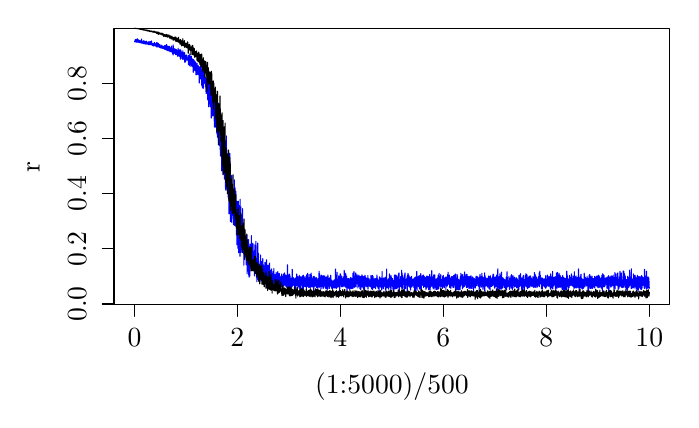
\begin{tikzpicture}[x=0.7pt,y=0.7pt]
\definecolor{fillColor}{RGB}{255,255,255}
%\path[use as bounding box,fill=fillColor,fill opacity=0.00] (0,0) rectangle (361.35,252.94);
\begin{scope}
%\path[clip] ( 49.20, 61.20) rectangle (336.15,203.75);
\definecolor{drawColor}{RGB}{0,0,255}

\path[draw=drawColor,line width= 0.4pt,line join=round,line cap=round] ( 59.83,197.19) --
	( 59.88,197.05) --
	( 59.93,196.87) --
	( 59.99,197.16) --
	( 60.04,197.49) --
	( 60.09,197.13) --
	( 60.15,197.26) --
	( 60.20,197.98) --
	( 60.25,196.90) --
	( 60.31,197.37) --
	( 60.36,197.29) --
	( 60.41,197.17) --
	( 60.47,197.05) --
	( 60.52,196.81) --
	( 60.57,196.94) --
	( 60.63,198.13) --
	( 60.68,197.27) --
	( 60.73,196.75) --
	( 60.78,196.78) --
	( 60.84,196.89) --
	( 60.89,197.62) --
	( 60.94,197.00) --
	( 61.00,196.97) --
	( 61.05,197.19) --
	( 61.10,196.67) --
	( 61.16,197.16) --
	( 61.21,197.77) --
	( 61.26,198.47) --
	( 61.32,197.13) --
	( 61.37,197.07) --
	( 61.42,197.20) --
	( 61.48,197.61) --
	( 61.53,196.95) --
	( 61.58,197.25) --
	( 61.63,197.07) --
	( 61.69,197.36) --
	( 61.74,196.65) --
	( 61.79,197.16) --
	( 61.85,196.85) --
	( 61.90,197.12) --
	( 61.95,197.94) --
	( 62.01,197.72) --
	( 62.06,197.12) --
	( 62.11,197.69) --
	( 62.17,197.13) --
	( 62.22,196.61) --
	( 62.27,197.33) --
	( 62.33,196.53) --
	( 62.38,196.79) --
	( 62.43,197.06) --
	( 62.49,196.83) --
	( 62.54,196.47) --
	( 62.59,197.21) --
	( 62.64,197.47) --
	( 62.70,196.53) --
	( 62.75,196.48) --
	( 62.80,196.82) --
	( 62.86,197.32) --
	( 62.91,197.05) --
	( 62.96,196.47) --
	( 63.02,196.42) --
	( 63.07,196.47) --
	( 63.12,196.30) --
	( 63.18,197.37) --
	( 63.23,196.95) --
	( 63.28,196.33) --
	( 63.34,197.03) --
	( 63.39,196.66) --
	( 63.44,198.34) --
	( 63.50,196.26) --
	( 63.55,196.93) --
	( 63.60,196.71) --
	( 63.65,196.73) --
	( 63.71,196.25) --
	( 63.76,196.31) --
	( 63.81,196.75) --
	( 63.87,197.03) --
	( 63.92,196.52) --
	( 63.97,196.56) --
	( 64.03,196.10) --
	( 64.08,196.44) --
	( 64.13,196.11) --
	( 64.19,196.18) --
	( 64.24,196.71) --
	( 64.29,197.27) --
	( 64.35,196.18) --
	( 64.40,195.93) --
	( 64.45,197.25) --
	( 64.50,196.26) --
	( 64.56,197.48) --
	( 64.61,196.24) --
	( 64.66,197.25) --
	( 64.72,195.95) --
	( 64.77,196.40) --
	( 64.82,196.62) --
	( 64.88,196.18) --
	( 64.93,196.71) --
	( 64.98,196.24) --
	( 65.04,196.93) --
	( 65.09,195.88) --
	( 65.14,196.05) --
	( 65.20,197.26) --
	( 65.25,196.60) --
	( 65.30,196.26) --
	( 65.36,195.96) --
	( 65.41,196.39) --
	( 65.46,195.79) --
	( 65.51,195.95) --
	( 65.57,196.47) --
	( 65.62,195.77) --
	( 65.67,195.99) --
	( 65.73,196.66) --
	( 65.78,196.13) --
	( 65.83,196.50) --
	( 65.89,196.09) --
	( 65.94,196.31) --
	( 65.99,197.23) --
	( 66.05,196.81) --
	( 66.10,195.80) --
	( 66.15,196.42) --
	( 66.21,195.68) --
	( 66.26,196.20) --
	( 66.31,195.91) --
	( 66.37,195.89) --
	( 66.42,195.74) --
	( 66.47,195.68) --
	( 66.52,196.07) --
	( 66.58,195.84) --
	( 66.63,196.31) --
	( 66.68,196.32) --
	( 66.74,196.43) --
	( 66.79,196.18) --
	( 66.84,195.73) --
	( 66.90,196.79) --
	( 66.95,196.23) --
	( 67.00,195.48) --
	( 67.06,196.15) --
	( 67.11,196.40) --
	( 67.16,195.42) --
	( 67.22,195.74) --
	( 67.27,196.98) --
	( 67.32,195.92) --
	( 67.38,196.27) --
	( 67.43,195.81) --
	( 67.48,196.36) --
	( 67.53,195.53) --
	( 67.59,195.48) --
	( 67.64,195.95) --
	( 67.69,196.83) --
	( 67.75,195.45) --
	( 67.80,195.53) --
	( 67.85,196.16) --
	( 67.91,195.44) --
	( 67.96,197.03) --
	( 68.01,195.57) --
	( 68.07,195.47) --
	( 68.12,196.36) --
	( 68.17,195.46) --
	( 68.23,195.98) --
	( 68.28,195.41) --
	( 68.33,196.61) --
	( 68.38,196.54) --
	( 68.44,196.11) --
	( 68.49,196.66) --
	( 68.54,197.37) --
	( 68.60,195.37) --
	( 68.65,195.87) --
	( 68.70,196.34) --
	( 68.76,195.63) --
	( 68.81,195.25) --
	( 68.86,195.83) --
	( 68.92,195.46) --
	( 68.97,195.11) --
	( 69.02,195.15) --
	( 69.08,196.00) --
	( 69.13,195.96) --
	( 69.18,195.12) --
	( 69.24,195.33) --
	( 69.29,195.92) --
	( 69.34,195.49) --
	( 69.39,196.05) --
	( 69.45,194.68) --
	( 69.50,195.35) --
	( 69.55,195.28) --
	( 69.61,195.16) --
	( 69.66,195.25) --
	( 69.71,195.30) --
	( 69.77,195.49) --
	( 69.82,195.05) --
	( 69.87,196.19) --
	( 69.93,195.46) --
	( 69.98,195.47) --
	( 70.03,195.65) --
	( 70.09,196.55) --
	( 70.14,195.20) --
	( 70.19,195.74) --
	( 70.25,195.28) --
	( 70.30,194.87) --
	( 70.35,194.83) --
	( 70.40,195.53) --
	( 70.46,194.86) --
	( 70.51,195.47) --
	( 70.56,195.38) --
	( 70.62,195.14) --
	( 70.67,195.00) --
	( 70.72,194.78) --
	( 70.78,195.94) --
	( 70.83,194.62) --
	( 70.88,195.91) --
	( 70.94,195.23) --
	( 70.99,195.05) --
	( 71.04,195.14) --
	( 71.10,194.95) --
	( 71.15,194.52) --
	( 71.20,194.36) --
	( 71.25,196.49) --
	( 71.31,194.71) --
	( 71.36,194.49) --
	( 71.41,194.65) --
	( 71.47,194.12) --
	( 71.52,195.96) --
	( 71.57,194.78) --
	( 71.63,194.74) --
	( 71.68,196.37) --
	( 71.73,194.86) --
	( 71.79,194.63) --
	( 71.84,194.79) --
	( 71.89,195.35) --
	( 71.95,194.75) --
	( 72.00,194.43) --
	( 72.05,195.62) --
	( 72.11,194.92) --
	( 72.16,194.52) --
	( 72.21,196.01) --
	( 72.26,194.48) --
	( 72.32,194.96) --
	( 72.37,194.55) --
	( 72.42,194.36) --
	( 72.48,194.61) --
	( 72.53,195.51) --
	( 72.58,194.06) --
	( 72.64,194.91) --
	( 72.69,195.44) --
	( 72.74,194.57) --
	( 72.80,194.64) --
	( 72.85,194.58) --
	( 72.90,194.01) --
	( 72.96,195.37) --
	( 73.01,194.72) --
	( 73.06,194.28) --
	( 73.12,194.06) --
	( 73.17,194.48) --
	( 73.22,194.10) --
	( 73.27,193.72) --
	( 73.33,194.70) --
	( 73.38,194.32) --
	( 73.43,194.23) --
	( 73.49,194.20) --
	( 73.54,194.12) --
	( 73.59,194.62) --
	( 73.65,193.70) --
	( 73.70,194.49) --
	( 73.75,194.62) --
	( 73.81,193.71) --
	( 73.86,195.14) --
	( 73.91,194.02) --
	( 73.97,193.69) --
	( 74.02,194.94) --
	( 74.07,194.25) --
	( 74.12,194.34) --
	( 74.18,194.30) --
	( 74.23,193.50) --
	( 74.28,193.99) --
	( 74.34,193.54) --
	( 74.39,193.50) --
	( 74.44,193.77) --
	( 74.50,193.77) --
	( 74.55,194.37) --
	( 74.60,194.45) --
	( 74.66,193.69) --
	( 74.71,194.58) --
	( 74.76,193.93) --
	( 74.82,193.35) --
	( 74.87,193.44) --
	( 74.92,193.89) --
	( 74.98,193.53) --
	( 75.03,193.62) --
	( 75.08,194.23) --
	( 75.13,193.41) --
	( 75.19,193.16) --
	( 75.24,193.21) --
	( 75.29,193.66) --
	( 75.35,193.89) --
	( 75.40,195.05) --
	( 75.45,194.33) --
	( 75.51,194.08) --
	( 75.56,192.88) --
	( 75.61,193.61) --
	( 75.67,193.27) --
	( 75.72,193.24) --
	( 75.77,194.50) --
	( 75.83,193.21) --
	( 75.88,193.29) --
	( 75.93,193.18) --
	( 75.99,192.89) --
	( 76.04,193.13) --
	( 76.09,195.05) --
	( 76.14,193.44) --
	( 76.20,193.95) --
	( 76.25,193.29) --
	( 76.30,195.55) --
	( 76.36,192.61) --
	( 76.41,193.85) --
	( 76.46,192.68) --
	( 76.52,193.20) --
	( 76.57,193.50) --
	( 76.62,193.23) --
	( 76.68,193.31) --
	( 76.73,193.98) --
	( 76.78,194.71) --
	( 76.84,193.29) --
	( 76.89,192.85) --
	( 76.94,192.32) --
	( 77.00,193.79) --
	( 77.05,193.74) --
	( 77.10,193.29) --
	( 77.15,194.43) --
	( 77.21,194.03) --
	( 77.26,192.62) --
	( 77.31,192.78) --
	( 77.37,192.19) --
	( 77.42,193.10) --
	( 77.47,192.62) --
	( 77.53,192.66) --
	( 77.58,193.95) --
	( 77.63,194.67) --
	( 77.69,192.99) --
	( 77.74,192.39) --
	( 77.79,192.50) --
	( 77.85,192.88) --
	( 77.90,192.95) --
	( 77.95,194.48) --
	( 78.00,193.65) --
	( 78.06,192.80) --
	( 78.11,191.71) --
	( 78.16,193.16) --
	( 78.22,193.02) --
	( 78.27,192.63) --
	( 78.32,192.20) --
	( 78.38,193.78) --
	( 78.43,191.94) --
	( 78.48,192.18) --
	( 78.54,193.43) --
	( 78.59,191.95) --
	( 78.64,193.40) --
	( 78.70,192.02) --
	( 78.75,193.80) --
	( 78.80,192.59) --
	( 78.86,191.67) --
	( 78.91,192.97) --
	( 78.96,194.73) --
	( 79.01,193.08) --
	( 79.07,191.99) --
	( 79.12,192.69) --
	( 79.17,192.68) --
	( 79.23,192.38) --
	( 79.28,191.53) --
	( 79.33,191.97) --
	( 79.39,192.61) --
	( 79.44,192.32) --
	( 79.49,192.02) --
	( 79.55,190.60) --
	( 79.60,192.35) --
	( 79.65,192.58) --
	( 79.71,190.10) --
	( 79.76,195.27) --
	( 79.81,191.92) --
	( 79.87,191.26) --
	( 79.92,191.32) --
	( 79.97,191.52) --
	( 80.02,192.40) --
	( 80.08,192.02) --
	( 80.13,191.40) --
	( 80.18,190.83) --
	( 80.24,193.30) --
	( 80.29,191.42) --
	( 80.34,192.90) --
	( 80.40,193.21) --
	( 80.45,192.84) --
	( 80.50,191.96) --
	( 80.56,191.15) --
	( 80.61,193.16) --
	( 80.66,192.92) --
	( 80.72,191.18) --
	( 80.77,191.95) --
	( 80.82,190.84) --
	( 80.87,192.21) --
	( 80.93,192.69) --
	( 80.98,191.47) --
	( 81.03,190.26) --
	( 81.09,193.06) --
	( 81.14,190.83) --
	( 81.19,191.41) --
	( 81.25,190.36) --
	( 81.30,191.47) --
	( 81.35,192.58) --
	( 81.41,191.64) --
	( 81.46,192.84) --
	( 81.51,191.60) --
	( 81.57,191.99) --
	( 81.62,191.59) --
	( 81.67,190.84) --
	( 81.73,192.36) --
	( 81.78,190.77) --
	( 81.83,190.12) --
	( 81.88,191.90) --
	( 81.94,190.17) --
	( 81.99,192.01) --
	( 82.04,191.53) --
	( 82.10,189.40) --
	( 82.15,190.51) --
	( 82.20,192.14) --
	( 82.26,191.31) --
	( 82.31,193.59) --
	( 82.36,192.08) --
	( 82.42,190.96) --
	( 82.47,191.89) --
	( 82.52,192.83) --
	( 82.58,190.81) --
	( 82.63,192.71) --
	( 82.68,189.96) --
	( 82.74,189.62) --
	( 82.79,191.67) --
	( 82.84,191.53) --
	( 82.89,190.96) --
	( 82.95,190.90) --
	( 83.00,191.44) --
	( 83.05,190.96) --
	( 83.11,190.92) --
	( 83.16,189.27) --
	( 83.21,190.19) --
	( 83.27,192.83) --
	( 83.32,190.42) --
	( 83.37,190.30) --
	( 83.43,191.22) --
	( 83.48,187.95) --
	( 83.53,190.18) --
	( 83.59,191.65) --
	( 83.64,192.73) --
	( 83.69,189.75) --
	( 83.75,190.91) --
	( 83.80,190.13) --
	( 83.85,190.06) --
	( 83.90,190.98) --
	( 83.96,190.14) --
	( 84.01,189.20) --
	( 84.06,191.71) --
	( 84.12,189.59) --
	( 84.17,189.47) --
	( 84.22,190.85) --
	( 84.28,189.69) --
	( 84.33,188.17) --
	( 84.38,190.18) --
	( 84.44,189.16) --
	( 84.49,190.07) --
	( 84.54,189.24) --
	( 84.60,188.98) --
	( 84.65,190.84) --
	( 84.70,189.36) --
	( 84.75,192.25) --
	( 84.81,187.79) --
	( 84.86,189.67) --
	( 84.91,188.59) --
	( 84.97,191.34) --
	( 85.02,191.23) --
	( 85.07,188.99) --
	( 85.13,188.71) --
	( 85.18,189.78) --
	( 85.23,188.88) --
	( 85.29,187.97) --
	( 85.34,188.30) --
	( 85.39,188.60) --
	( 85.45,189.13) --
	( 85.50,188.57) --
	( 85.55,189.71) --
	( 85.61,188.56) --
	( 85.66,191.38) --
	( 85.71,186.35) --
	( 85.76,190.11) --
	( 85.82,188.59) --
	( 85.87,187.50) --
	( 85.92,186.73) --
	( 85.98,186.45) --
	( 86.03,188.74) --
	( 86.08,189.32) --
	( 86.14,188.70) --
	( 86.19,189.55) --
	( 86.24,188.15) --
	( 86.30,186.86) --
	( 86.35,189.49) --
	( 86.40,187.50) --
	( 86.46,188.46) --
	( 86.51,190.11) --
	( 86.56,188.81) --
	( 86.62,187.71) --
	( 86.67,187.83) --
	( 86.72,188.38) --
	( 86.77,187.62) --
	( 86.83,188.00) --
	( 86.88,188.61) --
	( 86.93,187.84) --
	( 86.99,187.65) --
	( 87.04,188.46) --
	( 87.09,187.54) --
	( 87.15,187.57) --
	( 87.20,188.20) --
	( 87.25,187.45) --
	( 87.31,188.62) --
	( 87.36,189.71) --
	( 87.41,187.27) --
	( 87.47,187.21) --
	( 87.52,189.88) --
	( 87.57,187.04) --
	( 87.62,187.98) --
	( 87.68,185.08) --
	( 87.73,189.86) --
	( 87.78,188.36) --
	( 87.84,188.30) --
	( 87.89,187.26) --
	( 87.94,187.36) --
	( 88.00,188.08) --
	( 88.05,188.14) --
	( 88.10,188.66) --
	( 88.16,188.00) --
	( 88.21,184.74) --
	( 88.26,190.04) --
	( 88.32,188.38) --
	( 88.37,190.68) --
	( 88.42,187.12) --
	( 88.48,185.12) --
	( 88.53,184.26) --
	( 88.58,187.70) --
	( 88.63,185.36) --
	( 88.69,187.51) --
	( 88.74,185.33) --
	( 88.79,185.13) --
	( 88.85,187.17) --
	( 88.90,187.98) --
	( 88.95,185.41) --
	( 89.01,186.29) --
	( 89.06,187.51) --
	( 89.11,189.51) --
	( 89.17,186.46) --
	( 89.22,186.73) --
	( 89.27,184.70) --
	( 89.33,184.37) --
	( 89.38,185.24) --
	( 89.43,186.70) --
	( 89.49,188.16) --
	( 89.54,184.12) --
	( 89.59,187.26) --
	( 89.64,185.66) --
	( 89.70,185.93) --
	( 89.75,185.52) --
	( 89.80,185.73) --
	( 89.86,187.89) --
	( 89.91,186.14) --
	( 89.96,185.30) --
	( 90.02,184.86) --
	( 90.07,185.70) --
	( 90.12,181.12) --
	( 90.18,187.65) --
	( 90.23,183.36) --
	( 90.28,184.04) --
	( 90.34,185.99) --
	( 90.39,186.15) --
	( 90.44,187.66) --
	( 90.50,183.10) --
	( 90.55,184.65) --
	( 90.60,184.40) --
	( 90.65,183.89) --
	( 90.71,187.06) --
	( 90.76,182.19) --
	( 90.81,182.59) --
	( 90.87,183.18) --
	( 90.92,186.38) --
	( 90.97,184.53) --
	( 91.03,185.67) --
	( 91.08,183.78) --
	( 91.13,186.09) --
	( 91.19,185.42) --
	( 91.24,184.49) --
	( 91.29,181.79) --
	( 91.35,186.54) --
	( 91.40,184.85) --
	( 91.45,182.94) --
	( 91.50,181.69) --
	( 91.56,179.82) --
	( 91.61,184.72) --
	( 91.66,184.39) --
	( 91.72,183.24) --
	( 91.77,183.46) --
	( 91.82,183.52) --
	( 91.88,184.19) --
	( 91.93,185.60) --
	( 91.98,179.93) --
	( 92.04,183.21) --
	( 92.09,185.85) --
	( 92.14,183.25) --
	( 92.20,180.98) --
	( 92.25,180.70) --
	( 92.30,183.84) --
	( 92.36,183.79) --
	( 92.41,183.59) --
	( 92.46,181.32) --
	( 92.51,180.88) --
	( 92.57,184.15) --
	( 92.62,183.72) --
	( 92.67,184.71) --
	( 92.73,179.99) --
	( 92.78,180.43) --
	( 92.83,183.41) --
	( 92.89,180.11) --
	( 92.94,183.98) --
	( 92.99,183.45) --
	( 93.05,183.52) --
	( 93.10,183.32) --
	( 93.15,182.04) --
	( 93.21,176.04) --
	( 93.26,175.63) --
	( 93.31,182.44) --
	( 93.37,183.52) --
	( 93.42,183.90) --
	( 93.47,182.73) --
	( 93.52,180.65) --
	( 93.58,182.69) --
	( 93.63,180.09) --
	( 93.68,177.64) --
	( 93.74,178.06) --
	( 93.79,183.69) --
	( 93.84,184.45) --
	( 93.90,183.68) --
	( 93.95,180.80) --
	( 94.00,184.44) --
	( 94.06,178.96) --
	( 94.11,179.88) --
	( 94.16,184.40) --
	( 94.22,183.10) --
	( 94.27,182.83) --
	( 94.32,180.32) --
	( 94.37,181.82) --
	( 94.43,178.70) --
	( 94.48,175.02) --
	( 94.53,174.38) --
	( 94.59,177.18) --
	( 94.64,177.29) --
	( 94.69,179.75) --
	( 94.75,179.89) --
	( 94.80,173.11) --
	( 94.85,179.68) --
	( 94.91,179.56) --
	( 94.96,177.33) --
	( 95.01,179.43) --
	( 95.07,180.10) --
	( 95.12,181.97) --
	( 95.17,178.58) --
	( 95.23,182.58) --
	( 95.28,172.89) --
	( 95.33,177.09) --
	( 95.38,177.93) --
	( 95.44,176.24) --
	( 95.49,181.93) --
	( 95.54,180.91) --
	( 95.60,177.94) --
	( 95.65,175.95) --
	( 95.70,177.27) --
	( 95.76,176.39) --
	( 95.81,180.75) --
	( 95.86,176.43) --
	( 95.92,175.45) --
	( 95.97,176.52) --
	( 96.02,178.39) --
	( 96.08,175.28) --
	( 96.13,179.83) --
	( 96.18,178.19) --
	( 96.24,178.70) --
	( 96.29,176.67) --
	( 96.34,176.15) --
	( 96.39,175.83) --
	( 96.45,173.57) --
	( 96.50,176.52) --
	( 96.55,175.55) --
	( 96.61,175.16) --
	( 96.66,178.52) --
	( 96.71,171.07) --
	( 96.77,172.45) --
	( 96.82,170.15) --
	( 96.87,174.10) --
	( 96.93,170.85) --
	( 96.98,174.54) --
	( 97.03,175.43) --
	( 97.09,178.17) --
	( 97.14,177.02) --
	( 97.19,175.34) --
	( 97.25,177.18) --
	( 97.30,170.46) --
	( 97.35,171.76) --
	( 97.40,176.19) --
	( 97.46,171.34) --
	( 97.51,175.49) --
	( 97.56,171.47) --
	( 97.62,167.09) --
	( 97.67,175.99) --
	( 97.72,171.84) --
	( 97.78,173.46) --
	( 97.83,166.54) --
	( 97.88,172.37) --
	( 97.94,172.31) --
	( 97.99,174.80) --
	( 98.04,173.11) --
	( 98.10,176.10) --
	( 98.15,163.35) --
	( 98.20,169.55) --
	( 98.25,170.71) --
	( 98.31,169.70) --
	( 98.36,173.05) --
	( 98.41,177.29) --
	( 98.47,173.36) --
	( 98.52,175.29) --
	( 98.57,171.38) --
	( 98.63,164.89) --
	( 98.68,175.13) --
	( 98.73,169.45) --
	( 98.79,167.00) --
	( 98.84,177.03) --
	( 98.89,165.83) --
	( 98.95,173.01) --
	( 99.00,163.39) --
	( 99.05,166.99) --
	( 99.11,170.29) --
	( 99.16,173.62) --
	( 99.21,179.51) --
	( 99.26,176.94) --
	( 99.32,162.86) --
	( 99.37,171.73) --
	( 99.42,157.53) --
	( 99.48,163.21) --
	( 99.53,166.56) --
	( 99.58,157.92) --
	( 99.64,171.52) --
	( 99.69,161.06) --
	( 99.74,169.22) --
	( 99.80,167.28) --
	( 99.85,164.04) --
	( 99.90,168.04) --
	( 99.96,166.91) --
	(100.01,164.37) --
	(100.06,168.32) --
	(100.12,169.68) --
	(100.17,166.16) --
	(100.22,166.35) --
	(100.27,158.75) --
	(100.33,173.05) --
	(100.38,171.27) --
	(100.43,167.69) --
	(100.49,165.97) --
	(100.54,165.29) --
	(100.59,162.60) --
	(100.65,161.48) --
	(100.70,168.92) --
	(100.75,167.14) --
	(100.81,167.79) --
	(100.86,164.94) --
	(100.91,163.85) --
	(100.97,156.26) --
	(101.02,165.81) --
	(101.07,152.86) --
	(101.12,160.62) --
	(101.18,164.57) --
	(101.23,158.35) --
	(101.28,159.41) --
	(101.34,157.38) --
	(101.39,160.87) --
	(101.44,157.78) --
	(101.50,163.45) --
	(101.55,155.66) --
	(101.60,167.41) --
	(101.66,156.31) --
	(101.71,159.96) --
	(101.76,158.37) --
	(101.82,152.65) --
	(101.87,156.16) --
	(101.92,157.13) --
	(101.98,157.78) --
	(102.03,156.22) --
	(102.08,154.51) --
	(102.13,162.36) --
	(102.19,150.47) --
	(102.24,158.86) --
	(102.29,154.77) --
	(102.35,149.43) --
	(102.40,159.47) --
	(102.45,165.11) --
	(102.51,160.76) --
	(102.56,156.93) --
	(102.61,155.10) --
	(102.67,147.65) --
	(102.72,147.85) --
	(102.77,153.58) --
	(102.83,153.02) --
	(102.88,150.32) --
	(102.93,160.13) --
	(102.99,164.61) --
	(103.04,159.13) --
	(103.09,145.94) --
	(103.14,158.05) --
	(103.20,152.24) --
	(103.25,161.66) --
	(103.30,165.18) --
	(103.36,159.70) --
	(103.41,153.17) --
	(103.46,161.45) --
	(103.52,149.65) --
	(103.57,158.43) --
	(103.62,155.02) --
	(103.68,148.31) --
	(103.73,155.28) --
	(103.78,143.17) --
	(103.84,149.42) --
	(103.89,150.18) --
	(103.94,149.87) --
	(104.00,141.22) --
	(104.05,148.85) --
	(104.10,146.40) --
	(104.15,143.40) --
	(104.21,137.89) --
	(104.26,158.70) --
	(104.31,151.83) --
	(104.37,149.92) --
	(104.42,151.06) --
	(104.47,148.67) --
	(104.53,153.93) --
	(104.58,141.61) --
	(104.63,146.06) --
	(104.69,149.58) --
	(104.74,150.05) --
	(104.79,130.29) --
	(104.85,147.12) --
	(104.90,149.36) --
	(104.95,149.83) --
	(105.00,137.70) --
	(105.06,137.17) --
	(105.11,142.89) --
	(105.16,146.03) --
	(105.22,141.35) --
	(105.27,146.24) --
	(105.32,144.44) --
	(105.38,139.67) --
	(105.43,128.34) --
	(105.48,141.85) --
	(105.54,135.45) --
	(105.59,151.78) --
	(105.64,149.91) --
	(105.70,150.80) --
	(105.75,144.34) --
	(105.80,138.91) --
	(105.86,149.73) --
	(105.91,130.22) --
	(105.96,132.36) --
	(106.01,135.06) --
	(106.07,141.06) --
	(106.12,130.14) --
	(106.17,147.56) --
	(106.23,144.34) --
	(106.28,125.98) --
	(106.33,139.79) --
	(106.39,137.92) --
	(106.44,126.90) --
	(106.49,145.82) --
	(106.55,126.96) --
	(106.60,132.60) --
	(106.65,134.91) --
	(106.71,134.39) --
	(106.76,124.36) --
	(106.81,120.74) --
	(106.87,122.87) --
	(106.92,124.46) --
	(106.97,131.82) --
	(107.02,120.20) --
	(107.08,130.37) --
	(107.13,136.55) --
	(107.18,135.29) --
	(107.24,148.30) --
	(107.29,131.34) --
	(107.34,127.58) --
	(107.40,121.73) --
	(107.45,138.12) --
	(107.50,132.60) --
	(107.56,133.21) --
	(107.61,133.45) --
	(107.66,122.98) --
	(107.72,131.75) --
	(107.77,126.92) --
	(107.82,120.86) --
	(107.87,123.87) --
	(107.93,133.85) --
	(107.98,126.44) --
	(108.03,125.32) --
	(108.09,123.14) --
	(108.14,116.86) --
	(108.19,134.03) --
	(108.25,116.18) --
	(108.30,126.75) --
	(108.35,119.29) --
	(108.41,134.25) --
	(108.46,120.67) --
	(108.51,109.74) --
	(108.57,108.05) --
	(108.62,125.05) --
	(108.67,112.84) --
	(108.73,126.13) --
	(108.78,126.05) --
	(108.83,112.78) --
	(108.88,121.58) --
	(108.94,120.25) --
	(108.99,139.44) --
	(109.04,124.18) --
	(109.10,109.38) --
	(109.15,135.17) --
	(109.20,119.78) --
	(109.26,130.41) --
	(109.31,119.51) --
	(109.36,104.06) --
	(109.42,117.89) --
	(109.47,117.25) --
	(109.52,127.70) --
	(109.58,125.19) --
	(109.63,114.38) --
	(109.68,113.98) --
	(109.74,116.13) --
	(109.79,114.05) --
	(109.84,105.25) --
	(109.89,109.60) --
	(109.95,103.71) --
	(110.00,108.80) --
	(110.05,123.97) --
	(110.11,128.03) --
	(110.16,114.73) --
	(110.21,118.70) --
	(110.27,115.18) --
	(110.32,110.61) --
	(110.37,112.99) --
	(110.43,118.36) --
	(110.48,118.55) --
	(110.53,109.79) --
	(110.59,114.61) --
	(110.64,115.42) --
	(110.69,107.10) --
	(110.75,114.74) --
	(110.80,108.24) --
	(110.85,110.00) --
	(110.90,102.52) --
	(110.96,105.66) --
	(111.01,105.67) --
	(111.06,112.33) --
	(111.12,114.40) --
	(111.17,111.84) --
	(111.22,110.78) --
	(111.28,102.65) --
	(111.33,125.66) --
	(111.38,102.13) --
	(111.44,108.84) --
	(111.49,112.79) --
	(111.54,106.76) --
	(111.60,111.53) --
	(111.65,114.01) --
	(111.70,106.90) --
	(111.75,121.48) --
	(111.81,112.50) --
	(111.86,113.29) --
	(111.91,109.25) --
	(111.97,101.80) --
	(112.02,111.24) --
	(112.07,119.47) --
	(112.13,119.66) --
	(112.18,109.67) --
	(112.23,118.05) --
	(112.29,101.22) --
	(112.34,103.97) --
	(112.39,102.30) --
	(112.45, 97.18) --
	(112.50,104.10) --
	(112.55,101.45) --
	(112.61,103.37) --
	(112.66, 92.16) --
	(112.71,113.85) --
	(112.76,108.46) --
	(112.82,114.50) --
	(112.87,104.00) --
	(112.92,102.79) --
	(112.98,100.77) --
	(113.03,108.88) --
	(113.08,103.75) --
	(113.14,107.14) --
	(113.19,109.04) --
	(113.24, 90.26) --
	(113.30, 97.72) --
	(113.35,114.65) --
	(113.40,104.61) --
	(113.46,103.91) --
	(113.51,110.43) --
	(113.56, 88.01) --
	(113.62, 99.69) --
	(113.67,111.00) --
	(113.72, 93.20) --
	(113.77,106.91) --
	(113.83, 91.29) --
	(113.88, 94.18) --
	(113.93,104.51) --
	(113.99,102.43) --
	(114.04,112.51) --
	(114.09, 94.51) --
	(114.15,102.50) --
	(114.20, 95.44) --
	(114.25, 86.20) --
	(114.31,115.60) --
	(114.36, 88.01) --
	(114.41, 96.33) --
	(114.47,104.40) --
	(114.52, 97.24) --
	(114.57,103.59) --
	(114.62,100.03) --
	(114.68, 90.77) --
	(114.73,111.66) --
	(114.78, 96.43) --
	(114.84, 99.25) --
	(114.89, 90.47) --
	(114.94, 94.68) --
	(115.00, 89.60) --
	(115.05, 96.28) --
	(115.10, 95.99) --
	(115.16,101.97) --
	(115.21, 95.50) --
	(115.26, 88.23) --
	(115.32, 90.16) --
	(115.37, 97.51) --
	(115.42, 97.64) --
	(115.48, 95.29) --
	(115.53, 95.34) --
	(115.58,110.78) --
	(115.63, 91.97) --
	(115.69,100.14) --
	(115.74, 88.77) --
	(115.79, 94.72) --
	(115.85, 92.13) --
	(115.90, 88.15) --
	(115.95, 89.98) --
	(116.01, 92.95) --
	(116.06, 91.08) --
	(116.11, 96.47) --
	(116.17, 97.88) --
	(116.22, 86.91) --
	(116.27, 81.55) --
	(116.33,100.46) --
	(116.38, 94.68) --
	(116.43, 92.89) --
	(116.49, 91.17) --
	(116.54, 91.36) --
	(116.59, 98.62) --
	(116.64, 84.53) --
	(116.70, 96.30) --
	(116.75, 91.75) --
	(116.80, 90.92) --
	(116.86, 85.83) --
	(116.91, 88.82) --
	(116.96, 88.39) --
	(117.02, 93.00) --
	(117.07, 95.04) --
	(117.12, 94.48) --
	(117.18, 93.65) --
	(117.23, 90.14) --
	(117.28, 94.00) --
	(117.34, 86.46) --
	(117.39, 93.77) --
	(117.44, 96.83) --
	(117.50, 81.83) --
	(117.55, 87.35) --
	(117.60, 93.36) --
	(117.65, 97.38) --
	(117.71, 84.15) --
	(117.76, 97.12) --
	(117.81, 90.41) --
	(117.87, 86.42) --
	(117.92, 77.14) --
	(117.97, 91.51) --
	(118.03, 94.75) --
	(118.08, 84.16) --
	(118.13, 93.69) --
	(118.19, 92.16) --
	(118.24, 88.40) --
	(118.29, 85.75) --
	(118.35, 84.72) --
	(118.40, 82.73) --
	(118.45, 87.91) --
	(118.50, 90.64) --
	(118.56, 93.08) --
	(118.61, 93.32) --
	(118.66, 78.21) --
	(118.72, 94.86) --
	(118.77, 76.66) --
	(118.82, 90.62) --
	(118.88, 84.96) --
	(118.93, 75.37) --
	(118.98, 89.43) --
	(119.04, 83.29) --
	(119.09, 87.87) --
	(119.14, 77.45) --
	(119.20, 91.30) --
	(119.25, 84.94) --
	(119.30, 75.93) --
	(119.36, 84.83) --
	(119.41, 84.84) --
	(119.46, 79.75) --
	(119.51, 92.46) --
	(119.57, 83.55) --
	(119.62, 86.04) --
	(119.67, 91.63) --
	(119.73, 81.60) --
	(119.78, 85.50) --
	(119.83, 84.06) --
	(119.89, 85.65) --
	(119.94, 87.47) --
	(119.99, 80.43) --
	(120.05, 91.44) --
	(120.10, 87.12) --
	(120.15, 96.80) --
	(120.21, 81.84) --
	(120.26, 87.36) --
	(120.31, 91.43) --
	(120.37, 86.00) --
	(120.42, 87.88) --
	(120.47, 90.45) --
	(120.52, 92.92) --
	(120.58, 88.59) --
	(120.63, 86.81) --
	(120.68, 83.47) --
	(120.74, 82.15) --
	(120.79, 87.54) --
	(120.84, 83.05) --
	(120.90, 86.49) --
	(120.95, 85.82) --
	(121.00, 92.63) --
	(121.06, 80.13) --
	(121.11, 86.92) --
	(121.16, 82.03) --
	(121.22, 83.27) --
	(121.27, 82.46) --
	(121.32, 79.66) --
	(121.37, 84.94) --
	(121.43, 81.14) --
	(121.48, 86.21) --
	(121.53, 86.31) --
	(121.59, 84.49) --
	(121.64, 88.90) --
	(121.69, 76.11) --
	(121.75, 79.31) --
	(121.80, 81.83) --
	(121.85, 81.10) --
	(121.91, 92.03) --
	(121.96, 88.92) --
	(122.01, 82.21) --
	(122.07, 78.17) --
	(122.12, 85.05) --
	(122.17, 82.93) --
	(122.23, 83.15) --
	(122.28, 78.81) --
	(122.33, 81.19) --
	(122.38, 78.73) --
	(122.44, 93.91) --
	(122.49, 77.46) --
	(122.54, 82.92) --
	(122.60, 78.37) --
	(122.65, 80.14) --
	(122.70, 82.16) --
	(122.76, 83.17) --
	(122.81, 84.73) --
	(122.86, 78.19) --
	(122.92, 80.74) --
	(122.97, 73.03) --
	(123.02, 77.57) --
	(123.08, 77.17) --
	(123.13, 78.32) --
	(123.18, 84.58) --
	(123.24, 91.57) --
	(123.29, 78.36) --
	(123.34, 74.29) --
	(123.39, 93.01) --
	(123.45, 87.35) --
	(123.50, 81.10) --
	(123.55, 76.94) --
	(123.61, 79.80) --
	(123.66, 75.46) --
	(123.71, 81.52) --
	(123.77, 74.59) --
	(123.82, 87.61) --
	(123.87, 77.82) --
	(123.93, 73.88) --
	(123.98, 75.50) --
	(124.03, 78.64) --
	(124.09, 74.82) --
	(124.14, 78.75) --
	(124.19, 77.85) --
	(124.24, 80.00) --
	(124.30, 79.71) --
	(124.35, 81.73) --
	(124.40, 74.79) --
	(124.46, 78.46) --
	(124.51, 78.53) --
	(124.56, 78.12) --
	(124.62, 75.12) --
	(124.67, 82.67) --
	(124.72, 74.22) --
	(124.78, 83.88) --
	(124.83, 75.48) --
	(124.88, 86.85) --
	(124.94, 80.32) --
	(124.99, 76.49) --
	(125.04, 73.28) --
	(125.10, 79.96) --
	(125.15, 73.95) --
	(125.20, 83.51) --
	(125.25, 73.73) --
	(125.31, 75.63) --
	(125.36, 83.58) --
	(125.41, 74.97) --
	(125.47, 76.39) --
	(125.52, 77.72) --
	(125.57, 79.15) --
	(125.63, 78.71) --
	(125.68, 75.16) --
	(125.73, 83.34) --
	(125.79, 79.14) --
	(125.84, 75.49) --
	(125.89, 77.86) --
	(125.95, 75.55) --
	(126.00, 84.94) --
	(126.05, 79.40) --
	(126.11, 74.14) --
	(126.16, 78.19) --
	(126.21, 80.61) --
	(126.26, 76.03) --
	(126.32, 81.74) --
	(126.37, 74.87) --
	(126.42, 77.54) --
	(126.48, 77.90) --
	(126.53, 75.60) --
	(126.58, 79.11) --
	(126.64, 75.03) --
	(126.69, 81.20) --
	(126.74, 77.93) --
	(126.80, 75.15) --
	(126.85, 77.41) --
	(126.90, 80.42) --
	(126.96, 78.49) --
	(127.01, 79.83) --
	(127.06, 77.41) --
	(127.12, 79.25) --
	(127.17, 83.03) --
	(127.22, 77.52) --
	(127.27, 77.33) --
	(127.33, 75.04) --
	(127.38, 79.67) --
	(127.43, 76.91) --
	(127.49, 76.91) --
	(127.54, 74.20) --
	(127.59, 76.29) --
	(127.65, 73.07) --
	(127.70, 78.79) --
	(127.75, 75.45) --
	(127.81, 82.27) --
	(127.86, 72.81) --
	(127.91, 84.37) --
	(127.97, 82.01) --
	(128.02, 74.11) --
	(128.07, 75.86) --
	(128.12, 74.76) --
	(128.18, 76.73) --
	(128.23, 73.27) --
	(128.28, 74.31) --
	(128.34, 77.56) --
	(128.39, 77.67) --
	(128.44, 77.54) --
	(128.50, 73.91) --
	(128.55, 79.25) --
	(128.60, 77.33) --
	(128.66, 74.55) --
	(128.71, 81.62) --
	(128.76, 73.02) --
	(128.82, 78.87) --
	(128.87, 80.72) --
	(128.92, 75.99) --
	(128.98, 69.99) --
	(129.03, 75.12) --
	(129.08, 74.41) --
	(129.13, 76.90) --
	(129.19, 78.52) --
	(129.24, 74.29) --
	(129.29, 79.74) --
	(129.35, 74.51) --
	(129.40, 76.92) --
	(129.45, 71.94) --
	(129.51, 82.67) --
	(129.56, 76.99) --
	(129.61, 76.84) --
	(129.67, 74.62) --
	(129.72, 77.94) --
	(129.77, 75.77) --
	(129.83, 77.48) --
	(129.88, 70.35) --
	(129.93, 78.82) --
	(129.99, 78.11) --
	(130.04, 78.14) --
	(130.09, 73.36) --
	(130.14, 75.60) --
	(130.20, 72.56) --
	(130.25, 73.85) --
	(130.30, 72.24) --
	(130.36, 74.36) --
	(130.41, 77.16) --
	(130.46, 71.33) --
	(130.52, 79.63) --
	(130.57, 75.81) --
	(130.62, 73.74) --
	(130.68, 70.65) --
	(130.73, 77.55) --
	(130.78, 71.99) --
	(130.84, 74.57) --
	(130.89, 75.17) --
	(130.94, 72.02) --
	(130.99, 73.40) --
	(131.05, 73.47) --
	(131.10, 75.30) --
	(131.15, 69.46) --
	(131.21, 75.62) --
	(131.26, 73.61) --
	(131.31, 75.96) --
	(131.37, 78.00) --
	(131.42, 78.33) --
	(131.47, 74.38) --
	(131.53, 76.83) --
	(131.58, 73.96) --
	(131.63, 76.25) --
	(131.69, 72.72) --
	(131.74, 79.88) --
	(131.79, 74.27) --
	(131.85, 76.29) --
	(131.90, 72.22) --
	(131.95, 73.60) --
	(132.00, 76.52) --
	(132.06, 75.26) --
	(132.11, 71.20) --
	(132.16, 76.66) --
	(132.22, 76.78) --
	(132.27, 75.40) --
	(132.32, 71.46) --
	(132.38, 74.00) --
	(132.43, 72.82) --
	(132.48, 71.32) --
	(132.54, 73.64) --
	(132.59, 73.98) --
	(132.64, 72.89) --
	(132.70, 71.15) --
	(132.75, 71.96) --
	(132.80, 73.56) --
	(132.86, 71.95) --
	(132.91, 77.82) --
	(132.96, 73.99) --
	(133.01, 74.46) --
	(133.07, 72.40) --
	(133.12, 71.62) --
	(133.17, 73.07) --
	(133.23, 74.30) --
	(133.28, 76.24) --
	(133.33, 73.97) --
	(133.39, 74.27) --
	(133.44, 70.70) --
	(133.49, 77.20) --
	(133.55, 77.49) --
	(133.60, 74.00) --
	(133.65, 69.87) --
	(133.71, 76.41) --
	(133.76, 78.21) --
	(133.81, 75.70) --
	(133.87, 73.33) --
	(133.92, 76.42) --
	(133.97, 72.79) --
	(134.02, 74.40) --
	(134.08, 72.44) --
	(134.13, 75.77) --
	(134.18, 76.60) --
	(134.24, 77.07) --
	(134.29, 73.87) --
	(134.34, 74.47) --
	(134.40, 74.17) --
	(134.45, 70.98) --
	(134.50, 74.01) --
	(134.56, 77.35) --
	(134.61, 72.27) --
	(134.66, 71.89) --
	(134.72, 73.46) --
	(134.77, 71.83) --
	(134.82, 69.87) --
	(134.87, 71.08) --
	(134.93, 70.58) --
	(134.98, 71.48) --
	(135.03, 75.57) --
	(135.09, 75.02) --
	(135.14, 72.29) --
	(135.19, 73.89) --
	(135.25, 69.62) --
	(135.30, 73.29) --
	(135.35, 71.61) --
	(135.41, 74.72) --
	(135.46, 75.30) --
	(135.51, 76.14) --
	(135.57, 73.37) --
	(135.62, 74.13) --
	(135.67, 75.35) --
	(135.73, 77.02) --
	(135.78, 74.58) --
	(135.83, 72.95) --
	(135.88, 71.87) --
	(135.94, 73.60) --
	(135.99, 75.14) --
	(136.04, 70.55) --
	(136.10, 75.87) --
	(136.15, 74.82) --
	(136.20, 73.58) --
	(136.26, 74.62) --
	(136.31, 70.20) --
	(136.36, 72.65) --
	(136.42, 72.52) --
	(136.47, 70.95) --
	(136.52, 75.45) --
	(136.58, 70.82) --
	(136.63, 73.30) --
	(136.68, 76.51) --
	(136.74, 76.99) --
	(136.79, 74.77) --
	(136.84, 71.71) --
	(136.89, 70.92) --
	(136.95, 71.07) --
	(137.00, 74.17) --
	(137.05, 76.09) --
	(137.11, 77.30) --
	(137.16, 71.76) --
	(137.21, 77.57) --
	(137.27, 74.29) --
	(137.32, 76.84) --
	(137.37, 75.40) --
	(137.43, 73.43) --
	(137.48, 72.92) --
	(137.53, 73.04) --
	(137.59, 71.33) --
	(137.64, 74.22) --
	(137.69, 72.91) --
	(137.74, 73.98) --
	(137.80, 76.50) --
	(137.85, 75.01) --
	(137.90, 72.55) --
	(137.96, 74.56) --
	(138.01, 70.56) --
	(138.06, 72.81) --
	(138.12, 76.32) --
	(138.17, 72.39) --
	(138.22, 73.87) --
	(138.28, 70.43) --
	(138.33, 74.17) --
	(138.38, 74.12) --
	(138.44, 70.79) --
	(138.49, 73.09) --
	(138.54, 70.05) --
	(138.60, 75.19) --
	(138.65, 74.21) --
	(138.70, 73.92) --
	(138.75, 81.80) --
	(138.81, 74.59) --
	(138.86, 75.56) --
	(138.91, 72.49) --
	(138.97, 71.20) --
	(139.02, 73.44) --
	(139.07, 76.17) --
	(139.13, 71.60) --
	(139.18, 72.57) --
	(139.23, 75.89) --
	(139.29, 72.87) --
	(139.34, 76.61) --
	(139.39, 68.95) --
	(139.45, 71.79) --
	(139.50, 70.24) --
	(139.55, 73.87) --
	(139.61, 73.41) --
	(139.66, 75.31) --
	(139.71, 70.52) --
	(139.76, 74.02) --
	(139.82, 75.36) --
	(139.87, 77.04) --
	(139.92, 75.38) --
	(139.98, 70.91) --
	(140.03, 68.51) --
	(140.08, 71.98) --
	(140.14, 75.99) --
	(140.19, 73.91) --
	(140.24, 72.82) --
	(140.30, 70.35) --
	(140.35, 71.35) --
	(140.40, 71.17) --
	(140.46, 72.28) --
	(140.51, 73.53) --
	(140.56, 73.32) --
	(140.62, 73.92) --
	(140.67, 74.33) --
	(140.72, 72.75) --
	(140.77, 74.89) --
	(140.83, 69.85) --
	(140.88, 72.41) --
	(140.93, 73.06) --
	(140.99, 70.42) --
	(141.04, 74.97) --
	(141.09, 74.99) --
	(141.15, 70.50) --
	(141.20, 79.46) --
	(141.25, 74.19) --
	(141.31, 73.55) --
	(141.36, 75.68) --
	(141.41, 74.42) --
	(141.47, 71.00) --
	(141.52, 73.97) --
	(141.57, 72.64) --
	(141.62, 74.93) --
	(141.68, 74.36) --
	(141.73, 71.35) --
	(141.78, 73.59) --
	(141.84, 72.72) --
	(141.89, 75.09) --
	(141.94, 72.92) --
	(142.00, 74.00) --
	(142.05, 72.76) --
	(142.10, 72.05) --
	(142.16, 72.48) --
	(142.21, 72.01) --
	(142.26, 71.13) --
	(142.32, 72.17) --
	(142.37, 73.97) --
	(142.42, 70.45) --
	(142.48, 74.52) --
	(142.53, 68.68) --
	(142.58, 73.83) --
	(142.63, 71.77) --
	(142.69, 73.71) --
	(142.74, 72.62) --
	(142.79, 72.51) --
	(142.85, 74.25) --
	(142.90, 74.38) --
	(142.95, 74.02) --
	(143.01, 69.04) --
	(143.06, 75.09) --
	(143.11, 70.10) --
	(143.17, 72.83) --
	(143.22, 74.86) --
	(143.27, 73.21) --
	(143.33, 72.73) --
	(143.38, 75.45) --
	(143.43, 74.45) --
	(143.49, 73.78) --
	(143.54, 77.01) --
	(143.59, 73.53) --
	(143.64, 73.32) --
	(143.70, 75.12) --
	(143.75, 71.04) --
	(143.80, 74.06) --
	(143.86, 73.76) --
	(143.91, 74.88) --
	(143.96, 72.84) --
	(144.02, 75.70) --
	(144.07, 75.10) --
	(144.12, 73.63) --
	(144.18, 71.20) --
	(144.23, 70.49) --
	(144.28, 74.09) --
	(144.34, 74.20) --
	(144.39, 72.07) --
	(144.44, 74.96) --
	(144.49, 71.63) --
	(144.55, 75.40) --
	(144.60, 71.73) --
	(144.65, 73.01) --
	(144.71, 73.78) --
	(144.76, 69.70) --
	(144.81, 70.68) --
	(144.87, 76.33) --
	(144.92, 71.59) --
	(144.97, 73.05) --
	(145.03, 72.67) --
	(145.08, 72.18) --
	(145.13, 73.94) --
	(145.19, 73.81) --
	(145.24, 72.01) --
	(145.29, 75.70) --
	(145.35, 68.83) --
	(145.40, 73.73) --
	(145.45, 70.75) --
	(145.50, 70.71) --
	(145.56, 74.36) --
	(145.61, 71.28) --
	(145.66, 71.53) --
	(145.72, 73.92) --
	(145.77, 74.99) --
	(145.82, 71.48) --
	(145.88, 75.30) --
	(145.93, 75.56) --
	(145.98, 73.96) --
	(146.04, 74.30) --
	(146.09, 72.33) --
	(146.14, 73.09) --
	(146.20, 71.39) --
	(146.25, 73.21) --
	(146.30, 74.62) --
	(146.36, 69.49) --
	(146.41, 71.90) --
	(146.46, 74.23) --
	(146.51, 71.96) --
	(146.57, 76.10) --
	(146.62, 71.47) --
	(146.67, 70.38) --
	(146.73, 68.93) --
	(146.78, 73.14) --
	(146.83, 73.35) --
	(146.89, 75.18) --
	(146.94, 69.37) --
	(146.99, 76.40) --
	(147.05, 76.09) --
	(147.10, 74.79) --
	(147.15, 73.35) --
	(147.21, 74.95) --
	(147.26, 70.49) --
	(147.31, 73.40) --
	(147.37, 74.58) --
	(147.42, 74.98) --
	(147.47, 73.47) --
	(147.52, 71.83) --
	(147.58, 72.90) --
	(147.63, 71.38) --
	(147.68, 72.34) --
	(147.74, 71.36) --
	(147.79, 71.96) --
	(147.84, 74.94) --
	(147.90, 75.67) --
	(147.95, 70.58) --
	(148.00, 74.99) --
	(148.06, 71.93) --
	(148.11, 74.20) --
	(148.16, 70.54) --
	(148.22, 73.71) --
	(148.27, 73.58) --
	(148.32, 73.56) --
	(148.37, 70.57) --
	(148.43, 70.93) --
	(148.48, 73.45) --
	(148.53, 68.14) --
	(148.59, 73.98) --
	(148.64, 76.60) --
	(148.69, 72.06) --
	(148.75, 75.41) --
	(148.80, 72.87) --
	(148.85, 72.62) --
	(148.91, 73.40) --
	(148.96, 75.88) --
	(149.01, 73.88) --
	(149.07, 74.84) --
	(149.12, 72.86) --
	(149.17, 77.42) --
	(149.23, 72.93) --
	(149.28, 70.52) --
	(149.33, 71.37) --
	(149.38, 76.83) --
	(149.44, 74.98) --
	(149.49, 72.37) --
	(149.54, 72.80) --
	(149.60, 72.38) --
	(149.65, 75.12) --
	(149.70, 70.26) --
	(149.76, 70.13) --
	(149.81, 72.58) --
	(149.86, 74.64) --
	(149.92, 73.26) --
	(149.97, 73.77) --
	(150.02, 75.12) --
	(150.08, 74.65) --
	(150.13, 73.04) --
	(150.18, 72.24) --
	(150.24, 72.19) --
	(150.29, 73.34) --
	(150.34, 76.83) --
	(150.39, 70.01) --
	(150.45, 72.02) --
	(150.50, 74.32) --
	(150.55, 71.51) --
	(150.61, 73.61) --
	(150.66, 70.66) --
	(150.71, 71.00) --
	(150.77, 70.25) --
	(150.82, 71.50) --
	(150.87, 71.46) --
	(150.93, 71.65) --
	(150.98, 77.49) --
	(151.03, 75.75) --
	(151.09, 73.55) --
	(151.14, 70.90) --
	(151.19, 71.33) --
	(151.24, 72.59) --
	(151.30, 72.50) --
	(151.35, 72.17) --
	(151.40, 73.42) --
	(151.46, 70.36) --
	(151.51, 71.69) --
	(151.56, 74.17) --
	(151.62, 71.62) --
	(151.67, 72.91) --
	(151.72, 74.93) --
	(151.78, 71.88) --
	(151.83, 70.83) --
	(151.88, 73.42) --
	(151.94, 73.43) --
	(151.99, 73.42) --
	(152.04, 75.73) --
	(152.10, 72.28) --
	(152.15, 70.13) --
	(152.20, 72.61) --
	(152.25, 75.81) --
	(152.31, 67.34) --
	(152.36, 71.57) --
	(152.41, 70.54) --
	(152.47, 72.43) --
	(152.52, 72.99) --
	(152.57, 72.59) --
	(152.63, 72.19) --
	(152.68, 70.54) --
	(152.73, 75.60) --
	(152.79, 73.33) --
	(152.84, 73.59) --
	(152.89, 70.77) --
	(152.95, 71.62) --
	(153.00, 72.15) --
	(153.05, 71.86) --
	(153.11, 74.80) --
	(153.16, 71.14) --
	(153.21, 74.52) --
	(153.26, 71.77) --
	(153.32, 74.22) --
	(153.37, 74.11) --
	(153.42, 70.74) --
	(153.48, 73.34) --
	(153.53, 75.21) --
	(153.58, 73.55) --
	(153.64, 70.92) --
	(153.69, 70.09) --
	(153.74, 72.41) --
	(153.80, 74.21) --
	(153.85, 75.05) --
	(153.90, 70.88) --
	(153.96, 74.30) --
	(154.01, 73.45) --
	(154.06, 72.63) --
	(154.12, 73.44) --
	(154.17, 69.70) --
	(154.22, 72.42) --
	(154.27, 73.39) --
	(154.33, 72.90) --
	(154.38, 70.54) --
	(154.43, 72.45) --
	(154.49, 72.68) --
	(154.54, 71.99) --
	(154.59, 71.43) --
	(154.65, 74.08) --
	(154.70, 74.37) --
	(154.75, 74.63) --
	(154.81, 73.35) --
	(154.86, 72.13) --
	(154.91, 74.86) --
	(154.97, 69.82) --
	(155.02, 71.63) --
	(155.07, 78.49) --
	(155.12, 70.00) --
	(155.18, 76.04) --
	(155.23, 73.75) --
	(155.28, 77.27) --
	(155.34, 72.13) --
	(155.39, 70.56) --
	(155.44, 72.09) --
	(155.50, 74.37) --
	(155.55, 71.80) --
	(155.60, 74.84) --
	(155.66, 72.54) --
	(155.71, 72.19) --
	(155.76, 70.74) --
	(155.82, 73.37) --
	(155.87, 71.76) --
	(155.92, 73.06) --
	(155.98, 70.89) --
	(156.03, 75.70) --
	(156.08, 69.27) --
	(156.13, 73.04) --
	(156.19, 76.39) --
	(156.24, 71.00) --
	(156.29, 71.09) --
	(156.35, 74.61) --
	(156.40, 71.61) --
	(156.45, 76.25) --
	(156.51, 73.88) --
	(156.56, 72.64) --
	(156.61, 72.51) --
	(156.67, 72.05) --
	(156.72, 75.21) --
	(156.77, 70.44) --
	(156.83, 73.38) --
	(156.88, 72.91) --
	(156.93, 70.82) --
	(156.99, 73.46) --
	(157.04, 75.93) --
	(157.09, 72.93) --
	(157.14, 69.53) --
	(157.20, 72.46) --
	(157.25, 74.90) --
	(157.30, 74.97) --
	(157.36, 73.98) --
	(157.41, 74.99) --
	(157.46, 76.17) --
	(157.52, 69.96) --
	(157.57, 70.54) --
	(157.62, 73.82) --
	(157.68, 74.25) --
	(157.73, 72.42) --
	(157.78, 72.01) --
	(157.84, 74.43) --
	(157.89, 75.71) --
	(157.94, 70.86) --
	(157.99, 76.00) --
	(158.05, 74.39) --
	(158.10, 75.34) --
	(158.15, 72.48) --
	(158.21, 74.10) --
	(158.26, 71.37) --
	(158.31, 71.88) --
	(158.37, 74.63) --
	(158.42, 75.23) --
	(158.47, 69.69) --
	(158.53, 73.79) --
	(158.58, 72.78) --
	(158.63, 69.39) --
	(158.69, 73.60) --
	(158.74, 69.35) --
	(158.79, 73.16) --
	(158.85, 72.65) --
	(158.90, 75.20) --
	(158.95, 75.52) --
	(159.00, 71.21) --
	(159.06, 73.42) --
	(159.11, 72.86) --
	(159.16, 71.56) --
	(159.22, 70.42) --
	(159.27, 74.22) --
	(159.32, 73.84) --
	(159.38, 75.67) --
	(159.43, 69.10) --
	(159.48, 73.11) --
	(159.54, 71.95) --
	(159.59, 72.74) --
	(159.64, 76.50) --
	(159.70, 74.47) --
	(159.75, 74.17) --
	(159.80, 73.06) --
	(159.86, 72.89) --
	(159.91, 70.81) --
	(159.96, 71.06) --
	(160.01, 72.01) --
	(160.07, 73.40) --
	(160.12, 74.62) --
	(160.17, 73.77) --
	(160.23, 70.56) --
	(160.28, 70.82) --
	(160.33, 69.46) --
	(160.39, 72.84) --
	(160.44, 72.57) --
	(160.49, 75.04) --
	(160.55, 73.04) --
	(160.60, 70.82) --
	(160.65, 71.30) --
	(160.71, 70.74) --
	(160.76, 73.01) --
	(160.81, 71.60) --
	(160.87, 72.05) --
	(160.92, 73.25) --
	(160.97, 74.85) --
	(161.02, 72.31) --
	(161.08, 76.37) --
	(161.13, 72.38) --
	(161.18, 73.22) --
	(161.24, 71.24) --
	(161.29, 73.88) --
	(161.34, 71.00) --
	(161.40, 70.84) --
	(161.45, 69.77) --
	(161.50, 69.71) --
	(161.56, 71.69) --
	(161.61, 73.80) --
	(161.66, 72.90) --
	(161.72, 73.16) --
	(161.77, 72.80) --
	(161.82, 71.63) --
	(161.87, 70.47) --
	(161.93, 73.28) --
	(161.98, 69.21) --
	(162.03, 73.09) --
	(162.09, 72.43) --
	(162.14, 72.99) --
	(162.19, 73.14) --
	(162.25, 69.95) --
	(162.30, 72.95) --
	(162.35, 70.16) --
	(162.41, 73.52) --
	(162.46, 72.31) --
	(162.51, 72.82) --
	(162.57, 70.42) --
	(162.62, 70.92) --
	(162.67, 71.53) --
	(162.73, 72.43) --
	(162.78, 73.68) --
	(162.83, 71.25) --
	(162.88, 74.02) --
	(162.94, 69.79) --
	(162.99, 72.34) --
	(163.04, 73.82) --
	(163.10, 72.17) --
	(163.15, 71.24) --
	(163.20, 74.00) --
	(163.26, 70.93) --
	(163.31, 72.91) --
	(163.36, 72.59) --
	(163.42, 70.05) --
	(163.47, 71.26) --
	(163.52, 71.12) --
	(163.58, 79.61) --
	(163.63, 74.19) --
	(163.68, 71.88) --
	(163.74, 75.60) --
	(163.79, 72.55) --
	(163.84, 71.18) --
	(163.89, 74.18) --
	(163.95, 69.49) --
	(164.00, 72.63) --
	(164.05, 74.80) --
	(164.11, 70.00) --
	(164.16, 73.89) --
	(164.21, 69.87) --
	(164.27, 72.90) --
	(164.32, 74.17) --
	(164.37, 77.89) --
	(164.43, 70.59) --
	(164.48, 74.59) --
	(164.53, 70.26) --
	(164.59, 72.86) --
	(164.64, 72.25) --
	(164.69, 73.38) --
	(164.74, 71.24) --
	(164.80, 72.31) --
	(164.85, 72.71) --
	(164.90, 70.57) --
	(164.96, 71.87) --
	(165.01, 71.54) --
	(165.06, 73.67) --
	(165.12, 71.86) --
	(165.17, 72.33) --
	(165.22, 76.09) --
	(165.28, 75.21) --
	(165.33, 70.33) --
	(165.38, 73.53) --
	(165.44, 72.18) --
	(165.49, 72.88) --
	(165.54, 71.95) --
	(165.60, 70.57) --
	(165.65, 73.00) --
	(165.70, 68.39) --
	(165.75, 70.85) --
	(165.81, 74.59) --
	(165.86, 71.90) --
	(165.91, 74.97) --
	(165.97, 77.13) --
	(166.02, 72.79) --
	(166.07, 71.41) --
	(166.13, 77.10) --
	(166.18, 73.65) --
	(166.23, 71.74) --
	(166.29, 72.54) --
	(166.34, 71.46) --
	(166.39, 71.56) --
	(166.45, 72.54) --
	(166.50, 73.07) --
	(166.55, 71.98) --
	(166.61, 74.69) --
	(166.66, 70.41) --
	(166.71, 73.74) --
	(166.76, 73.14) --
	(166.82, 75.89) --
	(166.87, 73.19) --
	(166.92, 75.02) --
	(166.98, 72.51) --
	(167.03, 73.19) --
	(167.08, 73.66) --
	(167.14, 73.35) --
	(167.19, 74.75) --
	(167.24, 73.61) --
	(167.30, 71.39) --
	(167.35, 71.26) --
	(167.40, 70.44) --
	(167.46, 71.12) --
	(167.51, 72.47) --
	(167.56, 74.47) --
	(167.62, 74.63) --
	(167.67, 71.88) --
	(167.72, 74.56) --
	(167.77, 75.58) --
	(167.83, 74.46) --
	(167.88, 74.16) --
	(167.93, 75.05) --
	(167.99, 73.55) --
	(168.04, 78.91) --
	(168.09, 72.42) --
	(168.15, 72.99) --
	(168.20, 70.80) --
	(168.25, 76.07) --
	(168.31, 73.93) --
	(168.36, 71.45) --
	(168.41, 72.68) --
	(168.47, 77.51) --
	(168.52, 72.45) --
	(168.57, 73.60) --
	(168.62, 71.68) --
	(168.68, 74.11) --
	(168.73, 70.22) --
	(168.78, 71.70) --
	(168.84, 72.66) --
	(168.89, 77.09) --
	(168.94, 72.92) --
	(169.00, 74.72) --
	(169.05, 73.57) --
	(169.10, 71.30) --
	(169.16, 72.70) --
	(169.21, 75.93) --
	(169.26, 72.17) --
	(169.32, 70.23) --
	(169.37, 70.11) --
	(169.42, 74.53) --
	(169.48, 68.06) --
	(169.53, 69.85) --
	(169.58, 72.78) --
	(169.63, 73.30) --
	(169.69, 70.40) --
	(169.74, 72.37) --
	(169.79, 73.18) --
	(169.85, 73.07) --
	(169.90, 73.70) --
	(169.95, 74.62) --
	(170.01, 74.49) --
	(170.06, 72.03) --
	(170.11, 72.57) --
	(170.17, 70.73) --
	(170.22, 70.55) --
	(170.27, 69.70) --
	(170.33, 73.19) --
	(170.38, 74.69) --
	(170.43, 73.94) --
	(170.49, 74.24) --
	(170.54, 73.22) --
	(170.59, 72.72) --
	(170.64, 71.35) --
	(170.70, 73.99) --
	(170.75, 72.29) --
	(170.80, 74.19) --
	(170.86, 71.90) --
	(170.91, 68.99) --
	(170.96, 71.18) --
	(171.02, 70.78) --
	(171.07, 74.22) --
	(171.12, 72.61) --
	(171.18, 72.22) --
	(171.23, 75.24) --
	(171.28, 70.77) --
	(171.34, 70.78) --
	(171.39, 73.70) --
	(171.44, 72.51) --
	(171.49, 74.15) --
	(171.55, 69.63) --
	(171.60, 73.59) --
	(171.65, 75.04) --
	(171.71, 74.72) --
	(171.76, 74.18) --
	(171.81, 71.67) --
	(171.87, 71.70) --
	(171.92, 69.54) --
	(171.97, 69.73) --
	(172.03, 72.48) --
	(172.08, 73.13) --
	(172.13, 74.09) --
	(172.19, 71.92) --
	(172.24, 74.64) --
	(172.29, 71.43) --
	(172.35, 72.05) --
	(172.40, 71.84) --
	(172.45, 72.82) --
	(172.50, 73.29) --
	(172.56, 69.57) --
	(172.61, 77.45) --
	(172.66, 74.64) --
	(172.72, 74.88) --
	(172.77, 71.29) --
	(172.82, 72.75) --
	(172.88, 73.83) --
	(172.93, 74.86) --
	(172.98, 72.58) --
	(173.04, 72.78) --
	(173.09, 78.30) --
	(173.14, 73.89) --
	(173.20, 73.26) --
	(173.25, 74.43) --
	(173.30, 74.46) --
	(173.36, 70.16) --
	(173.41, 73.85) --
	(173.46, 72.21) --
	(173.51, 74.66) --
	(173.57, 74.41) --
	(173.62, 74.26) --
	(173.67, 73.91) --
	(173.73, 74.92) --
	(173.78, 70.83) --
	(173.83, 76.18) --
	(173.89, 73.86) --
	(173.94, 73.62) --
	(173.99, 77.60) --
	(174.05, 73.42) --
	(174.10, 70.51) --
	(174.15, 74.57) --
	(174.21, 70.37) --
	(174.26, 74.50) --
	(174.31, 72.38) --
	(174.36, 71.86) --
	(174.42, 71.87) --
	(174.47, 73.22) --
	(174.52, 72.80) --
	(174.58, 75.69) --
	(174.63, 72.31) --
	(174.68, 76.60) --
	(174.74, 74.97) --
	(174.79, 72.93) --
	(174.84, 73.78) --
	(174.90, 75.68) --
	(174.95, 74.05) --
	(175.00, 73.16) --
	(175.06, 73.45) --
	(175.11, 69.82) --
	(175.16, 71.44) --
	(175.22, 75.94) --
	(175.27, 70.51) --
	(175.32, 73.63) --
	(175.37, 70.80) --
	(175.43, 74.01) --
	(175.48, 73.26) --
	(175.53, 72.02) --
	(175.59, 76.24) --
	(175.64, 76.45) --
	(175.69, 74.90) --
	(175.75, 72.12) --
	(175.80, 71.77) --
	(175.85, 75.18) --
	(175.91, 72.81) --
	(175.96, 74.72) --
	(176.01, 73.02) --
	(176.07, 72.09) --
	(176.12, 69.42) --
	(176.17, 75.84) --
	(176.23, 72.68) --
	(176.28, 75.61) --
	(176.33, 72.65) --
	(176.38, 71.94) --
	(176.44, 69.64) --
	(176.49, 72.67) --
	(176.54, 70.58) --
	(176.60, 69.05) --
	(176.65, 74.65) --
	(176.70, 70.17) --
	(176.76, 75.81) --
	(176.81, 70.48) --
	(176.86, 70.94) --
	(176.92, 71.85) --
	(176.97, 72.62) --
	(177.02, 71.88) --
	(177.08, 71.28) --
	(177.13, 72.15) --
	(177.18, 76.62) --
	(177.24, 72.67) --
	(177.29, 72.34) --
	(177.34, 71.59) --
	(177.39, 70.31) --
	(177.45, 76.09) --
	(177.50, 74.30) --
	(177.55, 73.14) --
	(177.61, 71.09) --
	(177.66, 74.51) --
	(177.71, 70.91) --
	(177.77, 73.04) --
	(177.82, 70.54) --
	(177.87, 72.45) --
	(177.93, 69.36) --
	(177.98, 74.09) --
	(178.03, 74.62) --
	(178.09, 75.78) --
	(178.14, 70.97) --
	(178.19, 71.53) --
	(178.24, 74.65) --
	(178.30, 74.63) --
	(178.35, 70.95) --
	(178.40, 71.22) --
	(178.46, 73.11) --
	(178.51, 67.28) --
	(178.56, 75.13) --
	(178.62, 74.49) --
	(178.67, 72.93) --
	(178.72, 71.00) --
	(178.78, 76.39) --
	(178.83, 72.20) --
	(178.88, 75.62) --
	(178.94, 73.40) --
	(178.99, 72.84) --
	(179.04, 72.20) --
	(179.10, 74.11) --
	(179.15, 74.49) --
	(179.20, 72.03) --
	(179.25, 71.70) --
	(179.31, 75.15) --
	(179.36, 70.46) --
	(179.41, 71.11) --
	(179.47, 74.42) --
	(179.52, 73.43) --
	(179.57, 74.67) --
	(179.63, 71.19) --
	(179.68, 73.03) --
	(179.73, 70.61) --
	(179.79, 71.41) --
	(179.84, 73.10) --
	(179.89, 70.99) --
	(179.95, 72.48) --
	(180.00, 74.41) --
	(180.05, 72.15) --
	(180.11, 70.52) --
	(180.16, 72.13) --
	(180.21, 74.16) --
	(180.26, 76.22) --
	(180.32, 69.24) --
	(180.37, 74.91) --
	(180.42, 70.29) --
	(180.48, 72.69) --
	(180.53, 71.96) --
	(180.58, 74.08) --
	(180.64, 72.62) --
	(180.69, 73.75) --
	(180.74, 72.88) --
	(180.80, 73.90) --
	(180.85, 72.46) --
	(180.90, 74.57) --
	(180.96, 73.10) --
	(181.01, 73.77) --
	(181.06, 71.33) --
	(181.11, 70.73) --
	(181.17, 73.07) --
	(181.22, 71.94) --
	(181.27, 70.86) --
	(181.33, 73.12) --
	(181.38, 72.09) --
	(181.43, 73.24) --
	(181.49, 73.85) --
	(181.54, 74.06) --
	(181.59, 70.84) --
	(181.65, 72.46) --
	(181.70, 70.38) --
	(181.75, 71.88) --
	(181.81, 74.60) --
	(181.86, 76.25) --
	(181.91, 72.55) --
	(181.97, 74.47) --
	(182.02, 74.51) --
	(182.07, 74.24) --
	(182.12, 72.56) --
	(182.18, 72.17) --
	(182.23, 75.87) --
	(182.28, 69.34) --
	(182.34, 74.31) --
	(182.39, 75.48) --
	(182.44, 72.40) --
	(182.50, 74.58) --
	(182.55, 72.72) --
	(182.60, 68.92) --
	(182.66, 76.28) --
	(182.71, 75.46) --
	(182.76, 73.35) --
	(182.82, 75.29) --
	(182.87, 75.68) --
	(182.92, 70.58) --
	(182.98, 75.67) --
	(183.03, 74.12) --
	(183.08, 71.08) --
	(183.13, 70.76) --
	(183.19, 73.60) --
	(183.24, 72.77) --
	(183.29, 69.79) --
	(183.35, 72.20) --
	(183.40, 72.67) --
	(183.45, 71.61) --
	(183.51, 71.76) --
	(183.56, 71.72) --
	(183.61, 72.68) --
	(183.67, 71.75) --
	(183.72, 73.21) --
	(183.77, 73.10) --
	(183.83, 74.68) --
	(183.88, 70.10) --
	(183.93, 72.53) --
	(183.99, 72.68) --
	(184.04, 74.81) --
	(184.09, 73.62) --
	(184.14, 70.92) --
	(184.20, 72.51) --
	(184.25, 69.45) --
	(184.30, 72.26) --
	(184.36, 73.01) --
	(184.41, 73.05) --
	(184.46, 72.28) --
	(184.52, 73.54) --
	(184.57, 73.28) --
	(184.62, 73.69) --
	(184.68, 71.90) --
	(184.73, 73.88) --
	(184.78, 71.19) --
	(184.84, 73.29) --
	(184.89, 75.84) --
	(184.94, 76.46) --
	(184.99, 73.23) --
	(185.05, 70.83) --
	(185.10, 70.47) --
	(185.15, 74.64) --
	(185.21, 70.66) --
	(185.26, 74.51) --
	(185.31, 72.81) --
	(185.37, 71.15) --
	(185.42, 70.88) --
	(185.47, 72.96) --
	(185.53, 72.75) --
	(185.58, 72.58) --
	(185.63, 69.51) --
	(185.69, 73.00) --
	(185.74, 70.89) --
	(185.79, 70.48) --
	(185.85, 73.83) --
	(185.90, 73.05) --
	(185.95, 71.14) --
	(186.00, 72.96) --
	(186.06, 68.21) --
	(186.11, 71.44) --
	(186.16, 72.18) --
	(186.22, 75.54) --
	(186.27, 74.22) --
	(186.32, 73.73) --
	(186.38, 71.98) --
	(186.43, 74.56) --
	(186.48, 70.90) --
	(186.54, 73.51) --
	(186.59, 70.44) --
	(186.64, 72.07) --
	(186.70, 73.30) --
	(186.75, 75.04) --
	(186.80, 72.97) --
	(186.86, 70.24) --
	(186.91, 71.00) --
	(186.96, 73.07) --
	(187.01, 73.63) --
	(187.07, 72.14) --
	(187.12, 72.12) --
	(187.17, 72.47) --
	(187.23, 74.24) --
	(187.28, 73.28) --
	(187.33, 74.72) --
	(187.39, 74.40) --
	(187.44, 68.73) --
	(187.49, 69.47) --
	(187.55, 70.47) --
	(187.60, 78.33) --
	(187.65, 73.44) --
	(187.71, 73.50) --
	(187.76, 74.31) --
	(187.81, 71.24) --
	(187.86, 73.38) --
	(187.92, 74.67) --
	(187.97, 74.68) --
	(188.02, 71.48) --
	(188.08, 71.54) --
	(188.13, 72.97) --
	(188.18, 72.35) --
	(188.24, 69.45) --
	(188.29, 71.00) --
	(188.34, 73.61) --
	(188.40, 72.35) --
	(188.45, 74.55) --
	(188.50, 73.81) --
	(188.56, 74.10) --
	(188.61, 75.10) --
	(188.66, 70.58) --
	(188.72, 72.58) --
	(188.77, 74.29) --
	(188.82, 71.77) --
	(188.87, 73.09) --
	(188.93, 72.18) --
	(188.98, 72.49) --
	(189.03, 73.44) --
	(189.09, 72.88) --
	(189.14, 73.53) --
	(189.19, 71.51) --
	(189.25, 70.55) --
	(189.30, 74.99) --
	(189.35, 69.00) --
	(189.41, 70.94) --
	(189.46, 75.34) --
	(189.51, 71.04) --
	(189.57, 68.36) --
	(189.62, 72.40) --
	(189.67, 71.59) --
	(189.73, 73.54) --
	(189.78, 71.30) --
	(189.83, 73.89) --
	(189.88, 73.91) --
	(189.94, 79.55) --
	(189.99, 69.90) --
	(190.04, 72.86) --
	(190.10, 70.92) --
	(190.15, 72.98) --
	(190.20, 71.77) --
	(190.26, 72.64) --
	(190.31, 72.81) --
	(190.36, 73.91) --
	(190.42, 71.16) --
	(190.47, 73.01) --
	(190.52, 73.47) --
	(190.58, 73.77) --
	(190.63, 69.88) --
	(190.68, 71.28) --
	(190.74, 70.53) --
	(190.79, 74.44) --
	(190.84, 73.89) --
	(190.89, 69.20) --
	(190.95, 73.89) --
	(191.00, 73.44) --
	(191.05, 72.29) --
	(191.11, 74.67) --
	(191.16, 73.69) --
	(191.21, 71.94) --
	(191.27, 71.15) --
	(191.32, 71.75) --
	(191.37, 70.83) --
	(191.43, 77.12) --
	(191.48, 72.38) --
	(191.53, 74.82) --
	(191.59, 72.24) --
	(191.64, 72.19) --
	(191.69, 74.26) --
	(191.74, 70.02) --
	(191.80, 71.37) --
	(191.85, 71.29) --
	(191.90, 75.17) --
	(191.96, 71.87) --
	(192.01, 75.27) --
	(192.06, 71.81) --
	(192.12, 69.63) --
	(192.17, 68.46) --
	(192.22, 76.20) --
	(192.28, 71.46) --
	(192.33, 75.38) --
	(192.38, 72.60) --
	(192.44, 72.26) --
	(192.49, 73.37) --
	(192.54, 74.72) --
	(192.60, 72.31) --
	(192.65, 73.77) --
	(192.70, 73.29) --
	(192.75, 71.05) --
	(192.81, 70.90) --
	(192.86, 74.76) --
	(192.91, 74.63) --
	(192.97, 72.00) --
	(193.02, 74.63) --
	(193.07, 70.64) --
	(193.13, 70.51) --
	(193.18, 69.14) --
	(193.23, 72.22) --
	(193.29, 72.04) --
	(193.34, 70.44) --
	(193.39, 68.92) --
	(193.45, 69.11) --
	(193.50, 73.61) --
	(193.55, 72.75) --
	(193.61, 70.32) --
	(193.66, 68.42) --
	(193.71, 73.53) --
	(193.76, 72.65) --
	(193.82, 71.28) --
	(193.87, 70.31) --
	(193.92, 73.87) --
	(193.98, 73.89) --
	(194.03, 76.51) --
	(194.08, 72.46) --
	(194.14, 73.51) --
	(194.19, 73.09) --
	(194.24, 73.30) --
	(194.30, 72.16) --
	(194.35, 69.37) --
	(194.40, 70.30) --
	(194.46, 74.16) --
	(194.51, 75.23) --
	(194.56, 73.62) --
	(194.61, 73.91) --
	(194.67, 76.56) --
	(194.72, 75.42) --
	(194.77, 73.72) --
	(194.83, 72.85) --
	(194.88, 69.52) --
	(194.93, 70.94) --
	(194.99, 71.98) --
	(195.04, 69.56) --
	(195.09, 72.96) --
	(195.15, 75.50) --
	(195.20, 76.06) --
	(195.25, 74.52) --
	(195.31, 72.33) --
	(195.36, 70.63) --
	(195.41, 73.01) --
	(195.47, 70.55) --
	(195.52, 69.81) --
	(195.57, 70.65) --
	(195.62, 72.16) --
	(195.68, 72.38) --
	(195.73, 71.19) --
	(195.78, 73.36) --
	(195.84, 73.51) --
	(195.89, 70.86) --
	(195.94, 75.52) --
	(196.00, 70.41) --
	(196.05, 77.07) --
	(196.10, 72.70) --
	(196.16, 75.09) --
	(196.21, 77.37) --
	(196.26, 74.45) --
	(196.32, 77.56) --
	(196.37, 73.41) --
	(196.42, 73.18) --
	(196.48, 67.79) --
	(196.53, 70.94) --
	(196.58, 72.54) --
	(196.63, 71.40) --
	(196.69, 74.28) --
	(196.74, 70.59) --
	(196.79, 70.49) --
	(196.85, 72.64) --
	(196.90, 73.92) --
	(196.95, 71.22) --
	(197.01, 73.63) --
	(197.06, 70.52) --
	(197.11, 72.48) --
	(197.17, 74.75) --
	(197.22, 75.71) --
	(197.27, 72.00) --
	(197.33, 73.30) --
	(197.38, 73.55) --
	(197.43, 72.31) --
	(197.49, 74.83) --
	(197.54, 74.68) --
	(197.59, 71.83) --
	(197.64, 73.60) --
	(197.70, 78.97) --
	(197.75, 71.09) --
	(197.80, 69.31) --
	(197.86, 71.07) --
	(197.91, 71.14) --
	(197.96, 77.53) --
	(198.02, 72.48) --
	(198.07, 74.88) --
	(198.12, 69.53) --
	(198.18, 73.07) --
	(198.23, 73.05) --
	(198.28, 76.18) --
	(198.34, 73.59) --
	(198.39, 71.84) --
	(198.44, 72.50) --
	(198.49, 74.40) --
	(198.55, 73.81) --
	(198.60, 71.64) --
	(198.65, 71.69) --
	(198.71, 72.45) --
	(198.76, 73.68) --
	(198.81, 71.98) --
	(198.87, 74.96) --
	(198.92, 74.09) --
	(198.97, 69.88) --
	(199.03, 71.18) --
	(199.08, 73.56) --
	(199.13, 68.07) --
	(199.19, 73.18) --
	(199.24, 72.52) --
	(199.29, 76.75) --
	(199.35, 72.30) --
	(199.40, 75.02) --
	(199.45, 77.58) --
	(199.50, 72.54) --
	(199.56, 71.92) --
	(199.61, 74.06) --
	(199.66, 71.49) --
	(199.72, 69.58) --
	(199.77, 71.46) --
	(199.82, 72.41) --
	(199.88, 72.42) --
	(199.93, 72.24) --
	(199.98, 72.98) --
	(200.04, 72.23) --
	(200.09, 71.41) --
	(200.14, 74.29) --
	(200.20, 72.37) --
	(200.25, 72.38) --
	(200.30, 74.70) --
	(200.36, 74.45) --
	(200.41, 72.30) --
	(200.46, 72.92) --
	(200.51, 75.72) --
	(200.57, 68.25) --
	(200.62, 76.15) --
	(200.67, 71.34) --
	(200.73, 72.47) --
	(200.78, 71.81) --
	(200.83, 72.24) --
	(200.89, 73.59) --
	(200.94, 72.38) --
	(200.99, 77.35) --
	(201.05, 75.02) --
	(201.10, 75.93) --
	(201.15, 73.58) --
	(201.21, 72.70) --
	(201.26, 74.89) --
	(201.31, 74.65) --
	(201.36, 70.83) --
	(201.42, 76.42) --
	(201.47, 75.22) --
	(201.52, 72.73) --
	(201.58, 73.64) --
	(201.63, 70.46) --
	(201.68, 72.11) --
	(201.74, 71.28) --
	(201.79, 73.88) --
	(201.84, 74.45) --
	(201.90, 73.62) --
	(201.95, 75.47) --
	(202.00, 71.21) --
	(202.06, 72.33) --
	(202.11, 70.05) --
	(202.16, 70.88) --
	(202.22, 70.76) --
	(202.27, 68.73) --
	(202.32, 75.13) --
	(202.37, 72.81) --
	(202.43, 74.28) --
	(202.48, 74.78) --
	(202.53, 70.08) --
	(202.59, 70.45) --
	(202.64, 71.49) --
	(202.69, 70.46) --
	(202.75, 75.33) --
	(202.80, 75.83) --
	(202.85, 71.77) --
	(202.91, 71.19) --
	(202.96, 72.72) --
	(203.01, 72.37) --
	(203.07, 70.61) --
	(203.12, 70.48) --
	(203.17, 71.31) --
	(203.23, 71.11) --
	(203.28, 71.38) --
	(203.33, 72.78) --
	(203.38, 74.29) --
	(203.44, 73.99) --
	(203.49, 72.00) --
	(203.54, 71.26) --
	(203.60, 73.30) --
	(203.65, 71.55) --
	(203.70, 73.53) --
	(203.76, 70.97) --
	(203.81, 72.92) --
	(203.86, 73.78) --
	(203.92, 74.56) --
	(203.97, 72.11) --
	(204.02, 70.09) --
	(204.08, 69.99) --
	(204.13, 71.51) --
	(204.18, 70.72) --
	(204.24, 74.25) --
	(204.29, 71.28) --
	(204.34, 73.27) --
	(204.39, 68.05) --
	(204.45, 75.17) --
	(204.50, 69.87) --
	(204.55, 73.63) --
	(204.61, 72.21) --
	(204.66, 71.54) --
	(204.71, 75.38) --
	(204.77, 71.69) --
	(204.82, 72.21) --
	(204.87, 66.48) --
	(204.93, 75.16) --
	(204.98, 69.56) --
	(205.03, 72.85) --
	(205.09, 75.21) --
	(205.14, 70.92) --
	(205.19, 71.38) --
	(205.24, 69.94) --
	(205.30, 72.35) --
	(205.35, 75.98) --
	(205.40, 70.74) --
	(205.46, 77.55) --
	(205.51, 78.31) --
	(205.56, 73.59) --
	(205.62, 74.88) --
	(205.67, 68.62) --
	(205.72, 71.68) --
	(205.78, 71.76) --
	(205.83, 74.82) --
	(205.88, 75.44) --
	(205.94, 73.84) --
	(205.99, 74.16) --
	(206.04, 70.86) --
	(206.10, 71.75) --
	(206.15, 72.45) --
	(206.20, 72.95) --
	(206.25, 74.69) --
	(206.31, 71.11) --
	(206.36, 71.21) --
	(206.41, 75.89) --
	(206.47, 73.84) --
	(206.52, 70.46) --
	(206.57, 72.61) --
	(206.63, 73.17) --
	(206.68, 72.50) --
	(206.73, 73.84) --
	(206.79, 72.15) --
	(206.84, 69.29) --
	(206.89, 76.19) --
	(206.95, 72.49) --
	(207.00, 72.97) --
	(207.05, 69.39) --
	(207.11, 72.98) --
	(207.16, 72.52) --
	(207.21, 69.49) --
	(207.26, 74.14) --
	(207.32, 70.33) --
	(207.37, 73.24) --
	(207.42, 74.35) --
	(207.48, 69.69) --
	(207.53, 74.06) --
	(207.58, 77.16) --
	(207.64, 76.10) --
	(207.69, 71.25) --
	(207.74, 69.35) --
	(207.80, 68.81) --
	(207.85, 73.14) --
	(207.90, 69.65) --
	(207.96, 74.52) --
	(208.01, 71.85) --
	(208.06, 74.16) --
	(208.11, 71.66) --
	(208.17, 71.19) --
	(208.22, 71.62) --
	(208.27, 75.77) --
	(208.33, 72.82) --
	(208.38, 76.10) --
	(208.43, 75.08) --
	(208.49, 74.01) --
	(208.54, 74.25) --
	(208.59, 76.27) --
	(208.65, 73.48) --
	(208.70, 76.35) --
	(208.75, 71.15) --
	(208.81, 74.85) --
	(208.86, 75.72) --
	(208.91, 73.92) --
	(208.97, 71.72) --
	(209.02, 76.52) --
	(209.07, 70.07) --
	(209.12, 72.75) --
	(209.18, 71.75) --
	(209.23, 70.54) --
	(209.28, 72.58) --
	(209.34, 71.93) --
	(209.39, 71.89) --
	(209.44, 71.65) --
	(209.50, 75.63) --
	(209.55, 71.07) --
	(209.60, 72.08) --
	(209.66, 73.51) --
	(209.71, 75.18) --
	(209.76, 72.52) --
	(209.82, 70.43) --
	(209.87, 72.72) --
	(209.92, 70.94) --
	(209.98, 75.17) --
	(210.03, 72.93) --
	(210.08, 71.03) --
	(210.13, 74.42) --
	(210.19, 74.81) --
	(210.24, 69.05) --
	(210.29, 70.24) --
	(210.35, 71.94) --
	(210.40, 72.57) --
	(210.45, 73.34) --
	(210.51, 70.74) --
	(210.56, 75.96) --
	(210.61, 75.74) --
	(210.67, 74.52) --
	(210.72, 72.53) --
	(210.77, 69.88) --
	(210.83, 72.74) --
	(210.88, 71.30) --
	(210.93, 71.79) --
	(210.99, 74.84) --
	(211.04, 72.43) --
	(211.09, 71.23) --
	(211.14, 71.92) --
	(211.20, 75.93) --
	(211.25, 72.53) --
	(211.30, 73.25) --
	(211.36, 74.22) --
	(211.41, 70.56) --
	(211.46, 73.35) --
	(211.52, 74.68) --
	(211.57, 72.33) --
	(211.62, 71.19) --
	(211.68, 68.94) --
	(211.73, 71.28) --
	(211.78, 74.45) --
	(211.84, 71.00) --
	(211.89, 70.55) --
	(211.94, 75.75) --
	(211.99, 71.14) --
	(212.05, 72.71) --
	(212.10, 72.27) --
	(212.15, 74.22) --
	(212.21, 76.78) --
	(212.26, 69.92) --
	(212.31, 73.15) --
	(212.37, 75.56) --
	(212.42, 68.85) --
	(212.47, 72.69) --
	(212.53, 74.56) --
	(212.58, 72.67) --
	(212.63, 74.26) --
	(212.69, 75.15) --
	(212.74, 75.33) --
	(212.79, 72.86) --
	(212.85, 72.69) --
	(212.90, 71.62) --
	(212.95, 75.51) --
	(213.00, 73.08) --
	(213.06, 72.37) --
	(213.11, 70.74) --
	(213.16, 71.70) --
	(213.22, 78.75) --
	(213.27, 73.96) --
	(213.32, 74.30) --
	(213.38, 75.31) --
	(213.43, 72.50) --
	(213.48, 72.37) --
	(213.54, 75.63) --
	(213.59, 74.47) --
	(213.64, 72.26) --
	(213.70, 70.84) --
	(213.75, 72.76) --
	(213.80, 74.69) --
	(213.86, 71.83) --
	(213.91, 69.77) --
	(213.96, 74.66) --
	(214.01, 75.06) --
	(214.07, 72.88) --
	(214.12, 70.46) --
	(214.17, 74.33) --
	(214.23, 74.92) --
	(214.28, 76.62) --
	(214.33, 72.71) --
	(214.39, 69.25) --
	(214.44, 73.02) --
	(214.49, 74.78) --
	(214.55, 73.62) --
	(214.60, 73.90) --
	(214.65, 74.73) --
	(214.71, 71.88) --
	(214.76, 76.61) --
	(214.81, 71.15) --
	(214.86, 72.37) --
	(214.92, 72.89) --
	(214.97, 73.35) --
	(215.02, 72.81) --
	(215.08, 70.12) --
	(215.13, 74.24) --
	(215.18, 70.53) --
	(215.24, 72.52) --
	(215.29, 70.30) --
	(215.34, 72.99) --
	(215.40, 73.00) --
	(215.45, 68.92) --
	(215.50, 73.36) --
	(215.56, 74.47) --
	(215.61, 72.46) --
	(215.66, 72.24) --
	(215.72, 72.26) --
	(215.77, 72.70) --
	(215.82, 72.43) --
	(215.87, 73.57) --
	(215.93, 70.03) --
	(215.98, 72.68) --
	(216.03, 69.08) --
	(216.09, 71.50) --
	(216.14, 74.98) --
	(216.19, 72.22) --
	(216.25, 73.44) --
	(216.30, 71.62) --
	(216.35, 74.81) --
	(216.41, 71.78) --
	(216.46, 71.84) --
	(216.51, 73.79) --
	(216.57, 69.24) --
	(216.62, 76.43) --
	(216.67, 73.68) --
	(216.73, 72.51) --
	(216.78, 73.25) --
	(216.83, 73.54) --
	(216.88, 72.23) --
	(216.94, 75.53) --
	(216.99, 74.39) --
	(217.04, 77.39) --
	(217.10, 71.82) --
	(217.15, 73.33) --
	(217.20, 74.92) --
	(217.26, 75.81) --
	(217.31, 72.82) --
	(217.36, 70.87) --
	(217.42, 71.34) --
	(217.47, 70.51) --
	(217.52, 72.63) --
	(217.58, 69.54) --
	(217.63, 73.37) --
	(217.68, 71.49) --
	(217.73, 73.54) --
	(217.79, 73.45) --
	(217.84, 74.47) --
	(217.89, 76.65) --
	(217.95, 74.99) --
	(218.00, 73.20) --
	(218.05, 71.58) --
	(218.11, 74.01) --
	(218.16, 70.63) --
	(218.21, 73.94) --
	(218.27, 74.22) --
	(218.32, 71.11) --
	(218.37, 72.21) --
	(218.43, 71.41) --
	(218.48, 72.46) --
	(218.53, 71.98) --
	(218.59, 70.07) --
	(218.64, 69.82) --
	(218.69, 70.49) --
	(218.74, 69.63) --
	(218.80, 72.92) --
	(218.85, 75.67) --
	(218.90, 70.49) --
	(218.96, 70.38) --
	(219.01, 73.32) --
	(219.06, 73.29) --
	(219.12, 74.26) --
	(219.17, 76.31) --
	(219.22, 73.51) --
	(219.28, 74.04) --
	(219.33, 73.06) --
	(219.38, 73.48) --
	(219.44, 70.84) --
	(219.49, 73.27) --
	(219.54, 72.40) --
	(219.60, 75.01) --
	(219.65, 73.55) --
	(219.70, 69.89) --
	(219.75, 74.98) --
	(219.81, 74.99) --
	(219.86, 73.59) --
	(219.91, 72.36) --
	(219.97, 73.85) --
	(220.02, 73.80) --
	(220.07, 71.96) --
	(220.13, 74.57) --
	(220.18, 71.49) --
	(220.23, 74.01) --
	(220.29, 71.88) --
	(220.34, 71.24) --
	(220.39, 75.40) --
	(220.45, 75.42) --
	(220.50, 72.47) --
	(220.55, 68.97) --
	(220.61, 73.58) --
	(220.66, 72.60) --
	(220.71, 70.81) --
	(220.76, 71.92) --
	(220.82, 71.69) --
	(220.87, 73.44) --
	(220.92, 74.39) --
	(220.98, 74.31) --
	(221.03, 72.98) --
	(221.08, 71.93) --
	(221.14, 75.63) --
	(221.19, 70.97) --
	(221.24, 72.76) --
	(221.30, 70.81) --
	(221.35, 74.28) --
	(221.40, 72.57) --
	(221.46, 76.80) --
	(221.51, 71.82) --
	(221.56, 73.10) --
	(221.61, 73.67) --
	(221.67, 77.96) --
	(221.72, 74.49) --
	(221.77, 73.29) --
	(221.83, 73.71) --
	(221.88, 72.28) --
	(221.93, 75.54) --
	(221.99, 73.66) --
	(222.04, 72.69) --
	(222.09, 71.60) --
	(222.15, 72.15) --
	(222.20, 74.02) --
	(222.25, 74.50) --
	(222.31, 75.07) --
	(222.36, 76.47) --
	(222.41, 73.50) --
	(222.47, 71.49) --
	(222.52, 70.09) --
	(222.57, 72.36) --
	(222.62, 70.14) --
	(222.68, 70.27) --
	(222.73, 73.77) --
	(222.78, 70.35) --
	(222.84, 74.21) --
	(222.89, 73.33) --
	(222.94, 72.45) --
	(223.00, 71.79) --
	(223.05, 74.88) --
	(223.10, 69.56) --
	(223.16, 70.78) --
	(223.21, 73.01) --
	(223.26, 73.05) --
	(223.32, 71.56) --
	(223.37, 75.66) --
	(223.42, 71.53) --
	(223.48, 71.28) --
	(223.53, 71.75) --
	(223.58, 73.08) --
	(223.63, 72.52) --
	(223.69, 71.09) --
	(223.74, 73.78) --
	(223.79, 71.78) --
	(223.85, 75.07) --
	(223.90, 73.79) --
	(223.95, 73.75) --
	(224.01, 74.30) --
	(224.06, 75.70) --
	(224.11, 70.63) --
	(224.17, 72.41) --
	(224.22, 70.09) --
	(224.27, 75.79) --
	(224.33, 75.68) --
	(224.38, 70.44) --
	(224.43, 70.49) --
	(224.48, 71.04) --
	(224.54, 76.21) --
	(224.59, 70.21) --
	(224.64, 72.08) --
	(224.70, 74.10) --
	(224.75, 72.28) --
	(224.80, 75.02) --
	(224.86, 73.90) --
	(224.91, 71.79) --
	(224.96, 75.32) --
	(225.02, 73.71) --
	(225.07, 76.49) --
	(225.12, 72.57) --
	(225.18, 72.55) --
	(225.23, 73.33) --
	(225.28, 71.26) --
	(225.34, 72.20) --
	(225.39, 77.11) --
	(225.44, 67.76) --
	(225.49, 73.53) --
	(225.55, 72.01) --
	(225.60, 72.28) --
	(225.65, 73.17) --
	(225.71, 69.46) --
	(225.76, 73.81) --
	(225.81, 72.10) --
	(225.87, 69.04) --
	(225.92, 70.84) --
	(225.97, 74.93) --
	(226.03, 72.00) --
	(226.08, 74.49) --
	(226.13, 70.86) --
	(226.19, 72.50) --
	(226.24, 71.73) --
	(226.29, 76.81) --
	(226.35, 71.67) --
	(226.40, 74.23) --
	(226.45, 75.27) --
	(226.50, 76.21) --
	(226.56, 68.93) --
	(226.61, 73.55) --
	(226.66, 73.67) --
	(226.72, 73.52) --
	(226.77, 71.67) --
	(226.82, 73.65) --
	(226.88, 71.62) --
	(226.93, 68.83) --
	(226.98, 73.73) --
	(227.04, 71.52) --
	(227.09, 74.22) --
	(227.14, 71.44) --
	(227.20, 69.07) --
	(227.25, 72.76) --
	(227.30, 72.73) --
	(227.36, 72.95) --
	(227.41, 72.92) --
	(227.46, 72.40) --
	(227.51, 69.03) --
	(227.57, 73.59) --
	(227.62, 73.78) --
	(227.67, 72.90) --
	(227.73, 72.73) --
	(227.78, 69.76) --
	(227.83, 68.86) --
	(227.89, 71.28) --
	(227.94, 74.85) --
	(227.99, 73.65) --
	(228.05, 75.81) --
	(228.10, 70.74) --
	(228.15, 74.67) --
	(228.21, 72.39) --
	(228.26, 77.41) --
	(228.31, 72.20) --
	(228.36, 74.44) --
	(228.42, 72.40) --
	(228.47, 72.37) --
	(228.52, 72.96) --
	(228.58, 71.89) --
	(228.63, 72.86) --
	(228.68, 76.57) --
	(228.74, 73.61) --
	(228.79, 71.41) --
	(228.84, 72.19) --
	(228.90, 73.61) --
	(228.95, 72.98) --
	(229.00, 73.44) --
	(229.06, 69.38) --
	(229.11, 72.17) --
	(229.16, 72.20) --
	(229.22, 73.50) --
	(229.27, 71.47) --
	(229.32, 76.88) --
	(229.37, 73.67) --
	(229.43, 75.65) --
	(229.48, 70.10) --
	(229.53, 71.94) --
	(229.59, 73.42) --
	(229.64, 72.29) --
	(229.69, 75.08) --
	(229.75, 72.49) --
	(229.80, 73.72) --
	(229.85, 72.16) --
	(229.91, 72.53) --
	(229.96, 71.21) --
	(230.01, 70.55) --
	(230.07, 73.33) --
	(230.12, 75.94) --
	(230.17, 73.78) --
	(230.23, 78.10) --
	(230.28, 70.82) --
	(230.33, 74.39) --
	(230.38, 72.59) --
	(230.44, 72.17) --
	(230.49, 72.78) --
	(230.54, 75.92) --
	(230.60, 71.71) --
	(230.65, 73.36) --
	(230.70, 73.76) --
	(230.76, 72.08) --
	(230.81, 71.82) --
	(230.86, 75.12) --
	(230.92, 72.24) --
	(230.97, 71.61) --
	(231.02, 76.88) --
	(231.08, 72.18) --
	(231.13, 69.99) --
	(231.18, 74.99) --
	(231.23, 71.60) --
	(231.29, 74.12) --
	(231.34, 73.87) --
	(231.39, 70.94) --
	(231.45, 76.79) --
	(231.50, 71.68) --
	(231.55, 71.48) --
	(231.61, 73.65) --
	(231.66, 70.07) --
	(231.71, 72.48) --
	(231.77, 73.63) --
	(231.82, 72.32) --
	(231.87, 72.93) --
	(231.93, 75.62) --
	(231.98, 75.31) --
	(232.03, 74.67) --
	(232.09, 72.14) --
	(232.14, 75.46) --
	(232.19, 74.48) --
	(232.24, 71.72) --
	(232.30, 75.74) --
	(232.35, 70.79) --
	(232.40, 74.41) --
	(232.46, 69.47) --
	(232.51, 73.60) --
	(232.56, 73.12) --
	(232.62, 74.26) --
	(232.67, 73.14) --
	(232.72, 71.91) --
	(232.78, 69.73) --
	(232.83, 74.89) --
	(232.88, 73.61) --
	(232.94, 74.59) --
	(232.99, 75.97) --
	(233.04, 72.07) --
	(233.10, 71.67) --
	(233.15, 75.76) --
	(233.20, 72.83) --
	(233.25, 73.80) --
	(233.31, 71.29) --
	(233.36, 74.35) --
	(233.41, 71.96) --
	(233.47, 72.16) --
	(233.52, 69.54) --
	(233.57, 76.08) --
	(233.63, 72.03) --
	(233.68, 73.22) --
	(233.73, 74.40) --
	(233.79, 73.89) --
	(233.84, 73.42) --
	(233.89, 72.37) --
	(233.95, 72.21) --
	(234.00, 74.36) --
	(234.05, 72.24) --
	(234.11, 69.50) --
	(234.16, 75.16) --
	(234.21, 73.14) --
	(234.26, 74.86) --
	(234.32, 75.52) --
	(234.37, 73.17) --
	(234.42, 73.23) --
	(234.48, 73.12) --
	(234.53, 75.30) --
	(234.58, 74.14) --
	(234.64, 72.24) --
	(234.69, 70.58) --
	(234.74, 72.00) --
	(234.80, 73.13) --
	(234.85, 68.19) --
	(234.90, 72.73) --
	(234.96, 73.74) --
	(235.01, 71.61) --
	(235.06, 73.97) --
	(235.11, 71.30) --
	(235.17, 74.57) --
	(235.22, 70.26) --
	(235.27, 74.60) --
	(235.33, 73.97) --
	(235.38, 71.91) --
	(235.43, 72.45) --
	(235.49, 72.56) --
	(235.54, 72.42) --
	(235.59, 71.72) --
	(235.65, 71.33) --
	(235.70, 69.81) --
	(235.75, 70.78) --
	(235.81, 73.71) --
	(235.86, 71.35) --
	(235.91, 70.39) --
	(235.97, 72.90) --
	(236.02, 71.78) --
	(236.07, 74.43) --
	(236.12, 75.96) --
	(236.18, 72.65) --
	(236.23, 74.48) --
	(236.28, 72.00) --
	(236.34, 73.35) --
	(236.39, 74.11) --
	(236.44, 73.16) --
	(236.50, 71.52) --
	(236.55, 72.78) --
	(236.60, 71.04) --
	(236.66, 71.03) --
	(236.71, 75.72) --
	(236.76, 71.75) --
	(236.82, 72.05) --
	(236.87, 72.83) --
	(236.92, 73.56) --
	(236.98, 73.10) --
	(237.03, 74.64) --
	(237.08, 73.59) --
	(237.13, 74.08) --
	(237.19, 73.16) --
	(237.24, 73.47) --
	(237.29, 74.80) --
	(237.35, 73.16) --
	(237.40, 72.30) --
	(237.45, 70.56) --
	(237.51, 72.11) --
	(237.56, 74.30) --
	(237.61, 75.41) --
	(237.67, 72.46) --
	(237.72, 67.95) --
	(237.77, 74.25) --
	(237.83, 70.97) --
	(237.88, 74.81) --
	(237.93, 72.67) --
	(237.98, 72.76) --
	(238.04, 72.96) --
	(238.09, 72.20) --
	(238.14, 76.77) --
	(238.20, 74.37) --
	(238.25, 70.90) --
	(238.30, 73.18) --
	(238.36, 73.80) --
	(238.41, 70.80) --
	(238.46, 71.05) --
	(238.52, 72.33) --
	(238.57, 74.12) --
	(238.62, 72.73) --
	(238.68, 70.11) --
	(238.73, 75.59) --
	(238.78, 70.68) --
	(238.84, 73.79) --
	(238.89, 72.54) --
	(238.94, 70.53) --
	(238.99, 74.41) --
	(239.05, 73.42) --
	(239.10, 77.42) --
	(239.15, 76.18) --
	(239.21, 72.30) --
	(239.26, 71.88) --
	(239.31, 74.31) --
	(239.37, 71.31) --
	(239.42, 74.87) --
	(239.47, 71.53) --
	(239.53, 74.77) --
	(239.58, 73.97) --
	(239.63, 71.41) --
	(239.69, 69.12) --
	(239.74, 72.70) --
	(239.79, 75.46) --
	(239.85, 72.65) --
	(239.90, 71.55) --
	(239.95, 74.24) --
	(240.00, 70.28) --
	(240.06, 72.84) --
	(240.11, 71.52) --
	(240.16, 71.18) --
	(240.22, 71.13) --
	(240.27, 73.23) --
	(240.32, 73.55) --
	(240.38, 73.89) --
	(240.43, 73.50) --
	(240.48, 71.68) --
	(240.54, 77.64) --
	(240.59, 68.24) --
	(240.64, 70.02) --
	(240.70, 71.08) --
	(240.75, 71.32) --
	(240.80, 76.05) --
	(240.86, 73.50) --
	(240.91, 72.09) --
	(240.96, 71.23) --
	(241.01, 74.45) --
	(241.07, 72.08) --
	(241.12, 71.56) --
	(241.17, 70.83) --
	(241.23, 73.11) --
	(241.28, 75.00) --
	(241.33, 74.72) --
	(241.39, 73.14) --
	(241.44, 70.88) --
	(241.49, 72.70) --
	(241.55, 72.74) --
	(241.60, 72.23) --
	(241.65, 73.52) --
	(241.71, 71.48) --
	(241.76, 72.66) --
	(241.81, 72.27) --
	(241.86, 73.57) --
	(241.92, 72.55) --
	(241.97, 74.75) --
	(242.02, 74.39) --
	(242.08, 70.29) --
	(242.13, 74.15) --
	(242.18, 74.20) --
	(242.24, 73.24) --
	(242.29, 74.63) --
	(242.34, 73.71) --
	(242.40, 72.44) --
	(242.45, 71.23) --
	(242.50, 75.63) --
	(242.56, 70.69) --
	(242.61, 76.00) --
	(242.66, 75.79) --
	(242.72, 74.87) --
	(242.77, 69.61) --
	(242.82, 75.53) --
	(242.87, 69.42) --
	(242.93, 74.70) --
	(242.98, 74.09) --
	(243.03, 75.55) --
	(243.09, 73.53) --
	(243.14, 72.63) --
	(243.19, 71.07) --
	(243.25, 73.86) --
	(243.30, 73.23) --
	(243.35, 68.88) --
	(243.41, 73.20) --
	(243.46, 73.69) --
	(243.51, 76.13) --
	(243.57, 73.20) --
	(243.62, 71.88) --
	(243.67, 74.04) --
	(243.73, 72.45) --
	(243.78, 72.78) --
	(243.83, 73.54) --
	(243.88, 71.55) --
	(243.94, 70.51) --
	(243.99, 73.41) --
	(244.04, 72.81) --
	(244.10, 72.28) --
	(244.15, 72.53) --
	(244.20, 74.14) --
	(244.26, 70.63) --
	(244.31, 73.06) --
	(244.36, 75.09) --
	(244.42, 72.58) --
	(244.47, 71.18) --
	(244.52, 75.62) --
	(244.58, 71.91) --
	(244.63, 72.06) --
	(244.68, 73.96) --
	(244.73, 71.18) --
	(244.79, 73.27) --
	(244.84, 76.86) --
	(244.89, 74.34) --
	(244.95, 73.25) --
	(245.00, 72.15) --
	(245.05, 72.71) --
	(245.11, 76.96) --
	(245.16, 71.44) --
	(245.21, 73.93) --
	(245.27, 71.35) --
	(245.32, 74.04) --
	(245.37, 75.51) --
	(245.43, 72.08) --
	(245.48, 74.77) --
	(245.53, 71.77) --
	(245.59, 69.83) --
	(245.64, 75.05) --
	(245.69, 73.74) --
	(245.74, 69.75) --
	(245.80, 71.65) --
	(245.85, 73.82) --
	(245.90, 71.70) --
	(245.96, 71.31) --
	(246.01, 73.41) --
	(246.06, 75.37) --
	(246.12, 74.23) --
	(246.17, 73.56) --
	(246.22, 75.52) --
	(246.28, 72.05) --
	(246.33, 71.87) --
	(246.38, 73.55) --
	(246.44, 70.53) --
	(246.49, 73.81) --
	(246.54, 75.79) --
	(246.60, 75.55) --
	(246.65, 73.97) --
	(246.70, 74.95) --
	(246.75, 76.50) --
	(246.81, 73.42) --
	(246.86, 73.10) --
	(246.91, 76.34) --
	(246.97, 70.41) --
	(247.02, 67.69) --
	(247.07, 72.98) --
	(247.13, 71.25) --
	(247.18, 74.45) --
	(247.23, 69.91) --
	(247.29, 74.65) --
	(247.34, 79.70) --
	(247.39, 72.05) --
	(247.45, 71.63) --
	(247.50, 72.77) --
	(247.55, 72.33) --
	(247.61, 74.74) --
	(247.66, 72.48) --
	(247.71, 74.80) --
	(247.76, 73.36) --
	(247.82, 75.57) --
	(247.87, 73.01) --
	(247.92, 69.47) --
	(247.98, 72.44) --
	(248.03, 72.75) --
	(248.08, 73.47) --
	(248.14, 72.48) --
	(248.19, 69.36) --
	(248.24, 75.87) --
	(248.30, 71.06) --
	(248.35, 69.17) --
	(248.40, 77.15) --
	(248.46, 70.25) --
	(248.51, 71.85) --
	(248.56, 74.37) --
	(248.61, 73.43) --
	(248.67, 73.56) --
	(248.72, 75.98) --
	(248.77, 74.19) --
	(248.83, 72.68) --
	(248.88, 74.36) --
	(248.93, 75.95) --
	(248.99, 71.47) --
	(249.04, 69.24) --
	(249.09, 76.35) --
	(249.15, 75.70) --
	(249.20, 72.36) --
	(249.25, 78.04) --
	(249.31, 71.28) --
	(249.36, 72.70) --
	(249.41, 69.45) --
	(249.47, 74.03) --
	(249.52, 74.03) --
	(249.57, 72.99) --
	(249.62, 71.17) --
	(249.68, 70.14) --
	(249.73, 75.11) --
	(249.78, 69.95) --
	(249.84, 74.96) --
	(249.89, 72.48) --
	(249.94, 71.24) --
	(250.00, 72.44) --
	(250.05, 71.87) --
	(250.10, 74.96) --
	(250.16, 73.42) --
	(250.21, 71.50) --
	(250.26, 72.94) --
	(250.32, 72.00) --
	(250.37, 72.33) --
	(250.42, 74.43) --
	(250.48, 72.40) --
	(250.53, 72.49) --
	(250.58, 70.25) --
	(250.63, 72.12) --
	(250.69, 71.88) --
	(250.74, 71.98) --
	(250.79, 72.62) --
	(250.85, 69.96) --
	(250.90, 74.16) --
	(250.95, 71.36) --
	(251.01, 71.28) --
	(251.06, 70.85) --
	(251.11, 70.65) --
	(251.17, 72.08) --
	(251.22, 70.98) --
	(251.27, 70.62) --
	(251.33, 72.91) --
	(251.38, 69.68) --
	(251.43, 69.45) --
	(251.48, 70.37) --
	(251.54, 71.57) --
	(251.59, 73.11) --
	(251.64, 72.36) --
	(251.70, 75.34) --
	(251.75, 71.12) --
	(251.80, 75.49) --
	(251.86, 73.81) --
	(251.91, 68.81) --
	(251.96, 74.71) --
	(252.02, 71.87) --
	(252.07, 76.25) --
	(252.12, 78.24) --
	(252.18, 70.57) --
	(252.23, 75.35) --
	(252.28, 70.35) --
	(252.34, 72.60) --
	(252.39, 72.29) --
	(252.44, 73.47) --
	(252.49, 72.60) --
	(252.55, 72.78) --
	(252.60, 72.44) --
	(252.65, 70.56) --
	(252.71, 71.93) --
	(252.76, 73.53) --
	(252.81, 71.68) --
	(252.87, 71.85) --
	(252.92, 72.64) --
	(252.97, 71.74) --
	(253.03, 72.08) --
	(253.08, 75.70) --
	(253.13, 72.44) --
	(253.19, 72.13) --
	(253.24, 72.13) --
	(253.29, 71.65) --
	(253.35, 72.45) --
	(253.40, 69.05) --
	(253.45, 73.38) --
	(253.50, 73.68) --
	(253.56, 70.83) --
	(253.61, 74.75) --
	(253.66, 71.24) --
	(253.72, 71.23) --
	(253.77, 73.19) --
	(253.82, 70.85) --
	(253.88, 74.77) --
	(253.93, 72.57) --
	(253.98, 71.63) --
	(254.04, 74.33) --
	(254.09, 73.81) --
	(254.14, 76.19) --
	(254.20, 69.73) --
	(254.25, 72.33) --
	(254.30, 73.86) --
	(254.36, 71.04) --
	(254.41, 76.66) --
	(254.46, 70.45) --
	(254.51, 72.21) --
	(254.57, 69.83) --
	(254.62, 72.83) --
	(254.67, 73.84) --
	(254.73, 75.11) --
	(254.78, 75.66) --
	(254.83, 68.99) --
	(254.89, 72.12) --
	(254.94, 72.89) --
	(254.99, 71.00) --
	(255.05, 73.22) --
	(255.10, 73.90) --
	(255.15, 72.78) --
	(255.21, 76.17) --
	(255.26, 71.78) --
	(255.31, 71.62) --
	(255.36, 75.21) --
	(255.42, 72.31) --
	(255.47, 72.77) --
	(255.52, 72.39) --
	(255.58, 72.35) --
	(255.63, 69.91) --
	(255.68, 71.40) --
	(255.74, 74.64) --
	(255.79, 73.50) --
	(255.84, 71.18) --
	(255.90, 74.05) --
	(255.95, 70.64) --
	(256.00, 75.43) --
	(256.06, 72.11) --
	(256.11, 75.21) --
	(256.16, 74.70) --
	(256.22, 73.56) --
	(256.27, 73.92) --
	(256.32, 70.59) --
	(256.37, 71.76) --
	(256.43, 71.49) --
	(256.48, 70.83) --
	(256.53, 73.95) --
	(256.59, 73.25) --
	(256.64, 73.74) --
	(256.69, 72.47) --
	(256.75, 74.44) --
	(256.80, 74.53) --
	(256.85, 71.19) --
	(256.91, 74.48) --
	(256.96, 75.08) --
	(257.01, 71.58) --
	(257.07, 70.64) --
	(257.12, 69.91) --
	(257.17, 71.43) --
	(257.23, 71.63) --
	(257.28, 71.86) --
	(257.33, 70.56) --
	(257.38, 74.46) --
	(257.44, 72.96) --
	(257.49, 73.83) --
	(257.54, 72.81) --
	(257.60, 70.33) --
	(257.65, 69.88) --
	(257.70, 71.23) --
	(257.76, 69.69) --
	(257.81, 71.09) --
	(257.86, 70.77) --
	(257.92, 71.26) --
	(257.97, 73.64) --
	(258.02, 70.66) --
	(258.08, 72.79) --
	(258.13, 68.84) --
	(258.18, 71.72) --
	(258.23, 76.23) --
	(258.29, 71.12) --
	(258.34, 73.87) --
	(258.39, 71.92) --
	(258.45, 74.07) --
	(258.50, 75.43) --
	(258.55, 71.72) --
	(258.61, 76.49) --
	(258.66, 70.70) --
	(258.71, 71.40) --
	(258.77, 73.21) --
	(258.82, 73.06) --
	(258.87, 72.33) --
	(258.93, 72.33) --
	(258.98, 72.71) --
	(259.03, 71.02) --
	(259.09, 77.20) --
	(259.14, 70.87) --
	(259.19, 70.91) --
	(259.24, 75.37) --
	(259.30, 72.71) --
	(259.35, 75.26) --
	(259.40, 72.44) --
	(259.46, 71.11) --
	(259.51, 72.64) --
	(259.56, 72.88) --
	(259.62, 71.81) --
	(259.67, 69.03) --
	(259.72, 69.84) --
	(259.78, 71.91) --
	(259.83, 73.79) --
	(259.88, 71.03) --
	(259.94, 71.45) --
	(259.99, 68.69) --
	(260.04, 71.99) --
	(260.10, 74.87) --
	(260.15, 71.46) --
	(260.20, 73.03) --
	(260.25, 72.22) --
	(260.31, 75.62) --
	(260.36, 72.44) --
	(260.41, 72.61) --
	(260.47, 70.65) --
	(260.52, 70.30) --
	(260.57, 76.36) --
	(260.63, 71.15) --
	(260.68, 70.14) --
	(260.73, 72.42) --
	(260.79, 71.79) --
	(260.84, 68.24) --
	(260.89, 71.58) --
	(260.95, 72.70) --
	(261.00, 68.83) --
	(261.05, 71.74) --
	(261.11, 72.82) --
	(261.16, 72.90) --
	(261.21, 70.31) --
	(261.26, 71.33) --
	(261.32, 74.36) --
	(261.37, 71.17) --
	(261.42, 74.35) --
	(261.48, 71.37) --
	(261.53, 74.21) --
	(261.58, 71.14) --
	(261.64, 76.26) --
	(261.69, 75.10) --
	(261.74, 75.80) --
	(261.80, 71.94) --
	(261.85, 77.19) --
	(261.90, 72.51) --
	(261.96, 72.42) --
	(262.01, 72.52) --
	(262.06, 71.66) --
	(262.11, 70.44) --
	(262.17, 76.27) --
	(262.22, 73.59) --
	(262.27, 76.73) --
	(262.33, 76.03) --
	(262.38, 71.69) --
	(262.43, 72.49) --
	(262.49, 76.51) --
	(262.54, 73.31) --
	(262.59, 71.18) --
	(262.65, 69.44) --
	(262.70, 73.62) --
	(262.75, 73.01) --
	(262.81, 72.48) --
	(262.86, 72.73) --
	(262.91, 73.75) --
	(262.97, 73.08) --
	(263.02, 70.92) --
	(263.07, 71.01) --
	(263.12, 74.27) --
	(263.18, 73.99) --
	(263.23, 74.42) --
	(263.28, 69.97) --
	(263.34, 75.67) --
	(263.39, 72.83) --
	(263.44, 71.11) --
	(263.50, 74.92) --
	(263.55, 75.87) --
	(263.60, 74.14) --
	(263.66, 74.32) --
	(263.71, 75.87) --
	(263.76, 74.13) --
	(263.82, 72.00) --
	(263.87, 70.22) --
	(263.92, 74.61) --
	(263.98, 71.34) --
	(264.03, 73.12) --
	(264.08, 73.10) --
	(264.13, 72.52) --
	(264.19, 71.16) --
	(264.24, 76.07) --
	(264.29, 75.70) --
	(264.35, 71.48) --
	(264.40, 72.90) --
	(264.45, 70.99) --
	(264.51, 75.07) --
	(264.56, 74.45) --
	(264.61, 74.87) --
	(264.67, 72.70) --
	(264.72, 70.69) --
	(264.77, 71.75) --
	(264.83, 73.69) --
	(264.88, 72.15) --
	(264.93, 71.64) --
	(264.98, 71.33) --
	(265.04, 73.26) --
	(265.09, 70.78) --
	(265.14, 72.95) --
	(265.20, 74.47) --
	(265.25, 72.25) --
	(265.30, 73.47) --
	(265.36, 74.44) --
	(265.41, 73.03) --
	(265.46, 75.66) --
	(265.52, 70.77) --
	(265.57, 74.41) --
	(265.62, 70.32) --
	(265.68, 70.37) --
	(265.73, 74.17) --
	(265.78, 71.96) --
	(265.84, 75.22) --
	(265.89, 70.88) --
	(265.94, 73.51) --
	(265.99, 70.12) --
	(266.05, 75.12) --
	(266.10, 70.80) --
	(266.15, 71.35) --
	(266.21, 77.84) --
	(266.26, 70.38) --
	(266.31, 73.85) --
	(266.37, 72.34) --
	(266.42, 73.46) --
	(266.47, 73.00) --
	(266.53, 72.46) --
	(266.58, 73.87) --
	(266.63, 76.91) --
	(266.69, 70.31) --
	(266.74, 70.16) --
	(266.79, 75.78) --
	(266.85, 72.38) --
	(266.90, 70.81) --
	(266.95, 76.00) --
	(267.00, 74.26) --
	(267.06, 71.11) --
	(267.11, 75.40) --
	(267.16, 71.25) --
	(267.22, 73.47) --
	(267.27, 74.06) --
	(267.32, 73.99) --
	(267.38, 75.21) --
	(267.43, 70.75) --
	(267.48, 74.04) --
	(267.54, 70.05) --
	(267.59, 71.62) --
	(267.64, 72.90) --
	(267.70, 73.78) --
	(267.75, 70.57) --
	(267.80, 71.98) --
	(267.85, 71.53) --
	(267.91, 70.69) --
	(267.96, 71.79) --
	(268.01, 74.41) --
	(268.07, 73.61) --
	(268.12, 74.55) --
	(268.17, 72.74) --
	(268.23, 74.42) --
	(268.28, 73.35) --
	(268.33, 74.90) --
	(268.39, 75.67) --
	(268.44, 72.08) --
	(268.49, 74.99) --
	(268.55, 72.55) --
	(268.60, 72.13) --
	(268.65, 74.90) --
	(268.71, 77.58) --
	(268.76, 70.46) --
	(268.81, 75.67) --
	(268.86, 73.77) --
	(268.92, 71.97) --
	(268.97, 73.81) --
	(269.02, 78.52) --
	(269.08, 73.26) --
	(269.13, 71.85) --
	(269.18, 73.68) --
	(269.24, 76.48) --
	(269.29, 72.82) --
	(269.34, 74.05) --
	(269.40, 72.98) --
	(269.45, 72.07) --
	(269.50, 73.30) --
	(269.56, 72.05) --
	(269.61, 75.21) --
	(269.66, 72.34) --
	(269.72, 72.13) --
	(269.77, 72.66) --
	(269.82, 71.15) --
	(269.87, 69.45) --
	(269.93, 72.76) --
	(269.98, 72.41) --
	(270.03, 72.58) --
	(270.09, 72.42) --
	(270.14, 72.65) --
	(270.19, 71.38) --
	(270.25, 74.31) --
	(270.30, 74.97) --
	(270.35, 69.29) --
	(270.41, 72.96) --
	(270.46, 71.19) --
	(270.51, 73.94) --
	(270.57, 71.21) --
	(270.62, 71.93) --
	(270.67, 72.06) --
	(270.73, 71.18) --
	(270.78, 72.13) --
	(270.83, 72.31) --
	(270.88, 71.70) --
	(270.94, 74.51) --
	(270.99, 72.59) --
	(271.04, 73.31) --
	(271.10, 70.77) --
	(271.15, 71.01) --
	(271.20, 72.57) --
	(271.26, 71.07) --
	(271.31, 72.15) --
	(271.36, 70.35) --
	(271.42, 72.21) --
	(271.47, 74.58) --
	(271.52, 73.65) --
	(271.58, 72.08) --
	(271.63, 72.06) --
	(271.68, 74.37) --
	(271.73, 71.02) --
	(271.79, 72.92) --
	(271.84, 72.44) --
	(271.89, 70.12) --
	(271.95, 70.79) --
	(272.00, 72.34) --
	(272.05, 69.68) --
	(272.11, 76.19) --
	(272.16, 73.81) --
	(272.21, 70.67) --
	(272.27, 69.89) --
	(272.32, 74.36) --
	(272.37, 70.41) --
	(272.43, 73.93) --
	(272.48, 73.56) --
	(272.53, 74.12) --
	(272.59, 72.51) --
	(272.64, 70.93) --
	(272.69, 73.62) --
	(272.74, 73.37) --
	(272.80, 71.22) --
	(272.85, 73.42) --
	(272.90, 70.97) --
	(272.96, 76.51) --
	(273.01, 73.10) --
	(273.06, 73.21) --
	(273.12, 71.06) --
	(273.17, 73.49) --
	(273.22, 71.15) --
	(273.28, 73.84) --
	(273.33, 70.69) --
	(273.38, 71.03) --
	(273.44, 74.82) --
	(273.49, 75.01) --
	(273.54, 75.49) --
	(273.60, 73.16) --
	(273.65, 71.79) --
	(273.70, 73.95) --
	(273.75, 73.34) --
	(273.81, 71.83) --
	(273.86, 70.76) --
	(273.91, 75.75) --
	(273.97, 71.01) --
	(274.02, 75.05) --
	(274.07, 74.05) --
	(274.13, 75.28) --
	(274.18, 72.91) --
	(274.23, 71.89) --
	(274.29, 72.02) --
	(274.34, 71.32) --
	(274.39, 69.76) --
	(274.45, 72.88) --
	(274.50, 69.19) --
	(274.55, 72.65) --
	(274.60, 77.08) --
	(274.66, 75.27) --
	(274.71, 74.22) --
	(274.76, 73.23) --
	(274.82, 70.19) --
	(274.87, 75.62) --
	(274.92, 71.86) --
	(274.98, 70.67) --
	(275.03, 73.91) --
	(275.08, 72.12) --
	(275.14, 72.24) --
	(275.19, 75.30) --
	(275.24, 75.15) --
	(275.30, 70.59) --
	(275.35, 69.47) --
	(275.40, 71.10) --
	(275.46, 71.47) --
	(275.51, 69.67) --
	(275.56, 72.41) --
	(275.61, 78.35) --
	(275.67, 69.38) --
	(275.72, 74.87) --
	(275.77, 69.38) --
	(275.83, 75.38) --
	(275.88, 71.54) --
	(275.93, 73.31) --
	(275.99, 73.68) --
	(276.04, 73.04) --
	(276.09, 70.82) --
	(276.15, 72.23) --
	(276.20, 70.87) --
	(276.25, 71.73) --
	(276.31, 71.24) --
	(276.36, 75.27) --
	(276.41, 72.25) --
	(276.47, 73.42) --
	(276.52, 74.63) --
	(276.57, 73.29) --
	(276.62, 74.44) --
	(276.68, 73.01) --
	(276.73, 72.31) --
	(276.78, 72.49) --
	(276.84, 72.41) --
	(276.89, 71.56) --
	(276.94, 75.64) --
	(277.00, 75.56) --
	(277.05, 72.37) --
	(277.10, 71.36) --
	(277.16, 69.27) --
	(277.21, 73.68) --
	(277.26, 73.06) --
	(277.32, 68.08) --
	(277.37, 72.37) --
	(277.42, 71.85) --
	(277.48, 75.55) --
	(277.53, 72.67) --
	(277.58, 70.68) --
	(277.63, 77.56) --
	(277.69, 73.18) --
	(277.74, 70.51) --
	(277.79, 70.96) --
	(277.85, 72.60) --
	(277.90, 71.69) --
	(277.95, 69.75) --
	(278.01, 75.79) --
	(278.06, 71.76) --
	(278.11, 70.42) --
	(278.17, 76.19) --
	(278.22, 77.85) --
	(278.27, 72.81) --
	(278.33, 76.59) --
	(278.38, 75.56) --
	(278.43, 71.59) --
	(278.48, 71.50) --
	(278.54, 72.36) --
	(278.59, 71.73) --
	(278.64, 72.10) --
	(278.70, 70.16) --
	(278.75, 74.05) --
	(278.80, 72.00) --
	(278.86, 73.01) --
	(278.91, 76.02) --
	(278.96, 70.16) --
	(279.02, 77.32) --
	(279.07, 71.01) --
	(279.12, 73.20) --
	(279.18, 73.70) --
	(279.23, 72.52) --
	(279.28, 72.91) --
	(279.34, 71.19) --
	(279.39, 73.66) --
	(279.44, 76.46) --
	(279.49, 72.25) --
	(279.55, 71.35) --
	(279.60, 70.14) --
	(279.65, 72.26) --
	(279.71, 75.60) --
	(279.76, 71.94) --
	(279.81, 75.06) --
	(279.87, 72.77) --
	(279.92, 73.57) --
	(279.97, 74.34) --
	(280.03, 70.52) --
	(280.08, 73.65) --
	(280.13, 71.16) --
	(280.19, 75.35) --
	(280.24, 74.64) --
	(280.29, 73.90) --
	(280.35, 73.44) --
	(280.40, 69.68) --
	(280.45, 71.75) --
	(280.50, 72.52) --
	(280.56, 72.34) --
	(280.61, 68.98) --
	(280.66, 71.57) --
	(280.72, 74.06) --
	(280.77, 71.87) --
	(280.82, 76.28) --
	(280.88, 75.36) --
	(280.93, 70.07) --
	(280.98, 72.81) --
	(281.04, 72.16) --
	(281.09, 69.07) --
	(281.14, 74.03) --
	(281.20, 72.93) --
	(281.25, 72.55) --
	(281.30, 71.51) --
	(281.35, 70.69) --
	(281.41, 74.67) --
	(281.46, 75.17) --
	(281.51, 73.14) --
	(281.57, 75.07) --
	(281.62, 71.75) --
	(281.67, 68.91) --
	(281.73, 72.82) --
	(281.78, 74.73) --
	(281.83, 72.80) --
	(281.89, 71.33) --
	(281.94, 73.09) --
	(281.99, 69.59) --
	(282.05, 68.76) --
	(282.10, 71.00) --
	(282.15, 71.93) --
	(282.21, 74.80) --
	(282.26, 72.89) --
	(282.31, 71.44) --
	(282.36, 72.72) --
	(282.42, 72.29) --
	(282.47, 72.76) --
	(282.52, 71.05) --
	(282.58, 73.28) --
	(282.63, 70.83) --
	(282.68, 68.86) --
	(282.74, 74.28) --
	(282.79, 72.57) --
	(282.84, 75.09) --
	(282.90, 78.49) --
	(282.95, 73.57) --
	(283.00, 71.20) --
	(283.06, 76.63) --
	(283.11, 70.63) --
	(283.16, 74.36) --
	(283.22, 76.15) --
	(283.27, 73.59) --
	(283.32, 74.69) --
	(283.37, 73.17) --
	(283.43, 72.45) --
	(283.48, 70.41) --
	(283.53, 73.37) --
	(283.59, 73.16) --
	(283.64, 68.59) --
	(283.69, 74.32) --
	(283.75, 72.62) --
	(283.80, 69.93) --
	(283.85, 69.85) --
	(283.91, 73.66) --
	(283.96, 72.23) --
	(284.01, 74.35) --
	(284.07, 72.79) --
	(284.12, 72.79) --
	(284.17, 69.97) --
	(284.23, 73.52) --
	(284.28, 72.03) --
	(284.33, 76.26) --
	(284.38, 74.51) --
	(284.44, 75.52) --
	(284.49, 73.40) --
	(284.54, 72.22) --
	(284.60, 71.59) --
	(284.65, 72.16) --
	(284.70, 72.22) --
	(284.76, 71.06) --
	(284.81, 73.84) --
	(284.86, 72.95) --
	(284.92, 75.30) --
	(284.97, 71.36) --
	(285.02, 72.47) --
	(285.08, 72.18) --
	(285.13, 72.70) --
	(285.18, 73.22) --
	(285.23, 72.72) --
	(285.29, 72.77) --
	(285.34, 72.27) --
	(285.39, 77.12) --
	(285.45, 73.51) --
	(285.50, 74.82) --
	(285.55, 72.24) --
	(285.61, 72.64) --
	(285.66, 70.91) --
	(285.71, 72.71) --
	(285.77, 72.52) --
	(285.82, 71.99) --
	(285.87, 72.62) --
	(285.93, 74.27) --
	(285.98, 73.69) --
	(286.03, 73.17) --
	(286.09, 73.52) --
	(286.14, 70.64) --
	(286.19, 76.01) --
	(286.24, 72.77) --
	(286.30, 73.84) --
	(286.35, 74.51) --
	(286.40, 72.04) --
	(286.46, 72.43) --
	(286.51, 73.58) --
	(286.56, 71.15) --
	(286.62, 69.64) --
	(286.67, 74.92) --
	(286.72, 72.18) --
	(286.78, 74.02) --
	(286.83, 73.13) --
	(286.88, 78.20) --
	(286.94, 69.80) --
	(286.99, 75.67) --
	(287.04, 74.28) --
	(287.10, 71.33) --
	(287.15, 72.05) --
	(287.20, 72.91) --
	(287.25, 74.13) --
	(287.31, 72.49) --
	(287.36, 74.15) --
	(287.41, 73.58) --
	(287.47, 74.60) --
	(287.52, 70.11) --
	(287.57, 69.96) --
	(287.63, 70.76) --
	(287.68, 72.85) --
	(287.73, 76.05) --
	(287.79, 70.69) --
	(287.84, 73.18) --
	(287.89, 71.84) --
	(287.95, 71.39) --
	(288.00, 69.81) --
	(288.05, 74.72) --
	(288.10, 72.14) --
	(288.16, 73.32) --
	(288.21, 72.23) --
	(288.26, 70.34) --
	(288.32, 72.73) --
	(288.37, 73.24) --
	(288.42, 70.29) --
	(288.48, 75.29) --
	(288.53, 72.31) --
	(288.58, 71.43) --
	(288.64, 72.32) --
	(288.69, 74.14) --
	(288.74, 71.96) --
	(288.80, 70.68) --
	(288.85, 75.58) --
	(288.90, 72.30) --
	(288.96, 69.98) --
	(289.01, 79.62) --
	(289.06, 74.07) --
	(289.11, 76.32) --
	(289.17, 73.83) --
	(289.22, 74.80) --
	(289.27, 73.49) --
	(289.33, 68.42) --
	(289.38, 72.64) --
	(289.43, 75.09) --
	(289.49, 72.94) --
	(289.54, 72.53) --
	(289.59, 73.65) --
	(289.65, 69.85) --
	(289.70, 75.12) --
	(289.75, 72.54) --
	(289.81, 73.47) --
	(289.86, 72.89) --
	(289.91, 72.29) --
	(289.97, 74.48) --
	(290.02, 73.94) --
	(290.07, 74.56) --
	(290.12, 75.96) --
	(290.18, 73.98) --
	(290.23, 74.48) --
	(290.28, 77.00) --
	(290.34, 69.70) --
	(290.39, 72.36) --
	(290.44, 74.13) --
	(290.50, 71.63) --
	(290.55, 71.01) --
	(290.60, 72.94) --
	(290.66, 71.84) --
	(290.71, 73.23) --
	(290.76, 74.78) --
	(290.82, 72.95) --
	(290.87, 71.76) --
	(290.92, 70.16) --
	(290.98, 71.14) --
	(291.03, 71.44) --
	(291.08, 69.29) --
	(291.13, 71.96) --
	(291.19, 70.79) --
	(291.24, 72.07) --
	(291.29, 71.20) --
	(291.35, 74.24) --
	(291.40, 71.38) --
	(291.45, 69.59) --
	(291.51, 72.95) --
	(291.56, 71.49) --
	(291.61, 73.56) --
	(291.67, 73.67) --
	(291.72, 72.79) --
	(291.77, 71.03) --
	(291.83, 73.32) --
	(291.88, 75.30) --
	(291.93, 77.46) --
	(291.98, 72.53) --
	(292.04, 75.49) --
	(292.09, 70.38) --
	(292.14, 76.07) --
	(292.20, 72.77) --
	(292.25, 70.31) --
	(292.30, 73.34) --
	(292.36, 71.16) --
	(292.41, 70.73) --
	(292.46, 75.33) --
	(292.52, 72.61) --
	(292.57, 73.41) --
	(292.62, 74.11) --
	(292.68, 74.75) --
	(292.73, 72.49) --
	(292.78, 71.78) --
	(292.84, 73.00) --
	(292.89, 71.64) --
	(292.94, 71.38) --
	(292.99, 71.30) --
	(293.05, 73.96) --
	(293.10, 74.40) --
	(293.15, 71.14) --
	(293.21, 71.89) --
	(293.26, 70.81) --
	(293.31, 73.34) --
	(293.37, 73.60) --
	(293.42, 75.72) --
	(293.47, 73.92) --
	(293.53, 71.00) --
	(293.58, 74.82) --
	(293.63, 71.09) --
	(293.69, 71.70) --
	(293.74, 71.89) --
	(293.79, 72.10) --
	(293.85, 72.42) --
	(293.90, 66.90) --
	(293.95, 74.74) --
	(294.00, 72.70) --
	(294.06, 73.32) --
	(294.11, 73.67) --
	(294.16, 74.75) --
	(294.22, 68.30) --
	(294.27, 71.69) --
	(294.32, 73.50) --
	(294.38, 74.61) --
	(294.43, 71.46) --
	(294.48, 76.42) --
	(294.54, 73.70) --
	(294.59, 72.16) --
	(294.64, 73.37) --
	(294.70, 72.57) --
	(294.75, 76.81) --
	(294.80, 72.15) --
	(294.85, 72.17) --
	(294.91, 70.18) --
	(294.96, 71.65) --
	(295.01, 69.62) --
	(295.07, 71.77) --
	(295.12, 76.01) --
	(295.17, 70.54) --
	(295.23, 71.43) --
	(295.28, 71.70) --
	(295.33, 69.64) --
	(295.39, 72.24) --
	(295.44, 74.95) --
	(295.49, 73.06) --
	(295.55, 72.64) --
	(295.60, 73.32) --
	(295.65, 72.94) --
	(295.71, 74.69) --
	(295.76, 73.36) --
	(295.81, 71.05) --
	(295.86, 75.69) --
	(295.92, 75.92) --
	(295.97, 75.78) --
	(296.02, 69.50) --
	(296.08, 74.92) --
	(296.13, 71.92) --
	(296.18, 74.12) --
	(296.24, 72.67) --
	(296.29, 70.24) --
	(296.34, 69.74) --
	(296.40, 73.12) --
	(296.45, 74.49) --
	(296.50, 71.42) --
	(296.56, 72.89) --
	(296.61, 73.60) --
	(296.66, 74.68) --
	(296.72, 73.82) --
	(296.77, 73.14) --
	(296.82, 73.61) --
	(296.87, 72.52) --
	(296.93, 70.92) --
	(296.98, 72.84) --
	(297.03, 71.78) --
	(297.09, 73.86) --
	(297.14, 70.24) --
	(297.19, 73.43) --
	(297.25, 71.41) --
	(297.30, 75.77) --
	(297.35, 71.69) --
	(297.41, 69.76) --
	(297.46, 74.03) --
	(297.51, 71.97) --
	(297.57, 74.30) --
	(297.62, 73.90) --
	(297.67, 71.84) --
	(297.73, 75.29) --
	(297.78, 71.82) --
	(297.83, 74.01) --
	(297.88, 72.39) --
	(297.94, 71.14) --
	(297.99, 74.51) --
	(298.04, 72.68) --
	(298.10, 72.66) --
	(298.15, 71.68) --
	(298.20, 72.54) --
	(298.26, 70.83) --
	(298.31, 75.89) --
	(298.36, 73.76) --
	(298.42, 73.67) --
	(298.47, 74.61) --
	(298.52, 72.81) --
	(298.58, 71.49) --
	(298.63, 70.76) --
	(298.68, 76.07) --
	(298.73, 73.60) --
	(298.79, 72.79) --
	(298.84, 71.63) --
	(298.89, 73.06) --
	(298.95, 71.03) --
	(299.00, 75.57) --
	(299.05, 69.89) --
	(299.11, 74.39) --
	(299.16, 74.15) --
	(299.21, 72.68) --
	(299.27, 71.11) --
	(299.32, 71.19) --
	(299.37, 72.12) --
	(299.43, 76.46) --
	(299.48, 71.67) --
	(299.53, 74.07) --
	(299.59, 71.77) --
	(299.64, 74.50) --
	(299.69, 70.16) --
	(299.74, 74.46) --
	(299.80, 70.46) --
	(299.85, 75.68) --
	(299.90, 74.55) --
	(299.96, 70.98) --
	(300.01, 71.66) --
	(300.06, 73.54) --
	(300.12, 71.65) --
	(300.17, 70.44) --
	(300.22, 73.67) --
	(300.28, 71.37) --
	(300.33, 73.71) --
	(300.38, 71.70) --
	(300.44, 70.51) --
	(300.49, 71.35) --
	(300.54, 74.83) --
	(300.60, 73.00) --
	(300.65, 73.58) --
	(300.70, 75.00) --
	(300.75, 69.81) --
	(300.81, 73.91) --
	(300.86, 74.62) --
	(300.91, 75.36) --
	(300.97, 71.22) --
	(301.02, 73.82) --
	(301.07, 71.77) --
	(301.13, 76.44) --
	(301.18, 73.56) --
	(301.23, 74.40) --
	(301.29, 68.24) --
	(301.34, 72.09) --
	(301.39, 73.38) --
	(301.45, 77.15) --
	(301.50, 70.20) --
	(301.55, 74.50) --
	(301.60, 71.52) --
	(301.66, 76.92) --
	(301.71, 72.55) --
	(301.76, 73.91) --
	(301.82, 75.86) --
	(301.87, 73.87) --
	(301.92, 71.16) --
	(301.98, 71.32) --
	(302.03, 74.63) --
	(302.08, 71.55) --
	(302.14, 76.29) --
	(302.19, 71.52) --
	(302.24, 74.45) --
	(302.30, 70.39) --
	(302.35, 72.43) --
	(302.40, 71.58) --
	(302.46, 74.83) --
	(302.51, 74.50) --
	(302.56, 71.49) --
	(302.61, 71.57) --
	(302.67, 70.89) --
	(302.72, 71.02) --
	(302.77, 74.05) --
	(302.83, 73.08) --
	(302.88, 72.16) --
	(302.93, 74.82) --
	(302.99, 74.17) --
	(303.04, 74.50) --
	(303.09, 73.36) --
	(303.15, 75.05) --
	(303.20, 73.04) --
	(303.25, 72.48) --
	(303.31, 73.17) --
	(303.36, 74.27) --
	(303.41, 74.98) --
	(303.47, 71.57) --
	(303.52, 74.39) --
	(303.57, 72.55) --
	(303.62, 72.97) --
	(303.68, 69.72) --
	(303.73, 75.05) --
	(303.78, 75.47) --
	(303.84, 73.35) --
	(303.89, 69.74) --
	(303.94, 70.92) --
	(304.00, 73.13) --
	(304.05, 73.23) --
	(304.10, 69.45) --
	(304.16, 71.11) --
	(304.21, 72.77) --
	(304.26, 75.45) --
	(304.32, 72.85) --
	(304.37, 70.71) --
	(304.42, 69.12) --
	(304.48, 76.14) --
	(304.53, 71.55) --
	(304.58, 67.95) --
	(304.63, 73.09) --
	(304.69, 75.06) --
	(304.74, 73.79) --
	(304.79, 69.33) --
	(304.85, 75.28) --
	(304.90, 74.30) --
	(304.95, 72.84) --
	(305.01, 71.25) --
	(305.06, 73.70) --
	(305.11, 71.83) --
	(305.17, 71.67) --
	(305.22, 71.80) --
	(305.27, 75.56) --
	(305.33, 75.08) --
	(305.38, 74.01) --
	(305.43, 71.65) --
	(305.48, 74.34) --
	(305.54, 72.27) --
	(305.59, 71.54) --
	(305.64, 70.32) --
	(305.70, 70.68) --
	(305.75, 70.25) --
	(305.80, 76.10) --
	(305.86, 72.22) --
	(305.91, 76.03) --
	(305.96, 71.47) --
	(306.02, 73.53) --
	(306.07, 70.88) --
	(306.12, 74.55) --
	(306.18, 72.06) --
	(306.23, 75.86) --
	(306.28, 72.92) --
	(306.34, 75.40) --
	(306.39, 75.17) --
	(306.44, 72.87) --
	(306.49, 71.53) --
	(306.55, 74.03) --
	(306.60, 71.53) --
	(306.65, 70.92) --
	(306.71, 73.42) --
	(306.76, 75.14) --
	(306.81, 71.83) --
	(306.87, 76.48) --
	(306.92, 73.79) --
	(306.97, 72.75) --
	(307.03, 71.26) --
	(307.08, 71.86) --
	(307.13, 72.87) --
	(307.19, 75.31) --
	(307.24, 69.61) --
	(307.29, 74.27) --
	(307.35, 73.98) --
	(307.40, 71.22) --
	(307.45, 70.43) --
	(307.50, 74.54) --
	(307.56, 72.08) --
	(307.61, 70.83) --
	(307.66, 72.47) --
	(307.72, 74.08) --
	(307.77, 77.75) --
	(307.82, 71.50) --
	(307.88, 69.25) --
	(307.93, 71.05) --
	(307.98, 73.69) --
	(308.04, 72.01) --
	(308.09, 75.70) --
	(308.14, 75.62) --
	(308.20, 72.57) --
	(308.25, 74.79) --
	(308.30, 73.76) --
	(308.35, 77.07) --
	(308.41, 71.23) --
	(308.46, 71.70) --
	(308.51, 71.36) --
	(308.57, 74.25) --
	(308.62, 71.96) --
	(308.67, 72.15) --
	(308.73, 74.82) --
	(308.78, 74.27) --
	(308.83, 74.83) --
	(308.89, 71.90) --
	(308.94, 71.58) --
	(308.99, 75.27) --
	(309.05, 71.06) --
	(309.10, 73.39) --
	(309.15, 72.79) --
	(309.21, 73.19) --
	(309.26, 77.61) --
	(309.31, 72.31) --
	(309.36, 72.65) --
	(309.42, 71.30) --
	(309.47, 68.83) --
	(309.52, 74.35) --
	(309.58, 72.91) --
	(309.63, 71.37) --
	(309.68, 72.04) --
	(309.74, 73.97) --
	(309.79, 69.44) --
	(309.84, 69.62) --
	(309.90, 73.80) --
	(309.95, 73.26) --
	(310.00, 70.78) --
	(310.06, 70.32) --
	(310.11, 70.94) --
	(310.16, 75.70) --
	(310.22, 70.51) --
	(310.27, 72.19) --
	(310.32, 71.10) --
	(310.37, 73.55) --
	(310.43, 78.34) --
	(310.48, 75.50) --
	(310.53, 76.77) --
	(310.59, 72.19) --
	(310.64, 71.20) --
	(310.69, 74.17) --
	(310.75, 74.60) --
	(310.80, 77.30) --
	(310.85, 74.24) --
	(310.91, 72.33) --
	(310.96, 72.52) --
	(311.01, 74.60) --
	(311.07, 70.33) --
	(311.12, 77.57) --
	(311.17, 73.05) --
	(311.23, 72.59) --
	(311.28, 71.32) --
	(311.33, 70.50) --
	(311.38, 72.66) --
	(311.44, 70.32) --
	(311.49, 71.34) --
	(311.54, 69.97) --
	(311.60, 72.52) --
	(311.65, 73.91) --
	(311.70, 73.65) --
	(311.76, 70.06) --
	(311.81, 71.47) --
	(311.86, 72.78) --
	(311.92, 71.33) --
	(311.97, 73.86) --
	(312.02, 78.56) --
	(312.08, 71.16) --
	(312.13, 72.80) --
	(312.18, 73.94) --
	(312.23, 74.31) --
	(312.29, 70.29) --
	(312.34, 70.58) --
	(312.39, 78.47) --
	(312.45, 70.19) --
	(312.50, 73.01) --
	(312.55, 75.26) --
	(312.61, 73.56) --
	(312.66, 72.78) --
	(312.71, 77.18) --
	(312.77, 75.96) --
	(312.82, 73.01) --
	(312.87, 73.91) --
	(312.93, 71.53) --
	(312.98, 74.27) --
	(313.03, 72.16) --
	(313.09, 76.12) --
	(313.14, 73.60) --
	(313.19, 73.83) --
	(313.24, 73.26) --
	(313.30, 70.10) --
	(313.35, 73.10) --
	(313.40, 72.48) --
	(313.46, 74.00) --
	(313.51, 70.42) --
	(313.56, 74.15) --
	(313.62, 69.61) --
	(313.67, 70.33) --
	(313.72, 69.50) --
	(313.78, 71.80) --
	(313.83, 73.47) --
	(313.88, 74.10) --
	(313.94, 73.32) --
	(313.99, 74.08) --
	(314.04, 71.94) --
	(314.10, 71.26) --
	(314.15, 71.74) --
	(314.20, 70.77) --
	(314.25, 72.21) --
	(314.31, 68.53) --
	(314.36, 75.83) --
	(314.41, 69.75) --
	(314.47, 71.77) --
	(314.52, 71.15) --
	(314.57, 70.17) --
	(314.63, 72.93) --
	(314.68, 71.56) --
	(314.73, 70.15) --
	(314.79, 71.88) --
	(314.84, 72.85) --
	(314.89, 75.08) --
	(314.95, 73.88) --
	(315.00, 74.63) --
	(315.05, 74.10) --
	(315.10, 70.39) --
	(315.16, 70.88) --
	(315.21, 71.58) --
	(315.26, 72.87) --
	(315.32, 74.18) --
	(315.37, 79.01) --
	(315.42, 73.51) --
	(315.48, 72.73) --
	(315.53, 74.56) --
	(315.58, 74.19) --
	(315.64, 73.80) --
	(315.69, 75.43) --
	(315.74, 73.16) --
	(315.80, 71.20) --
	(315.85, 72.33) --
	(315.90, 72.72) --
	(315.96, 72.84) --
	(316.01, 73.84) --
	(316.06, 74.04) --
	(316.11, 74.15) --
	(316.17, 69.56) --
	(316.22, 75.16) --
	(316.27, 79.71) --
	(316.33, 73.85) --
	(316.38, 71.89) --
	(316.43, 74.74) --
	(316.49, 73.10) --
	(316.54, 69.58) --
	(316.59, 72.12) --
	(316.65, 73.13) --
	(316.70, 69.93) --
	(316.75, 74.19) --
	(316.81, 71.89) --
	(316.86, 71.91) --
	(316.91, 70.74) --
	(316.97, 72.94) --
	(317.02, 73.13) --
	(317.07, 74.44) --
	(317.12, 70.11) --
	(317.18, 71.38) --
	(317.23, 72.11) --
	(317.28, 72.39) --
	(317.34, 77.06) --
	(317.39, 70.46) --
	(317.44, 71.38) --
	(317.50, 76.54) --
	(317.55, 71.54) --
	(317.60, 70.39) --
	(317.66, 69.72) --
	(317.71, 70.68) --
	(317.76, 71.92) --
	(317.82, 73.62) --
	(317.87, 74.94) --
	(317.92, 72.84) --
	(317.97, 72.66) --
	(318.03, 75.36) --
	(318.08, 72.78) --
	(318.13, 71.67) --
	(318.19, 76.37) --
	(318.24, 71.37) --
	(318.29, 72.30) --
	(318.35, 73.00) --
	(318.40, 70.34) --
	(318.45, 73.65) --
	(318.51, 74.67) --
	(318.56, 72.40) --
	(318.61, 75.46) --
	(318.67, 71.66) --
	(318.72, 69.22) --
	(318.77, 70.10) --
	(318.83, 75.00) --
	(318.88, 72.36) --
	(318.93, 72.64) --
	(318.98, 74.82) --
	(319.04, 72.44) --
	(319.09, 72.62) --
	(319.14, 73.08) --
	(319.20, 70.04) --
	(319.25, 71.03) --
	(319.30, 68.96) --
	(319.36, 70.95) --
	(319.41, 76.30) --
	(319.46, 76.22) --
	(319.52, 72.81) --
	(319.57, 70.86) --
	(319.62, 75.52) --
	(319.68, 68.89) --
	(319.73, 73.23) --
	(319.78, 67.92) --
	(319.84, 70.08) --
	(319.89, 75.67) --
	(319.94, 70.00) --
	(319.99, 72.37) --
	(320.05, 74.92) --
	(320.10, 73.92) --
	(320.15, 71.32) --
	(320.21, 73.01) --
	(320.26, 71.86) --
	(320.31, 73.19) --
	(320.37, 73.98) --
	(320.42, 70.85) --
	(320.47, 75.62) --
	(320.53, 73.50) --
	(320.58, 70.05) --
	(320.63, 72.82) --
	(320.69, 73.88) --
	(320.74, 71.57) --
	(320.79, 75.58) --
	(320.85, 69.40) --
	(320.90, 72.60) --
	(320.95, 72.47) --
	(321.00, 71.00) --
	(321.06, 73.79) --
	(321.11, 73.79) --
	(321.16, 71.29) --
	(321.22, 73.30) --
	(321.27, 72.57) --
	(321.32, 73.90) --
	(321.38, 69.06) --
	(321.43, 71.97) --
	(321.48, 72.00) --
	(321.54, 76.22) --
	(321.59, 71.89) --
	(321.64, 70.55) --
	(321.70, 70.59) --
	(321.75, 73.81) --
	(321.80, 69.71) --
	(321.85, 74.44) --
	(321.91, 75.60) --
	(321.96, 72.51) --
	(322.01, 74.62) --
	(322.07, 73.28) --
	(322.12, 74.04) --
	(322.17, 73.39) --
	(322.23, 71.20) --
	(322.28, 72.22) --
	(322.33, 75.01) --
	(322.39, 72.95) --
	(322.44, 75.13) --
	(322.49, 73.89) --
	(322.55, 72.32) --
	(322.60, 71.27) --
	(322.65, 72.79) --
	(322.71, 72.41) --
	(322.76, 74.32) --
	(322.81, 74.25) --
	(322.86, 72.54) --
	(322.92, 71.49) --
	(322.97, 69.59) --
	(323.02, 73.50) --
	(323.08, 79.46) --
	(323.13, 72.06) --
	(323.18, 75.08) --
	(323.24, 71.96) --
	(323.29, 71.21) --
	(323.34, 71.70) --
	(323.40, 73.93) --
	(323.45, 70.83) --
	(323.50, 75.96) --
	(323.56, 74.27) --
	(323.61, 72.32) --
	(323.66, 71.13) --
	(323.72, 75.33) --
	(323.77, 74.57) --
	(323.82, 69.72) --
	(323.87, 70.50) --
	(323.93, 74.41) --
	(323.98, 71.88) --
	(324.03, 73.16) --
	(324.09, 78.51) --
	(324.14, 72.54) --
	(324.19, 69.19) --
	(324.25, 72.93) --
	(324.30, 70.64) --
	(324.35, 73.04) --
	(324.41, 72.69) --
	(324.46, 73.27) --
	(324.51, 72.54) --
	(324.57, 74.05) --
	(324.62, 73.70) --
	(324.67, 70.06) --
	(324.72, 72.86) --
	(324.78, 69.76) --
	(324.83, 70.29) --
	(324.88, 75.58) --
	(324.94, 72.10) --
	(324.99, 73.93) --
	(325.04, 71.38) --
	(325.10, 72.21) --
	(325.15, 70.04) --
	(325.20, 71.59) --
	(325.26, 75.02) --
	(325.31, 72.21) --
	(325.36, 73.31) --
	(325.42, 70.20) --
	(325.47, 70.56) --
	(325.52, 69.66);
\end{scope}
\begin{scope}
%\path[clip] (  0.00,  0.00) rectangle (361.35,252.94);
\definecolor{drawColor}{RGB}{0,0,0}

\path[draw=drawColor,line width= 0.4pt,line join=round,line cap=round] ( 59.77, 61.20) -- (325.52, 61.20);

\path[draw=drawColor,line width= 0.4pt,line join=round,line cap=round] ( 59.77, 61.20) -- ( 59.77, 55.20);

\path[draw=drawColor,line width= 0.4pt,line join=round,line cap=round] (112.92, 61.20) -- (112.92, 55.20);

\path[draw=drawColor,line width= 0.4pt,line join=round,line cap=round] (166.07, 61.20) -- (166.07, 55.20);

\path[draw=drawColor,line width= 0.4pt,line join=round,line cap=round] (219.22, 61.20) -- (219.22, 55.20);

\path[draw=drawColor,line width= 0.4pt,line join=round,line cap=round] (272.37, 61.20) -- (272.37, 55.20);

\path[draw=drawColor,line width= 0.4pt,line join=round,line cap=round] (325.52, 61.20) -- (325.52, 55.20);

\node[text=drawColor,anchor=base,inner sep=0pt, outer sep=0pt, scale=  1.00] at ( 59.77, 39.60) {0};

\node[text=drawColor,anchor=base,inner sep=0pt, outer sep=0pt, scale=  1.00] at (112.92, 39.60) {2};

\node[text=drawColor,anchor=base,inner sep=0pt, outer sep=0pt, scale=  1.00] at (166.07, 39.60) {4};

\node[text=drawColor,anchor=base,inner sep=0pt, outer sep=0pt, scale=  1.00] at (219.22, 39.60) {6};

\node[text=drawColor,anchor=base,inner sep=0pt, outer sep=0pt, scale=  1.00] at (272.37, 39.60) {8};

\node[text=drawColor,anchor=base,inner sep=0pt, outer sep=0pt, scale=  1.00] at (325.52, 39.60) {10};

\path[draw=drawColor,line width= 0.4pt,line join=round,line cap=round] ( 49.20, 61.53) -- ( 49.20,175.44);

\path[draw=drawColor,line width= 0.4pt,line join=round,line cap=round] ( 49.20, 61.53) -- ( 43.20, 61.53);

\path[draw=drawColor,line width= 0.4pt,line join=round,line cap=round] ( 49.20, 90.01) -- ( 43.20, 90.01);

\path[draw=drawColor,line width= 0.4pt,line join=round,line cap=round] ( 49.20,118.48) -- ( 43.20,118.48);

\path[draw=drawColor,line width= 0.4pt,line join=round,line cap=round] ( 49.20,146.96) -- ( 43.20,146.96);

\path[draw=drawColor,line width= 0.4pt,line join=round,line cap=round] ( 49.20,175.44) -- ( 43.20,175.44);

\node[text=drawColor,rotate= 90.00,anchor=base,inner sep=0pt, outer sep=0pt, scale=  1.00] at ( 34.80, 61.53) {0.0};

\node[text=drawColor,rotate= 90.00,anchor=base,inner sep=0pt, outer sep=0pt, scale=  1.00] at ( 34.80, 90.01) {0.2};

\node[text=drawColor,rotate= 90.00,anchor=base,inner sep=0pt, outer sep=0pt, scale=  1.00] at ( 34.80,118.48) {0.4};

\node[text=drawColor,rotate= 90.00,anchor=base,inner sep=0pt, outer sep=0pt, scale=  1.00] at ( 34.80,146.96) {0.6};

\node[text=drawColor,rotate= 90.00,anchor=base,inner sep=0pt, outer sep=0pt, scale=  1.00] at ( 34.80,175.44) {0.8};

\path[draw=drawColor,line width= 0.4pt,line join=round,line cap=round] ( 49.20, 61.20) --
	(336.15, 61.20) --
	(336.15,203.75) --
	( 49.20,203.75) --
	( 49.20, 61.20);
\end{scope}
\begin{scope}
%\path[clip] (  0.00,  0.00) rectangle (361.35,252.94);
\definecolor{drawColor}{RGB}{0,0,0}

\node[text=drawColor,anchor=base,inner sep=0pt, outer sep=0pt, scale=  1.00] at (192.68, 15.60) {(1:5000)/500};

\node[text=drawColor,rotate= 90.00,anchor=base,inner sep=0pt, outer sep=0pt, scale=  1.00] at ( 10.80,132.47) {r};
\end{scope}
\begin{scope}
%\path[clip] ( 49.20, 61.20) rectangle (336.15,203.75);
\definecolor{drawColor}{RGB}{0,0,0}

\path[draw=drawColor,line width= 0.4pt,line join=round,line cap=round] ( 59.83,203.91) --
	( 59.88,203.90) --
	( 59.93,203.90) --
	( 59.99,203.88) --
	( 60.04,203.87) --
	( 60.09,203.87) --
	( 60.15,203.86) --
	( 60.20,203.86) --
	( 60.25,203.85) --
	( 60.31,203.83) --
	( 60.36,203.83) --
	( 60.41,203.81) --
	( 60.47,203.81) --
	( 60.52,203.81) --
	( 60.57,203.79) --
	( 60.63,203.76) --
	( 60.68,203.80) --
	( 60.73,203.80) --
	( 60.78,203.79) --
	( 60.84,203.76) --
	( 60.89,203.73) --
	( 60.94,203.71) --
	( 61.00,203.70) --
	( 61.05,203.74) --
	( 61.10,203.73) --
	( 61.16,203.67) --
	( 61.21,203.72) --
	( 61.26,203.68) --
	( 61.32,203.65) --
	( 61.37,203.61) --
	( 61.42,203.66) --
	( 61.48,203.70) --
	( 61.53,203.63) --
	( 61.58,203.65) --
	( 61.63,203.65) --
	( 61.69,203.60) --
	( 61.74,203.69) --
	( 61.79,203.58) --
	( 61.85,203.59) --
	( 61.90,203.60) --
	( 61.95,203.59) --
	( 62.01,203.66) --
	( 62.06,203.53) --
	( 62.11,203.55) --
	( 62.17,203.49) --
	( 62.22,203.53) --
	( 62.27,203.51) --
	( 62.33,203.55) --
	( 62.38,203.45) --
	( 62.43,203.55) --
	( 62.49,203.49) --
	( 62.54,203.51) --
	( 62.59,203.47) --
	( 62.64,203.48) --
	( 62.70,203.46) --
	( 62.75,203.41) --
	( 62.80,203.42) --
	( 62.86,203.42) --
	( 62.91,203.35) --
	( 62.96,203.32) --
	( 63.02,203.40) --
	( 63.07,203.44) --
	( 63.12,203.35) --
	( 63.18,203.32) --
	( 63.23,203.41) --
	( 63.28,203.39) --
	( 63.34,203.28) --
	( 63.39,203.18) --
	( 63.44,203.38) --
	( 63.50,203.32) --
	( 63.55,203.26) --
	( 63.60,203.15) --
	( 63.65,203.18) --
	( 63.71,203.37) --
	( 63.76,203.32) --
	( 63.81,203.35) --
	( 63.87,203.27) --
	( 63.92,203.14) --
	( 63.97,203.18) --
	( 64.03,203.27) --
	( 64.08,203.16) --
	( 64.13,203.20) --
	( 64.19,203.05) --
	( 64.24,203.18) --
	( 64.29,203.19) --
	( 64.35,203.15) --
	( 64.40,203.10) --
	( 64.45,203.19) --
	( 64.50,202.98) --
	( 64.56,203.13) --
	( 64.61,203.13) --
	( 64.66,203.12) --
	( 64.72,202.97) --
	( 64.77,203.10) --
	( 64.82,203.00) --
	( 64.88,203.08) --
	( 64.93,203.05) --
	( 64.98,203.00) --
	( 65.04,202.88) --
	( 65.09,203.10) --
	( 65.14,203.00) --
	( 65.20,202.92) --
	( 65.25,202.84) --
	( 65.30,202.87) --
	( 65.36,202.91) --
	( 65.41,202.93) --
	( 65.46,202.85) --
	( 65.51,203.04) --
	( 65.57,202.92) --
	( 65.62,202.99) --
	( 65.67,202.88) --
	( 65.73,202.90) --
	( 65.78,202.84) --
	( 65.83,202.93) --
	( 65.89,202.75) --
	( 65.94,202.80) --
	( 65.99,202.98) --
	( 66.05,202.75) --
	( 66.10,202.72) --
	( 66.15,202.83) --
	( 66.21,202.62) --
	( 66.26,202.87) --
	( 66.31,202.99) --
	( 66.37,202.83) --
	( 66.42,202.52) --
	( 66.47,202.69) --
	( 66.52,202.89) --
	( 66.58,202.67) --
	( 66.63,202.76) --
	( 66.68,202.68) --
	( 66.74,202.49) --
	( 66.79,202.38) --
	( 66.84,202.47) --
	( 66.90,202.78) --
	( 66.95,202.83) --
	( 67.00,202.67) --
	( 67.06,202.78) --
	( 67.11,202.66) --
	( 67.16,202.53) --
	( 67.22,202.72) --
	( 67.27,202.47) --
	( 67.32,202.74) --
	( 67.38,202.55) --
	( 67.43,202.60) --
	( 67.48,202.60) --
	( 67.53,202.33) --
	( 67.59,202.23) --
	( 67.64,202.50) --
	( 67.69,202.37) --
	( 67.75,202.39) --
	( 67.80,202.30) --
	( 67.85,202.42) --
	( 67.91,202.50) --
	( 67.96,202.29) --
	( 68.01,202.17) --
	( 68.07,202.44) --
	( 68.12,202.42) --
	( 68.17,202.39) --
	( 68.23,202.23) --
	( 68.28,202.19) --
	( 68.33,202.55) --
	( 68.38,202.33) --
	( 68.44,202.34) --
	( 68.49,202.33) --
	( 68.54,202.37) --
	( 68.60,202.22) --
	( 68.65,202.15) --
	( 68.70,202.32) --
	( 68.76,202.14) --
	( 68.81,202.23) --
	( 68.86,202.36) --
	( 68.92,202.30) --
	( 68.97,202.03) --
	( 69.02,202.11) --
	( 69.08,202.20) --
	( 69.13,201.90) --
	( 69.18,201.99) --
	( 69.24,202.10) --
	( 69.29,202.22) --
	( 69.34,202.30) --
	( 69.39,202.12) --
	( 69.45,202.10) --
	( 69.50,202.06) --
	( 69.55,202.29) --
	( 69.61,201.90) --
	( 69.66,202.32) --
	( 69.71,202.33) --
	( 69.77,201.83) --
	( 69.82,202.05) --
	( 69.87,202.35) --
	( 69.93,201.97) --
	( 69.98,202.00) --
	( 70.03,202.07) --
	( 70.09,201.85) --
	( 70.14,202.00) --
	( 70.19,201.80) --
	( 70.25,202.32) --
	( 70.30,202.01) --
	( 70.35,201.91) --
	( 70.40,202.04) --
	( 70.46,201.64) --
	( 70.51,201.71) --
	( 70.56,201.69) --
	( 70.62,202.01) --
	( 70.67,201.80) --
	( 70.72,201.63) --
	( 70.78,201.71) --
	( 70.83,201.60) --
	( 70.88,201.58) --
	( 70.94,201.80) --
	( 70.99,201.95) --
	( 71.04,201.76) --
	( 71.10,201.59) --
	( 71.15,201.81) --
	( 71.20,201.23) --
	( 71.25,201.94) --
	( 71.31,201.54) --
	( 71.36,201.49) --
	( 71.41,201.99) --
	( 71.47,201.53) --
	( 71.52,201.45) --
	( 71.57,201.44) --
	( 71.63,201.18) --
	( 71.68,201.69) --
	( 71.73,201.56) --
	( 71.79,201.88) --
	( 71.84,201.76) --
	( 71.89,201.70) --
	( 71.95,201.92) --
	( 72.00,201.44) --
	( 72.05,200.81) --
	( 72.11,201.49) --
	( 72.16,201.49) --
	( 72.21,200.92) --
	( 72.26,201.84) --
	( 72.32,200.82) --
	( 72.37,201.75) --
	( 72.42,201.43) --
	( 72.48,201.22) --
	( 72.53,201.06) --
	( 72.58,201.28) --
	( 72.64,201.19) --
	( 72.69,201.53) --
	( 72.74,201.25) --
	( 72.80,201.30) --
	( 72.85,201.30) --
	( 72.90,200.95) --
	( 72.96,201.33) --
	( 73.01,201.19) --
	( 73.06,200.85) --
	( 73.12,201.08) --
	( 73.17,201.30) --
	( 73.22,200.77) --
	( 73.27,201.11) --
	( 73.33,200.86) --
	( 73.38,200.89) --
	( 73.43,200.92) --
	( 73.49,201.34) --
	( 73.54,201.28) --
	( 73.59,200.99) --
	( 73.65,200.84) --
	( 73.70,200.81) --
	( 73.75,201.00) --
	( 73.81,200.87) --
	( 73.86,200.78) --
	( 73.91,201.35) --
	( 73.97,200.81) --
	( 74.02,200.37) --
	( 74.07,200.89) --
	( 74.12,201.19) --
	( 74.18,200.98) --
	( 74.23,200.48) --
	( 74.28,200.64) --
	( 74.34,200.61) --
	( 74.39,201.18) --
	( 74.44,200.99) --
	( 74.50,200.30) --
	( 74.55,200.40) --
	( 74.60,200.95) --
	( 74.66,200.86) --
	( 74.71,200.59) --
	( 74.76,200.01) --
	( 74.82,200.62) --
	( 74.87,199.68) --
	( 74.92,199.88) --
	( 74.98,200.34) --
	( 75.03,200.59) --
	( 75.08,200.46) --
	( 75.13,200.76) --
	( 75.19,200.34) --
	( 75.24,200.59) --
	( 75.29,200.22) --
	( 75.35,200.42) --
	( 75.40,200.49) --
	( 75.45,199.69) --
	( 75.51,200.63) --
	( 75.56,199.80) --
	( 75.61,200.44) --
	( 75.67,200.02) --
	( 75.72,200.35) --
	( 75.77,199.63) --
	( 75.83,200.01) --
	( 75.88,200.09) --
	( 75.93,199.91) --
	( 75.99,199.99) --
	( 76.04,200.03) --
	( 76.09,199.51) --
	( 76.14,200.59) --
	( 76.20,200.32) --
	( 76.25,199.93) --
	( 76.30,200.56) --
	( 76.36,200.69) --
	( 76.41,199.63) --
	( 76.46,200.63) --
	( 76.52,200.19) --
	( 76.57,200.50) --
	( 76.62,200.47) --
	( 76.68,200.47) --
	( 76.73,199.94) --
	( 76.78,199.54) --
	( 76.84,200.07) --
	( 76.89,199.23) --
	( 76.94,200.32) --
	( 77.00,199.87) --
	( 77.05,199.65) --
	( 77.10,200.44) --
	( 77.15,199.61) --
	( 77.21,199.80) --
	( 77.26,200.19) --
	( 77.31,200.16) --
	( 77.37,199.82) --
	( 77.42,200.07) --
	( 77.47,200.07) --
	( 77.53,199.48) --
	( 77.58,199.45) --
	( 77.63,200.40) --
	( 77.69,200.34) --
	( 77.74,199.45) --
	( 77.79,199.70) --
	( 77.85,199.64) --
	( 77.90,198.80) --
	( 77.95,199.81) --
	( 78.00,199.22) --
	( 78.06,199.60) --
	( 78.11,199.72) --
	( 78.16,199.80) --
	( 78.22,198.96) --
	( 78.27,199.98) --
	( 78.32,199.40) --
	( 78.38,199.17) --
	( 78.43,199.45) --
	( 78.48,199.62) --
	( 78.54,199.29) --
	( 78.59,199.11) --
	( 78.64,198.45) --
	( 78.70,198.98) --
	( 78.75,198.36) --
	( 78.80,199.31) --
	( 78.86,199.37) --
	( 78.91,198.44) --
	( 78.96,199.35) --
	( 79.01,198.58) --
	( 79.07,199.82) --
	( 79.12,199.43) --
	( 79.17,199.35) --
	( 79.23,199.07) --
	( 79.28,199.19) --
	( 79.33,199.38) --
	( 79.39,198.90) --
	( 79.44,199.18) --
	( 79.49,198.55) --
	( 79.55,198.55) --
	( 79.60,197.94) --
	( 79.65,198.20) --
	( 79.71,199.10) --
	( 79.76,198.76) --
	( 79.81,198.71) --
	( 79.87,197.78) --
	( 79.92,197.96) --
	( 79.97,199.15) --
	( 80.02,198.05) --
	( 80.08,198.38) --
	( 80.13,197.79) --
	( 80.18,198.65) --
	( 80.24,199.11) --
	( 80.29,198.04) --
	( 80.34,198.51) --
	( 80.40,199.19) --
	( 80.45,197.99) --
	( 80.50,198.09) --
	( 80.56,198.55) --
	( 80.61,199.26) --
	( 80.66,198.88) --
	( 80.72,198.53) --
	( 80.77,197.88) --
	( 80.82,198.43) --
	( 80.87,198.81) --
	( 80.93,197.80) --
	( 80.98,198.05) --
	( 81.03,197.19) --
	( 81.09,199.44) --
	( 81.14,197.89) --
	( 81.19,198.75) --
	( 81.25,199.08) --
	( 81.30,198.43) --
	( 81.35,197.13) --
	( 81.41,198.60) --
	( 81.46,197.44) --
	( 81.51,198.24) --
	( 81.57,197.19) --
	( 81.62,198.12) --
	( 81.67,197.87) --
	( 81.73,198.62) --
	( 81.78,198.09) --
	( 81.83,198.34) --
	( 81.88,197.70) --
	( 81.94,197.62) --
	( 81.99,198.73) --
	( 82.04,197.51) --
	( 82.10,198.65) --
	( 82.15,196.85) --
	( 82.20,198.40) --
	( 82.26,198.13) --
	( 82.31,197.07) --
	( 82.36,198.44) --
	( 82.42,197.93) --
	( 82.47,198.78) --
	( 82.52,197.55) --
	( 82.58,199.23) --
	( 82.63,196.62) --
	( 82.68,198.15) --
	( 82.74,196.93) --
	( 82.79,197.65) --
	( 82.84,197.75) --
	( 82.89,197.05) --
	( 82.95,196.64) --
	( 83.00,196.92) --
	( 83.05,197.03) --
	( 83.11,196.58) --
	( 83.16,196.51) --
	( 83.21,197.31) --
	( 83.27,196.99) --
	( 83.32,195.54) --
	( 83.37,197.07) --
	( 83.43,196.54) --
	( 83.48,197.08) --
	( 83.53,198.09) --
	( 83.59,197.50) --
	( 83.64,196.78) --
	( 83.69,196.60) --
	( 83.75,196.95) --
	( 83.80,195.89) --
	( 83.85,196.92) --
	( 83.90,196.37) --
	( 83.96,196.60) --
	( 84.01,197.31) --
	( 84.06,197.19) --
	( 84.12,196.46) --
	( 84.17,194.77) --
	( 84.22,196.75) --
	( 84.28,196.44) --
	( 84.33,195.27) --
	( 84.38,197.55) --
	( 84.44,196.95) --
	( 84.49,196.16) --
	( 84.54,195.82) --
	( 84.60,195.61) --
	( 84.65,196.13) --
	( 84.70,195.56) --
	( 84.75,198.52) --
	( 84.81,194.98) --
	( 84.86,196.02) --
	( 84.91,196.09) --
	( 84.97,196.96) --
	( 85.02,196.24) --
	( 85.07,196.13) --
	( 85.13,196.70) --
	( 85.18,194.98) --
	( 85.23,195.12) --
	( 85.29,195.41) --
	( 85.34,196.63) --
	( 85.39,195.29) --
	( 85.45,195.06) --
	( 85.50,196.29) --
	( 85.55,197.59) --
	( 85.61,194.10) --
	( 85.66,195.61) --
	( 85.71,195.48) --
	( 85.76,196.40) --
	( 85.82,195.62) --
	( 85.87,195.96) --
	( 85.92,194.71) --
	( 85.98,194.84) --
	( 86.03,194.70) --
	( 86.08,194.19) --
	( 86.14,194.54) --
	( 86.19,194.49) --
	( 86.24,194.47) --
	( 86.30,194.75) --
	( 86.35,194.66) --
	( 86.40,194.66) --
	( 86.46,196.28) --
	( 86.51,194.12) --
	( 86.56,195.64) --
	( 86.62,195.17) --
	( 86.67,193.88) --
	( 86.72,194.86) --
	( 86.77,195.67) --
	( 86.83,194.43) --
	( 86.88,194.68) --
	( 86.93,193.75) --
	( 86.99,195.97) --
	( 87.04,195.18) --
	( 87.09,195.10) --
	( 87.15,194.52) --
	( 87.20,195.37) --
	( 87.25,196.89) --
	( 87.31,194.35) --
	( 87.36,195.59) --
	( 87.41,195.44) --
	( 87.47,195.65) --
	( 87.52,193.52) --
	( 87.57,190.99) --
	( 87.62,194.63) --
	( 87.68,194.15) --
	( 87.73,194.72) --
	( 87.78,194.34) --
	( 87.84,194.88) --
	( 87.89,195.04) --
	( 87.94,194.21) --
	( 88.00,192.97) --
	( 88.05,193.13) --
	( 88.10,193.71) --
	( 88.16,193.83) --
	( 88.21,195.59) --
	( 88.26,194.05) --
	( 88.32,193.54) --
	( 88.37,194.13) --
	( 88.42,193.05) --
	( 88.48,192.36) --
	( 88.53,195.00) --
	( 88.58,192.52) --
	( 88.63,192.30) --
	( 88.69,193.48) --
	( 88.74,193.72) --
	( 88.79,194.14) --
	( 88.85,193.20) --
	( 88.90,190.28) --
	( 88.95,194.07) --
	( 89.01,193.13) --
	( 89.06,194.28) --
	( 89.11,192.24) --
	( 89.17,193.90) --
	( 89.22,192.88) --
	( 89.27,192.37) --
	( 89.33,193.73) --
	( 89.38,192.61) --
	( 89.43,194.19) --
	( 89.49,192.67) --
	( 89.54,192.33) --
	( 89.59,195.01) --
	( 89.64,192.12) --
	( 89.70,190.41) --
	( 89.75,190.64) --
	( 89.80,193.19) --
	( 89.86,192.32) --
	( 89.91,194.98) --
	( 89.96,190.46) --
	( 90.02,191.46) --
	( 90.07,192.27) --
	( 90.12,190.01) --
	( 90.18,193.80) --
	( 90.23,191.54) --
	( 90.28,191.42) --
	( 90.34,191.38) --
	( 90.39,192.09) --
	( 90.44,190.52) --
	( 90.50,192.06) --
	( 90.55,192.34) --
	( 90.60,190.85) --
	( 90.65,193.51) --
	( 90.71,192.28) --
	( 90.76,190.30) --
	( 90.81,192.29) --
	( 90.87,191.50) --
	( 90.92,188.85) --
	( 90.97,191.12) --
	( 91.03,191.51) --
	( 91.08,191.93) --
	( 91.13,191.58) --
	( 91.19,189.62) --
	( 91.24,191.01) --
	( 91.29,189.32) --
	( 91.35,191.58) --
	( 91.40,191.29) --
	( 91.45,189.82) --
	( 91.50,191.74) --
	( 91.56,189.38) --
	( 91.61,190.89) --
	( 91.66,191.75) --
	( 91.72,190.19) --
	( 91.77,189.70) --
	( 91.82,192.23) --
	( 91.88,190.04) --
	( 91.93,190.81) --
	( 91.98,189.73) --
	( 92.04,187.30) --
	( 92.09,190.24) --
	( 92.14,189.77) --
	( 92.20,190.64) --
	( 92.25,188.35) --
	( 92.30,190.98) --
	( 92.36,187.04) --
	( 92.41,190.36) --
	( 92.46,188.69) --
	( 92.51,190.18) --
	( 92.57,189.34) --
	( 92.62,188.99) --
	( 92.67,190.23) --
	( 92.73,186.61) --
	( 92.78,188.69) --
	( 92.83,189.68) --
	( 92.89,188.68) --
	( 92.94,191.55) --
	( 92.99,188.01) --
	( 93.05,188.93) --
	( 93.10,189.55) --
	( 93.15,189.86) --
	( 93.21,187.49) --
	( 93.26,188.16) --
	( 93.31,186.09) --
	( 93.37,190.32) --
	( 93.42,186.39) --
	( 93.47,190.45) --
	( 93.52,190.23) --
	( 93.58,187.30) --
	( 93.63,185.16) --
	( 93.68,186.59) --
	( 93.74,190.44) --
	( 93.79,185.85) --
	( 93.84,185.77) --
	( 93.90,186.19) --
	( 93.95,185.19) --
	( 94.00,188.04) --
	( 94.06,187.68) --
	( 94.11,184.24) --
	( 94.16,190.20) --
	( 94.22,188.22) --
	( 94.27,184.44) --
	( 94.32,185.94) --
	( 94.37,184.35) --
	( 94.43,183.81) --
	( 94.48,190.65) --
	( 94.53,185.25) --
	( 94.59,186.38) --
	( 94.64,185.18) --
	( 94.69,185.66) --
	( 94.75,187.57) --
	( 94.80,183.50) --
	( 94.85,187.85) --
	( 94.91,186.01) --
	( 94.96,182.07) --
	( 95.01,186.34) --
	( 95.07,181.37) --
	( 95.12,184.70) --
	( 95.17,183.77) --
	( 95.23,184.91) --
	( 95.28,186.12) --
	( 95.33,188.64) --
	( 95.38,183.23) --
	( 95.44,182.32) --
	( 95.49,183.03) --
	( 95.54,187.24) --
	( 95.60,186.90) --
	( 95.65,182.53) --
	( 95.70,182.26) --
	( 95.76,183.39) --
	( 95.81,184.17) --
	( 95.86,186.35) --
	( 95.92,182.39) --
	( 95.97,182.61) --
	( 96.02,178.40) --
	( 96.08,186.96) --
	( 96.13,186.12) --
	( 96.18,180.56) --
	( 96.24,181.14) --
	( 96.29,181.96) --
	( 96.34,185.21) --
	( 96.39,181.43) --
	( 96.45,184.14) --
	( 96.50,183.45) --
	( 96.55,186.69) --
	( 96.61,184.25) --
	( 96.66,183.79) --
	( 96.71,181.42) --
	( 96.77,182.96) --
	( 96.82,183.34) --
	( 96.87,181.49) --
	( 96.93,184.81) --
	( 96.98,179.11) --
	( 97.03,182.85) --
	( 97.09,180.26) --
	( 97.14,180.30) --
	( 97.19,182.71) --
	( 97.25,171.37) --
	( 97.30,183.76) --
	( 97.35,181.12) --
	( 97.40,184.32) --
	( 97.46,186.33) --
	( 97.51,184.25) --
	( 97.56,181.11) --
	( 97.62,181.52) --
	( 97.67,179.02) --
	( 97.72,183.33) --
	( 97.78,178.41) --
	( 97.83,183.27) --
	( 97.88,181.65) --
	( 97.94,183.51) --
	( 97.99,178.00) --
	( 98.04,174.98) --
	( 98.10,178.21) --
	( 98.15,176.51) --
	( 98.20,181.81) --
	( 98.25,179.76) --
	( 98.31,175.30) --
	( 98.36,180.21) --
	( 98.41,177.56) --
	( 98.47,181.10) --
	( 98.52,176.03) --
	( 98.57,175.42) --
	( 98.63,180.68) --
	( 98.68,175.85) --
	( 98.73,175.76) --
	( 98.79,181.22) --
	( 98.84,178.46) --
	( 98.89,177.13) --
	( 98.95,177.29) --
	( 99.00,177.52) --
	( 99.05,172.29) --
	( 99.11,181.04) --
	( 99.16,174.31) --
	( 99.21,169.16) --
	( 99.26,174.57) --
	( 99.32,175.27) --
	( 99.37,171.98) --
	( 99.42,171.29) --
	( 99.48,181.68) --
	( 99.53,174.42) --
	( 99.58,172.30) --
	( 99.64,180.91) --
	( 99.69,174.71) --
	( 99.74,169.61) --
	( 99.80,171.84) --
	( 99.85,175.29) --
	( 99.90,170.31) --
	( 99.96,171.80) --
	(100.01,173.32) --
	(100.06,169.97) --
	(100.12,173.66) --
	(100.17,165.66) --
	(100.22,172.90) --
	(100.27,167.41) --
	(100.33,169.46) --
	(100.38,173.91) --
	(100.43,176.71) --
	(100.49,162.78) --
	(100.54,162.16) --
	(100.59,170.46) --
	(100.65,171.37) --
	(100.70,175.62) --
	(100.75,169.98) --
	(100.81,172.84) --
	(100.86,171.09) --
	(100.91,166.09) --
	(100.97,171.66) --
	(101.02,167.83) --
	(101.07,166.60) --
	(101.12,171.71) --
	(101.18,165.96) --
	(101.23,167.57) --
	(101.28,171.81) --
	(101.34,167.27) --
	(101.39,168.91) --
	(101.44,170.68) --
	(101.50,170.51) --
	(101.55,173.49) --
	(101.60,157.75) --
	(101.66,165.06) --
	(101.71,171.61) --
	(101.76,167.21) --
	(101.82,156.77) --
	(101.87,167.22) --
	(101.92,163.72) --
	(101.98,168.55) --
	(102.03,169.72) --
	(102.08,167.74) --
	(102.13,168.47) --
	(102.19,167.39) --
	(102.24,167.38) --
	(102.29,150.29) --
	(102.35,167.51) --
	(102.40,163.88) --
	(102.45,164.61) --
	(102.51,165.94) --
	(102.56,163.39) --
	(102.61,164.96) --
	(102.67,163.22) --
	(102.72,171.40) --
	(102.77,157.21) --
	(102.83,161.37) --
	(102.88,164.82) --
	(102.93,160.13) --
	(102.99,162.37) --
	(103.04,154.47) --
	(103.09,143.61) --
	(103.14,162.70) --
	(103.20,155.95) --
	(103.25,162.80) --
	(103.30,163.85) --
	(103.36,160.00) --
	(103.41,159.90) --
	(103.46,164.70) --
	(103.52,160.08) --
	(103.57,157.72) --
	(103.62,161.77) --
	(103.68,159.36) --
	(103.73,150.62) --
	(103.78,150.92) --
	(103.84,158.02) --
	(103.89,155.63) --
	(103.94,168.92) --
	(104.00,158.54) --
	(104.05,154.59) --
	(104.10,152.77) --
	(104.15,162.35) --
	(104.21,149.00) --
	(104.26,159.78) --
	(104.31,158.78) --
	(104.37,145.53) --
	(104.42,149.87) --
	(104.47,148.94) --
	(104.53,147.21) --
	(104.58,153.82) --
	(104.63,154.08) --
	(104.69,147.37) --
	(104.74,146.02) --
	(104.79,154.64) --
	(104.85,137.53) --
	(104.90,147.87) --
	(104.95,150.48) --
	(105.00,160.23) --
	(105.06,150.28) --
	(105.11,143.46) --
	(105.16,149.64) --
	(105.22,142.88) --
	(105.27,137.39) --
	(105.32,145.88) --
	(105.38,132.74) --
	(105.43,150.23) --
	(105.48,154.89) --
	(105.54,156.29) --
	(105.59,146.68) --
	(105.64,128.58) --
	(105.70,140.41) --
	(105.75,152.33) --
	(105.80,145.95) --
	(105.86,134.63) --
	(105.91,140.53) --
	(105.96,146.82) --
	(106.01,144.10) --
	(106.07,151.87) --
	(106.12,146.44) --
	(106.17,152.97) --
	(106.23,141.50) --
	(106.28,129.24) --
	(106.33,148.22) --
	(106.39,147.13) --
	(106.44,140.45) --
	(106.49,138.46) --
	(106.55,154.93) --
	(106.60,137.32) --
	(106.65,136.34) --
	(106.71,141.89) --
	(106.76,134.36) --
	(106.81,130.61) --
	(106.87,126.84) --
	(106.92,124.46) --
	(106.97,134.79) --
	(107.02,125.39) --
	(107.08,142.11) --
	(107.13,138.55) --
	(107.18,131.87) --
	(107.24,138.15) --
	(107.29,134.31) --
	(107.34,122.08) --
	(107.40,124.23) --
	(107.45,130.69) --
	(107.50,128.87) --
	(107.56,139.04) --
	(107.61,134.83) --
	(107.66,135.21) --
	(107.72,118.49) --
	(107.77,128.51) --
	(107.82,125.42) --
	(107.87,135.43) --
	(107.93,127.59) --
	(107.98,137.56) --
	(108.03,132.49) --
	(108.09,132.62) --
	(108.14,140.94) --
	(108.19,130.72) --
	(108.25,131.55) --
	(108.30,128.56) --
	(108.35,141.01) --
	(108.41,132.28) --
	(108.46,125.00) --
	(108.51,136.07) --
	(108.57,115.01) --
	(108.62,124.94) --
	(108.67,134.14) --
	(108.73,115.91) --
	(108.78,119.90) --
	(108.83,131.01) --
	(108.88,121.65) --
	(108.94,137.18) --
	(108.99,113.94) --
	(109.04,122.88) --
	(109.10,123.71) --
	(109.15,115.33) --
	(109.20,123.60) --
	(109.26,133.78) --
	(109.31,121.58) --
	(109.36,109.88) --
	(109.42,122.66) --
	(109.47,121.79) --
	(109.52,119.25) --
	(109.58,123.68) --
	(109.63,117.73) --
	(109.68,123.32) --
	(109.74,117.50) --
	(109.79,126.04) --
	(109.84,115.10) --
	(109.89,117.54) --
	(109.95,112.00) --
	(110.00,122.34) --
	(110.05,116.51) --
	(110.11,113.08) --
	(110.16,114.28) --
	(110.21,108.42) --
	(110.27,119.20) --
	(110.32,116.39) --
	(110.37,123.33) --
	(110.43,119.29) --
	(110.48,113.19) --
	(110.53,118.39) --
	(110.59,121.88) --
	(110.64,109.28) --
	(110.69,128.27) --
	(110.75,109.69) --
	(110.80,108.07) --
	(110.85,115.48) --
	(110.90,111.07) --
	(110.96,118.21) --
	(111.01,115.20) --
	(111.06,116.34) --
	(111.12,111.76) --
	(111.17,111.30) --
	(111.22,112.87) --
	(111.28,120.95) --
	(111.33,118.14) --
	(111.38,108.70) --
	(111.44,111.79) --
	(111.49,120.44) --
	(111.54,112.87) --
	(111.60,108.18) --
	(111.65,108.22) --
	(111.70,106.67) --
	(111.75,105.55) --
	(111.81,106.45) --
	(111.86,108.17) --
	(111.91,109.03) --
	(111.97,117.92) --
	(112.02,106.20) --
	(112.07,115.11) --
	(112.13,104.65) --
	(112.18,102.12) --
	(112.23,110.34) --
	(112.29,102.02) --
	(112.34,106.51) --
	(112.39,108.68) --
	(112.45,103.36) --
	(112.50,107.13) --
	(112.55,100.50) --
	(112.61,103.43) --
	(112.66,101.54) --
	(112.71,107.83) --
	(112.76,108.21) --
	(112.82, 97.13) --
	(112.87,106.55) --
	(112.92,101.99) --
	(112.98,102.30) --
	(113.03,103.22) --
	(113.08,106.65) --
	(113.14,104.45) --
	(113.19,100.92) --
	(113.24,110.58) --
	(113.30,102.65) --
	(113.35,106.96) --
	(113.40,111.19) --
	(113.46,106.83) --
	(113.51,103.10) --
	(113.56, 97.43) --
	(113.62,105.39) --
	(113.67, 99.36) --
	(113.72, 97.53) --
	(113.77, 97.49) --
	(113.83,102.99) --
	(113.88, 99.23) --
	(113.93, 97.51) --
	(113.99,107.11) --
	(114.04, 97.37) --
	(114.09, 95.55) --
	(114.15,100.52) --
	(114.20,102.84) --
	(114.25, 96.85) --
	(114.31,101.88) --
	(114.36, 99.58) --
	(114.41, 95.39) --
	(114.47, 98.48) --
	(114.52, 95.54) --
	(114.57,108.57) --
	(114.62, 94.58) --
	(114.68, 94.85) --
	(114.73,100.13) --
	(114.78,102.12) --
	(114.84, 99.14) --
	(114.89,101.32) --
	(114.94,100.01) --
	(115.00, 91.02) --
	(115.05, 93.82) --
	(115.10,101.80) --
	(115.16, 96.59) --
	(115.21, 99.60) --
	(115.26, 92.34) --
	(115.32, 94.95) --
	(115.37, 94.63) --
	(115.42, 88.15) --
	(115.48,100.44) --
	(115.53, 93.65) --
	(115.58, 92.74) --
	(115.63, 97.00) --
	(115.69,102.23) --
	(115.74, 96.86) --
	(115.79,103.10) --
	(115.85, 92.92) --
	(115.90, 89.48) --
	(115.95, 92.91) --
	(116.01, 96.72) --
	(116.06, 96.98) --
	(116.11, 94.56) --
	(116.17, 92.77) --
	(116.22, 95.48) --
	(116.27, 96.12) --
	(116.33,105.46) --
	(116.38, 96.06) --
	(116.43, 96.74) --
	(116.49, 97.81) --
	(116.54, 84.89) --
	(116.59, 93.84) --
	(116.64, 88.05) --
	(116.70, 89.68) --
	(116.75, 86.18) --
	(116.80, 99.53) --
	(116.86, 92.85) --
	(116.91, 99.86) --
	(116.96, 94.28) --
	(117.02, 91.07) --
	(117.07, 87.01) --
	(117.12, 88.08) --
	(117.18, 87.93) --
	(117.23, 92.43) --
	(117.28, 93.61) --
	(117.34, 87.61) --
	(117.39, 93.98) --
	(117.44, 93.55) --
	(117.50, 91.58) --
	(117.55, 91.69) --
	(117.60, 93.35) --
	(117.65, 84.63) --
	(117.71, 84.11) --
	(117.76, 87.81) --
	(117.81, 97.68) --
	(117.87, 92.55) --
	(117.92, 86.94) --
	(117.97, 92.40) --
	(118.03, 86.64) --
	(118.08, 84.54) --
	(118.13, 88.84) --
	(118.19, 83.62) --
	(118.24, 88.80) --
	(118.29, 88.96) --
	(118.35, 82.66) --
	(118.40, 87.35) --
	(118.45, 91.00) --
	(118.50, 83.25) --
	(118.56, 82.21) --
	(118.61, 83.60) --
	(118.66, 85.47) --
	(118.72, 82.00) --
	(118.77, 86.12) --
	(118.82, 86.23) --
	(118.88, 88.05) --
	(118.93, 84.61) --
	(118.98, 86.36) --
	(119.04, 89.05) --
	(119.09, 89.75) --
	(119.14, 89.04) --
	(119.20, 87.10) --
	(119.25, 90.74) --
	(119.30, 84.04) --
	(119.36, 87.59) --
	(119.41, 86.30) --
	(119.46, 83.62) --
	(119.51, 81.40) --
	(119.57, 81.14) --
	(119.62, 84.59) --
	(119.67, 86.62) --
	(119.73, 90.54) --
	(119.78, 84.64) --
	(119.83, 82.80) --
	(119.89, 78.57) --
	(119.94, 89.13) --
	(119.99, 86.07) --
	(120.05, 84.25) --
	(120.10, 90.88) --
	(120.15, 88.10) --
	(120.21, 89.26) --
	(120.26, 83.73) --
	(120.31, 83.12) --
	(120.37, 84.86) --
	(120.42, 84.52) --
	(120.47, 81.68) --
	(120.52, 78.72) --
	(120.58, 82.93) --
	(120.63, 82.82) --
	(120.68, 81.46) --
	(120.74, 81.15) --
	(120.79, 80.03) --
	(120.84, 79.96) --
	(120.90, 83.12) --
	(120.95, 84.20) --
	(121.00, 81.79) --
	(121.06, 81.77) --
	(121.11, 81.57) --
	(121.16, 78.65) --
	(121.22, 78.88) --
	(121.27, 78.69) --
	(121.32, 79.67) --
	(121.37, 80.62) --
	(121.43, 78.71) --
	(121.48, 82.86) --
	(121.53, 84.85) --
	(121.59, 81.13) --
	(121.64, 85.10) --
	(121.69, 83.74) --
	(121.75, 80.01) --
	(121.80, 86.35) --
	(121.85, 80.00) --
	(121.91, 85.12) --
	(121.96, 78.51) --
	(122.01, 82.64) --
	(122.07, 77.27) --
	(122.12, 80.55) --
	(122.17, 84.01) --
	(122.23, 86.11) --
	(122.28, 79.27) --
	(122.33, 83.66) --
	(122.38, 82.47) --
	(122.44, 83.04) --
	(122.49, 79.59) --
	(122.54, 82.99) --
	(122.60, 81.55) --
	(122.65, 80.40) --
	(122.70, 79.45) --
	(122.76, 75.52) --
	(122.81, 77.74) --
	(122.86, 75.34) --
	(122.92, 81.99) --
	(122.97, 81.18) --
	(123.02, 82.90) --
	(123.08, 82.20) --
	(123.13, 77.82) --
	(123.18, 76.37) --
	(123.24, 76.67) --
	(123.29, 81.86) --
	(123.34, 81.50) --
	(123.39, 77.86) --
	(123.45, 79.10) --
	(123.50, 82.13) --
	(123.55, 79.51) --
	(123.61, 77.61) --
	(123.66, 76.54) --
	(123.71, 79.40) --
	(123.77, 80.88) --
	(123.82, 76.47) --
	(123.87, 79.86) --
	(123.93, 73.23) --
	(123.98, 78.48) --
	(124.03, 80.27) --
	(124.09, 79.41) --
	(124.14, 76.29) --
	(124.19, 79.52) --
	(124.24, 81.83) --
	(124.30, 75.11) --
	(124.35, 74.48) --
	(124.40, 74.92) --
	(124.46, 71.96) --
	(124.51, 74.87) --
	(124.56, 75.75) --
	(124.62, 75.67) --
	(124.67, 74.29) --
	(124.72, 77.74) --
	(124.78, 80.83) --
	(124.83, 74.54) --
	(124.88, 74.40) --
	(124.94, 76.39) --
	(124.99, 75.01) --
	(125.04, 77.69) --
	(125.10, 76.41) --
	(125.15, 75.75) --
	(125.20, 75.46) --
	(125.25, 74.85) --
	(125.31, 78.09) --
	(125.36, 77.53) --
	(125.41, 77.30) --
	(125.47, 81.72) --
	(125.52, 71.75) --
	(125.57, 72.93) --
	(125.63, 73.25) --
	(125.68, 72.02) --
	(125.73, 76.75) --
	(125.79, 75.17) --
	(125.84, 76.06) --
	(125.89, 79.45) --
	(125.95, 75.43) --
	(126.00, 73.41) --
	(126.05, 75.88) --
	(126.11, 73.84) --
	(126.16, 71.63) --
	(126.21, 75.92) --
	(126.26, 76.39) --
	(126.32, 73.76) --
	(126.37, 77.12) --
	(126.42, 75.63) --
	(126.48, 74.45) --
	(126.53, 77.74) --
	(126.58, 77.08) --
	(126.64, 72.74) --
	(126.69, 73.25) --
	(126.74, 70.43) --
	(126.80, 70.91) --
	(126.85, 73.92) --
	(126.90, 73.75) --
	(126.96, 75.75) --
	(127.01, 75.76) --
	(127.06, 75.91) --
	(127.12, 73.50) --
	(127.17, 72.77) --
	(127.22, 72.15) --
	(127.27, 73.52) --
	(127.33, 74.73) --
	(127.38, 74.11) --
	(127.43, 72.21) --
	(127.49, 72.83) --
	(127.54, 75.57) --
	(127.59, 78.01) --
	(127.65, 69.66) --
	(127.70, 71.93) --
	(127.75, 77.50) --
	(127.81, 70.58) --
	(127.86, 72.23) --
	(127.91, 71.46) --
	(127.97, 73.38) --
	(128.02, 73.52) --
	(128.07, 69.96) --
	(128.12, 75.05) --
	(128.18, 75.68) --
	(128.23, 71.88) --
	(128.28, 73.18) --
	(128.34, 72.31) --
	(128.39, 75.17) --
	(128.44, 73.39) --
	(128.50, 68.56) --
	(128.55, 75.50) --
	(128.60, 73.12) --
	(128.66, 71.93) --
	(128.71, 72.85) --
	(128.76, 72.00) --
	(128.82, 70.05) --
	(128.87, 74.72) --
	(128.92, 74.74) --
	(128.98, 70.20) --
	(129.03, 73.29) --
	(129.08, 73.09) --
	(129.13, 73.76) --
	(129.19, 69.31) --
	(129.24, 72.36) --
	(129.29, 73.57) --
	(129.35, 78.43) --
	(129.40, 72.12) --
	(129.45, 72.26) --
	(129.51, 74.06) --
	(129.56, 69.09) --
	(129.61, 71.30) --
	(129.67, 74.30) --
	(129.72, 72.92) --
	(129.77, 74.24) --
	(129.83, 70.35) --
	(129.88, 68.90) --
	(129.93, 75.46) --
	(129.99, 72.41) --
	(130.04, 68.77) --
	(130.09, 73.11) --
	(130.14, 72.71) --
	(130.20, 72.19) --
	(130.25, 72.37) --
	(130.30, 76.90) --
	(130.36, 72.96) --
	(130.41, 71.73) --
	(130.46, 68.73) --
	(130.52, 72.55) --
	(130.57, 72.35) --
	(130.62, 69.34) --
	(130.68, 71.78) --
	(130.73, 69.82) --
	(130.78, 70.60) --
	(130.84, 67.16) --
	(130.89, 71.27) --
	(130.94, 68.93) --
	(130.99, 73.64) --
	(131.05, 70.42) --
	(131.10, 73.23) --
	(131.15, 71.69) --
	(131.21, 69.74) --
	(131.26, 70.14) --
	(131.31, 70.82) --
	(131.37, 71.22) --
	(131.42, 71.53) --
	(131.47, 69.90) --
	(131.53, 71.68) --
	(131.58, 71.51) --
	(131.63, 71.50) --
	(131.69, 68.59) --
	(131.74, 71.84) --
	(131.79, 69.54) --
	(131.85, 71.67) --
	(131.90, 69.25) --
	(131.95, 71.37) --
	(132.00, 68.39) --
	(132.06, 70.06) --
	(132.11, 70.94) --
	(132.16, 70.77) --
	(132.22, 72.02) --
	(132.27, 68.68) --
	(132.32, 71.42) --
	(132.38, 71.81) --
	(132.43, 74.17) --
	(132.48, 70.41) --
	(132.54, 68.28) --
	(132.59, 71.44) --
	(132.64, 70.60) --
	(132.70, 68.92) --
	(132.75, 70.23) --
	(132.80, 71.74) --
	(132.86, 73.13) --
	(132.91, 68.64) --
	(132.96, 70.93) --
	(133.01, 72.02) --
	(133.07, 70.72) --
	(133.12, 71.14) --
	(133.17, 69.29) --
	(133.23, 69.21) --
	(133.28, 68.29) --
	(133.33, 69.52) --
	(133.39, 74.13) --
	(133.44, 67.74) --
	(133.49, 70.84) --
	(133.55, 68.46) --
	(133.60, 66.69) --
	(133.65, 68.26) --
	(133.71, 67.36) --
	(133.76, 72.62) --
	(133.81, 69.08) --
	(133.87, 69.42) --
	(133.92, 67.17) --
	(133.97, 70.81) --
	(134.02, 67.18) --
	(134.08, 69.50) --
	(134.13, 68.64) --
	(134.18, 68.03) --
	(134.24, 69.22) --
	(134.29, 73.90) --
	(134.34, 69.52) --
	(134.40, 68.91) --
	(134.45, 71.19) --
	(134.50, 67.61) --
	(134.56, 69.04) --
	(134.61, 70.25) --
	(134.66, 70.04) --
	(134.72, 69.57) --
	(134.77, 70.67) --
	(134.82, 67.75) --
	(134.87, 71.02) --
	(134.93, 70.17) --
	(134.98, 68.97) --
	(135.03, 71.68) --
	(135.09, 71.39) --
	(135.14, 70.40) --
	(135.19, 69.35) --
	(135.25, 68.69) --
	(135.30, 72.85) --
	(135.35, 69.29) --
	(135.41, 70.76) --
	(135.46, 68.86) --
	(135.51, 68.16) --
	(135.57, 68.82) --
	(135.62, 69.45) --
	(135.67, 68.02) --
	(135.73, 68.63) --
	(135.78, 69.30) --
	(135.83, 66.82) --
	(135.88, 68.93) --
	(135.94, 65.93) --
	(135.99, 66.86) --
	(136.04, 68.01) --
	(136.10, 69.05) --
	(136.15, 68.92) --
	(136.20, 68.34) --
	(136.26, 71.22) --
	(136.31, 68.44) --
	(136.36, 68.47) --
	(136.42, 70.77) --
	(136.47, 65.98) --
	(136.52, 67.96) --
	(136.58, 67.41) --
	(136.63, 67.16) --
	(136.68, 68.71) --
	(136.74, 67.74) --
	(136.79, 68.37) --
	(136.84, 67.83) --
	(136.89, 66.19) --
	(136.95, 68.14) --
	(137.00, 68.84) --
	(137.05, 68.92) --
	(137.11, 67.66) --
	(137.16, 69.67) --
	(137.21, 69.82) --
	(137.27, 67.64) --
	(137.32, 67.73) --
	(137.37, 69.40) --
	(137.43, 66.77) --
	(137.48, 66.97) --
	(137.53, 69.39) --
	(137.59, 69.54) --
	(137.64, 67.19) --
	(137.69, 69.00) --
	(137.74, 68.59) --
	(137.80, 69.27) --
	(137.85, 67.60) --
	(137.90, 65.36) --
	(137.96, 68.02) --
	(138.01, 67.00) --
	(138.06, 67.37) --
	(138.12, 68.08) --
	(138.17, 67.11) --
	(138.22, 68.53) --
	(138.28, 67.88) --
	(138.33, 66.89) --
	(138.38, 68.99) --
	(138.44, 69.31) --
	(138.49, 68.47) --
	(138.54, 67.67) --
	(138.60, 67.57) --
	(138.65, 68.79) --
	(138.70, 67.25) --
	(138.75, 68.59) --
	(138.81, 70.45) --
	(138.86, 68.87) --
	(138.91, 66.69) --
	(138.97, 66.68) --
	(139.02, 69.96) --
	(139.07, 70.23) --
	(139.13, 68.35) --
	(139.18, 67.96) --
	(139.23, 68.43) --
	(139.29, 68.22) --
	(139.34, 68.46) --
	(139.39, 69.18) --
	(139.45, 69.13) --
	(139.50, 69.12) --
	(139.55, 66.67) --
	(139.61, 67.02) --
	(139.66, 70.29) --
	(139.71, 68.88) --
	(139.76, 66.37) --
	(139.82, 65.73) --
	(139.87, 67.97) --
	(139.92, 66.96) --
	(139.98, 67.62) --
	(140.03, 70.48) --
	(140.08, 66.31) --
	(140.14, 67.03) --
	(140.19, 67.94) --
	(140.24, 69.82) --
	(140.30, 68.69) --
	(140.35, 67.37) --
	(140.40, 67.54) --
	(140.46, 66.92) --
	(140.51, 66.69) --
	(140.56, 65.70) --
	(140.62, 68.26) --
	(140.67, 69.69) --
	(140.72, 66.92) --
	(140.77, 69.49) --
	(140.83, 67.15) --
	(140.88, 66.93) --
	(140.93, 66.75) --
	(140.99, 66.61) --
	(141.04, 66.55) --
	(141.09, 66.08) --
	(141.15, 67.00) --
	(141.20, 66.91) --
	(141.25, 69.14) --
	(141.31, 67.52) --
	(141.36, 66.22) --
	(141.41, 68.08) --
	(141.47, 66.03) --
	(141.52, 69.09) --
	(141.57, 67.06) --
	(141.62, 67.82) --
	(141.68, 68.06) --
	(141.73, 67.36) --
	(141.78, 67.45) --
	(141.84, 67.54) --
	(141.89, 67.15) --
	(141.94, 66.64) --
	(142.00, 66.97) --
	(142.05, 66.69) --
	(142.10, 67.30) --
	(142.16, 68.76) --
	(142.21, 67.56) --
	(142.26, 68.17) --
	(142.32, 68.03) --
	(142.37, 70.20) --
	(142.42, 67.32) --
	(142.48, 67.73) --
	(142.53, 68.33) --
	(142.58, 66.77) --
	(142.63, 68.53) --
	(142.69, 67.05) --
	(142.74, 66.78) --
	(142.79, 66.97) --
	(142.85, 67.69) --
	(142.90, 68.46) --
	(142.95, 67.30) --
	(143.01, 65.63) --
	(143.06, 67.52) --
	(143.11, 64.56) --
	(143.17, 68.17) --
	(143.22, 68.00) --
	(143.27, 68.86) --
	(143.33, 67.47) --
	(143.38, 67.48) --
	(143.43, 69.27) --
	(143.49, 67.88) --
	(143.54, 67.16) --
	(143.59, 66.69) --
	(143.64, 66.76) --
	(143.70, 67.07) --
	(143.75, 67.52) --
	(143.80, 70.23) --
	(143.86, 66.67) --
	(143.91, 66.33) --
	(143.96, 66.05) --
	(144.02, 65.64) --
	(144.07, 66.45) --
	(144.12, 67.56) --
	(144.18, 66.94) --
	(144.23, 67.42) --
	(144.28, 66.96) --
	(144.34, 66.23) --
	(144.39, 66.70) --
	(144.44, 68.18) --
	(144.49, 67.16) --
	(144.55, 68.40) --
	(144.60, 66.72) --
	(144.65, 68.01) --
	(144.71, 66.23) --
	(144.76, 67.81) --
	(144.81, 67.76) --
	(144.87, 66.53) --
	(144.92, 68.68) --
	(144.97, 67.05) --
	(145.03, 67.12) --
	(145.08, 68.25) --
	(145.13, 65.26) --
	(145.19, 69.01) --
	(145.24, 68.01) --
	(145.29, 67.15) --
	(145.35, 66.67) --
	(145.40, 66.35) --
	(145.45, 66.54) --
	(145.50, 65.39) --
	(145.56, 67.82) --
	(145.61, 65.56) --
	(145.66, 65.33) --
	(145.72, 67.91) --
	(145.77, 68.79) --
	(145.82, 66.81) --
	(145.88, 67.92) --
	(145.93, 68.33) --
	(145.98, 69.69) --
	(146.04, 67.68) --
	(146.09, 67.30) --
	(146.14, 66.14) --
	(146.20, 66.76) --
	(146.25, 69.00) --
	(146.30, 66.59) --
	(146.36, 65.63) --
	(146.41, 67.61) --
	(146.46, 67.32) --
	(146.51, 65.88) --
	(146.57, 69.32) --
	(146.62, 67.03) --
	(146.67, 67.36) --
	(146.73, 68.36) --
	(146.78, 66.81) --
	(146.83, 67.61) --
	(146.89, 66.55) --
	(146.94, 65.41) --
	(146.99, 66.00) --
	(147.05, 65.47) --
	(147.10, 67.62) --
	(147.15, 68.97) --
	(147.21, 67.06) --
	(147.26, 67.89) --
	(147.31, 66.73) --
	(147.37, 66.18) --
	(147.42, 68.48) --
	(147.47, 65.94) --
	(147.52, 66.39) --
	(147.58, 67.64) --
	(147.63, 67.32) --
	(147.68, 66.26) --
	(147.74, 66.79) --
	(147.79, 66.59) --
	(147.84, 66.75) --
	(147.90, 67.39) --
	(147.95, 66.71) --
	(148.00, 66.12) --
	(148.06, 67.91) --
	(148.11, 66.35) --
	(148.16, 66.27) --
	(148.22, 65.90) --
	(148.27, 66.20) --
	(148.32, 66.79) --
	(148.37, 66.92) --
	(148.43, 69.08) --
	(148.48, 67.32) --
	(148.53, 65.49) --
	(148.59, 66.70) --
	(148.64, 66.16) --
	(148.69, 66.03) --
	(148.75, 66.55) --
	(148.80, 67.90) --
	(148.85, 65.78) --
	(148.91, 67.67) --
	(148.96, 66.53) --
	(149.01, 66.89) --
	(149.07, 68.13) --
	(149.12, 65.85) --
	(149.17, 67.10) --
	(149.23, 67.39) --
	(149.28, 67.73) --
	(149.33, 67.00) --
	(149.38, 66.18) --
	(149.44, 66.17) --
	(149.49, 65.81) --
	(149.54, 67.40) --
	(149.60, 68.50) --
	(149.65, 67.40) --
	(149.70, 67.48) --
	(149.76, 67.38) --
	(149.81, 66.31) --
	(149.86, 68.62) --
	(149.92, 68.36) --
	(149.97, 67.43) --
	(150.02, 67.01) --
	(150.08, 68.57) --
	(150.13, 65.49) --
	(150.18, 66.87) --
	(150.24, 67.83) --
	(150.29, 67.93) --
	(150.34, 67.73) --
	(150.39, 66.91) --
	(150.45, 68.85) --
	(150.50, 66.85) --
	(150.55, 69.45) --
	(150.61, 67.79) --
	(150.66, 66.92) --
	(150.71, 66.10) --
	(150.77, 67.19) --
	(150.82, 66.40) --
	(150.87, 67.61) --
	(150.93, 65.23) --
	(150.98, 65.92) --
	(151.03, 68.85) --
	(151.09, 66.39) --
	(151.14, 66.01) --
	(151.19, 66.57) --
	(151.24, 65.89) --
	(151.30, 67.95) --
	(151.35, 66.46) --
	(151.40, 67.40) --
	(151.46, 67.03) --
	(151.51, 65.99) --
	(151.56, 67.95) --
	(151.62, 66.80) --
	(151.67, 67.05) --
	(151.72, 65.23) --
	(151.78, 67.81) --
	(151.83, 67.70) --
	(151.88, 66.37) --
	(151.94, 67.38) --
	(151.99, 68.48) --
	(152.04, 65.99) --
	(152.10, 67.82) --
	(152.15, 66.66) --
	(152.20, 67.43) --
	(152.25, 65.57) --
	(152.31, 66.84) --
	(152.36, 67.31) --
	(152.41, 68.49) --
	(152.47, 68.03) --
	(152.52, 67.12) --
	(152.57, 67.90) --
	(152.63, 67.72) --
	(152.68, 67.49) --
	(152.73, 66.53) --
	(152.79, 66.73) --
	(152.84, 66.54) --
	(152.89, 68.25) --
	(152.95, 65.22) --
	(153.00, 66.43) --
	(153.05, 67.05) --
	(153.11, 66.22) --
	(153.16, 69.43) --
	(153.21, 68.63) --
	(153.26, 67.94) --
	(153.32, 69.17) --
	(153.37, 67.63) --
	(153.42, 66.96) --
	(153.48, 67.97) --
	(153.53, 67.57) --
	(153.58, 66.33) --
	(153.64, 66.79) --
	(153.69, 66.82) --
	(153.74, 66.28) --
	(153.80, 66.27) --
	(153.85, 67.52) --
	(153.90, 65.99) --
	(153.96, 67.27) --
	(154.01, 69.20) --
	(154.06, 67.39) --
	(154.12, 66.67) --
	(154.17, 66.95) --
	(154.22, 65.73) --
	(154.27, 66.49) --
	(154.33, 65.32) --
	(154.38, 67.12) --
	(154.43, 65.31) --
	(154.49, 68.07) --
	(154.54, 69.09) --
	(154.59, 66.31) --
	(154.65, 67.74) --
	(154.70, 65.86) --
	(154.75, 66.16) --
	(154.81, 66.27) --
	(154.86, 67.46) --
	(154.91, 67.73) --
	(154.97, 66.37) --
	(155.02, 66.88) --
	(155.07, 66.25) --
	(155.12, 68.66) --
	(155.18, 65.80) --
	(155.23, 67.72) --
	(155.28, 66.90) --
	(155.34, 67.49) --
	(155.39, 65.66) --
	(155.44, 66.53) --
	(155.50, 67.64) --
	(155.55, 67.08) --
	(155.60, 68.14) --
	(155.66, 66.93) --
	(155.71, 66.06) --
	(155.76, 68.81) --
	(155.82, 66.57) --
	(155.87, 65.46) --
	(155.92, 66.08) --
	(155.98, 65.79) --
	(156.03, 66.02) --
	(156.08, 66.55) --
	(156.13, 66.99) --
	(156.19, 66.78) --
	(156.24, 67.51) --
	(156.29, 66.78) --
	(156.35, 66.79) --
	(156.40, 66.91) --
	(156.45, 66.97) --
	(156.51, 68.05) --
	(156.56, 68.08) --
	(156.61, 65.54) --
	(156.67, 65.62) --
	(156.72, 65.96) --
	(156.77, 67.68) --
	(156.83, 67.11) --
	(156.88, 66.69) --
	(156.93, 66.61) --
	(156.99, 66.68) --
	(157.04, 66.17) --
	(157.09, 66.70) --
	(157.14, 67.24) --
	(157.20, 66.29) --
	(157.25, 66.38) --
	(157.30, 66.37) --
	(157.36, 66.80) --
	(157.41, 68.00) --
	(157.46, 65.74) --
	(157.52, 66.89) --
	(157.57, 66.58) --
	(157.62, 65.43) --
	(157.68, 65.69) --
	(157.73, 66.28) --
	(157.78, 67.16) --
	(157.84, 66.77) --
	(157.89, 65.73) --
	(157.94, 66.84) --
	(157.99, 66.68) --
	(158.05, 66.19) --
	(158.10, 67.76) --
	(158.15, 66.12) --
	(158.21, 65.24) --
	(158.26, 66.14) --
	(158.31, 66.68) --
	(158.37, 65.83) --
	(158.42, 67.24) --
	(158.47, 68.02) --
	(158.53, 66.15) --
	(158.58, 68.39) --
	(158.63, 66.68) --
	(158.69, 65.78) --
	(158.74, 65.96) --
	(158.79, 66.22) --
	(158.85, 67.52) --
	(158.90, 65.86) --
	(158.95, 66.09) --
	(159.00, 67.12) --
	(159.06, 66.57) --
	(159.11, 68.12) --
	(159.16, 67.38) --
	(159.22, 68.54) --
	(159.27, 67.29) --
	(159.32, 65.61) --
	(159.38, 66.08) --
	(159.43, 65.39) --
	(159.48, 66.87) --
	(159.54, 65.97) --
	(159.59, 66.42) --
	(159.64, 67.96) --
	(159.70, 67.00) --
	(159.75, 66.46) --
	(159.80, 65.99) --
	(159.86, 67.43) --
	(159.91, 67.23) --
	(159.96, 68.07) --
	(160.01, 66.79) --
	(160.07, 67.51) --
	(160.12, 67.67) --
	(160.17, 65.10) --
	(160.23, 67.58) --
	(160.28, 65.90) --
	(160.33, 67.98) --
	(160.39, 67.26) --
	(160.44, 68.41) --
	(160.49, 67.98) --
	(160.55, 66.75) --
	(160.60, 65.75) --
	(160.65, 66.82) --
	(160.71, 66.68) --
	(160.76, 65.72) --
	(160.81, 66.23) --
	(160.87, 66.84) --
	(160.92, 67.91) --
	(160.97, 65.43) --
	(161.02, 67.14) --
	(161.08, 65.89) --
	(161.13, 66.34) --
	(161.18, 68.37) --
	(161.24, 64.76) --
	(161.29, 67.59) --
	(161.34, 65.65) --
	(161.40, 66.27) --
	(161.45, 66.26) --
	(161.50, 66.59) --
	(161.56, 67.29) --
	(161.61, 67.88) --
	(161.66, 66.71) --
	(161.72, 65.36) --
	(161.77, 66.60) --
	(161.82, 65.96) --
	(161.87, 67.14) --
	(161.93, 65.64) --
	(161.98, 67.15) --
	(162.03, 66.98) --
	(162.09, 68.95) --
	(162.14, 66.45) --
	(162.19, 66.19) --
	(162.25, 66.05) --
	(162.30, 64.84) --
	(162.35, 65.67) --
	(162.41, 67.39) --
	(162.46, 68.24) --
	(162.51, 66.03) --
	(162.57, 66.68) --
	(162.62, 67.91) --
	(162.67, 67.46) --
	(162.73, 67.33) --
	(162.78, 65.69) --
	(162.83, 65.83) --
	(162.88, 66.41) --
	(162.94, 66.35) --
	(162.99, 67.40) --
	(163.04, 67.24) --
	(163.10, 67.25) --
	(163.15, 66.05) --
	(163.20, 66.39) --
	(163.26, 66.60) --
	(163.31, 66.59) --
	(163.36, 66.95) --
	(163.42, 66.52) --
	(163.47, 66.47) --
	(163.52, 67.93) --
	(163.58, 67.61) --
	(163.63, 66.86) --
	(163.68, 66.91) --
	(163.74, 66.35) --
	(163.79, 66.45) --
	(163.84, 66.31) --
	(163.89, 65.13) --
	(163.95, 67.34) --
	(164.00, 65.56) --
	(164.05, 68.49) --
	(164.11, 66.38) --
	(164.16, 66.07) --
	(164.21, 66.10) --
	(164.27, 68.09) --
	(164.32, 65.65) --
	(164.37, 67.49) --
	(164.43, 67.87) --
	(164.48, 65.55) --
	(164.53, 66.74) --
	(164.59, 66.37) --
	(164.64, 66.58) --
	(164.69, 66.46) --
	(164.74, 65.45) --
	(164.80, 66.33) --
	(164.85, 66.65) --
	(164.90, 67.50) --
	(164.96, 65.95) --
	(165.01, 67.61) --
	(165.06, 65.01) --
	(165.12, 67.35) --
	(165.17, 66.43) --
	(165.22, 68.18) --
	(165.28, 67.34) --
	(165.33, 65.42) --
	(165.38, 66.33) --
	(165.44, 66.49) --
	(165.49, 66.10) --
	(165.54, 66.57) --
	(165.60, 66.60) --
	(165.65, 66.21) --
	(165.70, 66.34) --
	(165.75, 65.80) --
	(165.81, 66.50) --
	(165.86, 66.35) --
	(165.91, 65.90) --
	(165.97, 66.15) --
	(166.02, 68.61) --
	(166.07, 67.74) --
	(166.13, 65.96) --
	(166.18, 68.29) --
	(166.23, 66.81) --
	(166.29, 66.38) --
	(166.34, 67.90) --
	(166.39, 66.12) --
	(166.45, 67.35) --
	(166.50, 66.61) --
	(166.55, 65.81) --
	(166.61, 66.10) --
	(166.66, 66.57) --
	(166.71, 66.92) --
	(166.76, 65.78) --
	(166.82, 67.27) --
	(166.87, 68.00) --
	(166.92, 67.96) --
	(166.98, 67.16) --
	(167.03, 66.87) --
	(167.08, 67.11) --
	(167.14, 65.99) --
	(167.19, 67.75) --
	(167.24, 66.24) --
	(167.30, 68.94) --
	(167.35, 66.80) --
	(167.40, 67.11) --
	(167.46, 67.68) --
	(167.51, 67.14) --
	(167.56, 66.70) --
	(167.62, 67.22) --
	(167.67, 66.08) --
	(167.72, 66.85) --
	(167.77, 66.66) --
	(167.83, 65.19) --
	(167.88, 66.50) --
	(167.93, 66.19) --
	(167.99, 68.12) --
	(168.04, 66.77) --
	(168.09, 66.54) --
	(168.15, 66.59) --
	(168.20, 66.72) --
	(168.25, 67.12) --
	(168.31, 69.09) --
	(168.36, 66.60) --
	(168.41, 67.38) --
	(168.47, 67.09) --
	(168.52, 66.38) --
	(168.57, 67.81) --
	(168.62, 67.80) --
	(168.68, 66.35) --
	(168.73, 66.55) --
	(168.78, 64.66) --
	(168.84, 66.04) --
	(168.89, 67.03) --
	(168.94, 67.22) --
	(169.00, 65.49) --
	(169.05, 67.24) --
	(169.10, 67.82) --
	(169.16, 66.12) --
	(169.21, 65.44) --
	(169.26, 65.93) --
	(169.32, 65.82) --
	(169.37, 66.96) --
	(169.42, 68.28) --
	(169.48, 67.16) --
	(169.53, 66.47) --
	(169.58, 65.22) --
	(169.63, 65.46) --
	(169.69, 66.32) --
	(169.74, 66.22) --
	(169.79, 66.99) --
	(169.85, 68.06) --
	(169.90, 67.47) --
	(169.95, 67.33) --
	(170.01, 65.42) --
	(170.06, 65.81) --
	(170.11, 67.94) --
	(170.17, 65.96) --
	(170.22, 67.18) --
	(170.27, 67.09) --
	(170.33, 66.71) --
	(170.38, 65.21) --
	(170.43, 66.00) --
	(170.49, 65.76) --
	(170.54, 67.55) --
	(170.59, 65.36) --
	(170.64, 66.56) --
	(170.70, 65.76) --
	(170.75, 66.75) --
	(170.80, 66.02) --
	(170.86, 66.56) --
	(170.91, 66.85) --
	(170.96, 65.72) --
	(171.02, 68.49) --
	(171.07, 66.43) --
	(171.12, 66.29) --
	(171.18, 67.54) --
	(171.23, 66.73) --
	(171.28, 66.00) --
	(171.34, 67.06) --
	(171.39, 65.88) --
	(171.44, 67.05) --
	(171.49, 68.04) --
	(171.55, 67.15) --
	(171.60, 67.51) --
	(171.65, 65.96) --
	(171.71, 66.46) --
	(171.76, 66.58) --
	(171.81, 66.99) --
	(171.87, 65.77) --
	(171.92, 65.65) --
	(171.97, 65.94) --
	(172.03, 66.77) --
	(172.08, 65.69) --
	(172.13, 67.63) --
	(172.19, 66.62) --
	(172.24, 67.88) --
	(172.29, 66.62) --
	(172.35, 67.17) --
	(172.40, 67.68) --
	(172.45, 67.80) --
	(172.50, 67.14) --
	(172.56, 65.32) --
	(172.61, 68.35) --
	(172.66, 67.38) --
	(172.72, 65.36) --
	(172.77, 66.83) --
	(172.82, 66.96) --
	(172.88, 67.00) --
	(172.93, 67.62) --
	(172.98, 66.33) --
	(173.04, 65.85) --
	(173.09, 67.45) --
	(173.14, 67.10) --
	(173.20, 67.29) --
	(173.25, 67.18) --
	(173.30, 66.96) --
	(173.36, 65.70) --
	(173.41, 66.61) --
	(173.46, 67.03) --
	(173.51, 67.62) --
	(173.57, 68.38) --
	(173.62, 66.92) --
	(173.67, 66.70) --
	(173.73, 66.71) --
	(173.78, 65.44) --
	(173.83, 67.01) --
	(173.89, 66.41) --
	(173.94, 68.02) --
	(173.99, 65.63) --
	(174.05, 67.51) --
	(174.10, 67.23) --
	(174.15, 68.25) --
	(174.21, 68.15) --
	(174.26, 65.84) --
	(174.31, 67.16) --
	(174.36, 67.53) --
	(174.42, 67.29) --
	(174.47, 66.50) --
	(174.52, 65.57) --
	(174.58, 65.73) --
	(174.63, 66.58) --
	(174.68, 68.23) --
	(174.74, 67.45) --
	(174.79, 67.88) --
	(174.84, 66.87) --
	(174.90, 67.08) --
	(174.95, 66.25) --
	(175.00, 64.85) --
	(175.06, 66.74) --
	(175.11, 66.76) --
	(175.16, 66.01) --
	(175.22, 67.44) --
	(175.27, 67.40) --
	(175.32, 65.82) --
	(175.37, 67.85) --
	(175.43, 66.01) --
	(175.48, 66.99) --
	(175.53, 65.39) --
	(175.59, 67.48) --
	(175.64, 67.36) --
	(175.69, 68.02) --
	(175.75, 66.04) --
	(175.80, 66.80) --
	(175.85, 67.47) --
	(175.91, 65.56) --
	(175.96, 67.59) --
	(176.01, 66.06) --
	(176.07, 65.31) --
	(176.12, 65.77) --
	(176.17, 67.68) --
	(176.23, 65.78) --
	(176.28, 66.95) --
	(176.33, 65.95) --
	(176.38, 66.19) --
	(176.44, 65.21) --
	(176.49, 66.08) --
	(176.54, 66.80) --
	(176.60, 65.66) --
	(176.65, 66.78) --
	(176.70, 66.79) --
	(176.76, 68.26) --
	(176.81, 67.22) --
	(176.86, 67.42) --
	(176.92, 67.36) --
	(176.97, 66.25) --
	(177.02, 66.34) --
	(177.08, 67.66) --
	(177.13, 65.72) --
	(177.18, 66.88) --
	(177.24, 67.25) --
	(177.29, 67.97) --
	(177.34, 68.38) --
	(177.39, 65.67) --
	(177.45, 64.98) --
	(177.50, 65.99) --
	(177.55, 65.98) --
	(177.61, 66.52) --
	(177.66, 66.83) --
	(177.71, 67.06) --
	(177.77, 66.08) --
	(177.82, 67.32) --
	(177.87, 66.96) --
	(177.93, 66.34) --
	(177.98, 65.69) --
	(178.03, 64.90) --
	(178.09, 64.92) --
	(178.14, 67.78) --
	(178.19, 66.90) --
	(178.24, 68.95) --
	(178.30, 68.00) --
	(178.35, 65.73) --
	(178.40, 66.23) --
	(178.46, 65.96) --
	(178.51, 66.09) --
	(178.56, 64.99) --
	(178.62, 67.32) --
	(178.67, 67.02) --
	(178.72, 66.91) --
	(178.78, 65.58) --
	(178.83, 67.00) --
	(178.88, 65.86) --
	(178.94, 67.16) --
	(178.99, 66.47) --
	(179.04, 68.53) --
	(179.10, 68.05) --
	(179.15, 66.39) --
	(179.20, 68.12) --
	(179.25, 65.47) --
	(179.31, 65.76) --
	(179.36, 66.79) --
	(179.41, 66.72) --
	(179.47, 65.03) --
	(179.52, 65.44) --
	(179.57, 68.28) --
	(179.63, 66.80) --
	(179.68, 67.07) --
	(179.73, 66.76) --
	(179.79, 65.93) --
	(179.84, 66.39) --
	(179.89, 66.35) --
	(179.95, 67.06) --
	(180.00, 67.24) --
	(180.05, 68.19) --
	(180.11, 67.48) --
	(180.16, 67.65) --
	(180.21, 66.31) --
	(180.26, 66.65) --
	(180.32, 66.19) --
	(180.37, 67.38) --
	(180.42, 68.48) --
	(180.48, 66.11) --
	(180.53, 67.66) --
	(180.58, 67.54) --
	(180.64, 66.75) --
	(180.69, 66.04) --
	(180.74, 65.29) --
	(180.80, 67.47) --
	(180.85, 66.10) --
	(180.90, 67.10) --
	(180.96, 67.73) --
	(181.01, 66.68) --
	(181.06, 67.26) --
	(181.11, 66.05) --
	(181.17, 67.30) --
	(181.22, 65.95) --
	(181.27, 66.73) --
	(181.33, 65.55) --
	(181.38, 67.43) --
	(181.43, 65.60) --
	(181.49, 68.13) --
	(181.54, 67.74) --
	(181.59, 67.61) --
	(181.65, 66.66) --
	(181.70, 66.21) --
	(181.75, 68.17) --
	(181.81, 68.17) --
	(181.86, 66.90) --
	(181.91, 67.34) --
	(181.97, 66.12) --
	(182.02, 67.27) --
	(182.07, 65.35) --
	(182.12, 66.16) --
	(182.18, 65.24) --
	(182.23, 67.36) --
	(182.28, 67.26) --
	(182.34, 67.48) --
	(182.39, 68.21) --
	(182.44, 65.18) --
	(182.50, 67.50) --
	(182.55, 66.16) --
	(182.60, 66.59) --
	(182.66, 65.60) --
	(182.71, 66.16) --
	(182.76, 65.63) --
	(182.82, 66.02) --
	(182.87, 67.09) --
	(182.92, 67.22) --
	(182.98, 66.08) --
	(183.03, 66.99) --
	(183.08, 66.75) --
	(183.13, 67.23) --
	(183.19, 68.01) --
	(183.24, 66.12) --
	(183.29, 66.84) --
	(183.35, 68.36) --
	(183.40, 65.95) --
	(183.45, 66.06) --
	(183.51, 67.23) --
	(183.56, 67.73) --
	(183.61, 66.71) --
	(183.67, 67.46) --
	(183.72, 66.46) --
	(183.77, 66.35) --
	(183.83, 64.85) --
	(183.88, 67.02) --
	(183.93, 67.79) --
	(183.99, 66.22) --
	(184.04, 67.01) --
	(184.09, 65.79) --
	(184.14, 67.56) --
	(184.20, 67.24) --
	(184.25, 66.98) --
	(184.30, 66.60) --
	(184.36, 66.50) --
	(184.41, 67.72) --
	(184.46, 65.86) --
	(184.52, 66.63) --
	(184.57, 65.23) --
	(184.62, 68.10) --
	(184.68, 65.80) --
	(184.73, 66.80) --
	(184.78, 66.65) --
	(184.84, 66.03) --
	(184.89, 65.39) --
	(184.94, 65.85) --
	(184.99, 67.22) --
	(185.05, 67.03) --
	(185.10, 65.94) --
	(185.15, 66.44) --
	(185.21, 66.04) --
	(185.26, 66.79) --
	(185.31, 65.93) --
	(185.37, 67.76) --
	(185.42, 65.65) --
	(185.47, 68.38) --
	(185.53, 66.40) --
	(185.58, 66.04) --
	(185.63, 67.14) --
	(185.69, 66.51) --
	(185.74, 67.65) --
	(185.79, 65.35) --
	(185.85, 67.03) --
	(185.90, 68.04) --
	(185.95, 67.81) --
	(186.00, 68.27) --
	(186.06, 65.69) --
	(186.11, 67.33) --
	(186.16, 67.87) --
	(186.22, 66.14) --
	(186.27, 66.06) --
	(186.32, 66.82) --
	(186.38, 66.67) --
	(186.43, 65.62) --
	(186.48, 67.72) --
	(186.54, 64.61) --
	(186.59, 66.71) --
	(186.64, 65.83) --
	(186.70, 68.49) --
	(186.75, 67.21) --
	(186.80, 67.46) --
	(186.86, 66.80) --
	(186.91, 66.98) --
	(186.96, 66.32) --
	(187.01, 67.63) --
	(187.07, 66.43) --
	(187.12, 67.78) --
	(187.17, 65.83) --
	(187.23, 66.43) --
	(187.28, 65.23) --
	(187.33, 67.19) --
	(187.39, 65.52) --
	(187.44, 66.95) --
	(187.49, 67.21) --
	(187.55, 66.80) --
	(187.60, 66.70) --
	(187.65, 65.90) --
	(187.71, 66.81) --
	(187.76, 65.72) --
	(187.81, 65.98) --
	(187.86, 66.31) --
	(187.92, 66.98) --
	(187.97, 66.50) --
	(188.02, 67.40) --
	(188.08, 67.21) --
	(188.13, 66.42) --
	(188.18, 67.63) --
	(188.24, 67.61) --
	(188.29, 67.36) --
	(188.34, 66.98) --
	(188.40, 66.15) --
	(188.45, 65.66) --
	(188.50, 67.01) --
	(188.56, 68.05) --
	(188.61, 67.95) --
	(188.66, 66.36) --
	(188.72, 67.46) --
	(188.77, 67.30) --
	(188.82, 66.70) --
	(188.87, 67.34) --
	(188.93, 67.09) --
	(188.98, 67.13) --
	(189.03, 66.29) --
	(189.09, 67.28) --
	(189.14, 65.07) --
	(189.19, 65.92) --
	(189.25, 67.21) --
	(189.30, 67.46) --
	(189.35, 65.08) --
	(189.41, 65.69) --
	(189.46, 67.12) --
	(189.51, 66.52) --
	(189.57, 66.31) --
	(189.62, 68.20) --
	(189.67, 65.01) --
	(189.73, 66.93) --
	(189.78, 67.26) --
	(189.83, 67.17) --
	(189.88, 68.01) --
	(189.94, 65.83) --
	(189.99, 66.87) --
	(190.04, 66.70) --
	(190.10, 65.97) --
	(190.15, 68.02) --
	(190.20, 65.77) --
	(190.26, 67.18) --
	(190.31, 65.99) --
	(190.36, 67.53) --
	(190.42, 66.05) --
	(190.47, 65.69) --
	(190.52, 67.11) --
	(190.58, 65.61) --
	(190.63, 66.31) --
	(190.68, 66.94) --
	(190.74, 65.79) --
	(190.79, 66.22) --
	(190.84, 67.47) --
	(190.89, 65.99) --
	(190.95, 68.26) --
	(191.00, 66.84) --
	(191.05, 65.53) --
	(191.11, 67.20) --
	(191.16, 67.47) --
	(191.21, 65.37) --
	(191.27, 67.41) --
	(191.32, 66.06) --
	(191.37, 65.30) --
	(191.43, 66.21) --
	(191.48, 66.59) --
	(191.53, 66.28) --
	(191.59, 66.08) --
	(191.64, 66.32) --
	(191.69, 67.21) --
	(191.74, 68.92) --
	(191.80, 67.03) --
	(191.85, 67.41) --
	(191.90, 65.72) --
	(191.96, 66.96) --
	(192.01, 65.56) --
	(192.06, 65.75) --
	(192.12, 64.82) --
	(192.17, 66.88) --
	(192.22, 65.90) --
	(192.28, 67.51) --
	(192.33, 66.46) --
	(192.38, 65.77) --
	(192.44, 68.48) --
	(192.49, 65.18) --
	(192.54, 65.30) --
	(192.60, 66.79) --
	(192.65, 66.90) --
	(192.70, 65.29) --
	(192.75, 67.43) --
	(192.81, 66.96) --
	(192.86, 66.42) --
	(192.91, 66.62) --
	(192.97, 66.69) --
	(193.02, 65.74) --
	(193.07, 66.22) --
	(193.13, 66.37) --
	(193.18, 66.63) --
	(193.23, 66.49) --
	(193.29, 66.79) --
	(193.34, 65.89) --
	(193.39, 66.13) --
	(193.45, 68.60) --
	(193.50, 67.38) --
	(193.55, 66.36) --
	(193.61, 66.35) --
	(193.66, 66.57) --
	(193.71, 66.55) --
	(193.76, 67.34) --
	(193.82, 64.79) --
	(193.87, 66.57) --
	(193.92, 65.59) --
	(193.98, 66.58) --
	(194.03, 67.71) --
	(194.08, 66.36) --
	(194.14, 65.15) --
	(194.19, 65.21) --
	(194.24, 67.09) --
	(194.30, 64.91) --
	(194.35, 66.24) --
	(194.40, 65.63) --
	(194.46, 67.36) --
	(194.51, 65.97) --
	(194.56, 65.64) --
	(194.61, 66.98) --
	(194.67, 66.51) --
	(194.72, 66.52) --
	(194.77, 67.32) --
	(194.83, 65.68) --
	(194.88, 67.53) --
	(194.93, 66.16) --
	(194.99, 66.71) --
	(195.04, 65.99) --
	(195.09, 65.74) --
	(195.15, 66.45) --
	(195.20, 67.46) --
	(195.25, 67.50) --
	(195.31, 66.24) --
	(195.36, 67.44) --
	(195.41, 66.80) --
	(195.47, 67.04) --
	(195.52, 66.18) --
	(195.57, 66.63) --
	(195.62, 67.32) --
	(195.68, 67.43) --
	(195.73, 66.46) --
	(195.78, 67.07) --
	(195.84, 66.82) --
	(195.89, 65.90) --
	(195.94, 68.67) --
	(196.00, 68.88) --
	(196.05, 65.23) --
	(196.10, 66.57) --
	(196.16, 66.76) --
	(196.21, 66.24) --
	(196.26, 68.64) --
	(196.32, 65.81) --
	(196.37, 66.96) --
	(196.42, 68.19) --
	(196.48, 66.83) --
	(196.53, 66.39) --
	(196.58, 66.20) --
	(196.63, 66.09) --
	(196.69, 66.36) --
	(196.74, 67.32) --
	(196.79, 66.50) --
	(196.85, 66.89) --
	(196.90, 65.66) --
	(196.95, 66.18) --
	(197.01, 66.01) --
	(197.06, 67.75) --
	(197.11, 66.47) --
	(197.17, 66.17) --
	(197.22, 66.13) --
	(197.27, 67.93) --
	(197.33, 67.84) --
	(197.38, 66.39) --
	(197.43, 66.39) --
	(197.49, 65.19) --
	(197.54, 66.75) --
	(197.59, 66.92) --
	(197.64, 65.38) --
	(197.70, 67.91) --
	(197.75, 68.78) --
	(197.80, 66.52) --
	(197.86, 64.79) --
	(197.91, 67.09) --
	(197.96, 66.85) --
	(198.02, 67.74) --
	(198.07, 66.27) --
	(198.12, 66.01) --
	(198.18, 66.07) --
	(198.23, 67.22) --
	(198.28, 67.12) --
	(198.34, 67.97) --
	(198.39, 66.80) --
	(198.44, 67.31) --
	(198.49, 69.07) --
	(198.55, 67.89) --
	(198.60, 68.08) --
	(198.65, 66.86) --
	(198.71, 66.31) --
	(198.76, 65.85) --
	(198.81, 67.32) --
	(198.87, 66.66) --
	(198.92, 67.34) --
	(198.97, 67.20) --
	(199.03, 65.99) --
	(199.08, 67.17) --
	(199.13, 67.53) --
	(199.19, 66.63) --
	(199.24, 68.20) --
	(199.29, 65.79) --
	(199.35, 65.67) --
	(199.40, 65.55) --
	(199.45, 67.06) --
	(199.50, 65.97) --
	(199.56, 67.96) --
	(199.61, 66.65) --
	(199.66, 65.68) --
	(199.72, 66.31) --
	(199.77, 66.66) --
	(199.82, 65.73) --
	(199.88, 67.26) --
	(199.93, 66.92) --
	(199.98, 65.00) --
	(200.04, 66.58) --
	(200.09, 66.68) --
	(200.14, 66.62) --
	(200.20, 66.46) --
	(200.25, 67.59) --
	(200.30, 66.37) --
	(200.36, 67.98) --
	(200.41, 66.61) --
	(200.46, 67.90) --
	(200.51, 66.86) --
	(200.57, 66.64) --
	(200.62, 65.19) --
	(200.67, 65.14) --
	(200.73, 65.77) --
	(200.78, 67.82) --
	(200.83, 65.71) --
	(200.89, 68.15) --
	(200.94, 66.71) --
	(200.99, 66.70) --
	(201.05, 67.00) --
	(201.10, 67.65) --
	(201.15, 65.86) --
	(201.21, 67.00) --
	(201.26, 68.25) --
	(201.31, 66.28) --
	(201.36, 66.17) --
	(201.42, 66.75) --
	(201.47, 66.32) --
	(201.52, 65.81) --
	(201.58, 66.55) --
	(201.63, 67.07) --
	(201.68, 66.47) --
	(201.74, 67.16) --
	(201.79, 67.24) --
	(201.84, 67.18) --
	(201.90, 67.97) --
	(201.95, 67.54) --
	(202.00, 67.42) --
	(202.06, 65.25) --
	(202.11, 66.45) --
	(202.16, 66.36) --
	(202.22, 66.56) --
	(202.27, 67.22) --
	(202.32, 67.30) --
	(202.37, 65.96) --
	(202.43, 66.96) --
	(202.48, 67.25) --
	(202.53, 66.17) --
	(202.59, 66.68) --
	(202.64, 66.98) --
	(202.69, 66.17) --
	(202.75, 66.69) --
	(202.80, 67.47) --
	(202.85, 66.80) --
	(202.91, 65.96) --
	(202.96, 67.18) --
	(203.01, 67.47) --
	(203.07, 66.65) --
	(203.12, 66.49) --
	(203.17, 66.57) --
	(203.23, 66.75) --
	(203.28, 66.04) --
	(203.33, 66.93) --
	(203.38, 65.10) --
	(203.44, 65.51) --
	(203.49, 67.13) --
	(203.54, 66.67) --
	(203.60, 66.59) --
	(203.65, 66.10) --
	(203.70, 66.59) --
	(203.76, 67.38) --
	(203.81, 66.64) --
	(203.86, 67.74) --
	(203.92, 66.16) --
	(203.97, 66.05) --
	(204.02, 65.93) --
	(204.08, 64.84) --
	(204.13, 65.67) --
	(204.18, 67.63) --
	(204.24, 68.59) --
	(204.29, 66.66) --
	(204.34, 68.35) --
	(204.39, 66.70) --
	(204.45, 65.80) --
	(204.50, 68.25) --
	(204.55, 66.58) --
	(204.61, 66.66) --
	(204.66, 66.56) --
	(204.71, 67.64) --
	(204.77, 66.56) --
	(204.82, 66.96) --
	(204.87, 66.68) --
	(204.93, 68.16) --
	(204.98, 66.86) --
	(205.03, 66.67) --
	(205.09, 67.39) --
	(205.14, 67.35) --
	(205.19, 67.06) --
	(205.24, 66.30) --
	(205.30, 67.91) --
	(205.35, 67.20) --
	(205.40, 65.96) --
	(205.46, 66.88) --
	(205.51, 67.53) --
	(205.56, 66.94) --
	(205.62, 67.29) --
	(205.67, 66.59) --
	(205.72, 65.97) --
	(205.78, 65.66) --
	(205.83, 65.66) --
	(205.88, 67.38) --
	(205.94, 65.60) --
	(205.99, 66.71) --
	(206.04, 67.03) --
	(206.10, 67.06) --
	(206.15, 65.64) --
	(206.20, 66.60) --
	(206.25, 66.26) --
	(206.31, 66.27) --
	(206.36, 66.71) --
	(206.41, 65.26) --
	(206.47, 68.35) --
	(206.52, 67.23) --
	(206.57, 66.89) --
	(206.63, 67.28) --
	(206.68, 68.13) --
	(206.73, 67.46) --
	(206.79, 67.74) --
	(206.84, 67.49) --
	(206.89, 67.60) --
	(206.95, 65.04) --
	(207.00, 66.86) --
	(207.05, 65.94) --
	(207.11, 66.24) --
	(207.16, 65.07) --
	(207.21, 65.00) --
	(207.26, 66.06) --
	(207.32, 66.40) --
	(207.37, 66.65) --
	(207.42, 66.38) --
	(207.48, 67.61) --
	(207.53, 66.52) --
	(207.58, 66.71) --
	(207.64, 67.90) --
	(207.69, 69.12) --
	(207.74, 66.31) --
	(207.80, 68.24) --
	(207.85, 66.14) --
	(207.90, 66.65) --
	(207.96, 66.38) --
	(208.01, 66.24) --
	(208.06, 68.71) --
	(208.11, 68.13) --
	(208.17, 65.49) --
	(208.22, 64.88) --
	(208.27, 65.71) --
	(208.33, 67.01) --
	(208.38, 66.49) --
	(208.43, 68.65) --
	(208.49, 67.21) --
	(208.54, 67.37) --
	(208.59, 67.08) --
	(208.65, 68.36) --
	(208.70, 65.88) --
	(208.75, 66.86) --
	(208.81, 68.23) --
	(208.86, 66.97) --
	(208.91, 64.63) --
	(208.97, 66.99) --
	(209.02, 66.30) --
	(209.07, 65.78) --
	(209.12, 67.76) --
	(209.18, 67.74) --
	(209.23, 67.04) --
	(209.28, 64.66) --
	(209.34, 65.89) --
	(209.39, 66.82) --
	(209.44, 67.43) --
	(209.50, 66.06) --
	(209.55, 67.89) --
	(209.60, 65.85) --
	(209.66, 68.07) --
	(209.71, 67.09) --
	(209.76, 66.32) --
	(209.82, 65.55) --
	(209.87, 66.22) --
	(209.92, 66.40) --
	(209.98, 66.75) --
	(210.03, 67.49) --
	(210.08, 65.92) --
	(210.13, 66.78) --
	(210.19, 66.51) --
	(210.24, 65.78) --
	(210.29, 66.55) --
	(210.35, 67.10) --
	(210.40, 66.58) --
	(210.45, 66.97) --
	(210.51, 66.97) --
	(210.56, 65.83) --
	(210.61, 66.54) --
	(210.67, 67.37) --
	(210.72, 67.57) --
	(210.77, 65.98) --
	(210.83, 66.27) --
	(210.88, 66.87) --
	(210.93, 67.12) --
	(210.99, 67.14) --
	(211.04, 65.90) --
	(211.09, 65.89) --
	(211.14, 66.53) --
	(211.20, 66.15) --
	(211.25, 65.96) --
	(211.30, 66.78) --
	(211.36, 67.30) --
	(211.41, 66.65) --
	(211.46, 66.08) --
	(211.52, 67.08) --
	(211.57, 66.44) --
	(211.62, 65.32) --
	(211.68, 66.83) --
	(211.73, 66.30) --
	(211.78, 65.42) --
	(211.84, 66.57) --
	(211.89, 68.07) --
	(211.94, 66.62) --
	(211.99, 66.22) --
	(212.05, 66.15) --
	(212.10, 67.33) --
	(212.15, 66.64) --
	(212.21, 67.81) --
	(212.26, 65.28) --
	(212.31, 66.96) --
	(212.37, 66.32) --
	(212.42, 68.36) --
	(212.47, 65.70) --
	(212.53, 66.23) --
	(212.58, 66.02) --
	(212.63, 66.72) --
	(212.69, 67.69) --
	(212.74, 66.47) --
	(212.79, 66.68) --
	(212.85, 67.93) --
	(212.90, 67.12) --
	(212.95, 66.07) --
	(213.00, 66.00) --
	(213.06, 66.19) --
	(213.11, 65.38) --
	(213.16, 66.63) --
	(213.22, 67.63) --
	(213.27, 66.22) --
	(213.32, 65.23) --
	(213.38, 67.37) --
	(213.43, 66.43) --
	(213.48, 65.46) --
	(213.54, 67.17) --
	(213.59, 65.88) --
	(213.64, 66.42) --
	(213.70, 67.28) --
	(213.75, 65.93) --
	(213.80, 66.86) --
	(213.86, 65.95) --
	(213.91, 66.98) --
	(213.96, 67.55) --
	(214.01, 65.99) --
	(214.07, 68.02) --
	(214.12, 65.64) --
	(214.17, 65.72) --
	(214.23, 66.99) --
	(214.28, 66.23) --
	(214.33, 66.81) --
	(214.39, 66.50) --
	(214.44, 66.00) --
	(214.49, 67.83) --
	(214.55, 66.88) --
	(214.60, 67.38) --
	(214.65, 66.57) --
	(214.71, 68.20) --
	(214.76, 66.65) --
	(214.81, 66.71) --
	(214.86, 65.66) --
	(214.92, 65.87) --
	(214.97, 66.72) --
	(215.02, 66.58) --
	(215.08, 66.40) --
	(215.13, 66.60) --
	(215.18, 67.69) --
	(215.24, 66.40) --
	(215.29, 67.97) --
	(215.34, 65.91) --
	(215.40, 67.74) --
	(215.45, 66.59) --
	(215.50, 67.68) --
	(215.56, 66.93) --
	(215.61, 66.83) --
	(215.66, 66.79) --
	(215.72, 67.36) --
	(215.77, 65.66) --
	(215.82, 66.55) --
	(215.87, 67.21) --
	(215.93, 67.02) --
	(215.98, 66.27) --
	(216.03, 66.36) --
	(216.09, 67.50) --
	(216.14, 66.94) --
	(216.19, 65.93) --
	(216.25, 68.01) --
	(216.30, 65.33) --
	(216.35, 67.17) --
	(216.41, 65.76) --
	(216.46, 67.60) --
	(216.51, 67.54) --
	(216.57, 66.37) --
	(216.62, 65.77) --
	(216.67, 67.16) --
	(216.73, 67.85) --
	(216.78, 65.23) --
	(216.83, 67.60) --
	(216.88, 67.16) --
	(216.94, 65.16) --
	(216.99, 66.04) --
	(217.04, 67.77) --
	(217.10, 66.21) --
	(217.15, 65.62) --
	(217.20, 67.07) --
	(217.26, 66.53) --
	(217.31, 67.51) --
	(217.36, 66.48) --
	(217.42, 67.43) --
	(217.47, 67.30) --
	(217.52, 67.02) --
	(217.58, 67.14) --
	(217.63, 65.94) --
	(217.68, 67.90) --
	(217.73, 66.74) --
	(217.79, 66.88) --
	(217.84, 65.27) --
	(217.89, 69.52) --
	(217.95, 66.18) --
	(218.00, 66.07) --
	(218.05, 67.05) --
	(218.11, 66.44) --
	(218.16, 69.31) --
	(218.21, 67.66) --
	(218.27, 67.79) --
	(218.32, 65.73) --
	(218.37, 65.64) --
	(218.43, 67.53) --
	(218.48, 67.98) --
	(218.53, 66.55) --
	(218.59, 65.85) --
	(218.64, 67.48) --
	(218.69, 66.51) --
	(218.74, 68.47) --
	(218.80, 66.33) --
	(218.85, 68.07) --
	(218.90, 65.84) --
	(218.96, 68.44) --
	(219.01, 66.92) --
	(219.06, 65.41) --
	(219.12, 66.40) --
	(219.17, 68.46) --
	(219.22, 66.47) --
	(219.28, 66.30) --
	(219.33, 66.43) --
	(219.38, 66.88) --
	(219.44, 66.22) --
	(219.49, 66.38) --
	(219.54, 68.54) --
	(219.60, 67.48) --
	(219.65, 66.13) --
	(219.70, 65.17) --
	(219.75, 67.17) --
	(219.81, 65.89) --
	(219.86, 66.11) --
	(219.91, 66.00) --
	(219.97, 67.89) --
	(220.02, 66.93) --
	(220.07, 66.79) --
	(220.13, 65.69) --
	(220.18, 67.10) --
	(220.23, 67.44) --
	(220.29, 66.92) --
	(220.34, 66.87) --
	(220.39, 66.67) --
	(220.45, 66.35) --
	(220.50, 65.41) --
	(220.55, 65.93) --
	(220.61, 68.42) --
	(220.66, 68.14) --
	(220.71, 68.22) --
	(220.76, 67.48) --
	(220.82, 66.78) --
	(220.87, 66.85) --
	(220.92, 66.54) --
	(220.98, 66.50) --
	(221.03, 66.87) --
	(221.08, 66.94) --
	(221.14, 67.32) --
	(221.19, 66.60) --
	(221.24, 65.75) --
	(221.30, 67.08) --
	(221.35, 66.12) --
	(221.40, 66.15) --
	(221.46, 69.01) --
	(221.51, 68.26) --
	(221.56, 66.58) --
	(221.61, 64.97) --
	(221.67, 67.03) --
	(221.72, 66.64) --
	(221.77, 68.53) --
	(221.83, 66.83) --
	(221.88, 67.50) --
	(221.93, 65.87) --
	(221.99, 66.10) --
	(222.04, 65.77) --
	(222.09, 66.61) --
	(222.15, 66.09) --
	(222.20, 67.39) --
	(222.25, 65.72) --
	(222.31, 66.97) --
	(222.36, 68.07) --
	(222.41, 66.27) --
	(222.47, 66.19) --
	(222.52, 66.79) --
	(222.57, 66.61) --
	(222.62, 65.93) --
	(222.68, 66.42) --
	(222.73, 65.92) --
	(222.78, 66.39) --
	(222.84, 67.43) --
	(222.89, 65.63) --
	(222.94, 66.36) --
	(223.00, 68.60) --
	(223.05, 66.98) --
	(223.10, 67.70) --
	(223.16, 66.83) --
	(223.21, 67.58) --
	(223.26, 66.83) --
	(223.32, 67.05) --
	(223.37, 66.06) --
	(223.42, 66.62) --
	(223.48, 66.06) --
	(223.53, 67.05) --
	(223.58, 66.78) --
	(223.63, 66.41) --
	(223.69, 67.43) --
	(223.74, 67.00) --
	(223.79, 66.34) --
	(223.85, 65.23) --
	(223.90, 65.76) --
	(223.95, 66.40) --
	(224.01, 66.70) --
	(224.06, 66.29) --
	(224.11, 66.59) --
	(224.17, 65.95) --
	(224.22, 66.17) --
	(224.27, 65.75) --
	(224.33, 66.37) --
	(224.38, 67.00) --
	(224.43, 67.56) --
	(224.48, 66.36) --
	(224.54, 65.75) --
	(224.59, 67.31) --
	(224.64, 65.81) --
	(224.70, 66.41) --
	(224.75, 66.56) --
	(224.80, 67.70) --
	(224.86, 68.07) --
	(224.91, 67.83) --
	(224.96, 67.72) --
	(225.02, 65.70) --
	(225.07, 66.09) --
	(225.12, 66.72) --
	(225.18, 67.06) --
	(225.23, 66.63) --
	(225.28, 66.61) --
	(225.34, 66.72) --
	(225.39, 67.84) --
	(225.44, 67.94) --
	(225.49, 66.34) --
	(225.55, 65.77) --
	(225.60, 66.96) --
	(225.65, 69.00) --
	(225.71, 67.48) --
	(225.76, 67.16) --
	(225.81, 66.51) --
	(225.87, 67.05) --
	(225.92, 65.96) --
	(225.97, 67.85) --
	(226.03, 67.06) --
	(226.08, 66.84) --
	(226.13, 64.55) --
	(226.19, 67.19) --
	(226.24, 66.43) --
	(226.29, 67.88) --
	(226.35, 65.81) --
	(226.40, 66.76) --
	(226.45, 66.65) --
	(226.50, 66.45) --
	(226.56, 65.19) --
	(226.61, 67.12) --
	(226.66, 66.78) --
	(226.72, 66.98) --
	(226.77, 67.91) --
	(226.82, 65.44) --
	(226.88, 68.15) --
	(226.93, 65.06) --
	(226.98, 66.84) --
	(227.04, 65.46) --
	(227.09, 66.80) --
	(227.14, 67.11) --
	(227.20, 66.62) --
	(227.25, 67.68) --
	(227.30, 66.96) --
	(227.36, 67.87) --
	(227.41, 66.49) --
	(227.46, 67.56) --
	(227.51, 65.75) --
	(227.57, 66.62) --
	(227.62, 66.70) --
	(227.67, 67.54) --
	(227.73, 65.69) --
	(227.78, 66.64) --
	(227.83, 65.53) --
	(227.89, 65.24) --
	(227.94, 66.54) --
	(227.99, 67.44) --
	(228.05, 67.26) --
	(228.10, 66.25) --
	(228.15, 65.83) --
	(228.21, 66.48) --
	(228.26, 67.82) --
	(228.31, 67.93) --
	(228.36, 66.41) --
	(228.42, 66.32) --
	(228.47, 66.51) --
	(228.52, 65.51) --
	(228.58, 68.43) --
	(228.63, 67.50) --
	(228.68, 65.16) --
	(228.74, 67.16) --
	(228.79, 66.50) --
	(228.84, 66.42) --
	(228.90, 64.93) --
	(228.95, 65.77) --
	(229.00, 67.58) --
	(229.06, 66.93) --
	(229.11, 66.02) --
	(229.16, 66.02) --
	(229.22, 66.73) --
	(229.27, 66.13) --
	(229.32, 65.07) --
	(229.37, 66.90) --
	(229.43, 67.88) --
	(229.48, 67.08) --
	(229.53, 67.57) --
	(229.59, 65.85) --
	(229.64, 66.13) --
	(229.69, 66.88) --
	(229.75, 65.57) --
	(229.80, 65.65) --
	(229.85, 67.32) --
	(229.91, 66.08) --
	(229.96, 68.02) --
	(230.01, 67.28) --
	(230.07, 68.09) --
	(230.12, 65.94) --
	(230.17, 66.29) --
	(230.23, 67.16) --
	(230.28, 66.18) --
	(230.33, 66.84) --
	(230.38, 67.65) --
	(230.44, 66.43) --
	(230.49, 66.71) --
	(230.54, 67.03) --
	(230.60, 68.08) --
	(230.65, 67.95) --
	(230.70, 67.54) --
	(230.76, 66.26) --
	(230.81, 67.60) --
	(230.86, 67.87) --
	(230.92, 66.94) --
	(230.97, 67.79) --
	(231.02, 67.82) --
	(231.08, 66.37) --
	(231.13, 66.28) --
	(231.18, 66.95) --
	(231.23, 67.04) --
	(231.29, 65.89) --
	(231.34, 65.91) --
	(231.39, 67.82) --
	(231.45, 66.58) --
	(231.50, 65.98) --
	(231.55, 67.35) --
	(231.61, 66.57) --
	(231.66, 66.63) --
	(231.71, 69.10) --
	(231.77, 64.92) --
	(231.82, 66.91) --
	(231.87, 65.07) --
	(231.93, 67.18) --
	(231.98, 66.87) --
	(232.03, 66.47) --
	(232.09, 66.71) --
	(232.14, 67.09) --
	(232.19, 68.26) --
	(232.24, 65.78) --
	(232.30, 66.09) --
	(232.35, 66.77) --
	(232.40, 68.05) --
	(232.46, 66.99) --
	(232.51, 66.62) --
	(232.56, 66.82) --
	(232.62, 66.54) --
	(232.67, 65.90) --
	(232.72, 67.23) --
	(232.78, 66.80) --
	(232.83, 65.55) --
	(232.88, 67.61) --
	(232.94, 68.47) --
	(232.99, 67.24) --
	(233.04, 67.76) --
	(233.10, 66.06) --
	(233.15, 67.09) --
	(233.20, 67.10) --
	(233.25, 65.24) --
	(233.31, 66.32) --
	(233.36, 67.50) --
	(233.41, 67.15) --
	(233.47, 66.45) --
	(233.52, 67.93) --
	(233.57, 66.26) --
	(233.63, 66.54) --
	(233.68, 66.06) --
	(233.73, 66.09) --
	(233.79, 68.30) --
	(233.84, 66.99) --
	(233.89, 68.47) --
	(233.95, 66.73) --
	(234.00, 67.08) --
	(234.05, 67.48) --
	(234.11, 66.05) --
	(234.16, 65.86) --
	(234.21, 66.30) --
	(234.26, 66.49) --
	(234.32, 66.10) --
	(234.37, 67.62) --
	(234.42, 65.82) --
	(234.48, 66.49) --
	(234.53, 67.68) --
	(234.58, 66.75) --
	(234.64, 67.96) --
	(234.69, 65.62) --
	(234.74, 67.95) --
	(234.80, 66.36) --
	(234.85, 66.84) --
	(234.90, 68.06) --
	(234.96, 66.52) --
	(235.01, 66.13) --
	(235.06, 67.36) --
	(235.11, 65.84) --
	(235.17, 66.34) --
	(235.22, 67.62) --
	(235.27, 65.66) --
	(235.33, 66.16) --
	(235.38, 66.76) --
	(235.43, 67.04) --
	(235.49, 66.71) --
	(235.54, 67.48) --
	(235.59, 67.48) --
	(235.65, 63.88) --
	(235.70, 66.31) --
	(235.75, 64.82) --
	(235.81, 67.56) --
	(235.86, 67.33) --
	(235.91, 66.06) --
	(235.97, 66.40) --
	(236.02, 67.37) --
	(236.07, 68.10) --
	(236.12, 67.22) --
	(236.18, 67.58) --
	(236.23, 67.09) --
	(236.28, 66.39) --
	(236.34, 65.85) --
	(236.39, 66.60) --
	(236.44, 68.47) --
	(236.50, 65.03) --
	(236.55, 66.10) --
	(236.60, 65.92) --
	(236.66, 66.43) --
	(236.71, 66.66) --
	(236.76, 67.68) --
	(236.82, 66.82) --
	(236.87, 68.60) --
	(236.92, 64.33) --
	(236.98, 66.52) --
	(237.03, 67.51) --
	(237.08, 66.35) --
	(237.13, 66.82) --
	(237.19, 67.82) --
	(237.24, 66.35) --
	(237.29, 66.27) --
	(237.35, 65.51) --
	(237.40, 67.52) --
	(237.45, 66.92) --
	(237.51, 66.48) --
	(237.56, 66.96) --
	(237.61, 65.28) --
	(237.67, 66.95) --
	(237.72, 65.57) --
	(237.77, 66.22) --
	(237.83, 65.07) --
	(237.88, 65.93) --
	(237.93, 68.64) --
	(237.98, 66.79) --
	(238.04, 65.52) --
	(238.09, 68.33) --
	(238.14, 67.47) --
	(238.20, 66.29) --
	(238.25, 64.58) --
	(238.30, 66.57) --
	(238.36, 69.17) --
	(238.41, 67.17) --
	(238.46, 67.24) --
	(238.52, 67.52) --
	(238.57, 67.77) --
	(238.62, 67.54) --
	(238.68, 66.02) --
	(238.73, 67.11) --
	(238.78, 66.35) --
	(238.84, 65.90) --
	(238.89, 65.38) --
	(238.94, 65.38) --
	(238.99, 65.16) --
	(239.05, 66.26) --
	(239.10, 68.17) --
	(239.15, 65.94) --
	(239.21, 66.10) --
	(239.26, 65.79) --
	(239.31, 67.56) --
	(239.37, 67.58) --
	(239.42, 66.53) --
	(239.47, 65.88) --
	(239.53, 66.65) --
	(239.58, 65.80) --
	(239.63, 65.91) --
	(239.69, 66.68) --
	(239.74, 66.55) --
	(239.79, 66.22) --
	(239.85, 65.91) --
	(239.90, 65.77) --
	(239.95, 67.83) --
	(240.00, 65.98) --
	(240.06, 66.38) --
	(240.11, 66.88) --
	(240.16, 67.35) --
	(240.22, 66.67) --
	(240.27, 65.67) --
	(240.32, 66.48) --
	(240.38, 66.74) --
	(240.43, 67.60) --
	(240.48, 66.31) --
	(240.54, 67.43) --
	(240.59, 66.40) --
	(240.64, 66.01) --
	(240.70, 67.04) --
	(240.75, 65.86) --
	(240.80, 68.23) --
	(240.86, 66.25) --
	(240.91, 67.59) --
	(240.96, 66.86) --
	(241.01, 66.34) --
	(241.07, 66.28) --
	(241.12, 66.00) --
	(241.17, 66.22) --
	(241.23, 66.22) --
	(241.28, 66.81) --
	(241.33, 66.03) --
	(241.39, 66.06) --
	(241.44, 65.90) --
	(241.49, 66.13) --
	(241.55, 67.39) --
	(241.60, 66.54) --
	(241.65, 66.62) --
	(241.71, 66.45) --
	(241.76, 66.35) --
	(241.81, 67.71) --
	(241.86, 66.82) --
	(241.92, 67.07) --
	(241.97, 67.19) --
	(242.02, 65.95) --
	(242.08, 65.58) --
	(242.13, 66.81) --
	(242.18, 68.44) --
	(242.24, 65.60) --
	(242.29, 65.40) --
	(242.34, 66.91) --
	(242.40, 66.74) --
	(242.45, 67.91) --
	(242.50, 66.51) --
	(242.56, 65.95) --
	(242.61, 67.59) --
	(242.66, 64.95) --
	(242.72, 67.10) --
	(242.77, 66.80) --
	(242.82, 67.27) --
	(242.87, 66.80) --
	(242.93, 66.73) --
	(242.98, 68.02) --
	(243.03, 67.36) --
	(243.09, 66.27) --
	(243.14, 66.68) --
	(243.19, 65.43) --
	(243.25, 64.36) --
	(243.30, 66.42) --
	(243.35, 66.72) --
	(243.41, 65.95) --
	(243.46, 66.02) --
	(243.51, 66.01) --
	(243.57, 68.31) --
	(243.62, 65.62) --
	(243.67, 66.05) --
	(243.73, 65.81) --
	(243.78, 65.71) --
	(243.83, 65.42) --
	(243.88, 66.41) --
	(243.94, 66.11) --
	(243.99, 66.39) --
	(244.04, 66.41) --
	(244.10, 66.67) --
	(244.15, 66.59) --
	(244.20, 68.12) --
	(244.26, 66.15) --
	(244.31, 67.35) --
	(244.36, 65.72) --
	(244.42, 66.70) --
	(244.47, 67.27) --
	(244.52, 66.62) --
	(244.58, 67.82) --
	(244.63, 67.14) --
	(244.68, 65.87) --
	(244.73, 68.79) --
	(244.79, 66.15) --
	(244.84, 67.52) --
	(244.89, 65.63) --
	(244.95, 66.32) --
	(245.00, 67.33) --
	(245.05, 65.96) --
	(245.11, 65.50) --
	(245.16, 66.38) --
	(245.21, 66.75) --
	(245.27, 66.39) --
	(245.32, 67.91) --
	(245.37, 67.28) --
	(245.43, 65.83) --
	(245.48, 66.76) --
	(245.53, 67.81) --
	(245.59, 67.52) --
	(245.64, 66.07) --
	(245.69, 65.32) --
	(245.74, 68.12) --
	(245.80, 67.13) --
	(245.85, 66.71) --
	(245.90, 66.78) --
	(245.96, 66.38) --
	(246.01, 65.33) --
	(246.06, 66.48) --
	(246.12, 67.07) --
	(246.17, 66.52) --
	(246.22, 67.43) --
	(246.28, 64.88) --
	(246.33, 65.96) --
	(246.38, 67.26) --
	(246.44, 66.41) --
	(246.49, 68.34) --
	(246.54, 65.81) --
	(246.60, 69.35) --
	(246.65, 64.89) --
	(246.70, 67.78) --
	(246.75, 66.28) --
	(246.81, 65.88) --
	(246.86, 67.18) --
	(246.91, 66.43) --
	(246.97, 64.44) --
	(247.02, 68.05) --
	(247.07, 66.46) --
	(247.13, 66.30) --
	(247.18, 67.86) --
	(247.23, 65.48) --
	(247.29, 66.80) --
	(247.34, 67.46) --
	(247.39, 66.76) --
	(247.45, 67.14) --
	(247.50, 65.81) --
	(247.55, 67.44) --
	(247.61, 65.87) --
	(247.66, 69.22) --
	(247.71, 68.65) --
	(247.76, 67.84) --
	(247.82, 65.42) --
	(247.87, 67.58) --
	(247.92, 66.95) --
	(247.98, 67.47) --
	(248.03, 68.12) --
	(248.08, 66.60) --
	(248.14, 67.91) --
	(248.19, 66.33) --
	(248.24, 67.08) --
	(248.30, 68.57) --
	(248.35, 67.45) --
	(248.40, 66.12) --
	(248.46, 66.50) --
	(248.51, 66.10) --
	(248.56, 66.18) --
	(248.61, 67.06) --
	(248.67, 67.27) --
	(248.72, 68.03) --
	(248.77, 66.14) --
	(248.83, 67.48) --
	(248.88, 65.79) --
	(248.93, 68.35) --
	(248.99, 66.39) --
	(249.04, 66.69) --
	(249.09, 66.93) --
	(249.15, 66.50) --
	(249.20, 66.17) --
	(249.25, 67.52) --
	(249.31, 66.70) --
	(249.36, 66.24) --
	(249.41, 66.16) --
	(249.47, 66.60) --
	(249.52, 66.69) --
	(249.57, 67.11) --
	(249.62, 68.50) --
	(249.68, 66.86) --
	(249.73, 67.11) --
	(249.78, 64.76) --
	(249.84, 65.61) --
	(249.89, 68.27) --
	(249.94, 67.83) --
	(250.00, 65.18) --
	(250.05, 67.99) --
	(250.10, 66.26) --
	(250.16, 65.96) --
	(250.21, 66.86) --
	(250.26, 65.60) --
	(250.32, 67.06) --
	(250.37, 64.97) --
	(250.42, 66.91) --
	(250.48, 66.30) --
	(250.53, 65.02) --
	(250.58, 66.79) --
	(250.63, 68.48) --
	(250.69, 65.88) --
	(250.74, 66.89) --
	(250.79, 67.78) --
	(250.85, 66.27) --
	(250.90, 67.46) --
	(250.95, 65.94) --
	(251.01, 67.06) --
	(251.06, 66.17) --
	(251.11, 68.98) --
	(251.17, 66.27) --
	(251.22, 65.59) --
	(251.27, 66.46) --
	(251.33, 67.26) --
	(251.38, 66.26) --
	(251.43, 67.41) --
	(251.48, 68.52) --
	(251.54, 66.78) --
	(251.59, 65.39) --
	(251.64, 66.51) --
	(251.70, 65.82) --
	(251.75, 65.59) --
	(251.80, 67.11) --
	(251.86, 66.45) --
	(251.91, 66.90) --
	(251.96, 66.59) --
	(252.02, 65.96) --
	(252.07, 67.04) --
	(252.12, 65.91) --
	(252.18, 67.08) --
	(252.23, 66.14) --
	(252.28, 67.05) --
	(252.34, 66.52) --
	(252.39, 66.86) --
	(252.44, 65.30) --
	(252.49, 66.41) --
	(252.55, 65.68) --
	(252.60, 67.27) --
	(252.65, 67.14) --
	(252.71, 66.90) --
	(252.76, 66.07) --
	(252.81, 65.10) --
	(252.87, 67.28) --
	(252.92, 67.34) --
	(252.97, 67.46) --
	(253.03, 65.91) --
	(253.08, 65.96) --
	(253.13, 67.56) --
	(253.19, 66.18) --
	(253.24, 66.32) --
	(253.29, 67.44) --
	(253.35, 67.16) --
	(253.40, 66.01) --
	(253.45, 65.73) --
	(253.50, 68.05) --
	(253.56, 67.07) --
	(253.61, 67.01) --
	(253.66, 67.30) --
	(253.72, 67.80) --
	(253.77, 65.07) --
	(253.82, 68.15) --
	(253.88, 66.52) --
	(253.93, 68.12) --
	(253.98, 65.09) --
	(254.04, 68.15) --
	(254.09, 66.64) --
	(254.14, 67.98) --
	(254.20, 65.11) --
	(254.25, 66.71) --
	(254.30, 67.08) --
	(254.36, 67.25) --
	(254.41, 67.62) --
	(254.46, 67.20) --
	(254.51, 66.38) --
	(254.57, 68.12) --
	(254.62, 66.63) --
	(254.67, 67.33) --
	(254.73, 66.51) --
	(254.78, 68.04) --
	(254.83, 66.73) --
	(254.89, 65.99) --
	(254.94, 66.26) --
	(254.99, 67.50) --
	(255.05, 66.73) --
	(255.10, 65.29) --
	(255.15, 65.81) --
	(255.21, 68.34) --
	(255.26, 68.48) --
	(255.31, 67.90) --
	(255.36, 65.92) --
	(255.42, 67.03) --
	(255.47, 67.68) --
	(255.52, 66.81) --
	(255.58, 66.97) --
	(255.63, 65.95) --
	(255.68, 66.25) --
	(255.74, 67.22) --
	(255.79, 66.09) --
	(255.84, 65.46) --
	(255.90, 66.50) --
	(255.95, 67.39) --
	(256.00, 65.52) --
	(256.06, 69.22) --
	(256.11, 69.18) --
	(256.16, 68.38) --
	(256.22, 66.39) --
	(256.27, 65.22) --
	(256.32, 66.70) --
	(256.37, 65.89) --
	(256.43, 65.99) --
	(256.48, 66.60) --
	(256.53, 66.03) --
	(256.59, 65.56) --
	(256.64, 67.18) --
	(256.69, 67.07) --
	(256.75, 67.34) --
	(256.80, 68.08) --
	(256.85, 65.29) --
	(256.91, 68.27) --
	(256.96, 66.62) --
	(257.01, 66.96) --
	(257.07, 67.12) --
	(257.12, 66.79) --
	(257.17, 66.37) --
	(257.23, 65.55) --
	(257.28, 68.56) --
	(257.33, 67.71) --
	(257.38, 66.28) --
	(257.44, 66.22) --
	(257.49, 68.84) --
	(257.54, 67.49) --
	(257.60, 67.22) --
	(257.65, 66.04) --
	(257.70, 67.25) --
	(257.76, 69.03) --
	(257.81, 67.13) --
	(257.86, 66.07) --
	(257.92, 66.93) --
	(257.97, 66.28) --
	(258.02, 66.90) --
	(258.08, 67.00) --
	(258.13, 65.96) --
	(258.18, 67.41) --
	(258.23, 66.99) --
	(258.29, 65.22) --
	(258.34, 66.58) --
	(258.39, 67.05) --
	(258.45, 66.16) --
	(258.50, 66.88) --
	(258.55, 66.66) --
	(258.61, 66.71) --
	(258.66, 66.97) --
	(258.71, 66.77) --
	(258.77, 66.44) --
	(258.82, 67.89) --
	(258.87, 66.81) --
	(258.93, 67.09) --
	(258.98, 67.86) --
	(259.03, 65.24) --
	(259.09, 66.84) --
	(259.14, 65.66) --
	(259.19, 67.03) --
	(259.24, 66.20) --
	(259.30, 66.80) --
	(259.35, 66.49) --
	(259.40, 68.30) --
	(259.46, 66.71) --
	(259.51, 67.65) --
	(259.56, 66.91) --
	(259.62, 68.15) --
	(259.67, 66.10) --
	(259.72, 66.03) --
	(259.78, 65.71) --
	(259.83, 66.96) --
	(259.88, 66.00) --
	(259.94, 68.54) --
	(259.99, 65.85) --
	(260.04, 66.64) --
	(260.10, 68.16) --
	(260.15, 65.61) --
	(260.20, 67.12) --
	(260.25, 66.33) --
	(260.31, 68.94) --
	(260.36, 66.53) --
	(260.41, 66.11) --
	(260.47, 65.67) --
	(260.52, 66.60) --
	(260.57, 68.05) --
	(260.63, 67.66) --
	(260.68, 67.67) --
	(260.73, 66.40) --
	(260.79, 67.54) --
	(260.84, 66.70) --
	(260.89, 66.58) --
	(260.95, 66.06) --
	(261.00, 68.42) --
	(261.05, 66.49) --
	(261.11, 66.44) --
	(261.16, 65.54) --
	(261.21, 68.43) --
	(261.26, 65.75) --
	(261.32, 67.37) --
	(261.37, 66.72) --
	(261.42, 66.00) --
	(261.48, 65.87) --
	(261.53, 67.51) --
	(261.58, 67.65) --
	(261.64, 66.12) --
	(261.69, 67.26) --
	(261.74, 66.73) --
	(261.80, 67.55) --
	(261.85, 66.79) --
	(261.90, 65.86) --
	(261.96, 66.80) --
	(262.01, 67.42) --
	(262.06, 67.71) --
	(262.11, 65.54) --
	(262.17, 68.55) --
	(262.22, 66.94) --
	(262.27, 66.44) --
	(262.33, 67.94) --
	(262.38, 67.52) --
	(262.43, 66.19) --
	(262.49, 66.02) --
	(262.54, 67.05) --
	(262.59, 67.24) --
	(262.65, 64.92) --
	(262.70, 67.26) --
	(262.75, 67.57) --
	(262.81, 66.66) --
	(262.86, 66.63) --
	(262.91, 66.72) --
	(262.97, 67.53) --
	(263.02, 66.26) --
	(263.07, 66.52) --
	(263.12, 65.89) --
	(263.18, 67.09) --
	(263.23, 67.91) --
	(263.28, 66.20) --
	(263.34, 67.11) --
	(263.39, 67.08) --
	(263.44, 66.87) --
	(263.50, 66.51) --
	(263.55, 65.45) --
	(263.60, 68.06) --
	(263.66, 68.17) --
	(263.71, 67.13) --
	(263.76, 66.50) --
	(263.82, 67.73) --
	(263.87, 66.42) --
	(263.92, 66.03) --
	(263.98, 65.90) --
	(264.03, 65.66) --
	(264.08, 67.31) --
	(264.13, 66.65) --
	(264.19, 65.55) --
	(264.24, 67.92) --
	(264.29, 65.22) --
	(264.35, 67.39) --
	(264.40, 66.39) --
	(264.45, 67.86) --
	(264.51, 67.63) --
	(264.56, 66.39) --
	(264.61, 65.63) --
	(264.67, 66.16) --
	(264.72, 67.78) --
	(264.77, 66.73) --
	(264.83, 67.16) --
	(264.88, 66.91) --
	(264.93, 66.61) --
	(264.98, 66.33) --
	(265.04, 67.01) --
	(265.09, 66.07) --
	(265.14, 67.77) --
	(265.20, 66.74) --
	(265.25, 65.99) --
	(265.30, 67.50) --
	(265.36, 66.03) --
	(265.41, 65.96) --
	(265.46, 66.61) --
	(265.52, 66.61) --
	(265.57, 66.90) --
	(265.62, 67.04) --
	(265.68, 66.21) --
	(265.73, 67.79) --
	(265.78, 66.95) --
	(265.84, 67.48) --
	(265.89, 66.39) --
	(265.94, 66.69) --
	(265.99, 66.79) --
	(266.05, 67.33) --
	(266.10, 65.84) --
	(266.15, 66.80) --
	(266.21, 68.07) --
	(266.26, 65.39) --
	(266.31, 66.69) --
	(266.37, 66.34) --
	(266.42, 67.32) --
	(266.47, 68.68) --
	(266.53, 66.96) --
	(266.58, 65.72) --
	(266.63, 67.27) --
	(266.69, 66.78) --
	(266.74, 65.89) --
	(266.79, 66.36) --
	(266.85, 65.70) --
	(266.90, 65.06) --
	(266.95, 66.73) --
	(267.00, 65.73) --
	(267.06, 65.24) --
	(267.11, 66.45) --
	(267.16, 67.10) --
	(267.22, 67.34) --
	(267.27, 65.57) --
	(267.32, 67.55) --
	(267.38, 68.00) --
	(267.43, 67.64) --
	(267.48, 66.15) --
	(267.54, 66.01) --
	(267.59, 66.25) --
	(267.64, 66.68) --
	(267.70, 66.14) --
	(267.75, 66.56) --
	(267.80, 65.13) --
	(267.85, 66.08) --
	(267.91, 67.13) --
	(267.96, 67.78) --
	(268.01, 67.00) --
	(268.07, 66.16) --
	(268.12, 64.84) --
	(268.17, 65.14) --
	(268.23, 66.89) --
	(268.28, 66.30) --
	(268.33, 66.38) --
	(268.39, 67.56) --
	(268.44, 67.08) --
	(268.49, 66.99) --
	(268.55, 66.75) --
	(268.60, 67.17) --
	(268.65, 66.67) --
	(268.71, 68.22) --
	(268.76, 66.67) --
	(268.81, 66.34) --
	(268.86, 66.21) --
	(268.92, 68.02) --
	(268.97, 66.98) --
	(269.02, 66.39) --
	(269.08, 66.71) --
	(269.13, 65.16) --
	(269.18, 65.82) --
	(269.24, 65.19) --
	(269.29, 67.05) --
	(269.34, 65.47) --
	(269.40, 65.53) --
	(269.45, 67.12) --
	(269.50, 66.89) --
	(269.56, 67.76) --
	(269.61, 67.12) --
	(269.66, 66.37) --
	(269.72, 66.50) --
	(269.77, 66.64) --
	(269.82, 67.11) --
	(269.87, 67.87) --
	(269.93, 65.88) --
	(269.98, 66.06) --
	(270.03, 67.34) --
	(270.09, 65.51) --
	(270.14, 66.64) --
	(270.19, 65.91) --
	(270.25, 68.80) --
	(270.30, 66.91) --
	(270.35, 65.95) --
	(270.41, 66.63) --
	(270.46, 67.65) --
	(270.51, 66.89) --
	(270.57, 66.24) --
	(270.62, 65.68) --
	(270.67, 66.29) --
	(270.73, 66.81) --
	(270.78, 65.42) --
	(270.83, 65.83) --
	(270.88, 65.66) --
	(270.94, 66.70) --
	(270.99, 67.00) --
	(271.04, 65.61) --
	(271.10, 65.36) --
	(271.15, 68.03) --
	(271.20, 66.24) --
	(271.26, 66.79) --
	(271.31, 66.89) --
	(271.36, 66.99) --
	(271.42, 65.86) --
	(271.47, 66.09) --
	(271.52, 65.32) --
	(271.58, 65.92) --
	(271.63, 67.54) --
	(271.68, 67.70) --
	(271.73, 67.49) --
	(271.79, 66.68) --
	(271.84, 66.95) --
	(271.89, 66.93) --
	(271.95, 67.74) --
	(272.00, 67.37) --
	(272.05, 66.65) --
	(272.11, 67.08) --
	(272.16, 66.13) --
	(272.21, 66.46) --
	(272.27, 66.31) --
	(272.32, 66.05) --
	(272.37, 67.75) --
	(272.43, 68.12) --
	(272.48, 67.11) --
	(272.53, 66.51) --
	(272.59, 67.01) --
	(272.64, 66.85) --
	(272.69, 65.86) --
	(272.74, 67.71) --
	(272.80, 66.50) --
	(272.85, 68.53) --
	(272.90, 67.89) --
	(272.96, 65.15) --
	(273.01, 66.36) --
	(273.06, 66.17) --
	(273.12, 66.71) --
	(273.17, 67.95) --
	(273.22, 67.48) --
	(273.28, 65.41) --
	(273.33, 67.52) --
	(273.38, 66.35) --
	(273.44, 66.78) --
	(273.49, 65.69) --
	(273.54, 68.66) --
	(273.60, 65.60) --
	(273.65, 65.90) --
	(273.70, 66.90) --
	(273.75, 65.77) --
	(273.81, 66.71) --
	(273.86, 66.58) --
	(273.91, 66.49) --
	(273.97, 65.93) --
	(274.02, 67.06) --
	(274.07, 65.74) --
	(274.13, 66.75) --
	(274.18, 65.98) --
	(274.23, 65.91) --
	(274.29, 66.54) --
	(274.34, 66.18) --
	(274.39, 66.83) --
	(274.45, 66.43) --
	(274.50, 67.10) --
	(274.55, 67.02) --
	(274.60, 65.96) --
	(274.66, 66.50) --
	(274.71, 67.90) --
	(274.76, 66.21) --
	(274.82, 65.85) --
	(274.87, 65.71) --
	(274.92, 67.56) --
	(274.98, 66.52) --
	(275.03, 68.77) --
	(275.08, 66.90) --
	(275.14, 65.84) --
	(275.19, 66.88) --
	(275.24, 67.67) --
	(275.30, 65.23) --
	(275.35, 65.92) --
	(275.40, 65.84) --
	(275.46, 65.56) --
	(275.51, 66.45) --
	(275.56, 67.58) --
	(275.61, 67.80) --
	(275.67, 68.24) --
	(275.72, 65.89) --
	(275.77, 66.68) --
	(275.83, 65.30) --
	(275.88, 66.01) --
	(275.93, 67.48) --
	(275.99, 67.05) --
	(276.04, 67.12) --
	(276.09, 68.39) --
	(276.15, 68.02) --
	(276.20, 65.56) --
	(276.25, 65.49) --
	(276.31, 66.14) --
	(276.36, 66.80) --
	(276.41, 66.65) --
	(276.47, 65.65) --
	(276.52, 65.83) --
	(276.57, 65.83) --
	(276.62, 68.29) --
	(276.68, 67.12) --
	(276.73, 67.34) --
	(276.78, 66.82) --
	(276.84, 66.15) --
	(276.89, 65.95) --
	(276.94, 66.86) --
	(277.00, 66.99) --
	(277.05, 66.99) --
	(277.10, 66.03) --
	(277.16, 66.12) --
	(277.21, 68.62) --
	(277.26, 66.55) --
	(277.32, 67.17) --
	(277.37, 66.52) --
	(277.42, 66.71) --
	(277.48, 67.62) --
	(277.53, 67.29) --
	(277.58, 68.18) --
	(277.63, 66.95) --
	(277.69, 67.47) --
	(277.74, 67.49) --
	(277.79, 66.91) --
	(277.85, 66.83) --
	(277.90, 64.91) --
	(277.95, 66.02) --
	(278.01, 67.78) --
	(278.06, 66.68) --
	(278.11, 65.12) --
	(278.17, 65.58) --
	(278.22, 64.53) --
	(278.27, 66.68) --
	(278.33, 66.48) --
	(278.38, 67.23) --
	(278.43, 66.41) --
	(278.48, 68.24) --
	(278.54, 66.33) --
	(278.59, 66.25) --
	(278.64, 66.42) --
	(278.70, 67.56) --
	(278.75, 66.58) --
	(278.80, 66.70) --
	(278.86, 66.10) --
	(278.91, 66.51) --
	(278.96, 67.69) --
	(279.02, 66.93) --
	(279.07, 66.03) --
	(279.12, 66.45) --
	(279.18, 65.37) --
	(279.23, 66.48) --
	(279.28, 66.20) --
	(279.34, 67.03) --
	(279.39, 66.47) --
	(279.44, 66.59) --
	(279.49, 66.02) --
	(279.55, 66.30) --
	(279.60, 65.76) --
	(279.65, 66.55) --
	(279.71, 67.10) --
	(279.76, 67.95) --
	(279.81, 66.91) --
	(279.87, 68.19) --
	(279.92, 66.44) --
	(279.97, 66.63) --
	(280.03, 68.25) --
	(280.08, 65.83) --
	(280.13, 65.15) --
	(280.19, 66.16) --
	(280.24, 67.11) --
	(280.29, 65.62) --
	(280.35, 66.31) --
	(280.40, 68.27) --
	(280.45, 66.78) --
	(280.50, 67.86) --
	(280.56, 66.68) --
	(280.61, 66.86) --
	(280.66, 67.48) --
	(280.72, 67.81) --
	(280.77, 66.74) --
	(280.82, 66.19) --
	(280.88, 65.33) --
	(280.93, 66.00) --
	(280.98, 66.91) --
	(281.04, 66.62) --
	(281.09, 66.14) --
	(281.14, 66.23) --
	(281.20, 68.65) --
	(281.25, 67.18) --
	(281.30, 66.42) --
	(281.35, 66.43) --
	(281.41, 66.38) --
	(281.46, 65.55) --
	(281.51, 66.69) --
	(281.57, 67.19) --
	(281.62, 65.45) --
	(281.67, 67.29) --
	(281.73, 66.33) --
	(281.78, 66.80) --
	(281.83, 68.50) --
	(281.89, 66.61) --
	(281.94, 65.73) --
	(281.99, 66.44) --
	(282.05, 65.19) --
	(282.10, 68.01) --
	(282.15, 66.78) --
	(282.21, 67.00) --
	(282.26, 66.87) --
	(282.31, 65.31) --
	(282.36, 66.92) --
	(282.42, 68.33) --
	(282.47, 66.48) --
	(282.52, 67.17) --
	(282.58, 67.33) --
	(282.63, 67.59) --
	(282.68, 66.53) --
	(282.74, 65.14) --
	(282.79, 66.31) --
	(282.84, 65.44) --
	(282.90, 67.08) --
	(282.95, 66.96) --
	(283.00, 67.70) --
	(283.06, 67.51) --
	(283.11, 66.45) --
	(283.16, 68.63) --
	(283.22, 67.57) --
	(283.27, 64.97) --
	(283.32, 67.97) --
	(283.37, 67.00) --
	(283.43, 66.74) --
	(283.48, 66.76) --
	(283.53, 65.89) --
	(283.59, 66.21) --
	(283.64, 67.45) --
	(283.69, 66.19) --
	(283.75, 68.90) --
	(283.80, 64.42) --
	(283.85, 65.02) --
	(283.91, 67.81) --
	(283.96, 66.15) --
	(284.01, 65.60) --
	(284.07, 66.10) --
	(284.12, 67.99) --
	(284.17, 67.97) --
	(284.23, 68.02) --
	(284.28, 66.30) --
	(284.33, 65.67) --
	(284.38, 67.46) --
	(284.44, 65.61) --
	(284.49, 67.29) --
	(284.54, 66.72) --
	(284.60, 67.55) --
	(284.65, 66.45) --
	(284.70, 67.68) --
	(284.76, 66.00) --
	(284.81, 66.22) --
	(284.86, 66.55) --
	(284.92, 68.32) --
	(284.97, 65.30) --
	(285.02, 66.97) --
	(285.08, 66.21) --
	(285.13, 66.70) --
	(285.18, 65.36) --
	(285.23, 66.44) --
	(285.29, 65.38) --
	(285.34, 67.11) --
	(285.39, 67.31) --
	(285.45, 66.66) --
	(285.50, 67.79) --
	(285.55, 64.78) --
	(285.61, 67.08) --
	(285.66, 66.98) --
	(285.71, 67.36) --
	(285.77, 65.76) --
	(285.82, 67.11) --
	(285.87, 66.93) --
	(285.93, 68.04) --
	(285.98, 66.09) --
	(286.03, 67.83) --
	(286.09, 66.93) --
	(286.14, 66.44) --
	(286.19, 68.12) --
	(286.24, 68.08) --
	(286.30, 67.08) --
	(286.35, 66.88) --
	(286.40, 68.80) --
	(286.46, 66.36) --
	(286.51, 66.76) --
	(286.56, 66.88) --
	(286.62, 67.05) --
	(286.67, 66.03) --
	(286.72, 67.76) --
	(286.78, 66.85) --
	(286.83, 67.07) --
	(286.88, 67.43) --
	(286.94, 67.80) --
	(286.99, 66.47) --
	(287.04, 66.00) --
	(287.10, 65.86) --
	(287.15, 65.39) --
	(287.20, 66.33) --
	(287.25, 66.89) --
	(287.31, 66.98) --
	(287.36, 65.29) --
	(287.41, 68.08) --
	(287.47, 65.53) --
	(287.52, 67.49) --
	(287.57, 67.04) --
	(287.63, 67.25) --
	(287.68, 68.60) --
	(287.73, 67.97) --
	(287.79, 67.67) --
	(287.84, 67.55) --
	(287.89, 67.43) --
	(287.95, 67.29) --
	(288.00, 67.07) --
	(288.05, 68.45) --
	(288.10, 66.70) --
	(288.16, 67.88) --
	(288.21, 65.88) --
	(288.26, 66.95) --
	(288.32, 65.45) --
	(288.37, 65.87) --
	(288.42, 67.78) --
	(288.48, 66.49) --
	(288.53, 65.29) --
	(288.58, 66.91) --
	(288.64, 66.83) --
	(288.69, 66.74) --
	(288.74, 66.96) --
	(288.80, 66.72) --
	(288.85, 66.70) --
	(288.90, 66.27) --
	(288.96, 67.80) --
	(289.01, 67.67) --
	(289.06, 66.20) --
	(289.11, 65.66) --
	(289.17, 67.01) --
	(289.22, 65.49) --
	(289.27, 66.91) --
	(289.33, 66.08) --
	(289.38, 66.29) --
	(289.43, 68.79) --
	(289.49, 66.95) --
	(289.54, 67.51) --
	(289.59, 67.21) --
	(289.65, 67.37) --
	(289.70, 65.66) --
	(289.75, 69.17) --
	(289.81, 65.96) --
	(289.86, 66.26) --
	(289.91, 67.16) --
	(289.97, 65.70) --
	(290.02, 66.93) --
	(290.07, 67.52) --
	(290.12, 67.19) --
	(290.18, 65.97) --
	(290.23, 67.47) --
	(290.28, 66.21) --
	(290.34, 66.59) --
	(290.39, 64.73) --
	(290.44, 67.30) --
	(290.50, 64.29) --
	(290.55, 66.63) --
	(290.60, 66.49) --
	(290.66, 66.06) --
	(290.71, 66.87) --
	(290.76, 67.77) --
	(290.82, 65.56) --
	(290.87, 67.41) --
	(290.92, 67.42) --
	(290.98, 64.32) --
	(291.03, 66.16) --
	(291.08, 66.62) --
	(291.13, 66.92) --
	(291.19, 68.24) --
	(291.24, 66.42) --
	(291.29, 67.13) --
	(291.35, 64.62) --
	(291.40, 68.41) --
	(291.45, 65.47) --
	(291.51, 66.73) --
	(291.56, 67.43) --
	(291.61, 66.37) --
	(291.67, 68.05) --
	(291.72, 66.25) --
	(291.77, 67.64) --
	(291.83, 65.67) --
	(291.88, 66.76) --
	(291.93, 67.04) --
	(291.98, 66.73) --
	(292.04, 65.75) --
	(292.09, 66.45) --
	(292.14, 66.56) --
	(292.20, 67.67) --
	(292.25, 65.95) --
	(292.30, 66.24) --
	(292.36, 67.59) --
	(292.41, 67.30) --
	(292.46, 65.59) --
	(292.52, 67.52) --
	(292.57, 66.28) --
	(292.62, 66.76) --
	(292.68, 66.85) --
	(292.73, 67.37) --
	(292.78, 66.37) --
	(292.84, 66.28) --
	(292.89, 66.58) --
	(292.94, 67.56) --
	(292.99, 65.73) --
	(293.05, 66.65) --
	(293.10, 67.01) --
	(293.15, 65.21) --
	(293.21, 66.26) --
	(293.26, 67.78) --
	(293.31, 66.34) --
	(293.37, 68.51) --
	(293.42, 67.19) --
	(293.47, 66.03) --
	(293.53, 67.79) --
	(293.58, 67.52) --
	(293.63, 66.29) --
	(293.69, 66.71) --
	(293.74, 66.01) --
	(293.79, 66.25) --
	(293.85, 65.87) --
	(293.90, 65.83) --
	(293.95, 67.09) --
	(294.00, 65.27) --
	(294.06, 67.01) --
	(294.11, 66.74) --
	(294.16, 68.32) --
	(294.22, 66.56) --
	(294.27, 68.31) --
	(294.32, 65.99) --
	(294.38, 67.55) --
	(294.43, 67.03) --
	(294.48, 66.46) --
	(294.54, 67.02) --
	(294.59, 66.49) --
	(294.64, 66.67) --
	(294.70, 66.72) --
	(294.75, 68.23) --
	(294.80, 66.29) --
	(294.85, 67.65) --
	(294.91, 66.09) --
	(294.96, 66.69) --
	(295.01, 66.37) --
	(295.07, 67.33) --
	(295.12, 66.56) --
	(295.17, 66.77) --
	(295.23, 66.28) --
	(295.28, 66.45) --
	(295.33, 67.22) --
	(295.39, 67.33) --
	(295.44, 66.50) --
	(295.49, 68.19) --
	(295.55, 67.32) --
	(295.60, 67.32) --
	(295.65, 65.49) --
	(295.71, 66.60) --
	(295.76, 67.43) --
	(295.81, 66.11) --
	(295.86, 67.39) --
	(295.92, 66.53) --
	(295.97, 65.19) --
	(296.02, 66.66) --
	(296.08, 66.46) --
	(296.13, 65.62) --
	(296.18, 65.16) --
	(296.24, 65.92) --
	(296.29, 67.40) --
	(296.34, 66.83) --
	(296.40, 67.31) --
	(296.45, 66.29) --
	(296.50, 67.36) --
	(296.56, 66.35) --
	(296.61, 67.86) --
	(296.66, 67.19) --
	(296.72, 67.44) --
	(296.77, 66.30) --
	(296.82, 65.90) --
	(296.87, 66.45) --
	(296.93, 68.10) --
	(296.98, 68.03) --
	(297.03, 67.24) --
	(297.09, 67.64) --
	(297.14, 66.23) --
	(297.19, 66.55) --
	(297.25, 66.23) --
	(297.30, 65.31) --
	(297.35, 67.11) --
	(297.41, 66.33) --
	(297.46, 66.20) --
	(297.51, 67.56) --
	(297.57, 67.45) --
	(297.62, 67.40) --
	(297.67, 67.67) --
	(297.73, 66.38) --
	(297.78, 65.15) --
	(297.83, 66.50) --
	(297.88, 69.17) --
	(297.94, 66.68) --
	(297.99, 65.63) --
	(298.04, 65.97) --
	(298.10, 66.75) --
	(298.15, 66.90) --
	(298.20, 65.88) --
	(298.26, 66.92) --
	(298.31, 67.28) --
	(298.36, 66.32) --
	(298.42, 66.40) --
	(298.47, 66.04) --
	(298.52, 68.42) --
	(298.58, 67.12) --
	(298.63, 65.47) --
	(298.68, 67.68) --
	(298.73, 67.10) --
	(298.79, 68.48) --
	(298.84, 67.27) --
	(298.89, 65.31) --
	(298.95, 64.34) --
	(299.00, 67.09) --
	(299.05, 65.82) --
	(299.11, 67.40) --
	(299.16, 67.55) --
	(299.21, 66.67) --
	(299.27, 66.11) --
	(299.32, 66.97) --
	(299.37, 65.82) --
	(299.43, 66.40) --
	(299.48, 67.21) --
	(299.53, 66.99) --
	(299.59, 66.48) --
	(299.64, 64.96) --
	(299.69, 65.98) --
	(299.74, 65.65) --
	(299.80, 66.68) --
	(299.85, 66.03) --
	(299.90, 66.98) --
	(299.96, 67.21) --
	(300.01, 68.73) --
	(300.06, 66.03) --
	(300.12, 66.88) --
	(300.17, 65.42) --
	(300.22, 66.22) --
	(300.28, 66.35) --
	(300.33, 66.82) --
	(300.38, 65.54) --
	(300.44, 66.33) --
	(300.49, 66.96) --
	(300.54, 65.64) --
	(300.60, 67.46) --
	(300.65, 66.84) --
	(300.70, 66.83) --
	(300.75, 66.93) --
	(300.81, 66.60) --
	(300.86, 67.33) --
	(300.91, 66.87) --
	(300.97, 66.32) --
	(301.02, 66.72) --
	(301.07, 65.92) --
	(301.13, 66.12) --
	(301.18, 67.24) --
	(301.23, 66.37) --
	(301.29, 67.68) --
	(301.34, 66.61) --
	(301.39, 66.62) --
	(301.45, 67.93) --
	(301.50, 66.15) --
	(301.55, 66.76) --
	(301.60, 65.55) --
	(301.66, 67.44) --
	(301.71, 66.50) --
	(301.76, 66.26) --
	(301.82, 66.91) --
	(301.87, 68.34) --
	(301.92, 66.69) --
	(301.98, 67.23) --
	(302.03, 67.28) --
	(302.08, 68.08) --
	(302.14, 68.18) --
	(302.19, 66.69) --
	(302.24, 68.21) --
	(302.30, 65.37) --
	(302.35, 66.35) --
	(302.40, 65.70) --
	(302.46, 66.71) --
	(302.51, 67.31) --
	(302.56, 67.27) --
	(302.61, 66.63) --
	(302.67, 67.02) --
	(302.72, 67.30) --
	(302.77, 65.39) --
	(302.83, 66.60) --
	(302.88, 66.28) --
	(302.93, 65.34) --
	(302.99, 66.35) --
	(303.04, 67.52) --
	(303.09, 66.44) --
	(303.15, 68.06) --
	(303.20, 67.76) --
	(303.25, 66.96) --
	(303.31, 67.23) --
	(303.36, 68.57) --
	(303.41, 66.83) --
	(303.47, 65.91) --
	(303.52, 68.57) --
	(303.57, 66.07) --
	(303.62, 66.80) --
	(303.68, 65.56) --
	(303.73, 66.41) --
	(303.78, 67.27) --
	(303.84, 66.49) --
	(303.89, 65.27) --
	(303.94, 65.02) --
	(304.00, 66.91) --
	(304.05, 67.42) --
	(304.10, 66.46) --
	(304.16, 66.48) --
	(304.21, 67.47) --
	(304.26, 65.59) --
	(304.32, 64.55) --
	(304.37, 66.24) --
	(304.42, 66.57) --
	(304.48, 66.40) --
	(304.53, 67.52) --
	(304.58, 67.17) --
	(304.63, 67.87) --
	(304.69, 67.46) --
	(304.74, 66.61) --
	(304.79, 67.74) --
	(304.85, 66.34) --
	(304.90, 66.55) --
	(304.95, 67.57) --
	(305.01, 66.67) --
	(305.06, 66.77) --
	(305.11, 68.58) --
	(305.17, 67.19) --
	(305.22, 65.46) --
	(305.27, 65.30) --
	(305.33, 66.19) --
	(305.38, 66.34) --
	(305.43, 66.29) --
	(305.48, 68.34) --
	(305.54, 65.35) --
	(305.59, 66.73) --
	(305.64, 66.33) --
	(305.70, 68.56) --
	(305.75, 67.79) --
	(305.80, 65.70) --
	(305.86, 65.49) --
	(305.91, 66.90) --
	(305.96, 66.65) --
	(306.02, 65.77) --
	(306.07, 66.52) --
	(306.12, 67.97) --
	(306.18, 66.75) --
	(306.23, 66.36) --
	(306.28, 65.69) --
	(306.34, 66.74) --
	(306.39, 65.64) --
	(306.44, 66.74) --
	(306.49, 66.19) --
	(306.55, 65.45) --
	(306.60, 65.05) --
	(306.65, 66.67) --
	(306.71, 66.95) --
	(306.76, 65.69) --
	(306.81, 66.23) --
	(306.87, 64.57) --
	(306.92, 66.44) --
	(306.97, 66.46) --
	(307.03, 67.23) --
	(307.08, 67.44) --
	(307.13, 67.39) --
	(307.19, 66.32) --
	(307.24, 66.49) --
	(307.29, 68.99) --
	(307.35, 68.04) --
	(307.40, 65.82) --
	(307.45, 67.92) --
	(307.50, 68.71) --
	(307.56, 67.36) --
	(307.61, 66.51) --
	(307.66, 67.42) --
	(307.72, 65.77) --
	(307.77, 66.76) --
	(307.82, 65.61) --
	(307.88, 67.45) --
	(307.93, 67.14) --
	(307.98, 66.53) --
	(308.04, 67.05) --
	(308.09, 66.00) --
	(308.14, 66.42) --
	(308.20, 65.56) --
	(308.25, 66.27) --
	(308.30, 66.17) --
	(308.35, 66.72) --
	(308.41, 66.72) --
	(308.46, 67.21) --
	(308.51, 66.07) --
	(308.57, 67.85) --
	(308.62, 66.44) --
	(308.67, 67.45) --
	(308.73, 65.51) --
	(308.78, 68.41) --
	(308.83, 65.80) --
	(308.89, 65.85) --
	(308.94, 66.78) --
	(308.99, 65.79) --
	(309.05, 66.43) --
	(309.10, 67.19) --
	(309.15, 65.62) --
	(309.21, 68.55) --
	(309.26, 67.98) --
	(309.31, 66.86) --
	(309.36, 66.66) --
	(309.42, 66.08) --
	(309.47, 66.40) --
	(309.52, 66.88) --
	(309.58, 65.75) --
	(309.63, 66.37) --
	(309.68, 64.77) --
	(309.74, 66.24) --
	(309.79, 66.11) --
	(309.84, 66.60) --
	(309.90, 67.29) --
	(309.95, 68.25) --
	(310.00, 67.92) --
	(310.06, 65.68) --
	(310.11, 68.12) --
	(310.16, 66.88) --
	(310.22, 65.97) --
	(310.27, 67.41) --
	(310.32, 66.53) --
	(310.37, 67.35) --
	(310.43, 67.42) --
	(310.48, 67.13) --
	(310.53, 68.16) --
	(310.59, 66.73) --
	(310.64, 67.83) --
	(310.69, 66.17) --
	(310.75, 68.08) --
	(310.80, 66.88) --
	(310.85, 66.40) --
	(310.91, 67.65) --
	(310.96, 66.44) --
	(311.01, 67.28) --
	(311.07, 66.89) --
	(311.12, 67.53) --
	(311.17, 66.30) --
	(311.23, 66.99) --
	(311.28, 65.90) --
	(311.33, 67.93) --
	(311.38, 65.56) --
	(311.44, 67.85) --
	(311.49, 67.87) --
	(311.54, 68.35) --
	(311.60, 66.29) --
	(311.65, 66.51) --
	(311.70, 66.98) --
	(311.76, 66.45) --
	(311.81, 66.91) --
	(311.86, 66.21) --
	(311.92, 67.30) --
	(311.97, 68.33) --
	(312.02, 67.34) --
	(312.08, 65.79) --
	(312.13, 66.66) --
	(312.18, 67.49) --
	(312.23, 66.23) --
	(312.29, 66.24) --
	(312.34, 65.45) --
	(312.39, 65.30) --
	(312.45, 66.19) --
	(312.50, 65.82) --
	(312.55, 66.98) --
	(312.61, 65.62) --
	(312.66, 67.25) --
	(312.71, 67.79) --
	(312.77, 66.66) --
	(312.82, 67.08) --
	(312.87, 65.47) --
	(312.93, 68.14) --
	(312.98, 67.38) --
	(313.03, 65.21) --
	(313.09, 67.79) --
	(313.14, 66.61) --
	(313.19, 66.05) --
	(313.24, 66.08) --
	(313.30, 66.64) --
	(313.35, 66.97) --
	(313.40, 66.93) --
	(313.46, 66.45) --
	(313.51, 69.39) --
	(313.56, 66.20) --
	(313.62, 67.09) --
	(313.67, 66.55) --
	(313.72, 67.20) --
	(313.78, 66.33) --
	(313.83, 67.96) --
	(313.88, 66.49) --
	(313.94, 66.20) --
	(313.99, 67.72) --
	(314.04, 66.85) --
	(314.10, 66.53) --
	(314.15, 66.71) --
	(314.20, 66.77) --
	(314.25, 66.96) --
	(314.31, 67.88) --
	(314.36, 67.82) --
	(314.41, 65.28) --
	(314.47, 65.42) --
	(314.52, 65.45) --
	(314.57, 67.88) --
	(314.63, 67.33) --
	(314.68, 66.54) --
	(314.73, 68.04) --
	(314.79, 66.13) --
	(314.84, 65.97) --
	(314.89, 67.51) --
	(314.95, 67.86) --
	(315.00, 65.69) --
	(315.05, 66.53) --
	(315.10, 66.72) --
	(315.16, 67.15) --
	(315.21, 67.24) --
	(315.26, 68.20) --
	(315.32, 65.34) --
	(315.37, 67.08) --
	(315.42, 66.56) --
	(315.48, 67.11) --
	(315.53, 65.95) --
	(315.58, 66.65) --
	(315.64, 66.90) --
	(315.69, 66.51) --
	(315.74, 65.17) --
	(315.80, 67.75) --
	(315.85, 68.20) --
	(315.90, 65.54) --
	(315.96, 66.81) --
	(316.01, 67.02) --
	(316.06, 66.48) --
	(316.11, 66.90) --
	(316.17, 66.49) --
	(316.22, 66.66) --
	(316.27, 65.16) --
	(316.33, 65.24) --
	(316.38, 66.46) --
	(316.43, 66.85) --
	(316.49, 66.58) --
	(316.54, 67.04) --
	(316.59, 67.00) --
	(316.65, 66.47) --
	(316.70, 65.60) --
	(316.75, 65.63) --
	(316.81, 66.90) --
	(316.86, 65.38) --
	(316.91, 65.55) --
	(316.97, 67.92) --
	(317.02, 65.48) --
	(317.07, 66.65) --
	(317.12, 65.60) --
	(317.18, 65.87) --
	(317.23, 66.77) --
	(317.28, 68.24) --
	(317.34, 66.68) --
	(317.39, 66.12) --
	(317.44, 66.26) --
	(317.50, 67.06) --
	(317.55, 66.63) --
	(317.60, 67.77) --
	(317.66, 65.91) --
	(317.71, 66.53) --
	(317.76, 67.65) --
	(317.82, 66.95) --
	(317.87, 65.50) --
	(317.92, 66.40) --
	(317.97, 65.64) --
	(318.03, 67.13) --
	(318.08, 66.91) --
	(318.13, 65.02) --
	(318.19, 67.17) --
	(318.24, 66.05) --
	(318.29, 65.99) --
	(318.35, 66.26) --
	(318.40, 67.40) --
	(318.45, 66.43) --
	(318.51, 66.18) --
	(318.56, 66.47) --
	(318.61, 68.07) --
	(318.67, 66.11) --
	(318.72, 66.91) --
	(318.77, 65.62) --
	(318.83, 66.46) --
	(318.88, 66.99) --
	(318.93, 68.37) --
	(318.98, 66.80) --
	(319.04, 68.49) --
	(319.09, 66.69) --
	(319.14, 66.70) --
	(319.20, 66.57) --
	(319.25, 66.26) --
	(319.30, 66.51) --
	(319.36, 65.55) --
	(319.41, 67.62) --
	(319.46, 66.75) --
	(319.52, 66.71) --
	(319.57, 66.92) --
	(319.62, 66.97) --
	(319.68, 67.12) --
	(319.73, 66.47) --
	(319.78, 66.03) --
	(319.84, 66.99) --
	(319.89, 65.80) --
	(319.94, 65.58) --
	(319.99, 66.38) --
	(320.05, 64.13) --
	(320.10, 65.89) --
	(320.15, 65.53) --
	(320.21, 66.57) --
	(320.26, 66.66) --
	(320.31, 68.13) --
	(320.37, 65.87) --
	(320.42, 67.23) --
	(320.47, 65.87) --
	(320.53, 66.34) --
	(320.58, 66.43) --
	(320.63, 67.72) --
	(320.69, 67.63) --
	(320.74, 67.08) --
	(320.79, 66.76) --
	(320.85, 67.27) --
	(320.90, 65.92) --
	(320.95, 66.37) --
	(321.00, 67.24) --
	(321.06, 67.21) --
	(321.11, 67.02) --
	(321.16, 67.84) --
	(321.22, 66.45) --
	(321.27, 68.05) --
	(321.32, 65.64) --
	(321.38, 66.83) --
	(321.43, 66.90) --
	(321.48, 67.69) --
	(321.54, 67.67) --
	(321.59, 66.73) --
	(321.64, 66.85) --
	(321.70, 66.75) --
	(321.75, 67.59) --
	(321.80, 67.16) --
	(321.85, 66.54) --
	(321.91, 65.44) --
	(321.96, 66.92) --
	(322.01, 65.86) --
	(322.07, 66.50) --
	(322.12, 67.24) --
	(322.17, 66.13) --
	(322.23, 67.16) --
	(322.28, 66.74) --
	(322.33, 68.09) --
	(322.39, 68.19) --
	(322.44, 67.46) --
	(322.49, 67.09) --
	(322.55, 67.55) --
	(322.60, 66.47) --
	(322.65, 68.59) --
	(322.71, 66.76) --
	(322.76, 67.30) --
	(322.81, 67.18) --
	(322.86, 67.14) --
	(322.92, 65.65) --
	(322.97, 67.90) --
	(323.02, 65.55) --
	(323.08, 66.39) --
	(323.13, 65.99) --
	(323.18, 66.92) --
	(323.24, 67.80) --
	(323.29, 67.94) --
	(323.34, 66.32) --
	(323.40, 67.36) --
	(323.45, 65.99) --
	(323.50, 65.78) --
	(323.56, 66.06) --
	(323.61, 66.49) --
	(323.66, 65.46) --
	(323.72, 68.10) --
	(323.77, 65.42) --
	(323.82, 66.72) --
	(323.87, 64.59) --
	(323.93, 66.82) --
	(323.98, 67.04) --
	(324.03, 68.47) --
	(324.09, 66.93) --
	(324.14, 65.67) --
	(324.19, 66.17) --
	(324.25, 65.74) --
	(324.30, 66.65) --
	(324.35, 65.69) --
	(324.41, 66.52) --
	(324.46, 65.30) --
	(324.51, 64.89) --
	(324.57, 66.08) --
	(324.62, 68.53) --
	(324.67, 65.58) --
	(324.72, 66.51) --
	(324.78, 68.23) --
	(324.83, 65.60) --
	(324.88, 66.21) --
	(324.94, 67.13) --
	(324.99, 68.98) --
	(325.04, 67.16) --
	(325.10, 67.27) --
	(325.15, 67.25) --
	(325.20, 66.28) --
	(325.26, 66.45) --
	(325.31, 67.39) --
	(325.36, 65.64) --
	(325.42, 67.67) --
	(325.47, 66.22) --
	(325.52, 67.60);
\end{scope}
\end{tikzpicture}

\end{center}

In this we show a dual network corresponding to gradient propagation, unrealistically receiving $\mathcal{U}[-\pi/2,\pi/2]$ distributed input.

\begin{center}
% Created by tikzDevice version 0.12.3.1 on 2021-07-03 15:27:13
% !TEX encoding = UTF-8 Unicode
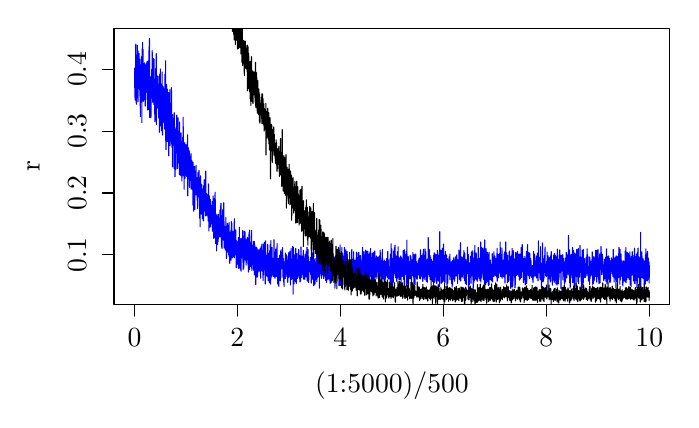
\begin{tikzpicture}[x=0.7pt,y=0.7pt]
\definecolor{fillColor}{RGB}{255,255,255}
%\path[use as bounding box,fill=fillColor,fill opacity=0.00] (0,0) rectangle (361.35,252.94);
\begin{scope}
%\path[clip] ( 49.20, 61.20) rectangle (336.15,203.75);
\definecolor{drawColor}{RGB}{0,0,255}

\path[draw=drawColor,line width= 0.4pt,line join=round,line cap=round] ( 59.83,183.11) --
	( 59.88,181.02) --
	( 59.93,175.64) --
	( 59.99,168.03) --
	( 60.04,182.99) --
	( 60.09,177.76) --
	( 60.15,168.81) --
	( 60.20,166.60) --
	( 60.25,171.01) --
	( 60.31,169.89) --
	( 60.36,176.20) --
	( 60.41,190.31) --
	( 60.47,195.49) --
	( 60.52,189.15) --
	( 60.57,186.93) --
	( 60.63,179.41) --
	( 60.68,171.77) --
	( 60.73,164.47) --
	( 60.78,172.65) --
	( 60.84,175.21) --
	( 60.89,180.01) --
	( 60.94,185.43) --
	( 61.00,185.02) --
	( 61.05,189.95) --
	( 61.10,171.89) --
	( 61.16,187.15) --
	( 61.21,167.87) --
	( 61.26,194.98) --
	( 61.32,177.29) --
	( 61.37,176.96) --
	( 61.42,174.57) --
	( 61.48,190.12) --
	( 61.53,179.93) --
	( 61.58,165.72) --
	( 61.63,192.00) --
	( 61.69,189.68) --
	( 61.74,178.18) --
	( 61.79,179.45) --
	( 61.85,180.21) --
	( 61.90,172.58) --
	( 61.95,175.57) --
	( 62.01,189.20) --
	( 62.06,189.86) --
	( 62.11,185.16) --
	( 62.17,190.64) --
	( 62.22,186.26) --
	( 62.27,179.40) --
	( 62.33,179.55) --
	( 62.38,183.14) --
	( 62.43,174.16) --
	( 62.49,187.80) --
	( 62.54,168.84) --
	( 62.59,179.74) --
	( 62.64,180.89) --
	( 62.70,183.65) --
	( 62.75,184.94) --
	( 62.80,158.10) --
	( 62.86,180.98) --
	( 62.91,165.44) --
	( 62.96,166.62) --
	( 63.02,167.13) --
	( 63.07,179.49) --
	( 63.12,182.71) --
	( 63.18,178.46) --
	( 63.23,184.20) --
	( 63.28,180.38) --
	( 63.34,181.37) --
	( 63.39,189.06) --
	( 63.44,176.01) --
	( 63.50,178.16) --
	( 63.55,171.55) --
	( 63.60,154.99) --
	( 63.65,179.67) --
	( 63.71,193.09) --
	( 63.76,177.26) --
	( 63.81,188.15) --
	( 63.87,181.80) --
	( 63.92,176.81) --
	( 63.97,196.46) --
	( 64.03,189.42) --
	( 64.08,182.71) --
	( 64.13,184.31) --
	( 64.19,184.26) --
	( 64.24,192.69) --
	( 64.29,165.98) --
	( 64.35,167.31) --
	( 64.40,180.94) --
	( 64.45,176.93) --
	( 64.50,178.77) --
	( 64.56,176.84) --
	( 64.61,175.04) --
	( 64.66,176.96) --
	( 64.72,174.80) --
	( 64.77,177.89) --
	( 64.82,181.51) --
	( 64.88,185.57) --
	( 64.93,179.06) --
	( 64.98,177.47) --
	( 65.04,185.89) --
	( 65.09,166.64) --
	( 65.14,173.51) --
	( 65.20,178.01) --
	( 65.25,176.51) --
	( 65.30,171.90) --
	( 65.36,163.56) --
	( 65.41,177.06) --
	( 65.46,173.77) --
	( 65.51,168.30) --
	( 65.57,184.88) --
	( 65.62,175.86) --
	( 65.67,166.78) --
	( 65.73,180.76) --
	( 65.78,173.95) --
	( 65.83,183.62) --
	( 65.89,178.46) --
	( 65.94,175.88) --
	( 65.99,180.80) --
	( 66.05,178.98) --
	( 66.10,185.92) --
	( 66.15,175.14) --
	( 66.21,171.28) --
	( 66.26,183.07) --
	( 66.31,170.59) --
	( 66.37,186.67) --
	( 66.42,170.97) --
	( 66.47,175.58) --
	( 66.52,172.53) --
	( 66.58,167.71) --
	( 66.63,161.55) --
	( 66.68,181.07) --
	( 66.74,165.35) --
	( 66.79,171.44) --
	( 66.84,176.77) --
	( 66.90,186.91) --
	( 66.95,176.00) --
	( 67.00,181.60) --
	( 67.06,179.34) --
	( 67.11,181.21) --
	( 67.16,165.27) --
	( 67.22,168.61) --
	( 67.27,186.28) --
	( 67.32,194.38) --
	( 67.38,171.28) --
	( 67.43,161.59) --
	( 67.48,177.54) --
	( 67.53,198.47) --
	( 67.59,193.18) --
	( 67.64,172.66) --
	( 67.69,157.64) --
	( 67.75,178.90) --
	( 67.80,171.85) --
	( 67.85,164.90) --
	( 67.91,166.34) --
	( 67.96,177.18) --
	( 68.01,178.63) --
	( 68.07,167.05) --
	( 68.12,175.86) --
	( 68.17,167.18) --
	( 68.23,174.50) --
	( 68.28,157.48) --
	( 68.33,165.87) --
	( 68.38,166.23) --
	( 68.44,169.46) --
	( 68.49,176.92) --
	( 68.54,167.52) --
	( 68.60,167.73) --
	( 68.65,182.40) --
	( 68.70,169.02) --
	( 68.76,182.23) --
	( 68.81,175.14) --
	( 68.86,175.70) --
	( 68.92,192.15) --
	( 68.97,187.55) --
	( 69.02,172.57) --
	( 69.08,184.99) --
	( 69.13,170.74) --
	( 69.18,165.54) --
	( 69.24,168.35) --
	( 69.29,178.31) --
	( 69.34,176.63) --
	( 69.39,177.70) --
	( 69.45,183.78) --
	( 69.50,169.70) --
	( 69.55,188.15) --
	( 69.61,181.47) --
	( 69.66,167.90) --
	( 69.71,165.93) --
	( 69.77,182.92) --
	( 69.82,164.35) --
	( 69.87,175.84) --
	( 69.93,187.81) --
	( 69.98,172.06) --
	( 70.03,165.08) --
	( 70.09,171.78) --
	( 70.14,165.95) --
	( 70.19,170.60) --
	( 70.25,163.37) --
	( 70.30,155.54) --
	( 70.35,166.36) --
	( 70.40,164.60) --
	( 70.46,170.33) --
	( 70.51,169.89) --
	( 70.56,165.48) --
	( 70.62,159.94) --
	( 70.67,169.33) --
	( 70.72,172.07) --
	( 70.78,182.97) --
	( 70.83,179.98) --
	( 70.88,156.22) --
	( 70.94,175.26) --
	( 70.99,171.86) --
	( 71.04,190.58) --
	( 71.10,154.11) --
	( 71.15,179.91) --
	( 71.20,165.87) --
	( 71.25,173.06) --
	( 71.31,174.13) --
	( 71.36,173.48) --
	( 71.41,173.05) --
	( 71.47,178.10) --
	( 71.52,177.75) --
	( 71.57,167.97) --
	( 71.63,179.04) --
	( 71.68,168.42) --
	( 71.73,171.26) --
	( 71.79,162.52) --
	( 71.84,176.37) --
	( 71.89,169.79) --
	( 71.95,178.98) --
	( 72.00,163.16) --
	( 72.05,171.67) --
	( 72.11,167.69) --
	( 72.16,170.79) --
	( 72.21,159.45) --
	( 72.26,157.37) --
	( 72.32,160.35) --
	( 72.37,164.30) --
	( 72.42,168.28) --
	( 72.48,162.13) --
	( 72.53,159.18) --
	( 72.58,174.99) --
	( 72.64,163.94) --
	( 72.69,150.01) --
	( 72.74,165.43) --
	( 72.80,179.86) --
	( 72.85,160.58) --
	( 72.90,171.28) --
	( 72.96,153.42) --
	( 73.01,164.95) --
	( 73.06,162.77) --
	( 73.12,182.74) --
	( 73.17,169.43) --
	( 73.22,165.10) --
	( 73.27,155.04) --
	( 73.33,175.19) --
	( 73.38,172.22) --
	( 73.43,160.70) --
	( 73.49,163.49) --
	( 73.54,153.20) --
	( 73.59,164.08) --
	( 73.65,157.42) --
	( 73.70,164.31) --
	( 73.75,159.89) --
	( 73.81,150.88) --
	( 73.86,165.92) --
	( 73.91,163.48) --
	( 73.97,155.63) --
	( 74.02,168.03) --
	( 74.07,181.16) --
	( 74.12,154.03) --
	( 74.18,155.05) --
	( 74.23,148.64) --
	( 74.28,159.31) --
	( 74.34,166.29) --
	( 74.39,164.65) --
	( 74.44,154.55) --
	( 74.50,173.89) --
	( 74.55,155.84) --
	( 74.60,165.07) --
	( 74.66,173.14) --
	( 74.71,162.75) --
	( 74.76,157.24) --
	( 74.82,163.21) --
	( 74.87,155.36) --
	( 74.92,155.26) --
	( 74.98,161.50) --
	( 75.03,164.50) --
	( 75.08,161.03) --
	( 75.13,160.12) --
	( 75.19,158.76) --
	( 75.24,164.94) --
	( 75.29,162.76) --
	( 75.35,157.84) --
	( 75.40,151.66) --
	( 75.45,179.96) --
	( 75.51,164.59) --
	( 75.56,158.62) --
	( 75.61,160.96) --
	( 75.67,164.47) --
	( 75.72,151.44) --
	( 75.77,165.06) --
	( 75.83,152.59) --
	( 75.88,186.96) --
	( 75.93,145.79) --
	( 75.99,160.46) --
	( 76.04,141.06) --
	( 76.09,156.69) --
	( 76.14,165.56) --
	( 76.20,169.55) --
	( 76.25,151.01) --
	( 76.30,145.29) --
	( 76.36,153.24) --
	( 76.41,174.73) --
	( 76.46,146.72) --
	( 76.52,153.14) --
	( 76.57,152.19) --
	( 76.62,157.68) --
	( 76.68,159.31) --
	( 76.73,172.33) --
	( 76.78,145.18) --
	( 76.84,147.17) --
	( 76.89,159.09) --
	( 76.94,158.71) --
	( 77.00,154.81) --
	( 77.05,167.56) --
	( 77.10,155.27) --
	( 77.15,168.94) --
	( 77.21,150.80) --
	( 77.26,162.79) --
	( 77.31,151.34) --
	( 77.37,170.52) --
	( 77.42,151.95) --
	( 77.47,137.86) --
	( 77.53,152.00) --
	( 77.58,161.74) --
	( 77.63,149.06) --
	( 77.69,146.21) --
	( 77.74,144.45) --
	( 77.79,149.09) --
	( 77.85,162.07) --
	( 77.90,158.01) --
	( 77.95,154.48) --
	( 78.00,164.76) --
	( 78.06,172.10) --
	( 78.11,143.12) --
	( 78.16,156.20) --
	( 78.22,159.38) --
	( 78.27,148.60) --
	( 78.32,150.20) --
	( 78.38,145.93) --
	( 78.43,145.43) --
	( 78.48,148.56) --
	( 78.54,160.06) --
	( 78.59,148.66) --
	( 78.64,145.83) --
	( 78.70,149.86) --
	( 78.75,154.27) --
	( 78.80,167.30) --
	( 78.86,173.15) --
	( 78.91,163.01) --
	( 78.96,151.48) --
	( 79.01,144.02) --
	( 79.07,150.83) --
	( 79.12,148.52) --
	( 79.17,142.21) --
	( 79.23,157.85) --
	( 79.28,150.29) --
	( 79.33,157.03) --
	( 79.39,132.14) --
	( 79.44,157.41) --
	( 79.49,159.13) --
	( 79.55,151.26) --
	( 79.60,143.92) --
	( 79.65,148.02) --
	( 79.71,157.21) --
	( 79.76,143.43) --
	( 79.81,150.43) --
	( 79.87,154.42) --
	( 79.92,156.59) --
	( 79.97,152.24) --
	( 80.02,148.44) --
	( 80.08,156.21) --
	( 80.13,145.81) --
	( 80.18,148.46) --
	( 80.24,146.43) --
	( 80.29,160.16) --
	( 80.34,131.30) --
	( 80.40,149.33) --
	( 80.45,141.40) --
	( 80.50,154.29) --
	( 80.56,147.07) --
	( 80.61,149.91) --
	( 80.66,150.86) --
	( 80.72,127.05) --
	( 80.77,144.78) --
	( 80.82,144.97) --
	( 80.87,144.59) --
	( 80.93,143.83) --
	( 80.98,150.92) --
	( 81.03,136.03) --
	( 81.09,151.74) --
	( 81.14,130.86) --
	( 81.19,148.80) --
	( 81.25,139.03) --
	( 81.30,144.31) --
	( 81.35,142.64) --
	( 81.41,141.69) --
	( 81.46,151.48) --
	( 81.51,153.02) --
	( 81.57,158.77) --
	( 81.62,151.02) --
	( 81.67,158.90) --
	( 81.73,141.34) --
	( 81.78,145.79) --
	( 81.83,144.65) --
	( 81.88,154.44) --
	( 81.94,150.66) --
	( 81.99,131.29) --
	( 82.04,149.99) --
	( 82.10,148.57) --
	( 82.15,142.41) --
	( 82.20,147.85) --
	( 82.26,134.04) --
	( 82.31,157.51) --
	( 82.36,139.01) --
	( 82.42,147.40) --
	( 82.47,143.67) --
	( 82.52,150.58) --
	( 82.58,135.62) --
	( 82.63,137.79) --
	( 82.68,141.89) --
	( 82.74,145.99) --
	( 82.79,136.23) --
	( 82.84,142.11) --
	( 82.89,140.81) --
	( 82.95,146.26) --
	( 83.00,139.89) --
	( 83.05,128.03) --
	( 83.11,155.32) --
	( 83.16,135.57) --
	( 83.21,143.78) --
	( 83.27,142.22) --
	( 83.32,128.54) --
	( 83.37,145.21) --
	( 83.43,142.60) --
	( 83.48,143.20) --
	( 83.53,132.91) --
	( 83.59,130.87) --
	( 83.64,147.45) --
	( 83.69,148.87) --
	( 83.75,127.57) --
	( 83.80,149.71) --
	( 83.85,143.03) --
	( 83.90,145.32) --
	( 83.96,142.64) --
	( 84.01,140.85) --
	( 84.06,142.38) --
	( 84.12,135.33) --
	( 84.17,131.13) --
	( 84.22,138.98) --
	( 84.28,124.90) --
	( 84.33,137.14) --
	( 84.38,141.01) --
	( 84.44,130.54) --
	( 84.49,142.67) --
	( 84.54,145.46) --
	( 84.60,139.50) --
	( 84.65,147.42) --
	( 84.70,140.65) --
	( 84.75,144.62) --
	( 84.81,144.21) --
	( 84.86,135.19) --
	( 84.91,157.78) --
	( 84.97,144.88) --
	( 85.02,137.65) --
	( 85.07,127.57) --
	( 85.13,139.32) --
	( 85.18,131.16) --
	( 85.23,143.57) --
	( 85.29,140.41) --
	( 85.34,142.84) --
	( 85.39,120.63) --
	( 85.45,129.20) --
	( 85.50,139.49) --
	( 85.55,136.07) --
	( 85.61,142.81) --
	( 85.66,133.35) --
	( 85.71,127.86) --
	( 85.76,144.63) --
	( 85.82,141.42) --
	( 85.87,136.88) --
	( 85.92,126.27) --
	( 85.98,132.89) --
	( 86.03,140.49) --
	( 86.08,133.93) --
	( 86.14,129.30) --
	( 86.19,142.90) --
	( 86.24,135.51) --
	( 86.30,134.31) --
	( 86.35,129.67) --
	( 86.40,143.61) --
	( 86.46,127.96) --
	( 86.51,136.09) --
	( 86.56,133.45) --
	( 86.62,131.07) --
	( 86.67,127.25) --
	( 86.72,136.68) --
	( 86.77,132.13) --
	( 86.83,130.04) --
	( 86.88,137.37) --
	( 86.93,130.73) --
	( 86.99,138.76) --
	( 87.04,136.73) --
	( 87.09,130.63) --
	( 87.15,138.53) --
	( 87.20,148.75) --
	( 87.25,125.67) --
	( 87.31,117.25) --
	( 87.36,123.26) --
	( 87.41,135.48) --
	( 87.47,132.07) --
	( 87.52,137.17) --
	( 87.57,131.25) --
	( 87.62,141.95) --
	( 87.68,139.16) --
	( 87.73,133.99) --
	( 87.78,129.36) --
	( 87.84,137.29) --
	( 87.89,128.97) --
	( 87.94,127.98) --
	( 88.00,125.84) --
	( 88.05,139.45) --
	( 88.10,140.38) --
	( 88.16,133.96) --
	( 88.21,122.18) --
	( 88.26,121.58) --
	( 88.32,131.74) --
	( 88.37,133.40) --
	( 88.42,135.50) --
	( 88.48,131.32) --
	( 88.53,126.63) --
	( 88.58,137.49) --
	( 88.63,127.94) --
	( 88.69,128.43) --
	( 88.74,126.59) --
	( 88.79,134.28) --
	( 88.85,125.09) --
	( 88.90,129.01) --
	( 88.95,138.97) --
	( 89.01,120.65) --
	( 89.06,129.55) --
	( 89.11,135.12) --
	( 89.17,131.37) --
	( 89.22,120.83) --
	( 89.27,130.74) --
	( 89.33,135.58) --
	( 89.38,128.32) --
	( 89.43,135.06) --
	( 89.49,124.29) --
	( 89.54,134.02) --
	( 89.59,128.83) --
	( 89.64,120.89) --
	( 89.70,128.18) --
	( 89.75,120.85) --
	( 89.80,130.22) --
	( 89.86,132.91) --
	( 89.91,112.46) --
	( 89.96,134.65) --
	( 90.02,133.94) --
	( 90.07,128.25) --
	( 90.12,119.32) --
	( 90.18,123.50) --
	( 90.23,126.02) --
	( 90.28,128.74) --
	( 90.34,109.31) --
	( 90.39,122.49) --
	( 90.44,124.30) --
	( 90.50,129.09) --
	( 90.55,128.67) --
	( 90.60,121.48) --
	( 90.65,121.68) --
	( 90.71,132.52) --
	( 90.76,125.09) --
	( 90.81,121.81) --
	( 90.87,124.32) --
	( 90.92,110.16) --
	( 90.97,121.25) --
	( 91.03,121.87) --
	( 91.08,125.88) --
	( 91.13,120.83) --
	( 91.19,130.00) --
	( 91.24,117.84) --
	( 91.29,127.07) --
	( 91.35,125.83) --
	( 91.40,118.85) --
	( 91.45,132.10) --
	( 91.50,119.65) --
	( 91.56,132.87) --
	( 91.61,123.36) --
	( 91.66,117.76) --
	( 91.72,119.74) --
	( 91.77,125.38) --
	( 91.82,124.95) --
	( 91.88,120.24) --
	( 91.93,126.54) --
	( 91.98,117.97) --
	( 92.04,122.06) --
	( 92.09,116.96) --
	( 92.14,121.56) --
	( 92.20,114.84) --
	( 92.25,122.44) --
	( 92.30,120.21) --
	( 92.36,115.87) --
	( 92.41,110.62) --
	( 92.46,118.68) --
	( 92.51,129.12) --
	( 92.57,120.26) --
	( 92.62,128.22) --
	( 92.67,122.08) --
	( 92.73,123.42) --
	( 92.78,121.83) --
	( 92.83,116.94) --
	( 92.89,122.65) --
	( 92.94,129.49) --
	( 92.99,120.83) --
	( 93.05,127.57) --
	( 93.10,130.36) --
	( 93.15,119.53) --
	( 93.21,117.36) --
	( 93.26,120.91) --
	( 93.31,120.98) --
	( 93.37,115.89) --
	( 93.42,126.56) --
	( 93.47,105.63) --
	( 93.52,110.59) --
	( 93.58,115.50) --
	( 93.63,116.71) --
	( 93.68,101.26) --
	( 93.74,125.02) --
	( 93.79,118.42) --
	( 93.84,124.16) --
	( 93.90,119.05) --
	( 93.95,127.59) --
	( 94.00,116.04) --
	( 94.06,112.32) --
	( 94.11,113.23) --
	( 94.16,121.81) --
	( 94.22,119.04) --
	( 94.27,121.59) --
	( 94.32,107.76) --
	( 94.37,115.61) --
	( 94.43,110.69) --
	( 94.48,110.99) --
	( 94.53,122.98) --
	( 94.59,115.28) --
	( 94.64,120.26) --
	( 94.69,121.12) --
	( 94.75,113.97) --
	( 94.80,111.82) --
	( 94.85,113.95) --
	( 94.91,105.39) --
	( 94.96,106.06) --
	( 95.01,110.11) --
	( 95.07,111.61) --
	( 95.12,115.10) --
	( 95.17,120.45) --
	( 95.23,120.29) --
	( 95.28,119.82) --
	( 95.33,115.57) --
	( 95.38,111.96) --
	( 95.44,104.36) --
	( 95.49,107.35) --
	( 95.54,122.49) --
	( 95.60,110.56) --
	( 95.65,116.78) --
	( 95.70,120.47) --
	( 95.76,121.53) --
	( 95.81,125.55) --
	( 95.86,119.58) --
	( 95.92,124.31) --
	( 95.97,113.14) --
	( 96.02,113.99) --
	( 96.08,114.43) --
	( 96.13,113.67) --
	( 96.18,109.24) --
	( 96.24,115.67) --
	( 96.29,120.14) --
	( 96.34,110.38) --
	( 96.39,115.46) --
	( 96.45,106.97) --
	( 96.50,110.02) --
	( 96.55,130.02) --
	( 96.61,116.60) --
	( 96.66,111.88) --
	( 96.71,106.89) --
	( 96.77,113.53) --
	( 96.82,111.26) --
	( 96.87,113.13) --
	( 96.93,115.64) --
	( 96.98,118.43) --
	( 97.03,109.82) --
	( 97.09,112.95) --
	( 97.14,111.39) --
	( 97.19,110.00) --
	( 97.25,112.99) --
	( 97.30,117.84) --
	( 97.35,112.90) --
	( 97.40,107.24) --
	( 97.46,108.17) --
	( 97.51,113.44) --
	( 97.56,108.46) --
	( 97.62,117.11) --
	( 97.67,112.12) --
	( 97.72,111.27) --
	( 97.78,104.26) --
	( 97.83,105.90) --
	( 97.88,114.94) --
	( 97.94,113.45) --
	( 97.99,123.32) --
	( 98.04,111.56) --
	( 98.10,111.66) --
	( 98.15,108.11) --
	( 98.20, 99.05) --
	( 98.25,106.43) --
	( 98.31,102.94) --
	( 98.36,114.53) --
	( 98.41,117.22) --
	( 98.47,116.75) --
	( 98.52,110.73) --
	( 98.57,100.99) --
	( 98.63,112.76) --
	( 98.68,108.80) --
	( 98.73,111.53) --
	( 98.79,111.62) --
	( 98.84,111.75) --
	( 98.89,103.94) --
	( 98.95,115.32) --
	( 99.00,103.50) --
	( 99.05,101.19) --
	( 99.11,106.65) --
	( 99.16,107.03) --
	( 99.21,112.35) --
	( 99.26,105.97) --
	( 99.32,111.87) --
	( 99.37,107.38) --
	( 99.42,104.88) --
	( 99.48,105.89) --
	( 99.53,109.63) --
	( 99.58,104.98) --
	( 99.64,104.25) --
	( 99.69,107.66) --
	( 99.74,102.74) --
	( 99.80,106.75) --
	( 99.85,114.24) --
	( 99.90,109.27) --
	( 99.96,111.04) --
	(100.01, 99.07) --
	(100.06,111.84) --
	(100.12,109.95) --
	(100.17,104.90) --
	(100.22,104.38) --
	(100.27,109.17) --
	(100.33,108.62) --
	(100.38,117.18) --
	(100.43, 98.79) --
	(100.49,104.26) --
	(100.54,104.95) --
	(100.59,116.04) --
	(100.65, 98.68) --
	(100.70, 95.35) --
	(100.75,104.59) --
	(100.81,101.67) --
	(100.86, 97.49) --
	(100.91,101.53) --
	(100.97,101.49) --
	(101.02,107.92) --
	(101.07,107.18) --
	(101.12,106.92) --
	(101.18,100.50) --
	(101.23, 95.73) --
	(101.28,101.58) --
	(101.34,117.80) --
	(101.39,106.96) --
	(101.44,119.06) --
	(101.50, 98.63) --
	(101.55,114.50) --
	(101.60,101.77) --
	(101.66,102.01) --
	(101.71, 92.54) --
	(101.76, 97.94) --
	(101.82,101.95) --
	(101.87,100.67) --
	(101.92,100.93) --
	(101.98,102.94) --
	(102.03,106.32) --
	(102.08, 97.27) --
	(102.13,104.63) --
	(102.19, 88.83) --
	(102.24,105.44) --
	(102.29,107.74) --
	(102.35,102.66) --
	(102.40,101.02) --
	(102.45,106.83) --
	(102.51, 96.00) --
	(102.56,100.03) --
	(102.61, 95.04) --
	(102.67,101.61) --
	(102.72, 92.18) --
	(102.77,103.65) --
	(102.83,102.79) --
	(102.88,103.85) --
	(102.93,100.91) --
	(102.99, 93.58) --
	(103.04,100.57) --
	(103.09,107.66) --
	(103.14,101.74) --
	(103.20,100.74) --
	(103.25, 97.95) --
	(103.30,102.03) --
	(103.36,101.12) --
	(103.41, 96.32) --
	(103.46,100.42) --
	(103.52, 99.85) --
	(103.57, 98.30) --
	(103.62,104.10) --
	(103.68,100.31) --
	(103.73, 96.03) --
	(103.78,105.78) --
	(103.84,105.47) --
	(103.89,102.12) --
	(103.94,109.95) --
	(104.00,106.74) --
	(104.05, 98.30) --
	(104.10, 97.94) --
	(104.15,101.32) --
	(104.21, 96.04) --
	(104.26, 98.40) --
	(104.31,112.19) --
	(104.37,106.35) --
	(104.42,100.53) --
	(104.47,113.46) --
	(104.53,101.98) --
	(104.58, 98.15) --
	(104.63, 94.10) --
	(104.69, 91.80) --
	(104.74,107.18) --
	(104.79,100.42) --
	(104.85, 90.69) --
	(104.90, 95.99) --
	(104.95,104.68) --
	(105.00, 90.01) --
	(105.06,103.55) --
	(105.11, 97.65) --
	(105.16,105.09) --
	(105.22,102.71) --
	(105.27,101.58) --
	(105.32,100.41) --
	(105.38,110.24) --
	(105.43,100.60) --
	(105.48,100.14) --
	(105.54,103.50) --
	(105.59, 94.82) --
	(105.64, 94.39) --
	(105.70,100.07) --
	(105.75,100.73) --
	(105.80,101.62) --
	(105.86,113.75) --
	(105.91,100.75) --
	(105.96,100.18) --
	(106.01,104.03) --
	(106.07,102.75) --
	(106.12, 90.32) --
	(106.17,100.04) --
	(106.23,100.04) --
	(106.28, 98.67) --
	(106.33, 98.28) --
	(106.39,101.41) --
	(106.44,100.73) --
	(106.49, 92.93) --
	(106.55, 91.90) --
	(106.60, 97.52) --
	(106.65, 95.41) --
	(106.71, 89.23) --
	(106.76, 93.46) --
	(106.81, 95.38) --
	(106.87, 90.93) --
	(106.92, 90.61) --
	(106.97,105.96) --
	(107.02, 94.46) --
	(107.08,101.83) --
	(107.13, 95.04) --
	(107.18, 95.44) --
	(107.24, 93.72) --
	(107.29, 84.88) --
	(107.34, 96.06) --
	(107.40, 91.79) --
	(107.45, 99.37) --
	(107.50, 96.15) --
	(107.56,100.62) --
	(107.61, 93.08) --
	(107.66,100.18) --
	(107.72, 92.85) --
	(107.77,103.06) --
	(107.82,101.64) --
	(107.87, 98.75) --
	(107.93, 95.29) --
	(107.98, 88.14) --
	(108.03, 94.72) --
	(108.09, 99.29) --
	(108.14, 96.59) --
	(108.19, 90.13) --
	(108.25,101.83) --
	(108.30, 99.62) --
	(108.35, 86.75) --
	(108.41, 93.37) --
	(108.46, 94.73) --
	(108.51,101.22) --
	(108.57, 92.40) --
	(108.62,103.48) --
	(108.67, 92.46) --
	(108.73, 85.82) --
	(108.78, 98.70) --
	(108.83, 90.63) --
	(108.88, 98.55) --
	(108.94, 82.39) --
	(108.99, 92.13) --
	(109.04, 87.60) --
	(109.10, 93.46) --
	(109.15, 95.71) --
	(109.20, 97.29) --
	(109.26, 94.05) --
	(109.31, 91.64) --
	(109.36, 85.94) --
	(109.42, 92.68) --
	(109.47, 95.06) --
	(109.52, 99.35) --
	(109.58, 89.95) --
	(109.63, 92.47) --
	(109.68, 84.04) --
	(109.74, 94.54) --
	(109.79,103.99) --
	(109.84,101.69) --
	(109.89, 88.59) --
	(109.95, 95.28) --
	(110.00,103.06) --
	(110.05,102.22) --
	(110.11, 86.95) --
	(110.16, 96.36) --
	(110.21, 95.41) --
	(110.27, 95.14) --
	(110.32, 85.20) --
	(110.37, 94.35) --
	(110.43, 88.90) --
	(110.48, 95.85) --
	(110.53, 86.78) --
	(110.59, 88.66) --
	(110.64, 85.79) --
	(110.69, 93.40) --
	(110.75, 98.90) --
	(110.80, 85.71) --
	(110.85, 88.63) --
	(110.90, 95.87) --
	(110.96, 95.94) --
	(111.01, 92.51) --
	(111.06, 93.17) --
	(111.12, 92.82) --
	(111.17, 88.20) --
	(111.22, 94.03) --
	(111.28, 99.95) --
	(111.33,105.41) --
	(111.38, 85.27) --
	(111.44,100.36) --
	(111.49, 95.75) --
	(111.54, 98.02) --
	(111.60, 94.73) --
	(111.65, 92.08) --
	(111.70, 88.88) --
	(111.75, 92.22) --
	(111.81, 90.15) --
	(111.86, 92.66) --
	(111.91, 86.72) --
	(111.97, 88.01) --
	(112.02, 89.32) --
	(112.07, 99.66) --
	(112.13, 99.03) --
	(112.18, 88.79) --
	(112.23, 85.76) --
	(112.29, 86.52) --
	(112.34, 80.05) --
	(112.39, 89.29) --
	(112.45, 94.05) --
	(112.50, 88.96) --
	(112.55, 89.30) --
	(112.61, 81.95) --
	(112.66, 89.42) --
	(112.71, 90.30) --
	(112.76, 93.35) --
	(112.82, 86.42) --
	(112.87, 92.95) --
	(112.92, 87.51) --
	(112.98, 88.70) --
	(113.03, 89.67) --
	(113.08, 88.42) --
	(113.14, 90.51) --
	(113.19, 81.79) --
	(113.24, 93.60) --
	(113.30, 90.40) --
	(113.35, 85.62) --
	(113.40, 95.67) --
	(113.46, 79.83) --
	(113.51, 87.61) --
	(113.56, 85.84) --
	(113.62, 79.95) --
	(113.67, 90.94) --
	(113.72, 86.88) --
	(113.77, 89.92) --
	(113.83, 91.25) --
	(113.88, 85.22) --
	(113.93,100.95) --
	(113.99, 86.69) --
	(114.04, 86.84) --
	(114.09, 87.16) --
	(114.15, 94.96) --
	(114.20, 92.13) --
	(114.25, 86.70) --
	(114.31, 90.69) --
	(114.36, 79.42) --
	(114.41, 89.44) --
	(114.47, 95.07) --
	(114.52, 82.89) --
	(114.57, 87.92) --
	(114.62, 88.26) --
	(114.68, 84.29) --
	(114.73, 93.93) --
	(114.78, 78.32) --
	(114.84, 89.41) --
	(114.89, 88.70) --
	(114.94, 95.22) --
	(115.00, 85.50) --
	(115.05, 89.00) --
	(115.10, 87.88) --
	(115.16, 94.90) --
	(115.21, 87.46) --
	(115.26, 92.88) --
	(115.32, 88.66) --
	(115.37, 85.21) --
	(115.42, 90.93) --
	(115.48, 87.45) --
	(115.53, 86.66) --
	(115.58, 92.86) --
	(115.63, 99.36) --
	(115.69, 89.28) --
	(115.74, 84.65) --
	(115.79, 90.48) --
	(115.85, 79.09) --
	(115.90, 88.19) --
	(115.95, 87.21) --
	(116.01, 81.82) --
	(116.06, 95.98) --
	(116.11, 89.67) --
	(116.17, 87.20) --
	(116.22, 82.70) --
	(116.27, 79.92) --
	(116.33, 87.94) --
	(116.38, 89.89) --
	(116.43, 99.06) --
	(116.49, 89.05) --
	(116.54, 94.66) --
	(116.59, 87.58) --
	(116.64, 88.75) --
	(116.70, 85.86) --
	(116.75, 84.85) --
	(116.80, 91.16) --
	(116.86, 98.61) --
	(116.91, 86.58) --
	(116.96, 84.74) --
	(117.02, 91.44) --
	(117.07, 85.06) --
	(117.12, 84.05) --
	(117.18, 83.94) --
	(117.23, 94.71) --
	(117.28, 85.02) --
	(117.34, 94.40) --
	(117.39, 86.61) --
	(117.44, 81.47) --
	(117.50, 86.58) --
	(117.55, 88.86) --
	(117.60, 84.82) --
	(117.65, 86.07) --
	(117.71, 87.77) --
	(117.76, 86.20) --
	(117.81, 88.18) --
	(117.87, 84.35) --
	(117.92, 89.49) --
	(117.97, 92.20) --
	(118.03, 95.91) --
	(118.08, 93.88) --
	(118.13, 86.19) --
	(118.19, 94.94) --
	(118.24, 95.21) --
	(118.29, 84.09) --
	(118.35, 82.16) --
	(118.40, 90.48) --
	(118.45, 87.87) --
	(118.50, 81.02) --
	(118.56, 88.45) --
	(118.61, 77.88) --
	(118.66, 91.22) --
	(118.72, 87.13) --
	(118.77, 81.92) --
	(118.82, 95.20) --
	(118.88, 79.27) --
	(118.93, 98.29) --
	(118.98, 96.51) --
	(119.04, 94.09) --
	(119.09, 79.08) --
	(119.14, 94.07) --
	(119.20, 94.25) --
	(119.25, 99.57) --
	(119.30, 85.32) --
	(119.36, 92.05) --
	(119.41, 83.72) --
	(119.46, 92.95) --
	(119.51, 80.66) --
	(119.57, 88.44) --
	(119.62, 81.57) --
	(119.67, 88.77) --
	(119.73, 85.62) --
	(119.78, 90.20) --
	(119.83, 82.24) --
	(119.89, 85.65) --
	(119.94, 85.55) --
	(119.99, 86.18) --
	(120.05, 82.87) --
	(120.10, 80.00) --
	(120.15, 93.79) --
	(120.21, 84.76) --
	(120.26, 99.44) --
	(120.31, 87.46) --
	(120.37, 78.72) --
	(120.42, 92.01) --
	(120.47, 79.35) --
	(120.52, 88.97) --
	(120.58, 86.14) --
	(120.63, 87.20) --
	(120.68, 82.49) --
	(120.74, 84.07) --
	(120.79, 84.99) --
	(120.84, 81.66) --
	(120.90, 81.82) --
	(120.95, 84.06) --
	(121.00, 87.41) --
	(121.06, 82.15) --
	(121.11, 84.12) --
	(121.16, 93.63) --
	(121.22, 91.30) --
	(121.27, 78.87) --
	(121.32, 87.60) --
	(121.37, 87.34) --
	(121.43, 78.72) --
	(121.48, 85.24) --
	(121.53, 86.48) --
	(121.59, 89.76) --
	(121.64, 93.72) --
	(121.69, 76.44) --
	(121.75, 78.00) --
	(121.80, 79.69) --
	(121.85, 90.09) --
	(121.91, 80.41) --
	(121.96, 91.97) --
	(122.01, 87.37) --
	(122.07, 84.01) --
	(122.12, 79.45) --
	(122.17, 85.67) --
	(122.23, 89.79) --
	(122.28, 79.65) --
	(122.33, 78.12) --
	(122.38, 71.46) --
	(122.44, 88.98) --
	(122.49, 90.09) --
	(122.54, 89.96) --
	(122.60, 83.65) --
	(122.65, 80.45) --
	(122.70, 84.38) --
	(122.76, 90.67) --
	(122.81, 79.44) --
	(122.86, 86.34) --
	(122.92, 86.71) --
	(122.97, 80.96) --
	(123.02, 90.06) --
	(123.08, 75.23) --
	(123.13, 89.46) --
	(123.18, 89.31) --
	(123.24, 88.73) --
	(123.29, 79.93) --
	(123.34, 75.49) --
	(123.39, 85.59) --
	(123.45, 79.07) --
	(123.50, 83.91) --
	(123.55, 77.80) --
	(123.61, 84.47) --
	(123.66, 86.02) --
	(123.71, 83.83) --
	(123.77, 82.32) --
	(123.82, 89.36) --
	(123.87, 83.50) --
	(123.93, 89.30) --
	(123.98, 86.43) --
	(124.03, 85.94) --
	(124.09, 89.22) --
	(124.14, 87.12) --
	(124.19, 78.40) --
	(124.24, 78.73) --
	(124.30, 86.07) --
	(124.35, 79.51) --
	(124.40, 79.67) --
	(124.46, 89.40) --
	(124.51, 84.10) --
	(124.56, 83.66) --
	(124.62, 89.71) --
	(124.67, 88.21) --
	(124.72, 90.10) --
	(124.78, 82.07) --
	(124.83, 78.23) --
	(124.88, 74.70) --
	(124.94, 80.39) --
	(124.99, 80.22) --
	(125.04, 81.62) --
	(125.10, 81.45) --
	(125.15, 85.17) --
	(125.20, 91.13) --
	(125.25, 85.50) --
	(125.31, 86.11) --
	(125.36, 80.89) --
	(125.41, 84.52) --
	(125.47, 85.61) --
	(125.52, 90.09) --
	(125.57, 78.39) --
	(125.63, 92.44) --
	(125.68, 79.20) --
	(125.73, 82.60) --
	(125.79, 88.75) --
	(125.84, 82.43) --
	(125.89, 88.81) --
	(125.95, 80.72) --
	(126.00, 86.44) --
	(126.05, 83.00) --
	(126.11, 86.88) --
	(126.16, 73.46) --
	(126.21, 81.32) --
	(126.26, 86.18) --
	(126.32, 89.24) --
	(126.37, 81.62) --
	(126.42, 88.23) --
	(126.48, 76.55) --
	(126.53, 92.34) --
	(126.58, 87.26) --
	(126.64, 92.54) --
	(126.69, 85.22) --
	(126.74, 80.44) --
	(126.80, 81.99) --
	(126.85, 93.36) --
	(126.90, 93.14) --
	(126.96, 79.52) --
	(127.01, 86.30) --
	(127.06, 78.96) --
	(127.12, 87.92) --
	(127.17, 83.28) --
	(127.22, 85.09) --
	(127.27, 71.68) --
	(127.33, 92.33) --
	(127.38, 77.40) --
	(127.43, 83.75) --
	(127.49, 93.99) --
	(127.54, 83.88) --
	(127.59, 82.80) --
	(127.65, 86.25) --
	(127.70, 84.42) --
	(127.75, 85.15) --
	(127.81, 79.75) --
	(127.86, 76.02) --
	(127.91, 79.66) --
	(127.97, 86.40) --
	(128.02, 85.43) --
	(128.07, 85.17) --
	(128.12, 85.55) --
	(128.18, 84.12) --
	(128.23, 79.92) --
	(128.28, 75.58) --
	(128.34, 86.75) --
	(128.39, 77.99) --
	(128.44, 77.71) --
	(128.50, 75.50) --
	(128.55, 92.19) --
	(128.60, 79.88) --
	(128.66, 81.20) --
	(128.71, 78.87) --
	(128.76, 73.40) --
	(128.82, 75.80) --
	(128.87, 85.82) --
	(128.92, 85.79) --
	(128.98, 80.94) --
	(129.03, 87.46) --
	(129.08, 78.80) --
	(129.13, 78.60) --
	(129.19, 76.14) --
	(129.24, 85.68) --
	(129.29, 81.21) --
	(129.35, 87.36) --
	(129.40, 74.77) --
	(129.45, 72.32) --
	(129.51, 77.74) --
	(129.56, 88.90) --
	(129.61, 83.03) --
	(129.67, 79.81) --
	(129.72, 84.63) --
	(129.77, 82.46) --
	(129.83, 91.99) --
	(129.88, 74.90) --
	(129.93, 82.65) --
	(129.99, 76.18) --
	(130.04, 81.88) --
	(130.09, 71.65) --
	(130.14, 82.14) --
	(130.20, 94.16) --
	(130.25, 74.83) --
	(130.30, 81.27) --
	(130.36, 82.76) --
	(130.41, 87.44) --
	(130.46, 80.13) --
	(130.52, 85.22) --
	(130.57, 80.01) --
	(130.62, 81.90) --
	(130.68, 78.59) --
	(130.73, 80.76) --
	(130.78, 90.64) --
	(130.84, 75.75) --
	(130.89, 81.29) --
	(130.94, 76.54) --
	(130.99, 81.96) --
	(131.05, 81.61) --
	(131.10, 79.00) --
	(131.15, 84.62) --
	(131.21, 84.98) --
	(131.26, 79.08) --
	(131.31, 77.31) --
	(131.37, 78.83) --
	(131.42, 79.31) --
	(131.47, 77.61) --
	(131.53, 78.98) --
	(131.58, 84.80) --
	(131.63, 75.66) --
	(131.69, 79.36) --
	(131.74, 85.68) --
	(131.79, 94.58) --
	(131.85, 78.32) --
	(131.90, 78.15) --
	(131.95, 86.35) --
	(132.00, 88.20) --
	(132.06, 81.58) --
	(132.11, 75.34) --
	(132.16, 82.74) --
	(132.22, 76.53) --
	(132.27, 78.12) --
	(132.32, 74.69) --
	(132.38, 82.25) --
	(132.43, 77.22) --
	(132.48, 82.02) --
	(132.54, 80.15) --
	(132.59, 86.43) --
	(132.64, 89.70) --
	(132.70, 88.01) --
	(132.75, 77.79) --
	(132.80, 82.85) --
	(132.86, 77.90) --
	(132.91, 86.04) --
	(132.96, 75.55) --
	(133.01, 85.29) --
	(133.07, 78.47) --
	(133.12, 85.04) --
	(133.17, 79.56) --
	(133.23, 77.11) --
	(133.28, 79.41) --
	(133.33, 80.63) --
	(133.39, 92.58) --
	(133.44, 83.55) --
	(133.49, 75.61) --
	(133.55, 80.27) --
	(133.60, 84.05) --
	(133.65, 80.31) --
	(133.71, 71.72) --
	(133.76, 83.70) --
	(133.81, 72.23) --
	(133.87, 83.12) --
	(133.92, 81.73) --
	(133.97, 76.76) --
	(134.02, 84.99) --
	(134.08, 77.58) --
	(134.13, 72.02) --
	(134.18, 75.34) --
	(134.24, 73.51) --
	(134.29, 70.47) --
	(134.34, 81.82) --
	(134.40, 83.13) --
	(134.45, 83.00) --
	(134.50, 79.32) --
	(134.56, 84.62) --
	(134.61, 82.82) --
	(134.66, 75.45) --
	(134.72, 78.14) --
	(134.77, 86.60) --
	(134.82, 80.41) --
	(134.87, 82.76) --
	(134.93, 79.64) --
	(134.98, 77.90) --
	(135.03, 73.30) --
	(135.09, 85.60) --
	(135.14, 85.83) --
	(135.19, 78.90) --
	(135.25, 88.74) --
	(135.30, 75.71) --
	(135.35, 75.04) --
	(135.41, 82.59) --
	(135.46, 79.77) --
	(135.51, 89.37) --
	(135.57, 81.42) --
	(135.62, 82.42) --
	(135.67, 82.34) --
	(135.73, 81.04) --
	(135.78, 82.08) --
	(135.83, 83.33) --
	(135.88, 87.85) --
	(135.94, 83.70) --
	(135.99, 79.49) --
	(136.04, 83.05) --
	(136.10, 82.08) --
	(136.15, 87.45) --
	(136.20, 87.06) --
	(136.26, 90.50) --
	(136.31, 81.20) --
	(136.36, 86.73) --
	(136.42, 75.17) --
	(136.47, 75.54) --
	(136.52, 76.36) --
	(136.58, 84.01) --
	(136.63, 75.69) --
	(136.68, 79.39) --
	(136.74, 84.32) --
	(136.79, 84.75) --
	(136.84, 72.84) --
	(136.89, 78.90) --
	(136.95, 78.53) --
	(137.00, 70.47) --
	(137.05, 82.55) --
	(137.11, 82.53) --
	(137.16, 82.84) --
	(137.21, 76.79) --
	(137.27, 82.15) --
	(137.32, 74.60) --
	(137.37, 79.92) --
	(137.43, 79.67) --
	(137.48, 81.79) --
	(137.53, 82.10) --
	(137.59, 74.52) --
	(137.64, 83.48) --
	(137.69, 87.71) --
	(137.74, 78.89) --
	(137.80, 79.91) --
	(137.85, 81.38) --
	(137.90, 81.38) --
	(137.96, 78.43) --
	(138.01, 75.52) --
	(138.06, 76.07) --
	(138.12, 84.46) --
	(138.17, 78.54) --
	(138.22, 83.90) --
	(138.28, 76.81) --
	(138.33, 86.79) --
	(138.38, 79.51) --
	(138.44, 81.59) --
	(138.49, 76.54) --
	(138.54, 83.74) --
	(138.60, 82.70) --
	(138.65, 81.99) --
	(138.70, 77.08) --
	(138.75, 83.83) --
	(138.81, 81.38) --
	(138.86, 73.89) --
	(138.91, 72.57) --
	(138.97, 80.98) --
	(139.02, 78.18) --
	(139.07, 77.97) --
	(139.13, 85.96) --
	(139.18, 76.31) --
	(139.23, 78.81) --
	(139.29, 80.92) --
	(139.34, 75.09) --
	(139.39, 87.89) --
	(139.45, 75.53) --
	(139.50, 78.41) --
	(139.55, 75.58) --
	(139.61, 78.61) --
	(139.66, 78.78) --
	(139.71, 76.11) --
	(139.76, 76.43) --
	(139.82, 75.86) --
	(139.87, 78.73) --
	(139.92, 80.95) --
	(139.98, 79.00) --
	(140.03, 77.71) --
	(140.08, 88.62) --
	(140.14, 77.69) --
	(140.19, 84.03) --
	(140.24, 71.15) --
	(140.30, 82.49) --
	(140.35, 78.38) --
	(140.40, 84.36) --
	(140.46, 81.57) --
	(140.51, 81.98) --
	(140.56, 82.75) --
	(140.62, 90.04) --
	(140.67, 80.37) --
	(140.72, 82.20) --
	(140.77, 74.55) --
	(140.83, 74.08) --
	(140.88, 77.85) --
	(140.93, 78.46) --
	(140.99, 78.99) --
	(141.04, 74.40) --
	(141.09, 84.21) --
	(141.15, 76.52) --
	(141.20, 76.63) --
	(141.25, 81.90) --
	(141.31, 77.55) --
	(141.36, 79.55) --
	(141.41, 91.07) --
	(141.47, 79.10) --
	(141.52, 75.38) --
	(141.57, 78.25) --
	(141.62, 81.10) --
	(141.68, 66.48) --
	(141.73, 81.01) --
	(141.78, 75.91) --
	(141.84, 90.73) --
	(141.89, 77.97) --
	(141.94, 84.26) --
	(142.00, 86.33) --
	(142.05, 80.27) --
	(142.10, 84.64) --
	(142.16, 86.52) --
	(142.21, 71.78) --
	(142.26, 77.65) --
	(142.32, 76.86) --
	(142.37, 77.01) --
	(142.42, 76.49) --
	(142.48, 73.50) --
	(142.53, 75.22) --
	(142.58, 78.47) --
	(142.63, 81.77) --
	(142.69, 83.54) --
	(142.74, 86.89) --
	(142.79, 83.94) --
	(142.85, 85.15) --
	(142.90, 82.43) --
	(142.95, 73.61) --
	(143.01, 90.11) --
	(143.06, 72.87) --
	(143.11, 72.64) --
	(143.17, 86.58) --
	(143.22, 77.65) --
	(143.27, 76.50) --
	(143.33, 78.99) --
	(143.38, 72.09) --
	(143.43, 80.54) --
	(143.49, 82.23) --
	(143.54, 87.39) --
	(143.59, 85.69) --
	(143.64, 77.81) --
	(143.70, 80.11) --
	(143.75, 87.40) --
	(143.80, 78.26) --
	(143.86, 74.60) --
	(143.91, 81.51) --
	(143.96, 84.27) --
	(144.02, 80.55) --
	(144.07, 83.42) --
	(144.12, 75.90) --
	(144.18, 78.08) --
	(144.23, 80.03) --
	(144.28, 75.26) --
	(144.34, 82.72) --
	(144.39, 78.50) --
	(144.44, 80.07) --
	(144.49, 75.97) --
	(144.55, 89.59) --
	(144.60, 85.80) --
	(144.65, 83.46) --
	(144.71, 86.20) --
	(144.76, 82.91) --
	(144.81, 81.53) --
	(144.87, 78.41) --
	(144.92, 81.52) --
	(144.97, 86.50) --
	(145.03, 76.35) --
	(145.08, 74.36) --
	(145.13, 83.32) --
	(145.19, 81.89) --
	(145.24, 72.72) --
	(145.29, 74.23) --
	(145.35, 79.81) --
	(145.40, 73.52) --
	(145.45, 80.19) --
	(145.50, 73.24) --
	(145.56, 79.66) --
	(145.61, 77.64) --
	(145.66, 77.67) --
	(145.72, 90.89) --
	(145.77, 82.74) --
	(145.82, 79.95) --
	(145.88, 80.81) --
	(145.93, 80.97) --
	(145.98, 75.16) --
	(146.04, 76.20) --
	(146.09, 78.75) --
	(146.14, 77.48) --
	(146.20, 86.14) --
	(146.25, 82.13) --
	(146.30, 76.64) --
	(146.36, 82.65) --
	(146.41, 80.44) --
	(146.46, 79.72) --
	(146.51, 76.78) --
	(146.57, 81.41) --
	(146.62, 76.60) --
	(146.67, 80.15) --
	(146.73, 79.12) --
	(146.78, 82.11) --
	(146.83, 76.69) --
	(146.89, 80.39) --
	(146.94, 89.11) --
	(146.99, 82.95) --
	(147.05, 74.21) --
	(147.10, 82.78) --
	(147.15, 78.32) --
	(147.21, 75.86) --
	(147.26, 79.62) --
	(147.31, 84.94) --
	(147.37, 79.42) --
	(147.42, 80.53) --
	(147.47, 81.62) --
	(147.52, 76.91) --
	(147.58, 84.65) --
	(147.63, 75.53) --
	(147.68, 77.86) --
	(147.74, 74.06) --
	(147.79, 78.63) --
	(147.84, 87.02) --
	(147.90, 76.32) --
	(147.95, 86.24) --
	(148.00, 78.96) --
	(148.06, 82.73) --
	(148.11, 82.12) --
	(148.16, 83.47) --
	(148.22, 78.83) --
	(148.27, 77.28) --
	(148.32, 75.74) --
	(148.37, 77.74) --
	(148.43, 75.37) --
	(148.48, 88.43) --
	(148.53, 78.13) --
	(148.59, 85.04) --
	(148.64, 77.40) --
	(148.69, 77.23) --
	(148.75, 80.51) --
	(148.80, 80.64) --
	(148.85, 90.68) --
	(148.91, 78.09) --
	(148.96, 73.34) --
	(149.01, 79.31) --
	(149.07, 82.65) --
	(149.12, 82.19) --
	(149.17, 80.33) --
	(149.23, 77.41) --
	(149.28, 76.42) --
	(149.33, 73.07) --
	(149.38, 88.08) --
	(149.44, 89.50) --
	(149.49, 79.84) --
	(149.54, 74.78) --
	(149.60, 72.45) --
	(149.65, 80.50) --
	(149.70, 75.73) --
	(149.76, 73.88) --
	(149.81, 82.02) --
	(149.86, 79.07) --
	(149.92, 81.02) --
	(149.97, 83.22) --
	(150.02, 78.49) --
	(150.08, 79.21) --
	(150.13, 78.68) --
	(150.18, 78.02) --
	(150.24, 79.68) --
	(150.29, 79.95) --
	(150.34, 81.13) --
	(150.39, 80.02) --
	(150.45, 81.58) --
	(150.50, 79.74) --
	(150.55, 80.58) --
	(150.61, 85.49) --
	(150.66, 79.27) --
	(150.71, 76.67) --
	(150.77, 81.36) --
	(150.82, 84.67) --
	(150.87, 83.57) --
	(150.93, 80.95) --
	(150.98, 74.79) --
	(151.03, 72.19) --
	(151.09, 83.94) --
	(151.14, 76.78) --
	(151.19, 83.38) --
	(151.24, 80.61) --
	(151.30, 86.29) --
	(151.35, 77.53) --
	(151.40, 86.30) --
	(151.46, 76.37) --
	(151.51, 87.64) --
	(151.56, 74.14) --
	(151.62, 79.13) --
	(151.67, 76.02) --
	(151.72, 78.77) --
	(151.78, 78.44) --
	(151.83, 82.26) --
	(151.88, 81.20) --
	(151.94, 78.56) --
	(151.99, 79.19) --
	(152.04, 82.27) --
	(152.10, 91.50) --
	(152.15, 80.15) --
	(152.20, 75.02) --
	(152.25, 84.78) --
	(152.31, 70.73) --
	(152.36, 79.25) --
	(152.41, 80.73) --
	(152.47, 76.08) --
	(152.52, 73.22) --
	(152.57, 77.00) --
	(152.63, 75.03) --
	(152.68, 82.00) --
	(152.73, 80.40) --
	(152.79, 83.64) --
	(152.84, 83.89) --
	(152.89, 74.36) --
	(152.95, 71.61) --
	(153.00, 84.89) --
	(153.05, 81.78) --
	(153.11, 75.74) --
	(153.16, 78.88) --
	(153.21, 77.81) --
	(153.26, 78.92) --
	(153.32, 73.86) --
	(153.37, 82.28) --
	(153.42, 82.04) --
	(153.48, 81.86) --
	(153.53, 79.17) --
	(153.58, 82.77) --
	(153.64, 75.45) --
	(153.69, 78.88) --
	(153.74, 83.18) --
	(153.80, 77.23) --
	(153.85, 83.80) --
	(153.90, 90.42) --
	(153.96, 72.88) --
	(154.01, 95.29) --
	(154.06, 87.10) --
	(154.12, 78.71) --
	(154.17, 74.88) --
	(154.22, 80.63) --
	(154.27, 83.16) --
	(154.33, 82.48) --
	(154.38, 80.80) --
	(154.43, 82.33) --
	(154.49, 80.02) --
	(154.54, 87.17) --
	(154.59, 77.60) --
	(154.65, 77.24) --
	(154.70, 76.11) --
	(154.75, 75.47) --
	(154.81, 80.80) --
	(154.86, 80.85) --
	(154.91, 76.88) --
	(154.97, 79.52) --
	(155.02, 83.23) --
	(155.07, 81.16) --
	(155.12, 84.79) --
	(155.18, 81.05) --
	(155.23, 69.59) --
	(155.28, 78.89) --
	(155.34, 85.59) --
	(155.39, 81.57) --
	(155.44, 78.95) --
	(155.50, 76.15) --
	(155.55, 79.52) --
	(155.60, 80.42) --
	(155.66, 80.86) --
	(155.71, 82.28) --
	(155.76, 79.90) --
	(155.82, 82.01) --
	(155.87, 88.75) --
	(155.92, 82.00) --
	(155.98, 79.47) --
	(156.03, 77.18) --
	(156.08, 78.37) --
	(156.13, 90.12) --
	(156.19, 78.95) --
	(156.24, 81.85) --
	(156.29, 74.67) --
	(156.35, 86.08) --
	(156.40, 79.99) --
	(156.45, 86.60) --
	(156.51, 84.93) --
	(156.56, 90.12) --
	(156.61, 87.29) --
	(156.67, 78.54) --
	(156.72, 78.17) --
	(156.77, 84.18) --
	(156.83, 80.90) --
	(156.88, 85.40) --
	(156.93, 87.08) --
	(156.99, 81.53) --
	(157.04, 79.85) --
	(157.09, 77.57) --
	(157.14, 75.75) --
	(157.20, 79.48) --
	(157.25, 77.48) --
	(157.30, 76.99) --
	(157.36, 80.77) --
	(157.41, 79.16) --
	(157.46, 74.52) --
	(157.52, 86.13) --
	(157.57, 79.17) --
	(157.62, 81.87) --
	(157.68, 82.20) --
	(157.73, 86.12) --
	(157.78, 76.55) --
	(157.84, 76.57) --
	(157.89, 79.25) --
	(157.94, 81.03) --
	(157.99, 76.16) --
	(158.05, 77.67) --
	(158.10, 80.14) --
	(158.15, 80.33) --
	(158.21, 80.56) --
	(158.26, 83.19) --
	(158.31, 87.70) --
	(158.37, 86.10) --
	(158.42, 82.72) --
	(158.47, 73.55) --
	(158.53, 76.29) --
	(158.58, 75.31) --
	(158.63, 73.36) --
	(158.69, 78.63) --
	(158.74, 78.17) --
	(158.79, 89.08) --
	(158.85, 76.70) --
	(158.90, 81.38) --
	(158.95, 72.54) --
	(159.00, 79.95) --
	(159.06, 81.10) --
	(159.11, 74.81) --
	(159.16, 87.56) --
	(159.22, 77.35) --
	(159.27, 92.90) --
	(159.32, 76.08) --
	(159.38, 74.72) --
	(159.43, 85.92) --
	(159.48, 80.44) --
	(159.54, 74.11) --
	(159.59, 79.46) --
	(159.64, 80.07) --
	(159.70, 80.33) --
	(159.75, 75.09) --
	(159.80, 76.06) --
	(159.86, 83.55) --
	(159.91, 76.60) --
	(159.96, 85.02) --
	(160.01, 80.77) --
	(160.07, 74.20) --
	(160.12, 82.61) --
	(160.17, 82.01) --
	(160.23, 81.40) --
	(160.28, 81.19) --
	(160.33, 81.69) --
	(160.39, 78.88) --
	(160.44, 92.79) --
	(160.49, 79.07) --
	(160.55, 81.01) --
	(160.60, 88.20) --
	(160.65, 76.30) --
	(160.71, 75.58) --
	(160.76, 72.04) --
	(160.81, 81.70) --
	(160.87, 80.21) --
	(160.92, 75.79) --
	(160.97, 72.33) --
	(161.02, 92.49) --
	(161.08, 90.23) --
	(161.13, 81.58) --
	(161.18, 83.11) --
	(161.24, 77.15) --
	(161.29, 85.38) --
	(161.34, 83.97) --
	(161.40, 78.37) --
	(161.45, 72.73) --
	(161.50, 77.08) --
	(161.56, 84.01) --
	(161.61, 74.06) --
	(161.66, 73.14) --
	(161.72, 79.77) --
	(161.77, 73.92) --
	(161.82, 77.80) --
	(161.87, 81.32) --
	(161.93, 84.29) --
	(161.98, 79.11) --
	(162.03, 75.61) --
	(162.09, 76.84) --
	(162.14, 86.13) --
	(162.19, 80.67) --
	(162.25, 82.86) --
	(162.30, 86.84) --
	(162.35, 77.29) --
	(162.41, 80.69) --
	(162.46, 81.04) --
	(162.51, 80.95) --
	(162.57, 81.66) --
	(162.62, 80.24) --
	(162.67, 77.58) --
	(162.73, 81.71) --
	(162.78, 77.58) --
	(162.83, 74.12) --
	(162.88, 80.48) --
	(162.94, 77.16) --
	(162.99, 76.59) --
	(163.04, 85.43) --
	(163.10, 80.45) --
	(163.15, 83.88) --
	(163.20, 78.59) --
	(163.26, 69.57) --
	(163.31, 75.35) --
	(163.36, 86.04) --
	(163.42, 77.10) --
	(163.47, 82.86) --
	(163.52, 76.39) --
	(163.58, 80.36) --
	(163.63, 86.21) --
	(163.68, 76.07) --
	(163.74, 80.53) --
	(163.79, 72.21) --
	(163.84, 80.07) --
	(163.89, 74.11) --
	(163.95, 84.07) --
	(164.00, 81.90) --
	(164.05, 75.47) --
	(164.11, 79.83) --
	(164.16, 75.40) --
	(164.21, 79.12) --
	(164.27, 79.38) --
	(164.32, 82.54) --
	(164.37, 77.33) --
	(164.43, 80.74) --
	(164.48, 81.75) --
	(164.53, 76.82) --
	(164.59, 80.60) --
	(164.64, 83.37) --
	(164.69, 82.35) --
	(164.74, 76.67) --
	(164.80, 76.76) --
	(164.85, 88.70) --
	(164.90, 81.43) --
	(164.96, 87.55) --
	(165.01, 79.09) --
	(165.06, 78.08) --
	(165.12, 81.96) --
	(165.17, 77.53) --
	(165.22, 81.65) --
	(165.28, 76.78) --
	(165.33, 76.79) --
	(165.38, 70.82) --
	(165.44, 81.20) --
	(165.49, 78.17) --
	(165.54, 83.29) --
	(165.60, 73.29) --
	(165.65, 78.75) --
	(165.70, 85.94) --
	(165.75, 75.47) --
	(165.81, 83.24) --
	(165.86, 80.98) --
	(165.91, 91.91) --
	(165.97, 76.28) --
	(166.02, 76.57) --
	(166.07, 70.98) --
	(166.13, 81.28) --
	(166.18, 79.17) --
	(166.23, 82.16) --
	(166.29, 87.30) --
	(166.34, 80.08) --
	(166.39, 77.57) --
	(166.45, 79.07) --
	(166.50, 80.40) --
	(166.55, 74.94) --
	(166.61, 85.22) --
	(166.66, 79.07) --
	(166.71, 84.63) --
	(166.76, 76.40) --
	(166.82, 84.15) --
	(166.87, 90.51) --
	(166.92, 77.81) --
	(166.98, 75.49) --
	(167.03, 78.69) --
	(167.08, 74.50) --
	(167.14, 77.99) --
	(167.19, 78.31) --
	(167.24, 87.60) --
	(167.30, 81.48) --
	(167.35, 86.84) --
	(167.40, 80.87) --
	(167.46, 78.46) --
	(167.51, 77.41) --
	(167.56, 80.06) --
	(167.62, 85.33) --
	(167.67, 84.86) --
	(167.72, 75.68) --
	(167.77, 85.34) --
	(167.83, 81.31) --
	(167.88, 76.88) --
	(167.93, 85.91) --
	(167.99, 78.46) --
	(168.04, 71.61) --
	(168.09, 78.46) --
	(168.15, 76.11) --
	(168.20, 90.59) --
	(168.25, 77.61) --
	(168.31, 75.24) --
	(168.36, 80.40) --
	(168.41, 78.37) --
	(168.47, 78.36) --
	(168.52, 84.16) --
	(168.57, 75.30) --
	(168.62, 70.39) --
	(168.68, 78.51) --
	(168.73, 83.51) --
	(168.78, 77.25) --
	(168.84, 77.70) --
	(168.89, 82.25) --
	(168.94, 89.32) --
	(169.00, 76.18) --
	(169.05, 86.74) --
	(169.10, 87.30) --
	(169.16, 81.66) --
	(169.21, 75.96) --
	(169.26, 79.71) --
	(169.32, 76.25) --
	(169.37, 79.71) --
	(169.42, 80.57) --
	(169.48, 83.34) --
	(169.53, 88.44) --
	(169.58, 77.62) --
	(169.63, 77.09) --
	(169.69, 77.56) --
	(169.74, 78.22) --
	(169.79, 73.85) --
	(169.85, 84.47) --
	(169.90, 77.87) --
	(169.95, 80.42) --
	(170.01, 82.55) --
	(170.06, 74.28) --
	(170.11, 80.61) --
	(170.17, 79.47) --
	(170.22, 81.42) --
	(170.27, 83.31) --
	(170.33, 81.23) --
	(170.38, 82.85) --
	(170.43, 79.54) --
	(170.49, 79.17) --
	(170.54, 75.73) --
	(170.59, 80.03) --
	(170.64, 80.87) --
	(170.70, 77.17) --
	(170.75, 74.59) --
	(170.80, 71.82) --
	(170.86, 88.03) --
	(170.91, 78.09) --
	(170.96, 81.50) --
	(171.02, 76.05) --
	(171.07, 80.49) --
	(171.12, 80.34) --
	(171.18, 79.84) --
	(171.23, 74.76) --
	(171.28, 79.36) --
	(171.34, 80.83) --
	(171.39, 78.68) --
	(171.44, 83.56) --
	(171.49, 75.09) --
	(171.55, 81.60) --
	(171.60, 83.73) --
	(171.65, 77.88) --
	(171.71, 82.84) --
	(171.76, 79.39) --
	(171.81, 75.49) --
	(171.87, 73.71) --
	(171.92, 79.67) --
	(171.97, 89.62) --
	(172.03, 81.72) --
	(172.08, 81.73) --
	(172.13, 80.11) --
	(172.19, 78.32) --
	(172.24, 75.48) --
	(172.29, 81.39) --
	(172.35, 81.03) --
	(172.40, 71.45) --
	(172.45, 84.58) --
	(172.50, 77.66) --
	(172.56, 76.13) --
	(172.61, 76.89) --
	(172.66, 79.14) --
	(172.72, 77.78) --
	(172.77, 79.95) --
	(172.82, 72.19) --
	(172.88, 74.29) --
	(172.93, 88.41) --
	(172.98, 76.50) --
	(173.04, 82.61) --
	(173.09, 79.42) --
	(173.14, 81.33) --
	(173.20, 78.08) --
	(173.25, 76.74) --
	(173.30, 84.09) --
	(173.36, 81.02) --
	(173.41, 81.78) --
	(173.46, 81.22) --
	(173.51, 71.84) --
	(173.57, 76.34) --
	(173.62, 80.38) --
	(173.67, 77.53) --
	(173.73, 74.15) --
	(173.78, 78.53) --
	(173.83, 83.94) --
	(173.89, 75.05) --
	(173.94, 75.01) --
	(173.99, 73.80) --
	(174.05, 81.96) --
	(174.10, 78.30) --
	(174.15, 82.04) --
	(174.21, 80.24) --
	(174.26, 83.68) --
	(174.31, 85.99) --
	(174.36, 88.19) --
	(174.42, 82.00) --
	(174.47, 78.01) --
	(174.52, 72.23) --
	(174.58, 84.24) --
	(174.63, 75.80) --
	(174.68, 85.46) --
	(174.74, 79.89) --
	(174.79, 70.23) --
	(174.84, 78.30) --
	(174.90, 83.19) --
	(174.95, 85.34) --
	(175.00, 79.89) --
	(175.06, 79.45) --
	(175.11, 82.22) --
	(175.16, 79.41) --
	(175.22, 83.10) --
	(175.27, 81.90) --
	(175.32, 87.87) --
	(175.37, 80.13) --
	(175.43, 75.44) --
	(175.48, 81.94) --
	(175.53, 72.87) --
	(175.59, 88.07) --
	(175.64, 80.44) --
	(175.69, 78.22) --
	(175.75, 74.76) --
	(175.80, 77.01) --
	(175.85, 83.71) --
	(175.91, 77.12) --
	(175.96, 80.59) --
	(176.01, 79.07) --
	(176.07, 81.36) --
	(176.12, 83.33) --
	(176.17, 86.34) --
	(176.23, 76.29) --
	(176.28, 86.33) --
	(176.33, 78.56) --
	(176.38, 72.81) --
	(176.44, 74.33) --
	(176.49, 84.23) --
	(176.54, 86.46) --
	(176.60, 77.30) --
	(176.65, 73.38) --
	(176.70, 81.45) --
	(176.76, 81.03) --
	(176.81, 73.39) --
	(176.86, 76.34) --
	(176.92, 83.48) --
	(176.97, 81.26) --
	(177.02, 76.89) --
	(177.08, 78.93) --
	(177.13, 81.85) --
	(177.18, 76.21) --
	(177.24, 79.83) --
	(177.29, 81.02) --
	(177.34, 84.71) --
	(177.39, 78.53) --
	(177.45, 76.64) --
	(177.50, 88.15) --
	(177.55, 90.61) --
	(177.61, 82.94) --
	(177.66, 76.02) --
	(177.71, 78.99) --
	(177.77, 73.57) --
	(177.82, 81.15) --
	(177.87, 79.10) --
	(177.93, 83.87) --
	(177.98, 83.38) --
	(178.03, 77.07) --
	(178.09, 84.49) --
	(178.14, 80.74) --
	(178.19, 83.56) --
	(178.24, 88.41) --
	(178.30, 73.75) --
	(178.35, 77.32) --
	(178.40, 78.85) --
	(178.46, 86.92) --
	(178.51, 85.41) --
	(178.56, 79.57) --
	(178.62, 78.66) --
	(178.67, 85.13) --
	(178.72, 76.08) --
	(178.78, 81.49) --
	(178.83, 78.25) --
	(178.88, 80.46) --
	(178.94, 80.62) --
	(178.99, 83.40) --
	(179.04, 81.58) --
	(179.10, 89.19) --
	(179.15, 77.78) --
	(179.20, 83.91) --
	(179.25, 78.46) --
	(179.31, 80.93) --
	(179.36, 82.69) --
	(179.41, 87.68) --
	(179.47, 85.30) --
	(179.52, 69.52) --
	(179.57, 82.88) --
	(179.63, 82.87) --
	(179.68, 88.70) --
	(179.73, 72.69) --
	(179.79, 80.20) --
	(179.84, 84.23) --
	(179.89, 81.12) --
	(179.95, 78.76) --
	(180.00, 81.83) --
	(180.05, 75.07) --
	(180.11, 78.57) --
	(180.16, 81.18) --
	(180.21, 88.61) --
	(180.26, 83.86) --
	(180.32, 72.71) --
	(180.37, 72.15) --
	(180.42, 86.75) --
	(180.48, 79.45) --
	(180.53, 85.24) --
	(180.58, 76.78) --
	(180.64, 76.02) --
	(180.69, 81.29) --
	(180.74, 85.56) --
	(180.80, 83.57) --
	(180.85, 82.23) --
	(180.90, 75.05) --
	(180.96, 87.22) --
	(181.01, 75.33) --
	(181.06, 81.62) --
	(181.11, 79.66) --
	(181.17, 77.83) --
	(181.22, 70.80) --
	(181.27, 74.28) --
	(181.33, 75.00) --
	(181.38, 88.34) --
	(181.43, 76.97) --
	(181.49, 81.96) --
	(181.54, 84.68) --
	(181.59, 79.65) --
	(181.65, 79.86) --
	(181.70, 90.03) --
	(181.75, 77.53) --
	(181.81, 79.33) --
	(181.86, 85.48) --
	(181.91, 83.54) --
	(181.97, 80.30) --
	(182.02, 75.60) --
	(182.07, 83.63) --
	(182.12, 81.06) --
	(182.18, 83.56) --
	(182.23, 71.85) --
	(182.28, 77.76) --
	(182.34, 78.84) --
	(182.39, 82.11) --
	(182.44, 87.39) --
	(182.50, 76.40) --
	(182.55, 79.65) --
	(182.60, 70.80) --
	(182.66, 80.75) --
	(182.71, 78.23) --
	(182.76, 82.58) --
	(182.82, 84.80) --
	(182.87, 81.57) --
	(182.92, 76.26) --
	(182.98, 80.86) --
	(183.03, 87.97) --
	(183.08, 84.35) --
	(183.13, 77.82) --
	(183.19, 78.75) --
	(183.24, 79.69) --
	(183.29, 73.05) --
	(183.35, 79.67) --
	(183.40, 77.88) --
	(183.45, 77.69) --
	(183.51, 79.33) --
	(183.56, 80.09) --
	(183.61, 80.44) --
	(183.67, 83.54) --
	(183.72, 81.72) --
	(183.77, 78.14) --
	(183.83, 88.79) --
	(183.88, 76.94) --
	(183.93, 74.61) --
	(183.99, 84.93) --
	(184.04, 81.92) --
	(184.09, 77.10) --
	(184.14, 80.31) --
	(184.20, 81.60) --
	(184.25, 75.58) --
	(184.30, 77.94) --
	(184.36, 80.80) --
	(184.41, 83.02) --
	(184.46, 81.13) --
	(184.52, 78.92) --
	(184.57, 76.06) --
	(184.62, 86.18) --
	(184.68, 83.25) --
	(184.73, 81.57) --
	(184.78, 81.76) --
	(184.84, 85.70) --
	(184.89, 83.40) --
	(184.94, 74.61) --
	(184.99, 85.25) --
	(185.05, 75.40) --
	(185.10, 80.36) --
	(185.15, 79.96) --
	(185.21, 80.53) --
	(185.26, 83.37) --
	(185.31, 79.74) --
	(185.37, 83.36) --
	(185.42, 84.56) --
	(185.47, 85.51) --
	(185.53, 80.55) --
	(185.58, 78.31) --
	(185.63, 84.26) --
	(185.69, 77.96) --
	(185.74, 77.85) --
	(185.79, 82.19) --
	(185.85, 79.55) --
	(185.90, 75.27) --
	(185.95, 85.82) --
	(186.00, 75.74) --
	(186.06, 76.72) --
	(186.11, 84.09) --
	(186.16, 73.97) --
	(186.22, 76.12) --
	(186.27, 84.27) --
	(186.32, 86.31) --
	(186.38, 83.29) --
	(186.43, 80.84) --
	(186.48, 78.23) --
	(186.54, 75.90) --
	(186.59, 89.18) --
	(186.64, 80.65) --
	(186.70, 76.21) --
	(186.75, 88.23) --
	(186.80, 82.97) --
	(186.86, 75.74) --
	(186.91, 77.37) --
	(186.96, 77.45) --
	(187.01, 79.82) --
	(187.07, 80.02) --
	(187.12, 79.31) --
	(187.17, 77.18) --
	(187.23, 83.77) --
	(187.28, 79.61) --
	(187.33, 77.48) --
	(187.39, 80.08) --
	(187.44, 74.35) --
	(187.49, 71.99) --
	(187.55, 80.78) --
	(187.60, 74.19) --
	(187.65, 85.09) --
	(187.71, 76.45) --
	(187.76, 89.51) --
	(187.81, 81.44) --
	(187.86, 83.73) --
	(187.92, 80.81) --
	(187.97, 83.05) --
	(188.02, 79.55) --
	(188.08, 76.03) --
	(188.13, 83.32) --
	(188.18, 76.04) --
	(188.24, 74.34) --
	(188.29, 81.39) --
	(188.34, 83.11) --
	(188.40, 80.91) --
	(188.45, 80.18) --
	(188.50, 76.98) --
	(188.56, 79.41) --
	(188.61, 81.27) --
	(188.66, 72.62) --
	(188.72, 83.45) --
	(188.77, 84.08) --
	(188.82, 80.83) --
	(188.87, 78.42) --
	(188.93, 80.79) --
	(188.98, 80.03) --
	(189.03, 77.78) --
	(189.09, 73.66) --
	(189.14, 75.34) --
	(189.19, 74.35) --
	(189.25, 75.10) --
	(189.30, 77.51) --
	(189.35, 75.01) --
	(189.41, 78.44) --
	(189.46, 83.34) --
	(189.51, 82.62) --
	(189.57, 79.40) --
	(189.62, 77.96) --
	(189.67, 79.24) --
	(189.73, 79.98) --
	(189.78, 76.24) --
	(189.83, 80.64) --
	(189.88, 81.60) --
	(189.94, 84.86) --
	(189.99, 80.70) --
	(190.04, 79.56) --
	(190.10, 79.79) --
	(190.15, 81.39) --
	(190.20, 76.00) --
	(190.26, 76.12) --
	(190.31, 75.20) --
	(190.36, 85.10) --
	(190.42, 79.14) --
	(190.47, 84.64) --
	(190.52, 88.47) --
	(190.58, 74.74) --
	(190.63, 78.30) --
	(190.68, 79.82) --
	(190.74, 79.35) --
	(190.79, 84.09) --
	(190.84, 77.42) --
	(190.89, 79.63) --
	(190.95, 79.31) --
	(191.00, 80.71) --
	(191.05, 74.24) --
	(191.11, 75.59) --
	(191.16, 75.15) --
	(191.21, 79.93) --
	(191.27, 77.77) --
	(191.32, 79.67) --
	(191.37, 76.29) --
	(191.43, 74.68) --
	(191.48, 79.49) --
	(191.53, 75.77) --
	(191.59, 78.71) --
	(191.64, 84.70) --
	(191.69, 78.50) --
	(191.74, 73.57) --
	(191.80, 77.87) --
	(191.85, 80.08) --
	(191.90, 71.63) --
	(191.96, 87.15) --
	(192.01, 81.61) --
	(192.06, 82.59) --
	(192.12, 78.39) --
	(192.17, 80.34) --
	(192.22, 80.32) --
	(192.28, 92.51) --
	(192.33, 67.90) --
	(192.38, 75.63) --
	(192.44, 73.99) --
	(192.49, 72.66) --
	(192.54, 74.08) --
	(192.60, 83.79) --
	(192.65, 89.79) --
	(192.70, 78.53) --
	(192.75, 80.02) --
	(192.81, 77.50) --
	(192.86, 81.16) --
	(192.91, 73.93) --
	(192.97, 82.13) --
	(193.02, 70.24) --
	(193.07, 84.23) --
	(193.13, 77.48) --
	(193.18, 84.93) --
	(193.23, 73.88) --
	(193.29, 83.25) --
	(193.34, 83.31) --
	(193.39, 72.55) --
	(193.45, 82.81) --
	(193.50, 82.88) --
	(193.55, 88.70) --
	(193.61, 78.40) --
	(193.66, 76.00) --
	(193.71, 79.66) --
	(193.76, 80.40) --
	(193.82, 85.13) --
	(193.87, 79.28) --
	(193.92, 80.53) --
	(193.98, 77.11) --
	(194.03, 90.54) --
	(194.08, 77.81) --
	(194.14, 86.14) --
	(194.19, 87.33) --
	(194.24, 91.78) --
	(194.30, 80.52) --
	(194.35, 77.36) --
	(194.40, 78.01) --
	(194.46, 81.43) --
	(194.51, 86.75) --
	(194.56, 74.93) --
	(194.61, 84.28) --
	(194.67, 86.04) --
	(194.72, 75.97) --
	(194.77, 81.25) --
	(194.83, 83.54) --
	(194.88, 83.71) --
	(194.93, 81.58) --
	(194.99, 77.37) --
	(195.04, 77.67) --
	(195.09, 79.59) --
	(195.15, 73.06) --
	(195.20, 85.60) --
	(195.25, 79.28) --
	(195.31, 75.33) --
	(195.36, 76.76) --
	(195.41, 79.83) --
	(195.47, 88.36) --
	(195.52, 74.79) --
	(195.57, 75.75) --
	(195.62, 85.98) --
	(195.68, 79.66) --
	(195.73, 77.94) --
	(195.78, 76.17) --
	(195.84, 76.95) --
	(195.89, 90.94) --
	(195.94, 81.68) --
	(196.00, 80.82) --
	(196.05, 84.19) --
	(196.10, 81.31) --
	(196.16, 76.63) --
	(196.21, 78.52) --
	(196.26, 81.18) --
	(196.32, 74.01) --
	(196.37, 77.31) --
	(196.42, 85.30) --
	(196.48, 80.70) --
	(196.53, 79.28) --
	(196.58, 82.86) --
	(196.63, 82.49) --
	(196.69, 80.88) --
	(196.74, 83.37) --
	(196.79, 82.00) --
	(196.85, 74.06) --
	(196.90, 79.81) --
	(196.95, 83.06) --
	(197.01, 79.26) --
	(197.06, 78.56) --
	(197.11, 84.99) --
	(197.17, 77.73) --
	(197.22, 86.25) --
	(197.27, 82.20) --
	(197.33, 80.98) --
	(197.38, 84.81) --
	(197.43, 68.89) --
	(197.49, 80.97) --
	(197.54, 81.34) --
	(197.59, 76.88) --
	(197.64, 85.28) --
	(197.70, 84.84) --
	(197.75, 81.53) --
	(197.80, 76.41) --
	(197.86, 79.68) --
	(197.91, 80.07) --
	(197.96, 84.25) --
	(198.02, 75.58) --
	(198.07, 78.62) --
	(198.12, 84.13) --
	(198.18, 80.83) --
	(198.23, 79.13) --
	(198.28, 79.04) --
	(198.34, 77.75) --
	(198.39, 84.96) --
	(198.44, 75.73) --
	(198.49, 76.98) --
	(198.55, 88.96) --
	(198.60, 80.93) --
	(198.65, 82.67) --
	(198.71, 80.66) --
	(198.76, 80.61) --
	(198.81, 73.92) --
	(198.87, 84.14) --
	(198.92, 86.96) --
	(198.97, 82.79) --
	(199.03, 67.86) --
	(199.08, 82.98) --
	(199.13, 89.37) --
	(199.19, 79.52) --
	(199.24, 79.33) --
	(199.29, 76.66) --
	(199.35, 78.52) --
	(199.40, 85.18) --
	(199.45, 77.92) --
	(199.50, 81.29) --
	(199.56, 86.93) --
	(199.61, 83.32) --
	(199.66, 79.80) --
	(199.72, 78.22) --
	(199.77, 87.12) --
	(199.82, 82.61) --
	(199.88, 76.35) --
	(199.93, 83.50) --
	(199.98, 79.27) --
	(200.04, 88.55) --
	(200.09, 87.58) --
	(200.14, 70.55) --
	(200.20, 77.51) --
	(200.25, 78.21) --
	(200.30, 80.02) --
	(200.36, 84.36) --
	(200.41, 94.33) --
	(200.46, 76.55) --
	(200.51, 87.03) --
	(200.57, 83.69) --
	(200.62, 71.69) --
	(200.67, 77.61) --
	(200.73, 78.94) --
	(200.78, 80.01) --
	(200.83, 77.16) --
	(200.89, 78.45) --
	(200.94, 79.76) --
	(200.99, 75.60) --
	(201.05, 77.75) --
	(201.10, 85.88) --
	(201.15, 79.50) --
	(201.21, 75.96) --
	(201.26, 71.52) --
	(201.31, 73.37) --
	(201.36, 81.53) --
	(201.42, 76.91) --
	(201.47, 83.21) --
	(201.52, 81.63) --
	(201.58, 78.16) --
	(201.63, 81.24) --
	(201.68, 80.85) --
	(201.74, 76.00) --
	(201.79, 77.11) --
	(201.84, 78.95) --
	(201.90, 78.57) --
	(201.95, 74.49) --
	(202.00, 78.59) --
	(202.06, 84.36) --
	(202.11, 86.62) --
	(202.16, 79.67) --
	(202.22, 80.65) --
	(202.27, 79.94) --
	(202.32, 74.31) --
	(202.37, 74.49) --
	(202.43, 81.57) --
	(202.48, 85.81) --
	(202.53, 83.29) --
	(202.59, 80.43) --
	(202.64, 77.00) --
	(202.69, 79.36) --
	(202.75, 79.02) --
	(202.80, 81.35) --
	(202.85, 69.55) --
	(202.91, 83.25) --
	(202.96, 78.04) --
	(203.01, 82.75) --
	(203.07, 79.94) --
	(203.12, 77.89) --
	(203.17, 84.17) --
	(203.23, 78.70) --
	(203.28, 82.22) --
	(203.33, 76.21) --
	(203.38, 77.21) --
	(203.44, 76.22) --
	(203.49, 87.91) --
	(203.54, 78.94) --
	(203.60, 85.54) --
	(203.65, 78.55) --
	(203.70, 83.92) --
	(203.76, 75.29) --
	(203.81, 81.29) --
	(203.86, 80.61) --
	(203.92, 78.20) --
	(203.97, 76.41) --
	(204.02, 86.26) --
	(204.08, 71.80) --
	(204.13, 86.08) --
	(204.18, 86.93) --
	(204.24, 77.47) --
	(204.29, 74.47) --
	(204.34, 83.71) --
	(204.39, 84.72) --
	(204.45, 82.19) --
	(204.50, 84.92) --
	(204.55, 75.89) --
	(204.61, 76.72) --
	(204.66, 71.33) --
	(204.71, 77.09) --
	(204.77, 80.94) --
	(204.82, 78.07) --
	(204.87, 81.57) --
	(204.93, 82.45) --
	(204.98, 87.25) --
	(205.03, 81.90) --
	(205.09, 82.77) --
	(205.14, 80.39) --
	(205.19, 76.64) --
	(205.24, 75.93) --
	(205.30, 81.47) --
	(205.35, 75.23) --
	(205.40, 83.24) --
	(205.46, 74.33) --
	(205.51, 79.24) --
	(205.56, 78.10) --
	(205.62, 82.49) --
	(205.67, 75.28) --
	(205.72, 74.16) --
	(205.78, 74.56) --
	(205.83, 79.55) --
	(205.88, 78.20) --
	(205.94, 77.94) --
	(205.99, 78.10) --
	(206.04, 76.60) --
	(206.10, 80.95) --
	(206.15, 78.07) --
	(206.20, 80.23) --
	(206.25, 78.78) --
	(206.31, 78.00) --
	(206.36, 84.03) --
	(206.41, 76.57) --
	(206.47, 80.10) --
	(206.52, 83.15) --
	(206.57, 84.42) --
	(206.63, 77.49) --
	(206.68, 76.16) --
	(206.73, 76.16) --
	(206.79, 85.11) --
	(206.84, 83.97) --
	(206.89, 83.95) --
	(206.95, 82.20) --
	(207.00, 76.00) --
	(207.05, 74.57) --
	(207.11, 75.30) --
	(207.16, 80.06) --
	(207.21, 82.26) --
	(207.26, 81.40) --
	(207.32, 83.16) --
	(207.37, 74.27) --
	(207.42, 89.37) --
	(207.48, 80.26) --
	(207.53, 75.21) --
	(207.58, 81.77) --
	(207.64, 82.95) --
	(207.69, 85.39) --
	(207.74, 76.14) --
	(207.80, 84.90) --
	(207.85, 79.35) --
	(207.90, 77.17) --
	(207.96, 81.38) --
	(208.01, 86.36) --
	(208.06, 75.91) --
	(208.11, 78.70) --
	(208.17, 85.77) --
	(208.22, 82.17) --
	(208.27, 80.20) --
	(208.33, 78.76) --
	(208.38, 74.68) --
	(208.43, 82.26) --
	(208.49, 75.92) --
	(208.54, 80.57) --
	(208.59, 73.14) --
	(208.65, 87.37) --
	(208.70, 82.09) --
	(208.75, 76.16) --
	(208.81, 79.37) --
	(208.86, 75.42) --
	(208.91, 89.59) --
	(208.97, 81.50) --
	(209.02, 74.75) --
	(209.07, 79.16) --
	(209.12, 82.56) --
	(209.18, 80.00) --
	(209.23, 83.43) --
	(209.28, 84.56) --
	(209.34, 79.85) --
	(209.39, 77.02) --
	(209.44, 79.90) --
	(209.50, 79.64) --
	(209.55, 86.66) --
	(209.60, 79.18) --
	(209.66, 73.95) --
	(209.71, 87.84) --
	(209.76, 89.78) --
	(209.82, 84.23) --
	(209.87, 83.36) --
	(209.92, 78.27) --
	(209.98, 76.70) --
	(210.03, 85.48) --
	(210.08, 79.58) --
	(210.13, 88.35) --
	(210.19, 75.63) --
	(210.24, 81.41) --
	(210.29, 82.13) --
	(210.35, 76.02) --
	(210.40, 82.56) --
	(210.45, 83.18) --
	(210.51, 73.14) --
	(210.56, 75.40) --
	(210.61, 79.40) --
	(210.67, 77.97) --
	(210.72, 80.06) --
	(210.77, 84.18) --
	(210.83, 84.22) --
	(210.88, 72.92) --
	(210.93, 75.57) --
	(210.99, 72.61) --
	(211.04, 76.28) --
	(211.09, 76.17) --
	(211.14, 84.66) --
	(211.20, 84.52) --
	(211.25, 80.19) --
	(211.30, 81.14) --
	(211.36, 78.75) --
	(211.41, 95.71) --
	(211.46, 79.92) --
	(211.52, 78.89) --
	(211.57, 81.05) --
	(211.62, 79.51) --
	(211.68, 76.63) --
	(211.73, 80.90) --
	(211.78, 81.73) --
	(211.84, 82.27) --
	(211.89, 83.10) --
	(211.94, 89.55) --
	(211.99, 75.59) --
	(212.05, 80.33) --
	(212.10, 82.76) --
	(212.15, 77.80) --
	(212.21, 75.66) --
	(212.26, 75.46) --
	(212.31, 86.47) --
	(212.37, 74.58) --
	(212.42, 73.87) --
	(212.47, 80.24) --
	(212.53, 79.63) --
	(212.58, 77.56) --
	(212.63, 85.48) --
	(212.69, 80.50) --
	(212.74, 80.30) --
	(212.79, 80.28) --
	(212.85, 81.35) --
	(212.90, 83.11) --
	(212.95, 81.48) --
	(213.00, 76.00) --
	(213.06, 73.84) --
	(213.11, 84.37) --
	(213.16, 81.79) --
	(213.22, 77.53) --
	(213.27, 76.46) --
	(213.32, 81.12) --
	(213.38, 80.21) --
	(213.43, 78.10) --
	(213.48, 83.49) --
	(213.54, 77.46) --
	(213.59, 82.20) --
	(213.64, 79.60) --
	(213.70, 72.90) --
	(213.75, 82.60) --
	(213.80, 79.03) --
	(213.86, 75.46) --
	(213.91, 79.98) --
	(213.96, 80.91) --
	(214.01, 81.26) --
	(214.07, 75.26) --
	(214.12, 80.16) --
	(214.17, 75.83) --
	(214.23, 69.58) --
	(214.28, 86.59) --
	(214.33, 75.99) --
	(214.39, 73.77) --
	(214.44, 79.41) --
	(214.49, 87.86) --
	(214.55, 86.73) --
	(214.60, 83.78) --
	(214.65, 80.46) --
	(214.71, 72.60) --
	(214.76, 73.70) --
	(214.81, 76.54) --
	(214.86, 73.33) --
	(214.92, 78.69) --
	(214.97, 87.20) --
	(215.02, 78.91) --
	(215.08, 80.35) --
	(215.13, 75.42) --
	(215.18, 79.70) --
	(215.24, 76.98) --
	(215.29, 85.49) --
	(215.34, 79.39) --
	(215.40, 82.91) --
	(215.45, 79.23) --
	(215.50, 79.87) --
	(215.56, 86.79) --
	(215.61, 73.27) --
	(215.66, 77.64) --
	(215.72, 79.90) --
	(215.77, 80.61) --
	(215.82, 71.91) --
	(215.87, 78.36) --
	(215.93, 73.95) --
	(215.98, 75.92) --
	(216.03, 74.75) --
	(216.09, 75.66) --
	(216.14, 75.90) --
	(216.19, 89.11) --
	(216.25, 77.06) --
	(216.30, 80.98) --
	(216.35, 81.27) --
	(216.41, 80.41) --
	(216.46, 73.56) --
	(216.51, 77.36) --
	(216.57, 78.36) --
	(216.62, 77.16) --
	(216.67, 73.22) --
	(216.73, 86.52) --
	(216.78, 81.18) --
	(216.83, 79.21) --
	(216.88, 79.03) --
	(216.94, 86.07) --
	(216.99, 82.12) --
	(217.04, 79.66) --
	(217.10, 75.93) --
	(217.15, 83.65) --
	(217.20, 87.77) --
	(217.26, 78.43) --
	(217.31, 70.28) --
	(217.36, 98.74) --
	(217.42, 79.68) --
	(217.47, 81.45) --
	(217.52, 77.26) --
	(217.58, 77.04) --
	(217.63, 79.22) --
	(217.68, 76.58) --
	(217.73, 80.84) --
	(217.79, 89.10) --
	(217.84, 82.23) --
	(217.89, 82.75) --
	(217.95, 75.79) --
	(218.00, 84.70) --
	(218.05, 80.51) --
	(218.11, 89.09) --
	(218.16, 72.06) --
	(218.21, 84.12) --
	(218.27, 79.09) --
	(218.32, 86.22) --
	(218.37, 77.37) --
	(218.43, 78.01) --
	(218.48, 78.27) --
	(218.53, 81.26) --
	(218.59, 76.25) --
	(218.64, 72.57) --
	(218.69, 79.80) --
	(218.74, 78.59) --
	(218.80, 90.04) --
	(218.85, 73.00) --
	(218.90, 78.77) --
	(218.96, 79.00) --
	(219.01, 78.76) --
	(219.06, 76.38) --
	(219.12, 83.69) --
	(219.17, 83.12) --
	(219.22, 77.36) --
	(219.28, 81.99) --
	(219.33, 92.32) --
	(219.38, 79.96) --
	(219.44, 78.55) --
	(219.49, 73.51) --
	(219.54, 74.04) --
	(219.60, 77.08) --
	(219.65, 77.93) --
	(219.70, 72.95) --
	(219.75, 75.96) --
	(219.81, 78.95) --
	(219.86, 83.56) --
	(219.91, 78.68) --
	(219.97, 86.59) --
	(220.02, 75.55) --
	(220.07, 72.50) --
	(220.13, 83.41) --
	(220.18, 81.42) --
	(220.23, 84.08) --
	(220.29, 88.46) --
	(220.34, 84.14) --
	(220.39, 81.11) --
	(220.45, 81.04) --
	(220.50, 76.97) --
	(220.55, 81.84) --
	(220.61, 84.95) --
	(220.66, 85.09) --
	(220.71, 77.55) --
	(220.76, 78.89) --
	(220.82, 79.95) --
	(220.87, 77.83) --
	(220.92, 86.79) --
	(220.98, 79.86) --
	(221.03, 76.60) --
	(221.08, 78.40) --
	(221.14, 70.86) --
	(221.19, 79.87) --
	(221.24, 78.21) --
	(221.30, 78.49) --
	(221.35, 80.94) --
	(221.40, 76.91) --
	(221.46, 84.74) --
	(221.51, 72.06) --
	(221.56, 84.08) --
	(221.61, 82.85) --
	(221.67, 81.15) --
	(221.72, 78.85) --
	(221.77, 79.62) --
	(221.83, 77.20) --
	(221.88, 81.17) --
	(221.93, 82.66) --
	(221.99, 81.83) --
	(222.04, 76.82) --
	(222.09, 80.57) --
	(222.15, 80.61) --
	(222.20, 83.49) --
	(222.25, 85.24) --
	(222.31, 85.82) --
	(222.36, 76.21) --
	(222.41, 83.33) --
	(222.47, 77.89) --
	(222.52, 78.08) --
	(222.57, 75.84) --
	(222.62, 87.16) --
	(222.68, 73.85) --
	(222.73, 78.64) --
	(222.78, 79.22) --
	(222.84, 79.06) --
	(222.89, 79.92) --
	(222.94, 82.46) --
	(223.00, 75.82) --
	(223.05, 82.93) --
	(223.10, 79.03) --
	(223.16, 77.60) --
	(223.21, 76.43) --
	(223.26, 76.22) --
	(223.32, 80.02) --
	(223.37, 82.59) --
	(223.42, 82.43) --
	(223.48, 71.86) --
	(223.53, 79.03) --
	(223.58, 77.72) --
	(223.63, 83.47) --
	(223.69, 75.91) --
	(223.74, 70.07) --
	(223.79, 82.08) --
	(223.85, 82.55) --
	(223.90, 83.81) --
	(223.95, 71.10) --
	(224.01, 73.16) --
	(224.06, 83.44) --
	(224.11, 80.94) --
	(224.17, 77.00) --
	(224.22, 77.14) --
	(224.27, 77.12) --
	(224.33, 74.76) --
	(224.38, 83.46) --
	(224.43, 77.77) --
	(224.48, 80.43) --
	(224.54, 85.26) --
	(224.59, 75.84) --
	(224.64, 83.79) --
	(224.70, 75.55) --
	(224.75, 74.06) --
	(224.80, 79.02) --
	(224.86, 81.68) --
	(224.91, 74.41) --
	(224.96, 83.46) --
	(225.02, 82.33) --
	(225.07, 73.14) --
	(225.12, 78.10) --
	(225.18, 80.14) --
	(225.23, 79.93) --
	(225.28, 79.65) --
	(225.34, 84.80) --
	(225.39, 82.58) --
	(225.44, 85.78) --
	(225.49, 80.24) --
	(225.55, 78.35) --
	(225.60, 76.74) --
	(225.65, 76.07) --
	(225.71, 84.21) --
	(225.76, 83.10) --
	(225.81, 75.78) --
	(225.87, 81.71) --
	(225.92, 79.50) --
	(225.97, 75.95) --
	(226.03, 82.31) --
	(226.08, 78.28) --
	(226.13, 86.69) --
	(226.19, 83.56) --
	(226.24, 83.59) --
	(226.29, 79.20) --
	(226.35, 76.66) --
	(226.40, 77.74) --
	(226.45, 78.69) --
	(226.50, 78.47) --
	(226.56, 84.28) --
	(226.61, 71.96) --
	(226.66, 83.25) --
	(226.72, 78.87) --
	(226.77, 79.79) --
	(226.82, 83.55) --
	(226.88, 82.44) --
	(226.93, 77.82) --
	(226.98, 80.90) --
	(227.04, 77.73) --
	(227.09, 81.17) --
	(227.14, 77.16) --
	(227.20, 80.37) --
	(227.25, 89.28) --
	(227.30, 80.02) --
	(227.36, 83.51) --
	(227.41, 81.74) --
	(227.46, 82.36) --
	(227.51, 88.59) --
	(227.57, 74.13) --
	(227.62, 81.24) --
	(227.67, 78.50) --
	(227.73, 81.35) --
	(227.78, 83.89) --
	(227.83, 80.82) --
	(227.89, 79.50) --
	(227.94, 73.63) --
	(227.99, 77.68) --
	(228.05, 93.03) --
	(228.10, 81.68) --
	(228.15, 77.09) --
	(228.21, 73.24) --
	(228.26, 76.94) --
	(228.31, 81.74) --
	(228.36, 84.88) --
	(228.42, 79.03) --
	(228.47, 79.64) --
	(228.52, 82.63) --
	(228.58, 77.73) --
	(228.63, 82.03) --
	(228.68, 81.86) --
	(228.74, 75.45) --
	(228.79, 85.71) --
	(228.84, 76.05) --
	(228.90, 77.49) --
	(228.95, 80.47) --
	(229.00, 78.77) --
	(229.06, 80.12) --
	(229.11, 80.99) --
	(229.16, 78.47) --
	(229.22, 75.86) --
	(229.27, 81.85) --
	(229.32, 85.10) --
	(229.37, 81.11) --
	(229.43, 74.67) --
	(229.48, 78.92) --
	(229.53, 85.40) --
	(229.59, 82.58) --
	(229.64, 79.06) --
	(229.69, 81.94) --
	(229.75, 82.51) --
	(229.80, 88.96) --
	(229.85, 80.10) --
	(229.91, 76.59) --
	(229.96, 88.16) --
	(230.01, 84.19) --
	(230.07, 83.39) --
	(230.12, 81.03) --
	(230.17, 83.25) --
	(230.23, 73.35) --
	(230.28, 79.48) --
	(230.33, 87.59) --
	(230.38, 77.00) --
	(230.44, 81.03) --
	(230.49, 81.83) --
	(230.54, 83.74) --
	(230.60, 79.00) --
	(230.65, 72.00) --
	(230.70, 80.26) --
	(230.76, 77.07) --
	(230.81, 84.44) --
	(230.86, 82.17) --
	(230.92, 82.53) --
	(230.97, 83.06) --
	(231.02, 82.74) --
	(231.08, 71.36) --
	(231.13, 78.44) --
	(231.18, 79.15) --
	(231.23, 75.78) --
	(231.29, 77.39) --
	(231.34, 79.83) --
	(231.39, 78.57) --
	(231.45, 79.02) --
	(231.50, 76.98) --
	(231.55, 80.05) --
	(231.61, 85.72) --
	(231.66, 90.78) --
	(231.71, 80.42) --
	(231.77, 80.64) --
	(231.82, 85.87) --
	(231.87, 83.91) --
	(231.93, 78.49) --
	(231.98, 81.21) --
	(232.03, 82.96) --
	(232.09, 87.02) --
	(232.14, 75.64) --
	(232.19, 78.40) --
	(232.24, 67.83) --
	(232.30, 81.41) --
	(232.35, 79.85) --
	(232.40, 71.73) --
	(232.46, 82.44) --
	(232.51, 79.23) --
	(232.56, 82.64) --
	(232.62, 76.65) --
	(232.67, 71.23) --
	(232.72, 80.19) --
	(232.78, 75.14) --
	(232.83, 75.62) --
	(232.88, 79.23) --
	(232.94, 82.34) --
	(232.99, 77.95) --
	(233.04, 81.01) --
	(233.10, 79.91) --
	(233.15, 81.83) --
	(233.20, 80.69) --
	(233.25, 85.91) --
	(233.31, 79.71) --
	(233.36, 85.98) --
	(233.41, 80.01) --
	(233.47, 80.77) --
	(233.52, 72.06) --
	(233.57, 78.90) --
	(233.63, 77.79) --
	(233.68, 82.63) --
	(233.73, 88.16) --
	(233.79, 77.41) --
	(233.84, 85.67) --
	(233.89, 81.41) --
	(233.95, 82.11) --
	(234.00, 80.96) --
	(234.05, 76.41) --
	(234.11, 88.93) --
	(234.16, 75.88) --
	(234.21, 76.06) --
	(234.26, 83.75) --
	(234.32, 88.23) --
	(234.37, 81.63) --
	(234.42, 77.27) --
	(234.48, 73.89) --
	(234.53, 85.22) --
	(234.58, 76.85) --
	(234.64, 69.74) --
	(234.69, 77.23) --
	(234.74, 82.16) --
	(234.80, 84.49) --
	(234.85, 72.05) --
	(234.90, 72.34) --
	(234.96, 81.57) --
	(235.01, 84.74) --
	(235.06, 75.94) --
	(235.11, 76.46) --
	(235.17, 80.85) --
	(235.22, 78.32) --
	(235.27, 88.82) --
	(235.33, 73.55) --
	(235.38, 78.87) --
	(235.43, 80.77) --
	(235.49, 91.67) --
	(235.54, 81.81) --
	(235.59, 80.36) --
	(235.65, 81.62) --
	(235.70, 87.77) --
	(235.75, 77.97) --
	(235.81, 74.33) --
	(235.86, 83.88) --
	(235.91, 82.52) --
	(235.97, 85.12) --
	(236.02, 83.08) --
	(236.07, 75.14) --
	(236.12, 83.62) --
	(236.18, 87.76) --
	(236.23, 74.64) --
	(236.28, 74.41) --
	(236.34, 74.02) --
	(236.39, 80.86) --
	(236.44, 81.59) --
	(236.50, 82.40) --
	(236.55, 75.02) --
	(236.60, 76.89) --
	(236.66, 79.42) --
	(236.71, 73.14) --
	(236.76, 82.21) --
	(236.82, 79.57) --
	(236.87, 76.10) --
	(236.92, 74.53) --
	(236.98, 84.78) --
	(237.03, 81.33) --
	(237.08, 79.86) --
	(237.13, 82.62) --
	(237.19, 90.60) --
	(237.24, 81.72) --
	(237.29, 90.56) --
	(237.35, 75.70) --
	(237.40, 87.83) --
	(237.45, 78.92) --
	(237.51, 76.68) --
	(237.56, 77.53) --
	(237.61, 85.15) --
	(237.67, 74.63) --
	(237.72, 75.43) --
	(237.77, 76.98) --
	(237.83, 79.87) --
	(237.88, 83.00) --
	(237.93, 84.96) --
	(237.98, 78.91) --
	(238.04, 82.65) --
	(238.09, 73.57) --
	(238.14, 82.72) --
	(238.20, 79.79) --
	(238.25, 78.40) --
	(238.30, 77.42) --
	(238.36, 73.45) --
	(238.41, 83.72) --
	(238.46, 76.46) --
	(238.52, 93.48) --
	(238.57, 77.15) --
	(238.62, 72.69) --
	(238.68, 82.78) --
	(238.73, 77.79) --
	(238.78, 83.71) --
	(238.84, 80.53) --
	(238.89, 90.67) --
	(238.94, 81.67) --
	(238.99, 74.89) --
	(239.05, 78.68) --
	(239.10, 75.79) --
	(239.15, 81.94) --
	(239.21, 80.62) --
	(239.26, 81.01) --
	(239.31, 88.15) --
	(239.37, 80.66) --
	(239.42, 79.91) --
	(239.47, 79.42) --
	(239.53, 78.37) --
	(239.58, 78.53) --
	(239.63, 80.00) --
	(239.69, 90.32) --
	(239.74, 84.27) --
	(239.79, 76.99) --
	(239.85, 82.92) --
	(239.90, 77.58) --
	(239.95, 73.95) --
	(240.00, 81.66) --
	(240.06, 80.21) --
	(240.11, 74.52) --
	(240.16, 76.60) --
	(240.22, 80.42) --
	(240.27, 84.28) --
	(240.32, 89.36) --
	(240.38, 76.10) --
	(240.43, 71.71) --
	(240.48, 73.57) --
	(240.54, 74.41) --
	(240.59, 94.41) --
	(240.64, 81.34) --
	(240.70, 78.21) --
	(240.75, 77.80) --
	(240.80, 78.02) --
	(240.86, 82.94) --
	(240.91, 84.40) --
	(240.96, 79.96) --
	(241.01, 88.75) --
	(241.07, 71.31) --
	(241.12, 76.49) --
	(241.17, 82.69) --
	(241.23, 89.98) --
	(241.28, 88.07) --
	(241.33, 83.44) --
	(241.39, 72.30) --
	(241.44, 82.68) --
	(241.49, 82.49) --
	(241.55, 80.63) --
	(241.60, 80.59) --
	(241.65, 81.36) --
	(241.71, 79.16) --
	(241.76, 77.37) --
	(241.81, 81.58) --
	(241.86, 88.13) --
	(241.92, 73.25) --
	(241.97, 77.06) --
	(242.02, 78.09) --
	(242.08, 80.91) --
	(242.13, 76.66) --
	(242.18, 82.92) --
	(242.24, 72.71) --
	(242.29, 86.42) --
	(242.34, 81.41) --
	(242.40, 86.92) --
	(242.45, 82.85) --
	(242.50, 70.93) --
	(242.56, 77.87) --
	(242.61, 75.11) --
	(242.66, 84.03) --
	(242.72, 87.04) --
	(242.77, 77.68) --
	(242.82, 88.09) --
	(242.87, 71.25) --
	(242.93, 79.50) --
	(242.98, 74.90) --
	(243.03, 81.42) --
	(243.09, 79.41) --
	(243.14, 80.38) --
	(243.19, 81.42) --
	(243.25, 80.44) --
	(243.30, 79.31) --
	(243.35, 77.63) --
	(243.41, 73.99) --
	(243.46, 81.63) --
	(243.51, 84.11) --
	(243.57, 78.22) --
	(243.62, 80.53) --
	(243.67, 80.96) --
	(243.73, 79.19) --
	(243.78, 79.54) --
	(243.83, 76.76) --
	(243.88, 81.93) --
	(243.94, 75.00) --
	(243.99, 81.48) --
	(244.04, 77.29) --
	(244.10, 73.30) --
	(244.15, 77.38) --
	(244.20, 80.47) --
	(244.26, 75.80) --
	(244.31, 78.97) --
	(244.36, 81.47) --
	(244.42, 80.05) --
	(244.47, 87.41) --
	(244.52, 83.35) --
	(244.58, 79.34) --
	(244.63, 79.17) --
	(244.68, 72.78) --
	(244.73, 85.64) --
	(244.79, 76.67) --
	(244.84, 75.55) --
	(244.89, 78.91) --
	(244.95, 80.41) --
	(245.00, 84.91) --
	(245.05, 80.39) --
	(245.11, 75.61) --
	(245.16, 77.69) --
	(245.21, 83.54) --
	(245.27, 79.66) --
	(245.32, 88.36) --
	(245.37, 85.29) --
	(245.43, 75.70) --
	(245.48, 78.26) --
	(245.53, 86.01) --
	(245.59, 81.36) --
	(245.64, 82.69) --
	(245.69, 83.24) --
	(245.74, 77.57) --
	(245.80, 86.09) --
	(245.85, 78.92) --
	(245.90, 85.13) --
	(245.96, 78.67) --
	(246.01, 80.67) --
	(246.06, 76.72) --
	(246.12, 76.18) --
	(246.17, 80.41) --
	(246.22, 76.95) --
	(246.28, 82.17) --
	(246.33, 82.51) --
	(246.38, 77.84) --
	(246.44, 78.54) --
	(246.49, 82.85) --
	(246.54, 84.92) --
	(246.60, 80.49) --
	(246.65, 75.47) --
	(246.70, 82.05) --
	(246.75, 76.74) --
	(246.81, 78.58) --
	(246.86, 83.50) --
	(246.91, 83.47) --
	(246.97, 90.09) --
	(247.02, 73.07) --
	(247.07, 79.13) --
	(247.13, 77.73) --
	(247.18, 79.20) --
	(247.23, 82.49) --
	(247.29, 75.57) --
	(247.34, 75.12) --
	(247.39, 80.91) --
	(247.45, 87.14) --
	(247.50, 83.32) --
	(247.55, 83.49) --
	(247.61, 85.63) --
	(247.66, 83.87) --
	(247.71, 74.93) --
	(247.76, 79.07) --
	(247.82, 82.58) --
	(247.87, 81.35) --
	(247.92, 76.79) --
	(247.98, 79.11) --
	(248.03, 80.03) --
	(248.08, 79.78) --
	(248.14, 82.02) --
	(248.19, 77.74) --
	(248.24, 87.43) --
	(248.30, 80.50) --
	(248.35, 86.41) --
	(248.40, 79.83) --
	(248.46, 79.94) --
	(248.51, 86.68) --
	(248.56, 93.29) --
	(248.61, 80.63) --
	(248.67, 82.79) --
	(248.72, 78.39) --
	(248.77, 78.29) --
	(248.83, 75.63) --
	(248.88, 80.36) --
	(248.93, 84.71) --
	(248.99, 77.22) --
	(249.04, 77.06) --
	(249.09, 78.63) --
	(249.15, 84.78) --
	(249.20, 85.73) --
	(249.25, 79.52) --
	(249.31, 87.02) --
	(249.36, 75.33) --
	(249.41, 79.06) --
	(249.47, 90.28) --
	(249.52, 75.21) --
	(249.57, 74.66) --
	(249.62, 77.84) --
	(249.68, 79.51) --
	(249.73, 83.00) --
	(249.78, 82.39) --
	(249.84, 83.24) --
	(249.89, 78.21) --
	(249.94, 83.39) --
	(250.00, 82.61) --
	(250.05, 83.38) --
	(250.10, 79.24) --
	(250.16, 75.45) --
	(250.21, 76.59) --
	(250.26, 84.12) --
	(250.32, 82.02) --
	(250.37, 78.45) --
	(250.42, 81.07) --
	(250.48, 79.15) --
	(250.53, 79.86) --
	(250.58, 78.26) --
	(250.63, 80.36) --
	(250.69, 87.44) --
	(250.74, 78.47) --
	(250.79, 79.65) --
	(250.85, 75.05) --
	(250.90, 79.76) --
	(250.95, 88.34) --
	(251.01, 83.67) --
	(251.06, 72.17) --
	(251.11, 77.84) --
	(251.17, 81.72) --
	(251.22, 79.36) --
	(251.27, 85.18) --
	(251.33, 76.77) --
	(251.38, 79.92) --
	(251.43, 93.45) --
	(251.48, 88.40) --
	(251.54, 77.94) --
	(251.59, 83.67) --
	(251.64, 86.84) --
	(251.70, 79.92) --
	(251.75, 82.25) --
	(251.80, 78.16) --
	(251.86, 79.37) --
	(251.91, 87.79) --
	(251.96, 82.65) --
	(252.02, 78.87) --
	(252.07, 76.86) --
	(252.12, 77.32) --
	(252.18, 76.70) --
	(252.23, 78.99) --
	(252.28, 72.28) --
	(252.34, 82.60) --
	(252.39, 86.57) --
	(252.44, 76.54) --
	(252.49, 80.18) --
	(252.55, 80.58) --
	(252.60, 75.30) --
	(252.65, 79.31) --
	(252.71, 72.82) --
	(252.76, 77.21) --
	(252.81, 75.06) --
	(252.87, 83.54) --
	(252.92, 81.17) --
	(252.97, 76.01) --
	(253.03, 76.82) --
	(253.08, 79.44) --
	(253.13, 76.73) --
	(253.19, 88.36) --
	(253.24, 84.94) --
	(253.29, 81.13) --
	(253.35, 80.70) --
	(253.40, 77.10) --
	(253.45, 88.77) --
	(253.50, 82.36) --
	(253.56, 75.31) --
	(253.61, 73.61) --
	(253.66, 82.05) --
	(253.72, 85.93) --
	(253.77, 85.39) --
	(253.82, 73.25) --
	(253.88, 79.01) --
	(253.93, 80.83) --
	(253.98, 74.95) --
	(254.04, 69.41) --
	(254.09, 85.68) --
	(254.14, 79.45) --
	(254.20, 75.30) --
	(254.25, 81.42) --
	(254.30, 81.71) --
	(254.36, 81.95) --
	(254.41, 75.68) --
	(254.46, 75.58) --
	(254.51, 83.85) --
	(254.57, 86.95) --
	(254.62, 79.50) --
	(254.67, 85.65) --
	(254.73, 90.14) --
	(254.78, 70.15) --
	(254.83, 81.52) --
	(254.89, 76.42) --
	(254.94, 80.67) --
	(254.99, 80.05) --
	(255.05, 70.59) --
	(255.10, 75.69) --
	(255.15, 76.76) --
	(255.21, 76.15) --
	(255.26, 73.29) --
	(255.31, 88.92) --
	(255.36, 79.88) --
	(255.42, 77.64) --
	(255.47, 82.51) --
	(255.52, 79.88) --
	(255.58, 76.11) --
	(255.63, 83.67) --
	(255.68, 79.25) --
	(255.74, 78.04) --
	(255.79, 81.69) --
	(255.84, 84.35) --
	(255.90, 84.63) --
	(255.95, 84.01) --
	(256.00, 74.86) --
	(256.06, 84.30) --
	(256.11, 79.21) --
	(256.16, 78.45) --
	(256.22, 69.70) --
	(256.27, 83.09) --
	(256.32, 76.82) --
	(256.37, 71.25) --
	(256.43, 78.62) --
	(256.48, 87.94) --
	(256.53, 81.09) --
	(256.59, 79.19) --
	(256.64, 85.72) --
	(256.69, 83.98) --
	(256.75, 79.30) --
	(256.80, 76.09) --
	(256.85, 85.79) --
	(256.91, 76.05) --
	(256.96, 76.57) --
	(257.01, 76.56) --
	(257.07, 76.93) --
	(257.12, 76.63) --
	(257.17, 87.65) --
	(257.23, 79.10) --
	(257.28, 80.26) --
	(257.33, 88.08) --
	(257.38, 79.94) --
	(257.44, 79.12) --
	(257.49, 84.36) --
	(257.54, 88.58) --
	(257.60, 79.26) --
	(257.65, 78.84) --
	(257.70, 83.03) --
	(257.76, 84.80) --
	(257.81, 76.57) --
	(257.86, 82.61) --
	(257.92, 80.16) --
	(257.97, 85.88) --
	(258.02, 75.78) --
	(258.08, 82.99) --
	(258.13, 87.04) --
	(258.18, 79.67) --
	(258.23, 76.75) --
	(258.29, 80.04) --
	(258.34, 77.63) --
	(258.39, 81.62) --
	(258.45, 79.28) --
	(258.50, 73.71) --
	(258.55, 78.12) --
	(258.61, 87.21) --
	(258.66, 76.28) --
	(258.71, 84.40) --
	(258.77, 78.12) --
	(258.82, 74.49) --
	(258.87, 79.90) --
	(258.93, 74.28) --
	(258.98, 84.53) --
	(259.03, 83.33) --
	(259.09, 81.12) --
	(259.14, 80.71) --
	(259.19, 80.00) --
	(259.24, 78.27) --
	(259.30, 79.06) --
	(259.35, 90.54) --
	(259.40, 86.48) --
	(259.46, 82.86) --
	(259.51, 87.55) --
	(259.56, 77.22) --
	(259.62, 75.05) --
	(259.67, 83.56) --
	(259.72, 84.13) --
	(259.78, 82.46) --
	(259.83, 81.14) --
	(259.88, 77.93) --
	(259.94, 92.17) --
	(259.99, 81.29) --
	(260.04, 84.47) --
	(260.10, 81.07) --
	(260.15, 78.88) --
	(260.20, 83.07) --
	(260.25, 78.96) --
	(260.31, 78.88) --
	(260.36, 83.07) --
	(260.41, 77.91) --
	(260.47, 84.81) --
	(260.52, 76.22) --
	(260.57, 72.46) --
	(260.63, 81.26) --
	(260.68, 79.50) --
	(260.73, 80.73) --
	(260.79, 84.87) --
	(260.84, 81.57) --
	(260.89, 75.64) --
	(260.95, 86.01) --
	(261.00, 79.92) --
	(261.05, 79.73) --
	(261.11, 76.84) --
	(261.16, 80.72) --
	(261.21, 74.08) --
	(261.26, 84.72) --
	(261.32, 76.49) --
	(261.37, 77.66) --
	(261.42, 80.79) --
	(261.48, 78.00) --
	(261.53, 71.32) --
	(261.58, 75.08) --
	(261.64, 82.57) --
	(261.69, 79.65) --
	(261.74, 81.70) --
	(261.80, 84.49) --
	(261.85, 76.73) --
	(261.90, 85.85) --
	(261.96, 83.37) --
	(262.01, 81.44) --
	(262.06, 75.18) --
	(262.11, 88.52) --
	(262.17, 77.78) --
	(262.22, 71.92) --
	(262.27, 76.93) --
	(262.33, 73.26) --
	(262.38, 84.34) --
	(262.43, 84.44) --
	(262.49, 77.12) --
	(262.54, 81.30) --
	(262.59, 76.81) --
	(262.65, 85.75) --
	(262.70, 92.06) --
	(262.75, 82.95) --
	(262.81, 81.76) --
	(262.86, 83.95) --
	(262.91, 83.25) --
	(262.97, 79.83) --
	(263.02, 82.25) --
	(263.07, 83.49) --
	(263.12, 76.00) --
	(263.18, 77.65) --
	(263.23, 83.83) --
	(263.28, 83.33) --
	(263.34, 87.97) --
	(263.39, 82.45) --
	(263.44, 82.01) --
	(263.50, 83.11) --
	(263.55, 78.22) --
	(263.60, 75.58) --
	(263.66, 81.52) --
	(263.71, 74.41) --
	(263.76, 76.59) --
	(263.82, 87.52) --
	(263.87, 85.88) --
	(263.92, 78.64) --
	(263.98, 83.28) --
	(264.03, 78.67) --
	(264.08, 80.36) --
	(264.13, 84.78) --
	(264.19, 83.82) --
	(264.24, 82.16) --
	(264.29, 84.89) --
	(264.35, 81.48) --
	(264.40, 78.65) --
	(264.45, 75.95) --
	(264.51, 83.74) --
	(264.56, 79.24) --
	(264.61, 80.25) --
	(264.67, 75.94) --
	(264.72, 75.22) --
	(264.77, 78.43) --
	(264.83, 77.87) --
	(264.88, 76.28) --
	(264.93, 75.72) --
	(264.98, 78.66) --
	(265.04, 76.97) --
	(265.09, 81.16) --
	(265.14, 78.25) --
	(265.20, 79.41) --
	(265.25, 80.98) --
	(265.30, 73.90) --
	(265.36, 76.75) --
	(265.41, 79.94) --
	(265.46, 81.44) --
	(265.52, 72.61) --
	(265.57, 78.80) --
	(265.62, 76.48) --
	(265.68, 75.58) --
	(265.73, 81.17) --
	(265.78, 75.33) --
	(265.84, 88.55) --
	(265.89, 81.51) --
	(265.94, 79.21) --
	(265.99, 75.47) --
	(266.05, 80.27) --
	(266.10, 86.07) --
	(266.15, 77.87) --
	(266.21, 76.22) --
	(266.26, 87.13) --
	(266.31, 79.41) --
	(266.37, 81.80) --
	(266.42, 76.12) --
	(266.47, 76.76) --
	(266.53, 82.36) --
	(266.58, 82.22) --
	(266.63, 77.07) --
	(266.69, 81.13) --
	(266.74, 77.76) --
	(266.79, 83.52) --
	(266.85, 83.56) --
	(266.90, 80.84) --
	(266.95, 76.42) --
	(267.00, 75.72) --
	(267.06, 75.90) --
	(267.11, 77.93) --
	(267.16, 80.56) --
	(267.22, 86.14) --
	(267.27, 84.84) --
	(267.32, 82.64) --
	(267.38, 74.83) --
	(267.43, 79.65) --
	(267.48, 81.47) --
	(267.54, 84.77) --
	(267.59, 79.38) --
	(267.64, 80.08) --
	(267.70, 81.22) --
	(267.75, 84.82) --
	(267.80, 87.64) --
	(267.85, 83.24) --
	(267.91, 75.58) --
	(267.96, 81.69) --
	(268.01, 81.16) --
	(268.07, 73.36) --
	(268.12, 78.99) --
	(268.17, 77.86) --
	(268.23, 80.38) --
	(268.28, 93.98) --
	(268.33, 83.17) --
	(268.39, 82.76) --
	(268.44, 77.84) --
	(268.49, 78.19) --
	(268.55, 81.94) --
	(268.60, 78.13) --
	(268.65, 77.53) --
	(268.71, 79.38) --
	(268.76, 83.05) --
	(268.81, 79.77) --
	(268.86, 82.32) --
	(268.92, 85.29) --
	(268.97, 82.08) --
	(269.02, 82.10) --
	(269.08, 74.81) --
	(269.13, 76.29) --
	(269.18, 76.49) --
	(269.24, 74.03) --
	(269.29, 80.32) --
	(269.34, 90.98) --
	(269.40, 78.35) --
	(269.45, 84.91) --
	(269.50, 77.85) --
	(269.56, 79.50) --
	(269.61, 79.34) --
	(269.66, 82.42) --
	(269.72, 78.04) --
	(269.77, 81.80) --
	(269.82, 76.65) --
	(269.87, 69.59) --
	(269.93, 78.69) --
	(269.98, 77.05) --
	(270.03, 79.43) --
	(270.09, 79.90) --
	(270.14, 76.89) --
	(270.19, 81.90) --
	(270.25, 75.02) --
	(270.30, 82.83) --
	(270.35, 79.87) --
	(270.41, 92.93) --
	(270.46, 84.63) --
	(270.51, 85.12) --
	(270.57, 76.77) --
	(270.62, 84.87) --
	(270.67, 72.79) --
	(270.73, 80.49) --
	(270.78, 83.91) --
	(270.83, 73.53) --
	(270.88, 73.21) --
	(270.94, 74.91) --
	(270.99, 80.13) --
	(271.04, 76.26) --
	(271.10, 84.68) --
	(271.15, 74.21) --
	(271.20, 81.01) --
	(271.26, 79.54) --
	(271.31, 83.24) --
	(271.36, 81.45) --
	(271.42, 83.13) --
	(271.47, 86.51) --
	(271.52, 78.03) --
	(271.58, 85.64) --
	(271.63, 79.83) --
	(271.68, 81.40) --
	(271.73, 90.76) --
	(271.79, 82.46) --
	(271.84, 80.07) --
	(271.89, 77.53) --
	(271.95, 80.05) --
	(272.00, 81.91) --
	(272.05, 79.81) --
	(272.11, 75.89) --
	(272.16, 77.77) --
	(272.21, 77.87) --
	(272.27, 79.55) --
	(272.32, 78.72) --
	(272.37, 79.04) --
	(272.43, 75.56) --
	(272.48, 76.63) --
	(272.53, 80.52) --
	(272.59, 83.52) --
	(272.64, 81.80) --
	(272.69, 78.88) --
	(272.74, 78.88) --
	(272.80, 88.22) --
	(272.85, 84.68) --
	(272.90, 81.01) --
	(272.96, 79.15) --
	(273.01, 80.61) --
	(273.06, 82.93) --
	(273.12, 76.88) --
	(273.17, 78.06) --
	(273.22, 76.03) --
	(273.28, 67.55) --
	(273.33, 86.23) --
	(273.38, 80.41) --
	(273.44, 83.76) --
	(273.49, 80.39) --
	(273.54, 76.74) --
	(273.60, 79.95) --
	(273.65, 78.53) --
	(273.70, 79.40) --
	(273.75, 82.95) --
	(273.81, 82.53) --
	(273.86, 74.44) --
	(273.91, 74.86) --
	(273.97, 85.24) --
	(274.02, 82.86) --
	(274.07, 79.99) --
	(274.13, 76.39) --
	(274.18, 75.95) --
	(274.23, 81.92) --
	(274.29, 76.45) --
	(274.34, 78.82) --
	(274.39, 75.41) --
	(274.45, 72.70) --
	(274.50, 80.82) --
	(274.55, 86.19) --
	(274.60, 83.55) --
	(274.66, 77.79) --
	(274.71, 75.75) --
	(274.76, 86.24) --
	(274.82, 83.41) --
	(274.87, 78.45) --
	(274.92, 88.43) --
	(274.98, 79.87) --
	(275.03, 76.27) --
	(275.08, 84.32) --
	(275.14, 78.46) --
	(275.19, 83.43) --
	(275.24, 73.24) --
	(275.30, 83.80) --
	(275.35, 82.80) --
	(275.40, 77.04) --
	(275.46, 76.72) --
	(275.51, 71.10) --
	(275.56, 77.72) --
	(275.61, 84.03) --
	(275.67, 73.60) --
	(275.72, 74.04) --
	(275.77, 79.90) --
	(275.83, 80.42) --
	(275.88, 77.30) --
	(275.93, 80.88) --
	(275.99, 75.50) --
	(276.04, 84.68) --
	(276.09, 83.38) --
	(276.15, 86.60) --
	(276.20, 76.68) --
	(276.25, 79.32) --
	(276.31, 85.09) --
	(276.36, 85.15) --
	(276.41, 79.77) --
	(276.47, 72.62) --
	(276.52, 78.68) --
	(276.57, 79.16) --
	(276.62, 87.52) --
	(276.68, 77.83) --
	(276.73, 81.61) --
	(276.78, 84.72) --
	(276.84, 75.04) --
	(276.89, 74.90) --
	(276.94, 76.65) --
	(277.00, 86.47) --
	(277.05, 78.86) --
	(277.10, 86.08) --
	(277.16, 83.02) --
	(277.21, 74.03) --
	(277.26, 73.88) --
	(277.32, 71.83) --
	(277.37, 85.64) --
	(277.42, 74.00) --
	(277.48, 76.59) --
	(277.53, 83.24) --
	(277.58, 81.29) --
	(277.63, 84.12) --
	(277.69, 84.74) --
	(277.74, 76.82) --
	(277.79, 85.17) --
	(277.85, 82.34) --
	(277.90, 71.11) --
	(277.95, 81.95) --
	(278.01, 79.06) --
	(278.06, 89.75) --
	(278.11, 85.29) --
	(278.17, 86.52) --
	(278.22, 81.06) --
	(278.27, 77.85) --
	(278.33, 78.33) --
	(278.38, 76.44) --
	(278.43, 75.99) --
	(278.48, 84.43) --
	(278.54, 71.87) --
	(278.59, 80.16) --
	(278.64, 81.55) --
	(278.70, 77.53) --
	(278.75, 82.60) --
	(278.80, 81.29) --
	(278.86, 73.99) --
	(278.91, 83.48) --
	(278.96, 75.06) --
	(279.02, 80.09) --
	(279.07, 78.19) --
	(279.12, 82.12) --
	(279.18, 83.41) --
	(279.23, 88.86) --
	(279.28, 89.28) --
	(279.34, 88.33) --
	(279.39, 79.13) --
	(279.44, 77.65) --
	(279.49, 81.06) --
	(279.55, 79.44) --
	(279.60, 77.90) --
	(279.65, 77.83) --
	(279.71, 81.58) --
	(279.76, 79.81) --
	(279.81, 79.81) --
	(279.87, 86.46) --
	(279.92, 84.07) --
	(279.97, 69.31) --
	(280.03, 81.49) --
	(280.08, 80.11) --
	(280.13, 80.07) --
	(280.19, 82.03) --
	(280.24, 78.29) --
	(280.29, 86.59) --
	(280.35, 82.34) --
	(280.40, 81.15) --
	(280.45, 78.37) --
	(280.50, 79.88) --
	(280.56, 81.73) --
	(280.61, 80.25) --
	(280.66, 82.58) --
	(280.72, 81.86) --
	(280.77, 85.20) --
	(280.82, 83.59) --
	(280.88, 86.85) --
	(280.93, 73.78) --
	(280.98, 76.68) --
	(281.04, 80.15) --
	(281.09, 85.11) --
	(281.14, 80.49) --
	(281.20, 83.04) --
	(281.25, 81.14) --
	(281.30, 82.15) --
	(281.35, 83.66) --
	(281.41, 79.54) --
	(281.46, 84.82) --
	(281.51, 75.67) --
	(281.57, 82.45) --
	(281.62, 77.34) --
	(281.67, 82.48) --
	(281.73, 74.69) --
	(281.78, 71.60) --
	(281.83, 79.79) --
	(281.89, 72.65) --
	(281.94, 77.52) --
	(281.99, 83.09) --
	(282.05, 76.28) --
	(282.10, 81.26) --
	(282.15, 81.31) --
	(282.21, 72.81) --
	(282.26, 75.77) --
	(282.31, 80.80) --
	(282.36, 85.06) --
	(282.42, 82.46) --
	(282.47, 84.60) --
	(282.52, 76.12) --
	(282.58, 80.35) --
	(282.63, 83.46) --
	(282.68, 87.97) --
	(282.74, 85.61) --
	(282.79, 87.78) --
	(282.84, 78.14) --
	(282.90, 81.54) --
	(282.95, 74.81) --
	(283.00, 84.25) --
	(283.06, 86.89) --
	(283.11, 85.71) --
	(283.16, 83.99) --
	(283.22, 82.14) --
	(283.27, 77.30) --
	(283.32, 76.88) --
	(283.37, 80.07) --
	(283.43, 79.31) --
	(283.48, 79.94) --
	(283.53, 82.88) --
	(283.59, 84.22) --
	(283.64, 80.90) --
	(283.69, 84.20) --
	(283.75, 84.10) --
	(283.80, 96.79) --
	(283.85, 77.09) --
	(283.91, 82.98) --
	(283.96, 82.83) --
	(284.01, 76.31) --
	(284.07, 78.06) --
	(284.12, 81.24) --
	(284.17, 78.40) --
	(284.23, 82.88) --
	(284.28, 77.13) --
	(284.33, 85.09) --
	(284.38, 82.45) --
	(284.44, 89.32) --
	(284.49, 72.27) --
	(284.54, 85.28) --
	(284.60, 81.68) --
	(284.65, 82.90) --
	(284.70, 69.61) --
	(284.76, 76.92) --
	(284.81, 80.84) --
	(284.86, 84.99) --
	(284.92, 76.21) --
	(284.97, 76.85) --
	(285.02, 77.58) --
	(285.08, 76.81) --
	(285.13, 81.59) --
	(285.18, 76.76) --
	(285.23, 86.99) --
	(285.29, 81.61) --
	(285.34, 82.38) --
	(285.39, 79.63) --
	(285.45, 81.82) --
	(285.50, 80.65) --
	(285.55, 78.95) --
	(285.61, 74.87) --
	(285.66, 85.33) --
	(285.71, 79.36) --
	(285.77, 83.23) --
	(285.82, 78.95) --
	(285.87, 90.63) --
	(285.93, 79.06) --
	(285.98, 80.29) --
	(286.03, 72.49) --
	(286.09, 89.30) --
	(286.14, 76.68) --
	(286.19, 74.04) --
	(286.24, 77.91) --
	(286.30, 80.71) --
	(286.35, 77.19) --
	(286.40, 79.71) --
	(286.46, 88.96) --
	(286.51, 77.57) --
	(286.56, 75.85) --
	(286.62, 83.95) --
	(286.67, 77.04) --
	(286.72, 82.64) --
	(286.78, 71.12) --
	(286.83, 86.55) --
	(286.88, 79.16) --
	(286.94, 84.93) --
	(286.99, 75.74) --
	(287.04, 80.58) --
	(287.10, 87.70) --
	(287.15, 82.64) --
	(287.20, 75.83) --
	(287.25, 76.28) --
	(287.31, 76.60) --
	(287.36, 86.11) --
	(287.41, 84.58) --
	(287.47, 76.89) --
	(287.52, 81.36) --
	(287.57, 87.17) --
	(287.63, 76.92) --
	(287.68, 75.49) --
	(287.73, 70.41) --
	(287.79, 80.81) --
	(287.84, 81.89) --
	(287.89, 79.41) --
	(287.95, 77.06) --
	(288.00, 89.52) --
	(288.05, 75.57) --
	(288.10, 79.63) --
	(288.16, 86.41) --
	(288.21, 89.58) --
	(288.26, 82.40) --
	(288.32, 75.72) --
	(288.37, 80.66) --
	(288.42, 85.12) --
	(288.48, 78.46) --
	(288.53, 77.36) --
	(288.58, 76.46) --
	(288.64, 78.58) --
	(288.69, 81.01) --
	(288.74, 72.78) --
	(288.80, 80.48) --
	(288.85, 76.95) --
	(288.90, 90.01) --
	(288.96, 81.55) --
	(289.01, 77.93) --
	(289.06, 71.90) --
	(289.11, 81.87) --
	(289.17, 79.90) --
	(289.22, 83.28) --
	(289.27, 76.61) --
	(289.33, 85.70) --
	(289.38, 78.76) --
	(289.43, 85.33) --
	(289.49, 75.28) --
	(289.54, 77.52) --
	(289.59, 77.84) --
	(289.65, 77.83) --
	(289.70, 79.37) --
	(289.75, 91.67) --
	(289.81, 82.76) --
	(289.86, 78.51) --
	(289.91, 79.61) --
	(289.97, 77.70) --
	(290.02, 79.86) --
	(290.07, 81.08) --
	(290.12, 79.60) --
	(290.18, 79.62) --
	(290.23, 78.74) --
	(290.28, 85.51) --
	(290.34, 82.89) --
	(290.39, 73.55) --
	(290.44, 73.03) --
	(290.50, 67.32) --
	(290.55, 81.47) --
	(290.60, 81.75) --
	(290.66, 82.68) --
	(290.71, 85.09) --
	(290.76, 78.85) --
	(290.82, 69.86) --
	(290.87, 89.23) --
	(290.92, 79.84) --
	(290.98, 87.04) --
	(291.03, 86.55) --
	(291.08, 85.72) --
	(291.13, 74.73) --
	(291.19, 71.57) --
	(291.24, 79.61) --
	(291.29, 77.64) --
	(291.35, 73.95) --
	(291.40, 82.45) --
	(291.45, 72.39) --
	(291.51, 89.54) --
	(291.56, 77.30) --
	(291.61, 83.46) --
	(291.67, 79.84) --
	(291.72, 79.02) --
	(291.77, 84.30) --
	(291.83, 79.62) --
	(291.88, 74.93) --
	(291.93, 83.66) --
	(291.98, 84.23) --
	(292.04, 83.86) --
	(292.09, 84.76) --
	(292.14, 83.43) --
	(292.20, 80.87) --
	(292.25, 81.57) --
	(292.30, 80.80) --
	(292.36, 81.23) --
	(292.41, 80.40) --
	(292.46, 78.85) --
	(292.52, 77.49) --
	(292.57, 75.12) --
	(292.62, 81.87) --
	(292.68, 76.03) --
	(292.73, 80.06) --
	(292.78, 82.36) --
	(292.84, 80.38) --
	(292.89, 75.78) --
	(292.94, 85.47) --
	(292.99, 81.37) --
	(293.05, 79.01) --
	(293.10, 79.12) --
	(293.15, 81.61) --
	(293.21, 82.14) --
	(293.26, 84.00) --
	(293.31, 79.53) --
	(293.37, 78.21) --
	(293.42, 89.90) --
	(293.47, 83.54) --
	(293.53, 87.03) --
	(293.58, 77.72) --
	(293.63, 76.80) --
	(293.69, 86.62) --
	(293.74, 78.16) --
	(293.79, 77.17) --
	(293.85, 75.89) --
	(293.90, 78.46) --
	(293.95, 80.54) --
	(294.00, 79.71) --
	(294.06, 78.51) --
	(294.11, 73.23) --
	(294.16, 78.95) --
	(294.22, 76.64) --
	(294.27, 80.71) --
	(294.32, 80.62) --
	(294.38, 79.47) --
	(294.43, 75.84) --
	(294.48, 85.70) --
	(294.54, 79.66) --
	(294.59, 80.85) --
	(294.64, 79.41) --
	(294.70, 80.71) --
	(294.75, 71.51) --
	(294.80, 78.75) --
	(294.85, 85.39) --
	(294.91, 74.49) --
	(294.96, 82.21) --
	(295.01, 77.13) --
	(295.07, 76.22) --
	(295.12, 77.87) --
	(295.17, 83.46) --
	(295.23, 80.42) --
	(295.28, 77.44) --
	(295.33, 75.86) --
	(295.39, 76.11) --
	(295.44, 76.13) --
	(295.49, 78.08) --
	(295.55, 80.12) --
	(295.60, 78.53) --
	(295.65, 79.60) --
	(295.71, 82.94) --
	(295.76, 77.12) --
	(295.81, 82.76) --
	(295.86, 76.83) --
	(295.92, 84.30) --
	(295.97, 83.45) --
	(296.02, 76.48) --
	(296.08, 88.27) --
	(296.13, 79.77) --
	(296.18, 81.15) --
	(296.24, 77.22) --
	(296.29, 78.36) --
	(296.34, 71.50) --
	(296.40, 77.24) --
	(296.45, 78.96) --
	(296.50, 77.15) --
	(296.56, 76.43) --
	(296.61, 82.47) --
	(296.66, 78.30) --
	(296.72, 76.41) --
	(296.77, 85.78) --
	(296.82, 72.12) --
	(296.87, 80.76) --
	(296.93, 80.97) --
	(296.98, 79.71) --
	(297.03, 84.12) --
	(297.09, 79.68) --
	(297.14, 73.60) --
	(297.19, 81.47) --
	(297.25, 82.16) --
	(297.30, 79.47) --
	(297.35, 77.44) --
	(297.41, 85.11) --
	(297.46, 76.57) --
	(297.51, 82.90) --
	(297.57, 85.87) --
	(297.62, 79.95) --
	(297.67, 79.90) --
	(297.73, 82.22) --
	(297.78, 75.89) --
	(297.83, 89.12) --
	(297.88, 75.55) --
	(297.94, 77.00) --
	(297.99, 79.27) --
	(298.04, 77.02) --
	(298.10, 76.57) --
	(298.15, 79.42) --
	(298.20, 77.18) --
	(298.26, 77.94) --
	(298.31, 78.94) --
	(298.36, 74.83) --
	(298.42, 72.72) --
	(298.47, 78.41) --
	(298.52, 89.10) --
	(298.58, 81.76) --
	(298.63, 85.38) --
	(298.68, 79.67) --
	(298.73, 78.71) --
	(298.79, 84.21) --
	(298.84, 78.19) --
	(298.89, 78.38) --
	(298.95, 80.45) --
	(299.00, 81.02) --
	(299.05, 89.48) --
	(299.11, 79.53) --
	(299.16, 75.37) --
	(299.21, 78.57) --
	(299.27, 81.42) --
	(299.32, 77.67) --
	(299.37, 75.96) --
	(299.43, 85.12) --
	(299.48, 71.97) --
	(299.53, 77.11) --
	(299.59, 75.45) --
	(299.64, 79.45) --
	(299.69, 74.42) --
	(299.74, 79.44) --
	(299.80, 81.64) --
	(299.85, 83.67) --
	(299.90, 72.18) --
	(299.96, 87.19) --
	(300.01, 79.34) --
	(300.06, 83.87) --
	(300.12, 72.37) --
	(300.17, 82.21) --
	(300.22, 86.94) --
	(300.28, 83.03) --
	(300.33, 83.83) --
	(300.38, 79.15) --
	(300.44, 81.75) --
	(300.49, 86.01) --
	(300.54, 79.36) --
	(300.60, 91.04) --
	(300.65, 79.27) --
	(300.70, 82.38) --
	(300.75, 88.31) --
	(300.81, 81.48) --
	(300.86, 82.06) --
	(300.91, 77.05) --
	(300.97, 76.51) --
	(301.02, 77.35) --
	(301.07, 80.47) --
	(301.13, 77.32) --
	(301.18, 76.74) --
	(301.23, 79.13) --
	(301.29, 87.11) --
	(301.34, 77.84) --
	(301.39, 81.48) --
	(301.45, 85.89) --
	(301.50, 78.12) --
	(301.55, 84.68) --
	(301.60, 81.87) --
	(301.66, 77.92) --
	(301.71, 81.20) --
	(301.76, 80.59) --
	(301.82, 80.28) --
	(301.87, 79.49) --
	(301.92, 80.38) --
	(301.98, 77.14) --
	(302.03, 73.54) --
	(302.08, 77.65) --
	(302.14, 81.64) --
	(302.19, 77.41) --
	(302.24, 74.86) --
	(302.30, 79.67) --
	(302.35, 83.32) --
	(302.40, 74.38) --
	(302.46, 78.72) --
	(302.51, 84.55) --
	(302.56, 76.62) --
	(302.61, 78.80) --
	(302.67, 76.90) --
	(302.72, 76.78) --
	(302.77, 84.51) --
	(302.83, 81.61) --
	(302.88, 83.64) --
	(302.93, 81.81) --
	(302.99, 85.53) --
	(303.04, 77.43) --
	(303.09, 77.85) --
	(303.15, 81.01) --
	(303.20, 73.04) --
	(303.25, 83.18) --
	(303.31, 83.60) --
	(303.36, 82.32) --
	(303.41, 79.66) --
	(303.47, 89.86) --
	(303.52, 77.29) --
	(303.57, 76.10) --
	(303.62, 81.32) --
	(303.68, 73.93) --
	(303.73, 71.68) --
	(303.78, 73.64) --
	(303.84, 72.62) --
	(303.89, 85.91) --
	(303.94, 77.74) --
	(304.00, 78.80) --
	(304.05, 76.55) --
	(304.10, 76.81) --
	(304.16, 82.09) --
	(304.21, 74.24) --
	(304.26, 77.04) --
	(304.32, 82.33) --
	(304.37, 81.19) --
	(304.42, 78.06) --
	(304.48, 86.25) --
	(304.53, 77.24) --
	(304.58, 75.06) --
	(304.63, 85.11) --
	(304.69, 78.86) --
	(304.74, 82.46) --
	(304.79, 72.38) --
	(304.85, 74.76) --
	(304.90, 81.35) --
	(304.95, 81.66) --
	(305.01, 79.51) --
	(305.06, 85.02) --
	(305.11, 82.09) --
	(305.17, 79.80) --
	(305.22, 83.48) --
	(305.27, 75.58) --
	(305.33, 83.22) --
	(305.38, 80.81) --
	(305.43, 83.69) --
	(305.48, 77.36) --
	(305.54, 72.65) --
	(305.59, 78.18) --
	(305.64, 82.18) --
	(305.70, 78.06) --
	(305.75, 80.54) --
	(305.80, 81.14) --
	(305.86, 83.65) --
	(305.91, 82.23) --
	(305.96, 83.16) --
	(306.02, 80.66) --
	(306.07, 78.13) --
	(306.12, 85.21) --
	(306.18, 78.42) --
	(306.23, 78.03) --
	(306.28, 84.08) --
	(306.34, 84.29) --
	(306.39, 77.00) --
	(306.44, 80.61) --
	(306.49, 84.27) --
	(306.55, 81.80) --
	(306.60, 76.87) --
	(306.65, 77.14) --
	(306.71, 77.54) --
	(306.76, 75.62) --
	(306.81, 81.49) --
	(306.87, 84.22) --
	(306.92, 89.60) --
	(306.97, 85.65) --
	(307.03, 80.64) --
	(307.08, 85.45) --
	(307.13, 79.34) --
	(307.19, 84.09) --
	(307.24, 74.98) --
	(307.29, 77.99) --
	(307.35, 78.97) --
	(307.40, 72.82) --
	(307.45, 77.55) --
	(307.50, 80.33) --
	(307.56, 75.56) --
	(307.61, 78.32) --
	(307.66, 80.77) --
	(307.72, 84.52) --
	(307.77, 80.87) --
	(307.82, 84.19) --
	(307.88, 85.55) --
	(307.93, 84.54) --
	(307.98, 77.41) --
	(308.04, 81.43) --
	(308.09, 82.32) --
	(308.14, 82.93) --
	(308.20, 79.77) --
	(308.25, 73.78) --
	(308.30, 69.79) --
	(308.35, 83.15) --
	(308.41, 82.71) --
	(308.46, 86.28) --
	(308.51, 72.84) --
	(308.57, 82.44) --
	(308.62, 81.49) --
	(308.67, 74.01) --
	(308.73, 77.68) --
	(308.78, 82.36) --
	(308.83, 78.29) --
	(308.89, 77.63) --
	(308.94, 76.65) --
	(308.99, 74.67) --
	(309.05, 82.04) --
	(309.10, 77.84) --
	(309.15, 85.82) --
	(309.21, 70.92) --
	(309.26, 82.64) --
	(309.31, 80.65) --
	(309.36, 82.07) --
	(309.42, 79.87) --
	(309.47, 80.08) --
	(309.52, 81.71) --
	(309.58, 77.45) --
	(309.63, 77.19) --
	(309.68, 75.13) --
	(309.74, 82.49) --
	(309.79, 87.49) --
	(309.84, 84.87) --
	(309.90, 90.58) --
	(309.95, 86.04) --
	(310.00, 85.89) --
	(310.06, 80.78) --
	(310.11, 79.44) --
	(310.16, 85.01) --
	(310.22, 77.26) --
	(310.27, 83.99) --
	(310.32, 76.74) --
	(310.37, 71.59) --
	(310.43, 82.76) --
	(310.48, 89.61) --
	(310.53, 74.18) --
	(310.59, 73.82) --
	(310.64, 81.95) --
	(310.69, 77.70) --
	(310.75, 79.38) --
	(310.80, 83.36) --
	(310.85, 75.81) --
	(310.91, 76.26) --
	(310.96, 87.19) --
	(311.01, 76.17) --
	(311.07, 79.95) --
	(311.12, 80.03) --
	(311.17, 82.87) --
	(311.23, 78.67) --
	(311.28, 81.37) --
	(311.33, 83.58) --
	(311.38, 75.56) --
	(311.44, 77.63) --
	(311.49, 80.45) --
	(311.54, 83.68) --
	(311.60, 79.36) --
	(311.65, 81.24) --
	(311.70, 78.01) --
	(311.76, 71.39) --
	(311.81, 72.53) --
	(311.86, 75.47) --
	(311.92, 70.65) --
	(311.97, 76.04) --
	(312.02, 75.02) --
	(312.08, 78.45) --
	(312.13, 80.12) --
	(312.18, 75.31) --
	(312.23, 81.97) --
	(312.29, 83.67) --
	(312.34, 80.07) --
	(312.39, 82.70) --
	(312.45, 78.29) --
	(312.50, 81.01) --
	(312.55, 79.56) --
	(312.61, 73.31) --
	(312.66, 81.93) --
	(312.71, 80.47) --
	(312.77, 81.76) --
	(312.82, 75.28) --
	(312.87, 83.18) --
	(312.93, 79.40) --
	(312.98, 79.55) --
	(313.03, 73.09) --
	(313.09, 88.80) --
	(313.14, 86.21) --
	(313.19, 83.33) --
	(313.24, 85.18) --
	(313.30, 88.68) --
	(313.35, 85.15) --
	(313.40, 85.28) --
	(313.46, 90.52) --
	(313.51, 72.36) --
	(313.56, 77.88) --
	(313.62, 83.37) --
	(313.67, 76.22) --
	(313.72, 78.95) --
	(313.78, 78.63) --
	(313.83, 82.70) --
	(313.88, 85.13) --
	(313.94, 74.01) --
	(313.99, 88.08) --
	(314.04, 87.96) --
	(314.10, 79.34) --
	(314.15, 81.08) --
	(314.20, 75.16) --
	(314.25, 81.32) --
	(314.31, 81.01) --
	(314.36, 76.04) --
	(314.41, 75.13) --
	(314.47, 77.17) --
	(314.52, 78.61) --
	(314.57, 85.14) --
	(314.63, 87.67) --
	(314.68, 87.03) --
	(314.73, 78.22) --
	(314.79, 74.96) --
	(314.84, 82.87) --
	(314.89, 82.23) --
	(314.95, 77.57) --
	(315.00, 83.89) --
	(315.05, 76.74) --
	(315.10, 82.90) --
	(315.16, 79.08) --
	(315.21, 74.13) --
	(315.26, 86.66) --
	(315.32, 84.93) --
	(315.37, 78.59) --
	(315.42, 84.11) --
	(315.48, 80.41) --
	(315.53, 88.30) --
	(315.58, 77.73) --
	(315.64, 72.41) --
	(315.69, 71.22) --
	(315.74, 78.59) --
	(315.80, 79.59) --
	(315.85, 77.78) --
	(315.90, 80.93) --
	(315.96, 80.86) --
	(316.01, 83.06) --
	(316.06, 83.66) --
	(316.11, 81.77) --
	(316.17, 70.31) --
	(316.22, 84.04) --
	(316.27, 85.95) --
	(316.33, 77.79) --
	(316.38, 79.11) --
	(316.43, 82.58) --
	(316.49, 77.50) --
	(316.54, 76.28) --
	(316.59, 76.69) --
	(316.65, 78.20) --
	(316.70, 83.54) --
	(316.75, 88.39) --
	(316.81, 79.77) --
	(316.86, 81.59) --
	(316.91, 78.06) --
	(316.97, 76.48) --
	(317.02, 81.44) --
	(317.07, 82.02) --
	(317.12, 78.20) --
	(317.18, 81.98) --
	(317.23, 85.21) --
	(317.28, 85.34) --
	(317.34, 74.64) --
	(317.39, 73.37) --
	(317.44, 77.58) --
	(317.50, 82.52) --
	(317.55, 86.44) --
	(317.60, 82.75) --
	(317.66, 81.41) --
	(317.71, 86.11) --
	(317.76, 79.37) --
	(317.82, 72.12) --
	(317.87, 90.19) --
	(317.92, 79.92) --
	(317.97, 80.28) --
	(318.03, 84.82) --
	(318.08, 75.81) --
	(318.13, 79.12) --
	(318.19, 83.23) --
	(318.24, 71.84) --
	(318.29, 84.94) --
	(318.35, 84.49) --
	(318.40, 85.30) --
	(318.45, 76.46) --
	(318.51, 85.86) --
	(318.56, 73.60) --
	(318.61, 83.12) --
	(318.67, 79.89) --
	(318.72, 85.13) --
	(318.77, 75.92) --
	(318.83, 73.94) --
	(318.88, 76.39) --
	(318.93, 87.28) --
	(318.98, 81.92) --
	(319.04, 73.34) --
	(319.09, 84.13) --
	(319.14, 86.14) --
	(319.20, 69.77) --
	(319.25, 69.89) --
	(319.30, 77.27) --
	(319.36, 72.18) --
	(319.41, 80.52) --
	(319.46, 85.70) --
	(319.52, 79.05) --
	(319.57, 88.08) --
	(319.62, 75.95) --
	(319.68, 81.82) --
	(319.73, 90.25) --
	(319.78, 78.77) --
	(319.84, 79.10) --
	(319.89, 81.15) --
	(319.94, 77.87) --
	(319.99, 78.54) --
	(320.05, 79.86) --
	(320.10, 74.98) --
	(320.15, 74.96) --
	(320.21, 76.06) --
	(320.26, 85.75) --
	(320.31, 82.98) --
	(320.37, 80.09) --
	(320.42, 74.64) --
	(320.47, 71.30) --
	(320.53, 82.66) --
	(320.58, 77.99) --
	(320.63, 80.94) --
	(320.69, 83.45) --
	(320.74, 80.53) --
	(320.79, 78.72) --
	(320.85, 80.19) --
	(320.90, 81.76) --
	(320.95, 78.81) --
	(321.00, 76.52) --
	(321.06, 98.38) --
	(321.11, 67.13) --
	(321.16, 75.15) --
	(321.22, 74.41) --
	(321.27, 81.25) --
	(321.32, 84.34) --
	(321.38, 80.25) --
	(321.43, 87.59) --
	(321.48, 75.35) --
	(321.54, 77.67) --
	(321.59, 78.62) --
	(321.64, 86.84) --
	(321.70, 88.29) --
	(321.75, 77.50) --
	(321.80, 79.80) --
	(321.85, 85.89) --
	(321.91, 74.91) --
	(321.96, 81.48) --
	(322.01, 84.98) --
	(322.07, 78.68) --
	(322.12, 81.74) --
	(322.17, 79.11) --
	(322.23, 78.69) --
	(322.28, 84.78) --
	(322.33, 80.59) --
	(322.39, 76.66) --
	(322.44, 74.57) --
	(322.49, 76.08) --
	(322.55, 84.02) --
	(322.60, 78.91) --
	(322.65, 79.56) --
	(322.71, 75.82) --
	(322.76, 79.86) --
	(322.81, 75.25) --
	(322.86, 72.75) --
	(322.92, 67.76) --
	(322.97, 83.37) --
	(323.02, 72.97) --
	(323.08, 82.23) --
	(323.13, 80.81) --
	(323.18, 72.07) --
	(323.24, 78.23) --
	(323.29, 83.59) --
	(323.34, 74.65) --
	(323.40, 81.54) --
	(323.45, 71.63) --
	(323.50, 78.11) --
	(323.56, 84.53) --
	(323.61, 86.91) --
	(323.66, 80.92) --
	(323.72, 75.77) --
	(323.77, 89.84) --
	(323.82, 73.30) --
	(323.87, 75.01) --
	(323.93, 88.13) --
	(323.98, 83.59) --
	(324.03, 76.29) --
	(324.09, 81.30) --
	(324.14, 81.98) --
	(324.19, 82.45) --
	(324.25, 82.88) --
	(324.30, 82.61) --
	(324.35, 85.67) --
	(324.41, 79.83) --
	(324.46, 84.50) --
	(324.51, 77.93) --
	(324.57, 73.31) --
	(324.62, 84.55) --
	(324.67, 88.48) --
	(324.72, 74.76) --
	(324.78, 81.93) --
	(324.83, 82.85) --
	(324.88, 74.13) --
	(324.94, 81.16) --
	(324.99, 80.27) --
	(325.04, 85.07) --
	(325.10, 75.41) --
	(325.15, 79.61) --
	(325.20, 78.92) --
	(325.26, 80.90) --
	(325.31, 76.53) --
	(325.36, 83.11) --
	(325.42, 78.74) --
	(325.47, 72.20) --
	(325.52, 81.24);
\end{scope}
\begin{scope}
%\path[clip] (  0.00,  0.00) rectangle (361.35,252.94);
\definecolor{drawColor}{RGB}{0,0,0}

\path[draw=drawColor,line width= 0.4pt,line join=round,line cap=round] ( 59.77, 61.20) -- (325.52, 61.20);

\path[draw=drawColor,line width= 0.4pt,line join=round,line cap=round] ( 59.77, 61.20) -- ( 59.77, 55.20);

\path[draw=drawColor,line width= 0.4pt,line join=round,line cap=round] (112.92, 61.20) -- (112.92, 55.20);

\path[draw=drawColor,line width= 0.4pt,line join=round,line cap=round] (166.07, 61.20) -- (166.07, 55.20);

\path[draw=drawColor,line width= 0.4pt,line join=round,line cap=round] (219.22, 61.20) -- (219.22, 55.20);

\path[draw=drawColor,line width= 0.4pt,line join=round,line cap=round] (272.37, 61.20) -- (272.37, 55.20);

\path[draw=drawColor,line width= 0.4pt,line join=round,line cap=round] (325.52, 61.20) -- (325.52, 55.20);

\node[text=drawColor,anchor=base,inner sep=0pt, outer sep=0pt, scale=  1.00] at ( 59.77, 39.60) {0};

\node[text=drawColor,anchor=base,inner sep=0pt, outer sep=0pt, scale=  1.00] at (112.92, 39.60) {2};

\node[text=drawColor,anchor=base,inner sep=0pt, outer sep=0pt, scale=  1.00] at (166.07, 39.60) {4};

\node[text=drawColor,anchor=base,inner sep=0pt, outer sep=0pt, scale=  1.00] at (219.22, 39.60) {6};

\node[text=drawColor,anchor=base,inner sep=0pt, outer sep=0pt, scale=  1.00] at (272.37, 39.60) {8};

\node[text=drawColor,anchor=base,inner sep=0pt, outer sep=0pt, scale=  1.00] at (325.52, 39.60) {10};

\path[draw=drawColor,line width= 0.4pt,line join=round,line cap=round] ( 49.20, 86.72) -- ( 49.20,182.62);

\path[draw=drawColor,line width= 0.4pt,line join=round,line cap=round] ( 49.20, 86.72) -- ( 43.20, 86.72);

\path[draw=drawColor,line width= 0.4pt,line join=round,line cap=round] ( 49.20,118.69) -- ( 43.20,118.69);

\path[draw=drawColor,line width= 0.4pt,line join=round,line cap=round] ( 49.20,150.66) -- ( 43.20,150.66);

\path[draw=drawColor,line width= 0.4pt,line join=round,line cap=round] ( 49.20,182.62) -- ( 43.20,182.62);

\node[text=drawColor,rotate= 90.00,anchor=base,inner sep=0pt, outer sep=0pt, scale=  1.00] at ( 34.80, 86.72) {0.1};

\node[text=drawColor,rotate= 90.00,anchor=base,inner sep=0pt, outer sep=0pt, scale=  1.00] at ( 34.80,118.69) {0.2};

\node[text=drawColor,rotate= 90.00,anchor=base,inner sep=0pt, outer sep=0pt, scale=  1.00] at ( 34.80,150.66) {0.3};

\node[text=drawColor,rotate= 90.00,anchor=base,inner sep=0pt, outer sep=0pt, scale=  1.00] at ( 34.80,182.62) {0.4};

\path[draw=drawColor,line width= 0.4pt,line join=round,line cap=round] ( 49.20, 61.20) --
	(336.15, 61.20) --
	(336.15,203.75) --
	( 49.20,203.75) --
	( 49.20, 61.20);
\end{scope}
\begin{scope}
%\path[clip] (  0.00,  0.00) rectangle (361.35,252.94);
\definecolor{drawColor}{RGB}{0,0,0}

\node[text=drawColor,anchor=base,inner sep=0pt, outer sep=0pt, scale=  1.00] at (192.68, 15.60) {(1:5000)/500};

\node[text=drawColor,rotate= 90.00,anchor=base,inner sep=0pt, outer sep=0pt, scale=  1.00] at ( 10.80,132.47) {r};
\end{scope}
\begin{scope}
\path[clip] ( 49.20, 61.20) rectangle (336.15,203.75);
\definecolor{drawColor}{RGB}{0,0,0}

\path[draw=drawColor,line width= 0.4pt,line join=round,line cap=round] ( 97.77,252.94) --
	( 97.78,252.30) --
	( 97.78,252.94);

\path[draw=drawColor,line width= 0.4pt,line join=round,line cap=round] ( 98.24,252.94) --
	( 98.25,250.79) --
	( 98.28,252.94);

\path[draw=drawColor,line width= 0.4pt,line join=round,line cap=round] ( 98.44,252.94) --
	( 98.47,250.93) --
	( 98.48,252.94);

\path[draw=drawColor,line width= 0.4pt,line join=round,line cap=round] ( 98.80,252.94) --
	( 98.84,251.61) --
	( 98.85,252.94);

\path[draw=drawColor,line width= 0.4pt,line join=round,line cap=round] ( 98.94,252.94) --
	( 98.95,252.66) --
	( 99.00,248.44) --
	( 99.05,246.24) --
	( 99.11,252.94) --
	( 99.16,251.35) --
	( 99.21,250.20) --
	( 99.26,250.30) --
	( 99.32,248.02) --
	( 99.37,251.65) --
	( 99.42,249.27) --
	( 99.46,252.94);

\path[draw=drawColor,line width= 0.4pt,line join=round,line cap=round] ( 99.54,252.94) --
	( 99.58,245.81) --
	( 99.64,244.01) --
	( 99.69,247.68) --
	( 99.74,247.26) --
	( 99.80,248.62) --
	( 99.85,247.12) --
	( 99.89,252.94);

\path[draw=drawColor,line width= 0.4pt,line join=round,line cap=round] (100.00,252.94) --
	(100.01,252.28) --
	(100.06,251.66) --
	(100.12,248.61) --
	(100.17,248.79) --
	(100.22,250.46) --
	(100.27,243.53) --
	(100.31,252.94);

\path[draw=drawColor,line width= 0.4pt,line join=round,line cap=round] (100.34,252.94) --
	(100.38,244.56) --
	(100.43,250.16) --
	(100.49,247.03) --
	(100.54,247.59) --
	(100.59,248.09) --
	(100.65,248.38) --
	(100.70,241.23) --
	(100.75,246.02) --
	(100.81,246.80) --
	(100.86,247.86) --
	(100.91,247.06) --
	(100.97,249.69) --
	(101.02,249.21) --
	(101.07,240.92) --
	(101.12,251.09) --
	(101.18,240.54) --
	(101.23,246.24) --
	(101.28,241.52) --
	(101.34,239.05) --
	(101.39,242.58) --
	(101.44,245.87) --
	(101.50,249.89) --
	(101.55,249.47) --
	(101.60,247.58) --
	(101.66,244.16) --
	(101.71,249.08) --
	(101.76,235.80) --
	(101.82,239.07) --
	(101.87,238.63) --
	(101.92,238.86) --
	(101.98,230.22) --
	(102.03,250.21) --
	(102.08,242.78) --
	(102.13,240.83) --
	(102.19,237.61) --
	(102.24,238.52) --
	(102.29,232.63) --
	(102.35,248.13) --
	(102.40,240.28) --
	(102.45,241.00) --
	(102.51,239.88) --
	(102.56,241.55) --
	(102.61,241.83) --
	(102.67,241.16) --
	(102.72,232.16) --
	(102.77,233.46) --
	(102.83,240.70) --
	(102.88,237.70) --
	(102.93,236.73) --
	(102.99,237.45) --
	(103.04,235.60) --
	(103.09,233.17) --
	(103.14,238.15) --
	(103.20,237.57) --
	(103.25,239.30) --
	(103.30,240.67) --
	(103.36,233.73) --
	(103.41,228.22) --
	(103.46,231.07) --
	(103.52,232.05) --
	(103.57,234.00) --
	(103.62,238.68) --
	(103.68,231.06) --
	(103.73,233.24) --
	(103.78,237.53) --
	(103.84,231.55) --
	(103.89,237.28) --
	(103.94,224.01) --
	(104.00,237.84) --
	(104.05,233.01) --
	(104.10,227.39) --
	(104.15,233.53) --
	(104.21,234.93) --
	(104.26,232.34) --
	(104.31,236.37) --
	(104.37,233.70) --
	(104.42,230.16) --
	(104.47,229.96) --
	(104.53,227.06) --
	(104.58,244.75) --
	(104.63,232.58) --
	(104.69,235.38) --
	(104.74,232.47) --
	(104.79,232.53) --
	(104.85,220.47) --
	(104.90,224.33) --
	(104.95,228.85) --
	(105.00,231.44) --
	(105.06,226.57) --
	(105.11,226.69) --
	(105.16,230.37) --
	(105.22,222.00) --
	(105.27,229.68) --
	(105.32,225.69) --
	(105.38,231.94) --
	(105.43,214.95) --
	(105.48,223.97) --
	(105.54,224.11) --
	(105.59,220.25) --
	(105.64,216.73) --
	(105.70,226.41) --
	(105.75,226.09) --
	(105.80,225.66) --
	(105.86,223.64) --
	(105.91,227.74) --
	(105.96,225.51) --
	(106.01,225.32) --
	(106.07,220.28) --
	(106.12,220.80) --
	(106.17,228.02) --
	(106.23,228.66) --
	(106.28,213.73) --
	(106.33,231.78) --
	(106.39,221.71) --
	(106.44,213.57) --
	(106.49,231.81) --
	(106.55,218.83) --
	(106.60,228.45) --
	(106.65,216.08) --
	(106.71,222.20) --
	(106.76,226.52) --
	(106.81,233.96) --
	(106.87,225.86) --
	(106.92,211.43) --
	(106.97,214.45) --
	(107.02,218.68) --
	(107.08,221.28) --
	(107.13,224.65) --
	(107.18,218.28) --
	(107.24,224.64) --
	(107.29,227.22) --
	(107.34,222.83) --
	(107.40,205.65) --
	(107.45,224.04) --
	(107.50,225.67) --
	(107.56,207.62) --
	(107.61,220.35) --
	(107.66,223.84) --
	(107.72,211.85) --
	(107.77,219.18) --
	(107.82,222.35) --
	(107.87,216.71) --
	(107.93,221.00) --
	(107.98,219.99) --
	(108.03,225.54) --
	(108.09,223.33) --
	(108.14,219.97) --
	(108.19,213.93) --
	(108.25,222.82) --
	(108.30,207.44) --
	(108.35,228.73) --
	(108.41,218.83) --
	(108.46,219.80) --
	(108.51,222.52) --
	(108.57,219.37) --
	(108.62,212.73) --
	(108.67,216.82) --
	(108.73,218.17) --
	(108.78,214.65) --
	(108.83,218.52) --
	(108.88,214.35) --
	(108.94,209.81) --
	(108.99,216.02) --
	(109.04,213.97) --
	(109.10,214.77) --
	(109.15,213.72) --
	(109.20,220.89) --
	(109.26,217.98) --
	(109.31,211.95) --
	(109.36,225.47) --
	(109.42,212.89) --
	(109.47,218.20) --
	(109.52,207.24) --
	(109.58,218.78) --
	(109.63,206.77) --
	(109.68,217.97) --
	(109.74,211.99) --
	(109.79,210.96) --
	(109.84,208.08) --
	(109.89,219.70) --
	(109.95,207.50) --
	(110.00,210.43) --
	(110.05,222.91) --
	(110.11,208.97) --
	(110.16,204.38) --
	(110.21,205.79) --
	(110.27,215.85) --
	(110.32,202.12) --
	(110.37,210.64) --
	(110.43,209.23) --
	(110.48,213.17) --
	(110.53,204.86) --
	(110.59,205.93) --
	(110.64,212.85) --
	(110.69,204.51) --
	(110.75,206.89) --
	(110.80,208.16) --
	(110.85,207.45) --
	(110.90,207.32) --
	(110.96,203.56) --
	(111.01,200.67) --
	(111.06,201.61) --
	(111.12,214.19) --
	(111.17,205.19) --
	(111.22,197.65) --
	(111.28,198.49) --
	(111.33,206.22) --
	(111.38,206.78) --
	(111.44,211.39) --
	(111.49,212.03) --
	(111.54,216.17) --
	(111.60,205.77) --
	(111.65,213.78) --
	(111.70,207.35) --
	(111.75,198.92) --
	(111.81,205.47) --
	(111.86,195.37) --
	(111.91,203.57) --
	(111.97,207.97) --
	(112.02,203.24) --
	(112.07,204.41) --
	(112.13,201.61) --
	(112.18,197.55) --
	(112.23,200.67) --
	(112.29,202.70) --
	(112.34,209.96) --
	(112.39,210.21) --
	(112.45,211.86) --
	(112.50,204.82) --
	(112.55,203.50) --
	(112.61,201.20) --
	(112.66,203.81) --
	(112.71,200.88) --
	(112.76,200.41) --
	(112.82,209.55) --
	(112.87,200.26) --
	(112.92,193.01) --
	(112.98,193.88) --
	(113.03,200.20) --
	(113.08,204.45) --
	(113.14,199.36) --
	(113.19,203.54) --
	(113.24,199.17) --
	(113.30,202.47) --
	(113.35,197.42) --
	(113.40,200.04) --
	(113.46,199.92) --
	(113.51,193.24) --
	(113.56,198.91) --
	(113.62,198.90) --
	(113.67,202.62) --
	(113.72,201.52) --
	(113.77,197.94) --
	(113.83,200.91) --
	(113.88,205.07) --
	(113.93,199.53) --
	(113.99,197.58) --
	(114.04,194.91) --
	(114.09,201.49) --
	(114.15,195.11) --
	(114.20,199.59) --
	(114.25,193.82) --
	(114.31,206.91) --
	(114.36,202.54) --
	(114.41,198.17) --
	(114.47,196.63) --
	(114.52,197.30) --
	(114.57,200.10) --
	(114.62,193.63) --
	(114.68,204.03) --
	(114.73,190.47) --
	(114.78,192.09) --
	(114.84,196.95) --
	(114.89,203.28) --
	(114.94,200.58) --
	(115.00,198.81) --
	(115.05,190.85) --
	(115.10,199.67) --
	(115.16,193.73) --
	(115.21,197.00) --
	(115.26,190.37) --
	(115.32,185.89) --
	(115.37,192.62) --
	(115.42,189.41) --
	(115.48,205.29) --
	(115.53,194.59) --
	(115.58,190.14) --
	(115.63,184.53) --
	(115.69,190.00) --
	(115.74,192.67) --
	(115.79,192.08) --
	(115.85,185.64) --
	(115.90,195.56) --
	(115.95,186.77) --
	(116.01,196.39) --
	(116.06,189.71) --
	(116.11,190.66) --
	(116.17,197.50) --
	(116.22,194.15) --
	(116.27,189.62) --
	(116.33,187.23) --
	(116.38,192.77) --
	(116.43,185.95) --
	(116.49,179.27) --
	(116.54,184.93) --
	(116.59,193.23) --
	(116.64,185.00) --
	(116.70,188.86) --
	(116.75,188.22) --
	(116.80,186.19) --
	(116.86,186.94) --
	(116.91,185.61) --
	(116.96,197.12) --
	(117.02,184.84) --
	(117.07,193.56) --
	(117.12,184.51) --
	(117.18,185.32) --
	(117.23,183.07) --
	(117.28,185.72) --
	(117.34,189.49) --
	(117.39,193.39) --
	(117.44,188.18) --
	(117.50,192.01) --
	(117.55,183.66) --
	(117.60,182.74) --
	(117.65,190.49) --
	(117.71,185.04) --
	(117.76,183.54) --
	(117.81,194.86) --
	(117.87,190.55) --
	(117.92,181.15) --
	(117.97,194.97) --
	(118.03,185.47) --
	(118.08,182.44) --
	(118.13,171.44) --
	(118.19,186.25) --
	(118.24,176.48) --
	(118.29,176.61) --
	(118.35,178.63) --
	(118.40,194.23) --
	(118.45,181.36) --
	(118.50,187.60) --
	(118.56,172.56) --
	(118.61,176.49) --
	(118.66,179.19) --
	(118.72,190.85) --
	(118.77,188.17) --
	(118.82,183.65) --
	(118.88,177.51) --
	(118.93,184.90) --
	(118.98,180.07) --
	(119.04,178.28) --
	(119.09,179.70) --
	(119.14,184.89) --
	(119.20,173.06) --
	(119.25,183.33) --
	(119.30,170.96) --
	(119.36,173.49) --
	(119.41,184.36) --
	(119.46,173.64) --
	(119.51,186.63) --
	(119.57,167.24) --
	(119.62,170.45) --
	(119.67,181.92) --
	(119.73,179.43) --
	(119.78,166.03) --
	(119.83,177.11) --
	(119.89,163.92) --
	(119.94,175.18) --
	(119.99,185.46) --
	(120.05,176.07) --
	(120.10,182.59) --
	(120.15,173.49) --
	(120.21,189.06) --
	(120.26,178.14) --
	(120.31,174.87) --
	(120.37,179.16) --
	(120.42,179.78) --
	(120.47,175.14) --
	(120.52,175.29) --
	(120.58,165.86) --
	(120.63,180.37) --
	(120.68,178.95) --
	(120.74,174.29) --
	(120.79,176.40) --
	(120.84,181.70) --
	(120.90,178.24) --
	(120.95,164.90) --
	(121.00,181.10) --
	(121.06,175.03) --
	(121.11,171.07) --
	(121.16,174.48) --
	(121.22,169.19) --
	(121.27,181.09) --
	(121.32,170.87) --
	(121.37,180.50) --
	(121.43,172.68) --
	(121.48,181.03) --
	(121.53,171.07) --
	(121.59,173.92) --
	(121.64,178.65) --
	(121.69,179.97) --
	(121.75,181.06) --
	(121.80,173.04) --
	(121.85,173.75) --
	(121.91,180.89) --
	(121.96,167.86) --
	(122.01,173.90) --
	(122.07,165.57) --
	(122.12,167.37) --
	(122.17,178.16) --
	(122.23,165.54) --
	(122.28,186.16) --
	(122.33,163.66) --
	(122.38,171.07) --
	(122.44,162.87) --
	(122.49,164.92) --
	(122.54,171.75) --
	(122.60,162.81) --
	(122.65,169.67) --
	(122.70,180.92) --
	(122.76,175.85) --
	(122.81,169.59) --
	(122.86,180.55) --
	(122.92,169.53) --
	(122.97,163.55) --
	(123.02,173.14) --
	(123.08,162.26) --
	(123.13,161.21) --
	(123.18,167.94) --
	(123.24,159.85) --
	(123.29,175.85) --
	(123.34,175.16) --
	(123.39,167.14) --
	(123.45,170.79) --
	(123.50,176.68) --
	(123.55,160.63) --
	(123.61,172.62) --
	(123.66,166.18) --
	(123.71,170.01) --
	(123.77,169.35) --
	(123.82,166.89) --
	(123.87,159.11) --
	(123.93,164.54) --
	(123.98,172.42) --
	(124.03,165.54) --
	(124.09,170.73) --
	(124.14,162.26) --
	(124.19,169.45) --
	(124.24,155.33) --
	(124.30,169.75) --
	(124.35,155.35) --
	(124.40,162.24) --
	(124.46,161.85) --
	(124.51,154.68) --
	(124.56,155.58) --
	(124.62,162.02) --
	(124.67,160.31) --
	(124.72,160.72) --
	(124.78,161.44) --
	(124.83,159.64) --
	(124.88,164.39) --
	(124.94,164.51) --
	(124.99,161.30) --
	(125.04,160.38) --
	(125.10,165.14) --
	(125.15,161.48) --
	(125.20,158.88) --
	(125.25,166.71) --
	(125.31,160.21) --
	(125.36,168.24) --
	(125.41,160.48) --
	(125.47,162.05) --
	(125.52,155.75) --
	(125.57,169.93) --
	(125.63,154.51) --
	(125.68,165.78) --
	(125.73,158.17) --
	(125.79,162.57) --
	(125.84,165.80) --
	(125.89,164.63) --
	(125.95,169.82) --
	(126.00,157.64) --
	(126.05,162.58) --
	(126.11,167.44) --
	(126.16,166.02) --
	(126.21,154.29) --
	(126.26,157.46) --
	(126.32,155.23) --
	(126.37,158.51) --
	(126.42,161.51) --
	(126.48,158.61) --
	(126.53,157.06) --
	(126.58,164.68) --
	(126.64,157.97) --
	(126.69,150.62) --
	(126.74,153.36) --
	(126.80,162.36) --
	(126.85,151.09) --
	(126.90,156.22) --
	(126.96,161.67) --
	(127.01,158.89) --
	(127.06,158.07) --
	(127.12,159.04) --
	(127.17,154.45) --
	(127.22,157.75) --
	(127.27,160.31) --
	(127.33,154.13) --
	(127.38,151.41) --
	(127.43,161.19) --
	(127.49,155.68) --
	(127.54,155.33) --
	(127.59,164.91) --
	(127.65,138.32) --
	(127.70,154.21) --
	(127.75,150.07) --
	(127.81,153.47) --
	(127.86,158.11) --
	(127.91,155.35) --
	(127.97,154.17) --
	(128.02,156.91) --
	(128.07,148.85) --
	(128.12,159.21) --
	(128.18,151.20) --
	(128.23,146.90) --
	(128.28,155.82) --
	(128.34,160.89) --
	(128.39,153.61) --
	(128.44,160.62) --
	(128.50,151.26) --
	(128.55,162.48) --
	(128.60,153.76) --
	(128.66,160.65) --
	(128.71,154.69) --
	(128.76,157.02) --
	(128.82,148.08) --
	(128.87,151.63) --
	(128.92,147.52) --
	(128.98,150.59) --
	(129.03,145.94) --
	(129.08,153.97) --
	(129.13,160.18) --
	(129.19,147.59) --
	(129.24,144.09) --
	(129.29,151.40) --
	(129.35,144.51) --
	(129.40,149.06) --
	(129.45,140.93) --
	(129.51,148.45) --
	(129.56,149.12) --
	(129.61,146.57) --
	(129.67,152.93) --
	(129.72,157.59) --
	(129.77,157.28) --
	(129.83,144.78) --
	(129.88,145.40) --
	(129.93,145.43) --
	(129.99,125.96) --
	(130.04,153.95) --
	(130.09,147.10) --
	(130.14,147.93) --
	(130.20,140.27) --
	(130.25,141.37) --
	(130.30,148.95) --
	(130.36,143.63) --
	(130.41,154.18) --
	(130.46,141.95) --
	(130.52,145.32) --
	(130.57,145.61) --
	(130.62,148.12) --
	(130.68,144.15) --
	(130.73,153.43) --
	(130.78,141.54) --
	(130.84,143.71) --
	(130.89,138.56) --
	(130.94,134.50) --
	(130.99,151.36) --
	(131.05,148.52) --
	(131.10,138.00) --
	(131.15,144.38) --
	(131.21,150.97) --
	(131.26,141.21) --
	(131.31,142.08) --
	(131.37,148.53) --
	(131.42,140.63) --
	(131.47,144.74) --
	(131.53,147.88) --
	(131.58,142.90) --
	(131.63,146.82) --
	(131.69,152.84) --
	(131.74,145.83) --
	(131.79,146.39) --
	(131.85,139.00) --
	(131.90,138.29) --
	(131.95,148.95) --
	(132.00,145.67) --
	(132.06,139.89) --
	(132.11,139.58) --
	(132.16,143.43) --
	(132.22,140.37) --
	(132.27,137.59) --
	(132.32,143.07) --
	(132.38,137.82) --
	(132.43,136.19) --
	(132.48,138.36) --
	(132.54,144.41) --
	(132.59,133.98) --
	(132.64,138.99) --
	(132.70,142.42) --
	(132.75,136.24) --
	(132.80,141.74) --
	(132.86,134.01) --
	(132.91,146.13) --
	(132.96,141.26) --
	(133.01,144.77) --
	(133.07,133.10) --
	(133.12,136.73) --
	(133.17,144.76) --
	(133.23,133.11) --
	(133.28,133.13) --
	(133.33,129.85) --
	(133.39,134.69) --
	(133.44,130.76) --
	(133.49,141.57) --
	(133.55,139.69) --
	(133.60,131.20) --
	(133.65,140.87) --
	(133.71,132.71) --
	(133.76,139.55) --
	(133.81,141.27) --
	(133.87,134.92) --
	(133.92,135.57) --
	(133.97,135.35) --
	(134.02,136.44) --
	(134.08,136.99) --
	(134.13,134.26) --
	(134.18,133.43) --
	(134.24,135.96) --
	(134.29,142.79) --
	(134.34,135.16) --
	(134.40,133.33) --
	(134.45,138.55) --
	(134.50,136.28) --
	(134.56,127.27) --
	(134.61,135.52) --
	(134.66,136.55) --
	(134.72,140.21) --
	(134.77,128.59) --
	(134.82,134.98) --
	(134.87,135.56) --
	(134.93,133.49) --
	(134.98,135.87) --
	(135.03,127.91) --
	(135.09,146.44) --
	(135.14,132.84) --
	(135.19,146.84) --
	(135.25,137.82) --
	(135.30,132.18) --
	(135.35,138.05) --
	(135.41,130.17) --
	(135.46,139.64) --
	(135.51,129.24) --
	(135.57,133.24) --
	(135.62,135.73) --
	(135.67,133.17) --
	(135.73,138.70) --
	(135.78,122.14) --
	(135.83,122.66) --
	(135.88,126.37) --
	(135.94,130.48) --
	(135.99,127.27) --
	(136.04,151.45) --
	(136.10,129.52) --
	(136.15,135.77) --
	(136.20,126.61) --
	(136.26,129.44) --
	(136.31,129.32) --
	(136.36,135.38) --
	(136.42,135.04) --
	(136.47,137.25) --
	(136.52,132.62) --
	(136.58,119.75) --
	(136.63,131.75) --
	(136.68,120.30) --
	(136.74,133.77) --
	(136.79,127.33) --
	(136.84,128.59) --
	(136.89,138.01) --
	(136.95,126.62) --
	(137.00,131.66) --
	(137.05,137.28) --
	(137.11,126.36) --
	(137.16,118.51) --
	(137.21,126.47) --
	(137.27,136.82) --
	(137.32,127.16) --
	(137.37,122.13) --
	(137.43,130.79) --
	(137.48,126.67) --
	(137.53,134.02) --
	(137.59,123.73) --
	(137.64,134.11) --
	(137.69,117.58) --
	(137.74,123.55) --
	(137.80,122.18) --
	(137.85,128.62) --
	(137.90,123.24) --
	(137.96,122.87) --
	(138.01,138.49) --
	(138.06,123.29) --
	(138.12,123.90) --
	(138.17,121.82) --
	(138.22,110.91) --
	(138.28,130.30) --
	(138.33,127.85) --
	(138.38,124.57) --
	(138.44,123.26) --
	(138.49,122.78) --
	(138.54,131.99) --
	(138.60,129.39) --
	(138.65,127.98) --
	(138.70,120.36) --
	(138.75,124.51) --
	(138.81,130.95) --
	(138.86,120.41) --
	(138.91,128.87) --
	(138.97,122.03) --
	(139.02,123.38) --
	(139.07,116.05) --
	(139.13,130.93) --
	(139.18,125.06) --
	(139.23,113.22) --
	(139.29,126.73) --
	(139.34,121.43) --
	(139.39,126.87) --
	(139.45,128.26) --
	(139.50,125.33) --
	(139.55,120.27) --
	(139.61,133.52) --
	(139.66,130.80) --
	(139.71,125.69) --
	(139.76,125.76) --
	(139.82,125.00) --
	(139.87,123.31) --
	(139.92,124.31) --
	(139.98,112.59) --
	(140.03,122.28) --
	(140.08,127.04) --
	(140.14,119.19) --
	(140.19,126.58) --
	(140.24,124.52) --
	(140.30,119.18) --
	(140.35,130.07) --
	(140.40,126.99) --
	(140.46,119.26) --
	(140.51,116.28) --
	(140.56,121.26) --
	(140.62,112.94) --
	(140.67,118.77) --
	(140.72,125.04) --
	(140.77,115.92) --
	(140.83,122.06) --
	(140.88,127.91) --
	(140.93,104.62) --
	(140.99,117.03) --
	(141.04,120.29) --
	(141.09,123.11) --
	(141.15,115.83) --
	(141.20,120.82) --
	(141.25,111.15) --
	(141.31,111.39) --
	(141.36,113.06) --
	(141.41,119.56) --
	(141.47,113.99) --
	(141.52,118.14) --
	(141.57,119.02) --
	(141.62,126.14) --
	(141.68,126.59) --
	(141.73,117.50) --
	(141.78,110.66) --
	(141.84,116.38) --
	(141.89,114.41) --
	(141.94,121.61) --
	(142.00,108.38) --
	(142.05,118.47) --
	(142.10,118.79) --
	(142.16,115.97) --
	(142.21,114.56) --
	(142.26,113.41) --
	(142.32,118.08) --
	(142.37,109.67) --
	(142.42,123.22) --
	(142.48,111.84) --
	(142.53,110.73) --
	(142.58,124.62) --
	(142.63,118.16) --
	(142.69,114.45) --
	(142.74,124.26) --
	(142.79,110.89) --
	(142.85,116.01) --
	(142.90,119.34) --
	(142.95,118.60) --
	(143.01,111.59) --
	(143.06,103.13) --
	(143.11,104.94) --
	(143.17,121.18) --
	(143.22,110.65) --
	(143.27,109.99) --
	(143.33,103.52) --
	(143.38,113.13) --
	(143.43,109.26) --
	(143.49,121.11) --
	(143.54,124.82) --
	(143.59,108.34) --
	(143.64,114.55) --
	(143.70,121.29) --
	(143.75,118.89) --
	(143.80,119.17) --
	(143.86,114.03) --
	(143.91,111.77) --
	(143.96,103.38) --
	(144.02,117.28) --
	(144.07,121.96) --
	(144.12,114.47) --
	(144.18,107.90) --
	(144.23,115.48) --
	(144.28,117.17) --
	(144.34,116.14) --
	(144.39,118.14) --
	(144.44,105.66) --
	(144.49,114.93) --
	(144.55,112.94) --
	(144.60,108.68) --
	(144.65,113.23) --
	(144.71,112.79) --
	(144.76,102.13) --
	(144.81,117.15) --
	(144.87,112.17) --
	(144.92,102.97) --
	(144.97,108.29) --
	(145.03,108.12) --
	(145.08,110.16) --
	(145.13,116.11) --
	(145.19,120.17) --
	(145.24,113.81) --
	(145.29,114.06) --
	(145.35,102.99) --
	(145.40,112.70) --
	(145.45,106.85) --
	(145.50,114.18) --
	(145.56,109.97) --
	(145.61,107.79) --
	(145.66,120.64) --
	(145.72,109.70) --
	(145.77,118.95) --
	(145.82,110.72) --
	(145.88,110.95) --
	(145.93,116.24) --
	(145.98,109.52) --
	(146.04,109.06) --
	(146.09, 98.92) --
	(146.14,103.41) --
	(146.20,106.40) --
	(146.25,122.23) --
	(146.30,112.06) --
	(146.36,100.70) --
	(146.41,101.34) --
	(146.46,108.11) --
	(146.51,104.13) --
	(146.57,109.09) --
	(146.62,111.26) --
	(146.67,107.06) --
	(146.73, 99.40) --
	(146.78,103.30) --
	(146.83,108.39) --
	(146.89,111.12) --
	(146.94,109.17) --
	(146.99, 91.14) --
	(147.05,114.77) --
	(147.10,102.99) --
	(147.15,105.49) --
	(147.21,106.00) --
	(147.26,108.19) --
	(147.31,106.28) --
	(147.37,103.93) --
	(147.42,100.26) --
	(147.47,109.51) --
	(147.52,105.81) --
	(147.58,106.16) --
	(147.63,105.30) --
	(147.68,103.59) --
	(147.74,107.99) --
	(147.79,105.45) --
	(147.84,108.11) --
	(147.90,104.48) --
	(147.95, 96.48) --
	(148.00,106.82) --
	(148.06,106.71) --
	(148.11,105.27) --
	(148.16,111.24) --
	(148.22,101.48) --
	(148.27,105.03) --
	(148.32,101.36) --
	(148.37,108.42) --
	(148.43,112.21) --
	(148.48, 96.69) --
	(148.53,115.15) --
	(148.59,109.39) --
	(148.64,106.12) --
	(148.69,106.70) --
	(148.75,104.75) --
	(148.80,102.89) --
	(148.85,103.47) --
	(148.91,107.92) --
	(148.96,111.24) --
	(149.01,102.21) --
	(149.07, 94.90) --
	(149.12,101.52) --
	(149.17,105.28) --
	(149.23, 96.86) --
	(149.28, 91.75) --
	(149.33, 95.34) --
	(149.38,108.96) --
	(149.44, 98.17) --
	(149.49,105.45) --
	(149.54,106.52) --
	(149.60,103.26) --
	(149.65,103.14) --
	(149.70,101.56) --
	(149.76, 99.29) --
	(149.81,105.01) --
	(149.86,105.82) --
	(149.92, 96.20) --
	(149.97, 96.14) --
	(150.02,103.64) --
	(150.08,100.53) --
	(150.13, 96.76) --
	(150.18,105.64) --
	(150.24,111.73) --
	(150.29, 99.70) --
	(150.34,108.00) --
	(150.39, 98.30) --
	(150.45, 96.09) --
	(150.50, 96.38) --
	(150.55,100.98) --
	(150.61, 97.99) --
	(150.66,100.57) --
	(150.71, 95.35) --
	(150.77,101.10) --
	(150.82,101.32) --
	(150.87,110.98) --
	(150.93, 96.72) --
	(150.98,106.47) --
	(151.03, 94.29) --
	(151.09, 85.48) --
	(151.14,100.96) --
	(151.19, 93.92) --
	(151.24, 91.93) --
	(151.30, 98.27) --
	(151.35, 99.37) --
	(151.40, 93.62) --
	(151.46, 95.43) --
	(151.51, 95.16) --
	(151.56,109.17) --
	(151.62,104.06) --
	(151.67, 95.30) --
	(151.72, 94.10) --
	(151.78,108.39) --
	(151.83, 99.37) --
	(151.88,102.60) --
	(151.94,103.21) --
	(151.99, 93.10) --
	(152.04, 89.55) --
	(152.10, 99.13) --
	(152.15,113.21) --
	(152.20, 99.93) --
	(152.25, 88.90) --
	(152.31,107.07) --
	(152.36, 85.79) --
	(152.41, 99.14) --
	(152.47,103.98) --
	(152.52,103.37) --
	(152.57, 97.51) --
	(152.63, 89.87) --
	(152.68,108.58) --
	(152.73,107.18) --
	(152.79, 92.86) --
	(152.84, 90.82) --
	(152.89,100.00) --
	(152.95, 98.13) --
	(153.00, 95.13) --
	(153.05, 89.41) --
	(153.11, 95.55) --
	(153.16, 91.01) --
	(153.21, 91.34) --
	(153.26, 91.75) --
	(153.32, 96.58) --
	(153.37, 87.43) --
	(153.42, 99.17) --
	(153.48, 98.81) --
	(153.53, 98.29) --
	(153.58, 87.63) --
	(153.64, 97.64) --
	(153.69, 91.53) --
	(153.74, 93.96) --
	(153.80,103.28) --
	(153.85, 88.69) --
	(153.90,105.56) --
	(153.96, 86.79) --
	(154.01, 88.59) --
	(154.06, 98.40) --
	(154.12, 94.17) --
	(154.17, 86.63) --
	(154.22, 95.82) --
	(154.27, 92.76) --
	(154.33, 90.53) --
	(154.38, 88.08) --
	(154.43, 94.56) --
	(154.49, 93.94) --
	(154.54, 88.16) --
	(154.59, 90.04) --
	(154.65, 95.11) --
	(154.70, 96.81) --
	(154.75, 82.28) --
	(154.81, 89.74) --
	(154.86, 99.62) --
	(154.91, 89.01) --
	(154.97, 91.34) --
	(155.02, 90.11) --
	(155.07, 86.90) --
	(155.12, 89.33) --
	(155.18,105.08) --
	(155.23, 88.76) --
	(155.28, 98.67) --
	(155.34, 98.31) --
	(155.39, 99.70) --
	(155.44, 82.35) --
	(155.50,104.62) --
	(155.55, 85.79) --
	(155.60, 97.56) --
	(155.66, 92.68) --
	(155.71, 92.25) --
	(155.76, 97.02) --
	(155.82, 87.74) --
	(155.87, 93.79) --
	(155.92, 86.34) --
	(155.98, 95.74) --
	(156.03,102.03) --
	(156.08, 92.22) --
	(156.13, 84.64) --
	(156.19, 92.35) --
	(156.24, 81.96) --
	(156.29, 89.96) --
	(156.35, 91.32) --
	(156.40, 84.33) --
	(156.45, 92.16) --
	(156.51, 89.15) --
	(156.56, 90.70) --
	(156.61, 93.40) --
	(156.67, 86.74) --
	(156.72, 95.28) --
	(156.77, 94.60) --
	(156.83, 89.17) --
	(156.88, 98.55) --
	(156.93, 98.28) --
	(156.99, 78.57) --
	(157.04, 90.01) --
	(157.09, 94.13) --
	(157.14, 94.48) --
	(157.20, 84.67) --
	(157.25, 90.85) --
	(157.30, 96.96) --
	(157.36, 82.75) --
	(157.41, 82.06) --
	(157.46, 82.51) --
	(157.52, 98.47) --
	(157.57, 92.23) --
	(157.62, 89.27) --
	(157.68, 90.66) --
	(157.73, 95.48) --
	(157.78, 97.72) --
	(157.84, 78.56) --
	(157.89, 90.08) --
	(157.94, 85.93) --
	(157.99, 85.37) --
	(158.05, 75.57) --
	(158.10, 87.73) --
	(158.15, 93.73) --
	(158.21, 87.23) --
	(158.26, 87.96) --
	(158.31, 84.82) --
	(158.37, 83.56) --
	(158.42, 95.83) --
	(158.47, 81.58) --
	(158.53, 88.63) --
	(158.58, 88.24) --
	(158.63, 95.42) --
	(158.69, 88.26) --
	(158.74, 93.65) --
	(158.79, 85.37) --
	(158.85, 86.46) --
	(158.90, 91.31) --
	(158.95, 88.06) --
	(159.00, 87.26) --
	(159.06, 83.28) --
	(159.11, 84.26) --
	(159.16, 95.93) --
	(159.22, 90.34) --
	(159.27, 88.68) --
	(159.32, 87.62) --
	(159.38, 77.35) --
	(159.43, 89.00) --
	(159.48, 90.11) --
	(159.54, 89.16) --
	(159.59, 87.61) --
	(159.64, 87.38) --
	(159.70, 95.76) --
	(159.75, 87.33) --
	(159.80, 87.23) --
	(159.86, 80.91) --
	(159.91, 82.66) --
	(159.96, 85.80) --
	(160.01, 87.31) --
	(160.07, 86.26) --
	(160.12, 84.24) --
	(160.17, 90.77) --
	(160.23, 87.15) --
	(160.28, 83.14) --
	(160.33, 85.09) --
	(160.39, 87.42) --
	(160.44, 93.45) --
	(160.49, 82.29) --
	(160.55, 83.02) --
	(160.60, 86.84) --
	(160.65, 93.95) --
	(160.71, 85.86) --
	(160.76, 89.53) --
	(160.81, 79.66) --
	(160.87, 83.73) --
	(160.92, 81.35) --
	(160.97, 78.39) --
	(161.02, 83.78) --
	(161.08, 84.15) --
	(161.13, 83.56) --
	(161.18, 78.39) --
	(161.24, 81.05) --
	(161.29, 84.76) --
	(161.34, 80.75) --
	(161.40, 80.95) --
	(161.45, 94.32) --
	(161.50, 84.07) --
	(161.56, 82.91) --
	(161.61, 82.06) --
	(161.66, 85.15) --
	(161.72, 88.66) --
	(161.77, 91.88) --
	(161.82, 88.19) --
	(161.87, 73.50) --
	(161.93, 78.75) --
	(161.98, 91.66) --
	(162.03, 81.74) --
	(162.09, 79.60) --
	(162.14, 84.99) --
	(162.19, 95.16) --
	(162.25, 85.02) --
	(162.30, 82.05) --
	(162.35, 87.35) --
	(162.41, 77.65) --
	(162.46, 77.83) --
	(162.51, 81.35) --
	(162.57, 83.12) --
	(162.62, 80.65) --
	(162.67, 80.18) --
	(162.73, 78.38) --
	(162.78, 72.35) --
	(162.83, 77.75) --
	(162.88, 80.20) --
	(162.94, 84.79) --
	(162.99, 80.97) --
	(163.04, 81.76) --
	(163.10, 77.06) --
	(163.15, 83.06) --
	(163.20, 74.92) --
	(163.26, 83.08) --
	(163.31, 77.28) --
	(163.36, 78.66) --
	(163.42, 73.72) --
	(163.47, 72.87) --
	(163.52, 78.45) --
	(163.58, 80.93) --
	(163.63, 77.93) --
	(163.68, 75.38) --
	(163.74, 74.68) --
	(163.79, 91.28) --
	(163.84, 75.95) --
	(163.89, 88.41) --
	(163.95, 77.64) --
	(164.00, 75.69) --
	(164.05, 75.96) --
	(164.11, 87.99) --
	(164.16, 87.30) --
	(164.21, 83.34) --
	(164.27, 69.23) --
	(164.32, 83.10) --
	(164.37, 73.08) --
	(164.43, 80.89) --
	(164.48, 89.55) --
	(164.53, 82.69) --
	(164.59, 85.88) --
	(164.64, 80.92) --
	(164.69, 81.65) --
	(164.74, 79.18) --
	(164.80, 83.93) --
	(164.85, 88.39) --
	(164.90, 78.09) --
	(164.96, 80.90) --
	(165.01, 82.93) --
	(165.06, 90.69) --
	(165.12, 87.26) --
	(165.17, 80.58) --
	(165.22, 82.19) --
	(165.28, 74.55) --
	(165.33, 77.58) --
	(165.38, 81.81) --
	(165.44, 89.13) --
	(165.49, 75.66) --
	(165.54, 82.23) --
	(165.60, 86.80) --
	(165.65, 76.86) --
	(165.70, 80.26) --
	(165.75, 83.49) --
	(165.81, 87.71) --
	(165.86, 79.22) --
	(165.91, 73.47) --
	(165.97, 82.09) --
	(166.02, 82.30) --
	(166.07, 78.48) --
	(166.13, 81.99) --
	(166.18, 83.17) --
	(166.23, 81.48) --
	(166.29, 79.25) --
	(166.34, 74.46) --
	(166.39, 86.14) --
	(166.45, 79.37) --
	(166.50, 78.40) --
	(166.55, 75.00) --
	(166.61, 88.56) --
	(166.66, 83.98) --
	(166.71, 69.77) --
	(166.76, 73.89) --
	(166.82, 80.94) --
	(166.87, 78.12) --
	(166.92, 84.17) --
	(166.98, 82.22) --
	(167.03, 76.11) --
	(167.08, 72.86) --
	(167.14, 69.15) --
	(167.19, 73.36) --
	(167.24, 75.06) --
	(167.30, 76.14) --
	(167.35, 81.05) --
	(167.40, 83.70) --
	(167.46, 75.31) --
	(167.51, 80.44) --
	(167.56, 76.43) --
	(167.62, 75.95) --
	(167.67, 81.56) --
	(167.72, 81.10) --
	(167.77, 78.73) --
	(167.83, 75.31) --
	(167.88, 81.35) --
	(167.93, 77.22) --
	(167.99, 79.43) --
	(168.04, 78.40) --
	(168.09, 75.83) --
	(168.15, 71.06) --
	(168.20, 71.04) --
	(168.25, 76.59) --
	(168.31, 75.29) --
	(168.36, 68.67) --
	(168.41, 76.13) --
	(168.47, 76.81) --
	(168.52, 76.05) --
	(168.57, 83.05) --
	(168.62, 78.85) --
	(168.68, 79.16) --
	(168.73, 82.71) --
	(168.78, 81.43) --
	(168.84, 75.43) --
	(168.89, 73.26) --
	(168.94, 77.73) --
	(169.00, 72.15) --
	(169.05, 74.77) --
	(169.10, 74.37) --
	(169.16, 75.77) --
	(169.21, 74.68) --
	(169.26, 76.57) --
	(169.32, 73.98) --
	(169.37, 72.28) --
	(169.42, 68.73) --
	(169.48, 77.02) --
	(169.53, 72.02) --
	(169.58, 86.83) --
	(169.63, 75.83) --
	(169.69, 78.86) --
	(169.74, 78.71) --
	(169.79, 73.87) --
	(169.85, 77.61) --
	(169.90, 80.01) --
	(169.95, 73.66) --
	(170.01, 73.51) --
	(170.06, 77.51) --
	(170.11, 68.43) --
	(170.17, 73.64) --
	(170.22, 78.33) --
	(170.27, 75.06) --
	(170.33, 82.14) --
	(170.38, 78.39) --
	(170.43, 70.57) --
	(170.49, 84.29) --
	(170.54, 73.31) --
	(170.59, 78.28) --
	(170.64, 78.78) --
	(170.70, 74.10) --
	(170.75, 83.70) --
	(170.80, 83.72) --
	(170.86, 75.92) --
	(170.91, 70.51) --
	(170.96, 72.67) --
	(171.02, 72.53) --
	(171.07, 84.21) --
	(171.12, 77.54) --
	(171.18, 77.21) --
	(171.23, 77.83) --
	(171.28, 69.01) --
	(171.34, 73.62) --
	(171.39, 76.56) --
	(171.44, 82.75) --
	(171.49, 72.80) --
	(171.55, 69.51) --
	(171.60, 75.32) --
	(171.65, 66.08) --
	(171.71, 84.25) --
	(171.76, 71.79) --
	(171.81, 76.64) --
	(171.87, 81.59) --
	(171.92, 73.51) --
	(171.97, 79.78) --
	(172.03, 76.78) --
	(172.08, 77.58) --
	(172.13, 79.37) --
	(172.19, 72.93) --
	(172.24, 68.09) --
	(172.29, 80.02) --
	(172.35, 75.95) --
	(172.40, 74.43) --
	(172.45, 70.45) --
	(172.50, 70.23) --
	(172.56, 76.00) --
	(172.61, 69.27) --
	(172.66, 77.47) --
	(172.72, 70.89) --
	(172.77, 73.31) --
	(172.82, 74.14) --
	(172.88, 76.11) --
	(172.93, 70.21) --
	(172.98, 70.65) --
	(173.04, 69.87) --
	(173.09, 73.67) --
	(173.14, 76.92) --
	(173.20, 73.18) --
	(173.25, 70.88) --
	(173.30, 70.03) --
	(173.36, 72.93) --
	(173.41, 76.54) --
	(173.46, 74.08) --
	(173.51, 70.13) --
	(173.57, 73.67) --
	(173.62, 72.50) --
	(173.67, 72.76) --
	(173.73, 77.55) --
	(173.78, 77.00) --
	(173.83, 77.97) --
	(173.89, 74.04) --
	(173.94, 73.60) --
	(173.99, 71.04) --
	(174.05, 69.82) --
	(174.10, 72.29) --
	(174.15, 72.71) --
	(174.21, 68.48) --
	(174.26, 74.51) --
	(174.31, 74.59) --
	(174.36, 72.97) --
	(174.42, 70.04) --
	(174.47, 73.48) --
	(174.52, 73.13) --
	(174.58, 73.57) --
	(174.63, 75.61) --
	(174.68, 72.97) --
	(174.74, 79.68) --
	(174.79, 65.65) --
	(174.84, 70.71) --
	(174.90, 74.08) --
	(174.95, 74.65) --
	(175.00, 75.12) --
	(175.06, 77.44) --
	(175.11, 71.20) --
	(175.16, 76.13) --
	(175.22, 68.77) --
	(175.27, 71.81) --
	(175.32, 69.51) --
	(175.37, 79.89) --
	(175.43, 77.91) --
	(175.48, 71.43) --
	(175.53, 79.65) --
	(175.59, 69.95) --
	(175.64, 76.84) --
	(175.69, 78.18) --
	(175.75, 75.52) --
	(175.80, 72.16) --
	(175.85, 74.15) --
	(175.91, 69.83) --
	(175.96, 68.73) --
	(176.01, 79.54) --
	(176.07, 72.85) --
	(176.12, 68.83) --
	(176.17, 77.79) --
	(176.23, 71.69) --
	(176.28, 72.22) --
	(176.33, 68.22) --
	(176.38, 71.98) --
	(176.44, 66.52) --
	(176.49, 71.09) --
	(176.54, 76.82) --
	(176.60, 74.59) --
	(176.65, 73.88) --
	(176.70, 71.45) --
	(176.76, 73.91) --
	(176.81, 66.56) --
	(176.86, 73.17) --
	(176.92, 75.39) --
	(176.97, 71.66) --
	(177.02, 69.17) --
	(177.08, 75.27) --
	(177.13, 72.33) --
	(177.18, 68.99) --
	(177.24, 69.95) --
	(177.29, 68.71) --
	(177.34, 72.38) --
	(177.39, 76.22) --
	(177.45, 69.87) --
	(177.50, 69.91) --
	(177.55, 72.89) --
	(177.61, 71.01) --
	(177.66, 72.35) --
	(177.71, 68.27) --
	(177.77, 70.22) --
	(177.82, 71.19) --
	(177.87, 74.24) --
	(177.93, 73.26) --
	(177.98, 67.63) --
	(178.03, 76.05) --
	(178.09, 76.04) --
	(178.14, 71.27) --
	(178.19, 70.63) --
	(178.24, 69.62) --
	(178.30, 69.92) --
	(178.35, 70.93) --
	(178.40, 72.85) --
	(178.46, 74.17) --
	(178.51, 75.27) --
	(178.56, 70.98) --
	(178.62, 75.61) --
	(178.67, 65.80) --
	(178.72, 70.02) --
	(178.78, 69.28) --
	(178.83, 72.34) --
	(178.88, 73.57) --
	(178.94, 69.69) --
	(178.99, 70.01) --
	(179.04, 73.73) --
	(179.10, 77.92) --
	(179.15, 71.94) --
	(179.20, 72.75) --
	(179.25, 69.30) --
	(179.31, 76.33) --
	(179.36, 73.28) --
	(179.41, 73.08) --
	(179.47, 69.05) --
	(179.52, 66.12) --
	(179.57, 69.85) --
	(179.63, 74.59) --
	(179.68, 69.63) --
	(179.73, 70.63) --
	(179.79, 74.28) --
	(179.84, 70.25) --
	(179.89, 69.15) --
	(179.95, 69.22) --
	(180.00, 72.72) --
	(180.05, 68.95) --
	(180.11, 71.84) --
	(180.16, 66.56) --
	(180.21, 72.92) --
	(180.26, 75.14) --
	(180.32, 71.06) --
	(180.37, 77.47) --
	(180.42, 76.29) --
	(180.48, 68.78) --
	(180.53, 68.39) --
	(180.58, 71.89) --
	(180.64, 66.69) --
	(180.69, 68.53) --
	(180.74, 70.96) --
	(180.80, 71.13) --
	(180.85, 64.08) --
	(180.90, 73.18) --
	(180.96, 63.87) --
	(181.01, 72.68) --
	(181.06, 70.91) --
	(181.11, 74.11) --
	(181.17, 63.94) --
	(181.22, 66.84) --
	(181.27, 73.55) --
	(181.33, 73.05) --
	(181.38, 71.05) --
	(181.43, 72.82) --
	(181.49, 71.13) --
	(181.54, 69.44) --
	(181.59, 72.05) --
	(181.65, 71.31) --
	(181.70, 68.30) --
	(181.75, 68.47) --
	(181.81, 68.16) --
	(181.86, 73.20) --
	(181.91, 70.10) --
	(181.97, 74.38) --
	(182.02, 71.89) --
	(182.07, 68.62) --
	(182.12, 67.62) --
	(182.18, 68.89) --
	(182.23, 68.79) --
	(182.28, 75.60) --
	(182.34, 70.36) --
	(182.39, 68.83) --
	(182.44, 72.73) --
	(182.50, 68.53) --
	(182.55, 69.51) --
	(182.60, 68.13) --
	(182.66, 73.53) --
	(182.71, 73.02) --
	(182.76, 66.92) --
	(182.82, 71.48) --
	(182.87, 65.58) --
	(182.92, 71.56) --
	(182.98, 68.92) --
	(183.03, 72.33) --
	(183.08, 67.08) --
	(183.13, 72.96) --
	(183.19, 67.24) --
	(183.24, 66.72) --
	(183.29, 66.92) --
	(183.35, 73.45) --
	(183.40, 66.09) --
	(183.45, 70.04) --
	(183.51, 67.92) --
	(183.56, 68.53) --
	(183.61, 69.84) --
	(183.67, 67.67) --
	(183.72, 70.89) --
	(183.77, 73.97) --
	(183.83, 69.27) --
	(183.88, 71.97) --
	(183.93, 67.40) --
	(183.99, 69.59) --
	(184.04, 71.11) --
	(184.09, 73.06) --
	(184.14, 71.19) --
	(184.20, 73.94) --
	(184.25, 68.74) --
	(184.30, 67.40) --
	(184.36, 73.00) --
	(184.41, 71.45) --
	(184.46, 69.69) --
	(184.52, 65.61) --
	(184.57, 70.27) --
	(184.62, 69.10) --
	(184.68, 66.85) --
	(184.73, 68.84) --
	(184.78, 71.60) --
	(184.84, 71.40) --
	(184.89, 70.49) --
	(184.94, 68.06) --
	(184.99, 70.15) --
	(185.05, 72.47) --
	(185.10, 68.11) --
	(185.15, 68.58) --
	(185.21, 65.84) --
	(185.26, 67.20) --
	(185.31, 66.49) --
	(185.37, 69.30) --
	(185.42, 64.98) --
	(185.47, 66.29) --
	(185.53, 70.63) --
	(185.58, 68.88) --
	(185.63, 64.50) --
	(185.69, 69.82) --
	(185.74, 67.89) --
	(185.79, 68.37) --
	(185.85, 77.36) --
	(185.90, 68.63) --
	(185.95, 70.13) --
	(186.00, 64.99) --
	(186.06, 68.40) --
	(186.11, 65.53) --
	(186.16, 67.55) --
	(186.22, 66.38) --
	(186.27, 67.32) --
	(186.32, 64.79) --
	(186.38, 68.87) --
	(186.43, 70.72) --
	(186.48, 68.73) --
	(186.54, 72.17) --
	(186.59, 75.58) --
	(186.64, 71.49) --
	(186.70, 69.78) --
	(186.75, 70.65) --
	(186.80, 67.83) --
	(186.86, 70.43) --
	(186.91, 67.43) --
	(186.96, 70.63) --
	(187.01, 66.30) --
	(187.07, 73.88) --
	(187.12, 67.76) --
	(187.17, 69.23) --
	(187.23, 67.10) --
	(187.28, 68.80) --
	(187.33, 71.14) --
	(187.39, 69.64) --
	(187.44, 70.71) --
	(187.49, 73.99) --
	(187.55, 67.82) --
	(187.60, 65.46) --
	(187.65, 65.09) --
	(187.71, 66.26) --
	(187.76, 69.21) --
	(187.81, 68.39) --
	(187.86, 65.05) --
	(187.92, 67.88) --
	(187.97, 72.20) --
	(188.02, 66.78) --
	(188.08, 72.60) --
	(188.13, 71.39) --
	(188.18, 65.53) --
	(188.24, 64.42) --
	(188.29, 67.01) --
	(188.34, 68.69) --
	(188.40, 64.00) --
	(188.45, 67.31) --
	(188.50, 71.98) --
	(188.56, 67.10) --
	(188.61, 67.53) --
	(188.66, 66.48) --
	(188.72, 66.03) --
	(188.77, 70.73) --
	(188.82, 67.61) --
	(188.87, 71.41) --
	(188.93, 67.31) --
	(188.98, 74.22) --
	(189.03, 68.24) --
	(189.09, 67.40) --
	(189.14, 71.08) --
	(189.19, 69.50) --
	(189.25, 68.21) --
	(189.30, 62.51) --
	(189.35, 65.78) --
	(189.41, 64.84) --
	(189.46, 72.98) --
	(189.51, 68.70) --
	(189.57, 67.38) --
	(189.62, 69.76) --
	(189.67, 68.42) --
	(189.73, 64.38) --
	(189.78, 67.53) --
	(189.83, 67.13) --
	(189.88, 69.68) --
	(189.94, 68.85) --
	(189.99, 68.98) --
	(190.04, 70.87) --
	(190.10, 67.48) --
	(190.15, 70.30) --
	(190.20, 66.50) --
	(190.26, 70.41) --
	(190.31, 73.81) --
	(190.36, 66.33) --
	(190.42, 66.12) --
	(190.47, 68.86) --
	(190.52, 68.83) --
	(190.58, 67.13) --
	(190.63, 67.79) --
	(190.68, 66.60) --
	(190.74, 65.11) --
	(190.79, 69.35) --
	(190.84, 68.24) --
	(190.89, 66.22) --
	(190.95, 67.59) --
	(191.00, 66.05) --
	(191.05, 66.41) --
	(191.11, 64.41) --
	(191.16, 67.29) --
	(191.21, 67.34) --
	(191.27, 72.76) --
	(191.32, 70.33) --
	(191.37, 70.37) --
	(191.43, 69.46) --
	(191.48, 71.34) --
	(191.53, 67.09) --
	(191.59, 65.27) --
	(191.64, 68.04) --
	(191.69, 70.09) --
	(191.74, 69.43) --
	(191.80, 67.87) --
	(191.85, 68.83) --
	(191.90, 70.55) --
	(191.96, 69.87) --
	(192.01, 69.83) --
	(192.06, 68.71) --
	(192.12, 64.83) --
	(192.17, 65.79) --
	(192.22, 64.31) --
	(192.28, 71.41) --
	(192.33, 69.95) --
	(192.38, 69.67) --
	(192.44, 72.50) --
	(192.49, 69.97) --
	(192.54, 71.92) --
	(192.60, 65.27) --
	(192.65, 71.41) --
	(192.70, 70.93) --
	(192.75, 66.61) --
	(192.81, 68.75) --
	(192.86, 66.54) --
	(192.91, 70.45) --
	(192.97, 68.39) --
	(193.02, 69.20) --
	(193.07, 70.53) --
	(193.13, 66.06) --
	(193.18, 64.83) --
	(193.23, 70.26) --
	(193.29, 67.01) --
	(193.34, 68.43) --
	(193.39, 64.64) --
	(193.45, 65.78) --
	(193.50, 66.57) --
	(193.55, 65.23) --
	(193.61, 69.70) --
	(193.66, 69.52) --
	(193.71, 69.25) --
	(193.76, 67.62) --
	(193.82, 68.84) --
	(193.87, 67.70) --
	(193.92, 67.32) --
	(193.98, 72.36) --
	(194.03, 66.00) --
	(194.08, 66.43) --
	(194.14, 66.80) --
	(194.19, 69.56) --
	(194.24, 66.64) --
	(194.30, 68.26) --
	(194.35, 62.59) --
	(194.40, 68.41) --
	(194.46, 68.68) --
	(194.51, 66.97) --
	(194.56, 62.32) --
	(194.61, 68.96) --
	(194.67, 67.33) --
	(194.72, 67.06) --
	(194.77, 67.52) --
	(194.83, 66.70) --
	(194.88, 67.61) --
	(194.93, 67.74) --
	(194.99, 68.36) --
	(195.04, 68.22) --
	(195.09, 65.51) --
	(195.15, 67.30) --
	(195.20, 68.09) --
	(195.25, 69.86) --
	(195.31, 69.62) --
	(195.36, 68.22) --
	(195.41, 65.78) --
	(195.47, 67.40) --
	(195.52, 65.77) --
	(195.57, 65.47) --
	(195.62, 68.92) --
	(195.68, 68.15) --
	(195.73, 69.59) --
	(195.78, 66.92) --
	(195.84, 72.88) --
	(195.89, 73.18) --
	(195.94, 70.84) --
	(196.00, 68.21) --
	(196.05, 67.48) --
	(196.10, 67.62) --
	(196.16, 65.78) --
	(196.21, 67.02) --
	(196.26, 66.84) --
	(196.32, 67.47) --
	(196.37, 69.80) --
	(196.42, 67.59) --
	(196.48, 66.62) --
	(196.53, 69.79) --
	(196.58, 68.21) --
	(196.63, 70.12) --
	(196.69, 73.22) --
	(196.74, 66.39) --
	(196.79, 71.25) --
	(196.85, 67.47) --
	(196.90, 72.11) --
	(196.95, 66.92) --
	(197.01, 65.35) --
	(197.06, 68.99) --
	(197.11, 68.86) --
	(197.17, 66.71) --
	(197.22, 69.23) --
	(197.27, 67.38) --
	(197.33, 72.47) --
	(197.38, 70.27) --
	(197.43, 65.32) --
	(197.49, 67.17) --
	(197.54, 65.60) --
	(197.59, 67.16) --
	(197.64, 67.96) --
	(197.70, 67.16) --
	(197.75, 68.78) --
	(197.80, 69.76) --
	(197.86, 66.27) --
	(197.91, 69.25) --
	(197.96, 71.50) --
	(198.02, 65.68) --
	(198.07, 72.34) --
	(198.12, 67.51) --
	(198.18, 69.68) --
	(198.23, 67.00) --
	(198.28, 64.37) --
	(198.34, 64.64) --
	(198.39, 67.46) --
	(198.44, 68.10) --
	(198.49, 69.17) --
	(198.55, 69.84) --
	(198.60, 69.95) --
	(198.65, 66.93) --
	(198.71, 67.68) --
	(198.76, 69.76) --
	(198.81, 70.62) --
	(198.87, 67.89) --
	(198.92, 67.05) --
	(198.97, 68.10) --
	(199.03, 71.01) --
	(199.08, 65.07) --
	(199.13, 66.11) --
	(199.19, 68.43) --
	(199.24, 70.17) --
	(199.29, 69.32) --
	(199.35, 69.53) --
	(199.40, 64.20) --
	(199.45, 68.02) --
	(199.50, 67.12) --
	(199.56, 68.38) --
	(199.61, 70.46) --
	(199.66, 68.51) --
	(199.72, 66.60) --
	(199.77, 67.76) --
	(199.82, 67.06) --
	(199.88, 64.59) --
	(199.93, 65.04) --
	(199.98, 70.75) --
	(200.04, 66.07) --
	(200.09, 67.70) --
	(200.14, 67.58) --
	(200.20, 67.67) --
	(200.25, 67.49) --
	(200.30, 67.67) --
	(200.36, 64.80) --
	(200.41, 68.95) --
	(200.46, 65.39) --
	(200.51, 67.72) --
	(200.57, 66.74) --
	(200.62, 66.58) --
	(200.67, 68.38) --
	(200.73, 67.47) --
	(200.78, 63.34) --
	(200.83, 71.17) --
	(200.89, 65.62) --
	(200.94, 66.92) --
	(200.99, 65.42) --
	(201.05, 67.17) --
	(201.10, 71.20) --
	(201.15, 67.00) --
	(201.21, 75.73) --
	(201.26, 69.57) --
	(201.31, 67.84) --
	(201.36, 67.79) --
	(201.42, 67.75) --
	(201.47, 65.48) --
	(201.52, 67.80) --
	(201.58, 68.92) --
	(201.63, 69.31) --
	(201.68, 68.39) --
	(201.74, 67.52) --
	(201.79, 68.01) --
	(201.84, 64.12) --
	(201.90, 68.14) --
	(201.95, 64.84) --
	(202.00, 66.78) --
	(202.06, 65.68) --
	(202.11, 66.58) --
	(202.16, 64.32) --
	(202.22, 65.56) --
	(202.27, 67.01) --
	(202.32, 66.63) --
	(202.37, 65.43) --
	(202.43, 65.79) --
	(202.48, 65.06) --
	(202.53, 72.65) --
	(202.59, 68.50) --
	(202.64, 66.22) --
	(202.69, 69.67) --
	(202.75, 66.83) --
	(202.80, 67.44) --
	(202.85, 67.92) --
	(202.91, 64.25) --
	(202.96, 65.96) --
	(203.01, 70.29) --
	(203.07, 67.10) --
	(203.12, 66.35) --
	(203.17, 72.39) --
	(203.23, 67.95) --
	(203.28, 67.56) --
	(203.33, 67.31) --
	(203.38, 69.67) --
	(203.44, 65.45) --
	(203.49, 64.52) --
	(203.54, 65.29) --
	(203.60, 61.20) --
	(203.65, 65.23) --
	(203.70, 66.18) --
	(203.76, 65.64) --
	(203.81, 70.87) --
	(203.86, 70.32) --
	(203.92, 71.49) --
	(203.97, 66.55) --
	(204.02, 64.51) --
	(204.08, 66.86) --
	(204.13, 67.35) --
	(204.18, 65.85) --
	(204.24, 71.13) --
	(204.29, 65.63) --
	(204.34, 67.80) --
	(204.39, 66.77) --
	(204.45, 67.06) --
	(204.50, 70.72) --
	(204.55, 67.57) --
	(204.61, 67.54) --
	(204.66, 66.73) --
	(204.71, 68.27) --
	(204.77, 65.90) --
	(204.82, 68.08) --
	(204.87, 66.79) --
	(204.93, 66.89) --
	(204.98, 66.07) --
	(205.03, 67.89) --
	(205.09, 67.88) --
	(205.14, 66.23) --
	(205.19, 65.78) --
	(205.24, 66.46) --
	(205.30, 67.44) --
	(205.35, 66.27) --
	(205.40, 67.17) --
	(205.46, 65.26) --
	(205.51, 65.62) --
	(205.56, 64.89) --
	(205.62, 65.67) --
	(205.67, 67.61) --
	(205.72, 72.76) --
	(205.78, 69.24) --
	(205.83, 66.90) --
	(205.88, 67.34) --
	(205.94, 68.57) --
	(205.99, 66.75) --
	(206.04, 69.71) --
	(206.10, 65.61) --
	(206.15, 70.26) --
	(206.20, 65.01) --
	(206.25, 69.59) --
	(206.31, 65.25) --
	(206.36, 66.76) --
	(206.41, 66.20) --
	(206.47, 67.80) --
	(206.52, 66.17) --
	(206.57, 67.79) --
	(206.63, 70.20) --
	(206.68, 66.20) --
	(206.73, 66.22) --
	(206.79, 67.26) --
	(206.84, 69.90) --
	(206.89, 69.11) --
	(206.95, 63.11) --
	(207.00, 68.59) --
	(207.05, 68.38) --
	(207.11, 66.67) --
	(207.16, 66.69) --
	(207.21, 66.54) --
	(207.26, 68.09) --
	(207.32, 63.93) --
	(207.37, 68.05) --
	(207.42, 65.81) --
	(207.48, 65.86) --
	(207.53, 68.14) --
	(207.58, 68.71) --
	(207.64, 66.30) --
	(207.69, 69.04) --
	(207.74, 65.88) --
	(207.80, 67.19) --
	(207.85, 67.47) --
	(207.90, 66.16) --
	(207.96, 67.51) --
	(208.01, 66.05) --
	(208.06, 68.42) --
	(208.11, 64.35) --
	(208.17, 66.75) --
	(208.22, 64.19) --
	(208.27, 69.46) --
	(208.33, 66.12) --
	(208.38, 68.78) --
	(208.43, 64.41) --
	(208.49, 67.68) --
	(208.54, 65.06) --
	(208.59, 68.94) --
	(208.65, 71.50) --
	(208.70, 68.35) --
	(208.75, 67.67) --
	(208.81, 69.17) --
	(208.86, 68.99) --
	(208.91, 66.80) --
	(208.97, 67.19) --
	(209.02, 63.58) --
	(209.07, 67.22) --
	(209.12, 66.49) --
	(209.18, 70.00) --
	(209.23, 66.33) --
	(209.28, 66.22) --
	(209.34, 65.26) --
	(209.39, 67.39) --
	(209.44, 67.86) --
	(209.50, 65.76) --
	(209.55, 66.66) --
	(209.60, 69.72) --
	(209.66, 67.48) --
	(209.71, 67.84) --
	(209.76, 66.84) --
	(209.82, 64.05) --
	(209.87, 68.92) --
	(209.92, 64.16) --
	(209.98, 68.01) --
	(210.03, 68.46) --
	(210.08, 66.63) --
	(210.13, 67.03) --
	(210.19, 65.42) --
	(210.24, 67.49) --
	(210.29, 67.70) --
	(210.35, 67.75) --
	(210.40, 70.15) --
	(210.45, 67.01) --
	(210.51, 66.53) --
	(210.56, 65.87) --
	(210.61, 63.98) --
	(210.67, 67.54) --
	(210.72, 68.06) --
	(210.77, 65.96) --
	(210.83, 67.24) --
	(210.88, 66.09) --
	(210.93, 68.25) --
	(210.99, 65.66) --
	(211.04, 65.53) --
	(211.09, 67.05) --
	(211.14, 68.73) --
	(211.20, 62.85) --
	(211.25, 68.37) --
	(211.30, 66.71) --
	(211.36, 65.62) --
	(211.41, 65.54) --
	(211.46, 64.82) --
	(211.52, 68.38) --
	(211.57, 66.06) --
	(211.62, 65.26) --
	(211.68, 66.26) --
	(211.73, 66.28) --
	(211.78, 66.82) --
	(211.84, 66.15) --
	(211.89, 68.40) --
	(211.94, 67.84) --
	(211.99, 68.68) --
	(212.05, 64.29) --
	(212.10, 67.74) --
	(212.15, 68.17) --
	(212.21, 66.10) --
	(212.26, 67.02) --
	(212.31, 68.56) --
	(212.37, 65.06) --
	(212.42, 65.00) --
	(212.47, 64.40) --
	(212.53, 63.45) --
	(212.58, 69.65) --
	(212.63, 68.26) --
	(212.69, 65.59) --
	(212.74, 67.72) --
	(212.79, 64.15) --
	(212.85, 65.20) --
	(212.90, 74.27) --
	(212.95, 69.43) --
	(213.00, 69.71) --
	(213.06, 68.49) --
	(213.11, 64.76) --
	(213.16, 67.78) --
	(213.22, 65.29) --
	(213.27, 66.49) --
	(213.32, 70.35) --
	(213.38, 65.53) --
	(213.43, 65.04) --
	(213.48, 66.78) --
	(213.54, 67.32) --
	(213.59, 61.66) --
	(213.64, 68.02) --
	(213.70, 70.77) --
	(213.75, 66.62) --
	(213.80, 66.99) --
	(213.86, 66.62) --
	(213.91, 68.67) --
	(213.96, 67.08) --
	(214.01, 64.48) --
	(214.07, 68.44) --
	(214.12, 65.83) --
	(214.17, 65.48) --
	(214.23, 65.20) --
	(214.28, 68.28) --
	(214.33, 67.15) --
	(214.39, 65.60) --
	(214.44, 70.90) --
	(214.49, 65.83) --
	(214.55, 65.66) --
	(214.60, 65.38) --
	(214.65, 65.21) --
	(214.71, 70.07) --
	(214.76, 65.18) --
	(214.81, 70.56) --
	(214.86, 69.16) --
	(214.92, 64.21) --
	(214.97, 68.73) --
	(215.02, 66.03) --
	(215.08, 65.78) --
	(215.13, 65.96) --
	(215.18, 70.29) --
	(215.24, 61.78) --
	(215.29, 66.52) --
	(215.34, 70.76) --
	(215.40, 67.48) --
	(215.45, 66.77) --
	(215.50, 67.67) --
	(215.56, 66.55) --
	(215.61, 67.13) --
	(215.66, 67.01) --
	(215.72, 69.24) --
	(215.77, 68.34) --
	(215.82, 70.16) --
	(215.87, 69.36) --
	(215.93, 69.31) --
	(215.98, 65.10) --
	(216.03, 68.24) --
	(216.09, 62.52) --
	(216.14, 69.09) --
	(216.19, 60.18) --
	(216.25, 66.81) --
	(216.30, 67.67) --
	(216.35, 64.89) --
	(216.41, 68.78) --
	(216.46, 67.58) --
	(216.51, 67.15) --
	(216.57, 71.35) --
	(216.62, 69.83) --
	(216.67, 66.94) --
	(216.73, 67.65) --
	(216.78, 69.32) --
	(216.83, 67.25) --
	(216.88, 64.00) --
	(216.94, 63.78) --
	(216.99, 67.66) --
	(217.04, 69.61) --
	(217.10, 66.30) --
	(217.15, 66.90) --
	(217.20, 66.22) --
	(217.26, 65.02) --
	(217.31, 67.38) --
	(217.36, 64.70) --
	(217.42, 63.89) --
	(217.47, 67.60) --
	(217.52, 65.13) --
	(217.58, 67.02) --
	(217.63, 65.01) --
	(217.68, 67.66) --
	(217.73, 63.73) --
	(217.79, 67.86) --
	(217.84, 65.52) --
	(217.89, 64.59) --
	(217.95, 69.93) --
	(218.00, 65.81) --
	(218.05, 68.42) --
	(218.11, 67.59) --
	(218.16, 66.50) --
	(218.21, 69.09) --
	(218.27, 64.15) --
	(218.32, 67.35) --
	(218.37, 68.62) --
	(218.43, 67.45) --
	(218.48, 68.44) --
	(218.53, 68.54) --
	(218.59, 65.55) --
	(218.64, 63.94) --
	(218.69, 63.92) --
	(218.74, 64.40) --
	(218.80, 66.87) --
	(218.85, 68.20) --
	(218.90, 66.90) --
	(218.96, 65.69) --
	(219.01, 68.66) --
	(219.06, 65.61) --
	(219.12, 68.34) --
	(219.17, 65.83) --
	(219.22, 67.53) --
	(219.28, 66.12) --
	(219.33, 67.25) --
	(219.38, 63.60) --
	(219.44, 68.91) --
	(219.49, 68.23) --
	(219.54, 67.50) --
	(219.60, 61.70) --
	(219.65, 67.77) --
	(219.70, 65.33) --
	(219.75, 64.79) --
	(219.81, 63.50) --
	(219.86, 72.18) --
	(219.91, 63.58) --
	(219.97, 62.73) --
	(220.02, 68.04) --
	(220.07, 65.99) --
	(220.13, 68.86) --
	(220.18, 66.77) --
	(220.23, 65.39) --
	(220.29, 67.56) --
	(220.34, 67.46) --
	(220.39, 66.34) --
	(220.45, 65.16) --
	(220.50, 67.00) --
	(220.55, 65.29) --
	(220.61, 66.68) --
	(220.66, 64.69) --
	(220.71, 70.40) --
	(220.76, 66.06) --
	(220.82, 63.63) --
	(220.87, 66.10) --
	(220.92, 64.25) --
	(220.98, 66.66) --
	(221.03, 68.73) --
	(221.08, 65.91) --
	(221.14, 67.54) --
	(221.19, 65.50) --
	(221.24, 67.63) --
	(221.30, 70.47) --
	(221.35, 70.07) --
	(221.40, 66.63) --
	(221.46, 65.48) --
	(221.51, 64.29) --
	(221.56, 64.51) --
	(221.61, 65.44) --
	(221.67, 65.21) --
	(221.72, 67.88) --
	(221.77, 66.45) --
	(221.83, 66.61) --
	(221.88, 68.81) --
	(221.93, 62.79) --
	(221.99, 64.08) --
	(222.04, 65.58) --
	(222.09, 69.52) --
	(222.15, 65.75) --
	(222.20, 65.00) --
	(222.25, 65.89) --
	(222.31, 67.36) --
	(222.36, 65.46) --
	(222.41, 67.89) --
	(222.47, 69.84) --
	(222.52, 63.85) --
	(222.57, 66.72) --
	(222.62, 67.12) --
	(222.68, 67.80) --
	(222.73, 64.29) --
	(222.78, 69.53) --
	(222.84, 69.51) --
	(222.89, 67.02) --
	(222.94, 64.30) --
	(223.00, 63.30) --
	(223.05, 66.89) --
	(223.10, 65.79) --
	(223.16, 69.42) --
	(223.21, 64.03) --
	(223.26, 66.96) --
	(223.32, 68.17) --
	(223.37, 68.47) --
	(223.42, 66.60) --
	(223.48, 64.36) --
	(223.53, 64.92) --
	(223.58, 66.38) --
	(223.63, 67.64) --
	(223.69, 65.17) --
	(223.74, 67.14) --
	(223.79, 65.65) --
	(223.85, 64.73) --
	(223.90, 69.14) --
	(223.95, 68.23) --
	(224.01, 66.34) --
	(224.06, 63.00) --
	(224.11, 66.14) --
	(224.17, 67.99) --
	(224.22, 68.43) --
	(224.27, 64.86) --
	(224.33, 66.19) --
	(224.38, 66.37) --
	(224.43, 67.42) --
	(224.48, 63.98) --
	(224.54, 67.35) --
	(224.59, 63.90) --
	(224.64, 67.20) --
	(224.70, 66.51) --
	(224.75, 64.73) --
	(224.80, 66.51) --
	(224.86, 64.58) --
	(224.91, 63.78) --
	(224.96, 68.27) --
	(225.02, 68.26) --
	(225.07, 70.01) --
	(225.12, 67.25) --
	(225.18, 68.25) --
	(225.23, 66.81) --
	(225.28, 66.97) --
	(225.34, 68.42) --
	(225.39, 62.44) --
	(225.44, 65.58) --
	(225.49, 65.03) --
	(225.55, 68.34) --
	(225.60, 69.38) --
	(225.65, 64.08) --
	(225.71, 66.12) --
	(225.76, 63.28) --
	(225.81, 66.32) --
	(225.87, 70.57) --
	(225.92, 65.89) --
	(225.97, 67.47) --
	(226.03, 67.64) --
	(226.08, 65.49) --
	(226.13, 66.60) --
	(226.19, 65.07) --
	(226.24, 63.58) --
	(226.29, 65.95) --
	(226.35, 66.30) --
	(226.40, 68.07) --
	(226.45, 65.42) --
	(226.50, 66.47) --
	(226.56, 65.49) --
	(226.61, 67.02) --
	(226.66, 64.47) --
	(226.72, 69.34) --
	(226.77, 69.46) --
	(226.82, 66.20) --
	(226.88, 68.54) --
	(226.93, 64.98) --
	(226.98, 69.30) --
	(227.04, 63.43) --
	(227.09, 66.28) --
	(227.14, 66.92) --
	(227.20, 66.04) --
	(227.25, 63.14) --
	(227.30, 66.88) --
	(227.36, 66.99) --
	(227.41, 67.54) --
	(227.46, 67.79) --
	(227.51, 69.57) --
	(227.57, 64.98) --
	(227.62, 67.14) --
	(227.67, 68.02) --
	(227.73, 68.05) --
	(227.78, 66.80) --
	(227.83, 66.73) --
	(227.89, 67.63) --
	(227.94, 64.38) --
	(227.99, 66.97) --
	(228.05, 66.09) --
	(228.10, 65.25) --
	(228.15, 67.27) --
	(228.21, 66.86) --
	(228.26, 70.11) --
	(228.31, 64.81) --
	(228.36, 67.62) --
	(228.42, 69.58) --
	(228.47, 68.96) --
	(228.52, 66.94) --
	(228.58, 62.65) --
	(228.63, 67.26) --
	(228.68, 66.57) --
	(228.74, 69.31) --
	(228.79, 64.60) --
	(228.84, 70.04) --
	(228.90, 66.27) --
	(228.95, 63.77) --
	(229.00, 69.18) --
	(229.06, 69.34) --
	(229.11, 62.94) --
	(229.16, 64.86) --
	(229.22, 68.23) --
	(229.27, 64.53) --
	(229.32, 68.70) --
	(229.37, 65.13) --
	(229.43, 69.74) --
	(229.48, 64.70) --
	(229.53, 66.68) --
	(229.59, 69.67) --
	(229.64, 66.89) --
	(229.69, 65.47) --
	(229.75, 67.12) --
	(229.80, 65.57) --
	(229.85, 66.66) --
	(229.91, 68.57) --
	(229.96, 69.19) --
	(230.01, 68.99) --
	(230.07, 64.00) --
	(230.12, 61.42) --
	(230.17, 67.12) --
	(230.23, 62.35) --
	(230.28, 60.98) --
	(230.33, 65.86) --
	(230.38, 64.98) --
	(230.44, 68.69) --
	(230.49, 68.97) --
	(230.54, 67.13) --
	(230.60, 66.99) --
	(230.65, 70.07) --
	(230.70, 64.97) --
	(230.76, 63.34) --
	(230.81, 68.82) --
	(230.86, 64.98) --
	(230.92, 65.66) --
	(230.97, 69.62) --
	(231.02, 67.56) --
	(231.08, 65.67) --
	(231.13, 68.21) --
	(231.18, 67.96) --
	(231.23, 68.86) --
	(231.29, 67.66) --
	(231.34, 67.97) --
	(231.39, 67.77) --
	(231.45, 66.91) --
	(231.50, 67.44) --
	(231.55, 66.63) --
	(231.61, 67.68) --
	(231.66, 68.38) --
	(231.71, 67.59) --
	(231.77, 67.18) --
	(231.82, 67.92) --
	(231.87, 67.51) --
	(231.93, 67.68) --
	(231.98, 63.77) --
	(232.03, 68.38) --
	(232.09, 66.58) --
	(232.14, 64.78) --
	(232.19, 63.59) --
	(232.24, 68.58) --
	(232.30, 66.13) --
	(232.35, 66.23) --
	(232.40, 68.49) --
	(232.46, 64.10) --
	(232.51, 63.59) --
	(232.56, 64.37) --
	(232.62, 68.04) --
	(232.67, 70.09) --
	(232.72, 66.39) --
	(232.78, 66.54) --
	(232.83, 69.04) --
	(232.88, 68.67) --
	(232.94, 69.42) --
	(232.99, 66.61) --
	(233.04, 66.54) --
	(233.10, 68.46) --
	(233.15, 64.62) --
	(233.20, 70.60) --
	(233.25, 64.57) --
	(233.31, 66.60) --
	(233.36, 69.52) --
	(233.41, 65.27) --
	(233.47, 62.76) --
	(233.52, 68.28) --
	(233.57, 61.35) --
	(233.63, 66.11) --
	(233.68, 62.85) --
	(233.73, 62.60) --
	(233.79, 66.31) --
	(233.84, 66.38) --
	(233.89, 68.45) --
	(233.95, 68.06) --
	(234.00, 62.55) --
	(234.05, 67.85) --
	(234.11, 69.40) --
	(234.16, 66.37) --
	(234.21, 64.73) --
	(234.26, 65.11) --
	(234.32, 64.71) --
	(234.37, 67.11) --
	(234.42, 65.46) --
	(234.48, 65.10) --
	(234.53, 67.14) --
	(234.58, 65.46) --
	(234.64, 67.82) --
	(234.69, 66.18) --
	(234.74, 63.92) --
	(234.80, 69.20) --
	(234.85, 65.57) --
	(234.90, 69.14) --
	(234.96, 62.96) --
	(235.01, 68.20) --
	(235.06, 65.95) --
	(235.11, 66.98) --
	(235.17, 64.47) --
	(235.22, 68.52) --
	(235.27, 64.49) --
	(235.33, 66.37) --
	(235.38, 65.06) --
	(235.43, 68.37) --
	(235.49, 68.20) --
	(235.54, 64.89) --
	(235.59, 60.78) --
	(235.65, 67.33) --
	(235.70, 68.65) --
	(235.75, 68.55) --
	(235.81, 62.56) --
	(235.86, 65.96) --
	(235.91, 66.88) --
	(235.97, 66.98) --
	(236.02, 65.16) --
	(236.07, 62.16) --
	(236.12, 66.19) --
	(236.18, 63.91) --
	(236.23, 66.03) --
	(236.28, 64.59) --
	(236.34, 67.11) --
	(236.39, 65.86) --
	(236.44, 66.28) --
	(236.50, 67.39) --
	(236.55, 65.08) --
	(236.60, 66.78) --
	(236.66, 65.51) --
	(236.71, 62.28) --
	(236.76, 67.02) --
	(236.82, 71.42) --
	(236.87, 64.25) --
	(236.92, 62.70) --
	(236.98, 66.93) --
	(237.03, 67.12) --
	(237.08, 67.09) --
	(237.13, 64.25) --
	(237.19, 65.11) --
	(237.24, 66.70) --
	(237.29, 67.65) --
	(237.35, 63.02) --
	(237.40, 66.50) --
	(237.45, 68.24) --
	(237.51, 67.66) --
	(237.56, 69.62) --
	(237.61, 68.35) --
	(237.67, 66.25) --
	(237.72, 69.86) --
	(237.77, 64.87) --
	(237.83, 67.98) --
	(237.88, 64.46) --
	(237.93, 66.86) --
	(237.98, 64.00) --
	(238.04, 65.66) --
	(238.09, 65.24) --
	(238.14, 63.31) --
	(238.20, 68.89) --
	(238.25, 65.00) --
	(238.30, 71.68) --
	(238.36, 63.61) --
	(238.41, 68.15) --
	(238.46, 65.31) --
	(238.52, 65.11) --
	(238.57, 65.95) --
	(238.62, 66.72) --
	(238.68, 62.63) --
	(238.73, 65.43) --
	(238.78, 68.09) --
	(238.84, 68.68) --
	(238.89, 66.96) --
	(238.94, 64.95) --
	(238.99, 69.53) --
	(239.05, 65.87) --
	(239.10, 67.42) --
	(239.15, 63.97) --
	(239.21, 65.57) --
	(239.26, 65.47) --
	(239.31, 68.11) --
	(239.37, 67.63) --
	(239.42, 66.24) --
	(239.47, 66.73) --
	(239.53, 67.83) --
	(239.58, 70.19) --
	(239.63, 63.33) --
	(239.69, 66.33) --
	(239.74, 69.12) --
	(239.79, 65.09) --
	(239.85, 67.78) --
	(239.90, 67.32) --
	(239.95, 71.22) --
	(240.00, 67.42) --
	(240.06, 66.96) --
	(240.11, 69.76) --
	(240.16, 64.47) --
	(240.22, 63.14) --
	(240.27, 65.28) --
	(240.32, 67.45) --
	(240.38, 64.32) --
	(240.43, 66.25) --
	(240.48, 67.39) --
	(240.54, 64.89) --
	(240.59, 65.82) --
	(240.64, 72.36) --
	(240.70, 64.76) --
	(240.75, 66.03) --
	(240.80, 68.11) --
	(240.86, 69.08) --
	(240.91, 67.56) --
	(240.96, 66.03) --
	(241.01, 67.77) --
	(241.07, 68.80) --
	(241.12, 66.38) --
	(241.17, 64.26) --
	(241.23, 63.75) --
	(241.28, 64.11) --
	(241.33, 67.92) --
	(241.39, 65.79) --
	(241.44, 66.58) --
	(241.49, 65.16) --
	(241.55, 66.02) --
	(241.60, 61.78) --
	(241.65, 66.89) --
	(241.71, 65.24) --
	(241.76, 68.91) --
	(241.81, 67.50) --
	(241.86, 66.21) --
	(241.92, 64.53) --
	(241.97, 67.20) --
	(242.02, 67.39) --
	(242.08, 64.55) --
	(242.13, 66.61) --
	(242.18, 65.79) --
	(242.24, 65.50) --
	(242.29, 69.12) --
	(242.34, 64.25) --
	(242.40, 65.75) --
	(242.45, 67.95) --
	(242.50, 68.92) --
	(242.56, 63.31) --
	(242.61, 63.70) --
	(242.66, 62.60) --
	(242.72, 67.00) --
	(242.77, 63.95) --
	(242.82, 64.50) --
	(242.87, 65.17) --
	(242.93, 68.12) --
	(242.98, 64.07) --
	(243.03, 67.36) --
	(243.09, 66.80) --
	(243.14, 66.59) --
	(243.19, 69.94) --
	(243.25, 67.71) --
	(243.30, 64.47) --
	(243.35, 64.83) --
	(243.41, 69.85) --
	(243.46, 63.32) --
	(243.51, 66.24) --
	(243.57, 67.97) --
	(243.62, 65.09) --
	(243.67, 63.99) --
	(243.73, 67.82) --
	(243.78, 65.25) --
	(243.83, 69.63) --
	(243.88, 66.47) --
	(243.94, 65.45) --
	(243.99, 67.64) --
	(244.04, 64.85) --
	(244.10, 70.65) --
	(244.15, 71.78) --
	(244.20, 66.17) --
	(244.26, 66.60) --
	(244.31, 68.52) --
	(244.36, 69.63) --
	(244.42, 63.75) --
	(244.47, 66.36) --
	(244.52, 66.38) --
	(244.58, 64.27) --
	(244.63, 68.69) --
	(244.68, 66.99) --
	(244.73, 68.07) --
	(244.79, 64.04) --
	(244.84, 67.53) --
	(244.89, 62.65) --
	(244.95, 66.77) --
	(245.00, 65.60) --
	(245.05, 66.05) --
	(245.11, 66.55) --
	(245.16, 67.08) --
	(245.21, 67.46) --
	(245.27, 65.78) --
	(245.32, 68.66) --
	(245.37, 64.27) --
	(245.43, 67.14) --
	(245.48, 62.80) --
	(245.53, 66.94) --
	(245.59, 68.15) --
	(245.64, 64.66) --
	(245.69, 70.96) --
	(245.74, 67.05) --
	(245.80, 64.05) --
	(245.85, 68.80) --
	(245.90, 66.47) --
	(245.96, 65.85) --
	(246.01, 66.78) --
	(246.06, 65.36) --
	(246.12, 67.45) --
	(246.17, 64.22) --
	(246.22, 72.28) --
	(246.28, 68.54) --
	(246.33, 64.16) --
	(246.38, 63.39) --
	(246.44, 66.39) --
	(246.49, 65.30) --
	(246.54, 62.38) --
	(246.60, 64.95) --
	(246.65, 64.46) --
	(246.70, 64.56) --
	(246.75, 67.98) --
	(246.81, 71.61) --
	(246.86, 63.50) --
	(246.91, 64.03) --
	(246.97, 63.69) --
	(247.02, 68.98) --
	(247.07, 69.73) --
	(247.13, 63.94) --
	(247.18, 64.88) --
	(247.23, 67.56) --
	(247.29, 68.17) --
	(247.34, 63.86) --
	(247.39, 67.43) --
	(247.45, 66.25) --
	(247.50, 66.77) --
	(247.55, 69.69) --
	(247.61, 65.94) --
	(247.66, 66.63) --
	(247.71, 66.16) --
	(247.76, 66.34) --
	(247.82, 69.92) --
	(247.87, 65.04) --
	(247.92, 67.05) --
	(247.98, 68.12) --
	(248.03, 68.87) --
	(248.08, 65.16) --
	(248.14, 62.00) --
	(248.19, 66.16) --
	(248.24, 65.35) --
	(248.30, 65.05) --
	(248.35, 64.88) --
	(248.40, 66.87) --
	(248.46, 68.26) --
	(248.51, 63.66) --
	(248.56, 69.00) --
	(248.61, 62.95) --
	(248.67, 65.76) --
	(248.72, 70.07) --
	(248.77, 68.48) --
	(248.83, 67.87) --
	(248.88, 66.78) --
	(248.93, 69.05) --
	(248.99, 64.19) --
	(249.04, 64.77) --
	(249.09, 65.07) --
	(249.15, 65.65) --
	(249.20, 64.46) --
	(249.25, 66.53) --
	(249.31, 67.63) --
	(249.36, 65.97) --
	(249.41, 65.44) --
	(249.47, 66.81) --
	(249.52, 66.62) --
	(249.57, 63.73) --
	(249.62, 63.58) --
	(249.68, 67.30) --
	(249.73, 68.81) --
	(249.78, 65.84) --
	(249.84, 66.42) --
	(249.89, 66.57) --
	(249.94, 68.73) --
	(250.00, 67.67) --
	(250.05, 68.69) --
	(250.10, 65.37) --
	(250.16, 66.43) --
	(250.21, 69.52) --
	(250.26, 67.64) --
	(250.32, 65.66) --
	(250.37, 70.32) --
	(250.42, 67.78) --
	(250.48, 64.81) --
	(250.53, 67.08) --
	(250.58, 67.48) --
	(250.63, 66.80) --
	(250.69, 66.92) --
	(250.74, 64.47) --
	(250.79, 68.44) --
	(250.85, 65.91) --
	(250.90, 66.17) --
	(250.95, 65.90) --
	(251.01, 68.86) --
	(251.06, 68.81) --
	(251.11, 69.96) --
	(251.17, 67.53) --
	(251.22, 68.27) --
	(251.27, 65.07) --
	(251.33, 67.83) --
	(251.38, 67.61) --
	(251.43, 67.87) --
	(251.48, 69.59) --
	(251.54, 68.09) --
	(251.59, 67.71) --
	(251.64, 65.94) --
	(251.70, 65.38) --
	(251.75, 67.55) --
	(251.80, 65.42) --
	(251.86, 66.60) --
	(251.91, 71.29) --
	(251.96, 66.39) --
	(252.02, 65.74) --
	(252.07, 65.82) --
	(252.12, 65.90) --
	(252.18, 68.74) --
	(252.23, 64.26) --
	(252.28, 63.03) --
	(252.34, 66.72) --
	(252.39, 66.31) --
	(252.44, 64.37) --
	(252.49, 69.77) --
	(252.55, 66.48) --
	(252.60, 70.34) --
	(252.65, 66.00) --
	(252.71, 66.53) --
	(252.76, 66.29) --
	(252.81, 70.21) --
	(252.87, 65.03) --
	(252.92, 67.81) --
	(252.97, 66.29) --
	(253.03, 66.45) --
	(253.08, 64.93) --
	(253.13, 67.29) --
	(253.19, 65.65) --
	(253.24, 65.58) --
	(253.29, 67.87) --
	(253.35, 63.46) --
	(253.40, 63.98) --
	(253.45, 67.93) --
	(253.50, 68.19) --
	(253.56, 67.64) --
	(253.61, 68.30) --
	(253.66, 63.29) --
	(253.72, 66.34) --
	(253.77, 63.54) --
	(253.82, 64.59) --
	(253.88, 65.70) --
	(253.93, 66.12) --
	(253.98, 67.11) --
	(254.04, 64.41) --
	(254.09, 66.96) --
	(254.14, 64.55) --
	(254.20, 67.62) --
	(254.25, 67.69) --
	(254.30, 62.01) --
	(254.36, 64.79) --
	(254.41, 63.62) --
	(254.46, 66.24) --
	(254.51, 67.97) --
	(254.57, 67.82) --
	(254.62, 68.20) --
	(254.67, 66.02) --
	(254.73, 65.84) --
	(254.78, 65.05) --
	(254.83, 67.51) --
	(254.89, 65.22) --
	(254.94, 65.01) --
	(254.99, 63.53) --
	(255.05, 66.94) --
	(255.10, 64.75) --
	(255.15, 69.13) --
	(255.21, 67.87) --
	(255.26, 67.72) --
	(255.31, 68.12) --
	(255.36, 65.72) --
	(255.42, 64.28) --
	(255.47, 65.49) --
	(255.52, 68.21) --
	(255.58, 64.21) --
	(255.63, 66.15) --
	(255.68, 67.70) --
	(255.74, 65.60) --
	(255.79, 65.62) --
	(255.84, 66.01) --
	(255.90, 65.29) --
	(255.95, 66.72) --
	(256.00, 68.92) --
	(256.06, 65.31) --
	(256.11, 66.28) --
	(256.16, 66.22) --
	(256.22, 65.61) --
	(256.27, 66.87) --
	(256.32, 65.45) --
	(256.37, 64.94) --
	(256.43, 65.40) --
	(256.48, 63.02) --
	(256.53, 67.84) --
	(256.59, 66.49) --
	(256.64, 66.72) --
	(256.69, 66.31) --
	(256.75, 67.53) --
	(256.80, 66.62) --
	(256.85, 66.48) --
	(256.91, 65.37) --
	(256.96, 67.04) --
	(257.01, 66.34) --
	(257.07, 66.28) --
	(257.12, 68.57) --
	(257.17, 64.33) --
	(257.23, 65.62) --
	(257.28, 66.82) --
	(257.33, 65.46) --
	(257.38, 65.77) --
	(257.44, 65.74) --
	(257.49, 63.86) --
	(257.54, 66.43) --
	(257.60, 64.71) --
	(257.65, 66.99) --
	(257.70, 64.28) --
	(257.76, 65.94) --
	(257.81, 69.96) --
	(257.86, 65.46) --
	(257.92, 66.24) --
	(257.97, 66.38) --
	(258.02, 65.78) --
	(258.08, 67.21) --
	(258.13, 65.75) --
	(258.18, 66.32) --
	(258.23, 68.87) --
	(258.29, 70.17) --
	(258.34, 68.47) --
	(258.39, 64.47) --
	(258.45, 64.23) --
	(258.50, 63.50) --
	(258.55, 67.04) --
	(258.61, 66.16) --
	(258.66, 70.01) --
	(258.71, 66.06) --
	(258.77, 67.15) --
	(258.82, 68.88) --
	(258.87, 63.35) --
	(258.93, 67.16) --
	(258.98, 66.31) --
	(259.03, 62.46) --
	(259.09, 65.14) --
	(259.14, 67.49) --
	(259.19, 66.38) --
	(259.24, 66.82) --
	(259.30, 67.24) --
	(259.35, 65.54) --
	(259.40, 65.58) --
	(259.46, 65.19) --
	(259.51, 64.10) --
	(259.56, 67.59) --
	(259.62, 65.48) --
	(259.67, 67.54) --
	(259.72, 64.42) --
	(259.78, 65.88) --
	(259.83, 65.86) --
	(259.88, 64.47) --
	(259.94, 67.68) --
	(259.99, 65.62) --
	(260.04, 66.69) --
	(260.10, 69.69) --
	(260.15, 68.57) --
	(260.20, 66.56) --
	(260.25, 67.13) --
	(260.31, 65.76) --
	(260.36, 68.08) --
	(260.41, 68.48) --
	(260.47, 67.08) --
	(260.52, 65.85) --
	(260.57, 66.29) --
	(260.63, 69.22) --
	(260.68, 65.33) --
	(260.73, 64.49) --
	(260.79, 66.99) --
	(260.84, 66.67) --
	(260.89, 64.74) --
	(260.95, 62.20) --
	(261.00, 65.72) --
	(261.05, 63.07) --
	(261.11, 67.07) --
	(261.16, 65.61) --
	(261.21, 65.45) --
	(261.26, 69.92) --
	(261.32, 66.20) --
	(261.37, 64.18) --
	(261.42, 65.36) --
	(261.48, 64.68) --
	(261.53, 65.11) --
	(261.58, 65.17) --
	(261.64, 68.29) --
	(261.69, 63.60) --
	(261.74, 68.17) --
	(261.80, 68.14) --
	(261.85, 65.87) --
	(261.90, 67.49) --
	(261.96, 65.18) --
	(262.01, 70.41) --
	(262.06, 65.78) --
	(262.11, 69.31) --
	(262.17, 66.51) --
	(262.22, 70.78) --
	(262.27, 66.01) --
	(262.33, 63.50) --
	(262.38, 65.79) --
	(262.43, 64.50) --
	(262.49, 63.10) --
	(262.54, 63.50) --
	(262.59, 68.95) --
	(262.65, 68.03) --
	(262.70, 64.91) --
	(262.75, 66.89) --
	(262.81, 69.28) --
	(262.86, 65.03) --
	(262.91, 68.13) --
	(262.97, 66.87) --
	(263.02, 67.75) --
	(263.07, 65.38) --
	(263.12, 68.35) --
	(263.18, 65.92) --
	(263.23, 64.88) --
	(263.28, 63.72) --
	(263.34, 67.17) --
	(263.39, 64.88) --
	(263.44, 66.03) --
	(263.50, 65.46) --
	(263.55, 65.52) --
	(263.60, 65.91) --
	(263.66, 68.34) --
	(263.71, 65.13) --
	(263.76, 66.53) --
	(263.82, 66.57) --
	(263.87, 68.05) --
	(263.92, 66.42) --
	(263.98, 67.23) --
	(264.03, 64.66) --
	(264.08, 66.98) --
	(264.13, 66.37) --
	(264.19, 65.30) --
	(264.24, 66.59) --
	(264.29, 68.81) --
	(264.35, 64.26) --
	(264.40, 65.98) --
	(264.45, 65.85) --
	(264.51, 65.82) --
	(264.56, 66.68) --
	(264.61, 65.40) --
	(264.67, 64.38) --
	(264.72, 65.22) --
	(264.77, 65.60) --
	(264.83, 67.10) --
	(264.88, 67.14) --
	(264.93, 64.91) --
	(264.98, 67.99) --
	(265.04, 71.02) --
	(265.09, 66.00) --
	(265.14, 64.03) --
	(265.20, 66.87) --
	(265.25, 66.61) --
	(265.30, 63.43) --
	(265.36, 65.35) --
	(265.41, 67.57) --
	(265.46, 67.52) --
	(265.52, 64.96) --
	(265.57, 64.08) --
	(265.62, 65.91) --
	(265.68, 67.56) --
	(265.73, 68.34) --
	(265.78, 67.78) --
	(265.84, 69.46) --
	(265.89, 63.29) --
	(265.94, 64.92) --
	(265.99, 65.92) --
	(266.05, 67.27) --
	(266.10, 65.86) --
	(266.15, 69.95) --
	(266.21, 65.41) --
	(266.26, 64.25) --
	(266.31, 69.39) --
	(266.37, 65.35) --
	(266.42, 66.88) --
	(266.47, 66.42) --
	(266.53, 66.84) --
	(266.58, 67.80) --
	(266.63, 63.10) --
	(266.69, 66.22) --
	(266.74, 64.32) --
	(266.79, 70.23) --
	(266.85, 65.76) --
	(266.90, 64.12) --
	(266.95, 63.69) --
	(267.00, 68.93) --
	(267.06, 67.18) --
	(267.11, 68.78) --
	(267.16, 64.88) --
	(267.22, 66.25) --
	(267.27, 69.71) --
	(267.32, 65.07) --
	(267.38, 66.37) --
	(267.43, 66.50) --
	(267.48, 70.11) --
	(267.54, 69.85) --
	(267.59, 63.17) --
	(267.64, 66.72) --
	(267.70, 65.80) --
	(267.75, 66.71) --
	(267.80, 67.94) --
	(267.85, 62.29) --
	(267.91, 64.36) --
	(267.96, 66.74) --
	(268.01, 66.05) --
	(268.07, 67.63) --
	(268.12, 67.47) --
	(268.17, 64.70) --
	(268.23, 67.80) --
	(268.28, 67.10) --
	(268.33, 67.64) --
	(268.39, 64.63) --
	(268.44, 66.16) --
	(268.49, 64.42) --
	(268.55, 68.37) --
	(268.60, 64.13) --
	(268.65, 68.56) --
	(268.71, 65.51) --
	(268.76, 68.90) --
	(268.81, 64.21) --
	(268.86, 67.07) --
	(268.92, 64.62) --
	(268.97, 63.19) --
	(269.02, 62.69) --
	(269.08, 65.37) --
	(269.13, 68.71) --
	(269.18, 66.17) --
	(269.24, 67.91) --
	(269.29, 66.64) --
	(269.34, 67.11) --
	(269.40, 68.64) --
	(269.45, 63.79) --
	(269.50, 67.55) --
	(269.56, 62.86) --
	(269.61, 65.95) --
	(269.66, 64.98) --
	(269.72, 64.11) --
	(269.77, 65.57) --
	(269.82, 69.18) --
	(269.87, 68.17) --
	(269.93, 64.61) --
	(269.98, 66.60) --
	(270.03, 64.01) --
	(270.09, 68.37) --
	(270.14, 64.61) --
	(270.19, 66.71) --
	(270.25, 64.17) --
	(270.30, 70.39) --
	(270.35, 64.95) --
	(270.41, 66.43) --
	(270.46, 65.79) --
	(270.51, 69.49) --
	(270.57, 64.27) --
	(270.62, 68.54) --
	(270.67, 66.45) --
	(270.73, 63.32) --
	(270.78, 70.06) --
	(270.83, 63.07) --
	(270.88, 65.59) --
	(270.94, 66.81) --
	(270.99, 67.47) --
	(271.04, 66.77) --
	(271.10, 64.94) --
	(271.15, 66.74) --
	(271.20, 66.81) --
	(271.26, 62.67) --
	(271.31, 67.01) --
	(271.36, 66.20) --
	(271.42, 66.50) --
	(271.47, 66.26) --
	(271.52, 67.74) --
	(271.58, 69.69) --
	(271.63, 66.77) --
	(271.68, 66.69) --
	(271.73, 69.24) --
	(271.79, 66.89) --
	(271.84, 64.81) --
	(271.89, 66.05) --
	(271.95, 69.76) --
	(272.00, 66.34) --
	(272.05, 66.71) --
	(272.11, 65.32) --
	(272.16, 67.30) --
	(272.21, 66.10) --
	(272.27, 65.23) --
	(272.32, 65.31) --
	(272.37, 66.94) --
	(272.43, 67.59) --
	(272.48, 68.37) --
	(272.53, 71.19) --
	(272.59, 63.99) --
	(272.64, 67.52) --
	(272.69, 65.44) --
	(272.74, 66.10) --
	(272.80, 65.94) --
	(272.85, 68.32) --
	(272.90, 66.64) --
	(272.96, 66.06) --
	(273.01, 65.65) --
	(273.06, 66.92) --
	(273.12, 65.09) --
	(273.17, 65.97) --
	(273.22, 65.78) --
	(273.28, 67.08) --
	(273.33, 67.26) --
	(273.38, 65.54) --
	(273.44, 66.21) --
	(273.49, 68.26) --
	(273.54, 65.08) --
	(273.60, 67.77) --
	(273.65, 65.10) --
	(273.70, 64.76) --
	(273.75, 71.21) --
	(273.81, 67.19) --
	(273.86, 63.51) --
	(273.91, 69.27) --
	(273.97, 68.80) --
	(274.02, 67.72) --
	(274.07, 63.96) --
	(274.13, 69.37) --
	(274.18, 68.11) --
	(274.23, 66.02) --
	(274.29, 68.42) --
	(274.34, 63.95) --
	(274.39, 64.85) --
	(274.45, 69.45) --
	(274.50, 67.68) --
	(274.55, 65.85) --
	(274.60, 66.94) --
	(274.66, 67.30) --
	(274.71, 69.31) --
	(274.76, 65.99) --
	(274.82, 67.37) --
	(274.87, 60.84) --
	(274.92, 66.97) --
	(274.98, 65.08) --
	(275.03, 65.98) --
	(275.08, 65.81) --
	(275.14, 67.10) --
	(275.19, 65.43) --
	(275.24, 67.08) --
	(275.30, 64.21) --
	(275.35, 63.70) --
	(275.40, 64.66) --
	(275.46, 65.10) --
	(275.51, 67.75) --
	(275.56, 63.78) --
	(275.61, 66.43) --
	(275.67, 65.74) --
	(275.72, 63.79) --
	(275.77, 63.64) --
	(275.83, 65.36) --
	(275.88, 66.30) --
	(275.93, 66.59) --
	(275.99, 67.33) --
	(276.04, 65.99) --
	(276.09, 62.59) --
	(276.15, 68.66) --
	(276.20, 65.41) --
	(276.25, 63.84) --
	(276.31, 65.39) --
	(276.36, 63.63) --
	(276.41, 67.80) --
	(276.47, 63.69) --
	(276.52, 69.37) --
	(276.57, 66.01) --
	(276.62, 68.99) --
	(276.68, 66.92) --
	(276.73, 63.61) --
	(276.78, 65.79) --
	(276.84, 65.58) --
	(276.89, 68.38) --
	(276.94, 69.54) --
	(277.00, 63.32) --
	(277.05, 64.67) --
	(277.10, 66.60) --
	(277.16, 65.04) --
	(277.21, 67.95) --
	(277.26, 65.39) --
	(277.32, 64.43) --
	(277.37, 64.15) --
	(277.42, 65.24) --
	(277.48, 64.38) --
	(277.53, 64.18) --
	(277.58, 67.69) --
	(277.63, 67.47) --
	(277.69, 68.86) --
	(277.74, 65.71) --
	(277.79, 67.13) --
	(277.85, 62.82) --
	(277.90, 64.37) --
	(277.95, 64.62) --
	(278.01, 67.41) --
	(278.06, 69.79) --
	(278.11, 64.29) --
	(278.17, 66.29) --
	(278.22, 66.51) --
	(278.27, 66.27) --
	(278.33, 62.40) --
	(278.38, 67.23) --
	(278.43, 62.81) --
	(278.48, 66.38) --
	(278.54, 66.75) --
	(278.59, 64.55) --
	(278.64, 67.33) --
	(278.70, 65.95) --
	(278.75, 64.49) --
	(278.80, 61.82) --
	(278.86, 68.56) --
	(278.91, 67.74) --
	(278.96, 65.89) --
	(279.02, 65.20) --
	(279.07, 63.58) --
	(279.12, 68.18) --
	(279.18, 65.86) --
	(279.23, 63.56) --
	(279.28, 66.08) --
	(279.34, 66.29) --
	(279.39, 65.87) --
	(279.44, 68.00) --
	(279.49, 67.44) --
	(279.55, 63.39) --
	(279.60, 67.20) --
	(279.65, 65.70) --
	(279.71, 66.31) --
	(279.76, 67.97) --
	(279.81, 67.11) --
	(279.87, 65.15) --
	(279.92, 66.55) --
	(279.97, 64.19) --
	(280.03, 65.46) --
	(280.08, 66.14) --
	(280.13, 66.69) --
	(280.19, 66.60) --
	(280.24, 67.61) --
	(280.29, 64.60) --
	(280.35, 66.21) --
	(280.40, 66.65) --
	(280.45, 69.96) --
	(280.50, 67.89) --
	(280.56, 66.60) --
	(280.61, 65.41) --
	(280.66, 64.04) --
	(280.72, 69.63) --
	(280.77, 64.55) --
	(280.82, 64.93) --
	(280.88, 65.50) --
	(280.93, 69.38) --
	(280.98, 68.45) --
	(281.04, 69.90) --
	(281.09, 69.94) --
	(281.14, 69.98) --
	(281.20, 63.56) --
	(281.25, 63.00) --
	(281.30, 63.29) --
	(281.35, 67.37) --
	(281.41, 67.99) --
	(281.46, 66.71) --
	(281.51, 66.20) --
	(281.57, 70.86) --
	(281.62, 65.82) --
	(281.67, 64.44) --
	(281.73, 70.91) --
	(281.78, 65.95) --
	(281.83, 68.12) --
	(281.89, 64.57) --
	(281.94, 65.23) --
	(281.99, 63.32) --
	(282.05, 64.97) --
	(282.10, 62.83) --
	(282.15, 64.58) --
	(282.21, 70.01) --
	(282.26, 66.50) --
	(282.31, 66.88) --
	(282.36, 69.29) --
	(282.42, 65.68) --
	(282.47, 64.35) --
	(282.52, 66.40) --
	(282.58, 65.78) --
	(282.63, 67.87) --
	(282.68, 66.22) --
	(282.74, 66.49) --
	(282.79, 64.26) --
	(282.84, 64.26) --
	(282.90, 66.12) --
	(282.95, 65.04) --
	(283.00, 65.87) --
	(283.06, 68.72) --
	(283.11, 66.66) --
	(283.16, 67.44) --
	(283.22, 67.72) --
	(283.27, 68.52) --
	(283.32, 63.42) --
	(283.37, 62.84) --
	(283.43, 66.88) --
	(283.48, 67.39) --
	(283.53, 65.48) --
	(283.59, 69.71) --
	(283.64, 65.18) --
	(283.69, 67.37) --
	(283.75, 68.21) --
	(283.80, 64.69) --
	(283.85, 69.03) --
	(283.91, 66.09) --
	(283.96, 65.69) --
	(284.01, 65.56) --
	(284.07, 64.95) --
	(284.12, 67.38) --
	(284.17, 64.31) --
	(284.23, 68.31) --
	(284.28, 65.02) --
	(284.33, 61.91) --
	(284.38, 64.41) --
	(284.44, 66.90) --
	(284.49, 62.40) --
	(284.54, 66.47) --
	(284.60, 66.19) --
	(284.65, 68.12) --
	(284.70, 66.68) --
	(284.76, 66.92) --
	(284.81, 68.23) --
	(284.86, 65.88) --
	(284.92, 66.23) --
	(284.97, 67.35) --
	(285.02, 66.16) --
	(285.08, 63.17) --
	(285.13, 64.34) --
	(285.18, 68.00) --
	(285.23, 66.74) --
	(285.29, 67.50) --
	(285.34, 69.10) --
	(285.39, 64.02) --
	(285.45, 65.25) --
	(285.50, 67.73) --
	(285.55, 64.07) --
	(285.61, 65.91) --
	(285.66, 65.87) --
	(285.71, 64.28) --
	(285.77, 67.39) --
	(285.82, 67.76) --
	(285.87, 64.96) --
	(285.93, 66.83) --
	(285.98, 66.96) --
	(286.03, 67.36) --
	(286.09, 65.53) --
	(286.14, 69.44) --
	(286.19, 66.26) --
	(286.24, 67.33) --
	(286.30, 65.71) --
	(286.35, 65.01) --
	(286.40, 67.64) --
	(286.46, 70.69) --
	(286.51, 69.06) --
	(286.56, 63.83) --
	(286.62, 68.56) --
	(286.67, 64.73) --
	(286.72, 63.14) --
	(286.78, 70.93) --
	(286.83, 67.93) --
	(286.88, 70.19) --
	(286.94, 64.42) --
	(286.99, 69.02) --
	(287.04, 65.99) --
	(287.10, 69.54) --
	(287.15, 68.24) --
	(287.20, 67.58) --
	(287.25, 64.51) --
	(287.31, 69.38) --
	(287.36, 67.97) --
	(287.41, 65.71) --
	(287.47, 64.67) --
	(287.52, 64.02) --
	(287.57, 66.14) --
	(287.63, 65.37) --
	(287.68, 66.66) --
	(287.73, 67.65) --
	(287.79, 72.08) --
	(287.84, 68.84) --
	(287.89, 63.45) --
	(287.95, 64.59) --
	(288.00, 65.83) --
	(288.05, 67.28) --
	(288.10, 66.22) --
	(288.16, 67.65) --
	(288.21, 68.13) --
	(288.26, 66.35) --
	(288.32, 66.89) --
	(288.37, 65.07) --
	(288.42, 70.66) --
	(288.48, 67.19) --
	(288.53, 62.74) --
	(288.58, 66.15) --
	(288.64, 62.58) --
	(288.69, 65.34) --
	(288.74, 63.91) --
	(288.80, 64.53) --
	(288.85, 65.18) --
	(288.90, 67.09) --
	(288.96, 67.58) --
	(289.01, 68.28) --
	(289.06, 64.71) --
	(289.11, 64.05) --
	(289.17, 66.86) --
	(289.22, 66.61) --
	(289.27, 67.02) --
	(289.33, 67.23) --
	(289.38, 66.80) --
	(289.43, 65.25) --
	(289.49, 64.77) --
	(289.54, 64.83) --
	(289.59, 63.17) --
	(289.65, 67.66) --
	(289.70, 69.36) --
	(289.75, 70.20) --
	(289.81, 62.89) --
	(289.86, 69.19) --
	(289.91, 64.30) --
	(289.97, 64.74) --
	(290.02, 64.00) --
	(290.07, 63.12) --
	(290.12, 69.18) --
	(290.18, 69.70) --
	(290.23, 64.07) --
	(290.28, 63.58) --
	(290.34, 67.32) --
	(290.39, 65.65) --
	(290.44, 65.41) --
	(290.50, 65.79) --
	(290.55, 65.77) --
	(290.60, 67.93) --
	(290.66, 67.85) --
	(290.71, 64.04) --
	(290.76, 65.09) --
	(290.82, 67.19) --
	(290.87, 66.29) --
	(290.92, 68.78) --
	(290.98, 66.64) --
	(291.03, 64.96) --
	(291.08, 64.52) --
	(291.13, 67.85) --
	(291.19, 67.63) --
	(291.24, 65.92) --
	(291.29, 65.14) --
	(291.35, 71.64) --
	(291.40, 66.15) --
	(291.45, 69.88) --
	(291.51, 64.14) --
	(291.56, 63.80) --
	(291.61, 68.90) --
	(291.67, 65.68) --
	(291.72, 65.73) --
	(291.77, 70.80) --
	(291.83, 64.39) --
	(291.88, 64.55) --
	(291.93, 68.16) --
	(291.98, 69.09) --
	(292.04, 65.79) --
	(292.09, 67.23) --
	(292.14, 67.51) --
	(292.20, 65.03) --
	(292.25, 68.50) --
	(292.30, 66.86) --
	(292.36, 67.87) --
	(292.41, 66.27) --
	(292.46, 67.04) --
	(292.52, 67.84) --
	(292.57, 68.51) --
	(292.62, 66.46) --
	(292.68, 67.74) --
	(292.73, 69.69) --
	(292.78, 65.94) --
	(292.84, 68.95) --
	(292.89, 65.79) --
	(292.94, 65.84) --
	(292.99, 63.74) --
	(293.05, 64.07) --
	(293.10, 69.48) --
	(293.15, 64.96) --
	(293.21, 64.13) --
	(293.26, 68.96) --
	(293.31, 66.16) --
	(293.37, 64.41) --
	(293.42, 67.01) --
	(293.47, 64.64) --
	(293.53, 65.44) --
	(293.58, 67.89) --
	(293.63, 65.15) --
	(293.69, 63.06) --
	(293.74, 65.42) --
	(293.79, 66.58) --
	(293.85, 64.66) --
	(293.90, 65.02) --
	(293.95, 66.07) --
	(294.00, 66.68) --
	(294.06, 66.10) --
	(294.11, 64.14) --
	(294.16, 67.44) --
	(294.22, 65.42) --
	(294.27, 66.01) --
	(294.32, 64.37) --
	(294.38, 66.16) --
	(294.43, 67.73) --
	(294.48, 65.46) --
	(294.54, 67.19) --
	(294.59, 70.48) --
	(294.64, 67.06) --
	(294.70, 66.32) --
	(294.75, 68.13) --
	(294.80, 65.12) --
	(294.85, 66.93) --
	(294.91, 67.59) --
	(294.96, 70.59) --
	(295.01, 66.00) --
	(295.07, 63.58) --
	(295.12, 68.20) --
	(295.17, 68.10) --
	(295.23, 66.91) --
	(295.28, 65.69) --
	(295.33, 65.29) --
	(295.39, 67.55) --
	(295.44, 65.39) --
	(295.49, 65.48) --
	(295.55, 62.69) --
	(295.60, 67.87) --
	(295.65, 67.14) --
	(295.71, 67.00) --
	(295.76, 67.29) --
	(295.81, 64.83) --
	(295.86, 69.59) --
	(295.92, 67.78) --
	(295.97, 67.47) --
	(296.02, 66.00) --
	(296.08, 66.30) --
	(296.13, 66.04) --
	(296.18, 69.07) --
	(296.24, 64.87) --
	(296.29, 70.66) --
	(296.34, 70.07) --
	(296.40, 68.13) --
	(296.45, 64.10) --
	(296.50, 64.73) --
	(296.56, 67.03) --
	(296.61, 66.64) --
	(296.66, 64.67) --
	(296.72, 64.82) --
	(296.77, 67.55) --
	(296.82, 66.86) --
	(296.87, 66.87) --
	(296.93, 69.04) --
	(296.98, 68.09) --
	(297.03, 69.05) --
	(297.09, 69.93) --
	(297.14, 68.62) --
	(297.19, 67.04) --
	(297.25, 67.61) --
	(297.30, 66.12) --
	(297.35, 68.28) --
	(297.41, 65.00) --
	(297.46, 67.42) --
	(297.51, 67.93) --
	(297.57, 66.91) --
	(297.62, 66.06) --
	(297.67, 65.90) --
	(297.73, 66.87) --
	(297.78, 62.61) --
	(297.83, 62.29) --
	(297.88, 69.38) --
	(297.94, 69.40) --
	(297.99, 63.62) --
	(298.04, 66.14) --
	(298.10, 67.44) --
	(298.15, 65.74) --
	(298.20, 63.87) --
	(298.26, 69.16) --
	(298.31, 63.20) --
	(298.36, 65.26) --
	(298.42, 65.63) --
	(298.47, 66.34) --
	(298.52, 64.08) --
	(298.58, 65.76) --
	(298.63, 65.84) --
	(298.68, 69.29) --
	(298.73, 69.96) --
	(298.79, 67.94) --
	(298.84, 64.69) --
	(298.89, 64.82) --
	(298.95, 64.72) --
	(299.00, 64.19) --
	(299.05, 65.72) --
	(299.11, 65.49) --
	(299.16, 65.34) --
	(299.21, 65.00) --
	(299.27, 64.18) --
	(299.32, 65.67) --
	(299.37, 66.94) --
	(299.43, 67.77) --
	(299.48, 66.75) --
	(299.53, 66.28) --
	(299.59, 69.82) --
	(299.64, 65.35) --
	(299.69, 64.21) --
	(299.74, 66.42) --
	(299.80, 66.90) --
	(299.85, 66.55) --
	(299.90, 67.52) --
	(299.96, 65.37) --
	(300.01, 66.94) --
	(300.06, 64.36) --
	(300.12, 63.66) --
	(300.17, 65.18) --
	(300.22, 65.55) --
	(300.28, 67.22) --
	(300.33, 70.06) --
	(300.38, 62.37) --
	(300.44, 66.02) --
	(300.49, 65.85) --
	(300.54, 65.58) --
	(300.60, 65.68) --
	(300.65, 68.41) --
	(300.70, 64.40) --
	(300.75, 66.94) --
	(300.81, 69.97) --
	(300.86, 66.66) --
	(300.91, 64.73) --
	(300.97, 68.51) --
	(301.02, 65.70) --
	(301.07, 68.15) --
	(301.13, 65.65) --
	(301.18, 65.92) --
	(301.23, 65.81) --
	(301.29, 65.07) --
	(301.34, 65.82) --
	(301.39, 65.40) --
	(301.45, 65.98) --
	(301.50, 72.25) --
	(301.55, 65.86) --
	(301.60, 66.32) --
	(301.66, 66.39) --
	(301.71, 67.89) --
	(301.76, 68.21) --
	(301.82, 64.62) --
	(301.87, 68.77) --
	(301.92, 66.60) --
	(301.98, 64.15) --
	(302.03, 67.44) --
	(302.08, 66.27) --
	(302.14, 65.20) --
	(302.19, 69.65) --
	(302.24, 65.82) --
	(302.30, 68.36) --
	(302.35, 67.04) --
	(302.40, 68.41) --
	(302.46, 63.68) --
	(302.51, 68.19) --
	(302.56, 68.16) --
	(302.61, 67.59) --
	(302.67, 68.70) --
	(302.72, 65.61) --
	(302.77, 71.54) --
	(302.83, 64.08) --
	(302.88, 69.04) --
	(302.93, 64.32) --
	(302.99, 65.88) --
	(303.04, 67.54) --
	(303.09, 64.12) --
	(303.15, 70.57) --
	(303.20, 65.24) --
	(303.25, 63.82) --
	(303.31, 63.96) --
	(303.36, 67.93) --
	(303.41, 66.06) --
	(303.47, 65.14) --
	(303.52, 67.75) --
	(303.57, 66.71) --
	(303.62, 60.85) --
	(303.68, 69.22) --
	(303.73, 68.15) --
	(303.78, 69.79) --
	(303.84, 65.81) --
	(303.89, 69.32) --
	(303.94, 65.31) --
	(304.00, 68.24) --
	(304.05, 68.21) --
	(304.10, 66.61) --
	(304.16, 66.12) --
	(304.21, 66.25) --
	(304.26, 72.34) --
	(304.32, 68.33) --
	(304.37, 68.02) --
	(304.42, 69.38) --
	(304.48, 66.14) --
	(304.53, 67.62) --
	(304.58, 66.37) --
	(304.63, 65.48) --
	(304.69, 66.20) --
	(304.74, 68.46) --
	(304.79, 66.57) --
	(304.85, 67.50) --
	(304.90, 64.21) --
	(304.95, 67.02) --
	(305.01, 69.69) --
	(305.06, 67.08) --
	(305.11, 66.56) --
	(305.17, 68.67) --
	(305.22, 65.36) --
	(305.27, 64.01) --
	(305.33, 62.84) --
	(305.38, 69.80) --
	(305.43, 66.75) --
	(305.48, 66.02) --
	(305.54, 65.04) --
	(305.59, 64.18) --
	(305.64, 68.49) --
	(305.70, 66.93) --
	(305.75, 67.90) --
	(305.80, 68.30) --
	(305.86, 66.34) --
	(305.91, 66.49) --
	(305.96, 68.81) --
	(306.02, 64.25) --
	(306.07, 68.58) --
	(306.12, 65.32) --
	(306.18, 69.21) --
	(306.23, 67.10) --
	(306.28, 66.34) --
	(306.34, 66.13) --
	(306.39, 70.59) --
	(306.44, 67.02) --
	(306.49, 63.80) --
	(306.55, 64.76) --
	(306.60, 66.98) --
	(306.65, 64.88) --
	(306.71, 66.96) --
	(306.76, 69.01) --
	(306.81, 64.83) --
	(306.87, 67.38) --
	(306.92, 66.18) --
	(306.97, 66.15) --
	(307.03, 69.42) --
	(307.08, 66.56) --
	(307.13, 64.52) --
	(307.19, 68.07) --
	(307.24, 66.36) --
	(307.29, 65.15) --
	(307.35, 68.06) --
	(307.40, 67.55) --
	(307.45, 66.83) --
	(307.50, 68.91) --
	(307.56, 68.99) --
	(307.61, 66.37) --
	(307.66, 64.07) --
	(307.72, 68.20) --
	(307.77, 65.33) --
	(307.82, 68.51) --
	(307.88, 63.06) --
	(307.93, 64.40) --
	(307.98, 67.33) --
	(308.04, 67.73) --
	(308.09, 67.10) --
	(308.14, 63.38) --
	(308.20, 65.49) --
	(308.25, 69.12) --
	(308.30, 66.14) --
	(308.35, 69.21) --
	(308.41, 67.50) --
	(308.46, 66.85) --
	(308.51, 61.96) --
	(308.57, 63.71) --
	(308.62, 66.18) --
	(308.67, 67.11) --
	(308.73, 65.79) --
	(308.78, 64.92) --
	(308.83, 64.79) --
	(308.89, 68.59) --
	(308.94, 65.60) --
	(308.99, 72.27) --
	(309.05, 66.49) --
	(309.10, 67.88) --
	(309.15, 65.21) --
	(309.21, 65.35) --
	(309.26, 64.77) --
	(309.31, 67.17) --
	(309.36, 67.14) --
	(309.42, 64.39) --
	(309.47, 65.35) --
	(309.52, 63.71) --
	(309.58, 68.98) --
	(309.63, 65.28) --
	(309.68, 67.66) --
	(309.74, 64.19) --
	(309.79, 65.47) --
	(309.84, 68.98) --
	(309.90, 65.57) --
	(309.95, 65.96) --
	(310.00, 67.20) --
	(310.06, 65.08) --
	(310.11, 67.09) --
	(310.16, 64.29) --
	(310.22, 66.71) --
	(310.27, 64.06) --
	(310.32, 69.21) --
	(310.37, 68.67) --
	(310.43, 64.64) --
	(310.48, 70.44) --
	(310.53, 63.04) --
	(310.59, 64.84) --
	(310.64, 63.34) --
	(310.69, 62.99) --
	(310.75, 64.48) --
	(310.80, 66.27) --
	(310.85, 68.14) --
	(310.91, 65.88) --
	(310.96, 67.31) --
	(311.01, 65.89) --
	(311.07, 65.54) --
	(311.12, 68.03) --
	(311.17, 66.22) --
	(311.23, 62.63) --
	(311.28, 67.17) --
	(311.33, 62.48) --
	(311.38, 65.72) --
	(311.44, 64.39) --
	(311.49, 64.33) --
	(311.54, 68.78) --
	(311.60, 63.43) --
	(311.65, 64.35) --
	(311.70, 68.06) --
	(311.76, 64.26) --
	(311.81, 65.98) --
	(311.86, 64.04) --
	(311.92, 67.92) --
	(311.97, 64.27) --
	(312.02, 67.16) --
	(312.08, 66.06) --
	(312.13, 67.66) --
	(312.18, 67.90) --
	(312.23, 65.60) --
	(312.29, 67.18) --
	(312.34, 64.76) --
	(312.39, 66.51) --
	(312.45, 67.71) --
	(312.50, 66.45) --
	(312.55, 66.89) --
	(312.61, 66.79) --
	(312.66, 68.27) --
	(312.71, 64.78) --
	(312.77, 67.23) --
	(312.82, 65.16) --
	(312.87, 65.20) --
	(312.93, 65.00) --
	(312.98, 67.16) --
	(313.03, 64.91) --
	(313.09, 66.52) --
	(313.14, 67.09) --
	(313.19, 65.71) --
	(313.24, 69.68) --
	(313.30, 69.76) --
	(313.35, 69.18) --
	(313.40, 64.08) --
	(313.46, 64.79) --
	(313.51, 68.17) --
	(313.56, 69.66) --
	(313.62, 66.86) --
	(313.67, 66.93) --
	(313.72, 64.00) --
	(313.78, 69.77) --
	(313.83, 64.70) --
	(313.88, 69.15) --
	(313.94, 66.68) --
	(313.99, 68.61) --
	(314.04, 66.23) --
	(314.10, 63.96) --
	(314.15, 63.85) --
	(314.20, 69.20) --
	(314.25, 68.13) --
	(314.31, 67.38) --
	(314.36, 66.25) --
	(314.41, 64.90) --
	(314.47, 66.44) --
	(314.52, 66.28) --
	(314.57, 67.72) --
	(314.63, 64.73) --
	(314.68, 66.32) --
	(314.73, 64.32) --
	(314.79, 67.96) --
	(314.84, 68.44) --
	(314.89, 70.05) --
	(314.95, 65.38) --
	(315.00, 70.50) --
	(315.05, 66.48) --
	(315.10, 64.22) --
	(315.16, 65.71) --
	(315.21, 68.65) --
	(315.26, 67.34) --
	(315.32, 69.18) --
	(315.37, 66.05) --
	(315.42, 66.25) --
	(315.48, 66.76) --
	(315.53, 69.78) --
	(315.58, 67.82) --
	(315.64, 65.33) --
	(315.69, 68.97) --
	(315.74, 64.45) --
	(315.80, 69.92) --
	(315.85, 64.63) --
	(315.90, 63.72) --
	(315.96, 69.24) --
	(316.01, 69.24) --
	(316.06, 67.52) --
	(316.11, 68.82) --
	(316.17, 66.96) --
	(316.22, 67.90) --
	(316.27, 64.36) --
	(316.33, 68.17) --
	(316.38, 64.87) --
	(316.43, 65.82) --
	(316.49, 65.58) --
	(316.54, 65.23) --
	(316.59, 66.69) --
	(316.65, 68.84) --
	(316.70, 66.47) --
	(316.75, 64.08) --
	(316.81, 65.18) --
	(316.86, 65.17) --
	(316.91, 67.65) --
	(316.97, 65.39) --
	(317.02, 66.10) --
	(317.07, 68.48) --
	(317.12, 64.86) --
	(317.18, 68.05) --
	(317.23, 63.98) --
	(317.28, 64.40) --
	(317.34, 63.56) --
	(317.39, 68.42) --
	(317.44, 67.56) --
	(317.50, 65.75) --
	(317.55, 64.89) --
	(317.60, 66.97) --
	(317.66, 66.10) --
	(317.71, 63.44) --
	(317.76, 65.09) --
	(317.82, 67.38) --
	(317.87, 63.88) --
	(317.92, 66.56) --
	(317.97, 66.67) --
	(318.03, 65.78) --
	(318.08, 65.08) --
	(318.13, 65.64) --
	(318.19, 68.61) --
	(318.24, 67.17) --
	(318.29, 69.88) --
	(318.35, 64.53) --
	(318.40, 69.19) --
	(318.45, 66.01) --
	(318.51, 67.12) --
	(318.56, 66.46) --
	(318.61, 65.07) --
	(318.67, 67.42) --
	(318.72, 64.07) --
	(318.77, 64.52) --
	(318.83, 65.17) --
	(318.88, 65.43) --
	(318.93, 64.88) --
	(318.98, 61.49) --
	(319.04, 68.94) --
	(319.09, 66.14) --
	(319.14, 65.24) --
	(319.20, 62.33) --
	(319.25, 65.71) --
	(319.30, 68.40) --
	(319.36, 66.04) --
	(319.41, 69.87) --
	(319.46, 67.02) --
	(319.52, 65.52) --
	(319.57, 65.06) --
	(319.62, 67.34) --
	(319.68, 67.46) --
	(319.73, 65.57) --
	(319.78, 64.99) --
	(319.84, 65.40) --
	(319.89, 71.43) --
	(319.94, 65.70) --
	(319.99, 66.87) --
	(320.05, 66.31) --
	(320.10, 64.50) --
	(320.15, 65.58) --
	(320.21, 67.60) --
	(320.26, 65.43) --
	(320.31, 71.57) --
	(320.37, 65.63) --
	(320.42, 66.30) --
	(320.47, 65.09) --
	(320.53, 67.85) --
	(320.58, 64.49) --
	(320.63, 65.63) --
	(320.69, 68.60) --
	(320.74, 65.41) --
	(320.79, 62.69) --
	(320.85, 64.26) --
	(320.90, 67.60) --
	(320.95, 62.40) --
	(321.00, 67.07) --
	(321.06, 68.69) --
	(321.11, 68.14) --
	(321.16, 65.70) --
	(321.22, 70.50) --
	(321.27, 66.31) --
	(321.32, 69.55) --
	(321.38, 65.51) --
	(321.43, 66.62) --
	(321.48, 65.71) --
	(321.54, 68.32) --
	(321.59, 64.33) --
	(321.64, 63.50) --
	(321.70, 63.51) --
	(321.75, 63.67) --
	(321.80, 66.35) --
	(321.85, 67.50) --
	(321.91, 66.46) --
	(321.96, 69.85) --
	(322.01, 66.32) --
	(322.07, 66.92) --
	(322.12, 67.83) --
	(322.17, 67.43) --
	(322.23, 69.88) --
	(322.28, 66.83) --
	(322.33, 65.73) --
	(322.39, 67.78) --
	(322.44, 64.31) --
	(322.49, 66.09) --
	(322.55, 65.49) --
	(322.60, 66.42) --
	(322.65, 68.46) --
	(322.71, 67.37) --
	(322.76, 65.31) --
	(322.81, 65.60) --
	(322.86, 62.74) --
	(322.92, 63.29) --
	(322.97, 64.26) --
	(323.02, 71.76) --
	(323.08, 66.39) --
	(323.13, 65.25) --
	(323.18, 66.94) --
	(323.24, 67.56) --
	(323.29, 68.39) --
	(323.34, 67.27) --
	(323.40, 65.82) --
	(323.45, 65.52) --
	(323.50, 67.14) --
	(323.56, 62.44) --
	(323.61, 65.66) --
	(323.66, 65.83) --
	(323.72, 67.23) --
	(323.77, 67.74) --
	(323.82, 62.85) --
	(323.87, 70.04) --
	(323.93, 65.83) --
	(323.98, 65.47) --
	(324.03, 70.16) --
	(324.09, 65.72) --
	(324.14, 65.75) --
	(324.19, 67.29) --
	(324.25, 68.75) --
	(324.30, 67.34) --
	(324.35, 67.06) --
	(324.41, 69.32) --
	(324.46, 66.51) --
	(324.51, 65.06) --
	(324.57, 69.15) --
	(324.62, 68.65) --
	(324.67, 65.26) --
	(324.72, 66.83) --
	(324.78, 66.87) --
	(324.83, 64.91) --
	(324.88, 69.91) --
	(324.94, 65.47) --
	(324.99, 66.36) --
	(325.04, 67.78) --
	(325.10, 65.99) --
	(325.15, 65.59) --
	(325.20, 67.13) --
	(325.26, 65.23) --
	(325.31, 65.97) --
	(325.36, 68.27) --
	(325.42, 65.22) --
	(325.47, 63.25) --
	(325.52, 67.68);
\end{scope}
\end{tikzpicture}

\end{center}

This gives reason to consider values of $c$ as large as $5$. It will be found that such networks can be fitted to images to substantially higher accuracy than has previously been possible.

Because of the high values of $c$ are motivated by the variance of activations and pre-activations from its intended values in the network with cosine activation this also gives reason to consider a shifted sine, which places the forward and backward propagation on equal terms, i.e. to use $\sin(\cdot+\pi/4)$ activation.

%The function $\sin(\cdot + \pi/4)$ has a very special property. For any symmetric distribution $W$, i.e. any distribution $W$ such that $W \sim -W$ $ \mathbb{E}[\sin(W+\pi/4)^2]=1/\sqrt{2}$. In networks based on {\it preserving} variance, i.e. networks which when they receive input of a specific variance

{\bf Experiments}

We consider four situations: SIRENs with uniform initialization, SIRENs with normal initialization, SIRENS with uniform initialization and $\pi/4$-shifted activation function and SIRENS with normal initialization and $\pi/4$-shifted activation functions. For each of these we consider the results of exploratory simulations of in order to determine a reasonable choice for the variance of the initialization, of the type that we have already shown for SIRENs with uniform initialization.

As before the The blue and black curves show, respectively, the mean of the absolute deviation of the pre-activations and of the activations from their intended values, for the pre-activations and for the activations, divided by those intended values, as a function of an initialization parameter.

These first two graphs relate to the case where the initialization is normal with mean zero and and standard deviation $c/\sqrt{n}$ where $n$ is the layer width. The first graph, showing standard deviation deviations during forward propagation, indicates that a good choice of $c$ should be $c>2$, the second showing backward standard deviation deviations indicate that a good choice of $c$ should be $c>3$.

\begin{center}
% Created by tikzDevice version 0.12.3.1 on 2021-07-03 15:25:25
% !TEX encoding = UTF-8 Unicode
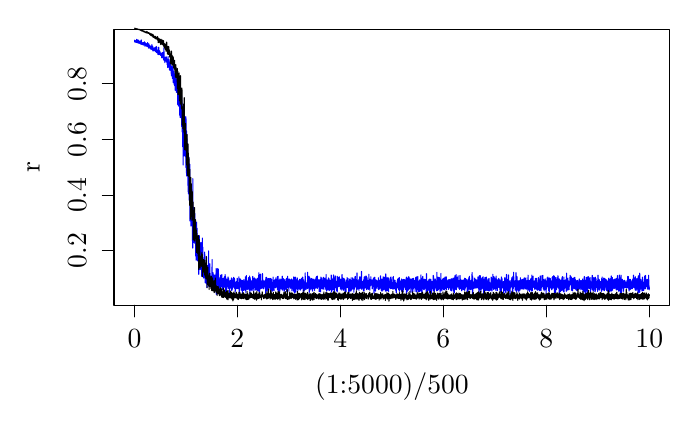
\begin{tikzpicture}[x=0.7pt,y=0.7pt]
\definecolor{fillColor}{RGB}{255,255,255}
%\path[use as bounding box,fill=fillColor,fill opacity=0.00] (0,0) rectangle (361.35,252.94);
\begin{scope}
%\path[clip] ( 49.20, 61.20) rectangle (336.15,203.75);
\definecolor{drawColor}{RGB}{0,0,255}

\path[draw=drawColor,line width= 0.4pt,line join=round,line cap=round] ( 59.83,198.03) --
	( 59.88,197.14) --
	( 59.93,197.40) --
	( 59.99,197.56) --
	( 60.04,197.27) --
	( 60.09,197.13) --
	( 60.15,197.08) --
	( 60.20,197.63) --
	( 60.25,197.36) --
	( 60.31,197.64) --
	( 60.36,197.61) --
	( 60.41,197.14) --
	( 60.47,197.85) --
	( 60.52,196.98) --
	( 60.57,197.00) --
	( 60.63,197.55) --
	( 60.68,197.68) --
	( 60.73,198.08) --
	( 60.78,196.93) --
	( 60.84,197.21) --
	( 60.89,198.47) --
	( 60.94,196.87) --
	( 61.00,196.85) --
	( 61.05,196.91) --
	( 61.10,197.10) --
	( 61.16,196.85) --
	( 61.21,197.23) --
	( 61.26,197.10) --
	( 61.32,196.96) --
	( 61.37,196.85) --
	( 61.42,196.86) --
	( 61.48,198.13) --
	( 61.53,197.32) --
	( 61.58,196.90) --
	( 61.63,197.44) --
	( 61.69,196.68) --
	( 61.74,196.48) --
	( 61.79,197.01) --
	( 61.85,197.99) --
	( 61.90,196.58) --
	( 61.95,196.74) --
	( 62.01,197.60) --
	( 62.06,197.12) --
	( 62.11,196.89) --
	( 62.17,197.22) --
	( 62.22,196.81) --
	( 62.27,197.04) --
	( 62.33,196.56) --
	( 62.38,196.46) --
	( 62.43,196.79) --
	( 62.49,197.40) --
	( 62.54,196.95) --
	( 62.59,197.53) --
	( 62.64,196.93) --
	( 62.70,196.25) --
	( 62.75,196.48) --
	( 62.80,197.59) --
	( 62.86,196.42) --
	( 62.91,196.19) --
	( 62.96,196.08) --
	( 63.02,196.83) --
	( 63.07,196.05) --
	( 63.12,196.30) --
	( 63.18,196.31) --
	( 63.23,196.85) --
	( 63.28,198.13) --
	( 63.34,195.95) --
	( 63.39,196.22) --
	( 63.44,197.16) --
	( 63.50,196.48) --
	( 63.55,196.73) --
	( 63.60,195.88) --
	( 63.65,196.61) --
	( 63.71,196.74) --
	( 63.76,196.37) --
	( 63.81,195.88) --
	( 63.87,195.74) --
	( 63.92,196.69) --
	( 63.97,196.14) --
	( 64.03,196.21) --
	( 64.08,196.05) --
	( 64.13,196.75) --
	( 64.19,196.15) --
	( 64.24,196.40) --
	( 64.29,196.39) --
	( 64.35,196.80) --
	( 64.40,195.81) --
	( 64.45,195.50) --
	( 64.50,196.06) --
	( 64.56,196.05) --
	( 64.61,196.12) --
	( 64.66,196.40) --
	( 64.72,196.02) --
	( 64.77,195.69) --
	( 64.82,195.69) --
	( 64.88,197.25) --
	( 64.93,195.77) --
	( 64.98,196.43) --
	( 65.04,195.97) --
	( 65.09,195.95) --
	( 65.14,195.85) --
	( 65.20,194.95) --
	( 65.25,195.59) --
	( 65.30,195.29) --
	( 65.36,195.47) --
	( 65.41,196.72) --
	( 65.46,195.58) --
	( 65.51,195.81) --
	( 65.57,195.13) --
	( 65.62,195.13) --
	( 65.67,196.39) --
	( 65.73,195.77) --
	( 65.78,195.80) --
	( 65.83,195.30) --
	( 65.89,195.86) --
	( 65.94,195.09) --
	( 65.99,195.37) --
	( 66.05,195.42) --
	( 66.10,194.99) --
	( 66.15,195.11) --
	( 66.21,194.85) --
	( 66.26,196.26) --
	( 66.31,194.77) --
	( 66.37,194.98) --
	( 66.42,195.88) --
	( 66.47,194.84) --
	( 66.52,195.13) --
	( 66.58,196.78) --
	( 66.63,195.65) --
	( 66.68,195.09) --
	( 66.74,194.76) --
	( 66.79,194.76) --
	( 66.84,195.90) --
	( 66.90,194.78) --
	( 66.95,196.15) --
	( 67.00,194.17) --
	( 67.06,193.96) --
	( 67.11,195.40) --
	( 67.16,194.99) --
	( 67.22,196.20) --
	( 67.27,194.07) --
	( 67.32,195.18) --
	( 67.38,195.40) --
	( 67.43,195.10) --
	( 67.48,194.20) --
	( 67.53,195.45) --
	( 67.59,195.21) --
	( 67.64,194.65) --
	( 67.69,194.31) --
	( 67.75,194.74) --
	( 67.80,194.76) --
	( 67.85,193.70) --
	( 67.91,194.06) --
	( 67.96,194.90) --
	( 68.01,194.56) --
	( 68.07,194.41) --
	( 68.12,194.07) --
	( 68.17,194.05) --
	( 68.23,195.01) --
	( 68.28,194.38) --
	( 68.33,193.31) --
	( 68.38,194.72) --
	( 68.44,193.56) --
	( 68.49,194.82) --
	( 68.54,194.09) --
	( 68.60,194.92) --
	( 68.65,193.72) --
	( 68.70,193.86) --
	( 68.76,195.78) --
	( 68.81,194.20) --
	( 68.86,193.65) --
	( 68.92,195.21) --
	( 68.97,193.12) --
	( 69.02,194.27) --
	( 69.08,193.88) --
	( 69.13,194.95) --
	( 69.18,193.38) --
	( 69.24,194.56) --
	( 69.29,194.50) --
	( 69.34,192.49) --
	( 69.39,193.42) --
	( 69.45,192.92) --
	( 69.50,193.68) --
	( 69.55,192.58) --
	( 69.61,192.76) --
	( 69.66,193.92) --
	( 69.71,192.61) --
	( 69.77,192.96) --
	( 69.82,193.17) --
	( 69.87,193.90) --
	( 69.93,193.76) --
	( 69.98,192.62) --
	( 70.03,192.96) --
	( 70.09,193.36) --
	( 70.14,193.19) --
	( 70.19,193.71) --
	( 70.25,192.81) --
	( 70.30,194.18) --
	( 70.35,194.03) --
	( 70.40,192.71) --
	( 70.46,194.20) --
	( 70.51,193.52) --
	( 70.56,193.73) --
	( 70.62,192.13) --
	( 70.67,192.77) --
	( 70.72,194.34) --
	( 70.78,192.74) --
	( 70.83,193.05) --
	( 70.88,192.22) --
	( 70.94,193.70) --
	( 70.99,192.86) --
	( 71.04,194.81) --
	( 71.10,191.71) --
	( 71.15,192.61) --
	( 71.20,192.60) --
	( 71.25,192.39) --
	( 71.31,191.96) --
	( 71.36,192.04) --
	( 71.41,192.29) --
	( 71.47,191.78) --
	( 71.52,191.50) --
	( 71.57,191.88) --
	( 71.63,192.91) --
	( 71.68,192.44) --
	( 71.73,191.68) --
	( 71.79,192.57) --
	( 71.84,192.24) --
	( 71.89,190.71) --
	( 71.95,191.88) --
	( 72.00,194.38) --
	( 72.05,191.14) --
	( 72.11,191.45) --
	( 72.16,191.46) --
	( 72.21,192.85) --
	( 72.26,190.59) --
	( 72.32,194.26) --
	( 72.37,192.22) --
	( 72.42,191.20) --
	( 72.48,191.92) --
	( 72.53,192.61) --
	( 72.58,191.56) --
	( 72.64,191.45) --
	( 72.69,192.61) --
	( 72.74,191.31) --
	( 72.80,191.14) --
	( 72.85,190.55) --
	( 72.90,190.91) --
	( 72.96,192.08) --
	( 73.01,190.89) --
	( 73.06,190.37) --
	( 73.12,191.51) --
	( 73.17,190.93) --
	( 73.22,190.18) --
	( 73.27,190.80) --
	( 73.33,191.02) --
	( 73.38,190.71) --
	( 73.43,190.80) --
	( 73.49,190.37) --
	( 73.54,190.88) --
	( 73.59,191.24) --
	( 73.65,190.26) --
	( 73.70,190.48) --
	( 73.75,189.79) --
	( 73.81,190.72) --
	( 73.86,189.00) --
	( 73.91,190.45) --
	( 73.97,190.20) --
	( 74.02,191.37) --
	( 74.07,191.59) --
	( 74.12,189.44) --
	( 74.18,189.83) --
	( 74.23,191.35) --
	( 74.28,190.81) --
	( 74.34,190.12) --
	( 74.39,189.84) --
	( 74.44,189.05) --
	( 74.50,191.68) --
	( 74.55,189.79) --
	( 74.60,189.99) --
	( 74.66,188.99) --
	( 74.71,189.52) --
	( 74.76,188.17) --
	( 74.82,190.45) --
	( 74.87,189.90) --
	( 74.92,187.80) --
	( 74.98,194.11) --
	( 75.03,187.96) --
	( 75.08,189.11) --
	( 75.13,188.25) --
	( 75.19,189.39) --
	( 75.24,188.98) --
	( 75.29,189.08) --
	( 75.35,189.12) --
	( 75.40,188.90) --
	( 75.45,186.44) --
	( 75.51,188.79) --
	( 75.56,187.04) --
	( 75.61,188.47) --
	( 75.67,188.99) --
	( 75.72,187.74) --
	( 75.77,187.43) --
	( 75.83,188.60) --
	( 75.88,187.77) --
	( 75.93,188.40) --
	( 75.99,189.45) --
	( 76.04,187.29) --
	( 76.09,188.55) --
	( 76.14,187.86) --
	( 76.20,189.43) --
	( 76.25,188.88) --
	( 76.30,187.75) --
	( 76.36,188.90) --
	( 76.41,188.23) --
	( 76.46,186.70) --
	( 76.52,187.28) --
	( 76.57,187.56) --
	( 76.62,185.46) --
	( 76.68,186.90) --
	( 76.73,187.63) --
	( 76.78,187.82) --
	( 76.84,185.85) --
	( 76.89,186.53) --
	( 76.94,183.95) --
	( 77.00,187.02) --
	( 77.05,188.35) --
	( 77.10,187.61) --
	( 77.15,189.59) --
	( 77.21,186.72) --
	( 77.26,184.45) --
	( 77.31,188.17) --
	( 77.37,186.62) --
	( 77.42,187.01) --
	( 77.47,184.86) --
	( 77.53,184.16) --
	( 77.58,184.18) --
	( 77.63,185.93) --
	( 77.69,185.46) --
	( 77.74,184.94) --
	( 77.79,183.99) --
	( 77.85,183.31) --
	( 77.90,182.57) --
	( 77.95,185.93) --
	( 78.00,185.15) --
	( 78.06,183.19) --
	( 78.11,183.96) --
	( 78.16,187.97) --
	( 78.22,184.71) --
	( 78.27,186.89) --
	( 78.32,183.60) --
	( 78.38,182.52) --
	( 78.43,186.35) --
	( 78.48,184.09) --
	( 78.54,183.54) --
	( 78.59,182.42) --
	( 78.64,183.91) --
	( 78.70,180.89) --
	( 78.75,182.99) --
	( 78.80,184.25) --
	( 78.86,179.81) --
	( 78.91,184.47) --
	( 78.96,181.88) --
	( 79.01,184.03) --
	( 79.07,181.91) --
	( 79.12,180.96) --
	( 79.17,180.40) --
	( 79.23,182.13) --
	( 79.28,180.23) --
	( 79.33,178.37) --
	( 79.39,181.16) --
	( 79.44,183.20) --
	( 79.49,180.20) --
	( 79.55,180.99) --
	( 79.60,179.09) --
	( 79.65,185.85) --
	( 79.71,180.19) --
	( 79.76,180.54) --
	( 79.81,176.21) --
	( 79.87,181.43) --
	( 79.92,179.22) --
	( 79.97,181.48) --
	( 80.02,177.92) --
	( 80.08,178.60) --
	( 80.13,179.52) --
	( 80.18,181.86) --
	( 80.24,179.71) --
	( 80.29,179.45) --
	( 80.34,175.12) --
	( 80.40,179.90) --
	( 80.45,177.93) --
	( 80.50,180.52) --
	( 80.56,174.44) --
	( 80.61,179.95) --
	( 80.66,180.03) --
	( 80.72,177.07) --
	( 80.77,179.93) --
	( 80.82,172.16) --
	( 80.87,174.48) --
	( 80.93,178.64) --
	( 80.98,179.15) --
	( 81.03,175.55) --
	( 81.09,177.41) --
	( 81.14,176.20) --
	( 81.19,178.91) --
	( 81.25,173.92) --
	( 81.30,178.58) --
	( 81.35,177.07) --
	( 81.41,171.09) --
	( 81.46,175.63) --
	( 81.51,177.48) --
	( 81.57,175.56) --
	( 81.62,173.46) --
	( 81.67,172.15) --
	( 81.73,176.36) --
	( 81.78,171.95) --
	( 81.83,176.82) --
	( 81.88,171.54) --
	( 81.94,175.97) --
	( 81.99,174.70) --
	( 82.04,175.52) --
	( 82.10,164.86) --
	( 82.15,166.77) --
	( 82.20,172.53) --
	( 82.26,171.32) --
	( 82.31,173.86) --
	( 82.36,177.97) --
	( 82.42,164.74) --
	( 82.47,168.24) --
	( 82.52,164.06) --
	( 82.58,166.05) --
	( 82.63,171.35) --
	( 82.68,170.81) --
	( 82.74,176.25) --
	( 82.79,172.78) --
	( 82.84,167.77) --
	( 82.89,168.35) --
	( 82.95,167.07) --
	( 83.00,167.35) --
	( 83.05,170.76) --
	( 83.11,173.68) --
	( 83.16,159.23) --
	( 83.21,167.55) --
	( 83.27,162.17) --
	( 83.32,170.82) --
	( 83.37,168.49) --
	( 83.43,158.04) --
	( 83.48,170.24) --
	( 83.53,158.75) --
	( 83.59,163.84) --
	( 83.64,164.32) --
	( 83.69,167.86) --
	( 83.75,159.15) --
	( 83.80,163.59) --
	( 83.85,172.24) --
	( 83.90,164.69) --
	( 83.96,159.07) --
	( 84.01,166.82) --
	( 84.06,169.35) --
	( 84.12,153.58) --
	( 84.17,162.38) --
	( 84.22,157.95) --
	( 84.28,167.11) --
	( 84.33,156.24) --
	( 84.38,164.84) --
	( 84.44,150.57) --
	( 84.49,157.91) --
	( 84.54,161.94) --
	( 84.60,155.88) --
	( 84.65,144.32) --
	( 84.70,143.02) --
	( 84.75,157.53) --
	( 84.81,148.60) --
	( 84.86,154.93) --
	( 84.91,133.62) --
	( 84.97,155.87) --
	( 85.02,159.37) --
	( 85.07,152.69) --
	( 85.13,157.25) --
	( 85.18,140.54) --
	( 85.23,149.37) --
	( 85.29,138.29) --
	( 85.34,150.93) --
	( 85.39,149.20) --
	( 85.45,156.87) --
	( 85.50,155.79) --
	( 85.55,146.84) --
	( 85.61,139.22) --
	( 85.66,152.04) --
	( 85.71,151.85) --
	( 85.76,150.43) --
	( 85.82,146.60) --
	( 85.87,138.33) --
	( 85.92,147.88) --
	( 85.98,141.82) --
	( 86.03,137.99) --
	( 86.08,139.58) --
	( 86.14,150.74) --
	( 86.19,151.88) --
	( 86.24,158.56) --
	( 86.30,153.15) --
	( 86.35,132.26) --
	( 86.40,157.53) --
	( 86.46,137.79) --
	( 86.51,137.99) --
	( 86.56,132.75) --
	( 86.62,141.91) --
	( 86.67,127.94) --
	( 86.72,151.15) --
	( 86.77,146.36) --
	( 86.83,140.94) --
	( 86.88,140.18) --
	( 86.93,147.21) --
	( 86.99,135.75) --
	( 87.04,129.70) --
	( 87.09,136.26) --
	( 87.15,134.58) --
	( 87.20,143.29) --
	( 87.25,135.67) --
	( 87.31,138.26) --
	( 87.36,130.11) --
	( 87.41,125.05) --
	( 87.47,120.79) --
	( 87.52,119.81) --
	( 87.57,134.74) --
	( 87.62,133.35) --
	( 87.68,118.76) --
	( 87.73,123.71) --
	( 87.78,137.84) --
	( 87.84,129.94) --
	( 87.89,126.54) --
	( 87.94,131.29) --
	( 88.00,122.07) --
	( 88.05,115.42) --
	( 88.10,131.45) --
	( 88.16,122.28) --
	( 88.21,131.18) --
	( 88.26,116.64) --
	( 88.32,134.01) --
	( 88.37,104.74) --
	( 88.42,116.15) --
	( 88.48,111.85) --
	( 88.53,118.73) --
	( 88.58,113.05) --
	( 88.63,110.92) --
	( 88.69,108.47) --
	( 88.74,120.13) --
	( 88.79,113.56) --
	( 88.85,119.37) --
	( 88.90,102.15) --
	( 88.95,118.35) --
	( 89.01,116.58) --
	( 89.06,109.73) --
	( 89.11,110.62) --
	( 89.17,117.03) --
	( 89.22,113.15) --
	( 89.27,114.37) --
	( 89.33,105.25) --
	( 89.38,102.13) --
	( 89.43,113.85) --
	( 89.49,113.50) --
	( 89.54,115.14) --
	( 89.59,104.03) --
	( 89.64,111.39) --
	( 89.70,100.32) --
	( 89.75, 94.33) --
	( 89.80,111.54) --
	( 89.86, 90.76) --
	( 89.91,126.55) --
	( 89.96,102.12) --
	( 90.02,111.36) --
	( 90.07,105.60) --
	( 90.12,107.69) --
	( 90.18,105.38) --
	( 90.23,104.97) --
	( 90.28, 98.90) --
	( 90.34,100.55) --
	( 90.39,106.11) --
	( 90.44,111.68) --
	( 90.50, 96.43) --
	( 90.55,100.26) --
	( 90.60,102.89) --
	( 90.65, 93.44) --
	( 90.71,102.79) --
	( 90.76,102.12) --
	( 90.81, 97.51) --
	( 90.87,106.46) --
	( 90.92,108.64) --
	( 90.97,102.61) --
	( 91.03, 94.47) --
	( 91.08, 93.08) --
	( 91.13,100.40) --
	( 91.19,104.81) --
	( 91.24, 97.42) --
	( 91.29,103.59) --
	( 91.35,100.42) --
	( 91.40, 86.66) --
	( 91.45, 89.74) --
	( 91.50, 94.74) --
	( 91.56,102.94) --
	( 91.61, 91.56) --
	( 91.66, 84.47) --
	( 91.72, 99.42) --
	( 91.77, 91.45) --
	( 91.82,104.16) --
	( 91.88,102.78) --
	( 91.93, 96.79) --
	( 91.98, 91.22) --
	( 92.04,101.02) --
	( 92.09, 92.72) --
	( 92.14, 99.06) --
	( 92.20, 88.49) --
	( 92.25, 92.82) --
	( 92.30, 90.84) --
	( 92.36, 94.30) --
	( 92.41, 84.09) --
	( 92.46, 93.25) --
	( 92.51, 89.12) --
	( 92.57, 88.39) --
	( 92.62, 95.27) --
	( 92.67, 91.04) --
	( 92.73, 95.77) --
	( 92.78, 87.85) --
	( 92.83, 90.88) --
	( 92.89, 95.41) --
	( 92.94, 77.19) --
	( 92.99, 86.07) --
	( 93.05, 82.75) --
	( 93.10, 97.29) --
	( 93.15, 91.92) --
	( 93.21, 82.58) --
	( 93.26, 97.10) --
	( 93.31, 90.73) --
	( 93.37, 84.34) --
	( 93.42, 81.91) --
	( 93.47, 79.82) --
	( 93.52, 86.95) --
	( 93.58, 93.39) --
	( 93.63, 79.62) --
	( 93.68, 90.34) --
	( 93.74, 85.34) --
	( 93.79, 93.14) --
	( 93.84, 90.19) --
	( 93.90, 89.10) --
	( 93.95, 84.82) --
	( 94.00, 80.85) --
	( 94.06, 82.29) --
	( 94.11, 93.63) --
	( 94.16, 83.55) --
	( 94.22, 79.73) --
	( 94.27, 85.99) --
	( 94.32, 79.45) --
	( 94.37, 80.71) --
	( 94.43, 81.42) --
	( 94.48, 76.17) --
	( 94.53, 86.15) --
	( 94.59, 87.16) --
	( 94.64, 86.58) --
	( 94.69, 86.08) --
	( 94.75, 81.72) --
	( 94.80, 86.82) --
	( 94.85, 95.88) --
	( 94.91, 81.84) --
	( 94.96, 82.83) --
	( 95.01, 91.20) --
	( 95.07, 79.22) --
	( 95.12, 77.08) --
	( 95.17, 80.28) --
	( 95.23, 85.96) --
	( 95.28, 80.47) --
	( 95.33, 76.77) --
	( 95.38, 83.44) --
	( 95.44, 83.10) --
	( 95.49, 77.66) --
	( 95.54, 75.27) --
	( 95.60, 84.78) --
	( 95.65, 82.30) --
	( 95.70, 81.20) --
	( 95.76, 77.52) --
	( 95.81, 81.45) --
	( 95.86, 85.05) --
	( 95.92, 80.27) --
	( 95.97, 75.67) --
	( 96.02, 88.67) --
	( 96.08, 82.08) --
	( 96.13, 84.67) --
	( 96.18, 75.63) --
	( 96.24, 79.52) --
	( 96.29, 72.86) --
	( 96.34, 75.22) --
	( 96.39, 80.89) --
	( 96.45, 78.60) --
	( 96.50, 75.72) --
	( 96.55, 78.65) --
	( 96.61, 79.42) --
	( 96.66, 78.71) --
	( 96.71, 80.02) --
	( 96.77, 73.31) --
	( 96.82, 72.47) --
	( 96.87, 74.50) --
	( 96.93, 78.90) --
	( 96.98, 75.66) --
	( 97.03, 77.92) --
	( 97.09, 77.44) --
	( 97.14, 70.34) --
	( 97.19, 78.86) --
	( 97.25, 81.79) --
	( 97.30, 79.30) --
	( 97.35, 77.76) --
	( 97.40, 79.99) --
	( 97.46, 79.29) --
	( 97.51, 77.45) --
	( 97.56, 73.37) --
	( 97.62, 81.69) --
	( 97.67, 80.63) --
	( 97.72, 75.05) --
	( 97.78, 77.67) --
	( 97.83, 78.65) --
	( 97.88, 75.69) --
	( 97.94, 78.80) --
	( 97.99, 80.97) --
	( 98.04, 89.27) --
	( 98.10, 71.01) --
	( 98.15, 82.08) --
	( 98.20, 74.39) --
	( 98.25, 75.79) --
	( 98.31, 79.97) --
	( 98.36, 78.18) --
	( 98.41, 75.30) --
	( 98.47, 80.37) --
	( 98.52, 75.40) --
	( 98.57, 71.33) --
	( 98.63, 76.34) --
	( 98.68, 82.63) --
	( 98.73, 77.36) --
	( 98.79, 77.69) --
	( 98.84, 72.08) --
	( 98.89, 73.75) --
	( 98.95, 72.86) --
	( 99.00, 76.30) --
	( 99.05, 76.17) --
	( 99.11, 72.63) --
	( 99.16, 71.86) --
	( 99.21, 73.63) --
	( 99.26, 73.45) --
	( 99.32, 72.46) --
	( 99.37, 71.93) --
	( 99.42, 74.80) --
	( 99.48, 70.56) --
	( 99.53, 75.16) --
	( 99.58, 74.63) --
	( 99.64, 76.33) --
	( 99.69, 70.58) --
	( 99.74, 75.10) --
	( 99.80, 76.11) --
	( 99.85, 84.84) --
	( 99.90, 74.78) --
	( 99.96, 77.17) --
	(100.01, 78.10) --
	(100.06, 69.68) --
	(100.12, 72.44) --
	(100.17, 72.52) --
	(100.22, 75.01) --
	(100.27, 76.21) --
	(100.33, 78.04) --
	(100.38, 74.73) --
	(100.43, 75.96) --
	(100.49, 75.08) --
	(100.54, 71.13) --
	(100.59, 70.27) --
	(100.65, 76.95) --
	(100.70, 74.68) --
	(100.75, 71.13) --
	(100.81, 70.68) --
	(100.86, 74.03) --
	(100.91, 75.50) --
	(100.97, 75.99) --
	(101.02, 71.66) --
	(101.07, 72.06) --
	(101.12, 76.80) --
	(101.18, 71.72) --
	(101.23, 70.56) --
	(101.28, 69.64) --
	(101.34, 72.44) --
	(101.39, 71.46) --
	(101.44, 73.80) --
	(101.50, 73.79) --
	(101.55, 71.62) --
	(101.60, 72.30) --
	(101.66, 74.97) --
	(101.71, 76.45) --
	(101.76, 73.43) --
	(101.82, 76.32) --
	(101.87, 75.18) --
	(101.92, 80.19) --
	(101.98, 70.67) --
	(102.03, 66.74) --
	(102.08, 71.82) --
	(102.13, 75.75) --
	(102.19, 78.54) --
	(102.24, 73.19) --
	(102.29, 70.03) --
	(102.35, 73.03) --
	(102.40, 74.65) --
	(102.45, 71.85) --
	(102.51, 75.40) --
	(102.56, 71.78) --
	(102.61, 80.11) --
	(102.67, 71.64) --
	(102.72, 75.25) --
	(102.77, 76.10) --
	(102.83, 76.73) --
	(102.88, 74.68) --
	(102.93, 72.72) --
	(102.99, 74.95) --
	(103.04, 73.43) --
	(103.09, 79.91) --
	(103.14, 70.10) --
	(103.20, 77.44) --
	(103.25, 73.32) --
	(103.30, 74.78) --
	(103.36, 72.86) --
	(103.41, 75.66) --
	(103.46, 74.33) --
	(103.52, 72.41) --
	(103.57, 73.79) --
	(103.62, 73.95) --
	(103.68, 73.26) --
	(103.73, 70.79) --
	(103.78, 71.58) --
	(103.84, 71.54) --
	(103.89, 73.65) --
	(103.94, 69.17) --
	(104.00, 73.57) --
	(104.05, 73.80) --
	(104.10, 74.94) --
	(104.15, 69.60) --
	(104.21, 74.85) --
	(104.26, 68.33) --
	(104.31, 76.78) --
	(104.37, 70.61) --
	(104.42, 72.79) --
	(104.47, 72.54) --
	(104.53, 72.61) --
	(104.58, 71.79) --
	(104.63, 73.58) --
	(104.69, 72.84) --
	(104.74, 71.03) --
	(104.79, 72.51) --
	(104.85, 77.06) --
	(104.90, 71.22) --
	(104.95, 73.85) --
	(105.00, 72.71) --
	(105.06, 71.73) --
	(105.11, 71.91) --
	(105.16, 69.25) --
	(105.22, 74.94) --
	(105.27, 73.81) --
	(105.32, 72.41) --
	(105.38, 70.65) --
	(105.43, 70.74) --
	(105.48, 74.51) --
	(105.54, 75.00) --
	(105.59, 71.62) --
	(105.64, 70.41) --
	(105.70, 70.71) --
	(105.75, 71.71) --
	(105.80, 73.80) --
	(105.86, 75.14) --
	(105.91, 70.33) --
	(105.96, 71.50) --
	(106.01, 71.42) --
	(106.07, 71.63) --
	(106.12, 73.57) --
	(106.17, 70.71) --
	(106.23, 75.96) --
	(106.28, 74.78) --
	(106.33, 73.66) --
	(106.39, 70.94) --
	(106.44, 74.02) --
	(106.49, 75.13) --
	(106.55, 72.75) --
	(106.60, 77.06) --
	(106.65, 74.61) --
	(106.71, 71.62) --
	(106.76, 69.28) --
	(106.81, 75.89) --
	(106.87, 66.76) --
	(106.92, 71.90) --
	(106.97, 73.86) --
	(107.02, 71.85) --
	(107.08, 70.92) --
	(107.13, 72.18) --
	(107.18, 72.83) --
	(107.24, 74.18) --
	(107.29, 68.48) --
	(107.34, 74.70) --
	(107.40, 72.68) --
	(107.45, 71.11) --
	(107.50, 73.32) --
	(107.56, 71.78) --
	(107.61, 73.18) --
	(107.66, 71.20) --
	(107.72, 74.19) --
	(107.77, 71.99) --
	(107.82, 74.47) --
	(107.87, 71.75) --
	(107.93, 71.04) --
	(107.98, 72.10) --
	(108.03, 70.82) --
	(108.09, 75.83) --
	(108.14, 71.45) --
	(108.19, 69.93) --
	(108.25, 71.13) --
	(108.30, 73.44) --
	(108.35, 75.10) --
	(108.41, 71.62) --
	(108.46, 72.53) --
	(108.51, 71.70) --
	(108.57, 70.99) --
	(108.62, 71.66) --
	(108.67, 70.02) --
	(108.73, 70.60) --
	(108.78, 73.17) --
	(108.83, 67.82) --
	(108.88, 73.61) --
	(108.94, 69.94) --
	(108.99, 73.33) --
	(109.04, 70.89) --
	(109.10, 73.59) --
	(109.15, 74.15) --
	(109.20, 71.45) --
	(109.26, 72.82) --
	(109.31, 70.50) --
	(109.36, 71.46) --
	(109.42, 73.35) --
	(109.47, 72.84) --
	(109.52, 72.25) --
	(109.58, 71.53) --
	(109.63, 70.10) --
	(109.68, 70.80) --
	(109.74, 70.36) --
	(109.79, 69.75) --
	(109.84, 75.30) --
	(109.89, 75.25) --
	(109.95, 71.13) --
	(110.00, 68.77) --
	(110.05, 70.12) --
	(110.11, 74.31) --
	(110.16, 70.42) --
	(110.21, 71.30) --
	(110.27, 72.76) --
	(110.32, 69.47) --
	(110.37, 71.32) --
	(110.43, 72.70) --
	(110.48, 73.74) --
	(110.53, 73.18) --
	(110.59, 72.86) --
	(110.64, 72.13) --
	(110.69, 73.84) --
	(110.75, 73.62) --
	(110.80, 75.09) --
	(110.85, 72.07) --
	(110.90, 71.67) --
	(110.96, 75.63) --
	(111.01, 70.46) --
	(111.06, 73.64) --
	(111.12, 73.92) --
	(111.17, 71.07) --
	(111.22, 73.29) --
	(111.28, 75.18) --
	(111.33, 73.58) --
	(111.38, 73.45) --
	(111.44, 69.96) --
	(111.49, 74.57) --
	(111.54, 72.91) --
	(111.60, 71.89) --
	(111.65, 72.20) --
	(111.70, 71.65) --
	(111.75, 67.97) --
	(111.81, 69.41) --
	(111.86, 72.91) --
	(111.91, 71.76) --
	(111.97, 69.32) --
	(112.02, 71.35) --
	(112.07, 73.02) --
	(112.13, 71.02) --
	(112.18, 70.64) --
	(112.23, 70.07) --
	(112.29, 72.49) --
	(112.34, 71.67) --
	(112.39, 71.08) --
	(112.45, 72.27) --
	(112.50, 73.58) --
	(112.55, 70.43) --
	(112.61, 69.77) --
	(112.66, 72.46) --
	(112.71, 72.90) --
	(112.76, 73.02) --
	(112.82, 75.13) --
	(112.87, 73.67) --
	(112.92, 73.50) --
	(112.98, 70.88) --
	(113.03, 73.06) --
	(113.08, 70.32) --
	(113.14, 70.43) --
	(113.19, 72.42) --
	(113.24, 69.78) --
	(113.30, 71.05) --
	(113.35, 71.43) --
	(113.40, 71.06) --
	(113.46, 70.42) --
	(113.51, 71.21) --
	(113.56, 72.34) --
	(113.62, 71.65) --
	(113.67, 75.85) --
	(113.72, 73.25) --
	(113.77, 73.64) --
	(113.83, 72.10) --
	(113.88, 67.40) --
	(113.93, 70.98) --
	(113.99, 73.04) --
	(114.04, 74.72) --
	(114.09, 74.79) --
	(114.15, 72.29) --
	(114.20, 71.89) --
	(114.25, 71.39) --
	(114.31, 72.68) --
	(114.36, 74.85) --
	(114.41, 71.94) --
	(114.47, 74.47) --
	(114.52, 71.69) --
	(114.57, 74.15) --
	(114.62, 70.55) --
	(114.68, 71.37) --
	(114.73, 72.67) --
	(114.78, 73.03) --
	(114.84, 72.95) --
	(114.89, 68.98) --
	(114.94, 69.92) --
	(115.00, 74.13) --
	(115.05, 73.27) --
	(115.10, 71.42) --
	(115.16, 71.29) --
	(115.21, 70.21) --
	(115.26, 72.28) --
	(115.32, 71.52) --
	(115.37, 73.26) --
	(115.42, 71.38) --
	(115.48, 67.53) --
	(115.53, 74.04) --
	(115.58, 70.30) --
	(115.63, 73.50) --
	(115.69, 70.84) --
	(115.74, 69.34) --
	(115.79, 73.64) --
	(115.85, 70.45) --
	(115.90, 73.32) --
	(115.95, 72.63) --
	(116.01, 73.71) --
	(116.06, 68.86) --
	(116.11, 68.92) --
	(116.17, 73.12) --
	(116.22, 72.51) --
	(116.27, 74.51) --
	(116.33, 69.25) --
	(116.38, 71.07) --
	(116.43, 72.50) --
	(116.49, 73.69) --
	(116.54, 71.34) --
	(116.59, 70.31) --
	(116.64, 70.96) --
	(116.70, 71.41) --
	(116.75, 70.15) --
	(116.80, 69.89) --
	(116.86, 68.97) --
	(116.91, 73.71) --
	(116.96, 69.11) --
	(117.02, 70.00) --
	(117.07, 75.88) --
	(117.12, 71.70) --
	(117.18, 73.23) --
	(117.23, 70.23) --
	(117.28, 67.78) --
	(117.34, 72.08) --
	(117.39, 71.27) --
	(117.44, 73.36) --
	(117.50, 73.52) --
	(117.55, 76.60) --
	(117.60, 72.02) --
	(117.65, 71.53) --
	(117.71, 71.75) --
	(117.76, 70.44) --
	(117.81, 74.11) --
	(117.87, 72.06) --
	(117.92, 70.32) --
	(117.97, 69.33) --
	(118.03, 70.29) --
	(118.08, 72.76) --
	(118.13, 72.03) --
	(118.19, 72.09) --
	(118.24, 70.57) --
	(118.29, 69.65) --
	(118.35, 71.50) --
	(118.40, 73.51) --
	(118.45, 71.96) --
	(118.50, 71.25) --
	(118.56, 71.92) --
	(118.61, 69.55) --
	(118.66, 75.50) --
	(118.72, 70.37) --
	(118.77, 72.96) --
	(118.82, 71.66) --
	(118.88, 72.94) --
	(118.93, 69.71) --
	(118.98, 73.00) --
	(119.04, 71.43) --
	(119.09, 69.00) --
	(119.14, 72.16) --
	(119.20, 76.31) --
	(119.25, 69.39) --
	(119.30, 72.48) --
	(119.36, 66.73) --
	(119.41, 75.35) --
	(119.46, 71.90) --
	(119.51, 75.45) --
	(119.57, 72.25) --
	(119.62, 71.42) --
	(119.67, 72.40) --
	(119.73, 71.34) --
	(119.78, 69.10) --
	(119.83, 74.04) --
	(119.89, 72.79) --
	(119.94, 73.98) --
	(119.99, 70.34) --
	(120.05, 71.65) --
	(120.10, 72.13) --
	(120.15, 73.63) --
	(120.21, 70.54) --
	(120.26, 73.61) --
	(120.31, 71.19) --
	(120.37, 72.71) --
	(120.42, 68.68) --
	(120.47, 70.64) --
	(120.52, 69.21) --
	(120.58, 70.14) --
	(120.63, 73.61) --
	(120.68, 72.66) --
	(120.74, 69.63) --
	(120.79, 70.51) --
	(120.84, 76.06) --
	(120.90, 71.10) --
	(120.95, 72.60) --
	(121.00, 74.90) --
	(121.06, 73.20) --
	(121.11, 75.15) --
	(121.16, 73.98) --
	(121.22, 70.35) --
	(121.27, 73.65) --
	(121.32, 72.25) --
	(121.37, 69.75) --
	(121.43, 68.58) --
	(121.48, 71.87) --
	(121.53, 72.41) --
	(121.59, 70.46) --
	(121.64, 72.50) --
	(121.69, 71.58) --
	(121.75, 75.33) --
	(121.80, 71.83) --
	(121.85, 72.02) --
	(121.91, 71.30) --
	(121.96, 71.62) --
	(122.01, 74.78) --
	(122.07, 74.98) --
	(122.12, 72.81) --
	(122.17, 71.73) --
	(122.23, 73.39) --
	(122.28, 69.06) --
	(122.33, 74.49) --
	(122.38, 73.69) --
	(122.44, 71.94) --
	(122.49, 71.50) --
	(122.54, 71.70) --
	(122.60, 72.36) --
	(122.65, 70.12) --
	(122.70, 69.82) --
	(122.76, 72.29) --
	(122.81, 73.91) --
	(122.86, 74.45) --
	(122.92, 69.28) --
	(122.97, 72.75) --
	(123.02, 71.92) --
	(123.08, 74.14) --
	(123.13, 68.94) --
	(123.18, 75.17) --
	(123.24, 73.68) --
	(123.29, 72.65) --
	(123.34, 68.96) --
	(123.39, 71.96) --
	(123.45, 74.74) --
	(123.50, 68.92) --
	(123.55, 72.38) --
	(123.61, 71.27) --
	(123.66, 71.93) --
	(123.71, 72.63) --
	(123.77, 73.13) --
	(123.82, 71.45) --
	(123.87, 71.00) --
	(123.93, 76.76) --
	(123.98, 68.39) --
	(124.03, 77.98) --
	(124.09, 69.67) --
	(124.14, 74.97) --
	(124.19, 74.41) --
	(124.24, 72.97) --
	(124.30, 70.55) --
	(124.35, 70.07) --
	(124.40, 66.69) --
	(124.46, 72.99) --
	(124.51, 73.73) --
	(124.56, 72.05) --
	(124.62, 73.17) --
	(124.67, 71.51) --
	(124.72, 72.31) --
	(124.78, 71.10) --
	(124.83, 77.23) --
	(124.88, 73.55) --
	(124.94, 74.14) --
	(124.99, 71.36) --
	(125.04, 69.86) --
	(125.10, 71.05) --
	(125.15, 71.48) --
	(125.20, 71.00) --
	(125.25, 73.50) --
	(125.31, 73.58) --
	(125.36, 73.09) --
	(125.41, 71.30) --
	(125.47, 73.11) --
	(125.52, 73.41) --
	(125.57, 69.90) --
	(125.63, 72.43) --
	(125.68, 71.93) --
	(125.73, 72.92) --
	(125.79, 73.43) --
	(125.84, 77.57) --
	(125.89, 72.17) --
	(125.95, 70.44) --
	(126.00, 70.34) --
	(126.05, 70.57) --
	(126.11, 71.72) --
	(126.16, 74.30) --
	(126.21, 71.51) --
	(126.26, 71.75) --
	(126.32, 70.82) --
	(126.37, 69.89) --
	(126.42, 70.43) --
	(126.48, 69.68) --
	(126.53, 71.52) --
	(126.58, 72.44) --
	(126.64, 70.92) --
	(126.69, 73.66) --
	(126.74, 72.75) --
	(126.80, 70.92) --
	(126.85, 73.80) --
	(126.90, 73.72) --
	(126.96, 73.06) --
	(127.01, 72.96) --
	(127.06, 71.63) --
	(127.12, 71.14) --
	(127.17, 73.63) --
	(127.22, 71.07) --
	(127.27, 71.40) --
	(127.33, 71.93) --
	(127.38, 69.96) --
	(127.43, 71.08) --
	(127.49, 67.28) --
	(127.54, 74.54) --
	(127.59, 74.01) --
	(127.65, 71.44) --
	(127.70, 75.59) --
	(127.75, 70.23) --
	(127.81, 69.69) --
	(127.86, 68.93) --
	(127.91, 72.11) --
	(127.97, 68.78) --
	(128.02, 75.60) --
	(128.07, 73.73) --
	(128.12, 72.62) --
	(128.18, 75.07) --
	(128.23, 73.90) --
	(128.28, 73.77) --
	(128.34, 71.38) --
	(128.39, 72.43) --
	(128.44, 71.75) --
	(128.50, 70.16) --
	(128.55, 69.98) --
	(128.60, 72.52) --
	(128.66, 72.48) --
	(128.71, 68.01) --
	(128.76, 71.81) --
	(128.82, 72.65) --
	(128.87, 74.98) --
	(128.92, 73.13) --
	(128.98, 70.03) --
	(129.03, 71.12) --
	(129.08, 71.77) --
	(129.13, 73.64) --
	(129.19, 70.88) --
	(129.24, 72.63) --
	(129.29, 71.67) --
	(129.35, 75.12) --
	(129.40, 71.99) --
	(129.45, 73.87) --
	(129.51, 74.07) --
	(129.56, 70.30) --
	(129.61, 72.56) --
	(129.67, 72.31) --
	(129.72, 72.52) --
	(129.77, 73.05) --
	(129.83, 74.07) --
	(129.88, 69.06) --
	(129.93, 70.40) --
	(129.99, 72.38) --
	(130.04, 75.08) --
	(130.09, 73.25) --
	(130.14, 74.12) --
	(130.20, 70.63) --
	(130.25, 72.31) --
	(130.30, 69.69) --
	(130.36, 69.56) --
	(130.41, 69.99) --
	(130.46, 73.45) --
	(130.52, 74.62) --
	(130.57, 69.49) --
	(130.62, 72.51) --
	(130.68, 68.27) --
	(130.73, 72.52) --
	(130.78, 69.27) --
	(130.84, 70.60) --
	(130.89, 68.57) --
	(130.94, 69.96) --
	(130.99, 71.18) --
	(131.05, 71.30) --
	(131.10, 70.61) --
	(131.15, 69.17) --
	(131.21, 71.63) --
	(131.26, 73.21) --
	(131.31, 71.58) --
	(131.37, 75.74) --
	(131.42, 69.19) --
	(131.47, 71.16) --
	(131.53, 70.60) --
	(131.58, 70.03) --
	(131.63, 70.45) --
	(131.69, 70.42) --
	(131.74, 71.32) --
	(131.79, 68.67) --
	(131.85, 73.85) --
	(131.90, 73.93) --
	(131.95, 71.40) --
	(132.00, 71.51) --
	(132.06, 71.59) --
	(132.11, 72.95) --
	(132.16, 71.24) --
	(132.22, 70.45) --
	(132.27, 72.78) --
	(132.32, 74.48) --
	(132.38, 71.59) --
	(132.43, 71.63) --
	(132.48, 73.91) --
	(132.54, 70.81) --
	(132.59, 70.17) --
	(132.64, 72.43) --
	(132.70, 70.88) --
	(132.75, 75.37) --
	(132.80, 73.88) --
	(132.86, 74.62) --
	(132.91, 74.02) --
	(132.96, 72.00) --
	(133.01, 73.84) --
	(133.07, 71.95) --
	(133.12, 72.31) --
	(133.17, 71.14) --
	(133.23, 72.78) --
	(133.28, 72.42) --
	(133.33, 70.57) --
	(133.39, 70.72) --
	(133.44, 74.47) --
	(133.49, 72.59) --
	(133.55, 76.02) --
	(133.60, 69.63) --
	(133.65, 69.14) --
	(133.71, 71.08) --
	(133.76, 74.02) --
	(133.81, 71.15) --
	(133.87, 72.20) --
	(133.92, 76.15) --
	(133.97, 73.34) --
	(134.02, 71.75) --
	(134.08, 70.00) --
	(134.13, 68.18) --
	(134.18, 72.87) --
	(134.24, 72.94) --
	(134.29, 73.82) --
	(134.34, 69.26) --
	(134.40, 74.18) --
	(134.45, 73.44) --
	(134.50, 71.84) --
	(134.56, 70.04) --
	(134.61, 71.64) --
	(134.66, 69.65) --
	(134.72, 71.33) --
	(134.77, 68.39) --
	(134.82, 74.16) --
	(134.87, 72.35) --
	(134.93, 74.80) --
	(134.98, 74.04) --
	(135.03, 71.93) --
	(135.09, 71.44) --
	(135.14, 72.56) --
	(135.19, 72.00) --
	(135.25, 70.21) --
	(135.30, 74.23) --
	(135.35, 70.63) --
	(135.41, 72.40) --
	(135.46, 70.77) --
	(135.51, 69.60) --
	(135.57, 70.48) --
	(135.62, 71.12) --
	(135.67, 71.76) --
	(135.73, 72.56) --
	(135.78, 74.71) --
	(135.83, 70.05) --
	(135.88, 74.19) --
	(135.94, 72.18) --
	(135.99, 71.21) --
	(136.04, 76.20) --
	(136.10, 71.90) --
	(136.15, 68.99) --
	(136.20, 72.68) --
	(136.26, 70.09) --
	(136.31, 72.34) --
	(136.36, 70.89) --
	(136.42, 72.79) --
	(136.47, 74.29) --
	(136.52, 70.99) --
	(136.58, 72.99) --
	(136.63, 69.64) --
	(136.68, 71.83) --
	(136.74, 74.96) --
	(136.79, 70.44) --
	(136.84, 72.60) --
	(136.89, 71.37) --
	(136.95, 72.11) --
	(137.00, 68.37) --
	(137.05, 72.97) --
	(137.11, 68.64) --
	(137.16, 72.06) --
	(137.21, 69.15) --
	(137.27, 71.26) --
	(137.32, 69.95) --
	(137.37, 74.25) --
	(137.43, 74.41) --
	(137.48, 72.42) --
	(137.53, 70.83) --
	(137.59, 73.07) --
	(137.64, 71.65) --
	(137.69, 72.94) --
	(137.74, 71.89) --
	(137.80, 69.50) --
	(137.85, 72.00) --
	(137.90, 72.22) --
	(137.96, 73.16) --
	(138.01, 73.49) --
	(138.06, 73.14) --
	(138.12, 70.34) --
	(138.17, 71.51) --
	(138.22, 75.03) --
	(138.28, 74.35) --
	(138.33, 68.36) --
	(138.38, 73.85) --
	(138.44, 72.69) --
	(138.49, 70.37) --
	(138.54, 73.79) --
	(138.60, 71.54) --
	(138.65, 71.94) --
	(138.70, 72.81) --
	(138.75, 71.85) --
	(138.81, 76.16) --
	(138.86, 72.71) --
	(138.91, 71.02) --
	(138.97, 70.14) --
	(139.02, 72.36) --
	(139.07, 70.43) --
	(139.13, 72.90) --
	(139.18, 72.85) --
	(139.23, 70.92) --
	(139.29, 71.60) --
	(139.34, 72.75) --
	(139.39, 71.36) --
	(139.45, 71.34) --
	(139.50, 68.47) --
	(139.55, 74.83) --
	(139.61, 73.54) --
	(139.66, 71.13) --
	(139.71, 74.17) --
	(139.76, 70.93) --
	(139.82, 74.61) --
	(139.87, 71.57) --
	(139.92, 72.87) --
	(139.98, 70.71) --
	(140.03, 73.64) --
	(140.08, 71.53) --
	(140.14, 73.24) --
	(140.19, 73.75) --
	(140.24, 70.47) --
	(140.30, 72.56) --
	(140.35, 74.13) --
	(140.40, 71.11) --
	(140.46, 70.00) --
	(140.51, 71.05) --
	(140.56, 71.29) --
	(140.62, 74.45) --
	(140.67, 73.72) --
	(140.72, 70.64) --
	(140.77, 71.19) --
	(140.83, 70.92) --
	(140.88, 69.87) --
	(140.93, 74.80) --
	(140.99, 73.41) --
	(141.04, 68.60) --
	(141.09, 71.10) --
	(141.15, 71.37) --
	(141.20, 70.55) --
	(141.25, 71.39) --
	(141.31, 71.70) --
	(141.36, 74.27) --
	(141.41, 70.22) --
	(141.47, 69.67) --
	(141.52, 71.70) --
	(141.57, 71.85) --
	(141.62, 70.67) --
	(141.68, 72.49) --
	(141.73, 71.09) --
	(141.78, 69.16) --
	(141.84, 73.10) --
	(141.89, 68.47) --
	(141.94, 70.66) --
	(142.00, 75.79) --
	(142.05, 70.37) --
	(142.10, 73.07) --
	(142.16, 69.75) --
	(142.21, 71.66) --
	(142.26, 72.53) --
	(142.32, 71.92) --
	(142.37, 72.06) --
	(142.42, 67.62) --
	(142.48, 75.63) --
	(142.53, 74.77) --
	(142.58, 68.83) --
	(142.63, 69.50) --
	(142.69, 71.74) --
	(142.74, 72.19) --
	(142.79, 70.66) --
	(142.85, 70.78) --
	(142.90, 75.73) --
	(142.95, 72.58) --
	(143.01, 72.62) --
	(143.06, 67.99) --
	(143.11, 72.80) --
	(143.17, 70.81) --
	(143.22, 71.09) --
	(143.27, 70.00) --
	(143.33, 73.76) --
	(143.38, 72.96) --
	(143.43, 69.72) --
	(143.49, 70.46) --
	(143.54, 71.88) --
	(143.59, 72.54) --
	(143.64, 74.44) --
	(143.70, 72.51) --
	(143.75, 73.26) --
	(143.80, 74.38) --
	(143.86, 75.31) --
	(143.91, 70.37) --
	(143.96, 70.99) --
	(144.02, 72.45) --
	(144.07, 69.51) --
	(144.12, 68.64) --
	(144.18, 72.11) --
	(144.23, 69.50) --
	(144.28, 73.85) --
	(144.34, 71.67) --
	(144.39, 71.05) --
	(144.44, 70.42) --
	(144.49, 73.22) --
	(144.55, 71.25) --
	(144.60, 69.73) --
	(144.65, 70.95) --
	(144.71, 71.29) --
	(144.76, 70.49) --
	(144.81, 72.60) --
	(144.87, 71.21) --
	(144.92, 70.79) --
	(144.97, 74.52) --
	(145.03, 69.64) --
	(145.08, 72.60) --
	(145.13, 69.89) --
	(145.19, 73.31) --
	(145.24, 69.15) --
	(145.29, 74.64) --
	(145.35, 74.50) --
	(145.40, 73.25) --
	(145.45, 69.05) --
	(145.50, 73.25) --
	(145.56, 71.91) --
	(145.61, 72.94) --
	(145.66, 71.89) --
	(145.72, 72.38) --
	(145.77, 71.85) --
	(145.82, 72.80) --
	(145.88, 71.86) --
	(145.93, 69.64) --
	(145.98, 69.96) --
	(146.04, 74.49) --
	(146.09, 74.01) --
	(146.14, 75.14) --
	(146.20, 73.90) --
	(146.25, 70.71) --
	(146.30, 70.23) --
	(146.36, 71.43) --
	(146.41, 72.88) --
	(146.46, 72.93) --
	(146.51, 75.29) --
	(146.57, 70.36) --
	(146.62, 75.75) --
	(146.67, 71.91) --
	(146.73, 70.87) --
	(146.78, 71.21) --
	(146.83, 67.92) --
	(146.89, 71.09) --
	(146.94, 70.64) --
	(146.99, 72.69) --
	(147.05, 74.35) --
	(147.10, 72.13) --
	(147.15, 72.44) --
	(147.21, 70.57) --
	(147.26, 71.48) --
	(147.31, 71.99) --
	(147.37, 68.83) --
	(147.42, 71.74) --
	(147.47, 70.87) --
	(147.52, 70.07) --
	(147.58, 73.31) --
	(147.63, 72.17) --
	(147.68, 69.10) --
	(147.74, 71.21) --
	(147.79, 73.22) --
	(147.84, 70.66) --
	(147.90, 77.89) --
	(147.95, 69.49) --
	(148.00, 72.36) --
	(148.06, 74.12) --
	(148.11, 71.11) --
	(148.16, 72.04) --
	(148.22, 70.66) --
	(148.27, 70.96) --
	(148.32, 70.92) --
	(148.37, 69.43) --
	(148.43, 70.47) --
	(148.48, 71.79) --
	(148.53, 70.03) --
	(148.59, 70.79) --
	(148.64, 70.12) --
	(148.69, 72.70) --
	(148.75, 71.28) --
	(148.80, 72.01) --
	(148.85, 70.17) --
	(148.91, 70.44) --
	(148.96, 70.72) --
	(149.01, 71.51) --
	(149.07, 69.86) --
	(149.12, 72.52) --
	(149.17, 78.25) --
	(149.23, 72.23) --
	(149.28, 72.57) --
	(149.33, 70.04) --
	(149.38, 74.41) --
	(149.44, 73.42) --
	(149.49, 71.69) --
	(149.54, 71.09) --
	(149.60, 71.36) --
	(149.65, 74.13) --
	(149.70, 71.81) --
	(149.76, 73.43) --
	(149.81, 71.96) --
	(149.86, 76.24) --
	(149.92, 73.59) --
	(149.97, 72.22) --
	(150.02, 67.87) --
	(150.08, 71.62) --
	(150.13, 69.81) --
	(150.18, 69.93) --
	(150.24, 71.79) --
	(150.29, 72.36) --
	(150.34, 75.40) --
	(150.39, 69.03) --
	(150.45, 71.92) --
	(150.50, 74.14) --
	(150.55, 73.82) --
	(150.61, 70.12) --
	(150.66, 70.89) --
	(150.71, 73.65) --
	(150.77, 74.71) --
	(150.82, 71.04) --
	(150.87, 69.75) --
	(150.93, 74.14) --
	(150.98, 70.46) --
	(151.03, 71.77) --
	(151.09, 73.12) --
	(151.14, 75.08) --
	(151.19, 72.45) --
	(151.24, 73.01) --
	(151.30, 69.60) --
	(151.35, 72.13) --
	(151.40, 72.08) --
	(151.46, 74.47) --
	(151.51, 71.43) --
	(151.56, 73.61) --
	(151.62, 72.61) --
	(151.67, 68.49) --
	(151.72, 74.71) --
	(151.78, 71.26) --
	(151.83, 72.82) --
	(151.88, 73.23) --
	(151.94, 73.11) --
	(151.99, 74.41) --
	(152.04, 69.62) --
	(152.10, 73.30) --
	(152.15, 72.96) --
	(152.20, 73.15) --
	(152.25, 72.89) --
	(152.31, 73.06) --
	(152.36, 74.05) --
	(152.41, 74.70) --
	(152.47, 70.34) --
	(152.52, 73.51) --
	(152.57, 71.05) --
	(152.63, 69.73) --
	(152.68, 74.33) --
	(152.73, 73.07) --
	(152.79, 68.88) --
	(152.84, 73.00) --
	(152.89, 69.75) --
	(152.95, 73.94) --
	(153.00, 74.19) --
	(153.05, 70.17) --
	(153.11, 72.90) --
	(153.16, 71.84) --
	(153.21, 71.98) --
	(153.26, 73.65) --
	(153.32, 74.59) --
	(153.37, 71.84) --
	(153.42, 75.39) --
	(153.48, 70.13) --
	(153.53, 70.82) --
	(153.58, 74.49) --
	(153.64, 73.73) --
	(153.69, 72.56) --
	(153.74, 75.79) --
	(153.80, 76.07) --
	(153.85, 73.36) --
	(153.90, 71.82) --
	(153.96, 74.47) --
	(154.01, 71.23) --
	(154.06, 70.82) --
	(154.12, 76.17) --
	(154.17, 76.23) --
	(154.22, 69.90) --
	(154.27, 73.31) --
	(154.33, 70.70) --
	(154.38, 71.31) --
	(154.43, 70.84) --
	(154.49, 70.64) --
	(154.54, 74.56) --
	(154.59, 70.67) --
	(154.65, 71.15) --
	(154.70, 72.27) --
	(154.75, 71.45) --
	(154.81, 71.57) --
	(154.86, 72.54) --
	(154.91, 73.61) --
	(154.97, 74.12) --
	(155.02, 73.71) --
	(155.07, 73.95) --
	(155.12, 68.17) --
	(155.18, 73.80) --
	(155.23, 74.37) --
	(155.28, 71.64) --
	(155.34, 70.28) --
	(155.39, 73.44) --
	(155.44, 69.36) --
	(155.50, 70.85) --
	(155.55, 70.32) --
	(155.60, 71.06) --
	(155.66, 73.41) --
	(155.71, 71.52) --
	(155.76, 72.70) --
	(155.82, 68.17) --
	(155.87, 72.35) --
	(155.92, 71.64) --
	(155.98, 75.76) --
	(156.03, 71.40) --
	(156.08, 70.97) --
	(156.13, 69.88) --
	(156.19, 72.40) --
	(156.24, 72.74) --
	(156.29, 69.83) --
	(156.35, 72.65) --
	(156.40, 71.86) --
	(156.45, 70.71) --
	(156.51, 72.68) --
	(156.56, 70.84) --
	(156.61, 75.31) --
	(156.67, 74.59) --
	(156.72, 71.79) --
	(156.77, 71.54) --
	(156.83, 72.17) --
	(156.88, 73.48) --
	(156.93, 72.53) --
	(156.99, 69.74) --
	(157.04, 73.25) --
	(157.09, 74.13) --
	(157.14, 69.38) --
	(157.20, 71.64) --
	(157.25, 69.78) --
	(157.30, 69.90) --
	(157.36, 71.79) --
	(157.41, 71.45) --
	(157.46, 75.65) --
	(157.52, 72.71) --
	(157.57, 71.29) --
	(157.62, 72.64) --
	(157.68, 71.69) --
	(157.73, 74.33) --
	(157.78, 73.22) --
	(157.84, 71.29) --
	(157.89, 71.46) --
	(157.94, 70.72) --
	(157.99, 74.98) --
	(158.05, 71.66) --
	(158.10, 72.97) --
	(158.15, 73.02) --
	(158.21, 69.32) --
	(158.26, 72.15) --
	(158.31, 70.32) --
	(158.37, 73.07) --
	(158.42, 75.01) --
	(158.47, 71.57) --
	(158.53, 71.79) --
	(158.58, 71.25) --
	(158.63, 70.51) --
	(158.69, 77.09) --
	(158.74, 71.86) --
	(158.79, 73.65) --
	(158.85, 69.92) --
	(158.90, 70.73) --
	(158.95, 71.84) --
	(159.00, 68.47) --
	(159.06, 73.55) --
	(159.11, 71.09) --
	(159.16, 74.26) --
	(159.22, 72.63) --
	(159.27, 71.24) --
	(159.32, 73.46) --
	(159.38, 71.10) --
	(159.43, 72.19) --
	(159.48, 71.42) --
	(159.54, 72.82) --
	(159.59, 73.85) --
	(159.64, 69.10) --
	(159.70, 74.36) --
	(159.75, 73.45) --
	(159.80, 71.60) --
	(159.86, 73.49) --
	(159.91, 75.34) --
	(159.96, 72.92) --
	(160.01, 74.81) --
	(160.07, 71.07) --
	(160.12, 73.16) --
	(160.17, 70.98) --
	(160.23, 74.93) --
	(160.28, 72.58) --
	(160.33, 68.81) --
	(160.39, 69.77) --
	(160.44, 69.26) --
	(160.49, 70.03) --
	(160.55, 73.26) --
	(160.60, 74.04) --
	(160.65, 71.92) --
	(160.71, 74.01) --
	(160.76, 69.24) --
	(160.81, 72.28) --
	(160.87, 70.15) --
	(160.92, 72.67) --
	(160.97, 71.71) --
	(161.02, 72.96) --
	(161.08, 72.88) --
	(161.13, 71.07) --
	(161.18, 70.15) --
	(161.24, 70.37) --
	(161.29, 70.42) --
	(161.34, 76.81) --
	(161.40, 69.34) --
	(161.45, 72.20) --
	(161.50, 67.96) --
	(161.56, 70.57) --
	(161.61, 71.72) --
	(161.66, 73.29) --
	(161.72, 71.81) --
	(161.77, 73.15) --
	(161.82, 72.92) --
	(161.87, 74.68) --
	(161.93, 72.26) --
	(161.98, 70.35) --
	(162.03, 69.12) --
	(162.09, 71.09) --
	(162.14, 71.54) --
	(162.19, 70.33) --
	(162.25, 72.51) --
	(162.30, 72.69) --
	(162.35, 72.37) --
	(162.41, 75.36) --
	(162.46, 73.02) --
	(162.51, 76.90) --
	(162.57, 74.11) --
	(162.62, 71.48) --
	(162.67, 71.94) --
	(162.73, 69.25) --
	(162.78, 72.80) --
	(162.83, 72.60) --
	(162.88, 68.58) --
	(162.94, 69.63) --
	(162.99, 68.18) --
	(163.04, 71.62) --
	(163.10, 75.41) --
	(163.15, 71.75) --
	(163.20, 73.15) --
	(163.26, 70.66) --
	(163.31, 72.27) --
	(163.36, 71.51) --
	(163.42, 76.40) --
	(163.47, 73.75) --
	(163.52, 71.94) --
	(163.58, 71.87) --
	(163.63, 73.84) --
	(163.68, 71.95) --
	(163.74, 71.00) --
	(163.79, 72.22) --
	(163.84, 70.18) --
	(163.89, 73.41) --
	(163.95, 71.50) --
	(164.00, 71.34) --
	(164.05, 68.84) --
	(164.11, 73.19) --
	(164.16, 71.85) --
	(164.21, 70.03) --
	(164.27, 71.55) --
	(164.32, 71.02) --
	(164.37, 68.10) --
	(164.43, 76.18) --
	(164.48, 68.38) --
	(164.53, 73.80) --
	(164.59, 73.43) --
	(164.64, 73.99) --
	(164.69, 72.63) --
	(164.74, 73.12) --
	(164.80, 71.97) --
	(164.85, 74.25) --
	(164.90, 75.71) --
	(164.96, 70.70) --
	(165.01, 73.50) --
	(165.06, 72.06) --
	(165.12, 73.36) --
	(165.17, 75.08) --
	(165.22, 72.96) --
	(165.28, 72.39) --
	(165.33, 72.76) --
	(165.38, 73.10) --
	(165.44, 72.49) --
	(165.49, 72.46) --
	(165.54, 75.89) --
	(165.60, 71.03) --
	(165.65, 71.90) --
	(165.70, 72.45) --
	(165.75, 71.54) --
	(165.81, 72.47) --
	(165.86, 70.82) --
	(165.91, 72.50) --
	(165.97, 71.12) --
	(166.02, 72.52) --
	(166.07, 71.66) --
	(166.13, 69.94) --
	(166.18, 69.53) --
	(166.23, 74.73) --
	(166.29, 72.97) --
	(166.34, 69.82) --
	(166.39, 72.71) --
	(166.45, 71.18) --
	(166.50, 72.94) --
	(166.55, 72.07) --
	(166.61, 69.69) --
	(166.66, 70.99) --
	(166.71, 73.96) --
	(166.76, 71.67) --
	(166.82, 68.96) --
	(166.87, 70.13) --
	(166.92, 77.05) --
	(166.98, 71.77) --
	(167.03, 69.73) --
	(167.08, 72.93) --
	(167.14, 72.25) --
	(167.19, 72.63) --
	(167.24, 73.13) --
	(167.30, 71.32) --
	(167.35, 75.27) --
	(167.40, 70.00) --
	(167.46, 69.95) --
	(167.51, 73.06) --
	(167.56, 70.66) --
	(167.62, 74.05) --
	(167.67, 69.39) --
	(167.72, 69.37) --
	(167.77, 68.94) --
	(167.83, 71.28) --
	(167.88, 72.43) --
	(167.93, 71.31) --
	(167.99, 75.07) --
	(168.04, 70.72) --
	(168.09, 71.10) --
	(168.15, 70.57) --
	(168.20, 71.48) --
	(168.25, 73.50) --
	(168.31, 74.45) --
	(168.36, 72.19) --
	(168.41, 71.86) --
	(168.47, 72.85) --
	(168.52, 68.22) --
	(168.57, 72.80) --
	(168.62, 72.03) --
	(168.68, 71.11) --
	(168.73, 71.21) --
	(168.78, 71.07) --
	(168.84, 69.22) --
	(168.89, 73.02) --
	(168.94, 68.70) --
	(169.00, 68.23) --
	(169.05, 71.99) --
	(169.10, 72.89) --
	(169.16, 71.01) --
	(169.21, 71.40) --
	(169.26, 74.04) --
	(169.32, 72.05) --
	(169.37, 73.85) --
	(169.42, 72.90) --
	(169.48, 72.51) --
	(169.53, 75.51) --
	(169.58, 71.49) --
	(169.63, 75.16) --
	(169.69, 71.98) --
	(169.74, 70.29) --
	(169.79, 73.15) --
	(169.85, 71.64) --
	(169.90, 71.44) --
	(169.95, 70.85) --
	(170.01, 71.04) --
	(170.06, 73.04) --
	(170.11, 73.48) --
	(170.17, 72.34) --
	(170.22, 70.09) --
	(170.27, 72.76) --
	(170.33, 73.86) --
	(170.38, 67.32) --
	(170.43, 74.96) --
	(170.49, 74.53) --
	(170.54, 73.55) --
	(170.59, 70.26) --
	(170.64, 71.02) --
	(170.70, 74.45) --
	(170.75, 73.03) --
	(170.80, 72.00) --
	(170.86, 72.47) --
	(170.91, 71.90) --
	(170.96, 74.48) --
	(171.02, 68.66) --
	(171.07, 68.48) --
	(171.12, 69.09) --
	(171.18, 72.35) --
	(171.23, 73.50) --
	(171.28, 71.70) --
	(171.34, 73.39) --
	(171.39, 70.55) --
	(171.44, 70.57) --
	(171.49, 74.07) --
	(171.55, 70.34) --
	(171.60, 75.39) --
	(171.65, 68.63) --
	(171.71, 73.40) --
	(171.76, 72.76) --
	(171.81, 72.98) --
	(171.87, 72.05) --
	(171.92, 73.10) --
	(171.97, 71.41) --
	(172.03, 73.95) --
	(172.08, 71.56) --
	(172.13, 73.37) --
	(172.19, 72.40) --
	(172.24, 71.41) --
	(172.29, 69.59) --
	(172.35, 72.57) --
	(172.40, 75.38) --
	(172.45, 72.82) --
	(172.50, 70.96) --
	(172.56, 69.99) --
	(172.61, 70.32) --
	(172.66, 71.01) --
	(172.72, 73.01) --
	(172.77, 74.31) --
	(172.82, 71.78) --
	(172.88, 72.72) --
	(172.93, 74.75) --
	(172.98, 70.28) --
	(173.04, 67.94) --
	(173.09, 73.40) --
	(173.14, 71.63) --
	(173.20, 69.29) --
	(173.25, 71.84) --
	(173.30, 71.48) --
	(173.36, 70.33) --
	(173.41, 72.51) --
	(173.46, 70.73) --
	(173.51, 71.58) --
	(173.57, 75.89) --
	(173.62, 72.25) --
	(173.67, 72.45) --
	(173.73, 71.33) --
	(173.78, 74.84) --
	(173.83, 76.10) --
	(173.89, 71.60) --
	(173.94, 73.69) --
	(173.99, 71.41) --
	(174.05, 73.73) --
	(174.10, 71.79) --
	(174.15, 70.93) --
	(174.21, 70.12) --
	(174.26, 72.79) --
	(174.31, 71.27) --
	(174.36, 73.31) --
	(174.42, 71.34) --
	(174.47, 69.05) --
	(174.52, 70.68) --
	(174.58, 70.47) --
	(174.63, 77.93) --
	(174.68, 75.14) --
	(174.74, 73.50) --
	(174.79, 70.21) --
	(174.84, 74.27) --
	(174.90, 69.60) --
	(174.95, 71.92) --
	(175.00, 73.64) --
	(175.06, 72.80) --
	(175.11, 70.19) --
	(175.16, 71.57) --
	(175.22, 73.75) --
	(175.27, 72.44) --
	(175.32, 71.58) --
	(175.37, 69.73) --
	(175.43, 72.87) --
	(175.48, 72.05) --
	(175.53, 71.86) --
	(175.59, 70.18) --
	(175.64, 68.91) --
	(175.69, 74.52) --
	(175.75, 72.30) --
	(175.80, 69.68) --
	(175.85, 72.31) --
	(175.91, 72.43) --
	(175.96, 72.98) --
	(176.01, 71.50) --
	(176.07, 75.36) --
	(176.12, 76.03) --
	(176.17, 70.97) --
	(176.23, 75.71) --
	(176.28, 73.72) --
	(176.33, 72.70) --
	(176.38, 74.07) --
	(176.44, 71.12) --
	(176.49, 74.59) --
	(176.54, 73.35) --
	(176.60, 69.97) --
	(176.65, 69.94) --
	(176.70, 71.12) --
	(176.76, 71.10) --
	(176.81, 74.31) --
	(176.86, 75.32) --
	(176.92, 75.52) --
	(176.97, 78.63) --
	(177.02, 71.72) --
	(177.08, 71.43) --
	(177.13, 69.46) --
	(177.18, 72.70) --
	(177.24, 73.19) --
	(177.29, 71.84) --
	(177.34, 73.35) --
	(177.39, 72.40) --
	(177.45, 70.07) --
	(177.50, 70.77) --
	(177.55, 70.37) --
	(177.61, 71.95) --
	(177.66, 71.47) --
	(177.71, 73.54) --
	(177.77, 71.76) --
	(177.82, 70.27) --
	(177.87, 72.85) --
	(177.93, 73.59) --
	(177.98, 73.19) --
	(178.03, 68.71) --
	(178.09, 74.39) --
	(178.14, 71.35) --
	(178.19, 71.51) --
	(178.24, 72.14) --
	(178.30, 68.52) --
	(178.35, 74.58) --
	(178.40, 75.80) --
	(178.46, 72.41) --
	(178.51, 70.84) --
	(178.56, 70.33) --
	(178.62, 74.21) --
	(178.67, 70.11) --
	(178.72, 75.93) --
	(178.78, 72.09) --
	(178.83, 73.33) --
	(178.88, 70.08) --
	(178.94, 71.33) --
	(178.99, 71.22) --
	(179.04, 70.93) --
	(179.10, 72.58) --
	(179.15, 74.26) --
	(179.20, 70.65) --
	(179.25, 72.67) --
	(179.31, 76.38) --
	(179.36, 73.35) --
	(179.41, 70.83) --
	(179.47, 72.57) --
	(179.52, 76.17) --
	(179.57, 73.96) --
	(179.63, 69.26) --
	(179.68, 71.78) --
	(179.73, 71.72) --
	(179.79, 71.94) --
	(179.84, 75.48) --
	(179.89, 72.52) --
	(179.95, 74.02) --
	(180.00, 73.96) --
	(180.05, 71.94) --
	(180.11, 74.14) --
	(180.16, 69.87) --
	(180.21, 72.96) --
	(180.26, 72.81) --
	(180.32, 69.99) --
	(180.37, 71.20) --
	(180.42, 69.62) --
	(180.48, 69.39) --
	(180.53, 70.26) --
	(180.58, 73.64) --
	(180.64, 71.71) --
	(180.69, 70.93) --
	(180.74, 72.85) --
	(180.80, 77.23) --
	(180.85, 71.88) --
	(180.90, 71.60) --
	(180.96, 72.25) --
	(181.01, 70.68) --
	(181.06, 72.05) --
	(181.11, 72.19) --
	(181.17, 72.18) --
	(181.22, 71.38) --
	(181.27, 68.97) --
	(181.33, 74.44) --
	(181.38, 72.32) --
	(181.43, 71.81) --
	(181.49, 71.73) --
	(181.54, 72.85) --
	(181.59, 71.22) --
	(181.65, 74.58) --
	(181.70, 72.57) --
	(181.75, 72.16) --
	(181.81, 75.95) --
	(181.86, 72.64) --
	(181.91, 71.80) --
	(181.97, 72.27) --
	(182.02, 73.56) --
	(182.07, 72.31) --
	(182.12, 71.73) --
	(182.18, 71.57) --
	(182.23, 73.75) --
	(182.28, 73.32) --
	(182.34, 72.90) --
	(182.39, 72.23) --
	(182.44, 74.17) --
	(182.50, 74.32) --
	(182.55, 69.73) --
	(182.60, 71.46) --
	(182.66, 72.37) --
	(182.71, 71.86) --
	(182.76, 73.80) --
	(182.82, 72.67) --
	(182.87, 72.13) --
	(182.92, 72.44) --
	(182.98, 71.46) --
	(183.03, 72.79) --
	(183.08, 74.31) --
	(183.13, 75.31) --
	(183.19, 70.84) --
	(183.24, 70.77) --
	(183.29, 73.39) --
	(183.35, 71.21) --
	(183.40, 72.12) --
	(183.45, 67.38) --
	(183.51, 74.48) --
	(183.56, 71.07) --
	(183.61, 68.76) --
	(183.67, 70.21) --
	(183.72, 71.61) --
	(183.77, 73.03) --
	(183.83, 75.73) --
	(183.88, 73.23) --
	(183.93, 73.62) --
	(183.99, 71.11) --
	(184.04, 73.15) --
	(184.09, 73.59) --
	(184.14, 74.10) --
	(184.20, 72.79) --
	(184.25, 68.47) --
	(184.30, 74.31) --
	(184.36, 70.82) --
	(184.41, 72.50) --
	(184.46, 71.95) --
	(184.52, 71.36) --
	(184.57, 70.20) --
	(184.62, 74.19) --
	(184.68, 74.00) --
	(184.73, 71.33) --
	(184.78, 73.21) --
	(184.84, 70.84) --
	(184.89, 70.95) --
	(184.94, 72.81) --
	(184.99, 72.10) --
	(185.05, 69.92) --
	(185.10, 73.71) --
	(185.15, 70.84) --
	(185.21, 70.68) --
	(185.26, 72.85) --
	(185.31, 71.34) --
	(185.37, 70.97) --
	(185.42, 72.56) --
	(185.47, 72.32) --
	(185.53, 72.70) --
	(185.58, 74.10) --
	(185.63, 72.12) --
	(185.69, 75.40) --
	(185.74, 74.31) --
	(185.79, 69.26) --
	(185.85, 72.29) --
	(185.90, 72.81) --
	(185.95, 73.98) --
	(186.00, 72.98) --
	(186.06, 70.99) --
	(186.11, 71.31) --
	(186.16, 73.89) --
	(186.22, 69.73) --
	(186.27, 72.25) --
	(186.32, 73.27) --
	(186.38, 70.18) --
	(186.43, 73.90) --
	(186.48, 69.61) --
	(186.54, 72.73) --
	(186.59, 73.64) --
	(186.64, 71.10) --
	(186.70, 70.90) --
	(186.75, 70.40) --
	(186.80, 76.40) --
	(186.86, 70.86) --
	(186.91, 72.47) --
	(186.96, 71.20) --
	(187.01, 74.45) --
	(187.07, 72.47) --
	(187.12, 73.39) --
	(187.17, 71.02) --
	(187.23, 68.62) --
	(187.28, 73.01) --
	(187.33, 69.87) --
	(187.39, 72.33) --
	(187.44, 70.60) --
	(187.49, 74.68) --
	(187.55, 73.19) --
	(187.60, 72.68) --
	(187.65, 68.55) --
	(187.71, 70.79) --
	(187.76, 72.37) --
	(187.81, 71.92) --
	(187.86, 72.65) --
	(187.92, 71.68) --
	(187.97, 72.11) --
	(188.02, 71.84) --
	(188.08, 69.00) --
	(188.13, 75.91) --
	(188.18, 72.00) --
	(188.24, 72.54) --
	(188.29, 71.92) --
	(188.34, 71.77) --
	(188.40, 71.28) --
	(188.45, 73.92) --
	(188.50, 73.24) --
	(188.56, 69.24) --
	(188.61, 72.96) --
	(188.66, 72.98) --
	(188.72, 75.74) --
	(188.77, 69.59) --
	(188.82, 72.65) --
	(188.87, 73.51) --
	(188.93, 73.11) --
	(188.98, 74.77) --
	(189.03, 71.18) --
	(189.09, 71.04) --
	(189.14, 75.44) --
	(189.19, 71.38) --
	(189.25, 69.56) --
	(189.30, 68.47) --
	(189.35, 71.83) --
	(189.41, 70.90) --
	(189.46, 72.07) --
	(189.51, 77.37) --
	(189.57, 70.27) --
	(189.62, 75.84) --
	(189.67, 72.37) --
	(189.73, 74.46) --
	(189.78, 69.82) --
	(189.83, 70.55) --
	(189.88, 70.25) --
	(189.94, 72.62) --
	(189.99, 68.50) --
	(190.04, 72.58) --
	(190.10, 75.18) --
	(190.15, 69.65) --
	(190.20, 72.05) --
	(190.26, 74.08) --
	(190.31, 73.64) --
	(190.36, 72.20) --
	(190.42, 73.24) --
	(190.47, 71.35) --
	(190.52, 68.88) --
	(190.58, 68.92) --
	(190.63, 71.40) --
	(190.68, 75.58) --
	(190.74, 71.20) --
	(190.79, 72.50) --
	(190.84, 71.20) --
	(190.89, 70.64) --
	(190.95, 72.17) --
	(191.00, 68.28) --
	(191.05, 74.16) --
	(191.11, 74.88) --
	(191.16, 73.31) --
	(191.21, 72.51) --
	(191.27, 73.83) --
	(191.32, 72.06) --
	(191.37, 71.12) --
	(191.43, 70.76) --
	(191.48, 72.18) --
	(191.53, 73.70) --
	(191.59, 72.60) --
	(191.64, 70.24) --
	(191.69, 71.14) --
	(191.74, 72.66) --
	(191.80, 72.69) --
	(191.85, 71.98) --
	(191.90, 75.55) --
	(191.96, 73.58) --
	(192.01, 69.77) --
	(192.06, 70.72) --
	(192.12, 72.74) --
	(192.17, 75.82) --
	(192.22, 72.65) --
	(192.28, 71.33) --
	(192.33, 72.46) --
	(192.38, 74.54) --
	(192.44, 69.97) --
	(192.49, 72.63) --
	(192.54, 71.62) --
	(192.60, 71.06) --
	(192.65, 72.37) --
	(192.70, 71.94) --
	(192.75, 71.65) --
	(192.81, 72.87) --
	(192.86, 70.15) --
	(192.91, 70.75) --
	(192.97, 69.90) --
	(193.02, 69.59) --
	(193.07, 72.99) --
	(193.13, 70.31) --
	(193.18, 75.66) --
	(193.23, 71.52) --
	(193.29, 71.68) --
	(193.34, 70.10) --
	(193.39, 71.46) --
	(193.45, 76.03) --
	(193.50, 70.99) --
	(193.55, 73.62) --
	(193.61, 70.67) --
	(193.66, 71.47) --
	(193.71, 69.52) --
	(193.76, 74.30) --
	(193.82, 70.98) --
	(193.87, 71.34) --
	(193.92, 70.17) --
	(193.98, 72.84) --
	(194.03, 72.33) --
	(194.08, 74.13) --
	(194.14, 71.33) --
	(194.19, 71.85) --
	(194.24, 73.71) --
	(194.30, 70.59) --
	(194.35, 74.02) --
	(194.40, 69.66) --
	(194.46, 73.00) --
	(194.51, 69.86) --
	(194.56, 71.88) --
	(194.61, 69.03) --
	(194.67, 70.67) --
	(194.72, 70.78) --
	(194.77, 71.89) --
	(194.83, 70.52) --
	(194.88, 70.33) --
	(194.93, 67.69) --
	(194.99, 72.55) --
	(195.04, 70.95) --
	(195.09, 71.12) --
	(195.15, 72.29) --
	(195.20, 70.18) --
	(195.25, 72.80) --
	(195.31, 71.38) --
	(195.36, 73.42) --
	(195.41, 70.98) --
	(195.47, 71.58) --
	(195.52, 74.30) --
	(195.57, 70.91) --
	(195.62, 70.78) --
	(195.68, 74.72) --
	(195.73, 72.45) --
	(195.78, 70.64) --
	(195.84, 72.14) --
	(195.89, 74.95) --
	(195.94, 69.82) --
	(196.00, 72.36) --
	(196.05, 72.10) --
	(196.10, 72.59) --
	(196.16, 69.24) --
	(196.21, 73.15) --
	(196.26, 72.39) --
	(196.32, 72.87) --
	(196.37, 72.80) --
	(196.42, 71.76) --
	(196.48, 75.53) --
	(196.53, 68.41) --
	(196.58, 71.45) --
	(196.63, 70.34) --
	(196.69, 68.99) --
	(196.74, 70.83) --
	(196.79, 72.94) --
	(196.85, 71.59) --
	(196.90, 71.64) --
	(196.95, 71.13) --
	(197.01, 73.09) --
	(197.06, 70.45) --
	(197.11, 69.52) --
	(197.17, 71.95) --
	(197.22, 71.91) --
	(197.27, 73.90) --
	(197.33, 73.44) --
	(197.38, 72.43) --
	(197.43, 69.51) --
	(197.49, 70.78) --
	(197.54, 73.01) --
	(197.59, 68.90) --
	(197.64, 74.43) --
	(197.70, 74.77) --
	(197.75, 68.44) --
	(197.80, 73.54) --
	(197.86, 72.07) --
	(197.91, 69.85) --
	(197.96, 73.85) --
	(198.02, 74.43) --
	(198.07, 72.23) --
	(198.12, 70.64) --
	(198.18, 72.29) --
	(198.23, 73.32) --
	(198.28, 74.24) --
	(198.34, 70.25) --
	(198.39, 68.91) --
	(198.44, 70.11) --
	(198.49, 68.26) --
	(198.55, 74.33) --
	(198.60, 72.83) --
	(198.65, 74.57) --
	(198.71, 70.05) --
	(198.76, 70.50) --
	(198.81, 70.93) --
	(198.87, 70.63) --
	(198.92, 72.72) --
	(198.97, 71.45) --
	(199.03, 71.16) --
	(199.08, 72.34) --
	(199.13, 71.76) --
	(199.19, 73.56) --
	(199.24, 74.47) --
	(199.29, 71.83) --
	(199.35, 72.16) --
	(199.40, 72.10) --
	(199.45, 71.60) --
	(199.50, 71.24) --
	(199.56, 70.15) --
	(199.61, 74.10) --
	(199.66, 69.36) --
	(199.72, 73.22) --
	(199.77, 72.58) --
	(199.82, 69.87) --
	(199.88, 71.92) --
	(199.93, 71.68) --
	(199.98, 72.78) --
	(200.04, 74.78) --
	(200.09, 75.45) --
	(200.14, 67.12) --
	(200.20, 72.54) --
	(200.25, 71.98) --
	(200.30, 75.72) --
	(200.36, 75.63) --
	(200.41, 71.18) --
	(200.46, 71.76) --
	(200.51, 72.97) --
	(200.57, 68.42) --
	(200.62, 70.29) --
	(200.67, 73.73) --
	(200.73, 74.87) --
	(200.78, 73.99) --
	(200.83, 70.22) --
	(200.89, 73.11) --
	(200.94, 75.01) --
	(200.99, 73.22) --
	(201.05, 70.69) --
	(201.10, 71.51) --
	(201.15, 72.03) --
	(201.21, 69.04) --
	(201.26, 71.91) --
	(201.31, 69.27) --
	(201.36, 76.02) --
	(201.42, 72.85) --
	(201.47, 73.34) --
	(201.52, 75.70) --
	(201.58, 69.54) --
	(201.63, 70.04) --
	(201.68, 70.75) --
	(201.74, 69.91) --
	(201.79, 73.41) --
	(201.84, 73.44) --
	(201.90, 71.12) --
	(201.95, 70.82) --
	(202.00, 74.68) --
	(202.06, 74.90) --
	(202.11, 70.64) --
	(202.16, 74.34) --
	(202.22, 73.75) --
	(202.27, 70.19) --
	(202.32, 74.53) --
	(202.37, 72.14) --
	(202.43, 73.65) --
	(202.48, 72.61) --
	(202.53, 67.90) --
	(202.59, 73.16) --
	(202.64, 72.27) --
	(202.69, 70.53) --
	(202.75, 72.24) --
	(202.80, 74.63) --
	(202.85, 72.81) --
	(202.91, 73.36) --
	(202.96, 70.33) --
	(203.01, 72.10) --
	(203.07, 70.80) --
	(203.12, 69.66) --
	(203.17, 70.22) --
	(203.23, 74.97) --
	(203.28, 70.16) --
	(203.33, 72.95) --
	(203.38, 72.18) --
	(203.44, 68.21) --
	(203.49, 71.03) --
	(203.54, 71.02) --
	(203.60, 72.62) --
	(203.65, 74.73) --
	(203.70, 73.78) --
	(203.76, 69.62) --
	(203.81, 71.14) --
	(203.86, 75.12) --
	(203.92, 72.53) --
	(203.97, 72.64) --
	(204.02, 71.63) --
	(204.08, 73.66) --
	(204.13, 72.36) --
	(204.18, 71.62) --
	(204.24, 70.92) --
	(204.29, 73.10) --
	(204.34, 70.15) --
	(204.39, 73.94) --
	(204.45, 71.53) --
	(204.50, 73.21) --
	(204.55, 72.55) --
	(204.61, 70.81) --
	(204.66, 68.34) --
	(204.71, 73.23) --
	(204.77, 73.53) --
	(204.82, 72.67) --
	(204.87, 74.44) --
	(204.93, 74.06) --
	(204.98, 75.53) --
	(205.03, 72.49) --
	(205.09, 75.74) --
	(205.14, 70.97) --
	(205.19, 72.00) --
	(205.24, 74.22) --
	(205.30, 70.13) --
	(205.35, 69.52) --
	(205.40, 70.41) --
	(205.46, 68.02) --
	(205.51, 75.89) --
	(205.56, 72.51) --
	(205.62, 72.87) --
	(205.67, 73.02) --
	(205.72, 74.65) --
	(205.78, 71.84) --
	(205.83, 73.61) --
	(205.88, 73.54) --
	(205.94, 74.28) --
	(205.99, 72.54) --
	(206.04, 76.05) --
	(206.10, 70.70) --
	(206.15, 73.10) --
	(206.20, 69.81) --
	(206.25, 68.24) --
	(206.31, 73.71) --
	(206.36, 72.53) --
	(206.41, 68.74) --
	(206.47, 70.47) --
	(206.52, 72.60) --
	(206.57, 73.62) --
	(206.63, 70.97) --
	(206.68, 68.42) --
	(206.73, 71.00) --
	(206.79, 73.45) --
	(206.84, 73.29) --
	(206.89, 68.28) --
	(206.95, 74.31) --
	(207.00, 73.14) --
	(207.05, 71.61) --
	(207.11, 73.37) --
	(207.16, 71.99) --
	(207.21, 71.89) --
	(207.26, 72.23) --
	(207.32, 73.94) --
	(207.37, 69.75) --
	(207.42, 73.51) --
	(207.48, 74.16) --
	(207.53, 72.36) --
	(207.58, 68.73) --
	(207.64, 76.87) --
	(207.69, 68.59) --
	(207.74, 69.97) --
	(207.80, 69.10) --
	(207.85, 71.86) --
	(207.90, 75.27) --
	(207.96, 68.47) --
	(208.01, 70.04) --
	(208.06, 70.96) --
	(208.11, 73.10) --
	(208.17, 66.65) --
	(208.22, 72.47) --
	(208.27, 72.82) --
	(208.33, 71.91) --
	(208.38, 73.58) --
	(208.43, 72.02) --
	(208.49, 71.29) --
	(208.54, 70.32) --
	(208.59, 76.12) --
	(208.65, 72.45) --
	(208.70, 71.98) --
	(208.75, 70.44) --
	(208.81, 72.28) --
	(208.86, 72.64) --
	(208.91, 69.66) --
	(208.97, 72.40) --
	(209.02, 73.11) --
	(209.07, 69.37) --
	(209.12, 72.88) --
	(209.18, 72.58) --
	(209.23, 71.91) --
	(209.28, 69.20) --
	(209.34, 74.70) --
	(209.39, 74.40) --
	(209.44, 71.93) --
	(209.50, 69.57) --
	(209.55, 69.94) --
	(209.60, 71.59) --
	(209.66, 71.95) --
	(209.71, 70.03) --
	(209.76, 74.43) --
	(209.82, 74.11) --
	(209.87, 71.22) --
	(209.92, 70.09) --
	(209.98, 71.28) --
	(210.03, 74.46) --
	(210.08, 70.69) --
	(210.13, 73.97) --
	(210.19, 73.42) --
	(210.24, 69.85) --
	(210.29, 71.59) --
	(210.35, 66.86) --
	(210.40, 69.26) --
	(210.45, 73.29) --
	(210.51, 77.51) --
	(210.56, 69.39) --
	(210.61, 70.77) --
	(210.67, 70.67) --
	(210.72, 70.38) --
	(210.77, 71.72) --
	(210.83, 68.63) --
	(210.88, 73.39) --
	(210.93, 73.61) --
	(210.99, 72.51) --
	(211.04, 70.14) --
	(211.09, 72.30) --
	(211.14, 69.19) --
	(211.20, 72.48) --
	(211.25, 68.87) --
	(211.30, 70.33) --
	(211.36, 71.77) --
	(211.41, 72.59) --
	(211.46, 69.89) --
	(211.52, 73.80) --
	(211.57, 72.55) --
	(211.62, 72.16) --
	(211.68, 69.70) --
	(211.73, 69.18) --
	(211.78, 70.92) --
	(211.84, 74.59) --
	(211.89, 73.83) --
	(211.94, 70.28) --
	(211.99, 71.81) --
	(212.05, 67.50) --
	(212.10, 74.23) --
	(212.15, 71.04) --
	(212.21, 70.34) --
	(212.26, 71.50) --
	(212.31, 74.75) --
	(212.37, 68.69) --
	(212.42, 72.39) --
	(212.47, 73.00) --
	(212.53, 72.37) --
	(212.58, 70.95) --
	(212.63, 72.93) --
	(212.69, 73.76) --
	(212.74, 70.71) --
	(212.79, 74.60) --
	(212.85, 71.14) --
	(212.90, 71.16) --
	(212.95, 69.69) --
	(213.00, 67.38) --
	(213.06, 71.53) --
	(213.11, 71.58) --
	(213.16, 73.51) --
	(213.22, 71.34) --
	(213.27, 69.57) --
	(213.32, 73.50) --
	(213.38, 71.09) --
	(213.43, 72.67) --
	(213.48, 73.40) --
	(213.54, 72.33) --
	(213.59, 69.82) --
	(213.64, 70.09) --
	(213.70, 69.85) --
	(213.75, 71.11) --
	(213.80, 72.62) --
	(213.86, 72.76) --
	(213.91, 70.17) --
	(213.96, 68.62) --
	(214.01, 76.67) --
	(214.07, 73.48) --
	(214.12, 70.48) --
	(214.17, 70.44) --
	(214.23, 75.98) --
	(214.28, 72.93) --
	(214.33, 70.54) --
	(214.39, 69.46) --
	(214.44, 73.52) --
	(214.49, 73.51) --
	(214.55, 72.39) --
	(214.60, 68.29) --
	(214.65, 71.76) --
	(214.71, 73.11) --
	(214.76, 74.19) --
	(214.81, 73.91) --
	(214.86, 70.51) --
	(214.92, 71.74) --
	(214.97, 73.29) --
	(215.02, 73.21) --
	(215.08, 74.76) --
	(215.13, 71.60) --
	(215.18, 70.15) --
	(215.24, 70.89) --
	(215.29, 73.28) --
	(215.34, 71.94) --
	(215.40, 70.14) --
	(215.45, 69.49) --
	(215.50, 72.56) --
	(215.56, 70.09) --
	(215.61, 73.77) --
	(215.66, 73.76) --
	(215.72, 72.02) --
	(215.77, 71.92) --
	(215.82, 68.65) --
	(215.87, 78.19) --
	(215.93, 70.60) --
	(215.98, 71.84) --
	(216.03, 72.33) --
	(216.09, 69.39) --
	(216.14, 73.84) --
	(216.19, 74.49) --
	(216.25, 73.95) --
	(216.30, 68.82) --
	(216.35, 73.48) --
	(216.41, 70.68) --
	(216.46, 75.73) --
	(216.51, 69.65) --
	(216.57, 74.09) --
	(216.62, 74.09) --
	(216.67, 69.30) --
	(216.73, 73.14) --
	(216.78, 71.69) --
	(216.83, 73.75) --
	(216.88, 75.27) --
	(216.94, 72.58) --
	(216.99, 69.98) --
	(217.04, 74.75) --
	(217.10, 75.64) --
	(217.15, 71.72) --
	(217.20, 69.81) --
	(217.26, 72.61) --
	(217.31, 74.30) --
	(217.36, 71.75) --
	(217.42, 71.56) --
	(217.47, 69.00) --
	(217.52, 71.50) --
	(217.58, 67.91) --
	(217.63, 70.29) --
	(217.68, 70.42) --
	(217.73, 74.05) --
	(217.79, 70.20) --
	(217.84, 74.83) --
	(217.89, 72.94) --
	(217.95, 77.64) --
	(218.00, 69.29) --
	(218.05, 70.26) --
	(218.11, 71.00) --
	(218.16, 70.57) --
	(218.21, 73.92) --
	(218.27, 70.36) --
	(218.32, 74.15) --
	(218.37, 72.85) --
	(218.43, 68.66) --
	(218.48, 68.73) --
	(218.53, 73.07) --
	(218.59, 69.64) --
	(218.64, 70.32) --
	(218.69, 70.26) --
	(218.74, 72.03) --
	(218.80, 70.25) --
	(218.85, 71.77) --
	(218.90, 74.78) --
	(218.96, 71.07) --
	(219.01, 72.36) --
	(219.06, 70.91) --
	(219.12, 72.44) --
	(219.17, 69.77) --
	(219.22, 70.32) --
	(219.28, 71.48) --
	(219.33, 69.30) --
	(219.38, 69.33) --
	(219.44, 75.23) --
	(219.49, 69.27) --
	(219.54, 75.01) --
	(219.60, 74.58) --
	(219.65, 73.67) --
	(219.70, 72.43) --
	(219.75, 73.49) --
	(219.81, 71.97) --
	(219.86, 72.54) --
	(219.91, 69.17) --
	(219.97, 72.55) --
	(220.02, 73.91) --
	(220.07, 75.74) --
	(220.13, 75.66) --
	(220.18, 70.30) --
	(220.23, 72.57) --
	(220.29, 69.82) --
	(220.34, 72.13) --
	(220.39, 71.50) --
	(220.45, 71.27) --
	(220.50, 72.49) --
	(220.55, 74.03) --
	(220.61, 69.88) --
	(220.66, 73.13) --
	(220.71, 75.91) --
	(220.76, 69.55) --
	(220.82, 71.08) --
	(220.87, 70.88) --
	(220.92, 69.27) --
	(220.98, 73.84) --
	(221.03, 71.43) --
	(221.08, 70.51) --
	(221.14, 70.52) --
	(221.19, 73.61) --
	(221.24, 70.30) --
	(221.30, 71.50) --
	(221.35, 71.34) --
	(221.40, 73.89) --
	(221.46, 72.04) --
	(221.51, 72.58) --
	(221.56, 74.23) --
	(221.61, 70.42) --
	(221.67, 72.77) --
	(221.72, 71.61) --
	(221.77, 72.60) --
	(221.83, 73.59) --
	(221.88, 72.32) --
	(221.93, 69.39) --
	(221.99, 72.22) --
	(222.04, 71.96) --
	(222.09, 70.08) --
	(222.15, 74.52) --
	(222.20, 72.66) --
	(222.25, 71.85) --
	(222.31, 70.10) --
	(222.36, 74.13) --
	(222.41, 71.05) --
	(222.47, 74.26) --
	(222.52, 71.46) --
	(222.57, 72.79) --
	(222.62, 73.74) --
	(222.68, 74.39) --
	(222.73, 70.48) --
	(222.78, 73.03) --
	(222.84, 73.07) --
	(222.89, 72.73) --
	(222.94, 72.23) --
	(223.00, 69.26) --
	(223.05, 68.91) --
	(223.10, 69.67) --
	(223.16, 72.62) --
	(223.21, 72.42) --
	(223.26, 69.85) --
	(223.32, 74.91) --
	(223.37, 70.94) --
	(223.42, 69.21) --
	(223.48, 68.60) --
	(223.53, 74.06) --
	(223.58, 72.90) --
	(223.63, 69.12) --
	(223.69, 72.32) --
	(223.74, 70.97) --
	(223.79, 71.48) --
	(223.85, 72.04) --
	(223.90, 72.08) --
	(223.95, 71.91) --
	(224.01, 74.79) --
	(224.06, 71.31) --
	(224.11, 75.13) --
	(224.17, 73.49) --
	(224.22, 71.94) --
	(224.27, 73.51) --
	(224.33, 72.69) --
	(224.38, 68.48) --
	(224.43, 73.98) --
	(224.48, 71.48) --
	(224.54, 72.62) --
	(224.59, 73.13) --
	(224.64, 71.10) --
	(224.70, 75.32) --
	(224.75, 71.87) --
	(224.80, 71.27) --
	(224.86, 67.53) --
	(224.91, 71.79) --
	(224.96, 73.92) --
	(225.02, 72.19) --
	(225.07, 70.37) --
	(225.12, 72.45) --
	(225.18, 74.51) --
	(225.23, 76.48) --
	(225.28, 71.67) --
	(225.34, 72.30) --
	(225.39, 72.24) --
	(225.44, 69.99) --
	(225.49, 69.62) --
	(225.55, 73.85) --
	(225.60, 70.58) --
	(225.65, 69.27) --
	(225.71, 70.65) --
	(225.76, 72.21) --
	(225.81, 77.04) --
	(225.87, 69.23) --
	(225.92, 74.25) --
	(225.97, 70.01) --
	(226.03, 72.17) --
	(226.08, 75.68) --
	(226.13, 72.26) --
	(226.19, 72.28) --
	(226.24, 70.22) --
	(226.29, 73.51) --
	(226.35, 71.00) --
	(226.40, 71.19) --
	(226.45, 71.81) --
	(226.50, 74.07) --
	(226.56, 73.18) --
	(226.61, 73.42) --
	(226.66, 72.17) --
	(226.72, 70.84) --
	(226.77, 70.74) --
	(226.82, 76.41) --
	(226.88, 73.85) --
	(226.93, 72.42) --
	(226.98, 72.51) --
	(227.04, 71.06) --
	(227.09, 74.02) --
	(227.14, 72.33) --
	(227.20, 73.06) --
	(227.25, 69.82) --
	(227.30, 71.70) --
	(227.36, 73.88) --
	(227.41, 72.28) --
	(227.46, 71.37) --
	(227.51, 74.02) --
	(227.57, 70.12) --
	(227.62, 72.97) --
	(227.67, 69.36) --
	(227.73, 71.49) --
	(227.78, 74.74) --
	(227.83, 76.65) --
	(227.89, 73.91) --
	(227.94, 73.04) --
	(227.99, 71.40) --
	(228.05, 71.58) --
	(228.10, 71.97) --
	(228.15, 70.41) --
	(228.21, 69.98) --
	(228.26, 74.60) --
	(228.31, 70.81) --
	(228.36, 72.35) --
	(228.42, 70.96) --
	(228.47, 73.01) --
	(228.52, 71.29) --
	(228.58, 71.91) --
	(228.63, 73.92) --
	(228.68, 73.71) --
	(228.74, 68.66) --
	(228.79, 69.28) --
	(228.84, 71.35) --
	(228.90, 72.44) --
	(228.95, 70.32) --
	(229.00, 72.22) --
	(229.06, 73.45) --
	(229.11, 74.12) --
	(229.16, 72.36) --
	(229.22, 72.03) --
	(229.27, 73.24) --
	(229.32, 70.78) --
	(229.37, 71.88) --
	(229.43, 73.01) --
	(229.48, 69.40) --
	(229.53, 69.46) --
	(229.59, 73.72) --
	(229.64, 73.23) --
	(229.69, 71.35) --
	(229.75, 70.98) --
	(229.80, 74.38) --
	(229.85, 74.03) --
	(229.91, 69.66) --
	(229.96, 69.52) --
	(230.01, 69.07) --
	(230.07, 72.61) --
	(230.12, 70.06) --
	(230.17, 74.22) --
	(230.23, 72.10) --
	(230.28, 75.22) --
	(230.33, 68.93) --
	(230.38, 71.83) --
	(230.44, 71.21) --
	(230.49, 72.57) --
	(230.54, 69.93) --
	(230.60, 72.29) --
	(230.65, 74.72) --
	(230.70, 72.54) --
	(230.76, 74.91) --
	(230.81, 70.58) --
	(230.86, 71.19) --
	(230.92, 74.44) --
	(230.97, 73.98) --
	(231.02, 72.41) --
	(231.08, 72.18) --
	(231.13, 72.07) --
	(231.18, 73.60) --
	(231.23, 74.38) --
	(231.29, 70.82) --
	(231.34, 73.27) --
	(231.39, 73.22) --
	(231.45, 72.16) --
	(231.50, 68.34) --
	(231.55, 71.20) --
	(231.61, 73.69) --
	(231.66, 72.97) --
	(231.71, 69.99) --
	(231.77, 70.69) --
	(231.82, 69.20) --
	(231.87, 68.88) --
	(231.93, 71.59) --
	(231.98, 74.21) --
	(232.03, 67.19) --
	(232.09, 74.72) --
	(232.14, 71.32) --
	(232.19, 72.19) --
	(232.24, 73.08) --
	(232.30, 69.55) --
	(232.35, 70.94) --
	(232.40, 75.55) --
	(232.46, 73.01) --
	(232.51, 72.69) --
	(232.56, 74.18) --
	(232.62, 72.38) --
	(232.67, 76.19) --
	(232.72, 74.70) --
	(232.78, 72.50) --
	(232.83, 72.46) --
	(232.88, 73.87) --
	(232.94, 69.29) --
	(232.99, 71.54) --
	(233.04, 73.90) --
	(233.10, 73.39) --
	(233.15, 72.35) --
	(233.20, 71.16) --
	(233.25, 72.32) --
	(233.31, 69.30) --
	(233.36, 70.19) --
	(233.41, 73.29) --
	(233.47, 72.15) --
	(233.52, 72.10) --
	(233.57, 71.60) --
	(233.63, 74.13) --
	(233.68, 71.59) --
	(233.73, 69.57) --
	(233.79, 71.68) --
	(233.84, 69.86) --
	(233.89, 71.58) --
	(233.95, 72.67) --
	(234.00, 72.74) --
	(234.05, 78.09) --
	(234.11, 71.84) --
	(234.16, 75.12) --
	(234.21, 71.97) --
	(234.26, 67.05) --
	(234.32, 73.16) --
	(234.37, 76.20) --
	(234.42, 68.45) --
	(234.48, 73.49) --
	(234.53, 71.60) --
	(234.58, 70.58) --
	(234.64, 70.08) --
	(234.69, 72.88) --
	(234.74, 71.27) --
	(234.80, 71.45) --
	(234.85, 72.30) --
	(234.90, 71.83) --
	(234.96, 69.91) --
	(235.01, 70.01) --
	(235.06, 72.72) --
	(235.11, 73.29) --
	(235.17, 71.32) --
	(235.22, 72.90) --
	(235.27, 71.52) --
	(235.33, 71.22) --
	(235.38, 72.70) --
	(235.43, 75.25) --
	(235.49, 74.68) --
	(235.54, 70.11) --
	(235.59, 71.18) --
	(235.65, 72.43) --
	(235.70, 72.09) --
	(235.75, 73.30) --
	(235.81, 73.54) --
	(235.86, 71.72) --
	(235.91, 71.41) --
	(235.97, 74.42) --
	(236.02, 70.99) --
	(236.07, 70.85) --
	(236.12, 70.05) --
	(236.18, 73.24) --
	(236.23, 72.39) --
	(236.28, 71.55) --
	(236.34, 73.24) --
	(236.39, 72.38) --
	(236.44, 74.31) --
	(236.50, 70.89) --
	(236.55, 71.45) --
	(236.60, 70.80) --
	(236.66, 73.49) --
	(236.71, 71.88) --
	(236.76, 73.53) --
	(236.82, 72.19) --
	(236.87, 70.25) --
	(236.92, 70.94) --
	(236.98, 72.85) --
	(237.03, 73.06) --
	(237.08, 74.17) --
	(237.13, 75.88) --
	(237.19, 72.64) --
	(237.24, 74.43) --
	(237.29, 71.90) --
	(237.35, 71.50) --
	(237.40, 70.00) --
	(237.45, 69.58) --
	(237.51, 72.63) --
	(237.56, 71.87) --
	(237.61, 67.37) --
	(237.67, 69.77) --
	(237.72, 74.39) --
	(237.77, 72.94) --
	(237.83, 76.50) --
	(237.88, 73.85) --
	(237.93, 71.63) --
	(237.98, 75.21) --
	(238.04, 69.27) --
	(238.09, 72.88) --
	(238.14, 72.78) --
	(238.20, 70.80) --
	(238.25, 72.87) --
	(238.30, 76.46) --
	(238.36, 70.75) --
	(238.41, 70.45) --
	(238.46, 70.61) --
	(238.52, 74.01) --
	(238.57, 68.21) --
	(238.62, 72.25) --
	(238.68, 69.12) --
	(238.73, 71.89) --
	(238.78, 74.32) --
	(238.84, 73.37) --
	(238.89, 69.53) --
	(238.94, 75.00) --
	(238.99, 73.24) --
	(239.05, 74.08) --
	(239.10, 71.61) --
	(239.15, 70.91) --
	(239.21, 70.84) --
	(239.26, 70.50) --
	(239.31, 75.59) --
	(239.37, 70.09) --
	(239.42, 72.57) --
	(239.47, 72.61) --
	(239.53, 70.89) --
	(239.58, 72.82) --
	(239.63, 70.60) --
	(239.69, 75.23) --
	(239.74, 75.93) --
	(239.79, 74.53) --
	(239.85, 69.47) --
	(239.90, 73.82) --
	(239.95, 73.78) --
	(240.00, 71.13) --
	(240.06, 67.23) --
	(240.11, 70.13) --
	(240.16, 70.05) --
	(240.22, 73.45) --
	(240.27, 74.55) --
	(240.32, 72.07) --
	(240.38, 72.15) --
	(240.43, 73.02) --
	(240.48, 71.83) --
	(240.54, 74.77) --
	(240.59, 69.20) --
	(240.64, 69.37) --
	(240.70, 74.57) --
	(240.75, 75.63) --
	(240.80, 68.55) --
	(240.86, 72.59) --
	(240.91, 70.60) --
	(240.96, 75.25) --
	(241.01, 70.44) --
	(241.07, 73.10) --
	(241.12, 70.64) --
	(241.17, 71.69) --
	(241.23, 68.87) --
	(241.28, 71.32) --
	(241.33, 70.48) --
	(241.39, 71.06) --
	(241.44, 75.75) --
	(241.49, 71.80) --
	(241.55, 75.19) --
	(241.60, 69.88) --
	(241.65, 70.41) --
	(241.71, 70.02) --
	(241.76, 71.70) --
	(241.81, 70.28) --
	(241.86, 68.87) --
	(241.92, 70.91) --
	(241.97, 70.45) --
	(242.02, 70.94) --
	(242.08, 72.41) --
	(242.13, 72.43) --
	(242.18, 72.76) --
	(242.24, 73.29) --
	(242.29, 74.06) --
	(242.34, 72.00) --
	(242.40, 74.65) --
	(242.45, 68.65) --
	(242.50, 71.88) --
	(242.56, 71.31) --
	(242.61, 74.21) --
	(242.66, 71.99) --
	(242.72, 73.33) --
	(242.77, 75.05) --
	(242.82, 73.63) --
	(242.87, 70.71) --
	(242.93, 69.43) --
	(242.98, 73.14) --
	(243.03, 68.61) --
	(243.09, 72.42) --
	(243.14, 72.01) --
	(243.19, 72.55) --
	(243.25, 69.26) --
	(243.30, 71.86) --
	(243.35, 70.51) --
	(243.41, 68.94) --
	(243.46, 71.99) --
	(243.51, 72.60) --
	(243.57, 70.08) --
	(243.62, 72.12) --
	(243.67, 70.93) --
	(243.73, 73.19) --
	(243.78, 69.15) --
	(243.83, 70.91) --
	(243.88, 70.57) --
	(243.94, 75.77) --
	(243.99, 70.73) --
	(244.04, 72.89) --
	(244.10, 71.80) --
	(244.15, 74.23) --
	(244.20, 72.25) --
	(244.26, 74.84) --
	(244.31, 68.52) --
	(244.36, 74.71) --
	(244.42, 71.24) --
	(244.47, 75.07) --
	(244.52, 73.89) --
	(244.58, 71.45) --
	(244.63, 72.38) --
	(244.68, 73.36) --
	(244.73, 70.43) --
	(244.79, 77.22) --
	(244.84, 72.98) --
	(244.89, 70.18) --
	(244.95, 71.07) --
	(245.00, 74.51) --
	(245.05, 70.11) --
	(245.11, 73.10) --
	(245.16, 72.11) --
	(245.21, 72.01) --
	(245.27, 69.31) --
	(245.32, 76.02) --
	(245.37, 75.60) --
	(245.43, 73.86) --
	(245.48, 70.92) --
	(245.53, 75.46) --
	(245.59, 71.25) --
	(245.64, 75.06) --
	(245.69, 69.90) --
	(245.74, 73.17) --
	(245.80, 74.79) --
	(245.85, 74.02) --
	(245.90, 70.97) --
	(245.96, 73.39) --
	(246.01, 73.88) --
	(246.06, 72.88) --
	(246.12, 69.62) --
	(246.17, 69.98) --
	(246.22, 72.41) --
	(246.28, 73.52) --
	(246.33, 68.84) --
	(246.38, 71.38) --
	(246.44, 76.27) --
	(246.49, 72.95) --
	(246.54, 70.10) --
	(246.60, 72.46) --
	(246.65, 69.92) --
	(246.70, 71.48) --
	(246.75, 74.75) --
	(246.81, 70.10) --
	(246.86, 71.21) --
	(246.91, 70.27) --
	(246.97, 71.74) --
	(247.02, 71.48) --
	(247.07, 71.06) --
	(247.13, 68.78) --
	(247.18, 74.16) --
	(247.23, 73.96) --
	(247.29, 72.66) --
	(247.34, 72.78) --
	(247.39, 73.61) --
	(247.45, 72.17) --
	(247.50, 74.09) --
	(247.55, 71.45) --
	(247.61, 72.27) --
	(247.66, 74.80) --
	(247.71, 70.46) --
	(247.76, 73.52) --
	(247.82, 75.08) --
	(247.87, 72.03) --
	(247.92, 71.54) --
	(247.98, 70.38) --
	(248.03, 73.73) --
	(248.08, 72.92) --
	(248.14, 73.15) --
	(248.19, 71.17) --
	(248.24, 72.13) --
	(248.30, 74.34) --
	(248.35, 71.67) --
	(248.40, 69.30) --
	(248.46, 71.76) --
	(248.51, 71.89) --
	(248.56, 71.52) --
	(248.61, 68.03) --
	(248.67, 69.17) --
	(248.72, 71.68) --
	(248.77, 72.41) --
	(248.83, 72.70) --
	(248.88, 73.88) --
	(248.93, 71.92) --
	(248.99, 71.33) --
	(249.04, 72.47) --
	(249.09, 68.44) --
	(249.15, 75.82) --
	(249.20, 72.21) --
	(249.25, 70.99) --
	(249.31, 70.81) --
	(249.36, 70.95) --
	(249.41, 70.76) --
	(249.47, 75.19) --
	(249.52, 71.16) --
	(249.57, 71.57) --
	(249.62, 72.48) --
	(249.68, 71.73) --
	(249.73, 71.26) --
	(249.78, 72.91) --
	(249.84, 70.81) --
	(249.89, 70.06) --
	(249.94, 71.48) --
	(250.00, 70.49) --
	(250.05, 71.90) --
	(250.10, 73.35) --
	(250.16, 71.03) --
	(250.21, 72.02) --
	(250.26, 72.31) --
	(250.32, 73.42) --
	(250.37, 69.55) --
	(250.42, 67.33) --
	(250.48, 68.57) --
	(250.53, 70.88) --
	(250.58, 72.71) --
	(250.63, 70.85) --
	(250.69, 70.05) --
	(250.74, 68.81) --
	(250.79, 71.95) --
	(250.85, 68.92) --
	(250.90, 70.72) --
	(250.95, 75.52) --
	(251.01, 68.91) --
	(251.06, 71.09) --
	(251.11, 70.53) --
	(251.17, 71.77) --
	(251.22, 72.73) --
	(251.27, 73.76) --
	(251.33, 69.30) --
	(251.38, 74.84) --
	(251.43, 67.72) --
	(251.48, 69.50) --
	(251.54, 72.18) --
	(251.59, 70.78) --
	(251.64, 71.76) --
	(251.70, 70.72) --
	(251.75, 69.29) --
	(251.80, 77.09) --
	(251.86, 71.84) --
	(251.91, 69.39) --
	(251.96, 71.33) --
	(252.02, 72.01) --
	(252.07, 74.66) --
	(252.12, 71.89) --
	(252.18, 73.21) --
	(252.23, 70.38) --
	(252.28, 68.53) --
	(252.34, 71.47) --
	(252.39, 70.24) --
	(252.44, 71.20) --
	(252.49, 70.69) --
	(252.55, 72.70) --
	(252.60, 69.73) --
	(252.65, 68.59) --
	(252.71, 71.67) --
	(252.76, 71.35) --
	(252.81, 69.60) --
	(252.87, 76.86) --
	(252.92, 72.21) --
	(252.97, 71.60) --
	(253.03, 68.52) --
	(253.08, 73.74) --
	(253.13, 70.10) --
	(253.19, 70.55) --
	(253.24, 69.34) --
	(253.29, 69.89) --
	(253.35, 70.99) --
	(253.40, 73.11) --
	(253.45, 70.37) --
	(253.50, 72.54) --
	(253.56, 72.63) --
	(253.61, 66.99) --
	(253.66, 73.19) --
	(253.72, 73.88) --
	(253.77, 71.58) --
	(253.82, 71.85) --
	(253.88, 70.05) --
	(253.93, 73.18) --
	(253.98, 70.79) --
	(254.04, 71.26) --
	(254.09, 70.81) --
	(254.14, 71.68) --
	(254.20, 72.39) --
	(254.25, 71.98) --
	(254.30, 71.15) --
	(254.36, 70.76) --
	(254.41, 71.47) --
	(254.46, 74.21) --
	(254.51, 71.53) --
	(254.57, 75.46) --
	(254.62, 73.17) --
	(254.67, 72.87) --
	(254.73, 73.12) --
	(254.78, 73.07) --
	(254.83, 72.56) --
	(254.89, 70.03) --
	(254.94, 66.97) --
	(254.99, 72.83) --
	(255.05, 70.63) --
	(255.10, 66.81) --
	(255.15, 76.22) --
	(255.21, 73.38) --
	(255.26, 75.15) --
	(255.31, 75.01) --
	(255.36, 69.87) --
	(255.42, 73.25) --
	(255.47, 75.44) --
	(255.52, 78.24) --
	(255.58, 71.07) --
	(255.63, 71.69) --
	(255.68, 73.70) --
	(255.74, 71.87) --
	(255.79, 71.49) --
	(255.84, 71.06) --
	(255.90, 72.00) --
	(255.95, 71.56) --
	(256.00, 72.79) --
	(256.06, 70.97) --
	(256.11, 70.66) --
	(256.16, 72.88) --
	(256.22, 72.05) --
	(256.27, 73.88) --
	(256.32, 68.98) --
	(256.37, 71.82) --
	(256.43, 70.79) --
	(256.48, 70.95) --
	(256.53, 72.73) --
	(256.59, 71.23) --
	(256.64, 71.50) --
	(256.69, 70.38) --
	(256.75, 78.06) --
	(256.80, 73.32) --
	(256.85, 72.43) --
	(256.91, 72.98) --
	(256.96, 68.18) --
	(257.01, 71.00) --
	(257.07, 69.31) --
	(257.12, 71.80) --
	(257.17, 72.99) --
	(257.23, 76.03) --
	(257.28, 68.74) --
	(257.33, 70.01) --
	(257.38, 69.22) --
	(257.44, 70.60) --
	(257.49, 70.95) --
	(257.54, 72.59) --
	(257.60, 72.45) --
	(257.65, 72.21) --
	(257.70, 71.90) --
	(257.76, 73.72) --
	(257.81, 71.12) --
	(257.86, 73.30) --
	(257.92, 72.74) --
	(257.97, 71.21) --
	(258.02, 70.59) --
	(258.08, 72.52) --
	(258.13, 71.03) --
	(258.18, 68.21) --
	(258.23, 67.98) --
	(258.29, 72.65) --
	(258.34, 73.97) --
	(258.39, 71.71) --
	(258.45, 72.38) --
	(258.50, 72.02) --
	(258.55, 69.97) --
	(258.61, 69.48) --
	(258.66, 72.64) --
	(258.71, 72.71) --
	(258.77, 68.97) --
	(258.82, 70.01) --
	(258.87, 71.30) --
	(258.93, 71.53) --
	(258.98, 75.40) --
	(259.03, 74.94) --
	(259.09, 71.19) --
	(259.14, 71.47) --
	(259.19, 72.27) --
	(259.24, 71.75) --
	(259.30, 72.63) --
	(259.35, 72.35) --
	(259.40, 69.73) --
	(259.46, 70.93) --
	(259.51, 72.32) --
	(259.56, 69.64) --
	(259.62, 71.31) --
	(259.67, 72.31) --
	(259.72, 73.75) --
	(259.78, 70.56) --
	(259.83, 74.46) --
	(259.88, 70.96) --
	(259.94, 72.26) --
	(259.99, 72.69) --
	(260.04, 71.61) --
	(260.10, 72.22) --
	(260.15, 69.84) --
	(260.20, 70.74) --
	(260.25, 69.57) --
	(260.31, 74.68) --
	(260.36, 71.62) --
	(260.41, 73.63) --
	(260.47, 70.89) --
	(260.52, 69.54) --
	(260.57, 71.48) --
	(260.63, 70.44) --
	(260.68, 74.17) --
	(260.73, 71.60) --
	(260.79, 72.88) --
	(260.84, 70.69) --
	(260.89, 71.38) --
	(260.95, 70.59) --
	(261.00, 75.36) --
	(261.05, 70.94) --
	(261.11, 71.51) --
	(261.16, 72.12) --
	(261.21, 75.27) --
	(261.26, 69.96) --
	(261.32, 71.62) --
	(261.37, 69.63) --
	(261.42, 72.06) --
	(261.48, 74.53) --
	(261.53, 71.69) --
	(261.58, 73.53) --
	(261.64, 71.81) --
	(261.69, 71.28) --
	(261.74, 74.54) --
	(261.80, 73.67) --
	(261.85, 75.30) --
	(261.90, 71.00) --
	(261.96, 69.57) --
	(262.01, 71.08) --
	(262.06, 71.99) --
	(262.11, 71.47) --
	(262.17, 71.23) --
	(262.22, 71.58) --
	(262.27, 69.52) --
	(262.33, 71.81) --
	(262.38, 73.42) --
	(262.43, 72.28) --
	(262.49, 73.84) --
	(262.54, 70.55) --
	(262.59, 73.59) --
	(262.65, 70.46) --
	(262.70, 72.75) --
	(262.75, 71.20) --
	(262.81, 72.57) --
	(262.86, 68.68) --
	(262.91, 73.33) --
	(262.97, 76.75) --
	(263.02, 71.62) --
	(263.07, 70.53) --
	(263.12, 71.82) --
	(263.18, 70.10) --
	(263.23, 69.92) --
	(263.28, 71.37) --
	(263.34, 74.06) --
	(263.39, 71.45) --
	(263.44, 71.27) --
	(263.50, 69.08) --
	(263.55, 73.62) --
	(263.60, 72.07) --
	(263.66, 73.11) --
	(263.71, 71.49) --
	(263.76, 68.38) --
	(263.82, 73.85) --
	(263.87, 69.48) --
	(263.92, 70.43) --
	(263.98, 71.84) --
	(264.03, 74.26) --
	(264.08, 69.33) --
	(264.13, 72.97) --
	(264.19, 71.36) --
	(264.24, 71.23) --
	(264.29, 74.08) --
	(264.35, 74.61) --
	(264.40, 72.91) --
	(264.45, 75.07) --
	(264.51, 73.92) --
	(264.56, 71.48) --
	(264.61, 73.39) --
	(264.67, 74.67) --
	(264.72, 68.54) --
	(264.77, 73.14) --
	(264.83, 73.26) --
	(264.88, 72.78) --
	(264.93, 76.80) --
	(264.98, 75.10) --
	(265.04, 71.92) --
	(265.09, 72.06) --
	(265.14, 71.15) --
	(265.20, 68.68) --
	(265.25, 72.93) --
	(265.30, 70.39) --
	(265.36, 73.90) --
	(265.41, 73.07) --
	(265.46, 71.42) --
	(265.52, 71.35) --
	(265.57, 76.22) --
	(265.62, 71.45) --
	(265.68, 71.78) --
	(265.73, 72.87) --
	(265.78, 72.40) --
	(265.84, 70.81) --
	(265.89, 72.21) --
	(265.94, 71.12) --
	(265.99, 70.46) --
	(266.05, 70.32) --
	(266.10, 71.90) --
	(266.15, 73.74) --
	(266.21, 72.70) --
	(266.26, 73.07) --
	(266.31, 70.34) --
	(266.37, 69.49) --
	(266.42, 72.12) --
	(266.47, 72.60) --
	(266.53, 72.65) --
	(266.58, 70.37) --
	(266.63, 73.50) --
	(266.69, 71.79) --
	(266.74, 75.12) --
	(266.79, 72.32) --
	(266.85, 69.63) --
	(266.90, 71.30) --
	(266.95, 71.90) --
	(267.00, 70.72) --
	(267.06, 69.86) --
	(267.11, 71.39) --
	(267.16, 72.15) --
	(267.22, 71.96) --
	(267.27, 73.87) --
	(267.32, 69.61) --
	(267.38, 75.09) --
	(267.43, 73.54) --
	(267.48, 72.31) --
	(267.54, 70.93) --
	(267.59, 69.17) --
	(267.64, 71.89) --
	(267.70, 72.67) --
	(267.75, 69.93) --
	(267.80, 71.38) --
	(267.85, 72.19) --
	(267.91, 70.41) --
	(267.96, 68.91) --
	(268.01, 72.75) --
	(268.07, 69.74) --
	(268.12, 72.09) --
	(268.17, 70.33) --
	(268.23, 69.15) --
	(268.28, 75.52) --
	(268.33, 72.59) --
	(268.39, 75.15) --
	(268.44, 71.74) --
	(268.49, 72.38) --
	(268.55, 72.45) --
	(268.60, 72.65) --
	(268.65, 73.39) --
	(268.71, 74.24) --
	(268.76, 71.52) --
	(268.81, 70.10) --
	(268.86, 71.78) --
	(268.92, 72.22) --
	(268.97, 68.73) --
	(269.02, 73.57) --
	(269.08, 71.93) --
	(269.13, 71.05) --
	(269.18, 69.38) --
	(269.24, 76.31) --
	(269.29, 73.09) --
	(269.34, 72.16) --
	(269.40, 70.71) --
	(269.45, 72.86) --
	(269.50, 71.03) --
	(269.56, 70.59) --
	(269.61, 68.83) --
	(269.66, 70.97) --
	(269.72, 73.46) --
	(269.77, 72.94) --
	(269.82, 70.16) --
	(269.87, 71.17) --
	(269.93, 73.22) --
	(269.98, 73.37) --
	(270.03, 70.72) --
	(270.09, 76.48) --
	(270.14, 71.53) --
	(270.19, 72.74) --
	(270.25, 72.29) --
	(270.30, 72.07) --
	(270.35, 71.46) --
	(270.41, 73.64) --
	(270.46, 73.20) --
	(270.51, 72.49) --
	(270.57, 73.37) --
	(270.62, 76.66) --
	(270.67, 71.81) --
	(270.73, 72.31) --
	(270.78, 72.54) --
	(270.83, 69.54) --
	(270.88, 72.01) --
	(270.94, 70.92) --
	(270.99, 71.95) --
	(271.04, 74.44) --
	(271.10, 74.09) --
	(271.15, 70.41) --
	(271.20, 72.87) --
	(271.26, 68.67) --
	(271.31, 70.00) --
	(271.36, 69.44) --
	(271.42, 71.88) --
	(271.47, 69.96) --
	(271.52, 74.04) --
	(271.58, 72.93) --
	(271.63, 69.47) --
	(271.68, 69.47) --
	(271.73, 74.84) --
	(271.79, 71.36) --
	(271.84, 72.76) --
	(271.89, 74.29) --
	(271.95, 69.87) --
	(272.00, 70.86) --
	(272.05, 73.22) --
	(272.11, 72.74) --
	(272.16, 73.83) --
	(272.21, 70.71) --
	(272.27, 67.08) --
	(272.32, 72.90) --
	(272.37, 72.42) --
	(272.43, 70.83) --
	(272.48, 70.90) --
	(272.53, 69.59) --
	(272.59, 71.66) --
	(272.64, 72.00) --
	(272.69, 72.42) --
	(272.74, 70.91) --
	(272.80, 75.35) --
	(272.85, 71.40) --
	(272.90, 73.90) --
	(272.96, 73.70) --
	(273.01, 73.68) --
	(273.06, 71.79) --
	(273.12, 71.23) --
	(273.17, 75.80) --
	(273.22, 73.69) --
	(273.28, 71.76) --
	(273.33, 73.57) --
	(273.38, 70.42) --
	(273.44, 70.75) --
	(273.49, 73.27) --
	(273.54, 72.19) --
	(273.60, 68.63) --
	(273.65, 71.24) --
	(273.70, 71.88) --
	(273.75, 68.85) --
	(273.81, 70.53) --
	(273.86, 71.59) --
	(273.91, 75.31) --
	(273.97, 68.09) --
	(274.02, 73.96) --
	(274.07, 75.02) --
	(274.13, 72.96) --
	(274.18, 72.36) --
	(274.23, 71.77) --
	(274.29, 70.41) --
	(274.34, 70.50) --
	(274.39, 75.10) --
	(274.45, 74.13) --
	(274.50, 72.76) --
	(274.55, 70.07) --
	(274.60, 72.79) --
	(274.66, 71.92) --
	(274.71, 71.34) --
	(274.76, 71.14) --
	(274.82, 72.84) --
	(274.87, 71.23) --
	(274.92, 71.35) --
	(274.98, 73.01) --
	(275.03, 72.02) --
	(275.08, 70.15) --
	(275.14, 73.88) --
	(275.19, 69.16) --
	(275.24, 73.84) --
	(275.30, 73.10) --
	(275.35, 72.77) --
	(275.40, 69.71) --
	(275.46, 75.76) --
	(275.51, 70.39) --
	(275.56, 70.70) --
	(275.61, 75.97) --
	(275.67, 72.34) --
	(275.72, 70.09) --
	(275.77, 72.09) --
	(275.83, 71.98) --
	(275.88, 72.94) --
	(275.93, 72.37) --
	(275.99, 71.44) --
	(276.04, 71.82) --
	(276.09, 72.83) --
	(276.15, 72.86) --
	(276.20, 76.44) --
	(276.25, 70.65) --
	(276.31, 70.02) --
	(276.36, 75.10) --
	(276.41, 73.59) --
	(276.47, 73.99) --
	(276.52, 76.23) --
	(276.57, 73.03) --
	(276.62, 67.58) --
	(276.68, 71.09) --
	(276.73, 73.85) --
	(276.78, 70.37) --
	(276.84, 73.11) --
	(276.89, 71.92) --
	(276.94, 71.35) --
	(277.00, 68.31) --
	(277.05, 70.03) --
	(277.10, 71.61) --
	(277.16, 73.75) --
	(277.21, 67.57) --
	(277.26, 75.55) --
	(277.32, 71.93) --
	(277.37, 74.06) --
	(277.42, 74.23) --
	(277.48, 72.76) --
	(277.53, 69.92) --
	(277.58, 70.66) --
	(277.63, 69.30) --
	(277.69, 70.54) --
	(277.74, 72.73) --
	(277.79, 74.49) --
	(277.85, 70.68) --
	(277.90, 71.28) --
	(277.95, 70.66) --
	(278.01, 72.61) --
	(278.06, 71.58) --
	(278.11, 74.76) --
	(278.17, 75.52) --
	(278.22, 73.19) --
	(278.27, 74.26) --
	(278.33, 73.41) --
	(278.38, 76.44) --
	(278.43, 74.66) --
	(278.48, 76.11) --
	(278.54, 70.30) --
	(278.59, 70.08) --
	(278.64, 70.57) --
	(278.70, 73.42) --
	(278.75, 70.11) --
	(278.80, 70.55) --
	(278.86, 73.52) --
	(278.91, 71.58) --
	(278.96, 74.84) --
	(279.02, 74.29) --
	(279.07, 66.48) --
	(279.12, 73.52) --
	(279.18, 70.43) --
	(279.23, 70.11) --
	(279.28, 74.55) --
	(279.34, 71.45) --
	(279.39, 70.88) --
	(279.44, 71.51) --
	(279.49, 69.82) --
	(279.55, 71.31) --
	(279.60, 68.14) --
	(279.65, 72.92) --
	(279.71, 73.02) --
	(279.76, 73.29) --
	(279.81, 71.40) --
	(279.87, 69.19) --
	(279.92, 73.32) --
	(279.97, 70.71) --
	(280.03, 74.11) --
	(280.08, 74.19) --
	(280.13, 72.40) --
	(280.19, 69.29) --
	(280.24, 68.72) --
	(280.29, 74.41) --
	(280.35, 72.69) --
	(280.40, 70.17) --
	(280.45, 75.47) --
	(280.50, 73.71) --
	(280.56, 73.27) --
	(280.61, 69.10) --
	(280.66, 76.01) --
	(280.72, 73.59) --
	(280.77, 70.49) --
	(280.82, 69.95) --
	(280.88, 71.20) --
	(280.93, 70.11) --
	(280.98, 72.29) --
	(281.04, 71.94) --
	(281.09, 71.58) --
	(281.14, 72.29) --
	(281.20, 69.52) --
	(281.25, 68.29) --
	(281.30, 69.11) --
	(281.35, 73.15) --
	(281.41, 72.06) --
	(281.46, 75.77) --
	(281.51, 72.32) --
	(281.57, 68.00) --
	(281.62, 71.31) --
	(281.67, 72.98) --
	(281.73, 73.55) --
	(281.78, 72.46) --
	(281.83, 69.93) --
	(281.89, 73.00) --
	(281.94, 70.35) --
	(281.99, 72.73) --
	(282.05, 72.41) --
	(282.10, 72.99) --
	(282.15, 70.97) --
	(282.21, 70.34) --
	(282.26, 72.61) --
	(282.31, 74.27) --
	(282.36, 73.37) --
	(282.42, 71.73) --
	(282.47, 70.87) --
	(282.52, 71.38) --
	(282.58, 72.08) --
	(282.63, 68.97) --
	(282.68, 68.41) --
	(282.74, 74.63) --
	(282.79, 72.86) --
	(282.84, 77.78) --
	(282.90, 70.96) --
	(282.95, 71.59) --
	(283.00, 68.72) --
	(283.06, 75.19) --
	(283.11, 71.53) --
	(283.16, 72.91) --
	(283.22, 74.10) --
	(283.27, 73.87) --
	(283.32, 73.78) --
	(283.37, 72.78) --
	(283.43, 71.99) --
	(283.48, 72.59) --
	(283.53, 75.17) --
	(283.59, 69.12) --
	(283.64, 69.87) --
	(283.69, 70.02) --
	(283.75, 70.08) --
	(283.80, 72.28) --
	(283.85, 73.77) --
	(283.91, 69.79) --
	(283.96, 71.07) --
	(284.01, 70.73) --
	(284.07, 70.02) --
	(284.12, 69.25) --
	(284.17, 70.08) --
	(284.23, 72.31) --
	(284.28, 71.54) --
	(284.33, 72.22) --
	(284.38, 72.15) --
	(284.44, 71.72) --
	(284.49, 71.79) --
	(284.54, 73.48) --
	(284.60, 75.60) --
	(284.65, 75.77) --
	(284.70, 76.66) --
	(284.76, 73.44) --
	(284.81, 75.59) --
	(284.86, 72.81) --
	(284.92, 72.57) --
	(284.97, 75.61) --
	(285.02, 71.73) --
	(285.08, 72.09) --
	(285.13, 73.90) --
	(285.18, 71.60) --
	(285.23, 75.81) --
	(285.29, 70.96) --
	(285.34, 68.96) --
	(285.39, 69.80) --
	(285.45, 72.59) --
	(285.50, 71.13) --
	(285.55, 71.28) --
	(285.61, 70.90) --
	(285.66, 70.20) --
	(285.71, 71.24) --
	(285.77, 71.35) --
	(285.82, 73.56) --
	(285.87, 68.66) --
	(285.93, 73.98) --
	(285.98, 75.10) --
	(286.03, 70.64) --
	(286.09, 71.35) --
	(286.14, 73.83) --
	(286.19, 72.01) --
	(286.24, 71.61) --
	(286.30, 71.40) --
	(286.35, 72.31) --
	(286.40, 71.19) --
	(286.46, 72.81) --
	(286.51, 72.63) --
	(286.56, 69.88) --
	(286.62, 71.76) --
	(286.67, 75.42) --
	(286.72, 72.75) --
	(286.78, 71.54) --
	(286.83, 74.30) --
	(286.88, 72.17) --
	(286.94, 72.21) --
	(286.99, 71.75) --
	(287.04, 73.21) --
	(287.10, 70.32) --
	(287.15, 75.67) --
	(287.20, 69.66) --
	(287.25, 73.94) --
	(287.31, 74.51) --
	(287.36, 72.98) --
	(287.41, 69.87) --
	(287.47, 72.26) --
	(287.52, 72.28) --
	(287.57, 69.42) --
	(287.63, 72.85) --
	(287.68, 74.01) --
	(287.73, 73.02) --
	(287.79, 69.44) --
	(287.84, 69.01) --
	(287.89, 70.73) --
	(287.95, 70.75) --
	(288.00, 70.78) --
	(288.05, 72.82) --
	(288.10, 72.58) --
	(288.16, 73.79) --
	(288.21, 69.79) --
	(288.26, 71.75) --
	(288.32, 68.67) --
	(288.37, 71.39) --
	(288.42, 72.03) --
	(288.48, 69.77) --
	(288.53, 74.09) --
	(288.58, 69.25) --
	(288.64, 71.16) --
	(288.69, 73.40) --
	(288.74, 71.44) --
	(288.80, 71.74) --
	(288.85, 71.89) --
	(288.90, 71.81) --
	(288.96, 71.92) --
	(289.01, 69.55) --
	(289.06, 71.87) --
	(289.11, 72.50) --
	(289.17, 72.71) --
	(289.22, 69.74) --
	(289.27, 73.09) --
	(289.33, 70.84) --
	(289.38, 74.85) --
	(289.43, 71.91) --
	(289.49, 70.99) --
	(289.54, 71.27) --
	(289.59, 72.37) --
	(289.65, 70.45) --
	(289.70, 71.43) --
	(289.75, 72.95) --
	(289.81, 73.19) --
	(289.86, 69.21) --
	(289.91, 73.42) --
	(289.97, 70.99) --
	(290.02, 71.17) --
	(290.07, 73.90) --
	(290.12, 73.93) --
	(290.18, 73.15) --
	(290.23, 73.55) --
	(290.28, 70.39) --
	(290.34, 73.54) --
	(290.39, 72.03) --
	(290.44, 73.89) --
	(290.50, 73.19) --
	(290.55, 73.87) --
	(290.60, 69.47) --
	(290.66, 71.77) --
	(290.71, 71.14) --
	(290.76, 71.09) --
	(290.82, 71.59) --
	(290.87, 71.91) --
	(290.92, 71.44) --
	(290.98, 69.29) --
	(291.03, 73.26) --
	(291.08, 69.38) --
	(291.13, 74.79) --
	(291.19, 72.46) --
	(291.24, 71.10) --
	(291.29, 72.29) --
	(291.35, 71.05) --
	(291.40, 68.07) --
	(291.45, 73.85) --
	(291.51, 70.49) --
	(291.56, 71.25) --
	(291.61, 70.61) --
	(291.67, 70.43) --
	(291.72, 71.00) --
	(291.77, 72.29) --
	(291.83, 71.53) --
	(291.88, 70.92) --
	(291.93, 71.70) --
	(291.98, 76.03) --
	(292.04, 71.38) --
	(292.09, 69.15) --
	(292.14, 68.26) --
	(292.20, 70.57) --
	(292.25, 71.78) --
	(292.30, 69.23) --
	(292.36, 68.09) --
	(292.41, 70.78) --
	(292.46, 66.76) --
	(292.52, 72.47) --
	(292.57, 70.49) --
	(292.62, 74.23) --
	(292.68, 71.52) --
	(292.73, 70.99) --
	(292.78, 70.54) --
	(292.84, 71.75) --
	(292.89, 69.86) --
	(292.94, 75.46) --
	(292.99, 75.64) --
	(293.05, 70.57) --
	(293.10, 69.76) --
	(293.15, 72.77) --
	(293.21, 72.60) --
	(293.26, 68.75) --
	(293.31, 67.96) --
	(293.37, 74.49) --
	(293.42, 71.41) --
	(293.47, 67.44) --
	(293.53, 68.39) --
	(293.58, 74.12) --
	(293.63, 71.09) --
	(293.69, 75.83) --
	(293.74, 72.82) --
	(293.79, 70.13) --
	(293.85, 72.97) --
	(293.90, 70.73) --
	(293.95, 70.99) --
	(294.00, 69.99) --
	(294.06, 71.12) --
	(294.11, 74.61) --
	(294.16, 75.98) --
	(294.22, 73.91) --
	(294.27, 70.23) --
	(294.32, 71.91) --
	(294.38, 72.73) --
	(294.43, 71.66) --
	(294.48, 71.23) --
	(294.54, 72.87) --
	(294.59, 69.91) --
	(294.64, 71.75) --
	(294.70, 72.65) --
	(294.75, 73.14) --
	(294.80, 71.22) --
	(294.85, 72.38) --
	(294.91, 72.94) --
	(294.96, 75.50) --
	(295.01, 74.89) --
	(295.07, 71.81) --
	(295.12, 71.86) --
	(295.17, 69.49) --
	(295.23, 68.04) --
	(295.28, 68.89) --
	(295.33, 73.14) --
	(295.39, 72.35) --
	(295.44, 69.32) --
	(295.49, 70.41) --
	(295.55, 73.21) --
	(295.60, 71.88) --
	(295.65, 72.26) --
	(295.71, 73.05) --
	(295.76, 71.04) --
	(295.81, 73.48) --
	(295.86, 72.85) --
	(295.92, 70.22) --
	(295.97, 75.56) --
	(296.02, 73.26) --
	(296.08, 76.64) --
	(296.13, 76.47) --
	(296.18, 71.48) --
	(296.24, 70.39) --
	(296.29, 70.55) --
	(296.34, 69.03) --
	(296.40, 69.01) --
	(296.45, 75.65) --
	(296.50, 73.83) --
	(296.56, 75.63) --
	(296.61, 70.59) --
	(296.66, 68.70) --
	(296.72, 69.57) --
	(296.77, 69.34) --
	(296.82, 75.19) --
	(296.87, 69.59) --
	(296.93, 70.85) --
	(296.98, 71.14) --
	(297.03, 69.74) --
	(297.09, 70.12) --
	(297.14, 70.96) --
	(297.19, 74.77) --
	(297.25, 75.37) --
	(297.30, 71.01) --
	(297.35, 73.49) --
	(297.41, 71.96) --
	(297.46, 68.16) --
	(297.51, 70.74) --
	(297.57, 74.68) --
	(297.62, 75.71) --
	(297.67, 68.49) --
	(297.73, 69.01) --
	(297.78, 69.92) --
	(297.83, 70.20) --
	(297.88, 69.22) --
	(297.94, 73.48) --
	(297.99, 73.35) --
	(298.04, 74.85) --
	(298.10, 72.92) --
	(298.15, 71.13) --
	(298.20, 70.72) --
	(298.26, 71.71) --
	(298.31, 71.37) --
	(298.36, 70.45) --
	(298.42, 71.26) --
	(298.47, 72.92) --
	(298.52, 72.62) --
	(298.58, 73.39) --
	(298.63, 72.66) --
	(298.68, 72.68) --
	(298.73, 73.12) --
	(298.79, 70.09) --
	(298.84, 74.09) --
	(298.89, 68.35) --
	(298.95, 70.33) --
	(299.00, 71.30) --
	(299.05, 76.76) --
	(299.11, 70.85) --
	(299.16, 74.25) --
	(299.21, 71.27) --
	(299.27, 73.54) --
	(299.32, 74.81) --
	(299.37, 72.68) --
	(299.43, 72.13) --
	(299.48, 69.56) --
	(299.53, 72.89) --
	(299.59, 69.70) --
	(299.64, 73.38) --
	(299.69, 74.40) --
	(299.74, 71.50) --
	(299.80, 72.39) --
	(299.85, 69.03) --
	(299.90, 72.39) --
	(299.96, 70.63) --
	(300.01, 71.69) --
	(300.06, 70.37) --
	(300.12, 73.55) --
	(300.17, 72.68) --
	(300.22, 70.58) --
	(300.28, 71.76) --
	(300.33, 73.34) --
	(300.38, 71.81) --
	(300.44, 71.99) --
	(300.49, 72.21) --
	(300.54, 70.03) --
	(300.60, 71.87) --
	(300.65, 70.83) --
	(300.70, 73.15) --
	(300.75, 71.98) --
	(300.81, 73.61) --
	(300.86, 68.38) --
	(300.91, 73.26) --
	(300.97, 69.82) --
	(301.02, 75.05) --
	(301.07, 71.15) --
	(301.13, 73.75) --
	(301.18, 75.78) --
	(301.23, 70.08) --
	(301.29, 69.24) --
	(301.34, 72.72) --
	(301.39, 69.20) --
	(301.45, 74.60) --
	(301.50, 73.40) --
	(301.55, 71.73) --
	(301.60, 70.86) --
	(301.66, 71.58) --
	(301.71, 70.66) --
	(301.76, 69.83) --
	(301.82, 69.23) --
	(301.87, 69.93) --
	(301.92, 69.38) --
	(301.98, 75.22) --
	(302.03, 73.83) --
	(302.08, 70.84) --
	(302.14, 73.08) --
	(302.19, 72.64) --
	(302.24, 68.93) --
	(302.30, 68.74) --
	(302.35, 74.29) --
	(302.40, 71.52) --
	(302.46, 71.42) --
	(302.51, 75.10) --
	(302.56, 71.04) --
	(302.61, 74.07) --
	(302.67, 69.55) --
	(302.72, 69.45) --
	(302.77, 71.57) --
	(302.83, 74.69) --
	(302.88, 73.77) --
	(302.93, 72.36) --
	(302.99, 71.15) --
	(303.04, 74.62) --
	(303.09, 70.54) --
	(303.15, 72.05) --
	(303.20, 73.86) --
	(303.25, 72.08) --
	(303.31, 71.08) --
	(303.36, 73.66) --
	(303.41, 74.26) --
	(303.47, 71.99) --
	(303.52, 68.81) --
	(303.57, 72.08) --
	(303.62, 71.79) --
	(303.68, 69.89) --
	(303.73, 68.64) --
	(303.78, 72.61) --
	(303.84, 72.78) --
	(303.89, 72.54) --
	(303.94, 68.54) --
	(304.00, 71.09) --
	(304.05, 72.68) --
	(304.10, 73.54) --
	(304.16, 71.32) --
	(304.21, 72.15) --
	(304.26, 68.51) --
	(304.32, 71.16) --
	(304.37, 74.32) --
	(304.42, 69.86) --
	(304.48, 72.58) --
	(304.53, 70.94) --
	(304.58, 72.12) --
	(304.63, 75.25) --
	(304.69, 73.94) --
	(304.74, 71.45) --
	(304.79, 72.92) --
	(304.85, 74.73) --
	(304.90, 68.12) --
	(304.95, 73.91) --
	(305.01, 70.33) --
	(305.06, 68.89) --
	(305.11, 73.01) --
	(305.17, 72.18) --
	(305.22, 74.16) --
	(305.27, 70.73) --
	(305.33, 68.44) --
	(305.38, 69.73) --
	(305.43, 72.43) --
	(305.48, 71.42) --
	(305.54, 74.91) --
	(305.59, 72.30) --
	(305.64, 70.85) --
	(305.70, 70.17) --
	(305.75, 74.23) --
	(305.80, 71.21) --
	(305.86, 75.77) --
	(305.91, 76.34) --
	(305.96, 70.81) --
	(306.02, 68.56) --
	(306.07, 68.69) --
	(306.12, 69.89) --
	(306.18, 71.79) --
	(306.23, 71.60) --
	(306.28, 74.20) --
	(306.34, 74.42) --
	(306.39, 71.32) --
	(306.44, 70.97) --
	(306.49, 75.52) --
	(306.55, 68.99) --
	(306.60, 71.81) --
	(306.65, 72.24) --
	(306.71, 74.47) --
	(306.76, 70.68) --
	(306.81, 71.79) --
	(306.87, 70.02) --
	(306.92, 71.92) --
	(306.97, 72.06) --
	(307.03, 70.76) --
	(307.08, 72.19) --
	(307.13, 71.28) --
	(307.19, 70.02) --
	(307.24, 69.96) --
	(307.29, 73.42) --
	(307.35, 70.87) --
	(307.40, 74.51) --
	(307.45, 70.42) --
	(307.50, 71.71) --
	(307.56, 70.97) --
	(307.61, 72.88) --
	(307.66, 69.96) --
	(307.72, 72.22) --
	(307.77, 74.70) --
	(307.82, 73.39) --
	(307.88, 70.33) --
	(307.93, 70.36) --
	(307.98, 72.85) --
	(308.04, 73.52) --
	(308.09, 72.29) --
	(308.14, 71.20) --
	(308.20, 69.97) --
	(308.25, 74.60) --
	(308.30, 74.37) --
	(308.35, 71.27) --
	(308.41, 69.24) --
	(308.46, 75.05) --
	(308.51, 72.10) --
	(308.57, 72.31) --
	(308.62, 70.50) --
	(308.67, 69.18) --
	(308.73, 72.50) --
	(308.78, 72.56) --
	(308.83, 69.18) --
	(308.89, 72.07) --
	(308.94, 73.92) --
	(308.99, 73.14) --
	(309.05, 74.38) --
	(309.10, 73.72) --
	(309.15, 76.55) --
	(309.21, 73.96) --
	(309.26, 73.99) --
	(309.31, 72.64) --
	(309.36, 73.39) --
	(309.42, 69.24) --
	(309.47, 70.19) --
	(309.52, 72.33) --
	(309.58, 69.91) --
	(309.63, 73.39) --
	(309.68, 71.57) --
	(309.74, 68.45) --
	(309.79, 70.52) --
	(309.84, 73.48) --
	(309.90, 74.86) --
	(309.95, 72.94) --
	(310.00, 72.41) --
	(310.06, 73.83) --
	(310.11, 76.79) --
	(310.16, 73.47) --
	(310.22, 72.92) --
	(310.27, 75.14) --
	(310.32, 71.30) --
	(310.37, 69.36) --
	(310.43, 68.49) --
	(310.48, 71.13) --
	(310.53, 72.46) --
	(310.59, 66.49) --
	(310.64, 71.93) --
	(310.69, 72.44) --
	(310.75, 72.00) --
	(310.80, 68.98) --
	(310.85, 71.96) --
	(310.91, 70.53) --
	(310.96, 76.72) --
	(311.01, 72.79) --
	(311.07, 73.62) --
	(311.12, 73.03) --
	(311.17, 73.36) --
	(311.23, 67.76) --
	(311.28, 70.46) --
	(311.33, 72.10) --
	(311.38, 69.89) --
	(311.44, 74.57) --
	(311.49, 72.37) --
	(311.54, 74.41) --
	(311.60, 74.60) --
	(311.65, 71.67) --
	(311.70, 70.45) --
	(311.76, 70.67) --
	(311.81, 70.15) --
	(311.86, 72.49) --
	(311.92, 73.67) --
	(311.97, 73.94) --
	(312.02, 72.38) --
	(312.08, 69.87) --
	(312.13, 72.19) --
	(312.18, 70.44) --
	(312.23, 68.38) --
	(312.29, 70.63) --
	(312.34, 72.81) --
	(312.39, 72.35) --
	(312.45, 71.22) --
	(312.50, 70.79) --
	(312.55, 70.75) --
	(312.61, 74.02) --
	(312.66, 74.08) --
	(312.71, 71.54) --
	(312.77, 71.30) --
	(312.82, 70.44) --
	(312.87, 70.27) --
	(312.93, 74.02) --
	(312.98, 71.37) --
	(313.03, 71.77) --
	(313.09, 72.15) --
	(313.14, 70.50) --
	(313.19, 72.92) --
	(313.24, 70.36) --
	(313.30, 73.20) --
	(313.35, 71.05) --
	(313.40, 71.62) --
	(313.46, 72.33) --
	(313.51, 71.97) --
	(313.56, 72.80) --
	(313.62, 71.50) --
	(313.67, 72.86) --
	(313.72, 70.45) --
	(313.78, 70.75) --
	(313.83, 70.02) --
	(313.88, 72.79) --
	(313.94, 71.17) --
	(313.99, 73.92) --
	(314.04, 70.64) --
	(314.10, 70.53) --
	(314.15, 72.35) --
	(314.20, 70.23) --
	(314.25, 73.36) --
	(314.31, 70.79) --
	(314.36, 71.78) --
	(314.41, 76.12) --
	(314.47, 70.43) --
	(314.52, 70.63) --
	(314.57, 73.36) --
	(314.63, 73.73) --
	(314.68, 71.82) --
	(314.73, 75.99) --
	(314.79, 73.66) --
	(314.84, 72.53) --
	(314.89, 72.71) --
	(314.95, 69.78) --
	(315.00, 73.61) --
	(315.05, 69.73) --
	(315.10, 68.56) --
	(315.16, 72.26) --
	(315.21, 74.61) --
	(315.26, 72.29) --
	(315.32, 70.46) --
	(315.37, 69.35) --
	(315.42, 71.23) --
	(315.48, 71.65) --
	(315.53, 70.80) --
	(315.58, 72.76) --
	(315.64, 69.29) --
	(315.69, 73.08) --
	(315.74, 73.65) --
	(315.80, 74.55) --
	(315.85, 69.50) --
	(315.90, 69.93) --
	(315.96, 72.01) --
	(316.01, 72.55) --
	(316.06, 70.56) --
	(316.11, 72.72) --
	(316.17, 71.92) --
	(316.22, 71.17) --
	(316.27, 69.80) --
	(316.33, 72.67) --
	(316.38, 71.35) --
	(316.43, 71.77) --
	(316.49, 73.41) --
	(316.54, 71.21) --
	(316.59, 72.29) --
	(316.65, 71.63) --
	(316.70, 72.36) --
	(316.75, 74.12) --
	(316.81, 69.81) --
	(316.86, 74.34) --
	(316.91, 71.87) --
	(316.97, 74.50) --
	(317.02, 71.36) --
	(317.07, 71.93) --
	(317.12, 74.56) --
	(317.18, 70.53) --
	(317.23, 75.13) --
	(317.28, 72.32) --
	(317.34, 71.64) --
	(317.39, 76.69) --
	(317.44, 73.46) --
	(317.50, 70.65) --
	(317.55, 73.01) --
	(317.60, 70.34) --
	(317.66, 72.33) --
	(317.71, 72.83) --
	(317.76, 71.47) --
	(317.82, 70.37) --
	(317.87, 71.56) --
	(317.92, 70.16) --
	(317.97, 71.10) --
	(318.03, 75.37) --
	(318.08, 72.96) --
	(318.13, 75.07) --
	(318.19, 73.19) --
	(318.24, 69.04) --
	(318.29, 71.95) --
	(318.35, 75.95) --
	(318.40, 72.68) --
	(318.45, 74.33) --
	(318.51, 70.55) --
	(318.56, 72.11) --
	(318.61, 72.59) --
	(318.67, 71.93) --
	(318.72, 68.87) --
	(318.77, 73.62) --
	(318.83, 72.35) --
	(318.88, 70.96) --
	(318.93, 73.05) --
	(318.98, 72.73) --
	(319.04, 74.02) --
	(319.09, 74.98) --
	(319.14, 73.77) --
	(319.20, 69.55) --
	(319.25, 72.08) --
	(319.30, 74.16) --
	(319.36, 72.74) --
	(319.41, 72.23) --
	(319.46, 71.58) --
	(319.52, 74.58) --
	(319.57, 70.79) --
	(319.62, 74.94) --
	(319.68, 70.94) --
	(319.73, 67.42) --
	(319.78, 73.83) --
	(319.84, 75.73) --
	(319.89, 76.36) --
	(319.94, 69.85) --
	(319.99, 70.13) --
	(320.05, 71.71) --
	(320.10, 74.87) --
	(320.15, 73.85) --
	(320.21, 73.38) --
	(320.26, 72.56) --
	(320.31, 70.37) --
	(320.37, 67.86) --
	(320.42, 71.67) --
	(320.47, 76.84) --
	(320.53, 74.25) --
	(320.58, 77.79) --
	(320.63, 68.01) --
	(320.69, 70.63) --
	(320.74, 70.63) --
	(320.79, 73.88) --
	(320.85, 71.42) --
	(320.90, 71.88) --
	(320.95, 70.84) --
	(321.00, 71.91) --
	(321.06, 72.76) --
	(321.11, 69.51) --
	(321.16, 74.57) --
	(321.22, 71.93) --
	(321.27, 73.92) --
	(321.32, 72.69) --
	(321.38, 72.18) --
	(321.43, 73.37) --
	(321.48, 70.55) --
	(321.54, 72.22) --
	(321.59, 70.70) --
	(321.64, 72.65) --
	(321.70, 71.77) --
	(321.75, 72.27) --
	(321.80, 68.51) --
	(321.85, 71.29) --
	(321.91, 69.98) --
	(321.96, 72.45) --
	(322.01, 75.66) --
	(322.07, 68.77) --
	(322.12, 73.79) --
	(322.17, 74.69) --
	(322.23, 71.58) --
	(322.28, 70.50) --
	(322.33, 72.39) --
	(322.39, 69.30) --
	(322.44, 70.81) --
	(322.49, 73.18) --
	(322.55, 71.13) --
	(322.60, 72.10) --
	(322.65, 68.88) --
	(322.71, 70.01) --
	(322.76, 69.74) --
	(322.81, 72.66) --
	(322.86, 71.24) --
	(322.92, 71.84) --
	(322.97, 71.66) --
	(323.02, 72.49) --
	(323.08, 72.33) --
	(323.13, 76.28) --
	(323.18, 72.82) --
	(323.24, 74.73) --
	(323.29, 70.56) --
	(323.34, 70.69) --
	(323.40, 71.23) --
	(323.45, 69.74) --
	(323.50, 73.27) --
	(323.56, 76.59) --
	(323.61, 74.17) --
	(323.66, 72.22) --
	(323.72, 71.71) --
	(323.77, 74.04) --
	(323.82, 72.36) --
	(323.87, 73.35) --
	(323.93, 70.92) --
	(323.98, 70.77) --
	(324.03, 71.80) --
	(324.09, 74.06) --
	(324.14, 73.29) --
	(324.19, 71.83) --
	(324.25, 71.67) --
	(324.30, 70.81) --
	(324.35, 74.53) --
	(324.41, 72.85) --
	(324.46, 71.27) --
	(324.51, 74.34) --
	(324.57, 74.21) --
	(324.62, 69.51) --
	(324.67, 72.21) --
	(324.72, 70.45) --
	(324.78, 74.56) --
	(324.83, 72.58) --
	(324.88, 71.57) --
	(324.94, 71.55) --
	(324.99, 72.41) --
	(325.04, 69.71) --
	(325.10, 70.97) --
	(325.15, 71.77) --
	(325.20, 76.69) --
	(325.26, 71.81) --
	(325.31, 70.47) --
	(325.36, 71.24) --
	(325.42, 71.21) --
	(325.47, 69.19) --
	(325.52, 70.47);
\end{scope}
\begin{scope}
%\path[clip] (  0.00,  0.00) rectangle (361.35,252.94);
\definecolor{drawColor}{RGB}{0,0,0}

\path[draw=drawColor,line width= 0.4pt,line join=round,line cap=round] ( 59.77, 61.20) -- (325.52, 61.20);

\path[draw=drawColor,line width= 0.4pt,line join=round,line cap=round] ( 59.77, 61.20) -- ( 59.77, 55.20);

\path[draw=drawColor,line width= 0.4pt,line join=round,line cap=round] (112.92, 61.20) -- (112.92, 55.20);

\path[draw=drawColor,line width= 0.4pt,line join=round,line cap=round] (166.07, 61.20) -- (166.07, 55.20);

\path[draw=drawColor,line width= 0.4pt,line join=round,line cap=round] (219.22, 61.20) -- (219.22, 55.20);

\path[draw=drawColor,line width= 0.4pt,line join=round,line cap=round] (272.37, 61.20) -- (272.37, 55.20);

\path[draw=drawColor,line width= 0.4pt,line join=round,line cap=round] (325.52, 61.20) -- (325.52, 55.20);

\node[text=drawColor,anchor=base,inner sep=0pt, outer sep=0pt, scale=  1.00] at ( 59.77, 39.60) {0};

\node[text=drawColor,anchor=base,inner sep=0pt, outer sep=0pt, scale=  1.00] at (112.92, 39.60) {2};

\node[text=drawColor,anchor=base,inner sep=0pt, outer sep=0pt, scale=  1.00] at (166.07, 39.60) {4};

\node[text=drawColor,anchor=base,inner sep=0pt, outer sep=0pt, scale=  1.00] at (219.22, 39.60) {6};

\node[text=drawColor,anchor=base,inner sep=0pt, outer sep=0pt, scale=  1.00] at (272.37, 39.60) {8};

\node[text=drawColor,anchor=base,inner sep=0pt, outer sep=0pt, scale=  1.00] at (325.52, 39.60) {10};

\path[draw=drawColor,line width= 0.4pt,line join=round,line cap=round] ( 49.20, 89.31) -- ( 49.20,175.50);

\path[draw=drawColor,line width= 0.4pt,line join=round,line cap=round] ( 49.20, 89.31) -- ( 43.20, 89.31);

\path[draw=drawColor,line width= 0.4pt,line join=round,line cap=round] ( 49.20,118.04) -- ( 43.20,118.04);

\path[draw=drawColor,line width= 0.4pt,line join=round,line cap=round] ( 49.20,146.77) -- ( 43.20,146.77);

\path[draw=drawColor,line width= 0.4pt,line join=round,line cap=round] ( 49.20,175.50) -- ( 43.20,175.50);

\node[text=drawColor,rotate= 90.00,anchor=base,inner sep=0pt, outer sep=0pt, scale=  1.00] at ( 34.80, 89.31) {0.2};

\node[text=drawColor,rotate= 90.00,anchor=base,inner sep=0pt, outer sep=0pt, scale=  1.00] at ( 34.80,118.04) {0.4};

\node[text=drawColor,rotate= 90.00,anchor=base,inner sep=0pt, outer sep=0pt, scale=  1.00] at ( 34.80,146.77) {0.6};

\node[text=drawColor,rotate= 90.00,anchor=base,inner sep=0pt, outer sep=0pt, scale=  1.00] at ( 34.80,175.50) {0.8};

\path[draw=drawColor,line width= 0.4pt,line join=round,line cap=round] ( 49.20, 61.20) --
	(336.15, 61.20) --
	(336.15,203.75) --
	( 49.20,203.75) --
	( 49.20, 61.20);
\end{scope}
\begin{scope}
%\path[clip] (  0.00,  0.00) rectangle (361.35,252.94);
\definecolor{drawColor}{RGB}{0,0,0}

\node[text=drawColor,anchor=base,inner sep=0pt, outer sep=0pt, scale=  1.00] at (192.68, 15.60) {(1:5000)/500};

\node[text=drawColor,rotate= 90.00,anchor=base,inner sep=0pt, outer sep=0pt, scale=  1.00] at ( 10.80,132.47) {r};
\end{scope}
\begin{scope}
%\path[clip] ( 49.20, 61.20) rectangle (336.15,203.75);
\definecolor{drawColor}{RGB}{0,0,0}

\path[draw=drawColor,line width= 0.4pt,line join=round,line cap=round] ( 59.83,204.22) --
	( 59.88,204.20) --
	( 59.93,204.18) --
	( 59.99,204.18) --
	( 60.04,204.16) --
	( 60.09,204.14) --
	( 60.15,204.14) --
	( 60.20,204.11) --
	( 60.25,204.10) --
	( 60.31,204.08) --
	( 60.36,204.11) --
	( 60.41,204.07) --
	( 60.47,204.01) --
	( 60.52,204.02) --
	( 60.57,204.05) --
	( 60.63,204.02) --
	( 60.68,203.97) --
	( 60.73,203.92) --
	( 60.78,203.96) --
	( 60.84,203.93) --
	( 60.89,203.91) --
	( 60.94,203.90) --
	( 61.00,203.84) --
	( 61.05,203.86) --
	( 61.10,203.83) --
	( 61.16,203.86) --
	( 61.21,203.82) --
	( 61.26,203.77) --
	( 61.32,203.83) --
	( 61.37,203.77) --
	( 61.42,203.87) --
	( 61.48,203.63) --
	( 61.53,203.78) --
	( 61.58,203.62) --
	( 61.63,203.72) --
	( 61.69,203.74) --
	( 61.74,203.67) --
	( 61.79,203.64) --
	( 61.85,203.54) --
	( 61.90,203.60) --
	( 61.95,203.58) --
	( 62.01,203.66) --
	( 62.06,203.58) --
	( 62.11,203.57) --
	( 62.17,203.68) --
	( 62.22,203.52) --
	( 62.27,203.38) --
	( 62.33,203.54) --
	( 62.38,203.47) --
	( 62.43,203.49) --
	( 62.49,203.52) --
	( 62.54,203.33) --
	( 62.59,203.44) --
	( 62.64,203.45) --
	( 62.70,203.38) --
	( 62.75,203.37) --
	( 62.80,203.30) --
	( 62.86,203.35) --
	( 62.91,203.34) --
	( 62.96,203.30) --
	( 63.02,203.14) --
	( 63.07,203.05) --
	( 63.12,203.18) --
	( 63.18,203.36) --
	( 63.23,202.99) --
	( 63.28,203.14) --
	( 63.34,202.94) --
	( 63.39,203.04) --
	( 63.44,203.22) --
	( 63.50,202.80) --
	( 63.55,202.80) --
	( 63.60,203.10) --
	( 63.65,203.04) --
	( 63.71,202.99) --
	( 63.76,202.94) --
	( 63.81,203.07) --
	( 63.87,202.93) --
	( 63.92,202.91) --
	( 63.97,203.03) --
	( 64.03,202.73) --
	( 64.08,202.70) --
	( 64.13,202.59) --
	( 64.19,202.71) --
	( 64.24,202.87) --
	( 64.29,202.71) --
	( 64.35,202.74) --
	( 64.40,202.86) --
	( 64.45,202.80) --
	( 64.50,202.63) --
	( 64.56,202.53) --
	( 64.61,202.58) --
	( 64.66,202.29) --
	( 64.72,202.64) --
	( 64.77,202.74) --
	( 64.82,202.56) --
	( 64.88,202.47) --
	( 64.93,202.50) --
	( 64.98,202.61) --
	( 65.04,202.60) --
	( 65.09,202.17) --
	( 65.14,202.21) --
	( 65.20,202.12) --
	( 65.25,202.31) --
	( 65.30,202.26) --
	( 65.36,202.12) --
	( 65.41,202.24) --
	( 65.46,201.98) --
	( 65.51,202.03) --
	( 65.57,202.37) --
	( 65.62,202.39) --
	( 65.67,202.13) --
	( 65.73,202.11) --
	( 65.78,201.89) --
	( 65.83,202.05) --
	( 65.89,202.07) --
	( 65.94,202.19) --
	( 65.99,202.09) --
	( 66.05,201.82) --
	( 66.10,202.53) --
	( 66.15,202.02) --
	( 66.21,201.98) --
	( 66.26,201.74) --
	( 66.31,202.00) --
	( 66.37,201.86) --
	( 66.42,201.97) --
	( 66.47,201.86) --
	( 66.52,202.26) --
	( 66.58,202.01) --
	( 66.63,201.80) --
	( 66.68,201.96) --
	( 66.74,201.65) --
	( 66.79,201.87) --
	( 66.84,201.85) --
	( 66.90,201.61) --
	( 66.95,201.95) --
	( 67.00,201.90) --
	( 67.06,201.66) --
	( 67.11,201.62) --
	( 67.16,201.57) --
	( 67.22,201.62) --
	( 67.27,201.45) --
	( 67.32,201.56) --
	( 67.38,201.53) --
	( 67.43,201.50) --
	( 67.48,201.61) --
	( 67.53,201.29) --
	( 67.59,201.52) --
	( 67.64,200.97) --
	( 67.69,201.78) --
	( 67.75,200.96) --
	( 67.80,201.55) --
	( 67.85,201.46) --
	( 67.91,201.02) --
	( 67.96,200.70) --
	( 68.01,200.97) --
	( 68.07,201.29) --
	( 68.12,201.23) --
	( 68.17,201.25) --
	( 68.23,201.08) --
	( 68.28,200.67) --
	( 68.33,201.24) --
	( 68.38,201.09) --
	( 68.44,200.26) --
	( 68.49,201.11) --
	( 68.54,200.53) --
	( 68.60,201.33) --
	( 68.65,200.60) --
	( 68.70,201.01) --
	( 68.76,200.57) --
	( 68.81,200.31) --
	( 68.86,200.74) --
	( 68.92,201.10) --
	( 68.97,200.80) --
	( 69.02,200.69) --
	( 69.08,200.06) --
	( 69.13,200.33) --
	( 69.18,200.12) --
	( 69.24,201.08) --
	( 69.29,199.92) --
	( 69.34,200.08) --
	( 69.39,199.56) --
	( 69.45,199.80) --
	( 69.50,200.78) --
	( 69.55,199.73) --
	( 69.61,200.36) --
	( 69.66,200.43) --
	( 69.71,200.27) --
	( 69.77,199.85) --
	( 69.82,199.54) --
	( 69.87,199.56) --
	( 69.93,199.87) --
	( 69.98,199.71) --
	( 70.03,199.22) --
	( 70.09,199.84) --
	( 70.14,199.96) --
	( 70.19,199.10) --
	( 70.25,199.49) --
	( 70.30,199.78) --
	( 70.35,199.78) --
	( 70.40,199.64) --
	( 70.46,200.07) --
	( 70.51,199.59) --
	( 70.56,199.46) --
	( 70.62,198.92) --
	( 70.67,199.92) --
	( 70.72,199.52) --
	( 70.78,198.75) --
	( 70.83,199.51) --
	( 70.88,199.63) --
	( 70.94,198.64) --
	( 70.99,198.96) --
	( 71.04,199.49) --
	( 71.10,199.56) --
	( 71.15,199.51) --
	( 71.20,198.82) --
	( 71.25,199.01) --
	( 71.31,199.43) --
	( 71.36,198.66) --
	( 71.41,199.04) --
	( 71.47,199.58) --
	( 71.52,198.70) --
	( 71.57,199.44) --
	( 71.63,198.20) --
	( 71.68,199.26) --
	( 71.73,199.96) --
	( 71.79,197.95) --
	( 71.84,199.58) --
	( 71.89,199.16) --
	( 71.95,198.87) --
	( 72.00,196.78) --
	( 72.05,198.87) --
	( 72.11,198.57) --
	( 72.16,198.39) --
	( 72.21,198.41) --
	( 72.26,198.38) --
	( 72.32,198.89) --
	( 72.37,198.13) --
	( 72.42,196.87) --
	( 72.48,197.13) --
	( 72.53,198.29) --
	( 72.58,198.28) --
	( 72.64,198.41) --
	( 72.69,198.65) --
	( 72.74,197.21) --
	( 72.80,197.10) --
	( 72.85,197.00) --
	( 72.90,197.09) --
	( 72.96,197.09) --
	( 73.01,197.40) --
	( 73.06,197.68) --
	( 73.12,197.70) --
	( 73.17,196.74) --
	( 73.22,196.06) --
	( 73.27,197.30) --
	( 73.33,195.74) --
	( 73.38,198.11) --
	( 73.43,196.88) --
	( 73.49,198.55) --
	( 73.54,197.19) --
	( 73.59,196.74) --
	( 73.65,197.25) --
	( 73.70,197.41) --
	( 73.75,196.13) --
	( 73.81,197.15) --
	( 73.86,197.07) --
	( 73.91,196.10) --
	( 73.97,198.08) --
	( 74.02,196.78) --
	( 74.07,196.62) --
	( 74.12,197.46) --
	( 74.18,195.71) --
	( 74.23,198.09) --
	( 74.28,196.38) --
	( 74.34,196.44) --
	( 74.39,197.23) --
	( 74.44,197.28) --
	( 74.50,196.97) --
	( 74.55,196.51) --
	( 74.60,196.49) --
	( 74.66,197.16) --
	( 74.71,195.44) --
	( 74.76,197.81) --
	( 74.82,196.38) --
	( 74.87,194.94) --
	( 74.92,195.94) --
	( 74.98,195.65) --
	( 75.03,196.44) --
	( 75.08,194.58) --
	( 75.13,196.41) --
	( 75.19,195.71) --
	( 75.24,194.25) --
	( 75.29,195.69) --
	( 75.35,195.08) --
	( 75.40,194.45) --
	( 75.45,194.76) --
	( 75.51,195.84) --
	( 75.56,193.39) --
	( 75.61,194.20) --
	( 75.67,193.72) --
	( 75.72,195.03) --
	( 75.77,194.72) --
	( 75.83,195.06) --
	( 75.88,194.79) --
	( 75.93,194.40) --
	( 75.99,193.07) --
	( 76.04,194.63) --
	( 76.09,192.27) --
	( 76.14,196.53) --
	( 76.20,195.15) --
	( 76.25,194.30) --
	( 76.30,195.29) --
	( 76.36,195.33) --
	( 76.41,197.05) --
	( 76.46,195.54) --
	( 76.52,193.12) --
	( 76.57,193.49) --
	( 76.62,192.70) --
	( 76.68,194.53) --
	( 76.73,193.16) --
	( 76.78,190.98) --
	( 76.84,192.30) --
	( 76.89,193.01) --
	( 76.94,194.17) --
	( 77.00,191.51) --
	( 77.05,193.14) --
	( 77.10,194.88) --
	( 77.15,193.81) --
	( 77.21,190.67) --
	( 77.26,193.06) --
	( 77.31,192.07) --
	( 77.37,191.66) --
	( 77.42,191.69) --
	( 77.47,193.25) --
	( 77.53,194.68) --
	( 77.58,193.20) --
	( 77.63,192.14) --
	( 77.69,191.51) --
	( 77.74,191.90) --
	( 77.79,192.95) --
	( 77.85,192.54) --
	( 77.90,189.96) --
	( 77.95,189.38) --
	( 78.00,189.46) --
	( 78.06,189.85) --
	( 78.11,190.46) --
	( 78.16,190.74) --
	( 78.22,190.16) --
	( 78.27,190.93) --
	( 78.32,190.00) --
	( 78.38,185.83) --
	( 78.43,188.93) --
	( 78.48,190.50) --
	( 78.54,188.82) --
	( 78.59,189.69) --
	( 78.64,190.75) --
	( 78.70,187.75) --
	( 78.75,192.18) --
	( 78.80,191.57) --
	( 78.86,192.44) --
	( 78.91,190.66) --
	( 78.96,188.16) --
	( 79.01,190.36) --
	( 79.07,187.99) --
	( 79.12,187.87) --
	( 79.17,185.11) --
	( 79.23,190.25) --
	( 79.28,188.88) --
	( 79.33,187.93) --
	( 79.39,189.66) --
	( 79.44,188.16) --
	( 79.49,185.59) --
	( 79.55,189.63) --
	( 79.60,186.74) --
	( 79.65,188.20) --
	( 79.71,188.93) --
	( 79.76,189.37) --
	( 79.81,188.05) --
	( 79.87,187.36) --
	( 79.92,185.90) --
	( 79.97,186.86) --
	( 80.02,183.67) --
	( 80.08,184.91) --
	( 80.13,185.78) --
	( 80.18,186.13) --
	( 80.24,186.31) --
	( 80.29,185.95) --
	( 80.34,185.32) --
	( 80.40,185.80) --
	( 80.45,184.88) --
	( 80.50,187.69) --
	( 80.56,184.40) --
	( 80.61,182.36) --
	( 80.66,182.05) --
	( 80.72,184.74) --
	( 80.77,182.47) --
	( 80.82,185.18) --
	( 80.87,178.94) --
	( 80.93,181.46) --
	( 80.98,181.31) --
	( 81.03,181.40) --
	( 81.09,180.10) --
	( 81.14,185.41) --
	( 81.19,184.09) --
	( 81.25,178.81) --
	( 81.30,179.29) --
	( 81.35,183.25) --
	( 81.41,182.20) --
	( 81.46,182.97) --
	( 81.51,182.36) --
	( 81.57,179.81) --
	( 81.62,178.58) --
	( 81.67,181.67) --
	( 81.73,178.18) --
	( 81.78,181.19) --
	( 81.83,176.44) --
	( 81.88,180.12) --
	( 81.94,183.44) --
	( 81.99,173.02) --
	( 82.04,178.06) --
	( 82.10,182.07) --
	( 82.15,178.60) --
	( 82.20,172.16) --
	( 82.26,169.92) --
	( 82.31,180.42) --
	( 82.36,177.61) --
	( 82.42,174.93) --
	( 82.47,180.07) --
	( 82.52,172.50) --
	( 82.58,174.26) --
	( 82.63,173.21) --
	( 82.68,174.54) --
	( 82.74,179.57) --
	( 82.79,171.50) --
	( 82.84,181.13) --
	( 82.89,178.33) --
	( 82.95,166.81) --
	( 83.00,171.52) --
	( 83.05,174.09) --
	( 83.11,178.28) --
	( 83.16,171.22) --
	( 83.21,169.93) --
	( 83.27,170.22) --
	( 83.32,166.71) --
	( 83.37,165.04) --
	( 83.43,168.05) --
	( 83.48,167.36) --
	( 83.53,179.73) --
	( 83.59,168.05) --
	( 83.64,170.76) --
	( 83.69,165.44) --
	( 83.75,167.76) --
	( 83.80,170.13) --
	( 83.85,166.65) --
	( 83.90,166.43) --
	( 83.96,169.71) --
	( 84.01,162.79) --
	( 84.06,167.75) --
	( 84.12,162.56) --
	( 84.17,162.54) --
	( 84.22,166.43) --
	( 84.28,173.32) --
	( 84.33,167.12) --
	( 84.38,154.38) --
	( 84.44,155.70) --
	( 84.49,161.41) --
	( 84.54,161.92) --
	( 84.60,162.90) --
	( 84.65,162.70) --
	( 84.70,163.25) --
	( 84.75,152.41) --
	( 84.81,159.23) --
	( 84.86,155.82) --
	( 84.91,153.17) --
	( 84.97,156.11) --
	( 85.02,152.24) --
	( 85.07,159.65) --
	( 85.13,165.10) --
	( 85.18,159.85) --
	( 85.23,161.84) --
	( 85.29,150.52) --
	( 85.34,161.98) --
	( 85.39,151.79) --
	( 85.45,168.33) --
	( 85.50,155.29) --
	( 85.55,142.72) --
	( 85.61,150.39) --
	( 85.66,141.46) --
	( 85.71,149.08) --
	( 85.76,149.49) --
	( 85.82,148.19) --
	( 85.87,144.31) --
	( 85.92,151.15) --
	( 85.98,150.43) --
	( 86.03,153.28) --
	( 86.08,154.78) --
	( 86.14,155.11) --
	( 86.19,148.92) --
	( 86.24,151.44) --
	( 86.30,141.15) --
	( 86.35,145.64) --
	( 86.40,146.66) --
	( 86.46,145.58) --
	( 86.51,144.29) --
	( 86.56,145.06) --
	( 86.62,140.14) --
	( 86.67,133.73) --
	( 86.72,145.26) --
	( 86.77,144.60) --
	( 86.83,148.78) --
	( 86.88,138.49) --
	( 86.93,149.32) --
	( 86.99,136.74) --
	( 87.04,130.80) --
	( 87.09,129.16) --
	( 87.15,136.95) --
	( 87.20,128.12) --
	( 87.25,134.02) --
	( 87.31,140.02) --
	( 87.36,140.14) --
	( 87.41,144.45) --
	( 87.47,132.61) --
	( 87.52,137.86) --
	( 87.57,127.86) --
	( 87.62,139.80) --
	( 87.68,131.35) --
	( 87.73,128.83) --
	( 87.78,131.72) --
	( 87.84,132.67) --
	( 87.89,137.37) --
	( 87.94,135.16) --
	( 88.00,119.17) --
	( 88.05,130.36) --
	( 88.10,122.46) --
	( 88.16,124.08) --
	( 88.21,124.00) --
	( 88.26,118.28) --
	( 88.32,112.76) --
	( 88.37,131.39) --
	( 88.42,120.86) --
	( 88.48,121.11) --
	( 88.53,119.94) --
	( 88.58,118.99) --
	( 88.63,105.63) --
	( 88.69,126.34) --
	( 88.74,119.72) --
	( 88.79,125.31) --
	( 88.85,127.15) --
	( 88.90,117.88) --
	( 88.95,115.87) --
	( 89.01,118.25) --
	( 89.06,110.80) --
	( 89.11,123.93) --
	( 89.17,113.73) --
	( 89.22,111.39) --
	( 89.27,121.26) --
	( 89.33,120.25) --
	( 89.38,105.12) --
	( 89.43,113.37) --
	( 89.49,115.82) --
	( 89.54,110.31) --
	( 89.59,116.00) --
	( 89.64,119.84) --
	( 89.70,114.45) --
	( 89.75,114.64) --
	( 89.80,108.62) --
	( 89.86,110.24) --
	( 89.91,112.77) --
	( 89.96,114.62) --
	( 90.02,111.94) --
	( 90.07,106.09) --
	( 90.12, 94.99) --
	( 90.18,109.12) --
	( 90.23,110.35) --
	( 90.28,107.86) --
	( 90.34,109.64) --
	( 90.39,108.52) --
	( 90.44,105.34) --
	( 90.50, 97.67) --
	( 90.55,104.04) --
	( 90.60,102.78) --
	( 90.65,106.16) --
	( 90.71,100.26) --
	( 90.76, 94.30) --
	( 90.81,111.66) --
	( 90.87,100.10) --
	( 90.92, 95.44) --
	( 90.97, 99.90) --
	( 91.03,102.50) --
	( 91.08, 96.67) --
	( 91.13,100.73) --
	( 91.19, 96.45) --
	( 91.24,102.27) --
	( 91.29,105.43) --
	( 91.35,102.12) --
	( 91.40,100.60) --
	( 91.45, 96.65) --
	( 91.50, 96.38) --
	( 91.56, 99.34) --
	( 91.61, 92.08) --
	( 91.66,100.05) --
	( 91.72, 96.11) --
	( 91.77, 88.43) --
	( 91.82, 95.70) --
	( 91.88, 94.17) --
	( 91.93, 97.84) --
	( 91.98, 98.35) --
	( 92.04, 92.09) --
	( 92.09, 96.33) --
	( 92.14, 94.94) --
	( 92.20, 96.82) --
	( 92.25, 95.76) --
	( 92.30, 97.00) --
	( 92.36, 87.97) --
	( 92.41, 93.25) --
	( 92.46, 88.58) --
	( 92.51, 94.93) --
	( 92.57, 91.37) --
	( 92.62, 89.46) --
	( 92.67, 86.62) --
	( 92.73, 96.47) --
	( 92.78, 97.14) --
	( 92.83, 95.77) --
	( 92.89, 79.74) --
	( 92.94, 90.96) --
	( 92.99, 92.33) --
	( 93.05, 90.65) --
	( 93.10, 94.39) --
	( 93.15, 86.70) --
	( 93.21, 95.01) --
	( 93.26, 90.59) --
	( 93.31, 89.80) --
	( 93.37, 92.92) --
	( 93.42, 90.78) --
	( 93.47, 85.76) --
	( 93.52, 89.38) --
	( 93.58, 85.06) --
	( 93.63, 80.42) --
	( 93.68, 83.22) --
	( 93.74, 86.24) --
	( 93.79, 86.57) --
	( 93.84, 82.56) --
	( 93.90, 81.51) --
	( 93.95, 83.68) --
	( 94.00, 81.66) --
	( 94.06, 83.65) --
	( 94.11, 82.05) --
	( 94.16, 85.78) --
	( 94.22, 85.41) --
	( 94.27, 82.45) --
	( 94.32, 81.36) --
	( 94.37, 84.59) --
	( 94.43, 86.51) --
	( 94.48, 84.08) --
	( 94.53, 87.78) --
	( 94.59, 88.41) --
	( 94.64, 83.77) --
	( 94.69, 82.74) --
	( 94.75, 86.70) --
	( 94.80, 87.35) --
	( 94.85, 75.93) --
	( 94.91, 80.39) --
	( 94.96, 84.65) --
	( 95.01, 78.18) --
	( 95.07, 84.85) --
	( 95.12, 80.47) --
	( 95.17, 81.30) --
	( 95.23, 84.84) --
	( 95.28, 84.25) --
	( 95.33, 84.11) --
	( 95.38, 81.29) --
	( 95.44, 78.47) --
	( 95.49, 78.74) --
	( 95.54, 84.77) --
	( 95.60, 78.38) --
	( 95.65, 81.67) --
	( 95.70, 82.21) --
	( 95.76, 80.63) --
	( 95.81, 81.52) --
	( 95.86, 80.85) --
	( 95.92, 80.77) --
	( 95.97, 76.82) --
	( 96.02, 84.36) --
	( 96.08, 77.50) --
	( 96.13, 78.08) --
	( 96.18, 77.73) --
	( 96.24, 82.44) --
	( 96.29, 76.13) --
	( 96.34, 77.62) --
	( 96.39, 76.32) --
	( 96.45, 76.38) --
	( 96.50, 82.90) --
	( 96.55, 79.78) --
	( 96.61, 75.01) --
	( 96.66, 80.23) --
	( 96.71, 74.81) --
	( 96.77, 76.63) --
	( 96.82, 86.39) --
	( 96.87, 75.87) --
	( 96.93, 78.85) --
	( 96.98, 77.45) --
	( 97.03, 76.42) --
	( 97.09, 81.79) --
	( 97.14, 81.03) --
	( 97.19, 76.28) --
	( 97.25, 77.56) --
	( 97.30, 70.26) --
	( 97.35, 78.65) --
	( 97.40, 74.17) --
	( 97.46, 76.77) --
	( 97.51, 78.27) --
	( 97.56, 78.94) --
	( 97.62, 79.43) --
	( 97.67, 80.81) --
	( 97.72, 72.02) --
	( 97.78, 77.32) --
	( 97.83, 73.70) --
	( 97.88, 76.26) --
	( 97.94, 75.65) --
	( 97.99, 74.85) --
	( 98.04, 71.44) --
	( 98.10, 71.56) --
	( 98.15, 71.58) --
	( 98.20, 75.95) --
	( 98.25, 76.41) --
	( 98.31, 69.32) --
	( 98.36, 74.15) --
	( 98.41, 72.23) --
	( 98.47, 72.96) --
	( 98.52, 74.87) --
	( 98.57, 77.72) --
	( 98.63, 73.53) --
	( 98.68, 70.95) --
	( 98.73, 72.39) --
	( 98.79, 75.81) --
	( 98.84, 72.76) --
	( 98.89, 74.14) --
	( 98.95, 72.58) --
	( 99.00, 73.59) --
	( 99.05, 74.43) --
	( 99.11, 72.32) --
	( 99.16, 72.14) --
	( 99.21, 74.14) --
	( 99.26, 69.91) --
	( 99.32, 71.35) --
	( 99.37, 71.89) --
	( 99.42, 76.24) --
	( 99.48, 72.97) --
	( 99.53, 70.81) --
	( 99.58, 73.68) --
	( 99.64, 70.65) --
	( 99.69, 68.80) --
	( 99.74, 74.53) --
	( 99.80, 69.97) --
	( 99.85, 70.04) --
	( 99.90, 71.99) --
	( 99.96, 71.99) --
	(100.01, 72.65) --
	(100.06, 75.31) --
	(100.12, 72.89) --
	(100.17, 69.08) --
	(100.22, 69.66) --
	(100.27, 68.64) --
	(100.33, 69.17) --
	(100.38, 73.18) --
	(100.43, 73.07) --
	(100.49, 73.79) --
	(100.54, 70.07) --
	(100.59, 70.20) --
	(100.65, 68.64) --
	(100.70, 73.31) --
	(100.75, 71.11) --
	(100.81, 73.08) --
	(100.86, 71.21) --
	(100.91, 67.74) --
	(100.97, 69.56) --
	(101.02, 69.26) --
	(101.07, 68.72) --
	(101.12, 67.91) --
	(101.18, 71.10) --
	(101.23, 74.07) --
	(101.28, 72.99) --
	(101.34, 70.47) --
	(101.39, 71.70) --
	(101.44, 68.55) --
	(101.50, 72.52) --
	(101.55, 75.30) --
	(101.60, 72.00) --
	(101.66, 74.12) --
	(101.71, 71.34) --
	(101.76, 71.62) --
	(101.82, 69.80) --
	(101.87, 69.32) --
	(101.92, 70.25) --
	(101.98, 69.34) --
	(102.03, 70.22) --
	(102.08, 67.66) --
	(102.13, 71.12) --
	(102.19, 68.55) --
	(102.24, 68.79) --
	(102.29, 70.28) --
	(102.35, 69.88) --
	(102.40, 70.89) --
	(102.45, 66.23) --
	(102.51, 68.44) --
	(102.56, 67.91) --
	(102.61, 67.14) --
	(102.67, 67.45) --
	(102.72, 69.45) --
	(102.77, 69.10) --
	(102.83, 68.45) --
	(102.88, 71.02) --
	(102.93, 67.60) --
	(102.99, 67.84) --
	(103.04, 70.59) --
	(103.09, 68.29) --
	(103.14, 69.30) --
	(103.20, 67.98) --
	(103.25, 68.79) --
	(103.30, 67.60) --
	(103.36, 67.01) --
	(103.41, 69.69) --
	(103.46, 68.33) --
	(103.52, 66.95) --
	(103.57, 66.47) --
	(103.62, 67.79) --
	(103.68, 66.21) --
	(103.73, 68.13) --
	(103.78, 66.28) --
	(103.84, 66.10) --
	(103.89, 67.68) --
	(103.94, 69.74) --
	(104.00, 69.34) --
	(104.05, 66.86) --
	(104.10, 66.96) --
	(104.15, 68.94) --
	(104.21, 66.57) --
	(104.26, 70.18) --
	(104.31, 67.79) --
	(104.37, 66.49) --
	(104.42, 68.50) --
	(104.47, 67.87) --
	(104.53, 67.67) --
	(104.58, 67.94) --
	(104.63, 69.66) --
	(104.69, 68.15) --
	(104.74, 66.86) --
	(104.79, 68.66) --
	(104.85, 65.37) --
	(104.90, 67.78) --
	(104.95, 67.14) --
	(105.00, 65.96) --
	(105.06, 66.68) --
	(105.11, 68.11) --
	(105.16, 66.95) --
	(105.22, 67.68) --
	(105.27, 65.52) --
	(105.32, 65.28) --
	(105.38, 65.47) --
	(105.43, 67.16) --
	(105.48, 67.72) --
	(105.54, 66.17) --
	(105.59, 65.82) --
	(105.64, 69.96) --
	(105.70, 68.52) --
	(105.75, 65.21) --
	(105.80, 67.78) --
	(105.86, 67.73) --
	(105.91, 67.47) --
	(105.96, 66.57) --
	(106.01, 66.99) --
	(106.07, 68.86) --
	(106.12, 69.15) --
	(106.17, 67.91) --
	(106.23, 67.66) --
	(106.28, 65.82) --
	(106.33, 67.83) --
	(106.39, 66.09) --
	(106.44, 66.00) --
	(106.49, 67.82) --
	(106.55, 66.87) --
	(106.60, 65.39) --
	(106.65, 66.75) --
	(106.71, 65.23) --
	(106.76, 66.88) --
	(106.81, 67.85) --
	(106.87, 67.11) --
	(106.92, 67.50) --
	(106.97, 66.21) --
	(107.02, 66.97) --
	(107.08, 66.31) --
	(107.13, 66.98) --
	(107.18, 67.17) --
	(107.24, 66.74) --
	(107.29, 68.33) --
	(107.34, 67.42) --
	(107.40, 64.43) --
	(107.45, 66.98) --
	(107.50, 68.49) --
	(107.56, 68.63) --
	(107.61, 67.42) --
	(107.66, 64.65) --
	(107.72, 67.43) --
	(107.77, 65.89) --
	(107.82, 67.30) --
	(107.87, 66.84) --
	(107.93, 64.73) --
	(107.98, 66.45) --
	(108.03, 63.99) --
	(108.09, 68.79) --
	(108.14, 66.36) --
	(108.19, 67.60) --
	(108.25, 66.79) --
	(108.30, 66.53) --
	(108.35, 65.78) --
	(108.41, 66.07) --
	(108.46, 67.16) --
	(108.51, 65.85) --
	(108.57, 65.19) --
	(108.62, 66.35) --
	(108.67, 67.45) --
	(108.73, 65.87) --
	(108.78, 66.43) --
	(108.83, 65.64) --
	(108.88, 66.08) --
	(108.94, 65.56) --
	(108.99, 67.21) --
	(109.04, 64.96) --
	(109.10, 66.42) --
	(109.15, 65.98) --
	(109.20, 65.77) --
	(109.26, 65.06) --
	(109.31, 65.01) --
	(109.36, 65.22) --
	(109.42, 68.58) --
	(109.47, 67.00) --
	(109.52, 66.87) --
	(109.58, 67.81) --
	(109.63, 65.95) --
	(109.68, 66.90) --
	(109.74, 66.86) --
	(109.79, 66.76) --
	(109.84, 67.82) --
	(109.89, 64.74) --
	(109.95, 67.18) --
	(110.00, 66.05) --
	(110.05, 67.01) --
	(110.11, 65.74) --
	(110.16, 65.43) --
	(110.21, 64.19) --
	(110.27, 65.72) --
	(110.32, 65.92) --
	(110.37, 66.90) --
	(110.43, 65.60) --
	(110.48, 65.69) --
	(110.53, 65.43) --
	(110.59, 63.45) --
	(110.64, 67.47) --
	(110.69, 67.39) --
	(110.75, 65.18) --
	(110.80, 67.19) --
	(110.85, 66.73) --
	(110.90, 64.05) --
	(110.96, 65.44) --
	(111.01, 65.85) --
	(111.06, 65.15) --
	(111.12, 68.11) --
	(111.17, 66.20) --
	(111.22, 65.52) --
	(111.28, 66.62) --
	(111.33, 65.91) --
	(111.38, 66.69) --
	(111.44, 66.27) --
	(111.49, 66.99) --
	(111.54, 67.15) --
	(111.60, 66.22) --
	(111.65, 65.95) --
	(111.70, 64.96) --
	(111.75, 66.24) --
	(111.81, 65.48) --
	(111.86, 66.65) --
	(111.91, 65.64) --
	(111.97, 66.91) --
	(112.02, 66.34) --
	(112.07, 65.87) --
	(112.13, 66.89) --
	(112.18, 66.45) --
	(112.23, 66.52) --
	(112.29, 65.73) --
	(112.34, 67.92) --
	(112.39, 65.09) --
	(112.45, 65.27) --
	(112.50, 65.99) --
	(112.55, 65.65) --
	(112.61, 65.50) --
	(112.66, 66.99) --
	(112.71, 65.70) --
	(112.76, 65.84) --
	(112.82, 64.62) --
	(112.87, 66.12) --
	(112.92, 64.51) --
	(112.98, 65.53) --
	(113.03, 66.94) --
	(113.08, 66.43) --
	(113.14, 65.94) --
	(113.19, 65.56) --
	(113.24, 65.60) --
	(113.30, 65.10) --
	(113.35, 64.14) --
	(113.40, 66.01) --
	(113.46, 65.45) --
	(113.51, 64.95) --
	(113.56, 66.25) --
	(113.62, 64.93) --
	(113.67, 67.75) --
	(113.72, 65.46) --
	(113.77, 67.18) --
	(113.83, 67.45) --
	(113.88, 67.18) --
	(113.93, 65.11) --
	(113.99, 65.52) --
	(114.04, 65.31) --
	(114.09, 66.36) --
	(114.15, 67.92) --
	(114.20, 65.75) --
	(114.25, 64.74) --
	(114.31, 67.51) --
	(114.36, 66.20) --
	(114.41, 66.87) --
	(114.47, 65.99) --
	(114.52, 65.32) --
	(114.57, 66.85) --
	(114.62, 65.48) --
	(114.68, 65.81) --
	(114.73, 66.34) --
	(114.78, 65.58) --
	(114.84, 66.18) --
	(114.89, 64.52) --
	(114.94, 66.91) --
	(115.00, 65.29) --
	(115.05, 65.45) --
	(115.10, 66.11) --
	(115.16, 66.49) --
	(115.21, 64.89) --
	(115.26, 64.77) --
	(115.32, 66.46) --
	(115.37, 67.16) --
	(115.42, 65.23) --
	(115.48, 66.90) --
	(115.53, 64.94) --
	(115.58, 64.83) --
	(115.63, 66.85) --
	(115.69, 65.97) --
	(115.74, 67.17) --
	(115.79, 65.87) --
	(115.85, 64.70) --
	(115.90, 67.89) --
	(115.95, 65.30) --
	(116.01, 67.53) --
	(116.06, 67.28) --
	(116.11, 65.71) --
	(116.17, 66.34) --
	(116.22, 64.60) --
	(116.27, 65.91) --
	(116.33, 65.35) --
	(116.38, 65.17) --
	(116.43, 65.38) --
	(116.49, 65.48) --
	(116.54, 66.31) --
	(116.59, 66.10) --
	(116.64, 66.29) --
	(116.70, 66.95) --
	(116.75, 65.40) --
	(116.80, 66.02) --
	(116.86, 66.27) --
	(116.91, 66.68) --
	(116.96, 65.72) --
	(117.02, 64.35) --
	(117.07, 66.97) --
	(117.12, 66.74) --
	(117.18, 66.30) --
	(117.23, 65.09) --
	(117.28, 65.79) --
	(117.34, 65.49) --
	(117.39, 65.39) --
	(117.44, 65.29) --
	(117.50, 66.06) --
	(117.55, 65.19) --
	(117.60, 64.79) --
	(117.65, 66.10) --
	(117.71, 64.07) --
	(117.76, 65.60) --
	(117.81, 65.86) --
	(117.87, 65.92) --
	(117.92, 68.35) --
	(117.97, 65.01) --
	(118.03, 66.18) --
	(118.08, 65.76) --
	(118.13, 64.14) --
	(118.19, 67.28) --
	(118.24, 67.13) --
	(118.29, 65.60) --
	(118.35, 66.06) --
	(118.40, 65.04) --
	(118.45, 66.55) --
	(118.50, 66.24) --
	(118.56, 65.89) --
	(118.61, 66.57) --
	(118.66, 66.06) --
	(118.72, 66.01) --
	(118.77, 64.29) --
	(118.82, 65.00) --
	(118.88, 65.95) --
	(118.93, 65.48) --
	(118.98, 64.62) --
	(119.04, 65.34) --
	(119.09, 66.02) --
	(119.14, 65.02) --
	(119.20, 65.39) --
	(119.25, 65.60) --
	(119.30, 66.64) --
	(119.36, 65.95) --
	(119.41, 67.91) --
	(119.46, 65.58) --
	(119.51, 65.48) --
	(119.57, 65.55) --
	(119.62, 65.47) --
	(119.67, 65.60) --
	(119.73, 65.07) --
	(119.78, 65.65) --
	(119.83, 66.29) --
	(119.89, 65.20) --
	(119.94, 65.94) --
	(119.99, 66.20) --
	(120.05, 66.49) --
	(120.10, 66.63) --
	(120.15, 67.50) --
	(120.21, 65.37) --
	(120.26, 65.78) --
	(120.31, 66.52) --
	(120.37, 67.00) --
	(120.42, 66.00) --
	(120.47, 65.73) --
	(120.52, 66.44) --
	(120.58, 65.82) --
	(120.63, 65.08) --
	(120.68, 66.68) --
	(120.74, 65.46) --
	(120.79, 64.93) --
	(120.84, 66.22) --
	(120.90, 66.66) --
	(120.95, 65.68) --
	(121.00, 66.86) --
	(121.06, 65.48) --
	(121.11, 64.65) --
	(121.16, 65.18) --
	(121.22, 65.14) --
	(121.27, 68.24) --
	(121.32, 65.55) --
	(121.37, 65.99) --
	(121.43, 65.75) --
	(121.48, 65.48) --
	(121.53, 66.25) --
	(121.59, 64.94) --
	(121.64, 66.64) --
	(121.69, 64.49) --
	(121.75, 65.40) --
	(121.80, 66.52) --
	(121.85, 64.27) --
	(121.91, 65.34) --
	(121.96, 64.78) --
	(122.01, 65.22) --
	(122.07, 66.43) --
	(122.12, 67.58) --
	(122.17, 65.28) --
	(122.23, 65.44) --
	(122.28, 65.17) --
	(122.33, 66.93) --
	(122.38, 66.24) --
	(122.44, 64.93) --
	(122.49, 65.68) --
	(122.54, 67.53) --
	(122.60, 64.43) --
	(122.65, 65.60) --
	(122.70, 63.78) --
	(122.76, 66.85) --
	(122.81, 66.87) --
	(122.86, 64.98) --
	(122.92, 65.48) --
	(122.97, 68.60) --
	(123.02, 66.23) --
	(123.08, 66.28) --
	(123.13, 66.55) --
	(123.18, 64.57) --
	(123.24, 64.71) --
	(123.29, 65.08) --
	(123.34, 64.51) --
	(123.39, 64.68) --
	(123.45, 66.00) --
	(123.50, 65.15) --
	(123.55, 65.87) --
	(123.61, 64.84) --
	(123.66, 66.86) --
	(123.71, 66.31) --
	(123.77, 64.71) --
	(123.82, 65.80) --
	(123.87, 66.26) --
	(123.93, 65.75) --
	(123.98, 65.38) --
	(124.03, 67.62) --
	(124.09, 66.70) --
	(124.14, 64.69) --
	(124.19, 65.22) --
	(124.24, 67.61) --
	(124.30, 65.84) --
	(124.35, 65.14) --
	(124.40, 67.80) --
	(124.46, 66.78) --
	(124.51, 65.80) --
	(124.56, 66.72) --
	(124.62, 66.08) --
	(124.67, 65.59) --
	(124.72, 66.04) --
	(124.78, 65.71) --
	(124.83, 66.07) --
	(124.88, 65.19) --
	(124.94, 65.52) --
	(124.99, 66.43) --
	(125.04, 65.43) --
	(125.10, 65.64) --
	(125.15, 65.81) --
	(125.20, 65.82) --
	(125.25, 65.44) --
	(125.31, 64.04) --
	(125.36, 66.24) --
	(125.41, 65.52) --
	(125.47, 66.75) --
	(125.52, 66.14) --
	(125.57, 65.62) --
	(125.63, 66.83) --
	(125.68, 68.17) --
	(125.73, 66.47) --
	(125.79, 67.89) --
	(125.84, 66.25) --
	(125.89, 65.94) --
	(125.95, 66.80) --
	(126.00, 65.64) --
	(126.05, 66.42) --
	(126.11, 66.03) --
	(126.16, 65.44) --
	(126.21, 65.93) --
	(126.26, 65.99) --
	(126.32, 66.38) --
	(126.37, 65.81) --
	(126.42, 64.84) --
	(126.48, 64.64) --
	(126.53, 65.84) --
	(126.58, 65.60) --
	(126.64, 64.69) --
	(126.69, 65.61) --
	(126.74, 65.53) --
	(126.80, 66.60) --
	(126.85, 65.97) --
	(126.90, 65.80) --
	(126.96, 66.39) --
	(127.01, 65.98) --
	(127.06, 66.83) --
	(127.12, 66.76) --
	(127.17, 65.79) --
	(127.22, 65.97) --
	(127.27, 65.27) --
	(127.33, 65.08) --
	(127.38, 66.86) --
	(127.43, 65.83) --
	(127.49, 65.84) --
	(127.54, 66.34) --
	(127.59, 65.00) --
	(127.65, 67.10) --
	(127.70, 65.60) --
	(127.75, 66.19) --
	(127.81, 66.31) --
	(127.86, 64.45) --
	(127.91, 66.68) --
	(127.97, 64.84) --
	(128.02, 65.69) --
	(128.07, 66.14) --
	(128.12, 68.33) --
	(128.18, 65.93) --
	(128.23, 64.63) --
	(128.28, 64.91) --
	(128.34, 67.28) --
	(128.39, 67.51) --
	(128.44, 66.28) --
	(128.50, 64.57) --
	(128.55, 65.19) --
	(128.60, 66.56) --
	(128.66, 65.19) --
	(128.71, 64.91) --
	(128.76, 67.49) --
	(128.82, 65.20) --
	(128.87, 64.83) --
	(128.92, 66.87) --
	(128.98, 65.58) --
	(129.03, 69.55) --
	(129.08, 66.76) --
	(129.13, 65.49) --
	(129.19, 65.11) --
	(129.24, 66.19) --
	(129.29, 65.64) --
	(129.35, 65.32) --
	(129.40, 65.70) --
	(129.45, 66.73) --
	(129.51, 66.38) --
	(129.56, 65.97) --
	(129.61, 65.70) --
	(129.67, 67.11) --
	(129.72, 64.92) --
	(129.77, 66.04) --
	(129.83, 64.37) --
	(129.88, 66.30) --
	(129.93, 65.16) --
	(129.99, 64.86) --
	(130.04, 66.81) --
	(130.09, 66.55) --
	(130.14, 68.92) --
	(130.20, 66.89) --
	(130.25, 65.82) --
	(130.30, 68.08) --
	(130.36, 67.76) --
	(130.41, 66.12) --
	(130.46, 65.36) --
	(130.52, 64.76) --
	(130.57, 65.63) --
	(130.62, 65.97) --
	(130.68, 64.93) --
	(130.73, 64.93) --
	(130.78, 66.96) --
	(130.84, 67.14) --
	(130.89, 65.05) --
	(130.94, 66.81) --
	(130.99, 64.80) --
	(131.05, 66.79) --
	(131.10, 66.37) --
	(131.15, 64.13) --
	(131.21, 65.00) --
	(131.26, 65.46) --
	(131.31, 66.54) --
	(131.37, 65.47) --
	(131.42, 66.53) --
	(131.47, 67.87) --
	(131.53, 65.73) --
	(131.58, 65.80) --
	(131.63, 66.26) --
	(131.69, 65.15) --
	(131.74, 66.01) --
	(131.79, 66.74) --
	(131.85, 65.50) --
	(131.90, 64.32) --
	(131.95, 66.20) --
	(132.00, 65.90) --
	(132.06, 65.86) --
	(132.11, 66.72) --
	(132.16, 66.22) --
	(132.22, 64.97) --
	(132.27, 66.31) --
	(132.32, 66.57) --
	(132.38, 66.16) --
	(132.43, 66.03) --
	(132.48, 64.32) --
	(132.54, 66.77) --
	(132.59, 66.07) --
	(132.64, 66.08) --
	(132.70, 68.11) --
	(132.75, 64.49) --
	(132.80, 65.91) --
	(132.86, 66.38) --
	(132.91, 66.13) --
	(132.96, 66.12) --
	(133.01, 66.56) --
	(133.07, 65.09) --
	(133.12, 65.14) --
	(133.17, 67.50) --
	(133.23, 66.11) --
	(133.28, 65.51) --
	(133.33, 65.94) --
	(133.39, 66.57) --
	(133.44, 64.61) --
	(133.49, 66.18) --
	(133.55, 65.61) --
	(133.60, 65.89) --
	(133.65, 64.81) --
	(133.71, 66.39) --
	(133.76, 64.31) --
	(133.81, 67.61) --
	(133.87, 65.24) --
	(133.92, 68.39) --
	(133.97, 66.56) --
	(134.02, 65.92) --
	(134.08, 66.25) --
	(134.13, 64.68) --
	(134.18, 67.29) --
	(134.24, 67.36) --
	(134.29, 65.82) --
	(134.34, 66.27) --
	(134.40, 66.79) --
	(134.45, 65.24) --
	(134.50, 67.55) --
	(134.56, 64.98) --
	(134.61, 65.20) --
	(134.66, 68.09) --
	(134.72, 66.87) --
	(134.77, 64.88) --
	(134.82, 65.89) --
	(134.87, 63.88) --
	(134.93, 65.70) --
	(134.98, 66.44) --
	(135.03, 65.87) --
	(135.09, 66.63) --
	(135.14, 64.98) --
	(135.19, 66.28) --
	(135.25, 66.19) --
	(135.30, 65.85) --
	(135.35, 65.10) --
	(135.41, 66.17) --
	(135.46, 65.56) --
	(135.51, 65.79) --
	(135.57, 66.94) --
	(135.62, 65.84) --
	(135.67, 65.79) --
	(135.73, 66.61) --
	(135.78, 66.06) --
	(135.83, 66.01) --
	(135.88, 66.52) --
	(135.94, 65.90) --
	(135.99, 65.61) --
	(136.04, 64.77) --
	(136.10, 65.61) --
	(136.15, 65.22) --
	(136.20, 65.55) --
	(136.26, 65.32) --
	(136.31, 65.88) --
	(136.36, 65.58) --
	(136.42, 64.61) --
	(136.47, 65.88) --
	(136.52, 66.59) --
	(136.58, 66.54) --
	(136.63, 64.62) --
	(136.68, 66.37) --
	(136.74, 67.07) --
	(136.79, 64.73) --
	(136.84, 64.88) --
	(136.89, 67.84) --
	(136.95, 65.85) --
	(137.00, 66.55) --
	(137.05, 67.67) --
	(137.11, 65.34) --
	(137.16, 66.08) --
	(137.21, 65.36) --
	(137.27, 65.50) --
	(137.32, 65.75) --
	(137.37, 66.26) --
	(137.43, 66.66) --
	(137.48, 66.01) --
	(137.53, 65.85) --
	(137.59, 68.29) --
	(137.64, 66.16) --
	(137.69, 64.72) --
	(137.74, 64.69) --
	(137.80, 65.38) --
	(137.85, 64.61) --
	(137.90, 65.55) --
	(137.96, 65.65) --
	(138.01, 64.68) --
	(138.06, 65.35) --
	(138.12, 66.97) --
	(138.17, 65.68) --
	(138.22, 65.10) --
	(138.28, 65.92) --
	(138.33, 65.44) --
	(138.38, 64.65) --
	(138.44, 65.52) --
	(138.49, 66.93) --
	(138.54, 64.91) --
	(138.60, 64.26) --
	(138.65, 69.31) --
	(138.70, 66.16) --
	(138.75, 67.86) --
	(138.81, 65.54) --
	(138.86, 66.38) --
	(138.91, 65.29) --
	(138.97, 64.21) --
	(139.02, 65.86) --
	(139.07, 64.25) --
	(139.13, 64.45) --
	(139.18, 65.46) --
	(139.23, 65.62) --
	(139.29, 65.42) --
	(139.34, 64.75) --
	(139.39, 64.92) --
	(139.45, 65.38) --
	(139.50, 65.52) --
	(139.55, 65.35) --
	(139.61, 65.30) --
	(139.66, 65.04) --
	(139.71, 65.27) --
	(139.76, 64.46) --
	(139.82, 65.03) --
	(139.87, 65.71) --
	(139.92, 67.40) --
	(139.98, 68.05) --
	(140.03, 65.46) --
	(140.08, 64.84) --
	(140.14, 65.29) --
	(140.19, 65.15) --
	(140.24, 66.17) --
	(140.30, 66.48) --
	(140.35, 65.46) --
	(140.40, 65.47) --
	(140.46, 65.66) --
	(140.51, 65.80) --
	(140.56, 67.31) --
	(140.62, 65.16) --
	(140.67, 64.69) --
	(140.72, 65.78) --
	(140.77, 65.84) --
	(140.83, 64.98) --
	(140.88, 67.38) --
	(140.93, 67.62) --
	(140.99, 66.05) --
	(141.04, 66.96) --
	(141.09, 66.87) --
	(141.15, 65.22) --
	(141.20, 65.63) --
	(141.25, 66.28) --
	(141.31, 65.23) --
	(141.36, 65.90) --
	(141.41, 65.63) --
	(141.47, 66.18) --
	(141.52, 65.63) --
	(141.57, 67.50) --
	(141.62, 65.44) --
	(141.68, 65.79) --
	(141.73, 65.40) --
	(141.78, 66.47) --
	(141.84, 65.00) --
	(141.89, 65.76) --
	(141.94, 64.75) --
	(142.00, 66.69) --
	(142.05, 65.39) --
	(142.10, 64.47) --
	(142.16, 65.40) --
	(142.21, 65.64) --
	(142.26, 64.95) --
	(142.32, 64.92) --
	(142.37, 66.95) --
	(142.42, 66.72) --
	(142.48, 64.98) --
	(142.53, 65.33) --
	(142.58, 67.10) --
	(142.63, 65.82) --
	(142.69, 65.48) --
	(142.74, 65.23) --
	(142.79, 65.50) --
	(142.85, 64.76) --
	(142.90, 65.49) --
	(142.95, 64.26) --
	(143.01, 64.56) --
	(143.06, 65.95) --
	(143.11, 65.33) --
	(143.17, 66.44) --
	(143.22, 66.90) --
	(143.27, 66.58) --
	(143.33, 64.97) --
	(143.38, 65.93) --
	(143.43, 66.09) --
	(143.49, 65.92) --
	(143.54, 66.03) --
	(143.59, 65.02) --
	(143.64, 65.16) --
	(143.70, 66.66) --
	(143.75, 63.83) --
	(143.80, 65.05) --
	(143.86, 68.41) --
	(143.91, 65.38) --
	(143.96, 64.90) --
	(144.02, 65.95) --
	(144.07, 65.21) --
	(144.12, 65.24) --
	(144.18, 65.58) --
	(144.23, 67.48) --
	(144.28, 66.28) --
	(144.34, 64.80) --
	(144.39, 64.04) --
	(144.44, 66.76) --
	(144.49, 65.46) --
	(144.55, 66.35) --
	(144.60, 66.03) --
	(144.65, 65.38) --
	(144.71, 66.73) --
	(144.76, 65.97) --
	(144.81, 65.60) --
	(144.87, 65.37) --
	(144.92, 67.38) --
	(144.97, 64.48) --
	(145.03, 66.32) --
	(145.08, 65.80) --
	(145.13, 65.47) --
	(145.19, 66.43) --
	(145.24, 66.88) --
	(145.29, 66.45) --
	(145.35, 65.69) --
	(145.40, 66.58) --
	(145.45, 66.31) --
	(145.50, 66.13) --
	(145.56, 66.92) --
	(145.61, 66.86) --
	(145.66, 65.66) --
	(145.72, 65.26) --
	(145.77, 67.20) --
	(145.82, 66.05) --
	(145.88, 65.40) --
	(145.93, 65.27) --
	(145.98, 67.19) --
	(146.04, 64.27) --
	(146.09, 64.03) --
	(146.14, 64.44) --
	(146.20, 66.03) --
	(146.25, 67.32) --
	(146.30, 66.10) --
	(146.36, 65.87) --
	(146.41, 66.09) --
	(146.46, 64.71) --
	(146.51, 65.88) --
	(146.57, 67.67) --
	(146.62, 66.22) --
	(146.67, 66.22) --
	(146.73, 64.47) --
	(146.78, 65.29) --
	(146.83, 67.71) --
	(146.89, 66.46) --
	(146.94, 65.34) --
	(146.99, 67.09) --
	(147.05, 64.21) --
	(147.10, 64.92) --
	(147.15, 66.37) --
	(147.21, 68.85) --
	(147.26, 65.40) --
	(147.31, 64.73) --
	(147.37, 65.29) --
	(147.42, 65.89) --
	(147.47, 65.35) --
	(147.52, 65.40) --
	(147.58, 65.72) --
	(147.63, 65.28) --
	(147.68, 67.35) --
	(147.74, 65.29) --
	(147.79, 64.10) --
	(147.84, 65.07) --
	(147.90, 65.39) --
	(147.95, 67.41) --
	(148.00, 66.70) --
	(148.06, 66.00) --
	(148.11, 64.98) --
	(148.16, 65.57) --
	(148.22, 66.19) --
	(148.27, 66.96) --
	(148.32, 65.36) --
	(148.37, 66.64) --
	(148.43, 66.38) --
	(148.48, 66.15) --
	(148.53, 65.11) --
	(148.59, 66.97) --
	(148.64, 66.17) --
	(148.69, 64.61) --
	(148.75, 66.72) --
	(148.80, 65.71) --
	(148.85, 66.43) --
	(148.91, 67.31) --
	(148.96, 64.67) --
	(149.01, 65.99) --
	(149.07, 67.07) --
	(149.12, 67.82) --
	(149.17, 64.50) --
	(149.23, 64.19) --
	(149.28, 64.18) --
	(149.33, 66.29) --
	(149.38, 65.67) --
	(149.44, 66.42) --
	(149.49, 65.08) --
	(149.54, 65.27) --
	(149.60, 65.12) --
	(149.65, 65.44) --
	(149.70, 65.99) --
	(149.76, 65.76) --
	(149.81, 65.20) --
	(149.86, 64.70) --
	(149.92, 65.30) --
	(149.97, 67.11) --
	(150.02, 66.99) --
	(150.08, 65.38) --
	(150.13, 67.01) --
	(150.18, 64.77) --
	(150.24, 64.96) --
	(150.29, 65.38) --
	(150.34, 64.60) --
	(150.39, 66.25) --
	(150.45, 65.46) --
	(150.50, 63.57) --
	(150.55, 64.61) --
	(150.61, 66.09) --
	(150.66, 66.06) --
	(150.71, 65.47) --
	(150.77, 65.71) --
	(150.82, 67.18) --
	(150.87, 66.12) --
	(150.93, 64.09) --
	(150.98, 65.15) --
	(151.03, 66.46) --
	(151.09, 66.50) --
	(151.14, 65.95) --
	(151.19, 65.70) --
	(151.24, 66.24) --
	(151.30, 64.60) --
	(151.35, 65.77) --
	(151.40, 64.78) --
	(151.46, 65.24) --
	(151.51, 66.26) --
	(151.56, 66.58) --
	(151.62, 67.20) --
	(151.67, 66.38) --
	(151.72, 65.17) --
	(151.78, 65.58) --
	(151.83, 63.82) --
	(151.88, 65.66) --
	(151.94, 66.01) --
	(151.99, 65.16) --
	(152.04, 66.38) --
	(152.10, 67.21) --
	(152.15, 67.22) --
	(152.20, 67.14) --
	(152.25, 66.23) --
	(152.31, 65.71) --
	(152.36, 65.97) --
	(152.41, 65.37) --
	(152.47, 67.97) --
	(152.52, 64.15) --
	(152.57, 66.45) --
	(152.63, 66.51) --
	(152.68, 65.35) --
	(152.73, 65.60) --
	(152.79, 66.34) --
	(152.84, 65.54) --
	(152.89, 66.86) --
	(152.95, 65.86) --
	(153.00, 65.89) --
	(153.05, 65.21) --
	(153.11, 66.45) --
	(153.16, 66.50) --
	(153.21, 66.40) --
	(153.26, 67.32) --
	(153.32, 66.55) --
	(153.37, 65.70) --
	(153.42, 64.96) --
	(153.48, 66.66) --
	(153.53, 65.76) --
	(153.58, 64.64) --
	(153.64, 65.11) --
	(153.69, 65.57) --
	(153.74, 66.05) --
	(153.80, 64.69) --
	(153.85, 64.93) --
	(153.90, 66.81) --
	(153.96, 66.13) --
	(154.01, 66.10) --
	(154.06, 66.49) --
	(154.12, 65.28) --
	(154.17, 65.55) --
	(154.22, 65.55) --
	(154.27, 66.24) --
	(154.33, 65.61) --
	(154.38, 66.02) --
	(154.43, 65.37) --
	(154.49, 65.96) --
	(154.54, 65.29) --
	(154.59, 65.97) --
	(154.65, 64.49) --
	(154.70, 64.97) --
	(154.75, 67.09) --
	(154.81, 65.36) --
	(154.86, 64.68) --
	(154.91, 65.08) --
	(154.97, 66.45) --
	(155.02, 64.37) --
	(155.07, 66.15) --
	(155.12, 66.15) --
	(155.18, 65.47) --
	(155.23, 66.08) --
	(155.28, 65.83) --
	(155.34, 67.17) --
	(155.39, 64.91) --
	(155.44, 67.08) --
	(155.50, 67.16) --
	(155.55, 66.34) --
	(155.60, 65.59) --
	(155.66, 66.51) --
	(155.71, 66.06) --
	(155.76, 66.70) --
	(155.82, 65.85) --
	(155.87, 65.43) --
	(155.92, 65.43) --
	(155.98, 64.31) --
	(156.03, 66.80) --
	(156.08, 64.65) --
	(156.13, 65.71) --
	(156.19, 65.43) --
	(156.24, 64.83) --
	(156.29, 65.83) --
	(156.35, 65.01) --
	(156.40, 64.26) --
	(156.45, 64.75) --
	(156.51, 66.05) --
	(156.56, 66.35) --
	(156.61, 66.68) --
	(156.67, 65.59) --
	(156.72, 64.79) --
	(156.77, 65.10) --
	(156.83, 65.28) --
	(156.88, 66.44) --
	(156.93, 65.35) --
	(156.99, 65.67) --
	(157.04, 65.25) --
	(157.09, 66.78) --
	(157.14, 64.89) --
	(157.20, 66.66) --
	(157.25, 64.29) --
	(157.30, 64.70) --
	(157.36, 67.17) --
	(157.41, 66.76) --
	(157.46, 66.31) --
	(157.52, 65.92) --
	(157.57, 68.07) --
	(157.62, 65.64) --
	(157.68, 66.65) --
	(157.73, 66.62) --
	(157.78, 66.06) --
	(157.84, 65.84) --
	(157.89, 66.43) --
	(157.94, 66.14) --
	(157.99, 64.60) --
	(158.05, 66.41) --
	(158.10, 65.78) --
	(158.15, 64.28) --
	(158.21, 66.55) --
	(158.26, 66.88) --
	(158.31, 66.37) --
	(158.37, 65.51) --
	(158.42, 65.47) --
	(158.47, 66.43) --
	(158.53, 65.89) --
	(158.58, 67.85) --
	(158.63, 65.22) --
	(158.69, 66.01) --
	(158.74, 66.60) --
	(158.79, 65.62) --
	(158.85, 66.90) --
	(158.90, 67.71) --
	(158.95, 65.85) --
	(159.00, 66.06) --
	(159.06, 64.47) --
	(159.11, 66.00) --
	(159.16, 65.70) --
	(159.22, 66.64) --
	(159.27, 67.19) --
	(159.32, 65.78) --
	(159.38, 67.55) --
	(159.43, 66.39) --
	(159.48, 66.34) --
	(159.54, 63.94) --
	(159.59, 64.55) --
	(159.64, 66.85) --
	(159.70, 65.08) --
	(159.75, 63.76) --
	(159.80, 64.20) --
	(159.86, 65.86) --
	(159.91, 66.71) --
	(159.96, 67.32) --
	(160.01, 65.52) --
	(160.07, 66.86) --
	(160.12, 66.05) --
	(160.17, 66.39) --
	(160.23, 65.49) --
	(160.28, 66.87) --
	(160.33, 65.47) --
	(160.39, 65.71) --
	(160.44, 65.72) --
	(160.49, 65.26) --
	(160.55, 65.66) --
	(160.60, 65.12) --
	(160.65, 65.11) --
	(160.71, 67.48) --
	(160.76, 66.68) --
	(160.81, 66.06) --
	(160.87, 66.52) --
	(160.92, 65.60) --
	(160.97, 65.16) --
	(161.02, 66.90) --
	(161.08, 65.36) --
	(161.13, 67.63) --
	(161.18, 66.46) --
	(161.24, 65.93) --
	(161.29, 65.51) --
	(161.34, 65.02) --
	(161.40, 66.03) --
	(161.45, 66.23) --
	(161.50, 64.95) --
	(161.56, 64.51) --
	(161.61, 65.07) --
	(161.66, 65.76) --
	(161.72, 67.25) --
	(161.77, 65.56) --
	(161.82, 64.18) --
	(161.87, 64.83) --
	(161.93, 66.96) --
	(161.98, 65.37) --
	(162.03, 65.70) --
	(162.09, 64.40) --
	(162.14, 67.56) --
	(162.19, 64.20) --
	(162.25, 67.03) --
	(162.30, 65.18) --
	(162.35, 65.10) --
	(162.41, 66.07) --
	(162.46, 65.88) --
	(162.51, 66.20) --
	(162.57, 66.02) --
	(162.62, 67.17) --
	(162.67, 68.19) --
	(162.73, 65.75) --
	(162.78, 65.28) --
	(162.83, 67.01) --
	(162.88, 64.32) --
	(162.94, 66.24) --
	(162.99, 66.59) --
	(163.04, 65.54) --
	(163.10, 65.01) --
	(163.15, 66.43) --
	(163.20, 67.71) --
	(163.26, 64.53) --
	(163.31, 65.67) --
	(163.36, 67.99) --
	(163.42, 65.29) --
	(163.47, 65.40) --
	(163.52, 66.77) --
	(163.58, 65.86) --
	(163.63, 65.21) --
	(163.68, 65.48) --
	(163.74, 66.69) --
	(163.79, 65.47) --
	(163.84, 65.79) --
	(163.89, 66.19) --
	(163.95, 67.03) --
	(164.00, 66.80) --
	(164.05, 67.47) --
	(164.11, 65.96) --
	(164.16, 66.99) --
	(164.21, 65.26) --
	(164.27, 66.73) --
	(164.32, 65.07) --
	(164.37, 65.20) --
	(164.43, 66.38) --
	(164.48, 65.95) --
	(164.53, 66.09) --
	(164.59, 65.89) --
	(164.64, 64.80) --
	(164.69, 65.57) --
	(164.74, 64.02) --
	(164.80, 66.77) --
	(164.85, 64.43) --
	(164.90, 66.97) --
	(164.96, 63.74) --
	(165.01, 66.32) --
	(165.06, 66.74) --
	(165.12, 67.11) --
	(165.17, 65.74) --
	(165.22, 64.57) --
	(165.28, 67.52) --
	(165.33, 66.29) --
	(165.38, 66.61) --
	(165.44, 64.96) --
	(165.49, 65.37) --
	(165.54, 65.94) --
	(165.60, 64.75) --
	(165.65, 66.50) --
	(165.70, 66.84) --
	(165.75, 66.51) --
	(165.81, 67.54) --
	(165.86, 65.56) --
	(165.91, 65.63) --
	(165.97, 65.06) --
	(166.02, 65.76) --
	(166.07, 64.39) --
	(166.13, 65.72) --
	(166.18, 65.94) --
	(166.23, 65.78) --
	(166.29, 66.18) --
	(166.34, 66.73) --
	(166.39, 65.58) --
	(166.45, 66.25) --
	(166.50, 66.99) --
	(166.55, 64.75) --
	(166.61, 65.21) --
	(166.66, 64.45) --
	(166.71, 65.53) --
	(166.76, 66.98) --
	(166.82, 66.45) --
	(166.87, 65.59) --
	(166.92, 65.79) --
	(166.98, 65.67) --
	(167.03, 66.30) --
	(167.08, 65.85) --
	(167.14, 65.88) --
	(167.19, 66.90) --
	(167.24, 65.36) --
	(167.30, 64.82) --
	(167.35, 66.15) --
	(167.40, 66.90) --
	(167.46, 67.44) --
	(167.51, 64.71) --
	(167.56, 64.19) --
	(167.62, 64.66) --
	(167.67, 64.34) --
	(167.72, 64.50) --
	(167.77, 66.89) --
	(167.83, 65.07) --
	(167.88, 64.84) --
	(167.93, 65.97) --
	(167.99, 67.22) --
	(168.04, 65.46) --
	(168.09, 65.38) --
	(168.15, 67.95) --
	(168.20, 65.07) --
	(168.25, 66.48) --
	(168.31, 65.48) --
	(168.36, 67.11) --
	(168.41, 66.89) --
	(168.47, 64.85) --
	(168.52, 65.41) --
	(168.57, 66.29) --
	(168.62, 66.64) --
	(168.68, 65.16) --
	(168.73, 65.33) --
	(168.78, 68.00) --
	(168.84, 66.40) --
	(168.89, 66.06) --
	(168.94, 66.11) --
	(169.00, 66.64) --
	(169.05, 65.81) --
	(169.10, 66.11) --
	(169.16, 65.20) --
	(169.21, 65.17) --
	(169.26, 65.44) --
	(169.32, 66.13) --
	(169.37, 65.57) --
	(169.42, 66.02) --
	(169.48, 66.33) --
	(169.53, 65.01) --
	(169.58, 65.93) --
	(169.63, 66.77) --
	(169.69, 66.16) --
	(169.74, 66.49) --
	(169.79, 64.27) --
	(169.85, 67.25) --
	(169.90, 65.91) --
	(169.95, 67.79) --
	(170.01, 65.32) --
	(170.06, 66.23) --
	(170.11, 67.24) --
	(170.17, 66.26) --
	(170.22, 66.10) --
	(170.27, 64.75) --
	(170.33, 66.28) --
	(170.38, 65.25) --
	(170.43, 67.82) --
	(170.49, 65.79) --
	(170.54, 65.10) --
	(170.59, 65.57) --
	(170.64, 65.81) --
	(170.70, 66.40) --
	(170.75, 66.27) --
	(170.80, 66.83) --
	(170.86, 65.25) --
	(170.91, 65.94) --
	(170.96, 66.33) --
	(171.02, 66.00) --
	(171.07, 65.96) --
	(171.12, 64.99) --
	(171.18, 66.94) --
	(171.23, 65.13) --
	(171.28, 65.56) --
	(171.34, 64.74) --
	(171.39, 64.76) --
	(171.44, 65.48) --
	(171.49, 66.05) --
	(171.55, 66.14) --
	(171.60, 65.82) --
	(171.65, 67.13) --
	(171.71, 64.87) --
	(171.76, 66.63) --
	(171.81, 65.94) --
	(171.87, 65.44) --
	(171.92, 65.40) --
	(171.97, 64.79) --
	(172.03, 65.90) --
	(172.08, 66.17) --
	(172.13, 65.61) --
	(172.19, 64.50) --
	(172.24, 66.27) --
	(172.29, 63.67) --
	(172.35, 65.82) --
	(172.40, 65.53) --
	(172.45, 67.31) --
	(172.50, 65.59) --
	(172.56, 65.94) --
	(172.61, 64.23) --
	(172.66, 65.95) --
	(172.72, 65.69) --
	(172.77, 64.91) --
	(172.82, 65.38) --
	(172.88, 65.91) --
	(172.93, 65.93) --
	(172.98, 64.13) --
	(173.04, 66.09) --
	(173.09, 66.80) --
	(173.14, 65.99) --
	(173.20, 65.32) --
	(173.25, 64.81) --
	(173.30, 66.60) --
	(173.36, 65.68) --
	(173.41, 65.71) --
	(173.46, 66.01) --
	(173.51, 65.92) --
	(173.57, 64.18) --
	(173.62, 65.98) --
	(173.67, 67.16) --
	(173.73, 65.66) --
	(173.78, 66.21) --
	(173.83, 67.17) --
	(173.89, 66.03) --
	(173.94, 67.49) --
	(173.99, 66.19) --
	(174.05, 66.14) --
	(174.10, 64.62) --
	(174.15, 65.98) --
	(174.21, 65.23) --
	(174.26, 64.37) --
	(174.31, 68.63) --
	(174.36, 66.55) --
	(174.42, 65.94) --
	(174.47, 66.43) --
	(174.52, 64.57) --
	(174.58, 65.33) --
	(174.63, 64.94) --
	(174.68, 66.80) --
	(174.74, 65.42) --
	(174.79, 67.27) --
	(174.84, 65.27) --
	(174.90, 64.84) --
	(174.95, 65.82) --
	(175.00, 65.50) --
	(175.06, 66.25) --
	(175.11, 64.29) --
	(175.16, 66.81) --
	(175.22, 67.02) --
	(175.27, 64.39) --
	(175.32, 65.30) --
	(175.37, 66.35) --
	(175.43, 65.90) --
	(175.48, 66.66) --
	(175.53, 67.05) --
	(175.59, 65.63) --
	(175.64, 64.95) --
	(175.69, 63.74) --
	(175.75, 66.52) --
	(175.80, 65.33) --
	(175.85, 66.30) --
	(175.91, 66.05) --
	(175.96, 67.91) --
	(176.01, 65.89) --
	(176.07, 64.61) --
	(176.12, 67.12) --
	(176.17, 65.36) --
	(176.23, 65.83) --
	(176.28, 66.59) --
	(176.33, 65.21) --
	(176.38, 64.95) --
	(176.44, 65.24) --
	(176.49, 65.05) --
	(176.54, 65.41) --
	(176.60, 67.34) --
	(176.65, 66.22) --
	(176.70, 64.51) --
	(176.76, 65.47) --
	(176.81, 67.08) --
	(176.86, 65.75) --
	(176.92, 63.93) --
	(176.97, 65.87) --
	(177.02, 67.18) --
	(177.08, 66.21) --
	(177.13, 64.79) --
	(177.18, 66.54) --
	(177.24, 67.44) --
	(177.29, 66.77) --
	(177.34, 67.96) --
	(177.39, 65.00) --
	(177.45, 64.49) --
	(177.50, 66.29) --
	(177.55, 65.74) --
	(177.61, 66.17) --
	(177.66, 63.64) --
	(177.71, 64.36) --
	(177.77, 65.67) --
	(177.82, 64.86) --
	(177.87, 65.71) --
	(177.93, 66.69) --
	(177.98, 65.56) --
	(178.03, 64.69) --
	(178.09, 64.80) --
	(178.14, 65.31) --
	(178.19, 68.08) --
	(178.24, 65.75) --
	(178.30, 65.21) --
	(178.35, 66.17) --
	(178.40, 65.93) --
	(178.46, 64.50) --
	(178.51, 64.15) --
	(178.56, 64.94) --
	(178.62, 67.52) --
	(178.67, 65.84) --
	(178.72, 66.23) --
	(178.78, 66.70) --
	(178.83, 65.93) --
	(178.88, 67.18) --
	(178.94, 66.53) --
	(178.99, 64.97) --
	(179.04, 65.36) --
	(179.10, 65.97) --
	(179.15, 65.15) --
	(179.20, 65.81) --
	(179.25, 66.67) --
	(179.31, 64.90) --
	(179.36, 66.96) --
	(179.41, 64.99) --
	(179.47, 64.86) --
	(179.52, 66.54) --
	(179.57, 64.71) --
	(179.63, 67.23) --
	(179.68, 65.39) --
	(179.73, 65.50) --
	(179.79, 65.97) --
	(179.84, 65.85) --
	(179.89, 65.70) --
	(179.95, 65.62) --
	(180.00, 66.04) --
	(180.05, 65.58) --
	(180.11, 66.08) --
	(180.16, 66.34) --
	(180.21, 65.74) --
	(180.26, 65.55) --
	(180.32, 65.40) --
	(180.37, 66.24) --
	(180.42, 64.37) --
	(180.48, 64.84) --
	(180.53, 65.58) --
	(180.58, 65.51) --
	(180.64, 67.04) --
	(180.69, 66.32) --
	(180.74, 65.40) --
	(180.80, 67.39) --
	(180.85, 65.75) --
	(180.90, 65.72) --
	(180.96, 67.38) --
	(181.01, 66.12) --
	(181.06, 65.63) --
	(181.11, 66.28) --
	(181.17, 67.17) --
	(181.22, 67.96) --
	(181.27, 66.15) --
	(181.33, 66.34) --
	(181.38, 66.32) --
	(181.43, 66.42) --
	(181.49, 66.45) --
	(181.54, 64.41) --
	(181.59, 65.03) --
	(181.65, 66.85) --
	(181.70, 64.76) --
	(181.75, 66.98) --
	(181.81, 66.74) --
	(181.86, 66.79) --
	(181.91, 66.18) --
	(181.97, 66.61) --
	(182.02, 64.22) --
	(182.07, 64.91) --
	(182.12, 67.12) --
	(182.18, 65.01) --
	(182.23, 66.33) --
	(182.28, 64.70) --
	(182.34, 65.13) --
	(182.39, 65.13) --
	(182.44, 65.48) --
	(182.50, 64.80) --
	(182.55, 67.48) --
	(182.60, 64.88) --
	(182.66, 65.11) --
	(182.71, 64.62) --
	(182.76, 65.04) --
	(182.82, 64.75) --
	(182.87, 65.27) --
	(182.92, 65.45) --
	(182.98, 64.79) --
	(183.03, 64.64) --
	(183.08, 65.34) --
	(183.13, 65.51) --
	(183.19, 65.95) --
	(183.24, 65.39) --
	(183.29, 65.51) --
	(183.35, 64.84) --
	(183.40, 66.18) --
	(183.45, 66.03) --
	(183.51, 65.22) --
	(183.56, 66.29) --
	(183.61, 66.86) --
	(183.67, 66.55) --
	(183.72, 64.66) --
	(183.77, 67.07) --
	(183.83, 65.70) --
	(183.88, 66.79) --
	(183.93, 67.41) --
	(183.99, 64.30) --
	(184.04, 65.39) --
	(184.09, 65.59) --
	(184.14, 64.88) --
	(184.20, 65.83) --
	(184.25, 66.87) --
	(184.30, 66.00) --
	(184.36, 65.56) --
	(184.41, 65.48) --
	(184.46, 67.04) --
	(184.52, 64.17) --
	(184.57, 65.83) --
	(184.62, 64.86) --
	(184.68, 66.20) --
	(184.73, 66.21) --
	(184.78, 66.02) --
	(184.84, 64.73) --
	(184.89, 66.61) --
	(184.94, 67.23) --
	(184.99, 64.89) --
	(185.05, 66.24) --
	(185.10, 66.28) --
	(185.15, 65.45) --
	(185.21, 64.72) --
	(185.26, 66.49) --
	(185.31, 66.68) --
	(185.37, 65.94) --
	(185.42, 64.84) --
	(185.47, 65.63) --
	(185.53, 67.03) --
	(185.58, 65.66) --
	(185.63, 65.03) --
	(185.69, 65.82) --
	(185.74, 66.48) --
	(185.79, 66.75) --
	(185.85, 66.16) --
	(185.90, 64.79) --
	(185.95, 64.97) --
	(186.00, 65.39) --
	(186.06, 63.85) --
	(186.11, 65.74) --
	(186.16, 65.63) --
	(186.22, 64.36) --
	(186.27, 66.43) --
	(186.32, 66.70) --
	(186.38, 65.91) --
	(186.43, 66.48) --
	(186.48, 64.63) --
	(186.54, 65.90) --
	(186.59, 65.08) --
	(186.64, 66.00) --
	(186.70, 66.11) --
	(186.75, 64.63) --
	(186.80, 66.75) --
	(186.86, 67.74) --
	(186.91, 65.64) --
	(186.96, 64.60) --
	(187.01, 64.42) --
	(187.07, 66.84) --
	(187.12, 65.09) --
	(187.17, 66.88) --
	(187.23, 65.90) --
	(187.28, 67.01) --
	(187.33, 66.61) --
	(187.39, 66.31) --
	(187.44, 65.53) --
	(187.49, 65.67) --
	(187.55, 65.40) --
	(187.60, 65.19) --
	(187.65, 66.09) --
	(187.71, 65.55) --
	(187.76, 65.42) --
	(187.81, 65.63) --
	(187.86, 67.03) --
	(187.92, 65.67) --
	(187.97, 67.21) --
	(188.02, 65.79) --
	(188.08, 65.65) --
	(188.13, 64.30) --
	(188.18, 65.17) --
	(188.24, 64.69) --
	(188.29, 65.13) --
	(188.34, 64.68) --
	(188.40, 65.54) --
	(188.45, 66.17) --
	(188.50, 64.93) --
	(188.56, 66.19) --
	(188.61, 65.89) --
	(188.66, 65.38) --
	(188.72, 66.47) --
	(188.77, 65.30) --
	(188.82, 64.78) --
	(188.87, 65.07) --
	(188.93, 65.43) --
	(188.98, 66.05) --
	(189.03, 66.74) --
	(189.09, 66.51) --
	(189.14, 64.95) --
	(189.19, 66.25) --
	(189.25, 65.06) --
	(189.30, 63.76) --
	(189.35, 64.73) --
	(189.41, 65.96) --
	(189.46, 65.87) --
	(189.51, 66.80) --
	(189.57, 66.76) --
	(189.62, 65.14) --
	(189.67, 65.80) --
	(189.73, 65.80) --
	(189.78, 66.31) --
	(189.83, 65.18) --
	(189.88, 66.13) --
	(189.94, 66.40) --
	(189.99, 65.74) --
	(190.04, 65.97) --
	(190.10, 67.65) --
	(190.15, 66.36) --
	(190.20, 65.06) --
	(190.26, 64.45) --
	(190.31, 65.84) --
	(190.36, 65.76) --
	(190.42, 64.92) --
	(190.47, 66.94) --
	(190.52, 64.53) --
	(190.58, 65.21) --
	(190.63, 67.36) --
	(190.68, 67.31) --
	(190.74, 66.17) --
	(190.79, 66.61) --
	(190.84, 66.94) --
	(190.89, 64.99) --
	(190.95, 67.43) --
	(191.00, 65.33) --
	(191.05, 66.51) --
	(191.11, 66.73) --
	(191.16, 63.31) --
	(191.21, 66.53) --
	(191.27, 66.53) --
	(191.32, 66.28) --
	(191.37, 65.16) --
	(191.43, 66.85) --
	(191.48, 65.35) --
	(191.53, 65.89) --
	(191.59, 66.05) --
	(191.64, 65.54) --
	(191.69, 64.82) --
	(191.74, 65.77) --
	(191.80, 65.73) --
	(191.85, 65.02) --
	(191.90, 65.72) --
	(191.96, 66.40) --
	(192.01, 64.54) --
	(192.06, 65.50) --
	(192.12, 65.31) --
	(192.17, 65.36) --
	(192.22, 65.58) --
	(192.28, 65.70) --
	(192.33, 64.78) --
	(192.38, 65.96) --
	(192.44, 66.88) --
	(192.49, 66.78) --
	(192.54, 66.11) --
	(192.60, 66.73) --
	(192.65, 66.42) --
	(192.70, 66.85) --
	(192.75, 65.33) --
	(192.81, 66.91) --
	(192.86, 65.31) --
	(192.91, 65.49) --
	(192.97, 66.86) --
	(193.02, 66.01) --
	(193.07, 64.86) --
	(193.13, 65.74) --
	(193.18, 68.41) --
	(193.23, 66.75) --
	(193.29, 66.64) --
	(193.34, 65.15) --
	(193.39, 65.45) --
	(193.45, 65.11) --
	(193.50, 64.99) --
	(193.55, 66.33) --
	(193.61, 65.46) --
	(193.66, 65.92) --
	(193.71, 65.04) --
	(193.76, 65.36) --
	(193.82, 66.73) --
	(193.87, 66.85) --
	(193.92, 66.78) --
	(193.98, 66.52) --
	(194.03, 66.85) --
	(194.08, 65.40) --
	(194.14, 66.92) --
	(194.19, 66.06) --
	(194.24, 66.22) --
	(194.30, 65.21) --
	(194.35, 65.94) --
	(194.40, 66.64) --
	(194.46, 64.99) --
	(194.51, 65.73) --
	(194.56, 65.79) --
	(194.61, 64.66) --
	(194.67, 64.25) --
	(194.72, 65.99) --
	(194.77, 64.51) --
	(194.83, 64.58) --
	(194.88, 66.51) --
	(194.93, 65.94) --
	(194.99, 66.02) --
	(195.04, 65.12) --
	(195.09, 65.12) --
	(195.15, 66.73) --
	(195.20, 66.02) --
	(195.25, 66.97) --
	(195.31, 67.20) --
	(195.36, 65.60) --
	(195.41, 65.54) --
	(195.47, 65.59) --
	(195.52, 66.90) --
	(195.57, 65.19) --
	(195.62, 65.02) --
	(195.68, 65.25) --
	(195.73, 65.77) --
	(195.78, 66.25) --
	(195.84, 64.68) --
	(195.89, 65.28) --
	(195.94, 66.82) --
	(196.00, 66.24) --
	(196.05, 65.25) --
	(196.10, 65.42) --
	(196.16, 66.06) --
	(196.21, 64.64) --
	(196.26, 65.20) --
	(196.32, 65.34) --
	(196.37, 66.66) --
	(196.42, 65.86) --
	(196.48, 64.79) --
	(196.53, 66.66) --
	(196.58, 67.73) --
	(196.63, 65.49) --
	(196.69, 65.32) --
	(196.74, 64.67) --
	(196.79, 66.12) --
	(196.85, 65.86) --
	(196.90, 65.37) --
	(196.95, 66.63) --
	(197.01, 65.80) --
	(197.06, 66.26) --
	(197.11, 66.72) --
	(197.17, 65.10) --
	(197.22, 64.88) --
	(197.27, 65.53) --
	(197.33, 63.75) --
	(197.38, 66.19) --
	(197.43, 64.59) --
	(197.49, 66.55) --
	(197.54, 66.88) --
	(197.59, 66.47) --
	(197.64, 65.66) --
	(197.70, 65.09) --
	(197.75, 65.51) --
	(197.80, 65.33) --
	(197.86, 64.48) --
	(197.91, 65.63) --
	(197.96, 68.75) --
	(198.02, 65.47) --
	(198.07, 64.57) --
	(198.12, 65.15) --
	(198.18, 64.77) --
	(198.23, 65.84) --
	(198.28, 64.30) --
	(198.34, 68.44) --
	(198.39, 65.50) --
	(198.44, 66.10) --
	(198.49, 66.40) --
	(198.55, 66.72) --
	(198.60, 66.77) --
	(198.65, 64.07) --
	(198.71, 65.45) --
	(198.76, 63.43) --
	(198.81, 65.24) --
	(198.87, 65.86) --
	(198.92, 66.50) --
	(198.97, 65.78) --
	(199.03, 64.96) --
	(199.08, 64.77) --
	(199.13, 66.45) --
	(199.19, 67.09) --
	(199.24, 65.66) --
	(199.29, 64.54) --
	(199.35, 65.26) --
	(199.40, 65.91) --
	(199.45, 65.89) --
	(199.50, 64.51) --
	(199.56, 66.12) --
	(199.61, 64.95) --
	(199.66, 65.34) --
	(199.72, 66.79) --
	(199.77, 66.40) --
	(199.82, 65.90) --
	(199.88, 65.64) --
	(199.93, 65.69) --
	(199.98, 65.29) --
	(200.04, 66.17) --
	(200.09, 67.20) --
	(200.14, 65.73) --
	(200.20, 65.27) --
	(200.25, 64.90) --
	(200.30, 65.28) --
	(200.36, 64.55) --
	(200.41, 64.01) --
	(200.46, 65.51) --
	(200.51, 66.19) --
	(200.57, 65.41) --
	(200.62, 65.20) --
	(200.67, 65.12) --
	(200.73, 66.14) --
	(200.78, 65.75) --
	(200.83, 64.44) --
	(200.89, 65.58) --
	(200.94, 64.28) --
	(200.99, 65.85) --
	(201.05, 67.70) --
	(201.10, 64.82) --
	(201.15, 66.59) --
	(201.21, 66.19) --
	(201.26, 64.38) --
	(201.31, 64.52) --
	(201.36, 64.41) --
	(201.42, 65.15) --
	(201.47, 65.93) --
	(201.52, 66.05) --
	(201.58, 66.38) --
	(201.63, 66.66) --
	(201.68, 65.11) --
	(201.74, 65.53) --
	(201.79, 67.20) --
	(201.84, 66.52) --
	(201.90, 65.09) --
	(201.95, 68.38) --
	(202.00, 64.77) --
	(202.06, 65.41) --
	(202.11, 66.41) --
	(202.16, 65.91) --
	(202.22, 64.67) --
	(202.27, 65.67) --
	(202.32, 64.55) --
	(202.37, 64.18) --
	(202.43, 64.56) --
	(202.48, 66.55) --
	(202.53, 66.42) --
	(202.59, 64.22) --
	(202.64, 65.45) --
	(202.69, 65.74) --
	(202.75, 64.35) --
	(202.80, 65.62) --
	(202.85, 66.15) --
	(202.91, 65.41) --
	(202.96, 65.40) --
	(203.01, 64.72) --
	(203.07, 65.66) --
	(203.12, 65.92) --
	(203.17, 64.86) --
	(203.23, 66.25) --
	(203.28, 65.43) --
	(203.33, 65.31) --
	(203.38, 68.14) --
	(203.44, 65.15) --
	(203.49, 66.15) --
	(203.54, 65.56) --
	(203.60, 66.40) --
	(203.65, 66.16) --
	(203.70, 65.28) --
	(203.76, 66.47) --
	(203.81, 64.70) --
	(203.86, 66.60) --
	(203.92, 65.77) --
	(203.97, 67.31) --
	(204.02, 67.05) --
	(204.08, 65.19) --
	(204.13, 66.59) --
	(204.18, 65.19) --
	(204.24, 65.27) --
	(204.29, 64.69) --
	(204.34, 66.50) --
	(204.39, 65.75) --
	(204.45, 66.66) --
	(204.50, 66.10) --
	(204.55, 66.97) --
	(204.61, 66.40) --
	(204.66, 65.45) --
	(204.71, 65.38) --
	(204.77, 65.73) --
	(204.82, 64.68) --
	(204.87, 65.50) --
	(204.93, 65.90) --
	(204.98, 66.19) --
	(205.03, 66.08) --
	(205.09, 65.78) --
	(205.14, 65.24) --
	(205.19, 64.30) --
	(205.24, 65.80) --
	(205.30, 65.89) --
	(205.35, 66.23) --
	(205.40, 65.81) --
	(205.46, 64.47) --
	(205.51, 66.67) --
	(205.56, 65.83) --
	(205.62, 65.29) --
	(205.67, 66.55) --
	(205.72, 67.44) --
	(205.78, 65.74) --
	(205.83, 65.51) --
	(205.88, 66.47) --
	(205.94, 65.14) --
	(205.99, 64.97) --
	(206.04, 65.97) --
	(206.10, 67.74) --
	(206.15, 65.24) --
	(206.20, 65.70) --
	(206.25, 65.99) --
	(206.31, 65.91) --
	(206.36, 65.15) --
	(206.41, 65.96) --
	(206.47, 64.93) --
	(206.52, 66.88) --
	(206.57, 65.82) --
	(206.63, 67.06) --
	(206.68, 64.85) --
	(206.73, 64.39) --
	(206.79, 65.37) --
	(206.84, 65.39) --
	(206.89, 67.30) --
	(206.95, 65.26) --
	(207.00, 64.83) --
	(207.05, 66.94) --
	(207.11, 67.38) --
	(207.16, 65.63) --
	(207.21, 66.10) --
	(207.26, 66.27) --
	(207.32, 64.94) --
	(207.37, 66.95) --
	(207.42, 65.24) --
	(207.48, 64.96) --
	(207.53, 65.30) --
	(207.58, 66.42) --
	(207.64, 67.22) --
	(207.69, 64.69) --
	(207.74, 66.06) --
	(207.80, 65.48) --
	(207.85, 64.22) --
	(207.90, 66.68) --
	(207.96, 65.73) --
	(208.01, 65.65) --
	(208.06, 67.60) --
	(208.11, 64.67) --
	(208.17, 65.79) --
	(208.22, 65.16) --
	(208.27, 64.99) --
	(208.33, 65.69) --
	(208.38, 66.43) --
	(208.43, 65.75) --
	(208.49, 67.99) --
	(208.54, 66.03) --
	(208.59, 64.98) --
	(208.65, 66.04) --
	(208.70, 65.40) --
	(208.75, 65.52) --
	(208.81, 64.89) --
	(208.86, 65.85) --
	(208.91, 66.93) --
	(208.97, 66.43) --
	(209.02, 66.27) --
	(209.07, 66.22) --
	(209.12, 65.84) --
	(209.18, 65.39) --
	(209.23, 66.52) --
	(209.28, 64.84) --
	(209.34, 66.66) --
	(209.39, 65.61) --
	(209.44, 64.73) --
	(209.50, 66.61) --
	(209.55, 65.04) --
	(209.60, 65.26) --
	(209.66, 65.61) --
	(209.71, 66.75) --
	(209.76, 66.07) --
	(209.82, 67.47) --
	(209.87, 67.18) --
	(209.92, 66.49) --
	(209.98, 65.88) --
	(210.03, 64.69) --
	(210.08, 65.63) --
	(210.13, 67.06) --
	(210.19, 66.29) --
	(210.24, 64.81) --
	(210.29, 66.66) --
	(210.35, 64.04) --
	(210.40, 64.44) --
	(210.45, 67.74) --
	(210.51, 64.29) --
	(210.56, 65.46) --
	(210.61, 66.27) --
	(210.67, 65.84) --
	(210.72, 65.01) --
	(210.77, 64.42) --
	(210.83, 67.15) --
	(210.88, 66.63) --
	(210.93, 68.27) --
	(210.99, 65.93) --
	(211.04, 66.10) --
	(211.09, 66.76) --
	(211.14, 67.80) --
	(211.20, 66.40) --
	(211.25, 66.08) --
	(211.30, 65.80) --
	(211.36, 67.51) --
	(211.41, 65.23) --
	(211.46, 66.73) --
	(211.52, 65.99) --
	(211.57, 65.49) --
	(211.62, 67.05) --
	(211.68, 63.75) --
	(211.73, 66.29) --
	(211.78, 65.78) --
	(211.84, 66.35) --
	(211.89, 65.34) --
	(211.94, 64.34) --
	(211.99, 65.51) --
	(212.05, 65.76) --
	(212.10, 66.08) --
	(212.15, 66.51) --
	(212.21, 65.35) --
	(212.26, 65.93) --
	(212.31, 65.52) --
	(212.37, 65.42) --
	(212.42, 65.76) --
	(212.47, 66.52) --
	(212.53, 65.18) --
	(212.58, 68.30) --
	(212.63, 65.02) --
	(212.69, 64.39) --
	(212.74, 64.94) --
	(212.79, 65.66) --
	(212.85, 64.67) --
	(212.90, 65.07) --
	(212.95, 66.06) --
	(213.00, 65.82) --
	(213.06, 65.34) --
	(213.11, 66.25) --
	(213.16, 66.49) --
	(213.22, 65.69) --
	(213.27, 65.54) --
	(213.32, 65.76) --
	(213.38, 64.71) --
	(213.43, 65.05) --
	(213.48, 66.32) --
	(213.54, 65.10) --
	(213.59, 67.49) --
	(213.64, 64.89) --
	(213.70, 66.63) --
	(213.75, 64.66) --
	(213.80, 65.42) --
	(213.86, 64.44) --
	(213.91, 65.20) --
	(213.96, 64.22) --
	(214.01, 67.14) --
	(214.07, 66.11) --
	(214.12, 66.22) --
	(214.17, 64.41) --
	(214.23, 67.37) --
	(214.28, 64.15) --
	(214.33, 64.19) --
	(214.39, 67.45) --
	(214.44, 68.20) --
	(214.49, 66.34) --
	(214.55, 66.36) --
	(214.60, 65.67) --
	(214.65, 65.74) --
	(214.71, 67.43) --
	(214.76, 66.00) --
	(214.81, 65.69) --
	(214.86, 67.46) --
	(214.92, 64.26) --
	(214.97, 66.11) --
	(215.02, 65.34) --
	(215.08, 64.93) --
	(215.13, 65.43) --
	(215.18, 67.26) --
	(215.24, 67.03) --
	(215.29, 66.00) --
	(215.34, 65.40) --
	(215.40, 66.15) --
	(215.45, 65.61) --
	(215.50, 64.73) --
	(215.56, 66.47) --
	(215.61, 65.21) --
	(215.66, 64.36) --
	(215.72, 64.01) --
	(215.77, 63.75) --
	(215.82, 66.28) --
	(215.87, 64.92) --
	(215.93, 66.13) --
	(215.98, 65.36) --
	(216.03, 66.22) --
	(216.09, 65.03) --
	(216.14, 65.07) --
	(216.19, 66.35) --
	(216.25, 67.47) --
	(216.30, 66.17) --
	(216.35, 65.37) --
	(216.41, 66.00) --
	(216.46, 66.08) --
	(216.51, 66.27) --
	(216.57, 65.44) --
	(216.62, 64.38) --
	(216.67, 65.91) --
	(216.73, 67.11) --
	(216.78, 64.52) --
	(216.83, 67.14) --
	(216.88, 65.35) --
	(216.94, 64.43) --
	(216.99, 65.64) --
	(217.04, 65.66) --
	(217.10, 65.63) --
	(217.15, 65.78) --
	(217.20, 65.77) --
	(217.26, 66.32) --
	(217.31, 67.34) --
	(217.36, 65.61) --
	(217.42, 65.34) --
	(217.47, 65.30) --
	(217.52, 65.59) --
	(217.58, 66.14) --
	(217.63, 66.45) --
	(217.68, 64.70) --
	(217.73, 65.12) --
	(217.79, 67.08) --
	(217.84, 66.47) --
	(217.89, 64.49) --
	(217.95, 64.74) --
	(218.00, 65.85) --
	(218.05, 67.36) --
	(218.11, 64.03) --
	(218.16, 65.80) --
	(218.21, 65.70) --
	(218.27, 65.22) --
	(218.32, 65.27) --
	(218.37, 64.67) --
	(218.43, 66.16) --
	(218.48, 66.19) --
	(218.53, 66.23) --
	(218.59, 66.24) --
	(218.64, 64.60) --
	(218.69, 66.11) --
	(218.74, 65.05) --
	(218.80, 66.25) --
	(218.85, 66.28) --
	(218.90, 64.37) --
	(218.96, 65.76) --
	(219.01, 68.07) --
	(219.06, 66.08) --
	(219.12, 64.02) --
	(219.17, 65.32) --
	(219.22, 64.13) --
	(219.28, 66.74) --
	(219.33, 66.29) --
	(219.38, 65.26) --
	(219.44, 65.04) --
	(219.49, 65.18) --
	(219.54, 64.55) --
	(219.60, 66.60) --
	(219.65, 66.90) --
	(219.70, 65.73) --
	(219.75, 65.42) --
	(219.81, 64.90) --
	(219.86, 65.87) --
	(219.91, 67.17) --
	(219.97, 65.17) --
	(220.02, 65.07) --
	(220.07, 67.81) --
	(220.13, 65.99) --
	(220.18, 65.01) --
	(220.23, 64.85) --
	(220.29, 65.24) --
	(220.34, 65.60) --
	(220.39, 65.14) --
	(220.45, 65.09) --
	(220.50, 68.59) --
	(220.55, 67.68) --
	(220.61, 65.58) --
	(220.66, 66.93) --
	(220.71, 64.88) --
	(220.76, 64.63) --
	(220.82, 66.27) --
	(220.87, 66.67) --
	(220.92, 64.95) --
	(220.98, 68.47) --
	(221.03, 67.09) --
	(221.08, 65.52) --
	(221.14, 64.87) --
	(221.19, 64.69) --
	(221.24, 64.55) --
	(221.30, 65.76) --
	(221.35, 67.38) --
	(221.40, 64.44) --
	(221.46, 64.98) --
	(221.51, 65.84) --
	(221.56, 65.75) --
	(221.61, 66.57) --
	(221.67, 66.94) --
	(221.72, 65.31) --
	(221.77, 66.42) --
	(221.83, 65.11) --
	(221.88, 65.13) --
	(221.93, 66.11) --
	(221.99, 65.38) --
	(222.04, 64.59) --
	(222.09, 64.72) --
	(222.15, 64.68) --
	(222.20, 65.03) --
	(222.25, 66.47) --
	(222.31, 66.35) --
	(222.36, 65.70) --
	(222.41, 65.73) --
	(222.47, 65.57) --
	(222.52, 66.40) --
	(222.57, 66.44) --
	(222.62, 65.58) --
	(222.68, 64.60) --
	(222.73, 65.87) --
	(222.78, 65.87) --
	(222.84, 66.05) --
	(222.89, 66.60) --
	(222.94, 66.12) --
	(223.00, 65.59) --
	(223.05, 66.54) --
	(223.10, 65.87) --
	(223.16, 65.14) --
	(223.21, 64.54) --
	(223.26, 65.82) --
	(223.32, 65.43) --
	(223.37, 65.66) --
	(223.42, 67.02) --
	(223.48, 64.32) --
	(223.53, 66.62) --
	(223.58, 65.94) --
	(223.63, 64.79) --
	(223.69, 65.23) --
	(223.74, 66.53) --
	(223.79, 66.18) --
	(223.85, 65.50) --
	(223.90, 64.30) --
	(223.95, 65.62) --
	(224.01, 65.90) --
	(224.06, 65.19) --
	(224.11, 65.19) --
	(224.17, 65.87) --
	(224.22, 65.43) --
	(224.27, 66.29) --
	(224.33, 64.02) --
	(224.38, 67.59) --
	(224.43, 64.84) --
	(224.48, 66.49) --
	(224.54, 64.47) --
	(224.59, 65.69) --
	(224.64, 66.19) --
	(224.70, 65.75) --
	(224.75, 66.70) --
	(224.80, 65.28) --
	(224.86, 66.33) --
	(224.91, 64.96) --
	(224.96, 66.24) --
	(225.02, 64.70) --
	(225.07, 65.96) --
	(225.12, 65.78) --
	(225.18, 65.40) --
	(225.23, 66.26) --
	(225.28, 64.92) --
	(225.34, 65.00) --
	(225.39, 66.48) --
	(225.44, 66.23) --
	(225.49, 67.23) --
	(225.55, 65.50) --
	(225.60, 65.70) --
	(225.65, 65.71) --
	(225.71, 65.68) --
	(225.76, 65.58) --
	(225.81, 64.06) --
	(225.87, 65.28) --
	(225.92, 66.64) --
	(225.97, 65.24) --
	(226.03, 64.89) --
	(226.08, 67.67) --
	(226.13, 66.42) --
	(226.19, 66.36) --
	(226.24, 64.72) --
	(226.29, 64.27) --
	(226.35, 66.54) --
	(226.40, 64.93) --
	(226.45, 67.21) --
	(226.50, 65.33) --
	(226.56, 65.98) --
	(226.61, 65.94) --
	(226.66, 64.80) --
	(226.72, 65.92) --
	(226.77, 66.12) --
	(226.82, 66.16) --
	(226.88, 64.63) --
	(226.93, 66.70) --
	(226.98, 66.87) --
	(227.04, 66.22) --
	(227.09, 65.18) --
	(227.14, 65.72) --
	(227.20, 67.11) --
	(227.25, 67.48) --
	(227.30, 64.44) --
	(227.36, 66.18) --
	(227.41, 65.08) --
	(227.46, 65.41) --
	(227.51, 66.15) --
	(227.57, 64.48) --
	(227.62, 66.40) --
	(227.67, 66.34) --
	(227.73, 66.95) --
	(227.78, 65.37) --
	(227.83, 67.27) --
	(227.89, 67.17) --
	(227.94, 65.50) --
	(227.99, 67.22) --
	(228.05, 64.70) --
	(228.10, 64.75) --
	(228.15, 66.27) --
	(228.21, 64.64) --
	(228.26, 66.61) --
	(228.31, 64.78) --
	(228.36, 65.43) --
	(228.42, 66.24) --
	(228.47, 66.80) --
	(228.52, 66.24) --
	(228.58, 65.87) --
	(228.63, 66.19) --
	(228.68, 66.21) --
	(228.74, 65.72) --
	(228.79, 66.06) --
	(228.84, 64.68) --
	(228.90, 66.25) --
	(228.95, 65.01) --
	(229.00, 63.90) --
	(229.06, 65.09) --
	(229.11, 64.64) --
	(229.16, 64.86) --
	(229.22, 65.89) --
	(229.27, 65.26) --
	(229.32, 66.72) --
	(229.37, 64.72) --
	(229.43, 66.43) --
	(229.48, 64.65) --
	(229.53, 65.82) --
	(229.59, 65.66) --
	(229.64, 64.71) --
	(229.69, 64.23) --
	(229.75, 66.14) --
	(229.80, 64.91) --
	(229.85, 66.49) --
	(229.91, 64.95) --
	(229.96, 65.52) --
	(230.01, 64.30) --
	(230.07, 65.71) --
	(230.12, 66.64) --
	(230.17, 64.49) --
	(230.23, 66.49) --
	(230.28, 68.05) --
	(230.33, 65.53) --
	(230.38, 64.78) --
	(230.44, 66.18) --
	(230.49, 65.83) --
	(230.54, 65.92) --
	(230.60, 65.32) --
	(230.65, 65.16) --
	(230.70, 66.79) --
	(230.76, 64.90) --
	(230.81, 67.42) --
	(230.86, 66.99) --
	(230.92, 64.30) --
	(230.97, 65.28) --
	(231.02, 65.98) --
	(231.08, 64.76) --
	(231.13, 66.66) --
	(231.18, 68.11) --
	(231.23, 65.50) --
	(231.29, 66.77) --
	(231.34, 67.84) --
	(231.39, 65.93) --
	(231.45, 65.06) --
	(231.50, 64.81) --
	(231.55, 66.50) --
	(231.61, 65.44) --
	(231.66, 65.00) --
	(231.71, 66.64) --
	(231.77, 64.11) --
	(231.82, 66.76) --
	(231.87, 65.64) --
	(231.93, 65.58) --
	(231.98, 65.42) --
	(232.03, 67.04) --
	(232.09, 68.10) --
	(232.14, 65.21) --
	(232.19, 66.13) --
	(232.24, 68.19) --
	(232.30, 65.96) --
	(232.35, 65.91) --
	(232.40, 65.67) --
	(232.46, 65.27) --
	(232.51, 65.41) --
	(232.56, 66.00) --
	(232.62, 65.40) --
	(232.67, 65.71) --
	(232.72, 68.45) --
	(232.78, 66.25) --
	(232.83, 65.02) --
	(232.88, 66.06) --
	(232.94, 64.70) --
	(232.99, 65.88) --
	(233.04, 65.02) --
	(233.10, 65.07) --
	(233.15, 64.70) --
	(233.20, 65.77) --
	(233.25, 64.86) --
	(233.31, 65.21) --
	(233.36, 65.43) --
	(233.41, 66.68) --
	(233.47, 65.16) --
	(233.52, 66.54) --
	(233.57, 66.02) --
	(233.63, 65.46) --
	(233.68, 66.26) --
	(233.73, 65.54) --
	(233.79, 66.41) --
	(233.84, 65.42) --
	(233.89, 65.44) --
	(233.95, 65.06) --
	(234.00, 66.74) --
	(234.05, 66.27) --
	(234.11, 66.48) --
	(234.16, 66.16) --
	(234.21, 64.90) --
	(234.26, 66.97) --
	(234.32, 65.60) --
	(234.37, 65.95) --
	(234.42, 66.08) --
	(234.48, 65.03) --
	(234.53, 64.62) --
	(234.58, 65.42) --
	(234.64, 67.91) --
	(234.69, 64.55) --
	(234.74, 65.74) --
	(234.80, 65.04) --
	(234.85, 65.62) --
	(234.90, 65.39) --
	(234.96, 66.62) --
	(235.01, 64.55) --
	(235.06, 65.89) --
	(235.11, 64.33) --
	(235.17, 64.91) --
	(235.22, 66.08) --
	(235.27, 65.30) --
	(235.33, 65.40) --
	(235.38, 64.62) --
	(235.43, 66.85) --
	(235.49, 66.06) --
	(235.54, 65.32) --
	(235.59, 66.77) --
	(235.65, 66.06) --
	(235.70, 65.86) --
	(235.75, 65.38) --
	(235.81, 64.60) --
	(235.86, 67.03) --
	(235.91, 65.62) --
	(235.97, 65.52) --
	(236.02, 64.93) --
	(236.07, 66.18) --
	(236.12, 66.32) --
	(236.18, 65.92) --
	(236.23, 65.23) --
	(236.28, 65.86) --
	(236.34, 67.29) --
	(236.39, 65.60) --
	(236.44, 64.94) --
	(236.50, 64.05) --
	(236.55, 65.92) --
	(236.60, 64.90) --
	(236.66, 64.76) --
	(236.71, 67.71) --
	(236.76, 65.87) --
	(236.82, 67.63) --
	(236.87, 65.26) --
	(236.92, 64.04) --
	(236.98, 65.45) --
	(237.03, 64.79) --
	(237.08, 66.93) --
	(237.13, 63.93) --
	(237.19, 64.67) --
	(237.24, 65.40) --
	(237.29, 68.20) --
	(237.35, 66.02) --
	(237.40, 65.21) --
	(237.45, 63.97) --
	(237.51, 65.52) --
	(237.56, 65.40) --
	(237.61, 66.23) --
	(237.67, 66.84) --
	(237.72, 66.99) --
	(237.77, 65.43) --
	(237.83, 66.56) --
	(237.88, 65.84) --
	(237.93, 65.60) --
	(237.98, 67.63) --
	(238.04, 65.07) --
	(238.09, 66.77) --
	(238.14, 65.82) --
	(238.20, 65.47) --
	(238.25, 66.10) --
	(238.30, 66.61) --
	(238.36, 65.58) --
	(238.41, 65.52) --
	(238.46, 65.25) --
	(238.52, 68.43) --
	(238.57, 66.22) --
	(238.62, 66.56) --
	(238.68, 66.12) --
	(238.73, 66.14) --
	(238.78, 64.86) --
	(238.84, 67.00) --
	(238.89, 65.46) --
	(238.94, 64.11) --
	(238.99, 65.66) --
	(239.05, 64.19) --
	(239.10, 65.66) --
	(239.15, 64.72) --
	(239.21, 66.65) --
	(239.26, 65.69) --
	(239.31, 67.12) --
	(239.37, 65.56) --
	(239.42, 66.44) --
	(239.47, 66.79) --
	(239.53, 67.02) --
	(239.58, 64.95) --
	(239.63, 65.15) --
	(239.69, 64.83) --
	(239.74, 64.94) --
	(239.79, 67.14) --
	(239.85, 66.21) --
	(239.90, 66.49) --
	(239.95, 65.87) --
	(240.00, 65.77) --
	(240.06, 65.05) --
	(240.11, 64.03) --
	(240.16, 64.97) --
	(240.22, 66.57) --
	(240.27, 66.32) --
	(240.32, 65.04) --
	(240.38, 65.07) --
	(240.43, 68.59) --
	(240.48, 65.89) --
	(240.54, 65.66) --
	(240.59, 66.44) --
	(240.64, 67.03) --
	(240.70, 66.05) --
	(240.75, 65.79) --
	(240.80, 65.82) --
	(240.86, 65.98) --
	(240.91, 64.47) --
	(240.96, 67.61) --
	(241.01, 65.43) --
	(241.07, 64.98) --
	(241.12, 66.61) --
	(241.17, 66.56) --
	(241.23, 64.62) --
	(241.28, 66.45) --
	(241.33, 66.76) --
	(241.39, 66.00) --
	(241.44, 64.16) --
	(241.49, 65.23) --
	(241.55, 65.50) --
	(241.60, 64.73) --
	(241.65, 65.63) --
	(241.71, 64.66) --
	(241.76, 65.40) --
	(241.81, 66.71) --
	(241.86, 67.75) --
	(241.92, 66.27) --
	(241.97, 67.21) --
	(242.02, 64.63) --
	(242.08, 67.76) --
	(242.13, 64.74) --
	(242.18, 65.06) --
	(242.24, 65.92) --
	(242.29, 67.46) --
	(242.34, 64.00) --
	(242.40, 67.87) --
	(242.45, 63.99) --
	(242.50, 65.01) --
	(242.56, 64.36) --
	(242.61, 65.45) --
	(242.66, 66.03) --
	(242.72, 66.81) --
	(242.77, 66.46) --
	(242.82, 66.24) --
	(242.87, 65.00) --
	(242.93, 66.25) --
	(242.98, 66.20) --
	(243.03, 67.14) --
	(243.09, 65.82) --
	(243.14, 64.66) --
	(243.19, 66.97) --
	(243.25, 64.60) --
	(243.30, 66.38) --
	(243.35, 65.20) --
	(243.41, 65.75) --
	(243.46, 65.83) --
	(243.51, 64.99) --
	(243.57, 66.53) --
	(243.62, 66.58) --
	(243.67, 67.71) --
	(243.73, 67.25) --
	(243.78, 66.36) --
	(243.83, 65.59) --
	(243.88, 65.52) --
	(243.94, 65.31) --
	(243.99, 66.16) --
	(244.04, 65.92) --
	(244.10, 65.77) --
	(244.15, 64.53) --
	(244.20, 65.41) --
	(244.26, 64.98) --
	(244.31, 65.11) --
	(244.36, 65.61) --
	(244.42, 65.10) --
	(244.47, 64.21) --
	(244.52, 65.84) --
	(244.58, 66.73) --
	(244.63, 65.10) --
	(244.68, 63.76) --
	(244.73, 64.13) --
	(244.79, 64.31) --
	(244.84, 64.76) --
	(244.89, 65.77) --
	(244.95, 65.11) --
	(245.00, 67.83) --
	(245.05, 64.45) --
	(245.11, 67.85) --
	(245.16, 66.20) --
	(245.21, 66.58) --
	(245.27, 64.60) --
	(245.32, 64.97) --
	(245.37, 64.67) --
	(245.43, 65.15) --
	(245.48, 67.16) --
	(245.53, 66.24) --
	(245.59, 66.19) --
	(245.64, 66.90) --
	(245.69, 66.69) --
	(245.74, 66.11) --
	(245.80, 66.49) --
	(245.85, 65.14) --
	(245.90, 65.38) --
	(245.96, 65.12) --
	(246.01, 64.34) --
	(246.06, 65.94) --
	(246.12, 66.49) --
	(246.17, 66.20) --
	(246.22, 64.88) --
	(246.28, 66.55) --
	(246.33, 65.27) --
	(246.38, 67.86) --
	(246.44, 66.38) --
	(246.49, 65.89) --
	(246.54, 64.54) --
	(246.60, 64.62) --
	(246.65, 63.84) --
	(246.70, 67.89) --
	(246.75, 67.19) --
	(246.81, 65.75) --
	(246.86, 67.71) --
	(246.91, 64.35) --
	(246.97, 64.75) --
	(247.02, 65.11) --
	(247.07, 65.64) --
	(247.13, 64.10) --
	(247.18, 67.07) --
	(247.23, 66.02) --
	(247.29, 65.87) --
	(247.34, 64.43) --
	(247.39, 66.76) --
	(247.45, 65.90) --
	(247.50, 64.68) --
	(247.55, 66.19) --
	(247.61, 66.01) --
	(247.66, 67.00) --
	(247.71, 66.77) --
	(247.76, 65.53) --
	(247.82, 65.87) --
	(247.87, 65.36) --
	(247.92, 65.66) --
	(247.98, 65.81) --
	(248.03, 65.68) --
	(248.08, 65.27) --
	(248.14, 66.60) --
	(248.19, 68.09) --
	(248.24, 65.57) --
	(248.30, 65.48) --
	(248.35, 65.52) --
	(248.40, 66.45) --
	(248.46, 65.84) --
	(248.51, 66.84) --
	(248.56, 66.70) --
	(248.61, 65.44) --
	(248.67, 65.32) --
	(248.72, 66.33) --
	(248.77, 64.98) --
	(248.83, 65.66) --
	(248.88, 65.77) --
	(248.93, 65.75) --
	(248.99, 64.48) --
	(249.04, 66.24) --
	(249.09, 68.35) --
	(249.15, 66.59) --
	(249.20, 65.73) --
	(249.25, 66.46) --
	(249.31, 65.23) --
	(249.36, 66.69) --
	(249.41, 65.69) --
	(249.47, 65.54) --
	(249.52, 67.44) --
	(249.57, 67.58) --
	(249.62, 67.91) --
	(249.68, 64.35) --
	(249.73, 67.12) --
	(249.78, 66.03) --
	(249.84, 66.42) --
	(249.89, 64.88) --
	(249.94, 64.81) --
	(250.00, 65.41) --
	(250.05, 67.35) --
	(250.10, 64.78) --
	(250.16, 66.81) --
	(250.21, 64.15) --
	(250.26, 66.82) --
	(250.32, 64.89) --
	(250.37, 66.05) --
	(250.42, 65.78) --
	(250.48, 65.38) --
	(250.53, 65.14) --
	(250.58, 65.81) --
	(250.63, 65.28) --
	(250.69, 65.60) --
	(250.74, 65.87) --
	(250.79, 66.81) --
	(250.85, 66.09) --
	(250.90, 67.30) --
	(250.95, 65.90) --
	(251.01, 65.71) --
	(251.06, 65.17) --
	(251.11, 66.65) --
	(251.17, 65.42) --
	(251.22, 65.09) --
	(251.27, 64.77) --
	(251.33, 64.98) --
	(251.38, 66.03) --
	(251.43, 66.08) --
	(251.48, 65.97) --
	(251.54, 65.31) --
	(251.59, 66.38) --
	(251.64, 65.30) --
	(251.70, 65.24) --
	(251.75, 65.01) --
	(251.80, 64.85) --
	(251.86, 66.61) --
	(251.91, 66.84) --
	(251.96, 66.08) --
	(252.02, 65.85) --
	(252.07, 66.30) --
	(252.12, 67.70) --
	(252.18, 66.54) --
	(252.23, 64.71) --
	(252.28, 65.22) --
	(252.34, 67.00) --
	(252.39, 67.04) --
	(252.44, 66.61) --
	(252.49, 65.82) --
	(252.55, 65.15) --
	(252.60, 64.63) --
	(252.65, 67.62) --
	(252.71, 65.92) --
	(252.76, 64.69) --
	(252.81, 67.16) --
	(252.87, 67.32) --
	(252.92, 68.23) --
	(252.97, 64.70) --
	(253.03, 65.56) --
	(253.08, 65.66) --
	(253.13, 65.77) --
	(253.19, 64.31) --
	(253.24, 64.92) --
	(253.29, 65.84) --
	(253.35, 65.76) --
	(253.40, 65.23) --
	(253.45, 64.67) --
	(253.50, 65.89) --
	(253.56, 66.23) --
	(253.61, 64.13) --
	(253.66, 64.93) --
	(253.72, 67.19) --
	(253.77, 65.76) --
	(253.82, 65.13) --
	(253.88, 65.46) --
	(253.93, 66.64) --
	(253.98, 64.08) --
	(254.04, 65.93) --
	(254.09, 65.75) --
	(254.14, 65.10) --
	(254.20, 65.86) --
	(254.25, 65.98) --
	(254.30, 66.27) --
	(254.36, 65.73) --
	(254.41, 65.79) --
	(254.46, 64.57) --
	(254.51, 67.75) --
	(254.57, 66.18) --
	(254.62, 68.40) --
	(254.67, 66.35) --
	(254.73, 64.78) --
	(254.78, 66.41) --
	(254.83, 67.42) --
	(254.89, 67.49) --
	(254.94, 66.02) --
	(254.99, 64.19) --
	(255.05, 65.69) --
	(255.10, 63.70) --
	(255.15, 65.59) --
	(255.21, 65.47) --
	(255.26, 65.79) --
	(255.31, 67.78) --
	(255.36, 66.24) --
	(255.42, 66.68) --
	(255.47, 66.62) --
	(255.52, 65.20) --
	(255.58, 67.08) --
	(255.63, 65.94) --
	(255.68, 64.83) --
	(255.74, 65.86) --
	(255.79, 65.32) --
	(255.84, 65.78) --
	(255.90, 65.36) --
	(255.95, 67.76) --
	(256.00, 66.59) --
	(256.06, 67.59) --
	(256.11, 65.72) --
	(256.16, 67.60) --
	(256.22, 66.62) --
	(256.27, 65.34) --
	(256.32, 66.37) --
	(256.37, 64.59) --
	(256.43, 65.77) --
	(256.48, 66.34) --
	(256.53, 65.46) --
	(256.59, 65.30) --
	(256.64, 65.68) --
	(256.69, 66.32) --
	(256.75, 65.21) --
	(256.80, 65.96) --
	(256.85, 66.21) --
	(256.91, 65.12) --
	(256.96, 65.97) --
	(257.01, 65.16) --
	(257.07, 66.88) --
	(257.12, 65.00) --
	(257.17, 67.78) --
	(257.23, 64.64) --
	(257.28, 65.61) --
	(257.33, 66.12) --
	(257.38, 67.21) --
	(257.44, 64.68) --
	(257.49, 64.76) --
	(257.54, 65.17) --
	(257.60, 65.26) --
	(257.65, 63.74) --
	(257.70, 65.97) --
	(257.76, 65.65) --
	(257.81, 65.58) --
	(257.86, 66.28) --
	(257.92, 65.95) --
	(257.97, 65.53) --
	(258.02, 64.88) --
	(258.08, 66.64) --
	(258.13, 65.87) --
	(258.18, 66.34) --
	(258.23, 66.09) --
	(258.29, 66.57) --
	(258.34, 66.29) --
	(258.39, 64.56) --
	(258.45, 65.49) --
	(258.50, 67.45) --
	(258.55, 64.41) --
	(258.61, 66.44) --
	(258.66, 66.43) --
	(258.71, 65.73) --
	(258.77, 66.14) --
	(258.82, 65.52) --
	(258.87, 65.60) --
	(258.93, 66.21) --
	(258.98, 65.92) --
	(259.03, 65.00) --
	(259.09, 65.74) --
	(259.14, 66.13) --
	(259.19, 65.50) --
	(259.24, 66.92) --
	(259.30, 67.07) --
	(259.35, 65.45) --
	(259.40, 65.89) --
	(259.46, 66.01) --
	(259.51, 64.79) --
	(259.56, 65.60) --
	(259.62, 66.60) --
	(259.67, 64.88) --
	(259.72, 66.60) --
	(259.78, 65.65) --
	(259.83, 65.83) --
	(259.88, 65.23) --
	(259.94, 64.92) --
	(259.99, 64.19) --
	(260.04, 63.79) --
	(260.10, 64.07) --
	(260.15, 66.55) --
	(260.20, 67.00) --
	(260.25, 65.06) --
	(260.31, 66.82) --
	(260.36, 64.77) --
	(260.41, 65.30) --
	(260.47, 66.30) --
	(260.52, 65.44) --
	(260.57, 65.22) --
	(260.63, 65.40) --
	(260.68, 65.22) --
	(260.73, 65.79) --
	(260.79, 65.16) --
	(260.84, 67.21) --
	(260.89, 65.80) --
	(260.95, 65.75) --
	(261.00, 66.23) --
	(261.05, 66.93) --
	(261.11, 65.27) --
	(261.16, 66.47) --
	(261.21, 65.28) --
	(261.26, 64.97) --
	(261.32, 64.55) --
	(261.37, 65.52) --
	(261.42, 65.91) --
	(261.48, 66.47) --
	(261.53, 66.32) --
	(261.58, 65.31) --
	(261.64, 64.52) --
	(261.69, 64.45) --
	(261.74, 66.64) --
	(261.80, 65.87) --
	(261.85, 65.68) --
	(261.90, 66.90) --
	(261.96, 67.06) --
	(262.01, 65.11) --
	(262.06, 65.29) --
	(262.11, 67.15) --
	(262.17, 63.89) --
	(262.22, 66.36) --
	(262.27, 65.62) --
	(262.33, 67.04) --
	(262.38, 65.16) --
	(262.43, 64.68) --
	(262.49, 65.80) --
	(262.54, 66.19) --
	(262.59, 64.81) --
	(262.65, 66.14) --
	(262.70, 68.14) --
	(262.75, 66.12) --
	(262.81, 66.91) --
	(262.86, 65.81) --
	(262.91, 65.15) --
	(262.97, 65.00) --
	(263.02, 65.19) --
	(263.07, 66.91) --
	(263.12, 67.39) --
	(263.18, 66.97) --
	(263.23, 67.24) --
	(263.28, 65.60) --
	(263.34, 65.67) --
	(263.39, 65.48) --
	(263.44, 65.98) --
	(263.50, 66.21) --
	(263.55, 66.21) --
	(263.60, 65.22) --
	(263.66, 66.25) --
	(263.71, 66.63) --
	(263.76, 65.71) --
	(263.82, 65.74) --
	(263.87, 65.26) --
	(263.92, 64.99) --
	(263.98, 66.22) --
	(264.03, 64.90) --
	(264.08, 64.27) --
	(264.13, 67.56) --
	(264.19, 64.45) --
	(264.24, 65.09) --
	(264.29, 65.17) --
	(264.35, 65.88) --
	(264.40, 64.50) --
	(264.45, 65.56) --
	(264.51, 67.73) --
	(264.56, 64.92) --
	(264.61, 64.42) --
	(264.67, 65.19) --
	(264.72, 63.89) --
	(264.77, 66.61) --
	(264.83, 66.10) --
	(264.88, 65.56) --
	(264.93, 66.54) --
	(264.98, 66.81) --
	(265.04, 65.90) --
	(265.09, 67.86) --
	(265.14, 67.11) --
	(265.20, 66.56) --
	(265.25, 65.87) --
	(265.30, 65.70) --
	(265.36, 64.70) --
	(265.41, 65.22) --
	(265.46, 64.43) --
	(265.52, 67.00) --
	(265.57, 66.78) --
	(265.62, 65.74) --
	(265.68, 65.59) --
	(265.73, 65.72) --
	(265.78, 65.81) --
	(265.84, 64.99) --
	(265.89, 65.41) --
	(265.94, 64.87) --
	(265.99, 64.94) --
	(266.05, 64.32) --
	(266.10, 65.50) --
	(266.15, 65.60) --
	(266.21, 67.19) --
	(266.26, 65.75) --
	(266.31, 67.48) --
	(266.37, 66.92) --
	(266.42, 65.55) --
	(266.47, 65.35) --
	(266.53, 65.61) --
	(266.58, 66.83) --
	(266.63, 64.21) --
	(266.69, 65.27) --
	(266.74, 65.19) --
	(266.79, 68.18) --
	(266.85, 66.33) --
	(266.90, 67.17) --
	(266.95, 66.29) --
	(267.00, 67.11) --
	(267.06, 65.38) --
	(267.11, 66.14) --
	(267.16, 65.38) --
	(267.22, 66.37) --
	(267.27, 66.25) --
	(267.32, 64.52) --
	(267.38, 65.03) --
	(267.43, 66.61) --
	(267.48, 66.84) --
	(267.54, 65.79) --
	(267.59, 67.58) --
	(267.64, 66.90) --
	(267.70, 66.09) --
	(267.75, 66.52) --
	(267.80, 65.89) --
	(267.85, 65.27) --
	(267.91, 67.61) --
	(267.96, 65.56) --
	(268.01, 66.10) --
	(268.07, 66.03) --
	(268.12, 65.23) --
	(268.17, 66.88) --
	(268.23, 65.39) --
	(268.28, 64.64) --
	(268.33, 66.61) --
	(268.39, 65.91) --
	(268.44, 66.26) --
	(268.49, 65.95) --
	(268.55, 64.42) --
	(268.60, 64.87) --
	(268.65, 66.48) --
	(268.71, 66.66) --
	(268.76, 65.98) --
	(268.81, 66.19) --
	(268.86, 63.91) --
	(268.92, 64.98) --
	(268.97, 64.73) --
	(269.02, 64.67) --
	(269.08, 65.99) --
	(269.13, 65.94) --
	(269.18, 66.53) --
	(269.24, 65.74) --
	(269.29, 65.06) --
	(269.34, 64.83) --
	(269.40, 66.24) --
	(269.45, 64.31) --
	(269.50, 66.04) --
	(269.56, 64.74) --
	(269.61, 67.22) --
	(269.66, 65.48) --
	(269.72, 65.02) --
	(269.77, 66.21) --
	(269.82, 65.28) --
	(269.87, 67.92) --
	(269.93, 65.09) --
	(269.98, 66.15) --
	(270.03, 65.86) --
	(270.09, 66.33) --
	(270.14, 67.09) --
	(270.19, 66.32) --
	(270.25, 65.68) --
	(270.30, 67.45) --
	(270.35, 65.24) --
	(270.41, 66.78) --
	(270.46, 65.72) --
	(270.51, 65.44) --
	(270.57, 64.94) --
	(270.62, 66.73) --
	(270.67, 65.94) --
	(270.73, 66.50) --
	(270.78, 65.17) --
	(270.83, 65.45) --
	(270.88, 66.05) --
	(270.94, 65.61) --
	(270.99, 67.46) --
	(271.04, 65.46) --
	(271.10, 65.98) --
	(271.15, 65.54) --
	(271.20, 67.19) --
	(271.26, 64.17) --
	(271.31, 65.09) --
	(271.36, 64.36) --
	(271.42, 64.19) --
	(271.47, 66.01) --
	(271.52, 66.17) --
	(271.58, 64.17) --
	(271.63, 65.89) --
	(271.68, 65.84) --
	(271.73, 65.41) --
	(271.79, 65.23) --
	(271.84, 65.99) --
	(271.89, 66.58) --
	(271.95, 64.81) --
	(272.00, 65.06) --
	(272.05, 64.64) --
	(272.11, 64.32) --
	(272.16, 65.48) --
	(272.21, 65.41) --
	(272.27, 65.47) --
	(272.32, 67.26) --
	(272.37, 64.42) --
	(272.43, 64.44) --
	(272.48, 66.59) --
	(272.53, 65.64) --
	(272.59, 65.27) --
	(272.64, 64.38) --
	(272.69, 66.48) --
	(272.74, 65.55) --
	(272.80, 65.85) --
	(272.85, 64.92) --
	(272.90, 66.88) --
	(272.96, 66.40) --
	(273.01, 67.14) --
	(273.06, 67.24) --
	(273.12, 65.19) --
	(273.17, 65.02) --
	(273.22, 66.00) --
	(273.28, 66.50) --
	(273.33, 66.04) --
	(273.38, 65.08) --
	(273.44, 66.75) --
	(273.49, 67.54) --
	(273.54, 66.87) --
	(273.60, 64.59) --
	(273.65, 67.60) --
	(273.70, 65.08) --
	(273.75, 65.72) --
	(273.81, 65.75) --
	(273.86, 64.26) --
	(273.91, 64.91) --
	(273.97, 67.53) --
	(274.02, 65.02) --
	(274.07, 65.94) --
	(274.13, 65.02) --
	(274.18, 66.65) --
	(274.23, 65.58) --
	(274.29, 66.05) --
	(274.34, 65.99) --
	(274.39, 64.45) --
	(274.45, 66.01) --
	(274.50, 65.72) --
	(274.55, 65.22) --
	(274.60, 65.45) --
	(274.66, 64.46) --
	(274.71, 66.00) --
	(274.76, 66.21) --
	(274.82, 66.20) --
	(274.87, 64.41) --
	(274.92, 66.53) --
	(274.98, 67.01) --
	(275.03, 65.22) --
	(275.08, 65.55) --
	(275.14, 65.35) --
	(275.19, 66.11) --
	(275.24, 64.96) --
	(275.30, 67.39) --
	(275.35, 65.49) --
	(275.40, 66.21) --
	(275.46, 65.51) --
	(275.51, 66.83) --
	(275.56, 67.31) --
	(275.61, 65.49) --
	(275.67, 65.06) --
	(275.72, 65.39) --
	(275.77, 66.00) --
	(275.83, 65.84) --
	(275.88, 65.21) --
	(275.93, 65.03) --
	(275.99, 67.36) --
	(276.04, 66.81) --
	(276.09, 66.39) --
	(276.15, 66.08) --
	(276.20, 65.10) --
	(276.25, 64.79) --
	(276.31, 64.99) --
	(276.36, 64.04) --
	(276.41, 65.39) --
	(276.47, 65.12) --
	(276.52, 67.31) --
	(276.57, 66.74) --
	(276.62, 65.61) --
	(276.68, 66.37) --
	(276.73, 66.98) --
	(276.78, 66.47) --
	(276.84, 64.94) --
	(276.89, 65.38) --
	(276.94, 67.53) --
	(277.00, 66.48) --
	(277.05, 65.68) --
	(277.10, 65.42) --
	(277.16, 66.10) --
	(277.21, 65.21) --
	(277.26, 66.62) --
	(277.32, 66.31) --
	(277.37, 64.78) --
	(277.42, 66.21) --
	(277.48, 67.09) --
	(277.53, 65.91) --
	(277.58, 65.40) --
	(277.63, 65.59) --
	(277.69, 65.49) --
	(277.74, 65.62) --
	(277.79, 66.83) --
	(277.85, 67.59) --
	(277.90, 65.87) --
	(277.95, 65.78) --
	(278.01, 66.63) --
	(278.06, 66.15) --
	(278.11, 65.91) --
	(278.17, 66.53) --
	(278.22, 66.05) --
	(278.27, 64.99) --
	(278.33, 67.58) --
	(278.38, 66.58) --
	(278.43, 66.01) --
	(278.48, 66.87) --
	(278.54, 65.03) --
	(278.59, 65.32) --
	(278.64, 65.06) --
	(278.70, 66.33) --
	(278.75, 65.58) --
	(278.80, 66.32) --
	(278.86, 65.17) --
	(278.91, 65.38) --
	(278.96, 65.48) --
	(279.02, 65.69) --
	(279.07, 64.78) --
	(279.12, 67.46) --
	(279.18, 66.60) --
	(279.23, 66.21) --
	(279.28, 64.15) --
	(279.34, 65.32) --
	(279.39, 65.89) --
	(279.44, 67.34) --
	(279.49, 64.44) --
	(279.55, 66.25) --
	(279.60, 65.09) --
	(279.65, 65.06) --
	(279.71, 65.83) --
	(279.76, 65.32) --
	(279.81, 64.75) --
	(279.87, 66.33) --
	(279.92, 66.96) --
	(279.97, 66.85) --
	(280.03, 65.86) --
	(280.08, 66.45) --
	(280.13, 65.37) --
	(280.19, 65.77) --
	(280.24, 66.04) --
	(280.29, 66.24) --
	(280.35, 64.60) --
	(280.40, 66.90) --
	(280.45, 65.97) --
	(280.50, 66.55) --
	(280.56, 64.73) --
	(280.61, 66.18) --
	(280.66, 65.43) --
	(280.72, 65.67) --
	(280.77, 65.80) --
	(280.82, 66.16) --
	(280.88, 65.40) --
	(280.93, 66.65) --
	(280.98, 65.22) --
	(281.04, 65.92) --
	(281.09, 64.10) --
	(281.14, 65.87) --
	(281.20, 64.75) --
	(281.25, 65.49) --
	(281.30, 64.60) --
	(281.35, 64.52) --
	(281.41, 65.10) --
	(281.46, 66.20) --
	(281.51, 66.51) --
	(281.57, 65.56) --
	(281.62, 66.24) --
	(281.67, 64.48) --
	(281.73, 66.64) --
	(281.78, 65.15) --
	(281.83, 67.19) --
	(281.89, 65.57) --
	(281.94, 65.95) --
	(281.99, 65.74) --
	(282.05, 65.90) --
	(282.10, 65.53) --
	(282.15, 65.56) --
	(282.21, 65.21) --
	(282.26, 66.48) --
	(282.31, 65.65) --
	(282.36, 66.55) --
	(282.42, 66.20) --
	(282.47, 66.12) --
	(282.52, 66.13) --
	(282.58, 64.83) --
	(282.63, 65.40) --
	(282.68, 66.42) --
	(282.74, 65.62) --
	(282.79, 66.39) --
	(282.84, 66.09) --
	(282.90, 64.73) --
	(282.95, 65.41) --
	(283.00, 65.08) --
	(283.06, 64.83) --
	(283.11, 65.76) --
	(283.16, 66.06) --
	(283.22, 64.67) --
	(283.27, 65.54) --
	(283.32, 64.95) --
	(283.37, 65.73) --
	(283.43, 66.57) --
	(283.48, 65.30) --
	(283.53, 65.05) --
	(283.59, 66.95) --
	(283.64, 65.93) --
	(283.69, 65.56) --
	(283.75, 65.63) --
	(283.80, 65.56) --
	(283.85, 65.88) --
	(283.91, 65.83) --
	(283.96, 64.00) --
	(284.01, 65.49) --
	(284.07, 65.39) --
	(284.12, 65.31) --
	(284.17, 65.41) --
	(284.23, 64.63) --
	(284.28, 66.85) --
	(284.33, 65.02) --
	(284.38, 67.03) --
	(284.44, 65.42) --
	(284.49, 65.66) --
	(284.54, 65.82) --
	(284.60, 65.86) --
	(284.65, 65.26) --
	(284.70, 66.41) --
	(284.76, 66.20) --
	(284.81, 64.24) --
	(284.86, 65.86) --
	(284.92, 66.50) --
	(284.97, 66.30) --
	(285.02, 65.97) --
	(285.08, 64.25) --
	(285.13, 64.58) --
	(285.18, 66.63) --
	(285.23, 64.96) --
	(285.29, 65.64) --
	(285.34, 65.43) --
	(285.39, 65.39) --
	(285.45, 66.30) --
	(285.50, 64.14) --
	(285.55, 65.49) --
	(285.61, 64.64) --
	(285.66, 65.66) --
	(285.71, 66.68) --
	(285.77, 66.13) --
	(285.82, 65.44) --
	(285.87, 66.79) --
	(285.93, 65.05) --
	(285.98, 64.60) --
	(286.03, 65.17) --
	(286.09, 66.36) --
	(286.14, 64.95) --
	(286.19, 67.70) --
	(286.24, 66.31) --
	(286.30, 66.43) --
	(286.35, 65.09) --
	(286.40, 65.80) --
	(286.46, 64.93) --
	(286.51, 66.05) --
	(286.56, 66.90) --
	(286.62, 65.52) --
	(286.67, 65.36) --
	(286.72, 65.56) --
	(286.78, 64.84) --
	(286.83, 67.53) --
	(286.88, 64.66) --
	(286.94, 66.03) --
	(286.99, 65.98) --
	(287.04, 65.03) --
	(287.10, 67.77) --
	(287.15, 65.37) --
	(287.20, 65.16) --
	(287.25, 66.89) --
	(287.31, 64.84) --
	(287.36, 67.06) --
	(287.41, 67.51) --
	(287.47, 64.26) --
	(287.52, 66.88) --
	(287.57, 64.84) --
	(287.63, 64.50) --
	(287.68, 66.07) --
	(287.73, 65.12) --
	(287.79, 64.80) --
	(287.84, 64.44) --
	(287.89, 65.55) --
	(287.95, 64.49) --
	(288.00, 66.25) --
	(288.05, 65.31) --
	(288.10, 66.59) --
	(288.16, 65.22) --
	(288.21, 65.99) --
	(288.26, 65.52) --
	(288.32, 67.38) --
	(288.37, 65.31) --
	(288.42, 65.96) --
	(288.48, 65.80) --
	(288.53, 66.50) --
	(288.58, 65.97) --
	(288.64, 66.73) --
	(288.69, 66.82) --
	(288.74, 69.51) --
	(288.80, 66.92) --
	(288.85, 65.39) --
	(288.90, 67.09) --
	(288.96, 65.34) --
	(289.01, 66.62) --
	(289.06, 67.11) --
	(289.11, 66.24) --
	(289.17, 65.78) --
	(289.22, 65.67) --
	(289.27, 66.01) --
	(289.33, 65.42) --
	(289.38, 65.28) --
	(289.43, 65.96) --
	(289.49, 64.77) --
	(289.54, 65.76) --
	(289.59, 64.99) --
	(289.65, 66.71) --
	(289.70, 64.83) --
	(289.75, 65.18) --
	(289.81, 66.48) --
	(289.86, 68.01) --
	(289.91, 66.42) --
	(289.97, 65.47) --
	(290.02, 66.49) --
	(290.07, 66.83) --
	(290.12, 66.10) --
	(290.18, 64.27) --
	(290.23, 65.26) --
	(290.28, 65.59) --
	(290.34, 66.91) --
	(290.39, 66.67) --
	(290.44, 67.39) --
	(290.50, 64.69) --
	(290.55, 64.95) --
	(290.60, 64.72) --
	(290.66, 65.10) --
	(290.71, 65.24) --
	(290.76, 65.87) --
	(290.82, 66.11) --
	(290.87, 64.08) --
	(290.92, 66.19) --
	(290.98, 65.55) --
	(291.03, 65.80) --
	(291.08, 66.25) --
	(291.13, 67.54) --
	(291.19, 66.50) --
	(291.24, 66.62) --
	(291.29, 68.41) --
	(291.35, 64.06) --
	(291.40, 67.25) --
	(291.45, 65.23) --
	(291.51, 64.50) --
	(291.56, 66.75) --
	(291.61, 66.81) --
	(291.67, 66.89) --
	(291.72, 65.05) --
	(291.77, 66.31) --
	(291.83, 66.36) --
	(291.88, 63.55) --
	(291.93, 64.96) --
	(291.98, 65.22) --
	(292.04, 65.16) --
	(292.09, 65.49) --
	(292.14, 66.18) --
	(292.20, 66.63) --
	(292.25, 65.79) --
	(292.30, 65.72) --
	(292.36, 64.22) --
	(292.41, 64.37) --
	(292.46, 65.33) --
	(292.52, 64.15) --
	(292.57, 65.38) --
	(292.62, 66.83) --
	(292.68, 66.01) --
	(292.73, 64.96) --
	(292.78, 65.82) --
	(292.84, 67.45) --
	(292.89, 65.90) --
	(292.94, 66.00) --
	(292.99, 65.77) --
	(293.05, 66.42) --
	(293.10, 65.91) --
	(293.15, 66.55) --
	(293.21, 65.63) --
	(293.26, 65.10) --
	(293.31, 64.63) --
	(293.37, 65.91) --
	(293.42, 66.71) --
	(293.47, 66.78) --
	(293.53, 66.44) --
	(293.58, 67.62) --
	(293.63, 65.41) --
	(293.69, 65.03) --
	(293.74, 64.16) --
	(293.79, 66.06) --
	(293.85, 65.43) --
	(293.90, 66.63) --
	(293.95, 66.19) --
	(294.00, 65.04) --
	(294.06, 66.66) --
	(294.11, 66.12) --
	(294.16, 69.01) --
	(294.22, 65.39) --
	(294.27, 65.81) --
	(294.32, 66.30) --
	(294.38, 65.88) --
	(294.43, 66.09) --
	(294.48, 65.42) --
	(294.54, 67.35) --
	(294.59, 64.65) --
	(294.64, 65.86) --
	(294.70, 65.14) --
	(294.75, 64.97) --
	(294.80, 64.06) --
	(294.85, 64.44) --
	(294.91, 66.62) --
	(294.96, 66.10) --
	(295.01, 66.45) --
	(295.07, 65.12) --
	(295.12, 65.37) --
	(295.17, 67.92) --
	(295.23, 66.20) --
	(295.28, 65.65) --
	(295.33, 65.36) --
	(295.39, 66.38) --
	(295.44, 66.29) --
	(295.49, 65.59) --
	(295.55, 66.00) --
	(295.60, 66.27) --
	(295.65, 65.38) --
	(295.71, 64.33) --
	(295.76, 64.99) --
	(295.81, 67.46) --
	(295.86, 65.12) --
	(295.92, 65.76) --
	(295.97, 65.86) --
	(296.02, 67.37) --
	(296.08, 65.17) --
	(296.13, 66.56) --
	(296.18, 65.73) --
	(296.24, 65.91) --
	(296.29, 64.38) --
	(296.34, 65.90) --
	(296.40, 66.00) --
	(296.45, 66.02) --
	(296.50, 66.15) --
	(296.56, 68.16) --
	(296.61, 64.37) --
	(296.66, 65.52) --
	(296.72, 64.90) --
	(296.77, 66.03) --
	(296.82, 65.33) --
	(296.87, 65.97) --
	(296.93, 65.69) --
	(296.98, 64.70) --
	(297.03, 64.09) --
	(297.09, 65.57) --
	(297.14, 65.59) --
	(297.19, 66.94) --
	(297.25, 67.19) --
	(297.30, 67.12) --
	(297.35, 65.79) --
	(297.41, 65.46) --
	(297.46, 64.40) --
	(297.51, 66.46) --
	(297.57, 66.23) --
	(297.62, 65.42) --
	(297.67, 66.45) --
	(297.73, 66.81) --
	(297.78, 66.56) --
	(297.83, 64.80) --
	(297.88, 64.93) --
	(297.94, 64.67) --
	(297.99, 64.46) --
	(298.04, 66.90) --
	(298.10, 64.15) --
	(298.15, 64.69) --
	(298.20, 66.35) --
	(298.26, 66.07) --
	(298.31, 67.03) --
	(298.36, 66.70) --
	(298.42, 65.21) --
	(298.47, 65.81) --
	(298.52, 66.27) --
	(298.58, 65.05) --
	(298.63, 65.04) --
	(298.68, 65.82) --
	(298.73, 64.53) --
	(298.79, 64.47) --
	(298.84, 64.44) --
	(298.89, 66.28) --
	(298.95, 66.22) --
	(299.00, 66.16) --
	(299.05, 64.64) --
	(299.11, 64.80) --
	(299.16, 66.04) --
	(299.21, 65.24) --
	(299.27, 65.99) --
	(299.32, 66.66) --
	(299.37, 67.29) --
	(299.43, 64.57) --
	(299.48, 65.75) --
	(299.53, 65.38) --
	(299.59, 66.69) --
	(299.64, 65.73) --
	(299.69, 66.41) --
	(299.74, 66.25) --
	(299.80, 64.46) --
	(299.85, 66.07) --
	(299.90, 65.38) --
	(299.96, 67.15) --
	(300.01, 65.73) --
	(300.06, 65.51) --
	(300.12, 66.69) --
	(300.17, 67.92) --
	(300.22, 65.10) --
	(300.28, 65.08) --
	(300.33, 65.57) --
	(300.38, 65.26) --
	(300.44, 65.46) --
	(300.49, 65.92) --
	(300.54, 65.45) --
	(300.60, 66.59) --
	(300.65, 67.68) --
	(300.70, 66.69) --
	(300.75, 65.74) --
	(300.81, 65.15) --
	(300.86, 65.32) --
	(300.91, 66.31) --
	(300.97, 66.17) --
	(301.02, 66.79) --
	(301.07, 67.20) --
	(301.13, 66.96) --
	(301.18, 64.13) --
	(301.23, 65.61) --
	(301.29, 64.83) --
	(301.34, 65.13) --
	(301.39, 66.32) --
	(301.45, 67.24) --
	(301.50, 66.07) --
	(301.55, 65.71) --
	(301.60, 64.97) --
	(301.66, 64.62) --
	(301.71, 64.85) --
	(301.76, 66.26) --
	(301.82, 66.02) --
	(301.87, 67.38) --
	(301.92, 65.20) --
	(301.98, 65.96) --
	(302.03, 66.04) --
	(302.08, 67.02) --
	(302.14, 66.32) --
	(302.19, 65.08) --
	(302.24, 65.45) --
	(302.30, 64.85) --
	(302.35, 66.41) --
	(302.40, 66.97) --
	(302.46, 64.52) --
	(302.51, 64.25) --
	(302.56, 66.42) --
	(302.61, 65.89) --
	(302.67, 66.72) --
	(302.72, 64.91) --
	(302.77, 64.86) --
	(302.83, 64.41) --
	(302.88, 65.73) --
	(302.93, 66.14) --
	(302.99, 64.63) --
	(303.04, 65.68) --
	(303.09, 65.86) --
	(303.15, 66.05) --
	(303.20, 65.38) --
	(303.25, 66.22) --
	(303.31, 66.10) --
	(303.36, 66.53) --
	(303.41, 65.96) --
	(303.47, 65.84) --
	(303.52, 66.66) --
	(303.57, 66.52) --
	(303.62, 64.86) --
	(303.68, 66.28) --
	(303.73, 65.25) --
	(303.78, 67.26) --
	(303.84, 67.25) --
	(303.89, 64.30) --
	(303.94, 65.97) --
	(304.00, 65.13) --
	(304.05, 66.24) --
	(304.10, 64.95) --
	(304.16, 66.08) --
	(304.21, 65.29) --
	(304.26, 65.39) --
	(304.32, 68.87) --
	(304.37, 64.92) --
	(304.42, 65.38) --
	(304.48, 63.74) --
	(304.53, 66.31) --
	(304.58, 67.93) --
	(304.63, 65.70) --
	(304.69, 65.60) --
	(304.74, 64.84) --
	(304.79, 64.49) --
	(304.85, 65.73) --
	(304.90, 66.88) --
	(304.95, 66.61) --
	(305.01, 64.73) --
	(305.06, 65.76) --
	(305.11, 66.94) --
	(305.17, 65.45) --
	(305.22, 66.50) --
	(305.27, 64.11) --
	(305.33, 64.40) --
	(305.38, 66.50) --
	(305.43, 64.52) --
	(305.48, 65.50) --
	(305.54, 65.91) --
	(305.59, 65.59) --
	(305.64, 66.28) --
	(305.70, 66.75) --
	(305.75, 66.42) --
	(305.80, 65.71) --
	(305.86, 66.26) --
	(305.91, 63.99) --
	(305.96, 65.46) --
	(306.02, 66.17) --
	(306.07, 65.97) --
	(306.12, 64.83) --
	(306.18, 66.99) --
	(306.23, 67.50) --
	(306.28, 64.89) --
	(306.34, 66.52) --
	(306.39, 65.24) --
	(306.44, 65.59) --
	(306.49, 66.39) --
	(306.55, 65.43) --
	(306.60, 65.08) --
	(306.65, 64.65) --
	(306.71, 64.63) --
	(306.76, 66.59) --
	(306.81, 66.83) --
	(306.87, 65.74) --
	(306.92, 66.39) --
	(306.97, 65.30) --
	(307.03, 64.98) --
	(307.08, 65.90) --
	(307.13, 66.72) --
	(307.19, 64.39) --
	(307.24, 65.17) --
	(307.29, 65.50) --
	(307.35, 65.76) --
	(307.40, 65.64) --
	(307.45, 65.77) --
	(307.50, 64.38) --
	(307.56, 66.60) --
	(307.61, 65.03) --
	(307.66, 64.95) --
	(307.72, 64.62) --
	(307.77, 66.92) --
	(307.82, 65.22) --
	(307.88, 65.84) --
	(307.93, 64.79) --
	(307.98, 66.52) --
	(308.04, 66.18) --
	(308.09, 66.32) --
	(308.14, 66.68) --
	(308.20, 67.19) --
	(308.25, 65.18) --
	(308.30, 64.77) --
	(308.35, 65.22) --
	(308.41, 65.34) --
	(308.46, 67.12) --
	(308.51, 64.60) --
	(308.57, 66.47) --
	(308.62, 67.49) --
	(308.67, 67.17) --
	(308.73, 67.90) --
	(308.78, 65.68) --
	(308.83, 67.27) --
	(308.89, 66.23) --
	(308.94, 65.52) --
	(308.99, 66.88) --
	(309.05, 66.43) --
	(309.10, 65.96) --
	(309.15, 65.79) --
	(309.21, 64.47) --
	(309.26, 65.70) --
	(309.31, 66.65) --
	(309.36, 66.14) --
	(309.42, 65.36) --
	(309.47, 66.28) --
	(309.52, 66.55) --
	(309.58, 65.81) --
	(309.63, 66.43) --
	(309.68, 65.13) --
	(309.74, 65.41) --
	(309.79, 64.56) --
	(309.84, 66.28) --
	(309.90, 65.47) --
	(309.95, 64.62) --
	(310.00, 64.87) --
	(310.06, 64.89) --
	(310.11, 66.23) --
	(310.16, 65.48) --
	(310.22, 66.42) --
	(310.27, 66.51) --
	(310.32, 65.58) --
	(310.37, 64.84) --
	(310.43, 67.24) --
	(310.48, 66.02) --
	(310.53, 65.93) --
	(310.59, 66.87) --
	(310.64, 66.38) --
	(310.69, 66.53) --
	(310.75, 65.71) --
	(310.80, 65.92) --
	(310.85, 65.31) --
	(310.91, 66.69) --
	(310.96, 64.65) --
	(311.01, 64.70) --
	(311.07, 67.47) --
	(311.12, 65.42) --
	(311.17, 64.81) --
	(311.23, 67.06) --
	(311.28, 65.39) --
	(311.33, 66.05) --
	(311.38, 65.12) --
	(311.44, 66.24) --
	(311.49, 65.84) --
	(311.54, 66.40) --
	(311.60, 67.26) --
	(311.65, 66.31) --
	(311.70, 64.44) --
	(311.76, 65.72) --
	(311.81, 66.40) --
	(311.86, 65.63) --
	(311.92, 65.76) --
	(311.97, 66.42) --
	(312.02, 66.50) --
	(312.08, 65.23) --
	(312.13, 66.81) --
	(312.18, 66.26) --
	(312.23, 66.60) --
	(312.29, 67.48) --
	(312.34, 65.44) --
	(312.39, 67.02) --
	(312.45, 66.48) --
	(312.50, 64.78) --
	(312.55, 66.10) --
	(312.61, 64.09) --
	(312.66, 65.50) --
	(312.71, 65.79) --
	(312.77, 66.99) --
	(312.82, 64.56) --
	(312.87, 65.17) --
	(312.93, 65.65) --
	(312.98, 65.45) --
	(313.03, 65.05) --
	(313.09, 64.69) --
	(313.14, 66.92) --
	(313.19, 66.84) --
	(313.24, 66.24) --
	(313.30, 65.29) --
	(313.35, 66.32) --
	(313.40, 65.53) --
	(313.46, 64.08) --
	(313.51, 65.71) --
	(313.56, 65.73) --
	(313.62, 69.36) --
	(313.67, 66.82) --
	(313.72, 67.26) --
	(313.78, 66.57) --
	(313.83, 66.02) --
	(313.88, 67.36) --
	(313.94, 67.84) --
	(313.99, 65.01) --
	(314.04, 65.36) --
	(314.10, 65.31) --
	(314.15, 66.83) --
	(314.20, 65.98) --
	(314.25, 65.32) --
	(314.31, 64.98) --
	(314.36, 64.90) --
	(314.41, 65.86) --
	(314.47, 65.65) --
	(314.52, 65.63) --
	(314.57, 66.19) --
	(314.63, 65.65) --
	(314.68, 63.94) --
	(314.73, 66.43) --
	(314.79, 64.48) --
	(314.84, 65.29) --
	(314.89, 64.41) --
	(314.95, 65.79) --
	(315.00, 65.66) --
	(315.05, 64.94) --
	(315.10, 66.16) --
	(315.16, 66.75) --
	(315.21, 67.33) --
	(315.26, 65.70) --
	(315.32, 65.48) --
	(315.37, 66.96) --
	(315.42, 63.93) --
	(315.48, 65.89) --
	(315.53, 66.83) --
	(315.58, 65.77) --
	(315.64, 66.71) --
	(315.69, 64.44) --
	(315.74, 66.67) --
	(315.80, 66.08) --
	(315.85, 65.99) --
	(315.90, 65.82) --
	(315.96, 67.43) --
	(316.01, 65.60) --
	(316.06, 64.16) --
	(316.11, 64.91) --
	(316.17, 66.61) --
	(316.22, 65.32) --
	(316.27, 66.25) --
	(316.33, 66.76) --
	(316.38, 66.35) --
	(316.43, 67.09) --
	(316.49, 65.81) --
	(316.54, 65.58) --
	(316.59, 65.27) --
	(316.65, 66.10) --
	(316.70, 67.40) --
	(316.75, 67.44) --
	(316.81, 65.65) --
	(316.86, 67.24) --
	(316.91, 65.14) --
	(316.97, 65.41) --
	(317.02, 65.95) --
	(317.07, 67.78) --
	(317.12, 66.05) --
	(317.18, 66.90) --
	(317.23, 65.23) --
	(317.28, 66.34) --
	(317.34, 64.91) --
	(317.39, 66.67) --
	(317.44, 65.14) --
	(317.50, 64.94) --
	(317.55, 64.55) --
	(317.60, 66.28) --
	(317.66, 66.39) --
	(317.71, 65.67) --
	(317.76, 66.95) --
	(317.82, 66.27) --
	(317.87, 65.45) --
	(317.92, 66.28) --
	(317.97, 65.12) --
	(318.03, 66.61) --
	(318.08, 65.21) --
	(318.13, 65.57) --
	(318.19, 65.99) --
	(318.24, 65.69) --
	(318.29, 67.45) --
	(318.35, 65.23) --
	(318.40, 65.52) --
	(318.45, 67.00) --
	(318.51, 65.45) --
	(318.56, 65.32) --
	(318.61, 65.67) --
	(318.67, 66.16) --
	(318.72, 65.80) --
	(318.77, 65.56) --
	(318.83, 64.98) --
	(318.88, 65.60) --
	(318.93, 66.13) --
	(318.98, 64.60) --
	(319.04, 65.87) --
	(319.09, 67.20) --
	(319.14, 66.90) --
	(319.20, 66.32) --
	(319.25, 65.83) --
	(319.30, 65.89) --
	(319.36, 66.56) --
	(319.41, 64.94) --
	(319.46, 65.52) --
	(319.52, 67.68) --
	(319.57, 66.35) --
	(319.62, 66.02) --
	(319.68, 64.08) --
	(319.73, 64.46) --
	(319.78, 66.28) --
	(319.84, 66.13) --
	(319.89, 66.05) --
	(319.94, 65.49) --
	(319.99, 65.85) --
	(320.05, 65.03) --
	(320.10, 65.56) --
	(320.15, 66.12) --
	(320.21, 66.69) --
	(320.26, 65.58) --
	(320.31, 65.82) --
	(320.37, 66.28) --
	(320.42, 65.79) --
	(320.47, 65.56) --
	(320.53, 65.73) --
	(320.58, 65.65) --
	(320.63, 64.11) --
	(320.69, 64.50) --
	(320.74, 66.80) --
	(320.79, 66.10) --
	(320.85, 66.26) --
	(320.90, 65.61) --
	(320.95, 65.97) --
	(321.00, 65.66) --
	(321.06, 65.01) --
	(321.11, 64.79) --
	(321.16, 65.37) --
	(321.22, 66.91) --
	(321.27, 65.88) --
	(321.32, 65.90) --
	(321.38, 65.34) --
	(321.43, 65.58) --
	(321.48, 64.64) --
	(321.54, 67.29) --
	(321.59, 66.64) --
	(321.64, 65.33) --
	(321.70, 65.64) --
	(321.75, 66.11) --
	(321.80, 64.35) --
	(321.85, 65.01) --
	(321.91, 65.14) --
	(321.96, 65.46) --
	(322.01, 65.26) --
	(322.07, 67.84) --
	(322.12, 66.01) --
	(322.17, 65.40) --
	(322.23, 65.34) --
	(322.28, 66.09) --
	(322.33, 64.30) --
	(322.39, 66.88) --
	(322.44, 65.08) --
	(322.49, 65.53) --
	(322.55, 64.59) --
	(322.60, 64.55) --
	(322.65, 67.29) --
	(322.71, 66.34) --
	(322.76, 64.94) --
	(322.81, 66.26) --
	(322.86, 66.51) --
	(322.92, 67.64) --
	(322.97, 65.75) --
	(323.02, 64.57) --
	(323.08, 66.08) --
	(323.13, 65.87) --
	(323.18, 64.51) --
	(323.24, 66.74) --
	(323.29, 66.25) --
	(323.34, 65.44) --
	(323.40, 66.14) --
	(323.45, 65.11) --
	(323.50, 66.50) --
	(323.56, 65.96) --
	(323.61, 66.14) --
	(323.66, 66.65) --
	(323.72, 65.27) --
	(323.77, 67.25) --
	(323.82, 66.74) --
	(323.87, 65.67) --
	(323.93, 67.65) --
	(323.98, 66.27) --
	(324.03, 65.75) --
	(324.09, 66.58) --
	(324.14, 66.33) --
	(324.19, 64.54) --
	(324.25, 65.72) --
	(324.30, 65.32) --
	(324.35, 64.83) --
	(324.41, 65.69) --
	(324.46, 65.26) --
	(324.51, 63.98) --
	(324.57, 65.09) --
	(324.62, 66.04) --
	(324.67, 66.78) --
	(324.72, 66.05) --
	(324.78, 65.68) --
	(324.83, 65.71) --
	(324.88, 65.80) --
	(324.94, 64.63) --
	(324.99, 65.42) --
	(325.04, 67.18) --
	(325.10, 66.45) --
	(325.15, 65.51) --
	(325.20, 64.66) --
	(325.26, 65.49) --
	(325.31, 65.90) --
	(325.36, 65.11) --
	(325.42, 65.25) --
	(325.47, 65.73) --
	(325.52, 66.73);
\end{scope}
\end{tikzpicture}

% Created by tikzDevice version 0.12.3.1 on 2021-07-03 15:25:52
% !TEX encoding = UTF-8 Unicode
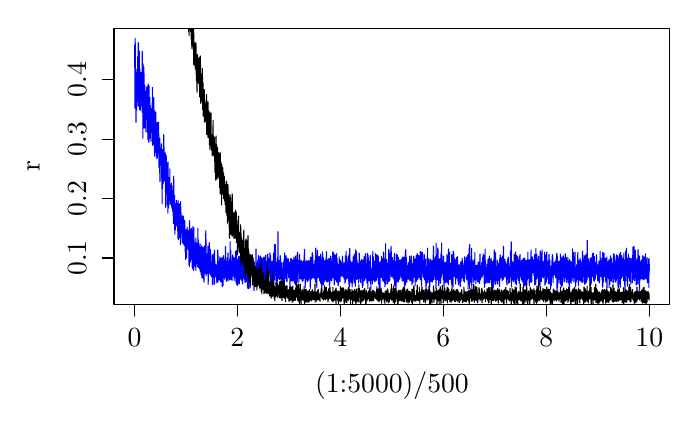
\begin{tikzpicture}[x=0.7pt,y=0.7pt]
\definecolor{fillColor}{RGB}{255,255,255}
%\path[use as bounding box,fill=fillColor,fill opacity=0.00] (0,0) rectangle (361.35,252.94);
\begin{scope}
%\path[clip] ( 49.20, 61.20) rectangle (336.15,203.75);
\definecolor{drawColor}{RGB}{0,0,255}

\path[draw=drawColor,line width= 0.4pt,line join=round,line cap=round] ( 59.83,184.28) --
	( 59.88,183.57) --
	( 59.93,194.95) --
	( 59.99,162.48) --
	( 60.04,184.20) --
	( 60.09,180.10) --
	( 60.15,198.47) --
	( 60.20,170.09) --
	( 60.25,162.64) --
	( 60.31,180.64) --
	( 60.36,179.73) --
	( 60.41,179.73) --
	( 60.47,164.26) --
	( 60.52,175.55) --
	( 60.57,155.15) --
	( 60.63,182.56) --
	( 60.68,180.79) --
	( 60.73,165.11) --
	( 60.78,173.50) --
	( 60.84,161.43) --
	( 60.89,174.75) --
	( 60.94,168.14) --
	( 61.00,169.73) --
	( 61.05,165.87) --
	( 61.10,167.12) --
	( 61.16,170.50) --
	( 61.21,169.94) --
	( 61.26,180.95) --
	( 61.32,171.43) --
	( 61.37,174.82) --
	( 61.42,189.05) --
	( 61.48,175.58) --
	( 61.53,179.85) --
	( 61.58,172.02) --
	( 61.63,179.80) --
	( 61.69,163.55) --
	( 61.74,196.33) --
	( 61.79,176.10) --
	( 61.85,167.73) --
	( 61.90,172.33) --
	( 61.95,164.84) --
	( 62.01,185.62) --
	( 62.06,174.32) --
	( 62.11,165.71) --
	( 62.17,181.79) --
	( 62.22,192.02) --
	( 62.27,170.94) --
	( 62.33,167.76) --
	( 62.38,161.74) --
	( 62.43,170.95) --
	( 62.49,175.98) --
	( 62.54,169.96) --
	( 62.59,182.77) --
	( 62.64,177.11) --
	( 62.70,180.81) --
	( 62.75,178.73) --
	( 62.80,171.31) --
	( 62.86,161.41) --
	( 62.91,180.38) --
	( 62.96,177.20) --
	( 63.02,170.19) --
	( 63.07,174.13) --
	( 63.12,177.49) --
	( 63.18,180.84) --
	( 63.23,170.30) --
	( 63.28,164.08) --
	( 63.34,172.06) --
	( 63.39,174.23) --
	( 63.44,164.38) --
	( 63.50,172.49) --
	( 63.55,175.26) --
	( 63.60,176.87) --
	( 63.65,166.67) --
	( 63.71,169.69) --
	( 63.76,160.40) --
	( 63.81,191.73) --
	( 63.87,167.86) --
	( 63.92,162.81) --
	( 63.97,167.64) --
	( 64.03,171.26) --
	( 64.08,181.31) --
	( 64.13,146.95) --
	( 64.19,158.74) --
	( 64.24,185.31) --
	( 64.29,179.80) --
	( 64.35,157.33) --
	( 64.40,176.45) --
	( 64.45,152.48) --
	( 64.50,176.56) --
	( 64.56,166.73) --
	( 64.61,164.56) --
	( 64.66,183.60) --
	( 64.72,165.89) --
	( 64.77,163.14) --
	( 64.82,173.06) --
	( 64.88,174.42) --
	( 64.93,158.43) --
	( 64.98,152.21) --
	( 65.04,163.33) --
	( 65.09,163.92) --
	( 65.14,174.23) --
	( 65.20,163.16) --
	( 65.25,164.95) --
	( 65.30,162.92) --
	( 65.36,160.45) --
	( 65.41,152.56) --
	( 65.46,165.56) --
	( 65.51,170.25) --
	( 65.57,157.69) --
	( 65.62,154.23) --
	( 65.67,150.16) --
	( 65.73,165.25) --
	( 65.78,168.79) --
	( 65.83,171.31) --
	( 65.89,162.80) --
	( 65.94,158.45) --
	( 65.99,159.65) --
	( 66.05,173.06) --
	( 66.10,165.13) --
	( 66.15,158.72) --
	( 66.21,156.55) --
	( 66.26,164.38) --
	( 66.31,173.65) --
	( 66.37,157.50) --
	( 66.42,168.69) --
	( 66.47,150.08) --
	( 66.52,168.83) --
	( 66.58,152.94) --
	( 66.63,167.58) --
	( 66.68,171.80) --
	( 66.74,156.14) --
	( 66.79,146.16) --
	( 66.84,175.06) --
	( 66.90,163.78) --
	( 66.95,152.03) --
	( 67.00,151.55) --
	( 67.06,145.25) --
	( 67.11,170.06) --
	( 67.16,171.81) --
	( 67.22,144.87) --
	( 67.27,174.05) --
	( 67.32,165.04) --
	( 67.38,150.64) --
	( 67.43,150.30) --
	( 67.48,146.58) --
	( 67.53,159.00) --
	( 67.59,159.87) --
	( 67.64,154.78) --
	( 67.69,160.69) --
	( 67.75,168.04) --
	( 67.80,147.35) --
	( 67.85,163.70) --
	( 67.91,162.07) --
	( 67.96,149.23) --
	( 68.01,163.74) --
	( 68.07,153.50) --
	( 68.12,151.56) --
	( 68.17,158.87) --
	( 68.23,145.37) --
	( 68.28,149.71) --
	( 68.33,150.95) --
	( 68.38,155.20) --
	( 68.44,159.34) --
	( 68.49,155.28) --
	( 68.54,156.39) --
	( 68.60,152.73) --
	( 68.65,151.33) --
	( 68.70,162.34) --
	( 68.76,156.18) --
	( 68.81,157.12) --
	( 68.86,160.64) --
	( 68.92,158.74) --
	( 68.97,161.97) --
	( 69.02,173.20) --
	( 69.08,143.31) --
	( 69.13,169.24) --
	( 69.18,155.35) --
	( 69.24,163.23) --
	( 69.29,155.23) --
	( 69.34,152.34) --
	( 69.39,147.37) --
	( 69.45,143.61) --
	( 69.50,157.36) --
	( 69.55,146.82) --
	( 69.61,153.10) --
	( 69.66,149.79) --
	( 69.71,167.90) --
	( 69.77,149.79) --
	( 69.82,156.32) --
	( 69.87,151.68) --
	( 69.93,150.27) --
	( 69.98,151.12) --
	( 70.03,151.85) --
	( 70.09,140.95) --
	( 70.14,150.34) --
	( 70.19,137.73) --
	( 70.25,161.04) --
	( 70.30,151.55) --
	( 70.35,154.41) --
	( 70.40,149.24) --
	( 70.46,144.30) --
	( 70.51,139.63) --
	( 70.56,157.24) --
	( 70.62,142.07) --
	( 70.67,159.23) --
	( 70.72,139.63) --
	( 70.78,160.35) --
	( 70.83,149.16) --
	( 70.88,140.80) --
	( 70.94,147.45) --
	( 70.99,151.18) --
	( 71.04,147.25) --
	( 71.10,150.19) --
	( 71.15,137.29) --
	( 71.20,138.45) --
	( 71.25,146.97) --
	( 71.31,147.82) --
	( 71.36,136.36) --
	( 71.41,138.30) --
	( 71.47,136.91) --
	( 71.52,155.10) --
	( 71.57,138.36) --
	( 71.63,136.90) --
	( 71.68,146.85) --
	( 71.73,140.94) --
	( 71.79,145.87) --
	( 71.84,144.39) --
	( 71.89,142.63) --
	( 71.95,141.12) --
	( 72.00,152.44) --
	( 72.05,141.46) --
	( 72.11,147.64) --
	( 72.16,142.79) --
	( 72.21,155.12) --
	( 72.26,142.80) --
	( 72.32,149.07) --
	( 72.37,140.96) --
	( 72.42,132.00) --
	( 72.48,140.38) --
	( 72.53,135.57) --
	( 72.58,139.64) --
	( 72.64,145.33) --
	( 72.69,139.54) --
	( 72.74,135.78) --
	( 72.80,147.01) --
	( 72.85,128.86) --
	( 72.90,141.43) --
	( 72.96,124.56) --
	( 73.01,143.77) --
	( 73.06,132.90) --
	( 73.12,136.80) --
	( 73.17,139.74) --
	( 73.22,139.03) --
	( 73.27,134.63) --
	( 73.33,136.79) --
	( 73.38,133.15) --
	( 73.43,140.24) --
	( 73.49,136.79) --
	( 73.54,135.82) --
	( 73.59,139.95) --
	( 73.65,141.95) --
	( 73.70,137.73) --
	( 73.75,137.95) --
	( 73.81,144.15) --
	( 73.86,132.29) --
	( 73.91,120.87) --
	( 73.97,140.23) --
	( 74.02,138.49) --
	( 74.07,113.15) --
	( 74.12,130.82) --
	( 74.18,133.83) --
	( 74.23,141.10) --
	( 74.28,131.59) --
	( 74.34,138.82) --
	( 74.39,126.41) --
	( 74.44,126.43) --
	( 74.50,137.31) --
	( 74.55,128.87) --
	( 74.60,123.41) --
	( 74.66,128.92) --
	( 74.71,136.22) --
	( 74.76,131.16) --
	( 74.82,138.95) --
	( 74.87,129.59) --
	( 74.92,148.82) --
	( 74.98,131.12) --
	( 75.03,142.36) --
	( 75.08,141.90) --
	( 75.13,131.27) --
	( 75.19,125.29) --
	( 75.24,130.76) --
	( 75.29,135.83) --
	( 75.35,125.03) --
	( 75.40,125.33) --
	( 75.45,134.01) --
	( 75.51,134.31) --
	( 75.56,128.29) --
	( 75.61,125.75) --
	( 75.67,139.42) --
	( 75.72,119.19) --
	( 75.77,132.04) --
	( 75.83,136.94) --
	( 75.88,133.79) --
	( 75.93,111.26) --
	( 75.99,126.12) --
	( 76.04,125.90) --
	( 76.09,129.20) --
	( 76.14,138.12) --
	( 76.20,135.88) --
	( 76.25,132.27) --
	( 76.30,118.37) --
	( 76.36,131.24) --
	( 76.41,134.09) --
	( 76.46,131.78) --
	( 76.52,118.18) --
	( 76.57,120.17) --
	( 76.62,132.48) --
	( 76.68,120.96) --
	( 76.73,131.90) --
	( 76.78,112.52) --
	( 76.84,132.61) --
	( 76.89,116.93) --
	( 76.94,131.79) --
	( 77.00,108.28) --
	( 77.05,117.87) --
	( 77.10,134.57) --
	( 77.15,114.27) --
	( 77.21,117.04) --
	( 77.26,125.08) --
	( 77.31,123.99) --
	( 77.37,114.00) --
	( 77.42,110.98) --
	( 77.47,126.67) --
	( 77.53,122.19) --
	( 77.58,120.28) --
	( 77.63,125.97) --
	( 77.69,114.60) --
	( 77.74,119.01) --
	( 77.79,119.04) --
	( 77.85,122.31) --
	( 77.90,119.59) --
	( 77.95,124.43) --
	( 78.00,114.51) --
	( 78.06,131.13) --
	( 78.11,118.44) --
	( 78.16,115.48) --
	( 78.22,112.78) --
	( 78.27,115.00) --
	( 78.32,122.50) --
	( 78.38,120.67) --
	( 78.43,119.86) --
	( 78.48,113.57) --
	( 78.54,122.25) --
	( 78.59,121.66) --
	( 78.64,118.03) --
	( 78.70,122.91) --
	( 78.75,118.39) --
	( 78.80,123.72) --
	( 78.86,120.60) --
	( 78.91,115.57) --
	( 78.96,117.28) --
	( 79.01,112.75) --
	( 79.07,111.16) --
	( 79.12,110.81) --
	( 79.17,114.10) --
	( 79.23,117.02) --
	( 79.28,112.06) --
	( 79.33,119.88) --
	( 79.39,113.32) --
	( 79.44,119.01) --
	( 79.49,112.31) --
	( 79.55,109.26) --
	( 79.60,122.44) --
	( 79.65,113.20) --
	( 79.71,119.91) --
	( 79.76,106.98) --
	( 79.81,113.57) --
	( 79.87,102.86) --
	( 79.92,110.47) --
	( 79.97,112.83) --
	( 80.02,127.39) --
	( 80.08,114.49) --
	( 80.13,108.97) --
	( 80.18,113.26) --
	( 80.24,114.53) --
	( 80.29,110.91) --
	( 80.34,113.62) --
	( 80.40,116.06) --
	( 80.45,110.19) --
	( 80.50,117.54) --
	( 80.56,107.79) --
	( 80.61, 97.40) --
	( 80.66,112.87) --
	( 80.72,110.40) --
	( 80.77,108.34) --
	( 80.82, 99.53) --
	( 80.87,103.32) --
	( 80.93,106.73) --
	( 80.98,107.68) --
	( 81.03,109.98) --
	( 81.09,104.53) --
	( 81.14,113.28) --
	( 81.19,108.82) --
	( 81.25,106.89) --
	( 81.30,110.31) --
	( 81.35,101.68) --
	( 81.41,114.90) --
	( 81.46,102.90) --
	( 81.51,109.42) --
	( 81.57,106.95) --
	( 81.62,104.00) --
	( 81.67,113.23) --
	( 81.73,108.69) --
	( 81.78,112.32) --
	( 81.83,105.85) --
	( 81.88,104.18) --
	( 81.94,107.74) --
	( 81.99,105.30) --
	( 82.04,110.13) --
	( 82.10, 98.94) --
	( 82.15,101.91) --
	( 82.20, 95.19) --
	( 82.26,114.73) --
	( 82.31,112.42) --
	( 82.36,103.10) --
	( 82.42,100.92) --
	( 82.47, 94.53) --
	( 82.52,106.06) --
	( 82.58,105.47) --
	( 82.63, 98.00) --
	( 82.68,102.63) --
	( 82.74,111.25) --
	( 82.79, 95.53) --
	( 82.84,104.13) --
	( 82.89,101.67) --
	( 82.95, 99.80) --
	( 83.00,112.40) --
	( 83.05,113.13) --
	( 83.11, 95.67) --
	( 83.16,105.32) --
	( 83.21, 96.07) --
	( 83.27,105.14) --
	( 83.32,111.53) --
	( 83.37, 98.13) --
	( 83.43, 97.40) --
	( 83.48, 92.05) --
	( 83.53,100.63) --
	( 83.59,114.24) --
	( 83.64,103.63) --
	( 83.69,102.93) --
	( 83.75,111.19) --
	( 83.80,104.77) --
	( 83.85, 99.80) --
	( 83.90,105.56) --
	( 83.96,106.28) --
	( 84.01, 98.44) --
	( 84.06,106.40) --
	( 84.12,102.61) --
	( 84.17, 98.78) --
	( 84.22,102.49) --
	( 84.28, 95.55) --
	( 84.33,101.07) --
	( 84.38,104.05) --
	( 84.44, 92.93) --
	( 84.49,105.36) --
	( 84.54, 96.04) --
	( 84.60,101.76) --
	( 84.65,101.99) --
	( 84.70,107.02) --
	( 84.75, 99.79) --
	( 84.81,101.86) --
	( 84.86,102.81) --
	( 84.91,104.06) --
	( 84.97,106.59) --
	( 85.02, 92.42) --
	( 85.07, 99.10) --
	( 85.13,100.74) --
	( 85.18,105.89) --
	( 85.23, 99.46) --
	( 85.29, 97.92) --
	( 85.34, 96.03) --
	( 85.39, 99.09) --
	( 85.45, 94.09) --
	( 85.50, 91.62) --
	( 85.55, 94.89) --
	( 85.61, 95.66) --
	( 85.66,104.52) --
	( 85.71,100.70) --
	( 85.76,104.19) --
	( 85.82, 97.59) --
	( 85.87, 95.57) --
	( 85.92, 97.60) --
	( 85.98, 88.22) --
	( 86.03, 97.34) --
	( 86.08, 98.28) --
	( 86.14, 98.46) --
	( 86.19, 84.39) --
	( 86.24, 94.90) --
	( 86.30, 89.83) --
	( 86.35, 99.70) --
	( 86.40, 98.31) --
	( 86.46, 98.17) --
	( 86.51, 92.44) --
	( 86.56, 97.35) --
	( 86.62, 85.25) --
	( 86.67, 98.80) --
	( 86.72, 93.94) --
	( 86.77, 89.65) --
	( 86.83, 95.56) --
	( 86.88, 91.74) --
	( 86.93,101.05) --
	( 86.99, 92.52) --
	( 87.04, 93.04) --
	( 87.09, 92.95) --
	( 87.15, 90.36) --
	( 87.20, 96.84) --
	( 87.25, 99.98) --
	( 87.31, 93.56) --
	( 87.36, 94.58) --
	( 87.41, 93.62) --
	( 87.47, 97.62) --
	( 87.52, 92.77) --
	( 87.57, 89.50) --
	( 87.62, 95.29) --
	( 87.68, 98.68) --
	( 87.73, 95.92) --
	( 87.78, 97.98) --
	( 87.84, 93.82) --
	( 87.89, 81.70) --
	( 87.94, 97.99) --
	( 88.00, 95.05) --
	( 88.05, 90.45) --
	( 88.10, 80.77) --
	( 88.16, 96.34) --
	( 88.21,104.36) --
	( 88.26, 89.96) --
	( 88.32, 96.69) --
	( 88.37, 88.67) --
	( 88.42, 99.99) --
	( 88.48, 86.88) --
	( 88.53, 92.26) --
	( 88.58, 83.09) --
	( 88.63, 91.21) --
	( 88.69, 97.80) --
	( 88.74, 91.44) --
	( 88.79, 93.02) --
	( 88.85, 92.36) --
	( 88.90, 86.35) --
	( 88.95, 84.29) --
	( 89.01, 84.92) --
	( 89.06, 99.15) --
	( 89.11,100.37) --
	( 89.17, 86.46) --
	( 89.22, 88.66) --
	( 89.27, 99.65) --
	( 89.33, 89.18) --
	( 89.38, 86.25) --
	( 89.43, 89.07) --
	( 89.49, 94.66) --
	( 89.54, 89.79) --
	( 89.59, 85.16) --
	( 89.64, 79.61) --
	( 89.70, 87.00) --
	( 89.75, 93.46) --
	( 89.80, 90.38) --
	( 89.86, 94.09) --
	( 89.91, 84.83) --
	( 89.96,101.44) --
	( 90.02, 92.37) --
	( 90.07, 85.54) --
	( 90.12, 95.12) --
	( 90.18, 90.95) --
	( 90.23, 81.57) --
	( 90.28, 88.58) --
	( 90.34, 78.74) --
	( 90.39, 82.60) --
	( 90.44,100.79) --
	( 90.50, 92.09) --
	( 90.55, 91.22) --
	( 90.60, 94.16) --
	( 90.65, 86.97) --
	( 90.71, 92.48) --
	( 90.76, 93.16) --
	( 90.81, 84.19) --
	( 90.87, 90.72) --
	( 90.92, 86.74) --
	( 90.97, 81.43) --
	( 91.03, 88.52) --
	( 91.08, 80.94) --
	( 91.13, 90.48) --
	( 91.19, 86.20) --
	( 91.24, 90.27) --
	( 91.29, 86.95) --
	( 91.35, 92.37) --
	( 91.40, 86.40) --
	( 91.45, 78.74) --
	( 91.50, 95.49) --
	( 91.56, 85.08) --
	( 91.61, 87.48) --
	( 91.66, 82.18) --
	( 91.72, 88.12) --
	( 91.77, 93.05) --
	( 91.82, 84.16) --
	( 91.88, 89.47) --
	( 91.93, 87.43) --
	( 91.98, 86.81) --
	( 92.04, 85.20) --
	( 92.09, 88.47) --
	( 92.14, 82.34) --
	( 92.20, 86.37) --
	( 92.25, 90.47) --
	( 92.30, 80.76) --
	( 92.36, 85.90) --
	( 92.41, 82.32) --
	( 92.46, 83.68) --
	( 92.51,100.44) --
	( 92.57, 86.34) --
	( 92.62, 86.98) --
	( 92.67, 82.36) --
	( 92.73, 82.86) --
	( 92.78, 94.48) --
	( 92.83, 80.21) --
	( 92.89, 81.33) --
	( 92.94, 87.46) --
	( 92.99, 83.21) --
	( 93.05, 84.89) --
	( 93.10, 81.39) --
	( 93.15, 83.13) --
	( 93.21, 88.17) --
	( 93.26, 91.09) --
	( 93.31, 87.83) --
	( 93.37, 86.34) --
	( 93.42, 79.52) --
	( 93.47, 83.90) --
	( 93.52, 82.20) --
	( 93.58, 92.51) --
	( 93.63, 82.66) --
	( 93.68, 78.29) --
	( 93.74, 84.56) --
	( 93.79, 86.73) --
	( 93.84, 90.07) --
	( 93.90, 90.53) --
	( 93.95, 77.96) --
	( 94.00, 85.27) --
	( 94.06, 86.66) --
	( 94.11, 87.45) --
	( 94.16, 82.41) --
	( 94.22, 81.03) --
	( 94.27, 76.48) --
	( 94.32, 89.35) --
	( 94.37, 83.48) --
	( 94.43, 84.05) --
	( 94.48, 91.48) --
	( 94.53, 85.98) --
	( 94.59, 85.53) --
	( 94.64, 74.91) --
	( 94.69, 85.38) --
	( 94.75, 84.36) --
	( 94.80, 85.29) --
	( 94.85, 86.76) --
	( 94.91, 77.39) --
	( 94.96, 81.60) --
	( 95.01, 74.94) --
	( 95.07, 84.26) --
	( 95.12, 78.61) --
	( 95.17, 86.49) --
	( 95.23, 82.22) --
	( 95.28, 90.66) --
	( 95.33, 74.38) --
	( 95.38, 82.83) --
	( 95.44, 78.56) --
	( 95.49, 78.30) --
	( 95.54, 81.35) --
	( 95.60, 86.53) --
	( 95.65, 72.75) --
	( 95.70, 87.87) --
	( 95.76, 87.28) --
	( 95.81, 82.19) --
	( 95.86, 88.83) --
	( 95.92, 81.93) --
	( 95.97, 80.61) --
	( 96.02, 91.27) --
	( 96.08, 77.17) --
	( 96.13, 84.58) --
	( 96.18, 90.60) --
	( 96.24, 85.86) --
	( 96.29, 87.03) --
	( 96.34, 86.26) --
	( 96.39, 77.89) --
	( 96.45, 92.02) --
	( 96.50, 79.04) --
	( 96.55, 90.16) --
	( 96.61, 99.25) --
	( 96.66, 84.24) --
	( 96.71, 94.55) --
	( 96.77, 75.94) --
	( 96.82, 85.83) --
	( 96.87, 76.59) --
	( 96.93, 84.11) --
	( 96.98, 79.50) --
	( 97.03, 81.01) --
	( 97.09, 80.66) --
	( 97.14, 77.09) --
	( 97.19, 78.23) --
	( 97.25, 87.29) --
	( 97.30, 83.73) --
	( 97.35, 87.24) --
	( 97.40, 85.72) --
	( 97.46, 81.01) --
	( 97.51, 81.08) --
	( 97.56, 77.31) --
	( 97.62, 79.45) --
	( 97.67, 91.18) --
	( 97.72, 85.00) --
	( 97.78, 77.67) --
	( 97.83, 71.56) --
	( 97.88, 81.57) --
	( 97.94, 78.14) --
	( 97.99, 81.71) --
	( 98.04, 88.92) --
	( 98.10, 82.93) --
	( 98.15, 84.03) --
	( 98.20, 81.95) --
	( 98.25, 79.61) --
	( 98.31, 83.01) --
	( 98.36, 77.05) --
	( 98.41, 93.10) --
	( 98.47, 80.08) --
	( 98.52, 81.08) --
	( 98.57, 81.83) --
	( 98.63, 81.32) --
	( 98.68, 79.07) --
	( 98.73, 85.22) --
	( 98.79, 82.97) --
	( 98.84, 78.57) --
	( 98.89, 89.53) --
	( 98.95, 83.39) --
	( 99.00, 85.77) --
	( 99.05, 88.01) --
	( 99.11, 76.29) --
	( 99.16, 77.50) --
	( 99.21, 80.45) --
	( 99.26, 79.55) --
	( 99.32, 80.33) --
	( 99.37, 78.23) --
	( 99.42, 82.87) --
	( 99.48, 78.22) --
	( 99.53, 77.11) --
	( 99.58, 75.39) --
	( 99.64, 80.10) --
	( 99.69, 79.05) --
	( 99.74, 75.85) --
	( 99.80, 77.12) --
	( 99.85, 79.51) --
	( 99.90, 76.51) --
	( 99.96, 86.82) --
	(100.01, 84.79) --
	(100.06, 71.33) --
	(100.12, 83.57) --
	(100.17, 82.54) --
	(100.22, 71.77) --
	(100.27, 76.95) --
	(100.33, 86.22) --
	(100.38, 82.39) --
	(100.43, 86.48) --
	(100.49, 77.23) --
	(100.54, 79.83) --
	(100.59, 84.83) --
	(100.65, 80.72) --
	(100.70, 77.31) --
	(100.75, 80.87) --
	(100.81, 87.49) --
	(100.86, 79.98) --
	(100.91, 74.95) --
	(100.97, 78.41) --
	(101.02, 74.75) --
	(101.07, 71.61) --
	(101.12, 89.20) --
	(101.18, 81.15) --
	(101.23, 84.08) --
	(101.28, 80.24) --
	(101.34, 81.07) --
	(101.39, 82.25) --
	(101.44, 75.60) --
	(101.50, 79.29) --
	(101.55, 76.92) --
	(101.60, 79.89) --
	(101.66, 79.33) --
	(101.71, 81.70) --
	(101.76, 78.47) --
	(101.82, 75.65) --
	(101.87, 79.88) --
	(101.92, 81.58) --
	(101.98, 75.33) --
	(102.03, 80.42) --
	(102.08, 75.75) --
	(102.13, 76.76) --
	(102.19, 73.18) --
	(102.24, 77.03) --
	(102.29, 76.36) --
	(102.35, 72.25) --
	(102.40, 74.40) --
	(102.45, 79.23) --
	(102.51, 72.68) --
	(102.56, 80.13) --
	(102.61, 77.72) --
	(102.67, 83.95) --
	(102.72, 86.45) --
	(102.77, 89.24) --
	(102.83, 82.35) --
	(102.88, 86.47) --
	(102.93, 72.79) --
	(102.99, 83.61) --
	(103.04, 82.74) --
	(103.09, 76.73) --
	(103.14, 79.77) --
	(103.20, 75.19) --
	(103.25, 80.84) --
	(103.30, 80.97) --
	(103.36, 78.99) --
	(103.41, 75.09) --
	(103.46, 79.68) --
	(103.52, 82.38) --
	(103.57, 76.07) --
	(103.62, 78.76) --
	(103.68, 73.86) --
	(103.73, 79.07) --
	(103.78, 80.96) --
	(103.84, 85.65) --
	(103.89, 85.71) --
	(103.94, 77.54) --
	(104.00, 84.40) --
	(104.05, 76.81) --
	(104.10, 79.42) --
	(104.15, 79.03) --
	(104.21, 73.14) --
	(104.26, 77.08) --
	(104.31, 80.41) --
	(104.37, 80.58) --
	(104.42, 75.72) --
	(104.47, 73.80) --
	(104.53, 85.01) --
	(104.58, 75.14) --
	(104.63, 72.73) --
	(104.69, 80.05) --
	(104.74, 82.00) --
	(104.79, 74.65) --
	(104.85, 77.19) --
	(104.90, 82.04) --
	(104.95, 85.34) --
	(105.00, 77.31) --
	(105.06, 79.61) --
	(105.11, 70.38) --
	(105.16, 75.84) --
	(105.22, 73.42) --
	(105.27, 79.53) --
	(105.32, 77.04) --
	(105.38, 75.69) --
	(105.43, 79.18) --
	(105.48, 70.89) --
	(105.54, 79.12) --
	(105.59, 76.98) --
	(105.64, 76.73) --
	(105.70, 76.86) --
	(105.75, 86.36) --
	(105.80, 78.80) --
	(105.86, 76.17) --
	(105.91, 81.13) --
	(105.96, 80.92) --
	(106.01, 81.20) --
	(106.07, 75.84) --
	(106.12, 81.62) --
	(106.17, 74.72) --
	(106.23, 82.69) --
	(106.28, 76.88) --
	(106.33, 82.35) --
	(106.39, 78.36) --
	(106.44, 73.90) --
	(106.49, 84.40) --
	(106.55, 75.67) --
	(106.60, 78.46) --
	(106.65, 82.94) --
	(106.71, 78.82) --
	(106.76, 91.05) --
	(106.81, 81.46) --
	(106.87, 85.59) --
	(106.92, 75.52) --
	(106.97, 75.12) --
	(107.02, 76.92) --
	(107.08, 78.77) --
	(107.13, 80.68) --
	(107.18, 76.98) --
	(107.24, 74.96) --
	(107.29, 83.20) --
	(107.34, 77.01) --
	(107.40, 74.16) --
	(107.45, 72.98) --
	(107.50, 73.76) --
	(107.56, 83.22) --
	(107.61, 74.68) --
	(107.66, 73.56) --
	(107.72, 75.14) --
	(107.77, 85.23) --
	(107.82, 80.71) --
	(107.87, 76.15) --
	(107.93, 74.71) --
	(107.98, 81.33) --
	(108.03, 77.65) --
	(108.09, 87.88) --
	(108.14, 78.95) --
	(108.19, 82.88) --
	(108.25, 83.09) --
	(108.30, 78.45) --
	(108.35, 75.66) --
	(108.41, 75.47) --
	(108.46, 78.57) --
	(108.51, 73.49) --
	(108.57, 81.98) --
	(108.62, 78.48) --
	(108.67, 83.32) --
	(108.73, 78.69) --
	(108.78, 79.41) --
	(108.83, 83.41) --
	(108.88, 76.87) --
	(108.94, 84.63) --
	(108.99, 81.68) --
	(109.04, 83.05) --
	(109.10, 79.19) --
	(109.15, 93.54) --
	(109.20, 73.95) --
	(109.26, 79.64) --
	(109.31, 77.76) --
	(109.36, 81.46) --
	(109.42, 81.47) --
	(109.47, 89.02) --
	(109.52, 81.03) --
	(109.58, 83.10) --
	(109.63, 74.39) --
	(109.68, 83.42) --
	(109.74, 80.20) --
	(109.79, 75.51) --
	(109.84, 78.54) --
	(109.89, 74.72) --
	(109.95, 83.54) --
	(110.00, 73.82) --
	(110.05, 83.70) --
	(110.11, 73.58) --
	(110.16, 82.32) --
	(110.21, 75.64) --
	(110.27, 75.71) --
	(110.32, 82.36) --
	(110.37, 83.89) --
	(110.43, 86.76) --
	(110.48, 75.59) --
	(110.53, 77.98) --
	(110.59, 76.39) --
	(110.64, 78.11) --
	(110.69, 84.22) --
	(110.75, 77.31) --
	(110.80, 84.16) --
	(110.85, 85.66) --
	(110.90, 77.10) --
	(110.96, 78.12) --
	(111.01, 80.04) --
	(111.06, 77.62) --
	(111.12, 82.65) --
	(111.17, 78.71) --
	(111.22, 73.60) --
	(111.28, 84.75) --
	(111.33, 79.90) --
	(111.38, 81.37) --
	(111.44, 75.24) --
	(111.49, 77.16) --
	(111.54, 85.12) --
	(111.60, 78.99) --
	(111.65, 74.95) --
	(111.70, 80.27) --
	(111.75, 75.41) --
	(111.81, 77.96) --
	(111.86, 88.63) --
	(111.91, 75.14) --
	(111.97, 83.68) --
	(112.02, 75.87) --
	(112.07, 77.71) --
	(112.13, 72.78) --
	(112.18, 75.43) --
	(112.23, 78.32) --
	(112.29, 72.93) --
	(112.34, 77.02) --
	(112.39, 88.93) --
	(112.45, 80.94) --
	(112.50, 78.76) --
	(112.55, 71.44) --
	(112.61, 73.54) --
	(112.66, 83.50) --
	(112.71, 80.84) --
	(112.76, 82.99) --
	(112.82, 84.45) --
	(112.87, 76.12) --
	(112.92, 81.66) --
	(112.98, 79.28) --
	(113.03, 82.06) --
	(113.08, 70.99) --
	(113.14, 81.36) --
	(113.19, 82.98) --
	(113.24, 72.41) --
	(113.30, 76.39) --
	(113.35, 81.18) --
	(113.40, 78.17) --
	(113.46, 85.98) --
	(113.51, 77.01) --
	(113.56, 81.38) --
	(113.62, 80.06) --
	(113.67, 78.16) --
	(113.72, 72.94) --
	(113.77, 81.99) --
	(113.83, 73.66) --
	(113.88, 76.29) --
	(113.93, 71.91) --
	(113.99, 76.40) --
	(114.04, 81.97) --
	(114.09, 77.47) --
	(114.15, 85.84) --
	(114.20, 74.46) --
	(114.25, 79.06) --
	(114.31, 79.13) --
	(114.36, 86.18) --
	(114.41, 81.51) --
	(114.47, 78.93) --
	(114.52, 86.74) --
	(114.57, 80.00) --
	(114.62, 77.35) --
	(114.68, 78.18) --
	(114.73, 74.00) --
	(114.78, 75.64) --
	(114.84, 79.30) --
	(114.89, 84.89) --
	(114.94, 78.55) --
	(115.00, 83.40) --
	(115.05, 78.52) --
	(115.10, 84.70) --
	(115.16, 73.54) --
	(115.21, 76.90) --
	(115.26, 85.37) --
	(115.32, 73.96) --
	(115.37, 80.24) --
	(115.42, 81.56) --
	(115.48, 78.72) --
	(115.53, 71.71) --
	(115.58, 79.95) --
	(115.63, 74.59) --
	(115.69, 77.62) --
	(115.74, 77.16) --
	(115.79, 76.33) --
	(115.85, 79.81) --
	(115.90, 80.18) --
	(115.95, 81.76) --
	(116.01, 84.19) --
	(116.06, 79.36) --
	(116.11, 82.56) --
	(116.17, 84.32) --
	(116.22, 80.11) --
	(116.27, 79.18) --
	(116.33, 74.46) --
	(116.38, 76.83) --
	(116.43, 80.42) --
	(116.49, 74.11) --
	(116.54, 83.31) --
	(116.59, 81.87) --
	(116.64, 79.97) --
	(116.70, 81.72) --
	(116.75, 76.74) --
	(116.80, 75.99) --
	(116.86, 72.48) --
	(116.91, 73.95) --
	(116.96, 77.97) --
	(117.02, 84.96) --
	(117.07, 86.96) --
	(117.12, 78.73) --
	(117.18, 72.98) --
	(117.23, 75.80) --
	(117.28, 91.66) --
	(117.34, 73.99) --
	(117.39, 74.62) --
	(117.44, 73.11) --
	(117.50, 76.92) --
	(117.55, 80.14) --
	(117.60, 79.26) --
	(117.65, 80.94) --
	(117.71, 76.20) --
	(117.76, 75.59) --
	(117.81, 80.96) --
	(117.87, 83.17) --
	(117.92, 88.44) --
	(117.97, 80.27) --
	(118.03, 80.49) --
	(118.08, 70.11) --
	(118.13, 79.95) --
	(118.19, 78.78) --
	(118.24, 79.53) --
	(118.29, 76.25) --
	(118.35, 69.30) --
	(118.40, 88.77) --
	(118.45, 80.78) --
	(118.50, 83.47) --
	(118.56, 86.42) --
	(118.61, 78.23) --
	(118.66, 80.00) --
	(118.72, 82.14) --
	(118.77, 82.33) --
	(118.82, 72.97) --
	(118.88, 69.30) --
	(118.93, 82.87) --
	(118.98, 75.85) --
	(119.04, 83.44) --
	(119.09, 80.25) --
	(119.14, 80.32) --
	(119.20, 82.19) --
	(119.25, 78.88) --
	(119.30, 76.59) --
	(119.36, 77.24) --
	(119.41, 80.75) --
	(119.46, 77.55) --
	(119.51, 81.51) --
	(119.57, 76.59) --
	(119.62, 76.92) --
	(119.67, 83.94) --
	(119.73, 76.53) --
	(119.78, 79.61) --
	(119.83, 78.81) --
	(119.89, 80.41) --
	(119.94, 75.16) --
	(119.99, 84.95) --
	(120.05, 77.10) --
	(120.10, 80.29) --
	(120.15, 82.71) --
	(120.21, 84.31) --
	(120.26, 78.91) --
	(120.31, 80.31) --
	(120.37, 84.98) --
	(120.42, 80.84) --
	(120.47, 77.66) --
	(120.52, 85.72) --
	(120.58, 77.71) --
	(120.63, 86.87) --
	(120.68, 79.69) --
	(120.74, 82.85) --
	(120.79, 74.05) --
	(120.84, 78.99) --
	(120.90, 76.44) --
	(120.95, 85.27) --
	(121.00, 77.00) --
	(121.06, 78.32) --
	(121.11, 80.05) --
	(121.16, 78.50) --
	(121.22, 78.68) --
	(121.27, 82.94) --
	(121.32, 76.20) --
	(121.37, 77.63) --
	(121.43, 75.36) --
	(121.48, 68.30) --
	(121.53, 76.88) --
	(121.59, 74.77) --
	(121.64, 83.16) --
	(121.69, 75.96) --
	(121.75, 74.14) --
	(121.80, 79.07) --
	(121.85, 79.33) --
	(121.91, 77.94) --
	(121.96, 76.23) --
	(122.01, 77.44) --
	(122.07, 76.07) --
	(122.12, 75.19) --
	(122.17, 80.74) --
	(122.23, 79.02) --
	(122.28, 79.95) --
	(122.33, 75.18) --
	(122.38, 76.65) --
	(122.44, 75.07) --
	(122.49, 89.80) --
	(122.54, 73.50) --
	(122.60, 77.93) --
	(122.65, 77.02) --
	(122.70, 81.09) --
	(122.76, 77.43) --
	(122.81, 78.04) --
	(122.86, 73.97) --
	(122.92, 76.18) --
	(122.97, 72.88) --
	(123.02, 80.22) --
	(123.08, 82.05) --
	(123.13, 78.22) --
	(123.18, 82.62) --
	(123.24, 75.02) --
	(123.29, 77.51) --
	(123.34, 81.64) --
	(123.39, 78.99) --
	(123.45, 84.09) --
	(123.50, 79.72) --
	(123.55, 71.99) --
	(123.61, 79.26) --
	(123.66, 76.22) --
	(123.71, 77.34) --
	(123.77, 78.55) --
	(123.82, 86.34) --
	(123.87, 76.34) --
	(123.93, 81.08) --
	(123.98, 75.27) --
	(124.03, 82.64) --
	(124.09, 73.56) --
	(124.14, 78.86) --
	(124.19, 84.32) --
	(124.24, 76.03) --
	(124.30, 81.75) --
	(124.35, 77.08) --
	(124.40, 77.72) --
	(124.46, 85.03) --
	(124.51, 80.76) --
	(124.56, 73.47) --
	(124.62, 80.42) --
	(124.67, 75.20) --
	(124.72, 86.21) --
	(124.78, 73.85) --
	(124.83, 75.76) --
	(124.88, 75.14) --
	(124.94, 76.47) --
	(124.99, 73.45) --
	(125.04, 76.88) --
	(125.10, 74.78) --
	(125.15, 76.41) --
	(125.20, 75.28) --
	(125.25, 84.66) --
	(125.31, 72.62) --
	(125.36, 85.30) --
	(125.41, 80.03) --
	(125.47, 76.17) --
	(125.52, 81.91) --
	(125.57, 76.17) --
	(125.63, 80.48) --
	(125.68, 76.87) --
	(125.73, 84.87) --
	(125.79, 78.45) --
	(125.84, 77.36) --
	(125.89, 80.06) --
	(125.95, 81.04) --
	(126.00, 77.29) --
	(126.05, 76.17) --
	(126.11, 72.91) --
	(126.16, 76.62) --
	(126.21, 74.23) --
	(126.26, 78.08) --
	(126.32, 79.60) --
	(126.37, 77.60) --
	(126.42, 85.47) --
	(126.48, 79.08) --
	(126.53, 76.90) --
	(126.58, 76.85) --
	(126.64, 80.37) --
	(126.69, 78.33) --
	(126.74, 82.00) --
	(126.80, 75.63) --
	(126.85, 84.29) --
	(126.90, 73.26) --
	(126.96, 81.51) --
	(127.01, 82.56) --
	(127.06, 80.98) --
	(127.12, 80.36) --
	(127.17, 85.67) --
	(127.22, 73.88) --
	(127.27, 79.21) --
	(127.33, 78.24) --
	(127.38, 76.28) --
	(127.43, 73.75) --
	(127.49, 78.36) --
	(127.54, 86.59) --
	(127.59, 80.24) --
	(127.65, 75.99) --
	(127.70, 80.58) --
	(127.75, 76.45) --
	(127.81, 76.51) --
	(127.86, 72.96) --
	(127.91, 77.30) --
	(127.97, 83.43) --
	(128.02, 77.58) --
	(128.07, 77.79) --
	(128.12, 81.07) --
	(128.18, 70.67) --
	(128.23, 78.56) --
	(128.28, 78.97) --
	(128.34, 73.93) --
	(128.39, 80.63) --
	(128.44, 73.89) --
	(128.50, 79.46) --
	(128.55, 84.51) --
	(128.60, 87.19) --
	(128.66, 70.83) --
	(128.71, 73.25) --
	(128.76, 83.64) --
	(128.82, 85.09) --
	(128.87, 80.67) --
	(128.92, 74.78) --
	(128.98, 77.66) --
	(129.03, 75.08) --
	(129.08, 77.05) --
	(129.13, 75.57) --
	(129.19, 84.66) --
	(129.24, 83.90) --
	(129.29, 77.96) --
	(129.35, 81.00) --
	(129.40, 79.35) --
	(129.45, 79.93) --
	(129.51, 81.72) --
	(129.56, 78.18) --
	(129.61, 80.75) --
	(129.67, 77.58) --
	(129.72, 87.72) --
	(129.77, 87.12) --
	(129.83, 80.49) --
	(129.88, 81.01) --
	(129.93, 70.89) --
	(129.99, 68.65) --
	(130.04, 86.33) --
	(130.09, 81.02) --
	(130.14, 79.60) --
	(130.20, 80.90) --
	(130.25, 77.14) --
	(130.30, 74.54) --
	(130.36, 80.34) --
	(130.41, 74.64) --
	(130.46, 77.51) --
	(130.52, 77.24) --
	(130.57, 80.93) --
	(130.62, 73.98) --
	(130.68, 73.95) --
	(130.73, 75.15) --
	(130.78, 83.43) --
	(130.84, 83.16) --
	(130.89, 80.69) --
	(130.94, 83.51) --
	(130.99, 80.03) --
	(131.05, 81.58) --
	(131.10, 79.09) --
	(131.15, 81.63) --
	(131.21, 81.58) --
	(131.26, 80.98) --
	(131.31, 76.71) --
	(131.37, 75.10) --
	(131.42, 74.82) --
	(131.47, 76.34) --
	(131.53, 81.05) --
	(131.58, 87.62) --
	(131.63, 84.01) --
	(131.69, 71.82) --
	(131.74, 79.60) --
	(131.79, 75.71) --
	(131.85, 78.15) --
	(131.90, 74.96) --
	(131.95, 77.42) --
	(132.00, 91.91) --
	(132.06, 74.89) --
	(132.11, 73.79) --
	(132.16, 85.88) --
	(132.22, 84.70) --
	(132.27, 84.64) --
	(132.32, 77.15) --
	(132.38, 76.66) --
	(132.43, 79.16) --
	(132.48, 83.96) --
	(132.54, 92.19) --
	(132.59, 82.07) --
	(132.64, 84.87) --
	(132.70, 77.23) --
	(132.75, 80.98) --
	(132.80, 76.57) --
	(132.86, 75.99) --
	(132.91, 78.60) --
	(132.96, 77.02) --
	(133.01, 69.36) --
	(133.07, 78.53) --
	(133.12, 81.02) --
	(133.17, 78.05) --
	(133.23, 79.30) --
	(133.28, 77.53) --
	(133.33, 82.95) --
	(133.39, 72.47) --
	(133.44, 82.01) --
	(133.49, 73.21) --
	(133.55, 75.78) --
	(133.60, 85.19) --
	(133.65, 74.40) --
	(133.71, 75.46) --
	(133.76, 84.35) --
	(133.81, 76.45) --
	(133.87, 98.71) --
	(133.92, 74.54) --
	(133.97, 80.62) --
	(134.02, 76.20) --
	(134.08, 74.91) --
	(134.13, 82.45) --
	(134.18, 76.48) --
	(134.24, 78.32) --
	(134.29, 78.03) --
	(134.34, 80.26) --
	(134.40, 83.76) --
	(134.45, 75.27) --
	(134.50, 80.80) --
	(134.56, 79.72) --
	(134.61, 78.87) --
	(134.66, 74.00) --
	(134.72, 75.85) --
	(134.77, 76.43) --
	(134.82, 78.62) --
	(134.87, 79.55) --
	(134.93, 77.49) --
	(134.98, 76.63) --
	(135.03, 86.38) --
	(135.09, 80.44) --
	(135.14, 79.47) --
	(135.19, 85.00) --
	(135.25, 79.83) --
	(135.30, 81.09) --
	(135.35, 78.05) --
	(135.41, 74.37) --
	(135.46, 74.86) --
	(135.51, 80.05) --
	(135.57, 76.04) --
	(135.62, 80.54) --
	(135.67, 78.88) --
	(135.73, 76.13) --
	(135.78, 75.91) --
	(135.83, 74.81) --
	(135.88, 79.04) --
	(135.94, 82.74) --
	(135.99, 80.99) --
	(136.04, 71.59) --
	(136.10, 79.58) --
	(136.15, 79.98) --
	(136.20, 78.41) --
	(136.26, 76.69) --
	(136.31, 77.41) --
	(136.36, 77.99) --
	(136.42, 70.54) --
	(136.47, 71.50) --
	(136.52, 76.02) --
	(136.58, 70.17) --
	(136.63, 75.67) --
	(136.68, 76.12) --
	(136.74, 78.95) --
	(136.79, 83.01) --
	(136.84, 79.53) --
	(136.89, 79.09) --
	(136.95, 70.34) --
	(137.00, 78.64) --
	(137.05, 84.39) --
	(137.11, 77.01) --
	(137.16, 68.98) --
	(137.21, 82.66) --
	(137.27, 87.67) --
	(137.32, 80.66) --
	(137.37, 75.82) --
	(137.43, 79.08) --
	(137.48, 79.70) --
	(137.53, 74.68) --
	(137.59, 82.26) --
	(137.64, 79.31) --
	(137.69, 77.49) --
	(137.74, 80.48) --
	(137.80, 79.38) --
	(137.85, 79.52) --
	(137.90, 77.46) --
	(137.96, 79.22) --
	(138.01, 86.38) --
	(138.06, 74.39) --
	(138.12, 76.08) --
	(138.17, 76.50) --
	(138.22, 78.75) --
	(138.28, 73.16) --
	(138.33, 77.41) --
	(138.38, 84.32) --
	(138.44, 74.17) --
	(138.49, 72.93) --
	(138.54, 84.91) --
	(138.60, 75.03) --
	(138.65, 82.38) --
	(138.70, 83.03) --
	(138.75, 77.18) --
	(138.81, 80.64) --
	(138.86, 82.15) --
	(138.91, 79.22) --
	(138.97, 81.11) --
	(139.02, 77.60) --
	(139.07, 83.73) --
	(139.13, 82.84) --
	(139.18, 80.19) --
	(139.23, 84.75) --
	(139.29, 81.90) --
	(139.34, 74.97) --
	(139.39, 80.57) --
	(139.45, 77.79) --
	(139.50, 79.83) --
	(139.55, 78.59) --
	(139.61, 79.42) --
	(139.66, 76.29) --
	(139.71, 79.37) --
	(139.76, 75.47) --
	(139.82, 81.10) --
	(139.87, 83.05) --
	(139.92, 76.83) --
	(139.98, 79.18) --
	(140.03, 75.80) --
	(140.08, 66.48) --
	(140.14, 78.00) --
	(140.19, 74.09) --
	(140.24, 83.05) --
	(140.30, 81.91) --
	(140.35, 78.02) --
	(140.40, 84.79) --
	(140.46, 76.69) --
	(140.51, 74.55) --
	(140.56, 75.92) --
	(140.62, 81.28) --
	(140.67, 76.54) --
	(140.72, 80.97) --
	(140.77, 79.15) --
	(140.83, 73.32) --
	(140.88, 84.74) --
	(140.93, 76.35) --
	(140.99, 76.92) --
	(141.04, 78.02) --
	(141.09, 78.09) --
	(141.15, 75.22) --
	(141.20, 76.07) --
	(141.25, 78.48) --
	(141.31, 75.54) --
	(141.36, 83.96) --
	(141.41, 74.37) --
	(141.47, 80.96) --
	(141.52, 73.11) --
	(141.57, 84.02) --
	(141.62, 79.22) --
	(141.68, 76.26) --
	(141.73, 77.03) --
	(141.78, 82.93) --
	(141.84, 77.03) --
	(141.89, 74.21) --
	(141.94, 77.47) --
	(142.00, 76.25) --
	(142.05, 85.61) --
	(142.10, 78.34) --
	(142.16, 73.77) --
	(142.21, 75.71) --
	(142.26, 81.60) --
	(142.32, 79.13) --
	(142.37, 72.19) --
	(142.42, 75.02) --
	(142.48, 74.07) --
	(142.53, 77.87) --
	(142.58, 78.64) --
	(142.63, 72.61) --
	(142.69, 84.65) --
	(142.74, 76.24) --
	(142.79, 71.82) --
	(142.85, 86.16) --
	(142.90, 77.90) --
	(142.95, 84.76) --
	(143.01, 83.65) --
	(143.06, 71.24) --
	(143.11, 80.35) --
	(143.17, 78.42) --
	(143.22, 73.41) --
	(143.27, 78.43) --
	(143.33, 74.31) --
	(143.38, 84.38) --
	(143.43, 79.46) --
	(143.49, 77.63) --
	(143.54, 78.28) --
	(143.59, 86.65) --
	(143.64, 78.18) --
	(143.70, 72.22) --
	(143.75, 80.50) --
	(143.80, 73.06) --
	(143.86, 77.07) --
	(143.91, 80.89) --
	(143.96, 88.15) --
	(144.02, 76.97) --
	(144.07, 78.98) --
	(144.12, 81.63) --
	(144.18, 84.05) --
	(144.23, 77.79) --
	(144.28, 80.65) --
	(144.34, 79.80) --
	(144.39, 81.47) --
	(144.44, 77.29) --
	(144.49, 77.67) --
	(144.55, 78.32) --
	(144.60, 80.29) --
	(144.65, 72.51) --
	(144.71, 78.99) --
	(144.76, 78.37) --
	(144.81, 77.91) --
	(144.87, 78.77) --
	(144.92, 83.02) --
	(144.97, 86.99) --
	(145.03, 82.35) --
	(145.08, 77.54) --
	(145.13, 75.26) --
	(145.19, 83.21) --
	(145.24, 74.47) --
	(145.29, 79.63) --
	(145.35, 75.00) --
	(145.40, 77.03) --
	(145.45, 77.67) --
	(145.50, 82.96) --
	(145.56, 74.32) --
	(145.61, 74.42) --
	(145.66, 78.79) --
	(145.72, 83.85) --
	(145.77, 78.62) --
	(145.82, 76.91) --
	(145.88, 83.66) --
	(145.93, 80.44) --
	(145.98, 78.29) --
	(146.04, 82.16) --
	(146.09, 74.18) --
	(146.14, 74.72) --
	(146.20, 83.24) --
	(146.25, 78.23) --
	(146.30, 81.67) --
	(146.36, 74.17) --
	(146.41, 73.38) --
	(146.46, 73.91) --
	(146.51, 82.84) --
	(146.57, 73.10) --
	(146.62, 75.36) --
	(146.67, 82.64) --
	(146.73, 80.61) --
	(146.78, 73.37) --
	(146.83, 77.35) --
	(146.89, 78.09) --
	(146.94, 79.70) --
	(146.99, 83.63) --
	(147.05, 82.54) --
	(147.10, 83.87) --
	(147.15, 80.47) --
	(147.21, 79.23) --
	(147.26, 74.57) --
	(147.31, 81.34) --
	(147.37, 77.02) --
	(147.42, 86.65) --
	(147.47, 80.46) --
	(147.52, 89.57) --
	(147.58, 80.71) --
	(147.63, 79.02) --
	(147.68, 76.36) --
	(147.74, 80.21) --
	(147.79, 80.28) --
	(147.84, 74.04) --
	(147.90, 69.87) --
	(147.95, 75.01) --
	(148.00, 77.05) --
	(148.06, 72.46) --
	(148.11, 83.04) --
	(148.16, 78.34) --
	(148.22, 80.24) --
	(148.27, 77.40) --
	(148.32, 78.54) --
	(148.37, 75.08) --
	(148.43, 81.06) --
	(148.48, 83.74) --
	(148.53, 79.95) --
	(148.59, 74.00) --
	(148.64, 81.57) --
	(148.69, 75.34) --
	(148.75, 75.46) --
	(148.80, 76.20) --
	(148.85, 77.00) --
	(148.91, 82.94) --
	(148.96, 79.52) --
	(149.01, 72.93) --
	(149.07, 77.37) --
	(149.12, 75.81) --
	(149.17, 73.68) --
	(149.23, 78.83) --
	(149.28, 82.18) --
	(149.33, 78.02) --
	(149.38, 83.79) --
	(149.44, 82.97) --
	(149.49, 82.77) --
	(149.54, 79.10) --
	(149.60, 82.30) --
	(149.65, 79.03) --
	(149.70, 73.61) --
	(149.76, 79.25) --
	(149.81, 81.64) --
	(149.86, 83.81) --
	(149.92, 79.65) --
	(149.97, 80.61) --
	(150.02, 83.50) --
	(150.08, 74.86) --
	(150.13, 78.28) --
	(150.18, 76.53) --
	(150.24, 75.64) --
	(150.29, 76.10) --
	(150.34, 82.86) --
	(150.39, 83.30) --
	(150.45, 72.96) --
	(150.50, 77.83) --
	(150.55, 69.48) --
	(150.61, 85.65) --
	(150.66, 79.70) --
	(150.71, 83.77) --
	(150.77, 75.45) --
	(150.82, 79.00) --
	(150.87, 79.46) --
	(150.93, 85.46) --
	(150.98, 81.60) --
	(151.03, 79.45) --
	(151.09, 74.22) --
	(151.14, 79.10) --
	(151.19, 82.12) --
	(151.24, 83.50) --
	(151.30, 78.71) --
	(151.35, 83.96) --
	(151.40, 79.56) --
	(151.46, 83.27) --
	(151.51, 77.64) --
	(151.56, 87.90) --
	(151.62, 80.16) --
	(151.67, 79.72) --
	(151.72, 74.88) --
	(151.78, 82.96) --
	(151.83, 76.88) --
	(151.88, 86.77) --
	(151.94, 79.13) --
	(151.99, 79.79) --
	(152.04, 75.28) --
	(152.10, 77.56) --
	(152.15, 76.89) --
	(152.20, 79.65) --
	(152.25, 75.01) --
	(152.31, 78.15) --
	(152.36, 76.35) --
	(152.41, 77.04) --
	(152.47, 81.64) --
	(152.52, 78.60) --
	(152.57, 79.32) --
	(152.63, 74.43) --
	(152.68, 75.48) --
	(152.73, 77.17) --
	(152.79, 77.48) --
	(152.84, 79.92) --
	(152.89, 76.08) --
	(152.95, 83.96) --
	(153.00, 79.70) --
	(153.05, 78.98) --
	(153.11, 81.66) --
	(153.16, 79.67) --
	(153.21, 72.54) --
	(153.26, 76.64) --
	(153.32, 74.35) --
	(153.37, 90.26) --
	(153.42, 82.37) --
	(153.48, 77.27) --
	(153.53, 81.66) --
	(153.58, 86.40) --
	(153.64, 76.30) --
	(153.69, 78.33) --
	(153.74, 77.84) --
	(153.80, 83.88) --
	(153.85, 79.71) --
	(153.90, 71.05) --
	(153.96, 69.92) --
	(154.01, 86.22) --
	(154.06, 80.11) --
	(154.12, 80.32) --
	(154.17, 86.27) --
	(154.22, 74.75) --
	(154.27, 89.04) --
	(154.33, 77.48) --
	(154.38, 75.50) --
	(154.43, 76.03) --
	(154.49, 77.39) --
	(154.54, 83.38) --
	(154.59, 81.71) --
	(154.65, 76.23) --
	(154.70, 77.63) --
	(154.75, 81.81) --
	(154.81, 82.51) --
	(154.86, 75.10) --
	(154.91, 85.98) --
	(154.97, 81.81) --
	(155.02, 75.57) --
	(155.07, 81.94) --
	(155.12, 80.05) --
	(155.18, 82.69) --
	(155.23, 83.13) --
	(155.28, 81.58) --
	(155.34, 73.35) --
	(155.39, 78.28) --
	(155.44, 79.27) --
	(155.50, 82.82) --
	(155.55, 77.99) --
	(155.60, 81.69) --
	(155.66, 85.90) --
	(155.71, 73.42) --
	(155.76, 85.37) --
	(155.82, 79.92) --
	(155.87, 72.45) --
	(155.92, 87.17) --
	(155.98, 80.26) --
	(156.03, 71.87) --
	(156.08, 79.07) --
	(156.13, 76.15) --
	(156.19, 79.60) --
	(156.24, 84.40) --
	(156.29, 80.76) --
	(156.35, 73.29) --
	(156.40, 74.51) --
	(156.45, 67.89) --
	(156.51, 83.45) --
	(156.56, 84.64) --
	(156.61, 79.39) --
	(156.67, 84.53) --
	(156.72, 74.57) --
	(156.77, 78.19) --
	(156.83, 77.63) --
	(156.88, 88.29) --
	(156.93, 80.29) --
	(156.99, 80.80) --
	(157.04, 76.61) --
	(157.09, 79.77) --
	(157.14, 82.13) --
	(157.20, 85.64) --
	(157.25, 71.24) --
	(157.30, 79.39) --
	(157.36, 84.43) --
	(157.41, 78.27) --
	(157.46, 74.68) --
	(157.52, 83.97) --
	(157.57, 80.31) --
	(157.62, 72.89) --
	(157.68, 80.69) --
	(157.73, 78.25) --
	(157.78, 74.26) --
	(157.84, 82.58) --
	(157.89, 82.19) --
	(157.94, 81.12) --
	(157.99, 79.74) --
	(158.05, 76.76) --
	(158.10, 73.28) --
	(158.15, 80.36) --
	(158.21, 78.44) --
	(158.26, 83.81) --
	(158.31, 75.13) --
	(158.37, 81.34) --
	(158.42, 83.17) --
	(158.47, 76.89) --
	(158.53, 83.10) --
	(158.58, 79.37) --
	(158.63, 84.80) --
	(158.69, 77.42) --
	(158.74, 80.32) --
	(158.79, 80.71) --
	(158.85, 73.13) --
	(158.90, 88.37) --
	(158.95, 87.46) --
	(159.00, 83.10) --
	(159.06, 74.73) --
	(159.11, 83.08) --
	(159.16, 79.38) --
	(159.22, 72.64) --
	(159.27, 79.47) --
	(159.32, 77.88) --
	(159.38, 84.04) --
	(159.43, 80.16) --
	(159.48, 81.45) --
	(159.54, 73.19) --
	(159.59, 77.78) --
	(159.64, 76.71) --
	(159.70, 79.51) --
	(159.75, 80.57) --
	(159.80, 84.35) --
	(159.86, 78.19) --
	(159.91, 82.40) --
	(159.96, 82.38) --
	(160.01, 74.73) --
	(160.07, 73.12) --
	(160.12, 84.86) --
	(160.17, 77.83) --
	(160.23, 74.89) --
	(160.28, 80.84) --
	(160.33, 79.95) --
	(160.39, 84.95) --
	(160.44, 70.48) --
	(160.49, 80.59) --
	(160.55, 70.95) --
	(160.60, 80.31) --
	(160.65, 74.81) --
	(160.71, 79.55) --
	(160.76, 78.00) --
	(160.81, 79.98) --
	(160.87, 80.50) --
	(160.92, 73.67) --
	(160.97, 79.16) --
	(161.02, 78.06) --
	(161.08, 86.16) --
	(161.13, 76.89) --
	(161.18, 80.13) --
	(161.24, 74.79) --
	(161.29, 80.66) --
	(161.34, 76.66) --
	(161.40, 73.62) --
	(161.45, 80.73) --
	(161.50, 74.87) --
	(161.56, 75.92) --
	(161.61, 77.66) --
	(161.66, 73.48) --
	(161.72, 83.54) --
	(161.77, 77.02) --
	(161.82, 81.67) --
	(161.87, 76.72) --
	(161.93, 78.24) --
	(161.98, 85.01) --
	(162.03, 81.85) --
	(162.09, 79.95) --
	(162.14, 88.33) --
	(162.19, 81.88) --
	(162.25, 81.32) --
	(162.30, 75.00) --
	(162.35, 78.32) --
	(162.41, 74.85) --
	(162.46, 87.98) --
	(162.51, 75.37) --
	(162.57, 78.82) --
	(162.62, 77.08) --
	(162.67, 85.07) --
	(162.73, 76.16) --
	(162.78, 74.49) --
	(162.83, 82.36) --
	(162.88, 71.29) --
	(162.94, 80.50) --
	(162.99, 80.60) --
	(163.04, 83.02) --
	(163.10, 86.99) --
	(163.15, 79.58) --
	(163.20, 78.68) --
	(163.26, 78.52) --
	(163.31, 81.19) --
	(163.36, 81.49) --
	(163.42, 82.32) --
	(163.47, 86.61) --
	(163.52, 81.76) --
	(163.58, 83.98) --
	(163.63, 73.84) --
	(163.68, 82.95) --
	(163.74, 79.32) --
	(163.79, 79.59) --
	(163.84, 80.53) --
	(163.89, 78.36) --
	(163.95, 82.75) --
	(164.00, 72.93) --
	(164.05, 82.64) --
	(164.11, 87.46) --
	(164.16, 82.73) --
	(164.21, 80.04) --
	(164.27, 73.41) --
	(164.32, 84.93) --
	(164.37, 76.65) --
	(164.43, 75.32) --
	(164.48, 82.62) --
	(164.53, 72.88) --
	(164.59, 72.43) --
	(164.64, 81.19) --
	(164.69, 77.41) --
	(164.74, 81.75) --
	(164.80, 76.42) --
	(164.85, 81.30) --
	(164.90, 70.77) --
	(164.96, 81.10) --
	(165.01, 77.46) --
	(165.06, 77.03) --
	(165.12, 78.73) --
	(165.17, 71.13) --
	(165.22, 80.61) --
	(165.28, 78.85) --
	(165.33, 73.30) --
	(165.38, 80.81) --
	(165.44, 85.68) --
	(165.49, 78.15) --
	(165.54, 78.68) --
	(165.60, 77.83) --
	(165.65, 80.64) --
	(165.70, 81.18) --
	(165.75, 79.19) --
	(165.81, 76.62) --
	(165.86, 74.06) --
	(165.91, 72.97) --
	(165.97, 84.25) --
	(166.02, 78.71) --
	(166.07, 79.09) --
	(166.13, 75.59) --
	(166.18, 81.76) --
	(166.23, 79.81) --
	(166.29, 76.88) --
	(166.34, 76.27) --
	(166.39, 82.67) --
	(166.45, 79.09) --
	(166.50, 79.18) --
	(166.55, 80.11) --
	(166.61, 76.03) --
	(166.66, 75.88) --
	(166.71, 78.32) --
	(166.76, 80.47) --
	(166.82, 78.96) --
	(166.87, 77.05) --
	(166.92, 83.10) --
	(166.98, 78.31) --
	(167.03, 84.02) --
	(167.08, 78.84) --
	(167.14, 86.08) --
	(167.19, 81.26) --
	(167.24, 75.72) --
	(167.30, 76.12) --
	(167.35, 76.83) --
	(167.40, 83.04) --
	(167.46, 77.38) --
	(167.51, 79.61) --
	(167.56, 77.41) --
	(167.62, 82.17) --
	(167.67, 76.16) --
	(167.72, 80.59) --
	(167.77, 75.17) --
	(167.83, 76.31) --
	(167.88, 79.61) --
	(167.93, 77.38) --
	(167.99, 81.96) --
	(168.04, 74.42) --
	(168.09, 79.50) --
	(168.15, 79.00) --
	(168.20, 76.21) --
	(168.25, 82.58) --
	(168.31, 78.34) --
	(168.36, 78.96) --
	(168.41, 72.09) --
	(168.47, 72.58) --
	(168.52, 77.29) --
	(168.57, 80.10) --
	(168.62, 77.85) --
	(168.68, 73.01) --
	(168.73, 86.41) --
	(168.78, 82.41) --
	(168.84, 83.27) --
	(168.89, 75.88) --
	(168.94, 74.24) --
	(169.00, 79.83) --
	(169.05, 88.53) --
	(169.10, 80.25) --
	(169.16, 77.08) --
	(169.21, 81.34) --
	(169.26, 85.83) --
	(169.32, 80.68) --
	(169.37, 74.23) --
	(169.42, 79.69) --
	(169.48, 76.78) --
	(169.53, 74.78) --
	(169.58, 82.78) --
	(169.63, 81.52) --
	(169.69, 79.31) --
	(169.74, 82.92) --
	(169.79, 77.79) --
	(169.85, 80.92) --
	(169.90, 76.32) --
	(169.95, 77.42) --
	(170.01, 74.81) --
	(170.06, 84.52) --
	(170.11, 77.23) --
	(170.17, 81.31) --
	(170.22, 85.93) --
	(170.27, 76.04) --
	(170.33, 75.65) --
	(170.38, 72.93) --
	(170.43, 79.91) --
	(170.49, 71.35) --
	(170.54, 86.88) --
	(170.59, 78.59) --
	(170.64, 79.16) --
	(170.70, 77.66) --
	(170.75, 70.29) --
	(170.80, 78.96) --
	(170.86, 75.18) --
	(170.91, 90.04) --
	(170.96, 76.55) --
	(171.02, 82.00) --
	(171.07, 81.91) --
	(171.12, 73.21) --
	(171.18, 80.63) --
	(171.23, 76.73) --
	(171.28, 83.64) --
	(171.34, 77.49) --
	(171.39, 76.38) --
	(171.44, 82.35) --
	(171.49, 72.61) --
	(171.55, 78.60) --
	(171.60, 78.81) --
	(171.65, 72.73) --
	(171.71, 78.18) --
	(171.76, 75.21) --
	(171.81, 72.37) --
	(171.87, 74.94) --
	(171.92, 80.06) --
	(171.97, 79.55) --
	(172.03, 76.03) --
	(172.08, 82.81) --
	(172.13, 70.17) --
	(172.19, 75.90) --
	(172.24, 82.08) --
	(172.29, 82.31) --
	(172.35, 71.68) --
	(172.40, 72.95) --
	(172.45, 75.79) --
	(172.50, 79.43) --
	(172.56, 83.45) --
	(172.61, 82.81) --
	(172.66, 85.69) --
	(172.72, 76.22) --
	(172.77, 75.11) --
	(172.82, 79.93) --
	(172.88, 78.47) --
	(172.93, 76.43) --
	(172.98, 74.25) --
	(173.04, 83.59) --
	(173.09, 78.28) --
	(173.14, 80.50) --
	(173.20, 86.92) --
	(173.25, 73.09) --
	(173.30, 72.57) --
	(173.36, 74.12) --
	(173.41, 81.80) --
	(173.46, 82.68) --
	(173.51, 73.89) --
	(173.57, 85.46) --
	(173.62, 75.36) --
	(173.67, 74.50) --
	(173.73, 81.16) --
	(173.78, 70.57) --
	(173.83, 87.56) --
	(173.89, 82.98) --
	(173.94, 89.41) --
	(173.99, 88.91) --
	(174.05, 77.84) --
	(174.10, 80.09) --
	(174.15, 81.00) --
	(174.21, 82.26) --
	(174.26, 80.37) --
	(174.31, 85.52) --
	(174.36, 79.56) --
	(174.42, 74.03) --
	(174.47, 88.27) --
	(174.52, 80.14) --
	(174.58, 79.61) --
	(174.63, 77.99) --
	(174.68, 83.70) --
	(174.74, 79.15) --
	(174.79, 76.95) --
	(174.84, 74.26) --
	(174.90, 82.63) --
	(174.95, 80.27) --
	(175.00, 77.17) --
	(175.06, 79.81) --
	(175.11, 77.70) --
	(175.16, 80.13) --
	(175.22, 78.67) --
	(175.27, 76.69) --
	(175.32, 79.88) --
	(175.37, 82.12) --
	(175.43, 77.88) --
	(175.48, 72.27) --
	(175.53, 77.47) --
	(175.59, 73.08) --
	(175.64, 77.22) --
	(175.69, 76.83) --
	(175.75, 74.68) --
	(175.80, 87.68) --
	(175.85, 83.56) --
	(175.91, 74.62) --
	(175.96, 80.75) --
	(176.01, 79.77) --
	(176.07, 80.01) --
	(176.12, 77.15) --
	(176.17, 77.07) --
	(176.23, 79.38) --
	(176.28, 83.44) --
	(176.33, 74.52) --
	(176.38, 76.74) --
	(176.44, 77.87) --
	(176.49, 77.18) --
	(176.54, 72.50) --
	(176.60, 80.72) --
	(176.65, 83.69) --
	(176.70, 78.80) --
	(176.76, 80.57) --
	(176.81, 80.72) --
	(176.86, 81.44) --
	(176.92, 76.45) --
	(176.97, 78.48) --
	(177.02, 80.16) --
	(177.08, 74.49) --
	(177.13, 84.42) --
	(177.18, 79.07) --
	(177.24, 77.14) --
	(177.29, 83.14) --
	(177.34, 71.37) --
	(177.39, 79.04) --
	(177.45, 69.87) --
	(177.50, 78.52) --
	(177.55, 79.96) --
	(177.61, 80.57) --
	(177.66, 78.82) --
	(177.71, 80.52) --
	(177.77, 83.90) --
	(177.82, 71.06) --
	(177.87, 76.89) --
	(177.93, 78.06) --
	(177.98, 75.15) --
	(178.03, 81.76) --
	(178.09, 76.40) --
	(178.14, 76.34) --
	(178.19, 76.87) --
	(178.24, 77.23) --
	(178.30, 85.91) --
	(178.35, 78.15) --
	(178.40, 75.58) --
	(178.46, 73.43) --
	(178.51, 74.78) --
	(178.56, 76.47) --
	(178.62, 78.23) --
	(178.67, 74.89) --
	(178.72, 76.13) --
	(178.78, 78.47) --
	(178.83, 74.96) --
	(178.88, 78.59) --
	(178.94, 78.97) --
	(178.99, 87.41) --
	(179.04, 76.18) --
	(179.10, 80.20) --
	(179.15, 76.89) --
	(179.20, 77.30) --
	(179.25, 78.11) --
	(179.31, 80.07) --
	(179.36, 81.81) --
	(179.41, 74.08) --
	(179.47, 81.39) --
	(179.52, 82.30) --
	(179.57, 80.05) --
	(179.63, 74.45) --
	(179.68, 74.83) --
	(179.73, 84.61) --
	(179.79, 72.20) --
	(179.84, 83.40) --
	(179.89, 87.20) --
	(179.95, 74.47) --
	(180.00, 78.21) --
	(180.05, 87.35) --
	(180.11, 77.26) --
	(180.16, 87.60) --
	(180.21, 79.95) --
	(180.26, 69.28) --
	(180.32, 81.90) --
	(180.37, 73.52) --
	(180.42, 86.66) --
	(180.48, 78.96) --
	(180.53, 79.94) --
	(180.58, 81.96) --
	(180.64, 75.26) --
	(180.69, 77.83) --
	(180.74, 82.72) --
	(180.80, 83.57) --
	(180.85, 76.87) --
	(180.90, 82.11) --
	(180.96, 73.33) --
	(181.01, 82.19) --
	(181.06, 77.54) --
	(181.11, 83.28) --
	(181.17, 79.57) --
	(181.22, 77.22) --
	(181.27, 82.49) --
	(181.33, 76.99) --
	(181.38, 73.06) --
	(181.43, 75.54) --
	(181.49, 85.96) --
	(181.54, 86.38) --
	(181.59, 77.80) --
	(181.65, 74.04) --
	(181.70, 82.55) --
	(181.75, 74.39) --
	(181.81, 68.36) --
	(181.86, 80.23) --
	(181.91, 73.43) --
	(181.97, 77.33) --
	(182.02, 79.23) --
	(182.07, 79.21) --
	(182.12, 78.51) --
	(182.18, 76.53) --
	(182.23, 78.07) --
	(182.28, 75.22) --
	(182.34, 78.97) --
	(182.39, 77.98) --
	(182.44, 74.16) --
	(182.50, 78.09) --
	(182.55, 73.49) --
	(182.60, 71.72) --
	(182.66, 78.96) --
	(182.71, 75.39) --
	(182.76, 87.02) --
	(182.82, 78.07) --
	(182.87, 88.59) --
	(182.92, 77.97) --
	(182.98, 79.41) --
	(183.03, 75.57) --
	(183.08, 82.03) --
	(183.13, 85.79) --
	(183.19, 73.68) --
	(183.24, 80.51) --
	(183.29, 77.58) --
	(183.35, 78.76) --
	(183.40, 75.34) --
	(183.45, 78.56) --
	(183.51, 78.07) --
	(183.56, 73.89) --
	(183.61, 80.48) --
	(183.67, 73.14) --
	(183.72, 73.58) --
	(183.77, 83.44) --
	(183.83, 80.21) --
	(183.88, 82.30) --
	(183.93, 72.81) --
	(183.99, 81.80) --
	(184.04, 73.45) --
	(184.09, 78.76) --
	(184.14, 76.11) --
	(184.20, 87.41) --
	(184.25, 85.44) --
	(184.30, 77.80) --
	(184.36, 77.05) --
	(184.41, 77.37) --
	(184.46, 79.34) --
	(184.52, 81.51) --
	(184.57, 75.33) --
	(184.62, 73.59) --
	(184.68, 75.19) --
	(184.73, 80.45) --
	(184.78, 74.85) --
	(184.84, 78.75) --
	(184.89, 86.81) --
	(184.94, 77.53) --
	(184.99, 78.16) --
	(185.05, 80.06) --
	(185.10, 79.03) --
	(185.15, 80.36) --
	(185.21, 78.78) --
	(185.26, 82.50) --
	(185.31, 85.40) --
	(185.37, 83.01) --
	(185.42, 86.38) --
	(185.47, 74.61) --
	(185.53, 79.77) --
	(185.58, 84.05) --
	(185.63, 73.60) --
	(185.69, 85.82) --
	(185.74, 71.68) --
	(185.79, 79.45) --
	(185.85, 79.17) --
	(185.90, 76.73) --
	(185.95, 73.70) --
	(186.00, 81.30) --
	(186.06, 78.04) --
	(186.11, 81.44) --
	(186.16, 68.66) --
	(186.22, 74.19) --
	(186.27, 76.28) --
	(186.32, 82.61) --
	(186.38, 80.31) --
	(186.43, 80.34) --
	(186.48, 78.36) --
	(186.54, 67.13) --
	(186.59, 78.00) --
	(186.64, 83.25) --
	(186.70, 80.96) --
	(186.75, 77.45) --
	(186.80, 78.32) --
	(186.86, 79.32) --
	(186.91, 79.11) --
	(186.96, 75.54) --
	(187.01, 82.71) --
	(187.07, 77.98) --
	(187.12, 76.17) --
	(187.17, 75.10) --
	(187.23, 83.52) --
	(187.28, 79.81) --
	(187.33, 77.50) --
	(187.39, 85.88) --
	(187.44, 76.92) --
	(187.49, 75.32) --
	(187.55, 75.00) --
	(187.60, 79.35) --
	(187.65, 80.75) --
	(187.71, 76.76) --
	(187.76, 76.86) --
	(187.81, 79.68) --
	(187.86, 83.34) --
	(187.92, 73.40) --
	(187.97, 75.87) --
	(188.02, 79.02) --
	(188.08, 84.93) --
	(188.13, 74.16) --
	(188.18, 81.04) --
	(188.24, 81.09) --
	(188.29, 77.32) --
	(188.34, 88.24) --
	(188.40, 73.08) --
	(188.45, 80.21) --
	(188.50, 82.53) --
	(188.56, 84.93) --
	(188.61, 77.21) --
	(188.66, 74.53) --
	(188.72, 76.35) --
	(188.77, 80.37) --
	(188.82, 74.24) --
	(188.87, 76.41) --
	(188.93, 74.99) --
	(188.98, 73.53) --
	(189.03, 70.28) --
	(189.09, 77.96) --
	(189.14, 77.34) --
	(189.19, 78.13) --
	(189.25, 75.54) --
	(189.30, 85.92) --
	(189.35, 78.08) --
	(189.41, 92.49) --
	(189.46, 76.89) --
	(189.51, 71.65) --
	(189.57, 76.59) --
	(189.62, 82.23) --
	(189.67, 82.34) --
	(189.73, 77.96) --
	(189.78, 80.09) --
	(189.83, 80.66) --
	(189.88, 76.45) --
	(189.94, 75.07) --
	(189.99, 76.41) --
	(190.04, 79.90) --
	(190.10, 84.39) --
	(190.15, 73.71) --
	(190.20, 80.33) --
	(190.26, 80.49) --
	(190.31, 82.05) --
	(190.36, 79.59) --
	(190.42, 71.82) --
	(190.47, 76.89) --
	(190.52, 79.44) --
	(190.58, 82.38) --
	(190.63, 73.38) --
	(190.68, 74.45) --
	(190.74, 78.35) --
	(190.79, 72.84) --
	(190.84, 77.31) --
	(190.89, 79.09) --
	(190.95, 78.57) --
	(191.00, 78.25) --
	(191.05, 89.42) --
	(191.11, 80.50) --
	(191.16, 79.31) --
	(191.21, 88.95) --
	(191.27, 78.71) --
	(191.32, 76.37) --
	(191.37, 79.87) --
	(191.43, 73.20) --
	(191.48, 82.90) --
	(191.53, 74.30) --
	(191.59, 80.94) --
	(191.64, 73.89) --
	(191.69, 87.55) --
	(191.74, 76.54) --
	(191.80, 77.61) --
	(191.85, 80.97) --
	(191.90, 84.04) --
	(191.96, 87.30) --
	(192.01, 86.51) --
	(192.06, 77.89) --
	(192.12, 79.14) --
	(192.17, 90.49) --
	(192.22, 78.97) --
	(192.28, 91.14) --
	(192.33, 86.07) --
	(192.38, 77.34) --
	(192.44, 75.51) --
	(192.49, 75.54) --
	(192.54, 80.73) --
	(192.60, 82.52) --
	(192.65, 79.05) --
	(192.70, 77.65) --
	(192.75, 83.79) --
	(192.81, 82.43) --
	(192.86, 85.25) --
	(192.91, 82.24) --
	(192.97, 75.56) --
	(193.02, 78.49) --
	(193.07, 85.41) --
	(193.13, 76.50) --
	(193.18, 81.12) --
	(193.23, 77.89) --
	(193.29, 76.86) --
	(193.34, 83.75) --
	(193.39, 74.43) --
	(193.45, 77.54) --
	(193.50, 79.87) --
	(193.55, 81.87) --
	(193.61, 82.67) --
	(193.66, 74.95) --
	(193.71, 81.73) --
	(193.76, 79.11) --
	(193.82, 81.51) --
	(193.87, 78.81) --
	(193.92, 73.17) --
	(193.98, 82.04) --
	(194.03, 87.49) --
	(194.08, 76.69) --
	(194.14, 70.73) --
	(194.19, 77.89) --
	(194.24, 76.41) --
	(194.30, 81.92) --
	(194.35, 82.27) --
	(194.40, 75.69) --
	(194.46, 80.97) --
	(194.51, 76.93) --
	(194.56, 76.71) --
	(194.61, 80.91) --
	(194.67, 83.21) --
	(194.72, 78.93) --
	(194.77, 68.88) --
	(194.83, 77.66) --
	(194.88, 77.48) --
	(194.93, 77.72) --
	(194.99, 84.19) --
	(195.04, 87.05) --
	(195.09, 72.69) --
	(195.15, 78.82) --
	(195.20, 80.08) --
	(195.25, 77.27) --
	(195.31, 79.55) --
	(195.36, 73.62) --
	(195.41, 73.93) --
	(195.47, 77.22) --
	(195.52, 86.56) --
	(195.57, 84.57) --
	(195.62, 72.88) --
	(195.68, 77.84) --
	(195.73, 83.12) --
	(195.78, 78.29) --
	(195.84, 78.38) --
	(195.89, 81.33) --
	(195.94, 85.45) --
	(196.00, 81.77) --
	(196.05, 81.79) --
	(196.10, 78.53) --
	(196.16, 72.79) --
	(196.21, 80.87) --
	(196.26, 83.81) --
	(196.32, 80.09) --
	(196.37, 83.55) --
	(196.42, 78.21) --
	(196.48, 81.14) --
	(196.53, 83.04) --
	(196.58, 82.11) --
	(196.63, 81.21) --
	(196.69, 84.14) --
	(196.74, 74.18) --
	(196.79, 82.09) --
	(196.85, 78.52) --
	(196.90, 82.35) --
	(196.95, 80.35) --
	(197.01, 81.51) --
	(197.06, 80.78) --
	(197.11, 77.99) --
	(197.17, 83.07) --
	(197.22, 80.13) --
	(197.27, 80.84) --
	(197.33, 78.69) --
	(197.38, 82.78) --
	(197.43, 84.32) --
	(197.49, 75.88) --
	(197.54, 78.03) --
	(197.59, 75.09) --
	(197.64, 76.06) --
	(197.70, 77.02) --
	(197.75, 84.60) --
	(197.80, 79.42) --
	(197.86, 79.19) --
	(197.91, 77.85) --
	(197.96, 73.27) --
	(198.02, 82.03) --
	(198.07, 85.51) --
	(198.12, 77.28) --
	(198.18, 75.19) --
	(198.23, 75.31) --
	(198.28, 76.32) --
	(198.34, 77.55) --
	(198.39, 85.41) --
	(198.44, 78.21) --
	(198.49, 84.40) --
	(198.55, 73.19) --
	(198.60, 85.62) --
	(198.65, 79.47) --
	(198.71, 76.95) --
	(198.76, 83.28) --
	(198.81, 80.95) --
	(198.87, 74.35) --
	(198.92, 83.06) --
	(198.97, 73.89) --
	(199.03, 80.77) --
	(199.08, 79.16) --
	(199.13, 69.27) --
	(199.19, 85.47) --
	(199.24, 84.97) --
	(199.29, 77.90) --
	(199.35, 77.29) --
	(199.40, 77.88) --
	(199.45, 80.30) --
	(199.50, 86.26) --
	(199.56, 80.77) --
	(199.61, 71.12) --
	(199.66, 88.50) --
	(199.72, 76.31) --
	(199.77, 72.25) --
	(199.82, 89.47) --
	(199.88, 72.13) --
	(199.93, 77.34) --
	(199.98, 73.21) --
	(200.04, 78.25) --
	(200.09, 85.40) --
	(200.14, 85.15) --
	(200.20, 82.63) --
	(200.25, 80.54) --
	(200.30, 77.57) --
	(200.36, 74.58) --
	(200.41, 72.70) --
	(200.46, 80.12) --
	(200.51, 78.00) --
	(200.57, 78.51) --
	(200.62, 76.35) --
	(200.67, 75.23) --
	(200.73, 78.28) --
	(200.78, 81.32) --
	(200.83, 75.42) --
	(200.89, 74.23) --
	(200.94, 74.40) --
	(200.99, 76.62) --
	(201.05, 80.73) --
	(201.10, 74.60) --
	(201.15, 82.41) --
	(201.21, 77.78) --
	(201.26, 75.80) --
	(201.31, 74.22) --
	(201.36, 79.94) --
	(201.42, 80.15) --
	(201.47, 81.08) --
	(201.52, 83.11) --
	(201.58, 82.75) --
	(201.63, 77.37) --
	(201.68, 75.68) --
	(201.74, 79.24) --
	(201.79, 80.15) --
	(201.84, 86.08) --
	(201.90, 80.09) --
	(201.95, 79.05) --
	(202.00, 73.41) --
	(202.06, 80.72) --
	(202.11, 73.60) --
	(202.16, 76.38) --
	(202.22, 80.66) --
	(202.27, 73.31) --
	(202.32, 82.11) --
	(202.37, 80.61) --
	(202.43, 75.94) --
	(202.48, 79.07) --
	(202.53, 75.23) --
	(202.59, 83.31) --
	(202.64, 84.18) --
	(202.69, 86.26) --
	(202.75, 82.44) --
	(202.80, 84.03) --
	(202.85, 80.36) --
	(202.91, 78.28) --
	(202.96, 77.40) --
	(203.01, 71.38) --
	(203.07, 75.00) --
	(203.12, 76.75) --
	(203.17, 76.76) --
	(203.23, 80.51) --
	(203.28, 75.62) --
	(203.33, 75.10) --
	(203.38, 73.67) --
	(203.44, 82.21) --
	(203.49, 76.83) --
	(203.54, 76.28) --
	(203.60, 72.57) --
	(203.65, 74.62) --
	(203.70, 76.20) --
	(203.76, 76.19) --
	(203.81, 83.11) --
	(203.86, 80.88) --
	(203.92, 86.06) --
	(203.97, 83.55) --
	(204.02, 80.83) --
	(204.08, 84.42) --
	(204.13, 81.32) --
	(204.18, 80.52) --
	(204.24, 75.85) --
	(204.29, 80.56) --
	(204.34, 79.34) --
	(204.39, 75.25) --
	(204.45, 81.22) --
	(204.50, 75.41) --
	(204.55, 80.05) --
	(204.61, 80.97) --
	(204.66, 70.79) --
	(204.71, 84.70) --
	(204.77, 78.69) --
	(204.82, 79.42) --
	(204.87, 80.85) --
	(204.93, 78.83) --
	(204.98, 74.30) --
	(205.03, 79.96) --
	(205.09, 75.78) --
	(205.14, 80.71) --
	(205.19, 80.14) --
	(205.24, 86.30) --
	(205.30, 80.12) --
	(205.35, 73.03) --
	(205.40, 79.85) --
	(205.46, 75.57) --
	(205.51, 76.78) --
	(205.56, 74.07) --
	(205.62, 74.77) --
	(205.67, 79.72) --
	(205.72, 81.34) --
	(205.78, 87.38) --
	(205.83, 75.67) --
	(205.88, 81.08) --
	(205.94, 75.18) --
	(205.99, 81.62) --
	(206.04, 74.12) --
	(206.10, 83.69) --
	(206.15, 81.42) --
	(206.20, 78.48) --
	(206.25, 74.81) --
	(206.31, 82.10) --
	(206.36, 80.63) --
	(206.41, 86.43) --
	(206.47, 81.45) --
	(206.52, 75.71) --
	(206.57, 75.18) --
	(206.63, 84.98) --
	(206.68, 75.32) --
	(206.73, 78.18) --
	(206.79, 75.95) --
	(206.84, 86.02) --
	(206.89, 84.43) --
	(206.95, 81.91) --
	(207.00, 78.78) --
	(207.05, 75.03) --
	(207.11, 76.94) --
	(207.16, 80.41) --
	(207.21, 76.81) --
	(207.26, 88.55) --
	(207.32, 73.98) --
	(207.37, 80.91) --
	(207.42, 80.54) --
	(207.48, 80.32) --
	(207.53, 80.05) --
	(207.58, 84.83) --
	(207.64, 77.40) --
	(207.69, 88.34) --
	(207.74, 83.12) --
	(207.80, 77.20) --
	(207.85, 83.65) --
	(207.90, 79.84) --
	(207.96, 70.72) --
	(208.01, 78.54) --
	(208.06, 80.38) --
	(208.11, 77.21) --
	(208.17, 77.24) --
	(208.22, 78.83) --
	(208.27, 82.57) --
	(208.33, 78.10) --
	(208.38, 78.69) --
	(208.43, 87.99) --
	(208.49, 83.73) --
	(208.54, 77.96) --
	(208.59, 80.03) --
	(208.65, 84.10) --
	(208.70, 83.01) --
	(208.75, 82.10) --
	(208.81, 77.46) --
	(208.86, 75.33) --
	(208.91, 78.68) --
	(208.97, 81.58) --
	(209.02, 79.24) --
	(209.07, 83.82) --
	(209.12, 83.88) --
	(209.18, 80.94) --
	(209.23, 80.00) --
	(209.28, 74.61) --
	(209.34, 78.66) --
	(209.39, 86.86) --
	(209.44, 73.76) --
	(209.50, 77.22) --
	(209.55, 83.36) --
	(209.60, 76.19) --
	(209.66, 75.82) --
	(209.71, 74.94) --
	(209.76, 76.95) --
	(209.82, 77.02) --
	(209.87, 78.01) --
	(209.92, 81.17) --
	(209.98, 77.73) --
	(210.03, 84.56) --
	(210.08, 72.44) --
	(210.13, 80.28) --
	(210.19, 78.24) --
	(210.24, 76.67) --
	(210.29, 69.95) --
	(210.35, 68.82) --
	(210.40, 73.94) --
	(210.45, 79.54) --
	(210.51, 80.51) --
	(210.56, 73.52) --
	(210.61, 74.04) --
	(210.67, 79.36) --
	(210.72, 80.85) --
	(210.77, 72.49) --
	(210.83, 78.68) --
	(210.88, 79.60) --
	(210.93, 85.27) --
	(210.99, 86.28) --
	(211.04, 78.02) --
	(211.09, 90.19) --
	(211.14, 77.27) --
	(211.20, 72.57) --
	(211.25, 81.42) --
	(211.30, 72.30) --
	(211.36, 76.37) --
	(211.41, 81.43) --
	(211.46, 81.18) --
	(211.52, 79.41) --
	(211.57, 79.39) --
	(211.62, 74.23) --
	(211.68, 78.83) --
	(211.73, 84.60) --
	(211.78, 83.14) --
	(211.84, 76.91) --
	(211.89, 84.60) --
	(211.94, 73.98) --
	(211.99, 82.52) --
	(212.05, 80.38) --
	(212.10, 77.98) --
	(212.15, 68.07) --
	(212.21, 72.62) --
	(212.26, 75.89) --
	(212.31, 78.95) --
	(212.37, 77.13) --
	(212.42, 75.26) --
	(212.47, 81.63) --
	(212.53, 75.05) --
	(212.58, 78.92) --
	(212.63, 84.45) --
	(212.69, 76.95) --
	(212.74, 76.61) --
	(212.79, 78.90) --
	(212.85, 73.29) --
	(212.90, 79.44) --
	(212.95, 72.96) --
	(213.00, 77.33) --
	(213.06, 79.87) --
	(213.11, 80.71) --
	(213.16, 80.84) --
	(213.22, 81.81) --
	(213.27, 78.24) --
	(213.32, 76.67) --
	(213.38, 83.72) --
	(213.43, 75.15) --
	(213.48, 80.68) --
	(213.54, 77.90) --
	(213.59, 72.73) --
	(213.64, 77.59) --
	(213.70, 78.03) --
	(213.75, 76.73) --
	(213.80, 77.90) --
	(213.86, 77.39) --
	(213.91, 80.87) --
	(213.96, 76.86) --
	(214.01, 86.56) --
	(214.07, 77.71) --
	(214.12, 91.28) --
	(214.17, 78.11) --
	(214.23, 85.25) --
	(214.28, 73.87) --
	(214.33, 76.87) --
	(214.39, 83.63) --
	(214.44, 80.81) --
	(214.49, 84.57) --
	(214.55, 75.90) --
	(214.60, 77.45) --
	(214.65, 81.77) --
	(214.71, 78.05) --
	(214.76, 83.66) --
	(214.81, 77.64) --
	(214.86, 77.76) --
	(214.92, 84.31) --
	(214.97, 75.59) --
	(215.02, 82.21) --
	(215.08, 85.78) --
	(215.13, 75.05) --
	(215.18, 74.18) --
	(215.24, 82.72) --
	(215.29, 81.90) --
	(215.34, 76.71) --
	(215.40, 80.74) --
	(215.45, 69.16) --
	(215.50, 92.79) --
	(215.56, 82.81) --
	(215.61, 83.22) --
	(215.66, 76.20) --
	(215.72, 76.56) --
	(215.77, 78.86) --
	(215.82, 79.87) --
	(215.87, 81.07) --
	(215.93, 79.25) --
	(215.98, 73.82) --
	(216.03, 76.78) --
	(216.09, 78.38) --
	(216.14, 87.05) --
	(216.19, 80.01) --
	(216.25, 77.46) --
	(216.30, 90.27) --
	(216.35, 78.09) --
	(216.41, 80.95) --
	(216.46, 78.85) --
	(216.51, 89.64) --
	(216.57, 82.94) --
	(216.62, 73.79) --
	(216.67, 75.27) --
	(216.73, 79.67) --
	(216.78, 81.83) --
	(216.83, 70.84) --
	(216.88, 80.60) --
	(216.94, 84.58) --
	(216.99, 76.19) --
	(217.04, 73.37) --
	(217.10, 83.16) --
	(217.15, 76.86) --
	(217.20, 82.21) --
	(217.26, 75.31) --
	(217.31, 78.14) --
	(217.36, 82.00) --
	(217.42, 84.77) --
	(217.47, 82.37) --
	(217.52, 81.27) --
	(217.58, 80.03) --
	(217.63, 79.61) --
	(217.68, 84.83) --
	(217.73, 72.12) --
	(217.79, 72.42) --
	(217.84, 79.87) --
	(217.89, 78.61) --
	(217.95, 87.13) --
	(218.00, 81.53) --
	(218.05, 79.45) --
	(218.11, 74.83) --
	(218.16, 84.50) --
	(218.21, 77.45) --
	(218.27, 83.59) --
	(218.32, 92.86) --
	(218.37, 87.29) --
	(218.43, 79.72) --
	(218.48, 78.25) --
	(218.53, 77.18) --
	(218.59, 80.09) --
	(218.64, 78.39) --
	(218.69, 79.66) --
	(218.74, 79.24) --
	(218.80, 76.99) --
	(218.85, 81.64) --
	(218.90, 82.54) --
	(218.96, 82.29) --
	(219.01, 76.99) --
	(219.06, 77.09) --
	(219.12, 83.79) --
	(219.17, 73.99) --
	(219.22, 77.80) --
	(219.28, 86.06) --
	(219.33, 75.18) --
	(219.38, 79.70) --
	(219.44, 81.26) --
	(219.49, 76.82) --
	(219.54, 77.11) --
	(219.60, 68.89) --
	(219.65, 82.78) --
	(219.70, 76.23) --
	(219.75, 74.82) --
	(219.81, 73.63) --
	(219.86, 82.76) --
	(219.91, 74.23) --
	(219.97, 80.87) --
	(220.02, 77.74) --
	(220.07, 80.01) --
	(220.13, 77.18) --
	(220.18, 74.13) --
	(220.23, 72.35) --
	(220.29, 76.91) --
	(220.34, 78.94) --
	(220.39, 78.74) --
	(220.45, 75.79) --
	(220.50, 77.32) --
	(220.55, 79.41) --
	(220.61, 82.95) --
	(220.66, 74.36) --
	(220.71, 76.77) --
	(220.76, 73.69) --
	(220.82, 82.67) --
	(220.87, 79.61) --
	(220.92, 80.55) --
	(220.98, 72.77) --
	(221.03, 81.54) --
	(221.08, 86.87) --
	(221.14, 74.67) --
	(221.19, 79.72) --
	(221.24, 78.73) --
	(221.30, 76.09) --
	(221.35, 77.51) --
	(221.40, 72.30) --
	(221.46, 78.08) --
	(221.51, 76.64) --
	(221.56, 78.15) --
	(221.61, 78.75) --
	(221.67, 75.71) --
	(221.72, 77.98) --
	(221.77, 78.53) --
	(221.83, 71.29) --
	(221.88, 89.87) --
	(221.93, 74.21) --
	(221.99, 84.27) --
	(222.04, 79.31) --
	(222.09, 81.24) --
	(222.15, 81.38) --
	(222.20, 78.81) --
	(222.25, 78.94) --
	(222.31, 82.17) --
	(222.36, 82.72) --
	(222.41, 74.13) --
	(222.47, 88.02) --
	(222.52, 77.40) --
	(222.57, 82.09) --
	(222.62, 73.92) --
	(222.68, 77.80) --
	(222.73, 80.90) --
	(222.78, 82.52) --
	(222.84, 78.71) --
	(222.89, 77.37) --
	(222.94, 74.50) --
	(223.00, 77.02) --
	(223.05, 79.22) --
	(223.10, 78.60) --
	(223.16, 77.14) --
	(223.21, 78.46) --
	(223.26, 75.44) --
	(223.32, 74.80) --
	(223.37, 71.66) --
	(223.42, 79.30) --
	(223.48, 74.98) --
	(223.53, 75.75) --
	(223.58, 86.85) --
	(223.63, 79.01) --
	(223.69, 76.22) --
	(223.74, 81.23) --
	(223.79, 76.34) --
	(223.85, 71.16) --
	(223.90, 76.17) --
	(223.95, 76.69) --
	(224.01, 81.12) --
	(224.06, 84.59) --
	(224.11, 76.70) --
	(224.17, 78.16) --
	(224.22, 78.69) --
	(224.27, 70.13) --
	(224.33, 88.61) --
	(224.38, 77.48) --
	(224.43, 85.04) --
	(224.48, 75.89) --
	(224.54, 81.47) --
	(224.59, 87.70) --
	(224.64, 78.25) --
	(224.70, 82.59) --
	(224.75, 81.49) --
	(224.80, 75.67) --
	(224.86, 78.30) --
	(224.91, 84.87) --
	(224.96, 81.67) --
	(225.02, 81.09) --
	(225.07, 79.11) --
	(225.12, 84.27) --
	(225.18, 77.08) --
	(225.23, 79.14) --
	(225.28, 80.20) --
	(225.34, 75.48) --
	(225.39, 77.22) --
	(225.44, 80.18) --
	(225.49, 77.50) --
	(225.55, 71.68) --
	(225.60, 79.83) --
	(225.65, 73.92) --
	(225.71, 75.64) --
	(225.76, 80.31) --
	(225.81, 84.46) --
	(225.87, 74.58) --
	(225.92, 78.57) --
	(225.97, 77.48) --
	(226.03, 85.49) --
	(226.08, 80.53) --
	(226.13, 76.94) --
	(226.19, 81.25) --
	(226.24, 80.96) --
	(226.29, 84.44) --
	(226.35, 75.04) --
	(226.40, 80.45) --
	(226.45, 80.59) --
	(226.50, 80.38) --
	(226.56, 85.80) --
	(226.61, 83.09) --
	(226.66, 78.21) --
	(226.72, 80.22) --
	(226.77, 73.34) --
	(226.82, 73.05) --
	(226.88, 77.57) --
	(226.93, 75.40) --
	(226.98, 80.25) --
	(227.04, 71.31) --
	(227.09, 78.79) --
	(227.14, 78.82) --
	(227.20, 72.45) --
	(227.25, 76.53) --
	(227.30, 81.64) --
	(227.36, 81.26) --
	(227.41, 77.04) --
	(227.46, 80.28) --
	(227.51, 78.95) --
	(227.57, 77.29) --
	(227.62, 75.79) --
	(227.67, 76.72) --
	(227.73, 77.28) --
	(227.78, 81.49) --
	(227.83, 75.03) --
	(227.89, 79.84) --
	(227.94, 70.39) --
	(227.99, 81.20) --
	(228.05, 79.28) --
	(228.10, 79.13) --
	(228.15, 83.00) --
	(228.21, 76.99) --
	(228.26, 76.13) --
	(228.31, 76.11) --
	(228.36, 73.14) --
	(228.42, 75.69) --
	(228.47, 83.10) --
	(228.52, 77.46) --
	(228.58, 75.91) --
	(228.63, 76.43) --
	(228.68, 81.60) --
	(228.74, 78.76) --
	(228.79, 76.21) --
	(228.84, 77.28) --
	(228.90, 85.10) --
	(228.95, 74.78) --
	(229.00, 76.95) --
	(229.06, 76.28) --
	(229.11, 79.28) --
	(229.16, 84.01) --
	(229.22, 80.98) --
	(229.27, 79.52) --
	(229.32, 78.97) --
	(229.37, 76.29) --
	(229.43, 80.26) --
	(229.48, 75.95) --
	(229.53, 77.56) --
	(229.59, 81.13) --
	(229.64, 73.34) --
	(229.69, 74.83) --
	(229.75, 74.86) --
	(229.80, 76.78) --
	(229.85, 77.94) --
	(229.91, 74.09) --
	(229.96, 75.81) --
	(230.01, 82.44) --
	(230.07, 72.66) --
	(230.12, 76.55) --
	(230.17, 81.89) --
	(230.23, 85.76) --
	(230.28, 80.60) --
	(230.33, 79.15) --
	(230.38, 85.34) --
	(230.44, 78.39) --
	(230.49, 82.92) --
	(230.54, 83.88) --
	(230.60, 81.88) --
	(230.65, 80.78) --
	(230.70, 80.89) --
	(230.76, 81.13) --
	(230.81, 77.22) --
	(230.86, 79.76) --
	(230.92, 77.26) --
	(230.97, 77.77) --
	(231.02, 74.54) --
	(231.08, 79.11) --
	(231.13, 80.26) --
	(231.18, 80.45) --
	(231.23, 78.83) --
	(231.29, 85.62) --
	(231.34, 77.72) --
	(231.39, 79.30) --
	(231.45, 73.74) --
	(231.50, 76.45) --
	(231.55, 81.56) --
	(231.61, 76.74) --
	(231.66, 83.76) --
	(231.71, 79.11) --
	(231.77, 86.60) --
	(231.82, 80.68) --
	(231.87, 77.87) --
	(231.93, 75.22) --
	(231.98, 76.50) --
	(232.03, 69.01) --
	(232.09, 82.30) --
	(232.14, 81.09) --
	(232.19, 76.34) --
	(232.24, 87.27) --
	(232.30, 78.17) --
	(232.35, 79.59) --
	(232.40, 74.54) --
	(232.46, 78.80) --
	(232.51, 79.71) --
	(232.56, 90.32) --
	(232.62, 75.64) --
	(232.67, 81.07) --
	(232.72, 73.65) --
	(232.78, 69.26) --
	(232.83, 92.06) --
	(232.88, 77.51) --
	(232.94, 74.92) --
	(232.99, 80.83) --
	(233.04, 82.39) --
	(233.10, 83.73) --
	(233.15, 77.35) --
	(233.20, 77.14) --
	(233.25, 77.08) --
	(233.31, 76.66) --
	(233.36, 79.76) --
	(233.41, 78.27) --
	(233.47, 72.62) --
	(233.52, 79.38) --
	(233.57, 76.23) --
	(233.63, 80.15) --
	(233.68, 86.04) --
	(233.73, 80.88) --
	(233.79, 73.09) --
	(233.84, 90.14) --
	(233.89, 72.62) --
	(233.95, 68.98) --
	(234.00, 76.96) --
	(234.05, 84.41) --
	(234.11, 79.28) --
	(234.16, 77.75) --
	(234.21, 76.38) --
	(234.26, 83.40) --
	(234.32, 81.26) --
	(234.37, 79.10) --
	(234.42, 82.76) --
	(234.48, 77.77) --
	(234.53, 81.58) --
	(234.58, 79.78) --
	(234.64, 77.56) --
	(234.69, 79.35) --
	(234.74, 74.66) --
	(234.80, 73.03) --
	(234.85, 78.27) --
	(234.90, 78.72) --
	(234.96, 72.55) --
	(235.01, 82.15) --
	(235.06, 84.13) --
	(235.11, 78.93) --
	(235.17, 80.49) --
	(235.22, 74.72) --
	(235.27, 79.08) --
	(235.33, 76.91) --
	(235.38, 78.70) --
	(235.43, 79.54) --
	(235.49, 87.90) --
	(235.54, 74.36) --
	(235.59, 74.76) --
	(235.65, 73.87) --
	(235.70, 79.82) --
	(235.75, 80.06) --
	(235.81, 78.59) --
	(235.86, 80.09) --
	(235.91, 78.27) --
	(235.97, 81.32) --
	(236.02, 71.77) --
	(236.07, 76.79) --
	(236.12, 79.09) --
	(236.18, 74.19) --
	(236.23, 75.25) --
	(236.28, 81.12) --
	(236.34, 81.24) --
	(236.39, 75.06) --
	(236.44, 79.42) --
	(236.50, 80.48) --
	(236.55, 74.26) --
	(236.60, 79.59) --
	(236.66, 74.53) --
	(236.71, 75.01) --
	(236.76, 75.20) --
	(236.82, 73.24) --
	(236.87, 75.58) --
	(236.92, 74.67) --
	(236.98, 81.56) --
	(237.03, 72.82) --
	(237.08, 76.93) --
	(237.13, 80.31) --
	(237.19, 83.04) --
	(237.24, 80.61) --
	(237.29, 75.90) --
	(237.35, 73.32) --
	(237.40, 75.84) --
	(237.45, 81.98) --
	(237.51, 77.26) --
	(237.56, 83.02) --
	(237.61, 77.51) --
	(237.67, 78.22) --
	(237.72, 77.09) --
	(237.77, 72.14) --
	(237.83, 75.34) --
	(237.88, 81.87) --
	(237.93, 72.01) --
	(237.98, 79.93) --
	(238.04, 82.07) --
	(238.09, 83.73) --
	(238.14, 87.16) --
	(238.20, 74.86) --
	(238.25, 81.38) --
	(238.30, 76.05) --
	(238.36, 73.79) --
	(238.41, 75.74) --
	(238.46, 76.38) --
	(238.52, 74.97) --
	(238.57, 80.48) --
	(238.62, 76.78) --
	(238.68, 78.20) --
	(238.73, 79.69) --
	(238.78, 80.24) --
	(238.84, 77.38) --
	(238.89, 79.01) --
	(238.94, 79.30) --
	(238.99, 79.90) --
	(239.05, 82.89) --
	(239.10, 78.66) --
	(239.15, 78.68) --
	(239.21, 75.16) --
	(239.26, 80.32) --
	(239.31, 77.92) --
	(239.37, 76.47) --
	(239.42, 75.88) --
	(239.47, 77.51) --
	(239.53, 79.31) --
	(239.58, 85.60) --
	(239.63, 76.78) --
	(239.69, 83.06) --
	(239.74, 87.29) --
	(239.79, 78.74) --
	(239.85, 83.73) --
	(239.90, 79.62) --
	(239.95, 83.45) --
	(240.00, 78.90) --
	(240.06, 80.67) --
	(240.11, 76.85) --
	(240.16, 86.51) --
	(240.22, 82.06) --
	(240.27, 81.70) --
	(240.32, 71.94) --
	(240.38, 77.38) --
	(240.43, 70.01) --
	(240.48, 72.15) --
	(240.54, 77.67) --
	(240.59, 81.48) --
	(240.64, 79.02) --
	(240.70, 77.38) --
	(240.75, 77.17) --
	(240.80, 89.70) --
	(240.86, 76.88) --
	(240.91, 76.81) --
	(240.96, 72.97) --
	(241.01, 77.27) --
	(241.07, 72.08) --
	(241.12, 81.94) --
	(241.17, 80.34) --
	(241.23, 82.11) --
	(241.28, 78.36) --
	(241.33, 79.04) --
	(241.39, 77.67) --
	(241.44, 76.12) --
	(241.49, 77.90) --
	(241.55, 76.78) --
	(241.60, 79.02) --
	(241.65, 80.19) --
	(241.71, 77.61) --
	(241.76, 72.62) --
	(241.81, 74.36) --
	(241.86, 72.59) --
	(241.92, 77.89) --
	(241.97, 76.13) --
	(242.02, 75.86) --
	(242.08, 72.92) --
	(242.13, 81.93) --
	(242.18, 72.34) --
	(242.24, 84.15) --
	(242.29, 74.75) --
	(242.34, 80.98) --
	(242.40, 84.47) --
	(242.45, 78.19) --
	(242.50, 76.51) --
	(242.56, 77.57) --
	(242.61, 84.76) --
	(242.66, 77.65) --
	(242.72, 78.92) --
	(242.77, 84.26) --
	(242.82, 72.60) --
	(242.87, 76.06) --
	(242.93, 77.61) --
	(242.98, 86.20) --
	(243.03, 79.14) --
	(243.09, 83.90) --
	(243.14, 81.22) --
	(243.19, 83.35) --
	(243.25, 72.31) --
	(243.30, 79.24) --
	(243.35, 76.49) --
	(243.41, 74.29) --
	(243.46, 82.89) --
	(243.51, 79.68) --
	(243.57, 74.05) --
	(243.62, 84.40) --
	(243.67, 78.02) --
	(243.73, 79.54) --
	(243.78, 77.25) --
	(243.83, 79.84) --
	(243.88, 85.15) --
	(243.94, 74.69) --
	(243.99, 83.69) --
	(244.04, 80.27) --
	(244.10, 81.42) --
	(244.15, 67.03) --
	(244.20, 81.11) --
	(244.26, 77.16) --
	(244.31, 75.90) --
	(244.36, 78.64) --
	(244.42, 76.51) --
	(244.47, 77.24) --
	(244.52, 70.77) --
	(244.58, 83.29) --
	(244.63, 78.81) --
	(244.68, 77.91) --
	(244.73, 80.60) --
	(244.79, 78.41) --
	(244.84, 72.82) --
	(244.89, 79.35) --
	(244.95, 77.37) --
	(245.00, 76.18) --
	(245.05, 75.58) --
	(245.11, 70.19) --
	(245.16, 75.16) --
	(245.21, 84.15) --
	(245.27, 72.05) --
	(245.32, 74.48) --
	(245.37, 80.28) --
	(245.43, 76.28) --
	(245.48, 77.73) --
	(245.53, 89.24) --
	(245.59, 85.84) --
	(245.64, 73.82) --
	(245.69, 85.47) --
	(245.74, 75.58) --
	(245.80, 84.49) --
	(245.85, 80.34) --
	(245.90, 73.53) --
	(245.96, 80.06) --
	(246.01, 78.97) --
	(246.06, 71.56) --
	(246.12, 87.91) --
	(246.17, 73.96) --
	(246.22, 87.53) --
	(246.28, 81.18) --
	(246.33, 78.14) --
	(246.38, 78.99) --
	(246.44, 76.78) --
	(246.49, 77.09) --
	(246.54, 80.41) --
	(246.60, 75.64) --
	(246.65, 74.35) --
	(246.70, 74.46) --
	(246.75, 73.23) --
	(246.81, 79.44) --
	(246.86, 73.71) --
	(246.91, 80.62) --
	(246.97, 76.00) --
	(247.02, 71.76) --
	(247.07, 80.70) --
	(247.13, 83.79) --
	(247.18, 77.83) --
	(247.23, 71.69) --
	(247.29, 76.54) --
	(247.34, 75.45) --
	(247.39, 82.72) --
	(247.45, 82.35) --
	(247.50, 79.97) --
	(247.55, 80.30) --
	(247.61, 78.78) --
	(247.66, 79.63) --
	(247.71, 78.69) --
	(247.76, 77.88) --
	(247.82, 77.22) --
	(247.87, 79.57) --
	(247.92, 79.40) --
	(247.98, 73.47) --
	(248.03, 75.13) --
	(248.08, 81.89) --
	(248.14, 76.90) --
	(248.19, 74.43) --
	(248.24, 70.43) --
	(248.30, 72.13) --
	(248.35, 84.81) --
	(248.40, 83.78) --
	(248.46, 74.11) --
	(248.51, 86.74) --
	(248.56, 80.31) --
	(248.61, 86.58) --
	(248.67, 83.48) --
	(248.72, 75.68) --
	(248.77, 82.51) --
	(248.83, 82.14) --
	(248.88, 74.93) --
	(248.93, 82.08) --
	(248.99, 75.39) --
	(249.04, 84.98) --
	(249.09, 78.99) --
	(249.15, 75.59) --
	(249.20, 75.53) --
	(249.25, 79.63) --
	(249.31, 75.85) --
	(249.36, 85.28) --
	(249.41, 81.84) --
	(249.47, 78.11) --
	(249.52, 76.56) --
	(249.57, 73.41) --
	(249.62, 80.89) --
	(249.68, 86.07) --
	(249.73, 80.67) --
	(249.78, 82.76) --
	(249.84, 76.81) --
	(249.89, 82.98) --
	(249.94, 73.87) --
	(250.00, 79.68) --
	(250.05, 80.00) --
	(250.10, 74.33) --
	(250.16, 74.16) --
	(250.21, 82.38) --
	(250.26, 91.25) --
	(250.32, 78.55) --
	(250.37, 76.07) --
	(250.42, 78.40) --
	(250.48, 75.00) --
	(250.53, 75.80) --
	(250.58, 77.04) --
	(250.63, 84.35) --
	(250.69, 83.35) --
	(250.74, 75.91) --
	(250.79, 76.12) --
	(250.85, 77.02) --
	(250.90, 75.55) --
	(250.95, 84.47) --
	(251.01, 78.39) --
	(251.06, 76.24) --
	(251.11, 79.17) --
	(251.17, 83.38) --
	(251.22, 76.01) --
	(251.27, 80.03) --
	(251.33, 76.73) --
	(251.38, 77.73) --
	(251.43, 80.59) --
	(251.48, 79.07) --
	(251.54, 77.75) --
	(251.59, 75.82) --
	(251.64, 76.07) --
	(251.70, 74.43) --
	(251.75, 79.02) --
	(251.80, 81.95) --
	(251.86, 78.78) --
	(251.91, 79.60) --
	(251.96, 72.31) --
	(252.02, 74.72) --
	(252.07, 71.30) --
	(252.12, 79.06) --
	(252.18, 83.12) --
	(252.23, 74.17) --
	(252.28, 82.48) --
	(252.34, 74.26) --
	(252.39, 84.43) --
	(252.44, 80.22) --
	(252.49, 77.20) --
	(252.55, 77.00) --
	(252.60, 81.04) --
	(252.65, 78.97) --
	(252.71, 85.57) --
	(252.76, 81.93) --
	(252.81, 83.96) --
	(252.87, 74.71) --
	(252.92, 75.39) --
	(252.97, 72.14) --
	(253.03, 73.91) --
	(253.08, 74.79) --
	(253.13, 78.50) --
	(253.19, 78.04) --
	(253.24, 77.20) --
	(253.29, 73.35) --
	(253.35, 80.34) --
	(253.40, 74.50) --
	(253.45, 72.58) --
	(253.50, 72.89) --
	(253.56, 82.35) --
	(253.61, 79.49) --
	(253.66, 76.99) --
	(253.72, 77.60) --
	(253.77, 78.02) --
	(253.82, 79.74) --
	(253.88, 88.37) --
	(253.93, 75.72) --
	(253.98, 78.99) --
	(254.04, 84.45) --
	(254.09, 78.41) --
	(254.14, 89.16) --
	(254.20, 81.21) --
	(254.25, 93.48) --
	(254.30, 85.76) --
	(254.36, 79.60) --
	(254.41, 78.00) --
	(254.46, 70.19) --
	(254.51, 73.06) --
	(254.57, 83.74) --
	(254.62, 76.50) --
	(254.67, 82.91) --
	(254.73, 80.02) --
	(254.78, 78.68) --
	(254.83, 78.25) --
	(254.89, 75.82) --
	(254.94, 77.23) --
	(254.99, 82.99) --
	(255.05, 74.19) --
	(255.10, 82.90) --
	(255.15, 80.86) --
	(255.21, 80.44) --
	(255.26, 74.49) --
	(255.31, 76.83) --
	(255.36, 78.74) --
	(255.42, 73.11) --
	(255.47, 82.52) --
	(255.52, 77.05) --
	(255.58, 78.56) --
	(255.63, 73.81) --
	(255.68, 76.07) --
	(255.74, 75.61) --
	(255.79, 86.98) --
	(255.84, 79.86) --
	(255.90, 80.29) --
	(255.95, 76.05) --
	(256.00, 86.73) --
	(256.06, 77.94) --
	(256.11, 77.72) --
	(256.16, 78.24) --
	(256.22, 77.63) --
	(256.27, 77.87) --
	(256.32, 82.52) --
	(256.37, 72.03) --
	(256.43, 85.89) --
	(256.48, 88.23) --
	(256.53, 77.69) --
	(256.59, 81.66) --
	(256.64, 78.94) --
	(256.69, 80.74) --
	(256.75, 75.66) --
	(256.80, 80.79) --
	(256.85, 83.15) --
	(256.91, 71.18) --
	(256.96, 75.94) --
	(257.01, 81.08) --
	(257.07, 77.85) --
	(257.12, 86.51) --
	(257.17, 78.02) --
	(257.23, 82.24) --
	(257.28, 74.78) --
	(257.33, 81.59) --
	(257.38, 78.21) --
	(257.44, 83.38) --
	(257.49, 85.85) --
	(257.54, 78.80) --
	(257.60, 76.96) --
	(257.65, 81.92) --
	(257.70, 77.94) --
	(257.76, 78.05) --
	(257.81, 77.61) --
	(257.86, 77.16) --
	(257.92, 73.62) --
	(257.97, 80.75) --
	(258.02, 78.26) --
	(258.08, 84.14) --
	(258.13, 83.50) --
	(258.18, 78.94) --
	(258.23, 74.10) --
	(258.29, 74.40) --
	(258.34, 76.18) --
	(258.39, 71.99) --
	(258.45, 82.88) --
	(258.50, 82.11) --
	(258.55, 85.89) --
	(258.61, 73.49) --
	(258.66, 77.74) --
	(258.71, 74.68) --
	(258.77, 81.36) --
	(258.82, 86.91) --
	(258.87, 80.45) --
	(258.93, 82.56) --
	(258.98, 80.11) --
	(259.03, 78.00) --
	(259.09, 76.35) --
	(259.14, 79.34) --
	(259.19, 78.93) --
	(259.24, 75.48) --
	(259.30, 79.25) --
	(259.35, 82.94) --
	(259.40, 79.20) --
	(259.46, 78.56) --
	(259.51, 83.01) --
	(259.56, 83.32) --
	(259.62, 78.90) --
	(259.67, 84.06) --
	(259.72, 73.90) --
	(259.78, 76.61) --
	(259.83, 75.81) --
	(259.88, 73.03) --
	(259.94, 77.67) --
	(259.99, 77.98) --
	(260.04, 76.63) --
	(260.10, 75.83) --
	(260.15, 83.98) --
	(260.20, 75.15) --
	(260.25, 83.96) --
	(260.31, 75.96) --
	(260.36, 84.43) --
	(260.41, 73.87) --
	(260.47, 84.97) --
	(260.52, 84.25) --
	(260.57, 69.63) --
	(260.63, 74.36) --
	(260.68, 82.66) --
	(260.73, 78.64) --
	(260.79, 80.95) --
	(260.84, 81.14) --
	(260.89, 78.39) --
	(260.95, 78.66) --
	(261.00, 79.24) --
	(261.05, 78.49) --
	(261.11, 85.22) --
	(261.16, 77.15) --
	(261.21, 77.38) --
	(261.26, 76.12) --
	(261.32, 79.04) --
	(261.37, 70.77) --
	(261.42, 72.55) --
	(261.48, 72.51) --
	(261.53, 78.27) --
	(261.58, 78.00) --
	(261.64, 83.96) --
	(261.69, 78.81) --
	(261.74, 83.33) --
	(261.80, 71.67) --
	(261.85, 78.97) --
	(261.90, 78.42) --
	(261.96, 72.41) --
	(262.01, 78.38) --
	(262.06, 79.15) --
	(262.11, 83.82) --
	(262.17, 79.75) --
	(262.22, 80.23) --
	(262.27, 80.30) --
	(262.33, 71.18) --
	(262.38, 82.70) --
	(262.43, 76.98) --
	(262.49, 77.13) --
	(262.54, 73.63) --
	(262.59, 77.95) --
	(262.65, 74.38) --
	(262.70, 79.96) --
	(262.75, 77.50) --
	(262.81, 83.46) --
	(262.86, 88.16) --
	(262.91, 80.26) --
	(262.97, 74.64) --
	(263.02, 82.34) --
	(263.07, 82.87) --
	(263.12, 84.17) --
	(263.18, 80.82) --
	(263.23, 77.00) --
	(263.28, 78.03) --
	(263.34, 77.21) --
	(263.39, 81.62) --
	(263.44, 75.91) --
	(263.50, 83.97) --
	(263.55, 83.80) --
	(263.60, 70.67) --
	(263.66, 74.37) --
	(263.71, 74.17) --
	(263.76, 79.16) --
	(263.82, 77.71) --
	(263.87, 74.51) --
	(263.92, 84.34) --
	(263.98, 79.57) --
	(264.03, 82.25) --
	(264.08, 72.87) --
	(264.13, 76.21) --
	(264.19, 73.34) --
	(264.24, 80.60) --
	(264.29, 81.47) --
	(264.35, 82.15) --
	(264.40, 72.74) --
	(264.45, 81.72) --
	(264.51, 89.27) --
	(264.56, 80.08) --
	(264.61, 81.10) --
	(264.67, 74.93) --
	(264.72, 77.61) --
	(264.77, 80.95) --
	(264.83, 72.58) --
	(264.88, 80.08) --
	(264.93, 82.02) --
	(264.98, 79.28) --
	(265.04, 78.73) --
	(265.09, 77.26) --
	(265.14, 85.70) --
	(265.20, 81.32) --
	(265.25, 79.29) --
	(265.30, 81.15) --
	(265.36, 79.57) --
	(265.41, 77.66) --
	(265.46, 77.92) --
	(265.52, 80.75) --
	(265.57, 84.23) --
	(265.62, 79.37) --
	(265.68, 79.40) --
	(265.73, 83.17) --
	(265.78, 78.27) --
	(265.84, 79.48) --
	(265.89, 78.00) --
	(265.94, 79.38) --
	(265.99, 76.09) --
	(266.05, 82.93) --
	(266.10, 79.68) --
	(266.15, 80.79) --
	(266.21, 81.72) --
	(266.26, 78.97) --
	(266.31, 87.00) --
	(266.37, 71.29) --
	(266.42, 74.92) --
	(266.47, 78.51) --
	(266.53, 77.95) --
	(266.58, 76.37) --
	(266.63, 85.58) --
	(266.69, 82.58) --
	(266.74, 83.45) --
	(266.79, 73.14) --
	(266.85, 71.39) --
	(266.90, 72.32) --
	(266.95, 84.83) --
	(267.00, 90.03) --
	(267.06, 75.69) --
	(267.11, 83.30) --
	(267.16, 82.87) --
	(267.22, 74.15) --
	(267.27, 77.99) --
	(267.32, 83.13) --
	(267.38, 77.41) --
	(267.43, 82.65) --
	(267.48, 87.06) --
	(267.54, 74.87) --
	(267.59, 79.31) --
	(267.64, 81.39) --
	(267.70, 83.22) --
	(267.75, 76.30) --
	(267.80, 79.43) --
	(267.85, 74.71) --
	(267.91, 84.66) --
	(267.96, 78.42) --
	(268.01, 81.38) --
	(268.07, 78.73) --
	(268.12, 81.07) --
	(268.17, 78.19) --
	(268.23, 77.21) --
	(268.28, 72.67) --
	(268.33, 81.26) --
	(268.39, 86.09) --
	(268.44, 70.16) --
	(268.49, 74.04) --
	(268.55, 79.27) --
	(268.60, 83.81) --
	(268.65, 80.98) --
	(268.71, 77.91) --
	(268.76, 77.06) --
	(268.81, 76.59) --
	(268.86, 75.52) --
	(268.92, 74.42) --
	(268.97, 80.67) --
	(269.02, 74.67) --
	(269.08, 78.86) --
	(269.13, 71.20) --
	(269.18, 81.52) --
	(269.24, 88.81) --
	(269.29, 85.58) --
	(269.34, 82.53) --
	(269.40, 79.07) --
	(269.45, 80.60) --
	(269.50, 78.95) --
	(269.56, 81.59) --
	(269.61, 76.02) --
	(269.66, 83.35) --
	(269.72, 84.19) --
	(269.77, 84.61) --
	(269.82, 72.97) --
	(269.87, 79.85) --
	(269.93, 87.81) --
	(269.98, 78.63) --
	(270.03, 75.66) --
	(270.09, 85.52) --
	(270.14, 75.62) --
	(270.19, 89.35) --
	(270.25, 76.69) --
	(270.30, 76.22) --
	(270.35, 75.56) --
	(270.41, 77.99) --
	(270.46, 81.48) --
	(270.51, 81.15) --
	(270.57, 81.94) --
	(270.62, 83.05) --
	(270.67, 78.27) --
	(270.73, 75.92) --
	(270.78, 74.75) --
	(270.83, 74.92) --
	(270.88, 78.78) --
	(270.94, 77.69) --
	(270.99, 80.20) --
	(271.04, 75.72) --
	(271.10, 79.05) --
	(271.15, 77.41) --
	(271.20, 83.61) --
	(271.26, 79.07) --
	(271.31, 79.32) --
	(271.36, 76.73) --
	(271.42, 79.64) --
	(271.47, 83.44) --
	(271.52, 88.19) --
	(271.58, 78.83) --
	(271.63, 71.16) --
	(271.68, 77.39) --
	(271.73, 82.23) --
	(271.79, 75.86) --
	(271.84, 84.49) --
	(271.89, 72.91) --
	(271.95, 71.73) --
	(272.00, 84.68) --
	(272.05, 76.88) --
	(272.11, 86.74) --
	(272.16, 79.68) --
	(272.21, 81.83) --
	(272.27, 77.65) --
	(272.32, 79.70) --
	(272.37, 83.40) --
	(272.43, 72.90) --
	(272.48, 82.23) --
	(272.53, 77.09) --
	(272.59, 88.09) --
	(272.64, 82.04) --
	(272.69, 79.32) --
	(272.74, 81.06) --
	(272.80, 75.61) --
	(272.85, 80.44) --
	(272.90, 80.72) --
	(272.96, 77.26) --
	(273.01, 83.55) --
	(273.06, 79.47) --
	(273.12, 78.96) --
	(273.17, 81.09) --
	(273.22, 79.91) --
	(273.28, 73.90) --
	(273.33, 80.60) --
	(273.38, 77.47) --
	(273.44, 74.40) --
	(273.49, 75.73) --
	(273.54, 83.51) --
	(273.60, 71.83) --
	(273.65, 78.79) --
	(273.70, 80.37) --
	(273.75, 86.96) --
	(273.81, 83.31) --
	(273.86, 72.98) --
	(273.91, 77.98) --
	(273.97, 84.60) --
	(274.02, 79.97) --
	(274.07, 80.04) --
	(274.13, 84.22) --
	(274.18, 78.97) --
	(274.23, 77.55) --
	(274.29, 71.78) --
	(274.34, 76.30) --
	(274.39, 74.22) --
	(274.45, 80.75) --
	(274.50, 78.84) --
	(274.55, 79.80) --
	(274.60, 69.11) --
	(274.66, 70.64) --
	(274.71, 80.12) --
	(274.76, 78.65) --
	(274.82, 80.89) --
	(274.87, 75.27) --
	(274.92, 75.83) --
	(274.98, 71.08) --
	(275.03, 75.73) --
	(275.08, 75.43) --
	(275.14, 81.07) --
	(275.19, 80.71) --
	(275.24, 80.51) --
	(275.30, 76.11) --
	(275.35, 85.93) --
	(275.40, 77.99) --
	(275.46, 77.22) --
	(275.51, 75.31) --
	(275.56, 86.82) --
	(275.61, 80.26) --
	(275.67, 76.41) --
	(275.72, 85.34) --
	(275.77, 83.72) --
	(275.83, 76.14) --
	(275.88, 72.49) --
	(275.93, 76.06) --
	(275.99, 76.68) --
	(276.04, 82.76) --
	(276.09, 82.49) --
	(276.15, 76.08) --
	(276.20, 79.40) --
	(276.25, 77.22) --
	(276.31, 80.69) --
	(276.36, 77.50) --
	(276.41, 81.06) --
	(276.47, 78.28) --
	(276.52, 77.57) --
	(276.57, 77.46) --
	(276.62, 76.52) --
	(276.68, 79.94) --
	(276.73, 78.30) --
	(276.78, 79.00) --
	(276.84, 77.83) --
	(276.89, 83.48) --
	(276.94, 82.39) --
	(277.00, 78.32) --
	(277.05, 79.63) --
	(277.10, 78.79) --
	(277.16, 75.01) --
	(277.21, 81.94) --
	(277.26, 80.00) --
	(277.32, 83.32) --
	(277.37, 79.77) --
	(277.42, 84.71) --
	(277.48, 83.77) --
	(277.53, 77.95) --
	(277.58, 77.89) --
	(277.63, 80.14) --
	(277.69, 82.08) --
	(277.74, 78.32) --
	(277.79, 87.48) --
	(277.85, 74.66) --
	(277.90, 68.21) --
	(277.95, 79.12) --
	(278.01, 80.90) --
	(278.06, 74.59) --
	(278.11, 86.22) --
	(278.17, 69.79) --
	(278.22, 74.31) --
	(278.27, 83.54) --
	(278.33, 74.86) --
	(278.38, 79.11) --
	(278.43, 74.42) --
	(278.48, 81.75) --
	(278.54, 81.35) --
	(278.59, 81.67) --
	(278.64, 78.44) --
	(278.70, 76.92) --
	(278.75, 77.47) --
	(278.80, 81.55) --
	(278.86, 81.96) --
	(278.91, 83.25) --
	(278.96, 72.20) --
	(279.02, 83.59) --
	(279.07, 81.52) --
	(279.12, 78.91) --
	(279.18, 80.16) --
	(279.23, 80.58) --
	(279.28, 75.56) --
	(279.34, 79.01) --
	(279.39, 77.56) --
	(279.44, 77.43) --
	(279.49, 80.84) --
	(279.55, 74.25) --
	(279.60, 76.91) --
	(279.65, 87.11) --
	(279.71, 75.23) --
	(279.76, 71.45) --
	(279.81, 76.23) --
	(279.87, 77.34) --
	(279.92, 74.04) --
	(279.97, 73.05) --
	(280.03, 74.45) --
	(280.08, 73.95) --
	(280.13, 70.12) --
	(280.19, 84.96) --
	(280.24, 78.16) --
	(280.29, 78.32) --
	(280.35, 79.26) --
	(280.40, 74.71) --
	(280.45, 85.68) --
	(280.50, 83.67) --
	(280.56, 80.72) --
	(280.61, 70.91) --
	(280.66, 80.12) --
	(280.72, 80.88) --
	(280.77, 80.80) --
	(280.82, 79.35) --
	(280.88, 77.87) --
	(280.93, 77.06) --
	(280.98, 83.36) --
	(281.04, 78.59) --
	(281.09, 81.96) --
	(281.14, 78.50) --
	(281.20, 86.26) --
	(281.25, 75.26) --
	(281.30, 82.27) --
	(281.35, 81.98) --
	(281.41, 78.95) --
	(281.46, 73.25) --
	(281.51, 76.70) --
	(281.57, 79.08) --
	(281.62, 72.72) --
	(281.67, 76.33) --
	(281.73, 76.64) --
	(281.78, 79.91) --
	(281.83, 82.51) --
	(281.89, 85.17) --
	(281.94, 81.38) --
	(281.99, 75.84) --
	(282.05, 82.80) --
	(282.10, 87.40) --
	(282.15, 82.60) --
	(282.21, 74.95) --
	(282.26, 77.20) --
	(282.31, 86.76) --
	(282.36, 81.60) --
	(282.42, 78.31) --
	(282.47, 80.25) --
	(282.52, 83.63) --
	(282.58, 79.81) --
	(282.63, 77.09) --
	(282.68, 73.48) --
	(282.74, 85.37) --
	(282.79, 72.62) --
	(282.84, 80.36) --
	(282.90, 76.68) --
	(282.95, 77.77) --
	(283.00, 77.46) --
	(283.06, 80.51) --
	(283.11, 82.39) --
	(283.16, 74.66) --
	(283.22, 74.13) --
	(283.27, 83.23) --
	(283.32, 80.18) --
	(283.37, 83.36) --
	(283.43, 79.00) --
	(283.48, 85.52) --
	(283.53, 78.20) --
	(283.59, 77.68) --
	(283.64, 72.36) --
	(283.69, 81.28) --
	(283.75, 82.35) --
	(283.80, 79.22) --
	(283.85, 82.33) --
	(283.91, 83.47) --
	(283.96, 74.68) --
	(284.01, 82.54) --
	(284.07, 72.11) --
	(284.12, 81.19) --
	(284.17, 71.42) --
	(284.23, 68.95) --
	(284.28, 78.95) --
	(284.33, 82.37) --
	(284.38, 78.95) --
	(284.44, 84.33) --
	(284.49, 79.66) --
	(284.54, 72.60) --
	(284.60, 81.22) --
	(284.65, 76.85) --
	(284.70, 76.64) --
	(284.76, 76.86) --
	(284.81, 78.50) --
	(284.86, 79.22) --
	(284.92, 74.39) --
	(284.97, 82.83) --
	(285.02, 83.52) --
	(285.08, 74.82) --
	(285.13, 76.63) --
	(285.18, 72.00) --
	(285.23, 73.36) --
	(285.29, 73.10) --
	(285.34, 80.05) --
	(285.39, 76.74) --
	(285.45, 79.57) --
	(285.50, 80.05) --
	(285.55, 76.27) --
	(285.61, 78.20) --
	(285.66, 73.54) --
	(285.71, 82.91) --
	(285.77, 81.40) --
	(285.82, 80.64) --
	(285.87, 79.01) --
	(285.93, 75.86) --
	(285.98, 89.85) --
	(286.03, 81.64) --
	(286.09, 77.07) --
	(286.14, 82.67) --
	(286.19, 76.80) --
	(286.24, 75.07) --
	(286.30, 87.93) --
	(286.35, 86.17) --
	(286.40, 76.10) --
	(286.46, 80.08) --
	(286.51, 75.24) --
	(286.56, 75.86) --
	(286.62, 76.79) --
	(286.67, 72.76) --
	(286.72, 74.74) --
	(286.78, 79.70) --
	(286.83, 84.49) --
	(286.88, 77.92) --
	(286.94, 85.70) --
	(286.99, 78.16) --
	(287.04, 74.77) --
	(287.10, 77.94) --
	(287.15, 84.53) --
	(287.20, 88.09) --
	(287.25, 78.93) --
	(287.31, 76.85) --
	(287.36, 77.37) --
	(287.41, 80.30) --
	(287.47, 75.90) --
	(287.52, 70.35) --
	(287.57, 79.41) --
	(287.63, 72.00) --
	(287.68, 77.81) --
	(287.73, 75.80) --
	(287.79, 77.64) --
	(287.84, 73.17) --
	(287.89, 72.98) --
	(287.95, 78.12) --
	(288.00, 81.64) --
	(288.05, 79.40) --
	(288.10, 77.91) --
	(288.16, 80.37) --
	(288.21, 77.19) --
	(288.26, 74.18) --
	(288.32, 76.89) --
	(288.37, 79.14) --
	(288.42, 74.37) --
	(288.48, 74.42) --
	(288.53, 81.76) --
	(288.58, 78.17) --
	(288.64, 88.08) --
	(288.69, 85.86) --
	(288.74, 73.98) --
	(288.80, 77.97) --
	(288.85, 79.96) --
	(288.90, 70.86) --
	(288.96, 74.12) --
	(289.01, 79.04) --
	(289.06, 83.83) --
	(289.11, 79.35) --
	(289.17, 76.41) --
	(289.22, 81.33) --
	(289.27, 75.04) --
	(289.33, 78.41) --
	(289.38, 80.04) --
	(289.43, 79.37) --
	(289.49, 74.05) --
	(289.54, 74.87) --
	(289.59, 73.67) --
	(289.65, 80.09) --
	(289.70, 76.52) --
	(289.75, 82.55) --
	(289.81, 85.02) --
	(289.86, 79.53) --
	(289.91, 84.24) --
	(289.97, 73.15) --
	(290.02, 80.43) --
	(290.07, 74.68) --
	(290.12, 74.60) --
	(290.18, 83.60) --
	(290.23, 75.79) --
	(290.28, 76.01) --
	(290.34, 79.08) --
	(290.39, 82.78) --
	(290.44, 77.84) --
	(290.50, 74.06) --
	(290.55, 80.93) --
	(290.60, 74.39) --
	(290.66, 74.98) --
	(290.71, 72.62) --
	(290.76, 78.46) --
	(290.82, 76.45) --
	(290.87, 80.15) --
	(290.92, 74.33) --
	(290.98, 76.21) --
	(291.03, 88.73) --
	(291.08, 77.47) --
	(291.13, 72.50) --
	(291.19, 80.49) --
	(291.24, 74.50) --
	(291.29, 84.71) --
	(291.35, 72.74) --
	(291.40, 77.51) --
	(291.45, 83.14) --
	(291.51, 75.42) --
	(291.56, 76.74) --
	(291.61, 75.96) --
	(291.67, 80.98) --
	(291.72, 81.49) --
	(291.77, 77.79) --
	(291.83, 78.11) --
	(291.88, 84.02) --
	(291.93, 86.41) --
	(291.98, 81.27) --
	(292.04, 78.67) --
	(292.09, 78.63) --
	(292.14, 80.98) --
	(292.20, 73.40) --
	(292.25, 71.48) --
	(292.30, 78.35) --
	(292.36, 80.80) --
	(292.41, 78.00) --
	(292.46, 80.23) --
	(292.52, 76.94) --
	(292.57, 85.98) --
	(292.62, 86.30) --
	(292.68, 81.04) --
	(292.73, 82.38) --
	(292.78, 72.17) --
	(292.84, 82.26) --
	(292.89, 81.73) --
	(292.94, 76.95) --
	(292.99, 87.05) --
	(293.05, 77.49) --
	(293.10, 75.11) --
	(293.15, 79.61) --
	(293.21, 72.85) --
	(293.26, 79.72) --
	(293.31, 73.77) --
	(293.37, 83.23) --
	(293.42, 84.73) --
	(293.47, 73.79) --
	(293.53, 94.25) --
	(293.58, 76.61) --
	(293.63, 81.61) --
	(293.69, 79.89) --
	(293.74, 84.07) --
	(293.79, 84.94) --
	(293.85, 79.26) --
	(293.90, 83.92) --
	(293.95, 75.26) --
	(294.00, 80.26) --
	(294.06, 79.19) --
	(294.11, 84.74) --
	(294.16, 75.43) --
	(294.22, 77.55) --
	(294.27, 82.09) --
	(294.32, 82.41) --
	(294.38, 80.95) --
	(294.43, 76.09) --
	(294.48, 76.94) --
	(294.54, 79.45) --
	(294.59, 76.86) --
	(294.64, 76.16) --
	(294.70, 74.59) --
	(294.75, 73.32) --
	(294.80, 83.12) --
	(294.85, 81.95) --
	(294.91, 75.76) --
	(294.96, 84.85) --
	(295.01, 78.61) --
	(295.07, 71.18) --
	(295.12, 84.09) --
	(295.17, 70.79) --
	(295.23, 83.39) --
	(295.28, 71.39) --
	(295.33, 78.52) --
	(295.39, 71.32) --
	(295.44, 85.35) --
	(295.49, 78.88) --
	(295.55, 80.67) --
	(295.60, 77.08) --
	(295.65, 72.24) --
	(295.71, 83.19) --
	(295.76, 78.29) --
	(295.81, 81.58) --
	(295.86, 81.14) --
	(295.92, 76.62) --
	(295.97, 83.08) --
	(296.02, 75.43) --
	(296.08, 80.18) --
	(296.13, 80.04) --
	(296.18, 87.37) --
	(296.24, 84.14) --
	(296.29, 85.20) --
	(296.34, 75.91) --
	(296.40, 85.16) --
	(296.45, 80.34) --
	(296.50, 79.37) --
	(296.56, 82.52) --
	(296.61, 81.66) --
	(296.66, 87.71) --
	(296.72, 77.39) --
	(296.77, 73.85) --
	(296.82, 79.83) --
	(296.87, 73.54) --
	(296.93, 78.21) --
	(296.98, 83.89) --
	(297.03, 75.03) --
	(297.09, 76.47) --
	(297.14, 73.12) --
	(297.19, 85.88) --
	(297.25, 81.43) --
	(297.30, 82.74) --
	(297.35, 76.33) --
	(297.41, 80.90) --
	(297.46, 79.20) --
	(297.51, 78.29) --
	(297.57, 80.33) --
	(297.62, 74.23) --
	(297.67, 78.50) --
	(297.73, 77.22) --
	(297.78, 81.15) --
	(297.83, 77.00) --
	(297.88, 82.54) --
	(297.94, 76.73) --
	(297.99, 82.81) --
	(298.04, 78.34) --
	(298.10, 79.88) --
	(298.15, 79.31) --
	(298.20, 82.18) --
	(298.26, 86.90) --
	(298.31, 85.67) --
	(298.36, 83.74) --
	(298.42, 80.64) --
	(298.47, 80.70) --
	(298.52, 80.16) --
	(298.58, 75.99) --
	(298.63, 80.74) --
	(298.68, 81.34) --
	(298.73, 81.63) --
	(298.79, 80.96) --
	(298.84, 73.39) --
	(298.89, 78.23) --
	(298.95, 76.31) --
	(299.00, 80.35) --
	(299.05, 78.00) --
	(299.11, 76.44) --
	(299.16, 73.33) --
	(299.21, 80.49) --
	(299.27, 81.16) --
	(299.32, 77.31) --
	(299.37, 76.55) --
	(299.43, 74.42) --
	(299.48, 83.50) --
	(299.53, 80.06) --
	(299.59, 77.93) --
	(299.64, 76.48) --
	(299.69, 72.35) --
	(299.74, 74.93) --
	(299.80, 76.56) --
	(299.85, 72.91) --
	(299.90, 74.63) --
	(299.96, 83.59) --
	(300.01, 79.20) --
	(300.06, 76.45) --
	(300.12, 82.80) --
	(300.17, 88.64) --
	(300.22, 78.89) --
	(300.28, 76.88) --
	(300.33, 76.76) --
	(300.38, 75.57) --
	(300.44, 83.86) --
	(300.49, 77.70) --
	(300.54, 77.26) --
	(300.60, 82.46) --
	(300.65, 77.83) --
	(300.70, 85.07) --
	(300.75, 77.83) --
	(300.81, 80.15) --
	(300.86, 79.74) --
	(300.91, 76.29) --
	(300.97, 83.16) --
	(301.02, 79.16) --
	(301.07, 74.31) --
	(301.13, 76.38) --
	(301.18, 82.21) --
	(301.23, 74.02) --
	(301.29, 73.87) --
	(301.34, 73.24) --
	(301.39, 70.06) --
	(301.45, 79.43) --
	(301.50, 88.08) --
	(301.55, 70.40) --
	(301.60, 74.02) --
	(301.66, 79.29) --
	(301.71, 77.46) --
	(301.76, 76.05) --
	(301.82, 80.73) --
	(301.87, 77.28) --
	(301.92, 72.76) --
	(301.98, 74.70) --
	(302.03, 78.05) --
	(302.08, 82.74) --
	(302.14, 83.46) --
	(302.19, 87.60) --
	(302.24, 84.35) --
	(302.30, 77.05) --
	(302.35, 80.51) --
	(302.40, 75.61) --
	(302.46, 77.43) --
	(302.51, 76.68) --
	(302.56, 77.98) --
	(302.61, 77.31) --
	(302.67, 82.68) --
	(302.72, 85.04) --
	(302.77, 79.29) --
	(302.83, 75.82) --
	(302.88, 82.19) --
	(302.93, 75.67) --
	(302.99, 84.09) --
	(303.04, 81.86) --
	(303.09, 72.63) --
	(303.15, 75.58) --
	(303.20, 84.80) --
	(303.25, 80.82) --
	(303.31, 81.58) --
	(303.36, 78.32) --
	(303.41, 80.89) --
	(303.47, 78.43) --
	(303.52, 81.37) --
	(303.57, 75.27) --
	(303.62, 85.60) --
	(303.68, 70.01) --
	(303.73, 82.84) --
	(303.78, 77.11) --
	(303.84, 82.83) --
	(303.89, 80.90) --
	(303.94, 75.88) --
	(304.00, 82.60) --
	(304.05, 75.27) --
	(304.10, 83.09) --
	(304.16, 82.63) --
	(304.21, 76.37) --
	(304.26, 81.54) --
	(304.32, 78.74) --
	(304.37, 79.93) --
	(304.42, 80.86) --
	(304.48, 83.36) --
	(304.53, 74.41) --
	(304.58, 80.58) --
	(304.63, 76.68) --
	(304.69, 81.27) --
	(304.74, 84.22) --
	(304.79, 69.76) --
	(304.85, 81.52) --
	(304.90, 82.28) --
	(304.95, 81.27) --
	(305.01, 75.36) --
	(305.06, 76.89) --
	(305.11, 71.51) --
	(305.17, 77.75) --
	(305.22, 73.19) --
	(305.27, 75.36) --
	(305.33, 77.71) --
	(305.38, 79.12) --
	(305.43, 79.25) --
	(305.48, 82.75) --
	(305.54, 86.26) --
	(305.59, 78.99) --
	(305.64, 77.46) --
	(305.70, 80.01) --
	(305.75, 76.81) --
	(305.80, 81.81) --
	(305.86, 79.76) --
	(305.91, 76.78) --
	(305.96, 73.13) --
	(306.02, 84.86) --
	(306.07, 83.68) --
	(306.12, 80.20) --
	(306.18, 81.08) --
	(306.23, 75.60) --
	(306.28, 80.19) --
	(306.34, 82.56) --
	(306.39, 81.53) --
	(306.44, 76.31) --
	(306.49, 78.13) --
	(306.55, 74.52) --
	(306.60, 81.72) --
	(306.65, 77.52) --
	(306.71, 74.10) --
	(306.76, 72.55) --
	(306.81, 77.11) --
	(306.87, 81.44) --
	(306.92, 78.02) --
	(306.97, 72.41) --
	(307.03, 87.29) --
	(307.08, 83.09) --
	(307.13, 76.32) --
	(307.19, 83.61) --
	(307.24, 72.70) --
	(307.29, 87.30) --
	(307.35, 81.84) --
	(307.40, 75.34) --
	(307.45, 86.39) --
	(307.50, 76.50) --
	(307.56, 77.72) --
	(307.61, 82.34) --
	(307.66, 77.76) --
	(307.72, 82.92) --
	(307.77, 77.74) --
	(307.82, 74.81) --
	(307.88, 77.70) --
	(307.93, 78.52) --
	(307.98, 74.94) --
	(308.04, 73.84) --
	(308.09, 83.58) --
	(308.14, 82.66) --
	(308.20, 77.09) --
	(308.25, 72.67) --
	(308.30, 80.92) --
	(308.35, 76.79) --
	(308.41, 76.18) --
	(308.46, 73.56) --
	(308.51, 86.79) --
	(308.57, 79.07) --
	(308.62, 79.08) --
	(308.67, 79.95) --
	(308.73, 82.25) --
	(308.78, 80.29) --
	(308.83, 83.34) --
	(308.89, 77.09) --
	(308.94, 82.79) --
	(308.99, 81.76) --
	(309.05, 84.58) --
	(309.10, 83.80) --
	(309.15, 86.34) --
	(309.21, 83.15) --
	(309.26, 77.35) --
	(309.31, 70.77) --
	(309.36, 81.96) --
	(309.42, 73.07) --
	(309.47, 67.24) --
	(309.52, 84.68) --
	(309.58, 69.76) --
	(309.63, 72.85) --
	(309.68, 79.25) --
	(309.74, 78.61) --
	(309.79, 77.49) --
	(309.84, 75.35) --
	(309.90, 71.99) --
	(309.95, 74.16) --
	(310.00, 72.95) --
	(310.06, 87.21) --
	(310.11, 77.10) --
	(310.16, 76.34) --
	(310.22, 79.71) --
	(310.27, 82.96) --
	(310.32, 74.84) --
	(310.37, 84.53) --
	(310.43, 78.92) --
	(310.48, 81.67) --
	(310.53, 69.94) --
	(310.59, 73.50) --
	(310.64, 81.65) --
	(310.69, 81.97) --
	(310.75, 88.08) --
	(310.80, 77.10) --
	(310.85, 76.07) --
	(310.91, 83.00) --
	(310.96, 84.15) --
	(311.01, 83.83) --
	(311.07, 74.54) --
	(311.12, 77.69) --
	(311.17, 74.46) --
	(311.23, 80.69) --
	(311.28, 79.99) --
	(311.33, 86.35) --
	(311.38, 82.72) --
	(311.44, 79.84) --
	(311.49, 81.56) --
	(311.54, 81.64) --
	(311.60, 75.64) --
	(311.65, 80.86) --
	(311.70, 76.08) --
	(311.76, 77.66) --
	(311.81, 82.88) --
	(311.86, 77.15) --
	(311.92, 84.85) --
	(311.97, 77.87) --
	(312.02, 81.95) --
	(312.08, 79.80) --
	(312.13, 79.12) --
	(312.18, 85.10) --
	(312.23, 76.00) --
	(312.29, 80.63) --
	(312.34, 73.32) --
	(312.39, 87.66) --
	(312.45, 78.91) --
	(312.50, 76.32) --
	(312.55, 78.56) --
	(312.61, 82.01) --
	(312.66, 74.03) --
	(312.71, 80.77) --
	(312.77, 79.70) --
	(312.82, 71.04) --
	(312.87, 78.94) --
	(312.93, 75.50) --
	(312.98, 68.55) --
	(313.03, 75.70) --
	(313.09, 83.69) --
	(313.14, 84.30) --
	(313.19, 80.89) --
	(313.24, 83.60) --
	(313.30, 73.21) --
	(313.35, 88.61) --
	(313.40, 81.83) --
	(313.46, 76.06) --
	(313.51, 82.08) --
	(313.56, 83.93) --
	(313.62, 77.83) --
	(313.67, 79.47) --
	(313.72, 90.21) --
	(313.78, 79.67) --
	(313.83, 76.79) --
	(313.88, 78.97) --
	(313.94, 76.09) --
	(313.99, 84.57) --
	(314.04, 78.37) --
	(314.10, 80.42) --
	(314.15, 73.36) --
	(314.20, 82.17) --
	(314.25, 70.63) --
	(314.31, 78.39) --
	(314.36, 81.20) --
	(314.41, 76.59) --
	(314.47, 84.80) --
	(314.52, 76.33) --
	(314.57, 74.98) --
	(314.63, 81.57) --
	(314.68, 77.39) --
	(314.73, 77.57) --
	(314.79, 79.74) --
	(314.84, 87.11) --
	(314.89, 85.88) --
	(314.95, 78.15) --
	(315.00, 79.04) --
	(315.05, 76.57) --
	(315.10, 75.01) --
	(315.16, 78.36) --
	(315.21, 78.37) --
	(315.26, 76.40) --
	(315.32, 73.35) --
	(315.37, 79.56) --
	(315.42, 85.01) --
	(315.48, 77.56) --
	(315.53, 82.31) --
	(315.58, 80.29) --
	(315.64, 76.48) --
	(315.69, 81.37) --
	(315.74, 77.57) --
	(315.80, 79.87) --
	(315.85, 72.70) --
	(315.90, 78.35) --
	(315.96, 82.69) --
	(316.01, 71.61) --
	(316.06, 82.03) --
	(316.11, 80.80) --
	(316.17, 85.04) --
	(316.22, 81.84) --
	(316.27, 84.10) --
	(316.33, 79.40) --
	(316.38, 83.66) --
	(316.43, 80.46) --
	(316.49, 84.06) --
	(316.54, 82.35) --
	(316.59, 82.83) --
	(316.65, 83.40) --
	(316.70, 77.77) --
	(316.75, 80.90) --
	(316.81, 75.79) --
	(316.86, 72.27) --
	(316.91, 86.46) --
	(316.97, 79.21) --
	(317.02, 78.41) --
	(317.07, 75.53) --
	(317.12, 90.70) --
	(317.18, 80.93) --
	(317.23, 85.29) --
	(317.28, 80.35) --
	(317.34, 78.39) --
	(317.39, 76.02) --
	(317.44, 82.86) --
	(317.50, 79.80) --
	(317.55, 74.28) --
	(317.60, 84.94) --
	(317.66, 91.11) --
	(317.71, 82.60) --
	(317.76, 84.94) --
	(317.82, 86.87) --
	(317.87, 79.51) --
	(317.92, 73.48) --
	(317.97, 77.00) --
	(318.03, 80.61) --
	(318.08, 76.92) --
	(318.13, 79.96) --
	(318.19, 76.70) --
	(318.24, 83.34) --
	(318.29, 89.17) --
	(318.35, 81.62) --
	(318.40, 80.90) --
	(318.45, 74.99) --
	(318.51, 80.50) --
	(318.56, 76.53) --
	(318.61, 76.52) --
	(318.67, 82.47) --
	(318.72, 74.75) --
	(318.77, 71.26) --
	(318.83, 71.29) --
	(318.88, 74.87) --
	(318.93, 83.98) --
	(318.98, 76.39) --
	(319.04, 79.22) --
	(319.09, 83.29) --
	(319.14, 73.20) --
	(319.20, 77.72) --
	(319.25, 83.91) --
	(319.30, 84.84) --
	(319.36, 78.13) --
	(319.41, 83.95) --
	(319.46, 77.75) --
	(319.52, 78.05) --
	(319.57, 71.71) --
	(319.62, 77.89) --
	(319.68, 79.44) --
	(319.73, 89.47) --
	(319.78, 77.86) --
	(319.84, 81.60) --
	(319.89, 81.33) --
	(319.94, 80.33) --
	(319.99, 83.46) --
	(320.05, 86.65) --
	(320.10, 83.44) --
	(320.15, 81.07) --
	(320.21, 75.06) --
	(320.26, 81.88) --
	(320.31, 74.96) --
	(320.37, 73.59) --
	(320.42, 83.15) --
	(320.47, 69.02) --
	(320.53, 86.03) --
	(320.58, 72.90) --
	(320.63, 81.28) --
	(320.69, 81.97) --
	(320.74, 78.72) --
	(320.79, 78.52) --
	(320.85, 80.85) --
	(320.90, 76.95) --
	(320.95, 82.68) --
	(321.00, 76.09) --
	(321.06, 83.16) --
	(321.11, 80.37) --
	(321.16, 81.25) --
	(321.22, 74.32) --
	(321.27, 78.62) --
	(321.32, 78.64) --
	(321.38, 75.12) --
	(321.43, 84.11) --
	(321.48, 82.73) --
	(321.54, 83.08) --
	(321.59, 80.58) --
	(321.64, 76.59) --
	(321.70, 79.81) --
	(321.75, 75.60) --
	(321.80, 83.72) --
	(321.85, 74.33) --
	(321.91, 81.36) --
	(321.96, 80.80) --
	(322.01, 76.81) --
	(322.07, 79.47) --
	(322.12, 75.44) --
	(322.17, 86.35) --
	(322.23, 74.15) --
	(322.28, 79.63) --
	(322.33, 85.81) --
	(322.39, 74.58) --
	(322.44, 82.12) --
	(322.49, 76.20) --
	(322.55, 74.92) --
	(322.60, 80.53) --
	(322.65, 85.10) --
	(322.71, 74.67) --
	(322.76, 79.62) --
	(322.81, 73.92) --
	(322.86, 85.65) --
	(322.92, 76.24) --
	(322.97, 77.17) --
	(323.02, 82.46) --
	(323.08, 78.08) --
	(323.13, 82.31) --
	(323.18, 77.82) --
	(323.24, 74.71) --
	(323.29, 80.50) --
	(323.34, 82.88) --
	(323.40, 75.90) --
	(323.45, 80.11) --
	(323.50, 87.35) --
	(323.56, 84.29) --
	(323.61, 76.68) --
	(323.66, 81.40) --
	(323.72, 78.96) --
	(323.77, 79.82) --
	(323.82, 83.17) --
	(323.87, 75.61) --
	(323.93, 74.32) --
	(323.98, 82.66) --
	(324.03, 78.08) --
	(324.09, 84.48) --
	(324.14, 81.78) --
	(324.19, 77.63) --
	(324.25, 80.47) --
	(324.30, 85.21) --
	(324.35, 78.72) --
	(324.41, 85.43) --
	(324.46, 73.96) --
	(324.51, 76.74) --
	(324.57, 79.24) --
	(324.62, 72.33) --
	(324.67, 79.61) --
	(324.72, 73.84) --
	(324.78, 78.44) --
	(324.83, 78.03) --
	(324.88, 75.54) --
	(324.94, 74.33) --
	(324.99, 76.64) --
	(325.04, 78.98) --
	(325.10, 76.88) --
	(325.15, 81.60) --
	(325.20, 84.56) --
	(325.26, 80.30) --
	(325.31, 69.96) --
	(325.36, 77.26) --
	(325.42, 84.88) --
	(325.47, 83.59) --
	(325.52, 78.69);
\end{scope}
\begin{scope}
%\path[clip] (  0.00,  0.00) rectangle (361.35,252.94);
\definecolor{drawColor}{RGB}{0,0,0}

\path[draw=drawColor,line width= 0.4pt,line join=round,line cap=round] ( 59.77, 61.20) -- (325.52, 61.20);

\path[draw=drawColor,line width= 0.4pt,line join=round,line cap=round] ( 59.77, 61.20) -- ( 59.77, 55.20);

\path[draw=drawColor,line width= 0.4pt,line join=round,line cap=round] (112.92, 61.20) -- (112.92, 55.20);

\path[draw=drawColor,line width= 0.4pt,line join=round,line cap=round] (166.07, 61.20) -- (166.07, 55.20);

\path[draw=drawColor,line width= 0.4pt,line join=round,line cap=round] (219.22, 61.20) -- (219.22, 55.20);

\path[draw=drawColor,line width= 0.4pt,line join=round,line cap=round] (272.37, 61.20) -- (272.37, 55.20);

\path[draw=drawColor,line width= 0.4pt,line join=round,line cap=round] (325.52, 61.20) -- (325.52, 55.20);

\node[text=drawColor,anchor=base,inner sep=0pt, outer sep=0pt, scale=  1.00] at ( 59.77, 39.60) {0};

\node[text=drawColor,anchor=base,inner sep=0pt, outer sep=0pt, scale=  1.00] at (112.92, 39.60) {2};

\node[text=drawColor,anchor=base,inner sep=0pt, outer sep=0pt, scale=  1.00] at (166.07, 39.60) {4};

\node[text=drawColor,anchor=base,inner sep=0pt, outer sep=0pt, scale=  1.00] at (219.22, 39.60) {6};

\node[text=drawColor,anchor=base,inner sep=0pt, outer sep=0pt, scale=  1.00] at (272.37, 39.60) {8};

\node[text=drawColor,anchor=base,inner sep=0pt, outer sep=0pt, scale=  1.00] at (325.52, 39.60) {10};

\path[draw=drawColor,line width= 0.4pt,line join=round,line cap=round] ( 49.20, 85.16) -- ( 49.20,177.13);

\path[draw=drawColor,line width= 0.4pt,line join=round,line cap=round] ( 49.20, 85.16) -- ( 43.20, 85.16);

\path[draw=drawColor,line width= 0.4pt,line join=round,line cap=round] ( 49.20,115.81) -- ( 43.20,115.81);

\path[draw=drawColor,line width= 0.4pt,line join=round,line cap=round] ( 49.20,146.47) -- ( 43.20,146.47);

\path[draw=drawColor,line width= 0.4pt,line join=round,line cap=round] ( 49.20,177.13) -- ( 43.20,177.13);

\node[text=drawColor,rotate= 90.00,anchor=base,inner sep=0pt, outer sep=0pt, scale=  1.00] at ( 34.80, 85.16) {0.1};

\node[text=drawColor,rotate= 90.00,anchor=base,inner sep=0pt, outer sep=0pt, scale=  1.00] at ( 34.80,115.81) {0.2};

\node[text=drawColor,rotate= 90.00,anchor=base,inner sep=0pt, outer sep=0pt, scale=  1.00] at ( 34.80,146.47) {0.3};

\node[text=drawColor,rotate= 90.00,anchor=base,inner sep=0pt, outer sep=0pt, scale=  1.00] at ( 34.80,177.13) {0.4};

\path[draw=drawColor,line width= 0.4pt,line join=round,line cap=round] ( 49.20, 61.20) --
	(336.15, 61.20) --
	(336.15,203.75) --
	( 49.20,203.75) --
	( 49.20, 61.20);
\end{scope}
\begin{scope}
%\path[clip] (  0.00,  0.00) rectangle (361.35,252.94);
\definecolor{drawColor}{RGB}{0,0,0}

\node[text=drawColor,anchor=base,inner sep=0pt, outer sep=0pt, scale=  1.00] at (192.68, 15.60) {(1:5000)/500};

\node[text=drawColor,rotate= 90.00,anchor=base,inner sep=0pt, outer sep=0pt, scale=  1.00] at ( 10.80,132.47) {r};
\end{scope}
\begin{scope}
\path[clip] ( 49.20, 61.20) rectangle (336.15,203.75);
\definecolor{drawColor}{RGB}{0,0,0}

\path[draw=drawColor,line width= 0.4pt,line join=round,line cap=round] ( 80.49,252.94) --
	( 80.50,249.61) --
	( 80.53,252.94);

\path[draw=drawColor,line width= 0.4pt,line join=round,line cap=round] ( 80.69,252.94) --
	( 80.72,250.93) --
	( 80.75,252.94);

\path[draw=drawColor,line width= 0.4pt,line join=round,line cap=round] ( 80.79,252.94) --
	( 80.82,251.72) --
	( 80.85,252.94);

\path[draw=drawColor,line width= 0.4pt,line join=round,line cap=round] ( 80.88,252.94) --
	( 80.93,247.21) --
	( 80.98,247.72) --
	( 81.03,251.62) --
	( 81.09,251.55) --
	( 81.14,251.28) --
	( 81.17,252.94);

\path[draw=drawColor,line width= 0.4pt,line join=round,line cap=round] ( 81.21,252.94) --
	( 81.25,248.75) --
	( 81.30,247.41) --
	( 81.34,252.94);

\path[draw=drawColor,line width= 0.4pt,line join=round,line cap=round] ( 81.45,252.94) --
	( 81.46,251.54) --
	( 81.51,246.96) --
	( 81.57,252.10) --
	( 81.62,250.18) --
	( 81.67,246.17) --
	( 81.72,252.94);

\path[draw=drawColor,line width= 0.4pt,line join=round,line cap=round] ( 81.73,252.94) --
	( 81.78,246.86) --
	( 81.83,247.99) --
	( 81.88,243.35) --
	( 81.94,246.20) --
	( 81.99,239.70) --
	( 82.04,242.23) --
	( 82.10,239.97) --
	( 82.15,242.12) --
	( 82.20,248.46) --
	( 82.26,244.51) --
	( 82.31,246.69) --
	( 82.36,245.90) --
	( 82.42,239.40) --
	( 82.47,239.79) --
	( 82.52,238.69) --
	( 82.58,234.16) --
	( 82.63,243.17) --
	( 82.68,238.46) --
	( 82.74,237.06) --
	( 82.79,246.05) --
	( 82.84,235.22) --
	( 82.89,244.45) --
	( 82.95,238.07) --
	( 83.00,236.45) --
	( 83.05,237.36) --
	( 83.11,240.37) --
	( 83.16,238.58) --
	( 83.21,241.59) --
	( 83.27,238.18) --
	( 83.32,238.10) --
	( 83.37,236.75) --
	( 83.43,233.46) --
	( 83.48,239.55) --
	( 83.53,225.19) --
	( 83.59,238.24) --
	( 83.64,230.92) --
	( 83.69,230.32) --
	( 83.75,234.63) --
	( 83.80,240.62) --
	( 83.85,236.16) --
	( 83.90,238.50) --
	( 83.96,239.56) --
	( 84.01,236.06) --
	( 84.06,226.43) --
	( 84.12,233.55) --
	( 84.17,233.01) --
	( 84.22,234.23) --
	( 84.28,235.51) --
	( 84.33,223.46) --
	( 84.38,228.55) --
	( 84.44,229.38) --
	( 84.49,227.55) --
	( 84.54,225.22) --
	( 84.60,230.16) --
	( 84.65,237.73) --
	( 84.70,230.17) --
	( 84.75,231.59) --
	( 84.81,227.29) --
	( 84.86,230.70) --
	( 84.91,228.51) --
	( 84.97,233.62) --
	( 85.02,225.59) --
	( 85.07,228.87) --
	( 85.13,225.07) --
	( 85.18,225.46) --
	( 85.23,234.17) --
	( 85.29,225.77) --
	( 85.34,227.44) --
	( 85.39,219.66) --
	( 85.45,220.94) --
	( 85.50,231.38) --
	( 85.55,223.82) --
	( 85.61,220.38) --
	( 85.66,223.35) --
	( 85.71,227.07) --
	( 85.76,222.89) --
	( 85.82,224.46) --
	( 85.87,217.04) --
	( 85.92,217.53) --
	( 85.98,226.00) --
	( 86.03,221.67) --
	( 86.08,218.83) --
	( 86.14,224.58) --
	( 86.19,219.21) --
	( 86.24,218.20) --
	( 86.30,221.41) --
	( 86.35,220.32) --
	( 86.40,218.42) --
	( 86.46,218.03) --
	( 86.51,208.24) --
	( 86.56,216.54) --
	( 86.62,222.29) --
	( 86.67,217.66) --
	( 86.72,220.43) --
	( 86.77,219.19) --
	( 86.83,212.07) --
	( 86.88,207.61) --
	( 86.93,219.91) --
	( 86.99,218.53) --
	( 87.04,216.06) --
	( 87.09,217.37) --
	( 87.15,215.72) --
	( 87.20,212.61) --
	( 87.25,217.61) --
	( 87.31,214.66) --
	( 87.36,216.80) --
	( 87.41,215.93) --
	( 87.47,212.44) --
	( 87.52,212.34) --
	( 87.57,206.16) --
	( 87.62,208.51) --
	( 87.68,205.15) --
	( 87.73,201.79) --
	( 87.78,208.07) --
	( 87.84,212.19) --
	( 87.89,208.35) --
	( 87.94,207.32) --
	( 88.00,200.01) --
	( 88.05,210.07) --
	( 88.10,207.82) --
	( 88.16,208.26) --
	( 88.21,215.22) --
	( 88.26,207.25) --
	( 88.32,203.17) --
	( 88.37,203.87) --
	( 88.42,204.09) --
	( 88.48,212.24) --
	( 88.53,211.38) --
	( 88.58,210.11) --
	( 88.63,205.12) --
	( 88.69,213.11) --
	( 88.74,207.27) --
	( 88.79,201.91) --
	( 88.85,204.24) --
	( 88.90,201.96) --
	( 88.95,209.00) --
	( 89.01,203.00) --
	( 89.06,198.19) --
	( 89.11,204.24) --
	( 89.17,201.24) --
	( 89.22,203.09) --
	( 89.27,202.96) --
	( 89.33,194.99) --
	( 89.38,202.06) --
	( 89.43,193.29) --
	( 89.49,206.96) --
	( 89.54,204.45) --
	( 89.59,200.61) --
	( 89.64,211.43) --
	( 89.70,201.11) --
	( 89.75,198.19) --
	( 89.80,194.63) --
	( 89.86,201.27) --
	( 89.91,203.26) --
	( 89.96,194.84) --
	( 90.02,203.96) --
	( 90.07,204.55) --
	( 90.12,195.69) --
	( 90.18,193.36) --
	( 90.23,191.78) --
	( 90.28,203.87) --
	( 90.34,184.98) --
	( 90.39,199.86) --
	( 90.44,201.03) --
	( 90.50,187.61) --
	( 90.55,196.63) --
	( 90.60,195.66) --
	( 90.65,192.42) --
	( 90.71,191.06) --
	( 90.76,184.78) --
	( 90.81,191.52) --
	( 90.87,190.55) --
	( 90.92,195.92) --
	( 90.97,187.26) --
	( 91.03,189.44) --
	( 91.08,189.59) --
	( 91.13,188.54) --
	( 91.19,182.70) --
	( 91.24,190.82) --
	( 91.29,186.09) --
	( 91.35,190.95) --
	( 91.40,187.73) --
	( 91.45,188.57) --
	( 91.50,196.40) --
	( 91.56,192.02) --
	( 91.61,188.91) --
	( 91.66,186.06) --
	( 91.72,176.65) --
	( 91.77,189.99) --
	( 91.82,186.45) --
	( 91.88,187.27) --
	( 91.93,188.02) --
	( 91.98,176.59) --
	( 92.04,181.86) --
	( 92.09,170.68) --
	( 92.14,184.01) --
	( 92.20,183.23) --
	( 92.25,183.76) --
	( 92.30,175.80) --
	( 92.36,190.20) --
	( 92.41,184.31) --
	( 92.46,186.78) --
	( 92.51,183.34) --
	( 92.57,179.70) --
	( 92.62,186.83) --
	( 92.67,188.32) --
	( 92.73,186.54) --
	( 92.78,178.34) --
	( 92.83,180.87) --
	( 92.89,175.30) --
	( 92.94,179.83) --
	( 92.99,182.06) --
	( 93.05,180.30) --
	( 93.10,181.33) --
	( 93.15,177.52) --
	( 93.21,187.79) --
	( 93.26,188.62) --
	( 93.31,173.53) --
	( 93.37,182.66) --
	( 93.42,168.27) --
	( 93.47,181.96) --
	( 93.52,175.26) --
	( 93.58,178.80) --
	( 93.63,182.55) --
	( 93.68,175.80) --
	( 93.74,189.49) --
	( 93.79,178.83) --
	( 93.84,184.93) --
	( 93.90,171.81) --
	( 93.95,171.28) --
	( 94.00,164.99) --
	( 94.06,174.05) --
	( 94.11,175.49) --
	( 94.16,179.78) --
	( 94.22,167.98) --
	( 94.27,179.71) --
	( 94.32,180.12) --
	( 94.37,176.24) --
	( 94.43,169.28) --
	( 94.48,171.38) --
	( 94.53,170.37) --
	( 94.59,170.86) --
	( 94.64,167.06) --
	( 94.69,165.93) --
	( 94.75,179.03) --
	( 94.80,169.11) --
	( 94.85,182.94) --
	( 94.91,169.56) --
	( 94.96,161.78) --
	( 95.01,167.10) --
	( 95.07,169.30) --
	( 95.12,166.07) --
	( 95.17,175.57) --
	( 95.23,158.39) --
	( 95.28,164.38) --
	( 95.33,167.95) --
	( 95.38,168.36) --
	( 95.44,166.71) --
	( 95.49,167.19) --
	( 95.54,162.00) --
	( 95.60,167.77) --
	( 95.65,163.53) --
	( 95.70,160.19) --
	( 95.76,162.05) --
	( 95.81,172.05) --
	( 95.86,155.22) --
	( 95.92,161.44) --
	( 95.97,161.70) --
	( 96.02,165.40) --
	( 96.08,161.77) --
	( 96.13,166.19) --
	( 96.18,161.16) --
	( 96.24,155.53) --
	( 96.29,160.75) --
	( 96.34,159.33) --
	( 96.39,163.46) --
	( 96.45,158.59) --
	( 96.50,163.50) --
	( 96.55,164.75) --
	( 96.61,156.12) --
	( 96.66,157.45) --
	( 96.71,155.93) --
	( 96.77,161.73) --
	( 96.82,156.56) --
	( 96.87,158.98) --
	( 96.93,160.08) --
	( 96.98,169.61) --
	( 97.03,148.91) --
	( 97.09,161.11) --
	( 97.14,166.48) --
	( 97.19,152.30) --
	( 97.25,160.03) --
	( 97.30,154.65) --
	( 97.35,159.60) --
	( 97.40,159.49) --
	( 97.46,150.40) --
	( 97.51,161.02) --
	( 97.56,156.35) --
	( 97.62,156.00) --
	( 97.67,147.52) --
	( 97.72,153.73) --
	( 97.78,165.68) --
	( 97.83,149.65) --
	( 97.88,157.27) --
	( 97.94,147.29) --
	( 97.99,147.70) --
	( 98.04,153.52) --
	( 98.10,149.18) --
	( 98.15,147.76) --
	( 98.20,150.77) --
	( 98.25,160.90) --
	( 98.31,155.95) --
	( 98.36,147.54) --
	( 98.41,157.42) --
	( 98.47,143.60) --
	( 98.52,146.48) --
	( 98.57,152.48) --
	( 98.63,151.65) --
	( 98.68,156.55) --
	( 98.73,145.86) --
	( 98.79,141.16) --
	( 98.84,145.96) --
	( 98.89,152.32) --
	( 98.95,157.98) --
	( 99.00,143.95) --
	( 99.05,160.10) --
	( 99.11,147.69) --
	( 99.16,146.39) --
	( 99.21,149.21) --
	( 99.26,159.94) --
	( 99.32,149.02) --
	( 99.37,150.08) --
	( 99.42,145.83) --
	( 99.48,146.75) --
	( 99.53,142.77) --
	( 99.58,143.06) --
	( 99.64,140.76) --
	( 99.69,148.60) --
	( 99.74,144.18) --
	( 99.80,148.77) --
	( 99.85,137.81) --
	( 99.90,140.94) --
	( 99.96,143.72) --
	(100.01,143.93) --
	(100.06,145.08) --
	(100.12,146.97) --
	(100.17,145.19) --
	(100.22,138.69) --
	(100.27,152.51) --
	(100.33,152.38) --
	(100.38,156.26) --
	(100.43,146.01) --
	(100.49,145.12) --
	(100.54,146.15) --
	(100.59,143.96) --
	(100.65,140.27) --
	(100.70,137.95) --
	(100.75,138.56) --
	(100.81,141.98) --
	(100.86,141.45) --
	(100.91,138.88) --
	(100.97,144.45) --
	(101.02,141.70) --
	(101.07,138.72) --
	(101.12,147.58) --
	(101.18,146.40) --
	(101.23,137.70) --
	(101.28,129.47) --
	(101.34,136.71) --
	(101.39,140.62) --
	(101.44,140.81) --
	(101.50,133.84) --
	(101.55,133.58) --
	(101.60,131.77) --
	(101.66,138.05) --
	(101.71,131.89) --
	(101.76,125.30) --
	(101.82,134.52) --
	(101.87,137.10) --
	(101.92,148.10) --
	(101.98,138.17) --
	(102.03,137.03) --
	(102.08,140.93) --
	(102.13,135.62) --
	(102.19,143.84) --
	(102.24,136.70) --
	(102.29,138.82) --
	(102.35,141.11) --
	(102.40,130.64) --
	(102.45,125.91) --
	(102.51,128.64) --
	(102.56,128.61) --
	(102.61,137.99) --
	(102.67,142.17) --
	(102.72,133.46) --
	(102.77,128.12) --
	(102.83,127.49) --
	(102.88,127.11) --
	(102.93,135.83) --
	(102.99,134.16) --
	(103.04,131.29) --
	(103.09,129.78) --
	(103.14,136.37) --
	(103.20,139.50) --
	(103.25,134.78) --
	(103.30,127.11) --
	(103.36,127.53) --
	(103.41,126.30) --
	(103.46,133.13) --
	(103.52,133.18) --
	(103.57,137.25) --
	(103.62,131.20) --
	(103.68,132.19) --
	(103.73,121.40) --
	(103.78,138.84) --
	(103.84,131.89) --
	(103.89,128.80) --
	(103.94,137.23) --
	(104.00,118.03) --
	(104.05,139.45) --
	(104.10,126.26) --
	(104.15,126.46) --
	(104.21,129.89) --
	(104.26,122.94) --
	(104.31,124.21) --
	(104.37,134.45) --
	(104.42,134.55) --
	(104.47,118.63) --
	(104.53,129.58) --
	(104.58,120.50) --
	(104.63,123.33) --
	(104.69,122.17) --
	(104.74,131.05) --
	(104.79,112.51) --
	(104.85,133.36) --
	(104.90,123.15) --
	(104.95,124.66) --
	(105.00,120.22) --
	(105.06,130.41) --
	(105.11,122.44) --
	(105.16,119.15) --
	(105.22,118.11) --
	(105.27,124.84) --
	(105.32,131.85) --
	(105.38,128.71) --
	(105.43,119.13) --
	(105.48,117.87) --
	(105.54,121.17) --
	(105.59,118.40) --
	(105.64,119.43) --
	(105.70,125.69) --
	(105.75,123.32) --
	(105.80,129.03) --
	(105.86,115.70) --
	(105.91,117.24) --
	(105.96,117.49) --
	(106.01,121.61) --
	(106.07,116.24) --
	(106.12,124.09) --
	(106.17,127.24) --
	(106.23,124.30) --
	(106.28,117.63) --
	(106.33,121.87) --
	(106.39,114.64) --
	(106.44,114.52) --
	(106.49,115.29) --
	(106.55,118.78) --
	(106.60,112.71) --
	(106.65,119.10) --
	(106.71,114.87) --
	(106.76,113.34) --
	(106.81,122.86) --
	(106.87,113.41) --
	(106.92,119.78) --
	(106.97,108.77) --
	(107.02,117.00) --
	(107.08,117.49) --
	(107.13,113.89) --
	(107.18,120.08) --
	(107.24,119.27) --
	(107.29,124.84) --
	(107.34,118.04) --
	(107.40,112.96) --
	(107.45,107.15) --
	(107.50,115.55) --
	(107.56,108.35) --
	(107.61,108.12) --
	(107.66,115.97) --
	(107.72,108.34) --
	(107.77,103.08) --
	(107.82,113.25) --
	(107.87,116.42) --
	(107.93,111.71) --
	(107.98,123.14) --
	(108.03,113.29) --
	(108.09,118.99) --
	(108.14,122.09) --
	(108.19,113.49) --
	(108.25,106.34) --
	(108.30,109.76) --
	(108.35,108.11) --
	(108.41,104.33) --
	(108.46,112.58) --
	(108.51,114.26) --
	(108.57,104.93) --
	(108.62,107.46) --
	(108.67,101.01) --
	(108.73,103.75) --
	(108.78,116.48) --
	(108.83, 95.26) --
	(108.88,106.37) --
	(108.94,104.82) --
	(108.99,100.89) --
	(109.04,107.30) --
	(109.10,117.83) --
	(109.15,104.45) --
	(109.20,107.88) --
	(109.26,107.46) --
	(109.31,116.64) --
	(109.36,107.12) --
	(109.42,106.05) --
	(109.47,111.98) --
	(109.52, 97.30) --
	(109.58,102.14) --
	(109.63,105.42) --
	(109.68,111.67) --
	(109.74,110.01) --
	(109.79,108.42) --
	(109.84,101.55) --
	(109.89,113.68) --
	(109.95,103.68) --
	(110.00,110.65) --
	(110.05, 98.67) --
	(110.11,104.45) --
	(110.16,118.31) --
	(110.21, 96.09) --
	(110.27,100.10) --
	(110.32,117.71) --
	(110.37,111.88) --
	(110.43,104.08) --
	(110.48,104.51) --
	(110.53, 97.09) --
	(110.59, 97.15) --
	(110.64,102.30) --
	(110.69,105.46) --
	(110.75,100.35) --
	(110.80,108.50) --
	(110.85,102.78) --
	(110.90,103.67) --
	(110.96,103.93) --
	(111.01,104.00) --
	(111.06,101.49) --
	(111.12,105.50) --
	(111.17, 95.16) --
	(111.22,104.22) --
	(111.28, 95.90) --
	(111.33,108.31) --
	(111.38,100.98) --
	(111.44, 96.59) --
	(111.49,104.95) --
	(111.54,103.54) --
	(111.60,108.79) --
	(111.65,102.85) --
	(111.70, 99.91) --
	(111.75, 95.42) --
	(111.81,100.14) --
	(111.86, 97.09) --
	(111.91,106.64) --
	(111.97,109.85) --
	(112.02,109.84) --
	(112.07, 98.68) --
	(112.13, 97.35) --
	(112.18,103.74) --
	(112.23, 98.62) --
	(112.29,106.87) --
	(112.34,108.74) --
	(112.39, 93.21) --
	(112.45, 95.87) --
	(112.50, 94.09) --
	(112.55,104.49) --
	(112.61, 97.58) --
	(112.66,103.44) --
	(112.71, 96.06) --
	(112.76, 94.25) --
	(112.82, 97.69) --
	(112.87, 92.07) --
	(112.92, 86.71) --
	(112.98, 93.76) --
	(113.03, 92.96) --
	(113.08, 91.89) --
	(113.14,102.15) --
	(113.19, 94.64) --
	(113.24, 94.54) --
	(113.30,101.04) --
	(113.35, 93.72) --
	(113.40, 94.26) --
	(113.46,106.78) --
	(113.51, 92.16) --
	(113.56, 91.56) --
	(113.62, 96.25) --
	(113.67, 94.60) --
	(113.72, 93.61) --
	(113.77, 90.16) --
	(113.83, 88.25) --
	(113.88, 94.81) --
	(113.93, 87.93) --
	(113.99, 90.85) --
	(114.04, 96.90) --
	(114.09, 93.25) --
	(114.15, 96.78) --
	(114.20, 98.37) --
	(114.25, 97.79) --
	(114.31, 94.65) --
	(114.36, 88.29) --
	(114.41, 91.92) --
	(114.47, 91.65) --
	(114.52, 97.28) --
	(114.57,102.29) --
	(114.62, 81.54) --
	(114.68,100.92) --
	(114.73, 85.93) --
	(114.78, 97.82) --
	(114.84, 95.11) --
	(114.89, 95.14) --
	(114.94, 86.35) --
	(115.00, 95.78) --
	(115.05, 83.89) --
	(115.10, 87.75) --
	(115.16, 89.72) --
	(115.21, 87.86) --
	(115.26, 85.70) --
	(115.32, 86.46) --
	(115.37, 83.53) --
	(115.42, 86.22) --
	(115.48, 94.43) --
	(115.53, 88.46) --
	(115.58, 82.93) --
	(115.63, 83.64) --
	(115.69, 85.73) --
	(115.74, 83.95) --
	(115.79, 93.57) --
	(115.85, 83.77) --
	(115.90, 88.01) --
	(115.95, 90.84) --
	(116.01, 84.07) --
	(116.06, 88.31) --
	(116.11, 87.12) --
	(116.17, 85.12) --
	(116.22, 99.65) --
	(116.27, 81.80) --
	(116.33, 85.54) --
	(116.38, 80.84) --
	(116.43, 80.63) --
	(116.49, 83.48) --
	(116.54, 86.81) --
	(116.59, 86.37) --
	(116.64, 84.09) --
	(116.70, 90.10) --
	(116.75, 85.78) --
	(116.80, 89.81) --
	(116.86, 84.52) --
	(116.91, 89.07) --
	(116.96, 74.87) --
	(117.02, 93.89) --
	(117.07, 79.13) --
	(117.12, 86.90) --
	(117.18, 84.54) --
	(117.23, 79.67) --
	(117.28, 82.21) --
	(117.34, 94.99) --
	(117.39, 88.80) --
	(117.44, 85.17) --
	(117.50, 90.02) --
	(117.55, 77.85) --
	(117.60, 90.95) --
	(117.65, 78.62) --
	(117.71, 84.39) --
	(117.76, 94.10) --
	(117.81, 91.73) --
	(117.87, 80.48) --
	(117.92, 81.80) --
	(117.97, 88.59) --
	(118.03, 77.13) --
	(118.08, 84.98) --
	(118.13, 80.00) --
	(118.19, 83.83) --
	(118.24, 76.18) --
	(118.29, 79.56) --
	(118.35, 83.66) --
	(118.40, 96.64) --
	(118.45, 84.81) --
	(118.50, 74.99) --
	(118.56, 77.79) --
	(118.61, 75.60) --
	(118.66, 85.51) --
	(118.72, 89.79) --
	(118.77, 86.95) --
	(118.82, 84.67) --
	(118.88, 78.10) --
	(118.93, 80.51) --
	(118.98, 84.65) --
	(119.04, 84.25) --
	(119.09, 82.27) --
	(119.14, 72.56) --
	(119.20, 79.37) --
	(119.25, 76.20) --
	(119.30, 81.15) --
	(119.36, 79.95) --
	(119.41, 78.63) --
	(119.46, 86.98) --
	(119.51, 69.92) --
	(119.57, 76.61) --
	(119.62, 80.12) --
	(119.67, 75.65) --
	(119.73, 86.66) --
	(119.78, 81.12) --
	(119.83, 81.19) --
	(119.89, 80.47) --
	(119.94, 85.14) --
	(119.99, 77.74) --
	(120.05, 82.72) --
	(120.10, 82.75) --
	(120.15, 80.99) --
	(120.21, 76.82) --
	(120.26, 77.78) --
	(120.31, 80.06) --
	(120.37, 86.30) --
	(120.42, 82.85) --
	(120.47, 86.66) --
	(120.52, 76.46) --
	(120.58, 79.10) --
	(120.63, 85.57) --
	(120.68, 71.19) --
	(120.74, 76.65) --
	(120.79, 85.46) --
	(120.84, 78.95) --
	(120.90, 78.23) --
	(120.95, 84.69) --
	(121.00, 77.55) --
	(121.06, 73.31) --
	(121.11, 74.36) --
	(121.16, 80.24) --
	(121.22, 79.29) --
	(121.27, 81.25) --
	(121.32, 81.35) --
	(121.37, 81.51) --
	(121.43, 76.69) --
	(121.48, 81.86) --
	(121.53, 71.48) --
	(121.59, 74.60) --
	(121.64, 80.32) --
	(121.69, 70.51) --
	(121.75, 72.28) --
	(121.80, 72.95) --
	(121.85, 74.20) --
	(121.91, 72.02) --
	(121.96, 76.29) --
	(122.01, 72.19) --
	(122.07, 74.04) --
	(122.12, 73.00) --
	(122.17, 80.80) --
	(122.23, 70.34) --
	(122.28, 71.88) --
	(122.33, 71.58) --
	(122.38, 74.99) --
	(122.44, 80.49) --
	(122.49, 79.70) --
	(122.54, 79.42) --
	(122.60, 76.37) --
	(122.65, 79.05) --
	(122.70, 79.50) --
	(122.76, 73.47) --
	(122.81, 73.90) --
	(122.86, 77.11) --
	(122.92, 79.43) --
	(122.97, 68.62) --
	(123.02, 76.69) --
	(123.08, 75.19) --
	(123.13, 74.17) --
	(123.18, 79.40) --
	(123.24, 70.35) --
	(123.29, 76.59) --
	(123.34, 70.60) --
	(123.39, 72.75) --
	(123.45, 78.91) --
	(123.50, 78.66) --
	(123.55, 76.01) --
	(123.61, 77.87) --
	(123.66, 71.40) --
	(123.71, 79.70) --
	(123.77, 80.52) --
	(123.82, 77.03) --
	(123.87, 78.98) --
	(123.93, 74.47) --
	(123.98, 79.57) --
	(124.03, 79.48) --
	(124.09, 77.06) --
	(124.14, 79.04) --
	(124.19, 77.73) --
	(124.24, 70.63) --
	(124.30, 77.84) --
	(124.35, 76.34) --
	(124.40, 71.31) --
	(124.46, 69.44) --
	(124.51, 73.66) --
	(124.56, 79.47) --
	(124.62, 75.77) --
	(124.67, 71.47) --
	(124.72, 72.66) --
	(124.78, 74.23) --
	(124.83, 74.35) --
	(124.88, 76.59) --
	(124.94, 79.51) --
	(124.99, 75.97) --
	(125.04, 72.64) --
	(125.10, 83.90) --
	(125.15, 75.82) --
	(125.20, 67.83) --
	(125.25, 70.18) --
	(125.31, 74.51) --
	(125.36, 73.71) --
	(125.41, 73.75) --
	(125.47, 76.22) --
	(125.52, 66.62) --
	(125.57, 73.27) --
	(125.63, 70.97) --
	(125.68, 69.44) --
	(125.73, 69.93) --
	(125.79, 75.38) --
	(125.84, 73.34) --
	(125.89, 71.90) --
	(125.95, 71.65) --
	(126.00, 68.92) --
	(126.05, 70.96) --
	(126.11, 70.53) --
	(126.16, 75.41) --
	(126.21, 73.04) --
	(126.26, 77.61) --
	(126.32, 70.61) --
	(126.37, 71.65) --
	(126.42, 71.14) --
	(126.48, 75.25) --
	(126.53, 74.69) --
	(126.58, 73.59) --
	(126.64, 66.72) --
	(126.69, 73.70) --
	(126.74, 72.50) --
	(126.80, 70.79) --
	(126.85, 67.33) --
	(126.90, 72.15) --
	(126.96, 72.76) --
	(127.01, 71.23) --
	(127.06, 73.29) --
	(127.12, 72.63) --
	(127.17, 67.18) --
	(127.22, 71.61) --
	(127.27, 69.53) --
	(127.33, 69.63) --
	(127.38, 67.77) --
	(127.43, 70.23) --
	(127.49, 67.47) --
	(127.54, 68.87) --
	(127.59, 72.01) --
	(127.65, 67.38) --
	(127.70, 76.61) --
	(127.75, 70.48) --
	(127.81, 71.08) --
	(127.86, 67.15) --
	(127.91, 69.27) --
	(127.97, 68.72) --
	(128.02, 66.83) --
	(128.07, 69.33) --
	(128.12, 74.08) --
	(128.18, 73.48) --
	(128.23, 68.86) --
	(128.28, 71.65) --
	(128.34, 81.78) --
	(128.39, 69.22) --
	(128.44, 70.21) --
	(128.50, 70.33) --
	(128.55, 71.81) --
	(128.60, 70.64) --
	(128.66, 70.40) --
	(128.71, 66.84) --
	(128.76, 70.52) --
	(128.82, 68.97) --
	(128.87, 67.75) --
	(128.92, 74.10) --
	(128.98, 72.53) --
	(129.03, 71.29) --
	(129.08, 78.55) --
	(129.13, 69.24) --
	(129.19, 71.18) --
	(129.24, 72.63) --
	(129.29, 69.47) --
	(129.35, 67.27) --
	(129.40, 71.12) --
	(129.45, 72.84) --
	(129.51, 66.47) --
	(129.56, 67.44) --
	(129.61, 65.48) --
	(129.67, 69.81) --
	(129.72, 69.45) --
	(129.77, 67.55) --
	(129.83, 68.80) --
	(129.88, 69.28) --
	(129.93, 72.10) --
	(129.99, 70.45) --
	(130.04, 72.89) --
	(130.09, 70.80) --
	(130.14, 66.95) --
	(130.20, 69.45) --
	(130.25, 67.93) --
	(130.30, 68.10) --
	(130.36, 64.44) --
	(130.41, 71.10) --
	(130.46, 69.04) --
	(130.52, 73.79) --
	(130.57, 65.26) --
	(130.62, 65.66) --
	(130.68, 67.62) --
	(130.73, 65.43) --
	(130.78, 68.08) --
	(130.84, 67.13) --
	(130.89, 68.26) --
	(130.94, 71.39) --
	(130.99, 69.78) --
	(131.05, 65.33) --
	(131.10, 77.03) --
	(131.15, 69.73) --
	(131.21, 71.33) --
	(131.26, 69.00) --
	(131.31, 71.48) --
	(131.37, 70.07) --
	(131.42, 72.62) --
	(131.47, 67.03) --
	(131.53, 70.38) --
	(131.58, 72.67) --
	(131.63, 67.01) --
	(131.69, 66.75) --
	(131.74, 71.41) --
	(131.79, 69.41) --
	(131.85, 64.25) --
	(131.90, 68.47) --
	(131.95, 68.52) --
	(132.00, 70.62) --
	(132.06, 64.31) --
	(132.11, 69.54) --
	(132.16, 69.10) --
	(132.22, 65.38) --
	(132.27, 63.07) --
	(132.32, 68.12) --
	(132.38, 69.72) --
	(132.43, 65.04) --
	(132.48, 67.38) --
	(132.54, 67.43) --
	(132.59, 66.08) --
	(132.64, 69.82) --
	(132.70, 68.69) --
	(132.75, 67.06) --
	(132.80, 69.17) --
	(132.86, 72.31) --
	(132.91, 65.73) --
	(132.96, 66.09) --
	(133.01, 67.64) --
	(133.07, 66.08) --
	(133.12, 66.50) --
	(133.17, 71.91) --
	(133.23, 70.25) --
	(133.28, 67.22) --
	(133.33, 70.12) --
	(133.39, 70.15) --
	(133.44, 66.39) --
	(133.49, 64.87) --
	(133.55, 66.86) --
	(133.60, 71.99) --
	(133.65, 68.51) --
	(133.71, 72.21) --
	(133.76, 65.18) --
	(133.81, 68.42) --
	(133.87, 69.03) --
	(133.92, 70.36) --
	(133.97, 67.81) --
	(134.02, 70.13) --
	(134.08, 70.83) --
	(134.13, 69.93) --
	(134.18, 70.46) --
	(134.24, 69.88) --
	(134.29, 66.97) --
	(134.34, 66.51) --
	(134.40, 67.04) --
	(134.45, 66.89) --
	(134.50, 68.49) --
	(134.56, 69.93) --
	(134.61, 69.34) --
	(134.66, 64.72) --
	(134.72, 66.74) --
	(134.77, 72.91) --
	(134.82, 66.34) --
	(134.87, 68.02) --
	(134.93, 70.50) --
	(134.98, 71.43) --
	(135.03, 64.49) --
	(135.09, 64.67) --
	(135.14, 67.91) --
	(135.19, 64.68) --
	(135.25, 68.93) --
	(135.30, 66.71) --
	(135.35, 67.74) --
	(135.41, 66.92) --
	(135.46, 75.62) --
	(135.51, 69.93) --
	(135.57, 68.95) --
	(135.62, 73.18) --
	(135.67, 67.52) --
	(135.73, 67.71) --
	(135.78, 65.77) --
	(135.83, 65.15) --
	(135.88, 66.35) --
	(135.94, 63.14) --
	(135.99, 72.93) --
	(136.04, 67.54) --
	(136.10, 68.47) --
	(136.15, 65.98) --
	(136.20, 71.03) --
	(136.26, 67.49) --
	(136.31, 71.58) --
	(136.36, 66.90) --
	(136.42, 65.23) --
	(136.47, 69.32) --
	(136.52, 71.75) --
	(136.58, 66.95) --
	(136.63, 69.74) --
	(136.68, 66.32) --
	(136.74, 64.64) --
	(136.79, 66.77) --
	(136.84, 66.26) --
	(136.89, 73.52) --
	(136.95, 68.60) --
	(137.00, 66.00) --
	(137.05, 69.36) --
	(137.11, 73.00) --
	(137.16, 68.31) --
	(137.21, 66.10) --
	(137.27, 69.90) --
	(137.32, 67.29) --
	(137.37, 64.32) --
	(137.43, 68.06) --
	(137.48, 65.35) --
	(137.53, 68.36) --
	(137.59, 70.10) --
	(137.64, 64.36) --
	(137.69, 66.79) --
	(137.74, 65.24) --
	(137.80, 62.59) --
	(137.85, 67.21) --
	(137.90, 65.43) --
	(137.96, 70.51) --
	(138.01, 65.27) --
	(138.06, 71.02) --
	(138.12, 67.38) --
	(138.17, 65.56) --
	(138.22, 69.94) --
	(138.28, 67.85) --
	(138.33, 68.26) --
	(138.38, 65.10) --
	(138.44, 67.44) --
	(138.49, 66.24) --
	(138.54, 66.24) --
	(138.60, 70.69) --
	(138.65, 64.79) --
	(138.70, 67.15) --
	(138.75, 66.69) --
	(138.81, 66.70) --
	(138.86, 68.34) --
	(138.91, 64.66) --
	(138.97, 64.24) --
	(139.02, 66.52) --
	(139.07, 67.58) --
	(139.13, 65.76) --
	(139.18, 66.62) --
	(139.23, 65.63) --
	(139.29, 67.19) --
	(139.34, 68.77) --
	(139.39, 67.61) --
	(139.45, 67.50) --
	(139.50, 64.70) --
	(139.55, 62.94) --
	(139.61, 62.67) --
	(139.66, 65.63) --
	(139.71, 67.50) --
	(139.76, 67.79) --
	(139.82, 67.57) --
	(139.87, 70.05) --
	(139.92, 66.20) --
	(139.98, 67.55) --
	(140.03, 64.89) --
	(140.08, 63.23) --
	(140.14, 66.57) --
	(140.19, 67.80) --
	(140.24, 66.10) --
	(140.30, 66.59) --
	(140.35, 68.82) --
	(140.40, 65.41) --
	(140.46, 70.18) --
	(140.51, 67.92) --
	(140.56, 69.03) --
	(140.62, 64.85) --
	(140.67, 69.52) --
	(140.72, 67.47) --
	(140.77, 66.50) --
	(140.83, 63.43) --
	(140.88, 66.17) --
	(140.93, 66.89) --
	(140.99, 64.46) --
	(141.04, 70.05) --
	(141.09, 67.35) --
	(141.15, 62.23) --
	(141.20, 66.62) --
	(141.25, 64.58) --
	(141.31, 65.95) --
	(141.36, 64.45) --
	(141.41, 66.61) --
	(141.47, 70.55) --
	(141.52, 66.12) --
	(141.57, 65.32) --
	(141.62, 63.89) --
	(141.68, 68.17) --
	(141.73, 65.04) --
	(141.78, 68.30) --
	(141.84, 62.91) --
	(141.89, 67.79) --
	(141.94, 65.50) --
	(142.00, 65.77) --
	(142.05, 65.34) --
	(142.10, 65.69) --
	(142.16, 68.40) --
	(142.21, 64.01) --
	(142.26, 64.79) --
	(142.32, 64.40) --
	(142.37, 63.24) --
	(142.42, 64.64) --
	(142.48, 63.85) --
	(142.53, 68.59) --
	(142.58, 66.96) --
	(142.63, 63.85) --
	(142.69, 64.65) --
	(142.74, 65.55) --
	(142.79, 63.35) --
	(142.85, 64.23) --
	(142.90, 65.18) --
	(142.95, 69.42) --
	(143.01, 69.62) --
	(143.06, 65.34) --
	(143.11, 68.43) --
	(143.17, 65.92) --
	(143.22, 65.76) --
	(143.27, 72.31) --
	(143.33, 65.14) --
	(143.38, 65.76) --
	(143.43, 65.53) --
	(143.49, 65.64) --
	(143.54, 65.33) --
	(143.59, 68.57) --
	(143.64, 70.88) --
	(143.70, 67.54) --
	(143.75, 64.51) --
	(143.80, 65.35) --
	(143.86, 71.11) --
	(143.91, 64.99) --
	(143.96, 69.42) --
	(144.02, 68.62) --
	(144.07, 63.10) --
	(144.12, 64.32) --
	(144.18, 66.43) --
	(144.23, 66.51) --
	(144.28, 66.17) --
	(144.34, 67.18) --
	(144.39, 68.59) --
	(144.44, 71.69) --
	(144.49, 65.17) --
	(144.55, 66.68) --
	(144.60, 62.70) --
	(144.65, 66.43) --
	(144.71, 63.99) --
	(144.76, 63.02) --
	(144.81, 65.14) --
	(144.87, 62.60) --
	(144.92, 64.03) --
	(144.97, 69.08) --
	(145.03, 61.63) --
	(145.08, 65.26) --
	(145.13, 65.30) --
	(145.19, 64.18) --
	(145.24, 63.04) --
	(145.29, 65.83) --
	(145.35, 71.58) --
	(145.40, 66.59) --
	(145.45, 66.66) --
	(145.50, 64.38) --
	(145.56, 68.87) --
	(145.61, 67.29) --
	(145.66, 66.49) --
	(145.72, 67.38) --
	(145.77, 66.28) --
	(145.82, 61.61) --
	(145.88, 66.44) --
	(145.93, 66.60) --
	(145.98, 63.83) --
	(146.04, 65.37) --
	(146.09, 67.07) --
	(146.14, 66.69) --
	(146.20, 65.31) --
	(146.25, 67.55) --
	(146.30, 66.03) --
	(146.36, 65.82) --
	(146.41, 68.81) --
	(146.46, 65.28) --
	(146.51, 63.83) --
	(146.57, 63.55) --
	(146.62, 63.86) --
	(146.67, 65.77) --
	(146.73, 67.85) --
	(146.78, 63.32) --
	(146.83, 66.39) --
	(146.89, 67.95) --
	(146.94, 66.36) --
	(146.99, 64.84) --
	(147.05, 66.72) --
	(147.10, 66.98) --
	(147.15, 65.67) --
	(147.21, 65.11) --
	(147.26, 69.19) --
	(147.31, 67.80) --
	(147.37, 70.40) --
	(147.42, 65.63) --
	(147.47, 65.04) --
	(147.52, 67.07) --
	(147.58, 61.45) --
	(147.63, 63.87) --
	(147.68, 67.59) --
	(147.74, 65.48) --
	(147.79, 65.79) --
	(147.84, 68.47) --
	(147.90, 66.09) --
	(147.95, 64.82) --
	(148.00, 65.70) --
	(148.06, 68.97) --
	(148.11, 66.48) --
	(148.16, 67.10) --
	(148.22, 62.37) --
	(148.27, 65.65) --
	(148.32, 67.22) --
	(148.37, 69.04) --
	(148.43, 66.04) --
	(148.48, 65.52) --
	(148.53, 65.53) --
	(148.59, 65.69) --
	(148.64, 65.50) --
	(148.69, 65.46) --
	(148.75, 62.60) --
	(148.80, 66.30) --
	(148.85, 67.84) --
	(148.91, 63.38) --
	(148.96, 65.56) --
	(149.01, 66.57) --
	(149.07, 65.96) --
	(149.12, 62.44) --
	(149.17, 65.20) --
	(149.23, 64.08) --
	(149.28, 68.22) --
	(149.33, 64.56) --
	(149.38, 62.34) --
	(149.44, 63.14) --
	(149.49, 62.59) --
	(149.54, 65.84) --
	(149.60, 67.94) --
	(149.65, 66.64) --
	(149.70, 67.04) --
	(149.76, 66.85) --
	(149.81, 68.02) --
	(149.86, 68.08) --
	(149.92, 62.42) --
	(149.97, 66.43) --
	(150.02, 63.27) --
	(150.08, 67.20) --
	(150.13, 68.64) --
	(150.18, 68.91) --
	(150.24, 63.18) --
	(150.29, 65.80) --
	(150.34, 65.32) --
	(150.39, 63.45) --
	(150.45, 66.06) --
	(150.50, 65.02) --
	(150.55, 64.28) --
	(150.61, 65.41) --
	(150.66, 66.30) --
	(150.71, 65.22) --
	(150.77, 65.36) --
	(150.82, 67.82) --
	(150.87, 65.62) --
	(150.93, 65.01) --
	(150.98, 66.90) --
	(151.03, 64.34) --
	(151.09, 62.94) --
	(151.14, 64.71) --
	(151.19, 64.80) --
	(151.24, 65.92) --
	(151.30, 66.70) --
	(151.35, 64.88) --
	(151.40, 65.59) --
	(151.46, 66.66) --
	(151.51, 68.55) --
	(151.56, 68.90) --
	(151.62, 63.94) --
	(151.67, 65.35) --
	(151.72, 66.90) --
	(151.78, 67.04) --
	(151.83, 65.16) --
	(151.88, 68.01) --
	(151.94, 63.48) --
	(151.99, 64.27) --
	(152.04, 63.96) --
	(152.10, 67.00) --
	(152.15, 67.51) --
	(152.20, 65.46) --
	(152.25, 64.51) --
	(152.31, 65.07) --
	(152.36, 65.48) --
	(152.41, 63.62) --
	(152.47, 66.70) --
	(152.52, 65.89) --
	(152.57, 64.74) --
	(152.63, 65.01) --
	(152.68, 64.82) --
	(152.73, 67.82) --
	(152.79, 65.48) --
	(152.84, 66.25) --
	(152.89, 66.43) --
	(152.95, 71.63) --
	(153.00, 66.25) --
	(153.05, 62.29) --
	(153.11, 66.50) --
	(153.16, 64.76) --
	(153.21, 66.33) --
	(153.26, 67.34) --
	(153.32, 64.35) --
	(153.37, 65.04) --
	(153.42, 67.44) --
	(153.48, 63.66) --
	(153.53, 65.93) --
	(153.58, 66.57) --
	(153.64, 66.98) --
	(153.69, 65.15) --
	(153.74, 66.07) --
	(153.80, 62.79) --
	(153.85, 64.58) --
	(153.90, 64.12) --
	(153.96, 63.58) --
	(154.01, 64.43) --
	(154.06, 66.91) --
	(154.12, 67.82) --
	(154.17, 66.15) --
	(154.22, 63.87) --
	(154.27, 66.78) --
	(154.33, 68.42) --
	(154.38, 63.81) --
	(154.43, 64.04) --
	(154.49, 65.51) --
	(154.54, 66.79) --
	(154.59, 65.01) --
	(154.65, 65.83) --
	(154.70, 69.02) --
	(154.75, 65.82) --
	(154.81, 66.47) --
	(154.86, 67.24) --
	(154.91, 65.94) --
	(154.97, 66.30) --
	(155.02, 64.10) --
	(155.07, 63.30) --
	(155.12, 66.73) --
	(155.18, 66.20) --
	(155.23, 63.50) --
	(155.28, 64.74) --
	(155.34, 64.56) --
	(155.39, 65.41) --
	(155.44, 65.02) --
	(155.50, 65.92) --
	(155.55, 64.32) --
	(155.60, 62.89) --
	(155.66, 65.52) --
	(155.71, 66.08) --
	(155.76, 64.95) --
	(155.82, 66.86) --
	(155.87, 66.72) --
	(155.92, 65.21) --
	(155.98, 65.06) --
	(156.03, 65.44) --
	(156.08, 67.14) --
	(156.13, 69.19) --
	(156.19, 65.23) --
	(156.24, 67.36) --
	(156.29, 66.65) --
	(156.35, 68.10) --
	(156.40, 65.24) --
	(156.45, 69.00) --
	(156.51, 64.45) --
	(156.56, 64.69) --
	(156.61, 66.68) --
	(156.67, 67.21) --
	(156.72, 66.97) --
	(156.77, 66.76) --
	(156.83, 66.67) --
	(156.88, 66.82) --
	(156.93, 63.93) --
	(156.99, 65.62) --
	(157.04, 65.46) --
	(157.09, 66.42) --
	(157.14, 65.68) --
	(157.20, 66.63) --
	(157.25, 66.87) --
	(157.30, 63.41) --
	(157.36, 65.03) --
	(157.41, 64.44) --
	(157.46, 67.96) --
	(157.52, 66.44) --
	(157.57, 67.71) --
	(157.62, 64.94) --
	(157.68, 65.06) --
	(157.73, 65.02) --
	(157.78, 63.91) --
	(157.84, 70.83) --
	(157.89, 67.37) --
	(157.94, 67.62) --
	(157.99, 70.04) --
	(158.05, 65.32) --
	(158.10, 68.39) --
	(158.15, 64.30) --
	(158.21, 63.90) --
	(158.26, 64.92) --
	(158.31, 64.68) --
	(158.37, 64.36) --
	(158.42, 63.60) --
	(158.47, 64.35) --
	(158.53, 65.16) --
	(158.58, 67.65) --
	(158.63, 64.53) --
	(158.69, 66.19) --
	(158.74, 63.95) --
	(158.79, 70.02) --
	(158.85, 66.19) --
	(158.90, 69.02) --
	(158.95, 64.17) --
	(159.00, 66.23) --
	(159.06, 65.99) --
	(159.11, 65.53) --
	(159.16, 64.59) --
	(159.22, 67.28) --
	(159.27, 66.69) --
	(159.32, 64.78) --
	(159.38, 66.31) --
	(159.43, 65.80) --
	(159.48, 67.64) --
	(159.54, 66.94) --
	(159.59, 66.56) --
	(159.64, 65.34) --
	(159.70, 62.56) --
	(159.75, 67.25) --
	(159.80, 63.55) --
	(159.86, 64.65) --
	(159.91, 66.70) --
	(159.96, 67.44) --
	(160.01, 66.51) --
	(160.07, 68.59) --
	(160.12, 69.49) --
	(160.17, 68.36) --
	(160.23, 64.06) --
	(160.28, 64.49) --
	(160.33, 68.77) --
	(160.39, 66.89) --
	(160.44, 65.60) --
	(160.49, 68.16) --
	(160.55, 65.85) --
	(160.60, 64.58) --
	(160.65, 65.81) --
	(160.71, 70.14) --
	(160.76, 65.44) --
	(160.81, 68.16) --
	(160.87, 67.04) --
	(160.92, 64.41) --
	(160.97, 67.58) --
	(161.02, 64.71) --
	(161.08, 65.83) --
	(161.13, 66.27) --
	(161.18, 65.13) --
	(161.24, 66.01) --
	(161.29, 63.91) --
	(161.34, 64.37) --
	(161.40, 63.26) --
	(161.45, 65.92) --
	(161.50, 66.37) --
	(161.56, 67.33) --
	(161.61, 65.23) --
	(161.66, 66.04) --
	(161.72, 65.16) --
	(161.77, 67.53) --
	(161.82, 67.04) --
	(161.87, 66.00) --
	(161.93, 62.87) --
	(161.98, 66.27) --
	(162.03, 65.05) --
	(162.09, 64.93) --
	(162.14, 64.50) --
	(162.19, 70.04) --
	(162.25, 64.05) --
	(162.30, 62.43) --
	(162.35, 65.64) --
	(162.41, 64.28) --
	(162.46, 67.53) --
	(162.51, 65.48) --
	(162.57, 64.56) --
	(162.62, 63.14) --
	(162.67, 65.16) --
	(162.73, 63.27) --
	(162.78, 65.59) --
	(162.83, 65.68) --
	(162.88, 66.70) --
	(162.94, 65.34) --
	(162.99, 65.82) --
	(163.04, 67.99) --
	(163.10, 67.71) --
	(163.15, 63.35) --
	(163.20, 66.46) --
	(163.26, 64.98) --
	(163.31, 64.77) --
	(163.36, 68.68) --
	(163.42, 64.59) --
	(163.47, 67.71) --
	(163.52, 66.41) --
	(163.58, 64.09) --
	(163.63, 63.99) --
	(163.68, 68.45) --
	(163.74, 66.41) --
	(163.79, 69.70) --
	(163.84, 61.49) --
	(163.89, 66.83) --
	(163.95, 66.40) --
	(164.00, 64.92) --
	(164.05, 65.67) --
	(164.11, 68.40) --
	(164.16, 64.62) --
	(164.21, 66.15) --
	(164.27, 68.08) --
	(164.32, 64.42) --
	(164.37, 67.98) --
	(164.43, 64.14) --
	(164.48, 64.29) --
	(164.53, 65.16) --
	(164.59, 64.16) --
	(164.64, 65.44) --
	(164.69, 63.14) --
	(164.74, 67.51) --
	(164.80, 64.47) --
	(164.85, 64.60) --
	(164.90, 65.65) --
	(164.96, 64.07) --
	(165.01, 65.94) --
	(165.06, 64.90) --
	(165.12, 60.11) --
	(165.17, 68.13) --
	(165.22, 66.13) --
	(165.28, 66.42) --
	(165.33, 68.05) --
	(165.38, 65.70) --
	(165.44, 63.43) --
	(165.49, 64.40) --
	(165.54, 65.54) --
	(165.60, 64.80) --
	(165.65, 67.13) --
	(165.70, 64.14) --
	(165.75, 66.51) --
	(165.81, 64.20) --
	(165.86, 65.19) --
	(165.91, 66.02) --
	(165.97, 62.57) --
	(166.02, 66.70) --
	(166.07, 67.03) --
	(166.13, 70.35) --
	(166.18, 67.17) --
	(166.23, 69.84) --
	(166.29, 66.77) --
	(166.34, 67.87) --
	(166.39, 64.97) --
	(166.45, 63.20) --
	(166.50, 66.96) --
	(166.55, 63.59) --
	(166.61, 62.91) --
	(166.66, 64.58) --
	(166.71, 66.97) --
	(166.76, 67.23) --
	(166.82, 68.29) --
	(166.87, 66.32) --
	(166.92, 64.87) --
	(166.98, 66.71) --
	(167.03, 69.75) --
	(167.08, 67.95) --
	(167.14, 64.40) --
	(167.19, 65.99) --
	(167.24, 65.05) --
	(167.30, 64.82) --
	(167.35, 67.50) --
	(167.40, 67.43) --
	(167.46, 69.46) --
	(167.51, 69.08) --
	(167.56, 66.42) --
	(167.62, 65.01) --
	(167.67, 65.26) --
	(167.72, 66.14) --
	(167.77, 69.73) --
	(167.83, 67.54) --
	(167.88, 62.40) --
	(167.93, 63.95) --
	(167.99, 61.56) --
	(168.04, 63.99) --
	(168.09, 63.04) --
	(168.15, 66.90) --
	(168.20, 64.37) --
	(168.25, 67.51) --
	(168.31, 61.93) --
	(168.36, 64.44) --
	(168.41, 65.16) --
	(168.47, 65.19) --
	(168.52, 62.95) --
	(168.57, 68.17) --
	(168.62, 64.88) --
	(168.68, 63.64) --
	(168.73, 64.31) --
	(168.78, 65.76) --
	(168.84, 65.08) --
	(168.89, 69.02) --
	(168.94, 67.93) --
	(169.00, 63.75) --
	(169.05, 67.40) --
	(169.10, 65.54) --
	(169.16, 62.54) --
	(169.21, 66.33) --
	(169.26, 68.50) --
	(169.32, 66.65) --
	(169.37, 62.07) --
	(169.42, 63.87) --
	(169.48, 68.10) --
	(169.53, 67.30) --
	(169.58, 66.27) --
	(169.63, 67.74) --
	(169.69, 66.66) --
	(169.74, 64.28) --
	(169.79, 66.00) --
	(169.85, 63.64) --
	(169.90, 63.81) --
	(169.95, 66.44) --
	(170.01, 66.82) --
	(170.06, 69.61) --
	(170.11, 63.30) --
	(170.17, 65.24) --
	(170.22, 65.93) --
	(170.27, 67.80) --
	(170.33, 68.31) --
	(170.38, 70.22) --
	(170.43, 68.36) --
	(170.49, 64.58) --
	(170.54, 64.00) --
	(170.59, 67.88) --
	(170.64, 66.74) --
	(170.70, 65.01) --
	(170.75, 64.73) --
	(170.80, 64.86) --
	(170.86, 64.61) --
	(170.91, 67.98) --
	(170.96, 65.41) --
	(171.02, 68.92) --
	(171.07, 64.78) --
	(171.12, 66.47) --
	(171.18, 64.92) --
	(171.23, 63.80) --
	(171.28, 67.29) --
	(171.34, 61.22) --
	(171.39, 65.87) --
	(171.44, 67.49) --
	(171.49, 64.68) --
	(171.55, 67.37) --
	(171.60, 66.17) --
	(171.65, 64.25) --
	(171.71, 66.60) --
	(171.76, 65.03) --
	(171.81, 63.76) --
	(171.87, 66.54) --
	(171.92, 66.57) --
	(171.97, 65.28) --
	(172.03, 68.88) --
	(172.08, 66.90) --
	(172.13, 68.19) --
	(172.19, 64.08) --
	(172.24, 63.61) --
	(172.29, 64.99) --
	(172.35, 67.65) --
	(172.40, 61.59) --
	(172.45, 68.14) --
	(172.50, 66.13) --
	(172.56, 67.15) --
	(172.61, 67.92) --
	(172.66, 65.76) --
	(172.72, 64.20) --
	(172.77, 64.53) --
	(172.82, 65.34) --
	(172.88, 66.40) --
	(172.93, 62.99) --
	(172.98, 65.93) --
	(173.04, 65.03) --
	(173.09, 63.21) --
	(173.14, 66.74) --
	(173.20, 64.92) --
	(173.25, 64.86) --
	(173.30, 68.93) --
	(173.36, 64.89) --
	(173.41, 65.62) --
	(173.46, 66.03) --
	(173.51, 65.57) --
	(173.57, 65.36) --
	(173.62, 68.04) --
	(173.67, 62.66) --
	(173.73, 66.63) --
	(173.78, 63.15) --
	(173.83, 63.86) --
	(173.89, 62.01) --
	(173.94, 66.86) --
	(173.99, 65.39) --
	(174.05, 64.25) --
	(174.10, 68.42) --
	(174.15, 61.66) --
	(174.21, 65.23) --
	(174.26, 68.96) --
	(174.31, 69.13) --
	(174.36, 65.29) --
	(174.42, 66.48) --
	(174.47, 66.92) --
	(174.52, 65.14) --
	(174.58, 67.05) --
	(174.63, 62.81) --
	(174.68, 64.80) --
	(174.74, 62.76) --
	(174.79, 65.74) --
	(174.84, 65.43) --
	(174.90, 63.71) --
	(174.95, 64.83) --
	(175.00, 65.95) --
	(175.06, 63.98) --
	(175.11, 67.31) --
	(175.16, 69.27) --
	(175.22, 67.36) --
	(175.27, 65.84) --
	(175.32, 64.21) --
	(175.37, 62.93) --
	(175.43, 64.58) --
	(175.48, 64.08) --
	(175.53, 62.41) --
	(175.59, 65.87) --
	(175.64, 71.36) --
	(175.69, 66.26) --
	(175.75, 65.02) --
	(175.80, 65.90) --
	(175.85, 69.56) --
	(175.91, 68.34) --
	(175.96, 65.50) --
	(176.01, 65.93) --
	(176.07, 66.69) --
	(176.12, 68.39) --
	(176.17, 68.51) --
	(176.23, 66.43) --
	(176.28, 65.02) --
	(176.33, 66.82) --
	(176.38, 65.46) --
	(176.44, 65.97) --
	(176.49, 61.32) --
	(176.54, 64.84) --
	(176.60, 64.21) --
	(176.65, 64.04) --
	(176.70, 67.84) --
	(176.76, 63.97) --
	(176.81, 66.33) --
	(176.86, 65.00) --
	(176.92, 67.73) --
	(176.97, 62.35) --
	(177.02, 63.33) --
	(177.08, 64.65) --
	(177.13, 66.65) --
	(177.18, 68.51) --
	(177.24, 64.93) --
	(177.29, 66.36) --
	(177.34, 67.08) --
	(177.39, 65.73) --
	(177.45, 64.86) --
	(177.50, 62.99) --
	(177.55, 67.32) --
	(177.61, 68.02) --
	(177.66, 64.17) --
	(177.71, 64.15) --
	(177.77, 65.76) --
	(177.82, 65.16) --
	(177.87, 67.18) --
	(177.93, 65.51) --
	(177.98, 68.00) --
	(178.03, 63.20) --
	(178.09, 65.80) --
	(178.14, 68.58) --
	(178.19, 68.85) --
	(178.24, 65.58) --
	(178.30, 65.26) --
	(178.35, 64.11) --
	(178.40, 64.16) --
	(178.46, 69.05) --
	(178.51, 63.97) --
	(178.56, 65.34) --
	(178.62, 65.51) --
	(178.67, 67.04) --
	(178.72, 69.39) --
	(178.78, 64.66) --
	(178.83, 64.27) --
	(178.88, 65.96) --
	(178.94, 64.84) --
	(178.99, 63.85) --
	(179.04, 65.35) --
	(179.10, 65.31) --
	(179.15, 63.42) --
	(179.20, 60.91) --
	(179.25, 67.76) --
	(179.31, 67.12) --
	(179.36, 61.67) --
	(179.41, 67.92) --
	(179.47, 66.90) --
	(179.52, 68.32) --
	(179.57, 62.67) --
	(179.63, 65.23) --
	(179.68, 66.72) --
	(179.73, 65.58) --
	(179.79, 64.67) --
	(179.84, 65.87) --
	(179.89, 64.68) --
	(179.95, 64.25) --
	(180.00, 65.91) --
	(180.05, 63.48) --
	(180.11, 66.71) --
	(180.16, 66.66) --
	(180.21, 65.68) --
	(180.26, 64.68) --
	(180.32, 66.96) --
	(180.37, 66.45) --
	(180.42, 67.87) --
	(180.48, 65.75) --
	(180.53, 64.53) --
	(180.58, 64.92) --
	(180.64, 66.37) --
	(180.69, 68.15) --
	(180.74, 65.26) --
	(180.80, 65.78) --
	(180.85, 64.07) --
	(180.90, 66.18) --
	(180.96, 66.43) --
	(181.01, 67.77) --
	(181.06, 67.79) --
	(181.11, 62.82) --
	(181.17, 62.76) --
	(181.22, 66.79) --
	(181.27, 69.91) --
	(181.33, 63.25) --
	(181.38, 63.91) --
	(181.43, 64.13) --
	(181.49, 64.60) --
	(181.54, 67.15) --
	(181.59, 65.70) --
	(181.65, 67.89) --
	(181.70, 67.18) --
	(181.75, 66.94) --
	(181.81, 67.02) --
	(181.86, 63.81) --
	(181.91, 63.04) --
	(181.97, 67.54) --
	(182.02, 65.64) --
	(182.07, 64.29) --
	(182.12, 66.05) --
	(182.18, 63.80) --
	(182.23, 65.91) --
	(182.28, 66.56) --
	(182.34, 63.29) --
	(182.39, 62.94) --
	(182.44, 67.08) --
	(182.50, 63.08) --
	(182.55, 63.49) --
	(182.60, 63.18) --
	(182.66, 68.37) --
	(182.71, 64.20) --
	(182.76, 64.26) --
	(182.82, 64.74) --
	(182.87, 66.46) --
	(182.92, 65.45) --
	(182.98, 66.99) --
	(183.03, 64.35) --
	(183.08, 67.62) --
	(183.13, 63.07) --
	(183.19, 68.22) --
	(183.24, 67.41) --
	(183.29, 63.65) --
	(183.35, 66.30) --
	(183.40, 63.88) --
	(183.45, 66.92) --
	(183.51, 64.83) --
	(183.56, 66.28) --
	(183.61, 66.09) --
	(183.67, 67.77) --
	(183.72, 66.20) --
	(183.77, 66.91) --
	(183.83, 67.67) --
	(183.88, 65.11) --
	(183.93, 66.26) --
	(183.99, 65.47) --
	(184.04, 65.49) --
	(184.09, 65.76) --
	(184.14, 66.65) --
	(184.20, 65.76) --
	(184.25, 65.07) --
	(184.30, 64.30) --
	(184.36, 66.08) --
	(184.41, 65.89) --
	(184.46, 66.20) --
	(184.52, 66.69) --
	(184.57, 65.47) --
	(184.62, 65.10) --
	(184.68, 63.85) --
	(184.73, 67.13) --
	(184.78, 69.15) --
	(184.84, 64.41) --
	(184.89, 70.22) --
	(184.94, 66.80) --
	(184.99, 65.42) --
	(185.05, 63.69) --
	(185.10, 64.18) --
	(185.15, 64.58) --
	(185.21, 66.28) --
	(185.26, 63.25) --
	(185.31, 65.02) --
	(185.37, 67.51) --
	(185.42, 65.74) --
	(185.47, 65.87) --
	(185.53, 67.14) --
	(185.58, 65.64) --
	(185.63, 69.22) --
	(185.69, 64.44) --
	(185.74, 66.10) --
	(185.79, 68.32) --
	(185.85, 63.07) --
	(185.90, 62.67) --
	(185.95, 66.89) --
	(186.00, 62.65) --
	(186.06, 66.00) --
	(186.11, 63.71) --
	(186.16, 67.63) --
	(186.22, 66.08) --
	(186.27, 69.24) --
	(186.32, 67.41) --
	(186.38, 63.33) --
	(186.43, 66.13) --
	(186.48, 64.65) --
	(186.54, 68.65) --
	(186.59, 63.99) --
	(186.64, 63.75) --
	(186.70, 66.73) --
	(186.75, 66.10) --
	(186.80, 66.59) --
	(186.86, 64.89) --
	(186.91, 64.99) --
	(186.96, 66.26) --
	(187.01, 63.69) --
	(187.07, 67.79) --
	(187.12, 69.60) --
	(187.17, 66.92) --
	(187.23, 66.36) --
	(187.28, 65.44) --
	(187.33, 61.78) --
	(187.39, 63.59) --
	(187.44, 65.91) --
	(187.49, 66.51) --
	(187.55, 65.92) --
	(187.60, 67.38) --
	(187.65, 66.32) --
	(187.71, 66.66) --
	(187.76, 66.49) --
	(187.81, 64.27) --
	(187.86, 63.81) --
	(187.92, 64.67) --
	(187.97, 64.19) --
	(188.02, 66.75) --
	(188.08, 64.99) --
	(188.13, 65.88) --
	(188.18, 66.81) --
	(188.24, 67.06) --
	(188.29, 64.68) --
	(188.34, 65.67) --
	(188.40, 65.04) --
	(188.45, 65.96) --
	(188.50, 65.00) --
	(188.56, 65.60) --
	(188.61, 66.01) --
	(188.66, 64.72) --
	(188.72, 62.71) --
	(188.77, 65.52) --
	(188.82, 65.18) --
	(188.87, 66.28) --
	(188.93, 65.11) --
	(188.98, 66.86) --
	(189.03, 61.22) --
	(189.09, 66.35) --
	(189.14, 63.86) --
	(189.19, 68.10) --
	(189.25, 65.56) --
	(189.30, 64.50) --
	(189.35, 65.42) --
	(189.41, 65.79) --
	(189.46, 63.63) --
	(189.51, 65.01) --
	(189.57, 66.40) --
	(189.62, 66.73) --
	(189.67, 66.47) --
	(189.73, 66.07) --
	(189.78, 68.11) --
	(189.83, 66.29) --
	(189.88, 64.07) --
	(189.94, 63.87) --
	(189.99, 64.86) --
	(190.04, 62.43) --
	(190.10, 63.96) --
	(190.15, 65.33) --
	(190.20, 63.06) --
	(190.26, 68.07) --
	(190.31, 65.49) --
	(190.36, 69.23) --
	(190.42, 63.55) --
	(190.47, 67.17) --
	(190.52, 67.98) --
	(190.58, 64.58) --
	(190.63, 68.42) --
	(190.68, 66.32) --
	(190.74, 64.64) --
	(190.79, 64.84) --
	(190.84, 66.24) --
	(190.89, 62.04) --
	(190.95, 64.89) --
	(191.00, 63.67) --
	(191.05, 66.86) --
	(191.11, 64.33) --
	(191.16, 65.95) --
	(191.21, 66.47) --
	(191.27, 66.46) --
	(191.32, 62.60) --
	(191.37, 65.63) --
	(191.43, 66.72) --
	(191.48, 66.17) --
	(191.53, 64.95) --
	(191.59, 65.86) --
	(191.64, 64.26) --
	(191.69, 65.69) --
	(191.74, 66.52) --
	(191.80, 65.42) --
	(191.85, 65.25) --
	(191.90, 66.59) --
	(191.96, 67.56) --
	(192.01, 67.75) --
	(192.06, 65.64) --
	(192.12, 67.02) --
	(192.17, 69.00) --
	(192.22, 63.65) --
	(192.28, 66.69) --
	(192.33, 65.48) --
	(192.38, 71.67) --
	(192.44, 65.44) --
	(192.49, 67.60) --
	(192.54, 63.37) --
	(192.60, 63.45) --
	(192.65, 66.65) --
	(192.70, 67.20) --
	(192.75, 64.02) --
	(192.81, 67.05) --
	(192.86, 65.44) --
	(192.91, 64.07) --
	(192.97, 67.92) --
	(193.02, 64.75) --
	(193.07, 66.66) --
	(193.13, 67.67) --
	(193.18, 69.41) --
	(193.23, 69.07) --
	(193.29, 65.92) --
	(193.34, 62.18) --
	(193.39, 66.28) --
	(193.45, 65.62) --
	(193.50, 70.00) --
	(193.55, 70.61) --
	(193.61, 64.96) --
	(193.66, 64.50) --
	(193.71, 66.68) --
	(193.76, 67.34) --
	(193.82, 67.56) --
	(193.87, 64.15) --
	(193.92, 64.20) --
	(193.98, 62.44) --
	(194.03, 65.02) --
	(194.08, 60.22) --
	(194.14, 66.27) --
	(194.19, 66.51) --
	(194.24, 68.47) --
	(194.30, 69.49) --
	(194.35, 66.80) --
	(194.40, 62.54) --
	(194.46, 64.17) --
	(194.51, 64.45) --
	(194.56, 64.26) --
	(194.61, 69.31) --
	(194.67, 66.96) --
	(194.72, 65.77) --
	(194.77, 68.75) --
	(194.83, 65.16) --
	(194.88, 64.66) --
	(194.93, 64.65) --
	(194.99, 64.50) --
	(195.04, 65.34) --
	(195.09, 66.16) --
	(195.15, 66.54) --
	(195.20, 65.50) --
	(195.25, 67.74) --
	(195.31, 64.15) --
	(195.36, 62.88) --
	(195.41, 66.94) --
	(195.47, 62.91) --
	(195.52, 67.06) --
	(195.57, 64.65) --
	(195.62, 60.55) --
	(195.68, 62.67) --
	(195.73, 66.14) --
	(195.78, 61.00) --
	(195.84, 64.85) --
	(195.89, 64.06) --
	(195.94, 65.66) --
	(196.00, 68.51) --
	(196.05, 63.84) --
	(196.10, 63.94) --
	(196.16, 62.92) --
	(196.21, 65.31) --
	(196.26, 64.21) --
	(196.32, 65.07) --
	(196.37, 68.46) --
	(196.42, 65.35) --
	(196.48, 67.05) --
	(196.53, 65.90) --
	(196.58, 65.52) --
	(196.63, 68.20) --
	(196.69, 64.39) --
	(196.74, 64.85) --
	(196.79, 63.13) --
	(196.85, 67.26) --
	(196.90, 66.39) --
	(196.95, 64.32) --
	(197.01, 67.21) --
	(197.06, 68.45) --
	(197.11, 66.39) --
	(197.17, 65.34) --
	(197.22, 66.18) --
	(197.27, 63.72) --
	(197.33, 65.55) --
	(197.38, 64.66) --
	(197.43, 63.52) --
	(197.49, 65.15) --
	(197.54, 62.89) --
	(197.59, 64.18) --
	(197.64, 67.06) --
	(197.70, 64.59) --
	(197.75, 64.14) --
	(197.80, 68.37) --
	(197.86, 66.29) --
	(197.91, 68.79) --
	(197.96, 64.03) --
	(198.02, 65.42) --
	(198.07, 65.44) --
	(198.12, 63.15) --
	(198.18, 66.38) --
	(198.23, 66.06) --
	(198.28, 66.76) --
	(198.34, 65.10) --
	(198.39, 68.07) --
	(198.44, 62.60) --
	(198.49, 69.84) --
	(198.55, 63.29) --
	(198.60, 66.07) --
	(198.65, 65.65) --
	(198.71, 69.90) --
	(198.76, 67.12) --
	(198.81, 68.01) --
	(198.87, 65.08) --
	(198.92, 66.75) --
	(198.97, 66.05) --
	(199.03, 66.33) --
	(199.08, 62.47) --
	(199.13, 63.22) --
	(199.19, 66.27) --
	(199.24, 69.34) --
	(199.29, 68.99) --
	(199.35, 66.92) --
	(199.40, 66.51) --
	(199.45, 64.28) --
	(199.50, 65.88) --
	(199.56, 64.38) --
	(199.61, 66.82) --
	(199.66, 65.83) --
	(199.72, 66.84) --
	(199.77, 67.25) --
	(199.82, 65.65) --
	(199.88, 65.42) --
	(199.93, 66.12) --
	(199.98, 67.78) --
	(200.04, 63.85) --
	(200.09, 62.46) --
	(200.14, 63.52) --
	(200.20, 65.94) --
	(200.25, 64.33) --
	(200.30, 66.61) --
	(200.36, 68.84) --
	(200.41, 65.02) --
	(200.46, 62.49) --
	(200.51, 65.64) --
	(200.57, 63.49) --
	(200.62, 63.43) --
	(200.67, 69.14) --
	(200.73, 68.61) --
	(200.78, 63.62) --
	(200.83, 65.48) --
	(200.89, 66.38) --
	(200.94, 64.75) --
	(200.99, 66.75) --
	(201.05, 61.84) --
	(201.10, 64.90) --
	(201.15, 64.30) --
	(201.21, 62.61) --
	(201.26, 64.99) --
	(201.31, 64.72) --
	(201.36, 67.43) --
	(201.42, 68.06) --
	(201.47, 63.35) --
	(201.52, 65.10) --
	(201.58, 64.98) --
	(201.63, 63.79) --
	(201.68, 64.39) --
	(201.74, 66.88) --
	(201.79, 62.30) --
	(201.84, 65.49) --
	(201.90, 64.63) --
	(201.95, 65.61) --
	(202.00, 63.10) --
	(202.06, 67.88) --
	(202.11, 64.40) --
	(202.16, 63.84) --
	(202.22, 65.35) --
	(202.27, 64.40) --
	(202.32, 66.02) --
	(202.37, 67.19) --
	(202.43, 64.98) --
	(202.48, 65.67) --
	(202.53, 65.55) --
	(202.59, 64.35) --
	(202.64, 64.87) --
	(202.69, 66.95) --
	(202.75, 65.64) --
	(202.80, 65.22) --
	(202.85, 62.27) --
	(202.91, 64.34) --
	(202.96, 68.95) --
	(203.01, 62.45) --
	(203.07, 68.44) --
	(203.12, 64.12) --
	(203.17, 66.02) --
	(203.23, 61.55) --
	(203.28, 64.33) --
	(203.33, 65.75) --
	(203.38, 68.27) --
	(203.44, 66.82) --
	(203.49, 69.12) --
	(203.54, 65.19) --
	(203.60, 64.15) --
	(203.65, 63.76) --
	(203.70, 66.11) --
	(203.76, 65.50) --
	(203.81, 65.81) --
	(203.86, 65.14) --
	(203.92, 64.99) --
	(203.97, 70.72) --
	(204.02, 65.95) --
	(204.08, 62.82) --
	(204.13, 70.42) --
	(204.18, 65.45) --
	(204.24, 68.41) --
	(204.29, 64.39) --
	(204.34, 64.32) --
	(204.39, 63.06) --
	(204.45, 65.77) --
	(204.50, 65.33) --
	(204.55, 64.34) --
	(204.61, 65.87) --
	(204.66, 65.80) --
	(204.71, 65.79) --
	(204.77, 64.25) --
	(204.82, 62.89) --
	(204.87, 63.03) --
	(204.93, 64.18) --
	(204.98, 64.46) --
	(205.03, 64.65) --
	(205.09, 63.35) --
	(205.14, 65.51) --
	(205.19, 63.06) --
	(205.24, 64.04) --
	(205.30, 64.79) --
	(205.35, 64.88) --
	(205.40, 68.44) --
	(205.46, 65.77) --
	(205.51, 65.97) --
	(205.56, 64.50) --
	(205.62, 65.49) --
	(205.67, 65.07) --
	(205.72, 68.42) --
	(205.78, 71.08) --
	(205.83, 63.60) --
	(205.88, 63.53) --
	(205.94, 66.80) --
	(205.99, 63.25) --
	(206.04, 66.55) --
	(206.10, 67.30) --
	(206.15, 66.47) --
	(206.20, 67.27) --
	(206.25, 65.62) --
	(206.31, 65.91) --
	(206.36, 64.89) --
	(206.41, 64.11) --
	(206.47, 65.65) --
	(206.52, 65.82) --
	(206.57, 66.35) --
	(206.63, 66.81) --
	(206.68, 63.02) --
	(206.73, 64.05) --
	(206.79, 63.57) --
	(206.84, 70.04) --
	(206.89, 63.43) --
	(206.95, 66.45) --
	(207.00, 66.39) --
	(207.05, 66.37) --
	(207.11, 61.64) --
	(207.16, 65.42) --
	(207.21, 64.34) --
	(207.26, 67.48) --
	(207.32, 65.89) --
	(207.37, 64.58) --
	(207.42, 64.54) --
	(207.48, 66.09) --
	(207.53, 63.98) --
	(207.58, 67.83) --
	(207.64, 66.97) --
	(207.69, 65.27) --
	(207.74, 65.68) --
	(207.80, 64.75) --
	(207.85, 65.73) --
	(207.90, 64.13) --
	(207.96, 63.62) --
	(208.01, 68.08) --
	(208.06, 66.94) --
	(208.11, 69.29) --
	(208.17, 66.73) --
	(208.22, 70.35) --
	(208.27, 65.05) --
	(208.33, 63.75) --
	(208.38, 66.28) --
	(208.43, 67.39) --
	(208.49, 68.65) --
	(208.54, 67.27) --
	(208.59, 65.24) --
	(208.65, 67.75) --
	(208.70, 64.92) --
	(208.75, 64.95) --
	(208.81, 65.23) --
	(208.86, 65.14) --
	(208.91, 68.33) --
	(208.97, 68.53) --
	(209.02, 62.82) --
	(209.07, 65.08) --
	(209.12, 62.34) --
	(209.18, 65.73) --
	(209.23, 67.03) --
	(209.28, 66.49) --
	(209.34, 63.55) --
	(209.39, 66.32) --
	(209.44, 66.25) --
	(209.50, 65.72) --
	(209.55, 65.34) --
	(209.60, 66.24) --
	(209.66, 67.51) --
	(209.71, 63.51) --
	(209.76, 66.94) --
	(209.82, 68.83) --
	(209.87, 64.54) --
	(209.92, 69.07) --
	(209.98, 62.00) --
	(210.03, 65.47) --
	(210.08, 67.22) --
	(210.13, 64.07) --
	(210.19, 64.95) --
	(210.24, 67.99) --
	(210.29, 66.12) --
	(210.35, 64.92) --
	(210.40, 68.44) --
	(210.45, 66.80) --
	(210.51, 66.11) --
	(210.56, 69.09) --
	(210.61, 68.33) --
	(210.67, 68.01) --
	(210.72, 66.96) --
	(210.77, 67.35) --
	(210.83, 63.34) --
	(210.88, 65.84) --
	(210.93, 65.27) --
	(210.99, 65.94) --
	(211.04, 64.44) --
	(211.09, 64.73) --
	(211.14, 68.05) --
	(211.20, 64.21) --
	(211.25, 67.07) --
	(211.30, 65.45) --
	(211.36, 68.77) --
	(211.41, 65.56) --
	(211.46, 66.02) --
	(211.52, 66.59) --
	(211.57, 68.78) --
	(211.62, 64.75) --
	(211.68, 63.81) --
	(211.73, 70.53) --
	(211.78, 64.43) --
	(211.84, 63.61) --
	(211.89, 64.57) --
	(211.94, 65.87) --
	(211.99, 63.85) --
	(212.05, 66.28) --
	(212.10, 63.83) --
	(212.15, 64.54) --
	(212.21, 60.89) --
	(212.26, 63.46) --
	(212.31, 65.59) --
	(212.37, 67.94) --
	(212.42, 65.46) --
	(212.47, 67.57) --
	(212.53, 66.73) --
	(212.58, 65.87) --
	(212.63, 60.95) --
	(212.69, 66.05) --
	(212.74, 62.30) --
	(212.79, 65.19) --
	(212.85, 67.47) --
	(212.90, 63.06) --
	(212.95, 63.85) --
	(213.00, 65.58) --
	(213.06, 65.76) --
	(213.11, 65.98) --
	(213.16, 64.71) --
	(213.22, 63.89) --
	(213.27, 65.65) --
	(213.32, 63.13) --
	(213.38, 63.25) --
	(213.43, 61.91) --
	(213.48, 64.59) --
	(213.54, 67.08) --
	(213.59, 66.08) --
	(213.64, 65.86) --
	(213.70, 66.88) --
	(213.75, 64.37) --
	(213.80, 64.03) --
	(213.86, 65.75) --
	(213.91, 66.82) --
	(213.96, 66.18) --
	(214.01, 66.73) --
	(214.07, 64.16) --
	(214.12, 70.78) --
	(214.17, 65.79) --
	(214.23, 69.89) --
	(214.28, 67.21) --
	(214.33, 69.30) --
	(214.39, 62.32) --
	(214.44, 62.92) --
	(214.49, 67.65) --
	(214.55, 66.38) --
	(214.60, 65.62) --
	(214.65, 64.86) --
	(214.71, 66.36) --
	(214.76, 66.07) --
	(214.81, 65.71) --
	(214.86, 64.72) --
	(214.92, 67.61) --
	(214.97, 67.08) --
	(215.02, 65.29) --
	(215.08, 64.02) --
	(215.13, 67.48) --
	(215.18, 67.81) --
	(215.24, 66.12) --
	(215.29, 66.36) --
	(215.34, 65.17) --
	(215.40, 65.13) --
	(215.45, 63.76) --
	(215.50, 68.46) --
	(215.56, 67.17) --
	(215.61, 64.29) --
	(215.66, 69.22) --
	(215.72, 67.35) --
	(215.77, 66.38) --
	(215.82, 66.65) --
	(215.87, 62.42) --
	(215.93, 61.12) --
	(215.98, 62.79) --
	(216.03, 66.70) --
	(216.09, 67.10) --
	(216.14, 65.95) --
	(216.19, 67.74) --
	(216.25, 66.02) --
	(216.30, 66.04) --
	(216.35, 63.19) --
	(216.41, 65.20) --
	(216.46, 65.46) --
	(216.51, 68.41) --
	(216.57, 64.29) --
	(216.62, 65.19) --
	(216.67, 63.82) --
	(216.73, 66.13) --
	(216.78, 63.94) --
	(216.83, 64.96) --
	(216.88, 66.14) --
	(216.94, 64.26) --
	(216.99, 65.02) --
	(217.04, 61.10) --
	(217.10, 67.06) --
	(217.15, 68.96) --
	(217.20, 64.47) --
	(217.26, 65.00) --
	(217.31, 65.60) --
	(217.36, 65.29) --
	(217.42, 62.99) --
	(217.47, 68.83) --
	(217.52, 64.82) --
	(217.58, 65.36) --
	(217.63, 70.38) --
	(217.68, 67.80) --
	(217.73, 65.63) --
	(217.79, 63.17) --
	(217.84, 64.37) --
	(217.89, 68.67) --
	(217.95, 63.05) --
	(218.00, 61.65) --
	(218.05, 65.70) --
	(218.11, 63.79) --
	(218.16, 65.05) --
	(218.21, 64.73) --
	(218.27, 64.50) --
	(218.32, 67.55) --
	(218.37, 65.25) --
	(218.43, 64.73) --
	(218.48, 65.12) --
	(218.53, 68.37) --
	(218.59, 65.73) --
	(218.64, 65.96) --
	(218.69, 71.08) --
	(218.74, 68.79) --
	(218.80, 65.90) --
	(218.85, 64.55) --
	(218.90, 64.29) --
	(218.96, 66.13) --
	(219.01, 68.10) --
	(219.06, 63.79) --
	(219.12, 67.08) --
	(219.17, 62.00) --
	(219.22, 62.99) --
	(219.28, 67.91) --
	(219.33, 67.12) --
	(219.38, 64.46) --
	(219.44, 65.27) --
	(219.49, 64.95) --
	(219.54, 65.51) --
	(219.60, 63.04) --
	(219.65, 68.23) --
	(219.70, 68.70) --
	(219.75, 64.10) --
	(219.81, 64.01) --
	(219.86, 65.47) --
	(219.91, 64.23) --
	(219.97, 69.70) --
	(220.02, 65.16) --
	(220.07, 66.59) --
	(220.13, 66.16) --
	(220.18, 66.75) --
	(220.23, 63.97) --
	(220.29, 67.20) --
	(220.34, 65.40) --
	(220.39, 63.20) --
	(220.45, 65.70) --
	(220.50, 62.96) --
	(220.55, 66.65) --
	(220.61, 66.93) --
	(220.66, 67.83) --
	(220.71, 65.63) --
	(220.76, 63.77) --
	(220.82, 65.88) --
	(220.87, 68.00) --
	(220.92, 68.52) --
	(220.98, 66.55) --
	(221.03, 67.86) --
	(221.08, 65.95) --
	(221.14, 66.66) --
	(221.19, 70.09) --
	(221.24, 67.82) --
	(221.30, 61.99) --
	(221.35, 64.80) --
	(221.40, 66.46) --
	(221.46, 65.10) --
	(221.51, 64.12) --
	(221.56, 64.03) --
	(221.61, 69.65) --
	(221.67, 67.10) --
	(221.72, 65.16) --
	(221.77, 63.73) --
	(221.83, 64.53) --
	(221.88, 66.72) --
	(221.93, 66.13) --
	(221.99, 69.03) --
	(222.04, 65.32) --
	(222.09, 65.38) --
	(222.15, 64.71) --
	(222.20, 64.72) --
	(222.25, 65.75) --
	(222.31, 64.06) --
	(222.36, 66.70) --
	(222.41, 66.88) --
	(222.47, 66.74) --
	(222.52, 65.46) --
	(222.57, 62.62) --
	(222.62, 66.10) --
	(222.68, 65.35) --
	(222.73, 66.38) --
	(222.78, 67.39) --
	(222.84, 67.09) --
	(222.89, 65.74) --
	(222.94, 63.02) --
	(223.00, 64.31) --
	(223.05, 67.82) --
	(223.10, 67.89) --
	(223.16, 67.55) --
	(223.21, 62.18) --
	(223.26, 66.96) --
	(223.32, 63.10) --
	(223.37, 69.00) --
	(223.42, 66.32) --
	(223.48, 64.76) --
	(223.53, 66.93) --
	(223.58, 63.52) --
	(223.63, 65.48) --
	(223.69, 64.28) --
	(223.74, 71.34) --
	(223.79, 65.68) --
	(223.85, 67.29) --
	(223.90, 63.82) --
	(223.95, 63.09) --
	(224.01, 67.04) --
	(224.06, 63.73) --
	(224.11, 64.78) --
	(224.17, 67.82) --
	(224.22, 64.93) --
	(224.27, 63.61) --
	(224.33, 65.19) --
	(224.38, 65.10) --
	(224.43, 65.25) --
	(224.48, 67.14) --
	(224.54, 68.84) --
	(224.59, 66.19) --
	(224.64, 68.97) --
	(224.70, 66.54) --
	(224.75, 65.52) --
	(224.80, 66.31) --
	(224.86, 63.86) --
	(224.91, 67.43) --
	(224.96, 62.72) --
	(225.02, 63.48) --
	(225.07, 64.46) --
	(225.12, 64.20) --
	(225.18, 64.61) --
	(225.23, 67.18) --
	(225.28, 68.10) --
	(225.34, 64.96) --
	(225.39, 62.55) --
	(225.44, 66.50) --
	(225.49, 64.64) --
	(225.55, 65.51) --
	(225.60, 66.86) --
	(225.65, 66.02) --
	(225.71, 67.56) --
	(225.76, 66.43) --
	(225.81, 65.13) --
	(225.87, 65.35) --
	(225.92, 67.94) --
	(225.97, 68.72) --
	(226.03, 64.31) --
	(226.08, 64.00) --
	(226.13, 63.15) --
	(226.19, 66.82) --
	(226.24, 66.47) --
	(226.29, 65.59) --
	(226.35, 69.02) --
	(226.40, 64.79) --
	(226.45, 65.58) --
	(226.50, 66.69) --
	(226.56, 65.25) --
	(226.61, 68.83) --
	(226.66, 63.54) --
	(226.72, 62.42) --
	(226.77, 67.68) --
	(226.82, 66.04) --
	(226.88, 68.24) --
	(226.93, 63.24) --
	(226.98, 64.79) --
	(227.04, 66.59) --
	(227.09, 65.42) --
	(227.14, 65.12) --
	(227.20, 66.07) --
	(227.25, 66.52) --
	(227.30, 67.18) --
	(227.36, 63.27) --
	(227.41, 66.40) --
	(227.46, 64.02) --
	(227.51, 66.74) --
	(227.57, 62.11) --
	(227.62, 66.10) --
	(227.67, 65.74) --
	(227.73, 65.75) --
	(227.78, 64.09) --
	(227.83, 63.00) --
	(227.89, 67.07) --
	(227.94, 63.18) --
	(227.99, 63.39) --
	(228.05, 66.86) --
	(228.10, 63.81) --
	(228.15, 65.02) --
	(228.21, 65.97) --
	(228.26, 66.58) --
	(228.31, 64.00) --
	(228.36, 66.22) --
	(228.42, 67.77) --
	(228.47, 63.92) --
	(228.52, 64.82) --
	(228.58, 63.99) --
	(228.63, 65.71) --
	(228.68, 68.83) --
	(228.74, 67.78) --
	(228.79, 65.91) --
	(228.84, 67.09) --
	(228.90, 66.96) --
	(228.95, 63.61) --
	(229.00, 65.04) --
	(229.06, 61.99) --
	(229.11, 65.86) --
	(229.16, 65.73) --
	(229.22, 62.67) --
	(229.27, 66.20) --
	(229.32, 66.14) --
	(229.37, 65.68) --
	(229.43, 64.66) --
	(229.48, 66.11) --
	(229.53, 65.91) --
	(229.59, 65.85) --
	(229.64, 64.06) --
	(229.69, 62.62) --
	(229.75, 64.52) --
	(229.80, 63.77) --
	(229.85, 70.11) --
	(229.91, 63.01) --
	(229.96, 68.57) --
	(230.01, 67.13) --
	(230.07, 65.33) --
	(230.12, 64.14) --
	(230.17, 65.26) --
	(230.23, 67.73) --
	(230.28, 62.83) --
	(230.33, 63.28) --
	(230.38, 66.68) --
	(230.44, 63.84) --
	(230.49, 64.93) --
	(230.54, 62.63) --
	(230.60, 67.27) --
	(230.65, 65.17) --
	(230.70, 65.86) --
	(230.76, 67.56) --
	(230.81, 63.57) --
	(230.86, 65.84) --
	(230.92, 63.29) --
	(230.97, 63.07) --
	(231.02, 63.71) --
	(231.08, 62.43) --
	(231.13, 67.60) --
	(231.18, 64.02) --
	(231.23, 66.47) --
	(231.29, 67.31) --
	(231.34, 66.15) --
	(231.39, 64.15) --
	(231.45, 63.38) --
	(231.50, 67.48) --
	(231.55, 64.60) --
	(231.61, 64.33) --
	(231.66, 67.93) --
	(231.71, 63.97) --
	(231.77, 67.07) --
	(231.82, 64.66) --
	(231.87, 65.10) --
	(231.93, 65.77) --
	(231.98, 65.55) --
	(232.03, 66.40) --
	(232.09, 64.91) --
	(232.14, 62.94) --
	(232.19, 64.64) --
	(232.24, 63.21) --
	(232.30, 66.42) --
	(232.35, 68.28) --
	(232.40, 64.84) --
	(232.46, 66.16) --
	(232.51, 63.88) --
	(232.56, 67.07) --
	(232.62, 61.62) --
	(232.67, 64.96) --
	(232.72, 64.59) --
	(232.78, 65.80) --
	(232.83, 65.90) --
	(232.88, 68.37) --
	(232.94, 68.00) --
	(232.99, 65.11) --
	(233.04, 67.52) --
	(233.10, 67.83) --
	(233.15, 65.77) --
	(233.20, 65.69) --
	(233.25, 67.97) --
	(233.31, 68.08) --
	(233.36, 69.07) --
	(233.41, 68.98) --
	(233.47, 66.63) --
	(233.52, 64.24) --
	(233.57, 62.84) --
	(233.63, 66.93) --
	(233.68, 66.20) --
	(233.73, 64.36) --
	(233.79, 65.93) --
	(233.84, 66.06) --
	(233.89, 65.09) --
	(233.95, 67.37) --
	(234.00, 65.13) --
	(234.05, 68.48) --
	(234.11, 62.68) --
	(234.16, 67.76) --
	(234.21, 65.31) --
	(234.26, 68.96) --
	(234.32, 67.57) --
	(234.37, 63.69) --
	(234.42, 68.07) --
	(234.48, 65.23) --
	(234.53, 66.14) --
	(234.58, 65.05) --
	(234.64, 67.19) --
	(234.69, 66.91) --
	(234.74, 64.90) --
	(234.80, 67.30) --
	(234.85, 64.97) --
	(234.90, 71.58) --
	(234.96, 63.07) --
	(235.01, 63.55) --
	(235.06, 65.50) --
	(235.11, 68.95) --
	(235.17, 63.85) --
	(235.22, 62.25) --
	(235.27, 65.24) --
	(235.33, 67.39) --
	(235.38, 67.37) --
	(235.43, 66.56) --
	(235.49, 65.42) --
	(235.54, 63.16) --
	(235.59, 66.75) --
	(235.65, 63.75) --
	(235.70, 64.46) --
	(235.75, 64.35) --
	(235.81, 70.43) --
	(235.86, 65.96) --
	(235.91, 67.68) --
	(235.97, 65.04) --
	(236.02, 63.87) --
	(236.07, 68.99) --
	(236.12, 64.99) --
	(236.18, 64.66) --
	(236.23, 65.57) --
	(236.28, 65.02) --
	(236.34, 63.66) --
	(236.39, 66.35) --
	(236.44, 63.08) --
	(236.50, 66.32) --
	(236.55, 70.15) --
	(236.60, 66.84) --
	(236.66, 67.27) --
	(236.71, 65.99) --
	(236.76, 67.02) --
	(236.82, 63.22) --
	(236.87, 62.02) --
	(236.92, 65.72) --
	(236.98, 64.40) --
	(237.03, 62.26) --
	(237.08, 65.08) --
	(237.13, 67.00) --
	(237.19, 63.71) --
	(237.24, 64.50) --
	(237.29, 64.12) --
	(237.35, 66.59) --
	(237.40, 65.05) --
	(237.45, 64.77) --
	(237.51, 65.78) --
	(237.56, 67.45) --
	(237.61, 69.81) --
	(237.67, 65.26) --
	(237.72, 66.31) --
	(237.77, 66.99) --
	(237.83, 64.02) --
	(237.88, 69.03) --
	(237.93, 66.06) --
	(237.98, 66.32) --
	(238.04, 65.35) --
	(238.09, 65.72) --
	(238.14, 67.08) --
	(238.20, 63.24) --
	(238.25, 65.79) --
	(238.30, 65.18) --
	(238.36, 65.34) --
	(238.41, 65.26) --
	(238.46, 65.38) --
	(238.52, 65.86) --
	(238.57, 63.91) --
	(238.62, 65.95) --
	(238.68, 64.56) --
	(238.73, 66.10) --
	(238.78, 65.98) --
	(238.84, 66.66) --
	(238.89, 64.65) --
	(238.94, 65.96) --
	(238.99, 64.70) --
	(239.05, 69.41) --
	(239.10, 64.64) --
	(239.15, 67.20) --
	(239.21, 61.96) --
	(239.26, 68.89) --
	(239.31, 66.62) --
	(239.37, 65.66) --
	(239.42, 64.64) --
	(239.47, 64.67) --
	(239.53, 63.43) --
	(239.58, 67.57) --
	(239.63, 66.62) --
	(239.69, 63.87) --
	(239.74, 66.54) --
	(239.79, 65.36) --
	(239.85, 64.22) --
	(239.90, 65.82) --
	(239.95, 66.62) --
	(240.00, 65.01) --
	(240.06, 66.16) --
	(240.11, 64.11) --
	(240.16, 66.68) --
	(240.22, 64.87) --
	(240.27, 67.20) --
	(240.32, 65.30) --
	(240.38, 64.47) --
	(240.43, 68.44) --
	(240.48, 65.93) --
	(240.54, 67.32) --
	(240.59, 66.04) --
	(240.64, 65.42) --
	(240.70, 66.26) --
	(240.75, 66.56) --
	(240.80, 65.73) --
	(240.86, 67.46) --
	(240.91, 62.61) --
	(240.96, 64.48) --
	(241.01, 66.53) --
	(241.07, 66.06) --
	(241.12, 65.90) --
	(241.17, 64.63) --
	(241.23, 66.81) --
	(241.28, 64.94) --
	(241.33, 66.61) --
	(241.39, 64.86) --
	(241.44, 64.08) --
	(241.49, 65.29) --
	(241.55, 64.19) --
	(241.60, 64.62) --
	(241.65, 67.44) --
	(241.71, 69.16) --
	(241.76, 68.77) --
	(241.81, 64.80) --
	(241.86, 66.99) --
	(241.92, 65.93) --
	(241.97, 66.05) --
	(242.02, 65.20) --
	(242.08, 63.21) --
	(242.13, 63.44) --
	(242.18, 69.15) --
	(242.24, 65.27) --
	(242.29, 65.13) --
	(242.34, 65.71) --
	(242.40, 64.93) --
	(242.45, 65.11) --
	(242.50, 69.86) --
	(242.56, 62.61) --
	(242.61, 61.90) --
	(242.66, 64.53) --
	(242.72, 62.61) --
	(242.77, 65.52) --
	(242.82, 65.56) --
	(242.87, 62.33) --
	(242.93, 66.21) --
	(242.98, 66.60) --
	(243.03, 67.44) --
	(243.09, 65.01) --
	(243.14, 66.38) --
	(243.19, 69.87) --
	(243.25, 66.78) --
	(243.30, 64.88) --
	(243.35, 63.77) --
	(243.41, 63.83) --
	(243.46, 67.74) --
	(243.51, 63.71) --
	(243.57, 63.69) --
	(243.62, 66.93) --
	(243.67, 66.46) --
	(243.73, 66.74) --
	(243.78, 66.28) --
	(243.83, 66.90) --
	(243.88, 65.21) --
	(243.94, 66.39) --
	(243.99, 60.30) --
	(244.04, 69.87) --
	(244.10, 69.19) --
	(244.15, 67.13) --
	(244.20, 66.71) --
	(244.26, 64.95) --
	(244.31, 63.09) --
	(244.36, 65.64) --
	(244.42, 64.83) --
	(244.47, 66.38) --
	(244.52, 65.66) --
	(244.58, 70.16) --
	(244.63, 63.87) --
	(244.68, 65.71) --
	(244.73, 65.65) --
	(244.79, 69.97) --
	(244.84, 65.26) --
	(244.89, 64.21) --
	(244.95, 63.06) --
	(245.00, 67.07) --
	(245.05, 68.06) --
	(245.11, 63.67) --
	(245.16, 63.26) --
	(245.21, 65.61) --
	(245.27, 65.49) --
	(245.32, 64.03) --
	(245.37, 66.69) --
	(245.43, 64.37) --
	(245.48, 66.37) --
	(245.53, 64.60) --
	(245.59, 65.02) --
	(245.64, 66.48) --
	(245.69, 68.59) --
	(245.74, 67.86) --
	(245.80, 63.62) --
	(245.85, 66.47) --
	(245.90, 65.61) --
	(245.96, 66.57) --
	(246.01, 67.41) --
	(246.06, 64.84) --
	(246.12, 64.01) --
	(246.17, 68.36) --
	(246.22, 63.91) --
	(246.28, 62.74) --
	(246.33, 67.12) --
	(246.38, 65.90) --
	(246.44, 68.29) --
	(246.49, 67.10) --
	(246.54, 66.80) --
	(246.60, 65.00) --
	(246.65, 66.18) --
	(246.70, 65.73) --
	(246.75, 65.20) --
	(246.81, 67.42) --
	(246.86, 63.40) --
	(246.91, 64.04) --
	(246.97, 65.22) --
	(247.02, 64.31) --
	(247.07, 64.54) --
	(247.13, 69.37) --
	(247.18, 65.77) --
	(247.23, 63.84) --
	(247.29, 67.44) --
	(247.34, 66.28) --
	(247.39, 68.51) --
	(247.45, 65.12) --
	(247.50, 65.57) --
	(247.55, 64.90) --
	(247.61, 61.79) --
	(247.66, 63.38) --
	(247.71, 64.21) --
	(247.76, 66.10) --
	(247.82, 64.33) --
	(247.87, 66.82) --
	(247.92, 64.76) --
	(247.98, 69.19) --
	(248.03, 64.04) --
	(248.08, 63.75) --
	(248.14, 64.89) --
	(248.19, 65.55) --
	(248.24, 66.08) --
	(248.30, 68.33) --
	(248.35, 64.66) --
	(248.40, 66.62) --
	(248.46, 64.88) --
	(248.51, 66.95) --
	(248.56, 63.74) --
	(248.61, 67.31) --
	(248.67, 66.94) --
	(248.72, 64.56) --
	(248.77, 63.90) --
	(248.83, 63.04) --
	(248.88, 62.99) --
	(248.93, 63.72) --
	(248.99, 64.90) --
	(249.04, 66.00) --
	(249.09, 67.39) --
	(249.15, 66.93) --
	(249.20, 68.65) --
	(249.25, 66.99) --
	(249.31, 67.43) --
	(249.36, 67.92) --
	(249.41, 67.32) --
	(249.47, 62.11) --
	(249.52, 66.11) --
	(249.57, 64.75) --
	(249.62, 64.17) --
	(249.68, 67.68) --
	(249.73, 63.91) --
	(249.78, 67.59) --
	(249.84, 65.99) --
	(249.89, 65.57) --
	(249.94, 65.46) --
	(250.00, 64.42) --
	(250.05, 65.17) --
	(250.10, 68.43) --
	(250.16, 66.48) --
	(250.21, 66.82) --
	(250.26, 67.80) --
	(250.32, 60.84) --
	(250.37, 66.77) --
	(250.42, 66.57) --
	(250.48, 64.09) --
	(250.53, 61.67) --
	(250.58, 65.08) --
	(250.63, 63.54) --
	(250.69, 64.96) --
	(250.74, 68.64) --
	(250.79, 63.79) --
	(250.85, 65.88) --
	(250.90, 68.82) --
	(250.95, 68.40) --
	(251.01, 67.27) --
	(251.06, 65.77) --
	(251.11, 66.19) --
	(251.17, 67.69) --
	(251.22, 65.21) --
	(251.27, 64.69) --
	(251.33, 67.73) --
	(251.38, 66.94) --
	(251.43, 69.96) --
	(251.48, 67.26) --
	(251.54, 65.72) --
	(251.59, 63.84) --
	(251.64, 64.68) --
	(251.70, 66.91) --
	(251.75, 64.07) --
	(251.80, 65.57) --
	(251.86, 61.87) --
	(251.91, 64.56) --
	(251.96, 64.36) --
	(252.02, 64.30) --
	(252.07, 65.14) --
	(252.12, 64.68) --
	(252.18, 68.41) --
	(252.23, 68.41) --
	(252.28, 66.82) --
	(252.34, 65.85) --
	(252.39, 64.94) --
	(252.44, 65.59) --
	(252.49, 67.01) --
	(252.55, 65.59) --
	(252.60, 64.63) --
	(252.65, 65.99) --
	(252.71, 63.68) --
	(252.76, 67.89) --
	(252.81, 66.07) --
	(252.87, 64.53) --
	(252.92, 64.89) --
	(252.97, 63.70) --
	(253.03, 66.06) --
	(253.08, 64.83) --
	(253.13, 66.03) --
	(253.19, 64.62) --
	(253.24, 63.08) --
	(253.29, 65.46) --
	(253.35, 63.82) --
	(253.40, 63.67) --
	(253.45, 64.09) --
	(253.50, 63.15) --
	(253.56, 64.50) --
	(253.61, 65.72) --
	(253.66, 69.49) --
	(253.72, 64.79) --
	(253.77, 65.73) --
	(253.82, 67.50) --
	(253.88, 63.82) --
	(253.93, 63.30) --
	(253.98, 65.41) --
	(254.04, 67.39) --
	(254.09, 66.63) --
	(254.14, 64.33) --
	(254.20, 63.08) --
	(254.25, 60.83) --
	(254.30, 65.61) --
	(254.36, 65.61) --
	(254.41, 64.87) --
	(254.46, 64.86) --
	(254.51, 64.29) --
	(254.57, 64.32) --
	(254.62, 62.99) --
	(254.67, 63.39) --
	(254.73, 69.32) --
	(254.78, 68.18) --
	(254.83, 66.45) --
	(254.89, 65.86) --
	(254.94, 66.14) --
	(254.99, 64.73) --
	(255.05, 64.24) --
	(255.10, 64.27) --
	(255.15, 66.47) --
	(255.21, 63.27) --
	(255.26, 68.67) --
	(255.31, 64.89) --
	(255.36, 65.37) --
	(255.42, 62.54) --
	(255.47, 66.54) --
	(255.52, 67.28) --
	(255.58, 61.91) --
	(255.63, 63.74) --
	(255.68, 68.60) --
	(255.74, 64.42) --
	(255.79, 64.55) --
	(255.84, 61.91) --
	(255.90, 64.09) --
	(255.95, 61.74) --
	(256.00, 67.88) --
	(256.06, 65.99) --
	(256.11, 67.02) --
	(256.16, 63.04) --
	(256.22, 61.54) --
	(256.27, 70.18) --
	(256.32, 65.27) --
	(256.37, 63.94) --
	(256.43, 65.67) --
	(256.48, 63.91) --
	(256.53, 64.25) --
	(256.59, 66.90) --
	(256.64, 66.92) --
	(256.69, 65.31) --
	(256.75, 64.99) --
	(256.80, 64.33) --
	(256.85, 63.42) --
	(256.91, 69.81) --
	(256.96, 66.11) --
	(257.01, 65.29) --
	(257.07, 61.95) --
	(257.12, 64.92) --
	(257.17, 64.33) --
	(257.23, 64.93) --
	(257.28, 65.77) --
	(257.33, 65.05) --
	(257.38, 61.64) --
	(257.44, 63.04) --
	(257.49, 65.87) --
	(257.54, 66.66) --
	(257.60, 60.90) --
	(257.65, 65.91) --
	(257.70, 67.34) --
	(257.76, 64.73) --
	(257.81, 67.09) --
	(257.86, 63.50) --
	(257.92, 65.75) --
	(257.97, 66.22) --
	(258.02, 67.82) --
	(258.08, 66.45) --
	(258.13, 64.68) --
	(258.18, 64.65) --
	(258.23, 66.04) --
	(258.29, 66.00) --
	(258.34, 66.61) --
	(258.39, 63.55) --
	(258.45, 65.01) --
	(258.50, 64.78) --
	(258.55, 65.94) --
	(258.61, 65.88) --
	(258.66, 63.95) --
	(258.71, 66.99) --
	(258.77, 67.53) --
	(258.82, 66.23) --
	(258.87, 67.12) --
	(258.93, 71.71) --
	(258.98, 63.59) --
	(259.03, 64.95) --
	(259.09, 66.37) --
	(259.14, 67.15) --
	(259.19, 63.06) --
	(259.24, 64.63) --
	(259.30, 64.89) --
	(259.35, 65.16) --
	(259.40, 63.91) --
	(259.46, 65.16) --
	(259.51, 67.42) --
	(259.56, 63.76) --
	(259.62, 66.41) --
	(259.67, 67.53) --
	(259.72, 64.59) --
	(259.78, 64.18) --
	(259.83, 64.06) --
	(259.88, 65.18) --
	(259.94, 66.98) --
	(259.99, 61.71) --
	(260.04, 64.50) --
	(260.10, 65.32) --
	(260.15, 66.11) --
	(260.20, 64.29) --
	(260.25, 66.09) --
	(260.31, 69.92) --
	(260.36, 68.65) --
	(260.41, 65.37) --
	(260.47, 66.41) --
	(260.52, 66.85) --
	(260.57, 67.34) --
	(260.63, 64.90) --
	(260.68, 65.48) --
	(260.73, 61.06) --
	(260.79, 66.45) --
	(260.84, 64.91) --
	(260.89, 68.69) --
	(260.95, 61.79) --
	(261.00, 65.65) --
	(261.05, 67.73) --
	(261.11, 65.29) --
	(261.16, 63.66) --
	(261.21, 64.97) --
	(261.26, 67.54) --
	(261.32, 65.39) --
	(261.37, 64.50) --
	(261.42, 68.48) --
	(261.48, 66.28) --
	(261.53, 63.75) --
	(261.58, 63.61) --
	(261.64, 64.77) --
	(261.69, 65.62) --
	(261.74, 63.66) --
	(261.80, 68.06) --
	(261.85, 62.22) --
	(261.90, 65.62) --
	(261.96, 66.51) --
	(262.01, 66.63) --
	(262.06, 69.82) --
	(262.11, 64.54) --
	(262.17, 71.30) --
	(262.22, 71.42) --
	(262.27, 69.08) --
	(262.33, 66.31) --
	(262.38, 63.49) --
	(262.43, 66.75) --
	(262.49, 64.43) --
	(262.54, 64.96) --
	(262.59, 64.10) --
	(262.65, 65.82) --
	(262.70, 67.15) --
	(262.75, 65.36) --
	(262.81, 61.34) --
	(262.86, 65.92) --
	(262.91, 64.62) --
	(262.97, 64.16) --
	(263.02, 65.21) --
	(263.07, 64.29) --
	(263.12, 68.22) --
	(263.18, 66.65) --
	(263.23, 63.30) --
	(263.28, 64.03) --
	(263.34, 67.69) --
	(263.39, 66.73) --
	(263.44, 64.58) --
	(263.50, 66.68) --
	(263.55, 65.86) --
	(263.60, 63.74) --
	(263.66, 64.02) --
	(263.71, 65.61) --
	(263.76, 65.04) --
	(263.82, 62.89) --
	(263.87, 61.07) --
	(263.92, 66.78) --
	(263.98, 65.94) --
	(264.03, 63.68) --
	(264.08, 69.81) --
	(264.13, 66.18) --
	(264.19, 64.04) --
	(264.24, 67.44) --
	(264.29, 68.41) --
	(264.35, 65.49) --
	(264.40, 63.69) --
	(264.45, 64.17) --
	(264.51, 65.76) --
	(264.56, 64.84) --
	(264.61, 65.59) --
	(264.67, 64.40) --
	(264.72, 63.97) --
	(264.77, 65.20) --
	(264.83, 64.06) --
	(264.88, 68.98) --
	(264.93, 67.17) --
	(264.98, 64.48) --
	(265.04, 66.64) --
	(265.09, 66.78) --
	(265.14, 64.46) --
	(265.20, 67.29) --
	(265.25, 65.09) --
	(265.30, 68.21) --
	(265.36, 66.38) --
	(265.41, 64.68) --
	(265.46, 66.50) --
	(265.52, 65.05) --
	(265.57, 67.61) --
	(265.62, 66.90) --
	(265.68, 63.60) --
	(265.73, 67.37) --
	(265.78, 65.30) --
	(265.84, 63.89) --
	(265.89, 66.93) --
	(265.94, 69.41) --
	(265.99, 61.45) --
	(266.05, 67.29) --
	(266.10, 65.68) --
	(266.15, 63.66) --
	(266.21, 67.67) --
	(266.26, 67.41) --
	(266.31, 65.66) --
	(266.37, 66.82) --
	(266.42, 66.37) --
	(266.47, 63.59) --
	(266.53, 68.43) --
	(266.58, 63.47) --
	(266.63, 64.54) --
	(266.69, 65.51) --
	(266.74, 64.85) --
	(266.79, 66.06) --
	(266.85, 62.64) --
	(266.90, 63.96) --
	(266.95, 65.60) --
	(267.00, 63.93) --
	(267.06, 63.89) --
	(267.11, 64.90) --
	(267.16, 66.03) --
	(267.22, 63.11) --
	(267.27, 61.74) --
	(267.32, 63.68) --
	(267.38, 66.42) --
	(267.43, 68.96) --
	(267.48, 65.29) --
	(267.54, 62.09) --
	(267.59, 70.68) --
	(267.64, 63.50) --
	(267.70, 65.22) --
	(267.75, 62.81) --
	(267.80, 64.46) --
	(267.85, 65.91) --
	(267.91, 69.79) --
	(267.96, 67.32) --
	(268.01, 64.82) --
	(268.07, 69.42) --
	(268.12, 65.74) --
	(268.17, 65.26) --
	(268.23, 64.13) --
	(268.28, 69.82) --
	(268.33, 66.82) --
	(268.39, 65.67) --
	(268.44, 63.28) --
	(268.49, 72.55) --
	(268.55, 66.72) --
	(268.60, 67.14) --
	(268.65, 67.66) --
	(268.71, 64.19) --
	(268.76, 65.22) --
	(268.81, 68.01) --
	(268.86, 66.62) --
	(268.92, 64.68) --
	(268.97, 66.38) --
	(269.02, 62.95) --
	(269.08, 65.91) --
	(269.13, 64.93) --
	(269.18, 63.89) --
	(269.24, 64.22) --
	(269.29, 66.49) --
	(269.34, 65.67) --
	(269.40, 66.26) --
	(269.45, 70.38) --
	(269.50, 66.33) --
	(269.56, 64.14) --
	(269.61, 65.26) --
	(269.66, 67.47) --
	(269.72, 63.96) --
	(269.77, 67.87) --
	(269.82, 65.70) --
	(269.87, 66.60) --
	(269.93, 65.23) --
	(269.98, 64.75) --
	(270.03, 65.51) --
	(270.09, 67.45) --
	(270.14, 65.22) --
	(270.19, 65.86) --
	(270.25, 63.74) --
	(270.30, 65.38) --
	(270.35, 65.19) --
	(270.41, 63.44) --
	(270.46, 66.22) --
	(270.51, 67.71) --
	(270.57, 68.15) --
	(270.62, 69.39) --
	(270.67, 66.52) --
	(270.73, 68.12) --
	(270.78, 67.03) --
	(270.83, 64.43) --
	(270.88, 66.29) --
	(270.94, 65.34) --
	(270.99, 62.60) --
	(271.04, 63.69) --
	(271.10, 66.94) --
	(271.15, 69.05) --
	(271.20, 67.42) --
	(271.26, 64.24) --
	(271.31, 65.65) --
	(271.36, 68.44) --
	(271.42, 64.04) --
	(271.47, 63.55) --
	(271.52, 65.92) --
	(271.58, 64.97) --
	(271.63, 68.91) --
	(271.68, 64.75) --
	(271.73, 65.43) --
	(271.79, 66.01) --
	(271.84, 66.25) --
	(271.89, 66.49) --
	(271.95, 67.98) --
	(272.00, 64.30) --
	(272.05, 64.51) --
	(272.11, 62.37) --
	(272.16, 63.72) --
	(272.21, 66.62) --
	(272.27, 63.16) --
	(272.32, 67.54) --
	(272.37, 68.92) --
	(272.43, 65.09) --
	(272.48, 66.83) --
	(272.53, 62.85) --
	(272.59, 70.23) --
	(272.64, 68.16) --
	(272.69, 63.53) --
	(272.74, 66.60) --
	(272.80, 64.24) --
	(272.85, 63.24) --
	(272.90, 67.08) --
	(272.96, 65.43) --
	(273.01, 67.87) --
	(273.06, 62.93) --
	(273.12, 65.97) --
	(273.17, 65.47) --
	(273.22, 65.88) --
	(273.28, 66.86) --
	(273.33, 63.96) --
	(273.38, 69.06) --
	(273.44, 65.16) --
	(273.49, 63.90) --
	(273.54, 66.67) --
	(273.60, 65.17) --
	(273.65, 64.88) --
	(273.70, 65.28) --
	(273.75, 65.90) --
	(273.81, 67.10) --
	(273.86, 65.85) --
	(273.91, 68.91) --
	(273.97, 64.66) --
	(274.02, 66.64) --
	(274.07, 64.51) --
	(274.13, 63.22) --
	(274.18, 69.00) --
	(274.23, 66.90) --
	(274.29, 66.95) --
	(274.34, 60.65) --
	(274.39, 65.49) --
	(274.45, 67.59) --
	(274.50, 64.42) --
	(274.55, 66.03) --
	(274.60, 63.20) --
	(274.66, 65.05) --
	(274.71, 65.09) --
	(274.76, 63.79) --
	(274.82, 65.84) --
	(274.87, 64.77) --
	(274.92, 66.94) --
	(274.98, 61.80) --
	(275.03, 63.69) --
	(275.08, 65.99) --
	(275.14, 65.58) --
	(275.19, 64.79) --
	(275.24, 64.23) --
	(275.30, 64.64) --
	(275.35, 65.03) --
	(275.40, 61.76) --
	(275.46, 65.17) --
	(275.51, 61.54) --
	(275.56, 66.54) --
	(275.61, 65.92) --
	(275.67, 63.64) --
	(275.72, 64.95) --
	(275.77, 65.10) --
	(275.83, 64.13) --
	(275.88, 65.67) --
	(275.93, 68.42) --
	(275.99, 66.23) --
	(276.04, 69.11) --
	(276.09, 63.85) --
	(276.15, 68.02) --
	(276.20, 66.19) --
	(276.25, 67.54) --
	(276.31, 62.86) --
	(276.36, 64.34) --
	(276.41, 64.37) --
	(276.47, 63.64) --
	(276.52, 65.09) --
	(276.57, 64.75) --
	(276.62, 68.52) --
	(276.68, 67.20) --
	(276.73, 63.99) --
	(276.78, 68.32) --
	(276.84, 67.13) --
	(276.89, 67.01) --
	(276.94, 63.76) --
	(277.00, 64.71) --
	(277.05, 68.02) --
	(277.10, 64.79) --
	(277.16, 64.97) --
	(277.21, 65.16) --
	(277.26, 65.96) --
	(277.32, 64.60) --
	(277.37, 65.08) --
	(277.42, 66.93) --
	(277.48, 62.90) --
	(277.53, 67.20) --
	(277.58, 65.45) --
	(277.63, 65.75) --
	(277.69, 66.77) --
	(277.74, 67.83) --
	(277.79, 63.58) --
	(277.85, 67.62) --
	(277.90, 66.02) --
	(277.95, 67.43) --
	(278.01, 64.18) --
	(278.06, 66.47) --
	(278.11, 65.84) --
	(278.17, 67.87) --
	(278.22, 65.99) --
	(278.27, 63.76) --
	(278.33, 68.18) --
	(278.38, 65.81) --
	(278.43, 64.16) --
	(278.48, 65.63) --
	(278.54, 67.26) --
	(278.59, 66.46) --
	(278.64, 65.98) --
	(278.70, 66.24) --
	(278.75, 66.41) --
	(278.80, 65.68) --
	(278.86, 65.36) --
	(278.91, 63.79) --
	(278.96, 62.76) --
	(279.02, 65.27) --
	(279.07, 65.41) --
	(279.12, 66.77) --
	(279.18, 66.08) --
	(279.23, 64.30) --
	(279.28, 67.17) --
	(279.34, 67.23) --
	(279.39, 64.17) --
	(279.44, 64.51) --
	(279.49, 65.77) --
	(279.55, 67.27) --
	(279.60, 65.55) --
	(279.65, 70.08) --
	(279.71, 64.66) --
	(279.76, 66.80) --
	(279.81, 65.76) --
	(279.87, 66.27) --
	(279.92, 65.64) --
	(279.97, 62.21) --
	(280.03, 64.09) --
	(280.08, 65.87) --
	(280.13, 65.73) --
	(280.19, 65.93) --
	(280.24, 65.53) --
	(280.29, 65.83) --
	(280.35, 63.38) --
	(280.40, 68.05) --
	(280.45, 63.91) --
	(280.50, 64.34) --
	(280.56, 65.90) --
	(280.61, 66.51) --
	(280.66, 65.36) --
	(280.72, 66.04) --
	(280.77, 60.53) --
	(280.82, 67.33) --
	(280.88, 66.60) --
	(280.93, 68.03) --
	(280.98, 63.73) --
	(281.04, 65.37) --
	(281.09, 69.18) --
	(281.14, 68.55) --
	(281.20, 64.59) --
	(281.25, 65.02) --
	(281.30, 69.15) --
	(281.35, 66.02) --
	(281.41, 68.35) --
	(281.46, 69.79) --
	(281.51, 60.58) --
	(281.57, 65.78) --
	(281.62, 67.56) --
	(281.67, 64.76) --
	(281.73, 65.98) --
	(281.78, 65.75) --
	(281.83, 63.83) --
	(281.89, 64.88) --
	(281.94, 64.77) --
	(281.99, 67.75) --
	(282.05, 64.70) --
	(282.10, 66.17) --
	(282.15, 68.40) --
	(282.21, 62.83) --
	(282.26, 65.03) --
	(282.31, 63.59) --
	(282.36, 66.52) --
	(282.42, 65.42) --
	(282.47, 65.78) --
	(282.52, 64.92) --
	(282.58, 66.02) --
	(282.63, 63.07) --
	(282.68, 64.93) --
	(282.74, 65.82) --
	(282.79, 64.28) --
	(282.84, 69.16) --
	(282.90, 63.68) --
	(282.95, 64.04) --
	(283.00, 65.98) --
	(283.06, 65.31) --
	(283.11, 64.41) --
	(283.16, 64.83) --
	(283.22, 65.22) --
	(283.27, 65.19) --
	(283.32, 64.93) --
	(283.37, 66.94) --
	(283.43, 67.29) --
	(283.48, 68.88) --
	(283.53, 62.16) --
	(283.59, 65.64) --
	(283.64, 64.50) --
	(283.69, 66.02) --
	(283.75, 63.75) --
	(283.80, 67.94) --
	(283.85, 65.25) --
	(283.91, 63.06) --
	(283.96, 70.01) --
	(284.01, 66.72) --
	(284.07, 66.92) --
	(284.12, 66.20) --
	(284.17, 65.72) --
	(284.23, 69.43) --
	(284.28, 66.47) --
	(284.33, 69.19) --
	(284.38, 64.40) --
	(284.44, 65.74) --
	(284.49, 65.61) --
	(284.54, 64.85) --
	(284.60, 66.17) --
	(284.65, 65.60) --
	(284.70, 67.59) --
	(284.76, 65.94) --
	(284.81, 65.40) --
	(284.86, 63.27) --
	(284.92, 61.71) --
	(284.97, 67.26) --
	(285.02, 64.22) --
	(285.08, 67.08) --
	(285.13, 61.66) --
	(285.18, 64.70) --
	(285.23, 65.06) --
	(285.29, 66.62) --
	(285.34, 64.15) --
	(285.39, 65.32) --
	(285.45, 65.64) --
	(285.50, 63.52) --
	(285.55, 64.12) --
	(285.61, 68.25) --
	(285.66, 66.63) --
	(285.71, 64.68) --
	(285.77, 66.96) --
	(285.82, 62.62) --
	(285.87, 64.44) --
	(285.93, 66.05) --
	(285.98, 66.50) --
	(286.03, 66.58) --
	(286.09, 67.52) --
	(286.14, 69.00) --
	(286.19, 66.58) --
	(286.24, 69.40) --
	(286.30, 65.97) --
	(286.35, 66.69) --
	(286.40, 62.65) --
	(286.46, 64.23) --
	(286.51, 65.03) --
	(286.56, 64.54) --
	(286.62, 68.88) --
	(286.67, 66.03) --
	(286.72, 65.20) --
	(286.78, 66.13) --
	(286.83, 64.92) --
	(286.88, 67.76) --
	(286.94, 63.55) --
	(286.99, 70.03) --
	(287.04, 67.95) --
	(287.10, 64.66) --
	(287.15, 64.07) --
	(287.20, 66.53) --
	(287.25, 61.60) --
	(287.31, 65.42) --
	(287.36, 66.86) --
	(287.41, 67.23) --
	(287.47, 65.94) --
	(287.52, 67.62) --
	(287.57, 63.61) --
	(287.63, 68.78) --
	(287.68, 68.73) --
	(287.73, 65.61) --
	(287.79, 61.22) --
	(287.84, 68.13) --
	(287.89, 66.32) --
	(287.95, 66.53) --
	(288.00, 66.42) --
	(288.05, 68.84) --
	(288.10, 64.32) --
	(288.16, 67.25) --
	(288.21, 67.96) --
	(288.26, 63.54) --
	(288.32, 67.35) --
	(288.37, 67.89) --
	(288.42, 67.30) --
	(288.48, 65.26) --
	(288.53, 60.90) --
	(288.58, 65.29) --
	(288.64, 64.75) --
	(288.69, 64.27) --
	(288.74, 66.84) --
	(288.80, 63.65) --
	(288.85, 65.03) --
	(288.90, 64.08) --
	(288.96, 69.69) --
	(289.01, 65.69) --
	(289.06, 67.37) --
	(289.11, 66.65) --
	(289.17, 65.52) --
	(289.22, 66.04) --
	(289.27, 68.06) --
	(289.33, 68.22) --
	(289.38, 65.23) --
	(289.43, 65.75) --
	(289.49, 64.88) --
	(289.54, 64.53) --
	(289.59, 64.65) --
	(289.65, 61.94) --
	(289.70, 64.76) --
	(289.75, 66.76) --
	(289.81, 68.95) --
	(289.86, 64.80) --
	(289.91, 68.14) --
	(289.97, 67.21) --
	(290.02, 64.97) --
	(290.07, 64.15) --
	(290.12, 67.62) --
	(290.18, 64.75) --
	(290.23, 64.16) --
	(290.28, 64.83) --
	(290.34, 65.45) --
	(290.39, 66.26) --
	(290.44, 66.79) --
	(290.50, 65.92) --
	(290.55, 64.82) --
	(290.60, 66.80) --
	(290.66, 66.76) --
	(290.71, 65.57) --
	(290.76, 68.02) --
	(290.82, 64.69) --
	(290.87, 65.63) --
	(290.92, 64.31) --
	(290.98, 66.57) --
	(291.03, 67.24) --
	(291.08, 63.50) --
	(291.13, 66.61) --
	(291.19, 65.38) --
	(291.24, 66.47) --
	(291.29, 63.67) --
	(291.35, 66.50) --
	(291.40, 66.70) --
	(291.45, 65.22) --
	(291.51, 67.46) --
	(291.56, 64.84) --
	(291.61, 62.54) --
	(291.67, 61.38) --
	(291.72, 65.52) --
	(291.77, 65.55) --
	(291.83, 70.20) --
	(291.88, 63.39) --
	(291.93, 62.30) --
	(291.98, 66.62) --
	(292.04, 69.72) --
	(292.09, 64.28) --
	(292.14, 67.77) --
	(292.20, 65.82) --
	(292.25, 67.93) --
	(292.30, 67.87) --
	(292.36, 65.94) --
	(292.41, 65.79) --
	(292.46, 62.38) --
	(292.52, 63.76) --
	(292.57, 69.22) --
	(292.62, 62.79) --
	(292.68, 66.71) --
	(292.73, 63.68) --
	(292.78, 66.34) --
	(292.84, 64.03) --
	(292.89, 65.38) --
	(292.94, 63.61) --
	(292.99, 66.20) --
	(293.05, 66.05) --
	(293.10, 66.12) --
	(293.15, 63.92) --
	(293.21, 65.61) --
	(293.26, 67.37) --
	(293.31, 67.51) --
	(293.37, 62.91) --
	(293.42, 70.53) --
	(293.47, 65.35) --
	(293.53, 65.17) --
	(293.58, 66.84) --
	(293.63, 63.98) --
	(293.69, 67.33) --
	(293.74, 65.03) --
	(293.79, 67.37) --
	(293.85, 66.75) --
	(293.90, 66.13) --
	(293.95, 63.01) --
	(294.00, 62.10) --
	(294.06, 67.14) --
	(294.11, 61.91) --
	(294.16, 66.98) --
	(294.22, 67.90) --
	(294.27, 65.08) --
	(294.32, 65.41) --
	(294.38, 65.58) --
	(294.43, 67.66) --
	(294.48, 66.05) --
	(294.54, 66.81) --
	(294.59, 64.87) --
	(294.64, 67.21) --
	(294.70, 68.49) --
	(294.75, 66.42) --
	(294.80, 68.04) --
	(294.85, 64.08) --
	(294.91, 72.67) --
	(294.96, 64.72) --
	(295.01, 64.87) --
	(295.07, 66.23) --
	(295.12, 68.81) --
	(295.17, 64.50) --
	(295.23, 68.06) --
	(295.28, 65.20) --
	(295.33, 66.35) --
	(295.39, 62.79) --
	(295.44, 65.12) --
	(295.49, 70.05) --
	(295.55, 60.92) --
	(295.60, 66.53) --
	(295.65, 64.15) --
	(295.71, 67.20) --
	(295.76, 67.24) --
	(295.81, 66.41) --
	(295.86, 65.59) --
	(295.92, 66.05) --
	(295.97, 66.49) --
	(296.02, 63.57) --
	(296.08, 65.64) --
	(296.13, 63.86) --
	(296.18, 65.65) --
	(296.24, 66.86) --
	(296.29, 65.98) --
	(296.34, 66.10) --
	(296.40, 64.04) --
	(296.45, 62.57) --
	(296.50, 60.04) --
	(296.56, 67.20) --
	(296.61, 64.16) --
	(296.66, 65.83) --
	(296.72, 64.88) --
	(296.77, 65.78) --
	(296.82, 65.28) --
	(296.87, 63.87) --
	(296.93, 66.28) --
	(296.98, 65.86) --
	(297.03, 67.49) --
	(297.09, 66.92) --
	(297.14, 65.98) --
	(297.19, 69.84) --
	(297.25, 63.48) --
	(297.30, 67.74) --
	(297.35, 66.08) --
	(297.41, 67.36) --
	(297.46, 65.59) --
	(297.51, 68.08) --
	(297.57, 67.00) --
	(297.62, 66.18) --
	(297.67, 64.05) --
	(297.73, 66.65) --
	(297.78, 68.89) --
	(297.83, 66.13) --
	(297.88, 71.62) --
	(297.94, 66.05) --
	(297.99, 66.39) --
	(298.04, 62.13) --
	(298.10, 64.25) --
	(298.15, 68.96) --
	(298.20, 68.05) --
	(298.26, 66.13) --
	(298.31, 69.31) --
	(298.36, 65.51) --
	(298.42, 65.70) --
	(298.47, 66.80) --
	(298.52, 66.35) --
	(298.58, 68.50) --
	(298.63, 64.25) --
	(298.68, 65.38) --
	(298.73, 62.12) --
	(298.79, 66.69) --
	(298.84, 66.54) --
	(298.89, 68.49) --
	(298.95, 61.67) --
	(299.00, 65.78) --
	(299.05, 65.15) --
	(299.11, 65.34) --
	(299.16, 62.72) --
	(299.21, 66.29) --
	(299.27, 67.25) --
	(299.32, 65.21) --
	(299.37, 64.21) --
	(299.43, 66.71) --
	(299.48, 65.48) --
	(299.53, 63.63) --
	(299.59, 66.05) --
	(299.64, 61.83) --
	(299.69, 67.60) --
	(299.74, 66.45) --
	(299.80, 66.40) --
	(299.85, 65.18) --
	(299.90, 63.30) --
	(299.96, 66.91) --
	(300.01, 64.81) --
	(300.06, 62.61) --
	(300.12, 64.18) --
	(300.17, 64.34) --
	(300.22, 64.34) --
	(300.28, 63.22) --
	(300.33, 64.77) --
	(300.38, 65.51) --
	(300.44, 65.13) --
	(300.49, 66.97) --
	(300.54, 66.75) --
	(300.60, 65.74) --
	(300.65, 65.86) --
	(300.70, 63.36) --
	(300.75, 65.10) --
	(300.81, 65.74) --
	(300.86, 67.86) --
	(300.91, 65.41) --
	(300.97, 65.88) --
	(301.02, 68.17) --
	(301.07, 65.44) --
	(301.13, 64.32) --
	(301.18, 62.54) --
	(301.23, 65.67) --
	(301.29, 63.55) --
	(301.34, 65.91) --
	(301.39, 68.88) --
	(301.45, 65.51) --
	(301.50, 65.51) --
	(301.55, 65.37) --
	(301.60, 66.22) --
	(301.66, 61.67) --
	(301.71, 66.81) --
	(301.76, 66.08) --
	(301.82, 62.54) --
	(301.87, 67.39) --
	(301.92, 67.28) --
	(301.98, 63.40) --
	(302.03, 68.53) --
	(302.08, 68.19) --
	(302.14, 66.72) --
	(302.19, 64.93) --
	(302.24, 64.74) --
	(302.30, 67.81) --
	(302.35, 65.02) --
	(302.40, 66.49) --
	(302.46, 66.86) --
	(302.51, 68.94) --
	(302.56, 64.10) --
	(302.61, 66.33) --
	(302.67, 64.51) --
	(302.72, 66.10) --
	(302.77, 64.40) --
	(302.83, 67.24) --
	(302.88, 66.65) --
	(302.93, 66.53) --
	(302.99, 61.76) --
	(303.04, 66.93) --
	(303.09, 66.72) --
	(303.15, 65.61) --
	(303.20, 68.24) --
	(303.25, 62.60) --
	(303.31, 67.12) --
	(303.36, 66.00) --
	(303.41, 69.03) --
	(303.47, 66.61) --
	(303.52, 62.28) --
	(303.57, 67.51) --
	(303.62, 70.05) --
	(303.68, 64.40) --
	(303.73, 64.22) --
	(303.78, 64.95) --
	(303.84, 67.14) --
	(303.89, 64.84) --
	(303.94, 66.85) --
	(304.00, 65.45) --
	(304.05, 68.10) --
	(304.10, 66.40) --
	(304.16, 66.12) --
	(304.21, 63.44) --
	(304.26, 62.23) --
	(304.32, 62.58) --
	(304.37, 67.49) --
	(304.42, 66.38) --
	(304.48, 67.33) --
	(304.53, 62.18) --
	(304.58, 67.70) --
	(304.63, 66.99) --
	(304.69, 64.75) --
	(304.74, 64.55) --
	(304.79, 64.87) --
	(304.85, 66.49) --
	(304.90, 64.95) --
	(304.95, 62.95) --
	(305.01, 66.97) --
	(305.06, 64.77) --
	(305.11, 63.27) --
	(305.17, 64.81) --
	(305.22, 65.21) --
	(305.27, 64.02) --
	(305.33, 66.30) --
	(305.38, 63.65) --
	(305.43, 68.10) --
	(305.48, 64.88) --
	(305.54, 63.64) --
	(305.59, 65.94) --
	(305.64, 69.94) --
	(305.70, 64.99) --
	(305.75, 66.61) --
	(305.80, 64.93) --
	(305.86, 64.75) --
	(305.91, 66.25) --
	(305.96, 69.28) --
	(306.02, 68.01) --
	(306.07, 64.48) --
	(306.12, 65.35) --
	(306.18, 65.23) --
	(306.23, 65.00) --
	(306.28, 65.31) --
	(306.34, 65.83) --
	(306.39, 65.73) --
	(306.44, 62.60) --
	(306.49, 64.19) --
	(306.55, 66.53) --
	(306.60, 65.92) --
	(306.65, 64.52) --
	(306.71, 67.94) --
	(306.76, 65.19) --
	(306.81, 71.39) --
	(306.87, 69.47) --
	(306.92, 64.60) --
	(306.97, 67.09) --
	(307.03, 65.86) --
	(307.08, 62.37) --
	(307.13, 67.43) --
	(307.19, 64.49) --
	(307.24, 67.67) --
	(307.29, 62.58) --
	(307.35, 69.52) --
	(307.40, 67.11) --
	(307.45, 64.74) --
	(307.50, 66.90) --
	(307.56, 66.62) --
	(307.61, 66.49) --
	(307.66, 66.15) --
	(307.72, 64.11) --
	(307.77, 67.78) --
	(307.82, 67.30) --
	(307.88, 62.78) --
	(307.93, 65.04) --
	(307.98, 65.98) --
	(308.04, 65.25) --
	(308.09, 67.08) --
	(308.14, 63.64) --
	(308.20, 63.84) --
	(308.25, 67.76) --
	(308.30, 64.69) --
	(308.35, 67.05) --
	(308.41, 63.06) --
	(308.46, 65.96) --
	(308.51, 66.26) --
	(308.57, 63.00) --
	(308.62, 66.74) --
	(308.67, 63.28) --
	(308.73, 63.01) --
	(308.78, 67.41) --
	(308.83, 62.58) --
	(308.89, 67.20) --
	(308.94, 63.93) --
	(308.99, 64.70) --
	(309.05, 63.36) --
	(309.10, 67.79) --
	(309.15, 64.46) --
	(309.21, 68.72) --
	(309.26, 64.69) --
	(309.31, 65.22) --
	(309.36, 65.20) --
	(309.42, 64.62) --
	(309.47, 65.89) --
	(309.52, 63.94) --
	(309.58, 62.88) --
	(309.63, 64.36) --
	(309.68, 66.03) --
	(309.74, 68.26) --
	(309.79, 63.21) --
	(309.84, 67.35) --
	(309.90, 63.66) --
	(309.95, 64.53) --
	(310.00, 66.63) --
	(310.06, 69.21) --
	(310.11, 64.77) --
	(310.16, 64.78) --
	(310.22, 63.77) --
	(310.27, 67.00) --
	(310.32, 65.82) --
	(310.37, 65.18) --
	(310.43, 63.82) --
	(310.48, 64.49) --
	(310.53, 63.42) --
	(310.59, 64.05) --
	(310.64, 65.30) --
	(310.69, 65.76) --
	(310.75, 67.42) --
	(310.80, 67.11) --
	(310.85, 66.66) --
	(310.91, 64.20) --
	(310.96, 63.59) --
	(311.01, 64.10) --
	(311.07, 64.17) --
	(311.12, 64.12) --
	(311.17, 66.03) --
	(311.23, 66.32) --
	(311.28, 67.48) --
	(311.33, 66.04) --
	(311.38, 64.64) --
	(311.44, 67.05) --
	(311.49, 64.20) --
	(311.54, 66.05) --
	(311.60, 62.04) --
	(311.65, 65.96) --
	(311.70, 64.48) --
	(311.76, 66.66) --
	(311.81, 67.47) --
	(311.86, 63.73) --
	(311.92, 65.61) --
	(311.97, 62.83) --
	(312.02, 63.40) --
	(312.08, 65.71) --
	(312.13, 68.24) --
	(312.18, 65.47) --
	(312.23, 69.84) --
	(312.29, 61.45) --
	(312.34, 61.56) --
	(312.39, 66.85) --
	(312.45, 66.64) --
	(312.50, 62.60) --
	(312.55, 67.81) --
	(312.61, 67.79) --
	(312.66, 64.72) --
	(312.71, 63.65) --
	(312.77, 66.37) --
	(312.82, 67.31) --
	(312.87, 65.92) --
	(312.93, 67.26) --
	(312.98, 66.58) --
	(313.03, 64.96) --
	(313.09, 66.02) --
	(313.14, 63.87) --
	(313.19, 62.40) --
	(313.24, 68.51) --
	(313.30, 66.86) --
	(313.35, 68.92) --
	(313.40, 68.39) --
	(313.46, 67.33) --
	(313.51, 62.25) --
	(313.56, 65.91) --
	(313.62, 64.99) --
	(313.67, 66.37) --
	(313.72, 67.06) --
	(313.78, 64.20) --
	(313.83, 63.83) --
	(313.88, 63.44) --
	(313.94, 62.52) --
	(313.99, 64.87) --
	(314.04, 68.30) --
	(314.10, 66.91) --
	(314.15, 63.52) --
	(314.20, 67.51) --
	(314.25, 66.39) --
	(314.31, 66.78) --
	(314.36, 66.91) --
	(314.41, 66.59) --
	(314.47, 67.00) --
	(314.52, 64.58) --
	(314.57, 64.93) --
	(314.63, 65.17) --
	(314.68, 67.72) --
	(314.73, 67.12) --
	(314.79, 67.86) --
	(314.84, 63.61) --
	(314.89, 64.98) --
	(314.95, 68.30) --
	(315.00, 70.22) --
	(315.05, 65.40) --
	(315.10, 63.72) --
	(315.16, 67.09) --
	(315.21, 66.44) --
	(315.26, 65.67) --
	(315.32, 71.45) --
	(315.37, 66.08) --
	(315.42, 65.92) --
	(315.48, 67.16) --
	(315.53, 63.25) --
	(315.58, 64.52) --
	(315.64, 62.53) --
	(315.69, 64.19) --
	(315.74, 65.32) --
	(315.80, 64.02) --
	(315.85, 67.17) --
	(315.90, 69.99) --
	(315.96, 65.31) --
	(316.01, 62.48) --
	(316.06, 66.05) --
	(316.11, 66.46) --
	(316.17, 63.03) --
	(316.22, 67.17) --
	(316.27, 65.20) --
	(316.33, 65.57) --
	(316.38, 67.00) --
	(316.43, 65.29) --
	(316.49, 65.82) --
	(316.54, 66.96) --
	(316.59, 67.53) --
	(316.65, 64.49) --
	(316.70, 64.53) --
	(316.75, 68.80) --
	(316.81, 66.97) --
	(316.86, 64.60) --
	(316.91, 68.81) --
	(316.97, 67.36) --
	(317.02, 66.46) --
	(317.07, 64.41) --
	(317.12, 64.11) --
	(317.18, 63.31) --
	(317.23, 65.43) --
	(317.28, 64.82) --
	(317.34, 63.48) --
	(317.39, 66.09) --
	(317.44, 64.35) --
	(317.50, 65.57) --
	(317.55, 65.93) --
	(317.60, 64.89) --
	(317.66, 65.25) --
	(317.71, 64.21) --
	(317.76, 61.75) --
	(317.82, 65.59) --
	(317.87, 64.56) --
	(317.92, 67.15) --
	(317.97, 67.50) --
	(318.03, 63.96) --
	(318.08, 65.67) --
	(318.13, 66.87) --
	(318.19, 65.60) --
	(318.24, 65.29) --
	(318.29, 67.46) --
	(318.35, 65.86) --
	(318.40, 67.17) --
	(318.45, 65.77) --
	(318.51, 62.10) --
	(318.56, 64.09) --
	(318.61, 67.97) --
	(318.67, 66.89) --
	(318.72, 65.61) --
	(318.77, 64.41) --
	(318.83, 63.89) --
	(318.88, 63.53) --
	(318.93, 66.22) --
	(318.98, 63.59) --
	(319.04, 62.57) --
	(319.09, 67.43) --
	(319.14, 66.00) --
	(319.20, 70.13) --
	(319.25, 69.58) --
	(319.30, 65.76) --
	(319.36, 63.63) --
	(319.41, 67.87) --
	(319.46, 65.62) --
	(319.52, 64.13) --
	(319.57, 64.96) --
	(319.62, 64.10) --
	(319.68, 65.98) --
	(319.73, 64.02) --
	(319.78, 66.29) --
	(319.84, 65.88) --
	(319.89, 67.30) --
	(319.94, 66.43) --
	(319.99, 65.03) --
	(320.05, 65.71) --
	(320.10, 67.09) --
	(320.15, 66.26) --
	(320.21, 68.45) --
	(320.26, 64.77) --
	(320.31, 64.25) --
	(320.37, 65.41) --
	(320.42, 63.44) --
	(320.47, 66.54) --
	(320.53, 64.96) --
	(320.58, 63.87) --
	(320.63, 66.95) --
	(320.69, 67.39) --
	(320.74, 65.35) --
	(320.79, 64.89) --
	(320.85, 65.33) --
	(320.90, 66.94) --
	(320.95, 67.78) --
	(321.00, 66.90) --
	(321.06, 67.44) --
	(321.11, 64.00) --
	(321.16, 67.43) --
	(321.22, 66.91) --
	(321.27, 68.01) --
	(321.32, 62.69) --
	(321.38, 64.61) --
	(321.43, 66.42) --
	(321.48, 62.99) --
	(321.54, 66.15) --
	(321.59, 64.18) --
	(321.64, 68.66) --
	(321.70, 65.48) --
	(321.75, 67.72) --
	(321.80, 65.64) --
	(321.85, 66.69) --
	(321.91, 65.14) --
	(321.96, 61.83) --
	(322.01, 65.94) --
	(322.07, 64.43) --
	(322.12, 63.58) --
	(322.17, 66.64) --
	(322.23, 64.74) --
	(322.28, 65.35) --
	(322.33, 66.57) --
	(322.39, 64.66) --
	(322.44, 69.65) --
	(322.49, 64.67) --
	(322.55, 62.60) --
	(322.60, 62.08) --
	(322.65, 63.76) --
	(322.71, 66.52) --
	(322.76, 67.53) --
	(322.81, 67.94) --
	(322.86, 70.01) --
	(322.92, 65.48) --
	(322.97, 66.46) --
	(323.02, 67.00) --
	(323.08, 62.03) --
	(323.13, 64.71) --
	(323.18, 65.32) --
	(323.24, 65.39) --
	(323.29, 63.81) --
	(323.34, 61.92) --
	(323.40, 66.13) --
	(323.45, 66.81) --
	(323.50, 66.28) --
	(323.56, 68.27) --
	(323.61, 67.15) --
	(323.66, 67.25) --
	(323.72, 66.76) --
	(323.77, 66.41) --
	(323.82, 66.14) --
	(323.87, 61.24) --
	(323.93, 65.26) --
	(323.98, 64.80) --
	(324.03, 67.08) --
	(324.09, 64.43) --
	(324.14, 65.00) --
	(324.19, 64.17) --
	(324.25, 65.98) --
	(324.30, 67.44) --
	(324.35, 67.74) --
	(324.41, 62.27) --
	(324.46, 67.48) --
	(324.51, 63.90) --
	(324.57, 64.03) --
	(324.62, 64.14) --
	(324.67, 64.28) --
	(324.72, 64.76) --
	(324.78, 65.30) --
	(324.83, 66.04) --
	(324.88, 65.80) --
	(324.94, 67.87) --
	(324.99, 65.41) --
	(325.04, 64.36) --
	(325.10, 65.06) --
	(325.15, 65.32) --
	(325.20, 67.11) --
	(325.26, 64.17) --
	(325.31, 63.84) --
	(325.36, 66.84) --
	(325.42, 63.36) --
	(325.47, 64.50) --
	(325.52, 64.30);
\end{scope}
\end{tikzpicture}

\end{center}

These second two graphs relate to the case where the initialization is $ \mathcal{U}[-c/\sqrt{n},c/\sqrt{n}]$-distributed where $n$ is the layer width and where the activation function is $\sin(\cdot + \pi/4)$. Because of the symmetry produced by the use of the shifted activation function both graphs are the same and and indicate that a good choice of $c$ is $c>5$.

\begin{center}
% Created by tikzDevice version 0.12.3.1 on 2021-07-03 12:33:44
% !TEX encoding = UTF-8 Unicode
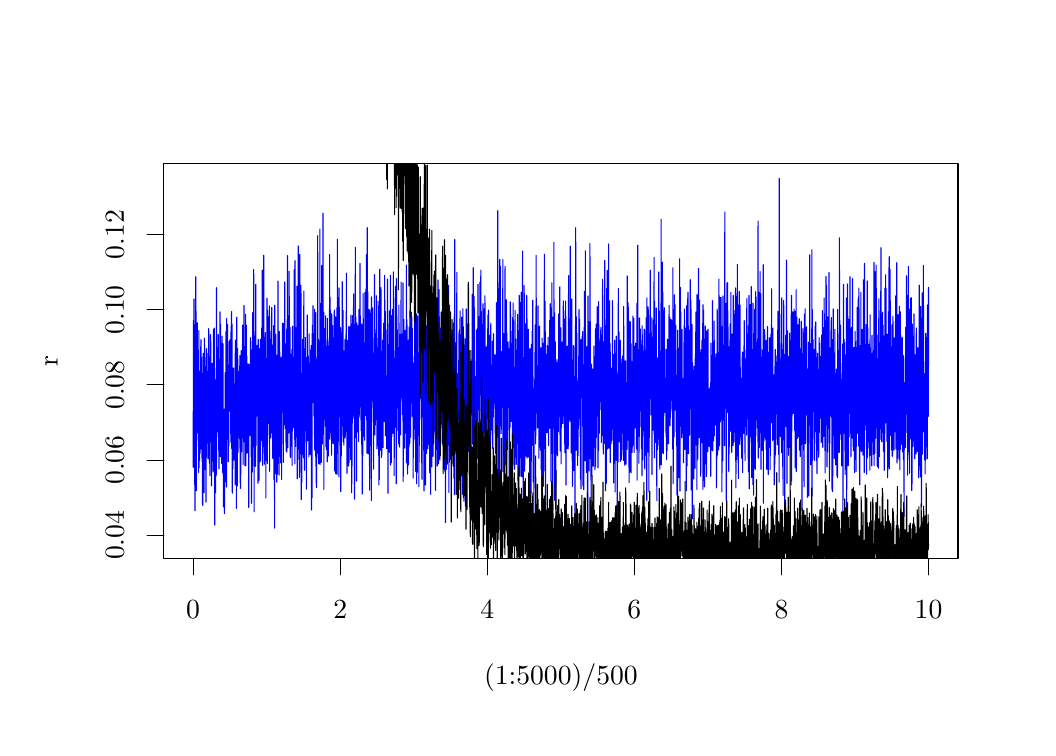
\begin{tikzpicture}[x=1pt,y=1pt]
\definecolor{fillColor}{RGB}{255,255,255}
\path[use as bounding box,fill=fillColor,fill opacity=0.00] (0,0) rectangle (361.35,252.94);
\begin{scope}
\path[clip] ( 49.20, 61.20) rectangle (336.15,203.75);
\definecolor{drawColor}{RGB}{0,0,255}

\path[draw=drawColor,line width= 0.4pt,line join=round,line cap=round] ( 59.83, 94.08) --
	( 59.88,147.09) --
	( 59.93,134.88) --
	( 59.99, 98.08) --
	( 60.04,135.79) --
	( 60.09,154.90) --
	( 60.15,142.78) --
	( 60.20,111.41) --
	( 60.25,106.10) --
	( 60.31, 98.59) --
	( 60.36, 87.74) --
	( 60.41, 97.07) --
	( 60.47, 78.40) --
	( 60.52,108.43) --
	( 60.57,145.67) --
	( 60.63,110.03) --
	( 60.68,101.92) --
	( 60.73,162.96) --
	( 60.78,113.00) --
	( 60.84,112.31) --
	( 60.89,150.50) --
	( 60.94, 85.62) --
	( 61.00,109.95) --
	( 61.05,113.84) --
	( 61.10,124.58) --
	( 61.16,134.22) --
	( 61.21,125.22) --
	( 61.26,106.52) --
	( 61.32,146.32) --
	( 61.37,127.50) --
	( 61.42,125.58) --
	( 61.48,114.27) --
	( 61.53,130.06) --
	( 61.58,115.46) --
	( 61.63,131.53) --
	( 61.69,101.48) --
	( 61.74,125.18) --
	( 61.79, 92.24) --
	( 61.85,143.51) --
	( 61.90, 93.88) --
	( 61.95,106.91) --
	( 62.01,126.17) --
	( 62.06,128.82) --
	( 62.11, 96.50) --
	( 62.17,127.50) --
	( 62.22,110.16) --
	( 62.27,110.40) --
	( 62.33, 99.21) --
	( 62.38,124.81) --
	( 62.43,102.88) --
	( 62.49,124.53) --
	( 62.54,137.66) --
	( 62.59,100.74) --
	( 62.64,140.19) --
	( 62.70,130.11) --
	( 62.75,126.46) --
	( 62.80,123.69) --
	( 62.86,133.79) --
	( 62.91,120.72) --
	( 62.96,104.13) --
	( 63.02, 96.19) --
	( 63.07,121.98) --
	( 63.12, 80.90) --
	( 63.18,110.15) --
	( 63.23,103.46) --
	( 63.28, 80.29) --
	( 63.34,107.64) --
	( 63.39,128.66) --
	( 63.44,135.26) --
	( 63.50,129.26) --
	( 63.55,108.42) --
	( 63.60,126.52) --
	( 63.65,104.23) --
	( 63.71,128.94) --
	( 63.76, 84.92) --
	( 63.81,110.51) --
	( 63.87,140.75) --
	( 63.92,121.19) --
	( 63.97,128.93) --
	( 64.03,136.80) --
	( 64.08, 99.88) --
	( 64.13,124.30) --
	( 64.19,107.35) --
	( 64.24, 93.21) --
	( 64.29,130.48) --
	( 64.35, 94.74) --
	( 64.40,129.36) --
	( 64.45, 81.47) --
	( 64.50, 93.05) --
	( 64.56,127.84) --
	( 64.61,130.12) --
	( 64.66,136.98) --
	( 64.72,119.84) --
	( 64.77,120.14) --
	( 64.82,127.56) --
	( 64.88,121.43) --
	( 64.93,102.85) --
	( 64.98,118.40) --
	( 65.04,102.92) --
	( 65.09,105.83) --
	( 65.14, 97.26) --
	( 65.20,135.29) --
	( 65.25,110.24) --
	( 65.30,124.32) --
	( 65.36,132.53) --
	( 65.41,144.20) --
	( 65.46,120.36) --
	( 65.51,134.03) --
	( 65.57, 96.76) --
	( 65.62,131.23) --
	( 65.67, 95.52) --
	( 65.73,117.90) --
	( 65.78,120.13) --
	( 65.83, 91.13) --
	( 65.89,132.36) --
	( 65.94,129.14) --
	( 65.99,103.22) --
	( 66.05,142.01) --
	( 66.10,136.43) --
	( 66.15,139.40) --
	( 66.21,121.61) --
	( 66.26,111.49) --
	( 66.31,110.60) --
	( 66.37,121.72) --
	( 66.42, 87.39) --
	( 66.47,128.31) --
	( 66.52,125.71) --
	( 66.58,126.74) --
	( 66.63, 96.25) --
	( 66.68,131.65) --
	( 66.74,104.10) --
	( 66.79,109.76) --
	( 66.84,123.31) --
	( 66.90,107.80) --
	( 66.95,113.68) --
	( 67.00, 92.37) --
	( 67.06,121.77) --
	( 67.11,143.85) --
	( 67.16,120.91) --
	( 67.22,102.58) --
	( 67.27,121.05) --
	( 67.32,122.80) --
	( 67.38, 92.89) --
	( 67.43,144.40) --
	( 67.48, 94.14) --
	( 67.53,130.02) --
	( 67.59, 73.23) --
	( 67.64, 83.17) --
	( 67.69,116.58) --
	( 67.75,105.38) --
	( 67.80,102.94) --
	( 67.85, 94.00) --
	( 67.91, 84.91) --
	( 67.96,115.72) --
	( 68.01,119.04) --
	( 68.07,125.83) --
	( 68.12, 91.02) --
	( 68.17,104.57) --
	( 68.23,158.98) --
	( 68.28, 95.79) --
	( 68.33,128.02) --
	( 68.38,104.86) --
	( 68.44,137.33) --
	( 68.49,106.85) --
	( 68.54,114.48) --
	( 68.60,117.11) --
	( 68.65,118.52) --
	( 68.70,124.42) --
	( 68.76,125.28) --
	( 68.81,111.24) --
	( 68.86,142.11) --
	( 68.92,106.73) --
	( 68.97,132.65) --
	( 69.02,112.53) --
	( 69.08, 95.45) --
	( 69.13, 93.50) --
	( 69.18,111.10) --
	( 69.24,103.28) --
	( 69.29,122.33) --
	( 69.34,133.13) --
	( 69.39,113.87) --
	( 69.45,114.44) --
	( 69.50,150.27) --
	( 69.55,125.07) --
	( 69.61, 97.92) --
	( 69.66,145.75) --
	( 69.71,100.73) --
	( 69.77,118.99) --
	( 69.82,122.21) --
	( 69.87,105.73) --
	( 69.93,127.56) --
	( 69.98,129.45) --
	( 70.03,116.34) --
	( 70.09,117.36) --
	( 70.14, 95.42) --
	( 70.19,130.31) --
	( 70.25,141.39) --
	( 70.30,125.26) --
	( 70.35,119.51) --
	( 70.40,113.87) --
	( 70.46, 92.16) --
	( 70.51,117.58) --
	( 70.56,111.46) --
	( 70.62,138.67) --
	( 70.67, 98.52) --
	( 70.72, 79.80) --
	( 70.78,107.96) --
	( 70.83,111.90) --
	( 70.88,100.04) --
	( 70.94,107.63) --
	( 70.99,105.82) --
	( 71.04,115.12) --
	( 71.10, 77.37) --
	( 71.15,113.22) --
	( 71.20,108.07) --
	( 71.25,105.40) --
	( 71.31,102.74) --
	( 71.36,128.26) --
	( 71.41,116.82) --
	( 71.47,111.75) --
	( 71.52, 88.85) --
	( 71.57, 96.84) --
	( 71.63,143.13) --
	( 71.68,134.29) --
	( 71.73,116.77) --
	( 71.79,133.50) --
	( 71.84, 86.94) --
	( 71.89,147.84) --
	( 71.95,111.53) --
	( 72.00,119.19) --
	( 72.05,127.62) --
	( 72.11,126.88) --
	( 72.16,104.45) --
	( 72.21,145.71) --
	( 72.26,134.58) --
	( 72.32,104.10) --
	( 72.37,114.39) --
	( 72.42,131.07) --
	( 72.48, 96.05) --
	( 72.53,115.43) --
	( 72.58,120.89) --
	( 72.64,101.77) --
	( 72.69,111.47) --
	( 72.74,121.28) --
	( 72.80,139.48) --
	( 72.85,117.70) --
	( 72.90,127.90) --
	( 72.96,117.59) --
	( 73.01,130.53) --
	( 73.06,132.88) --
	( 73.12,140.22) --
	( 73.17,114.33) --
	( 73.22,117.94) --
	( 73.27,133.77) --
	( 73.33,106.16) --
	( 73.38,127.66) --
	( 73.43,103.18) --
	( 73.49,143.10) --
	( 73.54,127.01) --
	( 73.59,149.56) --
	( 73.65,117.81) --
	( 73.70,150.40) --
	( 73.75,100.86) --
	( 73.81,114.49) --
	( 73.86,145.89) --
	( 73.91, 85.48) --
	( 73.97, 84.75) --
	( 74.02,129.14) --
	( 74.07,109.19) --
	( 74.12, 93.53) --
	( 74.18,118.00) --
	( 74.23,107.19) --
	( 74.28,110.14) --
	( 74.34,109.01) --
	( 74.39,130.01) --
	( 74.44,124.07) --
	( 74.50, 98.74) --
	( 74.55, 96.70) --
	( 74.60,121.23) --
	( 74.66,124.30) --
	( 74.71,121.33) --
	( 74.76,100.25) --
	( 74.82,107.50) --
	( 74.87,107.65) --
	( 74.92,119.68) --
	( 74.98, 87.80) --
	( 75.03,140.07) --
	( 75.08,111.06) --
	( 75.13,114.44) --
	( 75.19,100.60) --
	( 75.24,114.83) --
	( 75.29,134.29) --
	( 75.35,124.87) --
	( 75.40, 79.23) --
	( 75.45,101.28) --
	( 75.51, 98.34) --
	( 75.56,148.37) --
	( 75.61,104.74) --
	( 75.67,110.30) --
	( 75.72,111.93) --
	( 75.77, 87.36) --
	( 75.83,132.67) --
	( 75.88,137.01) --
	( 75.93,119.25) --
	( 75.99,125.21) --
	( 76.04, 99.49) --
	( 76.09,128.84) --
	( 76.14,123.12) --
	( 76.20,115.14) --
	( 76.25,124.26) --
	( 76.30,109.73) --
	( 76.36,115.81) --
	( 76.41,125.21) --
	( 76.46,118.21) --
	( 76.52,106.48) --
	( 76.57,104.32) --
	( 76.62,126.81) --
	( 76.68,134.47) --
	( 76.73,100.92) --
	( 76.78,101.81) --
	( 76.84, 86.39) --
	( 76.89, 86.83) --
	( 76.94,131.49) --
	( 77.00, 91.62) --
	( 77.05,102.88) --
	( 77.10,119.00) --
	( 77.15,136.20) --
	( 77.21,128.38) --
	( 77.26, 99.66) --
	( 77.31,114.71) --
	( 77.37,115.33) --
	( 77.42,112.45) --
	( 77.47,106.10) --
	( 77.53,120.41) --
	( 77.58,138.43) --
	( 77.63,108.62) --
	( 77.69,145.48) --
	( 77.74,118.91) --
	( 77.79,118.66) --
	( 77.85, 95.13) --
	( 77.90,111.56) --
	( 77.95,115.29) --
	( 78.00,119.19) --
	( 78.06,126.19) --
	( 78.11,126.60) --
	( 78.16,152.55) --
	( 78.22,103.32) --
	( 78.27,119.57) --
	( 78.32,127.04) --
	( 78.38,137.69) --
	( 78.43,132.02) --
	( 78.48,115.03) --
	( 78.54, 94.58) --
	( 78.59,109.63) --
	( 78.64,120.52) --
	( 78.70, 98.88) --
	( 78.75,149.38) --
	( 78.80,104.80) --
	( 78.86, 94.63) --
	( 78.91,133.35) --
	( 78.96,125.58) --
	( 79.01,145.43) --
	( 79.07,108.22) --
	( 79.12,112.00) --
	( 79.17,134.35) --
	( 79.23,109.57) --
	( 79.28, 99.18) --
	( 79.33,124.29) --
	( 79.39, 99.40) --
	( 79.44,111.47) --
	( 79.49,102.11) --
	( 79.55,116.04) --
	( 79.60,118.55) --
	( 79.65,131.51) --
	( 79.71,108.55) --
	( 79.76,120.98) --
	( 79.81,106.54) --
	( 79.87, 79.56) --
	( 79.92,131.19) --
	( 79.97,129.37) --
	( 80.02,116.66) --
	( 80.08,121.64) --
	( 80.13,112.49) --
	( 80.18,129.28) --
	( 80.24,117.12) --
	( 80.29,105.50) --
	( 80.34,109.96) --
	( 80.40,131.39) --
	( 80.45,126.52) --
	( 80.50,140.93) --
	( 80.56,122.87) --
	( 80.61,139.52) --
	( 80.66,122.81) --
	( 80.72,121.17) --
	( 80.77, 97.91) --
	( 80.82,112.11) --
	( 80.87, 81.03) --
	( 80.93,121.89) --
	( 80.98,116.11) --
	( 81.03,115.59) --
	( 81.09,136.49) --
	( 81.14, 92.31) --
	( 81.19,108.87) --
	( 81.25, 94.56) --
	( 81.30,149.95) --
	( 81.35,116.98) --
	( 81.41,115.54) --
	( 81.46,104.95) --
	( 81.51,121.11) --
	( 81.57,133.30) --
	( 81.62,128.87) --
	( 81.67,165.53) --
	( 81.73,111.76) --
	( 81.78,117.86) --
	( 81.83, 77.99) --
	( 81.88,116.52) --
	( 81.94,126.37) --
	( 81.99, 99.45) --
	( 82.04,107.97) --
	( 82.10,141.50) --
	( 82.15,136.78) --
	( 82.20,130.37) --
	( 82.26,143.07) --
	( 82.31, 94.38) --
	( 82.36,133.07) --
	( 82.42,160.13) --
	( 82.47,128.78) --
	( 82.52,101.94) --
	( 82.58,136.15) --
	( 82.63,123.32) --
	( 82.68,115.21) --
	( 82.74,112.57) --
	( 82.79,112.90) --
	( 82.84,112.87) --
	( 82.89,123.49) --
	( 82.95,138.13) --
	( 83.00,116.60) --
	( 83.05,123.25) --
	( 83.11,127.01) --
	( 83.16,132.02) --
	( 83.21, 88.32) --
	( 83.27,123.87) --
	( 83.32,140.27) --
	( 83.37,136.88) --
	( 83.43,133.08) --
	( 83.48,136.92) --
	( 83.53,105.61) --
	( 83.59, 89.36) --
	( 83.64,136.95) --
	( 83.69,103.87) --
	( 83.75, 95.96) --
	( 83.80,118.59) --
	( 83.85,124.84) --
	( 83.90,106.60) --
	( 83.96,111.67) --
	( 84.01,118.36) --
	( 84.06,115.12) --
	( 84.12,140.40) --
	( 84.17, 96.32) --
	( 84.22,124.23) --
	( 84.28,112.21) --
	( 84.33,133.47) --
	( 84.38,103.83) --
	( 84.44,126.70) --
	( 84.49,123.65) --
	( 84.54,144.38) --
	( 84.60,107.16) --
	( 84.65,120.68) --
	( 84.70,140.69) --
	( 84.75,165.35) --
	( 84.81,113.72) --
	( 84.86,104.45) --
	( 84.91, 94.77) --
	( 84.97,113.63) --
	( 85.02,106.71) --
	( 85.07,128.70) --
	( 85.13,121.51) --
	( 85.18,123.39) --
	( 85.23,114.30) --
	( 85.29,170.69) --
	( 85.34,139.14) --
	( 85.39,108.81) --
	( 85.45,101.32) --
	( 85.50,113.76) --
	( 85.55, 95.20) --
	( 85.61,122.64) --
	( 85.66,111.33) --
	( 85.71,101.68) --
	( 85.76,133.54) --
	( 85.82,123.76) --
	( 85.87,142.76) --
	( 85.92,126.70) --
	( 85.98,133.48) --
	( 86.03,103.36) --
	( 86.08, 82.98) --
	( 86.14,126.95) --
	( 86.19,116.30) --
	( 86.24,124.29) --
	( 86.30,130.38) --
	( 86.35,123.47) --
	( 86.40,124.58) --
	( 86.46,155.20) --
	( 86.51,113.45) --
	( 86.56,125.33) --
	( 86.62, 95.51) --
	( 86.67,120.28) --
	( 86.72,150.81) --
	( 86.77,127.45) --
	( 86.83,109.74) --
	( 86.88,137.35) --
	( 86.93,116.47) --
	( 86.99,148.46) --
	( 87.04,143.26) --
	( 87.09,130.48) --
	( 87.15,132.02) --
	( 87.20,135.46) --
	( 87.25,117.32) --
	( 87.31,115.42) --
	( 87.36,152.37) --
	( 87.41, 92.58) --
	( 87.47,140.64) --
	( 87.52,136.62) --
	( 87.57,123.88) --
	( 87.62,128.25) --
	( 87.68,134.14) --
	( 87.73,119.55) --
	( 87.78,104.67) --
	( 87.84,116.64) --
	( 87.89,104.86) --
	( 87.94,118.43) --
	( 88.00,143.27) --
	( 88.05,106.44) --
	( 88.10,118.35) --
	( 88.16,141.50) --
	( 88.21,151.83) --
	( 88.26,128.99) --
	( 88.32,117.71) --
	( 88.37,108.05) --
	( 88.42,120.73) --
	( 88.48,127.13) --
	( 88.53, 97.32) --
	( 88.58,138.22) --
	( 88.63,137.65) --
	( 88.69,127.90) --
	( 88.74,100.93) --
	( 88.79,119.40) --
	( 88.85,137.83) --
	( 88.90,145.28) --
	( 88.95,129.69) --
	( 89.01, 89.60) --
	( 89.06,110.19) --
	( 89.11, 97.51) --
	( 89.17,115.85) --
	( 89.22, 72.11) --
	( 89.27,152.63) --
	( 89.33,113.57) --
	( 89.38,104.30) --
	( 89.43,113.59) --
	( 89.49,130.65) --
	( 89.54,100.57) --
	( 89.59, 91.81) --
	( 89.64,142.10) --
	( 89.70,134.41) --
	( 89.75,114.13) --
	( 89.80,103.94) --
	( 89.86,122.41) --
	( 89.91,115.76) --
	( 89.96,122.24) --
	( 90.02, 88.69) --
	( 90.07,104.09) --
	( 90.12,131.82) --
	( 90.18,134.63) --
	( 90.23,134.15) --
	( 90.28, 91.55) --
	( 90.34,113.11) --
	( 90.39,116.53) --
	( 90.44,161.37) --
	( 90.50,157.86) --
	( 90.55, 95.55) --
	( 90.60,114.32) --
	( 90.65,115.31) --
	( 90.71,104.85) --
	( 90.76,104.83) --
	( 90.81,115.46) --
	( 90.87, 91.27) --
	( 90.92,143.15) --
	( 90.97,122.40) --
	( 91.03,139.54) --
	( 91.08,129.65) --
	( 91.13,135.73) --
	( 91.19,110.14) --
	( 91.24, 97.97) --
	( 91.29,128.73) --
	( 91.35,133.67) --
	( 91.40,119.79) --
	( 91.45, 95.67) --
	( 91.50,122.08) --
	( 91.56,118.49) --
	( 91.61, 95.79) --
	( 91.66,113.86) --
	( 91.72,120.48) --
	( 91.77, 89.69) --
	( 91.82,122.40) --
	( 91.88,134.08) --
	( 91.93,132.75) --
	( 91.98,113.91) --
	( 92.04,114.92) --
	( 92.09,146.18) --
	( 92.14,136.94) --
	( 92.20,115.03) --
	( 92.25,144.90) --
	( 92.30,116.88) --
	( 92.36,121.75) --
	( 92.41, 95.88) --
	( 92.46,146.11) --
	( 92.51,131.42) --
	( 92.57,145.98) --
	( 92.62,121.90) --
	( 92.67,109.37) --
	( 92.73,143.06) --
	( 92.78,139.91) --
	( 92.83,111.90) --
	( 92.89,161.04) --
	( 92.94,119.38) --
	( 92.99,115.40) --
	( 93.05,130.47) --
	( 93.10,113.15) --
	( 93.15,108.13) --
	( 93.21,109.48) --
	( 93.26,138.64) --
	( 93.31,130.17) --
	( 93.37, 99.92) --
	( 93.42,111.73) --
	( 93.47,108.99) --
	( 93.52,119.12) --
	( 93.58,144.03) --
	( 93.63,100.50) --
	( 93.68, 99.53) --
	( 93.74,114.81) --
	( 93.79,147.62) --
	( 93.84,130.33) --
	( 93.90,170.59) --
	( 93.95,118.36) --
	( 94.00,101.14) --
	( 94.06,137.21) --
	( 94.11,134.06) --
	( 94.16,148.75) --
	( 94.22,123.93) --
	( 94.27,111.71) --
	( 94.32,133.11) --
	( 94.37,106.49) --
	( 94.43,125.94) --
	( 94.48,164.87) --
	( 94.53,141.97) --
	( 94.59,115.90) --
	( 94.64,119.13) --
	( 94.69,141.44) --
	( 94.75,116.28) --
	( 94.80,144.59) --
	( 94.85, 97.98) --
	( 94.91,134.04) --
	( 94.96, 97.60) --
	( 95.01,102.83) --
	( 95.07,134.96) --
	( 95.12,118.31) --
	( 95.17,112.19) --
	( 95.23,106.01) --
	( 95.28,114.13) --
	( 95.33,129.47) --
	( 95.38,121.60) --
	( 95.44,116.28) --
	( 95.49,136.72) --
	( 95.54, 94.75) --
	( 95.60,119.69) --
	( 95.65,108.18) --
	( 95.70,145.10) --
	( 95.76,107.32) --
	( 95.81,125.27) --
	( 95.86,121.89) --
	( 95.92,128.92) --
	( 95.97,133.81) --
	( 96.02,128.24) --
	( 96.08,129.96) --
	( 96.13,117.33) --
	( 96.18,130.22) --
	( 96.24,108.47) --
	( 96.29,112.34) --
	( 96.34,165.50) --
	( 96.39,127.55) --
	( 96.45,121.03) --
	( 96.50,113.24) --
	( 96.55, 95.33) --
	( 96.61,168.76) --
	( 96.66,151.04) --
	( 96.71,109.97) --
	( 96.77,144.68) --
	( 96.82,101.64) --
	( 96.87,132.03) --
	( 96.93,127.33) --
	( 96.98,105.05) --
	( 97.03,120.69) --
	( 97.09,122.07) --
	( 97.14,112.47) --
	( 97.19,140.35) --
	( 97.25,144.72) --
	( 97.30,159.52) --
	( 97.35, 97.05) --
	( 97.40, 89.91) --
	( 97.46, 98.51) --
	( 97.51,114.80) --
	( 97.56,136.11) --
	( 97.62, 96.88) --
	( 97.67,117.37) --
	( 97.72,133.78) --
	( 97.78,174.05) --
	( 97.83,100.66) --
	( 97.88,118.11) --
	( 97.94,105.95) --
	( 97.99,119.38) --
	( 98.04,108.97) --
	( 98.10,125.11) --
	( 98.15,128.99) --
	( 98.20, 90.44) --
	( 98.25,115.32) --
	( 98.31,170.96) --
	( 98.36,155.99) --
	( 98.41,132.71) --
	( 98.47,124.01) --
	( 98.52,121.35) --
	( 98.57,144.09) --
	( 98.63,106.38) --
	( 98.68, 98.96) --
	( 98.73,159.85) --
	( 98.79,148.90) --
	( 98.84, 82.40) --
	( 98.89,102.55) --
	( 98.95,109.98) --
	( 99.00,103.25) --
	( 99.05, 88.69) --
	( 99.11,114.71) --
	( 99.16,114.68) --
	( 99.21,101.25) --
	( 99.26,128.17) --
	( 99.32, 98.97) --
	( 99.37,140.34) --
	( 99.42,111.90) --
	( 99.48,102.94) --
	( 99.53,106.43) --
	( 99.58,136.77) --
	( 99.64,106.89) --
	( 99.69, 97.45) --
	( 99.74,143.48) --
	( 99.80,157.77) --
	( 99.85,116.32) --
	( 99.90,103.65) --
	( 99.96,136.89) --
	(100.01, 93.00) --
	(100.06,118.41) --
	(100.12,127.95) --
	(100.17,113.69) --
	(100.22,119.09) --
	(100.27,114.75) --
	(100.33,141.05) --
	(100.38,107.39) --
	(100.43,114.22) --
	(100.49,133.75) --
	(100.54,109.25) --
	(100.59,109.96) --
	(100.65,131.10) --
	(100.70, 86.18) --
	(100.75,124.29) --
	(100.81,102.46) --
	(100.86,110.55) --
	(100.91,117.36) --
	(100.97,109.29) --
	(101.02,149.17) --
	(101.07,103.69) --
	(101.12,127.68) --
	(101.18,124.91) --
	(101.23,105.78) --
	(101.28,134.29) --
	(101.34,127.32) --
	(101.39,132.76) --
	(101.44,131.19) --
	(101.50,111.59) --
	(101.55,116.23) --
	(101.60, 97.88) --
	(101.66,127.61) --
	(101.71,142.31) --
	(101.76,110.71) --
	(101.82,120.62) --
	(101.87,121.91) --
	(101.92,118.70) --
	(101.98, 98.81) --
	(102.03,109.26) --
	(102.08,122.77) --
	(102.13,103.28) --
	(102.19,114.73) --
	(102.24,136.31) --
	(102.29, 98.55) --
	(102.35,114.67) --
	(102.40,138.08) --
	(102.45,106.73) --
	(102.51,123.17) --
	(102.56, 78.61) --
	(102.61,116.45) --
	(102.67,121.04) --
	(102.72,128.90) --
	(102.77, 83.11) --
	(102.83,140.78) --
	(102.88,145.43) --
	(102.93,117.38) --
	(102.99,132.55) --
	(103.04,119.00) --
	(103.09,152.48) --
	(103.14,140.59) --
	(103.20,122.73) --
	(103.25,128.55) --
	(103.30,142.41) --
	(103.36,120.28) --
	(103.41,122.20) --
	(103.46,112.58) --
	(103.52,128.56) --
	(103.57,122.39) --
	(103.62,105.64) --
	(103.68,151.19) --
	(103.73,100.29) --
	(103.78,141.06) --
	(103.84,126.29) --
	(103.89,105.87) --
	(103.94,128.13) --
	(104.00,108.52) --
	(104.05, 98.07) --
	(104.10,125.11) --
	(104.15,150.01) --
	(104.21, 88.55) --
	(104.26,103.27) --
	(104.31,130.92) --
	(104.37, 86.78) --
	(104.42,120.08) --
	(104.47,128.42) --
	(104.53,121.95) --
	(104.58,117.07) --
	(104.63,116.83) --
	(104.69, 99.16) --
	(104.74,126.78) --
	(104.79,177.76) --
	(104.85,132.52) --
	(104.90,133.22) --
	(104.95,131.69) --
	(105.00,108.32) --
	(105.06,140.34) --
	(105.11, 95.34) --
	(105.16,131.56) --
	(105.22,108.91) --
	(105.27,108.27) --
	(105.32,115.08) --
	(105.38,115.77) --
	(105.43,125.19) --
	(105.48,138.14) --
	(105.54,114.49) --
	(105.59,180.13) --
	(105.64, 95.11) --
	(105.70,122.89) --
	(105.75,111.47) --
	(105.80,129.92) --
	(105.86,118.67) --
	(105.91,136.04) --
	(105.96,118.60) --
	(106.01,153.30) --
	(106.07,109.28) --
	(106.12, 95.85) --
	(106.17,116.03) --
	(106.23,149.73) --
	(106.28,167.01) --
	(106.33,106.10) --
	(106.39,113.22) --
	(106.44,107.75) --
	(106.49,102.49) --
	(106.55,136.44) --
	(106.60,119.60) --
	(106.65,167.33) --
	(106.71,185.94) --
	(106.76,133.39) --
	(106.81,141.44) --
	(106.87,127.40) --
	(106.92,105.97) --
	(106.97,150.13) --
	(107.02, 86.10) --
	(107.08,129.22) --
	(107.13,144.04) --
	(107.18,123.62) --
	(107.24,127.26) --
	(107.29,111.33) --
	(107.34,144.21) --
	(107.40,115.05) --
	(107.45,140.92) --
	(107.50,132.23) --
	(107.56,129.34) --
	(107.61,108.86) --
	(107.66,148.80) --
	(107.72,130.39) --
	(107.77,101.47) --
	(107.82,125.74) --
	(107.87,104.20) --
	(107.93,124.58) --
	(107.98,100.44) --
	(108.03,134.61) --
	(108.09,125.92) --
	(108.14,137.79) --
	(108.19,113.02) --
	(108.25, 96.07) --
	(108.30,147.94) --
	(108.35,116.20) --
	(108.41,140.58) --
	(108.46,109.02) --
	(108.51,114.38) --
	(108.57,122.28) --
	(108.62, 98.12) --
	(108.67,137.48) --
	(108.73,112.01) --
	(108.78,124.87) --
	(108.83,106.28) --
	(108.88,115.71) --
	(108.94,132.98) --
	(108.99,138.00) --
	(109.04,104.27) --
	(109.10,170.98) --
	(109.15,122.78) --
	(109.20,130.10) --
	(109.26,117.92) --
	(109.31,155.53) --
	(109.36,106.72) --
	(109.42,120.49) --
	(109.47,139.35) --
	(109.52,120.40) --
	(109.58,115.19) --
	(109.63,103.95) --
	(109.68,105.70) --
	(109.74,137.84) --
	(109.79,149.62) --
	(109.84, 98.46) --
	(109.89,149.10) --
	(109.95,103.12) --
	(110.00,132.56) --
	(110.05,126.02) --
	(110.11,128.24) --
	(110.16,136.29) --
	(110.21,145.27) --
	(110.27,113.97) --
	(110.32,108.62) --
	(110.37,136.04) --
	(110.43,102.57) --
	(110.48,122.63) --
	(110.53,123.10) --
	(110.59,131.50) --
	(110.64,136.25) --
	(110.69,125.35) --
	(110.75,122.50) --
	(110.80,150.90) --
	(110.85,129.76) --
	(110.90,102.08) --
	(110.96, 92.75) --
	(111.01,124.94) --
	(111.06,113.19) --
	(111.12,117.35) --
	(111.17,106.27) --
	(111.22,148.47) --
	(111.28,121.08) --
	(111.33, 91.73) --
	(111.38,118.50) --
	(111.44,115.65) --
	(111.49, 94.89) --
	(111.54,129.80) --
	(111.60,134.55) --
	(111.65,133.26) --
	(111.70,114.18) --
	(111.75,151.70) --
	(111.81, 91.47) --
	(111.86,102.49) --
	(111.91,176.47) --
	(111.97,134.26) --
	(112.02,137.19) --
	(112.07,103.52) --
	(112.13,125.06) --
	(112.18,110.43) --
	(112.23,120.19) --
	(112.29,121.52) --
	(112.34,105.95) --
	(112.39,155.47) --
	(112.45, 90.67) --
	(112.50,112.09) --
	(112.55,158.83) --
	(112.61,134.72) --
	(112.66,117.00) --
	(112.71,135.71) --
	(112.76,144.77) --
	(112.82,112.38) --
	(112.87,127.76) --
	(112.92,115.49) --
	(112.98,120.92) --
	(113.03,144.58) --
	(113.08,133.11) --
	(113.14, 85.26) --
	(113.19,142.92) --
	(113.24,117.02) --
	(113.30, 98.15) --
	(113.35,132.61) --
	(113.40,130.50) --
	(113.46,119.59) --
	(113.51,114.63) --
	(113.56,131.41) --
	(113.62,141.19) --
	(113.67,161.19) --
	(113.72,149.59) --
	(113.77,121.85) --
	(113.83,122.84) --
	(113.88,105.47) --
	(113.93,150.76) --
	(113.99,149.72) --
	(114.04,103.29) --
	(114.09,105.12) --
	(114.15,136.22) --
	(114.20,109.80) --
	(114.25,102.08) --
	(114.31,130.70) --
	(114.36,105.37) --
	(114.41,120.65) --
	(114.47,127.56) --
	(114.52,115.62) --
	(114.57,117.38) --
	(114.62,135.15) --
	(114.68,140.17) --
	(114.73,104.68) --
	(114.78,111.01) --
	(114.84,109.13) --
	(114.89,118.59) --
	(114.94,107.82) --
	(115.00,123.46) --
	(115.05,144.28) --
	(115.10,131.47) --
	(115.16,164.26) --
	(115.21,116.88) --
	(115.26,106.94) --
	(115.32,125.68) --
	(115.37, 91.88) --
	(115.42,105.35) --
	(115.48,123.94) --
	(115.53,139.89) --
	(115.58,119.19) --
	(115.63,117.09) --
	(115.69,125.21) --
	(115.74,107.42) --
	(115.79,119.14) --
	(115.85,116.65) --
	(115.90, 98.80) --
	(115.95, 94.54) --
	(116.01,144.92) --
	(116.06,107.37) --
	(116.11, 95.74) --
	(116.17,127.22) --
	(116.22,101.17) --
	(116.27,134.27) --
	(116.33,114.58) --
	(116.38,127.87) --
	(116.43,118.86) --
	(116.49,107.69) --
	(116.54,144.94) --
	(116.59,122.05) --
	(116.64,111.16) --
	(116.70, 96.84) --
	(116.75,137.30) --
	(116.80,149.08) --
	(116.86,134.61) --
	(116.91,127.67) --
	(116.96,106.28) --
	(117.02,101.24) --
	(117.07, 84.93) --
	(117.12, 96.23) --
	(117.18,137.10) --
	(117.23, 94.56) --
	(117.28,116.97) --
	(117.34,138.63) --
	(117.39,148.91) --
	(117.44,112.64) --
	(117.50,115.79) --
	(117.55,115.71) --
	(117.60,143.34) --
	(117.65,131.55) --
	(117.71,113.36) --
	(117.76,156.73) --
	(117.81,113.92) --
	(117.87,112.43) --
	(117.92,111.82) --
	(117.97,145.64) --
	(118.03,112.57) --
	(118.08, 82.56) --
	(118.13,117.79) --
	(118.19,105.97) --
	(118.24,131.28) --
	(118.29,134.75) --
	(118.35,136.31) --
	(118.40,173.58) --
	(118.45,123.58) --
	(118.50,141.90) --
	(118.56,148.42) --
	(118.61,104.77) --
	(118.66,127.19) --
	(118.72,115.99) --
	(118.77,113.58) --
	(118.82, 89.08) --
	(118.88,117.30) --
	(118.93,146.22) --
	(118.98,110.32) --
	(119.04,131.89) --
	(119.09,113.70) --
	(119.14,106.85) --
	(119.20,139.34) --
	(119.25,125.16) --
	(119.30,115.13) --
	(119.36,145.29) --
	(119.41,117.94) --
	(119.46,128.28) --
	(119.51,136.38) --
	(119.57,103.38) --
	(119.62,134.97) --
	(119.67,136.96) --
	(119.73,151.09) --
	(119.78,112.22) --
	(119.83,114.64) --
	(119.89,120.62) --
	(119.94,147.40) --
	(119.99,116.09) --
	(120.05,123.07) --
	(120.10,167.73) --
	(120.15,132.69) --
	(120.21,148.80) --
	(120.26,142.44) --
	(120.31,115.79) --
	(120.37,121.02) --
	(120.42,139.25) --
	(120.47,107.88) --
	(120.52,107.18) --
	(120.58,137.58) --
	(120.63,119.56) --
	(120.68,145.88) --
	(120.74, 98.87) --
	(120.79,145.52) --
	(120.84,117.83) --
	(120.90, 84.39) --
	(120.95,104.22) --
	(121.00,116.43) --
	(121.06,118.00) --
	(121.11, 98.21) --
	(121.16,134.21) --
	(121.22,156.83) --
	(121.27,133.58) --
	(121.32,119.46) --
	(121.37,138.28) --
	(121.43,124.87) --
	(121.48,132.97) --
	(121.53,123.42) --
	(121.59,112.90) --
	(121.64,105.11) --
	(121.69,127.69) --
	(121.75,103.88) --
	(121.80,127.19) --
	(121.85,157.31) --
	(121.91,127.60) --
	(121.96,114.16) --
	(122.01,133.56) --
	(122.07,118.73) --
	(122.12,129.03) --
	(122.17,112.79) --
	(122.23,158.52) --
	(122.28,126.94) --
	(122.33,119.67) --
	(122.38,122.60) --
	(122.44,170.92) --
	(122.49,119.68) --
	(122.54,111.68) --
	(122.60, 99.18) --
	(122.65,116.22) --
	(122.70,180.63) --
	(122.76,119.59) --
	(122.81,129.57) --
	(122.86,114.05) --
	(122.92,157.53) --
	(122.97, 99.04) --
	(123.02,114.08) --
	(123.08,123.52) --
	(123.13,142.98) --
	(123.18,151.11) --
	(123.24,137.35) --
	(123.29,127.31) --
	(123.34,102.92) --
	(123.39,123.54) --
	(123.45, 96.83) --
	(123.50,117.70) --
	(123.55, 85.81) --
	(123.61,121.18) --
	(123.66,150.99) --
	(123.71,108.83) --
	(123.77,136.47) --
	(123.82,120.37) --
	(123.87,110.17) --
	(123.93,113.06) --
	(123.98,110.93) --
	(124.03,149.73) --
	(124.09, 89.99) --
	(124.14,117.33) --
	(124.19, 82.05) --
	(124.24,155.68) --
	(124.30,115.68) --
	(124.35,125.72) --
	(124.40,121.87) --
	(124.46,142.41) --
	(124.51,125.96) --
	(124.56,129.56) --
	(124.62,151.68) --
	(124.67,141.30) --
	(124.72,128.56) --
	(124.78,135.44) --
	(124.83,110.47) --
	(124.88,135.44) --
	(124.94,110.19) --
	(124.99, 93.38) --
	(125.04,117.74) --
	(125.10,110.31) --
	(125.15,125.21) --
	(125.20,117.51) --
	(125.25,119.62) --
	(125.31,163.68) --
	(125.36,150.22) --
	(125.41,141.18) --
	(125.47,105.76) --
	(125.52,117.77) --
	(125.57,139.71) --
	(125.63,109.37) --
	(125.68,128.02) --
	(125.73,130.51) --
	(125.79,118.03) --
	(125.84,111.26) --
	(125.89,142.41) --
	(125.95,111.83) --
	(126.00,156.09) --
	(126.05,115.23) --
	(126.11,140.73) --
	(126.16,109.31) --
	(126.21,100.78) --
	(126.26,137.42) --
	(126.32,115.24) --
	(126.37,131.26) --
	(126.42,107.33) --
	(126.48,106.05) --
	(126.53,127.43) --
	(126.58,109.66) --
	(126.64,154.06) --
	(126.69,149.78) --
	(126.74,116.42) --
	(126.80, 98.26) --
	(126.85,138.19) --
	(126.90, 87.75) --
	(126.96,125.72) --
	(127.01,133.52) --
	(127.06, 89.63) --
	(127.12,124.06) --
	(127.17,144.85) --
	(127.22,165.63) --
	(127.27,114.11) --
	(127.33,100.20) --
	(127.38,134.04) --
	(127.43,135.93) --
	(127.49,119.98) --
	(127.54,125.16) --
	(127.59,107.98) --
	(127.65,158.97) --
	(127.70,149.35) --
	(127.75,108.75) --
	(127.81, 97.67) --
	(127.86,130.38) --
	(127.91,133.40) --
	(127.97, 98.43) --
	(128.02,120.00) --
	(128.07,135.97) --
	(128.12,114.47) --
	(128.18,121.77) --
	(128.23,124.54) --
	(128.28,139.90) --
	(128.34,112.00) --
	(128.39,132.17) --
	(128.44,101.20) --
	(128.50,140.37) --
	(128.55,125.25) --
	(128.60,144.36) --
	(128.66,146.18) --
	(128.71,118.82) --
	(128.76,110.92) --
	(128.82,110.59) --
	(128.87,147.05) --
	(128.92,125.13) --
	(128.98,163.41) --
	(129.03,147.71) --
	(129.08,145.47) --
	(129.13,121.75) --
	(129.19,119.04) --
	(129.24,150.34) --
	(129.29,105.44) --
	(129.35,115.95) --
	(129.40,119.83) --
	(129.45,125.05) --
	(129.51,127.21) --
	(129.56,107.84) --
	(129.61,125.45) --
	(129.67,124.88) --
	(129.72,100.80) --
	(129.77,105.15) --
	(129.83,143.70) --
	(129.88,116.61) --
	(129.93,107.97) --
	(129.99,112.38) --
	(130.04,162.10) --
	(130.09,147.93) --
	(130.14,101.10) --
	(130.20, 84.64) --
	(130.25,138.64) --
	(130.30,126.46) --
	(130.36,111.31) --
	(130.41,113.27) --
	(130.46,125.51) --
	(130.52,109.32) --
	(130.57,121.18) --
	(130.62,116.73) --
	(130.68, 99.52) --
	(130.73,150.58) --
	(130.78,114.37) --
	(130.84,126.27) --
	(130.89,142.50) --
	(130.94,121.48) --
	(130.99,106.01) --
	(131.05,163.51) --
	(131.10, 94.89) --
	(131.15,112.94) --
	(131.21,125.87) --
	(131.26,120.61) --
	(131.31,138.24) --
	(131.37, 95.68) --
	(131.42,103.38) --
	(131.47,148.91) --
	(131.53,112.92) --
	(131.58,105.22) --
	(131.63,113.50) --
	(131.69,145.06) --
	(131.74,119.86) --
	(131.79,151.13) --
	(131.85,134.73) --
	(131.90,111.67) --
	(131.95,112.89) --
	(132.00,136.14) --
	(132.06,117.19) --
	(132.11,106.37) --
	(132.16,164.67) --
	(132.22,107.95) --
	(132.27,118.81) --
	(132.32,133.60) --
	(132.38,127.75) --
	(132.43, 91.02) --
	(132.48,120.71) --
	(132.54,127.10) --
	(132.59,125.43) --
	(132.64,132.04) --
	(132.70,113.47) --
	(132.75,112.38) --
	(132.80,136.28) --
	(132.86,133.40) --
	(132.91,159.45) --
	(132.96,132.32) --
	(133.01,108.41) --
	(133.07,120.77) --
	(133.12,120.99) --
	(133.17, 88.14) --
	(133.23,106.12) --
	(133.28,162.28) --
	(133.33,158.91) --
	(133.39,116.07) --
	(133.44,129.14) --
	(133.49,120.38) --
	(133.55,137.60) --
	(133.60,143.74) --
	(133.65,123.28) --
	(133.71,115.32) --
	(133.76,121.56) --
	(133.81,107.25) --
	(133.87,132.79) --
	(133.92,129.40) --
	(133.97,117.86) --
	(134.02,102.57) --
	(134.08,110.55) --
	(134.13,152.70) --
	(134.18,137.79) --
	(134.24,146.11) --
	(134.29,104.59) --
	(134.34,101.41) --
	(134.40,105.74) --
	(134.45,122.06) --
	(134.50,122.91) --
	(134.56,142.02) --
	(134.61,117.31) --
	(134.66,129.60) --
	(134.72,105.83) --
	(134.77,117.61) --
	(134.82,118.36) --
	(134.87,126.78) --
	(134.93,160.99) --
	(134.98,125.32) --
	(135.03,138.38) --
	(135.09,128.76) --
	(135.14,119.20) --
	(135.19,133.54) --
	(135.25,130.52) --
	(135.30,127.00) --
	(135.35,137.66) --
	(135.41,113.15) --
	(135.46,142.41) --
	(135.51,128.39) --
	(135.57,110.73) --
	(135.62,160.69) --
	(135.67, 89.01) --
	(135.73, 93.76) --
	(135.78,121.88) --
	(135.83,140.00) --
	(135.88,147.55) --
	(135.94,113.06) --
	(135.99,112.78) --
	(136.04,122.68) --
	(136.10,104.99) --
	(136.15,100.99) --
	(136.20,111.83) --
	(136.26,143.54) --
	(136.31,128.05) --
	(136.36,115.45) --
	(136.42,120.77) --
	(136.47,119.36) --
	(136.52,138.20) --
	(136.58,141.10) --
	(136.63,125.17) --
	(136.68,106.34) --
	(136.74,122.32) --
	(136.79,121.44) --
	(136.84,167.12) --
	(136.89, 95.69) --
	(136.95,115.34) --
	(137.00,147.43) --
	(137.05,145.49) --
	(137.11,112.87) --
	(137.16,134.74) --
	(137.21,129.92) --
	(137.27, 91.62) --
	(137.32, 94.36) --
	(137.37,109.77) --
	(137.43,117.27) --
	(137.48,109.83) --
	(137.53,139.99) --
	(137.59,114.75) --
	(137.64, 95.14) --
	(137.69,106.41) --
	(137.74,133.19) --
	(137.80,101.49) --
	(137.85,144.75) --
	(137.90,110.49) --
	(137.96,123.35) --
	(138.01,140.97) --
	(138.06,102.76) --
	(138.12,127.35) --
	(138.17,150.64) --
	(138.22,111.60) --
	(138.28,113.57) --
	(138.33,112.57) --
	(138.38,105.00) --
	(138.44,122.77) --
	(138.49,115.55) --
	(138.54,147.90) --
	(138.60,117.30) --
	(138.65,150.12) --
	(138.70,124.89) --
	(138.75,126.67) --
	(138.81,148.37) --
	(138.86,121.26) --
	(138.91,134.92) --
	(138.97,133.01) --
	(139.02,144.18) --
	(139.07,112.47) --
	(139.13,133.86) --
	(139.18,112.29) --
	(139.23,130.65) --
	(139.29, 90.16) --
	(139.34,112.54) --
	(139.39,126.52) --
	(139.45,117.74) --
	(139.50,104.14) --
	(139.55,126.12) --
	(139.61,126.37) --
	(139.66,131.66) --
	(139.71,131.75) --
	(139.76,109.28) --
	(139.82,122.56) --
	(139.87,148.67) --
	(139.92,156.32) --
	(139.98,107.85) --
	(140.03,110.32) --
	(140.08,116.22) --
	(140.14,107.93) --
	(140.19, 92.56) --
	(140.24,133.20) --
	(140.30, 98.58) --
	(140.35,133.81) --
	(140.40,132.72) --
	(140.46,121.58) --
	(140.51,149.52) --
	(140.56, 88.18) --
	(140.62,122.18) --
	(140.67,128.57) --
	(140.72,116.54) --
	(140.77, 92.29) --
	(140.83,105.98) --
	(140.88,148.67) --
	(140.93,132.50) --
	(140.99,116.59) --
	(141.04,135.54) --
	(141.09,105.75) --
	(141.15,105.48) --
	(141.20,127.63) --
	(141.25,131.90) --
	(141.31,134.52) --
	(141.36, 87.03) --
	(141.41,114.75) --
	(141.47, 95.90) --
	(141.52,162.96) --
	(141.57,129.49) --
	(141.62,139.31) --
	(141.68,141.47) --
	(141.73,119.72) --
	(141.78,131.51) --
	(141.84,144.24) --
	(141.89,144.03) --
	(141.94,124.74) --
	(142.00,126.12) --
	(142.05,118.91) --
	(142.10,139.34) --
	(142.16,111.43) --
	(142.21,158.44) --
	(142.26,137.76) --
	(142.32,113.98) --
	(142.37, 96.42) --
	(142.42, 95.55) --
	(142.48, 89.73) --
	(142.53,141.79) --
	(142.58,134.15) --
	(142.63,153.23) --
	(142.69,118.26) --
	(142.74,145.82) --
	(142.79,116.73) --
	(142.85,112.45) --
	(142.90,120.34) --
	(142.95,133.96) --
	(143.01,126.08) --
	(143.06,136.67) --
	(143.11,100.25) --
	(143.17,142.92) --
	(143.22, 85.53) --
	(143.27,131.83) --
	(143.33,140.07) --
	(143.38,150.06) --
	(143.43,127.91) --
	(143.49,138.09) --
	(143.54,161.08) --
	(143.59,151.50) --
	(143.64,125.57) --
	(143.70,110.42) --
	(143.75, 87.62) --
	(143.80,127.91) --
	(143.86,104.38) --
	(143.91,113.91) --
	(143.96,117.88) --
	(144.02,145.15) --
	(144.07,132.99) --
	(144.12, 99.06) --
	(144.18,131.86) --
	(144.23,123.13) --
	(144.28,121.63) --
	(144.34,118.44) --
	(144.39,132.26) --
	(144.44,116.06) --
	(144.49,157.82) --
	(144.55,147.28) --
	(144.60,100.78) --
	(144.65,115.62) --
	(144.71,134.96) --
	(144.76,148.65) --
	(144.81,123.32) --
	(144.87,102.42) --
	(144.92,113.21) --
	(144.97,129.31) --
	(145.03,135.42) --
	(145.08,133.95) --
	(145.13,154.17) --
	(145.19,116.85) --
	(145.24,122.37) --
	(145.29, 92.09) --
	(145.35,121.07) --
	(145.40, 95.72) --
	(145.45,100.75) --
	(145.50,148.21) --
	(145.56,110.24) --
	(145.61, 84.32) --
	(145.66,111.14) --
	(145.72,114.69) --
	(145.77,152.60) --
	(145.82,109.31) --
	(145.88,143.15) --
	(145.93,150.47) --
	(145.98,146.81) --
	(146.04, 94.21) --
	(146.09,127.12) --
	(146.14,112.57) --
	(146.20, 98.76) --
	(146.25,118.70) --
	(146.30,119.65) --
	(146.36,123.68) --
	(146.41,101.97) --
	(146.46, 98.09) --
	(146.51,103.65) --
	(146.57,124.70) --
	(146.62,144.33) --
	(146.67,125.25) --
	(146.73,159.30) --
	(146.78,137.67) --
	(146.83,127.68) --
	(146.89,118.29) --
	(146.94,107.23) --
	(146.99,110.77) --
	(147.05,126.35) --
	(147.10,124.73) --
	(147.15,133.71) --
	(147.21,103.08) --
	(147.26,106.19) --
	(147.31,166.66) --
	(147.37, 85.72) --
	(147.42,105.95) --
	(147.47,107.81) --
	(147.52,104.78) --
	(147.58,144.91) --
	(147.63,138.78) --
	(147.68,129.69) --
	(147.74,115.13) --
	(147.79,123.40) --
	(147.84,100.99) --
	(147.90,100.46) --
	(147.95,130.03) --
	(148.00, 94.55) --
	(148.06,150.43) --
	(148.11,119.81) --
	(148.16,127.46) --
	(148.22,103.80) --
	(148.27,161.82) --
	(148.32,122.14) --
	(148.37, 97.50) --
	(148.43, 95.30) --
	(148.48,110.29) --
	(148.53,112.92) --
	(148.59,120.32) --
	(148.64,124.72) --
	(148.69,158.25) --
	(148.75,107.19) --
	(148.80, 97.33) --
	(148.85,148.30) --
	(148.91,113.83) --
	(148.96,103.84) --
	(149.01,116.59) --
	(149.07,133.19) --
	(149.12,112.62) --
	(149.17,128.29) --
	(149.23,127.42) --
	(149.28,109.57) --
	(149.33,144.41) --
	(149.38,133.05) --
	(149.44,131.47) --
	(149.49,112.53) --
	(149.54,122.53) --
	(149.60,132.48) --
	(149.65,110.20) --
	(149.70,108.27) --
	(149.76,110.95) --
	(149.81,102.62) --
	(149.86,129.13) --
	(149.92,124.49) --
	(149.97,138.07) --
	(150.02,132.46) --
	(150.08,125.64) --
	(150.13,111.05) --
	(150.18,106.33) --
	(150.24,112.92) --
	(150.29,130.73) --
	(150.34,120.16) --
	(150.39,108.61) --
	(150.45,110.06) --
	(150.50,108.64) --
	(150.55,103.02) --
	(150.61, 93.22) --
	(150.66,128.55) --
	(150.71,123.29) --
	(150.77, 92.55) --
	(150.82,102.28) --
	(150.87,126.32) --
	(150.93,102.27) --
	(150.98, 74.10) --
	(151.03,123.03) --
	(151.09,127.03) --
	(151.14,123.73) --
	(151.19,132.54) --
	(151.24, 93.36) --
	(151.30,156.51) --
	(151.35,106.97) --
	(151.40,141.04) --
	(151.46,129.25) --
	(151.51,123.30) --
	(151.56,131.94) --
	(151.62,139.47) --
	(151.67, 95.21) --
	(151.72,122.07) --
	(151.78,130.75) --
	(151.83,137.44) --
	(151.88,125.79) --
	(151.94,150.22) --
	(151.99,139.80) --
	(152.04,120.78) --
	(152.10,159.86) --
	(152.15,141.41) --
	(152.20, 84.99) --
	(152.25,108.47) --
	(152.31,131.83) --
	(152.36,126.65) --
	(152.41, 95.94) --
	(152.47,152.65) --
	(152.52,136.15) --
	(152.57,121.81) --
	(152.63,133.56) --
	(152.68,123.63) --
	(152.73, 96.95) --
	(152.79,122.63) --
	(152.84,122.46) --
	(152.89,123.63) --
	(152.95,110.35) --
	(153.00,124.53) --
	(153.05,123.99) --
	(153.11,107.92) --
	(153.16,133.61) --
	(153.21,120.79) --
	(153.26,143.73) --
	(153.32,105.56) --
	(153.37,109.43) --
	(153.42,111.75) --
	(153.48,128.16) --
	(153.53,125.42) --
	(153.58,126.68) --
	(153.64,123.53) --
	(153.69,126.48) --
	(153.74,145.86) --
	(153.80,146.16) --
	(153.85,134.33) --
	(153.90,116.63) --
	(153.96,111.77) --
	(154.01,101.69) --
	(154.06, 90.01) --
	(154.12,144.13) --
	(154.17,149.52) --
	(154.22, 84.18) --
	(154.27,160.54) --
	(154.33,176.44) --
	(154.38,136.19) --
	(154.43,120.63) --
	(154.49,106.73) --
	(154.54,109.70) --
	(154.59,136.65) --
	(154.65,118.55) --
	(154.70,122.84) --
	(154.75,115.32) --
	(154.81,139.17) --
	(154.86,102.93) --
	(154.91, 99.35) --
	(154.97,113.46) --
	(155.02,106.95) --
	(155.07,164.55) --
	(155.12,116.82) --
	(155.18,113.59) --
	(155.23,111.56) --
	(155.28,101.10) --
	(155.34,127.87) --
	(155.39,108.05) --
	(155.44,109.89) --
	(155.50,120.51) --
	(155.55,120.85) --
	(155.60,112.84) --
	(155.66,126.84) --
	(155.71,122.54) --
	(155.76,125.28) --
	(155.82,142.54) --
	(155.87,111.01) --
	(155.92,141.41) --
	(155.98,143.77) --
	(156.03,112.80) --
	(156.08,109.80) --
	(156.13,125.41) --
	(156.19, 86.10) --
	(156.24,150.62) --
	(156.29,123.48) --
	(156.35,126.94) --
	(156.40,141.97) --
	(156.45,100.18) --
	(156.51,129.07) --
	(156.56,126.06) --
	(156.61,104.47) --
	(156.67,132.73) --
	(156.72, 93.19) --
	(156.77,124.70) --
	(156.83,148.35) --
	(156.88,137.47) --
	(156.93,118.95) --
	(156.99,111.55) --
	(157.04,119.39) --
	(157.09,123.96) --
	(157.14, 84.36) --
	(157.20,133.68) --
	(157.25,151.40) --
	(157.30,118.55) --
	(157.36,132.57) --
	(157.41,114.61) --
	(157.46,144.87) --
	(157.52, 98.53) --
	(157.57,106.59) --
	(157.62, 81.85) --
	(157.68,103.22) --
	(157.73,114.42) --
	(157.78,106.89) --
	(157.84,118.92) --
	(157.89, 95.16) --
	(157.94,118.12) --
	(157.99,117.34) --
	(158.05,140.47) --
	(158.10,138.77) --
	(158.15, 80.01) --
	(158.21,129.65) --
	(158.26,132.65) --
	(158.31,127.49) --
	(158.37,105.52) --
	(158.42,113.91) --
	(158.47,151.35) --
	(158.53,126.06) --
	(158.58, 98.09) --
	(158.63,121.47) --
	(158.69,141.36) --
	(158.74,104.85) --
	(158.79,145.84) --
	(158.85,107.27) --
	(158.90, 97.06) --
	(158.95,126.12) --
	(159.00,110.67) --
	(159.06,110.47) --
	(159.11,102.81) --
	(159.16,119.31) --
	(159.22, 99.81) --
	(159.27,123.28) --
	(159.32,158.91) --
	(159.38,140.29) --
	(159.43,101.66) --
	(159.48, 99.88) --
	(159.54,114.78) --
	(159.59,136.25) --
	(159.64,111.86) --
	(159.70, 84.08) --
	(159.75, 95.48) --
	(159.80,118.44) --
	(159.86,114.54) --
	(159.91,103.12) --
	(159.96,125.66) --
	(160.01,119.78) --
	(160.07,113.62) --
	(160.12,132.41) --
	(160.17,112.80) --
	(160.23,125.35) --
	(160.28,119.89) --
	(160.33,123.05) --
	(160.39,119.61) --
	(160.44,131.86) --
	(160.49,113.61) --
	(160.55,126.05) --
	(160.60,132.05) --
	(160.65,156.52) --
	(160.71,102.41) --
	(160.76,132.31) --
	(160.81,135.46) --
	(160.87,139.73) --
	(160.92,134.16) --
	(160.97,115.74) --
	(161.02,166.20) --
	(161.08,152.83) --
	(161.13,122.61) --
	(161.18,118.58) --
	(161.24,108.87) --
	(161.29,115.59) --
	(161.34,155.76) --
	(161.40,128.07) --
	(161.45,119.86) --
	(161.50,132.34) --
	(161.56,103.29) --
	(161.61,118.29) --
	(161.66,126.95) --
	(161.72,123.83) --
	(161.77,107.68) --
	(161.82, 97.70) --
	(161.87,103.63) --
	(161.93,103.66) --
	(161.98,126.64) --
	(162.03,106.53) --
	(162.09,111.98) --
	(162.14,127.36) --
	(162.19,143.68) --
	(162.25,132.27) --
	(162.30,112.75) --
	(162.35,140.65) --
	(162.41,137.42) --
	(162.46, 97.27) --
	(162.51,144.27) --
	(162.57,103.44) --
	(162.62,123.30) --
	(162.67,138.11) --
	(162.73,160.14) --
	(162.78,114.94) --
	(162.83,142.92) --
	(162.88,144.25) --
	(162.94,139.21) --
	(162.99,136.19) --
	(163.04,148.47) --
	(163.10,125.45) --
	(163.15,100.09) --
	(163.20,122.79) --
	(163.26,109.76) --
	(163.31,103.54) --
	(163.36, 98.81) --
	(163.42,160.98) --
	(163.47,114.55) --
	(163.52,121.99) --
	(163.58,120.17) --
	(163.63,130.62) --
	(163.68,133.64) --
	(163.74,165.31) --
	(163.79,126.43) --
	(163.84,128.30) --
	(163.89,149.23) --
	(163.95,150.37) --
	(164.00,138.04) --
	(164.05,142.96) --
	(164.11,113.55) --
	(164.16,134.54) --
	(164.21,103.37) --
	(164.27,117.59) --
	(164.32,119.80) --
	(164.37,111.12) --
	(164.43, 86.69) --
	(164.48,115.35) --
	(164.53,153.24) --
	(164.59,139.98) --
	(164.64,127.41) --
	(164.69,110.41) --
	(164.74,116.91) --
	(164.80,132.71) --
	(164.85,116.42) --
	(164.90, 99.19) --
	(164.96,151.29) --
	(165.01,144.06) --
	(165.06,121.62) --
	(165.12,109.30) --
	(165.17,106.59) --
	(165.22,156.05) --
	(165.28,144.04) --
	(165.33,109.50) --
	(165.38,133.43) --
	(165.44,126.54) --
	(165.49,119.30) --
	(165.54,125.58) --
	(165.60, 95.76) --
	(165.65,111.43) --
	(165.70,136.00) --
	(165.75,137.61) --
	(165.81,123.28) --
	(165.86,107.50) --
	(165.91,102.14) --
	(165.97,121.50) --
	(166.02,129.64) --
	(166.07,135.50) --
	(166.13,114.90) --
	(166.18,141.57) --
	(166.23,137.28) --
	(166.29,149.07) --
	(166.34,111.83) --
	(166.39,111.65) --
	(166.45,140.98) --
	(166.50,150.86) --
	(166.55,140.14) --
	(166.61,121.21) --
	(166.66,121.07) --
	(166.71,129.29) --
	(166.76,115.65) --
	(166.82,118.11) --
	(166.87, 89.74) --
	(166.92,118.56) --
	(166.98,141.70) --
	(167.03,114.72) --
	(167.08,106.02) --
	(167.14,115.54) --
	(167.19,124.96) --
	(167.24, 97.29) --
	(167.30, 94.76) --
	(167.35,146.18) --
	(167.40,119.79) --
	(167.46,112.13) --
	(167.51,120.74) --
	(167.56,115.62) --
	(167.62,115.48) --
	(167.67,110.24) --
	(167.72,107.55) --
	(167.77,124.99) --
	(167.83,131.10) --
	(167.88,122.26) --
	(167.93,139.66) --
	(167.99,110.07) --
	(168.04,100.84) --
	(168.09,124.61) --
	(168.15,119.54) --
	(168.20,128.37) --
	(168.25,112.26) --
	(168.31,142.38) --
	(168.36,115.25) --
	(168.41,126.76) --
	(168.47,118.31) --
	(168.52,134.82) --
	(168.57,129.89) --
	(168.62,127.53) --
	(168.68,121.59) --
	(168.73,131.85) --
	(168.78,117.02) --
	(168.84,134.62) --
	(168.89,126.90) --
	(168.94,116.70) --
	(169.00, 99.07) --
	(169.05,122.65) --
	(169.10,116.91) --
	(169.16,117.08) --
	(169.21,127.17) --
	(169.26,117.16) --
	(169.32,135.01) --
	(169.37,123.17) --
	(169.42,153.58) --
	(169.48, 89.00) --
	(169.53,137.61) --
	(169.58,150.80) --
	(169.63,120.64) --
	(169.69,130.15) --
	(169.74,105.01) --
	(169.79,112.42) --
	(169.85,186.83) --
	(169.90,119.35) --
	(169.95,158.74) --
	(170.01,120.28) --
	(170.06,124.59) --
	(170.11, 96.27) --
	(170.17, 86.04) --
	(170.22,115.79) --
	(170.27,146.27) --
	(170.33,109.46) --
	(170.38,117.20) --
	(170.43,141.46) --
	(170.49,160.88) --
	(170.54, 82.32) --
	(170.59,169.17) --
	(170.64,140.48) --
	(170.70,119.80) --
	(170.75,140.58) --
	(170.80,166.69) --
	(170.86,109.18) --
	(170.91,112.76) --
	(170.96,122.18) --
	(171.02,124.66) --
	(171.07,106.20) --
	(171.12,125.21) --
	(171.18,107.77) --
	(171.23,133.72) --
	(171.28,135.95) --
	(171.34,134.80) --
	(171.39,118.98) --
	(171.44,129.68) --
	(171.49,128.09) --
	(171.55,133.87) --
	(171.60,140.74) --
	(171.65,143.71) --
	(171.71,169.17) --
	(171.76, 92.45) --
	(171.81,126.33) --
	(171.87,128.85) --
	(171.92,133.45) --
	(171.97,142.39) --
	(172.03,130.33) --
	(172.08,109.44) --
	(172.13,134.27) --
	(172.19, 98.14) --
	(172.24,137.20) --
	(172.29,124.89) --
	(172.35,127.85) --
	(172.40, 95.00) --
	(172.45,135.42) --
	(172.50,166.69) --
	(172.56,122.20) --
	(172.61,125.73) --
	(172.66,133.71) --
	(172.72,114.22) --
	(172.77,128.45) --
	(172.82,129.39) --
	(172.88, 92.11) --
	(172.93,108.05) --
	(172.98,154.62) --
	(173.04, 97.10) --
	(173.09,143.01) --
	(173.14,133.83) --
	(173.20,121.28) --
	(173.25,110.64) --
	(173.30,100.45) --
	(173.36,125.58) --
	(173.41,127.03) --
	(173.46,126.34) --
	(173.51,137.63) --
	(173.57,139.39) --
	(173.62,128.16) --
	(173.67,115.66) --
	(173.73,121.64) --
	(173.78,126.92) --
	(173.83,137.06) --
	(173.89,128.54) --
	(173.94,107.50) --
	(173.99,123.01) --
	(174.05, 73.72) --
	(174.10, 91.31) --
	(174.15,111.76) --
	(174.21,126.06) --
	(174.26,139.53) --
	(174.31,108.55) --
	(174.36,153.88) --
	(174.42,121.25) --
	(174.47,149.33) --
	(174.52,130.28) --
	(174.58,112.98) --
	(174.63,143.26) --
	(174.68,122.63) --
	(174.74,118.24) --
	(174.79,110.66) --
	(174.84,138.81) --
	(174.90,134.16) --
	(174.95,121.21) --
	(175.00,129.49) --
	(175.06,132.35) --
	(175.11,114.16) --
	(175.16, 92.35) --
	(175.22,137.60) --
	(175.27,148.21) --
	(175.32, 94.94) --
	(175.37,104.79) --
	(175.43,153.47) --
	(175.48,126.28) --
	(175.53,118.54) --
	(175.59,104.77) --
	(175.64,119.98) --
	(175.69,118.16) --
	(175.75,128.49) --
	(175.80,110.46) --
	(175.85,130.24) --
	(175.91, 93.37) --
	(175.96,116.14) --
	(176.01,113.35) --
	(176.07,127.63) --
	(176.12,150.75) --
	(176.17,118.58) --
	(176.23,110.14) --
	(176.28,114.02) --
	(176.33, 97.72) --
	(176.38,140.47) --
	(176.44,105.87) --
	(176.49,113.73) --
	(176.54, 95.11) --
	(176.60,123.76) --
	(176.65,109.70) --
	(176.70,108.43) --
	(176.76,130.22) --
	(176.81,102.78) --
	(176.86,136.49) --
	(176.92,110.12) --
	(176.97,112.50) --
	(177.02,149.32) --
	(177.08,141.99) --
	(177.13,119.80) --
	(177.18, 89.34) --
	(177.24,115.73) --
	(177.29,113.69) --
	(177.34, 98.59) --
	(177.39,142.11) --
	(177.45,126.75) --
	(177.50,131.72) --
	(177.55,129.05) --
	(177.61,156.23) --
	(177.66,130.39) --
	(177.71, 90.87) --
	(177.77,115.99) --
	(177.82,144.50) --
	(177.87,139.66) --
	(177.93,131.96) --
	(177.98,108.26) --
	(178.03,119.47) --
	(178.09,153.64) --
	(178.14, 98.97) --
	(178.19,111.75) --
	(178.24,110.80) --
	(178.30, 90.74) --
	(178.35,157.24) --
	(178.40, 98.57) --
	(178.46,118.53) --
	(178.51,145.82) --
	(178.56,135.73) --
	(178.62,155.98) --
	(178.67,132.67) --
	(178.72, 90.68) --
	(178.78,122.23) --
	(178.83,172.20) --
	(178.88,120.55) --
	(178.94,121.18) --
	(178.99,133.75) --
	(179.04,104.05) --
	(179.10, 75.39) --
	(179.15,115.12) --
	(179.20,113.16) --
	(179.25,119.51) --
	(179.31,127.26) --
	(179.36,112.10) --
	(179.41,159.81) --
	(179.47,129.36) --
	(179.52,106.16) --
	(179.57, 92.69) --
	(179.63, 97.99) --
	(179.68,134.67) --
	(179.73,125.96) --
	(179.79,117.67) --
	(179.84,145.95) --
	(179.89,112.95) --
	(179.95,137.31) --
	(180.00,137.89) --
	(180.05,132.20) --
	(180.11, 98.09) --
	(180.16,117.65) --
	(180.21,135.28) --
	(180.26,110.04) --
	(180.32,156.17) --
	(180.37,123.93) --
	(180.42,147.76) --
	(180.48, 97.38) --
	(180.53,117.57) --
	(180.58,112.21) --
	(180.64,116.84) --
	(180.69, 99.13) --
	(180.74,101.10) --
	(180.80,113.67) --
	(180.85,102.76) --
	(180.90,143.98) --
	(180.96, 97.79) --
	(181.01,105.68) --
	(181.06,133.07) --
	(181.11,114.38) --
	(181.17,128.37) --
	(181.22,136.91) --
	(181.27,121.22) --
	(181.33,115.38) --
	(181.38, 92.34) --
	(181.43, 81.58) --
	(181.49, 88.99) --
	(181.54,119.72) --
	(181.59, 97.55) --
	(181.65,136.93) --
	(181.70,101.09) --
	(181.75,107.87) --
	(181.81,118.63) --
	(181.86,123.84) --
	(181.91, 84.86) --
	(181.97,104.09) --
	(182.02,138.50) --
	(182.07,126.90) --
	(182.12,131.50) --
	(182.18,134.77) --
	(182.23,109.07) --
	(182.28,143.19) --
	(182.34,112.59) --
	(182.39,106.67) --
	(182.44,101.98) --
	(182.50,154.47) --
	(182.55,131.24) --
	(182.60,123.32) --
	(182.66, 88.82) --
	(182.71,116.38) --
	(182.76,121.82) --
	(182.82,119.53) --
	(182.87,109.28) --
	(182.92, 76.46) --
	(182.98,108.16) --
	(183.03,112.76) --
	(183.08,122.53) --
	(183.13,108.34) --
	(183.19,117.44) --
	(183.24,123.80) --
	(183.29,135.63) --
	(183.35,107.41) --
	(183.40,145.52) --
	(183.45,126.49) --
	(183.51,134.28) --
	(183.56,102.52) --
	(183.61,115.62) --
	(183.67,123.88) --
	(183.72,170.67) --
	(183.77,146.40) --
	(183.83,115.25) --
	(183.88,113.78) --
	(183.93,115.11) --
	(183.99,116.28) --
	(184.04,121.50) --
	(184.09,127.64) --
	(184.14,121.26) --
	(184.20,108.26) --
	(184.25,110.14) --
	(184.30,125.96) --
	(184.36,134.88) --
	(184.41,152.42) --
	(184.46,109.85) --
	(184.52,112.66) --
	(184.57,109.07) --
	(184.62,125.06) --
	(184.68,117.87) --
	(184.73, 97.36) --
	(184.78,110.05) --
	(184.84,121.01) --
	(184.89,134.97) --
	(184.94,145.05) --
	(184.99,109.13) --
	(185.05,110.62) --
	(185.10,123.65) --
	(185.15,122.91) --
	(185.21,128.80) --
	(185.26,136.69) --
	(185.31,100.29) --
	(185.37,115.83) --
	(185.42,137.25) --
	(185.47,132.59) --
	(185.53, 93.29) --
	(185.58,126.60) --
	(185.63,104.16) --
	(185.69,120.71) --
	(185.74, 75.89) --
	(185.79,120.02) --
	(185.85,122.10) --
	(185.90,140.77) --
	(185.95,121.89) --
	(186.00,121.65) --
	(186.06,107.91) --
	(186.11,110.13) --
	(186.16,124.28) --
	(186.22,109.12) --
	(186.27,106.63) --
	(186.32, 87.19) --
	(186.38,138.95) --
	(186.43,112.37) --
	(186.48, 98.62) --
	(186.54, 92.75) --
	(186.59,124.81) --
	(186.64,141.22) --
	(186.70,171.05) --
	(186.75,132.15) --
	(186.80,129.84) --
	(186.86,110.58) --
	(186.91,136.69) --
	(186.96,154.11) --
	(187.01,118.84) --
	(187.07,143.01) --
	(187.12, 80.37) --
	(187.17,122.82) --
	(187.23,130.05) --
	(187.28,127.12) --
	(187.33,134.87) --
	(187.39,133.84) --
	(187.44,114.99) --
	(187.49,130.23) --
	(187.55,123.30) --
	(187.60,122.26) --
	(187.65,106.56) --
	(187.71,138.09) --
	(187.76,116.73) --
	(187.81,117.86) --
	(187.86,135.87) --
	(187.92,114.09) --
	(187.97,131.25) --
	(188.02,123.22) --
	(188.08,141.04) --
	(188.13,121.10) --
	(188.18,113.64) --
	(188.24,101.93) --
	(188.29,115.96) --
	(188.34,131.87) --
	(188.40,127.12) --
	(188.45,132.97) --
	(188.50,119.54) --
	(188.56,126.00) --
	(188.61,147.08) --
	(188.66,108.15) --
	(188.72,111.16) --
	(188.77,124.17) --
	(188.82,153.18) --
	(188.87,118.40) --
	(188.93,109.52) --
	(188.98,134.09) --
	(189.03,134.64) --
	(189.09, 89.11) --
	(189.14,133.14) --
	(189.19,137.23) --
	(189.25, 98.99) --
	(189.30,122.27) --
	(189.35,132.17) --
	(189.41,160.77) --
	(189.46,103.31) --
	(189.51,101.93) --
	(189.57,127.59) --
	(189.62,119.25) --
	(189.67,140.21) --
	(189.73, 78.75) --
	(189.78,122.99) --
	(189.83,148.33) --
	(189.88, 99.08) --
	(189.94,148.06) --
	(189.99,123.89) --
	(190.04,113.17) --
	(190.10,109.98) --
	(190.15,175.37) --
	(190.20,109.95) --
	(190.26,137.92) --
	(190.31,108.23) --
	(190.36,115.87) --
	(190.42,149.91) --
	(190.47, 82.11) --
	(190.52,122.19) --
	(190.58,110.03) --
	(190.63,127.30) --
	(190.68,139.39) --
	(190.74,104.04) --
	(190.79, 79.03) --
	(190.84,131.32) --
	(190.89,133.00) --
	(190.95,103.65) --
	(191.00,101.57) --
	(191.05,129.43) --
	(191.11,131.98) --
	(191.16,118.63) --
	(191.21, 98.94) --
	(191.27,125.00) --
	(191.32,119.14) --
	(191.37,102.48) --
	(191.43, 98.19) --
	(191.48,123.36) --
	(191.53,122.01) --
	(191.59,132.96) --
	(191.64,112.38) --
	(191.69,129.95) --
	(191.74,106.96) --
	(191.80,113.08) --
	(191.85,137.75) --
	(191.90,149.50) --
	(191.96,119.75) --
	(192.01,142.70) --
	(192.06,144.97) --
	(192.12,124.41) --
	(192.17,144.98) --
	(192.22,117.93) --
	(192.28,159.30) --
	(192.33,138.71) --
	(192.38, 99.97) --
	(192.44,113.53) --
	(192.49,123.95) --
	(192.54,104.77) --
	(192.60,101.10) --
	(192.65,144.46) --
	(192.70,135.54) --
	(192.75, 95.30) --
	(192.81,117.30) --
	(192.86,114.87) --
	(192.91,112.99) --
	(192.97,114.12) --
	(193.02,133.99) --
	(193.07,124.08) --
	(193.13,139.31) --
	(193.18,131.01) --
	(193.23,109.85) --
	(193.29,130.80) --
	(193.34,124.08) --
	(193.39,131.03) --
	(193.45,130.46) --
	(193.50,125.44) --
	(193.55,154.22) --
	(193.61,126.22) --
	(193.66,127.88) --
	(193.71,147.71) --
	(193.76,109.83) --
	(193.82,124.72) --
	(193.87,120.09) --
	(193.92,144.23) --
	(193.98,111.47) --
	(194.03,102.39) --
	(194.08,119.44) --
	(194.14, 99.33) --
	(194.19,150.62) --
	(194.24,136.79) --
	(194.30,146.79) --
	(194.35,121.56) --
	(194.40,154.16) --
	(194.46,125.33) --
	(194.51, 87.69) --
	(194.56,126.02) --
	(194.61,102.98) --
	(194.67,104.77) --
	(194.72,136.57) --
	(194.77,117.80) --
	(194.83,104.55) --
	(194.88,106.67) --
	(194.93,100.76) --
	(194.99,137.86) --
	(195.04,124.52) --
	(195.09,126.22) --
	(195.15,136.31) --
	(195.20,115.63) --
	(195.25,126.55) --
	(195.31,100.77) --
	(195.36,111.16) --
	(195.41,148.01) --
	(195.47,163.41) --
	(195.52,115.32) --
	(195.57,133.72) --
	(195.62,118.24) --
	(195.68,137.59) --
	(195.73,137.20) --
	(195.78,126.50) --
	(195.84,111.29) --
	(195.89,147.72) --
	(195.94,110.66) --
	(196.00,131.09) --
	(196.05,173.99) --
	(196.10,122.89) --
	(196.16,153.94) --
	(196.21,113.26) --
	(196.26,136.72) --
	(196.32,140.59) --
	(196.37, 99.30) --
	(196.42,123.64) --
	(196.48,132.39) --
	(196.53,110.27) --
	(196.58,154.94) --
	(196.63,115.75) --
	(196.69,125.16) --
	(196.74,118.56) --
	(196.79, 97.88) --
	(196.85, 87.16) --
	(196.90,121.11) --
	(196.95,126.33) --
	(197.01,107.21) --
	(197.06,133.01) --
	(197.11,120.90) --
	(197.17,124.08) --
	(197.22,138.09) --
	(197.27, 92.89) --
	(197.33,106.29) --
	(197.38,105.44) --
	(197.43,119.95) --
	(197.49,107.79) --
	(197.54,116.24) --
	(197.59,112.94) --
	(197.64, 97.76) --
	(197.70,107.97) --
	(197.75, 66.48) --
	(197.80,137.41) --
	(197.86,121.07) --
	(197.91,145.40) --
	(197.96,124.82) --
	(198.02,180.66) --
	(198.07,128.61) --
	(198.12,100.24) --
	(198.18,142.81) --
	(198.23,148.52) --
	(198.28,114.29) --
	(198.34,113.94) --
	(198.39,142.57) --
	(198.44,109.91) --
	(198.49,114.81) --
	(198.55,124.90) --
	(198.60,125.08) --
	(198.65,109.40) --
	(198.71, 94.73) --
	(198.76,119.41) --
	(198.81,111.87) --
	(198.87, 98.25) --
	(198.92,106.62) --
	(198.97,114.67) --
	(199.03,116.55) --
	(199.08,134.22) --
	(199.13,127.90) --
	(199.19,139.30) --
	(199.24,151.19) --
	(199.29,126.54) --
	(199.35,111.74) --
	(199.40,147.70) --
	(199.45,122.27) --
	(199.50,137.94) --
	(199.56,124.24) --
	(199.61,105.13) --
	(199.66,111.08) --
	(199.72,100.10) --
	(199.77, 89.79) --
	(199.82,117.30) --
	(199.88,140.09) --
	(199.93, 86.31) --
	(199.98,113.50) --
	(200.04,140.32) --
	(200.09,119.04) --
	(200.14,121.12) --
	(200.20,125.22) --
	(200.25,137.48) --
	(200.30,132.90) --
	(200.36,132.39) --
	(200.41,141.44) --
	(200.46,119.30) --
	(200.51,143.14) --
	(200.57,127.15) --
	(200.62, 87.52) --
	(200.67,119.04) --
	(200.73,110.23) --
	(200.78, 86.99) --
	(200.83,124.66) --
	(200.89,124.15) --
	(200.94, 86.05) --
	(200.99,122.86) --
	(201.05,109.75) --
	(201.10,114.26) --
	(201.15,157.62) --
	(201.21,111.90) --
	(201.26,121.87) --
	(201.31,130.76) --
	(201.36,146.88) --
	(201.42,106.35) --
	(201.47, 96.45) --
	(201.52,172.29) --
	(201.58,108.02) --
	(201.63, 98.12) --
	(201.68,124.37) --
	(201.74,124.13) --
	(201.79,125.56) --
	(201.84,133.09) --
	(201.90, 92.22) --
	(201.95,122.30) --
	(202.00,119.64) --
	(202.06,137.64) --
	(202.11,106.23) --
	(202.16,100.25) --
	(202.22,110.03) --
	(202.27, 82.21) --
	(202.32,122.88) --
	(202.37, 70.79) --
	(202.43,147.02) --
	(202.48,156.01) --
	(202.53,122.57) --
	(202.59, 94.14) --
	(202.64,139.96) --
	(202.69,102.96) --
	(202.75,122.45) --
	(202.80,146.68) --
	(202.85, 92.77) --
	(202.91,133.03) --
	(202.96,114.19) --
	(203.01,116.67) --
	(203.07,108.10) --
	(203.12, 97.25) --
	(203.17,174.92) --
	(203.23,107.25) --
	(203.28,146.74) --
	(203.33,117.11) --
	(203.38,117.83) --
	(203.44,126.19) --
	(203.49,101.91) --
	(203.54,103.78) --
	(203.60, 78.34) --
	(203.65,117.32) --
	(203.70,124.92) --
	(203.76,131.37) --
	(203.81,107.13) --
	(203.86, 90.98) --
	(203.92,113.36) --
	(203.97,111.32) --
	(204.02,121.29) --
	(204.08, 97.90) --
	(204.13,112.76) --
	(204.18,112.59) --
	(204.24,129.61) --
	(204.29,126.88) --
	(204.34, 94.49) --
	(204.39, 94.58) --
	(204.45,106.00) --
	(204.50,101.67) --
	(204.55,123.04) --
	(204.61,137.89) --
	(204.66,119.15) --
	(204.71,101.41) --
	(204.77,127.56) --
	(204.82,118.60) --
	(204.87,108.56) --
	(204.93,115.89) --
	(204.98, 93.19) --
	(205.03,118.74) --
	(205.09,102.58) --
	(205.14,125.57) --
	(205.19,144.05) --
	(205.24, 94.39) --
	(205.30,126.75) --
	(205.35,123.49) --
	(205.40,123.22) --
	(205.46,145.76) --
	(205.51,104.84) --
	(205.56,143.62) --
	(205.62,137.78) --
	(205.67,135.33) --
	(205.72,140.76) --
	(205.78,114.87) --
	(205.83,152.10) --
	(205.88,138.44) --
	(205.94,117.88) --
	(205.99,126.11) --
	(206.04, 96.48) --
	(206.10, 93.88) --
	(206.15,131.86) --
	(206.20,111.71) --
	(206.25,100.11) --
	(206.31,153.97) --
	(206.36,138.13) --
	(206.41,142.31) --
	(206.47,117.62) --
	(206.52,106.30) --
	(206.57,127.23) --
	(206.63,137.53) --
	(206.68,126.08) --
	(206.73,114.83) --
	(206.79,131.62) --
	(206.84,139.68) --
	(206.89,121.12) --
	(206.95,122.68) --
	(207.00,140.62) --
	(207.05,140.34) --
	(207.11,144.59) --
	(207.16,127.47) --
	(207.21,117.73) --
	(207.26,128.42) --
	(207.32,103.04) --
	(207.37,130.94) --
	(207.42,139.85) --
	(207.48,139.01) --
	(207.53,126.04) --
	(207.58,105.52) --
	(207.64,142.51) --
	(207.69,147.76) --
	(207.74,161.97) --
	(207.80,153.86) --
	(207.85,110.98) --
	(207.90,115.08) --
	(207.96,108.48) --
	(208.01, 98.86) --
	(208.06,118.30) --
	(208.11,129.27) --
	(208.17,134.28) --
	(208.22,139.34) --
	(208.27,132.31) --
	(208.33,109.38) --
	(208.38,102.75) --
	(208.43,133.88) --
	(208.49,138.87) --
	(208.54,168.85) --
	(208.59,145.65) --
	(208.65,147.65) --
	(208.70,126.74) --
	(208.75,131.83) --
	(208.81, 85.59) --
	(208.86,145.21) --
	(208.91,110.97) --
	(208.97, 95.15) --
	(209.02,125.49) --
	(209.07, 88.30) --
	(209.12,124.58) --
	(209.18,131.25) --
	(209.23,158.78) --
	(209.28,145.88) --
	(209.34,143.82) --
	(209.39,139.08) --
	(209.44,165.23) --
	(209.50,100.65) --
	(209.55,152.00) --
	(209.60,112.88) --
	(209.66,133.16) --
	(209.71,125.59) --
	(209.76,113.89) --
	(209.82,106.86) --
	(209.87,102.86) --
	(209.92,174.79) --
	(209.98,124.87) --
	(210.03,102.15) --
	(210.08,100.98) --
	(210.13,112.88) --
	(210.19,132.52) --
	(210.24,154.17) --
	(210.29,125.21) --
	(210.35,121.46) --
	(210.40,109.65) --
	(210.45,138.77) --
	(210.51, 95.83) --
	(210.56,135.82) --
	(210.61,110.66) --
	(210.67,105.72) --
	(210.72,108.66) --
	(210.77,102.52) --
	(210.83,114.82) --
	(210.88,129.04) --
	(210.93,115.52) --
	(210.99,103.61) --
	(211.04,129.96) --
	(211.09,129.26) --
	(211.14,120.38) --
	(211.20,129.42) --
	(211.25,124.21) --
	(211.30,154.33) --
	(211.36,127.48) --
	(211.41,117.71) --
	(211.46,107.76) --
	(211.52,114.17) --
	(211.57,115.70) --
	(211.62,102.37) --
	(211.68,134.78) --
	(211.73, 88.45) --
	(211.78,118.15) --
	(211.84,104.57) --
	(211.89,101.11) --
	(211.94,111.75) --
	(211.99,109.94) --
	(212.05,113.52) --
	(212.10,139.96) --
	(212.15,115.48) --
	(212.21,122.62) --
	(212.26, 85.14) --
	(212.31,115.78) --
	(212.37,110.64) --
	(212.42,117.88) --
	(212.47,131.06) --
	(212.53,107.43) --
	(212.58,135.44) --
	(212.63,121.35) --
	(212.69,141.50) --
	(212.74, 96.62) --
	(212.79,128.82) --
	(212.85,127.69) --
	(212.90,117.36) --
	(212.95,102.47) --
	(213.00,116.49) --
	(213.06, 72.24) --
	(213.11,109.11) --
	(213.16,119.79) --
	(213.22,124.03) --
	(213.27,107.09) --
	(213.32, 95.93) --
	(213.38,130.35) --
	(213.43,158.70) --
	(213.48,123.20) --
	(213.54,138.42) --
	(213.59,123.69) --
	(213.64,141.26) --
	(213.70,143.00) --
	(213.75,103.31) --
	(213.80,122.42) --
	(213.86,104.75) --
	(213.91,130.83) --
	(213.96,119.30) --
	(214.01,119.08) --
	(214.07,115.78) --
	(214.12,139.91) --
	(214.17, 96.24) --
	(214.23,134.13) --
	(214.28,108.81) --
	(214.33,126.60) --
	(214.39,112.57) --
	(214.44,133.12) --
	(214.49, 96.75) --
	(214.55,119.57) --
	(214.60, 98.43) --
	(214.65,111.03) --
	(214.71,128.44) --
	(214.76,131.64) --
	(214.81,113.29) --
	(214.86,111.94) --
	(214.92,106.53) --
	(214.97,128.29) --
	(215.02,134.35) --
	(215.08,131.46) --
	(215.13,108.99) --
	(215.18,114.37) --
	(215.24, 96.58) --
	(215.29,118.66) --
	(215.34,152.15) --
	(215.40,138.17) --
	(215.45,100.41) --
	(215.50,133.01) --
	(215.56,127.65) --
	(215.61,117.94) --
	(215.66,115.58) --
	(215.72,131.77) --
	(215.77, 94.80) --
	(215.82,131.72) --
	(215.87,119.76) --
	(215.93,108.49) --
	(215.98,116.61) --
	(216.03,132.56) --
	(216.09,122.19) --
	(216.14, 95.49) --
	(216.19,124.74) --
	(216.25, 95.16) --
	(216.30,118.67) --
	(216.35,105.16) --
	(216.41,118.51) --
	(216.46,108.57) --
	(216.51,121.87) --
	(216.57,100.54) --
	(216.62,104.58) --
	(216.67,163.22) --
	(216.73,115.42) --
	(216.78,131.07) --
	(216.83,111.31) --
	(216.88,115.22) --
	(216.94,103.91) --
	(216.99,153.52) --
	(217.04,139.83) --
	(217.10,131.18) --
	(217.15,130.66) --
	(217.20,128.33) --
	(217.26,147.05) --
	(217.31, 88.56) --
	(217.36, 96.02) --
	(217.42,128.47) --
	(217.47, 95.38) --
	(217.52,114.54) --
	(217.58,118.01) --
	(217.63, 92.31) --
	(217.68,128.21) --
	(217.73,146.72) --
	(217.79,129.25) --
	(217.84,131.81) --
	(217.89,115.11) --
	(217.95,116.29) --
	(218.00,138.76) --
	(218.05, 92.08) --
	(218.11,132.52) --
	(218.16,100.97) --
	(218.21,129.41) --
	(218.27,120.66) --
	(218.32,122.62) --
	(218.37,121.32) --
	(218.43, 99.42) --
	(218.48,107.91) --
	(218.53,120.75) --
	(218.59,126.81) --
	(218.64,121.19) --
	(218.69,148.73) --
	(218.74,145.07) --
	(218.80,142.82) --
	(218.85,116.34) --
	(218.90,102.09) --
	(218.96,123.79) --
	(219.01,110.39) --
	(219.06,147.97) --
	(219.12, 99.45) --
	(219.17,137.13) --
	(219.22,109.91) --
	(219.28,109.77) --
	(219.33,137.72) --
	(219.38,129.23) --
	(219.44,108.21) --
	(219.49,122.06) --
	(219.54,124.47) --
	(219.60,125.09) --
	(219.65,126.27) --
	(219.70,138.96) --
	(219.75,118.79) --
	(219.81,113.53) --
	(219.86,128.83) --
	(219.91,120.13) --
	(219.97,105.01) --
	(220.02,100.77) --
	(220.07,101.54) --
	(220.13,129.27) --
	(220.18,153.26) --
	(220.23, 89.42) --
	(220.29,125.41) --
	(220.34,140.45) --
	(220.39,127.56) --
	(220.45,174.37) --
	(220.50,138.78) --
	(220.55,114.52) --
	(220.61,135.62) --
	(220.66,136.59) --
	(220.71,105.12) --
	(220.76,122.88) --
	(220.82,108.90) --
	(220.87, 95.54) --
	(220.92,114.54) --
	(220.98,105.15) --
	(221.03,125.10) --
	(221.08,148.01) --
	(221.14,118.38) --
	(221.19,135.26) --
	(221.24,117.76) --
	(221.30,117.47) --
	(221.35,130.24) --
	(221.40,144.06) --
	(221.46,121.67) --
	(221.51,140.03) --
	(221.56,108.75) --
	(221.61,108.83) --
	(221.67,111.60) --
	(221.72,112.42) --
	(221.77,104.46) --
	(221.83,100.85) --
	(221.88,106.76) --
	(221.93,132.04) --
	(221.99, 91.07) --
	(222.04,145.22) --
	(222.09,134.49) --
	(222.15, 97.05) --
	(222.20,137.84) --
	(222.25, 96.76) --
	(222.31,128.18) --
	(222.36,111.36) --
	(222.41,107.19) --
	(222.47,114.44) --
	(222.52,117.32) --
	(222.57,135.99) --
	(222.62,112.79) --
	(222.68,127.85) --
	(222.73,112.89) --
	(222.78,144.00) --
	(222.84,105.27) --
	(222.89,130.53) --
	(222.94,100.84) --
	(223.00, 93.46) --
	(223.05,104.82) --
	(223.10,111.77) --
	(223.16, 98.31) --
	(223.21,101.90) --
	(223.26,100.19) --
	(223.32,114.94) --
	(223.37,143.65) --
	(223.42,125.08) --
	(223.48,148.15) --
	(223.53,112.64) --
	(223.58, 99.12) --
	(223.63, 99.56) --
	(223.69, 82.17) --
	(223.74,155.30) --
	(223.79,132.57) --
	(223.85,102.34) --
	(223.90,124.02) --
	(223.95,123.69) --
	(224.01,139.32) --
	(224.06,130.63) --
	(224.11,113.65) --
	(224.17, 99.55) --
	(224.22,152.07) --
	(224.27,132.38) --
	(224.33,149.14) --
	(224.38,108.43) --
	(224.43,135.79) --
	(224.48, 85.22) --
	(224.54,142.31) --
	(224.59,104.70) --
	(224.64,120.53) --
	(224.70,120.82) --
	(224.75,118.77) --
	(224.80,128.20) --
	(224.86,134.36) --
	(224.91,130.42) --
	(224.96,165.30) --
	(225.02,126.82) --
	(225.07,132.76) --
	(225.12,142.88) --
	(225.18,113.00) --
	(225.23,141.66) --
	(225.28,121.58) --
	(225.34,133.45) --
	(225.39,136.84) --
	(225.44,134.17) --
	(225.49,116.22) --
	(225.55,148.12) --
	(225.60, 91.49) --
	(225.65,133.27) --
	(225.71,141.04) --
	(225.76,130.12) --
	(225.81,110.98) --
	(225.87,133.27) --
	(225.92,131.22) --
	(225.97,122.36) --
	(226.03,107.50) --
	(226.08,147.32) --
	(226.13,115.33) --
	(226.19,145.30) --
	(226.24,127.51) --
	(226.29,122.08) --
	(226.35,169.99) --
	(226.40,117.34) --
	(226.45, 98.05) --
	(226.50, 97.48) --
	(226.56,154.06) --
	(226.61,116.89) --
	(226.66,127.70) --
	(226.72,141.54) --
	(226.77,125.70) --
	(226.82,119.41) --
	(226.88,119.93) --
	(226.93,103.06) --
	(226.98,104.54) --
	(227.04,132.37) --
	(227.09,128.17) --
	(227.14,151.63) --
	(227.20,107.10) --
	(227.25,124.76) --
	(227.30, 93.77) --
	(227.36, 82.02) --
	(227.41,133.65) --
	(227.46,124.98) --
	(227.51,133.52) --
	(227.57,100.39) --
	(227.62,107.90) --
	(227.67,112.72) --
	(227.73,116.77) --
	(227.78,117.44) --
	(227.83,102.11) --
	(227.89,122.81) --
	(227.94,120.84) --
	(227.99,111.86) --
	(228.05,164.70) --
	(228.10,117.03) --
	(228.15,145.85) --
	(228.21,150.55) --
	(228.26,121.09) --
	(228.31,112.26) --
	(228.36,111.04) --
	(228.42, 93.38) --
	(228.47,120.83) --
	(228.52,130.04) --
	(228.58,134.98) --
	(228.63,106.59) --
	(228.68,121.15) --
	(228.74,136.10) --
	(228.79,110.15) --
	(228.84,126.46) --
	(228.90,183.69) --
	(228.95, 94.98) --
	(229.00,120.55) --
	(229.06,100.13) --
	(229.11,125.31) --
	(229.16,128.54) --
	(229.22,129.31) --
	(229.27,120.86) --
	(229.32,168.20) --
	(229.37,100.81) --
	(229.43, 99.33) --
	(229.48,112.45) --
	(229.53,157.44) --
	(229.59,133.38) --
	(229.64,122.51) --
	(229.69, 98.98) --
	(229.75,136.62) --
	(229.80,107.00) --
	(229.85,118.83) --
	(229.91,122.03) --
	(229.96,121.74) --
	(230.01,150.05) --
	(230.07,151.73) --
	(230.12,121.85) --
	(230.17,128.06) --
	(230.23,113.95) --
	(230.28,124.02) --
	(230.33,114.89) --
	(230.38,126.27) --
	(230.44,114.53) --
	(230.49,125.59) --
	(230.54,120.92) --
	(230.60,120.26) --
	(230.65,107.80) --
	(230.70,105.18) --
	(230.76,136.69) --
	(230.81,131.41) --
	(230.86, 96.88) --
	(230.92,103.38) --
	(230.97,120.86) --
	(231.02,100.04) --
	(231.08,123.59) --
	(231.13,111.93) --
	(231.18,140.35) --
	(231.23,115.64) --
	(231.29,123.01) --
	(231.34,128.98) --
	(231.39,136.67) --
	(231.45,127.22) --
	(231.50,124.13) --
	(231.55,102.53) --
	(231.61,112.34) --
	(231.66,118.55) --
	(231.71,134.20) --
	(231.77,152.61) --
	(231.82,118.06) --
	(231.87,114.74) --
	(231.93,112.52) --
	(231.98,119.47) --
	(232.03,148.24) --
	(232.09,109.06) --
	(232.14,131.23) --
	(232.19,111.92) --
	(232.24,139.26) --
	(232.30,122.37) --
	(232.35,113.56) --
	(232.40,125.62) --
	(232.46,147.47) --
	(232.51,132.01) --
	(232.56,121.28) --
	(232.62,143.98) --
	(232.67,119.40) --
	(232.72,147.05) --
	(232.78,135.96) --
	(232.83,119.61) --
	(232.88,141.39) --
	(232.94,115.30) --
	(232.99,133.42) --
	(233.04,113.21) --
	(233.10,100.63) --
	(233.15,166.18) --
	(233.20,105.68) --
	(233.25, 88.19) --
	(233.31,131.07) --
	(233.36,131.05) --
	(233.41,134.20) --
	(233.47,146.55) --
	(233.52,151.05) --
	(233.57,105.03) --
	(233.63,138.42) --
	(233.68,156.41) --
	(233.73,141.03) --
	(233.79,124.14) --
	(233.84,122.26) --
	(233.89,114.78) --
	(233.95,152.81) --
	(234.00,133.83) --
	(234.05,137.77) --
	(234.11,126.14) --
	(234.16,144.63) --
	(234.21,145.32) --
	(234.26,115.35) --
	(234.32,136.42) --
	(234.37,106.77) --
	(234.42,119.69) --
	(234.48,114.08) --
	(234.53,127.25) --
	(234.58, 84.06) --
	(234.64,120.73) --
	(234.69, 91.81) --
	(234.74,110.64) --
	(234.80,122.36) --
	(234.85, 74.27) --
	(234.90,143.66) --
	(234.96,110.87) --
	(235.01,130.72) --
	(235.06,135.52) --
	(235.11, 96.00) --
	(235.17,112.53) --
	(235.22, 90.34) --
	(235.27,110.37) --
	(235.33,112.12) --
	(235.38,131.72) --
	(235.43,137.20) --
	(235.49,134.93) --
	(235.54,112.81) --
	(235.59,169.43) --
	(235.65,107.94) --
	(235.70, 85.52) --
	(235.75,143.45) --
	(235.81,159.07) --
	(235.86,144.99) --
	(235.91,126.17) --
	(235.97,121.00) --
	(236.02,150.20) --
	(236.07,133.07) --
	(236.12,133.29) --
	(236.18,123.45) --
	(236.23,131.24) --
	(236.28,106.81) --
	(236.34,104.76) --
	(236.39,107.68) --
	(236.44,143.94) --
	(236.50,117.34) --
	(236.55,106.38) --
	(236.60,118.69) --
	(236.66,119.58) --
	(236.71,110.94) --
	(236.76,110.91) --
	(236.82,117.75) --
	(236.87,110.43) --
	(236.92,126.24) --
	(236.98, 95.69) --
	(237.03,113.65) --
	(237.08,116.70) --
	(237.13,121.13) --
	(237.19,143.13) --
	(237.24,137.12) --
	(237.29,151.28) --
	(237.35,116.02) --
	(237.40,132.13) --
	(237.45,100.53) --
	(237.51,137.96) --
	(237.56,110.65) --
	(237.61,144.38) --
	(237.67,114.66) --
	(237.72,118.79) --
	(237.77,125.19) --
	(237.83,102.19) --
	(237.88,141.46) --
	(237.93,113.64) --
	(237.98, 85.59) --
	(238.04,118.54) --
	(238.09,152.41) --
	(238.14,124.47) --
	(238.20,109.60) --
	(238.25,119.99) --
	(238.30, 94.58) --
	(238.36,145.33) --
	(238.41,150.39) --
	(238.46,155.00) --
	(238.52,150.18) --
	(238.57,121.15) --
	(238.62,157.27) --
	(238.68,111.46) --
	(238.73,145.21) --
	(238.78, 98.99) --
	(238.84,138.22) --
	(238.89,124.21) --
	(238.94,124.90) --
	(238.99,143.62) --
	(239.05,127.24) --
	(239.10,109.96) --
	(239.15,105.69) --
	(239.21,132.57) --
	(239.26,137.27) --
	(239.31,131.38) --
	(239.37,115.25) --
	(239.42,161.87) --
	(239.47,117.55) --
	(239.53,118.95) --
	(239.58,125.76) --
	(239.63,154.43) --
	(239.69,149.46) --
	(239.74, 85.90) --
	(239.79,131.94) --
	(239.85,118.49) --
	(239.90,120.56) --
	(239.95,126.54) --
	(240.00,127.11) --
	(240.06,145.66) --
	(240.11,121.99) --
	(240.16, 75.47) --
	(240.22,115.25) --
	(240.27,131.86) --
	(240.32,123.90) --
	(240.38,123.41) --
	(240.43,102.83) --
	(240.48,129.13) --
	(240.54,116.96) --
	(240.59,127.80) --
	(240.64,117.10) --
	(240.70, 89.85) --
	(240.75,116.73) --
	(240.80,130.51) --
	(240.86,124.97) --
	(240.91,128.17) --
	(240.96,126.00) --
	(241.01,115.02) --
	(241.07,115.21) --
	(241.12, 93.72) --
	(241.17,133.25) --
	(241.23,110.57) --
	(241.28,107.98) --
	(241.33,135.27) --
	(241.39,126.12) --
	(241.44,150.20) --
	(241.49,126.45) --
	(241.55,102.11) --
	(241.60,133.83) --
	(241.65,117.01) --
	(241.71,106.70) --
	(241.76,129.61) --
	(241.81, 86.11) --
	(241.86,156.45) --
	(241.92, 96.36) --
	(241.97,112.73) --
	(242.02,110.99) --
	(242.08,117.14) --
	(242.13,116.90) --
	(242.18, 97.12) --
	(242.24,113.01) --
	(242.29,120.54) --
	(242.34,131.41) --
	(242.40,165.96) --
	(242.45,131.23) --
	(242.50,142.74) --
	(242.56,144.14) --
	(242.61,150.59) --
	(242.66,112.64) --
	(242.72,104.77) --
	(242.77,154.51) --
	(242.82,121.04) --
	(242.87,121.58) --
	(242.93,135.64) --
	(242.98,114.44) --
	(243.03,118.75) --
	(243.09,100.91) --
	(243.14,106.90) --
	(243.19, 90.86) --
	(243.25,112.17) --
	(243.30,123.23) --
	(243.35,136.54) --
	(243.41,118.93) --
	(243.46,136.66) --
	(243.51,102.94) --
	(243.57,128.21) --
	(243.62,139.88) --
	(243.67,129.16) --
	(243.73,120.13) --
	(243.78,104.67) --
	(243.83,114.18) --
	(243.88,113.73) --
	(243.94,146.12) --
	(243.99, 86.13) --
	(244.04,152.83) --
	(244.10,130.95) --
	(244.15,135.83) --
	(244.20,149.87) --
	(244.26,150.83) --
	(244.31,120.72) --
	(244.36,118.42) --
	(244.42,128.07) --
	(244.47, 89.21) --
	(244.52,130.06) --
	(244.58, 87.04) --
	(244.63,128.02) --
	(244.68,131.27) --
	(244.73,104.34) --
	(244.79,138.50) --
	(244.84,145.19) --
	(244.89,104.26) --
	(244.95,111.81) --
	(245.00,123.99) --
	(245.05, 95.22) --
	(245.11,116.24) --
	(245.16,112.62) --
	(245.21,116.92) --
	(245.27, 90.67) --
	(245.32,143.35) --
	(245.37,110.95) --
	(245.43,112.58) --
	(245.48,105.31) --
	(245.53,118.03) --
	(245.59,130.55) --
	(245.64,136.14) --
	(245.69,109.74) --
	(245.74,132.34) --
	(245.80, 99.74) --
	(245.85,143.99) --
	(245.90,102.45) --
	(245.96,105.31) --
	(246.01,110.46) --
	(246.06,122.36) --
	(246.12,121.25) --
	(246.17,115.10) --
	(246.22,101.59) --
	(246.28,104.20) --
	(246.33,106.63) --
	(246.38,116.97) --
	(246.44,116.13) --
	(246.49,111.13) --
	(246.54,122.89) --
	(246.60,117.89) --
	(246.65,109.71) --
	(246.70,118.43) --
	(246.75,101.32) --
	(246.81, 90.81) --
	(246.86,138.91) --
	(246.91,113.00) --
	(246.97,123.55) --
	(247.02,104.45) --
	(247.07,127.28) --
	(247.13,103.37) --
	(247.18,100.42) --
	(247.23,119.62) --
	(247.29,121.63) --
	(247.34,134.54) --
	(247.39,126.70) --
	(247.45,154.32) --
	(247.50,142.79) --
	(247.55,100.00) --
	(247.61,125.69) --
	(247.66,118.18) --
	(247.71,111.16) --
	(247.76,131.31) --
	(247.82,103.61) --
	(247.87,124.51) --
	(247.92,116.39) --
	(247.98,111.02) --
	(248.03,146.90) --
	(248.08,138.65) --
	(248.14,105.48) --
	(248.19,132.97) --
	(248.24,133.61) --
	(248.30,132.75) --
	(248.35,109.34) --
	(248.40,133.63) --
	(248.46,123.40) --
	(248.51,119.06) --
	(248.56,115.29) --
	(248.61,117.51) --
	(248.67,123.88) --
	(248.72,135.06) --
	(248.77,120.42) --
	(248.83,116.56) --
	(248.88, 86.62) --
	(248.93, 90.61) --
	(248.99, 99.69) --
	(249.04,127.57) --
	(249.09,123.01) --
	(249.15,151.26) --
	(249.20,145.28) --
	(249.25,131.70) --
	(249.31, 98.52) --
	(249.36,135.62) --
	(249.41,132.56) --
	(249.47,115.28) --
	(249.52,109.59) --
	(249.57,110.53) --
	(249.62,107.86) --
	(249.68,100.44) --
	(249.73,103.01) --
	(249.78,162.06) --
	(249.84,117.49) --
	(249.89,121.66) --
	(249.94,150.08) --
	(250.00,134.35) --
	(250.05,101.98) --
	(250.10,155.54) --
	(250.16,117.04) --
	(250.21,113.57) --
	(250.26,120.35) --
	(250.32,110.50) --
	(250.37,138.37) --
	(250.42,123.53) --
	(250.48,147.17) --
	(250.53,146.68) --
	(250.58,155.47) --
	(250.63,130.12) --
	(250.69,111.34) --
	(250.74,113.51) --
	(250.79,137.38) --
	(250.85, 85.19) --
	(250.90,100.92) --
	(250.95,119.98) --
	(251.01,143.61) --
	(251.06,126.34) --
	(251.11,145.15) --
	(251.17,138.74) --
	(251.22, 96.54) --
	(251.27,155.99) --
	(251.33,111.55) --
	(251.38,133.97) --
	(251.43,114.21) --
	(251.48,138.15) --
	(251.54,138.25) --
	(251.59,111.19) --
	(251.64,123.52) --
	(251.70,117.68) --
	(251.75,107.68) --
	(251.80,101.88) --
	(251.86,124.15) --
	(251.91,186.33) --
	(251.96,115.35) --
	(252.02,118.06) --
	(252.07,144.18) --
	(252.12,129.32) --
	(252.18,131.75) --
	(252.23,116.72) --
	(252.28,132.84) --
	(252.34,125.49) --
	(252.39,153.38) --
	(252.44, 82.15) --
	(252.49,132.46) --
	(252.55,128.46) --
	(252.60,114.30) --
	(252.65,160.62) --
	(252.71,120.02) --
	(252.76,117.40) --
	(252.81,113.86) --
	(252.87,140.94) --
	(252.92,160.81) --
	(252.97,118.99) --
	(253.03,150.70) --
	(253.08,121.37) --
	(253.13,130.48) --
	(253.19,116.39) --
	(253.24,137.72) --
	(253.29,122.00) --
	(253.35, 92.51) --
	(253.40, 97.97) --
	(253.45,132.47) --
	(253.50,132.01) --
	(253.56,101.53) --
	(253.61,134.43) --
	(253.66,109.07) --
	(253.72,117.85) --
	(253.77,130.18) --
	(253.82,145.92) --
	(253.88,107.12) --
	(253.93,119.04) --
	(253.98,136.09) --
	(254.04,110.11) --
	(254.09,157.31) --
	(254.14,121.93) --
	(254.20,121.82) --
	(254.25,134.06) --
	(254.30,118.16) --
	(254.36,112.78) --
	(254.41, 99.46) --
	(254.46,132.43) --
	(254.51,123.04) --
	(254.57,142.26) --
	(254.62,113.20) --
	(254.67,108.67) --
	(254.73,112.44) --
	(254.78,129.82) --
	(254.83,112.33) --
	(254.89,101.90) --
	(254.94,156.19) --
	(254.99,128.66) --
	(255.05,146.38) --
	(255.10,107.43) --
	(255.15,118.60) --
	(255.21,103.15) --
	(255.26,106.45) --
	(255.31,135.76) --
	(255.36,125.79) --
	(255.42,106.68) --
	(255.47,123.58) --
	(255.52,150.68) --
	(255.58,134.95) --
	(255.63,143.70) --
	(255.68,118.48) --
	(255.74,136.70) --
	(255.79,158.91) --
	(255.84,114.03) --
	(255.90, 86.62) --
	(255.95,118.12) --
	(256.00, 91.89) --
	(256.06,155.77) --
	(256.11,103.94) --
	(256.16, 96.88) --
	(256.22,102.22) --
	(256.27,140.99) --
	(256.32,121.26) --
	(256.37, 98.23) --
	(256.43,167.39) --
	(256.48,119.19) --
	(256.53,102.63) --
	(256.59,111.73) --
	(256.64,130.80) --
	(256.69,144.58) --
	(256.75,106.03) --
	(256.80, 90.05) --
	(256.85,121.42) --
	(256.91,152.77) --
	(256.96,147.23) --
	(257.01,150.13) --
	(257.07,127.77) --
	(257.12,157.41) --
	(257.17,157.62) --
	(257.23,124.45) --
	(257.28,102.38) --
	(257.33,114.58) --
	(257.38,133.08) --
	(257.44,152.68) --
	(257.49,110.19) --
	(257.54,105.12) --
	(257.60,117.75) --
	(257.65,106.06) --
	(257.70,118.07) --
	(257.76,126.31) --
	(257.81,105.43) --
	(257.86,113.06) --
	(257.92,113.00) --
	(257.97, 97.35) --
	(258.02,125.60) --
	(258.08,117.24) --
	(258.13,109.99) --
	(258.18, 97.76) --
	(258.23,135.77) --
	(258.29,118.05) --
	(258.34, 92.14) --
	(258.39,122.29) --
	(258.45,118.45) --
	(258.50,116.20) --
	(258.55,118.85) --
	(258.61,135.51) --
	(258.66,130.06) --
	(258.71,106.30) --
	(258.77,129.37) --
	(258.82,138.04) --
	(258.87,127.04) --
	(258.93,147.05) --
	(258.98,109.01) --
	(259.03,133.59) --
	(259.09,117.60) --
	(259.14,112.91) --
	(259.19,103.53) --
	(259.24, 96.51) --
	(259.30,121.24) --
	(259.35,124.76) --
	(259.40,129.80) --
	(259.46,109.57) --
	(259.51,127.56) --
	(259.56,131.28) --
	(259.62,136.53) --
	(259.67,116.37) --
	(259.72,116.28) --
	(259.78,105.73) --
	(259.83,148.58) --
	(259.88,155.03) --
	(259.94,132.05) --
	(259.99,111.70) --
	(260.04,120.98) --
	(260.10,122.51) --
	(260.15,116.09) --
	(260.20,138.40) --
	(260.25,142.20) --
	(260.31,139.32) --
	(260.36,108.73) --
	(260.41, 92.50) --
	(260.47,116.48) --
	(260.52,145.29) --
	(260.57,102.07) --
	(260.63,156.21) --
	(260.68,129.50) --
	(260.73, 86.27) --
	(260.79,136.06) --
	(260.84,130.30) --
	(260.89, 97.67) --
	(260.95,133.48) --
	(261.00,129.66) --
	(261.05,130.19) --
	(261.11,119.24) --
	(261.16,152.88) --
	(261.21,117.43) --
	(261.26,105.07) --
	(261.32,135.73) --
	(261.37,127.06) --
	(261.42,112.33) --
	(261.48,159.40) --
	(261.53,120.90) --
	(261.58,116.24) --
	(261.64, 90.34) --
	(261.69,123.83) --
	(261.74,123.72) --
	(261.80,136.55) --
	(261.85,103.08) --
	(261.90,112.71) --
	(261.96,131.71) --
	(262.01, 91.96) --
	(262.06, 87.81) --
	(262.11,153.37) --
	(262.17, 94.47) --
	(262.22,133.48) --
	(262.27,114.41) --
	(262.33, 84.00) --
	(262.38,117.46) --
	(262.43,120.32) --
	(262.49,113.14) --
	(262.54,142.43) --
	(262.59,140.58) --
	(262.65, 95.52) --
	(262.70,151.10) --
	(262.75,114.46) --
	(262.81,104.94) --
	(262.86,129.62) --
	(262.91, 93.34) --
	(262.97,102.82) --
	(263.02,157.56) --
	(263.07,149.57) --
	(263.12,105.36) --
	(263.18,155.64) --
	(263.23,111.15) --
	(263.28,123.46) --
	(263.34,127.72) --
	(263.39,112.37) --
	(263.44,134.02) --
	(263.50,139.12) --
	(263.55,125.14) --
	(263.60,132.42) --
	(263.66,113.11) --
	(263.71,108.30) --
	(263.76,140.39) --
	(263.82,120.45) --
	(263.87,103.38) --
	(263.92,183.04) --
	(263.98, 97.38) --
	(264.03,148.37) --
	(264.08,142.37) --
	(264.13,118.41) --
	(264.19,157.32) --
	(264.24,108.83) --
	(264.29,106.98) --
	(264.35,101.23) --
	(264.40,136.04) --
	(264.45,140.88) --
	(264.51,119.59) --
	(264.56,133.63) --
	(264.61,106.60) --
	(264.67,164.82) --
	(264.72,126.57) --
	(264.77,114.17) --
	(264.83,119.28) --
	(264.88,156.79) --
	(264.93,139.48) --
	(264.98, 93.32) --
	(265.04,136.70) --
	(265.09,120.63) --
	(265.14,106.69) --
	(265.20,111.55) --
	(265.25,128.55) --
	(265.30,128.02) --
	(265.36,133.79) --
	(265.41,103.80) --
	(265.46,100.22) --
	(265.52,114.40) --
	(265.57,136.08) --
	(265.62,136.48) --
	(265.68,108.95) --
	(265.73,133.44) --
	(265.78,167.31) --
	(265.84, 81.08) --
	(265.89,120.86) --
	(265.94,118.57) --
	(265.99,125.13) --
	(266.05,115.23) --
	(266.10,103.79) --
	(266.15,133.29) --
	(266.21,123.58) --
	(266.26,141.66) --
	(266.31,143.87) --
	(266.37,132.16) --
	(266.42,125.62) --
	(266.47,128.57) --
	(266.53,115.42) --
	(266.58,134.91) --
	(266.63,104.23) --
	(266.69,121.83) --
	(266.74,128.46) --
	(266.79,121.98) --
	(266.85,100.54) --
	(266.90,139.91) --
	(266.95,123.01) --
	(267.00,138.91) --
	(267.06, 93.38) --
	(267.11,134.62) --
	(267.16,140.11) --
	(267.22,130.13) --
	(267.27,119.29) --
	(267.32,144.94) --
	(267.38,106.62) --
	(267.43,117.30) --
	(267.48,126.56) --
	(267.54,121.42) --
	(267.59, 91.46) --
	(267.64,121.70) --
	(267.70,134.62) --
	(267.75,112.00) --
	(267.80,101.26) --
	(267.85,135.66) --
	(267.91,104.18) --
	(267.96,126.60) --
	(268.01,123.74) --
	(268.07,140.89) --
	(268.12,140.38) --
	(268.17,133.79) --
	(268.23,136.50) --
	(268.28, 93.19) --
	(268.33,102.59) --
	(268.39,133.26) --
	(268.44,121.40) --
	(268.49,128.00) --
	(268.55,131.26) --
	(268.60,142.21) --
	(268.65,129.93) --
	(268.71,137.64) --
	(268.76,110.14) --
	(268.81,158.56) --
	(268.86,121.06) --
	(268.92,131.71) --
	(268.97,120.35) --
	(269.02,110.79) --
	(269.08,130.56) --
	(269.13,138.17) --
	(269.18,103.80) --
	(269.24,144.33) --
	(269.29,110.37) --
	(269.34,124.30) --
	(269.40,118.57) --
	(269.45,123.76) --
	(269.50,104.25) --
	(269.56,107.23) --
	(269.61,118.74) --
	(269.66,117.70) --
	(269.72,127.51) --
	(269.77, 87.77) --
	(269.82,125.21) --
	(269.87,124.04) --
	(269.93, 94.01) --
	(269.98,113.98) --
	(270.03,130.65) --
	(270.09, 98.06) --
	(270.14,136.64) --
	(270.19, 98.63) --
	(270.25,104.66) --
	(270.30,121.65) --
	(270.35,118.35) --
	(270.41,121.03) --
	(270.46,120.64) --
	(270.51,125.64) --
	(270.57,132.13) --
	(270.62,116.89) --
	(270.67,113.75) --
	(270.73,134.34) --
	(270.78,113.19) --
	(270.83,121.31) --
	(270.88,102.21) --
	(270.94,115.98) --
	(270.99,143.79) --
	(271.04,117.63) --
	(271.10,150.42) --
	(271.15,130.36) --
	(271.20,124.70) --
	(271.26,130.31) --
	(271.31,114.96) --
	(271.36, 99.26) --
	(271.42, 98.64) --
	(271.47,132.26) --
	(271.52, 88.71) --
	(271.58,198.47) --
	(271.63,129.38) --
	(271.68,108.17) --
	(271.73,117.53) --
	(271.79,108.28) --
	(271.84,130.28) --
	(271.89,131.16) --
	(271.95,114.95) --
	(272.00,112.29) --
	(272.05,105.16) --
	(272.11,126.14) --
	(272.16,138.34) --
	(272.21,133.88) --
	(272.27,149.34) --
	(272.32,139.53) --
	(272.37,105.46) --
	(272.43, 99.32) --
	(272.48,155.28) --
	(272.53, 99.68) --
	(272.59,113.92) --
	(272.64,138.66) --
	(272.69,103.76) --
	(272.74,107.38) --
	(272.80,116.40) --
	(272.85, 94.38) --
	(272.90,132.04) --
	(272.96, 83.91) --
	(273.01,122.29) --
	(273.06,133.68) --
	(273.12,128.48) --
	(273.17,154.33) --
	(273.22,149.08) --
	(273.28,122.02) --
	(273.33,126.76) --
	(273.38,103.98) --
	(273.44,134.91) --
	(273.49,110.46) --
	(273.54, 74.84) --
	(273.60,109.85) --
	(273.65,118.18) --
	(273.70,116.85) --
	(273.75,128.93) --
	(273.81,122.45) --
	(273.86,113.20) --
	(273.91,141.79) --
	(273.97,116.42) --
	(274.02,119.71) --
	(274.07,111.10) --
	(274.13,108.75) --
	(274.18,168.98) --
	(274.23,125.96) --
	(274.29,119.36) --
	(274.34,114.64) --
	(274.39, 88.26) --
	(274.45,101.18) --
	(274.50,116.55) --
	(274.55,109.20) --
	(274.60,143.44) --
	(274.66,125.09) --
	(274.71,105.07) --
	(274.76,134.01) --
	(274.82,105.59) --
	(274.87,111.88) --
	(274.92,128.15) --
	(274.98, 98.41) --
	(275.03,112.87) --
	(275.08,124.98) --
	(275.14,111.76) --
	(275.19,134.22) --
	(275.24,127.09) --
	(275.30,126.17) --
	(275.35,142.57) --
	(275.40,101.33) --
	(275.46,114.27) --
	(275.51,118.53) --
	(275.56,118.42) --
	(275.61,107.88) --
	(275.67,124.38) --
	(275.72,125.89) --
	(275.77,131.77) --
	(275.83, 87.69) --
	(275.88,113.21) --
	(275.93,148.89) --
	(275.99,156.19) --
	(276.04, 89.19) --
	(276.09,114.41) --
	(276.15,134.26) --
	(276.20,112.54) --
	(276.25,140.17) --
	(276.31,125.96) --
	(276.36,129.42) --
	(276.41,124.06) --
	(276.47,150.22) --
	(276.52,127.42) --
	(276.57,135.24) --
	(276.62,113.47) --
	(276.68,129.90) --
	(276.73,126.45) --
	(276.78,122.73) --
	(276.84,130.40) --
	(276.89,132.70) --
	(276.94,151.25) --
	(277.00,118.21) --
	(277.05,130.48) --
	(277.10,122.19) --
	(277.16,107.55) --
	(277.21,138.92) --
	(277.26,118.99) --
	(277.32, 93.97) --
	(277.37,127.80) --
	(277.42,150.50) --
	(277.48,118.13) --
	(277.53,137.18) --
	(277.58,108.34) --
	(277.63,144.50) --
	(277.69,158.25) --
	(277.74, 92.59) --
	(277.79,120.81) --
	(277.85,125.11) --
	(277.90,138.34) --
	(277.95,148.33) --
	(278.01,114.93) --
	(278.06,123.58) --
	(278.11,104.48) --
	(278.17,129.95) --
	(278.22,124.65) --
	(278.27,133.52) --
	(278.33,145.59) --
	(278.38,109.50) --
	(278.43,116.91) --
	(278.48,105.19) --
	(278.54,122.16) --
	(278.59,114.16) --
	(278.64,138.14) --
	(278.70,126.23) --
	(278.75,120.15) --
	(278.80,147.78) --
	(278.86,133.99) --
	(278.91,100.27) --
	(278.96,137.10) --
	(279.02,136.12) --
	(279.07,118.75) --
	(279.12,115.77) --
	(279.18, 97.93) --
	(279.23,128.76) --
	(279.28,105.56) --
	(279.34,102.12) --
	(279.39,127.97) --
	(279.44,130.38) --
	(279.49,146.92) --
	(279.55,146.10) --
	(279.60,132.44) --
	(279.65,135.26) --
	(279.71,107.81) --
	(279.76,114.65) --
	(279.81, 78.45) --
	(279.87,128.11) --
	(279.92,105.83) --
	(279.97,133.81) --
	(280.03,132.58) --
	(280.08,103.64) --
	(280.13,144.18) --
	(280.19,102.56) --
	(280.24,122.14) --
	(280.29,137.75) --
	(280.35,102.53) --
	(280.40,140.94) --
	(280.45,100.29) --
	(280.50, 93.17) --
	(280.56, 87.07) --
	(280.61,137.95) --
	(280.66,149.44) --
	(280.72,121.19) --
	(280.77,115.04) --
	(280.82,135.61) --
	(280.88,111.19) --
	(280.93,151.33) --
	(280.98,137.73) --
	(281.04,102.56) --
	(281.09,109.15) --
	(281.14,118.20) --
	(281.20,126.02) --
	(281.25,133.49) --
	(281.30,140.59) --
	(281.35,113.00) --
	(281.41,135.91) --
	(281.46,144.84) --
	(281.51,116.34) --
	(281.57,118.47) --
	(281.62,129.71) --
	(281.67,114.21) --
	(281.73,120.89) --
	(281.78, 83.20) --
	(281.83,122.21) --
	(281.89, 85.37) --
	(281.94, 92.91) --
	(281.99,115.68) --
	(282.05,115.56) --
	(282.10,112.87) --
	(282.15,139.31) --
	(282.21,121.90) --
	(282.26, 83.75) --
	(282.31,134.89) --
	(282.36,134.44) --
	(282.42,112.51) --
	(282.47,122.34) --
	(282.52,115.13) --
	(282.58,170.86) --
	(282.63,130.23) --
	(282.68,116.22) --
	(282.74,128.26) --
	(282.79,109.11) --
	(282.84,138.75) --
	(282.90, 94.97) --
	(282.95,119.61) --
	(283.00,101.52) --
	(283.06,116.26) --
	(283.11,130.33) --
	(283.16,135.14) --
	(283.22,100.29) --
	(283.27,101.15) --
	(283.32,123.08) --
	(283.37,172.71) --
	(283.43, 83.70) --
	(283.48, 92.65) --
	(283.53,151.13) --
	(283.59, 97.06) --
	(283.64,119.82) --
	(283.69,122.12) --
	(283.75,121.89) --
	(283.80,140.20) --
	(283.85,114.18) --
	(283.91,118.74) --
	(283.96,126.41) --
	(284.01,132.42) --
	(284.07,117.81) --
	(284.12,116.05) --
	(284.17,136.65) --
	(284.23,107.64) --
	(284.28, 96.61) --
	(284.33,115.47) --
	(284.38,124.70) --
	(284.44,121.07) --
	(284.49,124.86) --
	(284.54,113.33) --
	(284.60,145.02) --
	(284.65,106.98) --
	(284.70,135.33) --
	(284.76,146.60) --
	(284.81,116.77) --
	(284.86,136.06) --
	(284.92,118.84) --
	(284.97,129.95) --
	(285.02, 96.47) --
	(285.08,121.00) --
	(285.13,133.63) --
	(285.18,123.77) --
	(285.23, 91.79) --
	(285.29,117.85) --
	(285.34,125.82) --
	(285.39,103.42) --
	(285.45,135.24) --
	(285.50,108.63) --
	(285.55,103.41) --
	(285.61,122.07) --
	(285.66,123.23) --
	(285.71,102.67) --
	(285.77,100.70) --
	(285.82, 97.75) --
	(285.87,102.07) --
	(285.93,111.39) --
	(285.98,140.95) --
	(286.03,114.51) --
	(286.09,106.67) --
	(286.14,138.96) --
	(286.19,133.87) --
	(286.24,134.16) --
	(286.30,121.34) --
	(286.35,123.38) --
	(286.40,113.63) --
	(286.46,111.87) --
	(286.51,127.03) --
	(286.56,122.44) --
	(286.62,121.08) --
	(286.67,134.12) --
	(286.72,102.97) --
	(286.78,123.19) --
	(286.83,136.38) --
	(286.88,141.85) --
	(286.94,103.58) --
	(286.99,139.60) --
	(287.04,103.43) --
	(287.10,114.81) --
	(287.15,150.75) --
	(287.20,115.95) --
	(287.25,114.04) --
	(287.31,101.29) --
	(287.36,113.52) --
	(287.41,124.93) --
	(287.47,144.49) --
	(287.52,129.05) --
	(287.57,127.28) --
	(287.63,105.26) --
	(287.68,112.00) --
	(287.73,108.41) --
	(287.79,155.26) --
	(287.84,110.73) --
	(287.89,149.62) --
	(287.95,132.59) --
	(288.00,125.44) --
	(288.05,100.07) --
	(288.10,143.77) --
	(288.16, 92.08) --
	(288.21,111.11) --
	(288.26,147.03) --
	(288.32,121.27) --
	(288.37,139.69) --
	(288.42,134.47) --
	(288.48,163.03) --
	(288.53,113.55) --
	(288.58,124.01) --
	(288.64,159.77) --
	(288.69,130.30) --
	(288.74,109.28) --
	(288.80,121.57) --
	(288.85, 94.21) --
	(288.90,137.06) --
	(288.96,126.40) --
	(289.01, 99.61) --
	(289.06,128.73) --
	(289.11,148.41) --
	(289.17,115.33) --
	(289.22,108.11) --
	(289.27,120.93) --
	(289.33,121.62) --
	(289.38,136.28) --
	(289.43,121.23) --
	(289.49,110.83) --
	(289.54,164.48) --
	(289.59,130.09) --
	(289.65,108.72) --
	(289.70, 89.08) --
	(289.75,101.57) --
	(289.81,137.20) --
	(289.86,102.57) --
	(289.91,119.48) --
	(289.97,124.21) --
	(290.02,114.84) --
	(290.07,122.62) --
	(290.12,127.89) --
	(290.18,112.94) --
	(290.23,114.51) --
	(290.28,143.51) --
	(290.34,127.52) --
	(290.39,148.19) --
	(290.44,112.20) --
	(290.50,135.92) --
	(290.55,133.45) --
	(290.60,111.60) --
	(290.66, 85.73) --
	(290.71, 94.47) --
	(290.76,140.22) --
	(290.82,128.92) --
	(290.87, 85.30) --
	(290.92, 98.57) --
	(290.98,113.99) --
	(291.03,115.14) --
	(291.08,151.29) --
	(291.13,123.04) --
	(291.19,120.94) --
	(291.24,109.41) --
	(291.29,125.41) --
	(291.35,105.48) --
	(291.40,106.74) --
	(291.45,120.35) --
	(291.51,124.40) --
	(291.56, 97.27) --
	(291.61,115.68) --
	(291.67,143.92) --
	(291.72,104.73) --
	(291.77,122.03) --
	(291.83,105.70) --
	(291.88,127.94) --
	(291.93, 94.94) --
	(291.98,119.82) --
	(292.04,124.66) --
	(292.09,102.27) --
	(292.14, 97.00) --
	(292.20,129.58) --
	(292.25,107.93) --
	(292.30,125.77) --
	(292.36,122.97) --
	(292.41, 91.07) --
	(292.46,112.44) --
	(292.52,123.32) --
	(292.57,114.42) --
	(292.62, 90.35) --
	(292.68,151.10) --
	(292.73,109.28) --
	(292.78,110.50) --
	(292.84, 99.33) --
	(292.89,110.00) --
	(292.94,133.22) --
	(292.99,130.57) --
	(293.05,117.56) --
	(293.10,117.58) --
	(293.15,111.58) --
	(293.21,142.35) --
	(293.26, 99.48) --
	(293.31,176.97) --
	(293.37,141.55) --
	(293.42,147.41) --
	(293.47,126.13) --
	(293.53,131.72) --
	(293.58,140.07) --
	(293.63,121.24) --
	(293.69,145.43) --
	(293.74,141.93) --
	(293.79,106.02) --
	(293.85,125.85) --
	(293.90,125.01) --
	(293.95,118.80) --
	(294.00,104.01) --
	(294.06,109.53) --
	(294.11,107.65) --
	(294.16, 94.60) --
	(294.22,113.19) --
	(294.27,124.44) --
	(294.32,119.16) --
	(294.38,131.62) --
	(294.43,103.88) --
	(294.48,105.22) --
	(294.54,138.64) --
	(294.59, 77.63) --
	(294.64,128.23) --
	(294.70,114.08) --
	(294.75,124.95) --
	(294.80,160.19) --
	(294.85,113.20) --
	(294.91,106.33) --
	(294.96,108.32) --
	(295.01,140.36) --
	(295.07,122.21) --
	(295.12,122.66) --
	(295.17,139.30) --
	(295.23,110.03) --
	(295.28,120.38) --
	(295.33,106.28) --
	(295.39, 91.49) --
	(295.44,108.29) --
	(295.49,119.34) --
	(295.55,128.65) --
	(295.60,134.66) --
	(295.65,121.27) --
	(295.71,112.50) --
	(295.76, 93.37) --
	(295.81,109.34) --
	(295.86,155.24) --
	(295.92, 72.89) --
	(295.97, 95.16) --
	(296.02, 88.78) --
	(296.08,117.82) --
	(296.13,109.54) --
	(296.18,113.81) --
	(296.24,160.37) --
	(296.29,114.40) --
	(296.34,129.42) --
	(296.40,148.58) --
	(296.45, 95.64) --
	(296.50, 94.67) --
	(296.56,136.55) --
	(296.61,142.79) --
	(296.66,116.49) --
	(296.72,128.67) --
	(296.77,147.56) --
	(296.82,105.05) --
	(296.87,140.09) --
	(296.93,137.66) --
	(296.98,136.62) --
	(297.03,116.87) --
	(297.09,113.63) --
	(297.14,162.93) --
	(297.19,143.20) --
	(297.25,124.52) --
	(297.30,121.99) --
	(297.35,137.34) --
	(297.41,113.57) --
	(297.46, 97.82) --
	(297.51, 98.30) --
	(297.57,132.23) --
	(297.62,108.29) --
	(297.67,144.25) --
	(297.73,117.97) --
	(297.78,144.70) --
	(297.83,114.03) --
	(297.88,114.25) --
	(297.94,104.65) --
	(297.99,121.87) --
	(298.04,162.21) --
	(298.10,135.10) --
	(298.15,135.50) --
	(298.20,130.91) --
	(298.26,101.56) --
	(298.31,110.67) --
	(298.36,100.06) --
	(298.42,137.34) --
	(298.47,126.13) --
	(298.52,117.13) --
	(298.58,101.46) --
	(298.63,131.22) --
	(298.68,116.68) --
	(298.73,137.37) --
	(298.79, 92.16) --
	(298.84,125.82) --
	(298.89,130.38) --
	(298.95, 96.75) --
	(299.00,143.18) --
	(299.05,134.55) --
	(299.11,126.21) --
	(299.16,109.19) --
	(299.21,121.94) --
	(299.27,117.85) --
	(299.32,108.70) --
	(299.37, 92.60) --
	(299.43,135.66) --
	(299.48,137.36) --
	(299.53,111.95) --
	(299.59,116.39) --
	(299.64,120.77) --
	(299.69,139.34) --
	(299.74,151.83) --
	(299.80,140.18) --
	(299.85,106.36) --
	(299.90,123.21) --
	(299.96,145.13) --
	(300.01,151.35) --
	(300.06,134.28) --
	(300.12,153.95) --
	(300.17,155.57) --
	(300.22,151.80) --
	(300.28,101.78) --
	(300.33,158.84) --
	(300.38,150.97) --
	(300.44,135.23) --
	(300.49,115.67) --
	(300.54, 92.57) --
	(300.60,104.25) --
	(300.65, 87.77) --
	(300.70,117.15) --
	(300.75,123.98) --
	(300.81,135.97) --
	(300.86,138.02) --
	(300.91,114.02) --
	(300.97,134.20) --
	(301.02,115.58) --
	(301.07,157.32) --
	(301.13,112.85) --
	(301.18,108.80) --
	(301.23, 99.76) --
	(301.29,100.08) --
	(301.34,118.01) --
	(301.39,101.45) --
	(301.45,120.09) --
	(301.50,143.89) --
	(301.55,124.00) --
	(301.60,110.80) --
	(301.66,101.75) --
	(301.71,126.67) --
	(301.76,126.22) --
	(301.82, 98.51) --
	(301.87,102.74) --
	(301.92,115.66) --
	(301.98,151.10) --
	(302.03,161.82) --
	(302.08,142.44) --
	(302.14,120.81) --
	(302.19,120.47) --
	(302.24, 97.81) --
	(302.30, 92.20) --
	(302.35,125.59) --
	(302.40,167.75) --
	(302.46,124.75) --
	(302.51,135.60) --
	(302.56,138.46) --
	(302.61,123.53) --
	(302.67,111.71) --
	(302.72,125.92) --
	(302.77,109.37) --
	(302.83,115.06) --
	(302.88,135.08) --
	(302.93,107.53) --
	(302.99,145.64) --
	(303.04,121.13) --
	(303.09,113.29) --
	(303.15, 91.63) --
	(303.20,104.90) --
	(303.25,137.33) --
	(303.31,131.67) --
	(303.36,161.40) --
	(303.41, 97.46) --
	(303.47,124.30) --
	(303.52,117.70) --
	(303.57,144.52) --
	(303.62,100.99) --
	(303.68,135.81) --
	(303.73,109.69) --
	(303.78,124.96) --
	(303.84,131.54) --
	(303.89,138.53) --
	(303.94,115.70) --
	(304.00,119.74) --
	(304.05,103.24) --
	(304.10,107.65) --
	(304.16, 98.20) --
	(304.21,110.19) --
	(304.26,137.78) --
	(304.32, 93.06) --
	(304.37,134.47) --
	(304.42,149.19) --
	(304.48,115.98) --
	(304.53,135.45) --
	(304.58,130.56) --
	(304.63, 98.53) --
	(304.69,120.80) --
	(304.74,102.98) --
	(304.79,105.51) --
	(304.85, 99.67) --
	(304.90,125.26) --
	(304.95,108.25) --
	(305.01, 94.58) --
	(305.06,110.09) --
	(305.11,141.78) --
	(305.17,130.56) --
	(305.22,135.43) --
	(305.27,107.17) --
	(305.33,134.85) --
	(305.38,124.78) --
	(305.43,107.46) --
	(305.48,124.26) --
	(305.54,107.13) --
	(305.59, 98.74) --
	(305.64,101.41) --
	(305.70,128.74) --
	(305.75,137.31) --
	(305.80,168.09) --
	(305.86, 94.77) --
	(305.91,133.70) --
	(305.96,127.93) --
	(306.02,121.86) --
	(306.07, 99.12) --
	(306.12,164.80) --
	(306.18,117.83) --
	(306.23,119.90) --
	(306.28,126.98) --
	(306.34,126.78) --
	(306.39,104.59) --
	(306.44,109.21) --
	(306.49,140.90) --
	(306.55,128.50) --
	(306.60,167.15) --
	(306.65,122.76) --
	(306.71,123.68) --
	(306.76,126.18) --
	(306.81,117.01) --
	(306.87,120.33) --
	(306.92,141.89) --
	(306.97, 94.67) --
	(307.03,110.08) --
	(307.08, 98.35) --
	(307.13,111.71) --
	(307.19, 94.20) --
	(307.24,103.84) --
	(307.29,124.66) --
	(307.35,126.32) --
	(307.40, 93.74) --
	(307.45,133.47) --
	(307.50,106.33) --
	(307.56,154.95) --
	(307.61,113.10) --
	(307.66,110.04) --
	(307.72,124.90) --
	(307.77, 97.94) --
	(307.82,139.02) --
	(307.88,115.49) --
	(307.93,123.94) --
	(307.98,115.59) --
	(308.04,104.20) --
	(308.09,125.17) --
	(308.14,132.07) --
	(308.20,157.63) --
	(308.25,132.58) --
	(308.30,116.66) --
	(308.35,173.44) --
	(308.41,107.98) --
	(308.46,136.31) --
	(308.51,139.75) --
	(308.57,134.58) --
	(308.62,103.30) --
	(308.67,130.78) --
	(308.73,117.59) --
	(308.78,149.56) --
	(308.83,106.70) --
	(308.89,143.92) --
	(308.94,150.14) --
	(308.99,118.08) --
	(309.05,145.46) --
	(309.10,144.69) --
	(309.15,121.72) --
	(309.21, 99.86) --
	(309.26,124.27) --
	(309.31,133.38) --
	(309.36,127.93) --
	(309.42,141.51) --
	(309.47,105.69) --
	(309.52, 93.03) --
	(309.58,138.22) --
	(309.63, 99.21) --
	(309.68,105.56) --
	(309.74,158.76) --
	(309.79,120.96) --
	(309.84,156.43) --
	(309.90,128.30) --
	(309.95,141.84) --
	(310.00,163.66) --
	(310.06,110.11) --
	(310.11,140.24) --
	(310.16,158.77) --
	(310.22,112.41) --
	(310.27,121.20) --
	(310.32,115.20) --
	(310.37,111.31) --
	(310.43,136.43) --
	(310.48,103.49) --
	(310.53,108.36) --
	(310.59,142.14) --
	(310.64,122.84) --
	(310.69,116.29) --
	(310.75, 90.31) --
	(310.80,118.14) --
	(310.85, 92.92) --
	(310.91,108.21) --
	(310.96,127.73) --
	(311.01,123.97) --
	(311.07,150.33) --
	(311.12, 98.53) --
	(311.17,122.97) --
	(311.23,166.21) --
	(311.28, 99.21) --
	(311.33,170.15) --
	(311.38, 93.58) --
	(311.44,134.80) --
	(311.49,138.33) --
	(311.54,125.53) --
	(311.60,112.85) --
	(311.65,165.49) --
	(311.70,134.73) --
	(311.76,105.74) --
	(311.81,130.78) --
	(311.86,115.66) --
	(311.92,122.20) --
	(311.97,109.55) --
	(312.02,137.61) --
	(312.08,100.37) --
	(312.13,106.15) --
	(312.18,127.88) --
	(312.23,118.57) --
	(312.29,121.15) --
	(312.34,145.69) --
	(312.39, 98.18) --
	(312.45,110.76) --
	(312.50, 98.01) --
	(312.55,140.40) --
	(312.61,112.13) --
	(312.66,148.62) --
	(312.71,102.44) --
	(312.77,140.41) --
	(312.82,121.88) --
	(312.87,116.88) --
	(312.93,127.40) --
	(312.98,129.51) --
	(313.03,100.29) --
	(313.09,116.09) --
	(313.14,110.13) --
	(313.19,121.08) --
	(313.24,140.84) --
	(313.30,118.18) --
	(313.35,106.93) --
	(313.40,113.05) --
	(313.46,129.27) --
	(313.51,119.18) --
	(313.56,122.80) --
	(313.62,156.04) --
	(313.67,119.87) --
	(313.72,100.67) --
	(313.78,139.04) --
	(313.83,152.42) --
	(313.88,130.78) --
	(313.94,133.62) --
	(313.99,152.15) --
	(314.04,168.05) --
	(314.10, 99.36) --
	(314.15, 95.60) --
	(314.20,128.64) --
	(314.25,141.73) --
	(314.31, 97.43) --
	(314.36,133.32) --
	(314.41,133.69) --
	(314.47,148.68) --
	(314.52,113.19) --
	(314.57,149.25) --
	(314.63,115.25) --
	(314.68,112.28) --
	(314.73,100.40) --
	(314.79,115.95) --
	(314.84,105.16) --
	(314.89, 96.83) --
	(314.95,110.43) --
	(315.00,152.26) --
	(315.05,110.70) --
	(315.10,118.73) --
	(315.16, 93.17) --
	(315.21,124.17) --
	(315.26,128.22) --
	(315.32,150.25) --
	(315.37,100.53) --
	(315.42,106.99) --
	(315.48,141.86) --
	(315.53,104.57) --
	(315.58,110.25) --
	(315.64,114.11) --
	(315.69,140.52) --
	(315.74,131.56) --
	(315.80,117.77) --
	(315.85,111.18) --
	(315.90,102.44) --
	(315.96,136.16) --
	(316.01,117.05) --
	(316.06,140.98) --
	(316.11,126.08) --
	(316.17, 99.64) --
	(316.22,128.90) --
	(316.27,109.99) --
	(316.33,107.55) --
	(316.38,122.85) --
	(316.43, 96.79) --
	(316.49,126.33) --
	(316.54,134.45) --
	(316.59,126.14) --
	(316.65, 93.87) --
	(316.70, 76.36) --
	(316.75,121.13) --
	(316.81,103.62) --
	(316.86,117.74) --
	(316.91,106.66) --
	(316.97,106.86) --
	(317.02,124.63) --
	(317.07,107.69) --
	(317.12,121.57) --
	(317.18,124.80) --
	(317.23,101.23) --
	(317.28,144.65) --
	(317.34,111.46) --
	(317.39,124.67) --
	(317.44,106.65) --
	(317.50,146.61) --
	(317.55,163.28) --
	(317.60,131.55) --
	(317.66,143.45) --
	(317.71,133.42) --
	(317.76,156.22) --
	(317.82,116.35) --
	(317.87,120.05) --
	(317.92,140.63) --
	(317.97, 91.19) --
	(318.03,111.45) --
	(318.08,145.53) --
	(318.13,123.64) --
	(318.19,118.03) --
	(318.24,166.65) --
	(318.29,127.53) --
	(318.35,112.36) --
	(318.40,142.26) --
	(318.45, 99.86) --
	(318.51,109.07) --
	(318.56, 99.71) --
	(318.61,130.65) --
	(318.67, 91.90) --
	(318.72,151.20) --
	(318.77,113.23) --
	(318.83,123.99) --
	(318.88,134.74) --
	(318.93,133.30) --
	(318.98,155.21) --
	(319.04,120.98) --
	(319.09,104.40) --
	(319.14,125.53) --
	(319.20,122.92) --
	(319.25,113.62) --
	(319.30,155.39) --
	(319.36,115.40) --
	(319.41,132.54) --
	(319.46, 85.68) --
	(319.52,132.56) --
	(319.57, 88.02) --
	(319.62,116.90) --
	(319.68,145.82) --
	(319.73,122.00) --
	(319.78,129.17) --
	(319.84,141.55) --
	(319.89,101.61) --
	(319.94,110.68) --
	(319.99,118.85) --
	(320.05,114.86) --
	(320.10,103.60) --
	(320.15,118.41) --
	(320.21,127.27) --
	(320.26,149.55) --
	(320.31,126.98) --
	(320.37,111.15) --
	(320.42,122.26) --
	(320.47,121.84) --
	(320.53, 97.19) --
	(320.58,131.24) --
	(320.63,107.72) --
	(320.69,134.71) --
	(320.74,118.42) --
	(320.79,104.62) --
	(320.85,126.99) --
	(320.90,113.68) --
	(320.95,119.41) --
	(321.00, 98.92) --
	(321.06,132.75) --
	(321.11,144.45) --
	(321.16,132.01) --
	(321.22,124.05) --
	(321.27,129.44) --
	(321.32,102.15) --
	(321.38,132.22) --
	(321.43, 99.72) --
	(321.48,108.68) --
	(321.54,122.53) --
	(321.59,127.82) --
	(321.64,137.28) --
	(321.70,106.65) --
	(321.75,113.21) --
	(321.80,113.15) --
	(321.85,124.28) --
	(321.91,125.90) --
	(321.96, 90.27) --
	(322.01,122.89) --
	(322.07,114.16) --
	(322.12,110.85) --
	(322.17,159.89) --
	(322.23,117.58) --
	(322.28,134.28) --
	(322.33,124.03) --
	(322.39,151.87) --
	(322.44,112.29) --
	(322.49,140.80) --
	(322.55, 90.62) --
	(322.60,116.19) --
	(322.65,152.22) --
	(322.71, 91.68) --
	(322.76,107.25) --
	(322.81,113.68) --
	(322.86,117.10) --
	(322.92, 86.72) --
	(322.97, 79.90) --
	(323.02,101.79) --
	(323.08,105.57) --
	(323.13,110.90) --
	(323.18,148.50) --
	(323.24,157.08) --
	(323.29,149.37) --
	(323.34,137.92) --
	(323.40, 98.86) --
	(323.45,135.79) --
	(323.50,156.25) --
	(323.56,109.22) --
	(323.61,108.61) --
	(323.66,167.05) --
	(323.72,129.17) --
	(323.77,122.71) --
	(323.82,106.86) --
	(323.87,120.90) --
	(323.93,124.81) --
	(323.98,118.45) --
	(324.03,114.97) --
	(324.09,119.27) --
	(324.14, 96.83) --
	(324.19,127.98) --
	(324.25,127.04) --
	(324.30, 91.67) --
	(324.35,107.24) --
	(324.41,118.58) --
	(324.46,138.49) --
	(324.51,142.50) --
	(324.57,105.51) --
	(324.62,134.30) --
	(324.67,110.99) --
	(324.72,101.45) --
	(324.78,113.08) --
	(324.83,110.67) --
	(324.88,140.93) --
	(324.94, 97.12) --
	(324.99,115.94) --
	(325.04, 98.00) --
	(325.10, 97.15) --
	(325.15,152.79) --
	(325.20,118.05) --
	(325.26,125.33) --
	(325.31,148.83) --
	(325.36,144.44) --
	(325.42,118.76) --
	(325.47,112.50) --
	(325.52,159.10);
\end{scope}
\begin{scope}
\path[clip] (  0.00,  0.00) rectangle (361.35,252.94);
\definecolor{drawColor}{RGB}{0,0,0}

\path[draw=drawColor,line width= 0.4pt,line join=round,line cap=round] ( 59.77, 61.20) -- (325.52, 61.20);

\path[draw=drawColor,line width= 0.4pt,line join=round,line cap=round] ( 59.77, 61.20) -- ( 59.77, 55.20);

\path[draw=drawColor,line width= 0.4pt,line join=round,line cap=round] (112.92, 61.20) -- (112.92, 55.20);

\path[draw=drawColor,line width= 0.4pt,line join=round,line cap=round] (166.07, 61.20) -- (166.07, 55.20);

\path[draw=drawColor,line width= 0.4pt,line join=round,line cap=round] (219.22, 61.20) -- (219.22, 55.20);

\path[draw=drawColor,line width= 0.4pt,line join=round,line cap=round] (272.37, 61.20) -- (272.37, 55.20);

\path[draw=drawColor,line width= 0.4pt,line join=round,line cap=round] (325.52, 61.20) -- (325.52, 55.20);

\node[text=drawColor,anchor=base,inner sep=0pt, outer sep=0pt, scale=  1.00] at ( 59.77, 39.60) {0};

\node[text=drawColor,anchor=base,inner sep=0pt, outer sep=0pt, scale=  1.00] at (112.92, 39.60) {2};

\node[text=drawColor,anchor=base,inner sep=0pt, outer sep=0pt, scale=  1.00] at (166.07, 39.60) {4};

\node[text=drawColor,anchor=base,inner sep=0pt, outer sep=0pt, scale=  1.00] at (219.22, 39.60) {6};

\node[text=drawColor,anchor=base,inner sep=0pt, outer sep=0pt, scale=  1.00] at (272.37, 39.60) {8};

\node[text=drawColor,anchor=base,inner sep=0pt, outer sep=0pt, scale=  1.00] at (325.52, 39.60) {10};

\path[draw=drawColor,line width= 0.4pt,line join=round,line cap=round] ( 49.20, 69.52) -- ( 49.20,178.16);

\path[draw=drawColor,line width= 0.4pt,line join=round,line cap=round] ( 49.20, 69.52) -- ( 43.20, 69.52);

\path[draw=drawColor,line width= 0.4pt,line join=round,line cap=round] ( 49.20, 96.68) -- ( 43.20, 96.68);

\path[draw=drawColor,line width= 0.4pt,line join=round,line cap=round] ( 49.20,123.84) -- ( 43.20,123.84);

\path[draw=drawColor,line width= 0.4pt,line join=round,line cap=round] ( 49.20,151.00) -- ( 43.20,151.00);

\path[draw=drawColor,line width= 0.4pt,line join=round,line cap=round] ( 49.20,178.16) -- ( 43.20,178.16);

\node[text=drawColor,rotate= 90.00,anchor=base,inner sep=0pt, outer sep=0pt, scale=  1.00] at ( 34.80, 69.52) {0.04};

\node[text=drawColor,rotate= 90.00,anchor=base,inner sep=0pt, outer sep=0pt, scale=  1.00] at ( 34.80, 96.68) {0.06};

\node[text=drawColor,rotate= 90.00,anchor=base,inner sep=0pt, outer sep=0pt, scale=  1.00] at ( 34.80,123.84) {0.08};

\node[text=drawColor,rotate= 90.00,anchor=base,inner sep=0pt, outer sep=0pt, scale=  1.00] at ( 34.80,151.00) {0.10};

\node[text=drawColor,rotate= 90.00,anchor=base,inner sep=0pt, outer sep=0pt, scale=  1.00] at ( 34.80,178.16) {0.12};

\path[draw=drawColor,line width= 0.4pt,line join=round,line cap=round] ( 49.20, 61.20) --
	(336.15, 61.20) --
	(336.15,203.75) --
	( 49.20,203.75) --
	( 49.20, 61.20);
\end{scope}
\begin{scope}
\path[clip] (  0.00,  0.00) rectangle (361.35,252.94);
\definecolor{drawColor}{RGB}{0,0,0}

\node[text=drawColor,anchor=base,inner sep=0pt, outer sep=0pt, scale=  1.00] at (192.68, 15.60) {(1:5000)/500};

\node[text=drawColor,rotate= 90.00,anchor=base,inner sep=0pt, outer sep=0pt, scale=  1.00] at ( 10.80,132.47) {r};
\end{scope}
\begin{scope}
\path[clip] ( 49.20, 61.20) rectangle (336.15,203.75);
\definecolor{drawColor}{RGB}{0,0,0}

\path[draw=drawColor,line width= 0.4pt,line join=round,line cap=round] (126.30,252.94) --
	(126.32,241.21) --
	(126.37,235.70) --
	(126.39,252.94);

\path[draw=drawColor,line width= 0.4pt,line join=round,line cap=round] (127.26,252.94) --
	(127.27,235.34) --
	(127.30,252.94);

\path[draw=drawColor,line width= 0.4pt,line join=round,line cap=round] (127.58,252.94) --
	(127.59,220.09) --
	(127.62,252.94);

\path[draw=drawColor,line width= 0.4pt,line join=round,line cap=round] (127.75,252.94) --
	(127.75,251.27) --
	(127.76,252.94);

\path[draw=drawColor,line width= 0.4pt,line join=round,line cap=round] (128.31,252.94) --
	(128.34,245.14) --
	(128.39,218.87) --
	(128.44,252.94);

\path[draw=drawColor,line width= 0.4pt,line join=round,line cap=round] (128.65,252.94) --
	(128.66,250.47) --
	(128.71,235.67) --
	(128.76,240.66) --
	(128.82,221.08) --
	(128.86,252.94);

\path[draw=drawColor,line width= 0.4pt,line join=round,line cap=round] (128.91,252.94) --
	(128.92,251.36) --
	(128.94,252.94);

\path[draw=drawColor,line width= 0.4pt,line join=round,line cap=round] (128.98,252.94) --
	(129.03,226.59) --
	(129.08,248.00) --
	(129.09,252.94);

\path[draw=drawColor,line width= 0.4pt,line join=round,line cap=round] (129.29,252.94) --
	(129.29,247.12) --
	(129.30,252.94);

\path[draw=drawColor,line width= 0.4pt,line join=round,line cap=round] (129.37,252.94) --
	(129.40,216.28) --
	(129.45,251.11) --
	(129.46,252.94);

\path[draw=drawColor,line width= 0.4pt,line join=round,line cap=round] (129.60,252.94) --
	(129.61,238.97) --
	(129.63,252.94);

\path[draw=drawColor,line width= 0.4pt,line join=round,line cap=round] (129.69,252.94) --
	(129.72,214.96) --
	(129.77,197.95) --
	(129.83,250.10) --
	(129.88,228.33) --
	(129.92,252.94);

\path[draw=drawColor,line width= 0.4pt,line join=round,line cap=round] (129.94,252.94) --
	(129.99,194.71) --
	(130.02,252.94);

\path[draw=drawColor,line width= 0.4pt,line join=round,line cap=round] (130.07,252.94) --
	(130.09,234.38) --
	(130.14,235.39) --
	(130.16,252.94);

\path[draw=drawColor,line width= 0.4pt,line join=round,line cap=round] (130.24,252.94) --
	(130.25,233.11) --
	(130.30,249.85) --
	(130.36,206.19) --
	(130.41,247.67) --
	(130.46,246.30) --
	(130.52,236.03) --
	(130.57,236.59) --
	(130.62,226.79) --
	(130.65,252.94);

\path[draw=drawColor,line width= 0.4pt,line join=round,line cap=round] (130.71,252.94) --
	(130.73,231.65) --
	(130.78,223.91) --
	(130.84,251.86) --
	(130.84,252.94);

\path[draw=drawColor,line width= 0.4pt,line join=round,line cap=round] (130.90,252.94) --
	(130.94,223.70) --
	(130.99,225.14) --
	(131.05,226.10) --
	(131.07,252.94);

\path[draw=drawColor,line width= 0.4pt,line join=round,line cap=round] (131.14,252.94) --
	(131.15,236.90) --
	(131.21,246.50) --
	(131.22,252.94);

\path[draw=drawColor,line width= 0.4pt,line join=round,line cap=round] (131.29,252.94) --
	(131.31,236.26) --
	(131.37,237.62) --
	(131.38,252.94);

\path[draw=drawColor,line width= 0.4pt,line join=round,line cap=round] (131.54,252.94) --
	(131.58,221.26) --
	(131.63,241.86) --
	(131.69,227.43) --
	(131.74,244.98) --
	(131.79,249.25) --
	(131.83,252.94);

\path[draw=drawColor,line width= 0.4pt,line join=round,line cap=round] (131.85,252.94) --
	(131.90,219.65) --
	(131.95,217.04) --
	(132.00,237.28) --
	(132.06,234.60) --
	(132.11,242.40) --
	(132.16,224.19) --
	(132.22,220.88) --
	(132.27,212.53) --
	(132.32,206.07) --
	(132.38,246.44) --
	(132.43,242.51) --
	(132.48,204.13) --
	(132.54,211.30) --
	(132.59,185.37) --
	(132.64,213.56) --
	(132.69,252.94);

\path[draw=drawColor,line width= 0.4pt,line join=round,line cap=round] (132.70,252.94) --
	(132.75,220.69) --
	(132.80,215.80) --
	(132.86,234.42) --
	(132.91,239.18) --
	(132.96,194.84) --
	(133.01,243.11) --
	(133.07,247.55) --
	(133.12,187.89) --
	(133.17,211.09) --
	(133.23,224.97) --
	(133.28,191.98) --
	(133.33,235.74) --
	(133.39,216.32) --
	(133.44,221.41) --
	(133.49,204.54) --
	(133.55,227.20) --
	(133.60,252.41) --
	(133.65,237.86) --
	(133.71,199.72) --
	(133.76,202.57) --
	(133.81,242.75) --
	(133.87,214.40) --
	(133.92,208.56) --
	(133.97,158.22) --
	(134.02,216.57) --
	(134.08,250.50) --
	(134.13,223.65) --
	(134.17,252.94);

\path[draw=drawColor,line width= 0.4pt,line join=round,line cap=round] (134.20,252.94) --
	(134.24,210.35) --
	(134.29,202.65) --
	(134.33,252.94);

\path[draw=drawColor,line width= 0.4pt,line join=round,line cap=round] (134.36,252.94) --
	(134.40,194.76) --
	(134.45,220.40) --
	(134.50,195.89) --
	(134.56,187.72) --
	(134.61,251.71) --
	(134.66,197.95) --
	(134.72,196.99) --
	(134.77,208.87) --
	(134.82,212.76) --
	(134.87,242.45) --
	(134.93,191.80) --
	(134.98,187.67) --
	(135.03,213.94) --
	(135.09,197.42) --
	(135.14,199.46) --
	(135.19,205.72) --
	(135.25,252.03) --
	(135.30,200.41) --
	(135.35,186.48) --
	(135.41,222.80) --
	(135.46,203.17) --
	(135.51,175.73) --
	(135.57,209.55) --
	(135.62,203.59) --
	(135.67,206.84) --
	(135.73,168.81) --
	(135.78,193.94) --
	(135.83,227.11) --
	(135.88,229.70) --
	(135.94,203.39) --
	(135.99,228.80) --
	(136.04,216.19) --
	(136.10,234.19) --
	(136.15,205.73) --
	(136.20,199.71) --
	(136.26,228.00) --
	(136.31,199.29) --
	(136.36,230.06) --
	(136.42,196.82) --
	(136.47,180.32) --
	(136.52,198.15) --
	(136.58,199.72) --
	(136.63,230.74) --
	(136.68,200.49) --
	(136.74,190.14) --
	(136.79,216.23) --
	(136.84,228.89) --
	(136.89,190.42) --
	(136.95,177.45) --
	(137.00,196.32) --
	(137.05,191.85) --
	(137.11,172.27) --
	(137.16,201.44) --
	(137.21,209.07) --
	(137.27,199.22) --
	(137.32,225.62) --
	(137.37,196.02) --
	(137.43,188.32) --
	(137.48,171.18) --
	(137.53,213.79) --
	(137.59,200.72) --
	(137.64,244.54) --
	(137.69,180.40) --
	(137.74,159.62) --
	(137.80,189.51) --
	(137.85,180.99) --
	(137.90,226.72) --
	(137.96,201.19) --
	(138.01,180.28) --
	(138.06,203.26) --
	(138.12,190.82) --
	(138.17,218.28) --
	(138.22,148.42) --
	(138.28,182.15) --
	(138.33,202.04) --
	(138.38,161.08) --
	(138.44,161.75) --
	(138.49,187.60) --
	(138.54,206.20) --
	(138.60,169.40) --
	(138.65,174.09) --
	(138.70,182.04) --
	(138.75,153.62) --
	(138.81,168.44) --
	(138.86,238.60) --
	(138.91,164.16) --
	(138.97,190.17) --
	(139.02,203.67) --
	(139.07,163.99) --
	(139.13,164.37) --
	(139.18,178.85) --
	(139.23,213.43) --
	(139.29,197.57) --
	(139.34,216.67) --
	(139.39,176.35) --
	(139.45,171.97) --
	(139.50,179.10) --
	(139.55,184.74) --
	(139.61,163.44) --
	(139.66,207.30) --
	(139.71,208.52) --
	(139.76,147.05) --
	(139.82,185.67) --
	(139.87,155.38) --
	(139.92,190.11) --
	(139.98,169.38) --
	(140.03,191.73) --
	(140.08,184.40) --
	(140.14,135.58) --
	(140.19,203.95) --
	(140.24,177.97) --
	(140.30,190.78) --
	(140.35,179.93) --
	(140.40,166.03) --
	(140.46,163.83) --
	(140.51,197.03) --
	(140.56,172.45) --
	(140.62,218.09) --
	(140.67,192.61) --
	(140.72,188.05) --
	(140.77,203.37) --
	(140.83,190.23) --
	(140.88,185.42) --
	(140.93,162.18) --
	(140.99,185.77) --
	(141.04,149.86) --
	(141.09,162.48) --
	(141.15,202.53) --
	(141.20,167.60) --
	(141.25,164.30) --
	(141.31,169.05) --
	(141.36,168.40) --
	(141.41,175.32) --
	(141.47,168.77) --
	(141.52,178.32) --
	(141.57,137.88) --
	(141.62,177.31) --
	(141.68,153.60) --
	(141.73,149.52) --
	(141.78,139.23) --
	(141.84,199.11) --
	(141.89,119.33) --
	(141.94,168.69) --
	(142.00,185.15) --
	(142.05,153.28) --
	(142.10,165.04) --
	(142.16,178.82) --
	(142.21,153.02) --
	(142.26,181.37) --
	(142.32,152.51) --
	(142.37,181.63) --
	(142.42,135.12) --
	(142.48,135.85) --
	(142.53,167.44) --
	(142.58,187.72) --
	(142.63,169.34) --
	(142.69,151.51) --
	(142.74,165.92) --
	(142.79,182.99) --
	(142.85,124.91) --
	(142.90,143.87) --
	(142.95,187.75) --
	(143.01,142.56) --
	(143.06,148.85) --
	(143.11,179.02) --
	(143.17,179.15) --
	(143.22,173.71) --
	(143.27,147.15) --
	(143.33,206.42) --
	(143.38,140.29) --
	(143.43,137.00) --
	(143.49,166.07) --
	(143.54,192.99) --
	(143.59,182.84) --
	(143.64,181.08) --
	(143.70,176.80) --
	(143.75,203.12) --
	(143.80,149.46) --
	(143.86,121.01) --
	(143.91,177.73) --
	(143.96,148.34) --
	(144.02,159.29) --
	(144.07,177.34) --
	(144.12,175.76) --
	(144.18,160.03) --
	(144.23,180.14) --
	(144.28,177.70) --
	(144.34,150.56) --
	(144.39,203.21) --
	(144.44,175.96) --
	(144.49,153.05) --
	(144.55,154.01) --
	(144.60,125.31) --
	(144.65,150.27) --
	(144.71,149.50) --
	(144.76,176.85) --
	(144.81,165.51) --
	(144.87,137.84) --
	(144.92,117.94) --
	(144.97,147.04) --
	(145.03,137.99) --
	(145.08,173.23) --
	(145.13,144.83) --
	(145.19,180.12) --
	(145.24,152.89) --
	(145.29,146.91) --
	(145.35,137.92) --
	(145.40,157.52) --
	(145.45,158.54) --
	(145.50,152.40) --
	(145.56,159.56) --
	(145.61,145.92) --
	(145.66,116.64) --
	(145.72,143.07) --
	(145.77,120.70) --
	(145.82,148.35) --
	(145.88,142.85) --
	(145.93,168.15) --
	(145.98,137.07) --
	(146.04,179.66) --
	(146.09,155.50) --
	(146.14,152.68) --
	(146.20,135.66) --
	(146.25,117.98) --
	(146.30,130.68) --
	(146.36,156.89) --
	(146.41,154.80) --
	(146.46,131.62) --
	(146.51,156.53) --
	(146.57,102.50) --
	(146.62,142.03) --
	(146.67,143.24) --
	(146.73,132.07) --
	(146.78,141.66) --
	(146.83,163.62) --
	(146.89,154.43) --
	(146.94,164.93) --
	(146.99,140.45) --
	(147.05,128.32) --
	(147.10,149.63) --
	(147.15,130.70) --
	(147.21,160.08) --
	(147.26,140.18) --
	(147.31,151.12) --
	(147.37,133.17) --
	(147.42,124.25) --
	(147.47,170.79) --
	(147.52,147.21) --
	(147.58,112.34) --
	(147.63,140.31) --
	(147.68,104.55) --
	(147.74,150.48) --
	(147.79,136.46) --
	(147.84,141.69) --
	(147.90,131.77) --
	(147.95,121.53) --
	(148.00,155.36) --
	(148.06,149.74) --
	(148.11,124.14) --
	(148.16,143.96) --
	(148.22,140.66) --
	(148.27,146.37) --
	(148.32,120.48) --
	(148.37,133.39) --
	(148.43,133.29) --
	(148.48,134.72) --
	(148.53,134.58) --
	(148.59,142.73) --
	(148.64,103.54) --
	(148.69,111.99) --
	(148.75,108.30) --
	(148.80,127.97) --
	(148.85,131.44) --
	(148.91,106.71) --
	(148.96, 96.73) --
	(149.01,131.51) --
	(149.07,139.67) --
	(149.12, 98.24) --
	(149.17,115.62) --
	(149.23,138.73) --
	(149.28,123.71) --
	(149.33,134.55) --
	(149.38,128.37) --
	(149.44,150.19) --
	(149.49,134.26) --
	(149.54,114.13) --
	(149.60,127.45) --
	(149.65,129.60) --
	(149.70,129.16) --
	(149.76,142.11) --
	(149.81,139.69) --
	(149.86,131.09) --
	(149.92,173.98) --
	(149.97,154.20) --
	(150.02,136.06) --
	(150.08,106.07) --
	(150.13, 91.82) --
	(150.18,163.90) --
	(150.24, 93.53) --
	(150.29,166.03) --
	(150.34,126.82) --
	(150.39,149.55) --
	(150.45,124.42) --
	(150.50,142.53) --
	(150.55,122.69) --
	(150.61,176.36) --
	(150.66, 97.24) --
	(150.71,101.06) --
	(150.77,133.13) --
	(150.82,154.82) --
	(150.87,123.96) --
	(150.93, 99.37) --
	(150.98,170.61) --
	(151.03,141.57) --
	(151.09,116.58) --
	(151.14,129.89) --
	(151.19,114.96) --
	(151.24,117.51) --
	(151.30,116.40) --
	(151.35,127.79) --
	(151.40,162.08) --
	(151.46, 95.82) --
	(151.51,123.74) --
	(151.56,114.71) --
	(151.62,135.55) --
	(151.67,123.26) --
	(151.72,163.68) --
	(151.78,110.92) --
	(151.83,126.10) --
	(151.88,153.46) --
	(151.94,157.91) --
	(151.99,116.82) --
	(152.04,155.34) --
	(152.10,132.02) --
	(152.15,130.73) --
	(152.20,113.55) --
	(152.25,121.30) --
	(152.31,129.16) --
	(152.36,125.15) --
	(152.41,108.24) --
	(152.47,122.59) --
	(152.52,128.18) --
	(152.57,132.51) --
	(152.63,139.31) --
	(152.68,139.45) --
	(152.73,118.47) --
	(152.79,150.22) --
	(152.84,115.19) --
	(152.89,121.33) --
	(152.95, 97.49) --
	(153.00,125.95) --
	(153.05, 74.32) --
	(153.11,102.28) --
	(153.16,105.60) --
	(153.21,119.39) --
	(153.26,116.07) --
	(153.32,120.23) --
	(153.37,147.46) --
	(153.42, 98.39) --
	(153.48,125.60) --
	(153.53,105.27) --
	(153.58,116.17) --
	(153.64,127.35) --
	(153.69, 95.36) --
	(153.74,108.34) --
	(153.80, 94.43) --
	(153.85,118.84) --
	(153.90, 97.52) --
	(153.96,122.42) --
	(154.01,140.72) --
	(154.06,113.44) --
	(154.12,100.87) --
	(154.17,102.02) --
	(154.22,111.34) --
	(154.27, 98.78) --
	(154.33,128.45) --
	(154.38,116.76) --
	(154.43,122.63) --
	(154.49,100.09) --
	(154.54,124.02) --
	(154.59,125.86) --
	(154.65,104.00) --
	(154.70,137.99) --
	(154.75,119.03) --
	(154.81, 92.14) --
	(154.86, 84.34) --
	(154.91,103.44) --
	(154.97, 99.57) --
	(155.02,121.05) --
	(155.07,101.88) --
	(155.12,101.14) --
	(155.18,122.49) --
	(155.23,104.39) --
	(155.28, 75.75) --
	(155.34,101.84) --
	(155.39, 96.08) --
	(155.44,104.01) --
	(155.50,110.10) --
	(155.55, 92.76) --
	(155.60, 87.44) --
	(155.66, 92.92) --
	(155.71, 82.92) --
	(155.76,110.47) --
	(155.82, 99.90) --
	(155.87,101.36) --
	(155.92,114.25) --
	(155.98, 89.34) --
	(156.03, 99.41) --
	(156.08, 96.24) --
	(156.13,106.09) --
	(156.19, 97.99) --
	(156.24, 98.93) --
	(156.29, 91.62) --
	(156.35,108.68) --
	(156.40,120.47) --
	(156.45,120.87) --
	(156.51, 78.02) --
	(156.56,135.50) --
	(156.61,101.91) --
	(156.67,132.06) --
	(156.72,105.13) --
	(156.77, 97.25) --
	(156.83, 91.03) --
	(156.88,131.19) --
	(156.93,104.83) --
	(156.99,114.88) --
	(157.04,114.15) --
	(157.09,113.43) --
	(157.14, 92.11) --
	(157.20,139.70) --
	(157.25,102.09) --
	(157.30,104.77) --
	(157.36,144.73) --
	(157.41,120.43) --
	(157.46, 83.24) --
	(157.52,104.36) --
	(157.57, 98.28) --
	(157.62, 93.64) --
	(157.68,105.09) --
	(157.73,101.42) --
	(157.78, 93.53) --
	(157.84, 93.40) --
	(157.89,109.96) --
	(157.94, 83.80) --
	(157.99,118.79) --
	(158.05, 95.66) --
	(158.10, 89.22) --
	(158.15, 92.27) --
	(158.21, 98.37) --
	(158.26,109.80) --
	(158.31, 90.00) --
	(158.37, 71.70) --
	(158.42,109.73) --
	(158.47,116.15) --
	(158.53, 88.44) --
	(158.58,108.80) --
	(158.63,109.36) --
	(158.69, 89.44) --
	(158.74, 78.88) --
	(158.79, 88.73) --
	(158.85, 96.21) --
	(158.90,130.85) --
	(158.95,112.48) --
	(159.00,108.36) --
	(159.06,101.71) --
	(159.11,104.90) --
	(159.16,119.95) --
	(159.22,160.92) --
	(159.27,106.25) --
	(159.32,101.77) --
	(159.38,112.28) --
	(159.43,130.68) --
	(159.48,101.63) --
	(159.54,111.59) --
	(159.59, 86.65) --
	(159.64, 86.14) --
	(159.70,105.07) --
	(159.75, 79.73) --
	(159.80,119.89) --
	(159.86, 70.20) --
	(159.91,112.43) --
	(159.96, 69.04) --
	(160.01,124.69) --
	(160.07, 92.39) --
	(160.12, 74.78) --
	(160.17,136.32) --
	(160.23, 90.58) --
	(160.28, 77.31) --
	(160.33, 75.37) --
	(160.39, 90.22) --
	(160.44, 92.31) --
	(160.49, 92.32) --
	(160.55,101.41) --
	(160.60, 81.18) --
	(160.65, 80.62) --
	(160.71, 66.80) --
	(160.76, 99.51) --
	(160.81, 66.26) --
	(160.87, 68.92) --
	(160.92, 92.24) --
	(160.97, 82.21) --
	(161.02,101.15) --
	(161.08, 74.24) --
	(161.13,126.57) --
	(161.18,102.49) --
	(161.24,115.62) --
	(161.29, 77.76) --
	(161.34, 93.69) --
	(161.40, 73.26) --
	(161.45, 50.74) --
	(161.50, 84.14) --
	(161.56,106.03) --
	(161.61, 87.46) --
	(161.66,109.04) --
	(161.72, 71.73) --
	(161.77, 82.91) --
	(161.82, 96.25) --
	(161.87, 85.19) --
	(161.93, 91.17) --
	(161.98, 99.25) --
	(162.03,108.56) --
	(162.09,111.02) --
	(162.14, 96.47) --
	(162.19, 94.27) --
	(162.25, 90.47) --
	(162.30, 64.70) --
	(162.35, 77.19) --
	(162.41, 89.09) --
	(162.46, 76.34) --
	(162.51, 84.80) --
	(162.57, 73.00) --
	(162.62, 87.67) --
	(162.67, 58.19) --
	(162.73, 80.88) --
	(162.78,104.79) --
	(162.83, 98.49) --
	(162.88, 72.39) --
	(162.94, 87.09) --
	(162.99,110.13) --
	(163.04, 99.78) --
	(163.10, 65.81) --
	(163.15, 77.29) --
	(163.20, 66.88) --
	(163.26, 80.51) --
	(163.31,102.79) --
	(163.36,101.07) --
	(163.42,108.67) --
	(163.47, 88.67) --
	(163.52, 83.71) --
	(163.58, 87.05) --
	(163.63, 99.18) --
	(163.68, 99.46) --
	(163.74,111.40) --
	(163.79, 79.81) --
	(163.84,114.95) --
	(163.89, 83.95) --
	(163.95,118.75) --
	(164.00,126.80) --
	(164.05, 94.18) --
	(164.11, 99.38) --
	(164.16, 81.71) --
	(164.21, 77.40) --
	(164.27, 84.76) --
	(164.32, 85.94) --
	(164.37,106.85) --
	(164.43, 93.97) --
	(164.48, 95.73) --
	(164.53, 77.44) --
	(164.59,101.38) --
	(164.64, 65.49) --
	(164.69, 67.96) --
	(164.74, 66.89) --
	(164.80,103.44) --
	(164.85, 85.28) --
	(164.90,103.43) --
	(164.96, 78.47) --
	(165.01, 97.31) --
	(165.06,105.02) --
	(165.12, 87.75) --
	(165.17, 73.40) --
	(165.22, 81.14) --
	(165.28,118.54) --
	(165.33, 87.00) --
	(165.38, 98.50) --
	(165.44, 96.35) --
	(165.49,112.61) --
	(165.54,102.86) --
	(165.60, 96.30) --
	(165.65,102.39) --
	(165.70, 97.07) --
	(165.75, 85.25) --
	(165.81, 86.56) --
	(165.86, 62.59) --
	(165.91, 94.63) --
	(165.97,107.38) --
	(166.02, 78.64) --
	(166.07, 86.95) --
	(166.13, 78.74) --
	(166.18, 59.83) --
	(166.23, 92.83) --
	(166.29, 74.42) --
	(166.34,119.07) --
	(166.39, 93.00) --
	(166.45, 61.10) --
	(166.50,118.57) --
	(166.55, 67.07) --
	(166.61, 80.02) --
	(166.66, 93.13) --
	(166.71, 72.05) --
	(166.76, 70.49) --
	(166.82,105.31) --
	(166.87,102.28) --
	(166.92, 92.11) --
	(166.98, 92.49) --
	(167.03,103.26) --
	(167.08, 99.07) --
	(167.14,102.92) --
	(167.19, 64.84) --
	(167.24, 96.20) --
	(167.30, 83.22) --
	(167.35, 71.34) --
	(167.40, 80.60) --
	(167.46, 80.49) --
	(167.51, 66.07) --
	(167.56, 72.79) --
	(167.62, 74.72) --
	(167.67, 80.95) --
	(167.72, 85.36) --
	(167.77, 68.73) --
	(167.83, 90.42) --
	(167.88, 91.43) --
	(167.93, 71.63) --
	(167.99, 73.42) --
	(168.04, 71.41) --
	(168.09, 71.90) --
	(168.15, 82.30) --
	(168.20, 74.34) --
	(168.25,101.11) --
	(168.31, 54.17) --
	(168.36, 60.65) --
	(168.41, 82.80) --
	(168.47, 81.91) --
	(168.52, 66.59) --
	(168.57, 92.08) --
	(168.62, 73.30) --
	(168.68, 90.06) --
	(168.73, 98.26) --
	(168.78, 92.25) --
	(168.84, 70.77) --
	(168.89, 76.20) --
	(168.94, 67.79) --
	(169.00, 85.27) --
	(169.05, 75.94) --
	(169.10, 64.07) --
	(169.16, 87.62) --
	(169.21, 78.11) --
	(169.26, 99.42) --
	(169.32, 85.51) --
	(169.37, 78.79) --
	(169.42,108.96) --
	(169.48, 84.65) --
	(169.53, 92.77) --
	(169.58, 76.89) --
	(169.63, 65.39) --
	(169.69, 60.64) --
	(169.74, 93.31) --
	(169.79, 86.74) --
	(169.85, 77.80) --
	(169.90, 79.56) --
	(169.95, 74.79) --
	(170.01, 70.70) --
	(170.06, 88.53) --
	(170.11, 89.49) --
	(170.17, 77.97) --
	(170.22, 76.35) --
	(170.27, 67.87) --
	(170.33, 77.46) --
	(170.38, 85.20) --
	(170.43, 93.04) --
	(170.49, 89.80) --
	(170.54, 82.88) --
	(170.59, 92.01) --
	(170.64, 92.07) --
	(170.70, 84.23) --
	(170.75, 92.98) --
	(170.80, 83.58) --
	(170.86, 81.19) --
	(170.91, 59.63) --
	(170.96, 70.52) --
	(171.02, 92.39) --
	(171.07, 90.13) --
	(171.12,104.60) --
	(171.18, 71.34) --
	(171.23, 79.62) --
	(171.28, 87.30) --
	(171.34, 62.05) --
	(171.39, 79.30) --
	(171.44, 86.02) --
	(171.49, 47.49) --
	(171.55, 66.02) --
	(171.60, 63.03) --
	(171.65, 71.91) --
	(171.71, 88.54) --
	(171.76, 74.38) --
	(171.81, 86.75) --
	(171.87, 79.80) --
	(171.92, 80.46) --
	(171.97, 81.81) --
	(172.03, 70.02) --
	(172.08,100.90) --
	(172.13, 79.08) --
	(172.19, 74.00) --
	(172.24, 82.26) --
	(172.29, 64.99) --
	(172.35, 95.73) --
	(172.40, 70.66) --
	(172.45, 62.56) --
	(172.50, 91.54) --
	(172.56, 79.68) --
	(172.61, 72.84) --
	(172.66, 75.69) --
	(172.72, 74.77) --
	(172.77, 72.70) --
	(172.82, 71.46) --
	(172.88, 85.20) --
	(172.93, 91.85) --
	(172.98, 87.30) --
	(173.04, 78.61) --
	(173.09,103.97) --
	(173.14, 71.54) --
	(173.20, 70.51) --
	(173.25, 72.60) --
	(173.30, 84.40) --
	(173.36, 65.88) --
	(173.41, 71.62) --
	(173.46, 67.02) --
	(173.51, 88.62) --
	(173.57, 71.70) --
	(173.62, 55.28) --
	(173.67, 90.64) --
	(173.73, 63.50) --
	(173.78, 53.67) --
	(173.83, 81.73) --
	(173.89, 77.16) --
	(173.94, 63.61) --
	(173.99, 67.95) --
	(174.05, 55.92) --
	(174.10, 81.19) --
	(174.15, 76.73) --
	(174.21, 72.86) --
	(174.26, 66.73) --
	(174.31, 67.45) --
	(174.36, 78.59) --
	(174.42,103.18) --
	(174.47, 51.85) --
	(174.52, 62.75) --
	(174.58, 78.58) --
	(174.63, 75.04) --
	(174.68, 68.72) --
	(174.74,100.50) --
	(174.79, 65.28) --
	(174.84, 73.83) --
	(174.90, 48.17) --
	(174.95, 75.36) --
	(175.00, 62.37) --
	(175.06, 60.47) --
	(175.11, 67.40) --
	(175.16,106.11) --
	(175.22, 77.39) --
	(175.27, 71.76) --
	(175.32, 77.56) --
	(175.37, 71.97) --
	(175.43, 77.75) --
	(175.48, 65.71) --
	(175.53, 84.09) --
	(175.59, 68.66) --
	(175.64, 74.83) --
	(175.69, 71.95) --
	(175.75, 74.60) --
	(175.80, 82.16) --
	(175.85, 92.07) --
	(175.91, 59.52) --
	(175.96, 60.45) --
	(176.01, 70.88) --
	(176.07, 77.93) --
	(176.12, 66.05) --
	(176.17, 73.28) --
	(176.23, 70.31) --
	(176.28, 88.42) --
	(176.33, 72.22) --
	(176.38, 72.05) --
	(176.44, 67.37) --
	(176.49, 65.71) --
	(176.54, 74.88) --
	(176.60, 86.35) --
	(176.65, 68.30) --
	(176.70, 74.28) --
	(176.76, 60.13) --
	(176.81, 51.78) --
	(176.86, 65.43) --
	(176.92, 79.26) --
	(176.97, 67.44) --
	(177.02, 74.35) --
	(177.08, 69.86) --
	(177.13, 61.73) --
	(177.18, 68.77) --
	(177.24, 71.23) --
	(177.29, 91.55) --
	(177.34, 69.01) --
	(177.39, 72.17) --
	(177.45, 78.53) --
	(177.50, 93.90) --
	(177.55, 74.67) --
	(177.61, 58.17) --
	(177.66, 67.64) --
	(177.71, 65.36) --
	(177.77, 77.70) --
	(177.82, 65.74) --
	(177.87, 68.86) --
	(177.93, 84.32) --
	(177.98, 61.23) --
	(178.03, 78.57) --
	(178.09, 78.18) --
	(178.14, 65.01) --
	(178.19, 67.01) --
	(178.24, 68.27) --
	(178.30, 63.70) --
	(178.35, 64.64) --
	(178.40, 86.53) --
	(178.46, 62.10) --
	(178.51, 64.24) --
	(178.56, 71.29) --
	(178.62, 67.32) --
	(178.67, 64.42) --
	(178.72, 75.84) --
	(178.78, 77.57) --
	(178.83, 82.68) --
	(178.88, 73.08) --
	(178.94, 52.34) --
	(178.99, 59.82) --
	(179.04, 70.88) --
	(179.10, 63.43) --
	(179.15, 60.80) --
	(179.20, 81.24) --
	(179.25, 66.43) --
	(179.31, 75.41) --
	(179.36, 74.95) --
	(179.41, 88.93) --
	(179.47, 80.71) --
	(179.52, 69.09) --
	(179.57, 67.23) --
	(179.63, 76.79) --
	(179.68, 72.43) --
	(179.73, 79.73) --
	(179.79, 62.74) --
	(179.84, 89.99) --
	(179.89, 76.14) --
	(179.95, 76.17) --
	(180.00, 63.71) --
	(180.05, 78.54) --
	(180.11, 80.91) --
	(180.16, 73.67) --
	(180.21, 66.88) --
	(180.26, 83.61) --
	(180.32, 74.85) --
	(180.37, 76.57) --
	(180.42, 52.44) --
	(180.48, 71.06) --
	(180.53, 53.18) --
	(180.58, 73.39) --
	(180.64, 76.18) --
	(180.69, 69.70) --
	(180.74, 83.33) --
	(180.80, 74.77) --
	(180.85, 69.06) --
	(180.90, 61.77) --
	(180.96, 79.85) --
	(181.01, 64.84) --
	(181.06, 92.06) --
	(181.11, 68.38) --
	(181.17, 79.05) --
	(181.22, 59.68) --
	(181.27, 70.82) --
	(181.33, 62.53) --
	(181.38, 80.97) --
	(181.43, 61.47) --
	(181.49, 70.39) --
	(181.54, 55.74) --
	(181.59, 55.39) --
	(181.65, 77.26) --
	(181.70, 76.00) --
	(181.75, 78.26) --
	(181.81, 85.43) --
	(181.86, 68.90) --
	(181.91, 53.28) --
	(181.97, 73.88) --
	(182.02, 80.97) --
	(182.07, 68.57) --
	(182.12, 75.87) --
	(182.18, 66.25) --
	(182.23, 78.50) --
	(182.28, 55.55) --
	(182.34, 78.77) --
	(182.39, 54.35) --
	(182.44, 74.23) --
	(182.50, 82.79) --
	(182.55, 84.83) --
	(182.60, 60.52) --
	(182.66, 70.17) --
	(182.71, 62.03) --
	(182.76, 77.51) --
	(182.82, 49.83) --
	(182.87, 68.59) --
	(182.92, 68.66) --
	(182.98, 62.07) --
	(183.03, 55.32) --
	(183.08, 75.00) --
	(183.13, 77.33) --
	(183.19, 71.26) --
	(183.24, 76.49) --
	(183.29, 76.61) --
	(183.35, 54.32) --
	(183.40, 76.52) --
	(183.45, 64.37) --
	(183.51, 63.33) --
	(183.56, 98.20) --
	(183.61, 63.54) --
	(183.67, 75.14) --
	(183.72, 59.78) --
	(183.77, 80.74) --
	(183.83, 77.61) --
	(183.88, 67.51) --
	(183.93, 54.13) --
	(183.99, 69.85) --
	(184.04, 70.31) --
	(184.09, 75.06) --
	(184.14, 68.38) --
	(184.20, 87.88) --
	(184.25, 87.43) --
	(184.30, 74.73) --
	(184.36, 64.03) --
	(184.41, 82.50) --
	(184.46, 55.03) --
	(184.52, 75.34) --
	(184.57, 59.09) --
	(184.62, 71.52) --
	(184.68, 49.81) --
	(184.73, 71.37) --
	(184.78, 54.10) --
	(184.84, 55.28) --
	(184.89, 73.95) --
	(184.94, 78.79) --
	(184.99, 68.96) --
	(185.05, 59.84) --
	(185.10, 66.50) --
	(185.15, 69.67) --
	(185.21, 68.02) --
	(185.26, 62.30) --
	(185.31, 65.17) --
	(185.37, 78.14) --
	(185.42, 76.72) --
	(185.47, 76.54) --
	(185.53, 64.51) --
	(185.58, 66.07) --
	(185.63, 72.47) --
	(185.69, 63.08) --
	(185.74, 78.43) --
	(185.79, 67.71) --
	(185.85, 58.87) --
	(185.90, 62.21) --
	(185.95, 90.73) --
	(186.00, 62.84) --
	(186.06, 84.93) --
	(186.11, 79.85) --
	(186.16, 50.88) --
	(186.22, 67.76) --
	(186.27, 53.61) --
	(186.32, 82.16) --
	(186.38, 82.57) --
	(186.43, 57.47) --
	(186.48, 63.47) --
	(186.54, 65.95) --
	(186.59, 72.31) --
	(186.64, 54.85) --
	(186.70, 83.75) --
	(186.75, 62.68) --
	(186.80, 76.26) --
	(186.86, 75.53) --
	(186.91, 61.33) --
	(186.96, 64.82) --
	(187.01, 81.22) --
	(187.07, 66.41) --
	(187.12, 72.50) --
	(187.17, 66.62) --
	(187.23, 62.04) --
	(187.28, 72.50) --
	(187.33, 78.18) --
	(187.39, 58.50) --
	(187.44, 78.56) --
	(187.49, 76.76) --
	(187.55, 62.31) --
	(187.60, 59.75) --
	(187.65, 69.79) --
	(187.71, 77.88) --
	(187.76, 87.90) --
	(187.81, 73.27) --
	(187.86, 59.80) --
	(187.92, 55.45) --
	(187.97, 69.93) --
	(188.02, 61.02) --
	(188.08, 51.48) --
	(188.13, 64.28) --
	(188.18, 79.17) --
	(188.24, 61.86) --
	(188.29, 78.03) --
	(188.34, 57.05) --
	(188.40, 66.61) --
	(188.45, 66.25) --
	(188.50, 82.49) --
	(188.56, 65.14) --
	(188.61, 75.08) --
	(188.66, 60.35) --
	(188.72, 70.70) --
	(188.77, 68.76) --
	(188.82, 74.08) --
	(188.87, 50.84) --
	(188.93, 64.07) --
	(188.98, 63.54) --
	(189.03, 83.53) --
	(189.09, 75.83) --
	(189.14, 65.12) --
	(189.19, 59.13) --
	(189.25, 63.66) --
	(189.30, 76.22) --
	(189.35, 89.05) --
	(189.41, 73.04) --
	(189.46, 59.42) --
	(189.51, 64.67) --
	(189.57, 71.29) --
	(189.62, 65.28) --
	(189.67, 87.74) --
	(189.73, 72.13) --
	(189.78, 80.82) --
	(189.83, 71.15) --
	(189.88, 77.35) --
	(189.94, 56.10) --
	(189.99, 58.72) --
	(190.04, 60.37) --
	(190.10, 63.41) --
	(190.15, 62.58) --
	(190.20, 59.70) --
	(190.26, 67.66) --
	(190.31, 62.84) --
	(190.36, 56.99) --
	(190.42, 75.51) --
	(190.47, 69.35) --
	(190.52, 63.67) --
	(190.58, 59.88) --
	(190.63, 66.70) --
	(190.68, 64.22) --
	(190.74, 68.90) --
	(190.79, 76.36) --
	(190.84, 65.39) --
	(190.89, 63.87) --
	(190.95, 93.03) --
	(191.00, 59.23) --
	(191.05, 67.40) --
	(191.11, 63.74) --
	(191.16, 76.12) --
	(191.21, 73.68) --
	(191.27, 60.45) --
	(191.32, 60.59) --
	(191.37, 66.39) --
	(191.43, 69.48) --
	(191.48, 80.28) --
	(191.53, 79.68) --
	(191.59, 68.33) --
	(191.64, 51.72) --
	(191.69, 63.85) --
	(191.74, 60.11) --
	(191.80, 65.24) --
	(191.85, 71.07) --
	(191.90, 82.47) --
	(191.96, 68.76) --
	(192.01, 75.99) --
	(192.06, 73.81) --
	(192.12, 68.41) --
	(192.17, 73.65) --
	(192.22, 77.02) --
	(192.28, 74.10) --
	(192.33, 62.54) --
	(192.38, 66.23) --
	(192.44, 61.48) --
	(192.49, 68.90) --
	(192.54, 61.79) --
	(192.60, 68.60) --
	(192.65, 72.62) --
	(192.70, 71.15) --
	(192.75, 78.09) --
	(192.81, 79.03) --
	(192.86, 61.84) --
	(192.91, 56.55) --
	(192.97, 70.08) --
	(193.02, 61.66) --
	(193.07, 56.07) --
	(193.13, 74.42) --
	(193.18, 57.79) --
	(193.23, 77.68) --
	(193.29, 55.86) --
	(193.34, 67.66) --
	(193.39, 62.59) --
	(193.45, 64.43) --
	(193.50, 65.16) --
	(193.55, 65.27) --
	(193.61, 56.00) --
	(193.66, 72.59) --
	(193.71, 67.15) --
	(193.76, 50.84) --
	(193.82, 55.96) --
	(193.87, 64.62) --
	(193.92, 60.17) --
	(193.98, 64.21) --
	(194.03, 80.69) --
	(194.08, 59.97) --
	(194.14, 61.47) --
	(194.19, 72.44) --
	(194.24, 74.88) --
	(194.30, 73.43) --
	(194.35, 57.12) --
	(194.40, 83.82) --
	(194.46, 67.36) --
	(194.51, 70.17) --
	(194.56, 64.53) --
	(194.61, 83.44) --
	(194.67, 54.10) --
	(194.72, 66.76) --
	(194.77, 72.00) --
	(194.83, 65.96) --
	(194.88, 75.22) --
	(194.93, 64.60) --
	(194.99, 68.46) --
	(195.04, 56.76) --
	(195.09, 67.54) --
	(195.15, 72.24) --
	(195.20, 56.21) --
	(195.25, 77.12) --
	(195.31, 69.04) --
	(195.36, 58.87) --
	(195.41, 72.38) --
	(195.47, 64.04) --
	(195.52, 72.19) --
	(195.57, 65.36) --
	(195.62, 73.01) --
	(195.68, 58.76) --
	(195.73, 75.65) --
	(195.78, 65.13) --
	(195.84, 68.88) --
	(195.89, 49.78) --
	(195.94, 68.09) --
	(196.00, 59.44) --
	(196.05, 56.38) --
	(196.10, 73.50) --
	(196.16, 64.13) --
	(196.21, 70.92) --
	(196.26, 70.09) --
	(196.32, 55.80) --
	(196.37, 66.12) --
	(196.42, 64.47) --
	(196.48, 70.99) --
	(196.53, 61.40) --
	(196.58, 80.13) --
	(196.63, 66.47) --
	(196.69, 67.03) --
	(196.74, 53.43) --
	(196.79, 67.79) --
	(196.85, 67.92) --
	(196.90, 59.29) --
	(196.95, 67.04) --
	(197.01, 71.46) --
	(197.06, 75.98) --
	(197.11, 73.83) --
	(197.17, 69.38) --
	(197.22, 67.94) --
	(197.27, 50.51) --
	(197.33, 65.61) --
	(197.38, 54.65) --
	(197.43, 71.02) --
	(197.49, 68.49) --
	(197.54, 62.33) --
	(197.59, 52.58) --
	(197.64, 77.31) --
	(197.70, 69.35) --
	(197.75, 61.22) --
	(197.80, 68.13) --
	(197.86, 54.92) --
	(197.91, 77.07) --
	(197.96, 59.37) --
	(198.02, 62.51) --
	(198.07, 69.19) --
	(198.12, 77.59) --
	(198.18, 54.84) --
	(198.23, 81.02) --
	(198.28, 72.55) --
	(198.34, 52.26) --
	(198.39, 63.65) --
	(198.44, 60.92) --
	(198.49, 71.13) --
	(198.55, 68.48) --
	(198.60, 65.67) --
	(198.65, 78.97) --
	(198.71, 67.73) --
	(198.76, 58.34) --
	(198.81, 69.90) --
	(198.87, 73.67) --
	(198.92, 62.73) --
	(198.97, 68.34) --
	(199.03, 64.23) --
	(199.08, 66.84) --
	(199.13, 70.80) --
	(199.19, 65.16) --
	(199.24, 73.04) --
	(199.29, 77.30) --
	(199.35, 73.74) --
	(199.40, 54.58) --
	(199.45, 64.52) --
	(199.50, 52.31) --
	(199.56, 56.11) --
	(199.61, 59.49) --
	(199.66, 64.28) --
	(199.72, 78.59) --
	(199.77, 63.28) --
	(199.82, 57.98) --
	(199.88, 80.31) --
	(199.93, 66.80) --
	(199.98, 57.13) --
	(200.04, 60.19) --
	(200.09, 76.92) --
	(200.14, 46.68) --
	(200.20, 53.44) --
	(200.25, 83.94) --
	(200.30, 66.90) --
	(200.36, 43.37) --
	(200.41, 72.50) --
	(200.46, 59.52) --
	(200.51, 63.83) --
	(200.57, 71.19) --
	(200.62, 57.29) --
	(200.67, 69.52) --
	(200.73, 49.88) --
	(200.78, 73.88) --
	(200.83, 63.99) --
	(200.89, 56.53) --
	(200.94, 58.11) --
	(200.99, 76.37) --
	(201.05, 82.47) --
	(201.10, 83.06) --
	(201.15, 64.44) --
	(201.21, 64.99) --
	(201.26, 73.90) --
	(201.31, 68.85) --
	(201.36, 52.18) --
	(201.42, 71.68) --
	(201.47, 67.85) --
	(201.52, 82.91) --
	(201.58, 57.22) --
	(201.63, 61.56) --
	(201.68, 62.96) --
	(201.74, 61.17) --
	(201.79, 56.85) --
	(201.84, 67.19) --
	(201.90, 61.22) --
	(201.95, 74.33) --
	(202.00, 65.17) --
	(202.06, 61.26) --
	(202.11, 67.53) --
	(202.16, 68.09) --
	(202.22, 57.43) --
	(202.27, 84.70) --
	(202.32, 69.32) --
	(202.37, 64.28) --
	(202.43, 67.04) --
	(202.48, 51.42) --
	(202.53, 74.30) --
	(202.59, 53.32) --
	(202.64, 65.11) --
	(202.69, 48.58) --
	(202.75, 54.50) --
	(202.80, 57.69) --
	(202.85, 53.47) --
	(202.91, 60.11) --
	(202.96, 58.53) --
	(203.01, 52.71) --
	(203.07, 74.58) --
	(203.12, 64.17) --
	(203.17, 82.44) --
	(203.23, 83.26) --
	(203.28, 62.73) --
	(203.33, 59.98) --
	(203.38, 66.80) --
	(203.44, 82.00) --
	(203.49, 63.24) --
	(203.54, 61.25) --
	(203.60, 60.63) --
	(203.65, 64.64) --
	(203.70, 73.92) --
	(203.76, 76.58) --
	(203.81, 61.65) --
	(203.86, 59.39) --
	(203.92, 65.20) --
	(203.97, 91.01) --
	(204.02, 60.45) --
	(204.08, 63.84) --
	(204.13, 73.75) --
	(204.18, 74.54) --
	(204.24, 66.75) --
	(204.29, 66.56) --
	(204.34, 75.05) --
	(204.39, 81.57) --
	(204.45, 72.42) --
	(204.50, 77.51) --
	(204.55, 87.78) --
	(204.61, 67.65) --
	(204.66, 59.16) --
	(204.71, 67.47) --
	(204.77, 78.52) --
	(204.82, 54.99) --
	(204.87, 54.81) --
	(204.93, 67.50) --
	(204.98, 72.60) --
	(205.03, 76.60) --
	(205.09, 69.56) --
	(205.14, 62.33) --
	(205.19, 62.43) --
	(205.24, 71.90) --
	(205.30, 67.35) --
	(205.35, 61.96) --
	(205.40, 72.72) --
	(205.46, 68.94) --
	(205.51, 76.91) --
	(205.56, 66.01) --
	(205.62, 55.34) --
	(205.67, 63.79) --
	(205.72, 61.70) --
	(205.78, 46.80) --
	(205.83, 65.76) --
	(205.88, 59.72) --
	(205.94, 66.18) --
	(205.99, 67.97) --
	(206.04, 75.95) --
	(206.10, 61.92) --
	(206.15, 68.00) --
	(206.20, 67.15) --
	(206.25, 67.91) --
	(206.31, 57.38) --
	(206.36, 73.79) --
	(206.41, 55.18) --
	(206.47, 68.11) --
	(206.52, 64.09) --
	(206.57, 65.70) --
	(206.63, 52.94) --
	(206.68, 70.41) --
	(206.73, 80.23) --
	(206.79, 60.90) --
	(206.84, 61.29) --
	(206.89, 62.56) --
	(206.95, 61.38) --
	(207.00, 56.02) --
	(207.05, 76.45) --
	(207.11, 83.22) --
	(207.16, 68.40) --
	(207.21, 61.52) --
	(207.26, 55.09) --
	(207.32, 75.14) --
	(207.37, 61.77) --
	(207.42, 69.94) --
	(207.48, 69.50) --
	(207.53, 66.90) --
	(207.58, 73.75) --
	(207.64, 76.08) --
	(207.69, 67.62) --
	(207.74, 64.93) --
	(207.80, 51.05) --
	(207.85, 68.51) --
	(207.90, 88.70) --
	(207.96, 59.01) --
	(208.01, 69.34) --
	(208.06, 70.43) --
	(208.11, 62.42) --
	(208.17, 61.60) --
	(208.22, 64.87) --
	(208.27, 62.57) --
	(208.33, 67.58) --
	(208.38, 68.20) --
	(208.43, 62.68) --
	(208.49, 59.04) --
	(208.54, 64.61) --
	(208.59, 62.49) --
	(208.65, 58.17) --
	(208.70, 61.24) --
	(208.75, 71.03) --
	(208.81, 57.14) --
	(208.86, 66.08) --
	(208.91, 60.15) --
	(208.97, 68.31) --
	(209.02, 52.91) --
	(209.07, 69.31) --
	(209.12, 61.97) --
	(209.18, 68.16) --
	(209.23, 70.92) --
	(209.28, 63.75) --
	(209.34, 70.55) --
	(209.39, 57.93) --
	(209.44, 70.18) --
	(209.50, 57.51) --
	(209.55, 61.10) --
	(209.60, 66.36) --
	(209.66, 72.04) --
	(209.71, 51.54) --
	(209.76, 54.51) --
	(209.82, 70.14) --
	(209.87, 64.42) --
	(209.92, 81.31) --
	(209.98, 66.18) --
	(210.03, 53.80) --
	(210.08, 46.40) --
	(210.13, 65.60) --
	(210.19, 67.05) --
	(210.24, 72.27) --
	(210.29, 60.84) --
	(210.35, 74.05) --
	(210.40, 58.13) --
	(210.45, 59.30) --
	(210.51, 68.44) --
	(210.56, 73.72) --
	(210.61, 74.20) --
	(210.67, 72.16) --
	(210.72, 60.77) --
	(210.77, 62.87) --
	(210.83, 72.69) --
	(210.88, 59.86) --
	(210.93, 57.80) --
	(210.99, 69.49) --
	(211.04, 74.68) --
	(211.09, 64.27) --
	(211.14, 74.04) --
	(211.20, 63.02) --
	(211.25, 54.59) --
	(211.30, 56.23) --
	(211.36, 68.62) --
	(211.41, 75.86) --
	(211.46, 70.49) --
	(211.52, 61.98) --
	(211.57, 59.03) --
	(211.62, 58.41) --
	(211.68, 67.24) --
	(211.73, 56.64) --
	(211.78, 75.83) --
	(211.84, 68.68) --
	(211.89, 56.16) --
	(211.94, 68.04) --
	(211.99, 52.35) --
	(212.05, 61.04) --
	(212.10, 62.36) --
	(212.15, 66.83) --
	(212.21, 67.72) --
	(212.26, 77.62) --
	(212.31, 57.22) --
	(212.37, 58.52) --
	(212.42, 76.47) --
	(212.47, 80.05) --
	(212.53, 60.84) --
	(212.58, 77.18) --
	(212.63, 62.85) --
	(212.69, 73.41) --
	(212.74, 61.08) --
	(212.79, 62.48) --
	(212.85, 53.21) --
	(212.90, 80.42) --
	(212.95, 72.39) --
	(213.00, 61.71) --
	(213.06, 68.04) --
	(213.11, 56.36) --
	(213.16, 65.30) --
	(213.22, 62.35) --
	(213.27, 73.72) --
	(213.32, 56.05) --
	(213.38, 60.85) --
	(213.43, 61.25) --
	(213.48, 58.36) --
	(213.54, 50.88) --
	(213.59, 81.73) --
	(213.64, 67.47) --
	(213.70, 78.17) --
	(213.75, 58.64) --
	(213.80, 54.45) --
	(213.86, 62.44) --
	(213.91, 71.60) --
	(213.96, 54.59) --
	(214.01, 85.14) --
	(214.07, 67.14) --
	(214.12, 44.23) --
	(214.17, 65.76) --
	(214.23, 55.96) --
	(214.28, 58.95) --
	(214.33, 55.46) --
	(214.39, 56.34) --
	(214.44, 62.14) --
	(214.49, 70.13) --
	(214.55, 54.65) --
	(214.60, 59.37) --
	(214.65, 58.54) --
	(214.71, 51.38) --
	(214.76, 59.84) --
	(214.81, 53.79) --
	(214.86, 68.00) --
	(214.92, 72.47) --
	(214.97, 53.64) --
	(215.02, 67.02) --
	(215.08, 63.89) --
	(215.13, 45.20) --
	(215.18, 55.59) --
	(215.24, 81.34) --
	(215.29, 41.75) --
	(215.34, 63.70) --
	(215.40, 57.46) --
	(215.45, 68.27) --
	(215.50, 73.02) --
	(215.56, 61.81) --
	(215.61, 56.76) --
	(215.66, 63.16) --
	(215.72, 54.76) --
	(215.77, 68.16) --
	(215.82, 57.52) --
	(215.87, 73.89) --
	(215.93, 63.44) --
	(215.98, 67.47) --
	(216.03, 70.31) --
	(216.09, 86.65) --
	(216.14, 58.40) --
	(216.19, 80.83) --
	(216.25, 73.75) --
	(216.30, 67.57) --
	(216.35, 73.36) --
	(216.41, 47.09) --
	(216.46, 64.70) --
	(216.51, 61.13) --
	(216.57, 54.57) --
	(216.62, 61.97) --
	(216.67, 57.95) --
	(216.73, 47.61) --
	(216.78, 73.13) --
	(216.83, 51.93) --
	(216.88, 56.28) --
	(216.94, 72.45) --
	(216.99, 73.33) --
	(217.04, 66.22) --
	(217.10, 56.31) --
	(217.15, 62.42) --
	(217.20, 65.50) --
	(217.26, 68.31) --
	(217.31, 71.45) --
	(217.36, 52.44) --
	(217.42, 54.93) --
	(217.47, 71.62) --
	(217.52, 73.35) --
	(217.58, 73.63) --
	(217.63, 57.10) --
	(217.68, 69.61) --
	(217.73, 63.46) --
	(217.79, 80.82) --
	(217.84, 65.44) --
	(217.89, 71.94) --
	(217.95, 80.40) --
	(218.00, 67.73) --
	(218.05, 61.90) --
	(218.11, 67.01) --
	(218.16, 61.17) --
	(218.21, 65.97) --
	(218.27, 75.23) --
	(218.32, 76.81) --
	(218.37, 77.74) --
	(218.43, 76.31) --
	(218.48, 66.15) --
	(218.53, 61.92) --
	(218.59, 72.97) --
	(218.64, 66.55) --
	(218.69, 70.92) --
	(218.74, 69.25) --
	(218.80, 68.93) --
	(218.85, 58.49) --
	(218.90, 63.02) --
	(218.96, 76.96) --
	(219.01, 71.09) --
	(219.06, 58.61) --
	(219.12, 61.70) --
	(219.17, 81.49) --
	(219.22, 76.96) --
	(219.28, 53.13) --
	(219.33, 49.48) --
	(219.38, 58.78) --
	(219.44, 58.00) --
	(219.49, 68.99) --
	(219.54, 65.92) --
	(219.60, 52.32) --
	(219.65, 72.23) --
	(219.70, 55.79) --
	(219.75, 61.47) --
	(219.81, 80.38) --
	(219.86, 63.49) --
	(219.91, 60.52) --
	(219.97, 66.19) --
	(220.02, 67.05) --
	(220.07, 63.28) --
	(220.13, 57.64) --
	(220.18, 75.01) --
	(220.23, 63.56) --
	(220.29, 84.69) --
	(220.34, 63.83) --
	(220.39, 59.35) --
	(220.45, 62.54) --
	(220.50, 68.66) --
	(220.55, 79.03) --
	(220.61, 61.02) --
	(220.66, 66.15) --
	(220.71, 72.40) --
	(220.76, 71.78) --
	(220.82, 58.40) --
	(220.87, 63.25) --
	(220.92, 80.26) --
	(220.98, 57.72) --
	(221.03, 77.28) --
	(221.08, 62.20) --
	(221.14, 56.96) --
	(221.19, 69.68) --
	(221.24, 73.68) --
	(221.30, 52.43) --
	(221.35, 65.22) --
	(221.40, 69.91) --
	(221.46, 58.48) --
	(221.51, 71.23) --
	(221.56, 64.06) --
	(221.61, 72.15) --
	(221.67, 69.05) --
	(221.72, 60.74) --
	(221.77, 62.58) --
	(221.83, 58.78) --
	(221.88, 76.09) --
	(221.93, 77.97) --
	(221.99, 51.94) --
	(222.04, 58.80) --
	(222.09, 76.56) --
	(222.15, 79.77) --
	(222.20, 76.34) --
	(222.25, 59.29) --
	(222.31, 64.66) --
	(222.36, 83.81) --
	(222.41, 66.34) --
	(222.47, 67.78) --
	(222.52, 77.92) --
	(222.57, 64.78) --
	(222.62, 56.51) --
	(222.68, 88.60) --
	(222.73, 66.77) --
	(222.78, 69.77) --
	(222.84, 57.38) --
	(222.89, 45.20) --
	(222.94, 56.51) --
	(223.00, 79.63) --
	(223.05, 75.73) --
	(223.10, 59.94) --
	(223.16, 67.66) --
	(223.21, 73.72) --
	(223.26, 61.56) --
	(223.32, 67.21) --
	(223.37, 69.21) --
	(223.42, 54.12) --
	(223.48, 66.60) --
	(223.53, 70.68) --
	(223.58, 67.84) --
	(223.63, 68.34) --
	(223.69, 68.05) --
	(223.74, 69.97) --
	(223.79, 67.74) --
	(223.85, 55.65) --
	(223.90, 49.62) --
	(223.95, 65.97) --
	(224.01, 70.07) --
	(224.06, 71.26) --
	(224.11, 75.47) --
	(224.17, 60.11) --
	(224.22, 68.34) --
	(224.27, 69.90) --
	(224.33, 60.60) --
	(224.38, 69.48) --
	(224.43, 81.64) --
	(224.48, 58.14) --
	(224.54, 68.90) --
	(224.59, 68.36) --
	(224.64, 78.39) --
	(224.70, 77.61) --
	(224.75, 70.13) --
	(224.80, 85.41) --
	(224.86, 45.27) --
	(224.91, 54.30) --
	(224.96, 65.78) --
	(225.02, 50.69) --
	(225.07, 72.45) --
	(225.12, 65.17) --
	(225.18, 62.03) --
	(225.23, 70.07) --
	(225.28, 55.69) --
	(225.34, 56.45) --
	(225.39, 63.43) --
	(225.44, 64.06) --
	(225.49, 72.00) --
	(225.55, 58.71) --
	(225.60, 73.84) --
	(225.65, 60.97) --
	(225.71, 62.78) --
	(225.76, 56.83) --
	(225.81, 72.46) --
	(225.87, 60.67) --
	(225.92, 55.86) --
	(225.97, 67.99) --
	(226.03, 65.71) --
	(226.08, 67.86) --
	(226.13, 59.14) --
	(226.19, 51.69) --
	(226.24, 49.63) --
	(226.29, 67.26) --
	(226.35, 51.06) --
	(226.40, 72.35) --
	(226.45, 50.85) --
	(226.50, 69.44) --
	(226.56, 67.43) --
	(226.61, 72.24) --
	(226.66, 75.80) --
	(226.72, 71.65) --
	(226.77, 51.78) --
	(226.82, 64.01) --
	(226.88, 63.08) --
	(226.93, 50.53) --
	(226.98, 66.59) --
	(227.04, 72.24) --
	(227.09, 71.29) --
	(227.14, 55.97) --
	(227.20, 57.95) --
	(227.25, 55.92) --
	(227.30, 73.80) --
	(227.36, 73.23) --
	(227.41, 61.14) --
	(227.46, 76.20) --
	(227.51, 59.26) --
	(227.57, 68.10) --
	(227.62, 57.59) --
	(227.67, 61.79) --
	(227.73, 75.84) --
	(227.78, 64.10) --
	(227.83, 60.84) --
	(227.89, 70.84) --
	(227.94, 68.12) --
	(227.99, 65.12) --
	(228.05, 71.26) --
	(228.10, 52.83) --
	(228.15, 71.11) --
	(228.21, 86.46) --
	(228.26, 61.65) --
	(228.31, 59.85) --
	(228.36, 50.16) --
	(228.42, 55.31) --
	(228.47, 75.08) --
	(228.52, 72.77) --
	(228.58, 62.28) --
	(228.63, 65.21) --
	(228.68, 67.36) --
	(228.74, 61.44) --
	(228.79, 60.29) --
	(228.84, 52.04) --
	(228.90, 59.37) --
	(228.95, 41.64) --
	(229.00, 77.04) --
	(229.06, 59.68) --
	(229.11, 91.71) --
	(229.16, 65.32) --
	(229.22, 54.65) --
	(229.27, 53.84) --
	(229.32, 78.27) --
	(229.37, 84.65) --
	(229.43, 68.19) --
	(229.48, 65.92) --
	(229.53, 68.07) --
	(229.59, 67.69) --
	(229.64, 72.46) --
	(229.69, 77.12) --
	(229.75, 57.01) --
	(229.80, 64.43) --
	(229.85, 54.07) --
	(229.91, 73.76) --
	(229.96, 79.91) --
	(230.01, 57.51) --
	(230.07, 66.90) --
	(230.12, 70.72) --
	(230.17, 60.90) --
	(230.23, 81.11) --
	(230.28, 56.87) --
	(230.33, 80.41) --
	(230.38, 74.92) --
	(230.44, 51.81) --
	(230.49, 60.20) --
	(230.54, 63.47) --
	(230.60, 49.28) --
	(230.65, 77.68) --
	(230.70, 80.53) --
	(230.76, 61.18) --
	(230.81, 72.53) --
	(230.86, 67.43) --
	(230.92, 65.83) --
	(230.97, 53.36) --
	(231.02, 59.72) --
	(231.08, 58.79) --
	(231.13, 68.18) --
	(231.18, 65.41) --
	(231.23, 63.08) --
	(231.29, 65.50) --
	(231.34, 67.28) --
	(231.39, 60.72) --
	(231.45, 73.63) --
	(231.50, 66.17) --
	(231.55, 62.37) --
	(231.61, 57.02) --
	(231.66, 46.15) --
	(231.71, 57.03) --
	(231.77, 56.11) --
	(231.82, 62.39) --
	(231.87, 61.09) --
	(231.93, 77.77) --
	(231.98, 67.42) --
	(232.03, 68.25) --
	(232.09, 65.22) --
	(232.14, 63.41) --
	(232.19, 61.28) --
	(232.24, 63.92) --
	(232.30, 79.40) --
	(232.35, 62.11) --
	(232.40, 80.09) --
	(232.46, 94.52) --
	(232.51, 73.44) --
	(232.56, 61.62) --
	(232.62, 50.88) --
	(232.67, 53.93) --
	(232.72, 71.52) --
	(232.78, 56.67) --
	(232.83, 64.27) --
	(232.88, 65.34) --
	(232.94, 56.97) --
	(232.99, 69.11) --
	(233.04, 52.52) --
	(233.10, 61.38) --
	(233.15, 60.71) --
	(233.20, 55.90) --
	(233.25, 62.48) --
	(233.31, 56.95) --
	(233.36, 49.19) --
	(233.41, 60.62) --
	(233.47, 50.56) --
	(233.52, 79.81) --
	(233.57, 52.60) --
	(233.63, 67.67) --
	(233.68, 78.24) --
	(233.73, 63.50) --
	(233.79, 68.27) --
	(233.84, 54.93) --
	(233.89, 66.35) --
	(233.95, 44.18) --
	(234.00, 57.78) --
	(234.05, 55.52) --
	(234.11, 62.31) --
	(234.16, 59.59) --
	(234.21, 80.61) --
	(234.26, 76.07) --
	(234.32, 52.62) --
	(234.37, 74.61) --
	(234.42, 59.53) --
	(234.48, 55.96) --
	(234.53, 61.15) --
	(234.58, 69.70) --
	(234.64, 68.19) --
	(234.69, 65.90) --
	(234.74, 77.48) --
	(234.80, 77.79) --
	(234.85, 68.23) --
	(234.90, 52.77) --
	(234.96, 54.42) --
	(235.01, 51.12) --
	(235.06, 79.86) --
	(235.11, 58.53) --
	(235.17, 60.90) --
	(235.22, 83.67) --
	(235.27, 64.87) --
	(235.33, 68.40) --
	(235.38, 73.44) --
	(235.43, 67.08) --
	(235.49, 55.99) --
	(235.54, 66.53) --
	(235.59, 60.26) --
	(235.65, 71.95) --
	(235.70, 67.85) --
	(235.75, 53.65) --
	(235.81, 54.41) --
	(235.86, 62.17) --
	(235.91, 82.32) --
	(235.97, 67.34) --
	(236.02, 70.01) --
	(236.07, 65.59) --
	(236.12, 63.92) --
	(236.18, 65.36) --
	(236.23, 74.02) --
	(236.28, 65.85) --
	(236.34, 73.39) --
	(236.39, 81.21) --
	(236.44, 62.01) --
	(236.50, 76.37) --
	(236.55, 74.47) --
	(236.60, 62.45) --
	(236.66, 69.90) --
	(236.71, 82.69) --
	(236.76, 70.21) --
	(236.82, 68.79) --
	(236.87, 58.13) --
	(236.92, 60.11) --
	(236.98, 66.37) --
	(237.03, 55.80) --
	(237.08, 56.59) --
	(237.13, 56.60) --
	(237.19, 64.88) --
	(237.24, 70.15) --
	(237.29, 71.21) --
	(237.35, 65.63) --
	(237.40, 49.59) --
	(237.45, 57.57) --
	(237.51, 51.89) --
	(237.56, 88.98) --
	(237.61, 57.40) --
	(237.67, 71.35) --
	(237.72, 56.73) --
	(237.77, 53.55) --
	(237.83, 69.93) --
	(237.88, 74.03) --
	(237.93, 67.33) --
	(237.98, 63.13) --
	(238.04, 65.96) --
	(238.09, 69.31) --
	(238.14, 58.59) --
	(238.20, 71.17) --
	(238.25, 64.30) --
	(238.30, 71.29) --
	(238.36, 55.59) --
	(238.41, 57.93) --
	(238.46, 64.28) --
	(238.52, 64.63) --
	(238.57, 65.00) --
	(238.62, 76.11) --
	(238.68, 67.06) --
	(238.73, 63.29) --
	(238.78, 74.62) --
	(238.84, 67.75) --
	(238.89, 70.31) --
	(238.94, 65.20) --
	(238.99, 56.76) --
	(239.05, 68.72) --
	(239.10, 66.19) --
	(239.15, 62.93) --
	(239.21, 77.01) --
	(239.26, 66.02) --
	(239.31, 62.31) --
	(239.37, 67.74) --
	(239.42, 62.80) --
	(239.47, 58.13) --
	(239.53, 58.11) --
	(239.58, 64.70) --
	(239.63, 69.50) --
	(239.69, 60.08) --
	(239.74, 45.54) --
	(239.79, 77.06) --
	(239.85, 71.88) --
	(239.90, 57.60) --
	(239.95, 73.22) --
	(240.00, 71.73) --
	(240.06, 71.29) --
	(240.11, 73.01) --
	(240.16, 61.72) --
	(240.22, 63.62) --
	(240.27, 60.06) --
	(240.32, 62.69) --
	(240.38, 69.39) --
	(240.43, 67.58) --
	(240.48, 69.76) --
	(240.54, 62.25) --
	(240.59, 57.04) --
	(240.64, 54.41) --
	(240.70, 54.51) --
	(240.75, 80.42) --
	(240.80, 67.46) --
	(240.86, 47.44) --
	(240.91, 72.96) --
	(240.96, 67.83) --
	(241.01, 68.32) --
	(241.07, 60.94) --
	(241.12, 63.63) --
	(241.17, 71.93) --
	(241.23, 54.70) --
	(241.28, 56.67) --
	(241.33, 71.75) --
	(241.39, 51.06) --
	(241.44, 69.43) --
	(241.49, 60.63) --
	(241.55, 53.53) --
	(241.60, 64.31) --
	(241.65, 64.40) --
	(241.71, 62.62) --
	(241.76, 67.78) --
	(241.81, 74.17) --
	(241.86, 60.57) --
	(241.92, 57.50) --
	(241.97, 59.12) --
	(242.02, 57.19) --
	(242.08, 72.19) --
	(242.13, 63.26) --
	(242.18, 57.85) --
	(242.24, 72.72) --
	(242.29, 66.93) --
	(242.34, 69.62) --
	(242.40, 67.12) --
	(242.45, 75.63) --
	(242.50, 59.36) --
	(242.56, 61.11) --
	(242.61, 70.45) --
	(242.66, 79.38) --
	(242.72, 61.79) --
	(242.77, 78.55) --
	(242.82, 69.36) --
	(242.87, 81.12) --
	(242.93, 71.45) --
	(242.98, 55.58) --
	(243.03, 52.23) --
	(243.09, 72.91) --
	(243.14, 65.66) --
	(243.19, 60.49) --
	(243.25, 62.10) --
	(243.30, 66.82) --
	(243.35, 68.26) --
	(243.41, 68.27) --
	(243.46, 68.00) --
	(243.51, 63.19) --
	(243.57, 81.80) --
	(243.62, 67.36) --
	(243.67, 64.30) --
	(243.73, 66.42) --
	(243.78, 59.60) --
	(243.83, 57.11) --
	(243.88, 69.98) --
	(243.94, 61.34) --
	(243.99, 75.00) --
	(244.04, 70.21) --
	(244.10, 60.05) --
	(244.15, 69.17) --
	(244.20, 79.36) --
	(244.26, 76.72) --
	(244.31, 54.19) --
	(244.36, 61.61) --
	(244.42, 70.81) --
	(244.47, 65.92) --
	(244.52, 56.24) --
	(244.58, 67.90) --
	(244.63, 59.72) --
	(244.68, 64.51) --
	(244.73, 58.91) --
	(244.79, 75.06) --
	(244.84, 70.69) --
	(244.89, 55.04) --
	(244.95, 68.77) --
	(245.00, 49.92) --
	(245.05, 63.06) --
	(245.11, 51.80) --
	(245.16, 63.26) --
	(245.21, 70.40) --
	(245.27, 69.14) --
	(245.32, 61.81) --
	(245.37, 63.55) --
	(245.43, 56.60) --
	(245.48, 70.24) --
	(245.53, 78.61) --
	(245.59, 58.91) --
	(245.64, 72.16) --
	(245.69, 53.15) --
	(245.74, 56.66) --
	(245.80, 63.25) --
	(245.85, 55.85) --
	(245.90, 74.21) --
	(245.96, 57.93) --
	(246.01, 65.04) --
	(246.06, 71.98) --
	(246.12, 66.03) --
	(246.17, 59.77) --
	(246.22, 80.51) --
	(246.28, 55.39) --
	(246.33, 81.87) --
	(246.38, 51.07) --
	(246.44, 68.28) --
	(246.49, 65.90) --
	(246.54, 71.29) --
	(246.60, 68.01) --
	(246.65, 62.81) --
	(246.70, 51.37) --
	(246.75, 60.48) --
	(246.81, 56.68) --
	(246.86, 64.24) --
	(246.91, 57.27) --
	(246.97, 73.37) --
	(247.02, 72.37) --
	(247.07, 51.06) --
	(247.13, 59.41) --
	(247.18, 57.62) --
	(247.23, 64.74) --
	(247.29, 77.15) --
	(247.34, 73.14) --
	(247.39, 62.56) --
	(247.45, 61.78) --
	(247.50, 61.58) --
	(247.55, 61.99) --
	(247.61, 58.38) --
	(247.66, 59.55) --
	(247.71, 72.32) --
	(247.76, 66.41) --
	(247.82, 76.30) --
	(247.87, 60.17) --
	(247.92, 80.19) --
	(247.98, 56.75) --
	(248.03, 59.91) --
	(248.08, 61.53) --
	(248.14, 61.33) --
	(248.19, 62.02) --
	(248.24, 46.51) --
	(248.30, 63.69) --
	(248.35, 58.09) --
	(248.40, 63.31) --
	(248.46, 69.74) --
	(248.51, 65.47) --
	(248.56, 59.43) --
	(248.61, 73.46) --
	(248.67, 67.05) --
	(248.72, 49.55) --
	(248.77, 68.89) --
	(248.83, 63.05) --
	(248.88, 61.77) --
	(248.93, 64.65) --
	(248.99, 50.69) --
	(249.04, 72.93) --
	(249.09, 63.32) --
	(249.15, 60.98) --
	(249.20, 54.16) --
	(249.25, 71.11) --
	(249.31, 52.07) --
	(249.36, 62.41) --
	(249.41, 62.67) --
	(249.47, 66.84) --
	(249.52, 73.16) --
	(249.57, 67.53) --
	(249.62, 57.43) --
	(249.68, 71.87) --
	(249.73, 57.61) --
	(249.78, 61.01) --
	(249.84, 59.10) --
	(249.89, 61.48) --
	(249.94, 70.72) --
	(250.00, 60.56) --
	(250.05, 61.01) --
	(250.10, 74.91) --
	(250.16, 53.82) --
	(250.21, 62.82) --
	(250.26, 51.32) --
	(250.32, 79.87) --
	(250.37, 51.37) --
	(250.42, 74.35) --
	(250.48, 75.68) --
	(250.53, 67.35) --
	(250.58, 74.48) --
	(250.63, 55.60) --
	(250.69, 63.52) --
	(250.74, 67.36) --
	(250.79, 54.75) --
	(250.85, 68.89) --
	(250.90, 57.24) --
	(250.95, 52.26) --
	(251.01, 81.27) --
	(251.06, 53.33) --
	(251.11, 68.31) --
	(251.17, 61.88) --
	(251.22, 65.50) --
	(251.27, 50.93) --
	(251.33, 67.59) --
	(251.38, 70.62) --
	(251.43, 65.42) --
	(251.48, 63.21) --
	(251.54, 70.05) --
	(251.59, 57.19) --
	(251.64, 57.46) --
	(251.70, 57.36) --
	(251.75, 70.94) --
	(251.80, 63.78) --
	(251.86, 76.28) --
	(251.91, 52.77) --
	(251.96, 60.22) --
	(252.02, 72.43) --
	(252.07, 56.12) --
	(252.12, 66.11) --
	(252.18, 69.42) --
	(252.23, 76.09) --
	(252.28, 58.15) --
	(252.34, 56.96) --
	(252.39, 69.56) --
	(252.44, 64.33) --
	(252.49, 66.99) --
	(252.55, 73.45) --
	(252.60, 82.04) --
	(252.65, 71.86) --
	(252.71, 58.30) --
	(252.76, 69.30) --
	(252.81, 50.73) --
	(252.87, 66.29) --
	(252.92, 70.82) --
	(252.97, 72.31) --
	(253.03, 61.78) --
	(253.08, 63.24) --
	(253.13, 53.83) --
	(253.19, 66.36) --
	(253.24, 55.17) --
	(253.29, 75.50) --
	(253.35, 69.87) --
	(253.40, 54.91) --
	(253.45, 64.86) --
	(253.50, 66.86) --
	(253.56, 65.42) --
	(253.61, 63.44) --
	(253.66, 51.63) --
	(253.72, 64.94) --
	(253.77, 65.15) --
	(253.82, 58.34) --
	(253.88, 65.46) --
	(253.93, 67.05) --
	(253.98, 51.51) --
	(254.04, 60.53) --
	(254.09, 62.25) --
	(254.14, 65.43) --
	(254.20, 58.09) --
	(254.25, 59.08) --
	(254.30, 48.47) --
	(254.36, 89.46) --
	(254.41, 73.09) --
	(254.46, 60.77) --
	(254.51, 56.95) --
	(254.57, 72.01) --
	(254.62, 64.81) --
	(254.67, 69.99) --
	(254.73, 67.59) --
	(254.78, 55.63) --
	(254.83, 77.52) --
	(254.89, 65.33) --
	(254.94, 62.54) --
	(254.99, 60.92) --
	(255.05, 53.91) --
	(255.10, 63.66) --
	(255.15, 52.02) --
	(255.21, 56.58) --
	(255.26, 68.02) --
	(255.31, 77.88) --
	(255.36, 75.19) --
	(255.42, 61.53) --
	(255.47, 67.35) --
	(255.52, 60.15) --
	(255.58, 54.15) --
	(255.63, 55.34) --
	(255.68, 66.75) --
	(255.74, 70.78) --
	(255.79, 78.74) --
	(255.84, 63.56) --
	(255.90, 59.69) --
	(255.95, 77.25) --
	(256.00, 72.83) --
	(256.06, 81.67) --
	(256.11, 65.11) --
	(256.16, 60.79) --
	(256.22, 66.42) --
	(256.27, 69.30) --
	(256.32, 68.83) --
	(256.37, 74.28) --
	(256.43, 74.03) --
	(256.48, 71.32) --
	(256.53, 72.71) --
	(256.59, 72.27) --
	(256.64, 65.03) --
	(256.69, 60.92) --
	(256.75, 54.20) --
	(256.80, 65.28) --
	(256.85, 80.16) --
	(256.91, 62.41) --
	(256.96, 54.70) --
	(257.01, 55.48) --
	(257.07, 60.25) --
	(257.12, 77.94) --
	(257.17, 82.99) --
	(257.23, 62.08) --
	(257.28, 71.83) --
	(257.33, 50.57) --
	(257.38, 63.50) --
	(257.44, 53.97) --
	(257.49, 76.97) --
	(257.54, 50.63) --
	(257.60, 67.92) --
	(257.65, 66.97) --
	(257.70, 70.21) --
	(257.76, 68.65) --
	(257.81, 70.30) --
	(257.86, 69.31) --
	(257.92, 64.39) --
	(257.97, 54.70) --
	(258.02, 66.37) --
	(258.08, 70.59) --
	(258.13, 69.53) --
	(258.18, 57.17) --
	(258.23, 57.36) --
	(258.29, 56.10) --
	(258.34, 56.76) --
	(258.39, 60.82) --
	(258.45, 56.41) --
	(258.50, 65.93) --
	(258.55, 75.09) --
	(258.61, 54.71) --
	(258.66, 79.39) --
	(258.71, 59.97) --
	(258.77, 61.10) --
	(258.82, 58.22) --
	(258.87, 72.26) --
	(258.93, 67.09) --
	(258.98, 57.12) --
	(259.03, 41.25) --
	(259.09, 57.90) --
	(259.14, 73.39) --
	(259.19, 60.55) --
	(259.24, 56.17) --
	(259.30, 72.14) --
	(259.35, 69.83) --
	(259.40, 66.80) --
	(259.46, 58.09) --
	(259.51, 60.72) --
	(259.56, 56.96) --
	(259.62, 63.95) --
	(259.67, 66.54) --
	(259.72, 68.94) --
	(259.78, 62.55) --
	(259.83, 48.97) --
	(259.88, 57.93) --
	(259.94, 62.46) --
	(259.99, 63.71) --
	(260.04, 80.68) --
	(260.10, 56.01) --
	(260.15, 72.94) --
	(260.20, 68.05) --
	(260.25, 56.26) --
	(260.31, 62.08) --
	(260.36, 72.98) --
	(260.41, 66.41) --
	(260.47, 63.39) --
	(260.52, 69.59) --
	(260.57, 50.97) --
	(260.63, 67.73) --
	(260.68, 54.28) --
	(260.73, 57.31) --
	(260.79, 64.35) --
	(260.84, 75.34) --
	(260.89, 68.29) --
	(260.95, 67.67) --
	(261.00, 58.43) --
	(261.05, 70.56) --
	(261.11, 68.92) --
	(261.16, 63.70) --
	(261.21, 67.11) --
	(261.26, 79.11) --
	(261.32, 73.44) --
	(261.37, 68.88) --
	(261.42, 47.62) --
	(261.48, 54.56) --
	(261.53, 65.55) --
	(261.58, 81.38) --
	(261.64, 54.91) --
	(261.69, 52.26) --
	(261.74, 78.38) --
	(261.80, 64.78) --
	(261.85, 61.10) --
	(261.90, 59.19) --
	(261.96, 79.92) --
	(262.01, 58.03) --
	(262.06, 62.21) --
	(262.11, 65.44) --
	(262.17, 55.39) --
	(262.22, 69.67) --
	(262.27, 63.19) --
	(262.33, 58.92) --
	(262.38, 57.05) --
	(262.43, 61.81) --
	(262.49, 56.98) --
	(262.54, 79.53) --
	(262.59, 77.31) --
	(262.65, 47.27) --
	(262.70, 77.25) --
	(262.75, 79.77) --
	(262.81, 69.41) --
	(262.86, 54.72) --
	(262.91, 58.12) --
	(262.97, 83.30) --
	(263.02, 50.46) --
	(263.07, 67.78) --
	(263.12, 68.97) --
	(263.18, 59.78) --
	(263.23, 62.00) --
	(263.28, 55.22) --
	(263.34, 89.61) --
	(263.39, 66.89) --
	(263.44, 69.55) --
	(263.50, 65.24) --
	(263.55, 57.61) --
	(263.60, 64.69) --
	(263.66, 62.22) --
	(263.71, 62.69) --
	(263.76, 67.99) --
	(263.82, 68.98) --
	(263.87, 71.16) --
	(263.92, 73.60) --
	(263.98, 59.12) --
	(264.03, 64.00) --
	(264.08, 54.20) --
	(264.13, 60.38) --
	(264.19, 57.63) --
	(264.24, 61.57) --
	(264.29, 49.24) --
	(264.35, 55.16) --
	(264.40, 64.76) --
	(264.45, 61.05) --
	(264.51, 59.99) --
	(264.56, 64.74) --
	(264.61, 67.65) --
	(264.67, 53.04) --
	(264.72, 72.19) --
	(264.77, 80.06) --
	(264.83, 75.44) --
	(264.88, 63.85) --
	(264.93, 54.36) --
	(264.98, 60.28) --
	(265.04, 65.89) --
	(265.09, 71.49) --
	(265.14, 53.65) --
	(265.20, 56.21) --
	(265.25, 58.43) --
	(265.30, 54.74) --
	(265.36, 59.94) --
	(265.41, 59.05) --
	(265.46, 57.18) --
	(265.52, 57.50) --
	(265.57, 74.69) --
	(265.62, 49.23) --
	(265.68, 76.24) --
	(265.73, 71.44) --
	(265.78, 65.74) --
	(265.84, 55.80) --
	(265.89, 44.49) --
	(265.94, 75.12) --
	(265.99, 51.90) --
	(266.05, 73.59) --
	(266.10, 61.89) --
	(266.15, 78.92) --
	(266.21, 77.52) --
	(266.26, 61.38) --
	(266.31, 70.93) --
	(266.37, 64.73) --
	(266.42, 64.39) --
	(266.47, 72.97) --
	(266.53, 66.00) --
	(266.58, 50.41) --
	(266.63, 51.76) --
	(266.69, 65.67) --
	(266.74, 66.56) --
	(266.79, 58.16) --
	(266.85, 56.01) --
	(266.90, 70.01) --
	(266.95, 65.99) --
	(267.00, 62.80) --
	(267.06, 69.82) --
	(267.11, 73.46) --
	(267.16, 68.48) --
	(267.22, 57.57) --
	(267.27, 65.91) --
	(267.32, 56.45) --
	(267.38, 74.44) --
	(267.43, 79.28) --
	(267.48, 72.36) --
	(267.54, 62.13) --
	(267.59, 65.40) --
	(267.64, 69.48) --
	(267.70, 65.79) --
	(267.75, 51.75) --
	(267.80, 68.60) --
	(267.85, 70.22) --
	(267.91, 69.16) --
	(267.96, 67.61) --
	(268.01, 60.38) --
	(268.07, 63.80) --
	(268.12, 50.01) --
	(268.17, 63.59) --
	(268.23, 67.62) --
	(268.28, 57.56) --
	(268.33, 68.00) --
	(268.39, 54.06) --
	(268.44, 64.41) --
	(268.49, 71.44) --
	(268.55, 66.12) --
	(268.60, 60.19) --
	(268.65, 69.48) --
	(268.71, 80.45) --
	(268.76, 69.10) --
	(268.81, 80.14) --
	(268.86, 62.17) --
	(268.92, 63.10) --
	(268.97, 55.34) --
	(269.02, 70.51) --
	(269.08, 63.82) --
	(269.13, 59.95) --
	(269.18, 64.28) --
	(269.24, 65.66) --
	(269.29, 81.72) --
	(269.34, 71.17) --
	(269.40, 65.20) --
	(269.45, 75.44) --
	(269.50, 68.88) --
	(269.56, 57.71) --
	(269.61, 52.10) --
	(269.66, 55.80) --
	(269.72, 66.89) --
	(269.77, 70.97) --
	(269.82, 73.18) --
	(269.87, 55.37) --
	(269.93, 63.10) --
	(269.98, 62.93) --
	(270.03, 70.02) --
	(270.09, 61.28) --
	(270.14, 67.99) --
	(270.19, 57.47) --
	(270.25, 68.75) --
	(270.30, 57.94) --
	(270.35, 76.99) --
	(270.41, 67.26) --
	(270.46, 65.20) --
	(270.51, 46.83) --
	(270.57, 79.80) --
	(270.62, 71.31) --
	(270.67, 92.13) --
	(270.73, 50.86) --
	(270.78, 63.09) --
	(270.83, 55.07) --
	(270.88, 59.25) --
	(270.94, 60.33) --
	(270.99, 78.26) --
	(271.04, 56.24) --
	(271.10, 67.27) --
	(271.15, 64.24) --
	(271.20, 67.11) --
	(271.26, 74.42) --
	(271.31, 73.29) --
	(271.36, 64.21) --
	(271.42, 65.55) --
	(271.47, 59.43) --
	(271.52, 63.31) --
	(271.58, 72.70) --
	(271.63, 57.87) --
	(271.68, 65.17) --
	(271.73, 68.13) --
	(271.79, 57.72) --
	(271.84, 69.93) --
	(271.89, 78.04) --
	(271.95, 64.16) --
	(272.00, 60.72) --
	(272.05, 69.58) --
	(272.11, 78.64) --
	(272.16, 58.17) --
	(272.21, 53.88) --
	(272.27, 64.00) --
	(272.32, 67.14) --
	(272.37, 59.51) --
	(272.43, 64.71) --
	(272.48, 62.92) --
	(272.53, 67.60) --
	(272.59, 53.28) --
	(272.64, 78.60) --
	(272.69, 56.86) --
	(272.74, 67.58) --
	(272.80, 77.38) --
	(272.85, 57.55) --
	(272.90, 72.66) --
	(272.96, 71.95) --
	(273.01, 69.19) --
	(273.06, 67.89) --
	(273.12, 53.15) --
	(273.17, 70.70) --
	(273.22, 57.36) --
	(273.28, 59.19) --
	(273.33, 54.83) --
	(273.38, 46.05) --
	(273.44, 62.49) --
	(273.49, 65.88) --
	(273.54, 81.05) --
	(273.60, 64.60) --
	(273.65, 62.99) --
	(273.70, 72.56) --
	(273.75, 65.96) --
	(273.81, 82.19) --
	(273.86, 77.69) --
	(273.91, 72.28) --
	(273.97, 79.37) --
	(274.02, 69.63) --
	(274.07, 68.05) --
	(274.13, 69.38) --
	(274.18, 69.07) --
	(274.23, 50.62) --
	(274.29, 66.46) --
	(274.34, 62.89) --
	(274.39, 66.23) --
	(274.45, 77.87) --
	(274.50, 51.65) --
	(274.55, 57.94) --
	(274.60, 57.08) --
	(274.66, 51.92) --
	(274.71, 54.55) --
	(274.76, 71.33) --
	(274.82, 83.28) --
	(274.87, 71.68) --
	(274.92, 74.28) --
	(274.98, 61.80) --
	(275.03, 68.50) --
	(275.08, 51.02) --
	(275.14, 46.55) --
	(275.19, 64.91) --
	(275.24, 60.35) --
	(275.30, 74.36) --
	(275.35, 77.75) --
	(275.40, 75.72) --
	(275.46, 56.16) --
	(275.51,101.82) --
	(275.56, 67.88) --
	(275.61, 63.98) --
	(275.67, 70.27) --
	(275.72, 62.58) --
	(275.77, 61.73) --
	(275.83, 67.55) --
	(275.88, 68.10) --
	(275.93, 61.90) --
	(275.99, 61.20) --
	(276.04, 61.11) --
	(276.09, 43.17) --
	(276.15, 61.96) --
	(276.20, 61.59) --
	(276.25, 62.77) --
	(276.31, 50.73) --
	(276.36, 69.03) --
	(276.41, 56.43) --
	(276.47, 67.75) --
	(276.52, 48.40) --
	(276.57, 64.47) --
	(276.62, 62.95) --
	(276.68, 63.55) --
	(276.73, 72.92) --
	(276.78, 71.99) --
	(276.84, 50.30) --
	(276.89, 61.51) --
	(276.94, 56.77) --
	(277.00, 61.92) --
	(277.05, 82.96) --
	(277.10, 69.26) --
	(277.16, 53.75) --
	(277.21, 75.92) --
	(277.26, 68.49) --
	(277.32, 78.04) --
	(277.37, 53.84) --
	(277.42, 66.18) --
	(277.48, 58.97) --
	(277.53, 71.78) --
	(277.58, 74.81) --
	(277.63, 75.48) --
	(277.69, 60.85) --
	(277.74, 56.35) --
	(277.79, 54.55) --
	(277.85, 67.22) --
	(277.90, 55.21) --
	(277.95, 61.17) --
	(278.01, 61.98) --
	(278.06, 65.00) --
	(278.11, 59.82) --
	(278.17, 63.79) --
	(278.22, 79.29) --
	(278.27, 56.97) --
	(278.33, 57.80) --
	(278.38, 59.91) --
	(278.43, 70.78) --
	(278.48, 73.69) --
	(278.54, 51.91) --
	(278.59, 57.45) --
	(278.64, 69.41) --
	(278.70, 75.11) --
	(278.75, 69.81) --
	(278.80, 59.44) --
	(278.86, 79.35) --
	(278.91, 50.55) --
	(278.96, 80.84) --
	(279.02, 81.28) --
	(279.07, 62.78) --
	(279.12, 68.79) --
	(279.18, 54.63) --
	(279.23, 64.55) --
	(279.28, 82.26) --
	(279.34, 75.45) --
	(279.39, 71.41) --
	(279.44, 67.17) --
	(279.49, 64.57) --
	(279.55, 61.49) --
	(279.60, 60.94) --
	(279.65, 64.10) --
	(279.71, 72.97) --
	(279.76, 64.44) --
	(279.81, 63.66) --
	(279.87, 54.09) --
	(279.92, 79.07) --
	(279.97, 47.18) --
	(280.03, 62.72) --
	(280.08, 58.27) --
	(280.13, 71.67) --
	(280.19, 53.92) --
	(280.24, 63.78) --
	(280.29, 63.36) --
	(280.35, 53.91) --
	(280.40, 65.47) --
	(280.45, 78.54) --
	(280.50, 61.00) --
	(280.56, 65.96) --
	(280.61, 70.40) --
	(280.66, 64.14) --
	(280.72, 65.51) --
	(280.77, 64.08) --
	(280.82, 73.17) --
	(280.88, 56.50) --
	(280.93, 58.20) --
	(280.98, 76.79) --
	(281.04, 60.97) --
	(281.09, 69.95) --
	(281.14, 55.85) --
	(281.20, 73.57) --
	(281.25, 54.82) --
	(281.30, 57.28) --
	(281.35, 57.09) --
	(281.41, 74.15) --
	(281.46, 68.47) --
	(281.51, 64.70) --
	(281.57, 64.90) --
	(281.62, 79.26) --
	(281.67, 55.54) --
	(281.73, 74.85) --
	(281.78, 63.73) --
	(281.83, 64.60) --
	(281.89, 55.71) --
	(281.94, 75.87) --
	(281.99, 59.85) --
	(282.05, 63.95) --
	(282.10, 62.48) --
	(282.15, 62.59) --
	(282.21, 57.68) --
	(282.26, 61.70) --
	(282.31, 68.02) --
	(282.36, 59.96) --
	(282.42, 60.26) --
	(282.47, 77.56) --
	(282.52, 55.97) --
	(282.58, 64.46) --
	(282.63, 60.86) --
	(282.68, 66.12) --
	(282.74, 62.86) --
	(282.79, 56.61) --
	(282.84, 68.35) --
	(282.90, 72.57) --
	(282.95, 66.27) --
	(283.00, 61.27) --
	(283.06, 69.18) --
	(283.11, 74.27) --
	(283.16, 54.31) --
	(283.22, 60.97) --
	(283.27, 66.77) --
	(283.32, 86.60) --
	(283.37, 67.56) --
	(283.43, 64.89) --
	(283.48, 68.05) --
	(283.53, 62.54) --
	(283.59, 68.38) --
	(283.64, 72.62) --
	(283.69, 64.95) --
	(283.75, 73.14) --
	(283.80, 61.17) --
	(283.85, 62.91) --
	(283.91, 77.16) --
	(283.96, 58.91) --
	(284.01, 48.28) --
	(284.07, 56.29) --
	(284.12, 76.16) --
	(284.17, 65.13) --
	(284.23, 62.43) --
	(284.28, 47.43) --
	(284.33, 66.75) --
	(284.38, 76.06) --
	(284.44, 65.02) --
	(284.49, 53.84) --
	(284.54, 68.05) --
	(284.60, 70.25) --
	(284.65, 77.02) --
	(284.70, 65.06) --
	(284.76, 73.02) --
	(284.81, 69.44) --
	(284.86, 69.40) --
	(284.92, 64.33) --
	(284.97, 56.60) --
	(285.02, 55.07) --
	(285.08, 55.81) --
	(285.13, 59.01) --
	(285.18, 76.49) --
	(285.23, 60.90) --
	(285.29, 55.09) --
	(285.34, 62.11) --
	(285.39, 60.02) --
	(285.45, 65.49) --
	(285.50, 60.91) --
	(285.55, 62.83) --
	(285.61, 64.99) --
	(285.66, 58.25) --
	(285.71, 64.37) --
	(285.77, 53.33) --
	(285.82, 60.61) --
	(285.87, 64.06) --
	(285.93, 76.12) --
	(285.98, 65.00) --
	(286.03, 75.59) --
	(286.09, 62.54) --
	(286.14, 61.25) --
	(286.19, 52.34) --
	(286.24, 78.60) --
	(286.30, 64.78) --
	(286.35, 59.74) --
	(286.40, 58.79) --
	(286.46, 67.59) --
	(286.51, 78.79) --
	(286.56, 61.62) --
	(286.62, 52.18) --
	(286.67, 54.26) --
	(286.72, 59.51) --
	(286.78, 42.82) --
	(286.83, 59.75) --
	(286.88, 57.39) --
	(286.94, 60.13) --
	(286.99, 63.08) --
	(287.04, 81.42) --
	(287.10, 64.95) --
	(287.15, 65.04) --
	(287.20, 51.69) --
	(287.25, 58.70) --
	(287.31, 68.34) --
	(287.36, 69.82) --
	(287.41, 63.13) --
	(287.47, 57.65) --
	(287.52, 45.17) --
	(287.57, 58.36) --
	(287.63, 57.30) --
	(287.68, 54.32) --
	(287.73, 57.30) --
	(287.79, 69.59) --
	(287.84, 70.35) --
	(287.89, 69.43) --
	(287.95, 63.53) --
	(288.00, 64.49) --
	(288.05, 77.21) --
	(288.10, 80.10) --
	(288.16, 61.74) --
	(288.21, 68.24) --
	(288.26, 89.53) --
	(288.32, 68.90) --
	(288.37, 59.80) --
	(288.42, 72.30) --
	(288.48, 87.50) --
	(288.53, 71.04) --
	(288.58, 57.85) --
	(288.64, 55.40) --
	(288.69, 74.00) --
	(288.74, 65.36) --
	(288.80, 57.39) --
	(288.85, 70.05) --
	(288.90, 82.10) --
	(288.96, 71.35) --
	(289.01, 59.86) --
	(289.06, 70.61) --
	(289.11, 54.18) --
	(289.17, 70.40) --
	(289.22, 63.89) --
	(289.27, 55.30) --
	(289.33, 64.14) --
	(289.38, 64.32) --
	(289.43, 76.04) --
	(289.49, 66.12) --
	(289.54, 61.80) --
	(289.59, 72.11) --
	(289.65, 79.55) --
	(289.70, 65.37) --
	(289.75, 68.28) --
	(289.81, 58.24) --
	(289.86, 67.95) --
	(289.91, 63.52) --
	(289.97, 66.87) --
	(290.02, 76.63) --
	(290.07, 72.77) --
	(290.12, 69.90) --
	(290.18, 74.60) --
	(290.23, 64.89) --
	(290.28, 64.67) --
	(290.34, 55.61) --
	(290.39, 66.92) --
	(290.44, 77.60) --
	(290.50, 66.49) --
	(290.55, 65.68) --
	(290.60, 67.24) --
	(290.66, 61.45) --
	(290.71, 68.10) --
	(290.76, 57.89) --
	(290.82, 67.31) --
	(290.87, 68.55) --
	(290.92, 66.32) --
	(290.98, 67.46) --
	(291.03, 77.56) --
	(291.08, 56.06) --
	(291.13, 51.71) --
	(291.19, 79.18) --
	(291.24, 74.17) --
	(291.29, 62.93) --
	(291.35, 65.56) --
	(291.40, 66.36) --
	(291.45, 53.79) --
	(291.51, 78.47) --
	(291.56, 57.25) --
	(291.61, 63.33) --
	(291.67, 69.28) --
	(291.72, 75.27) --
	(291.77, 72.55) --
	(291.83, 51.08) --
	(291.88, 60.87) --
	(291.93, 73.78) --
	(291.98, 82.61) --
	(292.04, 70.30) --
	(292.09, 58.32) --
	(292.14, 67.41) --
	(292.20, 70.61) --
	(292.25, 64.61) --
	(292.30, 62.60) --
	(292.36, 61.69) --
	(292.41, 76.83) --
	(292.46, 76.56) --
	(292.52, 63.12) --
	(292.57, 69.31) --
	(292.62, 70.52) --
	(292.68, 54.47) --
	(292.73, 64.50) --
	(292.78, 67.20) --
	(292.84, 45.99) --
	(292.89, 68.74) --
	(292.94, 56.24) --
	(292.99, 76.04) --
	(293.05, 59.98) --
	(293.10, 71.06) --
	(293.15, 59.29) --
	(293.21, 71.73) --
	(293.26, 61.50) --
	(293.31, 74.97) --
	(293.37, 52.68) --
	(293.42, 69.75) --
	(293.47, 71.95) --
	(293.53, 68.66) --
	(293.58, 58.18) --
	(293.63, 66.86) --
	(293.69, 70.06) --
	(293.74, 68.25) --
	(293.79, 57.67) --
	(293.85, 66.76) --
	(293.90, 56.96) --
	(293.95, 62.77) --
	(294.00, 56.15) --
	(294.06, 77.94) --
	(294.11, 73.51) --
	(294.16, 67.99) --
	(294.22, 57.15) --
	(294.27, 57.48) --
	(294.32, 57.33) --
	(294.38, 55.36) --
	(294.43, 77.99) --
	(294.48, 57.77) --
	(294.54, 57.92) --
	(294.59, 75.51) --
	(294.64, 73.37) --
	(294.70, 55.97) --
	(294.75, 63.87) --
	(294.80, 78.21) --
	(294.85, 52.11) --
	(294.91, 61.14) --
	(294.96, 63.79) --
	(295.01, 73.31) --
	(295.07, 53.96) --
	(295.12, 52.03) --
	(295.17, 61.59) --
	(295.23, 82.64) --
	(295.28, 59.66) --
	(295.33, 65.87) --
	(295.39, 57.75) --
	(295.44, 62.73) --
	(295.49, 63.00) --
	(295.55, 66.17) --
	(295.60, 59.51) --
	(295.65, 76.20) --
	(295.71, 66.04) --
	(295.76, 79.46) --
	(295.81, 56.13) --
	(295.86, 66.78) --
	(295.92, 70.64) --
	(295.97, 69.40) --
	(296.02, 76.46) --
	(296.08, 76.15) --
	(296.13, 71.49) --
	(296.18, 72.35) --
	(296.24, 81.31) --
	(296.29, 55.41) --
	(296.34, 60.23) --
	(296.40, 66.36) --
	(296.45, 54.49) --
	(296.50, 64.38) --
	(296.56, 75.97) --
	(296.61, 60.32) --
	(296.66, 68.66) --
	(296.72, 66.99) --
	(296.77, 67.29) --
	(296.82, 63.47) --
	(296.87, 56.51) --
	(296.93, 66.37) --
	(296.98, 70.27) --
	(297.03, 61.15) --
	(297.09, 76.75) --
	(297.14, 72.98) --
	(297.19, 71.92) --
	(297.25, 66.17) --
	(297.30, 57.51) --
	(297.35, 57.55) --
	(297.41, 57.13) --
	(297.46, 67.02) --
	(297.51, 54.30) --
	(297.57, 80.94) --
	(297.62, 50.89) --
	(297.67, 64.20) --
	(297.73, 75.89) --
	(297.78, 52.79) --
	(297.83, 69.65) --
	(297.88, 86.21) --
	(297.94, 64.11) --
	(297.99, 64.91) --
	(298.04, 64.43) --
	(298.10, 70.50) --
	(298.15, 58.48) --
	(298.20, 66.28) --
	(298.26, 54.83) --
	(298.31, 82.58) --
	(298.36, 86.75) --
	(298.42, 76.79) --
	(298.47, 75.38) --
	(298.52, 64.29) --
	(298.58, 69.52) --
	(298.63, 47.91) --
	(298.68, 66.50) --
	(298.73, 63.33) --
	(298.79, 60.96) --
	(298.84, 85.48) --
	(298.89, 69.17) --
	(298.95, 70.35) --
	(299.00, 70.63) --
	(299.05, 60.97) --
	(299.11, 51.66) --
	(299.16, 69.05) --
	(299.21, 55.49) --
	(299.27, 57.63) --
	(299.32, 61.48) --
	(299.37, 82.85) --
	(299.43, 65.39) --
	(299.48, 62.71) --
	(299.53, 57.03) --
	(299.59, 70.11) --
	(299.64, 66.92) --
	(299.69, 79.29) --
	(299.74, 58.63) --
	(299.80, 74.02) --
	(299.85, 82.38) --
	(299.90, 76.16) --
	(299.96, 75.62) --
	(300.01, 66.15) --
	(300.06, 71.62) --
	(300.12, 55.57) --
	(300.17, 57.80) --
	(300.22, 58.74) --
	(300.28, 69.34) --
	(300.33, 67.21) --
	(300.38, 66.54) --
	(300.44, 63.05) --
	(300.49, 60.27) --
	(300.54, 66.89) --
	(300.60, 64.97) --
	(300.65, 45.37) --
	(300.70, 47.53) --
	(300.75, 61.97) --
	(300.81, 58.58) --
	(300.86, 71.18) --
	(300.91, 51.44) --
	(300.97, 62.60) --
	(301.02, 66.11) --
	(301.07, 64.58) --
	(301.13, 64.73) --
	(301.18, 83.41) --
	(301.23, 77.40) --
	(301.29, 57.18) --
	(301.34, 70.80) --
	(301.39, 71.92) --
	(301.45, 72.88) --
	(301.50, 62.90) --
	(301.55, 65.71) --
	(301.60, 63.49) --
	(301.66, 59.98) --
	(301.71, 64.17) --
	(301.76, 57.92) --
	(301.82, 77.85) --
	(301.87, 63.86) --
	(301.92, 60.55) --
	(301.98, 64.81) --
	(302.03, 64.70) --
	(302.08, 65.95) --
	(302.14, 62.33) --
	(302.19, 62.59) --
	(302.24, 57.50) --
	(302.30, 59.81) --
	(302.35, 67.70) --
	(302.40, 59.56) --
	(302.46, 61.20) --
	(302.51, 67.15) --
	(302.56, 50.36) --
	(302.61, 75.96) --
	(302.67, 87.73) --
	(302.72, 64.66) --
	(302.77, 65.48) --
	(302.83, 70.94) --
	(302.88, 80.15) --
	(302.93, 58.30) --
	(302.99, 69.53) --
	(303.04, 67.80) --
	(303.09, 66.14) --
	(303.15, 51.23) --
	(303.20, 83.01) --
	(303.25, 65.99) --
	(303.31, 61.26) --
	(303.36, 74.11) --
	(303.41, 53.73) --
	(303.47, 68.13) --
	(303.52, 71.42) --
	(303.57, 56.45) --
	(303.62, 59.35) --
	(303.68, 66.60) --
	(303.73, 63.80) --
	(303.78, 72.46) --
	(303.84, 54.30) --
	(303.89, 57.30) --
	(303.94, 51.77) --
	(304.00, 62.61) --
	(304.05, 67.81) --
	(304.10, 64.00) --
	(304.16, 60.82) --
	(304.21, 74.11) --
	(304.26, 64.39) --
	(304.32, 65.68) --
	(304.37, 62.93) --
	(304.42, 73.61) --
	(304.48, 56.75) --
	(304.53, 59.84) --
	(304.58, 59.76) --
	(304.63, 81.55) --
	(304.69, 56.65) --
	(304.74, 68.16) --
	(304.79, 73.30) --
	(304.85, 74.79) --
	(304.90, 68.48) --
	(304.95, 66.55) --
	(305.01, 55.98) --
	(305.06, 61.99) --
	(305.11, 70.71) --
	(305.17, 62.51) --
	(305.22, 55.32) --
	(305.27, 70.60) --
	(305.33, 50.80) --
	(305.38, 82.41) --
	(305.43, 83.22) --
	(305.48, 63.01) --
	(305.54, 65.64) --
	(305.59, 57.52) --
	(305.64, 66.21) --
	(305.70, 62.84) --
	(305.75, 55.55) --
	(305.80, 63.01) --
	(305.86, 63.96) --
	(305.91, 58.12) --
	(305.96, 66.66) --
	(306.02, 52.53) --
	(306.07, 62.63) --
	(306.12, 74.66) --
	(306.18, 72.32) --
	(306.23, 62.86) --
	(306.28, 68.24) --
	(306.34, 70.94) --
	(306.39, 76.95) --
	(306.44, 67.18) --
	(306.49, 65.55) --
	(306.55, 81.39) --
	(306.60, 63.57) --
	(306.65, 72.01) --
	(306.71, 51.88) --
	(306.76, 56.68) --
	(306.81, 67.31) --
	(306.87, 72.19) --
	(306.92, 68.10) --
	(306.97, 54.36) --
	(307.03, 62.34) --
	(307.08, 84.31) --
	(307.13, 63.66) --
	(307.19, 75.62) --
	(307.24, 64.59) --
	(307.29, 63.74) --
	(307.35, 70.41) --
	(307.40, 58.11) --
	(307.45, 56.50) --
	(307.50, 67.03) --
	(307.56, 65.57) --
	(307.61, 75.42) --
	(307.66, 61.85) --
	(307.72, 54.50) --
	(307.77, 58.56) --
	(307.82, 72.14) --
	(307.88, 56.67) --
	(307.93, 80.00) --
	(307.98, 64.00) --
	(308.04, 68.22) --
	(308.09, 52.10) --
	(308.14, 63.49) --
	(308.20, 58.51) --
	(308.25, 50.56) --
	(308.30, 63.47) --
	(308.35, 65.67) --
	(308.41, 70.52) --
	(308.46, 74.32) --
	(308.51, 58.53) --
	(308.57, 73.16) --
	(308.62, 62.57) --
	(308.67, 69.65) --
	(308.73, 68.43) --
	(308.78, 75.71) --
	(308.83, 86.49) --
	(308.89, 81.54) --
	(308.94, 54.16) --
	(308.99, 84.83) --
	(309.05, 75.92) --
	(309.10, 63.75) --
	(309.15, 52.93) --
	(309.21, 65.10) --
	(309.26, 73.00) --
	(309.31, 56.65) --
	(309.36, 71.80) --
	(309.42, 54.35) --
	(309.47, 61.71) --
	(309.52, 68.42) --
	(309.58, 62.24) --
	(309.63, 56.69) --
	(309.68, 59.28) --
	(309.74, 56.03) --
	(309.79, 57.01) --
	(309.84, 68.75) --
	(309.90, 78.76) --
	(309.95, 53.27) --
	(310.00, 51.49) --
	(310.06, 58.18) --
	(310.11, 50.87) --
	(310.16, 72.58) --
	(310.22, 54.56) --
	(310.27, 58.83) --
	(310.32, 54.11) --
	(310.37, 67.97) --
	(310.43, 74.47) --
	(310.48, 74.31) --
	(310.53, 66.30) --
	(310.59, 61.29) --
	(310.64, 45.39) --
	(310.69, 69.15) --
	(310.75, 69.20) --
	(310.80, 82.39) --
	(310.85, 63.25) --
	(310.91, 76.05) --
	(310.96, 60.73) --
	(311.01, 76.51) --
	(311.07, 62.77) --
	(311.12, 70.94) --
	(311.17, 69.04) --
	(311.23, 74.67) --
	(311.28, 69.50) --
	(311.33, 74.73) --
	(311.38, 65.63) --
	(311.44, 59.18) --
	(311.49, 65.07) --
	(311.54, 63.32) --
	(311.60, 55.08) --
	(311.65, 58.15) --
	(311.70, 58.13) --
	(311.76, 64.32) --
	(311.81, 73.72) --
	(311.86, 64.80) --
	(311.92, 67.40) --
	(311.97, 68.37) --
	(312.02, 71.05) --
	(312.08, 65.90) --
	(312.13, 56.47) --
	(312.18, 67.73) --
	(312.23, 61.46) --
	(312.29, 67.30) --
	(312.34, 65.78) --
	(312.39, 72.61) --
	(312.45, 64.45) --
	(312.50, 74.83) --
	(312.55, 62.72) --
	(312.61, 79.11) --
	(312.66, 63.88) --
	(312.71, 61.05) --
	(312.77, 78.01) --
	(312.82, 60.49) --
	(312.87, 50.09) --
	(312.93, 75.85) --
	(312.98, 53.71) --
	(313.03, 62.30) --
	(313.09, 63.42) --
	(313.14, 59.06) --
	(313.19, 62.07) --
	(313.24, 66.02) --
	(313.30, 62.72) --
	(313.35, 64.42) --
	(313.40, 57.83) --
	(313.46, 66.06) --
	(313.51, 64.61) --
	(313.56, 59.42) --
	(313.62, 66.26) --
	(313.67, 54.52) --
	(313.72, 62.71) --
	(313.78, 55.73) --
	(313.83, 72.00) --
	(313.88, 63.86) --
	(313.94, 73.07) --
	(313.99, 67.47) --
	(314.04, 50.42) --
	(314.10, 56.83) --
	(314.15, 61.77) --
	(314.20, 49.95) --
	(314.25, 87.12) --
	(314.31, 56.59) --
	(314.36, 67.71) --
	(314.41, 68.48) --
	(314.47, 64.59) --
	(314.52, 73.02) --
	(314.57, 59.62) --
	(314.63, 55.10) --
	(314.68, 64.90) --
	(314.73, 69.91) --
	(314.79, 67.67) --
	(314.84, 71.85) --
	(314.89, 64.16) --
	(314.95, 64.10) --
	(315.00, 58.38) --
	(315.05, 50.52) --
	(315.10, 44.25) --
	(315.16, 68.39) --
	(315.21, 62.99) --
	(315.26, 68.59) --
	(315.32, 61.98) --
	(315.37, 61.32) --
	(315.42, 48.41) --
	(315.48, 79.01) --
	(315.53, 52.44) --
	(315.58, 84.28) --
	(315.64, 79.05) --
	(315.69, 59.71) --
	(315.74, 52.60) --
	(315.80, 71.08) --
	(315.85, 57.45) --
	(315.90, 69.32) --
	(315.96, 77.78) --
	(316.01, 61.97) --
	(316.06, 65.80) --
	(316.11, 74.17) --
	(316.17, 68.32) --
	(316.22, 59.86) --
	(316.27, 61.10) --
	(316.33, 58.74) --
	(316.38, 77.67) --
	(316.43, 66.64) --
	(316.49, 62.30) --
	(316.54, 81.37) --
	(316.59, 63.59) --
	(316.65, 61.91) --
	(316.70, 62.23) --
	(316.75, 53.39) --
	(316.81, 71.44) --
	(316.86, 63.31) --
	(316.91, 51.52) --
	(316.97, 61.03) --
	(317.02, 71.41) --
	(317.07, 60.01) --
	(317.12, 53.57) --
	(317.18, 71.39) --
	(317.23, 59.69) --
	(317.28, 65.10) --
	(317.34, 63.80) --
	(317.39, 69.59) --
	(317.44, 68.65) --
	(317.50, 51.87) --
	(317.55, 80.33) --
	(317.60, 60.52) --
	(317.66, 83.71) --
	(317.71, 50.37) --
	(317.76, 60.79) --
	(317.82, 61.38) --
	(317.87, 55.79) --
	(317.92, 58.19) --
	(317.97, 69.47) --
	(318.03, 65.26) --
	(318.08, 46.41) --
	(318.13, 70.47) --
	(318.19, 60.75) --
	(318.24, 56.68) --
	(318.29, 62.28) --
	(318.35, 56.21) --
	(318.40, 63.54) --
	(318.45, 63.82) --
	(318.51, 73.15) --
	(318.56, 54.96) --
	(318.61, 65.50) --
	(318.67, 54.38) --
	(318.72, 55.61) --
	(318.77, 53.77) --
	(318.83, 70.40) --
	(318.88, 69.32) --
	(318.93, 73.92) --
	(318.98, 65.30) --
	(319.04, 57.62) --
	(319.09, 58.22) --
	(319.14, 64.71) --
	(319.20, 71.88) --
	(319.25, 70.49) --
	(319.30, 43.06) --
	(319.36, 56.77) --
	(319.41, 63.56) --
	(319.46, 54.60) --
	(319.52, 61.13) --
	(319.57, 64.45) --
	(319.62, 66.22) --
	(319.68, 64.49) --
	(319.73, 68.21) --
	(319.78, 66.44) --
	(319.84, 73.68) --
	(319.89, 62.85) --
	(319.94, 60.26) --
	(319.99, 68.35) --
	(320.05, 71.58) --
	(320.10, 65.50) --
	(320.15, 76.01) --
	(320.21, 64.75) --
	(320.26, 66.70) --
	(320.31, 51.00) --
	(320.37, 73.45) --
	(320.42, 68.89) --
	(320.47, 58.31) --
	(320.53, 63.49) --
	(320.58, 64.88) --
	(320.63, 72.61) --
	(320.69, 56.15) --
	(320.74, 60.55) --
	(320.79, 57.20) --
	(320.85, 69.93) --
	(320.90, 60.36) --
	(320.95, 57.42) --
	(321.00, 55.46) --
	(321.06, 51.99) --
	(321.11, 62.72) --
	(321.16, 68.24) --
	(321.22, 69.50) --
	(321.27, 70.32) --
	(321.32, 56.73) --
	(321.38, 60.23) --
	(321.43, 78.73) --
	(321.48, 50.35) --
	(321.54, 58.18) --
	(321.59, 45.84) --
	(321.64, 64.44) --
	(321.70, 63.30) --
	(321.75, 63.31) --
	(321.80, 62.06) --
	(321.85, 68.48) --
	(321.91, 71.15) --
	(321.96, 51.48) --
	(322.01, 79.82) --
	(322.07, 60.19) --
	(322.12, 58.21) --
	(322.17, 60.37) --
	(322.23, 57.92) --
	(322.28, 67.46) --
	(322.33, 60.20) --
	(322.39, 62.97) --
	(322.44, 59.76) --
	(322.49, 65.16) --
	(322.55, 72.34) --
	(322.60, 62.52) --
	(322.65, 71.10) --
	(322.71, 58.24) --
	(322.76, 64.03) --
	(322.81, 71.71) --
	(322.86, 80.87) --
	(322.92, 66.37) --
	(322.97, 67.72) --
	(323.02, 67.55) --
	(323.08, 54.24) --
	(323.13, 59.54) --
	(323.18, 50.17) --
	(323.24, 64.54) --
	(323.29, 50.84) --
	(323.34, 74.35) --
	(323.40, 73.51) --
	(323.45, 72.05) --
	(323.50, 75.97) --
	(323.56, 71.56) --
	(323.61, 59.96) --
	(323.66, 64.01) --
	(323.72, 52.43) --
	(323.77, 79.99) --
	(323.82, 52.86) --
	(323.87, 56.21) --
	(323.93, 68.57) --
	(323.98, 65.95) --
	(324.03, 42.68) --
	(324.09, 67.32) --
	(324.14, 47.21) --
	(324.19, 61.44) --
	(324.25, 61.70) --
	(324.30, 57.89) --
	(324.35, 76.48) --
	(324.41, 50.70) --
	(324.46, 62.21) --
	(324.51, 75.26) --
	(324.57, 65.74) --
	(324.62, 68.43) --
	(324.67, 88.29) --
	(324.72, 76.48) --
	(324.78, 64.76) --
	(324.83, 73.58) --
	(324.88, 63.26) --
	(324.94, 70.49) --
	(324.99, 55.38) --
	(325.04, 72.94) --
	(325.10, 56.99) --
	(325.15, 69.82) --
	(325.20, 61.98) --
	(325.26, 72.75) --
	(325.31, 64.14) --
	(325.36, 76.94) --
	(325.42, 72.74) --
	(325.47, 64.51) --
	(325.52, 66.25);
\end{scope}
\end{tikzpicture}

% Created by tikzDevice version 0.12.3.1 on 2021-07-03 12:34:24
% !TEX encoding = UTF-8 Unicode
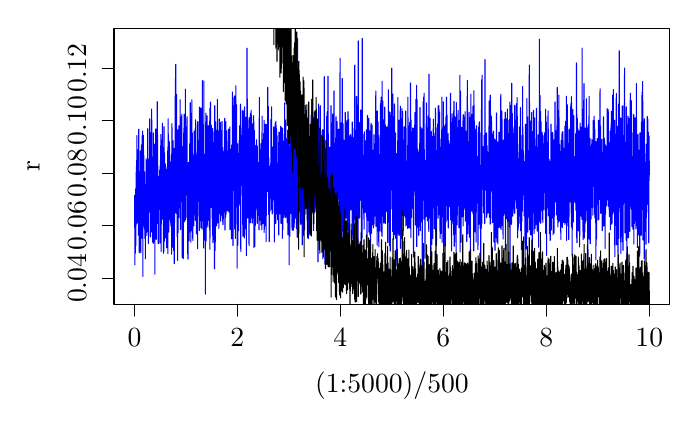
\begin{tikzpicture}[x=0.7pt,y=0.7pt]
\definecolor{fillColor}{RGB}{255,255,255}
%\path[use as bounding box,fill=fillColor,fill opacity=0.00] (0,0) rectangle (361.35,252.94);
\begin{scope}
%\path[clip] ( 49.20, 61.20) rectangle (336.15,203.75);
\definecolor{drawColor}{RGB}{0,0,255}

\path[draw=drawColor,line width= 0.4pt,line join=round,line cap=round] ( 59.83,102.53) --
	( 59.88,117.51) --
	( 59.93,110.92) --
	( 59.99, 81.59) --
	( 60.04, 95.55) --
	( 60.09,106.83) --
	( 60.15, 99.51) --
	( 60.20, 90.56) --
	( 60.25, 87.56) --
	( 60.31,111.28) --
	( 60.36,120.84) --
	( 60.41,104.95) --
	( 60.47, 91.41) --
	( 60.52,101.93) --
	( 60.57,101.84) --
	( 60.63,108.87) --
	( 60.68,129.50) --
	( 60.73,105.94) --
	( 60.78,132.62) --
	( 60.84,127.54) --
	( 60.89,127.18) --
	( 60.94,103.07) --
	( 61.00,148.32) --
	( 61.05,116.03) --
	( 61.10,136.70) --
	( 61.16,103.71) --
	( 61.21,115.94) --
	( 61.26,124.89) --
	( 61.32,118.61) --
	( 61.37,117.21) --
	( 61.42,118.08) --
	( 61.48,128.23) --
	( 61.53,138.59) --
	( 61.58,141.08) --
	( 61.63,121.13) --
	( 61.69,103.18) --
	( 61.74,107.36) --
	( 61.79, 96.94) --
	( 61.85,117.11) --
	( 61.90,136.80) --
	( 61.95,115.55) --
	( 62.01,151.60) --
	( 62.06,139.72) --
	( 62.11,122.45) --
	( 62.17,109.08) --
	( 62.22,116.78) --
	( 62.27, 87.89) --
	( 62.33,129.80) --
	( 62.38,121.23) --
	( 62.43,116.93) --
	( 62.49,122.10) --
	( 62.54,117.50) --
	( 62.59,105.32) --
	( 62.64, 91.00) --
	( 62.70,116.43) --
	( 62.75,127.01) --
	( 62.80, 88.81) --
	( 62.86,122.59) --
	( 62.91,140.39) --
	( 62.96,103.03) --
	( 63.02,112.07) --
	( 63.07, 87.72) --
	( 63.12,124.88) --
	( 63.18,125.33) --
	( 63.23, 96.22) --
	( 63.28,109.72) --
	( 63.34,118.83) --
	( 63.39,143.51) --
	( 63.44,121.59) --
	( 63.50, 95.44) --
	( 63.55,124.83) --
	( 63.60,118.45) --
	( 63.65,105.15) --
	( 63.71,118.34) --
	( 63.76,148.15) --
	( 63.81,117.71) --
	( 63.87,123.57) --
	( 63.92,133.30) --
	( 63.97,150.66) --
	( 64.03,108.26) --
	( 64.08,108.24) --
	( 64.13, 75.57) --
	( 64.19,136.36) --
	( 64.24,109.78) --
	( 64.29,108.72) --
	( 64.35,148.47) --
	( 64.40,144.76) --
	( 64.45,128.06) --
	( 64.50,110.91) --
	( 64.56,120.92) --
	( 64.61,138.01) --
	( 64.66,111.40) --
	( 64.72,114.73) --
	( 64.77,119.70) --
	( 64.82,115.18) --
	( 64.88,101.70) --
	( 64.93,129.58) --
	( 64.98,125.75) --
	( 65.04,100.43) --
	( 65.09,103.92) --
	( 65.14, 95.27) --
	( 65.20,115.13) --
	( 65.25,106.46) --
	( 65.30,123.20) --
	( 65.36,118.90) --
	( 65.41, 84.77) --
	( 65.46,106.05) --
	( 65.51,110.37) --
	( 65.57,115.41) --
	( 65.62,121.27) --
	( 65.67,100.10) --
	( 65.73,108.34) --
	( 65.78, 96.71) --
	( 65.83,136.39) --
	( 65.89,112.49) --
	( 65.94,120.91) --
	( 65.99,119.60) --
	( 66.05,111.86) --
	( 66.10,127.16) --
	( 66.15,126.39) --
	( 66.21, 98.57) --
	( 66.26,103.99) --
	( 66.31,120.65) --
	( 66.37,116.08) --
	( 66.42,131.15) --
	( 66.47,108.82) --
	( 66.52, 99.67) --
	( 66.58,108.60) --
	( 66.63,151.84) --
	( 66.68,119.43) --
	( 66.74,125.23) --
	( 66.79,106.40) --
	( 66.84,122.57) --
	( 66.90, 99.57) --
	( 66.95, 92.68) --
	( 67.00,107.40) --
	( 67.06,110.64) --
	( 67.11,135.33) --
	( 67.16, 96.30) --
	( 67.22,118.67) --
	( 67.27,136.15) --
	( 67.32,115.85) --
	( 67.38,123.15) --
	( 67.43,109.90) --
	( 67.48,114.43) --
	( 67.53,108.88) --
	( 67.59,146.39) --
	( 67.64,127.89) --
	( 67.69,157.01) --
	( 67.75,145.77) --
	( 67.80,124.32) --
	( 67.85,130.44) --
	( 67.91,143.71) --
	( 67.96,121.52) --
	( 68.01,149.83) --
	( 68.07,114.50) --
	( 68.12, 95.94) --
	( 68.17,111.95) --
	( 68.23,113.78) --
	( 68.28,131.20) --
	( 68.33,119.20) --
	( 68.38,123.36) --
	( 68.44,113.00) --
	( 68.49,115.02) --
	( 68.54,149.00) --
	( 68.60,125.33) --
	( 68.65,162.05) --
	( 68.70,149.08) --
	( 68.76, 98.63) --
	( 68.81,124.15) --
	( 68.86,131.09) --
	( 68.92,122.60) --
	( 68.97,108.31) --
	( 69.02,137.29) --
	( 69.08, 99.32) --
	( 69.13,127.95) --
	( 69.18,134.65) --
	( 69.24, 93.28) --
	( 69.29,108.42) --
	( 69.34,118.04) --
	( 69.39,134.86) --
	( 69.45, 92.72) --
	( 69.50,128.47) --
	( 69.55,149.69) --
	( 69.61,128.81) --
	( 69.66,140.90) --
	( 69.71,107.49) --
	( 69.77, 93.50) --
	( 69.82,125.61) --
	( 69.87,118.84) --
	( 69.93,130.50) --
	( 69.98,132.73) --
	( 70.03,106.44) --
	( 70.09,143.95) --
	( 70.14,118.11) --
	( 70.19, 97.80) --
	( 70.25,126.95) --
	( 70.30, 76.75) --
	( 70.35,111.17) --
	( 70.40,117.71) --
	( 70.46,105.57) --
	( 70.51,117.63) --
	( 70.56,112.91) --
	( 70.62,110.68) --
	( 70.67,126.19) --
	( 70.72,113.29) --
	( 70.78,151.73) --
	( 70.83,126.19) --
	( 70.88,139.38) --
	( 70.94,127.05) --
	( 70.99,105.45) --
	( 71.04, 94.75) --
	( 71.10,128.08) --
	( 71.15,117.25) --
	( 71.20,138.26) --
	( 71.25,116.40) --
	( 71.31,103.77) --
	( 71.36,141.25) --
	( 71.41,111.04) --
	( 71.47,102.97) --
	( 71.52,165.85) --
	( 71.57,134.89) --
	( 71.63,112.11) --
	( 71.68,115.63) --
	( 71.73,149.03) --
	( 71.79,110.84) --
	( 71.84,132.88) --
	( 71.89,128.34) --
	( 71.95,104.62) --
	( 72.00,111.29) --
	( 72.05, 92.42) --
	( 72.11,100.26) --
	( 72.16,115.01) --
	( 72.21,115.61) --
	( 72.26,127.22) --
	( 72.32,123.08) --
	( 72.37,113.51) --
	( 72.42,110.24) --
	( 72.48,113.77) --
	( 72.53,125.76) --
	( 72.58,112.84) --
	( 72.64,115.25) --
	( 72.69,125.09) --
	( 72.74,111.29) --
	( 72.80,130.52) --
	( 72.85,122.32) --
	( 72.90,129.54) --
	( 72.96, 92.81) --
	( 73.01,130.60) --
	( 73.06,132.44) --
	( 73.12,132.30) --
	( 73.17,135.66) --
	( 73.22,116.85) --
	( 73.27,135.51) --
	( 73.33,110.43) --
	( 73.38,148.92) --
	( 73.43,129.69) --
	( 73.49,120.52) --
	( 73.54, 88.46) --
	( 73.59,146.16) --
	( 73.65,102.55) --
	( 73.70,119.02) --
	( 73.75,110.21) --
	( 73.81,106.84) --
	( 73.86,120.09) --
	( 73.91,112.25) --
	( 73.97,142.67) --
	( 74.02,120.18) --
	( 74.07,124.21) --
	( 74.12,128.49) --
	( 74.18,154.68) --
	( 74.23,123.88) --
	( 74.28,105.18) --
	( 74.34,137.09) --
	( 74.39,142.36) --
	( 74.44,139.58) --
	( 74.50,121.52) --
	( 74.55,127.25) --
	( 74.60,111.02) --
	( 74.66,108.66) --
	( 74.71, 87.60) --
	( 74.76,134.38) --
	( 74.82, 99.45) --
	( 74.87,111.11) --
	( 74.92,113.28) --
	( 74.98, 88.48) --
	( 75.03,152.93) --
	( 75.08,106.04) --
	( 75.13, 93.72) --
	( 75.19,127.54) --
	( 75.24,113.58) --
	( 75.29, 99.44) --
	( 75.35,139.49) --
	( 75.40,120.05) --
	( 75.45,126.41) --
	( 75.51,122.84) --
	( 75.56,120.47) --
	( 75.61,119.56) --
	( 75.67,133.64) --
	( 75.72, 95.53) --
	( 75.77,123.28) --
	( 75.83,116.80) --
	( 75.88,132.50) --
	( 75.93,131.90) --
	( 75.99,130.63) --
	( 76.04,111.84) --
	( 76.09,104.10) --
	( 76.14,103.98) --
	( 76.20,116.96) --
	( 76.25,117.65) --
	( 76.30,129.06) --
	( 76.36,115.30) --
	( 76.41, 90.40) --
	( 76.46,130.89) --
	( 76.52,118.20) --
	( 76.57,123.29) --
	( 76.62,121.04) --
	( 76.68, 96.63) --
	( 76.73,128.21) --
	( 76.78,111.88) --
	( 76.84,124.89) --
	( 76.89,133.51) --
	( 76.94,140.56) --
	( 77.00, 87.32) --
	( 77.05, 93.80) --
	( 77.10,136.36) --
	( 77.15,157.04) --
	( 77.21,101.07) --
	( 77.26,104.86) --
	( 77.31,149.16) --
	( 77.37,131.36) --
	( 77.42,109.15) --
	( 77.47,137.23) --
	( 77.53, 98.57) --
	( 77.58,104.75) --
	( 77.63,110.87) --
	( 77.69,129.16) --
	( 77.74,145.19) --
	( 77.79,112.81) --
	( 77.85,124.84) --
	( 77.90,110.79) --
	( 77.95,142.16) --
	( 78.00,125.66) --
	( 78.06,128.66) --
	( 78.11,110.60) --
	( 78.16,127.24) --
	( 78.22,134.50) --
	( 78.27,105.10) --
	( 78.32,118.17) --
	( 78.38,134.70) --
	( 78.43,134.31) --
	( 78.48,118.02) --
	( 78.54,101.68) --
	( 78.59,116.06) --
	( 78.64,110.58) --
	( 78.70,123.20) --
	( 78.75,106.23) --
	( 78.80,125.60) --
	( 78.86,133.78) --
	( 78.91,120.96) --
	( 78.96, 87.09) --
	( 79.01,138.98) --
	( 79.07,115.11) --
	( 79.12,154.46) --
	( 79.17,133.54) --
	( 79.23,117.39) --
	( 79.28, 90.67) --
	( 79.33,126.27) --
	( 79.39,138.36) --
	( 79.44,103.12) --
	( 79.49,104.60) --
	( 79.55,142.75) --
	( 79.60,117.93) --
	( 79.65,129.44) --
	( 79.71,128.05) --
	( 79.76,145.66) --
	( 79.81,121.82) --
	( 79.87,109.26) --
	( 79.92,120.38) --
	( 79.97,110.50) --
	( 80.02,106.90) --
	( 80.08, 88.96) --
	( 80.13,123.63) --
	( 80.18,107.06) --
	( 80.24,141.69) --
	( 80.29, 82.24) --
	( 80.34,117.12) --
	( 80.40,134.29) --
	( 80.45,119.07) --
	( 80.50,103.18) --
	( 80.56,137.88) --
	( 80.61,108.51) --
	( 80.66,134.88) --
	( 80.72,108.87) --
	( 80.77,120.71) --
	( 80.82,140.64) --
	( 80.87,178.11) --
	( 80.93,135.75) --
	( 80.98,160.22) --
	( 81.03,151.73) --
	( 81.09,185.10) --
	( 81.14,140.34) --
	( 81.19,108.30) --
	( 81.25,150.19) --
	( 81.30,118.16) --
	( 81.35,115.10) --
	( 81.41,111.02) --
	( 81.46,169.64) --
	( 81.51,123.44) --
	( 81.57,122.70) --
	( 81.62,114.02) --
	( 81.67,124.09) --
	( 81.73,123.89) --
	( 81.78, 97.78) --
	( 81.83, 96.07) --
	( 81.88,107.90) --
	( 81.94,127.93) --
	( 81.99,138.30) --
	( 82.04, 83.89) --
	( 82.10,124.91) --
	( 82.15,151.26) --
	( 82.20,106.64) --
	( 82.26,112.33) --
	( 82.31, 98.21) --
	( 82.36,114.12) --
	( 82.42,108.68) --
	( 82.47,105.78) --
	( 82.52,127.08) --
	( 82.58,113.75) --
	( 82.63,123.69) --
	( 82.68,105.98) --
	( 82.74,153.40) --
	( 82.79,110.81) --
	( 82.84,136.62) --
	( 82.89,128.19) --
	( 82.95,119.11) --
	( 83.00,127.65) --
	( 83.05,141.79) --
	( 83.11,115.60) --
	( 83.16,123.29) --
	( 83.21,127.20) --
	( 83.27,137.50) --
	( 83.32,113.48) --
	( 83.37,166.88) --
	( 83.43,113.46) --
	( 83.48,115.97) --
	( 83.53, 99.84) --
	( 83.59,153.75) --
	( 83.64,113.33) --
	( 83.69,134.87) --
	( 83.75,122.36) --
	( 83.80,132.23) --
	( 83.85,119.51) --
	( 83.90,158.08) --
	( 83.96,145.61) --
	( 84.01,137.29) --
	( 84.06,128.92) --
	( 84.12,138.72) --
	( 84.17,130.99) --
	( 84.22,159.35) --
	( 84.28,146.31) --
	( 84.33,120.72) --
	( 84.38,140.52) --
	( 84.44, 85.33) --
	( 84.49,142.66) --
	( 84.54,119.25) --
	( 84.60,136.20) --
	( 84.65,134.53) --
	( 84.70,131.13) --
	( 84.75,122.44) --
	( 84.81,121.86) --
	( 84.86,137.82) --
	( 84.91,125.33) --
	( 84.97, 84.82) --
	( 85.02,109.53) --
	( 85.07,117.35) --
	( 85.13,149.71) --
	( 85.18,132.22) --
	( 85.23,114.47) --
	( 85.29,106.45) --
	( 85.34,137.33) --
	( 85.39,159.17) --
	( 85.45,112.94) --
	( 85.50,120.39) --
	( 85.55,159.28) --
	( 85.61,122.29) --
	( 85.66,103.86) --
	( 85.71,153.06) --
	( 85.76,111.11) --
	( 85.82,140.83) --
	( 85.87,143.03) --
	( 85.92,136.08) --
	( 85.98,115.22) --
	( 86.03,127.05) --
	( 86.08,172.27) --
	( 86.14,104.89) --
	( 86.19,140.65) --
	( 86.24,122.91) --
	( 86.30,118.05) --
	( 86.35,122.17) --
	( 86.40,152.13) --
	( 86.46,117.66) --
	( 86.51,147.92) --
	( 86.56,119.30) --
	( 86.62,132.26) --
	( 86.67,130.20) --
	( 86.72,123.70) --
	( 86.77,118.45) --
	( 86.83,132.08) --
	( 86.88,122.01) --
	( 86.93,158.07) --
	( 86.99,106.06) --
	( 87.04,107.32) --
	( 87.09,109.13) --
	( 87.15,133.86) --
	( 87.20,132.89) --
	( 87.25,108.88) --
	( 87.31, 87.08) --
	( 87.36,114.69) --
	( 87.41, 84.62) --
	( 87.47, 84.70) --
	( 87.52,122.78) --
	( 87.57,119.47) --
	( 87.62, 98.40) --
	( 87.68,134.52) --
	( 87.73,115.61) --
	( 87.78,113.74) --
	( 87.84,117.92) --
	( 87.89,105.68) --
	( 87.94, 94.04) --
	( 88.00,116.18) --
	( 88.05,112.07) --
	( 88.10,108.05) --
	( 88.16,125.79) --
	( 88.21,106.05) --
	( 88.26,136.19) --
	( 88.32,144.20) --
	( 88.37, 98.59) --
	( 88.42,114.87) --
	( 88.48,123.65) --
	( 88.53,119.33) --
	( 88.58,165.31) --
	( 88.63,121.68) --
	( 88.69,145.21) --
	( 88.74,111.19) --
	( 88.79,117.99) --
	( 88.85,139.63) --
	( 88.90, 93.30) --
	( 88.95,138.44) --
	( 89.01,136.84) --
	( 89.06,142.12) --
	( 89.11,148.39) --
	( 89.17,114.84) --
	( 89.22,111.99) --
	( 89.27,133.45) --
	( 89.33, 99.26) --
	( 89.38,166.83) --
	( 89.43,113.86) --
	( 89.49,139.02) --
	( 89.54,139.25) --
	( 89.59,149.74) --
	( 89.64,123.17) --
	( 89.70,105.13) --
	( 89.75,128.37) --
	( 89.80,129.99) --
	( 89.86, 97.12) --
	( 89.91, 94.16) --
	( 89.96,137.98) --
	( 90.02,116.80) --
	( 90.07,115.81) --
	( 90.12,115.27) --
	( 90.18,118.62) --
	( 90.23,120.67) --
	( 90.28,125.76) --
	( 90.34,132.26) --
	( 90.39,121.80) --
	( 90.44,101.69) --
	( 90.50,109.57) --
	( 90.55,150.56) --
	( 90.60,132.15) --
	( 90.65,132.05) --
	( 90.71,146.57) --
	( 90.76,134.73) --
	( 90.81,110.34) --
	( 90.87,148.48) --
	( 90.92,148.82) --
	( 90.97,139.34) --
	( 91.03,141.70) --
	( 91.08,115.92) --
	( 91.13,151.85) --
	( 91.19,123.33) --
	( 91.24,141.17) --
	( 91.29,104.53) --
	( 91.35,156.48) --
	( 91.40,153.10) --
	( 91.45,121.88) --
	( 91.50,141.31) --
	( 91.56,111.46) --
	( 91.61,116.28) --
	( 91.66,122.07) --
	( 91.72, 97.53) --
	( 91.77,138.31) --
	( 91.82,109.85) --
	( 91.88,121.59) --
	( 91.93,130.45) --
	( 91.98,122.42) --
	( 92.04,122.63) --
	( 92.09,129.51) --
	( 92.14,127.19) --
	( 92.20,117.26) --
	( 92.25,139.93) --
	( 92.30,117.63) --
	( 92.36, 89.97) --
	( 92.41,121.34) --
	( 92.46,155.50) --
	( 92.51,138.39) --
	( 92.57,127.82) --
	( 92.62,128.24) --
	( 92.67,138.93) --
	( 92.73,121.38) --
	( 92.78,124.07) --
	( 92.83,115.36) --
	( 92.89,114.43) --
	( 92.94,145.62) --
	( 92.99,127.42) --
	( 93.05,138.30) --
	( 93.10,131.00) --
	( 93.15,115.01) --
	( 93.21,127.24) --
	( 93.26, 99.28) --
	( 93.31,142.97) --
	( 93.37,163.05) --
	( 93.42,104.20) --
	( 93.47,128.23) --
	( 93.52,134.17) --
	( 93.58,151.21) --
	( 93.63,110.53) --
	( 93.68,105.66) --
	( 93.74,112.42) --
	( 93.79,108.50) --
	( 93.84,127.08) --
	( 93.90,159.94) --
	( 93.95,135.99) --
	( 94.00,110.94) --
	( 94.06,100.75) --
	( 94.11,162.53) --
	( 94.16,141.55) --
	( 94.22,114.95) --
	( 94.27,139.22) --
	( 94.32,152.49) --
	( 94.37,149.08) --
	( 94.43,109.65) --
	( 94.48,102.70) --
	( 94.53,100.46) --
	( 94.59,157.11) --
	( 94.64,143.39) --
	( 94.69, 99.98) --
	( 94.75,125.27) --
	( 94.80,142.31) --
	( 94.85,176.73) --
	( 94.91,104.20) --
	( 94.96,122.25) --
	( 95.01,129.88) --
	( 95.07,117.06) --
	( 95.12,148.55) --
	( 95.17,136.32) --
	( 95.23,119.13) --
	( 95.28,121.85) --
	( 95.33,108.04) --
	( 95.38,154.11) --
	( 95.44,120.39) --
	( 95.49, 90.31) --
	( 95.54, 98.57) --
	( 95.60,176.49) --
	( 95.65,131.54) --
	( 95.70,109.70) --
	( 95.76,127.16) --
	( 95.81,114.48) --
	( 95.86,138.77) --
	( 95.92,107.36) --
	( 95.97,120.35) --
	( 96.02,118.40) --
	( 96.08,125.71) --
	( 96.13, 94.27) --
	( 96.18,132.28) --
	( 96.24,108.14) --
	( 96.29,104.80) --
	( 96.34,123.37) --
	( 96.39, 66.48) --
	( 96.45,123.74) --
	( 96.50,150.98) --
	( 96.55,126.82) --
	( 96.61,159.93) --
	( 96.66,122.18) --
	( 96.71, 94.01) --
	( 96.77,126.18) --
	( 96.82,145.42) --
	( 96.87,126.12) --
	( 96.93,100.86) --
	( 96.98,117.00) --
	( 97.03,142.38) --
	( 97.09,129.91) --
	( 97.14,126.51) --
	( 97.19,120.22) --
	( 97.25,158.53) --
	( 97.30,119.54) --
	( 97.35,118.27) --
	( 97.40,121.36) --
	( 97.46,115.15) --
	( 97.51,147.81) --
	( 97.56,135.02) --
	( 97.62,103.21) --
	( 97.67,101.15) --
	( 97.72,132.16) --
	( 97.78,150.16) --
	( 97.83,121.15) --
	( 97.88,153.45) --
	( 97.94,123.99) --
	( 97.99,104.53) --
	( 98.04,138.66) --
	( 98.10,122.69) --
	( 98.15,123.92) --
	( 98.20,113.52) --
	( 98.25,120.93) --
	( 98.31,151.55) --
	( 98.36,149.70) --
	( 98.41,133.10) --
	( 98.47,111.23) --
	( 98.52,134.47) --
	( 98.57, 99.67) --
	( 98.63,137.91) --
	( 98.68,162.35) --
	( 98.73, 89.63) --
	( 98.79,123.88) --
	( 98.84,151.00) --
	( 98.89,149.55) --
	( 98.95,117.70) --
	( 99.00,126.69) --
	( 99.05,165.64) --
	( 99.11,129.19) --
	( 99.16,115.68) --
	( 99.21,126.82) --
	( 99.26,127.19) --
	( 99.32,138.07) --
	( 99.37,115.08) --
	( 99.42,153.54) --
	( 99.48,111.28) --
	( 99.53,117.71) --
	( 99.58,114.87) --
	( 99.64,147.52) --
	( 99.69,138.53) --
	( 99.74,142.35) --
	( 99.80,123.73) --
	( 99.85,126.11) --
	( 99.90,105.77) --
	( 99.96,136.76) --
	(100.01,116.35) --
	(100.06,101.08) --
	(100.12,151.90) --
	(100.17,121.73) --
	(100.22, 94.20) --
	(100.27, 93.08) --
	(100.33,150.39) --
	(100.38, 94.33) --
	(100.43,120.31) --
	(100.49,113.56) --
	(100.54,128.53) --
	(100.59,141.90) --
	(100.65,102.61) --
	(100.70,137.87) --
	(100.75,126.75) --
	(100.81,142.40) --
	(100.86,140.81) --
	(100.91,114.06) --
	(100.97,144.85) --
	(101.02,110.51) --
	(101.07, 79.58) --
	(101.12,115.22) --
	(101.18,154.51) --
	(101.23,163.82) --
	(101.28,121.76) --
	(101.34,132.31) --
	(101.39,126.47) --
	(101.44, 89.00) --
	(101.50,113.19) --
	(101.55,123.98) --
	(101.60,120.96) --
	(101.66,155.42) --
	(101.71,104.92) --
	(101.76,105.98) --
	(101.82,141.25) --
	(101.87,150.88) --
	(101.92,122.81) --
	(101.98,107.23) --
	(102.03,112.53) --
	(102.08,122.58) --
	(102.13,134.85) --
	(102.19,101.64) --
	(102.24,146.16) --
	(102.29,139.48) --
	(102.35,115.60) --
	(102.40,138.78) --
	(102.45,134.60) --
	(102.51,131.64) --
	(102.56,167.00) --
	(102.61,148.95) --
	(102.67,134.33) --
	(102.72,103.26) --
	(102.77,116.90) --
	(102.83,125.16) --
	(102.88,125.65) --
	(102.93,142.29) --
	(102.99,141.66) --
	(103.04,142.58) --
	(103.09,138.78) --
	(103.14,142.36) --
	(103.20,150.84) --
	(103.25,105.30) --
	(103.30,130.15) --
	(103.36,100.34) --
	(103.41,149.70) --
	(103.46,113.21) --
	(103.52,140.62) --
	(103.57,156.90) --
	(103.62,108.17) --
	(103.68,113.77) --
	(103.73,121.22) --
	(103.78,115.01) --
	(103.84,123.37) --
	(103.89,138.88) --
	(103.94,142.30) --
	(104.00,121.57) --
	(104.05,116.07) --
	(104.10,107.87) --
	(104.15,155.03) --
	(104.21,128.58) --
	(104.26,104.13) --
	(104.31,106.46) --
	(104.37,143.25) --
	(104.42,117.68) --
	(104.47,128.02) --
	(104.53,119.59) --
	(104.58,116.32) --
	(104.63,150.76) --
	(104.69,148.76) --
	(104.74,107.21) --
	(104.79,131.24) --
	(104.85,127.05) --
	(104.90,120.52) --
	(104.95,155.59) --
	(105.00,137.68) --
	(105.06,127.63) --
	(105.11,125.86) --
	(105.16,111.45) --
	(105.22,129.99) --
	(105.27,133.72) --
	(105.32,142.00) --
	(105.38,102.30) --
	(105.43,125.60) --
	(105.48,102.36) --
	(105.54,131.02) --
	(105.59,120.48) --
	(105.64,139.32) --
	(105.70,105.36) --
	(105.75,124.03) --
	(105.80,130.65) --
	(105.86,114.87) --
	(105.91,121.86) --
	(105.96,122.01) --
	(106.01,108.90) --
	(106.07,117.91) --
	(106.12,121.10) --
	(106.17,151.10) --
	(106.23,122.53) --
	(106.28,135.87) --
	(106.33,121.20) --
	(106.39,157.21) --
	(106.44,129.39) --
	(106.49, 99.53) --
	(106.55,128.58) --
	(106.60,153.34) --
	(106.65,108.12) --
	(106.71,133.25) --
	(106.76,154.39) --
	(106.81,106.21) --
	(106.87,132.95) --
	(106.92,109.41) --
	(106.97,155.49) --
	(107.02,130.44) --
	(107.08,107.78) --
	(107.13,123.59) --
	(107.18,117.31) --
	(107.24,138.04) --
	(107.29,150.71) --
	(107.34,129.64) --
	(107.40,145.48) --
	(107.45,130.20) --
	(107.50,139.81) --
	(107.56,125.36) --
	(107.61,135.88) --
	(107.66,131.80) --
	(107.72,136.53) --
	(107.77,140.34) --
	(107.82,109.43) --
	(107.87,132.17) --
	(107.93,125.18) --
	(107.98,114.53) --
	(108.03,111.05) --
	(108.09,120.48) --
	(108.14,110.56) --
	(108.19,119.44) --
	(108.25,115.54) --
	(108.30,151.58) --
	(108.35,113.34) --
	(108.41,133.76) --
	(108.46,151.58) --
	(108.51,114.15) --
	(108.57,108.79) --
	(108.62,140.70) --
	(108.67,116.07) --
	(108.73,120.76) --
	(108.78,114.09) --
	(108.83,116.48) --
	(108.88,126.16) --
	(108.94,129.21) --
	(108.99,111.66) --
	(109.04,152.82) --
	(109.10, 99.84) --
	(109.15,139.08) --
	(109.20,137.45) --
	(109.26,111.78) --
	(109.31,116.11) --
	(109.36,105.84) --
	(109.42,127.31) --
	(109.47,141.23) --
	(109.52,122.79) --
	(109.58,113.68) --
	(109.63,131.11) --
	(109.68,141.14) --
	(109.74,134.45) --
	(109.79,122.45) --
	(109.84,129.05) --
	(109.89, 95.06) --
	(109.95,102.44) --
	(110.00,143.45) --
	(110.05,106.89) --
	(110.11,120.35) --
	(110.16,105.98) --
	(110.21,130.94) --
	(110.27,118.60) --
	(110.32,170.82) --
	(110.37,128.02) --
	(110.43, 95.40) --
	(110.48,142.23) --
	(110.53,125.17) --
	(110.59,110.78) --
	(110.64, 91.60) --
	(110.69,127.49) --
	(110.75,163.62) --
	(110.80,158.68) --
	(110.85,127.24) --
	(110.90,154.24) --
	(110.96,119.95) --
	(111.01,149.58) --
	(111.06,141.10) --
	(111.12,158.11) --
	(111.17,168.10) --
	(111.22,126.34) --
	(111.28,137.38) --
	(111.33,124.19) --
	(111.38,123.82) --
	(111.44,168.79) --
	(111.49,100.15) --
	(111.54,117.75) --
	(111.60,116.79) --
	(111.65,110.39) --
	(111.70,110.07) --
	(111.75,131.24) --
	(111.81,141.60) --
	(111.86, 95.28) --
	(111.91,113.45) --
	(111.97,117.00) --
	(112.02,116.39) --
	(112.07,133.92) --
	(112.13,174.08) --
	(112.18,116.04) --
	(112.23,129.84) --
	(112.29,152.47) --
	(112.34,128.96) --
	(112.39,140.35) --
	(112.45,135.33) --
	(112.50,164.19) --
	(112.55,131.59) --
	(112.61,120.34) --
	(112.66,137.80) --
	(112.71,122.54) --
	(112.76, 79.85) --
	(112.82,101.26) --
	(112.87,123.84) --
	(112.92,134.62) --
	(112.98,105.45) --
	(113.03,144.06) --
	(113.08,118.21) --
	(113.14, 91.70) --
	(113.19,138.06) --
	(113.24,102.16) --
	(113.30,132.39) --
	(113.35,139.12) --
	(113.40,116.65) --
	(113.46,135.21) --
	(113.51, 99.32) --
	(113.56,125.76) --
	(113.62,122.75) --
	(113.67,124.47) --
	(113.72,118.20) --
	(113.77,136.13) --
	(113.83,145.79) --
	(113.88,131.27) --
	(113.93,143.91) --
	(113.99,127.57) --
	(114.04,119.04) --
	(114.09,153.40) --
	(114.15,123.51) --
	(114.20,113.06) --
	(114.25,151.28) --
	(114.31,114.42) --
	(114.36,153.11) --
	(114.41,112.17) --
	(114.47,145.58) --
	(114.52,164.49) --
	(114.57,102.66) --
	(114.62, 95.90) --
	(114.68, 88.52) --
	(114.73,142.03) --
	(114.78,125.54) --
	(114.84,117.73) --
	(114.89,125.07) --
	(114.94,143.45) --
	(115.00,126.69) --
	(115.05,123.38) --
	(115.10,133.37) --
	(115.16,127.63) --
	(115.21,145.59) --
	(115.26,148.64) --
	(115.32,148.20) --
	(115.37,128.71) --
	(115.42,146.68) --
	(115.48,161.29) --
	(115.53,135.36) --
	(115.58,133.25) --
	(115.63,107.68) --
	(115.69,104.17) --
	(115.74, 96.42) --
	(115.79,124.16) --
	(115.85,141.30) --
	(115.90,160.86) --
	(115.95,142.67) --
	(116.01,145.23) --
	(116.06,131.28) --
	(116.11,135.74) --
	(116.17,111.44) --
	(116.22,126.85) --
	(116.27,144.12) --
	(116.33,127.86) --
	(116.38,126.59) --
	(116.43, 95.59) --
	(116.49,130.67) --
	(116.54,110.23) --
	(116.59,161.73) --
	(116.64,163.15) --
	(116.70,136.84) --
	(116.75,121.51) --
	(116.80,111.44) --
	(116.86,121.17) --
	(116.91,122.57) --
	(116.96,100.32) --
	(117.02,115.23) --
	(117.07,139.06) --
	(117.12,132.90) --
	(117.18,157.79) --
	(117.23,130.63) --
	(117.28,110.81) --
	(117.34,140.36) --
	(117.39,107.18) --
	(117.44, 96.95) --
	(117.50,150.52) --
	(117.55, 86.38) --
	(117.60,124.34) --
	(117.65,143.25) --
	(117.71,106.64) --
	(117.76,127.74) --
	(117.81,151.84) --
	(117.87,193.47) --
	(117.92,134.17) --
	(117.97,140.86) --
	(118.03,148.71) --
	(118.08,167.31) --
	(118.13,138.01) --
	(118.19,120.12) --
	(118.24,105.73) --
	(118.29,134.42) --
	(118.35,149.17) --
	(118.40,132.44) --
	(118.45,120.08) --
	(118.50,143.70) --
	(118.56,115.95) --
	(118.61,116.74) --
	(118.66,151.82) --
	(118.72,113.63) --
	(118.77,115.14) --
	(118.82,112.89) --
	(118.88,110.62) --
	(118.93, 91.61) --
	(118.98, 98.10) --
	(119.04,157.58) --
	(119.09,114.57) --
	(119.14,132.47) --
	(119.20,152.06) --
	(119.25,112.80) --
	(119.30,129.06) --
	(119.36,120.01) --
	(119.41,124.72) --
	(119.46,120.94) --
	(119.51,141.78) --
	(119.57,103.29) --
	(119.62,110.36) --
	(119.67,159.80) --
	(119.73,131.31) --
	(119.78,126.27) --
	(119.83,110.90) --
	(119.89,105.86) --
	(119.94,114.74) --
	(119.99,161.39) --
	(120.05,158.31) --
	(120.10,109.84) --
	(120.15,116.35) --
	(120.21,123.84) --
	(120.26,158.12) --
	(120.31,120.33) --
	(120.37,119.28) --
	(120.42,116.01) --
	(120.47,137.84) --
	(120.52,107.44) --
	(120.58,103.22) --
	(120.63,145.89) --
	(120.68,125.79) --
	(120.74,137.08) --
	(120.79,142.62) --
	(120.84,154.36) --
	(120.90,110.77) --
	(120.95,110.29) --
	(121.00,154.23) --
	(121.06,105.91) --
	(121.11,111.73) --
	(121.16,140.65) --
	(121.22,138.11) --
	(121.27,125.82) --
	(121.32,158.62) --
	(121.37,125.94) --
	(121.43, 90.54) --
	(121.48,146.58) --
	(121.53,140.18) --
	(121.59,114.71) --
	(121.64,151.01) --
	(121.69,135.35) --
	(121.75,135.35) --
	(121.80,146.31) --
	(121.85, 91.08) --
	(121.91,136.73) --
	(121.96,127.30) --
	(122.01,132.59) --
	(122.07,128.69) --
	(122.12,143.25) --
	(122.17,101.90) --
	(122.23,127.07) --
	(122.28,136.39) --
	(122.33,115.43) --
	(122.38,142.41) --
	(122.44,116.31) --
	(122.49,118.71) --
	(122.54,110.94) --
	(122.60,123.57) --
	(122.65,111.38) --
	(122.70,114.14) --
	(122.76,111.93) --
	(122.81,146.17) --
	(122.86,139.12) --
	(122.92,126.44) --
	(122.97,109.71) --
	(123.02,114.44) --
	(123.08,124.20) --
	(123.13,126.65) --
	(123.18,103.05) --
	(123.24,142.91) --
	(123.29,118.33) --
	(123.34,128.18) --
	(123.39,117.85) --
	(123.45,122.21) --
	(123.50,131.58) --
	(123.55,127.27) --
	(123.61,128.40) --
	(123.66,124.25) --
	(123.71,134.35) --
	(123.77,107.12) --
	(123.82,132.00) --
	(123.87,123.32) --
	(123.93,118.11) --
	(123.98,128.78) --
	(124.03,133.23) --
	(124.09, 99.70) --
	(124.14,119.87) --
	(124.19,141.94) --
	(124.24,168.08) --
	(124.30,137.55) --
	(124.35,144.46) --
	(124.40,111.69) --
	(124.46,104.54) --
	(124.51,125.01) --
	(124.56,121.51) --
	(124.62,118.25) --
	(124.67,144.12) --
	(124.72,114.64) --
	(124.78,130.76) --
	(124.83,105.65) --
	(124.88,141.04) --
	(124.94,131.65) --
	(124.99,114.84) --
	(125.04,132.09) --
	(125.10,102.09) --
	(125.15,119.17) --
	(125.20,140.83) --
	(125.25,139.11) --
	(125.31,134.65) --
	(125.36,119.64) --
	(125.41,136.94) --
	(125.47,144.55) --
	(125.52, 99.71) --
	(125.57,149.94) --
	(125.63,119.56) --
	(125.68,158.40) --
	(125.73,139.82) --
	(125.79,137.52) --
	(125.84,120.08) --
	(125.89,116.31) --
	(125.95,126.72) --
	(126.00,127.14) --
	(126.05,120.28) --
	(126.11,102.91) --
	(126.16,133.09) --
	(126.21,131.80) --
	(126.26,146.41) --
	(126.32,119.54) --
	(126.37,127.75) --
	(126.42,121.48) --
	(126.48,107.64) --
	(126.53,149.47) --
	(126.58,116.56) --
	(126.64,121.06) --
	(126.69,156.21) --
	(126.74, 98.35) --
	(126.80,116.62) --
	(126.85,117.16) --
	(126.90,105.52) --
	(126.96,120.96) --
	(127.01,116.06) --
	(127.06,114.95) --
	(127.12,146.18) --
	(127.17,119.95) --
	(127.22,123.06) --
	(127.27,133.69) --
	(127.33,154.20) --
	(127.38,150.22) --
	(127.43,138.99) --
	(127.49,101.69) --
	(127.54,106.40) --
	(127.59,134.48) --
	(127.65,110.79) --
	(127.70,122.40) --
	(127.75, 93.61) --
	(127.81,122.41) --
	(127.86,134.43) --
	(127.91,129.23) --
	(127.97,121.58) --
	(128.02,154.00) --
	(128.07,130.91) --
	(128.12,143.35) --
	(128.18,120.29) --
	(128.23,137.32) --
	(128.28,137.25) --
	(128.34,154.05) --
	(128.39,120.16) --
	(128.44,124.49) --
	(128.50,119.54) --
	(128.55,133.26) --
	(128.60,173.15) --
	(128.66,140.48) --
	(128.71,135.49) --
	(128.76,154.88) --
	(128.82,146.96) --
	(128.87,163.40) --
	(128.92,128.08) --
	(128.98,116.48) --
	(129.03,136.93) --
	(129.08,107.61) --
	(129.13,136.71) --
	(129.19,109.44) --
	(129.24,124.52) --
	(129.29,120.47) --
	(129.35, 93.57) --
	(129.40,123.43) --
	(129.45,123.17) --
	(129.51,122.49) --
	(129.56,115.91) --
	(129.61,132.40) --
	(129.67,128.69) --
	(129.72,109.36) --
	(129.77,124.94) --
	(129.83,112.01) --
	(129.88,130.43) --
	(129.93,121.69) --
	(129.99,117.00) --
	(130.04,123.42) --
	(130.09,133.93) --
	(130.14,115.95) --
	(130.20,124.98) --
	(130.25,156.62) --
	(130.30,133.46) --
	(130.36,120.93) --
	(130.41,133.88) --
	(130.46,133.84) --
	(130.52,128.48) --
	(130.57,163.17) --
	(130.62,110.15) --
	(130.68,118.56) --
	(130.73,135.18) --
	(130.78,142.44) --
	(130.84,130.29) --
	(130.89,107.87) --
	(130.94,126.41) --
	(130.99,130.59) --
	(131.05,108.70) --
	(131.10,122.36) --
	(131.15,134.45) --
	(131.21,130.48) --
	(131.26,115.24) --
	(131.31,128.42) --
	(131.37,118.08) --
	(131.42,142.56) --
	(131.47,118.31) --
	(131.53,121.82) --
	(131.58,136.85) --
	(131.63,151.25) --
	(131.69,152.83) --
	(131.74,123.32) --
	(131.79,144.95) --
	(131.85,132.85) --
	(131.90,144.07) --
	(131.95,121.19) --
	(132.00, 93.44) --
	(132.06,138.22) --
	(132.11,131.53) --
	(132.16,144.05) --
	(132.22,110.77) --
	(132.27,145.69) --
	(132.32,116.50) --
	(132.38,154.82) --
	(132.43,120.72) --
	(132.48,119.70) --
	(132.54,149.39) --
	(132.59,126.67) --
	(132.64,102.91) --
	(132.70,105.58) --
	(132.75,103.22) --
	(132.80,155.77) --
	(132.86,144.28) --
	(132.91,130.59) --
	(132.96,131.38) --
	(133.01,107.75) --
	(133.07,141.76) --
	(133.12,146.48) --
	(133.17,151.83) --
	(133.23,117.10) --
	(133.28,111.72) --
	(133.33,148.33) --
	(133.39,135.77) --
	(133.44,121.48) --
	(133.49,134.44) --
	(133.55,117.06) --
	(133.60,115.88) --
	(133.65,128.64) --
	(133.71,115.52) --
	(133.76,104.80) --
	(133.81,115.87) --
	(133.87,120.13) --
	(133.92,114.83) --
	(133.97,115.66) --
	(134.02,116.32) --
	(134.08,109.05) --
	(134.13,109.22) --
	(134.18,135.00) --
	(134.24, 97.03) --
	(134.29,150.07) --
	(134.34,101.39) --
	(134.40,144.24) --
	(134.45,112.67) --
	(134.50,122.96) --
	(134.56,131.36) --
	(134.61,149.12) --
	(134.66,126.48) --
	(134.72,116.50) --
	(134.77,123.53) --
	(134.82,107.97) --
	(134.87,139.58) --
	(134.93,116.28) --
	(134.98,107.95) --
	(135.03,150.24) --
	(135.09,121.70) --
	(135.14,110.04) --
	(135.19,141.62) --
	(135.25,153.14) --
	(135.30,119.22) --
	(135.35,138.66) --
	(135.41,103.04) --
	(135.46,107.85) --
	(135.51,119.82) --
	(135.57,128.17) --
	(135.62,138.58) --
	(135.67,149.59) --
	(135.73,110.54) --
	(135.78,136.15) --
	(135.83,152.44) --
	(135.88,110.75) --
	(135.94,141.06) --
	(135.99,115.91) --
	(136.04,150.51) --
	(136.10, 95.30) --
	(136.15,111.10) --
	(136.20,132.66) --
	(136.26,152.04) --
	(136.31, 99.69) --
	(136.36,113.43) --
	(136.42,123.30) --
	(136.47,120.13) --
	(136.52,129.46) --
	(136.58,139.39) --
	(136.63,120.07) --
	(136.68,112.60) --
	(136.74,117.67) --
	(136.79,111.42) --
	(136.84,145.44) --
	(136.89,135.10) --
	(136.95,132.24) --
	(137.00,106.04) --
	(137.05,143.91) --
	(137.11,136.76) --
	(137.16,130.27) --
	(137.21,107.46) --
	(137.27,165.19) --
	(137.32,127.85) --
	(137.37,151.93) --
	(137.43,150.36) --
	(137.48,131.20) --
	(137.53,119.09) --
	(137.59,152.40) --
	(137.64,119.79) --
	(137.69,129.47) --
	(137.74,110.41) --
	(137.80,156.38) --
	(137.85,106.08) --
	(137.90,154.84) --
	(137.96,113.61) --
	(138.01,129.55) --
	(138.06,140.68) --
	(138.12,139.86) --
	(138.17,137.20) --
	(138.22,146.09) --
	(138.28,139.32) --
	(138.33,115.42) --
	(138.38,146.60) --
	(138.44,131.28) --
	(138.49,123.05) --
	(138.54,122.79) --
	(138.60,103.42) --
	(138.65,141.17) --
	(138.70,110.63) --
	(138.75,118.42) --
	(138.81,151.13) --
	(138.86,111.67) --
	(138.91,115.00) --
	(138.97, 97.14) --
	(139.02,141.67) --
	(139.07,142.94) --
	(139.13,135.30) --
	(139.18,142.33) --
	(139.23,117.92) --
	(139.29,145.31) --
	(139.34,138.01) --
	(139.39,119.20) --
	(139.45,146.14) --
	(139.50,146.26) --
	(139.55,136.45) --
	(139.61, 81.67) --
	(139.66,139.58) --
	(139.71,110.58) --
	(139.76,142.96) --
	(139.82,119.74) --
	(139.87,121.71) --
	(139.92, 96.34) --
	(139.98,111.43) --
	(140.03,122.36) --
	(140.08,118.08) --
	(140.14,124.39) --
	(140.19,108.36) --
	(140.24,116.22) --
	(140.30,146.89) --
	(140.35,113.09) --
	(140.40,146.32) --
	(140.46,125.83) --
	(140.51,144.61) --
	(140.56,108.05) --
	(140.62,164.81) --
	(140.67,116.53) --
	(140.72,134.10) --
	(140.77,136.87) --
	(140.83,118.38) --
	(140.88,134.59) --
	(140.93,123.94) --
	(140.99,142.55) --
	(141.04,100.99) --
	(141.09,141.24) --
	(141.15,141.30) --
	(141.20,109.73) --
	(141.25, 99.47) --
	(141.31,121.29) --
	(141.36,112.59) --
	(141.41,140.39) --
	(141.47,118.34) --
	(141.52,146.90) --
	(141.57,131.55) --
	(141.62,133.20) --
	(141.68,137.40) --
	(141.73,153.78) --
	(141.78, 99.47) --
	(141.84,106.46) --
	(141.89,118.65) --
	(141.94,102.70) --
	(142.00,150.51) --
	(142.05,115.96) --
	(142.10,123.54) --
	(142.16,113.05) --
	(142.21,100.98) --
	(142.26,105.86) --
	(142.32,141.44) --
	(142.37,157.19) --
	(142.42,122.57) --
	(142.48,113.89) --
	(142.53,128.40) --
	(142.58,153.50) --
	(142.63,142.13) --
	(142.69,118.20) --
	(142.74,130.13) --
	(142.79,105.77) --
	(142.85,114.88) --
	(142.90,113.11) --
	(142.95,119.78) --
	(143.01,134.22) --
	(143.06,127.00) --
	(143.11,123.83) --
	(143.17,107.46) --
	(143.22,116.55) --
	(143.27,119.84) --
	(143.33,165.14) --
	(143.38,100.38) --
	(143.43,117.51) --
	(143.49,121.03) --
	(143.54,166.59) --
	(143.59,102.62) --
	(143.64,154.96) --
	(143.70,108.56) --
	(143.75, 99.86) --
	(143.80, 95.86) --
	(143.86,122.25) --
	(143.91,198.46) --
	(143.96,132.87) --
	(144.02,133.21) --
	(144.07,121.99) --
	(144.12,156.56) --
	(144.18,136.09) --
	(144.23,101.16) --
	(144.28,136.88) --
	(144.34,110.26) --
	(144.39,136.26) --
	(144.44,146.02) --
	(144.49,108.31) --
	(144.55,118.88) --
	(144.60,109.20) --
	(144.65,135.70) --
	(144.71,127.09) --
	(144.76,125.11) --
	(144.81,136.53) --
	(144.87,152.04) --
	(144.92,114.89) --
	(144.97,142.07) --
	(145.03,128.92) --
	(145.08,110.33) --
	(145.13,116.50) --
	(145.19,155.75) --
	(145.24,128.08) --
	(145.29,120.96) --
	(145.35,103.53) --
	(145.40,140.24) --
	(145.45,116.56) --
	(145.50,126.36) --
	(145.56,114.27) --
	(145.61,102.48) --
	(145.66,143.79) --
	(145.72,122.11) --
	(145.77,135.08) --
	(145.82,134.07) --
	(145.88,115.48) --
	(145.93,115.91) --
	(145.98,143.88) --
	(146.04,145.39) --
	(146.09,154.37) --
	(146.14,133.73) --
	(146.20,148.14) --
	(146.25,141.57) --
	(146.30,132.61) --
	(146.36,139.02) --
	(146.41, 91.97) --
	(146.46,142.81) --
	(146.51,137.62) --
	(146.57,124.37) --
	(146.62,113.93) --
	(146.67,125.18) --
	(146.73, 96.43) --
	(146.78,105.09) --
	(146.83,135.22) --
	(146.89,115.69) --
	(146.94,101.22) --
	(146.99,120.85) --
	(147.05, 96.96) --
	(147.10,136.66) --
	(147.15,150.28) --
	(147.21,133.45) --
	(147.26,110.44) --
	(147.31,135.82) --
	(147.37,121.80) --
	(147.42,141.82) --
	(147.47,119.24) --
	(147.52,146.54) --
	(147.58, 99.70) --
	(147.63,125.44) --
	(147.68,135.75) --
	(147.74,128.34) --
	(147.79,107.68) --
	(147.84,134.17) --
	(147.90,142.04) --
	(147.95,163.96) --
	(148.00,134.45) --
	(148.06,131.43) --
	(148.11,110.91) --
	(148.16,125.21) --
	(148.22,147.25) --
	(148.27,110.64) --
	(148.32,121.13) --
	(148.37,117.98) --
	(148.43,138.88) --
	(148.48,135.64) --
	(148.53,133.54) --
	(148.59,137.50) --
	(148.64,115.07) --
	(148.69,138.62) --
	(148.75,126.28) --
	(148.80,119.39) --
	(148.85,154.39) --
	(148.91,106.93) --
	(148.96,104.60) --
	(149.01,110.29) --
	(149.07,143.50) --
	(149.12,117.47) --
	(149.17,123.09) --
	(149.23,132.16) --
	(149.28,120.00) --
	(149.33,117.14) --
	(149.38,124.91) --
	(149.44,117.24) --
	(149.49, 95.14) --
	(149.54,117.73) --
	(149.60,138.39) --
	(149.65,127.01) --
	(149.70,143.24) --
	(149.76,140.79) --
	(149.81,110.51) --
	(149.86,131.90) --
	(149.92,133.94) --
	(149.97,117.32) --
	(150.02,131.31) --
	(150.08,128.31) --
	(150.13,145.68) --
	(150.18,116.77) --
	(150.24,102.25) --
	(150.29,122.41) --
	(150.34,102.22) --
	(150.39,132.58) --
	(150.45,147.41) --
	(150.50,135.95) --
	(150.55,114.68) --
	(150.61,137.02) --
	(150.66,116.88) --
	(150.71,100.97) --
	(150.77,121.40) --
	(150.82,154.67) --
	(150.87,121.68) --
	(150.93,152.04) --
	(150.98,158.93) --
	(151.03,115.84) --
	(151.09,129.11) --
	(151.14,140.38) --
	(151.19,120.17) --
	(151.24,131.53) --
	(151.30,167.15) --
	(151.35,140.11) --
	(151.40,119.31) --
	(151.46,129.35) --
	(151.51,134.00) --
	(151.56,150.36) --
	(151.62,114.39) --
	(151.67,114.34) --
	(151.72,109.74) --
	(151.78,142.11) --
	(151.83,117.54) --
	(151.88,123.74) --
	(151.94,138.95) --
	(151.99,115.38) --
	(152.04,140.28) --
	(152.10,130.96) --
	(152.15,126.60) --
	(152.20, 99.29) --
	(152.25,125.53) --
	(152.31,116.06) --
	(152.36,109.82) --
	(152.41,114.58) --
	(152.47,108.16) --
	(152.52,116.10) --
	(152.57,160.37) --
	(152.63,137.26) --
	(152.68,129.97) --
	(152.73,150.96) --
	(152.79,119.32) --
	(152.84,153.22) --
	(152.89,110.95) --
	(152.95,111.62) --
	(153.00,108.91) --
	(153.05,125.58) --
	(153.11,118.78) --
	(153.16,123.76) --
	(153.21,136.30) --
	(153.26,135.34) --
	(153.32,132.81) --
	(153.37,134.44) --
	(153.42,154.01) --
	(153.48,134.73) --
	(153.53,116.59) --
	(153.58,120.87) --
	(153.64,153.99) --
	(153.69,135.30) --
	(153.74,116.80) --
	(153.80,108.86) --
	(153.85,110.70) --
	(153.90,116.89) --
	(153.96,107.89) --
	(154.01,121.15) --
	(154.06,112.74) --
	(154.12,109.13) --
	(154.17,137.26) --
	(154.22,156.07) --
	(154.27,150.78) --
	(154.33,128.81) --
	(154.38,105.73) --
	(154.43,137.81) --
	(154.49,127.91) --
	(154.54, 83.13) --
	(154.59,151.64) --
	(154.65,141.83) --
	(154.70,125.41) --
	(154.75,118.94) --
	(154.81,164.62) --
	(154.86,113.83) --
	(154.91,104.88) --
	(154.97,122.54) --
	(155.02,117.22) --
	(155.07,139.66) --
	(155.12,151.35) --
	(155.18,123.19) --
	(155.23,126.42) --
	(155.28,106.84) --
	(155.34,152.02) --
	(155.39,124.72) --
	(155.44,122.45) --
	(155.50,149.67) --
	(155.55,109.44) --
	(155.60,110.79) --
	(155.66,150.92) --
	(155.71,163.79) --
	(155.76,110.08) --
	(155.82,133.67) --
	(155.87,113.41) --
	(155.92,139.76) --
	(155.98,127.32) --
	(156.03,140.78) --
	(156.08,111.95) --
	(156.13, 97.64) --
	(156.19,148.33) --
	(156.24,140.66) --
	(156.29,139.74) --
	(156.35,148.25) --
	(156.40,121.21) --
	(156.45,104.24) --
	(156.51,137.26) --
	(156.56,116.04) --
	(156.61,136.76) --
	(156.67,120.97) --
	(156.72,150.87) --
	(156.77,147.22) --
	(156.83,114.19) --
	(156.88,138.99) --
	(156.93,106.64) --
	(156.99,151.39) --
	(157.04, 84.75) --
	(157.09,134.74) --
	(157.14,130.40) --
	(157.20,149.84) --
	(157.25, 97.57) --
	(157.30,125.57) --
	(157.36,109.22) --
	(157.41,138.68) --
	(157.46,108.45) --
	(157.52,128.99) --
	(157.57,123.50) --
	(157.62,143.90) --
	(157.68,150.03) --
	(157.73,178.72) --
	(157.78,122.75) --
	(157.84,117.64) --
	(157.89,113.72) --
	(157.94,127.29) --
	(157.99,117.04) --
	(158.05,101.73) --
	(158.10,138.54) --
	(158.15, 81.93) --
	(158.21,130.14) --
	(158.26,127.45) --
	(158.31,106.28) --
	(158.37,141.41) --
	(158.42,130.30) --
	(158.47,123.62) --
	(158.53,120.51) --
	(158.58,130.60) --
	(158.63,135.97) --
	(158.69,110.35) --
	(158.74,130.39) --
	(158.79,137.06) --
	(158.85,135.20) --
	(158.90,146.58) --
	(158.95,114.54) --
	(159.00,158.35) --
	(159.06,136.05) --
	(159.11,122.77) --
	(159.16,138.62) --
	(159.22,143.11) --
	(159.27,123.85) --
	(159.32,160.74) --
	(159.38,121.27) --
	(159.43,116.90) --
	(159.48,118.67) --
	(159.54,154.34) --
	(159.59,137.75) --
	(159.64,122.56) --
	(159.70,179.02) --
	(159.75,142.77) --
	(159.80,149.38) --
	(159.86,138.03) --
	(159.91,118.87) --
	(159.96,136.19) --
	(160.01,132.08) --
	(160.07,118.55) --
	(160.12,123.67) --
	(160.17,120.44) --
	(160.23,107.22) --
	(160.28,100.56) --
	(160.33, 91.00) --
	(160.39,135.18) --
	(160.44,140.85) --
	(160.49,120.01) --
	(160.55,142.26) --
	(160.60,135.35) --
	(160.65,125.81) --
	(160.71,118.89) --
	(160.76,119.03) --
	(160.81,124.59) --
	(160.87, 97.75) --
	(160.92,137.17) --
	(160.97,116.93) --
	(161.02,127.60) --
	(161.08,136.47) --
	(161.13,114.76) --
	(161.18,148.42) --
	(161.24,163.80) --
	(161.29,137.67) --
	(161.34,112.42) --
	(161.40,108.41) --
	(161.45,153.30) --
	(161.50,101.21) --
	(161.56,144.64) --
	(161.61,136.68) --
	(161.66,149.73) --
	(161.72,124.22) --
	(161.77,144.13) --
	(161.82,111.56) --
	(161.87, 96.58) --
	(161.93,154.96) --
	(161.98,135.94) --
	(162.03,120.78) --
	(162.09,159.45) --
	(162.14,103.48) --
	(162.19, 85.59) --
	(162.25,108.84) --
	(162.30,146.22) --
	(162.35,139.87) --
	(162.41,135.93) --
	(162.46,141.67) --
	(162.51,136.40) --
	(162.57,138.75) --
	(162.62,136.11) --
	(162.67,128.76) --
	(162.73,108.43) --
	(162.78,171.43) --
	(162.83,111.10) --
	(162.88,119.70) --
	(162.94,138.00) --
	(162.99,105.19) --
	(163.04,114.75) --
	(163.10,144.30) --
	(163.15,130.96) --
	(163.20,114.33) --
	(163.26,137.36) --
	(163.31,110.15) --
	(163.36,142.09) --
	(163.42,141.47) --
	(163.47,118.34) --
	(163.52,117.80) --
	(163.58,103.62) --
	(163.63,147.05) --
	(163.68,145.44) --
	(163.74,116.00) --
	(163.79,147.88) --
	(163.84,158.07) --
	(163.89,120.55) --
	(163.95,120.55) --
	(164.00,141.07) --
	(164.05,140.12) --
	(164.11,132.94) --
	(164.16,112.91) --
	(164.21,122.92) --
	(164.27,112.35) --
	(164.32,132.65) --
	(164.37,155.55) --
	(164.43,129.45) --
	(164.48,134.73) --
	(164.53,114.50) --
	(164.59,135.73) --
	(164.64,124.15) --
	(164.69,131.71) --
	(164.74,117.59) --
	(164.80,134.95) --
	(164.85,136.98) --
	(164.90,125.73) --
	(164.96,140.62) --
	(165.01,120.00) --
	(165.06,123.07) --
	(165.12,151.67) --
	(165.17,125.16) --
	(165.22,120.24) --
	(165.28,112.57) --
	(165.33,137.32) --
	(165.38,124.61) --
	(165.44,145.73) --
	(165.49,132.39) --
	(165.54,108.83) --
	(165.60,109.79) --
	(165.65,123.11) --
	(165.70,150.42) --
	(165.75,116.93) --
	(165.81,148.18) --
	(165.86,134.79) --
	(165.91,188.25) --
	(165.97,117.44) --
	(166.02,126.08) --
	(166.07, 99.34) --
	(166.13,148.58) --
	(166.18,131.26) --
	(166.23,133.23) --
	(166.29,136.79) --
	(166.34,147.61) --
	(166.39,117.08) --
	(166.45,120.49) --
	(166.50,147.23) --
	(166.55,110.62) --
	(166.61,127.67) --
	(166.66,154.99) --
	(166.71, 96.15) --
	(166.76, 99.59) --
	(166.82,130.62) --
	(166.87,133.45) --
	(166.92,143.46) --
	(166.98,106.53) --
	(167.03,177.88) --
	(167.08,115.89) --
	(167.14,112.30) --
	(167.19,144.09) --
	(167.24,142.49) --
	(167.30,112.38) --
	(167.35,123.71) --
	(167.40,154.48) --
	(167.46, 91.93) --
	(167.51,118.81) --
	(167.56,100.19) --
	(167.62,133.01) --
	(167.67,121.07) --
	(167.72,135.25) --
	(167.77,116.37) --
	(167.83,145.95) --
	(167.88,130.42) --
	(167.93, 96.46) --
	(167.99,110.98) --
	(168.04,111.62) --
	(168.09,135.40) --
	(168.15,111.80) --
	(168.20,145.28) --
	(168.25,132.99) --
	(168.31,125.38) --
	(168.36, 99.53) --
	(168.41,144.60) --
	(168.47,128.66) --
	(168.52,116.37) --
	(168.57,160.27) --
	(168.62,113.90) --
	(168.68,159.51) --
	(168.73,128.95) --
	(168.78,113.29) --
	(168.84,128.17) --
	(168.89,147.04) --
	(168.94,126.68) --
	(169.00,146.45) --
	(169.05,105.89) --
	(169.10,118.84) --
	(169.16,111.18) --
	(169.21,115.14) --
	(169.26,120.25) --
	(169.32,140.24) --
	(169.37,115.63) --
	(169.42,112.34) --
	(169.48,156.09) --
	(169.53, 99.55) --
	(169.58,137.93) --
	(169.63,144.49) --
	(169.69,117.63) --
	(169.74,119.04) --
	(169.79,141.17) --
	(169.85,152.77) --
	(169.90,131.17) --
	(169.95,103.89) --
	(170.01,160.65) --
	(170.06, 95.17) --
	(170.11,119.41) --
	(170.17, 90.70) --
	(170.22,101.54) --
	(170.27,107.32) --
	(170.33,156.74) --
	(170.38,127.19) --
	(170.43,136.75) --
	(170.49,119.89) --
	(170.54,114.53) --
	(170.59,135.18) --
	(170.64,148.31) --
	(170.70,139.69) --
	(170.75,125.72) --
	(170.80,130.32) --
	(170.86, 95.40) --
	(170.91,130.55) --
	(170.96,122.56) --
	(171.02,120.45) --
	(171.07,111.59) --
	(171.12,110.90) --
	(171.18,130.54) --
	(171.23,125.06) --
	(171.28,124.44) --
	(171.34,148.85) --
	(171.39,109.94) --
	(171.44,130.54) --
	(171.49,139.59) --
	(171.55,130.75) --
	(171.60,141.28) --
	(171.65,110.58) --
	(171.71,122.71) --
	(171.76,110.32) --
	(171.81,133.36) --
	(171.87,141.16) --
	(171.92,125.27) --
	(171.97,147.65) --
	(172.03,110.75) --
	(172.08,144.38) --
	(172.13, 94.91) --
	(172.19,155.35) --
	(172.24,141.31) --
	(172.29,151.92) --
	(172.35,108.86) --
	(172.40,115.40) --
	(172.45,152.05) --
	(172.50,118.18) --
	(172.56, 97.28) --
	(172.61,126.55) --
	(172.66,126.88) --
	(172.72,103.05) --
	(172.77,117.32) --
	(172.82,106.30) --
	(172.88, 97.52) --
	(172.93,134.37) --
	(172.98, 74.62) --
	(173.04,109.22) --
	(173.09,129.94) --
	(173.14,142.66) --
	(173.20,112.92) --
	(173.25,147.37) --
	(173.30,105.13) --
	(173.36,126.84) --
	(173.41,139.70) --
	(173.46,124.16) --
	(173.51,184.73) --
	(173.57,132.36) --
	(173.62,127.26) --
	(173.67,109.50) --
	(173.73,139.98) --
	(173.78,144.42) --
	(173.83,114.11) --
	(173.89, 90.11) --
	(173.94,120.91) --
	(173.99,133.26) --
	(174.05,119.29) --
	(174.10,143.86) --
	(174.15,150.95) --
	(174.21,117.44) --
	(174.26,140.89) --
	(174.31,110.98) --
	(174.36,105.83) --
	(174.42,168.55) --
	(174.47,138.59) --
	(174.52,117.53) --
	(174.58, 95.58) --
	(174.63,164.23) --
	(174.68,150.87) --
	(174.74,149.76) --
	(174.79,113.52) --
	(174.84,153.90) --
	(174.90,146.84) --
	(174.95,131.00) --
	(175.00,155.53) --
	(175.06,106.31) --
	(175.11,104.48) --
	(175.16, 86.32) --
	(175.22,128.31) --
	(175.27,197.24) --
	(175.32,196.60) --
	(175.37,158.39) --
	(175.43,149.28) --
	(175.48,128.28) --
	(175.53,124.36) --
	(175.59,120.43) --
	(175.64,126.89) --
	(175.69,136.31) --
	(175.75,136.20) --
	(175.80,139.64) --
	(175.85,125.91) --
	(175.91,141.56) --
	(175.96,105.73) --
	(176.01,139.16) --
	(176.07,155.10) --
	(176.12,136.48) --
	(176.17,131.66) --
	(176.23,123.40) --
	(176.28,132.13) --
	(176.33,127.53) --
	(176.38,114.96) --
	(176.44,116.21) --
	(176.49,121.74) --
	(176.54,126.27) --
	(176.60,161.54) --
	(176.65,115.19) --
	(176.70,131.60) --
	(176.76,134.34) --
	(176.81,146.75) --
	(176.86,127.52) --
	(176.92,141.58) --
	(176.97, 90.22) --
	(177.02,123.52) --
	(177.08,128.22) --
	(177.13,110.86) --
	(177.18,106.02) --
	(177.24, 95.38) --
	(177.29,120.76) --
	(177.34,198.47) --
	(177.39,132.97) --
	(177.45,145.25) --
	(177.50,147.30) --
	(177.55,148.47) --
	(177.61,123.85) --
	(177.66,149.00) --
	(177.71,122.27) --
	(177.77,113.60) --
	(177.82,110.96) --
	(177.87,122.90) --
	(177.93,130.91) --
	(177.98,119.19) --
	(178.03,128.60) --
	(178.09,131.93) --
	(178.14,108.25) --
	(178.19,124.04) --
	(178.24,138.21) --
	(178.30,100.02) --
	(178.35,124.35) --
	(178.40,122.73) --
	(178.46,150.28) --
	(178.51,116.53) --
	(178.56,136.96) --
	(178.62,140.85) --
	(178.67,136.62) --
	(178.72,134.13) --
	(178.78,142.62) --
	(178.83,128.37) --
	(178.88,145.61) --
	(178.94,108.68) --
	(178.99,133.06) --
	(179.04,140.87) --
	(179.10,117.37) --
	(179.15,119.76) --
	(179.20,140.70) --
	(179.25,124.81) --
	(179.31,115.45) --
	(179.36,122.71) --
	(179.41,129.48) --
	(179.47,151.21) --
	(179.52,149.39) --
	(179.57,122.44) --
	(179.63,106.24) --
	(179.68,136.46) --
	(179.73,149.56) --
	(179.79,144.76) --
	(179.84, 90.69) --
	(179.89,107.16) --
	(179.95,151.65) --
	(180.00,128.70) --
	(180.05,158.77) --
	(180.11,147.27) --
	(180.16,158.47) --
	(180.21,148.68) --
	(180.26,125.47) --
	(180.32,104.60) --
	(180.37,147.89) --
	(180.42,130.54) --
	(180.48,138.64) --
	(180.53,119.24) --
	(180.58,146.93) --
	(180.64,124.61) --
	(180.69,132.41) --
	(180.74,157.22) --
	(180.80,107.50) --
	(180.85, 98.49) --
	(180.90,130.63) --
	(180.96,136.56) --
	(181.01,129.12) --
	(181.06,122.00) --
	(181.11,124.44) --
	(181.17,121.57) --
	(181.22,150.77) --
	(181.27,123.71) --
	(181.33,142.32) --
	(181.38, 96.93) --
	(181.43,119.47) --
	(181.49,132.72) --
	(181.54,118.71) --
	(181.59,131.91) --
	(181.65, 98.89) --
	(181.70, 92.81) --
	(181.75,111.58) --
	(181.81,106.76) --
	(181.86,146.58) --
	(181.91,154.72) --
	(181.97,103.35) --
	(182.02,138.63) --
	(182.07,135.94) --
	(182.12,128.12) --
	(182.18, 97.96) --
	(182.23,116.50) --
	(182.28,133.56) --
	(182.34,110.57) --
	(182.39,103.98) --
	(182.44,153.71) --
	(182.50,138.74) --
	(182.55,103.43) --
	(182.60,136.01) --
	(182.66,121.64) --
	(182.71,134.22) --
	(182.76,128.95) --
	(182.82,111.97) --
	(182.87,102.15) --
	(182.92,114.46) --
	(182.98,116.63) --
	(183.03,133.02) --
	(183.08,130.37) --
	(183.13,133.15) --
	(183.19,140.94) --
	(183.24,100.70) --
	(183.29,108.57) --
	(183.35,139.62) --
	(183.40,148.78) --
	(183.45,102.62) --
	(183.51,128.72) --
	(183.56,134.37) --
	(183.61,109.03) --
	(183.67,116.56) --
	(183.72,106.70) --
	(183.77,133.92) --
	(183.83,143.99) --
	(183.88,111.57) --
	(183.93,118.38) --
	(183.99,141.84) --
	(184.04,125.38) --
	(184.09,119.62) --
	(184.14,138.11) --
	(184.20,125.44) --
	(184.25,126.45) --
	(184.30,113.31) --
	(184.36,171.32) --
	(184.41,101.49) --
	(184.46,145.40) --
	(184.52,112.92) --
	(184.57,135.83) --
	(184.62,123.59) --
	(184.68,144.29) --
	(184.73,131.78) --
	(184.78,146.06) --
	(184.84,118.67) --
	(184.89,128.10) --
	(184.94,140.03) --
	(184.99,126.15) --
	(185.05, 91.71) --
	(185.10,161.09) --
	(185.15,157.87) --
	(185.21,117.95) --
	(185.26,125.52) --
	(185.31,122.43) --
	(185.37,128.16) --
	(185.42,103.46) --
	(185.47,121.35) --
	(185.53, 98.97) --
	(185.58,155.37) --
	(185.63,111.96) --
	(185.69,133.37) --
	(185.74,121.44) --
	(185.79,101.74) --
	(185.85,148.45) --
	(185.90, 93.94) --
	(185.95, 90.93) --
	(186.00,111.60) --
	(186.06,116.34) --
	(186.11,126.23) --
	(186.16,128.71) --
	(186.22,138.69) --
	(186.27, 99.21) --
	(186.32,120.70) --
	(186.38,130.23) --
	(186.43,118.77) --
	(186.48,136.64) --
	(186.54,123.01) --
	(186.59,119.60) --
	(186.64,129.07) --
	(186.70,134.96) --
	(186.75,112.48) --
	(186.80,164.79) --
	(186.86,121.43) --
	(186.91,103.35) --
	(186.96,142.65) --
	(187.01,123.86) --
	(187.07,168.15) --
	(187.12,127.45) --
	(187.17, 98.59) --
	(187.23,119.46) --
	(187.28,120.57) --
	(187.33,143.97) --
	(187.39,131.44) --
	(187.44,143.61) --
	(187.49,120.91) --
	(187.55, 96.30) --
	(187.60,176.43) --
	(187.65,109.96) --
	(187.71,127.98) --
	(187.76,152.08) --
	(187.81,106.64) --
	(187.86,114.26) --
	(187.92,166.19) --
	(187.97,119.60) --
	(188.02,166.17) --
	(188.08,126.11) --
	(188.13,110.08) --
	(188.18,126.44) --
	(188.24,141.95) --
	(188.29,150.00) --
	(188.34,127.28) --
	(188.40,138.22) --
	(188.45,103.19) --
	(188.50,156.40) --
	(188.56,119.84) --
	(188.61,130.77) --
	(188.66,138.86) --
	(188.72,105.82) --
	(188.77,137.78) --
	(188.82,112.95) --
	(188.87,120.19) --
	(188.93,163.03) --
	(188.98,162.59) --
	(189.03,124.39) --
	(189.09,106.80) --
	(189.14,123.18) --
	(189.19,124.74) --
	(189.25,102.96) --
	(189.30,153.81) --
	(189.35,129.68) --
	(189.41,132.76) --
	(189.46,124.70) --
	(189.51,149.59) --
	(189.57,134.59) --
	(189.62,129.80) --
	(189.67,135.35) --
	(189.73,144.57) --
	(189.78,109.44) --
	(189.83,114.34) --
	(189.88,147.91) --
	(189.94,116.12) --
	(189.99,152.76) --
	(190.04,108.93) --
	(190.10,120.28) --
	(190.15,128.72) --
	(190.20,120.31) --
	(190.26,119.00) --
	(190.31,109.70) --
	(190.36,122.16) --
	(190.42,140.88) --
	(190.47,144.54) --
	(190.52, 93.10) --
	(190.58,131.52) --
	(190.63,148.76) --
	(190.68,149.18) --
	(190.74,113.87) --
	(190.79,141.88) --
	(190.84,172.01) --
	(190.89,103.59) --
	(190.95,127.80) --
	(191.00,142.39) --
	(191.05,111.92) --
	(191.11,117.18) --
	(191.16,119.70) --
	(191.21,119.08) --
	(191.27,138.29) --
	(191.32,119.66) --
	(191.37, 91.56) --
	(191.43,160.58) --
	(191.48,152.18) --
	(191.53,130.45) --
	(191.59,151.57) --
	(191.64,112.34) --
	(191.69,160.46) --
	(191.74,107.93) --
	(191.80, 88.72) --
	(191.85,139.28) --
	(191.90,158.91) --
	(191.96,116.73) --
	(192.01,130.09) --
	(192.06,131.89) --
	(192.12,151.15) --
	(192.17,122.63) --
	(192.22,154.49) --
	(192.28,110.43) --
	(192.33,140.91) --
	(192.38,120.17) --
	(192.44,121.45) --
	(192.49,142.74) --
	(192.54,124.01) --
	(192.60,183.18) --
	(192.65,128.84) --
	(192.70,123.84) --
	(192.75,126.53) --
	(192.81,121.85) --
	(192.86,142.59) --
	(192.91,124.55) --
	(192.97,166.54) --
	(193.02, 98.89) --
	(193.07,137.63) --
	(193.13,169.71) --
	(193.18,139.63) --
	(193.23,146.69) --
	(193.29,116.09) --
	(193.34,143.12) --
	(193.39,125.39) --
	(193.45,157.79) --
	(193.50, 94.54) --
	(193.55,114.30) --
	(193.61,147.21) --
	(193.66,115.37) --
	(193.71,135.30) --
	(193.76,145.84) --
	(193.82,132.19) --
	(193.87,158.23) --
	(193.92,133.90) --
	(193.98,164.67) --
	(194.03,137.27) --
	(194.08,161.71) --
	(194.14,132.75) --
	(194.19, 97.20) --
	(194.24,126.08) --
	(194.30,112.25) --
	(194.35,120.11) --
	(194.40,120.70) --
	(194.46,131.56) --
	(194.51,149.68) --
	(194.56,129.85) --
	(194.61,134.66) --
	(194.67, 95.29) --
	(194.72,112.36) --
	(194.77,108.00) --
	(194.83, 96.63) --
	(194.88,131.51) --
	(194.93,108.49) --
	(194.99,112.00) --
	(195.04,137.10) --
	(195.09,126.98) --
	(195.15, 84.40) --
	(195.20,138.51) --
	(195.25,139.05) --
	(195.31, 81.09) --
	(195.36,134.31) --
	(195.41,117.84) --
	(195.47,135.18) --
	(195.52,114.99) --
	(195.57,109.12) --
	(195.62,128.54) --
	(195.68, 97.61) --
	(195.73,168.00) --
	(195.78,162.52) --
	(195.84,118.50) --
	(195.89,146.30) --
	(195.94,104.37) --
	(196.00,138.18) --
	(196.05,116.51) --
	(196.10,127.12) --
	(196.16,138.64) --
	(196.21,129.74) --
	(196.26,107.82) --
	(196.32, 96.78) --
	(196.37,113.82) --
	(196.42,142.95) --
	(196.48,116.00) --
	(196.53,116.85) --
	(196.58,156.24) --
	(196.63,113.33) --
	(196.69,117.94) --
	(196.74,118.81) --
	(196.79,142.73) --
	(196.85,116.08) --
	(196.90,155.08) --
	(196.95,136.80) --
	(197.01,163.54) --
	(197.06,110.38) --
	(197.11, 90.18) --
	(197.17,130.51) --
	(197.22,123.21) --
	(197.27,139.89) --
	(197.33,124.67) --
	(197.38,116.91) --
	(197.43,127.38) --
	(197.49, 95.12) --
	(197.54,123.97) --
	(197.59,147.24) --
	(197.64,116.53) --
	(197.70,143.32) --
	(197.75,150.32) --
	(197.80,162.24) --
	(197.86,148.68) --
	(197.91,145.29) --
	(197.96,129.11) --
	(198.02,136.33) --
	(198.07,121.35) --
	(198.12,160.79) --
	(198.18,107.02) --
	(198.23,115.91) --
	(198.28,109.89) --
	(198.34,111.67) --
	(198.39,146.06) --
	(198.44,112.06) --
	(198.49, 96.69) --
	(198.55,114.51) --
	(198.60,109.89) --
	(198.65,114.38) --
	(198.71,118.53) --
	(198.76,115.89) --
	(198.81,127.37) --
	(198.87,125.79) --
	(198.92,123.23) --
	(198.97,130.62) --
	(199.03,152.95) --
	(199.08,136.48) --
	(199.13,135.87) --
	(199.19,112.86) --
	(199.24,136.48) --
	(199.29,106.87) --
	(199.35,127.45) --
	(199.40,124.80) --
	(199.45,119.86) --
	(199.50,121.07) --
	(199.56,106.18) --
	(199.61,139.80) --
	(199.66,147.40) --
	(199.72,118.78) --
	(199.77,137.08) --
	(199.82,161.03) --
	(199.88,127.45) --
	(199.93,101.58) --
	(199.98,152.03) --
	(200.04,137.85) --
	(200.09,113.32) --
	(200.14,110.10) --
	(200.20,115.08) --
	(200.25,102.44) --
	(200.30,117.02) --
	(200.36,128.79) --
	(200.41,115.62) --
	(200.46,129.10) --
	(200.51,126.05) --
	(200.57,127.35) --
	(200.62,126.22) --
	(200.67,135.35) --
	(200.73,128.02) --
	(200.78,143.36) --
	(200.83,100.35) --
	(200.89,113.67) --
	(200.94,168.16) --
	(200.99,115.84) --
	(201.05,114.41) --
	(201.10,104.21) --
	(201.15,118.99) --
	(201.21,114.49) --
	(201.26,153.26) --
	(201.31,100.96) --
	(201.36,130.34) --
	(201.42,105.83) --
	(201.47,137.03) --
	(201.52,129.94) --
	(201.58,111.05) --
	(201.63,108.01) --
	(201.68,100.83) --
	(201.74,140.79) --
	(201.79,155.06) --
	(201.84,148.32) --
	(201.90,129.42) --
	(201.95,120.37) --
	(202.00,109.90) --
	(202.06,129.73) --
	(202.11,120.96) --
	(202.16,116.06) --
	(202.22,100.43) --
	(202.27,175.53) --
	(202.32,118.09) --
	(202.37,102.59) --
	(202.43,104.00) --
	(202.48, 95.58) --
	(202.53,156.42) --
	(202.59,122.18) --
	(202.64,115.16) --
	(202.69,150.38) --
	(202.75,127.98) --
	(202.80,128.06) --
	(202.85,106.09) --
	(202.91,118.23) --
	(202.96,121.91) --
	(203.01,124.95) --
	(203.07,124.74) --
	(203.12,118.01) --
	(203.17,118.56) --
	(203.23,122.39) --
	(203.28,132.31) --
	(203.33,146.94) --
	(203.38,152.29) --
	(203.44,132.41) --
	(203.49,110.73) --
	(203.54,131.26) --
	(203.60,132.37) --
	(203.65,128.46) --
	(203.70,129.81) --
	(203.76,113.16) --
	(203.81, 85.65) --
	(203.86, 97.41) --
	(203.92,118.05) --
	(203.97,137.88) --
	(204.02,130.71) --
	(204.08,152.19) --
	(204.13,130.96) --
	(204.18,123.41) --
	(204.24,128.87) --
	(204.29,133.47) --
	(204.34,140.97) --
	(204.39,121.61) --
	(204.45,129.27) --
	(204.50,160.20) --
	(204.55,147.89) --
	(204.61,119.62) --
	(204.66,151.41) --
	(204.71,136.51) --
	(204.77,124.00) --
	(204.82,113.58) --
	(204.87,102.16) --
	(204.93,150.55) --
	(204.98,151.56) --
	(205.03,167.07) --
	(205.09,124.30) --
	(205.14,149.62) --
	(205.19,145.91) --
	(205.24,140.61) --
	(205.30,120.73) --
	(205.35,117.99) --
	(205.40,174.22) --
	(205.46,157.03) --
	(205.51, 91.08) --
	(205.56,107.50) --
	(205.62,166.86) --
	(205.67,130.57) --
	(205.72,101.35) --
	(205.78,119.02) --
	(205.83,121.60) --
	(205.88,104.22) --
	(205.94,101.06) --
	(205.99,137.39) --
	(206.04,141.34) --
	(206.10,108.61) --
	(206.15,131.34) --
	(206.20,120.23) --
	(206.25,111.09) --
	(206.31,115.31) --
	(206.36,133.41) --
	(206.41,108.43) --
	(206.47,139.87) --
	(206.52, 96.80) --
	(206.57,109.76) --
	(206.63,115.13) --
	(206.68,116.27) --
	(206.73,135.37) --
	(206.79,124.73) --
	(206.84,107.97) --
	(206.89,125.25) --
	(206.95,128.03) --
	(207.00,139.41) --
	(207.05,144.43) --
	(207.11,144.45) --
	(207.16,162.88) --
	(207.21,112.37) --
	(207.26,101.48) --
	(207.32,144.84) --
	(207.37, 99.28) --
	(207.42,140.61) --
	(207.48,127.90) --
	(207.53,137.72) --
	(207.58,152.59) --
	(207.64,121.41) --
	(207.69,103.79) --
	(207.74,134.95) --
	(207.80,122.02) --
	(207.85,110.18) --
	(207.90,138.27) --
	(207.96,132.91) --
	(208.01,125.00) --
	(208.06,124.34) --
	(208.11,124.79) --
	(208.17,151.82) --
	(208.22,130.40) --
	(208.27,122.60) --
	(208.33, 81.63) --
	(208.38,128.91) --
	(208.43,129.77) --
	(208.49,144.22) --
	(208.54,136.15) --
	(208.59,134.94) --
	(208.65,119.68) --
	(208.70,115.01) --
	(208.75,134.28) --
	(208.81,117.37) --
	(208.86,165.85) --
	(208.91,115.52) --
	(208.97,146.40) --
	(209.02,130.81) --
	(209.07,131.35) --
	(209.12,168.29) --
	(209.18,105.13) --
	(209.23,108.83) --
	(209.28,170.15) --
	(209.34,127.91) --
	(209.39,141.19) --
	(209.44,109.06) --
	(209.50,135.83) --
	(209.55,108.16) --
	(209.60,118.27) --
	(209.66,133.65) --
	(209.71,121.61) --
	(209.76, 84.93) --
	(209.82,132.47) --
	(209.87,126.94) --
	(209.92,135.29) --
	(209.98,127.36) --
	(210.03,118.31) --
	(210.08,134.97) --
	(210.13,132.09) --
	(210.19,110.30) --
	(210.24,112.11) --
	(210.29,106.53) --
	(210.35,154.48) --
	(210.40,114.69) --
	(210.45,108.28) --
	(210.51,165.25) --
	(210.56,133.61) --
	(210.61,140.27) --
	(210.67,135.09) --
	(210.72,134.90) --
	(210.77,140.91) --
	(210.83,114.68) --
	(210.88,129.26) --
	(210.93,112.11) --
	(210.99,104.34) --
	(211.04,130.21) --
	(211.09,152.31) --
	(211.14,132.11) --
	(211.20,109.06) --
	(211.25,134.08) --
	(211.30,120.78) --
	(211.36,122.56) --
	(211.41,158.38) --
	(211.46,135.12) --
	(211.52,147.52) --
	(211.57,139.27) --
	(211.62,136.71) --
	(211.68,102.67) --
	(211.73, 98.76) --
	(211.78,137.74) --
	(211.84,180.02) --
	(211.89,125.84) --
	(211.94,124.77) --
	(211.99,131.44) --
	(212.05,127.65) --
	(212.10,154.92) --
	(212.15,131.23) --
	(212.21,137.46) --
	(212.26,115.60) --
	(212.31,157.25) --
	(212.37,105.67) --
	(212.42,130.16) --
	(212.47,127.48) --
	(212.53,108.10) --
	(212.58,140.36) --
	(212.63,136.05) --
	(212.69,143.45) --
	(212.74, 84.68) --
	(212.79, 99.26) --
	(212.85,104.70) --
	(212.90,127.95) --
	(212.95,115.53) --
	(213.00,150.39) --
	(213.06,112.45) --
	(213.11,140.74) --
	(213.16,120.71) --
	(213.22,133.70) --
	(213.27, 92.07) --
	(213.32,132.64) --
	(213.38,147.93) --
	(213.43,127.04) --
	(213.48,128.96) --
	(213.54,117.65) --
	(213.59,142.44) --
	(213.64,123.86) --
	(213.70,107.25) --
	(213.75, 95.25) --
	(213.80,100.62) --
	(213.86,147.38) --
	(213.91,124.78) --
	(213.96,110.80) --
	(214.01,147.13) --
	(214.07,156.86) --
	(214.12,121.69) --
	(214.17,140.64) --
	(214.23,121.05) --
	(214.28,137.27) --
	(214.33,139.48) --
	(214.39,144.08) --
	(214.44,120.76) --
	(214.49,147.36) --
	(214.55,131.92) --
	(214.60,135.61) --
	(214.65,100.16) --
	(214.71,139.28) --
	(214.76,119.89) --
	(214.81,147.87) --
	(214.86,133.96) --
	(214.92,149.51) --
	(214.97,122.36) --
	(215.02,138.71) --
	(215.08,131.99) --
	(215.13,162.49) --
	(215.18,128.81) --
	(215.24,160.34) --
	(215.29,116.63) --
	(215.34, 94.35) --
	(215.40,125.16) --
	(215.45, 91.64) --
	(215.50,120.66) --
	(215.56, 91.57) --
	(215.61,102.46) --
	(215.66,124.16) --
	(215.72, 93.73) --
	(215.77,110.44) --
	(215.82,130.24) --
	(215.87,122.02) --
	(215.93,133.39) --
	(215.98,141.45) --
	(216.03,114.62) --
	(216.09,152.41) --
	(216.14,147.44) --
	(216.19,129.66) --
	(216.25,154.29) --
	(216.30,141.14) --
	(216.35,125.86) --
	(216.41,113.38) --
	(216.46,123.15) --
	(216.51,105.67) --
	(216.57,163.63) --
	(216.62,132.19) --
	(216.67,153.78) --
	(216.73,159.92) --
	(216.78,114.99) --
	(216.83,142.43) --
	(216.88,124.50) --
	(216.94,163.81) --
	(216.99,155.81) --
	(217.04,124.84) --
	(217.10,149.21) --
	(217.15,108.70) --
	(217.20,107.34) --
	(217.26,133.55) --
	(217.31,160.35) --
	(217.36,118.09) --
	(217.42,128.39) --
	(217.47, 98.88) --
	(217.52,136.76) --
	(217.58, 95.21) --
	(217.63,107.95) --
	(217.68,116.75) --
	(217.73,132.79) --
	(217.79,126.72) --
	(217.84,112.96) --
	(217.89, 97.79) --
	(217.95,118.92) --
	(218.00,126.44) --
	(218.05,146.45) --
	(218.11, 97.91) --
	(218.16,104.31) --
	(218.21,139.89) --
	(218.27,123.11) --
	(218.32,104.74) --
	(218.37,151.28) --
	(218.43,126.93) --
	(218.48,168.26) --
	(218.53,111.39) --
	(218.59, 93.14) --
	(218.64,127.68) --
	(218.69,138.91) --
	(218.74,139.72) --
	(218.80,137.57) --
	(218.85,109.52) --
	(218.90,109.88) --
	(218.96,152.36) --
	(219.01,131.32) --
	(219.06,118.67) --
	(219.12,108.16) --
	(219.17,122.89) --
	(219.22,165.74) --
	(219.28,129.80) --
	(219.33,106.63) --
	(219.38, 79.01) --
	(219.44,113.01) --
	(219.49,109.17) --
	(219.54,134.44) --
	(219.60,153.30) --
	(219.65,124.86) --
	(219.70,141.21) --
	(219.75,125.77) --
	(219.81,127.06) --
	(219.86,115.82) --
	(219.91,102.96) --
	(219.97,128.59) --
	(220.02,144.53) --
	(220.07,127.86) --
	(220.13, 96.33) --
	(220.18, 91.24) --
	(220.23,110.51) --
	(220.29,154.20) --
	(220.34,123.63) --
	(220.39,111.89) --
	(220.45,118.62) --
	(220.50,140.64) --
	(220.55,158.01) --
	(220.61,143.41) --
	(220.66,103.99) --
	(220.71,129.40) --
	(220.76,134.98) --
	(220.82,134.32) --
	(220.87,168.18) --
	(220.92,122.55) --
	(220.98,153.53) --
	(221.03,112.37) --
	(221.08,117.45) --
	(221.14,127.95) --
	(221.19,158.97) --
	(221.24,119.74) --
	(221.30,145.26) --
	(221.35,131.10) --
	(221.40,118.60) --
	(221.46,116.97) --
	(221.51,104.74) --
	(221.56,132.21) --
	(221.61,105.78) --
	(221.67,109.41) --
	(221.72,149.33) --
	(221.77,100.59) --
	(221.83,130.86) --
	(221.88,145.71) --
	(221.93,137.22) --
	(221.99,113.91) --
	(222.04,119.06) --
	(222.09,142.74) --
	(222.15,140.87) --
	(222.20,122.12) --
	(222.25,144.07) --
	(222.31,138.34) --
	(222.36,118.87) --
	(222.41,136.08) --
	(222.47,123.37) --
	(222.52,111.56) --
	(222.57,119.01) --
	(222.62,117.75) --
	(222.68,133.47) --
	(222.73,130.90) --
	(222.78,125.47) --
	(222.84,107.33) --
	(222.89,132.58) --
	(222.94,170.16) --
	(223.00,104.89) --
	(223.05,123.99) --
	(223.10,155.23) --
	(223.16,122.74) --
	(223.21,107.80) --
	(223.26,132.96) --
	(223.32,112.35) --
	(223.37,144.48) --
	(223.42,111.46) --
	(223.48, 88.76) --
	(223.53,128.39) --
	(223.58,143.19) --
	(223.63,134.27) --
	(223.69,138.20) --
	(223.74,159.56) --
	(223.79,102.74) --
	(223.85,152.72) --
	(223.90,128.69) --
	(223.95,127.73) --
	(224.01,105.35) --
	(224.06,104.19) --
	(224.11,157.22) --
	(224.17,138.57) --
	(224.22,122.51) --
	(224.27,142.88) --
	(224.33,116.77) --
	(224.38,135.38) --
	(224.43,114.32) --
	(224.48,108.51) --
	(224.54, 97.13) --
	(224.59,158.91) --
	(224.64,162.21) --
	(224.70,157.82) --
	(224.75,165.97) --
	(224.80,129.89) --
	(224.86, 91.12) --
	(224.91, 98.43) --
	(224.96,111.00) --
	(225.02,110.02) --
	(225.07,158.14) --
	(225.12,134.64) --
	(225.18,102.51) --
	(225.23,128.47) --
	(225.28,133.10) --
	(225.34,101.68) --
	(225.39,142.72) --
	(225.44,124.85) --
	(225.49,157.73) --
	(225.55,143.15) --
	(225.60, 97.35) --
	(225.65,136.80) --
	(225.71,107.69) --
	(225.76,101.66) --
	(225.81, 84.16) --
	(225.87,141.61) --
	(225.92,129.11) --
	(225.97,165.32) --
	(226.03,118.51) --
	(226.08,126.96) --
	(226.13,139.42) --
	(226.19,117.63) --
	(226.24,145.26) --
	(226.29,102.23) --
	(226.35,109.53) --
	(226.40,107.14) --
	(226.45,119.05) --
	(226.50,126.07) --
	(226.56,144.12) --
	(226.61,143.54) --
	(226.66,123.72) --
	(226.72,148.42) --
	(226.77,137.09) --
	(226.82,161.36) --
	(226.88,121.99) --
	(226.93,115.15) --
	(226.98,146.18) --
	(227.04,133.47) --
	(227.09,112.00) --
	(227.14,126.59) --
	(227.20,118.15) --
	(227.25,100.81) --
	(227.30,116.36) --
	(227.36,111.69) --
	(227.41,110.65) --
	(227.46,156.06) --
	(227.51,120.02) --
	(227.57,127.21) --
	(227.62,107.62) --
	(227.67,117.29) --
	(227.73,126.15) --
	(227.78,179.52) --
	(227.83,113.28) --
	(227.89, 88.24) --
	(227.94,120.98) --
	(227.99,128.97) --
	(228.05,171.26) --
	(228.10,155.86) --
	(228.15,104.67) --
	(228.21,123.10) --
	(228.26,144.31) --
	(228.31,111.12) --
	(228.36, 93.26) --
	(228.42,141.93) --
	(228.47,147.25) --
	(228.52,118.17) --
	(228.58,127.81) --
	(228.63,123.76) --
	(228.68,152.57) --
	(228.74,147.02) --
	(228.79,124.56) --
	(228.84,124.44) --
	(228.90,123.19) --
	(228.95,128.93) --
	(229.00,106.41) --
	(229.06,146.17) --
	(229.11,152.31) --
	(229.16,109.68) --
	(229.22,127.54) --
	(229.27,121.76) --
	(229.32,155.84) --
	(229.37,137.84) --
	(229.43,101.69) --
	(229.48,159.12) --
	(229.53,106.51) --
	(229.59,136.76) --
	(229.64,116.18) --
	(229.69,112.85) --
	(229.75,131.97) --
	(229.80,113.15) --
	(229.85,157.55) --
	(229.91,128.88) --
	(229.96,146.45) --
	(230.01,137.47) --
	(230.07,118.98) --
	(230.12,146.02) --
	(230.17,111.06) --
	(230.23,145.88) --
	(230.28,112.88) --
	(230.33,110.17) --
	(230.38,150.31) --
	(230.44,160.68) --
	(230.49,152.88) --
	(230.54,127.42) --
	(230.60,104.15) --
	(230.65,111.54) --
	(230.70,115.72) --
	(230.76,115.67) --
	(230.81,150.70) --
	(230.86,112.48) --
	(230.92,117.43) --
	(230.97,118.25) --
	(231.02,110.55) --
	(231.08,113.71) --
	(231.13,133.92) --
	(231.18,147.88) --
	(231.23,126.94) --
	(231.29, 93.57) --
	(231.34,143.75) --
	(231.39,107.62) --
	(231.45,124.69) --
	(231.50,168.59) --
	(231.55,114.79) --
	(231.61,176.79) --
	(231.66,112.93) --
	(231.71,163.39) --
	(231.77,126.07) --
	(231.82,104.23) --
	(231.87, 97.73) --
	(231.93,142.74) --
	(231.98,110.82) --
	(232.03,114.12) --
	(232.09,126.64) --
	(232.14,125.63) --
	(232.19,102.51) --
	(232.24,129.61) --
	(232.30,117.36) --
	(232.35,145.26) --
	(232.40,134.71) --
	(232.46,106.82) --
	(232.51,160.25) --
	(232.56,149.92) --
	(232.62,128.22) --
	(232.67,150.81) --
	(232.72, 95.96) --
	(232.78,106.44) --
	(232.83,141.93) --
	(232.88,157.65) --
	(232.94,133.96) --
	(232.99,140.37) --
	(233.04,132.63) --
	(233.10,148.27) --
	(233.15, 86.10) --
	(233.20,136.50) --
	(233.25,136.13) --
	(233.31,126.55) --
	(233.36,118.34) --
	(233.41,169.68) --
	(233.47,115.12) --
	(233.52,151.70) --
	(233.57,124.42) --
	(233.63,139.55) --
	(233.68,124.75) --
	(233.73,117.28) --
	(233.79,134.35) --
	(233.84,109.30) --
	(233.89,159.30) --
	(233.95,120.34) --
	(234.00,111.44) --
	(234.05,134.66) --
	(234.11,133.66) --
	(234.16,114.69) --
	(234.21,139.71) --
	(234.26,145.71) --
	(234.32,144.96) --
	(234.37,134.11) --
	(234.42,135.57) --
	(234.48,108.16) --
	(234.53,163.45) --
	(234.58,120.32) --
	(234.64,132.03) --
	(234.69,133.95) --
	(234.74,110.89) --
	(234.80,138.81) --
	(234.85,144.69) --
	(234.90, 88.79) --
	(234.96,128.80) --
	(235.01,171.52) --
	(235.06,134.76) --
	(235.11,141.29) --
	(235.17,155.89) --
	(235.22,118.47) --
	(235.27,139.09) --
	(235.33, 99.99) --
	(235.38,109.73) --
	(235.43,107.48) --
	(235.49, 98.78) --
	(235.54,149.16) --
	(235.59,151.61) --
	(235.65,128.46) --
	(235.70,120.11) --
	(235.75,124.76) --
	(235.81,114.48) --
	(235.86, 98.69) --
	(235.91,113.67) --
	(235.97,102.31) --
	(236.02, 97.92) --
	(236.07,124.16) --
	(236.12, 93.37) --
	(236.18,137.86) --
	(236.23,123.17) --
	(236.28,108.89) --
	(236.34,153.49) --
	(236.39,128.63) --
	(236.44,145.40) --
	(236.50,150.02) --
	(236.55,132.11) --
	(236.60,113.67) --
	(236.66,135.00) --
	(236.71,137.55) --
	(236.76,115.71) --
	(236.82,125.33) --
	(236.87,115.94) --
	(236.92,121.55) --
	(236.98,136.19) --
	(237.03,128.60) --
	(237.08, 89.48) --
	(237.13,113.86) --
	(237.19,133.85) --
	(237.24,127.61) --
	(237.29,104.80) --
	(237.35,111.00) --
	(237.40,136.79) --
	(237.45,152.77) --
	(237.51,136.44) --
	(237.56,102.52) --
	(237.61,132.71) --
	(237.67,113.57) --
	(237.72,109.12) --
	(237.77,155.44) --
	(237.83,130.22) --
	(237.88,106.01) --
	(237.93,113.54) --
	(237.98,123.10) --
	(238.04,131.21) --
	(238.09,126.20) --
	(238.14,123.22) --
	(238.20,132.92) --
	(238.25,124.13) --
	(238.30,100.12) --
	(238.36,121.22) --
	(238.41,129.93) --
	(238.46,116.67) --
	(238.52, 84.17) --
	(238.57,116.85) --
	(238.62,145.87) --
	(238.68,149.79) --
	(238.73,136.23) --
	(238.78,100.48) --
	(238.84,109.23) --
	(238.89,137.36) --
	(238.94,159.55) --
	(238.99,177.14) --
	(239.05,102.96) --
	(239.10,124.67) --
	(239.15,121.03) --
	(239.21,179.51) --
	(239.26,132.48) --
	(239.31,129.13) --
	(239.37,125.04) --
	(239.42,128.88) --
	(239.47,134.65) --
	(239.53,137.98) --
	(239.58,130.77) --
	(239.63,120.60) --
	(239.69,142.66) --
	(239.74,128.88) --
	(239.79,133.15) --
	(239.85,121.14) --
	(239.90,126.96) --
	(239.95,116.43) --
	(240.00,108.35) --
	(240.06,118.86) --
	(240.11,130.11) --
	(240.16,140.34) --
	(240.22,119.99) --
	(240.27,112.13) --
	(240.32,148.52) --
	(240.38,145.46) --
	(240.43,121.42) --
	(240.48,144.30) --
	(240.54,123.60) --
	(240.59,102.95) --
	(240.64,104.59) --
	(240.70,187.56) --
	(240.75,146.58) --
	(240.80,123.48) --
	(240.86,130.03) --
	(240.91,133.11) --
	(240.96,147.59) --
	(241.01,148.90) --
	(241.07,131.52) --
	(241.12,127.96) --
	(241.17,129.09) --
	(241.23,121.37) --
	(241.28,148.62) --
	(241.33,120.14) --
	(241.39,140.05) --
	(241.44,127.17) --
	(241.49,149.68) --
	(241.55,137.96) --
	(241.60,106.07) --
	(241.65,122.77) --
	(241.71,122.87) --
	(241.76,143.11) --
	(241.81,109.15) --
	(241.86,121.04) --
	(241.92,126.90) --
	(241.97,140.20) --
	(242.02,113.38) --
	(242.08,139.76) --
	(242.13,108.69) --
	(242.18,114.87) --
	(242.24,114.30) --
	(242.29,108.30) --
	(242.34,134.86) --
	(242.40,124.86) --
	(242.45,119.52) --
	(242.50,135.32) --
	(242.56,137.61) --
	(242.61,113.22) --
	(242.66,118.71) --
	(242.72,153.17) --
	(242.77,132.27) --
	(242.82,121.33) --
	(242.87,144.07) --
	(242.93,166.21) --
	(242.98,106.25) --
	(243.03,114.39) --
	(243.09,115.12) --
	(243.14,120.37) --
	(243.19,156.09) --
	(243.25,157.74) --
	(243.30,147.56) --
	(243.35,102.61) --
	(243.41,124.29) --
	(243.46,169.19) --
	(243.51,119.92) --
	(243.57,159.97) --
	(243.62,102.88) --
	(243.67,141.27) --
	(243.73,122.24) --
	(243.78,149.47) --
	(243.83,148.54) --
	(243.88,143.13) --
	(243.94,135.14) --
	(243.99,158.32) --
	(244.04,119.97) --
	(244.10,147.44) --
	(244.15,156.08) --
	(244.20,122.14) --
	(244.26,128.43) --
	(244.31,142.83) --
	(244.36,126.76) --
	(244.42,118.96) --
	(244.47,119.83) --
	(244.52,141.50) --
	(244.58,124.21) --
	(244.63,103.43) --
	(244.68,149.15) --
	(244.73,117.42) --
	(244.79,118.81) --
	(244.84,119.61) --
	(244.89,106.30) --
	(244.95,128.40) --
	(245.00,131.57) --
	(245.05,126.09) --
	(245.11,150.61) --
	(245.16,123.63) --
	(245.21,131.49) --
	(245.27,144.65) --
	(245.32,128.37) --
	(245.37, 93.36) --
	(245.43,130.40) --
	(245.48,141.89) --
	(245.53,136.62) --
	(245.59,146.54) --
	(245.64,120.18) --
	(245.69,115.42) --
	(245.74,146.37) --
	(245.80,134.34) --
	(245.85,137.78) --
	(245.90, 89.15) --
	(245.96,128.48) --
	(246.01,119.92) --
	(246.06,106.66) --
	(246.12,109.23) --
	(246.17,140.30) --
	(246.22,105.97) --
	(246.28,122.58) --
	(246.33,110.94) --
	(246.38,139.66) --
	(246.44,136.88) --
	(246.49,145.98) --
	(246.54,119.81) --
	(246.60, 95.56) --
	(246.65,160.04) --
	(246.70,135.06) --
	(246.75,121.45) --
	(246.81,143.08) --
	(246.86, 93.47) --
	(246.91,114.96) --
	(246.97,130.12) --
	(247.02,128.35) --
	(247.07,113.21) --
	(247.13,101.70) --
	(247.18,145.01) --
	(247.23,129.31) --
	(247.29,139.73) --
	(247.34,128.02) --
	(247.39, 92.35) --
	(247.45,138.41) --
	(247.50,129.13) --
	(247.55,121.13) --
	(247.61,107.95) --
	(247.66,132.68) --
	(247.71,133.32) --
	(247.76,143.07) --
	(247.82,141.71) --
	(247.87,100.96) --
	(247.92,113.47) --
	(247.98,150.08) --
	(248.03,146.29) --
	(248.08,135.65) --
	(248.14,115.61) --
	(248.19,136.74) --
	(248.24,136.36) --
	(248.30,110.43) --
	(248.35,135.66) --
	(248.40,148.37) --
	(248.46,149.93) --
	(248.51,135.10) --
	(248.56,100.81) --
	(248.61,114.72) --
	(248.67,109.62) --
	(248.72,136.13) --
	(248.77,168.33) --
	(248.83,131.06) --
	(248.88,154.71) --
	(248.93,169.70) --
	(248.99, 99.92) --
	(249.04,146.14) --
	(249.09,143.76) --
	(249.15,116.24) --
	(249.20,149.52) --
	(249.25,101.76) --
	(249.31,110.03) --
	(249.36,132.03) --
	(249.41,153.41) --
	(249.47,161.01) --
	(249.52,108.79) --
	(249.57,144.14) --
	(249.62,124.61) --
	(249.68,126.67) --
	(249.73,133.88) --
	(249.78,126.25) --
	(249.84,135.29) --
	(249.89,145.05) --
	(249.94,120.31) --
	(250.00,122.31) --
	(250.05, 94.92) --
	(250.10,132.38) --
	(250.16,145.96) --
	(250.21,117.35) --
	(250.26,106.88) --
	(250.32,123.38) --
	(250.37,145.04) --
	(250.42,119.63) --
	(250.48,136.81) --
	(250.53,107.80) --
	(250.58,128.32) --
	(250.63,131.85) --
	(250.69,117.79) --
	(250.74,121.20) --
	(250.79,156.62) --
	(250.85,129.45) --
	(250.90,146.15) --
	(250.95,129.06) --
	(251.01,150.95) --
	(251.06,147.59) --
	(251.11,128.83) --
	(251.17,160.35) --
	(251.22,145.55) --
	(251.27,112.45) --
	(251.33, 89.42) --
	(251.38,142.63) --
	(251.43,117.04) --
	(251.48,113.50) --
	(251.54,137.85) --
	(251.59,156.98) --
	(251.64,120.95) --
	(251.70,105.79) --
	(251.75,130.58) --
	(251.80,117.96) --
	(251.86,129.94) --
	(251.91,110.30) --
	(251.96,127.35) --
	(252.02,105.39) --
	(252.07,137.70) --
	(252.12,106.35) --
	(252.18,131.47) --
	(252.23,135.98) --
	(252.28,161.99) --
	(252.34,113.15) --
	(252.39,114.53) --
	(252.44,103.91) --
	(252.49,114.82) --
	(252.55,141.04) --
	(252.60,130.43) --
	(252.65,122.59) --
	(252.71,149.37) --
	(252.76,129.91) --
	(252.81,140.75) --
	(252.87,116.52) --
	(252.92,122.71) --
	(252.97,131.49) --
	(253.03,125.68) --
	(253.08,122.69) --
	(253.13,156.29) --
	(253.19,132.40) --
	(253.24,101.24) --
	(253.29,139.77) --
	(253.35,139.78) --
	(253.40,131.62) --
	(253.45,105.21) --
	(253.50,148.31) --
	(253.56,165.61) --
	(253.61,122.43) --
	(253.66, 69.85) --
	(253.72,115.70) --
	(253.77,149.65) --
	(253.82,149.34) --
	(253.88,154.73) --
	(253.93,132.15) --
	(253.98,133.71) --
	(254.04,138.24) --
	(254.09,147.47) --
	(254.14,130.97) --
	(254.20,146.97) --
	(254.25,132.02) --
	(254.30,164.09) --
	(254.36,137.25) --
	(254.41,102.58) --
	(254.46,110.71) --
	(254.51,175.32) --
	(254.57,147.41) --
	(254.62,149.68) --
	(254.67,111.52) --
	(254.73,149.67) --
	(254.78,159.74) --
	(254.83,118.16) --
	(254.89,138.06) --
	(254.94,125.37) --
	(254.99,149.52) --
	(255.05,106.84) --
	(255.10,141.71) --
	(255.15,136.94) --
	(255.21,110.27) --
	(255.26,135.01) --
	(255.31,121.08) --
	(255.36,126.68) --
	(255.42,128.55) --
	(255.47,144.03) --
	(255.52,128.63) --
	(255.58,149.06) --
	(255.63,132.32) --
	(255.68,149.57) --
	(255.74,152.87) --
	(255.79,142.56) --
	(255.84,138.78) --
	(255.90,108.39) --
	(255.95,116.70) --
	(256.00,142.78) --
	(256.06,108.22) --
	(256.11,163.93) --
	(256.16,129.61) --
	(256.22,134.77) --
	(256.27,113.83) --
	(256.32,133.54) --
	(256.37,144.77) --
	(256.43,156.38) --
	(256.48,121.70) --
	(256.53,123.77) --
	(256.59,115.25) --
	(256.64,149.81) --
	(256.69,131.69) --
	(256.75,147.18) --
	(256.80,149.61) --
	(256.85,134.94) --
	(256.91,126.45) --
	(256.96,120.28) --
	(257.01,164.80) --
	(257.07,141.79) --
	(257.12,110.81) --
	(257.17,125.13) --
	(257.23,128.99) --
	(257.28,129.62) --
	(257.33,167.93) --
	(257.38,138.22) --
	(257.44,125.15) --
	(257.49,139.94) --
	(257.54, 95.53) --
	(257.60,123.35) --
	(257.65,121.20) --
	(257.70,106.94) --
	(257.76,116.84) --
	(257.81,120.06) --
	(257.86, 99.69) --
	(257.92,136.18) --
	(257.97,133.90) --
	(258.02,117.69) --
	(258.08,125.56) --
	(258.13,133.04) --
	(258.18,109.05) --
	(258.23,136.29) --
	(258.29,103.03) --
	(258.34,123.69) --
	(258.39,144.06) --
	(258.45,121.41) --
	(258.50,124.49) --
	(258.55,152.79) --
	(258.61,132.17) --
	(258.66,111.95) --
	(258.71,144.28) --
	(258.77,106.87) --
	(258.82,136.43) --
	(258.87,147.61) --
	(258.93,149.79) --
	(258.98,123.58) --
	(259.03,162.78) --
	(259.09,124.59) --
	(259.14,131.62) --
	(259.19, 99.22) --
	(259.24,111.96) --
	(259.30,122.96) --
	(259.35,148.33) --
	(259.40,124.71) --
	(259.46,120.98) --
	(259.51, 89.46) --
	(259.56,122.64) --
	(259.62,141.04) --
	(259.67,140.36) --
	(259.72,104.00) --
	(259.78,111.85) --
	(259.83,122.25) --
	(259.88,129.23) --
	(259.94,138.53) --
	(259.99,109.30) --
	(260.04,109.44) --
	(260.10,130.81) --
	(260.15,173.66) --
	(260.20,144.10) --
	(260.25,117.61) --
	(260.31,123.06) --
	(260.36,147.53) --
	(260.41,148.44) --
	(260.47,134.02) --
	(260.52,130.91) --
	(260.57,120.18) --
	(260.63,122.76) --
	(260.68,129.95) --
	(260.73,118.46) --
	(260.79,134.96) --
	(260.84,126.07) --
	(260.89,120.72) --
	(260.95,109.55) --
	(261.00,106.87) --
	(261.05,127.41) --
	(261.11,110.67) --
	(261.16,129.52) --
	(261.21,132.50) --
	(261.26,116.11) --
	(261.32,115.06) --
	(261.37,108.34) --
	(261.42, 83.73) --
	(261.48,138.32) --
	(261.53,112.08) --
	(261.58,153.24) --
	(261.64,154.26) --
	(261.69,127.05) --
	(261.74,135.55) --
	(261.80,142.84) --
	(261.85,141.34) --
	(261.90,120.63) --
	(261.96,130.30) --
	(262.01, 99.08) --
	(262.06,128.82) --
	(262.11, 89.75) --
	(262.17,118.00) --
	(262.22,134.31) --
	(262.27,115.84) --
	(262.33,167.41) --
	(262.38,135.87) --
	(262.43,125.51) --
	(262.49,144.06) --
	(262.54,145.24) --
	(262.59,155.47) --
	(262.65,157.97) --
	(262.70,152.81) --
	(262.75,139.59) --
	(262.81, 98.57) --
	(262.86,127.36) --
	(262.91,118.09) --
	(262.97,105.62) --
	(263.02,139.71) --
	(263.07,132.72) --
	(263.12,118.70) --
	(263.18,106.50) --
	(263.23,130.05) --
	(263.28,140.68) --
	(263.34,126.57) --
	(263.39,119.69) --
	(263.44,133.35) --
	(263.50,106.95) --
	(263.55,125.87) --
	(263.60,184.72) --
	(263.66,108.63) --
	(263.71,165.38) --
	(263.76, 99.78) --
	(263.82,104.27) --
	(263.87,155.44) --
	(263.92,110.48) --
	(263.98,108.04) --
	(264.03,130.89) --
	(264.08,155.89) --
	(264.13, 97.25) --
	(264.19,110.24) --
	(264.24,110.41) --
	(264.29,146.08) --
	(264.35, 97.04) --
	(264.40,103.68) --
	(264.45,146.22) --
	(264.51,155.17) --
	(264.56,112.63) --
	(264.61,125.48) --
	(264.67,130.16) --
	(264.72,122.06) --
	(264.77,160.19) --
	(264.83,116.27) --
	(264.88,101.89) --
	(264.93,110.21) --
	(264.98,137.09) --
	(265.04,117.33) --
	(265.09, 85.35) --
	(265.14,150.31) --
	(265.20,110.10) --
	(265.25,132.67) --
	(265.30,136.13) --
	(265.36,136.32) --
	(265.41,108.21) --
	(265.46,110.52) --
	(265.52,134.97) --
	(265.57,124.17) --
	(265.62,113.98) --
	(265.68,114.88) --
	(265.73,145.42) --
	(265.78,161.35) --
	(265.84,117.75) --
	(265.89,142.42) --
	(265.94,121.95) --
	(265.99,142.58) --
	(266.05, 97.73) --
	(266.10,114.12) --
	(266.15,111.18) --
	(266.21,109.32) --
	(266.26,157.46) --
	(266.31,138.24) --
	(266.37,135.53) --
	(266.42,108.16) --
	(266.47,146.73) --
	(266.53,123.67) --
	(266.58,124.98) --
	(266.63,100.42) --
	(266.69,118.20) --
	(266.74,133.68) --
	(266.79,134.44) --
	(266.85,142.68) --
	(266.90,132.82) --
	(266.95,140.76) --
	(267.00,102.36) --
	(267.06,115.13) --
	(267.11,114.11) --
	(267.16,119.93) --
	(267.22,120.11) --
	(267.27,140.67) --
	(267.32,162.31) --
	(267.38,140.40) --
	(267.43,116.53) --
	(267.48,116.39) --
	(267.54,135.95) --
	(267.59,114.80) --
	(267.64,139.13) --
	(267.70, 99.07) --
	(267.75,134.00) --
	(267.80,102.25) --
	(267.85,119.47) --
	(267.91,128.20) --
	(267.96,142.34) --
	(268.01,110.36) --
	(268.07,100.51) --
	(268.12,148.69) --
	(268.17,131.65) --
	(268.23,116.40) --
	(268.28,144.70) --
	(268.33,114.69) --
	(268.39, 90.72) --
	(268.44,140.67) --
	(268.49,103.37) --
	(268.55,123.71) --
	(268.60,104.48) --
	(268.65,120.78) --
	(268.71,113.53) --
	(268.76,157.66) --
	(268.81,198.08) --
	(268.86,130.49) --
	(268.92,119.89) --
	(268.97,128.75) --
	(269.02,120.20) --
	(269.08,140.42) --
	(269.13,168.99) --
	(269.18,104.07) --
	(269.24,135.80) --
	(269.29,138.26) --
	(269.34,118.88) --
	(269.40,160.77) --
	(269.45,112.94) --
	(269.50,103.03) --
	(269.56,130.94) --
	(269.61,127.74) --
	(269.66,155.44) --
	(269.72,127.16) --
	(269.77,141.25) --
	(269.82,140.60) --
	(269.87,131.09) --
	(269.93,146.30) --
	(269.98,120.04) --
	(270.03,119.61) --
	(270.09,131.40) --
	(270.14,114.16) --
	(270.19,125.13) --
	(270.25,150.04) --
	(270.30,109.38) --
	(270.35,130.10) --
	(270.41,127.21) --
	(270.46,131.29) --
	(270.51,118.22) --
	(270.57,103.56) --
	(270.62,118.16) --
	(270.67,148.23) --
	(270.73,111.10) --
	(270.78,117.61) --
	(270.83,129.67) --
	(270.88,129.47) --
	(270.94,143.29) --
	(270.99,117.45) --
	(271.04,144.05) --
	(271.10,110.10) --
	(271.15,118.17) --
	(271.20,133.46) --
	(271.26,122.17) --
	(271.31,131.58) --
	(271.36,126.76) --
	(271.42,142.87) --
	(271.47,120.57) --
	(271.52,118.97) --
	(271.58,149.71) --
	(271.63,142.26) --
	(271.68,131.61) --
	(271.73,121.83) --
	(271.79,137.19) --
	(271.84,150.24) --
	(271.89,123.81) --
	(271.95,121.32) --
	(272.00, 97.77) --
	(272.05,161.91) --
	(272.11,132.72) --
	(272.16,114.73) --
	(272.21,151.56) --
	(272.27,135.74) --
	(272.32,108.40) --
	(272.37,155.34) --
	(272.43,139.57) --
	(272.48,145.05) --
	(272.53, 86.41) --
	(272.59,135.29) --
	(272.64,123.77) --
	(272.69,129.21) --
	(272.74,114.34) --
	(272.80,118.57) --
	(272.85,111.39) --
	(272.90,128.79) --
	(272.96,136.29) --
	(273.01,114.31) --
	(273.06,142.57) --
	(273.12,118.95) --
	(273.17,116.67) --
	(273.22,158.58) --
	(273.28,110.37) --
	(273.33,161.11) --
	(273.38,136.11) --
	(273.44,123.57) --
	(273.49,106.94) --
	(273.54,115.24) --
	(273.60,118.71) --
	(273.65,123.15) --
	(273.70,133.24) --
	(273.75,121.05) --
	(273.81,117.32) --
	(273.86,135.96) --
	(273.91,130.42) --
	(273.97,123.29) --
	(274.02, 97.61) --
	(274.07,121.16) --
	(274.13,115.37) --
	(274.18,124.95) --
	(274.23,113.37) --
	(274.29,130.73) --
	(274.34,126.65) --
	(274.39, 94.21) --
	(274.45,134.24) --
	(274.50,121.98) --
	(274.55,135.00) --
	(274.60, 99.96) --
	(274.66,132.59) --
	(274.71,133.96) --
	(274.76,116.67) --
	(274.82,154.23) --
	(274.87,135.53) --
	(274.92,149.79) --
	(274.98, 99.66) --
	(275.03,132.37) --
	(275.08,122.24) --
	(275.14,130.59) --
	(275.19,121.56) --
	(275.24,118.82) --
	(275.30,105.79) --
	(275.35,112.00) --
	(275.40,114.31) --
	(275.46,131.57) --
	(275.51,149.85) --
	(275.56,121.46) --
	(275.61,133.83) --
	(275.67,149.90) --
	(275.72,131.20) --
	(275.77,112.22) --
	(275.83,137.80) --
	(275.88, 97.17) --
	(275.93,115.02) --
	(275.99,130.16) --
	(276.04,119.09) --
	(276.09,135.77) --
	(276.15,126.69) --
	(276.20,116.97) --
	(276.25,141.79) --
	(276.31,131.05) --
	(276.36,115.32) --
	(276.41, 98.10) --
	(276.47,146.27) --
	(276.52,106.74) --
	(276.57,135.35) --
	(276.62,139.01) --
	(276.68,143.92) --
	(276.73,114.90) --
	(276.78,116.37) --
	(276.84,165.70) --
	(276.89,119.87) --
	(276.94,126.73) --
	(277.00,123.50) --
	(277.05,127.91) --
	(277.10,114.09) --
	(277.16,139.13) --
	(277.21,128.53) --
	(277.26,148.68) --
	(277.32,118.18) --
	(277.37,150.68) --
	(277.42,127.90) --
	(277.48,134.55) --
	(277.53,136.28) --
	(277.58,108.05) --
	(277.63,107.44) --
	(277.69,115.28) --
	(277.74,147.98) --
	(277.79,125.04) --
	(277.85,144.05) --
	(277.90,153.64) --
	(277.95,122.11) --
	(278.01,173.22) --
	(278.06,132.58) --
	(278.11,104.88) --
	(278.17,107.68) --
	(278.22,113.42) --
	(278.27,126.17) --
	(278.33,101.20) --
	(278.38,126.63) --
	(278.43,107.99) --
	(278.48,116.81) --
	(278.54,160.09) --
	(278.59,142.49) --
	(278.64,131.59) --
	(278.70,103.55) --
	(278.75,126.04) --
	(278.80,156.46) --
	(278.86,169.21) --
	(278.91,153.99) --
	(278.96,112.03) --
	(279.02,130.83) --
	(279.07,133.23) --
	(279.12,116.24) --
	(279.18,118.33) --
	(279.23,143.76) --
	(279.28,140.93) --
	(279.34,104.24) --
	(279.39,122.40) --
	(279.44,132.41) --
	(279.49,107.64) --
	(279.55,106.68) --
	(279.60,140.01) --
	(279.65,137.16) --
	(279.71,121.43) --
	(279.76, 98.29) --
	(279.81,110.60) --
	(279.87,110.27) --
	(279.92, 94.65) --
	(279.97,127.08) --
	(280.03,112.63) --
	(280.08,145.77) --
	(280.13,115.28) --
	(280.19,124.84) --
	(280.24,136.95) --
	(280.29,127.45) --
	(280.35,131.46) --
	(280.40,122.97) --
	(280.45,131.85) --
	(280.50,148.92) --
	(280.56,144.29) --
	(280.61,150.23) --
	(280.66,100.88) --
	(280.72,115.64) --
	(280.77,123.66) --
	(280.82,107.18) --
	(280.88,106.78) --
	(280.93,150.34) --
	(280.98,105.46) --
	(281.04,145.70) --
	(281.09,131.21) --
	(281.14,114.38) --
	(281.20,117.23) --
	(281.25,104.11) --
	(281.30,103.51) --
	(281.35,115.36) --
	(281.41,122.42) --
	(281.46,134.10) --
	(281.51,106.13) --
	(281.57,123.45) --
	(281.62,121.50) --
	(281.67,141.86) --
	(281.73,114.39) --
	(281.78,122.56) --
	(281.83,112.95) --
	(281.89,123.66) --
	(281.94,153.14) --
	(281.99,102.49) --
	(282.05,148.46) --
	(282.10,113.31) --
	(282.15,106.86) --
	(282.21,108.37) --
	(282.26,103.31) --
	(282.31,143.56) --
	(282.36,155.69) --
	(282.42,146.58) --
	(282.47,122.59) --
	(282.52,123.43) --
	(282.58,125.33) --
	(282.63,141.67) --
	(282.68,146.57) --
	(282.74,168.61) --
	(282.79,155.05) --
	(282.84, 94.25) --
	(282.90,128.11) --
	(282.95,111.92) --
	(283.00,109.87) --
	(283.06,107.51) --
	(283.11,101.68) --
	(283.16,138.47) --
	(283.22,114.95) --
	(283.27,164.26) --
	(283.32,129.29) --
	(283.37,118.55) --
	(283.43,133.94) --
	(283.48,124.44) --
	(283.53,144.47) --
	(283.59,136.95) --
	(283.64,103.52) --
	(283.69,133.94) --
	(283.75,134.55) --
	(283.80,144.28) --
	(283.85,133.78) --
	(283.91,125.99) --
	(283.96, 94.59) --
	(284.01,129.73) --
	(284.07,106.51) --
	(284.12,140.51) --
	(284.17,110.77) --
	(284.23,151.41) --
	(284.28,118.83) --
	(284.33,132.99) --
	(284.38,151.39) --
	(284.44,137.96) --
	(284.49,116.67) --
	(284.54,134.88) --
	(284.60,134.15) --
	(284.65,125.69) --
	(284.70,152.10) --
	(284.76,114.07) --
	(284.81,122.01) --
	(284.86,126.30) --
	(284.92,123.97) --
	(284.97,119.33) --
	(285.02,164.84) --
	(285.08,114.47) --
	(285.13,128.57) --
	(285.18,148.98) --
	(285.23,134.45) --
	(285.29,101.13) --
	(285.34,168.41) --
	(285.39,155.30) --
	(285.45,135.22) --
	(285.50,103.72) --
	(285.55,124.81) --
	(285.61,136.11) --
	(285.66,104.10) --
	(285.71, 86.09) --
	(285.77,117.76) --
	(285.82, 99.91) --
	(285.87,142.57) --
	(285.93,135.36) --
	(285.98,125.77) --
	(286.03,104.14) --
	(286.09,161.83) --
	(286.14,114.90) --
	(286.19,137.20) --
	(286.24,128.29) --
	(286.30,103.68) --
	(286.35,106.88) --
	(286.40,148.66) --
	(286.46,141.37) --
	(286.51,126.15) --
	(286.56,158.60) --
	(286.62,123.93) --
	(286.67,128.59) --
	(286.72,114.71) --
	(286.78,129.95) --
	(286.83,132.02) --
	(286.88,116.16) --
	(286.94,127.72) --
	(286.99,133.00) --
	(287.04,118.33) --
	(287.10,115.00) --
	(287.15,113.68) --
	(287.20,117.03) --
	(287.25,114.36) --
	(287.31,137.51) --
	(287.36,134.35) --
	(287.41,130.72) --
	(287.47,136.25) --
	(287.52,117.35) --
	(287.57,149.26) --
	(287.63,136.15) --
	(287.68,109.76) --
	(287.73,149.60) --
	(287.79,109.69) --
	(287.84,133.30) --
	(287.89,126.04) --
	(287.95,185.85) --
	(288.00,121.72) --
	(288.05, 95.59) --
	(288.10,110.73) --
	(288.16,159.30) --
	(288.21, 92.93) --
	(288.26,107.98) --
	(288.32,157.20) --
	(288.37,147.47) --
	(288.42,109.23) --
	(288.48,114.35) --
	(288.53,152.30) --
	(288.58,152.01) --
	(288.64,108.39) --
	(288.69,124.28) --
	(288.74,120.51) --
	(288.80,103.83) --
	(288.85,119.33) --
	(288.90,122.81) --
	(288.96,113.80) --
	(289.01, 99.09) --
	(289.06,128.76) --
	(289.11,127.77) --
	(289.17,150.84) --
	(289.22,139.95) --
	(289.27,121.60) --
	(289.33,115.84) --
	(289.38,115.10) --
	(289.43,126.55) --
	(289.49,100.12) --
	(289.54,144.87) --
	(289.59, 90.85) --
	(289.65,109.63) --
	(289.70,107.73) --
	(289.75,126.51) --
	(289.81,154.79) --
	(289.86,140.74) --
	(289.91,110.33) --
	(289.97,116.25) --
	(290.02,115.91) --
	(290.07,116.81) --
	(290.12,111.06) --
	(290.18,152.71) --
	(290.23,106.87) --
	(290.28,126.55) --
	(290.34,147.56) --
	(290.39,106.75) --
	(290.44,138.57) --
	(290.50,129.25) --
	(290.55,135.68) --
	(290.60,116.92) --
	(290.66,111.92) --
	(290.71,124.80) --
	(290.76,105.11) --
	(290.82,127.86) --
	(290.87,193.51) --
	(290.92,116.19) --
	(290.98,143.35) --
	(291.03,162.04) --
	(291.08,126.18) --
	(291.13,116.24) --
	(291.19,112.66) --
	(291.24,112.84) --
	(291.29,126.14) --
	(291.35, 94.60) --
	(291.40,140.31) --
	(291.45,126.58) --
	(291.51,130.53) --
	(291.56,136.84) --
	(291.61,166.46) --
	(291.67,145.28) --
	(291.72,137.76) --
	(291.77,123.09) --
	(291.83,175.10) --
	(291.88,119.38) --
	(291.93,145.34) --
	(291.98,144.26) --
	(292.04, 95.47) --
	(292.09,133.52) --
	(292.14,116.33) --
	(292.20,107.82) --
	(292.25,111.69) --
	(292.30, 98.57) --
	(292.36,111.69) --
	(292.41,152.17) --
	(292.46,135.70) --
	(292.52,122.93) --
	(292.57,109.98) --
	(292.62,113.37) --
	(292.68,145.48) --
	(292.73,103.90) --
	(292.78,121.55) --
	(292.84,134.15) --
	(292.89,123.12) --
	(292.94,104.75) --
	(292.99,122.57) --
	(293.05,167.36) --
	(293.10,134.25) --
	(293.15,109.71) --
	(293.21,153.63) --
	(293.26,146.20) --
	(293.31,129.93) --
	(293.37,152.47) --
	(293.42,122.33) --
	(293.47,114.45) --
	(293.53,122.72) --
	(293.58,109.91) --
	(293.63,117.75) --
	(293.69,118.24) --
	(293.74,140.51) --
	(293.79, 80.73) --
	(293.85,128.15) --
	(293.90,136.01) --
	(293.95,118.91) --
	(294.00,128.84) --
	(294.06,153.98) --
	(294.11,137.88) --
	(294.16,127.59) --
	(294.22,111.66) --
	(294.27,128.82) --
	(294.32,107.95) --
	(294.38,158.59) --
	(294.43,124.60) --
	(294.48,168.54) --
	(294.54, 94.86) --
	(294.59,147.11) --
	(294.64,128.55) --
	(294.70,136.96) --
	(294.75,142.73) --
	(294.80,120.39) --
	(294.85,106.01) --
	(294.91,126.33) --
	(294.96,111.46) --
	(295.01,136.13) --
	(295.07, 92.55) --
	(295.12,101.67) --
	(295.17,106.45) --
	(295.23,120.07) --
	(295.28,123.97) --
	(295.33,136.89) --
	(295.39,146.67) --
	(295.44,131.52) --
	(295.49,105.27) --
	(295.55,130.57) --
	(295.60,113.13) --
	(295.65,130.22) --
	(295.71,122.01) --
	(295.76,116.26) --
	(295.81,114.51) --
	(295.86,143.81) --
	(295.92,140.10) --
	(295.97,138.01) --
	(296.02,112.27) --
	(296.08,111.14) --
	(296.13,126.61) --
	(296.18,143.50) --
	(296.24,146.08) --
	(296.29,125.07) --
	(296.34,126.15) --
	(296.40,107.23) --
	(296.45,127.61) --
	(296.50,111.32) --
	(296.56,139.62) --
	(296.61,156.11) --
	(296.66,127.31) --
	(296.72,122.09) --
	(296.77,122.88) --
	(296.82,145.95) --
	(296.87,128.48) --
	(296.93,150.72) --
	(296.98,131.61) --
	(297.03,146.74) --
	(297.09,158.36) --
	(297.14,131.54) --
	(297.19,154.19) --
	(297.25,142.06) --
	(297.30,149.65) --
	(297.35,148.20) --
	(297.41,105.90) --
	(297.46,151.40) --
	(297.51,136.39) --
	(297.57,108.40) --
	(297.62,122.37) --
	(297.67,129.65) --
	(297.73,127.28) --
	(297.78,112.42) --
	(297.83,103.22) --
	(297.88,145.24) --
	(297.94,139.03) --
	(297.99, 84.14) --
	(298.04,132.11) --
	(298.10,120.55) --
	(298.15,128.57) --
	(298.20,135.72) --
	(298.26, 94.91) --
	(298.31,138.02) --
	(298.36,108.56) --
	(298.42,123.20) --
	(298.47,121.70) --
	(298.52,135.35) --
	(298.58,128.25) --
	(298.63,140.89) --
	(298.68,146.74) --
	(298.73,112.99) --
	(298.79,127.80) --
	(298.84,122.26) --
	(298.89,136.71) --
	(298.95,137.05) --
	(299.00,136.11) --
	(299.05,130.99) --
	(299.11,104.73) --
	(299.16,137.23) --
	(299.21,124.38) --
	(299.27,121.18) --
	(299.32,156.33) --
	(299.37,105.67) --
	(299.43,104.98) --
	(299.48,123.20) --
	(299.53,152.28) --
	(299.59,116.43) --
	(299.64,115.29) --
	(299.69,131.76) --
	(299.74,122.30) --
	(299.80,130.66) --
	(299.85,127.79) --
	(299.90,131.26) --
	(299.96,118.63) --
	(300.01,143.87) --
	(300.06,132.55) --
	(300.12,172.45) --
	(300.17,130.15) --
	(300.22,115.31) --
	(300.28,124.46) --
	(300.33,118.32) --
	(300.38,153.34) --
	(300.44,136.24) --
	(300.49,108.17) --
	(300.54,113.26) --
	(300.60,108.52) --
	(300.65,144.32) --
	(300.70,116.12) --
	(300.75,141.33) --
	(300.81,138.25) --
	(300.86,118.56) --
	(300.91,110.57) --
	(300.97,126.61) --
	(301.02,123.09) --
	(301.07,146.38) --
	(301.13,124.73) --
	(301.18,108.81) --
	(301.23, 99.26) --
	(301.29,102.56) --
	(301.34,137.45) --
	(301.39,124.87) --
	(301.45,105.47) --
	(301.50,139.68) --
	(301.55,125.48) --
	(301.60,102.12) --
	(301.66,137.85) --
	(301.71,122.08) --
	(301.76,116.31) --
	(301.82,104.58) --
	(301.87,158.00) --
	(301.92,112.29) --
	(301.98,130.76) --
	(302.03,101.66) --
	(302.08,143.16) --
	(302.14,103.61) --
	(302.19,119.20) --
	(302.24,147.13) --
	(302.30,145.95) --
	(302.35,112.11) --
	(302.40,143.70) --
	(302.46,145.59) --
	(302.51,140.53) --
	(302.56,107.63) --
	(302.61,112.09) --
	(302.67,143.87) --
	(302.72, 90.07) --
	(302.77,129.70) --
	(302.83,107.55) --
	(302.88,122.79) --
	(302.93,108.50) --
	(302.99,112.36) --
	(303.04,118.84) --
	(303.09,142.99) --
	(303.15,113.76) --
	(303.20,136.35) --
	(303.25,114.38) --
	(303.31,113.33) --
	(303.36,122.15) --
	(303.41,123.06) --
	(303.47,140.69) --
	(303.52,130.92) --
	(303.57,112.13) --
	(303.62,121.67) --
	(303.68,123.77) --
	(303.73,133.98) --
	(303.78,162.32) --
	(303.84,121.18) --
	(303.89,143.90) --
	(303.94,123.87) --
	(304.00,127.20) --
	(304.05,124.62) --
	(304.10,131.39) --
	(304.16,155.15) --
	(304.21,117.38) --
	(304.26,136.96) --
	(304.32,161.79) --
	(304.37,115.06) --
	(304.42,117.17) --
	(304.48,125.18) --
	(304.53,121.43) --
	(304.58,129.87) --
	(304.63,111.70) --
	(304.69,135.55) --
	(304.74,131.17) --
	(304.79,115.37) --
	(304.85,128.73) --
	(304.90,106.60) --
	(304.95,140.41) --
	(305.01,144.66) --
	(305.06,136.15) --
	(305.11,122.64) --
	(305.17,141.36) --
	(305.22,126.93) --
	(305.27,137.18) --
	(305.33,150.61) --
	(305.38,147.31) --
	(305.43, 99.70) --
	(305.48,114.66) --
	(305.54,121.02) --
	(305.59,115.54) --
	(305.64,102.62) --
	(305.70,130.95) --
	(305.75,128.32) --
	(305.80,154.38) --
	(305.86,109.86) --
	(305.91,145.37) --
	(305.96,160.87) --
	(306.02,113.75) --
	(306.07,134.89) --
	(306.12,102.58) --
	(306.18,104.25) --
	(306.23,121.35) --
	(306.28,103.18) --
	(306.34,106.85) --
	(306.39,131.32) --
	(306.44,132.54) --
	(306.49,117.90) --
	(306.55,153.15) --
	(306.60,112.75) --
	(306.65,169.24) --
	(306.71,133.12) --
	(306.76,107.76) --
	(306.81,159.07) --
	(306.87,129.27) --
	(306.92,118.15) --
	(306.97,172.17) --
	(307.03,114.60) --
	(307.08,148.38) --
	(307.13,149.47) --
	(307.19,126.43) --
	(307.24,108.94) --
	(307.29,133.64) --
	(307.35,111.88) --
	(307.40,127.38) --
	(307.45,127.33) --
	(307.50,133.10) --
	(307.56,156.27) --
	(307.61,124.28) --
	(307.66,109.44) --
	(307.72, 93.46) --
	(307.77, 85.79) --
	(307.82,108.11) --
	(307.88,130.36) --
	(307.93,119.26) --
	(307.98,134.53) --
	(308.04,137.58) --
	(308.09,123.11) --
	(308.14,148.98) --
	(308.20,134.48) --
	(308.25,112.61) --
	(308.30,139.15) --
	(308.35,135.79) --
	(308.41,153.13) --
	(308.46,139.44) --
	(308.51,170.04) --
	(308.57,150.04) --
	(308.62, 91.96) --
	(308.67,137.08) --
	(308.73,119.23) --
	(308.78,132.36) --
	(308.83,123.74) --
	(308.89,129.95) --
	(308.94,127.94) --
	(308.99,122.86) --
	(309.05,137.52) --
	(309.10,122.80) --
	(309.15,153.02) --
	(309.21,105.14) --
	(309.26,149.19) --
	(309.31,111.92) --
	(309.36,145.03) --
	(309.42, 75.05) --
	(309.47,112.66) --
	(309.52, 99.46) --
	(309.58,154.54) --
	(309.63,164.48) --
	(309.68,137.38) --
	(309.74, 97.34) --
	(309.79, 95.25) --
	(309.84,133.17) --
	(309.90,108.83) --
	(309.95,133.33) --
	(310.00,192.11) --
	(310.06,121.42) --
	(310.11,154.05) --
	(310.16,135.41) --
	(310.22,131.21) --
	(310.27,120.30) --
	(310.32,146.56) --
	(310.37,111.28) --
	(310.43,118.21) --
	(310.48,127.04) --
	(310.53,121.23) --
	(310.59,157.47) --
	(310.64,124.23) --
	(310.69,130.07) --
	(310.75, 93.44) --
	(310.80,157.36) --
	(310.85, 87.44) --
	(310.91,124.81) --
	(310.96,103.55) --
	(311.01, 96.01) --
	(311.07,121.70) --
	(311.12,142.70) --
	(311.17,125.40) --
	(311.23,121.89) --
	(311.28,110.41) --
	(311.33,148.70) --
	(311.38,109.66) --
	(311.44,140.57) --
	(311.49,115.06) --
	(311.54,144.34) --
	(311.60,163.67) --
	(311.65, 97.94) --
	(311.70, 93.35) --
	(311.76,121.86) --
	(311.81,111.20) --
	(311.86,129.92) --
	(311.92,121.18) --
	(311.97, 89.10) --
	(312.02,126.12) --
	(312.08,148.34) --
	(312.13,123.41) --
	(312.18,112.63) --
	(312.23,140.29) --
	(312.29,121.79) --
	(312.34,138.75) --
	(312.39,134.98) --
	(312.45,163.86) --
	(312.50,126.47) --
	(312.55,124.91) --
	(312.61,136.13) --
	(312.66,119.73) --
	(312.71,141.37) --
	(312.77,183.20) --
	(312.82,113.53) --
	(312.87,125.47) --
	(312.93, 98.12) --
	(312.98,141.71) --
	(313.03,125.27) --
	(313.09,132.49) --
	(313.14,104.72) --
	(313.19,128.97) --
	(313.24,109.40) --
	(313.30,139.30) --
	(313.35,128.90) --
	(313.40,132.44) --
	(313.46,136.23) --
	(313.51,145.02) --
	(313.56, 94.28) --
	(313.62,156.56) --
	(313.67,163.18) --
	(313.72,155.56) --
	(313.78,110.60) --
	(313.83,135.56) --
	(313.88,123.47) --
	(313.94,146.64) --
	(313.99, 84.74) --
	(314.04,136.63) --
	(314.10,102.79) --
	(314.15,138.12) --
	(314.20,136.93) --
	(314.25,154.07) --
	(314.31,129.23) --
	(314.36,101.49) --
	(314.41,140.82) --
	(314.47,132.81) --
	(314.52,126.22) --
	(314.57,158.37) --
	(314.63,122.49) --
	(314.68,108.64) --
	(314.73,147.24) --
	(314.79, 95.60) --
	(314.84,132.92) --
	(314.89,136.41) --
	(314.95,101.46) --
	(315.00,149.79) --
	(315.05,150.56) --
	(315.10,138.17) --
	(315.16,140.73) --
	(315.21,157.18) --
	(315.26,114.62) --
	(315.32,145.07) --
	(315.37,102.00) --
	(315.42,147.70) --
	(315.48,120.59) --
	(315.53, 98.89) --
	(315.58,140.67) --
	(315.64,120.90) --
	(315.69,145.54) --
	(315.74,170.18) --
	(315.80,139.29) --
	(315.85,119.40) --
	(315.90,111.68) --
	(315.96,139.96) --
	(316.01,150.93) --
	(316.06,151.43) --
	(316.11,125.21) --
	(316.17,113.46) --
	(316.22,166.33) --
	(316.27,127.36) --
	(316.33,110.28) --
	(316.38,159.89) --
	(316.43,118.34) --
	(316.49,127.58) --
	(316.54,130.85) --
	(316.59,101.37) --
	(316.65,132.61) --
	(316.70,118.97) --
	(316.75,135.85) --
	(316.81,127.82) --
	(316.86,135.29) --
	(316.91,131.08) --
	(316.97,137.63) --
	(317.02,122.55) --
	(317.07,100.06) --
	(317.12,111.01) --
	(317.18,141.85) --
	(317.23,149.75) --
	(317.28,117.51) --
	(317.34,134.43) --
	(317.39,117.69) --
	(317.44,131.08) --
	(317.50,159.18) --
	(317.55, 92.34) --
	(317.60,149.31) --
	(317.66,132.14) --
	(317.71,141.41) --
	(317.76,108.58) --
	(317.82,114.84) --
	(317.87,102.89) --
	(317.92,139.48) --
	(317.97,118.06) --
	(318.03,137.41) --
	(318.08,123.61) --
	(318.13,111.01) --
	(318.19,141.07) --
	(318.24,157.50) --
	(318.29,109.38) --
	(318.35,124.64) --
	(318.40,128.91) --
	(318.45,110.77) --
	(318.51,108.23) --
	(318.56,113.51) --
	(318.61,100.30) --
	(318.67,105.50) --
	(318.72,141.55) --
	(318.77,128.67) --
	(318.83,137.53) --
	(318.88,175.14) --
	(318.93,137.67) --
	(318.98,105.84) --
	(319.04,124.05) --
	(319.09,122.24) --
	(319.14,141.92) --
	(319.20,109.48) --
	(319.25,115.34) --
	(319.30,139.60) --
	(319.36, 90.51) --
	(319.41,136.96) --
	(319.46,142.85) --
	(319.52,142.11) --
	(319.57,105.81) --
	(319.62,122.07) --
	(319.68,107.47) --
	(319.73,148.91) --
	(319.78,109.74) --
	(319.84, 97.01) --
	(319.89,105.29) --
	(319.94,119.65) --
	(319.99,123.77) --
	(320.05,140.81) --
	(320.10,119.88) --
	(320.15,119.34) --
	(320.21,122.64) --
	(320.26,130.62) --
	(320.31,131.53) --
	(320.37,124.71) --
	(320.42,109.49) --
	(320.47,129.21) --
	(320.53,131.85) --
	(320.58, 85.99) --
	(320.63,126.50) --
	(320.69,149.72) --
	(320.74,113.76) --
	(320.79,121.60) --
	(320.85,149.68) --
	(320.90,101.27) --
	(320.95,126.94) --
	(321.00,130.58) --
	(321.06,133.55) --
	(321.11,126.23) --
	(321.16,114.90) --
	(321.22,135.72) --
	(321.27,132.83) --
	(321.32,132.42) --
	(321.38, 96.79) --
	(321.43,155.29) --
	(321.48,118.22) --
	(321.54,123.14) --
	(321.59,111.21) --
	(321.64,116.69) --
	(321.70,110.22) --
	(321.75,118.01) --
	(321.80,170.79) --
	(321.85,127.90) --
	(321.91,126.58) --
	(321.96,122.34) --
	(322.01,114.29) --
	(322.07,139.37) --
	(322.12,176.19) --
	(322.17,128.58) --
	(322.23,133.45) --
	(322.28, 94.48) --
	(322.33,121.13) --
	(322.39, 94.37) --
	(322.44,127.33) --
	(322.49,125.83) --
	(322.55,140.76) --
	(322.60,144.95) --
	(322.65,139.87) --
	(322.71,138.71) --
	(322.76,148.93) --
	(322.81,115.14) --
	(322.86,155.87) --
	(322.92, 84.57) --
	(322.97,156.97) --
	(323.02,105.80) --
	(323.08,139.14) --
	(323.13,131.29) --
	(323.18,114.04) --
	(323.24,102.33) --
	(323.29,110.42) --
	(323.34,106.61) --
	(323.40,131.88) --
	(323.45,134.44) --
	(323.50,113.40) --
	(323.56, 98.96) --
	(323.61,133.38) --
	(323.66,105.83) --
	(323.72,126.76) --
	(323.77,125.11) --
	(323.82, 92.24) --
	(323.87,135.73) --
	(323.93,109.21) --
	(323.98,143.88) --
	(324.03,105.98) --
	(324.09,108.76) --
	(324.14,124.17) --
	(324.19,122.44) --
	(324.25,108.83) --
	(324.30,128.81) --
	(324.35,139.35) --
	(324.41,116.64) --
	(324.46,147.16) --
	(324.51,158.20) --
	(324.57,150.62) --
	(324.62,155.60) --
	(324.67,125.02) --
	(324.72,132.22) --
	(324.78,156.82) --
	(324.83,133.36) --
	(324.88,112.88) --
	(324.94,127.66) --
	(324.99,127.57) --
	(325.04,150.02) --
	(325.10,127.73) --
	(325.15,116.57) --
	(325.20,111.02) --
	(325.26, 92.92) --
	(325.31,100.05) --
	(325.36,126.68) --
	(325.42,148.17) --
	(325.47,138.62) --
	(325.52,127.98);
\end{scope}
\begin{scope}
%\path[clip] (  0.00,  0.00) rectangle (361.35,252.94);
\definecolor{drawColor}{RGB}{0,0,0}

\path[draw=drawColor,line width= 0.4pt,line join=round,line cap=round] ( 59.77, 61.20) -- (325.52, 61.20);

\path[draw=drawColor,line width= 0.4pt,line join=round,line cap=round] ( 59.77, 61.20) -- ( 59.77, 55.20);

\path[draw=drawColor,line width= 0.4pt,line join=round,line cap=round] (112.92, 61.20) -- (112.92, 55.20);

\path[draw=drawColor,line width= 0.4pt,line join=round,line cap=round] (166.07, 61.20) -- (166.07, 55.20);

\path[draw=drawColor,line width= 0.4pt,line join=round,line cap=round] (219.22, 61.20) -- (219.22, 55.20);

\path[draw=drawColor,line width= 0.4pt,line join=round,line cap=round] (272.37, 61.20) -- (272.37, 55.20);

\path[draw=drawColor,line width= 0.4pt,line join=round,line cap=round] (325.52, 61.20) -- (325.52, 55.20);

\node[text=drawColor,anchor=base,inner sep=0pt, outer sep=0pt, scale=  1.00] at ( 59.77, 39.60) {0};

\node[text=drawColor,anchor=base,inner sep=0pt, outer sep=0pt, scale=  1.00] at (112.92, 39.60) {2};

\node[text=drawColor,anchor=base,inner sep=0pt, outer sep=0pt, scale=  1.00] at (166.07, 39.60) {4};

\node[text=drawColor,anchor=base,inner sep=0pt, outer sep=0pt, scale=  1.00] at (219.22, 39.60) {6};

\node[text=drawColor,anchor=base,inner sep=0pt, outer sep=0pt, scale=  1.00] at (272.37, 39.60) {8};

\node[text=drawColor,anchor=base,inner sep=0pt, outer sep=0pt, scale=  1.00] at (325.52, 39.60) {10};

\path[draw=drawColor,line width= 0.4pt,line join=round,line cap=round] ( 49.20, 74.67) -- ( 49.20,183.16);

\path[draw=drawColor,line width= 0.4pt,line join=round,line cap=round] ( 49.20, 74.67) -- ( 43.20, 74.67);

\path[draw=drawColor,line width= 0.4pt,line join=round,line cap=round] ( 49.20,101.79) -- ( 43.20,101.79);

\path[draw=drawColor,line width= 0.4pt,line join=round,line cap=round] ( 49.20,128.91) -- ( 43.20,128.91);

\path[draw=drawColor,line width= 0.4pt,line join=round,line cap=round] ( 49.20,156.04) -- ( 43.20,156.04);

\path[draw=drawColor,line width= 0.4pt,line join=round,line cap=round] ( 49.20,183.16) -- ( 43.20,183.16);

\node[text=drawColor,rotate= 90.00,anchor=base,inner sep=0pt, outer sep=0pt, scale=  1.00] at ( 34.80, 74.67) {0.04};

\node[text=drawColor,rotate= 90.00,anchor=base,inner sep=0pt, outer sep=0pt, scale=  1.00] at ( 34.80,101.79) {0.06};

\node[text=drawColor,rotate= 90.00,anchor=base,inner sep=0pt, outer sep=0pt, scale=  1.00] at ( 34.80,128.91) {0.08};

\node[text=drawColor,rotate= 90.00,anchor=base,inner sep=0pt, outer sep=0pt, scale=  1.00] at ( 34.80,156.04) {0.10};

\node[text=drawColor,rotate= 90.00,anchor=base,inner sep=0pt, outer sep=0pt, scale=  1.00] at ( 34.80,183.16) {0.12};

\path[draw=drawColor,line width= 0.4pt,line join=round,line cap=round] ( 49.20, 61.20) --
	(336.15, 61.20) --
	(336.15,203.75) --
	( 49.20,203.75) --
	( 49.20, 61.20);
\end{scope}
\begin{scope}
%\path[clip] (  0.00,  0.00) rectangle (361.35,252.94);
\definecolor{drawColor}{RGB}{0,0,0}

\node[text=drawColor,anchor=base,inner sep=0pt, outer sep=0pt, scale=  1.00] at (192.68, 15.60) {(1:5000)/500};

\node[text=drawColor,rotate= 90.00,anchor=base,inner sep=0pt, outer sep=0pt, scale=  1.00] at ( 10.80,132.47) {r};
\end{scope}
\begin{scope}
\path[clip] ( 49.20, 61.20) rectangle (336.15,203.75);
\definecolor{drawColor}{RGB}{0,0,0}

\path[draw=drawColor,line width= 0.4pt,line join=round,line cap=round] (126.46,252.94) --
	(126.48,238.61) --
	(126.49,252.94);

\path[draw=drawColor,line width= 0.4pt,line join=round,line cap=round] (127.14,252.94) --
	(127.17,211.17) --
	(127.19,252.94);

\path[draw=drawColor,line width= 0.4pt,line join=round,line cap=round] (128.00,252.94) --
	(128.02,240.51) --
	(128.07,241.35) --
	(128.09,252.94);

\path[draw=drawColor,line width= 0.4pt,line join=round,line cap=round] (128.30,252.94) --
	(128.34,234.66) --
	(128.36,252.94);

\path[draw=drawColor,line width= 0.4pt,line join=round,line cap=round] (128.42,252.94) --
	(128.44,233.56) --
	(128.50,230.64) --
	(128.54,252.94);

\path[draw=drawColor,line width= 0.4pt,line join=round,line cap=round] (128.76,252.94) --
	(128.76,249.63) --
	(128.77,252.94);

\path[draw=drawColor,line width= 0.4pt,line join=round,line cap=round] (128.91,252.94) --
	(128.92,237.78) --
	(128.95,252.94);

\path[draw=drawColor,line width= 0.4pt,line join=round,line cap=round] (129.01,252.94) --
	(129.03,242.06) --
	(129.08,251.14) --
	(129.09,252.94);

\path[draw=drawColor,line width= 0.4pt,line join=round,line cap=round] (129.44,252.94) --
	(129.45,248.84) --
	(129.47,252.94);

\path[draw=drawColor,line width= 0.4pt,line join=round,line cap=round] (129.64,252.94) --
	(129.67,242.24) --
	(129.69,252.94);

\path[draw=drawColor,line width= 0.4pt,line join=round,line cap=round] (129.85,252.94) --
	(129.88,220.55) --
	(129.93,245.30) --
	(129.94,252.94);

\path[draw=drawColor,line width= 0.4pt,line join=round,line cap=round] (130.19,252.94) --
	(130.20,251.50) --
	(130.20,252.94);

\path[draw=drawColor,line width= 0.4pt,line join=round,line cap=round] (130.36,252.94) --
	(130.41,236.21) --
	(130.46,249.20) --
	(130.52,246.69) --
	(130.53,252.94);

\path[draw=drawColor,line width= 0.4pt,line join=round,line cap=round] (130.62,252.94) --
	(130.62,251.36) --
	(130.63,252.94);

\path[draw=drawColor,line width= 0.4pt,line join=round,line cap=round] (130.74,252.94) --
	(130.78,219.05) --
	(130.84,232.08) --
	(130.89,237.70) --
	(130.94,243.79) --
	(130.98,252.94);

\path[draw=drawColor,line width= 0.4pt,line join=round,line cap=round] (131.00,252.94) --
	(131.05,221.47) --
	(131.10,238.09) --
	(131.13,252.94);

\path[draw=drawColor,line width= 0.4pt,line join=round,line cap=round] (131.16,252.94) --
	(131.21,215.08) --
	(131.26,252.94);

\path[draw=drawColor,line width= 0.4pt,line join=round,line cap=round] (131.38,252.94) --
	(131.42,210.02) --
	(131.47,243.66) --
	(131.53,247.82) --
	(131.58,227.26) --
	(131.63,252.94);

\path[draw=drawColor,line width= 0.4pt,line join=round,line cap=round] (131.71,252.94) --
	(131.74,195.31) --
	(131.79,252.94);

\path[draw=drawColor,line width= 0.4pt,line join=round,line cap=round] (131.86,252.94) --
	(131.90,235.48) --
	(131.94,252.94);

\path[draw=drawColor,line width= 0.4pt,line join=round,line cap=round] (131.97,252.94) --
	(132.00,238.30) --
	(132.06,238.53) --
	(132.11,212.05) --
	(132.16,232.39) --
	(132.22,234.63) --
	(132.27,222.22) --
	(132.32,236.11) --
	(132.38,232.14) --
	(132.43,231.20) --
	(132.48,239.11) --
	(132.50,252.94);

\path[draw=drawColor,line width= 0.4pt,line join=round,line cap=round] (132.57,252.94) --
	(132.59,237.85) --
	(132.64,233.18) --
	(132.70,205.58) --
	(132.75,210.11) --
	(132.80,193.37) --
	(132.85,252.94);

\path[draw=drawColor,line width= 0.4pt,line join=round,line cap=round] (132.97,252.94) --
	(133.01,194.19) --
	(133.07,211.84) --
	(133.12,226.50) --
	(133.17,232.24) --
	(133.23,198.64) --
	(133.28,248.06) --
	(133.33,186.66) --
	(133.39,221.73) --
	(133.44,235.51) --
	(133.47,252.94);

\path[draw=drawColor,line width= 0.4pt,line join=round,line cap=round] (133.60,252.94) --
	(133.65,207.02) --
	(133.71,196.04) --
	(133.76,252.94);

\path[draw=drawColor,line width= 0.4pt,line join=round,line cap=round] (133.78,252.94) --
	(133.81,247.25) --
	(133.87,202.30) --
	(133.92,252.94);

\path[draw=drawColor,line width= 0.4pt,line join=round,line cap=round] (133.92,252.94) --
	(133.97,192.47) --
	(134.02,205.49) --
	(134.08,223.60) --
	(134.13,244.68) --
	(134.14,252.94);

\path[draw=drawColor,line width= 0.4pt,line join=round,line cap=round] (134.20,252.94) --
	(134.24,205.39) --
	(134.29,210.14) --
	(134.34,205.99) --
	(134.40,251.45) --
	(134.45,222.75) --
	(134.50,194.27) --
	(134.56,238.92) --
	(134.61,217.90) --
	(134.65,252.94);

\path[draw=drawColor,line width= 0.4pt,line join=round,line cap=round] (134.68,252.94) --
	(134.72,214.69) --
	(134.77,193.97) --
	(134.82,244.01) --
	(134.87,178.43) --
	(134.93,211.93) --
	(134.98,206.38) --
	(135.03,247.87) --
	(135.09,232.97) --
	(135.14,239.72) --
	(135.19,214.63) --
	(135.25,206.82) --
	(135.30,221.15) --
	(135.35,201.90) --
	(135.41,227.71) --
	(135.46,211.31) --
	(135.51,180.63) --
	(135.57,193.63) --
	(135.62,221.88) --
	(135.67,194.09) --
	(135.73,240.90) --
	(135.78,221.50) --
	(135.83,216.92) --
	(135.88,185.76) --
	(135.94,213.98) --
	(135.99,193.97) --
	(136.04,201.24) --
	(136.10,200.27) --
	(136.15,233.38) --
	(136.20,225.40) --
	(136.26,213.98) --
	(136.31,203.23) --
	(136.36,221.97) --
	(136.42,206.75) --
	(136.47,203.98) --
	(136.52,227.05) --
	(136.58,225.48) --
	(136.63,171.05) --
	(136.68,199.50) --
	(136.74,225.88) --
	(136.79,209.94) --
	(136.84,188.01) --
	(136.89,202.45) --
	(136.95,196.12) --
	(137.00,175.56) --
	(137.05,198.22) --
	(137.11,197.76) --
	(137.16,222.95) --
	(137.21,204.72) --
	(137.27,201.73) --
	(137.32,216.85) --
	(137.37,201.51) --
	(137.43,200.14) --
	(137.48,195.82) --
	(137.53,166.35) --
	(137.59,195.08) --
	(137.64,218.95) --
	(137.69,185.77) --
	(137.74,197.19) --
	(137.80,184.29) --
	(137.85,201.00) --
	(137.90,223.70) --
	(137.96,225.00) --
	(138.01,211.85) --
	(138.06,164.66) --
	(138.12,190.02) --
	(138.17,197.69) --
	(138.22,200.21) --
	(138.28,184.30) --
	(138.33,172.38) --
	(138.38,198.77) --
	(138.44,240.31) --
	(138.49,198.00) --
	(138.54,195.35) --
	(138.60,223.53) --
	(138.65,153.47) --
	(138.70,186.40) --
	(138.75,191.07) --
	(138.81,165.18) --
	(138.86,190.32) --
	(138.91,237.39) --
	(138.97,186.56) --
	(139.02,215.56) --
	(139.07,210.01) --
	(139.13,199.55) --
	(139.18,196.64) --
	(139.23,205.87) --
	(139.29,190.93) --
	(139.34,144.46) --
	(139.39,150.34) --
	(139.45,145.10) --
	(139.50,223.24) --
	(139.55,185.65) --
	(139.61,152.19) --
	(139.66,203.15) --
	(139.71,184.93) --
	(139.76,215.49) --
	(139.82,212.16) --
	(139.87,180.57) --
	(139.92,144.02) --
	(139.98,198.54) --
	(140.03,199.68) --
	(140.08,170.03) --
	(140.14,192.61) --
	(140.19,150.36) --
	(140.24,147.66) --
	(140.30,183.71) --
	(140.35,196.93) --
	(140.40,167.47) --
	(140.46,171.14) --
	(140.51,179.56) --
	(140.56,212.17) --
	(140.62,173.33) --
	(140.67,190.98) --
	(140.72,185.58) --
	(140.77,184.13) --
	(140.83,159.73) --
	(140.88,169.10) --
	(140.93,139.83) --
	(140.99,150.28) --
	(141.04,181.31) --
	(141.09,168.17) --
	(141.15,168.88) --
	(141.20,162.80) --
	(141.25,164.72) --
	(141.31,170.77) --
	(141.36,151.91) --
	(141.41,129.51) --
	(141.47,183.52) --
	(141.52,186.44) --
	(141.57,189.60) --
	(141.62,177.01) --
	(141.68,139.39) --
	(141.73,157.61) --
	(141.78,144.78) --
	(141.84,154.42) --
	(141.89,163.43) --
	(141.94,154.43) --
	(142.00,171.44) --
	(142.05,146.04) --
	(142.10,163.83) --
	(142.16,165.52) --
	(142.21,193.69) --
	(142.26,165.74) --
	(142.32,193.56) --
	(142.37,143.67) --
	(142.42,141.85) --
	(142.48,194.79) --
	(142.53,196.29) --
	(142.58,146.43) --
	(142.63,181.29) --
	(142.69,142.85) --
	(142.74,189.88) --
	(142.79,203.64) --
	(142.85,154.56) --
	(142.90,189.62) --
	(142.95,194.69) --
	(143.01,184.74) --
	(143.06,141.79) --
	(143.11,170.12) --
	(143.17,156.44) --
	(143.22,161.59) --
	(143.27,179.80) --
	(143.33,143.48) --
	(143.38,192.74) --
	(143.43,165.90) --
	(143.49,137.04) --
	(143.54,201.82) --
	(143.59,157.11) --
	(143.64,152.34) --
	(143.70,153.12) --
	(143.75,167.65) --
	(143.80,157.78) --
	(143.86,179.61) --
	(143.91,154.28) --
	(143.96,182.58) --
	(144.02,161.89) --
	(144.07,178.33) --
	(144.12,164.66) --
	(144.18,166.74) --
	(144.23,158.29) --
	(144.28,130.54) --
	(144.34,152.04) --
	(144.39,139.23) --
	(144.44,163.50) --
	(144.49,156.49) --
	(144.55, 89.65) --
	(144.60,186.66) --
	(144.65,165.20) --
	(144.71,149.32) --
	(144.76,148.78) --
	(144.81,182.05) --
	(144.87,128.09) --
	(144.92,171.80) --
	(144.97,146.04) --
	(145.03,132.75) --
	(145.08,164.63) --
	(145.13,146.08) --
	(145.19,175.02) --
	(145.24,174.66) --
	(145.29,176.15) --
	(145.35,157.60) --
	(145.40,139.48) --
	(145.45,140.76) --
	(145.50,121.37) --
	(145.56,171.30) --
	(145.61,140.76) --
	(145.66,148.86) --
	(145.72,165.74) --
	(145.77,156.12) --
	(145.82,147.47) --
	(145.88,139.33) --
	(145.93,109.08) --
	(145.98,169.20) --
	(146.04,128.80) --
	(146.09,120.52) --
	(146.14,125.65) --
	(146.20,153.33) --
	(146.25,152.46) --
	(146.30,169.08) --
	(146.36,142.69) --
	(146.41,128.69) --
	(146.46,169.27) --
	(146.51,166.66) --
	(146.57,121.28) --
	(146.62,123.89) --
	(146.67,139.55) --
	(146.73,168.03) --
	(146.78,137.25) --
	(146.83,178.52) --
	(146.89,146.08) --
	(146.94,153.90) --
	(146.99,153.04) --
	(147.05,130.98) --
	(147.10,162.09) --
	(147.15,156.79) --
	(147.21,117.92) --
	(147.26,176.57) --
	(147.31,132.93) --
	(147.37, 85.82) --
	(147.42,150.14) --
	(147.47,151.59) --
	(147.52,115.36) --
	(147.58,124.52) --
	(147.63,134.56) --
	(147.68,137.48) --
	(147.74,159.09) --
	(147.79,143.10) --
	(147.84,152.73) --
	(147.90,123.85) --
	(147.95,135.66) --
	(148.00,131.87) --
	(148.06,129.41) --
	(148.11,136.18) --
	(148.16,155.89) --
	(148.22,110.92) --
	(148.27,113.10) --
	(148.32,144.71) --
	(148.37,161.36) --
	(148.43,120.03) --
	(148.48,125.56) --
	(148.53,143.80) --
	(148.59,115.71) --
	(148.64,152.40) --
	(148.69,148.71) --
	(148.75,164.26) --
	(148.80,129.66) --
	(148.85,155.80) --
	(148.91,156.87) --
	(148.96,138.56) --
	(149.01, 97.46) --
	(149.07,123.11) --
	(149.12,152.58) --
	(149.17, 95.68) --
	(149.23,146.79) --
	(149.28,131.63) --
	(149.33,153.70) --
	(149.38,141.23) --
	(149.44,131.87) --
	(149.49,157.39) --
	(149.54,116.04) --
	(149.60,157.52) --
	(149.65,133.10) --
	(149.70,134.39) --
	(149.76,165.72) --
	(149.81,130.54) --
	(149.86,148.06) --
	(149.92,111.34) --
	(149.97,113.16) --
	(150.02,139.25) --
	(150.08,121.03) --
	(150.13,104.69) --
	(150.18,136.21) --
	(150.24,115.83) --
	(150.29, 97.13) --
	(150.34,135.11) --
	(150.39,126.12) --
	(150.45,118.66) --
	(150.50,132.37) --
	(150.55,126.66) --
	(150.61,125.93) --
	(150.66,154.14) --
	(150.71,133.30) --
	(150.77,115.59) --
	(150.82,151.21) --
	(150.87,150.58) --
	(150.93,133.49) --
	(150.98,133.45) --
	(151.03, 96.42) --
	(151.09,123.49) --
	(151.14,108.52) --
	(151.19,107.54) --
	(151.24,115.82) --
	(151.30,149.18) --
	(151.35,130.88) --
	(151.40,123.45) --
	(151.46,163.23) --
	(151.51,130.58) --
	(151.56,118.44) --
	(151.62,164.22) --
	(151.67,108.81) --
	(151.72,148.54) --
	(151.78,119.19) --
	(151.83,177.04) --
	(151.88,156.88) --
	(151.94,132.58) --
	(151.99,125.68) --
	(152.04,157.56) --
	(152.10,117.78) --
	(152.15,102.70) --
	(152.20,116.78) --
	(152.25,120.92) --
	(152.31,125.92) --
	(152.36,102.86) --
	(152.41,156.88) --
	(152.47,131.47) --
	(152.52,120.58) --
	(152.57,120.33) --
	(152.63,146.33) --
	(152.68,122.60) --
	(152.73,130.57) --
	(152.79,133.77) --
	(152.84,128.28) --
	(152.89,161.10) --
	(152.95,123.22) --
	(153.00,121.24) --
	(153.05,140.89) --
	(153.11,117.51) --
	(153.16,150.82) --
	(153.21,131.78) --
	(153.26,121.02) --
	(153.32,132.52) --
	(153.37,130.30) --
	(153.42,110.87) --
	(153.48,121.21) --
	(153.53,140.84) --
	(153.58,168.05) --
	(153.64,123.87) --
	(153.69,134.80) --
	(153.74,119.80) --
	(153.80,107.91) --
	(153.85, 99.15) --
	(153.90,122.09) --
	(153.96,119.05) --
	(154.01,127.61) --
	(154.06, 94.27) --
	(154.12,131.28) --
	(154.17,146.59) --
	(154.22,142.42) --
	(154.27,141.26) --
	(154.33,109.54) --
	(154.38,156.93) --
	(154.43,108.35) --
	(154.49,127.51) --
	(154.54,113.63) --
	(154.59,108.21) --
	(154.65, 98.29) --
	(154.70, 94.15) --
	(154.75,108.51) --
	(154.81,128.40) --
	(154.86,114.70) --
	(154.91,121.62) --
	(154.97,132.67) --
	(155.02,110.69) --
	(155.07,110.45) --
	(155.12, 89.45) --
	(155.18,124.79) --
	(155.23,112.33) --
	(155.28,138.40) --
	(155.34,144.81) --
	(155.39,120.27) --
	(155.44,131.12) --
	(155.50, 87.59) --
	(155.55,113.18) --
	(155.60,152.31) --
	(155.66,115.21) --
	(155.71, 99.72) --
	(155.76,126.69) --
	(155.82, 95.93) --
	(155.87,106.28) --
	(155.92,120.78) --
	(155.98,101.50) --
	(156.03,106.72) --
	(156.08,120.16) --
	(156.13, 94.52) --
	(156.19,118.54) --
	(156.24, 93.89) --
	(156.29, 95.70) --
	(156.35,102.77) --
	(156.40,108.49) --
	(156.45,128.90) --
	(156.51, 88.08) --
	(156.56,108.46) --
	(156.61,110.16) --
	(156.67,122.26) --
	(156.72,102.39) --
	(156.77, 95.88) --
	(156.83,101.15) --
	(156.88,147.76) --
	(156.93, 99.78) --
	(156.99,130.80) --
	(157.04,111.03) --
	(157.09,100.41) --
	(157.14, 94.84) --
	(157.20,117.85) --
	(157.25, 88.48) --
	(157.30, 85.77) --
	(157.36,135.94) --
	(157.41,108.05) --
	(157.46,106.36) --
	(157.52,104.10) --
	(157.57,125.09) --
	(157.62,119.98) --
	(157.68,145.23) --
	(157.73,121.76) --
	(157.78, 97.75) --
	(157.84,120.76) --
	(157.89, 89.62) --
	(157.94,114.37) --
	(157.99,121.28) --
	(158.05, 97.81) --
	(158.10,100.83) --
	(158.15,108.19) --
	(158.21, 99.24) --
	(158.26,113.12) --
	(158.31,128.71) --
	(158.37, 87.52) --
	(158.42, 79.60) --
	(158.47, 98.28) --
	(158.53, 89.92) --
	(158.58,110.13) --
	(158.63,145.77) --
	(158.69, 96.83) --
	(158.74,108.16) --
	(158.79, 90.16) --
	(158.85, 93.44) --
	(158.90,112.12) --
	(158.95, 89.67) --
	(159.00,119.24) --
	(159.06, 96.86) --
	(159.11, 81.86) --
	(159.16,101.15) --
	(159.22,103.74) --
	(159.27, 97.00) --
	(159.32,123.95) --
	(159.38,126.73) --
	(159.43,101.24) --
	(159.48, 92.05) --
	(159.54,117.59) --
	(159.59,120.21) --
	(159.64,124.80) --
	(159.70, 82.43) --
	(159.75, 82.10) --
	(159.80, 80.58) --
	(159.86, 98.37) --
	(159.91,106.24) --
	(159.96, 89.77) --
	(160.01, 84.52) --
	(160.07,106.70) --
	(160.12,109.02) --
	(160.17,108.14) --
	(160.23, 95.38) --
	(160.28, 98.60) --
	(160.33,120.92) --
	(160.39,101.36) --
	(160.44, 80.58) --
	(160.49, 93.66) --
	(160.55, 97.49) --
	(160.60,100.44) --
	(160.65, 88.65) --
	(160.71, 95.11) --
	(160.76, 91.65) --
	(160.81,104.86) --
	(160.87, 91.76) --
	(160.92, 99.23) --
	(160.97,118.66) --
	(161.02, 99.09) --
	(161.08,104.86) --
	(161.13, 98.57) --
	(161.18, 93.93) --
	(161.24,127.97) --
	(161.29, 64.85) --
	(161.34, 87.03) --
	(161.40, 92.18) --
	(161.45,112.97) --
	(161.50, 76.63) --
	(161.56, 92.85) --
	(161.61,113.47) --
	(161.66, 82.59) --
	(161.72,106.56) --
	(161.77, 88.54) --
	(161.82, 80.50) --
	(161.87,101.19) --
	(161.93, 88.69) --
	(161.98, 83.33) --
	(162.03,115.03) --
	(162.09,128.72) --
	(162.14, 86.76) --
	(162.19, 84.96) --
	(162.25,107.79) --
	(162.30, 72.87) --
	(162.35, 94.73) --
	(162.41,120.25) --
	(162.46, 75.71) --
	(162.51, 87.01) --
	(162.57,106.78) --
	(162.62,112.09) --
	(162.67,121.28) --
	(162.73,114.82) --
	(162.78, 85.30) --
	(162.83, 87.26) --
	(162.88, 80.76) --
	(162.94, 83.14) --
	(162.99, 82.39) --
	(163.04, 86.04) --
	(163.10, 72.28) --
	(163.15, 91.77) --
	(163.20, 92.65) --
	(163.26,118.74) --
	(163.31,105.36) --
	(163.36, 77.03) --
	(163.42, 89.63) --
	(163.47, 94.90) --
	(163.52, 73.88) --
	(163.58, 65.03) --
	(163.63, 83.54) --
	(163.68,113.77) --
	(163.74, 87.18) --
	(163.79,117.49) --
	(163.84, 94.01) --
	(163.89, 93.07) --
	(163.95, 77.41) --
	(164.00, 93.11) --
	(164.05, 63.67) --
	(164.11, 97.35) --
	(164.16, 87.03) --
	(164.21,103.69) --
	(164.27, 92.50) --
	(164.32, 84.29) --
	(164.37, 83.79) --
	(164.43,109.99) --
	(164.48,119.11) --
	(164.53, 97.98) --
	(164.59, 77.95) --
	(164.64,103.34) --
	(164.69, 87.90) --
	(164.74,112.13) --
	(164.80, 92.44) --
	(164.85, 85.18) --
	(164.90, 76.92) --
	(164.96, 87.27) --
	(165.01, 95.52) --
	(165.06,102.78) --
	(165.12, 97.24) --
	(165.17, 72.50) --
	(165.22,108.05) --
	(165.28,114.39) --
	(165.33, 96.02) --
	(165.38, 88.47) --
	(165.44,104.21) --
	(165.49, 86.29) --
	(165.54, 82.47) --
	(165.60, 80.56) --
	(165.65, 66.04) --
	(165.70,111.08) --
	(165.75, 89.58) --
	(165.81, 71.37) --
	(165.86, 89.08) --
	(165.91, 79.30) --
	(165.97,101.74) --
	(166.02,108.12) --
	(166.07, 99.47) --
	(166.13, 86.01) --
	(166.18, 64.56) --
	(166.23, 87.72) --
	(166.29, 77.97) --
	(166.34, 92.85) --
	(166.39, 99.18) --
	(166.45, 78.56) --
	(166.50, 88.61) --
	(166.55, 71.39) --
	(166.61, 82.69) --
	(166.66, 82.31) --
	(166.71, 87.48) --
	(166.76, 90.91) --
	(166.82, 89.31) --
	(166.87, 68.12) --
	(166.92, 86.94) --
	(166.98, 81.24) --
	(167.03, 89.85) --
	(167.08, 88.58) --
	(167.14, 95.70) --
	(167.19, 68.09) --
	(167.24, 67.50) --
	(167.30, 81.39) --
	(167.35, 86.26) --
	(167.40, 82.67) --
	(167.46, 91.68) --
	(167.51, 86.46) --
	(167.56, 69.85) --
	(167.62, 87.80) --
	(167.67, 93.11) --
	(167.72,101.67) --
	(167.77, 92.31) --
	(167.83, 82.89) --
	(167.88, 71.79) --
	(167.93, 99.47) --
	(167.99, 81.02) --
	(168.04, 82.32) --
	(168.09,103.91) --
	(168.15,102.28) --
	(168.20, 95.06) --
	(168.25, 80.06) --
	(168.31, 86.76) --
	(168.36, 96.89) --
	(168.41,110.01) --
	(168.47, 73.21) --
	(168.52, 71.32) --
	(168.57,100.35) --
	(168.62, 95.15) --
	(168.68, 72.27) --
	(168.73, 84.56) --
	(168.78, 83.44) --
	(168.84, 81.41) --
	(168.89, 85.65) --
	(168.94, 94.38) --
	(169.00, 77.05) --
	(169.05, 88.02) --
	(169.10,104.29) --
	(169.16, 95.95) --
	(169.21, 98.38) --
	(169.26, 66.79) --
	(169.32, 87.78) --
	(169.37, 84.28) --
	(169.42, 81.20) --
	(169.48, 96.90) --
	(169.53,103.04) --
	(169.58, 82.08) --
	(169.63, 87.77) --
	(169.69, 85.00) --
	(169.74, 76.52) --
	(169.79, 68.66) --
	(169.85, 86.71) --
	(169.90, 95.30) --
	(169.95, 87.29) --
	(170.01, 72.10) --
	(170.06, 97.89) --
	(170.11, 80.67) --
	(170.17, 88.38) --
	(170.22, 98.14) --
	(170.27, 80.69) --
	(170.33, 83.21) --
	(170.38, 87.77) --
	(170.43, 73.12) --
	(170.49, 93.94) --
	(170.54, 78.28) --
	(170.59, 80.75) --
	(170.64, 72.88) --
	(170.70,102.34) --
	(170.75, 91.39) --
	(170.80, 91.32) --
	(170.86, 69.30) --
	(170.91, 87.28) --
	(170.96, 73.66) --
	(171.02, 61.14) --
	(171.07, 88.90) --
	(171.12, 88.89) --
	(171.18, 68.23) --
	(171.23, 73.53) --
	(171.28, 74.92) --
	(171.34, 82.67) --
	(171.39, 73.58) --
	(171.44, 71.99) --
	(171.49, 81.41) --
	(171.55, 75.03) --
	(171.60,102.72) --
	(171.65, 81.28) --
	(171.71, 94.38) --
	(171.76, 79.89) --
	(171.81, 99.46) --
	(171.87, 80.49) --
	(171.92, 77.85) --
	(171.97, 96.77) --
	(172.03, 70.37) --
	(172.08, 76.67) --
	(172.13, 70.45) --
	(172.19, 90.70) --
	(172.24, 88.96) --
	(172.29, 94.28) --
	(172.35, 72.95) --
	(172.40, 78.14) --
	(172.45, 66.75) --
	(172.50, 87.99) --
	(172.56, 84.89) --
	(172.61, 79.71) --
	(172.66, 81.40) --
	(172.72, 90.80) --
	(172.77, 70.22) --
	(172.82, 81.85) --
	(172.88, 93.56) --
	(172.93,109.38) --
	(172.98, 79.43) --
	(173.04, 92.38) --
	(173.09, 74.94) --
	(173.14, 72.80) --
	(173.20, 68.95) --
	(173.25, 75.68) --
	(173.30, 69.97) --
	(173.36,102.67) --
	(173.41, 63.85) --
	(173.46, 72.92) --
	(173.51, 77.24) --
	(173.57, 78.18) --
	(173.62, 71.57) --
	(173.67, 69.05) --
	(173.73, 62.38) --
	(173.78, 82.12) --
	(173.83, 78.94) --
	(173.89, 83.08) --
	(173.94, 90.62) --
	(173.99, 89.42) --
	(174.05, 78.18) --
	(174.10, 89.56) --
	(174.15, 77.61) --
	(174.21, 85.21) --
	(174.26, 90.27) --
	(174.31, 74.53) --
	(174.36, 85.92) --
	(174.42, 83.31) --
	(174.47, 62.53) --
	(174.52,106.52) --
	(174.58, 98.53) --
	(174.63, 92.92) --
	(174.68, 80.55) --
	(174.74, 75.71) --
	(174.79, 81.32) --
	(174.84, 76.55) --
	(174.90, 87.86) --
	(174.95, 86.00) --
	(175.00, 95.30) --
	(175.06, 89.31) --
	(175.11, 73.31) --
	(175.16, 84.26) --
	(175.22, 78.84) --
	(175.27, 84.39) --
	(175.32, 65.22) --
	(175.37, 73.74) --
	(175.43, 79.38) --
	(175.48, 88.84) --
	(175.53, 72.98) --
	(175.59, 82.51) --
	(175.64, 72.43) --
	(175.69, 77.82) --
	(175.75, 91.98) --
	(175.80, 76.08) --
	(175.85, 76.93) --
	(175.91, 85.27) --
	(175.96, 84.89) --
	(176.01, 76.80) --
	(176.07, 76.49) --
	(176.12, 73.26) --
	(176.17, 91.64) --
	(176.23, 92.67) --
	(176.28, 93.47) --
	(176.33, 71.35) --
	(176.38, 78.70) --
	(176.44, 72.40) --
	(176.49, 71.26) --
	(176.54, 81.97) --
	(176.60, 66.47) --
	(176.65, 81.71) --
	(176.70, 66.98) --
	(176.76, 90.69) --
	(176.81, 74.62) --
	(176.86, 98.27) --
	(176.92, 79.55) --
	(176.97, 73.73) --
	(177.02, 84.06) --
	(177.08, 75.18) --
	(177.13, 75.51) --
	(177.18, 80.37) --
	(177.24, 87.30) --
	(177.29, 78.94) --
	(177.34, 70.37) --
	(177.39, 77.79) --
	(177.45, 87.66) --
	(177.50, 74.43) --
	(177.55, 67.63) --
	(177.61, 81.36) --
	(177.66, 87.39) --
	(177.71, 91.55) --
	(177.77, 82.35) --
	(177.82, 77.51) --
	(177.87, 78.36) --
	(177.93, 86.35) --
	(177.98, 61.38) --
	(178.03, 63.58) --
	(178.09, 75.75) --
	(178.14, 74.89) --
	(178.19, 66.24) --
	(178.24, 94.61) --
	(178.30, 85.80) --
	(178.35, 83.86) --
	(178.40, 55.07) --
	(178.46, 80.61) --
	(178.51, 79.56) --
	(178.56, 71.52) --
	(178.62, 65.07) --
	(178.67, 78.76) --
	(178.72, 80.06) --
	(178.78, 89.27) --
	(178.83, 77.00) --
	(178.88, 57.68) --
	(178.94, 85.19) --
	(178.99, 67.74) --
	(179.04, 69.36) --
	(179.10, 73.98) --
	(179.15, 85.27) --
	(179.20, 63.61) --
	(179.25, 81.80) --
	(179.31, 65.57) --
	(179.36, 88.58) --
	(179.41, 76.63) --
	(179.47, 66.10) --
	(179.52, 81.29) --
	(179.57, 96.91) --
	(179.63, 64.86) --
	(179.68, 82.08) --
	(179.73, 73.03) --
	(179.79, 71.20) --
	(179.84, 73.03) --
	(179.89, 76.48) --
	(179.95, 82.94) --
	(180.00, 84.62) --
	(180.05, 80.14) --
	(180.11, 82.27) --
	(180.16, 75.96) --
	(180.21, 76.64) --
	(180.26, 76.76) --
	(180.32, 76.01) --
	(180.37, 71.89) --
	(180.42, 82.14) --
	(180.48, 78.47) --
	(180.53, 63.61) --
	(180.58, 78.83) --
	(180.64, 95.58) --
	(180.69, 72.63) --
	(180.74, 61.59) --
	(180.80, 76.77) --
	(180.85, 68.87) --
	(180.90, 76.70) --
	(180.96, 77.40) --
	(181.01, 68.36) --
	(181.06, 71.74) --
	(181.11, 71.11) --
	(181.17, 75.90) --
	(181.22, 60.63) --
	(181.27, 80.30) --
	(181.33, 94.43) --
	(181.38, 89.98) --
	(181.43, 83.02) --
	(181.49, 66.39) --
	(181.54, 86.27) --
	(181.59, 79.88) --
	(181.65, 92.47) --
	(181.70, 58.55) --
	(181.75, 70.98) --
	(181.81, 60.38) --
	(181.86, 58.80) --
	(181.91, 66.49) --
	(181.97, 79.25) --
	(182.02, 85.09) --
	(182.07, 77.63) --
	(182.12, 67.77) --
	(182.18, 61.28) --
	(182.23, 62.61) --
	(182.28, 84.49) --
	(182.34, 84.78) --
	(182.39, 77.90) --
	(182.44, 59.92) --
	(182.50, 71.95) --
	(182.55, 71.23) --
	(182.60, 75.56) --
	(182.66, 73.01) --
	(182.71, 63.75) --
	(182.76, 69.58) --
	(182.82, 92.04) --
	(182.87, 66.15) --
	(182.92, 65.52) --
	(182.98, 80.97) --
	(183.03, 71.67) --
	(183.08, 71.33) --
	(183.13, 67.28) --
	(183.19, 75.77) --
	(183.24, 63.99) --
	(183.29, 77.17) --
	(183.35, 81.09) --
	(183.40, 58.26) --
	(183.45, 85.84) --
	(183.51, 75.38) --
	(183.56, 84.66) --
	(183.61, 75.51) --
	(183.67, 68.66) --
	(183.72, 78.24) --
	(183.77, 70.18) --
	(183.83, 67.89) --
	(183.88, 69.69) --
	(183.93, 77.51) --
	(183.99, 89.48) --
	(184.04, 81.91) --
	(184.09, 62.51) --
	(184.14, 71.21) --
	(184.20, 75.59) --
	(184.25, 64.98) --
	(184.30, 62.95) --
	(184.36, 76.24) --
	(184.41, 65.13) --
	(184.46, 61.64) --
	(184.52, 62.26) --
	(184.57, 66.04) --
	(184.62, 62.92) --
	(184.68, 71.16) --
	(184.73, 62.18) --
	(184.78, 58.46) --
	(184.84, 79.53) --
	(184.89, 85.96) --
	(184.94, 73.57) --
	(184.99, 78.56) --
	(185.05, 78.63) --
	(185.10, 80.74) --
	(185.15, 80.70) --
	(185.21, 83.85) --
	(185.26, 76.24) --
	(185.31, 87.33) --
	(185.37, 78.91) --
	(185.42, 76.96) --
	(185.47, 80.73) --
	(185.53, 77.16) --
	(185.58, 84.97) --
	(185.63, 77.98) --
	(185.69, 67.74) --
	(185.74, 77.50) --
	(185.79, 62.48) --
	(185.85, 65.28) --
	(185.90, 79.81) --
	(185.95, 77.55) --
	(186.00, 69.95) --
	(186.06, 74.07) --
	(186.11, 62.04) --
	(186.16, 52.78) --
	(186.22, 77.32) --
	(186.27, 76.06) --
	(186.32, 78.72) --
	(186.38, 78.86) --
	(186.43, 70.52) --
	(186.48, 77.75) --
	(186.54, 63.00) --
	(186.59, 56.91) --
	(186.64, 75.97) --
	(186.70, 82.22) --
	(186.75, 65.49) --
	(186.80, 75.01) --
	(186.86, 70.53) --
	(186.91, 72.19) --
	(186.96, 60.23) --
	(187.01, 62.11) --
	(187.07, 83.21) --
	(187.12, 70.89) --
	(187.17, 74.99) --
	(187.23, 77.94) --
	(187.28, 80.82) --
	(187.33, 94.60) --
	(187.39, 60.38) --
	(187.44, 59.84) --
	(187.49, 65.54) --
	(187.55, 65.96) --
	(187.60, 68.97) --
	(187.65, 80.79) --
	(187.71, 88.90) --
	(187.76, 71.17) --
	(187.81, 86.74) --
	(187.86, 80.56) --
	(187.92, 81.89) --
	(187.97, 61.39) --
	(188.02, 63.49) --
	(188.08, 61.11) --
	(188.13, 72.90) --
	(188.18, 68.79) --
	(188.24, 68.63) --
	(188.29, 66.88) --
	(188.34, 68.06) --
	(188.40, 72.90) --
	(188.45, 69.18) --
	(188.50, 72.77) --
	(188.56, 77.95) --
	(188.61, 56.27) --
	(188.66, 69.60) --
	(188.72, 76.65) --
	(188.77, 65.28) --
	(188.82, 73.56) --
	(188.87, 76.17) --
	(188.93, 63.27) --
	(188.98, 68.14) --
	(189.03, 87.37) --
	(189.09, 59.27) --
	(189.14, 68.44) --
	(189.19, 71.97) --
	(189.25, 75.22) --
	(189.30, 87.08) --
	(189.35, 70.81) --
	(189.41, 93.25) --
	(189.46, 87.75) --
	(189.51, 72.88) --
	(189.57, 70.06) --
	(189.62, 67.01) --
	(189.67, 68.66) --
	(189.73, 61.18) --
	(189.78, 61.90) --
	(189.83, 57.33) --
	(189.88, 64.12) --
	(189.94, 81.99) --
	(189.99, 62.44) --
	(190.04, 81.11) --
	(190.10, 80.39) --
	(190.15, 80.32) --
	(190.20, 79.21) --
	(190.26, 63.97) --
	(190.31, 73.52) --
	(190.36, 79.74) --
	(190.42, 69.26) --
	(190.47, 91.07) --
	(190.52, 62.63) --
	(190.58, 58.96) --
	(190.63, 77.80) --
	(190.68, 82.53) --
	(190.74, 66.06) --
	(190.79, 78.53) --
	(190.84, 67.61) --
	(190.89, 70.87) --
	(190.95, 72.36) --
	(191.00, 55.31) --
	(191.05, 64.90) --
	(191.11, 65.82) --
	(191.16, 61.02) --
	(191.21, 78.49) --
	(191.27, 76.97) --
	(191.32, 69.18) --
	(191.37, 79.43) --
	(191.43, 79.28) --
	(191.48, 69.57) --
	(191.53, 65.96) --
	(191.59, 78.79) --
	(191.64, 71.25) --
	(191.69, 64.14) --
	(191.74, 85.65) --
	(191.80, 71.20) --
	(191.85, 69.14) --
	(191.90, 54.83) --
	(191.96, 72.53) --
	(192.01, 79.04) --
	(192.06, 74.21) --
	(192.12, 71.95) --
	(192.17, 71.40) --
	(192.22, 68.58) --
	(192.28, 61.22) --
	(192.33, 62.20) --
	(192.38, 56.94) --
	(192.44, 66.35) --
	(192.49, 65.28) --
	(192.54, 65.15) --
	(192.60, 54.68) --
	(192.65, 72.33) --
	(192.70, 75.51) --
	(192.75, 69.62) --
	(192.81, 85.13) --
	(192.86, 76.74) --
	(192.91, 69.42) --
	(192.97, 69.17) --
	(193.02, 72.98) --
	(193.07, 62.53) --
	(193.13, 63.38) --
	(193.18, 64.46) --
	(193.23, 95.05) --
	(193.29, 80.86) --
	(193.34, 66.71) --
	(193.39, 67.20) --
	(193.45, 69.01) --
	(193.50, 65.29) --
	(193.55, 75.31) --
	(193.61, 80.53) --
	(193.66, 77.47) --
	(193.71, 67.60) --
	(193.76, 77.85) --
	(193.82, 59.24) --
	(193.87, 75.67) --
	(193.92, 81.23) --
	(193.98, 84.19) --
	(194.03, 71.56) --
	(194.08, 71.10) --
	(194.14, 69.69) --
	(194.19, 69.88) --
	(194.24, 66.78) --
	(194.30, 81.55) --
	(194.35, 67.48) --
	(194.40, 88.86) --
	(194.46, 75.75) --
	(194.51, 58.02) --
	(194.56, 62.32) --
	(194.61, 74.25) --
	(194.67, 78.66) --
	(194.72, 69.03) --
	(194.77, 70.84) --
	(194.83, 78.93) --
	(194.88, 63.22) --
	(194.93, 65.99) --
	(194.99, 77.59) --
	(195.04, 63.54) --
	(195.09, 62.83) --
	(195.15, 69.26) --
	(195.20, 69.66) --
	(195.25, 66.31) --
	(195.31, 71.80) --
	(195.36, 58.58) --
	(195.41, 77.72) --
	(195.47, 89.63) --
	(195.52, 80.92) --
	(195.57, 80.42) --
	(195.62, 64.30) --
	(195.68, 59.72) --
	(195.73, 61.12) --
	(195.78, 67.91) --
	(195.84, 66.59) --
	(195.89, 70.61) --
	(195.94, 65.55) --
	(196.00, 69.24) --
	(196.05, 70.43) --
	(196.10, 66.62) --
	(196.16, 60.18) --
	(196.21, 82.38) --
	(196.26, 70.53) --
	(196.32, 63.00) --
	(196.37, 78.12) --
	(196.42, 84.79) --
	(196.48, 79.73) --
	(196.53, 74.46) --
	(196.58, 71.60) --
	(196.63, 59.20) --
	(196.69, 67.43) --
	(196.74, 67.47) --
	(196.79, 75.34) --
	(196.85, 48.11) --
	(196.90, 83.07) --
	(196.95, 71.59) --
	(197.01, 73.35) --
	(197.06, 85.13) --
	(197.11, 61.39) --
	(197.17, 73.10) --
	(197.22, 55.96) --
	(197.27, 61.35) --
	(197.33, 78.12) --
	(197.38, 72.40) --
	(197.43, 81.49) --
	(197.49, 71.06) --
	(197.54, 71.98) --
	(197.59, 61.02) --
	(197.64, 83.10) --
	(197.70, 76.27) --
	(197.75, 78.01) --
	(197.80, 83.97) --
	(197.86, 82.17) --
	(197.91, 72.26) --
	(197.96,109.60) --
	(198.02, 82.64) --
	(198.07, 83.97) --
	(198.12, 67.16) --
	(198.18, 87.95) --
	(198.23, 72.89) --
	(198.28, 86.80) --
	(198.34, 93.76) --
	(198.39, 70.27) --
	(198.44, 62.53) --
	(198.49, 63.34) --
	(198.55, 87.10) --
	(198.60, 79.62) --
	(198.65, 58.62) --
	(198.71, 66.03) --
	(198.76, 60.43) --
	(198.81, 59.63) --
	(198.87, 66.68) --
	(198.92, 81.38) --
	(198.97, 70.46) --
	(199.03, 66.98) --
	(199.08, 71.31) --
	(199.13, 68.01) --
	(199.19, 95.68) --
	(199.24, 79.52) --
	(199.29, 75.75) --
	(199.35, 66.14) --
	(199.40, 58.34) --
	(199.45, 82.11) --
	(199.50, 75.77) --
	(199.56, 56.04) --
	(199.61, 53.20) --
	(199.66, 61.38) --
	(199.72, 84.61) --
	(199.77, 64.45) --
	(199.82, 74.35) --
	(199.88, 85.72) --
	(199.93, 75.44) --
	(199.98, 80.97) --
	(200.04, 64.99) --
	(200.09, 62.67) --
	(200.14, 80.50) --
	(200.20, 86.25) --
	(200.25, 89.06) --
	(200.30, 76.54) --
	(200.36, 52.56) --
	(200.41, 64.10) --
	(200.46, 84.83) --
	(200.51, 65.28) --
	(200.57, 77.83) --
	(200.62, 63.58) --
	(200.67, 71.58) --
	(200.73, 72.49) --
	(200.78, 74.91) --
	(200.83, 55.76) --
	(200.89, 74.48) --
	(200.94, 69.29) --
	(200.99, 59.80) --
	(201.05, 54.16) --
	(201.10, 68.76) --
	(201.15, 84.85) --
	(201.21, 80.75) --
	(201.26, 73.27) --
	(201.31, 67.03) --
	(201.36, 64.14) --
	(201.42, 89.19) --
	(201.47, 61.40) --
	(201.52, 73.08) --
	(201.58, 80.86) --
	(201.63, 78.18) --
	(201.68, 76.23) --
	(201.74, 65.09) --
	(201.79, 56.28) --
	(201.84, 71.24) --
	(201.90, 52.11) --
	(201.95, 76.58) --
	(202.00, 59.80) --
	(202.06, 62.04) --
	(202.11, 75.36) --
	(202.16, 71.56) --
	(202.22, 73.78) --
	(202.27, 75.98) --
	(202.32, 65.48) --
	(202.37, 73.00) --
	(202.43, 72.46) --
	(202.48, 72.30) --
	(202.53, 55.27) --
	(202.59, 65.14) --
	(202.64, 64.96) --
	(202.69, 66.12) --
	(202.75, 57.88) --
	(202.80, 63.84) --
	(202.85, 86.89) --
	(202.91, 66.19) --
	(202.96, 71.43) --
	(203.01, 81.00) --
	(203.07, 59.10) --
	(203.12, 61.35) --
	(203.17, 80.61) --
	(203.23, 67.54) --
	(203.28, 74.70) --
	(203.33, 66.39) --
	(203.38, 67.71) --
	(203.44, 69.83) --
	(203.49, 80.48) --
	(203.54, 66.50) --
	(203.60, 72.37) --
	(203.65, 61.46) --
	(203.70, 66.62) --
	(203.76, 66.33) --
	(203.81, 66.48) --
	(203.86, 75.46) --
	(203.92, 59.98) --
	(203.97, 65.31) --
	(204.02, 66.47) --
	(204.08, 65.71) --
	(204.13, 65.44) --
	(204.18, 79.26) --
	(204.24, 58.83) --
	(204.29, 85.51) --
	(204.34, 57.00) --
	(204.39, 66.09) --
	(204.45, 88.25) --
	(204.50, 58.98) --
	(204.55, 73.28) --
	(204.61, 82.88) --
	(204.66, 67.22) --
	(204.71, 76.57) --
	(204.77, 75.74) --
	(204.82, 60.52) --
	(204.87, 62.56) --
	(204.93, 79.45) --
	(204.98, 62.98) --
	(205.03, 69.85) --
	(205.09, 68.44) --
	(205.14, 69.42) --
	(205.19, 65.10) --
	(205.24, 65.08) --
	(205.30, 64.55) --
	(205.35, 49.29) --
	(205.40, 74.79) --
	(205.46, 61.99) --
	(205.51, 62.18) --
	(205.56, 69.71) --
	(205.62, 65.45) --
	(205.67, 67.64) --
	(205.72, 62.51) --
	(205.78, 75.40) --
	(205.83, 68.98) --
	(205.88, 70.58) --
	(205.94, 64.22) --
	(205.99, 76.75) --
	(206.04, 68.06) --
	(206.10, 67.33) --
	(206.15, 62.29) --
	(206.20, 78.66) --
	(206.25, 86.02) --
	(206.31, 66.88) --
	(206.36, 75.53) --
	(206.41, 81.91) --
	(206.47, 84.60) --
	(206.52, 80.54) --
	(206.57, 68.15) --
	(206.63, 65.35) --
	(206.68, 81.38) --
	(206.73, 61.54) --
	(206.79, 66.12) --
	(206.84, 56.03) --
	(206.89, 76.82) --
	(206.95, 77.02) --
	(207.00, 58.15) --
	(207.05, 61.29) --
	(207.11, 75.86) --
	(207.16, 71.42) --
	(207.21, 69.35) --
	(207.26, 55.46) --
	(207.32, 63.15) --
	(207.37, 73.81) --
	(207.42, 80.10) --
	(207.48, 59.20) --
	(207.53, 84.56) --
	(207.58, 71.57) --
	(207.64, 68.77) --
	(207.69, 62.16) --
	(207.74, 74.29) --
	(207.80, 69.07) --
	(207.85, 64.60) --
	(207.90, 54.35) --
	(207.96, 71.65) --
	(208.01, 61.25) --
	(208.06, 72.94) --
	(208.11, 63.17) --
	(208.17, 63.04) --
	(208.22, 81.25) --
	(208.27, 73.20) --
	(208.33, 56.82) --
	(208.38, 64.39) --
	(208.43, 54.94) --
	(208.49, 59.53) --
	(208.54, 77.15) --
	(208.59, 68.73) --
	(208.65, 64.81) --
	(208.70, 74.66) --
	(208.75, 81.41) --
	(208.81, 51.99) --
	(208.86, 75.88) --
	(208.91, 67.43) --
	(208.97, 76.63) --
	(209.02, 92.61) --
	(209.07, 76.60) --
	(209.12, 79.04) --
	(209.18, 63.11) --
	(209.23, 68.40) --
	(209.28, 83.06) --
	(209.34, 70.66) --
	(209.39, 57.19) --
	(209.44, 70.83) --
	(209.50, 53.84) --
	(209.55, 67.65) --
	(209.60, 60.62) --
	(209.66, 71.36) --
	(209.71, 57.67) --
	(209.76, 72.42) --
	(209.82, 56.65) --
	(209.87, 71.30) --
	(209.92, 73.25) --
	(209.98, 67.44) --
	(210.03, 62.83) --
	(210.08, 47.03) --
	(210.13, 67.21) --
	(210.19, 59.46) --
	(210.24, 71.56) --
	(210.29, 74.28) --
	(210.35, 74.95) --
	(210.40, 79.45) --
	(210.45, 72.93) --
	(210.51, 61.69) --
	(210.56, 62.13) --
	(210.61, 91.99) --
	(210.67, 73.27) --
	(210.72, 68.68) --
	(210.77, 60.06) --
	(210.83, 74.39) --
	(210.88, 70.60) --
	(210.93, 86.66) --
	(210.99, 57.70) --
	(211.04, 81.25) --
	(211.09, 73.81) --
	(211.14, 57.47) --
	(211.20, 71.60) --
	(211.25, 74.78) --
	(211.30, 64.71) --
	(211.36, 86.01) --
	(211.41, 75.96) --
	(211.46, 77.66) --
	(211.52, 63.07) --
	(211.57, 66.03) --
	(211.62, 65.75) --
	(211.68, 61.09) --
	(211.73, 65.60) --
	(211.78, 53.78) --
	(211.84, 79.86) --
	(211.89, 66.23) --
	(211.94, 76.46) --
	(211.99, 66.89) --
	(212.05, 70.43) --
	(212.10, 81.72) --
	(212.15, 81.34) --
	(212.21, 61.49) --
	(212.26, 62.78) --
	(212.31, 71.59) --
	(212.37, 69.65) --
	(212.42, 70.07) --
	(212.47, 78.38) --
	(212.53, 85.94) --
	(212.58, 58.90) --
	(212.63, 70.18) --
	(212.69, 72.50) --
	(212.74, 73.97) --
	(212.79, 90.86) --
	(212.85, 77.18) --
	(212.90, 75.94) --
	(212.95, 57.35) --
	(213.00, 57.89) --
	(213.06, 70.29) --
	(213.11, 63.26) --
	(213.16, 65.93) --
	(213.22, 75.29) --
	(213.27, 88.29) --
	(213.32, 69.35) --
	(213.38, 77.13) --
	(213.43, 81.37) --
	(213.48, 62.53) --
	(213.54, 64.68) --
	(213.59, 68.01) --
	(213.64, 67.10) --
	(213.70, 72.76) --
	(213.75, 69.18) --
	(213.80, 78.78) --
	(213.86, 73.27) --
	(213.91, 56.72) --
	(213.96, 67.89) --
	(214.01, 64.99) --
	(214.07, 78.76) --
	(214.12, 62.06) --
	(214.17, 65.48) --
	(214.23, 57.30) --
	(214.28, 62.80) --
	(214.33, 51.99) --
	(214.39, 79.90) --
	(214.44, 82.27) --
	(214.49, 68.13) --
	(214.55, 72.91) --
	(214.60, 79.12) --
	(214.65, 81.23) --
	(214.71, 56.99) --
	(214.76, 77.12) --
	(214.81, 56.12) --
	(214.86, 61.45) --
	(214.92, 81.91) --
	(214.97, 71.06) --
	(215.02, 88.60) --
	(215.08, 87.66) --
	(215.13, 64.06) --
	(215.18, 59.06) --
	(215.24, 82.91) --
	(215.29, 71.95) --
	(215.34, 80.43) --
	(215.40, 71.32) --
	(215.45,100.29) --
	(215.50, 59.64) --
	(215.56, 74.26) --
	(215.61, 73.44) --
	(215.66, 74.22) --
	(215.72, 73.56) --
	(215.77, 62.34) --
	(215.82, 70.90) --
	(215.87, 70.18) --
	(215.93, 86.88) --
	(215.98, 75.02) --
	(216.03, 65.45) --
	(216.09, 75.15) --
	(216.14, 64.88) --
	(216.19, 64.47) --
	(216.25, 61.60) --
	(216.30, 68.86) --
	(216.35, 68.56) --
	(216.41, 62.42) --
	(216.46, 61.40) --
	(216.51, 76.73) --
	(216.57, 66.78) --
	(216.62, 76.48) --
	(216.67, 78.90) --
	(216.73, 62.49) --
	(216.78, 58.91) --
	(216.83, 60.26) --
	(216.88, 65.51) --
	(216.94, 54.75) --
	(216.99, 60.16) --
	(217.04, 76.24) --
	(217.10, 63.86) --
	(217.15, 60.21) --
	(217.20, 60.20) --
	(217.26, 72.42) --
	(217.31, 72.18) --
	(217.36, 55.51) --
	(217.42, 79.81) --
	(217.47, 70.45) --
	(217.52, 56.84) --
	(217.58, 71.31) --
	(217.63, 72.29) --
	(217.68, 70.03) --
	(217.73, 78.65) --
	(217.79, 61.89) --
	(217.84, 74.65) --
	(217.89, 70.04) --
	(217.95, 71.28) --
	(218.00, 62.39) --
	(218.05, 64.44) --
	(218.11, 70.27) --
	(218.16, 77.15) --
	(218.21, 76.58) --
	(218.27, 60.15) --
	(218.32, 65.79) --
	(218.37, 71.51) --
	(218.43, 76.81) --
	(218.48, 54.46) --
	(218.53, 78.18) --
	(218.59, 66.72) --
	(218.64, 68.65) --
	(218.69, 67.50) --
	(218.74, 70.62) --
	(218.80, 77.40) --
	(218.85, 71.05) --
	(218.90, 75.30) --
	(218.96, 64.02) --
	(219.01, 87.58) --
	(219.06, 69.38) --
	(219.12, 76.70) --
	(219.17, 50.34) --
	(219.22, 71.36) --
	(219.28, 70.36) --
	(219.33, 66.59) --
	(219.38, 78.29) --
	(219.44, 60.62) --
	(219.49, 62.76) --
	(219.54, 80.66) --
	(219.60, 67.88) --
	(219.65, 84.46) --
	(219.70, 74.11) --
	(219.75, 63.86) --
	(219.81, 69.10) --
	(219.86, 61.17) --
	(219.91, 88.00) --
	(219.97, 84.08) --
	(220.02, 77.27) --
	(220.07, 92.60) --
	(220.13, 74.90) --
	(220.18, 62.30) --
	(220.23, 70.08) --
	(220.29, 67.10) --
	(220.34, 68.00) --
	(220.39, 62.64) --
	(220.45, 62.52) --
	(220.50, 66.41) --
	(220.55, 77.48) --
	(220.61, 57.27) --
	(220.66, 62.36) --
	(220.71, 63.47) --
	(220.76, 54.30) --
	(220.82, 65.21) --
	(220.87, 66.39) --
	(220.92, 77.28) --
	(220.98, 82.80) --
	(221.03, 80.18) --
	(221.08, 74.10) --
	(221.14, 72.02) --
	(221.19, 69.42) --
	(221.24, 61.82) --
	(221.30, 82.73) --
	(221.35, 82.19) --
	(221.40, 47.86) --
	(221.46, 80.08) --
	(221.51, 71.84) --
	(221.56, 83.76) --
	(221.61, 59.92) --
	(221.67, 63.63) --
	(221.72, 59.86) --
	(221.77, 75.85) --
	(221.83, 68.14) --
	(221.88, 64.50) --
	(221.93, 67.58) --
	(221.99, 69.52) --
	(222.04, 66.20) --
	(222.09, 70.86) --
	(222.15, 49.88) --
	(222.20, 75.85) --
	(222.25, 64.71) --
	(222.31, 66.30) --
	(222.36, 68.60) --
	(222.41, 75.68) --
	(222.47, 69.79) --
	(222.52, 65.79) --
	(222.57, 81.07) --
	(222.62, 72.41) --
	(222.68, 85.72) --
	(222.73, 55.30) --
	(222.78, 80.57) --
	(222.84, 69.80) --
	(222.89, 75.79) --
	(222.94, 73.47) --
	(223.00, 61.01) --
	(223.05, 69.15) --
	(223.10, 74.16) --
	(223.16, 65.83) --
	(223.21, 74.91) --
	(223.26, 70.51) --
	(223.32, 69.81) --
	(223.37, 74.20) --
	(223.42, 65.97) --
	(223.48, 65.93) --
	(223.53, 67.54) --
	(223.58, 68.00) --
	(223.63, 78.25) --
	(223.69, 67.90) --
	(223.74, 59.92) --
	(223.79, 78.15) --
	(223.85, 58.90) --
	(223.90, 81.17) --
	(223.95, 57.35) --
	(224.01, 74.67) --
	(224.06, 71.91) --
	(224.11, 79.35) --
	(224.17, 68.13) --
	(224.22, 75.24) --
	(224.27, 69.24) --
	(224.33, 55.47) --
	(224.38, 57.59) --
	(224.43, 64.10) --
	(224.48, 79.00) --
	(224.54, 71.40) --
	(224.59, 62.17) --
	(224.64, 67.90) --
	(224.70, 88.08) --
	(224.75, 60.78) --
	(224.80, 87.90) --
	(224.86, 64.12) --
	(224.91, 68.49) --
	(224.96, 77.66) --
	(225.02, 76.38) --
	(225.07, 67.82) --
	(225.12, 72.01) --
	(225.18, 58.31) --
	(225.23, 72.80) --
	(225.28, 73.28) --
	(225.34, 77.13) --
	(225.39, 65.85) --
	(225.44, 87.21) --
	(225.49, 80.10) --
	(225.55, 60.12) --
	(225.60, 54.09) --
	(225.65, 74.75) --
	(225.71, 70.77) --
	(225.76, 73.07) --
	(225.81, 70.02) --
	(225.87, 77.94) --
	(225.92, 75.88) --
	(225.97, 62.81) --
	(226.03, 63.81) --
	(226.08, 87.82) --
	(226.13, 65.87) --
	(226.19, 67.03) --
	(226.24, 57.69) --
	(226.29, 70.85) --
	(226.35, 65.07) --
	(226.40, 60.30) --
	(226.45, 76.91) --
	(226.50, 67.99) --
	(226.56, 58.20) --
	(226.61, 59.18) --
	(226.66, 83.42) --
	(226.72, 75.44) --
	(226.77, 71.42) --
	(226.82, 66.87) --
	(226.88, 74.13) --
	(226.93, 64.89) --
	(226.98, 56.10) --
	(227.04, 71.54) --
	(227.09, 61.85) --
	(227.14, 67.13) --
	(227.20, 71.21) --
	(227.25, 57.93) --
	(227.30, 76.95) --
	(227.36, 69.06) --
	(227.41, 72.34) --
	(227.46, 82.77) --
	(227.51, 71.74) --
	(227.57, 76.17) --
	(227.62, 53.47) --
	(227.67, 77.60) --
	(227.73, 78.67) --
	(227.78, 74.36) --
	(227.83, 63.52) --
	(227.89, 84.29) --
	(227.94, 68.09) --
	(227.99, 72.15) --
	(228.05, 68.68) --
	(228.10, 58.44) --
	(228.15, 67.50) --
	(228.21, 63.70) --
	(228.26, 60.63) --
	(228.31, 64.77) --
	(228.36, 80.05) --
	(228.42, 69.05) --
	(228.47, 67.69) --
	(228.52, 72.63) --
	(228.58, 70.40) --
	(228.63, 82.93) --
	(228.68, 71.61) --
	(228.74, 75.18) --
	(228.79, 78.97) --
	(228.84, 71.55) --
	(228.90, 59.40) --
	(228.95, 79.20) --
	(229.00, 75.07) --
	(229.06, 59.06) --
	(229.11, 79.36) --
	(229.16, 68.56) --
	(229.22, 82.93) --
	(229.27, 97.23) --
	(229.32, 77.09) --
	(229.37, 67.15) --
	(229.43, 62.78) --
	(229.48, 62.84) --
	(229.53, 79.74) --
	(229.59, 80.90) --
	(229.64, 65.47) --
	(229.69, 68.96) --
	(229.75, 79.42) --
	(229.80, 59.31) --
	(229.85, 72.43) --
	(229.91, 74.40) --
	(229.96, 56.51) --
	(230.01, 66.13) --
	(230.07, 63.85) --
	(230.12, 56.76) --
	(230.17, 82.66) --
	(230.23, 67.18) --
	(230.28, 66.19) --
	(230.33, 72.46) --
	(230.38, 62.37) --
	(230.44, 72.81) --
	(230.49, 65.79) --
	(230.54, 70.52) --
	(230.60, 79.51) --
	(230.65, 80.53) --
	(230.70, 68.73) --
	(230.76, 53.26) --
	(230.81, 63.12) --
	(230.86, 82.29) --
	(230.92, 67.31) --
	(230.97, 66.77) --
	(231.02, 76.19) --
	(231.08, 66.29) --
	(231.13, 61.24) --
	(231.18, 58.47) --
	(231.23, 65.15) --
	(231.29, 65.51) --
	(231.34, 54.22) --
	(231.39, 71.95) --
	(231.45, 78.22) --
	(231.50, 81.91) --
	(231.55, 81.44) --
	(231.61, 55.84) --
	(231.66, 69.51) --
	(231.71, 65.57) --
	(231.77, 82.58) --
	(231.82, 76.22) --
	(231.87, 72.81) --
	(231.93, 73.49) --
	(231.98, 73.09) --
	(232.03, 60.86) --
	(232.09, 68.10) --
	(232.14, 58.60) --
	(232.19, 78.62) --
	(232.24, 60.97) --
	(232.30, 70.58) --
	(232.35, 73.20) --
	(232.40, 74.26) --
	(232.46, 67.43) --
	(232.51, 88.34) --
	(232.56, 66.60) --
	(232.62, 76.95) --
	(232.67, 73.83) --
	(232.72, 56.30) --
	(232.78, 73.10) --
	(232.83, 63.13) --
	(232.88, 78.61) --
	(232.94, 60.56) --
	(232.99, 56.01) --
	(233.04, 75.32) --
	(233.10, 65.21) --
	(233.15, 63.68) --
	(233.20, 75.17) --
	(233.25, 89.72) --
	(233.31, 79.24) --
	(233.36, 74.52) --
	(233.41, 67.14) --
	(233.47, 72.23) --
	(233.52, 64.97) --
	(233.57, 57.86) --
	(233.63, 73.37) --
	(233.68, 74.67) --
	(233.73, 75.14) --
	(233.79, 76.59) --
	(233.84, 70.89) --
	(233.89, 67.97) --
	(233.95, 76.35) --
	(234.00, 83.48) --
	(234.05, 56.53) --
	(234.11, 69.67) --
	(234.16, 77.07) --
	(234.21, 69.40) --
	(234.26, 58.54) --
	(234.32, 70.58) --
	(234.37, 75.17) --
	(234.42, 59.69) --
	(234.48, 71.18) --
	(234.53, 57.59) --
	(234.58, 62.67) --
	(234.64, 67.14) --
	(234.69, 71.86) --
	(234.74, 73.64) --
	(234.80, 72.25) --
	(234.85, 69.87) --
	(234.90, 55.85) --
	(234.96, 69.32) --
	(235.01, 70.65) --
	(235.06, 63.34) --
	(235.11, 51.61) --
	(235.17, 77.32) --
	(235.22, 68.08) --
	(235.27, 67.86) --
	(235.33, 76.26) --
	(235.38, 70.28) --
	(235.43, 58.37) --
	(235.49, 62.11) --
	(235.54, 56.49) --
	(235.59, 63.05) --
	(235.65, 57.62) --
	(235.70, 63.18) --
	(235.75, 71.00) --
	(235.81, 82.14) --
	(235.86, 73.78) --
	(235.91, 77.08) --
	(235.97, 60.11) --
	(236.02, 85.36) --
	(236.07, 75.15) --
	(236.12, 83.64) --
	(236.18, 60.69) --
	(236.23, 63.97) --
	(236.28, 71.92) --
	(236.34, 54.48) --
	(236.39, 82.27) --
	(236.44, 70.18) --
	(236.50, 63.18) --
	(236.55, 67.45) --
	(236.60, 62.47) --
	(236.66, 66.18) --
	(236.71, 71.77) --
	(236.76, 68.12) --
	(236.82, 77.46) --
	(236.87, 68.77) --
	(236.92, 65.24) --
	(236.98, 60.74) --
	(237.03, 67.29) --
	(237.08, 68.50) --
	(237.13, 62.05) --
	(237.19, 86.23) --
	(237.24, 83.63) --
	(237.29, 67.54) --
	(237.35, 69.48) --
	(237.40, 59.85) --
	(237.45, 70.52) --
	(237.51, 60.72) --
	(237.56, 80.68) --
	(237.61, 71.63) --
	(237.67, 65.24) --
	(237.72, 84.34) --
	(237.77, 79.03) --
	(237.83, 70.91) --
	(237.88, 76.40) --
	(237.93, 73.87) --
	(237.98, 69.35) --
	(238.04, 64.46) --
	(238.09, 73.20) --
	(238.14, 87.65) --
	(238.20, 80.01) --
	(238.25, 69.50) --
	(238.30, 73.10) --
	(238.36, 60.61) --
	(238.41, 65.65) --
	(238.46, 60.55) --
	(238.52, 84.19) --
	(238.57, 64.01) --
	(238.62, 69.98) --
	(238.68, 69.25) --
	(238.73, 61.56) --
	(238.78, 71.94) --
	(238.84, 58.99) --
	(238.89, 68.31) --
	(238.94, 65.47) --
	(238.99, 72.21) --
	(239.05, 71.11) --
	(239.10, 74.47) --
	(239.15, 80.53) --
	(239.21, 60.93) --
	(239.26, 75.44) --
	(239.31, 68.12) --
	(239.37, 79.96) --
	(239.42, 66.42) --
	(239.47, 75.49) --
	(239.53, 82.89) --
	(239.58, 69.42) --
	(239.63, 68.55) --
	(239.69, 73.72) --
	(239.74, 67.77) --
	(239.79, 56.75) --
	(239.85, 60.82) --
	(239.90, 63.39) --
	(239.95, 71.24) --
	(240.00, 69.51) --
	(240.06, 92.65) --
	(240.11, 67.61) --
	(240.16, 47.64) --
	(240.22, 66.58) --
	(240.27, 61.66) --
	(240.32, 76.34) --
	(240.38, 73.91) --
	(240.43, 67.47) --
	(240.48, 66.51) --
	(240.54, 63.09) --
	(240.59, 81.41) --
	(240.64, 77.98) --
	(240.70, 74.28) --
	(240.75, 80.27) --
	(240.80, 70.09) --
	(240.86, 76.78) --
	(240.91, 74.96) --
	(240.96, 72.65) --
	(241.01, 65.77) --
	(241.07, 61.82) --
	(241.12, 77.24) --
	(241.17, 60.37) --
	(241.23, 62.75) --
	(241.28, 67.32) --
	(241.33, 79.15) --
	(241.39, 73.91) --
	(241.44, 71.58) --
	(241.49, 53.50) --
	(241.55, 65.48) --
	(241.60, 71.25) --
	(241.65, 70.88) --
	(241.71, 59.68) --
	(241.76, 62.17) --
	(241.81, 83.54) --
	(241.86, 53.41) --
	(241.92, 71.60) --
	(241.97, 81.34) --
	(242.02, 72.57) --
	(242.08, 70.06) --
	(242.13, 51.11) --
	(242.18, 71.49) --
	(242.24, 68.92) --
	(242.29, 71.16) --
	(242.34, 74.75) --
	(242.40, 58.03) --
	(242.45, 60.81) --
	(242.50, 70.08) --
	(242.56, 73.85) --
	(242.61, 65.62) --
	(242.66, 69.34) --
	(242.72, 72.09) --
	(242.77, 86.42) --
	(242.82, 59.26) --
	(242.87, 81.21) --
	(242.93, 77.84) --
	(242.98, 62.61) --
	(243.03, 66.00) --
	(243.09, 60.11) --
	(243.14, 78.30) --
	(243.19, 68.50) --
	(243.25, 82.90) --
	(243.30, 54.12) --
	(243.35, 75.48) --
	(243.41, 65.45) --
	(243.46, 56.74) --
	(243.51, 73.31) --
	(243.57, 69.50) --
	(243.62, 67.07) --
	(243.67, 68.05) --
	(243.73, 72.46) --
	(243.78, 80.11) --
	(243.83, 75.52) --
	(243.88, 49.59) --
	(243.94, 65.59) --
	(243.99, 85.36) --
	(244.04, 98.35) --
	(244.10, 68.04) --
	(244.15, 72.41) --
	(244.20, 72.70) --
	(244.26, 79.22) --
	(244.31, 78.03) --
	(244.36, 69.00) --
	(244.42, 70.36) --
	(244.47, 65.09) --
	(244.52, 90.37) --
	(244.58, 79.36) --
	(244.63, 58.19) --
	(244.68, 71.41) --
	(244.73, 68.59) --
	(244.79, 66.47) --
	(244.84, 70.96) --
	(244.89, 59.31) --
	(244.95, 74.86) --
	(245.00, 72.18) --
	(245.05, 67.88) --
	(245.11, 72.42) --
	(245.16, 59.99) --
	(245.21, 83.86) --
	(245.27, 83.09) --
	(245.32, 70.94) --
	(245.37, 58.40) --
	(245.43, 66.98) --
	(245.48, 67.49) --
	(245.53, 79.24) --
	(245.59, 71.41) --
	(245.64, 63.87) --
	(245.69, 68.25) --
	(245.74, 72.43) --
	(245.80, 64.97) --
	(245.85, 64.55) --
	(245.90, 69.18) --
	(245.96, 80.44) --
	(246.01, 72.77) --
	(246.06, 67.83) --
	(246.12, 63.83) --
	(246.17, 59.81) --
	(246.22, 65.81) --
	(246.28, 62.16) --
	(246.33, 75.95) --
	(246.38, 57.95) --
	(246.44, 78.11) --
	(246.49, 66.88) --
	(246.54, 87.35) --
	(246.60, 73.27) --
	(246.65, 74.95) --
	(246.70, 84.10) --
	(246.75, 55.73) --
	(246.81, 73.83) --
	(246.86, 67.84) --
	(246.91, 60.04) --
	(246.97, 74.29) --
	(247.02, 73.75) --
	(247.07, 73.12) --
	(247.13, 54.74) --
	(247.18, 58.04) --
	(247.23, 76.84) --
	(247.29, 69.14) --
	(247.34, 57.09) --
	(247.39, 56.97) --
	(247.45, 76.97) --
	(247.50, 82.57) --
	(247.55, 88.53) --
	(247.61, 75.31) --
	(247.66, 90.38) --
	(247.71, 76.45) --
	(247.76, 58.69) --
	(247.82, 74.47) --
	(247.87, 81.48) --
	(247.92, 63.70) --
	(247.98, 87.46) --
	(248.03, 76.39) --
	(248.08, 62.35) --
	(248.14, 89.14) --
	(248.19, 83.64) --
	(248.24, 61.46) --
	(248.30, 64.96) --
	(248.35, 72.25) --
	(248.40, 73.21) --
	(248.46, 74.66) --
	(248.51, 82.23) --
	(248.56, 67.25) --
	(248.61, 74.11) --
	(248.67, 66.13) --
	(248.72, 64.32) --
	(248.77, 81.37) --
	(248.83, 82.50) --
	(248.88, 70.84) --
	(248.93, 61.50) --
	(248.99, 79.00) --
	(249.04, 56.82) --
	(249.09, 55.24) --
	(249.15, 78.86) --
	(249.20, 63.78) --
	(249.25, 69.52) --
	(249.31, 71.79) --
	(249.36, 82.42) --
	(249.41, 58.31) --
	(249.47, 53.97) --
	(249.52, 91.45) --
	(249.57, 81.83) --
	(249.62, 63.38) --
	(249.68, 68.13) --
	(249.73, 71.57) --
	(249.78, 84.97) --
	(249.84, 73.69) --
	(249.89, 64.53) --
	(249.94, 60.56) --
	(250.00, 78.62) --
	(250.05, 66.89) --
	(250.10, 63.27) --
	(250.16, 55.72) --
	(250.21, 80.61) --
	(250.26, 65.37) --
	(250.32, 61.86) --
	(250.37, 89.06) --
	(250.42, 67.57) --
	(250.48, 75.97) --
	(250.53, 90.17) --
	(250.58, 66.44) --
	(250.63, 61.96) --
	(250.69, 77.64) --
	(250.74, 64.85) --
	(250.79, 60.25) --
	(250.85, 72.53) --
	(250.90, 59.01) --
	(250.95, 58.41) --
	(251.01, 67.39) --
	(251.06, 66.91) --
	(251.11, 72.24) --
	(251.17, 59.15) --
	(251.22, 56.09) --
	(251.27, 83.22) --
	(251.33, 78.26) --
	(251.38, 77.30) --
	(251.43, 67.59) --
	(251.48, 65.16) --
	(251.54, 67.88) --
	(251.59, 92.23) --
	(251.64, 75.36) --
	(251.70, 77.09) --
	(251.75, 70.87) --
	(251.80, 81.97) --
	(251.86, 73.30) --
	(251.91, 74.74) --
	(251.96, 62.19) --
	(252.02, 69.73) --
	(252.07, 78.10) --
	(252.12, 79.44) --
	(252.18, 61.93) --
	(252.23, 74.20) --
	(252.28, 76.23) --
	(252.34, 69.25) --
	(252.39, 71.63) --
	(252.44, 76.86) --
	(252.49, 70.51) --
	(252.55, 76.25) --
	(252.60,104.93) --
	(252.65, 67.79) --
	(252.71, 71.85) --
	(252.76, 67.96) --
	(252.81, 58.09) --
	(252.87, 67.57) --
	(252.92, 63.77) --
	(252.97, 62.80) --
	(253.03, 88.19) --
	(253.08, 60.52) --
	(253.13, 76.05) --
	(253.19, 79.79) --
	(253.24, 75.49) --
	(253.29, 68.74) --
	(253.35, 78.61) --
	(253.40, 63.12) --
	(253.45, 64.76) --
	(253.50, 63.62) --
	(253.56, 77.22) --
	(253.61, 75.34) --
	(253.66, 75.69) --
	(253.72, 82.10) --
	(253.77, 69.70) --
	(253.82, 75.71) --
	(253.88, 65.75) --
	(253.93, 76.72) --
	(253.98, 64.61) --
	(254.04, 66.47) --
	(254.09, 70.61) --
	(254.14, 66.41) --
	(254.20, 75.12) --
	(254.25, 73.08) --
	(254.30, 68.89) --
	(254.36, 65.18) --
	(254.41, 52.80) --
	(254.46, 78.98) --
	(254.51, 63.28) --
	(254.57, 54.36) --
	(254.62, 52.78) --
	(254.67, 82.65) --
	(254.73, 54.90) --
	(254.78, 72.47) --
	(254.83, 78.45) --
	(254.89, 66.59) --
	(254.94, 72.99) --
	(254.99, 65.60) --
	(255.05, 60.35) --
	(255.10, 65.06) --
	(255.15, 82.17) --
	(255.21, 72.36) --
	(255.26, 66.70) --
	(255.31, 91.34) --
	(255.36, 60.12) --
	(255.42, 68.19) --
	(255.47, 81.65) --
	(255.52, 60.69) --
	(255.58, 80.50) --
	(255.63, 82.49) --
	(255.68, 78.85) --
	(255.74, 68.71) --
	(255.79, 61.68) --
	(255.84, 67.85) --
	(255.90, 56.04) --
	(255.95, 65.65) --
	(256.00, 61.06) --
	(256.06, 78.37) --
	(256.11, 80.03) --
	(256.16, 48.58) --
	(256.22, 73.39) --
	(256.27, 70.19) --
	(256.32, 65.82) --
	(256.37, 82.35) --
	(256.43, 57.55) --
	(256.48, 60.13) --
	(256.53, 57.43) --
	(256.59, 68.43) --
	(256.64, 53.45) --
	(256.69, 66.41) --
	(256.75, 61.72) --
	(256.80, 67.23) --
	(256.85, 80.18) --
	(256.91, 70.59) --
	(256.96, 77.05) --
	(257.01, 63.45) --
	(257.07, 58.60) --
	(257.12, 63.68) --
	(257.17, 82.80) --
	(257.23, 62.02) --
	(257.28, 85.65) --
	(257.33, 70.96) --
	(257.38, 65.86) --
	(257.44, 86.55) --
	(257.49, 70.35) --
	(257.54, 60.74) --
	(257.60, 85.96) --
	(257.65, 69.09) --
	(257.70, 64.48) --
	(257.76, 69.90) --
	(257.81, 72.40) --
	(257.86, 68.41) --
	(257.92, 57.97) --
	(257.97, 81.83) --
	(258.02, 65.43) --
	(258.08, 78.49) --
	(258.13, 73.44) --
	(258.18, 68.78) --
	(258.23, 63.88) --
	(258.29, 78.06) --
	(258.34, 79.36) --
	(258.39, 68.25) --
	(258.45, 77.17) --
	(258.50, 76.02) --
	(258.55, 63.25) --
	(258.61, 62.30) --
	(258.66, 65.02) --
	(258.71, 79.34) --
	(258.77, 64.53) --
	(258.82, 49.27) --
	(258.87, 70.78) --
	(258.93, 60.80) --
	(258.98, 67.39) --
	(259.03, 77.76) --
	(259.09, 66.92) --
	(259.14, 62.30) --
	(259.19, 69.51) --
	(259.24, 77.58) --
	(259.30, 71.70) --
	(259.35, 72.36) --
	(259.40, 62.34) --
	(259.46, 60.60) --
	(259.51, 74.56) --
	(259.56, 72.15) --
	(259.62, 76.78) --
	(259.67, 80.02) --
	(259.72, 66.18) --
	(259.78, 68.77) --
	(259.83, 78.47) --
	(259.88, 78.79) --
	(259.94, 89.45) --
	(259.99, 65.16) --
	(260.04, 91.22) --
	(260.10, 71.07) --
	(260.15, 93.87) --
	(260.20, 72.90) --
	(260.25, 69.09) --
	(260.31, 77.39) --
	(260.36, 90.41) --
	(260.41, 69.19) --
	(260.47, 77.59) --
	(260.52, 77.23) --
	(260.57, 60.84) --
	(260.63, 79.94) --
	(260.68, 96.00) --
	(260.73, 62.20) --
	(260.79, 70.56) --
	(260.84, 77.07) --
	(260.89, 72.32) --
	(260.95, 75.40) --
	(261.00, 63.88) --
	(261.05, 75.10) --
	(261.11, 57.03) --
	(261.16, 58.22) --
	(261.21, 61.14) --
	(261.26, 70.10) --
	(261.32, 62.64) --
	(261.37, 80.16) --
	(261.42, 75.66) --
	(261.48, 67.70) --
	(261.53, 82.24) --
	(261.58, 60.20) --
	(261.64, 83.51) --
	(261.69, 85.23) --
	(261.74, 70.63) --
	(261.80, 64.49) --
	(261.85, 76.15) --
	(261.90, 72.06) --
	(261.96, 64.92) --
	(262.01, 57.29) --
	(262.06, 71.19) --
	(262.11, 60.36) --
	(262.17, 72.45) --
	(262.22, 70.56) --
	(262.27, 62.50) --
	(262.33, 71.94) --
	(262.38, 69.94) --
	(262.43, 66.80) --
	(262.49, 70.80) --
	(262.54, 71.47) --
	(262.59, 91.10) --
	(262.65, 69.28) --
	(262.70, 69.19) --
	(262.75, 63.16) --
	(262.81, 56.91) --
	(262.86, 82.46) --
	(262.91, 64.20) --
	(262.97, 56.60) --
	(263.02, 76.33) --
	(263.07, 61.89) --
	(263.12, 82.46) --
	(263.18, 68.80) --
	(263.23, 58.42) --
	(263.28, 73.40) --
	(263.34, 86.93) --
	(263.39, 65.42) --
	(263.44, 69.63) --
	(263.50, 71.09) --
	(263.55, 95.59) --
	(263.60, 68.72) --
	(263.66, 69.98) --
	(263.71, 65.39) --
	(263.76, 57.71) --
	(263.82, 78.24) --
	(263.87, 74.55) --
	(263.92, 72.73) --
	(263.98, 69.00) --
	(264.03, 68.91) --
	(264.08, 75.88) --
	(264.13, 81.15) --
	(264.19, 73.85) --
	(264.24, 71.53) --
	(264.29, 67.53) --
	(264.35, 74.43) --
	(264.40, 66.10) --
	(264.45, 71.31) --
	(264.51, 65.41) --
	(264.56, 69.88) --
	(264.61, 72.24) --
	(264.67, 62.42) --
	(264.72, 79.12) --
	(264.77, 72.36) --
	(264.83, 78.40) --
	(264.88, 89.22) --
	(264.93, 56.06) --
	(264.98, 94.51) --
	(265.04, 63.06) --
	(265.09, 69.70) --
	(265.14, 72.50) --
	(265.20, 71.32) --
	(265.25, 68.14) --
	(265.30, 71.47) --
	(265.36, 63.25) --
	(265.41, 68.55) --
	(265.46, 59.94) --
	(265.52, 63.67) --
	(265.57, 59.24) --
	(265.62, 56.68) --
	(265.68, 77.60) --
	(265.73, 56.04) --
	(265.78, 88.40) --
	(265.84, 75.89) --
	(265.89, 65.60) --
	(265.94, 77.46) --
	(265.99, 68.08) --
	(266.05, 68.37) --
	(266.10, 74.31) --
	(266.15, 69.81) --
	(266.21, 64.86) --
	(266.26, 77.48) --
	(266.31, 90.17) --
	(266.37, 77.67) --
	(266.42, 68.96) --
	(266.47, 57.98) --
	(266.53, 61.19) --
	(266.58, 70.44) --
	(266.63, 70.68) --
	(266.69, 68.24) --
	(266.74, 82.85) --
	(266.79, 67.30) --
	(266.85, 68.76) --
	(266.90, 61.18) --
	(266.95, 72.00) --
	(267.00, 75.52) --
	(267.06, 69.00) --
	(267.11, 56.42) --
	(267.16, 67.72) --
	(267.22, 79.64) --
	(267.27, 79.50) --
	(267.32, 68.82) --
	(267.38, 76.03) --
	(267.43, 64.93) --
	(267.48, 72.10) --
	(267.54, 65.69) --
	(267.59, 75.71) --
	(267.64, 77.91) --
	(267.70, 74.35) --
	(267.75, 65.05) --
	(267.80, 58.51) --
	(267.85, 79.00) --
	(267.91, 84.54) --
	(267.96, 78.62) --
	(268.01, 63.40) --
	(268.07, 74.15) --
	(268.12, 69.51) --
	(268.17, 73.37) --
	(268.23, 57.31) --
	(268.28, 64.33) --
	(268.33, 64.61) --
	(268.39, 67.60) --
	(268.44, 64.58) --
	(268.49, 70.59) --
	(268.55, 74.02) --
	(268.60, 87.97) --
	(268.65, 79.53) --
	(268.71, 61.60) --
	(268.76, 72.15) --
	(268.81, 68.13) --
	(268.86, 74.59) --
	(268.92, 68.59) --
	(268.97, 85.60) --
	(269.02, 76.77) --
	(269.08, 69.94) --
	(269.13, 68.46) --
	(269.18, 61.50) --
	(269.24, 75.54) --
	(269.29, 61.34) --
	(269.34, 98.24) --
	(269.40, 69.24) --
	(269.45, 72.52) --
	(269.50, 75.68) --
	(269.56, 60.95) --
	(269.61, 70.93) --
	(269.66, 66.22) --
	(269.72, 75.29) --
	(269.77, 84.54) --
	(269.82, 80.68) --
	(269.87, 61.68) --
	(269.93, 76.81) --
	(269.98, 72.39) --
	(270.03, 70.82) --
	(270.09, 76.14) --
	(270.14, 81.49) --
	(270.19, 76.09) --
	(270.25, 56.21) --
	(270.30, 68.04) --
	(270.35, 63.13) --
	(270.41, 86.64) --
	(270.46, 88.27) --
	(270.51, 70.09) --
	(270.57, 76.90) --
	(270.62, 66.40) --
	(270.67, 69.89) --
	(270.73, 71.50) --
	(270.78, 77.66) --
	(270.83, 65.65) --
	(270.88, 70.94) --
	(270.94, 78.79) --
	(270.99, 60.00) --
	(271.04, 63.05) --
	(271.10, 60.60) --
	(271.15, 68.26) --
	(271.20, 63.88) --
	(271.26, 69.97) --
	(271.31, 72.81) --
	(271.36, 81.34) --
	(271.42, 65.72) --
	(271.47, 76.44) --
	(271.52, 58.26) --
	(271.58, 67.89) --
	(271.63, 79.46) --
	(271.68, 80.28) --
	(271.73, 78.39) --
	(271.79, 72.32) --
	(271.84, 77.14) --
	(271.89, 73.60) --
	(271.95, 67.53) --
	(272.00, 67.46) --
	(272.05, 68.29) --
	(272.11, 75.49) --
	(272.16, 50.75) --
	(272.21, 82.51) --
	(272.27, 79.66) --
	(272.32, 71.63) --
	(272.37, 71.99) --
	(272.43, 63.87) --
	(272.48, 60.82) --
	(272.53, 69.35) --
	(272.59, 73.61) --
	(272.64, 67.98) --
	(272.69, 67.69) --
	(272.74, 51.53) --
	(272.80, 67.91) --
	(272.85, 64.80) --
	(272.90, 76.09) --
	(272.96, 71.48) --
	(273.01, 67.40) --
	(273.06, 63.02) --
	(273.12, 73.13) --
	(273.17, 62.06) --
	(273.22, 68.36) --
	(273.28, 85.17) --
	(273.33, 67.54) --
	(273.38, 73.14) --
	(273.44, 61.36) --
	(273.49, 62.03) --
	(273.54, 64.39) --
	(273.60, 69.20) --
	(273.65, 74.82) --
	(273.70, 67.33) --
	(273.75, 56.43) --
	(273.81, 64.57) --
	(273.86, 84.41) --
	(273.91, 62.98) --
	(273.97, 57.33) --
	(274.02, 80.17) --
	(274.07, 67.54) --
	(274.13, 57.73) --
	(274.18, 78.81) --
	(274.23, 58.62) --
	(274.29, 59.58) --
	(274.34, 76.37) --
	(274.39, 76.92) --
	(274.45, 59.08) --
	(274.50, 66.33) --
	(274.55, 77.11) --
	(274.60, 73.77) --
	(274.66, 86.02) --
	(274.71, 59.21) --
	(274.76, 72.58) --
	(274.82, 64.96) --
	(274.87, 66.69) --
	(274.92, 72.44) --
	(274.98, 57.64) --
	(275.03, 75.27) --
	(275.08, 77.28) --
	(275.14, 77.82) --
	(275.19, 58.67) --
	(275.24, 62.59) --
	(275.30, 78.22) --
	(275.35, 71.27) --
	(275.40, 59.13) --
	(275.46, 63.10) --
	(275.51, 77.07) --
	(275.56, 66.78) --
	(275.61, 63.01) --
	(275.67, 77.62) --
	(275.72, 82.95) --
	(275.77, 68.25) --
	(275.83, 74.85) --
	(275.88, 66.22) --
	(275.93, 76.47) --
	(275.99, 54.88) --
	(276.04, 77.81) --
	(276.09, 71.44) --
	(276.15, 55.30) --
	(276.20, 63.80) --
	(276.25, 53.38) --
	(276.31, 57.72) --
	(276.36, 62.79) --
	(276.41, 82.88) --
	(276.47, 75.47) --
	(276.52, 85.89) --
	(276.57, 76.61) --
	(276.62, 80.19) --
	(276.68, 63.18) --
	(276.73, 58.87) --
	(276.78, 67.06) --
	(276.84, 73.16) --
	(276.89, 67.02) --
	(276.94, 67.24) --
	(277.00, 64.29) --
	(277.05, 76.54) --
	(277.10, 63.91) --
	(277.16, 77.22) --
	(277.21, 70.90) --
	(277.26, 57.02) --
	(277.32, 63.15) --
	(277.37, 46.81) --
	(277.42, 74.30) --
	(277.48, 77.51) --
	(277.53, 77.67) --
	(277.58, 75.42) --
	(277.63, 60.26) --
	(277.69, 67.86) --
	(277.74, 66.57) --
	(277.79, 50.34) --
	(277.85, 61.77) --
	(277.90, 74.97) --
	(277.95, 74.64) --
	(278.01, 63.60) --
	(278.06, 57.12) --
	(278.11, 90.18) --
	(278.17, 60.14) --
	(278.22, 78.62) --
	(278.27, 80.52) --
	(278.33, 66.45) --
	(278.38, 77.77) --
	(278.43, 69.43) --
	(278.48, 72.14) --
	(278.54, 60.51) --
	(278.59, 78.45) --
	(278.64, 73.49) --
	(278.70, 72.80) --
	(278.75, 68.26) --
	(278.80, 50.58) --
	(278.86, 62.78) --
	(278.91, 53.70) --
	(278.96, 56.02) --
	(279.02, 63.98) --
	(279.07, 77.66) --
	(279.12, 61.92) --
	(279.18, 64.59) --
	(279.23, 70.53) --
	(279.28, 74.12) --
	(279.34, 60.06) --
	(279.39, 73.60) --
	(279.44, 77.25) --
	(279.49, 74.15) --
	(279.55, 73.36) --
	(279.60, 78.87) --
	(279.65, 76.59) --
	(279.71, 74.18) --
	(279.76, 58.03) --
	(279.81, 70.75) --
	(279.87, 77.00) --
	(279.92, 76.45) --
	(279.97, 73.00) --
	(280.03, 69.28) --
	(280.08, 70.33) --
	(280.13, 60.94) --
	(280.19, 81.74) --
	(280.24, 62.37) --
	(280.29, 59.62) --
	(280.35, 65.87) --
	(280.40, 71.62) --
	(280.45, 69.13) --
	(280.50, 64.71) --
	(280.56, 63.17) --
	(280.61, 83.96) --
	(280.66, 64.05) --
	(280.72, 49.88) --
	(280.77, 73.99) --
	(280.82, 59.19) --
	(280.88, 72.17) --
	(280.93, 75.98) --
	(280.98, 72.29) --
	(281.04, 79.83) --
	(281.09, 83.61) --
	(281.14, 65.57) --
	(281.20, 67.22) --
	(281.25, 76.92) --
	(281.30, 72.04) --
	(281.35, 67.19) --
	(281.41, 66.63) --
	(281.46, 71.74) --
	(281.51, 65.74) --
	(281.57, 63.13) --
	(281.62, 67.91) --
	(281.67, 65.40) --
	(281.73, 72.31) --
	(281.78, 76.50) --
	(281.83, 71.64) --
	(281.89, 63.06) --
	(281.94, 59.48) --
	(281.99, 73.16) --
	(282.05, 63.29) --
	(282.10, 69.53) --
	(282.15, 74.33) --
	(282.21, 54.84) --
	(282.26, 68.69) --
	(282.31, 79.17) --
	(282.36, 70.90) --
	(282.42, 53.17) --
	(282.47, 81.31) --
	(282.52, 68.80) --
	(282.58, 64.86) --
	(282.63, 67.96) --
	(282.68, 62.10) --
	(282.74, 63.55) --
	(282.79, 67.99) --
	(282.84, 77.13) --
	(282.90, 69.27) --
	(282.95, 70.60) --
	(283.00, 85.42) --
	(283.06, 79.22) --
	(283.11, 70.13) --
	(283.16, 67.40) --
	(283.22, 85.57) --
	(283.27, 71.50) --
	(283.32, 75.60) --
	(283.37, 84.28) --
	(283.43, 81.01) --
	(283.48, 64.64) --
	(283.53, 83.87) --
	(283.59, 69.78) --
	(283.64, 72.42) --
	(283.69, 81.55) --
	(283.75, 66.80) --
	(283.80, 80.64) --
	(283.85, 67.46) --
	(283.91, 76.86) --
	(283.96, 70.94) --
	(284.01, 70.12) --
	(284.07, 74.09) --
	(284.12, 65.18) --
	(284.17, 80.68) --
	(284.23, 77.23) --
	(284.28, 73.50) --
	(284.33, 67.23) --
	(284.38, 75.32) --
	(284.44, 63.61) --
	(284.49, 62.46) --
	(284.54, 63.70) --
	(284.60, 69.06) --
	(284.65, 59.28) --
	(284.70, 71.33) --
	(284.76, 67.61) --
	(284.81, 72.84) --
	(284.86, 69.50) --
	(284.92, 56.77) --
	(284.97, 63.03) --
	(285.02, 61.81) --
	(285.08, 67.14) --
	(285.13, 71.48) --
	(285.18, 72.65) --
	(285.23, 76.48) --
	(285.29, 57.75) --
	(285.34, 75.61) --
	(285.39, 61.81) --
	(285.45, 57.27) --
	(285.50, 69.94) --
	(285.55, 76.89) --
	(285.61, 76.48) --
	(285.66, 54.61) --
	(285.71, 65.86) --
	(285.77, 73.63) --
	(285.82, 73.81) --
	(285.87, 67.65) --
	(285.93, 62.95) --
	(285.98, 87.25) --
	(286.03, 61.88) --
	(286.09, 66.00) --
	(286.14, 73.65) --
	(286.19, 78.28) --
	(286.24, 71.74) --
	(286.30, 81.45) --
	(286.35, 70.78) --
	(286.40, 80.62) --
	(286.46, 77.32) --
	(286.51, 69.35) --
	(286.56, 73.56) --
	(286.62, 81.57) --
	(286.67, 58.63) --
	(286.72, 85.34) --
	(286.78, 66.60) --
	(286.83, 59.82) --
	(286.88, 74.04) --
	(286.94, 76.42) --
	(286.99, 77.39) --
	(287.04, 86.75) --
	(287.10, 65.41) --
	(287.15, 73.14) --
	(287.20, 77.01) --
	(287.25, 69.03) --
	(287.31, 68.24) --
	(287.36, 69.27) --
	(287.41, 64.46) --
	(287.47, 81.06) --
	(287.52, 69.13) --
	(287.57, 69.08) --
	(287.63, 69.15) --
	(287.68, 86.09) --
	(287.73, 75.55) --
	(287.79, 57.58) --
	(287.84, 68.59) --
	(287.89, 63.21) --
	(287.95, 77.89) --
	(288.00, 63.56) --
	(288.05, 71.99) --
	(288.10, 50.80) --
	(288.16, 69.43) --
	(288.21, 67.14) --
	(288.26, 67.80) --
	(288.32, 73.36) --
	(288.37, 70.97) --
	(288.42, 76.51) --
	(288.48, 73.59) --
	(288.53, 69.77) --
	(288.58, 67.76) --
	(288.64, 67.99) --
	(288.69, 65.65) --
	(288.74, 64.31) --
	(288.80, 64.59) --
	(288.85, 62.77) --
	(288.90, 67.54) --
	(288.96, 85.63) --
	(289.01, 61.69) --
	(289.06, 65.85) --
	(289.11, 64.36) --
	(289.17, 70.46) --
	(289.22, 65.07) --
	(289.27, 81.13) --
	(289.33, 66.80) --
	(289.38, 75.05) --
	(289.43, 66.11) --
	(289.49, 58.52) --
	(289.54, 58.46) --
	(289.59, 69.75) --
	(289.65, 58.80) --
	(289.70, 62.95) --
	(289.75, 74.75) --
	(289.81, 78.68) --
	(289.86, 66.67) --
	(289.91, 69.48) --
	(289.97, 57.45) --
	(290.02, 63.73) --
	(290.07, 59.43) --
	(290.12, 72.75) --
	(290.18, 65.82) --
	(290.23, 64.75) --
	(290.28, 60.49) --
	(290.34, 68.82) --
	(290.39, 65.44) --
	(290.44, 66.99) --
	(290.50, 87.20) --
	(290.55, 63.27) --
	(290.60, 72.57) --
	(290.66, 69.77) --
	(290.71, 71.37) --
	(290.76, 60.25) --
	(290.82, 73.64) --
	(290.87, 63.28) --
	(290.92, 67.91) --
	(290.98, 70.30) --
	(291.03, 65.90) --
	(291.08, 83.58) --
	(291.13, 68.43) --
	(291.19, 64.16) --
	(291.24, 62.82) --
	(291.29, 74.74) --
	(291.35, 72.24) --
	(291.40, 76.26) --
	(291.45, 71.55) --
	(291.51, 63.22) --
	(291.56, 48.75) --
	(291.61, 73.71) --
	(291.67, 74.05) --
	(291.72, 83.82) --
	(291.77, 86.92) --
	(291.83, 78.24) --
	(291.88, 92.21) --
	(291.93, 58.66) --
	(291.98, 58.36) --
	(292.04, 77.07) --
	(292.09, 75.38) --
	(292.14, 75.78) --
	(292.20, 65.43) --
	(292.25, 63.60) --
	(292.30, 73.33) --
	(292.36, 75.99) --
	(292.41, 75.90) --
	(292.46, 79.42) --
	(292.52, 70.70) --
	(292.57, 58.80) --
	(292.62, 65.80) --
	(292.68, 87.47) --
	(292.73, 72.63) --
	(292.78, 72.83) --
	(292.84, 52.00) --
	(292.89, 71.79) --
	(292.94, 70.68) --
	(292.99, 68.98) --
	(293.05, 56.19) --
	(293.10, 62.62) --
	(293.15, 68.28) --
	(293.21, 52.36) --
	(293.26, 65.84) --
	(293.31, 66.50) --
	(293.37, 75.40) --
	(293.42, 80.81) --
	(293.47, 78.10) --
	(293.53, 67.57) --
	(293.58, 91.38) --
	(293.63, 62.55) --
	(293.69, 73.92) --
	(293.74, 63.54) --
	(293.79, 71.99) --
	(293.85, 89.38) --
	(293.90, 62.73) --
	(293.95, 82.86) --
	(294.00, 69.90) --
	(294.06, 78.47) --
	(294.11, 64.21) --
	(294.16, 70.80) --
	(294.22, 67.85) --
	(294.27, 65.02) --
	(294.32, 71.71) --
	(294.38, 66.76) --
	(294.43, 63.09) --
	(294.48, 69.57) --
	(294.54, 74.13) --
	(294.59, 60.97) --
	(294.64, 85.36) --
	(294.70, 69.78) --
	(294.75, 60.14) --
	(294.80, 80.78) --
	(294.85, 69.72) --
	(294.91, 82.21) --
	(294.96, 77.95) --
	(295.01, 74.42) --
	(295.07, 67.25) --
	(295.12, 78.35) --
	(295.17, 70.54) --
	(295.23, 70.89) --
	(295.28, 61.63) --
	(295.33, 67.85) --
	(295.39, 61.88) --
	(295.44, 58.80) --
	(295.49, 58.14) --
	(295.55, 65.21) --
	(295.60, 74.19) --
	(295.65, 87.09) --
	(295.71, 68.42) --
	(295.76, 63.56) --
	(295.81, 59.07) --
	(295.86, 81.13) --
	(295.92, 71.27) --
	(295.97, 75.68) --
	(296.02, 77.19) --
	(296.08, 63.47) --
	(296.13, 79.16) --
	(296.18, 73.56) --
	(296.24, 62.19) --
	(296.29, 78.70) --
	(296.34, 64.91) --
	(296.40, 66.82) --
	(296.45, 77.68) --
	(296.50, 69.83) --
	(296.56, 68.38) --
	(296.61, 67.52) --
	(296.66, 65.30) --
	(296.72, 69.69) --
	(296.77, 77.02) --
	(296.82, 64.17) --
	(296.87, 56.56) --
	(296.93, 81.53) --
	(296.98, 63.02) --
	(297.03, 74.42) --
	(297.09, 67.10) --
	(297.14, 62.60) --
	(297.19, 63.12) --
	(297.25, 79.59) --
	(297.30, 76.83) --
	(297.35, 74.43) --
	(297.41, 59.94) --
	(297.46, 65.59) --
	(297.51, 54.62) --
	(297.57, 70.76) --
	(297.62, 66.77) --
	(297.67, 65.72) --
	(297.73, 58.79) --
	(297.78, 60.00) --
	(297.83, 65.25) --
	(297.88, 82.16) --
	(297.94, 72.86) --
	(297.99, 78.60) --
	(298.04, 67.95) --
	(298.10, 81.29) --
	(298.15, 67.77) --
	(298.20, 77.75) --
	(298.26, 73.90) --
	(298.31, 71.69) --
	(298.36, 71.11) --
	(298.42, 57.25) --
	(298.47, 77.72) --
	(298.52, 57.94) --
	(298.58, 58.61) --
	(298.63, 75.79) --
	(298.68, 80.70) --
	(298.73, 74.45) --
	(298.79, 61.43) --
	(298.84, 79.66) --
	(298.89, 83.94) --
	(298.95, 69.63) --
	(299.00, 65.67) --
	(299.05, 65.73) --
	(299.11, 66.91) --
	(299.16, 74.58) --
	(299.21, 80.30) --
	(299.27, 69.41) --
	(299.32, 74.75) --
	(299.37, 73.45) --
	(299.43, 65.43) --
	(299.48, 65.14) --
	(299.53, 74.96) --
	(299.59, 66.41) --
	(299.64, 77.49) --
	(299.69, 77.14) --
	(299.74, 64.44) --
	(299.80, 61.37) --
	(299.85, 63.65) --
	(299.90, 71.82) --
	(299.96, 75.76) --
	(300.01, 54.63) --
	(300.06, 85.71) --
	(300.12, 63.41) --
	(300.17, 63.82) --
	(300.22, 65.97) --
	(300.28, 79.07) --
	(300.33, 62.25) --
	(300.38, 60.52) --
	(300.44, 88.80) --
	(300.49, 64.55) --
	(300.54, 77.83) --
	(300.60, 54.32) --
	(300.65, 70.75) --
	(300.70, 80.39) --
	(300.75, 65.47) --
	(300.81, 68.99) --
	(300.86, 76.15) --
	(300.91, 58.87) --
	(300.97, 75.46) --
	(301.02, 69.81) --
	(301.07, 83.60) --
	(301.13, 75.08) --
	(301.18, 63.41) --
	(301.23, 62.78) --
	(301.29, 65.73) --
	(301.34, 65.79) --
	(301.39, 59.63) --
	(301.45, 65.90) --
	(301.50, 74.69) --
	(301.55, 62.84) --
	(301.60, 76.87) --
	(301.66, 71.36) --
	(301.71, 62.69) --
	(301.76, 70.01) --
	(301.82, 82.42) --
	(301.87, 67.24) --
	(301.92, 61.73) --
	(301.98, 59.21) --
	(302.03, 67.92) --
	(302.08, 77.77) --
	(302.14, 84.34) --
	(302.19, 61.62) --
	(302.24, 82.07) --
	(302.30, 71.79) --
	(302.35, 62.32) --
	(302.40, 62.16) --
	(302.46, 69.30) --
	(302.51, 68.65) --
	(302.56, 61.16) --
	(302.61, 84.73) --
	(302.67, 62.27) --
	(302.72, 75.45) --
	(302.77, 82.82) --
	(302.83, 66.70) --
	(302.88, 75.50) --
	(302.93, 67.55) --
	(302.99, 62.35) --
	(303.04, 64.56) --
	(303.09, 66.13) --
	(303.15, 51.77) --
	(303.20, 78.96) --
	(303.25, 63.08) --
	(303.31, 80.59) --
	(303.36, 70.83) --
	(303.41, 56.66) --
	(303.47, 84.88) --
	(303.52, 64.19) --
	(303.57, 70.36) --
	(303.62, 70.22) --
	(303.68, 72.56) --
	(303.73, 51.98) --
	(303.78, 66.30) --
	(303.84, 68.47) --
	(303.89, 65.07) --
	(303.94, 78.17) --
	(304.00, 61.20) --
	(304.05, 66.56) --
	(304.10, 70.67) --
	(304.16, 62.43) --
	(304.21, 58.10) --
	(304.26, 63.62) --
	(304.32, 64.50) --
	(304.37, 68.64) --
	(304.42, 61.29) --
	(304.48, 79.95) --
	(304.53, 61.34) --
	(304.58, 54.77) --
	(304.63, 65.78) --
	(304.69, 65.04) --
	(304.74, 78.13) --
	(304.79, 82.83) --
	(304.85, 98.05) --
	(304.90, 73.69) --
	(304.95, 47.30) --
	(305.01, 76.12) --
	(305.06, 71.56) --
	(305.11, 53.75) --
	(305.17, 71.26) --
	(305.22, 65.57) --
	(305.27, 64.86) --
	(305.33, 63.70) --
	(305.38, 68.98) --
	(305.43, 63.20) --
	(305.48, 66.80) --
	(305.54, 64.38) --
	(305.59, 62.48) --
	(305.64, 59.71) --
	(305.70, 61.21) --
	(305.75, 71.25) --
	(305.80, 77.71) --
	(305.86, 74.06) --
	(305.91, 80.87) --
	(305.96, 77.10) --
	(306.02, 60.34) --
	(306.07, 74.54) --
	(306.12, 61.56) --
	(306.18, 70.87) --
	(306.23, 67.96) --
	(306.28, 69.17) --
	(306.34, 69.04) --
	(306.39, 75.25) --
	(306.44, 67.69) --
	(306.49, 69.17) --
	(306.55, 73.03) --
	(306.60, 58.93) --
	(306.65, 81.03) --
	(306.71, 73.58) --
	(306.76, 82.43) --
	(306.81, 69.32) --
	(306.87, 53.89) --
	(306.92, 68.50) --
	(306.97, 78.78) --
	(307.03, 70.12) --
	(307.08, 64.49) --
	(307.13, 61.36) --
	(307.19, 64.46) --
	(307.24, 76.68) --
	(307.29, 62.01) --
	(307.35, 74.60) --
	(307.40, 64.94) --
	(307.45, 64.97) --
	(307.50, 65.27) --
	(307.56, 75.06) --
	(307.61, 60.56) --
	(307.66, 57.02) --
	(307.72, 66.35) --
	(307.77, 65.42) --
	(307.82, 77.27) --
	(307.88, 61.79) --
	(307.93, 80.60) --
	(307.98, 78.67) --
	(308.04, 57.75) --
	(308.09, 63.18) --
	(308.14, 63.75) --
	(308.20, 74.93) --
	(308.25, 69.21) --
	(308.30, 66.53) --
	(308.35, 65.12) --
	(308.41, 61.13) --
	(308.46, 54.75) --
	(308.51, 70.12) --
	(308.57, 63.75) --
	(308.62, 79.10) --
	(308.67, 76.20) --
	(308.73, 74.80) --
	(308.78, 68.82) --
	(308.83, 69.29) --
	(308.89, 64.59) --
	(308.94, 73.80) --
	(308.99, 67.36) --
	(309.05, 59.31) --
	(309.10, 63.84) --
	(309.15, 67.80) --
	(309.21, 50.65) --
	(309.26, 55.24) --
	(309.31, 60.73) --
	(309.36, 57.03) --
	(309.42, 71.53) --
	(309.47, 71.40) --
	(309.52, 86.89) --
	(309.58, 73.11) --
	(309.63, 63.55) --
	(309.68, 79.11) --
	(309.74, 68.48) --
	(309.79, 79.32) --
	(309.84, 61.01) --
	(309.90, 62.41) --
	(309.95, 66.44) --
	(310.00, 62.28) --
	(310.06, 58.21) --
	(310.11, 78.98) --
	(310.16, 72.29) --
	(310.22, 77.95) --
	(310.27, 71.58) --
	(310.32, 81.83) --
	(310.37, 77.80) --
	(310.43, 69.27) --
	(310.48, 82.50) --
	(310.53, 70.83) --
	(310.59, 72.41) --
	(310.64, 73.38) --
	(310.69, 70.47) --
	(310.75, 64.53) --
	(310.80, 76.88) --
	(310.85, 55.25) --
	(310.91, 69.26) --
	(310.96, 67.54) --
	(311.01, 70.20) --
	(311.07, 67.04) --
	(311.12, 69.81) --
	(311.17, 73.89) --
	(311.23, 72.87) --
	(311.28, 60.36) --
	(311.33, 75.04) --
	(311.38, 77.88) --
	(311.44, 82.98) --
	(311.49, 81.24) --
	(311.54, 78.19) --
	(311.60, 63.18) --
	(311.65, 62.45) --
	(311.70, 76.67) --
	(311.76, 76.92) --
	(311.81, 62.93) --
	(311.86, 61.34) --
	(311.92, 73.98) --
	(311.97, 73.64) --
	(312.02, 62.12) --
	(312.08, 59.85) --
	(312.13, 69.39) --
	(312.18, 62.02) --
	(312.23, 81.30) --
	(312.29, 69.59) --
	(312.34, 59.12) --
	(312.39, 77.90) --
	(312.45, 68.55) --
	(312.50, 73.49) --
	(312.55, 64.35) --
	(312.61, 68.84) --
	(312.66, 62.61) --
	(312.71, 58.53) --
	(312.77, 62.37) --
	(312.82, 72.81) --
	(312.87, 62.57) --
	(312.93, 66.01) --
	(312.98, 71.95) --
	(313.03, 70.52) --
	(313.09, 69.70) --
	(313.14, 69.58) --
	(313.19, 77.17) --
	(313.24, 70.58) --
	(313.30, 80.38) --
	(313.35, 76.72) --
	(313.40, 83.81) --
	(313.46, 83.32) --
	(313.51, 55.73) --
	(313.56, 84.28) --
	(313.62, 72.34) --
	(313.67, 75.37) --
	(313.72, 72.68) --
	(313.78, 70.16) --
	(313.83, 68.67) --
	(313.88, 73.59) --
	(313.94, 59.31) --
	(313.99, 76.95) --
	(314.04, 87.02) --
	(314.10, 87.72) --
	(314.15, 69.34) --
	(314.20, 90.95) --
	(314.25, 73.45) --
	(314.31, 65.36) --
	(314.36, 59.04) --
	(314.41, 71.98) --
	(314.47, 56.76) --
	(314.52, 67.97) --
	(314.57, 80.89) --
	(314.63, 70.57) --
	(314.68, 70.59) --
	(314.73, 78.59) --
	(314.79, 65.25) --
	(314.84, 69.19) --
	(314.89, 62.76) --
	(314.95, 66.19) --
	(315.00, 60.65) --
	(315.05, 86.89) --
	(315.10, 75.79) --
	(315.16, 62.59) --
	(315.21, 74.18) --
	(315.26, 64.02) --
	(315.32, 70.05) --
	(315.37, 82.64) --
	(315.42, 68.09) --
	(315.48, 70.17) --
	(315.53, 69.00) --
	(315.58, 71.52) --
	(315.64, 63.94) --
	(315.69, 64.41) --
	(315.74, 67.77) --
	(315.80, 61.92) --
	(315.85, 59.90) --
	(315.90, 66.57) --
	(315.96, 61.25) --
	(316.01, 68.54) --
	(316.06, 70.63) --
	(316.11, 71.04) --
	(316.17, 71.07) --
	(316.22, 71.42) --
	(316.27, 67.83) --
	(316.33, 68.40) --
	(316.38, 64.39) --
	(316.43, 62.47) --
	(316.49, 58.09) --
	(316.54, 62.22) --
	(316.59, 62.27) --
	(316.65, 77.61) --
	(316.70, 71.47) --
	(316.75, 68.46) --
	(316.81, 60.03) --
	(316.86, 63.20) --
	(316.91, 60.56) --
	(316.97, 60.74) --
	(317.02, 75.09) --
	(317.07, 72.56) --
	(317.12, 80.96) --
	(317.18, 62.93) --
	(317.23, 70.51) --
	(317.28, 67.17) --
	(317.34, 68.20) --
	(317.39, 57.24) --
	(317.44, 66.16) --
	(317.50, 56.18) --
	(317.55, 75.87) --
	(317.60, 69.23) --
	(317.66, 75.46) --
	(317.71, 62.94) --
	(317.76, 56.26) --
	(317.82, 70.22) --
	(317.87, 59.20) --
	(317.92, 73.99) --
	(317.97, 69.82) --
	(318.03, 61.12) --
	(318.08, 65.25) --
	(318.13, 56.74) --
	(318.19, 72.55) --
	(318.24, 71.84) --
	(318.29, 69.07) --
	(318.35, 70.52) --
	(318.40, 68.22) --
	(318.45, 57.97) --
	(318.51, 72.16) --
	(318.56, 68.27) --
	(318.61, 58.59) --
	(318.67, 80.00) --
	(318.72, 66.00) --
	(318.77, 58.89) --
	(318.83, 57.97) --
	(318.88, 55.75) --
	(318.93, 65.12) --
	(318.98, 63.76) --
	(319.04, 55.89) --
	(319.09, 62.10) --
	(319.14, 76.67) --
	(319.20, 62.14) --
	(319.25, 67.68) --
	(319.30, 71.40) --
	(319.36, 69.13) --
	(319.41, 67.86) --
	(319.46, 88.75) --
	(319.52, 66.84) --
	(319.57, 68.33) --
	(319.62, 70.78) --
	(319.68, 60.74) --
	(319.73, 73.53) --
	(319.78, 68.55) --
	(319.84, 72.50) --
	(319.89, 60.97) --
	(319.94, 80.09) --
	(319.99, 67.35) --
	(320.05, 71.91) --
	(320.10, 91.04) --
	(320.15, 65.58) --
	(320.21, 66.29) --
	(320.26, 75.40) --
	(320.31, 58.42) --
	(320.37, 61.21) --
	(320.42, 75.29) --
	(320.47, 59.69) --
	(320.53, 72.20) --
	(320.58, 79.32) --
	(320.63, 66.31) --
	(320.69, 72.84) --
	(320.74, 57.79) --
	(320.79, 60.57) --
	(320.85, 71.03) --
	(320.90, 80.32) --
	(320.95, 64.39) --
	(321.00, 74.18) --
	(321.06, 67.68) --
	(321.11, 72.72) --
	(321.16, 56.91) --
	(321.22, 69.83) --
	(321.27, 64.68) --
	(321.32, 67.88) --
	(321.38, 67.18) --
	(321.43, 57.17) --
	(321.48, 63.44) --
	(321.54, 83.47) --
	(321.59, 79.18) --
	(321.64, 56.03) --
	(321.70, 54.00) --
	(321.75, 66.33) --
	(321.80, 79.49) --
	(321.85, 83.79) --
	(321.91, 66.56) --
	(321.96, 66.49) --
	(322.01, 76.02) --
	(322.07, 68.94) --
	(322.12, 61.68) --
	(322.17, 47.83) --
	(322.23, 74.96) --
	(322.28, 57.54) --
	(322.33, 73.21) --
	(322.39, 62.77) --
	(322.44, 70.18) --
	(322.49, 65.62) --
	(322.55, 64.10) --
	(322.60, 69.38) --
	(322.65, 69.34) --
	(322.71, 56.64) --
	(322.76, 75.45) --
	(322.81, 65.77) --
	(322.86, 76.51) --
	(322.92, 69.22) --
	(322.97, 79.94) --
	(323.02, 83.67) --
	(323.08, 73.24) --
	(323.13, 58.33) --
	(323.18, 66.74) --
	(323.24, 55.25) --
	(323.29, 66.18) --
	(323.34, 63.78) --
	(323.40, 72.49) --
	(323.45, 71.06) --
	(323.50, 61.18) --
	(323.56, 64.60) --
	(323.61, 67.16) --
	(323.66, 58.24) --
	(323.72, 78.89) --
	(323.77, 80.99) --
	(323.82, 83.75) --
	(323.87, 89.57) --
	(323.93, 66.17) --
	(323.98, 67.72) --
	(324.03, 59.98) --
	(324.09, 72.20) --
	(324.14, 66.69) --
	(324.19, 63.72) --
	(324.25, 60.17) --
	(324.30, 82.70) --
	(324.35, 78.48) --
	(324.41, 63.78) --
	(324.46, 64.32) --
	(324.51, 72.87) --
	(324.57, 74.27) --
	(324.62, 72.59) --
	(324.67, 74.73) --
	(324.72, 58.26) --
	(324.78, 60.08) --
	(324.83, 64.55) --
	(324.88, 63.79) --
	(324.94, 59.94) --
	(324.99, 77.78) --
	(325.04, 66.81) --
	(325.10, 68.81) --
	(325.15, 66.24) --
	(325.20, 75.19) --
	(325.26, 59.53) --
	(325.31, 68.75) --
	(325.36, 77.57) --
	(325.42, 70.24) --
	(325.47, 73.58) --
	(325.52, 56.83);
\end{scope}
\end{tikzpicture}

\end{center}

These third pair of graphs relate to the case where the initialization is $N(0,c^2/n)$ where $n$ is the layer width and where the activation function is $\sin(\cdot + \pi/4)$. Again because of the symmetry produced by the use of a shifted activation function both graphs are the same and indicate that a good choice of $c$ is $c>2.7$. Observe also that the deviation of the pre-activations is low even for very small values of $c$: $\mathbb{E}[\sin(W+\pi/4)^2]=1/\sqrt{2}$ for any proability distribution that is symmetric about zero.

\begin{center}
% Created by tikzDevice version 0.12.3.1 on 2021-07-03 12:41:38
% !TEX encoding = UTF-8 Unicode
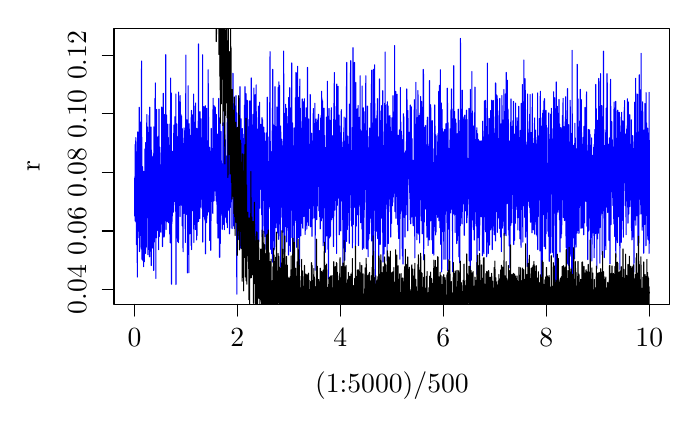
\begin{tikzpicture}[x=0.7pt,y=0.7pt]
\definecolor{fillColor}{RGB}{255,255,255}
%\path[use as bounding box,fill=fillColor,fill opacity=0.00] (0,0) rectangle (361.35,252.94);
\begin{scope}
%\path[clip] ( 49.20, 61.20) rectangle (336.15,203.75);
\definecolor{drawColor}{RGB}{0,0,255}

\path[draw=drawColor,line width= 0.4pt,line join=round,line cap=round] ( 59.83,106.84) --
	( 59.88,109.69) --
	( 59.93,126.38) --
	( 59.99,122.42) --
	( 60.04,127.15) --
	( 60.09,119.93) --
	( 60.15,104.22) --
	( 60.20,143.80) --
	( 60.25,120.88) --
	( 60.31,118.16) --
	( 60.36,127.05) --
	( 60.41,114.23) --
	( 60.47,147.23) --
	( 60.52,110.53) --
	( 60.57,114.88) --
	( 60.63,105.84) --
	( 60.68,103.50) --
	( 60.73,132.21) --
	( 60.78,108.41) --
	( 60.84, 92.05) --
	( 60.89,109.53) --
	( 60.94,139.95) --
	( 61.00,106.51) --
	( 61.05,112.03) --
	( 61.10, 98.10) --
	( 61.16,117.35) --
	( 61.21, 94.99) --
	( 61.26, 75.30) --
	( 61.32,145.21) --
	( 61.37,102.50) --
	( 61.42,142.19) --
	( 61.48,150.19) --
	( 61.53,145.29) --
	( 61.58,135.80) --
	( 61.63, 99.05) --
	( 61.69,117.85) --
	( 61.74,106.97) --
	( 61.79,104.33) --
	( 61.85,115.59) --
	( 61.90,140.68) --
	( 61.95,114.03) --
	( 62.01,123.53) --
	( 62.06,126.87) --
	( 62.11, 95.54) --
	( 62.17,109.19) --
	( 62.22,162.94) --
	( 62.27,126.28) --
	( 62.33,137.13) --
	( 62.38, 88.42) --
	( 62.43, 98.80) --
	( 62.49, 90.63) --
	( 62.54,128.05) --
	( 62.59, 97.25) --
	( 62.64,135.59) --
	( 62.70,112.53) --
	( 62.75,155.28) --
	( 62.80,130.88) --
	( 62.86,114.78) --
	( 62.91,119.82) --
	( 62.96,120.86) --
	( 63.02, 96.80) --
	( 63.07,103.09) --
	( 63.12,120.62) --
	( 63.18,153.67) --
	( 63.23,138.28) --
	( 63.28,148.89) --
	( 63.34, 89.87) --
	( 63.39,144.17) --
	( 63.44,186.83) --
	( 63.50,117.91) --
	( 63.55, 99.18) --
	( 63.60,147.50) --
	( 63.65, 84.43) --
	( 63.71, 87.59) --
	( 63.76,114.56) --
	( 63.81,101.58) --
	( 63.87,107.62) --
	( 63.92,132.23) --
	( 63.97,128.14) --
	( 64.03,113.74) --
	( 64.08,100.66) --
	( 64.13, 83.70) --
	( 64.19,126.76) --
	( 64.24,120.97) --
	( 64.29, 89.08) --
	( 64.35,126.21) --
	( 64.40,107.39) --
	( 64.45, 91.72) --
	( 64.50, 80.68) --
	( 64.56,129.83) --
	( 64.61, 97.33) --
	( 64.66,120.18) --
	( 64.72,125.47) --
	( 64.77,120.31) --
	( 64.82, 98.16) --
	( 64.88, 83.27) --
	( 64.93, 98.67) --
	( 64.98,127.81) --
	( 65.04,102.14) --
	( 65.09,129.60) --
	( 65.14,116.52) --
	( 65.20,141.38) --
	( 65.25,120.44) --
	( 65.30,135.76) --
	( 65.36,134.87) --
	( 65.41,128.42) --
	( 65.46,114.64) --
	( 65.51,144.70) --
	( 65.57, 87.48) --
	( 65.62,121.49) --
	( 65.67,130.28) --
	( 65.73,107.58) --
	( 65.78,115.84) --
	( 65.83,105.28) --
	( 65.89, 90.79) --
	( 65.94,121.17) --
	( 65.99,106.08) --
	( 66.05,114.16) --
	( 66.10,113.09) --
	( 66.15,159.18) --
	( 66.21,149.85) --
	( 66.26,117.61) --
	( 66.31,114.80) --
	( 66.37,106.07) --
	( 66.42,126.56) --
	( 66.47,114.11) --
	( 66.52,128.93) --
	( 66.58,152.72) --
	( 66.63,147.88) --
	( 66.68, 86.85) --
	( 66.74,108.30) --
	( 66.79, 89.40) --
	( 66.84,112.79) --
	( 66.90,107.30) --
	( 66.95, 92.87) --
	( 67.00,119.83) --
	( 67.06,137.87) --
	( 67.11,142.41) --
	( 67.16,103.34) --
	( 67.22,107.03) --
	( 67.27,133.49) --
	( 67.32,119.30) --
	( 67.38, 96.89) --
	( 67.43,158.81) --
	( 67.48,115.41) --
	( 67.53, 85.71) --
	( 67.59,126.49) --
	( 67.64,132.92) --
	( 67.69,163.03) --
	( 67.75,124.75) --
	( 67.80,103.31) --
	( 67.85,114.88) --
	( 67.91,110.64) --
	( 67.96, 88.66) --
	( 68.01,118.60) --
	( 68.07,104.79) --
	( 68.12,117.69) --
	( 68.17,139.57) --
	( 68.23,151.59) --
	( 68.28,123.45) --
	( 68.33,152.72) --
	( 68.38, 86.45) --
	( 68.44, 81.19) --
	( 68.49,125.00) --
	( 68.54,140.78) --
	( 68.60,113.48) --
	( 68.65,110.71) --
	( 68.70,131.65) --
	( 68.76,113.77) --
	( 68.81,111.33) --
	( 68.86,100.82) --
	( 68.92,137.67) --
	( 68.97,136.20) --
	( 69.02, 97.14) --
	( 69.08,116.57) --
	( 69.13,111.62) --
	( 69.18,104.05) --
	( 69.24, 90.23) --
	( 69.29,118.55) --
	( 69.34, 97.18) --
	( 69.39,116.71) --
	( 69.45,107.47) --
	( 69.50,137.30) --
	( 69.55,115.42) --
	( 69.61,106.11) --
	( 69.66, 79.17) --
	( 69.71, 78.72) --
	( 69.77,152.80) --
	( 69.82,152.57) --
	( 69.87,150.09) --
	( 69.93,131.30) --
	( 69.98,123.47) --
	( 70.03, 93.38) --
	( 70.09,117.43) --
	( 70.14,124.75) --
	( 70.19,131.90) --
	( 70.25,120.99) --
	( 70.30,167.38) --
	( 70.35,107.66) --
	( 70.40,107.33) --
	( 70.46,124.04) --
	( 70.51,127.68) --
	( 70.56,175.51) --
	( 70.62,102.99) --
	( 70.67,155.04) --
	( 70.72,137.51) --
	( 70.78,101.61) --
	( 70.83, 74.54) --
	( 70.88,135.20) --
	( 70.94,115.72) --
	( 70.99,156.55) --
	( 71.04,148.23) --
	( 71.10,131.43) --
	( 71.15,161.81) --
	( 71.20, 95.66) --
	( 71.25,124.35) --
	( 71.31,109.09) --
	( 71.36,115.26) --
	( 71.41,147.33) --
	( 71.47,113.24) --
	( 71.52,124.31) --
	( 71.57,123.15) --
	( 71.63,133.00) --
	( 71.68,124.67) --
	( 71.73,144.13) --
	( 71.79,117.75) --
	( 71.84, 99.34) --
	( 71.89,121.24) --
	( 71.95,102.68) --
	( 72.00,147.89) --
	( 72.05,125.24) --
	( 72.11,142.99) --
	( 72.16,126.25) --
	( 72.21,138.43) --
	( 72.26, 89.44) --
	( 72.32,117.85) --
	( 72.37,131.42) --
	( 72.42,161.96) --
	( 72.48,111.17) --
	( 72.53,130.01) --
	( 72.58, 96.21) --
	( 72.64,134.23) --
	( 72.69,136.09) --
	( 72.74,122.53) --
	( 72.80,140.91) --
	( 72.85,142.32) --
	( 72.90,130.87) --
	( 72.96,124.12) --
	( 73.01,105.73) --
	( 73.06,129.41) --
	( 73.12,125.81) --
	( 73.17,125.15) --
	( 73.22, 98.49) --
	( 73.27,116.32) --
	( 73.33,132.97) --
	( 73.38,122.92) --
	( 73.43,131.38) --
	( 73.49,121.24) --
	( 73.54,126.64) --
	( 73.59,133.48) --
	( 73.65,128.65) --
	( 73.70,139.45) --
	( 73.75,129.99) --
	( 73.81,163.05) --
	( 73.86,118.17) --
	( 73.91,126.97) --
	( 73.97,113.97) --
	( 74.02,101.99) --
	( 74.07,135.51) --
	( 74.12, 97.97) --
	( 74.18,126.59) --
	( 74.23, 91.07) --
	( 74.28,155.96) --
	( 74.34,159.74) --
	( 74.39,162.71) --
	( 74.44,133.60) --
	( 74.50,130.16) --
	( 74.55,140.78) --
	( 74.60,123.84) --
	( 74.66,170.15) --
	( 74.71,107.74) --
	( 74.76, 96.34) --
	( 74.82,121.59) --
	( 74.87,126.91) --
	( 74.92,132.84) --
	( 74.98,113.79) --
	( 75.03, 95.95) --
	( 75.08,124.92) --
	( 75.13, 96.36) --
	( 75.19,159.21) --
	( 75.24,155.07) --
	( 75.29,137.99) --
	( 75.35, 97.77) --
	( 75.40,118.35) --
	( 75.45,117.78) --
	( 75.51,124.18) --
	( 75.56,135.54) --
	( 75.61,151.79) --
	( 75.67,116.36) --
	( 75.72,110.91) --
	( 75.77,136.95) --
	( 75.83,106.19) --
	( 75.88,134.47) --
	( 75.93,190.13) --
	( 75.99,129.18) --
	( 76.04,104.28) --
	( 76.09,121.81) --
	( 76.14, 99.84) --
	( 76.20,147.29) --
	( 76.25,103.69) --
	( 76.30,141.59) --
	( 76.36,127.20) --
	( 76.41,158.88) --
	( 76.46,108.39) --
	( 76.52,141.76) --
	( 76.57,139.91) --
	( 76.62,145.56) --
	( 76.68,119.95) --
	( 76.73,146.94) --
	( 76.78,111.22) --
	( 76.84,144.36) --
	( 76.89,146.12) --
	( 76.94,103.97) --
	( 77.00,154.19) --
	( 77.05,139.21) --
	( 77.10,136.96) --
	( 77.15,123.63) --
	( 77.21,118.92) --
	( 77.26,147.27) --
	( 77.31,140.84) --
	( 77.37,103.34) --
	( 77.42,104.93) --
	( 77.47,137.03) --
	( 77.53,125.99) --
	( 77.58,112.53) --
	( 77.63,122.65) --
	( 77.69,139.87) --
	( 77.74,115.39) --
	( 77.79,104.50) --
	( 77.85,129.29) --
	( 77.90, 97.56) --
	( 77.95,122.71) --
	( 78.00,138.86) --
	( 78.06,154.29) --
	( 78.11,123.09) --
	( 78.16,128.30) --
	( 78.22,139.76) --
	( 78.27, 93.00) --
	( 78.32,161.39) --
	( 78.38,129.93) --
	( 78.43,177.99) --
	( 78.48,103.03) --
	( 78.54,156.43) --
	( 78.59,125.43) --
	( 78.64,145.05) --
	( 78.70,107.39) --
	( 78.75,145.63) --
	( 78.80,170.26) --
	( 78.86,131.59) --
	( 78.91, 71.61) --
	( 78.96,127.42) --
	( 79.01,104.54) --
	( 79.07,134.81) --
	( 79.12,102.83) --
	( 79.17,114.08) --
	( 79.23,114.21) --
	( 79.28,122.32) --
	( 79.33,106.82) --
	( 79.39,128.48) --
	( 79.44,140.22) --
	( 79.49,133.25) --
	( 79.55,123.33) --
	( 79.60,121.75) --
	( 79.65,128.20) --
	( 79.71,130.94) --
	( 79.76,123.17) --
	( 79.81,124.64) --
	( 79.87,108.82) --
	( 79.92,114.97) --
	( 79.97,149.51) --
	( 80.02,138.94) --
	( 80.08,134.53) --
	( 80.13,153.73) --
	( 80.18,149.67) --
	( 80.24,144.43) --
	( 80.29,115.57) --
	( 80.34,132.72) --
	( 80.40,114.35) --
	( 80.45,121.33) --
	( 80.50,133.14) --
	( 80.56,147.51) --
	( 80.61,155.14) --
	( 80.66,158.03) --
	( 80.72,122.01) --
	( 80.77,135.68) --
	( 80.82,153.01) --
	( 80.87,128.58) --
	( 80.93,156.24) --
	( 80.98,109.24) --
	( 81.03,124.89) --
	( 81.09,109.54) --
	( 81.14,169.82) --
	( 81.19, 71.47) --
	( 81.25, 96.91) --
	( 81.30,124.48) --
	( 81.35,121.72) --
	( 81.41,137.34) --
	( 81.46,118.25) --
	( 81.51, 95.45) --
	( 81.57,126.09) --
	( 81.62,154.38) --
	( 81.67,138.33) --
	( 81.73,111.00) --
	( 81.78,120.27) --
	( 81.83,118.04) --
	( 81.88,118.49) --
	( 81.94,135.19) --
	( 81.99,147.80) --
	( 82.04, 93.69) --
	( 82.10,121.52) --
	( 82.15,139.53) --
	( 82.20, 94.71) --
	( 82.26,103.21) --
	( 82.31,126.46) --
	( 82.36,125.16) --
	( 82.42,144.30) --
	( 82.47, 93.05) --
	( 82.52,101.22) --
	( 82.58,170.79) --
	( 82.63,162.55) --
	( 82.68,113.25) --
	( 82.74,129.83) --
	( 82.79,143.71) --
	( 82.84,153.07) --
	( 82.89,154.22) --
	( 82.95,126.66) --
	( 83.00,157.97) --
	( 83.05,114.69) --
	( 83.11,127.94) --
	( 83.16,114.98) --
	( 83.21,112.19) --
	( 83.27,144.92) --
	( 83.32,106.57) --
	( 83.37,168.92) --
	( 83.43,142.17) --
	( 83.48,165.57) --
	( 83.53,127.41) --
	( 83.59,116.26) --
	( 83.64,144.80) --
	( 83.69,122.85) --
	( 83.75,159.33) --
	( 83.80,132.27) --
	( 83.85,116.39) --
	( 83.90,112.43) --
	( 83.96,156.46) --
	( 84.01,114.91) --
	( 84.06,158.50) --
	( 84.12,125.85) --
	( 84.17,128.29) --
	( 84.22,126.16) --
	( 84.28,149.53) --
	( 84.33,132.29) --
	( 84.38,136.37) --
	( 84.44,101.78) --
	( 84.49,151.85) --
	( 84.54,112.46) --
	( 84.60,111.49) --
	( 84.65,140.26) --
	( 84.70,126.61) --
	( 84.75,129.07) --
	( 84.81,136.52) --
	( 84.86, 88.37) --
	( 84.91,131.89) --
	( 84.97,144.10) --
	( 85.02,124.47) --
	( 85.07,137.29) --
	( 85.13,119.27) --
	( 85.18,122.01) --
	( 85.23,108.14) --
	( 85.29,132.49) --
	( 85.34,135.79) --
	( 85.39,152.28) --
	( 85.45,134.81) --
	( 85.50,138.33) --
	( 85.55,135.58) --
	( 85.61,116.91) --
	( 85.66,142.44) --
	( 85.71,116.83) --
	( 85.76,148.90) --
	( 85.82,123.74) --
	( 85.87,150.70) --
	( 85.92,150.32) --
	( 85.98,126.83) --
	( 86.03, 93.20) --
	( 86.08,113.59) --
	( 86.14,112.52) --
	( 86.19,142.87) --
	( 86.24,136.88) --
	( 86.30,189.88) --
	( 86.35,150.78) --
	( 86.40,153.79) --
	( 86.46,125.53) --
	( 86.51,120.97) --
	( 86.56,126.08) --
	( 86.62,112.54) --
	( 86.67,143.59) --
	( 86.72,107.58) --
	( 86.77,133.40) --
	( 86.83,122.52) --
	( 86.88,156.47) --
	( 86.93,112.03) --
	( 86.99,118.87) --
	( 87.04,151.45) --
	( 87.09, 77.48) --
	( 87.15,141.38) --
	( 87.20,121.83) --
	( 87.25,112.55) --
	( 87.31,118.05) --
	( 87.36,131.39) --
	( 87.41,123.28) --
	( 87.47,174.03) --
	( 87.52,149.11) --
	( 87.57,109.30) --
	( 87.62,150.78) --
	( 87.68,133.69) --
	( 87.73,102.73) --
	( 87.78,118.21) --
	( 87.84, 77.54) --
	( 87.89,125.09) --
	( 87.94,128.37) --
	( 88.00,154.44) --
	( 88.05,101.92) --
	( 88.10,151.75) --
	( 88.16,141.96) --
	( 88.21,119.11) --
	( 88.26,138.04) --
	( 88.32,137.89) --
	( 88.37, 97.63) --
	( 88.42,148.39) --
	( 88.48,133.64) --
	( 88.53,142.46) --
	( 88.58,131.63) --
	( 88.63,124.88) --
	( 88.69,131.56) --
	( 88.74,111.90) --
	( 88.79,129.27) --
	( 88.85,108.19) --
	( 88.90,106.38) --
	( 88.95,143.26) --
	( 89.01, 91.62) --
	( 89.06,157.70) --
	( 89.11,114.94) --
	( 89.17,116.78) --
	( 89.22,161.37) --
	( 89.27, 89.49) --
	( 89.33,114.40) --
	( 89.38,132.03) --
	( 89.43,134.80) --
	( 89.49,138.59) --
	( 89.54,126.66) --
	( 89.59,144.13) --
	( 89.64,136.64) --
	( 89.70,123.69) --
	( 89.75,158.99) --
	( 89.80,135.90) --
	( 89.86,130.95) --
	( 89.91,121.77) --
	( 89.96,114.72) --
	( 90.02,109.50) --
	( 90.07,138.91) --
	( 90.12,124.08) --
	( 90.18,141.78) --
	( 90.23,133.61) --
	( 90.28,113.15) --
	( 90.34,169.76) --
	( 90.39,103.77) --
	( 90.44, 93.12) --
	( 90.50,149.05) --
	( 90.55,113.52) --
	( 90.60,163.56) --
	( 90.65,102.43) --
	( 90.71,128.27) --
	( 90.76,155.30) --
	( 90.81,138.60) --
	( 90.87,142.68) --
	( 90.92,120.26) --
	( 90.97,131.00) --
	( 91.03,148.10) --
	( 91.08,136.60) --
	( 91.13,136.42) --
	( 91.19,125.81) --
	( 91.24, 99.80) --
	( 91.29,126.11) --
	( 91.35,165.17) --
	( 91.40,109.04) --
	( 91.45,141.55) --
	( 91.50,104.57) --
	( 91.56,111.76) --
	( 91.61,123.65) --
	( 91.66,120.60) --
	( 91.72,128.58) --
	( 91.77,124.40) --
	( 91.82,117.75) --
	( 91.88, 94.49) --
	( 91.93,120.42) --
	( 91.98,152.03) --
	( 92.04, 96.74) --
	( 92.09,129.46) --
	( 92.14,136.47) --
	( 92.20,131.89) --
	( 92.25,124.45) --
	( 92.30,110.97) --
	( 92.36,128.17) --
	( 92.41,128.71) --
	( 92.46,126.93) --
	( 92.51,103.82) --
	( 92.57,121.83) --
	( 92.62,155.83) --
	( 92.67,119.16) --
	( 92.73,128.83) --
	( 92.78,124.33) --
	( 92.83,195.60) --
	( 92.89,104.05) --
	( 92.94,131.85) --
	( 92.99,113.32) --
	( 93.05,116.22) --
	( 93.10,134.79) --
	( 93.15,118.48) --
	( 93.21,138.74) --
	( 93.26,105.67) --
	( 93.31,119.88) --
	( 93.37,136.71) --
	( 93.42,146.27) --
	( 93.47,108.89) --
	( 93.52,105.52) --
	( 93.58,115.48) --
	( 93.63,160.67) --
	( 93.68,125.06) --
	( 93.74,125.23) --
	( 93.79,128.31) --
	( 93.84,134.66) --
	( 93.90,120.56) --
	( 93.95,111.41) --
	( 94.00,123.84) --
	( 94.06,152.26) --
	( 94.11,146.09) --
	( 94.16,156.96) --
	( 94.22,139.08) --
	( 94.27,133.94) --
	( 94.32,136.17) --
	( 94.37,138.96) --
	( 94.43,121.98) --
	( 94.48,132.34) --
	( 94.53,123.96) --
	( 94.59,142.42) --
	( 94.64,120.55) --
	( 94.69,110.70) --
	( 94.75,128.28) --
	( 94.80,116.25) --
	( 94.85,125.01) --
	( 94.91,130.56) --
	( 94.96,190.03) --
	( 95.01, 93.39) --
	( 95.07,139.42) --
	( 95.12,131.88) --
	( 95.17,126.23) --
	( 95.23,121.16) --
	( 95.28,159.15) --
	( 95.33,163.18) --
	( 95.38,142.85) --
	( 95.44,109.86) --
	( 95.49,132.37) --
	( 95.54,163.19) --
	( 95.60,125.84) --
	( 95.65,159.82) --
	( 95.70,132.99) --
	( 95.76,106.39) --
	( 95.81,136.32) --
	( 95.86,128.15) --
	( 95.92,154.00) --
	( 95.97,146.54) --
	( 96.02,105.10) --
	( 96.08,137.03) --
	( 96.13,131.21) --
	( 96.18,128.26) --
	( 96.24,120.14) --
	( 96.29,104.20) --
	( 96.34,163.71) --
	( 96.39,141.19) --
	( 96.45, 87.34) --
	( 96.50,130.57) --
	( 96.55,141.22) --
	( 96.61,120.38) --
	( 96.66,143.80) --
	( 96.71,120.02) --
	( 96.77,111.60) --
	( 96.82,117.94) --
	( 96.87,112.99) --
	( 96.93,118.07) --
	( 96.98,103.39) --
	( 97.03,162.43) --
	( 97.09,105.68) --
	( 97.14,135.11) --
	( 97.19,115.55) --
	( 97.25,139.21) --
	( 97.30,130.43) --
	( 97.35,141.94) --
	( 97.40,107.21) --
	( 97.46,131.40) --
	( 97.51,138.58) --
	( 97.56,135.73) --
	( 97.62,132.97) --
	( 97.67,145.76) --
	( 97.72,117.81) --
	( 97.78,142.55) --
	( 97.83,182.31) --
	( 97.88,133.86) --
	( 97.94,108.86) --
	( 97.99,117.11) --
	( 98.04,157.91) --
	( 98.10,129.78) --
	( 98.15,124.71) --
	( 98.20,142.29) --
	( 98.25,125.34) --
	( 98.31,142.36) --
	( 98.36,117.21) --
	( 98.41,122.16) --
	( 98.47,132.56) --
	( 98.52,142.20) --
	( 98.57, 94.23) --
	( 98.63, 94.88) --
	( 98.68,121.75) --
	( 98.73,116.93) --
	( 98.79,115.49) --
	( 98.84,126.92) --
	( 98.89,105.54) --
	( 98.95, 97.62) --
	( 99.00, 95.82) --
	( 99.05,128.42) --
	( 99.11,138.26) --
	( 99.16, 89.05) --
	( 99.21, 91.06) --
	( 99.26,116.38) --
	( 99.32,144.22) --
	( 99.37,104.45) --
	( 99.42,152.05) --
	( 99.48,123.37) --
	( 99.53,135.04) --
	( 99.58,135.38) --
	( 99.64,141.76) --
	( 99.69,139.53) --
	( 99.74,135.81) --
	( 99.80,127.98) --
	( 99.85,135.39) --
	( 99.90,114.25) --
	( 99.96,115.32) --
	(100.01,127.14) --
	(100.06,139.15) --
	(100.12,119.84) --
	(100.17,110.33) --
	(100.22,108.11) --
	(100.27,116.53) --
	(100.33,159.45) --
	(100.38,167.61) --
	(100.43,129.83) --
	(100.49,145.23) --
	(100.54,156.53) --
	(100.59,118.92) --
	(100.65,142.30) --
	(100.70,126.09) --
	(100.75,130.47) --
	(100.81,114.58) --
	(100.86,163.74) --
	(100.91,128.22) --
	(100.97,154.89) --
	(101.02,155.48) --
	(101.07,120.56) --
	(101.12,136.81) --
	(101.18,138.59) --
	(101.23,142.21) --
	(101.28,119.76) --
	(101.34,163.14) --
	(101.39,120.36) --
	(101.44,159.52) --
	(101.50,162.80) --
	(101.55,125.91) --
	(101.60,143.98) --
	(101.66,123.32) --
	(101.71,134.29) --
	(101.76,124.63) --
	(101.82,117.33) --
	(101.87,128.61) --
	(101.92,114.58) --
	(101.98,159.30) --
	(102.03,139.03) --
	(102.08,148.65) --
	(102.13,145.41) --
	(102.19,128.22) --
	(102.24,127.40) --
	(102.29,112.75) --
	(102.35,142.49) --
	(102.40,116.15) --
	(102.45,148.86) --
	(102.51,103.09) --
	(102.56,123.19) --
	(102.61,133.67) --
	(102.67,149.11) --
	(102.72,147.59) --
	(102.77,147.56) --
	(102.83,142.47) --
	(102.88, 95.46) --
	(102.93,123.80) --
	(102.99,147.16) --
	(103.04,141.24) --
	(103.09,132.08) --
	(103.14,118.21) --
	(103.20,134.11) --
	(103.25,111.87) --
	(103.30,167.49) --
	(103.36,129.02) --
	(103.41,102.34) --
	(103.46,148.67) --
	(103.52,135.78) --
	(103.57,112.85) --
	(103.62,114.49) --
	(103.68, 85.54) --
	(103.73,108.28) --
	(103.78,123.73) --
	(103.84,146.00) --
	(103.89, 85.57) --
	(103.94,151.74) --
	(104.00,157.55) --
	(104.05, 92.54) --
	(104.10,122.72) --
	(104.15,101.19) --
	(104.21,132.91) --
	(104.26,127.59) --
	(104.31,122.20) --
	(104.37,128.44) --
	(104.42,144.69) --
	(104.47,150.41) --
	(104.53,119.55) --
	(104.58,135.34) --
	(104.63,120.87) --
	(104.69,108.66) --
	(104.74,121.46) --
	(104.79,127.28) --
	(104.85,132.72) --
	(104.90,123.02) --
	(104.95,108.38) --
	(105.00,107.46) --
	(105.06,133.71) --
	(105.11, 99.97) --
	(105.16,113.47) --
	(105.22,107.46) --
	(105.27,131.69) --
	(105.32,120.81) --
	(105.38,107.30) --
	(105.43,118.90) --
	(105.48,154.89) --
	(105.54,132.96) --
	(105.59,118.30) --
	(105.64,122.92) --
	(105.70,132.72) --
	(105.75,102.49) --
	(105.80,140.11) --
	(105.86,149.20) --
	(105.91,126.95) --
	(105.96,108.91) --
	(106.01,125.53) --
	(106.07,132.85) --
	(106.12,160.84) --
	(106.17, 99.77) --
	(106.23,106.13) --
	(106.28,108.16) --
	(106.33,163.20) --
	(106.39,128.28) --
	(106.44,125.77) --
	(106.49,120.47) --
	(106.55,135.64) --
	(106.60,114.57) --
	(106.65,143.76) --
	(106.71,146.13) --
	(106.76,131.41) --
	(106.81,120.14) --
	(106.87,121.33) --
	(106.92,106.23) --
	(106.97,106.50) --
	(107.02,125.72) --
	(107.08,127.12) --
	(107.13,135.19) --
	(107.18,137.76) --
	(107.24,133.79) --
	(107.29,103.49) --
	(107.34,116.40) --
	(107.40,117.82) --
	(107.45,106.04) --
	(107.50,104.50) --
	(107.56,105.82) --
	(107.61,155.12) --
	(107.66,106.08) --
	(107.72,100.81) --
	(107.77,138.97) --
	(107.82,161.01) --
	(107.87,117.29) --
	(107.93,149.89) --
	(107.98,120.17) --
	(108.03,124.49) --
	(108.09,110.09) --
	(108.14,135.11) --
	(108.19,195.07) --
	(108.25,145.16) --
	(108.30,145.41) --
	(108.35,120.30) --
	(108.41,110.66) --
	(108.46,144.67) --
	(108.51,109.62) --
	(108.57,127.34) --
	(108.62,123.00) --
	(108.67,128.26) --
	(108.73,149.59) --
	(108.78,135.68) --
	(108.83, 97.63) --
	(108.88,112.20) --
	(108.94,100.48) --
	(108.99,108.55) --
	(109.04,145.81) --
	(109.10,158.23) --
	(109.15,134.69) --
	(109.20,151.67) --
	(109.26,136.74) --
	(109.31,111.20) --
	(109.36,144.39) --
	(109.42,129.38) --
	(109.47,115.73) --
	(109.52,156.35) --
	(109.58,129.77) --
	(109.63,122.20) --
	(109.68,148.28) --
	(109.74,119.04) --
	(109.79,114.21) --
	(109.84,170.38) --
	(109.89,148.76) --
	(109.95,151.20) --
	(110.00,142.91) --
	(110.05,124.05) --
	(110.11,102.07) --
	(110.16,100.28) --
	(110.21,114.83) --
	(110.27,123.98) --
	(110.32,120.24) --
	(110.37,128.81) --
	(110.43,124.05) --
	(110.48,163.93) --
	(110.53,140.89) --
	(110.59,140.20) --
	(110.64,180.48) --
	(110.69,117.55) --
	(110.75,143.51) --
	(110.80,147.29) --
	(110.85,164.79) --
	(110.90,121.52) --
	(110.96,141.76) --
	(111.01,104.16) --
	(111.06,101.55) --
	(111.12,130.69) --
	(111.17,131.97) --
	(111.22,116.64) --
	(111.28,110.76) --
	(111.33,151.35) --
	(111.38,100.33) --
	(111.44,120.05) --
	(111.49,105.13) --
	(111.54,144.72) --
	(111.60,107.50) --
	(111.65,152.65) --
	(111.70,120.79) --
	(111.75,128.52) --
	(111.81,132.96) --
	(111.86,163.59) --
	(111.91,129.15) --
	(111.97,105.55) --
	(112.02,153.06) --
	(112.07,140.08) --
	(112.13,146.02) --
	(112.18,168.96) --
	(112.23,126.56) --
	(112.29,159.44) --
	(112.34,144.49) --
	(112.39,105.75) --
	(112.45,136.53) --
	(112.50,150.83) --
	(112.55,160.03) --
	(112.61, 66.48) --
	(112.66,133.51) --
	(112.71,149.08) --
	(112.76,150.16) --
	(112.82,145.14) --
	(112.87,107.65) --
	(112.92,115.04) --
	(112.98,119.37) --
	(113.03,122.57) --
	(113.08,122.54) --
	(113.14,101.44) --
	(113.19,116.91) --
	(113.24,118.08) --
	(113.30,111.80) --
	(113.35,109.32) --
	(113.40,149.53) --
	(113.46, 94.60) --
	(113.51,134.82) --
	(113.56,164.05) --
	(113.62,167.45) --
	(113.67,123.01) --
	(113.72,131.70) --
	(113.77,141.22) --
	(113.83,125.66) --
	(113.88,128.13) --
	(113.93,134.89) --
	(113.99,125.68) --
	(114.04,149.31) --
	(114.09,160.04) --
	(114.15,145.04) --
	(114.20,158.51) --
	(114.25,173.63) --
	(114.31,103.29) --
	(114.36,101.69) --
	(114.41,136.84) --
	(114.47, 96.33) --
	(114.52, 90.28) --
	(114.57,144.18) --
	(114.62,109.28) --
	(114.68,130.05) --
	(114.73,107.66) --
	(114.78,156.99) --
	(114.84,109.88) --
	(114.89,139.63) --
	(114.94,131.76) --
	(115.00,140.52) --
	(115.05,108.16) --
	(115.10,119.53) --
	(115.16,139.34) --
	(115.21,119.41) --
	(115.26,150.58) --
	(115.32,123.64) --
	(115.37,143.45) --
	(115.42,109.63) --
	(115.48,151.95) --
	(115.53,137.58) --
	(115.58,123.55) --
	(115.63,135.20) --
	(115.69,130.62) --
	(115.74,126.05) --
	(115.79,113.59) --
	(115.85,114.11) --
	(115.90, 83.28) --
	(115.95,136.32) --
	(116.01, 79.27) --
	(116.06,115.52) --
	(116.11,132.45) --
	(116.17,104.78) --
	(116.22,148.96) --
	(116.27,139.25) --
	(116.33,134.43) --
	(116.38,104.45) --
	(116.43,128.16) --
	(116.49, 99.66) --
	(116.54,124.46) --
	(116.59,164.05) --
	(116.64,144.02) --
	(116.70,136.45) --
	(116.75,122.85) --
	(116.80,110.79) --
	(116.86,173.59) --
	(116.91, 86.72) --
	(116.96,135.97) --
	(117.02,118.16) --
	(117.07,153.09) --
	(117.12,112.30) --
	(117.18,165.17) --
	(117.23,134.15) --
	(117.28,115.61) --
	(117.34,136.40) --
	(117.39,169.94) --
	(117.44,168.59) --
	(117.50,148.43) --
	(117.55,130.31) --
	(117.60,128.71) --
	(117.65,122.47) --
	(117.71,113.73) --
	(117.76,108.93) --
	(117.81,111.91) --
	(117.87, 92.63) --
	(117.92,143.91) --
	(117.97,166.52) --
	(118.03,119.49) --
	(118.08,125.24) --
	(118.13,136.18) --
	(118.19,115.84) --
	(118.24,147.04) --
	(118.29,156.57) --
	(118.35, 98.98) --
	(118.40,147.21) --
	(118.45,123.75) --
	(118.50,113.21) --
	(118.56,116.19) --
	(118.61, 93.75) --
	(118.66,103.05) --
	(118.72,117.69) --
	(118.77,149.35) --
	(118.82,112.25) --
	(118.88,143.75) --
	(118.93,119.34) --
	(118.98,113.22) --
	(119.04,153.09) --
	(119.09,145.20) --
	(119.14,166.26) --
	(119.20,129.58) --
	(119.25,119.54) --
	(119.30,105.14) --
	(119.36,137.02) --
	(119.41,149.02) --
	(119.46, 99.95) --
	(119.51,134.93) --
	(119.57,144.40) --
	(119.62,150.64) --
	(119.67,105.48) --
	(119.73,128.59) --
	(119.78,144.38) --
	(119.83,133.47) --
	(119.89,125.72) --
	(119.94,166.43) --
	(119.99,126.43) --
	(120.05,178.13) --
	(120.10,154.41) --
	(120.15, 88.23) --
	(120.21,115.49) --
	(120.26,116.59) --
	(120.31, 90.98) --
	(120.37,136.24) --
	(120.42,117.65) --
	(120.47,147.72) --
	(120.52,153.71) --
	(120.58,125.78) --
	(120.63,148.38) --
	(120.68,139.47) --
	(120.74,139.98) --
	(120.79,119.82) --
	(120.84,129.53) --
	(120.90,133.90) --
	(120.95,159.26) --
	(121.00,142.13) --
	(121.06, 97.93) --
	(121.11,143.88) --
	(121.16, 89.43) --
	(121.22,121.00) --
	(121.27,132.24) --
	(121.32,118.03) --
	(121.37,104.90) --
	(121.43,172.84) --
	(121.48,138.04) --
	(121.53,102.59) --
	(121.59,104.76) --
	(121.64,133.12) --
	(121.69,117.11) --
	(121.75,154.34) --
	(121.80,114.08) --
	(121.85,140.71) --
	(121.91,117.12) --
	(121.96, 85.07) --
	(122.01,118.29) --
	(122.07,169.39) --
	(122.12,150.29) --
	(122.17,145.92) --
	(122.23,115.96) --
	(122.28,118.62) --
	(122.33,127.07) --
	(122.38,118.87) --
	(122.44,146.72) --
	(122.49,147.20) --
	(122.54,131.15) --
	(122.60,174.49) --
	(122.65,129.87) --
	(122.70, 89.65) --
	(122.76,147.63) --
	(122.81, 96.83) --
	(122.86,138.65) --
	(122.92,120.04) --
	(122.97,147.63) --
	(123.02,108.62) --
	(123.08,125.04) --
	(123.13, 89.61) --
	(123.18,126.34) --
	(123.24,131.74) --
	(123.29,151.60) --
	(123.34,149.09) --
	(123.39, 89.90) --
	(123.45,135.84) --
	(123.50,137.61) --
	(123.55,143.58) --
	(123.61,131.25) --
	(123.66,122.11) --
	(123.71,163.56) --
	(123.77,120.74) --
	(123.82,117.67) --
	(123.87,127.01) --
	(123.93,128.57) --
	(123.98, 93.72) --
	(124.03,141.02) --
	(124.09,153.65) --
	(124.14,132.78) --
	(124.19,131.20) --
	(124.24,128.35) --
	(124.30,112.55) --
	(124.35,165.53) --
	(124.40,121.20) --
	(124.46,126.65) --
	(124.51,110.87) --
	(124.56,127.10) --
	(124.62,122.88) --
	(124.67,141.02) --
	(124.72,132.47) --
	(124.78,133.58) --
	(124.83,127.92) --
	(124.88,134.58) --
	(124.94,154.10) --
	(124.99,120.70) --
	(125.04,136.49) --
	(125.10,129.05) --
	(125.15,120.59) --
	(125.20,129.14) --
	(125.25,120.83) --
	(125.31,122.01) --
	(125.36,147.80) --
	(125.41,107.47) --
	(125.47,145.50) --
	(125.52,118.88) --
	(125.57,147.30) --
	(125.63,157.56) --
	(125.68, 96.09) --
	(125.73,129.50) --
	(125.79, 97.90) --
	(125.84,152.79) --
	(125.89,156.52) --
	(125.95,126.19) --
	(126.00,127.85) --
	(126.05,116.43) --
	(126.11,120.93) --
	(126.16,114.89) --
	(126.21,135.75) --
	(126.26,144.49) --
	(126.32,138.48) --
	(126.37,135.90) --
	(126.42,135.46) --
	(126.48,135.21) --
	(126.53,152.68) --
	(126.58,127.14) --
	(126.64,105.89) --
	(126.69, 98.90) --
	(126.74,111.65) --
	(126.80,134.93) --
	(126.85,149.72) --
	(126.90,119.17) --
	(126.96,134.34) --
	(127.01,140.59) --
	(127.06, 96.17) --
	(127.12,145.04) --
	(127.17,107.25) --
	(127.22,127.62) --
	(127.27,140.48) --
	(127.33,134.00) --
	(127.38,145.35) --
	(127.43,140.16) --
	(127.49,103.33) --
	(127.54,129.36) --
	(127.59, 94.62) --
	(127.65,112.54) --
	(127.70, 89.56) --
	(127.75,149.65) --
	(127.81,135.65) --
	(127.86, 92.91) --
	(127.91,136.46) --
	(127.97, 96.87) --
	(128.02,118.18) --
	(128.07,105.23) --
	(128.12,121.92) --
	(128.18,117.26) --
	(128.23, 85.32) --
	(128.28,109.47) --
	(128.34,168.15) --
	(128.39,118.12) --
	(128.44, 87.80) --
	(128.50,129.49) --
	(128.55,116.91) --
	(128.60,117.24) --
	(128.66,133.64) --
	(128.71,147.66) --
	(128.76,127.08) --
	(128.82, 86.86) --
	(128.87,121.79) --
	(128.92,134.98) --
	(128.98,127.10) --
	(129.03,117.16) --
	(129.08,116.94) --
	(129.13,131.33) --
	(129.19,110.56) --
	(129.24,114.93) --
	(129.29,132.33) --
	(129.35,129.58) --
	(129.40,127.97) --
	(129.45,131.26) --
	(129.51,115.71) --
	(129.56,165.41) --
	(129.61,143.36) --
	(129.67,115.87) --
	(129.72,111.84) --
	(129.77,191.62) --
	(129.83,113.06) --
	(129.88,124.47) --
	(129.93,145.36) --
	(129.99,129.95) --
	(130.04,108.81) --
	(130.09, 94.65) --
	(130.14, 89.61) --
	(130.20,140.09) --
	(130.25,133.62) --
	(130.30,136.23) --
	(130.36,135.84) --
	(130.41,114.41) --
	(130.46,122.22) --
	(130.52,109.84) --
	(130.57, 87.38) --
	(130.62,123.94) --
	(130.68,121.59) --
	(130.73,134.25) --
	(130.78,137.07) --
	(130.84,105.97) --
	(130.89,105.52) --
	(130.94,162.46) --
	(130.99,125.13) --
	(131.05, 83.01) --
	(131.10,125.10) --
	(131.15,182.54) --
	(131.21,160.56) --
	(131.26,139.05) --
	(131.31,154.32) --
	(131.37, 94.12) --
	(131.42,125.72) --
	(131.47,131.78) --
	(131.53,112.78) --
	(131.58,112.13) --
	(131.63,153.58) --
	(131.69, 96.35) --
	(131.74,134.00) --
	(131.79,133.03) --
	(131.85, 89.22) --
	(131.90,132.71) --
	(131.95,132.75) --
	(132.00,126.55) --
	(132.06,129.07) --
	(132.11,125.09) --
	(132.16, 89.88) --
	(132.22,101.84) --
	(132.27,105.82) --
	(132.32,173.63) --
	(132.38,120.02) --
	(132.43,148.86) --
	(132.48,142.44) --
	(132.54,105.66) --
	(132.59,153.03) --
	(132.64,117.25) --
	(132.70,120.45) --
	(132.75,142.00) --
	(132.80,100.84) --
	(132.86,144.37) --
	(132.91,140.12) --
	(132.96,142.49) --
	(133.01,127.30) --
	(133.07,111.39) --
	(133.12,136.87) --
	(133.17,112.50) --
	(133.23,117.36) --
	(133.28,163.09) --
	(133.33,141.94) --
	(133.39,103.13) --
	(133.44,127.45) --
	(133.49,139.08) --
	(133.55,119.37) --
	(133.60,109.76) --
	(133.65, 98.14) --
	(133.71,148.78) --
	(133.76,107.15) --
	(133.81,120.28) --
	(133.87,146.88) --
	(133.92,168.46) --
	(133.97,173.19) --
	(134.02,160.79) --
	(134.08,132.28) --
	(134.13, 94.79) --
	(134.18,170.52) --
	(134.24,111.90) --
	(134.29, 96.50) --
	(134.34,176.09) --
	(134.40,151.00) --
	(134.45,130.56) --
	(134.50,106.88) --
	(134.56,131.43) --
	(134.61,160.33) --
	(134.66,174.16) --
	(134.72,111.10) --
	(134.77,123.91) --
	(134.82,114.02) --
	(134.87,124.29) --
	(134.93,130.83) --
	(134.98,117.73) --
	(135.03,123.86) --
	(135.09, 80.36) --
	(135.14,127.80) --
	(135.19,126.69) --
	(135.25,153.23) --
	(135.30,141.22) --
	(135.35,106.15) --
	(135.41,127.38) --
	(135.46,136.10) --
	(135.51,138.40) --
	(135.57,111.34) --
	(135.62,146.47) --
	(135.67,129.22) --
	(135.73,143.21) --
	(135.78,128.12) --
	(135.83,139.07) --
	(135.88,136.43) --
	(135.94,137.73) --
	(135.99,127.53) --
	(136.04,132.09) --
	(136.10,124.71) --
	(136.15,142.44) --
	(136.20, 98.34) --
	(136.26,114.01) --
	(136.31,109.41) --
	(136.36,128.98) --
	(136.42,104.12) --
	(136.47,145.22) --
	(136.52,146.39) --
	(136.58,128.56) --
	(136.63,136.87) --
	(136.68,119.14) --
	(136.74,125.83) --
	(136.79,191.92) --
	(136.84,164.51) --
	(136.89, 87.25) --
	(136.95,143.50) --
	(137.00,119.48) --
	(137.05,115.61) --
	(137.11,120.31) --
	(137.16,112.05) --
	(137.21,112.22) --
	(137.27,136.00) --
	(137.32,104.69) --
	(137.37, 88.26) --
	(137.43,122.06) --
	(137.48,159.74) --
	(137.53,144.56) --
	(137.59,138.13) --
	(137.64,139.63) --
	(137.69,145.10) --
	(137.74,105.23) --
	(137.80,164.43) --
	(137.85,145.16) --
	(137.90,137.10) --
	(137.96,101.36) --
	(138.01,111.42) --
	(138.06,106.59) --
	(138.12,157.02) --
	(138.17,145.65) --
	(138.22,136.20) --
	(138.28,162.38) --
	(138.33, 93.48) --
	(138.38,103.23) --
	(138.44,146.96) --
	(138.49,151.17) --
	(138.54,104.39) --
	(138.60,158.19) --
	(138.65,148.36) --
	(138.70,145.26) --
	(138.75,123.33) --
	(138.81,102.77) --
	(138.86,117.30) --
	(138.91,127.39) --
	(138.97,123.74) --
	(139.02,130.97) --
	(139.07,141.86) --
	(139.13,109.78) --
	(139.18,100.70) --
	(139.23,141.75) --
	(139.29, 86.68) --
	(139.34,168.00) --
	(139.39,112.47) --
	(139.45,124.99) --
	(139.50,135.03) --
	(139.55,120.33) --
	(139.61,137.42) --
	(139.66,100.34) --
	(139.71,109.20) --
	(139.76,109.71) --
	(139.82,124.39) --
	(139.87,110.59) --
	(139.92,173.05) --
	(139.98, 91.59) --
	(140.03,107.34) --
	(140.08,124.01) --
	(140.14,124.82) --
	(140.19,118.63) --
	(140.24, 88.56) --
	(140.30,124.05) --
	(140.35,150.97) --
	(140.40,121.43) --
	(140.46,110.01) --
	(140.51,159.22) --
	(140.56,115.32) --
	(140.62,109.85) --
	(140.67,162.74) --
	(140.72,147.23) --
	(140.77,114.12) --
	(140.83,116.94) --
	(140.88,133.02) --
	(140.93,109.99) --
	(140.99,185.85) --
	(141.04,136.30) --
	(141.09, 95.63) --
	(141.15,145.46) --
	(141.20,106.67) --
	(141.25,117.68) --
	(141.31,116.24) --
	(141.36,119.53) --
	(141.41,154.80) --
	(141.47, 77.05) --
	(141.52,114.12) --
	(141.57,134.43) --
	(141.62,137.86) --
	(141.68,127.89) --
	(141.73,116.07) --
	(141.78,142.60) --
	(141.84,103.68) --
	(141.89,117.40) --
	(141.94,122.71) --
	(142.00,140.06) --
	(142.05,102.13) --
	(142.10,143.26) --
	(142.16,110.66) --
	(142.21,139.28) --
	(142.26,152.24) --
	(142.32, 99.26) --
	(142.37,138.76) --
	(142.42, 78.90) --
	(142.48,136.77) --
	(142.53,103.30) --
	(142.58,113.58) --
	(142.63,127.67) --
	(142.69,117.17) --
	(142.74,105.35) --
	(142.79,148.04) --
	(142.85,167.81) --
	(142.90,104.59) --
	(142.95,141.23) --
	(143.01,136.14) --
	(143.06,159.07) --
	(143.11,180.89) --
	(143.17,146.21) --
	(143.22,132.48) --
	(143.27,165.47) --
	(143.33,136.65) --
	(143.38,122.11) --
	(143.43,139.73) --
	(143.49,103.07) --
	(143.54, 90.66) --
	(143.59,148.50) --
	(143.64,140.79) --
	(143.70,180.75) --
	(143.75,127.65) --
	(143.80,168.71) --
	(143.86, 95.18) --
	(143.91,105.21) --
	(143.96,131.42) --
	(144.02,184.09) --
	(144.07,121.73) --
	(144.12,104.95) --
	(144.18,127.65) --
	(144.23,127.49) --
	(144.28,130.27) --
	(144.34,120.86) --
	(144.39,168.03) --
	(144.44,159.61) --
	(144.49, 95.59) --
	(144.55,105.38) --
	(144.60,146.83) --
	(144.65,143.38) --
	(144.71,115.54) --
	(144.76,163.30) --
	(144.81,120.98) --
	(144.87,157.37) --
	(144.92,125.44) --
	(144.97,116.94) --
	(145.03, 80.47) --
	(145.08,135.30) --
	(145.13,177.51) --
	(145.19,111.43) --
	(145.24,140.90) --
	(145.29,107.42) --
	(145.35,108.89) --
	(145.40,134.06) --
	(145.45,162.40) --
	(145.50,118.09) --
	(145.56,128.62) --
	(145.61, 96.60) --
	(145.66, 97.77) --
	(145.72,110.32) --
	(145.77,152.11) --
	(145.82,143.39) --
	(145.88,120.66) --
	(145.93,140.16) --
	(145.98,149.31) --
	(146.04,103.05) --
	(146.09,131.46) --
	(146.14,119.95) --
	(146.20,137.01) --
	(146.25,135.57) --
	(146.30,115.52) --
	(146.36,130.78) --
	(146.41,167.21) --
	(146.46,122.63) --
	(146.51,105.33) --
	(146.57,135.43) --
	(146.62,100.79) --
	(146.67,102.36) --
	(146.73,100.46) --
	(146.78,158.79) --
	(146.83,165.81) --
	(146.89,122.69) --
	(146.94,140.24) --
	(146.99,132.72) --
	(147.05,131.25) --
	(147.10,149.30) --
	(147.15,148.42) --
	(147.21,106.62) --
	(147.26,160.82) --
	(147.31,156.17) --
	(147.37,108.20) --
	(147.42,131.13) --
	(147.47,167.33) --
	(147.52,122.48) --
	(147.58,134.17) --
	(147.63,122.53) --
	(147.68,129.21) --
	(147.74,133.51) --
	(147.79,128.14) --
	(147.84,132.45) --
	(147.90, 97.32) --
	(147.95,107.02) --
	(148.00,130.40) --
	(148.06,157.51) --
	(148.11,130.24) --
	(148.16,141.77) --
	(148.22,134.41) --
	(148.27,146.95) --
	(148.32,116.71) --
	(148.37,162.66) --
	(148.43,131.22) --
	(148.48,113.47) --
	(148.53,115.00) --
	(148.59,102.04) --
	(148.64,125.01) --
	(148.69,119.16) --
	(148.75,100.07) --
	(148.80,115.05) --
	(148.85,104.95) --
	(148.91,150.87) --
	(148.96,109.15) --
	(149.01,153.28) --
	(149.07,120.69) --
	(149.12,183.49) --
	(149.17,122.99) --
	(149.23,124.70) --
	(149.28,103.80) --
	(149.33,151.32) --
	(149.38,128.95) --
	(149.44,106.05) --
	(149.49,144.36) --
	(149.54,121.99) --
	(149.60,123.45) --
	(149.65,156.87) --
	(149.70,101.87) --
	(149.76,135.75) --
	(149.81,121.00) --
	(149.86,110.68) --
	(149.92,137.11) --
	(149.97,129.30) --
	(150.02,122.11) --
	(150.08,143.81) --
	(150.13,128.73) --
	(150.18,116.60) --
	(150.24,113.03) --
	(150.29,133.14) --
	(150.34,134.12) --
	(150.39,111.14) --
	(150.45,124.38) --
	(150.50,169.52) --
	(150.55,160.92) --
	(150.61,118.05) --
	(150.66,101.24) --
	(150.71,131.24) --
	(150.77,148.46) --
	(150.82,112.79) --
	(150.87,149.31) --
	(150.93,139.35) --
	(150.98,119.90) --
	(151.03,109.81) --
	(151.09,139.10) --
	(151.14,149.60) --
	(151.19,116.86) --
	(151.24,123.68) --
	(151.30,132.74) --
	(151.35,116.77) --
	(151.40, 96.30) --
	(151.46,143.25) --
	(151.51,123.97) --
	(151.56,107.06) --
	(151.62,111.49) --
	(151.67,145.40) --
	(151.72,105.51) --
	(151.78,113.20) --
	(151.83,144.25) --
	(151.88,105.50) --
	(151.94,120.67) --
	(151.99,125.57) --
	(152.04,135.09) --
	(152.10,162.28) --
	(152.15,122.51) --
	(152.20,114.87) --
	(152.25,123.40) --
	(152.31,144.04) --
	(152.36,112.47) --
	(152.41,116.98) --
	(152.47,133.07) --
	(152.52,114.12) --
	(152.57,124.45) --
	(152.63,105.93) --
	(152.68,150.69) --
	(152.73,129.65) --
	(152.79,121.58) --
	(152.84,140.72) --
	(152.89,165.03) --
	(152.95,133.82) --
	(153.00,113.04) --
	(153.05, 78.81) --
	(153.11,128.67) --
	(153.16,104.87) --
	(153.21,121.35) --
	(153.26,125.35) --
	(153.32,108.94) --
	(153.37,105.61) --
	(153.42,133.54) --
	(153.48,132.98) --
	(153.53,156.89) --
	(153.58,111.09) --
	(153.64,138.39) --
	(153.69,153.98) --
	(153.74,127.88) --
	(153.80,137.28) --
	(153.85,104.91) --
	(153.90,155.17) --
	(153.96,118.35) --
	(154.01,129.66) --
	(154.06,147.61) --
	(154.12,111.87) --
	(154.17,125.20) --
	(154.22,148.68) --
	(154.27,126.53) --
	(154.33,126.61) --
	(154.38,156.44) --
	(154.43,138.99) --
	(154.49,126.79) --
	(154.54,125.72) --
	(154.59,142.92) --
	(154.65,157.43) --
	(154.70,141.43) --
	(154.75,159.34) --
	(154.81,123.71) --
	(154.86,121.94) --
	(154.91,144.48) --
	(154.97,139.74) --
	(155.02,110.06) --
	(155.07,109.45) --
	(155.12,116.14) --
	(155.18,133.85) --
	(155.23,139.33) --
	(155.28,126.82) --
	(155.34,123.79) --
	(155.39,106.40) --
	(155.44,150.82) --
	(155.50,135.21) --
	(155.55,150.67) --
	(155.60,122.51) --
	(155.66,100.14) --
	(155.71,125.50) --
	(155.76,150.33) --
	(155.82,116.01) --
	(155.87,157.33) --
	(155.92,143.83) --
	(155.98,119.08) --
	(156.03,139.41) --
	(156.08,133.34) --
	(156.13,158.66) --
	(156.19,126.50) --
	(156.24,104.31) --
	(156.29,137.26) --
	(156.35,139.93) --
	(156.40,171.24) --
	(156.45,165.14) --
	(156.51,124.44) --
	(156.56,167.02) --
	(156.61,107.29) --
	(156.67,105.89) --
	(156.72,127.88) --
	(156.77,126.87) --
	(156.83,123.03) --
	(156.88,121.18) --
	(156.93,166.18) --
	(156.99,147.14) --
	(157.04,160.15) --
	(157.09,107.00) --
	(157.14,122.60) --
	(157.20, 91.49) --
	(157.25,149.32) --
	(157.30,125.62) --
	(157.36,114.83) --
	(157.41,110.98) --
	(157.46,139.49) --
	(157.52,139.72) --
	(157.57,151.65) --
	(157.62,162.51) --
	(157.68,125.23) --
	(157.73,140.10) --
	(157.78,135.48) --
	(157.84,140.61) --
	(157.89,126.44) --
	(157.94,148.38) --
	(157.99,129.61) --
	(158.05,132.75) --
	(158.10,114.84) --
	(158.15, 93.11) --
	(158.21,119.71) --
	(158.26,131.71) --
	(158.31, 88.06) --
	(158.37,130.46) --
	(158.42, 89.21) --
	(158.47,142.15) --
	(158.53,121.84) --
	(158.58,108.40) --
	(158.63,121.47) --
	(158.69,126.87) --
	(158.74,133.12) --
	(158.79,105.58) --
	(158.85,152.20) --
	(158.90,157.79) --
	(158.95,115.28) --
	(159.00,152.97) --
	(159.06, 96.60) --
	(159.11,121.54) --
	(159.16,109.39) --
	(159.22,119.36) --
	(159.27,126.27) --
	(159.32,109.56) --
	(159.38,176.37) --
	(159.43,103.94) --
	(159.48,125.42) --
	(159.54,139.34) --
	(159.59, 89.71) --
	(159.64,108.85) --
	(159.70,124.59) --
	(159.75,117.50) --
	(159.80, 98.34) --
	(159.86,131.11) --
	(159.91, 74.42) --
	(159.96,158.34) --
	(160.01,144.51) --
	(160.07,122.46) --
	(160.12,112.37) --
	(160.17,162.34) --
	(160.23,159.04) --
	(160.28,137.43) --
	(160.33,142.09) --
	(160.39,120.46) --
	(160.44,114.91) --
	(160.49,131.62) --
	(160.55, 95.57) --
	(160.60,156.27) --
	(160.65,123.34) --
	(160.71,130.33) --
	(160.76,124.72) --
	(160.81,137.78) --
	(160.87,120.60) --
	(160.92,129.57) --
	(160.97,155.70) --
	(161.02, 96.40) --
	(161.08,105.03) --
	(161.13,124.60) --
	(161.18,121.32) --
	(161.24,122.13) --
	(161.29,161.43) --
	(161.34,125.94) --
	(161.40,162.71) --
	(161.45,149.91) --
	(161.50,121.95) --
	(161.56,105.08) --
	(161.61,127.36) --
	(161.66,141.10) --
	(161.72,135.85) --
	(161.77,114.70) --
	(161.82,126.19) --
	(161.87,148.25) --
	(161.93,136.95) --
	(161.98,109.92) --
	(162.03,146.71) --
	(162.09,125.50) --
	(162.14,122.90) --
	(162.19,120.80) --
	(162.25,105.87) --
	(162.30,107.37) --
	(162.35,141.71) --
	(162.41,108.24) --
	(162.46,111.06) --
	(162.51, 91.01) --
	(162.57,131.55) --
	(162.62,156.82) --
	(162.67,134.51) --
	(162.73,106.67) --
	(162.78,165.06) --
	(162.83,112.02) --
	(162.88,115.31) --
	(162.94,180.85) --
	(162.99,122.70) --
	(163.04,116.36) --
	(163.10,110.69) --
	(163.15,109.87) --
	(163.20,163.31) --
	(163.26,150.63) --
	(163.31,135.39) --
	(163.36,127.12) --
	(163.42,156.42) --
	(163.47,147.11) --
	(163.52,147.33) --
	(163.58,124.00) --
	(163.63,120.14) --
	(163.68,144.35) --
	(163.74,121.00) --
	(163.79,122.72) --
	(163.84,154.15) --
	(163.89,146.41) --
	(163.95,118.31) --
	(164.00,107.62) --
	(164.05,127.56) --
	(164.11, 87.52) --
	(164.16,161.83) --
	(164.21,174.94) --
	(164.27,155.19) --
	(164.32,150.87) --
	(164.37,115.50) --
	(164.43,112.29) --
	(164.48,172.76) --
	(164.53,131.39) --
	(164.59,131.74) --
	(164.64,162.31) --
	(164.69,133.71) --
	(164.74,147.34) --
	(164.80,116.02) --
	(164.85,127.19) --
	(164.90,173.74) --
	(164.96,129.37) --
	(165.01,145.72) --
	(165.06,141.20) --
	(165.12,150.32) --
	(165.17,135.16) --
	(165.22,141.70) --
	(165.28,124.71) --
	(165.33,139.76) --
	(165.38,144.05) --
	(165.44,158.88) --
	(165.49, 97.07) --
	(165.54,124.39) --
	(165.60,140.89) --
	(165.65,153.25) --
	(165.70,111.84) --
	(165.75,100.21) --
	(165.81,113.00) --
	(165.86,123.84) --
	(165.91,131.78) --
	(165.97,122.46) --
	(166.02,149.74) --
	(166.07,108.90) --
	(166.13,137.00) --
	(166.18,145.15) --
	(166.23,103.94) --
	(166.29, 99.10) --
	(166.34,129.41) --
	(166.39,133.77) --
	(166.45,142.55) --
	(166.50,139.81) --
	(166.55,161.71) --
	(166.61,125.51) --
	(166.66,133.30) --
	(166.71,147.13) --
	(166.76,114.66) --
	(166.82,145.26) --
	(166.87,124.65) --
	(166.92,121.65) --
	(166.98,144.83) --
	(167.03,137.19) --
	(167.08,123.52) --
	(167.14,118.33) --
	(167.19,138.33) --
	(167.24,118.17) --
	(167.30,124.84) --
	(167.35, 80.55) --
	(167.40,113.79) --
	(167.46,133.45) --
	(167.51, 98.03) --
	(167.56,128.53) --
	(167.62,137.51) --
	(167.67,142.31) --
	(167.72,129.35) --
	(167.77, 90.41) --
	(167.83,150.07) --
	(167.88,104.83) --
	(167.93,143.23) --
	(167.99,157.87) --
	(168.04,120.21) --
	(168.09,131.18) --
	(168.15,145.47) --
	(168.20,132.01) --
	(168.25,131.16) --
	(168.31, 83.89) --
	(168.36, 94.60) --
	(168.41,145.10) --
	(168.47,122.14) --
	(168.52,136.64) --
	(168.57,131.27) --
	(168.62,116.72) --
	(168.68, 88.40) --
	(168.73,140.16) --
	(168.78,157.34) --
	(168.84,142.34) --
	(168.89,138.59) --
	(168.94,126.27) --
	(169.00, 99.77) --
	(169.05,104.64) --
	(169.10,137.62) --
	(169.16,121.34) --
	(169.21,173.64) --
	(169.26,109.75) --
	(169.32, 93.72) --
	(169.37,186.11) --
	(169.42,147.83) --
	(169.48,132.05) --
	(169.53,121.00) --
	(169.58,110.16) --
	(169.63, 99.79) --
	(169.69,125.19) --
	(169.74,113.78) --
	(169.79,101.86) --
	(169.85,148.08) --
	(169.90,130.82) --
	(169.95,118.97) --
	(170.01,112.47) --
	(170.06,109.45) --
	(170.11,137.64) --
	(170.17,128.95) --
	(170.22,112.55) --
	(170.27,143.79) --
	(170.33,120.61) --
	(170.38,141.09) --
	(170.43,134.64) --
	(170.49,115.90) --
	(170.54,109.47) --
	(170.59,103.63) --
	(170.64, 92.71) --
	(170.70,164.54) --
	(170.75,137.74) --
	(170.80,136.18) --
	(170.86,156.98) --
	(170.91,126.31) --
	(170.96,134.44) --
	(171.02,155.62) --
	(171.07,129.50) --
	(171.12,117.84) --
	(171.18,164.74) --
	(171.23,120.87) --
	(171.28,180.78) --
	(171.34,179.95) --
	(171.39,121.71) --
	(171.44,186.97) --
	(171.49,135.20) --
	(171.55,121.71) --
	(171.60,104.57) --
	(171.65,123.39) --
	(171.71,116.81) --
	(171.76,134.16) --
	(171.81,136.14) --
	(171.87,117.98) --
	(171.92,101.67) --
	(171.97,124.35) --
	(172.03,110.28) --
	(172.08,122.62) --
	(172.13,126.55) --
	(172.19,109.32) --
	(172.24,152.39) --
	(172.29, 90.40) --
	(172.35,104.38) --
	(172.40,116.44) --
	(172.45,144.57) --
	(172.50,129.64) --
	(172.56,154.60) --
	(172.61,193.73) --
	(172.66,132.14) --
	(172.72,148.11) --
	(172.77,102.51) --
	(172.82,167.40) --
	(172.88,128.24) --
	(172.93,150.24) --
	(172.98,111.08) --
	(173.04,120.90) --
	(173.09,126.08) --
	(173.14,130.29) --
	(173.20,129.32) --
	(173.25,122.77) --
	(173.30,146.78) --
	(173.36,186.10) --
	(173.41,127.80) --
	(173.46,156.06) --
	(173.51,133.01) --
	(173.57,141.57) --
	(173.62,135.13) --
	(173.67,113.67) --
	(173.73,141.37) --
	(173.78,108.08) --
	(173.83, 91.18) --
	(173.89,135.43) --
	(173.94, 92.32) --
	(173.99,105.34) --
	(174.05,175.73) --
	(174.10,131.50) --
	(174.15,119.26) --
	(174.21,129.22) --
	(174.26,101.59) --
	(174.31,139.92) --
	(174.36,119.09) --
	(174.42,155.71) --
	(174.47,140.99) --
	(174.52,119.73) --
	(174.58,151.31) --
	(174.63,149.97) --
	(174.68,122.10) --
	(174.74,136.39) --
	(174.79,162.14) --
	(174.84,149.25) --
	(174.90,155.98) --
	(174.95,107.63) --
	(175.00,148.15) --
	(175.06,107.39) --
	(175.11,109.62) --
	(175.16,113.52) --
	(175.22,163.83) --
	(175.27,156.86) --
	(175.32,125.66) --
	(175.37,100.49) --
	(175.43, 91.50) --
	(175.48,130.26) --
	(175.53,137.34) --
	(175.59,111.54) --
	(175.64,153.66) --
	(175.69,127.16) --
	(175.75,125.43) --
	(175.80,137.57) --
	(175.85,157.74) --
	(175.91,116.16) --
	(175.96,125.98) --
	(176.01,155.22) --
	(176.07,131.27) --
	(176.12,139.27) --
	(176.17,112.49) --
	(176.23,147.06) --
	(176.28,179.23) --
	(176.33,113.72) --
	(176.38,128.51) --
	(176.44,146.13) --
	(176.49,103.36) --
	(176.54,118.01) --
	(176.60,122.70) --
	(176.65,117.61) --
	(176.70,130.04) --
	(176.76,145.37) --
	(176.81,150.58) --
	(176.86,125.72) --
	(176.92,132.50) --
	(176.97,131.34) --
	(177.02,141.04) --
	(177.08,138.78) --
	(177.13,148.92) --
	(177.18,133.46) --
	(177.24,100.05) --
	(177.29,173.91) --
	(177.34,132.38) --
	(177.39,138.49) --
	(177.45, 89.59) --
	(177.50,126.09) --
	(177.55,143.45) --
	(177.61, 98.36) --
	(177.66,133.57) --
	(177.71, 90.59) --
	(177.77,115.58) --
	(177.82,123.60) --
	(177.87,124.40) --
	(177.93,162.62) --
	(177.98,151.03) --
	(178.03,130.37) --
	(178.09,139.60) --
	(178.14,129.88) --
	(178.19, 90.02) --
	(178.24,124.90) --
	(178.30,160.62) --
	(178.35,106.03) --
	(178.40,118.39) --
	(178.46,144.70) --
	(178.51,154.43) --
	(178.56,149.45) --
	(178.62,120.48) --
	(178.67,133.25) --
	(178.72,143.23) --
	(178.78,138.08) --
	(178.83,121.95) --
	(178.88,131.00) --
	(178.94,140.55) --
	(178.99,126.84) --
	(179.04,145.41) --
	(179.10,154.70) --
	(179.15,137.32) --
	(179.20,179.20) --
	(179.25,117.67) --
	(179.31,123.27) --
	(179.36, 90.65) --
	(179.41,140.71) --
	(179.47,145.00) --
	(179.52,150.33) --
	(179.57, 89.86) --
	(179.63,117.40) --
	(179.68,112.22) --
	(179.73,136.77) --
	(179.79,102.00) --
	(179.84,150.83) --
	(179.89,144.09) --
	(179.95,130.86) --
	(180.00,139.59) --
	(180.05,163.57) --
	(180.11, 89.80) --
	(180.16,119.17) --
	(180.21,122.71) --
	(180.26,118.28) --
	(180.32,110.69) --
	(180.37,147.79) --
	(180.42, 85.79) --
	(180.48,132.89) --
	(180.53,130.05) --
	(180.58,142.11) --
	(180.64,123.64) --
	(180.69,111.84) --
	(180.74, 95.01) --
	(180.80,130.92) --
	(180.85,118.63) --
	(180.90,134.05) --
	(180.96,122.83) --
	(181.01,118.16) --
	(181.06,105.36) --
	(181.11, 97.73) --
	(181.17,152.27) --
	(181.22,113.05) --
	(181.27,141.31) --
	(181.33,149.72) --
	(181.38,146.31) --
	(181.43,125.30) --
	(181.49,140.38) --
	(181.54,127.73) --
	(181.59,139.89) --
	(181.65,105.71) --
	(181.70,126.91) --
	(181.75,106.43) --
	(181.81,164.97) --
	(181.86,145.35) --
	(181.91,113.15) --
	(181.97,139.18) --
	(182.02,121.64) --
	(182.07,174.89) --
	(182.12,128.54) --
	(182.18, 93.93) --
	(182.23,140.12) --
	(182.28,182.09) --
	(182.34,147.27) --
	(182.39,126.03) --
	(182.44,121.16) --
	(182.50,154.87) --
	(182.55,102.50) --
	(182.60,133.73) --
	(182.66,122.64) --
	(182.71,119.79) --
	(182.76,105.46) --
	(182.82,132.70) --
	(182.87, 99.02) --
	(182.92, 77.53) --
	(182.98,115.77) --
	(183.03,116.69) --
	(183.08, 86.06) --
	(183.13,182.55) --
	(183.19,126.73) --
	(183.24, 99.19) --
	(183.29,134.85) --
	(183.35,123.82) --
	(183.40,171.59) --
	(183.45,124.38) --
	(183.51,119.26) --
	(183.56,118.72) --
	(183.61,143.28) --
	(183.67,125.32) --
	(183.72,109.85) --
	(183.77,184.85) --
	(183.83,111.05) --
	(183.88,128.42) --
	(183.93,112.37) --
	(183.99,133.07) --
	(184.04, 70.40) --
	(184.09,115.85) --
	(184.14, 88.14) --
	(184.20,153.83) --
	(184.25,143.84) --
	(184.30,149.46) --
	(184.36,133.20) --
	(184.41,156.98) --
	(184.46,136.10) --
	(184.52,119.77) --
	(184.57,150.41) --
	(184.62,150.53) --
	(184.68,122.20) --
	(184.73,128.46) --
	(184.78,126.13) --
	(184.84, 98.93) --
	(184.89,153.57) --
	(184.94,156.23) --
	(184.99,158.75) --
	(185.05,146.37) --
	(185.10,161.17) --
	(185.15, 96.64) --
	(185.21,167.40) --
	(185.26,115.63) --
	(185.31,119.84) --
	(185.37, 95.15) --
	(185.42,117.37) --
	(185.47,145.18) --
	(185.53, 97.54) --
	(185.58,139.85) --
	(185.63,125.05) --
	(185.69,100.51) --
	(185.74,137.83) --
	(185.79,124.76) --
	(185.85, 78.81) --
	(185.90,128.60) --
	(185.95,147.68) --
	(186.00,104.80) --
	(186.06,139.51) --
	(186.11,112.18) --
	(186.16,131.86) --
	(186.22,134.53) --
	(186.27,177.62) --
	(186.32,105.65) --
	(186.38,143.62) --
	(186.43,105.42) --
	(186.48,121.04) --
	(186.54,116.65) --
	(186.59,138.85) --
	(186.64, 92.13) --
	(186.70,139.25) --
	(186.75,119.06) --
	(186.80,144.10) --
	(186.86,133.21) --
	(186.91,138.64) --
	(186.96,146.06) --
	(187.01,149.29) --
	(187.07,156.64) --
	(187.12,161.01) --
	(187.17,136.02) --
	(187.23,154.47) --
	(187.28,105.78) --
	(187.33,163.79) --
	(187.39,135.21) --
	(187.44,143.89) --
	(187.49,116.41) --
	(187.55,117.71) --
	(187.60,133.84) --
	(187.65,145.52) --
	(187.71,116.99) --
	(187.76,112.11) --
	(187.81, 98.41) --
	(187.86,126.05) --
	(187.92,123.34) --
	(187.97,171.50) --
	(188.02,157.88) --
	(188.08, 83.04) --
	(188.13,150.30) --
	(188.18,133.15) --
	(188.24,133.16) --
	(188.29,107.60) --
	(188.34,132.94) --
	(188.40,143.19) --
	(188.45,103.89) --
	(188.50,102.80) --
	(188.56,120.23) --
	(188.61,128.60) --
	(188.66, 87.18) --
	(188.72,130.95) --
	(188.77,104.78) --
	(188.82,125.10) --
	(188.87,124.61) --
	(188.93,116.51) --
	(188.98,165.00) --
	(189.03,154.05) --
	(189.09,127.84) --
	(189.14,112.36) --
	(189.19,191.47) --
	(189.25, 91.07) --
	(189.30,136.74) --
	(189.35,124.20) --
	(189.41,125.30) --
	(189.46,135.09) --
	(189.51,148.81) --
	(189.57,154.24) --
	(189.62,116.11) --
	(189.67,134.74) --
	(189.73,122.74) --
	(189.78,152.15) --
	(189.83,145.70) --
	(189.88,148.43) --
	(189.94,114.02) --
	(189.99,137.55) --
	(190.04,110.53) --
	(190.10,129.31) --
	(190.15,164.39) --
	(190.20, 83.65) --
	(190.26,133.63) --
	(190.31,165.80) --
	(190.36,137.85) --
	(190.42,134.59) --
	(190.47,125.21) --
	(190.52, 97.63) --
	(190.58,143.98) --
	(190.63,163.71) --
	(190.68,159.38) --
	(190.74,126.46) --
	(190.79, 92.63) --
	(190.84,145.39) --
	(190.89,111.89) --
	(190.95,115.86) --
	(191.00,126.58) --
	(191.05,153.37) --
	(191.11,130.64) --
	(191.16,158.29) --
	(191.21,124.78) --
	(191.27,138.25) --
	(191.32,131.85) --
	(191.37,115.66) --
	(191.43,125.27) --
	(191.48,118.92) --
	(191.53,139.79) --
	(191.59,124.58) --
	(191.64,158.68) --
	(191.69,156.29) --
	(191.74,109.04) --
	(191.80,151.45) --
	(191.85,152.82) --
	(191.90,118.42) --
	(191.96,121.56) --
	(192.01,101.56) --
	(192.06, 95.90) --
	(192.12,127.69) --
	(192.17,150.40) --
	(192.22,123.68) --
	(192.28,121.01) --
	(192.33,140.96) --
	(192.38,126.44) --
	(192.44,103.04) --
	(192.49,134.93) --
	(192.54,146.65) --
	(192.60,118.23) --
	(192.65,157.45) --
	(192.70,149.39) --
	(192.75,145.97) --
	(192.81,133.12) --
	(192.86,114.69) --
	(192.91,112.09) --
	(192.97,138.29) --
	(193.02,135.34) --
	(193.07,135.32) --
	(193.13,113.85) --
	(193.18,142.29) --
	(193.23,168.98) --
	(193.29,121.94) --
	(193.34,121.37) --
	(193.39,116.59) --
	(193.45,140.01) --
	(193.50,157.75) --
	(193.55,118.47) --
	(193.61,125.99) --
	(193.66,144.20) --
	(193.71,160.44) --
	(193.76,147.93) --
	(193.82,119.54) --
	(193.87,148.09) --
	(193.92,133.08) --
	(193.98,140.05) --
	(194.03,120.19) --
	(194.08,194.79) --
	(194.14,121.86) --
	(194.19,141.61) --
	(194.24,109.11) --
	(194.30,128.02) --
	(194.35,127.49) --
	(194.40,122.29) --
	(194.46,109.48) --
	(194.51,132.16) --
	(194.56,138.03) --
	(194.61,114.62) --
	(194.67,171.11) --
	(194.72,144.16) --
	(194.77,105.59) --
	(194.83,124.93) --
	(194.88,120.09) --
	(194.93,125.85) --
	(194.99,164.04) --
	(195.04,120.96) --
	(195.09,145.38) --
	(195.15,128.05) --
	(195.20,130.38) --
	(195.25,155.68) --
	(195.31,169.64) --
	(195.36,123.13) --
	(195.41,131.13) --
	(195.47,118.00) --
	(195.52,116.80) --
	(195.57,134.12) --
	(195.62,102.43) --
	(195.68,139.56) --
	(195.73,129.25) --
	(195.78,116.15) --
	(195.84,119.33) --
	(195.89,148.43) --
	(195.94,125.86) --
	(196.00,111.07) --
	(196.05,131.97) --
	(196.10, 98.36) --
	(196.16,110.91) --
	(196.21, 95.22) --
	(196.26,124.84) --
	(196.32, 96.93) --
	(196.37,105.92) --
	(196.42,138.49) --
	(196.48,130.22) --
	(196.53,103.74) --
	(196.58,151.29) --
	(196.63,121.08) --
	(196.69,107.76) --
	(196.74,147.02) --
	(196.79, 84.57) --
	(196.85,125.54) --
	(196.90,115.53) --
	(196.95,107.87) --
	(197.01,151.67) --
	(197.06,173.16) --
	(197.11,108.86) --
	(197.17,115.00) --
	(197.22,155.33) --
	(197.27,109.63) --
	(197.33,123.02) --
	(197.38,117.66) --
	(197.43,125.48) --
	(197.49,130.83) --
	(197.54,110.99) --
	(197.59,150.50) --
	(197.64,113.54) --
	(197.70,148.54) --
	(197.75,127.06) --
	(197.80,128.51) --
	(197.86,146.35) --
	(197.91,112.10) --
	(197.96,107.95) --
	(198.02, 91.84) --
	(198.07, 86.23) --
	(198.12,125.97) --
	(198.18,119.38) --
	(198.23,129.36) --
	(198.28,134.33) --
	(198.34,108.75) --
	(198.39, 81.99) --
	(198.44,103.86) --
	(198.49,122.75) --
	(198.55,132.70) --
	(198.60,159.62) --
	(198.65,106.61) --
	(198.71,118.46) --
	(198.76,158.13) --
	(198.81,132.01) --
	(198.87,132.55) --
	(198.92,136.19) --
	(198.97,106.72) --
	(199.03,114.95) --
	(199.08,133.10) --
	(199.13,106.03) --
	(199.19,108.08) --
	(199.24,111.97) --
	(199.29,134.33) --
	(199.35,121.50) --
	(199.40, 97.99) --
	(199.45, 95.92) --
	(199.50,102.26) --
	(199.56,139.50) --
	(199.61,128.41) --
	(199.66,110.25) --
	(199.72,123.85) --
	(199.77,140.39) --
	(199.82,120.35) --
	(199.88,130.81) --
	(199.93,126.29) --
	(199.98,107.44) --
	(200.04,110.24) --
	(200.09,127.44) --
	(200.14,145.30) --
	(200.20,120.37) --
	(200.25,132.99) --
	(200.30,154.89) --
	(200.36,172.39) --
	(200.41,159.15) --
	(200.46,166.88) --
	(200.51,124.42) --
	(200.57,120.25) --
	(200.62,123.21) --
	(200.67,112.48) --
	(200.73,132.61) --
	(200.78,133.72) --
	(200.83, 99.13) --
	(200.89,145.21) --
	(200.94,161.17) --
	(200.99,142.45) --
	(201.05,132.41) --
	(201.10,140.30) --
	(201.15,126.42) --
	(201.21,149.07) --
	(201.26,144.33) --
	(201.31,126.16) --
	(201.36,133.48) --
	(201.42,132.73) --
	(201.47,131.65) --
	(201.52,133.02) --
	(201.58,150.02) --
	(201.63,139.91) --
	(201.68,122.83) --
	(201.74,128.66) --
	(201.79,148.36) --
	(201.84,118.83) --
	(201.90,134.33) --
	(201.95,132.54) --
	(202.00,133.86) --
	(202.06,104.88) --
	(202.11,121.61) --
	(202.16,164.11) --
	(202.22,139.04) --
	(202.27,124.55) --
	(202.32,162.42) --
	(202.37,102.77) --
	(202.43,152.46) --
	(202.48,134.55) --
	(202.53,135.03) --
	(202.59,144.00) --
	(202.64,113.45) --
	(202.69,163.16) --
	(202.75,131.77) --
	(202.80,111.39) --
	(202.85,118.89) --
	(202.91,106.33) --
	(202.96,129.91) --
	(203.01,146.23) --
	(203.07,146.75) --
	(203.12,135.45) --
	(203.17,116.89) --
	(203.23,107.69) --
	(203.28,126.08) --
	(203.33,113.42) --
	(203.38,129.79) --
	(203.44,113.66) --
	(203.49,103.17) --
	(203.54,123.33) --
	(203.60,135.49) --
	(203.65,105.71) --
	(203.70,101.78) --
	(203.76,121.07) --
	(203.81,133.04) --
	(203.86,108.62) --
	(203.92,112.89) --
	(203.97,121.54) --
	(204.02,113.49) --
	(204.08,120.43) --
	(204.13,121.27) --
	(204.18,130.18) --
	(204.24,166.85) --
	(204.29,145.88) --
	(204.34,114.73) --
	(204.39,130.60) --
	(204.45,139.18) --
	(204.50, 85.24) --
	(204.55,153.53) --
	(204.61,132.77) --
	(204.66,111.88) --
	(204.71,135.52) --
	(204.77,154.10) --
	(204.82,142.67) --
	(204.87,129.58) --
	(204.93,106.72) --
	(204.98,124.52) --
	(205.03,175.83) --
	(205.09,159.07) --
	(205.14,113.02) --
	(205.19,150.95) --
	(205.24,146.21) --
	(205.30,108.73) --
	(205.35,150.08) --
	(205.40,126.97) --
	(205.46,122.31) --
	(205.51, 99.31) --
	(205.56, 94.55) --
	(205.62,146.48) --
	(205.67,142.48) --
	(205.72,127.53) --
	(205.78,116.14) --
	(205.83,157.67) --
	(205.88,142.54) --
	(205.94,154.64) --
	(205.99,110.63) --
	(206.04, 98.06) --
	(206.10,171.57) --
	(206.15,163.02) --
	(206.20,133.80) --
	(206.25,127.50) --
	(206.31,136.10) --
	(206.36,130.77) --
	(206.41,116.15) --
	(206.47,143.54) --
	(206.52,146.14) --
	(206.57,109.78) --
	(206.63,148.06) --
	(206.68, 97.38) --
	(206.73,102.68) --
	(206.79,119.84) --
	(206.84,132.58) --
	(206.89,158.76) --
	(206.95, 92.90) --
	(207.00,113.50) --
	(207.05,149.21) --
	(207.11,141.61) --
	(207.16,157.29) --
	(207.21,137.05) --
	(207.26,160.04) --
	(207.32,154.52) --
	(207.37,115.29) --
	(207.42,118.28) --
	(207.48,168.48) --
	(207.53,159.50) --
	(207.58,165.80) --
	(207.64,126.75) --
	(207.69,151.72) --
	(207.74,125.85) --
	(207.80,127.01) --
	(207.85,104.42) --
	(207.90,123.44) --
	(207.96,165.98) --
	(208.01,121.97) --
	(208.06,126.87) --
	(208.11,163.08) --
	(208.17,113.56) --
	(208.22,134.16) --
	(208.27,147.01) --
	(208.33, 97.67) --
	(208.38,116.83) --
	(208.43,145.50) --
	(208.49,131.79) --
	(208.54,135.66) --
	(208.59,142.15) --
	(208.65,134.84) --
	(208.70,141.11) --
	(208.75,141.67) --
	(208.81,123.51) --
	(208.86,182.45) --
	(208.91,118.51) --
	(208.97,119.27) --
	(209.02,180.14) --
	(209.07, 84.19) --
	(209.12,111.61) --
	(209.18,147.73) --
	(209.23,111.81) --
	(209.28,141.26) --
	(209.34,128.51) --
	(209.39,139.94) --
	(209.44,103.73) --
	(209.50,140.12) --
	(209.55,123.42) --
	(209.60,126.78) --
	(209.66,152.62) --
	(209.71,122.81) --
	(209.76,115.13) --
	(209.82,135.36) --
	(209.87,110.42) --
	(209.92,132.60) --
	(209.98,122.88) --
	(210.03,153.51) --
	(210.08,116.61) --
	(210.13,131.84) --
	(210.19,128.61) --
	(210.24,121.24) --
	(210.29,114.65) --
	(210.35,126.09) --
	(210.40,131.19) --
	(210.45,129.59) --
	(210.51,131.96) --
	(210.56,143.56) --
	(210.61,118.87) --
	(210.67,104.03) --
	(210.72, 95.82) --
	(210.77,132.52) --
	(210.83,132.97) --
	(210.88,138.99) --
	(210.93,156.30) --
	(210.99,133.85) --
	(211.04,157.81) --
	(211.09,140.28) --
	(211.14,100.52) --
	(211.20,138.65) --
	(211.25,143.98) --
	(211.30,110.43) --
	(211.36, 91.56) --
	(211.41,142.01) --
	(211.46, 95.44) --
	(211.52,142.55) --
	(211.57,130.77) --
	(211.62,103.44) --
	(211.68,142.70) --
	(211.73, 96.28) --
	(211.78,101.76) --
	(211.84, 99.57) --
	(211.89,141.09) --
	(211.94,110.08) --
	(211.99,151.51) --
	(212.05, 94.47) --
	(212.10,176.73) --
	(212.15,134.27) --
	(212.21,140.85) --
	(212.26,120.54) --
	(212.31,115.39) --
	(212.37,123.76) --
	(212.42,108.25) --
	(212.47,132.13) --
	(212.53,150.99) --
	(212.58,104.38) --
	(212.63,114.08) --
	(212.69,164.22) --
	(212.74,146.38) --
	(212.79,113.90) --
	(212.85,134.65) --
	(212.90,146.64) --
	(212.95,147.31) --
	(213.00,132.56) --
	(213.06,120.35) --
	(213.11,147.63) --
	(213.16,117.76) --
	(213.22,140.75) --
	(213.27,128.34) --
	(213.32, 94.46) --
	(213.38,153.84) --
	(213.43,154.41) --
	(213.48,156.02) --
	(213.54,138.14) --
	(213.59,118.29) --
	(213.64,137.27) --
	(213.70, 87.52) --
	(213.75,141.57) --
	(213.80,128.57) --
	(213.86,105.98) --
	(213.91,129.96) --
	(213.96,118.14) --
	(214.01,102.88) --
	(214.07,116.22) --
	(214.12,125.53) --
	(214.17, 99.02) --
	(214.23,115.93) --
	(214.28,115.66) --
	(214.33, 86.65) --
	(214.39,107.69) --
	(214.44,107.88) --
	(214.49,114.64) --
	(214.55,133.84) --
	(214.60,140.63) --
	(214.65,149.79) --
	(214.71,115.26) --
	(214.76,164.12) --
	(214.81,148.04) --
	(214.86,106.33) --
	(214.92,153.34) --
	(214.97,131.95) --
	(215.02,134.46) --
	(215.08,148.45) --
	(215.13,125.82) --
	(215.18,100.01) --
	(215.24, 97.09) --
	(215.29,105.34) --
	(215.34,139.57) --
	(215.40,148.64) --
	(215.45,140.53) --
	(215.50, 98.64) --
	(215.56,116.65) --
	(215.61,118.78) --
	(215.66,108.06) --
	(215.72,137.87) --
	(215.77,122.60) --
	(215.82,121.44) --
	(215.87,107.72) --
	(215.93,112.41) --
	(215.98,118.75) --
	(216.03,126.94) --
	(216.09,137.33) --
	(216.14,122.52) --
	(216.19,115.12) --
	(216.25,106.14) --
	(216.30,145.20) --
	(216.35,118.61) --
	(216.41,148.59) --
	(216.46,135.53) --
	(216.51,138.67) --
	(216.57,149.58) --
	(216.62,109.35) --
	(216.67,123.59) --
	(216.73,116.29) --
	(216.78,111.38) --
	(216.83,171.10) --
	(216.88,127.24) --
	(216.94,104.38) --
	(216.99,124.39) --
	(217.04,141.97) --
	(217.10,120.75) --
	(217.15,150.40) --
	(217.20,118.96) --
	(217.26,174.21) --
	(217.31,155.23) --
	(217.36,125.32) --
	(217.42,123.61) --
	(217.47,100.78) --
	(217.52,163.60) --
	(217.58,156.94) --
	(217.63,136.62) --
	(217.68,182.32) --
	(217.73,119.12) --
	(217.79,123.35) --
	(217.84,109.77) --
	(217.89, 92.21) --
	(217.95,152.79) --
	(218.00,107.31) --
	(218.05,142.51) --
	(218.11,136.03) --
	(218.16,165.13) --
	(218.21,140.52) --
	(218.27,140.22) --
	(218.32,151.49) --
	(218.37, 77.95) --
	(218.43,113.58) --
	(218.48,152.51) --
	(218.53,102.96) --
	(218.59,161.76) --
	(218.64,120.84) --
	(218.69,144.14) --
	(218.74, 98.75) --
	(218.80,151.86) --
	(218.85,100.73) --
	(218.90,105.00) --
	(218.96,121.43) --
	(219.01,121.37) --
	(219.06,131.17) --
	(219.12,133.30) --
	(219.17,138.74) --
	(219.22,119.15) --
	(219.28,117.81) --
	(219.33,150.22) --
	(219.38,126.71) --
	(219.44, 93.71) --
	(219.49,149.65) --
	(219.54, 84.45) --
	(219.60,124.95) --
	(219.65,119.42) --
	(219.70,115.21) --
	(219.75, 98.80) --
	(219.81,111.97) --
	(219.86,150.09) --
	(219.91,124.94) --
	(219.97,151.47) --
	(220.02,112.58) --
	(220.07,133.77) --
	(220.13,120.71) --
	(220.18,124.82) --
	(220.23,107.85) --
	(220.29,131.05) --
	(220.34,123.95) --
	(220.39,115.08) --
	(220.45,148.78) --
	(220.50,112.67) --
	(220.55, 84.50) --
	(220.61,154.44) --
	(220.66,114.67) --
	(220.71,109.38) --
	(220.76,118.37) --
	(220.82,121.07) --
	(220.87,136.95) --
	(220.92,132.52) --
	(220.98,130.45) --
	(221.03,109.52) --
	(221.08,124.38) --
	(221.14,118.39) --
	(221.19,122.18) --
	(221.24,172.74) --
	(221.30,152.35) --
	(221.35,135.37) --
	(221.40,165.15) --
	(221.46,148.25) --
	(221.51, 78.64) --
	(221.56,113.81) --
	(221.61,155.03) --
	(221.67,106.19) --
	(221.72,129.43) --
	(221.77,107.10) --
	(221.83, 99.97) --
	(221.88,124.16) --
	(221.93,131.71) --
	(221.99,141.66) --
	(222.04,130.12) --
	(222.09,132.98) --
	(222.15,140.51) --
	(222.20,120.60) --
	(222.25,125.65) --
	(222.31,128.21) --
	(222.36,117.00) --
	(222.41,135.87) --
	(222.47, 84.51) --
	(222.52,130.07) --
	(222.57,145.99) --
	(222.62,133.16) --
	(222.68,122.43) --
	(222.73,151.79) --
	(222.78,151.24) --
	(222.84,130.26) --
	(222.89,128.25) --
	(222.94,137.20) --
	(223.00,108.46) --
	(223.05,130.27) --
	(223.10,132.07) --
	(223.16,161.28) --
	(223.21,125.17) --
	(223.26,161.88) --
	(223.32,137.68) --
	(223.37,110.37) --
	(223.42,172.44) --
	(223.48,136.25) --
	(223.53,131.07) --
	(223.58,138.74) --
	(223.63,132.99) --
	(223.69,162.15) --
	(223.74,128.44) --
	(223.79,137.79) --
	(223.85,124.19) --
	(223.90,142.90) --
	(223.95,115.71) --
	(224.01, 78.04) --
	(224.06,116.34) --
	(224.11,121.38) --
	(224.17,114.23) --
	(224.22,113.49) --
	(224.27,144.63) --
	(224.33,157.05) --
	(224.38,116.02) --
	(224.43,140.60) --
	(224.48,123.26) --
	(224.54,152.19) --
	(224.59,184.38) --
	(224.64,145.64) --
	(224.70,107.84) --
	(224.75,111.42) --
	(224.80,117.68) --
	(224.86,151.42) --
	(224.91,133.00) --
	(224.96,119.24) --
	(225.02,126.81) --
	(225.07,160.72) --
	(225.12,129.25) --
	(225.18,107.02) --
	(225.23,153.32) --
	(225.28, 98.29) --
	(225.34,146.01) --
	(225.39,151.99) --
	(225.44,135.36) --
	(225.49,156.76) --
	(225.55,150.69) --
	(225.60,147.02) --
	(225.65,136.87) --
	(225.71,117.34) --
	(225.76,154.83) --
	(225.81,136.57) --
	(225.87,107.54) --
	(225.92,133.82) --
	(225.97,132.37) --
	(226.03,109.83) --
	(226.08,111.58) --
	(226.13, 92.61) --
	(226.19,137.84) --
	(226.24,111.74) --
	(226.29,128.23) --
	(226.35,149.25) --
	(226.40, 99.42) --
	(226.45, 94.23) --
	(226.50,126.06) --
	(226.56,111.03) --
	(226.61,125.64) --
	(226.66,120.06) --
	(226.72,140.13) --
	(226.77,143.26) --
	(226.82,107.96) --
	(226.88, 96.76) --
	(226.93,161.92) --
	(226.98,104.87) --
	(227.04,140.36) --
	(227.09,148.80) --
	(227.14,139.76) --
	(227.20,150.44) --
	(227.25,138.31) --
	(227.30, 85.76) --
	(227.36,122.46) --
	(227.41,133.44) --
	(227.46,124.38) --
	(227.51,144.34) --
	(227.57,128.62) --
	(227.62,127.02) --
	(227.67, 82.63) --
	(227.73,138.39) --
	(227.78,153.20) --
	(227.83,156.35) --
	(227.89,116.55) --
	(227.94,121.40) --
	(227.99,101.80) --
	(228.05,198.47) --
	(228.10,102.87) --
	(228.15,120.08) --
	(228.21,142.58) --
	(228.26,124.66) --
	(228.31,128.01) --
	(228.36,121.91) --
	(228.42,127.05) --
	(228.47,161.89) --
	(228.52,142.97) --
	(228.58,128.76) --
	(228.63,118.10) --
	(228.68,105.91) --
	(228.74,119.25) --
	(228.79,128.51) --
	(228.84,111.89) --
	(228.90,146.66) --
	(228.95,102.72) --
	(229.00,171.78) --
	(229.06,133.33) --
	(229.11,112.79) --
	(229.16,122.96) --
	(229.22,130.30) --
	(229.27,133.41) --
	(229.32,139.34) --
	(229.37,123.41) --
	(229.43,113.19) --
	(229.48,124.61) --
	(229.53,122.44) --
	(229.59,156.94) --
	(229.64,147.59) --
	(229.69,130.01) --
	(229.75,116.45) --
	(229.80,145.59) --
	(229.85,115.69) --
	(229.91,157.96) --
	(229.96,121.25) --
	(230.01, 96.84) --
	(230.07,129.71) --
	(230.12,113.91) --
	(230.17,122.05) --
	(230.23,120.74) --
	(230.28,158.92) --
	(230.33,132.61) --
	(230.38,134.81) --
	(230.44,154.57) --
	(230.49,139.56) --
	(230.54,147.71) --
	(230.60,109.45) --
	(230.65,128.61) --
	(230.70,149.02) --
	(230.76,133.70) --
	(230.81,150.38) --
	(230.86,156.47) --
	(230.92,119.81) --
	(230.97,112.56) --
	(231.02,129.99) --
	(231.08,134.57) --
	(231.13,112.32) --
	(231.18,161.48) --
	(231.23,125.34) --
	(231.29,103.32) --
	(231.34,123.44) --
	(231.39,103.87) --
	(231.45,156.60) --
	(231.50,106.01) --
	(231.55,107.62) --
	(231.61,130.00) --
	(231.66,120.61) --
	(231.71,136.70) --
	(231.77,112.90) --
	(231.82,134.99) --
	(231.87,116.88) --
	(231.93,133.24) --
	(231.98,116.72) --
	(232.03,121.65) --
	(232.09,115.86) --
	(232.14,128.39) --
	(232.19,135.37) --
	(232.24,127.83) --
	(232.30,131.99) --
	(232.35,129.07) --
	(232.40,117.26) --
	(232.46,162.38) --
	(232.51,128.62) --
	(232.56, 83.68) --
	(232.62, 99.31) --
	(232.67,130.98) --
	(232.72, 95.43) --
	(232.78,158.34) --
	(232.83,132.75) --
	(232.88,123.05) --
	(232.94,138.12) --
	(232.99,136.29) --
	(233.04,124.64) --
	(233.10, 77.09) --
	(233.15,172.17) --
	(233.20,133.89) --
	(233.25,114.63) --
	(233.31,114.76) --
	(233.36,135.37) --
	(233.41,130.66) --
	(233.47,123.87) --
	(233.52,145.68) --
	(233.57,128.40) --
	(233.63,157.00) --
	(233.68, 84.03) --
	(233.73,101.07) --
	(233.79,134.27) --
	(233.84,124.60) --
	(233.89,146.01) --
	(233.95,181.39) --
	(234.00,142.56) --
	(234.05,152.17) --
	(234.11,105.77) --
	(234.16,161.01) --
	(234.21,138.31) --
	(234.26,117.25) --
	(234.32,106.98) --
	(234.37,104.81) --
	(234.42,139.16) --
	(234.48,143.68) --
	(234.53,119.69) --
	(234.58,151.95) --
	(234.64,122.86) --
	(234.69,114.27) --
	(234.74, 99.80) --
	(234.80,138.32) --
	(234.85,148.14) --
	(234.90,153.31) --
	(234.96,129.44) --
	(235.01,130.43) --
	(235.06,131.99) --
	(235.11,125.80) --
	(235.17, 94.43) --
	(235.22,160.03) --
	(235.27,124.74) --
	(235.33,145.97) --
	(235.38,108.87) --
	(235.43,124.92) --
	(235.49,145.66) --
	(235.54,173.38) --
	(235.59,141.72) --
	(235.65,123.37) --
	(235.70,120.10) --
	(235.75,139.39) --
	(235.81,133.99) --
	(235.86,129.08) --
	(235.91,110.83) --
	(235.97,144.39) --
	(236.02,146.25) --
	(236.07,102.81) --
	(236.12,129.59) --
	(236.18,101.69) --
	(236.23,127.74) --
	(236.28,122.67) --
	(236.34,115.69) --
	(236.39,148.75) --
	(236.44,138.98) --
	(236.50,152.36) --
	(236.55,102.35) --
	(236.60, 76.73) --
	(236.66, 97.48) --
	(236.71,122.49) --
	(236.76,109.33) --
	(236.82,111.67) --
	(236.87,139.78) --
	(236.92,149.27) --
	(236.98,112.16) --
	(237.03,138.19) --
	(237.08, 95.67) --
	(237.13,145.34) --
	(237.19,117.25) --
	(237.24,146.38) --
	(237.29,129.63) --
	(237.35,134.82) --
	(237.40,122.61) --
	(237.45,132.65) --
	(237.51,117.03) --
	(237.56,140.97) --
	(237.61,145.69) --
	(237.67,129.98) --
	(237.72,113.55) --
	(237.77, 89.01) --
	(237.83,128.96) --
	(237.88,119.12) --
	(237.93,113.70) --
	(237.98, 96.97) --
	(238.04,133.29) --
	(238.09,116.80) --
	(238.14,121.44) --
	(238.20,107.01) --
	(238.25,120.62) --
	(238.30,138.48) --
	(238.36,145.53) --
	(238.41,136.76) --
	(238.46,112.36) --
	(238.52,134.33) --
	(238.57,143.34) --
	(238.62,133.80) --
	(238.68,120.77) --
	(238.73,136.06) --
	(238.78,106.45) --
	(238.84,134.98) --
	(238.89,133.39) --
	(238.94,145.58) --
	(238.99,118.09) --
	(239.05,119.12) --
	(239.10,137.06) --
	(239.15,108.52) --
	(239.21,130.22) --
	(239.26,135.25) --
	(239.31,134.57) --
	(239.37, 86.28) --
	(239.42,125.98) --
	(239.47,147.15) --
	(239.53,155.76) --
	(239.58,119.12) --
	(239.63,118.74) --
	(239.69, 97.82) --
	(239.74,112.11) --
	(239.79,109.46) --
	(239.85,113.49) --
	(239.90,122.27) --
	(239.95, 94.72) --
	(240.00,145.07) --
	(240.06,108.27) --
	(240.11, 87.33) --
	(240.16,117.89) --
	(240.22,147.64) --
	(240.27,146.03) --
	(240.32,122.41) --
	(240.38,134.24) --
	(240.43,166.19) --
	(240.48,113.31) --
	(240.54,154.48) --
	(240.59,133.27) --
	(240.64,141.37) --
	(240.70,127.13) --
	(240.75,110.47) --
	(240.80,118.06) --
	(240.86,111.74) --
	(240.91, 99.67) --
	(240.96,166.52) --
	(241.01,148.90) --
	(241.07,131.36) --
	(241.12, 98.64) --
	(241.17,114.10) --
	(241.23,116.42) --
	(241.28,120.52) --
	(241.33,125.92) --
	(241.39,116.87) --
	(241.44,152.87) --
	(241.49,119.79) --
	(241.55,146.75) --
	(241.60, 85.78) --
	(241.65,105.96) --
	(241.71,138.49) --
	(241.76,133.88) --
	(241.81,119.78) --
	(241.86,162.45) --
	(241.92,122.35) --
	(241.97,185.69) --
	(242.02,113.30) --
	(242.08,150.51) --
	(242.13,148.51) --
	(242.18,124.03) --
	(242.24,109.30) --
	(242.29, 93.29) --
	(242.34,128.48) --
	(242.40,113.14) --
	(242.45, 87.52) --
	(242.50,132.27) --
	(242.56,118.05) --
	(242.61,106.09) --
	(242.66,108.18) --
	(242.72,118.60) --
	(242.77,114.18) --
	(242.82,137.13) --
	(242.87,112.33) --
	(242.93,157.16) --
	(242.98,117.23) --
	(243.03, 91.83) --
	(243.09,138.94) --
	(243.14,125.55) --
	(243.19,113.47) --
	(243.25,132.09) --
	(243.30,129.39) --
	(243.35,103.72) --
	(243.41,140.55) --
	(243.46,154.78) --
	(243.51,122.20) --
	(243.57, 99.65) --
	(243.62,127.68) --
	(243.67,161.25) --
	(243.73,143.10) --
	(243.78,150.47) --
	(243.83,121.22) --
	(243.88,123.59) --
	(243.94,134.33) --
	(243.99,129.92) --
	(244.04,100.78) --
	(244.10,113.96) --
	(244.15,120.08) --
	(244.20,166.65) --
	(244.26,164.97) --
	(244.31,138.31) --
	(244.36,147.48) --
	(244.42,138.30) --
	(244.47, 89.43) --
	(244.52,129.05) --
	(244.58,116.88) --
	(244.63, 99.38) --
	(244.68,128.37) --
	(244.73,113.69) --
	(244.79,131.73) --
	(244.84,127.88) --
	(244.89,138.78) --
	(244.95,143.15) --
	(245.00,166.42) --
	(245.05,101.74) --
	(245.11,143.01) --
	(245.16,129.53) --
	(245.21,101.93) --
	(245.27,115.18) --
	(245.32,118.69) --
	(245.37,106.95) --
	(245.43, 97.16) --
	(245.48,114.55) --
	(245.53,135.73) --
	(245.59, 98.39) --
	(245.64,127.60) --
	(245.69,149.63) --
	(245.74,133.00) --
	(245.80,128.46) --
	(245.85,151.99) --
	(245.90,119.47) --
	(245.96,158.08) --
	(246.01,105.45) --
	(246.06,135.13) --
	(246.12,175.49) --
	(246.17, 93.95) --
	(246.22,122.50) --
	(246.28,175.27) --
	(246.33,161.71) --
	(246.38,108.97) --
	(246.44,109.38) --
	(246.49,127.36) --
	(246.54,137.81) --
	(246.60,160.65) --
	(246.65,128.51) --
	(246.70,141.22) --
	(246.75,169.29) --
	(246.81,132.09) --
	(246.86,132.61) --
	(246.91,155.10) --
	(246.97,114.18) --
	(247.02,168.82) --
	(247.07,128.97) --
	(247.13, 98.40) --
	(247.18,140.87) --
	(247.23,140.85) --
	(247.29,161.23) --
	(247.34,116.59) --
	(247.39,141.73) --
	(247.45,115.81) --
	(247.50,130.34) --
	(247.55,105.96) --
	(247.61,135.61) --
	(247.66,130.90) --
	(247.71,146.69) --
	(247.76,110.32) --
	(247.82,143.88) --
	(247.87,141.53) --
	(247.92,126.57) --
	(247.98,121.39) --
	(248.03,135.70) --
	(248.08,105.19) --
	(248.14,158.63) --
	(248.19,100.47) --
	(248.24,128.98) --
	(248.30,136.39) --
	(248.35,167.56) --
	(248.40,121.10) --
	(248.46,113.98) --
	(248.51,115.62) --
	(248.56,131.16) --
	(248.61,107.86) --
	(248.67, 97.53) --
	(248.72,101.04) --
	(248.77, 95.99) --
	(248.83,112.41) --
	(248.88,127.43) --
	(248.93,117.36) --
	(248.99,154.33) --
	(249.04,102.60) --
	(249.09,124.37) --
	(249.15,117.79) --
	(249.20, 88.45) --
	(249.25,129.16) --
	(249.31,126.24) --
	(249.36,142.38) --
	(249.41,123.21) --
	(249.47,168.99) --
	(249.52,103.93) --
	(249.57,152.48) --
	(249.62,137.10) --
	(249.68,135.44) --
	(249.73,100.58) --
	(249.78,127.21) --
	(249.84,111.03) --
	(249.89,131.14) --
	(249.94,125.18) --
	(250.00,156.26) --
	(250.05,127.55) --
	(250.10,126.65) --
	(250.16,127.28) --
	(250.21,142.15) --
	(250.26,104.20) --
	(250.32,149.44) --
	(250.37,126.80) --
	(250.42,115.69) --
	(250.48,172.12) --
	(250.53,125.36) --
	(250.58,114.42) --
	(250.63, 96.81) --
	(250.69,132.61) --
	(250.74,116.38) --
	(250.79,138.03) --
	(250.85,160.64) --
	(250.90,134.07) --
	(250.95,136.08) --
	(251.01, 97.71) --
	(251.06,136.90) --
	(251.11,116.76) --
	(251.17,145.98) --
	(251.22,108.40) --
	(251.27,126.84) --
	(251.33,169.91) --
	(251.38,102.90) --
	(251.43,115.49) --
	(251.48,130.49) --
	(251.54,151.76) --
	(251.59, 96.65) --
	(251.64,107.72) --
	(251.70,180.88) --
	(251.75,125.13) --
	(251.80,165.05) --
	(251.86,133.62) --
	(251.91,134.97) --
	(251.96,116.22) --
	(252.02,135.19) --
	(252.07,113.28) --
	(252.12,141.00) --
	(252.18,167.48) --
	(252.23,142.41) --
	(252.28,176.88) --
	(252.34,126.07) --
	(252.39,138.51) --
	(252.44,162.51) --
	(252.49,149.09) --
	(252.55,147.96) --
	(252.60,128.11) --
	(252.65,161.70) --
	(252.71,155.65) --
	(252.76,137.61) --
	(252.81, 99.74) --
	(252.87,111.37) --
	(252.92,154.57) --
	(252.97,133.07) --
	(253.03,121.50) --
	(253.08,139.58) --
	(253.13, 98.29) --
	(253.19, 91.41) --
	(253.24,122.89) --
	(253.29,145.57) --
	(253.35,137.48) --
	(253.40,106.44) --
	(253.45,110.10) --
	(253.50,124.54) --
	(253.56,142.47) --
	(253.61, 80.12) --
	(253.66,110.90) --
	(253.72,142.21) --
	(253.77,123.24) --
	(253.82,104.10) --
	(253.88,139.01) --
	(253.93,115.73) --
	(253.98,155.34) --
	(254.04,102.07) --
	(254.09,133.55) --
	(254.14,167.29) --
	(254.20,111.89) --
	(254.25,138.99) --
	(254.30,128.37) --
	(254.36,129.43) --
	(254.41,115.74) --
	(254.46,111.03) --
	(254.51,117.59) --
	(254.57,103.39) --
	(254.62,125.97) --
	(254.67,118.36) --
	(254.73,147.91) --
	(254.78,129.23) --
	(254.83,153.03) --
	(254.89,139.47) --
	(254.94,121.90) --
	(254.99,145.01) --
	(255.05,135.02) --
	(255.10,136.60) --
	(255.15,156.02) --
	(255.21,150.27) --
	(255.26,134.87) --
	(255.31,125.72) --
	(255.36,110.63) --
	(255.42,165.92) --
	(255.47,118.74) --
	(255.52,163.21) --
	(255.58, 92.12) --
	(255.63,137.91) --
	(255.68,136.20) --
	(255.74,133.91) --
	(255.79, 99.47) --
	(255.84,136.03) --
	(255.90,112.27) --
	(255.95, 94.29) --
	(256.00,149.05) --
	(256.06,131.21) --
	(256.11,135.88) --
	(256.16,112.20) --
	(256.22,109.48) --
	(256.27,118.80) --
	(256.32,103.06) --
	(256.37,131.73) --
	(256.43,118.00) --
	(256.48,137.12) --
	(256.53,165.09) --
	(256.59,140.64) --
	(256.64,143.23) --
	(256.69,110.24) --
	(256.75,121.42) --
	(256.80,134.48) --
	(256.85,153.00) --
	(256.91,145.97) --
	(256.96,142.87) --
	(257.01,111.92) --
	(257.07,120.81) --
	(257.12,131.89) --
	(257.17,130.13) --
	(257.23,149.06) --
	(257.28,140.32) --
	(257.33,157.53) --
	(257.38,131.28) --
	(257.44,106.59) --
	(257.49,105.84) --
	(257.54,129.58) --
	(257.60,127.32) --
	(257.65,141.67) --
	(257.70, 99.62) --
	(257.76,155.58) --
	(257.81,149.82) --
	(257.86,109.21) --
	(257.92,120.06) --
	(257.97,113.15) --
	(258.02,142.60) --
	(258.08,123.89) --
	(258.13,163.43) --
	(258.18,128.06) --
	(258.23,128.22) --
	(258.29,136.21) --
	(258.34,114.99) --
	(258.39,105.88) --
	(258.45,115.90) --
	(258.50,118.80) --
	(258.55,147.27) --
	(258.61, 99.24) --
	(258.66,109.30) --
	(258.71,131.64) --
	(258.77, 95.06) --
	(258.82,105.22) --
	(258.87,144.05) --
	(258.93,121.51) --
	(258.98,104.29) --
	(259.03,150.93) --
	(259.09,113.54) --
	(259.14,124.45) --
	(259.19,126.86) --
	(259.24,115.64) --
	(259.30, 94.41) --
	(259.35, 90.67) --
	(259.40,121.24) --
	(259.46,164.97) --
	(259.51,144.75) --
	(259.56,154.88) --
	(259.62,121.37) --
	(259.67,119.91) --
	(259.72,123.37) --
	(259.78,121.08) --
	(259.83,128.24) --
	(259.88,138.76) --
	(259.94,110.11) --
	(259.99,135.69) --
	(260.04,174.65) --
	(260.10,139.17) --
	(260.15,160.24) --
	(260.20,133.81) --
	(260.25, 93.37) --
	(260.31,156.22) --
	(260.36,160.55) --
	(260.41,135.60) --
	(260.47,148.82) --
	(260.52,132.67) --
	(260.57,148.80) --
	(260.63,147.61) --
	(260.68,122.63) --
	(260.73,148.98) --
	(260.79,187.35) --
	(260.84,112.14) --
	(260.89,132.10) --
	(260.95,163.14) --
	(261.00,116.42) --
	(261.05,142.40) --
	(261.11,124.12) --
	(261.16,112.84) --
	(261.21,106.18) --
	(261.26,134.39) --
	(261.32,130.97) --
	(261.37,134.73) --
	(261.42,177.72) --
	(261.48,171.35) --
	(261.53,146.33) --
	(261.58,126.76) --
	(261.64, 95.95) --
	(261.69,117.71) --
	(261.74,104.89) --
	(261.80,107.38) --
	(261.85,145.02) --
	(261.90,139.66) --
	(261.96,140.13) --
	(262.01,119.45) --
	(262.06,135.80) --
	(262.11,124.79) --
	(262.17,106.76) --
	(262.22, 98.91) --
	(262.27,135.16) --
	(262.33,137.58) --
	(262.38,141.50) --
	(262.43,140.73) --
	(262.49,140.47) --
	(262.54, 80.69) --
	(262.59,149.39) --
	(262.65,161.86) --
	(262.70,135.98) --
	(262.75,169.79) --
	(262.81,117.63) --
	(262.86,139.11) --
	(262.91,128.23) --
	(262.97,151.78) --
	(263.02,136.24) --
	(263.07,115.68) --
	(263.12,136.61) --
	(263.18,143.23) --
	(263.23,114.30) --
	(263.28,142.37) --
	(263.34,137.42) --
	(263.39,125.17) --
	(263.44,129.93) --
	(263.50,112.02) --
	(263.55,142.94) --
	(263.60,127.57) --
	(263.66,149.75) --
	(263.71,116.93) --
	(263.76,159.33) --
	(263.82,111.19) --
	(263.87,115.18) --
	(263.92,125.35) --
	(263.98,130.53) --
	(264.03,169.51) --
	(264.08,108.35) --
	(264.13,150.10) --
	(264.19,129.68) --
	(264.24,103.61) --
	(264.29,123.95) --
	(264.35,132.45) --
	(264.40,124.09) --
	(264.45,139.12) --
	(264.51,118.17) --
	(264.56,126.11) --
	(264.61,118.24) --
	(264.67,149.89) --
	(264.72,106.97) --
	(264.77,141.36) --
	(264.83,110.28) --
	(264.88,121.22) --
	(264.93,114.57) --
	(264.98, 98.14) --
	(265.04,162.95) --
	(265.09,119.72) --
	(265.14,126.73) --
	(265.20,169.86) --
	(265.25,128.42) --
	(265.30,124.65) --
	(265.36,119.83) --
	(265.41,107.78) --
	(265.46,118.75) --
	(265.52,141.58) --
	(265.57,115.86) --
	(265.62,110.65) --
	(265.68,120.55) --
	(265.73, 99.67) --
	(265.78,129.34) --
	(265.84,144.29) --
	(265.89,121.42) --
	(265.94,110.71) --
	(265.99,132.57) --
	(266.05,116.25) --
	(266.10,110.23) --
	(266.15,142.12) --
	(266.21,144.52) --
	(266.26,146.95) --
	(266.31, 97.50) --
	(266.37,157.42) --
	(266.42,103.74) --
	(266.47,126.14) --
	(266.53,136.26) --
	(266.58,143.69) --
	(266.63,107.27) --
	(266.69,129.02) --
	(266.74,145.14) --
	(266.79,151.12) --
	(266.85,129.48) --
	(266.90,147.59) --
	(266.95,136.47) --
	(267.00,123.70) --
	(267.06,124.32) --
	(267.11,102.53) --
	(267.16,144.02) --
	(267.22,141.80) --
	(267.27, 97.18) --
	(267.32,128.91) --
	(267.38,136.19) --
	(267.43,128.08) --
	(267.48,124.15) --
	(267.54,128.10) --
	(267.59,139.62) --
	(267.64,127.36) --
	(267.70, 96.39) --
	(267.75,135.69) --
	(267.80,120.58) --
	(267.85,144.12) --
	(267.91,170.35) --
	(267.96, 89.53) --
	(268.01,130.15) --
	(268.07,113.17) --
	(268.12,148.27) --
	(268.17,110.77) --
	(268.23,106.53) --
	(268.28,131.07) --
	(268.33,130.63) --
	(268.39,144.67) --
	(268.44,128.91) --
	(268.49,142.09) --
	(268.55,140.80) --
	(268.60,139.61) --
	(268.65,137.83) --
	(268.71,146.87) --
	(268.76,142.12) --
	(268.81,157.12) --
	(268.86,126.40) --
	(268.92,134.08) --
	(268.97,114.96) --
	(269.02,120.39) --
	(269.08, 88.78) --
	(269.13,113.19) --
	(269.18,118.49) --
	(269.24,163.41) --
	(269.29,171.20) --
	(269.34,158.87) --
	(269.40,110.12) --
	(269.45,125.19) --
	(269.50,157.52) --
	(269.56,123.65) --
	(269.61,148.48) --
	(269.66,122.18) --
	(269.72,100.87) --
	(269.77, 74.43) --
	(269.82, 98.96) --
	(269.87,100.56) --
	(269.93,126.99) --
	(269.98,110.94) --
	(270.03,121.02) --
	(270.09,118.67) --
	(270.14,153.15) --
	(270.19,108.37) --
	(270.25,129.23) --
	(270.30,136.56) --
	(270.35, 76.91) --
	(270.41,142.76) --
	(270.46,159.86) --
	(270.51,118.79) --
	(270.57,111.90) --
	(270.62,120.10) --
	(270.67,139.04) --
	(270.73,161.32) --
	(270.78,131.93) --
	(270.83,113.23) --
	(270.88,115.32) --
	(270.94,137.84) --
	(270.99,107.53) --
	(271.04,136.22) --
	(271.10,129.83) --
	(271.15,125.86) --
	(271.20,166.20) --
	(271.26, 91.12) --
	(271.31,117.89) --
	(271.36,132.25) --
	(271.42,167.39) --
	(271.47,165.83) --
	(271.52,134.45) --
	(271.58,117.02) --
	(271.63,133.04) --
	(271.68,113.81) --
	(271.73,127.76) --
	(271.79,105.37) --
	(271.84,105.22) --
	(271.89,125.18) --
	(271.95, 89.90) --
	(272.00,107.48) --
	(272.05,149.42) --
	(272.11,109.11) --
	(272.16,125.67) --
	(272.21,161.33) --
	(272.27, 97.62) --
	(272.32,106.03) --
	(272.37,130.04) --
	(272.43,153.61) --
	(272.48,119.24) --
	(272.53,134.27) --
	(272.59,134.15) --
	(272.64,125.87) --
	(272.69,111.30) --
	(272.74,134.32) --
	(272.80,152.29) --
	(272.85,110.88) --
	(272.90,134.23) --
	(272.96,108.91) --
	(273.01,133.47) --
	(273.06,122.87) --
	(273.12,119.07) --
	(273.17,115.81) --
	(273.22, 98.97) --
	(273.28,115.03) --
	(273.33,116.61) --
	(273.38,120.03) --
	(273.44,127.53) --
	(273.49, 96.28) --
	(273.54,107.03) --
	(273.60,143.20) --
	(273.65,160.03) --
	(273.70,141.56) --
	(273.75,110.39) --
	(273.81,149.01) --
	(273.86,126.95) --
	(273.91, 83.44) --
	(273.97,136.65) --
	(274.02,122.72) --
	(274.07,123.98) --
	(274.13,146.36) --
	(274.18, 99.18) --
	(274.23,133.32) --
	(274.29,145.41) --
	(274.34,129.54) --
	(274.39,119.17) --
	(274.45, 87.64) --
	(274.50,105.54) --
	(274.55, 96.06) --
	(274.60,124.04) --
	(274.66,159.38) --
	(274.71,123.27) --
	(274.76,127.08) --
	(274.82,130.96) --
	(274.87,134.22) --
	(274.92,135.70) --
	(274.98,162.38) --
	(275.03,160.75) --
	(275.08,133.62) --
	(275.14,118.24) --
	(275.19,130.01) --
	(275.24,148.87) --
	(275.30,126.59) --
	(275.35,151.82) --
	(275.40, 87.99) --
	(275.46,113.49) --
	(275.51,100.93) --
	(275.56,101.66) --
	(275.61,123.82) --
	(275.67,113.26) --
	(275.72,130.96) --
	(275.77,110.69) --
	(275.83,137.19) --
	(275.88,146.47) --
	(275.93,123.01) --
	(275.99,105.45) --
	(276.04, 85.61) --
	(276.09,129.22) --
	(276.15,170.94) --
	(276.20,128.49) --
	(276.25,119.89) --
	(276.31,126.98) --
	(276.36,113.42) --
	(276.41,119.52) --
	(276.47,161.65) --
	(276.52,122.31) --
	(276.57,137.43) --
	(276.62,150.27) --
	(276.68,167.86) --
	(276.73,156.37) --
	(276.78,109.54) --
	(276.84,108.08) --
	(276.89,130.72) --
	(276.94,130.82) --
	(277.00, 71.04) --
	(277.05,121.99) --
	(277.10,153.60) --
	(277.16,123.07) --
	(277.21,105.21) --
	(277.26,137.54) --
	(277.32, 96.20) --
	(277.37,128.18) --
	(277.42,107.17) --
	(277.48,146.70) --
	(277.53,176.00) --
	(277.58,144.75) --
	(277.63,132.56) --
	(277.69, 73.17) --
	(277.74,124.19) --
	(277.79,115.74) --
	(277.85,107.70) --
	(277.90,135.75) --
	(277.95,121.46) --
	(278.01,110.48) --
	(278.06,122.33) --
	(278.11,163.38) --
	(278.17,135.19) --
	(278.22,130.32) --
	(278.27,155.80) --
	(278.33,140.60) --
	(278.38,108.88) --
	(278.43,140.46) --
	(278.48,159.72) --
	(278.54,128.86) --
	(278.59,128.41) --
	(278.64,135.76) --
	(278.70,118.59) --
	(278.75,146.50) --
	(278.80,143.47) --
	(278.86,113.58) --
	(278.91,166.98) --
	(278.96,155.36) --
	(279.02,141.29) --
	(279.07,137.00) --
	(279.12,118.80) --
	(279.18,104.91) --
	(279.23,148.24) --
	(279.28,154.19) --
	(279.34,120.04) --
	(279.39, 93.92) --
	(279.44, 88.14) --
	(279.49,123.15) --
	(279.55,145.19) --
	(279.60,128.94) --
	(279.65,113.47) --
	(279.71,121.13) --
	(279.76,125.84) --
	(279.81,120.14) --
	(279.87,122.76) --
	(279.92,152.46) --
	(279.97, 95.49) --
	(280.03,126.53) --
	(280.08,146.18) --
	(280.13,113.79) --
	(280.19,138.33) --
	(280.24,116.01) --
	(280.29, 97.68) --
	(280.35,107.30) --
	(280.40,144.52) --
	(280.45,136.35) --
	(280.50,139.46) --
	(280.56,125.12) --
	(280.61,150.65) --
	(280.66,153.89) --
	(280.72,158.72) --
	(280.77,119.73) --
	(280.82,156.94) --
	(280.88,138.16) --
	(280.93,165.23) --
	(280.98,115.21) --
	(281.04,167.55) --
	(281.09,117.55) --
	(281.14,122.65) --
	(281.20,106.07) --
	(281.25,114.69) --
	(281.30,115.14) --
	(281.35,143.74) --
	(281.41,123.31) --
	(281.46,152.92) --
	(281.51,150.89) --
	(281.57,123.32) --
	(281.62,142.64) --
	(281.67,128.07) --
	(281.73,152.71) --
	(281.78,104.45) --
	(281.83,112.99) --
	(281.89,129.55) --
	(281.94,121.19) --
	(281.99,136.83) --
	(282.05,105.11) --
	(282.10,136.32) --
	(282.15,155.50) --
	(282.21,126.60) --
	(282.26,117.16) --
	(282.31,159.44) --
	(282.36,168.36) --
	(282.42,149.56) --
	(282.47,159.59) --
	(282.52,116.84) --
	(282.58, 90.58) --
	(282.63,128.70) --
	(282.68,126.63) --
	(282.74,130.69) --
	(282.79,117.49) --
	(282.84,132.09) --
	(282.90,113.48) --
	(282.95,121.19) --
	(283.00,156.57) --
	(283.06, 82.40) --
	(283.11,133.76) --
	(283.16,130.88) --
	(283.22,128.18) --
	(283.27,144.23) --
	(283.32,172.61) --
	(283.37,109.65) --
	(283.43, 96.39) --
	(283.48,108.26) --
	(283.53,131.21) --
	(283.59,120.49) --
	(283.64,152.28) --
	(283.69, 81.48) --
	(283.75,121.74) --
	(283.80,152.15) --
	(283.85,153.93) --
	(283.91,107.67) --
	(283.96,125.42) --
	(284.01,145.09) --
	(284.07,111.94) --
	(284.12,121.42) --
	(284.17,112.41) --
	(284.23, 79.69) --
	(284.28,143.73) --
	(284.33,118.42) --
	(284.38,115.41) --
	(284.44,138.11) --
	(284.49,116.37) --
	(284.54,144.64) --
	(284.60,100.39) --
	(284.65, 99.98) --
	(284.70,166.54) --
	(284.76,129.03) --
	(284.81,128.42) --
	(284.86,104.01) --
	(284.92,119.73) --
	(284.97,117.37) --
	(285.02, 86.10) --
	(285.08,109.09) --
	(285.13,113.12) --
	(285.18,149.43) --
	(285.23,135.10) --
	(285.29,108.71) --
	(285.34,104.43) --
	(285.39,142.09) --
	(285.45,121.90) --
	(285.50, 69.36) --
	(285.55,127.18) --
	(285.61,109.23) --
	(285.66,126.21) --
	(285.71,192.34) --
	(285.77,121.46) --
	(285.82,108.18) --
	(285.87,131.01) --
	(285.93, 68.74) --
	(285.98,119.98) --
	(286.03,136.12) --
	(286.09,129.70) --
	(286.14,132.86) --
	(286.19,140.46) --
	(286.24,112.06) --
	(286.30,100.21) --
	(286.35,143.32) --
	(286.40,111.37) --
	(286.46,129.59) --
	(286.51,142.53) --
	(286.56, 99.58) --
	(286.62,125.39) --
	(286.67, 95.47) --
	(286.72,107.60) --
	(286.78,120.30) --
	(286.83,135.27) --
	(286.88,122.40) --
	(286.94, 84.68) --
	(286.99,144.38) --
	(287.04, 99.88) --
	(287.10,154.71) --
	(287.15,133.18) --
	(287.20,127.69) --
	(287.25,110.05) --
	(287.31,142.03) --
	(287.36,147.11) --
	(287.41,146.38) --
	(287.47, 95.24) --
	(287.52,126.22) --
	(287.57,120.51) --
	(287.63, 99.05) --
	(287.68,136.70) --
	(287.73, 90.77) --
	(287.79,110.88) --
	(287.84,114.10) --
	(287.89,141.30) --
	(287.95,100.86) --
	(288.00,139.48) --
	(288.05,114.31) --
	(288.10,112.31) --
	(288.16,128.63) --
	(288.21, 97.99) --
	(288.26,117.43) --
	(288.32,185.12) --
	(288.37,138.14) --
	(288.42,155.78) --
	(288.48,127.44) --
	(288.53,101.26) --
	(288.58,115.63) --
	(288.64,128.37) --
	(288.69, 99.40) --
	(288.74,167.23) --
	(288.80,143.46) --
	(288.85,138.70) --
	(288.90,131.82) --
	(288.96,112.55) --
	(289.01,128.90) --
	(289.06,104.51) --
	(289.11,133.17) --
	(289.17,142.16) --
	(289.22, 97.84) --
	(289.27,104.43) --
	(289.33, 98.23) --
	(289.38,128.62) --
	(289.43,152.86) --
	(289.49,130.50) --
	(289.54,136.68) --
	(289.59,155.90) --
	(289.65,140.64) --
	(289.70,134.68) --
	(289.75,126.05) --
	(289.81,133.15) --
	(289.86,155.46) --
	(289.91,172.22) --
	(289.97,118.11) --
	(290.02,112.12) --
	(290.07,127.83) --
	(290.12,136.01) --
	(290.18,123.38) --
	(290.23,100.86) --
	(290.28,100.47) --
	(290.34,127.45) --
	(290.39,166.83) --
	(290.44,120.63) --
	(290.50,139.41) --
	(290.55,149.89) --
	(290.60,124.77) --
	(290.66,144.09) --
	(290.71,133.98) --
	(290.76,120.55) --
	(290.82,102.62) --
	(290.87,128.27) --
	(290.92,119.58) --
	(290.98,100.61) --
	(291.03,124.29) --
	(291.08,129.26) --
	(291.13,110.10) --
	(291.19,120.91) --
	(291.24,124.12) --
	(291.29,126.68) --
	(291.35,113.01) --
	(291.40,145.17) --
	(291.45,147.32) --
	(291.51,144.97) --
	(291.56,123.99) --
	(291.61,134.90) --
	(291.67,113.19) --
	(291.72, 97.08) --
	(291.77,124.41) --
	(291.83,153.11) --
	(291.88,116.24) --
	(291.93,124.49) --
	(291.98,122.19) --
	(292.04,103.88) --
	(292.09,132.76) --
	(292.14,103.34) --
	(292.20,128.83) --
	(292.25,140.29) --
	(292.30,132.47) --
	(292.36,162.89) --
	(292.41,155.55) --
	(292.46,115.90) --
	(292.52,145.22) --
	(292.57,149.34) --
	(292.62,132.57) --
	(292.68,118.87) --
	(292.73,128.02) --
	(292.78,131.56) --
	(292.84,114.41) --
	(292.89,134.77) --
	(292.94,127.81) --
	(292.99,155.19) --
	(293.05,139.61) --
	(293.10,116.94) --
	(293.15,170.85) --
	(293.21,145.81) --
	(293.26,136.58) --
	(293.31,101.59) --
	(293.37,128.51) --
	(293.42,106.12) --
	(293.47,132.12) --
	(293.53,120.26) --
	(293.58,104.92) --
	(293.63,119.25) --
	(293.69,127.07) --
	(293.74, 84.31) --
	(293.79,107.48) --
	(293.85,140.33) --
	(293.90,134.42) --
	(293.95,125.30) --
	(294.00, 98.93) --
	(294.06,127.02) --
	(294.11,110.59) --
	(294.16,151.45) --
	(294.22,123.91) --
	(294.27, 99.38) --
	(294.32,128.31) --
	(294.38,103.90) --
	(294.43,141.76) --
	(294.48,105.67) --
	(294.54,126.99) --
	(294.59,142.34) --
	(294.64,125.72) --
	(294.70,107.29) --
	(294.75,151.26) --
	(294.80,135.95) --
	(294.85,113.24) --
	(294.91,129.64) --
	(294.96,148.86) --
	(295.01,121.73) --
	(295.07,137.39) --
	(295.12, 81.87) --
	(295.17,114.83) --
	(295.23,127.53) --
	(295.28,107.76) --
	(295.33,112.36) --
	(295.39,124.46) --
	(295.44,120.68) --
	(295.49, 95.80) --
	(295.55,134.54) --
	(295.60,143.38) --
	(295.65,138.51) --
	(295.71,104.45) --
	(295.76,147.12) --
	(295.81,133.47) --
	(295.86,128.73) --
	(295.92, 83.61) --
	(295.97,117.10) --
	(296.02,132.17) --
	(296.08,109.01) --
	(296.13,117.20) --
	(296.18,134.74) --
	(296.24, 98.09) --
	(296.29,131.69) --
	(296.34,138.03) --
	(296.40,110.30) --
	(296.45,133.87) --
	(296.50,124.22) --
	(296.56,126.49) --
	(296.61,117.77) --
	(296.66,121.39) --
	(296.72,119.37) --
	(296.77,114.03) --
	(296.82,137.36) --
	(296.87,142.41) --
	(296.93, 96.63) --
	(296.98,136.99) --
	(297.03,124.25) --
	(297.09, 85.31) --
	(297.14,143.75) --
	(297.19,114.81) --
	(297.25,124.35) --
	(297.30,145.18) --
	(297.35, 96.72) --
	(297.41,151.40) --
	(297.46,130.89) --
	(297.51,135.77) --
	(297.57,128.86) --
	(297.62,130.51) --
	(297.67,110.63) --
	(297.73, 99.57) --
	(297.78,114.46) --
	(297.83, 97.81) --
	(297.88,174.76) --
	(297.94,156.34) --
	(297.99,133.13) --
	(298.04,109.93) --
	(298.10,159.81) --
	(298.15,162.24) --
	(298.20,118.91) --
	(298.26,152.65) --
	(298.31,156.59) --
	(298.36,121.77) --
	(298.42,129.59) --
	(298.47, 79.76) --
	(298.52,123.81) --
	(298.58, 95.07) --
	(298.63,122.15) --
	(298.68,155.12) --
	(298.73,127.67) --
	(298.79, 94.97) --
	(298.84,112.09) --
	(298.89,120.44) --
	(298.95,156.18) --
	(299.00,135.34) --
	(299.05,141.03) --
	(299.11,100.20) --
	(299.16,135.26) --
	(299.21,130.52) --
	(299.27, 97.99) --
	(299.32,142.76) --
	(299.37,145.08) --
	(299.43,177.79) --
	(299.48,117.32) --
	(299.53,119.36) --
	(299.59,137.81) --
	(299.64,115.30) --
	(299.69,129.65) --
	(299.74,122.14) --
	(299.80,123.37) --
	(299.85,113.23) --
	(299.90,131.82) --
	(299.96,124.65) --
	(300.01, 82.50) --
	(300.06,112.49) --
	(300.12,104.44) --
	(300.17,136.46) --
	(300.22,163.49) --
	(300.28,100.90) --
	(300.33,132.76) --
	(300.38,180.31) --
	(300.44,156.03) --
	(300.49,130.98) --
	(300.54,125.74) --
	(300.60,129.03) --
	(300.65,108.34) --
	(300.70,110.62) --
	(300.75,151.49) --
	(300.81,132.35) --
	(300.86,143.85) --
	(300.91,156.68) --
	(300.97,163.82) --
	(301.02,154.27) --
	(301.07,121.20) --
	(301.13,120.56) --
	(301.18, 87.01) --
	(301.23,130.41) --
	(301.29,107.97) --
	(301.34,124.35) --
	(301.39,157.94) --
	(301.45,146.92) --
	(301.50,122.94) --
	(301.55,133.81) --
	(301.60,109.52) --
	(301.66,129.89) --
	(301.71,142.95) --
	(301.76,111.13) --
	(301.82,151.50) --
	(301.87,191.90) --
	(301.92,142.16) --
	(301.98,168.42) --
	(302.03,121.95) --
	(302.08,135.34) --
	(302.14,142.81) --
	(302.19, 98.99) --
	(302.24,134.52) --
	(302.30, 85.39) --
	(302.35,116.43) --
	(302.40,102.59) --
	(302.46,123.20) --
	(302.51,143.09) --
	(302.56,136.18) --
	(302.61,118.06) --
	(302.67, 97.22) --
	(302.72,124.57) --
	(302.77, 94.82) --
	(302.83, 91.46) --
	(302.88,139.68) --
	(302.93,139.13) --
	(302.99,131.66) --
	(303.04,149.94) --
	(303.09, 89.40) --
	(303.15,108.99) --
	(303.20,146.55) --
	(303.25,162.42) --
	(303.31,123.75) --
	(303.36,134.43) --
	(303.41,130.60) --
	(303.47,111.49) --
	(303.52,147.31) --
	(303.57,146.89) --
	(303.62,116.29) --
	(303.68,180.26) --
	(303.73,137.90) --
	(303.78,125.31) --
	(303.84,158.30) --
	(303.89,175.60) --
	(303.94,135.23) --
	(304.00,108.65) --
	(304.05,140.08) --
	(304.10,111.47) --
	(304.16,119.27) --
	(304.21,121.93) --
	(304.26,118.39) --
	(304.32,137.13) --
	(304.37,143.84) --
	(304.42,110.40) --
	(304.48,114.28) --
	(304.53,128.51) --
	(304.58,132.88) --
	(304.63,117.33) --
	(304.69,133.81) --
	(304.74, 94.23) --
	(304.79,136.14) --
	(304.85,112.13) --
	(304.90,124.98) --
	(304.95,103.29) --
	(305.01,147.11) --
	(305.06,119.67) --
	(305.11,119.13) --
	(305.17,123.64) --
	(305.22,122.29) --
	(305.27, 82.13) --
	(305.33,142.76) --
	(305.38,116.49) --
	(305.43,131.30) --
	(305.48,116.87) --
	(305.54,177.38) --
	(305.59,161.28) --
	(305.64,116.87) --
	(305.70,163.47) --
	(305.75,111.75) --
	(305.80,102.40) --
	(305.86,152.48) --
	(305.91,148.74) --
	(305.96,122.33) --
	(306.02,149.46) --
	(306.07,143.16) --
	(306.12,127.84) --
	(306.18,155.49) --
	(306.23,122.90) --
	(306.28,121.90) --
	(306.34,140.65) --
	(306.39,119.38) --
	(306.44,125.72) --
	(306.49,146.20) --
	(306.55,135.36) --
	(306.60,116.29) --
	(306.65,125.16) --
	(306.71,129.42) --
	(306.76,112.28) --
	(306.81,112.61) --
	(306.87,124.56) --
	(306.92,138.53) --
	(306.97,119.62) --
	(307.03,118.37) --
	(307.08,127.38) --
	(307.13,142.51) --
	(307.19,105.37) --
	(307.24,161.90) --
	(307.29,102.73) --
	(307.35,144.82) --
	(307.40,165.67) --
	(307.45,134.99) --
	(307.50,103.27) --
	(307.56,162.64) --
	(307.61,141.40) --
	(307.66, 96.22) --
	(307.72,126.84) --
	(307.77,113.89) --
	(307.82,143.38) --
	(307.88,116.60) --
	(307.93,110.71) --
	(307.98,156.75) --
	(308.04,128.43) --
	(308.09,112.55) --
	(308.14,120.35) --
	(308.20,166.02) --
	(308.25, 85.50) --
	(308.30,121.99) --
	(308.35,161.03) --
	(308.41,150.61) --
	(308.46,107.54) --
	(308.51, 98.88) --
	(308.57,123.73) --
	(308.62,145.27) --
	(308.67,120.03) --
	(308.73,143.61) --
	(308.78,108.06) --
	(308.83,146.86) --
	(308.89,108.99) --
	(308.94, 94.29) --
	(308.99,130.75) --
	(309.05, 98.79) --
	(309.10,109.44) --
	(309.15, 93.10) --
	(309.21,134.80) --
	(309.26,161.39) --
	(309.31,115.98) --
	(309.36,144.36) --
	(309.42,131.55) --
	(309.47,126.88) --
	(309.52,134.49) --
	(309.58,125.55) --
	(309.63,112.74) --
	(309.68,109.10) --
	(309.74,120.63) --
	(309.79,106.45) --
	(309.84,121.25) --
	(309.90,129.78) --
	(309.95,132.68) --
	(310.00,160.35) --
	(310.06,128.10) --
	(310.11,110.19) --
	(310.16,114.99) --
	(310.22,133.20) --
	(310.27, 91.43) --
	(310.32,157.96) --
	(310.37, 79.19) --
	(310.43,118.88) --
	(310.48,126.52) --
	(310.53,150.04) --
	(310.59,104.63) --
	(310.64,118.74) --
	(310.69,135.08) --
	(310.75,138.31) --
	(310.80,125.27) --
	(310.85,104.79) --
	(310.91,104.63) --
	(310.96,111.34) --
	(311.01,117.42) --
	(311.07, 93.24) --
	(311.12,151.70) --
	(311.17,130.64) --
	(311.23,160.33) --
	(311.28,107.51) --
	(311.33,136.18) --
	(311.38,152.02) --
	(311.44,116.33) --
	(311.49,136.07) --
	(311.54,113.72) --
	(311.60,125.39) --
	(311.65,114.82) --
	(311.70,127.66) --
	(311.76,104.48) --
	(311.81,137.82) --
	(311.86,155.89) --
	(311.92,127.21) --
	(311.97,120.81) --
	(312.02,123.43) --
	(312.08,114.90) --
	(312.13, 95.90) --
	(312.18,131.85) --
	(312.23,145.07) --
	(312.29,119.85) --
	(312.34,131.89) --
	(312.39,134.61) --
	(312.45,135.74) --
	(312.50,127.26) --
	(312.55,161.15) --
	(312.61,124.20) --
	(312.66,136.34) --
	(312.71,127.21) --
	(312.77,166.40) --
	(312.82,156.74) --
	(312.87,137.22) --
	(312.93,133.58) --
	(312.98,124.24) --
	(313.03,123.74) --
	(313.09,122.39) --
	(313.14,112.15) --
	(313.19,130.39) --
	(313.24,120.65) --
	(313.30,132.07) --
	(313.35,148.49) --
	(313.40,117.97) --
	(313.46,131.26) --
	(313.51,118.97) --
	(313.56, 97.20) --
	(313.62,149.10) --
	(313.67,129.51) --
	(313.72,135.62) --
	(313.78,120.24) --
	(313.83,151.71) --
	(313.88,123.88) --
	(313.94,114.70) --
	(313.99,119.52) --
	(314.04,118.30) --
	(314.10,137.58) --
	(314.15,122.83) --
	(314.20,167.33) --
	(314.25,128.05) --
	(314.31,115.52) --
	(314.36,141.94) --
	(314.41,111.26) --
	(314.47,133.80) --
	(314.52,103.11) --
	(314.57,133.58) --
	(314.63,104.57) --
	(314.68,165.75) --
	(314.73,140.29) --
	(314.79,136.89) --
	(314.84,147.05) --
	(314.89,124.71) --
	(314.95,107.80) --
	(315.00,122.68) --
	(315.05,133.08) --
	(315.10,143.18) --
	(315.16,149.51) --
	(315.21,117.65) --
	(315.26,135.14) --
	(315.32,124.51) --
	(315.37,120.33) --
	(315.42,159.14) --
	(315.48,111.74) --
	(315.53,138.61) --
	(315.58,140.21) --
	(315.64,114.95) --
	(315.69,134.31) --
	(315.74,141.60) --
	(315.80,115.08) --
	(315.85,126.53) --
	(315.90,133.70) --
	(315.96,134.49) --
	(316.01,117.51) --
	(316.06,125.45) --
	(316.11,117.59) --
	(316.17,117.46) --
	(316.22,126.58) --
	(316.27,156.43) --
	(316.33,138.66) --
	(316.38, 99.22) --
	(316.43,122.33) --
	(316.49,101.69) --
	(316.54,116.60) --
	(316.59, 94.46) --
	(316.65,134.45) --
	(316.70,114.45) --
	(316.75,143.93) --
	(316.81,116.33) --
	(316.86,129.70) --
	(316.91,136.32) --
	(316.97,148.32) --
	(317.02, 97.64) --
	(317.07,146.43) --
	(317.12, 96.01) --
	(317.18,139.98) --
	(317.23,139.48) --
	(317.28,126.34) --
	(317.34,122.99) --
	(317.39,120.17) --
	(317.44,125.82) --
	(317.50,120.08) --
	(317.55,141.55) --
	(317.60, 78.01) --
	(317.66, 98.46) --
	(317.71,105.84) --
	(317.76,116.24) --
	(317.82,119.12) --
	(317.87,145.11) --
	(317.92,119.71) --
	(317.97,128.05) --
	(318.03,165.61) --
	(318.08,136.09) --
	(318.13,158.88) --
	(318.19,104.84) --
	(318.24,105.99) --
	(318.29,138.49) --
	(318.35,111.14) --
	(318.40,121.71) --
	(318.45,107.50) --
	(318.51,177.87) --
	(318.56,124.34) --
	(318.61,102.04) --
	(318.67,122.31) --
	(318.72,109.69) --
	(318.77,128.21) --
	(318.83,141.27) --
	(318.88,120.09) --
	(318.93,112.50) --
	(318.98,149.76) --
	(319.04,129.05) --
	(319.09,121.84) --
	(319.14,107.00) --
	(319.20,113.73) --
	(319.25,139.28) --
	(319.30,113.48) --
	(319.36,133.91) --
	(319.41,141.69) --
	(319.46,169.67) --
	(319.52,114.00) --
	(319.57,150.40) --
	(319.62,132.39) --
	(319.68,128.12) --
	(319.73, 91.48) --
	(319.78,142.13) --
	(319.84,121.16) --
	(319.89,113.39) --
	(319.94,118.54) --
	(319.99,115.20) --
	(320.05,114.22) --
	(320.10,127.05) --
	(320.15, 92.87) --
	(320.21,112.58) --
	(320.26,150.91) --
	(320.31,127.17) --
	(320.37,179.71) --
	(320.42,157.03) --
	(320.47,122.62) --
	(320.53,121.11) --
	(320.58,130.38) --
	(320.63,153.01) --
	(320.69,115.55) --
	(320.74,171.96) --
	(320.79,171.74) --
	(320.85,142.57) --
	(320.90,166.52) --
	(320.95,135.95) --
	(321.00,115.62) --
	(321.06,123.50) --
	(321.11,140.95) --
	(321.16,107.87) --
	(321.22,143.45) --
	(321.27,126.02) --
	(321.32,190.76) --
	(321.38,108.77) --
	(321.43,120.76) --
	(321.48,138.79) --
	(321.54,112.92) --
	(321.59,127.08) --
	(321.64,147.30) --
	(321.70,118.83) --
	(321.75,151.19) --
	(321.80,129.35) --
	(321.85, 99.45) --
	(321.91,103.88) --
	(321.96,160.99) --
	(322.01,135.12) --
	(322.07,113.11) --
	(322.12,165.76) --
	(322.17,141.39) --
	(322.23,135.50) --
	(322.28,135.05) --
	(322.33,139.88) --
	(322.39,106.11) --
	(322.44,131.38) --
	(322.49,115.08) --
	(322.55,148.35) --
	(322.60,128.39) --
	(322.65, 87.61) --
	(322.71,117.73) --
	(322.76,106.66) --
	(322.81,151.18) --
	(322.86,134.31) --
	(322.92,110.24) --
	(322.97,124.33) --
	(323.02,107.35) --
	(323.08,112.04) --
	(323.13,102.52) --
	(323.18,107.38) --
	(323.24,164.91) --
	(323.29,149.26) --
	(323.34,105.72) --
	(323.40,135.64) --
	(323.45,125.69) --
	(323.50,128.71) --
	(323.56,139.10) --
	(323.61,116.78) --
	(323.66,153.59) --
	(323.72,140.72) --
	(323.77,118.62) --
	(323.82, 91.48) --
	(323.87,170.50) --
	(323.93,144.38) --
	(323.98,106.94) --
	(324.03,121.34) --
	(324.09,111.43) --
	(324.14,154.79) --
	(324.19,118.15) --
	(324.25,126.37) --
	(324.30,115.98) --
	(324.35,129.17) --
	(324.41,131.01) --
	(324.46,129.35) --
	(324.51,121.30) --
	(324.57,129.04) --
	(324.62,152.18) --
	(324.67, 96.54) --
	(324.72,149.85) --
	(324.78, 98.50) --
	(324.83, 94.76) --
	(324.88,122.68) --
	(324.94, 98.41) --
	(324.99,131.12) --
	(325.04,118.61) --
	(325.10,118.87) --
	(325.15,138.60) --
	(325.20,123.33) --
	(325.26,135.90) --
	(325.31,114.20) --
	(325.36,135.34) --
	(325.42, 87.56) --
	(325.47,170.63) --
	(325.52, 92.58);
\end{scope}
\begin{scope}
%\path[clip] (  0.00,  0.00) rectangle (361.35,252.94);
\definecolor{drawColor}{RGB}{0,0,0}

\path[draw=drawColor,line width= 0.4pt,line join=round,line cap=round] ( 59.77, 61.20) -- (325.52, 61.20);

\path[draw=drawColor,line width= 0.4pt,line join=round,line cap=round] ( 59.77, 61.20) -- ( 59.77, 55.20);

\path[draw=drawColor,line width= 0.4pt,line join=round,line cap=round] (112.92, 61.20) -- (112.92, 55.20);

\path[draw=drawColor,line width= 0.4pt,line join=round,line cap=round] (166.07, 61.20) -- (166.07, 55.20);

\path[draw=drawColor,line width= 0.4pt,line join=round,line cap=round] (219.22, 61.20) -- (219.22, 55.20);

\path[draw=drawColor,line width= 0.4pt,line join=round,line cap=round] (272.37, 61.20) -- (272.37, 55.20);

\path[draw=drawColor,line width= 0.4pt,line join=round,line cap=round] (325.52, 61.20) -- (325.52, 55.20);

\node[text=drawColor,anchor=base,inner sep=0pt, outer sep=0pt, scale=  1.00] at ( 59.77, 39.60) {0};

\node[text=drawColor,anchor=base,inner sep=0pt, outer sep=0pt, scale=  1.00] at (112.92, 39.60) {2};

\node[text=drawColor,anchor=base,inner sep=0pt, outer sep=0pt, scale=  1.00] at (166.07, 39.60) {4};

\node[text=drawColor,anchor=base,inner sep=0pt, outer sep=0pt, scale=  1.00] at (219.22, 39.60) {6};

\node[text=drawColor,anchor=base,inner sep=0pt, outer sep=0pt, scale=  1.00] at (272.37, 39.60) {8};

\node[text=drawColor,anchor=base,inner sep=0pt, outer sep=0pt, scale=  1.00] at (325.52, 39.60) {10};

\path[draw=drawColor,line width= 0.4pt,line join=round,line cap=round] ( 49.20, 68.87) -- ( 49.20,189.75);

\path[draw=drawColor,line width= 0.4pt,line join=round,line cap=round] ( 49.20, 68.87) -- ( 43.20, 68.87);

\path[draw=drawColor,line width= 0.4pt,line join=round,line cap=round] ( 49.20, 99.09) -- ( 43.20, 99.09);

\path[draw=drawColor,line width= 0.4pt,line join=round,line cap=round] ( 49.20,129.31) -- ( 43.20,129.31);

\path[draw=drawColor,line width= 0.4pt,line join=round,line cap=round] ( 49.20,159.53) -- ( 43.20,159.53);

\path[draw=drawColor,line width= 0.4pt,line join=round,line cap=round] ( 49.20,189.75) -- ( 43.20,189.75);

\node[text=drawColor,rotate= 90.00,anchor=base,inner sep=0pt, outer sep=0pt, scale=  1.00] at ( 34.80, 68.87) {0.04};

\node[text=drawColor,rotate= 90.00,anchor=base,inner sep=0pt, outer sep=0pt, scale=  1.00] at ( 34.80, 99.09) {0.06};

\node[text=drawColor,rotate= 90.00,anchor=base,inner sep=0pt, outer sep=0pt, scale=  1.00] at ( 34.80,129.31) {0.08};

\node[text=drawColor,rotate= 90.00,anchor=base,inner sep=0pt, outer sep=0pt, scale=  1.00] at ( 34.80,159.53) {0.10};

\node[text=drawColor,rotate= 90.00,anchor=base,inner sep=0pt, outer sep=0pt, scale=  1.00] at ( 34.80,189.75) {0.12};

\path[draw=drawColor,line width= 0.4pt,line join=round,line cap=round] ( 49.20, 61.20) --
	(336.15, 61.20) --
	(336.15,203.75) --
	( 49.20,203.75) --
	( 49.20, 61.20);
\end{scope}
\begin{scope}
%\path[clip] (  0.00,  0.00) rectangle (361.35,252.94);
\definecolor{drawColor}{RGB}{0,0,0}

\node[text=drawColor,anchor=base,inner sep=0pt, outer sep=0pt, scale=  1.00] at (192.68, 15.60) {(1:5000)/500};

\node[text=drawColor,rotate= 90.00,anchor=base,inner sep=0pt, outer sep=0pt, scale=  1.00] at ( 10.80,132.47) {r};
\end{scope}
\begin{scope}
\path[clip] ( 49.20, 61.20) rectangle (336.15,203.75);
\definecolor{drawColor}{RGB}{0,0,0}

\path[draw=drawColor,line width= 0.4pt,line join=round,line cap=round] ( 99.53,252.94) --
	( 99.53,252.80) --
	( 99.53,252.94);

\path[draw=drawColor,line width= 0.4pt,line join=round,line cap=round] (100.68,252.94) --
	(100.70,242.80) --
	(100.72,252.94);

\path[draw=drawColor,line width= 0.4pt,line join=round,line cap=round] (101.04,252.94) --
	(101.07,247.76) --
	(101.08,252.94);

\path[draw=drawColor,line width= 0.4pt,line join=round,line cap=round] (101.16,252.94) --
	(101.18,243.03) --
	(101.23,241.09) --
	(101.28,222.06) --
	(101.34,246.28) --
	(101.36,252.94);

\path[draw=drawColor,line width= 0.4pt,line join=round,line cap=round] (101.55,252.94) --
	(101.55,252.22) --
	(101.56,252.94);

\path[draw=drawColor,line width= 0.4pt,line join=round,line cap=round] (101.68,252.94) --
	(101.71,221.26) --
	(101.76,225.52) --
	(101.81,252.94);

\path[draw=drawColor,line width= 0.4pt,line join=round,line cap=round] (101.90,252.94) --
	(101.92,236.09) --
	(101.98,196.89) --
	(102.02,252.94);

\path[draw=drawColor,line width= 0.4pt,line join=round,line cap=round] (102.07,252.94) --
	(102.08,248.11) --
	(102.13,215.46) --
	(102.19,200.71) --
	(102.24,249.96) --
	(102.26,252.94);

\path[draw=drawColor,line width= 0.4pt,line join=round,line cap=round] (102.30,252.94) --
	(102.35,215.29) --
	(102.39,252.94);

\path[draw=drawColor,line width= 0.4pt,line join=round,line cap=round] (102.59,252.94) --
	(102.61,240.93) --
	(102.67,211.72) --
	(102.72,250.37) --
	(102.77,212.27) --
	(102.83,240.43) --
	(102.88,237.59) --
	(102.93,236.85) --
	(102.99,212.11) --
	(103.04,241.80) --
	(103.09,213.23) --
	(103.14,234.54) --
	(103.20,240.31) --
	(103.25,221.58) --
	(103.30,229.10) --
	(103.36,190.26) --
	(103.41,220.55) --
	(103.46,233.00) --
	(103.52,203.75) --
	(103.57,236.21) --
	(103.62,226.33) --
	(103.68,226.31) --
	(103.73,240.62) --
	(103.78,192.11) --
	(103.84,214.08) --
	(103.89,179.02) --
	(103.93,252.94);

\path[draw=drawColor,line width= 0.4pt,line join=round,line cap=round] (103.96,252.94) --
	(104.00,227.57) --
	(104.05,220.22) --
	(104.10,154.68) --
	(104.15,233.65) --
	(104.21,179.07) --
	(104.26,198.08) --
	(104.31,196.86) --
	(104.37,204.02) --
	(104.42,185.99) --
	(104.47,209.02) --
	(104.53,228.60) --
	(104.58,164.75) --
	(104.63,203.07) --
	(104.69,191.41) --
	(104.74,249.29) --
	(104.79,222.65) --
	(104.85,194.54) --
	(104.90,177.50) --
	(104.95,211.47) --
	(105.00,214.93) --
	(105.06,215.75) --
	(105.11,217.03) --
	(105.16,201.32) --
	(105.22,215.16) --
	(105.27,208.38) --
	(105.32,209.80) --
	(105.38,202.38) --
	(105.43,153.47) --
	(105.48,214.33) --
	(105.54,185.43) --
	(105.59,193.92) --
	(105.64,213.32) --
	(105.70,167.23) --
	(105.75,202.38) --
	(105.80,186.01) --
	(105.86,161.06) --
	(105.91,204.11) --
	(105.96,199.80) --
	(106.01,179.81) --
	(106.07,221.10) --
	(106.12,194.39) --
	(106.17,187.83) --
	(106.23,169.71) --
	(106.28,204.86) --
	(106.33,160.63) --
	(106.39,148.66) --
	(106.44,133.74) --
	(106.49,203.35) --
	(106.55,172.41) --
	(106.60,208.76) --
	(106.65,158.71) --
	(106.71,191.41) --
	(106.76,177.72) --
	(106.81,184.54) --
	(106.87,169.59) --
	(106.92,165.12) --
	(106.97,188.50) --
	(107.02,202.26) --
	(107.08,167.46) --
	(107.13,172.50) --
	(107.18,184.38) --
	(107.24,202.83) --
	(107.29,181.81) --
	(107.34,205.35) --
	(107.40,206.60) --
	(107.45,178.83) --
	(107.50,173.18) --
	(107.56,181.09) --
	(107.61,173.97) --
	(107.66,157.51) --
	(107.72,163.67) --
	(107.77,197.25) --
	(107.82,168.34) --
	(107.87,161.36) --
	(107.93,176.71) --
	(107.98,187.21) --
	(108.03,126.73) --
	(108.09,157.76) --
	(108.14,176.45) --
	(108.19,179.65) --
	(108.25,209.36) --
	(108.30,163.94) --
	(108.35,166.99) --
	(108.41,166.82) --
	(108.46,167.50) --
	(108.51,138.48) --
	(108.57,176.86) --
	(108.62,138.86) --
	(108.67,155.37) --
	(108.73,173.24) --
	(108.78,169.21) --
	(108.83,191.65) --
	(108.88,185.01) --
	(108.94,152.54) --
	(108.99,151.26) --
	(109.04,152.75) --
	(109.10,169.14) --
	(109.15,128.53) --
	(109.20,145.67) --
	(109.26,153.85) --
	(109.31,132.36) --
	(109.36,145.54) --
	(109.42,205.78) --
	(109.47,172.40) --
	(109.52,187.42) --
	(109.58,194.27) --
	(109.63,162.33) --
	(109.68,156.97) --
	(109.74,167.93) --
	(109.79,143.76) --
	(109.84,142.69) --
	(109.89,124.06) --
	(109.95,145.25) --
	(110.00,168.03) --
	(110.05,153.42) --
	(110.11,115.49) --
	(110.16,131.64) --
	(110.21,169.12) --
	(110.27,172.12) --
	(110.32,168.89) --
	(110.37,143.61) --
	(110.43,129.50) --
	(110.48,137.88) --
	(110.53,157.35) --
	(110.59,148.59) --
	(110.64,141.91) --
	(110.69,152.65) --
	(110.75,142.54) --
	(110.80,117.01) --
	(110.85,124.33) --
	(110.90,161.46) --
	(110.96,130.34) --
	(111.01,142.40) --
	(111.06,151.19) --
	(111.12,115.55) --
	(111.17,108.10) --
	(111.22,131.10) --
	(111.28,168.34) --
	(111.33,128.09) --
	(111.38,133.36) --
	(111.44,128.14) --
	(111.49,106.51) --
	(111.54,126.09) --
	(111.60,129.02) --
	(111.65,120.66) --
	(111.70,135.61) --
	(111.75, 96.75) --
	(111.81,144.13) --
	(111.86,111.51) --
	(111.91,117.84) --
	(111.97,146.57) --
	(112.02,127.41) --
	(112.07,155.23) --
	(112.13,113.17) --
	(112.18,120.09) --
	(112.23,118.13) --
	(112.29,139.49) --
	(112.34,139.23) --
	(112.39,114.68) --
	(112.45,103.47) --
	(112.50,142.38) --
	(112.55,131.23) --
	(112.61,124.69) --
	(112.66,119.53) --
	(112.71,152.11) --
	(112.76,115.28) --
	(112.82, 86.48) --
	(112.87,152.59) --
	(112.92,102.58) --
	(112.98,104.38) --
	(113.03, 94.94) --
	(113.08, 97.22) --
	(113.14,140.81) --
	(113.19,109.02) --
	(113.24,105.07) --
	(113.30, 99.91) --
	(113.35,125.57) --
	(113.40,112.26) --
	(113.46,134.53) --
	(113.51,139.78) --
	(113.56,121.46) --
	(113.62,168.93) --
	(113.67, 99.27) --
	(113.72,115.23) --
	(113.77,128.37) --
	(113.83,113.60) --
	(113.88,158.90) --
	(113.93,110.77) --
	(113.99, 89.33) --
	(114.04,124.67) --
	(114.09, 99.49) --
	(114.15,122.60) --
	(114.20,107.70) --
	(114.25,102.68) --
	(114.31,103.01) --
	(114.36,112.92) --
	(114.41,145.92) --
	(114.47,104.36) --
	(114.52,129.84) --
	(114.57,119.16) --
	(114.62,144.43) --
	(114.68,103.81) --
	(114.73,106.86) --
	(114.78,101.81) --
	(114.84, 91.52) --
	(114.89,134.61) --
	(114.94,126.97) --
	(115.00,109.65) --
	(115.05, 90.00) --
	(115.10,107.44) --
	(115.16,103.44) --
	(115.21,112.60) --
	(115.26,117.25) --
	(115.32,104.96) --
	(115.37, 73.13) --
	(115.42, 93.27) --
	(115.48,138.87) --
	(115.53,120.90) --
	(115.58, 75.11) --
	(115.63,129.60) --
	(115.69,110.76) --
	(115.74,122.91) --
	(115.79,130.03) --
	(115.85,105.24) --
	(115.90,123.29) --
	(115.95, 77.89) --
	(116.01,121.58) --
	(116.06,107.40) --
	(116.11, 68.21) --
	(116.17,112.25) --
	(116.22,123.77) --
	(116.27,138.59) --
	(116.33,102.31) --
	(116.38,109.67) --
	(116.43,111.03) --
	(116.49, 89.64) --
	(116.54, 93.35) --
	(116.59, 85.47) --
	(116.64,109.05) --
	(116.70, 89.92) --
	(116.75, 93.31) --
	(116.80,143.65) --
	(116.86, 95.59) --
	(116.91,134.99) --
	(116.96,111.16) --
	(117.02, 75.38) --
	(117.07, 95.36) --
	(117.12,107.97) --
	(117.18, 92.63) --
	(117.23,110.01) --
	(117.28,119.49) --
	(117.34,157.36) --
	(117.39,127.21) --
	(117.44,112.76) --
	(117.50, 73.38) --
	(117.55, 95.81) --
	(117.60,122.92) --
	(117.65, 74.34) --
	(117.71, 79.12) --
	(117.76,104.66) --
	(117.81, 71.67) --
	(117.87,100.27) --
	(117.92,105.84) --
	(117.97,102.50) --
	(118.03, 98.76) --
	(118.08, 94.30) --
	(118.13, 97.93) --
	(118.19,100.62) --
	(118.24,100.93) --
	(118.29,108.73) --
	(118.35, 94.44) --
	(118.40, 97.00) --
	(118.45,105.16) --
	(118.50, 90.19) --
	(118.56,105.80) --
	(118.61, 92.35) --
	(118.66, 83.69) --
	(118.72, 81.19) --
	(118.77,101.17) --
	(118.82, 63.68) --
	(118.88, 65.93) --
	(118.93, 86.69) --
	(118.98, 97.25) --
	(119.04,105.86) --
	(119.09, 74.23) --
	(119.14, 89.99) --
	(119.20, 59.21) --
	(119.25, 98.41) --
	(119.30, 85.45) --
	(119.36,101.82) --
	(119.41, 74.62) --
	(119.46, 81.53) --
	(119.51, 90.37) --
	(119.57, 82.12) --
	(119.62, 98.21) --
	(119.67, 93.54) --
	(119.73,108.09) --
	(119.78,102.43) --
	(119.83, 81.48) --
	(119.89,129.74) --
	(119.94, 85.99) --
	(119.99, 92.34) --
	(120.05,106.19) --
	(120.10, 86.08) --
	(120.15, 75.01) --
	(120.21, 81.16) --
	(120.26, 84.51) --
	(120.31, 87.16) --
	(120.37,106.26) --
	(120.42, 90.95) --
	(120.47, 97.43) --
	(120.52, 78.58) --
	(120.58, 79.00) --
	(120.63, 77.52) --
	(120.68, 76.68) --
	(120.74, 93.49) --
	(120.79, 99.01) --
	(120.84, 95.90) --
	(120.90,103.89) --
	(120.95, 95.73) --
	(121.00, 94.15) --
	(121.06, 75.91) --
	(121.11, 93.60) --
	(121.16,103.89) --
	(121.22, 61.72) --
	(121.27, 97.70) --
	(121.32,103.79) --
	(121.37, 72.00) --
	(121.43, 86.70) --
	(121.48, 71.78) --
	(121.53, 90.01) --
	(121.59, 86.87) --
	(121.64,100.83) --
	(121.69,113.90) --
	(121.75, 83.02) --
	(121.80, 95.08) --
	(121.85, 84.02) --
	(121.91, 97.57) --
	(121.96, 94.18) --
	(122.01, 94.18) --
	(122.07, 88.17) --
	(122.12, 93.37) --
	(122.17, 78.03) --
	(122.23, 55.99) --
	(122.28, 84.83) --
	(122.33, 73.62) --
	(122.38, 78.48) --
	(122.44, 80.32) --
	(122.49, 65.74) --
	(122.54, 81.22) --
	(122.60, 73.64) --
	(122.65, 56.29) --
	(122.70, 71.00) --
	(122.76, 96.40) --
	(122.81, 79.83) --
	(122.86, 98.70) --
	(122.92, 71.75) --
	(122.97, 63.34) --
	(123.02, 98.32) --
	(123.08, 62.52) --
	(123.13, 88.65) --
	(123.18, 73.00) --
	(123.24, 86.25) --
	(123.29, 84.85) --
	(123.34, 51.71) --
	(123.39, 85.15) --
	(123.45, 77.36) --
	(123.50, 90.26) --
	(123.55, 83.95) --
	(123.61, 90.57) --
	(123.66, 71.28) --
	(123.71, 91.08) --
	(123.77, 86.87) --
	(123.82, 94.39) --
	(123.87, 86.79) --
	(123.93, 75.48) --
	(123.98, 90.40) --
	(124.03, 71.46) --
	(124.09, 64.36) --
	(124.14, 67.40) --
	(124.19, 72.61) --
	(124.24, 69.96) --
	(124.30, 80.05) --
	(124.35, 79.13) --
	(124.40, 81.68) --
	(124.46, 71.86) --
	(124.51, 61.36) --
	(124.56, 83.73) --
	(124.62, 83.81) --
	(124.67, 82.15) --
	(124.72, 75.06) --
	(124.78, 82.37) --
	(124.83, 68.48) --
	(124.88, 63.74) --
	(124.94, 65.05) --
	(124.99, 89.77) --
	(125.04, 80.01) --
	(125.10, 77.91) --
	(125.15, 89.55) --
	(125.20, 70.78) --
	(125.25, 76.99) --
	(125.31, 80.65) --
	(125.36, 68.84) --
	(125.41, 53.67) --
	(125.47, 71.43) --
	(125.52, 70.43) --
	(125.57, 71.16) --
	(125.63, 85.95) --
	(125.68, 99.60) --
	(125.73, 96.56) --
	(125.79, 56.33) --
	(125.84, 60.08) --
	(125.89, 63.08) --
	(125.95, 52.27) --
	(126.00, 71.61) --
	(126.05, 82.95) --
	(126.11, 92.77) --
	(126.16, 52.65) --
	(126.21, 69.81) --
	(126.26, 86.70) --
	(126.32, 62.34) --
	(126.37, 74.03) --
	(126.42, 88.88) --
	(126.48, 73.44) --
	(126.53, 71.99) --
	(126.58, 98.92) --
	(126.64, 86.35) --
	(126.69, 72.44) --
	(126.74, 77.10) --
	(126.80, 53.21) --
	(126.85, 73.91) --
	(126.90, 76.60) --
	(126.96, 65.54) --
	(127.01, 81.24) --
	(127.06, 91.95) --
	(127.12, 65.11) --
	(127.17, 63.54) --
	(127.22, 82.49) --
	(127.27, 84.85) --
	(127.33, 79.12) --
	(127.38, 70.15) --
	(127.43, 67.15) --
	(127.49, 69.32) --
	(127.54, 58.67) --
	(127.59, 77.66) --
	(127.65, 71.00) --
	(127.70, 87.41) --
	(127.75, 76.20) --
	(127.81, 66.32) --
	(127.86, 68.08) --
	(127.91, 59.29) --
	(127.97, 65.14) --
	(128.02, 97.04) --
	(128.07, 75.34) --
	(128.12, 69.84) --
	(128.18, 66.78) --
	(128.23, 73.34) --
	(128.28, 66.18) --
	(128.34, 64.84) --
	(128.39, 97.38) --
	(128.44, 59.85) --
	(128.50, 80.69) --
	(128.55, 89.61) --
	(128.60, 67.84) --
	(128.66, 74.61) --
	(128.71, 86.26) --
	(128.76, 81.67) --
	(128.82, 98.44) --
	(128.87, 99.58) --
	(128.92, 88.46) --
	(128.98, 77.71) --
	(129.03, 87.48) --
	(129.08, 66.66) --
	(129.13, 50.87) --
	(129.19, 81.86) --
	(129.24, 64.08) --
	(129.29, 87.79) --
	(129.35, 45.86) --
	(129.40, 75.79) --
	(129.45, 54.34) --
	(129.51, 64.12) --
	(129.56, 75.39) --
	(129.61, 59.23) --
	(129.67, 63.81) --
	(129.72, 70.12) --
	(129.77, 83.22) --
	(129.83, 64.61) --
	(129.88, 61.55) --
	(129.93, 71.64) --
	(129.99, 77.53) --
	(130.04, 70.20) --
	(130.09, 55.38) --
	(130.14, 73.24) --
	(130.20, 82.87) --
	(130.25, 64.59) --
	(130.30, 84.52) --
	(130.36, 68.30) --
	(130.41, 70.38) --
	(130.46, 73.15) --
	(130.52, 56.82) --
	(130.57, 65.41) --
	(130.62, 62.20) --
	(130.68, 66.47) --
	(130.73, 69.83) --
	(130.78, 66.02) --
	(130.84, 60.87) --
	(130.89, 53.57) --
	(130.94, 73.46) --
	(130.99, 60.06) --
	(131.05, 64.04) --
	(131.10, 59.28) --
	(131.15, 63.94) --
	(131.21, 58.46) --
	(131.26, 58.19) --
	(131.31, 80.71) --
	(131.37, 69.63) --
	(131.42, 62.24) --
	(131.47, 77.85) --
	(131.53, 60.81) --
	(131.58, 90.17) --
	(131.63, 70.72) --
	(131.69, 74.35) --
	(131.74, 61.47) --
	(131.79, 86.68) --
	(131.85, 61.21) --
	(131.90, 54.26) --
	(131.95, 55.96) --
	(132.00, 76.97) --
	(132.06, 75.50) --
	(132.11, 53.22) --
	(132.16, 57.07) --
	(132.22, 66.78) --
	(132.27, 69.36) --
	(132.32, 75.34) --
	(132.38, 63.24) --
	(132.43, 77.04) --
	(132.48, 83.36) --
	(132.54, 80.94) --
	(132.59, 76.50) --
	(132.64, 85.47) --
	(132.70, 60.67) --
	(132.75, 54.16) --
	(132.80, 62.13) --
	(132.86, 73.71) --
	(132.91, 59.10) --
	(132.96, 69.25) --
	(133.01, 56.20) --
	(133.07, 72.23) --
	(133.12, 98.48) --
	(133.17, 65.08) --
	(133.23, 77.27) --
	(133.28, 59.89) --
	(133.33, 70.99) --
	(133.39, 76.68) --
	(133.44, 68.76) --
	(133.49, 58.62) --
	(133.55, 56.23) --
	(133.60, 64.81) --
	(133.65, 56.94) --
	(133.71, 61.82) --
	(133.76, 72.20) --
	(133.81, 55.35) --
	(133.87, 67.29) --
	(133.92, 87.44) --
	(133.97, 71.61) --
	(134.02, 62.36) --
	(134.08, 66.45) --
	(134.13, 63.45) --
	(134.18, 75.73) --
	(134.24, 85.99) --
	(134.29, 66.75) --
	(134.34, 84.30) --
	(134.40, 66.06) --
	(134.45, 69.65) --
	(134.50, 67.02) --
	(134.56, 71.29) --
	(134.61, 58.60) --
	(134.66, 51.27) --
	(134.72, 80.29) --
	(134.77, 69.75) --
	(134.82, 62.76) --
	(134.87, 65.63) --
	(134.93, 66.46) --
	(134.98, 60.56) --
	(135.03, 63.27) --
	(135.09, 70.46) --
	(135.14, 73.48) --
	(135.19, 79.82) --
	(135.25, 61.73) --
	(135.30, 54.87) --
	(135.35, 59.00) --
	(135.41, 72.60) --
	(135.46, 66.17) --
	(135.51, 54.80) --
	(135.57, 48.48) --
	(135.62, 63.09) --
	(135.67, 82.56) --
	(135.73, 75.79) --
	(135.78, 65.66) --
	(135.83, 70.42) --
	(135.88, 77.78) --
	(135.94, 99.23) --
	(135.99, 73.72) --
	(136.04, 70.86) --
	(136.10, 66.60) --
	(136.15, 68.30) --
	(136.20, 61.66) --
	(136.26, 57.11) --
	(136.31, 60.61) --
	(136.36, 83.48) --
	(136.42, 64.98) --
	(136.47, 89.63) --
	(136.52, 60.49) --
	(136.58, 67.73) --
	(136.63, 47.73) --
	(136.68, 75.55) --
	(136.74, 70.64) --
	(136.79, 81.86) --
	(136.84, 71.69) --
	(136.89, 82.55) --
	(136.95, 59.14) --
	(137.00, 66.70) --
	(137.05, 57.09) --
	(137.11, 68.44) --
	(137.16, 85.02) --
	(137.21, 63.09) --
	(137.27, 66.64) --
	(137.32, 52.83) --
	(137.37, 96.51) --
	(137.43, 78.65) --
	(137.48, 61.17) --
	(137.53, 70.47) --
	(137.59, 57.94) --
	(137.64, 60.21) --
	(137.69, 75.67) --
	(137.74, 69.55) --
	(137.80, 71.46) --
	(137.85, 68.77) --
	(137.90, 54.39) --
	(137.96, 76.69) --
	(138.01, 81.63) --
	(138.06, 66.41) --
	(138.12, 56.91) --
	(138.17, 62.17) --
	(138.22, 62.70) --
	(138.28, 85.92) --
	(138.33, 78.67) --
	(138.38, 68.77) --
	(138.44, 60.84) --
	(138.49, 75.82) --
	(138.54, 75.00) --
	(138.60, 66.12) --
	(138.65, 81.40) --
	(138.70, 65.25) --
	(138.75, 75.94) --
	(138.81, 64.41) --
	(138.86, 63.16) --
	(138.91, 70.16) --
	(138.97, 69.64) --
	(139.02, 52.85) --
	(139.07, 56.07) --
	(139.13, 72.40) --
	(139.18, 70.77) --
	(139.23, 73.80) --
	(139.29, 69.33) --
	(139.34, 70.99) --
	(139.39, 64.87) --
	(139.45, 74.87) --
	(139.50, 44.45) --
	(139.55, 68.25) --
	(139.61, 67.68) --
	(139.66, 47.54) --
	(139.71, 73.23) --
	(139.76, 66.50) --
	(139.82, 71.51) --
	(139.87, 66.50) --
	(139.92, 68.44) --
	(139.98, 73.56) --
	(140.03, 72.26) --
	(140.08, 63.47) --
	(140.14, 72.49) --
	(140.19, 75.52) --
	(140.24, 55.67) --
	(140.30, 60.24) --
	(140.35, 60.20) --
	(140.40, 48.04) --
	(140.46, 65.05) --
	(140.51, 70.14) --
	(140.56, 71.37) --
	(140.62, 80.96) --
	(140.67, 86.21) --
	(140.72, 58.73) --
	(140.77, 44.89) --
	(140.83, 59.25) --
	(140.88, 71.60) --
	(140.93, 61.44) --
	(140.99, 53.06) --
	(141.04, 54.48) --
	(141.09, 65.49) --
	(141.15, 70.79) --
	(141.20, 71.18) --
	(141.25, 55.93) --
	(141.31, 44.70) --
	(141.36, 66.61) --
	(141.41, 87.22) --
	(141.47, 66.57) --
	(141.52, 68.75) --
	(141.57, 63.31) --
	(141.62, 95.39) --
	(141.68, 53.55) --
	(141.73, 76.50) --
	(141.78, 83.33) --
	(141.84, 65.72) --
	(141.89, 40.09) --
	(141.94, 62.03) --
	(142.00, 74.64) --
	(142.05, 56.91) --
	(142.10, 67.96) --
	(142.16, 69.00) --
	(142.21, 90.72) --
	(142.26, 52.53) --
	(142.32, 93.25) --
	(142.37, 62.34) --
	(142.42, 64.90) --
	(142.48, 74.40) --
	(142.53, 60.41) --
	(142.58, 71.09) --
	(142.63, 56.96) --
	(142.69, 76.69) --
	(142.74, 59.44) --
	(142.79, 55.23) --
	(142.85, 70.99) --
	(142.90, 79.87) --
	(142.95, 69.42) --
	(143.01, 66.51) --
	(143.06, 75.89) --
	(143.11, 49.96) --
	(143.17, 75.32) --
	(143.22, 59.09) --
	(143.27, 66.30) --
	(143.33, 62.39) --
	(143.38, 57.96) --
	(143.43, 71.00) --
	(143.49, 44.48) --
	(143.54, 60.93) --
	(143.59, 65.92) --
	(143.64, 73.14) --
	(143.70, 56.98) --
	(143.75, 83.13) --
	(143.80, 76.75) --
	(143.86, 61.67) --
	(143.91, 75.79) --
	(143.96, 43.26) --
	(144.02, 65.76) --
	(144.07, 59.54) --
	(144.12, 52.12) --
	(144.18, 94.93) --
	(144.23, 59.21) --
	(144.28, 63.08) --
	(144.34, 62.77) --
	(144.39, 44.73) --
	(144.44, 89.41) --
	(144.49, 63.34) --
	(144.55, 54.72) --
	(144.60, 59.95) --
	(144.65, 73.23) --
	(144.71, 84.37) --
	(144.76, 57.41) --
	(144.81, 80.01) --
	(144.87, 81.34) --
	(144.92, 77.67) --
	(144.97, 41.75) --
	(145.03, 55.11) --
	(145.08, 59.85) --
	(145.13, 63.30) --
	(145.19, 65.51) --
	(145.24, 62.95) --
	(145.29, 48.33) --
	(145.35, 61.84) --
	(145.40, 62.93) --
	(145.45, 69.72) --
	(145.50, 60.06) --
	(145.56, 52.92) --
	(145.61, 58.79) --
	(145.66, 73.51) --
	(145.72, 51.63) --
	(145.77, 59.82) --
	(145.82, 75.70) --
	(145.88, 64.59) --
	(145.93, 62.44) --
	(145.98, 69.44) --
	(146.04, 73.90) --
	(146.09, 84.42) --
	(146.14, 37.45) --
	(146.20, 65.58) --
	(146.25, 59.90) --
	(146.30, 76.92) --
	(146.36, 59.51) --
	(146.41, 71.03) --
	(146.46, 59.42) --
	(146.51, 78.49) --
	(146.57, 48.60) --
	(146.62, 49.79) --
	(146.67, 75.57) --
	(146.73, 71.93) --
	(146.78, 53.42) --
	(146.83, 68.90) --
	(146.89, 70.64) --
	(146.94, 69.06) --
	(146.99, 62.86) --
	(147.05, 62.99) --
	(147.10, 68.83) --
	(147.15, 52.08) --
	(147.21, 58.49) --
	(147.26, 55.76) --
	(147.31, 55.76) --
	(147.37, 66.49) --
	(147.42, 70.62) --
	(147.47, 60.79) --
	(147.52, 81.27) --
	(147.58, 60.73) --
	(147.63, 81.03) --
	(147.68, 49.25) --
	(147.74, 64.47) --
	(147.79, 67.76) --
	(147.84, 57.23) --
	(147.90, 71.99) --
	(147.95, 60.34) --
	(148.00, 73.34) --
	(148.06, 67.99) --
	(148.11, 69.79) --
	(148.16, 60.44) --
	(148.22, 58.46) --
	(148.27, 76.88) --
	(148.32, 75.85) --
	(148.37, 64.77) --
	(148.43, 76.60) --
	(148.48, 50.02) --
	(148.53, 70.16) --
	(148.59, 56.04) --
	(148.64, 71.64) --
	(148.69, 50.52) --
	(148.75, 68.34) --
	(148.80, 67.86) --
	(148.85, 61.10) --
	(148.91, 40.91) --
	(148.96, 76.46) --
	(149.01, 73.80) --
	(149.07, 66.96) --
	(149.12, 67.54) --
	(149.17, 60.84) --
	(149.23, 60.33) --
	(149.28, 62.42) --
	(149.33, 57.58) --
	(149.38, 70.79) --
	(149.44, 54.81) --
	(149.49, 73.31) --
	(149.54, 52.76) --
	(149.60, 77.32) --
	(149.65, 64.13) --
	(149.70, 52.01) --
	(149.76, 56.79) --
	(149.81, 54.52) --
	(149.86, 52.60) --
	(149.92, 73.63) --
	(149.97, 66.76) --
	(150.02, 69.00) --
	(150.08, 66.99) --
	(150.13, 66.41) --
	(150.18, 51.09) --
	(150.24, 48.16) --
	(150.29, 52.43) --
	(150.34, 46.88) --
	(150.39, 64.86) --
	(150.45, 59.01) --
	(150.50, 61.88) --
	(150.55, 59.06) --
	(150.61, 67.96) --
	(150.66, 47.47) --
	(150.71, 73.04) --
	(150.77, 60.39) --
	(150.82, 56.33) --
	(150.87, 53.95) --
	(150.93, 65.07) --
	(150.98, 63.93) --
	(151.03, 73.14) --
	(151.09, 63.83) --
	(151.14, 58.38) --
	(151.19, 82.75) --
	(151.24, 72.92) --
	(151.30, 60.17) --
	(151.35, 54.64) --
	(151.40, 49.83) --
	(151.46, 81.29) --
	(151.51, 68.83) --
	(151.56, 67.94) --
	(151.62, 55.74) --
	(151.67, 66.17) --
	(151.72, 66.18) --
	(151.78, 62.54) --
	(151.83, 70.40) --
	(151.88, 65.52) --
	(151.94, 73.49) --
	(151.99, 57.85) --
	(152.04, 71.33) --
	(152.10, 69.05) --
	(152.15, 59.59) --
	(152.20, 60.26) --
	(152.25, 55.55) --
	(152.31, 59.51) --
	(152.36, 79.66) --
	(152.41, 48.86) --
	(152.47, 55.73) --
	(152.52, 51.94) --
	(152.57, 60.37) --
	(152.63, 66.04) --
	(152.68, 75.32) --
	(152.73, 65.93) --
	(152.79, 62.91) --
	(152.84, 64.05) --
	(152.89, 68.20) --
	(152.95, 60.05) --
	(153.00, 65.83) --
	(153.05, 59.96) --
	(153.11, 48.83) --
	(153.16, 54.46) --
	(153.21, 58.40) --
	(153.26, 63.99) --
	(153.32, 65.79) --
	(153.37, 70.36) --
	(153.42, 69.08) --
	(153.48, 70.10) --
	(153.53, 62.27) --
	(153.58, 62.74) --
	(153.64, 61.45) --
	(153.69, 51.60) --
	(153.74, 94.91) --
	(153.80, 63.21) --
	(153.85, 64.85) --
	(153.90, 54.27) --
	(153.96, 60.63) --
	(154.01, 50.86) --
	(154.06, 68.93) --
	(154.12, 72.85) --
	(154.17, 73.92) --
	(154.22, 80.83) --
	(154.27, 53.43) --
	(154.33, 46.41) --
	(154.38, 51.35) --
	(154.43, 59.94) --
	(154.49, 73.19) --
	(154.54, 68.21) --
	(154.59, 50.65) --
	(154.65, 53.09) --
	(154.70, 53.81) --
	(154.75, 74.11) --
	(154.81, 66.46) --
	(154.86, 61.23) --
	(154.91, 68.10) --
	(154.97, 66.85) --
	(155.02, 57.60) --
	(155.07, 59.46) --
	(155.12, 67.53) --
	(155.18, 57.85) --
	(155.23, 64.70) --
	(155.28, 63.33) --
	(155.34, 72.80) --
	(155.39, 54.99) --
	(155.44, 71.44) --
	(155.50, 67.10) --
	(155.55, 47.01) --
	(155.60, 75.96) --
	(155.66, 79.90) --
	(155.71, 74.26) --
	(155.76, 61.02) --
	(155.82, 69.07) --
	(155.87, 55.04) --
	(155.92, 66.83) --
	(155.98, 69.13) --
	(156.03, 67.14) --
	(156.08, 72.59) --
	(156.13, 49.26) --
	(156.19, 54.43) --
	(156.24, 65.36) --
	(156.29, 59.72) --
	(156.35, 78.26) --
	(156.40, 55.85) --
	(156.45, 77.88) --
	(156.51, 66.32) --
	(156.56, 72.00) --
	(156.61, 41.18) --
	(156.67, 55.22) --
	(156.72, 63.70) --
	(156.77, 63.77) --
	(156.83, 72.50) --
	(156.88, 61.13) --
	(156.93, 53.07) --
	(156.99, 47.03) --
	(157.04, 51.44) --
	(157.09, 72.41) --
	(157.14, 53.25) --
	(157.20, 63.29) --
	(157.25, 78.82) --
	(157.30, 57.33) --
	(157.36, 61.01) --
	(157.41, 61.11) --
	(157.46, 57.81) --
	(157.52, 56.01) --
	(157.57, 54.12) --
	(157.62, 44.57) --
	(157.68, 46.73) --
	(157.73, 60.08) --
	(157.78, 93.31) --
	(157.84, 85.77) --
	(157.89, 66.54) --
	(157.94, 62.19) --
	(157.99, 57.94) --
	(158.05, 69.51) --
	(158.10, 68.92) --
	(158.15, 57.67) --
	(158.21, 69.96) --
	(158.26, 75.26) --
	(158.31, 64.80) --
	(158.37, 70.67) --
	(158.42, 56.60) --
	(158.47, 70.87) --
	(158.53, 62.48) --
	(158.58, 81.25) --
	(158.63, 79.49) --
	(158.69, 51.29) --
	(158.74, 69.93) --
	(158.79, 73.92) --
	(158.85, 80.72) --
	(158.90, 68.66) --
	(158.95, 53.97) --
	(159.00, 81.98) --
	(159.06, 60.69) --
	(159.11, 64.32) --
	(159.16, 52.60) --
	(159.22, 59.46) --
	(159.27, 66.85) --
	(159.32, 62.27) --
	(159.38, 69.56) --
	(159.43, 59.21) --
	(159.48, 52.53) --
	(159.54, 66.15) --
	(159.59, 65.66) --
	(159.64, 61.49) --
	(159.70, 51.30) --
	(159.75, 70.02) --
	(159.80, 59.93) --
	(159.86, 52.95) --
	(159.91, 63.83) --
	(159.96, 54.47) --
	(160.01, 68.94) --
	(160.07, 69.15) --
	(160.12, 74.02) --
	(160.17, 74.81) --
	(160.23, 68.30) --
	(160.28, 65.21) --
	(160.33, 53.63) --
	(160.39, 75.25) --
	(160.44, 62.79) --
	(160.49, 56.82) --
	(160.55, 67.55) --
	(160.60, 71.40) --
	(160.65, 72.99) --
	(160.71, 49.34) --
	(160.76, 73.24) --
	(160.81, 63.59) --
	(160.87, 61.30) --
	(160.92, 51.73) --
	(160.97, 67.36) --
	(161.02, 38.65) --
	(161.08, 75.86) --
	(161.13, 53.51) --
	(161.18, 57.45) --
	(161.24, 61.41) --
	(161.29, 60.77) --
	(161.34, 68.98) --
	(161.40, 66.40) --
	(161.45, 52.19) --
	(161.50, 56.50) --
	(161.56, 70.92) --
	(161.61, 55.40) --
	(161.66, 64.76) --
	(161.72, 63.01) --
	(161.77, 76.06) --
	(161.82, 61.43) --
	(161.87, 69.23) --
	(161.93, 52.58) --
	(161.98, 59.53) --
	(162.03, 63.98) --
	(162.09, 48.00) --
	(162.14, 64.42) --
	(162.19, 64.35) --
	(162.25, 68.02) --
	(162.30, 69.69) --
	(162.35, 50.92) --
	(162.41, 63.71) --
	(162.46, 63.92) --
	(162.51, 68.69) --
	(162.57, 62.62) --
	(162.62, 65.43) --
	(162.67, 83.26) --
	(162.73, 52.00) --
	(162.78, 69.53) --
	(162.83, 70.25) --
	(162.88, 57.82) --
	(162.94, 43.18) --
	(162.99, 63.11) --
	(163.04, 68.17) --
	(163.10, 73.32) --
	(163.15, 66.36) --
	(163.20, 61.05) --
	(163.26, 69.42) --
	(163.31, 41.53) --
	(163.36, 63.36) --
	(163.42, 80.64) --
	(163.47, 47.73) --
	(163.52, 57.53) --
	(163.58, 52.20) --
	(163.63, 58.12) --
	(163.68, 54.75) --
	(163.74, 49.29) --
	(163.79, 64.21) --
	(163.84, 69.52) --
	(163.89, 62.39) --
	(163.95, 63.22) --
	(164.00, 82.73) --
	(164.05, 56.72) --
	(164.11, 71.42) --
	(164.16, 80.27) --
	(164.21, 64.00) --
	(164.27, 82.34) --
	(164.32, 49.61) --
	(164.37, 71.01) --
	(164.43, 61.28) --
	(164.48, 62.61) --
	(164.53, 77.75) --
	(164.59, 51.00) --
	(164.64, 76.44) --
	(164.69, 75.84) --
	(164.74, 58.40) --
	(164.80, 66.02) --
	(164.85, 51.92) --
	(164.90, 63.23) --
	(164.96, 51.90) --
	(165.01, 73.51) --
	(165.06, 60.50) --
	(165.12, 66.92) --
	(165.17, 73.15) --
	(165.22, 61.39) --
	(165.28, 71.43) --
	(165.33, 49.83) --
	(165.38, 69.48) --
	(165.44, 67.05) --
	(165.49, 54.82) --
	(165.54, 50.33) --
	(165.60, 57.06) --
	(165.65, 57.13) --
	(165.70, 68.54) --
	(165.75, 72.05) --
	(165.81, 84.77) --
	(165.86, 53.57) --
	(165.91, 85.28) --
	(165.97, 72.03) --
	(166.02, 64.89) --
	(166.07, 49.46) --
	(166.13, 56.46) --
	(166.18, 65.21) --
	(166.23, 65.38) --
	(166.29, 66.92) --
	(166.34, 40.80) --
	(166.39, 58.17) --
	(166.45, 60.34) --
	(166.50, 67.13) --
	(166.55, 67.19) --
	(166.61, 69.40) --
	(166.66, 75.12) --
	(166.71, 56.08) --
	(166.76, 80.78) --
	(166.82, 48.78) --
	(166.87, 70.18) --
	(166.92, 69.04) --
	(166.98, 55.81) --
	(167.03, 66.01) --
	(167.08, 61.98) --
	(167.14, 61.16) --
	(167.19, 49.13) --
	(167.24, 65.09) --
	(167.30, 70.55) --
	(167.35, 82.58) --
	(167.40, 57.16) --
	(167.46, 58.41) --
	(167.51, 62.10) --
	(167.56, 59.15) --
	(167.62, 69.25) --
	(167.67, 60.50) --
	(167.72, 61.51) --
	(167.77, 65.05) --
	(167.83, 65.25) --
	(167.88, 72.42) --
	(167.93, 52.90) --
	(167.99, 94.21) --
	(168.04, 66.44) --
	(168.09, 63.98) --
	(168.15, 66.86) --
	(168.20, 56.26) --
	(168.25, 48.47) --
	(168.31, 80.49) --
	(168.36, 70.13) --
	(168.41, 71.00) --
	(168.47, 67.65) --
	(168.52, 72.20) --
	(168.57, 78.15) --
	(168.62, 61.85) --
	(168.68, 55.69) --
	(168.73, 75.24) --
	(168.78, 66.48) --
	(168.84, 56.72) --
	(168.89, 51.96) --
	(168.94, 51.80) --
	(169.00, 81.25) --
	(169.05, 61.13) --
	(169.10, 66.04) --
	(169.16, 53.43) --
	(169.21, 72.15) --
	(169.26, 63.03) --
	(169.32, 61.59) --
	(169.37, 52.33) --
	(169.42, 54.56) --
	(169.48, 65.98) --
	(169.53, 53.95) --
	(169.58, 48.79) --
	(169.63, 62.61) --
	(169.69, 60.59) --
	(169.74, 48.66) --
	(169.79, 53.51) --
	(169.85, 54.68) --
	(169.90, 74.00) --
	(169.95, 67.92) --
	(170.01, 50.54) --
	(170.06, 48.10) --
	(170.11, 54.38) --
	(170.17, 77.66) --
	(170.22, 76.37) --
	(170.27, 57.43) --
	(170.33, 68.51) --
	(170.38, 48.11) --
	(170.43, 74.90) --
	(170.49, 58.50) --
	(170.54, 56.74) --
	(170.59, 57.53) --
	(170.64, 58.37) --
	(170.70, 55.17) --
	(170.75, 75.41) --
	(170.80, 67.01) --
	(170.86, 75.69) --
	(170.91, 56.34) --
	(170.96, 59.66) --
	(171.02, 75.30) --
	(171.07, 74.35) --
	(171.12, 66.75) --
	(171.18, 65.52) --
	(171.23, 55.12) --
	(171.28, 60.99) --
	(171.34, 71.12) --
	(171.39, 59.35) --
	(171.44, 52.58) --
	(171.49, 76.90) --
	(171.55, 58.02) --
	(171.60, 53.29) --
	(171.65, 61.58) --
	(171.71, 51.34) --
	(171.76, 73.24) --
	(171.81, 60.88) --
	(171.87, 60.33) --
	(171.92, 64.38) --
	(171.97, 50.81) --
	(172.03, 58.59) --
	(172.08, 43.84) --
	(172.13, 57.55) --
	(172.19, 58.98) --
	(172.24, 84.82) --
	(172.29, 57.49) --
	(172.35, 58.15) --
	(172.40, 64.07) --
	(172.45, 62.36) --
	(172.50, 68.45) --
	(172.56, 55.79) --
	(172.61, 65.52) --
	(172.66, 57.61) --
	(172.72, 54.43) --
	(172.77, 70.89) --
	(172.82, 53.08) --
	(172.88, 58.76) --
	(172.93, 66.37) --
	(172.98, 45.08) --
	(173.04, 55.31) --
	(173.09, 50.42) --
	(173.14, 70.53) --
	(173.20, 58.15) --
	(173.25, 60.45) --
	(173.30, 58.20) --
	(173.36, 52.09) --
	(173.41, 71.96) --
	(173.46, 74.55) --
	(173.51, 56.21) --
	(173.57, 46.27) --
	(173.62, 54.37) --
	(173.67, 55.08) --
	(173.73, 72.47) --
	(173.78, 59.40) --
	(173.83, 59.79) --
	(173.89, 91.26) --
	(173.94, 60.89) --
	(173.99, 64.10) --
	(174.05, 66.50) --
	(174.10, 69.63) --
	(174.15, 75.80) --
	(174.21, 55.81) --
	(174.26, 56.16) --
	(174.31, 70.18) --
	(174.36, 52.03) --
	(174.42, 71.27) --
	(174.47, 58.57) --
	(174.52, 52.35) --
	(174.58, 60.51) --
	(174.63, 49.97) --
	(174.68, 75.27) --
	(174.74, 67.65) --
	(174.79, 54.50) --
	(174.84, 76.78) --
	(174.90, 78.94) --
	(174.95, 72.62) --
	(175.00, 49.96) --
	(175.06, 78.20) --
	(175.11, 68.16) --
	(175.16, 51.84) --
	(175.22, 46.51) --
	(175.27, 63.50) --
	(175.32, 75.52) --
	(175.37, 79.02) --
	(175.43, 51.16) --
	(175.48, 72.64) --
	(175.53, 65.48) --
	(175.59, 47.08) --
	(175.64, 55.44) --
	(175.69, 68.00) --
	(175.75, 78.26) --
	(175.80, 64.15) --
	(175.85, 61.78) --
	(175.91, 58.55) --
	(175.96, 46.00) --
	(176.01, 62.64) --
	(176.07, 56.07) --
	(176.12, 61.81) --
	(176.17, 82.79) --
	(176.23, 48.09) --
	(176.28, 80.28) --
	(176.33, 74.28) --
	(176.38, 55.30) --
	(176.44, 61.96) --
	(176.49, 68.46) --
	(176.54, 62.20) --
	(176.60, 60.20) --
	(176.65, 63.08) --
	(176.70, 57.33) --
	(176.76, 64.72) --
	(176.81, 72.68) --
	(176.86, 75.63) --
	(176.92, 59.80) --
	(176.97, 54.54) --
	(177.02, 66.68) --
	(177.08, 81.27) --
	(177.13, 65.27) --
	(177.18, 54.79) --
	(177.24, 65.73) --
	(177.29, 55.79) --
	(177.34, 62.41) --
	(177.39, 62.26) --
	(177.45, 48.54) --
	(177.50, 69.33) --
	(177.55, 67.07) --
	(177.61, 49.87) --
	(177.66, 54.15) --
	(177.71, 64.05) --
	(177.77, 75.86) --
	(177.82, 76.94) --
	(177.87, 43.73) --
	(177.93, 56.50) --
	(177.98, 66.62) --
	(178.03, 54.88) --
	(178.09, 49.51) --
	(178.14, 56.76) --
	(178.19, 52.88) --
	(178.24, 64.40) --
	(178.30, 51.99) --
	(178.35, 55.83) --
	(178.40, 48.30) --
	(178.46, 62.52) --
	(178.51, 58.41) --
	(178.56, 56.28) --
	(178.62, 69.21) --
	(178.67, 66.37) --
	(178.72, 62.34) --
	(178.78, 72.29) --
	(178.83, 80.00) --
	(178.88, 66.47) --
	(178.94, 71.25) --
	(178.99, 60.38) --
	(179.04, 53.44) --
	(179.10, 65.08) --
	(179.15, 57.02) --
	(179.20, 69.58) --
	(179.25, 71.04) --
	(179.31, 54.75) --
	(179.36, 84.94) --
	(179.41, 58.70) --
	(179.47, 57.50) --
	(179.52, 82.00) --
	(179.57, 61.24) --
	(179.63, 63.93) --
	(179.68, 49.78) --
	(179.73, 65.67) --
	(179.79, 62.04) --
	(179.84, 72.88) --
	(179.89, 42.98) --
	(179.95, 68.49) --
	(180.00, 63.15) --
	(180.05, 65.86) --
	(180.11, 75.98) --
	(180.16, 45.61) --
	(180.21, 74.46) --
	(180.26, 62.56) --
	(180.32, 49.74) --
	(180.37, 76.18) --
	(180.42, 55.78) --
	(180.48, 64.90) --
	(180.53, 51.94) --
	(180.58, 73.16) --
	(180.64, 53.23) --
	(180.69, 73.84) --
	(180.74, 64.39) --
	(180.80, 73.44) --
	(180.85, 77.06) --
	(180.90, 66.66) --
	(180.96, 67.65) --
	(181.01, 57.03) --
	(181.06, 66.80) --
	(181.11, 77.75) --
	(181.17, 71.35) --
	(181.22, 37.41) --
	(181.27, 54.50) --
	(181.33, 65.37) --
	(181.38, 48.11) --
	(181.43, 72.19) --
	(181.49, 61.25) --
	(181.54, 73.30) --
	(181.59, 61.80) --
	(181.65, 49.28) --
	(181.70, 62.43) --
	(181.75, 55.47) --
	(181.81, 71.50) --
	(181.86, 71.22) --
	(181.91, 65.74) --
	(181.97, 62.70) --
	(182.02, 72.48) --
	(182.07, 73.24) --
	(182.12, 75.99) --
	(182.18, 65.27) --
	(182.23, 64.93) --
	(182.28, 57.49) --
	(182.34, 51.42) --
	(182.39, 61.91) --
	(182.44, 67.33) --
	(182.50, 65.81) --
	(182.55, 80.43) --
	(182.60, 50.74) --
	(182.66, 65.78) --
	(182.71, 86.31) --
	(182.76, 52.13) --
	(182.82, 49.28) --
	(182.87, 48.60) --
	(182.92, 49.29) --
	(182.98, 96.54) --
	(183.03, 58.08) --
	(183.08, 53.60) --
	(183.13, 75.70) --
	(183.19, 88.58) --
	(183.24, 67.28) --
	(183.29, 58.96) --
	(183.35, 79.33) --
	(183.40, 52.45) --
	(183.45, 72.03) --
	(183.51, 58.85) --
	(183.56, 75.07) --
	(183.61, 68.42) --
	(183.67, 71.60) --
	(183.72, 68.81) --
	(183.77, 47.08) --
	(183.83, 47.37) --
	(183.88, 48.42) --
	(183.93, 55.62) --
	(183.99, 65.79) --
	(184.04, 58.37) --
	(184.09, 71.63) --
	(184.14, 52.53) --
	(184.20, 60.29) --
	(184.25, 51.63) --
	(184.30, 45.23) --
	(184.36, 69.44) --
	(184.41, 75.96) --
	(184.46, 51.56) --
	(184.52, 56.67) --
	(184.57, 52.71) --
	(184.62, 71.65) --
	(184.68, 59.40) --
	(184.73, 73.12) --
	(184.78, 66.32) --
	(184.84, 54.54) --
	(184.89, 67.40) --
	(184.94, 57.19) --
	(184.99, 67.96) --
	(185.05, 67.04) --
	(185.10, 51.55) --
	(185.15, 62.16) --
	(185.21, 60.57) --
	(185.26, 73.78) --
	(185.31, 45.83) --
	(185.37, 66.54) --
	(185.42, 75.32) --
	(185.47, 53.99) --
	(185.53, 75.70) --
	(185.58, 59.57) --
	(185.63, 54.98) --
	(185.69, 53.92) --
	(185.74, 58.90) --
	(185.79, 76.94) --
	(185.85, 60.31) --
	(185.90, 86.17) --
	(185.95, 65.82) --
	(186.00, 55.67) --
	(186.06, 85.17) --
	(186.11, 55.92) --
	(186.16, 56.47) --
	(186.22, 61.91) --
	(186.27, 71.78) --
	(186.32, 64.88) --
	(186.38, 76.62) --
	(186.43, 55.60) --
	(186.48, 63.56) --
	(186.54, 70.17) --
	(186.59, 59.07) --
	(186.64, 72.26) --
	(186.70, 59.69) --
	(186.75, 64.92) --
	(186.80, 53.62) --
	(186.86, 84.04) --
	(186.91, 61.22) --
	(186.96, 86.79) --
	(187.01, 74.81) --
	(187.07, 83.76) --
	(187.12, 76.13) --
	(187.17, 72.71) --
	(187.23, 49.58) --
	(187.28, 64.07) --
	(187.33, 66.33) --
	(187.39, 66.50) --
	(187.44, 60.27) --
	(187.49, 77.58) --
	(187.55, 63.72) --
	(187.60, 71.44) --
	(187.65, 59.83) --
	(187.71, 71.23) --
	(187.76, 62.48) --
	(187.81, 57.81) --
	(187.86, 70.69) --
	(187.92, 43.93) --
	(187.97, 51.80) --
	(188.02, 65.31) --
	(188.08, 61.80) --
	(188.13, 80.65) --
	(188.18, 48.61) --
	(188.24, 61.80) --
	(188.29, 75.47) --
	(188.34, 66.87) --
	(188.40, 63.24) --
	(188.45, 59.02) --
	(188.50, 66.00) --
	(188.56, 67.29) --
	(188.61, 77.01) --
	(188.66, 57.66) --
	(188.72, 56.15) --
	(188.77, 69.23) --
	(188.82, 85.72) --
	(188.87, 69.28) --
	(188.93, 62.14) --
	(188.98, 60.12) --
	(189.03, 69.72) --
	(189.09, 61.25) --
	(189.14, 55.76) --
	(189.19, 82.15) --
	(189.25, 78.20) --
	(189.30, 57.94) --
	(189.35, 61.10) --
	(189.41, 62.78) --
	(189.46, 59.59) --
	(189.51, 81.52) --
	(189.57, 79.75) --
	(189.62, 61.18) --
	(189.67, 60.77) --
	(189.73, 57.24) --
	(189.78, 67.95) --
	(189.83, 69.58) --
	(189.88, 51.44) --
	(189.94, 68.15) --
	(189.99, 74.04) --
	(190.04, 76.45) --
	(190.10, 63.24) --
	(190.15, 59.16) --
	(190.20, 46.88) --
	(190.26, 78.00) --
	(190.31, 48.78) --
	(190.36, 88.85) --
	(190.42, 79.95) --
	(190.47, 78.56) --
	(190.52, 55.77) --
	(190.58, 73.48) --
	(190.63, 68.00) --
	(190.68, 50.49) --
	(190.74, 51.60) --
	(190.79, 65.87) --
	(190.84, 60.15) --
	(190.89, 84.40) --
	(190.95, 70.48) --
	(191.00, 75.56) --
	(191.05, 70.62) --
	(191.11, 85.70) --
	(191.16, 75.18) --
	(191.21, 69.72) --
	(191.27, 52.76) --
	(191.32, 64.16) --
	(191.37, 64.69) --
	(191.43, 79.43) --
	(191.48, 68.86) --
	(191.53, 75.55) --
	(191.59, 56.04) --
	(191.64, 45.62) --
	(191.69, 69.55) --
	(191.74, 70.32) --
	(191.80, 67.13) --
	(191.85, 88.64) --
	(191.90, 54.37) --
	(191.96, 64.43) --
	(192.01, 58.41) --
	(192.06, 59.66) --
	(192.12, 65.78) --
	(192.17, 76.52) --
	(192.22, 75.75) --
	(192.28, 56.92) --
	(192.33, 73.50) --
	(192.38, 69.45) --
	(192.44, 52.23) --
	(192.49, 62.92) --
	(192.54, 50.72) --
	(192.60, 77.55) --
	(192.65, 74.82) --
	(192.70, 46.57) --
	(192.75, 67.99) --
	(192.81, 69.82) --
	(192.86, 51.72) --
	(192.91, 76.47) --
	(192.97, 58.24) --
	(193.02, 53.30) --
	(193.07, 63.62) --
	(193.13, 78.00) --
	(193.18, 71.46) --
	(193.23, 55.52) --
	(193.29, 74.76) --
	(193.34, 59.68) --
	(193.39, 66.11) --
	(193.45, 64.62) --
	(193.50, 60.41) --
	(193.55, 65.05) --
	(193.61, 48.61) --
	(193.66, 55.58) --
	(193.71, 80.24) --
	(193.76, 51.99) --
	(193.82, 49.48) --
	(193.87, 69.87) --
	(193.92, 57.61) --
	(193.98, 66.78) --
	(194.03, 65.99) --
	(194.08, 65.80) --
	(194.14, 65.15) --
	(194.19, 55.96) --
	(194.24, 72.65) --
	(194.30, 68.87) --
	(194.35, 69.05) --
	(194.40, 46.91) --
	(194.46, 62.34) --
	(194.51, 65.68) --
	(194.56, 70.71) --
	(194.61, 89.38) --
	(194.67, 62.19) --
	(194.72, 70.29) --
	(194.77, 60.84) --
	(194.83, 78.48) --
	(194.88, 55.18) --
	(194.93, 64.20) --
	(194.99, 67.94) --
	(195.04, 51.16) --
	(195.09, 65.02) --
	(195.15, 60.32) --
	(195.20, 86.63) --
	(195.25, 54.46) --
	(195.31, 55.91) --
	(195.36, 73.69) --
	(195.41, 55.25) --
	(195.47, 64.60) --
	(195.52, 70.21) --
	(195.57, 51.36) --
	(195.62, 63.53) --
	(195.68, 64.04) --
	(195.73, 48.43) --
	(195.78, 63.52) --
	(195.84, 81.13) --
	(195.89, 64.26) --
	(195.94, 69.67) --
	(196.00, 59.60) --
	(196.05, 68.75) --
	(196.10, 69.56) --
	(196.16, 64.11) --
	(196.21, 52.80) --
	(196.26, 66.53) --
	(196.32, 57.52) --
	(196.37, 60.37) --
	(196.42, 55.08) --
	(196.48, 72.21) --
	(196.53, 55.43) --
	(196.58, 66.63) --
	(196.63, 76.92) --
	(196.69, 61.26) --
	(196.74, 55.55) --
	(196.79, 56.63) --
	(196.85, 63.65) --
	(196.90, 54.47) --
	(196.95, 53.35) --
	(197.01, 46.69) --
	(197.06, 60.17) --
	(197.11, 66.58) --
	(197.17, 61.53) --
	(197.22, 61.56) --
	(197.27, 64.05) --
	(197.33, 67.46) --
	(197.38, 45.62) --
	(197.43, 77.05) --
	(197.49, 52.96) --
	(197.54, 53.09) --
	(197.59, 56.46) --
	(197.64, 73.84) --
	(197.70, 68.50) --
	(197.75, 62.97) --
	(197.80, 65.62) --
	(197.86, 43.79) --
	(197.91, 57.82) --
	(197.96, 72.20) --
	(198.02, 65.72) --
	(198.07, 59.76) --
	(198.12, 74.81) --
	(198.18, 74.44) --
	(198.23, 61.04) --
	(198.28, 59.77) --
	(198.34, 49.98) --
	(198.39, 60.23) --
	(198.44, 60.38) --
	(198.49, 63.04) --
	(198.55, 72.75) --
	(198.60, 63.88) --
	(198.65, 48.66) --
	(198.71, 68.97) --
	(198.76, 63.06) --
	(198.81, 60.53) --
	(198.87, 51.36) --
	(198.92, 62.23) --
	(198.97, 74.76) --
	(199.03, 56.16) --
	(199.08, 78.98) --
	(199.13, 62.37) --
	(199.19, 60.29) --
	(199.24, 56.49) --
	(199.29, 80.68) --
	(199.35, 64.16) --
	(199.40, 65.02) --
	(199.45, 41.18) --
	(199.50, 61.16) --
	(199.56, 62.14) --
	(199.61, 89.66) --
	(199.66, 56.46) --
	(199.72, 68.66) --
	(199.77, 67.00) --
	(199.82, 58.05) --
	(199.88, 58.23) --
	(199.93, 65.36) --
	(199.98, 47.29) --
	(200.04, 55.38) --
	(200.09, 55.54) --
	(200.14, 67.02) --
	(200.20, 59.96) --
	(200.25, 63.29) --
	(200.30, 68.67) --
	(200.36, 81.90) --
	(200.41, 72.66) --
	(200.46, 70.21) --
	(200.51, 70.67) --
	(200.57, 49.91) --
	(200.62, 58.66) --
	(200.67, 74.71) --
	(200.73, 64.43) --
	(200.78, 49.83) --
	(200.83, 85.69) --
	(200.89, 60.08) --
	(200.94, 53.11) --
	(200.99, 49.66) --
	(201.05, 71.87) --
	(201.10, 57.41) --
	(201.15, 56.80) --
	(201.21, 68.56) --
	(201.26, 70.86) --
	(201.31, 77.96) --
	(201.36, 60.21) --
	(201.42, 59.28) --
	(201.47, 55.99) --
	(201.52, 79.42) --
	(201.58, 68.23) --
	(201.63, 69.45) --
	(201.68, 80.38) --
	(201.74, 66.87) --
	(201.79, 70.11) --
	(201.84, 55.65) --
	(201.90, 58.79) --
	(201.95, 54.49) --
	(202.00, 50.47) --
	(202.06, 68.85) --
	(202.11, 66.74) --
	(202.16, 60.79) --
	(202.22, 50.14) --
	(202.27, 59.28) --
	(202.32, 68.04) --
	(202.37, 57.04) --
	(202.43, 67.04) --
	(202.48, 64.30) --
	(202.53, 64.32) --
	(202.59, 65.06) --
	(202.64, 56.36) --
	(202.69, 60.51) --
	(202.75, 64.87) --
	(202.80, 64.93) --
	(202.85, 68.27) --
	(202.91, 80.83) --
	(202.96, 81.59) --
	(203.01, 67.59) --
	(203.07, 75.20) --
	(203.12, 60.45) --
	(203.17, 72.15) --
	(203.23, 47.49) --
	(203.28, 73.45) --
	(203.33, 57.53) --
	(203.38, 43.59) --
	(203.44, 63.75) --
	(203.49, 79.37) --
	(203.54, 67.20) --
	(203.60, 55.57) --
	(203.65, 72.70) --
	(203.70, 64.28) --
	(203.76, 57.31) --
	(203.81, 71.83) --
	(203.86, 50.79) --
	(203.92, 75.74) --
	(203.97, 70.05) --
	(204.02, 57.69) --
	(204.08, 63.36) --
	(204.13, 63.13) --
	(204.18, 69.47) --
	(204.24, 62.40) --
	(204.29, 53.48) --
	(204.34, 46.58) --
	(204.39, 58.84) --
	(204.45, 68.23) --
	(204.50, 82.39) --
	(204.55, 66.14) --
	(204.61, 58.08) --
	(204.66, 57.56) --
	(204.71, 71.49) --
	(204.77, 66.21) --
	(204.82, 58.23) --
	(204.87, 63.18) --
	(204.93, 44.46) --
	(204.98, 74.04) --
	(205.03, 68.51) --
	(205.09, 63.33) --
	(205.14, 53.31) --
	(205.19, 60.88) --
	(205.24, 57.92) --
	(205.30, 70.31) --
	(205.35, 66.79) --
	(205.40, 65.14) --
	(205.46, 52.97) --
	(205.51, 59.54) --
	(205.56, 56.07) --
	(205.62, 52.03) --
	(205.67, 67.88) --
	(205.72, 53.30) --
	(205.78, 54.63) --
	(205.83, 61.94) --
	(205.88, 57.30) --
	(205.94, 53.67) --
	(205.99, 49.21) --
	(206.04, 61.16) --
	(206.10, 60.95) --
	(206.15, 81.74) --
	(206.20, 57.37) --
	(206.25, 81.87) --
	(206.31, 72.19) --
	(206.36, 86.78) --
	(206.41, 79.39) --
	(206.47, 63.17) --
	(206.52, 72.24) --
	(206.57, 78.63) --
	(206.63, 64.22) --
	(206.68, 78.39) --
	(206.73, 78.92) --
	(206.79, 76.63) --
	(206.84, 51.51) --
	(206.89, 67.89) --
	(206.95, 72.35) --
	(207.00, 55.59) --
	(207.05, 51.67) --
	(207.11, 71.22) --
	(207.16, 77.65) --
	(207.21, 66.82) --
	(207.26, 58.93) --
	(207.32, 70.87) --
	(207.37, 80.32) --
	(207.42, 66.22) --
	(207.48, 56.87) --
	(207.53, 87.58) --
	(207.58, 44.43) --
	(207.64, 79.00) --
	(207.69, 58.35) --
	(207.74, 65.89) --
	(207.80, 63.13) --
	(207.85, 60.04) --
	(207.90, 68.78) --
	(207.96, 77.51) --
	(208.01, 75.42) --
	(208.06, 63.30) --
	(208.11, 68.55) --
	(208.17, 71.79) --
	(208.22, 75.44) --
	(208.27, 77.20) --
	(208.33, 64.91) --
	(208.38, 56.66) --
	(208.43, 50.37) --
	(208.49, 64.87) --
	(208.54, 48.90) --
	(208.59, 64.44) --
	(208.65, 63.73) --
	(208.70, 52.54) --
	(208.75, 48.09) --
	(208.81, 55.39) --
	(208.86, 50.83) --
	(208.91, 64.23) --
	(208.97, 56.93) --
	(209.02, 75.14) --
	(209.07, 68.05) --
	(209.12, 49.63) --
	(209.18, 56.70) --
	(209.23, 70.38) --
	(209.28, 58.73) --
	(209.34, 66.13) --
	(209.39, 68.39) --
	(209.44, 48.88) --
	(209.50, 86.89) --
	(209.55, 48.41) --
	(209.60, 63.44) --
	(209.66, 53.79) --
	(209.71, 62.17) --
	(209.76, 59.27) --
	(209.82, 49.42) --
	(209.87, 57.20) --
	(209.92, 64.19) --
	(209.98, 53.31) --
	(210.03, 53.76) --
	(210.08, 69.54) --
	(210.13, 66.55) --
	(210.19, 56.86) --
	(210.24, 51.07) --
	(210.29, 65.39) --
	(210.35, 62.48) --
	(210.40, 56.28) --
	(210.45, 58.36) --
	(210.51, 75.02) --
	(210.56, 75.64) --
	(210.61, 63.83) --
	(210.67, 56.75) --
	(210.72, 66.12) --
	(210.77, 61.60) --
	(210.83, 78.14) --
	(210.88, 68.54) --
	(210.93, 51.25) --
	(210.99, 65.93) --
	(211.04, 64.63) --
	(211.09, 62.99) --
	(211.14, 50.69) --
	(211.20, 61.03) --
	(211.25, 55.27) --
	(211.30, 64.15) --
	(211.36, 56.42) --
	(211.41, 57.88) --
	(211.46, 66.53) --
	(211.52, 67.30) --
	(211.57, 65.21) --
	(211.62, 57.65) --
	(211.68, 56.96) --
	(211.73, 58.52) --
	(211.78, 58.12) --
	(211.84, 69.87) --
	(211.89, 69.26) --
	(211.94, 57.47) --
	(211.99, 66.78) --
	(212.05, 57.84) --
	(212.10, 56.29) --
	(212.15, 61.44) --
	(212.21, 75.82) --
	(212.26, 66.20) --
	(212.31, 60.14) --
	(212.37, 51.74) --
	(212.42, 68.14) --
	(212.47, 70.07) --
	(212.53, 59.86) --
	(212.58, 66.09) --
	(212.63, 77.88) --
	(212.69, 59.52) --
	(212.74, 50.57) --
	(212.79, 61.05) --
	(212.85, 52.17) --
	(212.90, 64.19) --
	(212.95, 56.96) --
	(213.00, 63.87) --
	(213.06, 53.62) --
	(213.11, 52.02) --
	(213.16, 74.57) --
	(213.22, 68.33) --
	(213.27, 73.23) --
	(213.32, 73.93) --
	(213.38, 44.77) --
	(213.43, 67.91) --
	(213.48, 43.61) --
	(213.54, 65.29) --
	(213.59, 59.52) --
	(213.64, 53.67) --
	(213.70, 62.84) --
	(213.75, 58.97) --
	(213.80, 65.76) --
	(213.86, 64.52) --
	(213.91, 72.01) --
	(213.96, 55.36) --
	(214.01, 69.61) --
	(214.07, 60.51) --
	(214.12, 59.56) --
	(214.17, 67.48) --
	(214.23, 53.22) --
	(214.28, 77.56) --
	(214.33, 84.07) --
	(214.39, 59.80) --
	(214.44, 73.39) --
	(214.49, 47.90) --
	(214.55, 80.62) --
	(214.60, 66.14) --
	(214.65, 67.37) --
	(214.71, 62.61) --
	(214.76, 58.00) --
	(214.81, 64.41) --
	(214.86, 53.14) --
	(214.92, 68.51) --
	(214.97, 62.16) --
	(215.02, 68.38) --
	(215.08, 64.88) --
	(215.13, 83.90) --
	(215.18, 69.67) --
	(215.24, 53.91) --
	(215.29, 60.96) --
	(215.34, 52.23) --
	(215.40, 53.92) --
	(215.45, 56.75) --
	(215.50, 63.60) --
	(215.56, 67.89) --
	(215.61, 62.00) --
	(215.66, 61.76) --
	(215.72, 61.86) --
	(215.77, 53.64) --
	(215.82, 80.46) --
	(215.87, 57.90) --
	(215.93, 53.90) --
	(215.98, 63.34) --
	(216.03, 73.34) --
	(216.09, 55.56) --
	(216.14, 68.48) --
	(216.19, 61.26) --
	(216.25, 76.43) --
	(216.30, 80.91) --
	(216.35, 85.86) --
	(216.41, 72.66) --
	(216.46, 50.65) --
	(216.51, 85.50) --
	(216.57, 49.73) --
	(216.62, 59.80) --
	(216.67, 56.07) --
	(216.73, 60.50) --
	(216.78, 65.78) --
	(216.83, 72.54) --
	(216.88, 74.64) --
	(216.94, 62.12) --
	(216.99, 75.33) --
	(217.04, 60.83) --
	(217.10, 64.55) --
	(217.15, 72.92) --
	(217.20, 63.87) --
	(217.26, 59.39) --
	(217.31, 46.90) --
	(217.36, 71.37) --
	(217.42, 75.13) --
	(217.47, 71.96) --
	(217.52, 66.22) --
	(217.58, 77.82) --
	(217.63, 74.02) --
	(217.68, 66.02) --
	(217.73, 65.01) --
	(217.79, 69.78) --
	(217.84, 52.73) --
	(217.89, 69.29) --
	(217.95, 61.94) --
	(218.00, 52.16) --
	(218.05, 76.03) --
	(218.11, 55.66) --
	(218.16, 56.94) --
	(218.21, 57.82) --
	(218.27, 60.51) --
	(218.32, 59.58) --
	(218.37, 70.62) --
	(218.43, 56.59) --
	(218.48, 57.86) --
	(218.53, 57.20) --
	(218.59, 71.38) --
	(218.64, 60.13) --
	(218.69, 51.99) --
	(218.74, 53.23) --
	(218.80, 61.62) --
	(218.85, 64.88) --
	(218.90, 66.39) --
	(218.96, 60.97) --
	(219.01, 62.60) --
	(219.06, 75.55) --
	(219.12, 58.70) --
	(219.17, 71.77) --
	(219.22, 48.15) --
	(219.28, 43.95) --
	(219.33, 68.88) --
	(219.38, 47.62) --
	(219.44, 76.55) --
	(219.49, 59.91) --
	(219.54, 51.28) --
	(219.60, 58.86) --
	(219.65, 67.60) --
	(219.70, 44.87) --
	(219.75, 70.91) --
	(219.81, 67.30) --
	(219.86, 62.37) --
	(219.91, 51.17) --
	(219.97, 57.15) --
	(220.02, 48.29) --
	(220.07, 74.98) --
	(220.13, 68.18) --
	(220.18, 73.80) --
	(220.23, 50.57) --
	(220.29, 64.29) --
	(220.34, 64.16) --
	(220.39, 53.69) --
	(220.45, 54.07) --
	(220.50, 56.49) --
	(220.55, 50.52) --
	(220.61, 52.29) --
	(220.66, 60.99) --
	(220.71, 65.95) --
	(220.76, 60.73) --
	(220.82, 61.24) --
	(220.87, 52.90) --
	(220.92, 60.69) --
	(220.98, 48.39) --
	(221.03, 45.67) --
	(221.08, 72.24) --
	(221.14, 76.56) --
	(221.19, 59.42) --
	(221.24, 57.49) --
	(221.30, 77.45) --
	(221.35, 65.02) --
	(221.40, 57.09) --
	(221.46, 73.67) --
	(221.51, 68.17) --
	(221.56, 62.94) --
	(221.61, 70.52) --
	(221.67, 70.37) --
	(221.72, 78.74) --
	(221.77, 50.27) --
	(221.83, 73.75) --
	(221.88, 70.13) --
	(221.93, 65.64) --
	(221.99, 52.88) --
	(222.04, 53.29) --
	(222.09, 84.27) --
	(222.15, 51.91) --
	(222.20, 55.03) --
	(222.25, 61.69) --
	(222.31, 62.14) --
	(222.36, 59.88) --
	(222.41, 42.61) --
	(222.47, 57.22) --
	(222.52, 61.53) --
	(222.57, 83.54) --
	(222.62, 56.69) --
	(222.68, 76.93) --
	(222.73, 73.52) --
	(222.78, 64.14) --
	(222.84, 57.40) --
	(222.89, 60.96) --
	(222.94, 67.90) --
	(223.00, 63.96) --
	(223.05, 57.74) --
	(223.10, 54.83) --
	(223.16, 63.58) --
	(223.21, 67.17) --
	(223.26, 64.40) --
	(223.32, 52.20) --
	(223.37, 72.94) --
	(223.42, 64.55) --
	(223.48, 53.31) --
	(223.53, 64.57) --
	(223.58, 67.22) --
	(223.63, 58.97) --
	(223.69, 56.01) --
	(223.74, 63.01) --
	(223.79, 60.81) --
	(223.85, 65.00) --
	(223.90, 63.10) --
	(223.95, 66.87) --
	(224.01, 56.79) --
	(224.06, 50.85) --
	(224.11, 54.39) --
	(224.17, 62.97) --
	(224.22, 61.18) --
	(224.27, 53.16) --
	(224.33, 58.98) --
	(224.38, 82.81) --
	(224.43, 76.03) --
	(224.48, 48.09) --
	(224.54, 57.02) --
	(224.59, 47.69) --
	(224.64, 77.20) --
	(224.70, 69.82) --
	(224.75, 65.36) --
	(224.80, 55.18) --
	(224.86, 52.92) --
	(224.91, 64.67) --
	(224.96, 64.58) --
	(225.02, 70.61) --
	(225.07, 42.88) --
	(225.12, 70.46) --
	(225.18, 43.52) --
	(225.23, 59.06) --
	(225.28, 74.20) --
	(225.34, 78.47) --
	(225.39, 64.20) --
	(225.44, 56.68) --
	(225.49, 63.45) --
	(225.55, 60.04) --
	(225.60, 70.26) --
	(225.65, 66.91) --
	(225.71, 65.79) --
	(225.76, 69.33) --
	(225.81, 55.64) --
	(225.87, 47.97) --
	(225.92, 64.69) --
	(225.97, 67.75) --
	(226.03, 58.93) --
	(226.08, 48.06) --
	(226.13, 64.46) --
	(226.19, 55.33) --
	(226.24, 59.38) --
	(226.29, 78.78) --
	(226.35, 67.29) --
	(226.40, 73.21) --
	(226.45, 56.67) --
	(226.50, 63.17) --
	(226.56, 50.35) --
	(226.61, 57.77) --
	(226.66, 47.91) --
	(226.72, 69.54) --
	(226.77, 57.13) --
	(226.82, 56.50) --
	(226.88, 70.47) --
	(226.93, 64.59) --
	(226.98, 66.46) --
	(227.04, 55.03) --
	(227.09, 67.57) --
	(227.14, 78.53) --
	(227.20, 72.45) --
	(227.25, 51.73) --
	(227.30, 73.94) --
	(227.36, 60.66) --
	(227.41, 70.51) --
	(227.46, 54.69) --
	(227.51, 76.18) --
	(227.57, 59.82) --
	(227.62, 68.93) --
	(227.67, 51.71) --
	(227.73, 48.26) --
	(227.78, 55.56) --
	(227.83, 71.20) --
	(227.89, 70.48) --
	(227.94, 83.56) --
	(227.99, 58.03) --
	(228.05, 46.12) --
	(228.10, 67.89) --
	(228.15, 53.18) --
	(228.21, 57.50) --
	(228.26, 52.83) --
	(228.31, 49.87) --
	(228.36, 59.62) --
	(228.42, 61.65) --
	(228.47, 72.43) --
	(228.52, 62.67) --
	(228.58, 56.78) --
	(228.63, 71.00) --
	(228.68, 60.78) --
	(228.74, 62.02) --
	(228.79, 67.91) --
	(228.84, 56.93) --
	(228.90, 62.02) --
	(228.95, 63.85) --
	(229.00, 61.14) --
	(229.06, 58.51) --
	(229.11, 64.91) --
	(229.16, 62.11) --
	(229.22, 55.33) --
	(229.27, 64.18) --
	(229.32, 54.18) --
	(229.37, 67.17) --
	(229.43, 55.43) --
	(229.48, 73.62) --
	(229.53, 70.68) --
	(229.59, 71.97) --
	(229.64, 46.25) --
	(229.69, 69.26) --
	(229.75, 66.70) --
	(229.80, 76.71) --
	(229.85, 42.83) --
	(229.91, 82.00) --
	(229.96, 75.41) --
	(230.01, 59.66) --
	(230.07, 73.29) --
	(230.12, 70.78) --
	(230.17, 50.78) --
	(230.23, 68.75) --
	(230.28, 70.47) --
	(230.33, 64.60) --
	(230.38, 59.40) --
	(230.44, 43.11) --
	(230.49, 56.10) --
	(230.54, 52.32) --
	(230.60, 60.15) --
	(230.65, 54.79) --
	(230.70, 65.54) --
	(230.76, 58.02) --
	(230.81, 66.12) --
	(230.86, 71.15) --
	(230.92, 61.92) --
	(230.97, 68.11) --
	(231.02, 73.70) --
	(231.08, 68.76) --
	(231.13, 46.24) --
	(231.18, 73.84) --
	(231.23, 54.17) --
	(231.29, 87.21) --
	(231.34, 65.60) --
	(231.39, 49.43) --
	(231.45, 66.12) --
	(231.50, 71.24) --
	(231.55, 77.09) --
	(231.61, 68.81) --
	(231.66, 46.26) --
	(231.71, 60.69) --
	(231.77, 48.16) --
	(231.82, 69.04) --
	(231.87, 65.94) --
	(231.93, 67.03) --
	(231.98, 74.84) --
	(232.03, 74.04) --
	(232.09, 68.00) --
	(232.14, 76.15) --
	(232.19, 67.22) --
	(232.24, 76.28) --
	(232.30, 67.20) --
	(232.35, 67.19) --
	(232.40, 80.81) --
	(232.46, 69.19) --
	(232.51, 66.78) --
	(232.56, 70.35) --
	(232.62, 62.26) --
	(232.67, 53.73) --
	(232.72, 71.77) --
	(232.78, 80.56) --
	(232.83, 62.57) --
	(232.88, 69.40) --
	(232.94, 78.07) --
	(232.99, 80.91) --
	(233.04, 76.44) --
	(233.10, 48.51) --
	(233.15, 46.46) --
	(233.20, 78.16) --
	(233.25, 62.76) --
	(233.31, 71.08) --
	(233.36, 53.76) --
	(233.41, 70.01) --
	(233.47, 51.13) --
	(233.52, 78.71) --
	(233.57, 78.14) --
	(233.63, 59.58) --
	(233.68, 71.36) --
	(233.73, 73.87) --
	(233.79, 51.13) --
	(233.84, 65.55) --
	(233.89, 59.87) --
	(233.95, 59.15) --
	(234.00, 69.98) --
	(234.05, 63.89) --
	(234.11, 57.72) --
	(234.16, 57.00) --
	(234.21, 77.49) --
	(234.26, 61.07) --
	(234.32, 63.44) --
	(234.37, 66.35) --
	(234.42, 58.22) --
	(234.48, 75.71) --
	(234.53, 71.00) --
	(234.58, 78.17) --
	(234.64, 60.62) --
	(234.69, 59.65) --
	(234.74, 57.15) --
	(234.80, 54.28) --
	(234.85, 63.31) --
	(234.90, 62.16) --
	(234.96, 60.80) --
	(235.01, 55.79) --
	(235.06, 68.93) --
	(235.11, 70.55) --
	(235.17, 64.61) --
	(235.22, 65.39) --
	(235.27, 52.89) --
	(235.33, 53.95) --
	(235.38, 64.07) --
	(235.43, 59.52) --
	(235.49, 47.62) --
	(235.54, 75.30) --
	(235.59, 72.51) --
	(235.65, 51.48) --
	(235.70, 62.10) --
	(235.75, 65.39) --
	(235.81, 57.77) --
	(235.86, 50.35) --
	(235.91, 63.79) --
	(235.97, 61.66) --
	(236.02, 59.73) --
	(236.07, 72.57) --
	(236.12, 54.31) --
	(236.18, 63.84) --
	(236.23, 69.81) --
	(236.28, 64.77) --
	(236.34, 73.75) --
	(236.39, 62.71) --
	(236.44, 50.37) --
	(236.50, 69.80) --
	(236.55, 82.75) --
	(236.60, 62.70) --
	(236.66, 56.03) --
	(236.71, 66.29) --
	(236.76, 56.25) --
	(236.82, 73.49) --
	(236.87, 57.69) --
	(236.92, 49.61) --
	(236.98, 86.61) --
	(237.03, 78.29) --
	(237.08, 54.83) --
	(237.13, 68.74) --
	(237.19, 60.36) --
	(237.24, 65.39) --
	(237.29, 81.22) --
	(237.35, 55.14) --
	(237.40, 65.27) --
	(237.45, 72.04) --
	(237.51, 61.60) --
	(237.56, 71.73) --
	(237.61, 66.39) --
	(237.67, 59.25) --
	(237.72, 72.40) --
	(237.77, 71.54) --
	(237.83, 62.61) --
	(237.88, 51.64) --
	(237.93, 55.17) --
	(237.98, 87.43) --
	(238.04, 62.71) --
	(238.09, 52.70) --
	(238.14, 63.01) --
	(238.20, 64.78) --
	(238.25, 65.49) --
	(238.30, 49.07) --
	(238.36, 71.10) --
	(238.41, 54.94) --
	(238.46, 73.25) --
	(238.52, 71.51) --
	(238.57, 59.36) --
	(238.62, 71.02) --
	(238.68, 60.79) --
	(238.73, 71.68) --
	(238.78, 61.49) --
	(238.84, 81.01) --
	(238.89, 68.99) --
	(238.94, 81.55) --
	(238.99, 65.31) --
	(239.05, 50.58) --
	(239.10, 73.03) --
	(239.15, 74.08) --
	(239.21, 53.89) --
	(239.26, 56.21) --
	(239.31, 49.20) --
	(239.37, 59.31) --
	(239.42, 74.55) --
	(239.47, 63.67) --
	(239.53, 49.80) --
	(239.58, 69.97) --
	(239.63, 55.49) --
	(239.69, 52.61) --
	(239.74, 74.59) --
	(239.79, 65.47) --
	(239.85, 66.52) --
	(239.90, 85.09) --
	(239.95, 56.23) --
	(240.00, 63.20) --
	(240.06, 63.14) --
	(240.11, 52.71) --
	(240.16, 62.06) --
	(240.22, 85.28) --
	(240.27, 60.21) --
	(240.32, 47.87) --
	(240.38, 45.75) --
	(240.43, 62.38) --
	(240.48, 53.59) --
	(240.54, 54.08) --
	(240.59, 47.47) --
	(240.64, 71.61) --
	(240.70, 59.89) --
	(240.75, 46.40) --
	(240.80, 56.31) --
	(240.86, 60.34) --
	(240.91, 60.22) --
	(240.96, 57.12) --
	(241.01, 60.20) --
	(241.07, 71.55) --
	(241.12, 64.22) --
	(241.17, 72.46) --
	(241.23, 77.04) --
	(241.28, 64.95) --
	(241.33, 77.25) --
	(241.39, 54.18) --
	(241.44, 51.78) --
	(241.49, 56.08) --
	(241.55, 72.29) --
	(241.60, 61.00) --
	(241.65, 78.27) --
	(241.71, 77.43) --
	(241.76, 71.54) --
	(241.81, 49.94) --
	(241.86, 60.26) --
	(241.92, 64.51) --
	(241.97, 61.40) --
	(242.02, 77.92) --
	(242.08, 65.85) --
	(242.13, 72.39) --
	(242.18, 59.66) --
	(242.24, 72.16) --
	(242.29, 58.82) --
	(242.34, 75.76) --
	(242.40, 54.84) --
	(242.45, 67.89) --
	(242.50, 43.01) --
	(242.56, 77.99) --
	(242.61, 78.62) --
	(242.66, 77.47) --
	(242.72, 75.31) --
	(242.77, 63.84) --
	(242.82, 51.58) --
	(242.87, 69.93) --
	(242.93, 72.51) --
	(242.98, 49.87) --
	(243.03, 67.55) --
	(243.09, 71.70) --
	(243.14, 56.92) --
	(243.19, 40.76) --
	(243.25, 57.97) --
	(243.30, 71.16) --
	(243.35, 69.42) --
	(243.41, 64.77) --
	(243.46, 75.27) --
	(243.51, 64.12) --
	(243.57, 64.43) --
	(243.62, 59.76) --
	(243.67, 55.52) --
	(243.73, 64.67) --
	(243.78, 74.97) --
	(243.83, 70.24) --
	(243.88, 62.84) --
	(243.94, 58.43) --
	(243.99, 50.67) --
	(244.04, 56.03) --
	(244.10, 53.12) --
	(244.15, 77.23) --
	(244.20, 74.88) --
	(244.26, 53.23) --
	(244.31, 67.03) --
	(244.36, 60.73) --
	(244.42, 53.88) --
	(244.47, 63.34) --
	(244.52, 68.82) --
	(244.58, 63.30) --
	(244.63, 73.17) --
	(244.68, 60.65) --
	(244.73, 60.98) --
	(244.79, 55.41) --
	(244.84, 65.67) --
	(244.89, 63.18) --
	(244.95, 62.97) --
	(245.00, 62.19) --
	(245.05, 59.27) --
	(245.11, 57.27) --
	(245.16, 61.65) --
	(245.21, 53.29) --
	(245.27, 53.17) --
	(245.32, 69.74) --
	(245.37, 56.71) --
	(245.43, 54.72) --
	(245.48, 80.20) --
	(245.53, 59.28) --
	(245.59, 56.70) --
	(245.64, 59.17) --
	(245.69, 48.95) --
	(245.74, 59.39) --
	(245.80, 75.96) --
	(245.85, 83.55) --
	(245.90, 63.75) --
	(245.96, 67.96) --
	(246.01, 50.30) --
	(246.06, 62.64) --
	(246.12, 54.25) --
	(246.17, 56.19) --
	(246.22, 60.75) --
	(246.28, 51.89) --
	(246.33, 74.86) --
	(246.38, 65.40) --
	(246.44, 71.32) --
	(246.49, 65.82) --
	(246.54, 53.53) --
	(246.60, 72.90) --
	(246.65, 58.52) --
	(246.70, 70.88) --
	(246.75, 50.52) --
	(246.81, 71.39) --
	(246.86, 61.01) --
	(246.91, 58.40) --
	(246.97, 65.19) --
	(247.02, 68.87) --
	(247.07, 67.86) --
	(247.13, 56.02) --
	(247.18, 71.06) --
	(247.23, 69.32) --
	(247.29, 53.11) --
	(247.34, 60.62) --
	(247.39, 63.75) --
	(247.45, 68.63) --
	(247.50, 73.25) --
	(247.55, 73.30) --
	(247.61, 53.55) --
	(247.66, 57.70) --
	(247.71, 71.15) --
	(247.76, 55.53) --
	(247.82, 54.11) --
	(247.87, 76.63) --
	(247.92, 71.62) --
	(247.98, 53.70) --
	(248.03, 69.21) --
	(248.08, 44.92) --
	(248.14, 64.48) --
	(248.19, 60.07) --
	(248.24, 58.72) --
	(248.30, 42.51) --
	(248.35, 55.94) --
	(248.40, 66.53) --
	(248.46, 72.73) --
	(248.51, 67.20) --
	(248.56, 74.44) --
	(248.61, 66.29) --
	(248.67, 69.48) --
	(248.72, 50.03) --
	(248.77, 78.92) --
	(248.83, 64.57) --
	(248.88, 46.28) --
	(248.93, 73.62) --
	(248.99, 63.83) --
	(249.04, 69.08) --
	(249.09, 59.05) --
	(249.15, 81.39) --
	(249.20, 53.56) --
	(249.25, 74.17) --
	(249.31, 56.80) --
	(249.36, 65.79) --
	(249.41, 69.12) --
	(249.47, 47.00) --
	(249.52, 58.30) --
	(249.57, 67.48) --
	(249.62, 64.93) --
	(249.68, 63.40) --
	(249.73, 77.61) --
	(249.78, 72.02) --
	(249.84, 80.48) --
	(249.89, 62.50) --
	(249.94, 58.48) --
	(250.00, 46.34) --
	(250.05, 51.50) --
	(250.10, 72.18) --
	(250.16, 59.68) --
	(250.21, 58.95) --
	(250.26, 64.97) --
	(250.32, 78.37) --
	(250.37, 61.17) --
	(250.42, 47.42) --
	(250.48, 58.63) --
	(250.53, 60.45) --
	(250.58, 97.77) --
	(250.63, 74.91) --
	(250.69, 55.00) --
	(250.74, 58.52) --
	(250.79, 60.24) --
	(250.85, 49.30) --
	(250.90, 69.92) --
	(250.95, 75.93) --
	(251.01, 51.25) --
	(251.06, 70.48) --
	(251.11, 60.13) --
	(251.17, 75.32) --
	(251.22, 60.97) --
	(251.27, 63.97) --
	(251.33, 73.50) --
	(251.38, 63.89) --
	(251.43, 60.60) --
	(251.48, 73.76) --
	(251.54, 66.57) --
	(251.59, 60.33) --
	(251.64, 83.23) --
	(251.70, 47.81) --
	(251.75, 60.56) --
	(251.80, 74.72) --
	(251.86, 57.55) --
	(251.91, 61.12) --
	(251.96, 65.53) --
	(252.02, 54.22) --
	(252.07, 60.79) --
	(252.12, 61.55) --
	(252.18, 59.02) --
	(252.23, 53.44) --
	(252.28, 59.70) --
	(252.34, 56.70) --
	(252.39, 67.96) --
	(252.44, 40.30) --
	(252.49, 57.00) --
	(252.55, 56.89) --
	(252.60, 73.09) --
	(252.65, 74.10) --
	(252.71, 69.44) --
	(252.76, 63.65) --
	(252.81, 81.27) --
	(252.87, 71.91) --
	(252.92, 74.60) --
	(252.97, 66.28) --
	(253.03, 62.75) --
	(253.08, 65.80) --
	(253.13, 64.10) --
	(253.19, 78.65) --
	(253.24, 72.18) --
	(253.29, 49.71) --
	(253.35, 63.66) --
	(253.40, 54.72) --
	(253.45, 51.65) --
	(253.50, 61.54) --
	(253.56, 56.31) --
	(253.61, 66.67) --
	(253.66, 60.66) --
	(253.72, 77.93) --
	(253.77, 59.99) --
	(253.82, 70.59) --
	(253.88, 91.85) --
	(253.93, 85.22) --
	(253.98, 58.81) --
	(254.04, 74.94) --
	(254.09, 55.97) --
	(254.14, 57.25) --
	(254.20, 66.28) --
	(254.25, 59.07) --
	(254.30, 56.34) --
	(254.36, 74.37) --
	(254.41, 57.22) --
	(254.46, 67.52) --
	(254.51, 68.27) --
	(254.57, 58.46) --
	(254.62, 66.09) --
	(254.67, 76.64) --
	(254.73, 70.92) --
	(254.78, 57.10) --
	(254.83, 71.87) --
	(254.89, 57.58) --
	(254.94, 66.68) --
	(254.99, 60.72) --
	(255.05, 68.08) --
	(255.10, 67.73) --
	(255.15, 59.67) --
	(255.21, 59.78) --
	(255.26, 56.02) --
	(255.31, 54.60) --
	(255.36, 77.21) --
	(255.42, 54.15) --
	(255.47, 55.72) --
	(255.52, 68.03) --
	(255.58, 53.81) --
	(255.63, 70.27) --
	(255.68, 50.16) --
	(255.74, 52.15) --
	(255.79, 60.53) --
	(255.84, 51.91) --
	(255.90, 50.92) --
	(255.95, 62.74) --
	(256.00, 76.85) --
	(256.06, 55.80) --
	(256.11, 53.46) --
	(256.16, 65.88) --
	(256.22, 66.11) --
	(256.27, 55.45) --
	(256.32, 75.96) --
	(256.37, 52.15) --
	(256.43, 49.03) --
	(256.48, 69.34) --
	(256.53, 64.32) --
	(256.59, 74.55) --
	(256.64, 55.53) --
	(256.69, 60.28) --
	(256.75, 57.31) --
	(256.80, 63.74) --
	(256.85, 59.61) --
	(256.91, 58.33) --
	(256.96, 58.82) --
	(257.01, 56.78) --
	(257.07, 58.56) --
	(257.12, 64.14) --
	(257.17, 69.85) --
	(257.23, 75.86) --
	(257.28, 73.03) --
	(257.33, 53.53) --
	(257.38, 73.70) --
	(257.44, 63.38) --
	(257.49, 67.37) --
	(257.54, 53.72) --
	(257.60, 60.40) --
	(257.65, 59.54) --
	(257.70, 70.37) --
	(257.76, 71.92) --
	(257.81, 68.43) --
	(257.86, 72.93) --
	(257.92, 51.58) --
	(257.97, 56.73) --
	(258.02, 57.67) --
	(258.08, 62.92) --
	(258.13, 60.18) --
	(258.18, 65.43) --
	(258.23, 55.22) --
	(258.29, 80.35) --
	(258.34, 66.13) --
	(258.39, 76.36) --
	(258.45, 61.57) --
	(258.50, 73.29) --
	(258.55, 71.43) --
	(258.61, 60.15) --
	(258.66, 66.94) --
	(258.71, 53.70) --
	(258.77, 70.36) --
	(258.82, 65.86) --
	(258.87, 74.58) --
	(258.93, 66.89) --
	(258.98, 52.37) --
	(259.03, 65.03) --
	(259.09, 78.26) --
	(259.14, 80.10) --
	(259.19, 78.16) --
	(259.24, 60.32) --
	(259.30, 59.71) --
	(259.35, 54.77) --
	(259.40, 67.69) --
	(259.46, 61.30) --
	(259.51, 73.49) --
	(259.56, 69.31) --
	(259.62, 65.74) --
	(259.67, 45.87) --
	(259.72, 72.02) --
	(259.78, 49.26) --
	(259.83, 72.25) --
	(259.88, 73.37) --
	(259.94, 60.66) --
	(259.99, 64.30) --
	(260.04, 57.34) --
	(260.10, 49.76) --
	(260.15, 79.89) --
	(260.20, 65.76) --
	(260.25, 70.42) --
	(260.31, 47.35) --
	(260.36, 66.88) --
	(260.41, 65.15) --
	(260.47, 76.92) --
	(260.52, 50.76) --
	(260.57, 71.42) --
	(260.63, 49.79) --
	(260.68, 69.30) --
	(260.73, 79.11) --
	(260.79, 57.34) --
	(260.84, 61.30) --
	(260.89, 51.44) --
	(260.95, 61.32) --
	(261.00, 61.15) --
	(261.05, 51.37) --
	(261.11, 74.03) --
	(261.16, 66.12) --
	(261.21, 54.26) --
	(261.26, 65.01) --
	(261.32, 53.11) --
	(261.37, 52.78) --
	(261.42, 57.79) --
	(261.48, 57.52) --
	(261.53, 65.70) --
	(261.58, 73.37) --
	(261.64, 58.97) --
	(261.69, 92.51) --
	(261.74, 68.17) --
	(261.80, 67.18) --
	(261.85, 66.06) --
	(261.90, 74.53) --
	(261.96, 63.42) --
	(262.01, 64.79) --
	(262.06, 55.97) --
	(262.11, 55.59) --
	(262.17, 62.35) --
	(262.22, 70.67) --
	(262.27, 65.04) --
	(262.33, 76.61) --
	(262.38, 64.11) --
	(262.43, 44.54) --
	(262.49, 60.08) --
	(262.54, 59.38) --
	(262.59, 71.40) --
	(262.65, 50.37) --
	(262.70, 61.18) --
	(262.75, 63.38) --
	(262.81, 54.12) --
	(262.86, 82.43) --
	(262.91, 68.99) --
	(262.97, 54.46) --
	(263.02, 63.24) --
	(263.07, 50.03) --
	(263.12, 69.13) --
	(263.18, 68.42) --
	(263.23, 56.72) --
	(263.28, 73.32) --
	(263.34, 73.17) --
	(263.39, 68.12) --
	(263.44, 60.99) --
	(263.50, 84.64) --
	(263.55, 60.22) --
	(263.60, 86.56) --
	(263.66, 62.41) --
	(263.71, 54.35) --
	(263.76, 70.99) --
	(263.82, 66.57) --
	(263.87, 59.69) --
	(263.92, 57.80) --
	(263.98, 52.22) --
	(264.03, 62.93) --
	(264.08, 70.72) --
	(264.13, 48.15) --
	(264.19, 63.30) --
	(264.24, 73.94) --
	(264.29, 61.58) --
	(264.35, 74.71) --
	(264.40, 69.37) --
	(264.45, 64.74) --
	(264.51, 79.73) --
	(264.56, 75.57) --
	(264.61, 42.41) --
	(264.67, 68.28) --
	(264.72, 74.43) --
	(264.77, 53.91) --
	(264.83, 62.29) --
	(264.88, 58.43) --
	(264.93, 73.59) --
	(264.98, 65.68) --
	(265.04, 64.40) --
	(265.09, 80.36) --
	(265.14, 59.51) --
	(265.20, 58.88) --
	(265.25, 73.96) --
	(265.30, 75.80) --
	(265.36, 73.33) --
	(265.41, 73.45) --
	(265.46, 62.28) --
	(265.52, 45.95) --
	(265.57, 55.04) --
	(265.62, 81.47) --
	(265.68, 49.61) --
	(265.73, 60.77) --
	(265.78, 75.73) --
	(265.84, 61.64) --
	(265.89, 48.71) --
	(265.94, 57.63) --
	(265.99, 83.37) --
	(266.05, 49.67) --
	(266.10, 61.57) --
	(266.15, 63.39) --
	(266.21, 60.99) --
	(266.26, 76.00) --
	(266.31, 61.49) --
	(266.37, 80.89) --
	(266.42, 67.68) --
	(266.47, 58.56) --
	(266.53, 59.81) --
	(266.58, 59.69) --
	(266.63, 63.81) --
	(266.69, 74.04) --
	(266.74, 54.61) --
	(266.79, 61.90) --
	(266.85, 71.52) --
	(266.90, 44.70) --
	(266.95, 72.31) --
	(267.00, 74.90) --
	(267.06, 57.07) --
	(267.11, 77.91) --
	(267.16, 81.18) --
	(267.22, 54.51) --
	(267.27, 65.49) --
	(267.32, 74.80) --
	(267.38, 51.73) --
	(267.43, 70.68) --
	(267.48, 74.29) --
	(267.54, 56.76) --
	(267.59, 58.43) --
	(267.64, 47.42) --
	(267.70, 71.85) --
	(267.75, 58.36) --
	(267.80, 74.76) --
	(267.85, 58.78) --
	(267.91, 50.24) --
	(267.96, 65.67) --
	(268.01, 58.31) --
	(268.07, 58.12) --
	(268.12, 62.62) --
	(268.17, 63.23) --
	(268.23, 61.04) --
	(268.28, 78.03) --
	(268.33, 64.22) --
	(268.39, 41.04) --
	(268.44, 68.26) --
	(268.49, 57.96) --
	(268.55, 55.79) --
	(268.60, 59.62) --
	(268.65, 70.17) --
	(268.71, 57.52) --
	(268.76, 57.05) --
	(268.81, 72.37) --
	(268.86, 60.16) --
	(268.92, 58.37) --
	(268.97, 60.63) --
	(269.02, 71.60) --
	(269.08, 58.15) --
	(269.13, 63.41) --
	(269.18, 69.97) --
	(269.24, 50.29) --
	(269.29, 76.49) --
	(269.34, 68.63) --
	(269.40, 39.95) --
	(269.45, 65.03) --
	(269.50, 62.61) --
	(269.56, 64.26) --
	(269.61, 55.15) --
	(269.66, 70.13) --
	(269.72, 57.05) --
	(269.77, 52.51) --
	(269.82, 62.04) --
	(269.87, 50.06) --
	(269.93, 57.78) --
	(269.98, 75.21) --
	(270.03, 64.16) --
	(270.09, 50.46) --
	(270.14, 72.58) --
	(270.19, 74.95) --
	(270.25, 83.79) --
	(270.30, 55.68) --
	(270.35, 57.07) --
	(270.41, 65.48) --
	(270.46, 73.10) --
	(270.51, 68.21) --
	(270.57, 47.84) --
	(270.62, 63.24) --
	(270.67, 82.94) --
	(270.73, 72.44) --
	(270.78, 62.81) --
	(270.83, 65.20) --
	(270.88, 66.50) --
	(270.94, 59.71) --
	(270.99, 71.57) --
	(271.04, 65.87) --
	(271.10, 60.36) --
	(271.15, 67.36) --
	(271.20, 68.49) --
	(271.26, 55.10) --
	(271.31, 67.25) --
	(271.36, 64.35) --
	(271.42, 65.38) --
	(271.47, 48.16) --
	(271.52, 62.42) --
	(271.58, 61.76) --
	(271.63, 73.88) --
	(271.68, 46.79) --
	(271.73, 67.68) --
	(271.79, 57.27) --
	(271.84, 64.48) --
	(271.89, 62.07) --
	(271.95, 42.14) --
	(272.00, 50.09) --
	(272.05, 75.34) --
	(272.11, 56.18) --
	(272.16, 56.03) --
	(272.21, 71.02) --
	(272.27, 65.11) --
	(272.32, 48.80) --
	(272.37, 62.51) --
	(272.43, 74.02) --
	(272.48, 80.25) --
	(272.53, 48.54) --
	(272.59, 75.54) --
	(272.64, 51.67) --
	(272.69, 57.33) --
	(272.74, 63.54) --
	(272.80, 53.38) --
	(272.85, 61.00) --
	(272.90, 70.94) --
	(272.96, 75.33) --
	(273.01, 48.88) --
	(273.06, 75.77) --
	(273.12, 56.75) --
	(273.17, 65.31) --
	(273.22, 70.92) --
	(273.28, 48.79) --
	(273.33, 71.71) --
	(273.38, 67.18) --
	(273.44, 55.66) --
	(273.49, 73.11) --
	(273.54, 64.21) --
	(273.60, 57.62) --
	(273.65, 69.99) --
	(273.70, 75.18) --
	(273.75, 62.92) --
	(273.81, 61.85) --
	(273.86, 76.05) --
	(273.91, 66.27) --
	(273.97, 69.70) --
	(274.02, 61.32) --
	(274.07, 49.77) --
	(274.13, 48.45) --
	(274.18, 65.30) --
	(274.23, 50.72) --
	(274.29, 59.49) --
	(274.34, 63.30) --
	(274.39, 56.16) --
	(274.45, 54.18) --
	(274.50, 68.30) --
	(274.55, 61.71) --
	(274.60, 46.97) --
	(274.66, 69.73) --
	(274.71, 70.40) --
	(274.76, 69.92) --
	(274.82, 50.81) --
	(274.87, 62.52) --
	(274.92, 86.35) --
	(274.98, 58.88) --
	(275.03, 60.55) --
	(275.08, 57.94) --
	(275.14, 63.23) --
	(275.19, 58.53) --
	(275.24, 63.32) --
	(275.30, 53.54) --
	(275.35, 66.69) --
	(275.40, 56.48) --
	(275.46, 62.67) --
	(275.51, 70.51) --
	(275.56, 62.36) --
	(275.61, 51.55) --
	(275.67, 57.79) --
	(275.72, 68.23) --
	(275.77, 58.87) --
	(275.83, 57.90) --
	(275.88, 67.11) --
	(275.93, 58.14) --
	(275.99, 82.74) --
	(276.04, 62.34) --
	(276.09, 55.92) --
	(276.15, 57.73) --
	(276.20, 54.30) --
	(276.25, 81.13) --
	(276.31, 54.81) --
	(276.36, 63.11) --
	(276.41, 70.53) --
	(276.47, 80.99) --
	(276.52, 63.94) --
	(276.57, 55.75) --
	(276.62, 62.39) --
	(276.68, 64.74) --
	(276.73, 60.85) --
	(276.78, 58.58) --
	(276.84, 73.88) --
	(276.89, 72.39) --
	(276.94, 51.47) --
	(277.00, 52.17) --
	(277.05, 53.58) --
	(277.10, 72.50) --
	(277.16, 62.33) --
	(277.21, 54.11) --
	(277.26, 70.27) --
	(277.32, 58.81) --
	(277.37, 64.87) --
	(277.42, 61.75) --
	(277.48, 66.11) --
	(277.53, 57.80) --
	(277.58, 68.05) --
	(277.63, 61.11) --
	(277.69, 71.07) --
	(277.74, 64.30) --
	(277.79, 73.61) --
	(277.85, 65.29) --
	(277.90, 66.26) --
	(277.95, 56.40) --
	(278.01, 87.12) --
	(278.06, 69.67) --
	(278.11, 50.43) --
	(278.17, 59.81) --
	(278.22, 60.90) --
	(278.27, 65.08) --
	(278.33, 63.66) --
	(278.38, 57.91) --
	(278.43, 61.42) --
	(278.48, 56.42) --
	(278.54, 84.97) --
	(278.59, 60.29) --
	(278.64, 71.41) --
	(278.70, 58.81) --
	(278.75, 57.18) --
	(278.80, 67.71) --
	(278.86, 63.76) --
	(278.91, 64.45) --
	(278.96, 52.92) --
	(279.02, 65.90) --
	(279.07, 59.82) --
	(279.12, 61.66) --
	(279.18, 60.31) --
	(279.23, 55.92) --
	(279.28, 62.14) --
	(279.34, 72.79) --
	(279.39, 49.63) --
	(279.44, 73.55) --
	(279.49, 55.99) --
	(279.55, 59.76) --
	(279.60, 74.74) --
	(279.65, 58.22) --
	(279.71, 71.47) --
	(279.76, 43.01) --
	(279.81, 56.49) --
	(279.87, 64.21) --
	(279.92, 68.52) --
	(279.97, 51.74) --
	(280.03, 55.11) --
	(280.08, 65.93) --
	(280.13, 60.14) --
	(280.19, 62.21) --
	(280.24, 75.50) --
	(280.29, 57.36) --
	(280.35, 62.97) --
	(280.40, 55.25) --
	(280.45, 66.40) --
	(280.50, 63.04) --
	(280.56, 71.08) --
	(280.61, 80.81) --
	(280.66, 59.07) --
	(280.72, 60.24) --
	(280.77, 61.50) --
	(280.82, 52.14) --
	(280.88, 60.61) --
	(280.93, 68.64) --
	(280.98, 71.81) --
	(281.04, 63.27) --
	(281.09, 61.38) --
	(281.14, 67.20) --
	(281.20, 47.76) --
	(281.25, 81.15) --
	(281.30, 79.31) --
	(281.35, 80.18) --
	(281.41, 57.10) --
	(281.46, 69.07) --
	(281.51, 61.40) --
	(281.57, 57.41) --
	(281.62, 63.99) --
	(281.67, 61.27) --
	(281.73, 62.46) --
	(281.78, 64.54) --
	(281.83, 70.65) --
	(281.89, 73.85) --
	(281.94, 70.46) --
	(281.99, 66.67) --
	(282.05, 46.30) --
	(282.10, 80.44) --
	(282.15, 66.67) --
	(282.21, 80.16) --
	(282.26, 72.21) --
	(282.31, 70.25) --
	(282.36, 76.82) --
	(282.42, 63.83) --
	(282.47, 59.40) --
	(282.52, 62.79) --
	(282.58, 47.15) --
	(282.63, 66.05) --
	(282.68, 89.49) --
	(282.74, 66.69) --
	(282.79, 44.28) --
	(282.84, 60.92) --
	(282.90, 56.67) --
	(282.95, 61.21) --
	(283.00, 74.58) --
	(283.06, 69.85) --
	(283.11, 70.03) --
	(283.16, 66.12) --
	(283.22, 55.66) --
	(283.27, 43.26) --
	(283.32, 65.58) --
	(283.37, 44.51) --
	(283.43, 67.52) --
	(283.48, 67.99) --
	(283.53, 78.65) --
	(283.59, 58.33) --
	(283.64, 69.98) --
	(283.69, 68.73) --
	(283.75, 75.19) --
	(283.80, 64.14) --
	(283.85, 67.14) --
	(283.91, 67.76) --
	(283.96, 66.28) --
	(284.01, 53.09) --
	(284.07, 55.24) --
	(284.12, 57.28) --
	(284.17, 90.62) --
	(284.23, 61.32) --
	(284.28, 58.05) --
	(284.33, 58.98) --
	(284.38, 80.45) --
	(284.44, 68.45) --
	(284.49, 54.25) --
	(284.54, 62.15) --
	(284.60, 60.40) --
	(284.65, 66.21) --
	(284.70, 69.49) --
	(284.76, 49.81) --
	(284.81, 43.43) --
	(284.86, 63.65) --
	(284.92, 77.88) --
	(284.97, 69.29) --
	(285.02, 77.21) --
	(285.08, 60.05) --
	(285.13, 75.90) --
	(285.18, 61.52) --
	(285.23, 79.47) --
	(285.29, 65.83) --
	(285.34, 61.94) --
	(285.39, 44.27) --
	(285.45, 63.01) --
	(285.50, 69.42) --
	(285.55, 49.12) --
	(285.61, 63.96) --
	(285.66, 61.99) --
	(285.71, 62.56) --
	(285.77, 61.73) --
	(285.82, 76.76) --
	(285.87, 55.34) --
	(285.93, 69.12) --
	(285.98, 59.42) --
	(286.03, 52.21) --
	(286.09, 61.06) --
	(286.14, 54.38) --
	(286.19, 57.06) --
	(286.24, 63.01) --
	(286.30, 58.73) --
	(286.35, 59.53) --
	(286.40, 74.13) --
	(286.46, 72.94) --
	(286.51, 90.49) --
	(286.56, 67.51) --
	(286.62, 78.34) --
	(286.67, 68.77) --
	(286.72, 56.56) --
	(286.78, 64.00) --
	(286.83, 59.02) --
	(286.88, 53.18) --
	(286.94, 52.51) --
	(286.99, 53.52) --
	(287.04, 60.09) --
	(287.10, 65.92) --
	(287.15, 53.73) --
	(287.20, 66.69) --
	(287.25, 39.32) --
	(287.31, 60.06) --
	(287.36, 79.36) --
	(287.41, 83.24) --
	(287.47, 47.61) --
	(287.52, 65.54) --
	(287.57, 62.23) --
	(287.63, 54.27) --
	(287.68, 59.41) --
	(287.73, 67.99) --
	(287.79, 77.57) --
	(287.84, 46.37) --
	(287.89, 57.83) --
	(287.95, 63.03) --
	(288.00, 59.75) --
	(288.05, 70.62) --
	(288.10, 51.21) --
	(288.16, 63.76) --
	(288.21, 65.45) --
	(288.26, 61.22) --
	(288.32, 64.05) --
	(288.37, 52.52) --
	(288.42, 63.32) --
	(288.48, 58.84) --
	(288.53, 55.30) --
	(288.58, 64.64) --
	(288.64, 77.44) --
	(288.69, 67.52) --
	(288.74, 83.34) --
	(288.80, 68.89) --
	(288.85, 59.79) --
	(288.90, 52.87) --
	(288.96, 65.26) --
	(289.01, 70.66) --
	(289.06, 63.65) --
	(289.11, 55.33) --
	(289.17, 52.30) --
	(289.22, 76.77) --
	(289.27, 68.37) --
	(289.33, 65.58) --
	(289.38, 51.10) --
	(289.43, 56.19) --
	(289.49, 69.04) --
	(289.54, 59.14) --
	(289.59, 71.62) --
	(289.65, 55.13) --
	(289.70, 55.24) --
	(289.75, 62.01) --
	(289.81, 55.70) --
	(289.86, 51.15) --
	(289.91, 68.08) --
	(289.97, 49.47) --
	(290.02, 70.51) --
	(290.07, 74.12) --
	(290.12, 54.11) --
	(290.18, 70.15) --
	(290.23, 62.39) --
	(290.28, 73.58) --
	(290.34, 44.49) --
	(290.39, 66.13) --
	(290.44, 64.77) --
	(290.50, 65.59) --
	(290.55, 54.28) --
	(290.60, 68.66) --
	(290.66, 65.14) --
	(290.71, 68.59) --
	(290.76, 82.93) --
	(290.82, 50.00) --
	(290.87, 50.32) --
	(290.92, 69.64) --
	(290.98, 78.65) --
	(291.03, 63.90) --
	(291.08, 83.07) --
	(291.13, 64.66) --
	(291.19, 57.00) --
	(291.24, 44.45) --
	(291.29, 42.77) --
	(291.35, 53.25) --
	(291.40, 67.13) --
	(291.45, 66.04) --
	(291.51, 63.49) --
	(291.56, 40.78) --
	(291.61, 68.73) --
	(291.67, 51.68) --
	(291.72, 59.65) --
	(291.77, 60.03) --
	(291.83, 80.79) --
	(291.88, 65.27) --
	(291.93, 57.09) --
	(291.98, 59.07) --
	(292.04, 66.62) --
	(292.09, 65.25) --
	(292.14, 57.81) --
	(292.20, 52.66) --
	(292.25, 52.06) --
	(292.30, 65.50) --
	(292.36, 48.65) --
	(292.41, 77.31) --
	(292.46, 47.34) --
	(292.52, 59.90) --
	(292.57, 43.59) --
	(292.62, 56.31) --
	(292.68, 68.88) --
	(292.73, 53.09) --
	(292.78, 70.23) --
	(292.84, 54.46) --
	(292.89, 79.07) --
	(292.94, 66.66) --
	(292.99, 67.31) --
	(293.05, 68.77) --
	(293.10, 69.96) --
	(293.15, 70.91) --
	(293.21, 64.37) --
	(293.26, 58.93) --
	(293.31, 78.05) --
	(293.37, 56.34) --
	(293.42, 61.53) --
	(293.47, 67.43) --
	(293.53, 70.99) --
	(293.58, 69.83) --
	(293.63, 72.34) --
	(293.69, 61.93) --
	(293.74, 60.28) --
	(293.79, 66.97) --
	(293.85, 72.81) --
	(293.90, 57.23) --
	(293.95, 52.60) --
	(294.00, 81.84) --
	(294.06, 46.57) --
	(294.11, 73.56) --
	(294.16, 62.31) --
	(294.22, 52.34) --
	(294.27, 50.22) --
	(294.32, 54.90) --
	(294.38, 77.85) --
	(294.43, 63.24) --
	(294.48, 59.70) --
	(294.54, 66.24) --
	(294.59, 55.93) --
	(294.64, 49.73) --
	(294.70, 64.08) --
	(294.75, 59.05) --
	(294.80, 66.92) --
	(294.85, 62.67) --
	(294.91, 60.84) --
	(294.96, 61.23) --
	(295.01, 94.41) --
	(295.07, 64.53) --
	(295.12, 66.28) --
	(295.17, 48.49) --
	(295.23, 67.84) --
	(295.28, 64.74) --
	(295.33, 73.22) --
	(295.39, 67.86) --
	(295.44, 68.47) --
	(295.49, 61.75) --
	(295.55, 58.47) --
	(295.60, 50.92) --
	(295.65, 64.65) --
	(295.71, 74.24) --
	(295.76, 58.85) --
	(295.81, 66.62) --
	(295.86, 63.26) --
	(295.92, 80.02) --
	(295.97, 66.22) --
	(296.02, 55.37) --
	(296.08, 55.98) --
	(296.13, 61.96) --
	(296.18, 64.21) --
	(296.24, 64.19) --
	(296.29, 70.94) --
	(296.34, 59.68) --
	(296.40, 77.35) --
	(296.45, 52.05) --
	(296.50, 59.42) --
	(296.56, 66.85) --
	(296.61, 56.26) --
	(296.66, 68.70) --
	(296.72, 62.05) --
	(296.77, 61.75) --
	(296.82, 56.88) --
	(296.87, 59.05) --
	(296.93, 59.21) --
	(296.98, 53.52) --
	(297.03, 66.06) --
	(297.09, 55.80) --
	(297.14, 65.85) --
	(297.19, 74.04) --
	(297.25, 66.87) --
	(297.30, 62.78) --
	(297.35, 50.95) --
	(297.41, 69.27) --
	(297.46, 64.49) --
	(297.51, 66.11) --
	(297.57, 64.43) --
	(297.62, 59.09) --
	(297.67, 58.50) --
	(297.73, 65.01) --
	(297.78, 63.11) --
	(297.83, 53.37) --
	(297.88, 56.18) --
	(297.94, 66.61) --
	(297.99, 69.76) --
	(298.04, 54.68) --
	(298.10, 49.22) --
	(298.15, 65.85) --
	(298.20, 80.96) --
	(298.26, 55.28) --
	(298.31, 67.80) --
	(298.36, 77.63) --
	(298.42, 52.21) --
	(298.47, 69.40) --
	(298.52, 72.40) --
	(298.58, 66.38) --
	(298.63, 60.28) --
	(298.68, 74.72) --
	(298.73, 50.85) --
	(298.79, 59.40) --
	(298.84, 61.96) --
	(298.89, 57.41) --
	(298.95, 58.66) --
	(299.00, 57.58) --
	(299.05, 77.31) --
	(299.11, 62.58) --
	(299.16, 73.28) --
	(299.21, 47.20) --
	(299.27, 47.13) --
	(299.32, 70.14) --
	(299.37, 60.05) --
	(299.43, 58.83) --
	(299.48, 62.47) --
	(299.53, 67.28) --
	(299.59, 52.35) --
	(299.64, 61.67) --
	(299.69, 77.75) --
	(299.74, 67.59) --
	(299.80, 70.40) --
	(299.85, 66.71) --
	(299.90, 60.60) --
	(299.96, 61.44) --
	(300.01, 69.69) --
	(300.06, 67.68) --
	(300.12, 66.73) --
	(300.17, 68.87) --
	(300.22, 58.66) --
	(300.28, 64.19) --
	(300.33, 49.97) --
	(300.38, 62.94) --
	(300.44, 56.69) --
	(300.49, 79.60) --
	(300.54, 52.10) --
	(300.60, 66.77) --
	(300.65, 65.50) --
	(300.70, 65.03) --
	(300.75, 62.31) --
	(300.81, 52.73) --
	(300.86, 57.41) --
	(300.91, 58.89) --
	(300.97, 77.69) --
	(301.02, 57.62) --
	(301.07, 63.84) --
	(301.13, 54.76) --
	(301.18, 54.42) --
	(301.23, 66.36) --
	(301.29, 71.22) --
	(301.34, 70.27) --
	(301.39, 71.83) --
	(301.45, 88.46) --
	(301.50, 69.81) --
	(301.55, 67.70) --
	(301.60, 53.43) --
	(301.66, 52.90) --
	(301.71, 59.15) --
	(301.76, 59.68) --
	(301.82, 73.25) --
	(301.87, 78.13) --
	(301.92, 56.27) --
	(301.98, 66.31) --
	(302.03, 65.80) --
	(302.08, 61.09) --
	(302.14, 75.53) --
	(302.19, 70.10) --
	(302.24, 72.22) --
	(302.30, 71.26) --
	(302.35, 55.44) --
	(302.40, 60.24) --
	(302.46, 66.84) --
	(302.51, 70.63) --
	(302.56, 73.96) --
	(302.61, 68.44) --
	(302.67, 56.93) --
	(302.72, 56.57) --
	(302.77, 41.91) --
	(302.83, 59.11) --
	(302.88, 60.72) --
	(302.93, 72.11) --
	(302.99, 72.92) --
	(303.04, 70.38) --
	(303.09, 75.33) --
	(303.15, 71.84) --
	(303.20, 59.21) --
	(303.25, 59.78) --
	(303.31, 53.14) --
	(303.36, 69.77) --
	(303.41, 65.42) --
	(303.47, 54.61) --
	(303.52, 65.48) --
	(303.57, 60.50) --
	(303.62, 65.87) --
	(303.68, 65.68) --
	(303.73, 59.75) --
	(303.78, 58.44) --
	(303.84, 64.71) --
	(303.89, 67.29) --
	(303.94, 66.89) --
	(304.00, 62.65) --
	(304.05, 72.52) --
	(304.10, 66.91) --
	(304.16, 67.13) --
	(304.21, 56.55) --
	(304.26, 61.06) --
	(304.32, 72.15) --
	(304.37, 51.66) --
	(304.42, 68.55) --
	(304.48, 65.15) --
	(304.53, 65.45) --
	(304.58, 53.37) --
	(304.63, 52.22) --
	(304.69, 70.10) --
	(304.74, 70.43) --
	(304.79, 70.30) --
	(304.85, 73.41) --
	(304.90, 57.48) --
	(304.95, 81.18) --
	(305.01, 48.03) --
	(305.06, 72.63) --
	(305.11, 72.64) --
	(305.17, 81.32) --
	(305.22, 72.41) --
	(305.27, 60.38) --
	(305.33, 52.59) --
	(305.38, 73.95) --
	(305.43, 60.87) --
	(305.48, 49.39) --
	(305.54, 62.44) --
	(305.59, 65.79) --
	(305.64, 67.03) --
	(305.70, 54.23) --
	(305.75, 66.18) --
	(305.80, 76.43) --
	(305.86, 53.93) --
	(305.91, 77.16) --
	(305.96, 68.21) --
	(306.02, 72.33) --
	(306.07, 68.21) --
	(306.12, 63.63) --
	(306.18, 66.82) --
	(306.23, 61.95) --
	(306.28, 81.06) --
	(306.34, 53.82) --
	(306.39, 74.19) --
	(306.44, 64.33) --
	(306.49, 67.19) --
	(306.55, 60.48) --
	(306.60, 72.34) --
	(306.65, 69.67) --
	(306.71, 64.89) --
	(306.76, 65.18) --
	(306.81, 60.66) --
	(306.87, 54.81) --
	(306.92, 68.71) --
	(306.97, 66.56) --
	(307.03, 77.14) --
	(307.08, 63.35) --
	(307.13, 46.64) --
	(307.19, 62.82) --
	(307.24, 53.20) --
	(307.29, 59.40) --
	(307.35, 58.16) --
	(307.40, 52.87) --
	(307.45, 61.96) --
	(307.50, 49.66) --
	(307.56, 54.80) --
	(307.61, 68.33) --
	(307.66, 46.99) --
	(307.72, 62.05) --
	(307.77, 80.73) --
	(307.82, 75.85) --
	(307.88, 77.17) --
	(307.93, 69.33) --
	(307.98, 47.69) --
	(308.04, 57.47) --
	(308.09, 52.44) --
	(308.14, 70.06) --
	(308.20, 87.40) --
	(308.25, 67.19) --
	(308.30, 49.60) --
	(308.35, 58.74) --
	(308.41, 69.50) --
	(308.46, 69.53) --
	(308.51, 62.36) --
	(308.57, 62.33) --
	(308.62, 72.50) --
	(308.67, 74.05) --
	(308.73, 67.65) --
	(308.78, 65.95) --
	(308.83, 68.95) --
	(308.89, 52.25) --
	(308.94, 72.39) --
	(308.99, 82.96) --
	(309.05, 75.55) --
	(309.10, 50.18) --
	(309.15, 61.32) --
	(309.21, 58.75) --
	(309.26, 67.08) --
	(309.31, 82.40) --
	(309.36, 68.80) --
	(309.42, 60.99) --
	(309.47, 55.82) --
	(309.52, 65.31) --
	(309.58, 70.53) --
	(309.63, 56.39) --
	(309.68, 51.10) --
	(309.74, 77.73) --
	(309.79, 49.29) --
	(309.84, 71.95) --
	(309.90, 74.17) --
	(309.95, 59.63) --
	(310.00, 67.45) --
	(310.06, 65.36) --
	(310.11, 67.74) --
	(310.16, 77.42) --
	(310.22, 69.52) --
	(310.27, 71.36) --
	(310.32, 68.67) --
	(310.37, 52.39) --
	(310.43, 78.42) --
	(310.48, 65.77) --
	(310.53, 61.67) --
	(310.59, 72.72) --
	(310.64, 54.25) --
	(310.69, 52.47) --
	(310.75, 59.54) --
	(310.80, 57.99) --
	(310.85, 71.17) --
	(310.91, 64.68) --
	(310.96, 44.97) --
	(311.01, 66.51) --
	(311.07, 80.69) --
	(311.12, 78.32) --
	(311.17, 74.63) --
	(311.23, 67.33) --
	(311.28, 61.16) --
	(311.33, 73.07) --
	(311.38, 67.28) --
	(311.44, 61.94) --
	(311.49, 62.67) --
	(311.54, 68.26) --
	(311.60, 65.42) --
	(311.65, 64.50) --
	(311.70, 55.01) --
	(311.76, 63.75) --
	(311.81, 63.62) --
	(311.86, 66.86) --
	(311.92, 54.75) --
	(311.97, 89.87) --
	(312.02, 67.71) --
	(312.08, 68.87) --
	(312.13, 57.48) --
	(312.18, 47.85) --
	(312.23, 59.98) --
	(312.29, 58.91) --
	(312.34, 59.55) --
	(312.39, 79.18) --
	(312.45, 71.87) --
	(312.50, 71.25) --
	(312.55, 70.72) --
	(312.61, 71.45) --
	(312.66, 52.27) --
	(312.71, 63.54) --
	(312.77, 59.56) --
	(312.82, 60.36) --
	(312.87, 74.62) --
	(312.93, 52.26) --
	(312.98, 65.92) --
	(313.03, 57.17) --
	(313.09, 54.56) --
	(313.14, 58.63) --
	(313.19, 63.86) --
	(313.24, 63.44) --
	(313.30, 87.10) --
	(313.35, 65.80) --
	(313.40, 62.06) --
	(313.46, 59.40) --
	(313.51, 73.08) --
	(313.56, 63.86) --
	(313.62, 57.90) --
	(313.67, 60.90) --
	(313.72, 58.05) --
	(313.78, 76.15) --
	(313.83, 64.08) --
	(313.88, 58.83) --
	(313.94, 53.70) --
	(313.99, 53.44) --
	(314.04, 66.03) --
	(314.10, 59.58) --
	(314.15, 71.68) --
	(314.20, 68.89) --
	(314.25, 70.55) --
	(314.31, 64.01) --
	(314.36, 56.02) --
	(314.41, 66.94) --
	(314.47, 63.62) --
	(314.52, 72.33) --
	(314.57, 81.79) --
	(314.63, 72.25) --
	(314.68, 65.54) --
	(314.73, 67.75) --
	(314.79, 63.17) --
	(314.84, 67.71) --
	(314.89, 67.22) --
	(314.95, 53.23) --
	(315.00, 60.44) --
	(315.05, 61.86) --
	(315.10, 65.79) --
	(315.16, 69.18) --
	(315.21, 56.10) --
	(315.26, 86.06) --
	(315.32, 68.84) --
	(315.37, 67.81) --
	(315.42, 62.53) --
	(315.48, 59.54) --
	(315.53, 47.32) --
	(315.58, 52.49) --
	(315.64, 55.45) --
	(315.69, 80.93) --
	(315.74, 66.66) --
	(315.80, 65.11) --
	(315.85, 43.20) --
	(315.90, 54.39) --
	(315.96, 79.75) --
	(316.01, 68.51) --
	(316.06, 54.17) --
	(316.11, 45.07) --
	(316.17, 63.87) --
	(316.22, 60.04) --
	(316.27, 59.04) --
	(316.33, 68.23) --
	(316.38, 58.43) --
	(316.43, 57.64) --
	(316.49, 79.77) --
	(316.54, 61.20) --
	(316.59, 80.67) --
	(316.65, 53.94) --
	(316.70, 63.09) --
	(316.75, 55.44) --
	(316.81, 56.42) --
	(316.86, 62.34) --
	(316.91, 64.61) --
	(316.97, 50.69) --
	(317.02, 59.90) --
	(317.07, 44.66) --
	(317.12, 47.21) --
	(317.18, 62.47) --
	(317.23, 70.35) --
	(317.28, 58.71) --
	(317.34, 76.42) --
	(317.39, 81.52) --
	(317.44, 66.79) --
	(317.50, 60.30) --
	(317.55, 72.58) --
	(317.60, 74.70) --
	(317.66, 60.93) --
	(317.71, 50.83) --
	(317.76, 74.38) --
	(317.82, 55.83) --
	(317.87, 63.52) --
	(317.92, 55.49) --
	(317.97, 52.62) --
	(318.03, 59.46) --
	(318.08, 60.73) --
	(318.13, 62.97) --
	(318.19, 73.90) --
	(318.24, 47.99) --
	(318.29, 62.09) --
	(318.35, 76.59) --
	(318.40, 65.25) --
	(318.45, 55.96) --
	(318.51, 59.87) --
	(318.56, 59.09) --
	(318.61, 67.45) --
	(318.67, 61.81) --
	(318.72, 48.71) --
	(318.77, 85.28) --
	(318.83, 61.78) --
	(318.88, 62.99) --
	(318.93, 51.69) --
	(318.98, 87.43) --
	(319.04, 51.65) --
	(319.09, 65.41) --
	(319.14, 66.10) --
	(319.20, 77.37) --
	(319.25, 72.70) --
	(319.30, 54.46) --
	(319.36, 57.61) --
	(319.41, 61.19) --
	(319.46, 66.65) --
	(319.52, 67.36) --
	(319.57, 70.62) --
	(319.62, 66.90) --
	(319.68, 51.61) --
	(319.73, 59.58) --
	(319.78, 53.81) --
	(319.84, 49.08) --
	(319.89, 60.16) --
	(319.94, 96.40) --
	(319.99, 66.19) --
	(320.05, 89.19) --
	(320.10, 71.44) --
	(320.15, 55.98) --
	(320.21, 55.26) --
	(320.26, 67.84) --
	(320.31, 67.20) --
	(320.37, 81.82) --
	(320.42, 63.83) --
	(320.47, 70.38) --
	(320.53, 48.90) --
	(320.58, 49.45) --
	(320.63, 70.84) --
	(320.69, 73.82) --
	(320.74, 52.54) --
	(320.79, 71.15) --
	(320.85, 68.52) --
	(320.90, 51.45) --
	(320.95, 46.73) --
	(321.00, 66.07) --
	(321.06, 60.45) --
	(321.11, 54.85) --
	(321.16, 54.19) --
	(321.22, 85.74) --
	(321.27, 56.15) --
	(321.32, 73.67) --
	(321.38, 67.01) --
	(321.43, 59.15) --
	(321.48, 68.97) --
	(321.54, 61.95) --
	(321.59, 67.91) --
	(321.64, 62.23) --
	(321.70, 63.39) --
	(321.75, 60.48) --
	(321.80, 63.66) --
	(321.85, 56.73) --
	(321.91, 63.38) --
	(321.96, 61.84) --
	(322.01, 62.68) --
	(322.07, 68.01) --
	(322.12, 48.49) --
	(322.17, 67.76) --
	(322.23, 75.22) --
	(322.28, 58.90) --
	(322.33, 65.62) --
	(322.39, 53.69) --
	(322.44, 73.89) --
	(322.49, 65.36) --
	(322.55, 61.81) --
	(322.60, 71.50) --
	(322.65, 83.07) --
	(322.71, 66.68) --
	(322.76, 53.63) --
	(322.81, 67.61) --
	(322.86, 60.08) --
	(322.92, 65.66) --
	(322.97, 58.44) --
	(323.02, 58.32) --
	(323.08, 49.70) --
	(323.13, 51.57) --
	(323.18, 73.88) --
	(323.24, 58.52) --
	(323.29, 66.04) --
	(323.34, 76.59) --
	(323.40, 54.23) --
	(323.45, 57.45) --
	(323.50, 52.40) --
	(323.56, 54.44) --
	(323.61, 65.69) --
	(323.66, 51.63) --
	(323.72, 75.62) --
	(323.77, 67.98) --
	(323.82, 71.69) --
	(323.87, 60.43) --
	(323.93, 70.18) --
	(323.98, 68.87) --
	(324.03, 72.12) --
	(324.09, 64.23) --
	(324.14, 54.60) --
	(324.19, 63.32) --
	(324.25, 72.72) --
	(324.30, 84.41) --
	(324.35, 62.49) --
	(324.41, 63.41) --
	(324.46, 52.72) --
	(324.51, 72.64) --
	(324.57, 58.43) --
	(324.62, 63.50) --
	(324.67, 77.61) --
	(324.72, 64.87) --
	(324.78, 53.03) --
	(324.83, 53.29) --
	(324.88, 59.18) --
	(324.94, 75.38) --
	(324.99, 52.56) --
	(325.04, 66.48) --
	(325.10, 57.95) --
	(325.15, 65.99) --
	(325.20, 74.67) --
	(325.26, 54.20) --
	(325.31, 66.91) --
	(325.36, 70.32) --
	(325.42, 60.60) --
	(325.47, 66.54) --
	(325.52, 67.67);
\end{scope}
\end{tikzpicture}

% Created by tikzDevice version 0.12.3.1 on 2021-07-03 12:41:08
% !TEX encoding = UTF-8 Unicode
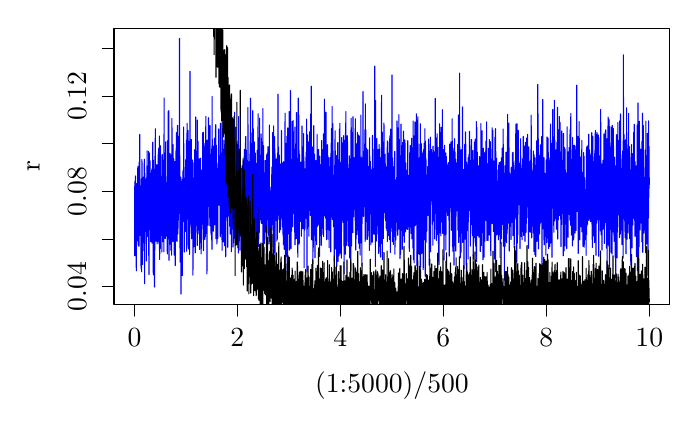
\begin{tikzpicture}[x=0.7pt,y=0.7pt]
\definecolor{fillColor}{RGB}{255,255,255}
%\path[use as bounding box,fill=fillColor,fill opacity=0.00] (0,0) rectangle (361.35,252.94);
\begin{scope}
%\path[clip] ( 49.20, 61.20) rectangle (336.15,203.75);
\definecolor{drawColor}{RGB}{0,0,255}

\path[draw=drawColor,line width= 0.4pt,line join=round,line cap=round] ( 59.83,110.70) --
	( 59.88,121.98) --
	( 59.93, 86.26) --
	( 59.99,124.78) --
	( 60.04, 92.86) --
	( 60.09, 97.41) --
	( 60.15,106.38) --
	( 60.20,110.19) --
	( 60.25,122.56) --
	( 60.31,127.50) --
	( 60.36,122.48) --
	( 60.41, 95.81) --
	( 60.47,114.38) --
	( 60.52,109.07) --
	( 60.57, 99.79) --
	( 60.63, 81.44) --
	( 60.68, 96.13) --
	( 60.73, 78.49) --
	( 60.78,100.33) --
	( 60.84,121.79) --
	( 60.89,115.74) --
	( 60.94, 96.90) --
	( 61.00,101.05) --
	( 61.05, 98.38) --
	( 61.10,123.69) --
	( 61.16,115.08) --
	( 61.21,123.77) --
	( 61.26,111.21) --
	( 61.32, 93.97) --
	( 61.37,102.93) --
	( 61.42,131.42) --
	( 61.48,124.68) --
	( 61.53,102.85) --
	( 61.58,131.18) --
	( 61.63,132.39) --
	( 61.69, 94.35) --
	( 61.74, 92.61) --
	( 61.79, 91.32) --
	( 61.85,106.70) --
	( 61.90,105.13) --
	( 61.95,131.26) --
	( 62.01,108.11) --
	( 62.06,114.56) --
	( 62.11,109.80) --
	( 62.17, 91.26) --
	( 62.22,134.68) --
	( 62.27, 99.13) --
	( 62.33,116.42) --
	( 62.38,110.46) --
	( 62.43,123.77) --
	( 62.49,148.90) --
	( 62.54, 96.81) --
	( 62.59,117.39) --
	( 62.64,106.50) --
	( 62.70,112.46) --
	( 62.75,107.19) --
	( 62.80, 99.05) --
	( 62.86, 99.23) --
	( 62.91,110.33) --
	( 62.96,115.97) --
	( 63.02,108.09) --
	( 63.07, 88.79) --
	( 63.12,108.50) --
	( 63.18, 79.58) --
	( 63.23,122.59) --
	( 63.28,113.85) --
	( 63.34,125.96) --
	( 63.39, 95.22) --
	( 63.44,106.82) --
	( 63.50, 78.01) --
	( 63.55,112.05) --
	( 63.60,135.90) --
	( 63.65,110.46) --
	( 63.71,134.91) --
	( 63.76,109.86) --
	( 63.81, 88.61) --
	( 63.87,121.37) --
	( 63.92,125.51) --
	( 63.97, 81.85) --
	( 64.03,123.17) --
	( 64.08,120.11) --
	( 64.13,111.70) --
	( 64.19, 88.88) --
	( 64.24,102.84) --
	( 64.29,126.82) --
	( 64.35, 92.86) --
	( 64.40,115.50) --
	( 64.45,108.88) --
	( 64.50,109.20) --
	( 64.56,111.31) --
	( 64.61,100.87) --
	( 64.66,106.05) --
	( 64.72,102.12) --
	( 64.77,112.98) --
	( 64.82,131.04) --
	( 64.88,136.15) --
	( 64.93,131.77) --
	( 64.98,107.00) --
	( 65.04, 71.84) --
	( 65.09,128.96) --
	( 65.14,107.79) --
	( 65.20,125.78) --
	( 65.25,112.37) --
	( 65.30,112.88) --
	( 65.36,106.53) --
	( 65.41,101.46) --
	( 65.46,103.00) --
	( 65.51,109.19) --
	( 65.57,124.20) --
	( 65.62,120.97) --
	( 65.67,115.47) --
	( 65.73, 99.75) --
	( 65.78,104.08) --
	( 65.83, 98.65) --
	( 65.89,109.10) --
	( 65.94, 83.58) --
	( 65.99,126.44) --
	( 66.05, 94.37) --
	( 66.10,106.93) --
	( 66.15,104.33) --
	( 66.21,113.09) --
	( 66.26,129.72) --
	( 66.31,140.44) --
	( 66.37, 96.83) --
	( 66.42, 96.20) --
	( 66.47,130.45) --
	( 66.52,118.07) --
	( 66.58,112.89) --
	( 66.63,117.03) --
	( 66.68,112.93) --
	( 66.74,105.02) --
	( 66.79,131.17) --
	( 66.84,107.09) --
	( 66.90,111.43) --
	( 66.95,110.70) --
	( 67.00,100.44) --
	( 67.06,140.16) --
	( 67.11, 86.56) --
	( 67.16, 87.92) --
	( 67.22,105.39) --
	( 67.27, 76.55) --
	( 67.32,115.82) --
	( 67.38,109.05) --
	( 67.43,114.96) --
	( 67.48,139.32) --
	( 67.53,128.66) --
	( 67.59,113.19) --
	( 67.64,113.77) --
	( 67.69, 99.83) --
	( 67.75,117.46) --
	( 67.80,105.25) --
	( 67.85,135.26) --
	( 67.91,106.86) --
	( 67.96,102.98) --
	( 68.01,102.09) --
	( 68.07,109.68) --
	( 68.12, 93.57) --
	( 68.17,114.82) --
	( 68.23,123.62) --
	( 68.28, 98.94) --
	( 68.33,120.33) --
	( 68.38,108.74) --
	( 68.44,111.63) --
	( 68.49,123.90) --
	( 68.54, 97.69) --
	( 68.60,130.46) --
	( 68.65,105.94) --
	( 68.70,122.34) --
	( 68.76,105.96) --
	( 68.81, 92.80) --
	( 68.86,115.36) --
	( 68.92,131.50) --
	( 68.97,103.94) --
	( 69.02,120.65) --
	( 69.08,104.15) --
	( 69.13,103.75) --
	( 69.18,114.87) --
	( 69.24,144.92) --
	( 69.29,123.60) --
	( 69.34,120.29) --
	( 69.39, 85.45) --
	( 69.45, 77.59) --
	( 69.50,112.95) --
	( 69.55,135.55) --
	( 69.61, 76.46) --
	( 69.66, 92.06) --
	( 69.71,111.77) --
	( 69.77,102.29) --
	( 69.82,115.45) --
	( 69.87,109.42) --
	( 69.93,115.82) --
	( 69.98,112.38) --
	( 70.03,104.48) --
	( 70.09, 88.10) --
	( 70.14, 70.12) --
	( 70.19,131.12) --
	( 70.25, 97.63) --
	( 70.30, 89.30) --
	( 70.35,119.62) --
	( 70.40,137.48) --
	( 70.46,140.69) --
	( 70.51,142.79) --
	( 70.56,151.83) --
	( 70.62,111.07) --
	( 70.67,120.65) --
	( 70.72,105.96) --
	( 70.78, 98.55) --
	( 70.83, 93.90) --
	( 70.88, 93.86) --
	( 70.94,133.37) --
	( 70.99,115.20) --
	( 71.04,112.24) --
	( 71.10,107.41) --
	( 71.15,117.50) --
	( 71.20,128.96) --
	( 71.25,117.27) --
	( 71.31,103.76) --
	( 71.36,126.50) --
	( 71.41,113.87) --
	( 71.47, 92.40) --
	( 71.52,118.51) --
	( 71.57,132.45) --
	( 71.63,133.22) --
	( 71.68,110.91) --
	( 71.73,102.85) --
	( 71.79, 93.79) --
	( 71.84,113.31) --
	( 71.89,125.09) --
	( 71.95,118.03) --
	( 72.00,123.71) --
	( 72.05,138.49) --
	( 72.11,102.19) --
	( 72.16,139.92) --
	( 72.21,130.75) --
	( 72.26,116.90) --
	( 72.32,141.81) --
	( 72.37,132.54) --
	( 72.42, 92.72) --
	( 72.48,112.64) --
	( 72.53,101.42) --
	( 72.58,101.53) --
	( 72.64,148.13) --
	( 72.69,101.68) --
	( 72.74, 84.39) --
	( 72.80, 86.96) --
	( 72.85, 98.47) --
	( 72.90,117.03) --
	( 72.96,135.33) --
	( 73.01, 97.31) --
	( 73.06,143.15) --
	( 73.12, 89.98) --
	( 73.17,141.60) --
	( 73.22,118.48) --
	( 73.27,137.94) --
	( 73.33,116.58) --
	( 73.38,126.16) --
	( 73.43, 97.36) --
	( 73.49,109.57) --
	( 73.54,119.00) --
	( 73.59,125.23) --
	( 73.65,118.41) --
	( 73.70,102.66) --
	( 73.75,127.25) --
	( 73.81,104.28) --
	( 73.86,107.70) --
	( 73.91, 88.19) --
	( 73.97,109.61) --
	( 74.02, 98.19) --
	( 74.07,137.95) --
	( 74.12,138.54) --
	( 74.18,104.77) --
	( 74.23,129.50) --
	( 74.28,118.41) --
	( 74.34,110.31) --
	( 74.39,119.30) --
	( 74.44,133.96) --
	( 74.50,135.58) --
	( 74.55, 93.60) --
	( 74.60,107.09) --
	( 74.66,111.96) --
	( 74.71,104.17) --
	( 74.76,124.45) --
	( 74.82,109.92) --
	( 74.87,113.84) --
	( 74.92,111.15) --
	( 74.98, 88.32) --
	( 75.03,136.55) --
	( 75.08,167.71) --
	( 75.13,120.36) --
	( 75.19,120.18) --
	( 75.24,108.13) --
	( 75.29,109.43) --
	( 75.35,102.47) --
	( 75.40,102.99) --
	( 75.45,120.78) --
	( 75.51, 98.88) --
	( 75.56,134.50) --
	( 75.61,135.86) --
	( 75.67, 95.19) --
	( 75.72,139.38) --
	( 75.77,112.91) --
	( 75.83, 98.13) --
	( 75.88,145.09) --
	( 75.93, 96.34) --
	( 75.99,115.84) --
	( 76.04,110.95) --
	( 76.09,107.81) --
	( 76.14,114.25) --
	( 76.20,106.42) --
	( 76.25,121.50) --
	( 76.30,123.99) --
	( 76.36, 98.27) --
	( 76.41,121.51) --
	( 76.46,119.60) --
	( 76.52,114.73) --
	( 76.57,121.57) --
	( 76.62, 97.09) --
	( 76.68,113.89) --
	( 76.73, 87.21) --
	( 76.78,145.59) --
	( 76.84,106.41) --
	( 76.89,105.06) --
	( 76.94,140.40) --
	( 77.00, 94.96) --
	( 77.05,120.52) --
	( 77.10,107.05) --
	( 77.15,111.25) --
	( 77.21,160.74) --
	( 77.26,109.22) --
	( 77.31,128.36) --
	( 77.37,101.48) --
	( 77.42,108.64) --
	( 77.47,141.54) --
	( 77.53,161.20) --
	( 77.58, 83.90) --
	( 77.63,115.04) --
	( 77.69, 88.06) --
	( 77.74,121.29) --
	( 77.79,137.68) --
	( 77.85,115.78) --
	( 77.90,121.14) --
	( 77.95,117.20) --
	( 78.00,112.89) --
	( 78.06,133.61) --
	( 78.11,139.10) --
	( 78.16, 92.27) --
	( 78.22, 94.30) --
	( 78.27,118.05) --
	( 78.32,127.26) --
	( 78.38,122.61) --
	( 78.43,122.51) --
	( 78.48,101.93) --
	( 78.54,118.58) --
	( 78.59,105.82) --
	( 78.64, 89.10) --
	( 78.70,112.72) --
	( 78.75,138.38) --
	( 78.80,100.86) --
	( 78.86,123.65) --
	( 78.91,135.57) --
	( 78.96, 86.64) --
	( 79.01,127.11) --
	( 79.07,111.92) --
	( 79.12,157.09) --
	( 79.17,108.02) --
	( 79.23,101.60) --
	( 79.28,119.48) --
	( 79.33,127.97) --
	( 79.39,116.49) --
	( 79.44,114.96) --
	( 79.49,124.28) --
	( 79.55,102.76) --
	( 79.60, 93.65) --
	( 79.65,101.07) --
	( 79.71,111.57) --
	( 79.76,143.63) --
	( 79.81,109.12) --
	( 79.87, 99.45) --
	( 79.92, 95.26) --
	( 79.97,113.10) --
	( 80.02,120.40) --
	( 80.08,129.18) --
	( 80.13,136.22) --
	( 80.18,104.92) --
	( 80.24,120.86) --
	( 80.29, 86.64) --
	( 80.34,127.85) --
	( 80.40,115.60) --
	( 80.45, 98.03) --
	( 80.50,113.55) --
	( 80.56,120.55) --
	( 80.61,134.89) --
	( 80.66,108.59) --
	( 80.72,124.49) --
	( 80.77,115.84) --
	( 80.82, 81.25) --
	( 80.87,131.95) --
	( 80.93,131.10) --
	( 80.98,113.43) --
	( 81.03,131.92) --
	( 81.09,120.54) --
	( 81.14,105.52) --
	( 81.19,140.28) --
	( 81.25, 94.02) --
	( 81.30,125.71) --
	( 81.35,139.82) --
	( 81.41,144.79) --
	( 81.46,149.83) --
	( 81.51,129.35) --
	( 81.57,135.24) --
	( 81.62,122.45) --
	( 81.67,123.53) --
	( 81.73,111.60) --
	( 81.78, 93.70) --
	( 81.83,119.01) --
	( 81.88,120.52) --
	( 81.94,124.80) --
	( 81.99,153.54) --
	( 82.04,116.33) --
	( 82.10,134.30) --
	( 82.15, 99.88) --
	( 82.20, 97.52) --
	( 82.26,105.46) --
	( 82.31,146.18) --
	( 82.36,144.40) --
	( 82.42,124.96) --
	( 82.47,104.67) --
	( 82.52,120.98) --
	( 82.58,129.26) --
	( 82.63,145.79) --
	( 82.68,123.35) --
	( 82.74,127.14) --
	( 82.79,148.19) --
	( 82.84,124.61) --
	( 82.89,127.92) --
	( 82.95,119.66) --
	( 83.00,128.57) --
	( 83.05,198.47) --
	( 83.11,112.63) --
	( 83.16,137.94) --
	( 83.21,101.38) --
	( 83.27,117.71) --
	( 83.32, 82.98) --
	( 83.37, 99.43) --
	( 83.43,123.53) --
	( 83.48,113.02) --
	( 83.53,124.93) --
	( 83.59,124.23) --
	( 83.64,126.89) --
	( 83.69,124.52) --
	( 83.75,103.31) --
	( 83.80, 66.48) --
	( 83.85,102.57) --
	( 83.90, 87.50) --
	( 83.96,102.55) --
	( 84.01,124.62) --
	( 84.06,118.30) --
	( 84.12,111.79) --
	( 84.17, 99.07) --
	( 84.22,115.92) --
	( 84.28,124.68) --
	( 84.33, 96.07) --
	( 84.38,123.46) --
	( 84.44, 76.09) --
	( 84.49, 89.95) --
	( 84.54,124.31) --
	( 84.60,125.90) --
	( 84.65,122.78) --
	( 84.70,115.92) --
	( 84.75,103.92) --
	( 84.81,130.03) --
	( 84.86,104.45) --
	( 84.91,114.23) --
	( 84.97,105.72) --
	( 85.02,130.92) --
	( 85.07,125.07) --
	( 85.13,125.76) --
	( 85.18,152.74) --
	( 85.23,110.93) --
	( 85.29,104.78) --
	( 85.34,117.81) --
	( 85.39,131.96) --
	( 85.45, 97.53) --
	( 85.50, 88.21) --
	( 85.55,107.49) --
	( 85.61,121.81) --
	( 85.66,121.35) --
	( 85.71,118.12) --
	( 85.76,126.39) --
	( 85.82,107.88) --
	( 85.87,123.64) --
	( 85.92,122.75) --
	( 85.98,104.85) --
	( 86.03,103.34) --
	( 86.08, 98.99) --
	( 86.14,106.68) --
	( 86.19,119.48) --
	( 86.24,135.91) --
	( 86.30, 98.76) --
	( 86.35,131.08) --
	( 86.40,113.92) --
	( 86.46,121.38) --
	( 86.51,135.76) --
	( 86.56,100.86) --
	( 86.62,145.89) --
	( 86.67,115.61) --
	( 86.72, 88.58) --
	( 86.77,141.50) --
	( 86.83,114.20) --
	( 86.88,119.53) --
	( 86.93,154.61) --
	( 86.99,123.90) --
	( 87.04,121.92) --
	( 87.09,148.94) --
	( 87.15,122.16) --
	( 87.20,112.06) --
	( 87.25,115.45) --
	( 87.31,105.02) --
	( 87.36,119.64) --
	( 87.41,150.93) --
	( 87.47,144.89) --
	( 87.52,126.00) --
	( 87.57, 90.43) --
	( 87.62,118.82) --
	( 87.68, 97.51) --
	( 87.73,106.13) --
	( 87.78, 89.76) --
	( 87.84,145.45) --
	( 87.89,100.19) --
	( 87.94, 97.51) --
	( 88.00,121.58) --
	( 88.05,121.12) --
	( 88.10,104.25) --
	( 88.16,118.23) --
	( 88.21,116.19) --
	( 88.26, 86.99) --
	( 88.32,110.47) --
	( 88.37,116.56) --
	( 88.42,181.49) --
	( 88.48,102.48) --
	( 88.53,104.24) --
	( 88.58,136.09) --
	( 88.63,141.30) --
	( 88.69,129.02) --
	( 88.74,124.28) --
	( 88.79,107.55) --
	( 88.85,132.86) --
	( 88.90,128.71) --
	( 88.95,111.83) --
	( 89.01,134.80) --
	( 89.06,108.22) --
	( 89.11,146.34) --
	( 89.17,115.48) --
	( 89.22,107.70) --
	( 89.27, 95.03) --
	( 89.33,119.33) --
	( 89.38,111.41) --
	( 89.43,106.70) --
	( 89.49,102.98) --
	( 89.54,132.77) --
	( 89.59,129.49) --
	( 89.64,120.94) --
	( 89.70,133.31) --
	( 89.75,135.74) --
	( 89.80,130.07) --
	( 89.86,104.47) --
	( 89.91,123.59) --
	( 89.96, 76.29) --
	( 90.02,110.12) --
	( 90.07,102.85) --
	( 90.12, 91.64) --
	( 90.18,116.15) --
	( 90.23,117.92) --
	( 90.28,117.94) --
	( 90.34, 99.73) --
	( 90.39,115.91) --
	( 90.44, 90.96) --
	( 90.50,106.34) --
	( 90.55,134.28) --
	( 90.60,123.05) --
	( 90.65,126.98) --
	( 90.71,118.57) --
	( 90.76,110.95) --
	( 90.81,141.03) --
	( 90.87,139.61) --
	( 90.92, 93.22) --
	( 90.97, 97.54) --
	( 91.03,130.08) --
	( 91.08,132.44) --
	( 91.13, 87.75) --
	( 91.19,116.27) --
	( 91.24,111.69) --
	( 91.29, 98.30) --
	( 91.35,133.52) --
	( 91.40,158.00) --
	( 91.45,111.90) --
	( 91.50,123.63) --
	( 91.56,101.76) --
	( 91.61,132.90) --
	( 91.66,112.44) --
	( 91.72,124.79) --
	( 91.77,113.75) --
	( 91.82,128.35) --
	( 91.88,136.76) --
	( 91.93,137.30) --
	( 91.98,133.41) --
	( 92.04,128.22) --
	( 92.09,140.28) --
	( 92.14,103.81) --
	( 92.20, 91.59) --
	( 92.25,156.30) --
	( 92.30,131.81) --
	( 92.36,108.54) --
	( 92.41, 99.39) --
	( 92.46,127.33) --
	( 92.51,108.26) --
	( 92.57,132.64) --
	( 92.62,145.30) --
	( 92.67,111.34) --
	( 92.73,123.87) --
	( 92.78,118.77) --
	( 92.83,112.01) --
	( 92.89,111.38) --
	( 92.94,112.43) --
	( 92.99,133.38) --
	( 93.05, 97.56) --
	( 93.10,105.09) --
	( 93.15,100.96) --
	( 93.21,109.42) --
	( 93.26,136.37) --
	( 93.31,128.75) --
	( 93.37,116.68) --
	( 93.42, 89.60) --
	( 93.47,117.73) --
	( 93.52, 94.57) --
	( 93.58,132.67) --
	( 93.63,118.83) --
	( 93.68,128.20) --
	( 93.74, 93.07) --
	( 93.79,114.66) --
	( 93.84,130.01) --
	( 93.90,136.69) --
	( 93.95,122.18) --
	( 94.00,122.60) --
	( 94.06,117.97) --
	( 94.11,110.88) --
	( 94.16,120.59) --
	( 94.22, 87.26) --
	( 94.27,123.57) --
	( 94.32,112.74) --
	( 94.37,114.38) --
	( 94.43,127.41) --
	( 94.48,111.60) --
	( 94.53,130.54) --
	( 94.59,106.09) --
	( 94.64,122.07) --
	( 94.69,113.50) --
	( 94.75,115.51) --
	( 94.80,106.83) --
	( 94.85,109.21) --
	( 94.91,102.45) --
	( 94.96,149.82) --
	( 95.01,110.41) --
	( 95.07,100.16) --
	( 95.12,133.80) --
	( 95.17,102.16) --
	( 95.23,136.81) --
	( 95.28, 94.63) --
	( 95.33,121.68) --
	( 95.38,150.04) --
	( 95.44, 88.95) --
	( 95.49,139.36) --
	( 95.54,124.06) --
	( 95.60,101.53) --
	( 95.65,106.21) --
	( 95.70,125.54) --
	( 95.76,110.84) --
	( 95.81,105.15) --
	( 95.86,104.83) --
	( 95.92,142.50) --
	( 95.97,107.16) --
	( 96.02,125.23) --
	( 96.08,113.59) --
	( 96.13, 94.74) --
	( 96.18,117.50) --
	( 96.24,130.34) --
	( 96.29,144.24) --
	( 96.34, 96.07) --
	( 96.39,106.18) --
	( 96.45, 97.63) --
	( 96.50,117.74) --
	( 96.55,118.93) --
	( 96.61,158.26) --
	( 96.66,134.25) --
	( 96.71,124.39) --
	( 96.77,128.98) --
	( 96.82,119.35) --
	( 96.87,103.87) --
	( 96.93,130.91) --
	( 96.98,122.78) --
	( 97.03,112.04) --
	( 97.09,144.69) --
	( 97.14,117.06) --
	( 97.19, 76.92) --
	( 97.25,123.00) --
	( 97.30,111.41) --
	( 97.35,145.96) --
	( 97.40,121.98) --
	( 97.46,134.28) --
	( 97.51,127.07) --
	( 97.56,103.61) --
	( 97.62,144.19) --
	( 97.67,114.71) --
	( 97.72,102.01) --
	( 97.78,113.89) --
	( 97.83,110.67) --
	( 97.88,121.12) --
	( 97.94,122.84) --
	( 97.99,157.62) --
	( 98.04,148.92) --
	( 98.10,115.66) --
	( 98.15,116.97) --
	( 98.20,126.31) --
	( 98.25,138.30) --
	( 98.31,120.29) --
	( 98.36,112.69) --
	( 98.41,138.37) --
	( 98.47,135.89) --
	( 98.52,114.60) --
	( 98.57,105.80) --
	( 98.63,123.75) --
	( 98.68,101.69) --
	( 98.73,126.59) --
	( 98.79,153.61) --
	( 98.84,142.99) --
	( 98.89,123.93) --
	( 98.95,110.44) --
	( 99.00,133.09) --
	( 99.05,118.51) --
	( 99.11,108.34) --
	( 99.16,134.00) --
	( 99.21,103.03) --
	( 99.26, 98.21) --
	( 99.32,129.34) --
	( 99.37,135.91) --
	( 99.42, 96.94) --
	( 99.48,115.77) --
	( 99.53,128.29) --
	( 99.58,141.48) --
	( 99.64,104.66) --
	( 99.69, 94.25) --
	( 99.74,143.10) --
	( 99.80, 89.58) --
	( 99.85,168.55) --
	( 99.90,147.24) --
	( 99.96,122.05) --
	(100.01,123.82) --
	(100.06,109.65) --
	(100.12,128.43) --
	(100.17,118.43) --
	(100.22,107.47) --
	(100.27,100.89) --
	(100.33,105.51) --
	(100.38,117.81) --
	(100.43,142.84) --
	(100.49,112.00) --
	(100.54, 98.96) --
	(100.59,107.26) --
	(100.65,127.34) --
	(100.70,101.87) --
	(100.75,102.05) --
	(100.81,108.98) --
	(100.86,115.87) --
	(100.91,109.72) --
	(100.97,106.98) --
	(101.02,146.93) --
	(101.07,105.35) --
	(101.12,121.07) --
	(101.18,109.47) --
	(101.23,133.10) --
	(101.28,112.62) --
	(101.34,102.38) --
	(101.39,141.75) --
	(101.44,118.75) --
	(101.50,131.86) --
	(101.55,131.35) --
	(101.60,151.80) --
	(101.66,113.72) --
	(101.71,153.99) --
	(101.76,120.85) --
	(101.82, 95.08) --
	(101.87,126.04) --
	(101.92,137.90) --
	(101.98,124.09) --
	(102.03, 96.51) --
	(102.08,143.27) --
	(102.13,115.49) --
	(102.19,133.93) --
	(102.24,133.62) --
	(102.29,103.98) --
	(102.35, 92.38) --
	(102.40,102.67) --
	(102.45,101.68) --
	(102.51,101.50) --
	(102.56,109.71) --
	(102.61,124.50) --
	(102.67,114.61) --
	(102.72,107.55) --
	(102.77, 95.27) --
	(102.83,121.35) --
	(102.88,131.40) --
	(102.93,118.73) --
	(102.99,116.02) --
	(103.04,124.26) --
	(103.09,135.33) --
	(103.14,141.70) --
	(103.20,118.91) --
	(103.25,124.10) --
	(103.30,151.77) --
	(103.36,113.82) --
	(103.41,117.87) --
	(103.46,112.37) --
	(103.52,132.33) --
	(103.57,123.74) --
	(103.62,137.91) --
	(103.68,115.26) --
	(103.73,126.87) --
	(103.78,118.47) --
	(103.84,113.32) --
	(103.89,123.87) --
	(103.94,112.74) --
	(104.00,111.43) --
	(104.05, 98.08) --
	(104.10, 96.10) --
	(104.15,100.19) --
	(104.21,154.67) --
	(104.26,105.62) --
	(104.31,116.04) --
	(104.37,139.50) --
	(104.42,132.72) --
	(104.47, 97.79) --
	(104.53,117.92) --
	(104.58,133.14) --
	(104.63,116.27) --
	(104.69,125.48) --
	(104.74,138.48) --
	(104.79,132.51) --
	(104.85,108.36) --
	(104.90,115.73) --
	(104.95,116.70) --
	(105.00, 89.10) --
	(105.06,156.16) --
	(105.11,104.96) --
	(105.16, 94.83) --
	(105.22,103.84) --
	(105.27,140.05) --
	(105.32,131.08) --
	(105.38,109.14) --
	(105.43,106.30) --
	(105.48,103.35) --
	(105.54, 93.68) --
	(105.59,114.07) --
	(105.64, 93.42) --
	(105.70,122.57) --
	(105.75,106.17) --
	(105.80,124.69) --
	(105.86,141.37) --
	(105.91,125.49) --
	(105.96,108.32) --
	(106.01,145.94) --
	(106.07,106.38) --
	(106.12,119.04) --
	(106.17,106.83) --
	(106.23,143.64) --
	(106.28,125.92) --
	(106.33, 91.47) --
	(106.39, 92.59) --
	(106.44,130.51) --
	(106.49,110.59) --
	(106.55,143.53) --
	(106.60,128.28) --
	(106.65,108.53) --
	(106.71,121.80) --
	(106.76,124.03) --
	(106.81,120.13) --
	(106.87, 85.73) --
	(106.92,105.61) --
	(106.97,142.64) --
	(107.02,137.33) --
	(107.08,106.05) --
	(107.13,110.88) --
	(107.18,112.86) --
	(107.24,118.06) --
	(107.29,132.91) --
	(107.34,113.22) --
	(107.40,129.27) --
	(107.45,120.98) --
	(107.50,125.77) --
	(107.56,128.19) --
	(107.61,141.27) --
	(107.66,111.40) --
	(107.72,118.08) --
	(107.77,104.39) --
	(107.82,104.84) --
	(107.87,127.59) --
	(107.93, 90.68) --
	(107.98,138.15) --
	(108.03,130.24) --
	(108.09,119.20) --
	(108.14,116.83) --
	(108.19,148.96) --
	(108.25,126.49) --
	(108.30,106.72) --
	(108.35,144.94) --
	(108.41,115.49) --
	(108.46,115.50) --
	(108.51,120.84) --
	(108.57,123.67) --
	(108.62,113.71) --
	(108.67,144.81) --
	(108.73,125.11) --
	(108.78,111.49) --
	(108.83,125.62) --
	(108.88,101.61) --
	(108.94,103.46) --
	(108.99,109.74) --
	(109.04,123.17) --
	(109.10,134.36) --
	(109.15,112.56) --
	(109.20, 97.45) --
	(109.26,122.10) --
	(109.31,124.55) --
	(109.36, 98.12) --
	(109.42,100.68) --
	(109.47,159.24) --
	(109.52,117.88) --
	(109.58,125.94) --
	(109.63,113.21) --
	(109.68,118.83) --
	(109.74,133.80) --
	(109.79, 88.38) --
	(109.84,120.79) --
	(109.89,126.72) --
	(109.95,117.71) --
	(110.00,108.07) --
	(110.05,111.89) --
	(110.11,119.56) --
	(110.16,113.82) --
	(110.21,153.13) --
	(110.27,100.16) --
	(110.32,138.23) --
	(110.37,122.58) --
	(110.43,149.81) --
	(110.48,113.48) --
	(110.53,115.00) --
	(110.59,109.11) --
	(110.64, 90.80) --
	(110.69,148.76) --
	(110.75,106.78) --
	(110.80,106.88) --
	(110.85,123.32) --
	(110.90, 93.02) --
	(110.96,111.37) --
	(111.01,113.12) --
	(111.06,130.03) --
	(111.12,125.99) --
	(111.17,107.00) --
	(111.22,127.67) --
	(111.28,131.32) --
	(111.33,123.83) --
	(111.38,124.70) --
	(111.44,118.61) --
	(111.49,160.41) --
	(111.54,102.18) --
	(111.60,134.74) --
	(111.65,114.89) --
	(111.70, 95.06) --
	(111.75,121.27) --
	(111.81,149.35) --
	(111.86, 91.62) --
	(111.91,102.77) --
	(111.97,121.64) --
	(112.02, 95.52) --
	(112.07,120.75) --
	(112.13, 98.76) --
	(112.18,152.68) --
	(112.23, 97.54) --
	(112.29,137.88) --
	(112.34,144.80) --
	(112.39,103.55) --
	(112.45,134.64) --
	(112.50,134.92) --
	(112.55,123.28) --
	(112.61,126.10) --
	(112.66,116.62) --
	(112.71,127.53) --
	(112.76,123.35) --
	(112.82, 92.24) --
	(112.87,114.09) --
	(112.92,103.83) --
	(112.98,143.66) --
	(113.03,107.06) --
	(113.08,108.28) --
	(113.14,114.52) --
	(113.19,110.63) --
	(113.24,100.46) --
	(113.30,104.67) --
	(113.35,127.06) --
	(113.40, 87.73) --
	(113.46,110.39) --
	(113.51, 99.42) --
	(113.56,158.18) --
	(113.62,116.02) --
	(113.67,128.87) --
	(113.72,113.78) --
	(113.77,119.46) --
	(113.83,114.60) --
	(113.88,116.48) --
	(113.93,102.02) --
	(113.99,100.76) --
	(114.04,111.61) --
	(114.09,125.93) --
	(114.15, 93.77) --
	(114.20,134.53) --
	(114.25, 89.13) --
	(114.31,121.46) --
	(114.36,136.67) --
	(114.41, 98.40) --
	(114.47,114.51) --
	(114.52,126.84) --
	(114.57,130.82) --
	(114.62,110.13) --
	(114.68,119.62) --
	(114.73,131.47) --
	(114.78,119.90) --
	(114.84,101.98) --
	(114.89,129.03) --
	(114.94,128.69) --
	(115.00,101.05) --
	(115.05,127.88) --
	(115.10, 87.88) --
	(115.16,115.97) --
	(115.21,121.24) --
	(115.26,120.23) --
	(115.32,132.82) --
	(115.37,109.89) --
	(115.42,108.73) --
	(115.48,116.42) --
	(115.53,125.97) --
	(115.58,125.95) --
	(115.63,132.49) --
	(115.69,116.29) --
	(115.74,105.47) --
	(115.79,106.53) --
	(115.85,135.29) --
	(115.90,112.19) --
	(115.95,117.45) --
	(116.01,127.35) --
	(116.06, 99.74) --
	(116.11,129.92) --
	(116.17,125.10) --
	(116.22,119.84) --
	(116.27,130.77) --
	(116.33, 94.84) --
	(116.38,126.38) --
	(116.43,126.31) --
	(116.49,141.16) --
	(116.54, 90.79) --
	(116.59,100.53) --
	(116.64,112.65) --
	(116.70,136.55) --
	(116.75,112.98) --
	(116.80,118.56) --
	(116.86,123.52) --
	(116.91,103.60) --
	(116.96,131.28) --
	(117.02,125.89) --
	(117.07,102.94) --
	(117.12,144.71) --
	(117.18,126.99) --
	(117.23,147.95) --
	(117.28,111.30) --
	(117.34,112.31) --
	(117.39,112.61) --
	(117.44,107.01) --
	(117.50,115.14) --
	(117.55,140.90) --
	(117.60,123.46) --
	(117.65,129.84) --
	(117.71,131.34) --
	(117.76,131.68) --
	(117.81,101.16) --
	(117.87,135.49) --
	(117.92,122.70) --
	(117.97,106.27) --
	(118.03,120.09) --
	(118.08,126.24) --
	(118.13,115.32) --
	(118.19,118.79) --
	(118.24, 97.45) --
	(118.29,125.89) --
	(118.35,162.83) --
	(118.40, 96.25) --
	(118.45,107.55) --
	(118.50, 95.89) --
	(118.56,129.52) --
	(118.61,121.20) --
	(118.66,117.72) --
	(118.72,116.23) --
	(118.77,113.54) --
	(118.82, 90.91) --
	(118.88,108.82) --
	(118.93,132.87) --
	(118.98,117.69) --
	(119.04,104.75) --
	(119.09,114.37) --
	(119.14,135.02) --
	(119.20,112.08) --
	(119.25,114.48) --
	(119.30,133.85) --
	(119.36, 99.44) --
	(119.41,125.17) --
	(119.46,145.22) --
	(119.51,110.13) --
	(119.57,127.30) --
	(119.62,107.94) --
	(119.67,167.68) --
	(119.73, 87.67) --
	(119.78, 90.45) --
	(119.83,118.32) --
	(119.89,140.50) --
	(119.94,135.33) --
	(119.99,149.78) --
	(120.05,108.04) --
	(120.10,112.19) --
	(120.15,105.72) --
	(120.21,128.13) --
	(120.26,100.71) --
	(120.31,144.15) --
	(120.37,115.95) --
	(120.42,118.66) --
	(120.47,105.54) --
	(120.52,109.85) --
	(120.58,107.18) --
	(120.63,122.59) --
	(120.68,118.50) --
	(120.74,131.09) --
	(120.79,100.55) --
	(120.84,161.22) --
	(120.90,105.65) --
	(120.95,122.43) --
	(121.00,107.32) --
	(121.06,100.74) --
	(121.11,130.37) --
	(121.16,151.87) --
	(121.22,126.47) --
	(121.27,130.49) --
	(121.32,114.54) --
	(121.37,108.77) --
	(121.43,107.92) --
	(121.48,141.52) --
	(121.53,125.72) --
	(121.59,145.06) --
	(121.64,130.35) --
	(121.69,112.49) --
	(121.75,114.29) --
	(121.80,131.12) --
	(121.85,114.24) --
	(121.91, 85.83) --
	(121.96,104.35) --
	(122.01,110.65) --
	(122.07,114.63) --
	(122.12,126.29) --
	(122.17,139.35) --
	(122.23,121.81) --
	(122.28,113.49) --
	(122.33,130.56) --
	(122.38,129.56) --
	(122.44, 87.79) --
	(122.49,133.93) --
	(122.54,116.50) --
	(122.60,107.31) --
	(122.65,115.22) --
	(122.70,124.39) --
	(122.76,130.97) --
	(122.81,127.57) --
	(122.86, 91.25) --
	(122.92,122.55) --
	(122.97,123.66) --
	(123.02, 97.46) --
	(123.08,140.76) --
	(123.13,125.03) --
	(123.18,116.24) --
	(123.24,116.08) --
	(123.29,122.44) --
	(123.34,110.34) --
	(123.39,135.87) --
	(123.45,110.78) --
	(123.50,152.75) --
	(123.55,120.34) --
	(123.61,159.60) --
	(123.66,125.96) --
	(123.71,112.93) --
	(123.77,116.77) --
	(123.82,147.22) --
	(123.87, 91.16) --
	(123.93, 97.37) --
	(123.98,126.67) --
	(124.03,129.09) --
	(124.09,132.04) --
	(124.14,112.53) --
	(124.19,128.58) --
	(124.24, 98.36) --
	(124.30,135.57) --
	(124.35,120.42) --
	(124.40,157.30) --
	(124.46,103.28) --
	(124.51,132.60) --
	(124.56,134.66) --
	(124.62,126.85) --
	(124.67,118.81) --
	(124.72,136.33) --
	(124.78,110.69) --
	(124.83,104.79) --
	(124.88,117.80) --
	(124.94,116.91) --
	(124.99,114.34) --
	(125.04,106.46) --
	(125.10,129.62) --
	(125.15,149.13) --
	(125.20,121.34) --
	(125.25,114.76) --
	(125.31,146.95) --
	(125.36,121.99) --
	(125.41,145.10) --
	(125.47,102.92) --
	(125.52,111.35) --
	(125.57,130.79) --
	(125.63,133.16) --
	(125.68,120.38) --
	(125.73,114.17) --
	(125.79,121.82) --
	(125.84,132.77) --
	(125.89,134.87) --
	(125.95,121.47) --
	(126.00,123.56) --
	(126.05,162.24) --
	(126.11,114.83) --
	(126.16, 83.67) --
	(126.21,109.48) --
	(126.26,133.13) --
	(126.32,132.81) --
	(126.37,143.18) --
	(126.42, 87.40) --
	(126.48,112.18) --
	(126.53,126.27) --
	(126.58,126.45) --
	(126.64,100.38) --
	(126.69, 97.25) --
	(126.74,100.18) --
	(126.80, 92.65) --
	(126.85,123.91) --
	(126.90,129.03) --
	(126.96,127.06) --
	(127.01, 98.40) --
	(127.06,113.42) --
	(127.12,118.05) --
	(127.17,107.48) --
	(127.22,127.77) --
	(127.27,135.51) --
	(127.33,107.77) --
	(127.38,109.59) --
	(127.43, 99.65) --
	(127.49,119.76) --
	(127.54,114.40) --
	(127.59,118.65) --
	(127.65,121.21) --
	(127.70,135.41) --
	(127.75, 94.87) --
	(127.81,129.21) --
	(127.86,117.15) --
	(127.91,124.51) --
	(127.97,106.52) --
	(128.02,110.49) --
	(128.07,138.42) --
	(128.12, 83.87) --
	(128.18,102.88) --
	(128.23,119.63) --
	(128.28,108.92) --
	(128.34,110.91) --
	(128.39,112.30) --
	(128.44,139.39) --
	(128.50,119.85) --
	(128.55,135.54) --
	(128.60,123.15) --
	(128.66,124.47) --
	(128.71,142.54) --
	(128.76,120.48) --
	(128.82,117.72) --
	(128.87,114.95) --
	(128.92,123.27) --
	(128.98,107.78) --
	(129.03, 96.82) --
	(129.08,127.14) --
	(129.13,107.09) --
	(129.19,127.20) --
	(129.24, 92.30) --
	(129.29,114.29) --
	(129.35,116.10) --
	(129.40,153.80) --
	(129.45,107.43) --
	(129.51, 95.57) --
	(129.56,120.32) --
	(129.61, 98.36) --
	(129.67,116.74) --
	(129.72,120.00) --
	(129.77,101.77) --
	(129.83,121.72) --
	(129.88,109.63) --
	(129.93, 93.69) --
	(129.99,103.80) --
	(130.04,101.36) --
	(130.09, 95.55) --
	(130.14,101.95) --
	(130.20, 91.72) --
	(130.25,102.50) --
	(130.30,110.06) --
	(130.36,110.19) --
	(130.41,101.30) --
	(130.46,120.01) --
	(130.52, 99.96) --
	(130.57,117.25) --
	(130.62,128.19) --
	(130.68, 91.00) --
	(130.73,132.15) --
	(130.78,117.70) --
	(130.84, 99.64) --
	(130.89,123.91) --
	(130.94,131.32) --
	(130.99,113.27) --
	(131.05,102.37) --
	(131.10,118.15) --
	(131.15,149.90) --
	(131.21,127.57) --
	(131.26,103.38) --
	(131.31,103.99) --
	(131.37,131.31) --
	(131.42,144.33) --
	(131.47,124.83) --
	(131.53,146.23) --
	(131.58,120.64) --
	(131.63,153.31) --
	(131.69, 88.13) --
	(131.74,104.28) --
	(131.79, 96.21) --
	(131.85,112.74) --
	(131.90,107.69) --
	(131.95,110.66) --
	(132.00,115.45) --
	(132.06,147.83) --
	(132.11,109.46) --
	(132.16,142.79) --
	(132.22,129.35) --
	(132.27,135.08) --
	(132.32, 80.46) --
	(132.38,138.91) --
	(132.43,130.03) --
	(132.48,134.38) --
	(132.54,128.96) --
	(132.59,117.47) --
	(132.64,111.45) --
	(132.70,114.51) --
	(132.75,104.84) --
	(132.80,136.21) --
	(132.86,113.41) --
	(132.91,134.71) --
	(132.96,127.46) --
	(133.01,104.42) --
	(133.07,107.98) --
	(133.12,117.45) --
	(133.17,119.73) --
	(133.23,116.42) --
	(133.28, 93.88) --
	(133.33,102.85) --
	(133.39,137.02) --
	(133.44,120.57) --
	(133.49, 94.81) --
	(133.55,125.91) --
	(133.60,113.79) --
	(133.65,133.70) --
	(133.71,139.44) --
	(133.76,123.60) --
	(133.81,115.28) --
	(133.87,169.64) --
	(133.92,113.75) --
	(133.97,108.02) --
	(134.02,121.86) --
	(134.08,112.29) --
	(134.13,142.51) --
	(134.18,138.30) --
	(134.24,107.05) --
	(134.29,118.15) --
	(134.34,120.28) --
	(134.40,105.02) --
	(134.45,128.63) --
	(134.50,138.19) --
	(134.56,119.46) --
	(134.61,130.49) --
	(134.66, 98.37) --
	(134.72,111.72) --
	(134.77,122.29) --
	(134.82,114.31) --
	(134.87,114.02) --
	(134.93,133.65) --
	(134.98,120.50) --
	(135.03,112.06) --
	(135.09,101.97) --
	(135.14,113.94) --
	(135.19, 99.77) --
	(135.25,115.56) --
	(135.30,101.47) --
	(135.35,123.32) --
	(135.41,130.24) --
	(135.46,121.90) --
	(135.51,108.45) --
	(135.57,111.10) --
	(135.62,150.91) --
	(135.67,150.79) --
	(135.73,118.89) --
	(135.78,129.08) --
	(135.83,106.58) --
	(135.88,105.78) --
	(135.94,129.03) --
	(135.99,124.95) --
	(136.04,117.01) --
	(136.10,104.84) --
	(136.15,113.40) --
	(136.20,122.48) --
	(136.26,113.93) --
	(136.31,100.92) --
	(136.36,134.25) --
	(136.42, 97.50) --
	(136.47,123.74) --
	(136.52, 96.43) --
	(136.58,114.34) --
	(136.63, 92.12) --
	(136.68,114.20) --
	(136.74,134.85) --
	(136.79, 96.90) --
	(136.84,108.67) --
	(136.89,121.51) --
	(136.95,127.45) --
	(137.00,132.82) --
	(137.05,134.49) --
	(137.11, 89.65) --
	(137.16,110.28) --
	(137.21,130.54) --
	(137.27,105.26) --
	(137.32,128.08) --
	(137.37,112.90) --
	(137.43,106.86) --
	(137.48,147.92) --
	(137.53,159.91) --
	(137.59,114.08) --
	(137.64,134.36) --
	(137.69, 80.63) --
	(137.74,112.36) --
	(137.80,108.89) --
	(137.85,144.33) --
	(137.90,118.73) --
	(137.96, 85.98) --
	(138.01,101.32) --
	(138.06,103.65) --
	(138.12,116.91) --
	(138.17,115.29) --
	(138.22, 86.42) --
	(138.28,118.84) --
	(138.33,128.36) --
	(138.38,113.66) --
	(138.44,142.58) --
	(138.49,147.96) --
	(138.54,111.15) --
	(138.60,122.75) --
	(138.65, 76.92) --
	(138.70,136.47) --
	(138.75,114.57) --
	(138.81,140.85) --
	(138.86, 85.31) --
	(138.91,152.29) --
	(138.97,102.00) --
	(139.02,117.43) --
	(139.07,105.61) --
	(139.13,116.54) --
	(139.18, 98.42) --
	(139.23,107.27) --
	(139.29,137.00) --
	(139.34,123.36) --
	(139.39, 97.63) --
	(139.45,120.33) --
	(139.50,119.83) --
	(139.55,103.21) --
	(139.61,160.72) --
	(139.66,129.48) --
	(139.71,137.86) --
	(139.76,130.15) --
	(139.82, 89.26) --
	(139.87,125.02) --
	(139.92,135.81) --
	(139.98,119.19) --
	(140.03,131.76) --
	(140.08,160.45) --
	(140.14,112.86) --
	(140.19,115.74) --
	(140.24,120.61) --
	(140.30,171.58) --
	(140.35, 98.49) --
	(140.40,113.01) --
	(140.46,118.10) --
	(140.51, 98.65) --
	(140.56, 90.00) --
	(140.62, 98.69) --
	(140.67,121.89) --
	(140.72, 99.87) --
	(140.77,116.40) --
	(140.83,100.18) --
	(140.88,119.22) --
	(140.93, 99.02) --
	(140.99,130.49) --
	(141.04,111.44) --
	(141.09,109.05) --
	(141.15,155.55) --
	(141.20,108.01) --
	(141.25,109.31) --
	(141.31,108.65) --
	(141.36,113.77) --
	(141.41,133.03) --
	(141.47,101.31) --
	(141.52,122.02) --
	(141.57,146.64) --
	(141.62,118.35) --
	(141.68,156.11) --
	(141.73,148.17) --
	(141.78,110.14) --
	(141.84,110.46) --
	(141.89,128.09) --
	(141.94,126.05) --
	(142.00,137.49) --
	(142.05,108.26) --
	(142.10,124.65) --
	(142.16,112.86) --
	(142.21,112.91) --
	(142.26,129.92) --
	(142.32,141.36) --
	(142.37,119.94) --
	(142.42,106.45) --
	(142.48, 98.38) --
	(142.53,108.07) --
	(142.58,152.68) --
	(142.63, 91.91) --
	(142.69,138.09) --
	(142.74,141.98) --
	(142.79,119.95) --
	(142.85,120.23) --
	(142.90,120.77) --
	(142.95,109.27) --
	(143.01,107.84) --
	(143.06, 95.06) --
	(143.11,102.57) --
	(143.17,144.09) --
	(143.22,102.98) --
	(143.27,113.86) --
	(143.33,102.81) --
	(143.38,132.60) --
	(143.43,160.22) --
	(143.49,144.16) --
	(143.54,132.59) --
	(143.59, 95.24) --
	(143.64,111.76) --
	(143.70,132.27) --
	(143.75,117.15) --
	(143.80,107.81) --
	(143.86,120.72) --
	(143.91,111.67) --
	(143.96,103.75) --
	(144.02,132.35) --
	(144.07, 89.50) --
	(144.12, 85.53) --
	(144.18,118.19) --
	(144.23,108.49) --
	(144.28,131.02) --
	(144.34,167.69) --
	(144.39,112.43) --
	(144.44,112.47) --
	(144.49, 97.61) --
	(144.55,123.50) --
	(144.60,127.45) --
	(144.65,158.75) --
	(144.71,125.98) --
	(144.76, 92.34) --
	(144.81, 92.76) --
	(144.87, 94.81) --
	(144.92,116.86) --
	(144.97,138.64) --
	(145.03,126.56) --
	(145.08,108.60) --
	(145.13,116.72) --
	(145.19,110.06) --
	(145.24,112.08) --
	(145.29,126.80) --
	(145.35,119.30) --
	(145.40,104.01) --
	(145.45,133.32) --
	(145.50,104.42) --
	(145.56,108.19) --
	(145.61,117.67) --
	(145.66,122.61) --
	(145.72,119.41) --
	(145.77,134.60) --
	(145.82,115.61) --
	(145.88,127.17) --
	(145.93, 96.36) --
	(145.98,133.30) --
	(146.04,114.00) --
	(146.09,123.28) --
	(146.14,114.48) --
	(146.20,144.77) --
	(146.25,153.33) --
	(146.30,127.72) --
	(146.36,137.10) --
	(146.41,109.27) --
	(146.46,101.21) --
	(146.51,120.23) --
	(146.57,120.98) --
	(146.62,114.32) --
	(146.67,100.19) --
	(146.73,106.47) --
	(146.78,108.76) --
	(146.83,119.65) --
	(146.89,134.05) --
	(146.94,112.77) --
	(146.99,142.68) --
	(147.05,132.46) --
	(147.10,149.42) --
	(147.15,120.20) --
	(147.21,116.61) --
	(147.26,137.44) --
	(147.31,110.13) --
	(147.37, 80.15) --
	(147.42,121.03) --
	(147.47,129.93) --
	(147.52,109.15) --
	(147.58,124.52) --
	(147.63,107.70) --
	(147.68, 99.80) --
	(147.74,121.52) --
	(147.79,100.62) --
	(147.84,131.10) --
	(147.90,116.29) --
	(147.95,110.88) --
	(148.00,117.10) --
	(148.06,118.09) --
	(148.11,116.33) --
	(148.16,130.17) --
	(148.22,112.72) --
	(148.27,132.97) --
	(148.32,136.99) --
	(148.37,105.67) --
	(148.43,113.29) --
	(148.48,139.89) --
	(148.53,122.10) --
	(148.59,111.36) --
	(148.64,156.81) --
	(148.69,121.41) --
	(148.75,127.99) --
	(148.80,138.17) --
	(148.85, 77.82) --
	(148.91,148.47) --
	(148.96,100.22) --
	(149.01,108.00) --
	(149.07,100.18) --
	(149.12,148.73) --
	(149.17,113.43) --
	(149.23,127.01) --
	(149.28,125.15) --
	(149.33,130.38) --
	(149.38,130.99) --
	(149.44,104.71) --
	(149.49,123.15) --
	(149.54,107.23) --
	(149.60,145.07) --
	(149.65,126.10) --
	(149.70,119.84) --
	(149.76,121.48) --
	(149.81, 96.45) --
	(149.86,123.56) --
	(149.92,114.26) --
	(149.97,109.65) --
	(150.02,132.54) --
	(150.08,111.07) --
	(150.13,115.22) --
	(150.18,150.28) --
	(150.24,122.47) --
	(150.29,137.47) --
	(150.34,115.93) --
	(150.39,121.30) --
	(150.45,111.31) --
	(150.50,137.23) --
	(150.55,123.17) --
	(150.61,107.12) --
	(150.66,115.46) --
	(150.71,159.45) --
	(150.77,137.63) --
	(150.82,129.97) --
	(150.87,110.66) --
	(150.93,148.57) --
	(150.98,114.53) --
	(151.03,173.84) --
	(151.09,136.91) --
	(151.14,116.45) --
	(151.19, 94.56) --
	(151.24,114.12) --
	(151.30,114.57) --
	(151.35,131.45) --
	(151.40, 98.87) --
	(151.46,120.17) --
	(151.51, 94.40) --
	(151.56,142.43) --
	(151.62,122.23) --
	(151.67,140.92) --
	(151.72,102.00) --
	(151.78,130.97) --
	(151.83,117.65) --
	(151.88, 82.06) --
	(151.94, 94.49) --
	(151.99,118.06) --
	(152.04, 90.65) --
	(152.10,136.15) --
	(152.15,103.94) --
	(152.20,132.07) --
	(152.25,111.34) --
	(152.31,153.45) --
	(152.36,105.45) --
	(152.41, 96.87) --
	(152.47,121.72) --
	(152.52,108.83) --
	(152.57,105.40) --
	(152.63,103.45) --
	(152.68,118.48) --
	(152.73,125.42) --
	(152.79,138.62) --
	(152.84,120.20) --
	(152.89,121.79) --
	(152.95, 85.28) --
	(153.00,107.54) --
	(153.05,106.61) --
	(153.11, 96.24) --
	(153.16, 98.99) --
	(153.21,124.56) --
	(153.26, 94.05) --
	(153.32,102.78) --
	(153.37,114.82) --
	(153.42,129.64) --
	(153.48,135.45) --
	(153.53,117.15) --
	(153.58,123.45) --
	(153.64,113.43) --
	(153.69,105.76) --
	(153.74,115.29) --
	(153.80, 91.96) --
	(153.85,118.87) --
	(153.90,116.78) --
	(153.96,110.23) --
	(154.01,117.78) --
	(154.06,148.88) --
	(154.12,129.81) --
	(154.17,122.60) --
	(154.22,101.53) --
	(154.27,120.97) --
	(154.33,128.36) --
	(154.38,116.89) --
	(154.43,101.64) --
	(154.49,103.47) --
	(154.54,116.48) --
	(154.59,137.51) --
	(154.65,102.34) --
	(154.70,106.99) --
	(154.75,141.19) --
	(154.81,108.85) --
	(154.86,119.81) --
	(154.91,136.73) --
	(154.97,128.61) --
	(155.02,130.84) --
	(155.07,125.04) --
	(155.12,127.09) --
	(155.18,124.84) --
	(155.23,117.63) --
	(155.28,137.75) --
	(155.34, 85.90) --
	(155.39,115.31) --
	(155.44, 99.04) --
	(155.50,108.88) --
	(155.55,133.44) --
	(155.60,109.47) --
	(155.66, 97.63) --
	(155.71,114.35) --
	(155.76,108.42) --
	(155.82,126.21) --
	(155.87,122.19) --
	(155.92,126.41) --
	(155.98,121.06) --
	(156.03, 96.51) --
	(156.08,101.73) --
	(156.13,118.40) --
	(156.19, 91.69) --
	(156.24,111.60) --
	(156.29,137.69) --
	(156.35,123.00) --
	(156.40,145.73) --
	(156.45,109.51) --
	(156.51,122.89) --
	(156.56,138.53) --
	(156.61, 97.33) --
	(156.67,141.11) --
	(156.72,123.71) --
	(156.77,100.36) --
	(156.83,117.76) --
	(156.88,121.55) --
	(156.93,110.20) --
	(156.99,101.97) --
	(157.04,109.19) --
	(157.09,106.27) --
	(157.14,119.94) --
	(157.20,115.45) --
	(157.25,125.19) --
	(157.30,135.12) --
	(157.36,149.24) --
	(157.41, 96.25) --
	(157.46,120.99) --
	(157.52,121.55) --
	(157.57,128.32) --
	(157.62,148.25) --
	(157.68,114.42) --
	(157.73,106.72) --
	(157.78,140.45) --
	(157.84,167.13) --
	(157.89,126.58) --
	(157.94,141.03) --
	(157.99,122.68) --
	(158.05,110.13) --
	(158.10,145.58) --
	(158.15,133.72) --
	(158.21,122.20) --
	(158.26,124.92) --
	(158.31,127.94) --
	(158.37,109.45) --
	(158.42,159.70) --
	(158.47,105.69) --
	(158.53,125.31) --
	(158.58,105.59) --
	(158.63,160.35) --
	(158.69,109.84) --
	(158.74,114.70) --
	(158.79, 99.49) --
	(158.85,132.79) --
	(158.90,117.86) --
	(158.95, 94.58) --
	(159.00,137.02) --
	(159.06,109.43) --
	(159.11,118.76) --
	(159.16, 94.92) --
	(159.22,117.53) --
	(159.27,118.10) --
	(159.32,125.19) --
	(159.38,120.32) --
	(159.43,143.61) --
	(159.48,133.70) --
	(159.54,138.11) --
	(159.59,135.08) --
	(159.64,135.31) --
	(159.70,130.33) --
	(159.75,134.69) --
	(159.80, 99.86) --
	(159.86,113.06) --
	(159.91,112.76) --
	(159.96,125.72) --
	(160.01,121.09) --
	(160.07,106.25) --
	(160.12, 95.96) --
	(160.17,136.95) --
	(160.23, 90.44) --
	(160.28,134.95) --
	(160.33,114.19) --
	(160.39,117.03) --
	(160.44,128.35) --
	(160.49,119.95) --
	(160.55,116.01) --
	(160.60,110.76) --
	(160.65,132.21) --
	(160.71,127.54) --
	(160.76,122.68) --
	(160.81,119.33) --
	(160.87,104.66) --
	(160.92, 99.20) --
	(160.97,121.73) --
	(161.02,126.93) --
	(161.08, 88.31) --
	(161.13,139.17) --
	(161.18,111.81) --
	(161.24,113.47) --
	(161.29,144.32) --
	(161.34,128.79) --
	(161.40,130.88) --
	(161.45,124.67) --
	(161.50,151.68) --
	(161.56,152.01) --
	(161.61,115.14) --
	(161.66,130.91) --
	(161.72,113.04) --
	(161.77,106.26) --
	(161.82,163.32) --
	(161.87,114.70) --
	(161.93,109.27) --
	(161.98,104.98) --
	(162.03,105.46) --
	(162.09,107.40) --
	(162.14,154.42) --
	(162.19,127.87) --
	(162.25,107.94) --
	(162.30,140.31) --
	(162.35,127.88) --
	(162.41,105.51) --
	(162.46,107.46) --
	(162.51,101.36) --
	(162.57,118.45) --
	(162.62,127.08) --
	(162.67,121.55) --
	(162.73,127.81) --
	(162.78,125.82) --
	(162.83, 96.32) --
	(162.88, 83.95) --
	(162.94,120.59) --
	(162.99,113.17) --
	(163.04,109.11) --
	(163.10,106.81) --
	(163.15,123.62) --
	(163.20,134.57) --
	(163.26,101.90) --
	(163.31,145.07) --
	(163.36,150.82) --
	(163.42,133.69) --
	(163.47,130.31) --
	(163.52,121.66) --
	(163.58,107.75) --
	(163.63,100.33) --
	(163.68, 89.77) --
	(163.74,118.36) --
	(163.79,111.67) --
	(163.84,125.93) --
	(163.89,102.35) --
	(163.95, 97.44) --
	(164.00,119.10) --
	(164.05, 97.75) --
	(164.11,122.40) --
	(164.16,138.10) --
	(164.21, 80.78) --
	(164.27,124.27) --
	(164.32,113.35) --
	(164.37,110.24) --
	(164.43, 98.86) --
	(164.48, 99.98) --
	(164.53,119.51) --
	(164.59,132.53) --
	(164.64, 94.46) --
	(164.69,108.83) --
	(164.74,144.73) --
	(164.80,122.25) --
	(164.85,120.56) --
	(164.90, 83.41) --
	(164.96,127.40) --
	(165.01,113.06) --
	(165.06,109.96) --
	(165.12,102.06) --
	(165.17,135.76) --
	(165.22,120.84) --
	(165.28,118.73) --
	(165.33, 86.27) --
	(165.38, 98.28) --
	(165.44,119.60) --
	(165.49,107.71) --
	(165.54,151.65) --
	(165.60,110.78) --
	(165.65,117.82) --
	(165.70,138.96) --
	(165.75,107.79) --
	(165.81,154.66) --
	(165.86,128.46) --
	(165.91,105.16) --
	(165.97,114.25) --
	(166.02, 87.61) --
	(166.07,105.49) --
	(166.13, 95.71) --
	(166.18,108.31) --
	(166.23,115.54) --
	(166.29, 90.91) --
	(166.34,121.91) --
	(166.39,129.79) --
	(166.45,134.33) --
	(166.50,127.91) --
	(166.55, 85.05) --
	(166.61,110.81) --
	(166.66,125.96) --
	(166.71, 98.56) --
	(166.76,147.40) --
	(166.82,117.48) --
	(166.87,104.50) --
	(166.92,109.13) --
	(166.98,125.22) --
	(167.03,118.07) --
	(167.08,133.99) --
	(167.14,107.55) --
	(167.19,144.55) --
	(167.24,126.49) --
	(167.30,113.79) --
	(167.35,132.76) --
	(167.40,133.73) --
	(167.46,137.49) --
	(167.51,103.52) --
	(167.56,112.33) --
	(167.62,103.80) --
	(167.67,116.03) --
	(167.72,148.29) --
	(167.77,124.30) --
	(167.83,118.18) --
	(167.88,111.36) --
	(167.93,115.62) --
	(167.99, 77.01) --
	(168.04,117.31) --
	(168.09,128.94) --
	(168.15,145.89) --
	(168.20,121.16) --
	(168.25,126.04) --
	(168.31,124.98) --
	(168.36,134.40) --
	(168.41,128.65) --
	(168.47,141.05) --
	(168.52,101.84) --
	(168.57,105.07) --
	(168.62, 87.07) --
	(168.68,149.87) --
	(168.73,135.46) --
	(168.78,112.46) --
	(168.84,145.21) --
	(168.89,160.76) --
	(168.94,112.77) --
	(169.00,138.48) --
	(169.05,101.81) --
	(169.10, 97.71) --
	(169.16,122.03) --
	(169.21, 93.71) --
	(169.26,103.62) --
	(169.32, 91.65) --
	(169.37, 99.44) --
	(169.42,107.61) --
	(169.48,120.90) --
	(169.53,122.21) --
	(169.58,122.89) --
	(169.63,148.24) --
	(169.69,132.24) --
	(169.74,105.02) --
	(169.79,145.03) --
	(169.85,104.62) --
	(169.90,104.52) --
	(169.95,121.08) --
	(170.01,115.12) --
	(170.06,114.63) --
	(170.11,118.93) --
	(170.17,115.12) --
	(170.22,103.65) --
	(170.27, 91.31) --
	(170.33,131.34) --
	(170.38,130.09) --
	(170.43, 99.19) --
	(170.49,128.07) --
	(170.54, 93.73) --
	(170.59,121.87) --
	(170.64,133.57) --
	(170.70,123.95) --
	(170.75,137.88) --
	(170.80,100.77) --
	(170.86, 99.26) --
	(170.91, 85.12) --
	(170.96,101.31) --
	(171.02,120.79) --
	(171.07,121.47) --
	(171.12,130.80) --
	(171.18, 93.58) --
	(171.23,133.36) --
	(171.28, 97.97) --
	(171.34,120.52) --
	(171.39, 93.10) --
	(171.44, 78.54) --
	(171.49,108.08) --
	(171.55,141.08) --
	(171.60,157.27) --
	(171.65,157.24) --
	(171.71,103.47) --
	(171.76,110.45) --
	(171.81, 91.25) --
	(171.87, 91.79) --
	(171.92,119.26) --
	(171.97,149.89) --
	(172.03,109.68) --
	(172.08,118.68) --
	(172.13,122.24) --
	(172.19,112.66) --
	(172.24,114.84) --
	(172.29,106.70) --
	(172.35,137.41) --
	(172.40,129.78) --
	(172.45,127.34) --
	(172.50, 98.23) --
	(172.56,115.75) --
	(172.61,158.12) --
	(172.66,113.00) --
	(172.72,121.25) --
	(172.77,114.39) --
	(172.82,106.34) --
	(172.88,114.77) --
	(172.93,108.20) --
	(172.98,113.57) --
	(173.04,122.34) --
	(173.09,136.91) --
	(173.14,129.24) --
	(173.20,125.28) --
	(173.25,127.73) --
	(173.30,120.29) --
	(173.36,122.68) --
	(173.41,129.42) --
	(173.46,127.11) --
	(173.51,123.85) --
	(173.57,136.43) --
	(173.62,130.67) --
	(173.67,139.21) --
	(173.73,104.35) --
	(173.78,157.00) --
	(173.83,101.13) --
	(173.89, 98.76) --
	(173.94, 96.25) --
	(173.99, 89.24) --
	(174.05, 94.45) --
	(174.10,116.06) --
	(174.15,110.49) --
	(174.21, 94.92) --
	(174.26,106.63) --
	(174.31,113.66) --
	(174.36,104.89) --
	(174.42,101.60) --
	(174.47,128.26) --
	(174.52,144.11) --
	(174.58,118.15) --
	(174.63,129.53) --
	(174.68, 97.22) --
	(174.74,132.95) --
	(174.79,115.03) --
	(174.84,149.89) --
	(174.90,127.54) --
	(174.95,120.83) --
	(175.00,128.87) --
	(175.06,145.11) --
	(175.11,128.59) --
	(175.16,112.90) --
	(175.22,116.39) --
	(175.27,148.63) --
	(175.32, 99.43) --
	(175.37,110.43) --
	(175.43,125.53) --
	(175.48, 92.76) --
	(175.53, 99.25) --
	(175.59,132.29) --
	(175.64,104.01) --
	(175.69,125.29) --
	(175.75,144.34) --
	(175.80,148.12) --
	(175.85, 90.23) --
	(175.91,119.85) --
	(175.96,130.80) --
	(176.01,127.17) --
	(176.07,108.13) --
	(176.12,118.91) --
	(176.17,135.41) --
	(176.23,114.32) --
	(176.28, 86.65) --
	(176.33,118.23) --
	(176.38,116.61) --
	(176.44,114.29) --
	(176.49,126.79) --
	(176.54,111.82) --
	(176.60,128.56) --
	(176.65,158.89) --
	(176.70, 92.96) --
	(176.76,137.93) --
	(176.81,120.00) --
	(176.86,102.90) --
	(176.92, 92.95) --
	(176.97,119.67) --
	(177.02,104.74) --
	(177.08, 97.12) --
	(177.13,107.54) --
	(177.18, 80.90) --
	(177.24,134.40) --
	(177.29,118.30) --
	(177.34,108.55) --
	(177.39,136.48) --
	(177.45,136.83) --
	(177.50,111.25) --
	(177.55,133.89) --
	(177.61,131.11) --
	(177.66,132.94) --
	(177.71,108.85) --
	(177.77,171.05) --
	(177.82,132.99) --
	(177.87,140.47) --
	(177.93,112.71) --
	(177.98,106.57) --
	(178.03,124.59) --
	(178.09,117.14) --
	(178.14,111.39) --
	(178.19,135.54) --
	(178.24,117.99) --
	(178.30,123.72) --
	(178.35,113.58) --
	(178.40,121.30) --
	(178.46,116.05) --
	(178.51,115.98) --
	(178.56,113.03) --
	(178.62,144.16) --
	(178.67,120.35) --
	(178.72,151.36) --
	(178.78,119.37) --
	(178.83,108.85) --
	(178.88, 93.67) --
	(178.94,152.02) --
	(178.99,164.68) --
	(179.04, 94.79) --
	(179.10,109.18) --
	(179.15,110.40) --
	(179.20,151.29) --
	(179.25,103.82) --
	(179.31,108.43) --
	(179.36,137.59) --
	(179.41,118.43) --
	(179.47,126.58) --
	(179.52,141.71) --
	(179.57,134.09) --
	(179.63,133.23) --
	(179.68,140.37) --
	(179.73,116.59) --
	(179.79,125.83) --
	(179.84,119.90) --
	(179.89, 95.03) --
	(179.95, 94.70) --
	(180.00,128.02) --
	(180.05, 96.49) --
	(180.11,110.33) --
	(180.16,120.78) --
	(180.21,141.02) --
	(180.26,116.15) --
	(180.32, 99.26) --
	(180.37,128.32) --
	(180.42,129.66) --
	(180.48,100.53) --
	(180.53,129.45) --
	(180.58,118.28) --
	(180.64,125.43) --
	(180.69,131.03) --
	(180.74,104.99) --
	(180.80,126.71) --
	(180.85,108.99) --
	(180.90,101.54) --
	(180.96,132.55) --
	(181.01, 89.05) --
	(181.06,109.44) --
	(181.11,107.56) --
	(181.17,147.17) --
	(181.22,132.98) --
	(181.27,137.55) --
	(181.33,109.98) --
	(181.38,109.60) --
	(181.43,131.84) --
	(181.49,134.95) --
	(181.54,132.48) --
	(181.59,127.54) --
	(181.65,132.17) --
	(181.70,111.99) --
	(181.75,123.35) --
	(181.81, 91.99) --
	(181.86,125.55) --
	(181.91,101.27) --
	(181.97,117.15) --
	(182.02, 94.17) --
	(182.07,123.81) --
	(182.12,130.61) --
	(182.18,127.18) --
	(182.23,118.64) --
	(182.28,124.20) --
	(182.34,121.58) --
	(182.39, 97.39) --
	(182.44,124.01) --
	(182.50, 93.29) --
	(182.55,103.28) --
	(182.60,107.80) --
	(182.66,148.47) --
	(182.71, 98.22) --
	(182.76,110.33) --
	(182.82,133.72) --
	(182.87, 97.87) --
	(182.92,124.87) --
	(182.98,141.27) --
	(183.03,125.98) --
	(183.08,112.89) --
	(183.13,111.63) --
	(183.19,106.89) --
	(183.24,100.47) --
	(183.29,110.10) --
	(183.35,128.18) --
	(183.40, 97.35) --
	(183.45,110.45) --
	(183.51,107.40) --
	(183.56,106.72) --
	(183.61,113.11) --
	(183.67,113.54) --
	(183.72,113.02) --
	(183.77,128.64) --
	(183.83,184.23) --
	(183.88,153.33) --
	(183.93,115.66) --
	(183.99,131.10) --
	(184.04, 99.34) --
	(184.09,150.23) --
	(184.14, 80.72) --
	(184.20,108.27) --
	(184.25,166.46) --
	(184.30,110.84) --
	(184.36,105.07) --
	(184.41,113.28) --
	(184.46,124.61) --
	(184.52,123.59) --
	(184.57, 97.98) --
	(184.62,110.46) --
	(184.68, 93.85) --
	(184.73,101.33) --
	(184.78,128.27) --
	(184.84,119.47) --
	(184.89,146.81) --
	(184.94,123.42) --
	(184.99,106.46) --
	(185.05,117.02) --
	(185.10,108.81) --
	(185.15,104.38) --
	(185.21,113.10) --
	(185.26,141.13) --
	(185.31,103.06) --
	(185.37,116.09) --
	(185.42,107.45) --
	(185.47,119.74) --
	(185.53, 97.60) --
	(185.58,119.49) --
	(185.63,100.64) --
	(185.69,106.13) --
	(185.74,130.33) --
	(185.79, 90.33) --
	(185.85, 87.47) --
	(185.90,130.13) --
	(185.95,108.08) --
	(186.00,138.07) --
	(186.06,143.69) --
	(186.11,138.81) --
	(186.16,141.48) --
	(186.22, 92.00) --
	(186.27,116.83) --
	(186.32,104.72) --
	(186.38,136.93) --
	(186.43,121.68) --
	(186.48,136.97) --
	(186.54,132.49) --
	(186.59, 91.10) --
	(186.64,130.45) --
	(186.70,118.90) --
	(186.75,107.78) --
	(186.80, 85.61) --
	(186.86,114.86) --
	(186.91,112.84) --
	(186.96,134.80) --
	(187.01,114.95) --
	(187.07,127.77) --
	(187.12,142.03) --
	(187.17,105.38) --
	(187.23, 92.59) --
	(187.28,128.02) --
	(187.33,169.15) --
	(187.39,116.03) --
	(187.44,125.35) --
	(187.49,109.71) --
	(187.55, 96.41) --
	(187.60,146.71) --
	(187.65,119.76) --
	(187.71,150.06) --
	(187.76, 84.23) --
	(187.81,145.18) --
	(187.86,124.46) --
	(187.92,126.54) --
	(187.97,106.50) --
	(188.02,122.71) --
	(188.08,134.36) --
	(188.13,108.80) --
	(188.18, 98.10) --
	(188.24, 95.15) --
	(188.29, 95.41) --
	(188.34,133.31) --
	(188.40,119.82) --
	(188.45,122.50) --
	(188.50,105.68) --
	(188.56,154.78) --
	(188.61,110.37) --
	(188.66,137.72) --
	(188.72,108.43) --
	(188.77,123.00) --
	(188.82,134.32) --
	(188.87,115.71) --
	(188.93,114.13) --
	(188.98,118.04) --
	(189.03,133.61) --
	(189.09,116.33) --
	(189.14,125.77) --
	(189.19,138.71) --
	(189.25,120.95) --
	(189.30,121.35) --
	(189.35,121.47) --
	(189.41,109.19) --
	(189.46,104.37) --
	(189.51,123.17) --
	(189.57,109.88) --
	(189.62,129.38) --
	(189.67,100.51) --
	(189.73,114.00) --
	(189.78,122.51) --
	(189.83,125.32) --
	(189.88,119.52) --
	(189.94,132.24) --
	(189.99,110.87) --
	(190.04,118.46) --
	(190.10, 99.18) --
	(190.15,104.63) --
	(190.20,124.64) --
	(190.26,135.26) --
	(190.31,145.56) --
	(190.36, 93.66) --
	(190.42,114.79) --
	(190.47,115.69) --
	(190.52,103.65) --
	(190.58,113.22) --
	(190.63,107.97) --
	(190.68,116.85) --
	(190.74,109.75) --
	(190.79,111.28) --
	(190.84,127.35) --
	(190.89, 96.78) --
	(190.95,139.26) --
	(191.00, 99.35) --
	(191.05,113.97) --
	(191.11,111.04) --
	(191.16,119.75) --
	(191.21,144.99) --
	(191.27,117.87) --
	(191.32,107.73) --
	(191.37, 94.66) --
	(191.43,107.03) --
	(191.48,118.15) --
	(191.53,134.36) --
	(191.59,148.19) --
	(191.64, 96.96) --
	(191.69,132.37) --
	(191.74,135.33) --
	(191.80,130.62) --
	(191.85, 87.99) --
	(191.90,131.42) --
	(191.96,102.97) --
	(192.01,151.69) --
	(192.06,115.37) --
	(192.12, 98.77) --
	(192.17,118.88) --
	(192.22,136.45) --
	(192.28,103.24) --
	(192.33,138.87) --
	(192.38,104.16) --
	(192.44,101.44) --
	(192.49,124.53) --
	(192.54,115.42) --
	(192.60,100.98) --
	(192.65,112.42) --
	(192.70,179.63) --
	(192.75,148.24) --
	(192.81,121.83) --
	(192.86,136.68) --
	(192.91,116.09) --
	(192.97, 93.62) --
	(193.02,118.20) --
	(193.07,136.65) --
	(193.13,124.80) --
	(193.18,124.30) --
	(193.23,122.52) --
	(193.29, 98.23) --
	(193.34,132.40) --
	(193.39,127.17) --
	(193.45, 92.16) --
	(193.50,129.77) --
	(193.55,101.94) --
	(193.61,116.21) --
	(193.66,112.23) --
	(193.71,130.73) --
	(193.76,128.06) --
	(193.82,112.15) --
	(193.87,106.98) --
	(193.92, 96.34) --
	(193.98,121.80) --
	(194.03,121.48) --
	(194.08,113.94) --
	(194.14,140.10) --
	(194.19, 87.14) --
	(194.24,110.75) --
	(194.30,102.08) --
	(194.35, 90.91) --
	(194.40,101.68) --
	(194.46,119.28) --
	(194.51,113.78) --
	(194.56,109.51) --
	(194.61,106.38) --
	(194.67,110.74) --
	(194.72, 94.41) --
	(194.77,100.71) --
	(194.83,120.12) --
	(194.88,116.82) --
	(194.93,125.60) --
	(194.99,123.92) --
	(195.04,103.52) --
	(195.09,126.80) --
	(195.15,109.93) --
	(195.20,110.99) --
	(195.25,124.39) --
	(195.31,155.87) --
	(195.36,105.82) --
	(195.41,130.03) --
	(195.47,107.90) --
	(195.52,138.22) --
	(195.57,105.29) --
	(195.62,108.57) --
	(195.68, 96.85) --
	(195.73,152.25) --
	(195.78,101.92) --
	(195.84,120.91) --
	(195.89,119.53) --
	(195.94,129.84) --
	(196.00,116.20) --
	(196.05,127.76) --
	(196.10,128.61) --
	(196.16,137.77) --
	(196.21,120.13) --
	(196.26,159.12) --
	(196.32,110.04) --
	(196.37,100.09) --
	(196.42,134.61) --
	(196.48,111.01) --
	(196.53,146.36) --
	(196.58,122.01) --
	(196.63,121.92) --
	(196.69,109.78) --
	(196.74,110.07) --
	(196.79,126.80) --
	(196.85, 84.83) --
	(196.90,115.19) --
	(196.95, 97.26) --
	(197.01,106.07) --
	(197.06,119.82) --
	(197.11,138.01) --
	(197.17, 87.10) --
	(197.22,103.08) --
	(197.27,135.25) --
	(197.33,116.02) --
	(197.38,154.27) --
	(197.43,115.89) --
	(197.49,115.88) --
	(197.54,121.77) --
	(197.59,122.67) --
	(197.64,111.49) --
	(197.70,126.28) --
	(197.75,129.17) --
	(197.80,143.10) --
	(197.86,114.35) --
	(197.91,141.55) --
	(197.96,100.68) --
	(198.02, 89.67) --
	(198.07,139.42) --
	(198.12,114.58) --
	(198.18,130.72) --
	(198.23,109.31) --
	(198.28,144.80) --
	(198.34, 97.85) --
	(198.39,117.60) --
	(198.44,104.06) --
	(198.49,128.55) --
	(198.55, 96.74) --
	(198.60,133.54) --
	(198.65,150.56) --
	(198.71,132.04) --
	(198.76,107.16) --
	(198.81,115.31) --
	(198.87,128.64) --
	(198.92,109.86) --
	(198.97,143.20) --
	(199.03, 93.28) --
	(199.08,105.87) --
	(199.13,103.76) --
	(199.19,114.36) --
	(199.24,130.60) --
	(199.29,146.05) --
	(199.35,101.39) --
	(199.40,145.01) --
	(199.45,127.65) --
	(199.50,117.89) --
	(199.56,107.29) --
	(199.61,104.50) --
	(199.66,134.23) --
	(199.72, 98.56) --
	(199.77,118.59) --
	(199.82,134.24) --
	(199.88,108.48) --
	(199.93,129.77) --
	(199.98,128.49) --
	(200.04,124.34) --
	(200.09,104.94) --
	(200.14,115.98) --
	(200.20,130.41) --
	(200.25,123.88) --
	(200.30,105.94) --
	(200.36,122.22) --
	(200.41,100.10) --
	(200.46,110.10) --
	(200.51,101.83) --
	(200.57,114.29) --
	(200.62,104.31) --
	(200.67,117.24) --
	(200.73,125.04) --
	(200.78, 99.90) --
	(200.83,145.72) --
	(200.89,124.73) --
	(200.94,122.05) --
	(200.99,103.09) --
	(201.05,106.34) --
	(201.10,106.15) --
	(201.15,101.46) --
	(201.21,125.55) --
	(201.26,120.83) --
	(201.31,125.92) --
	(201.36,126.82) --
	(201.42,101.22) --
	(201.47,125.51) --
	(201.52,127.74) --
	(201.58,100.08) --
	(201.63, 91.23) --
	(201.68, 88.55) --
	(201.74, 97.09) --
	(201.79,129.13) --
	(201.84,139.50) --
	(201.90,128.81) --
	(201.95,106.56) --
	(202.00,111.47) --
	(202.06,112.12) --
	(202.11,134.64) --
	(202.16,143.23) --
	(202.22,120.68) --
	(202.27,103.23) --
	(202.32,112.31) --
	(202.37,103.81) --
	(202.43,115.77) --
	(202.48,140.17) --
	(202.53,102.92) --
	(202.59, 97.83) --
	(202.64,101.30) --
	(202.69,120.78) --
	(202.75,106.89) --
	(202.80,123.30) --
	(202.85,146.96) --
	(202.91,138.90) --
	(202.96, 95.04) --
	(203.01,129.10) --
	(203.07,121.88) --
	(203.12,123.32) --
	(203.17,110.18) --
	(203.23,127.49) --
	(203.28,116.55) --
	(203.33,121.70) --
	(203.38,121.17) --
	(203.44,124.46) --
	(203.49,119.30) --
	(203.54, 90.25) --
	(203.60,155.86) --
	(203.65,110.32) --
	(203.70,148.05) --
	(203.76, 84.31) --
	(203.81,143.35) --
	(203.86,121.48) --
	(203.92,117.64) --
	(203.97,100.29) --
	(204.02,111.92) --
	(204.08,128.31) --
	(204.13, 82.63) --
	(204.18,109.35) --
	(204.24,107.82) --
	(204.29,148.24) --
	(204.34,123.49) --
	(204.39,104.22) --
	(204.45,101.78) --
	(204.50,136.49) --
	(204.55,127.42) --
	(204.61,155.40) --
	(204.66,130.86) --
	(204.71,101.84) --
	(204.77,115.23) --
	(204.82,130.04) --
	(204.87,115.46) --
	(204.93,142.62) --
	(204.98,126.89) --
	(205.03,109.30) --
	(205.09,117.27) --
	(205.14,104.38) --
	(205.19,148.05) --
	(205.24,104.54) --
	(205.30,159.51) --
	(205.35,130.14) --
	(205.40,103.98) --
	(205.46,146.68) --
	(205.51,108.97) --
	(205.56, 81.06) --
	(205.62,113.04) --
	(205.67,110.03) --
	(205.72,125.62) --
	(205.78,131.20) --
	(205.83, 99.37) --
	(205.88,139.55) --
	(205.94,115.93) --
	(205.99,112.78) --
	(206.04,158.04) --
	(206.10,151.25) --
	(206.15,122.42) --
	(206.20,131.75) --
	(206.25, 87.37) --
	(206.31,110.00) --
	(206.36,134.49) --
	(206.41,120.76) --
	(206.47,134.53) --
	(206.52,111.61) --
	(206.57, 97.04) --
	(206.63,124.07) --
	(206.68,129.36) --
	(206.73,122.46) --
	(206.79, 86.99) --
	(206.84,136.85) --
	(206.89,106.58) --
	(206.95,119.89) --
	(207.00, 97.77) --
	(207.05, 95.06) --
	(207.11,143.78) --
	(207.16,116.45) --
	(207.21,120.07) --
	(207.26, 72.64) --
	(207.32,113.50) --
	(207.37,154.46) --
	(207.42, 80.45) --
	(207.48, 98.30) --
	(207.53,102.10) --
	(207.58,126.52) --
	(207.64,118.26) --
	(207.69,112.76) --
	(207.74,123.14) --
	(207.80,144.22) --
	(207.85,104.89) --
	(207.90,117.47) --
	(207.96, 87.47) --
	(208.01, 90.12) --
	(208.06,108.16) --
	(208.11,110.09) --
	(208.17,137.91) --
	(208.22,138.89) --
	(208.27,114.63) --
	(208.33,119.16) --
	(208.38,101.51) --
	(208.43, 96.32) --
	(208.49, 87.76) --
	(208.54,118.61) --
	(208.59, 87.84) --
	(208.65,125.98) --
	(208.70,123.71) --
	(208.75,140.10) --
	(208.81, 79.16) --
	(208.86,114.37) --
	(208.91, 80.10) --
	(208.97,140.13) --
	(209.02,104.42) --
	(209.07,141.11) --
	(209.12,124.41) --
	(209.18,119.71) --
	(209.23,118.70) --
	(209.28,130.49) --
	(209.34,112.77) --
	(209.39,144.49) --
	(209.44, 94.62) --
	(209.50,123.37) --
	(209.55,132.64) --
	(209.60,111.65) --
	(209.66,112.93) --
	(209.71,151.90) --
	(209.76,127.44) --
	(209.82, 85.63) --
	(209.87, 75.72) --
	(209.92,110.52) --
	(209.98,145.51) --
	(210.03,119.46) --
	(210.08,106.45) --
	(210.13,116.40) --
	(210.19,106.98) --
	(210.24,136.75) --
	(210.29,110.30) --
	(210.35, 93.28) --
	(210.40,105.82) --
	(210.45,119.59) --
	(210.51, 98.82) --
	(210.56,119.05) --
	(210.61,124.67) --
	(210.67, 99.16) --
	(210.72,123.66) --
	(210.77,114.16) --
	(210.83,107.75) --
	(210.88,127.56) --
	(210.93,113.97) --
	(210.99,113.39) --
	(211.04,121.17) --
	(211.09,132.32) --
	(211.14,122.67) --
	(211.20,131.78) --
	(211.25,107.09) --
	(211.30,127.20) --
	(211.36,107.61) --
	(211.41,111.54) --
	(211.46,124.03) --
	(211.52,114.12) --
	(211.57,135.48) --
	(211.62,146.56) --
	(211.68,124.06) --
	(211.73,119.97) --
	(211.78,143.74) --
	(211.84,125.73) --
	(211.89,121.51) --
	(211.94, 81.41) --
	(211.99,113.42) --
	(212.05,119.11) --
	(212.10,131.46) --
	(212.15,110.27) --
	(212.21,129.36) --
	(212.26,116.07) --
	(212.31, 89.25) --
	(212.37,130.50) --
	(212.42, 98.92) --
	(212.47,107.22) --
	(212.53,147.55) --
	(212.58, 88.36) --
	(212.63,105.66) --
	(212.69,128.36) --
	(212.74,117.93) --
	(212.79,122.49) --
	(212.85,118.28) --
	(212.90,114.59) --
	(212.95,132.88) --
	(213.00,115.05) --
	(213.06,141.17) --
	(213.11,128.22) --
	(213.16,123.73) --
	(213.22,121.69) --
	(213.27,135.82) --
	(213.32,126.24) --
	(213.38,116.60) --
	(213.43,116.76) --
	(213.48,139.42) --
	(213.54,102.58) --
	(213.59,116.71) --
	(213.64,132.89) --
	(213.70,110.85) --
	(213.75,129.71) --
	(213.80, 91.78) --
	(213.86,142.88) --
	(213.91,128.71) --
	(213.96,117.74) --
	(214.01,140.82) --
	(214.07,137.52) --
	(214.12,130.09) --
	(214.17,132.15) --
	(214.23,107.29) --
	(214.28,120.71) --
	(214.33,139.92) --
	(214.39,129.26) --
	(214.44,108.26) --
	(214.49,104.30) --
	(214.55,108.21) --
	(214.60,109.17) --
	(214.65,115.61) --
	(214.71, 95.02) --
	(214.76,115.97) --
	(214.81,107.99) --
	(214.86,117.93) --
	(214.92,131.99) --
	(214.97,135.11) --
	(215.02,167.56) --
	(215.08,113.88) --
	(215.13,129.17) --
	(215.18,119.46) --
	(215.24,116.95) --
	(215.29,133.06) --
	(215.34,117.74) --
	(215.40,144.94) --
	(215.45,109.15) --
	(215.50,115.70) --
	(215.56, 99.82) --
	(215.61,125.36) --
	(215.66, 94.19) --
	(215.72,144.07) --
	(215.77,116.22) --
	(215.82,147.29) --
	(215.87,110.82) --
	(215.93,125.47) --
	(215.98,149.22) --
	(216.03,122.14) --
	(216.09,129.86) --
	(216.14,123.67) --
	(216.19, 97.40) --
	(216.25,118.68) --
	(216.30,103.10) --
	(216.35,113.37) --
	(216.41,113.37) --
	(216.46,116.18) --
	(216.51,142.28) --
	(216.57,116.20) --
	(216.62,107.95) --
	(216.67,123.39) --
	(216.73, 92.01) --
	(216.78,137.14) --
	(216.83, 84.87) --
	(216.88, 83.25) --
	(216.94,109.45) --
	(216.99, 81.79) --
	(217.04,117.43) --
	(217.10,136.94) --
	(217.15,112.70) --
	(217.20,101.10) --
	(217.26,119.31) --
	(217.31,154.45) --
	(217.36,122.36) --
	(217.42,111.92) --
	(217.47,149.96) --
	(217.52,106.57) --
	(217.58,102.38) --
	(217.63,129.74) --
	(217.68, 98.03) --
	(217.73,116.59) --
	(217.79,133.23) --
	(217.84,111.55) --
	(217.89,130.64) --
	(217.95, 96.53) --
	(218.00,138.97) --
	(218.05,123.38) --
	(218.11,152.62) --
	(218.16,125.72) --
	(218.21,110.95) --
	(218.27,133.88) --
	(218.32,142.16) --
	(218.37,103.72) --
	(218.43,129.26) --
	(218.48,111.17) --
	(218.53,106.42) --
	(218.59,114.39) --
	(218.64,133.18) --
	(218.69,107.02) --
	(218.74,161.70) --
	(218.80,113.75) --
	(218.85, 97.85) --
	(218.90,135.95) --
	(218.96, 99.32) --
	(219.01,135.43) --
	(219.06,127.33) --
	(219.12,102.77) --
	(219.17,135.29) --
	(219.22,115.03) --
	(219.28,122.59) --
	(219.33, 97.90) --
	(219.38,124.76) --
	(219.44,141.06) --
	(219.49,106.55) --
	(219.54, 84.01) --
	(219.60,107.41) --
	(219.65,114.32) --
	(219.70, 97.29) --
	(219.75,120.77) --
	(219.81,125.37) --
	(219.86,115.01) --
	(219.91,143.32) --
	(219.97,110.50) --
	(220.02, 97.13) --
	(220.07,100.28) --
	(220.13,138.93) --
	(220.18,126.82) --
	(220.23,103.41) --
	(220.29,128.90) --
	(220.34,100.75) --
	(220.39,109.00) --
	(220.45,139.35) --
	(220.50,112.62) --
	(220.55, 89.29) --
	(220.61,119.36) --
	(220.66, 98.51) --
	(220.71,118.85) --
	(220.76,137.50) --
	(220.82,118.48) --
	(220.87,125.07) --
	(220.92,121.50) --
	(220.98,117.70) --
	(221.03,133.30) --
	(221.08,109.81) --
	(221.14,113.97) --
	(221.19,116.52) --
	(221.24,108.74) --
	(221.30,114.37) --
	(221.35,126.45) --
	(221.40,113.78) --
	(221.46,107.12) --
	(221.51,107.51) --
	(221.56,129.21) --
	(221.61,111.07) --
	(221.67,122.09) --
	(221.72,109.80) --
	(221.77,134.42) --
	(221.83,131.76) --
	(221.88,132.20) --
	(221.93,126.58) --
	(221.99,109.36) --
	(222.04,119.03) --
	(222.09,121.54) --
	(222.15,104.39) --
	(222.20,117.18) --
	(222.25, 86.08) --
	(222.31,118.82) --
	(222.36,122.49) --
	(222.41, 91.43) --
	(222.47,114.77) --
	(222.52,143.95) --
	(222.57,110.72) --
	(222.62,108.88) --
	(222.68,120.35) --
	(222.73,133.11) --
	(222.78,116.98) --
	(222.84,123.25) --
	(222.89,111.85) --
	(222.94,114.44) --
	(223.00,112.04) --
	(223.05,131.18) --
	(223.10,119.68) --
	(223.16,145.11) --
	(223.21,143.89) --
	(223.26,128.82) --
	(223.32,127.91) --
	(223.37,109.99) --
	(223.42, 99.41) --
	(223.48,121.10) --
	(223.53,131.61) --
	(223.58,137.67) --
	(223.63,110.41) --
	(223.69,119.32) --
	(223.74,157.01) --
	(223.79,103.32) --
	(223.85,145.62) --
	(223.90,144.71) --
	(223.95,113.34) --
	(224.01,111.70) --
	(224.06,112.77) --
	(224.11, 88.62) --
	(224.17,141.81) --
	(224.22,134.95) --
	(224.27,139.23) --
	(224.33,111.22) --
	(224.38,109.98) --
	(224.43,120.32) --
	(224.48,130.88) --
	(224.54,119.76) --
	(224.59,123.88) --
	(224.64,130.80) --
	(224.70,113.19) --
	(224.75, 81.51) --
	(224.80, 99.00) --
	(224.86,107.19) --
	(224.91,110.13) --
	(224.96,118.74) --
	(225.02,146.75) --
	(225.07,123.35) --
	(225.12,124.04) --
	(225.18,116.95) --
	(225.23,139.86) --
	(225.28,120.17) --
	(225.34,129.38) --
	(225.39,106.21) --
	(225.44, 99.01) --
	(225.49, 91.32) --
	(225.55,136.10) --
	(225.60,115.28) --
	(225.65, 88.74) --
	(225.71,117.17) --
	(225.76,106.66) --
	(225.81,113.72) --
	(225.87,115.41) --
	(225.92,134.22) --
	(225.97,118.60) --
	(226.03,124.81) --
	(226.08,133.19) --
	(226.13,109.51) --
	(226.19,122.49) --
	(226.24,112.56) --
	(226.29,126.68) --
	(226.35,130.90) --
	(226.40,128.36) --
	(226.45,116.95) --
	(226.50,139.13) --
	(226.56,121.81) --
	(226.61,119.90) --
	(226.66,143.76) --
	(226.72,114.70) --
	(226.77, 99.39) --
	(226.82,101.49) --
	(226.88,118.38) --
	(226.93,122.16) --
	(226.98,120.65) --
	(227.04,158.96) --
	(227.09, 93.14) --
	(227.14,125.37) --
	(227.20,114.05) --
	(227.25,125.43) --
	(227.30,125.20) --
	(227.36, 96.24) --
	(227.41,147.15) --
	(227.46,104.22) --
	(227.51,137.92) --
	(227.57,140.51) --
	(227.62,180.59) --
	(227.67,137.58) --
	(227.73,125.26) --
	(227.78,101.35) --
	(227.83,100.61) --
	(227.89,132.91) --
	(227.94, 85.27) --
	(227.99,111.23) --
	(228.05,125.44) --
	(228.10,119.43) --
	(228.15,116.99) --
	(228.21,118.40) --
	(228.26,103.29) --
	(228.31, 99.94) --
	(228.36, 88.06) --
	(228.42,121.71) --
	(228.47,141.00) --
	(228.52,121.20) --
	(228.58,131.31) --
	(228.63, 98.10) --
	(228.68,124.69) --
	(228.74,112.32) --
	(228.79,107.06) --
	(228.84,101.04) --
	(228.90,126.94) --
	(228.95,106.59) --
	(229.00, 99.59) --
	(229.06,122.75) --
	(229.11,163.17) --
	(229.16, 93.18) --
	(229.22,111.11) --
	(229.27,112.88) --
	(229.32,129.14) --
	(229.37,116.42) --
	(229.43,103.80) --
	(229.48,128.49) --
	(229.53,109.59) --
	(229.59,103.08) --
	(229.64,115.19) --
	(229.69,130.85) --
	(229.75,127.41) --
	(229.80,100.40) --
	(229.85,119.31) --
	(229.91, 79.59) --
	(229.96,106.37) --
	(230.01,117.03) --
	(230.07,109.89) --
	(230.12,127.29) --
	(230.17,116.90) --
	(230.23,108.18) --
	(230.28,143.79) --
	(230.33,130.35) --
	(230.38, 94.88) --
	(230.44,127.62) --
	(230.49,120.67) --
	(230.54,117.96) --
	(230.60,101.73) --
	(230.65,150.19) --
	(230.70,132.58) --
	(230.76,132.00) --
	(230.81,110.27) --
	(230.86,143.90) --
	(230.92,121.01) --
	(230.97,105.97) --
	(231.02,120.18) --
	(231.08, 77.78) --
	(231.13,131.03) --
	(231.18,134.54) --
	(231.23,122.37) --
	(231.29,127.15) --
	(231.34,133.43) --
	(231.39,107.50) --
	(231.45,121.19) --
	(231.50,115.22) --
	(231.55, 99.31) --
	(231.61,101.49) --
	(231.66,119.32) --
	(231.71,116.51) --
	(231.77,117.47) --
	(231.82,105.58) --
	(231.87,129.87) --
	(231.93,121.35) --
	(231.98,105.86) --
	(232.03, 84.62) --
	(232.09,136.90) --
	(232.14,134.19) --
	(232.19,109.66) --
	(232.24,119.75) --
	(232.30,128.32) --
	(232.35,115.29) --
	(232.40,138.54) --
	(232.46,109.76) --
	(232.51,111.44) --
	(232.56,111.90) --
	(232.62,114.53) --
	(232.67,117.90) --
	(232.72,150.52) --
	(232.78,109.72) --
	(232.83,117.50) --
	(232.88,143.23) --
	(232.94,127.79) --
	(232.99,113.39) --
	(233.04,106.49) --
	(233.10,113.47) --
	(233.15,117.20) --
	(233.20, 91.29) --
	(233.25,108.90) --
	(233.31,106.39) --
	(233.36,104.13) --
	(233.41,108.68) --
	(233.47,135.42) --
	(233.52,117.91) --
	(233.57,132.55) --
	(233.63,130.42) --
	(233.68,121.22) --
	(233.73,146.36) --
	(233.79,130.65) --
	(233.84,102.36) --
	(233.89,114.57) --
	(233.95,112.09) --
	(234.00,138.87) --
	(234.05,125.07) --
	(234.11,123.59) --
	(234.16,131.02) --
	(234.21,109.50) --
	(234.26,100.23) --
	(234.32, 96.64) --
	(234.37,126.25) --
	(234.42,130.26) --
	(234.48,140.61) --
	(234.53,130.76) --
	(234.58,121.23) --
	(234.64,128.28) --
	(234.69, 84.66) --
	(234.74,130.51) --
	(234.80,118.16) --
	(234.85, 93.52) --
	(234.90,129.84) --
	(234.96,130.31) --
	(235.01,120.22) --
	(235.06,126.42) --
	(235.11,125.87) --
	(235.17,124.84) --
	(235.22,109.25) --
	(235.27,144.90) --
	(235.33,125.87) --
	(235.38,102.42) --
	(235.43,131.02) --
	(235.49, 95.67) --
	(235.54,126.74) --
	(235.59,115.84) --
	(235.65,146.30) --
	(235.70,141.10) --
	(235.75,104.68) --
	(235.81, 96.65) --
	(235.86, 91.40) --
	(235.91,105.15) --
	(235.97,122.55) --
	(236.02,105.94) --
	(236.07,111.89) --
	(236.12,147.01) --
	(236.18, 86.77) --
	(236.23,119.76) --
	(236.28,155.57) --
	(236.34,110.00) --
	(236.39, 83.36) --
	(236.44, 97.41) --
	(236.50,152.56) --
	(236.55,106.97) --
	(236.60,129.98) --
	(236.66,120.05) --
	(236.71,139.74) --
	(236.76,115.67) --
	(236.82,112.97) --
	(236.87,114.28) --
	(236.92,128.77) --
	(236.98, 96.66) --
	(237.03,129.55) --
	(237.08,103.43) --
	(237.13,129.98) --
	(237.19,101.49) --
	(237.24,119.10) --
	(237.29,103.30) --
	(237.35,104.33) --
	(237.40, 99.25) --
	(237.45,132.79) --
	(237.51,108.64) --
	(237.56, 95.83) --
	(237.61,132.60) --
	(237.67,100.49) --
	(237.72,109.39) --
	(237.77, 97.41) --
	(237.83,124.17) --
	(237.88,137.50) --
	(237.93,113.89) --
	(237.98,106.96) --
	(238.04,111.50) --
	(238.09,129.72) --
	(238.14,119.78) --
	(238.20,124.94) --
	(238.25,134.10) --
	(238.30, 88.52) --
	(238.36,124.22) --
	(238.41,114.43) --
	(238.46,102.35) --
	(238.52,119.51) --
	(238.57,107.03) --
	(238.62,154.55) --
	(238.68,119.45) --
	(238.73,100.78) --
	(238.78,108.15) --
	(238.84, 91.48) --
	(238.89,112.75) --
	(238.94,127.88) --
	(238.99,105.64) --
	(239.05,128.42) --
	(239.10, 98.32) --
	(239.15,149.22) --
	(239.21,150.82) --
	(239.26,105.15) --
	(239.31,137.74) --
	(239.37,124.14) --
	(239.42,111.50) --
	(239.47,109.93) --
	(239.53,102.99) --
	(239.58,129.74) --
	(239.63,136.19) --
	(239.69, 84.20) --
	(239.74,122.08) --
	(239.79,130.99) --
	(239.85,109.21) --
	(239.90,141.84) --
	(239.95, 98.13) --
	(240.00, 99.86) --
	(240.06,124.07) --
	(240.11,139.52) --
	(240.16,120.35) --
	(240.22,123.55) --
	(240.27, 85.61) --
	(240.32,108.97) --
	(240.38,125.70) --
	(240.43, 98.35) --
	(240.48,130.46) --
	(240.54,105.52) --
	(240.59,100.26) --
	(240.64, 93.84) --
	(240.70,128.70) --
	(240.75,137.12) --
	(240.80,139.88) --
	(240.86,112.55) --
	(240.91,113.15) --
	(240.96,123.31) --
	(241.01,126.11) --
	(241.07,121.96) --
	(241.12,114.98) --
	(241.17,125.33) --
	(241.23,145.50) --
	(241.28,144.79) --
	(241.33,104.49) --
	(241.39,117.62) --
	(241.44,129.66) --
	(241.49,107.73) --
	(241.55,155.43) --
	(241.60,127.16) --
	(241.65,129.00) --
	(241.71, 94.20) --
	(241.76,108.17) --
	(241.81,131.24) --
	(241.86,123.58) --
	(241.92,132.04) --
	(241.97,120.35) --
	(242.02,113.83) --
	(242.08,109.07) --
	(242.13,132.81) --
	(242.18,102.73) --
	(242.24,133.88) --
	(242.29, 94.11) --
	(242.34,122.85) --
	(242.40,118.59) --
	(242.45,141.69) --
	(242.50,101.49) --
	(242.56,113.21) --
	(242.61,105.69) --
	(242.66,109.56) --
	(242.72,108.82) --
	(242.77,138.81) --
	(242.82,107.52) --
	(242.87,121.56) --
	(242.93, 96.94) --
	(242.98,146.27) --
	(243.03,107.73) --
	(243.09,107.88) --
	(243.14, 98.46) --
	(243.19,121.67) --
	(243.25,128.85) --
	(243.30,130.82) --
	(243.35,126.29) --
	(243.41,125.68) --
	(243.46,145.17) --
	(243.51,114.82) --
	(243.57,130.58) --
	(243.62,141.34) --
	(243.67,102.51) --
	(243.73, 86.41) --
	(243.78,132.67) --
	(243.83,122.05) --
	(243.88,126.92) --
	(243.94,135.79) --
	(243.99,111.94) --
	(244.04,110.77) --
	(244.10,103.00) --
	(244.15,115.26) --
	(244.20,109.87) --
	(244.26,125.98) --
	(244.31,136.29) --
	(244.36,102.87) --
	(244.42,152.37) --
	(244.47,141.97) --
	(244.52,111.09) --
	(244.58,133.00) --
	(244.63,106.42) --
	(244.68,129.36) --
	(244.73,124.49) --
	(244.79,150.97) --
	(244.84,115.84) --
	(244.89,128.91) --
	(244.95,131.40) --
	(245.00,126.41) --
	(245.05, 98.87) --
	(245.11,135.21) --
	(245.16,116.15) --
	(245.21,113.75) --
	(245.27,114.20) --
	(245.32,110.97) --
	(245.37,129.78) --
	(245.43,128.04) --
	(245.48,119.46) --
	(245.53, 98.98) --
	(245.59, 84.72) --
	(245.64,105.70) --
	(245.69, 99.31) --
	(245.74,101.98) --
	(245.80,104.00) --
	(245.85,122.08) --
	(245.90,147.56) --
	(245.96,119.30) --
	(246.01,122.55) --
	(246.06,116.61) --
	(246.12, 78.06) --
	(246.17,151.93) --
	(246.22,122.52) --
	(246.28,140.17) --
	(246.33, 96.33) --
	(246.38,126.94) --
	(246.44,103.22) --
	(246.49,120.60) --
	(246.54,131.25) --
	(246.60,136.15) --
	(246.65,112.34) --
	(246.70,136.57) --
	(246.75,118.23) --
	(246.81,111.28) --
	(246.86,103.06) --
	(246.91, 97.17) --
	(246.97,119.89) --
	(247.02,109.81) --
	(247.07,106.61) --
	(247.13,115.38) --
	(247.18,121.41) --
	(247.23,124.84) --
	(247.29,113.46) --
	(247.34,123.88) --
	(247.39,120.32) --
	(247.45,104.54) --
	(247.50,127.60) --
	(247.55,130.58) --
	(247.61, 94.54) --
	(247.66,122.92) --
	(247.71, 99.48) --
	(247.76,125.74) --
	(247.82,133.15) --
	(247.87,112.65) --
	(247.92,131.55) --
	(247.98, 99.76) --
	(248.03, 97.22) --
	(248.08,134.43) --
	(248.14,132.74) --
	(248.19,104.38) --
	(248.24,102.27) --
	(248.30,132.57) --
	(248.35,131.92) --
	(248.40, 96.31) --
	(248.46,125.65) --
	(248.51, 85.46) --
	(248.56,134.42) --
	(248.61,127.30) --
	(248.67,129.47) --
	(248.72, 92.39) --
	(248.77,134.74) --
	(248.83,114.10) --
	(248.88,132.51) --
	(248.93, 96.46) --
	(248.99,102.37) --
	(249.04,134.12) --
	(249.09,104.97) --
	(249.15,136.84) --
	(249.20, 95.15) --
	(249.25,109.04) --
	(249.31,104.57) --
	(249.36,114.19) --
	(249.41,108.03) --
	(249.47,119.60) --
	(249.52,107.15) --
	(249.57,134.75) --
	(249.62,141.88) --
	(249.68,123.19) --
	(249.73,117.91) --
	(249.78,102.48) --
	(249.84,118.03) --
	(249.89,128.92) --
	(249.94,106.51) --
	(250.00,120.82) --
	(250.05,139.23) --
	(250.10,151.72) --
	(250.16,127.29) --
	(250.21, 91.27) --
	(250.26,122.83) --
	(250.32,134.73) --
	(250.37, 91.36) --
	(250.42,116.64) --
	(250.48,106.84) --
	(250.53, 94.53) --
	(250.58,109.92) --
	(250.63,109.97) --
	(250.69,120.74) --
	(250.74, 73.73) --
	(250.79,128.84) --
	(250.85,128.29) --
	(250.90,118.92) --
	(250.95,117.88) --
	(251.01,108.76) --
	(251.06, 91.13) --
	(251.11,132.76) --
	(251.17,105.05) --
	(251.22,120.72) --
	(251.27,110.41) --
	(251.33, 96.49) --
	(251.38,125.94) --
	(251.43,111.62) --
	(251.48, 96.01) --
	(251.54,122.90) --
	(251.59,139.74) --
	(251.64,113.50) --
	(251.70, 93.78) --
	(251.75, 95.97) --
	(251.80,103.46) --
	(251.86, 93.07) --
	(251.91,118.66) --
	(251.96,135.91) --
	(252.02,111.78) --
	(252.07,101.63) --
	(252.12,139.20) --
	(252.18, 97.90) --
	(252.23,122.75) --
	(252.28,114.40) --
	(252.34,132.92) --
	(252.39,159.26) --
	(252.44,145.49) --
	(252.49,129.85) --
	(252.55,109.69) --
	(252.60,146.57) --
	(252.65,119.89) --
	(252.71,132.30) --
	(252.76,122.19) --
	(252.81,140.49) --
	(252.87,103.18) --
	(252.92,125.58) --
	(252.97,106.28) --
	(253.03,154.72) --
	(253.08,116.13) --
	(253.13,137.29) --
	(253.19,142.15) --
	(253.24, 88.75) --
	(253.29,123.60) --
	(253.35,129.21) --
	(253.40,127.13) --
	(253.45,101.34) --
	(253.50,104.24) --
	(253.56,107.77) --
	(253.61,118.88) --
	(253.66,118.07) --
	(253.72,111.43) --
	(253.77,117.87) --
	(253.82,128.09) --
	(253.88,103.18) --
	(253.93,127.79) --
	(253.98,121.30) --
	(254.04,122.24) --
	(254.09,119.64) --
	(254.14, 94.64) --
	(254.20,117.31) --
	(254.25,131.77) --
	(254.30,121.00) --
	(254.36,111.17) --
	(254.41,128.05) --
	(254.46,111.84) --
	(254.51,104.19) --
	(254.57,103.59) --
	(254.62,125.01) --
	(254.67,114.44) --
	(254.73,128.75) --
	(254.78,104.64) --
	(254.83,139.41) --
	(254.89,103.47) --
	(254.94,132.33) --
	(254.99,113.83) --
	(255.05,122.12) --
	(255.10, 96.69) --
	(255.15, 98.31) --
	(255.21,139.71) --
	(255.26,131.57) --
	(255.31,100.47) --
	(255.36,134.44) --
	(255.42,119.13) --
	(255.47,110.13) --
	(255.52,111.20) --
	(255.58,129.69) --
	(255.63,108.75) --
	(255.68,130.56) --
	(255.74, 92.02) --
	(255.79, 90.57) --
	(255.84, 99.78) --
	(255.90, 94.31) --
	(255.95,108.40) --
	(256.00,100.27) --
	(256.06,113.19) --
	(256.11,117.65) --
	(256.16,112.70) --
	(256.22,131.75) --
	(256.27,135.13) --
	(256.32,123.16) --
	(256.37,115.54) --
	(256.43,106.21) --
	(256.48,131.12) --
	(256.53,122.35) --
	(256.59,136.41) --
	(256.64,154.11) --
	(256.69,116.07) --
	(256.75,120.88) --
	(256.80,105.21) --
	(256.85,112.28) --
	(256.91,105.52) --
	(256.96,116.77) --
	(257.01,148.41) --
	(257.07,110.75) --
	(257.12, 82.96) --
	(257.17,123.13) --
	(257.23,154.53) --
	(257.28,120.06) --
	(257.33,115.64) --
	(257.38,104.71) --
	(257.44, 92.72) --
	(257.49,107.40) --
	(257.54,110.56) --
	(257.60,123.56) --
	(257.65,104.72) --
	(257.70, 97.04) --
	(257.76,135.45) --
	(257.81,107.59) --
	(257.86,133.56) --
	(257.92,150.98) --
	(257.97,116.73) --
	(258.02,135.09) --
	(258.08,122.24) --
	(258.13,117.38) --
	(258.18,119.88) --
	(258.23,112.61) --
	(258.29,131.83) --
	(258.34,118.25) --
	(258.39,117.88) --
	(258.45,119.40) --
	(258.50,133.91) --
	(258.55,124.11) --
	(258.61,114.84) --
	(258.66,125.20) --
	(258.71,125.72) --
	(258.77,129.30) --
	(258.82, 89.99) --
	(258.87, 99.47) --
	(258.93,110.83) --
	(258.98,122.67) --
	(259.03,118.30) --
	(259.09,146.68) --
	(259.14,119.41) --
	(259.19,125.20) --
	(259.24,137.71) --
	(259.30,120.75) --
	(259.35,133.08) --
	(259.40,121.68) --
	(259.46,126.19) --
	(259.51,113.71) --
	(259.56, 96.24) --
	(259.62,131.27) --
	(259.67,111.07) --
	(259.72,105.15) --
	(259.78,101.46) --
	(259.83,109.59) --
	(259.88, 94.58) --
	(259.94, 99.67) --
	(259.99,113.00) --
	(260.04,118.85) --
	(260.10,120.75) --
	(260.15,132.84) --
	(260.20,136.21) --
	(260.25,114.05) --
	(260.31,136.65) --
	(260.36,124.34) --
	(260.41,135.68) --
	(260.47,147.90) --
	(260.52,137.62) --
	(260.57,125.24) --
	(260.63,143.29) --
	(260.68, 96.81) --
	(260.73,100.10) --
	(260.79,134.67) --
	(260.84,125.72) --
	(260.89,119.00) --
	(260.95,114.20) --
	(261.00,123.75) --
	(261.05,108.87) --
	(261.11,126.82) --
	(261.16,109.02) --
	(261.21,117.05) --
	(261.26,142.77) --
	(261.32,129.58) --
	(261.37, 93.74) --
	(261.42, 97.71) --
	(261.48,116.39) --
	(261.53,113.59) --
	(261.58,144.85) --
	(261.64,115.59) --
	(261.69,124.24) --
	(261.74,123.70) --
	(261.80,106.75) --
	(261.85,119.51) --
	(261.90, 98.41) --
	(261.96,114.51) --
	(262.01,102.89) --
	(262.06,122.58) --
	(262.11,114.24) --
	(262.17,119.86) --
	(262.22,147.07) --
	(262.27,122.90) --
	(262.33,111.47) --
	(262.38,133.47) --
	(262.43,137.20) --
	(262.49,115.40) --
	(262.54,117.67) --
	(262.59,137.21) --
	(262.65,130.68) --
	(262.70,148.96) --
	(262.75,140.26) --
	(262.81,119.82) --
	(262.86,110.71) --
	(262.91,105.95) --
	(262.97,125.88) --
	(263.02,110.35) --
	(263.07,121.60) --
	(263.12,100.35) --
	(263.18, 90.18) --
	(263.23,101.93) --
	(263.28,137.24) --
	(263.34,142.48) --
	(263.39,102.46) --
	(263.44,101.14) --
	(263.50,129.49) --
	(263.55,112.15) --
	(263.60,130.65) --
	(263.66,134.87) --
	(263.71,126.40) --
	(263.76, 98.68) --
	(263.82,111.30) --
	(263.87,111.32) --
	(263.92,103.93) --
	(263.98,127.00) --
	(264.03,113.40) --
	(264.08,114.84) --
	(264.13,106.10) --
	(264.19,120.12) --
	(264.24,116.07) --
	(264.29,135.76) --
	(264.35, 98.45) --
	(264.40,141.09) --
	(264.45,133.30) --
	(264.51,134.53) --
	(264.56,158.84) --
	(264.61,138.40) --
	(264.67,152.49) --
	(264.72,124.03) --
	(264.77,121.16) --
	(264.83, 95.49) --
	(264.88,108.33) --
	(264.93,131.04) --
	(264.98,114.37) --
	(265.04,110.13) --
	(265.09,104.03) --
	(265.14,127.16) --
	(265.20,106.26) --
	(265.25,108.40) --
	(265.30,115.21) --
	(265.36,101.68) --
	(265.41,115.62) --
	(265.46,115.38) --
	(265.52,119.83) --
	(265.57,113.44) --
	(265.62,108.38) --
	(265.68,140.39) --
	(265.73,101.25) --
	(265.78, 97.99) --
	(265.84,109.25) --
	(265.89,121.11) --
	(265.94, 88.51) --
	(265.99,127.09) --
	(266.05, 92.46) --
	(266.10,138.40) --
	(266.15,121.21) --
	(266.21,121.35) --
	(266.26,115.71) --
	(266.31,124.38) --
	(266.37,107.85) --
	(266.42,115.86) --
	(266.47, 87.17) --
	(266.53, 86.85) --
	(266.58,136.84) --
	(266.63,136.72) --
	(266.69,110.06) --
	(266.74,109.04) --
	(266.79,110.36) --
	(266.85,118.33) --
	(266.90, 85.85) --
	(266.95, 96.33) --
	(267.00,115.10) --
	(267.06,125.97) --
	(267.11,128.05) --
	(267.16,109.63) --
	(267.22,124.84) --
	(267.27,121.94) --
	(267.32,120.58) --
	(267.38,145.58) --
	(267.43,121.00) --
	(267.48, 93.71) --
	(267.54,120.79) --
	(267.59,108.66) --
	(267.64,109.20) --
	(267.70,115.26) --
	(267.75,114.72) --
	(267.80,111.44) --
	(267.85,109.60) --
	(267.91,136.27) --
	(267.96,174.74) --
	(268.01,143.58) --
	(268.07,159.75) --
	(268.12, 94.27) --
	(268.17,154.64) --
	(268.23,125.87) --
	(268.28,140.55) --
	(268.33, 89.85) --
	(268.39,120.20) --
	(268.44,125.33) --
	(268.49,129.70) --
	(268.55,125.81) --
	(268.60,105.81) --
	(268.65,116.03) --
	(268.71,132.43) --
	(268.76,118.90) --
	(268.81,119.66) --
	(268.86,114.60) --
	(268.92, 97.58) --
	(268.97,138.10) --
	(269.02,101.54) --
	(269.08,119.44) --
	(269.13,113.74) --
	(269.18,130.08) --
	(269.24,130.43) --
	(269.29,143.61) --
	(269.34,103.10) --
	(269.40,106.55) --
	(269.45,130.00) --
	(269.50,114.22) --
	(269.56,103.84) --
	(269.61,130.67) --
	(269.66,116.21) --
	(269.72,117.78) --
	(269.77,122.57) --
	(269.82,111.16) --
	(269.87,116.13) --
	(269.93,124.86) --
	(269.98,119.80) --
	(270.03,147.88) --
	(270.09,141.90) --
	(270.14, 69.58) --
	(270.19,127.96) --
	(270.25,103.16) --
	(270.30,142.36) --
	(270.35,124.84) --
	(270.41,117.01) --
	(270.46,108.68) --
	(270.51,167.02) --
	(270.57,119.00) --
	(270.62,108.87) --
	(270.67,106.32) --
	(270.73,119.63) --
	(270.78,127.88) --
	(270.83,132.95) --
	(270.88,100.08) --
	(270.94,120.56) --
	(270.99,135.29) --
	(271.04,118.06) --
	(271.10,106.45) --
	(271.15, 94.44) --
	(271.20,136.97) --
	(271.26,124.11) --
	(271.31, 91.88) --
	(271.36,101.77) --
	(271.42,125.04) --
	(271.47, 98.44) --
	(271.52,103.19) --
	(271.58,113.29) --
	(271.63,124.48) --
	(271.68,128.86) --
	(271.73, 96.35) --
	(271.79,121.97) --
	(271.84,122.11) --
	(271.89,113.77) --
	(271.95,117.39) --
	(272.00,111.40) --
	(272.05,105.00) --
	(272.11, 96.86) --
	(272.16, 86.65) --
	(272.21,127.60) --
	(272.27,124.95) --
	(272.32,135.72) --
	(272.37,133.13) --
	(272.43,104.94) --
	(272.48,118.61) --
	(272.53,115.44) --
	(272.59, 93.26) --
	(272.64,119.73) --
	(272.69,121.79) --
	(272.74,147.67) --
	(272.80,104.68) --
	(272.85,110.84) --
	(272.90,103.68) --
	(272.96, 98.66) --
	(273.01,109.22) --
	(273.06,139.93) --
	(273.12,133.21) --
	(273.17,125.85) --
	(273.22,103.97) --
	(273.28, 95.32) --
	(273.33,147.01) --
	(273.38,127.11) --
	(273.44,100.38) --
	(273.49,106.86) --
	(273.54, 89.92) --
	(273.60,101.37) --
	(273.65,136.84) --
	(273.70,131.89) --
	(273.75,112.65) --
	(273.81, 93.90) --
	(273.86,105.64) --
	(273.91,104.09) --
	(273.97,135.35) --
	(274.02,123.17) --
	(274.07,109.87) --
	(274.13,104.88) --
	(274.18, 91.01) --
	(274.23,109.35) --
	(274.29,121.30) --
	(274.34,117.57) --
	(274.39,111.30) --
	(274.45, 92.77) --
	(274.50,151.80) --
	(274.55,102.37) --
	(274.60,154.25) --
	(274.66,141.63) --
	(274.71,111.63) --
	(274.76,116.62) --
	(274.82,125.58) --
	(274.87,102.89) --
	(274.92,121.09) --
	(274.98,129.28) --
	(275.03,112.23) --
	(275.08, 92.93) --
	(275.14,103.63) --
	(275.19,142.03) --
	(275.24,144.26) --
	(275.30, 85.53) --
	(275.35,104.31) --
	(275.40,128.48) --
	(275.46,116.08) --
	(275.51,116.24) --
	(275.56,131.68) --
	(275.61,117.73) --
	(275.67,114.92) --
	(275.72,161.87) --
	(275.77,110.88) --
	(275.83,112.77) --
	(275.88,127.61) --
	(275.93,117.10) --
	(275.99,147.32) --
	(276.04,121.25) --
	(276.09,147.65) --
	(276.15,115.92) --
	(276.20,122.72) --
	(276.25, 98.44) --
	(276.31,103.64) --
	(276.36,121.79) --
	(276.41,110.23) --
	(276.47,115.23) --
	(276.52,166.52) --
	(276.57,128.82) --
	(276.62,127.00) --
	(276.68,104.31) --
	(276.73,146.14) --
	(276.78,125.47) --
	(276.84,123.11) --
	(276.89,136.26) --
	(276.94,122.78) --
	(277.00,131.40) --
	(277.05,120.93) --
	(277.10,105.44) --
	(277.16,133.25) --
	(277.21,129.90) --
	(277.26,112.05) --
	(277.32,111.48) --
	(277.37,140.98) --
	(277.42,105.71) --
	(277.48,117.75) --
	(277.53,118.58) --
	(277.58,126.23) --
	(277.63,100.00) --
	(277.69,102.49) --
	(277.74,119.90) --
	(277.79,104.77) --
	(277.85,135.80) --
	(277.90,144.90) --
	(277.95,116.36) --
	(278.01,105.87) --
	(278.06,129.88) --
	(278.11,114.06) --
	(278.17,162.91) --
	(278.22,146.83) --
	(278.27, 94.90) --
	(278.33,111.69) --
	(278.38,134.91) --
	(278.43,133.29) --
	(278.48,133.71) --
	(278.54,104.80) --
	(278.59,151.36) --
	(278.64,131.80) --
	(278.70,146.61) --
	(278.75,107.28) --
	(278.80,123.87) --
	(278.86,108.64) --
	(278.91,118.00) --
	(278.96,113.71) --
	(279.02,115.56) --
	(279.07,137.54) --
	(279.12,158.13) --
	(279.18,135.13) --
	(279.23,142.13) --
	(279.28,106.96) --
	(279.34,119.19) --
	(279.39,145.49) --
	(279.44,155.17) --
	(279.49,133.63) --
	(279.55,139.88) --
	(279.60,130.29) --
	(279.65,113.53) --
	(279.71,129.82) --
	(279.76,105.23) --
	(279.81,125.27) --
	(279.87,117.27) --
	(279.92,126.32) --
	(279.97, 91.04) --
	(280.03,139.79) --
	(280.08,112.07) --
	(280.13,109.95) --
	(280.19,102.41) --
	(280.24,134.42) --
	(280.29,114.81) --
	(280.35,150.78) --
	(280.40,111.96) --
	(280.45,114.93) --
	(280.50,123.53) --
	(280.56,108.10) --
	(280.61,135.64) --
	(280.66,116.45) --
	(280.72,108.86) --
	(280.77,109.55) --
	(280.82,128.62) --
	(280.88,110.24) --
	(280.93,109.73) --
	(280.98,122.75) --
	(281.04,100.03) --
	(281.09,119.54) --
	(281.14, 86.25) --
	(281.20, 95.19) --
	(281.25,149.38) --
	(281.30,138.52) --
	(281.35,119.85) --
	(281.41,116.77) --
	(281.46,107.84) --
	(281.51,127.75) --
	(281.57, 88.83) --
	(281.62,115.97) --
	(281.67,142.18) --
	(281.73,107.15) --
	(281.78,116.81) --
	(281.83,128.66) --
	(281.89,108.40) --
	(281.94,123.90) --
	(281.99, 96.19) --
	(282.05,141.35) --
	(282.10, 91.37) --
	(282.15,117.88) --
	(282.21,130.63) --
	(282.26,114.08) --
	(282.31,103.38) --
	(282.36,124.89) --
	(282.42,119.85) --
	(282.47,118.04) --
	(282.52,105.64) --
	(282.58,102.63) --
	(282.63,120.63) --
	(282.68,119.45) --
	(282.74,119.68) --
	(282.79,122.87) --
	(282.84,129.11) --
	(282.90, 89.98) --
	(282.95,110.21) --
	(283.00,117.63) --
	(283.06,105.01) --
	(283.11,152.82) --
	(283.16,128.54) --
	(283.22, 98.45) --
	(283.27, 97.87) --
	(283.32,119.18) --
	(283.37,108.12) --
	(283.43,108.00) --
	(283.48,106.40) --
	(283.53,109.47) --
	(283.59,128.90) --
	(283.64, 95.84) --
	(283.69,139.85) --
	(283.75,123.65) --
	(283.80,120.93) --
	(283.85,120.93) --
	(283.91,132.71) --
	(283.96,126.22) --
	(284.01,129.20) --
	(284.07,107.71) --
	(284.12,114.95) --
	(284.17,142.15) --
	(284.23,126.49) --
	(284.28,134.24) --
	(284.33,119.86) --
	(284.38,111.54) --
	(284.44,114.22) --
	(284.49,120.27) --
	(284.54,104.71) --
	(284.60,144.82) --
	(284.65,151.70) --
	(284.70,132.10) --
	(284.76,113.69) --
	(284.81,125.11) --
	(284.86,104.62) --
	(284.92,125.52) --
	(284.97,101.98) --
	(285.02,159.79) --
	(285.08,137.03) --
	(285.13,119.19) --
	(285.18,136.14) --
	(285.23,121.62) --
	(285.29, 97.02) --
	(285.34,126.50) --
	(285.39,110.29) --
	(285.45,127.79) --
	(285.50,114.82) --
	(285.55,101.95) --
	(285.61,110.22) --
	(285.66,122.26) --
	(285.71,131.58) --
	(285.77,103.63) --
	(285.82, 91.37) --
	(285.87,100.87) --
	(285.93,147.32) --
	(285.98,133.00) --
	(286.03,129.76) --
	(286.09,111.91) --
	(286.14,131.92) --
	(286.19,110.31) --
	(286.24, 97.78) --
	(286.30,101.19) --
	(286.35,143.16) --
	(286.40,120.11) --
	(286.46,127.55) --
	(286.51, 94.40) --
	(286.56,123.30) --
	(286.62,127.78) --
	(286.67,130.61) --
	(286.72,122.91) --
	(286.78,129.55) --
	(286.83,143.38) --
	(286.88,115.42) --
	(286.94,109.56) --
	(286.99,113.30) --
	(287.04,103.85) --
	(287.10,125.80) --
	(287.15,124.44) --
	(287.20, 97.97) --
	(287.25,142.90) --
	(287.31,132.96) --
	(287.36,115.61) --
	(287.41,101.72) --
	(287.47,119.58) --
	(287.52,133.67) --
	(287.57,140.84) --
	(287.63,122.26) --
	(287.68,136.42) --
	(287.73, 99.36) --
	(287.79,116.51) --
	(287.84,126.06) --
	(287.89,129.00) --
	(287.95,119.06) --
	(288.00,119.98) --
	(288.05,117.03) --
	(288.10,174.30) --
	(288.16,114.33) --
	(288.21,117.45) --
	(288.26,109.18) --
	(288.32,124.28) --
	(288.37,110.91) --
	(288.42,137.68) --
	(288.48,136.71) --
	(288.53,113.98) --
	(288.58,122.38) --
	(288.64,115.68) --
	(288.69,138.49) --
	(288.74,147.91) --
	(288.80,110.39) --
	(288.85, 87.48) --
	(288.90,128.00) --
	(288.96,115.29) --
	(289.01,113.05) --
	(289.06,127.83) --
	(289.11,116.42) --
	(289.17,134.34) --
	(289.22,123.11) --
	(289.27, 94.57) --
	(289.33,155.62) --
	(289.38,135.23) --
	(289.43,110.92) --
	(289.49,124.96) --
	(289.54,101.95) --
	(289.59,139.46) --
	(289.65, 94.52) --
	(289.70,118.18) --
	(289.75,108.31) --
	(289.81,103.45) --
	(289.86,101.08) --
	(289.91,105.85) --
	(289.97,122.85) --
	(290.02,132.76) --
	(290.07,125.90) --
	(290.12,113.09) --
	(290.18,101.30) --
	(290.23,118.55) --
	(290.28,137.37) --
	(290.34,113.34) --
	(290.39,133.33) --
	(290.44,119.25) --
	(290.50,117.68) --
	(290.55,130.16) --
	(290.60,105.55) --
	(290.66,128.19) --
	(290.71,145.82) --
	(290.76, 98.65) --
	(290.82,101.29) --
	(290.87,108.53) --
	(290.92,118.20) --
	(290.98,108.70) --
	(291.03,129.30) --
	(291.08,122.61) --
	(291.13,101.15) --
	(291.19,119.34) --
	(291.24, 94.21) --
	(291.29, 91.16) --
	(291.35, 97.91) --
	(291.40,104.26) --
	(291.45, 96.47) --
	(291.51,100.23) --
	(291.56,113.92) --
	(291.61,108.78) --
	(291.67,139.55) --
	(291.72,120.42) --
	(291.77,102.12) --
	(291.83,117.39) --
	(291.88,137.67) --
	(291.93, 90.69) --
	(291.98,120.90) --
	(292.04, 93.19) --
	(292.09,126.69) --
	(292.14,106.73) --
	(292.20,125.63) --
	(292.25,102.02) --
	(292.30,114.91) --
	(292.36,119.28) --
	(292.41,101.81) --
	(292.46, 94.63) --
	(292.52,116.66) --
	(292.57,114.82) --
	(292.62,120.43) --
	(292.68,117.91) --
	(292.73,112.27) --
	(292.78,114.79) --
	(292.84,112.22) --
	(292.89,118.24) --
	(292.94, 86.52) --
	(292.99,112.05) --
	(293.05,121.68) --
	(293.10, 97.15) --
	(293.15,142.28) --
	(293.21,123.21) --
	(293.26,101.21) --
	(293.31,120.16) --
	(293.37,141.94) --
	(293.42,121.33) --
	(293.47,142.95) --
	(293.53,125.42) --
	(293.58,124.07) --
	(293.63,102.57) --
	(293.69,114.25) --
	(293.74,110.31) --
	(293.79,107.75) --
	(293.85,111.01) --
	(293.90,106.46) --
	(293.95,104.48) --
	(294.00,113.97) --
	(294.06,109.97) --
	(294.11,143.69) --
	(294.16,129.09) --
	(294.22,118.00) --
	(294.27,149.10) --
	(294.32,130.26) --
	(294.38,118.49) --
	(294.43,124.44) --
	(294.48,104.60) --
	(294.54,106.39) --
	(294.59,118.56) --
	(294.64,112.35) --
	(294.70,111.92) --
	(294.75,140.91) --
	(294.80,137.22) --
	(294.85,110.64) --
	(294.91,139.02) --
	(294.96,105.44) --
	(295.01,124.80) --
	(295.07,130.94) --
	(295.12,115.12) --
	(295.17,111.57) --
	(295.23,115.72) --
	(295.28,103.91) --
	(295.33,127.67) --
	(295.39,137.99) --
	(295.44,108.74) --
	(295.49,119.10) --
	(295.55,110.18) --
	(295.60,121.68) --
	(295.65,130.69) --
	(295.71,124.66) --
	(295.76,113.37) --
	(295.81,149.84) --
	(295.86,126.34) --
	(295.92,133.28) --
	(295.97,104.51) --
	(296.02, 98.92) --
	(296.08,106.53) --
	(296.13, 90.50) --
	(296.18, 95.55) --
	(296.24, 97.23) --
	(296.29,141.03) --
	(296.34,147.89) --
	(296.40,116.35) --
	(296.45,116.69) --
	(296.50,135.11) --
	(296.56, 99.94) --
	(296.61,124.46) --
	(296.66,114.47) --
	(296.72, 99.35) --
	(296.77,125.53) --
	(296.82, 96.68) --
	(296.87,128.02) --
	(296.93,114.17) --
	(296.98,118.55) --
	(297.03,116.39) --
	(297.09,126.23) --
	(297.14,127.69) --
	(297.19,137.30) --
	(297.25, 93.11) --
	(297.30,114.43) --
	(297.35,115.01) --
	(297.41,140.21) --
	(297.46,115.50) --
	(297.51,134.08) --
	(297.57,149.54) --
	(297.62, 98.14) --
	(297.67,114.60) --
	(297.73,151.01) --
	(297.78,109.68) --
	(297.83,112.62) --
	(297.88,102.84) --
	(297.94,134.78) --
	(297.99,103.15) --
	(298.04, 86.50) --
	(298.10,120.83) --
	(298.15,148.82) --
	(298.20,120.65) --
	(298.26,124.69) --
	(298.31,113.18) --
	(298.36,106.42) --
	(298.42,103.20) --
	(298.47,104.48) --
	(298.52,149.91) --
	(298.58,121.21) --
	(298.63,128.85) --
	(298.68,139.77) --
	(298.73,125.17) --
	(298.79,125.77) --
	(298.84,125.93) --
	(298.89,127.21) --
	(298.95,104.97) --
	(299.00,125.78) --
	(299.05,123.02) --
	(299.11,123.22) --
	(299.16,116.14) --
	(299.21,148.64) --
	(299.27,106.33) --
	(299.32,114.14) --
	(299.37,104.41) --
	(299.43, 85.99) --
	(299.48,112.65) --
	(299.53,116.84) --
	(299.59,137.87) --
	(299.64,115.79) --
	(299.69,117.77) --
	(299.74,121.60) --
	(299.80,132.70) --
	(299.85,107.05) --
	(299.90,128.60) --
	(299.96,116.04) --
	(300.01,119.74) --
	(300.06,129.02) --
	(300.12,106.07) --
	(300.17,104.72) --
	(300.22,147.40) --
	(300.28, 99.12) --
	(300.33,109.94) --
	(300.38,124.61) --
	(300.44,161.84) --
	(300.49,127.78) --
	(300.54,117.98) --
	(300.60,115.82) --
	(300.65, 99.32) --
	(300.70, 97.16) --
	(300.75,110.51) --
	(300.81,125.76) --
	(300.86,128.96) --
	(300.91,114.81) --
	(300.97,128.98) --
	(301.02,133.64) --
	(301.07,127.93) --
	(301.13, 89.25) --
	(301.18,122.12) --
	(301.23,116.27) --
	(301.29,119.49) --
	(301.34,117.40) --
	(301.39,112.07) --
	(301.45,116.34) --
	(301.50, 99.87) --
	(301.55,135.47) --
	(301.60,113.88) --
	(301.66,131.82) --
	(301.71,121.56) --
	(301.76,119.10) --
	(301.82,106.51) --
	(301.87,112.54) --
	(301.92,100.30) --
	(301.98,135.83) --
	(302.03,107.38) --
	(302.08,149.17) --
	(302.14,112.13) --
	(302.19,121.77) --
	(302.24,132.16) --
	(302.30,106.02) --
	(302.35, 92.71) --
	(302.40,110.21) --
	(302.46,101.57) --
	(302.51,111.30) --
	(302.56,138.32) --
	(302.61,134.56) --
	(302.67,108.11) --
	(302.72,126.30) --
	(302.77,150.16) --
	(302.83,142.92) --
	(302.88,116.79) --
	(302.93,131.20) --
	(302.99,103.47) --
	(303.04,151.30) --
	(303.09,125.67) --
	(303.15,132.95) --
	(303.20,122.17) --
	(303.25,139.13) --
	(303.31,114.81) --
	(303.36,122.31) --
	(303.41,126.34) --
	(303.47, 90.22) --
	(303.52,114.82) --
	(303.57,117.37) --
	(303.62,135.78) --
	(303.68,107.53) --
	(303.73,107.58) --
	(303.78, 72.84) --
	(303.84,146.71) --
	(303.89,131.88) --
	(303.94,127.26) --
	(304.00, 91.88) --
	(304.05,117.21) --
	(304.10,132.00) --
	(304.16,153.29) --
	(304.21,115.26) --
	(304.26,111.15) --
	(304.32,157.88) --
	(304.37,129.31) --
	(304.42,124.83) --
	(304.48,133.35) --
	(304.53,111.26) --
	(304.58,153.81) --
	(304.63,113.07) --
	(304.69,100.92) --
	(304.74, 91.12) --
	(304.79,156.48) --
	(304.85,130.84) --
	(304.90,113.47) --
	(304.95,127.45) --
	(305.01, 79.49) --
	(305.06,140.95) --
	(305.11,152.97) --
	(305.17,113.36) --
	(305.22,145.53) --
	(305.27,113.85) --
	(305.33,113.91) --
	(305.38, 99.90) --
	(305.43,114.06) --
	(305.48,114.14) --
	(305.54,108.86) --
	(305.59,113.89) --
	(305.64,113.79) --
	(305.70,107.31) --
	(305.75,101.95) --
	(305.80,129.78) --
	(305.86, 88.07) --
	(305.91,108.97) --
	(305.96, 95.02) --
	(306.02,127.31) --
	(306.07,152.75) --
	(306.12,116.79) --
	(306.18,131.87) --
	(306.23,123.87) --
	(306.28, 87.16) --
	(306.34,118.32) --
	(306.39,113.78) --
	(306.44,153.59) --
	(306.49,141.97) --
	(306.55,102.65) --
	(306.60,121.97) --
	(306.65,116.41) --
	(306.71,125.04) --
	(306.76,106.35) --
	(306.81, 98.67) --
	(306.87,149.18) --
	(306.92,151.99) --
	(306.97,140.70) --
	(307.03,127.49) --
	(307.08,114.42) --
	(307.13,143.16) --
	(307.19,121.04) --
	(307.24, 96.97) --
	(307.29,122.83) --
	(307.35,137.23) --
	(307.40,115.10) --
	(307.45, 93.69) --
	(307.50,132.46) --
	(307.56,131.88) --
	(307.61,134.08) --
	(307.66,136.95) --
	(307.72,114.97) --
	(307.77,111.02) --
	(307.82,119.00) --
	(307.88,106.77) --
	(307.93,100.30) --
	(307.98, 85.42) --
	(308.04,132.62) --
	(308.09, 97.31) --
	(308.14,122.86) --
	(308.20, 74.92) --
	(308.25,126.34) --
	(308.30, 96.32) --
	(308.35,123.13) --
	(308.41,117.48) --
	(308.46,106.86) --
	(308.51,129.08) --
	(308.57,123.96) --
	(308.62,148.76) --
	(308.67, 97.24) --
	(308.73,119.14) --
	(308.78,122.79) --
	(308.83,117.38) --
	(308.89,134.58) --
	(308.94, 85.21) --
	(308.99,109.51) --
	(309.05,109.21) --
	(309.10,115.38) --
	(309.15,119.39) --
	(309.21,117.08) --
	(309.26,130.43) --
	(309.31,155.07) --
	(309.36,135.30) --
	(309.42,108.73) --
	(309.47,107.37) --
	(309.52,119.47) --
	(309.58,116.13) --
	(309.63,136.48) --
	(309.68,145.85) --
	(309.74,122.32) --
	(309.79,138.24) --
	(309.84,139.68) --
	(309.90,108.14) --
	(309.95,124.21) --
	(310.00,101.21) --
	(310.06,111.61) --
	(310.11,124.60) --
	(310.16, 95.69) --
	(310.22,121.74) --
	(310.27,155.84) --
	(310.32,101.43) --
	(310.37,146.40) --
	(310.43,117.16) --
	(310.48,106.54) --
	(310.53,155.54) --
	(310.59, 97.50) --
	(310.64, 97.74) --
	(310.69,159.55) --
	(310.75,114.25) --
	(310.80,111.35) --
	(310.85,110.86) --
	(310.91,126.11) --
	(310.96,123.41) --
	(311.01,129.66) --
	(311.07,123.66) --
	(311.12,123.01) --
	(311.17,131.38) --
	(311.23,123.74) --
	(311.28, 99.33) --
	(311.33,103.93) --
	(311.38,121.20) --
	(311.44, 92.07) --
	(311.49,136.17) --
	(311.54,130.30) --
	(311.60,131.31) --
	(311.65,136.90) --
	(311.70,136.42) --
	(311.76,140.32) --
	(311.81,116.85) --
	(311.86,110.79) --
	(311.92,132.05) --
	(311.97,129.85) --
	(312.02, 85.06) --
	(312.08,145.73) --
	(312.13,108.85) --
	(312.18,189.99) --
	(312.23,109.12) --
	(312.29,114.94) --
	(312.34,124.00) --
	(312.39,114.55) --
	(312.45,117.00) --
	(312.50,148.96) --
	(312.55,105.37) --
	(312.61,135.06) --
	(312.66,125.68) --
	(312.71,124.05) --
	(312.77,122.03) --
	(312.82,104.29) --
	(312.87,145.69) --
	(312.93,127.54) --
	(312.98,117.45) --
	(313.03, 95.61) --
	(313.09,126.17) --
	(313.14,120.37) --
	(313.19,111.85) --
	(313.24, 97.92) --
	(313.30,138.94) --
	(313.35,132.24) --
	(313.40,146.18) --
	(313.46,136.39) --
	(313.51, 87.33) --
	(313.56,117.31) --
	(313.62,116.88) --
	(313.67,111.71) --
	(313.72,120.14) --
	(313.78,107.72) --
	(313.83,162.70) --
	(313.88,139.59) --
	(313.94,118.01) --
	(313.99,108.89) --
	(314.04,132.43) --
	(314.10, 94.82) --
	(314.15,141.48) --
	(314.20,101.72) --
	(314.25,125.06) --
	(314.31, 98.28) --
	(314.36,109.92) --
	(314.41,131.22) --
	(314.47,122.09) --
	(314.52,113.43) --
	(314.57,102.71) --
	(314.63,138.25) --
	(314.68,119.15) --
	(314.73,118.58) --
	(314.79,111.73) --
	(314.84,159.80) --
	(314.89,109.37) --
	(314.95,119.76) --
	(315.00,111.02) --
	(315.05,130.07) --
	(315.10,127.47) --
	(315.16, 97.73) --
	(315.21,107.74) --
	(315.26,112.72) --
	(315.32,142.61) --
	(315.37,100.67) --
	(315.42, 95.13) --
	(315.48,139.15) --
	(315.53,116.71) --
	(315.58,137.16) --
	(315.64,131.53) --
	(315.69,128.62) --
	(315.74,125.99) --
	(315.80,123.00) --
	(315.85, 89.41) --
	(315.90,115.42) --
	(315.96, 87.08) --
	(316.01, 81.38) --
	(316.06,121.67) --
	(316.11,125.40) --
	(316.17,117.64) --
	(316.22, 99.40) --
	(316.27,116.83) --
	(316.33,127.56) --
	(316.38,131.00) --
	(316.43,143.74) --
	(316.49,103.96) --
	(316.54,100.18) --
	(316.59,131.41) --
	(316.65, 90.34) --
	(316.70,121.29) --
	(316.75,123.62) --
	(316.81,138.99) --
	(316.86,117.05) --
	(316.91,122.11) --
	(316.97,102.05) --
	(317.02,137.93) --
	(317.07,121.10) --
	(317.12,133.15) --
	(317.18,129.47) --
	(317.23,138.13) --
	(317.28,128.58) --
	(317.34,119.95) --
	(317.39,118.45) --
	(317.44,137.12) --
	(317.50,149.92) --
	(317.55,110.29) --
	(317.60,105.63) --
	(317.66,126.88) --
	(317.71,116.50) --
	(317.76,154.13) --
	(317.82,110.82) --
	(317.87,128.91) --
	(317.92,116.40) --
	(317.97,104.67) --
	(318.03,104.48) --
	(318.08,125.50) --
	(318.13, 96.34) --
	(318.19,134.80) --
	(318.24,134.57) --
	(318.29,114.73) --
	(318.35,109.53) --
	(318.40,107.57) --
	(318.45,126.14) --
	(318.51,106.47) --
	(318.56,120.90) --
	(318.61,119.48) --
	(318.67,132.67) --
	(318.72,127.00) --
	(318.77,121.01) --
	(318.83,105.34) --
	(318.88,108.27) --
	(318.93, 85.91) --
	(318.98,104.42) --
	(319.04, 98.18) --
	(319.09,126.76) --
	(319.14,107.15) --
	(319.20,101.03) --
	(319.25,148.07) --
	(319.30,153.87) --
	(319.36,129.88) --
	(319.41, 78.55) --
	(319.46,122.20) --
	(319.52,137.80) --
	(319.57,117.15) --
	(319.62, 91.76) --
	(319.68,140.15) --
	(319.73,165.22) --
	(319.78,113.66) --
	(319.84,106.24) --
	(319.89,111.82) --
	(319.94, 84.49) --
	(319.99,127.11) --
	(320.05,124.77) --
	(320.10,133.92) --
	(320.15, 93.74) --
	(320.21, 90.84) --
	(320.26,146.47) --
	(320.31,102.62) --
	(320.37,105.06) --
	(320.42,155.73) --
	(320.47,137.72) --
	(320.53,118.74) --
	(320.58,120.89) --
	(320.63,108.51) --
	(320.69,122.49) --
	(320.74,126.68) --
	(320.79, 99.62) --
	(320.85,114.51) --
	(320.90,111.01) --
	(320.95,136.83) --
	(321.00,106.68) --
	(321.06,137.66) --
	(321.11,141.32) --
	(321.16,137.66) --
	(321.22,116.55) --
	(321.27,131.68) --
	(321.32,124.71) --
	(321.38,130.98) --
	(321.43,103.09) --
	(321.48,111.98) --
	(321.54,112.05) --
	(321.59,127.42) --
	(321.64,138.05) --
	(321.70, 93.45) --
	(321.75,145.46) --
	(321.80,106.62) --
	(321.85,111.01) --
	(321.91,127.76) --
	(321.96,120.63) --
	(322.01,159.91) --
	(322.07,107.31) --
	(322.12,119.08) --
	(322.17, 88.12) --
	(322.23,103.15) --
	(322.28,134.07) --
	(322.33,135.74) --
	(322.39,153.65) --
	(322.44,110.45) --
	(322.49,109.29) --
	(322.55,125.48) --
	(322.60,126.88) --
	(322.65,115.15) --
	(322.71, 97.98) --
	(322.76,113.10) --
	(322.81,109.91) --
	(322.86,104.77) --
	(322.92,115.70) --
	(322.97, 99.51) --
	(323.02,113.85) --
	(323.08,124.14) --
	(323.13,110.47) --
	(323.18,106.35) --
	(323.24,122.60) --
	(323.29,131.88) --
	(323.34,126.81) --
	(323.40,140.88) --
	(323.45,112.46) --
	(323.50,131.89) --
	(323.56,121.54) --
	(323.61, 87.85) --
	(323.66,130.94) --
	(323.72, 94.69) --
	(323.77,155.82) --
	(323.82,103.33) --
	(323.87,106.95) --
	(323.93,128.76) --
	(323.98,119.75) --
	(324.03,124.00) --
	(324.09,108.04) --
	(324.14, 92.37) --
	(324.19,118.57) --
	(324.25,100.68) --
	(324.30,116.11) --
	(324.35, 98.84) --
	(324.41,138.04) --
	(324.46,116.77) --
	(324.51,130.98) --
	(324.57,149.47) --
	(324.62,100.82) --
	(324.67,146.19) --
	(324.72,100.11) --
	(324.78,118.10) --
	(324.83,123.85) --
	(324.88, 76.21) --
	(324.94,116.98) --
	(324.99,128.36) --
	(325.04,138.70) --
	(325.10,105.74) --
	(325.15,108.15) --
	(325.20,155.92) --
	(325.26,116.32) --
	(325.31,118.55) --
	(325.36,138.43) --
	(325.42,142.65) --
	(325.47,121.09) --
	(325.52,126.69);
\end{scope}
\begin{scope}
%\path[clip] (  0.00,  0.00) rectangle (361.35,252.94);
\definecolor{drawColor}{RGB}{0,0,0}

\path[draw=drawColor,line width= 0.4pt,line join=round,line cap=round] ( 59.77, 61.20) -- (325.52, 61.20);

\path[draw=drawColor,line width= 0.4pt,line join=round,line cap=round] ( 59.77, 61.20) -- ( 59.77, 55.20);

\path[draw=drawColor,line width= 0.4pt,line join=round,line cap=round] (112.92, 61.20) -- (112.92, 55.20);

\path[draw=drawColor,line width= 0.4pt,line join=round,line cap=round] (166.07, 61.20) -- (166.07, 55.20);

\path[draw=drawColor,line width= 0.4pt,line join=round,line cap=round] (219.22, 61.20) -- (219.22, 55.20);

\path[draw=drawColor,line width= 0.4pt,line join=round,line cap=round] (272.37, 61.20) -- (272.37, 55.20);

\path[draw=drawColor,line width= 0.4pt,line join=round,line cap=round] (325.52, 61.20) -- (325.52, 55.20);

\node[text=drawColor,anchor=base,inner sep=0pt, outer sep=0pt, scale=  1.00] at ( 59.77, 39.60) {0};

\node[text=drawColor,anchor=base,inner sep=0pt, outer sep=0pt, scale=  1.00] at (112.92, 39.60) {2};

\node[text=drawColor,anchor=base,inner sep=0pt, outer sep=0pt, scale=  1.00] at (166.07, 39.60) {4};

\node[text=drawColor,anchor=base,inner sep=0pt, outer sep=0pt, scale=  1.00] at (219.22, 39.60) {6};

\node[text=drawColor,anchor=base,inner sep=0pt, outer sep=0pt, scale=  1.00] at (272.37, 39.60) {8};

\node[text=drawColor,anchor=base,inner sep=0pt, outer sep=0pt, scale=  1.00] at (325.52, 39.60) {10};

\path[draw=drawColor,line width= 0.4pt,line join=round,line cap=round] ( 49.20, 70.30) -- ( 49.20,193.32);

\path[draw=drawColor,line width= 0.4pt,line join=round,line cap=round] ( 49.20, 70.30) -- ( 43.20, 70.30);

\path[draw=drawColor,line width= 0.4pt,line join=round,line cap=round] ( 49.20, 94.90) -- ( 43.20, 94.90);

\path[draw=drawColor,line width= 0.4pt,line join=round,line cap=round] ( 49.20,119.51) -- ( 43.20,119.51);

\path[draw=drawColor,line width= 0.4pt,line join=round,line cap=round] ( 49.20,144.11) -- ( 43.20,144.11);

\path[draw=drawColor,line width= 0.4pt,line join=round,line cap=round] ( 49.20,168.71) -- ( 43.20,168.71);

\path[draw=drawColor,line width= 0.4pt,line join=round,line cap=round] ( 49.20,193.32) -- ( 43.20,193.32);

\node[text=drawColor,rotate= 90.00,anchor=base,inner sep=0pt, outer sep=0pt, scale=  1.00] at ( 34.80, 70.30) {0.04};

\node[text=drawColor,rotate= 90.00,anchor=base,inner sep=0pt, outer sep=0pt, scale=  1.00] at ( 34.80,119.51) {0.08};

\node[text=drawColor,rotate= 90.00,anchor=base,inner sep=0pt, outer sep=0pt, scale=  1.00] at ( 34.80,168.71) {0.12};

\path[draw=drawColor,line width= 0.4pt,line join=round,line cap=round] ( 49.20, 61.20) --
	(336.15, 61.20) --
	(336.15,203.75) --
	( 49.20,203.75) --
	( 49.20, 61.20);
\end{scope}
\begin{scope}
%\path[clip] (  0.00,  0.00) rectangle (361.35,252.94);
\definecolor{drawColor}{RGB}{0,0,0}

\node[text=drawColor,anchor=base,inner sep=0pt, outer sep=0pt, scale=  1.00] at (192.68, 15.60) {(1:5000)/500};

\node[text=drawColor,rotate= 90.00,anchor=base,inner sep=0pt, outer sep=0pt, scale=  1.00] at ( 10.80,132.47) {r};
\end{scope}
\begin{scope}
\path[clip] ( 49.20, 61.20) rectangle (336.15,203.75);
\definecolor{drawColor}{RGB}{0,0,0}

\path[draw=drawColor,line width= 0.4pt,line join=round,line cap=round] ( 97.30,252.94) --
	( 97.30,252.24) --
	( 97.30,252.94);

\path[draw=drawColor,line width= 0.4pt,line join=round,line cap=round] ( 97.51,252.94) --
	( 97.51,250.11) --
	( 97.52,252.94);

\path[draw=drawColor,line width= 0.4pt,line join=round,line cap=round] ( 97.93,252.94) --
	( 97.94,251.60) --
	( 97.94,252.94);

\path[draw=drawColor,line width= 0.4pt,line join=round,line cap=round] ( 98.02,252.94) --
	( 98.04,223.01) --
	( 98.08,252.94);

\path[draw=drawColor,line width= 0.4pt,line join=round,line cap=round] ( 98.16,252.94) --
	( 98.20,237.27) --
	( 98.23,252.94);

\path[draw=drawColor,line width= 0.4pt,line join=round,line cap=round] ( 98.46,252.94) --
	( 98.47,251.09) --
	( 98.47,252.94);

\path[draw=drawColor,line width= 0.4pt,line join=round,line cap=round] ( 98.66,252.94) --
	( 98.68,240.54) --
	( 98.71,252.94);

\path[draw=drawColor,line width= 0.4pt,line join=round,line cap=round] ( 98.82,252.94) --
	( 98.84,233.97) --
	( 98.87,252.94);

\path[draw=drawColor,line width= 0.4pt,line join=round,line cap=round] ( 99.05,252.94) --
	( 99.05,247.32) --
	( 99.07,252.94);

\path[draw=drawColor,line width= 0.4pt,line join=round,line cap=round] ( 99.30,252.94) --
	( 99.32,235.15) --
	( 99.37,251.50) --
	( 99.42,252.26) --
	( 99.48,232.65) --
	( 99.52,252.94);

\path[draw=drawColor,line width= 0.4pt,line join=round,line cap=round] ( 99.54,252.94) --
	( 99.58,225.67) --
	( 99.64,235.76) --
	( 99.66,252.94);

\path[draw=drawColor,line width= 0.4pt,line join=round,line cap=round] ( 99.73,252.94) --
	( 99.74,245.15) --
	( 99.80,240.40) --
	( 99.82,252.94);

\path[draw=drawColor,line width= 0.4pt,line join=round,line cap=round] ( 99.89,252.94) --
	( 99.90,247.21) --
	( 99.92,252.94);

\path[draw=drawColor,line width= 0.4pt,line join=round,line cap=round] ( 99.98,252.94) --
	(100.01,244.50) --
	(100.06,226.36) --
	(100.10,252.94);

\path[draw=drawColor,line width= 0.4pt,line join=round,line cap=round] (100.12,252.94) --
	(100.17,210.28) --
	(100.22,243.33) --
	(100.27,246.19) --
	(100.29,252.94);

\path[draw=drawColor,line width= 0.4pt,line join=round,line cap=round] (100.36,252.94) --
	(100.38,240.94) --
	(100.43,242.17) --
	(100.49,212.35) --
	(100.54,246.36) --
	(100.59,227.67) --
	(100.65,248.52) --
	(100.70,199.47) --
	(100.75,231.96) --
	(100.81,215.31) --
	(100.86,225.93) --
	(100.91,190.09) --
	(100.96,252.94);

\path[draw=drawColor,line width= 0.4pt,line join=round,line cap=round] (100.97,252.94) --
	(101.02,212.13) --
	(101.07,235.96) --
	(101.12,204.17) --
	(101.18,198.21) --
	(101.23,230.81) --
	(101.28,230.64) --
	(101.34,245.40) --
	(101.39,222.54) --
	(101.44,222.18) --
	(101.50,224.78) --
	(101.55,222.59) --
	(101.60,247.63) --
	(101.66,217.57) --
	(101.69,252.94);

\path[draw=drawColor,line width= 0.4pt,line join=round,line cap=round] (101.72,252.94) --
	(101.76,208.64) --
	(101.82,236.55) --
	(101.87,178.38) --
	(101.92,195.86) --
	(101.98,217.78) --
	(102.03,203.84) --
	(102.08,211.93) --
	(102.13,210.86) --
	(102.19,191.75) --
	(102.24,213.46) --
	(102.29,201.16) --
	(102.35,230.56) --
	(102.40,204.07) --
	(102.45,183.92) --
	(102.51,208.86) --
	(102.56,203.83) --
	(102.61,235.89) --
	(102.67,235.17) --
	(102.72,237.39) --
	(102.77,213.83) --
	(102.83,183.57) --
	(102.88,229.24) --
	(102.93,193.26) --
	(102.99,218.31) --
	(103.04,194.55) --
	(103.09,186.99) --
	(103.14,184.59) --
	(103.20,214.46) --
	(103.25,195.32) --
	(103.30,210.78) --
	(103.36,209.02) --
	(103.41,175.06) --
	(103.46,182.70) --
	(103.52,221.45) --
	(103.57,177.38) --
	(103.62,195.27) --
	(103.68,173.37) --
	(103.73,208.73) --
	(103.78,223.39) --
	(103.84,212.98) --
	(103.89,226.76) --
	(103.94,181.95) --
	(104.00,202.84) --
	(104.05,196.08) --
	(104.10,186.69) --
	(104.15,225.85) --
	(104.21,173.22) --
	(104.26,209.31) --
	(104.31,194.58) --
	(104.37,161.81) --
	(104.42,183.34) --
	(104.47,166.92) --
	(104.53,160.40) --
	(104.58,207.75) --
	(104.63,213.53) --
	(104.69,192.52) --
	(104.74,156.04) --
	(104.79,173.23) --
	(104.85,169.51) --
	(104.90,188.61) --
	(104.95,211.62) --
	(105.00,177.18) --
	(105.06,189.07) --
	(105.11,177.28) --
	(105.16,161.49) --
	(105.22,187.76) --
	(105.27,202.91) --
	(105.32,173.03) --
	(105.38,170.98) --
	(105.43,202.83) --
	(105.48,150.78) --
	(105.54,147.54) --
	(105.59,165.54) --
	(105.64,162.88) --
	(105.70,147.89) --
	(105.75,153.69) --
	(105.80,192.37) --
	(105.86,161.50) --
	(105.91,154.88) --
	(105.96,154.09) --
	(106.01,168.51) --
	(106.07,174.33) --
	(106.12,164.16) --
	(106.17,149.63) --
	(106.23,171.51) --
	(106.28,186.82) --
	(106.33,182.69) --
	(106.39,192.67) --
	(106.44,164.33) --
	(106.49,180.23) --
	(106.55,155.84) --
	(106.60,172.52) --
	(106.65,137.99) --
	(106.71,155.60) --
	(106.76,177.91) --
	(106.81,124.39) --
	(106.87,154.04) --
	(106.92,130.34) --
	(106.97,181.25) --
	(107.02,169.90) --
	(107.08,190.17) --
	(107.13,166.95) --
	(107.18,123.25) --
	(107.24,159.98) --
	(107.29,160.81) --
	(107.34,169.43) --
	(107.40,194.73) --
	(107.45,138.69) --
	(107.50,125.87) --
	(107.56,164.59) --
	(107.61,149.71) --
	(107.66,149.22) --
	(107.72,144.52) --
	(107.77,145.98) --
	(107.82,193.65) --
	(107.87,168.64) --
	(107.93,116.77) --
	(107.98,131.14) --
	(108.03,137.04) --
	(108.09,178.33) --
	(108.14,168.27) --
	(108.19,139.49) --
	(108.25,142.08) --
	(108.30,140.71) --
	(108.35,170.76) --
	(108.41,158.28) --
	(108.46,140.27) --
	(108.51,138.16) --
	(108.57,154.26) --
	(108.62,152.24) --
	(108.67,111.51) --
	(108.73,138.22) --
	(108.78,147.20) --
	(108.83,174.48) --
	(108.88,149.62) --
	(108.94,137.02) --
	(108.99,145.71) --
	(109.04,126.37) --
	(109.10,167.29) --
	(109.15,141.92) --
	(109.20,150.78) --
	(109.26,161.88) --
	(109.31,109.43) --
	(109.36,108.35) --
	(109.42,150.12) --
	(109.47,134.41) --
	(109.52,115.80) --
	(109.58,164.26) --
	(109.63,158.74) --
	(109.68,166.30) --
	(109.74,169.02) --
	(109.79,146.10) --
	(109.84,169.86) --
	(109.89,135.26) --
	(109.95,142.92) --
	(110.00,154.15) --
	(110.05,124.49) --
	(110.11,110.80) --
	(110.16,152.16) --
	(110.21,118.96) --
	(110.27,145.76) --
	(110.32,111.37) --
	(110.37,129.02) --
	(110.43,139.80) --
	(110.48,157.49) --
	(110.53,149.36) --
	(110.59,130.73) --
	(110.64,143.41) --
	(110.69,103.58) --
	(110.75,128.05) --
	(110.80,134.94) --
	(110.85,139.94) --
	(110.90,128.45) --
	(110.96, 99.85) --
	(111.01,113.40) --
	(111.06,111.38) --
	(111.12,124.43) --
	(111.17,125.84) --
	(111.22,158.24) --
	(111.28,140.77) --
	(111.33,127.79) --
	(111.38,126.28) --
	(111.44,128.24) --
	(111.49,124.91) --
	(111.54,118.81) --
	(111.60,134.73) --
	(111.65,123.08) --
	(111.70,117.57) --
	(111.75, 76.03) --
	(111.81,123.61) --
	(111.86,109.98) --
	(111.91,123.19) --
	(111.97,119.93) --
	(112.02,113.49) --
	(112.07,102.55) --
	(112.13,120.41) --
	(112.18,113.98) --
	(112.23,126.94) --
	(112.29,114.58) --
	(112.34,126.40) --
	(112.39, 91.83) --
	(112.45,112.48) --
	(112.50,102.01) --
	(112.55,130.43) --
	(112.61,119.42) --
	(112.66,165.54) --
	(112.71,110.82) --
	(112.76,119.57) --
	(112.82,103.27) --
	(112.87,129.02) --
	(112.92,119.02) --
	(112.98,113.72) --
	(113.03,126.18) --
	(113.08, 97.92) --
	(113.14, 90.34) --
	(113.19,105.16) --
	(113.24,121.24) --
	(113.30,121.52) --
	(113.35,107.85) --
	(113.40,117.99) --
	(113.46,124.10) --
	(113.51,124.35) --
	(113.56,130.50) --
	(113.62,107.86) --
	(113.67,115.51) --
	(113.72,141.15) --
	(113.77,110.15) --
	(113.83,108.84) --
	(113.88,100.94) --
	(113.93, 97.55) --
	(113.99,123.21) --
	(114.04,107.23) --
	(114.09,104.29) --
	(114.15,112.10) --
	(114.20,105.25) --
	(114.25, 96.44) --
	(114.31,133.93) --
	(114.36,120.89) --
	(114.41,171.70) --
	(114.47,128.96) --
	(114.52,103.16) --
	(114.57,108.01) --
	(114.62, 98.64) --
	(114.68,104.63) --
	(114.73,113.24) --
	(114.78,104.71) --
	(114.84,109.86) --
	(114.89, 98.47) --
	(114.94, 99.29) --
	(115.00, 95.80) --
	(115.05, 77.93) --
	(115.10,112.03) --
	(115.16, 89.89) --
	(115.21,109.49) --
	(115.26,103.96) --
	(115.32, 85.66) --
	(115.37,107.54) --
	(115.42,117.71) --
	(115.48, 89.62) --
	(115.53,117.07) --
	(115.58,120.75) --
	(115.63,101.57) --
	(115.69,105.38) --
	(115.74, 81.08) --
	(115.79,122.80) --
	(115.85,136.49) --
	(115.90,133.67) --
	(115.95,107.25) --
	(116.01, 71.16) --
	(116.06, 88.31) --
	(116.11, 99.06) --
	(116.17, 95.84) --
	(116.22,101.12) --
	(116.27,106.62) --
	(116.33, 99.23) --
	(116.38,107.78) --
	(116.43, 79.72) --
	(116.49,113.14) --
	(116.54,130.66) --
	(116.59, 92.19) --
	(116.64,120.68) --
	(116.70,104.21) --
	(116.75,100.98) --
	(116.80,122.12) --
	(116.86, 84.43) --
	(116.91, 96.88) --
	(116.96,116.72) --
	(117.02,110.58) --
	(117.07, 92.67) --
	(117.12,100.52) --
	(117.18,109.90) --
	(117.23, 84.72) --
	(117.28,103.10) --
	(117.34, 97.89) --
	(117.39,115.83) --
	(117.44, 88.76) --
	(117.50, 86.98) --
	(117.55, 98.03) --
	(117.60, 99.27) --
	(117.65,115.57) --
	(117.71, 80.66) --
	(117.76,110.12) --
	(117.81,102.36) --
	(117.87,107.30) --
	(117.92, 93.89) --
	(117.97, 68.05) --
	(118.03,108.22) --
	(118.08,102.78) --
	(118.13, 97.03) --
	(118.19,112.38) --
	(118.24, 85.98) --
	(118.29, 84.03) --
	(118.35, 87.67) --
	(118.40, 76.27) --
	(118.45, 82.75) --
	(118.50, 85.43) --
	(118.56, 73.05) --
	(118.61,117.27) --
	(118.66, 88.14) --
	(118.72, 89.12) --
	(118.77, 78.63) --
	(118.82, 66.65) --
	(118.88, 98.69) --
	(118.93, 75.42) --
	(118.98, 93.55) --
	(119.04, 93.90) --
	(119.09, 81.18) --
	(119.14, 81.23) --
	(119.20, 94.48) --
	(119.25, 85.28) --
	(119.30, 88.94) --
	(119.36, 96.87) --
	(119.41, 86.37) --
	(119.46, 90.79) --
	(119.51,114.43) --
	(119.57, 84.86) --
	(119.62, 82.99) --
	(119.67, 71.94) --
	(119.73, 77.89) --
	(119.78, 83.08) --
	(119.83, 67.04) --
	(119.89, 71.25) --
	(119.94, 73.18) --
	(119.99, 88.85) --
	(120.05, 81.64) --
	(120.10, 71.56) --
	(120.15, 99.25) --
	(120.21, 95.77) --
	(120.26,101.00) --
	(120.31, 92.50) --
	(120.37,102.27) --
	(120.42, 81.01) --
	(120.47, 99.90) --
	(120.52, 84.13) --
	(120.58, 75.15) --
	(120.63, 94.92) --
	(120.68, 72.05) --
	(120.74, 88.29) --
	(120.79, 98.38) --
	(120.84,128.11) --
	(120.90, 90.63) --
	(120.95, 79.28) --
	(121.00, 76.12) --
	(121.06, 80.91) --
	(121.11,103.75) --
	(121.16, 91.13) --
	(121.22, 93.88) --
	(121.27, 65.69) --
	(121.32, 74.19) --
	(121.37, 83.56) --
	(121.43, 83.12) --
	(121.48, 70.82) --
	(121.53, 81.49) --
	(121.59, 87.34) --
	(121.64,105.40) --
	(121.69, 76.13) --
	(121.75, 84.97) --
	(121.80, 69.60) --
	(121.85, 68.33) --
	(121.91, 90.00) --
	(121.96, 71.40) --
	(122.01, 82.82) --
	(122.07, 85.31) --
	(122.12, 73.80) --
	(122.17, 79.38) --
	(122.23, 85.36) --
	(122.28, 81.16) --
	(122.33, 94.91) --
	(122.38, 71.21) --
	(122.44, 72.00) --
	(122.49, 67.46) --
	(122.54, 84.61) --
	(122.60, 65.66) --
	(122.65, 89.40) --
	(122.70, 66.07) --
	(122.76, 98.53) --
	(122.81, 75.34) --
	(122.86, 87.25) --
	(122.92, 72.05) --
	(122.97, 87.81) --
	(123.02, 95.15) --
	(123.08, 91.97) --
	(123.13, 76.81) --
	(123.18, 69.16) --
	(123.24, 90.64) --
	(123.29, 75.42) --
	(123.34, 87.50) --
	(123.39, 74.30) --
	(123.45,111.18) --
	(123.50, 81.90) --
	(123.55, 70.70) --
	(123.61, 86.10) --
	(123.66, 68.29) --
	(123.71, 77.59) --
	(123.77, 67.05) --
	(123.82, 63.88) --
	(123.87, 65.91) --
	(123.93, 68.88) --
	(123.98, 79.49) --
	(124.03, 63.29) --
	(124.09, 67.14) --
	(124.14, 77.05) --
	(124.19, 87.20) --
	(124.24, 90.10) --
	(124.30, 81.96) --
	(124.35, 80.24) --
	(124.40, 77.51) --
	(124.46, 92.17) --
	(124.51, 90.47) --
	(124.56, 79.63) --
	(124.62, 75.51) --
	(124.67, 59.75) --
	(124.72, 84.68) --
	(124.78, 73.74) --
	(124.83, 67.07) --
	(124.88, 65.43) --
	(124.94, 85.69) --
	(124.99, 79.19) --
	(125.04, 65.01) --
	(125.10, 92.91) --
	(125.15, 66.50) --
	(125.20, 76.83) --
	(125.25, 61.28) --
	(125.31, 80.25) --
	(125.36, 76.07) --
	(125.41, 66.62) --
	(125.47, 78.24) --
	(125.52, 73.22) --
	(125.57, 69.87) --
	(125.63, 81.38) --
	(125.68, 70.22) --
	(125.73, 73.30) --
	(125.79, 73.38) --
	(125.84, 85.58) --
	(125.89, 69.09) --
	(125.95, 92.64) --
	(126.00, 47.40) --
	(126.05, 73.22) --
	(126.11, 70.35) --
	(126.16, 69.29) --
	(126.21, 76.00) --
	(126.26, 87.78) --
	(126.32, 72.84) --
	(126.37, 77.54) --
	(126.42, 85.92) --
	(126.48, 73.13) --
	(126.53, 83.84) --
	(126.58, 70.37) --
	(126.64, 71.13) --
	(126.69, 90.53) --
	(126.74, 68.37) --
	(126.80, 72.16) --
	(126.85, 70.91) --
	(126.90, 81.69) --
	(126.96, 72.39) --
	(127.01, 66.76) --
	(127.06, 78.77) --
	(127.12, 80.97) --
	(127.17, 75.41) --
	(127.22, 79.90) --
	(127.27, 80.17) --
	(127.33, 66.07) --
	(127.38, 73.00) --
	(127.43, 67.97) --
	(127.49, 76.17) --
	(127.54, 74.71) --
	(127.59, 68.95) --
	(127.65, 76.62) --
	(127.70, 81.84) --
	(127.75, 75.13) --
	(127.81, 75.89) --
	(127.86,101.33) --
	(127.91, 74.84) --
	(127.97, 79.93) --
	(128.02, 53.76) --
	(128.07, 64.83) --
	(128.12, 81.32) --
	(128.18, 78.13) --
	(128.23, 67.54) --
	(128.28, 80.09) --
	(128.34, 70.77) --
	(128.39, 69.63) --
	(128.44, 95.71) --
	(128.50, 92.20) --
	(128.55, 68.74) --
	(128.60, 87.37) --
	(128.66, 86.25) --
	(128.71, 60.12) --
	(128.76, 70.68) --
	(128.82, 64.38) --
	(128.87, 58.84) --
	(128.92, 65.55) --
	(128.98, 66.66) --
	(129.03, 67.91) --
	(129.08, 71.90) --
	(129.13, 57.83) --
	(129.19, 83.78) --
	(129.24, 80.12) --
	(129.29, 77.48) --
	(129.35, 74.25) --
	(129.40, 68.84) --
	(129.45, 81.66) --
	(129.51, 63.20) --
	(129.56, 73.67) --
	(129.61, 88.58) --
	(129.67, 66.98) --
	(129.72, 66.79) --
	(129.77, 77.56) --
	(129.83, 62.69) --
	(129.88, 76.58) --
	(129.93, 70.22) --
	(129.99, 94.37) --
	(130.04,100.53) --
	(130.09, 75.17) --
	(130.14, 70.16) --
	(130.20, 85.06) --
	(130.25, 66.25) --
	(130.30, 82.70) --
	(130.36, 78.38) --
	(130.41, 73.90) --
	(130.46, 75.83) --
	(130.52, 64.44) --
	(130.57, 67.39) --
	(130.62, 75.67) --
	(130.68, 80.71) --
	(130.73, 75.30) --
	(130.78, 97.30) --
	(130.84, 65.53) --
	(130.89, 60.92) --
	(130.94, 71.10) --
	(130.99, 75.22) --
	(131.05, 83.30) --
	(131.10, 73.91) --
	(131.15, 70.86) --
	(131.21, 63.50) --
	(131.26, 49.44) --
	(131.31, 64.19) --
	(131.37, 82.01) --
	(131.42, 70.26) --
	(131.47, 74.92) --
	(131.53, 70.18) --
	(131.58, 89.20) --
	(131.63, 85.22) --
	(131.69, 55.25) --
	(131.74, 72.37) --
	(131.79, 66.51) --
	(131.85, 71.11) --
	(131.90, 68.83) --
	(131.95, 86.47) --
	(132.00, 66.93) --
	(132.06, 69.85) --
	(132.11, 62.10) --
	(132.16, 74.71) --
	(132.22, 64.93) --
	(132.27, 58.00) --
	(132.32, 64.82) --
	(132.38, 76.77) --
	(132.43, 63.82) --
	(132.48, 78.35) --
	(132.54, 80.71) --
	(132.59, 76.60) --
	(132.64, 64.28) --
	(132.70, 78.47) --
	(132.75, 63.52) --
	(132.80, 83.47) --
	(132.86, 70.30) --
	(132.91, 67.44) --
	(132.96, 56.49) --
	(133.01, 64.13) --
	(133.07, 84.68) --
	(133.12, 67.67) --
	(133.17, 87.79) --
	(133.23, 71.76) --
	(133.28, 76.18) --
	(133.33, 65.50) --
	(133.39, 62.58) --
	(133.44, 59.21) --
	(133.49, 67.99) --
	(133.55, 60.61) --
	(133.60, 70.65) --
	(133.65, 56.85) --
	(133.71, 63.66) --
	(133.76, 63.98) --
	(133.81, 81.90) --
	(133.87, 73.18) --
	(133.92, 72.08) --
	(133.97, 77.07) --
	(134.02, 61.96) --
	(134.08, 57.53) --
	(134.13, 67.97) --
	(134.18, 72.52) --
	(134.24, 73.34) --
	(134.29, 93.07) --
	(134.34, 61.18) --
	(134.40, 66.29) --
	(134.45, 57.92) --
	(134.50, 55.13) --
	(134.56, 62.22) --
	(134.61, 72.36) --
	(134.66, 78.86) --
	(134.72, 70.44) --
	(134.77, 75.68) --
	(134.82, 74.61) --
	(134.87, 57.65) --
	(134.93, 57.87) --
	(134.98, 66.70) --
	(135.03, 75.84) --
	(135.09, 59.73) --
	(135.14, 70.85) --
	(135.19, 66.13) --
	(135.25, 62.20) --
	(135.30, 82.68) --
	(135.35, 61.71) --
	(135.41, 84.67) --
	(135.46, 73.10) --
	(135.51, 85.67) --
	(135.57, 70.97) --
	(135.62, 71.50) --
	(135.67, 61.47) --
	(135.73, 72.55) --
	(135.78, 73.44) --
	(135.83, 69.31) --
	(135.88, 64.74) --
	(135.94, 62.36) --
	(135.99, 73.62) --
	(136.04, 79.08) --
	(136.10, 66.25) --
	(136.15, 78.72) --
	(136.20, 63.75) --
	(136.26, 70.14) --
	(136.31, 67.11) --
	(136.36, 72.47) --
	(136.42, 62.16) --
	(136.47, 77.56) --
	(136.52, 62.40) --
	(136.58, 78.11) --
	(136.63, 64.96) --
	(136.68, 58.21) --
	(136.74, 69.21) --
	(136.79, 79.54) --
	(136.84, 66.72) --
	(136.89, 57.99) --
	(136.95, 65.89) --
	(137.00, 73.29) --
	(137.05, 73.21) --
	(137.11, 59.79) --
	(137.16, 52.94) --
	(137.21, 68.84) --
	(137.27, 86.57) --
	(137.32, 77.80) --
	(137.37, 64.11) --
	(137.43, 61.58) --
	(137.48, 67.44) --
	(137.53, 75.77) --
	(137.59, 81.88) --
	(137.64, 72.42) --
	(137.69, 70.49) --
	(137.74, 78.34) --
	(137.80, 54.97) --
	(137.85, 66.27) --
	(137.90, 67.59) --
	(137.96, 66.24) --
	(138.01, 73.30) --
	(138.06, 69.27) --
	(138.12, 60.14) --
	(138.17, 64.61) --
	(138.22, 68.46) --
	(138.28, 62.06) --
	(138.33, 49.59) --
	(138.38, 70.98) --
	(138.44, 57.77) --
	(138.49, 60.75) --
	(138.54, 62.91) --
	(138.60, 82.00) --
	(138.65, 79.18) --
	(138.70, 67.03) --
	(138.75, 82.09) --
	(138.81, 54.29) --
	(138.86, 63.29) --
	(138.91, 67.17) --
	(138.97, 56.11) --
	(139.02, 69.52) --
	(139.07, 86.31) --
	(139.13, 74.07) --
	(139.18, 51.89) --
	(139.23, 71.72) --
	(139.29, 65.58) --
	(139.34, 72.67) --
	(139.39, 74.05) --
	(139.45, 78.64) --
	(139.50, 68.58) --
	(139.55, 78.69) --
	(139.61, 68.16) --
	(139.66, 85.52) --
	(139.71, 66.52) --
	(139.76, 61.19) --
	(139.82, 60.67) --
	(139.87, 72.49) --
	(139.92, 63.49) --
	(139.98, 75.19) --
	(140.03, 68.85) --
	(140.08, 61.17) --
	(140.14, 66.09) --
	(140.19, 61.82) --
	(140.24, 74.73) --
	(140.30, 67.53) --
	(140.35, 61.64) --
	(140.40, 73.17) --
	(140.46, 55.12) --
	(140.51, 74.65) --
	(140.56, 51.05) --
	(140.62, 72.26) --
	(140.67, 56.92) --
	(140.72, 56.01) --
	(140.77, 66.42) --
	(140.83, 57.66) --
	(140.88, 57.99) --
	(140.93, 58.04) --
	(140.99, 76.35) --
	(141.04, 63.38) --
	(141.09, 58.03) --
	(141.15, 79.90) --
	(141.20, 65.91) --
	(141.25, 78.86) --
	(141.31, 76.25) --
	(141.36, 65.88) --
	(141.41, 70.09) --
	(141.47, 57.31) --
	(141.52, 61.76) --
	(141.57, 58.09) --
	(141.62, 76.26) --
	(141.68, 70.48) --
	(141.73, 63.17) --
	(141.78, 63.42) --
	(141.84, 54.76) --
	(141.89, 62.38) --
	(141.94, 63.36) --
	(142.00, 49.61) --
	(142.05, 58.40) --
	(142.10, 73.84) --
	(142.16, 68.43) --
	(142.21, 64.77) --
	(142.26, 62.07) --
	(142.32, 72.08) --
	(142.37, 70.28) --
	(142.42, 49.40) --
	(142.48, 64.55) --
	(142.53, 62.37) --
	(142.58, 58.67) --
	(142.63, 64.85) --
	(142.69, 78.36) --
	(142.74, 60.18) --
	(142.79, 70.52) --
	(142.85, 67.94) --
	(142.90, 54.21) --
	(142.95, 68.09) --
	(143.01, 62.64) --
	(143.06, 69.50) --
	(143.11, 68.38) --
	(143.17, 61.43) --
	(143.22, 69.57) --
	(143.27, 54.39) --
	(143.33, 72.94) --
	(143.38, 59.83) --
	(143.43, 65.36) --
	(143.49, 63.85) --
	(143.54, 73.10) --
	(143.59, 68.22) --
	(143.64, 69.07) --
	(143.70, 59.27) --
	(143.75, 73.76) --
	(143.80, 83.15) --
	(143.86, 69.33) --
	(143.91, 58.90) --
	(143.96, 62.80) --
	(144.02, 81.15) --
	(144.07, 71.27) --
	(144.12, 69.07) --
	(144.18, 74.25) --
	(144.23, 63.57) --
	(144.28, 67.39) --
	(144.34, 46.91) --
	(144.39, 71.92) --
	(144.44, 69.85) --
	(144.49, 68.93) --
	(144.55, 57.39) --
	(144.60, 55.37) --
	(144.65, 49.83) --
	(144.71, 64.69) --
	(144.76, 58.29) --
	(144.81, 54.09) --
	(144.87, 60.82) --
	(144.92, 76.17) --
	(144.97, 65.43) --
	(145.03, 64.14) --
	(145.08, 77.92) --
	(145.13, 69.76) --
	(145.19, 62.44) --
	(145.24, 53.47) --
	(145.29, 61.18) --
	(145.35, 66.97) --
	(145.40, 74.00) --
	(145.45, 72.97) --
	(145.50, 67.46) --
	(145.56, 64.54) --
	(145.61, 77.98) --
	(145.66, 74.31) --
	(145.72, 78.38) --
	(145.77, 61.22) --
	(145.82, 60.41) --
	(145.88, 60.62) --
	(145.93, 63.30) --
	(145.98, 59.86) --
	(146.04, 63.62) --
	(146.09, 64.51) --
	(146.14, 77.82) --
	(146.20, 58.04) --
	(146.25, 71.56) --
	(146.30, 64.57) --
	(146.36, 60.86) --
	(146.41, 59.31) --
	(146.46, 66.65) --
	(146.51, 64.69) --
	(146.57, 74.72) --
	(146.62, 70.18) --
	(146.67, 78.04) --
	(146.73, 69.72) --
	(146.78, 66.83) --
	(146.83, 73.67) --
	(146.89, 51.01) --
	(146.94, 65.75) --
	(146.99, 68.60) --
	(147.05, 61.88) --
	(147.10, 70.62) --
	(147.15, 64.78) --
	(147.21, 70.10) --
	(147.26, 64.79) --
	(147.31, 61.84) --
	(147.37, 62.21) --
	(147.42, 62.79) --
	(147.47, 57.61) --
	(147.52, 68.01) --
	(147.58, 62.31) --
	(147.63, 62.47) --
	(147.68, 57.20) --
	(147.74, 72.40) --
	(147.79, 69.67) --
	(147.84, 62.57) --
	(147.90, 67.78) --
	(147.95, 75.56) --
	(148.00, 77.93) --
	(148.06, 66.42) --
	(148.11, 68.86) --
	(148.16, 79.23) --
	(148.22, 68.77) --
	(148.27, 68.48) --
	(148.32, 47.42) --
	(148.37, 62.23) --
	(148.43, 59.71) --
	(148.48, 62.43) --
	(148.53, 62.43) --
	(148.59, 64.19) --
	(148.64, 61.44) --
	(148.69, 71.53) --
	(148.75, 61.79) --
	(148.80, 55.87) --
	(148.85, 61.81) --
	(148.91, 62.37) --
	(148.96, 74.91) --
	(149.01, 66.87) --
	(149.07, 54.40) --
	(149.12, 66.07) --
	(149.17, 63.79) --
	(149.23, 65.62) --
	(149.28, 69.30) --
	(149.33, 57.56) --
	(149.38, 81.00) --
	(149.44, 62.38) --
	(149.49, 65.02) --
	(149.54, 75.96) --
	(149.60, 69.78) --
	(149.65, 62.50) --
	(149.70, 65.13) --
	(149.76, 67.22) --
	(149.81, 66.96) --
	(149.86, 67.81) --
	(149.92, 75.19) --
	(149.97, 48.71) --
	(150.02, 55.49) --
	(150.08, 50.22) --
	(150.13, 67.38) --
	(150.18, 59.01) --
	(150.24, 59.44) --
	(150.29, 70.48) --
	(150.34, 54.01) --
	(150.39, 68.37) --
	(150.45, 61.18) --
	(150.50, 65.87) --
	(150.55, 66.25) --
	(150.61, 54.67) --
	(150.66, 62.90) --
	(150.71, 74.29) --
	(150.77, 79.23) --
	(150.82, 68.31) --
	(150.87, 66.13) --
	(150.93, 51.54) --
	(150.98, 58.07) --
	(151.03, 74.63) --
	(151.09, 60.00) --
	(151.14, 66.60) --
	(151.19, 67.65) --
	(151.24, 54.52) --
	(151.30, 74.14) --
	(151.35, 81.86) --
	(151.40, 69.60) --
	(151.46, 71.79) --
	(151.51, 61.29) --
	(151.56, 65.74) --
	(151.62, 67.97) --
	(151.67, 61.90) --
	(151.72, 65.35) --
	(151.78, 84.29) --
	(151.83, 68.02) --
	(151.88, 61.65) --
	(151.94, 68.44) --
	(151.99, 56.62) --
	(152.04, 58.20) --
	(152.10, 58.35) --
	(152.15, 66.82) --
	(152.20, 68.94) --
	(152.25, 69.19) --
	(152.31, 56.71) --
	(152.36, 59.12) --
	(152.41, 63.40) --
	(152.47, 57.80) --
	(152.52, 67.55) --
	(152.57, 51.19) --
	(152.63, 56.84) --
	(152.68, 54.60) --
	(152.73, 69.27) --
	(152.79, 71.36) --
	(152.84, 54.87) --
	(152.89, 48.85) --
	(152.95, 73.35) --
	(153.00, 52.07) --
	(153.05, 68.94) --
	(153.11, 62.13) --
	(153.16, 63.27) --
	(153.21, 64.25) --
	(153.26, 69.23) --
	(153.32, 63.53) --
	(153.37, 57.16) --
	(153.42, 79.83) --
	(153.48, 73.45) --
	(153.53, 67.47) --
	(153.58, 67.55) --
	(153.64, 71.62) --
	(153.69, 74.62) --
	(153.74, 77.99) --
	(153.80, 71.49) --
	(153.85, 69.74) --
	(153.90, 50.00) --
	(153.96, 45.79) --
	(154.01, 75.29) --
	(154.06, 65.08) --
	(154.12, 60.39) --
	(154.17, 73.29) --
	(154.22, 61.55) --
	(154.27, 81.32) --
	(154.33, 59.52) --
	(154.38, 70.80) --
	(154.43, 67.09) --
	(154.49, 63.97) --
	(154.54, 62.17) --
	(154.59, 71.96) --
	(154.65, 56.92) --
	(154.70, 67.96) --
	(154.75, 69.47) --
	(154.81, 90.36) --
	(154.86, 60.89) --
	(154.91, 58.58) --
	(154.97, 73.18) --
	(155.02, 74.44) --
	(155.07, 61.78) --
	(155.12, 55.17) --
	(155.18, 64.43) --
	(155.23, 60.24) --
	(155.28, 66.68) --
	(155.34, 66.30) --
	(155.39, 59.87) --
	(155.44, 55.02) --
	(155.50, 73.43) --
	(155.55, 62.70) --
	(155.60, 62.11) --
	(155.66, 60.87) --
	(155.71, 49.77) --
	(155.76, 72.10) --
	(155.82, 80.03) --
	(155.87, 61.14) --
	(155.92, 71.45) --
	(155.98, 60.02) --
	(156.03, 78.75) --
	(156.08, 62.78) --
	(156.13, 50.97) --
	(156.19, 58.08) --
	(156.24, 79.70) --
	(156.29, 70.55) --
	(156.35, 70.96) --
	(156.40, 67.97) --
	(156.45, 71.11) --
	(156.51, 75.28) --
	(156.56, 65.70) --
	(156.61, 66.81) --
	(156.67, 54.01) --
	(156.72, 75.31) --
	(156.77, 52.70) --
	(156.83, 57.93) --
	(156.88, 73.61) --
	(156.93, 83.47) --
	(156.99, 58.10) --
	(157.04, 64.21) --
	(157.09, 75.81) --
	(157.14, 66.33) --
	(157.20, 61.37) --
	(157.25, 72.93) --
	(157.30, 63.13) --
	(157.36, 69.81) --
	(157.41, 64.68) --
	(157.46, 70.72) --
	(157.52, 62.47) --
	(157.57, 68.80) --
	(157.62, 72.15) --
	(157.68, 82.70) --
	(157.73, 59.89) --
	(157.78, 65.12) --
	(157.84, 57.94) --
	(157.89, 68.11) --
	(157.94, 55.11) --
	(157.99, 72.37) --
	(158.05, 70.43) --
	(158.10, 59.99) --
	(158.15, 68.04) --
	(158.21, 50.80) --
	(158.26, 64.98) --
	(158.31, 72.98) --
	(158.37, 65.40) --
	(158.42, 51.80) --
	(158.47, 74.11) --
	(158.53, 65.69) --
	(158.58, 56.78) --
	(158.63, 64.01) --
	(158.69, 52.04) --
	(158.74, 70.65) --
	(158.79, 75.00) --
	(158.85, 65.34) --
	(158.90, 54.80) --
	(158.95, 59.67) --
	(159.00, 59.89) --
	(159.06, 57.04) --
	(159.11, 72.54) --
	(159.16, 68.51) --
	(159.22, 64.03) --
	(159.27, 52.35) --
	(159.32, 65.59) --
	(159.38, 52.93) --
	(159.43, 67.74) --
	(159.48, 83.86) --
	(159.54, 53.87) --
	(159.59, 73.05) --
	(159.64, 65.51) --
	(159.70, 66.87) --
	(159.75, 56.08) --
	(159.80, 57.27) --
	(159.86, 72.20) --
	(159.91, 64.14) --
	(159.96, 71.98) --
	(160.01, 54.32) --
	(160.07, 65.74) --
	(160.12, 65.61) --
	(160.17, 66.50) --
	(160.23, 67.50) --
	(160.28, 72.08) --
	(160.33, 70.01) --
	(160.39, 81.68) --
	(160.44, 61.94) --
	(160.49, 76.16) --
	(160.55, 67.43) --
	(160.60, 59.92) --
	(160.65, 65.43) --
	(160.71, 63.24) --
	(160.76, 63.22) --
	(160.81, 60.71) --
	(160.87, 61.74) --
	(160.92, 51.65) --
	(160.97, 63.35) --
	(161.02, 62.19) --
	(161.08, 61.53) --
	(161.13, 60.11) --
	(161.18, 72.75) --
	(161.24, 52.54) --
	(161.29, 67.00) --
	(161.34, 61.60) --
	(161.40, 67.19) --
	(161.45, 53.32) --
	(161.50, 71.81) --
	(161.56, 80.22) --
	(161.61, 72.54) --
	(161.66, 59.65) --
	(161.72, 55.61) --
	(161.77, 72.41) --
	(161.82, 70.72) --
	(161.87, 77.89) --
	(161.93, 73.05) --
	(161.98, 72.03) --
	(162.03, 74.42) --
	(162.09, 71.20) --
	(162.14, 67.55) --
	(162.19, 64.23) --
	(162.25, 73.82) --
	(162.30, 66.93) --
	(162.35, 64.53) --
	(162.41, 63.82) --
	(162.46, 74.01) --
	(162.51, 58.49) --
	(162.57, 59.62) --
	(162.62, 54.62) --
	(162.67, 64.25) --
	(162.73, 78.91) --
	(162.78, 79.19) --
	(162.83, 68.13) --
	(162.88, 69.87) --
	(162.94, 86.19) --
	(162.99, 75.53) --
	(163.04, 63.76) --
	(163.10, 66.26) --
	(163.15, 61.11) --
	(163.20, 80.40) --
	(163.26, 71.48) --
	(163.31, 76.30) --
	(163.36, 68.12) --
	(163.42, 60.74) --
	(163.47, 61.11) --
	(163.52, 58.48) --
	(163.58, 71.84) --
	(163.63, 64.62) --
	(163.68, 65.28) --
	(163.74, 69.54) --
	(163.79, 63.59) --
	(163.84, 51.45) --
	(163.89, 62.75) --
	(163.95, 58.17) --
	(164.00, 81.04) --
	(164.05, 69.34) --
	(164.11, 70.20) --
	(164.16, 70.12) --
	(164.21, 65.70) --
	(164.27, 56.40) --
	(164.32, 62.14) --
	(164.37, 68.28) --
	(164.43, 68.30) --
	(164.48, 69.93) --
	(164.53, 60.85) --
	(164.59, 52.35) --
	(164.64, 64.78) --
	(164.69, 67.29) --
	(164.74, 57.47) --
	(164.80, 64.40) --
	(164.85, 56.32) --
	(164.90, 70.21) --
	(164.96, 73.00) --
	(165.01, 78.11) --
	(165.06, 68.94) --
	(165.12, 59.04) --
	(165.17, 61.45) --
	(165.22, 71.35) --
	(165.28, 48.66) --
	(165.33, 60.87) --
	(165.38, 62.10) --
	(165.44, 74.19) --
	(165.49, 68.95) --
	(165.54, 73.10) --
	(165.60, 71.53) --
	(165.65, 60.96) --
	(165.70, 60.00) --
	(165.75, 66.14) --
	(165.81, 59.13) --
	(165.86, 58.82) --
	(165.91, 81.18) --
	(165.97, 69.05) --
	(166.02, 51.31) --
	(166.07, 67.14) --
	(166.13, 61.42) --
	(166.18, 60.06) --
	(166.23, 60.40) --
	(166.29, 53.73) --
	(166.34, 50.96) --
	(166.39, 66.94) --
	(166.45, 81.15) --
	(166.50, 72.59) --
	(166.55, 71.20) --
	(166.61, 64.13) --
	(166.66, 68.14) --
	(166.71, 67.57) --
	(166.76, 63.36) --
	(166.82, 59.70) --
	(166.87, 73.22) --
	(166.92, 60.91) --
	(166.98, 60.12) --
	(167.03, 72.46) --
	(167.08, 67.06) --
	(167.14, 62.70) --
	(167.19, 69.91) --
	(167.24, 56.79) --
	(167.30, 65.73) --
	(167.35, 72.93) --
	(167.40, 68.43) --
	(167.46, 73.03) --
	(167.51, 68.97) --
	(167.56, 63.87) --
	(167.62, 56.66) --
	(167.67, 69.65) --
	(167.72, 60.90) --
	(167.77, 70.89) --
	(167.83, 70.26) --
	(167.88, 83.09) --
	(167.93, 66.23) --
	(167.99, 69.53) --
	(168.04, 60.29) --
	(168.09, 65.22) --
	(168.15, 66.91) --
	(168.20, 67.89) --
	(168.25, 73.36) --
	(168.31, 66.75) --
	(168.36, 52.27) --
	(168.41, 61.97) --
	(168.47, 67.13) --
	(168.52, 66.89) --
	(168.57, 58.44) --
	(168.62, 67.54) --
	(168.68, 59.55) --
	(168.73, 58.90) --
	(168.78, 60.74) --
	(168.84, 70.54) --
	(168.89, 57.71) --
	(168.94, 76.15) --
	(169.00, 56.07) --
	(169.05, 62.93) --
	(169.10, 61.90) --
	(169.16, 52.03) --
	(169.21, 72.64) --
	(169.26, 64.34) --
	(169.32, 59.23) --
	(169.37, 63.81) --
	(169.42, 53.15) --
	(169.48, 84.16) --
	(169.53, 70.63) --
	(169.58, 59.99) --
	(169.63, 72.95) --
	(169.69, 54.71) --
	(169.74, 65.65) --
	(169.79, 57.92) --
	(169.85, 64.49) --
	(169.90, 68.82) --
	(169.95, 66.14) --
	(170.01, 68.53) --
	(170.06, 72.77) --
	(170.11, 63.27) --
	(170.17, 50.43) --
	(170.22, 75.26) --
	(170.27, 61.35) --
	(170.33, 60.56) --
	(170.38, 70.06) --
	(170.43, 56.59) --
	(170.49, 60.46) --
	(170.54, 74.55) --
	(170.59, 61.93) --
	(170.64, 64.60) --
	(170.70, 64.29) --
	(170.75, 63.94) --
	(170.80, 64.91) --
	(170.86, 42.76) --
	(170.91, 65.11) --
	(170.96, 58.89) --
	(171.02, 77.80) --
	(171.07, 69.13) --
	(171.12, 70.26) --
	(171.18, 43.35) --
	(171.23, 73.77) --
	(171.28, 61.47) --
	(171.34, 59.33) --
	(171.39, 84.55) --
	(171.44, 73.60) --
	(171.49, 67.86) --
	(171.55, 64.12) --
	(171.60, 69.07) --
	(171.65, 60.39) --
	(171.71, 65.77) --
	(171.76, 68.39) --
	(171.81, 65.07) --
	(171.87, 66.41) --
	(171.92, 71.81) --
	(171.97, 53.27) --
	(172.03, 74.72) --
	(172.08, 62.65) --
	(172.13, 74.24) --
	(172.19, 56.86) --
	(172.24, 70.39) --
	(172.29, 68.10) --
	(172.35, 72.53) --
	(172.40, 59.91) --
	(172.45, 58.11) --
	(172.50, 61.71) --
	(172.56, 70.72) --
	(172.61, 69.65) --
	(172.66, 76.08) --
	(172.72, 82.29) --
	(172.77, 64.61) --
	(172.82, 63.52) --
	(172.88, 57.09) --
	(172.93, 58.57) --
	(172.98, 81.21) --
	(173.04, 61.88) --
	(173.09, 67.51) --
	(173.14, 65.08) --
	(173.20, 59.74) --
	(173.25, 67.80) --
	(173.30, 69.58) --
	(173.36, 55.55) --
	(173.41, 63.90) --
	(173.46, 52.34) --
	(173.51, 67.65) --
	(173.57, 63.15) --
	(173.62, 73.35) --
	(173.67, 67.63) --
	(173.73, 74.02) --
	(173.78, 59.58) --
	(173.83, 80.01) --
	(173.89, 63.66) --
	(173.94, 56.98) --
	(173.99, 60.40) --
	(174.05, 60.96) --
	(174.10, 79.01) --
	(174.15, 70.49) --
	(174.21, 57.77) --
	(174.26, 64.64) --
	(174.31, 64.84) --
	(174.36, 72.64) --
	(174.42, 62.65) --
	(174.47, 77.68) --
	(174.52, 73.58) --
	(174.58, 69.05) --
	(174.63, 69.20) --
	(174.68, 61.09) --
	(174.74, 57.78) --
	(174.79, 69.59) --
	(174.84, 74.25) --
	(174.90, 69.46) --
	(174.95, 60.83) --
	(175.00, 73.58) --
	(175.06, 88.60) --
	(175.11, 65.78) --
	(175.16, 49.19) --
	(175.22, 69.56) --
	(175.27, 70.94) --
	(175.32, 58.76) --
	(175.37, 64.67) --
	(175.43, 77.00) --
	(175.48, 58.38) --
	(175.53, 71.41) --
	(175.59, 53.92) --
	(175.64, 61.38) --
	(175.69, 62.82) --
	(175.75, 60.34) --
	(175.80, 72.99) --
	(175.85, 58.83) --
	(175.91, 65.05) --
	(175.96, 63.88) --
	(176.01, 64.96) --
	(176.07, 68.21) --
	(176.12, 59.16) --
	(176.17, 52.77) --
	(176.23, 64.24) --
	(176.28, 64.41) --
	(176.33, 69.57) --
	(176.38, 72.29) --
	(176.44, 80.16) --
	(176.49, 63.68) --
	(176.54, 76.83) --
	(176.60, 78.65) --
	(176.65, 66.30) --
	(176.70, 69.31) --
	(176.76, 69.44) --
	(176.81, 60.25) --
	(176.86, 49.18) --
	(176.92, 72.32) --
	(176.97, 72.88) --
	(177.02, 63.40) --
	(177.08, 67.16) --
	(177.13, 68.05) --
	(177.18, 76.64) --
	(177.24, 59.61) --
	(177.29, 82.45) --
	(177.34, 74.44) --
	(177.39, 63.08) --
	(177.45, 52.46) --
	(177.50, 65.29) --
	(177.55, 66.28) --
	(177.61, 55.35) --
	(177.66, 61.84) --
	(177.71, 65.80) --
	(177.77, 74.51) --
	(177.82, 52.42) --
	(177.87, 59.69) --
	(177.93, 65.25) --
	(177.98, 54.13) --
	(178.03, 74.72) --
	(178.09, 75.70) --
	(178.14, 68.81) --
	(178.19, 73.96) --
	(178.24, 76.57) --
	(178.30, 62.48) --
	(178.35, 56.83) --
	(178.40, 72.69) --
	(178.46, 64.74) --
	(178.51, 66.71) --
	(178.56, 59.22) --
	(178.62, 56.65) --
	(178.67, 66.62) --
	(178.72, 70.21) --
	(178.78, 66.63) --
	(178.83, 64.90) --
	(178.88, 53.83) --
	(178.94, 76.39) --
	(178.99, 69.92) --
	(179.04, 70.45) --
	(179.10, 74.50) --
	(179.15, 65.32) --
	(179.20, 76.49) --
	(179.25, 67.74) --
	(179.31, 61.01) --
	(179.36, 65.12) --
	(179.41, 62.61) --
	(179.47, 75.35) --
	(179.52, 61.06) --
	(179.57, 65.59) --
	(179.63, 69.35) --
	(179.68, 68.88) --
	(179.73, 57.84) --
	(179.79, 63.37) --
	(179.84, 63.45) --
	(179.89, 76.44) --
	(179.95, 63.53) --
	(180.00, 72.57) --
	(180.05, 56.40) --
	(180.11, 66.37) --
	(180.16, 63.85) --
	(180.21, 68.75) --
	(180.26, 67.26) --
	(180.32, 67.33) --
	(180.37, 59.97) --
	(180.42, 56.40) --
	(180.48, 61.65) --
	(180.53, 70.66) --
	(180.58, 66.86) --
	(180.64, 62.76) --
	(180.69, 50.04) --
	(180.74, 65.10) --
	(180.80, 57.68) --
	(180.85, 65.34) --
	(180.90, 64.76) --
	(180.96, 56.95) --
	(181.01, 47.22) --
	(181.06, 70.41) --
	(181.11, 69.81) --
	(181.17, 65.46) --
	(181.22, 55.99) --
	(181.27, 62.54) --
	(181.33, 67.64) --
	(181.38, 59.77) --
	(181.43, 71.59) --
	(181.49, 84.49) --
	(181.54, 68.54) --
	(181.59, 77.61) --
	(181.65, 70.06) --
	(181.70, 70.87) --
	(181.75, 71.40) --
	(181.81, 63.46) --
	(181.86, 75.78) --
	(181.91, 68.16) --
	(181.97, 73.43) --
	(182.02, 67.62) --
	(182.07, 68.29) --
	(182.12, 77.55) --
	(182.18, 61.97) --
	(182.23, 72.99) --
	(182.28, 68.51) --
	(182.34, 60.90) --
	(182.39, 65.27) --
	(182.44, 65.89) --
	(182.50, 62.84) --
	(182.55, 66.82) --
	(182.60, 54.68) --
	(182.66, 76.04) --
	(182.71, 55.24) --
	(182.76, 61.95) --
	(182.82, 75.01) --
	(182.87, 65.78) --
	(182.92, 66.10) --
	(182.98, 66.00) --
	(183.03, 56.41) --
	(183.08, 71.35) --
	(183.13, 73.02) --
	(183.19, 70.66) --
	(183.24, 70.91) --
	(183.29, 78.09) --
	(183.35, 75.85) --
	(183.40, 77.06) --
	(183.45, 61.13) --
	(183.51, 68.72) --
	(183.56, 69.07) --
	(183.61, 68.12) --
	(183.67, 55.37) --
	(183.72, 62.42) --
	(183.77, 61.51) --
	(183.83, 67.55) --
	(183.88, 66.60) --
	(183.93, 59.45) --
	(183.99, 60.46) --
	(184.04, 58.25) --
	(184.09, 63.44) --
	(184.14, 63.02) --
	(184.20, 55.28) --
	(184.25, 68.26) --
	(184.30, 66.42) --
	(184.36, 79.03) --
	(184.41, 60.98) --
	(184.46, 64.85) --
	(184.52, 61.62) --
	(184.57, 53.66) --
	(184.62, 60.40) --
	(184.68, 67.51) --
	(184.73, 56.42) --
	(184.78, 68.17) --
	(184.84, 63.58) --
	(184.89, 76.13) --
	(184.94, 76.29) --
	(184.99, 57.55) --
	(185.05, 57.34) --
	(185.10, 61.55) --
	(185.15, 67.43) --
	(185.21, 67.56) --
	(185.26, 78.09) --
	(185.31, 69.70) --
	(185.37, 72.87) --
	(185.42, 55.92) --
	(185.47, 64.95) --
	(185.53, 76.99) --
	(185.58, 68.78) --
	(185.63, 67.65) --
	(185.69, 63.61) --
	(185.74, 63.37) --
	(185.79, 66.40) --
	(185.85, 65.97) --
	(185.90, 71.06) --
	(185.95, 73.17) --
	(186.00, 63.05) --
	(186.06, 68.58) --
	(186.11, 64.57) --
	(186.16, 67.45) --
	(186.22, 74.77) --
	(186.27, 71.28) --
	(186.32, 61.20) --
	(186.38, 66.84) --
	(186.43, 55.55) --
	(186.48, 75.82) --
	(186.54, 69.41) --
	(186.59, 61.58) --
	(186.64, 66.42) --
	(186.70, 61.05) --
	(186.75, 63.42) --
	(186.80, 57.39) --
	(186.86, 74.81) --
	(186.91, 64.66) --
	(186.96, 63.77) --
	(187.01, 65.96) --
	(187.07, 54.56) --
	(187.12, 67.34) --
	(187.17, 81.17) --
	(187.23, 68.07) --
	(187.28, 59.99) --
	(187.33, 62.63) --
	(187.39, 66.86) --
	(187.44, 63.76) --
	(187.49, 75.75) --
	(187.55, 70.10) --
	(187.60, 79.08) --
	(187.65, 64.28) --
	(187.71, 75.46) --
	(187.76, 60.27) --
	(187.81, 66.18) --
	(187.86, 67.27) --
	(187.92, 55.49) --
	(187.97, 68.75) --
	(188.02, 77.35) --
	(188.08, 64.23) --
	(188.13, 69.63) --
	(188.18, 73.68) --
	(188.24, 62.14) --
	(188.29, 77.01) --
	(188.34, 78.88) --
	(188.40, 59.56) --
	(188.45, 65.10) --
	(188.50, 62.97) --
	(188.56, 88.06) --
	(188.61, 76.15) --
	(188.66, 63.54) --
	(188.72, 73.93) --
	(188.77, 61.05) --
	(188.82, 51.55) --
	(188.87, 71.27) --
	(188.93, 50.62) --
	(188.98, 72.04) --
	(189.03, 68.78) --
	(189.09, 64.76) --
	(189.14, 66.36) --
	(189.19, 65.14) --
	(189.25, 57.33) --
	(189.30, 61.10) --
	(189.35, 55.17) --
	(189.41, 76.48) --
	(189.46, 70.53) --
	(189.51, 69.41) --
	(189.57, 57.68) --
	(189.62, 72.85) --
	(189.67, 62.75) --
	(189.73, 69.64) --
	(189.78, 57.04) --
	(189.83, 57.91) --
	(189.88, 63.15) --
	(189.94, 66.60) --
	(189.99, 55.01) --
	(190.04, 64.38) --
	(190.10, 62.51) --
	(190.15, 56.62) --
	(190.20, 88.76) --
	(190.26, 62.31) --
	(190.31, 65.50) --
	(190.36, 61.69) --
	(190.42, 64.67) --
	(190.47, 65.41) --
	(190.52, 58.69) --
	(190.58, 59.69) --
	(190.63, 64.21) --
	(190.68, 57.56) --
	(190.74, 70.39) --
	(190.79, 69.24) --
	(190.84, 61.29) --
	(190.89, 75.48) --
	(190.95, 73.77) --
	(191.00, 84.80) --
	(191.05, 57.86) --
	(191.11, 70.79) --
	(191.16, 59.26) --
	(191.21, 72.47) --
	(191.27, 62.16) --
	(191.32, 60.32) --
	(191.37, 66.27) --
	(191.43, 69.29) --
	(191.48, 68.48) --
	(191.53, 63.72) --
	(191.59, 61.89) --
	(191.64, 62.03) --
	(191.69, 69.97) --
	(191.74, 59.03) --
	(191.80, 78.00) --
	(191.85, 66.63) --
	(191.90, 62.21) --
	(191.96, 78.55) --
	(192.01, 61.25) --
	(192.06, 74.61) --
	(192.12, 54.72) --
	(192.17, 71.36) --
	(192.22, 65.66) --
	(192.28, 67.21) --
	(192.33, 70.31) --
	(192.38, 68.90) --
	(192.44, 67.88) --
	(192.49, 64.80) --
	(192.54, 65.20) --
	(192.60, 57.87) --
	(192.65, 55.85) --
	(192.70, 55.97) --
	(192.75, 63.68) --
	(192.81, 76.54) --
	(192.86, 59.88) --
	(192.91, 61.43) --
	(192.97, 66.22) --
	(193.02, 66.51) --
	(193.07, 61.03) --
	(193.13, 58.45) --
	(193.18, 68.08) --
	(193.23, 75.22) --
	(193.29, 53.91) --
	(193.34, 66.74) --
	(193.39, 71.45) --
	(193.45, 59.76) --
	(193.50, 61.26) --
	(193.55, 61.25) --
	(193.61, 64.08) --
	(193.66, 79.52) --
	(193.71, 63.70) --
	(193.76, 65.50) --
	(193.82, 58.11) --
	(193.87, 58.69) --
	(193.92, 69.88) --
	(193.98, 63.11) --
	(194.03, 63.86) --
	(194.08, 72.58) --
	(194.14, 63.79) --
	(194.19, 72.27) --
	(194.24, 57.21) --
	(194.30, 68.06) --
	(194.35, 63.46) --
	(194.40, 62.03) --
	(194.46, 69.60) --
	(194.51, 61.69) --
	(194.56, 65.01) --
	(194.61, 65.66) --
	(194.67, 69.27) --
	(194.72, 49.57) --
	(194.77, 56.21) --
	(194.83, 64.23) --
	(194.88, 61.46) --
	(194.93, 58.35) --
	(194.99, 66.55) --
	(195.04, 57.31) --
	(195.09, 58.87) --
	(195.15, 59.26) --
	(195.20, 65.06) --
	(195.25, 55.41) --
	(195.31, 55.72) --
	(195.36, 67.67) --
	(195.41, 56.56) --
	(195.47, 64.16) --
	(195.52, 57.69) --
	(195.57, 66.09) --
	(195.62, 54.32) --
	(195.68, 62.61) --
	(195.73, 57.78) --
	(195.78, 64.56) --
	(195.84, 51.61) --
	(195.89, 61.45) --
	(195.94, 62.28) --
	(196.00, 77.43) --
	(196.05, 63.26) --
	(196.10, 70.01) --
	(196.16, 63.60) --
	(196.21, 75.66) --
	(196.26, 63.15) --
	(196.32, 65.74) --
	(196.37, 66.67) --
	(196.42, 66.15) --
	(196.48, 76.77) --
	(196.53, 70.69) --
	(196.58, 58.09) --
	(196.63, 63.87) --
	(196.69, 72.55) --
	(196.74, 79.67) --
	(196.79, 68.32) --
	(196.85, 57.51) --
	(196.90, 63.19) --
	(196.95, 48.03) --
	(197.01, 56.63) --
	(197.06, 70.27) --
	(197.11, 70.97) --
	(197.17, 68.81) --
	(197.22, 66.35) --
	(197.27, 68.47) --
	(197.33, 62.68) --
	(197.38, 58.80) --
	(197.43, 74.25) --
	(197.49, 63.44) --
	(197.54, 63.40) --
	(197.59, 61.78) --
	(197.64, 66.96) --
	(197.70, 52.79) --
	(197.75, 67.39) --
	(197.80, 71.37) --
	(197.86, 71.01) --
	(197.91, 69.22) --
	(197.96, 60.58) --
	(198.02, 60.53) --
	(198.07, 67.90) --
	(198.12, 77.11) --
	(198.18, 61.05) --
	(198.23, 63.51) --
	(198.28, 68.50) --
	(198.34, 71.48) --
	(198.39, 55.16) --
	(198.44, 64.33) --
	(198.49, 55.03) --
	(198.55, 68.29) --
	(198.60, 63.57) --
	(198.65, 65.15) --
	(198.71, 61.90) --
	(198.76, 68.04) --
	(198.81, 71.57) --
	(198.87, 58.98) --
	(198.92, 91.05) --
	(198.97, 73.36) --
	(199.03, 84.15) --
	(199.08, 63.89) --
	(199.13, 56.25) --
	(199.19, 60.74) --
	(199.24, 76.73) --
	(199.29, 49.84) --
	(199.35, 68.86) --
	(199.40, 44.31) --
	(199.45, 57.85) --
	(199.50, 59.27) --
	(199.56, 65.95) --
	(199.61, 65.79) --
	(199.66, 71.68) --
	(199.72, 69.34) --
	(199.77, 69.16) --
	(199.82, 60.80) --
	(199.88, 69.70) --
	(199.93, 69.51) --
	(199.98, 72.11) --
	(200.04, 70.68) --
	(200.09, 66.05) --
	(200.14, 77.09) --
	(200.20, 73.40) --
	(200.25, 73.97) --
	(200.30, 63.32) --
	(200.36, 72.77) --
	(200.41, 68.49) --
	(200.46, 63.44) --
	(200.51, 65.91) --
	(200.57, 74.41) --
	(200.62, 70.84) --
	(200.67, 63.94) --
	(200.73, 61.51) --
	(200.78, 63.93) --
	(200.83, 65.34) --
	(200.89, 67.38) --
	(200.94, 59.27) --
	(200.99, 66.76) --
	(201.05, 66.68) --
	(201.10, 73.15) --
	(201.15, 60.99) --
	(201.21, 57.16) --
	(201.26, 85.13) --
	(201.31, 71.61) --
	(201.36, 62.42) --
	(201.42, 65.28) --
	(201.47, 66.65) --
	(201.52, 81.60) --
	(201.58, 49.18) --
	(201.63, 72.27) --
	(201.68, 76.24) --
	(201.74, 80.75) --
	(201.79, 56.03) --
	(201.84, 74.77) --
	(201.90, 76.27) --
	(201.95, 71.77) --
	(202.00, 59.19) --
	(202.06, 63.15) --
	(202.11, 78.74) --
	(202.16, 58.96) --
	(202.22, 71.75) --
	(202.27, 64.62) --
	(202.32, 70.40) --
	(202.37, 86.52) --
	(202.43, 70.60) --
	(202.48, 73.76) --
	(202.53, 73.52) --
	(202.59, 70.37) --
	(202.64, 73.48) --
	(202.69, 69.90) --
	(202.75, 47.55) --
	(202.80, 80.73) --
	(202.85, 56.10) --
	(202.91, 72.77) --
	(202.96, 68.66) --
	(203.01, 64.35) --
	(203.07, 67.98) --
	(203.12, 56.76) --
	(203.17, 73.90) --
	(203.23, 61.39) --
	(203.28, 58.89) --
	(203.33, 60.07) --
	(203.38, 54.79) --
	(203.44, 59.30) --
	(203.49, 66.97) --
	(203.54, 69.84) --
	(203.60, 69.57) --
	(203.65, 58.83) --
	(203.70, 59.43) --
	(203.76, 64.66) --
	(203.81, 58.97) --
	(203.86, 70.45) --
	(203.92, 63.07) --
	(203.97, 76.05) --
	(204.02, 71.25) --
	(204.08, 77.56) --
	(204.13, 62.28) --
	(204.18, 66.89) --
	(204.24, 71.03) --
	(204.29, 51.82) --
	(204.34, 71.35) --
	(204.39, 66.36) --
	(204.45, 68.96) --
	(204.50, 74.55) --
	(204.55, 74.30) --
	(204.61, 81.24) --
	(204.66, 69.07) --
	(204.71, 62.08) --
	(204.77, 68.24) --
	(204.82, 80.53) --
	(204.87, 66.08) --
	(204.93, 50.61) --
	(204.98, 63.38) --
	(205.03, 59.60) --
	(205.09, 72.46) --
	(205.14, 62.77) --
	(205.19, 78.64) --
	(205.24, 62.47) --
	(205.30, 58.10) --
	(205.35, 69.57) --
	(205.40, 69.40) --
	(205.46, 77.31) --
	(205.51, 61.94) --
	(205.56, 61.68) --
	(205.62, 67.83) --
	(205.67, 66.24) --
	(205.72, 64.90) --
	(205.78, 65.24) --
	(205.83, 50.17) --
	(205.88, 89.33) --
	(205.94, 69.44) --
	(205.99, 83.60) --
	(206.04, 70.46) --
	(206.10, 71.53) --
	(206.15, 68.45) --
	(206.20, 56.86) --
	(206.25, 63.58) --
	(206.31, 65.27) --
	(206.36, 64.36) --
	(206.41, 69.92) --
	(206.47, 52.89) --
	(206.52, 60.46) --
	(206.57, 61.51) --
	(206.63, 58.22) --
	(206.68, 69.22) --
	(206.73, 61.16) --
	(206.79, 68.24) --
	(206.84, 60.27) --
	(206.89, 67.18) --
	(206.95, 70.70) --
	(207.00, 56.26) --
	(207.05, 80.77) --
	(207.11, 68.42) --
	(207.16, 63.86) --
	(207.21, 59.15) --
	(207.26, 56.72) --
	(207.32, 70.44) --
	(207.37, 67.99) --
	(207.42, 78.99) --
	(207.48, 58.18) --
	(207.53, 66.91) --
	(207.58, 71.07) --
	(207.64, 60.34) --
	(207.69, 69.77) --
	(207.74, 47.04) --
	(207.80, 50.27) --
	(207.85, 74.23) --
	(207.90, 63.77) --
	(207.96, 66.63) --
	(208.01, 69.14) --
	(208.06, 69.02) --
	(208.11, 73.26) --
	(208.17, 71.83) --
	(208.22, 63.70) --
	(208.27, 52.73) --
	(208.33, 72.14) --
	(208.38, 61.32) --
	(208.43, 65.35) --
	(208.49, 64.28) --
	(208.54, 64.95) --
	(208.59, 64.04) --
	(208.65, 58.72) --
	(208.70, 62.02) --
	(208.75, 70.14) --
	(208.81, 68.24) --
	(208.86, 71.15) --
	(208.91, 64.25) --
	(208.97, 61.03) --
	(209.02, 68.99) --
	(209.07, 72.44) --
	(209.12, 54.02) --
	(209.18, 64.97) --
	(209.23, 65.31) --
	(209.28, 70.22) --
	(209.34, 51.01) --
	(209.39, 57.69) --
	(209.44, 68.62) --
	(209.50, 65.07) --
	(209.55, 57.19) --
	(209.60, 74.12) --
	(209.66, 60.66) --
	(209.71, 59.68) --
	(209.76, 66.03) --
	(209.82, 60.56) --
	(209.87, 68.56) --
	(209.92, 70.84) --
	(209.98, 66.25) --
	(210.03, 63.43) --
	(210.08, 67.49) --
	(210.13, 62.22) --
	(210.19, 63.75) --
	(210.24, 62.79) --
	(210.29, 63.05) --
	(210.35, 55.53) --
	(210.40, 76.22) --
	(210.45, 76.50) --
	(210.51, 55.21) --
	(210.56, 72.69) --
	(210.61, 63.79) --
	(210.67, 76.53) --
	(210.72, 73.87) --
	(210.77, 70.51) --
	(210.83, 73.29) --
	(210.88, 63.75) --
	(210.93, 70.04) --
	(210.99, 76.09) --
	(211.04, 68.71) --
	(211.09, 69.53) --
	(211.14, 58.14) --
	(211.20, 74.04) --
	(211.25, 72.44) --
	(211.30, 63.38) --
	(211.36, 64.71) --
	(211.41, 67.25) --
	(211.46, 52.79) --
	(211.52, 65.27) --
	(211.57, 59.41) --
	(211.62, 70.16) --
	(211.68, 66.04) --
	(211.73, 61.87) --
	(211.78, 72.99) --
	(211.84, 54.43) --
	(211.89, 73.62) --
	(211.94, 61.77) --
	(211.99, 68.49) --
	(212.05, 65.67) --
	(212.10, 67.92) --
	(212.15, 57.19) --
	(212.21, 68.65) --
	(212.26, 84.63) --
	(212.31, 65.73) --
	(212.37, 74.23) --
	(212.42, 72.58) --
	(212.47, 60.98) --
	(212.53, 59.06) --
	(212.58, 72.36) --
	(212.63, 67.92) --
	(212.69, 60.92) --
	(212.74, 62.58) --
	(212.79, 61.47) --
	(212.85, 58.81) --
	(212.90, 74.31) --
	(212.95, 70.00) --
	(213.00, 79.97) --
	(213.06, 70.07) --
	(213.11, 75.80) --
	(213.16, 73.57) --
	(213.22, 82.11) --
	(213.27, 66.57) --
	(213.32, 65.16) --
	(213.38, 62.16) --
	(213.43, 68.76) --
	(213.48, 67.09) --
	(213.54, 53.22) --
	(213.59, 65.51) --
	(213.64, 63.57) --
	(213.70, 61.37) --
	(213.75, 75.07) --
	(213.80, 64.18) --
	(213.86, 69.69) --
	(213.91, 72.05) --
	(213.96, 58.40) --
	(214.01, 73.23) --
	(214.07, 53.39) --
	(214.12, 65.27) --
	(214.17, 65.02) --
	(214.23, 53.31) --
	(214.28, 63.93) --
	(214.33, 78.15) --
	(214.39, 57.42) --
	(214.44, 66.53) --
	(214.49, 60.74) --
	(214.55, 60.59) --
	(214.60, 61.18) --
	(214.65, 62.62) --
	(214.71, 61.17) --
	(214.76, 50.73) --
	(214.81, 65.17) --
	(214.86, 81.18) --
	(214.92, 65.89) --
	(214.97, 63.06) --
	(215.02, 66.09) --
	(215.08, 55.27) --
	(215.13, 64.90) --
	(215.18, 72.19) --
	(215.24, 61.99) --
	(215.29, 68.98) --
	(215.34, 68.35) --
	(215.40, 52.71) --
	(215.45, 58.65) --
	(215.50, 63.64) --
	(215.56, 79.71) --
	(215.61, 74.26) --
	(215.66, 79.09) --
	(215.72, 73.61) --
	(215.77, 56.76) --
	(215.82, 69.19) --
	(215.87, 65.52) --
	(215.93, 56.78) --
	(215.98, 70.65) --
	(216.03, 61.34) --
	(216.09, 77.79) --
	(216.14, 53.79) --
	(216.19, 63.07) --
	(216.25, 69.06) --
	(216.30, 72.28) --
	(216.35, 87.58) --
	(216.41, 61.89) --
	(216.46, 70.68) --
	(216.51, 73.31) --
	(216.57, 65.38) --
	(216.62, 70.35) --
	(216.67, 72.69) --
	(216.73, 58.63) --
	(216.78, 54.27) --
	(216.83, 71.52) --
	(216.88, 65.00) --
	(216.94, 68.82) --
	(216.99, 74.41) --
	(217.04, 67.08) --
	(217.10, 56.40) --
	(217.15, 52.36) --
	(217.20, 57.00) --
	(217.26, 59.35) --
	(217.31, 55.57) --
	(217.36, 78.28) --
	(217.42, 54.76) --
	(217.47, 62.75) --
	(217.52, 52.09) --
	(217.58, 58.98) --
	(217.63, 70.68) --
	(217.68, 66.14) --
	(217.73, 72.78) --
	(217.79, 80.53) --
	(217.84, 57.34) --
	(217.89, 55.88) --
	(217.95, 71.22) --
	(218.00, 68.06) --
	(218.05, 78.32) --
	(218.11, 63.44) --
	(218.16, 73.41) --
	(218.21, 72.23) --
	(218.27, 73.01) --
	(218.32, 51.74) --
	(218.37, 77.92) --
	(218.43, 61.46) --
	(218.48, 66.31) --
	(218.53, 68.93) --
	(218.59, 61.95) --
	(218.64, 69.02) --
	(218.69, 65.68) --
	(218.74, 63.39) --
	(218.80, 62.84) --
	(218.85, 60.14) --
	(218.90, 69.53) --
	(218.96, 59.25) --
	(219.01, 89.45) --
	(219.06, 65.16) --
	(219.12, 59.61) --
	(219.17, 69.00) --
	(219.22, 65.25) --
	(219.28, 64.46) --
	(219.33, 63.17) --
	(219.38, 70.85) --
	(219.44, 69.66) --
	(219.49, 65.93) --
	(219.54, 71.14) --
	(219.60, 64.39) --
	(219.65, 62.03) --
	(219.70, 55.71) --
	(219.75, 62.56) --
	(219.81, 59.56) --
	(219.86, 61.83) --
	(219.91, 58.35) --
	(219.97, 67.96) --
	(220.02, 46.95) --
	(220.07, 69.06) --
	(220.13, 71.27) --
	(220.18, 63.82) --
	(220.23, 68.81) --
	(220.29, 62.74) --
	(220.34, 56.90) --
	(220.39, 69.86) --
	(220.45, 61.75) --
	(220.50, 64.04) --
	(220.55, 65.33) --
	(220.61, 83.57) --
	(220.66, 62.81) --
	(220.71, 66.21) --
	(220.76, 67.27) --
	(220.82, 68.36) --
	(220.87, 66.05) --
	(220.92, 87.85) --
	(220.98, 62.07) --
	(221.03, 67.07) --
	(221.08, 55.99) --
	(221.14, 69.50) --
	(221.19, 64.90) --
	(221.24, 74.95) --
	(221.30, 56.09) --
	(221.35, 76.01) --
	(221.40, 79.21) --
	(221.46, 74.61) --
	(221.51, 63.64) --
	(221.56, 69.97) --
	(221.61, 64.42) --
	(221.67, 62.09) --
	(221.72, 56.97) --
	(221.77, 78.46) --
	(221.83, 68.80) --
	(221.88, 76.06) --
	(221.93, 48.55) --
	(221.99, 55.80) --
	(222.04, 78.10) --
	(222.09, 57.56) --
	(222.15, 60.90) --
	(222.20, 58.87) --
	(222.25, 60.91) --
	(222.31, 74.81) --
	(222.36, 71.14) --
	(222.41, 68.08) --
	(222.47, 65.17) --
	(222.52, 62.91) --
	(222.57, 76.18) --
	(222.62, 63.62) --
	(222.68, 57.11) --
	(222.73, 63.68) --
	(222.78, 63.48) --
	(222.84, 65.11) --
	(222.89, 82.63) --
	(222.94, 80.25) --
	(223.00, 66.28) --
	(223.05, 61.65) --
	(223.10, 57.33) --
	(223.16, 68.02) --
	(223.21, 68.92) --
	(223.26, 65.52) --
	(223.32, 56.80) --
	(223.37, 77.10) --
	(223.42, 68.55) --
	(223.48, 53.17) --
	(223.53, 65.40) --
	(223.58, 76.86) --
	(223.63, 70.14) --
	(223.69, 71.28) --
	(223.74, 71.82) --
	(223.79, 56.08) --
	(223.85, 62.31) --
	(223.90, 67.22) --
	(223.95, 63.46) --
	(224.01, 61.88) --
	(224.06, 65.04) --
	(224.11, 72.80) --
	(224.17, 62.99) --
	(224.22, 60.42) --
	(224.27, 61.20) --
	(224.33, 61.38) --
	(224.38, 62.18) --
	(224.43, 48.89) --
	(224.48, 59.08) --
	(224.54, 58.36) --
	(224.59, 67.94) --
	(224.64, 61.75) --
	(224.70, 71.69) --
	(224.75, 56.75) --
	(224.80, 71.90) --
	(224.86, 55.03) --
	(224.91, 73.97) --
	(224.96, 75.36) --
	(225.02, 55.24) --
	(225.07, 57.58) --
	(225.12, 68.19) --
	(225.18, 59.45) --
	(225.23, 62.39) --
	(225.28, 77.87) --
	(225.34, 70.25) --
	(225.39, 63.07) --
	(225.44, 64.89) --
	(225.49, 59.39) --
	(225.55, 76.33) --
	(225.60, 80.25) --
	(225.65, 63.54) --
	(225.71, 75.96) --
	(225.76, 71.25) --
	(225.81, 85.23) --
	(225.87, 69.84) --
	(225.92, 62.88) --
	(225.97, 53.71) --
	(226.03, 63.58) --
	(226.08, 63.88) --
	(226.13, 71.46) --
	(226.19, 76.45) --
	(226.24, 57.17) --
	(226.29, 63.58) --
	(226.35, 61.91) --
	(226.40, 54.33) --
	(226.45, 62.25) --
	(226.50, 52.25) --
	(226.56, 67.01) --
	(226.61, 80.79) --
	(226.66, 63.83) --
	(226.72, 63.64) --
	(226.77, 79.28) --
	(226.82, 56.96) --
	(226.88, 75.87) --
	(226.93, 51.49) --
	(226.98, 57.76) --
	(227.04, 58.31) --
	(227.09, 70.34) --
	(227.14, 62.87) --
	(227.20, 67.75) --
	(227.25, 61.21) --
	(227.30, 66.32) --
	(227.36, 64.20) --
	(227.41, 61.06) --
	(227.46, 63.32) --
	(227.51, 85.76) --
	(227.57, 70.56) --
	(227.62, 77.59) --
	(227.67, 64.35) --
	(227.73, 66.79) --
	(227.78, 67.14) --
	(227.83, 65.30) --
	(227.89, 62.54) --
	(227.94, 54.30) --
	(227.99, 61.87) --
	(228.05, 57.00) --
	(228.10, 62.38) --
	(228.15, 63.81) --
	(228.21, 65.38) --
	(228.26, 63.73) --
	(228.31, 72.27) --
	(228.36, 68.40) --
	(228.42, 63.98) --
	(228.47, 71.94) --
	(228.52, 78.81) --
	(228.58, 62.88) --
	(228.63, 74.60) --
	(228.68, 60.91) --
	(228.74, 58.84) --
	(228.79, 64.03) --
	(228.84, 75.13) --
	(228.90, 69.02) --
	(228.95, 73.05) --
	(229.00, 73.05) --
	(229.06, 59.72) --
	(229.11, 60.70) --
	(229.16, 63.18) --
	(229.22, 70.92) --
	(229.27, 63.32) --
	(229.32, 55.80) --
	(229.37, 71.66) --
	(229.43, 55.87) --
	(229.48, 69.58) --
	(229.53, 52.42) --
	(229.59, 57.47) --
	(229.64, 68.98) --
	(229.69, 70.91) --
	(229.75, 81.19) --
	(229.80, 65.17) --
	(229.85, 65.38) --
	(229.91, 67.22) --
	(229.96, 68.68) --
	(230.01, 59.44) --
	(230.07, 73.00) --
	(230.12, 59.46) --
	(230.17, 67.38) --
	(230.23, 59.70) --
	(230.28, 58.10) --
	(230.33, 68.67) --
	(230.38, 69.06) --
	(230.44, 65.03) --
	(230.49, 63.66) --
	(230.54, 68.95) --
	(230.60, 58.76) --
	(230.65, 65.80) --
	(230.70, 65.37) --
	(230.76, 70.83) --
	(230.81, 59.88) --
	(230.86, 66.75) --
	(230.92, 58.52) --
	(230.97, 74.09) --
	(231.02, 61.12) --
	(231.08, 78.14) --
	(231.13, 59.24) --
	(231.18, 70.55) --
	(231.23, 61.13) --
	(231.29, 69.14) --
	(231.34, 61.74) --
	(231.39, 82.48) --
	(231.45, 68.56) --
	(231.50, 72.30) --
	(231.55, 77.81) --
	(231.61, 58.15) --
	(231.66, 68.03) --
	(231.71, 60.15) --
	(231.77, 68.03) --
	(231.82, 60.56) --
	(231.87, 58.19) --
	(231.93, 72.77) --
	(231.98, 75.76) --
	(232.03, 76.41) --
	(232.09, 51.64) --
	(232.14, 73.40) --
	(232.19, 67.02) --
	(232.24, 65.14) --
	(232.30, 73.56) --
	(232.35, 59.17) --
	(232.40, 71.89) --
	(232.46, 72.30) --
	(232.51, 59.99) --
	(232.56, 69.13) --
	(232.62, 69.48) --
	(232.67, 71.54) --
	(232.72, 77.38) --
	(232.78, 74.61) --
	(232.83, 56.89) --
	(232.88, 58.76) --
	(232.94, 60.47) --
	(232.99, 58.63) --
	(233.04, 62.60) --
	(233.10, 85.73) --
	(233.15, 80.14) --
	(233.20, 59.06) --
	(233.25, 80.00) --
	(233.31, 65.72) --
	(233.36, 63.24) --
	(233.41, 61.80) --
	(233.47, 66.14) --
	(233.52, 73.25) --
	(233.57, 75.18) --
	(233.63, 53.24) --
	(233.68, 58.95) --
	(233.73, 75.43) --
	(233.79, 57.87) --
	(233.84, 64.51) --
	(233.89, 69.23) --
	(233.95, 72.99) --
	(234.00, 60.85) --
	(234.05, 79.00) --
	(234.11, 67.78) --
	(234.16, 61.47) --
	(234.21, 59.67) --
	(234.26, 67.08) --
	(234.32, 60.18) --
	(234.37, 58.33) --
	(234.42, 56.94) --
	(234.48, 58.64) --
	(234.53, 65.01) --
	(234.58, 86.82) --
	(234.64, 82.73) --
	(234.69, 60.31) --
	(234.74, 59.24) --
	(234.80, 73.43) --
	(234.85, 54.66) --
	(234.90, 60.83) --
	(234.96, 69.53) --
	(235.01, 51.62) --
	(235.06, 65.20) --
	(235.11, 63.91) --
	(235.17, 67.03) --
	(235.22, 75.07) --
	(235.27, 79.22) --
	(235.33, 59.41) --
	(235.38, 66.16) --
	(235.43, 62.02) --
	(235.49, 61.29) --
	(235.54, 88.31) --
	(235.59, 70.94) --
	(235.65, 65.35) --
	(235.70, 61.41) --
	(235.75, 73.40) --
	(235.81, 66.79) --
	(235.86, 65.78) --
	(235.91, 84.03) --
	(235.97, 74.39) --
	(236.02, 53.74) --
	(236.07, 57.22) --
	(236.12, 67.37) --
	(236.18, 64.91) --
	(236.23, 65.98) --
	(236.28, 82.06) --
	(236.34, 65.22) --
	(236.39, 66.12) --
	(236.44, 64.98) --
	(236.50, 64.16) --
	(236.55, 56.25) --
	(236.60, 59.79) --
	(236.66, 63.46) --
	(236.71, 67.54) --
	(236.76, 78.56) --
	(236.82, 60.77) --
	(236.87, 72.37) --
	(236.92, 59.69) --
	(236.98, 56.31) --
	(237.03, 54.78) --
	(237.08, 80.52) --
	(237.13, 79.55) --
	(237.19, 65.76) --
	(237.24, 73.56) --
	(237.29, 65.99) --
	(237.35, 56.87) --
	(237.40, 72.70) --
	(237.45, 60.15) --
	(237.51, 64.63) --
	(237.56, 81.50) --
	(237.61, 70.81) --
	(237.67, 60.79) --
	(237.72, 54.95) --
	(237.77, 57.79) --
	(237.83, 70.16) --
	(237.88, 66.70) --
	(237.93, 52.76) --
	(237.98, 67.70) --
	(238.04, 61.65) --
	(238.09, 59.60) --
	(238.14, 62.79) --
	(238.20, 70.50) --
	(238.25, 72.74) --
	(238.30, 63.60) --
	(238.36, 75.10) --
	(238.41, 69.99) --
	(238.46, 71.26) --
	(238.52, 57.57) --
	(238.57, 53.43) --
	(238.62, 59.26) --
	(238.68, 70.48) --
	(238.73, 73.22) --
	(238.78, 66.96) --
	(238.84, 71.48) --
	(238.89, 58.42) --
	(238.94, 73.78) --
	(238.99, 72.00) --
	(239.05, 72.62) --
	(239.10, 61.17) --
	(239.15, 66.85) --
	(239.21, 69.77) --
	(239.26, 58.63) --
	(239.31, 70.05) --
	(239.37, 59.39) --
	(239.42, 81.68) --
	(239.47, 54.58) --
	(239.53, 61.93) --
	(239.58, 58.55) --
	(239.63, 63.11) --
	(239.69, 73.01) --
	(239.74, 50.11) --
	(239.79, 68.96) --
	(239.85, 65.41) --
	(239.90, 58.54) --
	(239.95, 52.27) --
	(240.00, 69.53) --
	(240.06, 62.80) --
	(240.11, 77.73) --
	(240.16, 64.19) --
	(240.22, 65.36) --
	(240.27, 65.88) --
	(240.32, 73.97) --
	(240.38, 57.15) --
	(240.43, 64.57) --
	(240.48, 67.23) --
	(240.54, 75.45) --
	(240.59, 67.99) --
	(240.64, 59.23) --
	(240.70, 65.78) --
	(240.75, 71.65) --
	(240.80, 58.17) --
	(240.86, 75.04) --
	(240.91, 61.02) --
	(240.96, 64.05) --
	(241.01, 64.41) --
	(241.07, 60.21) --
	(241.12, 73.97) --
	(241.17, 52.22) --
	(241.23, 75.45) --
	(241.28, 72.94) --
	(241.33, 64.28) --
	(241.39, 72.21) --
	(241.44, 68.92) --
	(241.49, 61.80) --
	(241.55, 72.98) --
	(241.60, 54.89) --
	(241.65, 58.73) --
	(241.71, 67.72) --
	(241.76, 68.73) --
	(241.81, 77.67) --
	(241.86, 70.18) --
	(241.92, 56.34) --
	(241.97, 73.16) --
	(242.02, 65.10) --
	(242.08, 69.67) --
	(242.13, 65.30) --
	(242.18, 60.97) --
	(242.24, 66.53) --
	(242.29, 71.19) --
	(242.34, 59.67) --
	(242.40, 59.28) --
	(242.45, 63.01) --
	(242.50, 60.62) --
	(242.56, 60.77) --
	(242.61, 69.87) --
	(242.66, 60.85) --
	(242.72, 62.24) --
	(242.77, 67.30) --
	(242.82, 70.12) --
	(242.87, 58.27) --
	(242.93, 66.24) --
	(242.98, 52.77) --
	(243.03, 54.32) --
	(243.09, 64.68) --
	(243.14, 60.41) --
	(243.19, 66.44) --
	(243.25, 69.59) --
	(243.30, 68.03) --
	(243.35, 69.56) --
	(243.41, 71.14) --
	(243.46, 60.53) --
	(243.51, 68.44) --
	(243.57, 71.56) --
	(243.62, 57.17) --
	(243.67, 62.47) --
	(243.73, 54.79) --
	(243.78, 79.39) --
	(243.83, 55.71) --
	(243.88, 63.92) --
	(243.94, 62.92) --
	(243.99, 63.61) --
	(244.04, 67.34) --
	(244.10, 70.64) --
	(244.15, 71.96) --
	(244.20, 65.77) --
	(244.26, 64.08) --
	(244.31, 70.36) --
	(244.36, 60.77) --
	(244.42, 60.23) --
	(244.47, 63.86) --
	(244.52, 58.49) --
	(244.58, 62.63) --
	(244.63, 64.17) --
	(244.68, 65.74) --
	(244.73, 62.76) --
	(244.79, 58.02) --
	(244.84, 88.69) --
	(244.89, 74.43) --
	(244.95, 66.29) --
	(245.00, 66.27) --
	(245.05, 66.77) --
	(245.11, 69.77) --
	(245.16, 69.00) --
	(245.21, 52.00) --
	(245.27, 72.41) --
	(245.32, 76.55) --
	(245.37, 82.31) --
	(245.43, 79.61) --
	(245.48, 55.89) --
	(245.53, 54.36) --
	(245.59, 75.37) --
	(245.64, 75.09) --
	(245.69, 51.98) --
	(245.74, 72.70) --
	(245.80, 67.17) --
	(245.85, 65.37) --
	(245.90, 62.75) --
	(245.96, 69.14) --
	(246.01, 72.76) --
	(246.06, 58.73) --
	(246.12, 71.35) --
	(246.17, 57.96) --
	(246.22, 61.31) --
	(246.28, 52.15) --
	(246.33, 61.32) --
	(246.38, 75.83) --
	(246.44, 61.96) --
	(246.49, 55.53) --
	(246.54, 55.58) --
	(246.60, 66.60) --
	(246.65, 57.14) --
	(246.70, 83.97) --
	(246.75, 64.79) --
	(246.81, 70.75) --
	(246.86, 69.71) --
	(246.91, 59.70) --
	(246.97, 59.32) --
	(247.02, 67.21) --
	(247.07, 65.33) --
	(247.13, 78.20) --
	(247.18, 75.09) --
	(247.23, 72.42) --
	(247.29, 63.25) --
	(247.34, 67.09) --
	(247.39, 73.37) --
	(247.45, 60.36) --
	(247.50, 73.31) --
	(247.55, 63.42) --
	(247.61, 67.21) --
	(247.66, 62.71) --
	(247.71, 62.30) --
	(247.76, 69.47) --
	(247.82, 61.87) --
	(247.87, 65.72) --
	(247.92, 81.44) --
	(247.98, 57.18) --
	(248.03, 66.15) --
	(248.08, 65.46) --
	(248.14, 64.87) --
	(248.19, 68.91) --
	(248.24, 71.87) --
	(248.30, 73.45) --
	(248.35, 68.45) --
	(248.40, 81.18) --
	(248.46, 62.52) --
	(248.51, 66.66) --
	(248.56, 68.52) --
	(248.61, 66.27) --
	(248.67, 65.39) --
	(248.72, 58.60) --
	(248.77, 66.35) --
	(248.83, 79.47) --
	(248.88, 69.84) --
	(248.93, 71.48) --
	(248.99, 78.97) --
	(249.04, 93.20) --
	(249.09, 57.05) --
	(249.15, 60.54) --
	(249.20, 58.74) --
	(249.25, 76.23) --
	(249.31, 66.17) --
	(249.36, 72.77) --
	(249.41, 70.89) --
	(249.47, 66.93) --
	(249.52, 64.11) --
	(249.57, 69.31) --
	(249.62, 71.63) --
	(249.68, 71.59) --
	(249.73, 67.18) --
	(249.78, 70.78) --
	(249.84, 65.07) --
	(249.89, 71.01) --
	(249.94, 69.13) --
	(250.00, 54.95) --
	(250.05, 74.49) --
	(250.10, 57.65) --
	(250.16, 69.46) --
	(250.21, 65.52) --
	(250.26, 63.37) --
	(250.32, 70.46) --
	(250.37, 70.46) --
	(250.42, 68.81) --
	(250.48, 70.04) --
	(250.53, 58.92) --
	(250.58, 59.90) --
	(250.63, 57.66) --
	(250.69, 68.82) --
	(250.74, 49.95) --
	(250.79, 67.21) --
	(250.85, 67.70) --
	(250.90, 57.42) --
	(250.95, 57.59) --
	(251.01, 67.54) --
	(251.06, 78.19) --
	(251.11, 48.00) --
	(251.17, 74.14) --
	(251.22, 65.10) --
	(251.27, 58.68) --
	(251.33, 72.88) --
	(251.38, 68.81) --
	(251.43, 70.87) --
	(251.48, 74.58) --
	(251.54, 72.28) --
	(251.59, 72.23) --
	(251.64, 60.67) --
	(251.70, 78.23) --
	(251.75, 65.53) --
	(251.80, 72.00) --
	(251.86, 66.51) --
	(251.91, 68.57) --
	(251.96, 60.98) --
	(252.02, 50.19) --
	(252.07, 66.17) --
	(252.12, 54.46) --
	(252.18, 65.99) --
	(252.23, 66.12) --
	(252.28, 63.43) --
	(252.34, 69.18) --
	(252.39, 80.50) --
	(252.44, 56.09) --
	(252.49, 58.36) --
	(252.55, 64.72) --
	(252.60, 61.65) --
	(252.65, 76.43) --
	(252.71, 57.30) --
	(252.76, 66.84) --
	(252.81, 65.61) --
	(252.87, 62.27) --
	(252.92, 72.46) --
	(252.97, 75.25) --
	(253.03, 60.40) --
	(253.08, 57.41) --
	(253.13, 65.58) --
	(253.19, 65.60) --
	(253.24, 57.63) --
	(253.29, 69.02) --
	(253.35, 65.44) --
	(253.40, 63.48) --
	(253.45, 71.15) --
	(253.50, 61.66) --
	(253.56, 66.02) --
	(253.61, 57.68) --
	(253.66, 67.88) --
	(253.72, 71.17) --
	(253.77, 66.78) --
	(253.82, 68.51) --
	(253.88, 66.38) --
	(253.93, 72.64) --
	(253.98, 60.43) --
	(254.04, 53.01) --
	(254.09, 58.55) --
	(254.14, 71.15) --
	(254.20, 67.66) --
	(254.25, 69.29) --
	(254.30, 58.37) --
	(254.36, 56.42) --
	(254.41, 80.15) --
	(254.46, 61.60) --
	(254.51, 61.42) --
	(254.57, 60.34) --
	(254.62, 61.93) --
	(254.67, 70.45) --
	(254.73, 61.16) --
	(254.78, 58.93) --
	(254.83, 61.06) --
	(254.89, 67.95) --
	(254.94, 62.77) --
	(254.99, 72.63) --
	(255.05, 78.84) --
	(255.10, 63.03) --
	(255.15, 67.13) --
	(255.21, 77.45) --
	(255.26, 72.47) --
	(255.31, 66.08) --
	(255.36, 67.99) --
	(255.42, 59.34) --
	(255.47, 74.33) --
	(255.52, 48.42) --
	(255.58, 71.15) --
	(255.63, 65.01) --
	(255.68, 59.56) --
	(255.74, 73.74) --
	(255.79, 63.09) --
	(255.84, 64.45) --
	(255.90, 60.91) --
	(255.95, 68.44) --
	(256.00, 68.45) --
	(256.06, 65.68) --
	(256.11, 91.15) --
	(256.16, 60.96) --
	(256.22, 83.37) --
	(256.27, 59.54) --
	(256.32, 62.19) --
	(256.37, 82.98) --
	(256.43, 62.42) --
	(256.48, 53.81) --
	(256.53, 54.26) --
	(256.59, 62.28) --
	(256.64, 68.78) --
	(256.69, 88.78) --
	(256.75, 61.89) --
	(256.80, 62.92) --
	(256.85, 53.63) --
	(256.91, 63.16) --
	(256.96, 58.20) --
	(257.01, 78.08) --
	(257.07, 66.11) --
	(257.12, 62.86) --
	(257.17, 49.27) --
	(257.23, 67.87) --
	(257.28, 57.08) --
	(257.33, 68.36) --
	(257.38, 57.92) --
	(257.44, 59.18) --
	(257.49, 59.38) --
	(257.54, 56.64) --
	(257.60, 82.06) --
	(257.65, 69.73) --
	(257.70, 82.24) --
	(257.76, 64.72) --
	(257.81, 60.39) --
	(257.86, 64.44) --
	(257.92, 72.20) --
	(257.97, 60.40) --
	(258.02, 78.50) --
	(258.08, 65.43) --
	(258.13, 73.52) --
	(258.18, 70.01) --
	(258.23, 74.07) --
	(258.29, 59.02) --
	(258.34, 65.90) --
	(258.39, 66.35) --
	(258.45, 76.18) --
	(258.50, 70.24) --
	(258.55, 56.82) --
	(258.61, 67.23) --
	(258.66, 57.46) --
	(258.71, 64.05) --
	(258.77, 64.02) --
	(258.82, 70.16) --
	(258.87, 65.14) --
	(258.93, 61.15) --
	(258.98, 55.20) --
	(259.03, 65.15) --
	(259.09, 66.62) --
	(259.14, 71.16) --
	(259.19, 64.78) --
	(259.24, 71.76) --
	(259.30, 75.41) --
	(259.35, 81.46) --
	(259.40, 50.65) --
	(259.46, 59.81) --
	(259.51, 63.22) --
	(259.56, 58.17) --
	(259.62, 82.45) --
	(259.67, 56.94) --
	(259.72, 82.83) --
	(259.78, 62.97) --
	(259.83, 72.38) --
	(259.88, 76.08) --
	(259.94, 69.22) --
	(259.99, 54.12) --
	(260.04, 54.48) --
	(260.10, 67.95) --
	(260.15, 65.85) --
	(260.20, 72.07) --
	(260.25, 76.23) --
	(260.31, 64.17) --
	(260.36, 72.67) --
	(260.41, 65.35) --
	(260.47, 58.24) --
	(260.52, 63.26) --
	(260.57, 67.90) --
	(260.63, 64.60) --
	(260.68, 60.93) --
	(260.73, 58.86) --
	(260.79, 69.89) --
	(260.84, 54.17) --
	(260.89, 63.44) --
	(260.95, 68.80) --
	(261.00, 60.36) --
	(261.05, 73.08) --
	(261.11, 72.32) --
	(261.16, 82.68) --
	(261.21, 72.46) --
	(261.26, 69.69) --
	(261.32, 68.88) --
	(261.37, 70.63) --
	(261.42, 64.14) --
	(261.48, 70.27) --
	(261.53, 74.52) --
	(261.58, 70.88) --
	(261.64, 51.58) --
	(261.69, 70.09) --
	(261.74, 73.50) --
	(261.80, 73.93) --
	(261.85, 67.85) --
	(261.90, 64.82) --
	(261.96, 56.47) --
	(262.01, 62.22) --
	(262.06, 78.61) --
	(262.11, 78.39) --
	(262.17, 68.72) --
	(262.22, 57.26) --
	(262.27, 77.77) --
	(262.33, 57.62) --
	(262.38, 72.49) --
	(262.43, 91.58) --
	(262.49, 63.31) --
	(262.54, 63.05) --
	(262.59, 56.89) --
	(262.65, 76.66) --
	(262.70, 64.18) --
	(262.75, 66.26) --
	(262.81, 83.24) --
	(262.86, 54.08) --
	(262.91, 74.79) --
	(262.97, 58.43) --
	(263.02, 71.65) --
	(263.07, 67.03) --
	(263.12, 70.31) --
	(263.18, 80.28) --
	(263.23, 65.39) --
	(263.28, 64.10) --
	(263.34, 73.73) --
	(263.39, 69.99) --
	(263.44, 62.38) --
	(263.50, 61.34) --
	(263.55, 66.80) --
	(263.60, 73.34) --
	(263.66, 65.18) --
	(263.71, 75.04) --
	(263.76, 71.86) --
	(263.82, 72.92) --
	(263.87, 61.82) --
	(263.92, 66.49) --
	(263.98, 60.07) --
	(264.03, 73.37) --
	(264.08, 50.03) --
	(264.13, 65.14) --
	(264.19, 68.36) --
	(264.24, 62.51) --
	(264.29, 56.12) --
	(264.35, 64.36) --
	(264.40, 68.56) --
	(264.45, 68.10) --
	(264.51, 64.19) --
	(264.56, 71.55) --
	(264.61, 57.94) --
	(264.67, 63.23) --
	(264.72, 67.49) --
	(264.77, 73.84) --
	(264.83, 63.33) --
	(264.88, 66.36) --
	(264.93, 67.64) --
	(264.98, 57.98) --
	(265.04, 76.31) --
	(265.09, 71.68) --
	(265.14, 56.21) --
	(265.20, 74.08) --
	(265.25, 85.01) --
	(265.30, 53.47) --
	(265.36, 72.77) --
	(265.41, 56.39) --
	(265.46, 54.47) --
	(265.52, 70.71) --
	(265.57, 75.17) --
	(265.62, 68.65) --
	(265.68, 71.88) --
	(265.73, 65.18) --
	(265.78, 77.58) --
	(265.84, 67.81) --
	(265.89, 62.00) --
	(265.94, 71.77) --
	(265.99, 56.00) --
	(266.05, 65.27) --
	(266.10, 65.01) --
	(266.15, 79.26) --
	(266.21, 62.13) --
	(266.26, 80.62) --
	(266.31, 67.95) --
	(266.37, 66.71) --
	(266.42, 68.58) --
	(266.47, 68.46) --
	(266.53, 61.32) --
	(266.58, 64.81) --
	(266.63, 60.56) --
	(266.69, 66.72) --
	(266.74, 61.71) --
	(266.79, 55.75) --
	(266.85, 70.97) --
	(266.90, 67.63) --
	(266.95, 67.76) --
	(267.00, 72.24) --
	(267.06, 82.45) --
	(267.11, 61.84) --
	(267.16, 63.69) --
	(267.22, 68.28) --
	(267.27, 70.40) --
	(267.32, 70.53) --
	(267.38, 59.98) --
	(267.43, 53.56) --
	(267.48, 69.86) --
	(267.54, 60.21) --
	(267.59, 70.41) --
	(267.64, 60.39) --
	(267.70, 61.59) --
	(267.75, 58.25) --
	(267.80, 56.89) --
	(267.85, 55.55) --
	(267.91, 52.61) --
	(267.96, 64.05) --
	(268.01, 74.56) --
	(268.07, 53.25) --
	(268.12, 67.32) --
	(268.17, 67.77) --
	(268.23, 63.59) --
	(268.28, 69.66) --
	(268.33, 60.94) --
	(268.39, 73.70) --
	(268.44, 62.40) --
	(268.49, 66.44) --
	(268.55, 61.74) --
	(268.60, 61.22) --
	(268.65, 74.62) --
	(268.71, 77.21) --
	(268.76, 56.48) --
	(268.81, 65.33) --
	(268.86, 73.82) --
	(268.92, 62.76) --
	(268.97, 82.23) --
	(269.02, 52.74) --
	(269.08, 69.00) --
	(269.13, 56.63) --
	(269.18, 63.52) --
	(269.24, 68.32) --
	(269.29, 66.88) --
	(269.34, 60.93) --
	(269.40, 61.31) --
	(269.45, 72.31) --
	(269.50, 67.88) --
	(269.56, 81.68) --
	(269.61, 69.39) --
	(269.66, 52.53) --
	(269.72, 59.72) --
	(269.77, 69.31) --
	(269.82, 56.93) --
	(269.87, 65.25) --
	(269.93, 72.91) --
	(269.98, 58.96) --
	(270.03, 64.67) --
	(270.09, 61.74) --
	(270.14, 75.51) --
	(270.19, 66.00) --
	(270.25, 81.38) --
	(270.30, 58.58) --
	(270.35, 65.60) --
	(270.41, 67.44) --
	(270.46, 65.48) --
	(270.51, 58.24) --
	(270.57, 82.30) --
	(270.62, 62.60) --
	(270.67, 53.34) --
	(270.73, 71.76) --
	(270.78, 62.81) --
	(270.83, 77.43) --
	(270.88, 66.32) --
	(270.94, 63.44) --
	(270.99, 52.50) --
	(271.04, 85.61) --
	(271.10, 59.97) --
	(271.15, 70.41) --
	(271.20, 55.10) --
	(271.26, 62.33) --
	(271.31, 70.67) --
	(271.36, 66.67) --
	(271.42, 60.48) --
	(271.47, 72.49) --
	(271.52, 60.50) --
	(271.58, 84.25) --
	(271.63, 67.63) --
	(271.68, 80.83) --
	(271.73, 73.51) --
	(271.79, 71.10) --
	(271.84, 48.37) --
	(271.89, 68.64) --
	(271.95, 71.77) --
	(272.00, 57.83) --
	(272.05, 73.58) --
	(272.11, 64.88) --
	(272.16, 51.71) --
	(272.21, 60.35) --
	(272.27, 61.35) --
	(272.32, 83.52) --
	(272.37, 67.16) --
	(272.43, 60.93) --
	(272.48, 70.07) --
	(272.53, 72.19) --
	(272.59, 65.40) --
	(272.64, 54.34) --
	(272.69, 69.00) --
	(272.74, 61.46) --
	(272.80, 73.35) --
	(272.85, 67.54) --
	(272.90, 59.10) --
	(272.96, 61.76) --
	(273.01, 87.08) --
	(273.06, 67.08) --
	(273.12, 72.70) --
	(273.17, 63.72) --
	(273.22, 84.35) --
	(273.28, 62.43) --
	(273.33, 73.64) --
	(273.38, 71.03) --
	(273.44, 59.58) --
	(273.49, 56.13) --
	(273.54, 58.54) --
	(273.60, 66.19) --
	(273.65, 56.63) --
	(273.70, 72.41) --
	(273.75, 62.73) --
	(273.81, 67.66) --
	(273.86, 59.56) --
	(273.91, 52.80) --
	(273.97, 59.62) --
	(274.02, 71.95) --
	(274.07, 54.20) --
	(274.13, 72.14) --
	(274.18, 59.19) --
	(274.23, 77.67) --
	(274.29, 64.25) --
	(274.34, 61.16) --
	(274.39, 67.84) --
	(274.45, 67.58) --
	(274.50, 72.61) --
	(274.55, 59.52) --
	(274.60, 59.38) --
	(274.66, 64.88) --
	(274.71, 61.82) --
	(274.76, 51.52) --
	(274.82, 59.90) --
	(274.87, 64.76) --
	(274.92, 54.49) --
	(274.98, 75.64) --
	(275.03, 58.96) --
	(275.08, 53.80) --
	(275.14, 62.63) --
	(275.19, 60.48) --
	(275.24, 64.29) --
	(275.30, 70.71) --
	(275.35, 82.99) --
	(275.40, 82.64) --
	(275.46, 50.50) --
	(275.51, 65.67) --
	(275.56, 69.62) --
	(275.61, 70.54) --
	(275.67, 77.71) --
	(275.72, 67.38) --
	(275.77, 60.67) --
	(275.83, 66.71) --
	(275.88, 69.69) --
	(275.93, 53.66) --
	(275.99, 59.69) --
	(276.04, 65.00) --
	(276.09, 72.82) --
	(276.15, 74.85) --
	(276.20, 56.39) --
	(276.25, 69.79) --
	(276.31, 57.82) --
	(276.36, 68.63) --
	(276.41, 71.35) --
	(276.47, 78.44) --
	(276.52, 56.09) --
	(276.57, 51.56) --
	(276.62, 69.08) --
	(276.68, 60.19) --
	(276.73, 66.65) --
	(276.78, 79.47) --
	(276.84, 68.12) --
	(276.89, 81.90) --
	(276.94, 74.51) --
	(277.00, 73.11) --
	(277.05, 65.99) --
	(277.10, 65.15) --
	(277.16, 71.07) --
	(277.21, 69.36) --
	(277.26, 70.47) --
	(277.32, 71.20) --
	(277.37, 62.73) --
	(277.42, 60.20) --
	(277.48, 68.04) --
	(277.53, 77.75) --
	(277.58, 64.69) --
	(277.63, 65.77) --
	(277.69, 60.49) --
	(277.74, 78.70) --
	(277.79, 52.46) --
	(277.85, 74.24) --
	(277.90, 61.51) --
	(277.95, 70.86) --
	(278.01, 82.70) --
	(278.06, 75.18) --
	(278.11, 71.05) --
	(278.17, 77.95) --
	(278.22, 63.67) --
	(278.27, 58.71) --
	(278.33, 57.35) --
	(278.38, 58.20) --
	(278.43, 55.75) --
	(278.48, 73.83) --
	(278.54, 58.02) --
	(278.59, 63.94) --
	(278.64, 72.44) --
	(278.70, 65.68) --
	(278.75, 61.87) --
	(278.80, 67.28) --
	(278.86, 52.53) --
	(278.91, 65.76) --
	(278.96, 62.71) --
	(279.02, 72.84) --
	(279.07, 57.61) --
	(279.12, 73.85) --
	(279.18, 56.27) --
	(279.23, 53.43) --
	(279.28, 69.92) --
	(279.34, 64.54) --
	(279.39, 57.24) --
	(279.44, 58.74) --
	(279.49, 44.94) --
	(279.55, 71.82) --
	(279.60, 65.51) --
	(279.65, 71.11) --
	(279.71, 66.32) --
	(279.76, 67.07) --
	(279.81, 76.33) --
	(279.87, 55.80) --
	(279.92, 77.86) --
	(279.97, 60.94) --
	(280.03, 58.76) --
	(280.08, 73.12) --
	(280.13, 71.66) --
	(280.19, 71.47) --
	(280.24, 63.13) --
	(280.29, 65.37) --
	(280.35, 68.92) --
	(280.40, 67.89) --
	(280.45, 66.20) --
	(280.50, 74.31) --
	(280.56, 58.73) --
	(280.61, 56.92) --
	(280.66, 69.52) --
	(280.72, 72.73) --
	(280.77, 58.95) --
	(280.82, 54.06) --
	(280.88, 64.41) --
	(280.93, 57.09) --
	(280.98, 78.20) --
	(281.04, 55.01) --
	(281.09, 64.38) --
	(281.14, 50.10) --
	(281.20, 54.07) --
	(281.25, 66.53) --
	(281.30, 63.29) --
	(281.35, 59.60) --
	(281.41, 66.25) --
	(281.46, 58.32) --
	(281.51, 69.99) --
	(281.57, 51.92) --
	(281.62, 77.56) --
	(281.67, 75.56) --
	(281.73, 76.85) --
	(281.78, 61.01) --
	(281.83, 64.86) --
	(281.89, 71.22) --
	(281.94, 54.87) --
	(281.99, 66.42) --
	(282.05, 60.48) --
	(282.10, 76.80) --
	(282.15, 67.50) --
	(282.21, 66.80) --
	(282.26, 68.56) --
	(282.31, 70.49) --
	(282.36, 62.55) --
	(282.42, 66.46) --
	(282.47, 64.34) --
	(282.52, 80.13) --
	(282.58, 64.33) --
	(282.63, 60.51) --
	(282.68, 69.44) --
	(282.74, 66.95) --
	(282.79, 74.40) --
	(282.84, 67.94) --
	(282.90, 70.09) --
	(282.95, 70.97) --
	(283.00, 53.44) --
	(283.06, 63.28) --
	(283.11, 67.24) --
	(283.16, 71.48) --
	(283.22, 74.21) --
	(283.27, 67.77) --
	(283.32, 63.32) --
	(283.37, 67.40) --
	(283.43, 63.73) --
	(283.48, 68.33) --
	(283.53, 65.38) --
	(283.59, 62.45) --
	(283.64, 59.00) --
	(283.69, 71.83) --
	(283.75, 59.99) --
	(283.80, 84.78) --
	(283.85, 75.39) --
	(283.91, 72.35) --
	(283.96, 70.53) --
	(284.01, 53.84) --
	(284.07, 84.95) --
	(284.12, 64.40) --
	(284.17, 66.69) --
	(284.23, 73.10) --
	(284.28, 65.98) --
	(284.33, 63.42) --
	(284.38, 61.72) --
	(284.44, 66.89) --
	(284.49, 73.48) --
	(284.54, 56.95) --
	(284.60, 52.75) --
	(284.65, 69.98) --
	(284.70, 64.38) --
	(284.76, 55.75) --
	(284.81, 80.28) --
	(284.86, 69.57) --
	(284.92, 55.67) --
	(284.97, 84.72) --
	(285.02, 68.81) --
	(285.08, 62.99) --
	(285.13, 57.18) --
	(285.18, 68.07) --
	(285.23, 67.90) --
	(285.29, 65.31) --
	(285.34, 70.42) --
	(285.39, 58.78) --
	(285.45, 68.24) --
	(285.50, 70.48) --
	(285.55, 67.84) --
	(285.61, 59.11) --
	(285.66, 73.54) --
	(285.71, 55.23) --
	(285.77, 62.84) --
	(285.82, 69.20) --
	(285.87, 59.51) --
	(285.93, 60.96) --
	(285.98, 78.15) --
	(286.03, 68.34) --
	(286.09, 70.19) --
	(286.14, 67.94) --
	(286.19, 58.90) --
	(286.24, 74.04) --
	(286.30, 66.91) --
	(286.35, 59.45) --
	(286.40, 61.86) --
	(286.46, 80.52) --
	(286.51, 62.47) --
	(286.56, 58.61) --
	(286.62, 63.89) --
	(286.67, 75.80) --
	(286.72, 57.99) --
	(286.78, 77.17) --
	(286.83, 61.07) --
	(286.88, 64.64) --
	(286.94, 66.82) --
	(286.99, 64.16) --
	(287.04, 69.87) --
	(287.10, 57.52) --
	(287.15, 67.25) --
	(287.20, 53.10) --
	(287.25, 65.31) --
	(287.31, 64.74) --
	(287.36, 72.12) --
	(287.41, 65.23) --
	(287.47, 62.13) --
	(287.52, 61.44) --
	(287.57, 73.62) --
	(287.63, 59.68) --
	(287.68, 60.88) --
	(287.73, 63.83) --
	(287.79, 58.35) --
	(287.84, 68.56) --
	(287.89, 77.75) --
	(287.95, 55.76) --
	(288.00, 61.20) --
	(288.05, 64.79) --
	(288.10, 64.46) --
	(288.16, 68.53) --
	(288.21, 70.11) --
	(288.26, 70.46) --
	(288.32, 57.20) --
	(288.37, 65.85) --
	(288.42, 67.61) --
	(288.48, 66.38) --
	(288.53, 64.50) --
	(288.58, 69.94) --
	(288.64, 61.30) --
	(288.69, 53.91) --
	(288.74, 63.95) --
	(288.80, 82.67) --
	(288.85, 83.77) --
	(288.90, 70.85) --
	(288.96, 70.99) --
	(289.01, 64.74) --
	(289.06, 61.67) --
	(289.11, 74.27) --
	(289.17, 74.82) --
	(289.22, 67.20) --
	(289.27, 66.40) --
	(289.33, 67.70) --
	(289.38, 57.87) --
	(289.43, 75.11) --
	(289.49, 73.16) --
	(289.54, 76.25) --
	(289.59, 73.64) --
	(289.65, 54.57) --
	(289.70, 75.89) --
	(289.75, 65.14) --
	(289.81, 66.25) --
	(289.86, 66.51) --
	(289.91, 75.84) --
	(289.97, 72.58) --
	(290.02, 58.90) --
	(290.07, 71.99) --
	(290.12, 72.53) --
	(290.18, 64.62) --
	(290.23, 68.69) --
	(290.28, 68.65) --
	(290.34, 64.31) --
	(290.39, 67.91) --
	(290.44, 60.98) --
	(290.50, 63.86) --
	(290.55, 69.17) --
	(290.60, 64.29) --
	(290.66, 62.34) --
	(290.71, 58.79) --
	(290.76, 60.17) --
	(290.82, 71.21) --
	(290.87, 57.71) --
	(290.92, 61.08) --
	(290.98, 51.29) --
	(291.03, 85.86) --
	(291.08, 67.18) --
	(291.13, 66.48) --
	(291.19, 69.68) --
	(291.24, 63.30) --
	(291.29, 58.54) --
	(291.35, 63.92) --
	(291.40, 57.52) --
	(291.45, 61.11) --
	(291.51, 68.84) --
	(291.56, 68.37) --
	(291.61, 73.14) --
	(291.67, 71.78) --
	(291.72, 61.31) --
	(291.77, 59.68) --
	(291.83, 64.71) --
	(291.88, 70.97) --
	(291.93, 58.36) --
	(291.98, 58.43) --
	(292.04, 64.83) --
	(292.09, 69.17) --
	(292.14, 62.89) --
	(292.20, 64.84) --
	(292.25, 66.27) --
	(292.30, 72.67) --
	(292.36, 73.90) --
	(292.41, 66.78) --
	(292.46, 64.61) --
	(292.52, 58.77) --
	(292.57, 61.19) --
	(292.62, 65.54) --
	(292.68, 67.32) --
	(292.73, 68.13) --
	(292.78, 68.30) --
	(292.84, 59.25) --
	(292.89, 65.47) --
	(292.94, 79.80) --
	(292.99, 70.39) --
	(293.05, 60.91) --
	(293.10, 62.77) --
	(293.15, 57.91) --
	(293.21, 65.06) --
	(293.26, 64.59) --
	(293.31, 68.79) --
	(293.37, 64.83) --
	(293.42, 73.57) --
	(293.47, 59.41) --
	(293.53, 67.69) --
	(293.58, 68.79) --
	(293.63, 70.14) --
	(293.69, 59.21) --
	(293.74, 58.63) --
	(293.79, 63.76) --
	(293.85, 66.73) --
	(293.90, 76.58) --
	(293.95, 66.16) --
	(294.00, 56.62) --
	(294.06, 74.55) --
	(294.11, 60.15) --
	(294.16, 66.26) --
	(294.22, 78.45) --
	(294.27, 64.36) --
	(294.32, 62.99) --
	(294.38, 83.81) --
	(294.43, 56.02) --
	(294.48, 60.30) --
	(294.54, 47.96) --
	(294.59, 73.91) --
	(294.64, 68.34) --
	(294.70, 76.27) --
	(294.75, 60.09) --
	(294.80, 73.61) --
	(294.85, 56.98) --
	(294.91, 71.79) --
	(294.96, 64.35) --
	(295.01, 58.63) --
	(295.07, 65.40) --
	(295.12, 66.58) --
	(295.17, 47.40) --
	(295.23, 68.44) --
	(295.28, 73.74) --
	(295.33, 75.16) --
	(295.39, 71.97) --
	(295.44, 64.06) --
	(295.49, 57.23) --
	(295.55, 54.99) --
	(295.60, 78.28) --
	(295.65, 70.01) --
	(295.71, 68.73) --
	(295.76, 58.40) --
	(295.81, 58.67) --
	(295.86, 68.95) --
	(295.92, 71.79) --
	(295.97, 63.46) --
	(296.02, 62.50) --
	(296.08, 64.63) --
	(296.13, 71.53) --
	(296.18, 70.26) --
	(296.24, 69.36) --
	(296.29, 61.97) --
	(296.34, 63.84) --
	(296.40, 76.60) --
	(296.45, 47.78) --
	(296.50, 69.05) --
	(296.56, 81.87) --
	(296.61, 78.34) --
	(296.66, 54.79) --
	(296.72, 53.83) --
	(296.77, 86.47) --
	(296.82, 73.47) --
	(296.87, 56.65) --
	(296.93, 81.80) --
	(296.98, 67.72) --
	(297.03, 72.41) --
	(297.09, 70.87) --
	(297.14, 71.85) --
	(297.19, 68.30) --
	(297.25, 72.94) --
	(297.30, 74.55) --
	(297.35, 67.64) --
	(297.41, 70.21) --
	(297.46, 56.27) --
	(297.51, 67.60) --
	(297.57, 70.26) --
	(297.62, 66.90) --
	(297.67, 74.77) --
	(297.73, 79.70) --
	(297.78, 67.29) --
	(297.83, 64.59) --
	(297.88, 70.55) --
	(297.94, 61.86) --
	(297.99, 60.45) --
	(298.04, 61.82) --
	(298.10, 82.44) --
	(298.15, 73.10) --
	(298.20, 68.25) --
	(298.26, 64.84) --
	(298.31, 60.90) --
	(298.36, 63.68) --
	(298.42, 64.61) --
	(298.47, 71.63) --
	(298.52, 66.37) --
	(298.58, 61.91) --
	(298.63, 72.20) --
	(298.68, 70.11) --
	(298.73, 68.67) --
	(298.79, 79.21) --
	(298.84, 66.49) --
	(298.89, 66.54) --
	(298.95, 74.76) --
	(299.00, 59.46) --
	(299.05, 66.85) --
	(299.11, 69.38) --
	(299.16, 57.52) --
	(299.21, 63.89) --
	(299.27, 70.33) --
	(299.32, 74.69) --
	(299.37, 71.62) --
	(299.43, 54.89) --
	(299.48, 80.99) --
	(299.53, 68.90) --
	(299.59, 60.57) --
	(299.64, 65.07) --
	(299.69, 69.11) --
	(299.74, 66.39) --
	(299.80, 56.95) --
	(299.85, 62.81) --
	(299.90, 69.47) --
	(299.96, 70.62) --
	(300.01, 66.13) --
	(300.06, 64.27) --
	(300.12, 72.36) --
	(300.17, 57.60) --
	(300.22, 82.29) --
	(300.28, 63.01) --
	(300.33, 70.79) --
	(300.38, 88.80) --
	(300.44, 74.11) --
	(300.49, 62.15) --
	(300.54, 70.90) --
	(300.60, 70.53) --
	(300.65, 60.75) --
	(300.70, 71.32) --
	(300.75, 67.71) --
	(300.81, 60.48) --
	(300.86, 58.62) --
	(300.91, 64.63) --
	(300.97, 64.02) --
	(301.02, 71.41) --
	(301.07, 58.02) --
	(301.13, 67.42) --
	(301.18, 63.12) --
	(301.23, 78.54) --
	(301.29, 75.02) --
	(301.34, 56.74) --
	(301.39, 66.85) --
	(301.45, 65.18) --
	(301.50, 58.18) --
	(301.55, 52.58) --
	(301.60, 67.67) --
	(301.66, 49.98) --
	(301.71, 61.89) --
	(301.76, 52.71) --
	(301.82, 68.34) --
	(301.87, 60.47) --
	(301.92, 65.44) --
	(301.98, 73.66) --
	(302.03, 55.22) --
	(302.08, 53.07) --
	(302.14, 70.60) --
	(302.19, 54.50) --
	(302.24, 65.79) --
	(302.30, 63.42) --
	(302.35, 60.09) --
	(302.40, 71.37) --
	(302.46, 60.24) --
	(302.51, 69.14) --
	(302.56, 70.07) --
	(302.61, 51.41) --
	(302.67, 62.03) --
	(302.72, 64.49) --
	(302.77, 56.91) --
	(302.83, 73.90) --
	(302.88, 70.37) --
	(302.93, 76.56) --
	(302.99, 69.93) --
	(303.04, 56.80) --
	(303.09, 66.51) --
	(303.15, 59.01) --
	(303.20, 63.57) --
	(303.25, 67.59) --
	(303.31, 70.93) --
	(303.36, 58.93) --
	(303.41, 70.78) --
	(303.47, 71.61) --
	(303.52, 69.25) --
	(303.57, 61.78) --
	(303.62, 68.79) --
	(303.68, 83.54) --
	(303.73, 70.73) --
	(303.78, 56.40) --
	(303.84, 56.73) --
	(303.89, 78.75) --
	(303.94, 70.53) --
	(304.00, 57.84) --
	(304.05, 59.90) --
	(304.10, 56.09) --
	(304.16, 55.84) --
	(304.21, 62.21) --
	(304.26, 81.51) --
	(304.32, 59.91) --
	(304.37, 69.34) --
	(304.42, 53.39) --
	(304.48, 62.58) --
	(304.53, 68.70) --
	(304.58, 79.84) --
	(304.63, 53.36) --
	(304.69, 64.00) --
	(304.74, 68.16) --
	(304.79, 60.95) --
	(304.85, 63.02) --
	(304.90, 62.82) --
	(304.95, 71.31) --
	(305.01, 60.71) --
	(305.06, 71.51) --
	(305.11, 65.63) --
	(305.17, 74.96) --
	(305.22, 62.36) --
	(305.27, 69.30) --
	(305.33, 51.02) --
	(305.38, 61.54) --
	(305.43, 61.73) --
	(305.48, 57.86) --
	(305.54, 79.91) --
	(305.59, 72.63) --
	(305.64, 69.54) --
	(305.70, 60.45) --
	(305.75, 57.78) --
	(305.80, 61.70) --
	(305.86, 66.38) --
	(305.91, 74.25) --
	(305.96, 65.85) --
	(306.02, 60.42) --
	(306.07, 54.85) --
	(306.12, 69.97) --
	(306.18, 69.59) --
	(306.23, 65.14) --
	(306.28, 55.24) --
	(306.34, 59.23) --
	(306.39, 62.84) --
	(306.44, 61.75) --
	(306.49, 61.99) --
	(306.55, 56.21) --
	(306.60, 56.00) --
	(306.65, 76.66) --
	(306.71, 70.71) --
	(306.76, 68.51) --
	(306.81, 86.36) --
	(306.87, 61.71) --
	(306.92, 54.78) --
	(306.97, 59.73) --
	(307.03, 69.03) --
	(307.08, 59.10) --
	(307.13, 56.72) --
	(307.19, 52.80) --
	(307.24, 60.28) --
	(307.29, 68.16) --
	(307.35, 75.63) --
	(307.40, 68.71) --
	(307.45, 60.10) --
	(307.50, 65.04) --
	(307.56, 76.42) --
	(307.61, 67.76) --
	(307.66, 69.75) --
	(307.72, 68.33) --
	(307.77, 64.60) --
	(307.82, 60.80) --
	(307.88, 66.22) --
	(307.93, 65.20) --
	(307.98, 57.87) --
	(308.04, 73.23) --
	(308.09, 67.57) --
	(308.14, 63.91) --
	(308.20, 72.41) --
	(308.25, 66.63) --
	(308.30, 52.01) --
	(308.35, 63.41) --
	(308.41, 76.04) --
	(308.46, 76.93) --
	(308.51, 62.27) --
	(308.57, 57.29) --
	(308.62, 72.63) --
	(308.67, 69.35) --
	(308.73, 54.52) --
	(308.78, 55.66) --
	(308.83, 66.67) --
	(308.89, 65.41) --
	(308.94, 68.79) --
	(308.99, 63.55) --
	(309.05, 56.68) --
	(309.10, 60.43) --
	(309.15, 63.15) --
	(309.21, 68.06) --
	(309.26, 61.93) --
	(309.31, 72.91) --
	(309.36, 71.53) --
	(309.42, 76.78) --
	(309.47, 68.02) --
	(309.52, 63.59) --
	(309.58, 63.36) --
	(309.63, 71.27) --
	(309.68, 75.24) --
	(309.74, 61.43) --
	(309.79, 57.67) --
	(309.84, 66.90) --
	(309.90, 62.69) --
	(309.95, 70.34) --
	(310.00, 68.76) --
	(310.06, 56.42) --
	(310.11, 70.24) --
	(310.16, 51.54) --
	(310.22, 58.97) --
	(310.27, 64.53) --
	(310.32, 62.02) --
	(310.37, 72.70) --
	(310.43, 64.08) --
	(310.48, 54.52) --
	(310.53, 61.59) --
	(310.59, 79.06) --
	(310.64, 68.05) --
	(310.69, 54.37) --
	(310.75, 60.75) --
	(310.80, 67.82) --
	(310.85, 79.61) --
	(310.91, 78.78) --
	(310.96, 57.88) --
	(311.01, 55.79) --
	(311.07, 64.36) --
	(311.12, 71.04) --
	(311.17, 72.44) --
	(311.23, 76.35) --
	(311.28, 70.54) --
	(311.33, 58.36) --
	(311.38, 67.38) --
	(311.44, 69.52) --
	(311.49, 84.13) --
	(311.54, 66.27) --
	(311.60, 76.62) --
	(311.65, 85.91) --
	(311.70, 62.76) --
	(311.76, 52.78) --
	(311.81, 59.87) --
	(311.86, 61.41) --
	(311.92, 79.96) --
	(311.97, 59.40) --
	(312.02, 79.45) --
	(312.08, 70.34) --
	(312.13, 83.18) --
	(312.18, 61.48) --
	(312.23, 69.51) --
	(312.29, 55.92) --
	(312.34, 49.35) --
	(312.39, 60.21) --
	(312.45, 64.38) --
	(312.50, 63.33) --
	(312.55, 56.25) --
	(312.61, 64.98) --
	(312.66, 74.47) --
	(312.71, 67.81) --
	(312.77, 65.00) --
	(312.82, 79.74) --
	(312.87, 79.06) --
	(312.93, 63.59) --
	(312.98, 79.49) --
	(313.03, 64.82) --
	(313.09, 52.50) --
	(313.14, 61.97) --
	(313.19, 58.66) --
	(313.24, 70.00) --
	(313.30, 75.85) --
	(313.35, 67.89) --
	(313.40, 64.80) --
	(313.46, 59.50) --
	(313.51, 68.70) --
	(313.56, 77.24) --
	(313.62, 67.06) --
	(313.67, 61.00) --
	(313.72, 62.16) --
	(313.78, 59.78) --
	(313.83, 54.89) --
	(313.88, 67.33) --
	(313.94, 57.44) --
	(313.99, 68.36) --
	(314.04, 56.83) --
	(314.10, 62.13) --
	(314.15, 70.59) --
	(314.20, 63.30) --
	(314.25, 71.28) --
	(314.31, 69.34) --
	(314.36, 71.09) --
	(314.41, 50.49) --
	(314.47, 66.71) --
	(314.52, 66.21) --
	(314.57, 75.92) --
	(314.63, 61.88) --
	(314.68, 61.59) --
	(314.73, 61.35) --
	(314.79, 73.62) --
	(314.84, 70.56) --
	(314.89, 71.30) --
	(314.95, 60.62) --
	(315.00, 57.26) --
	(315.05, 69.65) --
	(315.10, 60.25) --
	(315.16, 68.05) --
	(315.21, 76.97) --
	(315.26, 72.47) --
	(315.32, 49.16) --
	(315.37, 80.88) --
	(315.42, 66.06) --
	(315.48, 70.78) --
	(315.53, 67.27) --
	(315.58, 62.57) --
	(315.64, 69.17) --
	(315.69, 53.86) --
	(315.74, 66.74) --
	(315.80, 73.98) --
	(315.85, 68.44) --
	(315.90, 77.76) --
	(315.96, 73.89) --
	(316.01, 63.73) --
	(316.06, 69.28) --
	(316.11, 66.25) --
	(316.17, 70.97) --
	(316.22, 65.09) --
	(316.27, 53.34) --
	(316.33, 63.57) --
	(316.38, 86.94) --
	(316.43, 63.19) --
	(316.49, 59.00) --
	(316.54, 70.93) --
	(316.59, 63.37) --
	(316.65, 67.36) --
	(316.70, 67.71) --
	(316.75, 66.42) --
	(316.81, 57.20) --
	(316.86, 57.49) --
	(316.91, 55.26) --
	(316.97, 69.63) --
	(317.02, 69.40) --
	(317.07, 59.56) --
	(317.12, 79.84) --
	(317.18, 62.30) --
	(317.23, 67.68) --
	(317.28, 76.89) --
	(317.34, 55.11) --
	(317.39, 54.35) --
	(317.44, 51.43) --
	(317.50, 65.10) --
	(317.55, 73.36) --
	(317.60, 66.85) --
	(317.66, 71.28) --
	(317.71, 65.41) --
	(317.76, 65.48) --
	(317.82, 63.19) --
	(317.87, 63.81) --
	(317.92, 80.82) --
	(317.97, 57.62) --
	(318.03, 62.36) --
	(318.08, 76.87) --
	(318.13, 82.30) --
	(318.19, 76.42) --
	(318.24, 61.29) --
	(318.29, 55.90) --
	(318.35, 63.21) --
	(318.40, 72.09) --
	(318.45, 63.12) --
	(318.51, 55.97) --
	(318.56, 75.77) --
	(318.61, 65.90) --
	(318.67, 59.85) --
	(318.72, 65.02) --
	(318.77, 56.69) --
	(318.83, 64.96) --
	(318.88, 63.25) --
	(318.93, 60.05) --
	(318.98, 65.43) --
	(319.04, 54.73) --
	(319.09, 63.76) --
	(319.14, 71.97) --
	(319.20, 46.22) --
	(319.25, 73.00) --
	(319.30, 60.38) --
	(319.36, 58.89) --
	(319.41, 54.68) --
	(319.46, 65.22) --
	(319.52, 64.18) --
	(319.57, 60.56) --
	(319.62, 71.15) --
	(319.68, 70.91) --
	(319.73, 79.39) --
	(319.78, 86.59) --
	(319.84, 68.53) --
	(319.89, 48.76) --
	(319.94, 63.33) --
	(319.99, 55.09) --
	(320.05, 65.85) --
	(320.10, 60.35) --
	(320.15, 84.75) --
	(320.21, 74.06) --
	(320.26, 70.97) --
	(320.31, 70.44) --
	(320.37, 69.98) --
	(320.42, 56.46) --
	(320.47, 60.58) --
	(320.53, 66.67) --
	(320.58, 67.00) --
	(320.63, 64.87) --
	(320.69, 71.75) --
	(320.74, 49.50) --
	(320.79, 68.68) --
	(320.85, 46.93) --
	(320.90, 76.69) --
	(320.95, 75.48) --
	(321.00, 62.74) --
	(321.06, 56.64) --
	(321.11, 59.16) --
	(321.16, 57.98) --
	(321.22, 64.69) --
	(321.27, 59.60) --
	(321.32, 66.84) --
	(321.38, 68.07) --
	(321.43, 55.39) --
	(321.48, 54.90) --
	(321.54, 78.44) --
	(321.59, 77.52) --
	(321.64, 61.35) --
	(321.70, 67.53) --
	(321.75, 61.84) --
	(321.80, 60.65) --
	(321.85, 55.50) --
	(321.91, 67.13) --
	(321.96, 55.40) --
	(322.01, 67.44) --
	(322.07, 55.16) --
	(322.12, 81.90) --
	(322.17, 55.83) --
	(322.23, 63.64) --
	(322.28, 63.95) --
	(322.33, 60.38) --
	(322.39, 61.04) --
	(322.44, 57.46) --
	(322.49, 62.05) --
	(322.55, 53.82) --
	(322.60, 72.09) --
	(322.65, 69.94) --
	(322.71, 74.30) --
	(322.76, 58.64) --
	(322.81, 67.24) --
	(322.86, 67.98) --
	(322.92, 63.60) --
	(322.97, 65.12) --
	(323.02, 60.42) --
	(323.08, 69.75) --
	(323.13, 56.07) --
	(323.18, 68.75) --
	(323.24, 73.33) --
	(323.29, 77.53) --
	(323.34, 80.39) --
	(323.40, 63.20) --
	(323.45, 61.63) --
	(323.50, 77.60) --
	(323.56, 51.25) --
	(323.61, 67.56) --
	(323.66, 56.10) --
	(323.72, 68.43) --
	(323.77, 59.71) --
	(323.82, 74.45) --
	(323.87, 55.44) --
	(323.93, 75.94) --
	(323.98, 58.66) --
	(324.03, 62.32) --
	(324.09, 90.98) --
	(324.14, 83.59) --
	(324.19, 68.98) --
	(324.25, 62.26) --
	(324.30, 65.06) --
	(324.35, 52.61) --
	(324.41, 57.19) --
	(324.46, 62.03) --
	(324.51, 68.50) --
	(324.57, 70.91) --
	(324.62, 62.31) --
	(324.67, 60.93) --
	(324.72, 58.46) --
	(324.78, 57.12) --
	(324.83, 74.63) --
	(324.88, 74.63) --
	(324.94, 61.64) --
	(324.99, 66.20) --
	(325.04, 76.24) --
	(325.10, 89.17) --
	(325.15, 57.60) --
	(325.20, 67.38) --
	(325.26, 73.57) --
	(325.31, 60.32) --
	(325.36, 69.43) --
	(325.42, 69.55) --
	(325.47, 64.97) --
	(325.52, 62.47);
\end{scope}
\end{tikzpicture}

\end{center}

The graph below shows training runs with uniform weight initialization. The training run shown in black uses $c=5.1$, that in red $c=2.0$, the intermediary curves show intermediary values $c=2.5, 3.0, 3.5, 4.0, 4.5$ and produce in turn curves that have higher final PSNR. The $c$ proposed by Sitzmann et al. is $c=\sqrt{6}=2.44$.

\begin{center}
% Created by tikzDevice version 0.12.3.1 on 2021-07-09 20:28:31
% !TEX encoding = UTF-8 Unicode
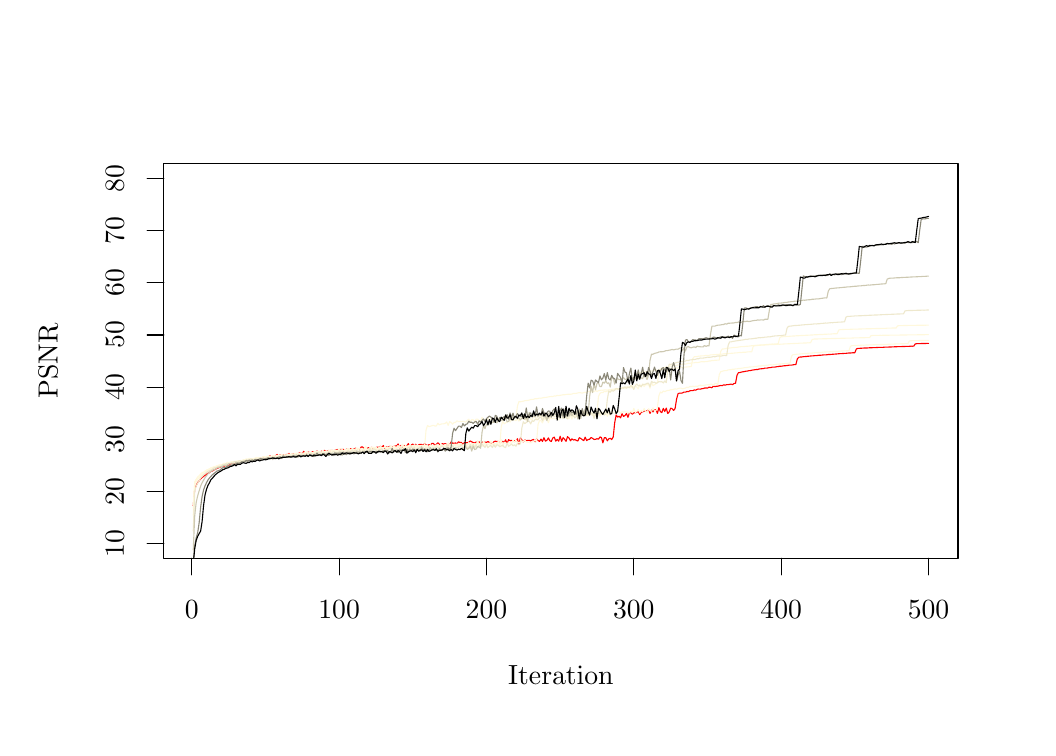
\begin{tikzpicture}[x=1pt,y=1pt]
\definecolor{fillColor}{RGB}{255,255,255}
\path[use as bounding box,fill=fillColor,fill opacity=0.00] (0,0) rectangle (361.35,252.94);
\begin{scope}
\path[clip] ( 49.20, 61.20) rectangle (336.15,203.75);
\definecolor{drawColor}{RGB}{255,0,0}

\path[draw=drawColor,line width= 0.4pt,line join=round,line cap=round] ( 59.83, 80.15) --
	( 60.36, 86.18) --
	( 60.89, 87.47) --
	( 61.43, 88.55) --
	( 61.96, 89.18) --
	( 62.49, 89.89) --
	( 63.02, 90.37) --
	( 63.55, 90.80) --
	( 64.09, 91.17) --
	( 64.62, 91.55) --
	( 65.15, 91.96) --
	( 65.68, 92.12) --
	( 66.22, 92.65) --
	( 66.75, 92.72) --
	( 67.28, 93.11) --
	( 67.81, 93.32) --
	( 68.35, 93.65) --
	( 68.88, 93.85) --
	( 69.41, 94.07) --
	( 69.94, 94.31) --
	( 70.48, 94.61) --
	( 71.01, 94.45) --
	( 71.54, 94.73) --
	( 72.07, 94.95) --
	( 72.61, 94.84) --
	( 73.14, 95.15) --
	( 73.67, 95.45) --
	( 74.20, 95.43) --
	( 74.74, 95.46) --
	( 75.27, 95.87) --
	( 75.80, 95.90) --
	( 76.33, 96.12) --
	( 76.87, 95.99) --
	( 77.40, 96.22) --
	( 77.93, 96.33) --
	( 78.46, 96.17) --
	( 79.00, 96.59) --
	( 79.53, 96.50) --
	( 80.06, 96.65) --
	( 80.59, 96.88) --
	( 81.13, 96.93) --
	( 81.66, 97.17) --
	( 82.19, 97.10) --
	( 82.72, 97.15) --
	( 83.26, 96.99) --
	( 83.79, 97.38) --
	( 84.32, 97.44) --
	( 84.85, 97.28) --
	( 85.39, 97.56) --
	( 85.92, 97.45) --
	( 86.45, 97.51) --
	( 86.98, 97.69) --
	( 87.52, 98.21) --
	( 88.05, 97.73) --
	( 88.58, 98.03) --
	( 89.11, 97.71) --
	( 89.65, 98.34) --
	( 90.18, 98.72) --
	( 90.71, 97.84) --
	( 91.24, 98.62) --
	( 91.78, 97.96) --
	( 92.31, 98.57) --
	( 92.84, 98.51) --
	( 93.37, 98.70) --
	( 93.90, 98.65) --
	( 94.44, 99.12) --
	( 94.97, 98.10) --
	( 95.50, 98.87) --
	( 96.03, 98.89) --
	( 96.57, 98.86) --
	( 97.10, 98.78) --
	( 97.63, 98.66) --
	( 98.16, 99.32) --
	( 98.70, 99.02) --
	( 99.23, 99.12) --
	( 99.76, 99.86) --
	(100.29, 98.91) --
	(100.83, 98.89) --
	(101.36, 99.62) --
	(101.89, 99.37) --
	(102.42, 99.21) --
	(102.96, 99.79) --
	(103.49, 99.36) --
	(104.02, 99.63) --
	(104.55, 99.98) --
	(105.09, 99.57) --
	(105.62, 99.62) --
	(106.15, 99.91) --
	(106.68, 99.52) --
	(107.22,100.22) --
	(107.75, 99.80) --
	(108.28, 99.92) --
	(108.81,100.16) --
	(109.35, 99.86) --
	(109.88,100.17) --
	(110.41,100.09) --
	(110.94,100.18) --
	(111.48,100.37) --
	(112.01,100.50) --
	(112.54, 99.97) --
	(113.07,100.59) --
	(113.61,100.56) --
	(114.14,100.55) --
	(114.67,100.06) --
	(115.20,100.66) --
	(115.74,100.57) --
	(116.27,100.30) --
	(116.80,100.86) --
	(117.33,100.61) --
	(117.87,100.63) --
	(118.40,100.98) --
	(118.93,100.65) --
	(119.46,100.66) --
	(120.00,100.58) --
	(120.53,101.46) --
	(121.06,101.41) --
	(121.59,100.85) --
	(122.12,100.97) --
	(122.66,100.92) --
	(123.19,101.20) --
	(123.72,100.96) --
	(124.25,101.28) --
	(124.79,100.83) --
	(125.32,100.73) --
	(125.85,101.20) --
	(126.38,101.40) --
	(126.92,101.25) --
	(127.45,101.67) --
	(127.98,101.16) --
	(128.51,101.95) --
	(129.05,100.86) --
	(129.58,101.43) --
	(130.11,101.31) --
	(130.64,101.58) --
	(131.18,101.63) --
	(131.71,101.46) --
	(132.24,101.70) --
	(132.77,101.77) --
	(133.31,101.76) --
	(133.84,102.52) --
	(134.37,101.04) --
	(134.90,102.01) --
	(135.44,101.05) --
	(135.97,101.97) --
	(136.50,101.80) --
	(137.03,101.90) --
	(137.57,102.65) --
	(138.10,101.06) --
	(138.63,102.15) --
	(139.16,102.48) --
	(139.70,101.69) --
	(140.23,102.40) --
	(140.76,101.60) --
	(141.29,102.22) --
	(141.83,102.38) --
	(142.36,102.33) --
	(142.89,102.10) --
	(143.42,102.60) --
	(143.96,102.18) --
	(144.49,101.93) --
	(145.02,102.28) --
	(145.55,102.11) --
	(146.09,102.71) --
	(146.62,102.71) --
	(147.15,101.94) --
	(147.68,102.40) --
	(148.22,102.92) --
	(148.75,102.41) --
	(149.28,102.06) --
	(149.81,102.65) --
	(150.34,102.45) --
	(150.88,102.67) --
	(151.41,102.30) --
	(151.94,102.03) --
	(152.47,102.27) --
	(153.01,103.22) --
	(153.54,102.78) --
	(154.07,102.75) --
	(154.60,102.87) --
	(155.14,102.58) --
	(155.67,103.30) --
	(156.20,103.03) --
	(156.73,103.05) --
	(157.27,102.25) --
	(157.80,103.03) --
	(158.33,102.91) --
	(158.86,102.99) --
	(159.40,103.09) --
	(159.93,103.60) --
	(160.46,103.29) --
	(160.99,103.03) --
	(161.53,102.87) --
	(162.06,103.22) --
	(162.59,102.98) --
	(163.12,103.29) --
	(163.66,102.62) --
	(164.19,103.21) --
	(164.72,103.13) --
	(165.25,103.16) --
	(165.79,103.08) --
	(166.32,103.40) --
	(166.85,103.06) --
	(167.38,102.85) --
	(167.92,102.70) --
	(168.45,103.31) --
	(168.98,103.53) --
	(169.51,103.39) --
	(170.05,103.45) --
	(170.58,102.95) --
	(171.11,103.09) --
	(171.64,103.50) --
	(172.18,103.05) --
	(172.71,104.02) --
	(173.24,102.58) --
	(173.77,104.08) --
	(174.31,103.68) --
	(174.84,103.82) --
	(175.37,103.53) --
	(175.90,103.72) --
	(176.44,103.50) --
	(176.97,104.42) --
	(177.50,102.33) --
	(178.03,104.69) --
	(178.56,104.02) --
	(179.10,103.23) --
	(179.63,103.97) --
	(180.16,103.70) --
	(180.69,103.79) --
	(181.23,103.81) --
	(181.76,103.64) --
	(182.29,103.97) --
	(182.82,104.14) --
	(183.36,103.33) --
	(183.89,104.35) --
	(184.42,103.75) --
	(184.95,103.44) --
	(185.49,104.27) --
	(186.02,103.42) --
	(186.55,104.78) --
	(187.08,103.55) --
	(187.62,103.82) --
	(188.15,104.70) --
	(188.68,103.70) --
	(189.21,103.41) --
	(189.75,104.68) --
	(190.28,104.96) --
	(190.81,103.55) --
	(191.34,104.15) --
	(191.88,103.52) --
	(192.41,105.30) --
	(192.94,103.44) --
	(193.47,104.79) --
	(194.01,104.19) --
	(194.54,103.46) --
	(195.07,105.15) --
	(195.60,104.68) --
	(196.14,103.66) --
	(196.67,104.37) --
	(197.20,103.93) --
	(197.73,104.11) --
	(198.27,103.79) --
	(198.80,103.57) --
	(199.33,104.77) --
	(199.86,104.50) --
	(200.40,104.07) --
	(200.93,103.71) --
	(201.46,104.97) --
	(201.99,103.74) --
	(202.53,104.11) --
	(203.06,104.22) --
	(203.59,104.84) --
	(204.12,104.56) --
	(204.66,104.13) --
	(205.19,104.20) --
	(205.72,104.41) --
	(206.25,104.23) --
	(206.79,105.04) --
	(207.32,104.85) --
	(207.85,102.93) --
	(208.38,104.77) --
	(208.91,104.76) --
	(209.45,103.63) --
	(209.98,104.39) --
	(210.51,104.57) --
	(211.04,104.11) --
	(211.58,105.01) --
	(212.11,110.12) --
	(212.64,112.99) --
	(213.17,112.21) --
	(213.71,112.55) --
	(214.24,111.95) --
	(214.77,113.46) --
	(215.30,112.46) --
	(215.84,112.78) --
	(216.37,113.52) --
	(216.90,112.15) --
	(217.43,113.75) --
	(217.97,113.80) --
	(218.50,113.25) --
	(219.03,113.76) --
	(219.56,113.81) --
	(220.10,113.95) --
	(220.63,114.24) --
	(221.16,113.10) --
	(221.69,113.95) --
	(222.23,114.13) --
	(222.76,114.37) --
	(223.29,114.35) --
	(223.82,114.47) --
	(224.36,114.92) --
	(224.89,113.55) --
	(225.42,114.74) --
	(225.95,114.12) --
	(226.49,114.94) --
	(227.02,114.94) --
	(227.55,113.54) --
	(228.08,115.63) --
	(228.62,114.21) --
	(229.15,113.81) --
	(229.68,115.37) --
	(230.21,114.24) --
	(230.75,115.46) --
	(231.28,113.52) --
	(231.81,114.06) --
	(232.34,115.44) --
	(232.88,115.24) --
	(233.41,114.63) --
	(233.94,115.30) --
	(234.47,118.69) --
	(235.01,120.68) --
	(235.54,120.90) --
	(236.07,120.85) --
	(236.60,120.95) --
	(237.13,121.24) --
	(237.67,121.22) --
	(238.20,121.49) --
	(238.73,121.41) --
	(239.26,121.72) --
	(239.80,121.79) --
	(240.33,121.78) --
	(240.86,122.05) --
	(241.39,121.93) --
	(241.93,122.28) --
	(242.46,122.36) --
	(242.99,122.30) --
	(243.52,122.47) --
	(244.06,122.50) --
	(244.59,122.72) --
	(245.12,122.72) --
	(245.65,122.71) --
	(246.19,123.02) --
	(246.72,122.98) --
	(247.25,122.82) --
	(247.78,123.44) --
	(248.32,123.22) --
	(248.85,123.35) --
	(249.38,123.39) --
	(249.91,123.53) --
	(250.45,123.64) --
	(250.98,123.58) --
	(251.51,123.88) --
	(252.04,123.76) --
	(252.58,123.94) --
	(253.11,123.95) --
	(253.64,124.03) --
	(254.17,124.16) --
	(254.71,123.91) --
	(255.24,124.37) --
	(255.77,124.41) --
	(256.30,127.25) --
	(256.84,128.30) --
	(257.37,128.32) --
	(257.90,128.47) --
	(258.43,128.60) --
	(258.97,128.66) --
	(259.50,128.80) --
	(260.03,128.84) --
	(260.56,128.99) --
	(261.10,129.01) --
	(261.63,129.17) --
	(262.16,129.25) --
	(262.69,129.32) --
	(263.23,129.40) --
	(263.76,129.43) --
	(264.29,129.59) --
	(264.82,129.66) --
	(265.35,129.71) --
	(265.89,129.75) --
	(266.42,129.93) --
	(266.95,129.91) --
	(267.48,129.98) --
	(268.02,130.10) --
	(268.55,130.12) --
	(269.08,130.28) --
	(269.61,130.28) --
	(270.15,130.31) --
	(270.68,130.43) --
	(271.21,130.48) --
	(271.74,130.60) --
	(272.28,130.61) --
	(272.81,130.68) --
	(273.34,130.77) --
	(273.87,130.79) --
	(274.41,130.86) --
	(274.94,130.95) --
	(275.47,131.01) --
	(276.00,131.00) --
	(276.54,131.11) --
	(277.07,131.19) --
	(277.60,131.22) --
	(278.13,133.32) --
	(278.67,133.85) --
	(279.20,133.93) --
	(279.73,133.95) --
	(280.26,134.05) --
	(280.80,134.09) --
	(281.33,134.12) --
	(281.86,134.20) --
	(282.39,134.23) --
	(282.93,134.30) --
	(283.46,134.34) --
	(283.99,134.37) --
	(284.52,134.44) --
	(285.06,134.44) --
	(285.59,134.53) --
	(286.12,134.58) --
	(286.65,134.58) --
	(287.19,134.65) --
	(287.72,134.69) --
	(288.25,134.71) --
	(288.78,134.74) --
	(289.32,134.83) --
	(289.85,134.84) --
	(290.38,134.88) --
	(290.91,134.93) --
	(291.45,134.96) --
	(291.98,135.01) --
	(292.51,135.05) --
	(293.04,135.11) --
	(293.57,135.15) --
	(294.11,135.17) --
	(294.64,135.20) --
	(295.17,135.24) --
	(295.70,135.27) --
	(296.24,135.33) --
	(296.77,135.38) --
	(297.30,135.38) --
	(297.83,135.43) --
	(298.37,135.49) --
	(298.90,135.49) --
	(299.43,136.81) --
	(299.96,137.05) --
	(300.50,137.06) --
	(301.03,137.11) --
	(301.56,137.12) --
	(302.09,137.17) --
	(302.63,137.17) --
	(303.16,137.19) --
	(303.69,137.22) --
	(304.22,137.28) --
	(304.76,137.26) --
	(305.29,137.30) --
	(305.82,137.30) --
	(306.35,137.32) --
	(306.89,137.38) --
	(307.42,137.39) --
	(307.95,137.42) --
	(308.48,137.39) --
	(309.02,137.43) --
	(309.55,137.48) --
	(310.08,137.48) --
	(310.61,137.52) --
	(311.15,137.53) --
	(311.68,137.55) --
	(312.21,137.57) --
	(312.74,137.59) --
	(313.28,137.64) --
	(313.81,137.63) --
	(314.34,137.67) --
	(314.87,137.68) --
	(315.41,137.68) --
	(315.94,137.72) --
	(316.47,137.74) --
	(317.00,137.74) --
	(317.54,137.78) --
	(318.07,137.78) --
	(318.60,137.80) --
	(319.13,137.85) --
	(319.67,137.83) --
	(320.20,137.87) --
	(320.73,138.66) --
	(321.26,138.76) --
	(321.80,138.76) --
	(322.33,138.78) --
	(322.86,138.80) --
	(323.39,138.80) --
	(323.92,138.82) --
	(324.46,138.83) --
	(324.99,138.84) --
	(325.52,138.84);
\end{scope}
\begin{scope}
\path[clip] (  0.00,  0.00) rectangle (361.35,252.94);
\definecolor{drawColor}{RGB}{0,0,0}

\path[draw=drawColor,line width= 0.4pt,line join=round,line cap=round] ( 59.30, 61.20) -- (325.52, 61.20);

\path[draw=drawColor,line width= 0.4pt,line join=round,line cap=round] ( 59.30, 61.20) -- ( 59.30, 55.20);

\path[draw=drawColor,line width= 0.4pt,line join=round,line cap=round] (112.54, 61.20) -- (112.54, 55.20);

\path[draw=drawColor,line width= 0.4pt,line join=round,line cap=round] (165.79, 61.20) -- (165.79, 55.20);

\path[draw=drawColor,line width= 0.4pt,line join=round,line cap=round] (219.03, 61.20) -- (219.03, 55.20);

\path[draw=drawColor,line width= 0.4pt,line join=round,line cap=round] (272.28, 61.20) -- (272.28, 55.20);

\path[draw=drawColor,line width= 0.4pt,line join=round,line cap=round] (325.52, 61.20) -- (325.52, 55.20);

\node[text=drawColor,anchor=base,inner sep=0pt, outer sep=0pt, scale=  1.00] at ( 59.30, 39.60) {0};

\node[text=drawColor,anchor=base,inner sep=0pt, outer sep=0pt, scale=  1.00] at (112.54, 39.60) {100};

\node[text=drawColor,anchor=base,inner sep=0pt, outer sep=0pt, scale=  1.00] at (165.79, 39.60) {200};

\node[text=drawColor,anchor=base,inner sep=0pt, outer sep=0pt, scale=  1.00] at (219.03, 39.60) {300};

\node[text=drawColor,anchor=base,inner sep=0pt, outer sep=0pt, scale=  1.00] at (272.28, 39.60) {400};

\node[text=drawColor,anchor=base,inner sep=0pt, outer sep=0pt, scale=  1.00] at (325.52, 39.60) {500};

\path[draw=drawColor,line width= 0.4pt,line join=round,line cap=round] ( 49.20, 66.48) -- ( 49.20,198.47);

\path[draw=drawColor,line width= 0.4pt,line join=round,line cap=round] ( 49.20, 66.48) -- ( 43.20, 66.48);

\path[draw=drawColor,line width= 0.4pt,line join=round,line cap=round] ( 49.20, 85.33) -- ( 43.20, 85.33);

\path[draw=drawColor,line width= 0.4pt,line join=round,line cap=round] ( 49.20,104.19) -- ( 43.20,104.19);

\path[draw=drawColor,line width= 0.4pt,line join=round,line cap=round] ( 49.20,123.04) -- ( 43.20,123.04);

\path[draw=drawColor,line width= 0.4pt,line join=round,line cap=round] ( 49.20,141.90) -- ( 43.20,141.90);

\path[draw=drawColor,line width= 0.4pt,line join=round,line cap=round] ( 49.20,160.76) -- ( 43.20,160.76);

\path[draw=drawColor,line width= 0.4pt,line join=round,line cap=round] ( 49.20,179.61) -- ( 43.20,179.61);

\path[draw=drawColor,line width= 0.4pt,line join=round,line cap=round] ( 49.20,198.47) -- ( 43.20,198.47);

\node[text=drawColor,rotate= 90.00,anchor=base,inner sep=0pt, outer sep=0pt, scale=  1.00] at ( 34.80, 66.48) {10};

\node[text=drawColor,rotate= 90.00,anchor=base,inner sep=0pt, outer sep=0pt, scale=  1.00] at ( 34.80, 85.33) {20};

\node[text=drawColor,rotate= 90.00,anchor=base,inner sep=0pt, outer sep=0pt, scale=  1.00] at ( 34.80,104.19) {30};

\node[text=drawColor,rotate= 90.00,anchor=base,inner sep=0pt, outer sep=0pt, scale=  1.00] at ( 34.80,123.04) {40};

\node[text=drawColor,rotate= 90.00,anchor=base,inner sep=0pt, outer sep=0pt, scale=  1.00] at ( 34.80,141.90) {50};

\node[text=drawColor,rotate= 90.00,anchor=base,inner sep=0pt, outer sep=0pt, scale=  1.00] at ( 34.80,160.76) {60};

\node[text=drawColor,rotate= 90.00,anchor=base,inner sep=0pt, outer sep=0pt, scale=  1.00] at ( 34.80,179.61) {70};

\node[text=drawColor,rotate= 90.00,anchor=base,inner sep=0pt, outer sep=0pt, scale=  1.00] at ( 34.80,198.47) {80};

\path[draw=drawColor,line width= 0.4pt,line join=round,line cap=round] ( 49.20, 61.20) --
	(336.15, 61.20) --
	(336.15,203.75) --
	( 49.20,203.75) --
	( 49.20, 61.20);
\end{scope}
\begin{scope}
\path[clip] (  0.00,  0.00) rectangle (361.35,252.94);
\definecolor{drawColor}{RGB}{0,0,0}

\node[text=drawColor,anchor=base,inner sep=0pt, outer sep=0pt, scale=  1.00] at (192.68, 15.60) {Iteration};

\node[text=drawColor,rotate= 90.00,anchor=base,inner sep=0pt, outer sep=0pt, scale=  1.00] at ( 10.80,132.47) {PSNR};
\end{scope}
\begin{scope}
\path[clip] ( 49.20, 61.20) rectangle (336.15,203.75);
\definecolor{drawColor}{RGB}{255,248,220}

\path[draw=drawColor,line width= 0.4pt,line join=round,line cap=round] ( 59.83, 80.68) --
	( 60.36, 87.63) --
	( 60.89, 88.79) --
	( 61.43, 89.66) --
	( 61.96, 90.22) --
	( 62.49, 90.83) --
	( 63.02, 91.22) --
	( 63.55, 91.67) --
	( 64.09, 92.07) --
	( 64.62, 92.58) --
	( 65.15, 92.73) --
	( 65.68, 93.00) --
	( 66.22, 93.31) --
	( 66.75, 93.66) --
	( 67.28, 93.90) --
	( 67.81, 93.99) --
	( 68.35, 94.18) --
	( 68.88, 94.51) --
	( 69.41, 94.50) --
	( 69.94, 94.61) --
	( 70.48, 94.71) --
	( 71.01, 94.96) --
	( 71.54, 95.30) --
	( 72.07, 94.97) --
	( 72.61, 95.60) --
	( 73.14, 95.51) --
	( 73.67, 95.77) --
	( 74.20, 95.68) --
	( 74.74, 95.90) --
	( 75.27, 96.06) --
	( 75.80, 96.21) --
	( 76.33, 96.00) --
	( 76.87, 96.55) --
	( 77.40, 96.39) --
	( 77.93, 96.75) --
	( 78.46, 96.49) --
	( 79.00, 96.81) --
	( 79.53, 96.82) --
	( 80.06, 96.82) --
	( 80.59, 97.05) --
	( 81.13, 97.25) --
	( 81.66, 96.97) --
	( 82.19, 97.06) --
	( 82.72, 97.17) --
	( 83.26, 97.39) --
	( 83.79, 97.28) --
	( 84.32, 97.46) --
	( 84.85, 97.22) --
	( 85.39, 97.32) --
	( 85.92, 97.60) --
	( 86.45, 97.79) --
	( 86.98, 97.75) --
	( 87.52, 97.91) --
	( 88.05, 97.79) --
	( 88.58, 97.52) --
	( 89.11, 98.11) --
	( 89.65, 97.83) --
	( 90.18, 97.82) --
	( 90.71, 98.43) --
	( 91.24, 98.12) --
	( 91.78, 98.22) --
	( 92.31, 98.39) --
	( 92.84, 98.53) --
	( 93.37, 98.14) --
	( 93.90, 98.38) --
	( 94.44, 98.51) --
	( 94.97, 98.58) --
	( 95.50, 98.83) --
	( 96.03, 98.61) --
	( 96.57, 99.10) --
	( 97.10, 98.20) --
	( 97.63, 98.95) --
	( 98.16, 98.97) --
	( 98.70, 98.99) --
	( 99.23, 99.17) --
	( 99.76, 98.43) --
	(100.29, 99.18) --
	(100.83, 99.35) --
	(101.36, 99.04) --
	(101.89, 99.21) --
	(102.42, 99.37) --
	(102.96, 98.64) --
	(103.49, 99.66) --
	(104.02, 99.34) --
	(104.55, 99.29) --
	(105.09, 99.83) --
	(105.62, 99.39) --
	(106.15, 99.67) --
	(106.68, 99.31) --
	(107.22, 99.58) --
	(107.75, 99.80) --
	(108.28, 99.65) --
	(108.81,100.13) --
	(109.35, 99.28) --
	(109.88,100.26) --
	(110.41, 99.56) --
	(110.94,100.16) --
	(111.48,100.23) --
	(112.01,100.16) --
	(112.54, 99.54) --
	(113.07,100.25) --
	(113.61,100.19) --
	(114.14, 99.74) --
	(114.67,100.50) --
	(115.20, 99.96) --
	(115.74,100.68) --
	(116.27,100.62) --
	(116.80, 99.90) --
	(117.33,100.42) --
	(117.87,100.34) --
	(118.40,100.45) --
	(118.93,101.09) --
	(119.46,100.81) --
	(120.00,100.95) --
	(120.53,100.35) --
	(121.06,100.25) --
	(121.59,100.49) --
	(122.12,101.57) --
	(122.66,100.38) --
	(123.19,100.52) --
	(123.72,100.67) --
	(124.25,100.75) --
	(124.79,100.51) --
	(125.32,101.26) --
	(125.85,100.65) --
	(126.38,100.56) --
	(126.92,101.26) --
	(127.45,101.49) --
	(127.98,100.46) --
	(128.51,100.98) --
	(129.05,101.31) --
	(129.58,101.15) --
	(130.11,101.31) --
	(130.64,101.11) --
	(131.18,101.63) --
	(131.71,100.47) --
	(132.24,101.88) --
	(132.77,101.41) --
	(133.31,100.96) --
	(133.84,101.93) --
	(134.37,101.10) --
	(134.90,101.00) --
	(135.44,102.47) --
	(135.97,101.23) --
	(136.50,101.63) --
	(137.03,101.62) --
	(137.57,101.82) --
	(138.10,101.68) --
	(138.63,101.88) --
	(139.16,101.22) --
	(139.70,101.58) --
	(140.23,101.81) --
	(140.76,101.77) --
	(141.29,101.92) --
	(141.83,101.10) --
	(142.36,101.74) --
	(142.89,102.07) --
	(143.42,101.67) --
	(143.96,102.06) --
	(144.49,101.66) --
	(145.02,101.42) --
	(145.55,102.12) --
	(146.09,101.97) --
	(146.62,101.74) --
	(147.15,101.84) --
	(147.68,101.47) --
	(148.22,102.18) --
	(148.75,101.84) --
	(149.28,101.72) --
	(149.81,101.99) --
	(150.34,101.85) --
	(150.88,102.34) --
	(151.41,102.02) --
	(151.94,102.97) --
	(152.47,101.60) --
	(153.01,102.50) --
	(153.54,101.91) --
	(154.07,102.49) --
	(154.60,101.99) --
	(155.14,102.53) --
	(155.67,101.46) --
	(156.20,102.75) --
	(156.73,102.54) --
	(157.27,101.80) --
	(157.80,102.57) --
	(158.33,102.44) --
	(158.86,101.60) --
	(159.40,103.03) --
	(159.93,102.28) --
	(160.46,101.67) --
	(160.99,102.65) --
	(161.53,102.56) --
	(162.06,102.19) --
	(162.59,103.77) --
	(163.12,101.96) --
	(163.66,103.11) --
	(164.19,101.61) --
	(164.72,103.48) --
	(165.25,102.54) --
	(165.79,102.45) --
	(166.32,102.46) --
	(166.85,102.44) --
	(167.38,103.64) --
	(167.92,102.67) --
	(168.45,102.72) --
	(168.98,102.60) --
	(169.51,102.33) --
	(170.05,103.57) --
	(170.58,102.10) --
	(171.11,104.04) --
	(171.64,101.71) --
	(172.18,103.19) --
	(172.71,102.79) --
	(173.24,102.72) --
	(173.77,102.89) --
	(174.31,102.86) --
	(174.84,102.55) --
	(175.37,103.95) --
	(175.90,103.05) --
	(176.44,103.99) --
	(176.97,102.97) --
	(177.50,103.13) --
	(178.03,103.16) --
	(178.56,103.70) --
	(179.10,103.21) --
	(179.63,103.89) --
	(180.16,103.21) --
	(180.69,103.16) --
	(181.23,103.00) --
	(181.76,102.89) --
	(182.29,103.26) --
	(182.82,103.40) --
	(183.36,103.95) --
	(183.89,103.25) --
	(184.42,109.56) --
	(184.95,111.00) --
	(185.49,110.89) --
	(186.02,110.12) --
	(186.55,111.42) --
	(187.08,111.34) --
	(187.62,111.59) --
	(188.15,110.17) --
	(188.68,111.86) --
	(189.21,111.64) --
	(189.75,111.71) --
	(190.28,111.89) --
	(190.81,111.60) --
	(191.34,111.70) --
	(191.88,111.20) --
	(192.41,111.89) --
	(192.94,112.16) --
	(193.47,111.75) --
	(194.01,112.14) --
	(194.54,112.47) --
	(195.07,111.77) --
	(195.60,111.63) --
	(196.14,112.98) --
	(196.67,111.46) --
	(197.20,112.98) --
	(197.73,112.53) --
	(198.27,112.91) --
	(198.80,112.81) --
	(199.33,111.76) --
	(199.86,113.25) --
	(200.40,112.82) --
	(200.93,113.12) --
	(201.46,112.89) --
	(201.99,113.15) --
	(202.53,112.60) --
	(203.06,113.62) --
	(203.59,113.22) --
	(204.12,112.78) --
	(204.66,112.84) --
	(205.19,113.19) --
	(205.72,112.10) --
	(206.25,114.12) --
	(206.79,112.59) --
	(207.32,113.19) --
	(207.85,113.94) --
	(208.38,113.21) --
	(208.91,114.41) --
	(209.45,112.49) --
	(209.98,113.96) --
	(210.51,112.70) --
	(211.04,114.90) --
	(211.58,113.69) --
	(212.11,113.77) --
	(212.64,113.52) --
	(213.17,114.52) --
	(213.71,114.18) --
	(214.24,113.56) --
	(214.77,114.14) --
	(215.30,114.06) --
	(215.84,114.14) --
	(216.37,114.04) --
	(216.90,113.94) --
	(217.43,113.69) --
	(217.97,114.40) --
	(218.50,113.79) --
	(219.03,115.33) --
	(219.56,113.89) --
	(220.10,114.22) --
	(220.63,115.00) --
	(221.16,113.77) --
	(221.69,114.64) --
	(222.23,114.23) --
	(222.76,115.31) --
	(223.29,114.30) --
	(223.82,113.87) --
	(224.36,115.29) --
	(224.89,114.49) --
	(225.42,114.29) --
	(225.95,115.59) --
	(226.49,114.43) --
	(227.02,114.53) --
	(227.55,115.79) --
	(228.08,119.93) --
	(228.62,121.29) --
	(229.15,120.93) --
	(229.68,121.67) --
	(230.21,121.40) --
	(230.75,121.69) --
	(231.28,121.86) --
	(231.81,121.91) --
	(232.34,122.12) --
	(232.88,122.12) --
	(233.41,122.27) --
	(233.94,122.41) --
	(234.47,122.30) --
	(235.01,122.53) --
	(235.54,122.66) --
	(236.07,122.68) --
	(236.60,122.42) --
	(237.13,122.58) --
	(237.67,122.69) --
	(238.20,123.04) --
	(238.73,122.87) --
	(239.26,123.31) --
	(239.80,123.24) --
	(240.33,123.38) --
	(240.86,123.27) --
	(241.39,123.40) --
	(241.93,123.31) --
	(242.46,123.56) --
	(242.99,123.76) --
	(243.52,123.57) --
	(244.06,123.66) --
	(244.59,123.74) --
	(245.12,123.85) --
	(245.65,123.89) --
	(246.19,124.00) --
	(246.72,124.07) --
	(247.25,124.09) --
	(247.78,123.64) --
	(248.32,124.34) --
	(248.85,124.35) --
	(249.38,124.01) --
	(249.91,127.61) --
	(250.45,128.65) --
	(250.98,128.77) --
	(251.51,128.95) --
	(252.04,129.03) --
	(252.58,129.03) --
	(253.11,129.30) --
	(253.64,129.31) --
	(254.17,129.37) --
	(254.71,129.52) --
	(255.24,129.50) --
	(255.77,129.66) --
	(256.30,129.64) --
	(256.84,129.78) --
	(257.37,129.79) --
	(257.90,129.88) --
	(258.43,129.94) --
	(258.97,130.08) --
	(259.50,130.10) --
	(260.03,130.16) --
	(260.56,130.30) --
	(261.10,130.31) --
	(261.63,130.39) --
	(262.16,130.38) --
	(262.69,130.51) --
	(263.23,130.48) --
	(263.76,130.65) --
	(264.29,130.72) --
	(264.82,130.65) --
	(265.35,130.80) --
	(265.89,130.85) --
	(266.42,130.88) --
	(266.95,130.93) --
	(267.48,131.01) --
	(268.02,131.09) --
	(268.55,131.12) --
	(269.08,131.11) --
	(269.61,131.13) --
	(270.15,131.24) --
	(270.68,131.31) --
	(271.21,131.37) --
	(271.74,131.41) --
	(272.28,131.43) --
	(272.81,131.50) --
	(273.34,131.53) --
	(273.87,131.65) --
	(274.41,131.58) --
	(274.94,131.71) --
	(275.47,131.71) --
	(276.00,134.16) --
	(276.54,134.81) --
	(277.07,134.81) --
	(277.60,134.88) --
	(278.13,134.96) --
	(278.67,134.99) --
	(279.20,135.03) --
	(279.73,135.08) --
	(280.26,135.16) --
	(280.80,135.22) --
	(281.33,135.17) --
	(281.86,135.27) --
	(282.39,135.31) --
	(282.93,135.34) --
	(283.46,135.37) --
	(283.99,135.43) --
	(284.52,135.50) --
	(285.06,135.51) --
	(285.59,135.56) --
	(286.12,135.59) --
	(286.65,135.60) --
	(287.19,135.67) --
	(287.72,135.72) --
	(288.25,135.74) --
	(288.78,135.79) --
	(289.32,135.79) --
	(289.85,135.83) --
	(290.38,135.86) --
	(290.91,135.85) --
	(291.45,135.96) --
	(291.98,135.93) --
	(292.51,135.99) --
	(293.04,135.99) --
	(293.57,136.05) --
	(294.11,136.12) --
	(294.64,136.12) --
	(295.17,136.17) --
	(295.70,136.17) --
	(296.24,136.20) --
	(296.77,136.25) --
	(297.30,137.78) --
	(297.83,138.03) --
	(298.37,138.05) --
	(298.90,138.10) --
	(299.43,138.11) --
	(299.96,138.13) --
	(300.50,138.14) --
	(301.03,138.18) --
	(301.56,138.21) --
	(302.09,138.19) --
	(302.63,138.24) --
	(303.16,138.28) --
	(303.69,138.28) --
	(304.22,138.32) --
	(304.76,138.31) --
	(305.29,138.34) --
	(305.82,138.36) --
	(306.35,138.39) --
	(306.89,138.40) --
	(307.42,138.42) --
	(307.95,138.43) --
	(308.48,138.46) --
	(309.02,138.47) --
	(309.55,138.48) --
	(310.08,138.50) --
	(310.61,138.51) --
	(311.15,138.56) --
	(311.68,138.56) --
	(312.21,138.59) --
	(312.74,138.59) --
	(313.28,138.64) --
	(313.81,138.66) --
	(314.34,138.68) --
	(314.87,138.68) --
	(315.41,138.70) --
	(315.94,138.73) --
	(316.47,138.72) --
	(317.00,138.75) --
	(317.54,138.77) --
	(318.07,138.77) --
	(318.60,139.72) --
	(319.13,139.81) --
	(319.67,139.83) --
	(320.20,139.85) --
	(320.73,139.86) --
	(321.26,139.87) --
	(321.80,139.87) --
	(322.33,139.89) --
	(322.86,139.90) --
	(323.39,139.91) --
	(323.92,139.92) --
	(324.46,139.92) --
	(324.99,139.93) --
	(325.52,139.95);

\path[draw=drawColor,line width= 0.4pt,line join=round,line cap=round] ( 59.83, 79.24) --
	( 60.36, 88.67) --
	( 60.89, 89.67) --
	( 61.43, 90.33) --
	( 61.96, 90.96) --
	( 62.49, 91.37) --
	( 63.02, 91.93) --
	( 63.55, 92.18) --
	( 64.09, 92.71) --
	( 64.62, 92.99) --
	( 65.15, 93.27) --
	( 65.68, 93.37) --
	( 66.22, 93.94) --
	( 66.75, 94.02) --
	( 67.28, 94.26) --
	( 67.81, 94.37) --
	( 68.35, 94.61) --
	( 68.88, 94.82) --
	( 69.41, 94.98) --
	( 69.94, 94.76) --
	( 70.48, 95.24) --
	( 71.01, 95.32) --
	( 71.54, 95.32) --
	( 72.07, 95.91) --
	( 72.61, 95.74) --
	( 73.14, 95.76) --
	( 73.67, 96.02) --
	( 74.20, 95.99) --
	( 74.74, 96.02) --
	( 75.27, 96.30) --
	( 75.80, 96.13) --
	( 76.33, 96.35) --
	( 76.87, 96.49) --
	( 77.40, 96.41) --
	( 77.93, 96.53) --
	( 78.46, 96.81) --
	( 79.00, 97.10) --
	( 79.53, 96.92) --
	( 80.06, 97.34) --
	( 80.59, 96.82) --
	( 81.13, 97.19) --
	( 81.66, 96.73) --
	( 82.19, 97.38) --
	( 82.72, 97.70) --
	( 83.26, 97.14) --
	( 83.79, 97.43) --
	( 84.32, 97.08) --
	( 84.85, 97.65) --
	( 85.39, 97.89) --
	( 85.92, 97.58) --
	( 86.45, 98.07) --
	( 86.98, 97.89) --
	( 87.52, 98.00) --
	( 88.05, 97.92) --
	( 88.58, 98.40) --
	( 89.11, 97.74) --
	( 89.65, 98.21) --
	( 90.18, 98.42) --
	( 90.71, 98.35) --
	( 91.24, 98.27) --
	( 91.78, 98.76) --
	( 92.31, 98.06) --
	( 92.84, 98.64) --
	( 93.37, 98.47) --
	( 93.90, 98.73) --
	( 94.44, 98.86) --
	( 94.97, 98.44) --
	( 95.50, 98.89) --
	( 96.03, 98.73) --
	( 96.57, 99.07) --
	( 97.10, 98.94) --
	( 97.63, 99.07) --
	( 98.16, 99.12) --
	( 98.70, 98.59) --
	( 99.23, 99.22) --
	( 99.76, 99.19) --
	(100.29, 98.99) --
	(100.83, 99.78) --
	(101.36, 99.14) --
	(101.89, 99.46) --
	(102.42, 99.39) --
	(102.96, 98.76) --
	(103.49, 99.56) --
	(104.02, 99.86) --
	(104.55, 99.28) --
	(105.09, 99.60) --
	(105.62, 99.71) --
	(106.15, 99.03) --
	(106.68,100.18) --
	(107.22, 99.45) --
	(107.75, 99.90) --
	(108.28, 99.80) --
	(108.81, 99.71) --
	(109.35,100.44) --
	(109.88,100.01) --
	(110.41,100.13) --
	(110.94,100.40) --
	(111.48, 99.63) --
	(112.01,100.19) --
	(112.54,100.70) --
	(113.07,100.77) --
	(113.61,100.57) --
	(114.14, 99.93) --
	(114.67,100.10) --
	(115.20,100.45) --
	(115.74,100.92) --
	(116.27,100.18) --
	(116.80,100.47) --
	(117.33,100.88) --
	(117.87,100.08) --
	(118.40, 99.89) --
	(118.93,100.86) --
	(119.46,100.47) --
	(120.00,100.14) --
	(120.53,100.83) --
	(121.06,100.48) --
	(121.59,100.53) --
	(122.12,101.71) --
	(122.66,100.51) --
	(123.19,100.55) --
	(123.72,101.28) --
	(124.25,101.18) --
	(124.79,101.42) --
	(125.32,100.33) --
	(125.85,101.22) --
	(126.38,100.78) --
	(126.92,100.74) --
	(127.45,101.54) --
	(127.98,101.25) --
	(128.51,101.05) --
	(129.05,101.23) --
	(129.58,101.34) --
	(130.11,100.86) --
	(130.64,101.15) --
	(131.18,101.86) --
	(131.71,101.34) --
	(132.24,101.44) --
	(132.77,101.07) --
	(133.31,101.30) --
	(133.84,101.73) --
	(134.37,101.24) --
	(134.90,101.51) --
	(135.44,102.14) --
	(135.97,100.39) --
	(136.50,102.00) --
	(137.03,101.45) --
	(137.57,101.80) --
	(138.10,102.05) --
	(138.63,101.25) --
	(139.16,101.96) --
	(139.70,101.96) --
	(140.23,102.10) --
	(140.76,101.79) --
	(141.29,101.34) --
	(141.83,101.57) --
	(142.36,102.03) --
	(142.89,101.94) --
	(143.42,101.59) --
	(143.96,107.57) --
	(144.49,109.19) --
	(145.02,108.76) --
	(145.55,108.92) --
	(146.09,109.12) --
	(146.62,109.26) --
	(147.15,108.99) --
	(147.68,109.03) --
	(148.22,109.99) --
	(148.75,109.39) --
	(149.28,109.69) --
	(149.81,109.77) --
	(150.34,109.80) --
	(150.88,109.98) --
	(151.41,110.45) --
	(151.94,109.22) --
	(152.47,110.57) --
	(153.01,110.28) --
	(153.54,109.67) --
	(154.07,110.26) --
	(154.60,110.31) --
	(155.14,110.90) --
	(155.67,110.56) --
	(156.20,110.69) --
	(156.73,110.57) --
	(157.27,110.68) --
	(157.80,110.60) --
	(158.33,110.35) --
	(158.86,111.05) --
	(159.40,111.46) --
	(159.93,110.42) --
	(160.46,111.30) --
	(160.99,111.25) --
	(161.53,110.54) --
	(162.06,111.47) --
	(162.59,111.47) --
	(163.12,111.02) --
	(163.66,110.84) --
	(164.19,112.14) --
	(164.72,111.08) --
	(165.25,111.07) --
	(165.79,111.20) --
	(166.32,111.89) --
	(166.85,111.00) --
	(167.38,111.38) --
	(167.92,111.62) --
	(168.45,111.67) --
	(168.98,111.02) --
	(169.51,112.00) --
	(170.05,111.73) --
	(170.58,111.60) --
	(171.11,111.95) --
	(171.64,111.52) --
	(172.18,112.53) --
	(172.71,111.87) --
	(173.24,112.26) --
	(173.77,112.01) --
	(174.31,111.51) --
	(174.84,112.15) --
	(175.37,112.26) --
	(175.90,111.93) --
	(176.44,112.07) --
	(176.97,116.14) --
	(177.50,117.81) --
	(178.03,117.76) --
	(178.56,117.85) --
	(179.10,117.97) --
	(179.63,118.16) --
	(180.16,118.18) --
	(180.69,118.27) --
	(181.23,118.36) --
	(181.76,118.56) --
	(182.29,118.63) --
	(182.82,118.65) --
	(183.36,118.90) --
	(183.89,118.81) --
	(184.42,118.96) --
	(184.95,119.09) --
	(185.49,119.04) --
	(186.02,119.16) --
	(186.55,119.30) --
	(187.08,119.33) --
	(187.62,119.40) --
	(188.15,119.53) --
	(188.68,119.60) --
	(189.21,119.65) --
	(189.75,119.63) --
	(190.28,119.89) --
	(190.81,119.79) --
	(191.34,120.07) --
	(191.88,119.96) --
	(192.41,120.11) --
	(192.94,120.17) --
	(193.47,120.30) --
	(194.01,120.28) --
	(194.54,120.40) --
	(195.07,120.45) --
	(195.60,120.50) --
	(196.14,120.45) --
	(196.67,120.57) --
	(197.20,120.79) --
	(197.73,120.76) --
	(198.27,120.80) --
	(198.80,120.96) --
	(199.33,121.06) --
	(199.86,121.00) --
	(200.40,120.89) --
	(200.93,121.08) --
	(201.46,121.22) --
	(201.99,121.07) --
	(202.53,121.47) --
	(203.06,121.47) --
	(203.59,121.54) --
	(204.12,121.33) --
	(204.66,121.40) --
	(205.19,121.85) --
	(205.72,121.46) --
	(206.25,121.75) --
	(206.79,121.86) --
	(207.32,121.97) --
	(207.85,121.93) --
	(208.38,122.05) --
	(208.91,122.03) --
	(209.45,121.96) --
	(209.98,122.15) --
	(210.51,122.13) --
	(211.04,122.22) --
	(211.58,122.30) --
	(212.11,122.23) --
	(212.64,122.50) --
	(213.17,122.50) --
	(213.71,122.53) --
	(214.24,122.53) --
	(214.77,122.66) --
	(215.30,122.62) --
	(215.84,122.72) --
	(216.37,122.71) --
	(216.90,122.93) --
	(217.43,122.77) --
	(217.97,122.77) --
	(218.50,122.92) --
	(219.03,126.75) --
	(219.56,127.95) --
	(220.10,127.94) --
	(220.63,128.03) --
	(221.16,128.30) --
	(221.69,128.25) --
	(222.23,128.38) --
	(222.76,128.48) --
	(223.29,128.59) --
	(223.82,128.62) --
	(224.36,128.74) --
	(224.89,128.76) --
	(225.42,128.83) --
	(225.95,128.99) --
	(226.49,129.07) --
	(227.02,129.15) --
	(227.55,129.18) --
	(228.08,129.14) --
	(228.62,129.35) --
	(229.15,129.43) --
	(229.68,129.44) --
	(230.21,129.44) --
	(230.75,129.55) --
	(231.28,129.67) --
	(231.81,129.69) --
	(232.34,129.66) --
	(232.88,129.85) --
	(233.41,129.93) --
	(233.94,129.89) --
	(234.47,130.00) --
	(235.01,129.93) --
	(235.54,130.08) --
	(236.07,130.25) --
	(236.60,130.18) --
	(237.13,130.30) --
	(237.67,130.28) --
	(238.20,130.34) --
	(238.73,130.36) --
	(239.26,130.45) --
	(239.80,130.51) --
	(240.33,133.34) --
	(240.86,134.04) --
	(241.39,134.06) --
	(241.93,134.11) --
	(242.46,134.24) --
	(242.99,134.28) --
	(243.52,134.32) --
	(244.06,134.33) --
	(244.59,134.41) --
	(245.12,134.52) --
	(245.65,134.52) --
	(246.19,134.52) --
	(246.72,134.67) --
	(247.25,134.72) --
	(247.78,134.74) --
	(248.32,134.77) --
	(248.85,134.82) --
	(249.38,134.87) --
	(249.91,134.93) --
	(250.45,134.93) --
	(250.98,134.99) --
	(251.51,135.12) --
	(252.04,135.09) --
	(252.58,135.16) --
	(253.11,135.19) --
	(253.64,135.25) --
	(254.17,135.27) --
	(254.71,135.30) --
	(255.24,135.35) --
	(255.77,135.42) --
	(256.30,135.41) --
	(256.84,135.53) --
	(257.37,135.56) --
	(257.90,135.52) --
	(258.43,135.65) --
	(258.97,135.64) --
	(259.50,135.67) --
	(260.03,135.76) --
	(260.56,135.80) --
	(261.10,135.82) --
	(261.63,135.79) --
	(262.16,137.73) --
	(262.69,138.05) --
	(263.23,138.09) --
	(263.76,138.11) --
	(264.29,138.16) --
	(264.82,138.19) --
	(265.35,138.23) --
	(265.89,138.24) --
	(266.42,138.29) --
	(266.95,138.33) --
	(267.48,138.35) --
	(268.02,138.39) --
	(268.55,138.41) --
	(269.08,138.42) --
	(269.61,138.46) --
	(270.15,138.47) --
	(270.68,138.50) --
	(271.21,138.57) --
	(271.74,138.54) --
	(272.28,138.60) --
	(272.81,138.61) --
	(273.34,138.65) --
	(273.87,138.68) --
	(274.41,138.70) --
	(274.94,138.71) --
	(275.47,138.74) --
	(276.00,138.78) --
	(276.54,138.80) --
	(277.07,138.81) --
	(277.60,138.86) --
	(278.13,138.85) --
	(278.67,138.90) --
	(279.20,138.96) --
	(279.73,138.94) --
	(280.26,138.98) --
	(280.80,139.01) --
	(281.33,139.00) --
	(281.86,139.07) --
	(282.39,139.05) --
	(282.93,139.12) --
	(283.46,140.24) --
	(283.99,140.41) --
	(284.52,140.44) --
	(285.06,140.44) --
	(285.59,140.46) --
	(286.12,140.48) --
	(286.65,140.49) --
	(287.19,140.51) --
	(287.72,140.54) --
	(288.25,140.55) --
	(288.78,140.54) --
	(289.32,140.59) --
	(289.85,140.57) --
	(290.38,140.61) --
	(290.91,140.61) --
	(291.45,140.63) --
	(291.98,140.63) --
	(292.51,140.65) --
	(293.04,140.67) --
	(293.57,140.67) --
	(294.11,140.72) --
	(294.64,140.69) --
	(295.17,140.72) --
	(295.70,140.74) --
	(296.24,140.76) --
	(296.77,140.77) --
	(297.30,140.77) --
	(297.83,140.78) --
	(298.37,140.81) --
	(298.90,140.84) --
	(299.43,140.85) --
	(299.96,140.83) --
	(300.50,140.87) --
	(301.03,140.89) --
	(301.56,140.88) --
	(302.09,140.89) --
	(302.63,140.91) --
	(303.16,140.95) --
	(303.69,140.94) --
	(304.22,140.96) --
	(304.76,141.65) --
	(305.29,141.72) --
	(305.82,141.73) --
	(306.35,141.74) --
	(306.89,141.76) --
	(307.42,141.76) --
	(307.95,141.78) --
	(308.48,141.77) --
	(309.02,141.78) --
	(309.55,141.80) --
	(310.08,141.80) --
	(310.61,141.81) --
	(311.15,141.81) --
	(311.68,141.82) --
	(312.21,141.83) --
	(312.74,141.85) --
	(313.28,141.84) --
	(313.81,141.85) --
	(314.34,141.85) --
	(314.87,141.86) --
	(315.41,141.87) --
	(315.94,141.87) --
	(316.47,141.89) --
	(317.00,141.89) --
	(317.54,141.90) --
	(318.07,141.91) --
	(318.60,141.92) --
	(319.13,141.93) --
	(319.67,141.93) --
	(320.20,141.94) --
	(320.73,141.94) --
	(321.26,141.95) --
	(321.80,141.97) --
	(322.33,141.97) --
	(322.86,141.97) --
	(323.39,141.97) --
	(323.92,141.99) --
	(324.46,142.00) --
	(324.99,142.01) --
	(325.52,142.01);

\path[draw=drawColor,line width= 0.4pt,line join=round,line cap=round] ( 59.83, 76.71) --
	( 60.36, 88.71) --
	( 60.89, 89.72) --
	( 61.43, 90.59) --
	( 61.96, 91.02) --
	( 62.49, 91.67) --
	( 63.02, 92.13) --
	( 63.55, 92.27) --
	( 64.09, 92.58) --
	( 64.62, 93.07) --
	( 65.15, 93.24) --
	( 65.68, 93.59) --
	( 66.22, 93.70) --
	( 66.75, 93.94) --
	( 67.28, 94.23) --
	( 67.81, 94.19) --
	( 68.35, 94.58) --
	( 68.88, 94.52) --
	( 69.41, 94.89) --
	( 69.94, 95.06) --
	( 70.48, 94.95) --
	( 71.01, 95.55) --
	( 71.54, 95.37) --
	( 72.07, 95.71) --
	( 72.61, 95.34) --
	( 73.14, 95.89) --
	( 73.67, 95.96) --
	( 74.20, 96.18) --
	( 74.74, 96.11) --
	( 75.27, 96.19) --
	( 75.80, 96.36) --
	( 76.33, 96.39) --
	( 76.87, 96.21) --
	( 77.40, 96.46) --
	( 77.93, 96.72) --
	( 78.46, 96.74) --
	( 79.00, 96.98) --
	( 79.53, 97.01) --
	( 80.06, 96.92) --
	( 80.59, 97.11) --
	( 81.13, 97.08) --
	( 81.66, 97.30) --
	( 82.19, 97.37) --
	( 82.72, 97.15) --
	( 83.26, 97.64) --
	( 83.79, 97.54) --
	( 84.32, 97.23) --
	( 84.85, 97.87) --
	( 85.39, 97.92) --
	( 85.92, 97.71) --
	( 86.45, 97.88) --
	( 86.98, 98.24) --
	( 87.52, 97.92) --
	( 88.05, 97.88) --
	( 88.58, 98.35) --
	( 89.11, 98.29) --
	( 89.65, 98.03) --
	( 90.18, 98.24) --
	( 90.71, 98.28) --
	( 91.24, 98.41) --
	( 91.78, 98.53) --
	( 92.31, 98.45) --
	( 92.84, 98.34) --
	( 93.37, 98.47) --
	( 93.90, 98.49) --
	( 94.44, 98.60) --
	( 94.97, 98.77) --
	( 95.50, 98.96) --
	( 96.03, 98.52) --
	( 96.57, 98.77) --
	( 97.10, 99.19) --
	( 97.63, 99.14) --
	( 98.16, 98.85) --
	( 98.70, 98.98) --
	( 99.23, 99.02) --
	( 99.76, 99.07) --
	(100.29, 99.54) --
	(100.83, 99.35) --
	(101.36, 98.95) --
	(101.89, 99.29) --
	(102.42, 99.18) --
	(102.96, 99.46) --
	(103.49, 99.30) --
	(104.02, 99.48) --
	(104.55, 99.88) --
	(105.09, 99.54) --
	(105.62, 99.71) --
	(106.15, 99.50) --
	(106.68, 99.77) --
	(107.22, 99.86) --
	(107.75, 99.64) --
	(108.28, 99.77) --
	(108.81, 99.99) --
	(109.35, 99.49) --
	(109.88, 99.87) --
	(110.41, 99.89) --
	(110.94,100.05) --
	(111.48, 99.63) --
	(112.01, 99.87) --
	(112.54,100.66) --
	(113.07, 99.54) --
	(113.61, 99.74) --
	(114.14,100.07) --
	(114.67,100.34) --
	(115.20,100.03) --
	(115.74,100.32) --
	(116.27,100.21) --
	(116.80,100.11) --
	(117.33,100.49) --
	(117.87,100.45) --
	(118.40,100.63) --
	(118.93,100.72) --
	(119.46,100.64) --
	(120.00,100.03) --
	(120.53,100.61) --
	(121.06,100.82) --
	(121.59,100.30) --
	(122.12,100.97) --
	(122.66,100.07) --
	(123.19,100.10) --
	(123.72,100.60) --
	(124.25,100.96) --
	(124.79,101.22) --
	(125.32,100.59) --
	(125.85,101.26) --
	(126.38,100.75) --
	(126.92,100.63) --
	(127.45,100.91) --
	(127.98,101.02) --
	(128.51,100.90) --
	(129.05,101.61) --
	(129.58,100.57) --
	(130.11,101.27) --
	(130.64,101.21) --
	(131.18,100.63) --
	(131.71,101.24) --
	(132.24,100.73) --
	(132.77,101.04) --
	(133.31,101.01) --
	(133.84,101.71) --
	(134.37,101.50) --
	(134.90,101.32) --
	(135.44,100.94) --
	(135.97,101.29) --
	(136.50,101.36) --
	(137.03,101.08) --
	(137.57,101.64) --
	(138.10,101.27) --
	(138.63,101.13) --
	(139.16,101.85) --
	(139.70,101.09) --
	(140.23,101.26) --
	(140.76,101.73) --
	(141.29,101.97) --
	(141.83,101.59) --
	(142.36,101.54) --
	(142.89,101.55) --
	(143.42,101.68) --
	(143.96,101.30) --
	(144.49,101.88) --
	(145.02,101.34) --
	(145.55,102.17) --
	(146.09,101.56) --
	(146.62,101.84) --
	(147.15,101.72) --
	(147.68,102.19) --
	(148.22,101.87) --
	(148.75,101.03) --
	(149.28,102.51) --
	(149.81,102.01) --
	(150.34,101.85) --
	(150.88,101.66) --
	(151.41,102.00) --
	(151.94,101.54) --
	(152.47,102.25) --
	(153.01,101.71) --
	(153.54,101.64) --
	(154.07,102.13) --
	(154.60,102.02) --
	(155.14,102.18) --
	(155.67,102.53) --
	(156.20,101.99) --
	(156.73,102.21) --
	(157.27,101.98) --
	(157.80,101.88) --
	(158.33,102.53) --
	(158.86,102.04) --
	(159.40,102.83) --
	(159.93,101.51) --
	(160.46,102.65) --
	(160.99,101.96) --
	(161.53,101.88) --
	(162.06,102.35) --
	(162.59,102.55) --
	(163.12,101.72) --
	(163.66,101.54) --
	(164.19,102.29) --
	(164.72,101.67) --
	(165.25,102.84) --
	(165.79,102.53) --
	(166.32,102.33) --
	(166.85,102.12) --
	(167.38,102.57) --
	(167.92,102.20) --
	(168.45,102.48) --
	(168.98,101.85) --
	(169.51,102.66) --
	(170.05,102.10) --
	(170.58,101.73) --
	(171.11,108.58) --
	(171.64,110.86) --
	(172.18,109.80) --
	(172.71,110.14) --
	(173.24,110.46) --
	(173.77,110.86) --
	(174.31,110.44) --
	(174.84,111.30) --
	(175.37,111.10) --
	(175.90,111.24) --
	(176.44,110.89) --
	(176.97,111.69) --
	(177.50,110.79) --
	(178.03,111.42) --
	(178.56,112.10) --
	(179.10,111.47) --
	(179.63,111.95) --
	(180.16,110.84) --
	(180.69,111.95) --
	(181.23,112.36) --
	(181.76,111.50) --
	(182.29,111.31) --
	(182.82,112.41) --
	(183.36,112.30) --
	(183.89,111.25) --
	(184.42,113.16) --
	(184.95,112.30) --
	(185.49,113.05) --
	(186.02,111.66) --
	(186.55,112.80) --
	(187.08,113.22) --
	(187.62,112.42) --
	(188.15,112.57) --
	(188.68,112.51) --
	(189.21,112.35) --
	(189.75,112.99) --
	(190.28,113.65) --
	(190.81,113.02) --
	(191.34,112.60) --
	(191.88,112.36) --
	(192.41,112.79) --
	(192.94,113.62) --
	(193.47,112.15) --
	(194.01,113.40) --
	(194.54,112.38) --
	(195.07,113.78) --
	(195.60,112.62) --
	(196.14,112.74) --
	(196.67,113.99) --
	(197.20,113.14) --
	(197.73,113.92) --
	(198.27,113.38) --
	(198.80,113.46) --
	(199.33,112.91) --
	(199.86,114.15) --
	(200.40,112.76) --
	(200.93,114.19) --
	(201.46,112.94) --
	(201.99,114.42) --
	(202.53,112.87) --
	(203.06,113.42) --
	(203.59,114.03) --
	(204.12,113.56) --
	(204.66,112.94) --
	(205.19,114.47) --
	(205.72,113.75) --
	(206.25,119.67) --
	(206.79,120.76) --
	(207.32,121.13) --
	(207.85,121.06) --
	(208.38,121.57) --
	(208.91,121.38) --
	(209.45,121.64) --
	(209.98,121.55) --
	(210.51,121.63) --
	(211.04,121.73) --
	(211.58,122.05) --
	(212.11,122.40) --
	(212.64,122.19) --
	(213.17,122.24) --
	(213.71,122.63) --
	(214.24,122.61) --
	(214.77,122.62) --
	(215.30,123.04) --
	(215.84,122.81) --
	(216.37,123.12) --
	(216.90,123.12) --
	(217.43,122.99) --
	(217.97,123.37) --
	(218.50,123.42) --
	(219.03,122.85) --
	(219.56,123.41) --
	(220.10,123.12) --
	(220.63,122.43) --
	(221.16,124.03) --
	(221.69,123.04) --
	(222.23,124.21) --
	(222.76,123.24) --
	(223.29,123.93) --
	(223.82,123.88) --
	(224.36,123.99) --
	(224.89,122.63) --
	(225.42,124.93) --
	(225.95,123.57) --
	(226.49,123.91) --
	(227.02,124.26) --
	(227.55,124.64) --
	(228.08,128.29) --
	(228.62,129.78) --
	(229.15,129.90) --
	(229.68,130.05) --
	(230.21,130.07) --
	(230.75,130.28) --
	(231.28,130.38) --
	(231.81,130.49) --
	(232.34,130.66) --
	(232.88,130.74) --
	(233.41,130.80) --
	(233.94,130.90) --
	(234.47,130.90) --
	(235.01,131.05) --
	(235.54,131.17) --
	(236.07,131.20) --
	(236.60,131.33) --
	(237.13,131.39) --
	(237.67,131.36) --
	(238.20,131.49) --
	(238.73,131.66) --
	(239.26,131.65) --
	(239.80,131.75) --
	(240.33,131.81) --
	(240.86,131.84) --
	(241.39,131.98) --
	(241.93,131.91) --
	(242.46,131.98) --
	(242.99,132.13) --
	(243.52,132.26) --
	(244.06,132.22) --
	(244.59,132.23) --
	(245.12,132.26) --
	(245.65,132.33) --
	(246.19,132.48) --
	(246.72,132.49) --
	(247.25,132.69) --
	(247.78,132.63) --
	(248.32,132.78) --
	(248.85,132.75) --
	(249.38,132.83) --
	(249.91,132.83) --
	(250.45,135.98) --
	(250.98,136.82) --
	(251.51,136.85) --
	(252.04,136.92) --
	(252.58,137.09) --
	(253.11,137.14) --
	(253.64,137.18) --
	(254.17,137.23) --
	(254.71,137.34) --
	(255.24,137.37) --
	(255.77,137.42) --
	(256.30,137.44) --
	(256.84,137.54) --
	(257.37,137.62) --
	(257.90,137.68) --
	(258.43,137.67) --
	(258.97,137.73) --
	(259.50,137.80) --
	(260.03,137.82) --
	(260.56,137.86) --
	(261.10,137.93) --
	(261.63,138.02) --
	(262.16,138.06) --
	(262.69,138.09) --
	(263.23,138.11) --
	(263.76,138.17) --
	(264.29,138.19) --
	(264.82,138.30) --
	(265.35,138.31) --
	(265.89,138.33) --
	(266.42,138.41) --
	(266.95,138.44) --
	(267.48,138.49) --
	(268.02,138.54) --
	(268.55,138.56) --
	(269.08,138.66) --
	(269.61,138.57) --
	(270.15,138.70) --
	(270.68,138.70) --
	(271.21,138.77) --
	(271.74,140.83) --
	(272.28,141.25) --
	(272.81,141.26) --
	(273.34,141.30) --
	(273.87,141.34) --
	(274.41,141.41) --
	(274.94,141.39) --
	(275.47,141.45) --
	(276.00,141.46) --
	(276.54,141.53) --
	(277.07,141.52) --
	(277.60,141.59) --
	(278.13,141.63) --
	(278.67,141.63) --
	(279.20,141.68) --
	(279.73,141.70) --
	(280.26,141.72) --
	(280.80,141.77) --
	(281.33,141.78) --
	(281.86,141.81) --
	(282.39,141.83) --
	(282.93,141.87) --
	(283.46,141.87) --
	(283.99,141.95) --
	(284.52,141.97) --
	(285.06,141.97) --
	(285.59,142.01) --
	(286.12,142.05) --
	(286.65,142.09) --
	(287.19,142.07) --
	(287.72,142.14) --
	(288.25,142.14) --
	(288.78,142.16) --
	(289.32,142.23) --
	(289.85,142.21) --
	(290.38,142.24) --
	(290.91,142.31) --
	(291.45,142.33) --
	(291.98,142.34) --
	(292.51,142.36) --
	(293.04,143.66) --
	(293.57,143.81) --
	(294.11,143.85) --
	(294.64,143.86) --
	(295.17,143.90) --
	(295.70,143.92) --
	(296.24,143.91) --
	(296.77,143.93) --
	(297.30,143.95) --
	(297.83,143.97) --
	(298.37,144.00) --
	(298.90,143.99) --
	(299.43,144.00) --
	(299.96,144.03) --
	(300.50,144.04) --
	(301.03,144.05) --
	(301.56,144.08) --
	(302.09,144.11) --
	(302.63,144.11) --
	(303.16,144.14) --
	(303.69,144.15) --
	(304.22,144.16) --
	(304.76,144.16) --
	(305.29,144.18) --
	(305.82,144.21) --
	(306.35,144.21) --
	(306.89,144.24) --
	(307.42,144.25) --
	(307.95,144.25) --
	(308.48,144.28) --
	(309.02,144.28) --
	(309.55,144.30) --
	(310.08,144.30) --
	(310.61,144.35) --
	(311.15,144.37) --
	(311.68,144.35) --
	(312.21,144.40) --
	(312.74,144.40) --
	(313.28,144.41) --
	(313.81,144.40) --
	(314.34,145.20) --
	(314.87,145.26) --
	(315.41,145.29) --
	(315.94,145.29) --
	(316.47,145.30) --
	(317.00,145.31) --
	(317.54,145.33) --
	(318.07,145.34) --
	(318.60,145.34) --
	(319.13,145.35) --
	(319.67,145.35) --
	(320.20,145.37) --
	(320.73,145.37) --
	(321.26,145.39) --
	(321.80,145.39) --
	(322.33,145.41) --
	(322.86,145.40) --
	(323.39,145.41) --
	(323.92,145.43) --
	(324.46,145.42) --
	(324.99,145.44) --
	(325.52,145.45);
\definecolor{drawColor}{RGB}{238,232,205}

\path[draw=drawColor,line width= 0.4pt,line join=round,line cap=round] ( 59.83, 71.02) --
	( 60.36, 85.49) --
	( 60.89, 87.31) --
	( 61.43, 88.33) --
	( 61.96, 89.15) --
	( 62.49, 90.20) --
	( 63.02, 90.77) --
	( 63.55, 91.31) --
	( 64.09, 91.71) --
	( 64.62, 92.23) --
	( 65.15, 92.66) --
	( 65.68, 92.83) --
	( 66.22, 93.03) --
	( 66.75, 93.40) --
	( 67.28, 93.84) --
	( 67.81, 93.94) --
	( 68.35, 94.10) --
	( 68.88, 94.36) --
	( 69.41, 94.45) --
	( 69.94, 94.55) --
	( 70.48, 95.14) --
	( 71.01, 94.61) --
	( 71.54, 95.40) --
	( 72.07, 95.19) --
	( 72.61, 95.27) --
	( 73.14, 95.57) --
	( 73.67, 95.76) --
	( 74.20, 95.66) --
	( 74.74, 96.21) --
	( 75.27, 95.97) --
	( 75.80, 95.97) --
	( 76.33, 96.39) --
	( 76.87, 96.46) --
	( 77.40, 96.06) --
	( 77.93, 96.60) --
	( 78.46, 96.27) --
	( 79.00, 96.66) --
	( 79.53, 96.78) --
	( 80.06, 96.60) --
	( 80.59, 97.10) --
	( 81.13, 96.91) --
	( 81.66, 96.80) --
	( 82.19, 96.96) --
	( 82.72, 97.14) --
	( 83.26, 97.02) --
	( 83.79, 97.40) --
	( 84.32, 97.25) --
	( 84.85, 97.52) --
	( 85.39, 97.19) --
	( 85.92, 97.47) --
	( 86.45, 97.51) --
	( 86.98, 97.43) --
	( 87.52, 97.82) --
	( 88.05, 97.46) --
	( 88.58, 97.78) --
	( 89.11, 97.76) --
	( 89.65, 97.71) --
	( 90.18, 97.86) --
	( 90.71, 97.94) --
	( 91.24, 97.95) --
	( 91.78, 97.96) --
	( 92.31, 98.17) --
	( 92.84, 98.22) --
	( 93.37, 98.33) --
	( 93.90, 98.27) --
	( 94.44, 98.50) --
	( 94.97, 98.32) --
	( 95.50, 98.17) --
	( 96.03, 98.77) --
	( 96.57, 98.39) --
	( 97.10, 98.65) --
	( 97.63, 98.07) --
	( 98.16, 98.66) --
	( 98.70, 98.61) --
	( 99.23, 98.97) --
	( 99.76, 98.68) --
	(100.29, 98.65) --
	(100.83, 98.85) --
	(101.36, 98.93) --
	(101.89, 99.00) --
	(102.42, 99.11) --
	(102.96, 98.79) --
	(103.49, 98.88) --
	(104.02, 99.12) --
	(104.55, 98.61) --
	(105.09, 99.30) --
	(105.62, 99.25) --
	(106.15, 99.32) --
	(106.68, 99.05) --
	(107.22, 99.25) --
	(107.75, 99.31) --
	(108.28, 98.77) --
	(108.81, 99.69) --
	(109.35, 99.28) --
	(109.88, 99.22) --
	(110.41, 99.70) --
	(110.94, 99.71) --
	(111.48, 99.14) --
	(112.01, 99.42) --
	(112.54, 99.63) --
	(113.07, 99.91) --
	(113.61, 99.90) --
	(114.14, 99.55) --
	(114.67, 99.43) --
	(115.20, 99.60) --
	(115.74,100.02) --
	(116.27, 99.77) --
	(116.80, 99.89) --
	(117.33,100.27) --
	(117.87, 99.65) --
	(118.40,100.33) --
	(118.93, 99.44) --
	(119.46, 99.60) --
	(120.00,100.25) --
	(120.53, 99.59) --
	(121.06,100.22) --
	(121.59,100.22) --
	(122.12, 99.93) --
	(122.66, 99.94) --
	(123.19,100.15) --
	(123.72,100.87) --
	(124.25, 99.88) --
	(124.79,100.73) --
	(125.32,100.67) --
	(125.85,100.35) --
	(126.38, 99.91) --
	(126.92,100.40) --
	(127.45,100.55) --
	(127.98,100.81) --
	(128.51, 99.96) --
	(129.05,100.39) --
	(129.58,100.46) --
	(130.11,100.49) --
	(130.64,100.74) --
	(131.18,100.92) --
	(131.71,100.65) --
	(132.24,100.33) --
	(132.77,100.46) --
	(133.31,100.66) --
	(133.84,100.57) --
	(134.37,100.31) --
	(134.90,101.35) --
	(135.44,100.19) --
	(135.97,100.73) --
	(136.50,100.68) --
	(137.03,100.70) --
	(137.57,101.25) --
	(138.10,100.94) --
	(138.63,101.69) --
	(139.16,100.38) --
	(139.70,101.38) --
	(140.23,100.31) --
	(140.76,101.01) --
	(141.29,100.95) --
	(141.83,101.53) --
	(142.36,100.63) --
	(142.89,101.17) --
	(143.42,100.88) --
	(143.96,101.09) --
	(144.49,100.89) --
	(145.02,101.57) --
	(145.55,100.85) --
	(146.09,100.90) --
	(146.62,101.23) --
	(147.15,100.98) --
	(147.68,101.42) --
	(148.22,101.30) --
	(148.75,100.95) --
	(149.28,101.39) --
	(149.81,101.77) --
	(150.34,101.26) --
	(150.88,100.48) --
	(151.41,102.06) --
	(151.94,101.31) --
	(152.47,101.01) --
	(153.01,100.85) --
	(153.54,101.85) --
	(154.07,101.10) --
	(154.60,101.35) --
	(155.14,101.28) --
	(155.67,101.42) --
	(156.20,101.49) --
	(156.73,102.52) --
	(157.27,100.47) --
	(157.80,101.63) --
	(158.33,102.12) --
	(158.86,100.76) --
	(159.40,101.40) --
	(159.93,102.30) --
	(160.46,101.02) --
	(160.99,102.42) --
	(161.53,100.97) --
	(162.06,102.25) --
	(162.59,101.16) --
	(163.12,101.97) --
	(163.66,101.72) --
	(164.19,102.51) --
	(164.72,101.90) --
	(165.25,101.27) --
	(165.79,102.28) --
	(166.32,101.15) --
	(166.85,101.70) --
	(167.38,101.96) --
	(167.92,101.18) --
	(168.45,102.23) --
	(168.98,101.32) --
	(169.51,102.16) --
	(170.05,102.09) --
	(170.58,101.48) --
	(171.11,101.82) --
	(171.64,102.02) --
	(172.18,101.38) --
	(172.71,101.20) --
	(173.24,102.90) --
	(173.77,101.68) --
	(174.31,102.08) --
	(174.84,102.47) --
	(175.37,101.84) --
	(175.90,102.23) --
	(176.44,101.70) --
	(176.97,102.71) --
	(177.50,102.34) --
	(178.03,102.58) --
	(178.56,108.24) --
	(179.10,110.55) --
	(179.63,109.85) --
	(180.16,110.26) --
	(180.69,110.67) --
	(181.23,110.82) --
	(181.76,109.74) --
	(182.29,110.95) --
	(182.82,110.64) --
	(183.36,111.39) --
	(183.89,111.33) --
	(184.42,111.24) --
	(184.95,112.04) --
	(185.49,112.17) --
	(186.02,110.90) --
	(186.55,112.14) --
	(187.08,111.77) --
	(187.62,112.57) --
	(188.15,111.73) --
	(188.68,112.20) --
	(189.21,112.34) --
	(189.75,112.61) --
	(190.28,112.50) --
	(190.81,112.60) --
	(191.34,112.84) --
	(191.88,112.01) --
	(192.41,112.76) --
	(192.94,112.83) --
	(193.47,112.77) --
	(194.01,113.15) --
	(194.54,111.97) --
	(195.07,111.58) --
	(195.60,113.52) --
	(196.14,112.81) --
	(196.67,112.84) --
	(197.20,112.71) --
	(197.73,111.89) --
	(198.27,112.46) --
	(198.80,112.95) --
	(199.33,113.23) --
	(199.86,113.72) --
	(200.40,113.27) --
	(200.93,113.60) --
	(201.46,112.62) --
	(201.99,113.10) --
	(202.53,113.39) --
	(203.06,113.54) --
	(203.59,113.63) --
	(204.12,113.62) --
	(204.66,111.75) --
	(205.19,113.41) --
	(205.72,113.24) --
	(206.25,114.51) --
	(206.79,113.29) --
	(207.32,114.10) --
	(207.85,113.24) --
	(208.38,112.96) --
	(208.91,113.29) --
	(209.45,118.59) --
	(209.98,121.70) --
	(210.51,121.21) --
	(211.04,121.97) --
	(211.58,121.57) --
	(212.11,121.94) --
	(212.64,122.58) --
	(213.17,122.43) --
	(213.71,122.18) --
	(214.24,122.37) --
	(214.77,122.80) --
	(215.30,122.71) --
	(215.84,123.15) --
	(216.37,122.66) --
	(216.90,123.08) --
	(217.43,122.86) --
	(217.97,123.67) --
	(218.50,123.13) --
	(219.03,122.20) --
	(219.56,123.64) --
	(220.10,124.18) --
	(220.63,123.56) --
	(221.16,123.57) --
	(221.69,123.29) --
	(222.23,124.00) --
	(222.76,124.01) --
	(223.29,124.15) --
	(223.82,124.44) --
	(224.36,124.45) --
	(224.89,123.19) --
	(225.42,125.15) --
	(225.95,124.68) --
	(226.49,124.87) --
	(227.02,124.45) --
	(227.55,124.62) --
	(228.08,125.08) --
	(228.62,124.95) --
	(229.15,125.03) --
	(229.68,124.55) --
	(230.21,125.29) --
	(230.75,124.65) --
	(231.28,129.09) --
	(231.81,131.32) --
	(232.34,131.24) --
	(232.88,131.41) --
	(233.41,131.49) --
	(233.94,131.75) --
	(234.47,131.91) --
	(235.01,132.07) --
	(235.54,132.04) --
	(236.07,132.30) --
	(236.60,132.31) --
	(237.13,132.40) --
	(237.67,132.47) --
	(238.20,132.75) --
	(238.73,132.63) --
	(239.26,132.90) --
	(239.80,132.89) --
	(240.33,133.05) --
	(240.86,133.00) --
	(241.39,133.14) --
	(241.93,133.31) --
	(242.46,133.29) --
	(242.99,133.56) --
	(243.52,133.51) --
	(244.06,133.55) --
	(244.59,133.63) --
	(245.12,133.72) --
	(245.65,133.89) --
	(246.19,133.83) --
	(246.72,133.87) --
	(247.25,133.95) --
	(247.78,134.10) --
	(248.32,134.00) --
	(248.85,134.20) --
	(249.38,134.31) --
	(249.91,134.29) --
	(250.45,134.25) --
	(250.98,134.37) --
	(251.51,134.51) --
	(252.04,134.50) --
	(252.58,134.44) --
	(253.11,138.13) --
	(253.64,139.38) --
	(254.17,139.39) --
	(254.71,139.55) --
	(255.24,139.63) --
	(255.77,139.74) --
	(256.30,139.80) --
	(256.84,139.89) --
	(257.37,139.97) --
	(257.90,140.03) --
	(258.43,140.12) --
	(258.97,140.21) --
	(259.50,140.34) --
	(260.03,140.27) --
	(260.56,140.47) --
	(261.10,140.46) --
	(261.63,140.53) --
	(262.16,140.58) --
	(262.69,140.69) --
	(263.23,140.70) --
	(263.76,140.84) --
	(264.29,140.92) --
	(264.82,140.89) --
	(265.35,140.97) --
	(265.89,141.00) --
	(266.42,141.13) --
	(266.95,141.10) --
	(267.48,141.24) --
	(268.02,141.22) --
	(268.55,141.27) --
	(269.08,141.43) --
	(269.61,141.47) --
	(270.15,141.58) --
	(270.68,141.56) --
	(271.21,141.63) --
	(271.74,141.68) --
	(272.28,141.68) --
	(272.81,141.74) --
	(273.34,141.86) --
	(273.87,141.87) --
	(274.41,144.42) --
	(274.94,145.01) --
	(275.47,145.10) --
	(276.00,145.13) --
	(276.54,145.23) --
	(277.07,145.30) --
	(277.60,145.31) --
	(278.13,145.36) --
	(278.67,145.40) --
	(279.20,145.44) --
	(279.73,145.51) --
	(280.26,145.54) --
	(280.80,145.61) --
	(281.33,145.61) --
	(281.86,145.68) --
	(282.39,145.73) --
	(282.93,145.75) --
	(283.46,145.79) --
	(283.99,145.86) --
	(284.52,145.91) --
	(285.06,145.87) --
	(285.59,145.97) --
	(286.12,145.96) --
	(286.65,146.06) --
	(287.19,146.10) --
	(287.72,146.13) --
	(288.25,146.21) --
	(288.78,146.18) --
	(289.32,146.24) --
	(289.85,146.30) --
	(290.38,146.35) --
	(290.91,146.32) --
	(291.45,146.44) --
	(291.98,146.42) --
	(292.51,146.48) --
	(293.04,146.53) --
	(293.57,146.53) --
	(294.11,146.58) --
	(294.64,146.61) --
	(295.17,146.68) --
	(295.70,148.33) --
	(296.24,148.62) --
	(296.77,148.62) --
	(297.30,148.64) --
	(297.83,148.70) --
	(298.37,148.70) --
	(298.90,148.78) --
	(299.43,148.77) --
	(299.96,148.80) --
	(300.50,148.86) --
	(301.03,148.85) --
	(301.56,148.87) --
	(302.09,148.91) --
	(302.63,148.94) --
	(303.16,148.95) --
	(303.69,148.98) --
	(304.22,149.02) --
	(304.76,149.03) --
	(305.29,149.06) --
	(305.82,149.09) --
	(306.35,149.11) --
	(306.89,149.12) --
	(307.42,149.15) --
	(307.95,149.18) --
	(308.48,149.21) --
	(309.02,149.24) --
	(309.55,149.25) --
	(310.08,149.28) --
	(310.61,149.30) --
	(311.15,149.33) --
	(311.68,149.32) --
	(312.21,149.38) --
	(312.74,149.39) --
	(313.28,149.41) --
	(313.81,149.45) --
	(314.34,149.46) --
	(314.87,149.48) --
	(315.41,149.50) --
	(315.94,149.52) --
	(316.47,149.55) --
	(317.00,150.57) --
	(317.54,150.68) --
	(318.07,150.72) --
	(318.60,150.72) --
	(319.13,150.75) --
	(319.67,150.75) --
	(320.20,150.77) --
	(320.73,150.79) --
	(321.26,150.81) --
	(321.80,150.82) --
	(322.33,150.83) --
	(322.86,150.85) --
	(323.39,150.86) --
	(323.92,150.84) --
	(324.46,150.88) --
	(324.99,150.91) --
	(325.52,150.91);
\definecolor{drawColor}{RGB}{205,200,177}

\path[draw=drawColor,line width= 0.4pt,line join=round,line cap=round] ( 59.83, 64.21) --
	( 60.36, 76.55) --
	( 60.89, 81.36) --
	( 61.43, 83.80) --
	( 61.96, 85.55) --
	( 62.49, 87.25) --
	( 63.02, 88.47) --
	( 63.55, 89.42) --
	( 64.09, 90.31) --
	( 64.62, 91.03) --
	( 65.15, 91.72) --
	( 65.68, 92.26) --
	( 66.22, 92.60) --
	( 66.75, 92.92) --
	( 67.28, 93.19) --
	( 67.81, 93.42) --
	( 68.35, 93.78) --
	( 68.88, 94.02) --
	( 69.41, 94.14) --
	( 69.94, 94.31) --
	( 70.48, 94.51) --
	( 71.01, 94.86) --
	( 71.54, 94.64) --
	( 72.07, 94.93) --
	( 72.61, 95.35) --
	( 73.14, 95.40) --
	( 73.67, 95.14) --
	( 74.20, 95.41) --
	( 74.74, 95.18) --
	( 75.27, 95.97) --
	( 75.80, 95.70) --
	( 76.33, 95.84) --
	( 76.87, 95.82) --
	( 77.40, 96.07) --
	( 77.93, 96.11) --
	( 78.46, 96.44) --
	( 79.00, 96.10) --
	( 79.53, 96.18) --
	( 80.06, 96.55) --
	( 80.59, 96.49) --
	( 81.13, 96.75) --
	( 81.66, 96.66) --
	( 82.19, 96.68) --
	( 82.72, 96.73) --
	( 83.26, 96.64) --
	( 83.79, 96.97) --
	( 84.32, 96.74) --
	( 84.85, 97.20) --
	( 85.39, 97.08) --
	( 85.92, 96.94) --
	( 86.45, 97.19) --
	( 86.98, 97.51) --
	( 87.52, 97.05) --
	( 88.05, 97.46) --
	( 88.58, 96.83) --
	( 89.11, 97.69) --
	( 89.65, 97.34) --
	( 90.18, 97.64) --
	( 90.71, 97.38) --
	( 91.24, 97.75) --
	( 91.78, 97.27) --
	( 92.31, 97.70) --
	( 92.84, 98.00) --
	( 93.37, 97.64) --
	( 93.90, 97.95) --
	( 94.44, 97.63) --
	( 94.97, 97.93) --
	( 95.50, 97.96) --
	( 96.03, 98.30) --
	( 96.57, 97.92) --
	( 97.10, 98.43) --
	( 97.63, 97.65) --
	( 98.16, 98.41) --
	( 98.70, 98.06) --
	( 99.23, 98.13) --
	( 99.76, 98.07) --
	(100.29, 98.12) --
	(100.83, 98.48) --
	(101.36, 98.18) --
	(101.89, 98.67) --
	(102.42, 98.11) --
	(102.96, 98.12) --
	(103.49, 98.59) --
	(104.02, 98.43) --
	(104.55, 98.39) --
	(105.09, 98.55) --
	(105.62, 98.84) --
	(106.15, 98.72) --
	(106.68, 98.57) --
	(107.22, 98.96) --
	(107.75, 98.23) --
	(108.28, 99.10) --
	(108.81, 99.04) --
	(109.35, 98.90) --
	(109.88, 98.96) --
	(110.41, 98.53) --
	(110.94, 98.80) --
	(111.48, 99.42) --
	(112.01, 98.38) --
	(112.54, 99.52) --
	(113.07, 99.44) --
	(113.61, 98.33) --
	(114.14, 99.51) --
	(114.67, 99.23) --
	(115.20, 99.45) --
	(115.74, 99.56) --
	(116.27, 98.82) --
	(116.80, 99.22) --
	(117.33, 99.60) --
	(117.87, 99.26) --
	(118.40, 99.20) --
	(118.93,100.03) --
	(119.46, 99.57) --
	(120.00, 99.98) --
	(120.53, 99.18) --
	(121.06, 99.68) --
	(121.59, 99.79) --
	(122.12, 99.62) --
	(122.66, 99.53) --
	(123.19, 99.65) --
	(123.72,100.04) --
	(124.25, 99.20) --
	(124.79, 99.86) --
	(125.32, 99.76) --
	(125.85, 99.88) --
	(126.38, 99.56) --
	(126.92, 99.91) --
	(127.45,100.04) --
	(127.98, 99.49) --
	(128.51, 99.96) --
	(129.05,100.18) --
	(129.58,100.13) --
	(130.11, 99.71) --
	(130.64, 99.83) --
	(131.18, 99.66) --
	(131.71,100.44) --
	(132.24,100.01) --
	(132.77, 99.98) --
	(133.31,100.28) --
	(133.84,100.50) --
	(134.37, 99.76) --
	(134.90,100.40) --
	(135.44,100.17) --
	(135.97,100.43) --
	(136.50,100.35) --
	(137.03,100.48) --
	(137.57,100.30) --
	(138.10,100.72) --
	(138.63,100.33) --
	(139.16,100.27) --
	(139.70,100.62) --
	(140.23, 99.81) --
	(140.76,100.54) --
	(141.29,100.87) --
	(141.83, 99.89) --
	(142.36,101.52) --
	(142.89,100.20) --
	(143.42,100.10) --
	(143.96,100.39) --
	(144.49,100.62) --
	(145.02,100.51) --
	(145.55,101.19) --
	(146.09,100.27) --
	(146.62,100.76) --
	(147.15,100.39) --
	(147.68,100.83) --
	(148.22,100.10) --
	(148.75,100.74) --
	(149.28,100.37) --
	(149.81,100.31) --
	(150.34,100.48) --
	(150.88,100.38) --
	(151.41,101.12) --
	(151.94,101.17) --
	(152.47, 99.95) --
	(153.01,101.12) --
	(153.54,100.60) --
	(154.07,100.92) --
	(154.60,101.15) --
	(155.14,100.41) --
	(155.67,100.72) --
	(156.20,100.37) --
	(156.73,101.03) --
	(157.27,101.04) --
	(157.80,101.20) --
	(158.33,101.28) --
	(158.86,100.54) --
	(159.40,100.89) --
	(159.93,101.64) --
	(160.46, 99.94) --
	(160.99,101.72) --
	(161.53,100.47) --
	(162.06,100.71) --
	(162.59,101.58) --
	(163.12,101.44) --
	(163.66,100.96) --
	(164.19,106.82) --
	(164.72,109.26) --
	(165.25,108.03) --
	(165.79,109.68) --
	(166.32,109.26) --
	(166.85,109.92) --
	(167.38,109.74) --
	(167.92,110.39) --
	(168.45,110.27) --
	(168.98,110.57) --
	(169.51,110.12) --
	(170.05,110.95) --
	(170.58,111.77) --
	(171.11,110.95) --
	(171.64,111.24) --
	(172.18,111.03) --
	(172.71,111.93) --
	(173.24,110.51) --
	(173.77,110.70) --
	(174.31,111.69) --
	(174.84,111.17) --
	(175.37,112.09) --
	(175.90,111.90) --
	(176.44,112.75) --
	(176.97,111.60) --
	(177.50,111.89) --
	(178.03,111.19) --
	(178.56,111.80) --
	(179.10,112.64) --
	(179.63,111.40) --
	(180.16,112.23) --
	(180.69,110.63) --
	(181.23,113.92) --
	(181.76,112.30) --
	(182.29,112.47) --
	(182.82,112.64) --
	(183.36,112.31) --
	(183.89,113.62) --
	(184.42,112.33) --
	(184.95,113.30) --
	(185.49,112.81) --
	(186.02,112.54) --
	(186.55,114.03) --
	(187.08,112.79) --
	(187.62,110.94) --
	(188.15,113.49) --
	(188.68,113.74) --
	(189.21,113.65) --
	(189.75,113.44) --
	(190.28,113.13) --
	(190.81,113.17) --
	(191.34,114.05) --
	(191.88,113.66) --
	(192.41,113.01) --
	(192.94,114.14) --
	(193.47,111.82) --
	(194.01,115.05) --
	(194.54,112.29) --
	(195.07,112.87) --
	(195.60,112.53) --
	(196.14,113.78) --
	(196.67,112.66) --
	(197.20,113.52) --
	(197.73,113.49) --
	(198.27,114.44) --
	(198.80,111.52) --
	(199.33,115.11) --
	(199.86,111.67) --
	(200.40,114.63) --
	(200.93,113.42) --
	(201.46,115.19) --
	(201.99,113.67) --
	(202.53,113.44) --
	(203.06,119.63) --
	(203.59,123.39) --
	(204.12,121.05) --
	(204.66,124.21) --
	(205.19,122.10) --
	(205.72,124.42) --
	(206.25,124.58) --
	(206.79,123.27) --
	(207.32,123.23) --
	(207.85,124.88) --
	(208.38,124.47) --
	(208.91,125.34) --
	(209.45,124.33) --
	(209.98,124.63) --
	(210.51,123.06) --
	(211.04,126.54) --
	(211.58,126.39) --
	(212.11,124.13) --
	(212.64,125.87) --
	(213.17,126.09) --
	(213.71,125.77) --
	(214.24,125.76) --
	(214.77,126.01) --
	(215.30,126.51) --
	(215.84,125.87) --
	(216.37,125.87) --
	(216.90,126.54) --
	(217.43,126.59) --
	(217.97,126.62) --
	(218.50,126.29) --
	(219.03,126.30) --
	(219.56,125.95) --
	(220.10,127.04) --
	(220.63,126.08) --
	(221.16,126.81) --
	(221.69,126.38) --
	(222.23,126.09) --
	(222.76,127.99) --
	(223.29,126.92) --
	(223.82,125.81) --
	(224.36,127.40) --
	(224.89,132.79) --
	(225.42,134.95) --
	(225.95,134.94) --
	(226.49,135.21) --
	(227.02,135.37) --
	(227.55,135.49) --
	(228.08,135.75) --
	(228.62,135.82) --
	(229.15,135.84) --
	(229.68,135.87) --
	(230.21,136.07) --
	(230.75,136.26) --
	(231.28,136.26) --
	(231.81,136.41) --
	(232.34,136.49) --
	(232.88,136.68) --
	(233.41,136.51) --
	(233.94,136.68) --
	(234.47,136.79) --
	(235.01,136.74) --
	(235.54,137.08) --
	(236.07,137.25) --
	(236.60,136.20) --
	(237.13,137.24) --
	(237.67,136.09) --
	(238.20,137.53) --
	(238.73,137.69) --
	(239.26,137.33) --
	(239.80,137.27) --
	(240.33,137.46) --
	(240.86,137.59) --
	(241.39,137.35) --
	(241.93,137.88) --
	(242.46,137.68) --
	(242.99,137.65) --
	(243.52,137.57) --
	(244.06,137.59) --
	(244.59,138.10) --
	(245.12,137.77) --
	(245.65,138.04) --
	(246.19,137.95) --
	(246.72,142.05) --
	(247.25,145.07) --
	(247.78,145.08) --
	(248.32,145.08) --
	(248.85,145.31) --
	(249.38,145.43) --
	(249.91,145.45) --
	(250.45,145.54) --
	(250.98,145.65) --
	(251.51,145.68) --
	(252.04,145.95) --
	(252.58,145.82) --
	(253.11,146.13) --
	(253.64,146.14) --
	(254.17,146.19) --
	(254.71,146.22) --
	(255.24,146.25) --
	(255.77,146.42) --
	(256.30,146.37) --
	(256.84,146.58) --
	(257.37,146.60) --
	(257.90,146.45) --
	(258.43,146.75) --
	(258.97,146.77) --
	(259.50,146.78) --
	(260.03,146.90) --
	(260.56,146.74) --
	(261.10,146.82) --
	(261.63,146.96) --
	(262.16,147.07) --
	(262.69,147.15) --
	(263.23,147.15) --
	(263.76,147.35) --
	(264.29,147.24) --
	(264.82,147.34) --
	(265.35,147.36) --
	(265.89,147.27) --
	(266.42,147.58) --
	(266.95,147.56) --
	(267.48,147.59) --
	(268.02,150.94) --
	(268.55,152.91) --
	(269.08,152.95) --
	(269.61,153.12) --
	(270.15,153.13) --
	(270.68,153.22) --
	(271.21,153.35) --
	(271.74,153.42) --
	(272.28,153.43) --
	(272.81,153.49) --
	(273.34,153.59) --
	(273.87,153.69) --
	(274.41,153.70) --
	(274.94,153.81) --
	(275.47,153.86) --
	(276.00,153.94) --
	(276.54,153.96) --
	(277.07,154.08) --
	(277.60,154.12) --
	(278.13,154.10) --
	(278.67,154.24) --
	(279.20,154.31) --
	(279.73,154.34) --
	(280.26,154.48) --
	(280.80,154.45) --
	(281.33,154.54) --
	(281.86,154.57) --
	(282.39,154.63) --
	(282.93,154.65) --
	(283.46,154.80) --
	(283.99,154.81) --
	(284.52,154.86) --
	(285.06,154.94) --
	(285.59,154.91) --
	(286.12,154.99) --
	(286.65,155.09) --
	(287.19,155.17) --
	(287.72,155.25) --
	(288.25,155.32) --
	(288.78,155.26) --
	(289.32,157.83) --
	(289.85,158.60) --
	(290.38,158.67) --
	(290.91,158.72) --
	(291.45,158.79) --
	(291.98,158.85) --
	(292.51,158.90) --
	(293.04,158.92) --
	(293.57,159.00) --
	(294.11,159.03) --
	(294.64,159.11) --
	(295.17,159.14) --
	(295.70,159.18) --
	(296.24,159.28) --
	(296.77,159.29) --
	(297.30,159.31) --
	(297.83,159.38) --
	(298.37,159.43) --
	(298.90,159.50) --
	(299.43,159.51) --
	(299.96,159.59) --
	(300.50,159.63) --
	(301.03,159.64) --
	(301.56,159.73) --
	(302.09,159.78) --
	(302.63,159.79) --
	(303.16,159.87) --
	(303.69,159.95) --
	(304.22,159.91) --
	(304.76,159.97) --
	(305.29,160.03) --
	(305.82,160.05) --
	(306.35,160.09) --
	(306.89,160.19) --
	(307.42,160.20) --
	(307.95,160.26) --
	(308.48,160.31) --
	(309.02,160.34) --
	(309.55,160.36) --
	(310.08,160.45) --
	(310.61,162.08) --
	(311.15,162.33) --
	(311.68,162.41) --
	(312.21,162.45) --
	(312.74,162.45) --
	(313.28,162.50) --
	(313.81,162.55) --
	(314.34,162.58) --
	(314.87,162.56) --
	(315.41,162.63) --
	(315.94,162.66) --
	(316.47,162.69) --
	(317.00,162.72) --
	(317.54,162.74) --
	(318.07,162.75) --
	(318.60,162.81) --
	(319.13,162.83) --
	(319.67,162.86) --
	(320.20,162.90) --
	(320.73,162.90) --
	(321.26,162.93) --
	(321.80,162.96) --
	(322.33,162.99) --
	(322.86,163.00) --
	(323.39,163.06) --
	(323.92,163.09) --
	(324.46,163.09) --
	(324.99,163.14) --
	(325.52,163.16);
\definecolor{drawColor}{RGB}{139,136,120}

\path[draw=drawColor,line width= 0.4pt,line join=round,line cap=round] ( 59.83, 59.73) --
	( 60.36, 65.64) --
	( 60.89, 68.58) --
	( 61.43, 70.44) --
	( 61.96, 74.03) --
	( 62.49, 79.62) --
	( 63.02, 83.50) --
	( 63.55, 85.88) --
	( 64.09, 87.39) --
	( 64.62, 88.52) --
	( 65.15, 89.52) --
	( 65.68, 90.19) --
	( 66.22, 90.80) --
	( 66.75, 91.39) --
	( 67.28, 91.80) --
	( 67.81, 92.23) --
	( 68.35, 92.70) --
	( 68.88, 92.85) --
	( 69.41, 93.02) --
	( 69.94, 93.51) --
	( 70.48, 93.90) --
	( 71.01, 93.96) --
	( 71.54, 94.00) --
	( 72.07, 94.39) --
	( 72.61, 94.49) --
	( 73.14, 94.73) --
	( 73.67, 94.79) --
	( 74.20, 95.00) --
	( 74.74, 95.14) --
	( 75.27, 95.23) --
	( 75.80, 95.63) --
	( 76.33, 95.40) --
	( 76.87, 95.72) --
	( 77.40, 96.08) --
	( 77.93, 95.98) --
	( 78.46, 96.05) --
	( 79.00, 96.62) --
	( 79.53, 96.30) --
	( 80.06, 96.69) --
	( 80.59, 96.47) --
	( 81.13, 96.68) --
	( 81.66, 96.30) --
	( 82.19, 96.97) --
	( 82.72, 96.62) --
	( 83.26, 96.73) --
	( 83.79, 97.11) --
	( 84.32, 97.20) --
	( 84.85, 97.06) --
	( 85.39, 96.99) --
	( 85.92, 97.19) --
	( 86.45, 97.28) --
	( 86.98, 97.52) --
	( 87.52, 97.13) --
	( 88.05, 97.39) --
	( 88.58, 97.44) --
	( 89.11, 97.53) --
	( 89.65, 97.32) --
	( 90.18, 97.30) --
	( 90.71, 97.72) --
	( 91.24, 97.85) --
	( 91.78, 97.40) --
	( 92.31, 98.23) --
	( 92.84, 97.65) --
	( 93.37, 97.69) --
	( 93.90, 97.72) --
	( 94.44, 97.91) --
	( 94.97, 97.90) --
	( 95.50, 97.96) --
	( 96.03, 98.29) --
	( 96.57, 97.99) --
	( 97.10, 97.78) --
	( 97.63, 98.12) --
	( 98.16, 98.17) --
	( 98.70, 98.28) --
	( 99.23, 98.04) --
	( 99.76, 98.14) --
	(100.29, 98.22) --
	(100.83, 98.19) --
	(101.36, 98.08) --
	(101.89, 98.40) --
	(102.42, 98.61) --
	(102.96, 98.19) --
	(103.49, 97.96) --
	(104.02, 98.39) --
	(104.55, 99.27) --
	(105.09, 98.38) --
	(105.62, 98.70) --
	(106.15, 98.44) --
	(106.68, 98.96) --
	(107.22, 98.89) --
	(107.75, 98.63) --
	(108.28, 98.83) --
	(108.81, 98.38) --
	(109.35, 98.80) --
	(109.88, 98.87) --
	(110.41, 98.35) --
	(110.94, 99.30) --
	(111.48, 98.88) --
	(112.01, 99.18) --
	(112.54, 99.00) --
	(113.07, 99.17) --
	(113.61, 98.88) --
	(114.14, 99.51) --
	(114.67, 98.86) --
	(115.20, 98.67) --
	(115.74, 99.20) --
	(116.27, 99.42) --
	(116.80, 99.44) --
	(117.33, 99.35) --
	(117.87, 98.93) --
	(118.40, 99.43) --
	(118.93, 99.10) --
	(119.46, 99.22) --
	(120.00, 99.39) --
	(120.53, 99.17) --
	(121.06, 99.56) --
	(121.59, 99.59) --
	(122.12, 99.51) --
	(122.66, 99.53) --
	(123.19, 99.48) --
	(123.72, 99.72) --
	(124.25, 99.80) --
	(124.79, 99.40) --
	(125.32, 99.66) --
	(125.85, 99.80) --
	(126.38, 99.39) --
	(126.92,100.09) --
	(127.45, 99.52) --
	(127.98, 99.86) --
	(128.51, 99.98) --
	(129.05, 99.73) --
	(129.58,100.02) --
	(130.11,100.07) --
	(130.64, 99.29) --
	(131.18, 99.67) --
	(131.71,100.95) --
	(132.24, 99.50) --
	(132.77,100.08) --
	(133.31, 99.72) --
	(133.84, 99.38) --
	(134.37,100.32) --
	(134.90,100.20) --
	(135.44,100.24) --
	(135.97,100.70) --
	(136.50, 99.42) --
	(137.03,100.63) --
	(137.57, 99.41) --
	(138.10,100.41) --
	(138.63,100.04) --
	(139.16,100.67) --
	(139.70, 99.98) --
	(140.23,100.22) --
	(140.76,100.47) --
	(141.29, 99.94) --
	(141.83,100.23) --
	(142.36,100.75) --
	(142.89,100.42) --
	(143.42,100.71) --
	(143.96,100.27) --
	(144.49, 99.71) --
	(145.02,100.36) --
	(145.55,100.28) --
	(146.09,100.40) --
	(146.62,100.73) --
	(147.15,100.37) --
	(147.68,100.52) --
	(148.22, 99.61) --
	(148.75,100.76) --
	(149.28,100.49) --
	(149.81,100.21) --
	(150.34,101.05) --
	(150.88, 99.95) --
	(151.41,100.38) --
	(151.94,101.03) --
	(152.47,100.46) --
	(153.01,101.42) --
	(153.54,106.32) --
	(154.07,108.18) --
	(154.60,107.31) --
	(155.14,108.15) --
	(155.67,108.93) --
	(156.20,108.94) --
	(156.73,108.46) --
	(157.27,109.88) --
	(157.80,109.03) --
	(158.33,109.59) --
	(158.86,109.77) --
	(159.40,110.74) --
	(159.93,110.29) --
	(160.46,110.39) --
	(160.99,109.95) --
	(161.53,110.47) --
	(162.06,110.68) --
	(162.59,109.63) --
	(163.12,110.86) --
	(163.66,110.41) --
	(164.19,111.07) --
	(164.72,111.53) --
	(165.25,110.63) --
	(165.79,111.70) --
	(166.32,112.16) --
	(166.85,112.59) --
	(167.38,112.22) --
	(167.92,111.80) --
	(168.45,110.58) --
	(168.98,112.87) --
	(169.51,112.54) --
	(170.05,110.73) --
	(170.58,112.08) --
	(171.11,111.70) --
	(171.64,111.98) --
	(172.18,112.39) --
	(172.71,111.75) --
	(173.24,113.12) --
	(173.77,111.44) --
	(174.31,113.72) --
	(174.84,111.94) --
	(175.37,113.65) --
	(175.90,111.90) --
	(176.44,112.37) --
	(176.97,113.52) --
	(177.50,112.77) --
	(178.03,112.40) --
	(178.56,112.57) --
	(179.10,113.14) --
	(179.63,112.05) --
	(180.16,115.49) --
	(180.69,112.16) --
	(181.23,113.15) --
	(181.76,113.72) --
	(182.29,112.27) --
	(182.82,113.59) --
	(183.36,113.01) --
	(183.89,115.91) --
	(184.42,112.74) --
	(184.95,113.34) --
	(185.49,112.93) --
	(186.02,115.33) --
	(186.55,113.69) --
	(187.08,112.57) --
	(187.62,113.79) --
	(188.15,114.43) --
	(188.68,114.36) --
	(189.21,112.22) --
	(189.75,114.57) --
	(190.28,115.18) --
	(190.81,114.78) --
	(191.34,112.21) --
	(191.88,112.58) --
	(192.41,114.71) --
	(192.94,115.49) --
	(193.47,112.58) --
	(194.01,114.66) --
	(194.54,112.79) --
	(195.07,113.04) --
	(195.60,113.71) --
	(196.14,114.42) --
	(196.67,113.71) --
	(197.20,114.28) --
	(197.73,113.75) --
	(198.27,113.35) --
	(198.80,114.54) --
	(199.33,113.59) --
	(199.86,113.36) --
	(200.40,115.27) --
	(200.93,112.98) --
	(201.46,113.87) --
	(201.99,119.82) --
	(202.53,124.52) --
	(203.06,122.74) --
	(203.59,125.56) --
	(204.12,125.28) --
	(204.66,123.75) --
	(205.19,125.65) --
	(205.72,125.07) --
	(206.25,124.66) --
	(206.79,127.10) --
	(207.32,125.69) --
	(207.85,126.31) --
	(208.38,127.97) --
	(208.91,125.60) --
	(209.45,128.29) --
	(209.98,126.08) --
	(210.51,125.63) --
	(211.04,127.28) --
	(211.58,126.28) --
	(212.11,126.12) --
	(212.64,124.48) --
	(213.17,128.03) --
	(213.71,127.23) --
	(214.24,126.52) --
	(214.77,124.19) --
	(215.30,130.11) --
	(215.84,128.43) --
	(216.37,128.20) --
	(216.90,124.84) --
	(217.43,127.96) --
	(217.97,129.96) --
	(218.50,125.26) --
	(219.03,126.48) --
	(219.56,127.63) --
	(220.10,126.92) --
	(220.63,129.26) --
	(221.16,126.38) --
	(221.69,128.01) --
	(222.23,130.23) --
	(222.76,126.73) --
	(223.29,127.70) --
	(223.82,127.04) --
	(224.36,130.17) --
	(224.89,128.83) --
	(225.42,126.95) --
	(225.95,128.59) --
	(226.49,130.29) --
	(227.02,128.80) --
	(227.55,127.32) --
	(228.08,129.11) --
	(228.62,128.69) --
	(229.15,129.81) --
	(229.68,130.11) --
	(230.21,129.24) --
	(230.75,128.57) --
	(231.28,129.91) --
	(231.81,129.92) --
	(232.34,125.64) --
	(232.88,130.25) --
	(233.41,131.92) --
	(233.94,130.05) --
	(234.47,125.23) --
	(235.01,127.38) --
	(235.54,128.89) --
	(236.07,125.44) --
	(236.60,124.42) --
	(237.13,134.35) --
	(237.67,140.00) --
	(238.20,140.25) --
	(238.73,139.44) --
	(239.26,139.32) --
	(239.80,139.67) --
	(240.33,140.20) --
	(240.86,140.09) --
	(241.39,140.13) --
	(241.93,139.84) --
	(242.46,140.51) --
	(242.99,140.52) --
	(243.52,140.56) --
	(244.06,140.48) --
	(244.59,140.69) --
	(245.12,140.89) --
	(245.65,140.73) --
	(246.19,140.62) --
	(246.72,140.70) --
	(247.25,140.76) --
	(247.78,141.13) --
	(248.32,141.04) --
	(248.85,140.86) --
	(249.38,140.70) --
	(249.91,140.95) --
	(250.45,141.22) --
	(250.98,141.14) --
	(251.51,141.21) --
	(252.04,141.16) --
	(252.58,141.03) --
	(253.11,141.47) --
	(253.64,141.15) --
	(254.17,141.30) --
	(254.71,140.67) --
	(255.24,141.83) --
	(255.77,141.62) --
	(256.30,141.25) --
	(256.84,141.27) --
	(257.37,141.72) --
	(257.90,141.57) --
	(258.43,146.28) --
	(258.97,151.60) --
	(259.50,151.71) --
	(260.03,151.46) --
	(260.56,151.24) --
	(261.10,151.68) --
	(261.63,151.79) --
	(262.16,151.86) --
	(262.69,152.00) --
	(263.23,152.14) --
	(263.76,152.10) --
	(264.29,151.86) --
	(264.82,152.24) --
	(265.35,152.09) --
	(265.89,152.50) --
	(266.42,151.88) --
	(266.95,152.35) --
	(267.48,152.45) --
	(268.02,152.27) --
	(268.55,152.19) --
	(269.08,152.31) --
	(269.61,152.53) --
	(270.15,152.42) --
	(270.68,152.44) --
	(271.21,152.73) --
	(271.74,152.66) --
	(272.28,152.37) --
	(272.81,152.59) --
	(273.34,152.60) --
	(273.87,152.81) --
	(274.41,152.88) --
	(274.94,152.60) --
	(275.47,152.63) --
	(276.00,152.79) --
	(276.54,152.38) --
	(277.07,153.01) --
	(277.60,153.05) --
	(278.13,152.79) --
	(278.67,152.70) --
	(279.20,152.95) --
	(279.73,158.01) --
	(280.26,163.21) --
	(280.80,163.01) --
	(281.33,162.92) --
	(281.86,162.79) --
	(282.39,162.96) --
	(282.93,163.23) --
	(283.46,163.12) --
	(283.99,163.14) --
	(284.52,163.19) --
	(285.06,163.35) --
	(285.59,163.37) --
	(286.12,163.37) --
	(286.65,163.50) --
	(287.19,163.48) --
	(287.72,163.49) --
	(288.25,163.62) --
	(288.78,163.38) --
	(289.32,163.64) --
	(289.85,164.01) --
	(290.38,163.71) --
	(290.91,163.77) --
	(291.45,163.65) --
	(291.98,163.72) --
	(292.51,163.91) --
	(293.04,164.06) --
	(293.57,163.84) --
	(294.11,163.70) --
	(294.64,164.18) --
	(295.17,164.07) --
	(295.70,163.89) --
	(296.24,163.95) --
	(296.77,164.07) --
	(297.30,163.93) --
	(297.83,164.15) --
	(298.37,164.16) --
	(298.90,164.42) --
	(299.43,164.36) --
	(299.96,164.22) --
	(300.50,164.19) --
	(301.03,168.85) --
	(301.56,173.92) --
	(302.09,173.89) --
	(302.63,173.66) --
	(303.16,173.64) --
	(303.69,173.84) --
	(304.22,173.96) --
	(304.76,174.23) --
	(305.29,174.22) --
	(305.82,174.19) --
	(306.35,174.30) --
	(306.89,174.39) --
	(307.42,174.40) --
	(307.95,174.49) --
	(308.48,174.49) --
	(309.02,174.54) --
	(309.55,174.65) --
	(310.08,174.68) --
	(310.61,174.79) --
	(311.15,174.92) --
	(311.68,174.84) --
	(312.21,174.62) --
	(312.74,174.97) --
	(313.28,174.77) --
	(313.81,175.09) --
	(314.34,175.16) --
	(314.87,175.08) --
	(315.41,175.07) --
	(315.94,175.17) --
	(316.47,175.19) --
	(317.00,175.03) --
	(317.54,175.38) --
	(318.07,175.33) --
	(318.60,175.32) --
	(319.13,175.33) --
	(319.67,175.25) --
	(320.20,175.66) --
	(320.73,175.48) --
	(321.26,175.68) --
	(321.80,175.23) --
	(322.33,179.72) --
	(322.86,183.62) --
	(323.39,183.83) --
	(323.92,183.82) --
	(324.46,183.89) --
	(324.99,184.02) --
	(325.52,184.02);
\definecolor{drawColor}{RGB}{0,0,0}

\path[draw=drawColor,line width= 0.4pt,line join=round,line cap=round] ( 59.83, 59.28) --
	( 60.36, 64.65) --
	( 60.89, 67.66) --
	( 61.43, 69.13) --
	( 61.96, 70.11) --
	( 62.49, 71.01) --
	( 63.02, 74.41) --
	( 63.55, 80.17) --
	( 64.09, 84.09) --
	( 64.62, 86.14) --
	( 65.15, 87.54) --
	( 65.68, 88.47) --
	( 66.22, 89.63) --
	( 66.75, 90.12) --
	( 67.28, 90.79) --
	( 67.81, 91.37) --
	( 68.35, 91.83) --
	( 68.88, 92.24) --
	( 69.41, 92.48) --
	( 69.94, 92.81) --
	( 70.48, 93.20) --
	( 71.01, 93.34) --
	( 71.54, 93.68) --
	( 72.07, 93.79) --
	( 72.61, 93.99) --
	( 73.14, 94.36) --
	( 73.67, 94.43) --
	( 74.20, 94.66) --
	( 74.74, 95.08) --
	( 75.27, 94.59) --
	( 75.80, 95.19) --
	( 76.33, 95.09) --
	( 76.87, 95.15) --
	( 77.40, 95.58) --
	( 77.93, 95.73) --
	( 78.46, 95.60) --
	( 79.00, 95.52) --
	( 79.53, 95.86) --
	( 80.06, 95.77) --
	( 80.59, 96.26) --
	( 81.13, 96.01) --
	( 81.66, 96.31) --
	( 82.19, 96.17) --
	( 82.72, 96.60) --
	( 83.26, 96.73) --
	( 83.79, 96.35) --
	( 84.32, 96.64) --
	( 84.85, 96.66) --
	( 85.39, 96.93) --
	( 85.92, 96.77) --
	( 86.45, 96.89) --
	( 86.98, 97.13) --
	( 87.52, 97.30) --
	( 88.05, 97.28) --
	( 88.58, 97.45) --
	( 89.11, 97.29) --
	( 89.65, 97.19) --
	( 90.18, 97.50) --
	( 90.71, 97.14) --
	( 91.24, 97.42) --
	( 91.78, 97.56) --
	( 92.31, 97.64) --
	( 92.84, 97.66) --
	( 93.37, 97.78) --
	( 93.90, 97.83) --
	( 94.44, 97.93) --
	( 94.97, 97.78) --
	( 95.50, 97.82) --
	( 96.03, 97.94) --
	( 96.57, 97.77) --
	( 97.10, 97.86) --
	( 97.63, 98.17) --
	( 98.16, 98.28) --
	( 98.70, 97.84) --
	( 99.23, 98.17) --
	( 99.76, 98.24) --
	(100.29, 98.05) --
	(100.83, 98.51) --
	(101.36, 98.00) --
	(101.89, 98.56) --
	(102.42, 98.30) --
	(102.96, 98.09) --
	(103.49, 98.56) --
	(104.02, 98.26) --
	(104.55, 98.31) --
	(105.09, 98.52) --
	(105.62, 98.57) --
	(106.15, 98.29) --
	(106.68, 98.88) --
	(107.22, 98.51) --
	(107.75, 98.01) --
	(108.28, 98.62) --
	(108.81, 99.18) --
	(109.35, 98.81) --
	(109.88, 98.51) --
	(110.41, 98.80) --
	(110.94, 98.55) --
	(111.48, 98.77) --
	(112.01, 98.48) --
	(112.54, 98.70) --
	(113.07, 98.62) --
	(113.61, 99.32) --
	(114.14, 98.84) --
	(114.67, 99.11) --
	(115.20, 99.29) --
	(115.74, 99.13) --
	(116.27, 98.94) --
	(116.80, 99.00) --
	(117.33, 99.14) --
	(117.87, 99.44) --
	(118.40, 99.18) --
	(118.93, 99.28) --
	(119.46, 98.92) --
	(120.00, 99.19) --
	(120.53, 99.23) --
	(121.06, 99.61) --
	(121.59, 99.00) --
	(122.12, 99.65) --
	(122.66, 99.92) --
	(123.19, 99.09) --
	(123.72, 99.14) --
	(124.25, 99.11) --
	(124.79, 99.85) --
	(125.32, 99.64) --
	(125.85, 99.15) --
	(126.38, 99.68) --
	(126.92, 99.73) --
	(127.45, 99.73) --
	(127.98, 99.76) --
	(128.51, 99.38) --
	(129.05,100.06) --
	(129.58, 99.74) --
	(130.11, 98.90) --
	(130.64, 99.76) --
	(131.18, 99.64) --
	(131.71, 99.26) --
	(132.24, 99.86) --
	(132.77,100.14) --
	(133.31, 99.54) --
	(133.84,100.10) --
	(134.37, 99.80) --
	(134.90, 99.08) --
	(135.44,100.30) --
	(135.97,100.16) --
	(136.50,100.83) --
	(137.03, 99.17) --
	(137.57, 99.76) --
	(138.10, 99.91) --
	(138.63,100.08) --
	(139.16, 99.70) --
	(139.70,100.38) --
	(140.23, 99.35) --
	(140.76,100.58) --
	(141.29, 99.89) --
	(141.83,100.28) --
	(142.36,100.40) --
	(142.89, 99.81) --
	(143.42,100.37) --
	(143.96, 99.67) --
	(144.49,100.51) --
	(145.02, 99.82) --
	(145.55,100.03) --
	(146.09,100.38) --
	(146.62,100.42) --
	(147.15,100.19) --
	(147.68,100.77) --
	(148.22, 99.87) --
	(148.75,100.17) --
	(149.28,100.17) --
	(149.81,100.42) --
	(150.34,100.80) --
	(150.88,100.79) --
	(151.41,100.48) --
	(151.94,100.42) --
	(152.47,100.08) --
	(153.01,100.52) --
	(153.54,100.01) --
	(154.07,100.88) --
	(154.60,100.51) --
	(155.14,100.30) --
	(155.67,100.60) --
	(156.20,100.51) --
	(156.73,100.87) --
	(157.27,100.50) --
	(157.80,100.07) --
	(158.33,106.29) --
	(158.86,108.35) --
	(159.40,107.15) --
	(159.93,107.93) --
	(160.46,108.58) --
	(160.99,108.24) --
	(161.53,109.14) --
	(162.06,109.13) --
	(162.59,108.76) --
	(163.12,109.51) --
	(163.66,109.83) --
	(164.19,110.65) --
	(164.72,109.08) --
	(165.25,109.96) --
	(165.79,111.30) --
	(166.32,109.43) --
	(166.85,111.31) --
	(167.38,109.64) --
	(167.92,111.89) --
	(168.45,111.63) --
	(168.98,110.33) --
	(169.51,112.00) --
	(170.05,110.99) --
	(170.58,110.61) --
	(171.11,112.18) --
	(171.64,111.63) --
	(172.18,111.07) --
	(172.71,113.02) --
	(173.24,111.83) --
	(173.77,111.94) --
	(174.31,113.10) --
	(174.84,111.34) --
	(175.37,111.20) --
	(175.90,112.28) --
	(176.44,112.43) --
	(176.97,111.79) --
	(177.50,112.94) --
	(178.03,112.83) --
	(178.56,113.71) --
	(179.10,111.65) --
	(179.63,113.41) --
	(180.16,112.03) --
	(180.69,112.58) --
	(181.23,112.02) --
	(181.76,112.86) --
	(182.29,112.43) --
	(182.82,114.45) --
	(183.36,112.71) --
	(183.89,113.30) --
	(184.42,113.01) --
	(184.95,113.67) --
	(185.49,113.08) --
	(186.02,114.12) --
	(186.55,112.53) --
	(187.08,113.64) --
	(187.62,113.44) --
	(188.15,112.34) --
	(188.68,112.90) --
	(189.21,113.93) --
	(189.75,112.81) --
	(190.28,113.75) --
	(190.81,115.71) --
	(191.34,111.12) --
	(191.88,116.06) --
	(192.41,111.92) --
	(192.94,114.49) --
	(193.47,115.15) --
	(194.01,111.99) --
	(194.54,116.13) --
	(195.07,112.60) --
	(195.60,115.45) --
	(196.14,114.32) --
	(196.67,114.86) --
	(197.20,114.45) --
	(197.73,113.15) --
	(198.27,116.31) --
	(198.80,115.00) --
	(199.33,111.52) --
	(199.86,114.62) --
	(200.40,113.02) --
	(200.93,112.64) --
	(201.46,112.97) --
	(201.99,116.10) --
	(202.53,114.23) --
	(203.06,112.93) --
	(203.59,115.87) --
	(204.12,114.58) --
	(204.66,113.66) --
	(205.19,115.40) --
	(205.72,111.63) --
	(206.25,115.35) --
	(206.79,114.80) --
	(207.32,113.78) --
	(207.85,113.17) --
	(208.38,114.20) --
	(208.91,115.12) --
	(209.45,113.76) --
	(209.98,115.46) --
	(210.51,113.28) --
	(211.04,113.48) --
	(211.58,116.42) --
	(212.11,115.24) --
	(212.64,113.52) --
	(213.17,114.26) --
	(213.71,119.20) --
	(214.24,124.57) --
	(214.77,124.36) --
	(215.30,124.58) --
	(215.84,124.24) --
	(216.37,125.11) --
	(216.90,125.97) --
	(217.43,124.16) --
	(217.97,127.26) --
	(218.50,124.02) --
	(219.03,125.31) --
	(219.56,129.22) --
	(220.10,125.30) --
	(220.63,127.76) --
	(221.16,125.89) --
	(221.69,127.71) --
	(222.23,127.95) --
	(222.76,128.25) --
	(223.29,126.89) --
	(223.82,128.61) --
	(224.36,127.82) --
	(224.89,127.65) --
	(225.42,126.18) --
	(225.95,127.78) --
	(226.49,127.97) --
	(227.02,126.20) --
	(227.55,128.95) --
	(228.08,129.20) --
	(228.62,127.98) --
	(229.15,126.13) --
	(229.68,129.33) --
	(230.21,126.42) --
	(230.75,130.22) --
	(231.28,129.99) --
	(231.81,128.67) --
	(232.34,129.57) --
	(232.88,129.49) --
	(233.41,129.01) --
	(233.94,129.63) --
	(234.47,125.34) --
	(235.01,128.96) --
	(235.54,129.54) --
	(236.07,135.36) --
	(236.60,139.21) --
	(237.13,138.96) --
	(237.67,138.05) --
	(238.20,139.11) --
	(238.73,139.40) --
	(239.26,139.21) --
	(239.80,139.55) --
	(240.33,139.60) --
	(240.86,139.83) --
	(241.39,139.81) --
	(241.93,139.87) --
	(242.46,140.03) --
	(242.99,140.09) --
	(243.52,140.06) --
	(244.06,140.22) --
	(244.59,140.31) --
	(245.12,140.41) --
	(245.65,140.37) --
	(246.19,140.41) --
	(246.72,140.47) --
	(247.25,140.52) --
	(247.78,140.62) --
	(248.32,140.37) --
	(248.85,140.57) --
	(249.38,140.93) --
	(249.91,140.79) --
	(250.45,140.72) --
	(250.98,141.24) --
	(251.51,140.98) --
	(252.04,140.86) --
	(252.58,141.13) --
	(253.11,141.12) --
	(253.64,140.96) --
	(254.17,141.28) --
	(254.71,141.18) --
	(255.24,141.52) --
	(255.77,141.31) --
	(256.30,141.44) --
	(256.84,141.50) --
	(257.37,146.00) --
	(257.90,151.34) --
	(258.43,151.21) --
	(258.97,151.01) --
	(259.50,151.19) --
	(260.03,151.33) --
	(260.56,151.27) --
	(261.10,151.50) --
	(261.63,151.69) --
	(262.16,151.75) --
	(262.69,151.66) --
	(263.23,151.76) --
	(263.76,151.72) --
	(264.29,151.76) --
	(264.82,152.11) --
	(265.35,152.01) --
	(265.89,151.94) --
	(266.42,152.02) --
	(266.95,152.24) --
	(267.48,152.30) --
	(268.02,152.19) --
	(268.55,151.97) --
	(269.08,152.00) --
	(269.61,152.54) --
	(270.15,152.42) --
	(270.68,152.40) --
	(271.21,152.43) --
	(271.74,152.45) --
	(272.28,152.61) --
	(272.81,152.73) --
	(273.34,152.69) --
	(273.87,152.50) --
	(274.41,152.55) --
	(274.94,152.72) --
	(275.47,152.75) --
	(276.00,152.66) --
	(276.54,152.54) --
	(277.07,152.81) --
	(277.60,152.82) --
	(278.13,152.83) --
	(278.67,157.64) --
	(279.20,162.83) --
	(279.73,162.70) --
	(280.26,162.45) --
	(280.80,162.44) --
	(281.33,162.86) --
	(281.86,162.84) --
	(282.39,163.03) --
	(282.93,163.02) --
	(283.46,163.07) --
	(283.99,163.08) --
	(284.52,162.91) --
	(285.06,163.14) --
	(285.59,163.33) --
	(286.12,163.44) --
	(286.65,163.36) --
	(287.19,163.38) --
	(287.72,163.47) --
	(288.25,163.37) --
	(288.78,163.64) --
	(289.32,163.64) --
	(289.85,163.83) --
	(290.38,163.38) --
	(290.91,163.78) --
	(291.45,163.85) --
	(291.98,163.98) --
	(292.51,163.75) --
	(293.04,163.69) --
	(293.57,163.89) --
	(294.11,164.09) --
	(294.64,163.90) --
	(295.17,164.03) --
	(295.70,164.19) --
	(296.24,163.98) --
	(296.77,163.90) --
	(297.30,164.10) --
	(297.83,164.08) --
	(298.37,164.26) --
	(298.90,164.22) --
	(299.43,164.23) --
	(299.96,168.67) --
	(300.50,173.87) --
	(301.03,173.80) --
	(301.56,173.67) --
	(302.09,173.60) --
	(302.63,173.98) --
	(303.16,174.16) --
	(303.69,173.90) --
	(304.22,174.24) --
	(304.76,174.18) --
	(305.29,174.21) --
	(305.82,174.11) --
	(306.35,174.44) --
	(306.89,174.50) --
	(307.42,174.56) --
	(307.95,174.61) --
	(308.48,174.77) --
	(309.02,174.56) --
	(309.55,174.64) --
	(310.08,174.67) --
	(310.61,175.01) --
	(311.15,174.82) --
	(311.68,174.94) --
	(312.21,175.02) --
	(312.74,175.13) --
	(313.28,175.22) --
	(313.81,175.04) --
	(314.34,175.11) --
	(314.87,175.30) --
	(315.41,175.12) --
	(315.94,175.11) --
	(316.47,175.21) --
	(317.00,175.35) --
	(317.54,175.38) --
	(318.07,175.63) --
	(318.60,175.44) --
	(319.13,175.26) --
	(319.67,175.67) --
	(320.20,175.43) --
	(320.73,175.31) --
	(321.26,179.73) --
	(321.80,183.93) --
	(322.33,184.05) --
	(322.86,184.12) --
	(323.39,184.29) --
	(323.92,184.38) --
	(324.46,184.45) --
	(324.99,184.58) --
	(325.52,184.74);
\end{scope}
\end{tikzpicture}

\end{center}

The graph below shows training runs with $N(0,c^2/n)$ weight initialization. The training run shown in black uses $c=3.1$, that in red $c=2.0$. Th remainder use intermediary values $c=2.5, 3.0$, with the higher values producing higher final PSNR.

\begin{center}
% Created by tikzDevice version 0.12.3.1 on 2021-07-09 20:22:02
% !TEX encoding = UTF-8 Unicode
\begin{tikzpicture}[x=1pt,y=1pt]
\definecolor{fillColor}{RGB}{255,255,255}
\path[use as bounding box,fill=fillColor,fill opacity=0.00] (0,0) rectangle (361.35,252.94);
\begin{scope}
\path[clip] ( 49.20, 61.20) rectangle (336.15,203.75);
\definecolor{drawColor}{RGB}{255,0,0}

\path[draw=drawColor,line width= 0.4pt,line join=round,line cap=round] ( 59.83, 76.96) --
	( 60.36, 88.87) --
	( 60.89, 89.69) --
	( 61.43, 90.47) --
	( 61.96, 91.12) --
	( 62.49, 91.37) --
	( 63.02, 92.16) --
	( 63.55, 92.21) --
	( 64.09, 92.80) --
	( 64.62, 93.00) --
	( 65.15, 93.41) --
	( 65.68, 93.66) --
	( 66.22, 93.70) --
	( 66.75, 93.83) --
	( 67.28, 94.27) --
	( 67.81, 94.35) --
	( 68.35, 94.41) --
	( 68.88, 94.67) --
	( 69.41, 94.81) --
	( 69.94, 94.81) --
	( 70.48, 95.19) --
	( 71.01, 95.16) --
	( 71.54, 95.38) --
	( 72.07, 95.39) --
	( 72.61, 95.45) --
	( 73.14, 95.86) --
	( 73.67, 95.88) --
	( 74.20, 96.21) --
	( 74.74, 96.12) --
	( 75.27, 96.02) --
	( 75.80, 96.16) --
	( 76.33, 96.27) --
	( 76.87, 96.55) --
	( 77.40, 96.41) --
	( 77.93, 96.58) --
	( 78.46, 96.45) --
	( 79.00, 97.05) --
	( 79.53, 96.66) --
	( 80.06, 97.08) --
	( 80.59, 96.71) --
	( 81.13, 97.27) --
	( 81.66, 96.98) --
	( 82.19, 97.41) --
	( 82.72, 97.21) --
	( 83.26, 97.07) --
	( 83.79, 97.39) --
	( 84.32, 97.27) --
	( 84.85, 97.29) --
	( 85.39, 97.51) --
	( 85.92, 97.78) --
	( 86.45, 97.19) --
	( 86.98, 97.78) --
	( 87.52, 98.04) --
	( 88.05, 98.12) --
	( 88.58, 97.99) --
	( 89.11, 97.73) --
	( 89.65, 97.85) --
	( 90.18, 97.91) --
	( 90.71, 98.14) --
	( 91.24, 98.27) --
	( 91.78, 98.33) --
	( 92.31, 97.96) --
	( 92.84, 98.42) --
	( 93.37, 98.38) --
	( 93.90, 98.40) --
	( 94.44, 98.57) --
	( 94.97, 98.39) --
	( 95.50, 98.70) --
	( 96.03, 98.41) --
	( 96.57, 98.46) --
	( 97.10, 98.93) --
	( 97.63, 98.77) --
	( 98.16, 98.61) --
	( 98.70, 99.15) --
	( 99.23, 98.88) --
	( 99.76, 98.57) --
	(100.29, 99.40) --
	(100.83, 98.97) --
	(101.36, 99.14) --
	(101.89, 99.09) --
	(102.42, 98.86) --
	(102.96, 99.43) --
	(103.49, 99.15) --
	(104.02, 99.27) --
	(104.55, 99.43) --
	(105.09, 99.58) --
	(105.62, 99.40) --
	(106.15, 99.30) --
	(106.68, 99.33) --
	(107.22, 99.28) --
	(107.75, 99.77) --
	(108.28, 99.63) --
	(108.81, 99.65) --
	(109.35, 99.99) --
	(109.88, 99.77) --
	(110.41, 99.91) --
	(110.94, 99.54) --
	(111.48,100.17) --
	(112.01, 99.97) --
	(112.54, 99.52) --
	(113.07,100.20) --
	(113.61, 99.60) --
	(114.14, 99.99) --
	(114.67,100.36) --
	(115.20,100.44) --
	(115.74,100.15) --
	(116.27, 99.89) --
	(116.80,100.84) --
	(117.33,100.09) --
	(117.87,100.28) --
	(118.40,100.24) --
	(118.93,100.78) --
	(119.46,100.03) --
	(120.00,100.50) --
	(120.53,100.62) --
	(121.06,100.24) --
	(121.59,100.31) --
	(122.12,100.13) --
	(122.66,100.66) --
	(123.19,100.47) --
	(123.72,100.24) --
	(124.25,100.58) --
	(124.79,100.51) --
	(125.32,100.82) --
	(125.85,101.14) --
	(126.38,100.32) --
	(126.92,100.89) --
	(127.45,100.75) --
	(127.98,101.03) --
	(128.51,100.46) --
	(129.05,101.41) --
	(129.58,100.52) --
	(130.11,100.92) --
	(130.64,101.39) --
	(131.18,101.00) --
	(131.71,101.07) --
	(132.24,101.31) --
	(132.77,100.67) --
	(133.31,101.32) --
	(133.84,100.95) --
	(134.37,101.63) --
	(134.90,101.07) --
	(135.44,101.12) --
	(135.97,101.23) --
	(136.50,100.67) --
	(137.03,101.27) --
	(137.57,101.60) --
	(138.10,100.66) --
	(138.63,101.77) --
	(139.16,101.38) --
	(139.70,101.13) --
	(140.23,101.66) --
	(140.76,101.51) --
	(141.29,101.96) --
	(141.83,101.07) --
	(142.36,101.13) --
	(142.89,101.35) --
	(143.42,100.41) --
	(143.96,101.92) --
	(144.49,101.56) --
	(145.02,100.67) --
	(145.55,101.31) --
	(146.09,101.84) --
	(146.62,101.28) --
	(147.15,101.85) --
	(147.68,101.24) --
	(148.22,101.25) --
	(148.75,101.84) --
	(149.28,102.01) --
	(149.81,100.94) --
	(150.34,102.32) --
	(150.88,101.47) --
	(151.41,101.86) --
	(151.94,101.97) --
	(152.47,101.56) --
	(153.01,101.65) --
	(153.54,101.73) --
	(154.07,101.70) --
	(154.60,102.47) --
	(155.14,101.75) --
	(155.67,102.28) --
	(156.20,102.02) --
	(156.73,101.63) --
	(157.27,102.60) --
	(157.80,100.95) --
	(158.33,102.68) --
	(158.86,102.14) --
	(159.40,101.97) --
	(159.93,101.58) --
	(160.46,102.37) --
	(160.99,101.74) --
	(161.53,101.36) --
	(162.06,102.90) --
	(162.59,102.13) --
	(163.12,102.33) --
	(163.66,101.79) --
	(164.19,102.64) --
	(164.72,102.31) --
	(165.25,101.26) --
	(165.79,103.44) --
	(166.32,100.87) --
	(166.85,102.65) --
	(167.38,102.64) --
	(167.92,101.74) --
	(168.45,102.94) --
	(168.98,102.09) --
	(169.51,101.75) --
	(170.05,102.22) --
	(170.58,102.34) --
	(171.11,102.29) --
	(171.64,102.46) --
	(172.18,102.17) --
	(172.71,101.78) --
	(173.24,102.08) --
	(173.77,102.54) --
	(174.31,102.74) --
	(174.84,102.41) --
	(175.37,102.14) --
	(175.90,102.64) --
	(176.44,102.53) --
	(176.97,102.19) --
	(177.50,102.68) --
	(178.03,102.79) --
	(178.56,101.91) --
	(179.10,102.73) --
	(179.63,102.51) --
	(180.16,102.72) --
	(180.69,102.79) --
	(181.23,102.51) --
	(181.76,102.54) --
	(182.29,102.68) --
	(182.82,103.27) --
	(183.36,102.50) --
	(183.89,102.79) --
	(184.42,102.67) --
	(184.95,102.40) --
	(185.49,102.67) --
	(186.02,102.72) --
	(186.55,103.19) --
	(187.08,102.50) --
	(187.62,109.44) --
	(188.15,110.77) --
	(188.68,110.51) --
	(189.21,110.58) --
	(189.75,111.08) --
	(190.28,111.46) --
	(190.81,111.32) --
	(191.34,110.88) --
	(191.88,112.07) --
	(192.41,111.55) --
	(192.94,111.74) --
	(193.47,112.31) --
	(194.01,111.32) --
	(194.54,112.16) --
	(195.07,112.01) --
	(195.60,111.86) --
	(196.14,112.32) --
	(196.67,111.93) --
	(197.20,112.24) --
	(197.73,112.76) --
	(198.27,111.83) --
	(198.80,112.91) --
	(199.33,112.43) --
	(199.86,112.87) --
	(200.40,113.21) --
	(200.93,112.59) --
	(201.46,112.56) --
	(201.99,112.89) --
	(202.53,112.32) --
	(203.06,113.08) --
	(203.59,113.13) --
	(204.12,113.30) --
	(204.66,112.26) --
	(205.19,112.87) --
	(205.72,113.78) --
	(206.25,113.01) --
	(206.79,113.92) --
	(207.32,113.63) --
	(207.85,112.97) --
	(208.38,113.84) --
	(208.91,112.60) --
	(209.45,113.87) --
	(209.98,113.66) --
	(210.51,113.91) --
	(211.04,113.51) --
	(211.58,114.01) --
	(212.11,113.85) --
	(212.64,113.76) --
	(213.17,112.77) --
	(213.71,113.88) --
	(214.24,114.17) --
	(214.77,113.59) --
	(215.30,113.23) --
	(215.84,113.87) --
	(216.37,113.82) --
	(216.90,113.76) --
	(217.43,114.52) --
	(217.97,114.77) --
	(218.50,114.35) --
	(219.03,114.55) --
	(219.56,113.33) --
	(220.10,114.41) --
	(220.63,115.48) --
	(221.16,113.62) --
	(221.69,113.92) --
	(222.23,114.77) --
	(222.76,113.29) --
	(223.29,115.10) --
	(223.82,113.53) --
	(224.36,115.35) --
	(224.89,113.49) --
	(225.42,115.11) --
	(225.95,114.66) --
	(226.49,113.39) --
	(227.02,115.83) --
	(227.55,119.28) --
	(228.08,122.36) --
	(228.62,122.22) --
	(229.15,122.28) --
	(229.68,122.46) --
	(230.21,122.54) --
	(230.75,122.88) --
	(231.28,122.68) --
	(231.81,122.97) --
	(232.34,123.17) --
	(232.88,123.19) --
	(233.41,123.09) --
	(233.94,123.39) --
	(234.47,123.45) --
	(235.01,123.75) --
	(235.54,123.07) --
	(236.07,123.72) --
	(236.60,124.05) --
	(237.13,123.72) --
	(237.67,123.75) --
	(238.20,124.07) --
	(238.73,124.02) --
	(239.26,124.00) --
	(239.80,124.06) --
	(240.33,124.03) --
	(240.86,124.53) --
	(241.39,124.32) --
	(241.93,124.42) --
	(242.46,124.22) --
	(242.99,124.43) --
	(243.52,124.10) --
	(244.06,124.90) --
	(244.59,124.81) --
	(245.12,124.95) --
	(245.65,124.87) --
	(246.19,125.02) --
	(246.72,124.70) --
	(247.25,124.73) --
	(247.78,124.99) --
	(248.32,125.24) --
	(248.85,124.61) --
	(249.38,129.07) --
	(249.91,130.63) --
	(250.45,130.64) --
	(250.98,130.86) --
	(251.51,131.07) --
	(252.04,131.12) --
	(252.58,131.28) --
	(253.11,131.28) --
	(253.64,131.41) --
	(254.17,131.49) --
	(254.71,131.53) --
	(255.24,131.78) --
	(255.77,131.68) --
	(256.30,131.79) --
	(256.84,131.92) --
	(257.37,131.92) --
	(257.90,131.98) --
	(258.43,132.11) --
	(258.97,132.19) --
	(259.50,132.26) --
	(260.03,132.31) --
	(260.56,132.29) --
	(261.10,132.37) --
	(261.63,132.45) --
	(262.16,132.53) --
	(262.69,132.68) --
	(263.23,132.56) --
	(263.76,132.73) --
	(264.29,132.82) --
	(264.82,132.74) --
	(265.35,132.93) --
	(265.89,132.97) --
	(266.42,132.90) --
	(266.95,133.10) --
	(267.48,133.10) --
	(268.02,133.22) --
	(268.55,133.15) --
	(269.08,133.28) --
	(269.61,133.24) --
	(270.15,133.38) --
	(270.68,133.47) --
	(271.21,136.35) --
	(271.74,137.32) --
	(272.28,137.36) --
	(272.81,137.45) --
	(273.34,137.47) --
	(273.87,137.59) --
	(274.41,137.61) --
	(274.94,137.73) --
	(275.47,137.73) --
	(276.00,137.85) --
	(276.54,137.83) --
	(277.07,137.92) --
	(277.60,138.00) --
	(278.13,138.04) --
	(278.67,138.03) --
	(279.20,138.11) --
	(279.73,138.09) --
	(280.26,138.19) --
	(280.80,138.25) --
	(281.33,138.30) --
	(281.86,138.31) --
	(282.39,138.34) --
	(282.93,138.49) --
	(283.46,138.48) --
	(283.99,138.49) --
	(284.52,138.54) --
	(285.06,138.58) --
	(285.59,138.65) --
	(286.12,138.69) --
	(286.65,138.69) --
	(287.19,138.77) --
	(287.72,138.77) --
	(288.25,138.79) --
	(288.78,138.89) --
	(289.32,138.93) --
	(289.85,138.97) --
	(290.38,138.94) --
	(290.91,139.03) --
	(291.45,139.08) --
	(291.98,139.11) --
	(292.51,141.11) --
	(293.04,141.48) --
	(293.57,141.54) --
	(294.11,141.56) --
	(294.64,141.61) --
	(295.17,141.68) --
	(295.70,141.65) --
	(296.24,141.70) --
	(296.77,141.76) --
	(297.30,141.79) --
	(297.83,141.79) --
	(298.37,141.81) --
	(298.90,141.86) --
	(299.43,141.89) --
	(299.96,141.89) --
	(300.50,141.92) --
	(301.03,141.98) --
	(301.56,141.97) --
	(302.09,142.00) --
	(302.63,142.06) --
	(303.16,142.03) --
	(303.69,142.09) --
	(304.22,142.11) --
	(304.76,142.15) --
	(305.29,142.17) --
	(305.82,142.18) --
	(306.35,142.22) --
	(306.89,142.28) --
	(307.42,142.26) --
	(307.95,142.31) --
	(308.48,142.30) --
	(309.02,142.35) --
	(309.55,142.35) --
	(310.08,142.39) --
	(310.61,142.45) --
	(311.15,142.46) --
	(311.68,142.47) --
	(312.21,142.49) --
	(312.74,142.50) --
	(313.28,142.52) --
	(313.81,143.76) --
	(314.34,143.93) --
	(314.87,143.97) --
	(315.41,143.99) --
	(315.94,144.00) --
	(316.47,144.02) --
	(317.00,144.04) --
	(317.54,144.04) --
	(318.07,144.07) --
	(318.60,144.08) --
	(319.13,144.11) --
	(319.67,144.12) --
	(320.20,144.11) --
	(320.73,144.15) --
	(321.26,144.15) --
	(321.80,144.16) --
	(322.33,144.19) --
	(322.86,144.18) --
	(323.39,144.20) --
	(323.92,144.23) --
	(324.46,144.23) --
	(324.99,144.25) --
	(325.52,144.29);
\end{scope}
\begin{scope}
\path[clip] (  0.00,  0.00) rectangle (361.35,252.94);
\definecolor{drawColor}{RGB}{0,0,0}

\path[draw=drawColor,line width= 0.4pt,line join=round,line cap=round] ( 59.30, 61.20) -- (325.52, 61.20);

\path[draw=drawColor,line width= 0.4pt,line join=round,line cap=round] ( 59.30, 61.20) -- ( 59.30, 55.20);

\path[draw=drawColor,line width= 0.4pt,line join=round,line cap=round] (112.54, 61.20) -- (112.54, 55.20);

\path[draw=drawColor,line width= 0.4pt,line join=round,line cap=round] (165.79, 61.20) -- (165.79, 55.20);

\path[draw=drawColor,line width= 0.4pt,line join=round,line cap=round] (219.03, 61.20) -- (219.03, 55.20);

\path[draw=drawColor,line width= 0.4pt,line join=round,line cap=round] (272.28, 61.20) -- (272.28, 55.20);

\path[draw=drawColor,line width= 0.4pt,line join=round,line cap=round] (325.52, 61.20) -- (325.52, 55.20);

\node[text=drawColor,anchor=base,inner sep=0pt, outer sep=0pt, scale=  1.00] at ( 59.30, 39.60) {0};

\node[text=drawColor,anchor=base,inner sep=0pt, outer sep=0pt, scale=  1.00] at (112.54, 39.60) {100};

\node[text=drawColor,anchor=base,inner sep=0pt, outer sep=0pt, scale=  1.00] at (165.79, 39.60) {200};

\node[text=drawColor,anchor=base,inner sep=0pt, outer sep=0pt, scale=  1.00] at (219.03, 39.60) {300};

\node[text=drawColor,anchor=base,inner sep=0pt, outer sep=0pt, scale=  1.00] at (272.28, 39.60) {400};

\node[text=drawColor,anchor=base,inner sep=0pt, outer sep=0pt, scale=  1.00] at (325.52, 39.60) {500};

\path[draw=drawColor,line width= 0.4pt,line join=round,line cap=round] ( 49.20, 66.48) -- ( 49.20,198.47);

\path[draw=drawColor,line width= 0.4pt,line join=round,line cap=round] ( 49.20, 66.48) -- ( 43.20, 66.48);

\path[draw=drawColor,line width= 0.4pt,line join=round,line cap=round] ( 49.20, 85.33) -- ( 43.20, 85.33);

\path[draw=drawColor,line width= 0.4pt,line join=round,line cap=round] ( 49.20,104.19) -- ( 43.20,104.19);

\path[draw=drawColor,line width= 0.4pt,line join=round,line cap=round] ( 49.20,123.04) -- ( 43.20,123.04);

\path[draw=drawColor,line width= 0.4pt,line join=round,line cap=round] ( 49.20,141.90) -- ( 43.20,141.90);

\path[draw=drawColor,line width= 0.4pt,line join=round,line cap=round] ( 49.20,160.76) -- ( 43.20,160.76);

\path[draw=drawColor,line width= 0.4pt,line join=round,line cap=round] ( 49.20,179.61) -- ( 43.20,179.61);

\path[draw=drawColor,line width= 0.4pt,line join=round,line cap=round] ( 49.20,198.47) -- ( 43.20,198.47);

\node[text=drawColor,rotate= 90.00,anchor=base,inner sep=0pt, outer sep=0pt, scale=  1.00] at ( 34.80, 66.48) {10};

\node[text=drawColor,rotate= 90.00,anchor=base,inner sep=0pt, outer sep=0pt, scale=  1.00] at ( 34.80, 85.33) {20};

\node[text=drawColor,rotate= 90.00,anchor=base,inner sep=0pt, outer sep=0pt, scale=  1.00] at ( 34.80,104.19) {30};

\node[text=drawColor,rotate= 90.00,anchor=base,inner sep=0pt, outer sep=0pt, scale=  1.00] at ( 34.80,123.04) {40};

\node[text=drawColor,rotate= 90.00,anchor=base,inner sep=0pt, outer sep=0pt, scale=  1.00] at ( 34.80,141.90) {50};

\node[text=drawColor,rotate= 90.00,anchor=base,inner sep=0pt, outer sep=0pt, scale=  1.00] at ( 34.80,160.76) {60};

\node[text=drawColor,rotate= 90.00,anchor=base,inner sep=0pt, outer sep=0pt, scale=  1.00] at ( 34.80,179.61) {70};

\node[text=drawColor,rotate= 90.00,anchor=base,inner sep=0pt, outer sep=0pt, scale=  1.00] at ( 34.80,198.47) {80};

\path[draw=drawColor,line width= 0.4pt,line join=round,line cap=round] ( 49.20, 61.20) --
	(336.15, 61.20) --
	(336.15,203.75) --
	( 49.20,203.75) --
	( 49.20, 61.20);
\end{scope}
\begin{scope}
\path[clip] (  0.00,  0.00) rectangle (361.35,252.94);
\definecolor{drawColor}{RGB}{0,0,0}

\node[text=drawColor,anchor=base,inner sep=0pt, outer sep=0pt, scale=  1.00] at (192.68, 15.60) {Iteration};

\node[text=drawColor,rotate= 90.00,anchor=base,inner sep=0pt, outer sep=0pt, scale=  1.00] at ( 10.80,132.47) {PSNR};
\end{scope}
\begin{scope}
\path[clip] ( 49.20, 61.20) rectangle (336.15,203.75);
\definecolor{drawColor}{RGB}{238,232,205}

\path[draw=drawColor,line width= 0.4pt,line join=round,line cap=round] ( 59.83, 66.94) --
	( 60.36, 80.68) --
	( 60.89, 84.16) --
	( 61.43, 85.76) --
	( 61.96, 87.16) --
	( 62.49, 88.61) --
	( 63.02, 89.52) --
	( 63.55, 90.30) --
	( 64.09, 90.89) --
	( 64.62, 91.72) --
	( 65.15, 92.15) --
	( 65.68, 92.48) --
	( 66.22, 92.80) --
	( 66.75, 93.19) --
	( 67.28, 93.55) --
	( 67.81, 93.52) --
	( 68.35, 94.08) --
	( 68.88, 94.19) --
	( 69.41, 94.21) --
	( 69.94, 94.62) --
	( 70.48, 94.81) --
	( 71.01, 94.77) --
	( 71.54, 95.04) --
	( 72.07, 95.08) --
	( 72.61, 95.34) --
	( 73.14, 95.43) --
	( 73.67, 95.47) --
	( 74.20, 95.68) --
	( 74.74, 95.72) --
	( 75.27, 95.80) --
	( 75.80, 96.19) --
	( 76.33, 96.07) --
	( 76.87, 96.28) --
	( 77.40, 95.93) --
	( 77.93, 96.46) --
	( 78.46, 96.48) --
	( 79.00, 96.30) --
	( 79.53, 97.00) --
	( 80.06, 96.39) --
	( 80.59, 96.82) --
	( 81.13, 96.93) --
	( 81.66, 96.82) --
	( 82.19, 96.79) --
	( 82.72, 97.04) --
	( 83.26, 96.75) --
	( 83.79, 97.02) --
	( 84.32, 97.15) --
	( 84.85, 97.04) --
	( 85.39, 97.16) --
	( 85.92, 97.39) --
	( 86.45, 97.37) --
	( 86.98, 97.36) --
	( 87.52, 97.49) --
	( 88.05, 97.80) --
	( 88.58, 97.46) --
	( 89.11, 97.68) --
	( 89.65, 98.05) --
	( 90.18, 97.61) --
	( 90.71, 97.56) --
	( 91.24, 98.14) --
	( 91.78, 97.71) --
	( 92.31, 97.77) --
	( 92.84, 97.78) --
	( 93.37, 98.00) --
	( 93.90, 98.09) --
	( 94.44, 97.85) --
	( 94.97, 98.02) --
	( 95.50, 98.38) --
	( 96.03, 97.66) --
	( 96.57, 98.54) --
	( 97.10, 97.97) --
	( 97.63, 98.57) --
	( 98.16, 98.32) --
	( 98.70, 98.42) --
	( 99.23, 98.21) --
	( 99.76, 98.54) --
	(100.29, 98.16) --
	(100.83, 98.99) --
	(101.36, 98.00) --
	(101.89, 98.46) --
	(102.42, 99.10) --
	(102.96, 98.59) --
	(103.49, 98.93) --
	(104.02, 98.94) --
	(104.55, 98.55) --
	(105.09, 98.53) --
	(105.62, 98.58) --
	(106.15, 99.08) --
	(106.68, 98.78) --
	(107.22, 99.24) --
	(107.75, 98.52) --
	(108.28, 99.06) --
	(108.81, 99.19) --
	(109.35, 98.90) --
	(109.88, 99.49) --
	(110.41, 98.87) --
	(110.94, 98.91) --
	(111.48, 99.35) --
	(112.01, 99.29) --
	(112.54, 99.40) --
	(113.07, 99.22) --
	(113.61, 98.76) --
	(114.14, 99.02) --
	(114.67, 99.80) --
	(115.20, 99.49) --
	(115.74, 99.28) --
	(116.27, 99.45) --
	(116.80, 99.62) --
	(117.33, 99.51) --
	(117.87, 99.98) --
	(118.40, 99.78) --
	(118.93,100.11) --
	(119.46, 99.52) --
	(120.00,100.14) --
	(120.53, 99.73) --
	(121.06, 99.76) --
	(121.59,100.15) --
	(122.12, 99.63) --
	(122.66, 99.85) --
	(123.19,100.16) --
	(123.72, 99.72) --
	(124.25, 99.84) --
	(124.79,100.05) --
	(125.32, 99.97) --
	(125.85, 99.85) --
	(126.38,100.38) --
	(126.92, 99.64) --
	(127.45, 99.66) --
	(127.98,100.15) --
	(128.51,100.74) --
	(129.05,100.29) --
	(129.58,100.14) --
	(130.11, 99.90) --
	(130.64,100.47) --
	(131.18,100.91) --
	(131.71, 99.85) --
	(132.24,100.19) --
	(132.77,100.90) --
	(133.31,100.03) --
	(133.84,100.18) --
	(134.37,100.65) --
	(134.90,100.20) --
	(135.44,100.01) --
	(135.97,100.80) --
	(136.50,100.04) --
	(137.03,100.60) --
	(137.57, 99.91) --
	(138.10,101.42) --
	(138.63,100.54) --
	(139.16,100.64) --
	(139.70,100.49) --
	(140.23,100.26) --
	(140.76,100.45) --
	(141.29,100.73) --
	(141.83,101.00) --
	(142.36,100.74) --
	(142.89,100.85) --
	(143.42,100.29) --
	(143.96,100.46) --
	(144.49,101.42) --
	(145.02,100.19) --
	(145.55,100.53) --
	(146.09,100.87) --
	(146.62,100.80) --
	(147.15,101.30) --
	(147.68,100.88) --
	(148.22,101.00) --
	(148.75,100.77) --
	(149.28,100.80) --
	(149.81,100.81) --
	(150.34,101.26) --
	(150.88,100.76) --
	(151.41,101.56) --
	(151.94,100.52) --
	(152.47,101.56) --
	(153.01,100.57) --
	(153.54,101.07) --
	(154.07,101.25) --
	(154.60,101.20) --
	(155.14,100.94) --
	(155.67,101.31) --
	(156.20,100.43) --
	(156.73,101.45) --
	(157.27,101.03) --
	(157.80,101.85) --
	(158.33,100.97) --
	(158.86,101.19) --
	(159.40,102.13) --
	(159.93,101.11) --
	(160.46,101.42) --
	(160.99,100.96) --
	(161.53,101.49) --
	(162.06,102.03) --
	(162.59,101.11) --
	(163.12,101.84) --
	(163.66,101.40) --
	(164.19,101.56) --
	(164.72,101.32) --
	(165.25,101.16) --
	(165.79,102.14) --
	(166.32,101.25) --
	(166.85,101.11) --
	(167.38,102.12) --
	(167.92,101.68) --
	(168.45,101.13) --
	(168.98,101.06) --
	(169.51,101.22) --
	(170.05,101.62) --
	(170.58,101.17) --
	(171.11,101.49) --
	(171.64,101.66) --
	(172.18,102.07) --
	(172.71,101.67) --
	(173.24,102.02) --
	(173.77,102.13) --
	(174.31,101.19) --
	(174.84,102.37) --
	(175.37,100.72) --
	(175.90,102.33) --
	(176.44,101.21) --
	(176.97,101.85) --
	(177.50,100.87) --
	(178.03,102.01) --
	(178.56,101.61) --
	(179.10,101.70) --
	(179.63,101.54) --
	(180.16,102.12) --
	(180.69,101.82) --
	(181.23,108.46) --
	(181.76,110.52) --
	(182.29,110.10) --
	(182.82,110.43) --
	(183.36,109.88) --
	(183.89,110.34) --
	(184.42,112.49) --
	(184.95,110.08) --
	(185.49,111.76) --
	(186.02,110.92) --
	(186.55,111.94) --
	(187.08,110.33) --
	(187.62,112.38) --
	(188.15,112.55) --
	(188.68,111.83) --
	(189.21,111.53) --
	(189.75,112.01) --
	(190.28,112.97) --
	(190.81,112.48) --
	(191.34,112.46) --
	(191.88,112.42) --
	(192.41,112.28) --
	(192.94,112.29) --
	(193.47,112.59) --
	(194.01,112.37) --
	(194.54,113.58) --
	(195.07,112.15) --
	(195.60,113.27) --
	(196.14,113.25) --
	(196.67,112.54) --
	(197.20,112.21) --
	(197.73,112.43) --
	(198.27,114.13) --
	(198.80,112.69) --
	(199.33,112.37) --
	(199.86,113.34) --
	(200.40,114.25) --
	(200.93,112.94) --
	(201.46,114.29) --
	(201.99,113.03) --
	(202.53,115.18) --
	(203.06,112.65) --
	(203.59,112.50) --
	(204.12,114.79) --
	(204.66,114.89) --
	(205.19,113.26) --
	(205.72,113.04) --
	(206.25,114.07) --
	(206.79,114.16) --
	(207.32,112.68) --
	(207.85,114.20) --
	(208.38,115.36) --
	(208.91,112.50) --
	(209.45,114.06) --
	(209.98,113.77) --
	(210.51,113.29) --
	(211.04,115.30) --
	(211.58,114.16) --
	(212.11,113.35) --
	(212.64,115.51) --
	(213.17,112.47) --
	(213.71,115.22) --
	(214.24,112.51) --
	(214.77,116.66) --
	(215.30,113.16) --
	(215.84,113.76) --
	(216.37,115.46) --
	(216.90,115.17) --
	(217.43,113.44) --
	(217.97,113.74) --
	(218.50,113.49) --
	(219.03,115.43) --
	(219.56,114.23) --
	(220.10,113.34) --
	(220.63,114.57) --
	(221.16,116.27) --
	(221.69,115.04) --
	(222.23,114.42) --
	(222.76,112.72) --
	(223.29,117.09) --
	(223.82,116.13) --
	(224.36,114.48) --
	(224.89,116.32) --
	(225.42,113.33) --
	(225.95,116.51) --
	(226.49,114.35) --
	(227.02,113.74) --
	(227.55,115.81) --
	(228.08,114.70) --
	(228.62,115.86) --
	(229.15,114.84) --
	(229.68,114.01) --
	(230.21,121.18) --
	(230.75,125.19) --
	(231.28,122.98) --
	(231.81,124.66) --
	(232.34,125.33) --
	(232.88,123.95) --
	(233.41,124.99) --
	(233.94,123.98) --
	(234.47,126.18) --
	(235.01,126.36) --
	(235.54,126.23) --
	(236.07,126.44) --
	(236.60,126.01) --
	(237.13,126.20) --
	(237.67,125.29) --
	(238.20,125.96) --
	(238.73,127.53) --
	(239.26,126.99) --
	(239.80,126.68) --
	(240.33,125.90) --
	(240.86,125.92) --
	(241.39,127.49) --
	(241.93,126.52) --
	(242.46,127.37) --
	(242.99,126.97) --
	(243.52,125.06) --
	(244.06,128.21) --
	(244.59,127.15) --
	(245.12,127.11) --
	(245.65,128.08) --
	(246.19,126.97) --
	(246.72,127.50) --
	(247.25,128.38) --
	(247.78,127.84) --
	(248.32,127.21) --
	(248.85,127.99) --
	(249.38,127.90) --
	(249.91,125.08) --
	(250.45,129.59) --
	(250.98,128.50) --
	(251.51,127.68) --
	(252.04,132.64) --
	(252.58,135.82) --
	(253.11,135.91) --
	(253.64,136.03) --
	(254.17,136.11) --
	(254.71,136.35) --
	(255.24,136.22) --
	(255.77,136.19) --
	(256.30,136.70) --
	(256.84,136.82) --
	(257.37,136.61) --
	(257.90,136.92) --
	(258.43,137.13) --
	(258.97,137.02) --
	(259.50,137.07) --
	(260.03,137.02) --
	(260.56,137.39) --
	(261.10,137.33) --
	(261.63,137.40) --
	(262.16,137.75) --
	(262.69,137.69) --
	(263.23,137.59) --
	(263.76,137.74) --
	(264.29,137.75) --
	(264.82,137.82) --
	(265.35,137.84) --
	(265.89,137.97) --
	(266.42,138.02) --
	(266.95,137.97) --
	(267.48,138.02) --
	(268.02,138.17) --
	(268.55,138.15) --
	(269.08,138.20) --
	(269.61,138.11) --
	(270.15,137.99) --
	(270.68,138.15) --
	(271.21,138.52) --
	(271.74,138.46) --
	(272.28,138.41) --
	(272.81,138.51) --
	(273.34,138.49) --
	(273.87,138.54) --
	(274.41,142.59) --
	(274.94,145.17) --
	(275.47,145.30) --
	(276.00,145.28) --
	(276.54,145.43) --
	(277.07,145.55) --
	(277.60,145.63) --
	(278.13,145.66) --
	(278.67,145.79) --
	(279.20,145.96) --
	(279.73,145.98) --
	(280.26,146.04) --
	(280.80,146.13) --
	(281.33,146.15) --
	(281.86,146.20) --
	(282.39,146.29) --
	(282.93,146.39) --
	(283.46,146.37) --
	(283.99,146.57) --
	(284.52,146.54) --
	(285.06,146.56) --
	(285.59,146.64) --
	(286.12,146.73) --
	(286.65,146.71) --
	(287.19,146.82) --
	(287.72,146.90) --
	(288.25,146.98) --
	(288.78,147.02) --
	(289.32,146.89) --
	(289.85,147.01) --
	(290.38,147.16) --
	(290.91,147.07) --
	(291.45,147.24) --
	(291.98,147.32) --
	(292.51,147.32) --
	(293.04,147.44) --
	(293.57,147.50) --
	(294.11,147.55) --
	(294.64,147.53) --
	(295.17,147.50) --
	(295.70,150.77) --
	(296.24,152.20) --
	(296.77,152.27) --
	(297.30,152.31) --
	(297.83,152.36) --
	(298.37,152.47) --
	(298.90,152.52) --
	(299.43,152.66) --
	(299.96,152.68) --
	(300.50,152.63) --
	(301.03,152.82) --
	(301.56,152.84) --
	(302.09,152.87) --
	(302.63,152.95) --
	(303.16,153.02) --
	(303.69,153.12) --
	(304.22,153.15) --
	(304.76,153.17) --
	(305.29,153.24) --
	(305.82,153.28) --
	(306.35,153.32) --
	(306.89,153.40) --
	(307.42,153.37) --
	(307.95,153.52) --
	(308.48,153.53) --
	(309.02,153.55) --
	(309.55,153.64) --
	(310.08,153.67) --
	(310.61,153.73) --
	(311.15,153.78) --
	(311.68,153.79) --
	(312.21,153.89) --
	(312.74,153.97) --
	(313.28,153.97) --
	(313.81,154.09) --
	(314.34,154.09) --
	(314.87,154.12) --
	(315.41,154.21) --
	(315.94,154.17) --
	(316.47,154.27) --
	(317.00,156.48) --
	(317.54,157.03) --
	(318.07,157.05) --
	(318.60,157.10) --
	(319.13,157.20) --
	(319.67,157.21) --
	(320.20,157.30) --
	(320.73,157.29) --
	(321.26,157.35) --
	(321.80,157.38) --
	(322.33,157.44) --
	(322.86,157.47) --
	(323.39,157.53) --
	(323.92,157.54) --
	(324.46,157.58) --
	(324.99,157.62) --
	(325.52,157.68);
\definecolor{drawColor}{RGB}{205,200,177}

\path[draw=drawColor,line width= 0.4pt,line join=round,line cap=round] ( 59.83, 59.32) --
	( 60.36, 65.09) --
	( 60.89, 68.38) --
	( 61.43, 70.10) --
	( 61.96, 71.23) --
	( 62.49, 74.42) --
	( 63.02, 80.40) --
	( 63.55, 84.09) --
	( 64.09, 85.99) --
	( 64.62, 87.26) --
	( 65.15, 88.01) --
	( 65.68, 88.97) --
	( 66.22, 89.83) --
	( 66.75, 90.45) --
	( 67.28, 91.09) --
	( 67.81, 91.57) --
	( 68.35, 91.89) --
	( 68.88, 92.30) --
	( 69.41, 92.76) --
	( 69.94, 92.88) --
	( 70.48, 93.16) --
	( 71.01, 93.71) --
	( 71.54, 93.70) --
	( 72.07, 93.87) --
	( 72.61, 94.19) --
	( 73.14, 94.31) --
	( 73.67, 94.33) --
	( 74.20, 94.82) --
	( 74.74, 94.77) --
	( 75.27, 94.90) --
	( 75.80, 95.04) --
	( 76.33, 95.11) --
	( 76.87, 95.31) --
	( 77.40, 95.45) --
	( 77.93, 95.58) --
	( 78.46, 95.52) --
	( 79.00, 96.05) --
	( 79.53, 95.80) --
	( 80.06, 96.20) --
	( 80.59, 96.06) --
	( 81.13, 96.33) --
	( 81.66, 96.27) --
	( 82.19, 96.47) --
	( 82.72, 96.65) --
	( 83.26, 96.71) --
	( 83.79, 96.67) --
	( 84.32, 96.90) --
	( 84.85, 96.87) --
	( 85.39, 96.84) --
	( 85.92, 96.94) --
	( 86.45, 96.81) --
	( 86.98, 97.08) --
	( 87.52, 97.72) --
	( 88.05, 97.00) --
	( 88.58, 97.51) --
	( 89.11, 97.15) --
	( 89.65, 97.70) --
	( 90.18, 97.46) --
	( 90.71, 97.59) --
	( 91.24, 97.31) --
	( 91.78, 97.70) --
	( 92.31, 97.46) --
	( 92.84, 97.83) --
	( 93.37, 97.68) --
	( 93.90, 97.80) --
	( 94.44, 97.55) --
	( 94.97, 98.25) --
	( 95.50, 97.34) --
	( 96.03, 97.78) --
	( 96.57, 98.09) --
	( 97.10, 97.35) --
	( 97.63, 98.12) --
	( 98.16, 98.30) --
	( 98.70, 98.26) --
	( 99.23, 97.64) --
	( 99.76, 98.21) --
	(100.29, 98.07) --
	(100.83, 98.12) --
	(101.36, 98.02) --
	(101.89, 98.33) --
	(102.42, 98.45) --
	(102.96, 98.69) --
	(103.49, 98.63) --
	(104.02, 98.04) --
	(104.55, 98.46) --
	(105.09, 98.36) --
	(105.62, 98.56) --
	(106.15, 98.38) --
	(106.68, 98.68) --
	(107.22, 98.42) --
	(107.75, 98.57) --
	(108.28, 98.47) --
	(108.81, 98.76) --
	(109.35, 98.62) --
	(109.88, 99.19) --
	(110.41, 98.40) --
	(110.94, 99.09) --
	(111.48, 99.44) --
	(112.01, 99.04) --
	(112.54, 99.43) --
	(113.07, 98.50) --
	(113.61, 99.13) --
	(114.14, 99.22) --
	(114.67, 98.74) --
	(115.20, 98.46) --
	(115.74, 99.23) --
	(116.27, 98.55) --
	(116.80, 99.51) --
	(117.33, 98.78) --
	(117.87, 98.76) --
	(118.40, 99.15) --
	(118.93, 99.33) --
	(119.46, 99.17) --
	(120.00, 99.64) --
	(120.53, 98.65) --
	(121.06, 99.89) --
	(121.59, 98.83) --
	(122.12, 99.55) --
	(122.66, 99.44) --
	(123.19, 98.96) --
	(123.72, 99.34) --
	(124.25, 99.03) --
	(124.79, 99.17) --
	(125.32, 98.81) --
	(125.85, 99.92) --
	(126.38, 99.70) --
	(126.92, 99.42) --
	(127.45, 99.16) --
	(127.98, 99.41) --
	(128.51, 99.87) --
	(129.05, 99.35) --
	(129.58, 99.72) --
	(130.11, 99.57) --
	(130.64, 99.17) --
	(131.18, 99.57) --
	(131.71, 99.29) --
	(132.24, 99.57) --
	(132.77, 99.77) --
	(133.31, 99.48) --
	(133.84, 99.96) --
	(134.37, 99.37) --
	(134.90, 99.78) --
	(135.44, 99.79) --
	(135.97,100.18) --
	(136.50, 99.81) --
	(137.03, 99.41) --
	(137.57, 99.83) --
	(138.10, 99.90) --
	(138.63, 99.94) --
	(139.16, 99.34) --
	(139.70, 99.92) --
	(140.23, 99.95) --
	(140.76, 99.53) --
	(141.29,100.63) --
	(141.83, 99.19) --
	(142.36, 99.88) --
	(142.89,100.46) --
	(143.42, 99.46) --
	(143.96,100.51) --
	(144.49, 99.61) --
	(145.02,100.14) --
	(145.55,100.55) --
	(146.09, 99.61) --
	(146.62,100.51) --
	(147.15,100.03) --
	(147.68, 99.97) --
	(148.22,100.52) --
	(148.75,100.07) --
	(149.28, 99.90) --
	(149.81, 99.51) --
	(150.34,100.78) --
	(150.88,100.53) --
	(151.41,100.07) --
	(151.94,100.42) --
	(152.47, 99.70) --
	(153.01,100.59) --
	(153.54, 99.57) --
	(154.07,100.51) --
	(154.60,100.31) --
	(155.14,100.40) --
	(155.67,100.01) --
	(156.20, 99.75) --
	(156.73,100.46) --
	(157.27,101.25) --
	(157.80, 99.81) --
	(158.33,100.49) --
	(158.86,100.32) --
	(159.40,100.56) --
	(159.93, 99.99) --
	(160.46,100.41) --
	(160.99,101.15) --
	(161.53, 99.56) --
	(162.06,100.69) --
	(162.59,100.27) --
	(163.12,100.66) --
	(163.66,100.69) --
	(164.19,100.37) --
	(164.72,100.91) --
	(165.25,100.22) --
	(165.79,100.32) --
	(166.32,100.21) --
	(166.85,100.83) --
	(167.38,100.85) --
	(167.92,100.71) --
	(168.45,100.89) --
	(168.98,100.62) --
	(169.51,100.46) --
	(170.05,100.19) --
	(170.58,100.60) --
	(171.11,100.45) --
	(171.64,100.93) --
	(172.18,100.77) --
	(172.71,100.31) --
	(173.24,101.08) --
	(173.77,100.27) --
	(174.31,100.92) --
	(174.84,100.96) --
	(175.37,100.79) --
	(175.90,100.71) --
	(176.44,100.43) --
	(176.97,100.77) --
	(177.50,100.35) --
	(178.03,101.32) --
	(178.56,100.32) --
	(179.10,105.42) --
	(179.63,108.03) --
	(180.16,108.26) --
	(180.69,107.88) --
	(181.23,108.97) --
	(181.76,108.71) --
	(182.29,109.41) --
	(182.82,109.49) --
	(183.36,108.87) --
	(183.89,110.49) --
	(184.42,109.60) --
	(184.95,109.72) --
	(185.49,110.18) --
	(186.02,110.20) --
	(186.55,110.73) --
	(187.08,110.51) --
	(187.62,111.46) --
	(188.15,110.41) --
	(188.68,110.05) --
	(189.21,112.35) --
	(189.75,111.88) --
	(190.28,110.51) --
	(190.81,111.53) --
	(191.34,111.91) --
	(191.88,111.19) --
	(192.41,112.53) --
	(192.94,112.49) --
	(193.47,111.83) --
	(194.01,111.59) --
	(194.54,113.33) --
	(195.07,112.28) --
	(195.60,113.07) --
	(196.14,112.68) --
	(196.67,112.08) --
	(197.20,112.81) --
	(197.73,112.81) --
	(198.27,115.05) --
	(198.80,111.66) --
	(199.33,113.05) --
	(199.86,111.51) --
	(200.40,112.34) --
	(200.93,113.24) --
	(201.46,114.59) --
	(201.99,112.65) --
	(202.53,113.38) --
	(203.06,111.96) --
	(203.59,114.41) --
	(204.12,111.76) --
	(204.66,116.61) --
	(205.19,114.07) --
	(205.72,113.46) --
	(206.25,113.71) --
	(206.79,113.35) --
	(207.32,112.71) --
	(207.85,113.52) --
	(208.38,114.16) --
	(208.91,113.86) --
	(209.45,115.90) --
	(209.98,111.51) --
	(210.51,115.71) --
	(211.04,116.11) --
	(211.58,112.68) --
	(212.11,113.68) --
	(212.64,114.76) --
	(213.17,112.54) --
	(213.71,115.94) --
	(214.24,114.60) --
	(214.77,113.12) --
	(215.30,114.92) --
	(215.84,115.02) --
	(216.37,114.55) --
	(216.90,112.82) --
	(217.43,114.12) --
	(217.97,115.22) --
	(218.50,115.74) --
	(219.03,112.24) --
	(219.56,114.64) --
	(220.10,120.83) --
	(220.63,124.02) --
	(221.16,124.28) --
	(221.69,121.76) --
	(222.23,125.59) --
	(222.76,126.23) --
	(223.29,123.85) --
	(223.82,125.32) --
	(224.36,126.15) --
	(224.89,126.23) --
	(225.42,125.81) --
	(225.95,125.78) --
	(226.49,125.83) --
	(227.02,125.14) --
	(227.55,127.57) --
	(228.08,127.76) --
	(228.62,126.74) --
	(229.15,126.68) --
	(229.68,126.58) --
	(230.21,128.09) --
	(230.75,126.81) --
	(231.28,126.83) --
	(231.81,127.26) --
	(232.34,127.86) --
	(232.88,127.64) --
	(233.41,126.88) --
	(233.94,127.74) --
	(234.47,126.23) --
	(235.01,128.13) --
	(235.54,129.21) --
	(236.07,125.46) --
	(236.60,129.32) --
	(237.13,128.24) --
	(237.67,129.13) --
	(238.20,128.43) --
	(238.73,128.86) --
	(239.26,125.98) --
	(239.80,129.20) --
	(240.33,129.86) --
	(240.86,128.90) --
	(241.39,129.18) --
	(241.93,133.56) --
	(242.46,138.15) --
	(242.99,138.58) --
	(243.52,138.33) --
	(244.06,138.45) --
	(244.59,138.58) --
	(245.12,139.02) --
	(245.65,139.03) --
	(246.19,138.97) --
	(246.72,139.18) --
	(247.25,139.50) --
	(247.78,139.47) --
	(248.32,140.05) --
	(248.85,139.40) --
	(249.38,139.59) --
	(249.91,139.96) --
	(250.45,140.19) --
	(250.98,139.93) --
	(251.51,139.95) --
	(252.04,139.86) --
	(252.58,140.14) --
	(253.11,140.12) --
	(253.64,140.09) --
	(254.17,140.18) --
	(254.71,140.41) --
	(255.24,140.48) --
	(255.77,140.53) --
	(256.30,140.28) --
	(256.84,140.56) --
	(257.37,140.71) --
	(257.90,140.45) --
	(258.43,140.60) --
	(258.97,140.74) --
	(259.50,140.87) --
	(260.03,140.96) --
	(260.56,140.62) --
	(261.10,141.04) --
	(261.63,140.87) --
	(262.16,140.88) --
	(262.69,140.81) --
	(263.23,141.13) --
	(263.76,145.65) --
	(264.29,151.23) --
	(264.82,151.26) --
	(265.35,150.83) --
	(265.89,151.24) --
	(266.42,151.14) --
	(266.95,151.18) --
	(267.48,151.49) --
	(268.02,151.10) --
	(268.55,151.54) --
	(269.08,151.81) --
	(269.61,151.64) --
	(270.15,151.41) --
	(270.68,152.04) --
	(271.21,151.84) --
	(271.74,151.81) --
	(272.28,152.09) --
	(272.81,152.08) --
	(273.34,152.02) --
	(273.87,151.70) --
	(274.41,151.83) --
	(274.94,152.07) --
	(275.47,152.20) --
	(276.00,151.97) --
	(276.54,152.39) --
	(277.07,152.23) --
	(277.60,152.34) --
	(278.13,152.32) --
	(278.67,152.43) --
	(279.20,152.11) --
	(279.73,152.28) --
	(280.26,152.50) --
	(280.80,152.07) --
	(281.33,152.45) --
	(281.86,152.63) --
	(282.39,152.56) --
	(282.93,152.52) --
	(283.46,152.33) --
	(283.99,152.13) --
	(284.52,152.64) --
	(285.06,157.12) --
	(285.59,163.28) --
	(286.12,163.34) --
	(286.65,162.93) --
	(287.19,162.84) --
	(287.72,163.13) --
	(288.25,163.07) --
	(288.78,163.43) --
	(289.32,163.12) --
	(289.85,163.50) --
	(290.38,163.48) --
	(290.91,163.28) --
	(291.45,163.37) --
	(291.98,163.48) --
	(292.51,163.51) --
	(293.04,163.77) --
	(293.57,163.50) --
	(294.11,163.34) --
	(294.64,163.42) --
	(295.17,163.74) --
	(295.70,163.88) --
	(296.24,163.92) --
	(296.77,163.70) --
	(297.30,163.89) --
	(297.83,163.84) --
	(298.37,163.73) --
	(298.90,164.03) --
	(299.43,163.83) --
	(299.96,163.69) --
	(300.50,163.77) --
	(301.03,164.30) --
	(301.56,164.05) --
	(302.09,164.09) --
	(302.63,163.79) --
	(303.16,164.20) --
	(303.69,164.11) --
	(304.22,163.99) --
	(304.76,164.17) --
	(305.29,164.44) --
	(305.82,164.12) --
	(306.35,168.78) --
	(306.89,174.74) --
	(307.42,175.19) --
	(307.95,174.65) --
	(308.48,174.62) --
	(309.02,174.57) --
	(309.55,174.68) --
	(310.08,174.76) --
	(310.61,174.84) --
	(311.15,175.26) --
	(311.68,175.13) --
	(312.21,175.17) --
	(312.74,175.30) --
	(313.28,175.18) --
	(313.81,175.24) --
	(314.34,175.27) --
	(314.87,175.34) --
	(315.41,175.09) --
	(315.94,175.36) --
	(316.47,175.60) --
	(317.00,175.48) --
	(317.54,175.66) --
	(318.07,175.61) --
	(318.60,175.60) --
	(319.13,175.63) --
	(319.67,175.58) --
	(320.20,175.54) --
	(320.73,175.60) --
	(321.26,175.54) --
	(321.80,175.78) --
	(322.33,175.86) --
	(322.86,175.73) --
	(323.39,175.89) --
	(323.92,175.57) --
	(324.46,175.84) --
	(324.99,175.83) --
	(325.52,175.66);
\definecolor{drawColor}{RGB}{0,0,0}

\path[draw=drawColor,line width= 0.4pt,line join=round,line cap=round] ( 59.83, 58.83) --
	( 60.36, 63.96) --
	( 60.89, 67.89) --
	( 61.43, 69.65) --
	( 61.96, 70.36) --
	( 62.49, 70.63) --
	( 63.02, 70.81) --
	( 63.55, 71.46) --
	( 64.09, 74.82) --
	( 64.62, 81.06) --
	( 65.15, 84.48) --
	( 65.68, 85.94) --
	( 66.22, 87.23) --
	( 66.75, 88.33) --
	( 67.28, 89.04) --
	( 67.81, 89.70) --
	( 68.35, 90.35) --
	( 68.88, 90.83) --
	( 69.41, 91.14) --
	( 69.94, 91.58) --
	( 70.48, 91.77) --
	( 71.01, 92.12) --
	( 71.54, 92.47) --
	( 72.07, 92.61) --
	( 72.61, 92.97) --
	( 73.14, 93.11) --
	( 73.67, 93.26) --
	( 74.20, 93.44) --
	( 74.74, 93.82) --
	( 75.27, 93.80) --
	( 75.80, 94.31) --
	( 76.33, 94.08) --
	( 76.87, 94.62) --
	( 77.40, 94.59) --
	( 77.93, 94.55) --
	( 78.46, 94.84) --
	( 79.00, 94.90) --
	( 79.53, 95.18) --
	( 80.06, 95.29) --
	( 80.59, 95.33) --
	( 81.13, 95.73) --
	( 81.66, 95.50) --
	( 82.19, 95.92) --
	( 82.72, 95.95) --
	( 83.26, 95.85) --
	( 83.79, 96.18) --
	( 84.32, 96.11) --
	( 84.85, 96.56) --
	( 85.39, 96.47) --
	( 85.92, 96.37) --
	( 86.45, 96.42) --
	( 86.98, 96.69) --
	( 87.52, 96.76) --
	( 88.05, 96.78) --
	( 88.58, 97.07) --
	( 89.11, 97.21) --
	( 89.65, 96.75) --
	( 90.18, 97.35) --
	( 90.71, 97.05) --
	( 91.24, 97.06) --
	( 91.78, 97.13) --
	( 92.31, 97.21) --
	( 92.84, 97.31) --
	( 93.37, 97.22) --
	( 93.90, 97.19) --
	( 94.44, 97.51) --
	( 94.97, 97.45) --
	( 95.50, 97.39) --
	( 96.03, 97.71) --
	( 96.57, 97.43) --
	( 97.10, 97.98) --
	( 97.63, 97.49) --
	( 98.16, 97.37) --
	( 98.70, 97.68) --
	( 99.23, 97.95) --
	( 99.76, 97.70) --
	(100.29, 97.77) --
	(100.83, 97.87) --
	(101.36, 97.90) --
	(101.89, 97.90) --
	(102.42, 98.13) --
	(102.96, 98.37) --
	(103.49, 98.04) --
	(104.02, 97.73) --
	(104.55, 98.29) --
	(105.09, 98.11) --
	(105.62, 97.99) --
	(106.15, 98.25) --
	(106.68, 98.32) --
	(107.22, 98.05) --
	(107.75, 98.30) --
	(108.28, 98.09) --
	(108.81, 98.38) --
	(109.35, 98.26) --
	(109.88, 98.38) --
	(110.41, 98.73) --
	(110.94, 98.17) --
	(111.48, 98.28) --
	(112.01, 98.22) --
	(112.54, 98.43) --
	(113.07, 98.64) --
	(113.61, 98.54) --
	(114.14, 98.52) --
	(114.67, 98.80) --
	(115.20, 98.24) --
	(115.74, 98.80) --
	(116.27, 98.72) --
	(116.80, 98.97) --
	(117.33, 98.46) --
	(117.87, 98.86) --
	(118.40, 98.91) --
	(118.93, 98.95) --
	(119.46, 98.79) --
	(120.00, 98.35) --
	(120.53, 98.80) --
	(121.06, 98.73) --
	(121.59, 98.48) --
	(122.12, 99.19) --
	(122.66, 98.92) --
	(123.19, 98.87) --
	(123.72, 98.86) --
	(124.25, 98.99) --
	(124.79, 99.37) --
	(125.32, 99.16) --
	(125.85, 98.63) --
	(126.38, 99.31) --
	(126.92, 99.17) --
	(127.45, 99.16) --
	(127.98, 98.68) --
	(128.51, 99.41) --
	(129.05, 98.53) --
	(129.58, 99.13) --
	(130.11, 99.28) --
	(130.64, 98.94) --
	(131.18, 99.42) --
	(131.71, 98.99) --
	(132.24, 99.68) --
	(132.77, 99.62) --
	(133.31, 99.09) --
	(133.84, 99.39) --
	(134.37, 99.59) --
	(134.90, 99.30) --
	(135.44,100.01) --
	(135.97, 99.23) --
	(136.50, 99.46) --
	(137.03, 99.86) --
	(137.57, 98.97) --
	(138.10, 99.70) --
	(138.63, 99.53) --
	(139.16, 99.85) --
	(139.70,100.08) --
	(140.23, 99.37) --
	(140.76, 99.75) --
	(141.29, 99.59) --
	(141.83,100.06) --
	(142.36, 99.63) --
	(142.89, 99.72) --
	(143.42, 99.11) --
	(143.96, 99.56) --
	(144.49, 99.92) --
	(145.02, 99.69) --
	(145.55, 99.87) --
	(146.09, 99.70) --
	(146.62, 99.77) --
	(147.15, 99.95) --
	(147.68, 99.64) --
	(148.22,100.02) --
	(148.75,100.06) --
	(149.28,100.11) --
	(149.81, 99.84) --
	(150.34,100.47) --
	(150.88, 99.67) --
	(151.41,100.30) --
	(151.94, 99.78) --
	(152.47, 99.87) --
	(153.01,100.18) --
	(153.54,100.37) --
	(154.07, 99.69) --
	(154.60, 99.79) --
	(155.14, 99.99) --
	(155.67, 99.97) --
	(156.20,100.68) --
	(156.73, 99.65) --
	(157.27, 99.79) --
	(157.80,100.50) --
	(158.33,100.13) --
	(158.86, 99.49) --
	(159.40,100.71) --
	(159.93, 99.96) --
	(160.46,100.36) --
	(160.99,100.20) --
	(161.53,100.39) --
	(162.06, 99.66) --
	(162.59,100.65) --
	(163.12,100.08) --
	(163.66,100.73) --
	(164.19,100.13) --
	(164.72, 99.66) --
	(165.25,100.52) --
	(165.79, 99.97) --
	(166.32,100.80) --
	(166.85, 99.97) --
	(167.38, 99.89) --
	(167.92,100.77) --
	(168.45, 99.96) --
	(168.98,100.46) --
	(169.51,100.45) --
	(170.05,100.25) --
	(170.58,100.44) --
	(171.11,100.54) --
	(171.64,100.80) --
	(172.18,100.04) --
	(172.71,100.48) --
	(173.24,100.82) --
	(173.77,100.24) --
	(174.31,100.13) --
	(174.84,100.70) --
	(175.37,100.02) --
	(175.90,101.00) --
	(176.44,100.64) --
	(176.97,100.33) --
	(177.50,100.39) --
	(178.03,105.08) --
	(178.56,106.71) --
	(179.10,106.77) --
	(179.63,107.39) --
	(180.16,107.04) --
	(180.69,107.99) --
	(181.23,107.86) --
	(181.76,108.00) --
	(182.29,108.26) --
	(182.82,109.12) --
	(183.36,108.21) --
	(183.89,109.13) --
	(184.42,109.13) --
	(184.95,109.25) --
	(185.49,109.29) --
	(186.02,109.60) --
	(186.55,110.27) --
	(187.08,109.51) --
	(187.62,110.83) --
	(188.15,110.76) --
	(188.68,111.29) --
	(189.21,110.73) --
	(189.75,111.07) --
	(190.28,110.46) --
	(190.81,110.99) --
	(191.34,111.90) --
	(191.88,110.86) --
	(192.41,111.90) --
	(192.94,111.12) --
	(193.47,112.55) --
	(194.01,111.24) --
	(194.54,112.59) --
	(195.07,112.06) --
	(195.60,112.34) --
	(196.14,112.78) --
	(196.67,111.49) --
	(197.20,113.84) --
	(197.73,112.03) --
	(198.27,113.04) --
	(198.80,111.64) --
	(199.33,114.11) --
	(199.86,112.64) --
	(200.40,112.97) --
	(200.93,113.34) --
	(201.46,112.90) --
	(201.99,114.43) --
	(202.53,113.38) --
	(203.06,112.49) --
	(203.59,113.41) --
	(204.12,114.63) --
	(204.66,113.31) --
	(205.19,113.86) --
	(205.72,115.40) --
	(206.25,113.46) --
	(206.79,114.02) --
	(207.32,115.08) --
	(207.85,113.05) --
	(208.38,115.11) --
	(208.91,114.09) --
	(209.45,113.73) --
	(209.98,114.35) --
	(210.51,114.73) --
	(211.04,112.90) --
	(211.58,114.76) --
	(212.11,114.19) --
	(212.64,113.34) --
	(213.17,112.81) --
	(213.71,115.56) --
	(214.24,113.72) --
	(214.77,113.06) --
	(215.30,115.85) --
	(215.84,114.62) --
	(216.37,115.02) --
	(216.90,112.49) --
	(217.43,115.13) --
	(217.97,113.21) --
	(218.50,114.64) --
	(219.03,114.97) --
	(219.56,114.53) --
	(220.10,113.87) --
	(220.63,114.27) --
	(221.16,113.69) --
	(221.69,114.56) --
	(222.23,113.67) --
	(222.76,115.16) --
	(223.29,116.70) --
	(223.82,121.96) --
	(224.36,124.23) --
	(224.89,124.19) --
	(225.42,124.48) --
	(225.95,124.78) --
	(226.49,125.67) --
	(227.02,125.33) --
	(227.55,125.96) --
	(228.08,125.18) --
	(228.62,126.33) --
	(229.15,126.87) --
	(229.68,126.19) --
	(230.21,126.35) --
	(230.75,126.50) --
	(231.28,127.00) --
	(231.81,126.88) --
	(232.34,126.77) --
	(232.88,127.11) --
	(233.41,127.43) --
	(233.94,126.30) --
	(234.47,126.69) --
	(235.01,126.37) --
	(235.54,127.97) --
	(236.07,128.98) --
	(236.60,128.16) --
	(237.13,127.64) --
	(237.67,126.29) --
	(238.20,127.75) --
	(238.73,127.43) --
	(239.26,129.31) --
	(239.80,127.91) --
	(240.33,128.04) --
	(240.86,128.35) --
	(241.39,128.84) --
	(241.93,126.65) --
	(242.46,129.85) --
	(242.99,129.42) --
	(243.52,128.51) --
	(244.06,127.74) --
	(244.59,128.92) --
	(245.12,128.34) --
	(245.65,132.69) --
	(246.19,137.68) --
	(246.72,138.06) --
	(247.25,137.67) --
	(247.78,138.06) --
	(248.32,137.99) --
	(248.85,138.34) --
	(249.38,138.69) --
	(249.91,138.89) --
	(250.45,138.83) --
	(250.98,139.11) --
	(251.51,139.18) --
	(252.04,139.40) --
	(252.58,139.21) --
	(253.11,138.55) --
	(253.64,140.26) --
	(254.17,139.58) --
	(254.71,139.42) --
	(255.24,139.79) --
	(255.77,139.82) --
	(256.30,139.87) --
	(256.84,140.15) --
	(257.37,139.87) --
	(257.90,140.00) --
	(258.43,140.11) --
	(258.97,139.99) --
	(259.50,140.38) --
	(260.03,140.20) --
	(260.56,140.34) --
	(261.10,140.20) --
	(261.63,140.68) --
	(262.16,140.13) --
	(262.69,140.34) --
	(263.23,140.56) --
	(263.76,140.38) --
	(264.29,140.87) --
	(264.82,140.65) --
	(265.35,140.62) --
	(265.89,140.31) --
	(266.42,140.33) --
	(266.95,140.83) --
	(267.48,140.89) --
	(268.02,140.57) --
	(268.55,140.83) --
	(269.08,140.81) --
	(269.61,140.98) --
	(270.15,141.06) --
	(270.68,141.07) --
	(271.21,140.98) --
	(271.74,141.10) --
	(272.28,140.91) --
	(272.81,145.99) --
	(273.34,151.32) --
	(273.87,151.50) --
	(274.41,151.26) --
	(274.94,151.05) --
	(275.47,151.41) --
	(276.00,151.26) --
	(276.54,151.60) --
	(277.07,151.52) --
	(277.60,151.68) --
	(278.13,151.73) --
	(278.67,151.34) --
	(279.20,152.18) --
	(279.73,152.08) --
	(280.26,151.97) --
	(280.80,151.87) --
	(281.33,151.92) --
	(281.86,152.31) --
	(282.39,151.86) --
	(282.93,152.00) --
	(283.46,152.38) --
	(283.99,152.30) --
	(284.52,152.07) --
	(285.06,152.17) --
	(285.59,152.53) --
	(286.12,152.32) --
	(286.65,152.34) --
	(287.19,152.29) --
	(287.72,152.13) --
	(288.25,152.50) --
	(288.78,152.48) --
	(289.32,152.32) --
	(289.85,152.56) --
	(290.38,152.34) --
	(290.91,152.50) --
	(291.45,152.42) --
	(291.98,152.64) --
	(292.51,152.44) --
	(293.04,152.41) --
	(293.57,152.56) --
	(294.11,157.43) --
	(294.64,163.41) --
	(295.17,163.46) --
	(295.70,162.86) --
	(296.24,162.97) --
	(296.77,163.21) --
	(297.30,163.27) --
	(297.83,162.99) --
	(298.37,163.30) --
	(298.90,163.75) --
	(299.43,163.67) --
	(299.96,163.40) --
	(300.50,163.72) --
	(301.03,163.65) --
	(301.56,163.59) --
	(302.09,163.84) --
	(302.63,163.45) --
	(303.16,164.07) --
	(303.69,163.91) --
	(304.22,163.78) --
	(304.76,164.08) --
	(305.29,163.80) --
	(305.82,163.66) --
	(306.35,163.95) --
	(306.89,163.86) --
	(307.42,164.02) --
	(307.95,163.79) --
	(308.48,164.02) --
	(309.02,164.09) --
	(309.55,164.04) --
	(310.08,164.08) --
	(310.61,163.85) --
	(311.15,164.10) --
	(311.68,164.17) --
	(312.21,164.10) --
	(312.74,164.06) --
	(313.28,164.19) --
	(313.81,164.06) --
	(314.34,164.26) --
	(314.87,164.05) --
	(315.41,168.84) --
	(315.94,174.95) --
	(316.47,175.34) --
	(317.00,174.71) --
	(317.54,174.79) --
	(318.07,175.24) --
	(318.60,174.89) --
	(319.13,174.89) --
	(319.67,175.01) --
	(320.20,175.16) --
	(320.73,175.57) --
	(321.26,175.10) --
	(321.80,175.11) --
	(322.33,175.45) --
	(322.86,175.48) --
	(323.39,175.51) --
	(323.92,175.32) --
	(324.46,175.43) --
	(324.99,175.49) --
	(325.52,175.67);
\end{scope}
\end{tikzpicture}

\end{center}

The graph below shows training runs with $\mathcal{U}[-c/\sqrt{n},c/\sqrt{n}]$ initializations with the shifted activation function $\sin(\cdot+\pi/4)$. $c$ corresponds to the training runs as follows: black: $c=5.3$, blue $c=5.2$, green, $c=5.1$, pink $c=5.0$. The remaining runs correspond to $c=2.0, 2.5, 3.0, 3.5, 4.0$ and $c=4.5$, with the higher values producing higher final PSNR.

\begin{center}
% Created by tikzDevice version 0.12.3.1 on 2021-07-09 20:29:10
% !TEX encoding = UTF-8 Unicode
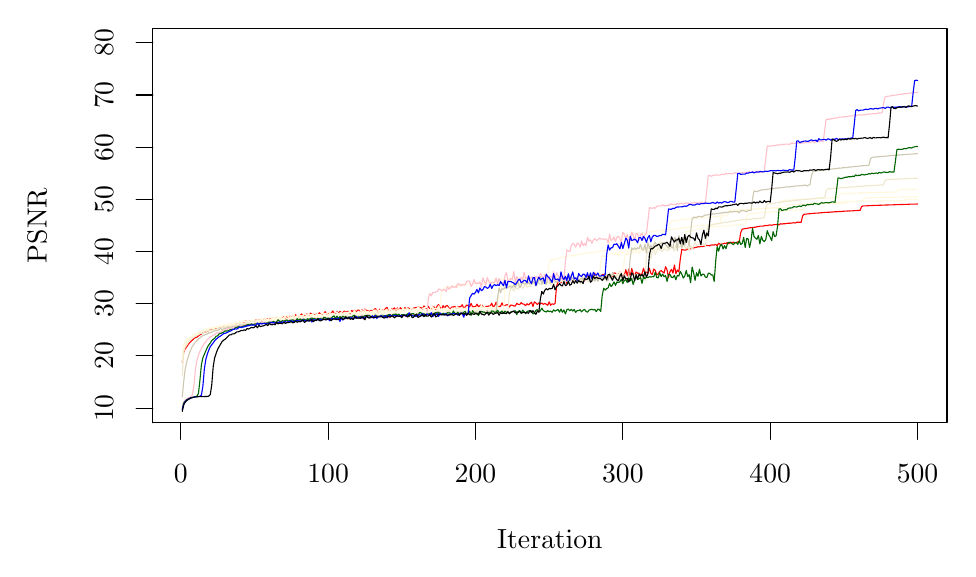
\begin{tikzpicture}[x=1pt,y=1pt]
\definecolor{fillColor}{RGB}{255,255,255}
%\path[use as bounding box,fill=fillColor,fill opacity=0.00] (0,0) rectangle (361.35,252.94);
\begin{scope}
%\path[clip] ( 49.20, 61.20) rectangle (336.15,203.75);
\definecolor{drawColor}{RGB}{255,0,0}

\path[draw=drawColor,line width= 0.4pt,line join=round,line cap=round] ( 59.83, 83.15) --
	( 60.36, 86.75) --
	( 60.89, 87.86) --
	( 61.43, 88.66) --
	( 61.96, 89.46) --
	( 62.49, 90.10) --
	( 63.02, 90.64) --
	( 63.55, 91.09) --
	( 64.09, 91.71) --
	( 64.62, 91.95) --
	( 65.15, 92.11) --
	( 65.68, 92.60) --
	( 66.22, 92.95) --
	( 66.75, 93.24) --
	( 67.28, 93.65) --
	( 67.81, 93.94) --
	( 68.35, 94.02) --
	( 68.88, 94.18) --
	( 69.41, 94.70) --
	( 69.94, 94.82) --
	( 70.48, 94.98) --
	( 71.01, 95.18) --
	( 71.54, 95.14) --
	( 72.07, 95.51) --
	( 72.61, 95.37) --
	( 73.14, 95.86) --
	( 73.67, 95.63) --
	( 74.20, 95.98) --
	( 74.74, 96.11) --
	( 75.27, 96.36) --
	( 75.80, 95.85) --
	( 76.33, 96.38) --
	( 76.87, 96.48) --
	( 77.40, 96.73) --
	( 77.93, 96.72) --
	( 78.46, 96.83) --
	( 79.00, 96.92) --
	( 79.53, 97.29) --
	( 80.06, 97.08) --
	( 80.59, 97.14) --
	( 81.13, 97.38) --
	( 81.66, 97.30) --
	( 82.19, 97.43) --
	( 82.72, 97.95) --
	( 83.26, 97.63) --
	( 83.79, 97.63) --
	( 84.32, 98.05) --
	( 84.85, 97.79) --
	( 85.39, 97.95) --
	( 85.92, 97.91) --
	( 86.45, 98.47) --
	( 86.98, 98.38) --
	( 87.52, 98.36) --
	( 88.05, 98.22) --
	( 88.58, 98.57) --
	( 89.11, 98.53) --
	( 89.65, 98.62) --
	( 90.18, 98.65) --
	( 90.71, 98.83) --
	( 91.24, 98.78) --
	( 91.78, 98.88) --
	( 92.31, 98.88) --
	( 92.84, 98.89) --
	( 93.37, 99.14) --
	( 93.90, 99.07) --
	( 94.44, 98.94) --
	( 94.97, 98.99) --
	( 95.50, 99.38) --
	( 96.03, 99.21) --
	( 96.57, 99.56) --
	( 97.10, 98.94) --
	( 97.63, 99.65) --
	( 98.16, 99.08) --
	( 98.70, 99.70) --
	( 99.23, 99.70) --
	( 99.76, 99.67) --
	(100.29, 99.36) --
	(100.83,100.22) --
	(101.36, 99.54) --
	(101.89, 99.78) --
	(102.42, 99.87) --
	(102.96,100.50) --
	(103.49, 99.83) --
	(104.02, 99.92) --
	(104.55,100.40) --
	(105.09,100.39) --
	(105.62,100.06) --
	(106.15,100.79) --
	(106.68,100.34) --
	(107.22,100.38) --
	(107.75,100.29) --
	(108.28,100.49) --
	(108.81,100.07) --
	(109.35,100.95) --
	(109.88,100.40) --
	(110.41,100.27) --
	(110.94,100.71) --
	(111.48,101.33) --
	(112.01,100.35) --
	(112.54,100.72) --
	(113.07,100.93) --
	(113.61,100.47) --
	(114.14,101.57) --
	(114.67,100.95) --
	(115.20,100.69) --
	(115.74,101.31) --
	(116.27,100.71) --
	(116.80,101.42) --
	(117.33,100.99) --
	(117.87,101.01) --
	(118.40,101.58) --
	(118.93,101.12) --
	(119.46,101.39) --
	(120.00,101.39) --
	(120.53,100.54) --
	(121.06,101.82) --
	(121.59,101.21) --
	(122.12,101.87) --
	(122.66,101.14) --
	(123.19,101.90) --
	(123.72,101.85) --
	(124.25,101.31) --
	(124.79,101.98) --
	(125.32,101.21) --
	(125.85,102.28) --
	(126.38,101.76) --
	(126.92,101.71) --
	(127.45,101.29) --
	(127.98,101.87) --
	(128.51,101.41) --
	(129.05,102.06) --
	(129.58,102.42) --
	(130.11,102.00) --
	(130.64,100.96) --
	(131.18,102.21) --
	(131.71,102.14) --
	(132.24,101.92) --
	(132.77,101.58) --
	(133.31,102.56) --
	(133.84,102.82) --
	(134.37,101.37) --
	(134.90,101.67) --
	(135.44,102.29) --
	(135.97,102.21) --
	(136.50,102.70) --
	(137.03,101.68) --
	(137.57,102.70) --
	(138.10,101.89) --
	(138.63,102.79) --
	(139.16,102.19) --
	(139.70,101.96) --
	(140.23,102.80) --
	(140.76,102.34) --
	(141.29,102.72) --
	(141.83,102.53) --
	(142.36,102.43) --
	(142.89,102.09) --
	(143.42,102.62) --
	(143.96,102.75) --
	(144.49,102.80) --
	(145.02,103.04) --
	(145.55,102.81) --
	(146.09,102.83) --
	(146.62,102.22) --
	(147.15,103.42) --
	(147.68,102.74) --
	(148.22,102.39) --
	(148.75,103.27) --
	(149.28,102.17) --
	(149.81,102.28) --
	(150.34,103.24) --
	(150.88,102.96) --
	(151.41,102.08) --
	(151.94,103.39) --
	(152.47,103.87) --
	(153.01,102.97) --
	(153.54,102.19) --
	(154.07,103.53) --
	(154.60,102.64) --
	(155.14,103.43) --
	(155.67,103.51) --
	(156.20,102.67) --
	(156.73,102.32) --
	(157.27,103.05) --
	(157.80,103.01) --
	(158.33,103.26) --
	(158.86,102.63) --
	(159.40,103.03) --
	(159.93,103.09) --
	(160.46,103.13) --
	(160.99,103.85) --
	(161.53,102.62) --
	(162.06,103.04) --
	(162.59,103.72) --
	(163.12,103.48) --
	(163.66,103.04) --
	(164.19,104.31) --
	(164.72,103.10) --
	(165.25,103.19) --
	(165.79,103.12) --
	(166.32,104.04) --
	(166.85,103.10) --
	(167.38,103.44) --
	(167.92,103.91) --
	(168.45,103.21) --
	(168.98,103.14) --
	(169.51,103.25) --
	(170.05,103.22) --
	(170.58,103.39) --
	(171.11,103.31) --
	(171.64,104.37) --
	(172.18,103.05) --
	(172.71,103.48) --
	(173.24,104.78) --
	(173.77,102.90) --
	(174.31,103.27) --
	(174.84,103.25) --
	(175.37,104.53) --
	(175.90,103.45) --
	(176.44,103.59) --
	(176.97,103.80) --
	(177.50,103.88) --
	(178.03,103.03) --
	(178.56,103.74) --
	(179.10,103.62) --
	(179.63,103.39) --
	(180.16,103.36) --
	(180.69,104.31) --
	(181.23,103.96) --
	(181.76,103.87) --
	(182.29,104.58) --
	(182.82,104.14) --
	(183.36,104.01) --
	(183.89,103.52) --
	(184.42,104.18) --
	(184.95,103.73) --
	(185.49,104.30) --
	(186.02,104.75) --
	(186.55,103.22) --
	(187.08,104.88) --
	(187.62,104.45) --
	(188.15,103.89) --
	(188.68,104.52) --
	(189.21,104.11) --
	(189.75,104.43) --
	(190.28,103.99) --
	(190.81,104.26) --
	(191.34,104.06) --
	(191.88,103.62) --
	(192.41,104.86) --
	(192.94,103.63) --
	(193.47,104.18) --
	(194.01,103.99) --
	(194.54,104.27) --
	(195.07,110.40) --
	(195.60,112.06) --
	(196.14,112.01) --
	(196.67,111.74) --
	(197.20,112.16) --
	(197.73,112.69) --
	(198.27,112.74) --
	(198.80,111.48) --
	(199.33,112.19) --
	(199.86,112.34) --
	(200.40,113.77) --
	(200.93,112.31) --
	(201.46,113.26) --
	(201.99,113.39) --
	(202.53,113.04) --
	(203.06,112.83) --
	(203.59,113.04) --
	(204.12,112.94) --
	(204.66,113.52) --
	(205.19,112.42) --
	(205.72,114.57) --
	(206.25,114.16) --
	(206.79,113.94) --
	(207.32,113.51) --
	(207.85,113.69) --
	(208.38,112.95) --
	(208.91,115.25) --
	(209.45,114.23) --
	(209.98,113.80) --
	(210.51,113.97) --
	(211.04,114.63) --
	(211.58,114.81) --
	(212.11,114.65) --
	(212.64,115.15) --
	(213.17,114.45) --
	(213.71,113.47) --
	(214.24,114.20) --
	(214.77,114.51) --
	(215.30,113.71) --
	(215.84,115.33) --
	(216.37,115.20) --
	(216.90,115.05) --
	(217.43,114.39) --
	(217.97,115.82) --
	(218.50,113.88) --
	(219.03,114.63) --
	(219.56,114.37) --
	(220.10,116.51) --
	(220.63,114.26) --
	(221.16,116.64) --
	(221.69,113.76) --
	(222.23,116.94) --
	(222.76,115.16) --
	(223.29,114.36) --
	(223.82,115.67) --
	(224.36,115.20) --
	(224.89,115.22) --
	(225.42,114.77) --
	(225.95,114.86) --
	(226.49,117.04) --
	(227.02,115.23) --
	(227.55,115.60) --
	(228.08,115.20) --
	(228.62,117.03) --
	(229.15,115.23) --
	(229.68,114.77) --
	(230.21,116.74) --
	(230.75,116.27) --
	(231.28,114.58) --
	(231.81,114.95) --
	(232.34,115.88) --
	(232.88,116.14) --
	(233.41,115.72) --
	(233.94,115.28) --
	(234.47,117.58) --
	(235.01,116.42) --
	(235.54,113.66) --
	(236.07,115.84) --
	(236.60,116.64) --
	(237.13,115.26) --
	(237.67,118.19) --
	(238.20,115.04) --
	(238.73,116.38) --
	(239.26,115.68) --
	(239.80,120.44) --
	(240.33,123.78) --
	(240.86,123.67) --
	(241.39,123.56) --
	(241.93,123.65) --
	(242.46,123.99) --
	(242.99,123.95) --
	(243.52,124.03) --
	(244.06,124.43) --
	(244.59,124.34) --
	(245.12,124.50) --
	(245.65,124.58) --
	(246.19,124.78) --
	(246.72,124.74) --
	(247.25,124.89) --
	(247.78,124.82) --
	(248.32,124.98) --
	(248.85,125.17) --
	(249.38,125.26) --
	(249.91,125.19) --
	(250.45,125.15) --
	(250.98,125.46) --
	(251.51,125.42) --
	(252.04,125.38) --
	(252.58,125.63) --
	(253.11,125.17) --
	(253.64,126.04) --
	(254.17,125.69) --
	(254.71,125.76) --
	(255.24,125.83) --
	(255.77,126.06) --
	(256.30,125.99) --
	(256.84,126.31) --
	(257.37,125.89) --
	(257.90,126.44) --
	(258.43,126.23) --
	(258.97,126.46) --
	(259.50,126.27) --
	(260.03,126.21) --
	(260.56,126.56) --
	(261.10,126.66) --
	(261.63,129.89) --
	(262.16,131.16) --
	(262.69,131.24) --
	(263.23,131.38) --
	(263.76,131.40) --
	(264.29,131.52) --
	(264.82,131.63) --
	(265.35,131.68) --
	(265.89,131.77) --
	(266.42,131.81) --
	(266.95,131.85) --
	(267.48,132.03) --
	(268.02,132.06) --
	(268.55,132.22) --
	(269.08,132.22) --
	(269.61,132.25) --
	(270.15,132.37) --
	(270.68,132.48) --
	(271.21,132.42) --
	(271.74,132.60) --
	(272.28,132.66) --
	(272.81,132.55) --
	(273.34,132.70) --
	(273.87,132.79) --
	(274.41,132.79) --
	(274.94,132.88) --
	(275.47,132.68) --
	(276.00,133.10) --
	(276.54,132.99) --
	(277.07,133.10) --
	(277.60,133.10) --
	(278.13,133.20) --
	(278.67,133.27) --
	(279.20,133.27) --
	(279.73,133.30) --
	(280.26,133.39) --
	(280.80,133.46) --
	(281.33,133.37) --
	(281.86,133.63) --
	(282.39,133.62) --
	(282.93,133.63) --
	(283.46,133.62) --
	(283.99,135.92) --
	(284.52,136.52) --
	(285.06,136.56) --
	(285.59,136.62) --
	(286.12,136.69) --
	(286.65,136.72) --
	(287.19,136.81) --
	(287.72,136.83) --
	(288.25,136.89) --
	(288.78,136.93) --
	(289.32,136.94) --
	(289.85,136.99) --
	(290.38,137.05) --
	(290.91,137.09) --
	(291.45,137.10) --
	(291.98,137.19) --
	(292.51,137.19) --
	(293.04,137.24) --
	(293.57,137.24) --
	(294.11,137.29) --
	(294.64,137.35) --
	(295.17,137.37) --
	(295.70,137.44) --
	(296.24,137.42) --
	(296.77,137.49) --
	(297.30,137.54) --
	(297.83,137.52) --
	(298.37,137.59) --
	(298.90,137.63) --
	(299.43,137.64) --
	(299.96,137.68) --
	(300.50,137.73) --
	(301.03,137.71) --
	(301.56,137.76) --
	(302.09,137.77) --
	(302.63,137.84) --
	(303.16,137.82) --
	(303.69,137.89) --
	(304.22,137.89) --
	(304.76,137.96) --
	(305.29,139.30) --
	(305.82,139.53) --
	(306.35,139.56) --
	(306.89,139.57) --
	(307.42,139.60) --
	(307.95,139.63) --
	(308.48,139.66) --
	(309.02,139.68) --
	(309.55,139.70) --
	(310.08,139.73) --
	(310.61,139.74) --
	(311.15,139.75) --
	(311.68,139.77) --
	(312.21,139.78) --
	(312.74,139.81) --
	(313.28,139.83) --
	(313.81,139.86) --
	(314.34,139.87) --
	(314.87,139.87) --
	(315.41,139.93) --
	(315.94,139.91) --
	(316.47,139.93) --
	(317.00,139.95) --
	(317.54,139.99) --
	(318.07,140.01) --
	(318.60,140.00) --
	(319.13,140.04) --
	(319.67,140.04) --
	(320.20,140.06) --
	(320.73,140.09) --
	(321.26,140.11) --
	(321.80,140.11) --
	(322.33,140.13) --
	(322.86,140.18) --
	(323.39,140.18) --
	(323.92,140.18) --
	(324.46,140.21) --
	(324.99,140.20) --
	(325.52,140.24);
\end{scope}
\begin{scope}
%\path[clip] (  0.00,  0.00) rectangle (361.35,252.94);
\definecolor{drawColor}{RGB}{0,0,0}

\path[draw=drawColor,line width= 0.4pt,line join=round,line cap=round] ( 59.30, 61.20) -- (325.52, 61.20);

\path[draw=drawColor,line width= 0.4pt,line join=round,line cap=round] ( 59.30, 61.20) -- ( 59.30, 55.20);

\path[draw=drawColor,line width= 0.4pt,line join=round,line cap=round] (112.54, 61.20) -- (112.54, 55.20);

\path[draw=drawColor,line width= 0.4pt,line join=round,line cap=round] (165.79, 61.20) -- (165.79, 55.20);

\path[draw=drawColor,line width= 0.4pt,line join=round,line cap=round] (219.03, 61.20) -- (219.03, 55.20);

\path[draw=drawColor,line width= 0.4pt,line join=round,line cap=round] (272.28, 61.20) -- (272.28, 55.20);

\path[draw=drawColor,line width= 0.4pt,line join=round,line cap=round] (325.52, 61.20) -- (325.52, 55.20);

\node[text=drawColor,anchor=base,inner sep=0pt, outer sep=0pt, scale=  1.00] at ( 59.30, 39.60) {0};

\node[text=drawColor,anchor=base,inner sep=0pt, outer sep=0pt, scale=  1.00] at (112.54, 39.60) {100};

\node[text=drawColor,anchor=base,inner sep=0pt, outer sep=0pt, scale=  1.00] at (165.79, 39.60) {200};

\node[text=drawColor,anchor=base,inner sep=0pt, outer sep=0pt, scale=  1.00] at (219.03, 39.60) {300};

\node[text=drawColor,anchor=base,inner sep=0pt, outer sep=0pt, scale=  1.00] at (272.28, 39.60) {400};

\node[text=drawColor,anchor=base,inner sep=0pt, outer sep=0pt, scale=  1.00] at (325.52, 39.60) {500};

\path[draw=drawColor,line width= 0.4pt,line join=round,line cap=round] ( 49.20, 66.48) -- ( 49.20,198.47);

\path[draw=drawColor,line width= 0.4pt,line join=round,line cap=round] ( 49.20, 66.48) -- ( 43.20, 66.48);

\path[draw=drawColor,line width= 0.4pt,line join=round,line cap=round] ( 49.20, 85.33) -- ( 43.20, 85.33);

\path[draw=drawColor,line width= 0.4pt,line join=round,line cap=round] ( 49.20,104.19) -- ( 43.20,104.19);

\path[draw=drawColor,line width= 0.4pt,line join=round,line cap=round] ( 49.20,123.04) -- ( 43.20,123.04);

\path[draw=drawColor,line width= 0.4pt,line join=round,line cap=round] ( 49.20,141.90) -- ( 43.20,141.90);

\path[draw=drawColor,line width= 0.4pt,line join=round,line cap=round] ( 49.20,160.76) -- ( 43.20,160.76);

\path[draw=drawColor,line width= 0.4pt,line join=round,line cap=round] ( 49.20,179.61) -- ( 43.20,179.61);

\path[draw=drawColor,line width= 0.4pt,line join=round,line cap=round] ( 49.20,198.47) -- ( 43.20,198.47);

\node[text=drawColor,rotate= 90.00,anchor=base,inner sep=0pt, outer sep=0pt, scale=  1.00] at ( 34.80, 66.48) {10};

\node[text=drawColor,rotate= 90.00,anchor=base,inner sep=0pt, outer sep=0pt, scale=  1.00] at ( 34.80, 85.33) {20};

\node[text=drawColor,rotate= 90.00,anchor=base,inner sep=0pt, outer sep=0pt, scale=  1.00] at ( 34.80,104.19) {30};

\node[text=drawColor,rotate= 90.00,anchor=base,inner sep=0pt, outer sep=0pt, scale=  1.00] at ( 34.80,123.04) {40};

\node[text=drawColor,rotate= 90.00,anchor=base,inner sep=0pt, outer sep=0pt, scale=  1.00] at ( 34.80,141.90) {50};

\node[text=drawColor,rotate= 90.00,anchor=base,inner sep=0pt, outer sep=0pt, scale=  1.00] at ( 34.80,160.76) {60};

\node[text=drawColor,rotate= 90.00,anchor=base,inner sep=0pt, outer sep=0pt, scale=  1.00] at ( 34.80,179.61) {70};

\node[text=drawColor,rotate= 90.00,anchor=base,inner sep=0pt, outer sep=0pt, scale=  1.00] at ( 34.80,198.47) {80};

\path[draw=drawColor,line width= 0.4pt,line join=round,line cap=round] ( 49.20, 61.20) --
	(336.15, 61.20) --
	(336.15,203.75) --
	( 49.20,203.75) --
	( 49.20, 61.20);
\end{scope}
\begin{scope}
%\path[clip] (  0.00,  0.00) rectangle (361.35,252.94);
\definecolor{drawColor}{RGB}{0,0,0}

\node[text=drawColor,anchor=base,inner sep=0pt, outer sep=0pt, scale=  1.00] at (192.68, 15.60) {Iteration};

\node[text=drawColor,rotate= 90.00,anchor=base,inner sep=0pt, outer sep=0pt, scale=  1.00] at ( 10.80,132.47) {PSNR};
\end{scope}
\begin{scope}
%\path[clip] ( 49.20, 61.20) rectangle (336.15,203.75);
\definecolor{drawColor}{RGB}{255,248,220}

\path[draw=drawColor,line width= 0.4pt,line join=round,line cap=round] ( 59.83, 83.91) --
	( 60.36, 88.04) --
	( 60.89, 89.05) --
	( 61.43, 89.83) --
	( 61.96, 90.60) --
	( 62.49, 91.04) --
	( 63.02, 91.58) --
	( 63.55, 91.93) --
	( 64.09, 92.34) --
	( 64.62, 92.63) --
	( 65.15, 93.04) --
	( 65.68, 93.34) --
	( 66.22, 93.66) --
	( 66.75, 94.06) --
	( 67.28, 94.18) --
	( 67.81, 94.53) --
	( 68.35, 94.70) --
	( 68.88, 94.58) --
	( 69.41, 95.08) --
	( 69.94, 95.13) --
	( 70.48, 95.31) --
	( 71.01, 95.55) --
	( 71.54, 95.51) --
	( 72.07, 95.72) --
	( 72.61, 95.44) --
	( 73.14, 96.04) --
	( 73.67, 96.09) --
	( 74.20, 96.27) --
	( 74.74, 96.58) --
	( 75.27, 96.42) --
	( 75.80, 96.32) --
	( 76.33, 96.38) --
	( 76.87, 96.91) --
	( 77.40, 96.56) --
	( 77.93, 96.89) --
	( 78.46, 96.81) --
	( 79.00, 97.18) --
	( 79.53, 97.34) --
	( 80.06, 97.44) --
	( 80.59, 97.63) --
	( 81.13, 97.51) --
	( 81.66, 97.58) --
	( 82.19, 98.08) --
	( 82.72, 97.62) --
	( 83.26, 97.59) --
	( 83.79, 97.90) --
	( 84.32, 97.78) --
	( 84.85, 98.33) --
	( 85.39, 97.91) --
	( 85.92, 98.33) --
	( 86.45, 98.34) --
	( 86.98, 98.40) --
	( 87.52, 98.36) --
	( 88.05, 98.17) --
	( 88.58, 98.74) --
	( 89.11, 98.64) --
	( 89.65, 98.85) --
	( 90.18, 98.80) --
	( 90.71, 98.42) --
	( 91.24, 99.05) --
	( 91.78, 99.20) --
	( 92.31, 98.56) --
	( 92.84, 99.09) --
	( 93.37, 99.31) --
	( 93.90, 99.37) --
	( 94.44, 99.19) --
	( 94.97, 99.13) --
	( 95.50, 99.77) --
	( 96.03, 99.46) --
	( 96.57, 99.28) --
	( 97.10, 99.72) --
	( 97.63, 99.88) --
	( 98.16, 99.42) --
	( 98.70, 99.18) --
	( 99.23,100.13) --
	( 99.76, 99.48) --
	(100.29,100.06) --
	(100.83, 99.21) --
	(101.36,100.02) --
	(101.89, 99.74) --
	(102.42, 99.85) --
	(102.96, 99.69) --
	(103.49,100.13) --
	(104.02,100.38) --
	(104.55,100.29) --
	(105.09, 99.99) --
	(105.62,100.46) --
	(106.15,100.12) --
	(106.68,100.27) --
	(107.22,100.25) --
	(107.75,100.89) --
	(108.28,100.23) --
	(108.81,100.46) --
	(109.35,100.09) --
	(109.88,100.37) --
	(110.41,100.64) --
	(110.94,100.81) --
	(111.48,100.65) --
	(112.01,100.64) --
	(112.54,100.97) --
	(113.07,100.90) --
	(113.61,100.73) --
	(114.14,100.28) --
	(114.67,100.61) --
	(115.20,101.11) --
	(115.74,101.14) --
	(116.27,100.53) --
	(116.80,100.86) --
	(117.33,101.03) --
	(117.87,100.56) --
	(118.40,101.12) --
	(118.93,101.08) --
	(119.46,100.99) --
	(120.00,101.21) --
	(120.53,101.58) --
	(121.06,100.72) --
	(121.59,101.07) --
	(122.12,101.88) --
	(122.66,100.35) --
	(123.19,101.12) --
	(123.72,100.73) --
	(124.25,101.72) --
	(124.79,101.68) --
	(125.32,101.24) --
	(125.85,102.07) --
	(126.38,100.60) --
	(126.92,101.55) --
	(127.45,100.88) --
	(127.98,101.49) --
	(128.51,100.84) --
	(129.05,101.97) --
	(129.58,101.74) --
	(130.11,101.97) --
	(130.64,101.92) --
	(131.18,101.48) --
	(131.71,102.64) --
	(132.24,101.19) --
	(132.77,101.71) --
	(133.31,101.60) --
	(133.84,102.14) --
	(134.37,100.99) --
	(134.90,102.33) --
	(135.44,102.08) --
	(135.97,101.55) --
	(136.50,101.90) --
	(137.03,101.94) --
	(137.57,102.33) --
	(138.10,102.29) --
	(138.63,102.05) --
	(139.16,101.67) --
	(139.70,103.15) --
	(140.23,101.49) --
	(140.76,102.54) --
	(141.29,102.59) --
	(141.83,101.00) --
	(142.36,102.68) --
	(142.89,102.28) --
	(143.42,102.31) --
	(143.96,102.15) --
	(144.49,102.28) --
	(145.02,103.13) --
	(145.55,102.54) --
	(146.09,101.98) --
	(146.62,102.39) --
	(147.15,102.73) --
	(147.68,102.73) --
	(148.22,102.87) --
	(148.75,102.26) --
	(149.28,101.97) --
	(149.81,102.72) --
	(150.34,103.14) --
	(150.88,102.24) --
	(151.41,102.65) --
	(151.94,102.32) --
	(152.47,102.19) --
	(153.01,103.25) --
	(153.54,108.53) --
	(154.07,109.21) --
	(154.60,110.27) --
	(155.14,110.19) --
	(155.67,110.26) --
	(156.20,110.34) --
	(156.73,109.64) --
	(157.27,110.72) --
	(157.80,110.43) --
	(158.33,110.29) --
	(158.86,111.20) --
	(159.40,109.97) --
	(159.93,111.34) --
	(160.46,111.24) --
	(160.99,110.65) --
	(161.53,111.36) --
	(162.06,110.81) --
	(162.59,111.04) --
	(163.12,111.13) --
	(163.66,111.60) --
	(164.19,110.68) --
	(164.72,111.08) --
	(165.25,111.99) --
	(165.79,111.81) --
	(166.32,111.24) --
	(166.85,111.91) --
	(167.38,111.38) --
	(167.92,111.38) --
	(168.45,111.56) --
	(168.98,111.97) --
	(169.51,111.90) --
	(170.05,111.99) --
	(170.58,112.54) --
	(171.11,112.44) --
	(171.64,111.71) --
	(172.18,111.18) --
	(172.71,113.36) --
	(173.24,112.42) --
	(173.77,111.97) --
	(174.31,113.19) --
	(174.84,112.47) --
	(175.37,113.34) --
	(175.90,112.89) --
	(176.44,112.91) --
	(176.97,112.50) --
	(177.50,113.21) --
	(178.03,113.38) --
	(178.56,112.73) --
	(179.10,113.19) --
	(179.63,112.66) --
	(180.16,113.22) --
	(180.69,113.13) --
	(181.23,113.59) --
	(181.76,112.62) --
	(182.29,113.61) --
	(182.82,112.80) --
	(183.36,113.58) --
	(183.89,113.10) --
	(184.42,111.96) --
	(184.95,113.79) --
	(185.49,113.75) --
	(186.02,113.38) --
	(186.55,113.21) --
	(187.08,113.61) --
	(187.62,113.58) --
	(188.15,113.07) --
	(188.68,113.48) --
	(189.21,113.88) --
	(189.75,114.06) --
	(190.28,113.46) --
	(190.81,112.98) --
	(191.34,113.30) --
	(191.88,114.91) --
	(192.41,118.35) --
	(192.94,120.14) --
	(193.47,119.89) --
	(194.01,120.18) --
	(194.54,120.36) --
	(195.07,120.32) --
	(195.60,120.47) --
	(196.14,120.60) --
	(196.67,121.00) --
	(197.20,121.00) --
	(197.73,120.99) --
	(198.27,121.18) --
	(198.80,121.23) --
	(199.33,121.48) --
	(199.86,121.48) --
	(200.40,121.52) --
	(200.93,121.73) --
	(201.46,121.41) --
	(201.99,121.93) --
	(202.53,121.88) --
	(203.06,121.97) --
	(203.59,122.07) --
	(204.12,122.11) --
	(204.66,122.30) --
	(205.19,122.51) --
	(205.72,122.33) --
	(206.25,122.63) --
	(206.79,122.48) --
	(207.32,122.87) --
	(207.85,122.69) --
	(208.38,122.85) --
	(208.91,122.81) --
	(209.45,122.70) --
	(209.98,123.25) --
	(210.51,123.01) --
	(211.04,123.31) --
	(211.58,123.03) --
	(212.11,123.11) --
	(212.64,123.57) --
	(213.17,123.47) --
	(213.71,123.34) --
	(214.24,126.75) --
	(214.77,127.78) --
	(215.30,127.84) --
	(215.84,128.02) --
	(216.37,128.24) --
	(216.90,128.22) --
	(217.43,128.36) --
	(217.97,128.51) --
	(218.50,128.59) --
	(219.03,128.68) --
	(219.56,128.75) --
	(220.10,128.82) --
	(220.63,128.98) --
	(221.16,129.01) --
	(221.69,129.08) --
	(222.23,129.20) --
	(222.76,129.31) --
	(223.29,129.38) --
	(223.82,129.42) --
	(224.36,129.52) --
	(224.89,129.63) --
	(225.42,129.72) --
	(225.95,129.69) --
	(226.49,129.88) --
	(227.02,130.05) --
	(227.55,129.97) --
	(228.08,130.08) --
	(228.62,130.13) --
	(229.15,130.25) --
	(229.68,130.28) --
	(230.21,130.41) --
	(230.75,130.39) --
	(231.28,130.52) --
	(231.81,130.65) --
	(232.34,130.66) --
	(232.88,130.68) --
	(233.41,130.78) --
	(233.94,130.88) --
	(234.47,130.85) --
	(235.01,130.94) --
	(235.54,130.98) --
	(236.07,133.38) --
	(236.60,134.09) --
	(237.13,134.09) --
	(237.67,134.24) --
	(238.20,134.29) --
	(238.73,134.33) --
	(239.26,134.42) --
	(239.80,134.47) --
	(240.33,134.52) --
	(240.86,134.64) --
	(241.39,134.63) --
	(241.93,134.68) --
	(242.46,134.74) --
	(242.99,134.80) --
	(243.52,134.90) --
	(244.06,134.92) --
	(244.59,134.98) --
	(245.12,135.02) --
	(245.65,135.09) --
	(246.19,135.13) --
	(246.72,135.17) --
	(247.25,135.22) --
	(247.78,135.29) --
	(248.32,135.33) --
	(248.85,135.36) --
	(249.38,135.43) --
	(249.91,135.47) --
	(250.45,135.50) --
	(250.98,135.55) --
	(251.51,135.63) --
	(252.04,135.63) --
	(252.58,135.63) --
	(253.11,135.78) --
	(253.64,135.75) --
	(254.17,135.88) --
	(254.71,135.93) --
	(255.24,135.89) --
	(255.77,135.96) --
	(256.30,135.97) --
	(256.84,136.06) --
	(257.37,137.63) --
	(257.90,137.90) --
	(258.43,137.95) --
	(258.97,137.99) --
	(259.50,138.02) --
	(260.03,138.07) --
	(260.56,138.08) --
	(261.10,138.14) --
	(261.63,138.13) --
	(262.16,138.17) --
	(262.69,138.21) --
	(263.23,138.21) --
	(263.76,138.24) --
	(264.29,138.29) --
	(264.82,138.31) --
	(265.35,138.32) --
	(265.89,138.37) --
	(266.42,138.39) --
	(266.95,138.39) --
	(267.48,138.44) --
	(268.02,138.46) --
	(268.55,138.51) --
	(269.08,138.53) --
	(269.61,138.56) --
	(270.15,138.59) --
	(270.68,138.59) --
	(271.21,138.64) --
	(271.74,138.64) --
	(272.28,138.66) --
	(272.81,138.69) --
	(273.34,138.74) --
	(273.87,138.76) --
	(274.41,138.77) --
	(274.94,138.78) --
	(275.47,138.81) --
	(276.00,138.84) --
	(276.54,138.85) --
	(277.07,138.87) --
	(277.60,138.93) --
	(278.13,138.92) --
	(278.67,139.90) --
	(279.20,140.04) --
	(279.73,140.03) --
	(280.26,140.07) --
	(280.80,140.06) --
	(281.33,140.11) --
	(281.86,140.12) --
	(282.39,140.13) --
	(282.93,140.14) --
	(283.46,140.14) --
	(283.99,140.17) --
	(284.52,140.17) --
	(285.06,140.18) --
	(285.59,140.21) --
	(286.12,140.23) --
	(286.65,140.22) --
	(287.19,140.25) --
	(287.72,140.26) --
	(288.25,140.27) --
	(288.78,140.28) --
	(289.32,140.30) --
	(289.85,140.30) --
	(290.38,140.33) --
	(290.91,140.34) --
	(291.45,140.35) --
	(291.98,140.36) --
	(292.51,140.38) --
	(293.04,140.39) --
	(293.57,140.41) --
	(294.11,140.42) --
	(294.64,140.46) --
	(295.17,140.45) --
	(295.70,140.45) --
	(296.24,140.47) --
	(296.77,140.46) --
	(297.30,140.50) --
	(297.83,140.50) --
	(298.37,140.52) --
	(298.90,140.52) --
	(299.43,140.55) --
	(299.96,141.12) --
	(300.50,141.17) --
	(301.03,141.18) --
	(301.56,141.19) --
	(302.09,141.19) --
	(302.63,141.21) --
	(303.16,141.20) --
	(303.69,141.22) --
	(304.22,141.22) --
	(304.76,141.23) --
	(305.29,141.24) --
	(305.82,141.24) --
	(306.35,141.25) --
	(306.89,141.26) --
	(307.42,141.27) --
	(307.95,141.27) --
	(308.48,141.28) --
	(309.02,141.29) --
	(309.55,141.29) --
	(310.08,141.29) --
	(310.61,141.30) --
	(311.15,141.31) --
	(311.68,141.32) --
	(312.21,141.33) --
	(312.74,141.33) --
	(313.28,141.33) --
	(313.81,141.35) --
	(314.34,141.35) --
	(314.87,141.36) --
	(315.41,141.36) --
	(315.94,141.37) --
	(316.47,141.38) --
	(317.00,141.39) --
	(317.54,141.38) --
	(318.07,141.40) --
	(318.60,141.40) --
	(319.13,141.41) --
	(319.67,141.40) --
	(320.20,141.43) --
	(320.73,141.43) --
	(321.26,141.76) --
	(321.80,141.78) --
	(322.33,141.79) --
	(322.86,141.79) --
	(323.39,141.80) --
	(323.92,141.80) --
	(324.46,141.80) --
	(324.99,141.81) --
	(325.52,141.80);

\path[draw=drawColor,line width= 0.4pt,line join=round,line cap=round] ( 59.83, 84.47) --
	( 60.36, 89.08) --
	( 60.89, 90.11) --
	( 61.43, 90.67) --
	( 61.96, 91.29) --
	( 62.49, 91.91) --
	( 63.02, 92.25) --
	( 63.55, 92.69) --
	( 64.09, 92.93) --
	( 64.62, 93.36) --
	( 65.15, 93.57) --
	( 65.68, 93.80) --
	( 66.22, 94.16) --
	( 66.75, 94.28) --
	( 67.28, 94.66) --
	( 67.81, 94.64) --
	( 68.35, 95.09) --
	( 68.88, 95.03) --
	( 69.41, 95.05) --
	( 69.94, 95.66) --
	( 70.48, 95.20) --
	( 71.01, 95.54) --
	( 71.54, 95.56) --
	( 72.07, 95.88) --
	( 72.61, 96.09) --
	( 73.14, 96.09) --
	( 73.67, 96.14) --
	( 74.20, 96.10) --
	( 74.74, 96.39) --
	( 75.27, 96.42) --
	( 75.80, 96.39) --
	( 76.33, 96.74) --
	( 76.87, 96.93) --
	( 77.40, 96.57) --
	( 77.93, 97.23) --
	( 78.46, 96.97) --
	( 79.00, 97.08) --
	( 79.53, 97.59) --
	( 80.06, 96.83) --
	( 80.59, 97.67) --
	( 81.13, 97.56) --
	( 81.66, 97.50) --
	( 82.19, 97.69) --
	( 82.72, 97.83) --
	( 83.26, 97.79) --
	( 83.79, 97.27) --
	( 84.32, 98.09) --
	( 84.85, 97.81) --
	( 85.39, 98.19) --
	( 85.92, 97.92) --
	( 86.45, 98.03) --
	( 86.98, 98.32) --
	( 87.52, 98.04) --
	( 88.05, 98.36) --
	( 88.58, 98.63) --
	( 89.11, 98.22) --
	( 89.65, 98.44) --
	( 90.18, 98.24) --
	( 90.71, 98.64) --
	( 91.24, 98.05) --
	( 91.78, 98.42) --
	( 92.31, 98.93) --
	( 92.84, 98.82) --
	( 93.37, 98.98) --
	( 93.90, 98.79) --
	( 94.44, 98.94) --
	( 94.97, 98.81) --
	( 95.50, 99.31) --
	( 96.03, 98.85) --
	( 96.57, 99.02) --
	( 97.10, 99.26) --
	( 97.63, 98.91) --
	( 98.16, 99.09) --
	( 98.70, 99.36) --
	( 99.23, 99.28) --
	( 99.76, 99.56) --
	(100.29, 99.31) --
	(100.83, 99.32) --
	(101.36, 99.58) --
	(101.89, 99.79) --
	(102.42, 99.96) --
	(102.96, 99.55) --
	(103.49, 99.85) --
	(104.02, 99.65) --
	(104.55, 99.65) --
	(105.09,100.20) --
	(105.62, 99.35) --
	(106.15, 99.81) --
	(106.68,100.08) --
	(107.22, 99.70) --
	(107.75, 99.92) --
	(108.28,100.08) --
	(108.81,100.07) --
	(109.35, 99.94) --
	(109.88,100.24) --
	(110.41, 99.73) --
	(110.94,100.67) --
	(111.48,100.43) --
	(112.01,100.66) --
	(112.54, 99.45) --
	(113.07,100.75) --
	(113.61,100.22) --
	(114.14, 99.90) --
	(114.67,100.42) --
	(115.20,100.42) --
	(115.74,100.41) --
	(116.27,100.54) --
	(116.80,100.22) --
	(117.33,100.83) --
	(117.87,100.51) --
	(118.40,100.56) --
	(118.93,100.81) --
	(119.46,100.02) --
	(120.00,101.06) --
	(120.53,101.15) --
	(121.06,100.46) --
	(121.59,101.05) --
	(122.12,100.95) --
	(122.66,100.65) --
	(123.19,101.22) --
	(123.72,100.74) --
	(124.25,100.94) --
	(124.79,101.33) --
	(125.32,100.95) --
	(125.85,100.69) --
	(126.38,101.49) --
	(126.92,100.49) --
	(127.45,101.20) --
	(127.98,100.83) --
	(128.51,101.52) --
	(129.05,101.14) --
	(129.58,101.64) --
	(130.11,101.06) --
	(130.64,101.41) --
	(131.18,100.59) --
	(131.71,101.67) --
	(132.24,101.83) --
	(132.77,100.84) --
	(133.31,102.00) --
	(133.84,101.43) --
	(134.37,101.02) --
	(134.90,101.58) --
	(135.44,101.74) --
	(135.97,101.94) --
	(136.50,101.30) --
	(137.03,101.55) --
	(137.57,101.44) --
	(138.10,101.75) --
	(138.63,101.90) --
	(139.16,101.10) --
	(139.70,102.29) --
	(140.23,101.38) --
	(140.76,101.81) --
	(141.29,102.35) --
	(141.83,101.70) --
	(142.36,101.15) --
	(142.89,102.20) --
	(143.42,102.26) --
	(143.96,102.01) --
	(144.49,101.70) --
	(145.02,101.31) --
	(145.55,101.94) --
	(146.09,101.79) --
	(146.62,101.47) --
	(147.15,101.87) --
	(147.68,101.76) --
	(148.22,101.94) --
	(148.75,101.77) --
	(149.28,102.10) --
	(149.81,101.81) --
	(150.34,102.38) --
	(150.88,102.12) --
	(151.41,101.58) --
	(151.94,101.63) --
	(152.47,103.47) --
	(153.01,101.02) --
	(153.54,102.57) --
	(154.07,101.71) --
	(154.60,102.18) --
	(155.14,101.69) --
	(155.67,102.88) --
	(156.20,102.10) --
	(156.73,101.85) --
	(157.27,102.60) --
	(157.80,102.21) --
	(158.33,101.95) --
	(158.86,103.08) --
	(159.40,102.50) --
	(159.93,102.50) --
	(160.46,102.24) --
	(160.99,102.41) --
	(161.53,102.62) --
	(162.06,102.47) --
	(162.59,102.51) --
	(163.12,102.24) --
	(163.66,102.68) --
	(164.19,102.10) --
	(164.72,102.51) --
	(165.25,102.35) --
	(165.79,102.84) --
	(166.32,102.25) --
	(166.85,102.77) --
	(167.38,102.07) --
	(167.92,104.00) --
	(168.45,102.19) --
	(168.98,103.40) --
	(169.51,102.48) --
	(170.05,102.28) --
	(170.58,102.54) --
	(171.11,103.17) --
	(171.64,101.74) --
	(172.18,102.76) --
	(172.71,102.63) --
	(173.24,103.32) --
	(173.77,102.48) --
	(174.31,108.96) --
	(174.84,110.37) --
	(175.37,109.98) --
	(175.90,109.90) --
	(176.44,111.34) --
	(176.97,110.80) --
	(177.50,111.24) --
	(178.03,110.77) --
	(178.56,110.09) --
	(179.10,111.68) --
	(179.63,111.07) --
	(180.16,111.31) --
	(180.69,111.25) --
	(181.23,111.42) --
	(181.76,110.59) --
	(182.29,112.31) --
	(182.82,112.17) --
	(183.36,111.12) --
	(183.89,112.11) --
	(184.42,111.16) --
	(184.95,112.88) --
	(185.49,111.64) --
	(186.02,111.67) --
	(186.55,112.52) --
	(187.08,112.20) --
	(187.62,112.48) --
	(188.15,111.94) --
	(188.68,112.59) --
	(189.21,112.40) --
	(189.75,112.96) --
	(190.28,112.85) --
	(190.81,112.42) --
	(191.34,113.14) --
	(191.88,112.65) --
	(192.41,112.95) --
	(192.94,112.70) --
	(193.47,112.70) --
	(194.01,113.45) --
	(194.54,112.37) --
	(195.07,112.92) --
	(195.60,113.04) --
	(196.14,113.14) --
	(196.67,113.04) --
	(197.20,113.18) --
	(197.73,114.39) --
	(198.27,112.48) --
	(198.80,114.55) --
	(199.33,113.95) --
	(199.86,113.48) --
	(200.40,113.63) --
	(200.93,113.66) --
	(201.46,113.72) --
	(201.99,113.29) --
	(202.53,114.31) --
	(203.06,112.52) --
	(203.59,114.50) --
	(204.12,113.96) --
	(204.66,114.05) --
	(205.19,114.31) --
	(205.72,113.00) --
	(206.25,113.40) --
	(206.79,114.56) --
	(207.32,113.47) --
	(207.85,113.98) --
	(208.38,114.31) --
	(208.91,113.34) --
	(209.45,115.17) --
	(209.98,114.21) --
	(210.51,114.23) --
	(211.04,114.60) --
	(211.58,113.88) --
	(212.11,113.04) --
	(212.64,115.31) --
	(213.17,114.51) --
	(213.71,114.41) --
	(214.24,114.74) --
	(214.77,114.73) --
	(215.30,114.44) --
	(215.84,114.88) --
	(216.37,113.42) --
	(216.90,115.23) --
	(217.43,114.11) --
	(217.97,115.87) --
	(218.50,113.91) --
	(219.03,114.86) --
	(219.56,119.99) --
	(220.10,122.35) --
	(220.63,121.72) --
	(221.16,122.18) --
	(221.69,122.31) --
	(222.23,122.66) --
	(222.76,122.50) --
	(223.29,122.72) --
	(223.82,122.95) --
	(224.36,122.86) --
	(224.89,122.66) --
	(225.42,123.14) --
	(225.95,123.43) --
	(226.49,123.21) --
	(227.02,123.44) --
	(227.55,123.62) --
	(228.08,123.49) --
	(228.62,123.81) --
	(229.15,123.75) --
	(229.68,123.85) --
	(230.21,123.96) --
	(230.75,123.80) --
	(231.28,124.24) --
	(231.81,124.40) --
	(232.34,123.58) --
	(232.88,124.21) --
	(233.41,124.52) --
	(233.94,124.33) --
	(234.47,124.53) --
	(235.01,124.73) --
	(235.54,124.54) --
	(236.07,124.73) --
	(236.60,124.81) --
	(237.13,124.40) --
	(237.67,124.87) --
	(238.20,124.84) --
	(238.73,124.99) --
	(239.26,125.18) --
	(239.80,125.13) --
	(240.33,124.99) --
	(240.86,124.79) --
	(241.39,128.88) --
	(241.93,130.28) --
	(242.46,130.38) --
	(242.99,130.43) --
	(243.52,130.67) --
	(244.06,130.57) --
	(244.59,130.82) --
	(245.12,130.94) --
	(245.65,131.09) --
	(246.19,131.06) --
	(246.72,131.12) --
	(247.25,131.38) --
	(247.78,131.33) --
	(248.32,131.50) --
	(248.85,131.49) --
	(249.38,131.61) --
	(249.91,131.64) --
	(250.45,131.69) --
	(250.98,131.80) --
	(251.51,131.93) --
	(252.04,131.92) --
	(252.58,132.04) --
	(253.11,132.06) --
	(253.64,132.10) --
	(254.17,132.08) --
	(254.71,132.34) --
	(255.24,132.20) --
	(255.77,132.32) --
	(256.30,132.42) --
	(256.84,132.39) --
	(257.37,132.45) --
	(257.90,132.51) --
	(258.43,132.53) --
	(258.97,132.65) --
	(259.50,132.66) --
	(260.03,132.73) --
	(260.56,132.84) --
	(261.10,132.88) --
	(261.63,132.92) --
	(262.16,132.90) --
	(262.69,133.07) --
	(263.23,133.01) --
	(263.76,135.80) --
	(264.29,136.57) --
	(264.82,136.64) --
	(265.35,136.70) --
	(265.89,136.74) --
	(266.42,136.82) --
	(266.95,136.88) --
	(267.48,136.97) --
	(268.02,136.99) --
	(268.55,137.03) --
	(269.08,137.07) --
	(269.61,137.16) --
	(270.15,137.16) --
	(270.68,137.17) --
	(271.21,137.31) --
	(271.74,137.25) --
	(272.28,137.35) --
	(272.81,137.38) --
	(273.34,137.46) --
	(273.87,137.49) --
	(274.41,137.52) --
	(274.94,137.58) --
	(275.47,137.62) --
	(276.00,137.62) --
	(276.54,137.68) --
	(277.07,137.71) --
	(277.60,137.78) --
	(278.13,137.76) --
	(278.67,137.87) --
	(279.20,137.87) --
	(279.73,137.91) --
	(280.26,137.98) --
	(280.80,137.97) --
	(281.33,137.99) --
	(281.86,138.10) --
	(282.39,138.09) --
	(282.93,138.12) --
	(283.46,138.17) --
	(283.99,138.19) --
	(284.52,138.22) --
	(285.06,139.98) --
	(285.59,140.29) --
	(286.12,140.34) --
	(286.65,140.38) --
	(287.19,140.38) --
	(287.72,140.45) --
	(288.25,140.48) --
	(288.78,140.49) --
	(289.32,140.51) --
	(289.85,140.54) --
	(290.38,140.57) --
	(290.91,140.61) --
	(291.45,140.63) --
	(291.98,140.61) --
	(292.51,140.67) --
	(293.04,140.66) --
	(293.57,140.74) --
	(294.11,140.73) --
	(294.64,140.75) --
	(295.17,140.81) --
	(295.70,140.82) --
	(296.24,140.82) --
	(296.77,140.87) --
	(297.30,140.86) --
	(297.83,140.90) --
	(298.37,140.96) --
	(298.90,140.94) --
	(299.43,140.96) --
	(299.96,140.98) --
	(300.50,141.01) --
	(301.03,141.03) --
	(301.56,141.07) --
	(302.09,141.07) --
	(302.63,141.08) --
	(303.16,141.12) --
	(303.69,141.11) --
	(304.22,141.14) --
	(304.76,141.18) --
	(305.29,141.21) --
	(305.82,141.22) --
	(306.35,142.27) --
	(306.89,142.42) --
	(307.42,142.44) --
	(307.95,142.48) --
	(308.48,142.48) --
	(309.02,142.49) --
	(309.55,142.50) --
	(310.08,142.51) --
	(310.61,142.54) --
	(311.15,142.54) --
	(311.68,142.55) --
	(312.21,142.57) --
	(312.74,142.59) --
	(313.28,142.59) --
	(313.81,142.60) --
	(314.34,142.62) --
	(314.87,142.63) --
	(315.41,142.64) --
	(315.94,142.63) --
	(316.47,142.66) --
	(317.00,142.66) --
	(317.54,142.69) --
	(318.07,142.68) --
	(318.60,142.72) --
	(319.13,142.73) --
	(319.67,142.74) --
	(320.20,142.77) --
	(320.73,142.77) --
	(321.26,142.78) --
	(321.80,142.76) --
	(322.33,142.80) --
	(322.86,142.82) --
	(323.39,142.84) --
	(323.92,142.82) --
	(324.46,142.85) --
	(324.99,142.87) --
	(325.52,142.85);

\path[draw=drawColor,line width= 0.4pt,line join=round,line cap=round] ( 59.83, 83.34) --
	( 60.36, 89.47) --
	( 60.89, 90.46) --
	( 61.43, 91.07) --
	( 61.96, 91.55) --
	( 62.49, 91.97) --
	( 63.02, 92.39) --
	( 63.55, 92.77) --
	( 64.09, 92.99) --
	( 64.62, 93.37) --
	( 65.15, 93.59) --
	( 65.68, 93.74) --
	( 66.22, 93.98) --
	( 66.75, 94.21) --
	( 67.28, 94.27) --
	( 67.81, 94.39) --
	( 68.35, 94.68) --
	( 68.88, 94.66) --
	( 69.41, 95.24) --
	( 69.94, 95.03) --
	( 70.48, 95.27) --
	( 71.01, 95.16) --
	( 71.54, 95.33) --
	( 72.07, 95.73) --
	( 72.61, 95.89) --
	( 73.14, 95.71) --
	( 73.67, 95.87) --
	( 74.20, 95.93) --
	( 74.74, 96.18) --
	( 75.27, 96.05) --
	( 75.80, 96.06) --
	( 76.33, 96.40) --
	( 76.87, 96.14) --
	( 77.40, 96.47) --
	( 77.93, 96.50) --
	( 78.46, 96.63) --
	( 79.00, 96.88) --
	( 79.53, 96.75) --
	( 80.06, 97.07) --
	( 80.59, 96.76) --
	( 81.13, 97.34) --
	( 81.66, 96.67) --
	( 82.19, 97.21) --
	( 82.72, 97.23) --
	( 83.26, 96.89) --
	( 83.79, 97.25) --
	( 84.32, 97.52) --
	( 84.85, 97.54) --
	( 85.39, 97.69) --
	( 85.92, 97.56) --
	( 86.45, 97.53) --
	( 86.98, 98.00) --
	( 87.52, 97.83) --
	( 88.05, 97.73) --
	( 88.58, 97.79) --
	( 89.11, 97.93) --
	( 89.65, 98.23) --
	( 90.18, 97.82) --
	( 90.71, 98.24) --
	( 91.24, 98.25) --
	( 91.78, 98.15) --
	( 92.31, 98.03) --
	( 92.84, 98.46) --
	( 93.37, 98.61) --
	( 93.90, 98.34) --
	( 94.44, 98.20) --
	( 94.97, 98.34) --
	( 95.50, 98.71) --
	( 96.03, 98.25) --
	( 96.57, 98.72) --
	( 97.10, 98.65) --
	( 97.63, 98.54) --
	( 98.16, 98.61) --
	( 98.70, 98.87) --
	( 99.23, 98.49) --
	( 99.76, 99.03) --
	(100.29, 98.28) --
	(100.83, 99.22) --
	(101.36, 99.13) --
	(101.89, 98.99) --
	(102.42, 99.12) --
	(102.96, 98.80) --
	(103.49, 99.25) --
	(104.02, 98.87) --
	(104.55, 99.57) --
	(105.09, 99.25) --
	(105.62, 99.19) --
	(106.15, 99.51) --
	(106.68, 99.23) --
	(107.22, 99.16) --
	(107.75, 99.43) --
	(108.28, 99.18) --
	(108.81, 99.76) --
	(109.35, 99.38) --
	(109.88, 99.52) --
	(110.41, 99.30) --
	(110.94, 99.28) --
	(111.48, 99.75) --
	(112.01, 99.41) --
	(112.54, 99.67) --
	(113.07, 99.91) --
	(113.61, 99.68) --
	(114.14, 99.74) --
	(114.67, 99.91) --
	(115.20, 99.35) --
	(115.74,100.11) --
	(116.27,100.02) --
	(116.80,100.14) --
	(117.33, 99.96) --
	(117.87,100.49) --
	(118.40, 99.26) --
	(118.93,100.40) --
	(119.46,100.10) --
	(120.00,100.67) --
	(120.53, 99.73) --
	(121.06,100.39) --
	(121.59, 99.98) --
	(122.12,100.93) --
	(122.66, 99.96) --
	(123.19, 99.83) --
	(123.72,100.50) --
	(124.25,100.36) --
	(124.79,100.41) --
	(125.32,100.21) --
	(125.85,100.11) --
	(126.38,101.11) --
	(126.92, 99.94) --
	(127.45,100.26) --
	(127.98,100.55) --
	(128.51, 99.87) --
	(129.05,100.80) --
	(129.58,100.04) --
	(130.11,101.00) --
	(130.64,100.15) --
	(131.18,100.79) --
	(131.71,100.73) --
	(132.24,101.17) --
	(132.77,100.44) --
	(133.31,100.90) --
	(133.84,101.74) --
	(134.37,100.31) --
	(134.90,100.99) --
	(135.44,100.76) --
	(135.97,100.92) --
	(136.50,100.65) --
	(137.03,101.31) --
	(137.57,100.32) --
	(138.10,101.12) --
	(138.63,100.93) --
	(139.16,101.21) --
	(139.70,101.51) --
	(140.23,101.22) --
	(140.76,101.05) --
	(141.29,100.28) --
	(141.83,101.34) --
	(142.36,100.77) --
	(142.89,100.75) --
	(143.42,101.84) --
	(143.96,100.82) --
	(144.49,101.31) --
	(145.02,100.57) --
	(145.55,102.22) --
	(146.09,101.62) --
	(146.62,100.68) --
	(147.15,101.06) --
	(147.68,101.25) --
	(148.22,101.77) --
	(148.75,101.19) --
	(149.28,101.66) --
	(149.81,101.82) --
	(150.34,101.57) --
	(150.88,100.85) --
	(151.41,101.60) --
	(151.94,101.37) --
	(152.47,101.21) --
	(153.01,102.33) --
	(153.54,101.28) --
	(154.07,101.00) --
	(154.60,102.60) --
	(155.14,101.68) --
	(155.67,101.08) --
	(156.20,102.34) --
	(156.73,100.82) --
	(157.27,101.67) --
	(157.80,101.72) --
	(158.33,100.81) --
	(158.86,101.33) --
	(159.40,102.86) --
	(159.93,100.72) --
	(160.46,101.76) --
	(160.99,101.53) --
	(161.53,101.84) --
	(162.06,102.18) --
	(162.59,101.52) --
	(163.12,101.84) --
	(163.66,101.51) --
	(164.19,102.60) --
	(164.72,101.48) --
	(165.25,101.66) --
	(165.79,102.26) --
	(166.32,101.69) --
	(166.85,102.23) --
	(167.38,102.22) --
	(167.92,101.68) --
	(168.45,102.45) --
	(168.98,102.05) --
	(169.51,101.49) --
	(170.05,101.87) --
	(170.58,102.65) --
	(171.11,101.85) --
	(171.64,102.02) --
	(172.18,101.75) --
	(172.71,102.56) --
	(173.24,101.06) --
	(173.77,102.84) --
	(174.31,102.79) --
	(174.84,102.48) --
	(175.37,101.77) --
	(175.90,101.91) --
	(176.44,108.72) --
	(176.97,110.75) --
	(177.50,110.06) --
	(178.03,109.82) --
	(178.56,110.96) --
	(179.10,110.24) --
	(179.63,110.98) --
	(180.16,110.27) --
	(180.69,110.76) --
	(181.23,111.21) --
	(181.76,110.87) --
	(182.29,112.03) --
	(182.82,111.44) --
	(183.36,111.45) --
	(183.89,111.50) --
	(184.42,111.28) --
	(184.95,111.75) --
	(185.49,111.21) --
	(186.02,111.96) --
	(186.55,111.52) --
	(187.08,111.72) --
	(187.62,112.01) --
	(188.15,112.33) --
	(188.68,112.17) --
	(189.21,113.25) --
	(189.75,111.64) --
	(190.28,111.42) --
	(190.81,112.91) --
	(191.34,112.18) --
	(191.88,111.22) --
	(192.41,112.71) --
	(192.94,113.04) --
	(193.47,111.62) --
	(194.01,112.50) --
	(194.54,112.97) --
	(195.07,113.33) --
	(195.60,112.58) --
	(196.14,112.94) --
	(196.67,112.50) --
	(197.20,112.53) --
	(197.73,112.93) --
	(198.27,112.41) --
	(198.80,112.86) --
	(199.33,113.63) --
	(199.86,112.72) --
	(200.40,112.70) --
	(200.93,113.37) --
	(201.46,113.21) --
	(201.99,113.67) --
	(202.53,113.80) --
	(203.06,113.96) --
	(203.59,113.39) --
	(204.12,113.51) --
	(204.66,112.77) --
	(205.19,114.66) --
	(205.72,113.79) --
	(206.25,112.81) --
	(206.79,114.33) --
	(207.32,113.31) --
	(207.85,113.77) --
	(208.38,114.12) --
	(208.91,113.51) --
	(209.45,113.97) --
	(209.98,113.90) --
	(210.51,113.78) --
	(211.04,119.11) --
	(211.58,121.66) --
	(212.11,121.18) --
	(212.64,121.53) --
	(213.17,121.18) --
	(213.71,121.79) --
	(214.24,122.02) --
	(214.77,122.40) --
	(215.30,122.31) --
	(215.84,122.54) --
	(216.37,122.03) --
	(216.90,122.43) --
	(217.43,121.30) --
	(217.97,123.07) --
	(218.50,122.83) --
	(219.03,122.58) --
	(219.56,123.26) --
	(220.10,123.31) --
	(220.63,123.15) --
	(221.16,123.16) --
	(221.69,123.71) --
	(222.23,123.15) --
	(222.76,123.07) --
	(223.29,123.25) --
	(223.82,123.77) --
	(224.36,123.76) --
	(224.89,122.37) --
	(225.42,123.97) --
	(225.95,124.39) --
	(226.49,124.30) --
	(227.02,123.91) --
	(227.55,123.97) --
	(228.08,124.35) --
	(228.62,124.18) --
	(229.15,124.32) --
	(229.68,124.42) --
	(230.21,122.93) --
	(230.75,125.43) --
	(231.28,124.67) --
	(231.81,124.67) --
	(232.34,124.32) --
	(232.88,128.70) --
	(233.41,130.34) --
	(233.94,130.26) --
	(234.47,130.45) --
	(235.01,130.62) --
	(235.54,130.66) --
	(236.07,130.83) --
	(236.60,130.94) --
	(237.13,131.12) --
	(237.67,131.10) --
	(238.20,131.16) --
	(238.73,131.35) --
	(239.26,131.44) --
	(239.80,131.49) --
	(240.33,131.54) --
	(240.86,131.65) --
	(241.39,131.69) --
	(241.93,131.77) --
	(242.46,131.78) --
	(242.99,131.98) --
	(243.52,131.93) --
	(244.06,132.00) --
	(244.59,132.18) --
	(245.12,132.25) --
	(245.65,132.20) --
	(246.19,132.38) --
	(246.72,132.37) --
	(247.25,132.51) --
	(247.78,132.57) --
	(248.32,132.58) --
	(248.85,132.62) --
	(249.38,132.66) --
	(249.91,132.72) --
	(250.45,132.87) --
	(250.98,132.81) --
	(251.51,132.93) --
	(252.04,132.88) --
	(252.58,133.01) --
	(253.11,133.09) --
	(253.64,133.16) --
	(254.17,133.08) --
	(254.71,136.25) --
	(255.24,137.11) --
	(255.77,137.12) --
	(256.30,137.17) --
	(256.84,137.35) --
	(257.37,137.41) --
	(257.90,137.46) --
	(258.43,137.48) --
	(258.97,137.65) --
	(259.50,137.61) --
	(260.03,137.69) --
	(260.56,137.75) --
	(261.10,137.79) --
	(261.63,137.85) --
	(262.16,137.89) --
	(262.69,137.93) --
	(263.23,138.11) --
	(263.76,138.02) --
	(264.29,138.06) --
	(264.82,138.17) --
	(265.35,138.18) --
	(265.89,138.25) --
	(266.42,138.30) --
	(266.95,138.32) --
	(267.48,138.40) --
	(268.02,138.41) --
	(268.55,138.49) --
	(269.08,138.53) --
	(269.61,138.56) --
	(270.15,138.61) --
	(270.68,138.60) --
	(271.21,138.67) --
	(271.74,138.73) --
	(272.28,138.77) --
	(272.81,138.78) --
	(273.34,138.87) --
	(273.87,138.88) --
	(274.41,138.92) --
	(274.94,138.96) --
	(275.47,139.05) --
	(276.00,141.01) --
	(276.54,141.44) --
	(277.07,141.48) --
	(277.60,141.49) --
	(278.13,141.55) --
	(278.67,141.60) --
	(279.20,141.62) --
	(279.73,141.68) --
	(280.26,141.66) --
	(280.80,141.73) --
	(281.33,141.73) --
	(281.86,141.78) --
	(282.39,141.83) --
	(282.93,141.83) --
	(283.46,141.88) --
	(283.99,141.87) --
	(284.52,141.89) --
	(285.06,141.97) --
	(285.59,141.98) --
	(286.12,142.02) --
	(286.65,142.02) --
	(287.19,142.05) --
	(287.72,142.08) --
	(288.25,142.10) --
	(288.78,142.17) --
	(289.32,142.16) --
	(289.85,142.20) --
	(290.38,142.26) --
	(290.91,142.24) --
	(291.45,142.26) --
	(291.98,142.29) --
	(292.51,142.33) --
	(293.04,142.38) --
	(293.57,142.37) --
	(294.11,142.42) --
	(294.64,142.49) --
	(295.17,142.46) --
	(295.70,142.54) --
	(296.24,142.55) --
	(296.77,142.56) --
	(297.30,143.78) --
	(297.83,143.96) --
	(298.37,143.98) --
	(298.90,144.00) --
	(299.43,144.03) --
	(299.96,144.04) --
	(300.50,144.06) --
	(301.03,144.11) --
	(301.56,144.10) --
	(302.09,144.11) --
	(302.63,144.14) --
	(303.16,144.12) --
	(303.69,144.17) --
	(304.22,144.19) --
	(304.76,144.20) --
	(305.29,144.22) --
	(305.82,144.22) --
	(306.35,144.24) --
	(306.89,144.26) --
	(307.42,144.29) --
	(307.95,144.29) --
	(308.48,144.30) --
	(309.02,144.34) --
	(309.55,144.33) --
	(310.08,144.34) --
	(310.61,144.37) --
	(311.15,144.38) --
	(311.68,144.39) --
	(312.21,144.40) --
	(312.74,144.44) --
	(313.28,144.45) --
	(313.81,144.45) --
	(314.34,144.49) --
	(314.87,144.48) --
	(315.41,144.49) --
	(315.94,144.52) --
	(316.47,144.53) --
	(317.00,144.56) --
	(317.54,144.58) --
	(318.07,144.57) --
	(318.60,145.33) --
	(319.13,145.40) --
	(319.67,145.40) --
	(320.20,145.42) --
	(320.73,145.43) --
	(321.26,145.43) --
	(321.80,145.45) --
	(322.33,145.46) --
	(322.86,145.47) --
	(323.39,145.48) --
	(323.92,145.48) --
	(324.46,145.49) --
	(324.99,145.50) --
	(325.52,145.50);
\definecolor{drawColor}{RGB}{238,232,205}

\path[draw=drawColor,line width= 0.4pt,line join=round,line cap=round] ( 59.83, 78.18) --
	( 60.36, 86.93) --
	( 60.89, 88.48) --
	( 61.43, 89.26) --
	( 61.96, 90.11) --
	( 62.49, 90.84) --
	( 63.02, 91.24) --
	( 63.55, 91.78) --
	( 64.09, 92.15) --
	( 64.62, 92.46) --
	( 65.15, 92.73) --
	( 65.68, 93.00) --
	( 66.22, 93.41) --
	( 66.75, 93.53) --
	( 67.28, 93.55) --
	( 67.81, 93.98) --
	( 68.35, 93.97) --
	( 68.88, 94.30) --
	( 69.41, 94.49) --
	( 69.94, 94.56) --
	( 70.48, 94.61) --
	( 71.01, 94.83) --
	( 71.54, 94.97) --
	( 72.07, 94.84) --
	( 72.61, 95.20) --
	( 73.14, 95.16) --
	( 73.67, 95.50) --
	( 74.20, 95.74) --
	( 74.74, 95.56) --
	( 75.27, 95.67) --
	( 75.80, 95.83) --
	( 76.33, 95.81) --
	( 76.87, 96.08) --
	( 77.40, 95.85) --
	( 77.93, 95.93) --
	( 78.46, 96.16) --
	( 79.00, 96.34) --
	( 79.53, 96.42) --
	( 80.06, 96.40) --
	( 80.59, 96.66) --
	( 81.13, 96.43) --
	( 81.66, 96.77) --
	( 82.19, 96.80) --
	( 82.72, 97.01) --
	( 83.26, 97.05) --
	( 83.79, 96.95) --
	( 84.32, 96.89) --
	( 84.85, 96.90) --
	( 85.39, 96.94) --
	( 85.92, 97.08) --
	( 86.45, 96.68) --
	( 86.98, 97.60) --
	( 87.52, 97.16) --
	( 88.05, 97.34) --
	( 88.58, 97.15) --
	( 89.11, 97.14) --
	( 89.65, 97.33) --
	( 90.18, 97.43) --
	( 90.71, 97.59) --
	( 91.24, 97.30) --
	( 91.78, 97.47) --
	( 92.31, 97.72) --
	( 92.84, 97.91) --
	( 93.37, 97.70) --
	( 93.90, 97.65) --
	( 94.44, 98.33) --
	( 94.97, 97.44) --
	( 95.50, 98.30) --
	( 96.03, 98.02) --
	( 96.57, 98.11) --
	( 97.10, 98.13) --
	( 97.63, 98.23) --
	( 98.16, 98.05) --
	( 98.70, 98.20) --
	( 99.23, 98.51) --
	( 99.76, 98.23) --
	(100.29, 98.53) --
	(100.83, 98.02) --
	(101.36, 98.24) --
	(101.89, 99.02) --
	(102.42, 98.11) --
	(102.96, 98.59) --
	(103.49, 98.25) --
	(104.02, 98.64) --
	(104.55, 98.26) --
	(105.09, 98.41) --
	(105.62, 98.86) --
	(106.15, 98.76) --
	(106.68, 99.30) --
	(107.22, 98.68) --
	(107.75, 98.81) --
	(108.28, 98.70) --
	(108.81, 98.51) --
	(109.35, 98.93) --
	(109.88, 99.26) --
	(110.41, 98.70) --
	(110.94, 99.21) --
	(111.48, 98.89) --
	(112.01, 99.39) --
	(112.54, 99.19) --
	(113.07, 98.95) --
	(113.61, 99.20) --
	(114.14, 98.82) --
	(114.67, 99.50) --
	(115.20, 99.07) --
	(115.74, 99.02) --
	(116.27, 99.43) --
	(116.80, 99.72) --
	(117.33, 98.98) --
	(117.87, 99.93) --
	(118.40, 99.41) --
	(118.93, 99.89) --
	(119.46, 99.62) --
	(120.00, 99.36) --
	(120.53, 99.67) --
	(121.06, 99.40) --
	(121.59, 99.64) --
	(122.12, 99.29) --
	(122.66, 99.54) --
	(123.19, 99.93) --
	(123.72, 99.74) --
	(124.25, 99.63) --
	(124.79,100.19) --
	(125.32, 99.76) --
	(125.85, 99.94) --
	(126.38,100.00) --
	(126.92, 99.22) --
	(127.45,100.19) --
	(127.98, 99.53) --
	(128.51, 99.59) --
	(129.05, 99.43) --
	(129.58,100.69) --
	(130.11, 99.83) --
	(130.64, 99.85) --
	(131.18,100.01) --
	(131.71,100.12) --
	(132.24,100.26) --
	(132.77, 99.68) --
	(133.31,100.04) --
	(133.84,100.24) --
	(134.37,100.17) --
	(134.90,100.05) --
	(135.44, 99.86) --
	(135.97,100.14) --
	(136.50,100.08) --
	(137.03,100.89) --
	(137.57,100.24) --
	(138.10,100.18) --
	(138.63,100.29) --
	(139.16,100.28) --
	(139.70, 99.95) --
	(140.23,100.19) --
	(140.76,100.12) --
	(141.29,100.26) --
	(141.83,100.25) --
	(142.36, 99.93) --
	(142.89,100.15) --
	(143.42,100.84) --
	(143.96, 99.94) --
	(144.49,100.55) --
	(145.02,100.60) --
	(145.55,100.60) --
	(146.09,100.22) --
	(146.62,100.98) --
	(147.15,100.54) --
	(147.68, 99.97) --
	(148.22,100.74) --
	(148.75,100.56) --
	(149.28,100.12) --
	(149.81,100.62) --
	(150.34,101.37) --
	(150.88,100.11) --
	(151.41,100.83) --
	(151.94,100.20) --
	(152.47,100.52) --
	(153.01,100.44) --
	(153.54,100.46) --
	(154.07,100.45) --
	(154.60,100.61) --
	(155.14,101.24) --
	(155.67,100.40) --
	(156.20,101.74) --
	(156.73,100.10) --
	(157.27,100.51) --
	(157.80,101.31) --
	(158.33,100.64) --
	(158.86,101.34) --
	(159.40,100.64) --
	(159.93,101.41) --
	(160.46,101.57) --
	(160.99,101.36) --
	(161.53,100.21) --
	(162.06,101.11) --
	(162.59,101.20) --
	(163.12,101.08) --
	(163.66,100.56) --
	(164.19,101.00) --
	(164.72,100.40) --
	(165.25,101.73) --
	(165.79,101.14) --
	(166.32,101.70) --
	(166.85,100.56) --
	(167.38,101.32) --
	(167.92,101.54) --
	(168.45,100.65) --
	(168.98,101.33) --
	(169.51,100.85) --
	(170.05,101.52) --
	(170.58,101.38) --
	(171.11,101.14) --
	(171.64,101.54) --
	(172.18,100.86) --
	(172.71,101.37) --
	(173.24,102.07) --
	(173.77,100.72) --
	(174.31,101.10) --
	(174.84,101.00) --
	(175.37,101.78) --
	(175.90,101.31) --
	(176.44,101.59) --
	(176.97,101.39) --
	(177.50,101.19) --
	(178.03,108.09) --
	(178.56,109.89) --
	(179.10,109.46) --
	(179.63,108.81) --
	(180.16,110.09) --
	(180.69,109.61) --
	(181.23,109.47) --
	(181.76,111.10) --
	(182.29,110.99) --
	(182.82,109.77) --
	(183.36,110.38) --
	(183.89,111.14) --
	(184.42,110.15) --
	(184.95,110.49) --
	(185.49,110.45) --
	(186.02,111.26) --
	(186.55,111.44) --
	(187.08,111.30) --
	(187.62,110.62) --
	(188.15,111.35) --
	(188.68,111.79) --
	(189.21,111.18) --
	(189.75,111.41) --
	(190.28,111.24) --
	(190.81,111.59) --
	(191.34,112.05) --
	(191.88,111.97) --
	(192.41,111.92) --
	(192.94,110.96) --
	(193.47,112.14) --
	(194.01,111.14) --
	(194.54,112.20) --
	(195.07,112.40) --
	(195.60,113.17) --
	(196.14,111.59) --
	(196.67,112.73) --
	(197.20,111.86) --
	(197.73,112.77) --
	(198.27,112.39) --
	(198.80,112.38) --
	(199.33,112.57) --
	(199.86,111.75) --
	(200.40,113.89) --
	(200.93,112.72) --
	(201.46,112.78) --
	(201.99,112.09) --
	(202.53,113.19) --
	(203.06,112.84) --
	(203.59,111.29) --
	(204.12,113.68) --
	(204.66,111.71) --
	(205.19,113.20) --
	(205.72,114.65) --
	(206.25,112.62) --
	(206.79,111.97) --
	(207.32,112.98) --
	(207.85,114.45) --
	(208.38,112.38) --
	(208.91,113.30) --
	(209.45,113.41) --
	(209.98,112.78) --
	(210.51,113.09) --
	(211.04,115.05) --
	(211.58,113.44) --
	(212.11,112.66) --
	(212.64,114.03) --
	(213.17,112.60) --
	(213.71,113.94) --
	(214.24,114.16) --
	(214.77,113.36) --
	(215.30,113.63) --
	(215.84,113.29) --
	(216.37,113.92) --
	(216.90,114.65) --
	(217.43,113.95) --
	(217.97,112.71) --
	(218.50,114.26) --
	(219.03,113.85) --
	(219.56,113.31) --
	(220.10,113.12) --
	(220.63,113.17) --
	(221.16,113.76) --
	(221.69,114.28) --
	(222.23,112.74) --
	(222.76,113.65) --
	(223.29,114.85) --
	(223.82,114.07) --
	(224.36,114.32) --
	(224.89,114.93) --
	(225.42,113.11) --
	(225.95,113.89) --
	(226.49,114.60) --
	(227.02,112.50) --
	(227.55,121.46) --
	(228.08,123.07) --
	(228.62,122.54) --
	(229.15,120.47) --
	(229.68,123.12) --
	(230.21,123.31) --
	(230.75,121.96) --
	(231.28,123.10) --
	(231.81,124.46) --
	(232.34,123.55) --
	(232.88,123.46) --
	(233.41,123.13) --
	(233.94,124.07) --
	(234.47,123.84) --
	(235.01,123.59) --
	(235.54,123.47) --
	(236.07,124.12) --
	(236.60,124.53) --
	(237.13,124.49) --
	(237.67,123.22) --
	(238.20,125.39) --
	(238.73,124.35) --
	(239.26,124.61) --
	(239.80,125.02) --
	(240.33,124.96) --
	(240.86,125.30) --
	(241.39,124.77) --
	(241.93,124.06) --
	(242.46,124.86) --
	(242.99,123.39) --
	(243.52,125.31) --
	(244.06,123.79) --
	(244.59,125.02) --
	(245.12,126.53) --
	(245.65,125.20) --
	(246.19,125.48) --
	(246.72,125.91) --
	(247.25,125.66) --
	(247.78,125.42) --
	(248.32,125.92) --
	(248.85,125.01) --
	(249.38,129.80) --
	(249.91,132.40) --
	(250.45,132.51) --
	(250.98,132.53) --
	(251.51,132.73) --
	(252.04,132.92) --
	(252.58,133.07) --
	(253.11,133.10) --
	(253.64,133.12) --
	(254.17,133.37) --
	(254.71,133.31) --
	(255.24,133.53) --
	(255.77,133.58) --
	(256.30,133.70) --
	(256.84,133.53) --
	(257.37,133.78) --
	(257.90,134.01) --
	(258.43,133.96) --
	(258.97,134.06) --
	(259.50,134.10) --
	(260.03,134.24) --
	(260.56,134.30) --
	(261.10,134.29) --
	(261.63,134.48) --
	(262.16,134.52) --
	(262.69,134.65) --
	(263.23,134.61) --
	(263.76,134.51) --
	(264.29,134.71) --
	(264.82,134.76) --
	(265.35,134.53) --
	(265.89,135.02) --
	(266.42,134.98) --
	(266.95,134.80) --
	(267.48,135.05) --
	(268.02,135.16) --
	(268.55,134.94) --
	(269.08,135.24) --
	(269.61,135.13) --
	(270.15,135.24) --
	(270.68,138.72) --
	(271.21,140.18) --
	(271.74,140.33) --
	(272.28,140.36) --
	(272.81,140.38) --
	(273.34,140.53) --
	(273.87,140.59) --
	(274.41,140.72) --
	(274.94,140.81) --
	(275.47,140.89) --
	(276.00,140.85) --
	(276.54,140.94) --
	(277.07,141.06) --
	(277.60,141.17) --
	(278.13,141.17) --
	(278.67,141.20) --
	(279.20,141.31) --
	(279.73,141.32) --
	(280.26,141.37) --
	(280.80,141.46) --
	(281.33,141.59) --
	(281.86,141.60) --
	(282.39,141.69) --
	(282.93,141.69) --
	(283.46,141.77) --
	(283.99,141.78) --
	(284.52,141.84) --
	(285.06,141.98) --
	(285.59,141.95) --
	(286.12,141.97) --
	(286.65,142.08) --
	(287.19,142.09) --
	(287.72,142.14) --
	(288.25,142.20) --
	(288.78,142.24) --
	(289.32,142.33) --
	(289.85,142.35) --
	(290.38,142.47) --
	(290.91,142.33) --
	(291.45,142.54) --
	(291.98,142.57) --
	(292.51,145.03) --
	(293.04,145.64) --
	(293.57,145.77) --
	(294.11,145.75) --
	(294.64,145.83) --
	(295.17,145.90) --
	(295.70,145.92) --
	(296.24,145.98) --
	(296.77,146.07) --
	(297.30,146.03) --
	(297.83,146.11) --
	(298.37,146.15) --
	(298.90,146.17) --
	(299.43,146.21) --
	(299.96,146.24) --
	(300.50,146.27) --
	(301.03,146.37) --
	(301.56,146.39) --
	(302.09,146.40) --
	(302.63,146.43) --
	(303.16,146.46) --
	(303.69,146.57) --
	(304.22,146.57) --
	(304.76,146.63) --
	(305.29,146.63) --
	(305.82,146.69) --
	(306.35,146.74) --
	(306.89,146.79) --
	(307.42,146.83) --
	(307.95,146.84) --
	(308.48,146.90) --
	(309.02,146.92) --
	(309.55,146.97) --
	(310.08,146.98) --
	(310.61,146.98) --
	(311.15,147.08) --
	(311.68,147.06) --
	(312.21,147.10) --
	(312.74,147.16) --
	(313.28,147.18) --
	(313.81,148.78) --
	(314.34,149.03) --
	(314.87,149.05) --
	(315.41,149.09) --
	(315.94,149.13) --
	(316.47,149.15) --
	(317.00,149.15) --
	(317.54,149.23) --
	(318.07,149.24) --
	(318.60,149.27) --
	(319.13,149.28) --
	(319.67,149.30) --
	(320.20,149.32) --
	(320.73,149.36) --
	(321.26,149.37) --
	(321.80,149.40) --
	(322.33,149.41) --
	(322.86,149.44) --
	(323.39,149.49) --
	(323.92,149.49) --
	(324.46,149.53) --
	(324.99,149.52) --
	(325.52,149.55);
\definecolor{drawColor}{RGB}{205,200,177}

\path[draw=drawColor,line width= 0.4pt,line join=round,line cap=round] ( 59.83, 70.45) --
	( 60.36, 76.16) --
	( 60.89, 80.64) --
	( 61.43, 83.14) --
	( 61.96, 84.88) --
	( 62.49, 86.53) --
	( 63.02, 87.87) --
	( 63.55, 88.90) --
	( 64.09, 89.62) --
	( 64.62, 90.34) --
	( 65.15, 90.91) --
	( 65.68, 91.45) --
	( 66.22, 91.83) --
	( 66.75, 92.33) --
	( 67.28, 92.65) --
	( 67.81, 92.84) --
	( 68.35, 93.11) --
	( 68.88, 93.24) --
	( 69.41, 93.78) --
	( 69.94, 93.62) --
	( 70.48, 93.91) --
	( 71.01, 94.21) --
	( 71.54, 94.42) --
	( 72.07, 94.41) --
	( 72.61, 94.58) --
	( 73.14, 94.84) --
	( 73.67, 95.33) --
	( 74.20, 94.86) --
	( 74.74, 95.14) --
	( 75.27, 95.34) --
	( 75.80, 95.35) --
	( 76.33, 95.69) --
	( 76.87, 95.51) --
	( 77.40, 95.69) --
	( 77.93, 96.01) --
	( 78.46, 95.70) --
	( 79.00, 96.15) --
	( 79.53, 95.96) --
	( 80.06, 96.11) --
	( 80.59, 96.40) --
	( 81.13, 96.46) --
	( 81.66, 96.35) --
	( 82.19, 96.55) --
	( 82.72, 96.68) --
	( 83.26, 96.53) --
	( 83.79, 96.43) --
	( 84.32, 96.97) --
	( 84.85, 96.80) --
	( 85.39, 96.76) --
	( 85.92, 96.97) --
	( 86.45, 97.17) --
	( 86.98, 96.78) --
	( 87.52, 96.97) --
	( 88.05, 96.92) --
	( 88.58, 96.80) --
	( 89.11, 97.31) --
	( 89.65, 97.17) --
	( 90.18, 97.35) --
	( 90.71, 97.48) --
	( 91.24, 97.48) --
	( 91.78, 96.94) --
	( 92.31, 97.41) --
	( 92.84, 97.64) --
	( 93.37, 97.66) --
	( 93.90, 97.81) --
	( 94.44, 97.70) --
	( 94.97, 97.55) --
	( 95.50, 97.68) --
	( 96.03, 98.05) --
	( 96.57, 97.94) --
	( 97.10, 97.64) --
	( 97.63, 98.17) --
	( 98.16, 97.75) --
	( 98.70, 98.22) --
	( 99.23, 98.13) --
	( 99.76, 98.35) --
	(100.29, 97.91) --
	(100.83, 97.54) --
	(101.36, 98.55) --
	(101.89, 98.26) --
	(102.42, 97.69) --
	(102.96, 98.63) --
	(103.49, 97.94) --
	(104.02, 98.48) --
	(104.55, 98.27) --
	(105.09, 98.37) --
	(105.62, 98.32) --
	(106.15, 98.44) --
	(106.68, 98.52) --
	(107.22, 98.31) --
	(107.75, 98.78) --
	(108.28, 98.15) --
	(108.81, 98.84) --
	(109.35, 98.72) --
	(109.88, 98.84) --
	(110.41, 98.72) --
	(110.94, 98.88) --
	(111.48, 98.62) --
	(112.01, 98.67) --
	(112.54, 98.64) --
	(113.07, 99.19) --
	(113.61, 98.76) --
	(114.14, 99.01) --
	(114.67, 98.49) --
	(115.20, 98.37) --
	(115.74, 99.61) --
	(116.27, 98.98) --
	(116.80, 98.93) --
	(117.33, 98.80) --
	(117.87, 99.55) --
	(118.40, 99.14) --
	(118.93, 98.66) --
	(119.46, 99.45) --
	(120.00, 98.60) --
	(120.53, 99.38) --
	(121.06, 98.97) --
	(121.59, 99.33) --
	(122.12, 99.35) --
	(122.66, 99.34) --
	(123.19, 99.17) --
	(123.72, 99.11) --
	(124.25, 99.22) --
	(124.79,100.11) --
	(125.32, 99.46) --
	(125.85,100.02) --
	(126.38, 99.91) --
	(126.92, 99.56) --
	(127.45, 99.08) --
	(127.98, 99.44) --
	(128.51, 99.80) --
	(129.05, 99.74) --
	(129.58,100.39) --
	(130.11, 99.55) --
	(130.64, 99.43) --
	(131.18, 99.95) --
	(131.71, 99.51) --
	(132.24,100.25) --
	(132.77, 99.57) --
	(133.31, 99.65) --
	(133.84, 99.55) --
	(134.37, 99.60) --
	(134.90, 99.91) --
	(135.44, 99.45) --
	(135.97,100.44) --
	(136.50, 99.74) --
	(137.03, 99.70) --
	(137.57, 99.79) --
	(138.10, 99.85) --
	(138.63, 99.62) --
	(139.16, 99.62) --
	(139.70,100.17) --
	(140.23, 99.95) --
	(140.76, 99.57) --
	(141.29,100.45) --
	(141.83, 99.66) --
	(142.36,100.65) --
	(142.89, 99.76) --
	(143.42, 99.54) --
	(143.96,100.11) --
	(144.49,100.37) --
	(145.02,100.55) --
	(145.55,100.26) --
	(146.09,100.07) --
	(146.62,100.40) --
	(147.15,100.38) --
	(147.68,100.26) --
	(148.22,100.82) --
	(148.75,100.73) --
	(149.28,100.79) --
	(149.81,100.19) --
	(150.34,100.43) --
	(150.88,100.27) --
	(151.41,100.44) --
	(151.94,101.31) --
	(152.47,101.12) --
	(153.01,100.48) --
	(153.54,100.68) --
	(154.07,100.30) --
	(154.60,100.56) --
	(155.14,100.51) --
	(155.67,100.47) --
	(156.20,100.94) --
	(156.73,100.31) --
	(157.27,100.08) --
	(157.80,101.01) --
	(158.33,100.85) --
	(158.86,100.40) --
	(159.40,100.28) --
	(159.93,100.93) --
	(160.46,100.29) --
	(160.99,101.03) --
	(161.53,100.40) --
	(162.06,100.79) --
	(162.59,100.71) --
	(163.12,101.53) --
	(163.66, 99.95) --
	(164.19,100.83) --
	(164.72,100.89) --
	(165.25,100.68) --
	(165.79,101.26) --
	(166.32,100.78) --
	(166.85,100.98) --
	(167.38,101.40) --
	(167.92,100.72) --
	(168.45,100.89) --
	(168.98,101.37) --
	(169.51,100.52) --
	(170.05,101.84) --
	(170.58,100.74) --
	(171.11,101.47) --
	(171.64,100.72) --
	(172.18,101.13) --
	(172.71,101.22) --
	(173.24,101.19) --
	(173.77,106.33) --
	(174.31,109.91) --
	(174.84,108.21) --
	(175.37,109.70) --
	(175.90,109.34) --
	(176.44,110.04) --
	(176.97,109.81) --
	(177.50,109.96) --
	(178.03,110.56) --
	(178.56,110.40) --
	(179.10,109.97) --
	(179.63,111.07) --
	(180.16,110.03) --
	(180.69,111.52) --
	(181.23,111.93) --
	(181.76,109.98) --
	(182.29,110.73) --
	(182.82,111.90) --
	(183.36,111.39) --
	(183.89,111.49) --
	(184.42,111.35) --
	(184.95,111.86) --
	(185.49,111.28) --
	(186.02,111.34) --
	(186.55,112.28) --
	(187.08,111.82) --
	(187.62,111.04) --
	(188.15,111.43) --
	(188.68,112.62) --
	(189.21,113.98) --
	(189.75,111.27) --
	(190.28,113.10) --
	(190.81,111.58) --
	(191.34,111.21) --
	(191.88,113.52) --
	(192.41,113.03) --
	(192.94,111.84) --
	(193.47,112.24) --
	(194.01,113.58) --
	(194.54,112.25) --
	(195.07,111.87) --
	(195.60,112.44) --
	(196.14,112.54) --
	(196.67,113.05) --
	(197.20,114.37) --
	(197.73,111.38) --
	(198.27,114.02) --
	(198.80,112.58) --
	(199.33,111.73) --
	(199.86,114.57) --
	(200.40,112.86) --
	(200.93,113.50) --
	(201.46,112.94) --
	(201.99,113.51) --
	(202.53,113.54) --
	(203.06,112.74) --
	(203.59,112.91) --
	(204.12,113.41) --
	(204.66,113.16) --
	(205.19,113.45) --
	(205.72,112.96) --
	(206.25,113.14) --
	(206.79,112.98) --
	(207.32,113.18) --
	(207.85,115.04) --
	(208.38,113.44) --
	(208.91,112.36) --
	(209.45,113.37) --
	(209.98,112.25) --
	(210.51,113.21) --
	(211.04,113.77) --
	(211.58,113.56) --
	(212.11,112.94) --
	(212.64,114.74) --
	(213.17,112.37) --
	(213.71,112.62) --
	(214.24,115.23) --
	(214.77,113.27) --
	(215.30,115.46) --
	(215.84,114.33) --
	(216.37,114.16) --
	(216.90,112.83) --
	(217.43,112.95) --
	(217.97,113.99) --
	(218.50,115.37) --
	(219.03,112.70) --
	(219.56,114.70) --
	(220.10,113.20) --
	(220.63,112.45) --
	(221.16,114.85) --
	(221.69,120.60) --
	(222.23,124.36) --
	(222.76,123.73) --
	(223.29,124.40) --
	(223.82,123.82) --
	(224.36,124.45) --
	(224.89,124.07) --
	(225.42,125.65) --
	(225.95,123.77) --
	(226.49,123.66) --
	(227.02,125.68) --
	(227.55,122.58) --
	(228.08,126.37) --
	(228.62,124.11) --
	(229.15,125.41) --
	(229.68,123.79) --
	(230.21,125.62) --
	(230.75,126.48) --
	(231.28,125.07) --
	(231.81,125.79) --
	(232.34,125.85) --
	(232.88,126.10) --
	(233.41,126.35) --
	(233.94,125.89) --
	(234.47,125.53) --
	(235.01,124.94) --
	(235.54,124.21) --
	(236.07,126.74) --
	(236.60,124.71) --
	(237.13,124.33) --
	(237.67,128.22) --
	(238.20,127.74) --
	(238.73,123.37) --
	(239.26,128.82) --
	(239.80,127.08) --
	(240.33,124.24) --
	(240.86,126.91) --
	(241.39,125.23) --
	(241.93,128.32) --
	(242.46,127.38) --
	(242.99,124.83) --
	(243.52,130.27) --
	(244.06,134.81) --
	(244.59,135.47) --
	(245.12,135.44) --
	(245.65,135.30) --
	(246.19,135.74) --
	(246.72,135.71) --
	(247.25,135.65) --
	(247.78,135.60) --
	(248.32,136.00) --
	(248.85,136.26) --
	(249.38,136.19) --
	(249.91,136.51) --
	(250.45,136.48) --
	(250.98,136.30) --
	(251.51,136.64) --
	(252.04,136.62) --
	(252.58,136.69) --
	(253.11,136.74) --
	(253.64,136.86) --
	(254.17,136.90) --
	(254.71,137.03) --
	(255.24,137.19) --
	(255.77,137.00) --
	(256.30,137.27) --
	(256.84,137.12) --
	(257.37,137.34) --
	(257.90,137.49) --
	(258.43,137.33) --
	(258.97,137.47) --
	(259.50,137.59) --
	(260.03,137.36) --
	(260.56,137.57) --
	(261.10,137.00) --
	(261.63,137.82) --
	(262.16,137.80) --
	(262.69,137.83) --
	(263.23,137.64) --
	(263.76,137.38) --
	(264.29,137.97) --
	(264.82,137.94) --
	(265.35,137.86) --
	(265.89,142.08) --
	(266.42,144.94) --
	(266.95,144.80) --
	(267.48,144.72) --
	(268.02,144.93) --
	(268.55,145.17) --
	(269.08,145.28) --
	(269.61,145.37) --
	(270.15,145.46) --
	(270.68,145.40) --
	(271.21,145.57) --
	(271.74,145.59) --
	(272.28,145.79) --
	(272.81,145.85) --
	(273.34,145.71) --
	(273.87,145.83) --
	(274.41,146.08) --
	(274.94,146.00) --
	(275.47,146.03) --
	(276.00,146.17) --
	(276.54,146.14) --
	(277.07,146.23) --
	(277.60,146.35) --
	(278.13,146.43) --
	(278.67,146.44) --
	(279.20,146.38) --
	(279.73,146.56) --
	(280.26,146.56) --
	(280.80,146.50) --
	(281.33,146.75) --
	(281.86,146.80) --
	(282.39,146.75) --
	(282.93,146.80) --
	(283.46,146.91) --
	(283.99,146.83) --
	(284.52,147.09) --
	(285.06,147.00) --
	(285.59,146.77) --
	(286.12,147.05) --
	(286.65,147.22) --
	(287.19,150.44) --
	(287.72,151.97) --
	(288.25,152.04) --
	(288.78,152.09) --
	(289.32,152.26) --
	(289.85,152.28) --
	(290.38,152.41) --
	(290.91,152.43) --
	(291.45,152.47) --
	(291.98,152.60) --
	(292.51,152.61) --
	(293.04,152.66) --
	(293.57,152.72) --
	(294.11,152.82) --
	(294.64,152.88) --
	(295.17,152.93) --
	(295.70,153.04) --
	(296.24,153.06) --
	(296.77,153.10) --
	(297.30,153.24) --
	(297.83,153.17) --
	(298.37,153.33) --
	(298.90,153.32) --
	(299.43,153.44) --
	(299.96,153.40) --
	(300.50,153.48) --
	(301.03,153.58) --
	(301.56,153.67) --
	(302.09,153.67) --
	(302.63,153.77) --
	(303.16,153.77) --
	(303.69,153.83) --
	(304.22,153.91) --
	(304.76,153.93) --
	(305.29,154.05) --
	(305.82,154.06) --
	(306.35,154.09) --
	(306.89,154.11) --
	(307.42,154.16) --
	(307.95,154.24) --
	(308.48,156.48) --
	(309.02,157.08) --
	(309.55,157.12) --
	(310.08,157.20) --
	(310.61,157.24) --
	(311.15,157.30) --
	(311.68,157.30) --
	(312.21,157.42) --
	(312.74,157.45) --
	(313.28,157.46) --
	(313.81,157.51) --
	(314.34,157.55) --
	(314.87,157.61) --
	(315.41,157.70) --
	(315.94,157.69) --
	(316.47,157.75) --
	(317.00,157.77) --
	(317.54,157.86) --
	(318.07,157.86) --
	(318.60,157.93) --
	(319.13,157.96) --
	(319.67,158.00) --
	(320.20,158.04) --
	(320.73,158.07) --
	(321.26,158.14) --
	(321.80,158.14) --
	(322.33,158.20) --
	(322.86,158.27) --
	(323.39,158.24) --
	(323.92,158.33) --
	(324.46,158.37) --
	(324.99,158.39) --
	(325.52,158.44);
\definecolor{drawColor}{RGB}{255,192,203}

\path[draw=drawColor,line width= 0.4pt,line join=round,line cap=round] ( 59.83, 66.75) --
	( 60.36, 68.76) --
	( 60.89, 69.44) --
	( 61.43, 69.90) --
	( 61.96, 70.21) --
	( 62.49, 70.39) --
	( 63.02, 70.69) --
	( 63.55, 71.44) --
	( 64.09, 75.21) --
	( 64.62, 80.76) --
	( 65.15, 83.76) --
	( 65.68, 85.65) --
	( 66.22, 86.99) --
	( 66.75, 88.17) --
	( 67.28, 88.99) --
	( 67.81, 89.88) --
	( 68.35, 90.40) --
	( 68.88, 91.23) --
	( 69.41, 91.70) --
	( 69.94, 92.27) --
	( 70.48, 92.41) --
	( 71.01, 92.87) --
	( 71.54, 92.95) --
	( 72.07, 93.64) --
	( 72.61, 93.61) --
	( 73.14, 93.79) --
	( 73.67, 93.99) --
	( 74.20, 94.35) --
	( 74.74, 94.68) --
	( 75.27, 94.75) --
	( 75.80, 94.63) --
	( 76.33, 95.24) --
	( 76.87, 95.16) --
	( 77.40, 95.53) --
	( 77.93, 95.37) --
	( 78.46, 95.69) --
	( 79.00, 95.68) --
	( 79.53, 96.06) --
	( 80.06, 95.82) --
	( 80.59, 95.99) --
	( 81.13, 96.18) --
	( 81.66, 96.35) --
	( 82.19, 95.95) --
	( 82.72, 96.78) --
	( 83.26, 96.00) --
	( 83.79, 96.87) --
	( 84.32, 96.56) --
	( 84.85, 96.80) --
	( 85.39, 96.60) --
	( 85.92, 97.04) --
	( 86.45, 97.05) --
	( 86.98, 97.16) --
	( 87.52, 97.00) --
	( 88.05, 96.91) --
	( 88.58, 97.81) --
	( 89.11, 97.42) --
	( 89.65, 97.53) --
	( 90.18, 97.07) --
	( 90.71, 97.31) --
	( 91.24, 97.27) --
	( 91.78, 97.86) --
	( 92.31, 97.25) --
	( 92.84, 97.34) --
	( 93.37, 97.82) --
	( 93.90, 97.53) --
	( 94.44, 98.24) --
	( 94.97, 97.80) --
	( 95.50, 97.87) --
	( 96.03, 97.54) --
	( 96.57, 97.78) --
	( 97.10, 98.33) --
	( 97.63, 98.15) --
	( 98.16, 97.77) --
	( 98.70, 98.50) --
	( 99.23, 97.95) --
	( 99.76, 98.20) --
	(100.29, 98.24) --
	(100.83, 98.58) --
	(101.36, 98.20) --
	(101.89, 98.21) --
	(102.42, 98.39) --
	(102.96, 98.56) --
	(103.49, 98.75) --
	(104.02, 98.28) --
	(104.55, 98.46) --
	(105.09, 98.81) --
	(105.62, 98.20) --
	(106.15, 98.24) --
	(106.68, 98.82) --
	(107.22, 98.27) --
	(107.75, 99.11) --
	(108.28, 98.43) --
	(108.81, 99.13) --
	(109.35, 98.57) --
	(109.88, 99.00) --
	(110.41, 98.78) --
	(110.94, 99.07) --
	(111.48, 98.98) --
	(112.01, 98.83) --
	(112.54, 98.96) --
	(113.07, 98.94) --
	(113.61, 99.13) --
	(114.14, 98.63) --
	(114.67, 98.64) --
	(115.20, 98.99) --
	(115.74, 99.43) --
	(116.27, 98.59) --
	(116.80, 99.37) --
	(117.33, 98.90) --
	(117.87, 98.69) --
	(118.40, 99.07) --
	(118.93, 99.49) --
	(119.46, 98.69) --
	(120.00, 99.37) --
	(120.53, 99.52) --
	(121.06, 99.24) --
	(121.59, 99.21) --
	(122.12, 98.99) --
	(122.66, 99.70) --
	(123.19, 99.39) --
	(123.72, 98.82) --
	(124.25, 99.89) --
	(124.79, 99.30) --
	(125.32, 98.54) --
	(125.85, 99.35) --
	(126.38, 99.31) --
	(126.92,100.31) --
	(127.45, 99.42) --
	(127.98, 98.97) --
	(128.51, 99.65) --
	(129.05, 99.52) --
	(129.58, 99.80) --
	(130.11, 99.83) --
	(130.64,100.01) --
	(131.18, 99.41) --
	(131.71, 99.95) --
	(132.24, 99.49) --
	(132.77, 99.40) --
	(133.31, 99.26) --
	(133.84, 99.96) --
	(134.37, 99.06) --
	(134.90, 99.25) --
	(135.44,100.19) --
	(135.97, 99.22) --
	(136.50,100.20) --
	(137.03, 99.57) --
	(137.57, 99.48) --
	(138.10, 99.82) --
	(138.63,100.08) --
	(139.16,100.30) --
	(139.70, 99.92) --
	(140.23, 99.60) --
	(140.76,100.34) --
	(141.29, 99.13) --
	(141.83,100.82) --
	(142.36,100.37) --
	(142.89,100.11) --
	(143.42,100.11) --
	(143.96,100.27) --
	(144.49,100.09) --
	(145.02,100.27) --
	(145.55, 99.89) --
	(146.09, 99.76) --
	(146.62,100.28) --
	(147.15,100.53) --
	(147.68,100.01) --
	(148.22,100.12) --
	(148.75,106.08) --
	(149.28,107.89) --
	(149.81,107.05) --
	(150.34,108.23) --
	(150.88,108.26) --
	(151.41,108.51) --
	(151.94,108.46) --
	(152.47,109.56) --
	(153.01,109.37) --
	(153.54,108.90) --
	(154.07,109.11) --
	(154.60,109.43) --
	(155.14,108.47) --
	(155.67,110.39) --
	(156.20,109.46) --
	(156.73,110.03) --
	(157.27,110.62) --
	(157.80,110.05) --
	(158.33,110.40) --
	(158.86,110.09) --
	(159.40,111.45) --
	(159.93,111.25) --
	(160.46,110.67) --
	(160.99,111.16) --
	(161.53,110.89) --
	(162.06,111.06) --
	(162.59,112.17) --
	(163.12,112.41) --
	(163.66,112.35) --
	(164.19,110.45) --
	(164.72,111.22) --
	(165.25,112.92) --
	(165.79,111.43) --
	(166.32,111.70) --
	(166.85,111.43) --
	(167.38,112.09) --
	(167.92,110.18) --
	(168.45,113.58) --
	(168.98,112.31) --
	(169.51,110.85) --
	(170.05,113.66) --
	(170.58,112.24) --
	(171.11,111.45) --
	(171.64,111.87) --
	(172.18,111.90) --
	(172.71,111.83) --
	(173.24,113.52) --
	(173.77,111.12) --
	(174.31,113.36) --
	(174.84,111.86) --
	(175.37,111.88) --
	(175.90,111.29) --
	(176.44,114.24) --
	(176.97,115.43) --
	(177.50,112.37) --
	(178.03,112.66) --
	(178.56,113.38) --
	(179.10,113.01) --
	(179.63,115.80) --
	(180.16,111.79) --
	(180.69,114.08) --
	(181.23,112.36) --
	(181.76,112.82) --
	(182.29,113.76) --
	(182.82,112.71) --
	(183.36,115.64) --
	(183.89,113.30) --
	(184.42,113.73) --
	(184.95,113.79) --
	(185.49,113.07) --
	(186.02,113.83) --
	(186.55,113.90) --
	(187.08,112.70) --
	(187.62,114.10) --
	(188.15,113.90) --
	(188.68,113.35) --
	(189.21,115.13) --
	(189.75,114.33) --
	(190.28,113.36) --
	(190.81,114.71) --
	(191.34,113.48) --
	(191.88,112.78) --
	(192.41,113.92) --
	(192.94,114.17) --
	(193.47,113.62) --
	(194.01,115.80) --
	(194.54,112.74) --
	(195.07,115.41) --
	(195.60,114.41) --
	(196.14,112.54) --
	(196.67,114.35) --
	(197.20,112.89) --
	(197.73,112.48) --
	(198.27,119.40) --
	(198.80,123.60) --
	(199.33,123.25) --
	(199.86,123.02) --
	(200.40,125.29) --
	(200.93,125.96) --
	(201.46,125.72) --
	(201.99,124.63) --
	(202.53,126.11) --
	(203.06,125.89) --
	(203.59,124.62) --
	(204.12,126.88) --
	(204.66,125.17) --
	(205.19,126.04) --
	(205.72,125.18) --
	(206.25,128.20) --
	(206.79,126.82) --
	(207.32,127.29) --
	(207.85,125.92) --
	(208.38,127.22) --
	(208.91,127.74) --
	(209.45,127.05) --
	(209.98,127.27) --
	(210.51,127.95) --
	(211.04,127.60) --
	(211.58,127.65) --
	(212.11,127.46) --
	(212.64,127.55) --
	(213.17,127.57) --
	(213.71,126.12) --
	(214.24,129.35) --
	(214.77,127.10) --
	(215.30,127.30) --
	(215.84,128.30) --
	(216.37,126.62) --
	(216.90,128.20) --
	(217.43,128.53) --
	(217.97,127.80) --
	(218.50,126.37) --
	(219.03,129.97) --
	(219.56,129.35) --
	(220.10,127.68) --
	(220.63,129.19) --
	(221.16,126.63) --
	(221.69,127.01) --
	(222.23,130.10) --
	(222.76,128.97) --
	(223.29,126.86) --
	(223.82,129.56) --
	(224.36,129.48) --
	(224.89,127.15) --
	(225.42,129.07) --
	(225.95,129.74) --
	(226.49,127.44) --
	(227.02,129.26) --
	(227.55,129.49) --
	(228.08,134.06) --
	(228.62,138.94) --
	(229.15,138.82) --
	(229.68,138.60) --
	(230.21,138.94) --
	(230.75,138.67) --
	(231.28,139.46) --
	(231.81,139.51) --
	(232.34,139.54) --
	(232.88,139.58) --
	(233.41,139.98) --
	(233.94,139.58) --
	(234.47,139.60) --
	(235.01,139.82) --
	(235.54,139.56) --
	(236.07,140.21) --
	(236.60,140.23) --
	(237.13,140.04) --
	(237.67,140.09) --
	(238.20,139.93) --
	(238.73,140.43) --
	(239.26,140.13) --
	(239.80,140.45) --
	(240.33,140.51) --
	(240.86,140.14) --
	(241.39,140.52) --
	(241.93,140.49) --
	(242.46,140.61) --
	(242.99,140.38) --
	(243.52,140.53) --
	(244.06,140.61) --
	(244.59,140.66) --
	(245.12,140.71) --
	(245.65,140.68) --
	(246.19,140.43) --
	(246.72,140.78) --
	(247.25,140.90) --
	(247.78,140.71) --
	(248.32,140.75) --
	(248.85,140.60) --
	(249.38,145.46) --
	(249.91,150.47) --
	(250.45,150.52) --
	(250.98,150.21) --
	(251.51,150.54) --
	(252.04,150.62) --
	(252.58,150.78) --
	(253.11,150.63) --
	(253.64,150.67) --
	(254.17,150.69) --
	(254.71,150.96) --
	(255.24,151.03) --
	(255.77,150.85) --
	(256.30,151.42) --
	(256.84,151.13) --
	(257.37,151.23) --
	(257.90,151.24) --
	(258.43,151.10) --
	(258.97,151.24) --
	(259.50,151.65) --
	(260.03,151.36) --
	(260.56,151.30) --
	(261.10,151.26) --
	(261.63,151.43) --
	(262.16,151.67) --
	(262.69,151.51) --
	(263.23,151.65) --
	(263.76,151.38) --
	(264.29,151.76) --
	(264.82,151.90) --
	(265.35,151.67) --
	(265.89,151.93) --
	(266.42,151.75) --
	(266.95,151.87) --
	(267.48,151.91) --
	(268.02,152.11) --
	(268.55,151.62) --
	(269.08,151.74) --
	(269.61,151.93) --
	(270.15,152.07) --
	(270.68,156.76) --
	(271.21,161.22) --
	(271.74,161.15) --
	(272.28,161.17) --
	(272.81,161.26) --
	(273.34,161.35) --
	(273.87,161.39) --
	(274.41,161.45) --
	(274.94,161.65) --
	(275.47,161.43) --
	(276.00,161.65) --
	(276.54,161.91) --
	(277.07,161.64) --
	(277.60,161.85) --
	(278.13,161.87) --
	(278.67,161.90) --
	(279.20,161.65) --
	(279.73,162.21) --
	(280.26,162.18) --
	(280.80,162.13) --
	(281.33,162.15) --
	(281.86,162.51) --
	(282.39,162.23) --
	(282.93,162.21) --
	(283.46,162.15) --
	(283.99,162.42) --
	(284.52,162.27) --
	(285.06,162.36) --
	(285.59,162.76) --
	(286.12,162.49) --
	(286.65,162.38) --
	(287.19,162.75) --
	(287.72,162.83) --
	(288.25,162.41) --
	(288.78,162.88) --
	(289.32,162.87) --
	(289.85,162.72) --
	(290.38,162.99) --
	(290.91,162.95) --
	(291.45,162.90) --
	(291.98,167.02) --
	(292.51,170.91) --
	(293.04,170.84) --
	(293.57,170.84) --
	(294.11,171.02) --
	(294.64,171.04) --
	(295.17,171.20) --
	(295.70,171.32) --
	(296.24,171.26) --
	(296.77,171.48) --
	(297.30,171.62) --
	(297.83,171.61) --
	(298.37,171.65) --
	(298.90,171.76) --
	(299.43,171.77) --
	(299.96,171.81) --
	(300.50,171.94) --
	(301.03,172.02) --
	(301.56,172.06) --
	(302.09,172.06) --
	(302.63,172.10) --
	(303.16,172.24) --
	(303.69,172.29) --
	(304.22,172.49) --
	(304.76,172.44) --
	(305.29,172.37) --
	(305.82,172.52) --
	(306.35,172.39) --
	(306.89,172.59) --
	(307.42,172.62) --
	(307.95,172.79) --
	(308.48,172.68) --
	(309.02,172.82) --
	(309.55,172.88) --
	(310.08,172.84) --
	(310.61,172.93) --
	(311.15,173.06) --
	(311.68,173.17) --
	(312.21,173.05) --
	(312.74,173.27) --
	(313.28,176.76) --
	(313.81,178.95) --
	(314.34,179.11) --
	(314.87,179.19) --
	(315.41,179.24) --
	(315.94,179.30) --
	(316.47,179.48) --
	(317.00,179.54) --
	(317.54,179.58) --
	(318.07,179.67) --
	(318.60,179.75) --
	(319.13,179.84) --
	(319.67,179.90) --
	(320.20,179.99) --
	(320.73,180.07) --
	(321.26,180.08) --
	(321.80,180.17) --
	(322.33,180.26) --
	(322.86,180.32) --
	(323.39,180.37) --
	(323.92,180.43) --
	(324.46,180.52) --
	(324.99,180.57) --
	(325.52,180.64);
\definecolor{drawColor}{RGB}{0,100,0}

\path[draw=drawColor,line width= 0.4pt,line join=round,line cap=round] ( 59.83, 66.17) --
	( 60.36, 68.31) --
	( 60.89, 68.98) --
	( 61.43, 69.49) --
	( 61.96, 69.80) --
	( 62.49, 70.02) --
	( 63.02, 70.25) --
	( 63.55, 70.31) --
	( 64.09, 70.43) --
	( 64.62, 70.56) --
	( 65.15, 70.80) --
	( 65.68, 71.80) --
	( 66.22, 76.66) --
	( 66.75, 82.21) --
	( 67.28, 84.66) --
	( 67.81, 85.94) --
	( 68.35, 87.17) --
	( 68.88, 88.42) --
	( 69.41, 89.30) --
	( 69.94, 89.97) --
	( 70.48, 90.89) --
	( 71.01, 91.34) --
	( 71.54, 91.69) --
	( 72.07, 92.45) --
	( 72.61, 92.59) --
	( 73.14, 93.31) --
	( 73.67, 93.42) --
	( 74.20, 93.70) --
	( 74.74, 93.91) --
	( 75.27, 94.34) --
	( 75.80, 94.32) --
	( 76.33, 94.38) --
	( 76.87, 94.65) --
	( 77.40, 94.94) --
	( 77.93, 94.96) --
	( 78.46, 94.90) --
	( 79.00, 95.49) --
	( 79.53, 95.65) --
	( 80.06, 95.89) --
	( 80.59, 95.66) --
	( 81.13, 95.79) --
	( 81.66, 96.00) --
	( 82.19, 96.21) --
	( 82.72, 96.24) --
	( 83.26, 96.54) --
	( 83.79, 96.69) --
	( 84.32, 96.40) --
	( 84.85, 96.94) --
	( 85.39, 96.55) --
	( 85.92, 96.82) --
	( 86.45, 96.92) --
	( 86.98, 96.90) --
	( 87.52, 97.00) --
	( 88.05, 97.16) --
	( 88.58, 97.04) --
	( 89.11, 97.10) --
	( 89.65, 97.21) --
	( 90.18, 97.17) --
	( 90.71, 97.27) --
	( 91.24, 97.57) --
	( 91.78, 97.37) --
	( 92.31, 97.57) --
	( 92.84, 97.79) --
	( 93.37, 97.46) --
	( 93.90, 97.55) --
	( 94.44, 98.40) --
	( 94.97, 97.87) --
	( 95.50, 97.71) --
	( 96.03, 98.05) --
	( 96.57, 97.91) --
	( 97.10, 98.14) --
	( 97.63, 98.33) --
	( 98.16, 97.93) --
	( 98.70, 98.19) --
	( 99.23, 98.24) --
	( 99.76, 98.36) --
	(100.29, 98.12) --
	(100.83, 98.06) --
	(101.36, 98.79) --
	(101.89, 98.10) --
	(102.42, 98.73) --
	(102.96, 98.25) --
	(103.49, 98.58) --
	(104.02, 98.60) --
	(104.55, 98.00) --
	(105.09, 98.80) --
	(105.62, 98.45) --
	(106.15, 98.87) --
	(106.68, 99.00) --
	(107.22, 98.80) --
	(107.75, 98.75) --
	(108.28, 98.58) --
	(108.81, 98.84) --
	(109.35, 98.81) --
	(109.88, 98.82) --
	(110.41, 98.43) --
	(110.94, 99.30) --
	(111.48, 99.21) --
	(112.01, 98.72) --
	(112.54, 99.04) --
	(113.07, 98.71) --
	(113.61, 98.96) --
	(114.14, 99.49) --
	(114.67, 99.82) --
	(115.20, 98.83) --
	(115.74, 99.68) --
	(116.27, 98.74) --
	(116.80, 99.52) --
	(117.33, 99.10) --
	(117.87, 99.69) --
	(118.40, 99.31) --
	(118.93, 99.52) --
	(119.46, 98.82) --
	(120.00, 99.35) --
	(120.53, 99.43) --
	(121.06, 99.29) --
	(121.59, 99.84) --
	(122.12,100.03) --
	(122.66, 98.91) --
	(123.19, 99.39) --
	(123.72, 99.42) --
	(124.25, 99.52) --
	(124.79, 99.33) --
	(125.32, 99.52) --
	(125.85, 99.86) --
	(126.38, 99.92) --
	(126.92, 99.83) --
	(127.45,100.00) --
	(127.98, 99.37) --
	(128.51, 99.48) --
	(129.05, 99.35) --
	(129.58,100.00) --
	(130.11, 99.75) --
	(130.64, 99.65) --
	(131.18, 99.64) --
	(131.71, 99.96) --
	(132.24, 99.67) --
	(132.77, 99.87) --
	(133.31, 99.85) --
	(133.84,100.00) --
	(134.37,100.20) --
	(134.90,100.30) --
	(135.44, 99.68) --
	(135.97,100.29) --
	(136.50,100.33) --
	(137.03,100.49) --
	(137.57,100.03) --
	(138.10,100.42) --
	(138.63, 99.62) --
	(139.16,100.26) --
	(139.70,100.18) --
	(140.23,100.06) --
	(140.76,100.15) --
	(141.29,100.57) --
	(141.83, 99.65) --
	(142.36,100.07) --
	(142.89,100.63) --
	(143.42,100.60) --
	(143.96, 99.61) --
	(144.49,100.32) --
	(145.02, 99.84) --
	(145.55,101.04) --
	(146.09,100.95) --
	(146.62, 99.82) --
	(147.15,100.65) --
	(147.68, 99.75) --
	(148.22,100.46) --
	(148.75,100.42) --
	(149.28,100.58) --
	(149.81,100.33) --
	(150.34,100.52) --
	(150.88,100.16) --
	(151.41,101.06) --
	(151.94,100.80) --
	(152.47,101.13) --
	(153.01,100.31) --
	(153.54,100.30) --
	(154.07,100.76) --
	(154.60,100.54) --
	(155.14,100.53) --
	(155.67,100.94) --
	(156.20,100.87) --
	(156.73,100.80) --
	(157.27,100.47) --
	(157.80,101.59) --
	(158.33,100.65) --
	(158.86,100.55) --
	(159.40,101.14) --
	(159.93,100.16) --
	(160.46,100.76) --
	(160.99,100.52) --
	(161.53,101.10) --
	(162.06,101.41) --
	(162.59,100.30) --
	(163.12,100.81) --
	(163.66,101.54) --
	(164.19, 99.96) --
	(164.72,101.67) --
	(165.25,100.98) --
	(165.79,100.51) --
	(166.32,100.79) --
	(166.85, 99.92) --
	(167.38,100.90) --
	(167.92,101.45) --
	(168.45,101.23) --
	(168.98,101.11) --
	(169.51,100.88) --
	(170.05,100.84) --
	(170.58,100.98) --
	(171.11,100.62) --
	(171.64,101.59) --
	(172.18,101.53) --
	(172.71,101.05) --
	(173.24,101.19) --
	(173.77,101.84) --
	(174.31,101.06) --
	(174.84,101.10) --
	(175.37,101.54) --
	(175.90,100.72) --
	(176.44,101.52) --
	(176.97,101.05) --
	(177.50,101.28) --
	(178.03,100.69) --
	(178.56,101.21) --
	(179.10,101.29) --
	(179.63,101.55) --
	(180.16,101.65) --
	(180.69,100.27) --
	(181.23,101.45) --
	(181.76,101.71) --
	(182.29,100.63) --
	(182.82,101.90) --
	(183.36,101.29) --
	(183.89,100.59) --
	(184.42,101.38) --
	(184.95,101.64) --
	(185.49,101.32) --
	(186.02,101.63) --
	(186.55,100.49) --
	(187.08,100.72) --
	(187.62,101.83) --
	(188.15,102.05) --
	(188.68,101.17) --
	(189.21,101.66) --
	(189.75,102.60) --
	(190.28,101.75) --
	(190.81,101.40) --
	(191.34,101.21) --
	(191.88,101.72) --
	(192.41,101.29) --
	(192.94,101.56) --
	(193.47,101.09) --
	(194.01,102.00) --
	(194.54,101.53) --
	(195.07,101.82) --
	(195.60,102.16) --
	(196.14,101.14) --
	(196.67,102.27) --
	(197.20,101.10) --
	(197.73,101.97) --
	(198.27,100.52) --
	(198.80,102.01) --
	(199.33,102.27) --
	(199.86,101.65) --
	(200.40,102.18) --
	(200.93,101.56) --
	(201.46,102.10) --
	(201.99,101.05) --
	(202.53,101.73) --
	(203.06,101.69) --
	(203.59,102.05) --
	(204.12,101.26) --
	(204.66,101.85) --
	(205.19,102.16) --
	(205.72,101.44) --
	(206.25,101.12) --
	(206.79,101.89) --
	(207.32,102.05) --
	(207.85,102.21) --
	(208.38,101.95) --
	(208.91,102.12) --
	(209.45,101.33) --
	(209.98,102.26) --
	(210.51,102.08) --
	(211.04,101.41) --
	(211.58,107.22) --
	(212.11,109.80) --
	(212.64,109.14) --
	(213.17,109.65) --
	(213.71,109.92) --
	(214.24,111.55) --
	(214.77,110.41) --
	(215.30,111.00) --
	(215.84,112.07) --
	(216.37,110.83) --
	(216.90,112.10) --
	(217.43,111.80) --
	(217.97,112.18) --
	(218.50,112.99) --
	(219.03,111.42) --
	(219.56,112.65) --
	(220.10,112.82) --
	(220.63,111.88) --
	(221.16,113.51) --
	(221.69,112.46) --
	(222.23,113.28) --
	(222.76,111.16) --
	(223.29,112.83) --
	(223.82,114.05) --
	(224.36,112.93) --
	(224.89,113.25) --
	(225.42,113.64) --
	(225.95,111.55) --
	(226.49,113.95) --
	(227.02,113.27) --
	(227.55,113.77) --
	(228.08,113.66) --
	(228.62,113.94) --
	(229.15,113.84) --
	(229.68,114.00) --
	(230.21,113.95) --
	(230.75,115.54) --
	(231.28,113.64) --
	(231.81,113.55) --
	(232.34,115.40) --
	(232.88,113.98) --
	(233.41,114.90) --
	(233.94,113.94) --
	(234.47,114.37) --
	(235.01,112.26) --
	(235.54,114.76) --
	(236.07,114.74) --
	(236.60,113.76) --
	(237.13,113.65) --
	(237.67,114.47) --
	(238.20,112.85) --
	(238.73,114.45) --
	(239.26,114.21) --
	(239.80,115.86) --
	(240.33,114.90) --
	(240.86,113.47) --
	(241.39,114.17) --
	(241.93,116.20) --
	(242.46,114.06) --
	(242.99,114.71) --
	(243.52,111.79) --
	(244.06,117.47) --
	(244.59,115.40) --
	(245.12,112.63) --
	(245.65,115.39) --
	(246.19,114.11) --
	(246.72,116.66) --
	(247.25,114.25) --
	(247.78,114.84) --
	(248.32,114.85) --
	(248.85,113.81) --
	(249.38,113.65) --
	(249.91,115.24) --
	(250.45,115.16) --
	(250.98,114.56) --
	(251.51,114.65) --
	(252.04,112.25) --
	(252.58,119.62) --
	(253.11,124.87) --
	(253.64,123.17) --
	(254.17,125.09) --
	(254.71,125.65) --
	(255.24,123.99) --
	(255.77,125.18) --
	(256.30,124.07) --
	(256.84,125.97) --
	(257.37,126.41) --
	(257.90,126.22) --
	(258.43,125.93) --
	(258.97,125.54) --
	(259.50,126.18) --
	(260.03,126.41) --
	(260.56,125.63) --
	(261.10,126.96) --
	(261.63,125.61) --
	(262.16,126.03) --
	(262.69,128.17) --
	(263.23,124.52) --
	(263.76,127.77) --
	(264.29,127.63) --
	(264.82,124.51) --
	(265.35,127.00) --
	(265.89,131.47) --
	(266.42,128.50) --
	(266.95,127.93) --
	(267.48,127.47) --
	(268.02,128.85) --
	(268.55,125.81) --
	(269.08,128.53) --
	(269.61,127.11) --
	(270.15,126.67) --
	(270.68,127.35) --
	(271.21,130.60) --
	(271.74,129.12) --
	(272.28,128.25) --
	(272.81,126.98) --
	(273.34,130.23) --
	(273.87,128.50) --
	(274.41,128.73) --
	(274.94,132.24) --
	(275.47,138.42) --
	(276.00,138.53) --
	(276.54,137.79) --
	(277.07,138.07) --
	(277.60,138.16) --
	(278.13,138.13) --
	(278.67,138.62) --
	(279.20,138.78) --
	(279.73,138.80) --
	(280.26,138.88) --
	(280.80,139.32) --
	(281.33,139.19) --
	(281.86,139.13) --
	(282.39,139.36) --
	(282.93,139.51) --
	(283.46,139.25) --
	(283.99,139.76) --
	(284.52,139.79) --
	(285.06,139.58) --
	(285.59,140.05) --
	(286.12,139.94) --
	(286.65,140.02) --
	(287.19,140.13) --
	(287.72,140.03) --
	(288.25,140.51) --
	(288.78,140.31) --
	(289.32,140.27) --
	(289.85,140.03) --
	(290.38,140.50) --
	(290.91,140.70) --
	(291.45,140.52) --
	(291.98,140.68) --
	(292.51,140.76) --
	(293.04,140.70) --
	(293.57,140.65) --
	(294.11,140.83) --
	(294.64,141.03) --
	(295.17,140.97) --
	(295.70,140.82) --
	(296.24,145.10) --
	(296.77,149.65) --
	(297.30,149.60) --
	(297.83,149.37) --
	(298.37,149.55) --
	(298.90,149.69) --
	(299.43,149.94) --
	(299.96,149.88) --
	(300.50,150.10) --
	(301.03,150.09) --
	(301.56,150.10) --
	(302.09,150.29) --
	(302.63,150.16) --
	(303.16,150.75) --
	(303.69,150.43) --
	(304.22,150.66) --
	(304.76,150.53) --
	(305.29,150.93) --
	(305.82,150.83) --
	(306.35,150.72) --
	(306.89,150.90) --
	(307.42,150.96) --
	(307.95,151.20) --
	(308.48,151.07) --
	(309.02,151.39) --
	(309.55,151.18) --
	(310.08,151.31) --
	(310.61,151.44) --
	(311.15,151.24) --
	(311.68,151.68) --
	(312.21,151.43) --
	(312.74,151.55) --
	(313.28,151.85) --
	(313.81,151.73) --
	(314.34,151.67) --
	(314.87,151.61) --
	(315.41,151.96) --
	(315.94,151.79) --
	(316.47,151.80) --
	(317.00,151.79) --
	(317.54,155.84) --
	(318.07,159.89) --
	(318.60,160.03) --
	(319.13,159.95) --
	(319.67,159.98) --
	(320.20,160.07) --
	(320.73,160.29) --
	(321.26,160.17) --
	(321.80,160.41) --
	(322.33,160.56) --
	(322.86,160.56) --
	(323.39,160.46) --
	(323.92,160.77) --
	(324.46,160.89) --
	(324.99,161.02) --
	(325.52,161.00);
\definecolor{drawColor}{RGB}{0,0,255}

\path[draw=drawColor,line width= 0.4pt,line join=round,line cap=round] ( 59.83, 65.91) --
	( 60.36, 67.94) --
	( 60.89, 68.81) --
	( 61.43, 69.35) --
	( 61.96, 69.66) --
	( 62.49, 69.99) --
	( 63.02, 70.21) --
	( 63.55, 70.35) --
	( 64.09, 70.47) --
	( 64.62, 70.55) --
	( 65.15, 70.62) --
	( 65.68, 70.65) --
	( 66.22, 70.76) --
	( 66.75, 71.15) --
	( 67.28, 74.43) --
	( 67.81, 80.60) --
	( 68.35, 84.13) --
	( 68.88, 85.98) --
	( 69.41, 87.45) --
	( 69.94, 88.64) --
	( 70.48, 89.39) --
	( 71.01, 90.05) --
	( 71.54, 90.85) --
	( 72.07, 91.35) --
	( 72.61, 91.82) --
	( 73.14, 92.27) --
	( 73.67, 92.54) --
	( 74.20, 92.93) --
	( 74.74, 93.42) --
	( 75.27, 93.49) --
	( 75.80, 93.66) --
	( 76.33, 93.96) --
	( 76.87, 94.25) --
	( 77.40, 94.36) --
	( 77.93, 94.79) --
	( 78.46, 94.97) --
	( 79.00, 95.12) --
	( 79.53, 95.02) --
	( 80.06, 95.39) --
	( 80.59, 95.81) --
	( 81.13, 95.56) --
	( 81.66, 95.79) --
	( 82.19, 95.81) --
	( 82.72, 95.98) --
	( 83.26, 96.24) --
	( 83.79, 96.25) --
	( 84.32, 96.42) --
	( 84.85, 96.51) --
	( 85.39, 96.53) --
	( 85.92, 96.46) --
	( 86.45, 96.35) --
	( 86.98, 97.18) --
	( 87.52, 96.71) --
	( 88.05, 97.08) --
	( 88.58, 96.91) --
	( 89.11, 97.02) --
	( 89.65, 97.05) --
	( 90.18, 97.02) --
	( 90.71, 96.91) --
	( 91.24, 97.03) --
	( 91.78, 97.51) --
	( 92.31, 97.28) --
	( 92.84, 97.45) --
	( 93.37, 97.10) --
	( 93.90, 97.36) --
	( 94.44, 97.28) --
	( 94.97, 97.61) --
	( 95.50, 97.24) --
	( 96.03, 97.65) --
	( 96.57, 97.40) --
	( 97.10, 97.77) --
	( 97.63, 97.31) --
	( 98.16, 97.82) --
	( 98.70, 97.58) --
	( 99.23, 98.07) --
	( 99.76, 97.71) --
	(100.29, 97.82) --
	(100.83, 97.89) --
	(101.36, 98.21) --
	(101.89, 97.87) --
	(102.42, 97.96) --
	(102.96, 97.95) --
	(103.49, 98.36) --
	(104.02, 97.94) --
	(104.55, 98.25) --
	(105.09, 98.01) --
	(105.62, 97.98) --
	(106.15, 98.56) --
	(106.68, 97.55) --
	(107.22, 98.42) --
	(107.75, 98.29) --
	(108.28, 98.32) --
	(108.81, 98.38) --
	(109.35, 98.54) --
	(109.88, 98.57) --
	(110.41, 98.44) --
	(110.94, 98.46) --
	(111.48, 98.58) --
	(112.01, 98.39) --
	(112.54, 98.74) --
	(113.07, 98.05) --
	(113.61, 98.74) --
	(114.14, 98.85) --
	(114.67, 98.61) --
	(115.20, 98.92) --
	(115.74, 98.58) --
	(116.27, 99.04) --
	(116.80, 97.80) --
	(117.33, 99.12) --
	(117.87, 98.27) --
	(118.40, 99.02) --
	(118.93, 98.88) --
	(119.46, 98.88) --
	(120.00, 99.30) --
	(120.53, 98.92) --
	(121.06, 99.23) --
	(121.59, 98.51) --
	(122.12, 99.10) --
	(122.66, 99.64) --
	(123.19, 99.04) --
	(123.72, 99.16) --
	(124.25, 99.40) --
	(124.79, 98.96) --
	(125.32, 99.36) --
	(125.85, 99.06) --
	(126.38, 99.55) --
	(126.92, 99.35) --
	(127.45, 99.29) --
	(127.98, 99.09) --
	(128.51, 99.86) --
	(129.05, 98.91) --
	(129.58, 99.89) --
	(130.11, 98.88) --
	(130.64, 99.44) --
	(131.18, 99.61) --
	(131.71, 99.87) --
	(132.24, 99.26) --
	(132.77, 99.53) --
	(133.31, 99.89) --
	(133.84, 99.07) --
	(134.37, 99.74) --
	(134.90,100.06) --
	(135.44, 99.79) --
	(135.97, 99.71) --
	(136.50, 99.95) --
	(137.03, 99.93) --
	(137.57, 99.76) --
	(138.10, 99.70) --
	(138.63, 99.88) --
	(139.16, 99.82) --
	(139.70, 99.84) --
	(140.23,100.10) --
	(140.76, 99.60) --
	(141.29, 99.96) --
	(141.83,100.93) --
	(142.36, 99.98) --
	(142.89, 99.94) --
	(143.42, 99.78) --
	(143.96, 99.83) --
	(144.49, 99.61) --
	(145.02,100.03) --
	(145.55,100.38) --
	(146.09, 99.82) --
	(146.62,100.64) --
	(147.15,100.00) --
	(147.68,100.19) --
	(148.22,100.49) --
	(148.75,100.06) --
	(149.28,100.20) --
	(149.81,100.96) --
	(150.34, 99.55) --
	(150.88,100.25) --
	(151.41,100.19) --
	(151.94,100.66) --
	(152.47, 99.61) --
	(153.01,100.84) --
	(153.54,100.26) --
	(154.07,100.27) --
	(154.60,100.46) --
	(155.14,100.53) --
	(155.67, 99.82) --
	(156.20,100.07) --
	(156.73,100.53) --
	(157.27,100.23) --
	(157.80,100.73) --
	(158.33,100.53) --
	(158.86,100.57) --
	(159.40,100.04) --
	(159.93,100.51) --
	(160.46,100.77) --
	(160.99,100.76) --
	(161.53, 99.35) --
	(162.06,100.74) --
	(162.59,100.31) --
	(163.12,100.41) --
	(163.66,106.25) --
	(164.19,107.12) --
	(164.72,107.96) --
	(165.25,107.67) --
	(165.79,108.30) --
	(166.32,109.36) --
	(166.85,108.10) --
	(167.38,109.91) --
	(167.92,108.91) --
	(168.45,109.27) --
	(168.98,110.38) --
	(169.51,110.23) --
	(170.05,109.77) --
	(170.58,110.03) --
	(171.11,111.26) --
	(171.64,109.70) --
	(172.18,110.75) --
	(172.71,111.10) --
	(173.24,110.69) --
	(173.77,111.07) --
	(174.31,110.80) --
	(174.84,112.19) --
	(175.37,111.38) --
	(175.90,110.69) --
	(176.44,112.66) --
	(176.97,109.93) --
	(177.50,112.25) --
	(178.03,112.18) --
	(178.56,112.22) --
	(179.10,111.93) --
	(179.63,111.67) --
	(180.16,111.09) --
	(180.69,111.82) --
	(181.23,112.74) --
	(181.76,113.07) --
	(182.29,111.76) --
	(182.82,112.17) --
	(183.36,112.70) --
	(183.89,112.51) --
	(184.42,111.81) --
	(184.95,114.26) --
	(185.49,112.32) --
	(186.02,111.52) --
	(186.55,113.52) --
	(187.08,113.69) --
	(187.62,110.70) --
	(188.15,112.68) --
	(188.68,113.82) --
	(189.21,112.84) --
	(189.75,113.26) --
	(190.28,113.50) --
	(190.81,111.51) --
	(191.34,114.90) --
	(191.88,114.01) --
	(192.41,113.55) --
	(192.94,112.83) --
	(193.47,111.87) --
	(194.01,115.10) --
	(194.54,113.04) --
	(195.07,112.97) --
	(195.60,113.14) --
	(196.14,112.30) --
	(196.67,115.70) --
	(197.20,113.72) --
	(197.73,112.97) --
	(198.27,114.11) --
	(198.80,112.50) --
	(199.33,115.04) --
	(199.86,112.59) --
	(200.40,114.08) --
	(200.93,115.69) --
	(201.46,113.20) --
	(201.99,113.54) --
	(202.53,112.60) --
	(203.06,115.16) --
	(203.59,114.30) --
	(204.12,114.05) --
	(204.66,114.92) --
	(205.19,114.77) --
	(205.72,113.66) --
	(206.25,115.42) --
	(206.79,113.16) --
	(207.32,115.33) --
	(207.85,113.19) --
	(208.38,115.56) --
	(208.91,114.67) --
	(209.45,114.48) --
	(209.98,115.30) --
	(210.51,114.17) --
	(211.04,114.15) --
	(211.58,114.55) --
	(212.11,114.15) --
	(212.64,114.79) --
	(213.17,121.94) --
	(213.71,125.43) --
	(214.24,123.60) --
	(214.77,124.38) --
	(215.30,124.48) --
	(215.84,125.69) --
	(216.37,125.63) --
	(216.90,125.88) --
	(217.43,124.94) --
	(217.97,124.03) --
	(218.50,126.35) --
	(219.03,124.13) --
	(219.56,125.95) --
	(220.10,127.92) --
	(220.63,127.15) --
	(221.16,124.29) --
	(221.69,128.59) --
	(222.23,127.07) --
	(222.76,127.21) --
	(223.29,127.53) --
	(223.82,127.22) --
	(224.36,126.20) --
	(224.89,128.05) --
	(225.42,128.16) --
	(225.95,127.03) --
	(226.49,128.51) --
	(227.02,127.83) --
	(227.55,126.37) --
	(228.08,128.09) --
	(228.62,128.91) --
	(229.15,126.57) --
	(229.68,128.31) --
	(230.21,128.87) --
	(230.75,128.88) --
	(231.28,128.51) --
	(231.81,128.61) --
	(232.34,128.81) --
	(232.88,128.83) --
	(233.41,129.26) --
	(233.94,129.24) --
	(234.47,129.05) --
	(235.01,133.58) --
	(235.54,138.44) --
	(236.07,138.35) --
	(236.60,138.34) --
	(237.13,138.70) --
	(237.67,138.55) --
	(238.20,139.02) --
	(238.73,139.17) --
	(239.26,139.16) --
	(239.80,139.20) --
	(240.33,139.23) --
	(240.86,139.29) --
	(241.39,139.50) --
	(241.93,139.39) --
	(242.46,139.66) --
	(242.99,140.01) --
	(243.52,140.10) --
	(244.06,139.89) --
	(244.59,139.88) --
	(245.12,139.88) --
	(245.65,140.21) --
	(246.19,140.24) --
	(246.72,140.12) --
	(247.25,140.35) --
	(247.78,140.37) --
	(248.32,140.34) --
	(248.85,140.59) --
	(249.38,140.49) --
	(249.91,140.49) --
	(250.45,140.43) --
	(250.98,140.62) --
	(251.51,140.78) --
	(252.04,140.59) --
	(252.58,140.46) --
	(253.11,140.99) --
	(253.64,140.50) --
	(254.17,140.86) --
	(254.71,140.53) --
	(255.24,140.91) --
	(255.77,141.12) --
	(256.30,140.96) --
	(256.84,140.77) --
	(257.37,140.86) --
	(257.90,141.19) --
	(258.43,141.12) --
	(258.97,140.89) --
	(259.50,140.98) --
	(260.03,145.93) --
	(260.56,151.24) --
	(261.10,151.35) --
	(261.63,150.91) --
	(262.16,151.01) --
	(262.69,151.04) --
	(263.23,151.05) --
	(263.76,151.44) --
	(264.29,151.35) --
	(264.82,151.60) --
	(265.35,151.58) --
	(265.89,151.82) --
	(266.42,151.44) --
	(266.95,151.71) --
	(267.48,151.83) --
	(268.02,151.74) --
	(268.55,151.96) --
	(269.08,151.96) --
	(269.61,151.81) --
	(270.15,151.92) --
	(270.68,152.14) --
	(271.21,151.98) --
	(271.74,152.11) --
	(272.28,152.23) --
	(272.81,152.29) --
	(273.34,152.21) --
	(273.87,152.30) --
	(274.41,152.20) --
	(274.94,152.39) --
	(275.47,152.32) --
	(276.00,152.22) --
	(276.54,152.34) --
	(277.07,152.51) --
	(277.60,152.31) --
	(278.13,152.34) --
	(278.67,152.22) --
	(279.20,152.68) --
	(279.73,152.54) --
	(280.26,152.52) --
	(280.80,152.45) --
	(281.33,157.05) --
	(281.86,162.97) --
	(282.39,163.07) --
	(282.93,162.42) --
	(283.46,162.64) --
	(283.99,162.80) --
	(284.52,162.95) --
	(285.06,162.99) --
	(285.59,162.87) --
	(286.12,162.91) --
	(286.65,163.23) --
	(287.19,163.39) --
	(287.72,163.11) --
	(288.25,163.20) --
	(288.78,163.31) --
	(289.32,162.76) --
	(289.85,163.84) --
	(290.38,163.38) --
	(290.91,163.44) --
	(291.45,163.58) --
	(291.98,163.59) --
	(292.51,163.30) --
	(293.04,163.73) --
	(293.57,163.71) --
	(294.11,163.31) --
	(294.64,163.63) --
	(295.17,163.70) --
	(295.70,163.60) --
	(296.24,163.95) --
	(296.77,163.60) --
	(297.30,163.62) --
	(297.83,163.75) --
	(298.37,163.77) --
	(298.90,163.78) --
	(299.43,163.70) --
	(299.96,163.78) --
	(300.50,163.98) --
	(301.03,163.83) --
	(301.56,164.16) --
	(302.09,164.01) --
	(302.63,168.81) --
	(303.16,173.99) --
	(303.69,174.35) --
	(304.22,173.90) --
	(304.76,174.10) --
	(305.29,174.17) --
	(305.82,174.17) --
	(306.35,174.35) --
	(306.89,174.51) --
	(307.42,174.36) --
	(307.95,174.49) --
	(308.48,174.70) --
	(309.02,174.65) --
	(309.55,174.48) --
	(310.08,174.78) --
	(310.61,174.77) --
	(311.15,174.61) --
	(311.68,174.85) --
	(312.21,174.91) --
	(312.74,175.01) --
	(313.28,175.08) --
	(313.81,174.75) --
	(314.34,175.19) --
	(314.87,175.26) --
	(315.41,175.04) --
	(315.94,174.92) --
	(316.47,175.23) --
	(317.00,175.20) --
	(317.54,175.18) --
	(318.07,175.27) --
	(318.60,175.27) --
	(319.13,175.42) --
	(319.67,175.29) --
	(320.20,175.27) --
	(320.73,175.47) --
	(321.26,175.27) --
	(321.80,175.30) --
	(322.33,175.41) --
	(322.86,175.49) --
	(323.39,175.49) --
	(323.92,180.35) --
	(324.46,184.76) --
	(324.99,184.98) --
	(325.52,184.87);
\definecolor{drawColor}{RGB}{0,0,0}

\path[draw=drawColor,line width= 0.4pt,line join=round,line cap=round] ( 59.83, 65.31) --
	( 60.36, 67.62) --
	( 60.89, 68.63) --
	( 61.43, 69.18) --
	( 61.96, 69.57) --
	( 62.49, 69.84) --
	( 63.02, 70.12) --
	( 63.55, 70.32) --
	( 64.09, 70.46) --
	( 64.62, 70.54) --
	( 65.15, 70.57) --
	( 65.68, 70.62) --
	( 66.22, 70.61) --
	( 66.75, 70.64) --
	( 67.28, 70.64) --
	( 67.81, 70.66) --
	( 68.35, 70.67) --
	( 68.88, 70.69) --
	( 69.41, 70.80) --
	( 69.94, 71.32) --
	( 70.48, 74.89) --
	( 71.01, 81.50) --
	( 71.54, 84.68) --
	( 72.07, 86.26) --
	( 72.61, 87.73) --
	( 73.14, 88.67) --
	( 73.67, 89.57) --
	( 74.20, 90.49) --
	( 74.74, 91.01) --
	( 75.27, 91.35) --
	( 75.80, 91.87) --
	( 76.33, 92.36) --
	( 76.87, 92.95) --
	( 77.40, 92.93) --
	( 77.93, 93.29) --
	( 78.46, 93.31) --
	( 79.00, 93.58) --
	( 79.53, 94.02) --
	( 80.06, 94.05) --
	( 80.59, 94.23) --
	( 81.13, 94.56) --
	( 81.66, 94.45) --
	( 82.19, 94.76) --
	( 82.72, 94.57) --
	( 83.26, 95.20) --
	( 83.79, 95.04) --
	( 84.32, 95.33) --
	( 84.85, 95.69) --
	( 85.39, 95.46) --
	( 85.92, 95.73) --
	( 86.45, 96.20) --
	( 86.98, 95.51) --
	( 87.52, 96.42) --
	( 88.05, 95.93) --
	( 88.58, 96.10) --
	( 89.11, 96.18) --
	( 89.65, 96.40) --
	( 90.18, 96.76) --
	( 90.71, 96.27) --
	( 91.24, 97.06) --
	( 91.78, 96.67) --
	( 92.31, 96.56) --
	( 92.84, 96.87) --
	( 93.37, 96.57) --
	( 93.90, 97.46) --
	( 94.44, 96.87) --
	( 94.97, 97.17) --
	( 95.50, 97.10) --
	( 96.03, 96.97) --
	( 96.57, 97.55) --
	( 97.10, 97.05) --
	( 97.63, 97.43) --
	( 98.16, 97.37) --
	( 98.70, 97.51) --
	( 99.23, 97.73) --
	( 99.76, 97.28) --
	(100.29, 97.45) --
	(100.83, 97.94) --
	(101.36, 97.49) --
	(101.89, 97.84) --
	(102.42, 97.63) --
	(102.96, 97.99) --
	(103.49, 98.14) --
	(104.02, 97.44) --
	(104.55, 97.89) --
	(105.09, 98.15) --
	(105.62, 97.93) --
	(106.15, 98.08) --
	(106.68, 98.48) --
	(107.22, 97.73) --
	(107.75, 98.23) --
	(108.28, 98.11) --
	(108.81, 98.70) --
	(109.35, 98.11) --
	(109.88, 97.97) --
	(110.41, 98.34) --
	(110.94, 98.71) --
	(111.48, 98.34) --
	(112.01, 98.52) --
	(112.54, 98.68) --
	(113.07, 98.70) --
	(113.61, 98.09) --
	(114.14, 98.59) --
	(114.67, 98.74) --
	(115.20, 98.61) --
	(115.74, 98.46) --
	(116.27, 98.48) --
	(116.80, 98.72) --
	(117.33, 99.14) --
	(117.87, 98.46) --
	(118.40, 98.74) --
	(118.93, 99.38) --
	(119.46, 98.79) --
	(120.00, 99.24) --
	(120.53, 98.57) --
	(121.06, 98.84) --
	(121.59, 98.52) --
	(122.12, 99.60) --
	(122.66, 98.97) --
	(123.19, 98.98) --
	(123.72, 99.08) --
	(124.25, 98.86) --
	(124.79, 99.52) --
	(125.32, 98.97) --
	(125.85, 98.40) --
	(126.38,100.00) --
	(126.92, 99.18) --
	(127.45, 99.01) --
	(127.98, 99.59) --
	(128.51, 99.23) --
	(129.05, 99.31) --
	(129.58, 99.24) --
	(130.11, 99.41) --
	(130.64, 99.47) --
	(131.18, 99.46) --
	(131.71, 99.48) --
	(132.24, 99.39) --
	(132.77, 98.97) --
	(133.31, 99.33) --
	(133.84, 99.38) --
	(134.37, 99.78) --
	(134.90, 99.32) --
	(135.44, 99.80) --
	(135.97, 99.72) --
	(136.50, 99.09) --
	(137.03, 99.60) --
	(137.57, 99.77) --
	(138.10, 99.66) --
	(138.63, 99.73) --
	(139.16, 99.16) --
	(139.70,100.13) --
	(140.23, 99.98) --
	(140.76, 99.84) --
	(141.29, 99.43) --
	(141.83,100.11) --
	(142.36,100.43) --
	(142.89, 99.17) --
	(143.42, 99.34) --
	(143.96,100.07) --
	(144.49,100.42) --
	(145.02, 99.21) --
	(145.55, 99.59) --
	(146.09, 99.82) --
	(146.62,100.31) --
	(147.15, 99.49) --
	(147.68,100.29) --
	(148.22, 99.69) --
	(148.75, 99.75) --
	(149.28,100.29) --
	(149.81, 99.39) --
	(150.34,100.03) --
	(150.88,100.80) --
	(151.41, 99.45) --
	(151.94, 99.71) --
	(152.47,100.51) --
	(153.01,100.31) --
	(153.54,100.15) --
	(154.07,100.28) --
	(154.60,100.08) --
	(155.14,100.22) --
	(155.67,100.08) --
	(156.20,100.23) --
	(156.73,100.19) --
	(157.27,100.34) --
	(157.80, 99.98) --
	(158.33,100.26) --
	(158.86,100.62) --
	(159.40,100.48) --
	(159.93,100.02) --
	(160.46,100.77) --
	(160.99,100.75) --
	(161.53,100.37) --
	(162.06,100.71) --
	(162.59,100.00) --
	(163.12,100.70) --
	(163.66,100.30) --
	(164.19,100.52) --
	(164.72,100.57) --
	(165.25,100.30) --
	(165.79,100.81) --
	(166.32,100.44) --
	(166.85,100.42) --
	(167.38,101.49) --
	(167.92,100.45) --
	(168.45,100.31) --
	(168.98,100.10) --
	(169.51,100.70) --
	(170.05,101.13) --
	(170.58,100.08) --
	(171.11,100.86) --
	(171.64,100.92) --
	(172.18,100.33) --
	(172.71,100.64) --
	(173.24,100.79) --
	(173.77,101.04) --
	(174.31,100.05) --
	(174.84,101.02) --
	(175.37,100.59) --
	(175.90,101.01) --
	(176.44,100.70) --
	(176.97,100.63) --
	(177.50,101.28) --
	(178.03,100.57) --
	(178.56,101.07) --
	(179.10,101.38) --
	(179.63,101.49) --
	(180.16,100.83) --
	(180.69,101.21) --
	(181.23,101.10) --
	(181.76,101.46) --
	(182.29,100.90) --
	(182.82,100.94) --
	(183.36,101.13) --
	(183.89,100.90) --
	(184.42,100.96) --
	(184.95,100.72) --
	(185.49,101.79) --
	(186.02,101.01) --
	(186.55,101.69) --
	(187.08,100.93) --
	(187.62,100.35) --
	(188.15,101.56) --
	(188.68,101.14) --
	(189.21,105.80) --
	(189.75,108.63) --
	(190.28,107.69) --
	(190.81,109.04) --
	(191.34,109.65) --
	(191.88,109.18) --
	(192.41,109.72) --
	(192.94,109.57) --
	(193.47,109.68) --
	(194.01,111.21) --
	(194.54,109.24) --
	(195.07,110.35) --
	(195.60,110.70) --
	(196.14,111.49) --
	(196.67,110.84) --
	(197.20,110.61) --
	(197.73,112.17) --
	(198.27,110.74) --
	(198.80,111.00) --
	(199.33,112.34) --
	(199.86,110.88) --
	(200.40,111.22) --
	(200.93,112.48) --
	(201.46,111.57) --
	(201.99,112.57) --
	(202.53,111.63) --
	(203.06,112.64) --
	(203.59,112.02) --
	(204.12,112.31) --
	(204.66,111.47) --
	(205.19,113.34) --
	(205.72,112.90) --
	(206.25,113.14) --
	(206.79,114.08) --
	(207.32,111.96) --
	(207.85,112.46) --
	(208.38,114.23) --
	(208.91,113.28) --
	(209.45,113.86) --
	(209.98,113.40) --
	(210.51,113.42) --
	(211.04,113.22) --
	(211.58,112.65) --
	(212.11,113.27) --
	(212.64,114.09) --
	(213.17,112.85) --
	(213.71,114.67) --
	(214.24,114.80) --
	(214.77,113.64) --
	(215.30,112.65) --
	(215.84,114.32) --
	(216.37,113.57) --
	(216.90,112.83) --
	(217.43,112.50) --
	(217.97,114.21) --
	(218.50,115.03) --
	(219.03,112.59) --
	(219.56,114.24) --
	(220.10,113.17) --
	(220.63,113.28) --
	(221.16,112.06) --
	(221.69,113.04) --
	(222.23,115.37) --
	(222.76,114.65) --
	(223.29,112.50) --
	(223.82,114.74) --
	(224.36,113.06) --
	(224.89,114.90) --
	(225.42,114.17) --
	(225.95,114.77) --
	(226.49,113.93) --
	(227.02,115.75) --
	(227.55,113.81) --
	(228.08,114.96) --
	(228.62,121.75) --
	(229.15,124.10) --
	(229.68,124.03) --
	(230.21,124.48) --
	(230.75,125.05) --
	(231.28,125.15) --
	(231.81,125.61) --
	(232.34,125.46) --
	(232.88,124.12) --
	(233.41,125.80) --
	(233.94,126.01) --
	(234.47,126.12) --
	(235.01,126.43) --
	(235.54,125.71) --
	(236.07,124.95) --
	(236.60,128.37) --
	(237.13,127.34) --
	(237.67,126.50) --
	(238.20,127.25) --
	(238.73,127.20) --
	(239.26,127.91) --
	(239.80,125.82) --
	(240.33,128.19) --
	(240.86,125.67) --
	(241.39,129.20) --
	(241.93,126.33) --
	(242.46,128.35) --
	(242.99,128.98) --
	(243.52,128.24) --
	(244.06,128.03) --
	(244.59,127.87) --
	(245.12,126.98) --
	(245.65,129.81) --
	(246.19,127.82) --
	(246.72,127.27) --
	(247.25,125.53) --
	(247.78,129.05) --
	(248.32,130.77) --
	(248.85,127.78) --
	(249.38,129.79) --
	(249.91,128.66) --
	(250.45,134.11) --
	(250.98,138.47) --
	(251.51,138.29) --
	(252.04,138.26) --
	(252.58,138.75) --
	(253.11,138.51) --
	(253.64,139.16) --
	(254.17,139.20) --
	(254.71,139.10) --
	(255.24,139.25) --
	(255.77,139.55) --
	(256.30,139.60) --
	(256.84,139.59) --
	(257.37,139.70) --
	(257.90,139.76) --
	(258.43,139.85) --
	(258.97,140.02) --
	(259.50,140.11) --
	(260.03,140.26) --
	(260.56,139.72) --
	(261.10,140.35) --
	(261.63,140.48) --
	(262.16,140.43) --
	(262.69,140.29) --
	(263.23,140.52) --
	(263.76,140.47) --
	(264.29,140.60) --
	(264.82,140.67) --
	(265.35,140.56) --
	(265.89,140.61) --
	(266.42,140.99) --
	(266.95,140.58) --
	(267.48,140.89) --
	(268.02,140.63) --
	(268.55,141.29) --
	(269.08,140.80) --
	(269.61,140.74) --
	(270.15,141.49) --
	(270.68,140.86) --
	(271.21,141.09) --
	(271.74,141.21) --
	(272.28,140.94) --
	(272.81,145.68) --
	(273.34,151.66) --
	(273.87,151.42) --
	(274.41,151.30) --
	(274.94,151.13) --
	(275.47,151.39) --
	(276.00,151.32) --
	(276.54,151.55) --
	(277.07,151.69) --
	(277.60,151.78) --
	(278.13,151.74) --
	(278.67,151.85) --
	(279.20,151.70) --
	(279.73,151.86) --
	(280.26,152.14) --
	(280.80,151.78) --
	(281.33,152.18) --
	(281.86,152.35) --
	(282.39,152.24) --
	(282.93,152.23) --
	(283.46,152.05) --
	(283.99,152.03) --
	(284.52,152.34) --
	(285.06,152.19) --
	(285.59,152.33) --
	(286.12,152.19) --
	(286.65,152.55) --
	(287.19,152.44) --
	(287.72,152.58) --
	(288.25,152.63) --
	(288.78,152.29) --
	(289.32,152.63) --
	(289.85,152.68) --
	(290.38,152.50) --
	(290.91,152.67) --
	(291.45,152.52) --
	(291.98,152.67) --
	(292.51,152.72) --
	(293.04,152.83) --
	(293.57,152.58) --
	(294.11,157.18) --
	(294.64,163.62) --
	(295.17,163.52) --
	(295.70,163.08) --
	(296.24,162.89) --
	(296.77,163.11) --
	(297.30,163.67) --
	(297.83,163.34) --
	(298.37,163.63) --
	(298.90,163.43) --
	(299.43,163.74) --
	(299.96,163.44) --
	(300.50,163.91) --
	(301.03,163.69) --
	(301.56,163.73) --
	(302.09,163.92) --
	(302.63,163.79) --
	(303.16,163.94) --
	(303.69,163.68) --
	(304.22,163.94) --
	(304.76,163.94) --
	(305.29,164.02) --
	(305.82,164.02) --
	(306.35,164.25) --
	(306.89,164.10) --
	(307.42,163.90) --
	(307.95,164.09) --
	(308.48,164.22) --
	(309.02,163.87) --
	(309.55,164.31) --
	(310.08,164.15) --
	(310.61,164.14) --
	(311.15,164.23) --
	(311.68,164.24) --
	(312.21,164.12) --
	(312.74,164.29) --
	(313.28,164.40) --
	(313.81,164.17) --
	(314.34,164.32) --
	(314.87,164.09) --
	(315.41,169.16) --
	(315.94,175.30) --
	(316.47,175.37) --
	(317.00,174.68) --
	(317.54,174.70) --
	(318.07,175.01) --
	(318.60,175.19) --
	(319.13,175.23) --
	(319.67,175.19) --
	(320.20,175.41) --
	(320.73,175.35) --
	(321.26,175.13) --
	(321.80,175.48) --
	(322.33,175.73) --
	(322.86,175.46) --
	(323.39,175.42) --
	(323.92,175.62) --
	(324.46,175.74) --
	(324.99,175.77) --
	(325.52,175.60);
\end{scope}
\end{tikzpicture}

\end{center}

The graph below shows training runs with $N(0,c^2/n)$ weight initialization and shifted activation function $\sin(\cdot + \pi/4)$. The black curve corresponds to $c=3.1$, the red to $c=2.5$ and the intermediary curve to $c=3.0$.

\begin{center}
% Created by tikzDevice version 0.12.3.1 on 2021-07-09 20:38:12
% !TEX encoding = UTF-8 Unicode
\begin{tikzpicture}[x=1pt,y=1pt]
\definecolor{fillColor}{RGB}{255,255,255}
\path[use as bounding box,fill=fillColor,fill opacity=0.00] (0,0) rectangle (361.35,252.94);
\begin{scope}
\path[clip] ( 49.20, 61.20) rectangle (336.15,203.75);
\definecolor{drawColor}{RGB}{255,0,0}

\path[draw=drawColor,line width= 0.4pt,line join=round,line cap=round] ( 59.83, 73.21) --
	( 60.36, 81.50) --
	( 60.89, 84.59) --
	( 61.43, 86.50) --
	( 61.96, 87.77) --
	( 62.49, 88.86) --
	( 63.02, 89.83) --
	( 63.55, 90.43) --
	( 64.09, 91.22) --
	( 64.62, 91.44) --
	( 65.15, 92.00) --
	( 65.68, 92.49) --
	( 66.22, 92.80) --
	( 66.75, 93.04) --
	( 67.28, 93.26) --
	( 67.81, 93.70) --
	( 68.35, 94.02) --
	( 68.88, 93.87) --
	( 69.41, 94.31) --
	( 69.94, 94.49) --
	( 70.48, 94.44) --
	( 71.01, 94.67) --
	( 71.54, 94.75) --
	( 72.07, 94.86) --
	( 72.61, 95.14) --
	( 73.14, 95.12) --
	( 73.67, 95.41) --
	( 74.20, 95.50) --
	( 74.74, 95.48) --
	( 75.27, 95.58) --
	( 75.80, 95.86) --
	( 76.33, 95.89) --
	( 76.87, 95.90) --
	( 77.40, 96.06) --
	( 77.93, 96.42) --
	( 78.46, 96.03) --
	( 79.00, 96.31) --
	( 79.53, 96.35) --
	( 80.06, 96.56) --
	( 80.59, 96.45) --
	( 81.13, 96.64) --
	( 81.66, 96.85) --
	( 82.19, 96.61) --
	( 82.72, 96.86) --
	( 83.26, 96.70) --
	( 83.79, 97.20) --
	( 84.32, 97.28) --
	( 84.85, 97.00) --
	( 85.39, 97.29) --
	( 85.92, 97.39) --
	( 86.45, 97.22) --
	( 86.98, 97.37) --
	( 87.52, 97.50) --
	( 88.05, 97.11) --
	( 88.58, 97.58) --
	( 89.11, 97.70) --
	( 89.65, 97.31) --
	( 90.18, 97.46) --
	( 90.71, 98.26) --
	( 91.24, 97.47) --
	( 91.78, 97.96) --
	( 92.31, 97.93) --
	( 92.84, 97.59) --
	( 93.37, 98.05) --
	( 93.90, 97.89) --
	( 94.44, 97.85) --
	( 94.97, 97.80) --
	( 95.50, 98.18) --
	( 96.03, 97.94) --
	( 96.57, 98.20) --
	( 97.10, 98.08) --
	( 97.63, 98.54) --
	( 98.16, 98.10) --
	( 98.70, 98.13) --
	( 99.23, 98.17) --
	( 99.76, 98.87) --
	(100.29, 97.84) --
	(100.83, 98.90) --
	(101.36, 98.36) --
	(101.89, 98.65) --
	(102.42, 98.49) --
	(102.96, 98.48) --
	(103.49, 98.52) --
	(104.02, 98.61) --
	(104.55, 98.76) --
	(105.09, 98.91) --
	(105.62, 98.75) --
	(106.15, 98.80) --
	(106.68, 98.83) --
	(107.22, 98.80) --
	(107.75, 99.69) --
	(108.28, 98.76) --
	(108.81, 99.18) --
	(109.35, 99.05) --
	(109.88, 98.77) --
	(110.41, 99.23) --
	(110.94, 98.83) --
	(111.48, 99.49) --
	(112.01, 98.57) --
	(112.54, 99.14) --
	(113.07, 99.02) --
	(113.61, 99.39) --
	(114.14, 99.12) --
	(114.67, 99.14) --
	(115.20, 99.78) --
	(115.74, 98.62) --
	(116.27, 99.37) --
	(116.80, 99.68) --
	(117.33, 99.63) --
	(117.87, 99.25) --
	(118.40, 99.37) --
	(118.93, 99.37) --
	(119.46, 99.26) --
	(120.00,100.20) --
	(120.53, 99.28) --
	(121.06,100.21) --
	(121.59, 99.68) --
	(122.12, 98.96) --
	(122.66,100.06) --
	(123.19,100.14) --
	(123.72, 99.47) --
	(124.25, 99.08) --
	(124.79, 99.98) --
	(125.32,100.38) --
	(125.85, 99.49) --
	(126.38,100.12) --
	(126.92, 99.89) --
	(127.45,100.42) --
	(127.98, 99.91) --
	(128.51, 99.54) --
	(129.05,100.26) --
	(129.58,100.35) --
	(130.11, 99.39) --
	(130.64,101.47) --
	(131.18, 99.54) --
	(131.71,100.42) --
	(132.24, 99.60) --
	(132.77,100.60) --
	(133.31,100.10) --
	(133.84,100.45) --
	(134.37, 99.90) --
	(134.90,100.31) --
	(135.44,100.06) --
	(135.97,100.74) --
	(136.50,100.37) --
	(137.03,100.05) --
	(137.57,100.05) --
	(138.10,100.31) --
	(138.63,100.58) --
	(139.16,100.46) --
	(139.70,101.06) --
	(140.23,100.45) --
	(140.76,100.67) --
	(141.29,100.80) --
	(141.83,100.46) --
	(142.36, 99.82) --
	(142.89,101.24) --
	(143.42,100.49) --
	(143.96,100.79) --
	(144.49,100.90) --
	(145.02,100.55) --
	(145.55,100.31) --
	(146.09,100.86) --
	(146.62,100.54) --
	(147.15,100.67) --
	(147.68, 99.93) --
	(148.22,100.99) --
	(148.75,101.20) --
	(149.28,100.65) --
	(149.81,101.64) --
	(150.34,100.31) --
	(150.88,101.29) --
	(151.41,100.78) --
	(151.94,101.16) --
	(152.47,107.17) --
	(153.01,109.37) --
	(153.54,108.52) --
	(154.07,109.46) --
	(154.60,108.55) --
	(155.14,110.27) --
	(155.67,109.86) --
	(156.20,109.56) --
	(156.73,109.73) --
	(157.27,109.17) --
	(157.80,111.03) --
	(158.33,109.83) --
	(158.86,110.68) --
	(159.40,110.27) --
	(159.93,110.98) --
	(160.46,110.66) --
	(160.99,111.35) --
	(161.53,110.50) --
	(162.06,111.48) --
	(162.59,110.86) --
	(163.12,111.46) --
	(163.66,111.62) --
	(164.19,111.87) --
	(164.72,111.07) --
	(165.25,111.94) --
	(165.79,111.28) --
	(166.32,111.85) --
	(166.85,110.80) --
	(167.38,112.00) --
	(167.92,112.03) --
	(168.45,112.18) --
	(168.98,111.73) --
	(169.51,111.51) --
	(170.05,112.00) --
	(170.58,112.33) --
	(171.11,112.42) --
	(171.64,110.92) --
	(172.18,113.62) --
	(172.71,110.91) --
	(173.24,113.18) --
	(173.77,112.40) --
	(174.31,112.59) --
	(174.84,111.68) --
	(175.37,112.23) --
	(175.90,112.50) --
	(176.44,111.89) --
	(176.97,111.96) --
	(177.50,113.89) --
	(178.03,112.07) --
	(178.56,111.65) --
	(179.10,113.26) --
	(179.63,113.65) --
	(180.16,111.32) --
	(180.69,113.66) --
	(181.23,111.99) --
	(181.76,113.11) --
	(182.29,112.54) --
	(182.82,113.98) --
	(183.36,111.66) --
	(183.89,113.29) --
	(184.42,112.43) --
	(184.95,113.15) --
	(185.49,112.57) --
	(186.02,112.79) --
	(186.55,114.99) --
	(187.08,113.27) --
	(187.62,113.96) --
	(188.15,113.23) --
	(188.68,111.54) --
	(189.21,114.34) --
	(189.75,113.28) --
	(190.28,113.39) --
	(190.81,113.27) --
	(191.34,112.03) --
	(191.88,114.72) --
	(192.41,113.09) --
	(192.94,111.90) --
	(193.47,112.73) --
	(194.01,118.27) --
	(194.54,123.34) --
	(195.07,122.28) --
	(195.60,122.62) --
	(196.14,122.47) --
	(196.67,123.35) --
	(197.20,123.16) --
	(197.73,122.83) --
	(198.27,121.91) --
	(198.80,122.77) --
	(199.33,124.43) --
	(199.86,124.70) --
	(200.40,123.93) --
	(200.93,124.18) --
	(201.46,124.74) --
	(201.99,123.03) --
	(202.53,125.05) --
	(203.06,124.31) --
	(203.59,123.50) --
	(204.12,124.16) --
	(204.66,125.31) --
	(205.19,124.14) --
	(205.72,122.57) --
	(206.25,127.18) --
	(206.79,123.65) --
	(207.32,125.13) --
	(207.85,125.74) --
	(208.38,125.59) --
	(208.91,125.46) --
	(209.45,125.66) --
	(209.98,125.45) --
	(210.51,125.82) --
	(211.04,125.74) --
	(211.58,126.10) --
	(212.11,124.48) --
	(212.64,125.29) --
	(213.17,126.40) --
	(213.71,125.88) --
	(214.24,126.00) --
	(214.77,125.67) --
	(215.30,126.58) --
	(215.84,124.82) --
	(216.37,126.80) --
	(216.90,126.51) --
	(217.43,125.93) --
	(217.97,126.53) --
	(218.50,126.28) --
	(219.03,126.90) --
	(219.56,124.87) --
	(220.10,126.62) --
	(220.63,126.41) --
	(221.16,126.55) --
	(221.69,124.47) --
	(222.23,125.12) --
	(222.76,128.80) --
	(223.29,126.20) --
	(223.82,125.23) --
	(224.36,131.88) --
	(224.89,134.95) --
	(225.42,134.83) --
	(225.95,134.81) --
	(226.49,134.10) --
	(227.02,135.77) --
	(227.55,135.57) --
	(228.08,134.65) --
	(228.62,135.96) --
	(229.15,135.62) --
	(229.68,135.89) --
	(230.21,135.94) --
	(230.75,135.77) --
	(231.28,136.00) --
	(231.81,135.66) --
	(232.34,136.16) --
	(232.88,136.47) --
	(233.41,136.34) --
	(233.94,136.20) --
	(234.47,136.41) --
	(235.01,136.45) --
	(235.54,136.25) --
	(236.07,136.62) --
	(236.60,136.89) --
	(237.13,136.65) --
	(237.67,136.68) --
	(238.20,136.80) --
	(238.73,136.68) --
	(239.26,136.95) --
	(239.80,136.71) --
	(240.33,136.85) --
	(240.86,137.00) --
	(241.39,137.09) --
	(241.93,137.09) --
	(242.46,137.04) --
	(242.99,137.24) --
	(243.52,137.06) --
	(244.06,137.36) --
	(244.59,137.22) --
	(245.12,137.22) --
	(245.65,141.52) --
	(246.19,144.15) --
	(246.72,143.96) --
	(247.25,144.34) --
	(247.78,144.46) --
	(248.32,144.35) --
	(248.85,144.60) --
	(249.38,144.67) --
	(249.91,144.88) --
	(250.45,144.80) --
	(250.98,144.85) --
	(251.51,145.05) --
	(252.04,145.14) --
	(252.58,145.14) --
	(253.11,145.15) --
	(253.64,145.24) --
	(254.17,145.37) --
	(254.71,145.36) --
	(255.24,145.50) --
	(255.77,145.52) --
	(256.30,145.52) --
	(256.84,145.61) --
	(257.37,145.67) --
	(257.90,145.70) --
	(258.43,145.70) --
	(258.97,145.84) --
	(259.50,145.90) --
	(260.03,145.92) --
	(260.56,146.02) --
	(261.10,145.94) --
	(261.63,146.09) --
	(262.16,146.18) --
	(262.69,146.10) --
	(263.23,146.14) --
	(263.76,146.19) --
	(264.29,146.30) --
	(264.82,146.26) --
	(265.35,146.42) --
	(265.89,146.47) --
	(266.42,146.45) --
	(266.95,149.92) --
	(267.48,151.29) --
	(268.02,151.27) --
	(268.55,151.46) --
	(269.08,151.51) --
	(269.61,151.55) --
	(270.15,151.62) --
	(270.68,151.75) --
	(271.21,151.79) --
	(271.74,151.85) --
	(272.28,151.87) --
	(272.81,151.97) --
	(273.34,151.98) --
	(273.87,152.09) --
	(274.41,152.06) --
	(274.94,152.21) --
	(275.47,152.27) --
	(276.00,152.27) --
	(276.54,152.35) --
	(277.07,152.35) --
	(277.60,152.41) --
	(278.13,152.52) --
	(278.67,152.51) --
	(279.20,152.60) --
	(279.73,152.65) --
	(280.26,152.71) --
	(280.80,152.73) --
	(281.33,152.85) --
	(281.86,152.84) --
	(282.39,152.85) --
	(282.93,152.92) --
	(283.46,152.96) --
	(283.99,153.01) --
	(284.52,153.05) --
	(285.06,153.09) --
	(285.59,153.18) --
	(286.12,153.17) --
	(286.65,153.18) --
	(287.19,153.32) --
	(287.72,153.37) --
	(288.25,155.71) --
	(288.78,156.20) --
	(289.32,156.29) --
	(289.85,156.35) --
	(290.38,156.35) --
	(290.91,156.47) --
	(291.45,156.48) --
	(291.98,156.53) --
	(292.51,156.59) --
	(293.04,156.63) --
	(293.57,156.62) --
	(294.11,156.69) --
	(294.64,156.69) --
	(295.17,156.77) --
	(295.70,156.79) --
	(296.24,156.85) --
	(296.77,156.86) --
	(297.30,156.90) --
	(297.83,156.95) --
	(298.37,156.95) --
	(298.90,157.00) --
	(299.43,157.05) --
	(299.96,157.07) --
	(300.50,157.11) --
	(301.03,157.16) --
	(301.56,157.18) --
	(302.09,157.26) --
	(302.63,157.23) --
	(303.16,157.32) --
	(303.69,157.28) --
	(304.22,157.35) --
	(304.76,157.40) --
	(305.29,157.41) --
	(305.82,157.45) --
	(306.35,157.50) --
	(306.89,157.54) --
	(307.42,157.57) --
	(307.95,157.62) --
	(308.48,157.66) --
	(309.02,157.67) --
	(309.55,159.15) --
	(310.08,159.34) --
	(310.61,159.41) --
	(311.15,159.42) --
	(311.68,159.45) --
	(312.21,159.47) --
	(312.74,159.47) --
	(313.28,159.52) --
	(313.81,159.54) --
	(314.34,159.60) --
	(314.87,159.57) --
	(315.41,159.62) --
	(315.94,159.65) --
	(316.47,159.65) --
	(317.00,159.71) --
	(317.54,159.70) --
	(318.07,159.71) --
	(318.60,159.75) --
	(319.13,159.79) --
	(319.67,159.77) --
	(320.20,159.82) --
	(320.73,159.84) --
	(321.26,159.85) --
	(321.80,159.87) --
	(322.33,159.93) --
	(322.86,159.91) --
	(323.39,159.94) --
	(323.92,159.94) --
	(324.46,159.98) --
	(324.99,160.00) --
	(325.52,160.05);
\end{scope}
\begin{scope}
\path[clip] (  0.00,  0.00) rectangle (361.35,252.94);
\definecolor{drawColor}{RGB}{0,0,0}

\path[draw=drawColor,line width= 0.4pt,line join=round,line cap=round] ( 59.30, 61.20) -- (325.52, 61.20);

\path[draw=drawColor,line width= 0.4pt,line join=round,line cap=round] ( 59.30, 61.20) -- ( 59.30, 55.20);

\path[draw=drawColor,line width= 0.4pt,line join=round,line cap=round] (112.54, 61.20) -- (112.54, 55.20);

\path[draw=drawColor,line width= 0.4pt,line join=round,line cap=round] (165.79, 61.20) -- (165.79, 55.20);

\path[draw=drawColor,line width= 0.4pt,line join=round,line cap=round] (219.03, 61.20) -- (219.03, 55.20);

\path[draw=drawColor,line width= 0.4pt,line join=round,line cap=round] (272.28, 61.20) -- (272.28, 55.20);

\path[draw=drawColor,line width= 0.4pt,line join=round,line cap=round] (325.52, 61.20) -- (325.52, 55.20);

\node[text=drawColor,anchor=base,inner sep=0pt, outer sep=0pt, scale=  1.00] at ( 59.30, 39.60) {0};

\node[text=drawColor,anchor=base,inner sep=0pt, outer sep=0pt, scale=  1.00] at (112.54, 39.60) {100};

\node[text=drawColor,anchor=base,inner sep=0pt, outer sep=0pt, scale=  1.00] at (165.79, 39.60) {200};

\node[text=drawColor,anchor=base,inner sep=0pt, outer sep=0pt, scale=  1.00] at (219.03, 39.60) {300};

\node[text=drawColor,anchor=base,inner sep=0pt, outer sep=0pt, scale=  1.00] at (272.28, 39.60) {400};

\node[text=drawColor,anchor=base,inner sep=0pt, outer sep=0pt, scale=  1.00] at (325.52, 39.60) {500};

\path[draw=drawColor,line width= 0.4pt,line join=round,line cap=round] ( 49.20, 66.48) -- ( 49.20,198.47);

\path[draw=drawColor,line width= 0.4pt,line join=round,line cap=round] ( 49.20, 66.48) -- ( 43.20, 66.48);

\path[draw=drawColor,line width= 0.4pt,line join=round,line cap=round] ( 49.20, 85.33) -- ( 43.20, 85.33);

\path[draw=drawColor,line width= 0.4pt,line join=round,line cap=round] ( 49.20,104.19) -- ( 43.20,104.19);

\path[draw=drawColor,line width= 0.4pt,line join=round,line cap=round] ( 49.20,123.04) -- ( 43.20,123.04);

\path[draw=drawColor,line width= 0.4pt,line join=round,line cap=round] ( 49.20,141.90) -- ( 43.20,141.90);

\path[draw=drawColor,line width= 0.4pt,line join=round,line cap=round] ( 49.20,160.76) -- ( 43.20,160.76);

\path[draw=drawColor,line width= 0.4pt,line join=round,line cap=round] ( 49.20,179.61) -- ( 43.20,179.61);

\path[draw=drawColor,line width= 0.4pt,line join=round,line cap=round] ( 49.20,198.47) -- ( 43.20,198.47);

\node[text=drawColor,rotate= 90.00,anchor=base,inner sep=0pt, outer sep=0pt, scale=  1.00] at ( 34.80, 66.48) {10};

\node[text=drawColor,rotate= 90.00,anchor=base,inner sep=0pt, outer sep=0pt, scale=  1.00] at ( 34.80, 85.33) {20};

\node[text=drawColor,rotate= 90.00,anchor=base,inner sep=0pt, outer sep=0pt, scale=  1.00] at ( 34.80,104.19) {30};

\node[text=drawColor,rotate= 90.00,anchor=base,inner sep=0pt, outer sep=0pt, scale=  1.00] at ( 34.80,123.04) {40};

\node[text=drawColor,rotate= 90.00,anchor=base,inner sep=0pt, outer sep=0pt, scale=  1.00] at ( 34.80,141.90) {50};

\node[text=drawColor,rotate= 90.00,anchor=base,inner sep=0pt, outer sep=0pt, scale=  1.00] at ( 34.80,160.76) {60};

\node[text=drawColor,rotate= 90.00,anchor=base,inner sep=0pt, outer sep=0pt, scale=  1.00] at ( 34.80,179.61) {70};

\node[text=drawColor,rotate= 90.00,anchor=base,inner sep=0pt, outer sep=0pt, scale=  1.00] at ( 34.80,198.47) {80};

\path[draw=drawColor,line width= 0.4pt,line join=round,line cap=round] ( 49.20, 61.20) --
	(336.15, 61.20) --
	(336.15,203.75) --
	( 49.20,203.75) --
	( 49.20, 61.20);
\end{scope}
\begin{scope}
\path[clip] (  0.00,  0.00) rectangle (361.35,252.94);
\definecolor{drawColor}{RGB}{0,0,0}

\node[text=drawColor,anchor=base,inner sep=0pt, outer sep=0pt, scale=  1.00] at (192.68, 15.60) {Iteration};

\node[text=drawColor,rotate= 90.00,anchor=base,inner sep=0pt, outer sep=0pt, scale=  1.00] at ( 10.80,132.47) {PSNR};
\end{scope}
\begin{scope}
\path[clip] ( 49.20, 61.20) rectangle (336.15,203.75);
\definecolor{drawColor}{RGB}{238,232,205}

\path[draw=drawColor,line width= 0.4pt,line join=round,line cap=round] ( 59.83, 65.92) --
	( 60.36, 68.14) --
	( 60.89, 69.00) --
	( 61.43, 69.51) --
	( 61.96, 69.91) --
	( 62.49, 70.19) --
	( 63.02, 70.39) --
	( 63.55, 70.52) --
	( 64.09, 70.61) --
	( 64.62, 70.72) --
	( 65.15, 71.01) --
	( 65.68, 74.10) --
	( 66.22, 80.76) --
	( 66.75, 84.49) --
	( 67.28, 86.25) --
	( 67.81, 87.58) --
	( 68.35, 88.71) --
	( 68.88, 89.53) --
	( 69.41, 90.31) --
	( 69.94, 91.02) --
	( 70.48, 91.48) --
	( 71.01, 92.08) --
	( 71.54, 92.55) --
	( 72.07, 92.97) --
	( 72.61, 93.22) --
	( 73.14, 93.52) --
	( 73.67, 94.08) --
	( 74.20, 94.03) --
	( 74.74, 94.27) --
	( 75.27, 94.53) --
	( 75.80, 95.01) --
	( 76.33, 94.90) --
	( 76.87, 95.16) --
	( 77.40, 95.50) --
	( 77.93, 95.63) --
	( 78.46, 96.16) --
	( 79.00, 95.81) --
	( 79.53, 96.13) --
	( 80.06, 96.33) --
	( 80.59, 96.48) --
	( 81.13, 96.55) --
	( 81.66, 96.43) --
	( 82.19, 96.82) --
	( 82.72, 97.23) --
	( 83.26, 96.67) --
	( 83.79, 97.09) --
	( 84.32, 97.22) --
	( 84.85, 96.80) --
	( 85.39, 97.72) --
	( 85.92, 97.24) --
	( 86.45, 97.49) --
	( 86.98, 97.29) --
	( 87.52, 97.60) --
	( 88.05, 97.98) --
	( 88.58, 97.82) --
	( 89.11, 98.03) --
	( 89.65, 97.80) --
	( 90.18, 97.64) --
	( 90.71, 97.75) --
	( 91.24, 97.94) --
	( 91.78, 97.79) --
	( 92.31, 97.88) --
	( 92.84, 97.73) --
	( 93.37, 98.17) --
	( 93.90, 97.83) --
	( 94.44, 98.06) --
	( 94.97, 98.65) --
	( 95.50, 98.47) --
	( 96.03, 98.09) --
	( 96.57, 98.23) --
	( 97.10, 97.95) --
	( 97.63, 98.64) --
	( 98.16, 98.03) --
	( 98.70, 98.35) --
	( 99.23, 98.49) --
	( 99.76, 98.31) --
	(100.29, 98.46) --
	(100.83, 98.39) --
	(101.36, 98.53) --
	(101.89, 98.51) --
	(102.42, 98.73) --
	(102.96, 98.87) --
	(103.49, 98.75) --
	(104.02, 99.20) --
	(104.55, 98.68) --
	(105.09, 98.42) --
	(105.62, 98.76) --
	(106.15, 98.75) --
	(106.68, 99.33) --
	(107.22, 98.78) --
	(107.75, 98.94) --
	(108.28, 99.05) --
	(108.81, 99.31) --
	(109.35, 99.27) --
	(109.88, 99.55) --
	(110.41, 98.93) --
	(110.94, 99.84) --
	(111.48, 99.24) --
	(112.01, 99.03) --
	(112.54, 98.95) --
	(113.07, 99.58) --
	(113.61, 99.78) --
	(114.14, 99.57) --
	(114.67, 99.39) --
	(115.20, 99.27) --
	(115.74, 99.38) --
	(116.27, 99.53) --
	(116.80, 99.63) --
	(117.33, 99.12) --
	(117.87, 99.77) --
	(118.40, 99.37) --
	(118.93, 99.62) --
	(119.46,100.09) --
	(120.00, 99.85) --
	(120.53, 99.84) --
	(121.06, 99.79) --
	(121.59, 99.71) --
	(122.12, 99.30) --
	(122.66,100.41) --
	(123.19, 99.87) --
	(123.72,100.12) --
	(124.25, 99.78) --
	(124.79, 99.80) --
	(125.32,100.58) --
	(125.85, 99.91) --
	(126.38,100.33) --
	(126.92, 99.43) --
	(127.45,100.66) --
	(127.98, 99.83) --
	(128.51,100.30) --
	(129.05, 99.56) --
	(129.58,100.58) --
	(130.11,100.21) --
	(130.64, 99.98) --
	(131.18,100.14) --
	(131.71,100.61) --
	(132.24, 99.92) --
	(132.77,100.25) --
	(133.31, 99.92) --
	(133.84,100.87) --
	(134.37,100.17) --
	(134.90,100.59) --
	(135.44,100.71) --
	(135.97, 99.98) --
	(136.50,100.91) --
	(137.03,100.52) --
	(137.57,100.83) --
	(138.10,100.54) --
	(138.63,100.29) --
	(139.16,100.46) --
	(139.70,101.02) --
	(140.23,100.74) --
	(140.76,100.23) --
	(141.29,100.91) --
	(141.83,101.00) --
	(142.36,100.95) --
	(142.89,100.51) --
	(143.42,101.03) --
	(143.96,100.15) --
	(144.49,101.14) --
	(145.02,100.62) --
	(145.55,100.37) --
	(146.09,101.22) --
	(146.62,100.68) --
	(147.15,100.52) --
	(147.68,100.85) --
	(148.22,101.02) --
	(148.75,101.02) --
	(149.28,101.06) --
	(149.81,100.55) --
	(150.34,101.26) --
	(150.88,100.57) --
	(151.41,101.76) --
	(151.94,100.56) --
	(152.47,100.86) --
	(153.01,101.65) --
	(153.54,101.02) --
	(154.07,100.70) --
	(154.60,102.06) --
	(155.14,100.97) --
	(155.67,100.67) --
	(156.20,101.28) --
	(156.73,100.67) --
	(157.27,101.11) --
	(157.80,101.45) --
	(158.33,100.42) --
	(158.86,101.61) --
	(159.40,101.10) --
	(159.93,101.53) --
	(160.46,101.11) --
	(160.99,101.68) --
	(161.53,101.84) --
	(162.06,101.00) --
	(162.59,101.71) --
	(163.12,101.13) --
	(163.66,101.14) --
	(164.19,101.54) --
	(164.72,101.05) --
	(165.25,101.66) --
	(165.79,101.72) --
	(166.32,100.65) --
	(166.85,102.00) --
	(167.38,101.33) --
	(167.92,101.13) --
	(168.45,101.46) --
	(168.98,101.32) --
	(169.51,102.28) --
	(170.05,100.82) --
	(170.58,101.51) --
	(171.11,102.33) --
	(171.64,100.49) --
	(172.18,102.04) --
	(172.71,101.58) --
	(173.24,107.29) --
	(173.77,109.09) --
	(174.31,108.53) --
	(174.84,109.27) --
	(175.37,109.92) --
	(175.90,110.10) --
	(176.44,109.47) --
	(176.97,109.69) --
	(177.50,110.69) --
	(178.03,111.26) --
	(178.56,110.20) --
	(179.10,111.81) --
	(179.63,110.45) --
	(180.16,112.21) --
	(180.69,111.25) --
	(181.23,111.32) --
	(181.76,111.84) --
	(182.29,111.43) --
	(182.82,113.06) --
	(183.36,112.47) --
	(183.89,111.57) --
	(184.42,112.19) --
	(184.95,111.90) --
	(185.49,111.61) --
	(186.02,114.68) --
	(186.55,111.64) --
	(187.08,112.74) --
	(187.62,113.42) --
	(188.15,113.71) --
	(188.68,112.31) --
	(189.21,114.02) --
	(189.75,112.84) --
	(190.28,113.52) --
	(190.81,115.26) --
	(191.34,113.17) --
	(191.88,112.76) --
	(192.41,115.05) --
	(192.94,113.22) --
	(193.47,114.60) --
	(194.01,112.30) --
	(194.54,112.35) --
	(195.07,113.92) --
	(195.60,114.94) --
	(196.14,114.71) --
	(196.67,114.70) --
	(197.20,113.27) --
	(197.73,114.14) --
	(198.27,115.40) --
	(198.80,113.61) --
	(199.33,116.73) --
	(199.86,113.38) --
	(200.40,113.55) --
	(200.93,114.73) --
	(201.46,114.79) --
	(201.99,114.72) --
	(202.53,114.53) --
	(203.06,114.72) --
	(203.59,113.77) --
	(204.12,115.18) --
	(204.66,115.55) --
	(205.19,113.07) --
	(205.72,115.85) --
	(206.25,114.13) --
	(206.79,113.55) --
	(207.32,113.91) --
	(207.85,119.84) --
	(208.38,124.72) --
	(208.91,124.98) --
	(209.45,124.66) --
	(209.98,124.80) --
	(210.51,124.87) --
	(211.04,125.07) --
	(211.58,126.10) --
	(212.11,123.76) --
	(212.64,126.84) --
	(213.17,124.08) --
	(213.71,127.87) --
	(214.24,126.35) --
	(214.77,126.35) --
	(215.30,126.77) --
	(215.84,127.70) --
	(216.37,125.86) --
	(216.90,128.28) --
	(217.43,127.81) --
	(217.97,127.44) --
	(218.50,127.82) --
	(219.03,126.58) --
	(219.56,128.04) --
	(220.10,128.25) --
	(220.63,128.62) --
	(221.16,127.87) --
	(221.69,127.96) --
	(222.23,128.51) --
	(222.76,128.53) --
	(223.29,128.64) --
	(223.82,128.97) --
	(224.36,128.53) --
	(224.89,128.02) --
	(225.42,130.04) --
	(225.95,128.52) --
	(226.49,126.57) --
	(227.02,128.32) --
	(227.55,128.69) --
	(228.08,126.61) --
	(228.62,128.93) --
	(229.15,126.08) --
	(229.68,130.95) --
	(230.21,127.97) --
	(230.75,127.50) --
	(231.28,129.51) --
	(231.81,128.35) --
	(232.34,129.62) --
	(232.88,130.19) --
	(233.41,129.30) --
	(233.94,128.16) --
	(234.47,130.29) --
	(235.01,129.53) --
	(235.54,129.97) --
	(236.07,129.77) --
	(236.60,128.85) --
	(237.13,128.34) --
	(237.67,130.52) --
	(238.20,128.63) --
	(238.73,127.65) --
	(239.26,130.71) --
	(239.80,130.68) --
	(240.33,129.71) --
	(240.86,125.15) --
	(241.39,127.98) --
	(241.93,132.29) --
	(242.46,128.23) --
	(242.99,129.77) --
	(243.52,131.32) --
	(244.06,130.99) --
	(244.59,129.44) --
	(245.12,129.84) --
	(245.65,129.09) --
	(246.19,130.01) --
	(246.72,130.03) --
	(247.25,134.72) --
	(247.78,141.11) --
	(248.32,140.83) --
	(248.85,140.05) --
	(249.38,140.33) --
	(249.91,140.91) --
	(250.45,140.90) --
	(250.98,140.85) --
	(251.51,141.16) --
	(252.04,140.95) --
	(252.58,141.48) --
	(253.11,141.36) --
	(253.64,141.12) --
	(254.17,141.25) --
	(254.71,141.58) --
	(255.24,141.32) --
	(255.77,141.48) --
	(256.30,141.46) --
	(256.84,141.55) --
	(257.37,141.72) --
	(257.90,141.66) --
	(258.43,141.74) --
	(258.97,141.87) --
	(259.50,141.93) --
	(260.03,141.74) --
	(260.56,141.39) --
	(261.10,141.83) --
	(261.63,142.09) --
	(262.16,141.83) --
	(262.69,141.57) --
	(263.23,142.24) --
	(263.76,141.97) --
	(264.29,141.75) --
	(264.82,141.89) --
	(265.35,142.18) --
	(265.89,142.07) --
	(266.42,142.02) --
	(266.95,141.93) --
	(267.48,142.06) --
	(268.02,142.14) --
	(268.55,146.69) --
	(269.08,153.01) --
	(269.61,153.16) --
	(270.15,152.41) --
	(270.68,152.63) --
	(271.21,152.57) --
	(271.74,152.85) --
	(272.28,152.68) --
	(272.81,153.08) --
	(273.34,153.02) --
	(273.87,152.72) --
	(274.41,152.93) --
	(274.94,152.81) --
	(275.47,153.34) --
	(276.00,153.33) --
	(276.54,152.81) --
	(277.07,153.26) --
	(277.60,153.45) --
	(278.13,153.29) --
	(278.67,153.54) --
	(279.20,153.37) --
	(279.73,153.20) --
	(280.26,153.31) --
	(280.80,153.45) --
	(281.33,153.21) --
	(281.86,153.59) --
	(282.39,153.33) --
	(282.93,153.54) --
	(283.46,153.51) --
	(283.99,153.42) --
	(284.52,153.83) --
	(285.06,153.54) --
	(285.59,153.40) --
	(286.12,153.59) --
	(286.65,153.38) --
	(287.19,153.63) --
	(287.72,153.67) --
	(288.25,153.19) --
	(288.78,153.61) --
	(289.32,153.73) --
	(289.85,158.65) --
	(290.38,164.69) --
	(290.91,164.81) --
	(291.45,164.14) --
	(291.98,164.36) --
	(292.51,164.28) --
	(293.04,164.57) --
	(293.57,164.51) --
	(294.11,164.76) --
	(294.64,164.71) --
	(295.17,164.82) --
	(295.70,164.76) --
	(296.24,164.69) --
	(296.77,164.93) --
	(297.30,164.94) --
	(297.83,164.52) --
	(298.37,164.82) --
	(298.90,165.15) --
	(299.43,164.99) --
	(299.96,164.89) --
	(300.50,164.82) --
	(301.03,165.00) --
	(301.56,165.17) --
	(302.09,165.07) --
	(302.63,165.17) --
	(303.16,164.94) --
	(303.69,165.03) --
	(304.22,165.15) --
	(304.76,165.44) --
	(305.29,165.11) --
	(305.82,165.22) --
	(306.35,165.37) --
	(306.89,165.13) --
	(307.42,165.11) --
	(307.95,165.26) --
	(308.48,165.28) --
	(309.02,165.26) --
	(309.55,165.23) --
	(310.08,165.08) --
	(310.61,165.35) --
	(311.15,170.32) --
	(311.68,176.30) --
	(312.21,176.70) --
	(312.74,176.11) --
	(313.28,175.81) --
	(313.81,176.22) --
	(314.34,176.32) --
	(314.87,176.29) --
	(315.41,176.52) --
	(315.94,176.41) --
	(316.47,176.45) --
	(317.00,176.68) --
	(317.54,176.55) --
	(318.07,176.78) --
	(318.60,176.54) --
	(319.13,176.66) --
	(319.67,176.72) --
	(320.20,176.55) --
	(320.73,176.98) --
	(321.26,176.73) --
	(321.80,176.87) --
	(322.33,176.64) --
	(322.86,176.59) --
	(323.39,176.96) --
	(323.92,177.10) --
	(324.46,176.53) --
	(324.99,176.82) --
	(325.52,177.13);
\definecolor{drawColor}{RGB}{0,0,0}

\path[draw=drawColor,line width= 0.4pt,line join=round,line cap=round] ( 59.83, 65.16) --
	( 60.36, 67.60) --
	( 60.89, 68.75) --
	( 61.43, 69.30) --
	( 61.96, 69.79) --
	( 62.49, 70.15) --
	( 63.02, 70.39) --
	( 63.55, 70.51) --
	( 64.09, 70.58) --
	( 64.62, 70.60) --
	( 65.15, 70.63) --
	( 65.68, 70.65) --
	( 66.22, 70.68) --
	( 66.75, 70.66) --
	( 67.28, 70.72) --
	( 67.81, 70.97) --
	( 68.35, 72.68) --
	( 68.88, 78.60) --
	( 69.41, 83.33) --
	( 69.94, 85.37) --
	( 70.48, 86.80) --
	( 71.01, 87.75) --
	( 71.54, 88.87) --
	( 72.07, 89.87) --
	( 72.61, 90.27) --
	( 73.14, 90.97) --
	( 73.67, 91.44) --
	( 74.20, 91.72) --
	( 74.74, 92.17) --
	( 75.27, 92.60) --
	( 75.80, 92.80) --
	( 76.33, 93.23) --
	( 76.87, 93.44) --
	( 77.40, 93.76) --
	( 77.93, 93.84) --
	( 78.46, 94.08) --
	( 79.00, 94.29) --
	( 79.53, 94.55) --
	( 80.06, 94.69) --
	( 80.59, 94.88) --
	( 81.13, 95.17) --
	( 81.66, 95.24) --
	( 82.19, 95.51) --
	( 82.72, 95.45) --
	( 83.26, 95.92) --
	( 83.79, 95.75) --
	( 84.32, 95.99) --
	( 84.85, 96.15) --
	( 85.39, 96.31) --
	( 85.92, 96.17) --
	( 86.45, 96.30) --
	( 86.98, 96.46) --
	( 87.52, 96.54) --
	( 88.05, 96.56) --
	( 88.58, 96.51) --
	( 89.11, 96.75) --
	( 89.65, 97.09) --
	( 90.18, 96.85) --
	( 90.71, 96.82) --
	( 91.24, 96.83) --
	( 91.78, 96.87) --
	( 92.31, 96.97) --
	( 92.84, 97.06) --
	( 93.37, 97.01) --
	( 93.90, 97.16) --
	( 94.44, 96.78) --
	( 94.97, 97.20) --
	( 95.50, 97.01) --
	( 96.03, 97.13) --
	( 96.57, 97.06) --
	( 97.10, 97.39) --
	( 97.63, 97.62) --
	( 98.16, 97.74) --
	( 98.70, 97.35) --
	( 99.23, 97.19) --
	( 99.76, 97.76) --
	(100.29, 97.66) --
	(100.83, 97.37) --
	(101.36, 97.77) --
	(101.89, 97.36) --
	(102.42, 97.73) --
	(102.96, 97.56) --
	(103.49, 97.86) --
	(104.02, 97.84) --
	(104.55, 97.72) --
	(105.09, 97.97) --
	(105.62, 97.95) --
	(106.15, 98.05) --
	(106.68, 98.02) --
	(107.22, 98.23) --
	(107.75, 97.73) --
	(108.28, 98.50) --
	(108.81, 98.29) --
	(109.35, 98.06) --
	(109.88, 98.31) --
	(110.41, 97.87) --
	(110.94, 99.00) --
	(111.48, 98.14) --
	(112.01, 98.25) --
	(112.54, 98.23) --
	(113.07, 98.59) --
	(113.61, 98.94) --
	(114.14, 98.45) --
	(114.67, 98.46) --
	(115.20, 98.40) --
	(115.74, 98.78) --
	(116.27, 98.56) --
	(116.80, 98.16) --
	(117.33, 98.96) --
	(117.87, 98.86) --
	(118.40, 98.78) --
	(118.93, 99.33) --
	(119.46, 98.73) --
	(120.00, 98.89) --
	(120.53, 98.84) --
	(121.06, 99.43) --
	(121.59, 98.94) --
	(122.12, 99.71) --
	(122.66, 98.69) --
	(123.19, 99.40) --
	(123.72, 99.25) --
	(124.25, 99.05) --
	(124.79, 98.71) --
	(125.32, 98.96) --
	(125.85, 99.27) --
	(126.38, 98.93) --
	(126.92, 99.10) --
	(127.45, 99.30) --
	(127.98, 99.49) --
	(128.51, 99.00) --
	(129.05, 98.83) --
	(129.58,100.35) --
	(130.11, 99.69) --
	(130.64, 99.10) --
	(131.18, 99.22) --
	(131.71, 98.98) --
	(132.24, 99.21) --
	(132.77, 99.10) --
	(133.31, 99.73) --
	(133.84, 99.35) --
	(134.37, 99.09) --
	(134.90, 99.95) --
	(135.44, 99.08) --
	(135.97, 99.55) --
	(136.50, 99.45) --
	(137.03, 99.61) --
	(137.57, 99.51) --
	(138.10, 99.79) --
	(138.63, 99.84) --
	(139.16, 99.70) --
	(139.70, 99.50) --
	(140.23, 99.38) --
	(140.76, 99.92) --
	(141.29, 99.91) --
	(141.83, 99.57) --
	(142.36,100.38) --
	(142.89, 99.79) --
	(143.42, 99.86) --
	(143.96,100.05) --
	(144.49, 99.52) --
	(145.02,100.51) --
	(145.55, 99.47) --
	(146.09,100.87) --
	(146.62, 99.77) --
	(147.15, 99.60) --
	(147.68, 99.55) --
	(148.22,100.24) --
	(148.75, 99.83) --
	(149.28, 99.60) --
	(149.81,100.04) --
	(150.34, 99.63) --
	(150.88,100.58) --
	(151.41,105.49) --
	(151.94,106.63) --
	(152.47,106.67) --
	(153.01,106.95) --
	(153.54,107.39) --
	(154.07,107.53) --
	(154.60,107.46) --
	(155.14,108.32) --
	(155.67,108.19) --
	(156.20,108.26) --
	(156.73,108.72) --
	(157.27,109.34) --
	(157.80,109.36) --
	(158.33,109.11) --
	(158.86,108.84) --
	(159.40,110.55) --
	(159.93,109.37) --
	(160.46,108.40) --
	(160.99,110.66) --
	(161.53,109.54) --
	(162.06,110.95) --
	(162.59,110.74) --
	(163.12,110.07) --
	(163.66,111.81) --
	(164.19,110.87) --
	(164.72,111.18) --
	(165.25,111.65) --
	(165.79,111.68) --
	(166.32,111.55) --
	(166.85,111.97) --
	(167.38,112.75) --
	(167.92,111.55) --
	(168.45,113.20) --
	(168.98,112.30) --
	(169.51,112.66) --
	(170.05,110.91) --
	(170.58,113.37) --
	(171.11,112.99) --
	(171.64,110.83) --
	(172.18,112.63) --
	(172.71,112.56) --
	(173.24,112.92) --
	(173.77,112.64) --
	(174.31,113.39) --
	(174.84,112.62) --
	(175.37,112.50) --
	(175.90,112.37) --
	(176.44,114.38) --
	(176.97,112.79) --
	(177.50,113.71) --
	(178.03,111.06) --
	(178.56,115.22) --
	(179.10,113.25) --
	(179.63,113.93) --
	(180.16,112.95) --
	(180.69,114.77) --
	(181.23,113.43) --
	(181.76,114.45) --
	(182.29,114.00) --
	(182.82,112.57) --
	(183.36,113.61) --
	(183.89,113.28) --
	(184.42,115.40) --
	(184.95,113.15) --
	(185.49,114.02) --
	(186.02,114.83) --
	(186.55,114.10) --
	(187.08,114.19) --
	(187.62,113.04) --
	(188.15,113.39) --
	(188.68,114.95) --
	(189.21,120.46) --
	(189.75,124.22) --
	(190.28,122.54) --
	(190.81,124.62) --
	(191.34,124.66) --
	(191.88,124.05) --
	(192.41,125.18) --
	(192.94,125.08) --
	(193.47,122.18) --
	(194.01,125.82) --
	(194.54,126.50) --
	(195.07,125.08) --
	(195.60,126.04) --
	(196.14,126.31) --
	(196.67,126.15) --
	(197.20,126.66) --
	(197.73,126.09) --
	(198.27,126.23) --
	(198.80,127.06) --
	(199.33,126.99) --
	(199.86,126.85) --
	(200.40,127.37) --
	(200.93,126.78) --
	(201.46,126.43) --
	(201.99,126.68) --
	(202.53,127.01) --
	(203.06,127.07) --
	(203.59,127.57) --
	(204.12,127.26) --
	(204.66,127.39) --
	(205.19,127.27) --
	(205.72,128.62) --
	(206.25,127.39) --
	(206.79,127.80) --
	(207.32,126.74) --
	(207.85,128.76) --
	(208.38,128.48) --
	(208.91,127.97) --
	(209.45,127.60) --
	(209.98,128.36) --
	(210.51,128.36) --
	(211.04,133.26) --
	(211.58,137.92) --
	(212.11,137.68) --
	(212.64,137.69) --
	(213.17,137.95) --
	(213.71,138.31) --
	(214.24,138.40) --
	(214.77,138.32) --
	(215.30,138.28) --
	(215.84,138.68) --
	(216.37,138.76) --
	(216.90,138.57) --
	(217.43,139.04) --
	(217.97,138.97) --
	(218.50,139.02) --
	(219.03,139.00) --
	(219.56,139.29) --
	(220.10,139.40) --
	(220.63,139.25) --
	(221.16,139.44) --
	(221.69,139.37) --
	(222.23,138.59) --
	(222.76,140.15) --
	(223.29,139.52) --
	(223.82,139.56) --
	(224.36,139.80) --
	(224.89,139.82) --
	(225.42,139.56) --
	(225.95,139.75) --
	(226.49,139.70) --
	(227.02,140.00) --
	(227.55,139.67) --
	(228.08,140.06) --
	(228.62,140.04) --
	(229.15,140.39) --
	(229.68,140.12) --
	(230.21,139.87) --
	(230.75,140.10) --
	(231.28,140.14) --
	(231.81,140.30) --
	(232.34,139.89) --
	(232.88,145.05) --
	(233.41,150.57) --
	(233.94,150.62) --
	(234.47,150.45) --
	(235.01,150.22) --
	(235.54,150.52) --
	(236.07,150.62) --
	(236.60,150.67) --
	(237.13,150.65) --
	(237.67,150.67) --
	(238.20,151.04) --
	(238.73,150.85) --
	(239.26,151.05) --
	(239.80,151.00) --
	(240.33,151.02) --
	(240.86,151.04) --
	(241.39,151.26) --
	(241.93,151.39) --
	(242.46,151.37) --
	(242.99,151.05) --
	(243.52,151.37) --
	(244.06,151.20) --
	(244.59,151.06) --
	(245.12,151.29) --
	(245.65,151.82) --
	(246.19,151.35) --
	(246.72,151.25) --
	(247.25,151.44) --
	(247.78,151.58) --
	(248.32,151.53) --
	(248.85,151.53) --
	(249.38,151.60) --
	(249.91,151.49) --
	(250.45,151.51) --
	(250.98,151.42) --
	(251.51,151.77) --
	(252.04,151.72) --
	(252.58,151.68) --
	(253.11,151.52) --
	(253.64,151.74) --
	(254.17,156.43) --
	(254.71,162.63) --
	(255.24,162.66) --
	(255.77,162.23) --
	(256.30,162.21) --
	(256.84,162.42) --
	(257.37,162.12) --
	(257.90,162.57) --
	(258.43,162.44) --
	(258.97,162.64) --
	(259.50,162.84) --
	(260.03,162.70) --
	(260.56,162.67) --
	(261.10,162.67) --
	(261.63,162.68) --
	(262.16,162.83) --
	(262.69,163.13) --
	(263.23,162.82) --
	(263.76,163.17) --
	(264.29,162.90) --
	(264.82,162.88) --
	(265.35,163.07) --
	(265.89,163.07) --
	(266.42,163.12) --
	(266.95,163.02) --
	(267.48,163.19) --
	(268.02,163.21) --
	(268.55,163.01) --
	(269.08,163.14) --
	(269.61,163.13) --
	(270.15,163.14) --
	(270.68,163.19) --
	(271.21,163.28) --
	(271.74,162.97) --
	(272.28,163.01) --
	(272.81,163.26) --
	(273.34,163.00) --
	(273.87,163.39) --
	(274.41,163.35) --
	(274.94,163.40) --
	(275.47,168.50) --
	(276.00,174.30) --
	(276.54,174.45) --
	(277.07,173.92) --
	(277.60,173.95) --
	(278.13,174.01) --
	(278.67,174.28) --
	(279.20,174.38) --
	(279.73,174.07) --
	(280.26,174.47) --
	(280.80,174.45) --
	(281.33,174.42) --
	(281.86,174.51) --
	(282.39,174.45) --
	(282.93,174.60) --
	(283.46,174.44) --
	(283.99,174.68) --
	(284.52,174.75) --
	(285.06,174.61) --
	(285.59,174.48) --
	(286.12,174.49) --
	(286.65,174.36) --
	(287.19,174.52) --
	(287.72,174.55) --
	(288.25,174.91) --
	(288.78,175.13) --
	(289.32,174.93) --
	(289.85,174.63) --
	(290.38,174.87) --
	(290.91,175.03) --
	(291.45,175.00) --
	(291.98,175.17) --
	(292.51,174.80) --
	(293.04,174.90) --
	(293.57,175.27) --
	(294.11,175.08) --
	(294.64,174.74) --
	(295.17,175.22) --
	(295.70,175.09) --
	(296.24,174.56) --
	(296.77,179.86) --
	(297.30,185.73) --
	(297.83,185.97) --
	(298.37,185.74) --
	(298.90,185.90) --
	(299.43,185.95) --
	(299.96,186.10) --
	(300.50,186.28) --
	(301.03,186.05) --
	(301.56,186.01) --
	(302.09,186.20) --
	(302.63,186.08) --
	(303.16,186.12) --
	(303.69,186.15) --
	(304.22,186.22) --
	(304.76,186.56) --
	(305.29,186.50) --
	(305.82,186.40) --
	(306.35,186.51) --
	(306.89,186.73) --
	(307.42,186.49) --
	(307.95,186.31) --
	(308.48,186.60) --
	(309.02,186.84) --
	(309.55,186.69) --
	(310.08,186.76) --
	(310.61,186.59) --
	(311.15,186.49) --
	(311.68,186.91) --
	(312.21,186.78) --
	(312.74,186.62) --
	(313.28,186.99) --
	(313.81,186.84) --
	(314.34,187.19) --
	(314.87,187.00) --
	(315.41,186.91) --
	(315.94,186.85) --
	(316.47,187.03) --
	(317.00,187.18) --
	(317.54,187.02) --
	(318.07,192.24) --
	(318.60,196.97) --
	(319.13,197.20) --
	(319.67,197.27) --
	(320.20,197.44) --
	(320.73,197.61) --
	(321.26,197.78) --
	(321.80,197.68) --
	(322.33,197.83) --
	(322.86,197.93) --
	(323.39,197.87) --
	(323.92,198.04) --
	(324.46,198.13) --
	(324.99,198.02) --
	(325.52,198.14);
\end{scope}
\end{tikzpicture}

\end{center}

%\begin{center}
%% Created by tikzDevice version 0.12.3.1 on 2021-06-30 15:39:19
% !TEX encoding = UTF-8 Unicode
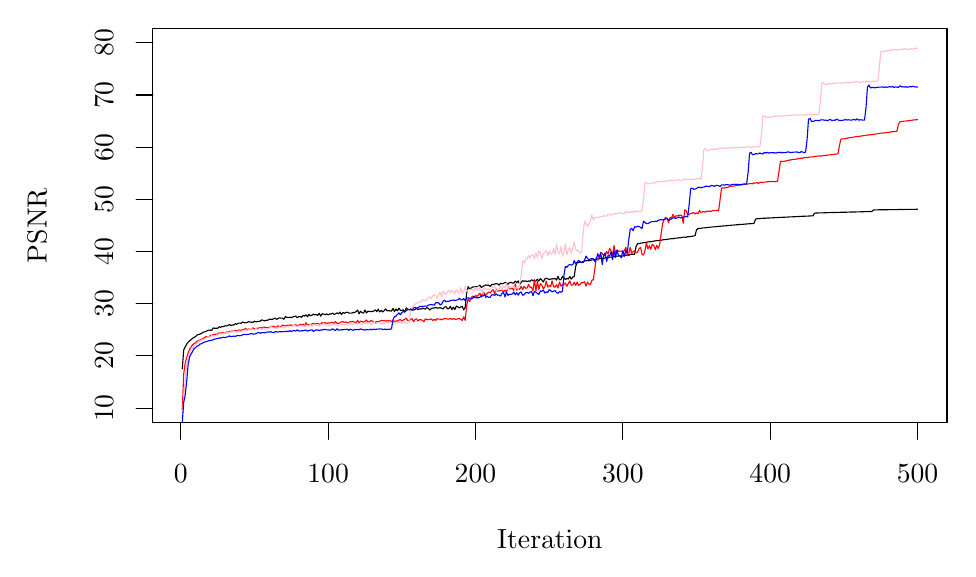
\begin{tikzpicture}[x=1pt,y=1pt]
\definecolor{fillColor}{RGB}{255,255,255}
%\path[use as bounding box,fill=fillColor,fill opacity=0.00] (0,0) rectangle (361.35,252.94);
\begin{scope}
%\path[clip] ( 49.20, 61.20) rectangle (336.15,203.75);
\definecolor{drawColor}{RGB}{0,0,0}

\path[draw=drawColor,line width= 0.4pt,line join=round,line cap=round] ( 59.83, 80.66) --
	( 60.36, 87.53) --
	( 60.89, 88.58) --
	( 61.43, 89.56) --
	( 61.96, 90.28) --
	( 62.49, 90.81) --
	( 63.02, 91.19) --
	( 63.55, 91.74) --
	( 64.09, 91.98) --
	( 64.62, 92.35) --
	( 65.15, 92.88) --
	( 65.68, 93.05) --
	( 66.22, 93.24) --
	( 66.75, 93.45) --
	( 67.28, 93.87) --
	( 67.81, 94.00) --
	( 68.35, 94.14) --
	( 68.88, 94.50) --
	( 69.41, 94.68) --
	( 69.94, 94.61) --
	( 70.48, 94.62) --
	( 71.01, 95.45) --
	( 71.54, 95.32) --
	( 72.07, 95.34) --
	( 72.61, 95.33) --
	( 73.14, 95.89) --
	( 73.67, 95.67) --
	( 74.20, 95.89) --
	( 74.74, 95.95) --
	( 75.27, 96.23) --
	( 75.80, 96.16) --
	( 76.33, 96.38) --
	( 76.87, 96.68) --
	( 77.40, 96.32) --
	( 77.93, 96.51) --
	( 78.46, 96.50) --
	( 79.00, 96.98) --
	( 79.53, 96.77) --
	( 80.06, 97.18) --
	( 80.59, 97.21) --
	( 81.13, 97.12) --
	( 81.66, 97.63) --
	( 82.19, 97.29) --
	( 82.72, 97.34) --
	( 83.26, 97.39) --
	( 83.79, 97.74) --
	( 84.32, 97.58) --
	( 84.85, 97.50) --
	( 85.39, 97.47) --
	( 85.92, 97.91) --
	( 86.45, 97.60) --
	( 86.98, 97.80) --
	( 87.52, 97.81) --
	( 88.05, 97.92) --
	( 88.58, 98.39) --
	( 89.11, 98.14) --
	( 89.65, 98.00) --
	( 90.18, 98.23) --
	( 90.71, 98.23) --
	( 91.24, 98.57) --
	( 91.78, 98.59) --
	( 92.31, 98.53) --
	( 92.84, 98.76) --
	( 93.37, 99.04) --
	( 93.90, 98.57) --
	( 94.44, 98.80) --
	( 94.97, 99.12) --
	( 95.50, 98.99) --
	( 96.03, 98.99) --
	( 96.57, 98.57) --
	( 97.10, 99.55) --
	( 97.63, 99.25) --
	( 98.16, 99.18) --
	( 98.70, 99.33) --
	( 99.23, 99.17) --
	( 99.76, 99.45) --
	(100.29, 99.53) --
	(100.83, 99.76) --
	(101.36, 99.14) --
	(101.89, 99.49) --
	(102.42, 99.61) --
	(102.96, 99.28) --
	(103.49,100.02) --
	(104.02, 99.70) --
	(104.55,100.19) --
	(105.09, 99.47) --
	(105.62,100.39) --
	(106.15, 99.83) --
	(106.68,100.05) --
	(107.22,100.47) --
	(107.75,100.16) --
	(108.28,100.34) --
	(108.81, 99.98) --
	(109.35,100.74) --
	(109.88, 99.69) --
	(110.41,100.62) --
	(110.94,100.42) --
	(111.48,100.25) --
	(112.01,100.54) --
	(112.54,100.15) --
	(113.07,100.50) --
	(113.61,100.46) --
	(114.14,100.81) --
	(114.67,100.36) --
	(115.20,100.53) --
	(115.74,100.88) --
	(116.27,100.54) --
	(116.80,101.16) --
	(117.33,100.30) --
	(117.87,101.01) --
	(118.40,100.74) --
	(118.93,101.04) --
	(119.46,101.13) --
	(120.00,100.84) --
	(120.53,100.81) --
	(121.06,100.78) --
	(121.59,101.01) --
	(122.12,101.02) --
	(122.66,101.38) --
	(123.19,101.90) --
	(123.72,100.54) --
	(124.25,101.50) --
	(124.79,100.94) --
	(125.32,100.82) --
	(125.85,101.93) --
	(126.38,100.85) --
	(126.92,101.55) --
	(127.45,101.34) --
	(127.98,101.39) --
	(128.51,101.37) --
	(129.05,101.55) --
	(129.58,101.98) --
	(130.11,101.35) --
	(130.64,102.26) --
	(131.18,101.22) --
	(131.71,101.80) --
	(132.24,101.20) --
	(132.77,101.66) --
	(133.31,102.32) --
	(133.84,101.63) --
	(134.37,101.69) --
	(134.90,101.64) --
	(135.44,101.52) --
	(135.97,102.54) --
	(136.50,101.35) --
	(137.03,102.28) --
	(137.57,101.65) --
	(138.10,102.62) --
	(138.63,101.80) --
	(139.16,101.76) --
	(139.70,102.03) --
	(140.23,101.12) --
	(140.76,102.74) --
	(141.29,102.10) --
	(141.83,102.03) --
	(142.36,102.35) --
	(142.89,101.88) --
	(143.42,101.93) --
	(143.96,102.14) --
	(144.49,102.58) --
	(145.02,102.11) --
	(145.55,102.33) --
	(146.09,102.27) --
	(146.62,102.57) --
	(147.15,102.41) --
	(147.68,102.27) --
	(148.22,102.86) --
	(148.75,102.49) --
	(149.28,101.92) --
	(149.81,102.46) --
	(150.34,102.64) --
	(150.88,102.62) --
	(151.41,102.88) --
	(151.94,102.62) --
	(152.47,102.66) --
	(153.01,102.78) --
	(153.54,102.56) --
	(154.07,102.31) --
	(154.60,102.97) --
	(155.14,103.13) --
	(155.67,102.32) --
	(156.20,102.50) --
	(156.73,103.25) --
	(157.27,102.09) --
	(157.80,102.95) --
	(158.33,102.10) --
	(158.86,103.37) --
	(159.40,103.02) --
	(159.93,102.72) --
	(160.46,103.06) --
	(160.99,103.24) --
	(161.53,101.98) --
	(162.06,102.87) --
	(162.59,107.96) --
	(163.12,110.34) --
	(163.66,109.63) --
	(164.19,109.78) --
	(164.72,110.24) --
	(165.25,110.30) --
	(165.79,110.28) --
	(166.32,110.44) --
	(166.85,110.50) --
	(167.38,110.91) --
	(167.92,110.01) --
	(168.45,110.47) --
	(168.98,110.69) --
	(169.51,110.99) --
	(170.05,110.86) --
	(170.58,110.86) --
	(171.11,110.45) --
	(171.64,111.13) --
	(172.18,111.14) --
	(172.71,111.31) --
	(173.24,111.47) --
	(173.77,111.36) --
	(174.31,110.94) --
	(174.84,111.63) --
	(175.37,111.38) --
	(175.90,111.54) --
	(176.44,111.89) --
	(176.97,111.79) --
	(177.50,111.18) --
	(178.03,111.88) --
	(178.56,111.89) --
	(179.10,111.68) --
	(179.63,111.68) --
	(180.16,112.37) --
	(180.69,111.79) --
	(181.23,112.43) --
	(181.76,111.16) --
	(182.29,111.91) --
	(182.82,112.52) --
	(183.36,112.30) --
	(183.89,112.45) --
	(184.42,112.17) --
	(184.95,112.45) --
	(185.49,112.26) --
	(186.02,112.83) --
	(186.55,112.63) --
	(187.08,112.28) --
	(187.62,112.44) --
	(188.15,113.07) --
	(188.68,112.35) --
	(189.21,113.26) --
	(189.75,112.82) --
	(190.28,112.03) --
	(190.81,113.11) --
	(191.34,113.45) --
	(191.88,113.17) --
	(192.41,113.02) --
	(192.94,113.05) --
	(193.47,113.27) --
	(194.01,113.14) --
	(194.54,113.35) --
	(195.07,112.73) --
	(195.60,114.09) --
	(196.14,112.81) --
	(196.67,112.95) --
	(197.20,114.05) --
	(197.73,113.54) --
	(198.27,112.93) --
	(198.80,113.37) --
	(199.33,113.10) --
	(199.86,114.05) --
	(200.40,113.07) --
	(200.93,113.84) --
	(201.46,114.03) --
	(201.99,117.71) --
	(202.53,119.00) --
	(203.06,119.08) --
	(203.59,119.24) --
	(204.12,119.21) --
	(204.66,119.43) --
	(205.19,119.64) --
	(205.72,119.73) --
	(206.25,119.77) --
	(206.79,119.71) --
	(207.32,119.85) --
	(207.85,120.02) --
	(208.38,120.03) --
	(208.91,120.22) --
	(209.45,120.30) --
	(209.98,120.29) --
	(210.51,120.44) --
	(211.04,120.55) --
	(211.58,120.63) --
	(212.11,120.57) --
	(212.64,120.80) --
	(213.17,120.84) --
	(213.71,120.77) --
	(214.24,121.06) --
	(214.77,121.04) --
	(215.30,121.01) --
	(215.84,121.27) --
	(216.37,121.23) --
	(216.90,121.42) --
	(217.43,121.37) --
	(217.97,121.53) --
	(218.50,121.39) --
	(219.03,121.38) --
	(219.56,121.78) --
	(220.10,121.70) --
	(220.63,121.76) --
	(221.16,121.72) --
	(221.69,121.93) --
	(222.23,122.12) --
	(222.76,122.06) --
	(223.29,122.02) --
	(223.82,124.93) --
	(224.36,125.87) --
	(224.89,125.94) --
	(225.42,126.06) --
	(225.95,126.11) --
	(226.49,126.27) --
	(227.02,126.30) --
	(227.55,126.34) --
	(228.08,126.54) --
	(228.62,126.59) --
	(229.15,126.61) --
	(229.68,126.72) --
	(230.21,126.83) --
	(230.75,126.91) --
	(231.28,127.03) --
	(231.81,126.99) --
	(232.34,127.14) --
	(232.88,127.13) --
	(233.41,127.28) --
	(233.94,127.33) --
	(234.47,127.41) --
	(235.01,127.48) --
	(235.54,127.54) --
	(236.07,127.59) --
	(236.60,127.73) --
	(237.13,127.69) --
	(237.67,127.82) --
	(238.20,127.92) --
	(238.73,127.90) --
	(239.26,128.07) --
	(239.80,128.05) --
	(240.33,128.15) --
	(240.86,128.21) --
	(241.39,128.27) --
	(241.93,128.17) --
	(242.46,128.45) --
	(242.99,128.41) --
	(243.52,128.55) --
	(244.06,128.55) --
	(244.59,128.71) --
	(245.12,128.75) --
	(245.65,130.88) --
	(246.19,131.37) --
	(246.72,131.42) --
	(247.25,131.46) --
	(247.78,131.58) --
	(248.32,131.60) --
	(248.85,131.65) --
	(249.38,131.72) --
	(249.91,131.78) --
	(250.45,131.85) --
	(250.98,131.87) --
	(251.51,131.96) --
	(252.04,131.96) --
	(252.58,132.06) --
	(253.11,132.08) --
	(253.64,132.14) --
	(254.17,132.19) --
	(254.71,132.24) --
	(255.24,132.28) --
	(255.77,132.31) --
	(256.30,132.35) --
	(256.84,132.43) --
	(257.37,132.51) --
	(257.90,132.52) --
	(258.43,132.59) --
	(258.97,132.60) --
	(259.50,132.66) --
	(260.03,132.72) --
	(260.56,132.72) --
	(261.10,132.86) --
	(261.63,132.83) --
	(262.16,132.87) --
	(262.69,132.91) --
	(263.23,132.98) --
	(263.76,133.02) --
	(264.29,133.06) --
	(264.82,133.10) --
	(265.35,133.12) --
	(265.89,133.16) --
	(266.42,133.23) --
	(266.95,134.69) --
	(267.48,134.93) --
	(268.02,134.93) --
	(268.55,135.00) --
	(269.08,135.01) --
	(269.61,135.07) --
	(270.15,135.09) --
	(270.68,135.10) --
	(271.21,135.16) --
	(271.74,135.17) --
	(272.28,135.20) --
	(272.81,135.22) --
	(273.34,135.25) --
	(273.87,135.30) --
	(274.41,135.31) --
	(274.94,135.33) --
	(275.47,135.38) --
	(276.00,135.40) --
	(276.54,135.42) --
	(277.07,135.44) --
	(277.60,135.46) --
	(278.13,135.49) --
	(278.67,135.52) --
	(279.20,135.56) --
	(279.73,135.57) --
	(280.26,135.60) --
	(280.80,135.63) --
	(281.33,135.66) --
	(281.86,135.67) --
	(282.39,135.70) --
	(282.93,135.73) --
	(283.46,135.76) --
	(283.99,135.80) --
	(284.52,135.80) --
	(285.06,135.84) --
	(285.59,135.86) --
	(286.12,135.88) --
	(286.65,135.91) --
	(287.19,135.96) --
	(287.72,135.94) --
	(288.25,136.87) --
	(288.78,136.97) --
	(289.32,136.98) --
	(289.85,137.01) --
	(290.38,137.02) --
	(290.91,137.04) --
	(291.45,137.04) --
	(291.98,137.08) --
	(292.51,137.08) --
	(293.04,137.10) --
	(293.57,137.11) --
	(294.11,137.14) --
	(294.64,137.15) --
	(295.17,137.17) --
	(295.70,137.17) --
	(296.24,137.18) --
	(296.77,137.21) --
	(297.30,137.21) --
	(297.83,137.25) --
	(298.37,137.24) --
	(298.90,137.27) --
	(299.43,137.27) --
	(299.96,137.27) --
	(300.50,137.30) --
	(301.03,137.32) --
	(301.56,137.33) --
	(302.09,137.35) --
	(302.63,137.35) --
	(303.16,137.36) --
	(303.69,137.39) --
	(304.22,137.39) --
	(304.76,137.40) --
	(305.29,137.44) --
	(305.82,137.43) --
	(306.35,137.46) --
	(306.89,137.47) --
	(307.42,137.47) --
	(307.95,137.50) --
	(308.48,137.51) --
	(309.02,137.51) --
	(309.55,138.06) --
	(310.08,138.10) --
	(310.61,138.12) --
	(311.15,138.12) --
	(311.68,138.14) --
	(312.21,138.14) --
	(312.74,138.15) --
	(313.28,138.16) --
	(313.81,138.16) --
	(314.34,138.17) --
	(314.87,138.17) --
	(315.41,138.19) --
	(315.94,138.19) --
	(316.47,138.19) --
	(317.00,138.22) --
	(317.54,138.21) --
	(318.07,138.22) --
	(318.60,138.23) --
	(319.13,138.24) --
	(319.67,138.24) --
	(320.20,138.25) --
	(320.73,138.26) --
	(321.26,138.27) --
	(321.80,138.27) --
	(322.33,138.29) --
	(322.86,138.29) --
	(323.39,138.29) --
	(323.92,138.29) --
	(324.46,138.31) --
	(324.99,138.32) --
	(325.52,138.32);
\end{scope}
\begin{scope}
%\path[clip] (  0.00,  0.00) rectangle (361.35,252.94);
\definecolor{drawColor}{RGB}{0,0,0}

\path[draw=drawColor,line width= 0.4pt,line join=round,line cap=round] ( 59.30, 61.20) -- (325.52, 61.20);

\path[draw=drawColor,line width= 0.4pt,line join=round,line cap=round] ( 59.30, 61.20) -- ( 59.30, 55.20);

\path[draw=drawColor,line width= 0.4pt,line join=round,line cap=round] (112.54, 61.20) -- (112.54, 55.20);

\path[draw=drawColor,line width= 0.4pt,line join=round,line cap=round] (165.79, 61.20) -- (165.79, 55.20);

\path[draw=drawColor,line width= 0.4pt,line join=round,line cap=round] (219.03, 61.20) -- (219.03, 55.20);

\path[draw=drawColor,line width= 0.4pt,line join=round,line cap=round] (272.28, 61.20) -- (272.28, 55.20);

\path[draw=drawColor,line width= 0.4pt,line join=round,line cap=round] (325.52, 61.20) -- (325.52, 55.20);

\node[text=drawColor,anchor=base,inner sep=0pt, outer sep=0pt, scale=  1.00] at ( 59.30, 39.60) {0};

\node[text=drawColor,anchor=base,inner sep=0pt, outer sep=0pt, scale=  1.00] at (112.54, 39.60) {100};

\node[text=drawColor,anchor=base,inner sep=0pt, outer sep=0pt, scale=  1.00] at (165.79, 39.60) {200};

\node[text=drawColor,anchor=base,inner sep=0pt, outer sep=0pt, scale=  1.00] at (219.03, 39.60) {300};

\node[text=drawColor,anchor=base,inner sep=0pt, outer sep=0pt, scale=  1.00] at (272.28, 39.60) {400};

\node[text=drawColor,anchor=base,inner sep=0pt, outer sep=0pt, scale=  1.00] at (325.52, 39.60) {500};

\path[draw=drawColor,line width= 0.4pt,line join=round,line cap=round] ( 49.20, 66.48) -- ( 49.20,198.47);

\path[draw=drawColor,line width= 0.4pt,line join=round,line cap=round] ( 49.20, 66.48) -- ( 43.20, 66.48);

\path[draw=drawColor,line width= 0.4pt,line join=round,line cap=round] ( 49.20, 85.33) -- ( 43.20, 85.33);

\path[draw=drawColor,line width= 0.4pt,line join=round,line cap=round] ( 49.20,104.19) -- ( 43.20,104.19);

\path[draw=drawColor,line width= 0.4pt,line join=round,line cap=round] ( 49.20,123.04) -- ( 43.20,123.04);

\path[draw=drawColor,line width= 0.4pt,line join=round,line cap=round] ( 49.20,141.90) -- ( 43.20,141.90);

\path[draw=drawColor,line width= 0.4pt,line join=round,line cap=round] ( 49.20,160.76) -- ( 43.20,160.76);

\path[draw=drawColor,line width= 0.4pt,line join=round,line cap=round] ( 49.20,179.61) -- ( 43.20,179.61);

\path[draw=drawColor,line width= 0.4pt,line join=round,line cap=round] ( 49.20,198.47) -- ( 43.20,198.47);

\node[text=drawColor,rotate= 90.00,anchor=base,inner sep=0pt, outer sep=0pt, scale=  1.00] at ( 34.80, 66.48) {10};

\node[text=drawColor,rotate= 90.00,anchor=base,inner sep=0pt, outer sep=0pt, scale=  1.00] at ( 34.80, 85.33) {20};

\node[text=drawColor,rotate= 90.00,anchor=base,inner sep=0pt, outer sep=0pt, scale=  1.00] at ( 34.80,104.19) {30};

\node[text=drawColor,rotate= 90.00,anchor=base,inner sep=0pt, outer sep=0pt, scale=  1.00] at ( 34.80,123.04) {40};

\node[text=drawColor,rotate= 90.00,anchor=base,inner sep=0pt, outer sep=0pt, scale=  1.00] at ( 34.80,141.90) {50};

\node[text=drawColor,rotate= 90.00,anchor=base,inner sep=0pt, outer sep=0pt, scale=  1.00] at ( 34.80,160.76) {60};

\node[text=drawColor,rotate= 90.00,anchor=base,inner sep=0pt, outer sep=0pt, scale=  1.00] at ( 34.80,179.61) {70};

\node[text=drawColor,rotate= 90.00,anchor=base,inner sep=0pt, outer sep=0pt, scale=  1.00] at ( 34.80,198.47) {80};

\path[draw=drawColor,line width= 0.4pt,line join=round,line cap=round] ( 49.20, 61.20) --
	(336.15, 61.20) --
	(336.15,203.75) --
	( 49.20,203.75) --
	( 49.20, 61.20);
\end{scope}
\begin{scope}
%\path[clip] (  0.00,  0.00) rectangle (361.35,252.94);
\definecolor{drawColor}{RGB}{0,0,0}

\node[text=drawColor,anchor=base,inner sep=0pt, outer sep=0pt, scale=  1.00] at (192.68, 15.60) {Iteration};

\node[text=drawColor,rotate= 90.00,anchor=base,inner sep=0pt, outer sep=0pt, scale=  1.00] at ( 10.80,132.47) {PSNR};
\end{scope}
\begin{scope}
%\path[clip] ( 49.20, 61.20) rectangle (336.15,203.75);
\definecolor{drawColor}{RGB}{255,0,0}

\path[draw=drawColor,line width= 0.4pt,line join=round,line cap=round] ( 59.83, 66.07) --
	( 60.36, 78.97) --
	( 60.89, 82.75) --
	( 61.43, 84.83) --
	( 61.96, 86.43) --
	( 62.49, 87.73) --
	( 63.02, 88.58) --
	( 63.55, 89.33) --
	( 64.09, 89.77) --
	( 64.62, 90.02) --
	( 65.15, 90.53) --
	( 65.68, 90.91) --
	( 66.22, 91.03) --
	( 66.75, 91.40) --
	( 67.28, 91.52) --
	( 67.81, 91.92) --
	( 68.35, 92.31) --
	( 68.88, 92.17) --
	( 69.41, 92.24) --
	( 69.94, 92.68) --
	( 70.48, 92.85) --
	( 71.01, 92.98) --
	( 71.54, 93.15) --
	( 72.07, 93.18) --
	( 72.61, 93.27) --
	( 73.14, 93.62) --
	( 73.67, 93.61) --
	( 74.20, 93.70) --
	( 74.74, 93.78) --
	( 75.27, 93.59) --
	( 75.80, 93.98) --
	( 76.33, 93.91) --
	( 76.87, 94.13) --
	( 77.40, 94.21) --
	( 77.93, 94.33) --
	( 78.46, 94.21) --
	( 79.00, 94.55) --
	( 79.53, 94.31) --
	( 80.06, 94.67) --
	( 80.59, 94.69) --
	( 81.13, 94.59) --
	( 81.66, 94.85) --
	( 82.19, 94.92) --
	( 82.72, 95.32) --
	( 83.26, 94.76) --
	( 83.79, 95.14) --
	( 84.32, 94.80) --
	( 84.85, 95.08) --
	( 85.39, 95.46) --
	( 85.92, 95.16) --
	( 86.45, 95.22) --
	( 86.98, 95.34) --
	( 87.52, 95.41) --
	( 88.05, 95.62) --
	( 88.58, 95.35) --
	( 89.11, 95.74) --
	( 89.65, 95.67) --
	( 90.18, 95.60) --
	( 90.71, 95.54) --
	( 91.24, 95.48) --
	( 91.78, 96.09) --
	( 92.31, 95.82) --
	( 92.84, 96.11) --
	( 93.37, 95.67) --
	( 93.90, 95.86) --
	( 94.44, 96.25) --
	( 94.97, 95.92) --
	( 95.50, 95.90) --
	( 96.03, 96.51) --
	( 96.57, 96.27) --
	( 97.10, 96.16) --
	( 97.63, 96.38) --
	( 98.16, 96.49) --
	( 98.70, 96.39) --
	( 99.23, 96.57) --
	( 99.76, 96.26) --
	(100.29, 96.41) --
	(100.83, 96.60) --
	(101.36, 96.27) --
	(101.89, 96.43) --
	(102.42, 96.74) --
	(102.96, 96.60) --
	(103.49, 96.82) --
	(104.02, 96.01) --
	(104.55, 97.32) --
	(105.09, 96.52) --
	(105.62, 96.70) --
	(106.15, 96.59) --
	(106.68, 96.88) --
	(107.22, 97.07) --
	(107.75, 96.84) --
	(108.28, 97.01) --
	(108.81, 97.09) --
	(109.35, 96.81) --
	(109.88, 96.85) --
	(110.41, 97.45) --
	(110.94, 97.05) --
	(111.48, 97.45) --
	(112.01, 97.02) --
	(112.54, 97.27) --
	(113.07, 97.20) --
	(113.61, 97.40) --
	(114.14, 97.51) --
	(114.67, 97.09) --
	(115.20, 97.73) --
	(115.74, 97.14) --
	(116.27, 97.15) --
	(116.80, 97.30) --
	(117.33, 97.63) --
	(117.87, 97.72) --
	(118.40, 97.47) --
	(118.93, 97.59) --
	(119.46, 97.36) --
	(120.00, 97.24) --
	(120.53, 97.82) --
	(121.06, 97.68) --
	(121.59, 97.74) --
	(122.12, 97.54) --
	(122.66, 97.40) --
	(123.19, 98.19) --
	(123.72, 97.30) --
	(124.25, 97.87) --
	(124.79, 97.83) --
	(125.32, 97.59) --
	(125.85, 97.81) --
	(126.38, 98.32) --
	(126.92, 97.60) --
	(127.45, 97.57) --
	(127.98, 98.11) --
	(128.51, 97.95) --
	(129.05, 97.43) --
	(129.58, 97.46) --
	(130.11, 97.76) --
	(130.64, 97.73) --
	(131.18, 97.86) --
	(131.71, 98.16) --
	(132.24, 98.07) --
	(132.77, 98.16) --
	(133.31, 97.94) --
	(133.84, 98.11) --
	(134.37, 97.96) --
	(134.90, 98.18) --
	(135.44, 97.73) --
	(135.97, 98.11) --
	(136.50, 97.78) --
	(137.03, 97.97) --
	(137.57, 97.93) --
	(138.10, 98.32) --
	(138.63, 98.45) --
	(139.16, 97.99) --
	(139.70, 98.32) --
	(140.23, 98.59) --
	(140.76, 99.02) --
	(141.29, 98.15) --
	(141.83, 98.21) --
	(142.36, 98.45) --
	(142.89, 98.82) --
	(143.42, 97.73) --
	(143.96, 98.52) --
	(144.49, 98.75) --
	(145.02, 97.95) --
	(145.55, 98.43) --
	(146.09, 98.40) --
	(146.62, 98.18) --
	(147.15, 97.72) --
	(147.68, 98.70) --
	(148.22, 98.47) --
	(148.75, 98.49) --
	(149.28, 98.49) --
	(149.81, 98.74) --
	(150.34, 98.09) --
	(150.88, 98.56) --
	(151.41, 98.18) --
	(151.94, 98.80) --
	(152.47, 98.61) --
	(153.01, 98.67) --
	(153.54, 98.34) --
	(154.07, 98.65) --
	(154.60, 98.87) --
	(155.14, 98.76) --
	(155.67, 98.68) --
	(156.20, 98.64) --
	(156.73, 98.86) --
	(157.27, 98.56) --
	(157.80, 98.85) --
	(158.33, 98.57) --
	(158.86, 98.60) --
	(159.40, 98.76) --
	(159.93, 98.91) --
	(160.46, 98.53) --
	(160.99, 98.17) --
	(161.53, 99.46) --
	(162.06, 98.17) --
	(162.59,103.61) --
	(163.12,105.96) --
	(163.66,104.97) --
	(164.19,106.27) --
	(164.72,106.96) --
	(165.25,106.39) --
	(165.79,107.15) --
	(166.32,106.86) --
	(166.85,107.42) --
	(167.38,108.01) --
	(167.92,106.61) --
	(168.45,108.41) --
	(168.98,108.04) --
	(169.51,107.11) --
	(170.05,107.99) --
	(170.58,108.45) --
	(171.11,108.08) --
	(171.64,108.83) --
	(172.18,109.28) --
	(172.71,107.83) --
	(173.24,109.49) --
	(173.77,108.73) --
	(174.31,108.88) --
	(174.84,108.95) --
	(175.37,109.09) --
	(175.90,108.50) --
	(176.44,109.12) --
	(176.97,108.31) --
	(177.50,110.30) --
	(178.03,109.54) --
	(178.56,109.58) --
	(179.10,109.84) --
	(179.63,108.97) --
	(180.16,111.31) --
	(180.69,109.11) --
	(181.23,109.87) --
	(181.76,109.32) --
	(182.29,110.52) --
	(182.82,109.30) --
	(183.36,110.52) --
	(183.89,109.76) --
	(184.42,109.90) --
	(184.95,111.16) --
	(185.49,110.14) --
	(186.02,110.18) --
	(186.55,108.79) --
	(187.08,112.93) --
	(187.62,108.84) --
	(188.15,112.28) --
	(188.68,109.33) --
	(189.21,111.42) --
	(189.75,110.95) --
	(190.28,109.61) --
	(190.81,110.15) --
	(191.34,112.38) --
	(191.88,110.20) --
	(192.41,110.83) --
	(192.94,110.35) --
	(193.47,112.48) --
	(194.01,110.26) --
	(194.54,110.20) --
	(195.07,111.07) --
	(195.60,109.92) --
	(196.14,112.02) --
	(196.67,110.55) --
	(197.20,111.00) --
	(197.73,111.22) --
	(198.27,111.68) --
	(198.80,110.48) --
	(199.33,111.53) --
	(199.86,112.45) --
	(200.40,110.89) --
	(200.93,110.92) --
	(201.46,111.94) --
	(201.99,110.78) --
	(202.53,112.04) --
	(203.06,110.82) --
	(203.59,111.29) --
	(204.12,111.79) --
	(204.66,111.81) --
	(205.19,112.16) --
	(205.72,110.57) --
	(206.25,111.99) --
	(206.79,111.31) --
	(207.32,111.10) --
	(207.85,112.73) --
	(208.38,112.84) --
	(208.91,116.93) --
	(209.45,120.93) --
	(209.98,120.01) --
	(210.51,120.57) --
	(211.04,122.76) --
	(211.58,122.39) --
	(212.11,121.56) --
	(212.64,121.69) --
	(213.17,123.08) --
	(213.71,122.13) --
	(214.24,124.22) --
	(214.77,123.30) --
	(215.30,121.60) --
	(215.84,125.21) --
	(216.37,122.43) --
	(216.90,123.66) --
	(217.43,123.10) --
	(217.97,123.25) --
	(218.50,123.15) --
	(219.03,122.78) --
	(219.56,123.35) --
	(220.10,124.64) --
	(220.63,121.62) --
	(221.16,122.28) --
	(221.69,124.56) --
	(222.23,122.41) --
	(222.76,123.00) --
	(223.29,123.32) --
	(223.82,122.69) --
	(224.36,122.87) --
	(224.89,124.03) --
	(225.42,124.54) --
	(225.95,122.09) --
	(226.49,121.73) --
	(227.02,123.41) --
	(227.55,126.23) --
	(228.08,123.98) --
	(228.62,125.18) --
	(229.15,123.88) --
	(229.68,125.70) --
	(230.21,125.20) --
	(230.75,123.70) --
	(231.28,125.29) --
	(231.81,124.20) --
	(232.34,125.63) --
	(232.88,129.64) --
	(233.41,133.17) --
	(233.94,134.46) --
	(234.47,135.41) --
	(235.01,135.03) --
	(235.54,133.43) --
	(236.07,135.35) --
	(236.60,135.16) --
	(237.13,136.47) --
	(237.67,135.22) --
	(238.20,135.97) --
	(238.73,135.95) --
	(239.26,136.15) --
	(239.80,136.19) --
	(240.33,136.11) --
	(240.86,133.26) --
	(241.39,138.12) --
	(241.93,137.77) --
	(242.46,136.47) --
	(242.99,136.40) --
	(243.52,136.83) --
	(244.06,136.82) --
	(244.59,137.21) --
	(245.12,136.64) --
	(245.65,137.06) --
	(246.19,136.68) --
	(246.72,137.85) --
	(247.25,137.21) --
	(247.78,137.42) --
	(248.32,137.48) --
	(248.85,137.28) --
	(249.38,137.68) --
	(249.91,137.51) --
	(250.45,137.74) --
	(250.98,137.53) --
	(251.51,137.88) --
	(252.04,137.82) --
	(252.58,137.83) --
	(253.11,138.00) --
	(253.64,137.75) --
	(254.17,141.91) --
	(254.71,145.99) --
	(255.24,146.05) --
	(255.77,146.00) --
	(256.30,146.17) --
	(256.84,146.24) --
	(257.37,146.43) --
	(257.90,146.69) --
	(258.43,146.66) --
	(258.97,146.67) --
	(259.50,146.77) --
	(260.03,146.95) --
	(260.56,146.94) --
	(261.10,147.18) --
	(261.63,147.03) --
	(262.16,147.20) --
	(262.69,147.41) --
	(263.23,147.34) --
	(263.76,147.42) --
	(264.29,147.45) --
	(264.82,147.61) --
	(265.35,147.62) --
	(265.89,147.53) --
	(266.42,147.85) --
	(266.95,147.81) --
	(267.48,147.99) --
	(268.02,147.63) --
	(268.55,148.02) --
	(269.08,148.13) --
	(269.61,147.92) --
	(270.15,148.16) --
	(270.68,148.15) --
	(271.21,148.29) --
	(271.74,148.29) --
	(272.28,148.37) --
	(272.81,148.31) --
	(273.34,148.40) --
	(273.87,148.27) --
	(274.41,148.42) --
	(274.94,148.47) --
	(275.47,152.21) --
	(276.00,155.66) --
	(276.54,155.62) --
	(277.07,155.60) --
	(277.60,155.67) --
	(278.13,155.92) --
	(278.67,155.94) --
	(279.20,156.11) --
	(279.73,156.14) --
	(280.26,156.33) --
	(280.80,156.36) --
	(281.33,156.34) --
	(281.86,156.49) --
	(282.39,156.58) --
	(282.93,156.73) --
	(283.46,156.78) --
	(283.99,156.75) --
	(284.52,156.97) --
	(285.06,157.01) --
	(285.59,157.04) --
	(286.12,157.04) --
	(286.65,157.23) --
	(287.19,157.26) --
	(287.72,157.27) --
	(288.25,157.36) --
	(288.78,157.49) --
	(289.32,157.53) --
	(289.85,157.57) --
	(290.38,157.58) --
	(290.91,157.59) --
	(291.45,157.79) --
	(291.98,157.81) --
	(292.51,157.82) --
	(293.04,157.92) --
	(293.57,157.98) --
	(294.11,158.01) --
	(294.64,158.06) --
	(295.17,158.16) --
	(295.70,158.21) --
	(296.24,158.31) --
	(296.77,158.35) --
	(297.30,161.37) --
	(297.83,163.68) --
	(298.37,163.75) --
	(298.90,163.80) --
	(299.43,163.92) --
	(299.96,163.96) --
	(300.50,164.12) --
	(301.03,164.21) --
	(301.56,164.31) --
	(302.09,164.35) --
	(302.63,164.43) --
	(303.16,164.54) --
	(303.69,164.61) --
	(304.22,164.61) --
	(304.76,164.76) --
	(305.29,164.81) --
	(305.82,164.89) --
	(306.35,164.96) --
	(306.89,165.09) --
	(307.42,165.15) --
	(307.95,165.16) --
	(308.48,165.24) --
	(309.02,165.35) --
	(309.55,165.38) --
	(310.08,165.44) --
	(310.61,165.59) --
	(311.15,165.58) --
	(311.68,165.73) --
	(312.21,165.82) --
	(312.74,165.83) --
	(313.28,165.90) --
	(313.81,165.93) --
	(314.34,166.08) --
	(314.87,166.11) --
	(315.41,166.16) --
	(315.94,166.34) --
	(316.47,166.33) --
	(317.00,166.44) --
	(317.54,166.45) --
	(318.07,166.55) --
	(318.60,168.91) --
	(319.13,169.94) --
	(319.67,170.02) --
	(320.20,170.08) --
	(320.73,170.18) --
	(321.26,170.21) --
	(321.80,170.28) --
	(322.33,170.38) --
	(322.86,170.43) --
	(323.39,170.47) --
	(323.92,170.58) --
	(324.46,170.66) --
	(324.99,170.65) --
	(325.52,170.75);
\definecolor{drawColor}{RGB}{255,192,203}

\path[draw=drawColor,line width= 0.4pt,line join=round,line cap=round] ( 59.83, 62.54) --
	( 60.36, 70.73) --
	( 60.89, 76.79) --
	( 61.43, 82.21) --
	( 61.96, 85.16) --
	( 62.49, 86.58) --
	( 63.02, 87.48) --
	( 63.55, 88.25) --
	( 64.09, 88.99) --
	( 64.62, 89.59) --
	( 65.15, 89.93) --
	( 65.68, 90.52) --
	( 66.22, 90.77) --
	( 66.75, 91.12) --
	( 67.28, 91.27) --
	( 67.81, 91.46) --
	( 68.35, 91.64) --
	( 68.88, 92.08) --
	( 69.41, 92.21) --
	( 69.94, 92.19) --
	( 70.48, 92.65) --
	( 71.01, 92.51) --
	( 71.54, 92.63) --
	( 72.07, 92.80) --
	( 72.61, 92.97) --
	( 73.14, 93.33) --
	( 73.67, 93.23) --
	( 74.20, 93.42) --
	( 74.74, 93.58) --
	( 75.27, 93.63) --
	( 75.80, 93.72) --
	( 76.33, 93.59) --
	( 76.87, 93.88) --
	( 77.40, 94.02) --
	( 77.93, 94.00) --
	( 78.46, 94.17) --
	( 79.00, 94.02) --
	( 79.53, 94.00) --
	( 80.06, 94.31) --
	( 80.59, 94.20) --
	( 81.13, 94.25) --
	( 81.66, 94.35) --
	( 82.19, 94.61) --
	( 82.72, 94.72) --
	( 83.26, 94.48) --
	( 83.79, 94.90) --
	( 84.32, 94.62) --
	( 84.85, 95.27) --
	( 85.39, 94.73) --
	( 85.92, 94.65) --
	( 86.45, 95.30) --
	( 86.98, 94.66) --
	( 87.52, 95.07) --
	( 88.05, 95.32) --
	( 88.58, 94.75) --
	( 89.11, 95.40) --
	( 89.65, 94.84) --
	( 90.18, 95.15) --
	( 90.71, 95.11) --
	( 91.24, 95.33) --
	( 91.78, 95.93) --
	( 92.31, 95.66) --
	( 92.84, 95.51) --
	( 93.37, 95.42) --
	( 93.90, 95.32) --
	( 94.44, 95.55) --
	( 94.97, 95.81) --
	( 95.50, 95.63) --
	( 96.03, 95.92) --
	( 96.57, 95.34) --
	( 97.10, 95.82) --
	( 97.63, 95.87) --
	( 98.16, 95.74) --
	( 98.70, 95.99) --
	( 99.23, 95.99) --
	( 99.76, 96.12) --
	(100.29, 96.41) --
	(100.83, 96.05) --
	(101.36, 96.02) --
	(101.89, 96.13) --
	(102.42, 96.35) --
	(102.96, 96.20) --
	(103.49, 96.27) --
	(104.02, 96.06) --
	(104.55, 96.31) --
	(105.09, 96.38) --
	(105.62, 96.01) --
	(106.15, 96.81) --
	(106.68, 95.96) --
	(107.22, 96.50) --
	(107.75, 96.66) --
	(108.28, 96.16) --
	(108.81, 96.37) --
	(109.35, 96.00) --
	(109.88, 96.67) --
	(110.41, 96.53) --
	(110.94, 97.07) --
	(111.48, 96.49) --
	(112.01, 96.46) --
	(112.54, 96.28) --
	(113.07, 96.46) --
	(113.61, 96.36) --
	(114.14, 96.90) --
	(114.67, 96.58) --
	(115.20, 96.76) --
	(115.74, 96.16) --
	(116.27, 96.49) --
	(116.80, 96.73) --
	(117.33, 96.77) --
	(117.87, 96.56) --
	(118.40, 96.86) --
	(118.93, 96.68) --
	(119.46, 97.01) --
	(120.00, 96.91) --
	(120.53, 97.30) --
	(121.06, 96.69) --
	(121.59, 96.89) --
	(122.12, 96.95) --
	(122.66, 97.10) --
	(123.19, 96.94) --
	(123.72, 96.92) --
	(124.25, 96.80) --
	(124.79, 96.75) --
	(125.32, 96.90) --
	(125.85, 97.05) --
	(126.38, 97.40) --
	(126.92, 97.02) --
	(127.45, 97.36) --
	(127.98, 96.72) --
	(128.51, 97.03) --
	(129.05, 97.42) --
	(129.58, 97.13) --
	(130.11, 97.04) --
	(130.64, 97.18) --
	(131.18, 97.48) --
	(131.71, 96.69) --
	(132.24, 97.23) --
	(132.77, 97.28) --
	(133.31, 97.17) --
	(133.84, 97.35) --
	(134.37, 97.40) --
	(134.90, 97.30) --
	(135.44, 97.29) --
	(135.97, 97.27) --
	(136.50, 97.49) --
	(137.03, 97.12) --
	(137.57, 97.34) --
	(138.10, 97.50) --
	(138.63, 97.46) --
	(139.16, 97.05) --
	(139.70, 97.65) --
	(140.23, 97.41) --
	(140.76, 97.01) --
	(141.29, 97.16) --
	(141.83, 97.57) --
	(142.36,101.98) --
	(142.89,103.13) --
	(143.42,103.40) --
	(143.96,104.04) --
	(144.49,104.42) --
	(145.02,104.68) --
	(145.55,104.82) --
	(146.09,104.73) --
	(146.62,105.78) --
	(147.15,105.26) --
	(147.68,105.36) --
	(148.22,105.59) --
	(148.75,106.53) --
	(149.28,106.71) --
	(149.81,105.95) --
	(150.34,107.05) --
	(150.88,107.46) --
	(151.41,107.18) --
	(151.94,106.14) --
	(152.47,107.57) --
	(153.01,108.35) --
	(153.54,106.70) --
	(154.07,108.77) --
	(154.60,107.90) --
	(155.14,107.37) --
	(155.67,108.69) --
	(156.20,109.02) --
	(156.73,108.11) --
	(157.27,109.09) --
	(157.80,108.60) --
	(158.33,107.95) --
	(158.86,109.34) --
	(159.40,108.43) --
	(159.93,107.97) --
	(160.46,110.03) --
	(160.99,107.94) --
	(161.53,108.80) --
	(162.06,110.42) --
	(162.59,108.59) --
	(163.12,109.16) --
	(163.66,109.15) --
	(164.19,109.50) --
	(164.72,109.28) --
	(165.25,108.87) --
	(165.79,109.99) --
	(166.32,109.00) --
	(166.85,110.49) --
	(167.38,108.85) --
	(167.92,109.53) --
	(168.45,107.93) --
	(168.98,109.96) --
	(169.51,109.45) --
	(170.05,109.42) --
	(170.58,109.56) --
	(171.11,109.42) --
	(171.64,110.15) --
	(172.18,110.13) --
	(172.71,110.83) --
	(173.24,108.65) --
	(173.77,109.25) --
	(174.31,109.31) --
	(174.84,110.61) --
	(175.37,109.16) --
	(175.90,110.59) --
	(176.44,109.93) --
	(176.97,111.69) --
	(177.50,109.34) --
	(178.03,110.35) --
	(178.56,110.03) --
	(179.10,110.56) --
	(179.63,110.60) --
	(180.16,109.36) --
	(180.69,110.38) --
	(181.23,109.39) --
	(181.76,111.54) --
	(182.29,114.40) --
	(182.82,119.70) --
	(183.36,118.89) --
	(183.89,120.26) --
	(184.42,120.38) --
	(184.95,121.69) --
	(185.49,120.63) --
	(186.02,121.75) --
	(186.55,121.86) --
	(187.08,120.33) --
	(187.62,122.59) --
	(188.15,120.91) --
	(188.68,123.27) --
	(189.21,122.46) --
	(189.75,120.43) --
	(190.28,122.12) --
	(190.81,122.85) --
	(191.34,123.39) --
	(191.88,121.59) --
	(192.41,123.33) --
	(192.94,122.11) --
	(193.47,122.41) --
	(194.01,124.15) --
	(194.54,121.96) --
	(195.07,125.60) --
	(195.60,122.73) --
	(196.14,122.33) --
	(196.67,124.78) --
	(197.20,121.34) --
	(197.73,122.60) --
	(198.27,125.75) --
	(198.80,121.89) --
	(199.33,123.55) --
	(199.86,124.49) --
	(200.40,122.51) --
	(200.93,124.15) --
	(201.46,126.49) --
	(201.99,124.01) --
	(202.53,123.14) --
	(203.06,123.36) --
	(203.59,122.46) --
	(204.12,122.85) --
	(204.66,129.20) --
	(205.19,134.05) --
	(205.72,133.35) --
	(206.25,132.06) --
	(206.79,132.84) --
	(207.32,134.17) --
	(207.85,136.32) --
	(208.38,134.47) --
	(208.91,135.35) --
	(209.45,135.41) --
	(209.98,135.38) --
	(210.51,135.59) --
	(211.04,135.64) --
	(211.58,135.70) --
	(212.11,135.99) --
	(212.64,135.86) --
	(213.17,135.86) --
	(213.71,136.61) --
	(214.24,136.20) --
	(214.77,136.31) --
	(215.30,136.47) --
	(215.84,136.71) --
	(216.37,136.75) --
	(216.90,136.77) --
	(217.43,136.76) --
	(217.97,136.98) --
	(218.50,137.01) --
	(219.03,136.70) --
	(219.56,136.80) --
	(220.10,137.55) --
	(220.63,137.11) --
	(221.16,137.39) --
	(221.69,137.14) --
	(222.23,137.51) --
	(222.76,137.22) --
	(223.29,137.67) --
	(223.82,137.41) --
	(224.36,137.79) --
	(224.89,137.43) --
	(225.42,137.50) --
	(225.95,137.77) --
	(226.49,141.93) --
	(227.02,147.90) --
	(227.55,147.99) --
	(228.08,147.46) --
	(228.62,147.65) --
	(229.15,147.82) --
	(229.68,147.89) --
	(230.21,147.76) --
	(230.75,147.87) --
	(231.28,148.24) --
	(231.81,148.47) --
	(232.34,148.28) --
	(232.88,148.32) --
	(233.41,148.35) --
	(233.94,148.55) --
	(234.47,148.37) --
	(235.01,148.64) --
	(235.54,148.53) --
	(236.07,148.90) --
	(236.60,148.81) --
	(237.13,148.70) --
	(237.67,148.80) --
	(238.20,148.87) --
	(238.73,148.83) --
	(239.26,149.05) --
	(239.80,148.71) --
	(240.33,148.81) --
	(240.86,149.19) --
	(241.39,149.17) --
	(241.93,149.04) --
	(242.46,149.11) --
	(242.99,149.23) --
	(243.52,149.18) --
	(244.06,149.03) --
	(244.59,149.19) --
	(245.12,149.25) --
	(245.65,149.37) --
	(246.19,149.41) --
	(246.72,149.40) --
	(247.25,149.14) --
	(247.78,153.53) --
	(248.32,159.89) --
	(248.85,160.27) --
	(249.38,159.62) --
	(249.91,159.46) --
	(250.45,159.81) --
	(250.98,160.02) --
	(251.51,160.04) --
	(252.04,159.84) --
	(252.58,160.16) --
	(253.11,159.93) --
	(253.64,160.43) --
	(254.17,160.34) --
	(254.71,160.36) --
	(255.24,160.51) --
	(255.77,160.25) --
	(256.30,160.40) --
	(256.84,160.48) --
	(257.37,160.65) --
	(257.90,160.45) --
	(258.43,160.48) --
	(258.97,160.61) --
	(259.50,160.73) --
	(260.03,160.56) --
	(260.56,160.48) --
	(261.10,160.77) --
	(261.63,160.69) --
	(262.16,160.54) --
	(262.69,160.84) --
	(263.23,160.66) --
	(263.76,160.81) --
	(264.29,160.95) --
	(264.82,160.87) --
	(265.35,160.57) --
	(265.89,160.84) --
	(266.42,160.92) --
	(266.95,160.83) --
	(267.48,160.85) --
	(268.02,160.96) --
	(268.55,160.92) --
	(269.08,164.96) --
	(269.61,172.11) --
	(270.15,172.09) --
	(270.68,171.42) --
	(271.21,171.75) --
	(271.74,171.60) --
	(272.28,171.53) --
	(272.81,171.88) --
	(273.34,171.99) --
	(273.87,171.88) --
	(274.41,172.02) --
	(274.94,171.96) --
	(275.47,172.01) --
	(276.00,172.19) --
	(276.54,171.91) --
	(277.07,171.98) --
	(277.60,172.10) --
	(278.13,172.21) --
	(278.67,172.17) --
	(279.20,172.30) --
	(279.73,172.11) --
	(280.26,172.42) --
	(280.80,172.41) --
	(281.33,172.30) --
	(281.86,172.37) --
	(282.39,172.40) --
	(282.93,172.41) --
	(283.46,172.34) --
	(283.99,172.47) --
	(284.52,172.28) --
	(285.06,172.43) --
	(285.59,172.63) --
	(286.12,172.62) --
	(286.65,172.51) --
	(287.19,172.45) --
	(287.72,172.63) --
	(288.25,172.63) --
	(288.78,172.75) --
	(289.32,172.54) --
	(289.85,172.58) --
	(290.38,176.83) --
	(290.91,183.76) --
	(291.45,184.10) --
	(291.98,183.45) --
	(292.51,183.31) --
	(293.04,183.72) --
	(293.57,183.85) --
	(294.11,183.56) --
	(294.64,183.75) --
	(295.17,183.65) --
	(295.70,184.03) --
	(296.24,183.99) --
	(296.77,183.88) --
	(297.30,183.97) --
	(297.83,184.03) --
	(298.37,183.82) --
	(298.90,184.14) --
	(299.43,184.13) --
	(299.96,184.13) --
	(300.50,184.16) --
	(301.03,184.04) --
	(301.56,184.16) --
	(302.09,184.35) --
	(302.63,184.21) --
	(303.16,184.48) --
	(303.69,184.42) --
	(304.22,184.39) --
	(304.76,184.00) --
	(305.29,184.27) --
	(305.82,184.54) --
	(306.35,184.23) --
	(306.89,184.61) --
	(307.42,184.50) --
	(307.95,184.46) --
	(308.48,184.36) --
	(309.02,184.48) --
	(309.55,184.73) --
	(310.08,184.37) --
	(310.61,184.67) --
	(311.15,184.72) --
	(311.68,188.95) --
	(312.21,195.17) --
	(312.74,195.42) --
	(313.28,195.27) --
	(313.81,195.45) --
	(314.34,195.50) --
	(314.87,195.82) --
	(315.41,195.73) --
	(315.94,195.80) --
	(316.47,195.66) --
	(317.00,196.07) --
	(317.54,195.96) --
	(318.07,195.89) --
	(318.60,195.91) --
	(319.13,195.99) --
	(319.67,196.01) --
	(320.20,196.16) --
	(320.73,196.38) --
	(321.26,196.22) --
	(321.80,196.17) --
	(322.33,196.05) --
	(322.86,196.52) --
	(323.39,196.16) --
	(323.92,196.21) --
	(324.46,196.57) --
	(324.99,196.45) --
	(325.52,196.55);
\definecolor{drawColor}{RGB}{0,0,255}

\path[draw=drawColor,line width= 0.4pt,line join=round,line cap=round] ( 59.83, 61.30) --
	( 60.36, 68.62) --
	( 60.89, 71.17) --
	( 61.43, 76.24) --
	( 61.96, 82.32) --
	( 62.49, 85.02) --
	( 63.02, 86.05) --
	( 63.55, 86.92) --
	( 64.09, 87.99) --
	( 64.62, 88.31) --
	( 65.15, 88.86) --
	( 65.68, 89.05) --
	( 66.22, 89.62) --
	( 66.75, 89.74) --
	( 67.28, 90.05) --
	( 67.81, 90.32) --
	( 68.35, 90.44) --
	( 68.88, 90.65) --
	( 69.41, 90.81) --
	( 69.94, 90.93) --
	( 70.48, 90.93) --
	( 71.01, 91.24) --
	( 71.54, 91.41) --
	( 72.07, 91.54) --
	( 72.61, 91.61) --
	( 73.14, 91.81) --
	( 73.67, 91.80) --
	( 74.20, 91.93) --
	( 74.74, 92.08) --
	( 75.27, 91.92) --
	( 75.80, 92.16) --
	( 76.33, 92.25) --
	( 76.87, 92.55) --
	( 77.40, 92.33) --
	( 77.93, 92.38) --
	( 78.46, 92.50) --
	( 79.00, 92.40) --
	( 79.53, 92.62) --
	( 80.06, 92.69) --
	( 80.59, 92.63) --
	( 81.13, 92.68) --
	( 81.66, 93.01) --
	( 82.19, 93.08) --
	( 82.72, 93.03) --
	( 83.26, 93.08) --
	( 83.79, 93.14) --
	( 84.32, 93.28) --
	( 84.85, 93.51) --
	( 85.39, 93.18) --
	( 85.92, 93.31) --
	( 86.45, 93.35) --
	( 86.98, 93.66) --
	( 87.52, 93.83) --
	( 88.05, 93.51) --
	( 88.58, 93.78) --
	( 89.11, 93.77) --
	( 89.65, 93.64) --
	( 90.18, 93.94) --
	( 90.71, 93.97) --
	( 91.24, 93.97) --
	( 91.78, 94.09) --
	( 92.31, 93.84) --
	( 92.84, 93.73) --
	( 93.37, 94.08) --
	( 93.90, 94.05) --
	( 94.44, 93.97) --
	( 94.97, 94.12) --
	( 95.50, 94.06) --
	( 96.03, 94.10) --
	( 96.57, 94.15) --
	( 97.10, 94.11) --
	( 97.63, 94.30) --
	( 98.16, 94.10) --
	( 98.70, 94.49) --
	( 99.23, 94.12) --
	( 99.76, 94.46) --
	(100.29, 94.47) --
	(100.83, 94.29) --
	(101.36, 94.76) --
	(101.89, 94.36) --
	(102.42, 94.30) --
	(102.96, 94.49) --
	(103.49, 94.40) --
	(104.02, 94.61) --
	(104.55, 94.62) --
	(105.09, 94.31) --
	(105.62, 94.50) --
	(106.15, 94.67) --
	(106.68, 94.77) --
	(107.22, 94.18) --
	(107.75, 94.61) --
	(108.28, 94.71) --
	(108.81, 94.71) --
	(109.35, 94.53) --
	(109.88, 94.71) --
	(110.41, 94.72) --
	(110.94, 94.88) --
	(111.48, 94.92) --
	(112.01, 94.77) --
	(112.54, 94.73) --
	(113.07, 94.66) --
	(113.61, 94.73) --
	(114.14, 95.09) --
	(114.67, 94.78) --
	(115.20, 94.53) --
	(115.74, 95.14) --
	(116.27, 94.63) --
	(116.80, 94.68) --
	(117.33, 94.81) --
	(117.87, 94.78) --
	(118.40, 94.93) --
	(118.93, 94.90) --
	(119.46, 95.00) --
	(120.00, 94.58) --
	(120.53, 95.02) --
	(121.06, 94.79) --
	(121.59, 94.59) --
	(122.12, 94.92) --
	(122.66, 94.77) --
	(123.19, 94.96) --
	(123.72, 94.79) --
	(124.25, 95.11) --
	(124.79, 94.85) --
	(125.32, 94.79) --
	(125.85, 94.64) --
	(126.38, 94.97) --
	(126.92, 94.73) --
	(127.45, 94.73) --
	(127.98, 95.02) --
	(128.51, 94.77) --
	(129.05, 95.05) --
	(129.58, 94.84) --
	(130.11, 95.05) --
	(130.64, 95.02) --
	(131.18, 95.08) --
	(131.71, 95.11) --
	(132.24, 94.87) --
	(132.77, 94.96) --
	(133.31, 94.99) --
	(133.84, 94.85) --
	(134.37, 95.01) --
	(134.90, 94.94) --
	(135.44, 95.17) --
	(135.97, 98.41) --
	(136.50, 99.53) --
	(137.03, 99.72) --
	(137.57,100.32) --
	(138.10,100.90) --
	(138.63,100.17) --
	(139.16,101.02) --
	(139.70,101.34) --
	(140.23,101.37) --
	(140.76,101.67) --
	(141.29,102.14) --
	(141.83,102.05) --
	(142.36,102.12) --
	(142.89,101.95) --
	(143.42,102.67) --
	(143.96,102.87) --
	(144.49,102.58) --
	(145.02,102.77) --
	(145.55,103.17) --
	(146.09,103.27) --
	(146.62,103.16) --
	(147.15,103.28) --
	(147.68,103.36) --
	(148.22,103.32) --
	(148.75,103.68) --
	(149.28,103.83) --
	(149.81,103.89) --
	(150.34,103.79) --
	(150.88,103.71) --
	(151.41,104.54) --
	(151.94,104.56) --
	(152.47,104.53) --
	(153.01,103.74) --
	(153.54,104.07) --
	(154.07,105.14) --
	(154.60,105.47) --
	(155.14,104.86) --
	(155.67,105.10) --
	(156.20,105.03) --
	(156.73,105.40) --
	(157.27,105.41) --
	(157.80,105.54) --
	(158.33,105.35) --
	(158.86,105.49) --
	(159.40,105.59) --
	(159.93,106.17) --
	(160.46,105.62) --
	(160.99,105.60) --
	(161.53,106.08) --
	(162.06,105.31) --
	(162.59,106.24) --
	(163.12,106.35) --
	(163.66,106.12) --
	(164.19,105.93) --
	(164.72,106.09) --
	(165.25,106.86) --
	(165.79,106.29) --
	(166.32,106.38) --
	(166.85,106.33) --
	(167.38,106.59) --
	(167.92,107.06) --
	(168.45,106.93) --
	(168.98,107.60) --
	(169.51,106.53) --
	(170.05,106.82) --
	(170.58,106.49) --
	(171.11,106.54) --
	(171.64,107.41) --
	(172.18,107.46) --
	(172.71,107.20) --
	(173.24,107.77) --
	(173.77,107.26) --
	(174.31,107.32) --
	(174.84,106.98) --
	(175.37,107.91) --
	(175.90,108.36) --
	(176.44,106.66) --
	(176.97,108.35) --
	(177.50,107.21) --
	(178.03,107.63) --
	(178.56,107.55) --
	(179.10,107.75) --
	(179.63,108.43) --
	(180.16,107.41) --
	(180.69,108.17) --
	(181.23,107.28) --
	(181.76,108.22) --
	(182.29,108.43) --
	(182.82,107.26) --
	(183.36,107.47) --
	(183.89,108.19) --
	(184.42,108.28) --
	(184.95,107.93) --
	(185.49,108.44) --
	(186.02,108.61) --
	(186.55,107.09) --
	(187.08,108.61) --
	(187.62,108.45) --
	(188.15,107.91) --
	(188.68,107.51) --
	(189.21,108.86) --
	(189.75,108.67) --
	(190.28,109.22) --
	(190.81,108.08) --
	(191.34,108.47) --
	(191.88,108.28) --
	(192.41,109.26) --
	(192.94,108.93) --
	(193.47,108.50) --
	(194.01,108.74) --
	(194.54,108.92) --
	(195.07,108.24) --
	(195.60,107.98) --
	(196.14,108.59) --
	(196.67,108.34) --
	(197.20,108.69) --
	(197.73,114.34) --
	(198.27,117.70) --
	(198.80,117.34) --
	(199.33,118.08) --
	(199.86,118.40) --
	(200.40,118.15) --
	(200.93,118.30) --
	(201.46,119.77) --
	(201.99,118.55) --
	(202.53,119.26) --
	(203.06,119.90) --
	(203.59,119.40) --
	(204.12,119.09) --
	(204.66,119.04) --
	(205.19,119.85) --
	(205.72,121.41) --
	(206.25,120.59) --
	(206.79,120.04) --
	(207.32,120.39) --
	(207.85,120.53) --
	(208.38,120.44) --
	(208.91,119.44) --
	(209.45,120.27) --
	(209.98,122.27) --
	(210.51,120.67) --
	(211.04,122.57) --
	(211.58,118.36) --
	(212.11,121.87) --
	(212.64,122.52) --
	(213.17,119.46) --
	(213.71,121.68) --
	(214.24,121.37) --
	(214.77,122.96) --
	(215.30,120.12) --
	(215.84,123.30) --
	(216.37,120.87) --
	(216.90,123.50) --
	(217.43,121.71) --
	(217.97,121.49) --
	(218.50,120.79) --
	(219.03,123.39) --
	(219.56,121.30) --
	(220.10,123.36) --
	(220.63,122.53) --
	(221.16,127.22) --
	(221.69,131.06) --
	(222.23,131.46) --
	(222.76,130.55) --
	(223.29,132.05) --
	(223.82,131.87) --
	(224.36,132.20) --
	(224.89,132.06) --
	(225.42,131.81) --
	(225.95,131.37) --
	(226.49,134.01) --
	(227.02,133.64) --
	(227.55,133.14) --
	(228.08,133.15) --
	(228.62,133.44) --
	(229.15,133.75) --
	(229.68,133.88) --
	(230.21,133.83) --
	(230.75,134.04) --
	(231.28,133.93) --
	(231.81,134.35) --
	(232.34,134.42) --
	(232.88,134.68) --
	(233.41,134.38) --
	(233.94,134.72) --
	(234.47,134.80) --
	(235.01,134.94) --
	(235.54,134.51) --
	(236.07,134.72) --
	(236.60,134.76) --
	(237.13,135.25) --
	(237.67,135.19) --
	(238.20,135.03) --
	(238.73,135.30) --
	(239.26,135.54) --
	(239.80,135.23) --
	(240.33,135.27) --
	(240.86,135.44) --
	(241.39,135.62) --
	(241.93,135.77) --
	(242.46,135.56) --
	(242.99,139.95) --
	(243.52,145.69) --
	(244.06,145.99) --
	(244.59,145.55) --
	(245.12,145.64) --
	(245.65,145.86) --
	(246.19,146.24) --
	(246.72,146.34) --
	(247.25,146.02) --
	(247.78,146.29) --
	(248.32,146.34) --
	(248.85,146.64) --
	(249.38,146.68) --
	(249.91,146.55) --
	(250.45,146.57) --
	(250.98,146.93) --
	(251.51,146.88) --
	(252.04,146.57) --
	(252.58,146.91) --
	(253.11,146.92) --
	(253.64,146.88) --
	(254.17,146.54) --
	(254.71,147.12) --
	(255.24,147.12) --
	(255.77,147.05) --
	(256.30,147.23) --
	(256.84,147.24) --
	(257.37,147.10) --
	(257.90,147.02) --
	(258.43,147.36) --
	(258.97,147.22) --
	(259.50,147.36) --
	(260.03,147.29) --
	(260.56,147.37) --
	(261.10,147.18) --
	(261.63,147.23) --
	(262.16,147.37) --
	(262.69,147.43) --
	(263.23,147.45) --
	(263.76,147.47) --
	(264.29,151.61) --
	(264.82,158.62) --
	(265.35,158.89) --
	(265.89,158.04) --
	(266.42,158.11) --
	(266.95,158.38) --
	(267.48,158.38) --
	(268.02,158.32) --
	(268.55,158.68) --
	(269.08,158.37) --
	(269.61,158.31) --
	(270.15,158.89) --
	(270.68,158.62) --
	(271.21,158.93) --
	(271.74,158.61) --
	(272.28,158.76) --
	(272.81,158.78) --
	(273.34,158.74) --
	(273.87,158.75) --
	(274.41,158.59) --
	(274.94,158.91) --
	(275.47,158.82) --
	(276.00,158.93) --
	(276.54,158.71) --
	(277.07,158.85) --
	(277.60,158.77) --
	(278.13,158.92) --
	(278.67,159.06) --
	(279.20,158.97) --
	(279.73,158.83) --
	(280.26,158.88) --
	(280.80,158.98) --
	(281.33,158.96) --
	(281.86,159.08) --
	(282.39,158.86) --
	(282.93,158.79) --
	(283.46,159.15) --
	(283.99,159.04) --
	(284.52,158.75) --
	(285.06,159.02) --
	(285.59,163.34) --
	(286.12,170.86) --
	(286.65,171.17) --
	(287.19,170.07) --
	(287.72,170.04) --
	(288.25,170.27) --
	(288.78,170.43) --
	(289.32,170.42) --
	(289.85,170.29) --
	(290.38,170.59) --
	(290.91,170.63) --
	(291.45,170.61) --
	(291.98,170.50) --
	(292.51,170.53) --
	(293.04,170.30) --
	(293.57,170.67) --
	(294.11,170.74) --
	(294.64,170.32) --
	(295.17,170.55) --
	(295.70,170.47) --
	(296.24,170.86) --
	(296.77,170.64) --
	(297.30,170.40) --
	(297.83,170.40) --
	(298.37,170.48) --
	(298.90,170.57) --
	(299.43,170.76) --
	(299.96,170.57) --
	(300.50,170.68) --
	(301.03,170.58) --
	(301.56,170.53) --
	(302.09,170.64) --
	(302.63,170.84) --
	(303.16,170.54) --
	(303.69,170.99) --
	(304.22,170.52) --
	(304.76,170.67) --
	(305.29,170.63) --
	(305.82,170.55) --
	(306.35,170.56) --
	(306.89,174.96) --
	(307.42,182.49) --
	(307.95,183.25) --
	(308.48,182.16) --
	(309.02,182.35) --
	(309.55,182.34) --
	(310.08,182.21) --
	(310.61,182.34) --
	(311.15,182.42) --
	(311.68,182.46) --
	(312.21,182.46) --
	(312.74,182.58) --
	(313.28,182.39) --
	(313.81,182.58) --
	(314.34,182.40) --
	(314.87,182.49) --
	(315.41,182.66) --
	(315.94,182.49) --
	(316.47,182.68) --
	(317.00,182.31) --
	(317.54,182.56) --
	(318.07,182.48) --
	(318.60,182.36) --
	(319.13,182.96) --
	(319.67,182.59) --
	(320.20,182.59) --
	(320.73,182.49) --
	(321.26,182.63) --
	(321.80,182.41) --
	(322.33,182.57) --
	(322.86,182.63) --
	(323.39,182.58) --
	(323.92,182.80) --
	(324.46,182.58) --
	(324.99,182.49) --
	(325.52,182.54);
\end{scope}
\end{tikzpicture}

%\end{center}

%The graph shows PSNRs during training runs of SIRENs with a heavily scaled first layer and $c=\sqrt{6}$. Black: $\sin(\cdot)$ activation function. Red: $\sin(\frac{\pi}{2}\cdot)$ activation function. Pink: $\sin(1.7\cdot)$ activation function. Blue: $\sin(1.8\cdot)$ activation function. This is equivalent to $c=\sqrt{6}$ $c=\frac{\pi}{2}\sqrt{6}$ $c=1.7\sqrt{6}$ and $c=1.8\sqrt{6}$ respectively.

{\bf Derivation of the formula for \boldmath$E[\sin(kZ)^2]$}

We give the derivation of the formula for $\mathbb{E}[\sin(kZ)^2]$. Consider a mean of a particular transformed Wiener process $$f(t)=\mathbb{E}\left[\sin^2(cW_t)\right].$$

Knowing the derivatives  $$\frac{d}{dx}\sin^2(cx)=2c\sin(cx)\cos(cx)=c\sin(2cx)$$. $$\frac{d^2}{dx^2}\sin(x)^2 = 2c^2\cos(2cx),$$

we may apply Itô's lemma

\begin{equation*}
\begin{split}
\sin^2(cW_t) &= \int_0^t c\sin(2cW_s)dW_s + \frac{1}{2}\int_0^t 2c^2\cos(2cW_s)ds =\\
&=\int_0^t c\sin(2cW_s)dW_s + \int_0^t c^2\cos(2cW_s)ds.
\end{split}
\end{equation*}

Consequently

$$f(t)=c^2\int_0^t\mathbb{E}\left[\cos(2cW_s)\right]ds.$$

Now, consider

$$g(t,u)=\mathbb{E}\left[\cos(uW_t)\right].$$

Applying Itô's lemma we obtain

\begin{equation*}
\begin{split}
g(t,u)&=\mathbb{E}\left[\cos(u(W_s))\right]=\mathbb{E}\left[\frac{1}{2}\int_0^t-u^2\cos(uW_s)ds\right]=\\
&=-\frac{1}{2}u^2\int_0^t\mathbb{E}\left[\cos(uW_s)\right]ds=-\frac{1}{2}u^2 \int_0^tg(s,u)ds.
\end{split}
\end{equation*}

Thus

$$\frac{\partial g}{\partial t}\left(t,u\right)=-\frac{1}{2}u^2 g\left(t,u\right)$$
\newpage

and

$$g(t,u)=C(u)e^{-\frac{1}{2}u^2t}$$.

Since

$$g(0,u)=1$$

We have

$$C(u)=1$$

and thus that

$$g(t,u)=e^{-\frac{1}{2}u^2t}.$$

Thus

\begin{equation*}
\begin{split}
f(t) & =c^2\int_0^t\mathbb{E}\left[\cos(2cW_s)\right]ds=c^2\int_0^tg(t,2c)=\\
&=c^2\int_0^te^{-\frac{1}{2}4c^2t}=c^2\int_0^te^{-2c^2t}=\\
&=c^2\frac{e^{-2tc^2}-1}{-2c^2}=\frac{1-e^{-2c^2t}}{2}.
\end{split}
\end{equation*}

We can conclude that

$$\mathbb{E}\left[\sin(cZ)^2\right]=\frac{1-e^{-2c^2}}{2}.$$


{\bf Derivation of the formula for \boldmath$\text{Var}\left[\cos(cZ)\right]$}

In the calculation of $\mathbb{E}[\sin(cZ)^2]$ we obtained two results that are relevant also for this calculation, that

$$\mathbb{E}[\cos(uW_t)]=e^{-\frac{1}{2}u^2t}$$

and the conclusion of the previous calculation, that

$$\mathbb{E}[\sin(cZ)^2]=\frac{1-e^{-2c^2}}{2}.$$

Because

$$\mathbb{E}\left[\sin(cZ)^2+\cos(cZ)^2\right]=1$$

it immediately follows that

\begin{equation*}
\begin{split}
\mathbb{E}\left[\cos(cZ)^2\right]&=1-\mathbb{E}\left[\sin(cZ)^2\right]=\\
&=1-\frac{1-e^{-2c^2}}{2}=\frac{1}{2}+\frac{1}{2}e^{-2c^2}.
\end{split}
\end{equation*}

Using that

$$\text{Var}\left[X\right]=\mathbb{E}\left[\left(X-\mathbb{E}\left[X\right]\right)^2\right]=\mathbb{E}[X^2]-\mathbb{E}[X]^2$$

we obtain

\begin{equation*}
\begin{split}
\text{Var}\left[\cos\left(cZ\right)\right]&=\frac{1}{2}+\frac{1}{2}e^{-2c^2}-\left(e^{-\frac{1}{2}c^2}\right)^2=\\
&=\frac{1}{2}+\frac{1}{2}e^{-2c^2}-e^{-c^2}
\end{split}
\end{equation*}

\end{document}